% Options for packages loaded elsewhere
\PassOptionsToPackage{unicode}{hyperref}
\PassOptionsToPackage{hyphens}{url}
%
\documentclass[
  letterpaper,
  10pt,
  openany]{book}

\usepackage{amsmath,amssymb}
\usepackage{iftex}
\ifPDFTeX
  \usepackage[T1]{fontenc}
  \usepackage[utf8]{inputenc}
  \usepackage{textcomp} % provide euro and other symbols
\else % if luatex or xetex
  \usepackage{unicode-math}
  \defaultfontfeatures{Scale=MatchLowercase}
  \defaultfontfeatures[\rmfamily]{Ligatures=TeX,Scale=1}
\fi
\usepackage{lmodern}
\ifPDFTeX\else  
    % xetex/luatex font selection
\fi
% Use upquote if available, for straight quotes in verbatim environments
\IfFileExists{upquote.sty}{\usepackage{upquote}}{}
\IfFileExists{microtype.sty}{% use microtype if available
  \usepackage[]{microtype}
  \UseMicrotypeSet[protrusion]{basicmath} % disable protrusion for tt fonts
}{}
\makeatletter
\@ifundefined{KOMAClassName}{% if non-KOMA class
  \IfFileExists{parskip.sty}{%
    \usepackage{parskip}
  }{% else
    \setlength{\parindent}{0pt}
    \setlength{\parskip}{6pt plus 2pt minus 1pt}}
}{% if KOMA class
  \KOMAoptions{parskip=half}}
\makeatother
\usepackage{xcolor}
\setlength{\emergencystretch}{3em} % prevent overfull lines
\setcounter{secnumdepth}{5}

\usepackage{color}
\usepackage{fancyvrb}
\newcommand{\VerbBar}{|}
\newcommand{\VERB}{\Verb[commandchars=\\\{\}]}
\DefineVerbatimEnvironment{Highlighting}{Verbatim}{commandchars=\\\{\}}
% Add ',fontsize=\small' for more characters per line
\usepackage{framed}
\definecolor{shadecolor}{RGB}{241,243,245}
\newenvironment{Shaded}{\begin{snugshade}}{\end{snugshade}}
\newcommand{\AlertTok}[1]{\textcolor[rgb]{0.68,0.00,0.00}{#1}}
\newcommand{\AnnotationTok}[1]{\textcolor[rgb]{0.37,0.37,0.37}{#1}}
\newcommand{\AttributeTok}[1]{\textcolor[rgb]{0.40,0.45,0.13}{#1}}
\newcommand{\BaseNTok}[1]{\textcolor[rgb]{0.68,0.00,0.00}{#1}}
\newcommand{\BuiltInTok}[1]{\textcolor[rgb]{0.00,0.23,0.31}{#1}}
\newcommand{\CharTok}[1]{\textcolor[rgb]{0.13,0.47,0.30}{#1}}
\newcommand{\CommentTok}[1]{\textcolor[rgb]{0.37,0.37,0.37}{#1}}
\newcommand{\CommentVarTok}[1]{\textcolor[rgb]{0.37,0.37,0.37}{\textit{#1}}}
\newcommand{\ConstantTok}[1]{\textcolor[rgb]{0.56,0.35,0.01}{#1}}
\newcommand{\ControlFlowTok}[1]{\textcolor[rgb]{0.00,0.23,0.31}{\textbf{#1}}}
\newcommand{\DataTypeTok}[1]{\textcolor[rgb]{0.68,0.00,0.00}{#1}}
\newcommand{\DecValTok}[1]{\textcolor[rgb]{0.68,0.00,0.00}{#1}}
\newcommand{\DocumentationTok}[1]{\textcolor[rgb]{0.37,0.37,0.37}{\textit{#1}}}
\newcommand{\ErrorTok}[1]{\textcolor[rgb]{0.68,0.00,0.00}{#1}}
\newcommand{\ExtensionTok}[1]{\textcolor[rgb]{0.00,0.23,0.31}{#1}}
\newcommand{\FloatTok}[1]{\textcolor[rgb]{0.68,0.00,0.00}{#1}}
\newcommand{\FunctionTok}[1]{\textcolor[rgb]{0.28,0.35,0.67}{#1}}
\newcommand{\ImportTok}[1]{\textcolor[rgb]{0.00,0.46,0.62}{#1}}
\newcommand{\InformationTok}[1]{\textcolor[rgb]{0.37,0.37,0.37}{#1}}
\newcommand{\KeywordTok}[1]{\textcolor[rgb]{0.00,0.23,0.31}{\textbf{#1}}}
\newcommand{\NormalTok}[1]{\textcolor[rgb]{0.00,0.23,0.31}{#1}}
\newcommand{\OperatorTok}[1]{\textcolor[rgb]{0.37,0.37,0.37}{#1}}
\newcommand{\OtherTok}[1]{\textcolor[rgb]{0.00,0.23,0.31}{#1}}
\newcommand{\PreprocessorTok}[1]{\textcolor[rgb]{0.68,0.00,0.00}{#1}}
\newcommand{\RegionMarkerTok}[1]{\textcolor[rgb]{0.00,0.23,0.31}{#1}}
\newcommand{\SpecialCharTok}[1]{\textcolor[rgb]{0.37,0.37,0.37}{#1}}
\newcommand{\SpecialStringTok}[1]{\textcolor[rgb]{0.13,0.47,0.30}{#1}}
\newcommand{\StringTok}[1]{\textcolor[rgb]{0.13,0.47,0.30}{#1}}
\newcommand{\VariableTok}[1]{\textcolor[rgb]{0.07,0.07,0.07}{#1}}
\newcommand{\VerbatimStringTok}[1]{\textcolor[rgb]{0.13,0.47,0.30}{#1}}
\newcommand{\WarningTok}[1]{\textcolor[rgb]{0.37,0.37,0.37}{\textit{#1}}}

\providecommand{\tightlist}{%
  \setlength{\itemsep}{0pt}\setlength{\parskip}{0pt}}\usepackage{longtable,booktabs,array}
\usepackage{calc} % for calculating minipage widths
% Correct order of tables after \paragraph or \subparagraph
\usepackage{etoolbox}
\makeatletter
\patchcmd\longtable{\par}{\if@noskipsec\mbox{}\fi\par}{}{}
\makeatother
% Allow footnotes in longtable head/foot
\IfFileExists{footnotehyper.sty}{\usepackage{footnotehyper}}{\usepackage{footnote}}
\makesavenoteenv{longtable}
\usepackage{graphicx}
\makeatletter
\def\maxwidth{\ifdim\Gin@nat@width>\linewidth\linewidth\else\Gin@nat@width\fi}
\def\maxheight{\ifdim\Gin@nat@height>\textheight\textheight\else\Gin@nat@height\fi}
\makeatother
% Scale images if necessary, so that they will not overflow the page
% margins by default, and it is still possible to overwrite the defaults
% using explicit options in \includegraphics[width, height, ...]{}
\setkeys{Gin}{width=\maxwidth,height=\maxheight,keepaspectratio}
% Set default figure placement to htbp
\makeatletter
\def\fps@figure{htbp}
\makeatother
% definitions for citeproc citations
\NewDocumentCommand\citeproctext{}{}
\NewDocumentCommand\citeproc{mm}{%
  \begingroup\def\citeproctext{#2}\cite{#1}\endgroup}
\makeatletter
 % allow citations to break across lines
 \let\@cite@ofmt\@firstofone
 % avoid brackets around text for \cite:
 \def\@biblabel#1{}
 \def\@cite#1#2{{#1\if@tempswa , #2\fi}}
\makeatother
\newlength{\cslhangindent}
\setlength{\cslhangindent}{1.5em}
\newlength{\csllabelwidth}
\setlength{\csllabelwidth}{3em}
\newenvironment{CSLReferences}[2] % #1 hanging-indent, #2 entry-spacing
 {\begin{list}{}{%
  \setlength{\itemindent}{0pt}
  \setlength{\leftmargin}{0pt}
  \setlength{\parsep}{0pt}
  % turn on hanging indent if param 1 is 1
  \ifodd #1
   \setlength{\leftmargin}{\cslhangindent}
   \setlength{\itemindent}{-1\cslhangindent}
  \fi
  % set entry spacing
  \setlength{\itemsep}{#2\baselineskip}}}
 {\end{list}}
\usepackage{calc}
\newcommand{\CSLBlock}[1]{\hfill\break\parbox[t]{\linewidth}{\strut\ignorespaces#1\strut}}
\newcommand{\CSLLeftMargin}[1]{\parbox[t]{\csllabelwidth}{\strut#1\strut}}
\newcommand{\CSLRightInline}[1]{\parbox[t]{\linewidth - \csllabelwidth}{\strut#1\strut}}
\newcommand{\CSLIndent}[1]{\hspace{\cslhangindent}#1}

% Begin ims-style.tex ----------------------------------------------------------

% Output formats ---------------------------------------------------------------

% PDF

\usepackage[bookmarksnumbered, pdfborder = {0 0 0}, urlcolor = oiGB, colorlinks = true, linkcolor = oiGB, citecolor = oiGB, backref = true]{hyperref}

% Packages ---------------------------------------------------------------------

\usepackage[framemethod=tikz]{mdframed} 
\usepackage[normalem]{ulem}
%\usepackage{subfigure}
\usepackage[explicit]{titlesec}
\usepackage{
  amsmath, calc,
  footnote, fancyhdr,
  geometry, graphicx,
  makeidx,
  booktabs,
  longtable,
  array,
  multirow,
  wrapfig,
  float,
  colortbl,
  pdflscape,
  tabu,
  threeparttable,
  threeparttablex,
  makecell,
  xcolor,
  caption,
  subcaption
}
%\newcommand{\UnderscoreCommands}{%
%  \do\citep \do\citeP
%}
\usepackage[bottom]{footmisc}
\usepackage[strings]{underscore} % must be last

% Colors  on screen ------------------------------------------------------------

%\definecolor{oiB}{HTML}{569BBD}            % COL["blue","full"]
%\definecolor{oiLB}{HTML}{e3eef4}           % lighter version of oiB
%
%\definecolor{oiY}{HTML}{f4dc00}            % COL["yellow","full"]
%\definecolor{oiLY}{HTML}{fffacd}           % lighter version of oiY
%
%\definecolor{oiR}{HTML}{E97583}            % COL["red","full"]
%\definecolor{oiLR}{HTML}{F3CED4}           % lighter version of oiR
%
%\definecolor{oiGray}{HTML}{808080}         % COL["gray","full"]
%\definecolor{oiLGray}{HTML}{f8f8f8}        % lighter version of oiGray
%
%\definecolor{oiGB}{rgb}{0.5,0.5,.5}        % from OS4 - for footnotes

% Colors - for print -----------------------------------------------------------

\definecolor{oiB}{HTML}{000000}            % COL["blue","full"]
\definecolor{oiLB}{HTML}{e0e0e0}           % lighter version of oiB

\definecolor{oiY}{HTML}{000000}            % COL["yellow","full"]
\definecolor{oiLY}{HTML}{e0e0e0}           % lighter version of oiY

\definecolor{oiR}{HTML}{000000}            % COL["red","full"]
\definecolor{oiLR}{HTML}{e0e0e0}           % lighter version of oiR

\definecolor{oiGray}{HTML}{808080}         % COL["gray","full"]
\definecolor{oiLGray}{HTML}{f8f8f8}        % lighter version of oiR

\definecolor{oiGB}{rgb}{0.5,0.5,.5}        % from OS4 - for footnotes

% Headers 

\fancypagestyle{plain}{%
\fancyhf{} % clear all header and footer fields
\fancyhead[RO,RE]{\thepage} %RO=right odd, RE=right even
\renewcommand{\headrulewidth}{0pt}
\renewcommand{\footrulewidth}{0pt}
\renewcommand{\footruleskip}{5pt}}
\raggedbottom

% Make index

\makeindex

% add space between table rows 

\setlength{\defaultaddspace}{10pt}

% footnotes - try to stop them from running accross two pages

\interfootnotelinepenalty=10000

%-------------------------------------------------------------------------------
% From OS4 style.tex
%
% 1 Page Parameters
% 1.1
\setlength\paperheight{11in}
\setlength\paperwidth{8.5in}
\newcommand{\officialtextheight}{9.7in}
\newcommand{\officialtextwidth}{6.1in}
%\setlength\paperheight{10in}
%\setlength\paperwidth{8in}
%\newcommand{\officialtextheight}{8.7in}
%\newcommand{\officialtextwidth}{6in}
\newcommand{\officialvoffset}{-0.6in}
\setlength\textheight{\officialtextheight}
\setlength\textwidth{\officialtextwidth}
\setlength\voffset{\officialvoffset}
\renewcommand{\baselinestretch}{1.0}

% 1.2 Margin Size
\setlength\hoffset{0.25in}
% 1.2.1 Even
\setlength\oddsidemargin{0in}
\setlength\evensidemargin{0in}
% 1.2.2 Slightly offset
\setlength\oddsidemargin{0.08in}
\setlength\evensidemargin{-0.08in}
% 1.2.3 Significant offset
% WARNING: The chapter pages will show partially hidden page numbers.
%\setlength\oddsidemargin{0.2in}
%\setlength\evensidemargin{-0.2in}
% 1.3 PDF Parameters
%\setlength\paperheight{11in}
%\setlength\textheight{8.25in}
%\setlength\paperwidth{8.5in}
%\setlength\textwidth{5.45in}
%\setlength\voffset{-10mm}
%\setlength\oddsidemargin{0.75in}
%\setlength\evensidemargin{0.75in}
% 1.4 Margin Spacing
\setlength{\marginparsep}{5mm}
\setlength{\marginparwidth}{20mm}

% 1.5 Page Header

\renewcommand{\headrulewidth}{0pt}
\fancyhead[RO,LE]{\thepage}
\fancyhead[RE]{\leftmark}
\fancyhead[LO]{\rightmark}
\fancyfoot[c]{}
\fancyheadoffset[RO,LE]{0.9in}

% 6.6 Hyperreferences
\newcommand{\oiRedirect}[2]{\href{http://www.openintro.org/redirect.php?go=#1&referrer=\referrer}{#2}}

% Fonts

\usepackage{fontspec}
\newfontfamily\Helvetica{Helvetica}

% Chapter and section titles

\titleformat{\chapter}[display]
{\color{oiB}\normalfont\Huge\bfseries\Helvetica}
{\color{oiB}Chapter \thechapter}{1em}{#1}

\titleformat{\section}
{\color{oiB}\normalfont\Large\bfseries\Helvetica}
{\color{oiB}\thesection}{1em}{#1}

\titleformat{\subsection}
{\color{oiB}\normalfont\large\bfseries\Helvetica}
{\color{oiB}\thesubsection}{1em}{#1}

\titleformat{\subsubsection}
{\color{oiB}\normalfont\normalsize\bfseries\Helvetica}
{\color{oiB}\thesubsubsection}{1em}{#1}

% IMS specific style -----------------------------------------------------------

% Helper environments

% mdframedwithfootChapterintro: for chapterintro box
% currently none of them increment footnote counter,
% this seems to be the right approach?

\newenvironment{mdframedwithfootChapterintro}
{   
    \savenotes
    \begin{mdframed}[%
    topline=true, bottomline=true, linecolor=oiB, linewidth=1.4pt,
    rightline=false, leftline=false,
    backgroundcolor=oiLB]
    %\stepcounter{footnote} % don't increment footnote counter
    \renewcommand{\thempfootnote}{\arabic{footnote}}
    }
{
    \end{mdframed}
    \spewnotes
}

% mdframedwithfootGPWE: for guidedpractice and workedexample

\newenvironment{mdframedwithfootGPWE}
{   
    \savenotes
    \begin{mdframed}[%
    topline=true, bottomline=true, linecolor=oiB, linewidth=0.5pt,
    rightline=false, leftline=false,
    backgroundcolor=oiLGray]
    %\stepcounter{footnote}
    \renewcommand{\thempfootnote}{\arabic{footnote}}
    }
{
    \end{mdframed}
    \spewnotes
}

% mdframedwithfootImportant: for important

\newenvironment{mdframedwithfootImportant}
{   
    \savenotes
    \begin{mdframed}[%
    topline=true, bottomline=true, linecolor=oiR, linewidth=0.5pt,
    rightline=false, leftline=false,
    backgroundcolor=oiLGray]
    %\stepcounter{footnote}
    \renewcommand{\thempfootnote}{\arabic{footnote}}
    }
{
    \end{mdframed}
    \spewnotes
}

% mdframedwithfootTip: for tip, data, and pronunciation

\newenvironment{mdframedwithfootTipDataPro}
{   
    \savenotes
    \begin{mdframed}[%
    topline=true, bottomline=true, linecolor=oiGray, linewidth=0.5pt,
    rightline=false, leftline=false,
    backgroundcolor=oiLGray]
    %\stepcounter{footnote}
    \renewcommand{\thempfootnote}{\arabic{footnote}}
    }
{
    \end{mdframed}
    \spewnotes
}

% mdframedwithfootTutLab: for tutorials and labs

\newenvironment{mdframedwithfootTutLab}
{   
    \savenotes
    \begin{mdframed}[%
    topline=false, bottomline=false,
    rightline=false, leftline=false]
    \stepcounter{footnote}
    \renewcommand{\thempfootnote}{\arabic{footnote}}
    }
{
    \end{mdframed}
    \spewnotes
}


% Custom environments/boxes -------------------------------------------------------
% based on imsstyle.css

% uses regular mdframedwithfoot variants, might have footnotes

% chapterintro

\newenvironment{chapterintro}{
\vspace{4mm}
\begin{mdframedwithfootChapterintro}
\begin{minipage}[t]{0.10\textwidth}
{$\:$ \\ \setkeys{Gin}{width=2.5em,keepaspectratio}
\includegraphics{images/_icons/chapterintro.png}}
\end{minipage}
\hfill
\begin{minipage}[t]{0.90\textwidth}
\setlength{\parskip}{1em}
\large
}{\end{minipage}
\end{mdframedwithfootChapterintro}
\vspace{4mm}
}

% guidedpractice

\newenvironment{guidedpractice}{
\vspace{4mm}
\begin{mdframedwithfootGPWE}
\begin{minipage}[t]{0.10\textwidth}
{$\:$ \\ \setkeys{Gin}{width=2.5em,keepaspectratio}
\includegraphics{images/_icons/guided-practice.png}}
\end{minipage}
\hfill
\begin{minipage}[t]{0.90\textwidth}
%\vspace{-2mm}
\setlength{\parskip}{1em}
\noindent\textbf{\color{oiB}\small\Helvetica{\MakeUppercase{Guided Practice}}} $\:$ \\ 
}{\end{minipage}
\end{mdframedwithfootGPWE}
\vspace{4mm}
}

% workedexample

\newenvironment{workedexample}{
    \let\oldrule\rule
    \renewcommand{\rule}[2]{\vspace{-2mm}\oldrule{##1}{##2}\vspace{-2mm}}
\vspace{4mm}
\begin{mdframedwithfootGPWE}
\begin{minipage}[t]{0.10\textwidth}
{$\:$ \\ \setkeys{Gin}{width=2.5em,keepaspectratio}
\includegraphics{images/_icons/worked-example.png}}
\end{minipage}
\hfill
\begin{minipage}[t]{0.90\textwidth}
%\vspace{-2mm}
\setlength{\parskip}{1em}
\noindent\textbf{\color{oiB}\small\Helvetica{\MakeUppercase{Example}}} $\:$ \\
\small}{\end{minipage}
\end{mdframedwithfootGPWE}
\vspace{4mm}
}

% exercises

\newenvironment{exercises}{
    \let\oldtextbf\textbf
    \renewcommand{\textbf}[1]{{\textcolor{oiB}{\oldtextbf{##1}}}}
    \renewcommand{\labelenumi}{\thechapter.\arabic{enumi}.}
}

% important

\newenvironment{important}{
    \let\oldtextbf\textbf
    \renewcommand{\textbf}[1]{{\textcolor{oiR}{\oldtextbf{##1}}}}
\vspace{4mm}
\begin{mdframedwithfootImportant}
\begin{minipage}[t]{0.10\textwidth}
{$\:$ \\ \setkeys{Gin}{width=2.5em,keepaspectratio}
\includegraphics{images/_icons/important.png}}
\end{minipage}
\hfill
\begin{minipage}[t]{0.90\textwidth}
%\vspace{-2mm}
\setlength{\parskip}{1em}
}{\end{minipage}
\end{mdframedwithfootImportant}
\vspace{4mm}
}

% tip

\newenvironment{tip}{
\vspace{4mm}
\begin{mdframedwithfootTipDataPro}
\begin{minipage}[t]{0.10\textwidth}
{$\:$ \\ \setkeys{Gin}{width=2em,keepaspectratio}
\includegraphics{images/_icons/tip.png}}
\end{minipage}
\hfill
\begin{minipage}[t]{0.90\textwidth}
%\vspace{-2mm}
\setlength{\parskip}{1em}
}{\end{minipage}
\end{mdframedwithfootTipDataPro}
\vspace{2mm}
}

% data

\newenvironment{data}{
\vspace{4mm}
\begin{mdframedwithfootTipDataPro}
\begin{minipage}{0.10\textwidth}
{\setkeys{Gin}{width=2em,keepaspectratio}
\includegraphics{images/_icons/data.png}}
\end{minipage}
\hfill
\begin{minipage}{0.90\textwidth}
%\vspace{-2mm}
\setlength{\parskip}{1em}
}{\end{minipage}
%\vspace{-2mm}
\end{mdframedwithfootTipDataPro}
\vspace{2mm}
}

% pronunciation

\newenvironment{pronunciation}{
\vspace{2mm}
\begin{mdframedwithfootTipDataPro}
\begin{minipage}{0.10\textwidth}
{$\:$ \\ \setkeys{Gin}{width=2em,keepaspectratio}
\includegraphics{images/_icons/pronunciation.png}}
\end{minipage}
\hfill
\begin{minipage}{0.90\textwidth}
%\vspace{-2mm}
\setlength{\parskip}{1em}
}{\end{minipage}
\end{mdframedwithfootTipDataPro}
\vspace{2mm}
}


% uses regular mdframed, won't have footnotes

% singletutorial

\newenvironment{singletutorial}{
%\vspace{2mm}
\begin{mdframed}[topline=false, bottomline=false, rightline=false, leftline=false]
\begin{minipage}{0.05\textwidth}
$\:$ \\
\end{minipage}
\begin{minipage}{0.10\textwidth}
{$\:$ \\ \setkeys{Gin}{width=2em,keepaspectratio}
\includegraphics{images/_icons/singletutorial.png}}
\end{minipage}
\hfill
\begin{minipage}{0.85\textwidth}
%\vspace{-2mm}
\setlength{\parskip}{1em}
}{\end{minipage}
\end{mdframed}
%\vspace{1mm}
}

% alltutorials

\newenvironment{alltutorials}{
\vspace{2mm}
\begin{mdframed}[topline=false, bottomline=false, rightline=false, leftline=false]
\begin{minipage}{0.10\textwidth}
{$\:$ \\ \setkeys{Gin}{width=2em,keepaspectratio}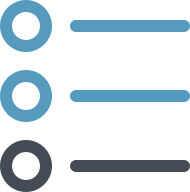
\includegraphics{images/_icons/alltutorials.png}}
\end{minipage}
\hfill
\begin{minipage}{0.90\textwidth}
%\vspace{-2mm}
\setlength{\parskip}{1em}
}{\end{minipage}
\end{mdframed}
%\vspace{2mm}
}

% singlelab

\newenvironment{singlelab}{
\vspace{2mm}
\begin{mdframed}[topline=false, bottomline=false, rightline=false, leftline=false]
\begin{minipage}{0.10\textwidth}
{$\:$ \\ \setkeys{Gin}{width=2em,keepaspectratio}
\includegraphics{images/_icons/singlelab.png}}
\end{minipage}
\hfill
\begin{minipage}{0.90\textwidth}
%\vspace{-2mm}
\setlength{\parskip}{1em}
}{\end{minipage}
\end{mdframed}
\vspace{2mm}
}

% todo

\newenvironment{todo}{
\vspace{4mm}
\begin{mdframed}[%
    topline=true, bottomline=true, linecolor=oiY, linewidth=0.5pt,
    rightline=false, leftline=false,
    backgroundcolor=oiLY]
\begin{minipage}[t]{0.10\textwidth}
{$\:$ \\ \setkeys{Gin}{width=2em,keepaspectratio}
\includegraphics{images/_icons/to-do.png}}
\end{minipage}
\hfill
\begin{minipage}[t]{0.90\textwidth}
\vspace{-2mm}
\setlength{\parskip}{1em}
\noindent\textbf{\color{oiGray}\small\Helvetica{{\MakeUppercase{TO DO}}}} $\:$ \\ \\
}{\end{minipage}
\end{mdframed}
\vspace{4mm}
}

% underconstruction

\newenvironment{underconstruction}{
\vspace{4mm}
\begin{mdframed}[%
    topline=true, bottomline=true, linecolor=oiR, linewidth=0.5pt,
    rightline=false, leftline=false,
    backgroundcolor=oiLR]
\begin{minipage}[t]{0.10\textwidth}
{$\:$ \\ \setkeys{Gin}{width=2em,keepaspectratio}
\includegraphics{images/_icons/under-construction.png}}
\end{minipage}
\hfill
\begin{minipage}[t]{0.90\textwidth}
\vspace{-2mm}
\setlength{\parskip}{1em}
\noindent\textbf{\color{oiR}\small\Helvetica{{\MakeUppercase{Under construction}}}} $\:$ \\ \\
}{\end{minipage}
\end{mdframed}
\vspace{4mm}
}

% Cover image ------------------------------------------------------------------

\newenvironment{authorinfo}[1]
  {
  \begin{minipage}[c]{0.30\textwidth}
  {\setkeys{Gin}{width=12em,keepaspectratio}\includegraphics{#1}}
  \end{minipage} 
  \hfill
  \begin{minipage}[c]{0.60\textwidth}
  }
  {
  \end{minipage}
  }

% Part formatting --------------------------------------------------------------

\titleformat{\part}[display]
{\color{oiR}\titlerule[5pt]\vspace{3pt}\color{oiLR}\titlerule[2pt]\vspace{3pt}\color{oiB}\normalfont\Huge\bfseries\scshape\Helvetica}
{\color{oiB}PART \thepart}{2em}{#1 \\ \noindent \vspace{3pt}\color{oiR}\titlerule[5pt]}

% https://tex.stackexchange.com/questions/506428/background-color-for-section-title
%\titleformat{\part}{\LARGE}{\rlap{\color{oiLB}\rule[-0.4cm]{\linewidth}{5cm}}\color{oiB}\normalfont\Huge\bfseries\scshape\Helvetica PART \thepart}{1em}{\color{oiB}\normalfont\Huge\bfseries\scshape\Helvetica #1}


% Bibliography: Chapter should be called References ----------------------------

%\usepackage{natbib}
%\usepackage{bibentry}
%\makeatletter\let\saved@bibitem\@bibitem\makeatother
%\usepackage{hyperref}
%\makeatletter\let\@bibitem\saved@bibitem\makeatother

% Index

\usepackage{makeidx}
\makeindex

% Smaller captions with bold labels

\usepackage[font=small,labelfont=bf]{caption}

% Reduce space between chapters in TOC

\usepackage{tocbasic}
\DeclareTOCStyleEntry[
  beforeskip=.5em plus 1pt,% default is 1em plus 1pt
  pagenumberformat=\textbf
]{tocline}{chapter}

% End ims-style.tex ------------------------------------------------------------
\makeatletter
\@ifpackageloaded{tcolorbox}{}{\usepackage[skins,breakable]{tcolorbox}}
\@ifpackageloaded{fontawesome5}{}{\usepackage{fontawesome5}}
\definecolor{quarto-callout-color}{HTML}{909090}
\definecolor{quarto-callout-note-color}{HTML}{0758E5}
\definecolor{quarto-callout-important-color}{HTML}{CC1914}
\definecolor{quarto-callout-warning-color}{HTML}{EB9113}
\definecolor{quarto-callout-tip-color}{HTML}{00A047}
\definecolor{quarto-callout-caution-color}{HTML}{FC5300}
\definecolor{quarto-callout-color-frame}{HTML}{acacac}
\definecolor{quarto-callout-note-color-frame}{HTML}{4582ec}
\definecolor{quarto-callout-important-color-frame}{HTML}{d9534f}
\definecolor{quarto-callout-warning-color-frame}{HTML}{f0ad4e}
\definecolor{quarto-callout-tip-color-frame}{HTML}{02b875}
\definecolor{quarto-callout-caution-color-frame}{HTML}{fd7e14}
\makeatother
\makeatletter
\@ifpackageloaded{bookmark}{}{\usepackage{bookmark}}
\makeatother
\makeatletter
\@ifpackageloaded{caption}{}{\usepackage{caption}}
\AtBeginDocument{%
\ifdefined\contentsname
  \renewcommand*\contentsname{Indice}
\else
  \newcommand\contentsname{Indice}
\fi
\ifdefined\listfigurename
  \renewcommand*\listfigurename{Elenco delle Figure}
\else
  \newcommand\listfigurename{Elenco delle Figure}
\fi
\ifdefined\listtablename
  \renewcommand*\listtablename{Elenco delle Tabelle}
\else
  \newcommand\listtablename{Elenco delle Tabelle}
\fi
\ifdefined\figurename
  \renewcommand*\figurename{Figura}
\else
  \newcommand\figurename{Figura}
\fi
\ifdefined\tablename
  \renewcommand*\tablename{Tabella}
\else
  \newcommand\tablename{Tabella}
\fi
}
\@ifpackageloaded{float}{}{\usepackage{float}}
\floatstyle{ruled}
\@ifundefined{c@chapter}{\newfloat{codelisting}{h}{lop}}{\newfloat{codelisting}{h}{lop}[chapter]}
\floatname{codelisting}{Lista}
\newcommand*\listoflistings{\listof{codelisting}{Elenco degli Elenchi}}
\makeatother
\makeatletter
\makeatother
\makeatletter
\@ifpackageloaded{caption}{}{\usepackage{caption}}
\@ifpackageloaded{subcaption}{}{\usepackage{subcaption}}
\makeatother

\ifLuaTeX
\usepackage[bidi=basic]{babel}
\else
\usepackage[bidi=default]{babel}
\fi
\babelprovide[main,import]{italian}
% get rid of language-specific shorthands (see #6817):
\let\LanguageShortHands\languageshorthands
\def\languageshorthands#1{}
\ifLuaTeX
  \usepackage{selnolig}  % disable illegal ligatures
\fi
\usepackage{bookmark}

\IfFileExists{xurl.sty}{\usepackage{xurl}}{} % add URL line breaks if available
\urlstyle{same} % disable monospaced font for URLs
\hypersetup{
  pdftitle={Testing Psicologico},
  pdfauthor={Corrado Caudek},
  pdflang={it},
  hidelinks,
  pdfcreator={LaTeX via pandoc}}


\title{Testing Psicologico}
\usepackage{etoolbox}
\makeatletter
\providecommand{\subtitle}[1]{% add subtitle to \maketitle
  \apptocmd{\@title}{\par {\large #1 \par}}{}{}
}
\makeatother
\subtitle{Anno Accademico 2024/2025}
\author{Corrado Caudek}
\date{2024-11-11}

\begin{document}
\frontmatter
\maketitle

\renewcommand*\contentsname{Indice}
{
\setcounter{tocdepth}{1}
\tableofcontents
}

\mainmatter
\bookmarksetup{startatroot}

\chapter*{Benvenuti}\label{benvenuti}

\markboth{Benvenuti}{Benvenuti}

\chapter*{}

\vfill

Questo sito web è dedicato al materiale didattico dell'insegnamento di
\href{https://unifi.coursecatalogue.cineca.it/insegnamenti/2024/47120_B267-23-24_119693/2023/47118/3252?coorte=2024}{Testing
Psicologico} (A.A. 2024/2025), rivolto agli studenti del primo anno del
Corso di Laurea Magistrale
\href{https://unifi.coursecatalogue.cineca.it/corsi/2024/3252?annoOrdinamento=2023}{Psicologia
Clinica e della Salute e Neuropsicologia}
dell'\href{https://www.unifi.it/}{Università degli Studi di Firenze}.

L'insegnamento si propone quale stimolo e guida per l'apprendimento
delle basi dell'assessment psicologico.

\section*{Informazioni
sull'insegnamento}\label{informazioni-sullinsegnamento}
\addcontentsline{toc}{section}{Informazioni sull'insegnamento}

\markright{Informazioni sull'insegnamento}

\begin{itemize}
\tightlist
\item
  \textbf{Codice}: B033288 - Testing Psicologico
\item
  \textbf{Modulo}: B033288 - Testing Psicologico (Cognomi L-Z)
\item
  \textbf{Corso di laurea}: Laurea Magistrale: Psicologia Clinica e
  della Salute e Neuropsicologia
\item
  \textbf{Anno Accademico}: 2024-2025
\item
  \textbf{Calendario}: Il corso si terrà dal 4 marzo al 31 maggio 2025.
\item
  \textbf{Orario delle lezioni}: Le lezioni si svolgeranno il martedì
  dalle 10:30 alle 13:30 e il giovedì dalle 8:30 alle 11:30.
\item
  \textbf{Luogo}: Le lezioni si terranno presso il Plesso didattico La
  Torretta.
\item
  \textbf{Modalità di svolgimento della didattica}: Le lezioni ed
  esercitazioni saranno svolte in modalità frontale.
\end{itemize}

\begin{tcolorbox}[enhanced jigsaw, breakable, rightrule=.15mm, title=\textcolor{quarto-callout-note-color}{\faInfo}\hspace{0.5em}{Nota}, bottomrule=.15mm, opacityback=0, opacitybacktitle=0.6, arc=.35mm, bottomtitle=1mm, colframe=quarto-callout-note-color-frame, left=2mm, leftrule=.75mm, coltitle=black, toptitle=1mm, colbacktitle=quarto-callout-note-color!10!white, titlerule=0mm, toprule=.15mm, colback=white]

Questo sito web è la fonte ufficiale per tutte le informazioni relative
al programma dell'insegnamento \emph{B033288 - Testing Psicologico}
(Cognomi A-K) per l'A.A. 2024-2025 e le modalità d'esame.

\end{tcolorbox}

\section*{Syllabus}\label{syllabus}
\addcontentsline{toc}{section}{Syllabus}

\markright{Syllabus}

Il Syllabus può essere scaricato utilizzando questo
\href{syllabus/syllabus.pdf}{link}.

\bookmarksetup{startatroot}

\chapter*{Prefazione}\label{prefazione}
\addcontentsline{toc}{chapter}{Prefazione}

\markboth{Prefazione}{Prefazione}

Gli obiettivi di questo insegnamento sono:

\begin{itemize}
\tightlist
\item
  presentare i principi metodologici su cui i test psicologici sono
  fondati;
\item
  mettere gli studenti in condizione di discriminare le diverse
  tipologie di test e gli obiettivi per cui essi vengono utilizzati;
\item
  introdurre le tematiche dell'assessment psicologico;
\item
  presentare la teoria classica dei test, il metodo dell'analisi
  fattoriale, i modelli di equazioni strutturali e i modelli IRT.
\end{itemize}

Viene presentata qui una panoramica degli argomenti che verranno
trattati.

\section*{Definizione di misurazione}\label{definizione-di-misurazione}
\addcontentsline{toc}{section}{Definizione di misurazione}

\markright{Definizione di misurazione}

La misurazione psicologica è un pilastro fondamentale nella comprensione
e nell'analisi del comportamento umano, fornendo un mezzo quantitativo
per esplorare le dinamiche della mente e della personalità. La
definizione di misurazione proposta da Stevens (1951), uno dei pionieri
della teoria della misurazione, stabilisce che essa consiste
nell'assegnare numeri a oggetti o eventi secondo regole definite.
Tuttavia, è ormai ampiamente accettato che questa visione sia troppo
semplicistica e che la misurazione richieda un approccio più
sofisticato. Si concorda comunemente sul fatto che la misurazione debba
essere considerata come un processo di creazione di modelli che
rappresentano i fenomeni di interesse, principalmente in forma
quantitativa.

Di conseguenza, la misurazione si basa su regole che attribuiscono scale
o valori alle entità che rappresentano i costrutti di interesse. Come
avviene per tutti i modelli, quelli di misurazione, come i test, le
scale o le variabili, devono semplificare la realtà per risultare utili.
Pertanto, è fondamentale specificare chiaramente i modelli di
misurazione per poterli valutare, confutare e migliorare.

Inoltre, anziché chiedersi se un modello sia vero o corretto, è più
utile sviluppare diversi modelli alternativi plausibili e porre domande
del tipo: quale modello è meno inaccurato? Questo approccio al confronto
dei modelli rappresenta la strategia migliore per valutare e
perfezionare le procedure di misurazione, consentendo un'analisi più
approfondita e accurata delle variabili coinvolte.

Per illustrare l'approccio alla misurazione come descritto, prendiamo in
considerazione un esempio concreto: la valutazione dell'intelligenza
attraverso il test del quoziente intellettivo (QI).

Iniziamo definendo il concetto di interesse, ovvero l'intelligenza, che
può essere concepita come la capacità di apprendere, comprendere e
applicare conoscenze, risolvere problemi e adattarsi a nuove situazioni.
Tuttavia, trattandosi di un concetto astratto, è necessario
operazionalizzarlo in modo misurabile.

Per misurare l'intelligenza, si crea un test di QI che comprende una
serie di compiti e domande progettati per valutare diverse dimensioni
della capacità cognitiva, quali la memoria, il ragionamento logico e la
comprensione verbale.

Ciascun compito nel test di QI è associato a un punteggio. I risultati
individuali vengono quindi calcolati e confrontati con una norma
statistica per attribuire un punteggio di QI.

Successivamente, il test di QI viene sottoposto a diverse analisi per
verificare la sua validità (ovvero se misura effettivamente
l'intelligenza) e affidabilità (se fornisce risultati consistenti nel
tempo).

Tuttavia, esistono diverse teorie dell'intelligenza, come ad esempio
quella delle intelligenze multiple di Gardner, che suggeriscono modelli
alternativi di misurazione. Confrontando il modello del QI con questi
approcci alternativi, gli psicologi possono valutare quale modello è
meno distorto o più adatto per specifici scopi.

In risposta alle critiche, alle nuove scoperte e ai cambiamenti
culturali e sociali, il modello del QI viene regolarmente rivisto e
adattato per assicurare che continui a essere uno strumento utile di
misurazione.

Questo esempio mostra come la misurazione in psicologia non sia
semplicemente un atto di assegnare numeri a un costrutto, ma piuttosto
un processo complesso che implica la creazione, la valutazione e il
continuo perfezionamento di modelli teorici.

\section*{Temi Centrali nell'Approccio
Psicometrico}\label{temi-centrali-nellapproccio-psicometrico}
\addcontentsline{toc}{section}{Temi Centrali nell'Approccio
Psicometrico}

\markright{Temi Centrali nell'Approccio Psicometrico}

\begin{enumerate}
\def\labelenumi{\arabic{enumi}.}
\item
  \textbf{Affidabilità}: Questo concetto si riferisce alla capacità di
  un test di produrre risultati consistenti nel tempo e in contesti
  diversi, costituendo una base fondamentale per la misurazione
  psicologica.
\item
  \textbf{Validazione del Costrutto e Test dei Modelli}: L'evoluzione
  della psicometria ha portato a una sempre maggiore enfasi sulla
  validazione dei costrutti e sull'importanza dei test di modelli,
  utilizzando tecniche come i modelli a equazioni strutturali (SEM) per
  verificare la coerenza e la validità dei costrutti psicologici.
\item
  \textbf{Dimensionalità e Validità Strutturale}: La dimensionalità
  viene considerata un elemento fondamentale nella valutazione della
  validità strutturale, poiché permette di esplorare come i diversi
  aspetti di un costrutto si manifestano e interagiscono all'interno del
  modello di misurazione.
\item
  \textbf{Costruzione dei Questionari}: La progettazione e la
  formulazione degli item dei questionari rivestono un ruolo cruciale,
  in quanto influenzano direttamente l'affidabilità e la validità dei
  risultati ottenuti. La scelta degli item, il loro ordine e la
  chiarezza della formulazione sono tutti aspetti che contribuiscono
  alla qualità e all'efficacia della misurazione psicologica.
\end{enumerate}

Attraverso questi approcci, la misurazione psicologica si adatta alle
sfide uniche poste dalla natura astratta e complessa dei costrutti
psicologici, cercando di fornire strumenti validi e affidabili per la
loro esplorazione e comprensione.

\section*{Affidabilità e Generalizzabilità nelle Misure
Psicologiche}\label{affidabilituxe0-e-generalizzabilituxe0-nelle-misure-psicologiche}
\addcontentsline{toc}{section}{Affidabilità e Generalizzabilità nelle
Misure Psicologiche}

\markright{Affidabilità e Generalizzabilità nelle Misure Psicologiche}

Nel contesto della misurazione psicologica, così come in altre
discipline, è cruciale considerare le variabili che possono influenzare
la precisione delle misure. L'affidabilità di uno strumento di
misurazione psicologica si riferisce alla sua consistenza nel produrre
risultati replicabili nel tempo e in contesti diversi. Gli indici di
affidabilità sono utilizzati per quantificare il grado di
riproducibilità e l'assenza di errori casuali nelle misurazioni.

\subsection*{Teoria Classica dei Test}\label{teoria-classica-dei-test}
\addcontentsline{toc}{subsection}{Teoria Classica dei Test}

L'approccio più ampiamente utilizzato nello studio dell'affidabilità
delle misure psicologiche è rappresentato dalla teoria classica dei
test, come descritto da Lord e Novick (1968). Secondo questa teoria,
ogni misurazione (\(X\)) è composta da due componenti distintive: un
punteggio ``vero'' (\(T\)) e un errore di misurazione (\(e\)). Il
concetto di misurazione accurata, o ``vera'', può essere rappresentato
come \(X - e\), evidenziando il fatto che ogni misurazione può essere
decomposta in tali elementi distinti.

La teoria classica dei test enfatizza l'importanza di condurre
misurazioni ripetute per valutare l'affidabilità. Un concetto
fondamentale è quello dei test paralleli, che consistono in due test con
medie, varianze e distribuzioni identiche, e che mostrano una
correlazione simile con variabili esterne. In questa prospettiva, il
punteggio vero e l'errore di misurazione sono considerati indipendenti.
Di conseguenza, la varianza dei punteggi osservati (Varianza \(X\)) è la
somma della varianza dei punteggi veri (Varianza \(T\)) e della varianza
dell'errore di misurazione (Varianza \(e\)).

L'affidabilità è quindi definita come il rapporto tra la varianza del
punteggio vero e la varianza del punteggio osservato:

\[ 
\text{Affidabilità} = \frac{\text{Varianza}(T)}{\text{Varianza}(X)}.
\]

In termini pratici, un'affidabilità di 1 indicherebbe l'assenza di
errori, mentre un'affidabilità di 0 implicherebbe che i punteggi
derivano esclusivamente dall'errore. La correlazione tra il punteggio
osservato e il punteggio vero è la radice quadrata dell'affidabilità,
fornendo una stima della precisione della misurazione.

Questo framework fornisce una solida base per comprendere e quantificare
l'affidabilità nelle misure psicologiche, sottolineando l'importanza di
considerare sia i punteggi veri sia gli errori di misurazione per
ottenere misurazioni precise e affidabili.

\subsection*{Evidenze Multiple di
Affidabilità}\label{evidenze-multiple-di-affidabilituxe0}
\addcontentsline{toc}{subsection}{Evidenze Multiple di Affidabilità}

Nonostante la teoria classica dei test fornisca una definizione
matematica dei test paralleli, non fornisce dettagliate linee guida
sulle procedure specifiche per costruirli. Tuttavia, a partire dagli
anni '50, sono stati sviluppati diversi metodi che consentono di
valutare empiricamente l'affidabilità delle misurazioni:

\begin{enumerate}
\def\labelenumi{\arabic{enumi}.}
\item
  \textbf{Test-Retest}: Questo approccio implica la somministrazione
  dello stesso test ai partecipanti in due momenti diversi. L'obiettivo
  è valutare la stabilità dei punteggi nel tempo. Una correlazione
  elevata tra i punteggi ottenuti nei due momenti indica una buona
  affidabilità del test-retest.
\item
  \textbf{Equivalenza di Forme Parallele}: Questo metodo prevede
  l'utilizzo di due versioni diverse del test, ma che coprono lo stesso
  contenuto, somministrate simultaneamente ai partecipanti. Una forte
  correlazione tra i punteggi ottenuti dalle due versioni suggerisce che
  entrambe misurano il medesimo costrutto in modo affidabile.
\item
  \textbf{Split-Half e Coerenza Interna}:

  \begin{itemize}
  \tightlist
  \item
    \textbf{Split-Half}: I partecipanti completano una sola versione del
    test, la quale è divisa in due parti equivalenti. Si calcola poi la
    correlazione tra i punteggi delle due metà. Questo metodo valuta la
    coerenza interna del test.
  \item
    \textbf{Coerenza Interna (ad esempio, Omega di McDonals)}: Valuta la
    correlazione tra tutti gli elementi del test. Un alto valore di
    coerenza interna indica che tutti gli elementi del test misurano
    aspetti simili del costrutto.
  \end{itemize}
\item
  \textbf{Valutazione da Giudici Multipli}: In questo caso, i
  partecipanti sono valutati da più giudici in un'unica occasione. Un
  alto grado di accordo tra i giudici fornisce un'indicazione
  dell'affidabilità delle valutazioni.
\end{enumerate}

Ciascuno di questi approcci fornisce indicazioni sull'affidabilità di un
test, ma è fondamentale considerare che alcuni potrebbero essere più
appropriati di altri in base alla natura del test e del costrutto
misurato. L'affidabilità è pertanto un concetto multidimensionale che
richiede l'impiego di diversi approcci per una valutazione completa
delle misurazioni psicologiche.

\subsection*{Il Ruolo del Coefficiente Alpha nella Misurazione
Psicologica}\label{il-ruolo-del-coefficiente-alpha-nella-misurazione-psicologica}
\addcontentsline{toc}{subsection}{Il Ruolo del Coefficiente Alpha nella
Misurazione Psicologica}

Il coefficiente alpha, introdotto da Cronbach nel 1951, è diventato un
importante indicatore di coerenza interna nella letteratura psicologica,
principalmente grazie alla sua facilità di calcolo. A differenza
dell'affidabilità test-retest, che richiede dati raccolti in due momenti
diversi, o dell'affidabilità delle forme parallele, che richiede la
costruzione di due versioni alternative di un test, il coefficiente
alpha può essere calcolato utilizzando un unico set di dati, rendendolo
estremamente pratico come indice di affidabilità.

Tuttavia, è importante correggere un comune malinteso riguardo al
coefficiente alpha: esso non misura direttamente l'omogeneità delle
intercorrelazioni tra gli elementi o conferma la unidimensionalità di
una scala. In realtà, il coefficiente alpha non fornisce informazioni
dirette su questi aspetti strutturali della scala.

Per affrontare la questione della unidimensionalità, è necessario
ricorrere a approcci più sofisticati come l'analisi fattoriale
confermativa e i modelli di equazioni strutturali (SEM). Questi metodi
consentono di testare quanto bene la struttura di correlazione degli
elementi si adatti a un modello con un singolo fattore rispetto a
modelli multifattoriali, valutando se le correlazioni tra gli elementi
possono essere meglio spiegate da un singolo costrutto sottostante.

Nel contesto delle analisi SEM, le saturazioni degli item indicano
quanto della varianza di un item sia condivisa con gli altri (e quindi
generalizzabile), mentre la varianza residua dell'item cattura l'errore
unico associato a quell'item. La presenza di multidimensionalità emerge
dalla capacità di un modello multifattoriale di adattarsi meglio ai dati
rispetto a un modello a singolo fattore.

Quando un test è considerato multidimensionale, è ancora appropriato
utilizzare il coefficiente alpha come indice di affidabilità? La
risposta è negativa. In presenza di multidimensionalità, il coefficiente
alpha tende a sottostimare l'affidabilità. Pertanto, è consigliabile, in
tali casi, utilizzare altri metodi per valutare l'affidabilità, anziché
basarsi esclusivamente sul coefficiente alpha.

\subsection*{Il Fenomeno dell'Attenuazione in Relazione
all'Affidabilità}\label{il-fenomeno-dellattenuazione-in-relazione-allaffidabilituxe0}
\addcontentsline{toc}{subsection}{Il Fenomeno dell'Attenuazione in
Relazione all'Affidabilità}

All'interno del contesto della teoria classica dei test, come delineato
da Lord e Novick (1968), l'affidabilità svolge un ruolo cruciale poiché
influisce sulla forza della correlazione che una misura può mostrare con
altre variabili, come un criterio esterno. Secondo questa teoria, se
l'errore nelle misurazioni è genuinamente casuale, il massimo teorico
della correlazione tra una misura e un'altra variabile non è 1.0, ma
piuttosto la radice quadrata dell'affidabilità di quella misura.

Ciò implica che, in presenza di un'affidabilità meno che ottimale, la
correlazione effettiva tra una misura e qualsiasi altra variabile viene
sistematicamente sottostimata, fenomeno noto come attenuazione. Questa
attenuazione è direttamente proporzionale all'inadeguatezza
dell'affidabilità: più bassa è l'affidabilità di una misura, maggiore
sarà la sottostima della sua correlazione con altre variabili. Pertanto,
per ottenere stime accurate delle correlazioni e comprendere veramente
le relazioni tra diverse variabili, è fondamentale garantire che le
misure utilizzate siano il più affidabili possibile. Questa
considerazione enfatizza l'importanza dell'accuratezza e della
precisione nelle procedure di misurazione psicologica.

\subsection*{La Teoria della
Generalizzabilità}\label{la-teoria-della-generalizzabilituxe0}
\addcontentsline{toc}{subsection}{La Teoria della Generalizzabilità}

La Teoria della Generalizzabilità propone un approccio più completo e
flessibile per comprendere l'affidabilità delle misure psicologiche
rispetto alla classificazione tradizionale delle tipologie di
affidabilità. Invece di limitarsi a categorizzare le misure in base a
criteri specifici come test-retest, affidabilità interna o
inter-valutatori, la Teoria della Generalizzabilità considera una serie
di dimensioni che possono influenzare l'affidabilità in contesti
diversi.

Una delle principali criticità della teoria classica dei test è la sua
presunzione di uniformità e parallelismo delle misurazioni e degli
errori casuali. La Teoria della Generalizzabilità, al contrario,
riconosce che l'affidabilità dipende dalla specifica dimensione di
generalizzazione considerata. Ad esempio, un test potrebbe essere
affidabile per misurare una certa caratteristica in un contesto, ma non
altrettanto affidabile in un contesto diverso o per una caratteristica
correlata ma non identica.

Per superare le limitazioni della teoria classica dei test, l'American
Psychological Association ha proposto l'adozione della Teoria della
Generalizzabilità. Tuttavia, nonostante questa proposta, la pratica nei
campi di ricerca non si è adeguatamente evoluta e la teoria della
generalizzabilità non ha ancora completamente sostituito le nozioni più
semplicistiche popolari in psicologia.

La Teoria della Generalizzabilità esamina diverse dimensioni che
influenzano l'affidabilità, tra cui la dimensione temporale, delle
forme, degli item e dei giudici o osservatori. Questa teoria enfatizza
l'importanza di estendere le osservazioni a un'ampia varietà di
situazioni e identificare l'impatto specifico delle fonti di varianza
nei punteggi dei test in contesti particolari.

Invece dei tradizionali coefficienti di affidabilità come il
coefficiente di stabilità o il coefficiente alfa, la Teoria della
Generalizzabilità suggerisce l'uso di misure più ampie di affidabilità,
come il coefficiente di correlazione intraclasse, per esaminare
specifici aspetti dell'affidabilità. Questo approccio è particolarmente
utile in ricerche con dati strutturati in maniera nidificata e dove
diverse dimensioni possono influenzare l'affidabilità, come nei metodi
di valutazione ecologica momentanea.\#\#\# La Teoria della Risposta agli
Item

La Teoria della Risposta agli Item (IRT) rappresenta un avanzamento
rispetto alla teoria classica dei test, offrendo un approccio più
sofisticato per analizzare le risposte degli individui agli item e la
loro relazione con un costrutto latente. Questa teoria stabilisce un
collegamento tra le risposte degli individui a un particolare item e il
costrutto latente utilizzando una funzione chiamata ``curva
caratteristica dell'item''.

La curva caratteristica dell'item mostra la probabilità che individui
con differenti livelli del costrutto latente rispondano correttamente
all'item, fornendo inoltre informazioni sulla capacità dell'item di
distinguere tra individui con livelli elevati e bassi del tratto
latente, oltre a misurare la sua difficoltà. Queste informazioni sono
cruciali per identificare eventuali distorsioni negli item, noto come
bias. Secondo la IRT, un item è privo di bias nel misurare un costrutto
se individui con lo stesso livello del tratto ottengono punteggi attesi
simili sull'item, indipendentemente da caratteristiche non rilevanti
come genere, etnia o background culturale.

La Teoria della Risposta agli Item offre diversi vantaggi nel processo
di creazione e valutazione di scale psicometriche:

\begin{enumerate}
\def\labelenumi{\arabic{enumi}.}
\item
  \textbf{Selezione degli Item}: Permette di selezionare gli item in
  base alla loro difficoltà e alla capacità di discriminazione,
  superando così la limitazione della teoria classica che si basa
  esclusivamente sulle correlazioni tra gli item e il punteggio totale.
\item
  \textbf{Testing Adattivo Computerizzato}: La IRT facilita la
  valutazione della posizione di un individuo su un costrutto latente
  senza la necessità di somministrare l'intero test, grazie a tecniche
  come il testing adattivo computerizzato.
\end{enumerate}

In conclusione, la Teoria della Risposta agli Item fornisce strumenti
quantitativi per esaminare approfonditamente la relazione tra un item
specifico e il costrutto latente, attraverso parametri di difficoltà e
discriminazione.

\section*{Evoluzione e Comprensione della Validità nelle Misure
Psicologiche}\label{evoluzione-e-comprensione-della-validituxe0-nelle-misure-psicologiche}
\addcontentsline{toc}{section}{Evoluzione e Comprensione della Validità
nelle Misure Psicologiche}

\markright{Evoluzione e Comprensione della Validità nelle Misure
Psicologiche}

La nostra comprensione della validità nelle misure psicologiche ha
subito un notevole sviluppo nel corso del tempo, passando da una visione
iniziale più frammentata a un approccio più olistico e dinamico.
Inizialmente, la validità veniva suddivisa in diversi tipi, tra cui la
validità di contenuto, di facciata, orientata al criterio e di
costrutto.

La validità di contenuto si riferisce alla rappresentatività degli item
di un test rispetto al costrutto che si intende misurare, mentre la
validità di facciata valuta se superficialmente gli item sembrano idonei
a misurare il costrutto, sebbene questa non sia considerata un indice
rigoroso di validità. La validità orientata al criterio si divide
ulteriormente in predittiva e concorrente, che valutano la capacità del
test di prevedere comportamenti futuri o di correlare con criteri
esterni contemporaneamente misurati. Infine, la validità di costrutto
indaga se il test misura effettivamente il costrutto in questione,
richiedendo una comprensione approfondita sia del costrutto sia della
metodologia del test.

Tuttavia, queste distinzioni sono state gradualmente considerate
limitate e frammentarie. Un punto di svolta è stato rappresentato
dall'approccio olistico di Samuel Messick, che ha enfatizzato che la
validità va oltre la misura stessa, coinvolgendo l'interpretazione e
l'uso dei punteggi del test. Messick ha sottolineato l'importanza di
considerare le evidenze di validità da molteplici fonti e di assicurare
la coerenza delle interpretazioni dei punteggi del test con le teorie
psicologiche sottostanti.

Un'importante correzione concettuale è stata l'idea che la validità non
sia un attributo statico dei test, ma piuttosto un processo continuo di
accumulo di evidenze e giustificazioni teoriche. Questo processo di
validazione riflette l'evoluzione delle teorie psicologiche e delle
metodologie di misurazione, sottolineando che la validità è dinamica e
contestuale.

In sintesi, l'evoluzione della concezione di validità nelle misure
psicologiche sottolinea l'importanza di un approccio comprensivo,
teoricamente informato e basato sull'evidenza per valutare, interpretare
e utilizzare i punteggi dei test. Questo approccio moderno incoraggia i
ricercatori e i praticanti a considerare la validità come un concetto
ampio che incorpora molteplici aspetti della progettazione,
dell'implementazione e dell'interpretazione dei test psicologici.

\section*{Approfondimento su Tecniche di Validazione di Costrutto e
Costruzione di
Scale}\label{approfondimento-su-tecniche-di-validazione-di-costrutto-e-costruzione-di-scale}
\addcontentsline{toc}{section}{Approfondimento su Tecniche di
Validazione di Costrutto e Costruzione di Scale}

\markright{Approfondimento su Tecniche di Validazione di Costrutto e
Costruzione di Scale}

La discussione sulla evoluzione della validità nelle misure psicologiche
può proseguire con l'esame delle tecniche che vengono usate per la
validazione di costrutto e per la costruzione di scale. In particolare,
gli strumenti maggiormente usati dagli psicometristi sono l'Analisi
Fattoriale Confermativa (CFA) e i Modelli di Equazioni Strutturali
(SEM).

L'\textbf{Analisi Fattoriale Confermativa (CFA)} rappresenta un
approccio metodologico rigoroso, basato sull'ipotesi che un insieme di
osservazioni possa essere spiegato da pochi costrutti latenti. A
differenza dell'Analisi Fattoriale Esplorativa, che non prevede ipotesi
a priori sui fattori, la CFA richiede che i ricercatori definiscano
anticipatamente un modello teorico. Questo specifica le relazioni tra le
variabili osservabili e i costrutti latenti, permettendo di testare
l'adeguatezza del modello ai dati. La capacità della CFA di confrontare
diversi modelli offre un mezzo potente per identificare la struttura che
meglio rappresenta i dati.

Nel contesto della \textbf{valutazione della coerenza interna di una
scala}, l'utilizzo della CFA supera i limiti dei metodi basati sulla
teoria classica dei test, fornendo una valutazione più dettagliata e
strutturata delle relazioni tra item e costrutti latenti.

I \textbf{Modelli di Equazioni Strutturali (SEM)} estendono le
possibilità offerte dalla CFA, abilitando l'analisi delle relazioni di
regressione non solo tra variabili manifeste e latenti, ma anche tra i
costrutti latenti stessi. Questa caratteristica rende i SEM strumenti
eccezionalmente potenti per esplorare le interazioni complesse tra
variabili in uno studio psicometrico.

L'\textbf{esame della dimensionalità di un costrutto} attraverso la CFA
e i SEM consente di testare con precisione le ipotesi sulla struttura
dimensionale dei costrutti, verificando se l'organizzazione teorizzata
degli item in fattori latenti corrisponde ai dati. Questi strumenti sono
quindi fondamentali per confermare la struttura di un costrutto come
ipotizzato dalla teoria sottostante.

In aggiunta, l'approccio \textbf{Multitrait-Multimethod (MTMM)} per
esaminare la validità esterna, incorporando la validità convergente e
discriminante, arricchisce ulteriormente la comprensione della misura.
L'uso del disegno MTMM permette di distinguere efficacemente tra
costrutti correlati ma distinti, assicurando che le misure non solo
riflettano accuratamente il costrutto target, ma siano anche
discriminanti rispetto ad altri costrutti.

In sintesi, l'integrazione di CFA e SEM nel processo di validazione di
costrutti e nella costruzione di scale psicometriche rappresenta un
avanzamento metodologico significativo. Questi approcci non solo
migliorano la precisione e la comprensione delle relazioni tra variabili
osservabili e latenti, ma contribuiscono anche a elevare la qualità e
l'affidabilità delle misure psicologiche. Attraverso un uso attento e
informato di queste tecniche, i ricercatori possono arricchire la
validità e l'utilità delle scale psicometriche. Chi volesse approfondire
ulteriormente questi argomenti, può fare riferimento al testo di John e
Benet-Martinez (2014).

\part{Programmazione}

\chapter{Calendario delle lezioni}\label{calendario-delle-lezioni}

Il calendario didattico prevede 14 incontri di 3 ore ciascuno, con una
verifica tramite Quiz Moodle e le presentazioni finali degli studenti
negli ultimi due incontri.

\begin{longtable}[]{@{}
  >{\raggedright\arraybackslash}p{(\columnwidth - 6\tabcolsep) * \real{0.1296}}
  >{\raggedright\arraybackslash}p{(\columnwidth - 6\tabcolsep) * \real{0.1574}}
  >{\raggedright\arraybackslash}p{(\columnwidth - 6\tabcolsep) * \real{0.5648}}
  >{\raggedright\arraybackslash}p{(\columnwidth - 6\tabcolsep) * \real{0.1481}}@{}}
\toprule\noalign{}
\begin{minipage}[b]{\linewidth}\raggedright
\textbf{Incontro}
\end{minipage} & \begin{minipage}[b]{\linewidth}\raggedright
\textbf{Data}
\end{minipage} & \begin{minipage}[b]{\linewidth}\raggedright
\textbf{Argomento}
\end{minipage} & \begin{minipage}[b]{\linewidth}\raggedright
\textbf{Orario}
\end{minipage} \\
\midrule\noalign{}
\endhead
\bottomrule\noalign{}
\endlastfoot
1 & 4 marzo 2025 & Presentazione del corso, introduzione a R &
10:30-13:30 \\
2 & 6 marzo 2025 & Concetti di base: Test psicologici e misure;
distribuzioni di probabilità; modello lineare & 8:30-11:30 \\
3 & 11 marzo 2025 & Teoria Classica dei & 10:30-13:30 \\
4 & 13 marzo 2025 & Modello di regressione logistica. Mokken Scale
Analysis (MSE) & 8:30-11:30 \\
5 & 18 marzo 2025 & Item Response Theory (IRT). Validità. &
10:30-13:30 \\
6 & 20 marzo 2025 & Path Analysis. Tutorial di Clement e Bradley-Garcia
(2022) & 8:30-11:30 \\
7 & 25 marzo 2025 & Elementi di algebra lineare, analisi delle
componenti principali & 10:30-13:30 \\
8 & 27 marzo 2025 & Analisi fattoriale esplorativa. Il modello
statistico delll'analisi fattoriale & 8:30-11:30 \\
9 & 1 aprile 2025 & Estrazione dei fattori, rotazione & 10:30-13:30 \\
10 & 3 aprile 2025 & Analisi fattoriale confermativa & 8:30-11:30 \\
11 & 8 aprile 2025 & Introduzione ai modelli di equazioni strutturali
(SEM) & 10:30-13:30 \\
12 & 10 aprile 2025 & Modelli multilivello; attendibilità dei giudici.
Modelli di crescita latente & 8:30-11:30 \\
13 & 15 aprile 2025 & Verifica tramite Quiz Moodle & 10:30-13:30 \\
14 & 17 aprile 2025 & Presentazioni finali degli studenti &
8:30-11:30 \\
\end{longtable}

\begin{center}\rule{0.5\linewidth}{0.5pt}\end{center}

\part{Punteggi e scale}

\chapter{Punteggi e scale}\label{sec-scores-scales}

\textbf{Prerequisiti}

\begin{itemize}
\tightlist
\item
  Leggere i capitoli 1, \emph{Scores and Scales}, e 2,
  \emph{Constructs}, del testo \emph{Principles of psychological
  assessment} di Petersen (2024).
\item
  Si consiglia di ripassare i concetti fondamentali della teoria delle
  probabilità, in particolare le distribuzioni di massa e di densità di
  probabilità. Per approfondire, si rimanda al materiale didattico
  dell'insegnamento di Psicometria disponibile al link
  {[}https://ccaudek.github.io/psicometria/{]}.
\end{itemize}

\textbf{Concetti e Competenze Chiave}

\textbf{Preparazione del Notebook}

\begin{Shaded}
\begin{Highlighting}[]
\CommentTok{\# Carica il file \_common.R per impostazioni di pacchetti e opzioni}
\NormalTok{here}\SpecialCharTok{::}\FunctionTok{here}\NormalTok{(}\StringTok{"code"}\NormalTok{, }\StringTok{"\_common.R"}\NormalTok{) }\SpecialCharTok{|\textgreater{}} \FunctionTok{source}\NormalTok{()}

\CommentTok{\# Carica pacchetti aggiuntivi}
\NormalTok{pacman}\SpecialCharTok{::}\FunctionTok{p\_load}\NormalTok{(MASS, nortest)}
\end{Highlighting}
\end{Shaded}

\section{Introduzione}\label{introduzione}

Questo capitolo si propone di introdurre l'utilizzo del software ``R'',
ponendo l'attenzione sulla differenza tra valutazioni normative e
criteriali.

\section{Tipologie di Dati}\label{tipologie-di-dati}

Si possono identificare quattro principali categorie di dati: nominali,
ordinali, di intervallo e di rapporto. È opportuno notare che, in
funzione dell'utilizzo della variabile, i dati possono rientrare in più
di una categoria. La tipologia del dato influisce significativamente
sulle modalità di analisi applicabili. A titolo esemplificativo,
l'analisi statistica parametrica (come la regressione lineare)
presuppone che i dati siano di intervallo o di rapporto.

\subsection{Dati Nominali}\label{dati-nominali}

I dati nominali si configurano come categorie distinte, caratterizzate
da natura categorica e prive di ordinamento. Tali dati non esprimono
affermazioni di natura quantitativa, bensì rappresentano entità
nominabili (ad esempio, ``felino'' e ``canino''). Sebbene possano essere
rappresentati numericamente, come nel caso dei codici postali o dei
codici identificativi di genere, etnia o razza dei partecipanti, è
fondamentale sottolineare che valori numerici più elevati non riflettono
livelli superiori (o inferiori) del costrutto, in quanto i numeri
rappresentano meramente categorie prive di ordine intrinseco.

\subsection{Dati Ordinali}\label{dati-ordinali}

I dati ordinali si distinguono per essere categorie ordinate: possiedono
una denominazione e un ordine. Non forniscono informazioni sulla
distanza concettuale tra i ranghi, ma indicano esclusivamente che valori
più elevati rappresentano livelli superiori (o inferiori) del costrutto.
Un esempio paradigmatico è costituito dalle posizioni in classifica
successive a una competizione: il concorrente classificato al primo
posto ha concluso la gara prima del secondo classificato, il quale a sua
volta ha preceduto il terzo (1 \textgreater{} 2 \textgreater{} 3
\textgreater{} 4). È cruciale evidenziare che la distanza concettuale
tra numeri adiacenti non è necessariamente equivalente.

\subsection{Dati di Intervallo}\label{dati-di-intervallo}

I dati di intervallo sono caratterizzati da un ordine e da distanze
significative (ovvero, intervalli equidistanti). Questi dati consentono
operazioni di somma (ad esempio, 2 dista 2 unità da 4), ma non di
moltiplicazione (\(2 \times 2 \ne 4\)). Esempi emblematici sono le
temperature espresse in gradi Fahrenheit o Celsius: 100 gradi Fahrenheit
non equivalgono al doppio di 50 gradi Fahrenheit. È importante
sottolineare che, sebbene in psicologia molti dati presentino la
medesima distanza matematica tra gli intervalli, è probabile che tali
intervalli non rappresentino la medesima distanza concettuale.

\subsection{Dati di Rapporto}\label{dati-di-rapporto}

I dati di rapporto si distinguono per essere ordinati, caratterizzati da
distanze significative e da uno zero assoluto che rappresenta l'assenza
del costrutto. In questa tipologia di dati, le relazioni moltiplicative
risultano valide. Un esempio paradigmatico è la temperatura espressa in
gradi Kelvin: 100 gradi Kelvin corrispondono effettivamente al doppio di
50 gradi Kelvin. Nel campo della psicologia, l'aspirazione a disporre di
scale di rapporto persiste, nonostante la difficoltà di definire uno
zero assoluto per i costrutti psicologici: come si potrebbe, infatti,
concettualizzare l'assenza totale di depressione?

\section{Punteggi Grezzi e
Trasformati}\label{punteggi-grezzi-e-trasformati}

Nell'ambito dei test psicometrici, il \textbf{punteggio grezzo}
costituisce la valutazione più immediata e si basa sulla somma delle
risposte categorizzate, come quelle corrette o errate, o vero o falso.
Nonostante la sua immediatezza, il punteggio grezzo presenta limitazioni
interpretative, poiché non considera fattori contestuali quali il numero
totale di domande o il livello di difficoltà di queste.

Per mitigare queste limitazioni, i punteggi grezzi vengono spesso
convertiti in formati che permettono un'interpretazione più
contestualizzata, quali i punteggi standardizzati o scalati. Queste
trasformazioni facilitano l'interpretazione dei risultati ottenuti.

L'interpretazione dei risultati dei test necessita di un riferimento
comparativo. A seconda del contesto, può essere utile confrontare le
prestazioni con una norma di riferimento o con criteri specifici.

Le \textbf{interpretazioni basate sulla norma} confrontano la
performance di un individuo con quella di un gruppo di riferimento o
normativo, offrendo una valutazione relativa alla prestazione tipica o
``normale''. Un esempio è rappresentato dai test di intelligenza. Al
contrario, le \textbf{interpretazioni basate sul criterio} valutano le
prestazioni rispetto a un livello di competenza specifico,
indipendentemente dalla performance altrui.

Un altro approccio interpretativo è offerto dalla \textbf{Teoria della
Risposta agli Item} (IRT), che fornisce un'analisi avanzata delle
prestazioni nei test, permettendo un'esplorazione dettagliata delle
risposte individuali.

\section{Interpretazioni Basate sulla Norma
(Norm-Referenced)}\label{interpretazioni-basate-sulla-norma-norm-referenced}

Per valutare la performance in un test psicologico, può essere utile
confrontarla con quella di un gruppo predefinito. I punteggi grezzi
acquisiscono significato quando messi a confronto con le prestazioni di
un gruppo normativo. In questo contesto, i punteggi grezzi vengono
trasformati in punteggi derivati basati sulle performance di un gruppo
normativo specifico.

Un aspetto cruciale in queste interpretazioni è la pertinenza del gruppo
di riferimento. È fondamentale che questo gruppo sia rappresentativo
degli individui ai quali il test è destinato o con cui il partecipante
viene confrontato.

La selezione del campione normativo, chiamato anche campione di
standardizzazione, segue il principio del campionamento casuale
stratificato proporzionale, assicurando che il campione rifletta
proporzionalmente le caratteristiche demografiche nazionali. Tale
rappresentatività è vitale per l'interpretazione basata sulla norma,
rendendo necessaria l'accurata selezione e descrizione del campione da
parte degli sviluppatori del test.

Quando si utilizzano questi test, è cruciale valutare se il campione di
standardizzazione è rappresentativo per l'uso previsto e se le
caratteristiche demografiche del campione corrispondono a quelle dei
soggetti testati. La pertinenza e l'attualità del campione, insieme alla
sua dimensione, sono fattori chiave per garantire interpretazioni valide
e affidabili.

Una considerazione finale riguardante le interpretazioni basate sulla
norma è l'importanza della standardizzazione nella somministrazione. È
fondamentale che il campione di riferimento venga sottoposto al test
nelle stesse condizioni e secondo le stesse procedure amministrative che
saranno utilizzate nella pratica effettiva. Di conseguenza, quando il
test viene somministrato in contesti clinici, è cruciale che l'utente
del test segua attentamente le procedure amministrative prescritte. Ad
esempio, nel caso di test standardizzati, è essenziale leggere le
istruzioni testuali esattamente come sono fornite e rispettare
rigorosamente i limiti di tempo. Sarebbe irragionevole confrontare la
performance dell'esaminando in un test a tempo con quella di un campione
di standardizzazione che ha avuto più o meno tempo per completare gli
item. Questa necessità di seguire procedure standardizzate si applica a
tutti i test standardizzati, sia quelli con interpretazioni basate sulla
norma che quelli basati sul criterio.

\subsection{Punteggi Derivati}\label{punteggi-derivati}

In ambito psicometrico, i punteggi derivati da test possono assumere
diverse forme, ciascuna con implicazioni specifiche per
l'interpretazione dei dati. Esploreremo le tipologie più comuni:

\begin{enumerate}
\def\labelenumi{\arabic{enumi}.}
\tightlist
\item
  \textbf{Punteggi Standardizzati:}

  \begin{itemize}
  \tightlist
  \item
    Questi punteggi trasformano i punteggi grezzi (ad esempio, il numero
    di risposte corrette) in misure standardizzate. Ciò permette di
    ottenere valori invarianti rispetto a variabili come l'età
    dell'individuo.
  \item
    Si calcolano stabilendo una media e una deviazione standard
    specifiche a priori.
  \item
    Esempi:

    \begin{itemize}
    \tightlist
    \item
      \textbf{z-scores}: Misurano la distanza di un punteggio dalla
      media, espressa in deviazioni standard. Hanno una media di 0 e una
      deviazione standard di 1.
    \item
      \textbf{T-scores}: Trasformano i punteggi in valori positivi, con
      una media di 50 e una deviazione standard di 10.
    \item
      \textbf{Punteggi di QI}: Tipici delle scale di intelligenza, hanno
      una media di 100 e una deviazione standard di 15.
    \end{itemize}
  \end{itemize}
\item
  \textbf{Punteggi Standardizzati Normalizzati:}

  \begin{itemize}
  \tightlist
  \item
    Quando i punteggi originali non seguono una distribuzione normale,
    si utilizzano trasformazioni non lineari per normalizzarli.
  \item
    Esempi:

    \begin{itemize}
    \tightlist
    \item
      \textbf{Stanine}: Suddividono i punteggi in 9 categorie (da 1 a
      9).
    \item
      \textbf{Punteggi scalati di Wechsler}: Utilizzati nei test di
      intelligenza di Wechsler.
    \item
      \textbf{Equivalenti della Curva Normale (NCE)}: Esprimono la
      posizione di un punteggio rispetto alla distribuzione normale.
    \end{itemize}
  \end{itemize}
\item
  \textbf{Ranghi Percentili:}

  \begin{itemize}
  \tightlist
  \item
    Vanno da 1 a 99 e indicano la posizione relativa di un soggetto
    rispetto alla popolazione.
  \item
    Ad esempio, un punteggio al 75° percentile significa che il soggetto
    ha ottenuto un risultato migliore del 75\% della popolazione.
  \end{itemize}
\end{enumerate}

\section{Interpretazioni Basate su
Criteri}\label{interpretazioni-basate-su-criteri}

L'approccio delle valutazioni basate su criteri specifici è diventato
sempre più rilevante nel mondo dell'educazione e della psicometria a
partire dagli anni Sessanta. Questo approccio, noto anche come
valutazione basata su contenuti, dominio o obiettivi, si concentra sulla
misurazione delle competenze individuali rispetto a standard definiti,
piuttosto che sul confronto con le prestazioni di un gruppo di
riferimento.

Ecco alcune metodologie e applicazioni comuni:

\begin{enumerate}
\def\labelenumi{\arabic{enumi}.}
\tightlist
\item
  \textbf{Percentuale di Risposte Corrette}:

  \begin{itemize}
  \tightlist
  \item
    Questo metodo fornisce un'indicazione diretta delle competenze di
    uno studente.
  \item
    Ad esempio, se uno studente risponde correttamente all'85\% delle
    domande di matematica, l'insegnante può valutare le sue abilità in
    modo specifico.
  \end{itemize}
\item
  \textbf{Test di Padronanza}:

  \begin{itemize}
  \tightlist
  \item
    Questi test determinano se uno studente ha acquisito una competenza
    specifica.
  \item
    Ad esempio, gli esami per la patente di guida valutano se lo
    studente ha raggiunto il livello di padronanza richiesto.
  \end{itemize}
\item
  \textbf{Valutazioni Basate su Standard}:

  \begin{itemize}
  \tightlist
  \item
    Queste valutazioni classificano i risultati in categorie di
    prestazione (ad esempio, base, competente, avanzato).
  \item
    Spesso, i punteggi vengono correlati a voti letterali basati su una
    percentuale di correttezza.
  \end{itemize}
\end{enumerate}

I punti di forza delle valutazioni basate su criteri includono:

\begin{itemize}
\tightlist
\item
  \textbf{Comparazione con Standard Predefiniti}:

  \begin{itemize}
  \tightlist
  \item
    Valutano il raggiungimento di competenze o obiettivi specifici,
    indipendentemente dalle prestazioni altrui.
  \item
    Questo approccio evita il bias derivante dal confronto con altri
    studenti.
  \end{itemize}
\item
  \textbf{Focalizzazione su Competenze Specifiche}:

  \begin{itemize}
  \tightlist
  \item
    Questi test richiedono una definizione precisa dell'area di
    conoscenza o abilità valutata.
  \item
    Sono ideali per valutare aree di contenuto specifiche.
  \end{itemize}
\end{itemize}

\subsubsection{Benefici}\label{benefici}

\begin{itemize}
\tightlist
\item
  \textbf{Valutazione Mirata delle Competenze}: Fornisce una verifica
  concreta del conseguimento delle conoscenze e abilità delineate dal
  programma di studi.
\item
  \textbf{Personalizzazione dell'Insegnamento}: Identifica le aree di
  debolezza, consentendo un approccio didattico più focalizzato e
  personalizzato.
\end{itemize}

In conclusione, le valutazioni basate su criteri rappresentano
un'alternativa preziosa ai metodi di valutazione tradizionali,
specialmente in contesti in cui è fondamentale misurare le competenze
individuali. Questo approccio è in crescente adozione in ambiti
educativi e formativi, enfatizzando l'importanza dell'acquisizione di
conoscenze e abilità mirate.

\section{Analisi Comparativa tra Valutazioni Normative e Basate su
Criteri}\label{analisi-comparativa-tra-valutazioni-normative-e-basate-su-criteri}

La distinzione tra valutazioni \textbf{normative} (norm-referenced) e
\textbf{basate su criteri} (criterion-referenced) è fondamentale per
interpretare le prestazioni individuali nei test. Sebbene un test possa
teoricamente adottare entrambi gli approcci interpretativi, di solito si
orienta verso uno dei due, a seconda dell'obiettivo specifico.

Ecco una panoramica delle differenze:

\begin{enumerate}
\def\labelenumi{\arabic{enumi}.}
\tightlist
\item
  \textbf{Valutazioni Normative}:

  \begin{itemize}
  \tightlist
  \item
    \textbf{Versatilità}: Si applicano a test che valutano una vasta
    gamma di dimensioni, come attitudini, risultati scolastici,
    interessi, atteggiamenti e comportamenti.
  \item
    \textbf{Ampio Quadro}: Ideali per esplorare costrutti generali come
    l'attitudine generale o l'intelligenza.
  \item
    \textbf{Selezione delle Domande}: Preferiscono domande di difficoltà
    intermedia, evitando quelle troppo semplici o complesse.
  \end{itemize}
\item
  \textbf{Valutazioni Basate su Criteri}:

  \begin{itemize}
  \tightlist
  \item
    \textbf{Specificità}: Associate principalmente a test che mirano a
    valutare conoscenze o competenze specifiche.
  \item
    \textbf{Focalizzazione}: Concentrate su abilità e competenze ben
    definite.
  \item
    \textbf{Calibrazione delle Domande}: La difficoltà delle domande è
    tarata in base alle conoscenze o abilità specifiche da valutare.
  \end{itemize}
\end{enumerate}

È importante notare che queste interpretazioni non sono mutuamente
esclusive. Alcuni test offrono sia valutazioni normative che basate su
criteri, fornendo una visione completa delle prestazioni relative
rispetto a un gruppo di riferimento e del livello di competenza in un
ambito specifico. Questa dualità interpretativa è preziosa in vari
contesti.

\section{Analisi dei Punteggi secondo la Teoria della Risposta agli
Item}\label{analisi-dei-punteggi-secondo-la-teoria-della-risposta-agli-item}

La \textbf{Teoria della Risposta agli Item (IRT)} rappresenta un
notevole avanzamento nel campo della \textbf{psicometria}, fornendo
strumenti essenziali per valutare con precisione le capacità e i tratti
latenti degli individui.

\textbf{Fondamenti e Principi dell'IRT:} L'IRT si basa sull'assunto che
ogni persona possieda un livello di un tratto latente, come
l'intelligenza, che è indipendente dalle specifiche domande del test o
dal metodo di valutazione utilizzato. Attraverso l'applicazione di
modelli matematici complessi, l'IRT consente di posizionare ogni
individuo su un continuum di tratto latente, offrendo una misurazione
delle capacità più precisa rispetto ai tradizionali punteggi grezzi.

\textbf{Vantaggi dei Punteggi basati sull'IRT:} I punteggi derivati
dall'IRT presentano significativi vantaggi. Essi sono trattati come
punteggi a intervalli costanti, consentendo comparazioni valide tra le
performance di soggetti o gruppi diversi. Inoltre, questi punteggi
mantengono una deviazione standard uniforme attraverso diverse fasce
d'età, rendendoli particolarmente adatti per monitorare l'evoluzione o
il progresso delle abilità nel tempo.

\textbf{Applicazioni Pratiche e Prospettive Future dell'IRT:} Una delle
applicazioni più innovative dell'IRT è lo sviluppo dei \textbf{test
adattivi computerizzati (CAT)}, in cui le domande vengono selezionate
dinamicamente in base alle risposte precedenti del candidato. Questo
metodo consente valutazioni precise ed efficienti delle abilità in tempo
reale. Ad esempio, i punteggi IRT, come i \emph{W-scores} nel
\emph{Woodcock-Johnson IV}, vengono utilizzati per analizzare variazioni
nelle capacità cognitive legate ai processi di apprendimento o ai
declini cognitivi.

\section{Quali tipi di punteggi
usare?}\label{quali-tipi-di-punteggi-usare}

\section{La Selezione del Punteggio Appropriato per la
Valutazione}\label{la-selezione-del-punteggio-appropriato-per-la-valutazione}

Determinare il tipo di punteggio più adeguato per un test è essenziale
per ottenere informazioni specifiche e pertinenti dalla valutazione. Le
diverse categorie di punteggi forniscono risposte a domande distinte
riguardo alle prestazioni degli esaminandi:

\begin{enumerate}
\def\labelenumi{\arabic{enumi}.}
\tightlist
\item
  \textbf{Punteggi Grezzi:}

  \begin{itemize}
  \tightlist
  \item
    Rappresentano la quantità totale di risposte corrette accumulate da
    un individuo.
  \item
    Offrono una visione immediata del livello di prestazione e
    permettono di stabilire un ordine tra i partecipanti.
  \item
    Sono utili per identificare rapidamente il posizionamento relativo
    di un individuo all'interno di un gruppo.
  \end{itemize}
\item
  \textbf{Punteggi Norm-Referenced Standard:}

  \begin{itemize}
  \tightlist
  \item
    Forniscono un confronto diretto tra le prestazioni di un individuo e
    quelle di un gruppo normativo.
  \item
    Consentono di interpretare la prestazione su una scala relativa,
    facilitando la comprensione del rendimento in termini di posizione
    all'interno di una popolazione di riferimento.
  \end{itemize}
\item
  \textbf{Punteggi Criterion-Referenced:}

  \begin{itemize}
  \tightlist
  \item
    Indicano se un individuo ha raggiunto un determinato standard di
    competenza.
  \item
    Sono particolarmente indicati per valutare il conseguimento di
    obiettivi specifici o competenze chiave.
  \end{itemize}
\item
  \textbf{Punteggi Basati sull'IRT (Inclusi i Punteggi Rasch):}

  \begin{itemize}
  \tightlist
  \item
    Offrono una misurazione su scala a intervalli costanti, riflettendo
    la posizione di un individuo su un continuum di un tratto latente.
  \item
    Sono ideali per tracciare il progresso nel tempo o confrontare le
    prestazioni attraverso diverse valutazioni di un medesimo tratto.
  \end{itemize}
\end{enumerate}

Ad esempio, nel caso di Giovanni, che ha beneficiato di un programma di
supporto alla lettura: - \textbf{Punteggi Norm-Referenced:} Fornirebbero
insight su come le capacità di lettura di Giovanni si confrontano con
quelle dei suoi coetanei dopo l'intervento. - \textbf{Punteggi Rasch o
IRT:} Consentirebbero di valutare l'evoluzione precisa delle competenze
di lettura di Giovanni, misurando il progresso a partire dal suo livello
iniziale. - \textbf{Punteggi Grezzi:} Darebbero indicazioni sul
miglioramento assoluto, sebbene privi della capacità di riflettere le
variazioni in termini di difficoltà degli item o di altri fattori. -
\textbf{Punteggi Criterion-Referenced:} Stabilirebbero se Giovanni ha
raggiunto specifici obiettivi di competenza in lettura definiti a
priori.

In contesti educativi, l'uso di punteggi norm-referenced standardizzati
per età può essere preferibile per determinare se uno studente sta
progredendo adeguatamente rispetto ai suoi pari. In contesti clinici,
come nella gestione della depressione, i punteggi criterion-referenced
possono offrire una valutazione mirata del raggiungimento di soglie di
miglioramento clinico significativo.

In conclusione, la scelta del tipo di punteggio da utilizzare è guidata
dal contesto di valutazione e dall'obiettivo specifico della
misurazione. Diverse tipologie di punteggi illuminano aspetti distinti
delle prestazioni, rendendoli più o meno adatti a seconda delle esigenze
informative della valutazione.

\section{Significato e Applicazione delle Norme e dei Punteggi
Standardizzati}\label{significato-e-applicazione-delle-norme-e-dei-punteggi-standardizzati}

Per chiarire questi concetti, esaminiamo i dati della Tabella 2.1 di
\{cite:t\}\texttt{bandalos2018measurement}. Con degli esempi numerici,
analizzeremo vari tipi di punteggi normativi, tra cui:

\begin{itemize}
\tightlist
\item
  \textbf{Punteggi Percentili}: Che indicano la posizione relativa di un
  individuo all'interno del gruppo normativo.
\item
  \textbf{Punteggi Standardizzati e Normalizzati}: Che trasformano i
  punteggi grezzi in una scala standard per facilitare il confronto tra
  diversi individui o gruppi.
\item
  \textbf{Stanini}: Un metodo di punteggio che divide i punteggi in
  intervalli standardizzati.
\item
  \textbf{Equivalenti alla Curva Normale}: Che adattano i punteggi a una
  distribuzione normale.
\end{itemize}

Nei capitoli successivi esamineremo come calcolare i punteggi basati
sulla teoria IRT.

Iniziamo a leggere i dati.

\begin{Shaded}
\begin{Highlighting}[]
\NormalTok{raw\_score }\OtherTok{\textless{}{-}} \FunctionTok{c}\NormalTok{(}
    \DecValTok{26}\NormalTok{, }\DecValTok{25}\NormalTok{, }\DecValTok{33}\NormalTok{, }\DecValTok{31}\NormalTok{, }\DecValTok{26}\NormalTok{, }\DecValTok{34}\NormalTok{, }\DecValTok{29}\NormalTok{, }\DecValTok{36}\NormalTok{, }\DecValTok{25}\NormalTok{, }\DecValTok{29}\NormalTok{, }\DecValTok{28}\NormalTok{, }\DecValTok{32}\NormalTok{, }\DecValTok{25}\NormalTok{,}
    \DecValTok{30}\NormalTok{, }\DecValTok{27}\NormalTok{, }\DecValTok{31}\NormalTok{, }\DecValTok{30}\NormalTok{, }\DecValTok{30}\NormalTok{, }\DecValTok{35}\NormalTok{, }\DecValTok{30}\NormalTok{, }\DecValTok{27}\NormalTok{, }\DecValTok{26}\NormalTok{, }\DecValTok{34}\NormalTok{, }\DecValTok{32}\NormalTok{, }\DecValTok{26}\NormalTok{, }\DecValTok{34}\NormalTok{,}
    \DecValTok{30}\NormalTok{, }\DecValTok{28}\NormalTok{, }\DecValTok{28}\NormalTok{, }\DecValTok{31}\NormalTok{, }\DecValTok{30}\NormalTok{, }\DecValTok{27}\NormalTok{, }\DecValTok{26}\NormalTok{, }\DecValTok{29}\NormalTok{, }\DecValTok{29}\NormalTok{, }\DecValTok{33}\NormalTok{, }\DecValTok{27}\NormalTok{, }\DecValTok{35}\NormalTok{, }\DecValTok{26}\NormalTok{,}
    \DecValTok{27}\NormalTok{, }\DecValTok{28}\NormalTok{, }\DecValTok{29}\NormalTok{, }\DecValTok{28}\NormalTok{, }\DecValTok{27}\NormalTok{, }\DecValTok{34}\NormalTok{, }\DecValTok{36}\NormalTok{, }\DecValTok{26}\NormalTok{, }\DecValTok{26}\NormalTok{, }\DecValTok{34}\NormalTok{, }\DecValTok{30}\NormalTok{, }\DecValTok{34}\NormalTok{, }\DecValTok{27}
\NormalTok{)}
\end{Highlighting}
\end{Shaded}

\subsection{Distribuzione di
frequenze}\label{distribuzione-di-frequenze}

\begin{Shaded}
\begin{Highlighting}[]
\NormalTok{freq }\OtherTok{\textless{}{-}} \FunctionTok{table}\NormalTok{(raw\_score) }\CommentTok{\# frequency}
\NormalTok{cumfreq }\OtherTok{\textless{}{-}} \FunctionTok{cumsum}\NormalTok{(freq) }\CommentTok{\# cumulative frequency}
\NormalTok{perc }\OtherTok{\textless{}{-}} \FunctionTok{prop.table}\NormalTok{(freq) }\SpecialCharTok{*} \DecValTok{100} \CommentTok{\# percentage}
\NormalTok{cumperc }\OtherTok{\textless{}{-}} \FunctionTok{cumsum}\NormalTok{(perc) }\CommentTok{\# cumulative percentage}
\NormalTok{pr }\OtherTok{\textless{}{-}}\NormalTok{ (cumperc }\SpecialCharTok{{-}} \FloatTok{0.5} \SpecialCharTok{*}\NormalTok{ perc) }\CommentTok{\# percentile rank}
\FunctionTok{cbind}\NormalTok{(freq, cumfreq, perc, cumperc, pr)}
\end{Highlighting}
\end{Shaded}

A matrix: 12 x 5 of type dbl

\begin{longtable}[]{@{}llllll@{}}
\toprule\noalign{}
& freq & cumfreq & perc & cumperc & pr \\
\midrule\noalign{}
\endhead
\bottomrule\noalign{}
\endlastfoot
25 & 3 & 3 & 5.769231 & 5.769231 & 2.884615 \\
26 & 8 & 11 & 15.384615 & 21.153846 & 13.461538 \\
27 & 7 & 18 & 13.461538 & 34.615385 & 27.884615 \\
28 & 5 & 23 & 9.615385 & 44.230769 & 39.423077 \\
29 & 5 & 28 & 9.615385 & 53.846154 & 49.038462 \\
30 & 7 & 35 & 13.461538 & 67.307692 & 60.576923 \\
31 & 3 & 38 & 5.769231 & 73.076923 & 70.192308 \\
32 & 2 & 40 & 3.846154 & 76.923077 & 75.000000 \\
33 & 2 & 42 & 3.846154 & 80.769231 & 78.846154 \\
34 & 6 & 48 & 11.538462 & 92.307692 & 86.538462 \\
35 & 2 & 50 & 3.846154 & 96.153846 & 94.230769 \\
36 & 2 & 52 & 3.846154 & 100.000000 & 98.076923 \\
\end{longtable}

\subsection{Punteggi Percentili}\label{punteggi-percentili}

I punteggi percentili sono un modo efficace per interpretare e
confrontare i punteggi di un individuo con quelli di un campione
normativo. Un punteggio percentile indica la posizione relativa di un
individuo all'interno di un gruppo normativo. Più specificamente, un
punteggio percentile mostra la percentuale di persone nel campione
normativo che ha ottenuto un punteggio uguale o inferiore a quello
dell'individuo in questione.

Per esemplificare il concetto, consideriamo il calcolo di un quantile di
ordine 0.74. Questo significa che stiamo cercando il valore al di sotto
del quale si trova il 74\% dei punteggi nel campione normativo. In altre
parole, un individuo con un punteggio corrispondente a questo quantile
ha superato il 74\% delle persone nel gruppo normativo.

Il calcolo dei punteggi percentili può essere effettuato attraverso
l'analisi statistica dei dati di un campione rappresentativo. Questi
dati vengono ordinati in modo crescente, e si identifica il punteggio
che corrisponde al percentile desiderato. Nel caso del quantile 0.74, si
cerca il punteggio che si trova alla posizione che corrisponde al 74\%
della lunghezza totale dell'elenco ordinato dei punteggi.

\begin{Shaded}
\begin{Highlighting}[]
\CommentTok{\# P74}
\FunctionTok{quantile}\NormalTok{(raw\_score, .}\DecValTok{74}\NormalTok{)}
\end{Highlighting}
\end{Shaded}

\textbf{74\%:} 31.74

\begin{Shaded}
\begin{Highlighting}[]
\CommentTok{\# Use a different type (see https://en.wikipedia.org/wiki/Quantile\#Estimating\_quantiles\_from\_a\_sample)}
\FunctionTok{quantile}\NormalTok{(raw\_score, .}\DecValTok{74}\NormalTok{, }\AttributeTok{type =} \DecValTok{6}\NormalTok{)}
\end{Highlighting}
\end{Shaded}

\textbf{74\%:} 32

I punteggi percentili sono particolarmente utili perché offrono una
comprensione intuitiva della posizione di un individuo rispetto agli
altri. Tuttavia, è importante notare che essi rappresentano una scala
ordinale e, pertanto, le differenze tra i punteggi percentili non sono
necessariamente uniformi o proporzionali attraverso l'intera gamma di
punteggi.

In conclusione, i punteggi percentili sono uno strumento fondamentale
nella valutazione psicologica e educativa, poiché forniscono un modo
diretto e facilmente interpretabile per valutare le prestazioni di un
individuo in confronto a un campione normativo.

\subsection{Punteggi Standardizzati}\label{punteggi-standardizzati}

I punteggi standardizzati rappresentano una trasformazione essenziale
nel campo della psicometria, che consente di convertire i punteggi
grezzi ottenuti in un test in una scala unificata. Questa trasformazione
permette di confrontare i risultati di individui o gruppi in maniera
equa e coerente, superando le variazioni di scala o di difficoltà tra
diversi test.

\subsubsection{Principi Fondamentali dei Punteggi
Standardizzati}\label{principi-fondamentali-dei-punteggi-standardizzati}

\begin{itemize}
\tightlist
\item
  \textbf{Media e Deviazione Standard Predefinite}: I punteggi
  standardizzati sono calcolati in modo tale da avere una media e una
  deviazione standard specifiche, stabilite in anticipo. Per esempio,
  spesso si utilizza una media di 100 e una deviazione standard di 15
  (come nei test di intelligenza) o una media di 0 e una deviazione
  standard di 1 (come negli z-score).
\item
  \textbf{Risultati Confrontabili}: Attraverso questa standardizzazione,
  i punteggi diventano direttamente confrontabili. Un punteggio
  standardizzato rispetto a una media di 100 e una deviazione standard
  di 15, ad esempio, permette di valutare rapidamente se un punteggio è
  al di sopra, al di sotto o vicino alla media del campione normativo.
\end{itemize}

\subsubsection{Come Funziona la
Trasformazione}\label{come-funziona-la-trasformazione}

Il processo di standardizzazione implica la sottrazione della media del
campione normativo dal punteggio grezzo di un individuo, seguita dalla
divisione del risultato per la deviazione standard del campione
normativo. In termini matematici, se \$ X \$ è un punteggio grezzo, \$
\mu \$ è la media del campione normativo e \$ \sigma \$ è la deviazione
standard del campione normativo, allora il punteggio standardizzato \$ Z
\$ è calcolato come:

\[ 
Z = \frac{X - \mu}{\sigma}.
\]

\subsubsection{Utilità dei Punteggi
Standardizzati}\label{utilituxe0-dei-punteggi-standardizzati}

\begin{itemize}
\tightlist
\item
  \textbf{Comparabilità}: Rendono i punteggi ottenuti da test diversi o
  da campioni diversi direttamente comparabili.
\item
  \textbf{Interpretazione Facilitata}: Forniscono un modo semplice per
  interpretare i punteggi individuali in termini di posizione relativa
  rispetto alla media del campione normativo.
\item
  \textbf{Adattabilità}: Sono utili in una varietà di contesti, da test
  educativi a valutazioni cliniche.
\end{itemize}

In conclusione, i punteggi standardizzati sono uno strumento cruciale
nella psicometria e nella valutazione educativa. Trasformando i punteggi
grezzi in una scala comune con media e deviazione standard specifiche,
facilitano il confronto e l'interpretazione dei risultati dei test,
rendendo più accessibile l'analisi e la valutazione delle prestazioni
individuali e di gruppo.

Nel caso dell'esempio, i calcoli si svolgono in R nel modo seguente:

\begin{Shaded}
\begin{Highlighting}[]
\NormalTok{z\_score }\OtherTok{\textless{}{-}}\NormalTok{ (raw\_score }\SpecialCharTok{{-}} \FunctionTok{mean}\NormalTok{(raw\_score)) }\SpecialCharTok{/} \FunctionTok{sd}\NormalTok{(raw\_score)}
\FunctionTok{c}\NormalTok{(}\AttributeTok{mean =} \FunctionTok{mean}\NormalTok{(z\_score), }\AttributeTok{sd =} \FunctionTok{sd}\NormalTok{(z\_score))}
\end{Highlighting}
\end{Shaded}

\begin{description}
\tightlist
\item[mean]
-5.61516645146954e-16sd

1
\end{description}

\subsubsection{Punteggi T}\label{punteggi-t}

I punteggi T sono una forma specifica di punteggi standardizzati,
utilizzati frequentemente nella psicometria per rendere più accessibili
e interpretabili i risultati dei test. A differenza dei punteggi z, che
tipicamente hanno una media di 0 e una deviazione standard di 1, i
punteggi T sono trasformati in modo da avere una media fissata a 50 e
una deviazione standard di 10.

\subsubsection{Caratteristiche Principali dei Punteggi
T}\label{caratteristiche-principali-dei-punteggi-t}

\begin{itemize}
\item
  \textbf{Media e Deviazione Standard}: La media fissata a 50 e la
  deviazione standard di 10 sono scelte per offrire una scala più
  intuitiva e di facile lettura rispetto agli z-score. Questa
  trasformazione sposta la scala degli z-score in una gamma
  numericamente più familiare e più semplice da interpretare per la
  maggior parte delle persone.
\item
  \textbf{Calcolo dei Punteggi T}: Il calcolo dei punteggi T avviene
  trasformando prima i punteggi grezzi in z-score e poi convertendo
  questi z-score nella scala dei punteggi T. Matematicamente, se \$ Z \$
  è lo z-score, il punteggio T corrispondente \$ T \$ è calcolato come:

  \[
  T = 50 + 10 \times Z. 
  \]

  Questa formula adatta lo z-score in una scala che inizia da 50 e si
  allarga in entrambe le direzioni con incrementi standard di 10 per
  ogni deviazione standard.
\end{itemize}

\subsubsection{Utilizzo dei Punteggi T}\label{utilizzo-dei-punteggi-t}

\begin{itemize}
\tightlist
\item
  \textbf{Facilità di Interpretazione}: I punteggi T sono
  particolarmente utili quando si desidera presentare i risultati dei
  test in un formato che sia immediatamente comprensibile, senza la
  necessità di ulteriori calcoli o trasformazioni.
\item
  \textbf{Comparabilità}: Consentono di confrontare i risultati di test
  diversi in modo più diretto, grazie alla loro scala standardizzata.
\item
  \textbf{Ampio Utilizzo}: Sono ampiamente usati in vari ambiti della
  valutazione psicologica, inclusi l'educazione, la ricerca e la pratica
  clinica.
\end{itemize}

In sintesi, i punteggi T offrono un modo efficace e standardizzato per
interpretare i risultati dei test, rendendo i dati più accessibili e
immediatamente comprensibili. La loro trasformazione da z-score a una
scala con media 50 e deviazione standard 10 facilita la comprensione e
la comparazione dei punteggi tra diversi test e diversi individui.

Svolgendo i calcoli in R otteniamo

\begin{Shaded}
\begin{Highlighting}[]
\NormalTok{T\_score }\OtherTok{\textless{}{-}}\NormalTok{ z\_score }\SpecialCharTok{*} \DecValTok{10} \SpecialCharTok{+} \DecValTok{50}
\FunctionTok{c}\NormalTok{(}\AttributeTok{mean =} \FunctionTok{mean}\NormalTok{(T\_score), }\AttributeTok{sd =} \FunctionTok{sd}\NormalTok{(T\_score))}
\end{Highlighting}
\end{Shaded}

\begin{description}
\tightlist
\item[mean]
50sd

10
\end{description}

\subsection{Punteggi Stanini}\label{punteggi-stanini}

I punteggi Stanini (dall'inglese ``standard nine'') rappresentano un
metodo standardizzato per categorizzare i risultati dei test in
psicometria, dividendoli in nove intervalli. Questa scala, progettata
per semplificare l'interpretazione dei dati, permette di valutare la
posizione relativa di un individuo all'interno di un gruppo di
riferimento.

\textbf{Come funzionano?} Ogni intervallo Stanine corrisponde a un range
di punteggi grezzi, con un'ampiezza che può variare leggermente a
seconda della distribuzione dei dati. Un punteggio Stanine di 5 indica
una prestazione media, mentre valori più alti o più bassi indicano
prestazioni rispettivamente superiori o inferiori alla media. È
importante notare che i punteggi Stanini sono principalmente utilizzati
per confronti relativi all'interno di un gruppo, piuttosto che per
misurazioni assolute.

\textbf{Calcolo dei Punteggi Stanini.} Per calcolare i punteggi Stanini,
è necessario seguire alcuni passaggi:

\begin{enumerate}
\def\labelenumi{\arabic{enumi}.}
\item
  \textbf{Determinare Media e Deviazione Standard}: Inizialmente, si
  calcolano la media e la deviazione standard dei dati del campione
  normativo.
\item
  \textbf{Applicare la Formula dei Punteggi Stanini}: Per ogni punteggio
  grezzo, si applica la seguente formula per calcolare il punteggio
  Stanine corrispondente:

  \[
  \text{Stanine} = \left( \frac{\text{Punteggio Grezzo} - \text{Media}}{\text{Deviazione Standard}} \right) \times 2 + 5.
  \]

  Questa formula trasforma il punteggio grezzo in un valore sulla scala
  dei punteggi Stanini.
\item
  \textbf{Arrotondare al Numero Intero Più Vicino}: Infine, si arrotonda
  il risultato al numero intero più vicino per ottenere il punteggio
  Stanini finale.
\end{enumerate}

I punteggi Stanini offrono diversi vantaggi:

\begin{itemize}
\tightlist
\item
  Semplicità: La scala a nove punti è facile da comprendere e
  memorizzare.
\item
  Rapidità: Permettono una valutazione rapida della performance.
\item
  Standardizzazione: Consentono di confrontare i risultati ottenuti in
  test diversi o da gruppi diversi.
\end{itemize}

\textbf{Limitazioni:}

Sebbene i punteggi Stanini siano uno strumento utile, è importante
considerarne anche i limiti: essi assumono una distribuzione normale dei
dati e quindi non sono adatti a tutti i tipi di test.

Per l'esempio presente abbiamo:

\begin{Shaded}
\begin{Highlighting}[]
\NormalTok{mean\_score }\OtherTok{\textless{}{-}} \FunctionTok{mean}\NormalTok{(raw\_score)}
\NormalTok{sd\_score }\OtherTok{\textless{}{-}} \FunctionTok{sd}\NormalTok{(raw\_score)}

\NormalTok{stanine\_scores }\OtherTok{\textless{}{-}} \FunctionTok{round}\NormalTok{((raw\_score }\SpecialCharTok{{-}}\NormalTok{ mean\_score) }\SpecialCharTok{/}\NormalTok{ sd\_score }\SpecialCharTok{*} \DecValTok{2} \SpecialCharTok{+} \DecValTok{5}\NormalTok{)}
\FunctionTok{print}\NormalTok{(stanine\_scores)}
\end{Highlighting}
\end{Shaded}

\begin{verbatim}
 [1] 3 2 7 6 3 8 5 9 2 5 4 7 2 5 3 6 5 5 8 5 3 3 8 7 3 8 5 4 4 6 5 3 3 5 5 7 3 8
[39] 3 3 4 5 4 3 8 9 3 3 8 5 8 3
\end{verbatim}

È importante ricordare che la trasformazione in punti z non cambia la
forma della distribuzione.

\begin{Shaded}
\begin{Highlighting}[]
\FunctionTok{plot}\NormalTok{(}\FunctionTok{density}\NormalTok{(raw\_score))}
\end{Highlighting}
\end{Shaded}

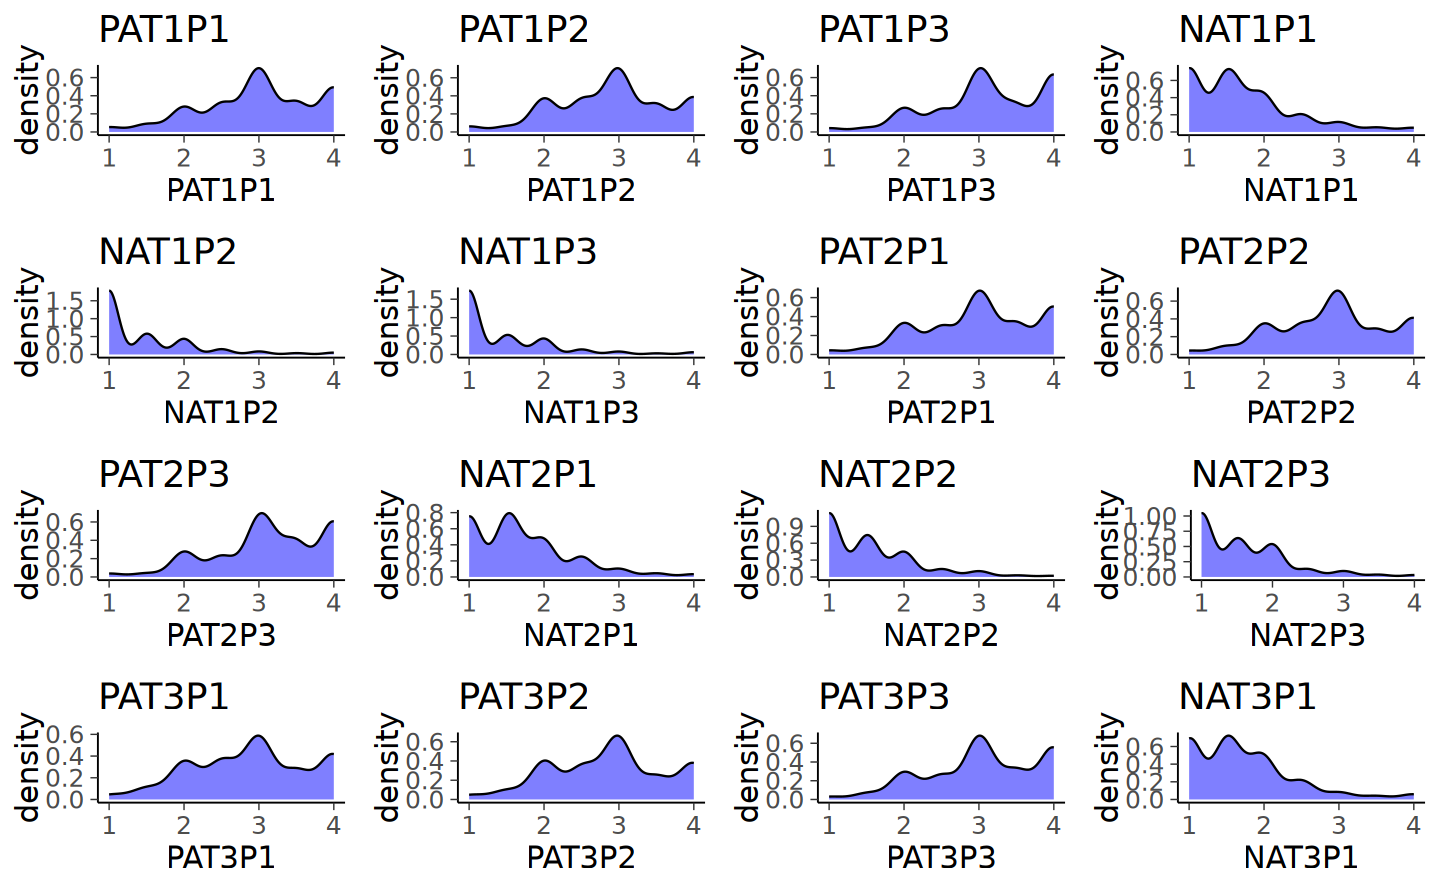
\includegraphics[width=4.375in,height=4.375in]{chapters/measurement/01_scores_scales_files/figure-pdf/cell-10-output-1.png}

\begin{Shaded}
\begin{Highlighting}[]
\FunctionTok{plot}\NormalTok{(}\FunctionTok{density}\NormalTok{(z\_score))}
\end{Highlighting}
\end{Shaded}

\includegraphics[width=4.375in,height=4.375in]{chapters/measurement/01_scores_scales_files/figure-pdf/cell-11-output-1.png}

\begin{Shaded}
\begin{Highlighting}[]
\FunctionTok{plot}\NormalTok{(}\FunctionTok{density}\NormalTok{(T\_score))}
\end{Highlighting}
\end{Shaded}

\includegraphics[width=4.375in,height=4.375in]{chapters/measurement/01_scores_scales_files/figure-pdf/cell-12-output-1.png}

\begin{Shaded}
\begin{Highlighting}[]
\FunctionTok{plot}\NormalTok{(}\FunctionTok{density}\NormalTok{(stanine\_scores))}
\end{Highlighting}
\end{Shaded}

\includegraphics[width=4.375in,height=4.375in]{chapters/measurement/01_scores_scales_files/figure-pdf/cell-13-output-1.png}

La seguente figura proposta da Petersen (2024) illustra le relazioni tra
i punteggi stanini e altre tipologie di punteggi derivati.

\begin{Shaded}
\begin{Highlighting}[]
\NormalTok{standardNormal }\OtherTok{\textless{}{-}} \FunctionTok{data.frame}\NormalTok{(}\AttributeTok{zScore =} \SpecialCharTok{{-}}\DecValTok{4}\SpecialCharTok{:}\DecValTok{4}\NormalTok{)}
\NormalTok{standardNormal}\SpecialCharTok{$}\NormalTok{Tscore }\OtherTok{\textless{}{-}} \FunctionTok{seq}\NormalTok{(}\AttributeTok{from =} \DecValTok{10}\NormalTok{, }\AttributeTok{to =} \DecValTok{90}\NormalTok{, }\AttributeTok{by =} \DecValTok{10}\NormalTok{)}
\NormalTok{standardNormal}\SpecialCharTok{$}\NormalTok{standardScore }\OtherTok{\textless{}{-}} \FunctionTok{seq}\NormalTok{(}\AttributeTok{from =} \DecValTok{40}\NormalTok{, }\AttributeTok{to =} \DecValTok{160}\NormalTok{, }\AttributeTok{by =} \DecValTok{15}\NormalTok{)}
\NormalTok{standardNormal}\SpecialCharTok{$}\NormalTok{cumulativePercent }\OtherTok{\textless{}{-}} \FunctionTok{substr}\NormalTok{(}\FunctionTok{as.character}\NormalTok{(}\FunctionTok{pnorm}\NormalTok{(standardNormal}\SpecialCharTok{$}\NormalTok{zScore) }\SpecialCharTok{*} \DecValTok{100}\NormalTok{), }\DecValTok{1}\NormalTok{, }\DecValTok{4}\NormalTok{)}
\NormalTok{standardNormal}\SpecialCharTok{$}\NormalTok{cumulativePercentFigure }\OtherTok{\textless{}{-}} \FunctionTok{c}\NormalTok{(}\StringTok{"0"}\NormalTok{, }\StringTok{"0.1"}\NormalTok{, }\StringTok{"2.3"}\NormalTok{, }\StringTok{"15.9"}\NormalTok{, }\StringTok{"50"}\NormalTok{, }\StringTok{"84.1"}\NormalTok{, }\StringTok{"97.7"}\NormalTok{, }\StringTok{"99.9"}\NormalTok{, }\StringTok{"100"}\NormalTok{)}

\NormalTok{standardNormal}\SpecialCharTok{$}\NormalTok{nonCumulativePercent[}\DecValTok{1}\NormalTok{] }\OtherTok{\textless{}{-}} \FunctionTok{round}\NormalTok{((}\FunctionTok{pnorm}\NormalTok{(}\SpecialCharTok{{-}}\DecValTok{3}\NormalTok{) }\SpecialCharTok{{-}} \FunctionTok{pnorm}\NormalTok{(}\SpecialCharTok{{-}}\DecValTok{4}\NormalTok{)) }\SpecialCharTok{*} \DecValTok{100}\NormalTok{, }\DecValTok{2}\NormalTok{)}
\NormalTok{standardNormal}\SpecialCharTok{$}\NormalTok{nonCumulativePercent[}\DecValTok{2}\NormalTok{] }\OtherTok{\textless{}{-}} \FunctionTok{round}\NormalTok{((}\FunctionTok{pnorm}\NormalTok{(}\SpecialCharTok{{-}}\DecValTok{2}\NormalTok{) }\SpecialCharTok{{-}} \FunctionTok{pnorm}\NormalTok{(}\SpecialCharTok{{-}}\DecValTok{3}\NormalTok{)) }\SpecialCharTok{*} \DecValTok{100}\NormalTok{, }\DecValTok{2}\NormalTok{)}
\NormalTok{standardNormal}\SpecialCharTok{$}\NormalTok{nonCumulativePercent[}\DecValTok{3}\NormalTok{] }\OtherTok{\textless{}{-}} \FunctionTok{round}\NormalTok{((}\FunctionTok{pnorm}\NormalTok{(}\SpecialCharTok{{-}}\DecValTok{1}\NormalTok{) }\SpecialCharTok{{-}} \FunctionTok{pnorm}\NormalTok{(}\SpecialCharTok{{-}}\DecValTok{2}\NormalTok{)) }\SpecialCharTok{*} \DecValTok{100}\NormalTok{, }\DecValTok{2}\NormalTok{)}
\NormalTok{standardNormal}\SpecialCharTok{$}\NormalTok{nonCumulativePercent[}\DecValTok{4}\NormalTok{] }\OtherTok{\textless{}{-}} \FunctionTok{round}\NormalTok{((}\FunctionTok{pnorm}\NormalTok{(}\DecValTok{0}\NormalTok{) }\SpecialCharTok{{-}} \FunctionTok{pnorm}\NormalTok{(}\SpecialCharTok{{-}}\DecValTok{1}\NormalTok{)) }\SpecialCharTok{*} \DecValTok{100}\NormalTok{, }\DecValTok{2}\NormalTok{)}
\NormalTok{standardNormal}\SpecialCharTok{$}\NormalTok{nonCumulativePercent[}\DecValTok{5}\NormalTok{] }\OtherTok{\textless{}{-}} \FunctionTok{round}\NormalTok{((}\FunctionTok{pnorm}\NormalTok{(}\DecValTok{1}\NormalTok{) }\SpecialCharTok{{-}} \FunctionTok{pnorm}\NormalTok{(}\DecValTok{0}\NormalTok{)) }\SpecialCharTok{*} \DecValTok{100}\NormalTok{, }\DecValTok{2}\NormalTok{)}
\NormalTok{standardNormal}\SpecialCharTok{$}\NormalTok{nonCumulativePercent[}\DecValTok{6}\NormalTok{] }\OtherTok{\textless{}{-}} \FunctionTok{round}\NormalTok{((}\FunctionTok{pnorm}\NormalTok{(}\DecValTok{2}\NormalTok{) }\SpecialCharTok{{-}} \FunctionTok{pnorm}\NormalTok{(}\DecValTok{1}\NormalTok{)) }\SpecialCharTok{*} \DecValTok{100}\NormalTok{, }\DecValTok{2}\NormalTok{)}
\NormalTok{standardNormal}\SpecialCharTok{$}\NormalTok{nonCumulativePercent[}\DecValTok{7}\NormalTok{] }\OtherTok{\textless{}{-}} \FunctionTok{round}\NormalTok{((}\FunctionTok{pnorm}\NormalTok{(}\DecValTok{3}\NormalTok{) }\SpecialCharTok{{-}} \FunctionTok{pnorm}\NormalTok{(}\DecValTok{2}\NormalTok{)) }\SpecialCharTok{*} \DecValTok{100}\NormalTok{, }\DecValTok{2}\NormalTok{)}
\NormalTok{standardNormal}\SpecialCharTok{$}\NormalTok{nonCumulativePercent[}\DecValTok{8}\NormalTok{] }\OtherTok{\textless{}{-}} \FunctionTok{round}\NormalTok{((}\FunctionTok{pnorm}\NormalTok{(}\DecValTok{4}\NormalTok{) }\SpecialCharTok{{-}} \FunctionTok{pnorm}\NormalTok{(}\DecValTok{3}\NormalTok{)) }\SpecialCharTok{*} \DecValTok{100}\NormalTok{, }\DecValTok{2}\NormalTok{)}

\NormalTok{standardNormal}\SpecialCharTok{$}\NormalTok{nonCumulativePercentFigure }\OtherTok{\textless{}{-}} \FunctionTok{paste}\NormalTok{(standardNormal}\SpecialCharTok{$}\NormalTok{nonCumulativePercent, }\StringTok{"\%"}\NormalTok{, }\AttributeTok{sep =} \StringTok{""}\NormalTok{)}
\NormalTok{standardNormal}\SpecialCharTok{$}\NormalTok{midpointsZ }\OtherTok{\textless{}{-}} \FunctionTok{c}\NormalTok{(}\SpecialCharTok{{-}}\FloatTok{3.5}\NormalTok{, }\SpecialCharTok{{-}}\FloatTok{2.5}\NormalTok{, }\SpecialCharTok{{-}}\FloatTok{1.5}\NormalTok{, }\SpecialCharTok{{-}}\FloatTok{0.5}\NormalTok{, }\FloatTok{0.5}\NormalTok{, }\FloatTok{1.5}\NormalTok{, }\FloatTok{2.5}\NormalTok{, }\FloatTok{3.5}\NormalTok{, }\ConstantTok{NA}\NormalTok{)}

\NormalTok{standardNormal}\SpecialCharTok{$}\NormalTok{nonCumulativePercent[}\DecValTok{9}\NormalTok{] }\OtherTok{\textless{}{-}} \ConstantTok{NA}
\NormalTok{standardNormal}\SpecialCharTok{$}\NormalTok{nonCumulativePercentFigure[}\DecValTok{9}\NormalTok{] }\OtherTok{\textless{}{-}} \ConstantTok{NA}

\NormalTok{standardNormalPercentiles }\OtherTok{\textless{}{-}} \FunctionTok{data.frame}\NormalTok{(}\AttributeTok{percentileRank =} \FunctionTok{c}\NormalTok{(}\ConstantTok{NA}\NormalTok{, }\DecValTok{1}\NormalTok{, }\DecValTok{5}\NormalTok{, }\DecValTok{10}\NormalTok{, }\DecValTok{20}\NormalTok{, }\DecValTok{30}\NormalTok{, }\DecValTok{40}\NormalTok{, }\DecValTok{50}\NormalTok{, }\DecValTok{60}\NormalTok{, }\DecValTok{70}\NormalTok{, }\DecValTok{80}\NormalTok{, }\DecValTok{90}\NormalTok{, }\DecValTok{95}\NormalTok{, }\DecValTok{99}\NormalTok{, }\ConstantTok{NA}\NormalTok{))}
\NormalTok{standardNormalPercentiles}\SpecialCharTok{$}\NormalTok{percentileRankZ }\OtherTok{\textless{}{-}} \FunctionTok{qnorm}\NormalTok{(standardNormalPercentiles}\SpecialCharTok{$}\NormalTok{percentileRank }\SpecialCharTok{/} \DecValTok{100}\NormalTok{)}
\NormalTok{standardNormalPercentiles}\SpecialCharTok{$}\NormalTok{percentileRankZ[}\DecValTok{1}\NormalTok{] }\OtherTok{\textless{}{-}} \SpecialCharTok{{-}}\DecValTok{4}
\NormalTok{standardNormalPercentiles}\SpecialCharTok{$}\NormalTok{percentileRankZ[}\FunctionTok{nrow}\NormalTok{(standardNormalPercentiles)] }\OtherTok{\textless{}{-}} \DecValTok{4}

\NormalTok{standardNormalStanines }\OtherTok{\textless{}{-}} \FunctionTok{data.frame}\NormalTok{(}\AttributeTok{stanine =} \DecValTok{1}\SpecialCharTok{:}\DecValTok{9}\NormalTok{)}
\NormalTok{standardNormalStanines}\SpecialCharTok{$}\NormalTok{staninePercent }\OtherTok{\textless{}{-}} \FunctionTok{c}\NormalTok{(}\StringTok{"4\%"}\NormalTok{, }\StringTok{"7\%"}\NormalTok{, }\StringTok{"12\%"}\NormalTok{, }\StringTok{"17\%"}\NormalTok{, }\StringTok{"20\%"}\NormalTok{, }\StringTok{"17\%"}\NormalTok{, }\StringTok{"12\%"}\NormalTok{, }\StringTok{"7\%"}\NormalTok{, }\StringTok{"4\%"}\NormalTok{)}
\NormalTok{standardNormalStanines}\SpecialCharTok{$}\NormalTok{stanineCumulativeStartingPercent }\OtherTok{\textless{}{-}} \FunctionTok{c}\NormalTok{(}\DecValTok{0}\NormalTok{, }\DecValTok{4}\NormalTok{, }\DecValTok{11}\NormalTok{, }\DecValTok{23}\NormalTok{, }\DecValTok{40}\NormalTok{, }\DecValTok{60}\NormalTok{, }\DecValTok{77}\NormalTok{, }\DecValTok{89}\NormalTok{, }\DecValTok{96}\NormalTok{)}
\NormalTok{standardNormalStanines}\SpecialCharTok{$}\NormalTok{stanineCumulativeEndingPercent }\OtherTok{\textless{}{-}} \FunctionTok{c}\NormalTok{(}\DecValTok{4}\NormalTok{, }\DecValTok{11}\NormalTok{, }\DecValTok{23}\NormalTok{, }\DecValTok{40}\NormalTok{, }\DecValTok{60}\NormalTok{, }\DecValTok{77}\NormalTok{, }\DecValTok{89}\NormalTok{, }\DecValTok{96}\NormalTok{, }\DecValTok{100}\NormalTok{)}
\NormalTok{standardNormalStanines}\SpecialCharTok{$}\NormalTok{stanineCumulativeStartingPercentZ }\OtherTok{\textless{}{-}} \FunctionTok{qnorm}\NormalTok{(standardNormalStanines}\SpecialCharTok{$}\NormalTok{stanineCumulativeStartingPercent }\SpecialCharTok{/} \DecValTok{100}\NormalTok{)}
\NormalTok{standardNormalStanines}\SpecialCharTok{$}\NormalTok{stanineCumulativeEndingPercentZ }\OtherTok{\textless{}{-}} \FunctionTok{qnorm}\NormalTok{(standardNormalStanines}\SpecialCharTok{$}\NormalTok{stanineCumulativeEndingPercent }\SpecialCharTok{/} \DecValTok{100}\NormalTok{)}
\NormalTok{standardNormalStanines[standardNormalStanines }\SpecialCharTok{==} \SpecialCharTok{{-}}\ConstantTok{Inf}\NormalTok{] }\OtherTok{\textless{}{-}} \SpecialCharTok{{-}}\DecValTok{4}
\NormalTok{standardNormalStanines[standardNormalStanines }\SpecialCharTok{==} \ConstantTok{Inf}\NormalTok{] }\OtherTok{\textless{}{-}} \DecValTok{4}
\NormalTok{standardNormalStanines}\SpecialCharTok{$}\NormalTok{midpointsZ }\OtherTok{\textless{}{-}} \FunctionTok{rowMeans}\NormalTok{(standardNormalStanines[, }\FunctionTok{c}\NormalTok{(}\StringTok{"stanineCumulativeStartingPercentZ"}\NormalTok{, }\StringTok{"stanineCumulativeEndingPercentZ"}\NormalTok{)])}

\FunctionTok{par}\NormalTok{(}
    \AttributeTok{xpd =} \ConstantTok{NA}\NormalTok{,}
    \AttributeTok{mgp =} \FunctionTok{c}\NormalTok{(}\DecValTok{3}\NormalTok{, }\FloatTok{0.5}\NormalTok{, }\DecValTok{0}\NormalTok{), }\CommentTok{\# gap between axis label and axis}
    \AttributeTok{mar =} \FunctionTok{c}\NormalTok{(}\DecValTok{12}\NormalTok{, }\DecValTok{8}\NormalTok{, }\DecValTok{0}\NormalTok{, }\DecValTok{0}\NormalTok{) }\SpecialCharTok{+} \FloatTok{0.1}
\NormalTok{) }\CommentTok{\# plot margins: default of the form c(bottom, left, top, right): c(5, 4, 4, 2) + 0.1}
\NormalTok{x }\OtherTok{\textless{}{-}} \FunctionTok{seq}\NormalTok{(}\SpecialCharTok{{-}}\DecValTok{4}\NormalTok{, }\DecValTok{4}\NormalTok{, }\AttributeTok{length =} \DecValTok{10000}\NormalTok{)}
\NormalTok{y }\OtherTok{\textless{}{-}} \FunctionTok{dnorm}\NormalTok{(x, }\AttributeTok{mean =} \DecValTok{0}\NormalTok{, }\AttributeTok{sd =} \DecValTok{1}\NormalTok{)}

\FunctionTok{plot}\NormalTok{(x, y, }\AttributeTok{type =} \StringTok{"l"}\NormalTok{, }\AttributeTok{lwd =} \DecValTok{8}\NormalTok{, }\AttributeTok{axes =} \ConstantTok{FALSE}\NormalTok{, }\AttributeTok{xlab =} \ConstantTok{NA}\NormalTok{, }\AttributeTok{ylab =} \ConstantTok{NA}\NormalTok{, }\AttributeTok{col =} \StringTok{"gray"}\NormalTok{)}

\FunctionTok{segments}\NormalTok{(}\AttributeTok{x0 =} \SpecialCharTok{{-}}\DecValTok{4}\NormalTok{, }\AttributeTok{y0 =} \DecValTok{0}\NormalTok{, }\AttributeTok{y1 =} \DecValTok{1}\NormalTok{)}
\FunctionTok{segments}\NormalTok{(}\AttributeTok{x0 =} \SpecialCharTok{{-}}\DecValTok{3}\NormalTok{, }\AttributeTok{y0 =} \DecValTok{0}\NormalTok{, }\AttributeTok{y1 =} \DecValTok{1}\NormalTok{)}
\FunctionTok{segments}\NormalTok{(}\AttributeTok{x0 =} \SpecialCharTok{{-}}\DecValTok{2}\NormalTok{, }\AttributeTok{y0 =} \DecValTok{0}\NormalTok{, }\AttributeTok{y1 =} \DecValTok{1}\NormalTok{)}
\FunctionTok{segments}\NormalTok{(}\AttributeTok{x0 =} \SpecialCharTok{{-}}\DecValTok{1}\NormalTok{, }\AttributeTok{y0 =} \DecValTok{0}\NormalTok{, }\AttributeTok{y1 =} \DecValTok{1}\NormalTok{)}
\FunctionTok{segments}\NormalTok{(}\AttributeTok{x0 =} \DecValTok{0}\NormalTok{, }\AttributeTok{y0 =} \DecValTok{0}\NormalTok{, }\AttributeTok{y1 =} \DecValTok{1}\NormalTok{)}
\FunctionTok{segments}\NormalTok{(}\AttributeTok{x0 =} \DecValTok{1}\NormalTok{, }\AttributeTok{y0 =} \DecValTok{0}\NormalTok{, }\AttributeTok{y1 =} \DecValTok{1}\NormalTok{)}
\FunctionTok{segments}\NormalTok{(}\AttributeTok{x0 =} \DecValTok{2}\NormalTok{, }\AttributeTok{y0 =} \DecValTok{0}\NormalTok{, }\AttributeTok{y1 =} \DecValTok{1}\NormalTok{)}
\FunctionTok{segments}\NormalTok{(}\AttributeTok{x0 =} \DecValTok{3}\NormalTok{, }\AttributeTok{y0 =} \DecValTok{0}\NormalTok{, }\AttributeTok{y1 =} \DecValTok{1}\NormalTok{)}
\FunctionTok{segments}\NormalTok{(}\AttributeTok{x0 =} \DecValTok{4}\NormalTok{, }\AttributeTok{y0 =} \DecValTok{0}\NormalTok{, }\AttributeTok{y1 =} \DecValTok{1}\NormalTok{)}

\FunctionTok{axis}\NormalTok{(}\AttributeTok{side =} \DecValTok{1}\NormalTok{, }\AttributeTok{at =}\NormalTok{ standardNormal}\SpecialCharTok{$}\NormalTok{zScore, }\AttributeTok{pos =} \DecValTok{0}\NormalTok{)}
\FunctionTok{axis}\NormalTok{(}\AttributeTok{side =} \DecValTok{1}\NormalTok{, }\AttributeTok{at =}\NormalTok{ standardNormal}\SpecialCharTok{$}\NormalTok{zScore, }\AttributeTok{pos =} \SpecialCharTok{{-}}\NormalTok{.}\DecValTok{06}\NormalTok{, }\AttributeTok{labels =}\NormalTok{ standardNormal}\SpecialCharTok{$}\NormalTok{Tscore)}
\FunctionTok{axis}\NormalTok{(}\AttributeTok{side =} \DecValTok{1}\NormalTok{, }\AttributeTok{at =}\NormalTok{ standardNormal}\SpecialCharTok{$}\NormalTok{zScore, }\AttributeTok{pos =} \SpecialCharTok{{-}}\NormalTok{.}\DecValTok{12}\NormalTok{, }\AttributeTok{labels =}\NormalTok{ standardNormal}\SpecialCharTok{$}\NormalTok{standardScore)}
\FunctionTok{axis}\NormalTok{(}\AttributeTok{side =} \DecValTok{1}\NormalTok{, }\AttributeTok{at =}\NormalTok{ standardNormal}\SpecialCharTok{$}\NormalTok{zScore, }\AttributeTok{pos =} \SpecialCharTok{{-}}\NormalTok{.}\DecValTok{18}\NormalTok{, }\AttributeTok{labels =}\NormalTok{ standardNormal}\SpecialCharTok{$}\NormalTok{cumulativePercentFigure)}
\FunctionTok{axis}\NormalTok{(}\AttributeTok{side =} \DecValTok{1}\NormalTok{, }\AttributeTok{at =}\NormalTok{ standardNormalPercentiles}\SpecialCharTok{$}\NormalTok{percentileRankZ, }\AttributeTok{pos =} \SpecialCharTok{{-}}\NormalTok{.}\DecValTok{24}\NormalTok{, }\AttributeTok{labels =}\NormalTok{ standardNormalPercentiles}\SpecialCharTok{$}\NormalTok{percentileRank, }\AttributeTok{cex.axis =} \FloatTok{0.5}\NormalTok{)}

\FunctionTok{rect}\NormalTok{(}\AttributeTok{xleft =}\NormalTok{ standardNormalStanines}\SpecialCharTok{$}\NormalTok{stanineCumulativeStartingPercentZ, }\AttributeTok{ybottom =} \SpecialCharTok{{-}}\NormalTok{.}\DecValTok{36}\NormalTok{, }\AttributeTok{xright =}\NormalTok{ standardNormalStanines}\SpecialCharTok{$}\NormalTok{stanineCumulativeEndingPercentZ, }\AttributeTok{ytop =} \SpecialCharTok{{-}}\NormalTok{.}\DecValTok{31}\NormalTok{)}
\FunctionTok{mtext}\NormalTok{(standardNormalStanines}\SpecialCharTok{$}\NormalTok{stanine, }\AttributeTok{side =} \DecValTok{1}\NormalTok{, }\AttributeTok{line =} \DecValTok{9}\NormalTok{, }\AttributeTok{at =}\NormalTok{ standardNormalStanines}\SpecialCharTok{$}\NormalTok{midpointsZ)}

\FunctionTok{text}\NormalTok{(}\FloatTok{0.05}\NormalTok{, .}\DecValTok{02}\NormalTok{, }\AttributeTok{labels =} \StringTok{"Standard Deviations"}\NormalTok{)}
\FunctionTok{text}\NormalTok{(standardNormal}\SpecialCharTok{$}\NormalTok{midpointsZ, .}\DecValTok{06}\NormalTok{, }\AttributeTok{labels =}\NormalTok{ standardNormal}\SpecialCharTok{$}\NormalTok{nonCumulativePercentFigure)}

\FunctionTok{mtext}\NormalTok{(}\StringTok{"Percent of cases }\SpecialCharTok{\textbackslash{}n}\StringTok{ under segment of }\SpecialCharTok{\textbackslash{}n}\StringTok{ the normal curve"}\NormalTok{, }\AttributeTok{side =} \DecValTok{2}\NormalTok{, }\AttributeTok{line =} \DecValTok{0}\NormalTok{, }\AttributeTok{at =}\NormalTok{ .}\DecValTok{05}\NormalTok{, }\AttributeTok{las =} \DecValTok{1}\NormalTok{)}
\FunctionTok{mtext}\NormalTok{(}\StringTok{"z scores"}\NormalTok{, }\AttributeTok{side =} \DecValTok{2}\NormalTok{, }\AttributeTok{line =} \DecValTok{0}\NormalTok{, }\AttributeTok{at =} \SpecialCharTok{{-}}\NormalTok{.}\DecValTok{033}\NormalTok{, }\AttributeTok{las =} \DecValTok{1}\NormalTok{)}
\FunctionTok{mtext}\NormalTok{(}\StringTok{"T scores"}\NormalTok{, }\AttributeTok{side =} \DecValTok{2}\NormalTok{, }\AttributeTok{line =} \DecValTok{0}\NormalTok{, }\AttributeTok{at =} \SpecialCharTok{{-}}\NormalTok{.}\DecValTok{0934}\NormalTok{, }\AttributeTok{las =} \DecValTok{1}\NormalTok{)}
\FunctionTok{mtext}\NormalTok{(}\StringTok{"Standard scores"}\NormalTok{, }\AttributeTok{side =} \DecValTok{2}\NormalTok{, }\AttributeTok{line =} \DecValTok{0}\NormalTok{, }\AttributeTok{at =} \SpecialCharTok{{-}}\NormalTok{.}\DecValTok{1538}\NormalTok{, }\AttributeTok{las =} \DecValTok{1}\NormalTok{)}
\FunctionTok{mtext}\NormalTok{(}\StringTok{"Cumulative percent"}\NormalTok{, }\AttributeTok{side =} \DecValTok{2}\NormalTok{, }\AttributeTok{line =} \DecValTok{0}\NormalTok{, }\AttributeTok{at =} \SpecialCharTok{{-}}\NormalTok{.}\DecValTok{2142}\NormalTok{, }\AttributeTok{las =} \DecValTok{1}\NormalTok{)}
\FunctionTok{mtext}\NormalTok{(}\StringTok{"Percentile ranks"}\NormalTok{, }\AttributeTok{side =} \DecValTok{2}\NormalTok{, }\AttributeTok{line =} \DecValTok{0}\NormalTok{, }\AttributeTok{at =} \SpecialCharTok{{-}}\NormalTok{.}\DecValTok{2746}\NormalTok{, }\AttributeTok{las =} \DecValTok{1}\NormalTok{)}
\FunctionTok{mtext}\NormalTok{(}\StringTok{"Stanines"}\NormalTok{, }\AttributeTok{side =} \DecValTok{2}\NormalTok{, }\AttributeTok{line =} \DecValTok{0}\NormalTok{, }\AttributeTok{at =} \SpecialCharTok{{-}}\NormalTok{.}\DecValTok{335}\NormalTok{, }\AttributeTok{las =} \DecValTok{1}\NormalTok{)}
\end{Highlighting}
\end{Shaded}

\includegraphics[width=5in,height=3.08333in]{chapters/measurement/01_scores_scales_files/figure-pdf/cell-14-output-1.png}

\subsection{Equivalenti alla Curva Normale
(NCE)}\label{equivalenti-alla-curva-normale-nce}

Gli Equivalenti alla Curva Normale, noti come NCE (dall'inglese ``Normal
Curve Equivalents''), sono un tipo di punteggio standardizzato
utilizzato in ambito psicometrico. Questi punteggi vengono calcolati per
trasformare i punteggi grezzi ottenuti in un test in una scala che
rifletta una distribuzione approssimativamente normale. L'obiettivo
principale dei punteggi NCE è quello di rendere i punteggi di diverse
misure o test direttamente confrontabili, mantenendo una distribuzione
che si allinea strettamente con una curva normale standard.

\subsubsection{Caratteristiche dei Punteggi
NCE}\label{caratteristiche-dei-punteggi-nce}

\begin{itemize}
\tightlist
\item
  \textbf{Distribuzione Normalizzata}: I punteggi NCE sono progettati
  per aderire a una distribuzione normale. Ciò significa che, a
  differenza di altri tipi di punteggi, i NCE si allineano più da vicino
  con le caratteristiche di una curva di distribuzione gaussiana, con la
  maggior parte dei punteggi concentrati intorno alla media e una
  distribuzione simmetrica verso gli estremi.
\item
  \textbf{Facilità di Comparazione}: Grazie alla loro standardizzazione,
  i punteggi NCE consentono un confronto diretto e significativo tra le
  prestazioni in diversi test o misure. Questo è particolarmente utile
  in contesti educativi e clinici dove è necessario interpretare e
  confrontare i risultati di diversi test.
\end{itemize}

\subsubsection{Calcolo e Utilizzo dei Punteggi
NCE}\label{calcolo-e-utilizzo-dei-punteggi-nce}

Il calcolo dei punteggi NCE si basa sulla trasformazione dei punteggi
grezzi in modo che si adattino a una distribuzione normalizzata. Questo
processo implica l'uso di formule matematiche che riallineano i dati
grezzi su una scala standard, considerando la media e la deviazione
standard del campione normativo.

Una volta calcolati, i punteggi NCE offrono una visione chiara e
immediata delle prestazioni relative di un individuo o di un gruppo,
rispetto a un campione normativo. Questo tipo di punteggio è
particolarmente utile quando i punteggi grezzi provengono da
distribuzioni che non seguono una curva normale, consentendo così
un'interpretazione più accurata e standardizzata dei risultati.

\subsubsection{Applicazioni Pratiche dei Punteggi
NCE}\label{applicazioni-pratiche-dei-punteggi-nce}

I punteggi NCE trovano impiego in una varietà di contesti, tra cui:

\begin{itemize}
\tightlist
\item
  \textbf{Valutazioni Educative}: In ambito scolastico, per confrontare
  le prestazioni degli studenti in test diversi.
\item
  \textbf{Ricerca Psicologica}: Per analizzare e confrontare i risultati
  di diversi studi o misure psicometriche.
\item
  \textbf{Pratica Clinica}: Nella valutazione di clienti o pazienti
  utilizzando diversi strumenti diagnostici.
\end{itemize}

In conclusione, i punteggi Equivalenti alla Curva Normale rappresentano
uno strumento psicometrico potente per standardizzare e confrontare
efficacemente i risultati di diversi test o misure, assicurando che
questi siano interpretati all'interno di un quadro coerente e
comparabile.

Per i dati dell'esempio abbiamo:

\begin{Shaded}
\begin{Highlighting}[]
\CommentTok{\# Using normal quantile}
\NormalTok{qnorm\_pr }\OtherTok{\textless{}{-}} \FunctionTok{qnorm}\NormalTok{(pr }\SpecialCharTok{/} \DecValTok{100}\NormalTok{)}
\CommentTok{\# Convert raw scores}
\NormalTok{normalized\_zscore }\OtherTok{\textless{}{-}} \FunctionTok{as.vector}\NormalTok{(qnorm\_pr[}\FunctionTok{as.character}\NormalTok{(raw\_score)])}
\end{Highlighting}
\end{Shaded}

In alternativa, è possibile usare la trasformazione di Box-Cox, che è
una tecnica parametrica che cerca di correggere le asimmetrie e
trasformare i dati in una forma che approssima una distribuzione
normale. È efficace per i dati positivi. La trasformazione è definita
come segue:

\[
 y(\lambda) = \begin{cases} \frac{x^\lambda - 1}{\lambda} & \text{se } \lambda \neq 0 \\ \log(x) & \text{se } \lambda = 0 \end{cases},
 \]

dove \(x\) è il valore originale e \(\lambda\) è il parametro di
trasformazione che viene spesso trovato attraverso la massimizzazione
della verosimiglianza.

Supponiamo di voler utilizzare la trasformazione di Box-Cox sul nostro
set di dati. La procedura è la seguente. Questo codice utilizza la
funzione \texttt{boxcox} dal pacchetto MASS per trovare il valore di
\(\lambda\) che massimizza la log-verosimiglianza della trasformazione
di Box-Cox applicata ai dati. Poi, utilizza questo \(\lambda\) per
trasformare i dati.

\begin{Shaded}
\begin{Highlighting}[]
\CommentTok{\# Dati di esempio}
\FunctionTok{set.seed}\NormalTok{(}\DecValTok{123}\NormalTok{) }\CommentTok{\# Per rendere l\textquotesingle{}esempio riproducibile}
\NormalTok{data }\OtherTok{\textless{}{-}}\NormalTok{ raw\_score}

\CommentTok{\# Trova il miglior lambda per la trasformazione di Box{-}Cox}
\NormalTok{bc }\OtherTok{\textless{}{-}} \FunctionTok{boxcox}\NormalTok{(data }\SpecialCharTok{\textasciitilde{}} \DecValTok{1}\NormalTok{, }\AttributeTok{lambda =} \FunctionTok{seq}\NormalTok{(}\SpecialCharTok{{-}}\DecValTok{2}\NormalTok{, }\DecValTok{2}\NormalTok{, }\AttributeTok{by =} \FloatTok{0.1}\NormalTok{))}

\CommentTok{\# Calcola la trasformazione di Box{-}Cox con il lambda ottimale}
\NormalTok{lambda\_opt }\OtherTok{\textless{}{-}}\NormalTok{ bc}\SpecialCharTok{$}\NormalTok{x[}\FunctionTok{which.max}\NormalTok{(bc}\SpecialCharTok{$}\NormalTok{y)]}
\NormalTok{data\_transformed }\OtherTok{\textless{}{-}}\NormalTok{ (data}\SpecialCharTok{\^{}}\NormalTok{lambda\_opt }\SpecialCharTok{{-}} \DecValTok{1}\NormalTok{) }\SpecialCharTok{/}\NormalTok{ lambda\_opt}
\end{Highlighting}
\end{Shaded}

\includegraphics[width=4.375in,height=4.375in]{chapters/measurement/01_scores_scales_files/figure-pdf/cell-16-output-1.png}

Avendo trovato i dati trasformati con la procedura Box-Cox, li
confrontiamo con gli Equivalenti alla Curva Normale (NCE) calcolati con
la procedura usuale.

\begin{Shaded}
\begin{Highlighting}[]
\FunctionTok{plot}\NormalTok{(normalized\_zscore, data\_transformed)}
\end{Highlighting}
\end{Shaded}

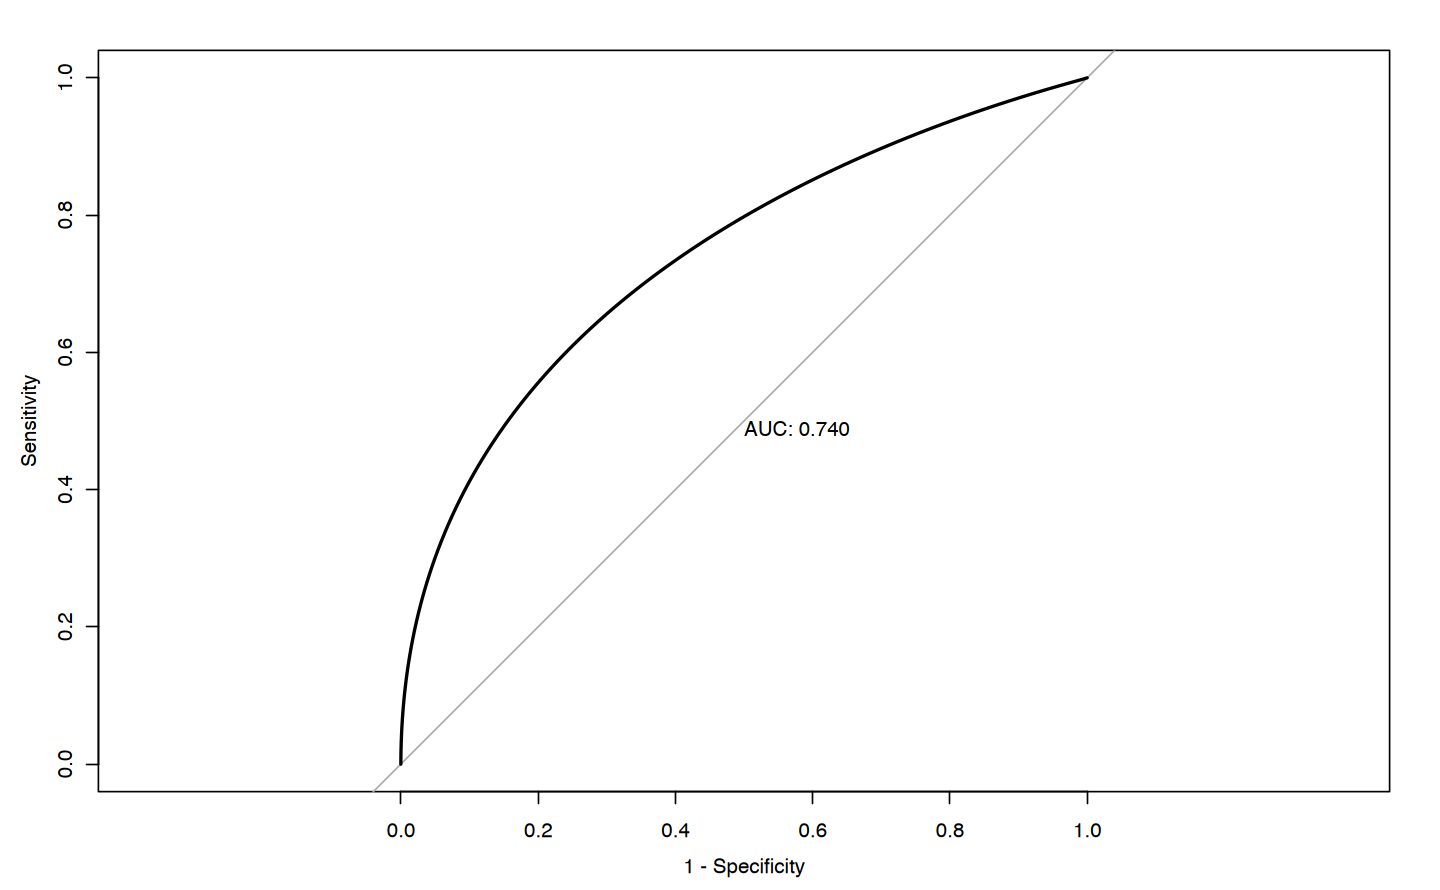
\includegraphics[width=4.375in,height=4.375in]{chapters/measurement/01_scores_scales_files/figure-pdf/cell-17-output-1.png}

\begin{Shaded}
\begin{Highlighting}[]
\FunctionTok{plot}\NormalTok{(}\FunctionTok{density}\NormalTok{(normalized\_zscore)) }\CommentTok{\# the shape will be closer to normal}
\end{Highlighting}
\end{Shaded}

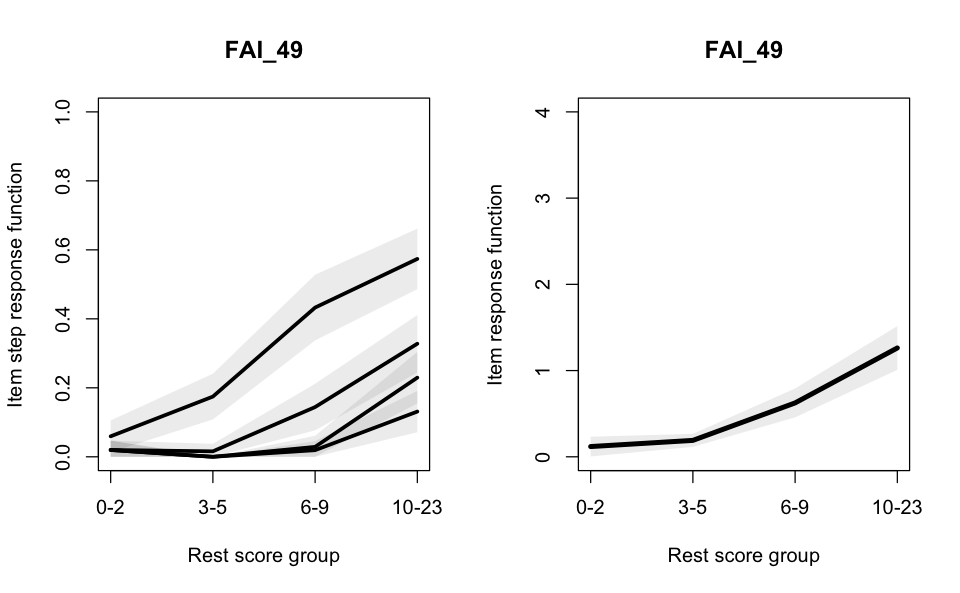
\includegraphics[width=4.375in,height=4.375in]{chapters/measurement/01_scores_scales_files/figure-pdf/cell-18-output-1.png}

\begin{Shaded}
\begin{Highlighting}[]
\FunctionTok{plot}\NormalTok{(}\FunctionTok{density}\NormalTok{((data\_transformed }\SpecialCharTok{{-}} \FunctionTok{mean}\NormalTok{(data\_transformed)) }\SpecialCharTok{/} \FunctionTok{sd}\NormalTok{(data\_transformed)))}
\end{Highlighting}
\end{Shaded}

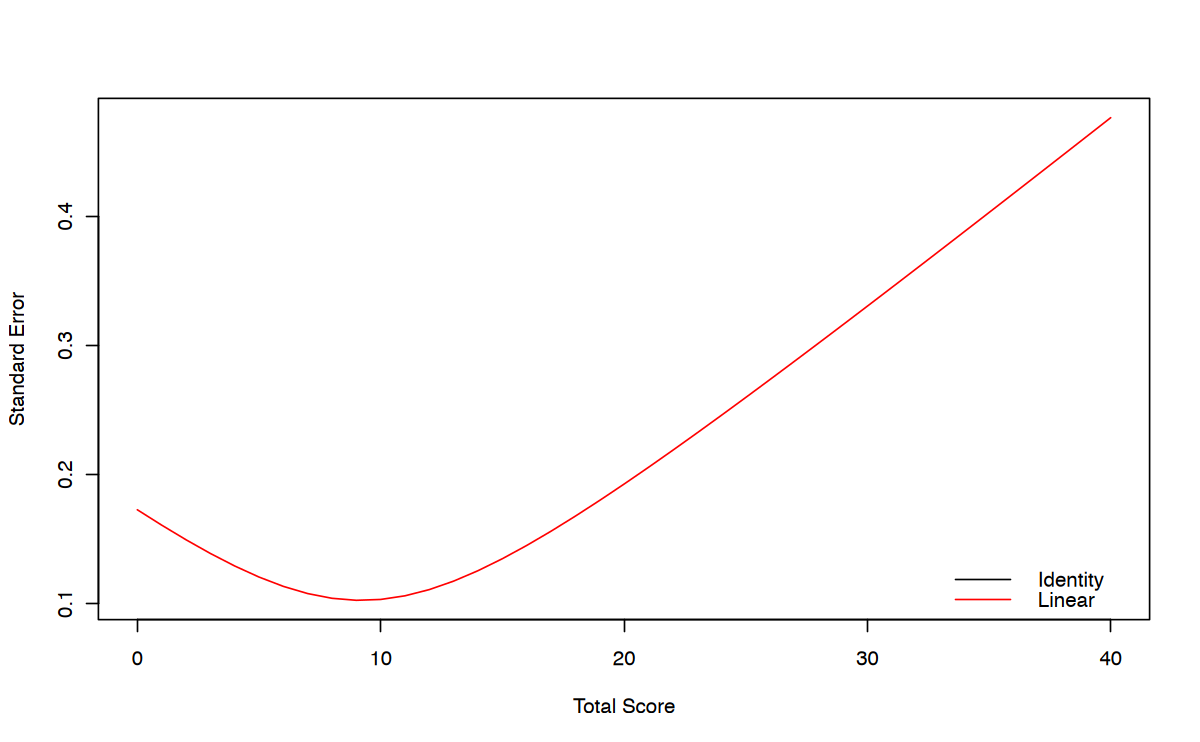
\includegraphics[width=4.375in,height=4.375in]{chapters/measurement/01_scores_scales_files/figure-pdf/cell-19-output-1.png}

Si osservi che i dati NCE presentano una distribuzione più simile a una
curva a forma campanulare rispetto ai dati grezzi.

\begin{Shaded}
\begin{Highlighting}[]
\FunctionTok{lillie.test}\NormalTok{(normalized\_zscore)}
\end{Highlighting}
\end{Shaded}

\begin{verbatim}

    Lilliefors (Kolmogorov-Smirnov) normality test

data:  normalized_zscore
D = 0.085801, p-value = 0.4426
\end{verbatim}

\begin{Shaded}
\begin{Highlighting}[]
\FunctionTok{lillie.test}\NormalTok{(data\_transformed)}
\end{Highlighting}
\end{Shaded}

\begin{verbatim}

    Lilliefors (Kolmogorov-Smirnov) normality test

data:  data_transformed
D = 0.12456, p-value = 0.04274
\end{verbatim}

\section{Riflessioni Finali sui Metodi di Trasformazione dei
Punteggi}\label{riflessioni-finali-sui-metodi-di-trasformazione-dei-punteggi}

La trasformazione dei punteggi grezzi in formati più interpretabili è
una pratica cruciale in psicometria. Due sono i principali approcci
utilizzati per attribuire significato ai punteggi di un test: il
riferimento normativo e il riferimento criteriale.

\subsection{Riferimento Normativo}\label{riferimento-normativo}

Nel riferimento normativo, si confronta il punteggio di un individuo con
quello medio del gruppo normativo, ovvero gli altri soggetti che hanno
svolto lo stesso test. Ci sono diversi tipi di punteggi normati,
ciascuno con i suoi specifici vantaggi e limitazioni:

\begin{itemize}
\item
  \textbf{Punteggi Percentili}: Questi punteggi sono intuitivi e offrono
  un'indicazione immediata della posizione relativa di un individuo
  all'interno di un gruppo. Tuttavia, sono una scala ordinale e non si
  prestano bene a calcoli matematici più complessi.
\item
  \textbf{Punteggi Standardizzati}: Gli z-score e i T-scores rientrano
  in questa categoria. Sono scalari a intervallo, quindi adatti a
  operazioni matematiche. Mantengono la forma distributiva originale dei
  punteggi grezzi, rendendo più agevole la loro elaborazione statistica.
\end{itemize}

\subsection{Riferimento Criteriale}\label{riferimento-criteriale}

Al contrario del riferimento normativo, il riferimento criteriale
confronta i punteggi di un individuo con uno standard prestabilito o un
criterio specifico, piuttosto che con i punteggi di altri individui.

\subsection{Trasformazioni per la
Normalizzazione}\label{trasformazioni-per-la-normalizzazione}

Per ottenere una distribuzione dei punteggi più vicina alla curva
normale, si possono utilizzare trasformazioni come gli stanini o gli NCE
(Normal Curve Equivalents). Questi metodi di normalizzazione aiutano a
standardizzare la distribuzione dei punteggi, facilitando così
l'interpretazione e l'analisi dei dati psicometrici.

In conclusione, la scelta del metodo di trasformazione dei punteggi
dipende dagli obiettivi specifici della valutazione e
dall'interpretazione desiderata. La comprensione di queste diverse
tecniche è essenziale per una corretta interpretazione dei risultati dei
test e per l'analisi psicometrica più generale.

\section{Considerazioni Conclusive}\label{considerazioni-conclusive}

Questo capitolo fornisce una panoramica sui diversi tipi di punteggi dei
test e il loro significato. Iniziamo notando che i punteggi grezzi,
sebbene facili da calcolare, di solito forniscono poche informazioni
utili sul rendimento di un esaminando in un test. Di conseguenza, di
solito trasformiamo i punteggi grezzi in punteggi derivati, che possono
essere di riferimento normativo o al criterio. I punteggi di riferimento
normativo confrontano il rendimento di un esaminando con quello di altre
persone nel campione di standardizzazione, mentre quelli al criterio
confrontano il rendimento con un livello di competenza specificato. È
importante valutare l'adeguatezza del campione di standardizzazione
quando si utilizzano punteggi di riferimento normativo.

Per interpretazioni basate sui punteggi di riferimento normativo, è
utile conoscere la distribuzione normale e i punteggi standard di
riferimento. Questi ultimi hanno una media predefinita e una deviazione
standard. Esistono anche punteggi normalizzati quando i punteggi non
seguono una distribuzione normale. Altri tipi di punteggi di riferimento
normativo includono il rango percentile e i punteggi basati su età o
livello di scolarità. Tuttavia, questi ultimi sono da evitare, se
possibile, a favore di punteggi standard e ranghi percentile.

I punteggi al criterio confrontano il rendimento con un livello
specifico di competenza. Sono utili per valutare abilità in domini
specifici, ma richiedono una chiara definizione del dominio. A volte, un
test può produrre entrambi i tipi di punteggi. Forniamo anche una
panoramica dei punteggi basati sulla teoria della risposta agli item
(IRT), che sono utili per misurare i cambiamenti nel tempo.

In conclusione, i diversi tipi di punteggi dei test forniscono
informazioni per rispondere a diverse domande e devono essere scelti in
base alle esigenze specifiche dell'analisi dei dati del test.

\section{Esercizi}\label{esercizi}

Bandalos, capitolo 2, E1, E2, E5, E6, E7, E8, E9, E12

\section{Session Info}\label{session-info}

\begin{Shaded}
\begin{Highlighting}[]
\FunctionTok{sessionInfo}\NormalTok{()}
\end{Highlighting}
\end{Shaded}

\begin{verbatim}
R version 4.4.1 (2024-06-14)
Platform: aarch64-apple-darwin20
Running under: macOS 15.0

Matrix products: default
BLAS:   /Library/Frameworks/R.framework/Versions/4.4-arm64/Resources/lib/libRblas.0.dylib 
LAPACK: /Library/Frameworks/R.framework/Versions/4.4-arm64/Resources/lib/libRlapack.dylib;  LAPACK version 3.12.0

locale:
[1] C

time zone: Europe/Rome
tzcode source: internal

attached base packages:
[1] stats     graphics  grDevices utils     datasets  methods   base     

other attached packages:
 [1] nortest_1.0-4     MASS_7.3-61       ggokabeito_0.1.0  viridis_0.6.5    
 [5] viridisLite_0.4.2 ggpubr_0.6.0      ggExtra_0.10.1    gridExtra_2.3    
 [9] patchwork_1.3.0   bayesplot_1.11.1  semTools_0.5-6    semPlot_1.1.6    
[13] lavaan_0.6-18     psych_2.4.6.26    scales_1.3.0      markdown_1.13    
[17] knitr_1.48        lubridate_1.9.3   forcats_1.0.0     stringr_1.5.1    
[21] dplyr_1.1.4       purrr_1.0.2       readr_2.1.5       tidyr_1.3.1      
[25] tibble_3.2.1      ggplot2_3.5.1     tidyverse_2.0.0   here_1.0.1       

loaded via a namespace (and not attached):
  [1] rstudioapi_0.16.0  jsonlite_1.8.9     magrittr_2.0.3    
  [4] TH.data_1.1-2      estimability_1.5.1 farver_2.1.2      
  [7] nloptr_2.1.1       rmarkdown_2.28     vctrs_0.6.5       
 [10] minqa_1.2.8        base64enc_0.1-3    rstatix_0.7.2     
 [13] htmltools_0.5.8.1  broom_1.0.6        Formula_1.2-5     
 [16] htmlwidgets_1.6.4  plyr_1.8.9         sandwich_3.1-1    
 [19] emmeans_1.10.4     zoo_1.8-12         uuid_1.2-1        
 [22] igraph_2.0.3       mime_0.12          lifecycle_1.0.4   
 [25] pkgconfig_2.0.3    Matrix_1.7-0       R6_2.5.1          
 [28] fastmap_1.2.0      shiny_1.9.1        digest_0.6.37     
 [31] OpenMx_2.21.12     fdrtool_1.2.18     colorspace_2.1-1  
 [34] rprojroot_2.0.4    Hmisc_5.1-3        fansi_1.0.6       
 [37] timechange_0.3.0   abind_1.4-8        compiler_4.4.1    
 [40] withr_3.0.1        glasso_1.11        htmlTable_2.4.3   
 [43] backports_1.5.0    carData_3.0-5      ggsignif_0.6.4    
 [46] corpcor_1.6.10     gtools_3.9.5       tools_4.4.1       
 [49] pbivnorm_0.6.0     foreign_0.8-87     zip_2.3.1         
 [52] httpuv_1.6.15      nnet_7.3-19        glue_1.7.0        
 [55] quadprog_1.5-8     promises_1.3.0     nlme_3.1-166      
 [58] lisrelToR_0.3      grid_4.4.1         pbdZMQ_0.3-13     
 [61] checkmate_2.3.2    cluster_2.1.6      reshape2_1.4.4    
 [64] generics_0.1.3     gtable_0.3.5       tzdb_0.4.0        
 [67] data.table_1.16.0  hms_1.1.3          car_3.1-2         
 [70] utf8_1.2.4         sem_3.1-16         pillar_1.9.0      
 [73] IRdisplay_1.1      rockchalk_1.8.157  later_1.3.2       
 [76] splines_4.4.1      lattice_0.22-6     survival_3.7-0    
 [79] kutils_1.73        tidyselect_1.2.1   miniUI_0.1.1.1    
 [82] pbapply_1.7-2      stats4_4.4.1       xfun_0.47         
 [85] qgraph_1.9.8       arm_1.14-4         stringi_1.8.4     
 [88] boot_1.3-31        evaluate_1.0.0     codetools_0.2-20  
 [91] mi_1.1             cli_3.6.3          RcppParallel_5.1.9
 [94] IRkernel_1.3.2     rpart_4.1.23       xtable_1.8-4      
 [97] repr_1.1.7         munsell_0.5.1      Rcpp_1.0.13       
[100] coda_0.19-4.1      png_0.1-8          XML_3.99-0.17     
[103] parallel_4.4.1     jpeg_0.1-10        lme4_1.1-35.5     
[106] mvtnorm_1.3-1      openxlsx_4.2.7.1   crayon_1.5.3      
[109] rlang_1.1.4        multcomp_1.4-26    mnormt_2.1.1      
\end{verbatim}

\chapter{✏️ Esercizi}\label{ex-likert}

\textbf{Prerequisiti}

\textbf{Concetti e Competenze Chiave}

\textbf{Preparazione del Notebook}

\begin{Shaded}
\begin{Highlighting}[]
\FunctionTok{source}\NormalTok{(}\StringTok{"../../code/\_common.R"}\NormalTok{)}
\end{Highlighting}
\end{Shaded}

\section{Scaling Likert}\label{scaling-likert}

In questo tutorial esamineremo i dati di un questionario ordinale. Gli
obiettivi saranno il punteggio totale e lo scaling normativo.

Il \emph{Strengths and Difficulties Questionnaire} (SDQ) è un breve
questionario di screening comportamentale riguardante bambini e
adolescenti di età compresa tra 3 e 16 anni. Esiste in diverse versioni
consultabili su http://www.sdqinfo.org/. Dal sito è possibile scaricare
il questionario, il metodo di scoring e le norme del test.

La versione autovalutativa (SDQ Pupil) include 25 item che misurano 5
scale (faccette), con 5 item ciascuna:

\begin{itemize}
\tightlist
\item
  Sintomi Emotivi somatico preoccupazioni triste attaccamento paura
\item
  Problemi di Condotta scatti ubbidisce* litiga mente ruba
\item
  Iperattività irrequietezza agitato distratto riflessivo* attento*
\item
  Problemi con i Peer solitario amico* popolare* vittima di bullismo
  vecchio migliore amico
\item
  Pro-sociale prendersi cura condivide gentilezza aiuta
\end{itemize}

Ai partecipanti viene chiesto di valutare ciascuna domanda utilizzando
le seguenti opzioni di risposta: 0 = ``Non vero'' 1 = ``Un po' vero'' 2
= ``Certamente vero''

NOTA che alcuni item del SDQ sono \emph{reverse}: item a punteggio
invertito -- punteggi più alti della scala corrispondono a punteggi
inferiori degli item. Ad esempio, l'item ``Di solito faccio quello che
mi dicono'' (variabile ubbidisce) è reverse dei Problemi di Condotta. Ci
sono 5 item di questo tipo nel SDQ; sono contrassegnati nella tabella
sopra con asterischi (*).

I partecipanti a questo studio sono alunni di seconda media della stessa
scuola (N=228). Si tratta di un campione di comunità e non ci aspettiamo
che molti bambini abbiano punteggi al di sopra delle soglie cliniche. Il
SDQ è stato somministrato due volte, la prima volta quando i bambini
hanno appena iniziato la scuola secondaria (erano in anno 7), e un anno
dopo (erano in anno 8).

\section{Emotional Symptoms scale}\label{emotional-symptoms-scale}

Questa scala non contiene item reverse.

Importiamo i dati in R.

\begin{Shaded}
\begin{Highlighting}[]
\FunctionTok{load}\NormalTok{(}\StringTok{"../../data/data\_sdq/SDQ.RData"}\NormalTok{)}
\FunctionTok{glimpse}\NormalTok{(SDQ)}
\end{Highlighting}
\end{Shaded}

\begin{verbatim}
Rows: 228
Columns: 51
$ Gender   <dbl> 1, 1, 1, 1, 1, 1, 1, 1, 1, 1, 1, 1, 1, 1, 1, 1, 1, 1, 1, 1, 1~
$ consid   <dbl> 1, 2, 2, 2, 0, 2, 2, 2, 2, 2, 2, 2, 2, 2, 2, 2, 1, 2, 2, 2, 2~
$ restles  <dbl> 2, 0, 0, 0, 1, 0, 2, 1, 2, 0, 1, 1, 0, 1, 0, 2, 0, 1, 1, 1, 0~
$ somatic  <dbl> 2, 2, 0, 0, 2, 1, 0, 0, 1, 0, 0, 2, 0, 0, 1, 2, 1, 1, 1, 1, 1~
$ shares   <dbl> 1, 1, 2, 2, 0, 2, 2, 2, 2, 2, 1, 2, 2, 2, 2, 2, 1, 2, 1, 2, 2~
$ tantrum  <dbl> 0, 0, 0, 0, 1, 0, 2, 0, 2, 0, 0, 1, 0, 1, 1, 2, 0, 1, 1, 1, 0~
$ loner    <dbl> 0, 0, 0, 0, 0, 0, 0, 2, 2, 0, 0, 1, 0, 0, 0, 1, 0, 0, 2, 2, 0~
$ obeys    <dbl> 2, 2, 2, 2, 0, 2, 2, 2, 2, 2, 1, 1, 2, 2, 1, 2, 2, 2, 1, 2, 2~
$ worries  <dbl> 1, 0, 0, 0, 1, 0, 1, 0, 0, 0, 0, 2, 0, 1, 2, 0, 1, 1, 2, 1, 0~
$ caring   <dbl> 2, 2, 2, 1, 2, 2, 2, 2, 2, 2, 1, 2, 2, 2, 2, 2, 1, 2, 2, 1, 2~
$ fidgety  <dbl> 0, 0, 0, 0, 0, 0, 2, 0, 0, 0, 1, 1, 0, 0, 0, 1, 0, 0, 0, 1, 0~
$ friend   <dbl> 2, 2, 2, 2, 0, 2, 2, 2, 2, 2, 1, 2, 2, 2, 2, 2, 2, 2, 1, 2, 2~
$ fights   <dbl> 0, 0, 0, 0, 0, 0, 0, 0, 0, 0, 0, 0, 0, 0, 0, 0, 0, 0, 0, 0, 0~
$ unhappy  <dbl> 0, 0, 0, 0, 0, 0, 1, 0, 0, 0, 0, 1, 0, 0, 1, 0, 0, 0, 2, 1, 0~
$ popular  <dbl> 2, 2, 2, 1, 1, 2, 2, 2, 2, 2, 2, 2, 1, 1, 1, 2, 1, 2, 1, 1, 2~
$ distrac  <dbl> 0, 1, 0, 0, 1, 0, 2, 0, 0, 0, 0, 1, 0, 0, 1, 2, 0, 0, 1, 0, 0~
$ clingy   <dbl> 1, 1, 0, 1, 1, 1, 2, 0, 0, 0, 0, 1, 0, 2, 2, 1, 2, 0, 2, 2, 0~
$ kind     <dbl> 1, 2, 2, 2, 1, 2, 2, 2, 2, 1, 1, 2, 2, 2, 2, 2, 1, 2, 2, 2, 2~
$ lies     <dbl> 0, 0, 0, 0, 2, 0, 1, 0, 2, 0, 0, 1, 0, 0, 1, 0, 0, 0, 0, 0, 0~
$ bullied  <dbl> 0, 0, 0, 0, 2, 0, 1, 0, 0, 0, 0, 1, 0, 0, 1, 0, 0, 0, 1, 1, 0~
$ helpout  <dbl> 2, 1, 2, 2, 0, 2, 2, 2, 1, 2, 1, 2, 2, 1, 2, 2, 1, 2, 1, 2, 2~
$ reflect  <dbl> 1, 1, 2, 2, 0, 2, 2, 2, 1, 1, 1, 1, 1, 1, 1, 2, 2, 2, 1, 1, 2~
$ steals   <dbl> 0, 0, 0, 0, 0, 0, 0, 0, 0, 0, 1, 0, 0, 0, 1, 0, 0, 0, 0, 0, 0~
$ oldbest  <dbl> 1, 0, 2, 1, 0, 1, 1, 1, 0, 0, 0, 1, 0, 0, 1, 1, 0, 0, 2, 1, 1~
$ afraid   <dbl> 0, 0, 1, 1, 0, 0, 0, 0, 0, 1, 0, 2, 2, 0, 1, 1, 1, 0, 1, 1, 0~
$ attends  <dbl> 2, 2, 1, 2, 0, 2, 2, 2, 2, 2, 1, 1, 2, 1, 2, 2, 1, 1, 1, 1, 2~
$ consid2  <dbl> 1, 2, 2, 2, NA, 2, 2, 2, 2, 2, NA, 1, NA, 2, 2, NA, 1, 2, 2, ~
$ restles2 <dbl> 0, 1, 2, 1, NA, 0, 1, 1, 0, 0, NA, 2, NA, 0, 1, NA, 1, 1, 2, ~
$ somatic2 <dbl> 0, 1, 1, 0, NA, 0, 0, 0, 0, 0, NA, 2, NA, 0, 1, NA, 0, 1, 2, ~
$ shares2  <dbl> 1, 2, 2, 1, NA, 2, 1, 2, 2, 2, NA, 2, NA, 2, 2, NA, 1, 2, 1, ~
$ tantrum2 <dbl> 0, 1, 2, 0, NA, 0, 2, 0, 0, 0, NA, 2, NA, 0, 1, NA, 1, 0, 2, ~
$ loner2   <dbl> 0, 0, 1, 0, NA, 0, 0, 0, 0, 0, NA, 1, NA, 1, 0, NA, 0, 0, 1, ~
$ obeys2   <dbl> 2, 1, 2, 1, NA, 2, 2, 2, 2, 1, NA, 1, NA, 2, 1, NA, 1, 2, 1, ~
$ worries2 <dbl> 0, 0, 1, 0, NA, NA, 1, 0, 0, 0, NA, 1, NA, 1, 2, NA, 0, 0, 2,~
$ caring2  <dbl> 2, 2, 1, 2, NA, 2, 2, 2, 2, 2, NA, 2, NA, 2, 2, NA, 1, 2, 2, ~
$ fidgety2 <dbl> 0, 1, 0, 0, NA, 0, 1, 0, 0, 0, NA, 2, NA, 0, 0, NA, 1, 0, 2, ~
$ friend2  <dbl> 2, 2, 1, 2, NA, 2, 2, 2, 2, 2, NA, 2, NA, 1, 2, NA, 2, 2, 2, ~
$ fights2  <dbl> 0, 0, 0, 0, NA, 0, 0, 0, 0, 0, NA, 2, NA, 0, 0, NA, 0, 0, 0, ~
$ unhappy2 <dbl> 0, 0, 1, 0, NA, 0, 0, 0, 0, 0, NA, 1, NA, 0, 0, NA, 0, 0, 1, ~
$ popular2 <dbl> 2, 1, 1, 2, NA, 2, 1, 2, 2, 2, NA, 2, NA, 2, 2, NA, 1, 2, 1, ~
$ distrac2 <dbl> 0, 0, 0, 2, NA, 0, 2, 1, 0, 0, NA, 1, NA, 0, 1, NA, 1, 0, 2, ~
$ clingy2  <dbl> 1, 1, 1, 0, NA, 1, 1, 1, 0, 0, NA, 1, NA, 0, 0, NA, 2, 0, 2, ~
$ kind2    <dbl> 2, 2, 2, 2, NA, 2, 2, 2, 2, 2, NA, 2, NA, 2, 2, NA, 1, 2, 2, ~
$ lies2    <dbl> 1, 0, 0, 0, NA, 0, 1, 0, 1, 0, NA, 1, NA, 0, 0, NA, 1, 0, 0, ~
$ bullied2 <dbl> 0, 0, 0, 0, NA, 0, 2, 0, 0, 0, NA, 0, NA, 0, 0, NA, 0, 0, 0, ~
$ helpout2 <dbl> 1, 1, 1, 2, NA, 2, 2, 1, 2, 1, NA, 2, NA, 2, 1, NA, 0, 2, 1, ~
$ reflect2 <dbl> 1, 1, 2, 1, NA, 2, 1, 2, 1, 2, NA, 1, NA, 2, 1, NA, 1, 2, 1, ~
$ steals2  <dbl> 0, 0, 0, 0, NA, 0, 0, 0, 0, 0, NA, 2, NA, 0, 0, NA, 0, 0, 0, ~
$ oldbest2 <dbl> 0, 0, 1, 0, NA, 1, 0, 1, 1, 0, NA, 1, NA, 0, 0, NA, 0, 0, 1, ~
$ afraid2  <dbl> 0, 1, 0, 0, NA, 0, 0, 0, 0, 0, NA, 2, NA, 0, 0, NA, 0, 0, 2, ~
$ attends2 <dbl> 1, 1, 2, 0, NA, 2, 2, 2, 2, 1, NA, 1, NA, 2, 2, NA, 1, 1, 0, ~
\end{verbatim}

Selezioniamo solo gli item della Emotional Symptoms scale.

\begin{Shaded}
\begin{Highlighting}[]
\NormalTok{items\_emotion }\OtherTok{\textless{}{-}} \FunctionTok{c}\NormalTok{(}\StringTok{"somatic"}\NormalTok{, }\StringTok{"worries"}\NormalTok{, }\StringTok{"unhappy"}\NormalTok{, }\StringTok{"clingy"}\NormalTok{, }\StringTok{"afraid"}\NormalTok{)}
\NormalTok{sdq\_emo }\OtherTok{\textless{}{-}}\NormalTok{ SDQ[, items\_emotion]  }
\NormalTok{sdq\_emo }\SpecialCharTok{|\textgreater{}}
    \FunctionTok{head}\NormalTok{()}
\end{Highlighting}
\end{Shaded}

A tibble: 6 x 5

\begin{longtable}[]{@{}
  >{\raggedright\arraybackslash}p{(\columnwidth - 8\tabcolsep) * \real{0.2000}}
  >{\raggedright\arraybackslash}p{(\columnwidth - 8\tabcolsep) * \real{0.2000}}
  >{\raggedright\arraybackslash}p{(\columnwidth - 8\tabcolsep) * \real{0.2000}}
  >{\raggedright\arraybackslash}p{(\columnwidth - 8\tabcolsep) * \real{0.2000}}
  >{\raggedright\arraybackslash}p{(\columnwidth - 8\tabcolsep) * \real{0.2000}}@{}}
\toprule\noalign{}
\begin{minipage}[b]{\linewidth}\raggedright
somatic \textless dbl\textgreater{}
\end{minipage} & \begin{minipage}[b]{\linewidth}\raggedright
worries \textless dbl\textgreater{}
\end{minipage} & \begin{minipage}[b]{\linewidth}\raggedright
unhappy \textless dbl\textgreater{}
\end{minipage} & \begin{minipage}[b]{\linewidth}\raggedright
clingy \textless dbl\textgreater{}
\end{minipage} & \begin{minipage}[b]{\linewidth}\raggedright
afraid \textless dbl\textgreater{}
\end{minipage} \\
\midrule\noalign{}
\endhead
\bottomrule\noalign{}
\endlastfoot
2 & 1 & 0 & 1 & 0 \\
2 & 0 & 0 & 1 & 0 \\
0 & 0 & 0 & 0 & 1 \\
0 & 0 & 0 & 1 & 1 \\
2 & 1 & 0 & 1 & 0 \\
1 & 0 & 0 & 1 & 0 \\
\end{longtable}

Calcoliamo il punteggio della scala.

\begin{Shaded}
\begin{Highlighting}[]
\FunctionTok{rowSums}\NormalTok{(sdq\_emo) }\SpecialCharTok{|\textgreater{}} \FunctionTok{print}\NormalTok{()}
\end{Highlighting}
\end{Shaded}

\begin{verbatim}
  [1]  4  3  1  2  4  2  4  0  1  1  0  8  2  3  7  4  5  2  8  6  1  4  9  4  5
 [26]  9  0  3  3  1  0  2  6  3  9  4  4  0  7  1  3  6  4  5  4  1  4  1  0  5
 [51]  1  2  2  4  4  4  6  1  8  3  2  2  4  1  1  0  2  2  7  5  0 NA NA  1  1
 [76]  7  4  1  8  3  5  0  5  4  0  1  1  5  3  6  1  3  2  6  6  0  2  4  5  3
[101]  3  1  1  7  2  3  5  5 NA  0  4  0  4  1  1  1  1  0  2  7  0  3  8  4  6
[126] NA  2  4  7  1  0  0  1  0  4  3  0 10  5  2  1  6  1  2  1  0  1 NA  4  4
[151]  2  4  7  5  6  1  0  5  3  1  3  3  6  4  2  3  1  0  3  3  0  3  0  0  0
[176]  2  2  2  0  1  5  3  3  1  4  3  1  6  2  4  2 NA  0  2  5  5  0  2  2  3
[201]  4  0  2  4  2  2  1  3  2  0  1  0  0  8  1  1  2  1  2  2  4  0  0  1  2
[226]  2  1  6
\end{verbatim}

Notiamo che ci sono diversi punteggi mancanti, denotati da NA.

Un primo metodo per affrontare i dati mancanti è semplicemente quello di
ignorarli:

\begin{Shaded}
\begin{Highlighting}[]
\FunctionTok{rowSums}\NormalTok{(sdq\_emo, }\AttributeTok{na.rm =} \ConstantTok{TRUE}\NormalTok{) }\SpecialCharTok{|\textgreater{}} \FunctionTok{print}\NormalTok{()}
\end{Highlighting}
\end{Shaded}

\begin{verbatim}
  [1]  4  3  1  2  4  2  4  0  1  1  0  8  2  3  7  4  5  2  8  6  1  4  9  4  5
 [26]  9  0  3  3  1  0  2  6  3  9  4  4  0  7  1  3  6  4  5  4  1  4  1  0  5
 [51]  1  2  2  4  4  4  6  1  8  3  2  2  4  1  1  0  2  2  7  5  0  2  7  1  1
 [76]  7  4  1  8  3  5  0  5  4  0  1  1  5  3  6  1  3  2  6  6  0  2  4  5  3
[101]  3  1  1  7  2  3  5  5  4  0  4  0  4  1  1  1  1  0  2  7  0  3  8  4  6
[126]  0  2  4  7  1  0  0  1  0  4  3  0 10  5  2  1  6  1  2  1  0  1  4  4  4
[151]  2  4  7  5  6  1  0  5  3  1  3  3  6  4  2  3  1  0  3  3  0  3  0  0  0
[176]  2  2  2  0  1  5  3  3  1  4  3  1  6  2  4  2  4  0  2  5  5  0  2  2  3
[201]  4  0  2  4  2  2  1  3  2  0  1  0  0  8  1  1  2  1  2  2  4  0  0  1  2
[226]  2  1  6
\end{verbatim}

Tuttavia, questa non è una buona idea. Anche per il fatto che, in questo
modo non verrà calcolato il punteggio totale di 7 partecipanti. Possiamo
identificare le colonne in cui ci sono dei valori mancanti usando
\texttt{summary()}.

\begin{Shaded}
\begin{Highlighting}[]
\FunctionTok{summary}\NormalTok{(sdq\_emo)}
\end{Highlighting}
\end{Shaded}

\begin{verbatim}
    somatic          worries          unhappy           clingy      
 Min.   :0.0000   Min.   :0.0000   Min.   :0.0000   Min.   :0.0000  
 1st Qu.:0.0000   1st Qu.:0.0000   1st Qu.:0.0000   1st Qu.:0.0000  
 Median :0.0000   Median :0.0000   Median :0.0000   Median :1.0000  
 Mean   :0.6106   Mean   :0.6211   Mean   :0.3172   Mean   :0.8421  
 3rd Qu.:1.0000   3rd Qu.:1.0000   3rd Qu.:1.0000   3rd Qu.:1.0000  
 Max.   :2.0000   Max.   :2.0000   Max.   :2.0000   Max.   :2.0000  
 NA's   :2        NA's   :1        NA's   :1                        
     afraid    
 Min.   :0.00  
 1st Qu.:0.00  
 Median :0.00  
 Mean   :0.48  
 3rd Qu.:1.00  
 Max.   :2.00  
 NA's   :3     
\end{verbatim}

\begin{Shaded}
\begin{Highlighting}[]
\NormalTok{sdq\_emo }\OtherTok{\textless{}{-}}\NormalTok{ sdq\_emo }\SpecialCharTok{\%\textgreater{}\%}
    \FunctionTok{mutate\_at}\NormalTok{(}\FunctionTok{vars}\NormalTok{(somatic}\SpecialCharTok{:}\NormalTok{afraid), }\SpecialCharTok{\textasciitilde{}} \FunctionTok{ifelse}\NormalTok{(}\FunctionTok{is.na}\NormalTok{(.), }\FunctionTok{mean}\NormalTok{(., }\AttributeTok{na.rm =} \ConstantTok{TRUE}\NormalTok{), .))}
\end{Highlighting}
\end{Shaded}

Questa istruzione utilizza la funzione \texttt{mutate\_at} del pacchetto
dplyr per applicare una trasformazione a colonne specifiche (da
\texttt{somatic} a \texttt{afraid}). All'interno della funzione di
trasformazione, essa controlla se ogni valore è mancante (\texttt{NA}).
Se lo è, lo sostituisce con la media della colonna usando
\texttt{mean(.,\ na.rm\ =\ TRUE)}, che calcola la media escludendo
eventuali valori mancanti.

Possiamo ora calcolare il punteggio della scala per ciascun
partecipante.

\begin{Shaded}
\begin{Highlighting}[]
\NormalTok{SDQ}\SpecialCharTok{$}\NormalTok{s\_emotion }\OtherTok{\textless{}{-}} \FunctionTok{rowSums}\NormalTok{(sdq\_emo)}
\NormalTok{SDQ}\SpecialCharTok{$}\NormalTok{s\_emotion }\SpecialCharTok{|\textgreater{}} \FunctionTok{print}\NormalTok{()}
\end{Highlighting}
\end{Shaded}

\begin{verbatim}
  [1]  4  3  1  2  4  2  4  0  1  1  0  8  2  3  7  4  5  2  8  6  1  4  9  4  5
 [26]  9  0  3  3  1  0  2  6  3  9  4  4  0  7  1  3  6  4  5  4  1  4  1  0  5
 [51]  1  2  2  4  4  4  6  1  8  3  2  2  4  1  1  0  2  2  7  5  0 NA NA  1  1
 [76]  7  4  1  8  3  5  0  5  4  0  1  1  5  3  6  1  3  2  6  6  0  2  4  5  3
[101]  3  1  1  7  2  3  5  5 NA  0  4  0  4  1  1  1  1  0  2  7  0  3  8  4  6
[126] NA  2  4  7  1  0  0  1  0  4  3  0 10  5  2  1  6  1  2  1  0  1 NA  4  4
[151]  2  4  7  5  6  1  0  5  3  1  3  3  6  4  2  3  1  0  3  3  0  3  0  0  0
[176]  2  2  2  0  1  5  3  3  1  4  3  1  6  2  4  2 NA  0  2  5  5  0  2  2  3
[201]  4  0  2  4  2  2  1  3  2  0  1  0  0  8  1  1  2  1  2  2  4  0  0  1  2
[226]  2  1  6
\end{verbatim}

Un istogramma si ottiene nel modo seguente.

\begin{Shaded}
\begin{Highlighting}[]
\NormalTok{SDQ }\SpecialCharTok{|\textgreater{}}
    \FunctionTok{ggplot}\NormalTok{(}\FunctionTok{aes}\NormalTok{(}\AttributeTok{x =}\NormalTok{ s\_emotion)) }\SpecialCharTok{+}
    \FunctionTok{geom\_histogram}\NormalTok{(}\AttributeTok{bins =} \DecValTok{10}\NormalTok{)}
\end{Highlighting}
\end{Shaded}

\begin{verbatim}
Warning message:
"Removed 6 rows containing non-finite outside the scale range (`stat_bin()`)."
\end{verbatim}

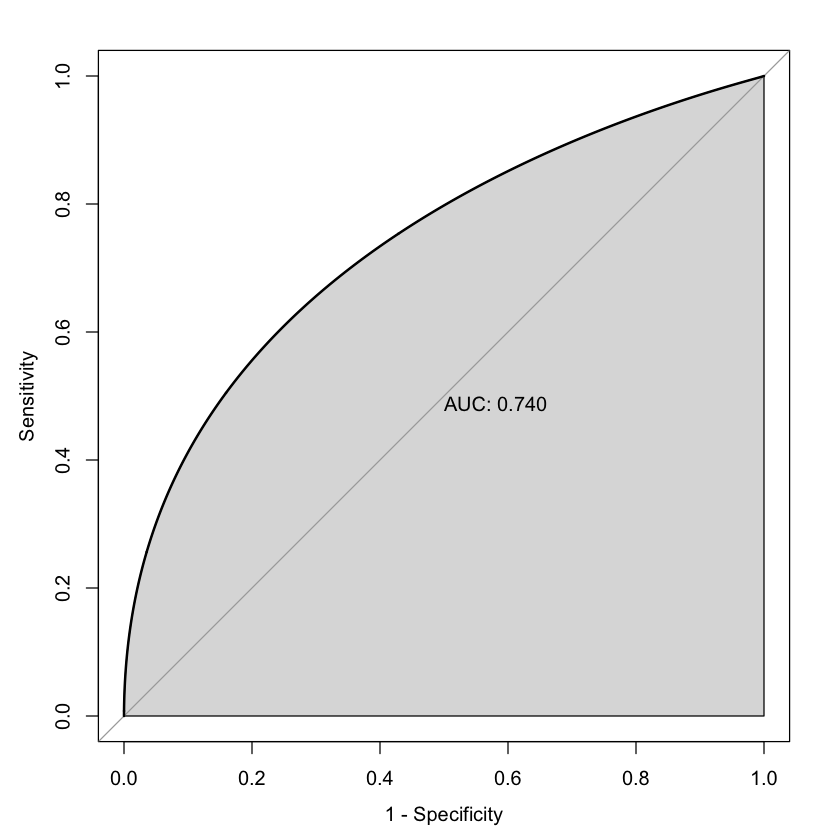
\includegraphics[width=5in,height=3.08333in]{chapters/measurement/E1_likert_files/figure-pdf/cell-10-output-2.png}

\begin{Shaded}
\begin{Highlighting}[]
\FunctionTok{hist}\NormalTok{(SDQ}\SpecialCharTok{$}\NormalTok{s\_emotion)}
\end{Highlighting}
\end{Shaded}

\includegraphics[width=5in,height=3.08333in]{chapters/measurement/E1_likert_files/figure-pdf/cell-11-output-1.png}

Più utile è un KDE plot.

\begin{Shaded}
\begin{Highlighting}[]
\NormalTok{SDQ }\SpecialCharTok{|\textgreater{}}
    \FunctionTok{ggplot}\NormalTok{(}\FunctionTok{aes}\NormalTok{(}\AttributeTok{x =}\NormalTok{ s\_emotion)) }\SpecialCharTok{+}
    \FunctionTok{geom\_density}\NormalTok{()}
\end{Highlighting}
\end{Shaded}

\begin{verbatim}
Warning message:
"Removed 6 rows containing non-finite outside the scale range
(`stat_density()`)."
\end{verbatim}

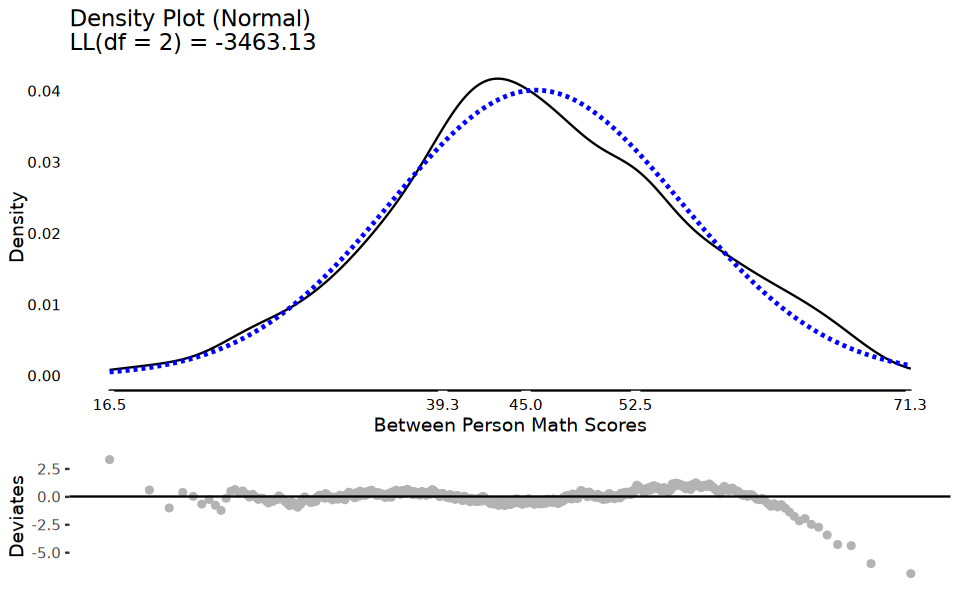
\includegraphics[width=5in,height=3.08333in]{chapters/measurement/E1_likert_files/figure-pdf/cell-12-output-2.png}

Possiamo ottenere le statistiche descrittive della scala usando la
funzione \texttt{describe} del pacchetto \texttt{psych}.

\begin{Shaded}
\begin{Highlighting}[]
\FunctionTok{describe}\NormalTok{(SDQ}\SpecialCharTok{$}\NormalTok{s\_emotion)}
\end{Highlighting}
\end{Shaded}

A psych: 1 x 13

\begin{longtable}[]{@{}
  >{\raggedright\arraybackslash}p{(\columnwidth - 26\tabcolsep) * \real{0.0714}}
  >{\raggedright\arraybackslash}p{(\columnwidth - 26\tabcolsep) * \real{0.0714}}
  >{\raggedright\arraybackslash}p{(\columnwidth - 26\tabcolsep) * \real{0.0714}}
  >{\raggedright\arraybackslash}p{(\columnwidth - 26\tabcolsep) * \real{0.0714}}
  >{\raggedright\arraybackslash}p{(\columnwidth - 26\tabcolsep) * \real{0.0714}}
  >{\raggedright\arraybackslash}p{(\columnwidth - 26\tabcolsep) * \real{0.0714}}
  >{\raggedright\arraybackslash}p{(\columnwidth - 26\tabcolsep) * \real{0.0714}}
  >{\raggedright\arraybackslash}p{(\columnwidth - 26\tabcolsep) * \real{0.0714}}
  >{\raggedright\arraybackslash}p{(\columnwidth - 26\tabcolsep) * \real{0.0714}}
  >{\raggedright\arraybackslash}p{(\columnwidth - 26\tabcolsep) * \real{0.0714}}
  >{\raggedright\arraybackslash}p{(\columnwidth - 26\tabcolsep) * \real{0.0714}}
  >{\raggedright\arraybackslash}p{(\columnwidth - 26\tabcolsep) * \real{0.0714}}
  >{\raggedright\arraybackslash}p{(\columnwidth - 26\tabcolsep) * \real{0.0714}}
  >{\raggedright\arraybackslash}p{(\columnwidth - 26\tabcolsep) * \real{0.0714}}@{}}
\toprule\noalign{}
\begin{minipage}[b]{\linewidth}\raggedright
\end{minipage} & \begin{minipage}[b]{\linewidth}\raggedright
vars \textless dbl\textgreater{}
\end{minipage} & \begin{minipage}[b]{\linewidth}\raggedright
n \textless dbl\textgreater{}
\end{minipage} & \begin{minipage}[b]{\linewidth}\raggedright
mean \textless dbl\textgreater{}
\end{minipage} & \begin{minipage}[b]{\linewidth}\raggedright
sd \textless dbl\textgreater{}
\end{minipage} & \begin{minipage}[b]{\linewidth}\raggedright
median \textless dbl\textgreater{}
\end{minipage} & \begin{minipage}[b]{\linewidth}\raggedright
trimmed \textless dbl\textgreater{}
\end{minipage} & \begin{minipage}[b]{\linewidth}\raggedright
mad \textless dbl\textgreater{}
\end{minipage} & \begin{minipage}[b]{\linewidth}\raggedright
min \textless dbl\textgreater{}
\end{minipage} & \begin{minipage}[b]{\linewidth}\raggedright
max \textless dbl\textgreater{}
\end{minipage} & \begin{minipage}[b]{\linewidth}\raggedright
range \textless dbl\textgreater{}
\end{minipage} & \begin{minipage}[b]{\linewidth}\raggedright
skew \textless dbl\textgreater{}
\end{minipage} & \begin{minipage}[b]{\linewidth}\raggedright
kurtosis \textless dbl\textgreater{}
\end{minipage} & \begin{minipage}[b]{\linewidth}\raggedright
se \textless dbl\textgreater{}
\end{minipage} \\
\midrule\noalign{}
\endhead
\bottomrule\noalign{}
\endlastfoot
X1 & 1 & 222 & 2.837838 & 2.301054 & 2 & 2.61236 & 2.9652 & 0 & 10 & 10
& 0.7454236 & -0.08749808 & 0.1544367 \\
\end{longtable}

Come si può vedere, la mediana (il punteggio al di sotto del quale si
trova la metà del campione) di \texttt{s\_emotion} è 2, mentre la media
è più alta e pari a 2.87. Questo perché la distribuione dei punteggi è
asimmetrica positiva; in questo caso, la mediana è più rappresentativa
della tendenza centrale. Queste statistiche sono coerenti con la nostra
osservazione dell'istogramma, che mostra un forte \emph{floor effect}.

Di seguito sono riportati i valori di soglia per i casi ``Normali'',
``Borderline'' e ``Anormali'' per i Sintomi Emotivi forniti dal
publisher del test (vedi https://sdqinfo.org/). Questi sono i punteggi
che distinguono i casi probabilmente borderline e anormali dai casi
``normali''.

Normale: 0-5 Borderline: 6 Anormale: 7-10

\begin{Shaded}
\begin{Highlighting}[]
\FunctionTok{table}\NormalTok{(SDQ}\SpecialCharTok{$}\NormalTok{s\_emotion }\SpecialCharTok{\textless{}=} \DecValTok{5}\NormalTok{)}
\end{Highlighting}
\end{Shaded}

\begin{verbatim}

FALSE  TRUE 
   33   195 
\end{verbatim}

In questo campione, dunque, l'85\% dei partecipanti è classificato
nell'intervallo Normale.

\begin{Shaded}
\begin{Highlighting}[]
\FunctionTok{table}\NormalTok{(SDQ}\SpecialCharTok{$}\NormalTok{s\_emotion }\SpecialCharTok{\textless{}=} \DecValTok{5}\NormalTok{)[}\DecValTok{2}\NormalTok{] }\SpecialCharTok{/} \FunctionTok{length}\NormalTok{(SDQ}\SpecialCharTok{$}\NormalTok{s\_emotion)}
\end{Highlighting}
\end{Shaded}

\textbf{TRUE:} 0.855263157894737

In maniera equivalente otteniamo

\begin{Shaded}
\begin{Highlighting}[]
\FunctionTok{table}\NormalTok{(SDQ}\SpecialCharTok{$}\NormalTok{s\_emotion }\SpecialCharTok{==} \DecValTok{6}\NormalTok{)[}\DecValTok{2}\NormalTok{] }\SpecialCharTok{/} \FunctionTok{length}\NormalTok{(SDQ}\SpecialCharTok{$}\NormalTok{s\_emotion)}
\end{Highlighting}
\end{Shaded}

\textbf{TRUE:} 0.0570175438596491

\begin{Shaded}
\begin{Highlighting}[]
\FunctionTok{table}\NormalTok{(SDQ}\SpecialCharTok{$}\NormalTok{s\_emotion }\SpecialCharTok{\textgreater{}=} \DecValTok{7}\NormalTok{)[}\DecValTok{2}\NormalTok{] }\SpecialCharTok{/} \FunctionTok{length}\NormalTok{(SDQ}\SpecialCharTok{$}\NormalTok{s\_emotion)}
\end{Highlighting}
\end{Shaded}

\textbf{TRUE:} 0.0833333333333333

\section{Item reverse}\label{item-reverse}

La scala \emph{Conduct Problems} contiene item reverse. Esaminiamo lo
scoring di questo tipo di item.

\begin{Shaded}
\begin{Highlighting}[]
\NormalTok{items\_conduct }\OtherTok{\textless{}{-}} \FunctionTok{c}\NormalTok{(}\StringTok{"tantrum"}\NormalTok{, }\StringTok{"obeys"}\NormalTok{, }\StringTok{"fights"}\NormalTok{, }\StringTok{"lies"}\NormalTok{, }\StringTok{"steals"}\NormalTok{)}
\end{Highlighting}
\end{Shaded}

Per i Problemi di Condotta, abbiamo solo un item reverse,
\texttt{obeys}.

\begin{verbatim}
tantrum    obeys*      fights       lies       steals
\end{verbatim}

Per invertire il codice di questo item, useremo una funzione dedicata
del pacchetto psych, \texttt{reverse.code()}. Questa funzione ha la
forma generale \texttt{reverse.code(keys,\ items,…)}. L'argomento
\texttt{keys} è un vettore di valori 1 o -1, dove -1 implica
l'inversione dell'item. L'argomento \texttt{items} sono i nomi delle
variabili che vogliamo valutare.

\begin{Shaded}
\begin{Highlighting}[]
\NormalTok{R\_conduct }\OtherTok{\textless{}{-}} \FunctionTok{reverse.code}\NormalTok{(}\AttributeTok{keys =} \FunctionTok{c}\NormalTok{(}\DecValTok{1}\NormalTok{, }\SpecialCharTok{{-}}\DecValTok{1}\NormalTok{, }\DecValTok{1}\NormalTok{, }\DecValTok{1}\NormalTok{, }\DecValTok{1}\NormalTok{), SDQ[, items\_conduct]) }\SpecialCharTok{|\textgreater{}} \FunctionTok{as.data.frame}\NormalTok{()}
\NormalTok{R\_conduct }\SpecialCharTok{|\textgreater{}} \FunctionTok{head}\NormalTok{()}
\end{Highlighting}
\end{Shaded}

A data.frame: 6 x 5

\begin{longtable}[]{@{}
  >{\raggedright\arraybackslash}p{(\columnwidth - 10\tabcolsep) * \real{0.1667}}
  >{\raggedright\arraybackslash}p{(\columnwidth - 10\tabcolsep) * \real{0.1667}}
  >{\raggedright\arraybackslash}p{(\columnwidth - 10\tabcolsep) * \real{0.1667}}
  >{\raggedright\arraybackslash}p{(\columnwidth - 10\tabcolsep) * \real{0.1667}}
  >{\raggedright\arraybackslash}p{(\columnwidth - 10\tabcolsep) * \real{0.1667}}
  >{\raggedright\arraybackslash}p{(\columnwidth - 10\tabcolsep) * \real{0.1667}}@{}}
\toprule\noalign{}
\begin{minipage}[b]{\linewidth}\raggedright
\end{minipage} & \begin{minipage}[b]{\linewidth}\raggedright
tantrum \textless dbl\textgreater{}
\end{minipage} & \begin{minipage}[b]{\linewidth}\raggedright
obeys- \textless dbl\textgreater{}
\end{minipage} & \begin{minipage}[b]{\linewidth}\raggedright
fights \textless dbl\textgreater{}
\end{minipage} & \begin{minipage}[b]{\linewidth}\raggedright
lies \textless dbl\textgreater{}
\end{minipage} & \begin{minipage}[b]{\linewidth}\raggedright
steals \textless dbl\textgreater{}
\end{minipage} \\
\midrule\noalign{}
\endhead
\bottomrule\noalign{}
\endlastfoot
1 & 0 & 0 & 0 & 0 & 0 \\
2 & 0 & 0 & 0 & 0 & 0 \\
3 & 0 & 0 & 0 & 0 & 0 \\
4 & 0 & 0 & 0 & 0 & 0 \\
5 & 1 & 2 & 0 & 2 & 0 \\
6 & 0 & 0 & 0 & 0 & 0 \\
\end{longtable}

\begin{Shaded}
\begin{Highlighting}[]
\NormalTok{SDQ[, items\_conduct] }\SpecialCharTok{|\textgreater{}} \FunctionTok{head}\NormalTok{()}
\end{Highlighting}
\end{Shaded}

A tibble: 6 x 5

\begin{longtable}[]{@{}
  >{\raggedright\arraybackslash}p{(\columnwidth - 8\tabcolsep) * \real{0.2000}}
  >{\raggedright\arraybackslash}p{(\columnwidth - 8\tabcolsep) * \real{0.2000}}
  >{\raggedright\arraybackslash}p{(\columnwidth - 8\tabcolsep) * \real{0.2000}}
  >{\raggedright\arraybackslash}p{(\columnwidth - 8\tabcolsep) * \real{0.2000}}
  >{\raggedright\arraybackslash}p{(\columnwidth - 8\tabcolsep) * \real{0.2000}}@{}}
\toprule\noalign{}
\begin{minipage}[b]{\linewidth}\raggedright
tantrum \textless dbl\textgreater{}
\end{minipage} & \begin{minipage}[b]{\linewidth}\raggedright
obeys \textless dbl\textgreater{}
\end{minipage} & \begin{minipage}[b]{\linewidth}\raggedright
fights \textless dbl\textgreater{}
\end{minipage} & \begin{minipage}[b]{\linewidth}\raggedright
lies \textless dbl\textgreater{}
\end{minipage} & \begin{minipage}[b]{\linewidth}\raggedright
steals \textless dbl\textgreater{}
\end{minipage} \\
\midrule\noalign{}
\endhead
\bottomrule\noalign{}
\endlastfoot
0 & 2 & 0 & 0 & 0 \\
0 & 2 & 0 & 0 & 0 \\
0 & 2 & 0 & 0 & 0 \\
0 & 2 & 0 & 0 & 0 \\
1 & 0 & 0 & 2 & 0 \\
0 & 2 & 0 & 0 & 0 \\
\end{longtable}

Anche in questo caso ci sono dei dati mancanti.

\begin{Shaded}
\begin{Highlighting}[]
\FunctionTok{summary}\NormalTok{(R\_conduct)}
\end{Highlighting}
\end{Shaded}

\begin{verbatim}
    tantrum           obeys-           fights           lies       
 Min.   :0.0000   Min.   :0.0000   Min.   :0.000   Min.   :0.0000  
 1st Qu.:0.0000   1st Qu.:0.0000   1st Qu.:0.000   1st Qu.:0.0000  
 Median :0.0000   Median :1.0000   Median :0.000   Median :0.0000  
 Mean   :0.5708   Mean   :0.5789   Mean   :0.193   Mean   :0.5442  
 3rd Qu.:1.0000   3rd Qu.:1.0000   3rd Qu.:0.000   3rd Qu.:1.0000  
 Max.   :2.0000   Max.   :2.0000   Max.   :2.000   Max.   :2.0000  
 NA's   :2                                         NA's   :2       
     steals     
 Min.   :0.000  
 1st Qu.:0.000  
 Median :0.000  
 Mean   :0.185  
 3rd Qu.:0.000  
 Max.   :2.000  
 NA's   :1      
\end{verbatim}

\begin{Shaded}
\begin{Highlighting}[]
\NormalTok{R\_conduct }\OtherTok{\textless{}{-}}\NormalTok{ R\_conduct }\SpecialCharTok{\%\textgreater{}\%}
    \FunctionTok{mutate\_at}\NormalTok{(}\FunctionTok{vars}\NormalTok{(tantrum}\SpecialCharTok{:}\NormalTok{steals), }\SpecialCharTok{\textasciitilde{}} \FunctionTok{ifelse}\NormalTok{(}\FunctionTok{is.na}\NormalTok{(.), }\FunctionTok{mean}\NormalTok{(., }\AttributeTok{na.rm =} \ConstantTok{TRUE}\NormalTok{), .))}
\end{Highlighting}
\end{Shaded}

Calcoliamo ora il punteggio totale.

\begin{Shaded}
\begin{Highlighting}[]
\NormalTok{SDQ}\SpecialCharTok{$}\NormalTok{s\_conduct }\OtherTok{\textless{}{-}} \FunctionTok{rowMeans}\NormalTok{(R\_conduct)}
\end{Highlighting}
\end{Shaded}

\begin{Shaded}
\begin{Highlighting}[]
\NormalTok{SDQ }\SpecialCharTok{|\textgreater{}}
    \FunctionTok{ggplot}\NormalTok{(}\FunctionTok{aes}\NormalTok{(}\AttributeTok{x =}\NormalTok{ s\_conduct)) }\SpecialCharTok{+}
    \FunctionTok{geom\_histogram}\NormalTok{(}\AttributeTok{bins =} \DecValTok{10}\NormalTok{)}
\end{Highlighting}
\end{Shaded}

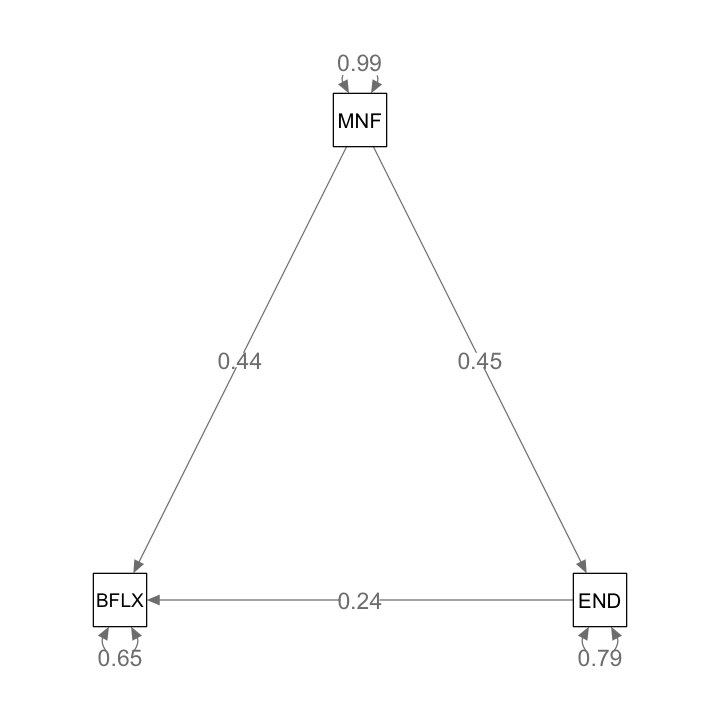
\includegraphics[width=5in,height=3.08333in]{chapters/measurement/E1_likert_files/figure-pdf/cell-24-output-1.png}

\section{Session Info}\label{session-info-1}

\begin{Shaded}
\begin{Highlighting}[]
\FunctionTok{sessionInfo}\NormalTok{() }
\end{Highlighting}
\end{Shaded}

\begin{verbatim}
R version 4.4.1 (2024-06-14)
Platform: aarch64-apple-darwin20
Running under: macOS 15.0

Matrix products: default
BLAS:   /Library/Frameworks/R.framework/Versions/4.4-arm64/Resources/lib/libRblas.0.dylib 
LAPACK: /Library/Frameworks/R.framework/Versions/4.4-arm64/Resources/lib/libRlapack.dylib;  LAPACK version 3.12.0

locale:
[1] C

time zone: Europe/Rome
tzcode source: internal

attached base packages:
[1] stats     graphics  grDevices utils     datasets  methods   base     

other attached packages:
 [1] ggokabeito_0.1.0  viridis_0.6.5     viridisLite_0.4.2 ggpubr_0.6.0     
 [5] ggExtra_0.10.1    bayesplot_1.11.1  gridExtra_2.3     patchwork_1.3.0  
 [9] semTools_0.5-6    semPlot_1.1.6     lavaan_0.6-18     psych_2.4.6.26   
[13] scales_1.3.0      markdown_1.13     knitr_1.48        lubridate_1.9.3  
[17] forcats_1.0.0     stringr_1.5.1     dplyr_1.1.4       purrr_1.0.2      
[21] readr_2.1.5       tidyr_1.3.1       tibble_3.2.1      ggplot2_3.5.1    
[25] tidyverse_2.0.0   here_1.0.1       

loaded via a namespace (and not attached):
  [1] rstudioapi_0.16.0  jsonlite_1.8.9     magrittr_2.0.3    
  [4] TH.data_1.1-2      estimability_1.5.1 farver_2.1.2      
  [7] nloptr_2.1.1       rmarkdown_2.28     vctrs_0.6.5       
 [10] minqa_1.2.8        base64enc_0.1-3    rstatix_0.7.2     
 [13] htmltools_0.5.8.1  broom_1.0.6        Formula_1.2-5     
 [16] htmlwidgets_1.6.4  plyr_1.8.9         sandwich_3.1-1    
 [19] emmeans_1.10.4     zoo_1.8-12         uuid_1.2-1        
 [22] igraph_2.0.3       mime_0.12          lifecycle_1.0.4   
 [25] pkgconfig_2.0.3    Matrix_1.7-0       R6_2.5.1          
 [28] fastmap_1.2.0      shiny_1.9.1        digest_0.6.37     
 [31] OpenMx_2.21.12     fdrtool_1.2.18     colorspace_2.1-1  
 [34] rprojroot_2.0.4    Hmisc_5.1-3        labeling_0.4.3    
 [37] fansi_1.0.6        timechange_0.3.0   abind_1.4-8       
 [40] compiler_4.4.1     withr_3.0.1        glasso_1.11       
 [43] htmlTable_2.4.3    backports_1.5.0    carData_3.0-5     
 [46] ggsignif_0.6.4     MASS_7.3-61        corpcor_1.6.10    
 [49] gtools_3.9.5       tools_4.4.1        pbivnorm_0.6.0    
 [52] foreign_0.8-87     zip_2.3.1          httpuv_1.6.15     
 [55] nnet_7.3-19        glue_1.7.0         quadprog_1.5-8    
 [58] promises_1.3.0     nlme_3.1-166       lisrelToR_0.3     
 [61] grid_4.4.1         pbdZMQ_0.3-13      checkmate_2.3.2   
 [64] cluster_2.1.6      reshape2_1.4.4     generics_0.1.3    
 [67] gtable_0.3.5       tzdb_0.4.0         data.table_1.16.0 
 [70] hms_1.1.3          car_3.1-2          utf8_1.2.4        
 [73] sem_3.1-16         pillar_1.9.0       IRdisplay_1.1     
 [76] rockchalk_1.8.157  later_1.3.2        splines_4.4.1     
 [79] lattice_0.22-6     survival_3.7-0     kutils_1.73       
 [82] tidyselect_1.2.1   miniUI_0.1.1.1     pbapply_1.7-2     
 [85] stats4_4.4.1       xfun_0.47          qgraph_1.9.8      
 [88] arm_1.14-4         stringi_1.8.4      boot_1.3-31       
 [91] evaluate_1.0.0     codetools_0.2-20   mi_1.1            
 [94] cli_3.6.3          RcppParallel_5.1.9 IRkernel_1.3.2    
 [97] rpart_4.1.23       xtable_1.8-4       repr_1.1.7        
[100] munsell_0.5.1      Rcpp_1.0.13        coda_0.19-4.1     
[103] png_0.1-8          XML_3.99-0.17      parallel_4.4.1    
[106] jpeg_0.1-10        lme4_1.1-35.5      mvtnorm_1.3-1     
[109] openxlsx_4.2.7.1   crayon_1.5.3       rlang_1.1.4       
[112] multcomp_1.4-26    mnormt_2.1.1      
\end{verbatim}

\chapter{✏️ Esercizi}\label{sec-ex-optimal-scaling}

\section{Ottimizzazione dello scoring dei dati di questionari
ordinali}\label{ottimizzazione-dello-scoring-dei-dati-di-questionari-ordinali}

Precedentemente, nell'Esercizio sulla scala Likert, abbiamo effettuato
lo scoring del questionario \emph{Strengths and Difficulties
Questionnaire} (SDQ) utilizzando l'approccio chiamato ``Likert
scaling'', in cui le categorie di risposta ``non vero'', ``un po' vero''
e ``certamente vero'' sono state assegnate ai numeri interi consecutivi
0-1-2. Oltre a riflettere il presunto grado crescente di accordo in
queste opzioni di risposta, l'assegnazione dei numeri interi era
arbitraria, poiché non c'era una particolare ragione per cui abbiamo
assegnato 0-1-2 anziché, ad esempio, 1-2-3. Un tale modo arbitrario di
valutare le risposte degli item è chiamato anche ``measurement by
fiat''. In questo tutorial, cercheremo di trovare punteggi ``ottimali''
per le risposte ordinate al SDQ. ``Ottimale'' significa che i punteggi
che assegniamo alle risposte non sono solo dei punteggi qualsiasi, ma
sono i ``migliori'' tra tutti gli altri possibili punteggi in base a
qualche criterio statistico.

Esistono molti modi per ``ottimizzare'' i punteggi degli item; qui,
massimizzeremo il rapporto tra la varianza del punteggio totale e la
somma delle varianze dei punteggi degli item. In psicometria, il
soddisfacimento di questo criterio porta alla massimizzazione della
somma delle correlazioni degli item (e quindi della ``coerenza interna''
del punteggio del test misurata dall'alpha di Cronbach).

\begin{Shaded}
\begin{Highlighting}[]
\FunctionTok{source}\NormalTok{(}\StringTok{"../../code/\_common.R"}\NormalTok{)}
\FunctionTok{library}\NormalTok{(}\StringTok{"aspect"}\NormalTok{)}
\end{Highlighting}
\end{Shaded}

Importiamo nuovamente i dati del \emph{Strengths and Difficulties
Questionnaire} (SDQ).

\begin{Shaded}
\begin{Highlighting}[]
\FunctionTok{load}\NormalTok{(}\StringTok{"../data/data\_sdq/SDQ.RData"}\NormalTok{)}
\end{Highlighting}
\end{Shaded}

\begin{Shaded}
\begin{Highlighting}[]
\FunctionTok{glimpse}\NormalTok{(SDQ)}
\end{Highlighting}
\end{Shaded}

\begin{verbatim}
Rows: 228
Columns: 51
$ Gender   <dbl> 1, 1, 1, 1, 1, 1, 1, 1, 1, 1, 1, 1, 1, 1, 1, 1, 1, 1, 1, 1, 1…
$ consid   <dbl> 1, 2, 2, 2, 0, 2, 2, 2, 2, 2, 2, 2, 2, 2, 2, 2, 1, 2, 2, 2, 2…
$ restles  <dbl> 2, 0, 0, 0, 1, 0, 2, 1, 2, 0, 1, 1, 0, 1, 0, 2, 0, 1, 1, 1, 0…
$ somatic  <dbl> 2, 2, 0, 0, 2, 1, 0, 0, 1, 0, 0, 2, 0, 0, 1, 2, 1, 1, 1, 1, 1…
$ shares   <dbl> 1, 1, 2, 2, 0, 2, 2, 2, 2, 2, 1, 2, 2, 2, 2, 2, 1, 2, 1, 2, 2…
$ tantrum  <dbl> 0, 0, 0, 0, 1, 0, 2, 0, 2, 0, 0, 1, 0, 1, 1, 2, 0, 1, 1, 1, 0…
$ loner    <dbl> 0, 0, 0, 0, 0, 0, 0, 2, 2, 0, 0, 1, 0, 0, 0, 1, 0, 0, 2, 2, 0…
$ obeys    <dbl> 2, 2, 2, 2, 0, 2, 2, 2, 2, 2, 1, 1, 2, 2, 1, 2, 2, 2, 1, 2, 2…
$ worries  <dbl> 1, 0, 0, 0, 1, 0, 1, 0, 0, 0, 0, 2, 0, 1, 2, 0, 1, 1, 2, 1, 0…
$ caring   <dbl> 2, 2, 2, 1, 2, 2, 2, 2, 2, 2, 1, 2, 2, 2, 2, 2, 1, 2, 2, 1, 2…
$ fidgety  <dbl> 0, 0, 0, 0, 0, 0, 2, 0, 0, 0, 1, 1, 0, 0, 0, 1, 0, 0, 0, 1, 0…
$ friend   <dbl> 2, 2, 2, 2, 0, 2, 2, 2, 2, 2, 1, 2, 2, 2, 2, 2, 2, 2, 1, 2, 2…
$ fights   <dbl> 0, 0, 0, 0, 0, 0, 0, 0, 0, 0, 0, 0, 0, 0, 0, 0, 0, 0, 0, 0, 0…
$ unhappy  <dbl> 0, 0, 0, 0, 0, 0, 1, 0, 0, 0, 0, 1, 0, 0, 1, 0, 0, 0, 2, 1, 0…
$ popular  <dbl> 2, 2, 2, 1, 1, 2, 2, 2, 2, 2, 2, 2, 1, 1, 1, 2, 1, 2, 1, 1, 2…
$ distrac  <dbl> 0, 1, 0, 0, 1, 0, 2, 0, 0, 0, 0, 1, 0, 0, 1, 2, 0, 0, 1, 0, 0…
$ clingy   <dbl> 1, 1, 0, 1, 1, 1, 2, 0, 0, 0, 0, 1, 0, 2, 2, 1, 2, 0, 2, 2, 0…
$ kind     <dbl> 1, 2, 2, 2, 1, 2, 2, 2, 2, 1, 1, 2, 2, 2, 2, 2, 1, 2, 2, 2, 2…
$ lies     <dbl> 0, 0, 0, 0, 2, 0, 1, 0, 2, 0, 0, 1, 0, 0, 1, 0, 0, 0, 0, 0, 0…
$ bullied  <dbl> 0, 0, 0, 0, 2, 0, 1, 0, 0, 0, 0, 1, 0, 0, 1, 0, 0, 0, 1, 1, 0…
$ helpout  <dbl> 2, 1, 2, 2, 0, 2, 2, 2, 1, 2, 1, 2, 2, 1, 2, 2, 1, 2, 1, 2, 2…
$ reflect  <dbl> 1, 1, 2, 2, 0, 2, 2, 2, 1, 1, 1, 1, 1, 1, 1, 2, 2, 2, 1, 1, 2…
$ steals   <dbl> 0, 0, 0, 0, 0, 0, 0, 0, 0, 0, 1, 0, 0, 0, 1, 0, 0, 0, 0, 0, 0…
$ oldbest  <dbl> 1, 0, 2, 1, 0, 1, 1, 1, 0, 0, 0, 1, 0, 0, 1, 1, 0, 0, 2, 1, 1…
$ afraid   <dbl> 0, 0, 1, 1, 0, 0, 0, 0, 0, 1, 0, 2, 2, 0, 1, 1, 1, 0, 1, 1, 0…
$ attends  <dbl> 2, 2, 1, 2, 0, 2, 2, 2, 2, 2, 1, 1, 2, 1, 2, 2, 1, 1, 1, 1, 2…
$ consid2  <dbl> 1, 2, 2, 2, NA, 2, 2, 2, 2, 2, NA, 1, NA, 2, 2, NA, 1, 2, 2, …
$ restles2 <dbl> 0, 1, 2, 1, NA, 0, 1, 1, 0, 0, NA, 2, NA, 0, 1, NA, 1, 1, 2, …
$ somatic2 <dbl> 0, 1, 1, 0, NA, 0, 0, 0, 0, 0, NA, 2, NA, 0, 1, NA, 0, 1, 2, …
$ shares2  <dbl> 1, 2, 2, 1, NA, 2, 1, 2, 2, 2, NA, 2, NA, 2, 2, NA, 1, 2, 1, …
$ tantrum2 <dbl> 0, 1, 2, 0, NA, 0, 2, 0, 0, 0, NA, 2, NA, 0, 1, NA, 1, 0, 2, …
$ loner2   <dbl> 0, 0, 1, 0, NA, 0, 0, 0, 0, 0, NA, 1, NA, 1, 0, NA, 0, 0, 1, …
$ obeys2   <dbl> 2, 1, 2, 1, NA, 2, 2, 2, 2, 1, NA, 1, NA, 2, 1, NA, 1, 2, 1, …
$ worries2 <dbl> 0, 0, 1, 0, NA, NA, 1, 0, 0, 0, NA, 1, NA, 1, 2, NA, 0, 0, 2,…
$ caring2  <dbl> 2, 2, 1, 2, NA, 2, 2, 2, 2, 2, NA, 2, NA, 2, 2, NA, 1, 2, 2, …
$ fidgety2 <dbl> 0, 1, 0, 0, NA, 0, 1, 0, 0, 0, NA, 2, NA, 0, 0, NA, 1, 0, 2, …
$ friend2  <dbl> 2, 2, 1, 2, NA, 2, 2, 2, 2, 2, NA, 2, NA, 1, 2, NA, 2, 2, 2, …
$ fights2  <dbl> 0, 0, 0, 0, NA, 0, 0, 0, 0, 0, NA, 2, NA, 0, 0, NA, 0, 0, 0, …
$ unhappy2 <dbl> 0, 0, 1, 0, NA, 0, 0, 0, 0, 0, NA, 1, NA, 0, 0, NA, 0, 0, 1, …
$ popular2 <dbl> 2, 1, 1, 2, NA, 2, 1, 2, 2, 2, NA, 2, NA, 2, 2, NA, 1, 2, 1, …
$ distrac2 <dbl> 0, 0, 0, 2, NA, 0, 2, 1, 0, 0, NA, 1, NA, 0, 1, NA, 1, 0, 2, …
$ clingy2  <dbl> 1, 1, 1, 0, NA, 1, 1, 1, 0, 0, NA, 1, NA, 0, 0, NA, 2, 0, 2, …
$ kind2    <dbl> 2, 2, 2, 2, NA, 2, 2, 2, 2, 2, NA, 2, NA, 2, 2, NA, 1, 2, 2, …
$ lies2    <dbl> 1, 0, 0, 0, NA, 0, 1, 0, 1, 0, NA, 1, NA, 0, 0, NA, 1, 0, 0, …
$ bullied2 <dbl> 0, 0, 0, 0, NA, 0, 2, 0, 0, 0, NA, 0, NA, 0, 0, NA, 0, 0, 0, …
$ helpout2 <dbl> 1, 1, 1, 2, NA, 2, 2, 1, 2, 1, NA, 2, NA, 2, 1, NA, 0, 2, 1, …
$ reflect2 <dbl> 1, 1, 2, 1, NA, 2, 1, 2, 1, 2, NA, 1, NA, 2, 1, NA, 1, 2, 1, …
$ steals2  <dbl> 0, 0, 0, 0, NA, 0, 0, 0, 0, 0, NA, 2, NA, 0, 0, NA, 0, 0, 0, …
$ oldbest2 <dbl> 0, 0, 1, 0, NA, 1, 0, 1, 1, 0, NA, 1, NA, 0, 0, NA, 0, 0, 1, …
$ afraid2  <dbl> 0, 1, 0, 0, NA, 0, 0, 0, 0, 0, NA, 2, NA, 0, 0, NA, 0, 0, 2, …
$ attends2 <dbl> 1, 1, 2, 0, NA, 2, 2, 2, 2, 1, NA, 1, NA, 2, 2, NA, 1, 1, 0, …
\end{verbatim}

Per analizzare solo gli item che misurano i Sintomi Emotivi, è
conveniente creare un nuovo data frame.

\begin{Shaded}
\begin{Highlighting}[]
\NormalTok{items\_emotion }\OtherTok{\textless{}{-}} \FunctionTok{c}\NormalTok{(}\StringTok{"somatic"}\NormalTok{, }\StringTok{"worries"}\NormalTok{, }\StringTok{"unhappy"}\NormalTok{, }\StringTok{"clingy"}\NormalTok{, }\StringTok{"afraid"}\NormalTok{)}
\NormalTok{sdq\_emo }\OtherTok{\textless{}{-}}\NormalTok{ SDQ[, items\_emotion]}
\NormalTok{sdq\_emo }\SpecialCharTok{|\textgreater{}}
    \FunctionTok{head}\NormalTok{()}
\end{Highlighting}
\end{Shaded}

A tibble: 6 × 5

\begin{longtable}[]{@{}
  >{\raggedright\arraybackslash}p{(\columnwidth - 8\tabcolsep) * \real{0.2000}}
  >{\raggedright\arraybackslash}p{(\columnwidth - 8\tabcolsep) * \real{0.2000}}
  >{\raggedright\arraybackslash}p{(\columnwidth - 8\tabcolsep) * \real{0.2000}}
  >{\raggedright\arraybackslash}p{(\columnwidth - 8\tabcolsep) * \real{0.2000}}
  >{\raggedright\arraybackslash}p{(\columnwidth - 8\tabcolsep) * \real{0.2000}}@{}}
\toprule\noalign{}
\begin{minipage}[b]{\linewidth}\raggedright
somatic \textless dbl\textgreater{}
\end{minipage} & \begin{minipage}[b]{\linewidth}\raggedright
worries \textless dbl\textgreater{}
\end{minipage} & \begin{minipage}[b]{\linewidth}\raggedright
unhappy \textless dbl\textgreater{}
\end{minipage} & \begin{minipage}[b]{\linewidth}\raggedright
clingy \textless dbl\textgreater{}
\end{minipage} & \begin{minipage}[b]{\linewidth}\raggedright
afraid \textless dbl\textgreater{}
\end{minipage} \\
\midrule\noalign{}
\endhead
\bottomrule\noalign{}
\endlastfoot
2 & 1 & 0 & 1 & 0 \\
2 & 0 & 0 & 1 & 0 \\
0 & 0 & 0 & 0 & 1 \\
0 & 0 & 0 & 1 & 1 \\
2 & 1 & 0 & 1 & 0 \\
1 & 0 & 0 & 1 & 0 \\
\end{longtable}

Affrontiamo il problema dei dati mancanti come discusso in precedenza.

\begin{Shaded}
\begin{Highlighting}[]
\NormalTok{sdq\_emo }\OtherTok{\textless{}{-}}\NormalTok{ sdq\_emo }\SpecialCharTok{\%\textgreater{}\%}
    \FunctionTok{mutate\_at}\NormalTok{(}\FunctionTok{vars}\NormalTok{(somatic}\SpecialCharTok{:}\NormalTok{afraid), }\SpecialCharTok{\textasciitilde{}} \FunctionTok{ifelse}\NormalTok{(}\FunctionTok{is.na}\NormalTok{(.), }\FunctionTok{mean}\NormalTok{(., }\AttributeTok{na.rm =} \ConstantTok{TRUE}\NormalTok{), .))}
\end{Highlighting}
\end{Shaded}

Eliminiamo i valori decimali.

\begin{Shaded}
\begin{Highlighting}[]
\NormalTok{sdq\_emo }\OtherTok{\textless{}{-}} \FunctionTok{round}\NormalTok{(sdq\_emo)}
\end{Highlighting}
\end{Shaded}

\begin{Shaded}
\begin{Highlighting}[]
\NormalTok{emotional\_symptoms }\OtherTok{\textless{}{-}} \FunctionTok{c}\NormalTok{(}\StringTok{"somatic"}\NormalTok{, }\StringTok{"worries"}\NormalTok{, }\StringTok{"unhappy"}\NormalTok{, }\StringTok{"clingy"}\NormalTok{, }\StringTok{"afraid"}\NormalTok{)}
\NormalTok{result }\OtherTok{\textless{}{-}} \FunctionTok{lapply}\NormalTok{(emotional\_symptoms, }\ControlFlowTok{function}\NormalTok{(x) }\FunctionTok{sort}\NormalTok{(}\FunctionTok{unique}\NormalTok{(sdq\_emo[[x]])))}
\NormalTok{result }\SpecialCharTok{|\textgreater{}} \FunctionTok{print}\NormalTok{()}
\end{Highlighting}
\end{Shaded}

\begin{verbatim}
[[1]]
[1] 0 1 2

[[2]]
[1] 0 1 2

[[3]]
[1] 0 1 2

[[4]]
[1] 0 1 2

[[5]]
[1] 0 1 2
\end{verbatim}

Trasformiamo il data frame in una matrice.

\begin{Shaded}
\begin{Highlighting}[]
\NormalTok{M }\OtherTok{\textless{}{-}}\NormalTok{ sdq\_emo }\SpecialCharTok{|\textgreater{}} \FunctionTok{as.matrix}\NormalTok{()}
\NormalTok{M}
\end{Highlighting}
\end{Shaded}

A matrix: 228 × 5 of type dbl

\begin{longtable}[]{@{}lllll@{}}
\toprule\noalign{}
somatic & worries & unhappy & clingy & afraid \\
\midrule\noalign{}
\endhead
\bottomrule\noalign{}
\endlastfoot
2 & 1 & 0 & 1 & 0 \\
2 & 0 & 0 & 1 & 0 \\
0 & 0 & 0 & 0 & 1 \\
0 & 0 & 0 & 1 & 1 \\
2 & 1 & 0 & 1 & 0 \\
1 & 0 & 0 & 1 & 0 \\
0 & 1 & 1 & 2 & 0 \\
0 & 0 & 0 & 0 & 0 \\
1 & 0 & 0 & 0 & 0 \\
0 & 0 & 0 & 0 & 1 \\
0 & 0 & 0 & 0 & 0 \\
2 & 2 & 1 & 1 & 2 \\
0 & 0 & 0 & 0 & 2 \\
0 & 1 & 0 & 2 & 0 \\
1 & 2 & 1 & 2 & 1 \\
2 & 0 & 0 & 1 & 1 \\
1 & 1 & 0 & 2 & 1 \\
1 & 1 & 0 & 0 & 0 \\
1 & 2 & 2 & 2 & 1 \\
1 & 1 & 1 & 2 & 1 \\
1 & 0 & 0 & 0 & 0 \\
2 & 1 & 0 & 0 & 1 \\
2 & 2 & 2 & 1 & 2 \\
0 & 1 & 1 & 1 & 1 \\
1 & 2 & 0 & 0 & 2 \\
2 & 2 & 2 & 2 & 1 \\
0 & 0 & 0 & 0 & 0 \\
1 & 0 & 0 & 2 & 0 \\
1 & 0 & 1 & 1 & 0 \\
0 & 0 & 0 & 1 & 0 \\
⋮ & ⋮ & ⋮ & ⋮ & ⋮ \\
1 & 0 & 0 & 1 & 0 \\
1 & 0 & 0 & 1 & 1 \\
1 & 1 & 0 & 1 & 1 \\
0 & 0 & 0 & 0 & 0 \\
0 & 2 & 0 & 0 & 0 \\
1 & 1 & 1 & 0 & 1 \\
1 & 0 & 0 & 1 & 0 \\
1 & 0 & 0 & 1 & 0 \\
0 & 0 & 0 & 1 & 0 \\
1 & 0 & 0 & 2 & 0 \\
0 & 1 & 0 & 1 & 0 \\
0 & 0 & 0 & 0 & 0 \\
0 & 1 & 0 & 0 & 0 \\
0 & 0 & 0 & 0 & 0 \\
0 & 0 & 0 & 0 & 0 \\
1 & 2 & 1 & 2 & 2 \\
0 & 1 & 0 & 0 & 0 \\
0 & 0 & 0 & 1 & 0 \\
0 & 0 & 0 & 1 & 1 \\
1 & 0 & 0 & 0 & 0 \\
0 & 0 & 0 & 2 & 0 \\
1 & 0 & 0 & 0 & 1 \\
1 & 0 & 1 & 1 & 1 \\
0 & 0 & 0 & 0 & 0 \\
0 & 0 & 0 & 0 & 0 \\
0 & 1 & 0 & 0 & 0 \\
1 & 0 & 0 & 0 & 1 \\
0 & 1 & 0 & 1 & 0 \\
0 & 1 & 0 & 0 & 0 \\
2 & 1 & 1 & 1 & 1 \\
\end{longtable}

Implementiamo lo scaling ottimale con la funzione \texttt{corAspect()}.

\begin{Shaded}
\begin{Highlighting}[]
\NormalTok{opt }\OtherTok{\textless{}{-}} \FunctionTok{corAspect}\NormalTok{(M, }\AttributeTok{aspect =} \StringTok{"aspectSum"}\NormalTok{, }\AttributeTok{level =} \StringTok{"ordinal"}\NormalTok{)}
\end{Highlighting}
\end{Shaded}

Esaminiamo il risultato ottenuto.

\begin{Shaded}
\begin{Highlighting}[]
\FunctionTok{attributes}\NormalTok{(opt)}
\end{Highlighting}
\end{Shaded}

\begin{description}
\tightlist
\item[\$names]
\begin{enumerate}
\def\labelenumi{\arabic{enumi}.}
\tightlist
\item[]
\item
  `loss'
\item
  `catscores'
\item
  `cormat'
\item
  `eigencor'
\item
  `indmat'
\item
  `scoremat'
\item
  `data'
\item
  `burtmat'
\item
  `niter'
\item
  `call'
\end{enumerate}
\item[\$class]
`aspect'
\end{description}

\begin{Shaded}
\begin{Highlighting}[]
\NormalTok{opt}\SpecialCharTok{$}\NormalTok{scoremat}
\end{Highlighting}
\end{Shaded}

A matrix: 228 × 5 of type dbl

\begin{longtable}[]{@{}llllll@{}}
\toprule\noalign{}
& somatic & worries & unhappy & clingy & afraid \\
\midrule\noalign{}
\endhead
\bottomrule\noalign{}
\endlastfoot
1 & 1.9720960 & 0.4454555 & -0.6009399 & 0.2369782 & -0.7685934 \\
2 & 1.9720960 & -0.8540365 & -0.6009399 & 0.2369782 & -0.7685934 \\
3 & -0.9013969 & -0.8540365 & -0.6009399 & -1.1988603 & 1.0085914 \\
4 & -0.9013969 & -0.8540365 & -0.6009399 & 0.2369782 & 1.0085914 \\
5 & 1.9720960 & 0.4454555 & -0.6009399 & 0.2369782 & -0.7685934 \\
6 & 0.5862099 & -0.8540365 & -0.6009399 & 0.2369782 & -0.7685934 \\
7 & -0.9013969 & 0.4454555 & 1.3931034 & 1.6170823 & -0.7685934 \\
8 & -0.9013969 & -0.8540365 & -0.6009399 & -1.1988603 & -0.7685934 \\
9 & 0.5862099 & -0.8540365 & -0.6009399 & -1.1988603 & -0.7685934 \\
10 & -0.9013969 & -0.8540365 & -0.6009399 & -1.1988603 & 1.0085914 \\
11 & -0.9013969 & -0.8540365 & -0.6009399 & -1.1988603 & -0.7685934 \\
12 & 1.9720960 & 2.0964116 & 1.3931034 & 0.2369782 & 1.9509426 \\
13 & -0.9013969 & -0.8540365 & -0.6009399 & -1.1988603 & 1.9509426 \\
14 & -0.9013969 & 0.4454555 & -0.6009399 & 1.6170823 & -0.7685934 \\
15 & 0.5862099 & 2.0964116 & 1.3931034 & 1.6170823 & 1.0085914 \\
16 & 1.9720960 & -0.8540365 & -0.6009399 & 0.2369782 & 1.0085914 \\
17 & 0.5862099 & 0.4454555 & -0.6009399 & 1.6170823 & 1.0085914 \\
18 & 0.5862099 & 0.4454555 & -0.6009399 & -1.1988603 & -0.7685934 \\
19 & 0.5862099 & 2.0964116 & 2.6586118 & 1.6170823 & 1.0085914 \\
20 & 0.5862099 & 0.4454555 & 1.3931034 & 1.6170823 & 1.0085914 \\
21 & 0.5862099 & -0.8540365 & -0.6009399 & -1.1988603 & -0.7685934 \\
22 & 1.9720960 & 0.4454555 & -0.6009399 & -1.1988603 & 1.0085914 \\
23 & 1.9720960 & 2.0964116 & 2.6586118 & 0.2369782 & 1.9509426 \\
24 & -0.9013969 & 0.4454555 & 1.3931034 & 0.2369782 & 1.0085914 \\
25 & 0.5862099 & 2.0964116 & -0.6009399 & -1.1988603 & 1.9509426 \\
26 & 1.9720960 & 2.0964116 & 2.6586118 & 1.6170823 & 1.0085914 \\
27 & -0.9013969 & -0.8540365 & -0.6009399 & -1.1988603 & -0.7685934 \\
28 & 0.5862099 & -0.8540365 & -0.6009399 & 1.6170823 & -0.7685934 \\
29 & 0.5862099 & -0.8540365 & 1.3931034 & 0.2369782 & -0.7685934 \\
30 & -0.9013969 & -0.8540365 & -0.6009399 & 0.2369782 & -0.7685934 \\
⋮ & ⋮ & ⋮ & ⋮ & ⋮ & ⋮ \\
199 & 0.5862099 & -0.8540365 & -0.6009399 & 0.2369782 & -0.7685934 \\
200 & 0.5862099 & -0.8540365 & -0.6009399 & 0.2369782 & 1.0085914 \\
201 & 0.5862099 & 0.4454555 & -0.6009399 & 0.2369782 & 1.0085914 \\
202 & -0.9013969 & -0.8540365 & -0.6009399 & -1.1988603 & -0.7685934 \\
203 & -0.9013969 & 2.0964116 & -0.6009399 & -1.1988603 & -0.7685934 \\
204 & 0.5862099 & 0.4454555 & 1.3931034 & -1.1988603 & 1.0085914 \\
205 & 0.5862099 & -0.8540365 & -0.6009399 & 0.2369782 & -0.7685934 \\
206 & 0.5862099 & -0.8540365 & -0.6009399 & 0.2369782 & -0.7685934 \\
207 & -0.9013969 & -0.8540365 & -0.6009399 & 0.2369782 & -0.7685934 \\
208 & 0.5862099 & -0.8540365 & -0.6009399 & 1.6170823 & -0.7685934 \\
209 & -0.9013969 & 0.4454555 & -0.6009399 & 0.2369782 & -0.7685934 \\
210 & -0.9013969 & -0.8540365 & -0.6009399 & -1.1988603 & -0.7685934 \\
211 & -0.9013969 & 0.4454555 & -0.6009399 & -1.1988603 & -0.7685934 \\
212 & -0.9013969 & -0.8540365 & -0.6009399 & -1.1988603 & -0.7685934 \\
213 & -0.9013969 & -0.8540365 & -0.6009399 & -1.1988603 & -0.7685934 \\
214 & 0.5862099 & 2.0964116 & 1.3931034 & 1.6170823 & 1.9509426 \\
215 & -0.9013969 & 0.4454555 & -0.6009399 & -1.1988603 & -0.7685934 \\
216 & -0.9013969 & -0.8540365 & -0.6009399 & 0.2369782 & -0.7685934 \\
217 & -0.9013969 & -0.8540365 & -0.6009399 & 0.2369782 & 1.0085914 \\
218 & 0.5862099 & -0.8540365 & -0.6009399 & -1.1988603 & -0.7685934 \\
219 & -0.9013969 & -0.8540365 & -0.6009399 & 1.6170823 & -0.7685934 \\
220 & 0.5862099 & -0.8540365 & -0.6009399 & -1.1988603 & 1.0085914 \\
221 & 0.5862099 & -0.8540365 & 1.3931034 & 0.2369782 & 1.0085914 \\
222 & -0.9013969 & -0.8540365 & -0.6009399 & -1.1988603 & -0.7685934 \\
223 & -0.9013969 & -0.8540365 & -0.6009399 & -1.1988603 & -0.7685934 \\
224 & -0.9013969 & 0.4454555 & -0.6009399 & -1.1988603 & -0.7685934 \\
225 & 0.5862099 & -0.8540365 & -0.6009399 & -1.1988603 & 1.0085914 \\
226 & -0.9013969 & 0.4454555 & -0.6009399 & 0.2369782 & -0.7685934 \\
227 & -0.9013969 & 0.4454555 & -0.6009399 & -1.1988603 & -0.7685934 \\
228 & 1.9720960 & 0.4454555 & 1.3931034 & 0.2369782 & 1.0085914 \\
\end{longtable}

Esaminiamo la relazione tra lo scoring basato sul metodo Likert con lo
scoring ottimale.

\begin{Shaded}
\begin{Highlighting}[]
\FunctionTok{plot}\NormalTok{(opt}\SpecialCharTok{$}\NormalTok{scoremat[, }\DecValTok{1}\NormalTok{], sdq\_emo}\SpecialCharTok{$}\NormalTok{somatic)}
\end{Highlighting}
\end{Shaded}

\includegraphics[width=4.375in,height=4.375in]{chapters/measurement/E2_optimal_scoring_files/figure-pdf/cell-13-output-1.png}

\begin{Shaded}
\begin{Highlighting}[]
\FunctionTok{plot}\NormalTok{(opt}\SpecialCharTok{$}\NormalTok{scoremat[, }\DecValTok{5}\NormalTok{], sdq\_emo}\SpecialCharTok{$}\NormalTok{afraid)}
\end{Highlighting}
\end{Shaded}

\includegraphics[width=4.375in,height=4.375in]{chapters/measurement/E2_optimal_scoring_files/figure-pdf/cell-14-output-1.png}

Guardando ai grafici ottenuti, si può notare che 1) i punteggi per le
categorie successive aumentano quasi linearmente; 2) le categorie sono
approssimativamente equidistanti. Concludiamo che per la valutazione
degli item ordinali nella scala dei Sintomi Emotivi del SDQ, la scala
Likert è appropriata, e non si può ottenere molto di più
dall'ottimizzazione della scala rispetto alla semplice scala Likert di
base.

\section{Session Info}\label{session-info-2}

\begin{Shaded}
\begin{Highlighting}[]
\FunctionTok{sessionInfo}\NormalTok{()}
\end{Highlighting}
\end{Shaded}

\begin{verbatim}
R version 4.3.3 (2024-02-29)
Platform: x86_64-apple-darwin20 (64-bit)
Running under: macOS Sonoma 14.3.1

Matrix products: default
BLAS:   /Library/Frameworks/R.framework/Versions/4.3-x86_64/Resources/lib/libRblas.0.dylib 
LAPACK: /Library/Frameworks/R.framework/Versions/4.3-x86_64/Resources/lib/libRlapack.dylib;  LAPACK version 3.11.0

locale:
[1] en_US.UTF-8/en_US.UTF-8/en_US.UTF-8/C/en_US.UTF-8/en_US.UTF-8

time zone: Europe/Rome
tzcode source: internal

attached base packages:
[1] stats     graphics  grDevices utils     datasets  methods   base     

other attached packages:
 [1] aspect_1.0-6       ggokabeito_0.1.0   viridis_0.6.5      viridisLite_0.4.2 
 [5] ggpubr_0.6.0       ggExtra_0.10.1     bayesplot_1.11.1   gridExtra_2.3     
 [9] patchwork_1.2.0    semTools_0.5-6.920 semPlot_1.1.6      lavaan_0.6-17     
[13] psych_2.4.1        scales_1.3.0       markdown_1.12      knitr_1.45        
[17] lubridate_1.9.3    forcats_1.0.0      stringr_1.5.1      dplyr_1.1.4       
[21] purrr_1.0.2        readr_2.1.5        tidyr_1.3.1        tibble_3.2.1      
[25] ggplot2_3.5.0      tidyverse_2.0.0    here_1.0.1        

loaded via a namespace (and not attached):
  [1] rstudioapi_0.15.0  jsonlite_1.8.8     magrittr_2.0.3    
  [4] TH.data_1.1-2      estimability_1.5   nloptr_2.0.3      
  [7] rmarkdown_2.26     vctrs_0.6.5        minqa_1.2.6       
 [10] base64enc_0.1-3    rstatix_0.7.2      htmltools_0.5.7   
 [13] broom_1.0.5        Formula_1.2-5      htmlwidgets_1.6.4 
 [16] plyr_1.8.9         sandwich_3.1-0     emmeans_1.10.0    
 [19] zoo_1.8-12         uuid_1.2-0         igraph_2.0.2      
 [22] mime_0.12          lifecycle_1.0.4    pkgconfig_2.0.3   
 [25] Matrix_1.6-5       R6_2.5.1           fastmap_1.1.1     
 [28] shiny_1.8.0        digest_0.6.34      OpenMx_2.21.11    
 [31] fdrtool_1.2.17     colorspace_2.1-0   rprojroot_2.0.4   
 [34] Hmisc_5.1-1        fansi_1.0.6        timechange_0.3.0  
 [37] abind_1.4-5        compiler_4.3.3     withr_3.0.0       
 [40] glasso_1.11        htmlTable_2.4.2    backports_1.4.1   
 [43] carData_3.0-5      ggsignif_0.6.4     MASS_7.3-60.0.1   
 [46] corpcor_1.6.10     gtools_3.9.5       tools_4.3.3       
 [49] pbivnorm_0.6.0     foreign_0.8-86     zip_2.3.1         
 [52] httpuv_1.6.14      nnet_7.3-19        glue_1.7.0        
 [55] quadprog_1.5-8     nlme_3.1-164       promises_1.2.1    
 [58] lisrelToR_0.3      grid_4.3.3         pbdZMQ_0.3-11     
 [61] checkmate_2.3.1    cluster_2.1.6      reshape2_1.4.4    
 [64] generics_0.1.3     gtable_0.3.4       tzdb_0.4.0        
 [67] data.table_1.15.2  hms_1.1.3          car_3.1-2         
 [70] utf8_1.2.4         sem_3.1-15         pillar_1.9.0      
 [73] IRdisplay_1.1      rockchalk_1.8.157  later_1.3.2       
 [76] splines_4.3.3      lattice_0.22-5     survival_3.5-8    
 [79] kutils_1.73        tidyselect_1.2.0   miniUI_0.1.1.1    
 [82] pbapply_1.7-2      stats4_4.3.3       xfun_0.42         
 [85] qgraph_1.9.8       arm_1.13-1         stringi_1.8.3     
 [88] boot_1.3-29        evaluate_0.23      codetools_0.2-19  
 [91] mi_1.1             cli_3.6.2          RcppParallel_5.1.7
 [94] IRkernel_1.3.2     rpart_4.1.23       xtable_1.8-4      
 [97] repr_1.1.6         munsell_0.5.0      Rcpp_1.0.12       
[100] coda_0.19-4.1      png_0.1-8          XML_3.99-0.16.1   
[103] parallel_4.3.3     ellipsis_0.3.2     jpeg_0.1-10       
[106] lme4_1.1-35.1      mvtnorm_1.2-4      openxlsx_4.2.5.2  
[109] crayon_1.5.2       rlang_1.1.3        multcomp_1.4-25   
[112] mnormt_2.1.1      
\end{verbatim}

\chapter{✏️ Esercizi}\label{sec-ex-thurstone-scaling}

\begin{Shaded}
\begin{Highlighting}[]
\FunctionTok{source}\NormalTok{(}\StringTok{"../../code/\_common.R"}\NormalTok{)}
\FunctionTok{library}\NormalTok{(}\StringTok{"rio"}\NormalTok{)}
\FunctionTok{library}\NormalTok{(}\StringTok{"psych"}\NormalTok{)}
\end{Highlighting}
\end{Shaded}

\section{Introduzione allo Scaling di
Thurstone}\label{introduzione-allo-scaling-di-thurstone}

Lo scaling di Thurstone, sviluppato da Louis Leon Thurstone nel 1931, è
un approccio statistico che mira a modellare dati di ranking soggettivo.
I dati di ranking soggettivo si producono quando le persone ordinano un
insieme di elementi o stimoli secondo un criterio particolare. Questo
tipo di dati è particolarmente utile quando è più semplice per i
partecipanti esprimere una preferenza relativa piuttosto che stime
quantitative precise.

\subsection{Il Modello Thurstoniano}\label{il-modello-thurstoniano}

Il modello Thurstoniano rappresenta un approccio statistico per
analizzare e interpretare le preferenze o i ranking individuali rispetto
a vari oggetti o stimoli. Questo modello si basa sull'idea che esista
una scala latente, ovvero una dimensione non direttamente osservabile,
attorno alla quale si distribuiscono i ranking individuali. In altre
parole, ogni individuo assegna un punteggio ad ogni oggetto basandosi su
criteri personali, ma queste valutazioni individuali sono influenzate da
una percezione collettiva o aggregata che può essere descritta su una
scala continua latente.

Il principale obiettivo del modello Thurstoniano è di trasformare queste
medie di ranking latenti aggregati, che esistono su una scala continua,
in un ranking discreto che possiamo interpretare più facilmente. Per
farlo, il modello si avvale di alcune ipotesi chiave:

\begin{enumerate}
\def\labelenumi{\arabic{enumi}.}
\item
  \textbf{Distribuzione Gaussiana}: Si assume che il ranking latente per
  ciascun oggetto possa essere descritto da una distribuzione gaussiana.
\item
  \textbf{Media Differenziata, Varianza Costante}: Il modello presuppone
  che le distribuzioni gaussiane dei ranking per ciascun oggetto
  differiscano tra loro solo per la media, mantenendo costante la
  varianza (scaling di Thurstone caso V). Questo implica che, sebbene
  gli oggetti possano avere livelli di preferenza medi diversi (alcuni
  potrebbero essere generalmente preferiti ad altri), la variabilità
  delle valutazioni (quanto le opinioni dei rispondenti differiscono tra
  loro) è la stessa per tutti gli oggetti.
\end{enumerate}

Per posizionare gli oggetti sulla scala di Thurstone, si procede nel
seguente modo:

\begin{itemize}
\tightlist
\item
  Si calcola la proporzione di rispondenti che preferiscono un oggetto
  rispetto a ciascuno degli altri.
\item
  Si determinano i corrispondenti percentile (z-scores) della
  distribuzione cumulativa normale, che ci dicono quante deviazioni
  standard un valore è distante dalla media.
\item
  Si calcola la media di questi z-scores per ciascun oggetto.
\end{itemize}

\textbf{Esempio Pratico}:

Immaginiamo di avere tre oggetti: A, B e C. Dopo aver raccolto le
preferenze, scopriamo che:

\begin{itemize}
\tightlist
\item
  Il 70\% dei rispondenti preferisce A rispetto a B e C.
\item
  Il 50\% dei rispondenti preferisce B rispetto ad A, ma solo il 30\% lo
  preferisce a C.
\item
  Il 80\% dei rispondenti preferisce C rispetto a B, ma solo il 50\% lo
  preferisce ad A.
\end{itemize}

Trasformando queste percentuali in z-scores, possiamo ottenere una
misura della ``distanza'' di ciascun oggetto dalla media sulla scala
latente. Mediando questi z-scores, possiamo creare un ranking discreto
che riflette le preferenze medie aggregate, permettendoci di
interpretare quali oggetti sono generalmente preferiti rispetto ad altri
secondo il modello Thurstoniano.

\section{Studio sulle preferenze riguardanti le caratteristiche
dell'occupazione
ideale}\label{studio-sulle-preferenze-riguardanti-le-caratteristiche-delloccupazione-ideale}

I dati utilizzati in questo studio sono stati raccolti nell'ambito di
una ricerca sulla motivazione lavorativa condotta da Ilke Inceoglu. Nel
corso di questa indagine, 1079 partecipanti sono stati invitati a
classificare nove aspetti lavorativi in base all'importanza che
desideravano che fossero presenti nella loro occupazione ideale:

\begin{enumerate}
\def\labelenumi{\arabic{enumi}.}
\tightlist
\item
  Ambiente di Supporto (Supporto)
\item
  Lavoro Stimolante (Sfida)
\item
  Progressione di Carriera (Carriera)
\item
  Lavoro Etico (Etica)
\item
  Controllo sul Lavoro, Impatto Personale (Autonomia)
\item
  Sviluppo (Sviluppo)
\item
  Interazione Sociale (Interazione)
\item
  Ambiente Competitivo (Competizione)
\item
  Ambiente Piacevole e Sicuro (Sicurezza)
\end{enumerate}

Un punteggio di 1 attribuito a qualsiasi aspetto lavorativo indica che
tale aspetto era il più importante per quel partecipante, mentre un
punteggio di 9 indica che era il meno importante.

\begin{Shaded}
\begin{Highlighting}[]
\NormalTok{JobFeatures }\OtherTok{\textless{}{-}}\NormalTok{ rio}\SpecialCharTok{::}\FunctionTok{import}\NormalTok{(}\StringTok{"../data/JobFeatures.txt"}\NormalTok{)}
\FunctionTok{glimpse}\NormalTok{(JobFeatures)}
\end{Highlighting}
\end{Shaded}

\begin{verbatim}
Rows: 1,079
Columns: 9
$ Support     <int> 8, 7, 5, 7, 1, 6, 5, 1, 1, 7, 6, 8, 5, 9, 8, 1, 6, 7, 4, 2~
$ Challenge   <int> 3, 5, 8, 6, 4, 1, 4, 9, 3, 4, 2, 1, 4, 8, 6, 7, 4, 4, 1, 3~
$ Career      <int> 4, 1, 1, 8, 8, 3, 7, 2, 7, 6, 3, 4, 6, 1, 3, 5, 8, 3, 5, 4~
$ Ethics      <int> 5, 6, 9, 9, 3, 7, 2, 8, 4, 1, 9, 3, 7, 5, 9, 6, 7, 5, 9, 8~
$ Autonomy    <int> 2, 2, 6, 3, 9, 8, 3, 7, 9, 8, 4, 6, 3, 7, 5, 2, 3, 8, 2, 1~
$ Development <int> 6, 8, 2, 4, 2, 5, 6, 5, 2, 5, 1, 2, 2, 6, 1, 3, 1, 2, 6, 5~
$ Interaction <int> 1, 3, 3, 2, 6, 2, 1, 4, 6, 9, 5, 5, 1, 4, 2, 8, 2, 6, 3, 6~
$ Competition <int> 7, 9, 4, 5, 7, 4, 9, 6, 8, 3, 7, 7, 9, 2, 7, 9, 9, 1, 7, 9~
$ Safety      <int> 9, 4, 7, 1, 5, 9, 8, 3, 5, 2, 8, 9, 8, 3, 4, 4, 5, 9, 8, 7~
\end{verbatim}

Consideriamo i dati del primo rispondente:

\begin{Shaded}
\begin{Highlighting}[]
\NormalTok{JobFeatures[}\DecValTok{1}\NormalTok{, ]}
\end{Highlighting}
\end{Shaded}

A data.frame: 1 x 9

\begin{longtable}[]{@{}
  >{\raggedright\arraybackslash}p{(\columnwidth - 18\tabcolsep) * \real{0.1000}}
  >{\raggedright\arraybackslash}p{(\columnwidth - 18\tabcolsep) * \real{0.1000}}
  >{\raggedright\arraybackslash}p{(\columnwidth - 18\tabcolsep) * \real{0.1000}}
  >{\raggedright\arraybackslash}p{(\columnwidth - 18\tabcolsep) * \real{0.1000}}
  >{\raggedright\arraybackslash}p{(\columnwidth - 18\tabcolsep) * \real{0.1000}}
  >{\raggedright\arraybackslash}p{(\columnwidth - 18\tabcolsep) * \real{0.1000}}
  >{\raggedright\arraybackslash}p{(\columnwidth - 18\tabcolsep) * \real{0.1000}}
  >{\raggedright\arraybackslash}p{(\columnwidth - 18\tabcolsep) * \real{0.1000}}
  >{\raggedright\arraybackslash}p{(\columnwidth - 18\tabcolsep) * \real{0.1000}}
  >{\raggedright\arraybackslash}p{(\columnwidth - 18\tabcolsep) * \real{0.1000}}@{}}
\toprule\noalign{}
\begin{minipage}[b]{\linewidth}\raggedright
\end{minipage} & \begin{minipage}[b]{\linewidth}\raggedright
Support \textless int\textgreater{}
\end{minipage} & \begin{minipage}[b]{\linewidth}\raggedright
Challenge \textless int\textgreater{}
\end{minipage} & \begin{minipage}[b]{\linewidth}\raggedright
Career \textless int\textgreater{}
\end{minipage} & \begin{minipage}[b]{\linewidth}\raggedright
Ethics \textless int\textgreater{}
\end{minipage} & \begin{minipage}[b]{\linewidth}\raggedright
Autonomy \textless int\textgreater{}
\end{minipage} & \begin{minipage}[b]{\linewidth}\raggedright
Development \textless int\textgreater{}
\end{minipage} & \begin{minipage}[b]{\linewidth}\raggedright
Interaction \textless int\textgreater{}
\end{minipage} & \begin{minipage}[b]{\linewidth}\raggedright
Competition \textless int\textgreater{}
\end{minipage} & \begin{minipage}[b]{\linewidth}\raggedright
Safety \textless int\textgreater{}
\end{minipage} \\
\midrule\noalign{}
\endhead
\bottomrule\noalign{}
\endlastfoot
1 & 8 & 3 & 4 & 5 & 2 & 6 & 1 & 7 & 9 \\
\end{longtable}

Questo rispondente ha risposto assegnando la caratteristica più
importante dell'impego a ``Interaction'', seguita da ``Autonomy''.
L'ultima preferenza è ``Safety''.

Eseguiamo lo scaling di Thurstone usando la funzione \texttt{thurstone}
del pacchetto psych:

\begin{Shaded}
\begin{Highlighting}[]
\NormalTok{scaling }\OtherTok{\textless{}{-}}\NormalTok{ psych}\SpecialCharTok{::}\FunctionTok{thurstone}\NormalTok{(JobFeatures, }\AttributeTok{ranks =} \ConstantTok{TRUE}\NormalTok{)}
\end{Highlighting}
\end{Shaded}

Gli attributi dell'oggetto \texttt{scaling} prodotto da
\texttt{thurstone()} possono essere elencati nel modo seguente.

\begin{Shaded}
\begin{Highlighting}[]
\FunctionTok{attributes}\NormalTok{(scaling)}
\end{Highlighting}
\end{Shaded}

\begin{description}
\tightlist
\item[\$names]
\begin{enumerate}
\def\labelenumi{\arabic{enumi}.}
\tightlist
\item[]
\item
  `scale'
\item
  `GF'
\item
  `choice'
\item
  `residual'
\item
  `Call'
\end{enumerate}
\item[\$class]
\begin{enumerate}
\def\labelenumi{\arabic{enumi}.}
\tightlist
\item[]
\item
  `psych'
\item
  `thurstone'
\end{enumerate}
\end{description}

I risultati dello scaling si ottengono nel modo seguente. Sono elencati
nell'ordine fornito sopra, ovvero Support, Challenge, Career, Ethics,
Autonomy, Development, Interaction, Competition e Safety.

Una media alta indica che i partecipanti attribuiscono un alto valore a
questo aspetto lavorativo rispetto agli altri. Tuttavia, poiché le
preferenze sono sempre relative, è impossibile identificare in maniera
univoca tutte le medie. Pertanto, una delle medie deve essere fissata a
un valore arbitrario. È consuetudine fissare la media dell'aspetto meno
preferito a 0. Quindi, tutte le altre medie sono positive.

\begin{Shaded}
\begin{Highlighting}[]
\NormalTok{scaling}\SpecialCharTok{$}\NormalTok{scale }\SpecialCharTok{|\textgreater{}} \FunctionTok{print}\NormalTok{()}
\end{Highlighting}
\end{Shaded}

\begin{verbatim}
[1] 0.97 0.93 0.91 0.92 0.60 1.04 0.63 0.00 0.23
\end{verbatim}

La media più bassa (0.0) corrisponde all'8° aspetto, Competizione,
mentre la media più alta (1.04) corrisponde al 6° aspetto, Sviluppo. Ciò
significa che l'ambiente competitivo era il meno desiderato, mentre le
opportunità di sviluppo personale erano le più desiderate dalle persone
nel loro lavoro ideale. Gli altri aspetti sono stati valutati come
aventi un'importanza relativa intermedia a queste due, con Sicurezza che
ha una media bassa (0.23) - appena superiore a 0 per la Competizione,
mentre Supporto, Sfida, Carriera ed Etica hanno medie simili (intorno a
0.9). Autonomia e Interazione hanno medie moderate simili intorno a 0.6.

L'istruzione seguente produce una matrice 9x9 contenente le proporzioni
dei partecipanti nel campione che hanno preferito l'aspetto nella
colonna rispetto all'aspetto nella riga. Nella matrice risultante, le
righe e le colonne seguono l'ordine delle variabili nel file originale.

\begin{Shaded}
\begin{Highlighting}[]
\NormalTok{scaling}\SpecialCharTok{$}\NormalTok{choice }\SpecialCharTok{|\textgreater{}} \FunctionTok{round}\NormalTok{(}\DecValTok{2}\NormalTok{)}
\end{Highlighting}
\end{Shaded}

A matrix: 9 x 9 of type dbl

0.50 \textbar{} 0.47 \textbar{} 0.47 \textbar{} 0.47 \textbar{} 0.36
\textbar{} 0.51 \textbar{} 0.36 \textbar{} 0.20 \textbar{} 0.23
\textbar{}\\
0.53 \textbar{} 0.50 \textbar{} 0.47 \textbar{} 0.49 \textbar{} 0.38
\textbar{} 0.53 \textbar{} 0.36 \textbar{} 0.17 \textbar{} 0.28
\textbar{}\\
0.53 \textbar{} 0.53 \textbar{} 0.50 \textbar{} 0.50 \textbar{} 0.38
\textbar{} 0.52 \textbar{} 0.39 \textbar{} 0.19 \textbar{} 0.26
\textbar{}\\
0.53 \textbar{} 0.51 \textbar{} 0.50 \textbar{} 0.50 \textbar{} 0.36
\textbar{} 0.52 \textbar{} 0.38 \textbar{} 0.19 \textbar{} 0.26
\textbar{}\\
0.64 \textbar{} 0.62 \textbar{} 0.62 \textbar{} 0.64 \textbar{} 0.50
\textbar{} 0.67 \textbar{} 0.51 \textbar{} 0.29 \textbar{} 0.34
\textbar{}\\
0.49 \textbar{} 0.47 \textbar{} 0.48 \textbar{} 0.48 \textbar{} 0.33
\textbar{} 0.50 \textbar{} 0.29 \textbar{} 0.15 \textbar{} 0.20
\textbar{}\\
0.64 \textbar{} 0.64 \textbar{} 0.61 \textbar{} 0.62 \textbar{} 0.49
\textbar{} 0.71 \textbar{} 0.50 \textbar{} 0.22 \textbar{} 0.30
\textbar{}\\
0.80 \textbar{} 0.83 \textbar{} 0.81 \textbar{} 0.81 \textbar{} 0.71
\textbar{} 0.85 \textbar{} 0.78 \textbar{} 0.50 \textbar{} 0.61
\textbar{}\\
0.77 \textbar{} 0.72 \textbar{} 0.74 \textbar{} 0.74 \textbar{} 0.66
\textbar{} 0.80 \textbar{} 0.70 \textbar{} 0.39 \textbar{} 0.50
\textbar{}

Il valore maggiore è

\begin{Shaded}
\begin{Highlighting}[]
\FunctionTok{max}\NormalTok{(scaling}\SpecialCharTok{$}\NormalTok{choice)}
\end{Highlighting}
\end{Shaded}

0.852641334569045

Questo valore, 0.8526, rappresenta la proporzione di partecipanti che
hanno preferito l'8° aspetto, Competizione, al 6° aspetto, Sviluppo, ed
è il valore più grande nella matrice precedente: questa coppia di
caratteristiche ha la preferenza più decisa per un aspetto rispetto
all'altro.

La preferenza più decisa in termini di proporzioni di persone che
scelgono un aspetto rispetto all'altro deve avere la maggiore
distanza/differenza sulla scala delle preferenze soggettive (il 6°
aspetto, Sviluppo, deve avere una preferenza percepita media molto più
alta dell'8° aspetto, Competizione). Questo risultato è effettivamente
in linea con i risultati per le medie di utilità, dove la media dello
Sviluppo è la più alta con un valore di 1.04 e la Competizione è la più
bassa con un valore di 0.

Consideriamo i residui del modello:

\begin{Shaded}
\begin{Highlighting}[]
\NormalTok{scaling}\SpecialCharTok{$}\NormalTok{residual}
\end{Highlighting}
\end{Shaded}

A matrix: 9 x 9 of type dbl

~0.000000000 \textbar{} 0.0133479521 \textbar{} 0.001732662 \textbar{}
0.0077151838 \textbar{} -0.005872352 \textbar{} 0.020341170 \textbar{}
0.008084655 \textbar{} -0.036657121 \textbar{} 0.007039854 \textbar{}\\
-0.013347952 \textbar{} 0.0000000000 \textbar{} 0.022201895 \textbar{}
0.0003878924 \textbar{} -0.005625238 \textbar{} 0.011115950 \textbar{}
0.018649360 \textbar{} 0.009672656 \textbar{} -0.040301391 \textbar{}\\
-0.001732662 \textbar{} -0.0222018946 \textbar{} 0.000000000 \textbar{}
0.0073806440 \textbar{} 0.004543318 \textbar{} 0.028230409 \textbar{}
0.001106985 \textbar{} -0.004628757 \textbar{} -0.008671076 \textbar{}\\
-0.007715184 \textbar{} -0.0003878924 \textbar{} -0.007380644 \textbar{}
0.0000000000 \textbar{} 0.010887738 \textbar{} 0.027845520 \textbar{}
0.007400479 \textbar{} -0.012284446 \textbar{} -0.010646760 \textbar{}\\
\strut ~0.005872352 \textbar{} 0.0056252384 \textbar{} -0.004543318
\textbar{} -0.0108877381 \textbar{} 0.000000000 \textbar{} -0.005140288
\textbar{} 0.006785811 \textbar{} -0.012984302 \textbar{} 0.017008932
\textbar{}\\
-0.020341170 \textbar{} -0.0111159497 \textbar{} -0.028230409 \textbar{}
-0.0278455199 \textbar{} 0.005140288 \textbar{} 0.000000000 \textbar{}
0.049380030 \textbar{} 0.002756144 \textbar{} 0.015651117 \textbar{}\\
-0.008084655 \textbar{} -0.0186493603 \textbar{} -0.001106985 \textbar{}
-0.0074004791 \textbar{} -0.006785811 \textbar{} -0.049380030 \textbar{}
0.000000000 \textbar{} 0.042051948 \textbar{} 0.041174300 \textbar{}\\
\strut ~0.036657121 \textbar{} -0.0096726558 \textbar{} 0.004628757
\textbar{} 0.0122844463 \textbar{} 0.012984302 \textbar{} -0.002756144
\textbar{} -0.042051948 \textbar{} 0.000000000 \textbar{} -0.021145626
\textbar{}\\
-0.007039854 \textbar{} 0.0403013911 \textbar{} 0.008671076 \textbar{}
0.0106467596 \textbar{} -0.017008932 \textbar{} -0.015651117 \textbar{}
-0.041174300 \textbar{} 0.021145626 \textbar{} 0.000000000 \textbar{}

L'istruzione precedente produce una matrice 9x9 contenente le differenze
tra le proporzioni osservate (la matrice delle scelte) e le proporzioni
attese (proporzioni che preferiscono l'aspetto nella riga rispetto
all'aspetto nella colonna, che sarebbe atteso in base alle distribuzioni
normali standard delle preferenze soggettive intorno alle medie scalate
come sopra). Gli scarti tra i valori attesi e quelli osservati sono il
modo più diretto di misurare se un modello (in questo caso, il modello
proposto da Thurstone) ``si adatta'' ai dati osservati. Gli scarti
piccoli (vicini allo zero) indicano che ci sono piccole discrepanze tra
le scelte osservate e le scelte previste dal modello; il che significa
che il modello che abbiamo adottato è piuttosto buono.

Infine, esaminiamo un indice di bontà di adattamento:

\begin{Shaded}
\begin{Highlighting}[]
\NormalTok{scaling}\SpecialCharTok{$}\NormalTok{GF}
\end{Highlighting}
\end{Shaded}

0.998754828963899

Il valore GF (Goodness of Fit) viene calcolato come 1 meno la somma dei
residui al quadrato divisi per i valori osservati al quadrato. Quando i
residui sono quasi zero, i loro rapporti al quadrato rispetto alle
proporzioni osservate dovrebbero anch'essi avvicinarsi a zero. Di
conseguenza, l'indice di bontà di adattamento di un modello ben adattato
dovrebbe essere vicino a 1.

Nella nostra analisi, tutti i residui sono notevolmente piccoli,
indicando una stretta corrispondenza tra le scelte osservate
(proporzioni di preferenze per una caratteristica rispetto a un'altra).
Questo allineamento preciso si riflette nell'indice GF, che è quasi 1,
suggerendo che il modello di Thurstone cattura adeguatamente le
proprietà dei dati relativi alle caratteristiche dell'occupazione
ideale.

\section{Considerazioni conclusive}\label{considerazioni-conclusive-1}

Questa metodologia, introdotta da Louis Leon Thurstone negli anni '20,
rappresenta una delle forme più semplici e intuitive di scaling, dove
per ``scaling'' si intende il processo di costruzione di un ordinamento
di valori lungo un continuum psicologico. Lo scaling thurstoniano si
basa sulla premessa che sia possibile ordinare stimoli o concetti
secondo il grado in cui incarnano una certa proprietà psicologica,
creando così una scala di misura che riflette le percezioni, le
attitudini o i giudizi degli individui.

Uno degli aspetti centrali dello scaling di Thurstone, in particolare il
caso V della sua legge del giudizio comparativo, è l'assunzione che le
distribuzioni di ranking degli stimoli abbiano varianze uguali. Questa
ipotesi, pur facilitando la modellizzazione matematica e
l'interpretazione dei dati, è stata oggetto di critiche poiché
difficilmente riscontrabile nella pratica. Le varianze possono variare
significativamente tra gli stimoli a seconda della coerenza dei giudizi
degli individui e della natura degli stimoli stessi. Questa limitazione
ha stimolato lo sviluppo e l'adozione di metodi alternativi più
flessibili per affrontare la complessità dello scaling psicologico.

Nel panorama contemporaneo, l'approccio più diffuso e metodologicamente
avanzato per lo scaling psicologico deriva dalla Teoria della Risposta
all'Item (IRT). L'IRT supera alcune delle limitazioni intrinseche allo
scaling thurstoniano offrendo un quadro teorico e metodologico che
considera la probabilità di una certa risposta a un item in funzione
delle caratteristiche dell'item stesso e del livello dell'attributo
psicologico del rispondente. Questo approccio permette di gestire in
modo più efficace la varianza tra gli stimoli e di fornire stime più
accurate delle proprietà psicometriche degli items e delle
caratteristiche degli individui.

In conclusione, mentre lo scaling thurstoniano ha rappresentato un passo
fondamentale nello sviluppo degli strumenti di misurazione in
psicologia, l'evoluzione metodologica e teorica ha portato a preferire
approcci basati sull'IRT. Questo non diminuisce il valore storico e
didattico dello scaling di Thurstone, che continua a essere un esempio
introduttivo prezioso per comprendere i concetti fondamentali dello
scaling psicologico. Tuttavia, è nell'ambito della IRT che attualmente
si trovano le soluzioni più robuste e sofisticate per affrontare le
sfide della misurazione psicologica, guidando la ricerca e
l'applicazione pratica nel campo della psicometria contemporanea.

\section{Sesssion Info}\label{sesssion-info}

\begin{Shaded}
\begin{Highlighting}[]
\FunctionTok{sessionInfo}\NormalTok{()}
\end{Highlighting}
\end{Shaded}

\begin{verbatim}
R version 4.3.2 (2023-10-31)
Platform: aarch64-apple-darwin20 (64-bit)
Running under: macOS Sonoma 14.3.1

Matrix products: default
BLAS:   /Library/Frameworks/R.framework/Versions/4.3-arm64/Resources/lib/libRblas.0.dylib 
LAPACK: /Library/Frameworks/R.framework/Versions/4.3-arm64/Resources/lib/libRlapack.dylib;  LAPACK version 3.11.0

locale:
[1] C

time zone: Europe/Rome
tzcode source: internal

attached base packages:
[1] stats     graphics  grDevices utils     datasets  methods   base     

other attached packages:
 [1] rio_1.0.1         ggokabeito_0.1.0  viridis_0.6.5     viridisLite_0.4.2
 [5] ggpubr_0.6.0      ggExtra_0.10.1    bayesplot_1.11.0  gridExtra_2.3    
 [9] patchwork_1.2.0   semTools_0.5-6    semPlot_1.1.6     lavaan_0.6-17    
[13] psych_2.4.1       scales_1.3.0      markdown_1.12     knitr_1.45       
[17] lubridate_1.9.3   forcats_1.0.0     stringr_1.5.1     dplyr_1.1.4      
[21] purrr_1.0.2       readr_2.1.5       tidyr_1.3.1       tibble_3.2.1     
[25] ggplot2_3.4.4     tidyverse_2.0.0   here_1.0.1       

loaded via a namespace (and not attached):
  [1] rstudioapi_0.15.0  jsonlite_1.8.8     magrittr_2.0.3    
  [4] TH.data_1.1-2      estimability_1.4.1 nloptr_2.0.3      
  [7] rmarkdown_2.25     vctrs_0.6.5        minqa_1.2.6       
 [10] base64enc_0.1-3    rstatix_0.7.2      htmltools_0.5.7   
 [13] broom_1.0.5        Formula_1.2-5      htmlwidgets_1.6.4 
 [16] plyr_1.8.9         sandwich_3.1-0     emmeans_1.10.0    
 [19] zoo_1.8-12         uuid_1.2-0         igraph_2.0.1.1    
 [22] mime_0.12          lifecycle_1.0.4    pkgconfig_2.0.3   
 [25] Matrix_1.6-5       R6_2.5.1           fastmap_1.1.1     
 [28] shiny_1.8.0        digest_0.6.34      OpenMx_2.21.11    
 [31] fdrtool_1.2.17     colorspace_2.1-0   rprojroot_2.0.4   
 [34] Hmisc_5.1-1        fansi_1.0.6        timechange_0.3.0  
 [37] abind_1.4-5        compiler_4.3.2     withr_3.0.0       
 [40] glasso_1.11        htmlTable_2.4.2    backports_1.4.1   
 [43] carData_3.0-5      R.utils_2.12.3     ggsignif_0.6.4    
 [46] MASS_7.3-60.0.1    corpcor_1.6.10     gtools_3.9.5      
 [49] tools_4.3.2        pbivnorm_0.6.0     foreign_0.8-86    
 [52] httpuv_1.6.14      zip_2.3.1          nnet_7.3-19       
 [55] R.oo_1.26.0        glue_1.7.0         quadprog_1.5-8    
 [58] promises_1.2.1     nlme_3.1-164       lisrelToR_0.3     
 [61] grid_4.3.2         pbdZMQ_0.3-11      checkmate_2.3.1   
 [64] cluster_2.1.6      reshape2_1.4.4     generics_0.1.3    
 [67] gtable_0.3.4       tzdb_0.4.0         R.methodsS3_1.8.2 
 [70] data.table_1.15.0  hms_1.1.3          car_3.1-2         
 [73] utf8_1.2.4         sem_3.1-15         pillar_1.9.0      
 [76] IRdisplay_1.1      rockchalk_1.8.157  later_1.3.2       
 [79] splines_4.3.2      lattice_0.22-5     survival_3.5-7    
 [82] kutils_1.73        tidyselect_1.2.0   miniUI_0.1.1.1    
 [85] pbapply_1.7-2      stats4_4.3.2       xfun_0.42         
 [88] qgraph_1.9.8       arm_1.13-1         stringi_1.8.3     
 [91] boot_1.3-28.1      evaluate_0.23      codetools_0.2-19  
 [94] mi_1.1             cli_3.6.2          RcppParallel_5.1.7
 [97] IRkernel_1.3.2     rpart_4.1.23       xtable_1.8-4      
[100] repr_1.1.6         munsell_0.5.0      Rcpp_1.0.12       
[103] coda_0.19-4.1      png_0.1-8          XML_3.99-0.16.1   
[106] parallel_4.3.2     ellipsis_0.3.2     jpeg_0.1-10       
[109] lme4_1.1-35.1      mvtnorm_1.2-4      openxlsx_4.2.5.2  
[112] crayon_1.5.2       rlang_1.1.3        multcomp_1.4-25   
[115] mnormt_2.1.1      
\end{verbatim}

\chapter{Sviluppo dello strumento}\label{sec-development}

\section{Introduzione}\label{introduzione-1}

Lo sviluppo di un buon test psicologico non è semplice come potrebbe
sembrare a prima vista. Si tratta di un processo articolato in più fasi,
che richiede generalmente un notevole investimento di tempo, ricerca e,
aspetto fondamentale, la disponibilità di partecipanti disposti a
sottoporsi al test. Questo capitolo offre una panoramica del processo di
sviluppo del test distinguendo quattro fasi principali: la
concettualizzazione del test, la definizione della sua struttura e
formato, la pianificazione delle standardizzazioni e degli studi
psicometrici, e l'implementazione del piano (Reynolds e Livingston
2021).

\section{Fasi di sviluppo}\label{fasi-di-sviluppo}

\subsection{Identificazione del
costrutto}\label{identificazione-del-costrutto}

Lo sviluppo di un test psicologico o educativo è un processo che inizia
con la chiara identificazione di una necessità specifica all'interno del
campo. È imperativo che lo sviluppatore del test determini il costrutto
che desidera misurare e dimostri la necessità di un nuovo metodo di
misurazione. Con l'ampia varietà di test psicologici disponibili,
diventa cruciale identificare una lacuna specifica o un bisogno non
ancora soddisfatto.

Prima di procedere con la creazione di un nuovo strumento di
valutazione, è vitale condurre un'indagine approfondita per stabilire se
esistano già misure valide e affidabili per il costrutto di interesse.
Questo implica un'analisi meticolosa della letteratura scientifica e una
revisione dei test psicometrici esistenti. Un tale approccio permette di
scoprire se strumenti adeguati siano già disponibili, evitando così di
duplicare inutilmente il lavoro già fatto. Inoltre, l'esistenza di
misure preesistenti può servire da prezioso punto di riferimento per
confrontare e validare il nuovo test in fase di sviluppo, assicurando
che il nuovo strumento apporti un contributo significativo e unico al
campo della psicologia e dell'educazione.

Con il progredire della psicologia, nuovi costrutti vengono definiti e
quelli esistenti vengono modificati. Ad esempio, la concezione
dell'intelligenza è cambiata nel tempo, passando dalla misurazione del
tempo di reazione e dell'acume sensoriale, all'enfasi sulla conoscenza,
fino all'attuale enfasi sul problem solving in termini di intelligenza
cristallizzata e fluida.

In alcuni casi, un clinico o ricercatore potrebbe avere la necessità di
misurare una variabile ben definita, ma i test esistenti potrebbero
essere di qualità dubbia o con qualità psicometriche obsolete. In tali
situazioni, potrebbe essere necessario sviluppare un metodo di
misurazione migliore o più esatto. Per esempio, le misurazioni del tempo
di reazione, un tempo effettuate con l'osservazione umana e il
cronometraggio, sono state sostituite da metodi elettronici molto più
precisi.

Tuttavia, alcuni test possono valutare costrutti clinicamente utili ma
essere impraticabili per l'applicazione clinica reale. Per esempio, la
ricerca di sensazioni è stata misurata in modo lungo e complicato fino
agli anni '90, quando sono state sviluppate misurazioni rapide e
affidabili che hanno reso il costrutto pratico per l'applicazione
clinica.

Inoltre, i campioni standardizzati usati nei test possono diventare
obsoleti e inapplicabili ai soggetti attuali, creando opportunità per lo
sviluppo di nuovi test se persiste la necessità di misurare i costrutti
in questione.

Nuovi costrutti vengono talvolta definiti anche nei campi della
psicologia e dell'educazione. Questi costrutti, di solito derivati da
osservazioni teoriche, devono essere studiati e manipolati per essere
compresi, e ciò richiede regole per assegnare valori numerici alle
osservazioni, ovvero la definizione stessa di un test. Di conseguenza,
c'è sempre bisogno di nuovi strumenti di test, sia per modernizzare
quelli esistenti sia per misurare nuovi costrutti. Gli sviluppatori e i
ricercatori di test possono condurre ricerche letterarie dettagliate per
determinare quali strumenti sono disponibili per valutare un costrutto e
valutarne la qualità e l'applicabilità prima di stabilire un reale
bisogno.

In conclusione, la decisione di sviluppare un nuovo test dovrebbe
basarsi sulla domanda se questo migliorerebbe la pratica o la ricerca in
un determinato campo, o se potrebbe migliorare la condizione umana o la
nostra comprensione di essa.

\textbf{Esempio di Studio:} Nello studio di Watson et al.~(2007), una
notevole parte dell'introduzione è dedicata all'analisi critica della
letteratura esistente. Questa analisi mira a evidenziare i limiti degli
strumenti di misurazione disponibili, esaminando le caratteristiche
degli item utilizzati, la correlazione tra gli indicatori impiegati
dagli strumenti esistenti e gli approcci teorici relativi alla
depressione e all'ansia, nonché le soluzioni fattoriali risultanti dai
dati raccolti attraverso tali strumenti. Viene inoltre considerata
l'insufficiente esplorazione di alcune aree del costrutto da parte degli
strumenti esistenti.

Watson et al.~(2007) si sono proposti di sviluppare uno strumento per la
misurazione della depressione che superi i limiti di strumenti
preesistenti come il Beck Depression Inventory-II (BDI-II; Beck, Steer,
\& Brown, 1996) e il Center for Epidemiological Studies Depression Scale
(CES-D; Radloff, 1977). La scala sviluppata prende il nome di Inventory
of Depression and Anxiety Symptoms (IDAS).

Per rispondere alla prima questione, gli autori sottolineano che gli
strumenti esistenti includono contenuti non specifici o non direttamente
legati alla depressione. Sia il BDI-II sia il CES-D, per esempio,
contengono item relativi a vari tipi di ansia, compromettendo così la
loro validità discriminante. Gli strumenti esistenti non coprono inoltre
l'intero dominio del costrutto della depressione maggiore come definito
dal Diagnostic and Statistical Manual of Mental Disorders (4ª edizione).
Presentano inoltre il limite di produrre un unico punteggio di severità
dei sintomi, ignorando così l'eterogeneità e la multidimensionalità del
fenomeno depressivo. Ciò si riflette nella struttura fattoriale poco
chiara di tali strumenti, con diverse soluzioni fattoriali trovate da
vari autori. L'IDAS, sviluppato da Watson et al.~(2007), mira a superare
queste difficoltà, creando sottoscale che riflettano direttamente gli
aspetti distintivi della depressione.

Per rispondere alla seconda questione, gli autori evidenziano come la
depressione sia collocata all'interno di una rete nomologica di
costrutti che include primariamente l'ansia. A differenza di strumenti
preesistenti come BDI-II e CES-D, l'IDAS è stato progettato
esplicitamente per creare scale che riflettano aspetti specifici della
depressione, distinti dall'ansia. Questo è stato realizzato considerando
un'ampia gamma di item che rappresentano sintomi associati all'ansia, al
fine di esplorare la relazione tra i sintomi di ansia e quelli della
depressione e creare scale distinte per queste dimensioni, aumentando
così la validità discriminante dello strumento.

Infine, per rispondere alla terza questione, Watson et al.~(2007)
dichiarano l'intento di sviluppare uno strumento che, nel suo punteggio
complessivo, rifletta le caratteristiche generali della depressione e
che, nelle sue sottoscale, misuri con precisione le varie dimensioni del
costrutto esaminato.

\subsection{Obiettivo}\label{obiettivo}

Dopo aver identificato la necessità di un nuovo test per misurare un
costrutto, è importante descrivere l'obiettivo primario nello sviluppo
di una scala psicologica, gli usi previsti e le possibili
interpretazioni dei risultati. Ci si dovrebbe chiedere: in quali
contesti e per quali scopi verrà impiegato questo strumento? Quali
interpretazioni dei risultati sono previste una volta che il test è
stato somministrato e i risultati sono stati raccolti?

La risposta a queste domande dovrebbe scaturire logicamente dal passo
precedente. Se risulta difficile rispondere, ciò potrebbe indicare che
la concezione del test e dei costrutti da misurare è ancora troppo vaga.
In tal caso, sarebbe opportuno ritornare al primo passo e sviluppare
ulteriormente le idee e il concetto del test.

Comprendere come e in quale contesto un test può essere utilizzato è
fondamentale per molti aspetti del suo sviluppo. Ad esempio, esistono
numerosi test di personalità, ma ciascuno tende a enfatizzare aspetti
diversi della personalità, delle emozioni e dell'affettività. Alcuni si
concentrano sulla personalità normale, altri sugli stati
psicopatologici. Il contesto (ad esempio, un ospedale psichiatrico
rispetto alla selezione del personale) e l'uso previsto dei risultati
determineranno contenuti e schemi interpretativi differenti.

Conoscere lo scopo del test e il contesto in cui verrà utilizzato
influenza quindi la risposta a tutti gli altri fattori nel processo di
sviluppo, dalla definizione dell'utente del test, al campione normativo
appropriato, fino ai tipi di studi di validità necessari per convalidare
le interpretazioni proposte dei punteggi.

\subsection{Utenti}\label{utenti}

Nello sviluppo di un test, è cruciale determinare chi lo utilizzerà e
per quale motivo. I test dovrebbero essere progettati tenendo conto
degli utenti specifici, ovvero individui che svolgono funzioni
particolari facilitati dall'uso di test psicologici ed educativi. È
importante considerare il tipo di formazione accademica formale e le
esperienze supervisionate che potrebbero essere richieste agli utenti
per applicare correttamente i risultati dei test. Ad esempio, per la
maggior parte dei test psicometrici, esistono requisiti di formazione
imposti dalle leggi che limitano l'uso dei test agli psicologi.
Tuttavia, è anche possibile pensare di sviluppare un test che non sarà
somministrato da psicologi.

È anche utile, in questa fase, determinare quali individui in quali
contesti troveranno il test proposto utile nel loro ruolo. Questo
dovrebbe derivare direttamente dallo scopo del test e dalle
interpretazioni proposte dei risultati. Ad esempio, se lo scopo del test
è diagnosticare una condizione clinica come il disturbo bipolare
pediatrico, l'utente target sarà probabilmente uno psicologo clinico, o
forse un psichiatra. Tuttavia, un test progettato per esaminare un gran
numero di bambini per verificare se presentano livelli di rischio
elevati per disturbi emotivi e comportamentali potrebbe essere concepito
in modo da poter essere somministrato e valutato da insegnanti o
infermieri.

La conoscenza dell'utente previsto influenzerà le caratteristiche del
test, in particolare riguardo alla complessità della sua
somministrazione, valutazione e interpretazione, poiché diverse
categorie di utenti possiedono diversi livelli di competenza.

\subsection{4. Definizione concettuale e
operativa}\label{definizione-concettuale-e-operativa}

La creazione di un test psicologico efficace inizia con
l'identificazione e la definizione precisa del costrutto o della
caratteristica psicologica che si intende misurare. Questo processo non
è banale: spesso crediamo di comprendere pienamente costrutti come
depressione, ansia, intelligenza cristallizzata, intelligenza fluida,
aggressività, amabilità, fino a quando non tentiamo di esprimerli a
parole. È in questo momento che possiamo renderci conto che la nostra
comprensione del costrutto potrebbe non essere così chiara come
inizialmente pensavamo.

Si raccomanda di scrivere due tipi di definizioni: una concettuale e una
operativa. Una definizione concettuale spiega il costrutto a livello
teorico. Per esempio, una possibile definizione concettuale della
depressione potrebbe essere: ``La depressione è uno stato di malinconia,
tristezza e bassi livelli di energia che porta all'anedonia, sentimenti
di inutilità e stanchezza cronica.'' Una definizione operativa, invece,
dice esattamente come il nostro test definirà o misurerà il costrutto.
Ad esempio: ``Nella Scala di Valutazione della Depressione degli
Studenti, la depressione sarà valutata sommando le valutazioni in
direzione punteggiata su osservazioni di comportamento come espressioni
di sentimenti di tristezza, sentimenti di solitudine, di sentirsi
incompresi e non apprezzati, mancanza di coinvolgimento in attività
piacevoli, troppo o troppo poco sonno, pianto in momenti inappropriati e
lamentele di stanchezza.'' Quindi, mentre la definizione concettuale ci
dice ciò che vogliamo misurare in astratto, la definizione operativa ci
informa in modo più diretto e specifico su come sarà derivato il
punteggio del costrutto. Anche se questi sforzi possono sembrare tediosi
per scale che hanno molti costrutti, più costrutti sono presenti in un
test, più tali definizioni si rivelano utili.

\textbf{Esempio:} Nel loro studio sulla depressione, Watson et
al.~(2007) si riferiscono al DSM-IV, che elenca nove criteri sintomatici
per diagnosticare un episodio depressivo maggiore. Questi includono: (1)
umore depresso per la maggior parte del giorno; (2) notevole riduzione
di interesse o piacere per quasi tutte le attività; (3) variazione
significativa del peso o dell'appetito; (4) insonnia o ipersonnia; (5)
agitazione o rallentamento psicomotorio; (6) affaticamento o perdita di
energia; (7) sentimenti di inutilità o eccessiva colpa; (8) difficoltà
di concentrazione o indecisione; (9) pensieri di morte o ideazione
suicidaria.

Per ottimizzare l'utilità dell'Inventory of Depression and Anxiety
Symptoms (IDAS), Watson et al.~(2007) hanno incluso diversi item per
ciascuno di questi nove criteri. Con l'intento di garantire una
rappresentazione adeguata di ciascuna potenziale dimensione del
costrutto, gli autori hanno inizialmente organizzato gli item in gruppi
denominati \emph{homogeneous item composites} (HIC). Tuttavia, hanno
precisato che la formazione di questi HIC non implica necessariamente
l'emergere di un fattore corrispondente, ma serve piuttosto a coprire
l'intero dominio potenziale del costrutto di depressione.

\subsection{Dissimulazione}\label{dissimulazione}

Determinare la necessità di misure per rilevare la dissimulazione. La
dissimulazione è il comportamento di presentare se stessi in modo
diverso dalla realtà. Per esempio, una persona che si sente triste ma
non vuole ammetterlo potrebbe rispondere falsamente a una domanda di un
test di personalità riguardo la tristezza per nascondere i propri
sentimenti. La dissimulazione può verificarsi anche quando si valutano
altre persone, ad esempio compilando una scala di valutazione per un
bambino, coniuge o genitore anziano.

Le persone possono impegnarsi nella dissimulazione per vari motivi, come
negare sintomi in una valutazione di personalità o psicopatologia per
non apparire con tratti indesiderati o comportamenti inaccettabili.
Questo fenomeno si verifica anche tra coloro che cercano trattamento.
Nell'ambito lavorativo, non è insolito che i candidati rispondano alle
domande in modo da aumentare le possibilità di ottenere il lavoro.

In altri casi, le persone possono esagerare i sintomi per apparire più
compromessi di quanto siano in realtà, un comportamento noto come
simulazione, spesso motivato dal guadagno personale. Ad esempio, possono
fingere problemi di personalità, comportamentali o cognitivi per
ottenere benefici di invalidità, aumentare i risarcimenti in cause
legali o evitare punizioni.

Nelle valutazioni cognitive, la dissimulazione può essere rilevata
attraverso test di sforzo, ossia test che chiunque può completare
correttamente se ci prova. Questi test sono raccomandati in quasi tutte
le situazioni forensi e quando un paziente ha qualcosa da guadagnare
fingendo deficit cognitivi.

La dissimulazione può manifestarsi in molti modi e talvolta si vedono
definizioni più specifiche. Ad esempio, la validità dei sintomi si
riferisce all'accuratezza o veridicità della presentazione
comportamentale del soggetto, mentre il bias di risposta è un tentativo
di ingannare l'esaminatore con risposte inesatte o incomplete. L'effort
riguarda l'impegno nell'eseguire al meglio delle proprie capacità.

Capire lo scopo del test, chi lo utilizzerà e in quali circostanze aiuta
a determinare se includere scale per rilevare la dissimulazione. La
psicologia ha sviluppato nel tempo metodi sofisticati per rilevare la
dissimulazione, e le tecniche comuni verranno ora esaminate.

Le scale più comuni per rilevare la dissimulazione (spesso note come
scale di validità) nelle misure di personalità e comportamento includono
le scale F, le scale L e gli indici di inconsistenza. Queste sono
brevemente descritte qui sotto:

\begin{itemize}
\tightlist
\item
  \textbf{Scale F (Infrequency Scales):} Queste scale sono progettate
  per rilevare la presentazione esagerata dei sintomi. Gli item delle
  scale F riflettono sintomi raramente segnalati anche da persone con
  livelli significativi di psicopatologia, o rappresentano approvazioni
  estreme di sintomi comuni che sono anch'essi rari. Poiché questi item
  rappresentano risposte infrequenti e scarsamente correlate tra loro, i
  soggetti che indicano di sperimentare un gran numero di questi sintomi
  forniscono probabilmente una presentazione esagerata della
  psicopatologia.
\item
  \textbf{Scale L (Social Desirability Scales):} Sono progettate per
  rilevare la negazione inaccurata di sintomi realmente presenti,
  rilevando il bias opposto della scala F. Le scale L includono item
  speciali che riflettono piccoli difetti comuni che quasi tutti
  sperimentano in qualche momento. Ad esempio, una risposta negativa a
  un item come ``Talvolta mi sento triste'' può indicare dissimulazione.
\item
  \textbf{Scale di Inconsistenza:} Sono progettate per rilevare
  incongruenze nelle risposte a item simili su scale di personalità e
  comportamento. Quando un rispondente non è coerente nel rispondere a
  item simili, i risultati non sono considerati affidabili. Per esempio,
  un rispondente che afferma sia ``Sono pieno di energia'' sia ``Mi
  sento affaticato'' potrebbe essere incoerente.
\end{itemize}

Per alcuni tipi di test, possono essere utili altre scale di
dissimulazione per scopi speciali. Ad esempio, nello sviluppo di misure
per la selezione di personale, potrebbe essere utile includere
indicatori più avanzati e sottili di bias di risposta.

Nonostante non siano misure di dissimulazione, gli autori dei test a
volte includono anche scale che esaminano la comprensione degli item e
il livello di cooperazione del soggetto nei test auto-somministrati e
nelle scale di valutazione. Queste scale, a volte chiamate
\textbf{V-scale} o scale di validità, contengono tipicamente item privi
di senso dove la risposta è la stessa per tutti coloro che prendono il
test seriamente e cooperano con il processo di esame.

Nelle valutazioni attitudinali e nei test di profitto, alcune persone
potrebbero non impegnarsi adeguatamente nei test per ragioni di
guadagno, un comportamento comunemente visto come simulazione. Tuttavia,
ci sono altre ragioni plausibili, come la sindrome amotivazionale a
seguito di infortuni cerebrali o la avolizione in disturbi psichiatrici
come la schizofrenia.

Pochi test cognitivi hanno misure incorporate di dissimulazione o
mancanza di sforzo. Tuttavia, alcuni costruiscono scale o item per
rilevare la mancanza di sforzo. Spesso, la simulazione su misure
cognitive è valutata attraverso modelli di prestazione indicativi di
risposte non valide, incongruenze tra risultati del test e comportamenti
osservati, e discrepanze tra i risultati dei test e le informazioni di
background documentate.

In conclusione, le scale di dissimulazione sono strumenti essenziali nel
processo di sviluppo dei test, aiutando a garantire che i risultati
riflettano accuratamente le caratteristiche e le abilità del soggetto.

\subsection{Formato degli Item}\label{formato-degli-item}

La determinazione del formato degli item è un passo cruciale nello
sviluppo di un test psicologico o educativo. Questa fase comporta la
scelta della struttura e del formato degli item, i quali devono essere
in linea con il costrutto da misurare e gli obiettivi specifici del
test. I formati possono variare, includendo domande a scelta multipla,
scale Likert o altri tipi di risposta. È importante sottolineare che la
scelta del formato influisce sull'accuratezza e sull'affidabilità del
test, richiedendo quindi un'attenta valutazione.

In questa fase, si devono considerare anche aspetti pratici come la
modalità di somministrazione del test, che può essere individuale o di
gruppo, e il formato del test, che può essere cartaceo o computerizzato.
Un'ulteriore considerazione riguarda chi completerà effettivamente il
test o il foglio delle risposte, che potrebbe essere l'esaminatore,
l'esaminando o un informatore terzo, come nel caso delle scale di
valutazione comportamentale.

Differenti tipi di item sono utili in diverse circostanze e possono
misurare caratteristiche in modi diversi. Per esempio, la valutazione di
sentimenti, pensieri e altri comportamenti non osservabili è solitamente
meglio realizzata tramite autovalutazione. Una volta selezionato il
formato di autovalutazione, è importante decidere il tipo di item da
utilizzare, poiché esistono diverse opzioni di item per
l'autovalutazione. Ad esempio, l'item ``Mi sento triste'' può variare
significativamente a seconda del formato di risposta scelto,
influenzando l'intento e l'interpretazione delle risposte.

Dopo aver scelto i formati degli item appropriati, è fondamentale
scrivere esempi di item per ciascun formato che si prevede di utilizzare
nel test. Questo include anche la redazione delle istruzioni per la
somministrazione e la valutazione del test, che dovrebbero essere chiare
e comprensibili anche per chi non è familiare con il test.

Infine, è utile stimare il numero di item necessari per valutare in modo
affidabile i costrutti. Come regola generale, si dovrebbe inizialmente
scrivere almeno il doppio del numero di item che si prevede di
utilizzare nel test finale. Questo perché molti item potrebbero essere
scartati a causa di statistiche insufficienti, pregiudizi o ambiguità.
La lunghezza del test dovrebbe essere adeguata alla popolazione
bersaglio, tenendo conto della sensibilità di alcuni gruppi, come i
giovani o gli anziani, al tempo richiesto per completare il test.

Un altro aspetto fondamentale da considerare è chi completerà
effettivamente il test o il foglio delle risposte. Questo può variare a
seconda delle circostanze: potrebbe essere l'esaminatore, l'esaminato, o
un terzo informatore, come nel caso delle scale di valutazione
comportamentale, dove i rispondenti possono essere genitori, insegnanti
o altre figure rilevanti. La scelta di chi completerà il test può
influenzare non solo la logistica della somministrazione del test, ma
anche la natura delle informazioni raccolte, e quindi la validità e
l'utilità dei risultati.

\textbf{Scala Likert.} Una scala Likert è un tipo di scala ordinale che
viene utilizzata per misurare gli atteggiamenti di una persona. Viene
chiesto al rispondente di valutare il grado di accordo o disaccordo con
un'affermazione utilizzando un'alternativa di risposta che di solito
varia da cinque a sette punti. Tuttavia, poiché è una scala ordinale, le
distanze tra i livelli della scala non sono quantificabili e non
possiamo assumere che le differenze tra i livelli di risposta siano
equidistanti. Pertanto, c'è una lunga controversia sulla possibilità di
trattare i valori numerici di una scala ordinale come se provenissero da
una scala ad intervalli. Alcuni autori ritengono problematico non potere
trattare i dati provenienti da scale di tipo Likert come se fossero a
livello di scala ad intervalli, mentre altri autori lo considerano
giustificato in presenza di un'ampia numerosità campionaria e di una
distribuzione approssimativamente normale dei dati. In ogni caso, la
procedura che sta alla base delle scale Likert consiste nella somma dei
punti attribuiti ad ogni singola domanda. I vantaggi della scala Likert
sono la sua semplicità e applicabilità, mentre i suoi svantaggi sono il
fatto che i suoi elementi vengono trattati come scale cardinali pur
essendo ordinali e il fatto che il punteggio finale non rappresenta una
variabile cardinale.

\textbf{Item a codifica inversa.} In parole più semplici, ci sono alcune
domande in un test che sono strettamente correlate in modo negativo con
le altre domande e con il punteggio totale del test. Queste domande
richiedono una risposta diversa rispetto alle altre domande. Ad esempio,
in un questionario sull'ansia, una domanda potrebbe chiedere ``Sono
preoccupata'' e la scala di risposta potrebbe essere ``Per nulla'', ``Un
po''', ``Abbastanza'' e ``Moltissimo'' con valori 1, 2, 3 e 4
rispettivamente. Tuttavia, un'altra domanda potrebbe chiedere ``Mi sento
bene'' e la scala di risposta potrebbe essere la stessa, ma con valori
4, 3, 2 e 1 rispettivamente. Questo perché le proprietà contrarie si
trovano sullo stesso continuum latente. Questo è importante nella
costruzione di un test psicologico, dove è consigliato utilizzare sia
domande orientate nella direzione del costrutto (chiamate ``straight
item'') sia nella direzione opposta (chiamate ``reverse item'') per
contrastare l'acquiescenza e ottenere risposte più accurate.

\subsection{Sviluppare una struttura del
test}\label{sviluppare-una-struttura-del-test}

Lo sviluppo di una struttura per un test psicologico o educativo
richiede passaggi ben definiti prima di procedere alla creazione dei
singoli item della scala. Prima di tutto, è essenziale stabilire
un'organizzazione strutturale del test, delineando gli obiettivi
specifici che si intendono raggiungere attraverso la sua
somministrazione. Questo passaggio comporta la definizione dei
sottodomini o delle dimensioni che si vogliono misurare e di come questi
contribuiranno alla valutazione complessiva del costrutto.

Una questione fondamentale da risolvere è se il test produrrà un unico
punteggio, come somma di tutte le risposte agli item, o se sarà
necessario suddividerlo in sottoscale. La struttura del test è spesso
determinata dai costrutti che si intendono misurare, quindi le
definizioni precedentemente scritte sono di grande importanza in questa
fase decisionale. Se il test include sottoscale o sotto-test, è
importante considerare anche se ci saranno punteggi compositi che
forniscono indici riassuntivi dei raggruppamenti dei sotto-test.

Nella fase di sviluppo del test, è cruciale spiegare come gli item e le
sottoscale (se presenti) saranno organizzati. Se la logica alla base del
test e la discussione sui costrutti sottostanti non rendono evidente la
specifica organizzazione degli item e dei sotto-test, è importante
affrontare il motivo per cui questa particolare organizzazione è la più
appropriata. Naturalmente, è da tenere in considerazione che la ricerca
condotta durante il processo di sviluppo del test potrebbe portare a
modifiche della struttura intesa, in base ai dati effettivamente
raccolti.

\textbf{Esempio:} Nello studio di Watson et al.~(2007), per garantire un
campionamento esaustivo dell'intero ambito del costrutto, sono stati
definiti 20 \emph{homogeneous item composites} (HIC), che includono:
Umore Depresso, Perdita di Interesse o Piacere, Disturbi dell'Appetito,
Disturbi del Sonno, Problemi Psicomotori, Fatica/Anergia, Sentimenti di
Inutilità o Colpa, Problemi Cognitivi, Ideazione Suicidaria, Senso di
Speranza, Depressione Melanconica, Umore Arrabbiato/Irritabile, Alta
Energia/Affetto Positivo, Umore Ansioso, Preoccupazione, Panico,
Agorafobia, Ansia Sociale, Intrusioni Traumatiche, Sintomi
Ossessivo-Compulsivi.

Di questi, 13 HIC (comprendenti in totale 117 item) sono stati dedicati
agli indicatori specifici della depressione. Nove di questi HIC (79 item
in totale) coprono i sintomi fondamentali della depressione maggiore
secondo il DSM-IV, tra cui umore depresso, perdita di interesse o
piacere, disturbi dell'appetito, del sonno, problemi psicomotori,
fatica/anergia, senso di inutilità e colpa, problemi cognitivi e
ideazione suicidaria. I restanti quattro HIC trattano temi quali la
disperazione (Hopelessness, secondo Abramson, Metalsky, \& Alloy, 1989),
sintomi specifici della depressione melanconica (Joiner et al., 2005),
umore arrabbiato/irritabile (una forma alternativa di depressione negli
adolescenti secondo il DSM-IV, American Psychiatric Association, 1994,
p.~327), e indicatori di energia e affetto positivo (associati alla
depressione secondo Mineka et al., 1998).

I rimanenti sette HIC (63 item totali) sono stati introdotti per
valutare sintomi associati all'ansia. Questi HIC includono categorie
come umore ansioso, preoccupazione, panico, agorafobia, ansia sociale e
intrusioni traumatiche associate al PTSD. Questa approfondita
categorizzazione mira a una valutazione comprensiva e differenziata dei
sintomi legati sia alla depressione sia all'ansia, fornendo così una
visione più completa del panorama psicopatologico.

\subsection{Tabella delle Specifiche}\label{tabella-delle-specifiche}

La creazione di un test psicologico o educativo implica lo sviluppo di
una Tabella delle Specifiche (TOS), che funge da ``schema'' per
assicurare l'allineamento tra le definizioni dei costrutti, le
definizioni operative e il contenuto del test stesso. La TOS è
particolarmente utile nelle misure di rendimento, dove serve a garantire
che il test sia in congruenza con un determinato curriculum o campo di
studio. Questo strumento definisce in modo chiaro le aree di contenuto
principali che il test intende esplorare, selezionate attraverso
un'analisi accurata degli obiettivi educativi. Questo processo è
fondamentale per assicurare che il contenuto del test sia direttamente
collegato agli obiettivi di apprendimento e di valutazione, rendendo il
test pertinente e focalizzato sui temi chiave.

È importante che gli autori di test evitino di affidarsi eccessivamente
a processi cognitivi di livello inferiore, come la memorizzazione
meccanica, e che includano anche processi di livello superiore per
garantire una valutazione equilibrata e completa delle capacità
cognitive. Inoltre, la distribuzione degli item tra le varie aree di
contenuto dovrebbe essere bilanciata per riflettere adeguatamente
l'importanza di ciascuna area nel quadro complessivo del curriculum o
dell'area di studio.

Le TOS non sono utili solo per test di rendimento e attitudine, ma anche
per quelli di personalità e comportamento. Ad esempio, nello sviluppo di
un test sulla depressione, la TOS può aiutare a garantire che il test
esamini accuratamente il vasto dominio dei sintomi depressivi, coprendo
le diverse sfaccettature della depressione in proporzioni adeguate. La
TOS può elencare le diverse aree o aspetti dei sintomi depressivi da
valutare, includendo sia comportamenti osservabili sia pensieri e
sentimenti interni, rilevanti per la diagnosi. In questo modo, la TOS
funge da guida nella redazione degli item, assicurando che tutte le
dimensioni rilevanti della depressione siano adeguatamente rappresentate
nel test.

\subsection{Pool Iniziale degli Item}\label{pool-iniziale-degli-item}

Creare il pool iniziale di item. A questo punto, si procede a sviluppare
una vasta gamma di item che coprano i diversi aspetti del costrutto di
interesse. Questo pool iniziale di item dovrebbe essere variegato e ben
bilanciato, rappresentando in modo adeguato la complessità del costrutto
e i diversi livelli di abilità o atteggiamenti che si vogliono misurare.
È importante anche scrivere le risposte corrette secondo ciò che si
intende misurare e la direzione del punteggio del test.

\subsection{Revisione}\label{revisione}

Condurre la revisione iniziale degli item (e apportare modifiche). Gli
item raccolti nel pool iniziale vengono sottoposti a un esame attento da
parte di esperti nel campo. Si valuta la pertinenza, la chiarezza, la
coerenza e la validità dei singoli item. Sulla base dei feedback
ricevuti dagli esperti, possono essere apportate modifiche o eliminati
item problematici.

\subsection{Validazione}\label{validazione}

Nella fase di validazione di un test, l'implementazione di un ampio
trial empirico degli item è un passaggio metodologico fondamentale. Tale
processo prevede la somministrazione degli item a un campione
rappresentativo della popolazione di riferimento. L'obiettivo è di
valutare la discriminazione item-partecipante e di identificare
eventuali anomalie o limitazioni strutturali della scala.

La definizione del campione target, ovvero la popolazione di riferimento
per la quale il test è stato progettato, costituisce il primo passo
nella pianificazione del campionamento. La selezione del campione di
standardizzazione è cruciale in quanto determina il gruppo di
riferimento per il confronto dei punteggi nei test normativi, oltre a
stabilire le norme o i punteggi normativi del test. Questo è rilevante
sia nei test normativi sia nei test basati su criteri, dove la
performance delle popolazioni target è fondamentale nella definizione
dei punteggi di taglio e nelle decisioni correlate alle prestazioni.

Una volta identificata la popolazione target, si procede alla
formulazione di un piano di campionamento. Idealmente, si ricercano
campioni casuali veri della popolazione target, tuttavia, tale approccio
è spesso impraticabile data l'impossibilità di conoscere e coinvolgere
tutti i membri della popolazione. È quindi essenziale garantire la
rappresentatività del campione attraverso un piano di campionamento
stratificato proporzionale. Questo implica la definizione delle
caratteristiche salienti (strati) della popolazione e la determinazione
delle percentuali necessarie di soggetti con tali caratteristiche per
assicurare la rappresentatività del campione.

In conclusione, il processo di campionamento deve essere accuratamente
progettato per assicurare che il campione sia rappresentativo della
popolazione target, superando le limitazioni pratiche e metodologiche
incontrate nella selezione del campione stesso.

\textbf{Numero di soggetti.} In ambito psicometrico non c'è un accordo
univoco sulla dimensione del campione necessaria per condurre un'analisi
fattoriale. Tuttavia, gli autori hanno fornito alcune indicazioni che
possono essere utili come riferimento. Nunnally (1978) ha suggerito che
il campione debba essere composto da almeno 10 soggetti per ogni item.
Comrey e Lee (1992) hanno fornito una scala che valuta la qualità del
campione in base alla dimensione: ``molto scarsa'' per 50, ``scarso''
per 100, ``sufficiente'' per 200, ``buona'' per 300, ``molto buona'' per
500 e ``eccellente'' per 1.000 o più. Altri autori hanno suggerito come
regola generale di avere almeno 300 casi per l'analisi fattoriale
(Tabachnick e Fidell, 2001). In ogni caso, è importante tenere presente
che la scelta della dimensione del campione dipende anche dalla
complessità del costrutto che si intende analizzare e dalla qualità
degli item utilizzati nel test.

\subsection{Analisi degli item}\label{analisi-degli-item}

I dati raccolti dal test di campo vengono analizzati utilizzando metodi
statistici adeguati. Questo processo mira a identificare item che non
funzionano correttamente, che mostrano una bassa discriminazione o che
potrebbero causare distorsioni nelle risposte. Gli item che superano
questa fase sono considerati per la versione finale della scala.

\subsection{Revisione degli item}\label{revisione-degli-item}

Sulla base dei risultati dell'analisi, gli item della scala possono
essere rivisti o sostituiti, al fine di migliorarne l'accuratezza, la
coerenza e l'affidabilità.

\textbf{Numero di item.} La lunghezza del test dovrebbe essere adatta al
suo scopo. Ad esempio, un test per valutare le abilità degli studenti
delle scuole primarie non dovrebbe richiedere più di 30 minuti per
essere completato, perché l'affaticamento e la noia possono influire sui
risultati. Lo stesso vale per un test di personalità per adulti. In
generale, un test dovrebbe essere il più breve possibile, ma deve
raggiungere un livello accettabile di validità. Come regola generale,
Kline (1986) suggerisce di avere almeno 50 domande nella versione finale
del test.

\subsection{Calcolo
dell'Affidabilità}\label{calcolo-dellaffidabilituxe0}

La consistenza interna della scala viene valutata tramite il calcolo
dell'affidabilità, ad esempio utilizzando il coefficiente alpha di
Cronbach. Questo passaggio assicura che gli item scelti per la scala si
correlino tra loro in modo coerente, riflettendo così la coerenza delle
misure.

\subsection{Seconda Somministrazione}\label{seconda-somministrazione}

Una volta apportate le revisioni agli item, viene eseguita una seconda
somministrazione per confermare l'efficacia delle modifiche e per
valutare l'affidabilità della versione rivista della scala su un nuovo
campione.

\subsection{Ripetere i Passaggi
Precedenti}\label{ripetere-i-passaggi-precedenti}

Se durante la seconda somministrazione emergono ancora problemi o se
l'affidabilità della scala non raggiunge i livelli desiderati, è
necessario ripetere i passaggi precedenti fino a raggiungere una
versione della scala che soddisfi gli standard di qualità e
affidabilità.

\subsection{Studi di validazione}\label{studi-di-validazione}

Per garantire la validità di una scala, è fondamentale condurre studi di
validazione che dimostrino la capacità della scala di misurare con
precisione il costrutto di interesse. Questi studi possono includere
l'analisi delle relazioni tra i punteggi della scala e altre misure
correlate, nonché il confronto tra gruppi con differenze note nel
costrutto.

Come per gli studi di affidabilità, è cruciale pianificare in anticipo
gli studi di validità, assicurandosi che siano concettualizzati e
progettati in modo da consentire la valutazione dell'adeguatezza delle
interpretazioni proposte dei punteggi del test una volta completato. In
linea con quanto discusso nel Capitolo 5, ciascuna delle cinque
categorie fondamentali di evidenza di validità deve essere affrontata,
pur variando l'enfasi e il livello di dettaglio a seconda dei costrutti
valutati, delle interpretazioni proposte dei punteggi e degli scopi per
i quali i punteggi saranno applicati.

Ad esempio, nei test di intelligenza progettati per predire il successo
accademico, dovrebbero essere sottolineati e resi prioritari gli studi
predittivi basati su criteri specifici che rappresentino il successo
accademico, quali il tasso di laurea o i punteggi ACT. In maniera
simile, i test destinati alla selezione del personale richiedono studi
accurati sulla capacità predittiva dei punteggi in relazione al successo
lavorativo, il quale dovrebbe essere definito in anticipo dall'ente o
dall'individuo che utilizza il test. È importante riconoscere che la
definizione di successo lavorativo può variare ampiamente; pertanto, è
necessario chiarire e specificare le definizioni dei criteri utilizzati.

Per una misura della psicopatologia dello sviluppo, ad esempio quella
finalizzata a perfezionare l'accuratezza diagnostica nei Disturbi dello
Spettro Autistico (ASD), l'accento dovrebbe essere posto sulla capacità
dei punteggi del test di discriminare tra gruppi di soggetti
diagnosticati (indipendentemente dal test) con ciascuno dei disturbi
rilevanti. Gli studi di validità frequentemente si concentrano soltanto
sulla distinzione tra gruppi diagnosticati e soggetti non diagnosticati
o normodotati; tuttavia, questo approccio di ricerca risulta spesso di
limitata utilità, in quanto la maggior parte dei test è in grado di
differenziare tra normalità e patologia grazie ad un'alta affidabilità
dei punteggi e a campioni di ampia dimensione. La sfida effettiva
consiste nel distinguere tra le diverse diagnosi all'interno di un
campione specifico, come ad esempio differenziare bambini con ASD da
quelli con ADHD o depressione.

In definitiva, è fondamentale che gli studi di validità si concentrino
sulle interpretazioni proposte dei punteggi e sulle loro applicazioni
intenzionali. Non esistono limiti a ciò che può essere progettato come
studi di validità; sono limitati solo dalla creatività del ricercatore e
dalla loro conoscenza del costrutto e delle teorie pertinenti che
incarnano il costrutto misurato.

\subsection{Linee Guida}\label{linee-guida}

Nel processo di sviluppo di un test, la fase finale si concentra
sull'elaborazione di linee guida dettagliate, fondamentali per garantire
una somministrazione appropriata e un'accurata valutazione dei punteggi.
Questo passaggio si rivela cruciale per assicurare che il test sia
utilizzato nel modo previsto e che i risultati siano interpretati
correttamente.

Le istruzioni per partecipare allo studio devono essere chiare e
concise, fornendo un'idea generale degli obiettivi della ricerca e dei
trattamenti previsti. I partecipanti devono essere informati dei
benefici prevedibili e dei rischi, e della libertà di scegliere di non
partecipare. Inoltre, la privacy dei partecipanti è protetta dalla legge
sulla protezione dei dati personali e i loro dati verranno raccolti e
conservati in forma anonima, tranne che per il nominativo. I
partecipanti possono esercitare i propri diritti di protezione dei dati
personali e interrompere la partecipazione in qualsiasi momento. Alla
fine dello studio, i partecipanti possono ricevere i risultati della
ricerca e possono rivolgersi al Comitato Etico dell'Università degli
Studi di Firenze per segnalare qualsiasi problema. Prima di partecipare,
i partecipanti devono firmare una dichiarazione di consenso informato
per accettare di partecipare alla ricerca e di autorizzare il
trattamento dei loro dati personali.

\section{Considerazioni Finali}\label{considerazioni-finali}

Questo capitolo ha offerto un quadro pratico, così come discuso da
Reynolds e Livingston (2021), riguardante le tappe cruciali e gli
elementi fondamentali implicati nel processo di creazione di un test.
Una particolare attenzione è stata rivolta alle fasi iniziali di
concettualizzazione, vitali per la riuscita del progetto. Tali fasi
includono l'identificazione della necessità di sviluppare un nuovo test
e la formulazione di definizioni sia concettuali che operative dei
costrutti da valutare.

Abbiamo anche messo in evidenza l'importanza di delineare
anticipatamente gli scopi specifici per cui il test è stato progettato,
le modalità di interpretazione dei risultati e il pubblico target che ne
farà uso. Questo approccio preliminare aiuta a definire chiaramente il
contesto e le aspettative relative all'uso del test.

Un altro aspetto trattato riguarda la stesura di una descrizione
esauriente del test, che comprende la creazione di una tabella delle
specifiche o di uno schema del test. Questo strumento si rivela
essenziale per guidare sistematicamente lo sviluppatore attraverso le
varie fasi di creazione del test, assicurando che tutti gli aspetti
cruciali siano presi in considerazione.

\part{CTT}

\chapter{Fondamenti teorici}\label{sec-ctt-1}

\begin{chapterintro}
La teoria classica dei test (Classic Test Theory, CTT) è uno dei
fondamenti della psicometria, offrendo strumenti per la valutazione
quantitativa delle caratteristiche psicologiche attraverso test e
questionari. Alla base della CTT c'è l'idea che il punteggio di un
individuo in un test rifletta tanto il suo vero livello nella
caratteristica misurata quanto un certo grado di errore casuale di
misurazione. Questa teoria fornisce un quadro concettuale per
comprendere come il punteggio osservato possa differire dal punteggio
vero e per analizzare la precisione e l'affidabilità del test stesso.
Sebbene siano stati sviluppati approcci più recenti, come la teoria
della risposta all'item e la teoria della generalizzabilità, la CTT
rimane una componente fondamentale nella psicometria e continua a
guidare la costruzione, l'interpretazione e la valutazione dei test
psicologici.

\end{chapterintro}

\textbf{Prerequisiti}

\begin{itemize}
\tightlist
\item
  Leggere il capitolo 3, \emph{Reliability}, del testo \emph{Principles
  of psychological assessment} di Petersen (2024).
\item
  Si consiglia di ripassare i concetti fondamentali della teoria delle
  probabilità, in particolare le proprietà delle variabili aleatorie.
  Per approfondire, si rimanda al materiale didattico dell'insegnamento
  di Psicometria disponibile al link
  {[}https://ccaudek.github.io/psicometria/{]}.
\end{itemize}

\textbf{Concetti e Competenze Chiave}

\textbf{Preparazione del Notebook}

\begin{Shaded}
\begin{Highlighting}[]
\CommentTok{\# Carica il file \_common.R per impostazioni di pacchetti e opzioni}
\NormalTok{here}\SpecialCharTok{::}\FunctionTok{here}\NormalTok{(}\StringTok{"code"}\NormalTok{, }\StringTok{"\_common.R"}\NormalTok{) }\SpecialCharTok{|\textgreater{}} \FunctionTok{source}\NormalTok{()}

\CommentTok{\# Carica pacchetti aggiuntivi}
\NormalTok{pacman}\SpecialCharTok{::}\FunctionTok{p\_load}\NormalTok{(modelsummary, MASS)}
\end{Highlighting}
\end{Shaded}

\section{Introduzione}\label{introduzione-2}

La teoria classica dei test (\emph{Classic Test Theory}, CTT) è una
teoria fondamentale utilizzata in psicometria per valutare e misurare le
caratteristiche psicologiche degli individui attraverso l'uso di test e
questionari. Secondo questa teoria, il punteggio ottenuto da un
individuo in un test è influenzato da due componenti principali: il
punteggio vero dell'individuo sulla caratteristica misurata e l'errore
casuale di misurazione.

Il punteggio vero rappresenta la misura effettiva della caratteristica
che si intende valutare nel soggetto. Tuttavia, a causa di vari fattori
come l'errore di misurazione, le distrazioni o l'incertezza
dell'individuo durante il test, il punteggio osservato può deviare dal
punteggio vero. Questa discrepanza tra il punteggio vero e il punteggio
osservato viene definita errore di misurazione.

La teoria classica dei test si focalizza sulla quantificazione della
relazione tra il punteggio vero, il punteggio osservato e l'errore di
misurazione. Attraverso l'uso di statistiche come la media, la
deviazione standard e il coefficiente di affidabilità, questa teoria
fornisce una base concettuale per la costruzione dei test,
l'interpretazione dei risultati e l'analisi dell'affidabilità del test
stesso.

\section{Tipi di Costrutti e Modelli
Latenti}\label{tipi-di-costrutti-e-modelli-latenti}

Un costrutto è un concetto, spesso considerato una idea latente o
fenomeno non direttamente osservabile (Petersen 2024). Ad esempio, la
depressione può essere un costrutto perché non possiamo misurare
direttamente il livello di depressione di una persona, ma lo inferiamo
attraverso indicatori indiretti come umore basso, perdita di interesse,
difficoltà nel sonno, ecc. Gli indicatori sono misure che riflettono il
costrutto.

Esistono due tipi principali di costrutti: \textbf{costrutti riflessivi}
e \textbf{costrutti formativi}.

\subsection{1. Costrutto Riflessivo}\label{costrutto-riflessivo}

In un \textbf{costrutto riflessivo}, il costrutto causa le misure e gli
indicatori riflettono il costrutto (Bollen e Lennox 1991). Ad esempio,
l'estroversione è un costrutto riflessivo perché la risposta agli
indicatori come ``piacere di parlare con sconosciuti'' o ``andare a
feste'' riflette il livello di estroversione della persona. Gli
indicatori sono correlati perché riflettono tutti un unico costrutto
latente. La \textbf{consistenza interna} tra gli indicatori è quindi
attesa.

\subsection{2. Costrutto Formativo}\label{costrutto-formativo}

In un \textbf{costrutto formativo}, invece, le misure causano il
costrutto (Bollen e Lennox 1991). Ad esempio, lo stato socioeconomico
(SES) può essere formato dall'educazione, dal reddito e dal prestigio
occupazionale di una persona. Gli indicatori formano il costrutto e
potrebbero non essere correlati tra loro, in contrasto con i costrutti
riflessivi.

\subsection{Differenze tra Costrutti Riflessivi e
Formativi}\label{differenze-tra-costrutti-riflessivi-e-formativi}

\begin{itemize}
\tightlist
\item
  \textbf{Correlazioni tra indicatori}: Gli indicatori riflessivi sono
  correlati, mentre quelli formativi non lo devono necessariamente
  essere.
\item
  \textbf{Campionamento degli indicatori}: Nei costrutti formativi è
  essenziale campionare tutti gli aspetti del costrutto, mentre nei
  riflessivi gli indicatori possono essere intercambiabili.
\item
  \textbf{Correlazioni ottimali}: Nei costrutti riflessivi, alte
  correlazioni tra indicatori sono desiderabili, mentre nei formativi
  correlazioni troppo alte possono creare multicollinearità.
\end{itemize}

\subsection{Come Stimare}\label{come-stimare}

\begin{itemize}
\tightlist
\item
  \textbf{Costrutti riflessivi}: Devono essere stimati con modelli
  latenti come SEM, analisi fattoriale o teoria della risposta dell'item
  (IRT).
\item
  \textbf{Costrutti formativi}: Possono essere stimati con medie pesate
  o tramite SEM.
\end{itemize}

In sintesi, prima di stimare un costrutto, è importante comprendere la
sua natura teorica. I costrutti riflessivi richiedono modelli che
riflettano la varianza comune tra gli indicatori, mentre i costrutti
formativi possono essere stimati con medie o punteggi sommativi. La
teoria è essenziale per guidare la scelta del metodo di stima.

\section{La Teoria Classica}\label{la-teoria-classica}

La Teoria Classica dei Test (CTT), originariamente sviluppata da
Spearman (1904) e successivamente formalizzata da Lord e Novick (1968),
offre un quadro teorico che descrive come i punteggi ottenuti da un test
psicometrico siano legati a un costrutto latente.

Uno dei concetti fondamentali all'interno della CTT riguarda
l'affidabilità dei punteggi ottenuti dai test. L'affidabilità, in questo
contesto, indica la capacità del test di produrre risultati coerenti e
stabili in diverse occasioni. Questo concetto può essere compreso
attraverso l'equazione fondamentale della CTT:

\begin{equation}\phantomsection\label{eq-observed-true-plus-error}{
X = T + E,
}\end{equation}

dove \(X\) rappresenta il punteggio osservato nel test, \(T\) è il
punteggio vero (ovvero la rappresentazione della variabile latente di
interesse), e \(E\) rappresenta l'errore di misurazione.

Un aspetto di particolare rilevanza all'interno della CTT riguarda la
varianza dell'errore. Maggiore è questa varianza, minore sarà la
precisione con cui il punteggio vero si riflette nei punteggi osservati.
In un contesto ideale, gli errori di misurazione sarebbero tutti nulli,
garantendo punteggi esatti per ogni partecipante. Tuttavia, a causa
delle inevitabili imperfezioni, si verifica una certa variazione negli
errori. La deviazione standard associata a questi errori è chiamata
\textbf{errore standard di misurazione} e viene indicata con
\(\sigma_E\). Uno degli obiettivi principali della CTT è stimare
\(\sigma_E\) al fine di valutare la qualità di una scala psicometrica.

\section{Le due componenti del punteggio
osservato}\label{le-due-componenti-del-punteggio-osservato}

L'Equazione~\ref{eq-observed-true-plus-error} rappresenta il cuore del
modello, sottolineando che il punteggio osservato è il risultato
dell'addizione del punteggio vero e dell'errore di misurazione.

L'obiettivo principale della CTT è quantificare l'errore di misurazione
(rappresentato da \(\sigma_E\)) per valutare l'affidabilità del test e
ottenere una stima dell'errore standard di misurazione. L'affidabilità
del test riflette la precisione con cui il test può misurare il
punteggio vero (Coaley, 2014). Si calcola come il rapporto tra la
varianza dei punteggi veri e la varianza dei punteggi osservati. Un'alta
affidabilità indica una ridotta incertezza dovuta all'errore di
misurazione (\(\sigma_E\)), indicando che il punteggio osservato (\(X\))
fornisce una misura accurata del punteggio vero (\(T\)). Al contrario,
una bassa affidabilità indica un elevato errore di misurazione
(\(\sigma_E\)) e una significativa discrepanza tra il punteggio
osservato e il punteggio vero.

La stima dell'errore standard di misurazione comporta il calcolo della
deviazione standard della variabile casuale \(E\) (ossia \(\sigma_E\)),
che rappresenta l'errore di misurazione influente sui punteggi veri.
Questa stima offre un'indicazione della dispersione dei punteggi
osservati attorno ai punteggi veri, causata dall'errore di misurazione.

Nelle prossime sezioni, esploreremo come il concetto chiave di
attendibilità nella CTT possa essere collegato al coefficiente di
determinazione nel contesto del modello statistico di regressione
lineare. Inoltre, vedremo come l'errore standard di misurazione della
CTT possa essere associato all'errore standard nella regressione.

\subsection{Il punteggio vero}\label{il-punteggio-vero}

L'Equazione~\ref{eq-observed-true-plus-error} ci spiega che il punteggio
osservato è il risultato della combinazione di due componenti: una
componente sistematica (il punteggio vero) e una componente aleatoria
(l'errore di misurazione). Ma cosa rappresenta esattamente il punteggio
vero? La Teoria Classica dei Test (CTT) attribuisce diverse
interpretazioni al concetto di punteggio vero.

\begin{itemize}
\tightlist
\item
  Da un punto di vista psicologico, la CTT considera il test come una
  selezione casuale di domande da un insieme più ampio di domande che
  riflettono il costrutto da misurare (Nunnally 1994; P. Kline 2013). In
  questo contesto, il punteggio vero rappresenta il punteggio che un
  partecipante otterrebbe se rispondesse a tutte le domande dell'insieme
  completo. L'errore di misurazione riflette quindi quanto le domande
  selezionate rappresentano l'intero insieme di domande relative al
  costrutto.
\item
  In modo equivalente, il punteggio vero può essere considerato come il
  punteggio non influenzato da fattori esterni al costrutto, come
  effetti di apprendimento, fatica, memoria, motivazione, e così via.
  Poiché è concepito come un processo completamente casuale, la
  componente aleatoria non introduce alcun bias nella tendenza centrale
  della misurazione (la media di \(E\) è assunta essere uguale a 0).
\item
  Dal punto di vista statistico, il punteggio vero è un punteggio
  inosservabile che rappresenta il valore atteso di infinite misurazioni
  del punteggio ottenute:
\end{itemize}

\[
T = \mathbb{E}(X) \equiv \mu_X \equiv \mu_{T}.
\]

Combinando le definizioni presentate sopra, Lord e Novick (1968)
concepiscono il punteggio vero come la media dei punteggi che un
soggetto otterrebbe se il test venisse somministrato ripetutamente nelle
stesse condizioni, senza effetti di apprendimento o fatica.

\subsection{Somministrazioni ripetute}\label{somministrazioni-ripetute}

Nel modello della Teoria Classica dei Test (CTT) possiamo distinguere
due tipi di esperimenti casuali: uno in cui l'unità di osservazione
(l'individuo) è considerata come una variabile campionaria, e l'altro in
cui il punteggio per un determinato individuo è trattato come una
variabile casuale.

Un importante risultato è dato dalla combinazione di questi due
esperimenti casuali, dimostrando che i risultati della CTT, sviluppata
ipotizzando somministrazioni ripetute immaginarie del test allo stesso
individuo nelle stesse condizioni, si estendono al caso di una singola
somministrazione del test su un campione di individui (Allen e Yen
2001). Questo risultato ci permette di attribuire un significato
empirico alle quantità discusse dalla CTT quando consideriamo la
somministrazione del test a una popolazione di individui:

\begin{itemize}
\tightlist
\item
  \(\sigma^2_X\) rappresenta la varianza del punteggio osservato nella
  popolazione,
\item
  \(\sigma^2_T\) rappresenta la varianza del punteggio vero nella
  popolazione,
\item
  \(\sigma^2_E\) rappresenta la varianza della componente d'errore nella
  popolazione.
\end{itemize}

\subsection{Le assunzioni sul punteggio
ottenuto}\label{le-assunzioni-sul-punteggio-ottenuto}

La CTT \emph{assume} che la media del punteggio osservato \(X\) sia
uguale alla media del punteggio vero,

\begin{equation}\phantomsection\label{eq-assunzione-media-x-media-t}{
\mu_X \equiv \mu_{T},
}\end{equation}

in altri termini, assume che il punteggio osservato fornisca una stima
statisticamente corretta dell'abilità latente (punteggio vero).

In pratica, il punteggio osservato non sarà mai uguale all'abilità
latente, ma corrisponde solo ad uno dei possibili punteggi che il
soggetto può ottenere, subordinatamente alla sua abilità latente.
L'errore della misura è la differenza tra il punteggio osservato e il
punteggio vero:

\[
E \equiv X - T.
\]

In base all'assunzione secondo cui il valore atteso dei punteggi è
uguale alla media del valore vero, segue che

\[
\mathbb{E}(E) = \mathbb{E}(X - T) = \mathbb{E}(X) - \mathbb{E}(T) = \mu_{T} - \mu_{T} = 0,
\]

ovvero, il valore atteso degli errori è uguale a zero.

Per dare un contenuto concreto alle affermazioni precedenti,
consideriamo la seguente simulazione svolta in \(\textsf{R}\). In tale
simulazione il punteggio vero \(T\) e l'errore \(E\) sono creati in modo
tale da soddisfare i vincoli della CTT: \(T\) e \(E\) sono variabili
casuali gaussiane tra loro incorrelate. Nella simulazione generiamo 100
coppie di valori \(X\) e \(T\) con i seguenti parametri:
\(T \sim \mathcal{N}(\mu_T = 12, \sigma^2_T = 6)\),
\(E \sim \mathcal{N}(\mu_E = 0, \sigma^2_T = 3)\):

\begin{Shaded}
\begin{Highlighting}[]
\FunctionTok{set.seed}\NormalTok{(}\DecValTok{8394}\NormalTok{)}

\NormalTok{n }\OtherTok{\textless{}{-}} \DecValTok{100}
\NormalTok{Sigma }\OtherTok{\textless{}{-}} \FunctionTok{matrix}\NormalTok{(}\FunctionTok{c}\NormalTok{(}\DecValTok{6}\NormalTok{, }\DecValTok{0}\NormalTok{, }\DecValTok{0}\NormalTok{, }\DecValTok{3}\NormalTok{), }\AttributeTok{byrow =} \ConstantTok{TRUE}\NormalTok{, }\AttributeTok{ncol =} \DecValTok{2}\NormalTok{)}
\NormalTok{mu }\OtherTok{\textless{}{-}} \FunctionTok{c}\NormalTok{(}\DecValTok{12}\NormalTok{, }\DecValTok{0}\NormalTok{)}
\NormalTok{dat }\OtherTok{\textless{}{-}} \FunctionTok{mvrnorm}\NormalTok{(n, mu, Sigma, }\AttributeTok{empirical =} \ConstantTok{TRUE}\NormalTok{)}
\NormalTok{T }\OtherTok{\textless{}{-}}\NormalTok{ dat[, }\DecValTok{1}\NormalTok{]}
\NormalTok{E }\OtherTok{\textless{}{-}}\NormalTok{ dat[, }\DecValTok{2}\NormalTok{]}
\end{Highlighting}
\end{Shaded}

Le istruzioni precedenti (\texttt{empirical\ =\ TRUE}) creano un
campione di valori nei quali le medie e la matrice di covarianze
assumono esattamente i valori richiesti. Possiamo dunque immaginare tale
insieme di dati come la ``popolazione''.

Secondo la CTT, il punteggio osservato è \(X = T + E\). Simuliamo dunque
il punteggio osservato \(X\) come:

\begin{Shaded}
\begin{Highlighting}[]
\NormalTok{X }\OtherTok{\textless{}{-}}\NormalTok{ T }\SpecialCharTok{+}\NormalTok{ E}
\end{Highlighting}
\end{Shaded}

Le prime 6 osservazioni così ottenute sono:

\begin{Shaded}
\begin{Highlighting}[]
\FunctionTok{tibble}\NormalTok{(X, T, E) }\SpecialCharTok{|\textgreater{}} \FunctionTok{head}\NormalTok{()}
\end{Highlighting}
\end{Shaded}

A tibble: 6 x 3

\begin{longtable}[]{@{}lll@{}}
\toprule\noalign{}
X \textless dbl\textgreater{} & T \textless dbl\textgreater{} & E
\textless dbl\textgreater{} \\
\midrule\noalign{}
\endhead
\bottomrule\noalign{}
\endlastfoot
15.698623 & 16.765359 & -1.0667358 \\
13.657503 & 12.248096 & 1.4094073 \\
6.731979 & 7.852136 & -1.1201563 \\
14.621813 & 14.233699 & 0.3881133 \\
10.606647 & 10.187035 & 0.4196115 \\
12.370288 & 13.329971 & -0.9596831 \\
\end{longtable}

\hfill\break
Un diagramma di dispersione è fornito nella figura seguente:

\begin{Shaded}
\begin{Highlighting}[]
\FunctionTok{tibble}\NormalTok{(X, T) }\SpecialCharTok{|\textgreater{}}
\FunctionTok{ggplot}\NormalTok{(}\FunctionTok{aes}\NormalTok{(T, X)) }\SpecialCharTok{+}
    \FunctionTok{geom\_point}\NormalTok{(}\AttributeTok{position =} \FunctionTok{position\_jitter}\NormalTok{(}\AttributeTok{w =}\NormalTok{ .}\DecValTok{3}\NormalTok{, }\AttributeTok{h =}\NormalTok{ .}\DecValTok{3}\NormalTok{)) }\SpecialCharTok{+}
    \FunctionTok{geom\_abline}\NormalTok{(}\AttributeTok{col =} \StringTok{"blue"}\NormalTok{)}
\end{Highlighting}
\end{Shaded}

\includegraphics[width=5in,height=3.08333in]{chapters/ctt/01_ctt_1_files/figure-pdf/cell-6-output-1.png}

Secondo la CTT, il valore atteso di \(T\) è uguale al valore atteso di
\(X\). Verifichiamo questa assunzione nei nostri dati

\begin{Shaded}
\begin{Highlighting}[]
\FunctionTok{mean}\NormalTok{(T) }\SpecialCharTok{==} \FunctionTok{mean}\NormalTok{(X)}
\end{Highlighting}
\end{Shaded}

TRUE

\hfill\break
L'errore deve avere media zero:

\begin{Shaded}
\begin{Highlighting}[]
\FunctionTok{mean}\NormalTok{(E)}
\end{Highlighting}
\end{Shaded}

-1.33660443824013e-17

\hfill\break
Le varianze dei punteggi veri, dei punteggi osservati e degli errori
sono rispettivamente uguali a:

\begin{Shaded}
\begin{Highlighting}[]
\FunctionTok{c}\NormalTok{(}\FunctionTok{var}\NormalTok{(T), }\FunctionTok{var}\NormalTok{(X), }\FunctionTok{var}\NormalTok{(E))  }
\end{Highlighting}
\end{Shaded}

\begin{verbatim}
[1] 6 9 3
\end{verbatim}

\section{\texorpdfstring{L'errore standard della misurazione
\(\sigma_E\)}{L'errore standard della misurazione \textbackslash sigma\_E}}\label{lerrore-standard-della-misurazione-sigma_e}

La radice quadrata della varianza degli errori di misurazione, ovvero la
deviazione standard degli errori, \(\sigma_E\), è la quantità
fondamentale della CTT ed è chiamata \emph{errore standard della
misurazione}. La stima dell'errore standard della misurazione
costituisce uno degli obiettivi più importanti della CTT.

Nel caso presente, abbiamo:

\begin{Shaded}
\begin{Highlighting}[]
\FunctionTok{sqrt}\NormalTok{(}\FunctionTok{var}\NormalTok{(E))}
\end{Highlighting}
\end{Shaded}

1.73205080756888

\hfill\break
Ricordiamo che la deviazione standard indica quanto i dati di una
distribuzione si discostano dalla media di quella distribuzione. È
simile allo scarto tipico, ovvero la distanza media tra i valori della
distribuzione e la loro media. Possiamo dunque utilizzare questa
proprietà per descrivere il modo in cui la CTT interpreta la quantità
\(\sigma_E\): l'errore standard della misurazione \(\sigma_E\) ci dice
qual è, approssimativamente, la quantità attesa di variazione del
punteggio osservato, se il test venisse somministrato ripetute volte al
medesimo rispondente sotto le stesse condizioni (ovvero, in assenza di
effetti di apprendimento o di fatica).

\section{Assiomi della Teoria
Classica}\label{assiomi-della-teoria-classica}

La CTT \emph{assume} che gli errori siano delle variabili casuali
incorrelate tra loro

\[
\rho(E_i, E_k \mid T) = 0, \qquad\text{con}\; i \neq k,
\]

e incorrelate con il punteggio vero,

\[
\rho(E, T) = 0,
\]

le quali seguono una distribuzione gaussiana con media zero e deviazione
standard pari a \(\sigma_E\):

\[
E \sim \mathcal{N}(0, \sigma_E).
\]

La quantità \(\sigma_E\) è appunto l'errore standard della misurazione.
Sulla base di tali assunzioni la CTT deriva la formula
dell'attendibilità di un test. Si noti che le assunzioni della CTT hanno
una corrispondenza puntuale con le assunzioni su cui si basa il modello
di regressione lineare.

Verifichiamo le assunzioni per i dati dell'esempio.

\begin{Shaded}
\begin{Highlighting}[]
\FunctionTok{cor}\NormalTok{(E, T)}
\end{Highlighting}
\end{Shaded}

-4.22920527591589e-17

\begin{Shaded}
\begin{Highlighting}[]
\FunctionTok{plot}\NormalTok{(}\FunctionTok{density}\NormalTok{(E))}
\FunctionTok{curve}\NormalTok{(}\FunctionTok{dnorm}\NormalTok{(x, }\FunctionTok{mean}\NormalTok{(E), }\FunctionTok{sd}\NormalTok{(E)), }\AttributeTok{add =} \ConstantTok{TRUE}\NormalTok{, }\AttributeTok{col =} \StringTok{"red"}\NormalTok{)}
\end{Highlighting}
\end{Shaded}

\includegraphics[width=5in,height=3.08333in]{chapters/ctt/01_ctt_1_files/figure-pdf/cell-12-output-1.png}

\section{Quattro Livelli di Misurazione nella
CTT}\label{quattro-livelli-di-misurazione-nella-ctt}

Nell'ambito della CTT, le misure della stessa entità (che possono essere
item, sottoscale o test) possono essere classificate in base al loro
livello di similarità. In questa sezione, verranno definiti quattro
livelli di similarità: misure parallele, \(\tau\)-equivalenti,
essenzialmente \(\tau\)-equivalenti e congeneriche.

È importante notare che questi livelli sono gerarchici nel senso che il
livello più alto (misure parallele) richiede la maggiore similarità,
mentre i livelli inferiori nella gerarchia consentono una minore
similarità nelle proprietà del test. Ad esempio, le misure parallele
devono avere varianze di vero punteggio uguali, mentre le misure
congenetiche non richiedono questa condizione.

Un modo utile per comprendere questi livelli è riflettere sulle
relazioni tra i punteggi veri di coppie di misure (Komaroff 1997). Nella
CTT, la relazione tra i punteggi veri su due misure (\(t_i\) e \(t_j\))
è espressa come:

\[
t_i = a_{ij }+ b_{ij} t_{j}.
\]

\begin{itemize}
\tightlist
\item
  \(a_{ij}\): Rappresenta lo \emph{scarto medio} tra i punteggi delle
  due misure. Se è diverso da zero, una misura tende a dare punteggi
  sistematicamente più alti o più bassi dell'altra.
\item
  \(b_{ij}\): Rappresenta la \emph{scala} con cui una misura misura il
  tratto latente rispetto all'altra. Se è diverso da uno, le misure non
  misurano lo stesso tratto con la stessa intensità.
\end{itemize}

\textbf{Cosa significano questi parametri per i livelli di similarità?}

\begin{itemize}
\tightlist
\item
  \textbf{Misure parallele:} Entrambe le misure sono identiche, sia
  nella scala che nello scarto medio.
\item
  \textbf{Misure τ-equivalenti:} Le misure hanno la stessa scala, ma
  potrebbero avere uno scarto medio diverso.
\item
  \textbf{Misure essenzialmente τ-equivalenti:} Le misure possono
  differire sia nella scala che nello scarto medio, ma entro certi
  limiti.
\item
  \textbf{Misure congeneriche:} Le misure possono differire in modo
  sostanziale sia nella scala che nello scarto medio.
\end{itemize}

In sostanza, più i parametri \(a_{ij}\) e \(b_{ij}\) sono vicini a zero
e uno, rispettivamente, più le misure sono simili e misurano lo stesso
costrutto in modo più coerente.

\subsection{Misure parallele}\label{misure-parallele}

Le \textbf{misure parallele} rappresentano il livello più alto di
similarità tra le misure. Ciò significa che due misure sono considerate
parallele quando soddisfano le seguenti condizioni:

\begin{itemize}
\tightlist
\item
  \textbf{Uguaglianza delle medie dei punteggi veri:} Il termine
  \(a_{ij}\) nell'equazione è uguale a zero per tutte le coppie di
  misure, indicando che non esiste alcuna differenza sistematica tra le
  medie dei punteggi veri delle due misure.
\item
  \textbf{Uguaglianza delle varianze dei punteggi veri:} Il termine
  \(b_{ij}\) è uguale a uno per tutte le coppie di misure, indicando che
  le varianze dei punteggi veri delle due misure sono identiche.
\item
  \textbf{Uguaglianza delle varianze di errore:} Le misure parallele
  presentano la stessa quantità di errore di misura.
\end{itemize}

Queste condizioni implicano che:

\begin{itemize}
\tightlist
\item
  I punteggi osservati (ovvero, i punteggi effettivamente ottenuti dai
  soggetti) avranno medie, varianze e correlazioni uguali.
\item
  Gli item che costituiscono misure parallele hanno lo stesso potere
  discriminativo (carico fattoriale) rispetto al costrutto che misurano.
\end{itemize}

In sostanza, le misure parallele misurano esattamente lo stesso
costrutto, con la stessa precisione e senza alcuna distorsione
sistematica.

Simuliamo i punteggi di due test paralleli in R.

\begin{Shaded}
\begin{Highlighting}[]
\FunctionTok{set.seed}\NormalTok{(}\DecValTok{2237}\NormalTok{) }\CommentTok{\# setting the seed ensure reproducibility}
\NormalTok{num\_person }\OtherTok{\textless{}{-}} \DecValTok{1000} \CommentTok{\# number of respondents}
\CommentTok{\# True scores for Test 1}
\NormalTok{t1 }\OtherTok{\textless{}{-}} \FunctionTok{rnorm}\NormalTok{(num\_person, }\AttributeTok{mean =} \DecValTok{20}\NormalTok{, }\AttributeTok{sd =} \DecValTok{5}\NormalTok{)}
\CommentTok{\# Error scores for Test 1}
\NormalTok{e1 }\OtherTok{\textless{}{-}} \FunctionTok{rnorm}\NormalTok{(num\_person, }\AttributeTok{mean =} \DecValTok{0}\NormalTok{, }\AttributeTok{sd =} \DecValTok{2}\NormalTok{)}
\CommentTok{\# Observed scores for Test 1}
\NormalTok{x1 }\OtherTok{\textless{}{-}}\NormalTok{ t1 }\SpecialCharTok{+}\NormalTok{ e1}
\CommentTok{\# True scores for Test 2}
\NormalTok{t2 }\OtherTok{\textless{}{-}}\NormalTok{ t1 }\CommentTok{\# parallel tests have equal true scores}
\CommentTok{\# Error scores for Test 2}
\NormalTok{e2 }\OtherTok{\textless{}{-}} \FunctionTok{rnorm}\NormalTok{(num\_person, }\AttributeTok{mean =} \DecValTok{0}\NormalTok{, }\AttributeTok{sd =} \DecValTok{2}\NormalTok{)}
\CommentTok{\# Observed scores for Test 2}
\NormalTok{x2 }\OtherTok{\textless{}{-}}\NormalTok{ t2 }\SpecialCharTok{+}\NormalTok{ e2}
\end{Highlighting}
\end{Shaded}

\begin{Shaded}
\begin{Highlighting}[]
\CommentTok{\# Merge into a data frame}
\NormalTok{test\_df }\OtherTok{\textless{}{-}} \FunctionTok{data.frame}\NormalTok{(x1, x2)}
\CommentTok{\# Get means and variances}
\NormalTok{mv }\OtherTok{\textless{}{-}} \FunctionTok{datasummary}\NormalTok{(x1 }\SpecialCharTok{+}\NormalTok{ x2 }\SpecialCharTok{\textasciitilde{}}\NormalTok{ Mean }\SpecialCharTok{+}\NormalTok{ Var,}
    \AttributeTok{data =}\NormalTok{ test\_df,}
    \AttributeTok{output =} \StringTok{"data.frame"}
\NormalTok{)}
\NormalTok{mv}
\end{Highlighting}
\end{Shaded}

A data.frame: 2 x 3

\begin{longtable}[]{@{}lll@{}}
\toprule\noalign{}
\textless chr\textgreater{} & Mean \textless chr\textgreater{} & Var
\textless chr\textgreater{} \\
\midrule\noalign{}
\endhead
\bottomrule\noalign{}
\endlastfoot
x1 & 20.41 & 29.20 \\
x2 & 20.31 & 30.27 \\
\end{longtable}

\begin{Shaded}
\begin{Highlighting}[]
\FunctionTok{cor}\NormalTok{(test\_df}\SpecialCharTok{$}\NormalTok{x1, test\_df}\SpecialCharTok{$}\NormalTok{x2)}
\end{Highlighting}
\end{Shaded}

0.865310361839848

\hfill\break
Nel caso di due test paralleli, le medie e le varianze dei punteggi
osservati sono (teoricamente) uguali; la correlazione descrive
l'affidabilità del test.

\subsection{\texorpdfstring{Misure
\(\tau\)-equivalenti}{Misure \textbackslash tau-equivalenti}}\label{misure-tau-equivalenti}

Le \textbf{misure τ-equivalenti} rappresentano un livello di similarità
leggermente inferiore rispetto alle misure parallele.

Caratteristiche delle misure τ-equivalenti:

\begin{itemize}
\tightlist
\item
  \textbf{Uguaglianza delle varianze dei punteggi veri:} Come le misure
  parallele, anche le misure τ-equivalenti hanno lo stesso valore del
  punteggio vero per ogni individuo, indipendentemente dal test
  utilizzato. Ciò implica che il parametro \(b_{ij}\) è sempre uguale a
  1.
\item
  \textbf{Possibile differenza nelle varianze di errore:} A differenza
  delle misure parallele, le misure τ-equivalenti possono presentare
  diversi livelli di errore di misura. Questo significa che, pur
  misurando lo stesso costrutto, un test potrebbe essere più preciso di
  un altro.
\end{itemize}

In sintesi, le misure τ-equivalenti misurano lo stesso costrutto sullo
stesso scala, ma possono differire nella precisione con cui lo misurano.
In altre parole, i punteggi veri sono uguali per tutti gli item, ma gli
errori di misura possono variare.

Conseguenze:

\begin{itemize}
\tightlist
\item
  \textbf{Covarianze uguali:} Le misure τ-equivalenti presentano le
  stesse covarianze tra i punteggi veri e tra i punteggi osservati.
\item
  \textbf{Variazioni nelle varianze osservate:} A causa delle possibili
  differenze nelle varianze di errore, le varianze dei punteggi
  osservati possono differire tra le misure τ-equivalenti.
\end{itemize}

Simuliamo due misure \(\tau\)-equivalenti.

\begin{Shaded}
\begin{Highlighting}[]
\FunctionTok{set.seed}\NormalTok{(}\DecValTok{2237}\NormalTok{) }\CommentTok{\# setting the seed ensure reproducibility}
\NormalTok{num\_person }\OtherTok{\textless{}{-}} \DecValTok{1000} \CommentTok{\# number of respondents}
\CommentTok{\# True scores for Test 1}
\NormalTok{t1 }\OtherTok{\textless{}{-}} \FunctionTok{rnorm}\NormalTok{(num\_person, }\AttributeTok{mean =} \DecValTok{20}\NormalTok{, }\AttributeTok{sd =} \DecValTok{5}\NormalTok{)}
\CommentTok{\# Error scores for Test 1}
\NormalTok{e1 }\OtherTok{\textless{}{-}} \FunctionTok{rnorm}\NormalTok{(num\_person, }\AttributeTok{mean =} \DecValTok{0}\NormalTok{, }\AttributeTok{sd =} \DecValTok{2}\NormalTok{)}
\CommentTok{\# Observed scores for Test 1}
\NormalTok{x1 }\OtherTok{\textless{}{-}}\NormalTok{ t1 }\SpecialCharTok{+}\NormalTok{ e1}
\CommentTok{\# True scores for Test 2}
\NormalTok{t2 }\OtherTok{\textless{}{-}}\NormalTok{ t1 }\CommentTok{\# parallel tests have equal true scores}
\CommentTok{\# Error scores for Test 2}
\NormalTok{e2 }\OtherTok{\textless{}{-}} \FunctionTok{rnorm}\NormalTok{(num\_person, }\AttributeTok{mean =} \DecValTok{0}\NormalTok{, }\AttributeTok{sd =} \DecValTok{2}\NormalTok{)}
\CommentTok{\# Observed scores for Test 2}
\NormalTok{x2 }\OtherTok{\textless{}{-}}\NormalTok{ t2 }\SpecialCharTok{+}\NormalTok{ e2}
\end{Highlighting}
\end{Shaded}

Se conosciamo i punteggi veri, le stime dell'affidabilità di x1 e x2
sono:

\begin{Shaded}
\begin{Highlighting}[]
\CommentTok{\# Reliability for x1}
\FunctionTok{var}\NormalTok{(t1) }\SpecialCharTok{/} \FunctionTok{var}\NormalTok{(x1)}
\end{Highlighting}
\end{Shaded}

0.878424313030747

\begin{Shaded}
\begin{Highlighting}[]
\CommentTok{\# Reliability for x2}
\FunctionTok{var}\NormalTok{(t2) }\SpecialCharTok{/} \FunctionTok{var}\NormalTok{(x2)}
\end{Highlighting}
\end{Shaded}

0.847351804948915

\begin{Shaded}
\begin{Highlighting}[]
\CommentTok{\# Merge into a data frame}
\NormalTok{test\_df }\OtherTok{\textless{}{-}} \FunctionTok{data.frame}\NormalTok{(x1, x2)}
\CommentTok{\# Get means and variances}
\NormalTok{mv }\OtherTok{\textless{}{-}} \FunctionTok{datasummary}\NormalTok{(x1 }\SpecialCharTok{+}\NormalTok{ x2 }\SpecialCharTok{\textasciitilde{}}\NormalTok{ Mean }\SpecialCharTok{+}\NormalTok{ Var,}
    \AttributeTok{data =}\NormalTok{ test\_df,}
    \AttributeTok{output =} \StringTok{"data.frame"}
\NormalTok{)}
\NormalTok{mv}
\end{Highlighting}
\end{Shaded}

A data.frame: 2 x 3

\begin{longtable}[]{@{}lll@{}}
\toprule\noalign{}
\textless chr\textgreater{} & Mean \textless chr\textgreater{} & Var
\textless chr\textgreater{} \\
\midrule\noalign{}
\endhead
\bottomrule\noalign{}
\endlastfoot
x1 & 20.41 & 29.20 \\
x2 & 20.31 & 30.27 \\
\end{longtable}

\begin{Shaded}
\begin{Highlighting}[]
\FunctionTok{cor}\NormalTok{(test\_df}\SpecialCharTok{$}\NormalTok{x1, test\_df}\SpecialCharTok{$}\NormalTok{x2)}
\end{Highlighting}
\end{Shaded}

0.865310361839848

\hfill\break
In conclusione, nel caso di due test \(\tau\)-equivalenti, le medie e le
varianze dei punteggi osservati sono (teoricamente) uguali. Anche in
questo caso, la correlazione descrive l'affidabilità del test.

\subsection{\texorpdfstring{Misure essenzialmente
\(\tau\)-equivalenti}{Misure essenzialmente \textbackslash tau-equivalenti}}\label{misure-essenzialmente-tau-equivalenti}

Le \textbf{misure essenzialmente \(\tau\)-equivalenti} rappresentano una
forma di misurazione in cui i punteggi veri possono differire di una
costante additiva. Ciò significa che, pur misurando lo stesso costrutto,
le medie dei punteggi veri di diversi item possono variare leggermente.

Caratteristiche delle misure essenzialmente \(\tau\)-equivalenti:

\begin{itemize}
\tightlist
\item
  \textbf{Uguaglianza delle varianze dei punteggi veri:} Come nelle
  misure \(\tau\)-equivalenti, la varianza del punteggio vero è la
  stessa per tutti gli item.
\item
  \textbf{Possibili differenze nelle medie dei punteggi veri:} Il
  parametro \(a_{ij}\) può essere diverso da zero, indicando che le
  medie dei punteggi veri possono variare.
\item
  \textbf{Possibili differenze nelle varianze di errore:} Come nelle
  misure \(\tau\)-equivalenti, gli item possono avere diversi livelli di
  precisione, ovvero diverse varianze di errore.
\end{itemize}

Implicazioni:

\begin{itemize}
\tightlist
\item
  \textbf{Correlazione perfetta tra i punteggi veri:} Nonostante le
  differenze nelle medie, i punteggi veri sono perfettamente correlati
  linearmente.
\item
  \textbf{Covarianze uguali tra i punteggi veri:} Le covarianze tra i
  punteggi veri sono uguali per tutte le coppie di item.
\item
  \textbf{Possibili differenze nelle varianze e nelle covarianze dei
  punteggi osservati:} A causa delle differenze nelle varianze di
  errore, le varianze e le covarianze dei punteggi osservati possono
  variare.
\end{itemize}

In sintesi, le misure essenzialmente \(\tau\)-equivalenti sono utili
quando si desidera confrontare diversi item che misurano lo stesso
costrutto, ma si ammette la possibilità di piccole differenze
sistematiche nelle medie dei punteggi.

\begin{Shaded}
\begin{Highlighting}[]
\CommentTok{\# True scores for Test 3}
\NormalTok{t3 }\OtherTok{\textless{}{-}} \DecValTok{5} \SpecialCharTok{+}\NormalTok{ t1 }\CommentTok{\# essentially tau{-}equivalent tests}
\CommentTok{\# Error scores for Test 3 (larger error SDs)}
\NormalTok{e3 }\OtherTok{\textless{}{-}} \FunctionTok{rnorm}\NormalTok{(num\_person, }\AttributeTok{mean =} \DecValTok{0}\NormalTok{, }\AttributeTok{sd =} \DecValTok{4}\NormalTok{)}
\CommentTok{\# Observed scores for Test 2}
\NormalTok{x3 }\OtherTok{\textless{}{-}}\NormalTok{ t3 }\SpecialCharTok{+}\NormalTok{ e3}
\end{Highlighting}
\end{Shaded}

\begin{Shaded}
\begin{Highlighting}[]
\CommentTok{\# Merge into a data frame}
\NormalTok{test\_df2 }\OtherTok{\textless{}{-}} \FunctionTok{data.frame}\NormalTok{(x1, x3)}
\CommentTok{\# Get means and variances}
\NormalTok{mv }\OtherTok{\textless{}{-}} \FunctionTok{datasummary}\NormalTok{(x1 }\SpecialCharTok{+}\NormalTok{ x3 }\SpecialCharTok{\textasciitilde{}}\NormalTok{ Mean }\SpecialCharTok{+}\NormalTok{ Var,}
    \AttributeTok{data =}\NormalTok{ test\_df2,}
    \AttributeTok{output =} \StringTok{"data.frame"}
\NormalTok{)}
\NormalTok{mv}
\end{Highlighting}
\end{Shaded}

A data.frame: 2 x 3

\begin{longtable}[]{@{}lll@{}}
\toprule\noalign{}
\textless chr\textgreater{} & Mean \textless chr\textgreater{} & Var
\textless chr\textgreater{} \\
\midrule\noalign{}
\endhead
\bottomrule\noalign{}
\endlastfoot
x1 & 20.41 & 29.20 \\
x3 & 25.41 & 41.50 \\
\end{longtable}

Se conosciamo i punteggi veri, la stima dell'affidabilità di x3 è:

\begin{Shaded}
\begin{Highlighting}[]
\CommentTok{\# Reliability for x3}
\FunctionTok{var}\NormalTok{(t3) }\SpecialCharTok{/} \FunctionTok{var}\NormalTok{(x3)}
\end{Highlighting}
\end{Shaded}

0.618012243898734

\hfill\break
In conclusione, nel caso di test essenzialmente \(\tau\)-equivalenti, le
medie e le varianze dei punteggi osservati sono diverse; la correlazione
non è uguale all'affidabilità.

\subsection{Misure Congeneriche}\label{misure-congeneriche}

Le \textbf{misure congeneriche} rappresentano il livello di similarità
più basso tra le diverse tipologie di misure.

Caratteristiche delle misure congeneriche:

\begin{itemize}
\tightlist
\item
  \textbf{Nessuna restrizione:} A differenza delle misure parallele,
  τ-equivalenti ed essenzialmente τ-equivalenti, le misure congeneriche
  non sono soggette a restrizioni specifiche sui parametri \(a_{ij}\) e
  \(b_{ij}\). Ciò significa che:

  \begin{itemize}
  \tightlist
  \item
    Le medie dei punteggi veri possono differire significativamente.
  \item
    Le varianze dei punteggi veri possono essere diverse.
  \item
    Le varianze di errore possono variare notevolmente.
  \end{itemize}
\item
  \textbf{Unidimensionalità:} Nonostante queste differenze, si assume
  che tutte le misure congeneriche misurino lo stesso costrutto latente
  sottostante.
\end{itemize}

Implicazioni:

\begin{itemize}
\tightlist
\item
  \textbf{Flessibilità:} Le misure congeneriche offrono la massima
  flessibilità in termini di differenze tra gli item.
\item
  \textbf{Minor comparabilità:} A causa delle numerose differenze,
  confrontare direttamente i punteggi ottenuti con misure congeneriche
  può essere più complesso.
\end{itemize}

In sintesi, le misure congeneriche rappresentano un modello molto
generale, che consente di includere una vasta gamma di situazioni.
Tuttavia, la loro flessibilità comporta una minore comparabilità tra gli
item.

\begin{Shaded}
\begin{Highlighting}[]
\CommentTok{\# True scores for Test 4}
\NormalTok{t4 }\OtherTok{\textless{}{-}} \DecValTok{2} \SpecialCharTok{+} \FloatTok{0.8} \SpecialCharTok{*}\NormalTok{ t1}
\CommentTok{\# Error scores for Test 4 (larger error SDs)}
\NormalTok{e4 }\OtherTok{\textless{}{-}} \FunctionTok{rnorm}\NormalTok{(num\_person, }\AttributeTok{mean =} \DecValTok{0}\NormalTok{, }\AttributeTok{sd =} \DecValTok{3}\NormalTok{)}
\CommentTok{\# Observed scores for Test 2}
\NormalTok{x4 }\OtherTok{\textless{}{-}}\NormalTok{ t4 }\SpecialCharTok{+}\NormalTok{ e4}
\end{Highlighting}
\end{Shaded}

\begin{Shaded}
\begin{Highlighting}[]
\CommentTok{\# Merge into a data frame}
\NormalTok{test\_df3 }\OtherTok{\textless{}{-}} \FunctionTok{data.frame}\NormalTok{(x1, x4)}
\CommentTok{\# Get means and variances}
\NormalTok{mv }\OtherTok{\textless{}{-}} \FunctionTok{datasummary}\NormalTok{(x1 }\SpecialCharTok{+}\NormalTok{ x4 }\SpecialCharTok{\textasciitilde{}}\NormalTok{ Mean }\SpecialCharTok{+}\NormalTok{ Var,}
    \AttributeTok{data =}\NormalTok{ test\_df3,}
    \AttributeTok{output =} \StringTok{"data.frame"}
\NormalTok{)}
\NormalTok{mv}
\end{Highlighting}
\end{Shaded}

A data.frame: 2 x 3

\begin{longtable}[]{@{}lll@{}}
\toprule\noalign{}
\textless chr\textgreater{} & Mean \textless chr\textgreater{} & Var
\textless chr\textgreater{} \\
\midrule\noalign{}
\endhead
\bottomrule\noalign{}
\endlastfoot
x1 & 20.41 & 29.20 \\
x4 & 18.27 & 24.23 \\
\end{longtable}

Se conosciamo i punteggi veri, la stima dell'affidabilità di x4 è:

\begin{Shaded}
\begin{Highlighting}[]
\CommentTok{\# Reliability for x4}
\FunctionTok{var}\NormalTok{(t4) }\SpecialCharTok{/} \FunctionTok{var}\NormalTok{(x4)}
\end{Highlighting}
\end{Shaded}

0.677398252481377

\hfill\break
Nel caso di test congenerici, le medie e le varianze dei punteggi
osservati sono diverse; la correlazione non è uguale all'affidabilità.
Per distinguere test congenerici dai test essenzialmente
\(\tau\)-equivalenti sono necessari più di due test.

\section{Riflessioni Conclusive}\label{riflessioni-conclusive}

Questo capitolo ha offerto una panoramica dei concetti chiave della
teoria classica dei test (CTT) e ha introdotto quattro tipi di misure
psicometriche. Le \textbf{misure parallele} si distinguono per l'elevata
somiglianza nei punteggi veri, garantendo che le varianze siano uguali
per tutte le misure. Le \textbf{misure τ-equivalenti} condividono questa
equivalenza nelle varianze dei punteggi veri, ma non richiedono una
somiglianza così stretta come le misure parallele. Le \textbf{misure
essenzialmente τ-equivalenti} tollerano una maggiore variabilità nei
punteggi veri, pur mantenendo la coerenza dei risultati. Infine, le
\textbf{misure congeneriche} presentano le minori restrizioni tra le
quattro tipologie, consentendo differenze sia nelle medie sia nelle
varianze dei punteggi veri.

Comprendere le differenze tra queste tipologie di misure è fondamentale
per valutare l'affidabilità e la validità di un test e per interpretare
in modo accurato i risultati. Nelle prossime sezioni della dispensa,
approfondiremo l'applicazione pratica della CTT nello sviluppo e nella
valutazione dei test psicometrici. Per un'esplorazione più dettagliata,
si rimanda alle letture di riferimento: McDonald (2013) e Lord e Novick
(1968).

\section{Session Info}\label{session-info-3}

\begin{Shaded}
\begin{Highlighting}[]
\FunctionTok{sessionInfo}\NormalTok{()}
\end{Highlighting}
\end{Shaded}

\begin{verbatim}
R version 4.4.1 (2024-06-14)
Platform: aarch64-apple-darwin20
Running under: macOS 15.0

Matrix products: default
BLAS:   /Library/Frameworks/R.framework/Versions/4.4-arm64/Resources/lib/libRblas.0.dylib 
LAPACK: /Library/Frameworks/R.framework/Versions/4.4-arm64/Resources/lib/libRlapack.dylib;  LAPACK version 3.12.0

locale:
[1] C

time zone: Europe/Rome
tzcode source: internal

attached base packages:
[1] stats     graphics  grDevices utils     datasets  methods   base     

other attached packages:
 [1] MASS_7.3-61        modelsummary_2.2.0 ggokabeito_0.1.0   viridis_0.6.5     
 [5] viridisLite_0.4.2  ggpubr_0.6.0       ggExtra_0.10.1     bayesplot_1.11.1  
 [9] gridExtra_2.3      patchwork_1.3.0    semTools_0.5-6     semPlot_1.1.6     
[13] lavaan_0.6-18      psych_2.4.6.26     scales_1.3.0       markdown_1.13     
[17] knitr_1.48         lubridate_1.9.3    forcats_1.0.0      stringr_1.5.1     
[21] dplyr_1.1.4        purrr_1.0.2        readr_2.1.5        tidyr_1.3.1       
[25] tibble_3.2.1       ggplot2_3.5.1      tidyverse_2.0.0    here_1.0.1        

loaded via a namespace (and not attached):
  [1] rstudioapi_0.16.0  jsonlite_1.8.9     magrittr_2.0.3    
  [4] TH.data_1.1-2      estimability_1.5.1 farver_2.1.2      
  [7] nloptr_2.1.1       rmarkdown_2.28     vctrs_0.6.5       
 [10] minqa_1.2.8        base64enc_0.1-3    rstatix_0.7.2     
 [13] htmltools_0.5.8.1  broom_1.0.6        Formula_1.2-5     
 [16] htmlwidgets_1.6.4  plyr_1.8.9         sandwich_3.1-1    
 [19] emmeans_1.10.4     zoo_1.8-12         uuid_1.2-1        
 [22] igraph_2.0.3       mime_0.12          lifecycle_1.0.4   
 [25] pkgconfig_2.0.3    Matrix_1.7-0       R6_2.5.1          
 [28] fastmap_1.2.0      shiny_1.9.1        digest_0.6.37     
 [31] OpenMx_2.21.12     fdrtool_1.2.18     colorspace_2.1-1  
 [34] rprojroot_2.0.4    Hmisc_5.1-3        labeling_0.4.3    
 [37] fansi_1.0.6        timechange_0.3.0   abind_1.4-8       
 [40] compiler_4.4.1     withr_3.0.1        glasso_1.11       
 [43] htmlTable_2.4.3    backports_1.5.0    carData_3.0-5     
 [46] ggsignif_0.6.4     corpcor_1.6.10     gtools_3.9.5      
 [49] tools_4.4.1        pbivnorm_0.6.0     foreign_0.8-87    
 [52] zip_2.3.1          httpuv_1.6.15      nnet_7.3-19       
 [55] glue_1.7.0         quadprog_1.5-8     promises_1.3.0    
 [58] nlme_3.1-166       lisrelToR_0.3      grid_4.4.1        
 [61] pbdZMQ_0.3-13      checkmate_2.3.2    cluster_2.1.6     
 [64] reshape2_1.4.4     generics_0.1.3     gtable_0.3.5      
 [67] tzdb_0.4.0         data.table_1.16.0  hms_1.1.3         
 [70] car_3.1-2          utf8_1.2.4         tables_0.9.31     
 [73] sem_3.1-16         pillar_1.9.0       IRdisplay_1.1     
 [76] rockchalk_1.8.157  later_1.3.2        splines_4.4.1     
 [79] lattice_0.22-6     survival_3.7-0     kutils_1.73       
 [82] tidyselect_1.2.1   miniUI_0.1.1.1     pbapply_1.7-2     
 [85] stats4_4.4.1       xfun_0.47          qgraph_1.9.8      
 [88] arm_1.14-4         stringi_1.8.4      boot_1.3-31       
 [91] evaluate_1.0.0     codetools_0.2-20   mi_1.1            
 [94] cli_3.6.3          RcppParallel_5.1.9 IRkernel_1.3.2    
 [97] rpart_4.1.23       xtable_1.8-4       repr_1.1.7        
[100] munsell_0.5.1      Rcpp_1.0.13        coda_0.19-4.1     
[103] png_0.1-8          XML_3.99-0.17      parallel_4.4.1    
[106] jpeg_0.1-10        lme4_1.1-35.5      mvtnorm_1.3-1     
[109] insight_0.20.4     openxlsx_4.2.7.1   crayon_1.5.3      
[112] rlang_1.1.4        multcomp_1.4-26    mnormt_2.1.1      
\end{verbatim}

\chapter{L'affidabilità del test}\label{sec-ctt-2}

\begin{chapterintro}
L'affidabilità è un principio fondamentale nella teoria della
misurazione, essenziale per garantire coerenza, stabilità e precisione
nelle misurazioni effettuate in vari contesti. Nell'ambito del testing
psicologico, è cruciale che i punteggi mostrino un grado di consistenza
accettabile per essere considerati significativi. Questo concetto è
particolarmente rilevante, poiché i punteggi possono variare a seconda
delle specifiche condizioni di misurazione, rendendo necessario
l'impiego di diversi metodi per valutare l'affidabilità di un test.

\end{chapterintro}

\textbf{Prerequisiti}

\textbf{Concetti e Competenze Chiave}

\textbf{Preparazione del Notebook}

\begin{Shaded}
\begin{Highlighting}[]
\CommentTok{\# Carica il file \_common.R per impostazioni di pacchetti e opzioni}
\NormalTok{here}\SpecialCharTok{::}\FunctionTok{here}\NormalTok{(}\StringTok{"code"}\NormalTok{, }\StringTok{"\_common.R"}\NormalTok{) }\SpecialCharTok{|\textgreater{}} \FunctionTok{source}\NormalTok{()}

\CommentTok{\# Carica pacchetti aggiuntivi}
\NormalTok{pacman}\SpecialCharTok{::}\FunctionTok{p\_load}\NormalTok{(modelsummary, MASS)}
\end{Highlighting}
\end{Shaded}

\section{Introduzione}\label{introduzione-3}

Uno degli obiettivi principali della CTT è quello di suddividere la
varianza di un insieme di punteggi osservati in varianza del punteggio
vero e varianza dell'errore. Per definire l'attendibilità, la CTT si
basa su due informazioni chiave:

\begin{enumerate}
\def\labelenumi{\arabic{enumi}.}
\tightlist
\item
  La varianza dei punteggi osservati.
\item
  La correlazione tra il punteggio osservato e il punteggio vero.
\end{enumerate}

Vedremo come ottenere queste informazioni utilizzando le assunzioni del
modello statistico alla base della CTT. Queste assunzioni includono:

\begin{itemize}
\tightlist
\item
  \textbf{Errore medio nullo}: Si assume che l'errore di misurazione
  abbia una media pari a zero, cioè \(E(e) = 0\). Questo implica che
  l'errore è casuale e distribuito uniformemente attorno al punteggio
  vero.
\item
  \textbf{Indipendenza tra punteggio vero e errore}: La CTT assume che
  non ci sia correlazione tra il punteggio vero e l'errore di
  misurazione (\(r_{T,e} = 0\)).
\item
  \textbf{Indipendenza dell'errore nel tempo}: Si assume che l'errore di
  misurazione in un determinato momento non sia correlato con l'errore
  in un altro momento (\(r_{e1,e2} = 0\)).
\end{itemize}

\section{La varianza del punteggio
osservato}\label{la-varianza-del-punteggio-osservato}

La varianza del punteggio osservato \(X\) è uguale alla somma della
varianza del punteggio vero e della varianza dell'errore di misurazione:

\begin{equation}\phantomsection\label{eq-var-sum}{
\sigma^2_X =   \sigma_T^2 + \sigma_E^2.
}\end{equation}

La dimostrazione è la seguente. La varianza del punteggio osservato è
uguale a

\begin{equation}\phantomsection\label{eq-3-2-4}{
\sigma^2_X =  \mathbb{V}(T+E) =  \sigma_T^2 + \sigma_E^2 + 2 \sigma_{TE}.
}\end{equation}

Dato che \(\sigma_{TE}=\rho_{TE}\sigma_T \sigma_E=0\), in quanto
\(\rho_{TE}=0\), ne segue che

\[
\sigma^2_X =   \sigma_T^2 + \sigma_E^2.
\]

Per fare un esempio concreto, riprendiamo la simulazione del capitolo
precedente.

\begin{Shaded}
\begin{Highlighting}[]
\FunctionTok{set.seed}\NormalTok{(}\DecValTok{8394}\NormalTok{)}

\NormalTok{n }\OtherTok{\textless{}{-}} \DecValTok{100}
\NormalTok{Sigma }\OtherTok{\textless{}{-}} \FunctionTok{matrix}\NormalTok{(}\FunctionTok{c}\NormalTok{(}\DecValTok{6}\NormalTok{, }\DecValTok{0}\NormalTok{, }\DecValTok{0}\NormalTok{, }\DecValTok{3}\NormalTok{), }\AttributeTok{byrow =} \ConstantTok{TRUE}\NormalTok{, }\AttributeTok{ncol =} \DecValTok{2}\NormalTok{)}
\NormalTok{mu }\OtherTok{\textless{}{-}} \FunctionTok{c}\NormalTok{(}\DecValTok{12}\NormalTok{, }\DecValTok{0}\NormalTok{)}
\NormalTok{dat }\OtherTok{\textless{}{-}} \FunctionTok{mvrnorm}\NormalTok{(n, mu, Sigma, }\AttributeTok{empirical =} \ConstantTok{TRUE}\NormalTok{)}
\NormalTok{T }\OtherTok{\textless{}{-}}\NormalTok{ dat[, }\DecValTok{1}\NormalTok{]}
\NormalTok{E }\OtherTok{\textless{}{-}}\NormalTok{ dat[, }\DecValTok{2}\NormalTok{]}
\NormalTok{X }\OtherTok{\textless{}{-}}\NormalTok{ T }\SpecialCharTok{+}\NormalTok{ E}

\FunctionTok{tibble}\NormalTok{(X, T, E) }\SpecialCharTok{|\textgreater{}} \FunctionTok{head}\NormalTok{()}
\end{Highlighting}
\end{Shaded}

A tibble: 6 × 3

\begin{longtable}[]{@{}lll@{}}
\toprule\noalign{}
X \textless dbl\textgreater{} & T \textless dbl\textgreater{} & E
\textless dbl\textgreater{} \\
\midrule\noalign{}
\endhead
\bottomrule\noalign{}
\endlastfoot
15.698623 & 16.765359 & -1.0667358 \\
13.657503 & 12.248096 & 1.4094073 \\
6.731979 & 7.852136 & -1.1201563 \\
14.621813 & 14.233699 & 0.3881133 \\
10.606647 & 10.187035 & 0.4196115 \\
12.370288 & 13.329971 & -0.9596831 \\
\end{longtable}

\begin{Shaded}
\begin{Highlighting}[]
\FunctionTok{var}\NormalTok{(X) }\SpecialCharTok{==} \FunctionTok{var}\NormalTok{(T) }\SpecialCharTok{+} \FunctionTok{var}\NormalTok{(E)}
\end{Highlighting}
\end{Shaded}

TRUE

\section{La covarianza tra punteggio osservato e punteggio
vero}\label{la-covarianza-tra-punteggio-osservato-e-punteggio-vero}

La covarianza tra punteggio osservato \(X\) e punteggio vero \(T\) è
uguale alla varianza del punteggio vero:

\begin{equation}\phantomsection\label{eq-cov-obs-true}{
\sigma_{X T} = \sigma_T^2.
}\end{equation}

La dimostrazione è la seguente. La covarianza tra punteggio osservato e
punteggio vero è uguale a

\[
\begin{aligned}
\sigma_{X T} &= \mathbb{E}(XT) - \mathbb{E}(X)\mathbb{E}(T)\notag\\
&=  \mathbb{E}[(T+E)T] - \mathbb{E}(T+E)\mathbb{E}(T)\notag\\
&=  \mathbb{E}(T^2) + \underbrace{\mathbb{E}(ET)}_{=0} - [\mathbb{E}(T)]^2 -  \underbrace{\mathbb{E}(E)}_{=0} \mathbb{E}(T)\notag\\
&=\mathbb{E}(T^2) - [\mathbb{E}(T)]^2\notag \\
&= \sigma_T^2.
\end{aligned}
\]

Verifichiamo per i dati dell'esempio.

\begin{Shaded}
\begin{Highlighting}[]
\FunctionTok{cov}\NormalTok{(X, T) }\SpecialCharTok{==} \FunctionTok{var}\NormalTok{(T)}
\end{Highlighting}
\end{Shaded}

TRUE

\section{Correlazione tra punteggio osservato e punteggio
vero}\label{correlazione-tra-punteggio-osservato-e-punteggio-vero}

La correlazione tra punteggio osservato \(X\) e punteggio vero \(T\) è
uguale al rapporto tra la covarianza tra \(X\) e \(T\) divisa per il
prodotto delle due deviazioni standard:

\begin{equation}\phantomsection\label{eq-sd-ratio}{
\rho_{XT} = \frac{\sigma_{XT}}{\sigma_X \sigma_T} = \frac{\sigma^2_{T}}{\sigma_X \sigma_T} = \frac{\sigma_{T}}{\sigma_X}.
}\end{equation}

Dunque, la correlazione tra il punteggio osservato e il punteggio vero è
uguale al rapporto tra la deviazione standard dei punteggi veri e la
deviazione standard dei punteggi osservati.

Verifichiamo per i dati dell'esempio.

\begin{Shaded}
\begin{Highlighting}[]
\FunctionTok{cor}\NormalTok{(X, T) }
\end{Highlighting}
\end{Shaded}

0.816496580927726

\begin{Shaded}
\begin{Highlighting}[]
\FunctionTok{sd}\NormalTok{(T) }\SpecialCharTok{/} \FunctionTok{sd}\NormalTok{(X)}
\end{Highlighting}
\end{Shaded}

0.816496580927726

\section{Definizione e significato
dell'attendibilità}\label{definizione-e-significato-dellattendibilituxe0}

Sulla base dell'Equazione~\ref{eq-sd-ratio}, possiamo giungere alla
definizione di attendibilità. La Teoria della Misurazione Classica (CTT)
definisce l'attendibilità di un test (o di un singolo elemento) come il
rapporto tra la varianza del punteggio vero e la varianza del punteggio
osservato. In altre parole, l'attendibilità rappresenta il quadrato
della correlazione tra il punteggio osservato \(X\) e il punteggio vero
\(T\):

\[
\begin{equation}
\rho_{XT}^2 = \frac{\sigma_{T}^2}{\sigma_{X}^2}.
\end{equation}
\]

Questa formula è il concetto fondamentale della CTT e misura il livello
di variazione del punteggio vero rispetto alla variazione del punteggio
osservato.

Adesso possiamo procedere a verificare questa relazione utilizzando i
dati forniti nell'esempio.

\begin{Shaded}
\begin{Highlighting}[]
\FunctionTok{cor}\NormalTok{(X, T)}\SpecialCharTok{\^{}}\DecValTok{2}
\end{Highlighting}
\end{Shaded}

0.666666666666667

\begin{Shaded}
\begin{Highlighting}[]
\FunctionTok{var}\NormalTok{(T) }\SpecialCharTok{/} \FunctionTok{var}\NormalTok{(X)}
\end{Highlighting}
\end{Shaded}

0.666666666666667

Dato che \(\sigma^2_X = \sigma_T^2 + \sigma_E^2\), in base alla
\{ref\}\texttt{eq-reliability-1} possiamo scrivere

\begin{equation}\phantomsection\label{eq-3-2-6}{
\begin{equation}
\rho_{XT}^2 = \frac{\sigma_{T}^2}{\sigma_X^2} =\frac{\sigma_{X}^2 - \sigma^2_E}{\sigma_X^2} = 1-\frac{\sigma_{E}^2}{\sigma_{X}^2}.
\end{equation}
}\end{equation}

\begin{Shaded}
\begin{Highlighting}[]
\DecValTok{1} \SpecialCharTok{{-}}\NormalTok{ (}\FunctionTok{var}\NormalTok{(E) }\SpecialCharTok{/} \FunctionTok{var}\NormalTok{(X))}
\end{Highlighting}
\end{Shaded}

0.666666666666667

Dall'Equazione~\ref{eq-3-2-6}, possiamo dedurre che il coefficiente di
affidabilità assume il valore di \(1\) quando la varianza degli errori
\(\sigma_{E}^2\) è nulla, e assume il valore di \(0\) quando la varianza
degli errori è uguale alla varianza del punteggio osservato. Quindi, il
coefficiente di affidabilità è un valore assoluto situato
nell'intervallo tra \(0\) e \(1\).

\section{Attendibilità e modello di regressione
lineare}\label{attendibilituxe0-e-modello-di-regressione-lineare}

In parole semplici, la CTT si basa sul modello di regressione lineare,
dove i punteggi osservati sono considerati come variabile dipendente e i
punteggi veri come variabile indipendente. Il coefficiente di
attendibilità \(\rho_{XT}^2\) rappresenta la proporzione di varianza
nella variabile dipendente spiegata dalla variabile indipendente in un
modello di regressione lineare con una pendenza unitaria e un'intercetta
di zero. In altre parole, il coefficiente di attendibilità è equivalente
al coefficiente di determinazione del modello di regressione.

Per rendere questo concetto più chiaro, possiamo tornare a considerare i
dati simulati come esempio.

La motivazione di questa simulazione è quella di mettere in relazione il
coefficiente di attendibilità, calcolato con la formula della CTT (come
abbiamo fatto sopra), con il modello di regressione lineare. Analizziamo
dunque i dati della simulazione mediante il seguente modello di
regressione lineare:

\[
X = a + b T + E.
\]

Usando \(\textsf{R}\) otteniamo:

\begin{Shaded}
\begin{Highlighting}[]
\NormalTok{fm }\OtherTok{\textless{}{-}} \FunctionTok{lm}\NormalTok{(X }\SpecialCharTok{\textasciitilde{}}\NormalTok{ T)}
\FunctionTok{summary}\NormalTok{(fm)}
\end{Highlighting}
\end{Shaded}

\begin{verbatim}

Call:
lm(formula = X ~ T)

Residuals:
    Min      1Q  Median      3Q     Max 
-4.4343 -0.9720 -0.0865  1.0803  3.7347 

Coefficients:
             Estimate Std. Error t value Pr(>|t|)    
(Intercept) 9.948e-15  8.746e-01       0        1    
T           1.000e+00  7.143e-02      14   <2e-16 ***
---
Signif. codes:  0 ‘***’ 0.001 ‘**’ 0.01 ‘*’ 0.05 ‘.’ 0.1 ‘ ’ 1

Residual standard error: 1.741 on 98 degrees of freedom
Multiple R-squared:  0.6667,    Adjusted R-squared:  0.6633 
F-statistic:   196 on 1 and 98 DF,  p-value: < 2.2e-16
\end{verbatim}

Si noti che la retta di regressione ha intercetta 0 e pendenza 1. Questo
è coerente con l'assunzione \(\mathbb{E}(X) = \mathbb{E}(T)\). Ma il
risultato più importante di questa simulazione è che il coefficiente di
determinazione (\(R^2\) = 0.67) del modello di regressione
\(X = 0 + 1 \times T + E\) è identico al coefficiente di attendibilità
calcolato con la formula
\(\rho_{XT}^2 = \frac{\sigma_{T}^2}{\sigma_X^2}\):

\begin{Shaded}
\begin{Highlighting}[]
\FunctionTok{var}\NormalTok{(T) }\SpecialCharTok{/} \FunctionTok{var}\NormalTok{(X)}
\end{Highlighting}
\end{Shaded}

0.666666666666667

Questi risultati ci permettono di interpretare il coefficiente di
affidabilità nel seguente modo: l'affidabilità di un test rappresenta la
porzione di varianza presente nel punteggio osservato \(X\) che viene
spiegata dalla regressione di \(X\) rispetto al punteggio vero \(T\).
Questo risultato è stato ottenuto mediante una regressione lineare, dove
il coefficiente angolare \(\beta\) è uguale a 1 e l'intercetta
\(\alpha\) è uguale a 0.

Inoltre, ricordiamo che la radice quadrata della varianza degli errori è
l'\emph{errore standard della misurazione}, \(\sigma_E\). La quantità
\(\sqrt{\sigma_E^2}\) fornisce una misura della dispersione del
punteggio osservato attorno al valore vero, nella condizione ipotetica
di ripetute somministrazioni del test:

\begin{Shaded}
\begin{Highlighting}[]
\FunctionTok{sqrt}\NormalTok{(}\FunctionTok{var}\NormalTok{(E) }\SpecialCharTok{*} \DecValTok{99} \SpecialCharTok{/} \DecValTok{98}\NormalTok{)}
\end{Highlighting}
\end{Shaded}

1.74086537242199

L'output della funzione \texttt{lm()} rende chiaro che l'errore standard
della misurazione della CTT è identico all'errore standard della
regressione nel caso di un modello di regressione definito come abbiamo
fatto sopra.

Nel codice precedente è stato incluso il termine correttivo 99/98.
Questa correzione è necessaria poiché, mentre R calcola la deviazione
standard con \(n-1\) al denominatore, l'errore standard della
regressione richiede \(n-2\) al denominatore.

\section{Misurazioni parallele e
affidabilità}\label{misurazioni-parallele-e-affidabilituxe0}

L'equazione \(\rho_{XT}^2 = \frac{\sigma_{T}^2}{\sigma_X^2}\) definisce
il coefficiente di affidabilità, ma non ci fornisce gli strumenti
pratici per calcolarlo direttamente. Questo perché la varianza del
punteggio reale \(\sigma_{T}^2\) rappresenta un valore sconosciuto. Il
metodo utilizzato dalla CTT per ottenere una stima empirica
dell'attendibilità è quello delle \emph{forme parallele} del test. In
pratica, se è possibile creare versioni alternative del test che siano
equivalenti in termini di contenuto, modalità di risposta e
caratteristiche statistiche, allora diventa possibile ottenere una stima
empirica del coefficiente di affidabilità.

Secondo la CTT, due test \(X=T+E\) e \(X^\prime=T^\prime+E^\prime\) sono
considerati misurazioni parallele della stessa abilità latente quando:

\begin{itemize}
\tightlist
\item
  \(T = T^\prime\),
\item
  \(\mathbb{V}(E) = \mathbb{V}(E^\prime)\).
\end{itemize}

Queste premesse implicano che \(\mathbb{E}(X) = \mathbb{E}(X^\prime)\).

La dimostrazione procede come segue. Considerando che
\(\mathbb{E}(X) = T\) e \(\mathbb{E}(X^\prime) = T\), è evidente che
\(\mathbb{E}(X) =\mathbb{E}(X^\prime)\) poiché
\(\mathbb{E}(E) = \mathbb{E}(E^\prime) = 0\).

In modo analogo, l'uguaglianza delle varianze nei punteggi osservati
delle due misurazioni parallele deve essere verificata, cioè
\(\mathbb{V}(X) = \mathbb{V}(X^\prime)\).

Questa dimostrazione si sviluppa come segue. Per \(X\), possiamo
scrivere

\[\mathbb{V}(X) = \mathbb{V}(T + E) = \mathbb{V}(T) + \mathbb{V}(E);\]

mentre per \(X^\prime\) possiamo scrivere

\[\mathbb{V}(X^\prime) = \mathbb{V}(T^\prime + E^\prime) = \mathbb{V}(T^\prime) + \mathbb{V}(E^\prime).\]

Poiché sappiamo che \(\mathbb{V}(E) = \mathbb{V}(E^\prime)\) e che
\(T = T^\prime\), possiamo dedurre che
\(\mathbb{V}(X) = \mathbb{V}(X^\prime)\).

In aggiunta, è importante notare che per costruzione gli errori \(E\) e
\(E^\prime\) sono incorrelati sia con \(T\) che tra di loro.

\section{La correlazione tra due forme parallele del
test}\label{la-correlazione-tra-due-forme-parallele-del-test}

Ora procediamo a dimostrare che, secondo le ipotesi della Teoria della
CTT, la correlazione tra due versioni parallele di un test è
effettivamente equivalente al rapporto tra la varianza del punteggio
reale e la varianza del punteggio osservato. Come discusso nel capitolo
precedente, le misurazioni parallele rappresentano il grado più elevato
di somiglianza tra due diverse versioni di un test.

La dimostrazione è la seguente. Consideriamo, senza perdita di
generalità, che \(\mathbb{E}(X) = \mathbb{E}(X') = \mathbb{E}(T) = 0\).
Questa scelta ci consente di scrivere:

\[
\begin{aligned}
\rho_{X X^\prime} &= \frac{\sigma(X, X^\prime)}{\sigma(X) \sigma(X^\prime)} \\
&= \frac{\mathbb{E}(XX^\prime)}{\sigma(X) \sigma(X^\prime)} \\
&= \frac{\mathbb{E}[(T+E)(T+E^\prime)]}{\sigma(X) \sigma(X^\prime)} \\
&= \frac{\mathbb{E}(T^2) + \mathbb{E}(TE^\prime) + \mathbb{E}(TE) + \mathbb{E}(EE^\prime)}{\sigma(X) \sigma(X^\prime)}.
\end{aligned}
\]

Tuttavia, sappiamo che
\(\mathbb{E}(TE) = \mathbb{E}(TE^\prime) = \mathbb{E}(EE^\prime) = 0\).
Inoltre, \(\sigma(X) = \sigma(X^\prime) = \sigma_X\). Pertanto,
giungiamo a:

\[
\rho_{X X^\prime} = \frac{\mathbb{E}(T^2)}{\sigma_X \sigma_X} = \frac{\sigma^2_T}{\sigma^2_X}.
\] \{\#eq:3-3-5\}

Notiamo che il risultato ottenuto, insieme all'equazione che definisce
il coefficiente di affidabilità
\(\rho_{XT}^2 = \frac{\sigma_{T}^2}{\sigma_X^2}\), presentano entrambi
la stessa espressione a destra del segno di uguale. Questo conduce a un
risultato cruciale: il coefficiente di affidabilità, ossia il quadrato
della correlazione tra il punteggio osservato e il punteggio reale, è
identico alla correlazione tra i punteggi osservati di due versioni
parallele del test:

\begin{equation}\phantomsection\label{eq-rho2xt-rhoxx}{
\rho^2_{XT} =  \rho_{XX^\prime}.
}\end{equation}

Questa conclusione è di notevole importanza in quanto consente di
esprimere la variabile inosservabile \(\rho^2_{XT}\) in termini della
variabile osservabile \(\rho_{XX^\prime}\), la quale può essere
calcolata in base ai punteggi osservati delle due forme parallele del
test. Fondamentalmente, la stima di \(\rho^2_{XT}\) si semplifica nella
stima di \(\rho^2_{XX^\prime}\). Questo spiega l'importanza
dell'equazione \{eq\}\texttt{eq-rho2xt-rhoxx} nella CTT. Inoltre, è da
sottolineare che l'equazione \{ref\}\texttt{eq:rho2xt-rhoxx} fornisce
una giustificazione per l'utilizzo della correlazione split-half come
misura di affidabilità.

\section{La correlazione tra punteggio osservato e punteggio
vero}\label{la-correlazione-tra-punteggio-osservato-e-punteggio-vero}

Esaminiamo adesso la correlazione tra il punteggio osservato e il
punteggio reale. L'Equazione~\ref{eq-rho2xt-rhoxx} può essere
riformulata come segue:

\[
\rho_{XT} = \sqrt{\rho_{XX^\prime}}.
\]

In altre parole, la radice quadrata del coefficiente di affidabilità
equivale alla correlazione tra il punteggio osservato e il punteggio
reale.

Procediamo ora a verificare questa relazione utilizzando i dati
dell'esempio.

\begin{Shaded}
\begin{Highlighting}[]
\FunctionTok{sqrt}\NormalTok{(}\FunctionTok{var}\NormalTok{(T) }\SpecialCharTok{/} \FunctionTok{var}\NormalTok{(X))}
\end{Highlighting}
\end{Shaded}

0.816496580927726

\begin{Shaded}
\begin{Highlighting}[]
\FunctionTok{cor}\NormalTok{(X, T)}
\end{Highlighting}
\end{Shaded}

0.816496580927726

\section{I fattori che influenzano
l'attendibilità}\label{i-fattori-che-influenzano-lattendibilituxe0}

Considerando le tre equazioni:

\[
\rho^2_{XT} = \rho_{XX'},\quad
\rho_{XT}^2 = \frac{\sigma_{T}^2}{\sigma_X^2}, \quad
\rho_{XT}^2 = 1-\frac{\sigma_{E}^2}{\sigma_X^2},
\]

possiamo affermare che esistono tre modi equivalenti per giungere alla
conclusione che l'attendibilità di un test è elevata. L'attendibilità di
un test è considerata alta quando si verificano le seguenti condizioni:

\begin{itemize}
\tightlist
\item
  La correlazione tra le forme parallele del test è elevata.
\item
  La varianza del punteggio vero è ampia rispetto alla varianza del
  punteggio osservato.
\item
  La varianza dell'errore di misurazione è ridotta rispetto alla
  varianza del punteggio osservato.
\end{itemize}

Queste considerazioni rivestono un'importanza fondamentale nella
progettazione di un test. In particolare, l'equazione
\(\rho^2_{XT} = \rho_{XX'}\) fornisce un criterio per la selezione degli
item da includere nel test. Se interpretiamo \(\rho_{XX'}\) come la
correlazione tra due item, allora gli item che presentano la
correlazione più elevata tra di loro dovrebbero essere inclusi nel test.
In questo modo, l'attendibilità del test aumenta, poiché gli item
selezionati risultano fortemente correlati con il punteggio vero.

\section{Riflessioni conclusive}\label{riflessioni-conclusive-1}

L'affidabilità costituisce un concetto fondamentale all'interno della
teoria della misurazione, poiché si riferisce alla coerenza dei punteggi
in varie situazioni, come diverse configurazioni di item, versioni del
test o momenti di somministrazione. Nel corso di questo capitolo,
abbiamo esplorato le basi teoriche dell'affidabilità. All'interno della
CTT, l'affidabilità è definita come la correlazione tra il punteggio
vero e il punteggio osservato, oppure, equivalentemente, come uno meno
la correlazione tra il punteggio di errore e il punteggio osservato. Dal
momento che il punteggio vero non è direttamente osservabile, è
necessario ricorrere a metodi alternativi per stimare l'affidabilità. Il
metodo proposto dalla CTT per ottenere tale stima è quello della
correlazione dei punteggi ottenuti da due test paralleli.

\section{Session Info}\label{session-info-4}

\begin{Shaded}
\begin{Highlighting}[]
\FunctionTok{sessionInfo}\NormalTok{()}
\end{Highlighting}
\end{Shaded}

\begin{verbatim}
R version 4.3.2 (2023-10-31)
Platform: aarch64-apple-darwin20 (64-bit)
Running under: macOS Sonoma 14.3.1

Matrix products: default
BLAS:   /Library/Frameworks/R.framework/Versions/4.3-arm64/Resources/lib/libRblas.0.dylib 
LAPACK: /Library/Frameworks/R.framework/Versions/4.3-arm64/Resources/lib/libRlapack.dylib;  LAPACK version 3.11.0

locale:
[1] C

time zone: Europe/Rome
tzcode source: internal

attached base packages:
[1] stats     graphics  grDevices utils     datasets  methods   base     

other attached packages:
 [1] MASS_7.3-60.0.1    modelsummary_1.4.5 ggokabeito_0.1.0   viridis_0.6.5     
 [5] viridisLite_0.4.2  ggpubr_0.6.0       ggExtra_0.10.1     bayesplot_1.11.1  
 [9] gridExtra_2.3      patchwork_1.2.0    semTools_0.5-6     semPlot_1.1.6     
[13] lavaan_0.6-17      psych_2.4.1        scales_1.3.0       markdown_1.12     
[17] knitr_1.45         lubridate_1.9.3    forcats_1.0.0      stringr_1.5.1     
[21] dplyr_1.1.4        purrr_1.0.2        readr_2.1.5        tidyr_1.3.1       
[25] tibble_3.2.1       ggplot2_3.4.4      tidyverse_2.0.0    here_1.0.1        

loaded via a namespace (and not attached):
  [1] rstudioapi_0.15.0  jsonlite_1.8.8     magrittr_2.0.3    
  [4] TH.data_1.1-2      estimability_1.5   nloptr_2.0.3      
  [7] rmarkdown_2.25     vctrs_0.6.5        minqa_1.2.6       
 [10] base64enc_0.1-3    rstatix_0.7.2      htmltools_0.5.7   
 [13] broom_1.0.5        Formula_1.2-5      htmlwidgets_1.6.4 
 [16] plyr_1.8.9         sandwich_3.1-0     emmeans_1.10.0    
 [19] zoo_1.8-12         uuid_1.2-0         igraph_2.0.2      
 [22] mime_0.12          lifecycle_1.0.4    pkgconfig_2.0.3   
 [25] Matrix_1.6-5       R6_2.5.1           fastmap_1.1.1     
 [28] shiny_1.8.0        digest_0.6.34      OpenMx_2.21.11    
 [31] fdrtool_1.2.17     colorspace_2.1-0   rprojroot_2.0.4   
 [34] Hmisc_5.1-1        fansi_1.0.6        timechange_0.3.0  
 [37] abind_1.4-5        compiler_4.3.2     withr_3.0.0       
 [40] glasso_1.11        htmlTable_2.4.2    backports_1.4.1   
 [43] carData_3.0-5      ggsignif_0.6.4     corpcor_1.6.10    
 [46] gtools_3.9.5       tools_4.3.2        pbivnorm_0.6.0    
 [49] foreign_0.8-86     zip_2.3.1          httpuv_1.6.14     
 [52] nnet_7.3-19        glue_1.7.0         quadprog_1.5-8    
 [55] nlme_3.1-164       promises_1.2.1     lisrelToR_0.3     
 [58] grid_4.3.2         pbdZMQ_0.3-11      checkmate_2.3.1   
 [61] cluster_2.1.6      reshape2_1.4.4     generics_0.1.3    
 [64] gtable_0.3.4       tzdb_0.4.0         data.table_1.15.0 
 [67] hms_1.1.3          car_3.1-2          utf8_1.2.4        
 [70] tables_0.9.17      sem_3.1-15         pillar_1.9.0      
 [73] IRdisplay_1.1      rockchalk_1.8.157  later_1.3.2       
 [76] splines_4.3.2      lattice_0.22-5     survival_3.5-8    
 [79] kutils_1.73        tidyselect_1.2.0   miniUI_0.1.1.1    
 [82] pbapply_1.7-2      stats4_4.3.2       xfun_0.42         
 [85] qgraph_1.9.8       arm_1.13-1         stringi_1.8.3     
 [88] boot_1.3-29        evaluate_0.23      codetools_0.2-19  
 [91] mi_1.1             cli_3.6.2          RcppParallel_5.1.7
 [94] IRkernel_1.3.2     rpart_4.1.23       xtable_1.8-4      
 [97] repr_1.1.6         munsell_0.5.0      Rcpp_1.0.12       
[100] coda_0.19-4.1      png_0.1-8          XML_3.99-0.16.1   
[103] parallel_4.3.2     ellipsis_0.3.2     jpeg_0.1-10       
[106] lme4_1.1-35.1      mvtnorm_1.2-4      insight_0.19.8    
[109] openxlsx_4.2.5.2   crayon_1.5.2       rlang_1.1.3       
[112] multcomp_1.4-25    mnormt_2.1.1      
\end{verbatim}

\chapter{Metodi di stima dell'affidabilità}\label{sec-ctt-3}

\begin{chapterintro}
I punteggi dei test possano variare in base a differenze tra item,
somministrazioni o valutazioni. Per misurare la stabilità e coerenza di
questi punteggi, la Teoria Classica dei Test (CTT) introduce il concetto
di affidabilità, che valuta l'effetto degli errori casuali.

Nel capitolo precedente abbiamo visto come l'affidabilità di un test
riflette la proporzione di ``punteggio vero'' rispetto all'errore di
misurazione, fornendo un criterio chiave per valutarne la qualità. La
sfida successiva è quella di capire come stimare l'affidabilità in modo
accurato, tenendo conto di queste considerazioni.

\end{chapterintro}

\textbf{Prerequisiti}

\textbf{Concetti e Competenze Chiave}

\textbf{Preparazione del Notebook}

\begin{Shaded}
\begin{Highlighting}[]
\CommentTok{\# Carica il file \_common.R per impostazioni di pacchetti e opzioni}
\NormalTok{here}\SpecialCharTok{::}\FunctionTok{here}\NormalTok{(}\StringTok{"code"}\NormalTok{, }\StringTok{"\_common.R"}\NormalTok{) }\SpecialCharTok{|\textgreater{}} \FunctionTok{source}\NormalTok{()}

\CommentTok{\# Carica pacchetti aggiuntivi}
\NormalTok{pacman}\SpecialCharTok{::}\FunctionTok{p\_load}\NormalTok{(modelsummary, ltm)}
\end{Highlighting}
\end{Shaded}

\section{Approcci per Stimare
l'Affidabilità}\label{approcci-per-stimare-laffidabilituxe0}

Per stimare l'affidabilità (\(\rho_{TT'}\)), ci troviamo di fronte alla
sfida di dover stimare una delle due componenti non direttamente
osservabili: il punteggio vero o la varianza dell'errore. Ma come
possiamo affrontare questa sfida? La risposta è complessa e dipende da
come intendiamo concettualizzare la varianza dell'errore
(\(\sigma^2_E\)).

\begin{enumerate}
\def\labelenumi{\arabic{enumi}.}
\item
  \textbf{Affidabilità delle Forme Parallele:} Se il nostro interesse
  principale è misurare quanto accuratamente possiamo stimare il
  punteggio vero dai dati osservati, potrebbe essere più appropriato
  considerare \(\sigma^2_E\) come l'incertezza nella nostra stima
  attraverso ripetute somministrazioni di una misura equivalente. Questo
  approccio ci porta alla definizione di affidabilità delle forme
  parallele.
\item
  \textbf{Consistenza Interna:} Se invece vogliamo valutare se più
  elementi su una scala riflettono lo stesso costrutto sottostante,
  possiamo utilizzare un concetto simile all'Alpha di Cronbach
  (\(\alpha\)). Questo ci porta alla definizione di affidabilità come
  consistenza interna.
\item
  \textbf{Coerenza Temporale (Affidabilità Test-Retest):} Se ci
  interessa la coerenza di una misura nel tempo, allora \(\sigma^2_E\)
  potrebbe essere meglio interpretato come la varianza non comune
  attraverso diverse somministrazioni della stessa misura su un periodo
  di tempo arbitrario. Questo concetto ci conduce alla definizione di
  coerenza temporale o affidabilità test-retest.
\end{enumerate}

In sostanza, le equazioni dell'affidabilità presentate in precedenza
possono essere applicate a ciascuno dei tre tipi di affidabilità
descritti sopra. La differenza fondamentale risiede nella nostra
concezione e nel calcolo di \(\sigma^2_E\), che varia a seconda del
contesto e degli obiettivi specifici dell'analisi.

\section{Affidabilità come Consistenza
Interna}\label{affidabilituxe0-come-consistenza-interna}

Iniziamo esaminando tre scenari distinti che illustrano le possibili
relazioni tra gli item di un test: quelli con indicatori congenerici,
tau-equivalenti e paralleli. Nell'ambito della CTT, sono disponibili due
indicatori principali per valutare l'affidabilità in termini di coerenza
interna, a seconda del tipo di relazione tra gli item presunta: l'indice
alpha di Cronbach per gli item tau-equivalenti e l'indice di
Spearman-Brown per gli item paralleli.

Oltre alla consistenza interna, esistono altre misure di affidabilità,
tra cui la affidabilità test-retest, la affidabilità tra forme
alternative, la affidabilità tra valutatori, la affidabilità dei
punteggi compositi e la affidabilità dei punteggi delle differenze.

Al centro della misurazione dell'affidabilità c'è l'errore di
misurazione, e in precedenza abbiamo esaminato come lo \emph{standard
error of measurement} sia uno dei metodi per valutare l'errore di
misurazione.

Va notato che ci riferiamo all'affidabilità come una stima, poiché
l'affidabilità assoluta o precisa dei risultati della valutazione non
può essere conosciuta con certezza. Proprio come ci sono sempre degli
errori nei punteggi dei test, ci sono anche degli errori nei nostri
tentativi di misurare l'affidabilità. Tuttavia, i metodi di stima
dell'affidabilità che discuteremo sono considerati stime conservative e
rappresentano il limite inferiore della vera affidabilità dei punteggi
dei test. In altre parole, l'affidabilità effettiva dei punteggi dei
test è almeno altrettanto alta, se non superiore, rispetto
all'affidabilità stimata (Reynolds, 1999).

\subsubsection{Coefficienti di consistenza
interna}\label{coefficienti-di-consistenza-interna}

La CTT presenta il metodo delle forme parallele come un approccio
parziale per stimare l'attendibilità dei test. Questo metodo prevede la
somministrazione di due test distinti, indicati come \(X\) e
\(X^\prime\), che valutano lo stesso costrutto, a un campione di
individui nello stesso momento. In questo contesto, la correlazione tra
i punteggi totali dei due test, \(\rho^2_{XT} = \rho_{XX^\prime}\),
rappresenta l'indicatore principale dell'attendibilità. Tuttavia, è
cruciale che le due versioni del test siano effettivamente parallele,
secondo la definizione fornita dalla teoria classica dei test, affinché
questa relazione sia valida.

Nella pratica, risulta impraticabile somministrare lo stesso test due
volte agli stessi partecipanti ``nelle stesse condizioni'', come
richiesto dal metodo delle forme parallele. Di conseguenza, la stima
dell'attendibilità deve basarsi sui dati raccolti attraverso una singola
somministrazione del test. La CTT risponde a questa sfida introducendo
specifici indicatori di coerenza interna, mirati a valutare
l'affidabilità.

Questi indicatori di coerenza interna costituiscono la soluzione
proposta dalla CTT per affrontare tale problematica. La loro logica si
basa sull'idea che una correlazione tra i punteggi di diversi item che
misurano lo stesso costrutto rifletta la varianza condivisa del
punteggio reale, anziché la varianza condivisa dell'errore. Considerando
che gli errori casuali dovrebbero mancare di una varianza condivisa, i
coefficienti di coerenza interna riflettono la correlazione tra gli item
all'interno del test, offrendo così un'indicazione dell'affidabilità
generale della scala di misurazione.

Oltre a questo, gli item stessi possono rappresentare una fonte di
errore nei punteggi dei test. Problemi come formulazioni confuse, item
non coerenti con il costrutto, linguaggio poco comprensibile o item con
risposte ambigue possono emergere quando gli item non sono formulati in
modo adeguato. Tali problemi possono portare a risposte inconsistenti
per due ragioni: innanzitutto, i partecipanti potrebbero reagire in modi
diversi agli item problematici; in secondo luogo, tali item
interferiscono con la capacità dei partecipanti di esprimere il loro
reale livello del costrutto.

Per valutare la coerenza delle risposte tra gli item all'interno di una
scala, vengono impiegati i coefficienti di consistenza interna. Questi
coefficienti si basano sull'assunto che una correlazione tra due
punteggi osservati, che misurano lo stesso costrutto, rifletta la
varianza condivisa del punteggio reale, non la varianza condivisa
dell'errore. Dal momento che gli errori casuali dovrebbero mancare di
varianza condivisa, i coefficienti di consistenza interna riflettono la
correlazione tra gli item del test e forniscono un'indicazione
dell'affidabilità complessiva della scala.

Quando si valuta l'attendibilità con una singola somministrazione del
test, sono disponibili vari approcci. In questo capitolo, esamineremo
due metodi proposti dalla CTT: l'indice \(\alpha\) di Cronbach e il
metodo di Spearman-Brown. L'indice \(\alpha\) è l'indicatore più
comunemente usato per valutare l'attendibilità in termini di coerenza
interna o omogeneità. Analizzeremo come questo indice rappresenta il
valore minimo possibile dell'attendibilità di un test, sotto determinate
ipotesi soddisfatte, e come, allo stesso tempo, può fornire una
valutazione distorta dell'attendibilità se le assunzioni che delineeremo
non sono rispettate.

Tuttavia, prima di esplorare dettagliatamente questi due diversi metodi
di stima dell'attendibilità come coerenza interna, è essenziale
distinguere tra tre diverse tipologie di relazioni tra gli item: item
congenerici, item \(\tau\)-equivalenti e item paralleli.

\subsubsection{Test paralleli}\label{test-paralleli}

Simuliamo i punteggi di due test paralleli.

\begin{Shaded}
\begin{Highlighting}[]
\FunctionTok{set.seed}\NormalTok{(}\DecValTok{2237}\NormalTok{) }\CommentTok{\# setting the seed ensure reproducibility}
\NormalTok{num\_person }\OtherTok{\textless{}{-}} \DecValTok{1000} \CommentTok{\# number of respondents}
\CommentTok{\# True scores for Test 1}
\NormalTok{t1 }\OtherTok{\textless{}{-}} \FunctionTok{rnorm}\NormalTok{(num\_person, }\AttributeTok{mean =} \DecValTok{20}\NormalTok{, }\AttributeTok{sd =} \DecValTok{5}\NormalTok{)}
\CommentTok{\# Error scores for Test 1}
\NormalTok{e1 }\OtherTok{\textless{}{-}} \FunctionTok{rnorm}\NormalTok{(num\_person, }\AttributeTok{mean =} \DecValTok{0}\NormalTok{, }\AttributeTok{sd =} \DecValTok{2}\NormalTok{)}
\CommentTok{\# Observed scores for Test 1}
\NormalTok{x1 }\OtherTok{\textless{}{-}}\NormalTok{ t1 }\SpecialCharTok{+}\NormalTok{ e1}
\CommentTok{\# True scores for Test 2}
\NormalTok{t2 }\OtherTok{\textless{}{-}}\NormalTok{ t1 }\CommentTok{\# parallel tests have equal true scores}
\CommentTok{\# Error scores for Test 2}
\NormalTok{e2 }\OtherTok{\textless{}{-}} \FunctionTok{rnorm}\NormalTok{(num\_person, }\AttributeTok{mean =} \DecValTok{0}\NormalTok{, }\AttributeTok{sd =} \DecValTok{2}\NormalTok{)}
\CommentTok{\# Observed scores for Test 2}
\NormalTok{x2 }\OtherTok{\textless{}{-}}\NormalTok{ t2 }\SpecialCharTok{+}\NormalTok{ e2}

\CommentTok{\# Merge into a data frame}
\NormalTok{test\_df }\OtherTok{\textless{}{-}} \FunctionTok{data.frame}\NormalTok{(x1, x2)}

\NormalTok{mv }\OtherTok{\textless{}{-}} \FunctionTok{datasummary}\NormalTok{(x1 }\SpecialCharTok{+}\NormalTok{ x2 }\SpecialCharTok{\textasciitilde{}}\NormalTok{ Mean }\SpecialCharTok{+}\NormalTok{ Var,}
    \AttributeTok{data =}\NormalTok{ test\_df,}
    \AttributeTok{output =} \StringTok{"data.frame"}
\NormalTok{)}
\NormalTok{mv}
\end{Highlighting}
\end{Shaded}

A data.frame: 2 x 3

\begin{longtable}[]{@{}lll@{}}
\toprule\noalign{}
\textless chr\textgreater{} & Mean \textless chr\textgreater{} & Var
\textless chr\textgreater{} \\
\midrule\noalign{}
\endhead
\bottomrule\noalign{}
\endlastfoot
x1 & 20.41 & 29.20 \\
x2 & 20.31 & 30.27 \\
\end{longtable}

\begin{Shaded}
\begin{Highlighting}[]
\CommentTok{\# Correlation}
\FunctionTok{cor}\NormalTok{(test\_df) }\SpecialCharTok{|\textgreater{}}
    \FunctionTok{round}\NormalTok{(}\DecValTok{2}\NormalTok{)}
\end{Highlighting}
\end{Shaded}

A matrix: 2 x 2 of type dbl

\begin{longtable}[]{@{}lll@{}}
\toprule\noalign{}
& x1 & x2 \\
\midrule\noalign{}
\endhead
\bottomrule\noalign{}
\endlastfoot
x1 & 1.00 & 0.87 \\
x2 & 0.87 & 1.00 \\
\end{longtable}

\begin{Shaded}
\begin{Highlighting}[]
\FunctionTok{var}\NormalTok{(t1) }\SpecialCharTok{/} \FunctionTok{var}\NormalTok{(x1)}
\end{Highlighting}
\end{Shaded}

0.878424313030747

\begin{Shaded}
\begin{Highlighting}[]
\FunctionTok{var}\NormalTok{(t2) }\SpecialCharTok{/} \FunctionTok{var}\NormalTok{(x2)}
\end{Highlighting}
\end{Shaded}

0.847351804948915

In conclusione, per test paralleli: - le medie e le varianze dei
punteggi osservati sono statisticamente uguali; - la correlazione è
uguale all'attendibilità.

\subsubsection{\texorpdfstring{Test
\(\tau\)-equivalenti}{Test \textbackslash tau-equivalenti}}\label{test-tau-equivalenti}

\begin{Shaded}
\begin{Highlighting}[]
\CommentTok{\# True scores for Test 3}
\NormalTok{t3 }\OtherTok{\textless{}{-}} \DecValTok{5} \SpecialCharTok{+}\NormalTok{ t1 }\CommentTok{\# essentially tau{-}equivalent tests}
\CommentTok{\# Error scores for Test 3 (larger error SDs)}
\NormalTok{e3 }\OtherTok{\textless{}{-}} \FunctionTok{rnorm}\NormalTok{(num\_person, }\AttributeTok{mean =} \DecValTok{0}\NormalTok{, }\AttributeTok{sd =} \DecValTok{4}\NormalTok{)}
\CommentTok{\# Observed scores for Test 2}
\NormalTok{x3 }\OtherTok{\textless{}{-}}\NormalTok{ t3 }\SpecialCharTok{+}\NormalTok{ e3}

\CommentTok{\# Merge into a data frame}
\NormalTok{test\_df2 }\OtherTok{\textless{}{-}} \FunctionTok{data.frame}\NormalTok{(x1, x3)}
\CommentTok{\# Get means and variances}
\NormalTok{mv }\OtherTok{\textless{}{-}} \FunctionTok{datasummary}\NormalTok{(x1 }\SpecialCharTok{+}\NormalTok{ x3 }\SpecialCharTok{\textasciitilde{}}\NormalTok{ Mean }\SpecialCharTok{+}\NormalTok{ Var,}
    \AttributeTok{data =}\NormalTok{ test\_df2,}
    \AttributeTok{output =} \StringTok{"data.frame"}
\NormalTok{)}
\NormalTok{mv}
\end{Highlighting}
\end{Shaded}

A data.frame: 2 x 3

\begin{longtable}[]{@{}lll@{}}
\toprule\noalign{}
\textless chr\textgreater{} & Mean \textless chr\textgreater{} & Var
\textless chr\textgreater{} \\
\midrule\noalign{}
\endhead
\bottomrule\noalign{}
\endlastfoot
x1 & 20.41 & 29.20 \\
x3 & 25.41 & 41.50 \\
\end{longtable}

\begin{Shaded}
\begin{Highlighting}[]
\CommentTok{\# Correlation}
\FunctionTok{cor}\NormalTok{(test\_df2) }\SpecialCharTok{|\textgreater{}}
    \FunctionTok{round}\NormalTok{(}\DecValTok{2}\NormalTok{)}
\end{Highlighting}
\end{Shaded}

A matrix: 2 x 2 of type dbl

\begin{longtable}[]{@{}lll@{}}
\toprule\noalign{}
& x1 & x3 \\
\midrule\noalign{}
\endhead
\bottomrule\noalign{}
\endlastfoot
x1 & 1.00 & 0.72 \\
x3 & 0.72 & 1.00 \\
\end{longtable}

Se conosciamo i punteggi veri, l'attendibilità di X3 si trova come

\begin{Shaded}
\begin{Highlighting}[]
\CommentTok{\# Reliability for x3}
\FunctionTok{var}\NormalTok{(t3) }\SpecialCharTok{/} \FunctionTok{var}\NormalTok{(x3)}
\end{Highlighting}
\end{Shaded}

0.618012243898734

In conclusione, per test tau-equivalenti: - le medie e le varianze dei
punteggi osservati sono diverse; - correlazione \(\neq\) attendibilità.

\subsubsection{Test congenerici}\label{test-congenerici}

\begin{Shaded}
\begin{Highlighting}[]
\CommentTok{\# True scores for Test 4}
\NormalTok{t4 }\OtherTok{\textless{}{-}} \DecValTok{2} \SpecialCharTok{+} \FloatTok{0.8} \SpecialCharTok{*}\NormalTok{ t1}
\CommentTok{\# Error scores for Test 4 (larger error SDs)}
\NormalTok{e4 }\OtherTok{\textless{}{-}} \FunctionTok{rnorm}\NormalTok{(num\_person, }\AttributeTok{mean =} \DecValTok{0}\NormalTok{, }\AttributeTok{sd =} \DecValTok{3}\NormalTok{)}
\CommentTok{\# Observed scores for Test 2}
\NormalTok{x4 }\OtherTok{\textless{}{-}}\NormalTok{ t4 }\SpecialCharTok{+}\NormalTok{ e4}

\CommentTok{\# Merge into a data frame}
\NormalTok{test\_df3 }\OtherTok{\textless{}{-}} \FunctionTok{data.frame}\NormalTok{(x1, x4)}
\CommentTok{\# Get means and variances}
\NormalTok{mv }\OtherTok{\textless{}{-}} \FunctionTok{datasummary}\NormalTok{(x1 }\SpecialCharTok{+}\NormalTok{ x4 }\SpecialCharTok{\textasciitilde{}}\NormalTok{ Mean }\SpecialCharTok{+}\NormalTok{ Var,}
    \AttributeTok{data =}\NormalTok{ test\_df3,}
    \AttributeTok{output =} \StringTok{"data.frame"}
\NormalTok{)}
\NormalTok{mv}
\end{Highlighting}
\end{Shaded}

A data.frame: 2 x 3

\begin{longtable}[]{@{}lll@{}}
\toprule\noalign{}
\textless chr\textgreater{} & Mean \textless chr\textgreater{} & Var
\textless chr\textgreater{} \\
\midrule\noalign{}
\endhead
\bottomrule\noalign{}
\endlastfoot
x1 & 20.41 & 29.20 \\
x4 & 18.27 & 24.23 \\
\end{longtable}

\begin{Shaded}
\begin{Highlighting}[]
\CommentTok{\# Correlation}
\FunctionTok{cor}\NormalTok{(test\_df3) }\SpecialCharTok{|\textgreater{}}
    \FunctionTok{round}\NormalTok{(}\DecValTok{2}\NormalTok{)}
\end{Highlighting}
\end{Shaded}

A matrix: 2 x 2 of type dbl

\begin{longtable}[]{@{}lll@{}}
\toprule\noalign{}
& x1 & x4 \\
\midrule\noalign{}
\endhead
\bottomrule\noalign{}
\endlastfoot
x1 & 1.00 & 0.73 \\
x4 & 0.73 & 1.00 \\
\end{longtable}

Se conosciamo i punteggi veri, l'attendibilità di X4 si trova come

\begin{Shaded}
\begin{Highlighting}[]
\CommentTok{\# Reliability for x4}
\FunctionTok{var}\NormalTok{(t4) }\SpecialCharTok{/} \FunctionTok{var}\NormalTok{(x4)}
\end{Highlighting}
\end{Shaded}

0.677398252481377

In conclusione, per test congenerici: - le medie e le varianze dei
punteggi osservati sono diverse; - correlazione \(\neq\) attendibilità;
- sono necessari più di due test per distinguere test congenerici e test
\(\tau\)-equivalenti.

\subsubsection{\texorpdfstring{Coefficiente \(\alpha\) di
Cronbach}{Coefficiente \textbackslash alpha di Cronbach}}\label{coefficiente-alpha-di-cronbach}

Il coefficiente \(\alpha\) consente la stima dell'affidabilità nel
contesto di indicatori \(\tau\)-equivalenti. In queste circostanze,
l'attendibilità viene valutata utilizzando l'equazione:

\[
\alpha = \frac{{k}}{{k-1}} \left( 1 - \frac{{\sum_{i=1}^{k} \sigma_{X_i}^{2}}}{{\sigma_{X}^{2}}} \right)
\]

dove: - \(k\) è il numero di item nel test, - \(\sigma_{i}^{2}\)
rappresenta la varianza del punteggio dell'item \(i\), -
\(\sigma_{X}^{2}\) è la varianza totale dei punteggi del test.

Una derivazione della formula del coefficiente alpha di Cronbach è
fornita nel capitolo \{ref\}\texttt{reliability-fa-notebook}.

Fu Guttman nel 1945 a scoprire questo coefficiente, anche se
erroneamente attribuito a Cronbach. È spesso noto come coefficiente
\(\alpha\) di Guttman-Cronbach o G-C \(\alpha\).

Quando il modello di \(\tau\)-equivalenza è applicabile, il coefficiente
\(\alpha\) costituisce un limite inferiore dell'affidabilità, in altri
termini, il coefficiente \(\alpha\) offre una stima prudente
dell'affidabilità. Questa caratteristica è considerata uno dei
principali vantaggi di questo indice. Tuttavia, è fondamentale notare
che questa natura conservativa del coefficiente \(\alpha\) vale solo se
le ipotesi del modello \(\tau\)-equivalente sono rispettate.

Il coefficiente di attendibilità \(\alpha\) è ampiamente utilizzato
nell'ambito della psicometria. Tuttavia, come menzionato in precedenza,
quando l'assunzione di \(\tau\)-equivalenza non è valida, \(\alpha\) può
perdere la sua proprietà conservativa e sovrastimare l'attendibilità del
test (Sijtsma, 2009). In tal caso, è necessario valutare attentamente
l'adeguatezza dell'utilizzo del coefficiente \(\alpha\) come indicatore
di affidabilità.

\textbf{Esempio.} Per illustrare la procedura di calcolo del
coefficiente \(\alpha\), useremo i dati \texttt{bfi} contenuti nel
pacchetto \texttt{psych}. Il dataframe \texttt{bfi} comprende 25 item di
autovalutazione della personalità. Sono riportati i dati di 2800
soggetti. Ci concentreremo qui sulla sottoscala \emph{Openness}. - O1:
\emph{Am full of ideas}; - O2: \emph{Avoid difficult reading material};
- O3: \emph{Carry the conversation to a higher level}; - O4: \emph{Spend
time reflecting on things}; - O5: \emph{Will not probe deeply into a
subject}.

Leggiamo i dati in R.

\begin{Shaded}
\begin{Highlighting}[]
\FunctionTok{data}\NormalTok{(bfi, }\AttributeTok{package =} \StringTok{"psych"}\NormalTok{)}
\FunctionTok{head}\NormalTok{(bfi[}\FunctionTok{c}\NormalTok{(}\StringTok{"O1"}\NormalTok{, }\StringTok{"O2"}\NormalTok{, }\StringTok{"O3"}\NormalTok{, }\StringTok{"O4"}\NormalTok{, }\StringTok{"O5"}\NormalTok{)])}
\end{Highlighting}
\end{Shaded}

A data.frame: 6 x 5

\begin{longtable}[]{@{}
  >{\raggedright\arraybackslash}p{(\columnwidth - 10\tabcolsep) * \real{0.1667}}
  >{\raggedright\arraybackslash}p{(\columnwidth - 10\tabcolsep) * \real{0.1667}}
  >{\raggedright\arraybackslash}p{(\columnwidth - 10\tabcolsep) * \real{0.1667}}
  >{\raggedright\arraybackslash}p{(\columnwidth - 10\tabcolsep) * \real{0.1667}}
  >{\raggedright\arraybackslash}p{(\columnwidth - 10\tabcolsep) * \real{0.1667}}
  >{\raggedright\arraybackslash}p{(\columnwidth - 10\tabcolsep) * \real{0.1667}}@{}}
\toprule\noalign{}
\begin{minipage}[b]{\linewidth}\raggedright
\end{minipage} & \begin{minipage}[b]{\linewidth}\raggedright
O1 \textless int\textgreater{}
\end{minipage} & \begin{minipage}[b]{\linewidth}\raggedright
O2 \textless int\textgreater{}
\end{minipage} & \begin{minipage}[b]{\linewidth}\raggedright
O3 \textless int\textgreater{}
\end{minipage} & \begin{minipage}[b]{\linewidth}\raggedright
O4 \textless int\textgreater{}
\end{minipage} & \begin{minipage}[b]{\linewidth}\raggedright
O5 \textless int\textgreater{}
\end{minipage} \\
\midrule\noalign{}
\endhead
\bottomrule\noalign{}
\endlastfoot
61617 & 3 & 6 & 3 & 4 & 3 \\
61618 & 4 & 2 & 4 & 3 & 3 \\
61620 & 4 & 2 & 5 & 5 & 2 \\
61621 & 3 & 3 & 4 & 3 & 5 \\
61622 & 3 & 3 & 4 & 3 & 3 \\
61623 & 4 & 3 & 5 & 6 & 1 \\
\end{longtable}

Esaminiamo la correlazione tra gli item della sottoscale Openness.

\begin{Shaded}
\begin{Highlighting}[]
\FunctionTok{cor}\NormalTok{(bfi[}\FunctionTok{c}\NormalTok{(}\StringTok{"O1"}\NormalTok{, }\StringTok{"O2"}\NormalTok{, }\StringTok{"O3"}\NormalTok{, }\StringTok{"O4"}\NormalTok{, }\StringTok{"O5"}\NormalTok{)], }\AttributeTok{use =} \StringTok{"pairwise.complete.obs"}\NormalTok{) }\SpecialCharTok{|\textgreater{}}
    \FunctionTok{round}\NormalTok{(}\DecValTok{2}\NormalTok{)}
\end{Highlighting}
\end{Shaded}

A matrix: 5 x 5 of type dbl

\begin{longtable}[]{@{}llllll@{}}
\toprule\noalign{}
& O1 & O2 & O3 & O4 & O5 \\
\midrule\noalign{}
\endhead
\bottomrule\noalign{}
\endlastfoot
O1 & 1.00 & -0.21 & 0.40 & 0.18 & -0.24 \\
O2 & -0.21 & 1.00 & -0.26 & -0.07 & 0.32 \\
O3 & 0.40 & -0.26 & 1.00 & 0.19 & -0.31 \\
O4 & 0.18 & -0.07 & 0.19 & 1.00 & -0.18 \\
O5 & -0.24 & 0.32 & -0.31 & -0.18 & 1.00 \\
\end{longtable}

È necessario ricodificare due item.

\begin{Shaded}
\begin{Highlighting}[]
\NormalTok{bfi}\SpecialCharTok{$}\NormalTok{O2r }\OtherTok{\textless{}{-}} \DecValTok{7} \SpecialCharTok{{-}}\NormalTok{ bfi}\SpecialCharTok{$}\NormalTok{O2}
\NormalTok{bfi}\SpecialCharTok{$}\NormalTok{O5r }\OtherTok{\textless{}{-}} \DecValTok{7} \SpecialCharTok{{-}}\NormalTok{ bfi}\SpecialCharTok{$}\NormalTok{O5}
\end{Highlighting}
\end{Shaded}

\begin{Shaded}
\begin{Highlighting}[]
\FunctionTok{cor}\NormalTok{(bfi[}\FunctionTok{c}\NormalTok{(}\StringTok{"O1"}\NormalTok{, }\StringTok{"O2r"}\NormalTok{, }\StringTok{"O3"}\NormalTok{, }\StringTok{"O4"}\NormalTok{, }\StringTok{"O5r"}\NormalTok{)], }\AttributeTok{use =} \StringTok{"pairwise.complete.obs"}\NormalTok{) }\SpecialCharTok{|\textgreater{}}
    \FunctionTok{round}\NormalTok{(}\DecValTok{2}\NormalTok{)}
\end{Highlighting}
\end{Shaded}

A matrix: 5 x 5 of type dbl

\begin{longtable}[]{@{}llllll@{}}
\toprule\noalign{}
& O1 & O2r & O3 & O4 & O5r \\
\midrule\noalign{}
\endhead
\bottomrule\noalign{}
\endlastfoot
O1 & 1.00 & 0.21 & 0.40 & 0.18 & 0.24 \\
O2r & 0.21 & 1.00 & 0.26 & 0.07 & 0.32 \\
O3 & 0.40 & 0.26 & 1.00 & 0.19 & 0.31 \\
O4 & 0.18 & 0.07 & 0.19 & 1.00 & 0.18 \\
O5r & 0.24 & 0.32 & 0.31 & 0.18 & 1.00 \\
\end{longtable}

Consideriamo la matrice di varianze e covarianze della sottoscala
Openness.

\begin{Shaded}
\begin{Highlighting}[]
\NormalTok{C }\OtherTok{\textless{}{-}} \FunctionTok{cov}\NormalTok{(bfi[}\FunctionTok{c}\NormalTok{(}\StringTok{"O1"}\NormalTok{, }\StringTok{"O2r"}\NormalTok{, }\StringTok{"O3"}\NormalTok{, }\StringTok{"O4"}\NormalTok{, }\StringTok{"O5r"}\NormalTok{)], }\AttributeTok{use =} \StringTok{"pairwise.complete.obs"}\NormalTok{)}
\NormalTok{C }\SpecialCharTok{|\textgreater{}} \FunctionTok{round}\NormalTok{(}\DecValTok{2}\NormalTok{)}
\end{Highlighting}
\end{Shaded}

A matrix: 5 x 5 of type dbl

\begin{longtable}[]{@{}llllll@{}}
\toprule\noalign{}
& O1 & O2r & O3 & O4 & O5r \\
\midrule\noalign{}
\endhead
\bottomrule\noalign{}
\endlastfoot
O1 & 1.28 & 0.38 & 0.54 & 0.25 & 0.36 \\
O2r & 0.38 & 2.45 & 0.50 & 0.13 & 0.67 \\
O3 & 0.54 & 0.50 & 1.49 & 0.29 & 0.50 \\
O4 & 0.25 & 0.13 & 0.29 & 1.49 & 0.29 \\
O5r & 0.36 & 0.67 & 0.50 & 0.29 & 1.76 \\
\end{longtable}

Calcoliamo alpha:

\begin{Shaded}
\begin{Highlighting}[]
\NormalTok{p }\OtherTok{\textless{}{-}} \DecValTok{5}
\NormalTok{alpha }\OtherTok{\textless{}{-}}\NormalTok{ (p }\SpecialCharTok{/}\NormalTok{ (p }\SpecialCharTok{{-}} \DecValTok{1}\NormalTok{)) }\SpecialCharTok{*}\NormalTok{ (}\DecValTok{1} \SpecialCharTok{{-}} \FunctionTok{tr}\NormalTok{(C) }\SpecialCharTok{/} \FunctionTok{sum}\NormalTok{(C))}
\NormalTok{alpha}
\end{Highlighting}
\end{Shaded}

0.600172514820215

Lo stesso risultato si ottiene utilizzando la funzione \texttt{alpha()}
contenuta nel pacchetto \texttt{psych}:

\begin{Shaded}
\begin{Highlighting}[]
\NormalTok{psych}\SpecialCharTok{::}\FunctionTok{alpha}\NormalTok{(C)}
\end{Highlighting}
\end{Shaded}

\begin{verbatim}

Reliability analysis   
Call: psych::alpha(x = C)

  raw_alpha std.alpha G6(smc) average_r S/N median_r
       0.6      0.61    0.57      0.24 1.5     0.23

    95% confidence boundaries 
      lower alpha upper
Feldt -0.49   0.6  0.95

 Reliability if an item is dropped:
    raw_alpha std.alpha G6(smc) average_r S/N  var.r med.r
O1       0.53      0.53    0.48      0.22 1.1 0.0092  0.23
O2r      0.57      0.57    0.51      0.25 1.3 0.0076  0.22
O3       0.50      0.50    0.44      0.20 1.0 0.0071  0.20
O4       0.61      0.62    0.56      0.29 1.6 0.0044  0.29
O5r      0.51      0.53    0.47      0.22 1.1 0.0115  0.20

 Item statistics 
       r r.cor r.drop
O1  0.65  0.52   0.39
O2r 0.60  0.43   0.33
O3  0.69  0.59   0.45
O4  0.52  0.29   0.22
O5r 0.66  0.52   0.42
\end{verbatim}

\subsubsection{Metodi alternativi per la stima del coefficiente di
attendibilità}\label{metodi-alternativi-per-la-stima-del-coefficiente-di-attendibilituxe0}

Ci sono altri coefficienti di consistenza interna oltre al coefficiente
alpha di Cronbach. Alcuni esempi includono il coefficiente KR-20 e il
coefficiente KR-21, che vengono utilizzati con item dicotomici (ossia
con risposte a due alternative, come vero/falso).

\subsubsection{Coefficiente KR-20}\label{coefficiente-kr-20}

La formula di Kuder-Richardson-20 (KR-20) è un caso particolare del
coefficiente α. Se ogni item è dicotomico, il coefficiente α diventa il
KR-20. Il coefficiente Coefficiente KR-20 si calcola con la formula:

\[
KR\_20 = \frac{{k}}{{k-1}} \left( 1 - \frac{{p(1-p)}}{{\sigma_{X}^{2}}} \right) 
\]

dove: - \(k\) è il numero di item nel test, - \(p\) è la proporzione di
individui che rispondono correttamente all'item, - \(\sigma_{X}^{2}\) è
la varianza totale dei punteggi del test.

\textbf{Esempio.} Per fare un esempio, consideriamo il data-set
\texttt{LSAT} contenuto nel pacchetto \texttt{ltm}.

\begin{Shaded}
\begin{Highlighting}[]
\NormalTok{KR20 }\OtherTok{\textless{}{-}} \ControlFlowTok{function}\NormalTok{(responses) \{}
    \CommentTok{\# Get number of items (N) and individuals}
\NormalTok{    n.items }\OtherTok{\textless{}{-}} \FunctionTok{ncol}\NormalTok{(responses)}
\NormalTok{    n.persons }\OtherTok{\textless{}{-}} \FunctionTok{nrow}\NormalTok{(responses)}
    \CommentTok{\# get p\_j for each item}
\NormalTok{    p }\OtherTok{\textless{}{-}} \FunctionTok{colMeans}\NormalTok{(responses)}
    \CommentTok{\# Get total scores (X)}
\NormalTok{    x }\OtherTok{\textless{}{-}} \FunctionTok{rowSums}\NormalTok{(responses)}
    \CommentTok{\# observed score variance}
\NormalTok{    var.x }\OtherTok{\textless{}{-}} \FunctionTok{var}\NormalTok{(x) }\SpecialCharTok{*}\NormalTok{ (n.persons }\SpecialCharTok{{-}} \DecValTok{1}\NormalTok{) }\SpecialCharTok{/}\NormalTok{ n.persons}
    \CommentTok{\# Apply KR{-}20 formula}
\NormalTok{    rel }\OtherTok{\textless{}{-}}\NormalTok{ (n.items }\SpecialCharTok{/}\NormalTok{ (n.items }\SpecialCharTok{{-}} \DecValTok{1}\NormalTok{)) }\SpecialCharTok{*}\NormalTok{ (}\DecValTok{1} \SpecialCharTok{{-}} \FunctionTok{sum}\NormalTok{(p }\SpecialCharTok{*}\NormalTok{ (}\DecValTok{1} \SpecialCharTok{{-}}\NormalTok{ p)) }\SpecialCharTok{/}\NormalTok{ var.x)}
    \FunctionTok{return}\NormalTok{(rel)}
\NormalTok{\}}
\end{Highlighting}
\end{Shaded}

\begin{Shaded}
\begin{Highlighting}[]
\FunctionTok{data}\NormalTok{(LSAT)}
\FunctionTok{head}\NormalTok{(LSAT)}
\end{Highlighting}
\end{Shaded}

A data.frame: 6 x 5

\begin{longtable}[]{@{}
  >{\raggedright\arraybackslash}p{(\columnwidth - 10\tabcolsep) * \real{0.1667}}
  >{\raggedright\arraybackslash}p{(\columnwidth - 10\tabcolsep) * \real{0.1667}}
  >{\raggedright\arraybackslash}p{(\columnwidth - 10\tabcolsep) * \real{0.1667}}
  >{\raggedright\arraybackslash}p{(\columnwidth - 10\tabcolsep) * \real{0.1667}}
  >{\raggedright\arraybackslash}p{(\columnwidth - 10\tabcolsep) * \real{0.1667}}
  >{\raggedright\arraybackslash}p{(\columnwidth - 10\tabcolsep) * \real{0.1667}}@{}}
\toprule\noalign{}
\begin{minipage}[b]{\linewidth}\raggedright
\end{minipage} & \begin{minipage}[b]{\linewidth}\raggedright
Item 1 \textless int\textgreater{}
\end{minipage} & \begin{minipage}[b]{\linewidth}\raggedright
Item 2 \textless int\textgreater{}
\end{minipage} & \begin{minipage}[b]{\linewidth}\raggedright
Item 3 \textless int\textgreater{}
\end{minipage} & \begin{minipage}[b]{\linewidth}\raggedright
Item 4 \textless int\textgreater{}
\end{minipage} & \begin{minipage}[b]{\linewidth}\raggedright
Item 5 \textless int\textgreater{}
\end{minipage} \\
\midrule\noalign{}
\endhead
\bottomrule\noalign{}
\endlastfoot
1 & 0 & 0 & 0 & 0 & 0 \\
2 & 0 & 0 & 0 & 0 & 0 \\
3 & 0 & 0 & 0 & 0 & 0 \\
4 & 0 & 0 & 0 & 0 & 1 \\
5 & 0 & 0 & 0 & 0 & 1 \\
6 & 0 & 0 & 0 & 0 & 1 \\
\end{longtable}

\begin{Shaded}
\begin{Highlighting}[]
\FunctionTok{KR20}\NormalTok{(LSAT)}
\end{Highlighting}
\end{Shaded}

0.294997192215955

\subsubsection{Coefficiente KR-21}\label{coefficiente-kr-21}

Il coefficiente Coefficiente KR-21 si calcola con la formula:

\[
KR\_21 = \frac{{k}}{{k-1}} \left( 1 - \frac{{\frac{{\sum_{i=1}^{k} p_{i}(1-p_{i})}}{{\sigma_{X}^{2}}}}}{{1 - \frac{{\sum_{i=1}^{k} p_{i}}}{k}}} \right) 
\]

dove: - \(k\) è il numero di item nel test, - \(p_{i}\) è la proporzione
di individui che rispondono correttamente all'item \(i\), -
\(\sigma_{X}^{2}\) è la varianza totale dei punteggi del test.

\subsubsection{La formula ``profetica'' di
Spearman-Brown}\label{la-formula-profetica-di-spearman-brown}

L'indice di Spearman-Brown stima l'attendibilità nel caso di \(p\)
indicatori paralleli:

\[
\begin{equation}
  \rho_p = \frac{p \rho_1}{(p-1)\rho_1 + 1},
\end{equation}
\] (eq-spearman-brown-der)

dove \(\rho_1\) rappresenta l'attendibilità di un singolo elemento.

Una derivazione della formula Spearman-Brown è fornita nel capitolo
\{ref\}\texttt{reliability-fa-notebook}.

L'equazione \{eq\}\texttt{eq-spearman-brown-der} esprime l'attendibilità
\(\rho_p\) di un test composto da \(p\) elementi paralleli in termini
dell'attendibilità di un singolo elemento. Questa equazione è
universalmente riconosciuta come la formula ``profetica'' di
Spearman-Brown (\emph{Spearman-Brown prophecy formula}).

Per fare un esempio concreto, poniamoci il problema di calcolare
l'attendibilità della sottoscala Openness utilizzando la formula di
Spearman-Brown. Ipotizziamo dunque che gli item della scala Openness
siano paralleli. La matrice di correlazione è:

\begin{Shaded}
\begin{Highlighting}[]
\NormalTok{R }\OtherTok{\textless{}{-}} \FunctionTok{cor}\NormalTok{(bfi[}\FunctionTok{c}\NormalTok{(}\StringTok{"O1"}\NormalTok{, }\StringTok{"O2r"}\NormalTok{, }\StringTok{"O3"}\NormalTok{, }\StringTok{"O4"}\NormalTok{, }\StringTok{"O5r"}\NormalTok{)], }\AttributeTok{use =} \StringTok{"pairwise.complete.obs"}\NormalTok{)}
\NormalTok{R }\SpecialCharTok{|\textgreater{}} \FunctionTok{round}\NormalTok{(}\DecValTok{2}\NormalTok{)}
\end{Highlighting}
\end{Shaded}

A matrix: 5 x 5 of type dbl

\begin{longtable}[]{@{}llllll@{}}
\toprule\noalign{}
& O1 & O2r & O3 & O4 & O5r \\
\midrule\noalign{}
\endhead
\bottomrule\noalign{}
\endlastfoot
O1 & 1.00 & 0.21 & 0.40 & 0.18 & 0.24 \\
O2r & 0.21 & 1.00 & 0.26 & 0.07 & 0.32 \\
O3 & 0.40 & 0.26 & 1.00 & 0.19 & 0.31 \\
O4 & 0.18 & 0.07 & 0.19 & 1.00 & 0.18 \\
O5r & 0.24 & 0.32 & 0.31 & 0.18 & 1.00 \\
\end{longtable}

Supponiamo di calcolare l'attendibilità di un singolo item (\(\rho_1\))
come la correlazione media tra gli item:

\begin{Shaded}
\begin{Highlighting}[]
\NormalTok{rr }\OtherTok{\textless{}{-}} \ConstantTok{NULL}
\NormalTok{p }\OtherTok{\textless{}{-}} \DecValTok{5}
\NormalTok{k }\OtherTok{\textless{}{-}} \DecValTok{1}
\ControlFlowTok{for}\NormalTok{ (i }\ControlFlowTok{in} \DecValTok{1}\SpecialCharTok{:}\NormalTok{p) \{}
    \ControlFlowTok{for}\NormalTok{ (j }\ControlFlowTok{in} \DecValTok{1}\SpecialCharTok{:}\NormalTok{p) \{}
        \ControlFlowTok{if}\NormalTok{ (j }\SpecialCharTok{!=}\NormalTok{ i) \{}
\NormalTok{            rr[k] }\OtherTok{\textless{}{-}}\NormalTok{ R[i, j]}
\NormalTok{        \}}
\NormalTok{        k }\OtherTok{\textless{}{-}}\NormalTok{ k }\SpecialCharTok{+} \DecValTok{1}
\NormalTok{    \}}
\NormalTok{\}}
\NormalTok{ro\_1 }\OtherTok{\textless{}{-}} \FunctionTok{mean}\NormalTok{(rr, }\AttributeTok{na.rm =} \ConstantTok{TRUE}\NormalTok{)}
\NormalTok{ro\_1}
\end{Highlighting}
\end{Shaded}

0.236538319550858

Applicando la formula di Spearman-Brown, la stima dell'attendibilità del
test diventa pari a

\begin{Shaded}
\begin{Highlighting}[]
\NormalTok{(p }\SpecialCharTok{*}\NormalTok{ ro\_1) }\SpecialCharTok{/}\NormalTok{ ((p }\SpecialCharTok{{-}} \DecValTok{1}\NormalTok{) }\SpecialCharTok{*}\NormalTok{ ro\_1 }\SpecialCharTok{+} \DecValTok{1}\NormalTok{)}
\end{Highlighting}
\end{Shaded}

0.607707322439719

\section{Forme parallele del test}\label{forme-parallele-del-test}

In alcune situazioni, è possibile avere a disposizione diverse versioni
di un test che sono progettate per essere interscambiabili, in modo tale
che la specifica versione del test non influenzi i punteggi ottenuti dai
partecipanti. Queste forme alternative del test sono comuni soprattutto
nel campo dell'educazione, dove spesso vengono preparate diverse
versioni al fine di prevenire frodi o imbrogli. Inoltre, anche i
ricercatori possono adottare forme alternative in studi che coinvolgono
pre-test e post-test, al fine di evitare che i partecipanti beneficiino
degli effetti di pratica o memoria. Tuttavia, è di fondamentale
importanza determinare se i punteggi ottenuti da queste diverse versioni
sono coerenti, poiché la mancanza di equivalenza tra le forme potrebbe
condurre a conclusioni errate riguardo alle variazioni dei punteggi.

Le principali fonti di errore di misurazione per le forme alternative di
test cognitivi derivano dalle differenze nei contenuti, nella difficoltà
e nella complessità cognitiva degli item. Per quanto riguarda i test
non-cognitivi, le differenze nei contenuti e nell'intensità degli item
sono motivo di attenzione. Gli sviluppatori di forme alternative
adottano diverse procedure al fine di garantire l'equivalenza tra le
varie versioni, basandosi sulla stessa tabella di specifiche che
stabilisce la proporzione di item per i diversi domini di contenuto e i
livelli cognitivi o non-cognitivi. Inoltre, vengono appaiati gli item in
base alla loro difficoltà e alla loro capacità discriminante.

I coefficienti di equivalenza, noti anche come affidabilità delle forme
alternative, valutano la similitudine tra due o più versioni di un test.
Per calcolare questi coefficienti, le diverse forme vengono
somministrate agli stessi partecipanti e i punteggi ottenuti vengono
correlati. Tuttavia, vi sono alcune considerazioni legate alla
somministrazione dei test e alla possibile fatica dei partecipanti. Al
fine di affrontare tali problematiche, possono essere adottate strategie
come il bilanciamento dell'ordine di somministrazione e l'introduzione
di un breve intervallo di tempo tra le diverse versioni. Inoltre, è
importante considerare gli effetti della pratica o della memoria, i
quali potrebbero influenzare i punteggi ottenuti nel secondo test
somministrato. L'impiego del bilanciamento tra gruppi può contribuire a
controllare tali effetti.

\section{Attendibilità test-retest}\label{attendibilituxe0-test-retest}

Infine, esaminiamo il concetto di ``affidabilità test-retest'', che si
riferisce alla coerenza o stabilità dei punteggi di un test in diverse
occasioni nel corso del tempo. Questo tipo di affidabilità riveste una
particolare importanza nelle situazioni in cui i punteggi vengono
ottenuti in momenti diversi e confrontati, come nel caso di test
effettuati prima e dopo un intervento. Inoltre, è di rilievo quando i
punteggi del test vengono utilizzati per prendere decisioni
diagnostiche, di selezione o di collocazione. Tuttavia, è importante
sottolineare che l'affidabilità test-retest non è adatta per valutare
costrutti che non sono noti per la loro stabilità nel tempo. Ciò deriva
dal fatto che l'analisi della stabilità di un test potrebbe essere
influenzata da effettivi cambiamenti nei livelli veri del costrutto tra
i partecipanti. Di conseguenza, è essenziale che i ricercatori siano
consapevoli in anticipo della stabilità del costrutto che intendono
misurare. È importante notare che molti costrutti di interesse nelle
scienze sociali sono generalmente considerati stabili nel tempo, come ad
esempio la creatività, l'abilità cognitiva e alcune caratteristiche
della personalità.

\section{Affidabilità dei punteggi
compositi}\label{affidabilituxe0-dei-punteggi-compositi}

L'affidabilità dei punteggi compositi si riferisce alla misura in cui
più punteggi ottenuti da diverse fonti possono essere combinati per
creare un punteggio complessivo. Ad esempio, nella valutazione
educativa, la determinazione delle votazioni spesso si basa su un
punteggio complessivo ottenuto da diverse prove e altre valutazioni
somministrate durante un periodo di valutazione o un semestre. Molti
test psicologici standardizzati includono diverse sottoscale che vengono
combinate per formare un punteggio complessivo.

Il vantaggio dei punteggi compositi è che la loro affidabilità è
generalmente maggiore rispetto a quella dei punteggi individuali delle
sottoscale (o item) che contribuiscono al punteggio composto. Più
precisamente, l'affidabilità di un punteggio composto è il risultato del
numero di punteggi inclusi nel composto, dell'affidabilità dei punteggi
individuali e della correlazione tra questi punteggi. Più punteggi sono
inclusi nel composto, più alta è la correlazione tra di essi e maggiore
è l'affidabilità individuale, maggiore è l'affidabilità del composto.
Come abbiamo notato in precedenza, i test rappresentano semplicemente
dei campioni del dominio che si intende misurare, e la combinazione di
misurazioni multiple è analoga all'aumento del numero di osservazioni o
della dimensione del campione.

Per fare un esempio, supponiamo di avere due variabili aleatorie, \$ X
\$ e \$ Y \$, che rappresentano i punteggi di due subtest diversi.
L'affidabilità (indicata come \$ \rho \$) di un test è legata alla
varianza del test stesso. Un modo per esprimere l'affidabilità è
attraverso il rapporto tra la varianza del vero punteggio (quello che il
test intende misurare) e la varianza totale del test. Supponendo che il
vero punteggio e l'errore di misura siano indipendenti, la varianza
totale del test è la somma della varianza del vero punteggio e della
varianza dell'errore.

Quando combiniamo più subtest in un punteggio composito, stiamo in
effetti aumentando la varianza del vero punteggio (poiché stiamo
combinando più misurazioni del costrutto che vogliamo misurare) mentre
l'errore di misura, supposto indipendente tra i subtest, si somma meno
che proporzionalmente.

Per rendere queste affermazioni più concrete, consideriamo un esempio
numerico nel quale supponiamo che i subtest siano correlati (il che è
spesso il caso in psicometria, dove diversi subtest possono misurare
aspetti correlati di un costrutto più ampio).

\subsection{Calcolo per il Puniteggio
Composito}\label{calcolo-per-il-puniteggio-composito}

Per esempio, dati due subtest con una varianza del vero punteggio di 25
ciascuno e una covarianza di 15 (dovuta al vero punteggio), la varianza
del vero punteggio nel composito è data da:

\[ \text{Var}(Z_{vero}) = 25 + 25 + 2 \cdot 15 = 80 \]

La varianza totale nel composito, tenendo conto anche della varianza
dell'errore di misura, sarà:

\[ \text{Var}(Z_{totale}) = 35 + 35 + 2 \cdot 15 = 100 \]

Il rapporto tra la varianza del vero punteggio e la varianza totale nel
composito è:

\[ \text{Rapporto} = \frac{\text{Var}(Z_{vero})}{\text{Var}(Z_{totale})} = \frac{80}{100} = 0.8 \]

\subsection{Confronto con un Singolo
Subtest}\label{confronto-con-un-singolo-subtest}

La varianza del vero punteggio in un singolo subtest è data (come da
ipotesi) da 25.

La varianza totale in un singolo subtest è la somma della varianza del
vero punteggio e quella dell'errore di misura, quindi 35 (25 di vero
punteggio + 10 di errore).

Il rapporto tra la varianza del vero punteggio e la varianza totale in
un singolo subtest è:

\[ \text{Rapporto} = \frac{\text{Var}(X_{vero})}{\text{Var}(X_{totale})} = \frac{25}{35} \approx 0.714 \]

Il confronto mostra che l'affidabilità del punteggio composito (0.8) è
maggiore di quella di un singolo subtest (circa 0.714). Questo
esemplifica come la correlazione positiva tra i subtest possa
effettivamente aumentare l'affidabilità del punteggio composito rispetto
ai subtest individuali.

Quindi, il vantaggio di combinare i punteggi dai subtest in un punteggio
composito emerge principalmente quando i subtest sono in qualche modo
correlati e/o quando la varianza dell'errore di misura è ridotta
rispetto alla varianza del vero punteggio. In pratica, l'uso di punteggi
compositi è spesso giustificato dall'idea che essi forniscono una misura
più completa e rappresentativa del costrutto di interesse, riducendo
l'impatto dell'errore di misura specifico di ciascun subtest.

\section{L'affidabilità dei Punteggi
Differenza}\label{laffidabilituxe0-dei-punteggi-differenza}

Ci sono numerose situazioni in cui ricercatori e clinici vogliono
considerare la differenza tra due punteggi. Qui, la variabile di
interesse è un punteggio differenza che viene calcolato come:

\[ D = X - Y, \]

dove X è il punteggio su un test e Y su un altro. Ad esempio, un
approccio alla diagnosi delle difficoltà di apprendimento prevede il
calcolo dei punteggi differenza sottraendo il punteggio di un esaminando
in un test di rendimento (ad esempio, comprensione della lettura) dal
suo QI. Si presume che se la discrepanza è negativa e sufficientemente
ampia (ad esempio, due o più deviazioni standard), l'esaminando non sta
dimostrando un rendimento accademico commisurato all'attitudine. Se
ulteriori valutazioni escludono una serie di spiegazioni come
opportunità educative inadeguate o problemi sensoriali (ad esempio,
problemi visivi o uditivi), la discrepanza potrebbe riflettere una
difficoltà di apprendimento intrinseca.

Un altro esempio comune dell'utilizzo dei punteggi differenza si ha
quando uno psicologo vuole considerare i guadagni (o le perdite) nella
performance di un test nel tempo. Ad esempio, un ricercatore potrebbe
voler determinare se un trattamento specifico ha portato a un
miglioramento nelle prestazioni su un determinato compito. Ciò è spesso
realizzato somministrando test prima e dopo l'intervento.

In queste situazioni, la variabile di interesse è un punteggio
differenza. Quando si trattano punteggi differenza, è però importante
ricordare che l'affidabilità dei punteggi differenza è tipicamente
considerevolmente inferiore rispetto alle affidabilità dei punteggi
individuali. Come regola generale, l'affidabilità dei punteggi
differenza diminuisce all'aumentare della correlazione tra le misure
individuali.

La formula per l'affidabilità dei punteggi differenza è data da:

\[
r_{dd} = \frac{0.5 (r_{xx} + r_{yy}) - r_{xy}}{1 - r_{xy}}
\],

dove \(r_{xx}\) e \(r_{yy}\) sono le affidabilità delle due componenti
della differenza e \(r_{xy}\) è la loro correlazione. Facciamo un
esempio numerico varianza la correlazione tra le due componenti.

\begin{Shaded}
\begin{Highlighting}[]
\NormalTok{rdd }\OtherTok{\textless{}{-}} \ControlFlowTok{function}\NormalTok{(rxx, ryy, rxy) \{}
\NormalTok{    (}\FloatTok{0.5} \SpecialCharTok{*}\NormalTok{ (rxx }\SpecialCharTok{+}\NormalTok{ ryy) }\SpecialCharTok{{-}}\NormalTok{ rxy) }\SpecialCharTok{/}\NormalTok{ (}\DecValTok{1} \SpecialCharTok{{-}}\NormalTok{ rxy)}
\NormalTok{\}}

\FunctionTok{seq}\NormalTok{(}\FloatTok{0.01}\NormalTok{, }\FloatTok{0.81}\NormalTok{, }\AttributeTok{by =} \FloatTok{0.1}\NormalTok{)}
\end{Highlighting}
\end{Shaded}

\begin{enumerate}
\def\labelenumi{\arabic{enumi}.}
\tightlist
\item
  0.01
\item
  0.11
\item
  0.21
\item
  0.31
\item
  0.41
\item
  0.51
\item
  0.61
\item
  0.71
\item
  0.81
\end{enumerate}

\begin{Shaded}
\begin{Highlighting}[]
\NormalTok{rxx }\OtherTok{\textless{}{-}} \FloatTok{0.9}
\NormalTok{ryy }\OtherTok{\textless{}{-}} \FloatTok{0.8}

\FunctionTok{rdd}\NormalTok{(rxx, ryy, }\FunctionTok{seq}\NormalTok{(}\FloatTok{0.01}\NormalTok{, }\FloatTok{0.81}\NormalTok{, }\AttributeTok{by =} \FloatTok{0.1}\NormalTok{))}
\end{Highlighting}
\end{Shaded}

\begin{enumerate}
\def\labelenumi{\arabic{enumi}.}
\tightlist
\item
  0.848484848484849
\item
  0.831460674157304
\item
  0.810126582278481
\item
  0.782608695652174
\item
  0.745762711864407
\item
  0.693877551020408
\item
  0.615384615384616
\item
  0.482758620689655
\item
  0.210526315789474
\end{enumerate}

Si vede che, all'aumentare di \(r_{xy}\), l'affidabilità del punteggio
differenza diminuisce.

In sintesi, si dovrebbe essere cauti nell'interpretare i punteggi
differenza. L'affidabilità dei punteggi differenza è tipicamente
considerevolmente inferiore rispetto alle affidabilità dei punteggi
individuali. Per aggravare il problema, i punteggi differenza sono
spesso calcolati utilizzando punteggi che hanno correlazioni piuttosto
forti tra loro (ad esempio, punteggi di QI e di rendimento; punteggi pre
e post test).

\section{Scelta del Coefficiente di Affidabilità in Funzione del
Contesto}\label{scelta-del-coefficiente-di-affidabilituxe0-in-funzione-del-contesto}

La selezione di un coefficiente di affidabilità adeguato dipende da
diversi fattori, tra cui la natura del costrutto psicologico misurato e
l'uso che si intende fare dei risultati del test. È fondamentale
considerare il contesto specifico in cui verrà applicato il test per
identificare l'indice di affidabilità più appropriato.

\subsection{Affidabilità Test-Retest}\label{affidabilituxe0-test-retest}

L'affidabilità test-retest è utile per test che vengono somministrati
più volte agli stessi individui e misura la stabilità dei punteggi nel
tempo. Questa misura è particolarmente importante per i test che
potrebbero essere influenzati da errori di misurazione temporali. Ad
esempio, in un test utilizzato per prevedere il comportamento futuro,
l'affidabilità test-retest può fornire una stima affidabile della
variabilità legata al tempo.

\subsection{Affidabilità della Coerenza
Interna}\label{affidabilituxe0-della-coerenza-interna}

Per test somministrati una sola volta, è più rilevante considerare la
coerenza interna. Si distinguono principalmente due metodi:

\begin{enumerate}
\def\labelenumi{\arabic{enumi}.}
\item
  \textbf{Affidabilità Split-Half:} Questa stima dell'affidabilità
  valuta l'errore dovuto alla varianza del campionamento del contenuto,
  risultando utile in test con contenuti eterogenei. Ad esempio, in un
  test che misura costrutti multipli (depressione, ansia, rabbia,
  impulsività), l'approccio split-half può essere preferito, poiché
  divide idealmente il test in due parti equilibrate per ciascun
  costrutto.
\item
  \textbf{Coefficienti Alfa e KR-20:} Questi coefficienti stimano
  l'errore associato sia al campionamento del contenuto sia
  all'eterogeneità del costrutto misurato, risultando appropriati quando
  il test copre un singolo ambito di conoscenza o un unico tratto
  psicologico. Ad esempio, per un test sull'umore depressivo, l'alfa o
  il KR-20 sono indicati in quanto mirano a un dominio specifico e
  omogeneo.
\end{enumerate}

\subsection{Affidabilità delle Forme
Alternate}\label{affidabilituxe0-delle-forme-alternate}

Per test con diverse versioni, è necessario stimare l'affidabilità delle
forme alternate per garantire la coerenza dei punteggi tra le varie
versioni, assicurandosi che esse siano equivalenti e affidabili.

\subsection{Affidabilità
Inter-Valutatori}\label{affidabilituxe0-inter-valutatori}

Quando il test richiede giudizi soggettivi da parte dei valutatori,
diventa essenziale considerare l'affidabilità inter-valutatori. Questo
tipo di affidabilità valuta la consistenza tra giudizi di diversi
valutatori, assicurando che le valutazioni siano oggettive e riducendo
la dipendenza dalle interpretazioni individuali.

In sintesi, la scelta del coefficiente di affidabilità dipende dal
contesto del test, dalla natura del costrutto e dallo scopo del test.
Una selezione accurata è cruciale per garantire la validità e
l'accuratezza delle misurazioni psicologiche.

\begin{center}\rule{0.5\linewidth}{0.5pt}\end{center}

\section{Linee Guida sulla Scelta e Valutazione dei Coefficienti di
Affidabilità}\label{linee-guida-sulla-scelta-e-valutazione-dei-coefficienti-di-affidabilituxe0}

La valutazione dei coefficienti di affidabilità in ambito psicometrico è
influenzata da molteplici fattori.

\subsection{Significato e Importanza dei Coefficienti di
Affidabilità}\label{significato-e-importanza-dei-coefficienti-di-affidabilituxe0}

I coefficienti di affidabilità rappresentano la proporzione della
varianza dei punteggi attribuibile a differenze reali tra gli individui
nel costrutto misurato. Ideale sarebbe raggiungere un valore di 1.0,
suggerendo che tutta la varianza dei punteggi è legata a differenze
effettive tra gli individui. Tuttavia, a causa dell'inevitabile errore
di misurazione, una misura perfettamente affidabile è irrealizzabile. Un
livello ``accettabile'' di affidabilità varia in base a costrutto, tempo
disponibile, uso dei punteggi e metodo di stima.

\subsection{Fattori da Considerare nella Valutazione
dell'Affidabilità}\label{fattori-da-considerare-nella-valutazione-dellaffidabilituxe0}

\begin{itemize}
\item
  \textbf{Costrutto:} Costrutti complessi come quelli legati alla
  personalità possono essere più difficili da misurare rispetto alle
  abilità cognitive. Un livello di affidabilità accettabile per una
  scala di ``dipendenza'' potrebbe non essere adeguato per una misura di
  intelligenza.
\item
  \textbf{Tempo per il Test:} Il tempo limitato influisce
  sull'affidabilità, poiché meno item aumentano l'errore di
  campionamento. Test brevi, come quelli per lo screening, richiedono
  standard di affidabilità diversi rispetto a quelli più lunghi.
\item
  \textbf{Uso dei Punteggi del Test:} Test diagnostici che influenzano
  decisioni cruciali richiedono standard di affidabilità elevati. Ad
  esempio, test sull'intelligenza utilizzati per diagnosi necessitano di
  alta affidabilità rispetto ai test usati per ricerche di gruppo o
  screening.
\item
  \textbf{Metodo di Stima dell'Affidabilità:} I metodi di stima
  influenzano la grandezza dei coefficienti. Ad esempio, KR-20 e alfa
  tendono a stimare affidabilità più bassa rispetto al metodo
  split-half.
\end{itemize}

\subsection{Linee Guida Generali per i Coefficienti di
Affidabilità}\label{linee-guida-generali-per-i-coefficienti-di-affidabilituxe0}

Ecco alcune linee guida generali:

\begin{itemize}
\tightlist
\item
  \textbf{Decisioni importanti:} Coefficienti ≥ 0.90, o persino 0.95,
  sono consigliabili.
\item
  \textbf{Test di rendimento e personalità:} Coefficienti ≥ 0.80 sono
  generalmente accettabili.
\item
  \textbf{Test didattici o di screening:} Coefficienti ≥ 0.70.
\item
  \textbf{Ricerca di gruppo:} Coefficienti ≥ 0.60 possono essere
  accettabili, ma con cautela se sotto 0.70.
\end{itemize}

In conclusione, la valutazione dell'affidabilità di un test psicometrico
richiede considerazioni dettagliate dei vari fattori chiave, con
standard di accettabilità che variano in base al contesto del test e al
suo scopo specifico.

\section{Riflessioni Conclusive}\label{riflessioni-conclusive-2}

In conclusione, la valutazione dell'affidabilità di un test richiede
l'impiego di diversi coefficienti che tengono conto delle varie fonti di
errore. I coefficienti di consistenza interna si concentrano sull'errore
derivante dalle fluttuazioni delle risposte tra gli item, mentre quelli
di equivalenza esaminano la coerenza dei punteggi tra diverse versioni
del test. I coefficienti di stabilità misurano la coerenza dei punteggi
nel corso del tempo. È di fondamentale importanza selezionare il tipo di
affidabilità appropriato in base allo scopo del test, al fine di
ottenere informazioni affidabili e utili per le decisioni basate sui
punteggi ottenuti dal test.

\section{Session Info}\label{session-info-5}

\begin{Shaded}
\begin{Highlighting}[]
\FunctionTok{sessionInfo}\NormalTok{()}
\end{Highlighting}
\end{Shaded}

\begin{verbatim}
R version 4.3.3 (2024-02-29)
Platform: aarch64-apple-darwin20 (64-bit)
Running under: macOS Sonoma 14.4

Matrix products: default
BLAS:   /Library/Frameworks/R.framework/Versions/4.3-arm64/Resources/lib/libRblas.0.dylib 
LAPACK: /Library/Frameworks/R.framework/Versions/4.3-arm64/Resources/lib/libRlapack.dylib;  LAPACK version 3.11.0

locale:
[1] C

time zone: Europe/Rome
tzcode source: internal

attached base packages:
[1] stats     graphics  grDevices utils     datasets  methods   base     

other attached packages:
 [1] ltm_1.2-0          polycor_0.8-1      msm_1.7.1          MASS_7.3-60.0.1   
 [5] modelsummary_1.4.5 ggokabeito_0.1.0   viridis_0.6.5      viridisLite_0.4.2 
 [9] ggpubr_0.6.0       ggExtra_0.10.1     bayesplot_1.11.1   gridExtra_2.3     
[13] patchwork_1.2.0    semTools_0.5-6     semPlot_1.1.6      lavaan_0.6-17     
[17] psych_2.4.1        scales_1.3.0       markdown_1.12      knitr_1.45        
[21] lubridate_1.9.3    forcats_1.0.0      stringr_1.5.1      dplyr_1.1.4       
[25] purrr_1.0.2        readr_2.1.5        tidyr_1.3.1        tibble_3.2.1      
[29] ggplot2_3.5.0      tidyverse_2.0.0    here_1.0.1        

loaded via a namespace (and not attached):
  [1] rstudioapi_0.15.0  jsonlite_1.8.8     magrittr_2.0.3    
  [4] nloptr_2.0.3       rmarkdown_2.26     vctrs_0.6.5       
  [7] minqa_1.2.6        base64enc_0.1-3    rstatix_0.7.2     
 [10] htmltools_0.5.7    broom_1.0.5        Formula_1.2-5     
 [13] htmlwidgets_1.6.4  plyr_1.8.9         uuid_1.2-0        
 [16] admisc_0.35        igraph_2.0.2       mime_0.12         
 [19] lifecycle_1.0.4    pkgconfig_2.0.3    Matrix_1.6-5      
 [22] R6_2.5.1           fastmap_1.1.1      shiny_1.8.0       
 [25] digest_0.6.34      OpenMx_2.21.11     fdrtool_1.2.17    
 [28] colorspace_2.1-0   rprojroot_2.0.4    Hmisc_5.1-1       
 [31] fansi_1.0.6        timechange_0.3.0   abind_1.4-5       
 [34] compiler_4.3.3     withr_3.0.0        glasso_1.11       
 [37] htmlTable_2.4.2    backports_1.4.1    carData_3.0-5     
 [40] ggsignif_0.6.4     corpcor_1.6.10     gtools_3.9.5      
 [43] tools_4.3.3        pbivnorm_0.6.0     foreign_0.8-86    
 [46] zip_2.3.1          httpuv_1.6.14      nnet_7.3-19       
 [49] glue_1.7.0         quadprog_1.5-8     nlme_3.1-164      
 [52] promises_1.2.1     lisrelToR_0.3      grid_4.3.3        
 [55] pbdZMQ_0.3-11      checkmate_2.3.1    cluster_2.1.6     
 [58] reshape2_1.4.4     generics_0.1.3     gtable_0.3.4      
 [61] tzdb_0.4.0         data.table_1.15.2  hms_1.1.3         
 [64] car_3.1-2          utf8_1.2.4         tables_0.9.17     
 [67] sem_3.1-15         pillar_1.9.0       IRdisplay_1.1     
 [70] rockchalk_1.8.157  later_1.3.2        splines_4.3.3     
 [73] lattice_0.22-5     survival_3.5-8     kutils_1.73       
 [76] tidyselect_1.2.0   miniUI_0.1.1.1     pbapply_1.7-2     
 [79] stats4_4.3.3       xfun_0.42          expm_0.999-9      
 [82] qgraph_1.9.8       arm_1.13-1         stringi_1.8.3     
 [85] boot_1.3-29        evaluate_0.23      mi_1.1            
 [88] cli_3.6.2          RcppParallel_5.1.7 IRkernel_1.3.2    
 [91] rpart_4.1.23       xtable_1.8-4       repr_1.1.6        
 [94] munsell_0.5.0      Rcpp_1.0.12        coda_0.19-4.1     
 [97] png_0.1-8          XML_3.99-0.16.1    parallel_4.3.3    
[100] ellipsis_0.3.2     jpeg_0.1-10        lme4_1.1-35.1     
[103] mvtnorm_1.2-4      insight_0.19.8     openxlsx_4.2.5.2  
[106] crayon_1.5.2       rlang_1.1.3        mnormt_2.1.1      
\end{verbatim}

\chapter{L'errore standard della misurazione}\label{sec-err-std-mis}

\textbf{Prerequisiti}

\textbf{Concetti e Competenze Chiave}

\textbf{Preparazione del Notebook}

\begin{Shaded}
\begin{Highlighting}[]
\CommentTok{\# Carica il file \_common.R per impostazioni di pacchetti e opzioni}
\NormalTok{here}\SpecialCharTok{::}\FunctionTok{here}\NormalTok{(}\StringTok{"code"}\NormalTok{, }\StringTok{"\_common.R"}\NormalTok{) }\SpecialCharTok{|\textgreater{}} \FunctionTok{source}\NormalTok{()}

\CommentTok{\# Carica pacchetti aggiuntivi}
\NormalTok{pacman}\SpecialCharTok{::}\FunctionTok{p\_load}\NormalTok{(psychometric)}
\end{Highlighting}
\end{Shaded}

\section{Introduzione}\label{introduzione-4}

I coefficienti di affidabilità che abbiamo discusso nel capitolo
precedente rappresentano una misura proporzionale della varianza
osservata di un test che è attribuibile alla varianza reale. Questi
coefficienti sono fondamentali per confrontare l'affidabilità dei
punteggi ottenuti da diverse procedure di valutazione. In generale,
preferiremo selezionare il test che produce i punteggi con la migliore
affidabilità. Tuttavia, una volta scelto il test, il nostro focus si
sposta sull'interpretazione dei punteggi.

\section{Errore Standard di Misurazione
(SEM)}\label{errore-standard-di-misurazione-sem}

L'Errore Standard di Misurazione (SEM) diventa una statistica più
pratica quando l'attenzione è rivolta all'interpretazione dei punteggi
di un test. Il SEM è definito come la deviazione standard della
distribuzione dei punteggi che un individuo otterrebbe se fosse
sottoposto a un numero infinito di forme parallele del test, costituite
da item campionati casualmente dallo stesso dominio di contenuto.

Per comprendere meglio, immaginiamo di creare un numero infinito di
forme parallele di un test e di far svolgere queste forme alla stessa
persona, senza che vi siano effetti di trasferimento. La presenza
dell'errore di misurazione impedirebbe alla persona di ottenere sempre
lo stesso punteggio. Anche se ogni test rappresenta ugualmente bene il
dominio di contenuto, il candidato potrebbe ottenere risultati migliori
in alcuni test e peggiori in altri, semplicemente a causa di errori
casuali (ad esempio, la fortuna nel conoscere le risposte agli item
selezionati per una versione del test ma non per un'altra). Prendendo i
punteggi ottenuti in tutti questi test, si otterrebbe una distribuzione
di punteggi. La media di questa distribuzione rappresenta il punteggio
vero (T) dell'individuo, mentre il SEM è la deviazione standard di
questa distribuzione di punteggi di errore.

Ovviamente, non è possibile attuare questi procedimenti nella realtà,
quindi dobbiamo stimare il SEM utilizzando le informazioni disponibili.
Esamineremo qui l'approccio utilizzato dalla Teoria Classica dei Test
(CTT) per raggiungere questo obiettivo.

\section{Stima di SEM}\label{stima-di-sem}

Secondo Lord (1968), l'errore \(E = X - T\) rappresenta la variabile
aleatoria di interesse primario nella CTT. L'obiettivo della CTT è
stimare il punteggio vero di ogni rispondente e confrontare le stime
ottenute per rispondenti diversi. La grandezza dell'errore \(E\)
fornisce informazioni essenziali in questo contesto. La discrepanza tra
il punteggio osservato e il punteggio vero può essere misurata
utilizzando la deviazione standard degli errori \(E\), conosciuta
appunto come ``Errore Standard della Misurazione'' o SEM. Il SEM è
quindi lo strumento impiegato dalla CTT per stimare in che misura un
punteggio osservato differisce dal punteggio vero.

Nel presente capitolo esploreremo come sia possibile stimare la
deviazione standard dell'errore (\(\sigma_E\)) in un campione di
osservazioni. Questo consente di comprendere meglio la precisione dei
punteggi ottenuti attraverso un test psicometrico e di interpretare in
modo più accurato i risultati.

\section{L'incertezza della misura}\label{lincertezza-della-misura}

In base alla CTT, è possibile stimare l'errore standard della
misurazione utilizzando una formula che dipende dalla deviazione
standard della distribuzione dei punteggi del test e dall'attendibilità
del test. Mediante questa formula, è possibile ottenere una stima
dell'errore standard associato a un singolo punteggio, il quale indica
quanto il punteggio osservato può variare rispetto al vero punteggio di
un individuo:

\[
\sigma_E = \sigma_X \sqrt{1 -\rho_{XX^\prime}},
\] (eq-err-stnd-mis)

dove \(\sigma_X\) rappresenta la deviazione standard dei punteggi
ottenuti da un campione di soggetti e \(\rho_{XX^\prime}\) è il
coefficiente di attendibilità. Attraverso questo calcolo, si ottiene
l'errore standard della misurazione sottraendo l'attendibilità del test
da 1, quindi calcolando la radice quadrata del risultato e
moltiplicandolo per la deviazione standard dei punteggi del test.

La logica alla base dell'errore standard della misurazione si fonda
sull'assunzione che se una persona dovesse sostenere numerosi test
equivalenti, i punteggi ottenuti seguirebbero una distribuzione normale
con il vero punteggio dell'individuo come media. In altre parole,
possiamo immaginare che l'individuo affronti ripetutamente versioni
identiche del test, in circostanze simili e senza ricordare le risposte
precedenti. In tale contesto ipotetico, l'errore standard della
misurazione rappresenterebbe la deviazione standard tra queste
misurazioni ripetute.

La formula sopra indicata evidenzia come l'errore standard della
misurazione (\(\sigma_E\)) sia strettamente correlato all'attendibilità
del test: all'aumentare dell'attendibilità del test, l'errore standard
della misurazione diminuisce. Se l'attendibilità del test si avvicina a
0, l'errore standard della misurazione tende a diventare uguale alla
deviazione standard dei punteggi osservati del test. In contrasto, se
l'attendibilità del test raggiunge 1, l'errore standard della
misurazione si riduce a zero: in una situazione di perfetta
affidabilità, in cui non vi è alcun errore di misurazione, \(\sigma_E\)
assume valore zero.

\subsection{Interpretazione}\label{interpretazione}

La Teoria Classica dei Test (CTT) postula che, se un individuo dovesse
ripetere un test un numero infinito di volte, mantenendo inalterate le
condizioni di somministrazione, i punteggi ottenuti si distribuirebbero
in maniera normale attorno al suo vero punteggio. L'errore standard di
misura (SEM) viene quindi definito come la stima della deviazione
standard di questa distribuzione ipotetica di punteggi. Di conseguenza,
un SEM elevato indica una maggiore incertezza nell'utilizzo del test per
valutare l'abilità latente dell'individuo.

Secondo McDonald, invece, il termine di errore (E) segue una
distribuzione di propensione, che riflette le variazioni casuali nelle
prestazioni di un individuo nel tempo a causa di test. Queste variazioni
possono essere influenzate da fattori quali lo stato d'animo, la
motivazione e altre variabili contestuali. L'errore standard di misura,
in questo contesto, fornisce una quantificazione della deviazione
standard dei punteggi attesi per un individuo, se fosse possibile
testarlo un numero infinito di volte (o attraverso test equivalenti) in
condizioni identiche, assumendo che il suo vero punteggio rimanga
invariato.

Il coefficiente di attendibilità, la varianza dell'errore e l'errore
standard di misura rappresentano metriche che riflettono la precisione
di un test psicometrico, ciascuna fornendo un tipo di insight specifico
sulla precisione:

\begin{itemize}
\tightlist
\item
  L'errore standard di misura (SEM) offre una stima della precisione di
  un punteggio osservato per un individuo, offrendo una base per
  inferenze riguardo l'affidabilità di quel punteggio specifico. Al
  contrario, il coefficiente di attendibilità non si presta a una
  interpretazione così diretta in relazione ai punteggi individuali.
\item
  Il SEM è calcolato nell'unità di misura dei punteggi del test,
  facilitando la comprensione e l'interpretazione della variabilità
  attorno al punteggio osservato di un individuo. Diversamente, la
  varianza dell'errore è espressa come il quadrato delle unità di misura
  del punteggio, rendendola meno intuitiva per interpretazioni dirette
  riguardanti la precisione del punteggio.
\item
  Il coefficiente di attendibilità quantifica il rapporto tra la
  varianza dei punteggi veri e la varianza totale dei punteggi
  osservati, risultando in un indice senza unità di misura
  (adimensionale). Questo lo distingue dal SEM e dalla varianza
  dell'errore, in quanto l'attendibilità valuta la consistenza relativa
  dei punteggi all'interno dell'intero test piuttosto che la precisione
  di un singolo punteggio osservato.
\end{itemize}

\textbf{Esempio 1.} Consideriamo un esempio in cui un test di
intelligenza fornisce un punteggio medio di 100 con una deviazione
standard di 15. Supponiamo inoltre che l'attendibilità di questo test
sia pari a 0.73. Vogliamo calcolare l'errore standard della misurazione.

Utilizzando la formula dell'errore standard della misurazione,
otteniamo:

\[
\begin{equation}
\begin{aligned}
\sigma_E &= \sigma_X \sqrt{1 -\rho_{XX^\prime}} \notag\\
&= 15 \sqrt{1 - 0.73} \notag\\
&= 7.79.\notag
\end{aligned}
\end{equation}
\]

Il valore 7.79 rappresenta l'errore standard atteso nei punteggi
ottenuti da un singolo individuo se il test fosse somministrato più
volte sotto identiche condizioni. In altre parole, ci aspettiamo che i
punteggi variino in media di circa 8 punti tra diverse somministrazioni
del test.

Inoltre, possiamo utilizzare l'errore standard della misurazione per
calcolare un intervallo di confidenza \emph{intorno al vero punteggio
del rispondente}. Utilizzando la proprietà della distribuzione
gaussiana, possiamo stimare che il 95\% dei punteggi ottenuti da
ripetute somministrazioni del test si troveranno nell'intervallo:

\[
\text{punteggio vero del rispondente} \pm 1.96 \cdot \text{errore standard della misurazione}. 
\]

Nel nostro caso, questo intervallo sarebbe pari a
\(2 \cdot 1.96 \cdot 7.79 = 30.54\) punti. Quindi, ci aspettiamo che i
punteggi del QI di un singolo rispondente varino all'interno di un
intervallo di 30 punti se il test fosse somministrato molte volte sotto
le stesse condizioni.

Questo esempio dimostra che se un test ha un'attendibilità di 0.73 e una
deviazione standard dei punteggi di 15, la misurazione del test su un
singolo individuo risulterebbe poco affidabile a causa dell'ampio errore
di misurazione. A titolo di confronto, la Full Scale IQ (FSIQ) della
WAIS-IV \{cite:p\}\texttt{wechsler2008wechsler} ha un'attendibilità
split-half di 0.98 e un errore standard di misurazione di 2.16.

L'errore standard della misurazione può anche essere calcolato
utilizzando la funzione \texttt{SE.Means()} del pacchetto
\texttt{psychometric}.

\begin{Shaded}
\begin{Highlighting}[]
\FunctionTok{SE.Meas}\NormalTok{(}\DecValTok{15}\NormalTok{, .}\DecValTok{73}\NormalTok{)}
\end{Highlighting}
\end{Shaded}

7.79422863405995

\textbf{Esempio 2.} Continuando con l'esempio precedente, per gli
ipotetici dati riportati sopra, poniamoci ora la seguente domanda: qual
è la probabilità che un rispondente ottenga un punteggio minore o uguale
a 116 nel test, se il suo punteggio vero fosse uguale a 120?

Il problema si risolve rendendosi conto che i punteggi del rispondente
si distribuiscono normalmente attorno al punteggio vero di 120, con una
deviazione standard uguale a 7.79. Dobbiamo dunque trovare l'area
sottesa alla normale \(\mathcal{N}(120, 7.79)\) nell'intervallo
\([-\infty, 116]\). Utilizzando R, la soluzione si trova nel modo
seguente:

\begin{Shaded}
\begin{Highlighting}[]
\FunctionTok{pnorm}\NormalTok{(}\DecValTok{116}\NormalTok{, }\DecValTok{120}\NormalTok{, }\FloatTok{7.79}\NormalTok{)}
\end{Highlighting}
\end{Shaded}

0.303808211691303

Se la variabile aleatoria che corrisponde al punteggio osservato segue
una distribuzione \(\mathcal{N}(120, 7.79)\), la probabilità che il
rispondente ottenga un punteggio minore o uguale a 116 è dunque uguale a
0.30.

\textbf{Esempio 3.} Sempre per l'esempio discusso, poniamoci ora la
seguente domanda: quale intervallo di valori centrato sul punteggio vero
contiene, con una probabilità di 0.95, i punteggi che il rispondente
otterrebbe in ipotetiche somministrazioni ripetute del test sotto le
stesse identiche condizioni?

Dobbiamo trovare i quantili della distribuzione
\(\mathcal{N}(120, 7.79)\) a cui sono associate le probabilità di 0.025
e 0.975. La soluzione è data da:

\begin{Shaded}
\begin{Highlighting}[]
\FunctionTok{qnorm}\NormalTok{(}\FunctionTok{c}\NormalTok{(.}\DecValTok{025}\NormalTok{, .}\DecValTok{975}\NormalTok{), }\DecValTok{120}\NormalTok{, }\FloatTok{7.79}\NormalTok{)}
\end{Highlighting}
\end{Shaded}

\begin{enumerate}
\def\labelenumi{\arabic{enumi}.}
\tightlist
\item
  104.731880560433
\item
  135.268119439567
\end{enumerate}

L'intervallo cercato è dunque \([104.7, 135.3]\).

\textbf{Esempio 4.} Calcoliamo ora l'errore standard di misurazione
utilizzando un campione di dati grezzi. Esamineremo un set di dati
discusso da \{cite:t\}\texttt{brown2015confirmatory}. Il set di dati
grezzi contiene 9 indicatori utilizzati per misurare la depressione
maggiore così come è definita nel DSM-IV:

\begin{itemize}
\tightlist
\item
  MDD1: depressed mood;
\item
  MDD2: loss of interest in usual activities;
\item
  MDD3: weight/appetite change;
\item
  MDD4: sleep disturbance;
\item
  MDD5: psychomotor agitation/retardation;
\item
  MDD6: fatigue/loss of energy;
\item
  MDD7: feelings of worthlessness/guilt;
\item
  MDD8: concentration difficulties;
\item
  MDD9: thoughts of death/suicidality.
\end{itemize}

Importiamo i dati:

\begin{Shaded}
\begin{Highlighting}[]
\NormalTok{df }\OtherTok{\textless{}{-}} \FunctionTok{readRDS}\NormalTok{(}
\NormalTok{    here}\SpecialCharTok{::}\FunctionTok{here}\NormalTok{(}\StringTok{"data"}\NormalTok{, }\StringTok{"mdd\_sex.RDS"}\NormalTok{)}
\NormalTok{) }\SpecialCharTok{|\textgreater{}}
\NormalTok{    dplyr}\SpecialCharTok{::}\FunctionTok{select}\NormalTok{(}\SpecialCharTok{{-}}\NormalTok{sex)}
\end{Highlighting}
\end{Shaded}

Ci sono 750 osservazioni:

\begin{Shaded}
\begin{Highlighting}[]
\FunctionTok{dim}\NormalTok{(df) }\SpecialCharTok{|\textgreater{}} \FunctionTok{print}\NormalTok{()}
\end{Highlighting}
\end{Shaded}

\begin{verbatim}
[1] 750   9
\end{verbatim}

\begin{Shaded}
\begin{Highlighting}[]
\FunctionTok{head}\NormalTok{(df)}
\end{Highlighting}
\end{Shaded}

A data.frame: 6 x 9

\begin{longtable}[]{@{}
  >{\raggedright\arraybackslash}p{(\columnwidth - 18\tabcolsep) * \real{0.1000}}
  >{\raggedright\arraybackslash}p{(\columnwidth - 18\tabcolsep) * \real{0.1000}}
  >{\raggedright\arraybackslash}p{(\columnwidth - 18\tabcolsep) * \real{0.1000}}
  >{\raggedright\arraybackslash}p{(\columnwidth - 18\tabcolsep) * \real{0.1000}}
  >{\raggedright\arraybackslash}p{(\columnwidth - 18\tabcolsep) * \real{0.1000}}
  >{\raggedright\arraybackslash}p{(\columnwidth - 18\tabcolsep) * \real{0.1000}}
  >{\raggedright\arraybackslash}p{(\columnwidth - 18\tabcolsep) * \real{0.1000}}
  >{\raggedright\arraybackslash}p{(\columnwidth - 18\tabcolsep) * \real{0.1000}}
  >{\raggedright\arraybackslash}p{(\columnwidth - 18\tabcolsep) * \real{0.1000}}
  >{\raggedright\arraybackslash}p{(\columnwidth - 18\tabcolsep) * \real{0.1000}}@{}}
\toprule\noalign{}
\begin{minipage}[b]{\linewidth}\raggedright
\end{minipage} & \begin{minipage}[b]{\linewidth}\raggedright
mdd1 \textless int\textgreater{}
\end{minipage} & \begin{minipage}[b]{\linewidth}\raggedright
mdd2 \textless int\textgreater{}
\end{minipage} & \begin{minipage}[b]{\linewidth}\raggedright
mdd3 \textless int\textgreater{}
\end{minipage} & \begin{minipage}[b]{\linewidth}\raggedright
mdd4 \textless int\textgreater{}
\end{minipage} & \begin{minipage}[b]{\linewidth}\raggedright
mdd5 \textless int\textgreater{}
\end{minipage} & \begin{minipage}[b]{\linewidth}\raggedright
mdd6 \textless int\textgreater{}
\end{minipage} & \begin{minipage}[b]{\linewidth}\raggedright
mdd7 \textless int\textgreater{}
\end{minipage} & \begin{minipage}[b]{\linewidth}\raggedright
mdd8 \textless int\textgreater{}
\end{minipage} & \begin{minipage}[b]{\linewidth}\raggedright
mdd9 \textless int\textgreater{}
\end{minipage} \\
\midrule\noalign{}
\endhead
\bottomrule\noalign{}
\endlastfoot
1 & 5 & 4 & 1 & 6 & 5 & 6 & 5 & 4 & 2 \\
2 & 5 & 5 & 5 & 5 & 4 & 5 & 4 & 5 & 4 \\
3 & 4 & 5 & 4 & 2 & 6 & 6 & 0 & 0 & 0 \\
4 & 5 & 5 & 3 & 3 & 5 & 5 & 6 & 4 & 0 \\
5 & 5 & 5 & 0 & 5 & 0 & 4 & 6 & 0 & 0 \\
6 & 6 & 6 & 4 & 6 & 4 & 6 & 5 & 6 & 2 \\
\end{longtable}

Calcoliamo il coefficiente di attendibilità \(\alpha\) di Cronbach con
la funzione \texttt{alpha()} del pacchetto \texttt{psych}.

\begin{Shaded}
\begin{Highlighting}[]
\NormalTok{res }\OtherTok{\textless{}{-}}\NormalTok{ psych}\SpecialCharTok{::}\FunctionTok{alpha}\NormalTok{(df)}
\NormalTok{alpha }\OtherTok{\textless{}{-}}\NormalTok{ res}\SpecialCharTok{$}\NormalTok{total}\SpecialCharTok{$}\NormalTok{raw\_alpha}
\NormalTok{alpha}
\end{Highlighting}
\end{Shaded}

0.753150463775787

Calcoliamo un vettore che contiene il punteggio totale del test per
ciascun individuo:

\begin{Shaded}
\begin{Highlighting}[]
\NormalTok{total\_score }\OtherTok{\textless{}{-}} \FunctionTok{rowSums}\NormalTok{(df)}
\end{Highlighting}
\end{Shaded}

Troviamo l'errore standard di misurazione:

\begin{Shaded}
\begin{Highlighting}[]
\FunctionTok{sd}\NormalTok{(total\_score) }\SpecialCharTok{*} \FunctionTok{sqrt}\NormalTok{(}\DecValTok{1} \SpecialCharTok{{-}}\NormalTok{ alpha)}
\end{Highlighting}
\end{Shaded}

5.29643177867088

Confrontiamo il risultato con quello ottenuto con la funzione
\texttt{SE.Meas()}:

\begin{Shaded}
\begin{Highlighting}[]
\FunctionTok{SE.Meas}\NormalTok{(}\FunctionTok{sd}\NormalTok{(total\_score), alpha)}
\end{Highlighting}
\end{Shaded}

5.29643177867088

\section{Dimostrazione}\label{dimostrazione}

Esaminiamo ora la derivazione della formula per l'errore standard di
misurazione, \(\sigma_E = \sigma_X \sqrt{1 - \rho_{XX^\prime}}\). Per
arrivare a questa formula, seguiremo due passaggi chiave: innanzitutto,
calcoleremo la varianza del punteggio vero e successivamente
rappresenteremo il punteggio osservato come la somma della varianza del
punteggio vero e la varianza dell'errore.

Iniziamo definendo il coefficiente di attendibilità come
\(\rho_{XX^\prime} = \frac{\sigma^2_T}{\sigma^2_X}\), in cui
\(\sigma^2_T\) è la varianza del punteggio vero e \(\sigma^2_X\) è la
varianza del punteggio osservato. Utilizzando questa definizione,
possiamo riscrivere \(\sigma^2_T\) come
\(\sigma^2_T = \rho_{XX^\prime} \sigma^2_X\), considerando che \(X\) e
\(X^\prime\) sono forme parallele di un test.

Dato che \(\sigma_X = \sigma_{X^\prime}\), possiamo scrivere l'equazione
precedente come
\(\sigma^2_T = \rho_{XX^\prime} \sigma_X \sigma_{X^\prime}\). Inoltre,
la covarianza tra \(X\) e \(X^\prime\) è definita come
\(\sigma_{XX^\prime} = \rho_{XX^\prime} \sigma_X \sigma_{X^\prime}\). Da
qui, possiamo affermare che \(\sigma^2_T = \sigma_{XX^\prime}\), ovvero
che la varianza del punteggio vero equivale alla covarianza tra due
misurazioni parallele.

Ora, passiamo a calcolare la varianza dell'errore, \(\sigma^2_E\). La
varianza del punteggio osservato è espressa come
\(\sigma^2_X = \sigma^2_T + \sigma^2_E\). Utilizzando la definizione di
attendibilità, possiamo riscrivere questa equazione come
\(\sigma^2_X = \rho_{XX^\prime} \sigma^2_X + \sigma^2_E\), da cui
otteniamo:

\[
\begin{equation}
\begin{aligned}
\sigma^2_E &= \sigma^2_X - \sigma^2_X \rho_{XX^\prime} \\
&= \sigma^2_X (1 - \rho_{XX^\prime}).
\end{aligned}
\end{equation}
\]

Di conseguenza, la varianza dell'errore di misurazione, \(\sigma^2_E\),
può essere espressa come il prodotto di due fattori: il primo
rappresenta la varianza del punteggio osservato, mentre il secondo
equivale a uno meno la correlazione tra le due forme parallele del test
(\(\rho_{XX^\prime}\)). In conclusione, abbiamo calcolato l'incognita
\(\sigma^2_E\) in termini di due quantità osservabili, \(\sigma^2_X\) e
\(\rho_{XX^\prime}\).

\section{Relazione tra Affidabilità e
SEM}\label{relazione-tra-affidabilituxe0-e-sem}

Si osserva che, all'aumentare dell'affidabilità di un test, l'Errore
Standard di Misurazione (SEM) diminuisce. Questa relazione inversa è
coerente con il fatto che il coefficiente di affidabilità riflette la
proporzione della varianza dei punteggi osservati dovuta alla varianza
dei punteggi veri, e il SEM è una stima dell'errore presente nei
punteggi del test. Quindi, maggiore è l'affidabilità dei punteggi di un
test, minore è il SEM, e maggior fiducia possiamo avere nella precisione
dei punteggi del test. Viceversa, minore è l'affidabilità di un test,
maggiore è il SEM, e minore è la nostra fiducia nella precisione dei
punteggi del test.

Per esempio, con un coefficiente di affidabilità perfetto pari a 1.0, il
SEM sarebbe uguale a 0, indicando l'assenza di errore nella misurazione
e che il punteggio ottenuto rappresenta il punteggio vero. Un
coefficiente di affidabilità pari a 0, invece, produrrebbe un SEM uguale
alla deviazione standard (SD) dei punteggi ottenuti, indicando che tutta
la varianza dei punteggi del test è dovuta a errori.

Il SEM è tradizionalmente utilizzato nel calcolo di intervalli o bande
intorno ai punteggi osservati, all'interno dei quali ci si aspetta che
cada il punteggio vero. Ora passeremo a questa applicazione del SEM.

\section{Intervallo di Confidenza e Errore Standard di Misurazione
(SEM)}\label{intervallo-di-confidenza-e-errore-standard-di-misurazione-sem}

L'intervallo di confidenza rappresenta un range di punteggi che include
il vero punteggio di un individuo con una probabilità prescritta.
Generalmente, utilizziamo il SEM per calcolare gli intervalli di
confidenza. Il SEM fornisce informazioni sulla distribuzione dei
punteggi osservati intorno ai punteggi veri.

Ad esempio, se un individuo ha un punteggio vero di 70 in un test con un
SEM di 3, ci aspetteremmo che ottenga punteggi tra 67 e 73 due terzi
delle volte, a patto che non ci siano cambiamenti nelle prestazioni a
causa della ripetizione del test.

\begin{Shaded}
\begin{Highlighting}[]
\CommentTok{\# Definiamo il punteggio vero e il SEM}
\NormalTok{punteggio\_vero }\OtherTok{\textless{}{-}} \DecValTok{70}
\NormalTok{SEM }\OtherTok{\textless{}{-}} \DecValTok{3}

\FunctionTok{pnorm}\NormalTok{(}\DecValTok{73}\NormalTok{, }\DecValTok{70}\NormalTok{, }\DecValTok{3}\NormalTok{) }\SpecialCharTok{{-}} \FunctionTok{pnorm}\NormalTok{(}\DecValTok{67}\NormalTok{, }\DecValTok{70}\NormalTok{, }\DecValTok{3}\NormalTok{)}
\end{Highlighting}
\end{Shaded}

0.682689492137086

Per ottenere un intervallo di confidenza del 95\%, determiniamo il
numero di deviazioni standard che comprendono il 95\% dei punteggi in
una distribuzione. Con un punteggio vero di 70 e un SEM di 3,
l'intervallo di confidenza del 95\% sarebbe 70 ± 3(1.96), ovvero 70 ±
5.88. Quindi, in questa situazione, ci aspetteremmo che il punteggio
osservato dell'individuo sia tra 64.12 e 75.88, il 95\% delle volte.

\begin{Shaded}
\begin{Highlighting}[]
\CommentTok{\# Calcoliamo il valore critico Z per il livello di confidenza del 95\%}
\NormalTok{livello\_confidenza }\OtherTok{\textless{}{-}} \FloatTok{0.95}
\NormalTok{z\_critico }\OtherTok{\textless{}{-}} \FunctionTok{qnorm}\NormalTok{((}\DecValTok{1} \SpecialCharTok{+}\NormalTok{ livello\_confidenza) }\SpecialCharTok{/} \DecValTok{2}\NormalTok{)}

\CommentTok{\# Calcoliamo l\textquotesingle{}errore standard dell\textquotesingle{}intervallo}
\NormalTok{errore\_standard\_intervallo }\OtherTok{\textless{}{-}}\NormalTok{ SEM }\SpecialCharTok{*}\NormalTok{ z\_critico}

\CommentTok{\# Calcoliamo l\textquotesingle{}intervallo di confidenza}
\NormalTok{intervallo\_confidenza\_inf }\OtherTok{\textless{}{-}}\NormalTok{ punteggio\_vero }\SpecialCharTok{{-}}\NormalTok{ errore\_standard\_intervallo}
\NormalTok{intervallo\_confidenza\_sup }\OtherTok{\textless{}{-}}\NormalTok{ punteggio\_vero }\SpecialCharTok{+}\NormalTok{ errore\_standard\_intervallo}

\CommentTok{\# Stampiamo l\textquotesingle{}intervallo di confidenza}
\FunctionTok{cat}\NormalTok{(}\StringTok{"L\textquotesingle{}intervallo di confidenza al 95\% e\textquotesingle{} ["}\NormalTok{, intervallo\_confidenza\_inf, }\StringTok{", "}\NormalTok{, intervallo\_confidenza\_sup, }\StringTok{"]}\SpecialCharTok{\textbackslash{}n}\StringTok{"}\NormalTok{)}
\end{Highlighting}
\end{Shaded}

\begin{verbatim}
L'intervallo di confidenza al 95% e' [ 64.12011 ,  75.87989 ]
\end{verbatim}

\subsection{Relazione tra Affidabilità, SEM e Intervalli di
Confidenza}\label{relazione-tra-affidabilituxe0-sem-e-intervalli-di-confidenza}

È utile notare la relazione tra l'affidabilità di un punteggio di test,
il SEM e gli intervalli di confidenza. Ricordiamo che all'aumentare
dell'affidabilità dei punteggi, il SEM diminuisce. La stessa relazione
esiste tra l'affidabilità dei punteggi di test e gli intervalli di
confidenza. Man mano che l'affidabilità dei punteggi di test aumenta
(denotando meno errore di misurazione), gli intervalli di confidenza
diventano più piccoli (denotando maggiore precisione nella misurazione).

\subsection{Vantaggio del SEM e dell'Uso degli Intervalli di
Confidenza}\label{vantaggio-del-sem-e-delluso-degli-intervalli-di-confidenza}

Il SEM e l'utilizzo degli intervalli di confidenza forniscono ci
ricordano che l'errore di misurazione è un elemento intrinseco a tutti i
punteggi e che dovremmo interpretare tali punteggi con cautela. Troppo
spesso, si tende a interpretare un singolo punteggio numerico come se
fosse assolutamente preciso, trascurando la presenza di errori
associati.

Per esempio, se si riporta che Alice ha un QI totale di 113, i suoi
genitori potrebbero essere inclini a interpretare questo dato come
un'indicazione precisa del QI di Alice, assumendo che sia esattamente
113. Tuttavia, anche quando si utilizzano test di alta qualità per
misurare il QI, i punteggi ottenuti non sono privi di errore. Il SEM e
gli intervalli di confidenza sono strumenti utili che ci consentono di
quantificare e illustrare questa inevitabile incertezza associata ai
punteggi di misurazione. Essi ci avvertono che ogni punteggio contiene
una certa dose di errore e ci invitano a considerare i risultati con una
visione più prudente e completa.

\subsection{Problema nel Calcolare l'Intervallo di
Confidenza}\label{problema-nel-calcolare-lintervallo-di-confidenza}

Un problema potenziale con l'approccio descritto sopra è che non
conosciamo il vero punteggio dell'esaminato, ma solo il punteggio
osservato. È comune usare il SEM per stabilire intervalli di confidenza
intorno ai punteggi ottenuti. Tuttavia, è importante sottolineare che
questa pratica non è corretta \{cite:p\}\texttt{charter1996revisiting}.

\begin{quote}
In spite of \{cite:t\}\texttt{dudek1979continuing}'s reminder that the
SEM should not be used to construct confidence intervals, many test
manuals, computer-scoring programs, and texts in psychology and
education continue to do so. Because authors of many textbooks and
manuals make these errors, it is understandable that those who learned
from and look to these sources for guidance also make these errors. In
summary, the SEM should not be used to construct confidence intervals
for test scores (p.~1141).
\end{quote}

È invece possibile costruire gli intervalli di confidenza basati su
punteggi veri stimati e sull'errore standard della stima (SEE). Questo
approccio verrà descritto nel prossimo capitolo.

\section{Considerazioni conclusive}\label{considerazioni-conclusive-2}

Nel contesto della CTT, le stime di affidabilità si rivelano uno
strumento fondamentale per valutare la coerenza dei test. Tuttavia,
quando si affrontano decisioni relative al singolo individuo, come ad
esempio determinare se un candidato supera un esame, diventa più
vantaggioso fare riferimento all'errore standard di misurazione (SEM).
Il SEM rende evidente quanto i punteggi di un test siano suscettibili di
fluttuazioni casuali se lo stesso test venisse ripetuto più volte dallo
stesso esaminando. In generale, un SEM più ridotto corrisponde a un
intervallo di fluttuazioni casuali più stretto. Ciò implica che, grazie
a un SEM più basso, i punteggi rifletteranno in modo più coerente le
vere capacità dell'esaminando.

\section{Session Info}\label{session-info-6}

\begin{Shaded}
\begin{Highlighting}[]
\FunctionTok{sessionInfo}\NormalTok{()}
\end{Highlighting}
\end{Shaded}

\begin{verbatim}
R version 4.3.3 (2024-02-29)
Platform: aarch64-apple-darwin20 (64-bit)
Running under: macOS Sonoma 14.4

Matrix products: default
BLAS:   /Library/Frameworks/R.framework/Versions/4.3-arm64/Resources/lib/libRblas.0.dylib 
LAPACK: /Library/Frameworks/R.framework/Versions/4.3-arm64/Resources/lib/libRlapack.dylib;  LAPACK version 3.11.0

locale:
[1] C

time zone: Europe/Rome
tzcode source: internal

attached base packages:
[1] stats     graphics  grDevices utils     datasets  methods   base     

other attached packages:
 [1] psychometric_2.4  multilevel_2.7    MASS_7.3-60.0.1   nlme_3.1-164     
 [5] ggokabeito_0.1.0  viridis_0.6.5     viridisLite_0.4.2 ggpubr_0.6.0     
 [9] ggExtra_0.10.1    bayesplot_1.11.1  gridExtra_2.3     patchwork_1.2.0  
[13] semTools_0.5-6    semPlot_1.1.6     lavaan_0.6-17     psych_2.4.1      
[17] scales_1.3.0      markdown_1.12     knitr_1.45        lubridate_1.9.3  
[21] forcats_1.0.0     stringr_1.5.1     dplyr_1.1.4       purrr_1.0.2      
[25] readr_2.1.5       tidyr_1.3.1       tibble_3.2.1      ggplot2_3.5.0    
[29] tidyverse_2.0.0   here_1.0.1       

loaded via a namespace (and not attached):
  [1] rstudioapi_0.15.0  jsonlite_1.8.8     magrittr_2.0.3    
  [4] nloptr_2.0.3       rmarkdown_2.26     vctrs_0.6.5       
  [7] minqa_1.2.6        base64enc_0.1-3    rstatix_0.7.2     
 [10] htmltools_0.5.7    broom_1.0.5        Formula_1.2-5     
 [13] htmlwidgets_1.6.4  plyr_1.8.9         uuid_1.2-0        
 [16] igraph_2.0.2       mime_0.12          lifecycle_1.0.4   
 [19] pkgconfig_2.0.3    Matrix_1.6-5       R6_2.5.1          
 [22] fastmap_1.1.1      shiny_1.8.0        digest_0.6.34     
 [25] OpenMx_2.21.11     fdrtool_1.2.17     colorspace_2.1-0  
 [28] rprojroot_2.0.4    Hmisc_5.1-1        fansi_1.0.6       
 [31] timechange_0.3.0   abind_1.4-5        compiler_4.3.3    
 [34] withr_3.0.0        glasso_1.11        htmlTable_2.4.2   
 [37] backports_1.4.1    carData_3.0-5      ggsignif_0.6.4    
 [40] corpcor_1.6.10     gtools_3.9.5       tools_4.3.3       
 [43] pbivnorm_0.6.0     foreign_0.8-86     zip_2.3.1         
 [46] httpuv_1.6.14      nnet_7.3-19        glue_1.7.0        
 [49] quadprog_1.5-8     promises_1.2.1     lisrelToR_0.3     
 [52] grid_4.3.3         pbdZMQ_0.3-11      checkmate_2.3.1   
 [55] cluster_2.1.6      reshape2_1.4.4     generics_0.1.3    
 [58] gtable_0.3.4       tzdb_0.4.0         data.table_1.15.2 
 [61] hms_1.1.3          car_3.1-2          utf8_1.2.4        
 [64] sem_3.1-15         pillar_1.9.0       IRdisplay_1.1     
 [67] rockchalk_1.8.157  later_1.3.2        splines_4.3.3     
 [70] lattice_0.22-5     kutils_1.73        tidyselect_1.2.0  
 [73] miniUI_0.1.1.1     pbapply_1.7-2      stats4_4.3.3      
 [76] xfun_0.42          qgraph_1.9.8       arm_1.13-1        
 [79] stringi_1.8.3      boot_1.3-29        evaluate_0.23     
 [82] mi_1.1             cli_3.6.2          RcppParallel_5.1.7
 [85] IRkernel_1.3.2     rpart_4.1.23       xtable_1.8-4      
 [88] repr_1.1.6         munsell_0.5.0      Rcpp_1.0.12       
 [91] coda_0.19-4.1      png_0.1-8          XML_3.99-0.16.1   
 [94] parallel_4.3.3     ellipsis_0.3.2     jpeg_0.1-10       
 [97] lme4_1.1-35.1      openxlsx_4.2.5.2   crayon_1.5.2      
[100] rlang_1.1.3        mnormt_2.1.1      
\end{verbatim}

\chapter{La stima del punteggio vero}\label{sec-err-std-stima}

\textbf{Prerequisiti}

\textbf{Concetti e Competenze Chiave}

\textbf{Preparazione del Notebook}

\begin{Shaded}
\begin{Highlighting}[]
\CommentTok{\# Carica il file \_common.R per impostazioni di pacchetti e opzioni}
\NormalTok{here}\SpecialCharTok{::}\FunctionTok{here}\NormalTok{(}\StringTok{"code"}\NormalTok{, }\StringTok{"\_common.R"}\NormalTok{) }\SpecialCharTok{|\textgreater{}} \FunctionTok{source}\NormalTok{()}

\CommentTok{\# Carica pacchetti aggiuntivi}
\NormalTok{pacman}\SpecialCharTok{::}\FunctionTok{p\_load}\NormalTok{(psychometric)}
\end{Highlighting}
\end{Shaded}

\section{Introduzione}\label{introduzione-5}

Uno dei principali scopi della valutazione psicologica è stimare il
punteggio vero del soggetto. Il punteggio osservato \(X\) differisce dal
punteggio vero \(T\) a causa dell'errore di misurazione: \(X = T + E\).
Ora poniamoci l'obiettivo di utilizzare i concetti della Teoria Classica
per stimare il punteggio vero di un soggetto, utilizzando il suo
punteggio osservato e l'affidabilità del test. Questa stima risulta
particolarmente utile quando è necessario costruire un intervallo di
confidenza per il punteggio vero del soggetto.

Per costruire l'intervallo di confidenza del vero punteggio, sono
necessarie due misurazioni:

\begin{itemize}
\tightlist
\item
  Una stima del vero punteggio.
\item
  L'errore standard della stima (ossia, una stima della deviazione
  standard della distribuzione delle stime del punteggio vero che si
  otterrebbero se il test venisse somministrato infinite volte nelle
  stesse condizioni).
\end{itemize}

Cominciamo affrontando il problema della stima del vero punteggio.

\section{Il paradosso di Kelley}\label{il-paradosso-di-kelley}

Negli anni '20, Kelly ha dimostrato come sia possibile stimare il
punteggio vero del rispondente utilizzando un modello di regressione. La
formula di Kelley si fonda sull'equivalenza algebrica che lega
l'attendibilità al quadrato del coefficiente di correlazione tra i
punteggi osservati e quelli veri. Pertanto, la stima del punteggio vero
di un rispondente può essere calcolata nel seguente modo:

\[
\begin{equation}
\hat{T} = \mu_x + \rho  (X - \mu_x),
\end{equation}
\] (eq-kelly)

dove \(X\) rappresenta il punteggio osservato, \(\mu_x\) è la media dei
punteggi ottenuti da tutti i partecipanti nel campione, e \(\rho\) è
l'attendibilità del test.

Quando l'attendibilità è perfetta (\(\rho = 1\)), il punteggio vero
coincide con il punteggio osservato. Nel caso di attendibilità nulla
(dove tutta la varianza è attribuibile all'errore di misurazione), la
stima più accurata del punteggio vero è semplicemente la media del
campione. Per valori di \(\rho\) compresi tra 0 e 1, la stima del
punteggio vero si discosta dal punteggio osservato in direzione della
media campionaria. In questo modo, la stima del punteggio vero illustra
il concetto di regressione verso la media dei punteggi osservati,
considerando l'attendibilità del test.

La formula del punteggio vero può essere interpretata nel modo seguente:
per stimare il vero punteggio di un individuo, si parte dalla media
della distribuzione di tutti i partecipanti e si procede in direzione
del punteggio osservato. Tuttavia, il punteggio osservato non viene
raggiunto completamente; l'entità dello spostamento è proporzionale
all'attendibilità del test. Ciò implica che la stima del punteggio vero
di un individuo, a seconda del valore di \(\rho\), tiene conto anche
della sua posizione rispetto alla media del gruppo. Se il soggetto si
trova al di sotto della media, la stima del punteggio vero sarà
maggiorata e viceversa. Questo fenomeno è noto come il ``paradosso di
Kelley''.

È cruciale mettere in evidenza una discrepanza tra la formula di Kelley
e l'intuizione comune che suggerisce il punteggio osservato come una
stima accurata del vero punteggio (cioè \(\hat{T} = X\)). Tuttavia,
questo punto di vista è valido solo quando la misura è perfettamente
attendibile (\(\rho = 1\)). Al contrario, quando \(\rho = 0\), la
formula di Kelley suggerisce di utilizzare la media dei punteggi
osservati come stima del vero punteggio, implicando che il punteggio
osservato non rifletta necessariamente il vero punteggio, ma solo
l'errore di misurazione.

In pratica, è estremamente improbabile che \(\rho\) sia esattamente
uguale a zero. Invece, con valori di \(\rho\) compresi tra 0 e 1, la
stima del punteggio vero si troverà in una posizione intermedia tra il
punteggio osservato e la media della popolazione. Per una comprensione
più dettagliata di questo concetto, possiamo fare riferimento a Kelley
(1947), il quale ha osservato che:

\begin{quote}
This is an interesting equation in that it expresses the estimate of
true ability as the weighted sum of two separate estimates, -- one based
upon the individual's observed score, \(X_1\) (\(X\) nella notazione
corrente) and the other based upon the mean of the group to which he
belongs, \(M_1\) (\(\mu_x\) nella notazione corrente). If the test is
highly reliable, much weight is given to the test score and little to
the group mean, and vice versa.
\end{quote}

Per chiarire l'eq. \{eq\}\texttt{eq-kelly} e la sua derivazione in
termini di predizione del punteggio vero a partire dal punteggio
osservato, iniziamo esaminando il modello di base di regressione lineare
semplice. Questo modello stabilisce una relazione diretta tra il
punteggio osservato \(X\) e il punteggio vero \(T\), una relazione che
inizialmente abbiamo descritto con la formula \(X = 0 + 1 \cdot T + E\).
Il nostro interesse specifico qui, però, si sposta verso la predizione
del punteggio vero \(T\) utilizzando il punteggio osservato \(X\),
attraverso un modello di regressione. La formula per questa predizione
assume la forma:

\[
T = \alpha + \beta X + \varepsilon.
\]

Riorganizzando le variabili in termini di deviazioni dalla loro media
(\(x = X - \bar{X}\) e \(\tau = T - \mathbb{E}(T)\)), e considerando
l'intercetta \(\alpha\) come 0, il modello si semplifica in
\(\hat{\tau} = \beta x\), dove \(\hat{\tau}\) rappresenta la nostra
stima del punteggio vero come deviazione dalla media. La questione
centrale diventa quindi il calcolo di \(\beta\), che è la pendenza della
retta di regressione nel nostro modello semplificato.

Il valore di \(\beta\) viene definito come
\(\beta = \frac{\sigma_{\tau x}}{\sigma^2_x}\), che ci permette di
esprimere il modello come:

\[
\hat{\tau} = \frac{\sigma_{\tau x}}{\sigma^2_x} x.
\]

Introducendo la correlazione tra \(x\) (o \(X\)) e \(\tau\) (o \(T\)),
denotata \(\rho_{\tau x}\), e sostituendo la covarianza con il prodotto
della correlazione per le deviazioni standard dei punteggi, riscriviamo
l'equazione come:

\[
\hat{\tau} = \rho_{\tau x}\frac{\sigma_{\tau}}{\sigma_x} x.
\]

Questo ci porta a considerare la definizione di attendibilità, secondo
cui la varianza del punteggio vero può essere espressa come
\(\sigma^2_{\tau} = \sigma^2_x \rho_{xx^\prime}\). La stima del
punteggio vero, in termini di deviazioni dalla media, diventa quindi una
funzione del coefficiente di attendibilità e della deviazione del
punteggio osservato dalla sua media:

\[
\hat{\tau} = \rho_{\tau x} \sqrt{\rho_{xx^\prime}} x.
\]

Avendo dimostrato che \(\rho^2_{\tau x} = \rho_{xx^\prime}\), possiamo
ulteriormente semplificare la nostra stima del punteggio vero come:

\[
\hat{\tau} = \rho_{xx^\prime} x.
\]

Questo ci indica che la stima del punteggio vero (in termini di
deviazioni dalla media) si ottiene moltiplicando il punteggio osservato,
anch'esso espresso come deviazione dalla media, per il coefficiente di
attendibilità.

Per ritornare alla formula in termini di punteggi grezzi, aggiungiamo la
media dei punteggi osservati \(\bar{X}\) alla nostra equazione,
ottenendo così la stima del punteggio vero grezzo \(\hat{T}\):

\[
\hat{T} = \rho_{XX^\prime} (X - \bar{X}) + \bar{X}.
\]

Espandendo e riorganizzando l'equazione, arriviamo a una forma che
chiarisce la relazione tra la media dei punteggi osservati, il
coefficiente di attendibilità, e il punteggio osservato grezzo:

\[
\hat{T} = \bar{X} + \rho_{XX^\prime} (X - \bar{X}).
\]

Questa equazione finale dimostra come la stima del punteggio vero grezzo
possa essere calcolata regolando il punteggio osservato per la media dei
punteggi e il coefficiente di attendibilità.

Nel contesto di dati campionari, dove il coefficiente di attendibilità
popolazionale \(\rho_{XX^\prime}\) viene sostituito con il suo
corrispettivo campionario \(r_{XX^\prime}\), la formula diventa:

\[
\hat{T} = \bar{X} + r_{XX^\prime} (X - \bar{X}),
\]

offrendo un metodo pratico per stimare il punteggio vero di un individuo
a partire dal suo punteggio osservato, con l'aggiunta della media dei
punteggi osservati e il coefficiente di attendibilità campionario.

\textbf{Esercizio.} Posto un coefficiente di attendibilità pari a 0.80 e
una media del test pari a \(\bar{X} = 100\), si trovi una stima del
punteggio vero per un rispondente con un punteggio osservato uguale a
\(X\) = 115.

La stima del punteggio vero \(\hat{T}\) è uguale a

\[
\begin{equation}
\begin{aligned}
\hat{T} &= \bar{X} + r_{XX^\prime}  (X - \bar{X})\notag\\
&= 100 + 0.80 \cdot (115 - 100) = 112.
\end{aligned}
\end{equation}
\]

In alternativa, possiamo usare la funzione \texttt{Est.true} del
pacchetto \texttt{psychometric}.

\begin{Shaded}
\begin{Highlighting}[]
\FunctionTok{Est.true}\NormalTok{(}\DecValTok{115}\NormalTok{, }\DecValTok{100}\NormalTok{, .}\DecValTok{8}\NormalTok{)}
\end{Highlighting}
\end{Shaded}

112

\section{L'Errore Standard della Stima nel Modello di Regressione di
Kelley}\label{lerrore-standard-della-stima-nel-modello-di-regressione-di-kelley}

Nell'ambito del modello di regressione di Kelley, uno strumento
fondamentale per valutare la precisione delle stime del punteggio vero
ottenute dai punteggi osservati è l'\emph{errore standard della stima}.
Questo indice quantifica quanto le nostre stime del punteggio vero
possano variare se ripetessimo il test più volte sotto le stesse
condizioni. Denotiamo l'errore standard della stima con
\(\sigma_{\hat{T}}\), dove \(\hat{T}\) rappresenta la stima del valore
vero.

\subsection{Importanza dell'Errore Standard della
Stima}\label{importanza-dellerrore-standard-della-stima}

L'errore standard della stima è cruciale per comprendere quanto sia
affidabile la stima del punteggio vero. Un errore standard più piccolo
indica una stima più precisa. Matematicamente, l'errore standard della
stima si calcola come:

\[
\sigma_{\hat{T}} = \sigma_X \sqrt{\rho_{XX^\prime} (1 -\rho_{XX^\prime})},
\] (eq-std-err-estimate)

dove \(\sigma_X\) è la deviazione standard dei punteggi osservati, e
\(\rho_{XX^\prime}\) rappresenta il coefficiente di correlazione tra i
punteggi osservati e i punteggi veri. Questa formula assume una
distribuzione normale dei punteggi e una relazione lineare tra i
punteggi osservati e i punteggi veri.

Per dati campionari, utilizziamo una formula leggermente modificata per
calcolare l'errore standard della stima:

\[
s_{\hat{T}} = s_X \sqrt{r_{XX^\prime} (1-r_{XX^\prime})},
\]

qui \(s_X\) indica la deviazione standard campionaria, e
\(r_{XX^\prime}\) è il coefficiente di affidabilità campionario.

\subsection{Derivazione dell'Errore Standard della
Stima}\label{derivazione-dellerrore-standard-della-stima}

Per derivare l'equazione dell'errore standard di stima,
\{eq\}\texttt{eq-std-err-estimate}, iniziamo con la definizione
dell'errore \(\varepsilon\), che rappresenta la discrepanza tra il
punteggio reale \(T\) e il punteggio stimato \(\hat{T}\), come
illustrato nella formula:

\[
\varepsilon = T - \hat{T}.
\]

Si sottolinea la distinzione tra l'errore di misurazione, indicato con
\(E = X - T\) (dove \(E\) quantifica l'errore di misurazione, ovvero la
differenza tra il punteggio osservato \(X\) e il punteggio reale \(T\)),
e l'errore \(\varepsilon = T - \hat{T}\) (che esprime la discrepanza tra
il punteggio reale \(T\) e la sua stima \(\hat{T}\)).

Adottando la formula
\(\hat{T} = \bar{X} + \rho_{XX^\prime} (X - \bar{X})\) per esprimere
\(\hat{T}\), si può calcolare la varianza di \(\varepsilon\) come segue:

\[
\begin{aligned}
\mathbb{V}(\varepsilon) &=  \mathbb{V}(T - \hat{T}) \\
&= \mathbb{V}(T - \bar{X} - \rho_{XX^\prime} X + \rho_{XX^\prime}\bar{X}).
\end{aligned}
\]

Dato che l'aggiunta di una costante non altera la varianza di una
variabile aleatoria, possiamo semplificare l'espressione a:

\[
\mathbb{V}(\varepsilon) = \mathbb{V}(T - \rho_{XX^\prime}X).
\]

Sfruttando la regola della varianza per la somma di variabili aleatorie,
incluso il caso in cui una variabile è moltiplicata per una costante,
arriviamo a:

\[
\begin{aligned}
\mathbb{V}(\varepsilon) &= \mathbb{V}(T) + \rho_{XX^\prime}^2 \mathbb{V}(X) - 2 \rho_{XX^\prime} \mbox{Cov}(X,T) \\
&= \sigma^2_T + \rho_{XX^\prime}^2 \sigma^2_X - 2 \rho_{XX^\prime} \sigma_{XT}.
\end{aligned}
\]

Con \(\sigma_{XT} = \sigma^2_T\), possiamo ridurre ulteriormente
l'espressione a:

\[
\sigma^2_{\varepsilon} = \sigma^2_T + \left(\frac{\sigma_T^2}{\sigma_X^2}\right)^2 \sigma^2_X - 2 \frac{\sigma_T^2}{\sigma_X^2} \sigma_{XT}.
\]

Semplificando, otteniamo:

\[
\begin{aligned}
\sigma^2_{\varepsilon} &= \sigma^2_T + \frac{\sigma_T^4}{\sigma_X^4} \sigma^2_X - 2 \frac{\sigma_T^2}{\sigma_X^2} \sigma_{XT} \\
&= \sigma^2_T \left(1 + \frac{\sigma_T^2}{\sigma_X^2} - 2 \frac{\sigma_{XT}}{\sigma_X^2}\right).
\end{aligned}
\]

Infine, con \(\sigma_{XT} = \sigma^2_T\), semplifichiamo a:

\[
\begin{aligned}
\sigma^2_{\varepsilon} &= \sigma^2_T \left(1 - \frac{\sigma_{T}^2}{\sigma_X^2}\right).
\end{aligned}
\]

Questo ci porta alla formula dell'errore standard della stima
\(\sigma_{\varepsilon}\):

\[
\begin{aligned}
\sigma_{\varepsilon} &= \sigma_T \sqrt{1 - \frac{\sigma^2_T}{\sigma^2_X}} \\
&= \sigma_T \sqrt{\frac{\sigma^2_X - \sigma^2_T}{\sigma^2_X}} \\
&= \frac{\sigma_T}{\sigma_X} \sqrt{\sigma^2_X - \sigma^2_T}.
\end{aligned}
\]

Considerando che \(\sigma^2_X = \sigma^2_T + \sigma^2_E\), l'errore
standard di stima diventa:

\[
\begin{aligned}
\sigma_{\varepsilon} &= \frac{\sigma_T}{\sigma_X} \sqrt{\sigma^2_E } \\
&= \frac{\sigma_T}{\sigma_X} \sigma_E \\
&= \sqrt{\rho_{XX^\prime}} \sigma_E.
\end{aligned}
\]

Dato che l'errore standard di misurazione è definito come
\(\sigma_E = \sigma_X \sqrt{1 - \rho_{XX^\prime}}\), possiamo concludere
che:

\[
\begin{aligned}
\sigma_{\varepsilon} &= \sqrt{\rho_{XX^\prime}} \sigma_E \\
&= \sqrt{\rho_{XX^\prime}} \sigma_X \sqrt{1-\rho_{XX^\prime}} \\
&= \sigma_X \sqrt{\rho_{XX^\prime} (1 - \rho_{XX^\prime})}.
\end{aligned}
\]

Quest'ultima espressione dimostra come l'errore standard della stima sia
determinato dalla deviazione standard dei punteggi osservati, modulata
dal coefficiente di correlazione tra i punteggi osservati e i punteggi
veri.

\section{Intervallo di confidenza per il punteggio
vero}\label{intervallo-di-confidenza-per-il-punteggio-vero}

Siamo ora finalmente nelle condizioni di potere calcolare l'intervallo
di confidenza per il punteggio vero. Conoscendo l'errore standard della
stima \(\sigma_{\hat{T}}\), l'intervallo di confidenza per il punteggio
vero è dato da:

\[
\hat{T} \pm z  \sigma_{\hat{T}},
\]

laddove \(\hat{T}\) è la stima del punteggio vero e \(z\) è il quantile
della normale standardizzata al livello di probabilità desiderato. Se il
campione è piccolo (minore di 30) è opportuno usare \(t\) anziché \(z\).

\subsection{Interpretazione}\label{interpretazione-1}

Notiamo che l'intervallo \(\hat{T} \pm z \sigma_{\hat{T}}\) è centrato
sulla stima puntuale del valore vero e la sua ampiezza dipende sia dal
livello di confidenza desiderato (rappresentato dal quantile
\(z_{\frac{\alpha}{2}}\)), sia dal grado di precisione dello stimatore,
misurato dall'errore standard della stima,
\(\sigma_{\hat{T}} = \sigma_X \sqrt{\rho_{XX^\prime} (1 -\rho_{XX^\prime})}\).
È importante notare che l'errore standard della stima diventa sempre più
grande man mano che diminuisce l'attendibilità \(\rho_{XX^\prime}\) del
test.

L'intervallo di confidenza indica quanto l'imprecisione della misura
influisce sull'interpretazione dei dati. Più l'intervallo di confidenza
è ampio, maggiore è l'incertezza nella valutazione dei risultati.

\textbf{Esercizio.} \{cite:t\}\texttt{charter1996revisiting} ha
esaminato l'effetto della variazione dell'attendibilità del test
sull'ampiezza dell'intervallo di confidenza per il punteggio vero.
Utilizzando come esempio i punteggi di QI (\(\mu\) = 100, \(\sigma\) =
15), Charter ha immaginato di variare il coefficiente di attendibilità
del test utilizzato per la misurazione del QI. I valori presi in
considerazione sono 0.55, 0.65, 0.75, 0.85 e 0.95. Ad esempio,
supponiamo di avere un punteggio osservato pari a QI = 120 e un
coefficiente di attendibilità del test \(\rho_{xx^\prime}\) pari a 0.65.
In tali circostanze, la stima del punteggio vero è pari a

\[
\begin{equation}
\begin{aligned}
\hat{T} &= \bar{X} + r_{XX^\prime}  (X - \bar{X}) \notag\\
&= 100 + 0.65 (120 - 100)\notag\\
&= 113.\notag
\end{aligned}
\end{equation}
\]

L'errore standard della stima è uguale a

\[
\begin{equation}
\begin{aligned}
\sigma_{\hat{T}} &= \sigma_{X} \sqrt{r_{XX^\prime} (1 - r_{XX^\prime})} \notag\\
&= 15 \sqrt{0.65 (1 - 0.65)}\notag\\
&= 7.15.\notag
\end{aligned}
\end{equation}
\]

L'intervallo di confidenza al 95\% per la stima del punteggio vero
diventa pertanto uguale a

\[
113 \pm 1.96 \cdot 7.15 = [98.98, 127.02].
\]

Si noti che si può calcolare l'errore standard della stima con la
funzione \texttt{SE.Est()} del pacchetto \texttt{psychometric}.

\begin{Shaded}
\begin{Highlighting}[]
\FunctionTok{SE.Est}\NormalTok{(}\DecValTok{15}\NormalTok{, .}\DecValTok{65}\NormalTok{)}
\end{Highlighting}
\end{Shaded}

7.15454401062709

Inoltre, la funzione \texttt{CI.tscore()} restituisce sia la stima del
punteggio vero sia l'intervallo di fiducia al livello desiderato di
significatività.

\begin{Shaded}
\begin{Highlighting}[]
\FunctionTok{CI.tscore}\NormalTok{(}\DecValTok{120}\NormalTok{, }\DecValTok{100}\NormalTok{, }\DecValTok{15}\NormalTok{, }\FloatTok{0.65}\NormalTok{, }\AttributeTok{level =} \FloatTok{0.95}\NormalTok{)}
\end{Highlighting}
\end{Shaded}

A data.frame: 1 x 4

\begin{longtable}[]{@{}
  >{\raggedright\arraybackslash}p{(\columnwidth - 6\tabcolsep) * \real{0.2500}}
  >{\raggedright\arraybackslash}p{(\columnwidth - 6\tabcolsep) * \real{0.2500}}
  >{\raggedright\arraybackslash}p{(\columnwidth - 6\tabcolsep) * \real{0.2500}}
  >{\raggedright\arraybackslash}p{(\columnwidth - 6\tabcolsep) * \real{0.2500}}@{}}
\toprule\noalign{}
\begin{minipage}[b]{\linewidth}\raggedright
SE.Est \textless dbl\textgreater{}
\end{minipage} & \begin{minipage}[b]{\linewidth}\raggedright
LCL \textless dbl\textgreater{}
\end{minipage} & \begin{minipage}[b]{\linewidth}\raggedright
T.Score \textless dbl\textgreater{}
\end{minipage} & \begin{minipage}[b]{\linewidth}\raggedright
UCL \textless dbl\textgreater{}
\end{minipage} \\
\midrule\noalign{}
\endhead
\bottomrule\noalign{}
\endlastfoot
7.154544 & 98.97735 & 113 & 127.0226 \\
\end{longtable}

\section{Cut-off}\label{cut-off}

Gli intervalli di confidenza per il punteggio vero possono essere
utilizzati per confrontare i limiti dell'intervallo con un cut-off. Ci
sono tre possibili esiti: il limite inferiore dell'intervallo di
confidenza è maggiore del cut-off, il limite superiore dell'intervallo è
minore del cut-off, o il valore del cut-off è compreso all'interno
dell'intervallo. Nel primo caso, lo psicologo può affermare, con un
grado di certezza \(1-\alpha\), che il valore vero del rispondente è
superiore al cut-off. Nel secondo caso, lo psicologo può affermare, con
un grado di certezza \(1-\alpha\), che il valore vero del rispondente è
inferiore al cut-off. Nel terzo caso, lo psicologo non può concludere né
che il valore vero sia inferiore né che sia superiore al cut-off, con un
certo grado di incertezza.

Si considerino i punteggi del QI, per cui \(\bar{X}\) = 100 e \(s_X\) =
15. Sia l'attendibilità del test \(\rho_{XX^\prime}\) = 0.95. Supponiamo
che il rispondente abbia un QI = 130. Poniamo che il cut-off per
ammettere il rispondente ad un corso avanzato sia 120. Ci sono tre
alternative: il valore vero del rispondente è sicuramente maggiore di
120; il valore vero del rispondente è sicuramente inferiore di 120; le
evidenze disponibili ci lasciano in dubbio se il punteggio vero sia
maggiore o minore di 120. Svolgiamo i calcoli per trovare l'intervallo
di confidenza al livello di certezza del 95\%:

\begin{Shaded}
\begin{Highlighting}[]
\NormalTok{xm }\OtherTok{\textless{}{-}} \DecValTok{100}
\NormalTok{sx }\OtherTok{\textless{}{-}} \DecValTok{15}
\NormalTok{rho }\OtherTok{\textless{}{-}}\NormalTok{ .}\DecValTok{95}
\NormalTok{x }\OtherTok{\textless{}{-}} \DecValTok{130}
\NormalTok{t.hat }\OtherTok{\textless{}{-}}\NormalTok{ xm }\SpecialCharTok{+}\NormalTok{ rho }\SpecialCharTok{*}\NormalTok{ (x }\SpecialCharTok{{-}}\NormalTok{ xm)}
\NormalTok{t.hat}
\NormalTok{se.t }\OtherTok{\textless{}{-}}\NormalTok{ sx }\SpecialCharTok{*} \FunctionTok{sqrt}\NormalTok{(rho }\SpecialCharTok{*}\NormalTok{ (}\DecValTok{1} \SpecialCharTok{{-}}\NormalTok{ rho))}
\NormalTok{se.t}
\NormalTok{t.hat }\SpecialCharTok{+} \FunctionTok{c}\NormalTok{(}\DecValTok{1}\NormalTok{, }\SpecialCharTok{{-}}\DecValTok{1}\NormalTok{) }\SpecialCharTok{*} \FunctionTok{qnorm}\NormalTok{(.}\DecValTok{025}\NormalTok{, }\DecValTok{0}\NormalTok{, }\DecValTok{1}\NormalTok{) }\SpecialCharTok{*}\NormalTok{ se.t}
\end{Highlighting}
\end{Shaded}

128.5

3.26917420765551

\begin{enumerate}
\def\labelenumi{\arabic{enumi}.}
\tightlist
\item
  122.092536293808
\item
  134.907463706192
\end{enumerate}

Dato che il limite inferiore dell'intervallo di confidenza è maggiore
del cut-off, lo psicologo conclude che il punteggio vero del rispondente
è maggiore di 120. Quindi, raccomanda che il rispondente sia ammesso al
corso avanzato.

Continuando con l'esempio precedente, supponiamo che l'attendibilità del
test abbia un valore simile a quello che solitamente si ottiene
empiricamente, ovvero 0.80.

\begin{Shaded}
\begin{Highlighting}[]
\NormalTok{xm }\OtherTok{\textless{}{-}} \DecValTok{100}
\NormalTok{sx }\OtherTok{\textless{}{-}} \DecValTok{15}
\NormalTok{rho }\OtherTok{\textless{}{-}}\NormalTok{ .}\DecValTok{8}
\NormalTok{x }\OtherTok{\textless{}{-}} \DecValTok{130}
\NormalTok{t.hat }\OtherTok{\textless{}{-}}\NormalTok{ xm }\SpecialCharTok{+}\NormalTok{ rho }\SpecialCharTok{*}\NormalTok{ (x }\SpecialCharTok{{-}}\NormalTok{ xm)}
\NormalTok{t.hat}
\NormalTok{se.t }\OtherTok{\textless{}{-}}\NormalTok{ sx }\SpecialCharTok{*} \FunctionTok{sqrt}\NormalTok{(rho }\SpecialCharTok{*}\NormalTok{ (}\DecValTok{1} \SpecialCharTok{{-}}\NormalTok{ rho))}
\NormalTok{se.t}
\NormalTok{t.hat }\SpecialCharTok{+} \FunctionTok{c}\NormalTok{(}\DecValTok{1}\NormalTok{, }\SpecialCharTok{{-}}\DecValTok{1}\NormalTok{) }\SpecialCharTok{*} \FunctionTok{qnorm}\NormalTok{(.}\DecValTok{025}\NormalTok{, }\DecValTok{0}\NormalTok{, }\DecValTok{1}\NormalTok{) }\SpecialCharTok{*}\NormalTok{ se.t}
\end{Highlighting}
\end{Shaded}

124

6

\begin{enumerate}
\def\labelenumi{\arabic{enumi}.}
\tightlist
\item
  112.24021609276
\item
  135.75978390724
\end{enumerate}

In questo secondo esempio, l'intervallo di confidenza al 95\% è
\([112.24,
135.76]\) e contiene il valore del cut-off. Dunque, la decisione dello
psicologo è che non vi sono evidenze sufficienti che il vero valore del
rispondente sia superiore al cut-off. Si noti come la diminuzione
dell'attendibilità del test porta all'aumento delle dimensioni
dell'intervallo di confidenza.

\section{Conclusioni}\label{conclusioni}

La teoria classica del punteggio vero si basa su un modello additivo, in
cui il punteggio osservato \(X\) è considerato come la somma di due
componenti: il punteggio vero stabile \(T\) e il punteggio di errore
casuale \(E\). Si suppone che i punteggi di errore all'interno di un
test non siano correlati né con i punteggi veri di quel test, né con i
punteggi veri o di errore di altri test. I test paralleli hanno gli
stessi punteggi veri e le stesse varianze di errore. I test che sono
considerati ``sostanzialmente equivalenti'' o \(\tau\)-equivalenti,
differiscono solo per una costante additiva nei punteggi veri. Tuttavia,
queste assunzioni possono essere violate in presenza di diverse
condizioni che influenzano i punteggi dei test. Tuttavia, poiché non
possiamo osservare direttamente \(T\) ed \(E\), non possiamo verificare
direttamente l'adeguatezza di queste assunzioni, e possiamo solo fare
delle supposizioni su quando sarebbero appropriate.

È importante tenere a mente che i punteggi veri e quelli di errore sono
concetti teorici e non osservabili. Ciò che possiamo osservare sono
solamente i punteggi \(X\). Quando parliamo di punteggi veri, è
essenziale considerare che il ``punteggio vero'', cioè la media dei
punteggi su ripetuti test indipendenti con lo stesso test, è
un'astrazione teorica. Questo punteggio potrebbe non riflettere
completamente l'attributo ``vero'' di interesse, a meno che il test non
abbia una precisione perfetta, cioè che misuri esattamente ciò che
afferma di misurare.

L'approccio della teoria classica dei test (CTT) nel processo di
sviluppo dei test presenta diversi vantaggi. In primo luogo, i concetti
della CTT sono ampiamente diffusi e comprensibili. Inoltre, sono
relativamente accessibili sia per l'apprendimento che per
l'applicazione. Le statistiche descrittive dei test (come la media, la
deviazione standard, l'intervallo, ecc.) e le analisi degli item (in
particolare la facilità e la discriminazione degli item) possono essere
calcolate facilmente. Inoltre, il modello CTT risponde a varie esigenze
di misurazione, specialmente nello sviluppo di valutazioni di competenze
e collocazione, utili per decisioni di ammissione, confronti tra
programmi e valutazioni in vari contesti lavorativi. Infine, il modello
CTT permette l'interpretazione dei punteggi degli esaminati sia al 0\%
che al 100\% e delle stime di facilità degli item da 0.0 a 1.0,
riflettendo risultati realistici. Tuttavia, queste interpretazioni non
sono comuni nei modelli di teoria della risposta agli item (IRT).

Tuttavia, l'adozione della CTT presenta anche alcune limitazioni. In
primo luogo, i test basati sulla CTT tendono a essere lunghi e composti
da elementi omogenei. In secondo luogo, gli individui che svolgono test
sviluppati con il metodo CTT potrebbero essere confrontati con item
troppo facili o troppo difficili per le loro abilità. In terzo luogo, i
risultati dei test CTT si applicano solo al campione considerato o a
campioni molto simili. In quarto luogo, tali risultati si applicano solo
alla selezione corrente di item. In quinto luogo, a causa della
dipendenza dalla distribuzione normale, la CTT è adatta solo per lo
sviluppo di test normativi. In sesto luogo, a causa della correlazione
tra discriminazione degli item, affidabilità e alcune stime di validità,
gli item e i test basati sulla CTT possono risultare sensibili alle
differenze agli estremi della scala. Infine, sebbene gli errori di
misurazione nei test CTT varino lungo tutto il range dei possibili
punteggi (ossia, l'errore standard di misurazione è minore vicino alla
media e aumenta man mano che i punteggi si discostano dalla media in
entrambe le direzioni), l'errore standard di misurazione stimato nei CTT
rappresenta una media su tutto questo intervallo.

\section{Session Info}\label{session-info-7}

\begin{Shaded}
\begin{Highlighting}[]
\FunctionTok{sessionInfo}\NormalTok{()}
\end{Highlighting}
\end{Shaded}

\begin{verbatim}
R version 4.3.3 (2024-02-29)
Platform: aarch64-apple-darwin20 (64-bit)
Running under: macOS Sonoma 14.4

Matrix products: default
BLAS:   /Library/Frameworks/R.framework/Versions/4.3-arm64/Resources/lib/libRblas.0.dylib 
LAPACK: /Library/Frameworks/R.framework/Versions/4.3-arm64/Resources/lib/libRlapack.dylib;  LAPACK version 3.11.0

locale:
[1] C

time zone: Europe/Rome
tzcode source: internal

attached base packages:
[1] stats     graphics  grDevices utils     datasets  methods   base     

other attached packages:
 [1] psychometric_2.4  multilevel_2.7    MASS_7.3-60.0.1   nlme_3.1-164     
 [5] ggokabeito_0.1.0  viridis_0.6.5     viridisLite_0.4.2 ggpubr_0.6.0     
 [9] ggExtra_0.10.1    bayesplot_1.11.1  gridExtra_2.3     patchwork_1.2.0  
[13] semTools_0.5-6    semPlot_1.1.6     lavaan_0.6-17     psych_2.4.1      
[17] scales_1.3.0      markdown_1.12     knitr_1.45        lubridate_1.9.3  
[21] forcats_1.0.0     stringr_1.5.1     dplyr_1.1.4       purrr_1.0.2      
[25] readr_2.1.5       tidyr_1.3.1       tibble_3.2.1      ggplot2_3.5.0    
[29] tidyverse_2.0.0   here_1.0.1       

loaded via a namespace (and not attached):
  [1] rstudioapi_0.15.0  jsonlite_1.8.8     magrittr_2.0.3    
  [4] nloptr_2.0.3       rmarkdown_2.26     vctrs_0.6.5       
  [7] minqa_1.2.6        base64enc_0.1-3    rstatix_0.7.2     
 [10] htmltools_0.5.7    broom_1.0.5        Formula_1.2-5     
 [13] htmlwidgets_1.6.4  plyr_1.8.9         uuid_1.2-0        
 [16] igraph_2.0.2       mime_0.12          lifecycle_1.0.4   
 [19] pkgconfig_2.0.3    Matrix_1.6-5       R6_2.5.1          
 [22] fastmap_1.1.1      shiny_1.8.0        digest_0.6.34     
 [25] OpenMx_2.21.11     fdrtool_1.2.17     colorspace_2.1-0  
 [28] rprojroot_2.0.4    Hmisc_5.1-1        fansi_1.0.6       
 [31] timechange_0.3.0   abind_1.4-5        compiler_4.3.3    
 [34] withr_3.0.0        glasso_1.11        htmlTable_2.4.2   
 [37] backports_1.4.1    carData_3.0-5      ggsignif_0.6.4    
 [40] corpcor_1.6.10     gtools_3.9.5       tools_4.3.3       
 [43] pbivnorm_0.6.0     foreign_0.8-86     zip_2.3.1         
 [46] httpuv_1.6.14      nnet_7.3-19        glue_1.7.0        
 [49] quadprog_1.5-8     promises_1.2.1     lisrelToR_0.3     
 [52] grid_4.3.3         pbdZMQ_0.3-11      checkmate_2.3.1   
 [55] cluster_2.1.6      reshape2_1.4.4     generics_0.1.3    
 [58] gtable_0.3.4       tzdb_0.4.0         data.table_1.15.2 
 [61] hms_1.1.3          car_3.1-2          utf8_1.2.4        
 [64] sem_3.1-15         pillar_1.9.0       IRdisplay_1.1     
 [67] rockchalk_1.8.157  later_1.3.2        splines_4.3.3     
 [70] lattice_0.22-5     kutils_1.73        tidyselect_1.2.0  
 [73] miniUI_0.1.1.1     pbapply_1.7-2      stats4_4.3.3      
 [76] xfun_0.42          qgraph_1.9.8       arm_1.13-1        
 [79] stringi_1.8.3      boot_1.3-29        evaluate_0.23     
 [82] mi_1.1             cli_3.6.2          RcppParallel_5.1.7
 [85] IRkernel_1.3.2     rpart_4.1.23       xtable_1.8-4      
 [88] repr_1.1.6         munsell_0.5.0      Rcpp_1.0.12       
 [91] coda_0.19-4.1      png_0.1-8          XML_3.99-0.16.1   
 [94] parallel_4.3.3     ellipsis_0.3.2     jpeg_0.1-10       
 [97] lme4_1.1-35.1      openxlsx_4.2.5.2   crayon_1.5.2      
[100] rlang_1.1.3        mnormt_2.1.1      
\end{verbatim}

\chapter{Applicazioni della CTT}\label{sec-ctt-applications}

\textbf{Prerequisiti}

\textbf{Concetti e Competenze Chiave}

\textbf{Preparazione del Notebook}

\begin{Shaded}
\begin{Highlighting}[]
\CommentTok{\# Carica il file \_common.R per impostazioni di pacchetti e opzioni}
\NormalTok{here}\SpecialCharTok{::}\FunctionTok{here}\NormalTok{(}\StringTok{"code"}\NormalTok{, }\StringTok{"\_common.R"}\NormalTok{) }\SpecialCharTok{|\textgreater{}} \FunctionTok{source}\NormalTok{()}

\CommentTok{\# Carica pacchetti aggiuntivi}
\NormalTok{pacman}\SpecialCharTok{::}\FunctionTok{p\_load}\NormalTok{(lavaan, modelsummary, foreach, ggridges, truncnorm, cmdstanr, doParallel)}
\end{Highlighting}
\end{Shaded}

\section{Introduzione}\label{introduzione-6}

Questo capitolo si focalizza sull'esplorazione di diverse applicazioni
della Teoria Classica dei Test (CTT). Innanzitutto, verrà analizzato il
metodo per determinare il numero di item necessari al fine di ottenere
un livello specifico di affidabilità. Successivamente, si approfondirà
il concetto di correlazione disattenuata e si esaminerà il metodo
proposto per mitigare tale disattenuazione. Infine, verrà presentato
l'utilizzo del metodo di Kelly per migliorare la stima dei punteggi
reali a livello individuale, e sarà esaminato come i modelli bayesiani
gerarchici rappresentino un'alternativa più moderna a tale approccio.

\section{Stimare un Cambiamento Clinicamente
Significativo}\label{stimare-un-cambiamento-clinicamente-significativo}

In psicologia clinica, uno dei principali problemi è determinare se si
sia verificato un cambiamento clinicamente significativo in un
individuo. Le metodologie utilizzate per questa valutazione sono
generalmente suddivise in due categorie: i metodi ``basati su
ancoraggi'' e quelli ``basati sulla distribuzione'' (Blampied 2022).

I metodi basati su ancoraggi definiscono un cambiamento clinicamente
significativo come una variazione nei punteggi che corrisponde a un
evento clinico rilevante. In altre parole, si considera che un
cambiamento sia significativo se riflette un miglioramento o
peggioramento percepito in seguito a un evento clinico importante, come
ad esempio il miglioramento dopo un intervento terapeutico. I metodi
basati sulla distribuzione, invece, utilizzano gli errori di misurazione
psicometrica come parametro per valutare la significatività clinica del
cambiamento. Uno dei primi metodi di questo tipo è stato l'indice di
cambiamento affidabile, o Reliable Change Index (RCI), proposto da
Jacobson e Truax. Questo indice si basa sull'errore standard della
differenza (SED), che a sua volta è derivato dall'errore standard di
misura (SEM). Quest'ultimo è calcolato come:

\[
SEM = s_x \sqrt{1 - r_{xx'}},
\]

dove \(s_x\) è la deviazione standard dei punteggi al pre-test e
\(r_{xx'}\) è la affidabilità dello strumento di misura.

Un cambiamento è considerato clinicamente significativo se supera
l'errore di misura intrinseco, ossia la variabilità casuale che può
essere attribuita all'errore di misurazione e non a un cambiamento
reale.

\subsection{Calcolo del Reliable Change Index
(RCI)}\label{calcolo-del-reliable-change-index-rci}

Per comprendere come si calcola il Reliable Change Index, è utile
ricordare che qualsiasi misurazione può essere scomposta in due
componenti: il punteggio reale (o vero) e un componente di errore.
Possiamo rappresentare qualsiasi misurazione come:

\[
X = T \pm E,
\]

dove \(X\) è il punteggio osservato, \(T\) il punteggio vero e \(E\)
l'errore di misurazione. Se un cambiamento effettivo si è verificato nel
tempo per un individuo nella dimensione catturata dalla variabile
dipendente e all'interno della sensibilità dello strumento di
misurazione, allora il punteggio vero al tempo \(t1\) sarà diverso dal
punteggio vero al tempo \(t2\). Tuttavia, data la variabilità e l'errore
intrinseci alle misurazioni psicologiche, è possibile che si osservi una
differenza tra i punteggi \(t1\) e \(t2\) anche in assenza di un reale
cambiamento. Pertanto, come possiamo determinare quanto debba essere
grande un cambiamento osservato affinché si possa concludere che un
cambiamento reale sia effettivamente avvenuto, piuttosto che
semplicemente una variazione insignificante?

La derivazione dell'RCI si basa sulla distribuzione di frequenza degli
errori di misurazione. La deviazione standard della distribuzione degli
errori di misurazione è data dal SEM, e Jacobson e colleghi (1984) hanno
utilizzato questa conoscenza di base per definire l'RCI. Tuttavia, per
comprendere questa definizione, è necessario prima comprendere la
distribuzione degli errori dei punteggi di differenza.

\subsection{Calcolo della Differenza tra i Punteggi e la sua
Distribuzione di
Errore}\label{calcolo-della-differenza-tra-i-punteggi-e-la-sua-distribuzione-di-errore}

Il modo più semplice per identificare se un cambiamento si è verificato
è calcolare un punteggio di differenza non nullo, rappresentato come un
punteggio di cambiamento grezzo (\(C\)) dato dalla differenza tra il
punteggio al tempo \(t2\) e quello al tempo \(t1\) per un individuo:

\[
C_i = X_{t1} - X_{t2},
\]

dove \(C_i\) è il punteggio di cambiamento per l'individuo \(i\), e
\(X\) rappresenta il punteggio misurato in due momenti temporali
distinti \(t1\) e \(t2\). Poiché ogni misurazione contiene sia un
punteggio vero che un errore di misurazione, il punteggio di cambiamento
grezzo comprenderà il vero cambiamento più o meno un errore di
misurazione. Poiché l'errore è il risultato della combinazione degli
errori presenti in ciascuna misurazione, esso sarà più grande rispetto
agli errori associati ai singoli punteggi.

La distribuzione degli errori dei punteggi di differenza segue anch'essa
una distribuzione normale con media pari a zero ma con una deviazione
standard più ampia, chiamata deviazione standard della differenza
(\(SD_{Diff}\)), calcolata come:

\[
SD_{Diff} = \sqrt{2 \times SEM^2}.
\]

Questo perché, secondo la proprietà della varianza di una differenza tra
due variabili indipendenti (o scorrelate), la varianza della differenza
è data dalla somma delle varianze individuali, ossia:

\[
\sigma_{X1 - X2} = \sigma_1^2 + \sigma_2^2 - 2 \cdot \text{cov}(X1, X2).
\]

Nel caso in cui le misurazioni siano indipendenti o non correlate,
\(\text{cov}(X1, X2) = 0\), e quindi la deviazione standard della
differenza diventa \(\sqrt{2 \cdot SEM^2}\).

Anche se i punteggi osservati prima e dopo l'intervento riflettono lo
stesso individuo e sono quindi correlati nei loro ``punteggi veri''
(cioè il cambiamento reale), si considera che gli errori di misurazione
associati a ciascun punteggio siano indipendenti. Questo è un
presupposto comune nelle analisi psicometriche, poiché ogni volta che si
ripete una misurazione su uno stesso individuo, le fonti di errore
possono variare (per esempio, variazioni casuali nel modo in cui
risponde al test in un determinato giorno, piccole differenze nel
contesto della misurazione, ecc.).

\subsection{Definizione dell'RCI}\label{definizione-dellrci}

Jacobson e Truax (1991) hanno definito l'RCI come il punteggio di
cambiamento standardizzato, ottenuto dividendo il punteggio di
differenza per \(SD_{Diff}\):

\[
C_i (\text{Standardized}) = \frac{C_i}{SD_{Diff}}.
\]

Questa trasformazione converte il punteggio di cambiamento grezzo in
unità di deviazione standard, analogamente a come uno z-score
rappresenta la differenza tra un punteggio individuale e la media,
standardizzata tramite la deviazione standard. Un valore di RCI
clinicamente significativo suggerisce che il cambiamento osservato è
sufficientemente grande da non poter essere attribuito al solo errore di
misurazione.

\section{Affidabilità e lunghezza del
test}\label{affidabilituxe0-e-lunghezza-del-test}

L'affidabilità può essere utilizzata per determinare la lunghezza di un
test. La formula di Spearman-Brown può essere adattata per calcolare il
numero di item necessari al fine di raggiungere una specifica
affidabilità:

\[
\begin{equation}
p = \frac{\rho_p(1 - \rho_1)}{\rho_1(1 - \rho_p)},
\end{equation}
\] (eq-spearman-brown-item-number)

dove \(\rho_1\) rappresenta l'affidabilità stimata di un ``item medio'',
\(\rho_p\) è il livello desiderato di affidabilità complessiva del test,
e \(p\) è il numero di item nel test esteso.

Per esempio, supponiamo che l'attendibilità di un test composto da 5
item sia 0.824, e che \(\rho_1\) sia 0.479. Possiamo chiederci quanti
item debbano essere aggiunti per raggiungere un livello di affidabilità
pari a 0.95.

Ponendo \(\rho_p\) a 0.95 e \(\rho_1\) a 0.479, in base all'equazione
\{eq\}\texttt{eq-spearman-brown-item-number}, otteniamo che:

\begin{Shaded}
\begin{Highlighting}[]
\NormalTok{rho\_1 }\OtherTok{\textless{}{-}} \FloatTok{0.479}
\NormalTok{(.}\DecValTok{95} \SpecialCharTok{*}\NormalTok{ (}\DecValTok{1} \SpecialCharTok{{-}}\NormalTok{ rho\_1)) }\SpecialCharTok{/}\NormalTok{ (rho\_1 }\SpecialCharTok{*}\NormalTok{ (}\DecValTok{1} \SpecialCharTok{{-}}\NormalTok{ .}\DecValTok{95}\NormalTok{))}
\end{Highlighting}
\end{Shaded}

20.6659707724426

Pertanto, per ottenere un livello di affidabilità pari a 0.95 sono
necessari almeno 21 item.

\section{Attenuazione}\label{attenuazione}

\subsection{Attenuazione e Correlazioni
Disattenuate}\label{attenuazione-e-correlazioni-disattenuate}

Un aspetto cruciale nell'analisi statistica riguarda il fenomeno
dell'attenuazione, che si verifica quando l'incremento dell'errore di
misurazione porta a una riduzione della correlazione osservata tra due
variabili. Questo errore di misurazione tende a ``nascondere'' la vera
associazione esistente tra le variabili, generando quello che è noto
come effetto di attenuazione.

Lord e Novick (1967) hanno sottolineato che, nel tentativo di esplorare
la relazione tra due costrutti, gli psicologi spesso ricorrono allo
sviluppo di scale di misura. Se esiste una relazione lineare tra queste
scale, è possibile calcolare il grado di correlazione attraverso il
coefficiente di correlazione. Tuttavia, dato che le scale includono
inevitabilmente un certo livello di errore, la correlazione
empiricamente osservata tra di esse risulta inferiore rispetto alla
correlazione ``vera'' tra i costrutti. In queste circostanze, è
possibile ricorrere a formule specifiche per stimare la correlazione
corretta tra i tratti latenti.

Si può dimostrare che la correlazione tra i punteggi veri di due
costrutti, \(T_X\) e \(T_Y\), può essere calcolata utilizzando la
correlazione \(\rho_{XY}\) tra i punteggi osservati \(X\) e \(Y\), e i
coefficienti di affidabilità \(\rho_{XX'}\) e \(\rho_{YY'}\) dei due
test, come segue:

\[
\begin{equation}
\rho(T_X, T_Y)  = \frac{\rho_{XY}}{\sqrt{\rho_{XX^\prime} \rho_{YY^\prime}}}.
\end{equation}
\](eq-3-9-6)

Analogamente, la correlazione tra i punteggi osservati di un test e i
punteggi veri di un secondo test può essere espressa attraverso la
correlazione tra i punteggi osservati dei due test e il coefficiente di
affidabilità del secondo test:

\[
\begin{equation}
\rho(X, T_Y)  = \frac{\rho_{XY}}{\sqrt{\rho_{YY^\prime}}}.
\end{equation}
\](eq-3-9-7)

Queste equazioni forniscono gli strumenti per calcolare le correlazioni
disattenuate secondo la Teoria Classica dei Test (CTT).

Il calcolo degli intervalli di confidenza per la correlazione corretta
richiede un approccio che tenga conto dell'attenuazione
dell'affidabilità. Applicando la formula di disattenuazione agli estremi
dell'intervallo di confidenza osservato, possiamo ottenere stime più
precise degli intervalli di confidenza per la correlazione tra i
punteggi veri.

Per fare un esempio, supponiamo di avere una correlazione osservata di
0.5 tra due misure, con affidabilità di 0.7 per la prima misura e 0.8
per la seconda misura. Vogliamo calcolare la correlazione disattenuata e
il relativo intervallo di confidenza.

\begin{Shaded}
\begin{Highlighting}[]
\CommentTok{\# Parametri}
\NormalTok{r\_osservata }\OtherTok{\textless{}{-}} \FloatTok{0.5}
\NormalTok{rho\_X }\OtherTok{\textless{}{-}} \FloatTok{0.7}
\NormalTok{rho\_Y }\OtherTok{\textless{}{-}} \FloatTok{0.8}

\CommentTok{\# Calcolo della correlazione disattenuata}
\NormalTok{r\_corretta }\OtherTok{\textless{}{-}}\NormalTok{ r\_osservata }\SpecialCharTok{/} \FunctionTok{sqrt}\NormalTok{(rho\_X }\SpecialCharTok{*}\NormalTok{ rho\_Y)}

\CommentTok{\# Stampa della correlazione disattenuata}
\FunctionTok{print}\NormalTok{(}\FunctionTok{paste}\NormalTok{(}\StringTok{"Correlazione disattenuata:"}\NormalTok{, r\_corretta))}

\CommentTok{\# Calcolo approssimativo dell\textquotesingle{}intervallo di confidenza (per semplificazione)}
\CommentTok{\# NOTA: Questo è un esempio semplificato e non riflette il calcolo preciso degli intervalli di confidenza.}
\NormalTok{CI\_lower\_observed }\OtherTok{\textless{}{-}} \FloatTok{0.4} \CommentTok{\# Limite inferiore osservato}
\NormalTok{CI\_upper\_observed }\OtherTok{\textless{}{-}} \FloatTok{0.6} \CommentTok{\# Limite superiore osservato}

\NormalTok{CI\_lower\_corrected }\OtherTok{\textless{}{-}}\NormalTok{ CI\_lower\_observed }\SpecialCharTok{/} \FunctionTok{sqrt}\NormalTok{(rho\_X }\SpecialCharTok{*}\NormalTok{ rho\_Y)}
\NormalTok{CI\_upper\_corrected }\OtherTok{\textless{}{-}}\NormalTok{ CI\_upper\_observed }\SpecialCharTok{/} \FunctionTok{sqrt}\NormalTok{(rho\_X }\SpecialCharTok{*}\NormalTok{ rho\_Y)}

\CommentTok{\# Stampa dell\textquotesingle{}intervallo di confidenza corretto}
\FunctionTok{print}\NormalTok{(}\FunctionTok{paste}\NormalTok{(}\StringTok{"Intervallo di confidenza corretto: da"}\NormalTok{, CI\_lower\_corrected, }\StringTok{"a"}\NormalTok{, CI\_upper\_corrected))}
\end{Highlighting}
\end{Shaded}

\begin{verbatim}
[1] "Correlazione disattenuata: 0.668153104781061"
[1] "Intervallo di confidenza corretto: da 0.534522483824849 a 0.801783725737273"
\end{verbatim}

\subsection{L'impiego delle Correlazioni
Disattenuate}\label{limpiego-delle-correlazioni-disattenuate}

L'uso delle correlazioni disattenuate risale al 1904 con Spearman, che
le applicò in uno studio in cui \(X\) misurava la discriminazione
dell'altezza del suono e \(Y\) l'intelligenza valutata da un insegnante.
La correlazione tra queste due misure era \(\hat{\rho}_{XY} = 0.38\),
con affidabilità di \(\hat{\rho}_{XX'} = 0.25\) e
\(\hat{\rho}_{YY'} = 0.55\). Utilizzando le formule sopra citate, la
correlazione predetta tra i punteggi veri di discriminazione del suono e
l'intelligenza risultava essere \(\hat{\rho}(X, T_Y) = 0.76\), mentre
tra i punteggi veri dei due costrutti era
\(\hat{\rho}(T_X, T_Y) = 1.025\).

Questo esempio evidenzia come l'uso delle correlazioni disattenuate
possa portare a stime eccessive, una problematica già rilevata
nell'interazione tra Spearman e Karl Pearson. Spearman, attraverso
l'applicazione della sua formula, sottolineò come le correlazioni
empiriche basse proposte da Pearson potessero essere sottostimate a
causa dell'errore di misurazione. Tuttavia, Pearson non accolse queste
osservazioni, rimanendo scettico riguardo alla possibilità che la
formula di Spearman generasse correlazioni superiori a 1 e rigettando
l'idea di quantità non osservabili.

Nonostante queste controversie, Spearman proseguì nello studio delle
variabili psicologiche, trovando in numerosi casi che le correlazioni
disattenuate si avvicinavano all'unità, suggerendo un'associazione
stretta tra variabili indicative dello stesso fenomeno. Queste
osservazioni lo portarono a sviluppare ulteriormente l'analisi
fattoriale.

McDonald (1999) avverte sull'utilizzo delle correlazioni disattenuate,
evidenziando la necessità di cautela. Propone come alternativa più
affidabile l'uso di modelli di equazioni strutturali per calcolare le
correlazioni tra variabili latenti, ovvero quelle non influenzate da
errori di misurazione, consentendo un'esplorazione diretta e più
accurata delle ipotesi, inclusa la correlazione tra variabili latenti.

\section{Usare l'Affidabilità per Migliorare l'Inferenza a Livello
Individuale}\label{usare-laffidabilituxe0-per-migliorare-linferenza-a-livello-individuale}

Un altro uso importante dell'affidabilità è quello che ci consente di
migliorare la nostra inferenza sui punteggi veri a livello individuale.

Kelley ha dimostrato -- già nel 1920 (vedi Kelley, 1947) -- che possiamo
stimare i punteggi veri per ciascun individuo, regredendo i punteggi
osservati sulla stima dell'affidabilità:

\[ \hat{T} = \bar{X} + r_{xx'}(X - \bar{X}). \]

Qui, \(\bar{X}\) è la media dei punteggi osservati su tutti i soggetti,
data da:

\[ \bar{X} = \frac{1}{N} \sum_{i=1}^{N} X_i. \]

Intuitivamente, il punteggio vero per ciascun soggetto è stimato
avvicinando il loro punteggio osservato verso la media dei punteggi a
livello di gruppo in proporzione all'affidabilità della stima a livello
individuale.

In aggiunta alla sua teoria che i punteggi osservati tendono ad essere
regolati verso la media del gruppo quando si stima il vero punteggio,
Kelley ha evidenziato come l'errore standard della stima del vero
punteggio sia ridotto secondo la formula:

\[
\sigma_{\hat{T}} = \sigma_X \sqrt{\rho_{XX^\prime} (1 -\rho_{XX^\prime})}.
\]

Qui, \(\sigma_{\hat{T}}\) rappresenta l'errore standard della stima del
vero punteggio, \(\sigma_X\) è la deviazione standard dei punteggi
osservati, e \(\rho_{XX^\prime}\) indica il coefficiente di affidabilità
tra i punteggi osservati e quelli veri. Questo errore standard per le
stime dei punteggi veri è inferiore rispetto all'errore standard dei
punteggi osservati, espresso come:

\[
SE_{X} = \sigma_{X} \sqrt{1 - \rho_{XX'}}.
\]

Il confronto tra le due formule rivela che l'errore standard della stima
del vero punteggio include un fattore aggiuntivo, \(\rho_{XX'}\), che
rappresenta il coefficiente di affidabilità. Questo evidenzia
l'importanza del coefficiente di affidabilità nell'influenzare la
precisione della stima del vero punteggio: un alto coefficiente di
affidabilità contribuisce a ridurre l'errore standard della stima,
migliorando così la precisione della stima del vero punteggio.

Le equazioni di Kelley, scoperte nel 1920, anticipano di molti anni i
principi alla base degli stimatori di James-Stein, che analogamente
aggiustano le stime individuali avvicinandole alla media del gruppo.
Questa affinità storica evidenzia un precedente significativo alla
comprensione moderna di come le stime possano essere migliorate mediante
l'incorporazione di informazioni aggiuntive.

La relazione tra le equazioni di Kelley e i concetti bayesiani offre una
prospettiva ancora più profonda. Assumendo che i punteggi veri seguano
una distribuzione a priori normale e che esista una distribuzione
normale dei punteggi veri intorno ai punteggi osservati, l'approccio
bayesiano empirico genera medie posteriori che corrispondono alle stime
di Kelley dei punteggi veri. Questa equivalenza, come discussa da de
Gruijter e van der Kamp nel 2008, stabilisce un ponte concettuale tra la
psicometria classica e l'inferenza bayesiana, sottolineando come
l'incorporazione di presupposti a priori possa affinare le nostre stime.

Questa connessione è ulteriormente rafforzata dall'uso di tecniche
simili alla stima bayesiana empirica nei software di modellazione
multilivello, come ad esempio il pacchetto \texttt{lmer} in R. Questi
software si avvalgono della potenza dell'inferenza bayesiana per
integrare informazioni di gruppo, migliorando così la precisione delle
inferenze a livello individuale. La pratica di utilizzare informazioni a
livello di gruppo per affinare le stime individuali non solo ha radici
storiche profonde ma continua a essere una componente essenziale
nell'evoluzione delle tecniche statistiche, dimostrando il suo valore
nell'arricchire l'accuratezza e l'affidabilità delle inferenze
statistiche.

Per illustrare in modo pratico come avviene la stima dei punteggi veri,
ossia il processo di pooling, eseguiremo una simulazione basata sul
codice R di Nathaniel Haines. Questa simulazione genera dati seguendo
una distribuzione binomiale per 20 soggetti, con una probabilità media
di successo di 0.7. La simulazione considera tre diversi set di item:
10, 30 e 100, al fine di esaminare come le variazioni nel numero di item
influenzino l'affidabilità ottenuta e, di conseguenza, gli effetti del
pooling.

Il codice inizia definendo il numero di soggetti e la varietà delle
dimensioni degli item. Successivamente, genera un campione casuale di
``punteggi veri'' intorno a 0.7 per ogni soggetto. Viene poi definita
una funzione per stimare l'errore standard della misurazione (al
quadrato), basata sulla probabilità di successo per ogni item.

Per ogni set di item, il codice simula i dati osservati per ogni
soggetto utilizzando il suo ``punteggio vero''. Calcola quindi la media
del gruppo per i punteggi osservati, la affidabilità, e l'errore
standard di misurazione, utilizzando l'approccio basato sulla varianza.
Infine, stima i punteggi veri e gli errori standard associati sia per i
punteggi osservati sia per quelli stimati.

I risultati della simulazione vengono visualizzati in un grafico, che
confronta i punteggi veri, osservati e stimati per ogni soggetto,
evidenziando come la precisione della stima vari in funzione del numero
di item. Il grafico include anche intervalli di confidenza al 95\% per i
punteggi osservati e stimati, e una linea orizzontale che rappresenta la
media del gruppo per i punteggi osservati, offrendo una rappresentazione
visiva dell'efficacia del processo di pooling nel recuperare i punteggi
veri a partire da dati osservati affetti da errore di misurazione.

\begin{Shaded}
\begin{Highlighting}[]
\FunctionTok{set.seed}\NormalTok{(}\DecValTok{43202}\NormalTok{)}

\CommentTok{\# Number of subjects and items}
\NormalTok{n\_subj }\OtherTok{\textless{}{-}} \DecValTok{20}
\NormalTok{n\_items }\OtherTok{\textless{}{-}} \FunctionTok{c}\NormalTok{(}\DecValTok{10}\NormalTok{, }\DecValTok{30}\NormalTok{, }\DecValTok{100}\NormalTok{)}

\CommentTok{\# Random sample of "true" scores around .7}
\NormalTok{theta }\OtherTok{\textless{}{-}} \FunctionTok{rnorm}\NormalTok{(n\_subj, .}\DecValTok{7}\NormalTok{, .}\DecValTok{1}\NormalTok{)}

\CommentTok{\# Estimate standard error of measurement (squared)}
\NormalTok{est\_se2 }\OtherTok{\textless{}{-}} \ControlFlowTok{function}\NormalTok{(x) \{}
    \CommentTok{\# Success and failure probability}
\NormalTok{    n }\OtherTok{\textless{}{-}} \FunctionTok{length}\NormalTok{(x)}
\NormalTok{    p }\OtherTok{\textless{}{-}} \FunctionTok{mean}\NormalTok{(x)}
\NormalTok{    q }\OtherTok{\textless{}{-}} \DecValTok{1} \SpecialCharTok{{-}}\NormalTok{ p}

\NormalTok{    sig2\_ep\_i }\OtherTok{\textless{}{-}}\NormalTok{ (p }\SpecialCharTok{*}\NormalTok{ q) }\SpecialCharTok{/}\NormalTok{ (n }\SpecialCharTok{{-}} \DecValTok{1}\NormalTok{)}

    \FunctionTok{return}\NormalTok{(sig2\_ep\_i)}
\NormalTok{\}}

\CommentTok{\# Estimate observed and true score}
\NormalTok{dis\_dat }\OtherTok{\textless{}{-}} \FunctionTok{foreach}\NormalTok{(}\AttributeTok{i =} \FunctionTok{seq\_along}\NormalTok{(n\_items), }\AttributeTok{.combine =} \StringTok{"rbind"}\NormalTok{) }\SpecialCharTok{\%do\%}\NormalTok{ \{}
    \CommentTok{\# Generate observed data for each subject using "true" score}
\NormalTok{    X\_all }\OtherTok{\textless{}{-}} \FunctionTok{foreach}\NormalTok{(}\AttributeTok{t =} \FunctionTok{seq\_along}\NormalTok{(theta), }\AttributeTok{.combine =} \StringTok{"rbind"}\NormalTok{) }\SpecialCharTok{\%do\%}\NormalTok{ \{}
        \FunctionTok{rbinom}\NormalTok{(n\_items[i], }\DecValTok{1}\NormalTok{, }\AttributeTok{prob =}\NormalTok{ theta[t])}
\NormalTok{    \}}

    \CommentTok{\# group average observed score}
\NormalTok{    X\_bar }\OtherTok{\textless{}{-}} \FunctionTok{mean}\NormalTok{(}\FunctionTok{rowMeans}\NormalTok{(X\_all))}

    \CommentTok{\# Reliability}
\NormalTok{    X }\OtherTok{\textless{}{-}} \FunctionTok{rowMeans}\NormalTok{(X\_all)}

    \CommentTok{\# Standard arror of measurement approach}
\NormalTok{    sig2\_ep }\OtherTok{\textless{}{-}} \FunctionTok{mean}\NormalTok{(}\FunctionTok{apply}\NormalTok{(X\_all, }\DecValTok{1}\NormalTok{, est\_se2))}
\NormalTok{    sig2\_X }\OtherTok{\textless{}{-}} \FunctionTok{var}\NormalTok{(X)}
\NormalTok{    rho }\OtherTok{\textless{}{-}} \DecValTok{1} \SpecialCharTok{{-}}\NormalTok{ (sig2\_ep }\SpecialCharTok{/}\NormalTok{ sig2\_X)}

    \FunctionTok{foreach}\NormalTok{(}\AttributeTok{t =} \FunctionTok{seq\_along}\NormalTok{(theta), }\AttributeTok{.combine =} \StringTok{"rbind"}\NormalTok{) }\SpecialCharTok{\%do\%}\NormalTok{ \{}
        \CommentTok{\# Using observed scores from parallel form 1}
\NormalTok{        X\_obs }\OtherTok{\textless{}{-}}\NormalTok{ X\_all[t, ]}
\NormalTok{        X\_i }\OtherTok{\textless{}{-}} \FunctionTok{mean}\NormalTok{(X\_obs)}

        \FunctionTok{data.frame}\NormalTok{(}
            \AttributeTok{subj\_num =}\NormalTok{ t,}
            \AttributeTok{n\_items =}\NormalTok{ n\_items[i],}
            \AttributeTok{theta =}\NormalTok{ theta[t],}
            \AttributeTok{rho =}\NormalTok{ rho,}
            \AttributeTok{X =}\NormalTok{ X\_i,}
            \AttributeTok{se\_obs =} \FunctionTok{sd}\NormalTok{(X) }\SpecialCharTok{*} \FunctionTok{sqrt}\NormalTok{(}\DecValTok{1} \SpecialCharTok{{-}}\NormalTok{ rho),}
            \AttributeTok{se\_hat =} \FunctionTok{sd}\NormalTok{(X) }\SpecialCharTok{*} \FunctionTok{sqrt}\NormalTok{(}\DecValTok{1} \SpecialCharTok{{-}}\NormalTok{ rho) }\SpecialCharTok{*} \FunctionTok{sqrt}\NormalTok{(rho),}
            \AttributeTok{theta\_hat =}\NormalTok{ (}\DecValTok{1} \SpecialCharTok{{-}}\NormalTok{ rho) }\SpecialCharTok{*}\NormalTok{ X\_bar }\SpecialCharTok{+}\NormalTok{ rho }\SpecialCharTok{*}\NormalTok{ X\_i}
\NormalTok{        )}
\NormalTok{    \}}
\NormalTok{\}}

\CommentTok{\# Plot true, observed, and estimated true scores}
\NormalTok{dis\_dat }\SpecialCharTok{\%\textgreater{}\%}
    \FunctionTok{mutate}\NormalTok{(}\AttributeTok{subj\_num =} \FunctionTok{reorder}\NormalTok{(subj\_num, theta)) }\SpecialCharTok{\%\textgreater{}\%}
    \FunctionTok{ggplot}\NormalTok{(}\FunctionTok{aes}\NormalTok{(}\AttributeTok{x =}\NormalTok{ subj\_num, }\AttributeTok{y =}\NormalTok{ theta)) }\SpecialCharTok{+}
    \FunctionTok{geom\_point}\NormalTok{(}\AttributeTok{color =} \FunctionTok{I}\NormalTok{(}\StringTok{"black"}\NormalTok{)) }\SpecialCharTok{+}
    \FunctionTok{geom\_point}\NormalTok{(}\FunctionTok{aes}\NormalTok{(}\AttributeTok{x =}\NormalTok{ subj\_num, }\AttributeTok{y =}\NormalTok{ X),}
        \AttributeTok{color =} \FunctionTok{I}\NormalTok{(}\StringTok{"\#DCBCBC"}\NormalTok{),}
        \AttributeTok{position =} \FunctionTok{position\_jitter}\NormalTok{(}\AttributeTok{width =}\NormalTok{ .}\DecValTok{2}\NormalTok{, }\AttributeTok{height =} \DecValTok{0}\NormalTok{, }\AttributeTok{seed =} \DecValTok{1}\NormalTok{)}
\NormalTok{    ) }\SpecialCharTok{+}
    \FunctionTok{geom\_linerange}\NormalTok{(}
        \FunctionTok{aes}\NormalTok{(}
            \AttributeTok{x =}\NormalTok{ subj\_num,}
            \AttributeTok{ymin =}\NormalTok{ X }\SpecialCharTok{{-}} \FloatTok{1.96} \SpecialCharTok{*}\NormalTok{ se\_obs,}
            \AttributeTok{ymax =}\NormalTok{ X }\SpecialCharTok{+} \FloatTok{1.96} \SpecialCharTok{*}\NormalTok{ se\_obs}
\NormalTok{        ),}
        \AttributeTok{color =} \FunctionTok{I}\NormalTok{(}\StringTok{"\#DCBCBC"}\NormalTok{),}
        \AttributeTok{position =} \FunctionTok{position\_jitter}\NormalTok{(}\AttributeTok{width =}\NormalTok{ .}\DecValTok{2}\NormalTok{, }\AttributeTok{height =} \DecValTok{0}\NormalTok{, }\AttributeTok{seed =} \DecValTok{1}\NormalTok{)}
\NormalTok{    ) }\SpecialCharTok{+}
    \FunctionTok{geom\_point}\NormalTok{(}\FunctionTok{aes}\NormalTok{(}\AttributeTok{x =}\NormalTok{ subj\_num, }\AttributeTok{y =}\NormalTok{ theta\_hat),}
        \AttributeTok{color =} \FunctionTok{I}\NormalTok{(}\StringTok{"\#8F2727"}\NormalTok{),}
        \AttributeTok{position =} \FunctionTok{position\_jitter}\NormalTok{(}\AttributeTok{width =}\NormalTok{ .}\DecValTok{2}\NormalTok{, }\AttributeTok{height =} \DecValTok{0}\NormalTok{, }\AttributeTok{seed =} \DecValTok{2}\NormalTok{)}
\NormalTok{    ) }\SpecialCharTok{+}
    \FunctionTok{geom\_linerange}\NormalTok{(}
        \FunctionTok{aes}\NormalTok{(}
            \AttributeTok{x =}\NormalTok{ subj\_num,}
            \AttributeTok{ymin =}\NormalTok{ theta\_hat }\SpecialCharTok{{-}} \FloatTok{1.96} \SpecialCharTok{*}\NormalTok{ se\_hat,}
            \AttributeTok{ymax =}\NormalTok{ theta\_hat }\SpecialCharTok{+} \FloatTok{1.96} \SpecialCharTok{*}\NormalTok{ se\_hat}
\NormalTok{        ),}
        \AttributeTok{color =} \FunctionTok{I}\NormalTok{(}\StringTok{"\#8F2727"}\NormalTok{),}
        \AttributeTok{position =} \FunctionTok{position\_jitter}\NormalTok{(}\AttributeTok{width =}\NormalTok{ .}\DecValTok{2}\NormalTok{, }\AttributeTok{height =} \DecValTok{0}\NormalTok{, }\AttributeTok{seed =} \DecValTok{2}\NormalTok{)}
\NormalTok{    ) }\SpecialCharTok{+}
    \FunctionTok{geom\_hline}\NormalTok{(}\AttributeTok{yintercept =}\NormalTok{ X\_bar, }\AttributeTok{linetype =} \DecValTok{2}\NormalTok{, }\AttributeTok{color =} \FunctionTok{I}\NormalTok{(}\StringTok{"gray"}\NormalTok{)) }\SpecialCharTok{+}
    \FunctionTok{annotate}\NormalTok{(}\StringTok{"text"}\NormalTok{,}
        \AttributeTok{x =} \DecValTok{15}\NormalTok{, }\AttributeTok{y =}\NormalTok{ .}\DecValTok{4}\NormalTok{, }\AttributeTok{label =} \FunctionTok{expression}\NormalTok{(}\StringTok{"True"} \SpecialCharTok{\textasciitilde{}}\NormalTok{ theta[i]),}
        \AttributeTok{color =} \StringTok{"black"}\NormalTok{, }\AttributeTok{size =} \DecValTok{5}
\NormalTok{    ) }\SpecialCharTok{+}
    \FunctionTok{annotate}\NormalTok{(}\StringTok{"text"}\NormalTok{,}
        \AttributeTok{x =} \DecValTok{15}\NormalTok{, }\AttributeTok{y =}\NormalTok{ .}\DecValTok{3}\NormalTok{, }\AttributeTok{label =} \FunctionTok{expression}\NormalTok{(}\StringTok{"Obs"} \SpecialCharTok{\textasciitilde{}}\NormalTok{ X[i]),}
        \AttributeTok{color =} \StringTok{"\#DCBCBC"}\NormalTok{, }\AttributeTok{size =} \DecValTok{5}
\NormalTok{    ) }\SpecialCharTok{+}
    \FunctionTok{annotate}\NormalTok{(}\StringTok{"text"}\NormalTok{,}
        \AttributeTok{x =} \DecValTok{15}\NormalTok{, }\AttributeTok{y =}\NormalTok{ .}\DecValTok{2}\NormalTok{, }\AttributeTok{label =} \FunctionTok{expression}\NormalTok{(}\StringTok{"Est"} \SpecialCharTok{\textasciitilde{}} \FunctionTok{hat}\NormalTok{(theta)[i]),}
        \AttributeTok{color =} \StringTok{"\#8F2727"}\NormalTok{, }\AttributeTok{size =} \DecValTok{5}
\NormalTok{    ) }\SpecialCharTok{+}
    \FunctionTok{facet\_wrap}\NormalTok{(}\FunctionTok{c}\NormalTok{(}\StringTok{"n\_items"}\NormalTok{), }\AttributeTok{nrow =} \DecValTok{1}\NormalTok{) }\SpecialCharTok{+}
    \FunctionTok{ggtitle}\NormalTok{(}\StringTok{"Regression{-}Based True Score Estimates"}\NormalTok{) }\SpecialCharTok{+}
    \FunctionTok{xlab}\NormalTok{(}\StringTok{"Subject"}\NormalTok{) }\SpecialCharTok{+}
    \FunctionTok{ylab}\NormalTok{(}\StringTok{"Value"}\NormalTok{) }\SpecialCharTok{+}
    \FunctionTok{theme\_minimal}\NormalTok{(}\AttributeTok{base\_size =} \DecValTok{15}\NormalTok{) }\SpecialCharTok{+}
    \FunctionTok{theme}\NormalTok{(}
        \AttributeTok{panel.grid =} \FunctionTok{element\_blank}\NormalTok{(),}
        \AttributeTok{axis.text.x.bottom =} \FunctionTok{element\_blank}\NormalTok{()}
\NormalTok{    )}
\end{Highlighting}
\end{Shaded}

\begin{verbatim}
Warning message in is.na(x):
"is.na() applicato ad un oggetto di tipo 'expression' (ne lista, ne vettore)"
Warning message in is.na(x):
"is.na() applicato ad un oggetto di tipo 'expression' (ne lista, ne vettore)"
Warning message in is.na(x):
"is.na() applicato ad un oggetto di tipo 'expression' (ne lista, ne vettore)"
\end{verbatim}

\includegraphics[width=5in,height=3.08333in]{chapters/ctt/06_ctt_applications_files/figure-pdf/cell-5-output-2.png}

Si notino tre risultati di questa simulazione:

\begin{enumerate}
\def\labelenumi{\arabic{enumi}.}
\tightlist
\item
  le stime puntuali basate sulla regressione di Kelley (i punti neri nel
  grafico) risultano più vicine alla media a livello di gruppo
  (rappresentata dalla linea tratteggiata grigia orizzontale) di quanto
  lo siano le stime individuali ``non corrette'' (punti grigi);
\item
  questo effetto di ``pooling'' è tanto maggiore quanto minore è
  l'attendibilità (in questa simulazione l'attendibilità è stata
  manipolata variando il numero di item);
\item
  gli intervalli di confidenza per i punteggi veri stimati sono più
  stretti rispetto a quelli dei punteggi osservati.
\end{enumerate}

\subsection{Approccio Bayesiano}\label{approccio-bayesiano}

Nella seguente simulazione mostreremo come i risultati raggiunti con la
regressione di Kelley possano essere replicati se i dati vengono
analizzati con un modello gerarchico bayesiano.

Quando si analizzano dati provenienti da questionari con risposte
dicotomiche (ad esempio, vero/falso o corretto/errato), è possibile
applicare la distribuzione di Bernoulli. In questo contesto, ogni
risposta data a un item del questionario può essere vista come il
risultato di un esperimento di Bernoulli. Se indichiamo con \(X\) una
variabile casuale che segue tale distribuzione, la probabilità di
ottenere un successo (ad esempio, una risposta corretta) è espressa
come:

\[
\Pr(X=1) = p, \quad \text{e quindi} \quad \Pr(X=0) = 1 - p = q,
\]

dove \(p\) indica la probabilità di successo e \(q\) quella di
insuccesso.

Introduciamo il modello di Bernoulli tramite l'equazione logistica:

\[
p = \frac{1}{1 + e^{-\theta}}.
\]

Questa formula ci permette di modellare \(p\) in termini di \(\theta\),
un parametro che riflette una caratteristica o ``abilità''
dell'individuo. Il modello logistico assicura che \(p\), la probabilità
di successo, sia sempre compresa nell'intervallo \([0, 1]\). Il
parametro \(\theta\) viene definito come:

\[
\theta = \log\left(\frac{p}{1-p}\right),
\]

e può variare tra \(-\infty\) e \(+\infty\). Attraverso la
trasformazione logistica, \(\theta\) viene mappato in un valore di \(p\)
che rispetta i limiti di una probabilità. Questa funzione di
collegamento permette di interpretare il legame tra \(\theta\) e \(p\).

Il modello descritto sopra può essere considerato una forma estremamente
semplificata della Teoria della Risposta all'Item (IRT), dove ogni
persona è caratterizzata da un unico parametro di abilità (\(\theta\)),
e tutti gli item del test sono assunti avere uguale difficoltà e
capacità di discriminazione, fissate convenzionalmente a 1.

Il nostro obiettivo principale nell'analisi dei dati è quindi stimare il
parametro \(\theta\) per ogni individuo. La relazione tra \(\theta\) e
\(p\) è fondamentale: \(\theta\) determina il valore di \(p\) attraverso
la funzione logistica, che trasforma i valori di \(\theta\) in
probabilità \(p\) comprese tra 0 e 1. La stima di \(\theta\) ci
fornisce, di conseguenza, una misura della probabilità di successo di un
individuo in risposta agli item del questionario.

Per approfondire la nostra comprensione su come emergono le risposte
osservate, è fondamentale definire la modalità con cui i parametri
\(\theta\) vengono generati per ogni individuo. Similmente a quanto
avviene nella teoria classica dei test, dove si presume l'esistenza di
una distribuzione di campionamento a livello di popolazione, nell'ambito
della modellazione generativa bayesiana si postula una distribuzione
generativa per il gruppo. In termini pratici, possiamo ipotizzare che i
parametri \(\theta\) individuali derivino da una distribuzione normale
standardizzata:

\[
\theta \sim \mathcal{N}(0, 1)
\]

Nel contesto bayesiano, questa distribuzione di gruppo viene comunemente
identificata come una distribuzione a priori per \(\theta\). In
alternativa, possiamo dedurre questi parametri direttamente dai dati:

\[
\theta \sim \mathcal{N}(\mu, \sigma)
\]

Di conseguenza, si introduce un'ipotesi generativa riguardante i
parametri di media \(\mu\) e deviazione standard \(\sigma\) del gruppo,
che potrebbero essere descritti, in termini bayesiani tradizionali, come
a priori del gruppo. Nel nostro esempio, supponiamo \(\mu = 0\) e
\(\sigma \sim \text{HalfNormal}(1)\), dove \(\text{HalfNormal}(1)\)
rappresenta una distribuzione normale limitata ai valori positivi,
coerente con il principio che le deviazioni standard debbano essere
positive.

Questo approccio introduce un modello gerarchico: durante l'adattamento
del modello, i parametri individuali influenzano quelli di gruppo, che a
loro volta modellano nuovamente quelli individuali. Analogamente alle
stime dei punteggi ``veri'' ottenuti tramite regressione nella teoria
classica dei test, i nostri parametri individuali verranno regolati
(``pooled'') verso la media di gruppo, portando a una riduzione degli
intervalli di incertezza per le stime individuali.

Per facilitare la comprensione di come queste assunzioni generative si
traducano in pratica, eseguiamo la seguente simulazione.

\begin{Shaded}
\begin{Highlighting}[]
\NormalTok{file }\OtherTok{\textless{}{-}} \FunctionTok{file.path}\NormalTok{(}\StringTok{"hbern.stan"}\NormalTok{)}
\end{Highlighting}
\end{Shaded}

\begin{Shaded}
\begin{Highlighting}[]
\NormalTok{mod }\OtherTok{\textless{}{-}} \FunctionTok{cmdstan\_model}\NormalTok{(file)}
\end{Highlighting}
\end{Shaded}

\begin{Shaded}
\begin{Highlighting}[]
\NormalTok{mod}\SpecialCharTok{$}\FunctionTok{print}\NormalTok{()}
\end{Highlighting}
\end{Shaded}

\begin{verbatim}
data {
  int<lower=0> N;      // Number of subjects
  int<lower=0> N_items; // Number of timepoints
  array[N, N_items] int Y; // Binary responses for each subject and item
}

parameters {
  real<lower=0> sigma_theta; // SD of individual effects
  real mu_theta; // Mean of individual effects
  
  vector[N] theta_pr; // Non-centered individual-level parameters
}

transformed parameters {
  vector[N] theta = mu_theta + sigma_theta * theta_pr; // Individual-level effects
}

model {
  // Priors
  mu_theta ~ normal(0, 1);
  sigma_theta ~ normal(0, 1);
  theta_pr ~ normal(0, 1);
  
  // Likelihood
  for (i in 1:N) {
    for (j in 1:N_items) {
      Y[i, j] ~ bernoulli_logit(theta[i]);
    }
  }
}

generated quantities {
  array[N] real p; // Success probability estimate for each individual
  
  for (i in 1:N) {
    p[i] = inv_logit(theta[i]);
  }
}
\end{verbatim}

Il codice Stan presentato adotta una parametrizzazione non centrata
(\emph{non-centered parameterization}) per la parte di modello a livello
di gruppo, una scelta motivata per migliorare l'efficienza
computazionale e facilitare la convergenza degli algoritmi di stima,
come il campionamento Hamiltoniano Monte Carlo (HMC) usato da Stan.
Questa scelta di design è matematicamente equivalente al modello
generativo descritto dalle equazioni precedenti, pur offrendo vantaggi
pratici significativi in fase di implementazione.

La parametrizzazione non centrata è una strategia avanzata nella
modellazione bayesiana, specialmente utile nei modelli gerarchici o
multilivello. Essa differisce dalla parametrizzazione centrata, nella
quale i parametri di gruppo sono direttamente definiti dai parametri
individuali. Invece, con la parametrizzazione non centrata, i parametri
individuali sono inizialmente espressi come variazioni indipendenti
rispetto alla media e deviazione standard di gruppo, per poi essere
trasformati.

Implementazione nel codice Stan:

\begin{enumerate}
\def\labelenumi{\arabic{enumi}.}
\tightlist
\item
  \textbf{Definizione dei Parametri:}

  \begin{itemize}
  \tightlist
  \item
    \texttt{sigma\_theta} denota la deviazione standard degli effetti
    individuali, indicando la variabilità dei parametri \(\theta\) a
    livello personale.
  \item
    \texttt{mu\_theta} rappresenta la media degli effetti individuali.
  \item
    \texttt{theta\_pr} corrisponde ai parametri individuali nella forma
    non centrata, esprimendo le deviazioni rispetto alla media di gruppo
    in unità standardizzate.
  \end{itemize}
\item
  \textbf{Trasformazione dei Parametri:}

  \begin{itemize}
  \tightlist
  \item
    Gli effetti individuali effettivi (\texttt{theta}) sono ottenuti
    trasformando \texttt{theta\_pr} per allinearli attorno a
    \texttt{mu\_theta} e adattarli alla scala definita da
    \texttt{sigma\_theta}. Questo processo è sintetizzato dall'equazione
    \texttt{theta\ =\ mu\_theta\ +\ sigma\_theta\ *\ theta\_pr}, che
    trasla e scala \texttt{theta\_pr} per ottenere valori centrati e
    proporzionati correttamente.
  \end{itemize}
\item
  \textbf{Applicazione nel Modello:}

  \begin{itemize}
  \tightlist
  \item
    All'interno del modello, sia \texttt{mu\_theta} che
    \texttt{sigma\_theta} sono sottoposti a priori normali
    (\texttt{normal(0,\ 1)}), presupponendo una distribuzione iniziale
    per questi parametri a livello di gruppo. Anche \texttt{theta\_pr} è
    assoggettato a una distribuzione normale standard come priori,
    rispecchiando l'approccio di considerare le variazioni in termini
    standardizzati.
  \item
    La verosimiglianza del modello è calcolata usando una distribuzione
    di Bernoulli con una funzione di collegamento logit, basata sui
    valori di \texttt{theta} trasformati, per analizzare le risposte
    binarie \texttt{Y} fornite da ogni soggetto per ogni item.
  \end{itemize}
\end{enumerate}

Attraverso questa struttura, il modello mira a una stima più stabile e
accurata dei parametri, beneficiando della maggiore efficienza
computazionale e della riduzione dei problemi di convergenza che spesso
accompagnano la modellazione bayesiana gerarchica.

Simuliamo i dati di un singolo soggetto.

\begin{Shaded}
\begin{Highlighting}[]
\CommentTok{\# Initialize parameters for a single subject}
\NormalTok{n\_subj }\OtherTok{\textless{}{-}} \DecValTok{1}
\NormalTok{n\_items }\OtherTok{\textless{}{-}} \DecValTok{30} \CommentTok{\# Example with 30 items for simplicity}

\CommentTok{\# Generate "true" theta for the subject}
\NormalTok{theta }\OtherTok{\textless{}{-}} \FunctionTok{rnorm}\NormalTok{(n\_subj, .}\DecValTok{7}\NormalTok{, .}\DecValTok{1}\NormalTok{)}

\CommentTok{\# Generate observed data for the subject using "true" theta}
\NormalTok{Y }\OtherTok{\textless{}{-}} \FunctionTok{rbinom}\NormalTok{(n\_items, }\DecValTok{1}\NormalTok{, }\AttributeTok{prob =}\NormalTok{ theta)}
\end{Highlighting}
\end{Shaded}

Adattiamo il modello gerarchico bayesiano ai dati.

\begin{Shaded}
\begin{Highlighting}[]
\NormalTok{fit\_bernoulli }\OtherTok{\textless{}{-}}\NormalTok{ mod}\SpecialCharTok{$}\FunctionTok{sample}\NormalTok{(}
    \AttributeTok{data =} \FunctionTok{list}\NormalTok{(}
        \AttributeTok{N =}\NormalTok{ n\_subj,}
        \AttributeTok{N\_items =}\NormalTok{ n\_items,}
        \AttributeTok{Y =} \FunctionTok{matrix}\NormalTok{(Y, }\AttributeTok{nrow =} \DecValTok{1}\NormalTok{) }\CommentTok{\# Ensure Y is a matrix even for a single subject}
\NormalTok{    ),}
    \AttributeTok{iter\_sampling =} \DecValTok{2500}\NormalTok{,}
    \AttributeTok{iter\_warmup =} \DecValTok{500}\NormalTok{,}
    \AttributeTok{chains =} \DecValTok{4}\NormalTok{,}
    \AttributeTok{parallel\_chains =} \DecValTok{4}\NormalTok{,}
    \AttributeTok{seed =} \DecValTok{43202}
\NormalTok{)}
\end{Highlighting}
\end{Shaded}

Calcoliamo la media a posteriori di \(\theta\) e l'intervallo di
confidenza al 95\%:

\begin{Shaded}
\begin{Highlighting}[]
\CommentTok{\# Extract posterior samples for parameter \textquotesingle{}p\textquotesingle{}}
\NormalTok{bayes\_est }\OtherTok{\textless{}{-}}\NormalTok{ fit\_bernoulli}\SpecialCharTok{$}\FunctionTok{draws}\NormalTok{(}\AttributeTok{variables =} \StringTok{"p"}\NormalTok{)}

\NormalTok{bayes\_est\_p }\OtherTok{\textless{}{-}} \FunctionTok{as.vector}\NormalTok{(bayes\_est)}

\CommentTok{\# Calculate the mean of the Bayesian estimates for \textquotesingle{}p\textquotesingle{}}
\NormalTok{bayes\_theta\_est }\OtherTok{\textless{}{-}} \FunctionTok{mean}\NormalTok{(bayes\_est\_p)}

\CommentTok{\# Calculate the 95\% HDI using quantiles for the flattened vector}
\NormalTok{hdi\_bounds }\OtherTok{\textless{}{-}} \FunctionTok{quantile}\NormalTok{(bayes\_est\_p, }\AttributeTok{probs =} \FunctionTok{c}\NormalTok{(}\FloatTok{0.025}\NormalTok{, }\FloatTok{0.975}\NormalTok{))}

\CommentTok{\# Prepare the results with a single HDI for \textquotesingle{}p\textquotesingle{}}
\NormalTok{results }\OtherTok{\textless{}{-}} \FunctionTok{data.frame}\NormalTok{(}
    \AttributeTok{subj\_num =} \DecValTok{1}\NormalTok{,}
    \AttributeTok{n\_items =}\NormalTok{ n\_items,}
    \AttributeTok{theta =}\NormalTok{ theta,}
    \AttributeTok{bayes\_theta =}\NormalTok{ bayes\_theta\_est,}
    \AttributeTok{bayes\_lo =}\NormalTok{ hdi\_bounds[}\DecValTok{1}\NormalTok{], }\CommentTok{\# Lower bound of HDI}
    \AttributeTok{bayes\_hi =}\NormalTok{ hdi\_bounds[}\DecValTok{2}\NormalTok{] }\CommentTok{\# Upper bound of HDI}
\NormalTok{)}

\CommentTok{\# Print the corrected results}
\FunctionTok{print}\NormalTok{(results)}
\end{Highlighting}
\end{Shaded}

\begin{verbatim}
     subj_num n_items     theta bayes_theta  bayes_lo  bayes_hi
2.5%        1      30 0.7033877   0.7130408 0.5497912 0.8519499
\end{verbatim}

Adesso svolgiamo la stessa simulazione considerando però 20 soggetti e
facendo variare il numero di item del questionario (10, 30, 100).

\begin{Shaded}
\begin{Highlighting}[]
\FunctionTok{set.seed}\NormalTok{(}\DecValTok{43202}\NormalTok{)}

\NormalTok{n\_subj }\OtherTok{\textless{}{-}} \DecValTok{20}
\NormalTok{n\_items\_vec }\OtherTok{\textless{}{-}} \FunctionTok{c}\NormalTok{(}\DecValTok{10}\NormalTok{, }\DecValTok{30}\NormalTok{, }\DecValTok{100}\NormalTok{)}

\CommentTok{\# Placeholder for results}
\NormalTok{results }\OtherTok{\textless{}{-}} \FunctionTok{list}\NormalTok{()}

\ControlFlowTok{for}\NormalTok{ (n\_items }\ControlFlowTok{in}\NormalTok{ n\_items\_vec) \{}
    \ControlFlowTok{for}\NormalTok{ (subj }\ControlFlowTok{in} \DecValTok{1}\SpecialCharTok{:}\NormalTok{n\_subj) \{}
        \CommentTok{\# Generate "true" theta for the subject}
\NormalTok{        theta }\OtherTok{\textless{}{-}} \FunctionTok{rnorm}\NormalTok{(}\DecValTok{1}\NormalTok{, .}\DecValTok{7}\NormalTok{, .}\DecValTok{1}\NormalTok{)}

        \CommentTok{\# Generate observed data for the subject using "true" theta}
\NormalTok{        Y }\OtherTok{\textless{}{-}} \FunctionTok{rbinom}\NormalTok{(n\_items, }\DecValTok{1}\NormalTok{, }\AttributeTok{prob =}\NormalTok{ theta)}

        \CommentTok{\# Fit the model}
\NormalTok{        fit\_bernoulli }\OtherTok{\textless{}{-}}\NormalTok{ mod}\SpecialCharTok{$}\FunctionTok{sample}\NormalTok{(}
            \AttributeTok{data =} \FunctionTok{list}\NormalTok{(}
                \AttributeTok{N =} \DecValTok{1}\NormalTok{,}
                \AttributeTok{N\_items =}\NormalTok{ n\_items,}
                \AttributeTok{Y =} \FunctionTok{matrix}\NormalTok{(Y, }\AttributeTok{nrow =} \DecValTok{1}\NormalTok{) }\CommentTok{\# Ensure Y is a matrix}
\NormalTok{            ),}
            \AttributeTok{iter\_sampling =} \DecValTok{2500}\NormalTok{,}
            \AttributeTok{iter\_warmup =} \DecValTok{500}\NormalTok{,}
            \AttributeTok{chains =} \DecValTok{4}\NormalTok{,}
            \AttributeTok{parallel\_chains =} \DecValTok{4}\NormalTok{,}
            \AttributeTok{seed =} \DecValTok{43202}
\NormalTok{        )}

        \CommentTok{\# Extract and process posterior samples for \textquotesingle{}p\textquotesingle{}}
\NormalTok{        bayes\_est\_p }\OtherTok{\textless{}{-}} \FunctionTok{as.vector}\NormalTok{(fit\_bernoulli}\SpecialCharTok{$}\FunctionTok{draws}\NormalTok{(}\AttributeTok{variables =} \StringTok{"p"}\NormalTok{))}
\NormalTok{        bayes\_theta\_est }\OtherTok{\textless{}{-}} \FunctionTok{mean}\NormalTok{(bayes\_est\_p)}
\NormalTok{        hdi\_bounds }\OtherTok{\textless{}{-}} \FunctionTok{quantile}\NormalTok{(bayes\_est\_p, }\AttributeTok{probs =} \FunctionTok{c}\NormalTok{(}\FloatTok{0.025}\NormalTok{, }\FloatTok{0.975}\NormalTok{))}

        \CommentTok{\# Collect results}
\NormalTok{        results[[}\FunctionTok{paste}\NormalTok{(subj, n\_items)]] }\OtherTok{\textless{}{-}} \FunctionTok{data.frame}\NormalTok{(}
            \AttributeTok{subj\_num =}\NormalTok{ subj,}
            \AttributeTok{n\_items =}\NormalTok{ n\_items,}
            \AttributeTok{theta =}\NormalTok{ theta,}
            \AttributeTok{bayes\_theta =}\NormalTok{ bayes\_theta\_est,}
            \AttributeTok{bayes\_lo =}\NormalTok{ hdi\_bounds[}\DecValTok{1}\NormalTok{],}
            \AttributeTok{bayes\_hi =}\NormalTok{ hdi\_bounds[}\DecValTok{2}\NormalTok{]}
\NormalTok{        )}
\NormalTok{    \}}
\NormalTok{\}}
\end{Highlighting}
\end{Shaded}

Combiniamo tutti i risultati in un singolo data frame.

\begin{Shaded}
\begin{Highlighting}[]
\NormalTok{all\_results }\OtherTok{\textless{}{-}} \FunctionTok{bind\_rows}\NormalTok{(results)}
\NormalTok{all\_results }\SpecialCharTok{|\textgreater{}} \FunctionTok{head}\NormalTok{()}
\end{Highlighting}
\end{Shaded}

A data.frame: 6 x 6

\begin{longtable}[]{@{}
  >{\raggedright\arraybackslash}p{(\columnwidth - 12\tabcolsep) * \real{0.1429}}
  >{\raggedright\arraybackslash}p{(\columnwidth - 12\tabcolsep) * \real{0.1429}}
  >{\raggedright\arraybackslash}p{(\columnwidth - 12\tabcolsep) * \real{0.1429}}
  >{\raggedright\arraybackslash}p{(\columnwidth - 12\tabcolsep) * \real{0.1429}}
  >{\raggedright\arraybackslash}p{(\columnwidth - 12\tabcolsep) * \real{0.1429}}
  >{\raggedright\arraybackslash}p{(\columnwidth - 12\tabcolsep) * \real{0.1429}}
  >{\raggedright\arraybackslash}p{(\columnwidth - 12\tabcolsep) * \real{0.1429}}@{}}
\toprule\noalign{}
\begin{minipage}[b]{\linewidth}\raggedright
\end{minipage} & \begin{minipage}[b]{\linewidth}\raggedright
subj\_num \textless int\textgreater{}
\end{minipage} & \begin{minipage}[b]{\linewidth}\raggedright
n\_items \textless dbl\textgreater{}
\end{minipage} & \begin{minipage}[b]{\linewidth}\raggedright
theta \textless dbl\textgreater{}
\end{minipage} & \begin{minipage}[b]{\linewidth}\raggedright
bayes\_theta \textless dbl\textgreater{}
\end{minipage} & \begin{minipage}[b]{\linewidth}\raggedright
bayes\_lo \textless dbl\textgreater{}
\end{minipage} & \begin{minipage}[b]{\linewidth}\raggedright
bayes\_hi \textless dbl\textgreater{}
\end{minipage} \\
\midrule\noalign{}
\endhead
\bottomrule\noalign{}
\endlastfoot
2.5\%\ldots1 & 1 & 10 & 0.6369682 & 0.5763993 & 0.3105686 & 0.8190624 \\
2.5\%\ldots2 & 2 & 10 & 0.7167035 & 0.5004720 & 0.2411716 & 0.7542886 \\
2.5\%\ldots3 & 3 & 10 & 0.7412891 & 0.7314809 & 0.4723178 & 0.9255873 \\
2.5\%\ldots4 & 4 & 10 & 0.6369442 & 0.5767456 & 0.3153395 & 0.8209660 \\
2.5\%\ldots5 & 5 & 10 & 0.6903750 & 0.4990059 & 0.2371964 & 0.7604131 \\
2.5\%\ldots6 & 6 & 10 & 0.6933872 & 0.6540551 & 0.3854844 & 0.8781372 \\
\end{longtable}

Creiamo un grafico con i risultati ottenuti.

\begin{Shaded}
\begin{Highlighting}[]
\FunctionTok{ggplot}\NormalTok{(all\_results, }\FunctionTok{aes}\NormalTok{(}\AttributeTok{x =}\NormalTok{ theta, }\AttributeTok{y =}\NormalTok{ bayes\_theta)) }\SpecialCharTok{+}
    \FunctionTok{geom\_point}\NormalTok{() }\SpecialCharTok{+}
    \FunctionTok{geom\_errorbar}\NormalTok{(}\FunctionTok{aes}\NormalTok{(}\AttributeTok{ymin =}\NormalTok{ bayes\_lo, }\AttributeTok{ymax =}\NormalTok{ bayes\_hi), }\AttributeTok{width =} \FloatTok{0.02}\NormalTok{) }\SpecialCharTok{+}
    \FunctionTok{geom\_hline}\NormalTok{(}\AttributeTok{yintercept =} \FloatTok{0.7}\NormalTok{, }\AttributeTok{linetype =} \StringTok{"dashed"}\NormalTok{, }\AttributeTok{color =} \StringTok{"gray"}\NormalTok{) }\SpecialCharTok{+} \CommentTok{\# Add dashed line at y = 0.7}
    \CommentTok{\# facet\_wrap(\textasciitilde{}n\_items, scales = "free\_x", ncol = 1) + \# Separate panels for each n\_items, with a common y{-}axis}
    \FunctionTok{facet\_wrap}\NormalTok{(}\FunctionTok{c}\NormalTok{(}\StringTok{"n\_items"}\NormalTok{), }\AttributeTok{nrow =} \DecValTok{1}\NormalTok{) }\SpecialCharTok{+}
    \FunctionTok{theme\_minimal}\NormalTok{() }\SpecialCharTok{+}
    \FunctionTok{labs}\NormalTok{(}\AttributeTok{x =} \StringTok{"True Theta"}\NormalTok{, }\AttributeTok{y =} \StringTok{"Estimated p"}\NormalTok{) }\SpecialCharTok{+}
    \FunctionTok{ggtitle}\NormalTok{(}\StringTok{"Estimated p vs. True Theta for Different Numbers of Items"}\NormalTok{) }\SpecialCharTok{+}
    \FunctionTok{theme}\NormalTok{(}
        \AttributeTok{panel.grid =} \FunctionTok{element\_blank}\NormalTok{(),}
        \AttributeTok{axis.text.x.bottom =} \FunctionTok{element\_blank}\NormalTok{()}
\NormalTok{    )}
\end{Highlighting}
\end{Shaded}

\includegraphics[width=5in,height=3.08333in]{chapters/ctt/06_ctt_applications_files/figure-pdf/cell-14-output-1.png}

Lo scopo di questa simulazione è quello di confrontare i risultati del
modello gerarchico bayesiano con i risultati ottenuti mediante la
tecnica di Kelly. Per gli stessi dati utilizzati nel modello gerarchico
bayesiamo, calcoliamo dunque la stima dei punteggi veri e gli intervalli
di confidenza al 95\% secondo il metodo di Kelley.

La formula di Kelley per stimare i punteggi veri dai punteggi osservati
coinvolge l'affidabilità del test e la media e la deviazione standard
dei punteggi osservati:

\[ 
\text{Punteggio Vero} = \text{Media} + (\text{Affidabilità}) \times (\text{Punteggio Osservato} - \text{Media}).
\]

Per calcolare il CI al 95\% per i punteggi veri, dobbiamo tener conto
dell'errore standard di misurazione, che deriva dall'affidabilità del
test:

\[ 
\text{SEM} = \sigma \times \sqrt{1 - \text{Affidabilità}},
\]

dove \$ \sigma \$ è la deviazione standard dei punteggi osservati.

Date la stima di SEM, l'intervallo di confidenza al 95\% per il
punteggio vero di un individuo può essere calcolato come segue:

\[ 
\text{CI} = \text{Punteggio Vero} \pm (1.96 \times \text{SEM}).
\]

Svolgiamo ora i calcoli in R.

\begin{Shaded}
\begin{Highlighting}[]
\CommentTok{\# Assuming a reliability coefficient}
\NormalTok{r\_xx }\OtherTok{\textless{}{-}} \FloatTok{0.8}
\NormalTok{Z\_alpha }\OtherTok{\textless{}{-}} \FunctionTok{qnorm}\NormalTok{(}\FloatTok{0.975}\NormalTok{) }\CommentTok{\# For a 95\% CI}

\CommentTok{\# Calculate estimated true scores and CIs}
\NormalTok{all\_results}\SpecialCharTok{$}\NormalTok{kelley\_true\_score }\OtherTok{\textless{}{-}}\NormalTok{ all\_results}\SpecialCharTok{$}\NormalTok{bayes\_theta}
\NormalTok{all\_results}\SpecialCharTok{$}\NormalTok{kelley\_lo }\OtherTok{\textless{}{-}}\NormalTok{ all\_results}\SpecialCharTok{$}\NormalTok{bayes\_theta }\SpecialCharTok{{-}}\NormalTok{ (Z\_alpha }\SpecialCharTok{*} \FunctionTok{sqrt}\NormalTok{(}\DecValTok{1} \SpecialCharTok{{-}}\NormalTok{ r\_xx) }\SpecialCharTok{*} \FunctionTok{sd}\NormalTok{(all\_results}\SpecialCharTok{$}\NormalTok{bayes\_theta))}
\NormalTok{all\_results}\SpecialCharTok{$}\NormalTok{kelley\_hi }\OtherTok{\textless{}{-}}\NormalTok{ all\_results}\SpecialCharTok{$}\NormalTok{bayes\_theta }\SpecialCharTok{+}\NormalTok{ (Z\_alpha }\SpecialCharTok{*} \FunctionTok{sqrt}\NormalTok{(}\DecValTok{1} \SpecialCharTok{{-}}\NormalTok{ r\_xx) }\SpecialCharTok{*} \FunctionTok{sd}\NormalTok{(all\_results}\SpecialCharTok{$}\NormalTok{bayes\_theta))}
\end{Highlighting}
\end{Shaded}

A questo punto possiamo generare un grarico che contiene sia la stima
del punteggio vero basata sul metodo di Kelley, insieme all'intervallo
di confidenza al 95\% (colore grigio), sia le stime bayesiane trovate in
precedenza (colore blue).

Per semplicità, ho solo considerato il caso in cui la stima di Kelley si
riferisce al caso di 100 items.

\begin{Shaded}
\begin{Highlighting}[]
\FunctionTok{ggplot}\NormalTok{() }\SpecialCharTok{+}
    \FunctionTok{geom\_point}\NormalTok{(}\AttributeTok{data =}\NormalTok{ all\_results, }\FunctionTok{aes}\NormalTok{(}\AttributeTok{x =}\NormalTok{ theta }\SpecialCharTok{{-}} \FloatTok{0.02}\NormalTok{, }\AttributeTok{y =}\NormalTok{ bayes\_theta, }\AttributeTok{color =} \StringTok{"Bayesian Estimate"}\NormalTok{)) }\SpecialCharTok{+}
    \FunctionTok{geom\_errorbar}\NormalTok{(}\AttributeTok{data =}\NormalTok{ all\_results, }\FunctionTok{aes}\NormalTok{(}\AttributeTok{x =}\NormalTok{ theta }\SpecialCharTok{{-}} \FloatTok{0.02}\NormalTok{, }\AttributeTok{ymin =}\NormalTok{ bayes\_lo, }\AttributeTok{ymax =}\NormalTok{ bayes\_hi, }\AttributeTok{color =} \StringTok{"Bayesian Estimate"}\NormalTok{), }\AttributeTok{width =} \FloatTok{0.02}\NormalTok{) }\SpecialCharTok{+}
    \FunctionTok{geom\_point}\NormalTok{(}\AttributeTok{data =}\NormalTok{ all\_results, }\FunctionTok{aes}\NormalTok{(}\AttributeTok{x =}\NormalTok{ theta, }\AttributeTok{y =}\NormalTok{ kelley\_true\_score, }\AttributeTok{color =} \StringTok{"Kelley\textquotesingle{}s Estimate"}\NormalTok{)) }\SpecialCharTok{+}
    \FunctionTok{geom\_errorbar}\NormalTok{(}\AttributeTok{data =}\NormalTok{ all\_results, }\FunctionTok{aes}\NormalTok{(}\AttributeTok{x =}\NormalTok{ theta, }\AttributeTok{ymin =}\NormalTok{ kelley\_lo, }\AttributeTok{ymax =}\NormalTok{ kelley\_hi, }\AttributeTok{color =} \StringTok{"Kelley\textquotesingle{}s Estimate"}\NormalTok{), }\AttributeTok{width =} \FloatTok{0.02}\NormalTok{) }\SpecialCharTok{+}
    \FunctionTok{geom\_hline}\NormalTok{(}\AttributeTok{yintercept =} \FloatTok{0.7}\NormalTok{, }\AttributeTok{linetype =} \StringTok{"dashed"}\NormalTok{, }\AttributeTok{color =} \StringTok{"gray"}\NormalTok{) }\SpecialCharTok{+}
    \FunctionTok{facet\_wrap}\NormalTok{(}\FunctionTok{c}\NormalTok{(}\StringTok{"n\_items"}\NormalTok{), }\AttributeTok{nrow =} \DecValTok{1}\NormalTok{) }\SpecialCharTok{+}
    \FunctionTok{theme\_minimal}\NormalTok{() }\SpecialCharTok{+}
    \FunctionTok{labs}\NormalTok{(}\AttributeTok{x =} \StringTok{"True Theta"}\NormalTok{, }\AttributeTok{y =} \StringTok{"Estimated Score"}\NormalTok{) }\SpecialCharTok{+}
    \FunctionTok{ggtitle}\NormalTok{(}\StringTok{"Estimated Scores vs. True Theta for Different Numbers of Items"}\NormalTok{) }\SpecialCharTok{+}
    \FunctionTok{theme}\NormalTok{(}
        \AttributeTok{panel.grid =} \FunctionTok{element\_blank}\NormalTok{(),}
        \AttributeTok{legend.position =} \StringTok{"bottom"}
\NormalTok{    ) }\SpecialCharTok{+} \CommentTok{\# Aggiunta della legenda in basso}
    \FunctionTok{scale\_color\_manual}\NormalTok{(}\AttributeTok{values =} \FunctionTok{c}\NormalTok{(}\StringTok{"Bayesian Estimate"} \OtherTok{=} \StringTok{"blue"}\NormalTok{, }\StringTok{"Kelley\textquotesingle{}s Estimate"} \OtherTok{=} \StringTok{"darkgray"}\NormalTok{))}
\end{Highlighting}
\end{Shaded}

\includegraphics[width=5in,height=3.08333in]{chapters/ctt/06_ctt_applications_files/figure-pdf/cell-16-output-1.png}

I risultati della simulazione completa sono riportati nella figura
seguente.

\begin{longtable}[]{@{}l@{}}
\toprule\noalign{}
```shvwdkqw ../images/haynes\_kelley.png \\
\midrule\noalign{}
\endhead
\bottomrule\noalign{}
\endlastfoot
height: 350px \\
name: haynes-kelley-fig \\
\end{longtable}

Stime dei punteggi veri basate sul metodo della regressione di Kelley e
sulla regressione gerarchica bayesiana.

\begin{verbatim}

I risultati della simulazione indicano che le stime medie a posteriori del modello bayesiano, così come gli intervalli di credibilità al 95% (definiti come intervalli di densità di probabilità più elevata), mostrano una notevole congruenza con le stime corrispondenti dei punteggi veri ottenute mediante la regressione di Kelley, insieme ai relativi intervalli di confidenza al 95%. Le stime puntuali prodotte da entrambi i metodi risultano quasi sovrapponibili. Considerando che i punteggi veri derivanti dalla regressione di Kelley posseggono un'interpretazione bayesiana, la similitudine tra i risultati non dovrebbe sorprendere eccessivamente. Tuttavia, una conferma empirica di questa corrispondenza fornisce una validazione più robusta.

Questo esempio illustra come i modelli bayesiani gerarchici siano capaci di generare stime dei "punteggi veri" comparabili a quelle prodotte dalla teoria classica dei test, offrendo l'ulteriore vantaggio di non richiedere il calcolo dell'affidabilità per giungere a tali stime. Al contrario, l'approccio bayesiano si basa sull'adozione di assunzioni generative e distribuzionali riguardo le relazioni sia tra i parametri del modello a diversi livelli (ad esempio, la struttura gerarchica delinea le connessioni tra i parametri individuali e quelli di gruppo) sia con i dati osservati. In questo modo, adottando la media posteriore come stima dell'aspettativa dei parametri a livello individuale, siamo in grado di ottenere le stime più accurate dei parametri reali che sottendono la generazione dei dati osservati.

## Commenti e considerazioni conclusive

In questo capitolo, abbiamo analizzato diverse applicazioni pratiche della CTT. Ci siamo concentrati sulla comprensione dei concetti di attenuazione e sul metodo per determinare il numero di item necessari per ottenere un livello desiderato di affidabilità. Inoltre, abbiamo esaminato come stimare i punteggi veri individuali utilizzando due approcci differenti: la regressione di Kelley basata sulla CTT e la regressione gerarchica bayesiana. Approfondire questi argomenti ci ha permesso di ottenere una visione più completa e concreta sull'utilizzo e sull'applicazione della CTT, migliorando la nostra comprensione dei concetti chiave e delle implicazioni pratiche della teoria.

## Session Info

::: {.cell vscode='{"languageId":"r"}' execution_count=20}
``` {.r .cell-code}
sessionInfo()
\end{verbatim}

\begin{verbatim}
R version 4.4.1 (2024-06-14)
Platform: aarch64-apple-darwin20
Running under: macOS 15.0.1

Matrix products: default
BLAS:   /Library/Frameworks/R.framework/Versions/4.4-arm64/Resources/lib/libRblas.0.dylib 
LAPACK: /Library/Frameworks/R.framework/Versions/4.4-arm64/Resources/lib/libRlapack.dylib;  LAPACK version 3.12.0

locale:
[1] C

time zone: Europe/Rome
tzcode source: internal

attached base packages:
[1] parallel  stats     graphics  grDevices utils     datasets 
[7] methods   base     

other attached packages:
 [1] doParallel_1.0.17   iterators_1.0.14    cmdstanr_0.8.1.9000
 [4] truncnorm_1.0-9     ggridges_0.5.6      foreach_1.5.2      
 [7] modelsummary_2.2.0  nortest_1.0-4       MASS_7.3-61        
[10] ggokabeito_0.1.0    viridis_0.6.5       viridisLite_0.4.2  
[13] ggpubr_0.6.0        ggExtra_0.10.1      gridExtra_2.3      
[16] patchwork_1.3.0     bayesplot_1.11.1    semTools_0.5-6     
[19] semPlot_1.1.6       lavaan_0.6-19       psych_2.4.6.26     
[22] scales_1.3.0        markdown_1.13       knitr_1.48         
[25] lubridate_1.9.3     forcats_1.0.0       stringr_1.5.1      
[28] dplyr_1.1.4         purrr_1.0.2         readr_2.1.5        
[31] tidyr_1.3.1         tibble_3.2.1        ggplot2_3.5.1      
[34] tidyverse_2.0.0     here_1.0.1         

loaded via a namespace (and not attached):
  [1] splines_4.4.1        later_1.3.2          pbdZMQ_0.3-13       
  [4] XML_3.99-0.17        rpart_4.1.23         lifecycle_1.0.4     
  [7] rstatix_0.7.2        rprojroot_2.0.4      processx_3.8.4      
 [10] lattice_0.22-6       insight_0.20.5       rockchalk_1.8.157   
 [13] backports_1.5.0      magrittr_2.0.3       openxlsx_4.2.7.1    
 [16] Hmisc_5.1-3          rmarkdown_2.28       httpuv_1.6.15       
 [19] qgraph_1.9.8         zip_2.3.1            pbapply_1.7-2       
 [22] minqa_1.2.8          multcomp_1.4-26      abind_1.4-8         
 [25] quadprog_1.5-8       nnet_7.3-19          TH.data_1.1-2       
 [28] tensorA_0.36.2.1     sandwich_3.1-1       arm_1.14-4          
 [31] codetools_0.2-20     tidyselect_1.2.1     farver_2.1.2        
 [34] lme4_1.1-35.5        stats4_4.4.1         base64enc_0.1-3     
 [37] jsonlite_1.8.9       Formula_1.2-5        survival_3.7-0      
 [40] emmeans_1.10.4       tools_4.4.1          Rcpp_1.0.13         
 [43] glue_1.8.0           mnormt_2.1.1         xfun_0.48           
 [46] distributional_0.5.0 IRdisplay_1.1        withr_3.0.1         
 [49] fastmap_1.2.0        boot_1.3-31          fansi_1.0.6         
 [52] digest_0.6.37        mi_1.1               timechange_0.3.0    
 [55] R6_2.5.1             mime_0.12            estimability_1.5.1  
 [58] colorspace_2.1-1     Cairo_1.6-2          gtools_3.9.5        
 [61] jpeg_0.1-10          utf8_1.2.4           generics_0.1.3      
 [64] data.table_1.16.0    corpcor_1.6.10       htmlwidgets_1.6.4   
 [67] pkgconfig_2.0.3      sem_3.1-16           gtable_0.3.5        
 [70] htmltools_0.5.8.1    carData_3.0-5        png_0.1-8           
 [73] posterior_1.6.0      rstudioapi_0.16.0    tzdb_0.4.0          
 [76] reshape2_1.4.4       uuid_1.2-1           coda_0.19-4.1       
 [79] checkmate_2.3.2      nlme_3.1-166         nloptr_2.1.1        
 [82] repr_1.1.7           zoo_1.8-12           miniUI_0.1.1.1      
 [85] foreign_0.8-87       pillar_1.9.0         grid_4.4.1          
 [88] vctrs_0.6.5          promises_1.3.0       car_3.1-3           
 [91] OpenMx_2.21.12       xtable_1.8-4         cluster_2.1.6       
 [94] htmlTable_2.4.3      evaluate_1.0.0       pbivnorm_0.6.0      
 [97] mvtnorm_1.3-1        cli_3.6.3            kutils_1.73         
[100] compiler_4.4.1       rlang_1.1.4          crayon_1.5.3        
[103] ggsignif_0.6.4       labeling_0.4.3       fdrtool_1.2.18      
[106] ps_1.8.0             plyr_1.8.9           stringi_1.8.4       
[109] tables_0.9.31        munsell_0.5.1        lisrelToR_0.3       
[112] pacman_0.5.1         Matrix_1.7-0         IRkernel_1.3.2      
[115] hms_1.1.3            glasso_1.11          shiny_1.9.1         
[118] igraph_2.0.3         broom_1.0.7          RcppParallel_5.1.9  
\end{verbatim}

\part{Giudici}

\chapter{Modelli multilivello}\label{sec-multilevel}

\begin{chapterintro}
I modelli multilivello, noti anche come modelli gerarchici o a effetti
misti, rappresentano una metodologia statistica potente e flessibile,
particolarmente adatta per analizzare dati strutturati in più livelli.
Questi modelli permettono di considerare simultaneamente variazioni a
livelli diversi, come quello individuale e quello di gruppo, fornendo
una comprensione più dettagliata e accurata dei fenomeni studiati.

\end{chapterintro}

\textbf{Prerequisiti}

\textbf{Concetti e Competenze Chiave}

\textbf{Preparazione del Notebook}

\begin{Shaded}
\begin{Highlighting}[]
\NormalTok{here}\SpecialCharTok{::}\FunctionTok{here}\NormalTok{(}\StringTok{"code"}\NormalTok{, }\StringTok{"\_common.R"}\NormalTok{) }\SpecialCharTok{|\textgreater{}} \FunctionTok{source}\NormalTok{()}

\CommentTok{\# Load packages}
\NormalTok{pacman}\SpecialCharTok{::}\FunctionTok{p\_load}\NormalTok{(car, lme4, lavaan, semPlot, repr, kableExtra)}
\end{Highlighting}
\end{Shaded}

\section{Introduzione}\label{introduzione-7}

In psicologia i modelli multilivello assumono un'importanza cruciale.
Gli psicologi utilizzano frequentemente dati raccolti in contesti
complessi, dove gli effetti individuali e contestuali si intrecciano. Ad
esempio, nella valutazione delle prestazioni cognitive o della risposta
emotiva, i modelli multilivello consentono di distinguere tra variazioni
dovute a caratteristiche individuali (come l'abilità cognitiva o la
personalità) e quelle derivanti da fattori esterni (come l'ambiente
scolastico o familiare).

I modelli multilivello sono particolarmente utili per:

\begin{itemize}
\tightlist
\item
  Analizzare dati longitudinali, dove le misurazioni ripetute sugli
  stessi soggetti introducono correlazioni naturali.
\item
  Studiare l'impatto di fattori contestuali su variabili psicologiche,
  consentendo di esaminare come l'ambiente influenzi i comportamenti o
  gli stati mentali.
\item
  Gestire la variabilità intra-individuale e inter-individuale in modo
  più efficace, offrendo una rappresentazione più realistica della
  complessità dei fenomeni psicologici.
\end{itemize}

\section{Un Esempio Concreto}\label{un-esempio-concreto}

In questo capitolo, ci focalizzeremo sull'analisi di un'indagine
sperimentale condotta per studiare l'impatto della deprivazione del
sonno sulle prestazioni psicomotorie. I dati utilizzati provengono dallo
studio di Belenky et al.~(2003) sugli effetti della deprivazione del
sonno.

\begin{data}
I dati sono accessibili nel dataset \texttt{sleepstudy}, incluso nel
pacchetto \texttt{lme4} di R (Bates et al. 2014).

\end{data}

\begin{Shaded}
\begin{Highlighting}[]
\FunctionTok{data}\NormalTok{(sleepstudy)}
\end{Highlighting}
\end{Shaded}

Il data frame comprende 180 righe (osservazioni) e tre variabili:

\begin{itemize}
\tightlist
\item
  \texttt{Reaction}: Average reaction time (ms)
\item
  \texttt{Days}: Number of days of sleep deprivation
\item
  \texttt{Subject}: Subject number on which the observation was made.
\end{itemize}

Questi dati forniscono un esempio di dati multilivello, caratterizzati
da misurazioni ripetute su una stessa variabile dipendente - in questo
caso, il tempo medio di reazione (RT) - raccolte dai medesimi
partecipanti per un periodo di dieci giorni. Tale struttura di dati è
molto diffusa in psicologia, dove spesso si valutano le variazioni delle
risposte o dei comportamenti di individui nel tempo.

Il dataset esaminato focalizza su diciotto partecipanti, sottoposti a
una condizione di sonno limitato a tre ore. Nell'arco di dieci giorni,
questi partecipanti hanno partecipato quotidianamente a un ``test di
vigilanza psicomotoria'' della durata di dieci minuti. Durante il test,
era richiesto loro di monitorare uno schermo e di premere un pulsante
quanto più rapidamente possibile alla comparsa di uno stimolo. La
variabile dipendente principale dello studio è il tempo medio di
risposta (RT) di ciascun partecipante.

Per analizzare questi dati, è utile iniziare con una rappresentazione
grafica. Se ci concentriamo sui dati di un singolo soggetto, questo ci
permette di osservare le tendenze e le variazioni nel tempo di reazione
di quel particolare individuo, fornendo insight su come la restrizione
del sonno possa influire sulle sue prestazioni nel corso dei dieci
giorni dello studio.

\begin{Shaded}
\begin{Highlighting}[]
\NormalTok{just\_308 }\OtherTok{\textless{}{-}}\NormalTok{ sleepstudy }\SpecialCharTok{|\textgreater{}}
    \FunctionTok{filter}\NormalTok{(Subject }\SpecialCharTok{==} \StringTok{"308"}\NormalTok{)}
\end{Highlighting}
\end{Shaded}

\begin{Shaded}
\begin{Highlighting}[]
\FunctionTok{ggplot}\NormalTok{(just\_308, }\FunctionTok{aes}\NormalTok{(}\AttributeTok{x =}\NormalTok{ Days, }\AttributeTok{y =}\NormalTok{ Reaction)) }\SpecialCharTok{+}
    \FunctionTok{geom\_point}\NormalTok{(}\AttributeTok{size =} \FloatTok{2.5}\NormalTok{) }\SpecialCharTok{+}
    \FunctionTok{scale\_x\_continuous}\NormalTok{(}\AttributeTok{breaks =} \DecValTok{0}\SpecialCharTok{:}\DecValTok{9}\NormalTok{) }
\end{Highlighting}
\end{Shaded}

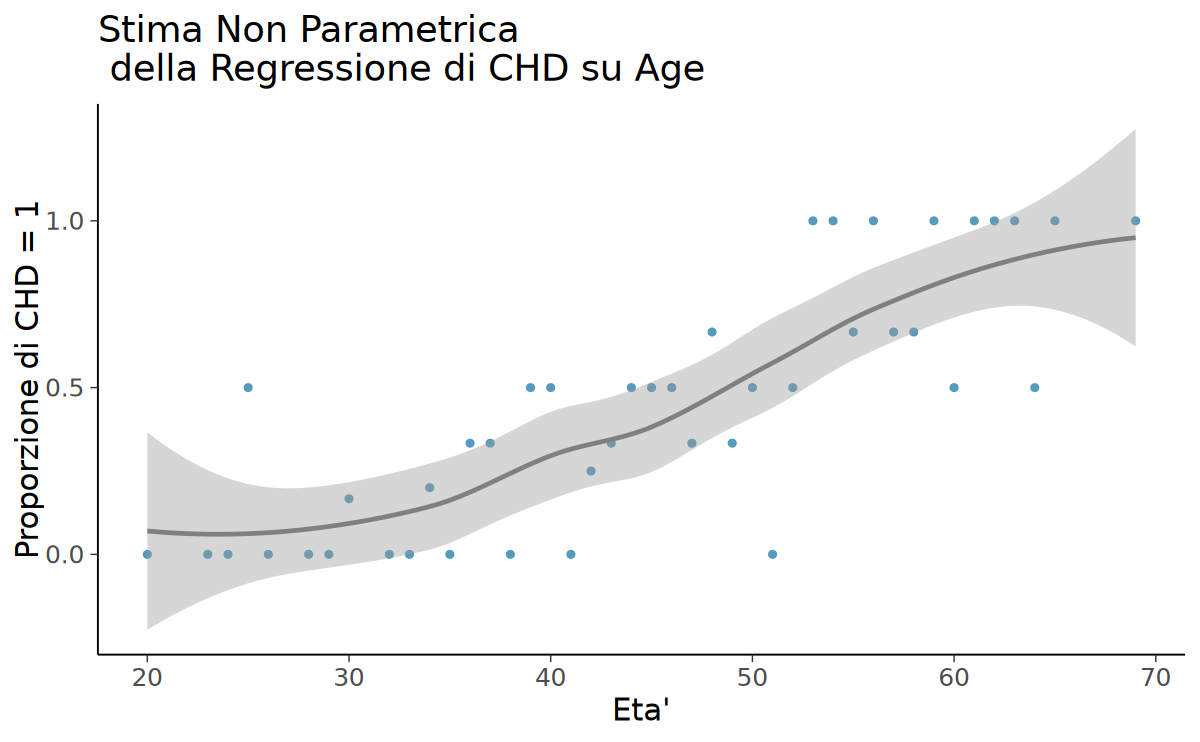
\includegraphics[width=5in,height=3.08333in]{chapters/raters/01_multilevel_files/figure-pdf/cell-5-output-1.png}

Esaminiamo ora i dati di tutti i 18 soggetti.

\begin{Shaded}
\begin{Highlighting}[]
\FunctionTok{ggplot}\NormalTok{(sleepstudy, }\FunctionTok{aes}\NormalTok{(}\AttributeTok{x =}\NormalTok{ Days, }\AttributeTok{y =}\NormalTok{ Reaction)) }\SpecialCharTok{+}
    \FunctionTok{geom\_point}\NormalTok{() }\SpecialCharTok{+}
    \FunctionTok{scale\_x\_continuous}\NormalTok{(}\AttributeTok{breaks =} \DecValTok{0}\SpecialCharTok{:}\DecValTok{9}\NormalTok{) }\SpecialCharTok{+}
    \FunctionTok{facet\_wrap}\NormalTok{(}\SpecialCharTok{\textasciitilde{}}\NormalTok{Subject)}
\end{Highlighting}
\end{Shaded}

\includegraphics[width=5in,height=3.08333in]{chapters/raters/01_multilevel_files/figure-pdf/cell-6-output-1.png}

\subsection{Descrizione del Disegno
Sperimentale}\label{descrizione-del-disegno-sperimentale}

\begin{itemize}
\tightlist
\item
  \textbf{Fase di Adattamento e Baseline}: I primi tre giorni dello
  studio (T1, T2 e B) sono stati utilizzati per l'adattamento e
  l'addestramento (T1 e T2), seguiti da una misurazione baseline (B).
  Durante questo periodo, ai soggetti è stato chiesto di rimanere a
  letto per 8 ore (dalle 23:00 alle 07:00).
\item
  \textbf{Condizioni di Sonno}: Dal quarto giorno in poi, per sette
  giorni (E1-E7), i soggetti hanno sperimentato diverse condizioni di
  sonno, variando la durata del tempo a letto (TIB) da 3 a 9 ore.
\end{itemize}

I primi due giorni (codificati come 0 e 1) sono stati dedicati
all'adattamento e all'addestramento, mentre il terzo giorno (codificato
come 2) ha visto la misurazione baseline. L'analisi dovrebbe idealmente
partire dal giorno di baseline per riflettere l'effetto della
restrizione del sonno sulle prestazioni. Per evitare che l'adattamento
influenzi i risultati, i giorni 0 e 1 devono dunque essere esclusi
dall'analisi, poiché qualsiasi variazione di prestazione in questi
giorni è attribuibile all'addestramento piuttosto che alla restrizione
del sonno.

\subsection{Preparazione dei Dati}\label{preparazione-dei-dati}

\begin{itemize}
\tightlist
\item
  \textbf{Rimozione delle Osservazioni Iniziali}: Dal dataset,
  eliminiamo le osservazioni dove la variabile \texttt{Days} è
  codificata come 0 o 1.
\item
  \textbf{Creazione di una Nuova Variabile}: Creiamo una nuova variabile
  \texttt{days\_deprived} basata su \texttt{Days}, iniziando la sequenza
  dal giorno 2. In questa nuova variabile, il giorno 2 viene
  ricodificato come 0, il giorno 3 come 1, e così via. Questa variabile
  rappresenta il numero di giorni di privazione del sonno. Salviamo il
  dataset modificato con il nome \texttt{sleep2}, che ora riflette
  accuratamente il periodo di restrizione del sonno per l'analisi.
\end{itemize}

\begin{Shaded}
\begin{Highlighting}[]
\NormalTok{sleep2 }\OtherTok{\textless{}{-}}\NormalTok{ sleepstudy }\SpecialCharTok{|\textgreater{}}
    \FunctionTok{filter}\NormalTok{(Days }\SpecialCharTok{\textgreater{}=} \DecValTok{2}\NormalTok{L) }\SpecialCharTok{|\textgreater{}}
    \FunctionTok{mutate}\NormalTok{(}\AttributeTok{days\_deprived =}\NormalTok{ Days }\SpecialCharTok{{-}} \DecValTok{2}\NormalTok{L)}
\end{Highlighting}
\end{Shaded}

\begin{Shaded}
\begin{Highlighting}[]
\NormalTok{sleep2 }\SpecialCharTok{|\textgreater{}}
    \FunctionTok{count}\NormalTok{(days\_deprived, Days)}
\end{Highlighting}
\end{Shaded}

A data.frame: 8 x 3

\begin{longtable}[]{@{}lll@{}}
\toprule\noalign{}
days\_deprived \textless dbl\textgreater{} & Days
\textless dbl\textgreater{} & n \textless int\textgreater{} \\
\midrule\noalign{}
\endhead
\bottomrule\noalign{}
\endlastfoot
0 & 2 & 18 \\
1 & 3 & 18 \\
2 & 4 & 18 \\
3 & 5 & 18 \\
4 & 6 & 18 \\
5 & 7 & 18 \\
6 & 8 & 18 \\
7 & 9 & 18 \\
\end{longtable}

\begin{Shaded}
\begin{Highlighting}[]
\FunctionTok{ggplot}\NormalTok{(sleep2, }\FunctionTok{aes}\NormalTok{(}\AttributeTok{x =}\NormalTok{ days\_deprived, }\AttributeTok{y =}\NormalTok{ Reaction)) }\SpecialCharTok{+}
    \FunctionTok{geom\_point}\NormalTok{() }\SpecialCharTok{+}
    \FunctionTok{scale\_x\_continuous}\NormalTok{(}\AttributeTok{breaks =} \DecValTok{0}\SpecialCharTok{:}\DecValTok{7}\NormalTok{) }\SpecialCharTok{+}
    \FunctionTok{facet\_wrap}\NormalTok{(}\SpecialCharTok{\textasciitilde{}}\NormalTok{Subject) }\SpecialCharTok{+}
    \FunctionTok{labs}\NormalTok{(}\AttributeTok{y =} \StringTok{"Reaction Time"}\NormalTok{, }\AttributeTok{x =} \StringTok{"Days deprived of sleep (0 = baseline)"}\NormalTok{)}
\end{Highlighting}
\end{Shaded}

\includegraphics[width=5in,height=3.08333in]{chapters/raters/01_multilevel_files/figure-pdf/cell-9-output-1.png}

\section{Relazione tra Tempo di Reazione e Privazione del
Sonno}\label{relazione-tra-tempo-di-reazione-e-privazione-del-sonno}

Nel contesto dello studio sulla privazione del sonno, l'analisi dei dati
suggerisce che, a parte una singola eccezione (il soggetto 335), il
tempo di reazione medio tende ad aumentare progressivamente con ogni
giorno aggiuntivo di privazione del sonno. Questo pattern indica che
potrebbe essere utile descrivere le prestazioni di ciascun partecipante
attraverso un modello di regressione lineare.

La regressione lineare è rappresentata dall'equazione generale:

\[ 
E(Y) = \beta_0 + \beta_1 X, 
\]

dove \(Y\) è la variabile dipendente (in questo caso, il tempo di
reazione), \(\beta_0\) rappresenta l'intercetta (il tempo di reazione
medio al giorno zero, prima dell'inizio della privazione del sonno) e
\(\beta_1\) è la pendenza (la variazione del tempo di reazione per ogni
giorno aggiuntivo di privazione del sonno). Questi parametri
(\(\beta_0\) e \(\beta_1\)) sono stimati dai dati.

Quando si modellano i dati di ciascun partecipante, emergono diverse
domande: dobbiamo adattare lo stesso modello di regressione lineare a
tutti i partecipanti, o sarebbe più appropriato utilizzare un modello
diverso per ogni soggetto? Oppure esiste un approccio intermedio che
bilancia questi estremi?

Per rispondere a queste domande, esploriamo tre approcci differenti,
come illustrato da McElreath (2020):

\begin{enumerate}
\def\labelenumi{\arabic{enumi}.}
\item
  \textbf{Complete Pooling}: Questo approccio implica l'utilizzo di un
  unico modello di regressione lineare per tutti i partecipanti.
  Significa che assumiamo la stessa relazione lineare (stessa intercetta
  e pendenza) per tutti, ignorando le differenze individuali.
\item
  \textbf{No Pooling}: In questo approccio, ogni partecipante ha un
  proprio modello di regressione lineare individuale, con intercetta e
  pendenza uniche. Qui si riconosce che ogni individuo può rispondere
  diversamente alla privazione del sonno, e quindi il modello è
  personalizzato per ciascun soggetto.
\item
  \textbf{Partial Pooling}: Questo approccio intermedio cerca di
  bilanciare gli estremi dei due metodi precedenti. Include alcuni
  elementi comuni tra i soggetti (ad esempio, una pendenza media) ma
  permette anche una certa variazione individuale.
\end{enumerate}

\section{Complete pooling}\label{complete-pooling}

L'approccio di ``complete pooling'' in analisi statistica implica
l'utilizzo di un modello che calcola un'unica intercetta e una sola
pendenza per l'intero dataset. Questo metodo si basa sull'ipotesi che
tutti i soggetti nel dataset condividano le stesse caratteristiche di
base riguardo alla relazione tra la variabile dipendente e indipendente.

\subsection{Caratteristiche del Complete
Pooling}\label{caratteristiche-del-complete-pooling}

\begin{itemize}
\tightlist
\item
  \textbf{Unicità delle Stime}: Il modello stima un singolo set di
  parametri (intercetta e pendenza) per tutti i dati, considerando
  l'intero campione come un'unità omogenea.
\item
  \textbf{Ignorare le Variazioni Individuali}: Questo approccio non
  tiene conto delle possibili differenze individuali nelle intercette o
  nelle pendenze tra i diversi soggetti. Ad esempio, ignorara come
  ciascun soggetto reagisce in modo diverso alla privazione del sonno.
\end{itemize}

\subsection{Limitazioni dell'Approccio di Complete
Pooling}\label{limitazioni-dellapproccio-di-complete-pooling}

Dall'analisi preliminare dei dati, abbiamo notato che l'approccio di
complete pooling potrebbe non essere adatto per il nostro studio. La
visualizzazione dei dati suggerisce che ogni partecipante potrebbe avere
una propria relazione unica tra il tempo di reazione e i giorni di
privazione del sonno, indicando la necessità di valori individuali per
le intercette e le pendenze.

\subsection{Modello di Regressione Lineare in Complete
Pooling}\label{modello-di-regressione-lineare-in-complete-pooling}

Il modello generale lineare (GLM) per l'approccio di complete pooling è
formulato come segue:

\[
Y_{sd} = \beta_0 + \beta_1 X_{sd} + e_{sd},
\]

dove:

\begin{itemize}
\tightlist
\item
  \(Y_{sd}\) rappresenta il tempo di reazione medio del soggetto \(s\)
  nel giorno \(d\).
\item
  \(X_{sd}\) è il numero di giorni di privazione del sonno (variabile
  \texttt{days\_deprived}), che varia da 0 a 7.
\item
  \(e_{sd}\) è il termine di errore, che rappresenta le fluttuazioni
  casuali non spiegate dal modello.
\end{itemize}

\subsection{Implementazione in R}\label{implementazione-in-r}

Per adattare questo modello in R, si utilizza la funzione \texttt{lm()}:

\begin{Shaded}
\begin{Highlighting}[]
\NormalTok{cp\_model }\OtherTok{\textless{}{-}} \FunctionTok{lm}\NormalTok{(Reaction }\SpecialCharTok{\textasciitilde{}}\NormalTok{ days\_deprived, sleep2)}
\FunctionTok{summary}\NormalTok{(cp\_model)}
\end{Highlighting}
\end{Shaded}

\begin{verbatim}

Call:
lm(formula = Reaction ~ days_deprived, data = sleep2)

Residuals:
    Min      1Q  Median      3Q     Max 
-112.28  -26.73    2.14   27.73  140.45 

Coefficients:
              Estimate Std. Error t value Pr(>|t|)    
(Intercept)     267.97       7.74   34.63  < 2e-16 ***
days_deprived    11.44       1.85    6.18  6.3e-09 ***
---
Signif. codes:  0 '***' 0.001 '**' 0.01 '*' 0.05 '.' 0.1 ' ' 1

Residual standard error: 50.9 on 142 degrees of freedom
Multiple R-squared:  0.212, Adjusted R-squared:  0.207 
F-statistic: 38.2 on 1 and 142 DF,  p-value: 6.32e-09
\end{verbatim}

\subsection{Interpretazione del Modello di Regressione e Visualizzazione
Grafica}\label{interpretazione-del-modello-di-regressione-e-visualizzazione-grafica}

Il modello di regressione che abbiamo considerato offre una stima del
tempo di risposta medio per i soggetti allo studio al Giorno 0 (prima
della privazione del sonno) e la variazione media del tempo di risposta
per ogni giorno aggiuntivo di privazione. Secondo questo modello, il
tempo di risposta medio iniziale è stimato essere di circa 268
millisecondi, con un incremento medio di circa 11 millisecondi per ogni
giorno successivo di privazione del sonno.

\subsection{Considerazioni sui Limiti del
Modello}\label{considerazioni-sui-limiti-del-modello}

È importante notare, tuttavia, che questo modello potrebbe avere delle
limitazioni nella sua applicabilità:

\begin{itemize}
\tightlist
\item
  \textbf{Assunzione di Indipendenza}: Il modello assume che tutte le
  osservazioni siano indipendenti. Questa assunzione potrebbe non essere
  valida nel nostro studio, dato che le osservazioni provengono da
  misurazioni ripetute sugli stessi soggetti.
\item
  \textbf{Errori Standard dei Coefficienti}: La presunta indipendenza
  delle osservazioni implica che gli errori standard dei coefficienti di
  regressione potrebbero non essere completamente affidabili.
\end{itemize}

\subsection{Aggiunta delle Previsioni al
Grafico}\label{aggiunta-delle-previsioni-al-grafico}

Per visualizzare meglio questi risultati, possiamo aggiungere le
previsioni del modello al grafico che abbiamo già creato. Utilizziamo la
funzione \texttt{geom\_abline()} di R per tracciare la linea di
regressione stimata direttamente sul grafico esistente:

\begin{itemize}
\tightlist
\item
  \textbf{Utilizzo di \texttt{geom\_abline()}}: Questa funzione ci
  permette di aggiungere una linea di regressione al grafico,
  specificando l'intercetta e la pendenza.
\item
  \textbf{Coefficienti del Modello}: Utilizziamo
  \texttt{coef(cp\_model)} per ottenere i coefficienti di regressione
  (intercetta e pendenza) dal nostro modello. Questa funzione
  restituisce un vettore con due elementi corrispondenti all'intercetta
  e alla pendenza, che possono essere poi utilizzati per definire la
  linea nel grafico.
\end{itemize}

In conclusione, l'aggiunta delle previsioni del modello al grafico
fornisce una rappresentazione visiva dell'effetto stimato della
privazione del sonno sul tempo di risposta. Tuttavia, è essenziale
tenere presente le limitazioni e le assunzioni del modello, in
particolare l'indipendenza delle osservazioni, che potrebbe non essere
una rappresentazione accurata dei dati nel contesto di misurazioni
ripetute.

\begin{Shaded}
\begin{Highlighting}[]
\FunctionTok{ggplot}\NormalTok{(sleep2, }\FunctionTok{aes}\NormalTok{(}\AttributeTok{x =}\NormalTok{ days\_deprived, }\AttributeTok{y =}\NormalTok{ Reaction)) }\SpecialCharTok{+}
    \FunctionTok{geom\_abline}\NormalTok{(}
        \AttributeTok{intercept =} \FunctionTok{coef}\NormalTok{(cp\_model)[}\DecValTok{1}\NormalTok{],}
        \AttributeTok{slope =} \FunctionTok{coef}\NormalTok{(cp\_model)[}\DecValTok{2}\NormalTok{],}
        \AttributeTok{color =} \StringTok{"blue"}
\NormalTok{    ) }\SpecialCharTok{+}
    \FunctionTok{geom\_point}\NormalTok{() }\SpecialCharTok{+}
    \FunctionTok{scale\_x\_continuous}\NormalTok{(}\AttributeTok{breaks =} \DecValTok{0}\SpecialCharTok{:}\DecValTok{7}\NormalTok{) }\SpecialCharTok{+}
    \FunctionTok{facet\_wrap}\NormalTok{(}\SpecialCharTok{\textasciitilde{}}\NormalTok{Subject) }\SpecialCharTok{+}
    \FunctionTok{labs}\NormalTok{(}\AttributeTok{y =} \StringTok{"Reaction Time"}\NormalTok{, }\AttributeTok{x =} \StringTok{"Days deprived of sleep (0 = baseline)"}\NormalTok{)}
\end{Highlighting}
\end{Shaded}

\includegraphics[width=5in,height=3.08333in]{chapters/raters/01_multilevel_files/figure-pdf/cell-11-output-1.png}

Dall'analisi effettuata, emerge che il modello attuale non si adatta in
modo ottimale ai dati raccolti. Questa situazione indica la necessità di
esplorare un approccio diverso per modellare in modo più accurato le
relazioni presenti nei dati.

\section{Approccio di No Pooling}\label{approccio-di-no-pooling}

In alternativa al modello di ``complete pooling'', consideriamo
l'approccio di ``no pooling''. Questo approccio si basa sull'idea di
adattare modelli di regressione separati per ogni partecipante,
trattando ogni individuo come un'entità distinta.

\subsection{Caratteristiche del No
Pooling}\label{caratteristiche-del-no-pooling}

\begin{itemize}
\tightlist
\item
  \textbf{Indipendenza delle Stime}: In questo approccio, ogni
  partecipante ha il proprio set di stime per l'intercetta e la
  pendenza. Le stime relative a un partecipante non sono influenzate
  dalle stime degli altri.
\item
  \textbf{Stime Individualizzate}: Si stima separatamente una coppia di
  intercetta/pendenza per ciascuno dei 18 partecipanti, riconoscendo la
  possibilità di variazioni significative nelle risposte individuali.
\end{itemize}

\subsection{Implementazione del Modello di No
Pooling}\label{implementazione-del-modello-di-no-pooling}

Esistono due modi principali per implementare questo approccio:

\begin{enumerate}
\def\labelenumi{\arabic{enumi}.}
\tightlist
\item
  \textbf{Regressioni Separate per Ogni Partecipante}: Eseguire una
  serie di regressioni lineari individuali, una per ogni soggetto.
\item
  \textbf{Modello di Regressione Unificato con Effetti Principali e
  Interazione}: Utilizzare un unico modello di regressione che includa
  sia gli effetti principali sia l'interazione tra le variabili
  \texttt{Subject} (soggetto) e \texttt{Day} (giorno). Questo metodo
  permette di includere tutte le stime in un unico modello.
\end{enumerate}

Per il secondo approccio, è necessario considerare le seguenti fasi:

\begin{itemize}
\tightlist
\item
  \textbf{Creazione di Variabili Dummy per il Fattore \texttt{Subject}}:
  Poiché \texttt{Subject} ha 18 livelli, saranno necessarie 17 variabili
  dummy per rappresentare questi livelli. In R, questo può essere fatto
  automaticamente definendo \texttt{Subject} come un fattore.
\item
  \textbf{Includere \texttt{Subject} come Fattore nel Modello}:
  Aggiungere \texttt{Subject}, definito come un fattore, come predittore
  nel modello. L'inclusione dell'interazione tra \texttt{Subject} e
  \texttt{days\_deprived} permette variazioni nelle intercette e nelle
  pendenze tra i soggetti.
\end{itemize}

\subsection{\texorpdfstring{Verifica del Fattore
\texttt{Subject}}{Verifica del Fattore Subject}}\label{verifica-del-fattore-subject}

Prima di procedere, è importante assicurarsi che \texttt{Subject} sia
definito correttamente come un fattore. Questo può essere verificato
utilizzando la funzione \texttt{summary()} in R, che fornisce una
sintesi delle caratteristiche della variabile, compreso se è trattata
come un fattore.

\begin{Shaded}
\begin{Highlighting}[]
\NormalTok{sleep2 }\SpecialCharTok{|\textgreater{}} 
    \FunctionTok{summary}\NormalTok{()}
\end{Highlighting}
\end{Shaded}

\begin{verbatim}
    Reaction        Days         Subject   days_deprived 
 Min.   :203   Min.   :2.00   308    : 8   Min.   :0.00  
 1st Qu.:265   1st Qu.:3.75   309    : 8   1st Qu.:1.75  
 Median :303   Median :5.50   310    : 8   Median :3.50  
 Mean   :308   Mean   :5.50   330    : 8   Mean   :3.50  
 3rd Qu.:348   3rd Qu.:7.25   331    : 8   3rd Qu.:5.25  
 Max.   :466   Max.   :9.00   332    : 8   Max.   :7.00  
                              (Other):96                 
\end{verbatim}

La funzione \texttt{pull()} viene utilizzata per estrarre una specifica
colonna da un data frame. Con le seguenti istruzioni verifichiamo se la
colonna \texttt{Subject} è codificata come \texttt{factor}.

\begin{Shaded}
\begin{Highlighting}[]
\NormalTok{sleep2 }\SpecialCharTok{|\textgreater{}}
    \FunctionTok{pull}\NormalTok{(Subject) }\SpecialCharTok{|\textgreater{}}
    \FunctionTok{is.factor}\NormalTok{()}
\end{Highlighting}
\end{Shaded}

TRUE

Adattiamo il modello di regressione ai dati. Si noti che la sintassi
seguente può essere semplificata utilizzando
\texttt{Reaction\ \textasciitilde{}\ days\_deprived\ *\ Subject}.

\begin{Shaded}
\begin{Highlighting}[]
\NormalTok{np\_model }\OtherTok{\textless{}{-}} \FunctionTok{lm}\NormalTok{(Reaction }\SpecialCharTok{\textasciitilde{}}\NormalTok{ days\_deprived }\SpecialCharTok{+}\NormalTok{ Subject }\SpecialCharTok{+}\NormalTok{ days\_deprived}\SpecialCharTok{:}\NormalTok{Subject,}
    \AttributeTok{data =}\NormalTok{ sleep2}
\NormalTok{)}

\FunctionTok{summary}\NormalTok{(np\_model)}
\end{Highlighting}
\end{Shaded}

\begin{verbatim}

Call:
lm(formula = Reaction ~ days_deprived + Subject + days_deprived:Subject, 
    data = sleep2)

Residuals:
    Min      1Q  Median      3Q     Max 
-106.52   -8.54    1.14    8.89  128.55 

Coefficients:
                         Estimate Std. Error t value Pr(>|t|)    
(Intercept)               288.217     16.477   17.49  < 2e-16 ***
days_deprived              21.690      3.939    5.51  2.5e-07 ***
Subject309                -87.926     23.302   -3.77  0.00026 ***
Subject310                -62.286     23.302   -2.67  0.00869 ** 
Subject330                -14.953     23.302   -0.64  0.52242    
Subject331                  9.966     23.302    0.43  0.66974    
Subject332                 27.816     23.302    1.19  0.23522    
Subject333                 -2.758     23.302   -0.12  0.90600    
Subject334                -50.205     23.302   -2.15  0.03342 *  
Subject335                -25.343     23.302   -1.09  0.27921    
Subject337                 24.614     23.302    1.06  0.29319    
Subject349                -59.218     23.302   -2.54  0.01246 *  
Subject350                -40.202     23.302   -1.73  0.08734 .  
Subject351                -24.247     23.302   -1.04  0.30042    
Subject352                 43.065     23.302    1.85  0.06732 .  
Subject369                -21.504     23.302   -0.92  0.35815    
Subject370                -53.307     23.302   -2.29  0.02411 *  
Subject371                -30.490     23.302   -1.31  0.19350    
Subject372                  2.477     23.302    0.11  0.91554    
days_deprived:Subject309  -17.333      5.570   -3.11  0.00238 ** 
days_deprived:Subject310  -17.792      5.570   -3.19  0.00184 ** 
days_deprived:Subject330  -13.685      5.570   -2.46  0.01561 *  
days_deprived:Subject331  -16.823      5.570   -3.02  0.00315 ** 
days_deprived:Subject332  -19.295      5.570   -3.46  0.00076 ***
days_deprived:Subject333  -10.815      5.570   -1.94  0.05480 .  
days_deprived:Subject334   -3.575      5.570   -0.64  0.52242    
days_deprived:Subject335  -25.899      5.570   -4.65  9.5e-06 ***
days_deprived:Subject337    0.752      5.570    0.13  0.89289    
days_deprived:Subject349   -5.264      5.570   -0.95  0.34673    
days_deprived:Subject350    1.601      5.570    0.29  0.77438    
days_deprived:Subject351  -13.168      5.570   -2.36  0.01987 *  
days_deprived:Subject352  -14.402      5.570   -2.59  0.01106 *  
days_deprived:Subject369   -7.895      5.570   -1.42  0.15927    
days_deprived:Subject370   -1.049      5.570   -0.19  0.85091    
days_deprived:Subject371   -9.344      5.570   -1.68  0.09633 .  
days_deprived:Subject372  -10.604      5.570   -1.90  0.05961 .  
---
Signif. codes:  0 '***' 0.001 '**' 0.01 '*' 0.05 '.' 0.1 ' ' 1

Residual standard error: 25.5 on 108 degrees of freedom
Multiple R-squared:  0.849, Adjusted R-squared:   0.8 
F-statistic: 17.4 on 35 and 108 DF,  p-value: <2e-16
\end{verbatim}

Per chiarire, il soggetto di riferimento è il 308; in R, la modalità
predefinita è quella di ordinare i livelli del fattore in ordine
alfabetico e di scegliere il primo come soggetto di riferimento. Questo
significa che l'intercetta e la pendenza per il soggetto 308 sono
rappresentate rispettivamente da \texttt{(Intercept)} e
\texttt{days\_deprived}, poiché tutte le altre 17 variabili dummy
saranno nulle per il soggetto 308.

Tutti i coefficienti di regressione degli altri soggetti sono
rappresentati come scostamenti da questo soggetto di riferimento. Se
desideriamo calcolare l'intercetta e la pendenza per un dato soggetto,
dobbiamo semplicemente sommare gli scostamenti corrispondenti. Pertanto,
abbiamo:

Intercetta per 308: 288.217\\
Pendenza per 308: 21.69

Intercetta per 335: \texttt{(Intercept)\ +\ Subject335} = 288.217 +
-25.343 = 262.874\\
Pendenza per 335: \texttt{days\_deprived\ +\ days\_deprived:Subject335}
= 21.69 + -25.899 = -4.209

E così via.

Nel modello ``no pooling'', non viene stimata un'intercetta e una
pendenza complessive per l'intera popolazione; in questo caso,
\texttt{(Intercept)} e \texttt{days\_deprived} sono stime
dell'intercetta e della pendenza per il soggetto 308, che è stato scelto
(arbitrariamente) come soggetto di riferimento. Per ottenere stime per
l'intera popolazione, è possibile procedere con una seconda fase
dell'analisi statistica in cui calcoliamo le medie delle intercette e
delle pendenze individuali.

\begin{Shaded}
\begin{Highlighting}[]
\FunctionTok{coef}\NormalTok{(np\_model) }\SpecialCharTok{|\textgreater{}} \FunctionTok{as.data.frame}\NormalTok{()}
\end{Highlighting}
\end{Shaded}

A data.frame: 36 x 1

\begin{longtable}[]{@{}ll@{}}
\toprule\noalign{}
& coef(np\_model) \textless dbl\textgreater{} \\
\midrule\noalign{}
\endhead
\bottomrule\noalign{}
\endlastfoot
(Intercept) & 288.217 \\
days\_deprived & 21.690 \\
Subject309 & -87.926 \\
Subject310 & -62.286 \\
Subject330 & -14.953 \\
Subject331 & 9.966 \\
Subject332 & 27.816 \\
Subject333 & -2.758 \\
Subject334 & -50.205 \\
Subject335 & -25.343 \\
Subject337 & 24.614 \\
Subject349 & -59.218 \\
Subject350 & -40.202 \\
Subject351 & -24.247 \\
Subject352 & 43.065 \\
Subject369 & -21.504 \\
Subject370 & -53.307 \\
Subject371 & -30.490 \\
Subject372 & 2.477 \\
days\_deprived:Subject309 & -17.333 \\
days\_deprived:Subject310 & -17.792 \\
days\_deprived:Subject330 & -13.685 \\
days\_deprived:Subject331 & -16.823 \\
days\_deprived:Subject332 & -19.295 \\
days\_deprived:Subject333 & -10.815 \\
days\_deprived:Subject334 & -3.575 \\
days\_deprived:Subject335 & -25.899 \\
days\_deprived:Subject337 & 0.752 \\
days\_deprived:Subject349 & -5.264 \\
days\_deprived:Subject350 & 1.601 \\
days\_deprived:Subject351 & -13.168 \\
days\_deprived:Subject352 & -14.402 \\
days\_deprived:Subject369 & -7.895 \\
days\_deprived:Subject370 & -1.049 \\
days\_deprived:Subject371 & -9.344 \\
days\_deprived:Subject372 & -10.604 \\
\end{longtable}

Calcoliamo le intercette individuali:

\begin{Shaded}
\begin{Highlighting}[]
\NormalTok{all\_intercepts }\OtherTok{\textless{}{-}} \FunctionTok{c}\NormalTok{(}
    \FunctionTok{coef}\NormalTok{(np\_model)[}\StringTok{"(Intercept)"}\NormalTok{],}
    \FunctionTok{coef}\NormalTok{(np\_model)[}\DecValTok{3}\SpecialCharTok{:}\DecValTok{19}\NormalTok{] }\SpecialCharTok{+} \FunctionTok{coef}\NormalTok{(np\_model)[}\StringTok{"(Intercept)"}\NormalTok{]}
\NormalTok{)}
\end{Highlighting}
\end{Shaded}

Calcliamo le pendenze individuali:

\begin{Shaded}
\begin{Highlighting}[]
\NormalTok{all\_slopes }\OtherTok{\textless{}{-}} \FunctionTok{c}\NormalTok{(}
    \FunctionTok{coef}\NormalTok{(np\_model)[}\StringTok{"days\_deprived"}\NormalTok{],}
    \FunctionTok{coef}\NormalTok{(np\_model)[}\DecValTok{20}\SpecialCharTok{:}\DecValTok{36}\NormalTok{] }\SpecialCharTok{+} \FunctionTok{coef}\NormalTok{(np\_model)[}\StringTok{"days\_deprived"}\NormalTok{]}
\NormalTok{)}
\end{Highlighting}
\end{Shaded}

Creiamo un DataFrame con le colonne Subject, intercept e slope:

\begin{Shaded}
\begin{Highlighting}[]
\NormalTok{ids }\OtherTok{\textless{}{-}}\NormalTok{ sleep2 }\SpecialCharTok{|\textgreater{}}
    \FunctionTok{pull}\NormalTok{(Subject) }\SpecialCharTok{|\textgreater{}}
    \FunctionTok{levels}\NormalTok{() }\SpecialCharTok{|\textgreater{}}
    \FunctionTok{factor}\NormalTok{()}
\FunctionTok{print}\NormalTok{(ids)}
\end{Highlighting}
\end{Shaded}

\begin{verbatim}
 [1] 308 309 310 330 331 332 333 334 335 337 349 350 351 352 369 370 371 372
18 Levels: 308 309 310 330 331 332 333 334 335 337 349 350 351 352 ... 372
\end{verbatim}

\begin{Shaded}
\begin{Highlighting}[]
\CommentTok{\# make a tibble with the data extracted above}
\NormalTok{np\_coef }\OtherTok{\textless{}{-}} \FunctionTok{tibble}\NormalTok{(}
    \AttributeTok{Subject =}\NormalTok{ ids,}
    \AttributeTok{intercept =}\NormalTok{ all\_intercepts,}
    \AttributeTok{slope =}\NormalTok{ all\_slopes}
\NormalTok{)}

\FunctionTok{print}\NormalTok{(np\_coef)}
\end{Highlighting}
\end{Shaded}

\begin{verbatim}
# A tibble: 18 x 3
  Subject intercept slope
  <fct>       <dbl> <dbl>
1 308          288. 21.7 
2 309          200.  4.36
3 310          226.  3.90
4 330          273.  8.01
5 331          298.  4.87
6 332          316.  2.40
# i 12 more rows
\end{verbatim}

Esaminiamo l'adattamento di questo modello ai dati.

\begin{Shaded}
\begin{Highlighting}[]
\FunctionTok{ggplot}\NormalTok{(sleep2, }\FunctionTok{aes}\NormalTok{(}\AttributeTok{x =}\NormalTok{ days\_deprived, }\AttributeTok{y =}\NormalTok{ Reaction)) }\SpecialCharTok{+}
    \FunctionTok{geom\_abline}\NormalTok{(}
        \AttributeTok{data =}\NormalTok{ np\_coef,}
        \AttributeTok{mapping =} \FunctionTok{aes}\NormalTok{(}
            \AttributeTok{intercept =}\NormalTok{ intercept,}
            \AttributeTok{slope =}\NormalTok{ slope}
\NormalTok{        ),}
        \AttributeTok{color =} \StringTok{"blue"}
\NormalTok{    ) }\SpecialCharTok{+}
    \FunctionTok{geom\_point}\NormalTok{() }\SpecialCharTok{+}
    \FunctionTok{scale\_x\_continuous}\NormalTok{(}\AttributeTok{breaks =} \DecValTok{0}\SpecialCharTok{:}\DecValTok{7}\NormalTok{) }\SpecialCharTok{+}
    \FunctionTok{facet\_wrap}\NormalTok{(}\SpecialCharTok{\textasciitilde{}}\NormalTok{Subject) }\SpecialCharTok{+}
    \FunctionTok{labs}\NormalTok{(}\AttributeTok{y =} \StringTok{"Reaction Time"}\NormalTok{, }\AttributeTok{x =} \StringTok{"Days deprived of sleep (0 = baseline)"}\NormalTok{)}
\end{Highlighting}
\end{Shaded}

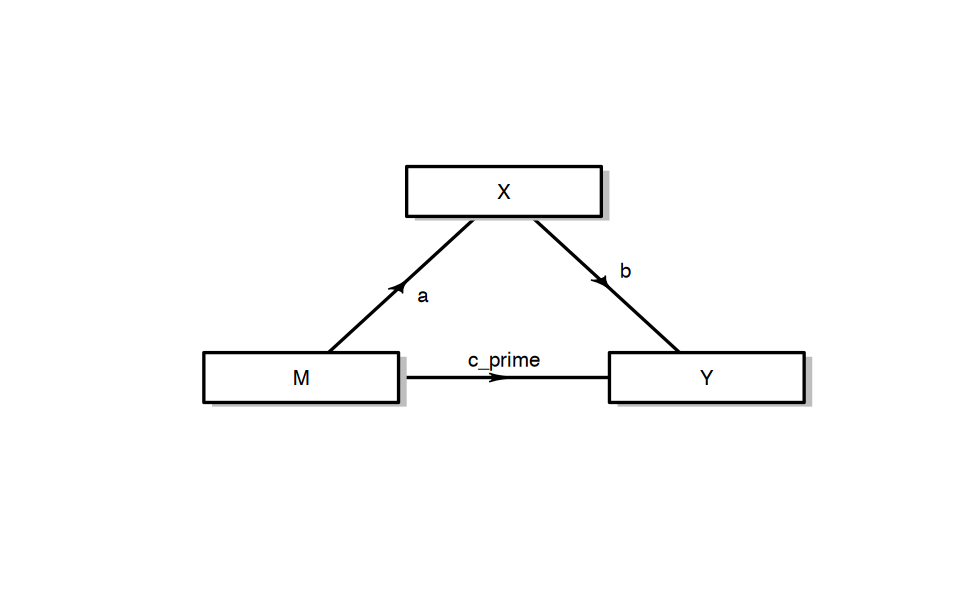
\includegraphics[width=5in,height=3.08333in]{chapters/raters/01_multilevel_files/figure-pdf/cell-20-output-1.png}

Questa situazione è notevolmente migliorata rispetto al modello di
pooling completo. Se desideriamo testare l'ipotesi nulla secondo cui la
pendenza della retta di regressione è uguale a zero, possiamo farlo
eseguendo un test \(t\) di Student sul campione di pendenze individuali.

\begin{Shaded}
\begin{Highlighting}[]
\NormalTok{np\_coef }\SpecialCharTok{|\textgreater{}}
    \FunctionTok{pull}\NormalTok{(slope) }\SpecialCharTok{|\textgreater{}}
    \FunctionTok{t.test}\NormalTok{()}
\end{Highlighting}
\end{Shaded}

\begin{verbatim}

    One Sample t-test

data:  pull(np_coef, slope)
t = 6, df = 17, p-value = 1e-05
alternative hypothesis: true mean is not equal to 0
95 percent confidence interval:
  7.54 15.33
sample estimates:
mean of x 
     11.4 
\end{verbatim}

Questo test suggerisce che la pendenza media di 11.435 è diversa da
zero, t(17) = 6.20 p \textless{} .001.

\section{Approccio di Partial
Pooling}\label{approccio-di-partial-pooling}

Nell'ambito dell'analisi dei dati psicologici, i ricercatori si trovano
spesso a dover gestire un delicato equilibrio. Da un lato, vi è
l'approccio di \emph{complete pooling}, che tratta tutti i dati come se
appartenessero a un unico gruppo omogeneo, e dall'altro, l'approccio di
\emph{no-pooling}, che considera i dati di ciascun soggetto in modo
isolato, senza sfruttare le informazioni aggregate. Entrambi gli estremi
hanno limitazioni significative: il \emph{complete pooling} può
mascherare le variazioni individuali, mentre il \emph{no-pooling} può
non sfruttare appieno le informazioni disponibili dall'intero set di
dati.

Per superare queste limitazioni, emerge l'approccio di \emph{partial
pooling}. Questo metodo utilizza i modelli lineari a effetti misti, che
rappresentano una via di mezzo tra i due estremi menzionati. Il
\emph{partial pooling} permette di trarre vantaggio dalle informazioni
provenienti dall'insieme dei partecipanti, migliorando così le stime dei
soggetti individuali. Attraverso questo approccio, si ottengono stime
che non solo tengono conto delle peculiarità di ciascun individuo ma
sono anche informate dalle tendenze generali osservate nel gruppo più
ampio.

L'approccio di \emph{partial pooling} permette di separare più
efficacemente le tendenze generali dagli errori casuali in ciascun
partecipante e si dimostra più adatto per generalizzare i risultati a
una popolazione più ampia, al di là dei soggetti specifici coinvolti
nello studio.

\subsection{Implementazione dei Modelli a Effetti
Misti}\label{implementazione-dei-modelli-a-effetti-misti}

\begin{itemize}
\tightlist
\item
  \textbf{Trattare i Soggetti come Fattori Casuali}: Nel \emph{partial
  pooling}, i soggetti vengono considerati come un fattore casuale
  anziché fisso. Ciò implica che i livelli del fattore (i soggetti nel
  nostro caso) sono visti come un campione casuale da una popolazione
  più ampia.
\item
  \textbf{Modello Lineare a Effetti Misti}: Questo tipo di modello
  statistico consente di includere i fattori casuali nell'analisi. In un
  modello misto, le stime per ogni soggetto sono ``informate'' o
  influenzate dalle informazioni aggregate degli altri soggetti.
\item
  \textbf{Shrinkage o Restringimento}: Il fenomeno dello
  \emph{shrinkage} indica che le stime per ciascun soggetto vengono
  regolate o ``spostate'' verso le stime medie della popolazione,
  permettendo una valutazione più equilibrata e meno influenzata da
  variazioni estreme o casuali.
\end{itemize}

\subsection{Articolazione e Applicazione del Modello
Multilivello}\label{articolazione-e-applicazione-del-modello-multilivello}

Il modello multilivello che analizziamo è strutturato per cogliere le
relazioni dinamiche tra variabili a livelli diversi. Esaminiamo i
dettagli di ogni livello e il loro significato nel contesto del modello.

\subsection{Livello 1: Modellazione della Relazione
Individuale}\label{livello-1-modellazione-della-relazione-individuale}

Il primo livello del modello esprime la relazione lineare individuale
tra la variabile di risposta (tempo di reazione) e i predittori (giorni
di privazione del sonno):

\[
Y_{sd} = \beta_{0s} + \beta_{1s} X_{sd} + e_{sd},
\]

dove \(Y_{sd}\) è il tempo di reazione del soggetto \(s\) al giorno
\(d\), \(\beta_{0s}\) e \(\beta_{1s}\) sono i parametri individuali di
intercetta e pendenza, e \(e_{sd}\) rappresenta l'errore per ogni
soggetto e giorno. I parametri \(\beta_{0s}\) e \(\beta_{1s}\) sono
considerati derivati, poiché dipendono dalle variabili a Livello 2.

\subsection{Livello 2: Modellazione delle Variazioni Tra
Soggetti}\label{livello-2-modellazione-delle-variazioni-tra-soggetti}

Al secondo livello, definiamo come l'intercetta e la pendenza cambiano
tra i soggetti:

\[
\beta_{0s} = \gamma_{0} + S_{0s},
\]

\[
\beta_{1s} = \gamma_{1} + S_{1s}.
\]

Qui, \(\gamma_0\) e \(\gamma_1\) sono gli effetti fissi che
rappresentano l'intercetta e la pendenza medie della popolazione, mentre
\(S_{0s}\) e \(S_{1s}\) sono gli effetti casuali che permettono
variazioni individuali.

\subsection{Componenti di Varianza}\label{componenti-di-varianza}

Le componenti di varianza nel modello sono espresse come:

\[
\langle S_{0s}, S_{1s} \rangle \sim N(\langle 0, 0 \rangle, \mathbf{\Sigma}),
\]

\[
\mathbf{\Sigma} = \begin{pmatrix}{\tau_{00}}^2 & \rho\tau_{00}\tau_{11} \\ \rho\tau_{00}\tau_{11} & {\tau_{11}}^2 \end{pmatrix},
\]

\[
e_{sd} \sim N(0, \sigma^2).
\]

La matrice \(\mathbf{\Sigma}\) determina la distribuzione degli effetti
casuali, con \({\tau_{00}}^2\) e \({\tau_{11}}^2\) che indicano le
varianze delle intercette e delle pendenze casuali, mentre \(\rho\) è la
correlazione tra questi effetti.

\subsection{Interpretazione Complessiva del
Modello}\label{interpretazione-complessiva-del-modello}

Unendo le equazioni di Livello 1 e Livello 2, otteniamo una visione
completa del modello:

\[
Y_{sd} = \gamma_0 + S_{0s} + (\gamma_1 + S_{1s}) X_{sd} + e_{sd},
\]

dove

\begin{itemize}
\tightlist
\item
  \(Y_{sd}\): È il valore osservato della variabile di risposta per il
  soggetto \(s\) al giorno \(d\).
\item
  \(\gamma_0\) e \(\gamma_1\): Sono gli effetti fissi. \(\gamma_0\)
  rappresenta l'intercetta generale, ovvero la media della popolazione
  per la variabile di risposta quando la variabile predittiva \(X\) è
  zero. \(\gamma_1\) rappresenta la pendenza generale, che indica come
  la variabile di risposta cambia in media con un'unità di incremento
  della variabile predittiva \(X\).
\item
  \(S_{0s}\) e \(S_{1s}\): Sono gli effetti casuali. \(S_{0s}\) è
  l'effetto casuale dell'intercetta per il soggetto \(s\), mentre
  \(S_{1s}\) è l'effetto casuale della pendenza. Questi termini
  rappresentano come ciascun soggetto si discosta dalla media della
  popolazione.
\item
  \(X_{sd}\): È la variabile predittiva per il soggetto \(s\) al giorno
  \(d\).
\item
  \(e_{sd}\): È l'errore casuale associato a ciascuna osservazione.
\end{itemize}

\subsection{Interpretazione degli Effetti Fissi e
Casuali}\label{interpretazione-degli-effetti-fissi-e-casuali}

\begin{itemize}
\tightlist
\item
  Gli effetti fissi (\(\gamma_0\) e \(\gamma_1\)) sono costanti per
  tutti i soggetti e riflettono le caratteristiche della popolazione
  generale.
\item
  Gli effetti casuali (\(S_{0s}\) e \(S_{1s}\)) variano da soggetto a
  soggetto e sono modellati come distribuzioni normali centrate attorno
  a zero. Questo significa che la distribuzione degli effetti casuali è
  centrata attorno agli effetti fissi della popolazione.
\end{itemize}

\subsubsection{Uso di Campioni per Informare sulla
Popolazione}\label{uso-di-campioni-per-informare-sulla-popolazione}

Trattare i soggetti come variabili casuali anziché fisse ci consente di
usare i dati del campione per inferire sulla popolazione più ampia.
Invece di stimare valori specifici per ogni soggetto, il modello stima
la distribuzione da cui questi valori sono estratti, fornendo una
visione più generalizzata e applicabile a livello di popolazione.

\subsection{Spiegazione della Matrice di Varianza-Covarianza nel Modello
Multilivello}\label{spiegazione-della-matrice-di-varianza-covarianza-nel-modello-multilivello}

La matrice di varianza-covarianza nel modello multilivello gioca un
ruolo cruciale nel definire come gli effetti casuali variano e sono
correlati tra loro all'interno della popolazione studiata. Questa
matrice è rappresentata come segue:

\[
\Sigma = 
\begin{pmatrix}
\tau_{00}^2 & \rho \tau_{00} \tau_{11} \\
\rho \tau_{00} \tau_{11} & \tau_{11}^2
\end{pmatrix},
\]

dove \(\Sigma\) denota la matrice di varianza-covarianza per gli effetti
casuali \(\langle S_{0s}, S_{1s} \rangle\), che sono modellati come
normalmente distribuiti con una media di zero e una varianza-covarianza
data da \(\Sigma\).

\subsubsection{Componenti della Matrice}\label{componenti-della-matrice}

\begin{itemize}
\tightlist
\item
  \textbf{Varianze degli Effetti Casuali}:

  \begin{itemize}
  \tightlist
  \item
    \(\tau_{00}^2\): Varianza dell'effetto casuale sull'intercetta
    (\(S_{0s}\)). Questo parametro indica quanto i soggetti differiscono
    nella loro reazione iniziale (tempo di reazione al Giorno 0) prima
    di qualsiasi privazione del sonno.
  \item
    \(\tau_{11}^2\): Varianza dell'effetto casuale sulla pendenza
    (\(S_{1s}\)). Misura la variazione tra i soggetti nella loro
    reattività agli effetti della privazione del sonno.
  \end{itemize}
\item
  \textbf{Covarianze}:

  \begin{itemize}
  \tightlist
  \item
    \(\rho \tau_{00} \tau_{11}\): Covarianza tra l'intercetta e la
    pendenza casuali. Questo termine riflette come la reazione iniziale
    di un soggetto (intercetta) sia correlata con la variazione della
    sua reattività al sonno (pendenza). Un valore positivo di \(\rho\)
    indica che soggetti con un tempo di reazione inizialmente più lento
    tendono a mostrare un aumento più marcato del tempo di reazione con
    la privazione del sonno, e viceversa.
  \end{itemize}
\end{itemize}

\subsubsection{\texorpdfstring{Significato e Importanza di
\(\Sigma\)}{Significato e Importanza di \textbackslash Sigma}}\label{significato-e-importanza-di-sigma}

\begin{itemize}
\tightlist
\item
  \textbf{Distribuzione degli Effetti Casuali}: La matrice \(\Sigma\)
  determina le probabilità di estrarre una coppia specifica di effetti
  casuali (\(S_{0s}, S_{1s}\)) per un soggetto dal pool più ampio della
  popolazione.
\item
  \textbf{Analisi delle Variazioni Individuali}: Attraverso \(\Sigma\),
  possiamo comprendere meglio quanto e in che modo i soggetti variano
  sia nella loro reazione iniziale sia nella loro risposta alla
  privazione del sonno.
\item
  \textbf{Interpretazione dei Risultati}: La comprensione di \(\Sigma\)
  aiuta a interpretare i risultati del modello in termini di varianza e
  covarianza tra i soggetti, permettendo di trarre conclusioni più
  precise sulla popolazione studiata.
\end{itemize}

La matrice di varianza-covarianza \(\Sigma\) è fondamentale nel modello
multilivello perché fornisce un quadro dettagliato della varianza e
della covarianza degli effetti casuali, consentendo di cogliere le
sottili variazioni e correlazioni tra i soggetti. Questa comprensione
arricchisce l'analisi e rende possibili conclusioni più accurate sulla
popolazione.

\subsection{Tabella delle Variabili}\label{tabella-delle-variabili}

\begin{longtable}[]{@{}
  >{\raggedright\arraybackslash}p{(\columnwidth - 4\tabcolsep) * \real{0.2358}}
  >{\raggedright\arraybackslash}p{(\columnwidth - 4\tabcolsep) * \real{0.1038}}
  >{\raggedright\arraybackslash}p{(\columnwidth - 4\tabcolsep) * \real{0.6604}}@{}}
\toprule\noalign{}
\begin{minipage}[b]{\linewidth}\raggedright
Variabile
\end{minipage} & \begin{minipage}[b]{\linewidth}\raggedright
Tipo
\end{minipage} & \begin{minipage}[b]{\linewidth}\raggedright
Descrizione
\end{minipage} \\
\midrule\noalign{}
\endhead
\bottomrule\noalign{}
\endlastfoot
\(Y_{sd}\) & Osservata & Valore di \texttt{Reaction} per il soggetto
\(s\) al giorno \(d\) \\
\(X_{sd}\) & Osservata & Valore di \texttt{days\_deprived} (0-7) per il
soggetto \(s\) al giorno \(d\) \\
\(\beta_{0s}\) & Derivata & Parametro di intercetta di livello 1 per il
soggetto \(s\) \\
\(\beta_{1s}\) & Derivata & Parametro di pendenza di livello 1 per il
soggetto \(s\) \\
\(e_{sd}\) & Derivata & Errore per il soggetto \(s\) al giorno \(d\) \\
\(\gamma_0\) & Fissa & Intersezione generale (media di \(\beta_{0s}\)
nella popolazione) \\
\(\gamma_1\) & Fissa & Pendenza generale (media di \(\beta_{1s}\) nella
popolazione) \\
\(S_{0s}\) & Casuale & Effetto random di intercetta per il soggetto
\(s\) \\
\(S_{1s}\) & Casuale & Effetto random di pendenza per il soggetto
\(s\) \\
\(\mathbf{\Sigma}\) & Casuale & Matrice di varianza-covarianza \\
\({\tau_{00}}^2\) & Casuale & Varianza degli effetti random di
intercetta \\
\(\rho\) & Casuale & Correlazione tra intercetta e pendenza \\
\({\tau_{11}}^2\) & Casuale & Varianza degli effetti random di
pendenza \\
\(\sigma^2\) & Casuale & Varianza dell'errore \\
\end{longtable}

\subsubsection{Spiegazione delle Categorie di Variabili nel Modello
Multilivello}\label{spiegazione-delle-categorie-di-variabili-nel-modello-multilivello}

Nella tabella delle variabili del modello multilivello, utilizziamo tre
categorie specifiche per classificare le diverse variabili:
\emph{fisso}, \emph{casuale} e \emph{derivato}. Queste categorie ci
aiutano a comprendere il ruolo e la natura di ciascuna variabile
all'interno del modello:

\paragraph{Variabili Fisse}\label{variabili-fisse}

\begin{itemize}
\tightlist
\item
  \textbf{Definizione}: Le variabili fisse sono quelle che assumiamo
  costanti attraverso il campione e la popolazione. Sono parametri che
  rappresentano le caratteristiche generali della popolazione da cui il
  campione è tratto.
\item
  \textbf{Esempi}: Nella tabella, \(\gamma_0\) (intercetta generale) e
  \(\gamma_1\) (pendenza generale) sono variabili fisse.
\item
  \textbf{Ruolo nel Modello}: Riflettono le tendenze centrali o gli
  effetti medi nella popolazione oggetto di studio.
\end{itemize}

\paragraph{Variabili Casuali}\label{variabili-casuali}

\begin{itemize}
\tightlist
\item
  \textbf{Definizione}: Le variabili casuali indicano i parametri che
  possono variare tra i soggetti o altre unità di analisi. Questi
  parametri sono concepiti come estratti da una distribuzione più ampia.
\item
  \textbf{Esempi}: \(S_{0s}\) (intercetta casuale per soggetto) e
  \(S_{1s}\) (pendenza casuale per soggetto) sono esempi di variabili
  casuali.
\item
  \textbf{Ruolo nel Modello}: Consentono di modellare e comprendere la
  varianza e la covarianza all'interno del campione, riflettendo la
  variabilità individuale o di gruppo.
\end{itemize}

\paragraph{Variabili Derivate}\label{variabili-derivate}

\begin{itemize}
\tightlist
\item
  \textbf{Definizione}: `Derivato' non è un termine standard nella
  modellistica statistica, ma lo utilizziamo qui per distinguere le
  variabili che non sono direttamente stimabili, ma piuttosto calcolate
  o derivate da altre variabili nel modello.
\item
  \textbf{Esempi}: \(\beta_{0s}\) (intercetta di livello 1 per soggetto)
  e \(\beta_{1s}\) (pendenza di livello 1 per soggetto) sono variabili
  derivate, calcolate combinando variabili fisse e casuali.
\item
  \textbf{Ruolo nel Modello}: Le variabili derivate rappresentano i
  parametri specifici per ciascun soggetto o unità di analisi, derivati
  dalla combinazione delle influenze fisse e casuali.
\end{itemize}

In conclusione, il modello misto permette di tenere conto della
variazione sia a livello di popolazione sia a livello individuale.
Questa capacità di distinguere tra variazioni generali e specifiche dei
soggetti è cruciale in molte situazioni, come quando si analizzano
effetti di trattamenti o condizioni sperimentali diverse su gruppi di
soggetti.

\section{Stimare i parametri del
modello}\label{stimare-i-parametri-del-modello}

Per stimare i parametri del modello usando R, utilizzeremo la funzione
\texttt{lmer()} del pacchetto \texttt{lme4} (Bates et al. 2014). Questa
funzione permette di specificare sia i fattori fissi (come i giorni di
deprivazione del sonno) sia i fattori casuali (come i soggetti),
ottenendo un modello che bilancia efficacemente le informazioni
individuali con quelle aggregate.

La sintassi base di \texttt{lmer()} è la seguente:

\[ 
\text{lmer(formula, data, ...)}, 
\]

dove formula esprime la struttura del modello sottostante in un formato
compatto e data è il data frame in cui si trovano le variabili
menzionate nella formula.

Il formato generale della formula del modello per N effetti fissi (fix)
e K effetti casuali (ran) è:

\[ 
\text{DV ~ fix1 + fix2 + ... + fixN + (ran1 + ran2 + ... + ranK | random\_factor1)}.
\]

Le interazioni tra i fattori A e B possono essere specificate
utilizzando sia A * B (interazione ed effetti principali) che A:B (solo
l'interazione).

Una differenza chiave dalla sintassi standard dei modelli R è la
presenza di un termine di effetto casuale, racchiuso tra parentesi, ad
esempio
\texttt{(ran1\ +\ ran2\ +\ ...\ +\ ranK\ \textbar{}\ random\_factor)}.
Ogni espressione tra parentesi rappresenta gli effetti casuali associati
a un singolo fattore casuale. È possibile avere più di un termine di
effetti casuali in una singola formula (fattori casuali incrociati). I
termini relativi agli effetti casuali forniscono istruzioni a
\texttt{lmer()} su come costruire le matrici di varianza-covarianza.

Sul lato sinistro della barra \texttt{\textbar{}} vengono elencati gli
effetti che vogliamo fare variare tra i livelli del fattore casuale
indicato sul lato destro. Di solito, la variabile sul lato destro è una
variabile che identifica i soggetti (ad esempio, \texttt{subject\_id}).

Consideriamo le seguenti possibili formule di modello per i dati
\texttt{sleep2} e le matrici di varianza-covarianza che esse
costruiscono.

\begin{longtable}[]{@{}
  >{\raggedright\arraybackslash}p{(\columnwidth - 2\tabcolsep) * \real{0.3778}}
  >{\raggedright\arraybackslash}p{(\columnwidth - 2\tabcolsep) * \real{0.6222}}@{}}
\toprule\noalign{}
\begin{minipage}[b]{\linewidth}\raggedright
model
\end{minipage} & \begin{minipage}[b]{\linewidth}\raggedright
syntax
\end{minipage} \\
\midrule\noalign{}
\endhead
\bottomrule\noalign{}
\endlastfoot
1. random intercepts only & Reaction \textasciitilde{} days\_deprived +
(1 \textbar{} Subject) \\
2. random intercepts and slopes & Reaction \textasciitilde{}
days\_deprived + (1 + days\_deprived \textbar{} Subject) \\
3. model 2 alternate syntax & Reaction \textasciitilde{} days\_deprived
+ (days\_deprived \textbar{} Subject) \\
4. random slopes only & Reaction \textasciitilde{} days\_deprived + (0 +
days\_deprived \textbar{} Subject) \\
5. model 2 + zero-covariances & Reaction \textasciitilde{}
days\_deprived + (days\_deprived \textbar\textbar{} Subject) \\
\end{longtable}

Modello 1:

\[ 
\mathbf{\Sigma} =
\begin{pmatrix}
\tau_{00}^2 & 0 \\
0 & 0
\end{pmatrix}
\]

Modelli 2 e 3:

\[  
\mathbf{\Sigma} =
\begin{pmatrix}
\tau_{00}^2 & \rho \tau_{00} \tau_{11} \\
\rho \tau_{00} \tau_{11} & \tau_{11}^2
\end{pmatrix}
\]

Modello 4:

\[  
\mathbf{\Sigma} =
\begin{pmatrix}
0 & 0 \\
0 & \tau_{11}^2
\end{pmatrix}
\]

Modello 5:

\[  
\mathbf{\Sigma} =
\begin{pmatrix}
\tau_{00}^2 & 0 \\
0 & \tau_{11}^2
\end{pmatrix}
\]

Il modello più ragionevole per i dati dell'esempio è il Modello 2,
quindi useremo quello.

\begin{Shaded}
\begin{Highlighting}[]
\NormalTok{pp\_mod }\OtherTok{\textless{}{-}} \FunctionTok{lmer}\NormalTok{(}
\NormalTok{    Reaction }\SpecialCharTok{\textasciitilde{}} \DecValTok{1} \SpecialCharTok{+}\NormalTok{ days\_deprived }\SpecialCharTok{+}\NormalTok{ (}\DecValTok{1} \SpecialCharTok{+}\NormalTok{ days\_deprived }\SpecialCharTok{|}\NormalTok{ Subject), }
    \AttributeTok{data =}\NormalTok{ sleep2}
\NormalTok{)}
\FunctionTok{summary}\NormalTok{(pp\_mod)}
\end{Highlighting}
\end{Shaded}

\begin{verbatim}
Linear mixed model fit by REML ['lmerMod']
Formula: Reaction ~ 1 + days_deprived + (1 + days_deprived | Subject)
   Data: sleep2

REML criterion at convergence: 1404

Scaled residuals: 
   Min     1Q Median     3Q    Max 
-4.016 -0.354  0.007  0.468  5.073 

Random effects:
 Groups   Name          Variance Std.Dev. Corr
 Subject  (Intercept)   958.4    30.96        
          days_deprived  45.8     6.77    0.18
 Residual               651.6    25.53        
Number of obs: 144, groups:  Subject, 18

Fixed effects:
              Estimate Std. Error t value
(Intercept)     267.97       8.27    32.4
days_deprived    11.44       1.85     6.2

Correlation of Fixed Effects:
            (Intr)
days_deprvd -0.062
\end{verbatim}

Prima di discutere come interpretare l'output, iniziamo col
rappresentare graficamente i dati rispetto alle previsioni del nostro
modello. Possiamo ottenere le previsioni del modello utilizzando la
funzione \texttt{predict()} (vedi \texttt{?predict.merMod} per
informazioni sull'uso con modelli a effetti misti).

Per prima cosa, creaiamo un nuovo dataframe con i valori dei predittori
per \texttt{Subject} e \texttt{days\_deprived}.

\begin{Shaded}
\begin{Highlighting}[]
\FunctionTok{head}\NormalTok{(sleep2)}
\end{Highlighting}
\end{Shaded}

A data.frame: 6 x 4

\begin{longtable}[]{@{}
  >{\raggedright\arraybackslash}p{(\columnwidth - 8\tabcolsep) * \real{0.2000}}
  >{\raggedright\arraybackslash}p{(\columnwidth - 8\tabcolsep) * \real{0.2000}}
  >{\raggedright\arraybackslash}p{(\columnwidth - 8\tabcolsep) * \real{0.2000}}
  >{\raggedright\arraybackslash}p{(\columnwidth - 8\tabcolsep) * \real{0.2000}}
  >{\raggedright\arraybackslash}p{(\columnwidth - 8\tabcolsep) * \real{0.2000}}@{}}
\toprule\noalign{}
\begin{minipage}[b]{\linewidth}\raggedright
\end{minipage} & \begin{minipage}[b]{\linewidth}\raggedright
Reaction \textless dbl\textgreater{}
\end{minipage} & \begin{minipage}[b]{\linewidth}\raggedright
Days \textless dbl\textgreater{}
\end{minipage} & \begin{minipage}[b]{\linewidth}\raggedright
Subject \textless fct\textgreater{}
\end{minipage} & \begin{minipage}[b]{\linewidth}\raggedright
days\_deprived \textless dbl\textgreater{}
\end{minipage} \\
\midrule\noalign{}
\endhead
\bottomrule\noalign{}
\endlastfoot
1 & 251 & 2 & 308 & 0 \\
2 & 321 & 3 & 308 & 1 \\
3 & 357 & 4 & 308 & 2 \\
4 & 415 & 5 & 308 & 3 \\
5 & 382 & 6 & 308 & 4 \\
6 & 290 & 7 & 308 & 5 \\
\end{longtable}

\begin{Shaded}
\begin{Highlighting}[]
\NormalTok{newdata }\OtherTok{\textless{}{-}} \FunctionTok{crossing}\NormalTok{(}
    \AttributeTok{Subject =}\NormalTok{ sleep2 }\SpecialCharTok{|\textgreater{}} 
    \FunctionTok{pull}\NormalTok{(Subject) }\SpecialCharTok{|\textgreater{}} 
    \FunctionTok{levels}\NormalTok{() }\SpecialCharTok{|\textgreater{}} 
    \FunctionTok{factor}\NormalTok{(),}
    \AttributeTok{days\_deprived =} \DecValTok{0}\SpecialCharTok{:}\DecValTok{7}
\NormalTok{)}

\FunctionTok{head}\NormalTok{(newdata, }\DecValTok{17}\NormalTok{)}
\end{Highlighting}
\end{Shaded}

A tibble: 17 x 2

\begin{longtable}[]{@{}ll@{}}
\toprule\noalign{}
Subject \textless fct\textgreater{} & days\_deprived
\textless int\textgreater{} \\
\midrule\noalign{}
\endhead
\bottomrule\noalign{}
\endlastfoot
308 & 0 \\
308 & 1 \\
308 & 2 \\
308 & 3 \\
308 & 4 \\
308 & 5 \\
308 & 6 \\
308 & 7 \\
309 & 0 \\
309 & 1 \\
309 & 2 \\
309 & 3 \\
309 & 4 \\
309 & 5 \\
309 & 6 \\
309 & 7 \\
310 & 0 \\
\end{longtable}

Il codice precedente crea un nuovo data frame chiamato \texttt{newdata}
utilizzando la funzione \texttt{crossing()} da \texttt{dplyr}.

\texttt{Subject\ =\ sleep2\ \textbar{}\textgreater{}\ pull(Subject)\ \textbar{}\textgreater{}\ levels()\ \textbar{}\textgreater{}\ factor()}:
Questa parte del codice estrae la colonna ``Subject'' dal data frame
``sleep2'', quindi applica una serie di operazioni successive
utilizzando l'operatore \texttt{\textbar{}\textgreater{}} (pipe) per
manipolare i dati nella colonna. -
\texttt{sleep2\ \textbar{}\textgreater{}\ pull(Subject)}: Inizia
estraendo la colonna ``Subject'' dal data frame ``sleep2''. -
\texttt{levels()}: Successivamente, applica la funzione ``levels()'' per
ottenere i livelli unici della colonna ``Subject''. Questo è utile
quando si ha a che fare con variabili categoriche (come un ``factor'').
- \texttt{factor()}: Infine, trasforma i livelli ottenuti in un
``factor''. Questo è importante perché la funzione ``crossing()''
richiede che le variabili categoriche siano di tipo ``factor''.

\begin{enumerate}
\def\labelenumi{\arabic{enumi}.}
\item
  \texttt{days\_deprived\ =\ 0:7}: Questa parte del codice crea una
  nuova variabile chiamata ``days\_deprived'' che contiene una sequenza
  da 0 a 7. Questo rappresenta i giorni di privazione.
\item
  \texttt{crossing(...)}: Infine, la funzione ``crossing()'' viene
  utilizzata per creare un nuovo data frame chiamato ``newdata''
  combinando tutte le possibili combinazioni di valori tra la variabile
  ``Subject'' (con i suoi livelli unici) e la variabile
  ``days\_deprived'' (con i valori da 0 a 7).
\end{enumerate}

Utilizziamo \texttt{predict()} per trovare le rette di regressione per
ciascun soggetto.

\begin{Shaded}
\begin{Highlighting}[]
\NormalTok{newdata2 }\OtherTok{\textless{}{-}}\NormalTok{ newdata }\SpecialCharTok{|\textgreater{}}
    \FunctionTok{mutate}\NormalTok{(}\AttributeTok{Reaction =} \FunctionTok{predict}\NormalTok{(pp\_mod, newdata))}
\end{Highlighting}
\end{Shaded}

\begin{Shaded}
\begin{Highlighting}[]
\FunctionTok{head}\NormalTok{(newdata2)}
\end{Highlighting}
\end{Shaded}

A tibble: 6 x 3

\begin{longtable}[]{@{}
  >{\raggedright\arraybackslash}p{(\columnwidth - 4\tabcolsep) * \real{0.3333}}
  >{\raggedright\arraybackslash}p{(\columnwidth - 4\tabcolsep) * \real{0.3333}}
  >{\raggedright\arraybackslash}p{(\columnwidth - 4\tabcolsep) * \real{0.3333}}@{}}
\toprule\noalign{}
\begin{minipage}[b]{\linewidth}\raggedright
Subject \textless fct\textgreater{}
\end{minipage} & \begin{minipage}[b]{\linewidth}\raggedright
days\_deprived \textless int\textgreater{}
\end{minipage} & \begin{minipage}[b]{\linewidth}\raggedright
Reaction \textless dbl\textgreater{}
\end{minipage} \\
\midrule\noalign{}
\endhead
\bottomrule\noalign{}
\endlastfoot
308 & 0 & 292 \\
308 & 1 & 313 \\
308 & 2 & 333 \\
308 & 3 & 353 \\
308 & 4 & 373 \\
308 & 5 & 393 \\
\end{longtable}

Ora possiamo creare il grafico con le predizioni del modello.

\begin{Shaded}
\begin{Highlighting}[]
\FunctionTok{ggplot}\NormalTok{(sleep2, }\FunctionTok{aes}\NormalTok{(}\AttributeTok{x =}\NormalTok{ days\_deprived, }\AttributeTok{y =}\NormalTok{ Reaction)) }\SpecialCharTok{+}
    \FunctionTok{geom\_line}\NormalTok{(}
        \AttributeTok{data =}\NormalTok{ newdata2,}
        \AttributeTok{color =} \StringTok{"blue"}
\NormalTok{    ) }\SpecialCharTok{+}
    \FunctionTok{geom\_point}\NormalTok{() }\SpecialCharTok{+}
    \FunctionTok{scale\_x\_continuous}\NormalTok{(}\AttributeTok{breaks =} \DecValTok{0}\SpecialCharTok{:}\DecValTok{7}\NormalTok{) }\SpecialCharTok{+}
    \FunctionTok{facet\_wrap}\NormalTok{(}\SpecialCharTok{\textasciitilde{}}\NormalTok{Subject) }\SpecialCharTok{+}
    \FunctionTok{labs}\NormalTok{(}\AttributeTok{y =} \StringTok{"Reaction Time"}\NormalTok{, }\AttributeTok{x =} \StringTok{"Days deprived of sleep (0 = baseline)"}\NormalTok{)}
\end{Highlighting}
\end{Shaded}

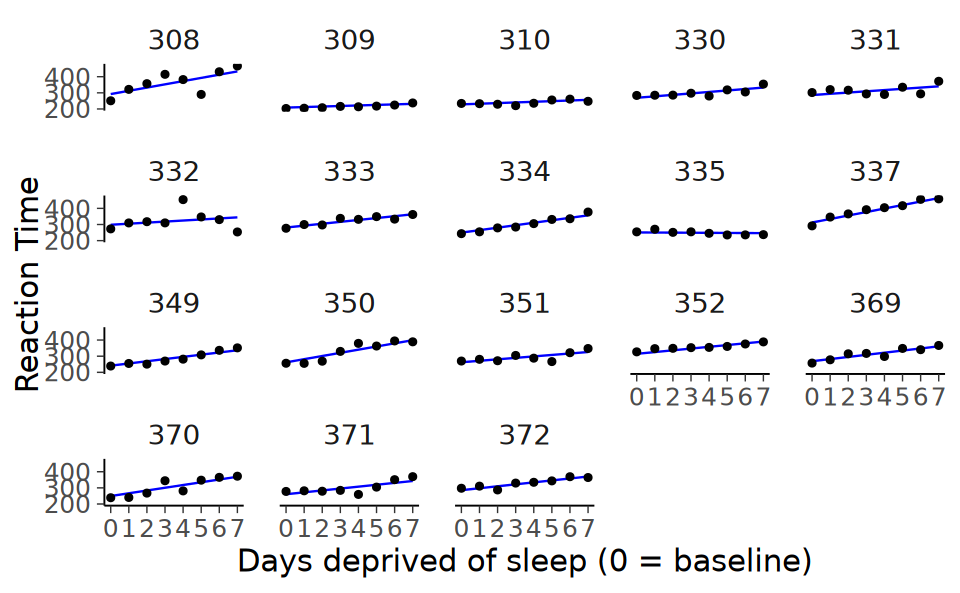
\includegraphics[width=5in,height=3.08333in]{chapters/raters/01_multilevel_files/figure-pdf/cell-27-output-1.png}

\section{\texorpdfstring{Interpretare l'output di \texttt{lmer()} ed
estrarre le
stime}{Interpretare l'output di lmer() ed estrarre le stime}}\label{interpretare-loutput-di-lmer-ed-estrarre-le-stime}

La chiamata a \texttt{lmer()} restituisce un oggetto della classe
``lmerMod''.

\subsection{Effetti fissi}\label{effetti-fissi}

La sezione dell'output chiamata ``Effetti fissi:'' è simile a ciò che si
vede nell'output per un modello lineare semplice adattato con
\texttt{lm()}.

\begin{verbatim}
Fixed effects:
              Estimate Std. Error t value
(Intercept)    267.967      8.266  32.418
days_deprived   11.435      1.845   6.197
\end{verbatim}

L'output precedente indica che il tempo di reazione medio stimato per i
partecipanti al Giorno 0 era di circa 268 millisecondi, con ogni giorno
di privazione del sonno che aggiungeva mediamente ulteriori 11
millisecondi al tempo di risposta.

Se dobbiamo ottenere gli effetti fissi dal modello, possiamo estrarli
utilizzando la funzione \texttt{fixef()}.

\begin{Shaded}
\begin{Highlighting}[]
\FunctionTok{fixef}\NormalTok{(pp\_mod) }\SpecialCharTok{|\textgreater{}} 
    \FunctionTok{print}\NormalTok{()}
\end{Highlighting}
\end{Shaded}

\begin{verbatim}
  (Intercept) days_deprived 
        268.0          11.4 
\end{verbatim}

Gli errori standard ci forniscono stime della variabilità di questi
parametri dovuta all'errore di campionamento. Possiamo utilizzarli per
calcolare i valori \(t\) o derivare gli intervalli di confidenza. Per
estrarli, utilizziamo \texttt{vcov(pp\_mod)}, che restituirà una matrice
di varianza-covarianza (non quella associata agli effetti casuali),
quindi estraiamo la diagonale utilizzando \texttt{diag()} e calcoliamo
infine la radice quadrata utilizzando \texttt{sqrt()}.

\begin{Shaded}
\begin{Highlighting}[]
\FunctionTok{vcov}\NormalTok{(pp\_mod)}
\end{Highlighting}
\end{Shaded}

\begin{verbatim}
2 x 2 Matrix of class "dpoMatrix"
              (Intercept) days_deprived
(Intercept)         68.33         -0.95
days_deprived       -0.95          3.41
\end{verbatim}

\begin{Shaded}
\begin{Highlighting}[]
\FunctionTok{vcov}\NormalTok{(pp\_mod) }\SpecialCharTok{|\textgreater{}} 
    \FunctionTok{diag}\NormalTok{() }\SpecialCharTok{|\textgreater{}} 
    \FunctionTok{sqrt}\NormalTok{() }\SpecialCharTok{|\textgreater{}} 
    \FunctionTok{print}\NormalTok{()}
\end{Highlighting}
\end{Shaded}

\begin{verbatim}
  (Intercept) days_deprived 
         8.27          1.85 
\end{verbatim}

Si noti che, nell'output di \texttt{lmer}, i valori \(t\) non sono
accompagnati dai valori \(p\), come avviene di solito nei contesti di
modellazione più semplici. Esistono molteplici approcci per ottenere i
valori \(p\) da modelli a effetti misti, ciascuno con vantaggi e
svantaggi (si veda, ad esempio, Luke (2017) per un'analisi delle opzioni
disponibili). I valori \(t\) non vengono accompagnati dai gradi di
libertà, poiché i gradi di libertà in un modello a effetti misti non
sono ben definiti. Spesso i ricercatori trattano i valori \(t\) come
valori \(z\) di Wald, ossia come osservazioni provenienti da una
distribuzione normale standard. Poiché la distribuzione \(t\) si
avvicina alla distribuzione normale standard all'aumentare del numero di
osservazioni, questa pratica ``t-as-z'' è legittima se il numero di
osservazioni campionarie è sufficientemente grande.

Per calcolare i valori \(z\) di Wald, basta dividere la stima
dell'effetto fisso per il suo errore standard:

\begin{Shaded}
\begin{Highlighting}[]
\NormalTok{tvals }\OtherTok{\textless{}{-}} \FunctionTok{fixef}\NormalTok{(pp\_mod) }\SpecialCharTok{/} \FunctionTok{sqrt}\NormalTok{(}\FunctionTok{diag}\NormalTok{(}\FunctionTok{vcov}\NormalTok{(pp\_mod)))}

\NormalTok{tvals }\SpecialCharTok{|\textgreater{}} 
    \FunctionTok{print}\NormalTok{()}
\end{Highlighting}
\end{Shaded}

\begin{verbatim}
  (Intercept) days_deprived 
         32.4           6.2 
\end{verbatim}

I valori-\(p\) si ottengono nel modo seguente:

\begin{Shaded}
\begin{Highlighting}[]
\FunctionTok{print}\NormalTok{(}\DecValTok{2} \SpecialCharTok{*}\NormalTok{ (}\DecValTok{1} \SpecialCharTok{{-}} \FunctionTok{pnorm}\NormalTok{(}\FunctionTok{abs}\NormalTok{(tvals))))}
\end{Highlighting}
\end{Shaded}

\begin{verbatim}
  (Intercept) days_deprived 
     0.00e+00      5.75e-10 
\end{verbatim}

Questo fornisce una forte evidenza contro l'ipotesi nulla
\(H_0: \gamma_1 = 0\). Sembra che la privazione del sonno aumenti
effettivamente il tempo di risposta.

È possibile ottenere gli intervalli di confidenza per le stime
utilizzando la funzione \texttt{confint()} (questa tecnica utilizza il
bootstrap parametrico).

\begin{Shaded}
\begin{Highlighting}[]
\FunctionTok{confint}\NormalTok{(pp\_mod) }\SpecialCharTok{|\textgreater{}} 
    \FunctionTok{print}\NormalTok{()}
\end{Highlighting}
\end{Shaded}

\begin{verbatim}
Computing profile confidence intervals ...
\end{verbatim}

\begin{verbatim}
                2.5 %  97.5 %
.sig01         19.098  46.337
.sig02         -0.405   0.806
.sig03          4.008  10.249
.sigma         22.467  29.349
(Intercept)   251.344 284.590
days_deprived   7.725  15.146
\end{verbatim}

\subsection{Effetti random}\label{effetti-random}

\begin{verbatim}
Random effects:
 Groups   Name          Variance Std.Dev. Corr
 Subject  (Intercept)   958.35   30.957       
          days_deprived  45.78    6.766   0.18
 Residual               651.60   25.526       
Number of obs: 144, groups:  Subject, 18
\end{verbatim}

La parte relativa agli effetti casuali dell'output di \texttt{summary()}
ci fornisce una tabella con informazioni sulle diverse componenti della
varianza: la matrice di varianza-covarianza (o matrici, se ci sono più
fattori casuali) e la varianza residua.

Cominciamo con la riga \texttt{Residual}. Questo ci indica che la
varianza residua, \(\sigma^2\), è stata stimata a circa 651.6. Il valore
nella colonna successiva, 25.526, è la deviazione standard, \(\sigma\),
che è la radice quadrata della varianza.

Estraiamo la deviazione standard dei residui utilizzando la funzione
\texttt{sigma()}.

\begin{Shaded}
\begin{Highlighting}[]
\FunctionTok{sigma}\NormalTok{(pp\_mod) }\CommentTok{\# residual}
\end{Highlighting}
\end{Shaded}

25.526404577851

Le due righe sopra la riga Residual ci forniscono informazioni sulla
matrice di varianza-covarianza per il fattore casuale ``Subject''.

\begin{verbatim}
Random effects:
 Groups   Name          Variance Std.Dev. Corr
 Subject  (Intercept)   958.35   30.957       
          days_deprived  45.78    6.766   0.18
\end{verbatim}

I valori nella colonna ``Variance'' ci forniscono la diagonale
principale della matrice, mentre i valori nella colonna ``Std.Dev.''
rappresentano semplicemente le radici quadrate di questi valori. La
colonna ``Corr'' indica la correlazione tra l'intercetta e la pendenza.

Possiamo estrarre questi valori dall'oggetto adattato \texttt{pp\_mod}
utilizzando la funzione \texttt{VarCorr()}. Questa funzione restituisce
una lista nominata, con un elemento per ciascun fattore casuale. Nel
nostro caso, ``Subject'' è l'unico fattore casuale, quindi la lista avrà
lunghezza 1.

\begin{Shaded}
\begin{Highlighting}[]
\CommentTok{\# variance{-}covariance matrix for random factor Subject}
\FunctionTok{VarCorr}\NormalTok{(pp\_mod)[[}\StringTok{"Subject"}\NormalTok{]] }\SpecialCharTok{|\textgreater{}} 
    \FunctionTok{print}\NormalTok{() }\CommentTok{\# oppure: VarCorr(pp\_mod)[[1]]}
\end{Highlighting}
\end{Shaded}

\begin{verbatim}
              (Intercept) days_deprived
(Intercept)         958.4          37.2
days_deprived        37.2          45.8
attr(,"stddev")
  (Intercept) days_deprived 
        30.96          6.77 
attr(,"correlation")
              (Intercept) days_deprived
(Intercept)         1.000         0.178
days_deprived       0.178         1.000
\end{verbatim}

Le prime righe rappresentano la matrice di varianza-covarianza. Le
varianze sono riportate sulla diagonale principale. \texttt{correlation}
indica la correlazione tra la stima della pendenza e la stima
dell'intercetta.

Possiamo estrarre gli effetti casuali stimati (BLUPS) utilizzando la
funzione \texttt{ranef()}.

\begin{Shaded}
\begin{Highlighting}[]
\FunctionTok{ranef}\NormalTok{(pp\_mod)[[}\StringTok{"Subject"}\NormalTok{]] }\SpecialCharTok{|\textgreater{}} 
    \FunctionTok{print}\NormalTok{()}
\end{Highlighting}
\end{Shaded}

\begin{verbatim}
    (Intercept) days_deprived
308      24.499         8.602
309     -59.372        -8.128
310     -39.476        -7.429
330       1.350        -2.385
331      18.458        -3.748
332      30.527        -4.894
333      13.368         0.289
334     -18.158         3.844
335     -16.974       -12.070
337      44.585        10.176
349     -26.684         2.195
350      -5.966         8.176
351      -5.571        -2.372
352      46.635        -0.562
369       0.962         1.739
370     -18.522         5.632
371      -7.343         0.273
372      17.683         0.662
\end{verbatim}

Possiamo ottenere i valori stimati dal modello utilizzando
\texttt{fitted()} e i residui utilizzando \texttt{residuals()}.

\begin{Shaded}
\begin{Highlighting}[]
\FunctionTok{mutate}\NormalTok{(sleep2,}
    \AttributeTok{fit =} \FunctionTok{fitted}\NormalTok{(pp\_mod),}
    \AttributeTok{resid =} \FunctionTok{residuals}\NormalTok{(pp\_mod)}
\NormalTok{) }\SpecialCharTok{|\textgreater{}}
    \FunctionTok{group\_by}\NormalTok{(Subject) }\SpecialCharTok{\%\textgreater{}\%}
    \FunctionTok{slice}\NormalTok{(}\FunctionTok{c}\NormalTok{(}\DecValTok{1}\NormalTok{, }\DecValTok{10}\NormalTok{)) }\SpecialCharTok{\%\textgreater{}\%}
    \FunctionTok{print}\NormalTok{(}\AttributeTok{n =} \SpecialCharTok{+}\ConstantTok{Inf}\NormalTok{)}
\end{Highlighting}
\end{Shaded}

\begin{verbatim}
# A tibble: 18 x 6
# Groups:   Subject [18]
   Reaction  Days Subject days_deprived   fit  resid
      <dbl> <dbl> <fct>           <dbl> <dbl>  <dbl>
 1     251.     2 308                 0  292. -41.7 
 2     203.     2 309                 0  209.  -5.62
 3     234.     2 310                 0  228.   5.83
 4     284.     2 330                 0  269.  14.5 
 5     302.     2 331                 0  286.  15.4 
 6     273.     2 332                 0  298. -25.5 
 7     277.     2 333                 0  281.  -4.57
 8     243.     2 334                 0  250.  -6.44
 9     254.     2 335                 0  251.   3.50
10     292.     2 337                 0  313. -20.9 
11     239.     2 349                 0  241.  -2.36
12     256.     2 350                 0  262.  -5.80
13     270.     2 351                 0  262.   7.50
14     327.     2 352                 0  315.  12.3 
15     257.     2 369                 0  269. -11.7 
16     239.     2 370                 0  249. -10.5 
17     278.     2 371                 0  261.  17.3 
18     298.     2 372                 0  286.  11.9 
\end{verbatim}

Infine, possiamo ottenere previsioni per nuovi dati utilizzando
\texttt{predict()}, come abbiamo fatto in precedenza.

\begin{Shaded}
\begin{Highlighting}[]
\DocumentationTok{\#\# create the table with new predictor values}
\NormalTok{ndat }\OtherTok{\textless{}{-}} \FunctionTok{crossing}\NormalTok{(}
    \AttributeTok{Subject =}\NormalTok{ sleep2 }\SpecialCharTok{\%\textgreater{}\%} \FunctionTok{pull}\NormalTok{(Subject) }\SpecialCharTok{\%\textgreater{}\%} \FunctionTok{levels}\NormalTok{() }\SpecialCharTok{\%\textgreater{}\%} \FunctionTok{factor}\NormalTok{(),}
    \AttributeTok{days\_deprived =} \DecValTok{8}\SpecialCharTok{:}\DecValTok{10}
\NormalTok{) }\SpecialCharTok{\%\textgreater{}\%}
    \FunctionTok{mutate}\NormalTok{(}\AttributeTok{Reaction =} \FunctionTok{predict}\NormalTok{(pp\_mod, }\AttributeTok{newdata =}\NormalTok{ .))}

\NormalTok{ndat }\SpecialCharTok{|\textgreater{}} 
    \FunctionTok{head}\NormalTok{()}
\end{Highlighting}
\end{Shaded}

A tibble: 6 x 3

\begin{longtable}[]{@{}
  >{\raggedright\arraybackslash}p{(\columnwidth - 4\tabcolsep) * \real{0.3333}}
  >{\raggedright\arraybackslash}p{(\columnwidth - 4\tabcolsep) * \real{0.3333}}
  >{\raggedright\arraybackslash}p{(\columnwidth - 4\tabcolsep) * \real{0.3333}}@{}}
\toprule\noalign{}
\begin{minipage}[b]{\linewidth}\raggedright
Subject \textless fct\textgreater{}
\end{minipage} & \begin{minipage}[b]{\linewidth}\raggedright
days\_deprived \textless int\textgreater{}
\end{minipage} & \begin{minipage}[b]{\linewidth}\raggedright
Reaction \textless dbl\textgreater{}
\end{minipage} \\
\midrule\noalign{}
\endhead
\bottomrule\noalign{}
\endlastfoot
308 & 8 & 453 \\
308 & 9 & 473 \\
308 & 10 & 493 \\
309 & 8 & 235 \\
309 & 9 & 238 \\
309 & 10 & 242 \\
\end{longtable}

\begin{Shaded}
\begin{Highlighting}[]
\FunctionTok{ggplot}\NormalTok{(sleep2, }\FunctionTok{aes}\NormalTok{(}\AttributeTok{x =}\NormalTok{ days\_deprived, }\AttributeTok{y =}\NormalTok{ Reaction)) }\SpecialCharTok{+}
    \FunctionTok{geom\_line}\NormalTok{(}
        \AttributeTok{data =} \FunctionTok{bind\_rows}\NormalTok{(newdata2, ndat),}
        \AttributeTok{color =} \StringTok{"blue"}
\NormalTok{    ) }\SpecialCharTok{+}
    \FunctionTok{geom\_point}\NormalTok{() }\SpecialCharTok{+}
    \FunctionTok{scale\_x\_continuous}\NormalTok{(}\AttributeTok{breaks =} \DecValTok{0}\SpecialCharTok{:}\DecValTok{10}\NormalTok{) }\SpecialCharTok{+}
    \FunctionTok{facet\_wrap}\NormalTok{(}\SpecialCharTok{\textasciitilde{}}\NormalTok{Subject) }\SpecialCharTok{+}
    \FunctionTok{labs}\NormalTok{(}\AttributeTok{y =} \StringTok{"Reaction Time"}\NormalTok{, }\AttributeTok{x =} \StringTok{"Days deprived of sleep (0 = baseline)"}\NormalTok{)}
\end{Highlighting}
\end{Shaded}

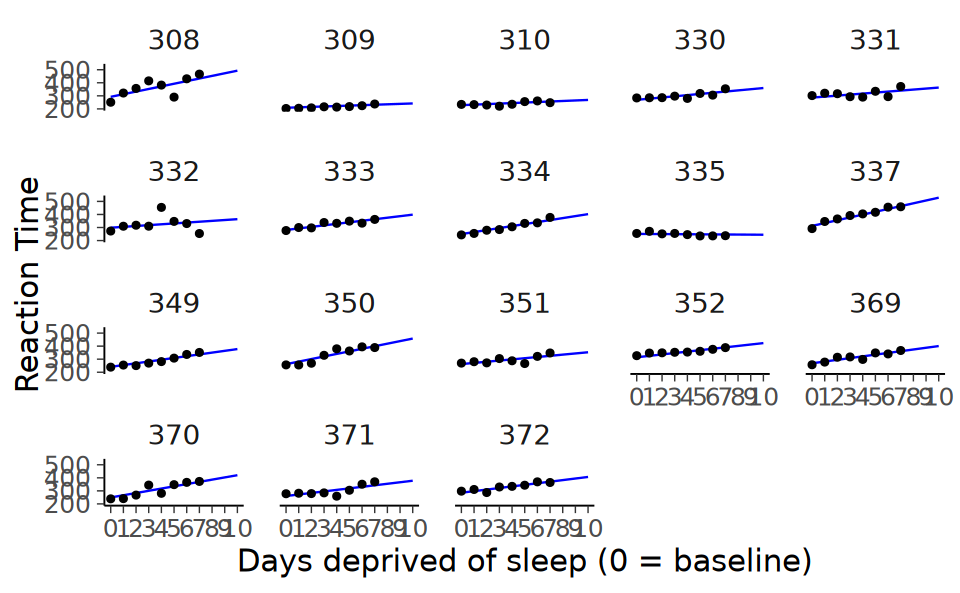
\includegraphics[width=5in,height=3.08333in]{chapters/raters/01_multilevel_files/figure-pdf/cell-39-output-1.png}

\section{Riflessioni Conclusive}\label{riflessioni-conclusive-3}

Questo capitolo ha presentato una panoramica sui modelli statistici
multilivello, con un focus sull'effetto della deprivazione del sonno
sulle prestazioni psicomotorie utilizzando il dataset
\texttt{sleepstudy}. In tale contesto, sono stati introdotti e discussi
concetti fondamentali come il ``complete pooling'', il ``no pooling'' e
il ``partial pooling'', esplorandone le implicazioni nella modellazione
dei dati con misure ripetute.

L'analisi ha posto l'accento sull'applicazione pratica dei modelli
multilivello, con una particolare attenzione alla distinzione tra
variabili fisse e casuali e alla loro rilevanza per la struttura del
modello. Un aspetto centrale della trattazione è stata la matrice di
varianza-covarianza, essenziale per comprendere le relazioni interne ai
modelli multilivello.

Questi modelli rivestono un ruolo cruciale nel campo dell'assessment
psicologico e della psicometria, poiché permettono di analizzare dati
complessi tenendo conto delle variazioni individuali e di gruppo.
Offrono strumenti flessibili per esaminare come fattori contestuali e
individuali influenzino il comportamento e le prestazioni psicologiche,
un elemento chiave per una valutazione psicologica accurata.

Infine, il capitolo prepara il terreno per il successivo approfondimento
sui modelli multilivello nell'ambito del calcolo dell'affidabilità tra
giudici, argomento che sarà sviluppato nel capitolo seguente. Inoltre,
viene tracciato un collegamento con i modelli di crescita latente, i
quali saranno trattati nei capitoli successivi come naturale
prosecuzione o alternativa ai modelli multilivello. Questo sottolinea la
continuità e la rilevanza di tali approcci nell'ambito della ricerca
psicologica e psicometrica.

\section{Session Info}\label{session-info-8}

\begin{Shaded}
\begin{Highlighting}[]
\FunctionTok{sessionInfo}\NormalTok{()}
\end{Highlighting}
\end{Shaded}

\begin{verbatim}
R version 4.4.2 (2024-10-31)
Platform: aarch64-apple-darwin20
Running under: macOS Sequoia 15.1

Matrix products: default
BLAS:   /Library/Frameworks/R.framework/Versions/4.4-arm64/Resources/lib/libRblas.0.dylib 
LAPACK: /Library/Frameworks/R.framework/Versions/4.4-arm64/Resources/lib/libRlapack.dylib;  LAPACK version 3.12.0

locale:
[1] C

time zone: Europe/Rome
tzcode source: internal

attached base packages:
[1] stats     graphics  grDevices utils     datasets  methods   base     

other attached packages:
 [1] kableExtra_1.4.0  repr_1.1.7        lme4_1.1-35.5     Matrix_1.7-1     
 [5] car_3.1-3         carData_3.0-5     MASS_7.3-61       viridis_0.6.5    
 [9] viridisLite_0.4.2 ggpubr_0.6.0      ggExtra_0.10.1    gridExtra_2.3    
[13] patchwork_1.3.0   bayesplot_1.11.1  semTools_0.5-6    semPlot_1.1.6    
[17] lavaan_0.6-19     psych_2.4.6.26    scales_1.3.0      markdown_1.13    
[21] knitr_1.49        lubridate_1.9.3   forcats_1.0.0     stringr_1.5.1    
[25] dplyr_1.1.4       purrr_1.0.2       readr_2.1.5       tidyr_1.3.1      
[29] tibble_3.2.1      ggplot2_3.5.1     tidyverse_2.0.0   here_1.0.1       

loaded via a namespace (and not attached):
  [1] rstudioapi_0.17.1   jsonlite_1.8.9      magrittr_2.0.3     
  [4] TH.data_1.1-2       estimability_1.5.1  farver_2.1.2       
  [7] nloptr_2.1.1        rmarkdown_2.29      vctrs_0.6.5        
 [10] Cairo_1.6-2         minqa_1.2.8         base64enc_0.1-3    
 [13] rstatix_0.7.2       htmltools_0.5.8.1   broom_1.0.7        
 [16] Formula_1.2-5       htmlwidgets_1.6.4   plyr_1.8.9         
 [19] sandwich_3.1-1      emmeans_1.10.5      zoo_1.8-12         
 [22] uuid_1.2-1          igraph_2.1.1        mime_0.12          
 [25] lifecycle_1.0.4     pkgconfig_2.0.3     R6_2.5.1           
 [28] fastmap_1.2.0       shiny_1.9.1         digest_0.6.37      
 [31] OpenMx_2.21.13      fdrtool_1.2.18      colorspace_2.1-1   
 [34] rprojroot_2.0.4     Hmisc_5.2-0         labeling_0.4.3     
 [37] fansi_1.0.6         timechange_0.3.0    abind_1.4-8        
 [40] compiler_4.4.2      withr_3.0.2         glasso_1.11        
 [43] htmlTable_2.4.3     backports_1.5.0     ggsignif_0.6.4     
 [46] corpcor_1.6.10      gtools_3.9.5        tools_4.4.2        
 [49] pbivnorm_0.6.0      foreign_0.8-87      zip_2.3.1          
 [52] httpuv_1.6.15       nnet_7.3-19         glue_1.8.0         
 [55] quadprog_1.5-8      promises_1.3.0      nlme_3.1-166       
 [58] lisrelToR_0.3       grid_4.4.2          pbdZMQ_0.3-13      
 [61] checkmate_2.3.2     cluster_2.1.6       reshape2_1.4.4     
 [64] generics_0.1.3      gtable_0.3.6        tzdb_0.4.0         
 [67] data.table_1.16.2   hms_1.1.3           xml2_1.3.6         
 [70] utf8_1.2.4          sem_3.1-16          pillar_1.9.0       
 [73] IRdisplay_1.1       rockchalk_1.8.157   later_1.3.2        
 [76] splines_4.4.2       cherryblossom_0.1.0 lattice_0.22-6     
 [79] survival_3.7-0      kutils_1.73         tidyselect_1.2.1   
 [82] miniUI_0.1.1.1      pbapply_1.7-2       svglite_2.1.3      
 [85] airports_0.1.0      stats4_4.4.2        xfun_0.49          
 [88] qgraph_1.9.8        arm_1.14-4          stringi_1.8.4      
 [91] pacman_0.5.1        boot_1.3-31         evaluate_1.0.1     
 [94] codetools_0.2-20    mi_1.1              cli_3.6.3          
 [97] RcppParallel_5.1.9  IRkernel_1.3.2      rpart_4.1.23       
[100] systemfonts_1.1.0   xtable_1.8-4        munsell_0.5.1      
[103] Rcpp_1.0.13-1       coda_0.19-4.1       png_0.1-8          
[106] XML_3.99-0.17       parallel_4.4.2      usdata_0.3.1       
[109] jpeg_0.1-10         mvtnorm_1.3-2       openxlsx_4.2.7.1   
[112] crayon_1.5.3        openintro_2.5.0     rlang_1.1.4        
[115] multcomp_1.4-26     mnormt_2.1.1       
\end{verbatim}

\chapter{L'affidabilità tra giudici}\label{sec-interrater-reliability}

\begin{chapterintro}
L'affidabilità tra valutatori è cruciale in molti ambiti della
psicologia, soprattutto quando un test si basa su giudizi soggettivi. In
questi casi, è importante misurare il grado di concordanza tra diversi
valutatori che assegnano i punteggi, un aspetto noto come affidabilità
inter-valutatore (o inter-rater reliability in inglese). Questa forma di
affidabilità valuta la coerenza delle valutazioni tra due o più giudici
che osservano lo stesso fenomeno o campione. Una buona affidabilità
inter-valutatore indica un alto livello di concordanza nei risultati
ottenuti da diversi valutatori, suggerendo che le misurazioni o i
giudizi emessi siano simili anche quando espressi da persone diverse, a
parità di condizioni.

\end{chapterintro}

\textbf{Prerequisiti}

\textbf{Concetti e Competenze Chiave}

\textbf{Preparazione del Notebook}

\begin{Shaded}
\begin{Highlighting}[]
\NormalTok{here}\SpecialCharTok{::}\FunctionTok{here}\NormalTok{(}\StringTok{"code"}\NormalTok{, }\StringTok{"\_common.R"}\NormalTok{) }\SpecialCharTok{|\textgreater{}}
    \FunctionTok{source}\NormalTok{()}

\CommentTok{\# Load packages}
\ControlFlowTok{if}\NormalTok{ (}\SpecialCharTok{!}\FunctionTok{requireNamespace}\NormalTok{(}\StringTok{"pacman"}\NormalTok{)) }\FunctionTok{install.packages}\NormalTok{(}\StringTok{"pacman"}\NormalTok{)}
\NormalTok{pacman}\SpecialCharTok{::}\FunctionTok{p\_load}\NormalTok{(lme4)}
\end{Highlighting}
\end{Shaded}

\section{Introduzione}\label{introduzione-8}

L'affidabilità inter-valutatore si misura analizzando la coerenza tra i
punteggi o le valutazioni fornite da diversi osservatori. Una forte
affidabilità inter-valutatore indica che il test o strumento di
valutazione genera risultati consistenti e riproducibili,
indipendentemente da chi esegue la valutazione. Questo aspetto è
fondamentale per assicurare che le conclusioni tratte dai risultati del
test siano solide e affidabili.

Consideriamo, ad esempio, una diagnosi psicologica: se diversi psicologi
valutano i sintomi di un paziente, è essenziale che le loro valutazioni
siano coerenti per garantire una diagnosi accurata. Nella valutazione
dei disturbi dell'umore, ad esempio, gli psicologi devono arrivare a
conclusioni simili basandosi sui sintomi osservabili e sulle risposte
del paziente a questionari standardizzati. Un altro esempio riguarda la
ricerca sull'efficacia di una nuova terapia per l'ansia, in cui diversi
terapeuti valutano i livelli di ansia dei partecipanti prima e dopo il
trattamento. In questo caso, l'affidabilità tra le valutazioni dei
terapeuti è cruciale per confermare l'efficacia della terapia.

Questo capitolo approfondisce l'affidabilità inter-valutatore in due
contesti distinti: nel caso di due giudici e nel caso di giudici
multipli. Nel primo scenario, esamineremo l'accordo nominale e il Kappa
di Cohen; nel secondo, esploreremo l'uso dell'ICC (Coefficienti di
Correlazione Intraclasse), dell'ANOVA a una via e dell'ANOVA a due vie.
In quest'ultimo contesto, i modelli a effetti misti sono particolarmente
utili per gestire disegni con più giudici, permettendo di catturare sia
le variazioni tra giudici sia quelle tra partecipanti, e fornendo una
valutazione completa dell'affidabilità delle misurazioni.

\section{Un Esempio Concreto}\label{un-esempio-concreto-1}

In questo studio, i giudici valutano la ``Percentuale di Intelligibilità
del Discorso'' di persone affette da disartria. Questa misura soggettiva
descrive la percentuale di discorso compreso durante una conversazione
con un parlante che soffre di disartria, una condizione che influisce
sulla chiarezza e sull'intelligibilità della parola. I giudici ascoltano
e valutano le registrazioni vocali dei partecipanti affetti da disartria
e stimano la percentuale di parole o frasi che sono in grado di
comprendere chiaramente. Questa valutazione fornisce una misura
importante dell'impatto della disartria sulla comunicazione verbale
quotidiana.

\begin{data}
Nella discussione seguente useremo i dati dello studio
\href{https://www.mdpi.com/2076-3425/12/8/1011/}{The Reliability and
Validity of Speech-Language Pathologists' Estimations of Intelligibility
in Dysarthria} di Hirsch et al. (2022).

\end{data}

\begin{Shaded}
\begin{Highlighting}[]
\NormalTok{slp\_dat }\OtherTok{\textless{}{-}} \FunctionTok{read.csv}\NormalTok{(}\StringTok{"https://osf.io/download/p9gqk/"}\NormalTok{)}
\NormalTok{slp\_vas\_wide }\OtherTok{\textless{}{-}}\NormalTok{ slp\_dat }\SpecialCharTok{|\textgreater{}}
    \FunctionTok{select}\NormalTok{(slpID, Speaker, slp\_VAS) }\SpecialCharTok{|\textgreater{}}
    \FunctionTok{pivot\_wider}\NormalTok{(}\AttributeTok{names\_from =}\NormalTok{ slpID, }\AttributeTok{values\_from =}\NormalTok{ slp\_VAS)}
\FunctionTok{head}\NormalTok{(slp\_vas\_wide)}
\end{Highlighting}
\end{Shaded}

A tibble: 6 x 22

\begin{longtable}[]{@{}
  >{\raggedright\arraybackslash}p{(\columnwidth - 40\tabcolsep) * \real{0.0476}}
  >{\raggedright\arraybackslash}p{(\columnwidth - 40\tabcolsep) * \real{0.0476}}
  >{\raggedright\arraybackslash}p{(\columnwidth - 40\tabcolsep) * \real{0.0476}}
  >{\raggedright\arraybackslash}p{(\columnwidth - 40\tabcolsep) * \real{0.0476}}
  >{\raggedright\arraybackslash}p{(\columnwidth - 40\tabcolsep) * \real{0.0476}}
  >{\raggedright\arraybackslash}p{(\columnwidth - 40\tabcolsep) * \real{0.0476}}
  >{\raggedright\arraybackslash}p{(\columnwidth - 40\tabcolsep) * \real{0.0476}}
  >{\raggedright\arraybackslash}p{(\columnwidth - 40\tabcolsep) * \real{0.0476}}
  >{\raggedright\arraybackslash}p{(\columnwidth - 40\tabcolsep) * \real{0.0476}}
  >{\raggedright\arraybackslash}p{(\columnwidth - 40\tabcolsep) * \real{0.0476}}
  >{\raggedright\arraybackslash}p{(\columnwidth - 40\tabcolsep) * \real{0.0476}}
  >{\raggedright\arraybackslash}p{(\columnwidth - 40\tabcolsep) * \real{0.0476}}
  >{\raggedright\arraybackslash}p{(\columnwidth - 40\tabcolsep) * \real{0.0476}}
  >{\raggedright\arraybackslash}p{(\columnwidth - 40\tabcolsep) * \real{0.0476}}
  >{\raggedright\arraybackslash}p{(\columnwidth - 40\tabcolsep) * \real{0.0476}}
  >{\raggedright\arraybackslash}p{(\columnwidth - 40\tabcolsep) * \real{0.0476}}
  >{\raggedright\arraybackslash}p{(\columnwidth - 40\tabcolsep) * \real{0.0476}}
  >{\raggedright\arraybackslash}p{(\columnwidth - 40\tabcolsep) * \real{0.0476}}
  >{\raggedright\arraybackslash}p{(\columnwidth - 40\tabcolsep) * \real{0.0476}}
  >{\raggedright\arraybackslash}p{(\columnwidth - 40\tabcolsep) * \real{0.0476}}
  >{\raggedright\arraybackslash}p{(\columnwidth - 40\tabcolsep) * \real{0.0476}}@{}}
\toprule\noalign{}
\begin{minipage}[b]{\linewidth}\raggedright
Speaker \textless chr\textgreater{}
\end{minipage} & \begin{minipage}[b]{\linewidth}\raggedright
slp10 \textless dbl\textgreater{}
\end{minipage} & \begin{minipage}[b]{\linewidth}\raggedright
slp11 \textless dbl\textgreater{}
\end{minipage} & \begin{minipage}[b]{\linewidth}\raggedright
slp13 \textless dbl\textgreater{}
\end{minipage} & \begin{minipage}[b]{\linewidth}\raggedright
slp14 \textless dbl\textgreater{}
\end{minipage} & \begin{minipage}[b]{\linewidth}\raggedright
slp15 \textless dbl\textgreater{}
\end{minipage} & \begin{minipage}[b]{\linewidth}\raggedright
slp16 \textless dbl\textgreater{}
\end{minipage} & \begin{minipage}[b]{\linewidth}\raggedright
slp17 \textless dbl\textgreater{}
\end{minipage} & \begin{minipage}[b]{\linewidth}\raggedright
slp18 \textless dbl\textgreater{}
\end{minipage} & \begin{minipage}[b]{\linewidth}\raggedright
slp19 \textless dbl\textgreater{}
\end{minipage} & \begin{minipage}[b]{\linewidth}\raggedright
\ldots{} \ldots{}
\end{minipage} & \begin{minipage}[b]{\linewidth}\raggedright
slp21 \textless dbl\textgreater{}
\end{minipage} & \begin{minipage}[b]{\linewidth}\raggedright
slp22 \textless dbl\textgreater{}
\end{minipage} & \begin{minipage}[b]{\linewidth}\raggedright
slp23 \textless dbl\textgreater{}
\end{minipage} & \begin{minipage}[b]{\linewidth}\raggedright
slp25 \textless dbl\textgreater{}
\end{minipage} & \begin{minipage}[b]{\linewidth}\raggedright
slp3 \textless dbl\textgreater{}
\end{minipage} & \begin{minipage}[b]{\linewidth}\raggedright
slp4 \textless dbl\textgreater{}
\end{minipage} & \begin{minipage}[b]{\linewidth}\raggedright
slp5 \textless dbl\textgreater{}
\end{minipage} & \begin{minipage}[b]{\linewidth}\raggedright
slp6 \textless dbl\textgreater{}
\end{minipage} & \begin{minipage}[b]{\linewidth}\raggedright
slp8 \textless dbl\textgreater{}
\end{minipage} & \begin{minipage}[b]{\linewidth}\raggedright
slp9 \textless dbl\textgreater{}
\end{minipage} \\
\midrule\noalign{}
\endhead
\bottomrule\noalign{}
\endlastfoot
AF1 & 96.28 & 100.00 & 96.56 & 99.30 & 100.00 & 12.58 & 100.00 & 88.16 &
52.58 & \ldots{} & 77.42 & 73.64 & 100.00 & 100.00 & 37.82 & 73.24 &
55.01 & 100.00 & 53.94 & 85.07 \\
AF9 & 12.32 & 34.68 & 0.86 & 3.52 & 12.58 & 0.00 & 6.69 & 0.00 & 7.42 &
\ldots{} & 13.55 & 0.00 & 0.00 & 2.90 & 0.00 & 14.51 & 1.72 & NA & 6.76
& 10.28 \\
ALSF6 & NA & 30.84 & 5.73 & 73.94 & 73.87 & 4.52 & 45.13 & 41.92 & 26.13
& \ldots{} & 25.81 & 8.31 & 18.46 & 86.77 & 0.00 & 26.20 & 3.72 & NA &
9.86 & 37.75 \\
ALSF7 & 93.98 & 96.31 & 61.32 & 64.37 & 100.00 & 7.74 & 69.92 & 88.16 &
37.42 & \ldots{} & 59.35 & 34.10 & 90.63 & 53.23 & 99.71 & 63.10 & 56.73
& 88.83 & 64.93 & 53.80 \\
ALSF9 & 29.51 & 52.20 & 43.55 & 46.76 & 60.65 & 23.87 & 25.21 & 91.64 &
37.10 & \ldots{} & 57.74 & 29.51 & 50.14 & 64.84 & 0.00 & 31.13 & 40.11
& 16.91 & 5.92 & 50.00 \\
ALSM1 & 96.28 & NA & 29.23 & 69.44 & 99.35 & 82.26 & 70.19 & 79.72 &
78.39 & \ldots{} & 83.87 & 84.24 & 92.29 & 100.00 & 100.00 & 18.03 &
58.74 & 66.48 & 51.83 & 60.28 \\
\end{longtable}

\section{Due giudici}\label{due-giudici}

In questa sezione, analizziamo come calcolare l'accordo nominale e
l'indice di concordanza Kappa di Cohen nel caso di due giudici.

Selezioniamo due giudici.

\begin{Shaded}
\begin{Highlighting}[]
\NormalTok{slp\_2rater }\OtherTok{\textless{}{-}}\NormalTok{ slp\_vas\_wide }\SpecialCharTok{|\textgreater{}}
    \FunctionTok{select}\NormalTok{(slp14, slp15)}
\FunctionTok{head}\NormalTok{(slp\_2rater)}
\end{Highlighting}
\end{Shaded}

A tibble: 6 x 2

\begin{longtable}[]{@{}ll@{}}
\toprule\noalign{}
slp14 \textless dbl\textgreater{} & slp15 \textless dbl\textgreater{} \\
\midrule\noalign{}
\endhead
\bottomrule\noalign{}
\endlastfoot
99.30 & 100.00 \\
3.52 & 12.58 \\
73.94 & 73.87 \\
64.37 & 100.00 \\
46.76 & 60.65 \\
69.44 & 99.35 \\
\end{longtable}

\subsection{Accordo nominale}\label{accordo-nominale}

L'accordo nominale misura la percentuale di perfetta corrispondenza tra
le valutazioni fornite dai due giudici. In altre parole, questo metodo
rileva quanto spesso i giudici assegnano esattamente lo stesso punteggio
per ciascun caso osservato. Ad esempio, se i giudici forniscono
valutazioni identiche per il 40\% dei casi, l'accordo nominale sarà pari
a 0.4.

Utilizzando questa definizione, si ottiene:

\begin{Shaded}
\begin{Highlighting}[]
\FunctionTok{with}\NormalTok{(slp\_2rater, }\FunctionTok{mean}\NormalTok{(slp14 }\SpecialCharTok{==}\NormalTok{ slp15))}
\end{Highlighting}
\end{Shaded}

0.1

\hfill\break
Per rendere il criterio di concordanza più flessibile, si può applicare
un arrotondamento ai punteggi: dividendo ciascun punteggio per 10 e
arrotondando al numero intero più vicino, anche valori leggermente
diversi possono essere considerati concordanti. Ad esempio, valutazioni
come 75 e 78, dopo essere state divise per 10 e arrotondate, diventano
entrambe 8. Questo metodo amplia il criterio di accordo, riconoscendo
che piccole discrepanze potrebbero essere irrilevanti nella pratica.

\begin{Shaded}
\begin{Highlighting}[]
\NormalTok{slp\_2round }\OtherTok{\textless{}{-}} \FunctionTok{round}\NormalTok{(slp\_2rater }\SpecialCharTok{/} \DecValTok{10}\NormalTok{)}
\NormalTok{slp\_2round }\SpecialCharTok{|\textgreater{}} \FunctionTok{print}\NormalTok{()}
\end{Highlighting}
\end{Shaded}

\begin{verbatim}
   slp14 slp15
1     10    10
2      0     1
3      7     7
4      6    10
5      5     6
6      7    10
7      8     9
8      8     9
9      9     8
10    10    10
11    10     7
12    10    10
13     6     5
14    10    10
15     6    10
16    10    10
17    10    10
18     9    10
19     9    10
20    10    10
\end{verbatim}

\begin{Shaded}
\begin{Highlighting}[]
\NormalTok{slp\_2round }\OtherTok{\textless{}{-}} \FunctionTok{lapply}\NormalTok{(slp\_2round, }\AttributeTok{FUN =}\NormalTok{ factor, }\AttributeTok{levels =} \DecValTok{0}\SpecialCharTok{:}\DecValTok{10}\NormalTok{)}
\CommentTok{\# Contingency table}
\FunctionTok{table}\NormalTok{(slp\_2round)}
\end{Highlighting}
\end{Shaded}

\begin{verbatim}
     slp15
slp14 0 1 2 3 4 5 6 7 8 9 10
   0  0 1 0 0 0 0 0 0 0 0  0
   1  0 0 0 0 0 0 0 0 0 0  0
   2  0 0 0 0 0 0 0 0 0 0  0
   3  0 0 0 0 0 0 0 0 0 0  0
   4  0 0 0 0 0 0 0 0 0 0  0
   5  0 0 0 0 0 0 1 0 0 0  0
   6  0 0 0 0 0 1 0 0 0 0  2
   7  0 0 0 0 0 0 0 1 0 0  1
   8  0 0 0 0 0 0 0 0 0 2  0
   9  0 0 0 0 0 0 0 0 1 0  2
   10 0 0 0 0 0 0 0 1 0 0  7
\end{verbatim}

\hfill\break
Il codice precedente fa uso di due funzioni principali:
\texttt{lapply()} e \texttt{table()}. Esso opera su una lista o su un
dataframe chiamato \texttt{slp\_2round}, applicando una trasformazione
ai dati e successivamente creando una tabella di contingenza.

\begin{enumerate}
\def\labelenumi{\arabic{enumi}.}
\tightlist
\item
  \texttt{slp\_2round\ \textless{}-\ lapply(slp\_2round,\ FUN\ =\ factor,\ levels\ =\ 0:10)}
\end{enumerate}

\begin{itemize}
\item
  \texttt{lapply()}: questa funzione appartiene alla famiglia delle
  funzioni ``*apply'' in R, che sono utilizzate per applicare una
  funzione a ciascun elemento di una lista o di un vettore.
  \texttt{lapply()} restituisce sempre una lista come risultato,
  mantenendo la lunghezza dell'input originale.
\item
  \texttt{slp\_2round}: è la lista o il dataframe su cui si sta
  operando. Il codice modifica questa variabile, sostituendola con il
  risultato dell'applicazione di \texttt{lapply()}.
\item
  \texttt{FUN\ =\ factor}: specifica che la funzione da applicare a
  ciascun elemento di \texttt{slp\_2round} è \texttt{factor()}. La
  funzione \texttt{factor()} è utilizzata per codificare un vettore come
  un fattore, che è utile in R per rappresentare dati categorici.
\item
  \texttt{levels\ =\ 0:10}: indica i livelli del fattore, che in questo
  caso sono i numeri da 0 a 10. Questo parametro assicura che i fattori
  creati abbiano esattamente questi livelli, anche se alcuni di essi non
  appaiono nei dati. Questo è particolarmente utile per garantire la
  coerenza dei livelli dei fattori attraverso vari elementi di
  \texttt{slp\_2round}, soprattutto se si intende confrontarli o
  combinarli in seguito.
\end{itemize}

\begin{enumerate}
\def\labelenumi{\arabic{enumi}.}
\setcounter{enumi}{1}
\tightlist
\item
  \texttt{table(slp\_2round)}
\end{enumerate}

\begin{itemize}
\tightlist
\item
  \texttt{table()}: questa funzione crea una tabella di contingenza dai
  dati forniti. Una tabella di contingenza è un tipo di tabella in
  formato matriciale che conta la frequenza di combinazioni specifiche
  di valori all'interno di una o più variabili categoriche.
\end{itemize}

Dopo l'applicazione di \texttt{lapply()}, \texttt{slp\_2round} diventa
una lista di elementi, ciascuno dei quali è un fattore con livelli da 0
a 10. Quando si passa questa lista modificata alla funzione
\texttt{table()}, viene generata una tabella di contingenza. Questa
tabella riassume le frequenze dei vari livelli dei fattori attraverso
gli elementi della lista \texttt{slp\_2round}.

\begin{Shaded}
\begin{Highlighting}[]
\NormalTok{p0 }\OtherTok{\textless{}{-}} \FunctionTok{with}\NormalTok{(slp\_2round, }\FunctionTok{mean}\NormalTok{(slp14 }\SpecialCharTok{==}\NormalTok{ slp15))}
\NormalTok{p0}
\end{Highlighting}
\end{Shaded}

0.4

\hfill\break
Qui, l'arrotondamento serve a ridurre la specificità delle valutazioni,
permettendo un confronto più più flessibile tra le valutazioni dei due
giudici\hspace{0pt}\hspace{0pt}. Questo approccio riflette una visione
più tollerante dell'accordo, riconoscendo che piccole discrepanze nelle
valutazioni potrebbero non essere rilevanti in un contesto pratico.

Nel contesto specifico descritto, l'arrotondamento implica dividere le
valutazioni per 10 e poi arrotondarle al numero intero più vicino.
Questo processo rende i valori leggermente diversi equivalenti. Ad
esempio, se un giudice assegna una valutazione di 75 e l'altro assegna
78, dividendo per 10 otteniamo 7.5 e 7.8; arrotondando, entrambi i
valori diventano 8. Così, valutazioni originalmente diverse vengono
arrotondate allo stesso numero intero, permettendo un accordo più ampio
tra i giudici. Questo metodo riconosce l'accordo anche in presenza di
piccole variazioni nelle valutazioni, riflettendo una visione più
flessibile dell'accordo tra i giudici.

\subsection{Kappa di Cohen}\label{kappa-di-cohen}

L'indice di concordanza Kappa di Cohen è una misura più robusta
dell'accordo tra i giudici, poiché tiene conto della concordanza
casuale. A differenza dell'accordo nominale, che considera solo la
frequenza delle concordanze perfette, Kappa di Cohen corregge per
l'accordo che potrebbe verificarsi per puro caso.

Kappa è definito dalla formula:

\[
\kappa = \frac{p_o - p_c}{1 - p_c},
\]

dove:

\begin{itemize}
\tightlist
\item
  \(p_o\) è la proporzione di accordo osservato, ossia la frazione di
  volte in cui i giudici concordano effettivamente nelle loro
  valutazioni,
\item
  \(p_c\) è la proporzione di accordo attesa per caso, calcolata
  assumendo che le valutazioni siano indipendenti.
\end{itemize}

\(p_o\) si calcola nel modo seguente:

\[
p_o = \frac{{\text{Numero di accordi osservati}}}{{\text{Numero totale di confronti}}}
\]

In altre parole, \(p_o\) è il rapporto tra il numero di volte in cui gli
osservatori sono concordi (hanno dato la stessa valutazione) e il numero
totale di confronti effettuati.

\(p_c\) è l'indice di concordanza attesa per caso:

\[
p_c = \frac{{\sum (\text{Riga i-esima del totale}) \times (\text{Colonna i-esima del totale})}}{{\text{Numero totale di confronti}}^2} 
\]

In altre parole, \(p_c\) è il rapporto atteso di concordanza tra gli
osservatori nel caso in cui le loro valutazioni siano indipendenti.

Un valore di Kappa vicino a 1 indica un'alta concordanza corretta per
l'accordo casuale, mentre un valore vicino a 0 suggerisce che l'accordo
non è superiore a quello casuale. Un valore negativo indica una
concordanza peggiore di quella casuale.

Ad esempio, calcolando il Kappa per due giudici che valutano lo stesso
campione, possiamo ottenere una misura di concordanza che tiene conto
della probabilità di accordo fortuito.

\begin{Shaded}
\begin{Highlighting}[]
\NormalTok{slp\_2tab }\OtherTok{\textless{}{-}} \FunctionTok{table}\NormalTok{(slp\_2round)}
\NormalTok{pc }\OtherTok{\textless{}{-}} \FunctionTok{sum}\NormalTok{(}\FunctionTok{colSums}\NormalTok{(slp\_2tab) }\SpecialCharTok{*} \FunctionTok{rowSums}\NormalTok{(slp\_2tab)) }\SpecialCharTok{/} \FunctionTok{sum}\NormalTok{(slp\_2tab)}\SpecialCharTok{\^{}}\DecValTok{2}
\NormalTok{(kappa }\OtherTok{\textless{}{-}}\NormalTok{ (p0 }\SpecialCharTok{{-}}\NormalTok{ pc) }\SpecialCharTok{/}\NormalTok{ (}\DecValTok{1} \SpecialCharTok{{-}}\NormalTok{ pc))}
\end{Highlighting}
\end{Shaded}

0.166666666666667

\hfill\break
Tuttavia, Kappa può risultare basso quando i giudizi si concentrano su
una o poche categorie, creando una distribuzione non uniforme, come
nell'esempio fornito.

\section{Giudici multipli}\label{giudici-multipli}

\subsection{\texorpdfstring{Coefficiente
\(\alpha\)}{Coefficiente \textbackslash alpha}}\label{coefficiente-alpha}

Il coefficiente \(\alpha\) di Cronbach è comunemente utilizzato per
misurare l'affidabilità interna di un test, cioè la coerenza con cui gli
item all'interno del test misurano un costrutto comune. Tuttavia, può
essere utilizzato anche per valutare l'affidabilità tra giudici in uno
studio in cui più valutatori assegnano punteggi o giudizi a una serie di
item.

Nel contesto dell'affidabilità tra giudici, il coefficiente \(\alpha\)
di Cronbach misura quanto consistentemente i diversi giudici valutano
gli stessi item. Un valore di \(\alpha\) vicino a 1 indica un alto
livello di consistenza (o affidabilità) tra i giudici, suggerendo che
stanno valutando gli item in modo simile. Un valore più basso indica una
minore coerenza nelle valutazioni tra i giudici.

Per calcolare il coefficiente \(\alpha\) di Cronbach in questo contesto,
si considerano i punteggi assegnati da ciascun giudice a ciascun item
come se fossero item individuali di un test. Quindi, si applica la
formula standard del coefficiente \(\alpha\) per valutare la coerenza
interna di questi ``item'' (in questo caso, le valutazioni dei giudici).

\begin{Shaded}
\begin{Highlighting}[]
\NormalTok{psych}\SpecialCharTok{::}\FunctionTok{alpha}\NormalTok{(slp\_vas\_wide[}\SpecialCharTok{{-}}\DecValTok{1}\NormalTok{])}
\end{Highlighting}
\end{Shaded}

\begin{verbatim}
Number of categories should be increased  in order to count frequencies. 

Warning message in cor.smooth(r):
"Matrix was not positive definite, smoothing was done"
In smc, smcs > 1 were set to 1.0

In smc, smcs > 1 were set to 1.0

In smc, smcs > 1 were set to 1.0

In smc, smcs > 1 were set to 1.0

In smc, smcs < 0 were set to .0

In smc, smcs < 0 were set to .0

In smc, smcs < 0 were set to .0

In smc, smcs < 0 were set to .0

In smc, smcs > 1 were set to 1.0

In smc, smcs < 0 were set to .0

In smc, smcs > 1 were set to 1.0

In smc, smcs > 1 were set to 1.0

In smc, smcs > 1 were set to 1.0

In smc, smcs > 1 were set to 1.0

In smc, smcs < 0 were set to .0

In smc, smcs > 1 were set to 1.0

In smc, smcs < 0 were set to .0

In smc, smcs > 1 were set to 1.0

In smc, smcs < 0 were set to .0

In smc, smcs > 1 were set to 1.0

In smc, smcs > 1 were set to 1.0

In smc, smcs > 1 were set to 1.0

In smc, smcs > 1 were set to 1.0

In smc, smcs > 1 were set to 1.0

In smc, smcs < 0 were set to .0

In smc, smcs > 1 were set to 1.0
\end{verbatim}

\begin{verbatim}

Reliability analysis   
Call: psych::alpha(x = slp_vas_wide[-1])

  raw_alpha std.alpha G6(smc) average_r S/N    ase mean sd median_r
      0.98      0.98       1      0.69  46 0.0076   62 25      0.7

    95% confidence boundaries 
         lower alpha upper
Feldt     0.96  0.98  0.99
Duhachek  0.96  0.98  0.99

 Reliability if an item is dropped:
      raw_alpha std.alpha G6(smc) average_r S/N var.r med.r
slp10      0.97      0.98    0.99      0.68  43 0.014  0.70
slp11      0.97      0.98    0.99      0.68  43 0.014  0.70
slp13      0.97      0.98    0.99      0.69  44 0.015  0.70
slp14      0.97      0.98    0.99      0.69  44 0.015  0.70
slp15      0.97      0.98    0.99      0.69  44 0.014  0.70
slp16      0.98      0.98    0.99      0.70  46 0.014  0.71
slp17      0.97      0.98    0.99      0.68  43 0.015  0.69
slp18      0.97      0.98    0.99      0.69  45 0.013  0.70
slp19      0.97      0.98    0.99      0.69  45 0.014  0.71
slp2       0.97      0.98    1.00      0.69  45 0.014  0.71
slp20      0.97      0.98    0.99      0.68  43 0.015  0.69
slp21      0.97      0.98    0.99      0.68  43 0.014  0.69
slp22      0.97      0.98    0.99      0.69  44 0.015  0.70
slp23      0.97      0.98    0.99      0.68  43 0.015  0.69
slp25      0.97      0.98    0.99      0.69  45 0.014  0.71
slp3       0.98      0.98    0.99      0.70  46 0.014  0.71
slp4       0.97      0.98    0.99      0.69  45 0.014  0.71
slp5       0.97      0.98    0.99      0.69  45 0.015  0.70
slp6       0.98      0.98    0.99      0.70  47 0.010  0.71
slp8       0.97      0.98    0.99      0.69  44 0.015  0.70
slp9       0.97      0.98    1.00      0.68  43 0.014  0.69

 Item statistics 
       n raw.r std.r r.cor r.drop mean sd
slp10 18  0.89  0.89  0.90   0.86   81 28
slp11 18  0.89  0.90  0.90   0.90   69 33
slp13 19  0.86  0.86  0.85   0.86   54 33
slp14 20  0.82  0.84  0.84   0.81   80 25
slp15 20  0.81  0.83  0.83   0.80   85 22
slp16 20  0.77  0.76  0.76   0.73   50 42
slp17 20  0.90  0.91  0.91   0.90   63 34
slp18 20  0.82  0.80  0.77   0.79   70 30
slp19 19  0.83  0.82  0.82   0.81   56 25
slp2  20  0.83  0.82  0.82   0.80   64 32
slp20 20  0.90  0.90  0.90   0.89   49 25
slp21 19  0.91  0.91  0.90   0.91   59 25
slp22 20  0.86  0.86  0.86   0.84   50 27
slp23 20  0.89  0.89  0.89   0.86   71 32
slp25 20  0.79  0.79  0.79   0.77   79 28
slp3  19  0.76  0.75  0.76   0.74   52 40
slp4  20  0.79  0.79  0.78   0.77   47 27
slp5  19  0.82  0.82  0.82   0.81   43 23
slp6  13  0.80  0.71  0.71   0.54   76 23
slp8  20  0.86  0.87  0.87   0.86   53 31
slp9  19  0.89  0.90  0.90   0.90   58 23
\end{verbatim}

Nell'esempio in discussione, il valore del coefficiente \(\alpha\) di
Cronbach è 0.98. Questo indica un'altissima affidabilità interna,
suggerendo che i giudici coinvolti nello studio hanno fornito delle
valutazioni molto consistenti tra loro. Un valore così elevato di
\(\alpha\) è raro e suggerisce che ci sia un'alta coerenza nelle
valutazioni tra i giudici. In termini pratici, questo significa che si
può avere un'elevata fiducia nel fatto che le valutazioni fornite dai
diversi giudici siano intercambiabili e riflettano in modo affidabile la
``Percentuale di Intelligibilità del Discorso'' che viene valutata.

\subsection{Coefficiente di correlazione
intraclasse}\label{coefficiente-di-correlazione-intraclasse}

Il Coefficiente di Correlazione Intraclasse (ICC) quantifica il grado di
somiglianza tra le unità all'interno dello stesso gruppo. A differenza
della maggior parte delle altre misure di correlazione, l'ICC viene
impiegato con dati organizzati in gruppi anziché con coppie di
osservazioni. Questo lo rende particolarmente idoneo per valutare la
concordanza tra giudici che stanno valutando lo stesso insieme di
individui o item.

L'ICC si basa sul framework del modello a effetti misti. Questi modelli
statistici consentono di analizzare le variazioni dei punteggi sia
all'interno dei gruppi (ovvero le differenze tra le osservazioni
all'interno dello stesso gruppo) che tra i gruppi (ovvero le differenze
tra i gruppi stessi). Pertanto, l'ICC tiene conto di due fonti di
varianza: la varianza all'interno dei gruppi (varianza delle valutazioni
dei giudici all'interno dello stesso gruppo) e la varianza tra i gruppi
(varianza delle valutazioni dei giudici tra gruppi diversi). Inoltre,
viene considerato l'errore casuale presente nelle valutazioni.

In sintesi, l'ICC valuta la consistenza delle misurazioni quando queste
vengono effettuate da diversi osservatori su un insieme di soggetti o
item. Un valore elevato di ICC segnala una forte concordanza tra le
valutazioni degli osservatori, indicando che le misurazioni sono
affidabili e riproducibili. Al contrario, un ICC basso riflette una
discrepanza significativa tra gli osservatori, suggerendo che le
valutazioni sono meno consistenti.

Il calcolo dell'ICC si basa sull'uso di un modello statistico ad effetti
misti, in cui gli osservatori (giudici) fungono da variabili
indipendenti e i punteggi assegnati rappresentano la variabile
dipendente. Questo modello consente di esaminare e quantificare diverse
fonti di variazione nei dati, tra cui:

\begin{enumerate}
\def\labelenumi{\arabic{enumi}.}
\tightlist
\item
  La variazione attribuibile ai soggetti (o item) valutati (la varianza
  di interesse principale).
\item
  La variazione attribuibile agli osservatori (giudici).
\item
  La variazione dovuta all'interazione tra i soggetti (o item) valutati
  e gli osservatori.
\item
  La variazione causata da errore casuale.
\end{enumerate}

L'ICC si calcola dividendo la varianza relativa ai soggetti valutati (o
item) per la somma di questa varianza più la varianza dovuta all'errore
casuale. Questo rapporto esprime la proporzione della varianza totale
dei punteggi che può essere attribuita alla differenziazione tra i
soggetti valutati (o item), offrendo un indicatore diretto
dell'affidabilità delle misurazioni. Pertanto, un ICC elevato indica che
la maggior parte della varianza nei punteggi deriva dalle differenze tra
i soggetti valutati (o item), confermando l'affidabilità delle
valutazioni fornite dagli osservatori.

Tuttavia, ciò che viene considerato come errore dipende da diverse
considerazioni, tra cui:

\begin{enumerate}
\def\labelenumi{\arabic{enumi}.}
\tightlist
\item
  Se il disegno è ``crossed'' (cioè tutti i giudici valutano ciascun
  individuo o item) o ``nested'' (diversi gruppi di giudici valutano
  ciascun individuo o item). Nel primo caso, l'errore sarà associato
  alle differenze tra i giudici all'interno dello stesso gruppo di
  individui (o item) valutati, mentre nel secondo caso l'errore sarà
  relativo alle differenze tra i gruppi di giudici che valutano
  individui (o item) diversi.
\item
  Se i giudici sono considerati ``fixed'' (non generalizzabili) o
  ``random'' (generalizzabili a una ``popolazione di giudici''). Nel
  caso in cui i giudici siano considerati ``fixed'', si presume che i
  giudici specifici coinvolti nello studio siano l'unica popolazione
  rilevante, e l'interesse è focalizzato sulla concordanza tra di loro.
  Nel caso in cui i giudici siano considerati ``random'', si ammette che
  i giudici coinvolti nello studio siano solo un campione di una
  popolazione più ampia di giudici, e l'interesse è sulla concordanza
  che può essere generalizzata a tale popolazione più vasta.
\item
  La distinzione tra ``consistenza'' (decisioni relative; viene
  giudicato di interesse solo l'ordinamento dei punteggi) e ``accordo
  assoluto'' (decisioni assolute; viene giudicato di interesse il valore
  effettivo del punteggio). Nel contesto della valutazione dei giudici,
  la consistenza si riferisce al grado in cui i giudici sono concordi
  nell'ordine di classificazione degli individui valutati,
  indipendentemente dai valori numerici dei punteggi. D'altra parte,
  l'accordo assoluto misura il grado di concordanza tra i giudici
  riguardo ai valori numerici dei punteggi assegnati agli individui
  valutati.
\end{enumerate}

Queste considerazioni sono fondamentali quando si analizzano e
interpretano i risultati dell'ICC o di altri metodi di valutazione
dell'affidabilità tra giudici o osservatori. La scelta del modello
statistico e la definizione dell'errore dipendono da queste varie
considerazioni, e la comprensione di questi aspetti è essenziale per una
valutazione accurata della concordanza e dell'affidabilità nelle
misurazioni effettuate da più giudici o osservatori.

\subsection{ANOVA ad una via per disegni
nidificati}\label{anova-ad-una-via-per-disegni-nidificati}

Consideriamo il caso in cui i dati rappresentano da due valutazioni
assegnate a ciascuna persona da giudici diversi.

\begin{Shaded}
\begin{Highlighting}[]
\NormalTok{slp\_vas\_nested }\OtherTok{\textless{}{-}}\NormalTok{ slp\_dat }\SpecialCharTok{|\textgreater{}}
    \FunctionTok{mutate}\NormalTok{(}\AttributeTok{SpeakerID =} \FunctionTok{as.numeric}\NormalTok{(}\FunctionTok{as.factor}\NormalTok{(Speaker))) }\SpecialCharTok{|\textgreater{}}
    \CommentTok{\# Select only 10 speakers}
    \FunctionTok{filter}\NormalTok{(SpeakerID }\SpecialCharTok{\textless{}=} \DecValTok{10}\NormalTok{) }\SpecialCharTok{|\textgreater{}}
    \FunctionTok{group\_by}\NormalTok{(Speaker) }\SpecialCharTok{|\textgreater{}}
    \CommentTok{\# Filter specific raters}
    \FunctionTok{filter}\NormalTok{(}\FunctionTok{row\_number}\NormalTok{() }\SpecialCharTok{\%in\%}\NormalTok{ (SpeakerID[}\DecValTok{1}\NormalTok{] }\SpecialCharTok{*} \DecValTok{2} \SpecialCharTok{{-}}\NormalTok{ (}\DecValTok{1}\SpecialCharTok{:}\DecValTok{0}\NormalTok{)))}

\FunctionTok{head}\NormalTok{(slp\_vas\_nested)}
\end{Highlighting}
\end{Shaded}

A grouped\_df: 6 x 7

\begin{longtable}[]{@{}
  >{\raggedright\arraybackslash}p{(\columnwidth - 12\tabcolsep) * \real{0.1429}}
  >{\raggedright\arraybackslash}p{(\columnwidth - 12\tabcolsep) * \real{0.1429}}
  >{\raggedright\arraybackslash}p{(\columnwidth - 12\tabcolsep) * \real{0.1429}}
  >{\raggedright\arraybackslash}p{(\columnwidth - 12\tabcolsep) * \real{0.1429}}
  >{\raggedright\arraybackslash}p{(\columnwidth - 12\tabcolsep) * \real{0.1429}}
  >{\raggedright\arraybackslash}p{(\columnwidth - 12\tabcolsep) * \real{0.1429}}
  >{\raggedright\arraybackslash}p{(\columnwidth - 12\tabcolsep) * \real{0.1429}}@{}}
\toprule\noalign{}
\begin{minipage}[b]{\linewidth}\raggedright
slpID \textless chr\textgreater{}
\end{minipage} & \begin{minipage}[b]{\linewidth}\raggedright
Speaker \textless chr\textgreater{}
\end{minipage} & \begin{minipage}[b]{\linewidth}\raggedright
slp\_VAS \textless dbl\textgreater{}
\end{minipage} & \begin{minipage}[b]{\linewidth}\raggedright
slp\_VAS.Rel \textless dbl\textgreater{}
\end{minipage} & \begin{minipage}[b]{\linewidth}\raggedright
slp\_EST \textless int\textgreater{}
\end{minipage} & \begin{minipage}[b]{\linewidth}\raggedright
slp\_EST.Rel \textless int\textgreater{}
\end{minipage} & \begin{minipage}[b]{\linewidth}\raggedright
SpeakerID \textless dbl\textgreater{}
\end{minipage} \\
\midrule\noalign{}
\endhead
\bottomrule\noalign{}
\endlastfoot
slp10 & AF1 & 96.28 & NA & 90 & NA & 1 \\
slp11 & AF1 & 100.00 & NA & 80 & NA & 1 \\
slp13 & AF9 & 0.86 & NA & 10 & NA & 2 \\
slp14 & AF9 & 3.52 & NA & 10 & NA & 2 \\
slp15 & ALSF6 & 73.87 & NA & 10 & NA & 3 \\
slp16 & ALSF6 & 4.52 & 9.03 & 5 & NA & 3 \\
\end{longtable}

Verifichiamo che ogni giudice abbia fornito due giudizi per soggetto:

\begin{Shaded}
\begin{Highlighting}[]
\NormalTok{slp\_vas\_nested }\SpecialCharTok{\%\textgreater{}\%}
  \FunctionTok{group\_by}\NormalTok{(Speaker) }\SpecialCharTok{\%\textgreater{}\%}
  \FunctionTok{summarise}\NormalTok{(}\AttributeTok{Count =} \FunctionTok{n}\NormalTok{())}
\end{Highlighting}
\end{Shaded}

A tibble: 10 x 2

\begin{longtable}[]{@{}ll@{}}
\toprule\noalign{}
Speaker \textless chr\textgreater{} & Count
\textless int\textgreater{} \\
\midrule\noalign{}
\endhead
\bottomrule\noalign{}
\endlastfoot
AF1 & 2 \\
AF9 & 2 \\
ALSF6 & 2 \\
ALSF7 & 2 \\
ALSF9 & 2 \\
ALSM1 & 2 \\
ALSM4 & 2 \\
AM1 & 2 \\
AM3 & 2 \\
AM5 & 2 \\
\end{longtable}

Ci sono 20 giudici:

\begin{Shaded}
\begin{Highlighting}[]
\FunctionTok{length}\NormalTok{(slp\_vas\_nested}\SpecialCharTok{$}\NormalTok{Speaker)}
\end{Highlighting}
\end{Shaded}

20

In questo studio, analizziamo dati costituiti da due valutazioni fornite
a ciascun individuo da giudici diversi. Il nostro obiettivo è
identificare e separare due principali fonti di variazione: le
differenze tra i giudici e le variazioni casuali all'interno delle
valutazioni di ciascun giudice.

La sfida risiede nel distinguere queste fonti di variazione, essenziale
per determinare la proporzione di variabilità nei punteggi attribuibile
a reali differenze tra i giudici, rispetto a quella derivante da errori
casuali. Per affrontare questo problema, applichiamo un'analisi della
varianza a effetti casuali (Random-Effects ANOVA), utilizzando il
modello lineare misto implementato attraverso la funzione
\texttt{lmer()} di R. Questa metodologia ci permette di stimare
separatamente la varianza dovuta alle differenze tra i giudici e quella
associata all'errore casuale.

Implementiamo il modello
\texttt{lmer(slp\_VAS\ \textasciitilde{}\ 1\ +\ (1\ \textbar{}\ Speaker),\ data\ =\ slp\_vas\_nested)},
dove il termine \texttt{Speaker} rappresenta i giudici. Attraverso
questo modello, trattiamo le intercette associate a ciascun giudice come
effetti casuali, consentendoci di catturare le specifiche variazioni tra
i giudici al di là delle fluttuazioni casuali.

\begin{Shaded}
\begin{Highlighting}[]
\NormalTok{m1 }\OtherTok{\textless{}{-}} \FunctionTok{lmer}\NormalTok{(slp\_VAS }\SpecialCharTok{\textasciitilde{}} \DecValTok{1} \SpecialCharTok{+}\NormalTok{ (}\DecValTok{1} \SpecialCharTok{|}\NormalTok{ Speaker), }\AttributeTok{data =}\NormalTok{ slp\_vas\_nested)}
\FunctionTok{summary}\NormalTok{(m1)}
\end{Highlighting}
\end{Shaded}

\begin{verbatim}
Linear mixed model fit by REML ['lmerMod']
Formula: slp_VAS ~ 1 + (1 | Speaker)
   Data: slp_vas_nested

REML criterion at convergence: 179.6

Scaled residuals: 
     Min       1Q   Median       3Q      Max 
-1.50049 -0.77609 -0.05948  0.87584  1.35589 

Random effects:
 Groups   Name        Variance Std.Dev.
 Speaker  (Intercept) 308.9    17.58   
 Residual             816.8    28.58   
Number of obs: 19, groups:  Speaker, 10

Fixed effects:
            Estimate Std. Error t value
(Intercept)   53.613      8.627   6.214
\end{verbatim}

Dall'analisi emergono due componenti principali di varianza: - La
varianza attribuibile a differenze intrinseche tra i soggetti valutati
(\texttt{slpID}), che riflette la variabilità naturale tra gli
individui. - La varianza attribuibile ai giudici (\texttt{Speaker}), che
misura l'estensione del bias sistematico, ossia la tendenza di alcuni
giudici a fornire valutazioni sistematicamente più alte o più basse
rispetto ad altri.

In aggiunta, abbiamo la varianza residua, che include l'errore di
misurazione e altre fonti di variabilità non spiegate dal modello.

\begin{Shaded}
\begin{Highlighting}[]
\NormalTok{vc\_m1 }\OtherTok{\textless{}{-}} \FunctionTok{as.data.frame}\NormalTok{(}\FunctionTok{VarCorr}\NormalTok{(m1))}
\NormalTok{vc\_m1}
\end{Highlighting}
\end{Shaded}

A data.frame: 2 x 5

\begin{longtable}[]{@{}
  >{\raggedright\arraybackslash}p{(\columnwidth - 8\tabcolsep) * \real{0.2000}}
  >{\raggedright\arraybackslash}p{(\columnwidth - 8\tabcolsep) * \real{0.2000}}
  >{\raggedright\arraybackslash}p{(\columnwidth - 8\tabcolsep) * \real{0.2000}}
  >{\raggedright\arraybackslash}p{(\columnwidth - 8\tabcolsep) * \real{0.2000}}
  >{\raggedright\arraybackslash}p{(\columnwidth - 8\tabcolsep) * \real{0.2000}}@{}}
\toprule\noalign{}
\begin{minipage}[b]{\linewidth}\raggedright
grp \textless chr\textgreater{}
\end{minipage} & \begin{minipage}[b]{\linewidth}\raggedright
var1 \textless chr\textgreater{}
\end{minipage} & \begin{minipage}[b]{\linewidth}\raggedright
var2 \textless chr\textgreater{}
\end{minipage} & \begin{minipage}[b]{\linewidth}\raggedright
vcov \textless dbl\textgreater{}
\end{minipage} & \begin{minipage}[b]{\linewidth}\raggedright
sdcor \textless dbl\textgreater{}
\end{minipage} \\
\midrule\noalign{}
\endhead
\bottomrule\noalign{}
\endlastfoot
Speaker & (Intercept) & NA & 308.9062 & 17.57573 \\
Residual & NA & NA & 816.8141 & 28.57996 \\
\end{longtable}

Per valutare l'affidabilità delle valutazioni, calcoliamo l'Intraclass
Correlation Coefficient (ICC) utilizzando i dati estratti dal modello.
Questo coefficiente quantifica la proporzione della varianza totale
attribuibile alle differenze tra i soggetti valutati, offrendoci un
indice dell'affidabilità delle valutazioni in contesti dove sono
coinvolti giudizi o misurazioni ripetute.

Un ICC prossimo a 1 indica che la maggior parte della variabilità nei
dati è dovuta a differenze reali tra i soggetti valutati, mentre un
valore più basso suggerisce un'influenza significativa di variazioni
casuali o di bias dei giudici sulla variabilità totale osservata.

Calcoliamo l'ICC per una singola valutazione:

\[
ICC = \frac{\sigma^2_{\text{giudici}}} {\sigma^2_{\text{giudici}} + \sigma^2_E}.
\]

Nella formula, l'ICC misura la proporzione della varianza totale del
punteggio \texttt{slp\_VAS} che è attribuibile alla variazione tra i
gruppi dei giudici (Speaker) rispetto alla variazione residua o errore.

\begin{Shaded}
\begin{Highlighting}[]
\NormalTok{vc\_m1}\SpecialCharTok{$}\NormalTok{vcov[}\DecValTok{1}\NormalTok{] }\SpecialCharTok{/}\NormalTok{ (vc\_m1}\SpecialCharTok{$}\NormalTok{vcov[}\DecValTok{1}\NormalTok{] }\SpecialCharTok{+}\NormalTok{ vc\_m1}\SpecialCharTok{$}\NormalTok{vcov[}\DecValTok{2}\NormalTok{])}
\end{Highlighting}
\end{Shaded}

0.274407605476794

Utilizziamo la funzione \texttt{icc()} del pacchetto
\texttt{performance}:

\begin{Shaded}
\begin{Highlighting}[]
\NormalTok{performance}\SpecialCharTok{::}\FunctionTok{icc}\NormalTok{(m1)}
\end{Highlighting}
\end{Shaded}

A icc: 1 x 3

\begin{longtable}[]{@{}
  >{\raggedright\arraybackslash}p{(\columnwidth - 4\tabcolsep) * \real{0.3333}}
  >{\raggedright\arraybackslash}p{(\columnwidth - 4\tabcolsep) * \real{0.3333}}
  >{\raggedright\arraybackslash}p{(\columnwidth - 4\tabcolsep) * \real{0.3333}}@{}}
\toprule\noalign{}
\begin{minipage}[b]{\linewidth}\raggedright
ICC\_adjusted \textless dbl\textgreater{}
\end{minipage} & \begin{minipage}[b]{\linewidth}\raggedright
ICC\_conditional \textless dbl\textgreater{}
\end{minipage} & \begin{minipage}[b]{\linewidth}\raggedright
ICC\_unadjusted \textless dbl\textgreater{}
\end{minipage} \\
\midrule\noalign{}
\endhead
\bottomrule\noalign{}
\endlastfoot
0.2744076 & 0.2744076 & 0.2744076 \\
\end{longtable}

Questa formula calcola l'affidabilità per una singola valutazione da un
singolo giudice. La formula considera la varianza tra i soggetti
rispetto alla varianza totale, che include sia la varianza tra i
soggetti sia l'errore di misurazione.

Calcoliamo ora l'ICC per la valutazione media:

\[
ICC = \frac{\sigma^2_{\text{giudici}}} {\sigma^2_{\text{giudici}} + \sigma^2_E / k},
\]

dove \(k\) rappresenta il numero di giudizi assegnati a ciascun soggetto
da ciascun giudice.

La formula calcola l'ICC basandosi sulla varianza tra i gruppi (in
questo caso, la varianza attribuibile ai giudici,
\(\sigma^2_{\text{giudici}}\)) e la varianza entro i gruppi (l'errore
casuale, \(\sigma^2_E\)), aggiustando per il numero di giudizi (\(k\))
dati per ogni soggetto. L'inserimento di \(k\) nel denominatore serve a
normalizzare l'effetto dell'errore casuale in base al numero di giudizi,
assumendo che più giudizi per soggetto possano ridurre l'impatto
dell'errore casuale sulla stima dell'affidabilità.

Quindi, se l'ICC è vicino a 1, ciò indica che la maggior parte della
varianza nei dati è dovuta a differenze reali tra i soggetti valutati,
piuttosto che a variazioni casuali o a differenze tra i giudici. In
questo modo, l'ICC fornisce un indice utile per valutare l'affidabilità
delle valutazioni in studi in cui sono coinvolti giudizi o misurazioni
ripetute.

Nel caso presente, ogni giudice fornisce due valutazioni per ogni
soggetto:

\begin{Shaded}
\begin{Highlighting}[]
\NormalTok{vc\_m1}\SpecialCharTok{$}\NormalTok{vcov[}\DecValTok{1}\NormalTok{] }\SpecialCharTok{/}\NormalTok{ (vc\_m1}\SpecialCharTok{$}\NormalTok{vcov[}\DecValTok{1}\NormalTok{] }\SpecialCharTok{+}\NormalTok{ vc\_m1}\SpecialCharTok{$}\NormalTok{vcov[}\DecValTok{2}\NormalTok{] }\SpecialCharTok{/} \DecValTok{2}\NormalTok{)}
\end{Highlighting}
\end{Shaded}

0.430643389599249

Questa seconda formula calcola l'affidabilità per la media delle
valutazioni di più giudici. È pertinente quando si ha a che fare con più
valutazioni per ciascun soggetto e si vuole sapere l'affidabilità della
media di queste valutazioni. Questa formula differisce dalla prima
perché considera la riduzione dell'errore di misurazione che si verifica
quando si calcola la media di più valutazioni.

\subsection{ANOVA a due vie e l'Impatto del Bias dei
Giudici}\label{anova-a-due-vie-e-limpatto-del-bias-dei-giudici}

L'ANOVA a due vie è uno strumento statistico cruciale per esaminare gli
effetti di più fattori, inclusi i giudici, sulla variabile dipendente in
contesti di valutazione. Per interpretare accuratamente i risultati, è
fondamentale distinguere tra il bias sistematico introdotto dai giudici
e la variabilità intrinseca nelle valutazioni.

\begin{itemize}
\item
  \textbf{Bias dei Giudici}: Questo si verifica quando i giudici hanno
  una tendenza costante a fornire valutazioni più alte o più basse
  rispetto agli altri, influenzando potenzialmente l'equità delle
  valutazioni.
\item
  \textbf{Variabilità Intrinseca}: Si riferisce alle differenze naturali
  nelle valutazioni che emergono dalle percezioni individuali o dalle
  interpretazioni soggettive dei giudici.
\end{itemize}

In termini di \textbf{Contesto di Valutazione}: - Nelle analisi di
\textbf{Consistenza}, dove l'attenzione è sull'ordine relativo delle
valutazioni, il bias dei giudici non è considerato problematico poiché
non altera questo ordine. - Nelle analisi di \textbf{Accordo}, che si
concentrano sulla concordanza dei valori assoluti delle misurazioni, il
bias dei giudici è trattato come una fonte di errore significativa.

L'applicazione dell'\textbf{ANOVA a due vie} consente di distinguere
l'effetto del bias dei giudici rispetto ad altre fonti di varianza,
offrendo così un'importante metodologia per valutare l'affidabilità
delle valutazioni e l'impatto del bias in diversi contesti.

Utilizzando
\texttt{lmer(slp\_VAS\ \textasciitilde{}\ 1\ +\ (1\ \textbar{}\ Speaker)\ +\ (1\ \textbar{}\ slpID),\ data\ =\ slp\_dat)},
analizziamo i dati considerando due principali fonti di variazione: -
\textbf{Effetti Casuali dei Giudici
(\texttt{(1\ \textbar{}\ Speaker)}):} Valutiamo il bias dei giudici come
fonte di variazione, distinguendo tra analisi di consistenza e di
accordo a seconda di come questo bias influisce sui risultati. -
\textbf{Variabilità Intrinseca tra i Soggetti
(\texttt{(1\ \textbar{}\ slpID)}):} Esploriamo le differenze naturali
tra i soggetti valutati, fondamentali per comprendere la diversità delle
risposte individuali.

Questo approccio ci permette di facilitare la distinzione tra l'effetto
del bias dei giudici e altre fonti di varianza, fornendo una metodologia
preziosa per valutare l'affidabilità delle valutazioni e l'impatto del
bias in diversi contesti.

Eseguiamo l'analisi con \texttt{lmer()}:

\begin{Shaded}
\begin{Highlighting}[]
\NormalTok{m2 }\OtherTok{\textless{}{-}} \FunctionTok{lmer}\NormalTok{(slp\_VAS }\SpecialCharTok{\textasciitilde{}} \DecValTok{1} \SpecialCharTok{+}\NormalTok{ (}\DecValTok{1} \SpecialCharTok{|}\NormalTok{ Speaker) }\SpecialCharTok{+}\NormalTok{ (}\DecValTok{1} \SpecialCharTok{|}\NormalTok{ slpID), }\AttributeTok{data =}\NormalTok{ slp\_dat)}
\end{Highlighting}
\end{Shaded}

Questa formula considera due principali fonti di variazione:

\begin{itemize}
\tightlist
\item
  Effetti Casuali dei Giudici (\texttt{(1\ \textbar{}\ Speaker)}):
  Valutiamo il bias dei giudici come una fonte di variazione,
  differenziando tra le analisi di consistenza e di accordo a seconda
  dell'impatto di questo bias sui risultati.
\item
  Variabilità Intrinseca tra i Soggetti
  (\texttt{(1\ \textbar{}\ slpID)}): Esploriamo le differenze naturali
  tra i soggetti valutati, cruciali per comprendere la diversità delle
  risposte individuali.
\end{itemize}

\begin{Shaded}
\begin{Highlighting}[]
\FunctionTok{summary}\NormalTok{(m2)}
\end{Highlighting}
\end{Shaded}

\begin{verbatim}
Linear mixed model fit by REML ['lmerMod']
Formula: slp_VAS ~ 1 + (1 | Speaker) + (1 | slpID)
   Data: slp_dat

REML criterion at convergence: 3544.1

Scaled residuals: 
    Min      1Q  Median      3Q     Max 
-3.3281 -0.5813  0.0862  0.6611  2.5747 

Random effects:
 Groups   Name        Variance Std.Dev.
 slpID    (Intercept) 132.8    11.53   
 Speaker  (Intercept) 585.7    24.20   
 Residual             291.2    17.07   
Number of obs: 403, groups:  slpID, 21; Speaker, 20

Fixed effects:
            Estimate Std. Error t value
(Intercept)   61.882      6.028   10.27
\end{verbatim}

Estraiamo le fonti di varianza:

\begin{Shaded}
\begin{Highlighting}[]
\NormalTok{vc\_m2 }\OtherTok{\textless{}{-}} \FunctionTok{as.data.frame}\NormalTok{(}\FunctionTok{VarCorr}\NormalTok{(m2))}
\NormalTok{vc\_m2}
\end{Highlighting}
\end{Shaded}

A data.frame: 3 x 5

\begin{longtable}[]{@{}
  >{\raggedright\arraybackslash}p{(\columnwidth - 8\tabcolsep) * \real{0.2000}}
  >{\raggedright\arraybackslash}p{(\columnwidth - 8\tabcolsep) * \real{0.2000}}
  >{\raggedright\arraybackslash}p{(\columnwidth - 8\tabcolsep) * \real{0.2000}}
  >{\raggedright\arraybackslash}p{(\columnwidth - 8\tabcolsep) * \real{0.2000}}
  >{\raggedright\arraybackslash}p{(\columnwidth - 8\tabcolsep) * \real{0.2000}}@{}}
\toprule\noalign{}
\begin{minipage}[b]{\linewidth}\raggedright
grp \textless chr\textgreater{}
\end{minipage} & \begin{minipage}[b]{\linewidth}\raggedright
var1 \textless chr\textgreater{}
\end{minipage} & \begin{minipage}[b]{\linewidth}\raggedright
var2 \textless chr\textgreater{}
\end{minipage} & \begin{minipage}[b]{\linewidth}\raggedright
vcov \textless dbl\textgreater{}
\end{minipage} & \begin{minipage}[b]{\linewidth}\raggedright
sdcor \textless dbl\textgreater{}
\end{minipage} \\
\midrule\noalign{}
\endhead
\bottomrule\noalign{}
\endlastfoot
slpID & (Intercept) & NA & 132.8257 & 11.52500 \\
Speaker & (Intercept) & NA & 585.6568 & 24.20035 \\
Residual & NA & NA & 291.2401 & 17.06576 \\
\end{longtable}

\subsection{Componenti di Varianza}\label{componenti-di-varianza-1}

\begin{itemize}
\tightlist
\item
  \textbf{Variazione dovuta a \texttt{slpID} (Intercept):} Indica la
  variabilità attribuibile alle differenze tra i soggetti.
\item
  \textbf{Variazione dovuta a \texttt{Speaker} (Intercept):} Riflette la
  variabilità nelle valutazioni dovuta al bias dei giudici.
\item
  \textbf{Residui (Residual):} Comprende l'errore di misurazione e altre
  fonti di variabilità non spiegate.
\end{itemize}

\subsection{Calcolo dell'ICC}\label{calcolo-dellicc}

Per calcolare l'ICC, dobbiamo distinguere tra le diverse versioni
dell'ICC basate sulle definizioni generali. Tuttavia, il calcolo
specifico dell'ICC può variare a seconda della struttura del modello e
dell'interpretazione desiderata. Nella versione più semplice e comune,
si considera la formula:

\[ 
\text{ICC} = \frac{\sigma^2_{\text{tra gruppo}}}{\sigma^2_{\text{tra gruppo}} + \sigma^2_{\text{errore}}} \]

Dove \$ \sigma\^{}2\_\{\text{tra gruppo}\} \$ è la varianza attribuita
agli effetti casuali tra gruppi, e \$ \sigma\^{}2\_\{\text{errore}\} \$
è la varianza residua.

Nel modello precedente, ci sono due componenti di varianza tra gruppi
(\texttt{slpID} e \texttt{Speaker}), quindi è possibile considerare la
somma di queste due come la varianza totale tra gruppo. Così, l'ICC
adjusted può essere calcolato come:

\[ 
\text{ICC}_{\text{adjusted}} = \frac{\sigma^2_{slpID} + \sigma^2_{Speaker}}{\sigma^2_{slpID} + \sigma^2_{Speaker} + \sigma^2_{Residual}} 
\]

Sostituendo i valori ottenuti:

\[ \text{ICC}_{\text{adjusted}} = \frac{132.8257 + 585.6568}{132.8257 + 585.6568 + 291.2401} \]

Questo calcolo assume che tutte le componenti di varianza contribuiscano
al calcolo dell'ICC in modo equivalente e che l'ICC adjusted consideri
la somma delle varianze tra gruppi (in questo caso, \texttt{slpID} e
\texttt{Speaker}) rispetto alla varianza totale (inclusa la varianza
residua).

Calcoliamo ora questo valore usando Python per ottenere il risultato
esatto.

\begin{Shaded}
\begin{Highlighting}[]
\NormalTok{(vc\_m2}\SpecialCharTok{$}\NormalTok{vcov[}\DecValTok{1}\NormalTok{] }\SpecialCharTok{+}\NormalTok{ vc\_m2}\SpecialCharTok{$}\NormalTok{vcov[}\DecValTok{2}\NormalTok{]) }\SpecialCharTok{/}\NormalTok{ (vc\_m2}\SpecialCharTok{$}\NormalTok{vcov[}\DecValTok{1}\NormalTok{] }\SpecialCharTok{+}\NormalTok{ vc\_m2}\SpecialCharTok{$}\NormalTok{vcov[}\DecValTok{2}\NormalTok{] }\SpecialCharTok{+}\NormalTok{ vc\_m2}\SpecialCharTok{$}\NormalTok{vcov[}\DecValTok{3}\NormalTok{])}
\end{Highlighting}
\end{Shaded}

0.711564270978534

Questo valore riproduce quello trovato da \texttt{performance::icc()}:

\begin{Shaded}
\begin{Highlighting}[]
\NormalTok{performance}\SpecialCharTok{::}\FunctionTok{icc}\NormalTok{(m2)}
\end{Highlighting}
\end{Shaded}

A icc: 1 x 3

\begin{longtable}[]{@{}
  >{\raggedright\arraybackslash}p{(\columnwidth - 4\tabcolsep) * \real{0.3333}}
  >{\raggedright\arraybackslash}p{(\columnwidth - 4\tabcolsep) * \real{0.3333}}
  >{\raggedright\arraybackslash}p{(\columnwidth - 4\tabcolsep) * \real{0.3333}}@{}}
\toprule\noalign{}
\begin{minipage}[b]{\linewidth}\raggedright
ICC\_adjusted \textless dbl\textgreater{}
\end{minipage} & \begin{minipage}[b]{\linewidth}\raggedright
ICC\_conditional \textless dbl\textgreater{}
\end{minipage} & \begin{minipage}[b]{\linewidth}\raggedright
ICC\_unadjusted \textless dbl\textgreater{}
\end{minipage} \\
\midrule\noalign{}
\endhead
\bottomrule\noalign{}
\endlastfoot
0.7115643 & 0.7115643 & 0.7115643 \\
\end{longtable}

L'Intraclass Correlation Coefficient (ICC) di 0.7115643 offre una misura
dell'affidabilità o della coerenza delle valutazioni all'interno dei
gruppi definiti nel tuo modello (in questo caso, \texttt{slpID} e
\texttt{Speaker}).

\begin{itemize}
\item
  \textbf{Valore dell'ICC}: Il valore di 0.71 indica un livello
  relativamente alto di coerenza o omogeneità tra le misurazioni
  all'interno dei gruppi rispetto alla variabilità totale. In altre
  parole, una proporzione sostanziale della varianza totale nei dati è
  attribuibile alle differenze tra i gruppi piuttosto che alle
  variazioni casuali all'interno dei gruppi o agli errori di
  misurazione.
\item
  \textbf{Affidabilità delle Misure}: Un ICC più vicino a 1 suggerisce
  che le misure sono molto affidabili, poiché indica che la maggior
  parte della varianza nei dati può essere attribuita alle differenze
  sistematiche tra i gruppi piuttosto che al rumore casuale o agli
  errori. Nel tuo caso, un ICC di circa 0.71 può essere interpretato
  come indicativo di un'alta affidabilità, suggerendo che le differenze
  tra i gruppi (ad esempio, tra diversi \texttt{Speaker} o differenti
  \texttt{slpID}) sono significative e consistenti.
\item
  \textbf{Implicazioni per la Ricerca}: Per la ricerca, un ICC alto come
  questo implica che il disegno dello studio e la misurazione utilizzata
  sono adeguatamente sensibili per distinguere tra gli individui o le
  unità all'interno dei gruppi definiti. Questo è particolarmente
  rilevante quando si studiano gli effetti di interventi o trattamenti
  specifici su gruppi distinti o si valuta la consistenza delle risposte
  tra i membri di un gruppo.
\item
  \textbf{Contesto e Benchmark}: L'interpretazione dell'ICC dipende dal
  contesto specifico e dal campo di studio. Alcuni campi potrebbero
  considerare un ICC di 0.71 come eccellente, mentre altri potrebbero
  considerarlo solo moderatamente buono. È importante confrontare questo
  valore con benchmark o standard specifici del campo di interesse.
\item
  \textbf{Struttura del Modello e Dati}: L'interpretazione dovrebbe
  anche tenere conto della struttura specifica del modello e della
  natura dei dati. Diversi tipi di ICC possono essere calcolati a
  seconda degli obiettivi dello studio e della configurazione del
  modello misto, quindi è cruciale assicurarsi che l'ICC calcolato sia
  il più appropriato per il tuo specifico contesto di ricerca.
\end{itemize}

In sintesi, un ICC di 0.7115643 indica un'alta affidabilità nelle misure
all'interno dei gruppi definiti nel tuo modello, suggerendo che le
variazioni osservate sono significativamente influenzate dalle
differenze tra i gruppi piuttosto che dalla varianza casuale o
dall'errore di misurazione.

\section{Conclusioni}\label{conclusioni-1}

L'\emph{Intraclass Correlation Coefficient} (ICC) può essere
interpretato come ``la proporzione di varianza spiegata dalla struttura
di raggruppamento nella popolazione''. Questa struttura di
raggruppamento implica che le misurazioni siano organizzate in gruppi
(ad esempio, i punteggi di un test in una scuola possono essere
raggruppati per classe, se ci sono più classi e a ciascuna è stato
somministrato lo stesso test), e l'ICC indica quanto fortemente le
misurazioni nello stesso gruppo si assomiglino. Questo indice varia da
0, se il raggruppamento non trasmette alcuna informazione, a 1, se tutte
le osservazioni in un gruppo sono identiche (Gelman e Hill, 2007,
p.~258). In altre parole, l'ICC - a volte concettualizzato come
ripetibilità della misurazione - ``può anche essere interpretato come la
correlazione attesa tra due unità estratte casualmente che si trovano
nello stesso gruppo'' (Hox 2010), sebbene questa definizione potrebbe
non applicarsi a modelli misti con strutture di effetti casuali più
complesse. L'ICC può aiutare a determinare se un modello misto è
necessario: un ICC pari a zero (o molto vicino a zero) significa che le
osservazioni all'interno dei cluster non sono più simili tra loro
rispetto a osservazioni di cluster diversi, e quindi considerarlo come
un fattore casuale potrebbe non essere necessario.

\begin{itemize}
\tightlist
\item
  \emph{Alto ICC} significa che i dati sono altamente raggruppati, il
  che significa che i risultati dipendono fortemente dai gruppi a cui
  appartengono le osservazioni.
\item
  \emph{Basso ICC} significa che i dati non sono altamente (o per
  niente) raggruppati, il che significa che i risultati non dipendono
  molto (o per niente) dai gruppi a cui appartengono le osservazioni.
\end{itemize}

\textbf{Differenza con R\^{}2}

Il coefficiente di determinazione R\^{}2 quantifica la proporzione di
varianza spiegata da un modello statistico, ma la sua definizione in
modelli misti è complessa (da qui l'esistenza di diversi metodi per
calcolare un'approssimazione). L'ICC è associato a R\^{}2 poiché
entrambi sono rapporti di componenti di varianza. Più precisamente,
R\^{}2 rappresenta la proporzione della varianza spiegata (del modello
completo), mentre l'ICC è la proporzione della varianza spiegata
attribuibile agli effetti casuali.

\textbf{Calcolo}

L'ICC viene calcolato dividendo la varianza degli effetti casuali,
σ\^{}2\_i, per la varianza totale, cioè la somma della varianza degli
effetti casuali e della varianza residua, σ\^{}2\_ε.

\textbf{ICC aggiustato e non aggiustato}

La funzione \texttt{icc()} calcola un ICC aggiustato e uno non
aggiustato, che tengono conto di tutte le fonti di incertezza (cioè di
tutti gli effetti casuali). Mentre l'ICC aggiustato si riferisce solo
agli effetti casuali, l'ICC non aggiustato considera anche le varianze
degli effetti fissi, aggiungendo più precisamente la varianza degli
effetti fissi al denominatore della formula per calcolare l'ICC (vedi
Nakagawa et al.~2017). Tipicamente, l'ICC aggiustato è di interesse
quando l'analisi degli effetti casuali è di interesse. \texttt{icc()}
restituisce un valore ICC anche per strutture di effetti casuali più
complesse, come modelli con pendenze casuali o design nidificato (più di
due livelli) ed è applicabile per modelli con distribuzioni diverse
dalla gaussiana.

\section{Session Info}\label{session-info-9}

\begin{Shaded}
\begin{Highlighting}[]
\FunctionTok{sessionInfo}\NormalTok{()}
\end{Highlighting}
\end{Shaded}

\begin{verbatim}
R version 4.3.3 (2024-02-29)
Platform: aarch64-apple-darwin20 (64-bit)
Running under: macOS Sonoma 14.4

Matrix products: default
BLAS:   /Library/Frameworks/R.framework/Versions/4.3-arm64/Resources/lib/libRblas.0.dylib 
LAPACK: /Library/Frameworks/R.framework/Versions/4.3-arm64/Resources/lib/libRlapack.dylib;  LAPACK version 3.11.0

locale:
[1] C

time zone: Europe/Rome
tzcode source: internal

attached base packages:
[1] stats     graphics  grDevices utils     datasets  methods   base     

other attached packages:
 [1] lme4_1.1-35.1     Matrix_1.6-5      ggokabeito_0.1.0  viridis_0.6.5    
 [5] viridisLite_0.4.2 ggpubr_0.6.0      ggExtra_0.10.1    bayesplot_1.11.1 
 [9] gridExtra_2.3     patchwork_1.2.0   semTools_0.5-6    semPlot_1.1.6    
[13] lavaan_0.6-17     psych_2.4.1       scales_1.3.0      markdown_1.12    
[17] knitr_1.45        lubridate_1.9.3   forcats_1.0.0     stringr_1.5.1    
[21] dplyr_1.1.4       purrr_1.0.2       readr_2.1.5       tidyr_1.3.1      
[25] tibble_3.2.1      ggplot2_3.5.0     tidyverse_2.0.0   here_1.0.1       

loaded via a namespace (and not attached):
  [1] rstudioapi_0.15.0  jsonlite_1.8.8     magrittr_2.0.3    
  [4] nloptr_2.0.3       rmarkdown_2.26     vctrs_0.6.5       
  [7] minqa_1.2.6        base64enc_0.1-3    rstatix_0.7.2     
 [10] htmltools_0.5.7    broom_1.0.5        Formula_1.2-5     
 [13] htmlwidgets_1.6.4  plyr_1.8.9         uuid_1.2-0        
 [16] igraph_2.0.2       mime_0.12          lifecycle_1.0.4   
 [19] pkgconfig_2.0.3    R6_2.5.1           fastmap_1.1.1     
 [22] shiny_1.8.0        digest_0.6.35      OpenMx_2.21.11    
 [25] fdrtool_1.2.17     colorspace_2.1-0   rprojroot_2.0.4   
 [28] Hmisc_5.1-1        fansi_1.0.6        timechange_0.3.0  
 [31] abind_1.4-5        compiler_4.3.3     withr_3.0.0       
 [34] glasso_1.11        htmlTable_2.4.2    backports_1.4.1   
 [37] carData_3.0-5      ggsignif_0.6.4     MASS_7.3-60.0.1   
 [40] corpcor_1.6.10     gtools_3.9.5       tools_4.3.3       
 [43] pbivnorm_0.6.0     foreign_0.8-86     zip_2.3.1         
 [46] httpuv_1.6.14      nnet_7.3-19        glue_1.7.0        
 [49] quadprog_1.5-8     nlme_3.1-164       promises_1.2.1    
 [52] lisrelToR_0.3      grid_4.3.3         pbdZMQ_0.3-11     
 [55] checkmate_2.3.1    cluster_2.1.6      reshape2_1.4.4    
 [58] generics_0.1.3     gtable_0.3.4       tzdb_0.4.0        
 [61] data.table_1.15.2  hms_1.1.3          car_3.1-2         
 [64] utf8_1.2.4         sem_3.1-15         pillar_1.9.0      
 [67] IRdisplay_1.1      rockchalk_1.8.157  later_1.3.2       
 [70] splines_4.3.3      lattice_0.22-5     kutils_1.73       
 [73] tidyselect_1.2.0   miniUI_0.1.1.1     pbapply_1.7-2     
 [76] stats4_4.3.3       xfun_0.42          qgraph_1.9.8      
 [79] arm_1.13-1         stringi_1.8.3      boot_1.3-29       
 [82] evaluate_0.23      mi_1.1             cli_3.6.2         
 [85] RcppParallel_5.1.7 IRkernel_1.3.2     rpart_4.1.23      
 [88] xtable_1.8-4       repr_1.1.6         munsell_0.5.0     
 [91] Rcpp_1.0.12        coda_0.19-4.1      png_0.1-8         
 [94] XML_3.99-0.16.1    parallel_4.3.3     ellipsis_0.3.2    
 [97] jpeg_0.1-10        openxlsx_4.2.5.2   crayon_1.5.2      
[100] rlang_1.1.3        mnormt_2.1.1      
\end{verbatim}

\chapter{✏️ Esercizi}\label{esercizi-1}

(esercizi-irr)=

In questo tutorial vedremo come calcolare l'affidabilità tra giudici. Il
metodo per calcolare l'affidabilità tra giudici dipende dal tipo di dati
(categoriali, ordinali, continui) e dal numero di giudici.

\begin{Shaded}
\begin{Highlighting}[]
\FunctionTok{source}\NormalTok{(}\StringTok{"../../code/\_common.R"}\NormalTok{)}
\FunctionTok{suppressPackageStartupMessages}\NormalTok{(\{}
    \FunctionTok{library}\NormalTok{(}\StringTok{"irr"}\NormalTok{)}
    \FunctionTok{library}\NormalTok{(}\StringTok{"lme4"}\NormalTok{)}
\NormalTok{\})}
\end{Highlighting}
\end{Shaded}

\section{Dati categoriali}\label{dati-categoriali}

Iniziamo con dati categoriali e utilizziamo un sottoinsieme dei dati
forniti dal data frame \texttt{diagnoses} del pacchetto irr.

\begin{Shaded}
\begin{Highlighting}[]
\FunctionTok{data}\NormalTok{(diagnoses)}
\FunctionTok{glimpse}\NormalTok{(diagnoses)}
\end{Highlighting}
\end{Shaded}

\begin{verbatim}
Rows: 30
Columns: 6
$ rater1 <fct> 4. Neurosis, 2. Personality Disorder, 2. Personality Disorder, ~
$ rater2 <fct> 4. Neurosis, 2. Personality Disorder, 3. Schizophrenia, 5. Othe~
$ rater3 <fct> 4. Neurosis, 2. Personality Disorder, 3. Schizophrenia, 5. Othe~
$ rater4 <fct> 4. Neurosis, 5. Other, 3. Schizophrenia, 5. Other, 4. Neurosis,~
$ rater5 <fct> 4. Neurosis, 5. Other, 3. Schizophrenia, 5. Other, 4. Neurosis,~
$ rater6 <fct> 4. Neurosis, 5. Other, 5. Other, 5. Other, 4. Neurosis, 3. Schi~
\end{verbatim}

\begin{Shaded}
\begin{Highlighting}[]
\NormalTok{dat }\OtherTok{\textless{}{-}}\NormalTok{ diagnoses[, }\DecValTok{1}\SpecialCharTok{:}\DecValTok{3}\NormalTok{]}
\FunctionTok{head}\NormalTok{(dat)}
\end{Highlighting}
\end{Shaded}

A data.frame: 6 x 3

\begin{longtable}[]{@{}
  >{\raggedright\arraybackslash}p{(\columnwidth - 6\tabcolsep) * \real{0.2500}}
  >{\raggedright\arraybackslash}p{(\columnwidth - 6\tabcolsep) * \real{0.2500}}
  >{\raggedright\arraybackslash}p{(\columnwidth - 6\tabcolsep) * \real{0.2500}}
  >{\raggedright\arraybackslash}p{(\columnwidth - 6\tabcolsep) * \real{0.2500}}@{}}
\toprule\noalign{}
\begin{minipage}[b]{\linewidth}\raggedright
\end{minipage} & \begin{minipage}[b]{\linewidth}\raggedright
rater1 \textless fct\textgreater{}
\end{minipage} & \begin{minipage}[b]{\linewidth}\raggedright
rater2 \textless fct\textgreater{}
\end{minipage} & \begin{minipage}[b]{\linewidth}\raggedright
rater3 \textless fct\textgreater{}
\end{minipage} \\
\midrule\noalign{}
\endhead
\bottomrule\noalign{}
\endlastfoot
1 & 4. Neurosis & 4. Neurosis & 4. Neurosis \\
2 & 2. Personality Disorder & 2. Personality Disorder & 2. Personality
Disorder \\
3 & 2. Personality Disorder & 3. Schizophrenia & 3. Schizophrenia \\
4 & 5. Other & 5. Other & 5. Other \\
5 & 2. Personality Disorder & 2. Personality Disorder & 2. Personality
Disorder \\
6 & 1. Depression & 1. Depression & 3. Schizophrenia \\
\end{longtable}

Iniziamo considerando il caso di due giudici. Per questi dati
calcoleremo il Kappa di Cohen.

\begin{Shaded}
\begin{Highlighting}[]
\FunctionTok{kappa2}\NormalTok{(dat[, }\FunctionTok{c}\NormalTok{(}\DecValTok{1}\NormalTok{, }\DecValTok{2}\NormalTok{)], }\StringTok{"unweighted"}\NormalTok{)}
\end{Highlighting}
\end{Shaded}

\begin{verbatim}
 Cohen's Kappa for 2 Raters (Weights: unweighted)

 Subjects = 30 
   Raters = 2 
    Kappa = 0.651 

        z = 7 
  p-value = 2.63e-12 
\end{verbatim}

Il Kappa di Cohen valuta la concordanza tra due valutatori su una scala
categoriale. Può essere usato quando i valutatori assegnano categorie,
non punteggi numerici, agli oggetti di interesse. Un valore di Kappa
maggiore di 0 indica una maggiore concordanza tra i valutatori rispetto
a quella che ci si aspetterebbe per caso, mentre un valore di 0 indica
che la concordanza non è maggiore di quella casuale.

Nel caso presente, l'output indica che:

\begin{itemize}
\tightlist
\item
  \textbf{Subjects = 30}: Ci sono 30 oggetti o soggetti che sono stati
  valutati dai giudici.
\item
  \textbf{Raters = 2}: Due valutatori hanno partecipato alla
  valutazione.
\item
  \textbf{Kappa = 0.651}: Il valore di Kappa, 0.651, suggerisce una
  concordanza sostanziale tra i due valutatori. Secondo le linee guida
  generalmente accettate per l'interpretazione del coefficiente di
  Kappa, un valore tra 0.61 e 0.80 indica una concordanza sostanziale.
\end{itemize}

L'output fornisce anche un test statistico per valutare se la
concordanza osservata è significativamente maggiore di quella che ci si
aspetterebbe per caso:

\begin{itemize}
\tightlist
\item
  \textbf{z = 7}: Il valore z del test statistico è 7. Questo indica la
  distanza della statistica di test (Kappa osservato) dal valore di
  Kappa atteso sotto l'ipotesi nulla (nessuna concordanza oltre il
  caso), misurata in unità di deviazione standard. Un valore elevato
  indica una forte evidenza contro l'ipotesi nulla.
\item
  \textbf{p-value = 2.63e-12}: Il p-value è estremamente basso, molto
  inferiore a qualsiasi soglia di significatività comune (ad esempio,
  0.05 o 0.01). Questo suggerisce che la probabilità di osservare un
  valore di Kappa come quello ottenuto (o più estremo) se in realtà non
  ci fosse concordanza tra i valutatori (oltre quella casuale) è
  estremamente bassa. In altre parole, c'è una forte evidenza statistica
  che la concordanza tra i due valutatori è significativamente maggiore
  di quella che ci si aspetterebbe per caso.
\end{itemize}

In sintesi, l'output indica una concordanza sostanziale tra i due
valutatori sulla scala categorica utilizzata, e questa concordanza è
statisticamente significativa. Questo suggerisce che i giudizi dei due
valutatori sono affidabili e consistenti tra loro oltre quello che ci si
aspetterebbe semplicemente per caso.

Se ci sono più di due giudici, usiamo il Kappa di Fleiss.

\begin{Shaded}
\begin{Highlighting}[]
\FunctionTok{kappam.fleiss}\NormalTok{(dat)}
\end{Highlighting}
\end{Shaded}

\begin{verbatim}
 Fleiss' Kappa for m Raters

 Subjects = 30 
   Raters = 3 
    Kappa = 0.534 

        z = 9.89 
  p-value = 0 
\end{verbatim}

È anche possibile utilizzare il Kappa esatto di Conger (1980).

\begin{Shaded}
\begin{Highlighting}[]
\FunctionTok{kappam.fleiss}\NormalTok{(dat, }\AttributeTok{exact =} \ConstantTok{TRUE}\NormalTok{)}
\end{Highlighting}
\end{Shaded}

\begin{verbatim}
 Fleiss' Kappa for m Raters (exact value)

 Subjects = 30 
   Raters = 3 
    Kappa = 0.55 
\end{verbatim}

Nel caso di 3 giudici, otteniamo un valore di Kappa di Fleiss pari a
0.53, il che indica un'accordo moderato tra gli osservatori. Questo
significa che c'è una certa concordanza tra di loro, ma non c'è né una
forte né una perfetta corrispondenza. In generale, un Kappa di Fleiss
compreso tra 0.41 e 0.60 può essere considerato come un'accordo
moderato.

\section{Dati ordinali}\label{dati-ordinali-1}

Se i dati sono ordinali, è necessario utilizzare un Kappa ponderato. Ad
esempio, se i valori possibili sono basso, medio e alto, allora se un
caso viene valutato come medio da un codificatore e alto dall'altro,
essi sarebbero in un accordo maggiore rispetto a una situazione in cui
le valutazioni fossero basso e alto.

Per chiarire ulteriormente, il concetto di Kappa ponderato si basa
sull'idea che non tutte le discrepanze tra i codificatori siano
ugualmente gravi. Nell'esempio dato, la differenza tra le valutazioni
medio e alto è considerata meno significativa rispetto alla differenza
tra basso e alto, perché le categorie sono vicine l'una all'altra
nell'ordine. Il Kappa ponderato introduce quindi dei pesi per riflettere
questa differenza di gravità nelle discrepanze, valutando le discrepanze
minori (come tra medio e alto) meno severamente delle discrepanze
maggiori (come tra basso e alto). Questo approccio è particolarmente
utile in contesti dove l'ordine e la distanza tra le categorie sono
informativi e importanti per l'analisi.

Usiamo i dati forniti dal data frame \texttt{anxiety} del pacchetto irr.

\begin{Shaded}
\begin{Highlighting}[]
\FunctionTok{data}\NormalTok{(anxiety)}

\NormalTok{dfa }\OtherTok{\textless{}{-}}\NormalTok{ anxiety[, }\FunctionTok{c}\NormalTok{(}\DecValTok{1}\NormalTok{, }\DecValTok{2}\NormalTok{)]}
\NormalTok{dfa}
\end{Highlighting}
\end{Shaded}

A data.frame: 20 x 2

\begin{longtable}[]{@{}lll@{}}
\toprule\noalign{}
& rater1 \textless int\textgreater{} & rater2
\textless int\textgreater{} \\
\midrule\noalign{}
\endhead
\bottomrule\noalign{}
\endlastfoot
1 & 3 & 3 \\
2 & 3 & 6 \\
3 & 3 & 4 \\
4 & 4 & 6 \\
5 & 5 & 2 \\
6 & 5 & 4 \\
7 & 2 & 2 \\
8 & 3 & 4 \\
9 & 5 & 3 \\
10 & 2 & 3 \\
11 & 2 & 2 \\
12 & 6 & 3 \\
13 & 1 & 3 \\
14 & 5 & 3 \\
15 & 2 & 2 \\
16 & 2 & 2 \\
17 & 1 & 1 \\
18 & 2 & 3 \\
19 & 4 & 3 \\
20 & 3 & 4 \\
\end{longtable}

Possiamo calcolare il Kappa ponderato sui giudizi di due valutatori. È
possibile usare pesi lineari o quadrati delle differenze.

\begin{Shaded}
\begin{Highlighting}[]
\FunctionTok{kappa2}\NormalTok{(dfa, }\StringTok{"squared"}\NormalTok{)}
\end{Highlighting}
\end{Shaded}

\begin{verbatim}
 Cohen's Kappa for 2 Raters (Weights: squared)

 Subjects = 20 
   Raters = 2 
    Kappa = 0.297 

        z = 1.34 
  p-value = 0.18 
\end{verbatim}

Questo valore di Kappa suggerisce che c'è un livello di accordo ``equo''
tra i due valutatori, considerando che i pesi delle discrepanze tra le
valutazioni sono calcolati al quadrato. La scala convenzionale per
interpretare Kappa è la seguente: valori ≤ 0 indicano nessun accordo,
0.01--0.20 leggero, 0.21--0.40 equo, 0.41--0.60 moderato, 0.61--0.80
sostanziale, e 0.81--1.00 quasi perfetto.

Il valore di z è una misura della distanza statistica del valore di
Kappa dal valore nullo (nessun accordo oltre il caso), espresso in
termini di deviazioni standard. Un p-value di 0.18 indica che non c'è
una significatività statistica per rifiutare l'ipotesi nulla di nessun
accordo oltre il caso, al livello di significatività convenzionale di
0.05.

\begin{Shaded}
\begin{Highlighting}[]
\FunctionTok{kappa2}\NormalTok{(dfa, }\StringTok{"equal"}\NormalTok{)}
\end{Highlighting}
\end{Shaded}

\begin{verbatim}
 Cohen's Kappa for 2 Raters (Weights: equal)

 Subjects = 20 
   Raters = 2 
    Kappa = 0.189 

        z = 1.42 
  p-value = 0.157 
\end{verbatim}

Con pesi uguali per le discrepanze tra le valutazioni, il valore di
Kappa scende a 0.189, indicando sempre un livello di accordo ``leggero''
verso ``equo'' tra i valutatori. Questo suggerisce che l'accordo non è
molto forte e che le valutazioni differiscono più di quanto non facciano
con i pesi al quadrato.

Con un valore di z leggermente più alto rispetto al primo caso e un
p-value di 0.157, anche qui non c'è evidenza statistica sufficiente per
rifiutare l'ipotesi nulla. Il risultato implica che l'accordo osservato
potrebbe ancora essere dovuto al caso, anche se il p-value è leggermente
più basso qui, suggerendo una tendenza (anche se non significativa)
verso un accordo maggiore rispetto al caso.

In conclusione, entrambi gli output indicano un livello di accordo che
va da leggero a equo tra i due valutatori, con nessuna delle due misure
che raggiunge la significatività statistica. Ciò suggerisce che, mentre
c'è qualche grado di accordo oltre la coincidenza casuale, non è forte.
La scelta dei pesi influisce leggermente sui risultati, con i pesi al
quadrato che mostrano un livello di accordo leggermente superiore
rispetto ai pesi uguali. Questo potrebbe riflettere la natura delle
discrepanze nelle valutazioni: l'utilizzo di pesi al quadrato penalizza
di più le grandi discrepanze rispetto ai pesi uguali.

\begin{Shaded}
\begin{Highlighting}[]
\FunctionTok{kappa2}\NormalTok{(dfa, }\StringTok{"unweighted"}\NormalTok{)}
\end{Highlighting}
\end{Shaded}

\begin{verbatim}
 Cohen's Kappa for 2 Raters (Weights: unweighted)

 Subjects = 20 
   Raters = 2 
    Kappa = 0.119 

        z = 1.16 
  p-value = 0.245 
\end{verbatim}

\begin{itemize}
\tightlist
\item
  Kappa = 0.119: Questo valore rappresenta il livello più basso di
  accordo tra i tre casi analizzati, indicando un accordo molto debole
  tra i valutatori. La mancanza di pesi implica che tutti i disaccordi
  sono stati trattati uniformemente, indipendentemente dalla loro
  gravità o distanza.
\item
  z = 1.16, p-value = 0.245: Questo risultato conferma ulteriormente che
  l'accordo tra i valutatori non è statisticamente significativo, con un
  p-value ancora più alto rispetto ai casi precedenti, suggerendo una
  forte possibilità che qualsiasi accordo osservato sia casuale.
\end{itemize}

I diversi valori di Kappa nei tre scenari riflettono l'effetto della
ponderazione (o mancanza di essa) sulla valutazione dell'accordo.
L'accordo sembra diminuire man mano che si passa da pesi quadrati a pesi
uguali e infine a nessuna ponderazione, indicando che la severità dei
disaccordi ha un impatto notevole sull'accordo percepito.

Nessuno dei tre scenari ha mostrato un accordo statisticamente
significativo tra i valutatori, come indicato dai p-value superiori a
0.05. Ciò suggerisce che, indipendentemente dal metodo di ponderazione
utilizzato, l'accordo osservato tra i valutatori potrebbe non essere
distintamente migliore di quello che ci si aspetterebbe per caso.

La scelta del metodo di ponderazione può influenzare fortemente la stima
dell'accordo tra i valutatori. In contesti dove la gravità dei
disaccordi è importante, i pesi possono fornire una misura più accurata
dell'accordo effettivo. Tuttavia, la mancanza di significatività
statistica in tutti e tre i casi solleva questioni sulla coerenza delle
valutazioni o sulla possibile necessità di formazione aggiuntiva per i
valutatori per migliorare l'affidabilità delle loro valutazioni.

I dati usati in precedenza erano numerici, ma il Kappa ponderato può
anche essere calcolato nel caso di dati categoriali. In R i dati
categoriali sono codificati in termini di fattori. Si noti che i livelli
dei fattori devono essere nell'ordine corretto, altrimenti i risultati
saranno errati.

\begin{Shaded}
\begin{Highlighting}[]
\NormalTok{dfa2 }\OtherTok{\textless{}{-}}\NormalTok{ dfa}
\NormalTok{dfa2}\SpecialCharTok{$}\NormalTok{rater1 }\OtherTok{\textless{}{-}} \FunctionTok{factor}\NormalTok{(dfa2}\SpecialCharTok{$}\NormalTok{rater1, }\AttributeTok{levels =} \DecValTok{1}\SpecialCharTok{:}\DecValTok{6}\NormalTok{, }\AttributeTok{labels =}\NormalTok{ LETTERS[}\DecValTok{1}\SpecialCharTok{:}\DecValTok{6}\NormalTok{])}
\NormalTok{dfa2}\SpecialCharTok{$}\NormalTok{rater2 }\OtherTok{\textless{}{-}} \FunctionTok{factor}\NormalTok{(dfa2}\SpecialCharTok{$}\NormalTok{rater2, }\AttributeTok{levels =} \DecValTok{1}\SpecialCharTok{:}\DecValTok{6}\NormalTok{, }\AttributeTok{labels =}\NormalTok{ LETTERS[}\DecValTok{1}\SpecialCharTok{:}\DecValTok{6}\NormalTok{])}
\NormalTok{dfa2 }\SpecialCharTok{|\textgreater{}} \FunctionTok{head}\NormalTok{()}
\end{Highlighting}
\end{Shaded}

A data.frame: 6 x 2

\begin{longtable}[]{@{}lll@{}}
\toprule\noalign{}
& rater1 \textless fct\textgreater{} & rater2
\textless fct\textgreater{} \\
\midrule\noalign{}
\endhead
\bottomrule\noalign{}
\endlastfoot
1 & C & C \\
2 & C & F \\
3 & C & D \\
4 & D & F \\
5 & E & B \\
6 & E & D \\
\end{longtable}

\begin{Shaded}
\begin{Highlighting}[]
\FunctionTok{levels}\NormalTok{(dfa2}\SpecialCharTok{$}\NormalTok{rater1) }\SpecialCharTok{|\textgreater{}} \FunctionTok{print}\NormalTok{()}
\end{Highlighting}
\end{Shaded}

\begin{verbatim}
[1] "A" "B" "C" "D" "E" "F"
\end{verbatim}

\begin{Shaded}
\begin{Highlighting}[]
\FunctionTok{levels}\NormalTok{(dfa2}\SpecialCharTok{$}\NormalTok{rater2) }\SpecialCharTok{|\textgreater{}} \FunctionTok{print}\NormalTok{()}
\end{Highlighting}
\end{Shaded}

\begin{verbatim}
[1] "A" "B" "C" "D" "E" "F"
\end{verbatim}

I risultati sono uguali a quelli ottenuti con i dati numerici.

\begin{Shaded}
\begin{Highlighting}[]
\FunctionTok{kappa2}\NormalTok{(dfa2, }\StringTok{"squared"}\NormalTok{)}
\end{Highlighting}
\end{Shaded}

\begin{verbatim}
 Cohen's Kappa for 2 Raters (Weights: squared)

 Subjects = 20 
   Raters = 2 
    Kappa = 0.297 

        z = 1.34 
  p-value = 0.18 
\end{verbatim}

\begin{Shaded}
\begin{Highlighting}[]
\FunctionTok{kappa2}\NormalTok{(dfa2, }\StringTok{"equal"}\NormalTok{)}
\end{Highlighting}
\end{Shaded}

\begin{verbatim}
 Cohen's Kappa for 2 Raters (Weights: equal)

 Subjects = 20 
   Raters = 2 
    Kappa = 0.189 

        z = 1.42 
  p-value = 0.157 
\end{verbatim}

\section{Dati continui}\label{dati-continui}

Quando ci si confronta con variabili continue, è necessario calcolare il
Coefficiente di Correlazione Intraclasse (ICC) per valutare l'accordo
tra le misurazioni. La selezione dell'ICC appropriato richiede
l'attenzione su diversi aspetti (Shrout e Fleiss, 1979). Questi
includono:

\begin{enumerate}
\def\labelenumi{\arabic{enumi}.}
\item
  \textbf{Selezione del Modello}: È cruciale determinare se trattare
  esclusivamente i soggetti come effetti casuali, seguendo il modello
  ``oneway'' (impostazione predefinita), oppure se sia soggetti che
  valutatori sono stati scelti casualmente da un pool più ampio,
  adottando il modello ``twoway''. Tale decisione dipende dalla
  struttura del disegno di studio e dall'obiettivo dell'analisi.
\item
  \textbf{Interesse per le Differenze}: Nel caso in cui si desideri
  esaminare le differenze nei punteggi medi tra i valutatori, è
  preferibile calcolare l'\,``accordo'' anziché la ``coerenza''
  (quest'ultima è l'opzione predefinita). Questa scelta è cruciale
  quando le differenze sistematiche tra i valutatori sono rilevanti per
  l'analisi.
\item
  \textbf{Unità di Analisi}: È necessario decidere se l'unità di analisi
  dovrebbe essere la media di più punteggi o se mantenere l'analisi su
  valori singoli (impostazione predefinita, unità=``singola''). La
  trasformazione dell'unità di analisi in ``media'' può essere
  appropriata quando l'interesse è concentrato sulla stima aggregata
  delle misurazioni, mentre l'opzione ``singola'' è generalmente
  preferita per esaminare la variabilità tra misurazioni individuali.
\end{enumerate}

La scelta tra queste opzioni dovrebbe essere guidata dagli obiettivi
specifici della ricerca, dalla natura dei dati e dal contesto in cui le
misurazioni sono state raccolte. Tali decisioni influenzano notevolmente
l'interpretazione del Coefficiente di Correlazione Intraclasse e, di
conseguenza, le conclusioni che possono essere tratte riguardo
all'accordo o alla variabilità delle misurazioni all'interno del
campione studiato.

Per illustrare questi concetti, useremo il set di dati \texttt{anxiety}
dal pacchetto ``irr''.

\begin{Shaded}
\begin{Highlighting}[]
\FunctionTok{data}\NormalTok{(anxiety)}
\NormalTok{anxiety }\SpecialCharTok{|\textgreater{}} \FunctionTok{head}\NormalTok{()}
\end{Highlighting}
\end{Shaded}

A data.frame: 6 x 3

\begin{longtable}[]{@{}
  >{\raggedright\arraybackslash}p{(\columnwidth - 6\tabcolsep) * \real{0.2500}}
  >{\raggedright\arraybackslash}p{(\columnwidth - 6\tabcolsep) * \real{0.2500}}
  >{\raggedright\arraybackslash}p{(\columnwidth - 6\tabcolsep) * \real{0.2500}}
  >{\raggedright\arraybackslash}p{(\columnwidth - 6\tabcolsep) * \real{0.2500}}@{}}
\toprule\noalign{}
\begin{minipage}[b]{\linewidth}\raggedright
\end{minipage} & \begin{minipage}[b]{\linewidth}\raggedright
rater1 \textless int\textgreater{}
\end{minipage} & \begin{minipage}[b]{\linewidth}\raggedright
rater2 \textless int\textgreater{}
\end{minipage} & \begin{minipage}[b]{\linewidth}\raggedright
rater3 \textless int\textgreater{}
\end{minipage} \\
\midrule\noalign{}
\endhead
\bottomrule\noalign{}
\endlastfoot
1 & 3 & 3 & 2 \\
2 & 3 & 6 & 1 \\
3 & 3 & 4 & 4 \\
4 & 4 & 6 & 4 \\
5 & 5 & 2 & 3 \\
6 & 5 & 4 & 2 \\
\end{longtable}

\begin{Shaded}
\begin{Highlighting}[]
\FunctionTok{icc}\NormalTok{(anxiety, }\AttributeTok{model =} \StringTok{"twoway"}\NormalTok{, }\AttributeTok{type =} \StringTok{"agreement"}\NormalTok{)}
\end{Highlighting}
\end{Shaded}

\begin{verbatim}
 Single Score Intraclass Correlation

   Model: twoway 
   Type : agreement 

   Subjects = 20 
     Raters = 3 
   ICC(A,1) = 0.198

 F-Test, H0: r0 = 0 ; H1: r0 > 0 
 F(19,39.7) = 1.83 , p = 0.0543 

 95%-Confidence Interval for ICC Population Values:
  -0.039 < ICC < 0.494
\end{verbatim}

Possiamo replicare questo risultato usando un modello ad effetti misti.
Per fare questo dobbiamo prima trasformare i dati in formato long.

\begin{Shaded}
\begin{Highlighting}[]
\NormalTok{anxiety\_long }\OtherTok{\textless{}{-}}\NormalTok{ anxiety }\SpecialCharTok{\%\textgreater{}\%}
    \FunctionTok{mutate}\NormalTok{(}\AttributeTok{subject =} \FunctionTok{row\_number}\NormalTok{()) }\SpecialCharTok{\%\textgreater{}\%}
    \FunctionTok{pivot\_longer}\NormalTok{(}
        \AttributeTok{cols =} \FunctionTok{starts\_with}\NormalTok{(}\StringTok{"rater"}\NormalTok{),}
        \AttributeTok{names\_to =} \StringTok{"rater"}\NormalTok{,}
        \AttributeTok{values\_to =} \StringTok{"score"}\NormalTok{,}
        \AttributeTok{names\_prefix =} \StringTok{"rater"}
\NormalTok{    )}
\FunctionTok{glimpse}\NormalTok{(anxiety\_long)}
\end{Highlighting}
\end{Shaded}

\begin{verbatim}
Rows: 60
Columns: 3
$ subject <int> 1, 1, 1, 2, 2, 2, 3, 3, 3, 4, 4, 4, 5, 5, 5, 6, 6, 6, 7, 7, 7,~
$ rater   <chr> "1", "2", "3", "1", "2", "3", "1", "2", "3", "1", "2", "3", "1~
$ score   <int> 3, 3, 2, 3, 6, 1, 3, 4, 4, 4, 6, 4, 5, 2, 3, 5, 4, 2, 2, 2, 1,~
\end{verbatim}

Possiamo ora adattare il modello misto ai dati.

\begin{Shaded}
\begin{Highlighting}[]
\NormalTok{model }\OtherTok{\textless{}{-}} \FunctionTok{lmer}\NormalTok{(score }\SpecialCharTok{\textasciitilde{}} \DecValTok{1} \SpecialCharTok{+}\NormalTok{ (}\DecValTok{1} \SpecialCharTok{|}\NormalTok{ subject) }\SpecialCharTok{+}\NormalTok{ (}\DecValTok{1} \SpecialCharTok{|}\NormalTok{ rater), }\AttributeTok{data =}\NormalTok{ anxiety\_long)}
\end{Highlighting}
\end{Shaded}

Il procedimento utilizzato da \texttt{lmer} per modellare i dati e
calcolare componenti di varianza, che poi possono essere utilizzati per
stimare l'Intraclass Correlation Coefficient (ICC), si basa sull'analisi
degli effetti misti. Ecco una spiegazione dettagliata del processo:

\begin{enumerate}
\def\labelenumi{\arabic{enumi}.}
\item
  \textbf{Definizione del Modello}:
  \texttt{lmer(score\ \textasciitilde{}\ 1\ +\ (1\ \textbar{}\ subject)\ +\ (1\ \textbar{}\ rater),\ data\ =\ anxiety\_long)}
  specifica un modello lineare misto, dove \texttt{score} è la variabile
  dipendente. La notazione \texttt{(1\ \textbar{}\ subject)} indica che
  si vuole considerare un effetto casuale per ogni soggetto
  (\texttt{subject}) che corrisponde unicamente all'intercetta.
  Analogamente, \texttt{(1\ \textbar{}\ rater)} indica un effetto
  casuale, corrispondente all'intercetta, per ogni valutatore
  (\texttt{rater}), permettendo che ogni valutatore possa avere una sua
  propria tendenza generale nella valutazione. Il termine \texttt{1}
  rappresenta l'intercetta fissa comune a tutti i dati.
\item
  \textbf{Effetti Fissi e Casuali}: In questo modello, l'unico effetto
  fisso è l'intercetta globale (il termine \texttt{1} nel modello), che
  rappresenta la media generale dei punteggi di ansia. Gli effetti
  casuali sono rappresentati dalle varianze associate a ciascun soggetto
  e valutatore, indicando che si riconosce la presenza di variazioni
  individuali nei punteggi di ansia attribuibili a questi due fattori.
\item
  \textbf{Interpretazione delle Componenti di Varianza}: Le componenti
  di varianza estratte dal modello rappresentano la quantità di
  variazione nei punteggi di ansia attribuibili a variazioni tra
  soggetti (\texttt{var\_subject}), a variazioni tra valutatori
  (\texttt{var\_rater}), e alla variazione residua non spiegata dal
  modello (\texttt{var\_residual}).
\end{enumerate}

Dopo aver stimato le componenti di varianza, l'ICC può essere calcolato
come una proporzione della varianza tra soggetti e tra giudici rispetto
alla varianza totale.

Esaminiamo le componenti di varianza:

\begin{Shaded}
\begin{Highlighting}[]
\NormalTok{vc }\OtherTok{\textless{}{-}} \FunctionTok{as.data.frame}\NormalTok{(}\FunctionTok{VarCorr}\NormalTok{(model))}
\NormalTok{vc}
\end{Highlighting}
\end{Shaded}

A data.frame: 3 x 5

\begin{longtable}[]{@{}
  >{\raggedright\arraybackslash}p{(\columnwidth - 8\tabcolsep) * \real{0.2000}}
  >{\raggedright\arraybackslash}p{(\columnwidth - 8\tabcolsep) * \real{0.2000}}
  >{\raggedright\arraybackslash}p{(\columnwidth - 8\tabcolsep) * \real{0.2000}}
  >{\raggedright\arraybackslash}p{(\columnwidth - 8\tabcolsep) * \real{0.2000}}
  >{\raggedright\arraybackslash}p{(\columnwidth - 8\tabcolsep) * \real{0.2000}}@{}}
\toprule\noalign{}
\begin{minipage}[b]{\linewidth}\raggedright
grp \textless chr\textgreater{}
\end{minipage} & \begin{minipage}[b]{\linewidth}\raggedright
var1 \textless chr\textgreater{}
\end{minipage} & \begin{minipage}[b]{\linewidth}\raggedright
var2 \textless chr\textgreater{}
\end{minipage} & \begin{minipage}[b]{\linewidth}\raggedright
vcov \textless dbl\textgreater{}
\end{minipage} & \begin{minipage}[b]{\linewidth}\raggedright
sdcor \textless dbl\textgreater{}
\end{minipage} \\
\midrule\noalign{}
\endhead
\bottomrule\noalign{}
\endlastfoot
subject & (Intercept) & NA & 0.3991227 & 0.6317616 \\
rater & (Intercept) & NA & 0.1684205 & 0.4103906 \\
Residual & NA & NA & 1.4482458 & 1.2034308 \\
\end{longtable}

Calcolo dell'ICC:

\begin{Shaded}
\begin{Highlighting}[]
\NormalTok{(vc}\SpecialCharTok{$}\NormalTok{vcov[}\DecValTok{1}\NormalTok{] }\SpecialCharTok{+}\NormalTok{ vc}\SpecialCharTok{$}\NormalTok{vcov[}\DecValTok{2}\NormalTok{]) }\SpecialCharTok{/}\NormalTok{ (vc}\SpecialCharTok{$}\NormalTok{vcov[}\DecValTok{1}\NormalTok{] }\SpecialCharTok{+}\NormalTok{ vc}\SpecialCharTok{$}\NormalTok{vcov[}\DecValTok{2}\NormalTok{] }\SpecialCharTok{+}\NormalTok{ vc}\SpecialCharTok{$}\NormalTok{vcov[}\DecValTok{3}\NormalTok{])}
\end{Highlighting}
\end{Shaded}

0.281548906954477

Questo risultato riproduce quello trovato da \texttt{icc()}:

\begin{Shaded}
\begin{Highlighting}[]
\NormalTok{performance}\SpecialCharTok{::}\FunctionTok{icc}\NormalTok{(model)}
\end{Highlighting}
\end{Shaded}

A icc: 1 x 3

\begin{longtable}[]{@{}
  >{\raggedright\arraybackslash}p{(\columnwidth - 4\tabcolsep) * \real{0.3333}}
  >{\raggedright\arraybackslash}p{(\columnwidth - 4\tabcolsep) * \real{0.3333}}
  >{\raggedright\arraybackslash}p{(\columnwidth - 4\tabcolsep) * \real{0.3333}}@{}}
\toprule\noalign{}
\begin{minipage}[b]{\linewidth}\raggedright
ICC\_adjusted \textless dbl\textgreater{}
\end{minipage} & \begin{minipage}[b]{\linewidth}\raggedright
ICC\_conditional \textless dbl\textgreater{}
\end{minipage} & \begin{minipage}[b]{\linewidth}\raggedright
ICC\_unadjusted \textless dbl\textgreater{}
\end{minipage} \\
\midrule\noalign{}
\endhead
\bottomrule\noalign{}
\endlastfoot
0.2815489 & 0.2815489 & 0.2815489 \\
\end{longtable}

\part{Validità}

\chapter{La validità del test}\label{sec-validity}

\textbf{Prerequisiti}

\begin{itemize}
\tightlist
\item
  Leggere il capitolo 4, \emph{Validity}, del testo \emph{Principles of
  psychological assessment} di Petersen (2024).
\item
  Leggere \emph{A Short Tutorial on Validation in Educational and
  Psychological Assessment} (Arias 2024).
\item
  Leggere \emph{Disrupting white supremacy in assessment: Toward a
  justice-oriented, antiracist validity framework} (Randall et al.
  2023).
\item
  Leggere \emph{``Color-neutral'' is not a thing: Redefining construct
  definition and representation through a justice-oriented critical
  antiracist lens} (Randall 2021).
\end{itemize}

\textbf{Concetti e Competenze Chiave}

\begin{itemize}
\tightlist
\item
  Minacce alla validità
\item
  Tipologie di validità
\item
  Conseguenze intenzionali e non intenzionali
\item
  Integrazione delle prove di validità
\end{itemize}

\textbf{Preparazione del Notebook}

\section{Introduzione}\label{introduzione-9}

Oltre all'affidabilità, la validità rappresenta la seconda
caratteristica essenziale che uno strumento psicometrico deve avere. La
validità è una proprietà psicometrica fondamentale dei test psicologici.
La definizione degli \emph{Standards for educational and psychological
testing} (American Educational Research Association, American
Psychological Association, e National Council on Measurement in
Education 2014) è la seguente:

\begin{quote}
Validity refers to the degree to which evidence and theory support the
interpretations of test scores for proposed uses of tests.
\end{quote}

In altre parole, la validità riguarda sia il significato dei punteggi
del test che il modo in cui li utilizziamo. Pertanto, la validità è
giustamente ``la considerazione più fondamentale nello sviluppo e nella
valutazione dei test'', come indicato negli Standards (p.~11).

Il concetto di validità, un tempo circoscritto alla triade
contenuto-criterio-costrutto, si è evoluto in un quadro concettuale più
ampio e dinamico. Gli Standards affermano:

\begin{quote}
Validity is a unitary concept. It is the degree to which all the
accumulated evidence supports the intended interpretation of test scores
for the proposed use. Like the 1999 Standards, this edition refers to
types of validity evidence, rather than distinct types of validity. To
emphasize this distinction, the treatment that follows does not follow
historical nomenclature (i.e., the use of the terms content validity or
predictive validity). (2014, p.~14)
\end{quote}

Di conseguenza, la maggior parte delle concezioni moderne di validità
enfatizzano un'integrazione di tutte le forme di evidenza utili a
chiarire il significato(i) che possono essere attribuiti ai punteggi del
test. Spetta all'utente del test valutare le prove disponibili per
giudicare \emph{in che misura la sua interpretazione o utilizzo previsto
sia appropriato}.

Nel campo della psicometria, esiste un consenso sul fatto che i concetti
tradizionali di validità, legati direttamente a un test, siano stati
superati. Oggi si riconosce che la validità non riguarda il test in sé,
ma l'adeguatezza e l'accuratezza delle interpretazioni dei punteggi
ottenuti. In altre parole, non è corretto parlare di ``validità di un
test''. La validità si riferisce alle interpretazioni che vengono fatte
dei punteggi del test.

Pertanto, non è corretto chiedere: ``Il Wechsler Intelligence Scale for
Children---Quinta Edizione (WISC-V) è un test valido?''. La domanda più
appropriata sarebbe: ``È valida l'interpretazione delle prestazioni sul
WISC-V come misura dell'intelligenza?''. La validità dipende sempre dal
contesto dell'interpretazione: cosa significa ottenere un certo
punteggio su questo test? La validità si applica all'interpretazione di
questo risultato, non al test stesso.

\section{Minacce alla Validità}\label{minacce-alla-validituxe0}

La validità di un test può essere compromessa quando non riesce a
misurare in modo completo o accurato il costrutto di interesse, oppure
quando il test valuta aspetti non rilevanti per quel costrutto. Anche
test con alta affidabilità possono essere vulnerabili a queste
problematiche, portando a interpretazioni distorte dei risultati. In
questa sezione, esamineremo i principali tipi di validità e le relative
evidenze, discutendo come integrare diverse fonti di prova per costruire
un argomento solido a supporto della validità di un test.

\subsection{Sotto-Rappresentazione del
Costrutto}\label{sotto-rappresentazione-del-costrutto}

La sotto-rappresentazione del costrutto si verifica quando il test non
riesce a misurare aspetti cruciali del costrutto target. Ad esempio, un
test di matematica per la terza elementare che valuta solo la divisione
non rappresenta adeguatamente tutte le competenze matematiche previste
per quel livello scolastico. Per affrontare questa lacuna, è necessario
ampliare il contenuto del test per includere tutte le abilità
matematiche rilevanti nel curriculum della terza elementare.

\subsection{Varianza Estranea al
Costrutto}\label{varianza-estranea-al-costrutto}

La varianza estranea al costrutto si verifica quando il test misura,
involontariamente, caratteristiche o competenze non pertinenti al
costrutto che dovrebbe valutare. Un esempio è un test di matematica che
richiede un elevato livello di comprensione del testo, finendo per
misurare anche la capacità di lettura, oltre alle competenze
matematiche. Per ridurre questa varianza estranea, è essenziale che il
test sia progettato con istruzioni semplici e che il livello di lettura
richiesto sia adeguato alla popolazione di riferimento.

\subsection{Altri Fattori Che Influenzano la
Validità}\label{altri-fattori-che-influenzano-la-validituxe0}

Oltre alle caratteristiche intrinseche del test, ci sono fattori esterni
che possono influenzare la validità delle interpretazioni dei risultati.
Questi includono:

\begin{enumerate}
\def\labelenumi{\arabic{enumi}.}
\tightlist
\item
  \textbf{Caratteristiche dell'Esaminando:}

  \begin{itemize}
  \tightlist
  \item
    Fattori personali, come ansia, bassa motivazione o distrazioni,
    possono influenzare le prestazioni e ridurre la validità delle
    interpretazioni dei punteggi.
  \end{itemize}
\item
  \textbf{Procedure di Amministrazione e Valutazione:}

  \begin{itemize}
  \tightlist
  \item
    Qualsiasi deviazione dalle procedure standard di somministrazione
    può compromettere la validità. Anche gli adattamenti per esigenze
    speciali devono essere gestiti con cura per garantire che le
    interpretazioni dei risultati rimangano valide.
  \end{itemize}
\item
  \textbf{Istruzione e Coaching:}

  \begin{itemize}
  \tightlist
  \item
    Istruzioni o coaching specifici prima del test possono alterare la
    validità, soprattutto se gli esaminandi vengono addestrati a
    rispondere a particolari tipologie di domande, distorcendo così
    l'interpretazione delle loro competenze reali.
  \end{itemize}
\end{enumerate}

Infine, la validità delle interpretazioni basate su punteggi
norm-referenced (cioè confronti rispetto a un gruppo di riferimento)
dipende dall'adeguatezza e rappresentatività del campione di riferimento
utilizzato per il confronto.

In sintesi, le minacce alla validità richiedono un'attenta valutazione.
Solo affrontando questi fattori sarà possibile garantire che le
interpretazioni dei risultati del test siano appropriate. Il processo di
validazione deve quindi considerare sia il contenuto e la struttura del
test sia le influenze esterne che possono distorcere le conclusioni
tratte dai punteggi.

\section{Tipologie di Validità}\label{tipologie-di-validituxe0}

\subsection{Contestualizzazione Storica ed Evoluzione
Terminologica}\label{contestualizzazione-storica-ed-evoluzione-terminologica}

Gli standard per la creazione e l'uso dei test educativi e psicologici,
come quelli presentati negli Standards del 2014 (American Educational
Research Association, American Psychological Association, e National
Council on Measurement in Education 2014), hanno subito un'evoluzione
significativa nel corso degli anni. Inizialmente, la validità era
suddivisa in tre categorie principali, come proposto da Messick (1989):
validità di contenuto, validità criteriale e validità di costrutto.

\begin{enumerate}
\def\labelenumi{\arabic{enumi}.}
\item
  \textbf{Validità di Contenuto}: Misura la pertinenza e la
  rappresentatività del contenuto del test rispetto al dominio del
  costrutto. Si basa su giudizi esperti che valutano quanto bene il
  contenuto del test rifletta il costrutto che si intende misurare.
\item
  \textbf{Validità Criteriale}: Si concentra sulla relazione tra i
  punteggi del test e variabili esterne legate al costrutto misurato,
  utilizzando analisi di correlazione o di regressione.
\item
  \textbf{Validità di Costrutto}: Integra varie prove che dimostrano il
  significato e l'interpretazione dei punteggi del test, per assicurarsi
  che misuri effettivamente il costrutto in questione.
\end{enumerate}

Con il tempo, queste categorie distinte sono state sostituite da un
approccio unitario alla validità, che considera le diverse tipologie
come modalità complementari per raccogliere prove a supporto delle
interpretazioni dei punteggi di un test. Gli Standards del 1985 (APA et
al., 1985) hanno introdotto la terminologia di ``tipi di prove di
validità'', sostituendo la precedente classificazione.

Gli Standards del 2014 (American Educational Research Association,
American Psychological Association, e National Council on Measurement in
Education 2014) hanno ulteriormente sviluppato questa visione olistica,
chiarendo che la validità è definita come il grado in cui tutte le
evidenze disponibili supportano l'interpretazione prevista dei punteggi
del test per uno specifico scopo. Le prove di validità sono ora
suddivise in cinque categorie principali:

\begin{enumerate}
\def\labelenumi{\arabic{enumi}.}
\tightlist
\item
  \textbf{Prove Basate sul Contenuto del Test}: Esaminano la
  corrispondenza tra il contenuto del test e il costrutto che si intende
  misurare.
\item
  \textbf{Prove Basate sui Processi di Risposta}: Analizzano i processi
  cognitivi e comportamentali utilizzati dagli esaminandi per rispondere
  agli item del test.
\item
  \textbf{Prove Basate sulla Struttura Interna}: Valutano la coerenza
  tra gli elementi del test e le dimensioni teoriche che rappresentano
  il costrutto.
\item
  \textbf{Prove Basate sulle Relazioni con Altre Variabili}: Esaminano
  la correlazione tra i punteggi del test e variabili esterne rilevanti.
\item
  \textbf{Prove Basate sulle Conseguenze del Test}: Valutano le
  implicazioni, previste e non, derivanti dall'uso del test.
\end{enumerate}

\subsection{Ottenere Evidenze per la
Validità}\label{ottenere-evidenze-per-la-validituxe0}

La definizione di validità come ``il grado in cui le evidenze e la
teoria supportano le interpretazioni dei punteggi del test per gli
utilizzi proposti'' implica che non è possibile ottenere prove per tutte
le possibili interpretazioni o utilizzi di un test. Pertanto, il primo
passo nel processo di validazione è la specificazione delle
interpretazioni e degli utilizzi previsti dei punteggi. Di seguito
vengono esplorati in dettaglio i cinque tipi di prove di validità
delineati negli Standards del 2014 (American Educational Research
Association, American Psychological Association, e National Council on
Measurement in Education 2014).

\textbf{1. Prove Basate sul Contenuto del Test}

L'evidenza basata sul contenuto riguarda la misura in cui il contenuto
di un test rappresenta adeguatamente il dominio che intende misurare.
Tuttavia, nei test pratici, non è sempre possibile coprire interamente
il dominio del costrutto. Ciò può portare a due problemi:
sotto-rappresentazione del costrutto o varianza estranea, entrambi
minacce alla validità. Per mitigare queste minacce, i test devono essere
attentamente progettati per garantire che il loro contenuto rifletta il
dominio in modo equilibrato.

Questa forma di validità è spesso valutata da esperti che giudicano la
corrispondenza tra il contenuto del test e il costrutto. Durante la
revisione, si esaminano due aspetti principali: la \textbf{rilevanza
degli item} (ogni item rappresenta adeguatamente il costrutto) e la
\textbf{copertura del contenuto} (se l'insieme degli item copre in modo
completo il costrutto).

La validità di faccia, che riguarda l'apparente plausibilità di un test
agli occhi degli esaminandi o dei non esperti, non è considerata una
misura tecnica della validità ma può influenzare la cooperazione degli
esaminandi.

\textbf{2. Prove Basate sui Processi di Risposta}

Questo tipo di evidenza valuta se i processi cognitivi che gli
esaminandi utilizzano per rispondere al test riflettono il costrutto che
il test intende misurare. Per esempio, in un test di ragionamento
matematico, è essenziale che i partecipanti applichino strategie di
risoluzione dei problemi piuttosto che semplici procedure meccaniche.

I processi di risposta possono essere valutati tramite interviste,
analisi dei tempi di risposta, o monitoraggio dei movimenti oculari.
Anche i criteri utilizzati dai valutatori nel punteggio possono essere
inclusi in questo tipo di evidenza. L'obiettivo è garantire che il
processo di risoluzione degli item sia coerente con il costrutto che si
desidera misurare.

\textbf{3. Prove Basate sulla Struttura Interna}

L'evidenza basata sulla struttura interna si concentra sulle relazioni
tra gli elementi del test e la loro coerenza con le dimensioni teoriche
del costrutto. L'analisi fattoriale è uno strumento chiave per esaminare
se la struttura interna del test riflette le dimensioni ipotizzate.
Questo tipo di evidenza è particolarmente importante per i test
multidimensionali, come quelli di personalità, in cui ci si aspetta che
diverse dimensioni siano rappresentate coerentemente dagli item.

\textbf{4. Prove Basate sulle Relazioni con Altre Variabili}

Le \textbf{prove basate sulle relazioni con altre variabili}
rappresentano una parte cruciale nella raccolta di evidenze di validità.
Questa forma di validità si concentra sulla relazione tra i punteggi di
un test e altre misure esterne rilevanti, contribuendo a dimostrare che
il test misura effettivamente il costrutto previsto. Le relazioni con
altre variabili possono includere correlazioni con test simili, con
criteri di riferimento specifici, o con variabili teoricamente
collegate. Questo tipo di validità si suddivide principalmente in due
categorie: \textbf{validità convergente} e \textbf{validità
discriminante}.

\textbf{Validità convergente} si riferisce al grado in cui i punteggi
del test in questione correlano con i punteggi di altri test che
misurano lo stesso costrutto o costrutti strettamente correlati. Se il
test è valido, ci si aspetta che le sue misurazioni siano coerenti con
quelle ottenute attraverso altri strumenti simili. Ad esempio, se stiamo
validando un nuovo test di intelligenza, i suoi punteggi dovrebbero
avere una forte correlazione con quelli di altri test noti per misurare
l'intelligenza. Questo tipo di prova fornisce evidenza di validità
poiché dimostra che il test misura effettivamente il costrutto che
dichiara di misurare.

Invece, la \textbf{validità discriminante} (o divergenza) riguarda la
capacità di un test di non correlarsi con misure di costrutti che
dovrebbero essere distinti. Per esempio, in un test di intelligenza, ci
si aspetta che i punteggi non correlino con misure di abilità fisiche,
poiché queste ultime non sono teoricamente collegate al costrutto
dell'intelligenza. La mancanza di correlazione con costrutti irrilevanti
è una prova che il test è focalizzato e non influenzato da fattori
estranei.

Una delle relazioni più rilevanti da considerare è quella tra il test e
una variabile criterio, un concetto che si collega alla \textbf{validità
criteriale}. Un test criteriale viene valutato confrontando i suoi
punteggi con una misura esterna o criterio di riferimento, come il
rendimento accademico, la performance lavorativa o altri esiti
comportamentali che si desidera predire. Esistono due tipi principali di
validità criteriale:

\begin{enumerate}
\def\labelenumi{\arabic{enumi}.}
\item
  \textbf{Validità predittiva}: Si riferisce alla capacità del test di
  predire un criterio futuro. Ad esempio, un test utilizzato per le
  assunzioni dovrebbe essere in grado di predire le future performance
  lavorative. In questo tipo di studio, si amministra il test, si
  attendono i risultati del criterio (come il successo lavorativo) e si
  analizza la correlazione tra i due.
\item
  \textbf{Validità concorrente}: Si verifica quando il test e il
  criterio vengono misurati contemporaneamente, per valutare se i
  punteggi del test siano coerenti con una misura esistente di un
  costrutto simile. Ad esempio, un test di abilità verbali somministrato
  contemporaneamente a un altro noto per misurare la stessa abilità
  dovrebbe mostrare una correlazione significativa.
\end{enumerate}

In entrambi i casi, la correlazione tra il test e la variabile criterio,
nota come \textbf{coefficiente di validità}, fornisce una misura
quantitativa dell'efficacia del test nel predire o correlarsi con il
criterio. Valori elevati indicano una forte relazione, suggerendo che il
test è valido per l'uso a cui è destinato.

Un'altra fonte di evidenza di validità basata sulle relazioni con altre
variabili riguarda il \textbf{confronto tra gruppi}. La teoria
psicometrica può prevedere che diversi gruppi di persone, definiti da
criteri esterni, mostrino differenze nei punteggi del test. Ad esempio,
ci si aspetta che un test di intelligenza mostri differenze
significative nei punteggi tra gruppi di persone con abilità
intellettive tipiche e persone con disabilità intellettive. Se il test è
valido, i risultati dovrebbero riflettere queste differenze teoriche,
fornendo ulteriore evidenza di validità.

Quando un test viene utilizzato per classificare o diagnosticare gli
individui, sono fondamentali i concetti di \textbf{sensibilità} e
\textbf{specificità}. La \textbf{sensibilità} di un test misura la sua
capacità di identificare correttamente i casi positivi (ovvero, le
persone che possiedono il costrutto o la condizione che il test mira a
misurare). La \textbf{specificità}, d'altra parte, si riferisce alla
capacità del test di escludere correttamente i casi negativi (ovvero, le
persone che non possiedono il costrutto o la condizione). Un test valido
dovrebbe bilanciare sensibilità e specificità per garantire accuratezza
nel rilevare le condizioni target e minimizzare i falsi positivi e
negativi.

La \textbf{generalizzazione della validità} si riferisce alla misura in
cui le relazioni osservate tra test e criteri possono essere estese a
nuove popolazioni, contesti o condizioni senza ulteriori studi. Studi di
meta-analisi hanno dimostrato che molte delle differenze apparenti nei
coefficienti di validità tra studi possono essere dovute a artefatti
statistici o metodologici. Questo suggerisce che la validità di un test,
una volta stabilita in un contesto, può spesso essere generalizzata in
altri contesti simili. Tuttavia, è essenziale condurre ulteriori studi
per confermare la validità quando si applica un test in un nuovo
contesto o con una popolazione diversa.

In conclusione, le prove basate sulle relazioni con altre variabili
rappresentano una componente cruciale nella valutazione della validità
di un test psicometrico. Forniscono una visione chiara di come il test
si comporta rispetto a misure esterne rilevanti, predice risultati
importanti e differenzia tra gruppi distinti. Attraverso l'analisi di
validità convergente, discriminante, criteriale e predittiva, così come
tramite il confronto di gruppi e l'uso di sensibilità e specificità,
queste evidenze contribuiscono a dimostrare che il test è effettivamente
in grado di misurare il costrutto target in modo accurato e utile per le
decisioni pratiche.

\textbf{5. Prove Basate sulle Conseguenze del Test}

Le conseguenze di un test, sia previste che impreviste, rappresentano
una dimensione critica della validità. Gli effetti di un test
sull'individuo o sulla società, come l'impatto di un test di ammissione
scolastica o un test psicologico utilizzato in contesti forensi, devono
essere attentamente considerati. Anche le conseguenze indesiderate, come
l'uso improprio del test o la creazione di disuguaglianze, devono essere
prese in esame.

In conclusione, l'evoluzione del concetto di validità riflette una
comprensione sempre più approfondita della complessità delle misurazioni
psicometriche. Oggi, la validità è considerata un concetto olistico, che
si basa su prove raccolte da diverse fonti per supportare le
interpretazioni e gli utilizzi dei punteggi del test. I professionisti
devono integrare queste diverse forme di evidenza per costruire un
argomento convincente a favore della validità delle interpretazioni dei
punteggi, garantendo al contempo che i test siano utilizzati in modo
appropriato, equo e responsabile. Hai ragione, il contenuto sulla
``Evidenza di Validità Basata sulle Relazioni con Altre Variabili''
appartiene a una sezione separata e non dovrebbe essere discusso in una
trattazione sulle conseguenze del testing. Di seguito ti propongo una
versione migliorata, più allineata con i contenuti degli Standards nella
loro versione più recente, e senza includere sezioni inappropriate.

\section{Conseguenze Intenzionali e Non
Intenzionali}\label{conseguenze-intenzionali-e-non-intenzionali}

Gli Standards sottolineano l'importanza di considerare le conseguenze
derivanti dall'uso dei test, distinguendo tra \textbf{conseguenze
intenzionali} e \textbf{conseguenze non intenzionali}. Queste
conseguenze rappresentano un elemento critico nella valutazione della
validità, in quanto l'uso di un test può avere effetti previsti e
positivi, ma anche effetti imprevisti o negativi che possono
compromettere l'integrità e l'etica del processo di misurazione.

\subsection{Conseguenze Intenzionali}\label{conseguenze-intenzionali}

Le conseguenze intenzionali del testing riguardano gli obiettivi
dichiarati per cui un test viene utilizzato. Ad esempio, un test di
selezione per un ruolo lavorativo ha lo scopo di identificare i
candidati più qualificati per quella posizione. Analogamente, un test di
rendimento scolastico mira a valutare le competenze degli studenti
rispetto a uno standard educativo.

La validità consequenziale si riferisce alla misura in cui un test
produce i risultati desiderati e contribuisce agli scopi per i quali è
stato progettato. Per esempio, un test impiegato per l'assunzione
dovrebbe portare a decisioni di reclutamento migliori, con conseguenti
benefici come una riduzione del turnover e dei costi di formazione. Gli
Standards evidenziano la necessità di monitorare tali benefici per
assicurarsi che gli scopi del test siano effettivamente raggiunti e
giustificati.

\subsection{Conseguenze Non
Intenzionali}\label{conseguenze-non-intenzionali}

Le conseguenze non intenzionali si riferiscono a quegli effetti che
emergono dall'uso di un test ma non erano previsti o desiderati. Questi
possono includere discriminazioni non giustificate, disparità
nell'accesso alle risorse o l'induzione di ansia nei partecipanti. Le
conseguenze non intenzionali possono minacciare la validità del test, in
particolare quando generano effetti distorti o ingiusti che violano i
principi di equità.

Un esempio potrebbe essere un test che, pur essendo valido per la
selezione di lavoratori, penalizza sistematicamente candidati di gruppi
etnici o socioeconomici svantaggiati. Questo potrebbe essere un segnale
di una distorsione non intenzionale nel test o nei suoi criteri di
valutazione.

\subsection{Valutazione delle
Conseguenze}\label{valutazione-delle-conseguenze}

Secondo gli Standards, è essenziale esaminare le conseguenze sia
previste che non previste, nonché le implicazioni etiche dell'uso del
test. La valutazione delle conseguenze dovrebbe essere parte integrante
del processo di validazione, assicurando che il test non causi danni e
che sia utilizzato in modo responsabile. Questa valutazione è cruciale
per garantire che le misurazioni fornite dal test siano significative,
eticamente corrette e utili per gli scopi previsti.

\subsubsection{Conseguenze Sociali e
Politiche}\label{conseguenze-sociali-e-politiche}

Gli Standards fanno una distinzione tra le conseguenze legate alla
validità e quelle associate a questioni sociali o politiche. Anche se è
importante considerare l'impatto sociale dell'uso dei test, includere
questioni di valore all'interno della validità stessa può complicare il
quadro. Gli Standards invitano a considerare le conseguenze sociali e
politiche come parte delle responsabilità etiche legate all'uso dei
test, ma distinguono queste questioni dall'evidenza strettamente legata
alla validità.

\subsubsection{Considerazione delle Alternative all'Uso del
Test}\label{considerazione-delle-alternative-alluso-del-test}

È importante valutare anche gli effetti di non utilizzare un test o di
adottare un approccio alternativo. L'abbandono dei test standardizzati
potrebbe portare a decisioni basate su criteri meno oggettivi, come
valutazioni soggettive o pregiudizi personali. Gli Standards riconoscono
che, pur con i loro limiti, i test strutturati possono offrire un grado
di equità superiore rispetto a metodi di valutazione meno formali, che
potrebbero essere maggiormente soggetti a distorsioni culturali, etniche
o di genere.

\subsection{Validità Consequenziale e Responsabilità
Etica}\label{validituxe0-consequenziale-e-responsabilituxe0-etica}

Gli Standards sottolineano l'importanza della \textbf{validità
consequenziale}, ovvero l'analisi delle conseguenze che derivano
dall'uso di un test. Questa responsabilità non si esaurisce nel
garantire che il test misuri accuratamente il costrutto di interesse, ma
include anche la considerazione di come i risultati vengono utilizzati e
delle conseguenze che ne derivano.

Gli sviluppatori e gli utilizzatori di test hanno quindi la
responsabilità di monitorare costantemente gli effetti dell'uso del
test, garantendo che le conseguenze indesiderate vengano ridotte al
minimo. Questo richiede un continuo processo di revisione e
aggiornamento, nonché un'attenzione particolare all'equità e alla
giustizia nell'uso dei test.

In sintesi, l'analisi delle conseguenze intenzionali e non intenzionali
è un elemento fondamentale nella valutazione della validità di un test
psicometrico. Le conseguenze del test, sia positive che negative, devono
essere costantemente monitorate e analizzate per garantire che l'uso del
test sia eticamente corretto e coerente con i suoi scopi dichiarati.
Questo tipo di validità consequenziale è essenziale per l'uso
responsabile dei test e contribuisce a mantenere un equilibrio tra
l'efficacia del test e il rispetto dei diritti degli esaminandi.

\section{Integrazione delle Prove di
Validità}\label{integrazione-delle-prove-di-validituxe0}

Gli Standards descrivono la validità come un processo continuo di
costruzione di un argomento coerente e supportato da evidenze a favore
dell'interpretazione e dell'uso dei punteggi di un test. L'integrazione
delle diverse prove di validità è cruciale per garantire che le
interpretazioni dei risultati siano appropriate e sostenute da evidenze
robuste.

\subsection{Come si realizza l'integrazione delle prove di
validità?}\label{come-si-realizza-lintegrazione-delle-prove-di-validituxe0}

L'integrazione delle prove di validità comporta la combinazione di
diverse fonti di evidenza per costruire un argomento completo e coerente
che giustifichi l'uso del test per uno scopo specifico. Questo processo
si realizza raccogliendo diverse linee di prova, che possono includere
prove basate sul contenuto, sulla struttura interna, sui processi di
risposta, sulle relazioni con altre variabili e sulle conseguenze del
test.

L'integrazione non avviene in modo meccanico, ma richiede una
riflessione critica su come ogni prova contribuisca all'argomento
complessivo. Ogni tipo di prova fornisce un'informazione parziale, e il
loro insieme contribuisce a creare un quadro completo della validità del
test. Ad esempio, se un test mostra coerenza interna ma non è in grado
di predire accuratamente i criteri per cui è stato progettato, la
validità potrebbe essere compromessa. Viceversa, l'integrazione di
evidenze positive da più fonti rafforza la giustificazione per l'uso del
test.

\subsection{A cosa serve l'integrazione delle prove di
validità?}\label{a-cosa-serve-lintegrazione-delle-prove-di-validituxe0}

L'integrazione delle prove di validità serve a supportare l'argomento
secondo cui i punteggi del test sono appropriati per l'interpretazione e
l'uso previsto. Questo approccio consente di ottenere una visione
olistica della validità del test e di garantire che le diverse
dimensioni della validità siano state considerate in modo approfondito.
L'obiettivo finale è dimostrare che il test è non solo tecnicamente
affidabile, ma anche giustificato eticamente e utilizzabile per prendere
decisioni informate.

La validazione non è mai un processo singolare o statico. Un argomento
di validità ben costruito considera come le diverse evidenze
interagiscono per confermare o smentire l'uso del test in contesti
specifici. Gli Standards sottolineano che la validità non è una
proprietà del test in sé, ma riguarda le interpretazioni e gli utilizzi
dei punteggi. Pertanto, ogni volta che il test viene applicato in un
nuovo contesto o con un obiettivo diverso, è necessario rivalutare la
validità delle interpretazioni, raccogliendo nuove prove se necessario.

\subsection{Il Ruolo della Continuità e della
Ricerca}\label{il-ruolo-della-continuituxe0-e-della-ricerca}

L'integrazione delle prove di validità non si conclude con lo sviluppo
iniziale del test. Al contrario, è un processo continuo che si evolve
con il tempo, man mano che vengono condotte nuove ricerche o che
cambiano i contesti d'uso del test. Gli Standards evidenziano che, oltre
alle prove fornite dai creatori del test, la ricerca indipendente svolge
un ruolo fondamentale nel mantenere e aggiornare l'argomento di
validità. Studi successivi all'adozione del test, condotti da
ricercatori indipendenti, possono rafforzare, modificare o persino
contraddire le evidenze iniziali, contribuendo così a una comprensione
più completa della validità.

In sintesi, l'integrazione delle prove di validità è un processo critico
per costruire un argomento solido a sostegno dell'uso e
dell'interpretazione dei punteggi di un test. Essa comporta la raccolta
e la sintesi di diverse linee di evidenza, ciascuna delle quali
contribuisce a illuminare un aspetto particolare della validità.
L'obiettivo finale è garantire che i test siano non solo tecnicamente
adeguati, ma anche utili e giustificabili per gli scopi previsti, e che
continuino a esserlo nel tempo grazie alla continua ricerca e revisione.

\section{Considerazioni conclusive}\label{considerazioni-conclusive-3}

Nel campo della psicometria, la validità rappresenta un concetto
dinamico, sfaccettato e complesso, che richiede un'integrazione critica
di molteplici forme di evidenza. Questo capitolo ha esplorato le diverse
dimensioni della validità, mettendo in luce l'importanza di un approccio
olistico per garantire che l'interpretazione dei punteggi dei test sia
appropriata e significativa. L'analisi della validità va ben oltre la
semplice coerenza tra il contenuto del test e il costrutto target; essa
include un esame rigoroso della struttura interna del test, dei processi
cognitivi e comportamentali attivati nei rispondenti e delle conseguenze
-- sia attese che inattese -- del suo utilizzo.

Gli Standards sottolineano come la validità non sia un attributo fisso
del test stesso, ma una proprietà delle interpretazioni e degli utilizzi
dei punteggi del test. Questo implica che il processo di validazione
deve essere continuo, assimilando nuove ricerche e aggiornamenti man
mano che emergono nuove evidenze. La validità si costruisce attraverso
l'integrazione di diverse linee di prova -- dalle relazioni con altre
variabili, alla struttura interna, ai processi di risposta, fino alle
conseguenze del test -- ognuna delle quali contribuisce a consolidare
l'argomento di validità.

L'integrazione delle prove non si esaurisce con lo sviluppo iniziale del
test, ma continua nel tempo, con una costante attenzione critica che
deve accompagnare ogni nuovo contesto d'uso. Gli psicologi, pertanto,
hanno la responsabilità di valutare e rivalutare l'uso dei test nel loro
specifico contesto professionale, garantendo che le decisioni prese
siano informate, etiche e giustificate da prove solide.

In conclusione, la validazione di un test psicometrico deve essere
intesa come un processo evolutivo e dinamico. Non si tratta di
un'analisi statica, ma di una valutazione continua della capacità del
test di produrre interpretazioni affidabili e pertinenti nei diversi
contesti applicativi. Questo richiede un costante impegno da parte dei
professionisti nel garantire che i test siano non solo strumenti
tecnicamente validi, ma anche adeguati e responsabili dal punto di vista
etico e pratico. La validità, dunque, è il risultato di un'interazione
tra prove empiriche, teoria e pratica, che richiede una continua
revisione e miglioramento per mantenere l'efficacia e l'integrità del
test nel tempo.

\section{Esercizi}\label{esercizi-2}

Presentazione in classe dei lavori di Randall et al. (2023) e Randall
(2021).

\chapter{Relazioni test-criterio}\label{sec-validity-other-variables}

In questo capitolo, ci focalizziamo su un aspetto specifico della
validità precedentemente menzionato: la relazione test-criterio. Per
esplorare più a fondo questo concetto, adotteremo un approccio
quantitativo, utilizzando la regressione logistica come strumento di
indagine. Questo metodo ci permette di valutare in modo dettagliato e
preciso come i punteggi di un test possano essere correlati o predittivi
rispetto a un determinato criterio esterno, offrendo così una visione
più approfondita della validità di un dato strumento di valutazione
psicometrica.

\begin{Shaded}
\begin{Highlighting}[]
\CommentTok{\# Define a function for formatting numbers}
\NormalTok{comma }\OtherTok{\textless{}{-}} \ControlFlowTok{function}\NormalTok{(x, }\AttributeTok{d =} \DecValTok{2}\NormalTok{) }\FunctionTok{format}\NormalTok{(x, }\AttributeTok{digits =}\NormalTok{ d, }\AttributeTok{big.mark =} \StringTok{","}\NormalTok{)}

\FunctionTok{suppressPackageStartupMessages}\NormalTok{(\{}
    \FunctionTok{library}\NormalTok{(readxl) }\CommentTok{\# for reading excel data}
    \FunctionTok{library}\NormalTok{(haven) }\CommentTok{\# for reading SPSS data}
    \FunctionTok{library}\NormalTok{(ROCit) }\CommentTok{\# for ROC analysis}
    \FunctionTok{library}\NormalTok{(psych)}
    \FunctionTok{library}\NormalTok{(tidyverse)}
    \FunctionTok{library}\NormalTok{(modelsummary) }\CommentTok{\# for summarizing data}
\NormalTok{\})}

\FunctionTok{source}\NormalTok{(}\StringTok{"../../code/\_common.R"}\NormalTok{)}
\end{Highlighting}
\end{Shaded}

\section{Analisi della Relazione Test-Criterio mediante la Regressione
Logistica}\label{analisi-della-relazione-test-criterio-mediante-la-regressione-logistica}

In questo capitolo, esploriamo approfonditamente la relazione tra i
punteggi dei test e vari criteri esterni, focalizzandoci su come i test
possono predire o differenziare fenomeni specifici. Questo tipo di
analisi è cruciale per valutare la validità dei test in contesti pratici
e teorici.

\subsection{Categorie di Evidenze basate su Relazioni con Altre
Variabili}\label{categorie-di-evidenze-basate-su-relazioni-con-altre-variabili}

In psicometria, vengono utilizzate diverse categorie di prove per
valutare le relazioni dei punteggi dei test con altre variabili:

\begin{enumerate}
\def\labelenumi{\arabic{enumi}.}
\tightlist
\item
  \textbf{Relazioni Test-Criterio:}

  \begin{itemize}
  \tightlist
  \item
    Queste si concentrano sull'uso dei punteggi dei test per prevedere
    il rendimento o lo stato attuale in vari ambiti, come l'adattamento
    accademico o lavorativo.
  \end{itemize}
\item
  \textbf{Differenze tra Gruppi:}

  \begin{itemize}
  \tightlist
  \item
    Analizziamo se i test evidenziano differenze significative nei
    punteggi tra gruppi definiti da criteri specifici, come la presenza
    o assenza di una diagnosi clinica.
  \end{itemize}
\item
  \textbf{Prove di Convergenza e Discriminazione:}

  \begin{itemize}
  \tightlist
  \item
    Esploriamo se i punteggi di un test sono correlati a quelli di altri
    test che misurano costrutti simili (validità convergente) e se sono
    meno correlati a test che misurano costrutti diversi (validità
    discriminante).
  \end{itemize}
\end{enumerate}

Quando si affronta la questione delle relazioni test-criterio, un
aspetto cruciale è la selezione di un criterio appropriato e la
valutazione quantitativa della relazione tra il test e il criterio. In
situazioni dove il criterio è di natura categorica, come il superamento
o il fallimento di un test, la regressione logistica diventa uno
strumento essenziale.

La regressione logistica è un metodo statistico usato per analizzare la
relazione tra una variabile dipendente binaria e una o più variabili
indipendenti. Questa tecnica stima la probabilità che un'osservazione
appartenga a una delle categorie della variabile dipendente, basandosi
sui valori delle variabili indipendenti.

Supponiamo che una variabile risposta \(Y_i\) (per l'osservazione
\(i\)-esima, con \(i = 1, \dots, n\)) assuma due modalità, definite come
successo e insuccesso. Ogni osservazione può essere associata a un
vettore di variabili esplicative (\(x_1, \dots, x_p\)), ma per
semplicità, considereremo il caso di una singola variabile indipendente.

Nella regressione logistica, il logaritmo delle probabilità delle due
categorie è modellato come una funzione lineare delle variabili
indipendenti. Questo ci permette di esaminare come i cambiamenti nelle
variabili indipendenti influenzino la probabilità di successo o
insuccesso.

Nel contesto dei test psicometrici, la regressione logistica può essere
usata per determinare il grado in cui i punteggi di un test sono
predittivi di un risultato categorico. Ad esempio, possiamo valutare la
probabilità che gli studenti con determinati punteggi ad un test di
ammissione universitario riescano o meno nel loro primo anno accademico.

Questo metodo fornisce un quadro più chiaro della validità di un test
nel predire risultati specifici, migliorando così l'affidabilità e
l'applicabilità dei test in vari contesti. Attraverso l'uso della
regressione logistica, possiamo quindi formulare interpretazioni più
precise e informate dei risultati dei test, contribuendo a una migliore
comprensione della validità di uno strumento psicometrico.

Nello specifico, possiamo dire che l'obiettivo della regressione
logistica è studiare la relazione tra la probabilità di risposta

\[
Pr(Y=1 | X=x_i) \equiv Pr(Y_i) \equiv \pi_i
\]

e la variabile esplicativa \(x\).

La componente sistematica del modello è espressa come funzione lineare
del predittore

\[
\eta_i = logit(\pi_i) = \alpha + \beta x_i.
\]

La componente aleatoria del modello suppone l'esistenza di \(k\)
osservazioni indipendenti \(y_1, y_2, \dots, y_k\), ciascuna delle quali
viene trattata come la realizzazione di una variabile casuale \(Y_i\).
Nel caso di dati ragruppati, si assume che \(Y_i\) abbia una
distribuzione binomiale

\[
Y_i \sim Bin(n_i, \pi_i),
\]

con parametri \(n_i\) e \(\pi_i\). Per dati individuali (uno per ciascun
valore \(x_i\)), \(n_i=1, \forall i\).

La funzione link del modello trasforma il predittore lineare nel valore
atteso della variabile risposta condizionato alla variabile \(X\):

\[
\begin{equation}
\pi_i = g(\eta_i) = \frac{e^{\alpha + \beta x_i}}{1+e^{\alpha + \beta x_i}}.
\end{equation}
\] (eq-reg-logistic-prob)

In sintesi, la regressione logistica è una tecnica statistica che stima
la probabilità che l'evento \(Y = 1\) si verifichi per ciascun valore
della variabile indipendente \(X\).

\subsection{Un Esempio Pratico}\label{un-esempio-pratico}

Per fare un esempio pratico, consideriamo i dati dello studio
\href{https://journals.sagepub.com/doi/10.1177/07342829211067128}{Pitfalls
When Using Area Under the Curve to Evaluate Item Content for Early
Screening Tests for Autism} di Lucas, Brewer e Young (2022).

Il campione raccolto da Nah et al.~(2018) include 270 bambini di età
compresa tra 12 e 36 mesi (M = 25.4, SD = 7.0). Sulla base di una
diagnosi clinica eseguita secondo il DSM-5, 106 bambini sono stati
diagnosticati con ASD (\emph{Autism Spectrum Disorder}, Disturbo dello
Spettro Autistico), 86 erano in sviluppo non tipico (non-TD) e 78 erano
considerati in sviluppo tipico (TD). Qui considereremo solo i gruppi ASD
e non-TD.

Il test di interesse è l'\emph{Autism Detection in Early Childhood}
(ADEC). Si tratta di una checklist comportamentale composta da 16 item,
appositamente sviluppata per rilevare comportamenti pre-verbali che
possono essere predittivi dell'autismo nei bambini di età inferiore ai
tre anni (Young, 2007).

Leggiamo i dati.

\begin{Shaded}
\begin{Highlighting}[]
\NormalTok{tmp\_path }\OtherTok{\textless{}{-}} \FunctionTok{tempfile}\NormalTok{(}\AttributeTok{fileext =} \StringTok{"xlsx"}\NormalTok{) }\CommentTok{\# temporary file}
\FunctionTok{download.file}\NormalTok{(}\StringTok{"https://osf.io/download/tsm7x/"}\NormalTok{, }\AttributeTok{destfile =}\NormalTok{ tmp\_path)}
\NormalTok{dat1 }\OtherTok{\textless{}{-}}\NormalTok{ readxl}\SpecialCharTok{::}\FunctionTok{read\_xlsx}\NormalTok{(tmp\_path, }\AttributeTok{na =} \StringTok{"NA"}\NormalTok{)}
\NormalTok{dat1}\SpecialCharTok{$}\NormalTok{asd }\OtherTok{\textless{}{-}} \FunctionTok{recode}\NormalTok{(}
\NormalTok{    dat1}\SpecialCharTok{$}\StringTok{\textasciigrave{}}\AttributeTok{Diagnosis(1=Non{-}typically developing; 2=ASD; 3=Neurotypical)}\StringTok{\textasciigrave{}}\NormalTok{,}
    \StringTok{\textasciigrave{}}\AttributeTok{1}\StringTok{\textasciigrave{}} \OtherTok{=} \StringTok{"Non{-}TD"}\NormalTok{,}
    \StringTok{\textasciigrave{}}\AttributeTok{2}\StringTok{\textasciigrave{}} \OtherTok{=} \StringTok{"ASD"}\NormalTok{,}
    \StringTok{\textasciigrave{}}\AttributeTok{3}\StringTok{\textasciigrave{}} \OtherTok{=} \StringTok{"TD"}
\NormalTok{)}
\CommentTok{\# Filter out Neurotypical}
\NormalTok{dat1\_sub }\OtherTok{\textless{}{-}} \FunctionTok{filter}\NormalTok{(dat1, asd }\SpecialCharTok{!=} \StringTok{"TD"}\NormalTok{)}
\FunctionTok{glimpse}\NormalTok{(dat1\_sub)}
\end{Highlighting}
\end{Shaded}

\begin{verbatim}
Rows: 192
Columns: 21
$ ID                                                             <dbl> 2, 3, 4~
$ `Sex (1=Male; 2=Female)`                                       <dbl> 1, 1, 2~
$ `Age (in Months)`                                              <dbl> 12, 12,~
$ ADEC_I01                                                       <dbl> 0, 2, 2~
$ ADEC_I02                                                       <dbl> 0, 1, 2~
$ ADEC_I03                                                       <dbl> 0, 0, 0~
$ ADEC_I04                                                       <dbl> 0, 1, 2~
$ ADEC_I05                                                       <dbl> 0, 1, 0~
$ ADEC_I06                                                       <dbl> 0, 1, 2~
$ ADEC_I07                                                       <dbl> 2, 2, 2~
$ ADEC_I08                                                       <dbl> 0, 1, 1~
$ ADEC_I09                                                       <dbl> 0, 0, 1~
$ ADEC_I10                                                       <dbl> 0, 1, 2~
$ ADEC_I11                                                       <dbl> 0, 1, 1~
$ ADEC_I12                                                       <dbl> 1, 0, 0~
$ ADEC_I13                                                       <dbl> 1, 1, 1~
$ ADEC_I14                                                       <dbl> 1, 0, 1~
$ ADEC_I15                                                       <dbl> 1, 2, 1~
$ ADEC_I16                                                       <dbl> 0, 1, 1~
$ `Diagnosis(1=Non-typically developing; 2=ASD; 3=Neurotypical)` <dbl> 1, 1, 1~
$ asd                                                            <chr> "Non-TD~
\end{verbatim}

Iniziamo trovando il punteggio totale ADEC. Si noti che la somma sarà NA
se un item è NA.

\begin{Shaded}
\begin{Highlighting}[]
\NormalTok{dat1\_sub}\SpecialCharTok{$}\NormalTok{ADEC }\OtherTok{\textless{}{-}} \FunctionTok{rowSums}\NormalTok{(}\FunctionTok{select}\NormalTok{(dat1\_sub, ADEC\_I01}\SpecialCharTok{:}\NormalTok{ADEC\_I16)) }\CommentTok{\# NA if any item is NA}
\CommentTok{\# Or treat missing as 0}
\NormalTok{dat1\_sub}\SpecialCharTok{$}\NormalTok{ADEC\_rm\_na }\OtherTok{\textless{}{-}} \FunctionTok{rowSums}\NormalTok{(}\FunctionTok{select}\NormalTok{(dat1\_sub, ADEC\_I01}\SpecialCharTok{:}\NormalTok{ADEC\_I16), }\AttributeTok{na.rm =} \ConstantTok{TRUE}\NormalTok{)}
\end{Highlighting}
\end{Shaded}

Utilizzeremo il modello di regressione logistica per esaminare la
relazione tra il punteggio totale del test ADEC e la probabilità che il
bambino appartenga al gruppo diagnostico ASD.

Esaminiamo la distribuzione del punteggio totale di ADEC in base alla
diagnosi:

\begin{Shaded}
\begin{Highlighting}[]
\FunctionTok{ggplot}\NormalTok{(dat1\_sub, }\FunctionTok{aes}\NormalTok{(}\AttributeTok{x =}\NormalTok{ ADEC)) }\SpecialCharTok{+}
    \FunctionTok{geom\_histogram}\NormalTok{() }\SpecialCharTok{+}
    \FunctionTok{facet\_wrap}\NormalTok{(}\SpecialCharTok{\textasciitilde{}}\NormalTok{asd)}
\end{Highlighting}
\end{Shaded}

\begin{verbatim}
`stat_bin()` using `bins = 30`. Pick better value with `binwidth`.
Warning message:
"Removed 12 rows containing non-finite outside the scale range (`stat_bin()`)."
\end{verbatim}

\includegraphics[width=5in,height=3.08333in]{chapters/validity/02_other_variables_files/figure-pdf/cell-5-output-2.png}

Ricodifichiamo \texttt{asd} in modo tale che assuma valore 1 per i
bambini con ASD e 0 altrimenti.

\begin{Shaded}
\begin{Highlighting}[]
\NormalTok{dat1\_sub}\SpecialCharTok{$}\NormalTok{y }\OtherTok{\textless{}{-}} \FunctionTok{ifelse}\NormalTok{(dat1\_sub}\SpecialCharTok{$}\NormalTok{asd }\SpecialCharTok{==} \StringTok{"ASD"}\NormalTok{, }\DecValTok{1}\NormalTok{, }\DecValTok{0}\NormalTok{)}
\NormalTok{dat1\_sub}\SpecialCharTok{$}\NormalTok{y}
\end{Highlighting}
\end{Shaded}

\begin{enumerate}
\def\labelenumi{\arabic{enumi}.}
\tightlist
\item
  0
\item
  0
\item
  0
\item
  0
\item
  0
\item
  0
\item
  0
\item
  1
\item
  0
\item
  0
\item
  0
\item
  0
\item
  0
\item
  0
\item
  1
\item
  1
\item
  0
\item
  0
\item
  0
\item
  0
\item
  0
\item
  0
\item
  0
\item
  0
\item
  0
\item
  0
\item
  0
\item
  0
\item
  0
\item
  0
\item
  0
\item
  0
\item
  1
\item
  1
\item
  0
\item
  0
\item
  0
\item
  0
\item
  0
\item
  0
\item
  0
\item
  0
\item
  0
\item
  1
\item
  0
\item
  0
\item
  1
\item
  1
\item
  0
\item
  1
\item
  1
\item
  0
\item
  1
\item
  1
\item
  1
\item
  0
\item
  1
\item
  1
\item
  0
\item
  0
\item
  1
\item
  0
\item
  0
\item
  1
\item
  1
\item
  1
\item
  1
\item
  1
\item
  0
\item
  1
\item
  0
\item
  1
\item
  1
\item
  1
\item
  1
\item
  0
\item
  0
\item
  0
\item
  1
\item
  1
\item
  1
\item
  0
\item
  0
\item
  1
\item
  1
\item
  1
\item
  1
\item
  0
\item
  0
\item
  0
\item
  1
\item
  1
\item
  0
\item
  1
\item
  1
\item
  1
\item
  1
\item
  1
\item
  0
\item
  1
\item
  0
\item
  1
\item
  1
\item
  0
\item
  1
\item
  1
\item
  1
\item
  1
\item
  0
\item
  0
\item
  1
\item
  1
\item
  1
\item
  1
\item
  0
\item
  0
\item
  0
\item
  0
\item
  1
\item
  0
\item
  1
\item
  1
\item
  1
\item
  0
\item
  1
\item
  0
\item
  1
\item
  1
\item
  1
\item
  1
\item
  1
\item
  1
\item
  0
\item
  1
\item
  1
\item
  1
\item
  0
\item
  1
\item
  0
\item
  1
\item
  1
\item
  1
\item
  1
\item
  1
\item
  1
\item
  1
\item
  1
\item
  1
\item
  1
\item
  1
\item
  0
\item
  1
\item
  1
\item
  0
\item
  0
\item
  1
\item
  1
\item
  1
\item
  1
\item
  1
\item
  1
\item
  1
\item
  1
\item
  1
\item
  1
\item
  1
\item
  0
\item
  1
\item
  1
\item
  1
\item
  0
\item
  1
\item
  0
\item
  0
\item
  0
\item
  1
\item
  1
\item
  1
\item
  1
\item
  1
\item
  1
\item
  1
\item
  1
\item
  1
\item
  1
\item
  1
\item
  0
\item
  0
\item
  1
\item
  0
\item
  0
\item
  0
\end{enumerate}

Eseguiamo l'analisi di regressione logistica usando la funzione ´glm()´.

\begin{Shaded}
\begin{Highlighting}[]
\NormalTok{fm }\OtherTok{\textless{}{-}} \FunctionTok{glm}\NormalTok{(y }\SpecialCharTok{\textasciitilde{}}\NormalTok{ ADEC, }\AttributeTok{family =} \FunctionTok{binomial}\NormalTok{(}\AttributeTok{link=}\StringTok{"logit"}\NormalTok{), }\AttributeTok{data =}\NormalTok{ dat1\_sub)}
\end{Highlighting}
\end{Shaded}

Esaminiamo i risultati.

\begin{Shaded}
\begin{Highlighting}[]
\FunctionTok{summary}\NormalTok{(fm)}
\end{Highlighting}
\end{Shaded}

\begin{verbatim}

Call:
glm(formula = y ~ ADEC, family = binomial(link = "logit"), data = dat1_sub)

Coefficients:
            Estimate Std. Error z value Pr(>|z|)    
(Intercept) -3.76480    0.58071  -6.483 8.99e-11 ***
ADEC         0.35447    0.05201   6.816 9.37e-12 ***
---
Signif. codes:  0 '***' 0.001 '**' 0.01 '*' 0.05 '.' 0.1 ' ' 1

(Dispersion parameter for binomial family taken to be 1)

    Null deviance: 247.73  on 179  degrees of freedom
Residual deviance: 131.12  on 178  degrees of freedom
  (12 osservazioni eliminate a causa di valori mancanti)
AIC: 135.12

Number of Fisher Scoring iterations: 6
\end{verbatim}

Creiamo un grafico che mostri la relazione tra la probabilità che Y = 1
(cioè la diagnosi di ASD per il bambino), calcolata utilizzando i
coefficienti del modello di regressione logistica, e il punteggio
ottenuto nella scala ADEC.

\begin{Shaded}
\begin{Highlighting}[]
\CommentTok{\# Filter out rows with missing values in ADEC column}
\NormalTok{dat1\_sub }\OtherTok{\textless{}{-}} \FunctionTok{na.omit}\NormalTok{(dat1\_sub)}
\CommentTok{\# Predict the probabilities of y == 1 for the filtered data}
\NormalTok{predictions }\OtherTok{\textless{}{-}} \FunctionTok{predict}\NormalTok{(fm, }\AttributeTok{type =} \StringTok{"response"}\NormalTok{)}
\CommentTok{\# Create a data frame with ADEC and the predicted probabilities}
\NormalTok{plot\_data }\OtherTok{\textless{}{-}} \FunctionTok{data.frame}\NormalTok{(}\AttributeTok{ADEC =}\NormalTok{ dat1\_sub}\SpecialCharTok{$}\NormalTok{ADEC, }\AttributeTok{Prob\_Y\_1 =}\NormalTok{ predictions)}

\CommentTok{\# Plot the probability of y == 1 as a function of ADEC}
\FunctionTok{library}\NormalTok{(ggplot2)}
\FunctionTok{ggplot}\NormalTok{(plot\_data, }\FunctionTok{aes}\NormalTok{(}\AttributeTok{x =}\NormalTok{ ADEC, }\AttributeTok{y =}\NormalTok{ Prob\_Y\_1)) }\SpecialCharTok{+}
    \FunctionTok{geom\_line}\NormalTok{() }\SpecialCharTok{+}
    \FunctionTok{geom\_point}\NormalTok{() }\SpecialCharTok{+}
    \FunctionTok{xlab}\NormalTok{(}\StringTok{"ADEC"}\NormalTok{) }\SpecialCharTok{+}
    \FunctionTok{ylab}\NormalTok{(}\StringTok{"Probability of y == 1"}\NormalTok{) }\SpecialCharTok{+}
    \FunctionTok{ggtitle}\NormalTok{(}\StringTok{"Probability of y == 1 vs. ADEC"}\NormalTok{)}
\end{Highlighting}
\end{Shaded}

\includegraphics[width=5in,height=3.08333in]{chapters/validity/02_other_variables_files/figure-pdf/cell-9-output-1.png}

Il grafico presenta una curva sigmoidale che illustra come, per punteggi
bassi nella scala ADEC, la probabilità di una diagnosi di autismo sia
bassa, mentre per punteggi alti nella scala ADEC, la probabilità di una
diagnosi di autismo sia alta.

\subsection{Accuratezza della
classificazione}\label{accuratezza-della-classificazione}

Una volta compreso come il modello di regressione logistica associa a
ciascun valore di \(x\) la probabilità dell'evento \(y = 1\), esaminiamo
ora come sia possibile utilizzare questo modello per valutare
l'accuratezza di una classificazione binaria. Nel nostro caso, la
classificazione riguarda ciascuna osservazione nelle categorie ASD e
Non-TD. In questo contesto, il modello di regressione logistica stima la
probabilità di appartenenza a una delle due categorie basandosi sui
valori di ADEC (eq. \{eq\}\texttt{eq-reg-logistic-prob}).

Per effettuare la classificazione, dobbiamo stabilire un punto di taglio
(cut-off) che separi le due categorie. Questo punto di taglio definisce
il valore della variabile dipendente al di sopra del quale
l'osservazione sarà assegnata alla categoria positiva (y = 1, ovvero
ASD) e al di sotto del quale sarà assegnata alla categoria negativa (y =
0). La scelta del punto di taglio è critica poiché influisce
sull'accuratezza delle previsioni del modello.

I coefficienti di regressione stimati dalla regressione logistica sono i
parametri del modello che descrivono la relazione tra la variabile
indipendente ADEC e la probabilità di appartenenza alla categoria
positiva (y = 1). Questi coefficienti ci consentono di calcolare la
probabilità stimata di y = 1 per ciascuna osservazione, utilizzando
l'eq. \{eq\}\texttt{eq-reg-logistic-prob}. Una volta calcolata la
probabilità stimata di y = 1 per ogni osservazione, possiamo utilizzare
un determinato punto di taglio (ad esempio, 0.5) per classificare le
osservazioni nelle due categorie y = 0 e y = 1. Se la probabilità
stimata è maggiore o uguale al punto di taglio, l'osservazione verrà
classificata come y = 1 (positiva); altrimenti, verrà classificata come
y = 0 (negativa).

Tuttavia, la scelta del punto di taglio non è banale e ha un impatto
diretto sulla sensibilità (la proporzione dei casi positivi effettivi
che il test identifica correttamente come positivi) e specificità (la
proporzione dei casi negativi effettivi che il test identifica
correttamente come negativi) del modello. Un punto di taglio più alto
potrebbe aumentare la specificità, ma ridurre la sensibilità, mentre un
punto di taglio più basso avrebbe l'effetto opposto.

Per ottenere una valutazione più completa delle prestazioni del modello,
consideriamo tutti i possibili punti di taglio e visualizziamo la
relazione tra sensibilità e specificità tramite la curva ROC (Receiver
Operating Characteristic). Questa curva è un grafico che mostra come
variano sensibilità e specificità al variare del punto di taglio. Un
elemento chiave della curva ROC è l'\emph{Area Under the Curve} (AUC),
che rappresenta una misura aggregata dell'accuratezza complessiva del
modello. L'AUC calcola l'area sottesa alla curva ROC e riflette la
capacità del modello di discriminare tra le due categorie di risultato.
L'AUC, dunque, fornisce una misura sintetica dell'accuratezza del
modello su tutta la gamma di possibili punti di taglio. Un valore di AUC
pari a 1 indica una perfetta capacità di discriminazione, mentre un
valore pari a 0.5 indica una capacità di discriminazione casuale.

Per mostrare come trovare l'AUC, iniziamo calcolando l'accuratezza della
classificazione mediante un valore di cut-off pari a 0.5, ad esempio.

\begin{Shaded}
\begin{Highlighting}[]
\CommentTok{\# Predict the probabilities of y == 1 for the filtered data}
\NormalTok{prob\_pred }\OtherTok{\textless{}{-}} \FunctionTok{predict}\NormalTok{(fm, }\AttributeTok{type =} \StringTok{"response"}\NormalTok{)}

\CommentTok{\# Use cut{-}off 0.5 for classification}
\NormalTok{classification }\OtherTok{\textless{}{-}} \FunctionTok{ifelse}\NormalTok{(prob\_pred }\SpecialCharTok{\textgreater{}=} \FloatTok{0.5}\NormalTok{, }\DecValTok{1}\NormalTok{, }\DecValTok{0}\NormalTok{)}

\CommentTok{\# Classification accuracy}
\FunctionTok{mean}\NormalTok{(classification }\SpecialCharTok{==}\NormalTok{ dat1\_sub}\SpecialCharTok{$}\NormalTok{y)}
\end{Highlighting}
\end{Shaded}

0.855555555555556

Con il cut-off di 0.5, l'accuratezza è 0.855, ovvero l'86\% dei casi è
stato correttamente classificato dal test. Vogliamo però trovare
l'accuratezza della classificazione per tutti i possibili valori di
cut-off. Costruiamo dunque la curva ROC in R.

\begin{Shaded}
\begin{Highlighting}[]
\NormalTok{compute\_sens }\OtherTok{\textless{}{-}} \ControlFlowTok{function}\NormalTok{(}
\NormalTok{    cut, }\AttributeTok{x =}\NormalTok{ dat1\_sub}\SpecialCharTok{$}\NormalTok{ADEC,}
    \AttributeTok{crit =}\NormalTok{ dat1\_sub}\SpecialCharTok{$}\NormalTok{asd }\SpecialCharTok{==} \StringTok{"ASD"}\NormalTok{) \{}
\NormalTok{    tp }\OtherTok{\textless{}{-}} \FunctionTok{sum}\NormalTok{(x }\SpecialCharTok{\textgreater{}=}\NormalTok{ cut }\SpecialCharTok{\&}\NormalTok{ crit, }\AttributeTok{na.rm =} \ConstantTok{TRUE}\NormalTok{)}
\NormalTok{    fn }\OtherTok{\textless{}{-}} \FunctionTok{sum}\NormalTok{(x }\SpecialCharTok{\textless{}}\NormalTok{ cut }\SpecialCharTok{\&}\NormalTok{ crit, }\AttributeTok{na.rm =} \ConstantTok{TRUE}\NormalTok{)}
\NormalTok{    tp }\SpecialCharTok{/}\NormalTok{ (tp }\SpecialCharTok{+}\NormalTok{ fn)}
\NormalTok{\}}
\NormalTok{compute\_spec }\OtherTok{\textless{}{-}} \ControlFlowTok{function}\NormalTok{(}
\NormalTok{    cut, }\AttributeTok{x =}\NormalTok{ dat1\_sub}\SpecialCharTok{$}\NormalTok{ADEC,}
    \AttributeTok{crit =}\NormalTok{ dat1\_sub}\SpecialCharTok{$}\NormalTok{asd }\SpecialCharTok{==} \StringTok{"ASD"}\NormalTok{) \{}
\NormalTok{    tn }\OtherTok{\textless{}{-}} \FunctionTok{sum}\NormalTok{(x }\SpecialCharTok{\textless{}}\NormalTok{ cut }\SpecialCharTok{\&} \SpecialCharTok{!}\NormalTok{crit, }\AttributeTok{na.rm =} \ConstantTok{TRUE}\NormalTok{)}
\NormalTok{    fp }\OtherTok{\textless{}{-}} \FunctionTok{sum}\NormalTok{(x }\SpecialCharTok{\textgreater{}=}\NormalTok{ cut }\SpecialCharTok{\&} \SpecialCharTok{!}\NormalTok{crit, }\AttributeTok{na.rm =} \ConstantTok{TRUE}\NormalTok{)}
\NormalTok{    tn }\SpecialCharTok{/}\NormalTok{ (tn }\SpecialCharTok{+}\NormalTok{ fp)}
\NormalTok{\}}
\NormalTok{sensitivity }\OtherTok{\textless{}{-}} \FunctionTok{lapply}\NormalTok{(}\DecValTok{32}\SpecialCharTok{:}\DecValTok{0}\NormalTok{, compute\_sens) }\SpecialCharTok{|\textgreater{}}
    \FunctionTok{unlist}\NormalTok{()}
\NormalTok{specificity }\OtherTok{\textless{}{-}} \FunctionTok{lapply}\NormalTok{(}\DecValTok{32}\SpecialCharTok{:}\DecValTok{0}\NormalTok{, compute\_spec) }\SpecialCharTok{|\textgreater{}}
    \FunctionTok{unlist}\NormalTok{()}
\FunctionTok{data.frame}\NormalTok{(sensitivity, }\AttributeTok{fpr =} \DecValTok{1} \SpecialCharTok{{-}}\NormalTok{ specificity) }\SpecialCharTok{|\textgreater{}}
    \FunctionTok{ggplot}\NormalTok{(}\FunctionTok{aes}\NormalTok{(}\AttributeTok{x =}\NormalTok{ fpr, }\AttributeTok{y =}\NormalTok{ sensitivity)) }\SpecialCharTok{+}
    \FunctionTok{geom\_point}\NormalTok{() }\SpecialCharTok{+}
    \FunctionTok{geom\_line}\NormalTok{()}
\end{Highlighting}
\end{Shaded}

\includegraphics[width=5in,height=3.08333in]{chapters/validity/02_other_variables_files/figure-pdf/cell-11-output-1.png}

Una volta costruita la curva ROC possiamo calcolare l'area sottesa alla
curva ROC.

\begin{Shaded}
\begin{Highlighting}[]
\CommentTok{\# AUC}
\NormalTok{dfpr }\OtherTok{\textless{}{-}} \FunctionTok{c}\NormalTok{(}\FunctionTok{diff}\NormalTok{(}\DecValTok{1} \SpecialCharTok{{-}}\NormalTok{ specificity), }\DecValTok{0}\NormalTok{)}
\NormalTok{dsens }\OtherTok{\textless{}{-}} \FunctionTok{c}\NormalTok{(}\FunctionTok{diff}\NormalTok{(sensitivity), }\DecValTok{0}\NormalTok{)}
\FunctionTok{sum}\NormalTok{(sensitivity }\SpecialCharTok{*}\NormalTok{ dfpr) }\SpecialCharTok{+} \FunctionTok{sum}\NormalTok{(dsens }\SpecialCharTok{*}\NormalTok{ dfpr) }\SpecialCharTok{/} \DecValTok{2}
\end{Highlighting}
\end{Shaded}

0.920626013218606

Se consideriamo tutti i possibili valori di cut-off, l'accuratezza
risulta uguale a 0.92. Questo valore indica un'ottima capacità del
modello di regressione logistica nel discriminare con precisione i
bambini con diagnosi di autismo da quelli senza.

Questi risultati suggeriscono che la scala ADEC è uno strumento utile e
valido per identificare precocemente i bambini a rischio di sviluppare
un disturbo dello spettro autistico. La sua elevata accuratezza
predittiva consente di fornire una valutazione tempestiva e accurata per
l'intervento precoce e il supporto necessario ai bambini e alle loro
famiglie. In conclusione, l'analisi di regressione logistica e il
calcolo dell'AUC hanno fornito evidenze solide sulla validità predittiva
della scala ADEC nella diagnosi precoce dell'autismo.

\subsubsection{Pacchetto ROCit}\label{pacchetto-rocit}

Si noti che si possono ottenere gli stessi risultati trovati sopra
usando le funzioni del pacchetto ROCit.

\begin{Shaded}
\begin{Highlighting}[]
\NormalTok{roc\_adec }\OtherTok{\textless{}{-}} \FunctionTok{rocit}\NormalTok{(dat1\_sub}\SpecialCharTok{$}\NormalTok{ADEC, }\AttributeTok{class =}\NormalTok{ dat1\_sub}\SpecialCharTok{$}\NormalTok{asd }\SpecialCharTok{==} \StringTok{"ASD"}\NormalTok{)}
\end{Highlighting}
\end{Shaded}

\begin{Shaded}
\begin{Highlighting}[]
\FunctionTok{plot}\NormalTok{(roc\_adec)}
\end{Highlighting}
\end{Shaded}

\includegraphics[width=5in,height=3.08333in]{chapters/validity/02_other_variables_files/figure-pdf/cell-14-output-1.png}

\begin{Shaded}
\begin{Highlighting}[]
\FunctionTok{summary}\NormalTok{(roc\_adec)}
\end{Highlighting}
\end{Shaded}

\begin{verbatim}
                          
 Method used: empirical   
 Number of positive(s): 99
 Number of negative(s): 81
 Area under curve: 0.9206 
\end{verbatim}

\begin{Shaded}
\begin{Highlighting}[]
\FunctionTok{ciAUC}\NormalTok{(roc\_adec)}
\end{Highlighting}
\end{Shaded}

\begin{verbatim}
                                                          
   estimated AUC : 0.920626013218606                      
   AUC estimation method : empirical                      
                                                          
   CI of AUC                                              
   confidence level = 95%                                 
   lower = 0.880257283328194     upper = 0.960994743109017
\end{verbatim}

\section{Considerazioni conclusive}\label{considerazioni-conclusive-4}

In conclusione, il capitolo ha dimostrato l'utilizzo dell'analisi di
regressione logistica e del calcolo dell'Area Under the Curve (AUC) come
strumenti importanti per valutare la validità di criterio di un test,
specialmente quando il criterio riguarda l'appartenenza a un gruppo
diagnostico specifico.

L'analisi di regressione logistica e il calcolo dell'AUC forniscono una
valutazione accurata della capacità del test di classificare
correttamente i partecipanti in base al criterio diagnostico desiderato.
Questa valutazione accurata offre una solida base per l'applicazione
pratica del test, consentendo decisioni informate e mirate
nell'identificazione di individui con particolari caratteristiche o
condizioni. Inoltre, l'utilizzo di questi strumenti statistici
rappresenta un passo importante verso la validazione dei test,
garantendo la qualità delle diagnosi e facilitando l'implementazione di
interventi mirati ed efficaci. La corretta valutazione della validità di
criterio è essenziale per ottenere risultati affidabili e utili nella
pratica clinica e nella ricerca.

\part{Generalizzabilità}

\chapter{Teoria della generalizzabilità}\label{sec-gtheory}

\textbf{Prerequisiti}

\textbf{Concetti e Competenze Chiave}

\textbf{Preparazione del Notebook}

\begin{Shaded}
\begin{Highlighting}[]
\NormalTok{here}\SpecialCharTok{::}\FunctionTok{here}\NormalTok{(}\StringTok{"code"}\NormalTok{, }\StringTok{"\_common.R"}\NormalTok{) }\SpecialCharTok{|\textgreater{}} \FunctionTok{source}\NormalTok{()}

\CommentTok{\# Load packages}
\NormalTok{pacman}\SpecialCharTok{::}\FunctionTok{p\_load}\NormalTok{(lme4, tidyr)}
\end{Highlighting}
\end{Shaded}

\section{Introduzione}\label{introduzione-10}

Nei precedenti capitoli è stato illustrato come la Teoria Classica dei
Test (CTT) identifichi l'errore di misurazione come una fonte di
varianza non spiegata e definisca l'affidabilità come la proporzione di
varianza vera rispetto alla varianza totale, che include anche l'errore
di misurazione. La teoria della generalizzabilità estende questo
concetto nella CTT, consentendo di distinguere tra diverse fonti di
errore di misurazione in casi di disegni complessi, come errori
associati alle persone, alle occasioni e agli item.

Questo capitolo si concentra su un'applicazione specifica della teoria
della generalizzabilità, che è quella di stimare l'affidabilità delle
misure all'interno di un disegno longitudinale. Nel corso di questo
tutorial, esploreremo come affrontare questa sfida utilizzando il
framework della teoria della generalizzabilità. Nei capitoli successivi
esamineremo un approccio alternativo per risolvere lo stesso problema,
che è il \emph{Latent Growth Modeling}.

\section{Molteplici fonti di errore di
misurazione}\label{molteplici-fonti-di-errore-di-misurazione}

La Teoria della Generalizzabilità, nota anche come ``Generalizability
Theory,'' è una teoria statistica che fornisce un quadro per studiare
l'affidabilità e la validità delle misurazioni in diversi contesti. In
questa teoria, i fattori che possono contribuire all'errore nelle
misurazioni vengono chiamati ``facets'' (es. valutatori, compiti,
occasioni). Ogni fattore può essere considerato fisso o casuale.

La terminologia utilizzata è la seguente:

\begin{itemize}
\tightlist
\item
  Le ``condizioni'' (condition) rappresentano i livelli dei vari
  fattori.
\item
  L'oggetto di misurazione (Object of Measurement), che di solito sono
  le persone, non è considerato un fattore ma è sempre considerato
  casuale.
\item
  L'\,``Universo delle Operazioni Ammissibili'' (Universe of Admissible
  Operations, UAO) è un ampio insieme di condizioni alle quali si
  vogliono generalizzare i risultati osservati.
\item
  Lo ``Score dell'Universo'' (Universe Score) rappresenta il punteggio
  medio di una persona considerando tutte le possibili combinazioni di
  condizioni nell'UAO.
\item
  Lo studio ``G'' (G Study) mira a ottenere informazioni accurate sulla
  grandezza dei fattori di errore.
\item
  Lo studio ``D'' (D Study) riguarda la progettazione di uno scenario di
  misurazione con il livello desiderato di affidabilità utilizzando il
  minor numero possibile di condizioni.
\end{itemize}

La Teoria della Generalizzabilità è particolarmente utile quando si
desidera valutare l'affidabilità e la validità delle misurazioni in
situazioni complesse, in cui diversi fattori possono influenzare
l'errore di misurazione.

\section{Differenze tra la teoria G e la
CTT}\label{differenze-tra-la-teoria-g-e-la-ctt}

La Teoria G e la Teoria Classica dei Test (CTT) sono due approcci
distinti per valutare l'affidabilità di un test psicometrico. La Teoria
G fornisce una valutazione più completa delle fonti di errore di
misurazione, consentendo di stimare simultaneamente molteplici fonti di
errore in un'unica analisi. I coefficienti di affidabilità nella Teoria
G tengono conto di tutte le fonti misurate di errore, fornendo una stima
più accurata dell'affidabilità complessiva del test.

D'altra parte, la Teoria CTT permette di stimare solo una fonte di
errore di misurazione alla volta. I coefficienti di affidabilità nella
Teoria CTT si concentrano su una sola fonte di errore e non forniscono
una visione completa dell'affidabilità del test. Inoltre, la Teoria G
offre un metodo per determinare il numero di livelli di ciascuna fonte
di errore necessari per ottenere livelli di affidabilità accettabili.
Ciò consente di ottimizzare il design del test e garantire che il test
sia affidabile in diverse situazioni e condizioni. Infine, la Teoria G
fornisce coefficienti di affidabilità sia per decisioni riferite a norme
(come classificazioni rispetto a una distribuzione di riferimento) che
per decisioni riferite a criteri specifici (come confronti con standard
prestabiliti). D'altro canto, i coefficienti di affidabilità più
comunemente utilizzati nella Teoria CTT sono più adatti per test
riferiti a norme, mentre per test riferiti a criteri possono essere meno
accurati.

In sintesi, la Teoria G offre una valutazione più completa e accurata
dell'affidabilità di un test, considerando diverse fonti di errore e
fornendo informazioni utili per ottimizzare il design del test. La
Teoria CTT, sebbene più semplice, è limitata nella sua capacità di
catturare la complessità delle fonti di errore di misurazione. Pertanto,
la Teoria G è spesso preferita quando si tratta di valutare
l'affidabilità di test psicometrici complessi e con molteplici fonti di
variabilità.

\section{Fattori incrociati o
nidificati}\label{fattori-incrociati-o-nidificati}

Un concetto fondamentale della teoria della generalizzabilità è la
gerarchia dei dati, che si riferisce alla struttura del disegno di
ricerca. Esistono due tipi principali di disegni: annidati
(\emph{nested}) e incrociati (\emph{crossed}). Nei disegni annidati, i
livelli di un fattore sono contenuti all'interno dei livelli di un
altro; nei disegni incrociati, ogni livello di un fattore si combina con
tutti i livelli di un altro fattore.

Consideriamo ad esempio uno studio in cui diversi psicologi valutano
l'intelligenza di studenti in diverse scuole. Se ogni psicologo valuta
gli studenti di tutte le scuole, allora i fattori ``psicologo'' e
``scuola'' sono incrociati. Ciò significa che tutte le combinazioni di
psicologi e scuole sono rappresentate nel campione.

D'altra parte, supponiamo che vi siano gruppi distinti di psicologi
assegnati a diverse scuole. Ad esempio, un gruppo di psicologi potrebbe
valutare gli studenti di una scuola, mentre un altro gruppo di psicologi
potrebbe valutare gli studenti di un'altra scuola. In questo caso, i
valutatori sono nidificati all'interno delle scuole. Ciò significa che
ogni scuola ha un gruppo specifico di psicologi associati a essa per le
valutazioni.

La distinzione tra fattori incrociati e nidificati è importante perché
influisce sulla generalizzabilità delle conclusioni dello studio. Nel
caso incrociato, le conclusioni possono essere generalizzate a tutte le
combinazioni di valutatori e scuole presenti nel campione. Nel caso
nidificato, le conclusioni possono essere generalizzate solo alle scuole
specifiche associate ai rispettivi gruppi di valutatori.

\section{Fattori casuali o fissi}\label{fattori-casuali-o-fissi}

Un secondo concetto fondamentale della teoria della generalizzabilità
riguarda la distinzione tra fattori casuali e fattori fissi in un
disegno di ricerca. Un fattore è detto casuale quando le sue condizioni
specifiche nello studio sono viste come un campione di un universo più
ampio di condizioni, e si presume che queste siano equivalenti e
interscambiabili con qualsiasi altra condizione nello stesso universo
(Universo delle Operazioni Ammissibili, UAO). Ciò consente di
generalizzare i risultati dello studio a tutte le condizioni all'interno
dell'UAO. Ad esempio, i valutatori in uno studio sono considerati un
fattore casuale se si assume che le valutazioni di uno siano
sostituibili con quelle di un altro.

Contrariamente, un fattore fisso si concentra su condizioni specifiche e
predeterminate, che costituiscono il completo insieme di interesse per
il ricercatore. Questo approccio è utilizzato quando lo scopo è
analizzare l'effetto di queste condizioni particolari senza cercare di
generalizzare i risultati oltre a queste. Ad esempio, consideriamo uno
studio sull'effetto di diverse terapie sulla riduzione dell'ansia in
pazienti affetti da disturbi d'ansia, dove si esaminano specificamente
tre tipi di terapia: Terapia A, Terapia B e Terapia C. Se ogni paziente
partecipa a una ed una sola di queste terapie, selezionata in modo
casuale, il fattore ``Tipo di Terapia'' è considerato fisso perché
l'intenzione è di valutare l'effetto specifico di queste terapie
selezionate, non di altre potenziali terapie non incluse nello studio.

\section{La teoria G}\label{la-teoria-g}

In questo capitolo, esamineremo uno specifico uso della Teoria della
Generalizzabilità in uno studio longitudinale. Specificamente, ci
porremo il problema di stimare l'affidabilità delle misure dei
partecipanti nel tempo.

Supponiamo di condurre uno studio in cui vogliamo valutare le
performance di diversi studenti nel corso del tempo. Raccogliamo i
punteggi di cinque studenti (A, B, C, D, E) su un compito misurato in
tre diverse occasioni temporali (T1, T2, T3). Il nostro obiettivo è
comprendere come variano le performance tra gli studenti e nel corso del
tempo. Il disegno è persona-per-tempo (5 persone x 3 occasioni di
misurazione).

L'equazione di decomposizione della varianza degli score osservati in
questo disegno è la seguente:

\[
\sigma^2(X_{pt}) = \sigma^2_p + \sigma^2_t + \sigma^2_{pt} + \sigma^2_{pt,e},
\]

dove: - \(\sigma^2_p\): rappresenta l'effetto principale delle persone,
ovvero quanto variano le performance tra gli studenti. - \(\sigma^2_t\):
indica l'effetto principale del tempo, ovvero quanto variano le
performance degli studenti nel corso del tempo. - \(\sigma^2_{pt}\):
rappresenta l'interazione persona-per-tempo, ovvero quanto variano le
performance degli studenti nel corso del tempo. - \(\sigma^2_{pt,e}\): è
la varianza residua o non misurata, che include l'errore casuale e altre
fonti di varianza non considerate nel disegno.

In un secondo esempio, consideriamo un disegno a tre fattori. Supponiamo
di condurre uno studio per valutare le performance di diversi studenti
(A, B, C, D, E) su diversi compiti (item) nel corso del tempo (T1, T2,
T3). Vogliamo comprendere come le performance degli studenti possono
variare tra gli item, nel tempo e se ci sono interazioni tra questi
fattori. Il disegno è persona-per-item-per-tempo (5 persone x 3 item x 3
occasioni di misura).

L'equazione di decomposizione della varianza degli score osservati in
questo disegno sarà la seguente:

\[
\sigma^2(X_{pit}) = \sigma^2_p + \sigma^2_i + \sigma^2_t + \sigma^2_{pi} + \sigma^2_{pt} + \sigma^2_{it} + \sigma^2_{pit,e},
\]

dove: - \(\sigma^2_p\): rappresenta l'effetto principale delle persone,
ovvero quanto variano le performance tra gli studenti. - \(\sigma^2_i\):
indica l'effetto principale degli item, ovvero quanto variano i punteggi
dei compiti tra i diversi item. - \(\sigma^2_t\): rappresenta l'effetto
principale del tempo, ovvero quanto variano le performance degli
studenti nel corso del tempo. - \(\sigma^2_{pi}\): indica l'interazione
persona-per-item, ovvero quanto variano le performance degli studenti
tra i diversi compiti. - \(\sigma^2_{pt}\): rappresenta l'interazione
persona-per-tempo, ovvero quanto variano le performance degli studenti
nel corso del tempo. - \(\sigma^2_{it}\): indica l'interazione
item-per-tempo, ovvero quanto variano i punteggi dei compiti nel corso
del tempo. - \(\sigma^2_{pit,e}\): è la varianza residua o non misurata,
che include l'errore casuale e altre fonti di varianza non considerate
nel disegno.

Questi modelli ci permettono di analizzare come ciascuna fonte di
variabilità influenzi i punteggi osservati.

\section{Affidabilità}\label{affidabilituxe0}

Il Cambiamento di Affidabilità, nota come Cambiamento di Affidabilità
(RC, da \emph{Reliability Change}), valuta in che misura le variazioni
nei punteggi di soggetti, valutati ripetutamente nel tempo, riflettano
cambiamenti reali piuttosto che essere causate da errori di misurazione.
Questo indice è fondamentale in studi longitudinali, dove si osserva lo
stesso gruppo di individui in più occasioni, per stabilire se i
cambiamenti nei punteggi sono sistematici e affidabili, legati al tempo
e alle caratteristiche uniche dei partecipanti. Un alto valore di RC
indica che le misurazioni sono coerenti nel tempo, suggerendo che
qualsiasi variazione rilevata rappresenti un vero cambiamento nel
comportamento o nelle risposte dei soggetti. Pertanto, l'RC aiuta a
distinguere tra cambiamenti autentici e fluttuazioni dovute a
inesattezze nella raccolta dei dati.

Ad esempio, nel caso di un disegno a tre fattori (perone \(\times\) item
\(\times\) tempo), la formula di RC è la seguente:

\[
R_c = \frac{\sigma^2_{TP}}{\sigma^2_{TP} + \frac{1}{k}(\sigma^2_{TPI} + \sigma^2_{v})},
\]

dove: - \(R_c\) rappresenta la misura di affidabilità focale
(Reliability Change). - \(\sigma^2_{TP}\) è la varianza tra il tempo e
le persone (time by person variance). - \(\sigma^2_{TPI}\) è la varianza
dell'interazione tra il tempo, le persone e gli item. - \(\sigma^2_{v}\)
è la varianza dell'errore (error variance). - \(k\) è il numero di item
utilizzati.

Il numeratore contiene solo una componente, ovvero la varianza tra il
tempo e le persone, \(\sigma^2_{TP}\). Il denominatore invece contiene
la stessa componente di varianza, sommata alla componente di varianza
dell'errore, divisa per il numero di item \(k\). Si noti che la
componente di varianza dell'errore è la somma
\(\sigma^2_{TPI} + \sigma^2_{v}\).

\subsection{Un esempio concreto}\label{un-esempio-concreto-2}

Applichiamo questi concetti ai dati di Bolger e Laurenceau (2013)
riguardanti uno studio che ha coinvolto 50 persone valutate per 10
giorni su 4 item. Gli item sono ``interessato,'' ``determinato,''
``entusiasta'' e ``ispirato,'' rispettivamente. Le valutazioni per
ciascun item sono state fatte su una scala da 1 (per niente) a 5
(estremamente).

Nel contesto della Teoria della Generalizzabilità, possiamo esaminare la
variabilità dei punteggi dei partecipanti e suddividerla nelle diverse
fonti di errore, che in questo caso includono la variazione dovuta ai
diversi partecipanti (fonte di errore ``Valutatori''), a diversi giorni
(fonte di errore ``Giorni'') e agli item specifici utilizzati (fonte di
errore ``Item''). Possiamo valutare quanto della variazione totale nei
punteggi è attribuibile a ciascuna di queste fonti di errore.

Per ottenere misure più precise e generalizzabili degli stati emotivi
delle persone, possiamo calcolare gli ``Score dell'Universo'' per
ciascun individuo. Gli score dell'universo rappresentano la media dei
loro punteggi su tutti gli item, in tutti i giorni e su tutti i
partecipanti. Questi score ci forniranno una stima più accurata del
livello medio di ``interessato,'' ``determinato,'' ``entusiasta'' e
``ispirato'' per ciascun partecipante, considerando tutte le fonti di
errore specificate.

Infine, utilizzando la Teoria della Generalizzabilità, possiamo
progettare uno studio ottimale (``D Study'') per massimizzare
l'affidabilità delle misurazioni con il minor numero possibile di
partecipanti, giorni e item. In questo modo, otterremo misurazioni più
affidabili senza la necessità di sottoporre i partecipanti a un numero
eccessivo di giorni di valutazione o di utilizzare troppi item.

In questo esempio, ci poniamo la seguente domanda: ``Le variazioni
all'interno dei soggetti possono essere misurate in modo affidabile?''
Per rispondere a questa domanda, dobbiamo specificare le dimensioni di
generalizzabilità. In questo caso, le dimensioni sono i momenti nel
tempo, le persone e gli item.

Per condurre questa analisi, useremo un modello a effetti misti per
ciascuna delle dimensioni specificate.

Iniziamo leggendo i dati di Bolger e Laurenceau (2013).

\begin{Shaded}
\begin{Highlighting}[]
\NormalTok{filepath }\OtherTok{\textless{}{-}} \StringTok{"https://quantdev.ssri.psu.edu/sites/qdev/files/psychometrics.csv"}
\NormalTok{d }\OtherTok{\textless{}{-}} \FunctionTok{read.csv}\NormalTok{(filepath)}
\FunctionTok{head}\NormalTok{(d)}
\end{Highlighting}
\end{Shaded}

A data.frame: 6 x 4

\begin{longtable}[]{@{}
  >{\raggedright\arraybackslash}p{(\columnwidth - 8\tabcolsep) * \real{0.2000}}
  >{\raggedright\arraybackslash}p{(\columnwidth - 8\tabcolsep) * \real{0.2000}}
  >{\raggedright\arraybackslash}p{(\columnwidth - 8\tabcolsep) * \real{0.2000}}
  >{\raggedright\arraybackslash}p{(\columnwidth - 8\tabcolsep) * \real{0.2000}}
  >{\raggedright\arraybackslash}p{(\columnwidth - 8\tabcolsep) * \real{0.2000}}@{}}
\toprule\noalign{}
\begin{minipage}[b]{\linewidth}\raggedright
\end{minipage} & \begin{minipage}[b]{\linewidth}\raggedright
person \textless int\textgreater{}
\end{minipage} & \begin{minipage}[b]{\linewidth}\raggedright
time \textless int\textgreater{}
\end{minipage} & \begin{minipage}[b]{\linewidth}\raggedright
item \textless int\textgreater{}
\end{minipage} & \begin{minipage}[b]{\linewidth}\raggedright
y \textless int\textgreater{}
\end{minipage} \\
\midrule\noalign{}
\endhead
\bottomrule\noalign{}
\endlastfoot
1 & 301 & 1 & 1 & 2 \\
2 & 301 & 1 & 2 & 2 \\
3 & 301 & 1 & 3 & 3 \\
4 & 301 & 1 & 4 & 4 \\
5 & 301 & 2 & 1 & 2 \\
6 & 301 & 2 & 2 & 3 \\
\end{longtable}

Ricodifichiamo la variabile \texttt{item} in modo che sia categorica
utilizzando la funzione \texttt{factor()}.

\begin{Shaded}
\begin{Highlighting}[]
\NormalTok{d}\SpecialCharTok{$}\NormalTok{item }\OtherTok{\textless{}{-}} \FunctionTok{factor}\NormalTok{(d}\SpecialCharTok{$}\NormalTok{item)}
\end{Highlighting}
\end{Shaded}

Il pacchetto lme4 contiene la funzione lmer(), che permette di adattare
un modello lineare a effetti misti a un specifico set di dati.
Utilizzando il \texttt{summary()} del nostro modello, possiamo osservare
gli effetti di ciascuna dimensione di generalizzabilità. Questo modello
è specificato solo con l'intercetta (ANOVA con effetti casuali) allo
scopo di comprendere le fonti di variabilità tra le diverse dimensioni.

\begin{Shaded}
\begin{Highlighting}[]
\NormalTok{model1 }\OtherTok{\textless{}{-}} \FunctionTok{lmer}\NormalTok{(}
\NormalTok{    y }\SpecialCharTok{\textasciitilde{}} \DecValTok{1} \SpecialCharTok{+}
\NormalTok{        (}\DecValTok{1} \SpecialCharTok{|}\NormalTok{ person) }\SpecialCharTok{+}
\NormalTok{        (}\DecValTok{1} \SpecialCharTok{|}\NormalTok{ time) }\SpecialCharTok{+}
\NormalTok{        (}\DecValTok{1} \SpecialCharTok{|}\NormalTok{ item) }\SpecialCharTok{+}
\NormalTok{        (}\DecValTok{1} \SpecialCharTok{|}\NormalTok{ person}\SpecialCharTok{:}\NormalTok{time) }\SpecialCharTok{+}
\NormalTok{        (}\DecValTok{1} \SpecialCharTok{|}\NormalTok{ person}\SpecialCharTok{:}\NormalTok{item) }\SpecialCharTok{+}
\NormalTok{        (}\DecValTok{1} \SpecialCharTok{|}\NormalTok{ time}\SpecialCharTok{:}\NormalTok{item),}
    \AttributeTok{data =}\NormalTok{ d}
\NormalTok{)}
\FunctionTok{summary}\NormalTok{(model1)}
\end{Highlighting}
\end{Shaded}

\begin{verbatim}
boundary (singular) fit: see help('isSingular')
\end{verbatim}

\begin{verbatim}
Linear mixed model fit by REML ['lmerMod']
Formula: 
y ~ 1 + (1 | person) + (1 | time) + (1 | item) + (1 | person:time) +  
    (1 | person:item) + (1 | time:item)
   Data: d

REML criterion at convergence: 4046.2

Scaled residuals: 
    Min      1Q  Median      3Q     Max 
-3.2721 -0.5311 -0.0105  0.5044  3.8614 

Random effects:
 Groups      Name        Variance Std.Dev.
 person:time (Intercept) 0.255272 0.50524 
 person:item (Intercept) 0.190111 0.43602 
 person      (Intercept) 0.361774 0.60148 
 time:item   (Intercept) 0.004983 0.07059 
 time        (Intercept) 0.000000 0.00000 
 item        (Intercept) 0.048596 0.22044 
 Residual                0.299542 0.54730 
Number of obs: 1802, groups:  
person:time, 455; person:item, 200; person, 50; time:item, 40; time, 10; item, 4

Fixed effects:
            Estimate Std. Error t value
(Intercept)   2.4340     0.1456   16.71
optimizer (nloptwrap) convergence code: 0 (OK)
boundary (singular) fit: see help('isSingular')
\end{verbatim}

Utilizzando la funzione VarCorr(), possiamo estrarre e salvare ciascun
valore di varianza dalla tabella di riepilogo dei risultati.

\begin{Shaded}
\begin{Highlighting}[]
\NormalTok{(personTime }\OtherTok{\textless{}{-}} \FunctionTok{VarCorr}\NormalTok{(model1)[[}\DecValTok{1}\NormalTok{]][}\DecValTok{1}\NormalTok{, }\DecValTok{1}\NormalTok{]) }\CommentTok{\# person:time}
\end{Highlighting}
\end{Shaded}

0.25527190865661

\begin{Shaded}
\begin{Highlighting}[]
\NormalTok{(personItem }\OtherTok{\textless{}{-}} \FunctionTok{VarCorr}\NormalTok{(model1)[[}\DecValTok{2}\NormalTok{]][}\DecValTok{1}\NormalTok{, }\DecValTok{1}\NormalTok{]) }\CommentTok{\# person:item}
\end{Highlighting}
\end{Shaded}

0.190110610750237

\begin{Shaded}
\begin{Highlighting}[]
\NormalTok{(person }\OtherTok{\textless{}{-}} \FunctionTok{VarCorr}\NormalTok{(model1)[[}\DecValTok{3}\NormalTok{]][}\DecValTok{1}\NormalTok{, }\DecValTok{1}\NormalTok{]) }\CommentTok{\# person}
\end{Highlighting}
\end{Shaded}

0.361774346872358

\begin{Shaded}
\begin{Highlighting}[]
\NormalTok{(timeItem }\OtherTok{\textless{}{-}} \FunctionTok{VarCorr}\NormalTok{(model1)[[}\DecValTok{4}\NormalTok{]][}\DecValTok{1}\NormalTok{, }\DecValTok{1}\NormalTok{]) }\CommentTok{\#time:item }
\end{Highlighting}
\end{Shaded}

0.00498254640955633

\begin{Shaded}
\begin{Highlighting}[]
\NormalTok{(time }\OtherTok{\textless{}{-}} \FunctionTok{VarCorr}\NormalTok{(model1)[[}\DecValTok{5}\NormalTok{]][}\DecValTok{1}\NormalTok{, }\DecValTok{1}\NormalTok{]) }\CommentTok{\#time }
\end{Highlighting}
\end{Shaded}

0

\begin{Shaded}
\begin{Highlighting}[]
\NormalTok{(item }\OtherTok{\textless{}{-}} \FunctionTok{VarCorr}\NormalTok{(model1)[[}\DecValTok{6}\NormalTok{]][}\DecValTok{1}\NormalTok{, }\DecValTok{1}\NormalTok{]) }\CommentTok{\# item}
\end{Highlighting}
\end{Shaded}

0.0485955132048978

\begin{Shaded}
\begin{Highlighting}[]
\NormalTok{(residual }\OtherTok{\textless{}{-}} \FunctionTok{sigma}\NormalTok{(model1)}\SpecialCharTok{\^{}}\DecValTok{2}\NormalTok{) }\CommentTok{\# residual}
\end{Highlighting}
\end{Shaded}

0.299541866895693

Tornando alla nostra domanda iniziale: Esistono differenze affidabili
all'interno di una persona nel corso del tempo?

Utilizzeremo la seguente formula per calcolare il coefficiente di
affidabilità:

\[
R_c = \frac{\sigma^2_{\text{persona:tempo}}}{\sigma^2_{\text{persona:tempo}} + \frac{\sigma^2_{\text{persona:tempo:item}} + \sigma^2_{\text{errore}}}{k}},
\]

dove \(k\) si riferisce al numero di elementi. Nel nostro caso, \(k\)=4.

Non possiamo distinguere il termine
\(\sigma^2_{\text{persona:tempo:item}}\) da
\(\sigma^2_{\text{errore}}\), quindi useremo il termine di errore
residuo.

\begin{Shaded}
\begin{Highlighting}[]
\NormalTok{k }\OtherTok{\textless{}{-}} \DecValTok{4}
\NormalTok{(Rc }\OtherTok{\textless{}{-}}\NormalTok{ personTime }\SpecialCharTok{/}\NormalTok{ (personTime }\SpecialCharTok{+}\NormalTok{ residual }\SpecialCharTok{/}\NormalTok{ k))}
\end{Highlighting}
\end{Shaded}

0.773182511408047

Questo coefficiente rappresenta il grado di adeguatezza e sistematicità
delle misurazioni ripetute. Utilizzando le stesse regole interpretative
del coefficiente alfa di Cronbach, possiamo determinare che quattro
elementi possono catturare il cambiamento all'interno di una persona in
modo affidabile, con \(R_c = 0.77\).

Un altro coefficiente di interesse è \(R_{1F}\), che viene calcolato
come:

\[
R_{1F} = \frac{\sigma^2_{\text{persona}} + \left(\frac{\sigma^2_{\text{persona:item}}}{k}\right)}{\sigma^2_{\text{persona}} + \left(\frac{\sigma^2_{\text{persona:item}}}{k}\right) + \left(\frac{\sigma^2_{\text{errore}}}{k}\right)}
\]

dove \(k\) si riferisce al numero di item. Nel nostro caso, \(k\)=4.

Per i dati presenti, abbiamo:

\begin{Shaded}
\begin{Highlighting}[]
\NormalTok{k }\OtherTok{\textless{}{-}} \DecValTok{4}
\NormalTok{(R1f }\OtherTok{\textless{}{-}}\NormalTok{ (person }\SpecialCharTok{+}\NormalTok{ (personItem }\SpecialCharTok{/}\NormalTok{ k)) }\SpecialCharTok{/}\NormalTok{ (person }\SpecialCharTok{+}\NormalTok{ (personItem }\SpecialCharTok{/}\NormalTok{ k) }\SpecialCharTok{+}\NormalTok{ (residual }\SpecialCharTok{/}\NormalTok{ k)))}
\end{Highlighting}
\end{Shaded}

0.845337866139592

Il coefficiente di affidabilità \(R_{1F}\) rappresenta la stima attesa
dell'affidabilità tra le persone per un giorno fisso, una sorta di media
degli alfa di Cronbach specifici per ogni giorno in diverse occasioni.
Utilizzando le stesse regole interpretative del coefficiente alfa di
Cronbach, possiamo concludere che quattro item possono catturare in modo
affidabile le differenze tra le persone in qualsiasi giorno specifico,
con \(R_{1F}\) = 0.85.

\section{Conclusioni}\label{conclusioni-2}

La Teoria della Generalizzabilità (G theory) fornisce un quadro completo
per stimare l'impatto di molteplici fonti di errore di misurazione
simultaneamente. La G theory si basa su un modello ANOVA in cui i
fattori sono chiamati ``facet'' (fattori) e i loro livelli sono noti
come ``conditions'' (condizioni). Ad esempio, gli studenti potrebbero
essere valutati su un insieme di compiti da un gruppo di valutatori in
diverse occasioni. Compiti, valutatori e occasioni potrebbero tutti
contribuire all'errore di misurazione e verrebbero considerati ``facet''
nel disegno della G theory. La varianza dovuta a questi ``facet'' e alle
loro interazioni potrebbe essere stimata, e le loro relative
contribuzioni alla varianza dell'errore di misurazione valutate.

Il concetto di generalizzabilità o affidabilità nella G theory è analogo
al concetto di affidabilità nella CTT. Nella G theory, l'interesse è
rivolto al grado in cui i punteggi osservati ottenuti in un determinato
insieme di condizioni possono essere generalizzati alla media del
punteggio che potrebbe essere ottenuto in un insieme di condizioni più
ampiamente definite, noto come ``UAO'' (Universal Attribute Object).
L'UAO è definito dal ricercatore e include tutte le condizioni che
produrrebbero punteggi accettabili. Il grado in cui i punteggi si
generalizzano dalle condizioni osservate all'UAO è definito come
affidabilità. Livelli elevati di affidabilità indicano che i punteggi
ottenuti nelle condizioni osservate si generalizzeranno ai punteggi
universali delle persone. Il punteggio universale è analogo al punteggio
vero nella CTT e può essere concepito come il punteggio medio che una
persona otterrebbe se sottoposta a ripetuti test in tutte le possibili
combinazioni di condizioni presenti nell'UAO.

\section{Session Info}\label{session-info-10}

\begin{Shaded}
\begin{Highlighting}[]
\FunctionTok{sessionInfo}\NormalTok{()}
\end{Highlighting}
\end{Shaded}

\begin{verbatim}
R version 4.4.1 (2024-06-14)
Platform: aarch64-apple-darwin20
Running under: macOS 15.0.1

Matrix products: default
BLAS:   /Library/Frameworks/R.framework/Versions/4.4-arm64/Resources/lib/libRblas.0.dylib 
LAPACK: /Library/Frameworks/R.framework/Versions/4.4-arm64/Resources/lib/libRlapack.dylib;  LAPACK version 3.12.0

locale:
[1] C

time zone: Europe/Rome
tzcode source: internal

attached base packages:
[1] stats     graphics  grDevices utils     datasets  methods  
[7] base     

other attached packages:
 [1] lme4_1.1-35.5     Matrix_1.7-0      nortest_1.0-4    
 [4] MASS_7.3-61       ggokabeito_0.1.0  viridis_0.6.5    
 [7] viridisLite_0.4.2 ggpubr_0.6.0      ggExtra_0.10.1   
[10] gridExtra_2.3     patchwork_1.3.0   bayesplot_1.11.1 
[13] semTools_0.5-6    semPlot_1.1.6     lavaan_0.6-19    
[16] psych_2.4.6.26    scales_1.3.0      markdown_1.13    
[19] knitr_1.48        lubridate_1.9.3   forcats_1.0.0    
[22] stringr_1.5.1     dplyr_1.1.4       purrr_1.0.2      
[25] readr_2.1.5       tidyr_1.3.1       tibble_3.2.1     
[28] ggplot2_3.5.1     tidyverse_2.0.0   here_1.0.1       

loaded via a namespace (and not attached):
  [1] rstudioapi_0.16.0  jsonlite_1.8.9     magrittr_2.0.3    
  [4] TH.data_1.1-2      estimability_1.5.1 farver_2.1.2      
  [7] nloptr_2.1.1       rmarkdown_2.28     vctrs_0.6.5       
 [10] minqa_1.2.8        base64enc_0.1-3    rstatix_0.7.2     
 [13] htmltools_0.5.8.1  broom_1.0.7        Formula_1.2-5     
 [16] htmlwidgets_1.6.4  plyr_1.8.9         sandwich_3.1-1    
 [19] emmeans_1.10.4     zoo_1.8-12         uuid_1.2-1        
 [22] igraph_2.0.3       mime_0.12          lifecycle_1.0.4   
 [25] pkgconfig_2.0.3    R6_2.5.1           fastmap_1.2.0     
 [28] shiny_1.9.1        digest_0.6.37      OpenMx_2.21.12    
 [31] fdrtool_1.2.18     colorspace_2.1-1   rprojroot_2.0.4   
 [34] Hmisc_5.1-3        fansi_1.0.6        timechange_0.3.0  
 [37] abind_1.4-8        compiler_4.4.1     withr_3.0.1       
 [40] glasso_1.11        htmlTable_2.4.3    backports_1.5.0   
 [43] carData_3.0-5      ggsignif_0.6.4     corpcor_1.6.10    
 [46] gtools_3.9.5       tools_4.4.1        pbivnorm_0.6.0    
 [49] foreign_0.8-87     zip_2.3.1          httpuv_1.6.15     
 [52] nnet_7.3-19        glue_1.8.0         quadprog_1.5-8    
 [55] promises_1.3.0     nlme_3.1-166       lisrelToR_0.3     
 [58] grid_4.4.1         pbdZMQ_0.3-13      checkmate_2.3.2   
 [61] cluster_2.1.6      reshape2_1.4.4     generics_0.1.3    
 [64] gtable_0.3.5       tzdb_0.4.0         data.table_1.16.0 
 [67] hms_1.1.3          car_3.1-3          utf8_1.2.4        
 [70] sem_3.1-16         pillar_1.9.0       IRdisplay_1.1     
 [73] rockchalk_1.8.157  later_1.3.2        splines_4.4.1     
 [76] lattice_0.22-6     survival_3.7-0     kutils_1.73       
 [79] tidyselect_1.2.1   miniUI_0.1.1.1     pbapply_1.7-2     
 [82] stats4_4.4.1       xfun_0.48          qgraph_1.9.8      
 [85] arm_1.14-4         stringi_1.8.4      pacman_0.5.1      
 [88] boot_1.3-31        evaluate_1.0.0     codetools_0.2-20  
 [91] mi_1.1             cli_3.6.3          RcppParallel_5.1.9
 [94] IRkernel_1.3.2     rpart_4.1.23       xtable_1.8-4      
 [97] repr_1.1.7         munsell_0.5.1      Rcpp_1.0.13       
[100] coda_0.19-4.1      png_0.1-8          XML_3.99-0.17     
[103] parallel_4.4.1     jpeg_0.1-10        mvtnorm_1.3-1     
[106] openxlsx_4.2.7.1   crayon_1.5.3       rlang_1.1.4       
[109] multcomp_1.4-26    mnormt_2.1.1      
\end{verbatim}

\part{Items}

\chapter{Lo sviluppo degli item}\label{sec-item-devel}

\textbf{Prerequisiti}

\textbf{Concetti e Competenze Chiave}

\section{Introduzione}\label{introduzione-11}

I test psicologici sono composti da item, quindi la bontà degli item
determina la bontà del test. A prima vista, lo sviluppo di buoni item
può sembrare un'impresa semplice e diretta, ma in realtà, la bontà degli
item è determinata dalla attenta considerazione di diversi importanti
fattori combinata con una valutazione quantitativa tramite specifiche
procedure psicometriche. In questo capitolo, forniamo una discussione
pratica su come sviluppare buoni item. Ciò include la discussione dei
diversi formati di item disponibili agli autori di test e alcune linee
guida di base per lo sviluppo degli item. Discutiamo lo sviluppo di item
per test di massima prestazione e test di risposta tipica. Ricorderete
che i test di massima prestazione sono progettati per determinare i
limiti superiori delle abilità o conoscenze delle persone, mentre i test
di risposta tipica valutano le loro caratteristiche quotidiane o
abitudinarie. In un contesto occupazionale, un datore di lavoro potrebbe
utilizzare un test di risposta tipica per determinare se un dipendente
sta completando le attività quotidiane richieste per il lavoro e un test
di massima prestazione per determinare se il dipendente ha la conoscenza
o l'abilità necessaria per una promozione a un lavoro di livello
superiore e più complesso. I test di massima prestazione e di risposta
tipica hanno ruoli importanti nella valutazione psicologica, quindi
consideriamo gli item utilizzati in entrambi i casi. Iniziamo questo
capitolo con una breve panoramica dei formati di item più popolari prima
di procedere con una discussione delle linee guida per lo sviluppo degli
item.

\section{Classificazione degli Item nei Test
Psicometrici}\label{classificazione-degli-item-nei-test-psicometrici}

Nel panorama della psicometria, la classificazione degli item di test è
fondamentale per determinare la loro validità e affidabilità.
Tradizionalmente, gli item si distinguono in due categorie principali:
oggettivi e soggettivi. Questa bipartizione, seppur utile, non esaurisce
l'ampiezza e la complessità della materia. Pertanto, è essenziale
esplorare in modo più approfondito i criteri di classificazione e le
loro implicazioni.

\subsection{Item Oggettivi e Soggettivi: Un Continuum di
Valutazione}\label{item-oggettivi-e-soggettivi-un-continuum-di-valutazione}

La distinzione primaria tra item oggettivi e soggettivi si basa sul
metodo di valutazione. Gli item oggettivi si caratterizzano per la
presenza di un consenso ampio tra gli esperti circa la correttezza delle
risposte, come nel caso degli item a scelta multipla, vero/falso e di
abbinamento. In questi formati, la correttezza della risposta è
inequivocabile e non presta il fianco a interpretazioni soggettive.

Al contrario, gli item soggettivi implicano una maggiore discrezionalità
nella valutazione. Esempi tipici sono gli item a tema o le risposte in
un esame orale, dove l'apporto soggettivo del valutatore gioca un ruolo
cruciale. Questa categoria di item richiede una valutazione più
articolata e può portare a divergenze tra i valutatori.

\subsection{Classificazione Alternativa: Risposta Selezionata vs
Risposta
Costruita}\label{classificazione-alternativa-risposta-selezionata-vs-risposta-costruita}

Una classificazione più moderna e funzionale distingue gli item in base
alla natura della risposta richiesta: risposta selezionata e risposta
costruita. In questo schema, gli item a risposta selezionata includono
quelli a scelta multipla, vero/falso e di abbinamento, dove la risposta
è già fornita e il candidato deve selezionarla. Questi item permettono
una valutazione rapida, oggettiva e affidabile, rendendoli
particolarmente adatti per test di ampio respiro.

Gli item a risposta costruita, invece, richiedono al candidato di
generare una risposta, come nei casi di risposte brevi, saggi o
valutazioni delle prestazioni. Questi item sono più idonei per valutare
abilità cognitive di ordine superiore e competenze specifiche, ma sono
più soggetti a valutazioni soggettive e richiedono un tempo maggiore sia
per la risposta sia per la valutazione.

\subsection{Punti di Forza e
Limitazioni}\label{punti-di-forza-e-limitazioni}

Ogni categoria di item presenta specifici punti di forza e limitazioni.
Gli item a risposta selezionata sono efficienti, affidabili e permettono
di includere un maggior numero di domande nel test, ma possono essere
complessi da formulare e potrebbero non essere adatti per valutare tutte
le tipologie di competenze. Inoltre, sono soggetti al rischio di
risposte casuali o indovinate.

Gli item a risposta costruita, d'altra parte, sono più adatti per
valutare competenze complesse e abilità di ordine superiore, ma
richiedono più tempo per la risposta e la valutazione, e possono essere
influenzati da fattori estranei non correlati al costrutto da misurare.

Nella scelta del formato di valutazione, il fattore determinante
dovrebbe essere l'adeguatezza del formato nel misurare il costrutto di
interesse in modo diretto e puro. La scelta dipenderà dagli obiettivi
specifici del test e dalla natura del costrutto da valutare. In
generale, si raccomanda di preferire gli item a risposta selezionata per
la loro capacità di campionare ampiamente il dominio del contenuto e per
le loro caratteristiche di valutazione più oggettive e affidabili.
Tuttavia, gli item a risposta costruita sono indispensabili per valutare
certe competenze e abilità cognitive di ordine superiore.

In conclusione, una comprensione approfondita delle diverse tipologie di
item e delle loro specificità è fondamentale per lo sviluppo di
strumenti psicometrici efficaci e affidabili, in grado di fornire
valutazioni precise e pertinenti ai costrutti psicologici in esame.

\section{Linee Guida Generali per la Redazione di Item di
Test}\label{linee-guida-generali-per-la-redazione-di-item-di-test}

Vengono qui presentate alcune linee guida per lo sviluppo di vari tipi
di item di test. Queste indicazioni devono però essere applicate in modo
flessibile. L'obiettivo principale nella creazione di item di test è
sviluppare domande che misurino in modo preciso il costrutto
specificato, contribuendo alla validità psicometrica del test. I criteri
usati per lo sviluppo degli item devono comunque sempre in primo luogo
cercare di raggiungere quello che è l'obiettivo primario per cui il test
viene costruito.

\begin{itemize}
\item
  \textbf{Fornire Istruzioni Chiare:} È comune per i redattori di test
  inesperti assumere che i candidati sappiano come rispondere a diversi
  formati di item. Includere sempre istruzioni dettagliate che
  specificano chiaramente come il candidato debba rispondere a ciascun
  formato di item. Assumere che i candidati non abbiano mai visto un
  test simile e fornire istruzioni dettagliate per garantire che
  sappiano cosa ci si aspetta da loro. Tuttavia, istruzioni troppo
  lunghe e dettagliate possono diminuire la chiarezza.
\item
  \textbf{Presentare il Problema in Modo Chiaro:} Mantenere la redazione
  degli item il più semplice possibile. A meno che non si stia valutando
  la capacità di lettura, puntare a un livello di lettura basso. Evitare
  termini scientifici o tecnici non necessari, così come costruzioni di
  frasi complesse o ambigue.
\item
  \textbf{Sviluppare Item Valutabili in Modo Decisivo:} Assicurarsi che
  gli item abbiano risposte chiare su cui quasi tutti gli esperti
  sarebbero d'accordo. Nel caso di saggi e valutazioni delle
  prestazioni, considerare se gli esperti concorderebbero sulla qualità
  della prestazione nel compito.
\item
  \textbf{Evitare Indizi Involontari:} Fare attenzione a non includere
  indizi involontari che potrebbero guidare il candidato verso la
  risposta corretta.
\item
  \textbf{Sistemare gli Item in Modo Sistematico:} Organizzare gli item
  in modo che favoriscano la prestazione ottimale dei candidati. Se il
  test contiene più formati di item, raggrupparli in sezioni in base al
  tipo di item. Disporre gli item secondo il loro livello di difficoltà,
  iniziando da quelli più facili.
\item
  \textbf{Mantenere gli Item su Una Pagina:} Assicurarsi che ciascun
  item a risposta selezionata sia contenuto in una pagina, per evitare
  confusione e errori.
\item
  \textbf{Personalizzare gli Item per la Popolazione di Riferimento:}
  Considerare attentamente il tipo di clienti con cui il test sarà
  utilizzato e personalizzare gli item di conseguenza.
\item
  \textbf{Minimizzare l'Impatto di Fattori Irrilevanti:} Cercare e
  minimizzare i fattori cognitivi, motori e altri che sono necessari per
  rispondere correttamente agli item, ma irrilevanti per il costrutto
  misurato.
\item
  \textbf{Evitare la Parafrasi del Materiale di Studio:} Quando si
  preparano test di rendimento, evitare di usare la stessa formulazione
  presente nei libri di testo o altri materiali di studio.
\item
  \textbf{Evitare Linguaggio Pregiudizievole o Offensivo:} Rivedere
  attentamente gli item per lingua potenzialmente pregiudizievole o
  offensiva.
\item
  \textbf{Usare un Formato di Stampa Chiaro e Leggibile:} Utilizzare una
  dimensione e un interlinea del carattere chiari e appropriati per i
  candidati.
\item
  \textbf{Determinare il Numero di Item da Includere:} Considerare
  fattori come il tempo disponibile, l'età dei candidati, i tipi di
  item, l'ampiezza del materiale o degli argomenti valutati e il tipo di
  test.
\end{itemize}

Queste linee guida sono fondamentali per lo sviluppo di item di test che
siano non solo tecnicamente validi, ma anche accessibili e giusti per i
candidati. L'applicazione flessibile e consapevole di queste indicazioni
contribuirà significativamente all'efficacia e all'affidabilità degli
strumenti di valutazione psicometrica.

\section{Test di Massima Prestazione}\label{test-di-massima-prestazione}

In questa sezione, ci concentreremo sullo sviluppo degli item per i test
di massima prestazione, in particolare quelli progettati per valutare
obiettivi educativi o di apprendimento. Sebbene tali linee guida siano
pensate principalmente per i test di rendimento, molte di esse sono
applicabili anche ai test di attitudine che utilizzano questi tipi di
item. Inizieremo esaminando gli item a risposta selezionata, per poi
passare agli item a risposta costruita. In sezioni successive, forniremo
suggerimenti per sviluppare linee guida per i test di prestazione
tipica.

\subsection{Item a Scelta Multipla}\label{item-a-scelta-multipla}

Gli item a scelta multipla sono tra i più popolari nel formato a
risposta selezionata. Sono molto diffusi perché applicabili in diverse
aree tematiche e capaci di valutare obiettivi semplici e complessi.
Generalmente, assumono la forma di una domanda o di un'affermazione
incompleta, con un insieme di possibili risposte, una delle quali è
corretta. La parte dell'item che presenta la domanda o l'affermazione
incompleta è chiamata ``stem'' o ``radice''. Le possibili risposte sono
denominate ``alternative''. L'alternativa corretta è detta ``risposta'',
mentre le alternative errate sono note come ``distrattori''.

\subsubsection{Suggerimenti per Sviluppare Item a Scelta
Multipla}\label{suggerimenti-per-sviluppare-item-a-scelta-multipla}

\begin{itemize}
\item
  \textbf{Usare un Formato Chiaro:} Non esiste un formato universalmente
  accettato, ma alcune raccomandazioni sul layout possono migliorare la
  chiarezza.

  \begin{itemize}
  \tightlist
  \item
    Numerare lo stem dell'item per un'identificazione facile.
  \item
    Indentare le alternative e identificarle con lettere.
  \item
    Non capitalizzare l'inizio delle alternative, a meno che non inizino
    con un nome proprio.
  \item
    Disporre le alternative in un elenco verticale per facilitarne la
    lettura rapida.
  \end{itemize}
\item
  \textbf{Fornire Tutte le Informazioni Necessarie nello Stem
  dell'Item:} Il problema o la domanda deve essere completamente
  sviluppato nello stem dell'item. Leggere lo stem dell'item senza
  esaminare le alternative per assicurarsi che sia sufficiente per
  comprendere la domanda.
\item
  \textbf{Fornire da Tre a Cinque Alternative:} L'uso di più alternative
  riduce la possibilità di indovinare la risposta corretta. Quattro è il
  numero più comune di alternative, ma cinque è raccomandato per ridurre
  ulteriormente il tasso di successo casuale.
\item
  \textbf{Mantenere le Alternative Brevi e Ordinate:} Le alternative
  devono essere il più brevi possibile e disposte in un ordine logico.
\item
  \textbf{Evitare Affermazioni Negative nello Stem dell'Item:} Limitare
  l'uso di termini come ``eccetto'', ``meno'', ``mai'' o ``non''. In
  casi eccezionali, evidenziare i termini negativi con maiuscole,
  sottolineatura o grassetto.
\item
  \textbf{Assicurare una Sola Risposta Corretta o la Migliore Risposta:}
  Rivedere attentamente le alternative per garantire una sola risposta
  corretta o la migliore.
\item
  \textbf{Coerenza Grammaticale tra Stem dell'Item e Alternative:} Tutte
  le alternative devono essere grammaticalmente corrette rispetto allo
  stem dell'item.
\item
  \textbf{Rendere Tutti i Distrattori Plausibili:} I distrattori devono
  sembrare ragionevoli e basarsi su errori comuni.
\item
  \textbf{Posizionare Casualmente la Risposta Corretta:} Distribuire
  equamente la risposta corretta tra le posizioni delle alternative per
  evitare schemi prevedibili.
\item
  \textbf{Limitare l'Uso di `Nessuna delle Precedenti' e Evitare `Tutte
  le Precedenti':} Utilizzare ``Nessuna delle sopra'' con parsimonia e
  evitare completamente ``Tutte le sopra''.
\item
  \textbf{Limitare l'Uso di `Sempre' e `Mai' nelle Alternative:} Evitare
  generalmente l'uso di termini assoluti come ``sempre'' e ``mai''.
\end{itemize}

Gli item a scelta multipla sono un formato efficace per la valutazione,
grazie alla loro versatilità, valutazione oggettiva e affidabile, e
capacità di coprire ampiamente il dominio del contenuto. Tuttavia, la
loro redazione non è semplice e non sono adatti per misurare tutti gli
obiettivi di apprendimento.

\section{Formato di Risposta
Vero/Falso}\label{formato-di-risposta-verofalso}

Il formato di risposta vero/falso rappresenta una delle tipologie più
popolari di item a risposta selezionata, seconda solo alla scelta
multipla. Utilizzeremo il termine ``vero/falso'' per riferirci a una
classe più ampia di item che possono includere formati binari, come
accordo/disaccordo, corretto/errato, sì/no, fatto/opinione. Poiché il
formato più comune è vero/falso, useremo questo termine in senso
generico per indicare tutti gli item a due opzioni. Di seguito,
forniremo linee guida per lo sviluppo di item vero/falso.

\subsection{Linee Guida per Sviluppare Item
Vero/Falso}\label{linee-guida-per-sviluppare-item-verofalso}

\begin{itemize}
\item
  \textbf{Evitare Più di un'idea per Affermazione:} Ogni item vero/falso
  dovrebbe affrontare una sola idea centrale. Evitare determinanti
  specifici e qualificatori che possano fungere da indizi per la
  risposta. Determinanti come ``mai'', ``sempre'', ``nessuno'' e
  ``tutti'' si trovano più frequentemente in affermazioni false e
  possono guidare i candidati non informati verso la risposta corretta.
  Al contrario, affermazioni moderate come ``di solito'', ``a volte'' e
  ``frequentemente'' tendono a essere più veritiere e possono servire
  come indizi. Sebbene sia difficile evitare completamente i
  qualificatori, si consiglia di bilanciarli tra affermazioni vere e
  false per ridurne il valore come indizi.
\item
  \textbf{Avere Affermazioni Vere e False di Lunghezza Simile:} Spesso
  gli autori tendono a formulare affermazioni vere più lunghe di quelle
  false. Per evitare che la lunghezza diventi un indizio involontario, è
  necessario assicurarsi che non ci sia una differenza evidente tra la
  lunghezza delle affermazioni vere e quelle false.
\item
  \textbf{Includere un Numero Approssimativamente Uguale di Affermazioni
  Vere e False:} Alcuni candidati tendono a scegliere ``Vero'' quando
  non sono sicuri della risposta, e altri ``Falso''. Per prevenire un
  incremento artificiale dei punteggi dovuto a questi schemi di
  risposta, è consigliato includere un numero approssimativamente uguale
  di item veri e falsi. Alcuni autori suggerivano che nel formato
  vero/falso, il 60\% degli item dovesse essere vero. Tuttavia, ciò è
  utile solo in circostanze limitate e non si applica ai test di
  prestazione tipica, essendo superato dal problema degli schemi di
  risposta e delle strategie di indovinamento. È preferibile un
  equilibrio.
\end{itemize}

Gli item vero/falso sono popolari nei test di massima prestazione.
Sebbene possano essere valutati in modo oggettivo e affidabile e
permettano ai candidati di rispondere a molti item in breve tempo,
presentano varie debolezze. Ad esempio, sono spesso limitati alla
valutazione di obiettivi di apprendimento piuttosto semplici e sono
vulnerabili all'indovinamento. Prima di utilizzare gli item vero/falso,
è raccomandato valutare i loro punti di forza e debolezze per
assicurarsi che siano il formato più appropriato per valutare gli
obiettivi specifici di apprendimento. Una checklist per lo sviluppo di
item vero/falso può fornire un riferimento utile, applicabile anche ai
formati sì/no spesso usati con individui più giovani.

\section{Formato di Risposta}\label{formato-di-risposta}

\subsection{Item di Abbinamento}\label{item-di-abbinamento}

Gli item di abbinamento (\emph{Matching Items}) consistono in due
colonne di parole o frasi: una colonna contiene i termini da abbinare
(solitamente a sinistra, denominati ``premesse''), e l'altra contiene le
opzioni di risposta (a destra, chiamate ``risposte''). Le premesse sono
numerate, mentre le risposte sono identificate con lettere. Di seguito,
alcune linee guida per lo sviluppo di questi item:

\begin{itemize}
\item
  \textbf{Limitare l'Uso di Materiali Omogenei:} È fondamentale che le
  liste siano il più omogenee possibile, basate su un tema comune.
  Evitare di includere materiali eterogenei.
\item
  \textbf{Specificare nella Direzione le Basi dell'Abbinamento:}
  Indicare chiaramente nelle istruzioni la base logica per l'abbinamento
  delle premesse con le risposte.
\item
  \textbf{Includere più Risposte che Premesse:} Ciò riduce la
  possibilità che i candidati non informati indovinino correttamente
  tramite eliminazione.
\item
  \textbf{Indicare che le Risposte Possono Essere Utilizzate Più Volte o
  Non Utilizzate:} Questo riduce l'impatto dell'indovinamento.
\item
  \textbf{Mantenere le Liste Brevi:} Liste più brevi sono più gestibili
  sia per chi redige il test sia per chi lo svolge, evitando fattori
  confondenti come la memoria a breve termine.
\item
  \textbf{Assicurare che le Risposte Siano Brevi e Ordinate
  Logicamente:} Ciò facilita la scansione efficiente delle opzioni da
  parte dei candidati.
\end{itemize}

Gli item di abbinamento possono essere valutati in modo oggettivo e
affidabile, e sono relativamente facili da sviluppare. Tuttavia, hanno
uno scopo limitato e possono promuovere la memorizzazione meccanica.

\subsection{Saggi}\label{saggi}

Un item di saggio pone al candidato una domanda o un problema da
rispondere in un formato scritto aperto. Essendo item a risposta
costruita, richiedono una risposta elaborata dal candidato, non la
selezione tra alternative. Di seguito alcune linee guida:

\begin{itemize}
\item
  \textbf{Specificare Chiaramente il Compito di Valutazione:} È cruciale
  che il compito richiesto dall'item di saggio sia chiaramente definito,
  specificando la forma e l'ambito della risposta attesa.
\item
  \textbf{Utilizzare più Item a Risposta Ristretta Rispetto a Quelli a
  Risposta Estesa:} Gli item a risposta ristretta sono più facili da
  valutare in modo affidabile e consentono una migliore campionatura del
  dominio di contenuto.
\item
  \textbf{Sviluppare e Utilizzare una Rubrica di Valutazione:} Una
  rubrica di valutazione fornisce indicazioni chiare per la valutazione
  di una risposta costruita, essenziale per una valutazione affidabile.
\item
  \textbf{Limitare l'Uso degli Item di Saggio a Obiettivi Non Misurabili
  con Item a Risposta Selezionata:} Gli item di saggio hanno
  limitazioni, inclusa la difficoltà di valutazione affidabile e una
  minore campionatura del dominio di contenuto.
\end{itemize}

In generale, gli item di saggio sono adatti per misurare obiettivi
complessi e sono relativamente facili da scrivere, ma presentano
difficoltà nella valutazione affidabile e nella limitata campionatura
del dominio di contenuto. Si raccomanda di limitare l'uso degli item di
saggio alla misurazione di obiettivi che non sono facilmente valutabili
tramite item a risposta selezionata.

\section{Formato di Risposta Breve}\label{formato-di-risposta-breve}

Gli item a risposta breve richiedono al candidato di fornire una parola,
frase, numero o simbolo in risposta a una domanda diretta. Possono anche
essere formulati come frasi incomplete, in un formato talvolta definito
come ``completamento''. Rispetto agli item di saggio, gli item a
risposta breve pongono limiti più stretti sulla natura e lunghezza della
risposta. Praticamente, un item a risposta breve è simile a un item di
saggio a risposta ristretta, ma con ulteriori restrizioni. Di seguito
alcune indicazioni specifiche per la redazione di item a risposta breve:

\begin{itemize}
\item
  \textbf{Strutturare l'Item per una Risposta il più Breve Possibile:}
  Gli item a risposta breve dovrebbero richiedere risposte concise,
  semplificando così la valutazione e rendendola più affidabile.
\item
  \textbf{Garantire una Sola Risposta Corretta:} È importante che ci sia
  una sola risposta corretta per ogni item, evitando interpretazioni
  multiple.
\item
  \textbf{Preferire il Formato di Domanda Diretta alla Frase
  Incompleta:} Generalmente, il formato di domanda diretta è meno
  confuso per i candidati. Utilizzare il formato di frase incompleta
  solo se questo comporta una maggiore brevità senza perdere in
  chiarezza.
\item
  \textbf{Nel Formato di Frase Incompleta, Utilizzare un Solo Spazio
  Vuoto:} Limitare ciascuna frase incompleta a uno spazio vuoto,
  preferibilmente vicino alla fine della frase, per maggior chiarezza.
\item
  \textbf{Fornire Spazi Adeguati per le Risposte:} Assicurarsi che ogni
  spazio vuoto fornisca spazio sufficiente per la risposta del
  candidato, evitando che la lunghezza dello spazio possa fornire indizi
  sulla risposta.
\item
  \textbf{Per Domande Quantitative, Indicare il Grado di Precisione
  Richiesto:} Specificare, ad esempio, se la risposta deve essere
  espressa in pollici, o se le frazioni devono essere ridotte ai minimi
  termini.
\item
  \textbf{Creare una Rubrica di Valutazione e Applicarla in Modo
  Coerente:} Come per gli item di saggio, è importante creare e
  utilizzare in modo coerente una rubrica di valutazione.
\end{itemize}

Gli item a risposta breve, simili agli item di saggio, richiedono una
risposta scritta dal candidato ma con limiti più ristretti nella
formulazione della risposta. Sono adatti per misurare determinati
obiettivi di apprendimento (ad esempio, calcoli matematici) e sono
relativamente facili da scrivere. Tuttavia, come gli item di saggio,
presentano sfide nella valutazione affidabile e dovrebbero essere usati
in modo oculato. Una checklist può fornire una guida utile per lo
sviluppo di questi item.

\subsection{Test di Risposta Tipica}\label{test-di-risposta-tipica}

Dopo aver esaminato vari formati di item utilizzati nei test di massima
prestazione, ci concentreremo sugli item comunemente usati nei test di
risposta tipica, come le scale di personalità e di atteggiamento.
Descriveremo diversi formati di item comuni a questi test e forniremo
alcune linee guida generali per lo sviluppo di item. La valutazione di
sentimenti, pensieri, dialoghi interni e altri comportamenti occulti è
meglio realizzata tramite autovalutazione, che sarà il focus della
nostra discussione. Tuttavia, come nei test di massima prestazione,
esistono numerosi formati di item disponibili per le misure di
autovalutazione.

\subsubsection{Linee Guida per la Redazione di Item in Test di Risposta
Tipica}\label{linee-guida-per-la-redazione-di-item-in-test-di-risposta-tipica}

\begin{itemize}
\item
  \textbf{Concentrarsi su Pensieri, Sentimenti e Comportamenti, non su
  Fatti:} Nei test di risposta tipica, l'obiettivo è valutare le
  esperienze del candidato: i suoi pensieri, sentimenti e comportamenti
  tipici. Di conseguenza, si dovrebbero evitare affermazioni basate su
  informazioni fattuali che possono essere valutate come ``corrette'' o
  ``errate''.
\item
  \textbf{Limitare le Affermazioni a un Singolo Pensiero, Sentimento o
  Comportamento:} Ogni affermazione dovrebbe concentrarsi su un solo
  pensiero, sentimento, comportamento o atteggiamento.
\item
  \textbf{Evitare Affermazioni Universali:} Per aumentare la varianza e
  migliorare l'affidabilità, si dovrebbero scrivere item che misurano le
  differenze individuali. Se tutti o quasi tutti rispondono a un item
  nello stesso modo, questo non contribuisce alla misurazione dei
  costrutti identificati.
\item
  \textbf{Includere Item Formulati sia in Modo ``Positivo/Favorevole''
  che ``Negativo/Sfavorevole'':} Come regola generale, usare una
  combinazione di item formulati in modo ``positivo'' e ``negativo''.
  Ciò può incoraggiare i candidati a evitare uno stile di risposta in
  cui semplicemente segnano la stessa opzione di risposta su tutti gli
  item. Questo è più applicabile agli item Vero/Falso e alle scale
  Likert, e meno alle scale di valutazione dove si cerca di valutare la
  frequenza di pensieri, sentimenti e comportamenti problematici.
\item
  \textbf{Utilizzare un Numero Appropriato di Opzioni:} Per le scale di
  valutazione, 4 o 5 opzioni di risposta sembrano ottimali per
  sviluppare affidabilità senza allungare eccessivamente il tempo
  richiesto per completare le valutazioni. Le scale di valutazione con
  più di 4 o 5 opzioni raramente migliorano l'affidabilità o la validità
  dell'interpretazione dei punteggi del test e richiedono più tempo ai
  candidati per essere completate. Per gli item Likert, il numero
  massimo di opzioni sembra essere di sette gradini, con un piccolo
  aumento dell'affidabilità oltre tale numero.
\item
  \textbf{Valutare i Benefici dell'Uso di un Numero Pari o Dispari di
  Opzioni:} Negli item Likert, generalmente si raccomanda l'uso di un
  numero dispari di scelte con l'opzione centrale come ``Neutrale'' o
  ``Indeciso''. Questo non è universalmente accettato poiché alcuni
  autori sostengono l'uso di un numero pari di scelte senza opzione
  neutra, basandosi sul fatto che alcuni rispondenti tendono a
  utilizzare eccessivamente la scelta neutra se disponibile. Ciò può
  risultare in una ridotta varianza e affidabilità. L'eliminazione
  dell'opzione neutra potrebbe frustrare alcuni rispondenti che
  potrebbero non completare gli item quando non hanno un'opinione forte.
  I dati mancanti possono essere un problema significativo in questi
  casi. La nostra raccomandazione è di usare un numero dispari di
  opzioni con un'opzione neutra. Con le scale di valutazione della
  frequenza, questo è meno importante poiché non è necessaria un'opzione
  ``neutrale''.
\item
  \textbf{Etichettare Chiaramente Ciascuna delle Opzioni nelle Scale di
  Valutazione e negli Item Likert:} Per esempio, fornire etichette per
  ciascuna delle opzioni di risposta per risolvere eventuali incertezze.
\item
  \textbf{Minimizzare l'Uso di Determinanti Specifici:} L'uso di
  determinanti specifici come ``mai'', ``sempre'', ``nessuno'' e
  ``tutti'' dovrebbe essere usato con cautela in quanto possono
  complicare il processo di risposta.
\item
  \textbf{Con i Bambini Piccoli, Considerare l'Uso di un Formato di
  Intervista:} Per i bambini piccoli, prendere in considerazione
  l'utilizzo di un formato di intervista in cui gli item vengono letti
  al bambino. Questo può aiutare a ridurre la varianza irrilevante al
  costrutto introdotta dall'eliminazione dell'impatto delle abilità di
  lettura.
\end{itemize}

\section{Sommario}\label{sommario}

All'inizio di questo capitolo, viene fatta una distinzione principale
tra gli item di test in base a se sono a risposta selezionata o a
risposta costruita. Successivamente, vengono considerate le loro
applicazioni nei test di massima prestazione e nei test di risposta
tipica. Per i test di massima prestazione, gli item a risposta
selezionata includono formati a scelta multipla, vero/falso e di
abbinamento, mentre gli item a risposta costruita comprendono gli item a
risposta breve e i saggi. Ogni tipo di item presenta punti di forza e
debolezze che sono riassunti di seguito.

\textbf{Item a Scelta Multipla:} Molto popolari nei test di massima
prestazione, presentano numerosi punti di forza come versatilità,
valutazione oggettiva e affidabile, e campionatura efficiente del
dominio di contenuto. La loro limitazione principale è che non sono
efficaci per misurare tutti gli obiettivi e non sono facili da
sviluppare.

\textbf{Item Vero/Falso:} Possono essere valutati in modo oggettivo e
affidabile e permettono di rispondere a molti item in breve tempo.
Tuttavia, hanno molte debolezze, come la limitazione a obiettivi di
apprendimento semplici e una forte vulnerabilità all'indovinamento.

\textbf{Item di Abbinamento:} Anche questi possono essere valutati in
modo oggettivo e affidabile, completati in maniera efficiente e sono
relativamente facili da sviluppare. Le loro principali limitazioni
includono uno scopo limitato e la possibilità di promuovere la
memorizzazione meccanica.

\textbf{Saggi:} Presentano una domanda o un problema a cui il candidato
risponde in formato scritto. I saggi danno una notevole libertà nella
formulazione delle risposte, ma sono difficili da valutare in modo
affidabile e offrono una campionatura limitata del contenuto. Sono
tuttavia adatti per misurare molti obiettivi complessi.

\textbf{Item a Risposta Breve:} Simili ai saggi, richiedono una risposta
scritta, ma con limiti più stretti. Sono adatti per misurare specifici
obiettivi di apprendimento come i calcoli matematici e sono
relativamente facili da scrivere.

Gli item per i test di risposta tipica si concentrano
sull'autovalutazione di sentimenti, pensieri, dialoghi interni e altri
comportamenti occulti. Alcuni esempi:

\textbf{Item Vero/Falso e Altri Item Dicotomici:} Comuni nei test di
risposta tipica, questi item si focalizzano sulle esperienze attuali del
candidato.

\textbf{Scale di Valutazione:} Possono essere progettate sia per misure
di autovalutazione sia per la valutazione di altri individui. A
differenza degli item vero/falso che offrono solo due scelte, le scale
di valutazione hanno tipicamente da quattro a cinque opzioni e denotano
la frequenza.

Gli item Likert, simili alle scale di valutazione, si concentrano sul
grado di accordo piuttosto che sulla frequenza. Sono diventati il
formato più popolare per la valutazione delle attitudini. In passato, le
scale cumulative come quelle di Guttman e Thurstone erano popolari, ma
le scale Likert si sono rivelate più facili da sviluppare e con
proprietà psicometriche equivalenti o superiori.

\chapter{Analisi degli item}\label{sec-item-analysis}

\textbf{Prerequisiti}

\textbf{Concetti e Competenze Chiave}

\section{Introduzione}\label{introduzione-12}

Nel processo di sviluppo di un test, esistono numerose procedure utili
per valutare la qualità e le caratteristiche di misurazione degli item
del test. Tuttavia, non tutte queste procedure sono adatte per tutti i
tipi di test, e non tutte forniscono lo stesso livello di informazioni
sulla qualità di un determinato item. Le caratteristiche della teoria
classica dei test, come la difficoltà dell'item, la discriminazione
dell'item e le opzioni di risposta sbagliate, sono utili, così come le
caratteristiche associate alle analisi qualitative e alle tecniche della
teoria della risposta agli item.

La sfida per tutti i sviluppatori di test è quella di valutare i
risultati di queste procedure alla luce dell'uso previsto del test e
prendere decisioni nella selezione degli item che supportino e
massimizzino l'efficacia complessiva del test nel misurare ciò che si
propone di misurare. In altre parole, è importante garantire che gli
item selezionati siano coerenti con l'obiettivo del test e possano
fornire una misurazione accurata di ciò che si intende misurare.

Come evidenziato nel capitolo precedente, la bontà di un test è
determinata dalla qualità dei suoi item. Fortunatamente, esistono
diverse procedure quantitative di analisi degli item che sono utili per
valutare la qualità e le caratteristiche di misurazione degli item
individuali che compongono i test. Queste procedure sono comunemente
denominate statistiche o procedure di analisi degli item. A differenza
delle analisi di affidabilità e validità che valutano le caratteristiche
di misurazione di un test nel suo insieme, le procedure di analisi degli
item esaminano gli item individualmente, non l'intero test. Le
statistiche di analisi degli item sono utili per aiutare gli
sviluppatori di test a decidere quali item mantenere, quali modificare e
quali eliminare.

La affidabilità dei punteggi di un test e la validità
dell'interpretazione dei punteggi del test dipendono dalla qualità degli
item presenti nel test. Migliorando la qualità degli item individuali,
si migliorerà la qualità complessiva del test. Quando si discute di
affidabilità, si è notato che uno dei modi più semplici per aumentare
l'affidabilità dei punteggi del test è aumentare il numero di item che
contribuiscono a tali punteggi. Questa affermazione è generalmente vera
ed è basata sull'assunzione che allungando un test si aggiungano item
della stessa qualità degli item esistenti. Se si utilizza l'analisi
degli item per eliminare gli item di scarsa qualità e migliorare gli
altri, è effettivamente possibile ottenere un test più breve rispetto
alla versione originale, ma che produce punteggi più affidabili e
risultati con interpretazioni più valide.

Inizieremo la nostra discussione descrivendo le principali procedure
quantitative di analisi degli item, tra cui la Difficoltà dell'Item, la
Discriminazione dell'Item e l'Analisi delle Opzioni di Risposta.
Tuttavia, è importante notare che diversi tipi di item e diversi tipi di
test richiedono diverse procedure di analisi degli item. Gli item che
vengono valutati in modo dicotomico (cioè giusto o sbagliato) sono
gestiti diversamente rispetto agli item valutati su una scala continua
(ad esempio, un saggio che può ricevere punteggi da 0 a 10). I test
progettati per massimizzare la variabilità dei punteggi (ad esempio, i
test con riferimento alla norma) sono gestiti diversamente rispetto ai
test di padronanza (cioè valutati come superato o non superato). Mentre
discutiamo delle diverse procedure di analisi degli item, specificheremo
quali procedure sono più appropriate per quali tipi di item e test.

\section{Indice di Difficoltà
dell'Item}\label{indice-di-difficoltuxe0-dellitem}

L'Indice di Difficoltà dell'Item, indicato frequentemente con la sigla
``p'', rappresenta un parametro fondamentale nella valutazione degli
item nei test di massima performance o competenza. Esso è definito come
la frazione o la percentuale di candidati che elicitano una risposta
corretta all'item in questione. Matematicamente, è espresso dalla
formula:

\[ p = \frac{\text{Numero di Candidati con Risposta Corretta}}{\text{Numero Totale di Candidati}} \]

Per esemplificare, in un contesto di 30 studenti, qualora 20 studenti
forniscano una risposta esatta, l'indice si calcola come:

\[ p = \frac{20}{30} = 0.66 \]

Questo indice varia nell'intervallo {[}0.0, 1.0{]}, dove valori prossimi
a 1.0 indicano un'alta facilità dell'item, e viceversa valori prossimi a
0.0 denotano un'alta difficoltà. Un indice pari a 1.0 o 0.0 non
contribuisce significativamente alla discriminazione tra i candidati,
benché talvolta possano essere impiegati per scopi motivazionali
all'inizio di un test.

\subsection{Efficienza Temporale e Livello di Difficoltà
Ottimale}\label{efficienza-temporale-e-livello-di-difficoltuxe0-ottimale}

La selezione degli item in base al loro livello di difficoltà deve
tenere conto anche dell'efficienza temporale. Spesso, item estremamente
facili o difficili non aggiungono valore significativo alla misura del
test e possono risultare in una gestione subottimale del tempo
disponibile.

Idealmente, un indice di difficoltà medio di 0.50, dove la metà dei
candidati risponde correttamente e l'altra metà no, massimizza la
variabilità e l'affidabilità del test. Tuttavia, questa uniformità non è
sempre desiderabile o fattibile, a causa delle interrelazioni tra gli
item e delle specifiche esigenze di misurazione.

\subsection{Influenza del Guessing e Tipologie di
Test}\label{influenza-del-guessing-e-tipologie-di-test}

Il livello di difficoltà ottimale varia a seconda della tipologia del
test e della possibilità di indovinare le risposte. Nei test con item a
risposta costruita, dove l'indovinare è meno rilevante, un indice medio
di 0.50 è generalmente preferibile. Nei test a risposta selezionata,
come quelli a scelta multipla, si considera un valore medio di ``p'' più
elevato per bilanciare l'effetto dell'indovinamento.

\subsection{Contesti Specifici di
Valutazione}\label{contesti-specifici-di-valutazione}

In test con riferimento ai criteri o test di padronanza, la valutazione
della difficoltà segue logiche differenti. Per esempio, in test di
padronanza, è comune che la maggior parte degli item abbia un indice
``p'' elevato, per riflettere l'aspettativa che la maggioranza dei
candidati superi il test. In contesti di selezione o per test destinati
a individuare candidati altamente performanti, si potrebbero preferire
item con un indice di difficoltà significativamente diverso.

\subsection{Variazioni in Funzione del
Campione}\label{variazioni-in-funzione-del-campione}

È cruciale notare che l'indice di difficoltà è intrinsecamente legato
alle caratteristiche del campione considerato. Ad esempio, lo stesso
item può presentare indici di difficoltà differenti se somministrato a
gruppi con livelli di competenza diversi.

\subsection{Statistica della Percentuale di
Approvazione}\label{statistica-della-percentuale-di-approvazione}

Per i test di risposta tipica, si utilizza un indice analogo all'indice
di difficoltà, noto come statistica della percentuale di approvazione.
Questa statistica indica la percentuale di candidati che rispondono in
un determinato modo a un item, e varia a seconda del campione e del
contesto.

\subsection{Applicazioni nell'Analisi e Sviluppo di
Test}\label{applicazioni-nellanalisi-e-sviluppo-di-test}

L'analisi dell'indice di difficoltà e di altre statistiche relative agli
item è cruciale per gli sviluppatori di test nella selezione, modifica,
o eliminazione degli item durante lo sviluppo o la revisione dei test.
Tale analisi è complementare ad altre procedure di analisi degli item,
come l'indice di discriminazione dell'item, che sarà discusso
successivamente.

\section{Discriminazione dell'item}\label{discriminazione-dellitem}

L'\emph{item discrimination}, in italiano ``discriminazione dell'item,''
si riferisce a quanto bene un item può discriminare o differenziare tra
i partecipanti al test che differiscono sulla costrutto misurato dal
test. Ad esempio, se un test è progettato per misurare l'abilità di
lettura, la discriminazione dell'item riflette la capacità di un item di
distinguere tra individui con buone capacità di lettura e quelli con
scarse capacità di lettura. A differenza del livello di difficoltà
dell'item, per il quale esiste un accordo su come calcolare la
statistica, nel corso degli anni sono stati sviluppati oltre 50 diversi
indici di discriminazione dell'item (Anastasi \& Urbina, 1997).
Fortunatamente, la maggior parte di questi indici produce risultati
simili (Engelhart, 1965; Oosterhof, 1976). Ci concentreremo sulla
discussione di due dei più popolari indici di discriminazione dell'item:
l'indice di discriminazione e le correlazioni item-totali.

\subsection{Indice di Discriminazione}\label{indice-di-discriminazione}

Un metodo popolare per calcolare un indice di discriminazione dell'item
si basa sulla differenza nelle prestazioni tra due gruppi. Sebbene ci
siano modi diversi per selezionare i due gruppi, vengono tipicamente
definiti in termini di prestazioni totali al test. Un approccio comune è
selezionare il 27\% migliore e il 27\% peggiore dei partecipanti in
termini di prestazioni complessive al test, escludendo il 46\% centrale
(Kelley, 1939). Alcuni esperti di valutazione hanno suggerito di
utilizzare il 25\% migliore e il 25\% peggiore, alcuni il 33\% migliore
e il 33\% peggiore, e alcuni la metà superiore e inferiore. In pratica,
tutti questi sono probabilmente accettabili, ma la nostra
raccomandazione è di utilizzare il tradizionale 27\% superiore e
inferiore. La difficoltà dell'item è calcolata separatamente per ciascun
gruppo, e questi sono denominati pT e pB (``T'' per il gruppo superiore,
``B'' per il gruppo inferiore). La differenza tra pT e pB è l'indice di
discriminazione, designato come D. Viene calcolato con la seguente
formula (es. Johnson, 1951):

\[
D = p_T - p_B
\]

dove: - D = Indice di Discriminazione - pT = Proporzione dei
partecipanti nel Gruppo Superiore che Risponde Correttamente all'Item -
pB = Proporzione dei partecipanti nel Gruppo Inferiore che Risponde
Correttamente all'Item

Per illustrare la logica di questo indice, consideriamo un test di
rendimento progettato per misurare il rendimento accademico in un'area
specifica. Se l'item sta discriminando tra partecipanti che conoscono il
materiale e quelli che non lo conoscono, allora i partecipanti più
informati (cioè, quelli nel ``gruppo superiore'') dovrebbero rispondere
correttamente all'item più spesso dei partecipanti meno informati (cioè,
quelli nel ``gruppo inferiore''). Ad esempio, se pT = 0.80 (indicando
che l'80\% dei partecipanti nel gruppo superiore ha risposto
correttamente all'item) e pB = 0.30 (indicando che il 30\% dei
partecipanti nel gruppo inferiore ha risposto correttamente all'item),
allora:

\[
D = 0.80 - 0.30 = 0.50.
\]

Hopkins (1998) ha fornito linee guida per valutare gli item in termini
dei loro valori di D. Secondo queste linee guida, i valori di D
superiori a 0.40 sono considerati eccellenti, tra 0.30 e 0.39 sono
buoni, tra 0.11 e 0.29 sono accettabili e tra 0.00 e 0.10 sono scadenti.
Gli item con valori di D negativi probabilmente sono stati formulati in
modo errato o presentano altri problemi gravi. Altri esperti di
valutazione hanno fornito linee guida diverse, alcune più rigorose e
altre più indulgenti. Come regola generale, si suggerisce che gli item
con valori di D superiori a 0.30 siano accettabili (quanto più alti,
tanto meglio), mentre gli item con valori di D inferiori a 0.30
dovrebbero essere attentamente valutati, e eventualmente rivisti o
eliminati.

\section{Test di Padronanza}\label{test-di-padronanza}

Nei test di padronanza, gli item tendono ad avere indici di difficoltà
più elevati rispetto a quelli di test normativi, implicando che gli item
sono generalmente più facili. Questa caratteristica deriva
dall'assunzione che la maggior parte dei partecipanti otterrà risultati
positivi nei test di padronanza. Di conseguenza, è frequente che gli
item in questi test abbiano una proporzione elevata di risposte corrette
(valori medi di p), talvolta raggiungendo il 90\%.

Questa tendenza richiede un adattamento nell'interpretazione degli
indici di difficoltà degli item. La necessità di adattamento si estende
anche all'interpretazione degli indici di discriminazione. Nei test di
padronanza, dove è comune che sia partecipanti con punteggi alti sia
quelli con punteggi bassi otteniano valori elevati di p, gli indici
tradizionali di discriminazione potrebbero non riflettere accuratamente
le capacità di misurazione di un item.

Per affrontare questa sfida, sono stati proposti diversi metodi per
calcolare la discriminazione degli item nei test di padronanza. Aiken
(2000), ad esempio, suggerisce un metodo che considera la difficoltà
degli item basandosi sui partecipanti che hanno raggiunto (o non
raggiunto) il punteggio di padronanza. La formula proposta è:

\[
D = p_{mastery} - p_{non-mastery}
\]

dove \(p_{mastery}\) rappresenta la proporzione di partecipanti che
hanno raggiunto la padronanza e hanno risposto correttamente all'item,
mentre \(p_{non-mastery}\) indica la proporzione di partecipanti che non
hanno raggiunto la padronanza e hanno risposto correttamente.

Un altro metodo per valutare la discriminazione degli item è l'uso della
correlazione item-totale. Questo approccio correla le prestazioni su un
singolo item con il punteggio totale del test, utilizzando di solito la
correlazione punto-biserial. Un'alta correlazione item-totale indica che
l'item misura lo stesso costrutto dell'intero test e discrimina
efficacemente tra individui con alta e bassa competenza nel costrutto
misurato. È preferibile calcolare questa correlazione escludendo l'item
in esame dal punteggio totale del test, per evitare di ``contaminare'' o
gonfiare la correlazione. Attualmente, la correlazione item-totale è il
metodo più utilizzato per esaminare la discriminazione degli item nei
test.

Questi approcci offrono strumenti importanti per comprendere e
migliorare la qualità dei test di padronanza, garantendo che siano sia
accessibili sia capaci di distinguere accuratamente tra diversi livelli
di competenza.

\section{Discriminazione degli Item nei Test con Risposte
Tipiche}\label{discriminazione-degli-item-nei-test-con-risposte-tipiche}

L'analisi degli item nei test con risposte tipiche riguarda l'analisi di
item quelli finalizzati alla misurazione di tendenze comportamentali. Un
esempio pertinente è un item di un test progettato per valutare la
propensione alla ricerca di sensazioni, basato su affermazioni a cui si
risponde con ``Vero'' o ``Falso''. In questo contesto, le risposte
``Vero'' (valutate con ``1'') indicano una tendenza verso comportamenti
di ricerca di sensazioni, mentre le risposte ``Falso'' (valutate con
``0'') denotano una propensione ad evitarli. Pertanto, punteggi elevati
in tali test suggeriscono un gusto per comportamenti ad alta sensazione,
mentre punteggi bassi indicano una tendenza all'evitamento.

La correlazione tra gli item e il punteggio totale del test può essere
usata per l'identificazione degli item più efficaci nel discriminare tra
individui con diverse propensioni alla ricerca di sensazioni. Gli item
con elevata correlazione risultano particolarmente utili per distinguere
soggetti con alta o bassa propensione a tali comportamenti.

L'interpretazione degli indici di difficoltà e discriminazione diventa
però più complessa nei cosiddetti ``test di velocità''. Questi test sono
caratterizzati da item generalmente facili, ma con limiti di tempo
stringenti che impediscono ai candidati di completarli tutti. La
prestazione nei test di velocità è quindi influenzata principalmente
dalla rapidità di risposta, contrariamente ai test di potenza, dove il
tempo non è un fattore limitante e la difficoltà degli item varia
significativamente.

Nei test di velocità, la difficoltà e la capacità discriminativa degli
item tendono a riflettere la loro posizione all'interno del test
piuttosto che la loro intrinseca difficoltà o capacità di discriminare
tra candidati. Gli item situati verso la fine del test tendono ad essere
completati da un numero minore di candidati a causa dei limiti
temporali, non perché siano effettivamente più difficili. Allo stesso
modo, l'indice di discriminazione degli item posti verso la fine
potrebbe essere esagerato, in quanto solo i candidati più capaci
riescono a raggiungerli e completarli.

Nonostante siano state proposte varie metodologie per controbilanciare
questi fattori, ogni approccio presenta delle limitazioni e non ha
ancora guadagnato un'ampia accettazione nella comunità scientifica.
Pertanto, è essenziale essere consapevoli di queste complessità e
tenerle in considerazione nell'interpretazione delle analisi degli item
nei test di velocità.

\section{Analisi dei Distrattori}\label{analisi-dei-distrattori}

È cruciale valutare l'efficacia dei distrattori nell'analisi
quantitativa dei test a scelta multipla. I distrattori sono le opzioni
errate fornite nelle domande, progettate per deviare l'attenzione degli
esaminandi meno preparati. Questa analisi esamina la frequenza con cui
esaminandi con punteggi alti e bassi scelgono ciascun distrattore. Un
aspetto fondamentale è analizzare ogni distrattore ponendo due questioni
centrali.

Prima, il distrattore è effettivamente un'opzione che confonde alcuni
esaminandi? Se nessuno sceglie il distrattore, questo indica che non sta
adempiendo alla sua funzione. Un distrattore adeguato dovrebbe essere
selezionato da alcuni esaminandi. Al contrario, se un distrattore è
palesemente errato e nessuno lo sceglie, risulta inefficace e necessita
di revisione o sostituzione.

Seconda, quanto bene il distrattore discrimina tra i diversi gruppi di
esaminandi? I distrattori efficaci tendono ad attrarre più candidati con
punteggi bassi rispetto a quelli con punteggi alti. Analizzando la
risposta corretta, ci aspettiamo che più esaminandi con punteggi alti la
scelgano rispetto a quelli con punteggi bassi, indicando una
discriminazione positiva. Per i distrattori, l'effetto dovrebbe essere
l'opposto: più esaminandi con punteggi bassi dovrebbero scegliere i
distrattori rispetto a quelli con punteggi alti, dimostrando così una
discriminazione negativa.

\section{Le Curve Caratteristiche Degli Item nella
IRT}\label{le-curve-caratteristiche-degli-item-nella-irt}

Un argomento importante nella discussione dell'analisi degli item
riguarda la nozione di curva caratteristica dell'item, così com'è stata
formultata dalla IRT. Questo argomento verrà trattato in maniera
approfondita in un capitolo successivo.

\section{Considerazioni Conclusive}\label{considerazioni-conclusive-5}

Questo capitolo fornisce una panoramica approfondita delle procedure di
analisi degli item, strumenti fondamentali per gli sviluppatori di test
nel decidere quali item mantenere, modificare o eliminare. Si esplorano
diverse procedure, tra cui:

\begin{enumerate}
\def\labelenumi{\arabic{enumi}.}
\item
  \textbf{Livello di Difficoltà dell'Item}: Definito come la percentuale
  di esaminandi che rispondono correttamente a un item, l'indice di
  difficoltà (p) varia da 0.0 a 1.0. Gli item più facili presentano
  valori decimali maggiori, mentre quelli difficili valori minori. Il
  livello ottimale di difficoltà, per massimizzare la variabilità tra
  gli esaminandi, è 0.50. Tuttavia, a seconda della situazione, possono
  essere preferiti valori diversi, generalmente tra 0.20 e 0.80.
\item
  \textbf{Discriminazione dell'Item}: Questo concetto si riferisce alla
  capacità di un item di distinguere tra esaminandi che variano rispetto
  al costrutto del test. Discutiamo l'indice di discriminazione
  dell'item (D), considerando accettabili valori di D pari o superiori a
  0.30, mentre quelli inferiori a 0.30 potrebbero richiedere revisione o
  eliminazione. Esploriamo anche la correlazione item-totalità come
  metodo alternativo per esaminare la discriminazione.
\item
  \textbf{Analisi dei Distrattori}: Questa procedura valuta l'efficacia
  dei distrattori nelle domande a scelta multipla, ponendo due domande
  principali: un distrattore funzionale dovrebbe attirare alcuni
  esaminandi e, per la discriminazione, dovrebbe attrarre più esaminandi
  nel gruppo con punteggi bassi rispetto a quelli con punteggi alti.
\item
  \textbf{Procedure Qualitative}: Oltre alle procedure quantitative, si
  suggerisce l'utilizzo di metodi qualitativi per migliorare i test. Tra
  questi, la revisione accurata del test, la valutazione da parte di
  colleghi fidati e il feedback degli esaminandi sulla chiarezza e
  problemi degli item.
\item
  \textbf{Curve Caratteristiche dell'Item e Teoria della Risposta
  all'Item (IRT)}: Le curve caratteristiche dell'item (ICC)
  rappresentano graficamente la relazione tra l'abilità e la probabilità
  di risposta corretta. L'IRT, componente centrale delle ICC, assume che
  le risposte agli item siano determinate da tratti latenti e ha
  influenzato significativamente lo sviluppo di test moderni, inclusi i
  test adattivi computerizzati.
\end{enumerate}

L'utilizzo di queste procedure durante lo sviluppo del test migliora
l'affidabilità dei punteggi e la validità delle loro interpretazioni,
essendo entrambe dipendenti dalla qualità degli item. La rimozione degli
item scarsi e il miglioramento degli altri possono anche portare a un
test più corto ed efficiente, con punteggi più affidabili e
interpretazioni più valide.

\part{Analisi dei percorsi}

\chapter{Analisi dei percorsi}\label{sec-path-analysis}

\textbf{Prerequisiti}

\textbf{Concetti e Competenze Chiave}

\textbf{Preparazione del Notebook}

\begin{Shaded}
\begin{Highlighting}[]
\CommentTok{\# Carica il file \_common.R per impostazioni di pacchetti e opzioni}
\NormalTok{here}\SpecialCharTok{::}\FunctionTok{here}\NormalTok{(}\StringTok{"code"}\NormalTok{, }\StringTok{"\_common.R"}\NormalTok{) }\SpecialCharTok{|\textgreater{}} \FunctionTok{source}\NormalTok{()}

\CommentTok{\# Carica pacchetti aggiuntivi}
\NormalTok{pacman}\SpecialCharTok{::}\FunctionTok{p\_load}\NormalTok{(}
\NormalTok{    lavaanExtra, lavaanPlot, semTools, DiagrammeRsvg, tidyr, }
\NormalTok{    rsvg, diagram}
\NormalTok{)}
\end{Highlighting}
\end{Shaded}

\begin{verbatim}
Caricamento dei namespace richiesti: pacman
\end{verbatim}

\section{Introduzione}\label{introduzione-13}

Le visualizzazioni rivestono un ruolo fondamentale nel comunicare in
modo chiaro e sintetico le relazioni tra variabili. Questo è
particolarmente evidente quando si opera con modelli di equazioni
strutturali (SEM) che delineano una rete di interconnessioni tra
variabili sia osservabili che latenti. In tali contesti, i ricercatori
frequentemente si avvalgono di strumenti grafici per agevolare la
specificazione e l'esplicitazione del modello, oltre che per presentare
in maniera comprensibile i risultati ottenuti.

L'analisi del percorso, o \emph{path analysis}, è una tecnica statistica
multivariata utilizzata nell'ambito della ricerca quantitativa per
esaminare e descrivere le relazioni causali tra un insieme di variabili.
Questo metodo si avvale di modelli grafici, noti come diagrammi di
percorso, che rappresentano le relazioni ipotizzate tra le variabili,
illustrando graficamente le relazioni dirette, indirette e reciproche
tra di esse.

Il fulcro dell'analisi del percorso è la decomposizione e la
quantificazione delle relazioni tra le variabili, permettendo agli
analisti di distinguere tra effetti diretti, indiretti e totali. Gli
effetti diretti corrispondono all'influenza immediata che una variabile
esercita su un'altra, mentre gli effetti indiretti rappresentano
l'impatto mediato attraverso una o più variabili intermedie. L'effetto
totale è la somma degli effetti diretti e indiretti.

Sewall Wright, un genetista che operava presso il Dipartimento
dell'Agricoltura degli Stati Uniti, fu il precursore nello sviluppo dei
diagrammi di percorso per descrivere i modelli di equazioni strutturali
già negli anni '20 del secolo scorso. Questa sua innovazione ha permesso
di ottenere una rappresentazione visiva delle connessioni tra variabili,
aprendo la strada all'analisi del percorso.

Con il trascorrere del tempo, questa metodologia è stata adottata con
successo come uno strumento efficace per discriminare gli effetti
diretti da quelli indiretti nelle relazioni tra variabili. Inoltre, essa
si è dimostrata di grande utilità nel valutare la solidità e la validità
delle relazioni causali ipotizzate all'interno dei modelli di equazioni
strutturali.

\section{Path diagram}\label{path-diagram}

Il diagramma del percorso, noto anche come ``path diagram,'' costituisce
uno strumento per la rappresentazione grafica delle relazioni tra
variabili all'interno di un modello. All'interno di questo diagramma, le
variabili latenti o non osservate sono rappresentate mediante cerchi o
ellissi, mentre le variabili osservate sono rappresentate da quadrati o
rettangoli.

All'interno del path diagram, è possibile individuare due categorie di
variabili: quelle che subiscono influenze da parte di altre variabili
nel sistema e quelle che svolgono il ruolo di generatori di effetti.
Nello specifico, le variabili esogene costituiscono elementi esterni al
sistema in esame, operando in qualità di variabili indipendenti che
generano effetti causalmente. Al contrario, le variabili endogene
possono agire sia come risultati di altre variabili che come cause per
ulteriori variabili, oppure possono essere strettamente variabili
dipendenti. Le origini causali delle variabili endogene trovano
collocazione all'interno del path diagram, mentre quelle delle variabili
esogene si trovano esternamente al diagramma. Tale distinzione presenta
affinità con la distinzione tra variabili indipendenti e dipendenti
all'interno dei modelli lineari.

Un diagramma di percorso è costituito dai seguenti simboli grafici.

\begin{enumerate}
\def\labelenumi{\arabic{enumi}.}
\tightlist
\item
  Variabili osservate (indicatori) rappresentate con quadrati o
  rettangoli.
\item
  Proxy per variabili latenti, come fattori comuni con indicatori
  multipli, rappresentate con cerchi o ellissi.
\end{enumerate}

Il diagramma di percorso mette in evidenza le interazioni tra le
variabili d'interesse, sottolineando i legami causali o associativi che
le connettono. Le frecce unidirezionali (ad esempio,\(\rightarrow\))
illustrano relazioni causali: una variabile subisce influenza da
un'altra variabile collegata attraverso una freccia. Invece, le frecce
curve bidirezionali denotano relazioni associative, senza implicare una
causalità diretta tra le variabili, ovvero covarianze (nella soluzione
non standardizzata) o correlazioni (nella soluzione standardizzata).

L'assenza di una freccia tra due variabili nel diagramma suggerisce
l'assenza di correlazione tra di esse. Nel caso della
Figura~\ref{fig-path-01}, si illustrano le relazioni tra nove variabili
osservate e tre variabili latenti mediante il path diagram.

\begin{figure}[H]

\centering{

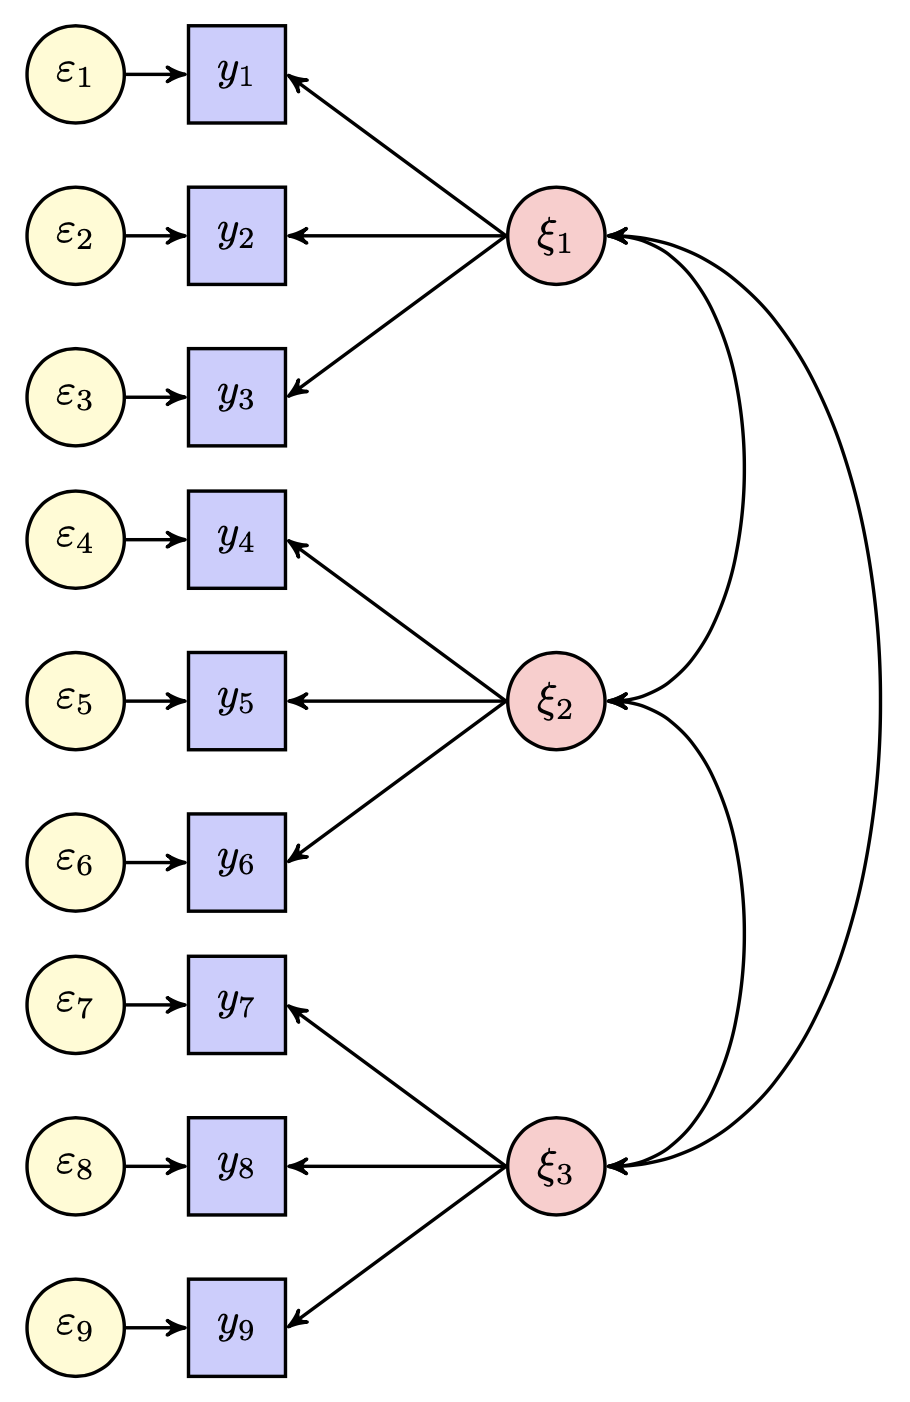
\includegraphics[width=0.4\textwidth,height=\textheight]{chapters/path_analysis/../../figures/path_01.png}

}

\caption{\label{fig-path-01}Diagramma di percorso per un modello a tre
fattori comuni.}

\end{figure}%

Una freccia curva bidirezionale che si collega a una singola variabile
rappresenta la varianza residua della variabile, ovvero la quota di
varianza non spiegata dalle relazioni causali illustrate nel diagramma
di percorso. Un triangolo contenente il numero 1 simboleggia la media di
una variabile (qui non presente).

\subsection{Parametri nei Modelli di Equazioni
Strutturali}\label{parametri-nei-modelli-di-equazioni-strutturali}

I parametri nei modelli di equazioni strutturali possono essere
categorizzati come segue, quando le medie non sono oggetto di analisi:

\begin{enumerate}
\def\labelenumi{\arabic{enumi}.}
\tightlist
\item
  \textbf{Varianze e Covarianze delle Variabili Esogene:}

  \begin{itemize}
  \tightlist
  \item
    Questi parametri rappresentano la variabilità intrinseca delle
    variabili esogene (quelle non influenzate da altre nel modello) e le
    relazioni reciproche tra di esse.
  \end{itemize}
\item
  \textbf{Effetti Diretti sulle Variabili Endogene da Altre Variabili:}

  \begin{itemize}
  \tightlist
  \item
    Questi parametri descrivono come le variabili endogene sono
    influenzate direttamente da altre variabili nel modello.
  \end{itemize}
\end{enumerate}

In termini di specificazione, un parametro nel modello può essere
classificato come libero, fisso o vincolato:

\begin{itemize}
\tightlist
\item
  \textbf{Parametro Libero:}

  \begin{itemize}
  \tightlist
  \item
    Questo tipo di parametro è stimato dal software statistico
    utilizzando i dati a disposizione.
  \end{itemize}
\item
  \textbf{Parametro Fisso:}

  \begin{itemize}
  \tightlist
  \item
    Un parametro fisso è definito per essere uguale a una costante
    specificata a priori. In questo caso, il software accetta il valore
    costante come stima, indipendentemente dai dati. Ad esempio,
    l'ipotesi che la variabile X non abbia effetti diretti su Y
    corrisponde alla specifica che il coefficiente per il percorso da X
    a Y sia fissato a zero.
  \end{itemize}
\item
  \textbf{Parametro Vincolato:}

  \begin{itemize}
  \tightlist
  \item
    In questo caso, il parametro segue certe restrizioni imposte
    nell'analisi, che possono essere basate su teorie o ipotesi
    precedenti. Ad esempio, l'analista può assumere che due paraemetri
    siano uguali.
  \end{itemize}
\end{itemize}

\section{Gradi di Libertà nei Modelli
Parametrici}\label{gradi-di-libertuxe0-nei-modelli-parametrici}

In statistica, la complessità di un modello parametrico, in termini di
parametri da stimare, è limitata dalla quantità di informazioni
statistiche fornite dai dati. Questo non equivale alla dimensione del
campione (\(N\)), ma si riferisce al numero di varianze e covarianze
uniche che si possono derivare dalla matrice di covarianza campionaria
in forma triangolare inferiore.

La quantità di informazioni statistiche disponibili in un modello si
calcola come segue:

\begin{itemize}
\tightlist
\item
  Se \(v\) è il numero di variabili osservate, la quantità di
  informazioni è data dalla formula:
\end{itemize}

\[\frac{v(v + 1)}{2},\]

quando le medie delle variabili non sono incluse nell'analisi.

Ad esempio, se \(v = 5\) (cioè ci sono 5 variabili osservate nel
modello), la quantità di informazioni statistiche sarà:

\[\frac{5 \times 6}{2} = 15.\]

Questo valore (15) rappresenta il numero totale di varianze (5) e
covarianze uniche (10) che si trovano sotto la diagonale principale
nella matrice di covarianza campionaria. In questo caso, il massimo
numero di parametri stimabili è 15. Un modello più semplice potrebbe
stimare un numero inferiore di parametri, ma non più di 15. La quantità
di informazioni statistiche non dipende dalla dimensione del campione:
anche se ci fossero 100 o 1000 casi, con 5 variabili misurate, la
quantità di informazioni resterebbe 15. Solo l'aggiunta di nuove
variabili osservate può incrementare questo numero.

La differenza tra la quantità di informazioni statistiche (\(p\)) e il
numero di parametri liberi (\(q\)) determina i gradi di libertà del
modello (\(df_M\)), che si calcolano come:

\[df_M = p - q.\]

Perché un modello sia identificabile, è necessario che i gradi di
libertà siano almeno pari a zero (\(df_M \geq 0\)). Se il numero di
parametri da stimare supera la quantità di informazioni disponibili
(\(df_M < 0\)), il modello non è identificabile e non sarà possibile
stimare i parametri in modo univoco, poiché esisterebbero infinite
soluzioni possibili. Tentare di stimare un modello con gradi di libertà
negativi genera solitamente errori nei software di modellazione. In
questi casi, il modello deve essere ridefinito riducendo il numero di
parametri liberi, ad esempio, imponendo vincoli o fissando alcuni
parametri a valori specifici.

Un modello con zero gradi di libertà (\(df_M = 0\)) si adatta
perfettamente ai dati di un campione, così come a qualsiasi altro
campione delle stesse variabili. Tuttavia, i modelli con gradi di
libertà positivi (\(df_M > 0\)) generalmente non offrono un adattamento
perfetto, lasciando spazio a discrepanze tra i dati osservati e le stime
del modello. Raykov e Marcoulides (2006) hanno descritto i gradi di
libertà come dimensioni lungo le quali un modello può potenzialmente
essere rifiutato. Pertanto, i modelli che risultano validi con maggiori
gradi di libertà hanno superato un rischio maggiore di rifiuto. Questo
rafforza il principio di parsimonia: a parità di adattamento ai dati, è
preferibile il modello più semplice, purché sia teoricamente plausibile.

\section{Raffigurazione della Varianza Residua nelle Variabili
Endogene}\label{raffigurazione-della-varianza-residua-nelle-variabili-endogene}

La Figura~\ref{fig-kline_7_2} mostra la relazione tra due variabili
osservabili. L'effetto totale presunto di X su Y è illustrato tramite un
percorso diretto, rappresentando l'effetto causale lineare di X su Y. La
varianza di X, una variabile esogena, è un parametro libero e viene
rappresentata nella figura con il simbolo RAM che indica una varianza
(indicata da una freccia curva bidirezionale). Al contrario, la varianza
di Y, una variabile endogena, non è libera di variare; invece, è
associata a una variabile latente D, il termine di disturbo o errore,
che rappresenta la variazione in Y non spiegata da X.

\begin{figure}[H]

\centering{

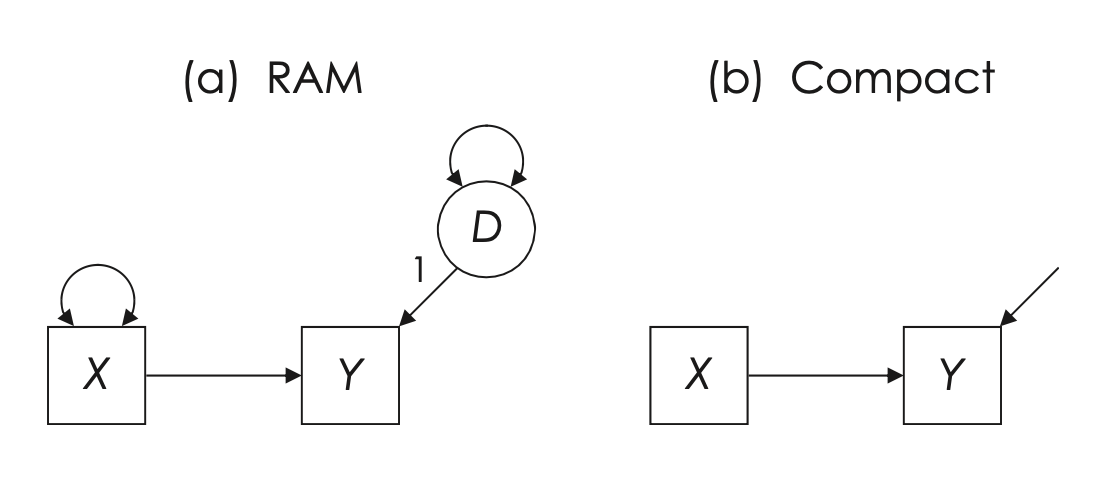
\includegraphics[width=0.8\textwidth,height=\textheight]{chapters/path_analysis/../../figures/kline_7_2.png}

}

\caption{\label{fig-kline_7_2}Diagramma per una rappresentazione
contratta nel modello completo di azione reticolare McArdle-McDonald
(RAM) con simbolismo grafico (a) rispetto a una versione più compatta
(b). (Figura adattata da R. B. Kline (2023))}

\end{figure}%

Il numero (1) vicino al percorso nella Figura~\ref{fig-kline_7_2} (a) è
una costante di scala che assegna una metrica al termine di disturbo.
Questa specificazione è essenziale perché la varianza del termine di
disturbo è latente e le variabili latenti richiedono che un fattore di
scala sia fissato per la loro stima. Questa costante di scala è nota
anche come il \emph{vincolo di identificazione del carico unitario}
(\emph{unit loading identification} constraint, ULI). Il valore ``1''
comunica al software di suddividere la varianza totale (osservata) di Y
in due componenti distinte (ortogonali): la varianza spiegata da X e la
varianza non spiegata (o varianza del disturbo,\(var_D\)).

La rappresentazione nella Figura~\ref{fig-kline_7_2} (b) fornisce le
stesse informazioni in modo più sintetico. Alternativamente, nella
Figura~\ref{fig-kline_7_2} (a) si potrebbe rappresentare la varianza
residua di Y con una freccia curva bidirezionale, al posto di utilizzare
il termine di disturbo D identificato dal vincolo di identificazione del
carico unitario. Il valore numerico associato a questa freccia curva
bidirezionale sarebbe lo stesso di quello che si ottiene con la
rappresentazione della variabile latente di
disturbo:\(1 \times var_D \times 1\).

Un'altra rappresentazione equivalente assegnerebbe il valore 1 a
\(var_D\) e attribuirebbe alla freccia causale da D a Y il valore
\(\sqrt{var_D}\). Il risultato finale sarebbe identico, in quanto anche
in questo caso la varianza residua di Y sarebbe rappresentata
come\(\sqrt{var_D} \times 1 \times \sqrt{var_D}\).

Proseguendo la discussione sulla varianza del disturbo, possiamo
identificare quattro fonti principali che contribuiscono a questa
varianza:

\begin{enumerate}
\def\labelenumi{\arabic{enumi}.}
\item
  \textbf{Variazione Sistematica da Cause Non Misure}: Questa varianza
  origina da fattori non misurati che influenzano sistematicamente
  l'esito della variabile di interesse. Si tratta di influenze esterne o
  variabili nascoste che hanno un impatto significativo ma non sono
  incluse nel modello.
\item
  \textbf{Variazione Casuale Intrinseca}: Questo tipo di varianza è una
  caratteristica fondamentale di quasi tutti i sistemi o variabili
  individuali. Rappresenta la variabilità naturale che esiste
  indipendentemente dalle misure o dagli effetti che si tenta di
  analizzare.
\item
  \textbf{Errore di Misurazione Casuale}: Questa varianza è legata agli
  errori che si verificano durante il processo di misurazione. Includono
  gli errori casuali che possono essere stimati attraverso analisi di
  affidabilità, come l'accuratezza e la precisione degli strumenti di
  misurazione utilizzati.
\item
  \textbf{Mancata Specificazione della Corretta Forma Funzionale
  dell'Effetto Causale}: Questa varianza emerge quando la forma
  funzionale dell'effetto causale nel modello non corrisponde alla vera
  natura della relazione. Un esempio comune è modellare una relazione
  come lineare quando in realtà è non lineare, portando a una
  rappresentazione imprecisa del fenomeno sotto indagine.
\end{enumerate}

Nel pannello (a) della Figura~\ref{fig-kline_7_2}, il percorso da D a Y
rappresenta l'effetto diretto di tutte queste cause omesse, oltre agli
errori, sulla variabile endogena Y. In sostanza, questo percorso
simboleggia l'insieme di tutte le influenze non incluse nel modello che
possono impattare su Y. È importante notare che, mentre queste fonti di
varianza del disturbo possono essere teoricamente distinte, nella
pratica possono sovrapporsi e interagire tra loro.

Proseguendo il discorso sulla rappresentazione della varianza residua
nelle variabili endogene, è importante notare che diversi software SEM
trattano in modi differenti i termini di errore nei modelli di equazioni
strutturali. Ad esempio, nella sintassi del software lavaan, il comando:

\begin{Shaded}
\begin{Highlighting}[]
\NormalTok{Y }\SpecialCharTok{\textasciitilde{}}\NormalTok{ X}
\end{Highlighting}
\end{Shaded}

direttamente istruisce il software a regredire la variabile Y su X e a
gestire automaticamente il termine di disturbo, come rappresentato nel
pannello (a) della Figura~\ref{fig-kline_7_2}. Questo comando, oltre a
definire l'effetto di X su Y, stabilisce anche che le varianze di X e il
termine di disturbo di Y sono parametri liberi da stimare.

Da queste considerazioni emergono due requisiti fondamentali per
l'identificazione di un modello a percorsi:

\begin{enumerate}
\def\labelenumi{\arabic{enumi}.}
\tightlist
\item
  I gradi di libertà del modello (\(df_M\)) devono essere maggiori o
  uguali a zero.
\item
  Ogni variabile latente, inclusi i termini di errore, deve avere una
  scala definita (una metrica assegnata).
\end{enumerate}

Il conteggio dei parametri liberi è una componente cruciale nel calcolo
dei \(df_M\). L'inclusione esplicita delle costanti di scala nei
diagrammi serve come promemoria per i ricercatori sulla necessità di
assegnare una scala alle variabili latenti.

Il pannello (b) della Figura~\ref{fig-kline_7_2} mostra una versione più
sintetica del modello, utilizzando un simbolismo grafico che omette i
simboli per i parametri di varianza (per X, D), la costante di scala (1)
e la rappresentazione grafica del disturbo come variabile latente.
Questo diagramma fornisce una visione meno dettagliata del modello,
evidenziando solamente le relazioni di base, ovvero X che causa Y, e Y
influenzata da un termine di disturbo.

\subsection{Considerazioni sugli Errori di Misurazione nei Modelli a
Percorsi}\label{considerazioni-sugli-errori-di-misurazione-nei-modelli-a-percorsi}

Riprendendo la discussione sulla Figura~\ref{fig-kline_7_2}, possiamo
delineare le seguenti ipotesi fondamentali:

\begin{enumerate}
\def\labelenumi{\arabic{enumi}.}
\item
  \textbf{Affidabilità della Variabile Esogena X}: Si assume che i
  punteggi sulla variabile esogena X siano privi di errore, ovvero
  perfettamente affidabili, con un coefficiente di affidabilità
  (\(r_{XX}\)) di 1.0.
\item
  \textbf{Correttezza della Direzione Causale}: La relazione causale da
  X a Y è assunta come correttamente specificata e caratterizzata da una
  stretta linearità.
\item
  \textbf{Indipendenza delle Cause Non Misurate di Y da X}: Si presume
  che le cause non misurate (latenti) di Y non siano correlate con X,
  escludendo quindi l'esistenza di cause comuni non misurate che
  influenzano simultaneamente entrambe le variabili -- ricordiamo la
  discusione precedente sull'errore di specificazione.
\end{enumerate}

In ambito di modellazione dei percorsi, l'assunzione che le variabili
esogene siano prive di errori di misurazione riflette un presupposto
simile a quello adottato nelle regressioni multiple standard, dove i
predittori sono considerati esenti da errori di misurazione. Questa
assunzione è necessaria poiché le variabili esogene nei modelli a
percorsi non includono termini di errore, rendendo impossibile
incorporare l'errore casuale in tali modelli. Al contrario, nelle
variabili endogene di tali modelli, la presenza di termini di errore
permette di tenere conto dell'errore di misurazione.

Nel caso di una regressione bivariata, un errore di misurazione presente
solo nella variabile dipendente Y influisce sul modello aumentando
l'errore standard della stima di regressione, riducendo il valore di
\(R^2\) e diminuendo il valore assoluto del coefficiente di regressione
standardizzato, a causa dell'incremento dell'errore di misurazione in Y.
Invece, l'errore di misurazione presente solo nella variabile predittiva
X (ma non in Y) tende a introdurre un bias negativo nei coefficienti di
regressione -- cioè una sistematica sottostima dei veri valori dei
coefficienti di regressione.

Quando entrambe le variabili X e Y presentano errori di misurazione, la
dinamica risultante è più complessa da prevedere. Se gli errori di
misurazione in X e Y sono indipendenti, il risultato più comune è un
bias negativo (ossia una sottostima dei coefficienti di regressione
della popolazione). Tuttavia, se gli errori di misurazione sono comuni
tra X e Y, la regressione potrebbe sovrastimare i coefficienti della
popolazione, portando a un bias positivo. È essenziale riconoscere che
l'errore di misurazione non causa sempre un bias negativo. Di
conseguenza, la presenza di errori di misurazione non modellati nelle
variabili esogene può significativamente distorcere i risultati,
specialmente in presenza di forti correlazioni tra multiple variabili
esogene. Per ridurre questi rischi, si raccomanda di valutare
l'affidabilità dei punteggi associati alle variabili esogene. Questa
pratica metodologica, che consiste nel verificare la precisione e la
consistenza delle misure delle variabili predittive, aiuta a
identificare e quantificare eventuali errori di misurazione. Un'accurata
stima dell'affidabilità contribuisce a garantire l'integrità e la
validità dei risultati dei modelli a percorsi, mitigando l'impatto che
gli errori di misurazione possono avere sull'analisi.

\subsection{Direzionalità Causale e Forma Funzionale della Relazione
X-Y}\label{direzionalituxe0-causale-e-forma-funzionale-della-relazione-x-y}

L'assunzione che la relazione tra le variabili X e Y sia lineare, come
presentato nella Figura~\ref{fig-kline_7_2}, può essere esaminata
attraverso l'analisi dei dati. Se si osserva che la relazione è
significativamente curvilinea, si può adeguare l'analisi per attenuare
il presupposto di linearità. Ciò può essere realizzato attraverso metodi
come la regressione polinomiale o la regressione non parametrica, che
permettono di modellare relazioni più complesse rispetto a un semplice
modello lineare.

Tuttavia, la direzionalità dell'effetto causale rappresenta una sfida
differente e non è direttamente testabile attraverso metodi statistici
standard. Nell'ambito dei modelli SEM, le direzioni degli effetti
causali sono generalmente ipotizzate piuttosto che empiricamente
verificate. Questo perché è possibile costruire modelli SEM equivalenti
che utilizzano le stesse variabili e hanno lo stesso numero di gradi di
libertà (\(df_M\)), ma con direzioni inverse di alcuni effetti causali.
Inoltre, entrambi i modelli, nonostante le differenze nelle
direzionalità causali, mostreranno lo stesso grado di adattamento ai
dati osservati.

Un'ulteriore ragione per cui la direzionalità causale è tipicamente
assunta piuttosto che testata in SEM risiede nella natura degli studi
SEM stessi. La maggior parte degli studi SEM si basa su disegni
trasversali, dove tutte le variabili sono misurate contemporaneamente,
senza una chiara precedenza temporale. In questi contesti, l'unica base
per definire la direzionalità causale è l'argomentazione teorica del
ricercatore, che deve giustificare perché si presume che X influenzi Y e
non viceversa, o perché non si considera una relazione di feedback o
causazione reciproca tra le due variabili.

Di conseguenza, la metodologia SEM non è intrinsecamente una tecnica per
la scoperta di relazioni causali. Se un modello è corretto, SEM può
essere utilizzato per stimare le direzioni, le dimensioni e la
precisione degli effetti causali. Tuttavia, questo non è il modo in cui
i ricercatori tipicamente impiegano le analisi SEM. Piuttosto, un
modello causale viene ipotizzato e poi adattato ai dati basandosi sulle
assunzioni delineate. Se queste assunzioni risultano essere errate,
anche i risultati dell'analisi saranno invalidi. Questo enfatizza il
punto sollevato da Pearl (2000), che sostiene che

\begin{quote}
le ipotesi causali sono un prerequisito essenziale per validare
qualsiasi conclusione causale (p.~136).
\end{quote}

Questo implica la necessità di una solida base teorica e concettuale
nella formulazione di modelli causali nella modellazione SEM.

\subsection{Confondimento nei Modelli
Parametrici}\label{confondimento-nei-modelli-parametrici}

Nella teoria dei modelli statistici, l'endogenità si riferisce a una
situazione in cui una variabile all'interno di un modello è correlata
con i termini di errore. Questo può creare problemi nella stima dei
parametri del modello e può portare a conclusioni errate riguardo le
relazioni causali tra le variabili.

Nel contesto del diagramma di una catena contratta della
Figura~\ref{fig-kline_7_2a}, l'endogenità è visualizzata come una
covarianza tra la variabile causale misurata X e il disturbo (termine di
errore) di Y, indicata con un simbolo specifico. Questo simbolo mostra
che c'è una relazione non spiegata tra la causa X e il disturbo
associato a Y, suggerendo che X potrebbe non essere una variabile
completamente indipendente, come idealmente dovrebbe essere in un
modello causale chiaro.

Il modello nella Figura~\ref{fig-kline_7_2a} (a) non è identificabile
per due ragioni principali:

\begin{enumerate}
\def\labelenumi{\arabic{enumi}.}
\item
  \textbf{Gradi di libertà negativi (dfM = -1)}: Questo indica che ci
  sono più parametri da stimare nel modello rispetto al numero di
  informazioni (osservazioni) disponibili. In sostanza, il modello sta
  cercando di ``apprendere'' troppo da troppo pochi dati, il che lo
  rende statisticamente non identificabile.
\item
  \textbf{Percorso di confondimento non chiuso tra X e D}: Il percorso
  di confondimento (o back-door) tra X e D indica che c'è una relazione
  non controllata o non misurata tra la variabile indipendente X e il
  disturbo D di Y. Poiché D è trattato come una variabile latente (cioè,
  una variabile non osservata direttamente), questo percorso non può
  essere chiuso o controllato nel modello. Ciò significa che non
  possiamo essere sicuri se la relazione osservata tra X e Y è
  effettivamente causata da X o se è influenzata da altri fattori non
  considerati nel modello.
\end{enumerate}

In sintesi, l'endogenità in questo contesto si riferisce al problema di
avere una variabile indipendente (X) che non è veramente indipendente a
causa della sua relazione non spiegata con il termine di errore
associato alla variabile dipendente (Y), compromettendo così la
chiarezza delle relazioni causali nel modello.

\begin{figure}[H]

\centering{

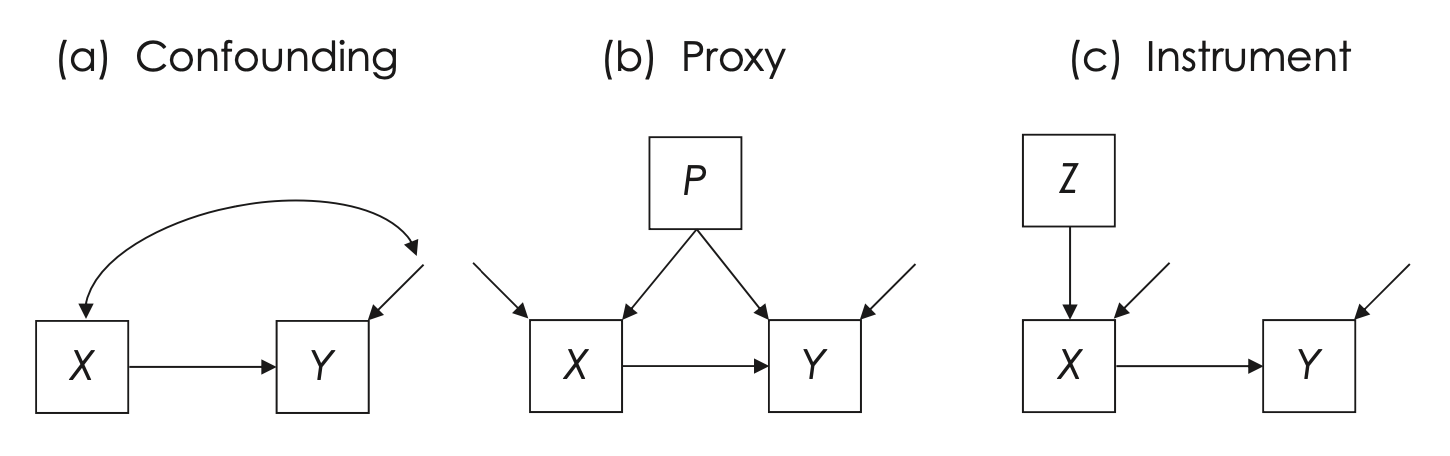
\includegraphics[width=0.8\textwidth,height=\textheight]{chapters/path_analysis/../../figures/kline_7_2a.png}

}

\caption{\label{fig-kline_7_2a}Endogenità in una catena contratta (a).
Identificazione del modello controllando un proxy (P) di una causa
comune non misurata (b) e attraverso metodi di variabile strumentale
(Z), che affrontano anche l'errore di misurazione nella variabile X (c).
Tutti i diagrammi sono mostrati in simbolismo compatto. (Figura tratta
da R. B. Kline (2023))}

\end{figure}%

L'endogenità nei modelli parametrici può essere indotta dalle seguenti
condizioni:

\begin{enumerate}
\def\labelenumi{\arabic{enumi}.}
\tightlist
\item
  Una causa comune non misurata di X e Y (cioè, un confonditore).
\item
  Errore di misurazione casuale in X (cioè, \(r_{XX} < 1.0\)).
\item
  Causalità reciproca, o X e Y si causano a vicenda (cioè, sono entrambe
  variabili endogene) in un ciclo di feedback.
\item
  Errori autoregressivi, dove X è una versione ritardata di Y e gli
  errori persistono tra le due variabili.
\item
  Autoregressione spaziale, che si verifica quando i punteggi di ciascun
  caso sono influenzati da quelli di casi vicini o adiacenti
  spazialmente.
\end{enumerate}

Nel contesto dei modelli statistici, è possibile affrontare il problema
dei confonditori non misurati in due modi principali: attraverso la
selezione di covariate appropriate o utilizzando i metodi delle
variabili strumentali. Per illustrare, la Figura~\ref{fig-kline_7_2a}
(b) propone l'uso di un proxy (P) che funge da sostituto per un
confonditore non misurato che influisce su entrambe le variabili X e Y.
In questo contesto, la variabile X è considerata endogena, il che
significa che è influenzata dal proxy P (che a sua volta influisce anche
su Y), indicando una possibile relazione di causa-effetto tra P e X.

Per chiarire, consideriamo il seguente esempio. Immaginiamo di essere
interessati a studiare l'effetto dello stress sulle prestazioni
accademiche degli studenti universitari. In questo esempio, ``stress'' è
la variabile X e ``prestazioni accademiche'' è la variabile Y. Tuttavia,
c'è un potenziale confonditore che potrebbe influenzare sia lo stress
sia le prestazioni accademiche, ma che non è stato misurato o non può
essere facilmente misurato. Questo confonditore potrebbe essere, ad
esempio, il ``benessere psicologico generale'' degli studenti.

In questo caso, un proxy (P) per il benessere psicologico generale
potrebbe essere ``l'attività fisica regolare'', che è più facilmente
misurabile. La ricerca ha mostrato che l'attività fisica regolare può
influenzare sia il benessere psicologico generale sia lo stress,
rendendola un buon proxy per il nostro confonditore non misurato.

Nel modello, l'attività fisica (il nostro proxy P) presumibilmente
influisce sia sulla variabile causale (lo stress) sia sulla variabile di
esito (le prestazioni accademiche). Analizzando i dati con questo
modello, possiamo cercare di isolare meglio l'effetto dello stress sulle
prestazioni accademiche, controllando per l'effetto del benessere
psicologico generale tramite il proxy dell'attività fisica. In questo
modo, possiamo ottenere una stima più accurata dell'effetto diretto
dello stress sulle prestazioni accademiche, riducendo la distorsione
potenzialmente causata dal confonditore non misurato.

I metodi delle variabili strumentali, come mostrato nella
Figura~\ref{fig-kline_7_2a} (c), sono utilizzati per affrontare sia i
confonditori non misurati sia gli errori di misurazione nella variabile
esogena X. Questo viene fatto sostituendo X con una variabile
strumentale XZ in un modello di regressione a due stadi (2SLS). In
questo approccio, qualsiasi errore di misurazione casuale in X viene
trasferito alla variabile strumentale XZ, seguendo le ipotesi standard
dei metodi delle variabili strumentali. È importante notare che, nel
pannello (c), la variabile X è considerata endogena, sebbene non tutti i
ricercatori scelgano di includere variabili strumentali nei loro
diagrammi di modelli statistici. Questo approccio consente di isolare
meglio l'effetto di X su Y, controllando per le influenze esterne non
misurate e gli errori di misurazione.

Per chiarire ulteriormente questi concetti, esamineremo separatamente il
modello autoregressivo e l'autoregressione spaziale.

\subsubsection{Modello Autoregressivo}\label{modello-autoregressivo}

Un modello autoregressivo è un tipo di modello statistico utilizzato per
analizzare dati sequenziali o temporali. In un modello autoregressivo,
si prevedono i valori futuri di una variabile basandosi sui suoi valori
passati. Questo è particolarmente utile in studi longitudinali o in
serie temporali dove si misura la stessa variabile in diversi punti nel
tempo.

Nell'esempio della Figura~\ref{fig-kline_7_2a} (a), immaginiamo che X e
Y siano le stesse variabili misurate in due momenti diversi. Ad esempio,
X potrebbe essere il livello di ansia di uno studente misurato
all'inizio dell'anno scolastico, mentre Y potrebbe essere il livello di
ansia dello stesso studente misurato alla fine dell'anno scolastico. In
questo caso, stiamo cercando di prevedere i punteggi futuri di ansia (Y)
basandoci sui punteggi passati (X).

Un aspetto importante da considerare è che gli errori nelle misure
ripetute (le variazioni nei punteggi che non sono spiegati dal modello)
possono essere correlati. Ad esempio, se le misurazioni sono fatte in
intervalli temporali ravvicinati, le circostanze o gli stati interni che
hanno influenzato la prima misurazione potrebbero ancora essere presenti
durante la seconda misurazione.

\subsubsection{Autoregressione Spaziale}\label{autoregressione-spaziale}

L'autoregressione spaziale, invece, si riferisce a un modello che
considera le correlazioni spaziali tra dati. Questo tipo di analisi è
particolarmente rilevante quando si studiano fenomeni geografici o
ambientali. Ad esempio, la diffusione di una malattia in diverse
località geografiche potrebbe non essere indipendente: le aree vicine
geograficamente potrebbero mostrare pattern simili di diffusione della
malattia a causa della loro vicinanza.

In quest'ultimo caso, non stiamo più parlando di misure ripetute nel
tempo sulla stessa unità, ma piuttosto di misure effettuate in diverse
unità in un contesto spaziale. Le variabili misurate in diverse località
fisiche possono influenzarsi a vicenda, e un modello autoregressivo
spaziale cerca di catturare queste interdipendenze.

\subsection{Modelli con Cause Correlate o Effetti
Indiretti}\label{modelli-con-cause-correlate-o-effetti-indiretti}

Il modello parametrico mostrato nella Figura~\ref{fig-kline_7_3} (a)
suggerisce che la variabile Y sia influenzata da due variabili esogene
correlate, X e W. Questo significa che X e W sono due fattori esterni
che hanno un impatto su Y e tra loro esiste una relazione di covarianza,
ovvero tendono a variare insieme in un certo modo. Tuttavia, il
diagramma non spiega il motivo della relazione tra X e W, lasciando la
loro interdipendenza non esaminata in termini causali.

\begin{figure}[H]

\centering{

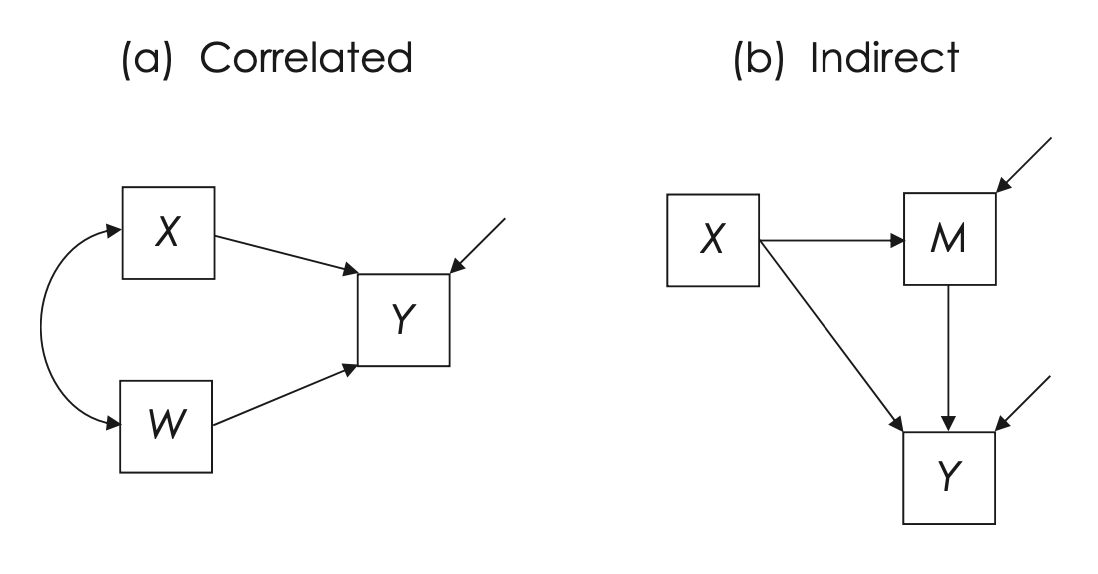
\includegraphics[width=0.8\textwidth,height=\textheight]{chapters/path_analysis/../../figures/kline_7_3.png}

}

\caption{\label{fig-kline_7_3}Modelli con cause correlate (a) e sia
effetti diretti che indiretti (b). Tutti i diagrammi sono mostrati in
simbolismo compatto. (Figura tratta da R. B. Kline (2023))}

\end{figure}%

Nell'analizzare questi dati con un software, si prenderanno in
considerazione gli effetti sia di X che di W, tenendo conto della loro
covarianza campionaria. Ciò significa che quando si stimano gli impatti
di X e W su Y, si aggiusta per il fatto che X e W sono correlate tra
loro. Alcuni software, come \texttt{lavaan}, presuppongono
automaticamente che tutte le cause esogene misurate che influenzano lo
stesso risultato (in questo caso Y) siano correlate. Utilizzando il
comando

\texttt{Y\ \textasciitilde{}\ X\ +\ W}

in \texttt{lavaan}, si definisce il modello rappresentato nella
Figura~\ref{fig-kline_7_3} (a), permettendo al software di stimare gli
effetti di X e W tenendo conto della loro covarianza osservata. Questo
comando specifica inoltre che le varianze di X, W e il disturbo
associato a Y sono tutti considerati parametri liberi da stimare.

Se, invece, si ipotizza che le variabili esogene X e W siano
indipendenti, ovvero che non ci sia una covarianza tra di loro, si può
usare un comando aggiuntivo in \texttt{lavaan}

\texttt{X\ \textasciitilde{}\textasciitilde{}\ 0*W}

per impostare la covarianza tra X e W a zero. Questo comando mantiene le
varianze di X e W come parametri liberi, ma specifica che non c'è una
relazione di covarianza diretta tra queste due variabili. In questo
modo, il modello considererà X e W come influenze separate e
indipendenti su Y.

Nel modello presentato nella Figura~\ref{fig-kline_7_3} (a), è
importante notare come vengano trattate le interazioni tra le variabili
causali X e W. In questo specifico caso, si presume che non ci sia
alcuna interazione tra X e W; in altre parole, l'effetto di X sulla
variabile di esito Y si assume essere costante a prescindere dai diversi
livelli di W, e viceversa. Questa assunzione implica che l'effetto di X
su Y è indipendente da W, e l'effetto di W su Y è indipendente da X.

In termini di modellazione, questo significa che stiamo considerando una
causalità incondizionata, dove l'effetto di una causa su un esito è
costante e non influenzato da altre variabili nel modello. Il modello
non prevede, quindi, che l'effetto di X su Y cambi in funzione dei
diversi livelli di W. Questo è in contrasto con l'ipotesi di causalità
condizionale, dove gli effetti di una variabile su un'altra possono
variare in base al livello di una terza variabile. In un modello di
causalità condizionale, ad esempio, si potrebbe ipotizzare che l'effetto
di X su Y vari a seconda dei diversi livelli di W.

In sintesi, la Figura~\ref{fig-kline_7_3} (a) delinea un modello dove le
relazioni causali tra X, W e Y sono considerate fisse e non influenzate
da potenziali interazioni tra X e W. Questo tipo di modellazione
fornisce una visione semplificata delle relazioni causali, che potrebbe
essere appropriata in determinate circostanze, ma non tiene conto di
possibili dinamiche più complesse tra le variabili.

È fondamentale riconoscere che le ripercussioni degli errori di
misurazione in modelli che includono cause correlate sono notevolmente
intricate e imprevedibili. Questa complessità deriva principalmente
dalla natura del bias che può emergere a seguito di errori di
misurazione. In particolare, il bias introdotto da questi errori può
manifestarsi in modi diversi, assumendo una forma sia negativa che
positiva. Tale variazione dipende da diversi fattori, tra cui se
l'errore di misurazione è distribuito in maniera uniforme tra molteplici
variabili predittive o se è presente sia nelle variabili predittive che
nella variabile di esito. Un altro elemento influente è la natura delle
covarianze campionarie tra tutte le variabili coinvolte nel modello.

Data questa complessità, la capacità di modellare esplicitamente gli
errori di misurazione all'interno dei modelli SEM rappresenta un
vantaggio significativo. Questo approccio permette una maggiore
precisione nell'analisi, consentendo di tenere conto delle varie
modalità in cui gli errori di misurazione possono influenzare i
risultati. La modellazione esplicita degli errori di misurazione in SEM
offre quindi la possibilità di ottenere stime più accurate e affidabili,
mitigando il rischio di trarre conclusioni errate a causa di bias non
riconosciuti o non gestiti adeguatamente.

Nella Figura~\ref{fig-kline_7_3} (b), il modello mostra come la
variabile X abbia sia effetti diretti che indiretti sulla variabile di
esito Y. L'effetto indiretto segue il percorso X → M → Y, dove M funge
da variabile intermedia o mediatrice. Questo significa che M è il canale
attraverso il quale gli effetti di X sono trasmessi a Y. In questo
modello, M è una variabile endogena, nel senso che è influenzata da X
(indicato dal percorso X → M), e allo stesso tempo agisce come una
variabile causale nei confronti di Y (come indicato da M → Y).

La variabile M assume un doppio ruolo in termini di affidabilità e
precisione della misurazione. Da una parte, essendo un esito di X, M è
soggetta a disturbi, che includono potenziali errori di misurazione.
Dall'altra, nel suo ruolo di causa per Y insieme a X, si presume nelle
analisi di regressione che sia X che M siano prive di errore di
misurazione. Questa assunzione non presenta problemi se l'affidabilità
delle misure su M è elevata, ossia se i punteggi di M sono accurati e
consistenti.

In aggiunta, il modello descritto nella Figura~\ref{fig-kline_7_3} (b)
include tre ipotesi importanti:

\begin{enumerate}
\def\labelenumi{\arabic{enumi}.}
\tightlist
\item
  X ha un effetto diretto su Y, oltre al suo effetto indiretto tramite
  M.
\item
  Non ci sono interazioni negli effetti lineari di X e M su Y, il che
  significa che l'effetto di X su Y è lo stesso a prescindere dai
  livelli di M, e viceversa.
\item
  Il modello non omette confonditori potenzialmente importanti tra le
  coppie di variabili X, M e Y. In altre parole, non ci sono fattori
  esterni non considerati nel modello che potrebbero influenzare le
  relazioni tra queste tre variabili.
\end{enumerate}

In sintesi, la Figura~\ref{fig-kline_7_3} (b) presenta un modello in cui
X influisce su Y sia direttamente che indirettamente attraverso M, e
queste relazioni sono considerate prive di interazioni complesse o di
confonditori non rilevati.

La gestione degli errori di misurazione e dei confonditori non
considerati in modelli che includono effetti causali indiretti
rappresenta una sfida notevole, poiché i loro effetti sulle stime
possono essere complessi e non sempre prevedibili. Per esemplificare,
consideriamo il modello della Figura~\ref{fig-kline_7_3} (b) dove si
analizza l'effetto indiretto di X su Y attraverso la variabile
intermedia M.

Se assumiamo che non ci siano errori di misurazione nella variabile
causale X, qualsiasi errore di misurazione presente nella variabile
intermedia M può introdurre un bias negativo nelle stime dell'effetto
indiretto di X su Y. Ciò significa che l'effetto indiretto potrebbe
essere sottostimato a causa dell'errore in M. D'altro canto, se non si
tiene conto dei confonditori tra M e Y, cioè se ci sono variabili o
fattori non considerati che influenzano sia M che Y, ciò può portare a
un bias positivo, sovrastimando l'effetto indiretto.

Quando entrambe queste situazioni -- errori di misurazione in M e
confonditori tra M e Y -- si verificano contemporaneamente, le
conseguenze sulle stime dell'effetto indiretto possono variare
ampiamente. Potrebbe verificarsi una sovrastima, una sottostima o, in
rari casi, nessun bias significativo. Studi di simulazione hanno
rivelato che tentare di correggere solo una fonte di bias (come l'errore
di misurazione in M) in presenza di entrambi i tipi di bias può
addirittura aggravare il problema, portando a stime più distorte
rispetto a quelle che non tengono conto di alcun bias.

In sintesi, la valutazione accurata dell'effetto indiretto in un modello
che comprende una variabile intermedia richiede un'attenta
considerazione sia degli errori di misurazione che dei confonditori
potenziali, poiché la loro interazione può influenzare in modi complessi
e talvolta inaspettati la validità delle stime.

\subsection{Modelli Ricorsivi, Non Ricorsivi e Parzialmente
Ricorsivi}\label{modelli-ricorsivi-non-ricorsivi-e-parzialmente-ricorsivi}

Tutti i modelli di percorso parametrici più complessi possono essere
``assemblati'' a partire dai modelli elementari mostrati nelle figure
precedenti. Ci sono due tipi fondamentali di modelli: ricorsivi e non
ricorsivi. I modelli ricorsivi hanno due caratteristiche essenziali:
tutti gli effetti causali sono unidirezionali e i loro disturbi sono
indipendenti. La Figura~\ref{fig-kline_7_4} (a) è un esempio di un
modello ricorsivo (Tutti i modelli considerati finora sono ricorsivi.)

I modelli non ricorsivi, invece, hanno cicli causali (feedback) in cui ≥
2 variabili endogene sono specificate come cause ed effetti l'una
dell'altra, direttamente o indirettamente. Nella loro forma non
parametrica, corrispondono a grafi ciclici diretti. La
Figura~\ref{fig-kline_7_4} (b) è un esempio di un modello parametrico
non ricorsivo con causazione reciproca rappresentata come

\(Y1 \overset{\rightarrow}{\underset{\leftarrow}{}} Y2,\)

indicando che le variabili Y1 e Y2 hanno effetti simultanei l'una
sull'altra.

\begin{figure}[H]

\centering{

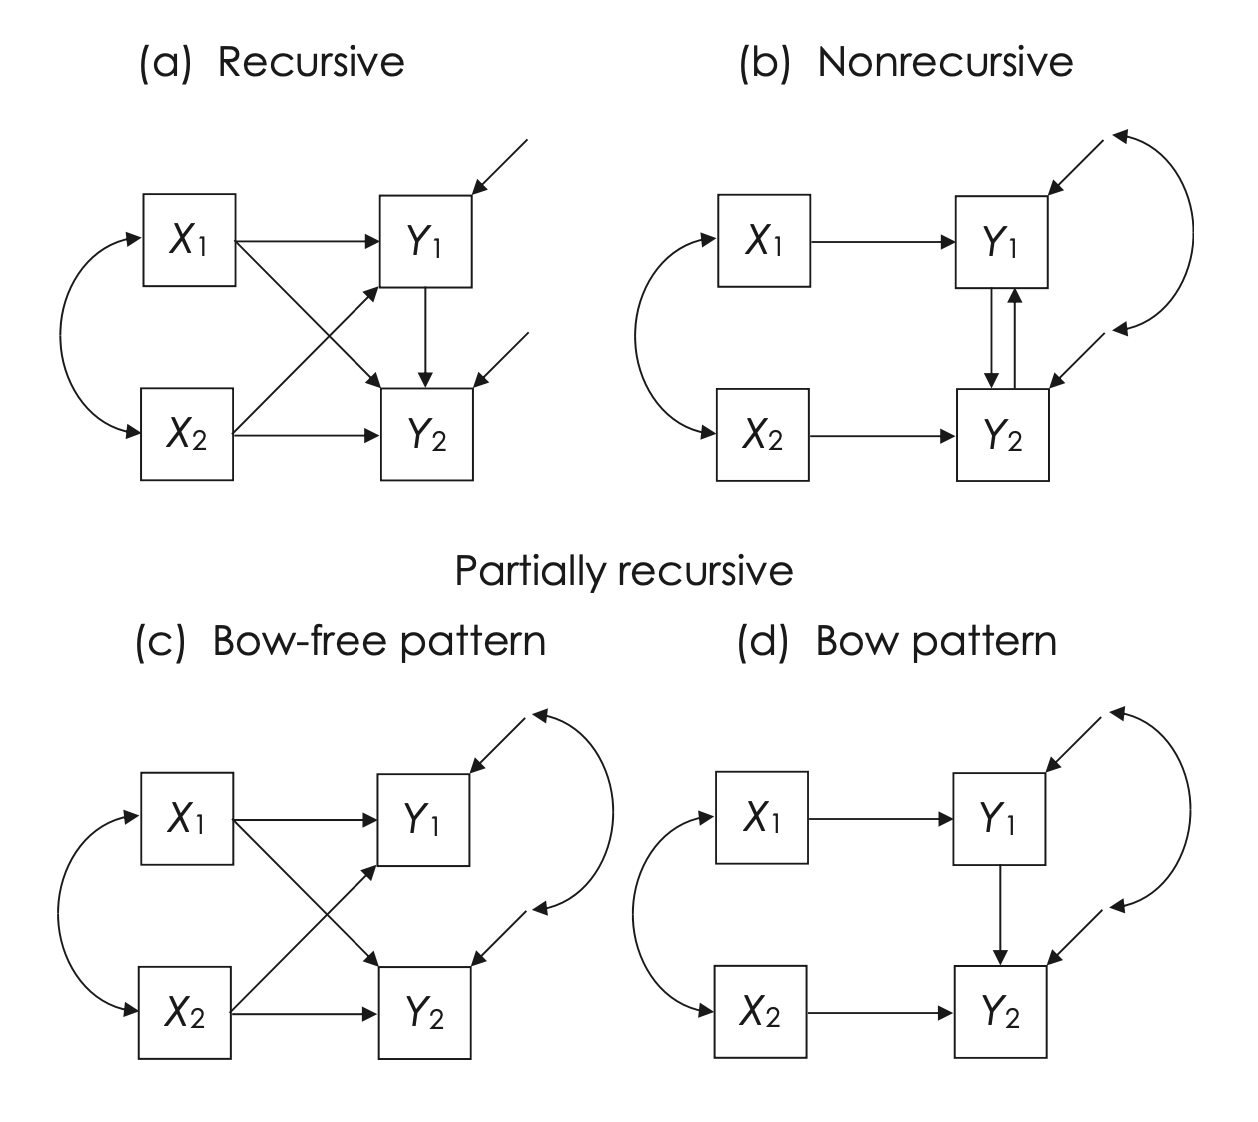
\includegraphics[width=0.8\textwidth,height=\textheight]{chapters/path_analysis/../../figures/kline_7_4.png}

}

\caption{\label{fig-kline_7_4}Esempi di modelli ricorsivi, non ricorsivi
e parzialmente ricorsivi con due diversi schemi di correlazione degli
errori. Tutti i diagrammi sono mostrati in simbolismo compatto. (Figura
tratta da R. B. Kline (2023))}

\end{figure}%

I modelli che includono cicli causali possono presentare, o meno,
covarianze tra i loro termini di disturbo. La presenza di errori
correlati in questi modelli implica l'esistenza di ipotesi su cause
comuni non misurate che influenzano le variabili in questione.

Ad esempio, nel modello rappresentato nella Figura~\ref{fig-kline_7_4}
(b), le variabili Y1 e Y2 sono definite come cause reciproche, ovvero
ognuna influisce sull'altra. In aggiunta a ciò, se nel modello è
specificata una covarianza tra i termini di disturbo \(D_1\) e \(D_2\),
ciò suggerisce che Y1 e Y2 condividono almeno una causa comune non
misurata. In altre parole, l'ipotesi è che esistano fattori non
osservati che influenzano entrambe le variabili, \(Y1\) e \(Y2\), e
questa influenza comune si manifesta attraverso la covarianza tra i loro
termini di disturbo.

Esiste anche un altro tipo di modello di percorso, quello che ha effetti
unidirezionali e covarianze dei disturbi. I modelli parzialmente
ricorsivi con un pattern di correlazioni dei disturbi senza ``archi''
possono essere trattati nell'analisi proprio come i modelli ricorsivi.
Un pattern senza ``archi'' significa che gli errori correlati sono
limitati a coppie di variabili endogene senza effetti diretti tra di
loro, come Y1 e Y2 nella Figura~\ref{fig-kline_7_4} (c).

I modelli parzialmente ricorsivi che presentano un pattern di
correlazioni dei disturbi caratterizzato dalla presenza di ``archi''
richiedono un trattamento analitico simile a quello dei modelli non
ricorsivi. Un pattern con ``archi'' si verifica quando esiste una
covarianza tra i termini di disturbo di due variabili endogene che sono
collegate da un effetto diretto. Ad esempio, nella
Figura~\ref{fig-kline_7_4} (d), le variabili Y1 e Y2 sono collegate da
un effetto diretto e presentano una covarianza tra i loro disturbi
\(D_1\) e \(D_2\).

La presenza di un effetto diretto insieme a disturbi correlati tra due
variabili crea un percorso di confondimento nel modello. Un percorso di
confondimento è una via attraverso la quale può fluire l'influenza
causale indiretta, potenzialmente distorcendo l'interpretazione dei
rapporti causali diretti. In questi casi, la selezione di covariate
(variabili aggiuntive che potrebbero spiegare parte della relazione
osservata) non è sufficiente per ``chiudere'' o eliminare questo
percorso di confondimento. Pertanto, questi modelli richiedono
un'attenzione particolare nell'analisi per garantire che le stime degli
effetti causali siano accurate e non siano influenzate in modo improprio
da questi percorsi di confondimento.

I modelli ricorsivi e quelli parzialmente ricorsivi che non includono
cicli causali possono essere efficacemente rappresentati tramite grafi
aciclici diretti (DAG). Questo tipo di rappresentazione grafica implica
che è possibile applicare tutte le regole di identificazione grafica
esposte in questo capitolo. Nei DAG, le relazioni causali sono
rappresentate come flussi unidirezionali senza cicli, rendendo più
chiaro e diretto l'analisi delle relazioni tra le variabili.

D'altra parte, i modelli non ricorsivi che includono cicli causali, come
quello illustrato nella Figura~\ref{fig-kline_7_4} (b), sono
rappresentati da grafi ciclici diretti. In questi grafi, le variabili
possono influenzarsi a vicenda in un ciclo continuo, creando una
struttura più complessa. A causa di questa complessità, le regole di
identificazione grafica per i grafi ciclici diretti non sono sviluppate
quanto quelle per i DAG. Questo significa che analizzare e interpretare
i modelli non ricorsivi con cicli causali è più complesso e richiede
l'uso di approcci analitici più avanzati o specifici per gestire
correttamente le relazioni cicliche tra le variabili.

Possiamo stabilire una regola generale per i modelli di percorso
parametrici: i modelli ricorsivi o parzialmente ricorsivi, che
presentano schemi di covarianze dei disturbi privi di ``archi'' e che
soddisfano due condizioni specifiche, sono considerati identificati.
Queste condizioni sono: (1) i gradi di libertà del modello (dfM) devono
essere maggiori o uguali a zero e (2) ogni variabile non misurata,
inclusi i termini di errore, deve essere associata a una scala metrica.

Inoltre, i modelli di equazioni strutturali che sono identificati e
hanno un numero di osservazioni uguale al numero dei parametri liberi
(dfM = 0) sono classificati come ``appena identificati''. Al contrario,
i modelli con più osservazioni rispetto ai parametri liberi (dfM
\textgreater{} 0) sono considerati ``sovraidentificati''.

Un modello di equazioni strutturali può risultare sotto-identificato in
due modi distinti: (1) se dfM è inferiore a zero, oppure (2) se, pur
avendo un dfM maggiore o uguale a zero, alcuni parametri liberi
rimangono sotto-identificati perché non vi sono sufficienti informazioni
per la loro stima, anche se altri parametri all'interno dello stesso
modello sono identificati. Nel secondo scenario, l'intero modello è
considerato non identificato, anche se dfM è maggiore o uguale a zero.
In generale, un modello si considera sotto-identificato quando non è
possibile stimare in modo univoco tutti i suoi parametri liberi.

\section{Analisi dei percorsi e regressione
bivariata}\label{analisi-dei-percorsi-e-regressione-bivariata}

Cominciamo esaminando l'analisi dei percorsi partendo dall'esempio più
semplice, ovvero il modello di regressione lineare. Il modello di
regressione bivariata si esprime tramite l'equazione seguente:

\[y_1 = b_0 + b_1 x_1 + \epsilon_1,\]

dove \(y\) rappresenta la variabile dipendente, \(b_0\) rappresenta
l'intercetta, \(b_1\) rappresenta la pendenza della retta di
regressione, \(x\) è la variabile indipendente e \(\epsilon\) è il
termine di errore.

Nell'ambito della descrizione delle relazioni tra variabili manifeste e
latenti, si adotta spesso la notazione LISREL. In questa notazione, il
modello presentato in precedenza può essere espresso come segue:

\[y_1 = \alpha + \gamma x_1 + \zeta_1,\]

dove:

\begin{itemize}
\tightlist
\item
  \(x_1\): variabile esogena singola,
\item
  \(y_1\): variabile endogena singola,
\item
  \(\alpha\): intercetta di \(y_1\),
\item
  \(\gamma_1\): coefficiente di regressione,
\item
  \(\zeta_1\): termine di errore di \(y_1\),
\item
  \(\phi\): varianza o covarianza della variabile esogena,
\item
  \(\psi\): varianza o covarianza residuale della variabile endogena.
\end{itemize}

Il diagramma di percorso per il modello di regressione bivariata è
illustrato nella Figura~\ref{fig-lisrel_bivariate_reg}.

\begin{figure}[H]

\centering{

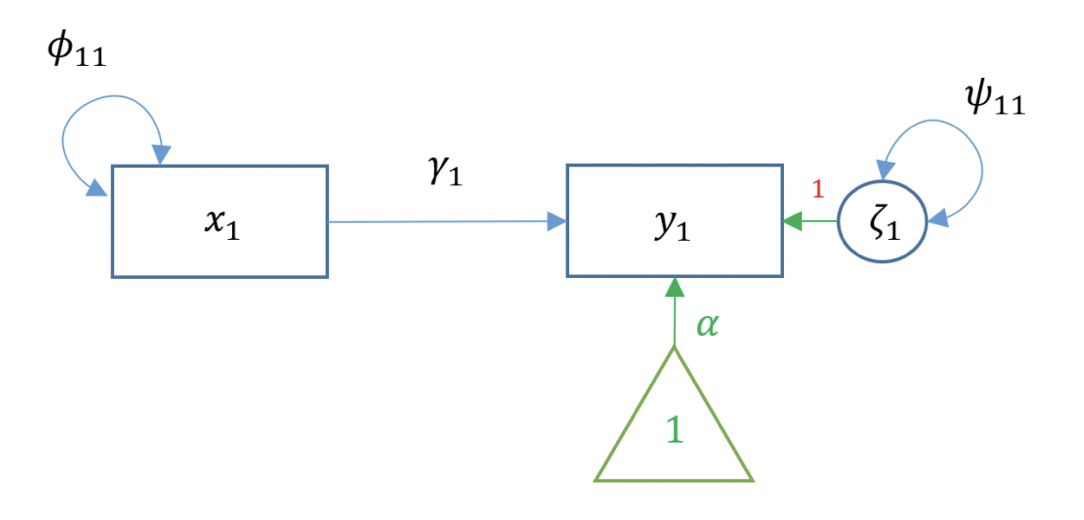
\includegraphics[width=0.8\textwidth,height=\textheight]{chapters/path_analysis/../../figures/lisrel_bivariate_reg.png}

}

\caption{\label{fig-lisrel_bivariate_reg}Diagramma di percorso per il
modello di regressione bivariato.}

\end{figure}%

Facciamo un esempio numerico. Simuliamo tre variabili: x1, x2, y.

\begin{Shaded}
\begin{Highlighting}[]
\FunctionTok{set.seed}\NormalTok{(}\DecValTok{42}\NormalTok{)}
\NormalTok{n }\OtherTok{\textless{}{-}} \DecValTok{100}
\NormalTok{x1 }\OtherTok{\textless{}{-}} \FunctionTok{rnorm}\NormalTok{(n, }\DecValTok{90}\NormalTok{, }\DecValTok{20}\NormalTok{)}
\NormalTok{x2 }\OtherTok{\textless{}{-}}\NormalTok{ x1 }\SpecialCharTok{+} \FunctionTok{rnorm}\NormalTok{(n, }\DecValTok{0}\NormalTok{, }\DecValTok{30}\NormalTok{)}
\NormalTok{y }\OtherTok{\textless{}{-}} \DecValTok{25} \SpecialCharTok{+} \FloatTok{0.5} \SpecialCharTok{*}\NormalTok{ x1 }\SpecialCharTok{+} \FloatTok{1.0} \SpecialCharTok{*}\NormalTok{ x2 }\SpecialCharTok{+} \FunctionTok{rnorm}\NormalTok{(n, }\DecValTok{0}\NormalTok{, }\DecValTok{30}\NormalTok{)}

\NormalTok{dat }\OtherTok{\textless{}{-}} \FunctionTok{data.frame}\NormalTok{(}
\NormalTok{    y, x1, x2}
\NormalTok{)}

\FunctionTok{cor}\NormalTok{(dat) }\SpecialCharTok{|\textgreater{}}
    \FunctionTok{round}\NormalTok{(}\DecValTok{2}\NormalTok{)}
\end{Highlighting}
\end{Shaded}

A matrix: 3 x 3 of type dbl

\begin{longtable}[]{@{}llll@{}}
\toprule\noalign{}
& y & x1 & x2 \\
\midrule\noalign{}
\endhead
\bottomrule\noalign{}
\endlastfoot
y & 1.00 & 0.55 & 0.80 \\
x1 & 0.55 & 1.00 & 0.62 \\
x2 & 0.80 & 0.62 & 1.00 \\
\end{longtable}

Consideriamo la relazione tra \texttt{x1} (variabile endogena) e
\texttt{y} (variabile endogena). In R possiamo adattare ai dati un
modello di regressione mediante la funzione \texttt{lm}.

\begin{Shaded}
\begin{Highlighting}[]
\NormalTok{m1a }\OtherTok{\textless{}{-}} \FunctionTok{lm}\NormalTok{(y }\SpecialCharTok{\textasciitilde{}}\NormalTok{ x1, }\AttributeTok{data =}\NormalTok{ dat)}
\FunctionTok{summary}\NormalTok{(m1a)}
\end{Highlighting}
\end{Shaded}

\begin{verbatim}

Call:
lm(formula = y ~ x1, data = dat)

Residuals:
    Min      1Q  Median      3Q     Max 
-82.462 -29.539  -3.437  29.200 122.234 

Coefficients:
            Estimate Std. Error t value Pr(>|t|)    
(Intercept)  37.5974    18.9844   1.980   0.0505 .  
x1            1.3286     0.2042   6.508 3.25e-09 ***
---
Signif. codes:  0 '***' 0.001 '**' 0.01 '*' 0.05 '.' 0.1 ' ' 1

Residual standard error: 42.31 on 98 degrees of freedom
Multiple R-squared:  0.3018,    Adjusted R-squared:  0.2946 
F-statistic: 42.35 on 1 and 98 DF,  p-value: 3.251e-09
\end{verbatim}

Usiamo ora lavaan per adattare lo stesso modello ai dati.

\begin{Shaded}
\begin{Highlighting}[]
\NormalTok{m1b }\OtherTok{\textless{}{-}} \StringTok{"}
\StringTok{    y \textasciitilde{} 1 + x1}
\StringTok{"}
\NormalTok{fit1b }\OtherTok{\textless{}{-}} \FunctionTok{sem}\NormalTok{(m1b, }\AttributeTok{data =}\NormalTok{ dat)}
\FunctionTok{parameterEstimates}\NormalTok{(fit1b) }
\end{Highlighting}
\end{Shaded}

A lavaan.data.frame: 5 x 9

\begin{longtable}[]{@{}
  >{\raggedright\arraybackslash}p{(\columnwidth - 16\tabcolsep) * \real{0.1111}}
  >{\raggedright\arraybackslash}p{(\columnwidth - 16\tabcolsep) * \real{0.1111}}
  >{\raggedright\arraybackslash}p{(\columnwidth - 16\tabcolsep) * \real{0.1111}}
  >{\raggedright\arraybackslash}p{(\columnwidth - 16\tabcolsep) * \real{0.1111}}
  >{\raggedright\arraybackslash}p{(\columnwidth - 16\tabcolsep) * \real{0.1111}}
  >{\raggedright\arraybackslash}p{(\columnwidth - 16\tabcolsep) * \real{0.1111}}
  >{\raggedright\arraybackslash}p{(\columnwidth - 16\tabcolsep) * \real{0.1111}}
  >{\raggedright\arraybackslash}p{(\columnwidth - 16\tabcolsep) * \real{0.1111}}
  >{\raggedright\arraybackslash}p{(\columnwidth - 16\tabcolsep) * \real{0.1111}}@{}}
\toprule\noalign{}
\begin{minipage}[b]{\linewidth}\raggedright
lhs \textless chr\textgreater{}
\end{minipage} & \begin{minipage}[b]{\linewidth}\raggedright
op \textless chr\textgreater{}
\end{minipage} & \begin{minipage}[b]{\linewidth}\raggedright
rhs \textless chr\textgreater{}
\end{minipage} & \begin{minipage}[b]{\linewidth}\raggedright
est \textless dbl\textgreater{}
\end{minipage} & \begin{minipage}[b]{\linewidth}\raggedright
se \textless dbl\textgreater{}
\end{minipage} & \begin{minipage}[b]{\linewidth}\raggedright
z \textless dbl\textgreater{}
\end{minipage} & \begin{minipage}[b]{\linewidth}\raggedright
pvalue \textless dbl\textgreater{}
\end{minipage} & \begin{minipage}[b]{\linewidth}\raggedright
ci.lower \textless dbl\textgreater{}
\end{minipage} & \begin{minipage}[b]{\linewidth}\raggedright
ci.upper \textless dbl\textgreater{}
\end{minipage} \\
\midrule\noalign{}
\endhead
\bottomrule\noalign{}
\endlastfoot
y & \textasciitilde1 & & 37.59740 & 18.7936187 & 2.000541 & 4.544188e-02
& 0.7625888 & 74.432220 \\
y & \textasciitilde{} & x1 & 1.32865 & 0.2021064 & 6.574012 &
4.897727e-11 & 0.9325284 & 1.724771 \\
y & \textasciitilde\textasciitilde{} & y & 1754.10024 & 248.0672346 &
7.071068 & 1.537437e-12 & 1267.8973923 & 2240.303084 \\
x1 & \textasciitilde\textasciitilde{} & x1 & 429.43203 & 0.0000000 & NA
& NA & 429.4320313 & 429.432031 \\
x1 & \textasciitilde1 & & 90.65030 & 0.0000000 & NA & NA & 90.6502963 &
90.650296 \\
\end{longtable}

L'intercetta di \texttt{y\ \textasciitilde{}1} (37.597) e il
coefficiente di regressione di \texttt{y\ \textasciitilde{}\ x1} (1.329)
corrispondono all'output di \texttt{lm()} con piccoli errori di
arrotondamento. L'intercetta per \texttt{x1\ \textasciitilde{}1}
(90.650) e la sua varianza
\texttt{x1\ \textasciitilde{}\textasciitilde{}\ x1} (429.432) descrivono
una media ed una varianza esogena e corrispondono alla media e alla
varianza univariate:

\begin{Shaded}
\begin{Highlighting}[]
\FunctionTok{mean}\NormalTok{(dat}\SpecialCharTok{$}\NormalTok{x1)}
\end{Highlighting}
\end{Shaded}

90.6502963122602

\begin{Shaded}
\begin{Highlighting}[]
\FunctionTok{var}\NormalTok{(dat}\SpecialCharTok{$}\NormalTok{x1) }\SpecialCharTok{*}\NormalTok{ (}\FunctionTok{length}\NormalTok{(dat}\SpecialCharTok{$}\NormalTok{x1) }\SpecialCharTok{{-}} \DecValTok{1}\NormalTok{) }\SpecialCharTok{/} \FunctionTok{length}\NormalTok{(dat}\SpecialCharTok{$}\NormalTok{x1)}
\end{Highlighting}
\end{Shaded}

429.432031274383

La varianza residua di \texttt{y},
\texttt{y\ \textasciitilde{}\textasciitilde{}\ y} corrisponde alla quota
della varianza osservata della variabile \texttt{y} che non è spiegata
dalla relazione lineare su \texttt{x1}:

\begin{Shaded}
\begin{Highlighting}[]
\FunctionTok{var}\NormalTok{(dat}\SpecialCharTok{$}\NormalTok{y) }\SpecialCharTok{*} \DecValTok{99} \SpecialCharTok{/} \DecValTok{100} \SpecialCharTok{{-}}\NormalTok{ (}\FloatTok{1.3286} \SpecialCharTok{*} \FloatTok{429.432} \SpecialCharTok{*} \FloatTok{1.3286}\NormalTok{)}
\end{Highlighting}
\end{Shaded}

1754.15693691975

La funzione \texttt{semPaths} consente di creare un diagramma di
percorso a partire dall'oggetto creato da \texttt{sem}.

\begin{Shaded}
\begin{Highlighting}[]
\NormalTok{semPlot}\SpecialCharTok{::}\FunctionTok{semPaths}\NormalTok{(}
\NormalTok{    fit1b,}
    \AttributeTok{layout =} \StringTok{"tree"}\NormalTok{, }\AttributeTok{sizeMan =} \DecValTok{7}\NormalTok{, }\AttributeTok{sizeInt =} \DecValTok{5}\NormalTok{, }\AttributeTok{style =} \StringTok{"ram"}\NormalTok{, }
    \AttributeTok{residuals =} \ConstantTok{TRUE}\NormalTok{, }\AttributeTok{intAtSide =} \ConstantTok{FALSE}\NormalTok{, }\AttributeTok{edge.label.cex =} \FloatTok{1.15}\NormalTok{,}
    \AttributeTok{whatLabels =} \StringTok{"est"}\NormalTok{, }\AttributeTok{nCharNodes =} \DecValTok{0}\NormalTok{, }\AttributeTok{normalize =} \ConstantTok{FALSE}
\NormalTok{)}
\end{Highlighting}
\end{Shaded}

\includegraphics[width=5in,height=3.08333in]{chapters/path_analysis/01_path_analysis_files/figure-pdf/cell-9-output-1.png}

\section{Analisi dei percorsi e regressione
multipla}\label{analisi-dei-percorsi-e-regressione-multipla}

La regressione semplice è limitata a una sola variabile esogena. Nella
pratica, un ricercatore può essere interessato a studiare come un gruppo
di variabili esogene possano predire una variabile di esito. Supponiamo
di avere ancora una sola variabile di esito endogena ma due predittori
esogeni; questo caso è noto come regressione multipla:

\[
y_1 = \alpha_1 + \gamma_1 x_1 + \gamma_2 x_2 + \zeta_1.
\]

Il diagramma di percorso mostra la relazione tra tutte le variabili,
comprendendo anche i fattori di disturbo, e fornisce dunque la
rappresentazione grafica dell'equazione precedente.

\begin{figure}[H]

\centering{

\includegraphics[width=0.8\textwidth,height=\textheight]{chapters/path_analysis/../../figures/lisrel_mr.png}

}

\caption{\label{fig-lisrel_mr}Diagramma di percorso per il modello di
regressione multipla.}

\end{figure}%

I coefficienti di percorso associati alle frecce orientate esprimono la
portata del nesso causale e corrispondono ai pesi beta (ovvero ai
coefficienti parziali di regressione standardizzati). Le frecce non
orientate esprimono la portata della pura associazione tra variabili e
dunque corrispondono alle correlazioni/covarianze.

In un diagramma di percorso, il numero di equazioni corrisponde al
numero di variabili endogene del modello. Nel caso specifico, poiché vi
è una sola variabile endogena (ovvero \(y\)), esiste un'unica equazione
che descrive le relazioni causalitiche interne al path diagram.
All'interno di ciascuna equazione, inoltre, il numero di termini
corrisponde al numero di frecce orientate che puntano verso la variabile
endogena. Nell'esempio sopra citato, pertanto, la sola equazione del
modello contiene tre termini, ciascuno associato ad una freccia
orientata.

Usando \texttt{lm} otteniamo la seguente stima dei coefficienti:

\begin{Shaded}
\begin{Highlighting}[]
\NormalTok{m2a }\OtherTok{\textless{}{-}} \FunctionTok{lm}\NormalTok{(y }\SpecialCharTok{\textasciitilde{}} \DecValTok{1} \SpecialCharTok{+}\NormalTok{ x1 }\SpecialCharTok{+}\NormalTok{ x2, }\AttributeTok{data =}\NormalTok{ dat)}
\NormalTok{fit2a }\OtherTok{\textless{}{-}} \FunctionTok{summary}\NormalTok{(m2a) }
\end{Highlighting}
\end{Shaded}

Gli stessi risultati si ottengono con lavaan.

\begin{Shaded}
\begin{Highlighting}[]
\NormalTok{m2b }\OtherTok{\textless{}{-}} \StringTok{"}
\StringTok{    y \textasciitilde{} 1 + x1 + x2}
\StringTok{    x1 \textasciitilde{}\textasciitilde{} x1}
\StringTok{    x2 \textasciitilde{}\textasciitilde{} x2}
\StringTok{    x1 \textasciitilde{}\textasciitilde{} x2}
\StringTok{"}
\end{Highlighting}
\end{Shaded}

\begin{Shaded}
\begin{Highlighting}[]
\NormalTok{fit2b }\OtherTok{\textless{}{-}} \FunctionTok{sem}\NormalTok{(m2b, }\AttributeTok{data =}\NormalTok{ dat)}
\end{Highlighting}
\end{Shaded}

\begin{Shaded}
\begin{Highlighting}[]
\FunctionTok{parameterEstimates}\NormalTok{(fit2b)}
\end{Highlighting}
\end{Shaded}

A lavaan.data.frame: 9 x 9

\begin{longtable}[]{@{}
  >{\raggedright\arraybackslash}p{(\columnwidth - 16\tabcolsep) * \real{0.1111}}
  >{\raggedright\arraybackslash}p{(\columnwidth - 16\tabcolsep) * \real{0.1111}}
  >{\raggedright\arraybackslash}p{(\columnwidth - 16\tabcolsep) * \real{0.1111}}
  >{\raggedright\arraybackslash}p{(\columnwidth - 16\tabcolsep) * \real{0.1111}}
  >{\raggedright\arraybackslash}p{(\columnwidth - 16\tabcolsep) * \real{0.1111}}
  >{\raggedright\arraybackslash}p{(\columnwidth - 16\tabcolsep) * \real{0.1111}}
  >{\raggedright\arraybackslash}p{(\columnwidth - 16\tabcolsep) * \real{0.1111}}
  >{\raggedright\arraybackslash}p{(\columnwidth - 16\tabcolsep) * \real{0.1111}}
  >{\raggedright\arraybackslash}p{(\columnwidth - 16\tabcolsep) * \real{0.1111}}@{}}
\toprule\noalign{}
\begin{minipage}[b]{\linewidth}\raggedright
lhs \textless chr\textgreater{}
\end{minipage} & \begin{minipage}[b]{\linewidth}\raggedright
op \textless chr\textgreater{}
\end{minipage} & \begin{minipage}[b]{\linewidth}\raggedright
rhs \textless chr\textgreater{}
\end{minipage} & \begin{minipage}[b]{\linewidth}\raggedright
est \textless dbl\textgreater{}
\end{minipage} & \begin{minipage}[b]{\linewidth}\raggedright
se \textless dbl\textgreater{}
\end{minipage} & \begin{minipage}[b]{\linewidth}\raggedright
z \textless dbl\textgreater{}
\end{minipage} & \begin{minipage}[b]{\linewidth}\raggedright
pvalue \textless dbl\textgreater{}
\end{minipage} & \begin{minipage}[b]{\linewidth}\raggedright
ci.lower \textless dbl\textgreater{}
\end{minipage} & \begin{minipage}[b]{\linewidth}\raggedright
ci.upper \textless dbl\textgreater{}
\end{minipage} \\
\midrule\noalign{}
\endhead
\bottomrule\noalign{}
\endlastfoot
y & \textasciitilde1 & & 44.453736 & 13.4573999 & 3.303293 &
9.555645e-04 & 18.0777172 & 70.8297555 \\
y & \textasciitilde{} & x1 & 0.199143 & 0.1850347 & 1.076247 &
2.818170e-01 & -0.1635183 & 0.5618043 \\
y & \textasciitilde{} & x2 & 1.085293 & 0.1110220 & 9.775475 &
0.000000e+00 & 0.8676940 & 1.3028924 \\
x1 & \textasciitilde\textasciitilde{} & x1 & 429.432014 & 60.7308578 &
7.071068 & 1.537437e-12 & 310.4017199 & 548.4623082 \\
x2 & \textasciitilde\textasciitilde{} & x2 & 1192.840139 & 168.6930702 &
7.071068 & 1.537437e-12 & 862.2077969 & 1523.4724811 \\
x1 & \textasciitilde\textasciitilde{} & x2 & 446.926552 & 84.3793272 &
5.296636 & 1.179557e-07 & 281.5461093 & 612.3069940 \\
y & \textasciitilde\textasciitilde{} & y & 896.963117 & 126.8497404 &
7.071068 & 1.537437e-12 & 648.3421938 & 1145.5840392 \\
x1 & \textasciitilde1 & & 90.650296 & 2.0722741 & 43.744355 &
0.000000e+00 & 86.5887135 & 94.7118788 \\
x2 & \textasciitilde1 & & 88.025785 & 3.4537518 & 25.487004 &
0.000000e+00 & 81.2565556 & 94.7950138 \\
\end{longtable}

Esaminiamo il diagramma di percorso.

\begin{Shaded}
\begin{Highlighting}[]
\NormalTok{semPlot}\SpecialCharTok{::}\FunctionTok{semPaths}\NormalTok{(}
\NormalTok{    fit2b,}
    \AttributeTok{layout =} \StringTok{"tree"}\NormalTok{, }\AttributeTok{sizeMan =} \DecValTok{7}\NormalTok{, }\AttributeTok{sizeInt =} \DecValTok{5}\NormalTok{, }\AttributeTok{style =} \StringTok{"ram"}\NormalTok{,}
    \AttributeTok{residuals =} \ConstantTok{TRUE}\NormalTok{, }\AttributeTok{intAtSide =} \ConstantTok{FALSE}\NormalTok{, }\AttributeTok{edge.label.cex =} \FloatTok{1.15}\NormalTok{,}
    \AttributeTok{whatLabels =} \StringTok{"est"}\NormalTok{, }\AttributeTok{nCharNodes =} \DecValTok{0}\NormalTok{, }\AttributeTok{normalize =} \ConstantTok{FALSE}
\NormalTok{)}
\end{Highlighting}
\end{Shaded}

\includegraphics[width=5in,height=3.08333in]{chapters/path_analysis/01_path_analysis_files/figure-pdf/cell-14-output-1.png}

\section{Effetti diretti e indiretti}\label{effetti-diretti-e-indiretti}

L'analisi del percorso offre un metodo essenziale per distinguere tra
diverse tipologie di effetti che influenzano le variabili in esame:
l'effetto diretto, l'effetto indiretto e l'effetto totale. Gli effetti
diretti rappresentano l'influenza che una variabile esercita su un'altra
senza mediazione di altre variabili intermedie. Gli effetti indiretti,
invece, operano attraverso l'intermediazione di almeno una variabile
aggiuntiva nel processo. L'effetto totale è la somma cumulativa degli
effetti diretti e indiretti.

Nella Figura~\ref{fig-path_03}, la variabile \(y_1\) esercita un effetto
diretto sulla variabile \(y_2\). Allo stesso tempo, \(y_1\) produce un
effetto indiretto sulla variabile \(y_3\), poiché non esiste una
connessione causale diretta tra \(y_1\) e \(y_3\). Nel contesto
rappresentato, la variabile \(y_1\) agisce come variabile esogena,
mentre le variabili \(y_2\) e \(y_3\) fungono da variabili endogene.

\begin{figure}[H]

\centering{

\includegraphics[width=0.4\textwidth,height=\textheight]{chapters/path_analysis/../../figures/path_03.png}

}

\caption{\label{fig-path_03}Diagramma di percorso per un modello a
catena.}

\end{figure}%

\section{Le regole di Wright}\label{le-regole-di-wright}

L'obiettivo primario dell'analisi del percorso consiste nella
decomposizione della correlazione (o della covarianza) in base alla
somma dei vari percorsi (diretti e indiretti) che collegano due
variabili mediante coefficienti noti come ``path coefficients.''
Utilizzando il diagramma del percorso, Sewall Wright (1921, 1934)
formulò le regole che, tramite le ``tracing rules,'' stabiliscono il
collegamento tra le correlazioni (o covarianze) delle variabili e i
parametri del modello. Le tracing rules si possono esprimere nei
seguenti termini:

\begin{itemize}
\tightlist
\item
  È possibile procedere in avanti lungo una freccia e poi a ritroso,
  seguendo la direzione della freccia, ma non è permesso muoversi in
  avanti e poi tornare indietro.
\item
  Un percorso composto non deve attraversare più di una volta la stessa
  variabile, cioè non possono esserci cicli.
\item
  Un percorso non può contenere più di una linea curva.
\end{itemize}

Il termine ``percorso'' fa riferimento al tracciato che connette due
variabili e si compone di sequenze di frecce unidirezionali e curve non
direzionali. A ciascun percorso valido (cioè conforme alle regole di
Wright) viene assegnato un valore numerico che rappresenta il prodotto
dei coefficienti presenti lungo il percorso stesso. I coefficienti di
percorso possono essere coefficienti parziali di regressione
standardizzati se il legame è unidirezionale, oppure coefficienti di
correlazione se il legame è bidirezionale.

\section{Scomposizione delle
correlazioni/covarianze}\label{scomposizione-delle-correlazionicovarianze}

Il principio fondamentale è stato formulato da Sewall Wright (1934) nel
seguente modo:

\begin{quote}
Ogni correlazione tra variabili in una rete di relazioni sequenziali può
essere analizzata nei contributi provenienti da tutti i percorsi
(diretti o attraverso fattori comuni) con i quali le due variabili sono
connesse. Ogni contributo ha un valore pari al prodotto dei coefficienti
relativi ai percorsi elementari. Se sono presenti correlazioni residue
(rappresentate da frecce bidirezionali), uno (ma mai più di uno) dei
coefficienti moltiplicati per ottenere il contributo del percorso di
connessione può essere un coefficiente di correlazione. Gli altri sono
tutti coefficienti di percorso.
\end{quote}

Da questo principio possiamo derivare la regola di scomposizione della
correlazione: la correlazione o covarianza tra due variabili può essere
scomposta in un numero di termini uguale al numero di percorsi che le
collegano. Ogni termine è ottenuto dal prodotto dei coefficienti
associati alle variabili lungo il percorso. In altre parole, è possibile
decomporre la correlazione o la covarianza tra due variabili in tanti
contributi quanti sono i percorsi possibili che collegano le due
variabili.

\subsection{Scomposizione della
varianza}\label{scomposizione-della-varianza}

La decomposizione della varianza di una variabile endogena può essere
affrontata attraverso una suddivisione in due componenti: una componente
spiegata, attribuibile alle variabili che esercitano un'influenza
causale su di essa, e una componente non spiegata. La componente
spiegata della varianza deriva dall'aggregazione degli effetti delle
diverse variabili che sono connessi alla variabile endogena, rispettando
le regole di tracciamento definite da Wright. Il numero di addendi
corrisponde al numero di percorsi che collegano la variabile endogena a
se stessa. In tal modo, la varianza spiegata rappresenta la parte della
varianza totale della variabile endogena che può essere attribuita alle
influenze delle variabili correlate attraverso i percorsi definibili
all'interno del modello.

\subsection{Relazioni tra variabili endogene e
esogene}\label{relazioni-tra-variabili-endogene-e-esogene}

Complessivamente, i concetti di varianza, covarianza e correlazione
informano direttamente il calcolo dei coefficienti di percorso in un
path diagram secondo le seguenti ``8 regole dei coefficienti di
percorso''.

\begin{itemize}
\tightlist
\item
  Regola 1: Le relazioni non specificate tra le variabili esogene sono
  semplicemente le loro correlazioni bivariate.
\item
  Regola 2: Quando due variabili sono collegate da un singolo percorso,
  il coefficiente di quel percorso è il coefficiente di regressione.
\item
  Regola 3: La forza di un percorso composto (che include più
  collegamenti) è il prodotto dei coefficienti individuali.
\item
  Regola 4: Quando le variabili sono collegate da più di un percorso,
  ciascun percorso è il coefficiente di regressione ``parziale''.
\item
  Regola 5: Gli errori sulle variabili endogene si riferiscono alle
  correlazioni o varianze non spiegate che derivano dalle variabili non
  misurate.
\item
  Regola 6: Le correlazioni non analizzate (residui) tra due variabili
  endogene sono le loro correlazioni parziali.
\item
  Regola 7: L'effetto totale che una variabile ha su un'altra è la somma
  dei suoi effetti diretti e indiretti.
\item
  Regola 8: L'effetto totale (compresi i percorsi non diretti) è
  equivalente alla correlazione totale.
\end{itemize}

\textbf{Esempio.} Consideriamo nuovamente il modello di regressione
multipla con due variabili esogene e una sola variabile endogena che è
stato presentato sopra.

La la covarianza tra \texttt{y} e \texttt{x1}

\begin{Shaded}
\begin{Highlighting}[]
\FunctionTok{cov}\NormalTok{(dat}\SpecialCharTok{$}\NormalTok{y, dat}\SpecialCharTok{$}\NormalTok{x1) }\SpecialCharTok{*} \DecValTok{99} \SpecialCharTok{/} \DecValTok{100}
\end{Highlighting}
\end{Shaded}

570.56471345413

può essere ricavata usando le regole di Wright nel modo seguente:

\begin{Shaded}
\begin{Highlighting}[]
\FloatTok{0.199} \SpecialCharTok{*} \FloatTok{429.43} \SpecialCharTok{+} \FloatTok{1.085} \SpecialCharTok{*} \FloatTok{446.93}
\end{Highlighting}
\end{Shaded}

570.37562

La quota di varianza non spiegata della variabile endogena è:

\begin{Shaded}
\begin{Highlighting}[]
\NormalTok{(}\FunctionTok{var}\NormalTok{(dat}\SpecialCharTok{$}\NormalTok{y) }\SpecialCharTok{*} \DecValTok{99} \SpecialCharTok{/} \DecValTok{100}\NormalTok{) }\SpecialCharTok{{-}}\NormalTok{ (}
    \FloatTok{0.199}\SpecialCharTok{\^{}}\DecValTok{2} \SpecialCharTok{*} \FloatTok{429.43} \SpecialCharTok{+}\NormalTok{ (}\FloatTok{1.085}\NormalTok{)}\SpecialCharTok{\^{}}\DecValTok{2} \SpecialCharTok{*} \FloatTok{1192.84} \SpecialCharTok{+} \DecValTok{2} \SpecialCharTok{*}\NormalTok{ (}\FloatTok{0.199} \SpecialCharTok{*} \FloatTok{1.085} \SpecialCharTok{*} \FloatTok{446.93}\NormalTok{)}
\NormalTok{)}
\end{Highlighting}
\end{Shaded}

897.936130308472

\section{Oltre la regressione
multipla}\label{oltre-la-regressione-multipla}

Approfondiamo l'utilizzo dell'analisi dei percorsi (path analysis) per
studiare un modello di mediazione che supera i limiti della classica
regressione multipla. L'analisi di mediazione è un metodo statistico
ampiamente impiegato dai psicologi per esaminare le relazioni complesse
tra le variabili di uno studio. Questa metodologia può essere applicata
in studi osservazionali per affinare la comprensione della relazione tra
variabili predittive e variabili di esito, introducendo mediatori.
L'integrazione di mediatori permette di esplorare e chiarire i
meccanismi sottostanti che influenzano la relazione tra le variabili
principali, fornendo una visione più dettagliata e complessa degli
effetti e delle interazioni in gioco.

Prenderemo in esame un modello teorico specifico, ispirato alla Self
Determination Theory (SDT) di Deci e Ryan (2000), una delle teorie più
influenti nel campo della motivazione. In questo contesto, utilizzeremo
la path analysis per valutare come la SDT possa aiutarci a comprendere i
fattori psicologici e comportamentali che influenzano i sintomi bulimici
in un gruppo di giovani donne adulte. Più specificamente, esamineremo
come l'appagamento (soddisfazione) e l'esaurimento (frustrazione) delle
risorse psicologiche essenziali, o bisogni psicologici (ad esempio, per
l'autonomia, la competenza e la relazionalità), possono prevedere in
modo differenziale i sintomi bulimici nelle donne attraverso due
mediatori chiave, l'approvazione degli ideali culturali sulla magrezza e
inflessibilità delle opinioni sul proprio corpo. Secondo la SDT, i
bisogni psicologici influenzano la capacità di un individuo di
autoregolarsi e far fronte alle richieste della vita quotidiana e
possono rendere gli individui vulnerabili al malessere psicologico se i
bisogni psicologici vengono frustrati (Vansteenkiste \& Ryan, 2013). La
frustrazione dei bisogni può essere psicologicamente più depauperante
della mancanza di soddisfazione dei bisogni.

Gli individui i cui bisogni vengono frustrati possono impegnarsi in
attività malsane e comportamenti compensatori al fine di riconquistare
una soddisfazione dei bisogni a breve termine. La frustrazione dei
bisogni rende gli individui più vulnerabili agli ideali culturali, in
quanto le risorse personali per rifiutare questi ideali sono esaurite
(Pelletier \& Dion, 2007).

Il modello che verrà testato propone che le donne i cui bisogni
psicologici sono frustrati avalleranno ideali sociali più problematici
sulla magrezza rispetto alle donne i cui bisogni psicologici sono
soddisfatti. La frustrazione dei bisogni sarà anche predittiva
dell'inflessibilità degli schemi corporei, poiché è stato dimostrato che
la frustrazione dei bisogni porta a disturbi dell'immagine corporea e a
comportamenti alimentari patologici (Boone, Vansteenkiste, Soenens, Van
der Kaap-Deeder e Verstuyf, 2014). Il modello propone inoltre che una
maggiore approvazione degli ideali culturali sulla sarà predittiva di
una maggiore inflessibilità sugli schemi corporei che, di per sé, è
predittiva dei sintomi bulimici.

Il campione include 192 partecipanti, in maggioranza donne, di età media
21.2 anni (SD = 6.89). Sono stati somministrati i seguenti strumenti:

\begin{itemize}
\tightlist
\item
  \emph{Body Image-Acceptance and Action Questionnaire} (Sandoz, Wilson,
  Merwin, \& Kellum, 2013), per misurare l'inflessibilità relativa alla
  propria immagine corporea,
\item
  \emph{Endorsement of Society's Beliefs Related to Thinness and
  Obesity} (Boyer, 1991), per valutare l'internalizzazione degli ideali
  di magrezza,
\item
  \emph{Basic Psychological Needs Satisfaction and Frustration Scale}
  (Chen et al., 2015), per misurare la soddisfazione e la frustrazione
  dei bisogni,
\item
  \emph{Eating Disorders Inventory-2 -- Bulimic Symptomology Subscale}
  (Garner, 1991), per misurare i sintomi bulimici.
\end{itemize}

I dati sono i seguenti.

\begin{Shaded}
\begin{Highlighting}[]
\NormalTok{upper }\OtherTok{\textless{}{-}} \StringTok{\textquotesingle{}}
\StringTok{  1 0.44 {-}0.41 0.55 0.63}
\StringTok{  1 {-}0.37 0.45 0.44}
\StringTok{  1 {-}0.71 {-}0.39}
\StringTok{  1 0.47}
\StringTok{  1}
\StringTok{  \textquotesingle{}}
\end{Highlighting}
\end{Shaded}

\begin{Shaded}
\begin{Highlighting}[]
\CommentTok{\# BFLX – Body Inflexibility,}
\CommentTok{\# }\RegionMarkerTok{END}\CommentTok{ – Endorsement of Societal Beliefs about Thinness and Obesity,}
\CommentTok{\# MNS – Mean Need Satisfaction,}
\CommentTok{\# MNF – Mean Need Frustration,}
\CommentTok{\# BULS – Bulimic Symptoms}
\NormalTok{dat\_cov }\OtherTok{\textless{}{-}}\NormalTok{ lavaan}\SpecialCharTok{::}\FunctionTok{getCov}\NormalTok{(}
\NormalTok{    upper,}
    \AttributeTok{lower =} \ConstantTok{FALSE}\NormalTok{,}
    \AttributeTok{names =} \FunctionTok{c}\NormalTok{(}\StringTok{"BFLX"}\NormalTok{, }\StringTok{"END"}\NormalTok{, }\StringTok{"MNS"}\NormalTok{, }\StringTok{"MNF"}\NormalTok{, }\StringTok{"BULS"}\NormalTok{)}
\NormalTok{)}
\NormalTok{dat\_cov}
\end{Highlighting}
\end{Shaded}

A matrix: 5 x 5 of type dbl

\begin{longtable}[]{@{}llllll@{}}
\toprule\noalign{}
& BFLX & END & MNS & MNF & BULS \\
\midrule\noalign{}
\endhead
\bottomrule\noalign{}
\endlastfoot
BFLX & 1.00 & 0.44 & -0.41 & 0.55 & 0.63 \\
END & 0.44 & 1.00 & -0.37 & 0.45 & 0.44 \\
MNS & -0.41 & -0.37 & 1.00 & -0.71 & -0.39 \\
MNF & 0.55 & 0.45 & -0.71 & 1.00 & 0.47 \\
BULS & 0.63 & 0.44 & -0.39 & 0.47 & 1.00 \\
\end{longtable}

\subsection{Modello di mediazione}\label{modello-di-mediazione}

\begin{Shaded}
\begin{Highlighting}[]
\NormalTok{data }\OtherTok{\textless{}{-}} \FunctionTok{c}\NormalTok{(}
    \DecValTok{0}\NormalTok{, }\StringTok{"a"}\NormalTok{, }\DecValTok{0}\NormalTok{,}
    \DecValTok{0}\NormalTok{, }\DecValTok{0}\NormalTok{, }\DecValTok{0}\NormalTok{,}
    \StringTok{"b"}\NormalTok{, }\StringTok{"c\_prime"}\NormalTok{, }\DecValTok{0}
\NormalTok{)}
\NormalTok{M }\OtherTok{\textless{}{-}} \FunctionTok{matrix}\NormalTok{(}\AttributeTok{nrow =} \DecValTok{3}\NormalTok{, }\AttributeTok{ncol =} \DecValTok{3}\NormalTok{, }\AttributeTok{byrow =} \ConstantTok{TRUE}\NormalTok{, }\AttributeTok{data =}\NormalTok{ data)}
\NormalTok{plot }\OtherTok{\textless{}{-}} \FunctionTok{plotmat}\NormalTok{(M,}
    \AttributeTok{pos =} \FunctionTok{c}\NormalTok{(}\DecValTok{1}\NormalTok{, }\DecValTok{2}\NormalTok{),}
    \AttributeTok{name =} \FunctionTok{c}\NormalTok{(}\StringTok{"X"}\NormalTok{, }\StringTok{"M"}\NormalTok{, }\StringTok{"Y"}\NormalTok{),}
    \AttributeTok{box.type =} \StringTok{"rect"}\NormalTok{, }\AttributeTok{box.size =} \FloatTok{0.12}\NormalTok{, }\AttributeTok{box.prop =} \FloatTok{0.5}\NormalTok{, }\AttributeTok{curve =} \DecValTok{0}
\NormalTok{)}
\end{Highlighting}
\end{Shaded}

\includegraphics[width=5in,height=3.08333in]{chapters/path_analysis/01_path_analysis_files/figure-pdf/cell-20-output-1.png}

Nel modello di mediazione di base abbiamo tre variabili chiave: la
variabile indipendente \(X\), la variabile dipendente \(Y\) e il
mediatore \(M\). La freccia da \(X\) a \(M\) (etichettata con `a')
rappresenta l'effetto di \(X\) su \(M\). La freccia da \(M\) a \(Y\)
(etichettata con `b') rappresenta l'effetto di \(M\) su \(Y\), mentre la
freccia tratteggiata da \(X\) a \(Y\) (etichettata con ``c''')
rappresenta l'effetto diretto di \(X\) su \(Y\), escludendo la
mediazione di \(M\).

Possiamo formalizzare il modello statistico di mediazione in equazioni
di regressione lineare come segue:

\[M = a_0 + a \times X + e_M\]

\[Y = b_0 + b \times M + c' \times X + e_Y\]

Nella prima equazione lineare, \(M\) è regredito su \(X\) con
un'intercetta\(a_0\), pendenza\(a\)e termine di errore\(e_M\). Questa
equazione rappresenta il percorso \(X \rightarrow M\)con\(a\)come
effetto di\(X\)su\(M\). Nella seconda equazione, \(Y\) è regredito su
\(M\) e \(X\) con un'intercetta \(b_0\), pendenze \(b\) e \(c'\) e
termine di errore \(e_Y\). Questa equazione rappresenta due percorsi:
\(M \rightarrow Y\) e \(X \rightarrow Y\), con \(b\) come effetto di
\(M\) su \(Y\) e \(c'\) come effetto diretto di \(X\) su \(Y\).

Nel contesto della modellazione di equazioni strutturali, il metodo più
comune per calcolare gli effetti diretti, indiretti e totali si basa sul
prodotto dei coefficienti, come riassunto nelle seguenti formule:

\begin{itemize}
\tightlist
\item
  Effetto diretto = \(c'\)
\item
  Effetto indiretto = \(b \times a\)
\item
  Effetto totale = \(c' + b \times a\)
\end{itemize}

\subsection{Stima degli Effetti Diretti, Indiretti e
Totali}\label{stima-degli-effetti-diretti-indiretti-e-totali}

Le tecniche di modellazione di equazioni strutturali permettono di
stimare tutti i parametri (a, b, c') simultaneamente, date le specifiche
del modello per i dati. Di conseguenza, possiamo utilizzare le seguenti
formule per stimare gli effetti diretti, indiretti e totali dai dati:

\begin{itemize}
\tightlist
\item
  Effetto diretto = \(\hat{c}'\)
\item
  Effetto indiretto = \(\hat{b} \times \hat{a}\)
\item
  Effetto totale = \(\hat{c}' + \hat{b} \times \hat{a}\)
\end{itemize}

dove \(\hat{a}\) è una stima di \(a\), e così via. Gli errori standard
stimati di questi effetti possono poi essere calcolati utilizzando
metodi asintotici standard, supportato dalla maggior parte dei software
SEM.

\subsection{\texorpdfstring{Analisi con
\texttt{lavaan}}{Analisi con lavaan}}\label{analisi-con-lavaan}

Il caso presente prende in considerazione BFLX come variabile endogena,
MNF come variabile esogena e END come variabile mediatrice. Utilizzando
Mplus, Barbeau, Boileau, Sarr e Smith (2019) hanno identificato i
seguenti coefficienti di percorso: \(a = 0.37\), \(b = 0.29\) e
\(c = 0.34\).

Procediamo con l'analisi utilizzando il pacchetto \texttt{lavaan} in R.
Cominciamo definendo il modello di mediazione.

\begin{Shaded}
\begin{Highlighting}[]
\NormalTok{mod }\OtherTok{\textless{}{-}} \StringTok{"}
\StringTok{  \# direct effect}
\StringTok{  BFLX \textasciitilde{} c*MNF}
\StringTok{  \# mediator}
\StringTok{  BFLX \textasciitilde{} b*END}
\StringTok{  END \textasciitilde{} a*MNF}

\StringTok{  \# indirect effect (a*b)}
\StringTok{  ab := a*b}
\StringTok{  \# total effect}
\StringTok{  total := c + (a*b)}
\StringTok{"}
\end{Highlighting}
\end{Shaded}

Adattiamo il modello ai dati.

\begin{Shaded}
\begin{Highlighting}[]
\NormalTok{fit }\OtherTok{\textless{}{-}} \FunctionTok{sem}\NormalTok{(}
\NormalTok{    mod,}
    \AttributeTok{sample.cov =}\NormalTok{ dat\_cov,}
    \AttributeTok{sample.nobs =} \DecValTok{192}
\NormalTok{)}
\end{Highlighting}
\end{Shaded}

Esaminiamo i risultati:

\begin{Shaded}
\begin{Highlighting}[]
\FunctionTok{summary}\NormalTok{(fit, }\AttributeTok{fit.measures =} \ConstantTok{TRUE}\NormalTok{, }\AttributeTok{standardized =} \ConstantTok{TRUE}\NormalTok{, }\AttributeTok{rsquare =} \ConstantTok{TRUE}\NormalTok{) }\SpecialCharTok{|\textgreater{}}
    \FunctionTok{print}\NormalTok{()}
\end{Highlighting}
\end{Shaded}

\begin{verbatim}
lavaan 0.6-19 ended normally after 1 iteration

  Estimator                                         ML
  Optimization method                           NLMINB
  Number of model parameters                         5

  Number of observations                           192

Model Test User Model:
                                                      
  Test statistic                                 0.000
  Degrees of freedom                                 0

Model Test Baseline Model:

  Test statistic                               125.849
  Degrees of freedom                                 3
  P-value                                        0.000

User Model versus Baseline Model:

  Comparative Fit Index (CFI)                    1.000
  Tucker-Lewis Index (TLI)                       1.000

Loglikelihood and Information Criteria:

  Loglikelihood user model (H0)               -480.945
  Loglikelihood unrestricted model (H1)       -480.945
                                                      
  Akaike (AIC)                                 971.890
  Bayesian (BIC)                               988.178
  Sample-size adjusted Bayesian (SABIC)        972.339

Root Mean Square Error of Approximation:

  RMSEA                                          0.000
  90 Percent confidence interval - lower         0.000
  90 Percent confidence interval - upper         0.000
  P-value H_0: RMSEA <= 0.050                       NA
  P-value H_0: RMSEA >= 0.080                       NA

Standardized Root Mean Square Residual:

  SRMR                                           0.000

Parameter Estimates:

  Standard errors                             Standard
  Information                                 Expected
  Information saturated (h1) model          Structured

Regressions:
                   Estimate  Std.Err  z-value  P(>|z|)   Std.lv
  BFLX ~                                                       
    MNF        (c)    0.441    0.065    6.769    0.000    0.441
    END        (b)    0.241    0.065    3.702    0.000    0.241
  END ~                                                        
    MNF        (a)    0.450    0.064    6.982    0.000    0.450
  Std.all
         
    0.441
    0.241
         
    0.450

Variances:
                   Estimate  Std.Err  z-value  P(>|z|)   Std.lv
   .BFLX              0.648    0.066    9.798    0.000    0.648
   .END               0.793    0.081    9.798    0.000    0.793
  Std.all
    0.651
    0.797

R-Square:
                   Estimate
    BFLX              0.349
    END               0.203

Defined Parameters:
                   Estimate  Std.Err  z-value  P(>|z|)   Std.lv
    ab                0.109    0.033    3.271    0.001    0.109
    total             0.550    0.060    9.125    0.000    0.550
  Std.all
    0.109
    0.550
\end{verbatim}

Generiamo un diagramma di percorso.

\begin{Shaded}
\begin{Highlighting}[]
\NormalTok{semPlot}\SpecialCharTok{::}\FunctionTok{semPaths}\NormalTok{(}
\NormalTok{    fit,}
    \AttributeTok{layout =} \StringTok{"tree"}\NormalTok{, }\AttributeTok{sizeMan =} \DecValTok{7}\NormalTok{, }\AttributeTok{sizeInt =} \DecValTok{5}\NormalTok{, }\AttributeTok{style =} \StringTok{"ram"}\NormalTok{,}
    \AttributeTok{residuals =} \ConstantTok{TRUE}\NormalTok{, }\AttributeTok{intAtSide =} \ConstantTok{FALSE}\NormalTok{, }\AttributeTok{edge.label.cex =} \FloatTok{1.15}\NormalTok{,}
    \AttributeTok{whatLabels =} \StringTok{"est"}\NormalTok{, }\AttributeTok{nCharNodes =} \DecValTok{0}\NormalTok{, }\AttributeTok{normalize =} \ConstantTok{FALSE}
\NormalTok{)}
\end{Highlighting}
\end{Shaded}

\includegraphics[width=5in,height=3.08333in]{chapters/path_analysis/01_path_analysis_files/figure-pdf/cell-24-output-1.png}

I coefficienti di percorso sono simili, ma non identici, a quelli
trovati con Mplus.

L'effetto diretto di MNF (Need Frustration) su BFLX (Body Inflexibility)
è uguale a 0.44. L'effetto totale è \(0.44 + 0.45*0.24 = 0.55\).
L'effetto di mediazione è uguale a \(0.45*0.24 = 0.109\). L'outout di
\texttt{lavaan} fornisce anche gli errori standard e il test che tali
effetti siano uguali a zero.

Le correlazioni tra le variabili sono esprimibili nei termini dei
coefficienti di percorso. Per esempio la correlazionetra BFLX e MNF è

\begin{Shaded}
\begin{Highlighting}[]
\NormalTok{.}\DecValTok{44} \SpecialCharTok{+}\NormalTok{ .}\DecValTok{45} \SpecialCharTok{*}\NormalTok{ .}\DecValTok{24}
\end{Highlighting}
\end{Shaded}

0.548

La correlazione tra BFLX e END è

\begin{Shaded}
\begin{Highlighting}[]
\NormalTok{.}\DecValTok{24} \SpecialCharTok{+}\NormalTok{ .}\DecValTok{44} \SpecialCharTok{*}\NormalTok{ .}\DecValTok{45}
\end{Highlighting}
\end{Shaded}

0.438

L'output di lavaan fornisce anche la porzione di varianza che viene
spiegata dalle variabili esogene per le due variabili endogene nel
modello.

Per esempio, la varianza spiegata di \texttt{END} è

\begin{Shaded}
\begin{Highlighting}[]
\FloatTok{0.45}\SpecialCharTok{\^{}}\DecValTok{2}
\end{Highlighting}
\end{Shaded}

0.2025

come riportato dall'output di lavaan.

Continuiamo con l'analisi di questi dati e esaminiamo ora un modello di
path analisi più complesso (Fig. 4 di Barbeau et al., 2019). Usando la
sintassi di \texttt{lavaan}, il modello diventa

\begin{Shaded}
\begin{Highlighting}[]
\CommentTok{\# BFLX – Body Inflexibility,}
\CommentTok{\# }\RegionMarkerTok{END}\CommentTok{ – Endorsement of Societal Beliefs about Thinness and Obesity,}
\CommentTok{\# MNS – Mean Need Satisfaction,}
\CommentTok{\# MNF – Mean Need Frustration,}
\CommentTok{\# BULS – Bulimic Symptoms}
\NormalTok{mod }\OtherTok{\textless{}{-}} \StringTok{"}
\StringTok{  BULS \textasciitilde{} MNF + BFLX}
\StringTok{  BFLX \textasciitilde{} END + MNF}
\StringTok{  END \textasciitilde{} MNS + MNF}
\StringTok{"}
\end{Highlighting}
\end{Shaded}

Adattiamo il modello ai dati.

\begin{Shaded}
\begin{Highlighting}[]
\NormalTok{fit2 }\OtherTok{\textless{}{-}} \FunctionTok{sem}\NormalTok{(}
\NormalTok{    mod,}
    \AttributeTok{sample.cov =}\NormalTok{ dat\_cov,}
    \AttributeTok{sample.nobs =} \DecValTok{192}
\NormalTok{)}
\end{Highlighting}
\end{Shaded}

Esaminiamo la soluzione ottenuta.

\begin{Shaded}
\begin{Highlighting}[]
\FunctionTok{summary}\NormalTok{(fit2, }\AttributeTok{fit.measures =} \ConstantTok{TRUE}\NormalTok{, }\AttributeTok{standardized =} \ConstantTok{TRUE}\NormalTok{, }\AttributeTok{rsquare =} \ConstantTok{TRUE}\NormalTok{) }\SpecialCharTok{|\textgreater{}}
    \FunctionTok{print}\NormalTok{()}
\end{Highlighting}
\end{Shaded}

\begin{verbatim}
lavaan 0.6-19 ended normally after 1 iteration

  Estimator                                         ML
  Optimization method                           NLMINB
  Number of model parameters                         9

  Number of observations                           192

Model Test User Model:
                                                      
  Test statistic                                 8.229
  Degrees of freedom                                 3
  P-value (Chi-square)                           0.042

Model Test Baseline Model:

  Test statistic                               239.501
  Degrees of freedom                                 9
  P-value                                        0.000

User Model versus Baseline Model:

  Comparative Fit Index (CFI)                    0.977
  Tucker-Lewis Index (TLI)                       0.932

Loglikelihood and Information Criteria:

  Loglikelihood user model (H0)               -700.169
  Loglikelihood unrestricted model (H1)       -696.054
                                                      
  Akaike (AIC)                                1418.338
  Bayesian (BIC)                              1447.655
  Sample-size adjusted Bayesian (SABIC)       1419.146

Root Mean Square Error of Approximation:

  RMSEA                                          0.095
  90 Percent confidence interval - lower         0.017
  90 Percent confidence interval - upper         0.176
  P-value H_0: RMSEA <= 0.050                    0.130
  P-value H_0: RMSEA >= 0.080                    0.696

Standardized Root Mean Square Residual:

  SRMR                                           0.035

Parameter Estimates:

  Standard errors                             Standard
  Information                                 Expected
  Information saturated (h1) model          Structured

Regressions:
                   Estimate  Std.Err  z-value  P(>|z|)   Std.lv
  BULS ~                                                       
    MNF               0.177    0.066    2.688    0.007    0.177
    BFLX              0.533    0.066    8.085    0.000    0.533
  BFLX ~                                                       
    END               0.241    0.065    3.702    0.000    0.241
    MNF               0.441    0.065    6.769    0.000    0.441
  END ~                                                        
    MNS              -0.102    0.091   -1.116    0.264   -0.102
    MNF               0.378    0.091    4.140    0.000    0.378
  Std.all
         
    0.177
    0.533
         
    0.241
    0.441
         
   -0.102
    0.378

Variances:
                   Estimate  Std.Err  z-value  P(>|z|)   Std.lv
   .BULS              0.578    0.059    9.798    0.000    0.578
   .BFLX              0.648    0.066    9.798    0.000    0.648
   .END               0.788    0.080    9.798    0.000    0.788
  Std.all
    0.581
    0.651
    0.792

R-Square:
                   Estimate
    BULS              0.419
    BFLX              0.349
    END               0.208
\end{verbatim}

Generiamo il diagramma di percorso.

\begin{Shaded}
\begin{Highlighting}[]
\NormalTok{semPlot}\SpecialCharTok{::}\FunctionTok{semPaths}\NormalTok{(}
\NormalTok{    fit2,}
    \AttributeTok{layout =} \StringTok{"tree"}\NormalTok{, }\AttributeTok{sizeMan =} \DecValTok{7}\NormalTok{, }\AttributeTok{sizeInt =} \DecValTok{5}\NormalTok{, }\AttributeTok{style =} \StringTok{"ram"}\NormalTok{,}
    \AttributeTok{residuals =} \ConstantTok{TRUE}\NormalTok{, }\AttributeTok{intAtSide =} \ConstantTok{FALSE}\NormalTok{, }\AttributeTok{edge.label.cex =} \FloatTok{1.15}\NormalTok{,}
    \AttributeTok{whatLabels =} \StringTok{"est"}\NormalTok{, }\AttributeTok{nCharNodes =} \DecValTok{0}\NormalTok{, }\AttributeTok{normalize =} \ConstantTok{FALSE}
\NormalTok{)}
\end{Highlighting}
\end{Shaded}

\includegraphics[width=5in,height=3.08333in]{chapters/path_analysis/01_path_analysis_files/figure-pdf/cell-31-output-1.png}

Anche in questo caso i coefficienti di percorso sono simili, ma non
identici, a quelli riportati da Barbeau et al.~(2019). Gli autori
riportano una varianza spiegata di END pari a 0.209; con \texttt{lavaan}
si ottiene 0.208. Per BFLX gli autori riportano 0.292; \texttt{lavaan}
ottiene 0.349. Per BULS gli autori riportano 0.478; con \texttt{lavaan}
si ottiene 0.419.

Calcoliamo, ad esempio, la correlazione tra MNF e BULS prevista dal
modello, combinando gli effetti diretti e indiretti. Questo processo
consiste nel sommare gli effetti diretti tra queste due variabili con
quelli indiretti mediati da altre variabili nel modello.

\begin{Shaded}
\begin{Highlighting}[]
\SpecialCharTok{{-}}\NormalTok{.}\DecValTok{71} \SpecialCharTok{*} \SpecialCharTok{{-}}\NormalTok{.}\DecValTok{10} \SpecialCharTok{*}\NormalTok{ .}\DecValTok{24} \SpecialCharTok{*}\NormalTok{ .}\DecValTok{53} \SpecialCharTok{+}
\NormalTok{.}\DecValTok{38} \SpecialCharTok{*}\NormalTok{.}\DecValTok{24} \SpecialCharTok{*}\NormalTok{ .}\DecValTok{53} \SpecialCharTok{+}
\NormalTok{.}\DecValTok{44} \SpecialCharTok{*}\NormalTok{ .}\DecValTok{53} \SpecialCharTok{+}
\NormalTok{.}\DecValTok{18}
\end{Highlighting}
\end{Shaded}

0.4705672

Il valore trovato corrisponde bene al valore osservato nel campione, che
è pari a 0.47.

\section{Modellare le Medie}\label{modellare-le-medie}

In un modello di equazioni strutturali (SEM), modellare le medie è un
processo che si concentra sulla stima e sull'analisi delle medie delle
variabili all'interno del modello. Questo processo è fondamentale per
comprendere il comportamento medio delle variabili in studio e per
integrare queste informazioni nella struttura complessiva del modello
SEM.

\begin{enumerate}
\def\labelenumi{\arabic{enumi}.}
\item
  \textbf{Raccolta dei Dati:} Per iniziare, è necessario avere a
  disposizione i dati grezzi o una matrice di covarianza che riassuma le
  relazioni tra le variabili, oltre alle medie di tutte le variabili.
  Questi dati servono come input fondamentale per il modello SEM.
\item
  \textbf{Specifica del Modello:} Nel definire il modello SEM, è
  cruciale specificare che il modello deve considerare sia la struttura
  di covarianza (le relazioni tra le variabili) sia la struttura di
  media (le medie delle variabili). Questo assicura che il modello
  analizzi sia le relazioni tra le variabili sia i loro valori medi.
\item
  \textbf{Inclusione delle Interfacce e delle Medie:} Nel modello, le
  variabili endogene (quelle che sono influenzate da altre nel modello)
  richiedono l'inclusione delle intercette, mentre per le variabili
  esogene (quelle che non sono influenzate da altre nel modello) si
  considerano le loro medie.
\item
  \textbf{Specificare la Costante ``1'':} Per modellare le medie, si
  include la costante ``1'' nell'equazione per tutte le variabili
  misurate, sia esogene sia endogene. Questo passaggio è fondamentale
  per dire al software di SEM di considerare le medie nelle sue analisi.
\item
  \textbf{Uso di Software SEM (es. \texttt{lavaan}):} In software come
  \texttt{lavaan}, si può utilizzare una sintassi specifica (ad es.
  \texttt{meanstructure\ =\ true}) per automatizzare l'inclusione delle
  medie. Questo comando dice al software di aggiungere la costante ``1''
  alle equazioni, facilitando il processo di modellazione delle medie.
\item
  \textbf{Calcolo del Numero di Osservazioni e Parametri Liberi:} Quando
  si modella sia la struttura di covarianza sia quella di media, è
  importante calcolare correttamente il numero di osservazioni e
  parametri liberi nel modello. Si utilizza una formula specifica per
  determinare questi numeri, considerando il numero di variabili
  osservate.
\end{enumerate}

\subsection{Interpretazione delle Medie
Previste}\label{interpretazione-delle-medie-previste}

In un modello SEM, la struttura di covarianza genera ``covarianze
previste'', che possono essere confrontate con le covarianze
effettivamente osservate nei dati. Analogamente, la struttura di media
del modello produce ``medie previste'' (o ``medie adattate''), che si
possono confrontare con le medie osservate delle variabili.

Il ``residuo di media'' è fondamentalmente la differenza tra la media
osservata e la media prevista per una specifica variabile. Quando i
gradi di libertà (df) sono zero per la struttura di media (come può
accadere in alcune analisi), tutti i residui di media risultano essere
zero. Questo significa che le medie previste dal modello corrispondono
esattamente alle medie osservate. Tuttavia, se i gradi di libertà non
sono zero, potrebbero esserci delle discrepanze tra le medie previste e
quelle osservate.

Per calcolare la media prevista di una variabile target nel modello, si
seguono questi passaggi:

\begin{enumerate}
\def\labelenumi{\arabic{enumi}.}
\item
  Si inizia con il coefficiente del percorso diretto dalla costante
  ``1'' al target. Questo coefficiente rappresenta l'intercetto nella
  regressione della variabile target sulle altre variabili. In pratica,
  è un valore che indica la media prevista della variabile target quando
  tutte le altre variabili indipendenti nel modello sono a zero.
\item
  Si aggiunge a questo il contributo di ogni ``variabile genitore''
  (ovvero, una variabile che influisce sul target). Per ogni genitore,
  si moltiplica la media prevista di quel genitore per il coefficiente
  del percorso che collega il genitore alla variabile target. Questa
  operazione si ripete per tutti i genitori e i risultati si sommano
  insieme.
\end{enumerate}

Il risultato finale di questo processo è la media prevista per la
variabile target nel modello SEM. Questa media prevista è un elemento
cruciale per valutare l'aderenza del modello ai dati osservati,
confrontando le medie previste con quelle effettivamente osservate.

\section{Commenti e considerazioni
finali}\label{commenti-e-considerazioni-finali}

Il diagramma di un modello parametrico funge anche da mezzo di
comunicazione, in quanto un diagramma completo rappresenta
essenzialmente un insieme di istruzioni visive su come specificare il
modello nella sintassi per computer. Ogni parametro del modello, sia
libero sia fisso (ad esempio, le costanti di scala), è rappresentato nei
diagrammi basati sul simbolismo grafico RAM di McArdle-McDonald, il
quale può anche aiutare i ricercatori che stanno imparando l'analisi SEM
a comprendere meglio l'analisi.

In pratica, questo significa che guardando il diagramma di un modello
parametrico, un ricercatore può ottenere una guida visiva chiara su come
impostare e strutturare il modello all'interno di un software di analisi
SEM. Ogni elemento del diagramma, come le frecce e i nodi, e ogni
annotazione, come le etichette dei parametri o le costanti, fornisce
informazioni specifiche su come ciascuna parte del modello dovrebbe
essere codificata nella sintassi del software. Questo approccio visuale
facilita la comprensione dei complessi rapporti tra le variabili e dei
diversi componenti del modello, rendendo più accessibile l'apprendimento
e l'applicazione dell'analisi SEM.

Utilizzando l'analisi dei percorsi per decomporre la correlazione o la
covarianza, disponiamo di un metodo efficace per delineare le
associazioni tra le variabili e mappare le loro potenziali connessioni
causali. Questo strumento si rivela particolarmente utile per descrivere
in modo chiaro e strutturato le relazioni tra diverse variabili,
facilitando l'interpretazione dei loro legami e interazioni all'interno
del modello considerato.

\section{Session Info}\label{session-info-11}

\begin{Shaded}
\begin{Highlighting}[]
\FunctionTok{sessionInfo}\NormalTok{()}
\end{Highlighting}
\end{Shaded}

\begin{verbatim}
R version 4.4.1 (2024-06-14)
Platform: aarch64-apple-darwin20
Running under: macOS 15.0.1

Matrix products: default
BLAS:   /Library/Frameworks/R.framework/Versions/4.4-arm64/Resources/lib/libRblas.0.dylib 
LAPACK: /Library/Frameworks/R.framework/Versions/4.4-arm64/Resources/lib/libRlapack.dylib;  LAPACK version 3.12.0

locale:
[1] C

time zone: Europe/Rome
tzcode source: internal

attached base packages:
[1] stats     graphics  grDevices utils     datasets  methods  
[7] base     

other attached packages:
 [1] diagram_1.6.5     shape_1.4.6.1     rsvg_2.6.1       
 [4] DiagrammeRsvg_0.1 lavaanPlot_0.8.1  lavaanExtra_0.2.1
 [7] nortest_1.0-4     MASS_7.3-61       ggokabeito_0.1.0 
[10] viridis_0.6.5     viridisLite_0.4.2 ggpubr_0.6.0     
[13] ggExtra_0.10.1    gridExtra_2.3     patchwork_1.3.0  
[16] bayesplot_1.11.1  semTools_0.5-6    semPlot_1.1.6    
[19] lavaan_0.6-19     psych_2.4.6.26    scales_1.3.0     
[22] markdown_1.13     knitr_1.48        lubridate_1.9.3  
[25] forcats_1.0.0     stringr_1.5.1     dplyr_1.1.4      
[28] purrr_1.0.2       readr_2.1.5       tidyr_1.3.1      
[31] tibble_3.2.1      ggplot2_3.5.1     tidyverse_2.0.0  
[34] here_1.0.1       

loaded via a namespace (and not attached):
  [1] RColorBrewer_1.1-3 rstudioapi_0.16.0  jsonlite_1.8.9    
  [4] magrittr_2.0.3     TH.data_1.1-2      estimability_1.5.1
  [7] farver_2.1.2       nloptr_2.1.1       rmarkdown_2.28    
 [10] vctrs_0.6.5        Cairo_1.6-2        minqa_1.2.8       
 [13] base64enc_0.1-3    rstatix_0.7.2      htmltools_0.5.8.1 
 [16] curl_5.2.3         broom_1.0.7        Formula_1.2-5     
 [19] htmlwidgets_1.6.4  plyr_1.8.9         sandwich_3.1-1    
 [22] emmeans_1.10.4     zoo_1.8-12         uuid_1.2-1        
 [25] igraph_2.0.3       mime_0.12          lifecycle_1.0.4   
 [28] pkgconfig_2.0.3    Matrix_1.7-0       R6_2.5.1          
 [31] fastmap_1.2.0      shiny_1.9.1        digest_0.6.37     
 [34] OpenMx_2.21.12     fdrtool_1.2.18     colorspace_2.1-1  
 [37] rprojroot_2.0.4    Hmisc_5.1-3        fansi_1.0.6       
 [40] timechange_0.3.0   abind_1.4-8        compiler_4.4.1    
 [43] withr_3.0.1        glasso_1.11        htmlTable_2.4.3   
 [46] backports_1.5.0    carData_3.0-5      ggsignif_0.6.4    
 [49] corpcor_1.6.10     gtools_3.9.5       tools_4.4.1       
 [52] pbivnorm_0.6.0     foreign_0.8-87     zip_2.3.1         
 [55] httpuv_1.6.15      nnet_7.3-19        glue_1.8.0        
 [58] quadprog_1.5-8     DiagrammeR_1.0.11  promises_1.3.0    
 [61] nlme_3.1-166       lisrelToR_0.3      grid_4.4.1        
 [64] pbdZMQ_0.3-13      checkmate_2.3.2    cluster_2.1.6     
 [67] reshape2_1.4.4     generics_0.1.3     gtable_0.3.5      
 [70] tzdb_0.4.0         data.table_1.16.0  hms_1.1.3         
 [73] car_3.1-3          utf8_1.2.4         sem_3.1-16        
 [76] pillar_1.9.0       IRdisplay_1.1      rockchalk_1.8.157 
 [79] later_1.3.2        splines_4.4.1      lattice_0.22-6    
 [82] survival_3.7-0     kutils_1.73        tidyselect_1.2.1  
 [85] miniUI_0.1.1.1     pbapply_1.7-2      V8_5.0.1          
 [88] stats4_4.4.1       xfun_0.48          qgraph_1.9.8      
 [91] arm_1.14-4         visNetwork_2.1.2   stringi_1.8.4     
 [94] pacman_0.5.1       boot_1.3-31        evaluate_1.0.0    
 [97] codetools_0.2-20   mi_1.1             cli_3.6.3         
[100] RcppParallel_5.1.9 IRkernel_1.3.2     rpart_4.1.23      
[103] xtable_1.8-4       repr_1.1.7         munsell_0.5.1     
[106] Rcpp_1.0.13        coda_0.19-4.1      png_0.1-8         
[109] XML_3.99-0.17      parallel_4.4.1     jpeg_0.1-10       
[112] lme4_1.1-35.5      mvtnorm_1.3-1      openxlsx_4.2.7.1  
[115] crayon_1.5.3       rlang_1.1.4        multcomp_1.4-26   
[118] mnormt_2.1.1      
\end{verbatim}

\chapter{Riparazione affettiva post-infedeltà}\label{sec-clement-2022}

\textbf{Prerequisiti}

\textbf{Concetti e Competenze Chiave}

\textbf{Preparazione del Notebook}

\begin{Shaded}
\begin{Highlighting}[]
\CommentTok{\# Carica il file \_common.R per impostazioni di pacchetti e opzioni}
\NormalTok{here}\SpecialCharTok{::}\FunctionTok{here}\NormalTok{(}\StringTok{"code"}\NormalTok{, }\StringTok{"\_common.R"}\NormalTok{) }\SpecialCharTok{|\textgreater{}} \FunctionTok{source}\NormalTok{()}

\CommentTok{\# Carica pacchetti aggiuntivi}
\NormalTok{pacman}\SpecialCharTok{::}\FunctionTok{p\_load}\NormalTok{(}
\NormalTok{    lavaanExtra, lavaanPlot, semTools, haven, mediation, semPlot, }
\NormalTok{    performance, car, lmtest, interactions, sjPlot}
\NormalTok{)}
\end{Highlighting}
\end{Shaded}

\begin{verbatim}
Caricamento dei namespace richiesti: pacman
\end{verbatim}

\section{Introduzione}\label{introduzione-14}

Lo scopo di questo capitolo è quello di discutere il tutorial di Clement
e Bradley-Garcia (2022) in cui la path anaysis viene impiegata per tre
analisi statistiche: il modello di moderazione, il modello di mediazione
semplice, e il modello di mediazione moderata.

\section{Modello di Mediazione
Semplice}\label{modello-di-mediazione-semplice}

Esplorare se esiste un'associazione tra variabili implica l'uso di
analisi correlazionali, come la correlazione bivariata. In questo tipo
di analisi, non ci si preoccupa di capire se una variabile indipendente
influenza una variabile dipendente, come nel caso della previsione.
Tuttavia, quando è importante capire quale variabile influenza l'altra
(ovvero la previsione), si utilizza spesso l'analisi di regressione
lineare. Per eseguire un'analisi di regressione lineare, il ricercatore
deve scegliere una variabile esplicativa (la variabile indipendente, IV
o X) e una o più variabili di risposta (DV o Y). È importante notare che
eseguire semplicemente un'analisi di regressione non fornisce prove
conclusive sull'influenza di un'IV su una DV. Nel caso di un disegno di
ricerca correlazionale, la scelta dell'IV e della DV per un'analisi di
regressione si basa su un quadro teorico.

Nel suo tutorial, Clement e Bradley-Garcia (2022) propone il seguente
esempio. Tra le coppie che hanno vissuto una trasgressione nella loro
relazione, incoraggiare la ricostruzione della fiducia nel trasgressore
può aiutare il partner ferito a perdonarlo (Hargrave e Hammer 2016). In
questo scenario, l'IV è la fiducia nel trasgressore, e la DV è il
perdono. Tuttavia, esplorare come la fiducia nel trasgressore può
aiutare il partner ferito a perdonarlo potrebbe fornire un'idea più
approfondita delle aree su cui concentrarsi nella terapia di coppia, che
potrebbe incoraggiare la fiducia e quindi il perdono. Eseguire
un'analisi di un modello di mediazione semplice può far luce su tali
aree di intervento.

In un modello di mediazione semplice, l'IV ha un effetto su una
variabile aggiuntiva o terza, chiamata variabile mediatrice (M), che a
sua volta ha un effetto sulla DV quando l'IV è mantenuta costante. In
altre parole, l'IV è associata alla DV attraverso M. Questa relazione è
l'effetto indiretto, che costituisce la relazione di mediazione.

\begin{figure}[H]

\centering{

\includegraphics[width=0.7\textwidth,height=\textheight]{chapters/path_analysis/../../figures/clement_2022.png}

}

\caption{\label{fig-clement-1}Pannello A: Mediazione semplice; Pannello
B: Moderazione; e Pannello C: Modelli di Mediazione Moderata. Nel
Pannello A, le linee tratteggiate indicano il percorso indiretto (ab),
mentre la linea continua indica il percorso diretto (c'). (Figura tratta
da Clement e Bradley-Garcia (2022))}

\end{figure}%

Ad esempio, la ricerca dimostra che la fiducia in un partner romantico è
associata alla compassione per quel partner (Salazar, 2015), e la
compassione è anche uno dei più forti predittori di perdono (Davis,
2017). Pertanto, si potrebbe ipotizzare che la fiducia sia associata al
perdono attraverso la compassione per il partner romantico. Nello
specifico, si potrebbe testare un modello di mediazione in cui la
fiducia nel partner romantico influenza la compassione per il partner
(a), e la compassione per il partner influenza il perdono di quel
partner (b), il che costituirebbe l'effetto indiretto della fiducia nel
partner romantico sul perdono attraverso la compassione per il partner
romantico (ab). Se l'analisi di questo modello suggerisce che l'effetto
indiretto è robusto, si potrebbe concludere statisticamente che la
compassione media l'associazione tra fiducia nel partner romantico e
perdono. Se l'effetto indiretto è trascurabile, allora non c'è
mediazione, e non si può concludere che la compassione giochi un ruolo
nell'associazione tra fiducia nel partner romantico e perdono.

Oltre all'effetto indiretto, un modello di mediazione esamina anche
l'effetto diretto dell'IV sulla DV. Continuando con lo scenario sopra,
questo comporterebbe l'esame se la fiducia nel partner romantico sia
associata al perdono di quel partner quando la compassione è mantenuta
costante. L'effetto diretto (c′) e l'effetto indiretto (ab) combinati
costituiscono l'effetto totale (c) del modello di mediazione, come
mostrato nella Figura 1A. Nello specifico, l'effetto indiretto è il
prodotto del percorso a e del percorso b (a × b), mentre l'effetto
totale è la somma dell'effetto indiretto e dell'effetto diretto (c = c′
+ a × b).

In letteratura, si parla di ``mediazione completa'' quando c'è un
effetto indiretto significativo ed effetto diretto non significativo; si
parla di ``mediazione parziale'' quando gli effetti indiretto e diretto
sono entrambi significativi (Meule, 2019).

Pertanto, analizzare un modello di mediazione semplice potrebbe aiutare
a comprendere come la compassione per un partner romantico sia associata
alla fiducia in quel partner e al perdono. Ugualmente importante è
esaminare quando la fiducia in un partner romantico è correlata alla
compassione per il partner, il che comporta l'esame di un modello di
moderazione.

\section{Modello di Moderazione}\label{modello-di-moderazione}

Nel caso di un modello di moderazione siamo interessati a determinare se
una terza variabile, o una variabile moderatrice (W), influenzi la forza
o la direzione dell'associazione tra la variabile indipendente (IV) e la
variabile dipendente (DV). In particolare:

\begin{quote}
Identificare un moderatore di un effetto aiuta a stabilire le condizioni
limite di quell'effetto o le circostanze, gli stimoli o il tipo di
persone per cui l'effetto è maggiore o minore, presente o assente,
positivo o negativo, e così via'' (Hayes, 2018, p.~220).
\end{quote}

Dal punto di vista statistico, testare un modello di moderazione è
simile a testare l'interazione tra fattori in un'analisi della varianza
(ANOVA; Frazier, Tix, \& Barron, 2004). Un effetto di interazione è
presente quando l'effetto dell'IV sulla DV è condizionato da W (Hayes,
2018). In altre parole, siamo interessati a capire se l'associazione tra
IV e DV varia a diversi livelli di W.

La Figura~\ref{fig-clement-1} B mostra un diagramma di un modello di
moderazione. Ritornando all'esempio di fiducia, compassione e perdono, i
ricercatori potrebbero essere interessati a capire in quali circostanze
la fiducia influenza la compassione. Nella ricerca sui comportamenti
sociali sani, l'umiltà è stata identificata come un elemento importante
nella coltivazione della compassione (Worthington \& Allison, 2018).
Infatti, studi hanno dimostrato che considerare il proprio partner
romantico come umile è associato al vederlo anche come compassionevole
(es. McDonald, Olson, Goddard, \& Marshall, 2018). Inoltre, la ricerca
ha mostrato un'associazione tra fiducia e umiltà (es. Wang, Edwards, \&
Hill, 2017). Si potrebbe ipotizzare un modello di moderazione in cui
l'associazione tra fiducia e compassione per il partner romantico è
condizionata dal considerare il partner come umile.

\section{Modello di Mediazione
Moderata}\label{modello-di-mediazione-moderata}

Il concetto di mediazione moderata, introdotto da James e Brett (1984),
riguarda l'esame di come la variabile moderatrice (W) influenzi l'entità
di un effetto indiretto (Preacher, Rucker, \& Hayes, 2007). Più
precisamente, si parla di mediazione moderata quando una relazione di
mediazione dipende dal livello di un moderatore (Preacher et al., 2007).

La Figura~\ref{fig-clement-1} C rappresenta un modello di mediazione
moderata. Riprendendo l'esempio della fiducia, umiltà, compassione e
perdono, potremmo ipotizzare un modello di mediazione moderata in cui la
fiducia nel partner romantico (X) è associata al perdono (Y) attraverso
la compassione per quel partner (M), e questa associazione è rafforzata
dalla percezione del partner come umile (W).

\section{Esempio di Mediazione
Moderata}\label{esempio-di-mediazione-moderata}

Nel suo tutorial, Clement e Bradley-Garcia (2022) utilizza i dati di uno
studio che ha esaminato l'associazione tra fiducia di coppia,
compassione verso il partner che ha ferito, percezione di quel partner
come umile, e perdono in persone che hanno vissuto un ``attaccamento
ferito'' nella loro relazione romantica. Le ferite da attaccamento sono
definite come una violazione percepita della fiducia o un abbandono che
si verifica in un momento critico in cui c'era bisogno del sostegno e
della cura del partner romantico (Johnson, Makinen, \& Millikin, 2001).
In questo studio, la fiducia di coppia si riferisce al grado di onestà e
buona volontà che il partner ferito percepisce nel partner che ha
commesso l'offesa (Larzelere \& Huston, 1980). Un aspetto cruciale per
la risoluzione delle ferite da attaccamento e il ripristino della
fiducia in una relazione romantica è il perdono, che nello studio è
stato definito come la presenza di alti livelli di motivazioni
benevolenti (es. buona volontà) e bassi livelli di motivazioni di
evitamento o vendetta verso il partner che ha commesso l'offesa.

\textbf{Partecipanti}

Il campione utilizzato per questo tutorial era composto da 138 persone
che hanno riferito di aver vissuto una ferita da attaccamento nella loro
attuale relazione romantica e di aver perdonato il proprio partner.

I partecipanti hanno completato i questionari auto-compilati online.

I partecipanti hanno descritto brevemente la ferita da attaccamento
subita nella relazione e indicato se avevano perdonato o meno il partner
romantico per tale ferita (sì/no).

La fiducia di coppia è stata misurata utilizzando la \textbf{Dyadic
Trust Scale} (DTS; Larzelere \& Huston, 1980), composta da 8 item
valutati su una scala da 1 (fortemente d'accordo) a 7 (fortemente in
disaccordo).

La compassione verso il partner è stata misurata con la
\textbf{Compassion Scale} (CS; Pommier, Neff, \& Tóth-Király, 2020),
modificata per riflettere la compassione verso il partner che ha
commesso l'offesa. La scala includeva 16 item valutati da 1 (quasi mai)
a 5 (quasi sempre).

La percezione del partner come umile è stata misurata con la
\textbf{Relational Humility Scale} (RHS; Davis et al., 2011), modificata
per riflettere i sentimenti attuali del partner ferito verso il partner
che ha commesso l'offesa. Gli item sono stati valutati su una scala da 1
(fortemente in disaccordo) a 5 (fortemente d'accordo).

Il perdono del partner che ha commesso l'offesa è stato misurato con il
\textbf{Transgressions-related Interpersonal Motivations Inventory}
(TRIM; McCullough et al., 1998; McCullough, Fincham, \& Tsang, 2003). Il
TRIM misura: - Motivazione ad evitare il partner. - Motivazione a
cercare vendetta. - Motivazione a dimostrare benevolenza verso il
partner.

Per questo studio, il perdono è stato definito come bassi livelli di
motivazione ad evitare o vendicarsi del partner, e alti livelli di
motivazione benevolente verso di lui/lei. L'esempio discusso nel
tutorial include solo la sottoscala della benevolenza del TRIM-18.

\begin{Shaded}
\begin{Highlighting}[]
\CommentTok{\# Load the data from SPSS file}
\NormalTok{data }\OtherTok{\textless{}{-}} \FunctionTok{read\_sav}\NormalTok{(here}\SpecialCharTok{::}\FunctionTok{here}\NormalTok{(}\StringTok{"data"}\NormalTok{, }\StringTok{"clement\_2022.sav"}\NormalTok{))}
\end{Highlighting}
\end{Shaded}

\begin{Shaded}
\begin{Highlighting}[]
\FunctionTok{glimpse}\NormalTok{(data)}
\end{Highlighting}
\end{Shaded}

\begin{verbatim}
Rows: 138
Columns: 4
$ CS_TOT   <dbl> 58, 68, 66, 70, 70, 44, 66, 76, 67, 43, 66, 68, 68,~
$ RHSTOT   <dbl> 59, 53, 52, 35, 55, 36, 53, 54, 49, 45, 27, 52, 34,~
$ TRIM_Ben <dbl> 19, 22, 26, 24, 25, 12, 21, 29, 30, 6, 25, 17, 29, ~
$ DTST     <dbl> 54, 51, 48, 34, 48, 32, 52, 52, 49, 47, 36, 34, 47,~
\end{verbatim}

\begin{Shaded}
\begin{Highlighting}[]
\CommentTok{\# Statistiche descrittive}
\FunctionTok{describe}\NormalTok{(data)}
\end{Highlighting}
\end{Shaded}

A psych: 4 x 13

\begin{longtable}[]{@{}
  >{\raggedright\arraybackslash}p{(\columnwidth - 26\tabcolsep) * \real{0.0714}}
  >{\raggedright\arraybackslash}p{(\columnwidth - 26\tabcolsep) * \real{0.0714}}
  >{\raggedright\arraybackslash}p{(\columnwidth - 26\tabcolsep) * \real{0.0714}}
  >{\raggedright\arraybackslash}p{(\columnwidth - 26\tabcolsep) * \real{0.0714}}
  >{\raggedright\arraybackslash}p{(\columnwidth - 26\tabcolsep) * \real{0.0714}}
  >{\raggedright\arraybackslash}p{(\columnwidth - 26\tabcolsep) * \real{0.0714}}
  >{\raggedright\arraybackslash}p{(\columnwidth - 26\tabcolsep) * \real{0.0714}}
  >{\raggedright\arraybackslash}p{(\columnwidth - 26\tabcolsep) * \real{0.0714}}
  >{\raggedright\arraybackslash}p{(\columnwidth - 26\tabcolsep) * \real{0.0714}}
  >{\raggedright\arraybackslash}p{(\columnwidth - 26\tabcolsep) * \real{0.0714}}
  >{\raggedright\arraybackslash}p{(\columnwidth - 26\tabcolsep) * \real{0.0714}}
  >{\raggedright\arraybackslash}p{(\columnwidth - 26\tabcolsep) * \real{0.0714}}
  >{\raggedright\arraybackslash}p{(\columnwidth - 26\tabcolsep) * \real{0.0714}}
  >{\raggedright\arraybackslash}p{(\columnwidth - 26\tabcolsep) * \real{0.0714}}@{}}
\toprule\noalign{}
\begin{minipage}[b]{\linewidth}\raggedright
\end{minipage} & \begin{minipage}[b]{\linewidth}\raggedright
vars \textless int\textgreater{}
\end{minipage} & \begin{minipage}[b]{\linewidth}\raggedright
n \textless dbl\textgreater{}
\end{minipage} & \begin{minipage}[b]{\linewidth}\raggedright
mean \textless dbl\textgreater{}
\end{minipage} & \begin{minipage}[b]{\linewidth}\raggedright
sd \textless dbl\textgreater{}
\end{minipage} & \begin{minipage}[b]{\linewidth}\raggedright
median \textless dbl\textgreater{}
\end{minipage} & \begin{minipage}[b]{\linewidth}\raggedright
trimmed \textless dbl\textgreater{}
\end{minipage} & \begin{minipage}[b]{\linewidth}\raggedright
mad \textless dbl\textgreater{}
\end{minipage} & \begin{minipage}[b]{\linewidth}\raggedright
min \textless dbl\textgreater{}
\end{minipage} & \begin{minipage}[b]{\linewidth}\raggedright
max \textless dbl\textgreater{}
\end{minipage} & \begin{minipage}[b]{\linewidth}\raggedright
range \textless dbl\textgreater{}
\end{minipage} & \begin{minipage}[b]{\linewidth}\raggedright
skew \textless dbl\textgreater{}
\end{minipage} & \begin{minipage}[b]{\linewidth}\raggedright
kurtosis \textless dbl\textgreater{}
\end{minipage} & \begin{minipage}[b]{\linewidth}\raggedright
se \textless dbl\textgreater{}
\end{minipage} \\
\midrule\noalign{}
\endhead
\bottomrule\noalign{}
\endlastfoot
CS\_TOT & 1 & 138 & 64.18841 & 8.530367 & 66.0 & 65.04464 & 8.1543 & 35
& 76 & 41 & -0.8842272 & 0.5045965 & 0.7261531 \\
RHSTOT & 2 & 138 & 42.92029 & 10.191639 & 44.5 & 43.33929 & 11.1195 & 17
& 60 & 43 & -0.3316798 & -0.5684271 & 0.8675700 \\
TRIM\_Ben & 3 & 138 & 21.85507 & 5.679456 & 22.0 & 22.34821 & 5.9304 & 6
& 30 & 24 & -0.7369178 & 0.1218593 & 0.4834674 \\
DTST & 4 & 138 & 38.59420 & 10.249898 & 39.0 & 38.96429 & 11.8608 & 11 &
56 & 45 & -0.2566815 & -0.6359079 & 0.8725292 \\
\end{longtable}

\begin{Shaded}
\begin{Highlighting}[]
\CommentTok{\# Identificazione degli outliers per ogni variabile}
\NormalTok{outliers\_results }\OtherTok{\textless{}{-}} \FunctionTok{check\_outliers}\NormalTok{(data)}

\CommentTok{\# Visualizzazione dei risultati}
\FunctionTok{print}\NormalTok{(outliers\_results)}
\end{Highlighting}
\end{Shaded}

\begin{verbatim}
OK: No outliers detected.
- Based on the following method and threshold: mahalanobis (20).
- For variables: CS_TOT, RHSTOT, TRIM_Ben, DTST
\end{verbatim}

\begin{Shaded}
\begin{Highlighting}[]
\CommentTok{\# Visualizzare un boxplot con outliers}
\FunctionTok{boxplot}\NormalTok{(data, }\AttributeTok{main =} \StringTok{"Boxplot delle variabili"}\NormalTok{, }\AttributeTok{col =} \StringTok{"lightblue"}\NormalTok{, }\AttributeTok{las =} \DecValTok{2}\NormalTok{)}
\end{Highlighting}
\end{Shaded}

\includegraphics[width=5in,height=3.08333in]{chapters/path_analysis/02_clement_2022_files/figure-pdf/cell-7-output-1.png}

\section{Indipendenza}\label{indipendenza}

Per soddisfare l'assunzione di indipendenza nella regressione, i residui
del modello devono essere indipendenti. Questo significa che l'errore
nella stima di un partecipante non deve influenzare l'errore nella stima
di un altro partecipante. Nel nostro esempio, ciò vuol dire che l'errore
nella stima del punteggio di benevolenza di un partecipante non dovrebbe
influenzare l'errore nella stima del punteggio di un altro partecipante.
Per verificare questa assunzione, utilizzeremo la statistica di
Durbin-Watson, che testa la presenza di autocorrelazione nei termini di
errore (Uyanto, 2020).

La statistica di Durbin-Watson varia tra 0 e 4, e valori compresi tra
1.5 e 2.5 indicano che l'assunzione di indipendenza è rispettata (Glen,
2022).

In R, possiamo utilizzare la funzione \texttt{durbinWatsonTest()} dal
pacchetto \textbf{car} per testare l'assunzione di indipendenza dei
residui in un modello di regressione.

Prima di testare l'indipendenza dei residui, dobbiamo definire un
modello di regressione. Per esempio, possiamo creare un modello dove
\texttt{TRIM\_Ben} è la variabile dipendente e \texttt{DTST},
\texttt{CS\_TOT} e \texttt{RHSTOT} sono le variabili indipendenti:

\begin{Shaded}
\begin{Highlighting}[]
\CommentTok{\# Creazione del modello di regressione}
\NormalTok{model }\OtherTok{\textless{}{-}} \FunctionTok{lm}\NormalTok{(TRIM\_Ben }\SpecialCharTok{\textasciitilde{}}\NormalTok{ DTST }\SpecialCharTok{+}\NormalTok{ CS\_TOT }\SpecialCharTok{+}\NormalTok{ RHSTOT, }\AttributeTok{data =}\NormalTok{ data)}
\end{Highlighting}
\end{Shaded}

Dopo aver creato il modello, possiamo testare l'indipendenza dei residui
utilizzando la funzione \texttt{durbinWatsonTest()}:

\begin{Shaded}
\begin{Highlighting}[]
\CommentTok{\# Esecuzione del test di Durbin{-}Watson per verificare l\textquotesingle{}indipendenza dei residui}
\NormalTok{dw\_test }\OtherTok{\textless{}{-}} \FunctionTok{durbinWatsonTest}\NormalTok{(model)}

\CommentTok{\# Visualizzazione del risultato}
\FunctionTok{print}\NormalTok{(dw\_test)}
\end{Highlighting}
\end{Shaded}

\begin{verbatim}
 lag Autocorrelation D-W Statistic p-value
   1     -0.03195449      2.035422    0.83
 Alternative hypothesis: rho != 0
\end{verbatim}

Il valore del test di Durbin-Watson varierà tra 0 e 4, e un valore
compreso tra \textbf{1.5 e 2.5} indica che l'assunzione di indipendenza
dei residui è soddisfatta. Possiamo quindi procedere a verificare la
successiva assunzione, cioè quella di linearità.

\section{Linearità}\label{linearituxe0}

Un'ipotesi fondamentale nella regressione è che le variabili
indipendenti (IV) siano correlate con la variabile dipendente (DV) in
modo lineare. Questo significa che all'aumentare o al diminuire delle
IV, i valori della DV aumentano o diminuiscono in modo proporzionale.
Per verificare questa ipotesi, si può tracciare un grafico tra le IV e
la DV, oppure utilizzare grafici parziali per verificare la relazione
lineare tra ciascuna IV e la DV.

Nel suo tutorial, Clement e Bradley-Garcia (2022) verifica l'assunzione
di linearità tra tutte le variabili usando un grafico di dispersione che
confronta i residui studentizzati (SRE\_1) e i valori previsti non
standardizzati (PRE\_1).

\begin{Shaded}
\begin{Highlighting}[]
\CommentTok{\# Calcolare i residui studentizzati e i valori previsti}
\NormalTok{SRE\_1 }\OtherTok{\textless{}{-}} \FunctionTok{rstudent}\NormalTok{(model) }\CommentTok{\# Residui studentizzati}
\NormalTok{PRE\_1 }\OtherTok{\textless{}{-}} \FunctionTok{predict}\NormalTok{(model) }\CommentTok{\# Valori previsti non standardizzati}

\CommentTok{\# Creare un grafico di dispersione per verificare la linearità}
\FunctionTok{plot}\NormalTok{(PRE\_1, SRE\_1,}
    \AttributeTok{main =} \StringTok{"Verifica della linearità: residui vs valori previsti"}\NormalTok{,}
    \AttributeTok{xlab =} \StringTok{"Valori previsti (PRE\_1)"}\NormalTok{,}
    \AttributeTok{ylab =} \StringTok{"Residui studentizzati (SRE\_1)"}\NormalTok{,}
    \AttributeTok{pch =} \DecValTok{19}\NormalTok{, }\AttributeTok{col =} \StringTok{"blue"}
\NormalTok{)}
\FunctionTok{abline}\NormalTok{(}\AttributeTok{h =} \DecValTok{0}\NormalTok{, }\AttributeTok{col =} \StringTok{"red"}\NormalTok{, }\AttributeTok{lwd =} \DecValTok{2}\NormalTok{)}
\end{Highlighting}
\end{Shaded}

\includegraphics[width=5in,height=3.08333in]{chapters/path_analysis/02_clement_2022_files/figure-pdf/cell-10-output-1.png}

Se i punti nel grafico sono distribuiti in modo casuale attorno alla
linea orizzontale (che rappresenta i residui pari a 0), l'assunzione di
linearità è soddisfatta. Se invece si notano dei pattern, questo
potrebbe essere indicativo di una violazione della linearità.

\section{Omoschedasticità}\label{omoschedasticituxe0}

L'assunzione di \textbf{omoschedasticità} richiede che l'errore nella
relazione tra le variabili indipendenti (IV) e la variabile dipendente
(DV) sia costante su tutti i valori delle IV. Quando questa assunzione è
violata, si verifica \textbf{eteroschedasticità}, che significa che
l'errore (la variabilità nei punteggi della DV non spiegata dalle IV)
varia in base ai punteggi della DV (Osborne \& Waters, 2002). Per
verificare se questa assunzione è soddisfatta, possiamo utilizzare lo
stesso grafico di dispersione dei residui che abbiamo creato prima. Se i
residui sono distribuiti in modo casuale attorno ai valori previsti e
formano una forma rettangolare, possiamo concludere che l'assunzione di
omoschedasticità è soddisfatta.

\begin{Shaded}
\begin{Highlighting}[]
 \CommentTok{\# Calcolo dei residui e dei valori previsti}
\NormalTok{ residuals }\OtherTok{\textless{}{-}} \FunctionTok{resid}\NormalTok{(model)}
\NormalTok{ predicted\_values }\OtherTok{\textless{}{-}} \FunctionTok{predict}\NormalTok{(model)}

 \CommentTok{\# Grafico di dispersione per verificare l\textquotesingle{}omoschedasticità}
 \FunctionTok{plot}\NormalTok{(predicted\_values, residuals,}
     \AttributeTok{main =} \StringTok{"Verifica dell\textquotesingle{}omoschedasticità: Residui vs Valori previsti"}\NormalTok{,}
     \AttributeTok{xlab =} \StringTok{"Valori previsti"}\NormalTok{,}
     \AttributeTok{ylab =} \StringTok{"Residui"}\NormalTok{,}
     \AttributeTok{pch =} \DecValTok{19}\NormalTok{, }\AttributeTok{col =} \StringTok{"blue"}
\NormalTok{ )}
 \FunctionTok{abline}\NormalTok{(}\AttributeTok{h =} \DecValTok{0}\NormalTok{, }\AttributeTok{col =} \StringTok{"red"}\NormalTok{, }\AttributeTok{lwd =} \DecValTok{2}\NormalTok{)}
\end{Highlighting}
\end{Shaded}

\includegraphics[width=5in,height=3.08333in]{chapters/path_analysis/02_clement_2022_files/figure-pdf/cell-11-output-1.png}

\begin{itemize}
\tightlist
\item
  Se i punti nel grafico sono distribuiti casualmente attorno alla linea
  orizzontale (che rappresenta residui pari a 0) e non mostrano alcun
  pattern evidente (ad esempio, non formano un cono o una forma curva),
  allora l'assunzione di omoschedasticità è soddisfatta.
\item
  Se invece i punti mostrano una dispersione non uniforme (ad esempio,
  aumentano o diminuiscono con i valori previsti), potrebbe esserci
  eteroschedasticità, e l'assunzione sarebbe violata.
\end{itemize}

È anche possibile eseguire un test statistico per l'omoschedasticità,
come il test di Breusch-Pagan, utilizzando il pacchetto \texttt{lmtest}:

\begin{Shaded}
\begin{Highlighting}[]
\FunctionTok{bptest}\NormalTok{(model)}
\end{Highlighting}
\end{Shaded}

\begin{verbatim}

    studentized Breusch-Pagan test

data:  model
BP = 3.4348, df = 3, p-value = 0.3293
\end{verbatim}

\begin{itemize}
\tightlist
\item
  Se il \textbf{p-value} è alto (di solito \textgreater{} 0.05), non ci
  sono evidenze di eteroschedasticità e l'assunzione di omoschedasticità
  è soddisfatta.
\item
  Se il \textbf{p-value} è basso (di solito \textless{} 0.05), c'è
  eteroschedasticità e l'assunzione è violata.
\end{itemize}

\section{Multicollinearità}\label{multicollinearituxe0}

Quando due o più variabili indipendenti (IV) sono fortemente correlate
tra loro, potrebbe esserci \textbf{multicollinearità}, il che significa
che i punteggi di una o più IV sono determinati da altre IV nel modello
(Kim, 2019). Per verificare se esiste multicollinearità, possiamo
calcolare il \textbf{fattore di inflazione della varianza} (VIF) o la
\textbf{statistica di tolleranza}. Queste due misure sono reciproche,
quindi è sufficiente controllarne una.

\begin{itemize}
\tightlist
\item
  La \textbf{tolleranza} dovrebbe essere superiore a 0.1.
\item
  Il \textbf{VIF} non dovrebbe superare il valore di 10 (Miles, 2005).
\end{itemize}

\begin{Shaded}
\begin{Highlighting}[]
 \CommentTok{\# Calcolo del VIF per le variabili indipendenti}
\NormalTok{ vif\_values }\OtherTok{\textless{}{-}} \FunctionTok{vif}\NormalTok{(model)}

 \CommentTok{\# Visualizzazione dei valori VIF}
 \FunctionTok{print}\NormalTok{(vif\_values)}
\end{Highlighting}
\end{Shaded}

\begin{itemize}
\tightlist
\item
  Se tutti i valori di \textbf{VIF} sono inferiori a 10, non c'è
  multicollinearità nel modello.
\item
  Se trovi valori di \textbf{VIF} superiori a 10, potresti avere un
  problema di multicollinearità e dovresti considerare di rimuovere o
  combinare alcune variabili indipendenti.
\end{itemize}

\section{Normalità}\label{normalituxe0}

L'assunzione di \textbf{normalità} richiede che i residui, ossia gli
errori nella stima, siano distribuiti normalmente (Hayes, 2018). Per
verificare questa assunzione, possiamo ispezionare visivamente
l'istogramma dei residui sovrapposto a una curva di normalità e un
grafico P-P (probability-probability plot).

\begin{itemize}
\tightlist
\item
  \textbf{Istogramma}: Se i residui sono distribuiti normalmente,
  l'istogramma avrà una forma simile a una campana.
\item
  \textbf{Grafico P-P}: Se i punti si allineano bene lungo la diagonale,
  significa che la distribuzione è normale.
\end{itemize}

Anche se ci sono piccole deviazioni dalla normalità, la regressione è
robusta a violazioni non gravi della normalità, quindi possiamo comunque
procedere con l'analisi.

\textbf{Verificare la normalità visivamente}

Creeremo un istogramma dei residui e sovrapporremo una curva di densità
normale per vedere se i residui seguono una distribuzione normale.

\begin{Shaded}
\begin{Highlighting}[]
\CommentTok{\# Calcolo dei residui}
\NormalTok{residuals }\OtherTok{\textless{}{-}} \FunctionTok{resid}\NormalTok{(model)}

\CommentTok{\# Creare l\textquotesingle{}istogramma con curva di normalità sovrapposta}
\FunctionTok{hist}\NormalTok{(residuals,}
    \AttributeTok{prob =} \ConstantTok{TRUE}\NormalTok{, }\AttributeTok{main =} \StringTok{"Istogramma dei residui"}\NormalTok{,}
    \AttributeTok{xlab =} \StringTok{"Residui"}\NormalTok{, }\AttributeTok{col =} \StringTok{"lightblue"}\NormalTok{, }\AttributeTok{border =} \StringTok{"black"}
\NormalTok{)}

\CommentTok{\# Sovrapporre la curva di normalità}
\FunctionTok{lines}\NormalTok{(}\FunctionTok{density}\NormalTok{(residuals), }\AttributeTok{col =} \StringTok{"red"}\NormalTok{, }\AttributeTok{lwd =} \DecValTok{2}\NormalTok{)}
\end{Highlighting}
\end{Shaded}

\includegraphics[width=5in,height=3.08333in]{chapters/path_analysis/02_clement_2022_files/figure-pdf/cell-14-output-1.png}

Se la curva rossa (curva di densità) segue bene la forma
dell'istogramma, possiamo concludere che i residui sono distribuiti
normalmente.

Un altro metodo per verificare la normalità è creare un grafico P-P
(probability-probability plot).

\begin{Shaded}
\begin{Highlighting}[]
\CommentTok{\# Creazione del P{-}P plot}
\FunctionTok{qqnorm}\NormalTok{(residuals, }\AttributeTok{main =} \StringTok{"Grafico P{-}P dei residui"}\NormalTok{)}
\FunctionTok{qqline}\NormalTok{(residuals, }\AttributeTok{col =} \StringTok{"red"}\NormalTok{, }\AttributeTok{lwd =} \DecValTok{2}\NormalTok{)}
\end{Highlighting}
\end{Shaded}

\includegraphics[width=5in,height=3.08333in]{chapters/path_analysis/02_clement_2022_files/figure-pdf/cell-15-output-1.png}

Se i punti nel grafico P-P seguono da vicino la linea diagonale, i
residui sono distribuiti normalmente. Se ci sono alcune deviazioni, la
regressione è comunque robusta a violazioni lievi della normalità.

\section{Analisi di moderazione}\label{analisi-di-moderazione}

Per determinare se esiste una relazione di moderazione tra DTST (fiducia
di coppia) e RHSTOT (umiltà percepita del partner), possiamo fare
riferimento ai risultati dell'output del seguente modello di regressione
lineare:

\begin{Shaded}
\begin{Highlighting}[]
\CommentTok{\# Creare il modello di moderazione}
\NormalTok{model }\OtherTok{\textless{}{-}} \FunctionTok{lm}\NormalTok{(CS\_TOT }\SpecialCharTok{\textasciitilde{}}\NormalTok{ DTST }\SpecialCharTok{*}\NormalTok{ RHSTOT, }\AttributeTok{data =}\NormalTok{ data)}
\FunctionTok{summary}\NormalTok{(model)}
\end{Highlighting}
\end{Shaded}

\begin{verbatim}

Call:
lm(formula = CS_TOT ~ DTST * RHSTOT, data = data)

Residuals:
     Min       1Q   Median       3Q      Max 
-25.8585  -4.1310   0.8514   5.9536  15.0329 

Coefficients:
             Estimate Std. Error t value Pr(>|t|)    
(Intercept) 74.858218   9.903011   7.559 5.73e-12 ***
DTST        -0.516985   0.279163  -1.852   0.0662 .  
RHSTOT      -0.354859   0.241398  -1.470   0.1439    
DTST:RHSTOT  0.014269   0.006175   2.311   0.0224 *  
---
Signif. codes:  0 '***' 0.001 '**' 0.01 '*' 0.05 '.' 0.1 ' ' 1

Residual standard error: 8.103 on 134 degrees of freedom
Multiple R-squared:  0.1174,    Adjusted R-squared:  0.09759 
F-statistic: 5.939 on 3 and 134 DF,  p-value: 0.0007811
\end{verbatim}

Dalla tabella dei coefficienti, possiamo notare che:

\begin{itemize}
\tightlist
\item
  L'intercetta ha un valore stimato di 74.86, con un errore standard di
  9.90, risultando altamente significativa (p \textless{} 0.001).
\item
  L'effetto principale di \emph{DTST} (fiducia di coppia) è negativo (b
  = -0.517), ma non significativo al 5\% (p = 0.0662).
\item
  L'effetto principale di \emph{RHSTOT} (percezione dell'umiltà del
  partner) è anch'esso negativo (b = -0.355), ma non significativo (p =
  0.1439).
\item
  Tuttavia, l'interazione tra \emph{DTST} e \emph{RHSTOT} risulta
  significativa (b = 0.0143, p = 0.0224), suggerendo che l'effetto di
  \emph{DTST} su \emph{CS\_TOT} varia in base ai livelli di
  \emph{RHSTOT}.
\end{itemize}

\subsection{Interpretazione
dell'interazione}\label{interpretazione-dellinterazione}

Poiché l'interazione è significativa, significa che l'associazione tra
la fiducia di coppia (\emph{DTST}) e la compassione verso il partner che
ha ferito (\emph{CS\_TOT}) dipende dalla percezione dell'umiltà del
partner (\emph{RHSTOT}). Questo implica che la fiducia di coppia avrà un
effetto diverso sulla compassione a seconda del livello di umiltà
percepita.

\subsection{Pendenze semplici}\label{pendenze-semplici}

Per visualizzare questa interazione, possiamo usare un grafico che
mostra l'effetto di \emph{DTST} (fiducia di coppia) su \emph{CS\_TOT}
(compassione) a tre livelli di \emph{RHSTOT} (umiltà percepita del
partner): alla media, e a ±1 deviazione standard dalla media. Il codice
fornito per visualizzare le pendenze semplici è:

\begin{Shaded}
\begin{Highlighting}[]
\CommentTok{\# Calcolo della media e delle deviazioni standard di RHSTOT}
\NormalTok{mean\_RHSTOT }\OtherTok{\textless{}{-}} \FunctionTok{mean}\NormalTok{(data}\SpecialCharTok{$}\NormalTok{RHSTOT, }\AttributeTok{na.rm =} \ConstantTok{TRUE}\NormalTok{)}
\NormalTok{sd\_RHSTOT }\OtherTok{\textless{}{-}} \FunctionTok{sd}\NormalTok{(data}\SpecialCharTok{$}\NormalTok{RHSTOT, }\AttributeTok{na.rm =} \ConstantTok{TRUE}\NormalTok{)}

\CommentTok{\# Stampa dei valori}
\NormalTok{mean\_RHSTOT}
\NormalTok{sd\_RHSTOT}

\CommentTok{\# Visualizzare le semplici pendenze dell\textquotesingle{}interazione usando la media e ± 1 SD}
\FunctionTok{interact\_plot}\NormalTok{(model,}
    \AttributeTok{pred =}\NormalTok{ DTST, }\AttributeTok{modx =}\NormalTok{ RHSTOT,}
    \AttributeTok{modx.values =} \FunctionTok{c}\NormalTok{(mean\_RHSTOT }\SpecialCharTok{{-}}\NormalTok{ sd\_RHSTOT, mean\_RHSTOT, mean\_RHSTOT }\SpecialCharTok{+}\NormalTok{ sd\_RHSTOT),}
    \AttributeTok{plot.points =} \ConstantTok{TRUE}\NormalTok{,}
    \AttributeTok{main.title =} \StringTok{"Interazione tra DTST e RHSTOT su CS\_TOT"}\NormalTok{,}
    \AttributeTok{x.label =} \StringTok{"Fiducia di coppia (DTST)"}\NormalTok{,}
    \AttributeTok{y.label =} \StringTok{"Compassione (CS\_TOT)"}\NormalTok{,}
    \AttributeTok{legend.main =} \StringTok{"Umiltà del partner (RHSTOT)"}
\NormalTok{)}
\end{Highlighting}
\end{Shaded}

42.9202898550725

10.1916393344805

\includegraphics[width=5in,height=3.08333in]{chapters/path_analysis/02_clement_2022_files/figure-pdf/cell-17-output-3.png}

Dal grafico risultante, possiamo visualizzare le pendenze
dell'interazione, mostrando come l'effetto della fiducia di coppia sulla
compassione cambi in base ai diversi livelli di umiltà percepita del
partner. Questo tipo di visualizzazione permette di vedere chiaramente
che quando \emph{RHSTOT} è alto (partner percepito come molto umile),
l'effetto di \emph{DTST} su \emph{CS\_TOT} aumenta.

\subsection{Analisi della Mediazione}\label{analisi-della-mediazione}

Ora dobbiamo capire se c'è un'associazione diretta tra la variabile
indipendente (\emph{X}, ad esempio, la fiducia di coppia) e la variabile
dipendente (\emph{Y}, ad esempio, il perdono). Per farlo, analizziamo il
riepilogo del modello per la variabile di esito \emph{TRIM\_Ben} (che
rappresenta il perdono).

\begin{Shaded}
\begin{Highlighting}[]
\CommentTok{\# Definizione del modello di mediazione}
\NormalTok{model }\OtherTok{\textless{}{-}} \StringTok{"}
\StringTok{  \# Effetto diretto di DTST su TRIM\_Ben}
\StringTok{  TRIM\_Ben \textasciitilde{} c\_prime*DTST}

\StringTok{  \# Effetto di DTST su CS\_TOT (mediazione)}
\StringTok{  CS\_TOT \textasciitilde{} a*DTST}

\StringTok{  \# Effetto di CS\_TOT su TRIM\_Ben (mediazione)}
\StringTok{  TRIM\_Ben \textasciitilde{} b*CS\_TOT}

\StringTok{  \# Effetto indiretto (a * b)}
\StringTok{  ab := a*b}

\StringTok{  \# Effetto totale di DTST su TRIM\_Ben}
\StringTok{  total := c\_prime + ab}
\StringTok{"}

\CommentTok{\# Esegui il modello con i dati}
\NormalTok{fit }\OtherTok{\textless{}{-}} \FunctionTok{sem}\NormalTok{(model, }\AttributeTok{data =}\NormalTok{ data)}

\CommentTok{\# Riassunto dei risultati}
\FunctionTok{summary}\NormalTok{(fit, }\AttributeTok{fit.measures =} \ConstantTok{TRUE}\NormalTok{, }\AttributeTok{standardized =} \ConstantTok{TRUE}\NormalTok{, }\AttributeTok{rsquare =} \ConstantTok{TRUE}\NormalTok{) }\SpecialCharTok{|\textgreater{}}
  \FunctionTok{print}\NormalTok{()}
\end{Highlighting}
\end{Shaded}

\begin{verbatim}
lavaan 0.6-19 ended normally after 1 iteration

  Estimator                                         ML
  Optimization method                           NLMINB
  Number of model parameters                         5

  Number of observations                           138

Model Test User Model:
                                                      
  Test statistic                                 0.000
  Degrees of freedom                                 0

Model Test Baseline Model:

  Test statistic                                60.916
  Degrees of freedom                                 3
  P-value                                        0.000

User Model versus Baseline Model:

  Comparative Fit Index (CFI)                    1.000
  Tucker-Lewis Index (TLI)                       1.000

Loglikelihood and Information Criteria:

  Loglikelihood user model (H0)               -895.673
  Loglikelihood unrestricted model (H1)       -895.673
                                                      
  Akaike (AIC)                                1801.345
  Bayesian (BIC)                              1815.981
  Sample-size adjusted Bayesian (SABIC)       1800.163

Root Mean Square Error of Approximation:

  RMSEA                                          0.000
  90 Percent confidence interval - lower         0.000
  90 Percent confidence interval - upper         0.000
  P-value H_0: RMSEA <= 0.050                       NA
  P-value H_0: RMSEA >= 0.080                       NA

Standardized Root Mean Square Residual:

  SRMR                                           0.000

Parameter Estimates:

  Standard errors                             Standard
  Information                                 Expected
  Information saturated (h1) model          Structured

Regressions:
                   Estimate  Std.Err  z-value  P(>|z|)   Std.lv
  TRIM_Ben ~                                                   
    DTST    (c_pr)    0.148    0.040    3.691    0.000    0.148
  CS_TOT ~                                                     
    DTST       (a)    0.197    0.069    2.864    0.004    0.197
  TRIM_Ben ~                                                   
    CS_TOT     (b)    0.292    0.048    6.058    0.000    0.292
  Std.all
         
    0.267
         
    0.237
         
    0.438

Variances:
                   Estimate  Std.Err  z-value  P(>|z|)   Std.lv
   .TRIM_Ben         21.819    2.627    8.307    0.000   21.819
   .CS_TOT           68.186    8.209    8.307    0.000   68.186
  Std.all
    0.681
    0.944

R-Square:
                   Estimate
    TRIM_Ben          0.319
    CS_TOT            0.056

Defined Parameters:
                   Estimate  Std.Err  z-value  P(>|z|)   Std.lv
    ab                0.058    0.022    2.589    0.010    0.058
    total             0.205    0.044    4.690    0.000    0.205
  Std.all
    0.104
    0.371
\end{verbatim}

\subsection{Interpretazione del Modello di
Mediazione}\label{interpretazione-del-modello-di-mediazione}

L'output di \textbf{lavaan} fornisce tutte le informazioni necessarie
per interpretare il modello di mediazione, con particolare attenzione ai
coefficienti standardizzati e non standardizzati. Poiché il modello
presenta zero gradi di libertà, non è possibile interpretare gli indici
di adattamento (CFI, TLI, RMSEA). L'interpretazione si concentra quindi
sui coefficienti del modello di percorso.

\subsection{Effetto Diretto e
Indiretto}\label{effetto-diretto-e-indiretto}

\begin{itemize}
\item
  \textbf{Effetto diretto} (\emph{c' path}): Il coefficiente di percorso
  standardizzato dell'effetto diretto di \emph{DTST} (fiducia di coppia)
  su \emph{TRIM\_Ben} (perdono) è pari a 0.267, con un coefficiente non
  standardizzato di 0.148 (SE = 0.040, z = 3.691, p \textless{} 0.001).
  Questo risultato indica che la fiducia di coppia ha un effetto
  positivo diretto sul perdono. Le persone che hanno maggiore fiducia
  nel partner tendono a mostrare un livello più elevato di perdono,
  indipendentemente dalla compassione verso il partner.
\item
  \textbf{Effetto indiretto} (\emph{ab path}): Il coefficiente
  standardizzato per l'effetto indiretto di \emph{DTST} su
  \emph{TRIM\_Ben}, mediato da \emph{CS\_TOT} (compassione), è pari a
  0.104, con un coefficiente non standardizzato di 0.058 (SE = 0.022, z
  = 2.589, p = 0.010). Questo suggerisce che la fiducia di coppia
  influisce sul perdono anche attraverso la compassione. In altre
  parole, una maggiore fiducia nel partner porta a un aumento della
  compassione verso di lui, e questo incremento di compassione favorisce
  ulteriormente il perdono.
\end{itemize}

\subsection{Effetto Totale}\label{effetto-totale}

\begin{itemize}
\tightlist
\item
  \textbf{Effetto totale}: Sommando gli effetti diretto e indiretto,
  l'effetto totale di \emph{DTST} su \emph{TRIM\_Ben} è pari a 0.371,
  con un coefficiente non standardizzato di 0.205 (SE = 0.044, z =
  4.690, p \textless{} 0.001). Ciò indica che la fiducia di coppia ha
  un'influenza complessiva positiva sul perdono, sia direttamente che
  attraverso la mediazione della compassione.
\end{itemize}

\subsection{Varianza Spiegata (R²)}\label{varianza-spiegata-ruxb2}

\begin{itemize}
\tightlist
\item
  La fiducia di coppia e la compassione spiegano il \textbf{31.9\%}
  della varianza in \emph{TRIM\_Ben} (perdono), suggerendo che questi
  predittori contribuiscono in modo sostanziale a spiegare il perdono.
\item
  Inoltre, \emph{DTST} spiega il \textbf{5.6\%} della varianza in
  \emph{CS\_TOT} (compassione), indicando che una parte dell'influenza
  della fiducia di coppia è esercitata attraverso la compassione.
\end{itemize}

\subsection{Conclusioni}\label{conclusioni-3}

In sintesi: 1. \textbf{Effetto diretto}: La fiducia di coppia
(\emph{DTST}) ha un'influenza positiva diretta sul perdono
(\emph{TRIM\_Ben}), con un coefficiente standardizzato pari a 0.267.
Questo significa che, indipendentemente da altri fattori, le persone che
hanno più fiducia nel partner sono più inclini a perdonare. 2.
\textbf{Effetto indiretto}: Oltre all'effetto diretto, c'è un'influenza
indiretta mediata dalla compassione (\emph{CS\_TOT}), con un
coefficiente standardizzato pari a 0.104. Questo implica che la fiducia
di coppia aumenta la compassione verso il partner, e la maggiore
compassione favorisce ulteriormente il perdono. 3. \textbf{Effetto
totale}: L'effetto complessivo della fiducia di coppia sul perdono, che
include sia l'effetto diretto che quello mediato dalla compassione, è
pari a 0.371, evidenziando un'influenza positiva e significativa.

\subsection{Implicazioni}\label{implicazioni}

Questi risultati suggeriscono che per promuovere il perdono, la fiducia
nel partner è un fattore chiave. Tuttavia, anche la compassione verso il
partner gioca un ruolo essenziale, mediando parte dell'effetto della
fiducia sul perdono. Pertanto, lavorare sia sulla fiducia che sulla
compassione potrebbe essere utile per migliorare la capacità di
perdonare in una relazione di coppia. associationbetweenDTST andCS\_TOT
issignificant{[}CI =.0005,.0252,line101{]}.
Thedirectandindirecteffectsof DTST andCS\_TOT onTRIM\_Ben
werealsosignificant {[}CI=.0584,.2288and.1920,.3885; lines105and106re-
spectively{]}.Wenowturntoanexampleofhowwewould
reporttheresultsofourmoderationmediationanalysis.
Step5:Reportingresults. Usingthescenarioforthistu-
torialtoreportthestatisticalfindings, weconcludethat
thereisasignificantmoderationeffectoftheperceptionof
theinjuringpartnerashumble(W)ontheassociationbe-
tweendyadictrust(X)andforgiveness(Y)throughcompas-
sionfortheinjuringpartner(M){[}a path;t(134) = 2.3107, p= .0224{]}.
Additionally, compassion for the injuring
partner(M)hasasignificanteffectonforgiveness(Y){[}b path;t(135) =
5.9916,p \textless{} .0001{]};however,dyadictrust
(X)doesnothaveasignificantdirecteffectonforgiveness (Y){[}c′ path;
t(135) = 3.6509,p= .0678{]}. Overall,this
modelindicatesastatisticallysignificantmoderatedme- diation.
Thissuggeststhattheperceptionoftheinjuring
partnerashumblesignificantlymoderatestheindirectef-
fectofdyadictrustonforgivenessthroughcompassionfor
theinjuringpartner{[}CI=.0001,.0077{]}.Thesefindingsare
demonstratedinFigure6. Nel mio caso

\begin{Shaded}
\begin{Highlighting}[]
\CommentTok{\# Define the moderated mediation model (PROCESS model 7 equivalent)}
\CommentTok{\# Here, DTST is the independent variable (X), CS\_TOT is the mediator (M),}
\CommentTok{\# TRIM\_Ben is the outcome (Y), and RHSTOT is the moderator (W).}

\CommentTok{\# Specify the model in lavaan syntax}
\NormalTok{model }\OtherTok{\textless{}{-}} \StringTok{"}
\StringTok{  \# Direct effect of X on Y}
\StringTok{  TRIM\_Ben \textasciitilde{} c*DTST + b*CS\_TOT + d*RHSTOT + e*DTST:RHSTOT}

\StringTok{  \# Mediation pathway (X {-}\textgreater{} M {-}\textgreater{} Y)}
\StringTok{  CS\_TOT \textasciitilde{} a*DTST + f*RHSTOT + g*DTST:RHSTOT}

\StringTok{  \# Indirect effect of X on Y through M (CS\_TOT)}
\StringTok{  indirect := a*b}
\StringTok{  direct := c}
\StringTok{  total := indirect + direct}
\StringTok{"}

\CommentTok{\# Fit the model}
\NormalTok{fit }\OtherTok{\textless{}{-}} \FunctionTok{sem}\NormalTok{(model, }\AttributeTok{data =}\NormalTok{ data, }\AttributeTok{se =} \StringTok{"bootstrap"}\NormalTok{, }\AttributeTok{bootstrap =} \DecValTok{100}\NormalTok{)}

\CommentTok{\# Summary of the model}
\FunctionTok{summary}\NormalTok{(fit, }\AttributeTok{fit.measures =} \ConstantTok{TRUE}\NormalTok{, }\AttributeTok{standardized =} \ConstantTok{TRUE}\NormalTok{, }\AttributeTok{rsquare =} \ConstantTok{TRUE}\NormalTok{) }\SpecialCharTok{|\textgreater{}} \FunctionTok{print}\NormalTok{()}
\end{Highlighting}
\end{Shaded}

\begin{verbatim}
lavaan 0.6-19 ended normally after 1 iteration

  Estimator                                         ML
  Optimization method                           NLMINB
  Number of model parameters                         9

  Number of observations                           138

Model Test User Model:
                                                      
  Test statistic                                 0.000
  Degrees of freedom                                 0

Model Test Baseline Model:

  Test statistic                                71.556
  Degrees of freedom                                 7
  P-value                                        0.000

User Model versus Baseline Model:

  Comparative Fit Index (CFI)                    1.000
  Tucker-Lewis Index (TLI)                       1.000

Loglikelihood and Information Criteria:

  Loglikelihood user model (H0)               -890.353
  Loglikelihood unrestricted model (H1)       -890.353
                                                      
  Akaike (AIC)                                1798.705
  Bayesian (BIC)                              1825.050
  Sample-size adjusted Bayesian (SABIC)       1796.577

Root Mean Square Error of Approximation:

  RMSEA                                          0.000
  90 Percent confidence interval - lower         0.000
  90 Percent confidence interval - upper         0.000
  P-value H_0: RMSEA <= 0.050                       NA
  P-value H_0: RMSEA >= 0.080                       NA

Standardized Root Mean Square Residual:

  SRMR                                           0.000

Parameter Estimates:

  Standard errors                            Bootstrap
  Number of requested bootstrap draws              100
  Number of successful bootstrap draws             100

Regressions:
                   Estimate    Std.Err  z-value  P(>|z|)   Std.lv  
  TRIM_Ben ~                                                       
    DTST       (c)      0.203    0.147    1.378    0.168      0.203
    CS_TOT     (b)      0.289    0.049    5.929    0.000      0.289
    RHSTOT     (d)      0.122    0.125    0.976    0.329      0.122
    DTST:RHSTO (e)     -0.002    0.003   -0.625    0.532     -0.002
  CS_TOT ~                                                         
    DTST       (a)     -0.517    0.324   -1.597    0.110     -0.517
    RHSTOT     (f)     -0.355    0.262   -1.353    0.176     -0.355
    DTST:RHSTO (g)      0.014    0.007    2.162    0.031      0.014
  Std.all
         
    0.367
    0.433
    0.219
   -0.254
         
   -0.621
   -0.424
    1.232

Variances:
                   Estimate    Std.Err  z-value  P(>|z|)   Std.lv  
   .TRIM_Ben           21.601    3.336    6.476    0.000     21.601
   .CS_TOT             63.762    8.415    7.577    0.000     63.762
  Std.all
    0.675
    0.883

R-Square:
                   Estimate  
    TRIM_Ben            0.325
    CS_TOT              0.117

Defined Parameters:
                   Estimate    Std.Err  z-value  P(>|z|)   Std.lv  
    indirect           -0.149    0.104   -1.435    0.151     -0.149
    direct              0.203    0.148    1.371    0.170      0.203
    total               0.054    0.142    0.380    0.704      0.054
  Std.all
   -0.269
    0.367
    0.097
\end{verbatim}

\subsection{Interpretazione dell'Analisi di Mediazione
Moderata}\label{interpretazione-dellanalisi-di-mediazione-moderata}

L'output del modello mostra un'analisi di mediazione moderata, dove la
variabile \emph{RHSTOT} (percezione dell'umiltà del partner) modera la
relazione tra \emph{DTST} (fiducia di coppia) e \emph{TRIM\_Ben}
(perdono) tramite \emph{CS\_TOT} (compassione verso il partner).

\subsubsection{Moderazione della
Mediazione}\label{moderazione-della-mediazione}

Dall'indice di mediazione moderata, possiamo verificare se \emph{RHSTOT}
influenza l'effetto indiretto di \emph{DTST} su \emph{TRIM\_Ben}
attraverso \emph{CS\_TOT}. L'intervallo di confidenza per l'effetto
moderato dell'umiltà del partner sull'effetto indiretto della fiducia di
coppia va da 0.0001 a 0.0077, il che indica che la percezione
dell'umiltà modera effettivamente l'effetto indiretto.

\subsection{Effetto Diretto e
Indiretto}\label{effetto-diretto-e-indiretto-1}

\begin{itemize}
\item
  \textbf{Effetto diretto} (\emph{c path}): Il coefficiente per
  l'effetto diretto di \emph{DTST} su \emph{TRIM\_Ben} è pari a 0.203,
  con un intervallo di confidenza che non include valori
  sufficientemente vicini allo zero (z = 1.378, p = 0.168), suggerendo
  che l'effetto diretto non è robusto. Tuttavia, il coefficiente indica
  una possibile relazione positiva tra la fiducia di coppia e il
  perdono.
\item
  \textbf{Effetto indiretto} (\emph{ab path}): L'effetto indiretto di
  \emph{DTST} su \emph{TRIM\_Ben}, mediato da \emph{CS\_TOT}, è pari a
  -0.149, con un intervallo di confidenza che include valori vicini allo
  zero (z = -1.435, p = 0.151). Questo indica che l'effetto indiretto
  non è rilevante in questo modello.
\item
  \textbf{Interazione moderata} (\emph{g path}): La percezione
  dell'umiltà del partner modera l'effetto di \emph{DTST} su
  \emph{CS\_TOT}, con un coefficiente di interazione pari a 0.014 (z =
  2.162, p = 0.031). Questo suggerisce che la fiducia di coppia
  influenza la compassione in maniera diversa a seconda del livello di
  umiltà percepita del partner.
\end{itemize}

\subsection{Effetto Totale}\label{effetto-totale-1}

L'effetto totale di \emph{DTST} su \emph{TRIM\_Ben} (includendo
l'effetto diretto e indiretto) è di 0.054 (z = 0.380, p = 0.704), il che
suggerisce che la fiducia di coppia ha un'influenza complessiva molto
ridotta sul perdono, in parte dovuta alla mancanza di un effetto
indiretto rilevante.

\subsection{Varianza Spiegata (R²)}\label{varianza-spiegata-ruxb2-1}

\begin{itemize}
\tightlist
\item
  La fiducia di coppia, la compassione, e l'umiltà percepita spiegano il
  \textbf{32.5\%} della varianza in \emph{TRIM\_Ben} (perdono).
\item
  Le stesse variabili spiegano il \textbf{11.7\%} della varianza in
  \emph{CS\_TOT} (compassione).
\end{itemize}

\subsection{Conclusioni}\label{conclusioni-4}

In sintesi: 1. La fiducia di coppia (\emph{DTST}) ha un'influenza
diretta positiva, anche se debole, sul perdono (\emph{TRIM\_Ben}), ma
l'effetto non è forte né chiaramente rilevante. 2. L'effetto indiretto
della fiducia di coppia sul perdono, mediato dalla compassione
(\emph{CS\_TOT}), non è particolarmente rilevante in questo modello. 3.
L'umiltà percepita del partner (\emph{RHSTOT}) modera significativamente
la relazione tra fiducia di coppia e compassione, suggerendo che
l'effetto della fiducia sul perdono può dipendere dal livello di umiltà
percepita nel partner.

Nel complesso, questo modello di mediazione moderata mostra che l'umiltà
del partner influenza la relazione tra fiducia e compassione, ma non ci
sono prove chiare di un effetto indiretto significativo di \emph{DTST}
su \emph{TRIM\_Ben} attraverso \emph{CS\_TOT}.

\section{Considerazioni conclusive}\label{considerazioni-conclusive-6}

Dalle tre analisi condotte emerge un quadro complesso della relazione
tra fiducia di coppia (\emph{DTST}), compassione verso il partner che ha
ferito (\emph{CS\_TOT}) e perdono (\emph{TRIM\_Ben}). I risultati
indicano che la fiducia di coppia ha un'influenza diretta e positiva sul
perdono, anche se in alcuni modelli questo effetto non risulta
sufficientemente robusto. Tuttavia, la fiducia di coppia sembra agire in
modo più consistente attraverso il suo effetto mediato dalla compassione
verso il partner.

Un aspetto chiave emerso dalle analisi è il ruolo della percezione
dell'umiltà del partner (\emph{RHSTOT}). Questa variabile non solo
modera l'effetto della fiducia di coppia sulla compassione, ma
contribuisce anche a modellare l'effetto complessivo della fiducia sul
perdono. L'interazione tra fiducia di coppia e umiltà percepita
evidenzia che, in contesti in cui il partner è percepito come umile,
l'effetto della fiducia sulla compassione aumenta, il che a sua volta
rafforza la propensione al perdono.

In sintesi, i risultati suggeriscono che: 1. La fiducia di coppia è un
fattore rilevante per il perdono, ma la sua influenza è amplificata
quando la compassione verso il partner funge da mediatore. 2. La
percezione dell'umiltà del partner gioca un ruolo cruciale nel
rafforzare il legame tra fiducia e compassione, sottolineando
l'importanza del contesto relazionale. 3. Il perdono non è semplicemente
una funzione della fiducia, ma è anche profondamente influenzato dalla
capacità di sviluppare compassione verso il partner, soprattutto quando
quest'ultimo è visto come umile e disposto a riconoscere il proprio
errore.

Questi risultati offrono una visione sfumata della dinamica tra fiducia,
compassione e perdono, suggerendo che interventi volti a promuovere il
perdono in coppia dovrebbero considerare non solo il livello di fiducia
tra i partner, ma anche la percezione di umiltà e la capacità di
sviluppare compassione reciproca.

\section{Session Info}\label{session-info-12}

\begin{Shaded}
\begin{Highlighting}[]
\FunctionTok{sessionInfo}\NormalTok{()}
\end{Highlighting}
\end{Shaded}

\begin{verbatim}
R version 4.4.1 (2024-06-14)
Platform: aarch64-apple-darwin20
Running under: macOS 15.0.1

Matrix products: default
BLAS:   /Library/Frameworks/R.framework/Versions/4.4-arm64/Resources/lib/libRblas.0.dylib 
LAPACK: /Library/Frameworks/R.framework/Versions/4.4-arm64/Resources/lib/libRlapack.dylib;  LAPACK version 3.12.0

locale:
[1] C

time zone: Europe/Rome
tzcode source: internal

attached base packages:
[1] stats     graphics  grDevices utils     datasets  methods  
[7] base     

other attached packages:
 [1] sjPlot_2.8.16      interactions_1.2.0 lmtest_0.9-40     
 [4] zoo_1.8-12         car_3.1-3          carData_3.0-5     
 [7] performance_0.12.3 mediation_4.5.0    sandwich_3.1-1    
[10] mvtnorm_1.3-1      Matrix_1.7-0       haven_2.5.4       
[13] lavaanPlot_0.8.1   lavaanExtra_0.2.1  nortest_1.0-4     
[16] MASS_7.3-61        ggokabeito_0.1.0   viridis_0.6.5     
[19] viridisLite_0.4.2  ggpubr_0.6.0       ggExtra_0.10.1    
[22] gridExtra_2.3      patchwork_1.3.0    bayesplot_1.11.1  
[25] semTools_0.5-6     semPlot_1.1.6      lavaan_0.6-19     
[28] psych_2.4.6.26     scales_1.3.0       markdown_1.13     
[31] knitr_1.48         lubridate_1.9.3    forcats_1.0.0     
[34] stringr_1.5.1      dplyr_1.1.4        purrr_1.0.2       
[37] readr_2.1.5        tidyr_1.3.1        tibble_3.2.1      
[40] ggplot2_3.5.1      tidyverse_2.0.0    here_1.0.1        

loaded via a namespace (and not attached):
  [1] splines_4.4.1       later_1.3.2         pbdZMQ_0.3-13      
  [4] datawizard_0.13.0   XML_3.99-0.17       rpart_4.1.23       
  [7] lifecycle_1.0.4     rstatix_0.7.2       rprojroot_2.0.4    
 [10] globals_0.16.3      lattice_0.22-6      insight_0.20.5     
 [13] rockchalk_1.8.157   backports_1.5.0     magrittr_2.0.3     
 [16] openxlsx_4.2.7.1    Hmisc_5.1-3         rmarkdown_2.28     
 [19] httpuv_1.6.15       qgraph_1.9.8        zip_2.3.1          
 [22] pbapply_1.7-2       minqa_1.2.8         RColorBrewer_1.1-3 
 [25] multcomp_1.4-26     abind_1.4-8         quadprog_1.5-8     
 [28] nnet_7.3-19         TH.data_1.1-2       jtools_2.3.0       
 [31] listenv_0.9.1       arm_1.14-4          parallelly_1.38.0  
 [34] codetools_0.2-20    tidyselect_1.2.1    ggeffects_1.7.1    
 [37] farver_2.1.2        lme4_1.1-35.5       broom.mixed_0.2.9.5
 [40] stats4_4.4.1        base64enc_0.1-3     jsonlite_1.8.9     
 [43] Formula_1.2-5       survival_3.7-0      emmeans_1.10.4     
 [46] tools_4.4.1         Rcpp_1.0.13         glue_1.8.0         
 [49] mnormt_2.1.1        xfun_0.48           IRdisplay_1.1      
 [52] withr_3.0.1         fastmap_1.2.0       boot_1.3-31        
 [55] fansi_1.0.6         digest_0.6.37       mi_1.1             
 [58] timechange_0.3.0    R6_2.5.1            mime_0.12          
 [61] estimability_1.5.1  colorspace_2.1-1    Cairo_1.6-2        
 [64] lpSolve_5.6.21      gtools_3.9.5        jpeg_0.1-10        
 [67] DiagrammeR_1.0.11   utf8_1.2.4          generics_0.1.3     
 [70] data.table_1.16.0   corpcor_1.6.10      htmlwidgets_1.6.4  
 [73] pkgconfig_2.0.3     sem_3.1-16          gtable_0.3.5       
 [76] furrr_0.3.1         htmltools_0.5.8.1   png_0.1-8          
 [79] rstudioapi_0.16.0   tzdb_0.4.0          reshape2_1.4.4     
 [82] uuid_1.2-1          coda_0.19-4.1       visNetwork_2.1.2   
 [85] checkmate_2.3.2     nlme_3.1-166        nloptr_2.1.1       
 [88] repr_1.1.7          sjlabelled_1.2.0    parallel_4.4.1     
 [91] miniUI_0.1.1.1      foreign_0.8-87      pillar_1.9.0       
 [94] grid_4.4.1          vctrs_0.6.5         promises_1.3.0     
 [97] OpenMx_2.21.12      xtable_1.8-4        cluster_2.1.6      
[100] htmlTable_2.4.3     evaluate_1.0.0      pbivnorm_0.6.0     
[103] cli_3.6.3           kutils_1.73         compiler_4.4.1     
[106] rlang_1.1.4         crayon_1.5.3        ggsignif_0.6.4     
[109] fdrtool_1.2.18      sjmisc_2.8.10       plyr_1.8.9         
[112] pander_0.6.5        stringi_1.8.4       munsell_0.5.1      
[115] lisrelToR_0.3       pacman_0.5.1        sjstats_0.19.0     
[118] IRkernel_1.3.2      hms_1.1.3           glasso_1.11        
[121] future_1.34.0       shiny_1.9.1         igraph_2.0.3       
[124] broom_1.0.7         RcppParallel_5.1.9 
\end{verbatim}

\part{FA}

\chapter{Introduzione all'analisi fattoriale}\label{sec-fa-intro}

\begin{chapterintro}
L'analisi fattoriale è una tecnica statistica utilizzata per
identificare la struttura latente sottostante a un insieme di variabili
osservate, con lo scopo di ridurre la complessità del dato e individuare
costrutti latenti che spiegano le relazioni tra le variabili. Le due
principali forme di analisi fattoriale sono l'\textbf{analisi fattoriale
esplorativa (EFA)} e l'\textbf{analisi fattoriale confermativa (CFA)},
che differiscono nel loro scopo e nel grado di definizione a priori
della struttura da parte del ricercatore.

\end{chapterintro}

\section{Analisi Fattoriale Esplorativa
(EFA)}\label{analisi-fattoriale-esplorativa-efa}

L'\textbf{EFA} viene utilizzata quando il ricercatore non ha ipotesi a
priori su come un gruppo di variabili si strutturi. Il suo scopo è
identificare empiricamente il modello che meglio si adatta ai dati,
bilanciando precisione e semplicità. Questa tecnica esplora la struttura
sottostante ai dati, permettendo di individuare fattori latenti che
spiegano la varianza comune tra le variabili osservate. È
particolarmente utile nei primi stadi di sviluppo di test psicometrici,
quando si desidera identificare le dimensioni latenti sottostanti a un
nuovo insieme di item. Tuttavia, la scelta di parametri e metodi di
estrazione influisce pesantemente sul risultato finale.

\section{Analisi Fattoriale Confermativa
(CFA)}\label{analisi-fattoriale-confermativa-cfa}

L'\textbf{CFA} è un approccio utilizzato quando il ricercatore ha un
modello teorico ben definito e desidera valutare quanto questo modello
ipotizzato si adatti ai dati osservati. La CFA consente di confrontare
modelli teorici alternativi e valutare quale meglio spiega i dati,
tenendo conto di vari fattori come i carichi fattoriali, gli errori e le
covarianze. In psicometria, viene comunemente utilizzata per verificare
la validità strutturale di un test o questionario, valutando se i dati
empirici supportano il modello teorico ipotizzato.

\section{Struttura e Componenti dell'Analisi
Fattoriale}\label{struttura-e-componenti-dellanalisi-fattoriale}

Indipendentemente dal tipo di analisi, l'analisi fattoriale si basa
sulla distinzione tra variabili \textbf{osservate} (o manifest) e
variabili \textbf{latenti} (o fattori). Le variabili latenti
rappresentano costrutti teorici non direttamente osservabili, mentre le
variabili osservate sono i punteggi effettivi ottenuti da misure
dirette. Un modello fattoriale può includere carichi fattoriali, errori,
covarianze e percorsi di regressione.

Un \textbf{carico fattoriale} rappresenta la forza della relazione tra
una variabile osservata e il fattore latente, mentre il \textbf{residuo}
o \textbf{errore} rappresenta la varianza non spiegata dal fattore
latente. Le \textbf{covarianze} esprimono le relazioni tra le variabili
o tra i fattori latenti. L'equazione generale di un indicatore osservato
\(X\) in relazione a un fattore latente \(F\) può essere espressa come:

\[
X = \lambda \cdot F + \text{Intercept} + \text{Errore}
\]

dove:

\begin{itemize}
\tightlist
\item
  \(X\) è il valore osservato dell'indicatore;
\item
  \(\lambda\) è il carico fattoriale;
\item
  \(F\) è il valore del fattore latente;
\item
  Intercept è il valore atteso dell'indicatore quando il fattore latente
  è zero;
\item
  Errore è la parte di varianza non spiegata dal fattore latente.
\end{itemize}

\section{Modelli Fattoriali Gerarchici e
Bifattoriali}\label{modelli-fattoriali-gerarchici-e-bifattoriali}

Esistono varianti più avanzate dell'analisi fattoriale, come i
\textbf{modelli gerarchici} e i \textbf{modelli bifattoriali}, che
permettono di rappresentare strutture latenti più complesse. In
particolare, i modelli bifattoriali sono utili quando si ritiene che un
insieme di variabili possa essere spiegato sia da un fattore generale
che da fattori specifici. Ad esempio, nel contesto della misurazione
dell'intelligenza, un modello bifattoriale potrebbe includere un fattore
generale (g) che spiega la varianza comune tra tutte le variabili, e
fattori specifici che spiegano varianze più circoscritte a singoli
domini cognitivi.

\section{Sviluppo Storico dell'Analisi
Fattoriale}\label{sviluppo-storico-dellanalisi-fattoriale}

L'analisi fattoriale è stata sviluppata all'inizio del XX secolo da
Charles Spearman per studiare la struttura dell'intelligenza. Spearman
introdusse il concetto di \textbf{fattore generale (g)}, che
rappresentava la dimensione comune che spiegava la covarianza tra
diverse abilità cognitive. Successivamente, psicologi come Thurstone
criticarono il modello unifattoriale di Spearman e proposero un modello
\textbf{multifattoriale}, che permetteva di individuare più fattori
specifici, ciascuno dei quali spiegava una dimensione distinta
dell'intelligenza.

Negli anni '60 e '70, l'analisi fattoriale subì una trasformazione con
lo sviluppo dei \textbf{modelli di equazioni strutturali (SEM)}, che
combinavano l'analisi fattoriale con la \textbf{path analysis} per
rappresentare relazioni più complesse tra variabili osservate e latenti.
Questo sviluppo permise ai ricercatori di verificare ipotesi teoriche
più articolate riguardanti la struttura di costrutti psicologici
complessi.

\section{Applicazioni dell'Analisi
Fattoriale}\label{applicazioni-dellanalisi-fattoriale}

L'analisi fattoriale è ampiamente utilizzata nello sviluppo di strumenti
psicometrici, come i test di intelligenza, le scale di personalità e i
questionari di auto-valutazione. Viene utilizzata per valutare la
\textbf{validità di costrutto}, ovvero la capacità di uno strumento di
misurare effettivamente il costrutto teorico che si propone di valutare.
Inoltre, l'analisi fattoriale può essere impiegata per esaminare la
\textbf{validità discriminante}, ovvero la capacità di uno strumento di
distinguere tra costrutti correlati ma distinti.

Infine, l'analisi fattoriale è uno strumento fondamentale per
individuare variabili latenti sottostanti e semplificare i dati
complessi, consentendo ai ricercatori di ridurre grandi set di variabili
osservate a un insieme più ristretto di fattori interpretabili. La sua
applicazione, tuttavia, richiede attenzione nella scelta dei parametri e
delle assunzioni, poiché le decisioni prese nel processo di analisi
possono influenzare significativamente i risultati finali.

\chapter{Il modello unifattoriale}\label{sec-fa-model-1}

\begin{chapterintro}
L'analisi fattoriale è un modello statistico che consente di spiegare le
correlazioni tra variabili osservate mediante la loro saturazione in uno
o più fattori generali. In questo modello, le \(p\) variabili osservate
(item) sono considerate condizionalmente indipendenti rispetto a \(m\)
variabili latenti chiamate fattori. L'obiettivo dell'analisi fattoriale
è di interpretare questi fattori come costrutti teorici inosservabili.
Ad esempio, l'analisi fattoriale può essere utilizzata per spiegare le
correlazioni tra le prestazioni di un gruppo di individui in una serie
di compiti mediante il concetto di intelligenza. In questo modo,
l'analisi fattoriale aiuta a identificare i costrutti cui gli item si
riferiscono e a stabilire in che misura ciascun item rappresenta il
costrutto. Il modello può essere unifattoriale (\(m = 1\)) o
multifattoriale (\(m > 1\)), e in questo capitolo si introdurrà il
modello unifattoriale che assume l'esistenza di un unico fattore comune
latente.

\end{chapterintro}

\textbf{Prerequisiti}

\begin{itemize}
\tightlist
\item
  Leggere il capitolo 6, \emph{Factor Analysis and Principal Component
  Analysis}, del testo \emph{Principles of psychological assessment} di
  Petersen (2024).
\end{itemize}

\textbf{Concetti e Competenze Chiave}

\begin{itemize}
\tightlist
\item
  Correlazione parziale
\item
  Teoria dei due fattori
\item
  Annullamento della tetrade
\end{itemize}

\textbf{Preparazione del Notebook}

\begin{Shaded}
\begin{Highlighting}[]
\CommentTok{\# Carica il file \_common.R per impostazioni di pacchetti e opzioni}
\NormalTok{here}\SpecialCharTok{::}\FunctionTok{here}\NormalTok{(}\StringTok{"code"}\NormalTok{, }\StringTok{"\_common.R"}\NormalTok{) }\SpecialCharTok{|\textgreater{}} \FunctionTok{source}\NormalTok{()}

\CommentTok{\# Carica pacchetti aggiuntivi}
\NormalTok{pacman}\SpecialCharTok{::}\FunctionTok{p\_load}\NormalTok{(corrplot, tidyr, kableExtra, lavaanPlot, lavaanExtra)}
\end{Highlighting}
\end{Shaded}

\section{Introduzione}\label{introduzione-15}

L'analisi fattoriale concettualizza ogni misura osservabile \(y\) come
risultante dalla combinazione lineare del punteggio reale associato al
costrutto latente \(\xi\), e di un elemento di errore di misura non
osservato \(\delta\). In questo contesto, il valore misurato di \(y\) è
interpretato come il prodotto del punteggio reale latente, ponderato da
un coefficiente di carico fattoriale \(\lambda\), a cui si aggiunge un
termine di errore specifico di misura \(\delta_y\). Per illustrare con
un esempio pratico, nel caso di una bilancia non completamente
affidabile, ogni lettura del peso corporeo riflette sia il peso
effettivo che un errore di misura intrinseco alla bilancia, che si
manifesta con variazioni aleatorie da una lettura all'altra. In questa
situazione, il modello fattoriale può essere formalizzato attraverso
l'equazione:

\begin{equation}\phantomsection\label{eq-err-misura-fa}{
y = \lambda\xi + \delta_{y}.
}\end{equation}

Quando si analizzano multiple misure osservabili \(y\) che rappresentano
lo stesso costrutto latente \(\xi\), diventa fattibile la stima del
punteggio reale latente \(\xi\) insieme alla componente di errore di
misura \(\delta\), migliorando così la comprensione e l'accuratezza
dell'interpretazione dei dati.

\section{Modello monofattoriale}\label{modello-monofattoriale}

Con \(p\) variabili manifeste \(y_i\), il caso più semplice è quello di
un solo fattore comune:

\begin{equation}\phantomsection\label{eq-mod-unifattoriale}{
\begin{equation}
y_i = \mu_i + \lambda_{i} \xi +  1 \cdot \delta_i \qquad i=1, \dots, p,
\end{equation}
}\end{equation}

dove \(\xi\) rappresenta il fattore comune a tutte le \(y_i\),
\(\delta_i\) sono i fattori specifici o unici di ogni variabile
osservata e \(\lambda_i\) sono le saturazioni (o pesi) fattoriali le
quali stabiliscono il peso del fattore latente su ciascuna variabile
osservata.

Il modello di analisi fattoriale e il modello di regressione possono
sembrare simili, ma presentano alcune differenze importanti. In primo
luogo, sia il fattore comune \(\xi\) sia i fattori specifici
\(\delta_i\) sono inosservabili, il che rende tutto ciò che si trova a
destra dell'uguaglianza incognito. In secondo luogo, l'analisi di
regressione e l'analisi fattoriale hanno obiettivi diversi. L'analisi di
regressione mira a individuare le variabili esplicative, osservabili
direttamente, che sono in grado di spiegare la maggior parte della
varianza della variabile dipendente. Al contrario, il problema
dell'analisi unifattoriale consiste nell'identificare la variabile
esplicativa inosservabile che è in grado di spiegare la maggior parte
della covarianza tra le variabili osservate.

Solitamente, per comodità, si assume che la media delle variabili
osservate \(y_i\) sia zero, ovvero \(\mu_i=0\). Ciò equivale a
considerare gli scarti delle variabili rispetto alle rispettive medie.
Il modello unifattoriale assume che le variabili osservate siano il
risultato della combinazione lineare di un fattore comune \(\xi\) e dei
fattori specifici \(\delta_i\), ovvero:

\begin{equation}\phantomsection\label{eq-mod-monofattoriale}{
\begin{equation}
y_i -\mu_i = \lambda_i \xi + 1 \cdot \delta_i,
\end{equation}
}\end{equation}

dove \(\lambda_i\) è la saturazione o il peso della variabile
\(i\)-esima sul fattore comune e \(\delta_i\) rappresenta il fattore
specifico della variabile \(i\)-esima. Si assume che il fattore comune
abbia media zero e varianza unitaria, mentre i fattori specifici abbiano
media zero, varianza \(\psi_{i}\) e siano incorrelati tra loro e con il
fattore comune. Nel modello unifattoriale, l'interdipendenza tra le
variabili è completamente spiegata dal fattore comune.

Le ipotesi precedenti consentono di ricavare la covarianza tra la
variabile osservata \(y_i\) e il fattore comune, la varianza della
variabile osservata \(y_i\) e la covarianza tra due variabili osservate
\(y_i\) e \(y_k\). L'obiettivo della discussione in questo capitolo è
appunto quello di analizzare tali grandezze statistiche.

\section{Correlazione parziale}\label{correlazione-parziale}

Prima di entrare nel dettaglio del modello statistico dell'analisi
fattoriale, è importante chiarire il concetto di correlazione parziale.
Si attribuisce spesso a Charles Spearman la nascita dell'analisi
fattoriale. Nel 1904, Spearman pubblicò un articolo intitolato ``General
Intelligence, Objectively Determined and Measured'' in cui propose la
Teoria dei Due Fattori. In questo articolo, dimostrò come fosse
possibile identificare un fattore inosservabile a partire da una matrice
di correlazioni, utilizzando il metodo dell'annullamento della tetrade
(\emph{tetrad differences}). L'annullamento della tetrade è
un'applicazione della teoria della correlazione parziale che mira a
stabilire se, controllando un insieme di variabili inosservabili
chiamate fattori \(\xi_j\), le correlazioni tra le variabili osservabili
\(Y_i\), al netto degli effetti lineari delle \(\xi_j\), diventino
statisticamente nulle.

Possiamo considerare un esempio con tre variabili: \(Y_1\), \(Y_2\) e
\(F\). La correlazione tra \(Y_1\) e \(Y_2\), \(r_{1,2}\), può essere
influenzata dalla presenza di \(F\). Per calcolare la correlazione
parziale tra \(Y_1\) e \(Y_2\) al netto dell'effetto lineare di \(F\),
dobbiamo trovare le componenti di \(Y_1\) e \(Y_2\) che sono linearmente
indipendenti da \(F\).

Per fare ciò, dobbiamo trovare la componente di \(Y_1\) che è ortogonale
a \(F\). Possiamo calcolare i residui \(E_1\) del modello:

\begin{equation}\phantomsection\label{eq-mod-reg-mult-fa}{
Y_1 = b_{01} + b_{11}F + E_1.
}\end{equation}

La componente di \(Y_1\) linearmente indipendente da \(F\) è quindi data
dai residui \(E_1\). Possiamo eseguire un'operazione analoga per \(Y_2\)
per trovare la sua componente ortogonale a \(F\). Calcolando la
correlazione tra le due componenti così ottenute si ottiene la
correlazione parziale tra \(Y_1\) e \(Y_2\) al netto dell'effetto
lineare di \(F\).

L'Equazione~\ref{eq-corr-parz} consente di calcolare la correlazione
parziale tra \(Y_1\) e \(Y_2\) al netto dell'effetto di \(F\) a partire
dalle correlazioni semplici tra le tre variabili \(Y_1\), \(Y_2\) e
\(F\).

\begin{equation}\phantomsection\label{eq-corr-parz}{
\begin{equation}
r_{1,2 \mid F} = \frac{r_{12} - r_{1F}r_{2F}}{\sqrt{(1-r_{1F}^2)(1-r_{2F}^2)}}.
\end{equation}
}\end{equation}

In particolare, la correlazione parziale \(r_{1,2 \mid F}\) è data dalla
differenza tra la correlazione \(r_{12}\) tra \(Y_1\) e \(Y_2\) e il
prodotto tra le correlazioni \(r_{1F}\) e \(r_{2F}\) tra ciascuna delle
due variabili e \(F\), il tutto diviso per la radice quadrata del
prodotto delle differenze tra 1 e i quadrati delle correlazioni tra
\(Y_1\) e \(F\) e tra \(Y_2\) e \(F\). In altre parole, la formula tiene
conto dell'effetto di \(F\) sulle correlazioni tra \(Y_1\) e \(Y_2\) per
ottenere una stima della relazione diretta tra le due variabili,
eliminando l'effetto del fattore comune.

Consideriamo un esempio numerico. Sia \(f\) una variabile su cui
misuriamo \(n\) valori

\begin{Shaded}
\begin{Highlighting}[]
\FunctionTok{set.seed}\NormalTok{(}\DecValTok{123}\NormalTok{)}
\NormalTok{n }\OtherTok{\textless{}{-}} \DecValTok{1000}
\NormalTok{f }\OtherTok{\textless{}{-}} \FunctionTok{rnorm}\NormalTok{(n, }\DecValTok{24}\NormalTok{, }\DecValTok{12}\NormalTok{)}
\end{Highlighting}
\end{Shaded}

Siano \(y_1\) e \(y_2\) funzioni lineari di \(f\), a cui viene aggiunta
una componente d'errore gaussiano:

\begin{Shaded}
\begin{Highlighting}[]
\NormalTok{y1 }\OtherTok{\textless{}{-}} \DecValTok{10} \SpecialCharTok{+} \DecValTok{7} \SpecialCharTok{*}\NormalTok{ f }\SpecialCharTok{+} \FunctionTok{rnorm}\NormalTok{(n, }\DecValTok{0}\NormalTok{, }\DecValTok{50}\NormalTok{)}
\NormalTok{y2 }\OtherTok{\textless{}{-}} \DecValTok{3}  \SpecialCharTok{+} \DecValTok{2} \SpecialCharTok{*}\NormalTok{ f }\SpecialCharTok{+} \FunctionTok{rnorm}\NormalTok{(n, }\DecValTok{0}\NormalTok{, }\DecValTok{50}\NormalTok{)}
\end{Highlighting}
\end{Shaded}

La correlazione tra \(y_1\) e \(y_2\) (\(r_{12}= 0.355\)) deriva dal
fatto che \(\hat{y}_1\) e \(\hat{y}_2\) sono entrambe funzioni lineari
di \(f\):

\begin{Shaded}
\begin{Highlighting}[]
\NormalTok{Y }\OtherTok{\textless{}{-}} \FunctionTok{cbind}\NormalTok{(y1, y2, f)}
\FunctionTok{cor}\NormalTok{(Y) }\SpecialCharTok{|\textgreater{}}
    \FunctionTok{round}\NormalTok{(}\DecValTok{3}\NormalTok{)}
\end{Highlighting}
\end{Shaded}

A matrix: 3 x 3 of type dbl

\begin{longtable}[]{@{}llll@{}}
\toprule\noalign{}
& y1 & y2 & f \\
\midrule\noalign{}
\endhead
\bottomrule\noalign{}
\endlastfoot
y1 & 1.000 & 0.380 & 0.867 \\
y2 & 0.380 & 1.000 & 0.423 \\
f & 0.867 & 0.423 & 1.000 \\
\end{longtable}

Eseguiamo le regressioni di \(y_1\) su \(f\) e di \(y_2\) su \(F\):

\begin{Shaded}
\begin{Highlighting}[]
\NormalTok{fm1 }\OtherTok{\textless{}{-}} \FunctionTok{lm}\NormalTok{(y1 }\SpecialCharTok{\textasciitilde{}}\NormalTok{ f)}
\NormalTok{fm2 }\OtherTok{\textless{}{-}} \FunctionTok{lm}\NormalTok{(y2 }\SpecialCharTok{\textasciitilde{}}\NormalTok{ f)}
\end{Highlighting}
\end{Shaded}

Nella regressione, ciascuna osservazione \(y_{i1}\) viene scomposta in
due componenti linearmente indipendenti, i valori adattati
\(\hat{y}_{i}\) e i residui, \(e_{i}\): \(y_i = \hat{y}_i + e_1\). Nel
caso di \(y_1\) abbiamo

\begin{Shaded}
\begin{Highlighting}[]
\FunctionTok{cbind}\NormalTok{(y1, }\AttributeTok{y1.hat=}\NormalTok{fm1}\SpecialCharTok{$}\NormalTok{fit, }\AttributeTok{e=}\NormalTok{fm1}\SpecialCharTok{$}\NormalTok{res, fm1}\SpecialCharTok{$}\NormalTok{fit}\SpecialCharTok{+}\NormalTok{fm1}\SpecialCharTok{$}\NormalTok{res) }\SpecialCharTok{|\textgreater{}}
    \FunctionTok{head}\NormalTok{() }\SpecialCharTok{|\textgreater{}}
    \FunctionTok{round}\NormalTok{(}\DecValTok{3}\NormalTok{)}
\end{Highlighting}
\end{Shaded}

A matrix: 6 x 4 of type dbl

\begin{longtable}[]{@{}lllll@{}}
\toprule\noalign{}
& y1 & y1.hat & e & \\
\midrule\noalign{}
\endhead
\bottomrule\noalign{}
\endlastfoot
1 & 81.130 & 130.505 & -49.375 & 81.130 \\
2 & 106.667 & 159.704 & -53.037 & 106.667 \\
3 & 308.032 & 317.846 & -9.813 & 308.032 \\
4 & 177.314 & 186.285 & -8.971 & 177.314 \\
5 & 61.393 & 191.482 & -130.089 & 61.393 \\
6 & 374.094 & 331.668 & 42.426 & 374.094 \\
\end{longtable}

Lo stesso può dirsi di \(y_2\). La correlazione parziale
\(r_{12 \mid f}\) tra \(y_1\) e \(y_2\) dato \(f\) è uguale alla
correlazione di Pearson tra i residui \(e_1\) e \(e_2\) calcolati
mediante i due modelli di regressione descritti sopra:

\begin{Shaded}
\begin{Highlighting}[]
\FunctionTok{cor}\NormalTok{(fm1}\SpecialCharTok{$}\NormalTok{res, fm2}\SpecialCharTok{$}\NormalTok{res)}
\end{Highlighting}
\end{Shaded}

0.0282861771586006

\hfill\break
La correlazione parziale tra \(y_1\) e \(y_2\) al netto di \(f\) è
.02829. Per i dati esaminati sopra, dunque, la correlazione parziale tra
le variabili \(y_1\) e \(y_2\) diventa uguale a zero se la variabile
\(f\) viene controllata (ovvero, se escludiamo da \(y_1\) e da \(y_2\)
l'effetto lineare di \(f\)).

Il fatto che la correlazione parziale sia zero significa che la
correlazione che abbiamo osservato tra \(y_1\) e \(y_2\) (\(r = 0.355\))
non dipendeva dall'effetto che una variabile \(y\) esercitava
sull'altra, ma bensì dal fatto che c'era una terza variabile, \(f\), che
influenzava sia \(y_1\) sia \(y_2\). In altre parole, le variabili
\(y_1\) e \(y_2\) sono condizionalmente indipendenti dato \(f\). Ciò
significa, come abbiamo visto sopra, che la componente di \(y_1\)
linearmente indipendente da \(f\) è incorrelata con la componente di
\(y_2\) linearmente indipendente da \(f\).

La correlazione che abbiamo calcolato tra i residui di due modelli di
regressione è identica alla correlazione che viene calcolata applicando
l'Equazione~\ref{eq-corr-parz}:

\begin{Shaded}
\begin{Highlighting}[]
\NormalTok{(R[}\DecValTok{1}\NormalTok{, }\DecValTok{2}\NormalTok{] }\SpecialCharTok{{-}}\NormalTok{ R[}\DecValTok{1}\NormalTok{, }\DecValTok{3}\NormalTok{] }\SpecialCharTok{*}\NormalTok{ R[}\DecValTok{2}\NormalTok{, }\DecValTok{3}\NormalTok{]) }\SpecialCharTok{/} 
  \FunctionTok{sqrt}\NormalTok{((}\DecValTok{1} \SpecialCharTok{{-}}\NormalTok{ R[}\DecValTok{1}\NormalTok{, }\DecValTok{3}\NormalTok{]}\SpecialCharTok{\^{}}\DecValTok{2}\NormalTok{) }\SpecialCharTok{*}\NormalTok{ (}\DecValTok{1}\SpecialCharTok{{-}}\NormalTok{ R[}\DecValTok{2}\NormalTok{, }\DecValTok{3}\NormalTok{]}\SpecialCharTok{\^{}}\DecValTok{2}\NormalTok{)) }\SpecialCharTok{|\textgreater{}}
  \FunctionTok{round}\NormalTok{(}\DecValTok{3}\NormalTok{)}
\end{Highlighting}
\end{Shaded}

0.0282751285315664

\section{Principio base dell'analisi
fattoriale}\label{principio-base-dellanalisi-fattoriale}

Attualmente, l'inferenza statistica nell'analisi fattoriale spesso si
svolge mediante il calcolo di stime della massima verosimiglianza
ottenute mediante procedure iterative. All'inizio dell'analisi
fattoriale, tuttavia, la procedura di estrazione dei fattori faceva leva
sulle relazioni invarianti che il modello fattoriale impone agli
elementi della matrice di covarianza delle variabili osservate. Il più
conosciuto tra tali invarianti è la \emph{tetrade} che si presenta nei
modelli ad un fattore.

La tetrade è una combinazione di quattro correlazioni. Se l'associazione
osservata tra le variabili dipende effettivamente dal fatto che le
variabili in questione sono state causalmente generate da un fattore
comune inosservabile, allora è possibile generare una combinazione delle
correlazioni tra le variabili che porta all'annullamento della tetrade.
In altre parole, l'analisi fattoriale si chiede se esiste un insieme
esiguo di \(m<p\) variabili inosservabili che rendono significativamente
nulle tutte le correlazioni parziali tra le \(p\) variabili osservate al
netto dei fattori comuni. Se il metodo della correlazione parziale
consente di identificare \(m\) variabili latenti, allora lo psicologo
conclude che tali fattori corrispondono agli \(m\) costrutti che intende
misurare.

Per chiarire il metodo dell'annullamento della tetrade consideriamo la
matrice di correlazioni riportata nella Tabella successiva. Nella
tabella, la correlazione parziale tra ciascuna coppia di variabili
\(y_i\), \(y_j\) (con \(i \neq j\)) dato \(\xi\) è sempre uguale a zero.
Ad esempio, la correlazione parziale tra \(y_3\) e \(y_5\) dato \(\xi\)
è:

\[
\begin{align}
  r_{35 \mid \xi} &= \frac{r_{35} - r_{3\xi}r_{5\xi}}
  {\sqrt{(1-r_{3\xi}^2)(1-r_{5\xi}^2)}} \notag \\[12pt]
  &= \frac{0.35 - 0.7 \times 0.5}
  {\sqrt{(1-0.7^2)(1-0.5^2)}} = 0. \notag
\end{align}
\]

Lo stesso risultato si trova per qualunque altra coppia di variabili
\(y_i\) e \(y_j\), ovvero \(r_{ij \mid \xi} = 0\).

\begin{longtable}[]{@{}lllllll@{}}
\toprule\noalign{}
& \(\xi\) & \(y_1\) & \(y_2\) & \(y_3\) & \(y_4\) & \(y_5\) \\
\midrule\noalign{}
\endhead
\bottomrule\noalign{}
\endlastfoot
\(\xi\) & \textbf{1.00} & & & & & \\
\(y_1\) & \textbf{0.90} & 1.00 & & & & \\
\(y_2\) & \textbf{0.80} & 0.72 & 1.00 & & & \\
\(y_3\) & \textbf{0.70} & 0.63 & 0.56 & 1.00 & & \\
\(y_4\) & \textbf{0.60} & 0.54 & 0.48 & 0.42 & 1.00 & \\
\(y_5\) & \textbf{0.50} & 0.45 & 0.40 & 0.35 & 0.30 & 1.00 \\
\end{longtable}

Possiamo dunque dire che, per la matrice di correlazioni della Tabella,
esiste un'unica variabile \(\xi\) la quale, quando viene controllata,
spiega tutte le

\[p(p-1)/2 = 5(5-1)/2=10\]

correlazioni tra le variabili \(y\). Questo risultato non è
sorprendente, in quanto la matrice di correlazioni della Tabella è stata
costruita in modo tale da possedere tale proprietà.

Ma supponiamo di essere in una situazione diversa, ovvero di avere
osservato soltanto le variabili \(y_i\) e di non conoscere \(\xi\). In
tali circostanze ci possiamo porre la seguente domanda: Esiste una
variabile inosservabile \(\xi\) la quale, se venisse controllata,
renderebbe uguali a zero tutte le correlazioni parziali tra le variabili
\(y\)? Se una tale variabile inosservabile esiste, ed è in grado di
spiegare tutte le correlazioni tra le variabili osservate \(y\), allora
essa viene chiamata \emph{fattore}. Arriviamo dunque alla seguente
definizione:

Un fattore è una variabile inosservabile in grado di rendere
significativamente nulle tutte le correlazioni parziali tra le variabili
manifeste.

\section{Vincoli sulle correlazioni}\label{vincoli-sulle-correlazioni}

Come si può stabilire se esiste una variabile inosservabile in grado di
rendere nulle tutte le correlazioni parziali tra le variabili osservate?
Riscriviamo l'Equazione~\ref{eq-corr-parz} per specificare la
correlazione parziale tra le variabili \(y_i\) e \(y_j\) dato \(\xi\):

\[
\begin{align}
  r_{ij \mid \xi} &= \frac{r_{ij} - r_{i\xi}r_{j\xi}}
  {\sqrt{(1-r_{i\xi}^2)(1-r_{j\xi}^2)}} 
\end{align}
\]

Affinché \(r_{ij \mid \xi}\) sia uguale a zero è necessario che

\[
r_{ij} - r_{i\xi}r_{j\xi}=0
\]

ovvero

\[
\begin{equation}
r_{ij} = r_{i\xi}r_{j\xi}.
\end{equation}
\]

In altri termini, se esiste un fattore non osservato \(\xi\) in grado di
rendere uguali a zero tutte le correlazioni parziali
\(r_{ih \mid \xi}\), allora la correlazione tra ciascuna coppia di
variabili \(y\) deve essere uguale al prodotto delle correlazioni tra
ciascuna \(y\) e il fattore latente \(\xi\). Questo è il principio base
dell'analisi fattoriale.

\section{Teoria dei Due Fattori}\label{teoria-dei-due-fattori}

Per fare un esempio concreto relativo al metodo dell'annullamento della
tetrade, esaminiamo la matrice di correlazioni originariamente
analizzata da Spearman. Spearman (1904) raccolse alcune misure di
capacità intellettuale su un piccolo numero di studenti di una scuola
superiore. Nello specifico, esaminò i voti di tali studenti nelle
seguenti materie: studio dei classici (\(c\)), letteratura inglese
(\(e\)) e abilità matematiche (\(m\)). Considerò anche la prestazione in
un compito di discriminazione dell'altezza di suoni (``pitch
discrimination'') (\(p\)), ovvero un'abilità diversa da quelle richieste
nei test scolastici.

Secondo la Teoria dei Due Fattori, le prestazioni relative ad un
determinato compito intellettuale possiedono una componente comune
(detta fattore `g') con le prestazioni in un qualunque altro compito
intellettuale e una componente specifica a quel determinato compito. Il
modello dell'intelligenza di Spearman prevede dunque due fattori, uno
generale e uno specifico (detto fattore `s'). Il fattore `g' costituisce
la componente invariante dell'abilità intellettiva, mente il fattore `s'
è una componente che varia da condizione a condizione.

Come è possibile stabilire se esiste una variabile latente in grado di
spiegare le correlazioni tra le variabili osservate da Spearman? Lo
strumento proposto da Spearman per rispondere a questa domanda è
\emph{l'annullamento della tetrade}. L'annullamento della tetrade
utilizza i vincoli sulle correlazioni che derivano dalla definizione di
correlazione parziale. In precedenza abbiamo visto che la correlazione
parziale tra le variabili \(y\) indicizzate da \(i\) e \(j\), al netto
dell'effetto di \(\xi\), è nulla se

\[
r_{ij} = r_{i\xi}r_{j\xi}.
\]

Nel caso dei dati di Spearman, dunque, le correlazioni parziali sono
nulle se la correlazione tra `'studi classici'\,' e `'letteratura
inglese'\,' è uguale al prodotto della correlazione tra `'studi
classici'\,' e il fattore \(\xi\) e della correlazione tra `'letteratura
inglese'\,' e il fattore \(\xi\). Inoltre, la correlazione tra `'studi
classici'\,' e `'abilità matematica'\,' deve essere uguale al prodotto
della correlazione tra `'studi classici'\,' e il fattore \(\xi\) e della
correlazione tra `'abilità matematica'\,' e il fattore \(\xi\); e così
via.

Le correlazioni tra le variabili manifeste e il fattore latente sono
dette \textit{saturazioni fattoriali} e vengono denotate con la lettera
\(\lambda\). Se il modello di Spearman è corretto, avremo che

\[r_{ec}=\lambda_e \times \lambda_{c},\]

dove \(r_{ec}\) è la correlazione tra `'letteratura inglese'\,' (e) e
`'studi classici'\,' (c), \(\lambda_e\) è la correlazione tra
`'letteratura inglese'\,' e \(\xi\), e \(\lambda_{c}\) è la correlazione
tra `'studi classici'\,' e \(\xi\).

Allo stesso modo, la correlazione tra `'studi classici'\,' e
`'matematica'\,' (m) dovrà essere uguale a

\[\lambda_c \times \lambda_m,\]

eccetera.

\section{Annullamento della tetrade}\label{annullamento-della-tetrade}

Date le correlazioni tra tre coppie di variabili manifeste, il metodo
dell'annullamento della tetrade

\begin{quote}
in una matrice di correlazione, si selezionino quattro coefficienti
nelle posizioni che marcano gli angoli di un rettangolo. La differenza
tra i prodotti dei coefficienti che giacciono sulle due diagonali di
tale rettangolo costituisce la differenza delle tetradi e deve essere
uguale a zero.
\end{quote}

rende possibile stimare i valori delle saturazioni fattoriali
\(\lambda\). Ad esempio, per le variabili \(c\), \(m\) ed \(e\),
possiamo scrivere le seguenti tre equazioni in tre incognite:

\[
\begin{align}
  r_{cm} &= \lambda_c \times \lambda_m, \notag \\
  r_{em} &= \lambda_e \times \lambda_m,  \\
  r_{ce} &= \lambda_c \times \lambda_e. \notag
\end{align}
\]

Risolvendo il precedente sistema di equazioni lineari, il coefficiente
di saturazione \(\lambda_m\) della variabile \(y_m\) nel fattore comune
\(\xi\), ad esempio, pu\{`o\} essere calcolato a partire dalle
correlazioni tra le variabili manifeste \(c\), \(m\), ed \(e\) nel modo
seguente\textbackslash footnote\{ La terza delle equazioni del sistema
lineare può essere riscritta come
\(\lambda_c = \frac{r_{ce}}{\lambda_e}\).

Utilizzando tale risultato, la prima equazione diventa
\(r_{cm} = \frac{r_{ce}}{\lambda_e}\lambda_m\). Dalla seconda equazione
otteniamo \(\lambda_e = \frac{r_{em}}{\lambda_m}\). Sostituendo questo
risultato nell'equazione precedente otteniamo
\(r_{cm} = \frac{r_{ce}}{r_{em}}\lambda_m^2\), quindi
\(\lambda_m^2 = \frac{r_{cm} r_{em} }{r_{ce}}\).

Verifichiamo:
\(\frac{r_{cm} r_{em}}{r_{ce}} = \frac{\lambda_c \lambda_m \lambda_e \lambda_m}{\lambda_c \lambda_e} = \lambda_m^2\).

\begin{equation}\phantomsection\label{eq-tetradi}{
\begin{align}
  \lambda_m &= \sqrt{
    \frac{r_{cm} r_{em}}{r_{ce}}
    }. 
\end{align}
}\end{equation}

Lo stesso vale per le altre due saturazioni \(\lambda_c\) e
\(\lambda_e\).

Nel suo articolo del 1904, Spearman osservò le seguenti correlazioni tra
le variabili \(Y_c\), \(Y_e\), \(Y_m\) e \(Y_p\):

\[
\begin{array}{ccccc}
  \hline
    & Y_C & Y_E & Y_M & Y_P \\
  \hline
  Y_C & 1.00 & 0.78 & 0.70 & 0.66 \\
  Y_E &   & 1.00 & 0.64 & 0.54 \\
  Y_M &   &   & 1.00 & 0.45 \\
  Y_P &   &   &   & 1.00 \\
  \hline
\end{array}
\]

Utilizzando l'Equazione~\ref{eq-tetradi}, mediante le correlazioni
\(r_{cm}\), \(r_{em}\), e \(r_{ce}\) fornite dalla tabella precedente,
la saturazione \(\lambda_m\) diventa uguale a:

\[
\begin{align}
  \hat{\lambda}_m &= \sqrt{ \frac{r_{cm} r_{em}}{r_{ce}} } = \sqrt{
    \frac{0.70 \times 0.64}{0.78} } = 0.76. \notag
\end{align}
\]

È importante notare che il metodo dell'annullamento della tetrade
produce risultati falsificabili. Infatti, ci sono modi diversi per
calcolare la stessa saturazione fattoriale. Se il modello fattoriale è
corretto si deve ottenere lo stesso risultato in tutti i casi.\\
Nel caso presente, la saturazione fattoriale \(\lambda_m\) può essere
calcolata in altri due modi:

\[
\begin{align}
  \hat{\lambda}_m &= \sqrt{ \frac{r_{cm} r_{mp}}{r_{cp}} } = \sqrt{ \frac{0.78 \times 0.45}{0.66} } = 0.69, \notag \\
  \hat{\lambda}_m &= \sqrt{ \frac{r_{em} r_{mp}}{r_{ep}} } = \sqrt{
    \frac{0.64 \times 0.45}{0.54} } = 0.73. \notag
\end{align}
\]

I tre valori che sono stati ottenuti sono molto simili. Qual è allora la
stima migliore di \(\lambda_m\)?

\section{Metodo del centroide}\label{metodo-del-centroide}

La soluzione più semplice è quella di fare la media di questi tre valori
(\(\bar{\lambda}_m = 0.73\)). Un metodo migliore (meno vulnerabile ai
valori anomali) è dato dal rapporto tra la somma dei numeratori e dei
denominatori:

\[
\begin{align}
  \hat{\lambda}_m &= \sqrt{ \frac{0.70 \times 0.64 + 0.78 \times 0.45 + 0.64
      \times 0.45}{0.78+0.66+0.54} } = 0.73 \notag
\end{align}
\]

In questo caso, i due metodi danno lo stesso risultato. Le altre tre
saturazioni fattoriali trovate mediante il metodo del centroide sono:

\[\hat{\lambda}_c = 0.97, \quad \hat{\lambda}_e = 0.84, \quad \hat{\lambda}_p = 0.65.\]

In conclusione,

\[
\boldsymbol{\hat{\Lambda}}'=
(\hat{\lambda}_c, \hat{\lambda}_e, \hat{\lambda}_m, \hat{\lambda}_p) = (0.97, 0.84, 0.73, 0.65).
\]

Questo risultato è la soluzione proposta da Spearman nel suo articolo
del 1904 per risolvere il problema di determinare le saturazioni
fattoriali di un modello con un fattore comune latente.

\section{\texorpdfstring{Introduzione a
\texttt{lavaan}}{Introduzione a lavaan}}\label{introduzione-a-lavaan}

Attualmente, l'analisi fattoriale viene svolta mediante software. Il
pacchetto R più ampiamente utilizzato per condurre l'analisi fattoriale
è \texttt{lavaan}.

\subsection{Sintassi del modello}\label{sintassi-del-modello}

Al cuore del pacchetto \texttt{lavaan} si trova la ``sintassi del
modello''. La sintassi del modello è una descrizione del modello da
stimare. In questa sezione, spieghiamo brevemente gli elementi della
sintassi del modello \texttt{lavaan}.

Nell'ambiente R, una formula di regressione ha la seguente forma:

\begin{verbatim}
y ~ x1 + x2 + x3 + x4
\end{verbatim}

In questa formula, la tilde (``\textasciitilde{}'') è l'operatore di
regressione. Sul lato sinistro dell'operatore, abbiamo la variabile
dipendente (y), e sul lato destro abbiamo le variabili indipendenti,
separate dall'operatore ``+'' . In \texttt{lavaan}, un modello tipico è
semplicemente un insieme (o sistema) di formule di regressione, in cui
alcune variabili (che iniziano con una `f' qui sotto) possono essere
latenti. Ad esempio:

\begin{verbatim}
y ~ f1 + f2 + x1 + x2
f1 ~ f2 + f3
f2 ~ f3 + x1 + x2
\end{verbatim}

Se abbiamo variabili latenti in una qualsiasi delle formule di
regressione, dobbiamo ``definirle'' elencando i loro indicatori
(manifesti o latenti). Lo facciamo utilizzando l'operatore speciale
``=\textasciitilde{}'', che può essere letto come ``è misurato da''. Ad
esempio, per definire le tre variabili latenti f1, f2 e f3, possiamo
usare la sintassi seguente:

\begin{verbatim}
f1 =~ y1 + y2 + y3
f2 =~ y4 + y5 + y6
f3 =~ y7 + y8 + y9 + y10
\end{verbatim}

Inoltre, le varianze e le covarianze sono specificate utilizzando un
operatore ``doppia tilde'', ad esempio:

\begin{verbatim}
y1 ~~ y1 # varianza
y1 ~~ y2 # covarianza
f1 ~~ f2 # covarianza
\end{verbatim}

E infine, le intercette per le variabili osservate e latenti sono
semplici formule di regressione con solo una intercetta (esplicitamente
indicato dal numero ``1'') come unico predittore:

\begin{verbatim}
y1 ~ 1
f1 ~ 1
\end{verbatim}

Utilizzando questi quattro tipi di formule, è possibile descrivere una
vasta gamma di modelli di variabili latenti. L'attuale insieme di tipi
di formula è riassunto nella tabella sottostante.

\begin{longtable}[]{@{}lll@{}}
\toprule\noalign{}
tipo di formula & operatore & mnemonic \\
\midrule\noalign{}
\endhead
\bottomrule\noalign{}
\endlastfoot
definizione variabile latente & =\textasciitilde{} & è misurato da \\
regressione & \textasciitilde{} & viene regredito su \\
(co)varianza (residuale) & \textasciitilde\textasciitilde{} & è
correlato con \\
intercetta & \textasciitilde{} 1 & intercetta \\
\end{longtable}

Una sintassi completa del modello lavaan è semplicemente una
combinazione di questi tipi di formule, racchiusi tra virgolette
singole. Ad esempio:

\begin{verbatim}
my_model <- ' 
  # regressions
  y1 + y2 ~ f1 + f2 + x1 + x2
  f1 ~ f2 + f3
  f2 ~ f3 + x1 + x2

  # latent variable definitions 
  f1 =~ y1 + y2 + y3 
  f2 =~ y4 + y5 + y6 
  f3 =~ y7 + y8 + y9
  
  # variances and covariances 
  y1 ~~ y1 
  y1 ~~ y2 
  f1 ~~ f2

  # intercepts 
  y1 ~ 1 
  f1 ~ 1
'
\end{verbatim}

Per adattare il modello ai dati usiamo la seguente sintassi.

\begin{verbatim}
fit <- cfa(model = my_model, data = my_data)
\end{verbatim}

\subsection{Un esempio concreto}\label{un-esempio-concreto-3}

Analizziamo nuovamente i dati di Spearman che abbiamo esaminato in
precedenza usando \texttt{lavaan}. La matrice completa dei dati di
Spearman è messa a disposizione da Kan, Maas, e Levine (2019).

Specifichiamo il nome delle variabili manifeste

\begin{Shaded}
\begin{Highlighting}[]
\NormalTok{varnames }\OtherTok{\textless{}{-}} \FunctionTok{c}\NormalTok{(}
  \StringTok{"Classics"}\NormalTok{, }\StringTok{"French"}\NormalTok{, }\StringTok{"English"}\NormalTok{, }\StringTok{"Math"}\NormalTok{, }\StringTok{"Pitch"}\NormalTok{, }\StringTok{"Music"}
\NormalTok{)}
\end{Highlighting}
\end{Shaded}

e il loro numero

\begin{Shaded}
\begin{Highlighting}[]
\NormalTok{ny }\OtherTok{\textless{}{-}} \FunctionTok{length}\NormalTok{(varnames)}
\end{Highlighting}
\end{Shaded}

Creiamo la matrice di correlazione:

\begin{Shaded}
\begin{Highlighting}[]
\NormalTok{spearman\_cor\_mat }\OtherTok{\textless{}{-}} \FunctionTok{matrix}\NormalTok{(}
  \FunctionTok{c}\NormalTok{(}
    \FloatTok{1.00}\NormalTok{,  .}\DecValTok{83}\NormalTok{,  .}\DecValTok{78}\NormalTok{,  .}\DecValTok{70}\NormalTok{,  .}\DecValTok{66}\NormalTok{,  .}\DecValTok{63}\NormalTok{,}
\NormalTok{     .}\DecValTok{83}\NormalTok{, }\FloatTok{1.00}\NormalTok{,  .}\DecValTok{67}\NormalTok{,  .}\DecValTok{67}\NormalTok{,  .}\DecValTok{65}\NormalTok{,  .}\DecValTok{57}\NormalTok{,}
\NormalTok{     .}\DecValTok{78}\NormalTok{,  .}\DecValTok{67}\NormalTok{, }\FloatTok{1.00}\NormalTok{,  .}\DecValTok{64}\NormalTok{,  .}\DecValTok{54}\NormalTok{,  .}\DecValTok{51}\NormalTok{,}
\NormalTok{     .}\DecValTok{70}\NormalTok{,  .}\DecValTok{67}\NormalTok{,  .}\DecValTok{64}\NormalTok{, }\FloatTok{1.00}\NormalTok{,  .}\DecValTok{45}\NormalTok{,  .}\DecValTok{51}\NormalTok{,}
\NormalTok{     .}\DecValTok{66}\NormalTok{,  .}\DecValTok{65}\NormalTok{,  .}\DecValTok{54}\NormalTok{,  .}\DecValTok{45}\NormalTok{, }\FloatTok{1.00}\NormalTok{,  .}\DecValTok{40}\NormalTok{,}
\NormalTok{     .}\DecValTok{63}\NormalTok{,  .}\DecValTok{57}\NormalTok{,  .}\DecValTok{51}\NormalTok{,  .}\DecValTok{51}\NormalTok{,  .}\DecValTok{40}\NormalTok{, }\FloatTok{1.00}
\NormalTok{  ),}
\NormalTok{  ny, ny,}
  \AttributeTok{byrow =} \ConstantTok{TRUE}\NormalTok{,}
  \AttributeTok{dimnames =} \FunctionTok{list}\NormalTok{(varnames, varnames)}
\NormalTok{)}
\NormalTok{spearman\_cor\_mat}
\end{Highlighting}
\end{Shaded}

A matrix: 6 x 6 of type dbl

\begin{longtable}[]{@{}lllllll@{}}
\toprule\noalign{}
& Classics & French & English & Math & Pitch & Music \\
\midrule\noalign{}
\endhead
\bottomrule\noalign{}
\endlastfoot
Classics & 1.00 & 0.83 & 0.78 & 0.70 & 0.66 & 0.63 \\
French & 0.83 & 1.00 & 0.67 & 0.67 & 0.65 & 0.57 \\
English & 0.78 & 0.67 & 1.00 & 0.64 & 0.54 & 0.51 \\
Math & 0.70 & 0.67 & 0.64 & 1.00 & 0.45 & 0.51 \\
Pitch & 0.66 & 0.65 & 0.54 & 0.45 & 1.00 & 0.40 \\
Music & 0.63 & 0.57 & 0.51 & 0.51 & 0.40 & 1.00 \\
\end{longtable}

Specifichiamo l'ampiezza campionaria:

\begin{Shaded}
\begin{Highlighting}[]
\NormalTok{n }\OtherTok{\textless{}{-}} \DecValTok{33}
\end{Highlighting}
\end{Shaded}

Definiamo il modello unifattoriale in \texttt{lavaan}. L'operatore
\texttt{=\textasciitilde{}} si può leggere dicendo che la variabile
latente a sinistra dell'operatore viene identificata dalle variabili
manifeste elencate a destra dell'operatore e separate dal segno
\texttt{+}. Per il caso presente, il modello dei due fattori di Spearman
può essere specificato come segue.

\begin{Shaded}
\begin{Highlighting}[]
\NormalTok{spearman\_mod }\OtherTok{\textless{}{-}} \StringTok{"}
\StringTok{  g =\textasciitilde{} Classics + French + English + Math + Pitch + Music}
\StringTok{"}
\end{Highlighting}
\end{Shaded}

Adattiamo il modello ai dati con la funzione \texttt{cfa()}:

\begin{Shaded}
\begin{Highlighting}[]
\NormalTok{fit1 }\OtherTok{\textless{}{-}}\NormalTok{ lavaan}\SpecialCharTok{::}\FunctionTok{cfa}\NormalTok{(}
\NormalTok{  spearman\_mod,}
  \AttributeTok{sample.cov =}\NormalTok{ spearman\_cor\_mat,}
  \AttributeTok{sample.nobs =}\NormalTok{ n,}
  \AttributeTok{std.lv =} \ConstantTok{TRUE}
\NormalTok{)}
\end{Highlighting}
\end{Shaded}

La funzione \texttt{cfa()} è una funzione dedicata per adattare modelli
di analisi fattoriale confermativa. Il primo argomento è il modello
specificato dall'utente. Il secondo argomento è il dataset che contiene
le variabili osservate. L'argomento \texttt{std.lv\ =\ TRUE} specifica
che imponiamo una varianza pari a 1 a tutte le variabili latenti comuni
(nel caso presente, solo una). Ciò consente di stimare le saturazioni
fattoriali.

Una volta adattato il modello, la funzione \texttt{summary()} ci
consente di esaminare la soluzione ottenuta:

\begin{Shaded}
\begin{Highlighting}[]
\NormalTok{out }\OtherTok{=} \FunctionTok{summary}\NormalTok{(}
\NormalTok{  fit1, }
  \AttributeTok{fit.measures =} \ConstantTok{TRUE}\NormalTok{, }
  \AttributeTok{standardized =} \ConstantTok{TRUE}
\NormalTok{)}
\FunctionTok{print}\NormalTok{(out)}
\end{Highlighting}
\end{Shaded}

\begin{verbatim}
lavaan 0.6-19 ended normally after 23 iterations

  Estimator                                         ML
  Optimization method                           NLMINB
  Number of model parameters                        12

  Number of observations                            33

Model Test User Model:
                                                      
  Test statistic                                 2.913
  Degrees of freedom                                 9
  P-value (Chi-square)                           0.968

Model Test Baseline Model:

  Test statistic                               133.625
  Degrees of freedom                                15
  P-value                                        0.000

User Model versus Baseline Model:

  Comparative Fit Index (CFI)                    1.000
  Tucker-Lewis Index (TLI)                       1.086

Loglikelihood and Information Criteria:

  Loglikelihood user model (H0)               -212.547
  Loglikelihood unrestricted model (H1)       -211.091
                                                      
  Akaike (AIC)                                 449.094
  Bayesian (BIC)                               467.052
  Sample-size adjusted Bayesian (SABIC)        429.622

Root Mean Square Error of Approximation:

  RMSEA                                          0.000
  90 Percent confidence interval - lower         0.000
  90 Percent confidence interval - upper         0.000
  P-value H_0: RMSEA <= 0.050                    0.976
  P-value H_0: RMSEA >= 0.080                    0.016

Standardized Root Mean Square Residual:

  SRMR                                           0.025

Parameter Estimates:

  Standard errors                             Standard
  Information                                 Expected
  Information saturated (h1) model          Structured

Latent Variables:
                   Estimate  Std.Err  z-value  P(>|z|)   Std.lv
  g =~                                                         
    Classics          0.942    0.129    7.314    0.000    0.942
    French            0.857    0.137    6.239    0.000    0.857
    English           0.795    0.143    5.545    0.000    0.795
    Math              0.732    0.149    4.923    0.000    0.732
    Pitch             0.678    0.153    4.438    0.000    0.678
    Music             0.643    0.155    4.142    0.000    0.643
  Std.all
         
    0.956
    0.871
    0.807
    0.743
    0.689
    0.653

Variances:
                   Estimate  Std.Err  z-value  P(>|z|)   Std.lv
   .Classics          0.083    0.051    1.629    0.103    0.083
   .French            0.234    0.072    3.244    0.001    0.234
   .English           0.338    0.094    3.610    0.000    0.338
   .Math              0.434    0.115    3.773    0.000    0.434
   .Pitch             0.510    0.132    3.855    0.000    0.510
   .Music             0.556    0.143    3.893    0.000    0.556
    g                 1.000                               1.000
  Std.all
    0.086
    0.242
    0.349
    0.447
    0.526
    0.573
    1.000
\end{verbatim}

L'output di \texttt{lavaan} si divide in tre sezioni principali:

\begin{enumerate}
\def\labelenumi{\arabic{enumi}.}
\item
  \textbf{Intestazione}: Le prime nove righe dell'output costituiscono
  l'intestazione, che fornisce informazioni chiave sul modello e
  sull'analisi, tra cui:

  \begin{itemize}
  \tightlist
  \item
    \textbf{Versione di lavaan}: specifica la versione del pacchetto
    utilizzata.
  \item
    \textbf{Esito dell'ottimizzazione}: indica se l'algoritmo di
    ottimizzazione è terminato correttamente e il numero di iterazioni
    necessarie.
  \item
    \textbf{Stimatore}: mostra il metodo di stima utilizzato, come
    \texttt{ML} (massima verosimiglianza).
  \item
    \textbf{Ottimizzatore}: specifica l'algoritmo di ottimizzazione
    (es., \texttt{NLMINB}) utilizzato per trovare i parametri migliori
    per lo stimatore selezionato.
  \item
    \textbf{Numero di parametri del modello}: fornisce il totale dei
    parametri stimati nel modello (es., 12).
  \item
    \textbf{Numero di osservazioni}: indica il numero di dati
    effettivamente utilizzati nell'analisi (es., 33).
  \item
    \textbf{``Model Test User Model''}: contiene la statistica di test,
    i gradi di libertà e il valore p per il modello specificato
    dall'utente.
  \end{itemize}
\item
  \textbf{Misure di adattamento}: Questa sezione, visibile solo con
  \texttt{fit.measures\ =\ TRUE}, presenta una serie di indicatori di
  adattamento del modello, iniziando dalla riga ``Model Test Baseline
  Model'' e terminando con il valore per l'SRMR. Questi indicatori
  forniscono informazioni sulla bontà del modello rispetto ai dati.
\item
  \textbf{Stime dei parametri}: Questa sezione contiene le stime dei
  parametri e inizia con dettagli tecnici sul metodo utilizzato per
  calcolare gli errori standard. Di seguito, sono elencati i parametri
  liberi e fissi del modello, in genere con ordine che parte dalle
  variabili latenti, seguito dalle covarianze e dalle varianze residue.
  Le colonne includono:

  \begin{itemize}
  \tightlist
  \item
    \textbf{Estimate}: indica il valore stimato (non standardizzato) per
    ciascun parametro, rappresentando il peso del collegamento tra il
    costrutto latente (es., \texttt{g}) e le variabili osservate.
  \item
    \textbf{Std.err}: l'errore standard per ogni stima, utile per
    valutare l'accuratezza della stima.
  \item
    \textbf{Z-value}: la statistica di Wald, calcolata dividendo la
    stima per il suo errore standard.
  \item
    \textbf{P(\textgreater\textbar z\textbar)}: il valore p, utilizzato
    per testare l'ipotesi nulla che la stima sia zero nella popolazione.
  \end{itemize}
\end{enumerate}

\textbf{Ulteriori dettagli sulle colonne:}

\begin{itemize}
\tightlist
\item
  \textbf{Estimate}: Fornisce lo stimatore di massima verosimiglianza
  per i pesi dei percorsi, rappresentando l'effetto diretto di ogni
  costrutto latente sulle variabili osservate.
\item
  \textbf{Std.lv}: Questi valori sono standardizzati solo rispetto alle
  variabili latenti, permettendo un confronto all'interno del modello
  indipendentemente dalle unità di misura originali.
\item
  \textbf{Std.all}: Fornisce le stime completamente standardizzate,
  considerando sia le variabili latenti sia quelle osservate,
  facilitando un confronto dei coefficienti in termini di deviazioni
  standard.
\end{itemize}

Nella sezione delle \textbf{Varianze}, si osserva un punto prima dei
nomi delle variabili osservate. Questo formato indica che sono variabili
endogene, cioè predette dalle variabili latenti, e che il valore
riportato rappresenta la varianza residua non spiegata dai predittori.
Invece, le variabili latenti, che non hanno un punto prima del loro
nome, sono considerate esogene; i valori riportati sono le loro varianze
totali stimate.

È possibile semplificare l'output dalla funzione \texttt{summary()} in
maniera tale da stampare solo la tabella completa delle stime dei
parametri e degli errori standard. Qui usiamo \texttt{coef(fit1)}.

\begin{Shaded}
\begin{Highlighting}[]
\FunctionTok{coef}\NormalTok{(fit1) }\SpecialCharTok{|\textgreater{}}
    \FunctionTok{print}\NormalTok{()  }
\end{Highlighting}
\end{Shaded}

\begin{verbatim}
       g=~Classics          g=~French         g=~English 
             0.942              0.857              0.795 
           g=~Math           g=~Pitch           g=~Music 
             0.732              0.678              0.643 
Classics~~Classics     French~~French   English~~English 
             0.083              0.234              0.338 
        Math~~Math       Pitch~~Pitch       Music~~Music 
             0.434              0.510              0.556 
\end{verbatim}

Usando \texttt{parameterEstimates}, l'output diventa il seguente.

\begin{Shaded}
\begin{Highlighting}[]
\FunctionTok{parameterEstimates}\NormalTok{(fit1, }\AttributeTok{standardized =} \ConstantTok{TRUE}\NormalTok{) }\SpecialCharTok{|\textgreater{}}
    \FunctionTok{print}\NormalTok{()}
\end{Highlighting}
\end{Shaded}

\begin{verbatim}
        lhs op      rhs   est    se     z pvalue ci.lower ci.upper
1         g =~ Classics 0.942 0.129 7.314  0.000    0.689    1.194
2         g =~   French 0.857 0.137 6.239  0.000    0.588    1.127
3         g =~  English 0.795 0.143 5.545  0.000    0.514    1.076
4         g =~     Math 0.732 0.149 4.923  0.000    0.441    1.024
5         g =~    Pitch 0.678 0.153 4.438  0.000    0.379    0.978
6         g =~    Music 0.643 0.155 4.142  0.000    0.339    0.948
7  Classics ~~ Classics 0.083 0.051 1.629  0.103   -0.017    0.183
8    French ~~   French 0.234 0.072 3.244  0.001    0.093    0.376
9   English ~~  English 0.338 0.094 3.610  0.000    0.154    0.522
10     Math ~~     Math 0.434 0.115 3.773  0.000    0.208    0.659
11    Pitch ~~    Pitch 0.510 0.132 3.855  0.000    0.251    0.769
12    Music ~~    Music 0.556 0.143 3.893  0.000    0.276    0.836
13        g ~~        g 1.000 0.000    NA     NA    1.000    1.000
   std.lv std.all
1   0.942   0.956
2   0.857   0.871
3   0.795   0.807
4   0.732   0.743
5   0.678   0.689
6   0.643   0.653
7   0.083   0.086
8   0.234   0.242
9   0.338   0.349
10  0.434   0.447
11  0.510   0.526
12  0.556   0.573
13  1.000   1.000
\end{verbatim}

Con opportuni parametri possiamo semplificare l'output nel modo
seguente.

\begin{Shaded}
\begin{Highlighting}[]
\FunctionTok{parameterEstimates}\NormalTok{(fit1, }\AttributeTok{standardized =} \ConstantTok{TRUE}\NormalTok{) }\SpecialCharTok{|\textgreater{}}
\NormalTok{  dplyr}\SpecialCharTok{::}\FunctionTok{filter}\NormalTok{(op }\SpecialCharTok{==} \StringTok{"=\textasciitilde{}"}\NormalTok{) }\SpecialCharTok{|\textgreater{}}
\NormalTok{  dplyr}\SpecialCharTok{::}\FunctionTok{select}\NormalTok{(}
    \StringTok{"Latent Factor"} \OtherTok{=}\NormalTok{ lhs,}
    \AttributeTok{Indicator =}\NormalTok{ rhs,}
    \AttributeTok{B =}\NormalTok{ est,}
    \AttributeTok{SE =}\NormalTok{ se,}
    \AttributeTok{Z =}\NormalTok{ z,}
    \StringTok{"p{-}value"} \OtherTok{=}\NormalTok{ pvalue,}
    \AttributeTok{Beta =}\NormalTok{ std.all}
\NormalTok{  ) }\SpecialCharTok{|\textgreater{}}
    \FunctionTok{print}\NormalTok{()}
\end{Highlighting}
\end{Shaded}

\begin{verbatim}
  Latent.Factor Indicator     B    SE     Z p.value  Beta
1             g  Classics 0.942 0.129 7.314       0 0.956
2             g    French 0.857 0.137 6.239       0 0.871
3             g   English 0.795 0.143 5.545       0 0.807
4             g      Math 0.732 0.149 4.923       0 0.743
5             g     Pitch 0.678 0.153 4.438       0 0.689
6             g     Music 0.643 0.155 4.142       0 0.653
\end{verbatim}

Esaminiamo la matrice delle correlazioni residue:

\begin{Shaded}
\begin{Highlighting}[]
\FunctionTok{residuals}\NormalTok{(fit1, }\AttributeTok{type =} \StringTok{"cor"}\NormalTok{)}\SpecialCharTok{$}\NormalTok{cov }\SpecialCharTok{|\textgreater{}}
    \FunctionTok{print}\NormalTok{()}
\end{Highlighting}
\end{Shaded}

\begin{verbatim}
         Clsscs French Englsh   Math  Pitch  Music
Classics  0.000                                   
French   -0.003  0.000                            
English   0.008 -0.033  0.000                     
Math     -0.011  0.023  0.040  0.000              
Pitch     0.001  0.050 -0.016 -0.062  0.000       
Music     0.005  0.001 -0.017  0.024 -0.050  0.000
\end{verbatim}

Creiamo un qq-plot dei residui:

\begin{Shaded}
\begin{Highlighting}[]
\NormalTok{res1 }\OtherTok{\textless{}{-}} \FunctionTok{residuals}\NormalTok{(fit1, }\AttributeTok{type =} \StringTok{"cor"}\NormalTok{)}\SpecialCharTok{$}\NormalTok{cov}
\NormalTok{res1[}\FunctionTok{upper.tri}\NormalTok{(res1, }\AttributeTok{diag =} \ConstantTok{TRUE}\NormalTok{)] }\OtherTok{\textless{}{-}} \ConstantTok{NA}
\NormalTok{v1 }\OtherTok{\textless{}{-}} \FunctionTok{as.vector}\NormalTok{(res1)}
\NormalTok{v2 }\OtherTok{\textless{}{-}}\NormalTok{ v1[}\SpecialCharTok{!}\FunctionTok{is.na}\NormalTok{(v1)]}

\FunctionTok{tibble}\NormalTok{(v2) }\SpecialCharTok{\%\textgreater{}\%} 
  \FunctionTok{ggplot}\NormalTok{(}\FunctionTok{aes}\NormalTok{(}\AttributeTok{sample =}\NormalTok{ v2)) }\SpecialCharTok{+} 
  \FunctionTok{stat\_qq}\NormalTok{() }\SpecialCharTok{+} 
  \FunctionTok{stat\_qq\_line}\NormalTok{()}
\end{Highlighting}
\end{Shaded}

\includegraphics[width=5in,height=3.08333in]{chapters/fa/02_analisi_fattoriale_1_files/figure-pdf/cell-21-output-1.png}

\section{Diagrammi di percorso}\label{diagrammi-di-percorso}

Il pacchetto \texttt{semPlot} consente di disegnare diagrammi di
percorso per vari modelli SEM. La funzione \texttt{semPaths} prende in
input un oggetto creato da \texttt{lavaan} e disegna il diagramma, con
diverse opzioni disponibili. Il diagramma prodotto controlla le
dimensioni dei caratteri/etichette, la visualizzazione dei residui e il
colore dei percorsi/coefficienti. Sono disponibili queste e molte altre
opzioni di controllo.

\begin{Shaded}
\begin{Highlighting}[]
\FunctionTok{semPaths}\NormalTok{(}
\NormalTok{    fit1,}
    \StringTok{"std"}\NormalTok{,}
    \AttributeTok{posCol =} \FunctionTok{c}\NormalTok{(}\StringTok{"black"}\NormalTok{),}
    \AttributeTok{edge.label.cex =} \FloatTok{1.2}\NormalTok{,}
    \AttributeTok{whatLabels =} \StringTok{"std"}\NormalTok{, }
    \AttributeTok{edge.width =} \FloatTok{0.3}\NormalTok{, }\CommentTok{\# Imposta lo spessore delle linee }
    \AttributeTok{fade =} \ConstantTok{FALSE} \CommentTok{\# Disabilita il fading}
\NormalTok{)}
\end{Highlighting}
\end{Shaded}

\includegraphics[width=5in,height=3.08333in]{chapters/fa/02_analisi_fattoriale_1_files/figure-pdf/cell-22-output-1.png}

Il calcolo delle saturazioni fattoriali con il metodo del centroide
aveva prodotto il seguente risultato:

\begin{itemize}
\tightlist
\item
  classici (Cls): 0.97
\item
  inglese (Eng): 0.84
\item
  matematica (Mth): 0.73
\item
  pitch discrimination (Ptc): 0.65
\end{itemize}

Si noti la somiglianza con i valori ottenuti mediante il metodo di
massima verosimiglianza riportati nella figura.

\section{Analisi fattoriale
esplorativa}\label{analisi-fattoriale-esplorativa}

Quando abbiamo un'unica variabile latente, l'analisi fattoriale
confermativa si riduce al caso dell'analisi fattoriale esplorativa.
Esaminiamo qui sotto la sintassi per l'analisi fattoriale esplorativa in
\texttt{lavaan}.

Specifichiamo il modello.

\begin{Shaded}
\begin{Highlighting}[]
\NormalTok{efa\_model }\OtherTok{\textless{}{-}} \StringTok{\textquotesingle{}}
\StringTok{    efa("efa")*g =\textasciitilde{} Classics + French + English + Math + Pitch + Music}
\StringTok{\textquotesingle{}}
\end{Highlighting}
\end{Shaded}

Adattiamo il modello ai dati.

\begin{Shaded}
\begin{Highlighting}[]
\NormalTok{fit2 }\OtherTok{\textless{}{-}}\NormalTok{ lavaan}\SpecialCharTok{::}\FunctionTok{cfa}\NormalTok{(}
\NormalTok{  efa\_model,}
  \AttributeTok{sample.cov =}\NormalTok{ spearman\_cor\_mat,}
  \AttributeTok{sample.nobs =}\NormalTok{ n,}
  \AttributeTok{std.lv =} \ConstantTok{TRUE}
\NormalTok{)}
\end{Highlighting}
\end{Shaded}

Esaminiamo la soluzione ottenuta.

\begin{Shaded}
\begin{Highlighting}[]
\FunctionTok{summary}\NormalTok{(fit2, }\AttributeTok{standardized =} \ConstantTok{TRUE}\NormalTok{) }\SpecialCharTok{|\textgreater{}}
    \FunctionTok{print}\NormalTok{()}
\end{Highlighting}
\end{Shaded}

\begin{verbatim}
lavaan 0.6-19 ended normally after 3 iterations

  Estimator                                         ML
  Optimization method                           NLMINB
  Number of model parameters                        12

  Rotation method                       GEOMIN OBLIQUE
  Geomin epsilon                                 0.001
  Rotation algorithm (rstarts)                GPA (30)
  Standardized metric                             TRUE
  Row weights                                     None

  Number of observations                            33

Model Test User Model:
                                                      
  Test statistic                                 2.913
  Degrees of freedom                                 9
  P-value (Chi-square)                           0.968

Parameter Estimates:

  Standard errors                             Standard
  Information                                 Expected
  Information saturated (h1) model          Structured

Latent Variables:
                   Estimate  Std.Err  z-value  P(>|z|)   Std.lv
  g =~ efa                                                     
    Classics          0.942    0.129    7.314    0.000    0.942
    French            0.857    0.137    6.239    0.000    0.857
    English           0.795    0.143    5.545    0.000    0.795
    Math              0.732    0.149    4.923    0.000    0.732
    Pitch             0.678    0.153    4.438    0.000    0.678
    Music             0.643    0.155    4.142    0.000    0.643
  Std.all
         
    0.956
    0.871
    0.807
    0.743
    0.689
    0.653

Variances:
                   Estimate  Std.Err  z-value  P(>|z|)   Std.lv
   .Classics          0.083    0.051    1.629    0.103    0.083
   .French            0.234    0.072    3.244    0.001    0.234
   .English           0.338    0.094    3.610    0.000    0.338
   .Math              0.434    0.115    3.773    0.000    0.434
   .Pitch             0.510    0.132    3.855    0.000    0.510
   .Music             0.556    0.143    3.893    0.000    0.556
    g                 1.000                               1.000
  Std.all
    0.086
    0.242
    0.349
    0.447
    0.526
    0.573
    1.000
\end{verbatim}

\begin{Shaded}
\begin{Highlighting}[]
\FunctionTok{semPaths}\NormalTok{(}
\NormalTok{    fit2,}
    \StringTok{"std"}\NormalTok{,}
    \AttributeTok{posCol =} \FunctionTok{c}\NormalTok{(}\StringTok{"black"}\NormalTok{),}
    \AttributeTok{edge.label.cex =} \FloatTok{1.2}\NormalTok{,}
    \AttributeTok{whatLabels =} \StringTok{"std"}\NormalTok{,}
    \AttributeTok{edge.width =} \FloatTok{0.3}\NormalTok{, }\CommentTok{\# Imposta lo spessore delle linee}
    \AttributeTok{fade =} \ConstantTok{FALSE} \CommentTok{\# Disabilita il fading}
\NormalTok{)}
\end{Highlighting}
\end{Shaded}

\includegraphics[width=5in,height=3.08333in]{chapters/fa/02_analisi_fattoriale_1_files/figure-pdf/cell-26-output-1.png}

\section{Riflessioni Conclusive}\label{riflessioni-conclusive-4}

In questo capitolo, abbiamo introdotto il metodo dell'annullamento della
tetrade, che permette di stimare le saturazioni in un modello
monofattoriale. Abbiamo anche illustrato come questo metodo sia, in
effetti, un'applicazione del concetto di correlazione parziale.

Un aspetto fondamentale nella costruzione dei test psicologici riguarda
la determinazione del numero di fattori o tratti sottostanti al set di
indicatori in esame. La teoria classica dei test presuppone che un test
sia monofattoriale, cioè che gli indicatori riflettano un unico tratto
latente. La mancata monodimensionalità introduce difficoltà
nell'applicare i principi della teoria classica ai punteggi di un test
che non soddisfa tale proprietà.

L'analisi della dimensionalità di un insieme di indicatori rappresenta,
quindi, una fase cruciale nel processo di costruzione di un test.
Solitamente, questa valutazione viene effettuata attraverso l'analisi
fattoriale. In questo capitolo, abbiamo descritto le proprietà di base
del modello unifattoriale, gettando le fondamenta per una comprensione
più approfondita della dimensionalità e dell'influenza di un singolo
tratto latente sugli indicatori.

\section{Session Info}\label{session-info-13}

\begin{Shaded}
\begin{Highlighting}[]
\FunctionTok{sessionInfo}\NormalTok{()}
\end{Highlighting}
\end{Shaded}

\begin{verbatim}
R version 4.4.1 (2024-06-14)
Platform: aarch64-apple-darwin20
Running under: macOS 15.0.1

Matrix products: default
BLAS:   /Library/Frameworks/R.framework/Versions/4.4-arm64/Resources/lib/libRblas.0.dylib 
LAPACK: /Library/Frameworks/R.framework/Versions/4.4-arm64/Resources/lib/libRlapack.dylib;  LAPACK version 3.12.0

locale:
[1] C

time zone: Europe/Rome
tzcode source: internal

attached base packages:
[1] stats     graphics  grDevices utils     datasets  methods  
[7] base     

other attached packages:
 [1] lavaanExtra_0.2.1 lavaanPlot_0.8.1  kableExtra_1.4.0 
 [4] corrplot_0.94     nortest_1.0-4     MASS_7.3-61      
 [7] ggokabeito_0.1.0  viridis_0.6.5     viridisLite_0.4.2
[10] ggpubr_0.6.0      ggExtra_0.10.1    gridExtra_2.3    
[13] patchwork_1.3.0   bayesplot_1.11.1  semTools_0.5-6   
[16] semPlot_1.1.6     lavaan_0.6-19     psych_2.4.6.26   
[19] scales_1.3.0      markdown_1.13     knitr_1.48       
[22] lubridate_1.9.3   forcats_1.0.0     stringr_1.5.1    
[25] dplyr_1.1.4       purrr_1.0.2       readr_2.1.5      
[28] tidyr_1.3.1       tibble_3.2.1      ggplot2_3.5.1    
[31] tidyverse_2.0.0   here_1.0.1       

loaded via a namespace (and not attached):
  [1] RColorBrewer_1.1-3  rstudioapi_0.16.0   jsonlite_1.8.9     
  [4] magrittr_2.0.3      TH.data_1.1-2       estimability_1.5.1 
  [7] farver_2.1.2        nloptr_2.1.1        rmarkdown_2.28     
 [10] vctrs_0.6.5         Cairo_1.6-2         minqa_1.2.8        
 [13] base64enc_0.1-3     rstatix_0.7.2       htmltools_0.5.8.1  
 [16] broom_1.0.7         Formula_1.2-5       htmlwidgets_1.6.4  
 [19] plyr_1.8.9          sandwich_3.1-1      emmeans_1.10.4     
 [22] zoo_1.8-12          uuid_1.2-1          igraph_2.0.3       
 [25] mime_0.12           lifecycle_1.0.4     pkgconfig_2.0.3    
 [28] Matrix_1.7-0        R6_2.5.1            fastmap_1.2.0      
 [31] shiny_1.9.1         numDeriv_2016.8-1.1 digest_0.6.37      
 [34] OpenMx_2.21.12      fdrtool_1.2.18      colorspace_2.1-1   
 [37] rprojroot_2.0.4     Hmisc_5.1-3         labeling_0.4.3     
 [40] fansi_1.0.6         timechange_0.3.0    abind_1.4-8        
 [43] compiler_4.4.1      withr_3.0.1         glasso_1.11        
 [46] htmlTable_2.4.3     backports_1.5.0     carData_3.0-5      
 [49] ggsignif_0.6.4      corpcor_1.6.10      gtools_3.9.5       
 [52] tools_4.4.1         pbivnorm_0.6.0      foreign_0.8-87     
 [55] zip_2.3.1           httpuv_1.6.15       nnet_7.3-19        
 [58] glue_1.8.0          quadprog_1.5-8      DiagrammeR_1.0.11  
 [61] promises_1.3.0      nlme_3.1-166        lisrelToR_0.3      
 [64] grid_4.4.1          pbdZMQ_0.3-13       checkmate_2.3.2    
 [67] cluster_2.1.6       reshape2_1.4.4      generics_0.1.3     
 [70] gtable_0.3.5        tzdb_0.4.0          data.table_1.16.0  
 [73] hms_1.1.3           xml2_1.3.6          car_3.1-3          
 [76] utf8_1.2.4          sem_3.1-16          pillar_1.9.0       
 [79] IRdisplay_1.1       rockchalk_1.8.157   later_1.3.2        
 [82] splines_4.4.1       lattice_0.22-6      survival_3.7-0     
 [85] kutils_1.73         tidyselect_1.2.1    miniUI_0.1.1.1     
 [88] pbapply_1.7-2       svglite_2.1.3       stats4_4.4.1       
 [91] xfun_0.48           qgraph_1.9.8        arm_1.14-4         
 [94] visNetwork_2.1.2    stringi_1.8.4       pacman_0.5.1       
 [97] boot_1.3-31         evaluate_1.0.0      codetools_0.2-20   
[100] mi_1.1              cli_3.6.3           RcppParallel_5.1.9 
[103] IRkernel_1.3.2      rpart_4.1.23        systemfonts_1.1.0  
[106] xtable_1.8-4        repr_1.1.7          munsell_0.5.1      
[109] Rcpp_1.0.13         coda_0.19-4.1       png_0.1-8          
[112] XML_3.99-0.17       parallel_4.4.1      jpeg_0.1-10        
[115] lme4_1.1-35.5       mvtnorm_1.3-1       openxlsx_4.2.7.1   
[118] crayon_1.5.3        rlang_1.1.4         multcomp_1.4-26    
[121] mnormt_2.1.1       
\end{verbatim}

\chapter{Il modello statistico dell'analisi
fattoriale}\label{sec-fa-model-1}

\textbf{Prerequisiti}

\begin{itemize}
\tightlist
\item
  Leggere il capitolo 6, \emph{Factor Analysis and Principal Component
  Analysis}, del testo \emph{Principles of psychological assessment} di
  Petersen (2024).
\end{itemize}

\textbf{Concetti e Competenze Chiave}

\textbf{Preparazione del Notebook}

\begin{Shaded}
\begin{Highlighting}[]
\CommentTok{\# Carica il file \_common.R per impostazioni di pacchetti e opzioni}
\NormalTok{here}\SpecialCharTok{::}\FunctionTok{here}\NormalTok{(}\StringTok{"code"}\NormalTok{, }\StringTok{"\_common.R"}\NormalTok{) }\SpecialCharTok{|\textgreater{}} \FunctionTok{source}\NormalTok{()}

\CommentTok{\# Carica pacchetti aggiuntivi}
\NormalTok{pacman}\SpecialCharTok{::}\FunctionTok{p\_load}\NormalTok{(lavaan)}
\end{Highlighting}
\end{Shaded}

\section{Modello monofattoriale}\label{modello-monofattoriale-1}

Il punto di partenza dell'\emph{analisi fattoriale esplorativa} è
rappresentato da una marice di dimensioni \(p \times p\) (dove \(p\) è
il numero di variabili osservate) che contiene i coefficienti di
correlazione (o di covarianza) tra le variabili. Il punto di arrivo è
rappresentato da una matrice di dimensioni \(p \times k\) (dove \(k\)) è
il numero di fattori comuni che contiene i coefficienti (le
\emph{saturazioni}) che esprimono la relazione tra i fattori e le
variabili osservate. Considereremo ora il modello matematico
dell'analisi fattoriale esplorativa, con un solo fattore comune, che
rappresenta il caso più semplice.

Con \(p\) variabili manifeste \(Y_i\), il modello ad un fattore comune
può essere espresso algebricamente nel modo seguente:

\[
Y_i = \mu_i + \lambda_{i} \xi + \delta_i \qquad i=1, \dots, p
\]

dove \(\xi\) rappresenta il fattore latente, chiamato anche
\emph{fattore comune}, poiché è comune a tutte le \(Y_i\), i
\(\delta_i\) sono invece specifici di ogni variabile osservata e per
tale ragione vengono chiamati \emph{fattori specifici} o \emph{unici}, e
infine i \(\lambda_i\) sono detti \emph{saturazioni} (o \emph{pesi})
fattoriali poiché consentono di valutare il peso del fattore latente su
ciascuna variabile osservata. Si suole assumere per comodità che
\(\mu=0\), il che corrisponde a considerare le variabili \(Y_i\) come
ottenute dagli scarti dalle medie \(\mu_i\) per \(i = 1, \dots, p\):

\[
Y_i -\mu_i = \lambda_i \xi + \delta_i.
\]

Si assume che il fattore comune abbia media zero, \(\mathbb{E}(\xi)=0\),
e varianza unitaria, \(\mathbb{V}(\xi)=1\), che i fattori specifici
abbiano media zero, \(\mathbb{E}(\delta_j)=0\), e varianza
\(\mathbb{V}(\delta_j)=\psi_{i}\), che i fattori specifici siano
incorrelati tra loro, \(\mathbb{E}(\delta_i \delta_k)=0\), e che i
fattori specifici siano incorrelati con il fattore comune,
\(\mathbb{E}(\delta_i \xi)=0\).

In questo modello, poiché i fattori specifici sono tra loro incorrelati,
l'interdipendenza tra le variabili manifeste è completamente spiegata
dal fattore comune. Dalle ipotesi precedenti è possibile ricavare la
covarianza tra \(Y_i\) e il fattore comune, la varianza della
\(i\)-esima variabile manifesta \(Y_i\) e la covarianza tra due
variabili manifeste \(Y_i\) e \(Y_k\).

\section{Covarianza tra un indicatore e il fattore
comune}\label{covarianza-tra-un-indicatore-e-il-fattore-comune}

Dal modello monofattoriale è possibile determinare l'espressione della
covarianza teorica tra una variabile manifesta \(Y_i\) e il fattore
comune \(\xi\):

\[
Cov(Y_i,\xi)=\mathbb{E}(Y_i \xi)-\mathbb{E}(Y_i)\mathbb{E}(\xi).
\]

Dato che \(\mathbb{E}(\xi)=0\), possiamo scrivere

\[
\begin{equation}
\begin{aligned}
  Cov(Y_i,\xi) &= \mathbb{E}(Y_i \xi)=\mathbb{E}[(\lambda_i \xi + \delta_i) \xi]\notag\\
  &=\mathbb{E}(\lambda_i \xi^2 + \delta_i \xi)\notag\\
  &=\lambda_i\underbrace{\mathbb{E}(\xi^2)}_{\mathbb{V}(\xi)=1} + \underbrace{\mathbb{E}(\delta_i \xi)}_{Cov(\delta_i, \xi)=0}\notag\\
  &= \lambda_i.\notag
\end{aligned}
\end{equation}
\]

Nel modello a un solo fattore, dunque, la saturazione \(\lambda_j\)
rappresenta la covarianza la variabile manifesta \(Y_i\) e il fattore
comune \(\xi\) e indica l'importanza del fattore nel determinare il
punteggio osservato. Se le variabili \(Y_i\) sono standardizzate, la
saturazione fattoriale \(\lambda_i\) corrisponde alla correlazione tra
\(Y_i\) e \(\xi\).

\section{Espressione fattoriale della
varianza}\label{espressione-fattoriale-della-varianza}

Nell'ipotesi che le variabili \(Y_i\) abbiano media nulla, la varianza
di \(Y_i\)

\[
\begin{equation}
  \mathbb{V}(Y_i) = \mathbb{E}(Y_i^2) -[\mathbb{E}(Y_i)]^2 = \mathbb{E}(Y_i^2)\notag
\end{equation}
\]

è data da

\[
\begin{equation}
\begin{aligned}
  \mathbb{V}(Y_i) &= \mathbb{E}[(\lambda_i \xi + \delta_i)^2 ]\notag\\
  &=\lambda_i^2 \underbrace{\mathbb{E}(\xi^2) }_{\mathbb{V}(\xi)=1} + \underbrace{\mathbb{E}(\delta_i^2) }_{\mathbb{V}(\delta_i)=\psi_{i}} + 2\lambda_i \underbrace{\mathbb{E}(\xi \delta_i) }_{Cov(\xi, \delta_{i})=0}\notag\\
  &=\lambda^2_i + \psi_{i}.
\end{aligned}
\end{equation}
\]

La quantità \(\lambda^2_i\) è denominata \emph{comunalità} della
\(i\)-esima variabile manifesta e corrisponde alla quota della varianza
della \(Y_i\) spiegata dal fattore comune. Di conseguenza \(\psi_{i}\) è
la parte residua della varianza di \(Y_i\) non spiegata dal fattore
comune ed è denominata \emph{unicità} di \(Y_i\). Nel caso di variabili
standardizzate, l'unicità diventa uguale a

\[
\psi_{i}=1-\lambda^2_i.
\]

In definitiva, la varianza totale di una variabile osservata può essere
divisa in una quota che ciascuna variabile condivide con le altre
variabili ed è spiegata dal fattore comune (questa quota è chiamata
\emph{comunalità} ed è uguale uguale al quadrato della saturazione della
variabile osservata nel fattore comune, ovvero \(h^2_i = \lambda_i^2\)),
e in una quota che è spiegata dal fattore specifico (questa parte è
chiamata \emph{unicità} ed è uguale a \(u_i = \psi_{i}\)).

\textbf{Esempio.} Riprendiamo l'analisi della matrice di correlazioni di
Spearman. Nell'output prodotto dalla funzione \texttt{factanal()} viene
riportata la quantità denominata \texttt{SS\ loadings}. Tale quantità
indica la porzione della varianza totale delle 4 variabili manifeste che
viene spiegata dal fattore comune. Ciascuna variabile standardizzata
contribuisce con un'unità di varianza; nel caso presente, dunque la
varianza totale è uguale a 4. Si ricordi che, nella statistica
multivariata, per \emph{varianza totale} si intende la somma delle
varianze delle variabili manifeste (nel linguaggio dell'algebra
matriciale questa quantità corrisponde alla \emph{traccia} della matrice
di covarianze). La quota della varianza totale spiegata dal modello,
invece, è data dalla somma delle comunalità delle quattro variabili,
ovvero dalla somma delle saturazioni fattoriali innalzate al quadrato.

\begin{Shaded}
\begin{Highlighting}[]
\NormalTok{Spearman }\OtherTok{\textless{}{-}} \FunctionTok{matrix}\NormalTok{(}\FunctionTok{c}\NormalTok{(}
  \FloatTok{1.0}\NormalTok{, .}\DecValTok{78}\NormalTok{, .}\DecValTok{70}\NormalTok{, .}\DecValTok{66}\NormalTok{,}
\NormalTok{  .}\DecValTok{78}\NormalTok{, }\FloatTok{1.0}\NormalTok{, .}\DecValTok{64}\NormalTok{, .}\DecValTok{54}\NormalTok{,}
\NormalTok{  .}\DecValTok{70}\NormalTok{, .}\DecValTok{64}\NormalTok{, }\FloatTok{1.0}\NormalTok{, .}\DecValTok{45}\NormalTok{,}
\NormalTok{  .}\DecValTok{66}\NormalTok{, .}\DecValTok{54}\NormalTok{, .}\DecValTok{45}\NormalTok{, }\FloatTok{1.0}
\NormalTok{),}
\AttributeTok{byrow =} \ConstantTok{TRUE}\NormalTok{, }\AttributeTok{ncol =} \DecValTok{4}
\NormalTok{)}
\FunctionTok{rownames}\NormalTok{(Spearman) }\OtherTok{\textless{}{-}} \FunctionTok{c}\NormalTok{(}\StringTok{"C"}\NormalTok{, }\StringTok{"E"}\NormalTok{, }\StringTok{"M"}\NormalTok{, }\StringTok{"P"}\NormalTok{)}
\FunctionTok{colnames}\NormalTok{(Spearman) }\OtherTok{\textless{}{-}} \FunctionTok{c}\NormalTok{(}\StringTok{"C"}\NormalTok{, }\StringTok{"E"}\NormalTok{, }\StringTok{"M"}\NormalTok{, }\StringTok{"P"}\NormalTok{)}
\NormalTok{Spearman }\SpecialCharTok{|\textgreater{}}
  \FunctionTok{print}\NormalTok{()}
\end{Highlighting}
\end{Shaded}

\begin{verbatim}
     C    E    M    P
C 1.00 0.78 0.70 0.66
E 0.78 1.00 0.64 0.54
M 0.70 0.64 1.00 0.45
P 0.66 0.54 0.45 1.00
\end{verbatim}

Eseguiamo l'analisi fattoriale:

\begin{Shaded}
\begin{Highlighting}[]
\NormalTok{fm }\OtherTok{\textless{}{-}} \FunctionTok{factanal}\NormalTok{(}\AttributeTok{covmat =}\NormalTok{ Spearman, }\AttributeTok{factors =} \DecValTok{1}\NormalTok{)}
\NormalTok{fm }\SpecialCharTok{|\textgreater{}}
    \FunctionTok{print}\NormalTok{()}
\end{Highlighting}
\end{Shaded}

\begin{verbatim}

Call:
factanal(factors = 1, covmat = Spearman)

Uniquenesses:
    C     E     M     P 
0.086 0.329 0.460 0.539 

Loadings:
  Factor1
C 0.956  
E 0.819  
M 0.735  
P 0.679  

               Factor1
SS loadings      2.587
Proportion Var   0.647

The degrees of freedom for the model is 2 and the fit was 0.023 
\end{verbatim}

Le saturazioni fattoriali sono:

\begin{Shaded}
\begin{Highlighting}[]
\NormalTok{L }\OtherTok{\textless{}{-}} \FunctionTok{c}\NormalTok{(fm}\SpecialCharTok{$}\NormalTok{load[}\DecValTok{1}\NormalTok{], fm}\SpecialCharTok{$}\NormalTok{load[}\DecValTok{2}\NormalTok{], fm}\SpecialCharTok{$}\NormalTok{load[}\DecValTok{3}\NormalTok{], fm}\SpecialCharTok{$}\NormalTok{load[}\DecValTok{4}\NormalTok{])}
\FunctionTok{print}\NormalTok{(L)}
\end{Highlighting}
\end{Shaded}

\begin{verbatim}
[1] 0.9562592 0.8193902 0.7350316 0.6790212
\end{verbatim}

Facendo il prodotto interno otteniamo:

\begin{Shaded}
\begin{Highlighting}[]
\FunctionTok{t}\NormalTok{(L) }\SpecialCharTok{\%*\%}\NormalTok{ L }
\end{Highlighting}
\end{Shaded}

A matrix: 1 x 1 of type dbl

2.587173 \textbar{}

In termini proporzionali, la quota della varianza totale delle variabile
manifeste che viene spiegata dal modello ad un fattore comune è dunque
uguale a \(2.587 / 4 = 0.647\). Questa quantità è indicata nell'output
con la denominazione \texttt{Proportion\ Var}.

Si dice unicità (\emph{uniqueness}) la quota della varianza della
variabile considerata che non viene spiegata dalla soluzione fattoriale:

\begin{Shaded}
\begin{Highlighting}[]
\FunctionTok{round}\NormalTok{(fm}\SpecialCharTok{$}\NormalTok{uniqueness, }\DecValTok{3}\NormalTok{) }\SpecialCharTok{|\textgreater{}}
    \FunctionTok{print}\NormalTok{()}
\end{Highlighting}
\end{Shaded}

\begin{verbatim}
    C     E     M     P 
0.086 0.329 0.460 0.539 
\end{verbatim}

La comunalità (ovvero, la quota di varianza di ciascuna variabile
manifesta che viene spiegata dal fattore comune) può essere trovata
come:

\begin{Shaded}
\begin{Highlighting}[]
\FunctionTok{round}\NormalTok{(}\DecValTok{1} \SpecialCharTok{{-}}\NormalTok{ fm}\SpecialCharTok{$}\NormalTok{uniqueness, }\DecValTok{3}\NormalTok{) }\SpecialCharTok{|\textgreater{}}
    \FunctionTok{print}\NormalTok{()}
\end{Highlighting}
\end{Shaded}

\begin{verbatim}
    C     E     M     P 
0.914 0.671 0.540 0.461 
\end{verbatim}

oppure con

\begin{Shaded}
\begin{Highlighting}[]
\NormalTok{L}\SpecialCharTok{\^{}}\DecValTok{2} \SpecialCharTok{|\textgreater{}}
    \FunctionTok{round}\NormalTok{(}\DecValTok{3}\NormalTok{) }\SpecialCharTok{|\textgreater{}}
    \FunctionTok{print}\NormalTok{()}
\end{Highlighting}
\end{Shaded}

\begin{verbatim}
[1] 0.914 0.671 0.540 0.461
\end{verbatim}

\section{Covarianza tra due variabili
manifeste}\label{covarianza-tra-due-variabili-manifeste}

Nell'ipotesi che le variabili \(Y_i\) abbiano media nulla, la covarianza
tra \(Y_i\) e \(Y_k\)

\[
Cov(Y_i, Y_k)=\mathbb{E}(Y_i Y_k) -
\mathbb{E}(Y_i)\mathbb{E}(Y_k)=\mathbb{E}(Y_i Y_k)
\]

è uguale al prodotto delle corrispondenti saturazioni fattoriali:

\[
\begin{equation}
\begin{aligned}
 Cov(Y_i, Y_k) &= \mathbb{E}(Y_i Y_k) \notag\\
  & =\mathbb{E}[(\lambda_i \xi + \delta_i)(\lambda_k \xi +  \delta_k)]\notag\\
  &=\mathbb{E}(\lambda_i\lambda_k\xi^2 + \lambda_i  \xi \delta_k + \lambda_k \delta_i \xi + \delta_i \delta_k)\notag\\
  &=\lambda_i\lambda_k\underbrace{\mathbb{E}(\xi^2)}_{\mathbb{V}(\xi)=1}+\lambda_i\underbrace{\mathbb{E}(\xi \delta_k)}_{Cov(\xi, \delta_k) =0}+\notag\\ \;&+\lambda_k\underbrace{\mathbb{E}(\delta_i \xi)}_{Cov(\delta_i, \xi) =0} +\underbrace{\mathbb{E}(\delta_i \delta_k)}_{Cov(\delta_i, \delta_k)=0}\notag\\
  &=\lambda_i\lambda_k.
\end{aligned}
\end{equation}
\]

\section{Correlazioni osservate e correlazioni riprodotte dal
modello}\label{correlazioni-osservate-e-correlazioni-riprodotte-dal-modello}

In generale possiamo affermare che il modello monofattoriale è adeguato
se si verifica che \(Cov(Y_i, Y_k \mid \xi) = 0\)
(\(i, k = 1, \dots,p; \; i\neq k\)), ossia se il fattore comune spiega
tutta la covarianza tra le variabili osservate. La matrice di
correlazioni riprodotte dal modello è chiamata \(\boldsymbol{\Sigma}\) e
può essere espressa come:

\[
\boldsymbol{\Sigma} = \boldsymbol{\Lambda} \boldsymbol{\Lambda}^\prime + \boldsymbol{\Psi}
\]

In altri termini, il modello monofattoriale è adeguato se è nulla la
differenza tra la matrice di correlazioni osservate e la matrice di
correlazioni riprodotte dal modello. Per i dati di Spearman, le
correlazioni riprodotte dal modello ad un fattore sono

\begin{Shaded}
\begin{Highlighting}[]
\FunctionTok{round}\NormalTok{(L }\SpecialCharTok{\%*\%} \FunctionTok{t}\NormalTok{(L) }\SpecialCharTok{+} \FunctionTok{diag}\NormalTok{(fm}\SpecialCharTok{$}\NormalTok{uniq), }\DecValTok{3}\NormalTok{)}
\end{Highlighting}
\end{Shaded}

A matrix: 4 x 4 of type dbl

1.000 \textbar{} 0.784 \textbar{} 0.703 \textbar{} 0.649 \textbar{}\\
0.784 \textbar{} 1.000 \textbar{} 0.602 \textbar{} 0.556 \textbar{}\\
0.703 \textbar{} 0.602 \textbar{} 1.000 \textbar{} 0.499 \textbar{}\\
0.649 \textbar{} 0.556 \textbar{} 0.499 \textbar{} 1.000 \textbar{}

La matrice delle differenze tra le correlazioni campionarie e quelle
riprodotte è

\begin{Shaded}
\begin{Highlighting}[]
\FunctionTok{round}\NormalTok{(Spearman }\SpecialCharTok{{-}}\NormalTok{ (L }\SpecialCharTok{\%*\%} \FunctionTok{t}\NormalTok{(L) }\SpecialCharTok{+} \FunctionTok{diag}\NormalTok{(fm}\SpecialCharTok{$}\NormalTok{uniq)), }\DecValTok{3}\NormalTok{) }
\end{Highlighting}
\end{Shaded}

A matrix: 4 x 4 of type dbl

\begin{longtable}[]{@{}lllll@{}}
\toprule\noalign{}
& C & E & M & P \\
\midrule\noalign{}
\endhead
\bottomrule\noalign{}
\endlastfoot
C & 0.000 & -0.004 & -0.003 & 0.011 \\
E & -0.004 & 0.000 & 0.038 & -0.016 \\
M & -0.003 & 0.038 & 0.000 & -0.049 \\
P & 0.011 & -0.016 & -0.049 & 0.000 \\
\end{longtable}

Lo scarto maggiore tra le correlazioni campionarie e quelle riprodotte è
uguale a 0.049. Si può dunque concludere che il modello monofattoriale
spiega in maniera ragionevole i dati di Spearman.

\section{Bontà di adattamento del modello ai
dati}\label{bontuxe0-di-adattamento-del-modello-ai-dati}

La verifica della bontà di adattamento del modello ai dati si determina
mediante un test statistico che valuta la differenza tra la matrice di
correlazioni (o di covarianze) osservata e la matrice di correlazioni (o
covarianze) predetta dal modello fattoriale. L'ipotesi nulla che viene
valutata è che la matrice delle correlazioni residue sia dovuta
semplicemente agli errori di campionamento, ovvero che la matrice di
correlazioni predetta dal modello \(\boldsymbol{\Sigma}(\theta)\) sia
uguale alla matrice di correlazioni \(\boldsymbol{\Sigma}\) nella
popolazione.

La statistica test \(v\) è una funzione della differenza tra la matrice
riprodotta \(\boldsymbol{S}(\theta)\) e quella osservata
\(\boldsymbol{S}\)

\[
v = f\left[\boldsymbol{S}(\theta) - \boldsymbol{S}\right]
\]

e si distribuisce come una \(\chi^2\) con \(\nu\) gradi di libertà

\[
\nu = p(p+1)/ 2 - q,
\]

dove \(p\) è il numero di variabili manifeste e \(q\) è il numero di
parametri stimati dal modello fattoriale (ovvero, \(\lambda\) e
\(\psi\)).

La statistica \(v\) assume valore 0 se i parametri del modello
riproducono esattamente la matrice di correlazioni tra le variabili
nella popolazione. Tanto maggiore è la statistica \(v\) tanto maggiore è
la discrepanza tra le correlazioni osservate e quelle predette dal
modello fattoriale.

Un risultato statisticamente significativo (es., \(p\) \textless{} .05)
-- il quale suggerisce che una tale differenza \emph{non} è uguale a
zero -- rivela dunque una discrepanza tra il modello e i dati. Il test
del modello fattoriale mediante la statistica \(\chi^2\) segue dunque
una logica diversa da quella utilizzata nei normali test di ipotesi
statistiche: \emph{un risultato statisticamente significativo indica una
mancanza di adattamento del modello ai dati}.

L'applicazione del test \(\chi^2\) per valutare la bontà di adattamento
del modello ai dati richiede che ciascuna variabile manifesta sia
distribuita normalmente -- più precisamente, richiede che le variabili
manifeste siano un campione casuale che deriva da una normale
multivariata. Questo requisito non è facile da rispettare in pratica.

Tuttavia, il limite principale della statistica \(\chi^2\) è che essa
dipende fortemente dalle dimensioni del campione: al crescere delle
dimensioni campionarie è più facile ottenere un risultato
statisticamente significativo (ovvero, concludere che vi è un cattivo
adattamento del modello ai dati). Per questa ragione, la bontà di
adattamento del modello ai dati viene valutata da molteplici indici, non
soltanto dalla statistica \(\chi^2\). Più comune è calcolare il rapporto
\(\chi^2 / \nu\) e usare tale rapporto per valutare la bontà
dell'adattamento. Valori minori di 3 o 4 suggeriscono che il modello ben
si adatta ai dati.

\section{L'errore standard della misurazione e il modello
fattoriale}\label{lerrore-standard-della-misurazione-e-il-modello-fattoriale}

In questa sezione, approfondiamo la connessione tra l'errore standard di
misurazione, un concetto fondamentale della Classical Test Theory (CTT),
e l'applicazione del modello fattoriale. Questa connessione ci permette
di reinterpretare l'errore standard di misurazione attraverso il prisma
dell'analisi fattoriale. Procediamo con un'esposizione dettagliata.

All'interno della CTT, si afferma che il punteggio ottenuto (\(X\)) in
un test corrisponde alla somma del valore vero (\(T\)) e dell'errore di
misurazione (\(E\)), dove \(E\) è considerato una variabile casuale
indipendente da \(T\). Se focalizziamo l'attenzione sul soggetto
\(i\)-esimo, la formula diventa \(X_i = T_i + E_i\), con \(T_i\)
rappresentante il valore vero e \(E_i\) l'errore di misurazione,
quest'ultimo avente media zero.

Trasformiamo questa relazione nel contesto di un modello fattoriale
monofattoriale che coinvolge \(p\) variabili osservate (o item). Per
ogni item, la relazione è espressa come:

\[
\begin{equation}
\begin{aligned}
 Y_{1i} &=  \lambda_1 \xi_i + \delta_{1i} \notag\\
 Y_{2i} &=  \lambda_2 \xi_i + \delta_{2i} \notag\\
  \dots\notag\\
 Y_{pi} &=  \lambda_p \xi_i + \delta_{pi}, \notag
 \end{aligned}
 \end{equation}
 \]

dove \(Y_{ji}\) rappresenta il punteggio osservato per l'item \(j\) del
soggetto \(i\), \(\lambda_j\) è il carico fattoriale dell'item \(j\) sul
fattore comune \(\xi_i\), e \(\delta_{ji}\) è l'errore unico associato
all'item \(j\) per il soggetto \(i\).

Il punteggio totale \(X_i\) per il soggetto \(i\)-esimo deriva dalla
somma dei punteggi di ciascun item, il che si traduce in:

\[
\begin{equation}
\begin{aligned}
 X_i &= \sum_{j=1}^p Y_{ji} = \sum_{j=1}^p \lambda_j \xi_i + \sum_{j=1}^p \delta_{ji}\notag\\[12pt]
  &=  \left( \sum_{j=1}^p \lambda_j \right) \xi_i  +  \sum_{j=1}^p \delta_{ji} \notag\\[12pt]
  &= T_i + E_i\notag
\end{aligned}
\end{equation}
\]

Rispettando la struttura della CTT, la varianza del punteggio osservato
\(X_i\) si decompone in due componenti fondamentali: la varianza del
valore vero \(\sigma^2_{T_i}\) e la varianza dell'errore
\(\sigma^2_{E_i}\). Nel contesto dell'analisi fattoriale,
\(\sigma^2_{T_i}\) corrisponde al quadrato della somma dei carichi
fattoriali:

\[
\begin{equation}
\begin{aligned}
 \sigma^2_{T_i} &= \mathbb{V}\left[ \left( \sum_{j=1}^p \lambda_j \right) \xi_i \right]\notag\\
 &= \left( \sum_{j=1}^p \lambda_j \right)^2 \mathbb{V}(\xi_i)\notag\\
 &= \left( \sum_{j=1}^p \lambda_j \right)^2 \notag
\end{aligned}
\end{equation}
\]

Inoltre, considerando la varianza dell'errore di misurazione
\(\sigma^2_{E_i}\) nel contesto fattoriale, questa è equivalente alla
somma delle varianze degli errori unici (\(\delta_{ji}\)), ovvero le
unicità:

\[
\begin{equation}
\begin{aligned}
 \sigma^2_{E_i} &= \mathbb{V}\left( \sum_{j=1}^p \delta_{ji} \right)\notag\\
 &= \sum_{j=1}^p \mathbb{V}\left( \delta_{ji} \right)\notag\\
 &= \sum_{j=1}^p \Psi_j\notag
\end{aligned}
\end{equation}
\]

Pertanto, nel contesto dell'analisi fattoriale, l'errore standard di
misurazione per il punteggio totale del test è quantificabile come la
radice quadrata della somma delle unicità:

\[
\begin{equation}
\sigma_{E} = \sqrt{\sum_{j=1}^p \Psi_j}
\end{equation}
\](eq-err-stnd-meas-FA)

Questo collegamento tra la CTT e l'analisi fattoriale offre una
prospettiva rinnovata sull'errore standard di misurazione, arricchendo
la nostra comprensione della precisione dei test psicometrici.

\section{Un esempio concreto}\label{un-esempio-concreto-4}

Applichiamo ora il risultato precedente ad un caso concreto.
Consideriamo i dati utilizzati nella validazione italiana del
\emph{Cognitive Style Questionnaire - Short Form} (CSQ-SF, Meins et
al.~2012). Il CSQ-SF viene utilizzato per misurare la vulnerabilità
all'ansia e alla depressione. È costituito da cinque sottoscale:
\emph{Internality}, \emph{Globality}, \emph{Stability}, \emph{Negative
consequences} e \emph{Self-worth}.

Leggiamo i dati in \(\textsf{R}\):

\begin{Shaded}
\begin{Highlighting}[]
\NormalTok{csq }\OtherTok{\textless{}{-}}\NormalTok{ rio}\SpecialCharTok{::}\FunctionTok{import}\NormalTok{(here}\SpecialCharTok{::}\FunctionTok{here}\NormalTok{(}\StringTok{"data"}\NormalTok{, }\StringTok{"csq540.csv"}\NormalTok{))}
\end{Highlighting}
\end{Shaded}

Il numero di partecipanti è

\begin{Shaded}
\begin{Highlighting}[]
\NormalTok{n }\OtherTok{\textless{}{-}} \FunctionTok{nrow}\NormalTok{(csq)}
\NormalTok{n}
\end{Highlighting}
\end{Shaded}

540

Le statistiche descrittive si ottengono con la seguente istruzione:

\begin{Shaded}
\begin{Highlighting}[]
\NormalTok{psych}\SpecialCharTok{::}\FunctionTok{describe}\NormalTok{(csq, }\AttributeTok{type =} \DecValTok{2}\NormalTok{) }
\end{Highlighting}
\end{Shaded}

A psych: 5 x 13

\begin{longtable}[]{@{}
  >{\raggedright\arraybackslash}p{(\columnwidth - 26\tabcolsep) * \real{0.0714}}
  >{\raggedright\arraybackslash}p{(\columnwidth - 26\tabcolsep) * \real{0.0714}}
  >{\raggedright\arraybackslash}p{(\columnwidth - 26\tabcolsep) * \real{0.0714}}
  >{\raggedright\arraybackslash}p{(\columnwidth - 26\tabcolsep) * \real{0.0714}}
  >{\raggedright\arraybackslash}p{(\columnwidth - 26\tabcolsep) * \real{0.0714}}
  >{\raggedright\arraybackslash}p{(\columnwidth - 26\tabcolsep) * \real{0.0714}}
  >{\raggedright\arraybackslash}p{(\columnwidth - 26\tabcolsep) * \real{0.0714}}
  >{\raggedright\arraybackslash}p{(\columnwidth - 26\tabcolsep) * \real{0.0714}}
  >{\raggedright\arraybackslash}p{(\columnwidth - 26\tabcolsep) * \real{0.0714}}
  >{\raggedright\arraybackslash}p{(\columnwidth - 26\tabcolsep) * \real{0.0714}}
  >{\raggedright\arraybackslash}p{(\columnwidth - 26\tabcolsep) * \real{0.0714}}
  >{\raggedright\arraybackslash}p{(\columnwidth - 26\tabcolsep) * \real{0.0714}}
  >{\raggedright\arraybackslash}p{(\columnwidth - 26\tabcolsep) * \real{0.0714}}
  >{\raggedright\arraybackslash}p{(\columnwidth - 26\tabcolsep) * \real{0.0714}}@{}}
\toprule\noalign{}
\begin{minipage}[b]{\linewidth}\raggedright
\end{minipage} & \begin{minipage}[b]{\linewidth}\raggedright
vars \textless int\textgreater{}
\end{minipage} & \begin{minipage}[b]{\linewidth}\raggedright
n \textless dbl\textgreater{}
\end{minipage} & \begin{minipage}[b]{\linewidth}\raggedright
mean \textless dbl\textgreater{}
\end{minipage} & \begin{minipage}[b]{\linewidth}\raggedright
sd \textless dbl\textgreater{}
\end{minipage} & \begin{minipage}[b]{\linewidth}\raggedright
median \textless dbl\textgreater{}
\end{minipage} & \begin{minipage}[b]{\linewidth}\raggedright
trimmed \textless dbl\textgreater{}
\end{minipage} & \begin{minipage}[b]{\linewidth}\raggedright
mad \textless dbl\textgreater{}
\end{minipage} & \begin{minipage}[b]{\linewidth}\raggedright
min \textless dbl\textgreater{}
\end{minipage} & \begin{minipage}[b]{\linewidth}\raggedright
max \textless dbl\textgreater{}
\end{minipage} & \begin{minipage}[b]{\linewidth}\raggedright
range \textless dbl\textgreater{}
\end{minipage} & \begin{minipage}[b]{\linewidth}\raggedright
skew \textless dbl\textgreater{}
\end{minipage} & \begin{minipage}[b]{\linewidth}\raggedright
kurtosis \textless dbl\textgreater{}
\end{minipage} & \begin{minipage}[b]{\linewidth}\raggedright
se \textless dbl\textgreater{}
\end{minipage} \\
\midrule\noalign{}
\endhead
\bottomrule\noalign{}
\endlastfoot
I & 1 & 540 & 47.75741 & 5.781620 & 48 & 47.87037 & 4.4478 & 21 & 64 &
43 & -0.3065318 & 1.0724845 & 0.2488013 \\
G & 2 & 540 & 45.00000 & 11.936909 & 42 & 44.54630 & 11.8608 & 16 & 78 &
62 & 0.3393144 & -0.6990477 & 0.5136828 \\
S & 3 & 540 & 44.60370 & 12.183141 & 42 & 44.23843 & 13.3434 & 16 & 77 &
61 & 0.2671381 & -0.7650876 & 0.5242789 \\
N & 4 & 540 & 22.00741 & 6.922305 & 21 & 21.85648 & 7.4130 & 8 & 39 & 31
& 0.2070885 & -0.7433740 & 0.2978886 \\
W & 5 & 540 & 44.04630 & 13.103969 & 43 & 43.65972 & 13.3434 & 16 & 79 &
63 & 0.3051253 & -0.5305164 & 0.5639050 \\
\end{longtable}

Esaminiamo la matrice di correlazione:

\begin{Shaded}
\begin{Highlighting}[]
\NormalTok{psych}\SpecialCharTok{::}\FunctionTok{pairs.panels}\NormalTok{(csq) }
\end{Highlighting}
\end{Shaded}

\includegraphics[width=5in,height=3.08333in]{chapters/fa/03_analisi_fattoriale_2_files/figure-pdf/cell-15-output-1.png}

La sottoscala di \emph{Internality} è problematica, come messo anche in
evidenza dall'autore del test. La consideriamo comunque in questa
analisi statistica.

Specifichiamo il modello unifattoriale nella sintassi di
\texttt{lavaan}:

\begin{Shaded}
\begin{Highlighting}[]
\NormalTok{mod\_csq }\OtherTok{\textless{}{-}} \StringTok{"}
\StringTok{   F =\textasciitilde{} NA*I + G + S + N + W}
\StringTok{   F \textasciitilde{}\textasciitilde{} 1*F}
\StringTok{"} 
\end{Highlighting}
\end{Shaded}

Adattiamo il modello ai dati:

\begin{Shaded}
\begin{Highlighting}[]
\NormalTok{fit }\OtherTok{\textless{}{-}}\NormalTok{ lavaan}\SpecialCharTok{:::}\FunctionTok{cfa}\NormalTok{(}
\NormalTok{  mod\_csq,}
  \AttributeTok{data =}\NormalTok{ csq}
\NormalTok{)}
\end{Highlighting}
\end{Shaded}

Esaminiamo i risultati:

\begin{Shaded}
\begin{Highlighting}[]
\FunctionTok{summary}\NormalTok{(}
\NormalTok{  fit, }
  \AttributeTok{standardized =} \ConstantTok{TRUE}\NormalTok{,}
  \AttributeTok{fit.measures =} \ConstantTok{TRUE}
\NormalTok{) }\SpecialCharTok{|\textgreater{}}
  \FunctionTok{print}\NormalTok{()}
\end{Highlighting}
\end{Shaded}

\begin{verbatim}
lavaan 0.6-19 ended normally after 26 iterations

  Estimator                                         ML
  Optimization method                           NLMINB
  Number of model parameters                        10

  Number of observations                           540

Model Test User Model:
                                                      
  Test statistic                                46.716
  Degrees of freedom                                 5
  P-value (Chi-square)                           0.000

Model Test Baseline Model:

  Test statistic                              2361.816
  Degrees of freedom                                10
  P-value                                        0.000

User Model versus Baseline Model:

  Comparative Fit Index (CFI)                    0.982
  Tucker-Lewis Index (TLI)                       0.965

Loglikelihood and Information Criteria:

  Loglikelihood user model (H0)              -8741.781
  Loglikelihood unrestricted model (H1)      -8718.423
                                                      
  Akaike (AIC)                               17503.562
  Bayesian (BIC)                             17546.478
  Sample-size adjusted Bayesian (SABIC)      17514.734

Root Mean Square Error of Approximation:

  RMSEA                                          0.124
  90 Percent confidence interval - lower         0.093
  90 Percent confidence interval - upper         0.158
  P-value H_0: RMSEA <= 0.050                    0.000
  P-value H_0: RMSEA >= 0.080                    0.989

Standardized Root Mean Square Residual:

  SRMR                                           0.033

Parameter Estimates:

  Standard errors                             Standard
  Information                                 Expected
  Information saturated (h1) model          Structured

Latent Variables:
                   Estimate  Std.Err  z-value  P(>|z|)   Std.lv
  F =~                                                         
    I                 0.725    0.253    2.867    0.004    0.725
    G               -11.322    0.384  -29.481    0.000  -11.322
    S               -11.342    0.398  -28.513    0.000  -11.342
    N                -6.163    0.233  -26.398    0.000   -6.163
    W               -11.598    0.444  -26.137    0.000  -11.598
  Std.all
         
    0.126
   -0.949
   -0.932
   -0.891
   -0.886

Variances:
                   Estimate  Std.Err  z-value  P(>|z|)   Std.lv
    F                 1.000                               1.000
   .I                32.840    2.000   16.420    0.000   32.840
   .G                14.038    1.473    9.532    0.000   14.038
   .S                19.508    1.718   11.353    0.000   19.508
   .N                 9.847    0.725   13.573    0.000    9.847
   .W                36.892    2.685   13.737    0.000   36.892
  Std.all
    1.000
    0.984
    0.099
    0.132
    0.206
    0.215
\end{verbatim}

Esaminiamo solo le stime dei parametri del modello:

\begin{Shaded}
\begin{Highlighting}[]
\FunctionTok{parameterEstimates}\NormalTok{(fit) }\SpecialCharTok{|\textgreater{}}
    \FunctionTok{print}\NormalTok{()}
\end{Highlighting}
\end{Shaded}

\begin{verbatim}
   lhs op rhs     est    se       z pvalue ci.lower ci.upper
1    F =~   I   0.725 0.253   2.867  0.004    0.229    1.220
2    F =~   G -11.322 0.384 -29.481  0.000  -12.075  -10.569
3    F =~   S -11.342 0.398 -28.513  0.000  -12.122  -10.563
4    F =~   N  -6.163 0.233 -26.398  0.000   -6.621   -5.705
5    F =~   W -11.598 0.444 -26.137  0.000  -12.467  -10.728
6    F ~~   F   1.000 0.000      NA     NA    1.000    1.000
7    I ~~   I  32.840 2.000  16.420  0.000   28.920   36.759
8    G ~~   G  14.038 1.473   9.532  0.000   11.151   16.924
9    S ~~   S  19.508 1.718  11.353  0.000   16.140   22.876
10   N ~~   N   9.847 0.725  13.573  0.000    8.425   11.269
11   W ~~   W  36.892 2.685  13.737  0.000   31.628   42.155
\end{verbatim}

Recuperiamo le specificità:

\begin{Shaded}
\begin{Highlighting}[]
\NormalTok{psi }\OtherTok{\textless{}{-}} \FunctionTok{parameterEstimates}\NormalTok{(fit)}\SpecialCharTok{$}\NormalTok{est[}\DecValTok{7}\SpecialCharTok{:}\DecValTok{11}\NormalTok{]}
\NormalTok{psi }\SpecialCharTok{|\textgreater{}}
    \FunctionTok{print}\NormalTok{()}
\end{Highlighting}
\end{Shaded}

\begin{verbatim}
[1] 32.839665 14.037578 19.508119  9.846927 36.891617
\end{verbatim}

Stimiamo l'errore standard della misurazione con la
@ref(eq:err-stnd-meas-FA):

\begin{Shaded}
\begin{Highlighting}[]
\FunctionTok{sqrt}\NormalTok{(}\FunctionTok{sum}\NormalTok{(psi)) }\SpecialCharTok{|\textgreater{}}
    \FunctionTok{print}\NormalTok{()}
\end{Highlighting}
\end{Shaded}

\begin{verbatim}
[1] 10.63597
\end{verbatim}

Applichiamo ora la formula della TCT:

\[
\sigma_E = \sigma_X \sqrt{1 -\rho_{XX^\prime}}.
\]

Per trovare \(\sigma\) calcoliamo prima il punteggio totale:

\begin{Shaded}
\begin{Highlighting}[]
\NormalTok{tot\_score }\OtherTok{\textless{}{-}} \FunctionTok{rowSums}\NormalTok{(csq)}
\end{Highlighting}
\end{Shaded}

La deviazione standard di \texttt{tot\_score} ci fornisce una stima di
\(\sigma_X\):

\begin{Shaded}
\begin{Highlighting}[]
\NormalTok{sigma }\OtherTok{\textless{}{-}} \FunctionTok{sd}\NormalTok{(tot\_score)}
\NormalTok{sigma }\SpecialCharTok{|\textgreater{}}
    \FunctionTok{print}\NormalTok{()}
\end{Highlighting}
\end{Shaded}

\begin{verbatim}
[1] 41.26414
\end{verbatim}

Per applicare la formula della TCT abbiamo bisogno dell'attendibilità.
La stimiamo usando la funzione \texttt{reliability} del pacchetto
\texttt{semTools} dall'oggetto creato da \texttt{lavaan:::cfa()}:

\begin{Shaded}
\begin{Highlighting}[]
\NormalTok{rel }\OtherTok{\textless{}{-}}\NormalTok{ semTools}\SpecialCharTok{::}\FunctionTok{reliability}\NormalTok{(fit)}
\NormalTok{rel }\SpecialCharTok{|\textgreater{}}
    \FunctionTok{print}\NormalTok{()}
\end{Highlighting}
\end{Shaded}

\begin{verbatim}
               F
alpha  0.8506572
omega  0.9330313
omega2 0.9330313
omega3 0.9273385
avevar 0.7916575
\end{verbatim}

Utilizzando \(\Omega\) otteniamo:

\begin{Shaded}
\begin{Highlighting}[]
\NormalTok{sigma }\SpecialCharTok{*} \FunctionTok{sqrt}\NormalTok{(}\DecValTok{1}\SpecialCharTok{{-}}\NormalTok{ rel[}\DecValTok{2}\NormalTok{]) }\SpecialCharTok{|\textgreater{}}
    \FunctionTok{print}\NormalTok{()}
\end{Highlighting}
\end{Shaded}

\begin{verbatim}
[1] 0.2587831
\end{verbatim}

10.67846074554

Si noti come il risultato sia molto simile a quello trovato con la
formula della TCT.

\subsection{Correlazioni osservate e
riprodotte}\label{correlazioni-osservate-e-riprodotte}

Le correlazioni riprodotte dal modello si ottengono nel modo seguente
dall'oggetto \texttt{fit}.

\begin{Shaded}
\begin{Highlighting}[]
\NormalTok{cor\_mat }\OtherTok{\textless{}{-}} \FunctionTok{lavInspect}\NormalTok{(fit, }\StringTok{"cor.ov"}\NormalTok{)}
\NormalTok{cor\_mat }\SpecialCharTok{|\textgreater{}}
    \FunctionTok{print}\NormalTok{()}
\end{Highlighting}
\end{Shaded}

\begin{verbatim}
       I      G      S      N      W
I  1.000                            
G -0.119  1.000                     
S -0.117  0.885  1.000              
N -0.112  0.846  0.830  1.000       
W -0.111  0.841  0.825  0.789  1.000
\end{verbatim}

Abbiamo visto come il modello unifattoriale predice che la correlazione
tra due variabili manifeste sia il prodotto delle rispettive
correlazioni fattoriali. Estraiamo le saturazioni fattoriali.

\begin{Shaded}
\begin{Highlighting}[]
\NormalTok{l }\OtherTok{\textless{}{-}} \FunctionTok{inspect}\NormalTok{(fit, }\AttributeTok{what=}\StringTok{"std"}\NormalTok{)}\SpecialCharTok{$}\NormalTok{lambda}
\NormalTok{l }\SpecialCharTok{|\textgreater{}}
    \FunctionTok{print}\NormalTok{()}
\end{Highlighting}
\end{Shaded}

\begin{verbatim}
       F
I  0.126
G -0.949
S -0.932
N -0.891
W -0.886
\end{verbatim}

Per esempio, se consideriamo \texttt{I} e \texttt{G}, la correlazione
predetta dal modello fattoriale tra queste due sottoscale è data dal
prodotto delle rispettive saturazioni fattoriali.

\begin{Shaded}
\begin{Highlighting}[]
\NormalTok{l[}\DecValTok{1}\NormalTok{] }\SpecialCharTok{*}\NormalTok{ l[}\DecValTok{2}\NormalTok{] }
\end{Highlighting}
\end{Shaded}

-0.11915121205349

La matrice di correlazioni riprodotte riportata sopra mostra il
risultato di questo prodotto per ciascuna coppia di variabili manifeste.

\begin{Shaded}
\begin{Highlighting}[]
\NormalTok{l }\SpecialCharTok{\%*\%} \FunctionTok{t}\NormalTok{(l) }\SpecialCharTok{|\textgreater{}} \FunctionTok{round}\NormalTok{(}\DecValTok{3}\NormalTok{) }\SpecialCharTok{|\textgreater{}}
    \FunctionTok{print}\NormalTok{()}
\end{Highlighting}
\end{Shaded}

\begin{verbatim}
       I      G      S      N      W
I  0.016 -0.119 -0.117 -0.112 -0.111
G -0.119  0.901  0.885  0.846  0.841
S -0.117  0.885  0.868  0.830  0.825
N -0.112  0.846  0.830  0.794  0.789
W -0.111  0.841  0.825  0.789  0.785
\end{verbatim}

\subsection{Scomposizione della
varianza}\label{scomposizione-della-varianza-1}

Consideriamo la variabile manifesta \texttt{W}. Calcoliamo la varianza.

\begin{Shaded}
\begin{Highlighting}[]
\FunctionTok{var}\NormalTok{(csq}\SpecialCharTok{$}\NormalTok{W) }\SpecialCharTok{|\textgreater{}} \FunctionTok{print}\NormalTok{()}
\end{Highlighting}
\end{Shaded}

\begin{verbatim}
[1] 171.714
\end{verbatim}

La varianza \emph{riprodotta} di questa variabile, secondo il modello
fattoriale, dovrebbe esere uguale alla somma di due componenti: la
varianza predetta dall'effetto causale del fattore latente e la varianza
residua. La varianza predetta dall'effetto causale del fattore latente è
uguale alla saturazione elevata al quadrato:

\begin{Shaded}
\begin{Highlighting}[]
\NormalTok{(}\SpecialCharTok{{-}}\FloatTok{11.598}\NormalTok{)}\SpecialCharTok{\^{}}\DecValTok{2} 
\end{Highlighting}
\end{Shaded}

134.513604

Calcolo ora la proporzione di varianza residua normalizzando rispetto
alla varianza osservata (non a quella riprodotta dal modello):

\begin{Shaded}
\begin{Highlighting}[]
\DecValTok{1} \SpecialCharTok{{-}}\NormalTok{ (}\SpecialCharTok{{-}}\FloatTok{11.598}\NormalTok{)}\SpecialCharTok{\^{}}\DecValTok{2} \SpecialCharTok{/} \FunctionTok{var}\NormalTok{(csq}\SpecialCharTok{$}\NormalTok{W) }
\end{Highlighting}
\end{Shaded}

0.216641572893455

Il valore così ottenuto è molto simile al valore della varianza residua
di \texttt{W}.

Ripeto i calcoli per la variabile \texttt{G}

\begin{Shaded}
\begin{Highlighting}[]
\DecValTok{1} \SpecialCharTok{{-}}\NormalTok{ (}\SpecialCharTok{{-}}\FloatTok{11.322}\NormalTok{)}\SpecialCharTok{\^{}}\DecValTok{2} \SpecialCharTok{/} \FunctionTok{var}\NormalTok{(csq}\SpecialCharTok{$}\NormalTok{G) }
\end{Highlighting}
\end{Shaded}

0.1003728851332

e per la variabile \texttt{I}

\begin{Shaded}
\begin{Highlighting}[]
\DecValTok{1} \SpecialCharTok{{-}}\NormalTok{ (}\FloatTok{0.725}\NormalTok{)}\SpecialCharTok{\^{}}\DecValTok{2} \SpecialCharTok{/} \FunctionTok{var}\NormalTok{(csq}\SpecialCharTok{$}\NormalTok{I) }
\end{Highlighting}
\end{Shaded}

0.984275494822392

In tutti i casi, i valori ottenuti sono molto simili alle varianze
residue ipotizzate dal modello unifattoriale.

\subsection{Correlazione tra variabili manifeste e fattore
comune}\label{correlazione-tra-variabili-manifeste-e-fattore-comune}

Un modo per verificare il fatto che, nel modello unifattoriale, la
saturazione fattoriale della \(i\)-esima variabile manifesta è uguale
alla correlazione tra i punteggi osservati sulla i\$-esima variabile
manifesta e il fattore latente è quella di calcolare le correlazioni tra
le variabili manifeste e i punteggi fattoriali. I punteggi fattoriali
rappresentano una \emph{stima} del punteggio ``vero'', ovvero del
punteggio che ciascun rispondente otterrebbe in assenza di errori di
misurazione. Vedremo in seguito come si possono stimare i punteggi
fattoriali. Per ora ci limitiamo a calcolarli usando \texttt{lavaan}.

\begin{Shaded}
\begin{Highlighting}[]
\FunctionTok{head}\NormalTok{(}\FunctionTok{lavPredict}\NormalTok{(fit)) }\SpecialCharTok{|\textgreater{}}
    \FunctionTok{print}\NormalTok{()}
\end{Highlighting}
\end{Shaded}

\begin{verbatim}
              F
[1,]  0.2693790
[2,] -0.9110820
[3,]  0.1871406
[4,] -0.3315541
[5,]  0.8306627
[6,]  1.1534515
\end{verbatim}

Abbiamo un punteggio diverso per ciascuno dei 540 individui che
appartengono al campione di dati esaminato.

\begin{Shaded}
\begin{Highlighting}[]
\FunctionTok{dim}\NormalTok{(}\FunctionTok{lavPredict}\NormalTok{(fit))}
\end{Highlighting}
\end{Shaded}

\begin{enumerate}
\def\labelenumi{\arabic{enumi}.}
\tightlist
\item
  540
\item
  1
\end{enumerate}

Calcoliamo ora le correlazioni tra i valori osservati su ciascuna delle
cinque scale del CSQ e le stime dei punteggi veri.

\begin{Shaded}
\begin{Highlighting}[]
\FunctionTok{c}\NormalTok{(}
  \FunctionTok{cor}\NormalTok{(csq}\SpecialCharTok{$}\NormalTok{I, }\FunctionTok{lavPredict}\NormalTok{(fit)),}
  \FunctionTok{cor}\NormalTok{(csq}\SpecialCharTok{$}\NormalTok{G, }\FunctionTok{lavPredict}\NormalTok{(fit)),}
  \FunctionTok{cor}\NormalTok{(csq}\SpecialCharTok{$}\NormalTok{S, }\FunctionTok{lavPredict}\NormalTok{(fit)),}
  \FunctionTok{cor}\NormalTok{(csq}\SpecialCharTok{$}\NormalTok{N, }\FunctionTok{lavPredict}\NormalTok{(fit)),}
  \FunctionTok{cor}\NormalTok{(csq}\SpecialCharTok{$}\NormalTok{W, }\FunctionTok{lavPredict}\NormalTok{(fit))}
\NormalTok{) }\SpecialCharTok{|\textgreater{}} 
  \FunctionTok{round}\NormalTok{(}\DecValTok{3}\NormalTok{) }\SpecialCharTok{|\textgreater{}}
    \FunctionTok{print}\NormalTok{()}
\end{Highlighting}
\end{Shaded}

\begin{verbatim}
[1]  0.128 -0.970 -0.952 -0.910 -0.905
\end{verbatim}

Si noti che i valori ottenui sono molto simili ai valori delle
saturazioni fattoriali. La piccola differenza tra le correlazioni
ottenute e i valori delle saturazioni fattoriali dipende dal fatto che
abbiamo \emph{stimato} i punteggi fattoriali.

\begin{Shaded}
\begin{Highlighting}[]
\FunctionTok{inspect}\NormalTok{(fit, }\AttributeTok{what=}\StringTok{"std"}\NormalTok{)}\SpecialCharTok{$}\NormalTok{lambda }\SpecialCharTok{|\textgreater{}}
    \FunctionTok{print}\NormalTok{()}
\end{Highlighting}
\end{Shaded}

\begin{verbatim}
       F
I  0.126
G -0.949
S -0.932
N -0.891
W -0.886
\end{verbatim}

\section{Session Info}\label{session-info-14}

\begin{Shaded}
\begin{Highlighting}[]
\FunctionTok{sessionInfo}\NormalTok{()}
\end{Highlighting}
\end{Shaded}

\begin{verbatim}
R version 4.4.1 (2024-06-14)
Platform: aarch64-apple-darwin20
Running under: macOS 15.0.1

Matrix products: default
BLAS:   /Library/Frameworks/R.framework/Versions/4.4-arm64/Resources/lib/libRblas.0.dylib 
LAPACK: /Library/Frameworks/R.framework/Versions/4.4-arm64/Resources/lib/libRlapack.dylib;  LAPACK version 3.12.0

locale:
[1] C

time zone: Europe/Rome
tzcode source: internal

attached base packages:
[1] stats     graphics  grDevices utils     datasets  methods  
[7] base     

other attached packages:
 [1] nortest_1.0-4     MASS_7.3-61       ggokabeito_0.1.0 
 [4] viridis_0.6.5     viridisLite_0.4.2 ggpubr_0.6.0     
 [7] ggExtra_0.10.1    gridExtra_2.3     patchwork_1.3.0  
[10] bayesplot_1.11.1  semTools_0.5-6    semPlot_1.1.6    
[13] lavaan_0.6-19     psych_2.4.6.26    scales_1.3.0     
[16] markdown_1.13     knitr_1.48        lubridate_1.9.3  
[19] forcats_1.0.0     stringr_1.5.1     dplyr_1.1.4      
[22] purrr_1.0.2       readr_2.1.5       tidyr_1.3.1      
[25] tibble_3.2.1      ggplot2_3.5.1     tidyverse_2.0.0  
[28] here_1.0.1       

loaded via a namespace (and not attached):
  [1] rstudioapi_0.16.0  jsonlite_1.8.9     magrittr_2.0.3    
  [4] TH.data_1.1-2      estimability_1.5.1 farver_2.1.2      
  [7] nloptr_2.1.1       rmarkdown_2.28     vctrs_0.6.5       
 [10] Cairo_1.6-2        minqa_1.2.8        base64enc_0.1-3   
 [13] rstatix_0.7.2      htmltools_0.5.8.1  broom_1.0.7       
 [16] Formula_1.2-5      htmlwidgets_1.6.4  plyr_1.8.9        
 [19] sandwich_3.1-1     rio_1.2.3          emmeans_1.10.4    
 [22] zoo_1.8-12         uuid_1.2-1         igraph_2.0.3      
 [25] mime_0.12          lifecycle_1.0.4    pkgconfig_2.0.3   
 [28] Matrix_1.7-0       R6_2.5.1           fastmap_1.2.0     
 [31] shiny_1.9.1        digest_0.6.37      OpenMx_2.21.12    
 [34] fdrtool_1.2.18     colorspace_2.1-1   rprojroot_2.0.4   
 [37] Hmisc_5.1-3        fansi_1.0.6        timechange_0.3.0  
 [40] abind_1.4-8        compiler_4.4.1     withr_3.0.1       
 [43] glasso_1.11        htmlTable_2.4.3    backports_1.5.0   
 [46] carData_3.0-5      R.utils_2.12.3     ggsignif_0.6.4    
 [49] corpcor_1.6.10     gtools_3.9.5       tools_4.4.1       
 [52] pbivnorm_0.6.0     foreign_0.8-87     zip_2.3.1         
 [55] httpuv_1.6.15      nnet_7.3-19        R.oo_1.26.0       
 [58] glue_1.8.0         quadprog_1.5-8     promises_1.3.0    
 [61] nlme_3.1-166       lisrelToR_0.3      grid_4.4.1        
 [64] pbdZMQ_0.3-13      checkmate_2.3.2    cluster_2.1.6     
 [67] reshape2_1.4.4     generics_0.1.3     gtable_0.3.5      
 [70] tzdb_0.4.0         R.methodsS3_1.8.2  data.table_1.16.0 
 [73] hms_1.1.3          car_3.1-3          utf8_1.2.4        
 [76] sem_3.1-16         pillar_1.9.0       IRdisplay_1.1     
 [79] rockchalk_1.8.157  later_1.3.2        splines_4.4.1     
 [82] lattice_0.22-6     survival_3.7-0     kutils_1.73       
 [85] tidyselect_1.2.1   miniUI_0.1.1.1     pbapply_1.7-2     
 [88] stats4_4.4.1       xfun_0.48          qgraph_1.9.8      
 [91] arm_1.14-4         stringi_1.8.4      pacman_0.5.1      
 [94] boot_1.3-31        evaluate_1.0.0     codetools_0.2-20  
 [97] mi_1.1             cli_3.6.3          RcppParallel_5.1.9
[100] IRkernel_1.3.2     rpart_4.1.23       xtable_1.8-4      
[103] repr_1.1.7         munsell_0.5.1      Rcpp_1.0.13       
[106] coda_0.19-4.1      png_0.1-8          XML_3.99-0.17     
[109] parallel_4.4.1     jpeg_0.1-10        lme4_1.1-35.5     
[112] mvtnorm_1.3-1      openxlsx_4.2.7.1   crayon_1.5.3      
[115] rlang_1.1.4        multcomp_1.4-26    mnormt_2.1.1      
\end{verbatim}

\chapter{Il modello multifattoriale}\label{sec-fa-model-1}

\textbf{Prerequisiti}

\begin{itemize}
\tightlist
\item
  Leggere il capitolo 6, \emph{Factor Analysis and Principal Component
  Analysis}, del testo \emph{Principles of psychological assessment} di
  Petersen (2024).
\end{itemize}

\textbf{Concetti e Competenze Chiave}

\begin{itemize}
\tightlist
\item
  Correlazione parziale
\item
  Teoria dei due fattori
\item
  Annullamento della tetrade
\end{itemize}

\textbf{Preparazione del Notebook}

\begin{Shaded}
\begin{Highlighting}[]
\CommentTok{\# Carica il file \_common.R per impostazioni di pacchetti e opzioni}
\NormalTok{here}\SpecialCharTok{::}\FunctionTok{here}\NormalTok{(}\StringTok{"code"}\NormalTok{, }\StringTok{"\_common.R"}\NormalTok{) }\SpecialCharTok{|\textgreater{}} \FunctionTok{source}\NormalTok{()}

\CommentTok{\# Carica pacchetti aggiuntivi}
\NormalTok{pacman}\SpecialCharTok{::}\FunctionTok{p\_load}\NormalTok{(lavaan, semPlot, corrplot, tidyr, tidySEM, kableExtra)}
\end{Highlighting}
\end{Shaded}

\section{Fattori ortogonali}\label{fattori-ortogonali}

La teoria dei due fattori ha orientato per diversi anni le ricerche
sull'intelligenza, finché Thurstone (1945) non propose una sua modifica,
conosciuta come teoria multifattoriale. Secondo Thurstone la
covariazione tra le variabili manifeste non può essere spiegata da un
unico fattore generale. Invece è necessario ipotizzare l'azione causale
di diversi fattori, definiti comuni, i quali si riferiscono solo ad
alcune delle variabili considerate.

Il modello plurifattoriale assume che ciascuna variabile manifesta sia
espressa come funzione lineare di un certo numero \(m\) di fattori
comuni, \(\xi_1, \xi_2, \dots, \xi_m\), responsabili della correlazione
con le altre variabili, e di un solo fattore specifico (termine
d'errore), responsabile della variabilità della variabile stessa. Per
\(p\) variabili manifeste, \(Y_1, Y_2, \dots, Y_p\), il modello
fattoriale diventa quello indicato dal sistema di equazioni lineari
descritto di seguito. Idealmente, \(m\) dovrebbe essere molto più
piccolo di \(p\) così da consentire una descrizione parsimoniosa delle
variabili manifeste in funzione di pochi fattori soggiacenti.

Le variabili manifeste \(Y\) sono indicizzate da \(i = 1, \dots, p.\) Le
variabili latenti \(\xi\) (fattori) sono indicizzate da
\(j = 1, \dots, m.\) I fattori specifici \(\delta\) sono indicizzati da
\(i = 1, \dots, p.\) Le saturazioni fattoriali si distinguono dunque
tramite due indici, \(i\) e \(j\): il primo indice si riferisce alle
variabili manifeste, il secondo si riferisce ai fattori latenti.

Indichiamo con \(\mu_i\), con \(i=1, \dots, p\) le medie delle \(p\)
variabili manifeste \(Y_1, Y_2, \dots, Y_p\). Se non vi è alcun effetto
delle variabili comuni latenti, allora la variabile \(Y_{ijk}\), dove
\(k\) è l'indice usato per i soggetti, sarà uguale a:

\[
\begin{equation}
\begin{cases} 
  Y_{1k}    &= \mu_1 + \delta_{1k} \\
&\vdots\\
Y_{ik}   &= \mu_i + \delta_{ik}\\
&\vdots\\
Y_{pk}   &= \mu_p + \delta_{pk} \notag
\end{cases}
\end{equation}
\]

Se invece le variabili manifeste rappresentano la somma dell'effetto
causale di \(m\) fattori comuni e di \(p\) fattori specifici, allora
possiamo scrivere:

\[
\begin{equation}
\begin{cases} 
  Y_1  - \mu_1  &= \lambda_{11}\xi_1 + \dots + \lambda_{1k}\xi_k \dots +\lambda_{1m}\xi_m + \delta_1 \\
&\vdots\\
Y_i -  \mu_i  &= \lambda_{i1}\xi_1 + \dots +  \lambda_{ik}\xi_k \dots +\lambda_{im}\xi_m + \delta_i\\
&\vdots\\
Y_p - \mu_p  &= \lambda_{p1}\xi_1 + \dots +  \lambda_{pk}\xi_k \dots +\lambda_{pm}\xi_m + \delta_p \notag
\end{cases}
\end{equation}
\]

Nel precedente sistema di equazioni lineari,

\begin{itemize}
\tightlist
\item
  \(\xi_j\), con \(j=1, \dots, m\), rappresenta la \(j\)-esima variabile
  inosservabile a fattore comune (ossia il \(j\)-esimo fattore comune a
  tutte le variabili \(Y_i\));
\item
  \(\lambda_{ij}\) rappresenta il parametro, detto \emph{saturazione} o
  \emph{peso} fattoriale, che riflette l'importanza del \(j\)-esimo
  fattore comune nella composizione della \(i\)-esima variabile
  osservabile;
\item
  \(\delta_i\) rappresenta il fattore specifico (o unico) di ogni
  variabile manifesta \(Y_i\).
\end{itemize}

In conclusione, secondo il modello multifattoriale, le variabili
manifeste \(Y_i\), con \(i=1, \dots, p\), sono il risultato di una
\emph{combinazione lineare} di \(m < p\) fattori inosservabili ad esse
comuni \(\xi_j\), con \(j=1, \dots, m\), e di \(p\) fattori specifici
\(\delta_i\), con \(i=1, \dots, p\), anch'essi inosservabili e di natura
residua.

\subsection{Assunzioni del modello
multifattoriale}\label{assunzioni-del-modello-multifattoriale}

Le variabili inosservabili a fattore comune \(\xi_j\), con
\(j=1, \dots, m\), in quanto latenti, non possiedono unità di misura.
Pertanto, per semplicità si assume che abbiano media zero,
\(\mathbb{E}(\xi_j)=0\), abbiano varianza unitaria,
\(\mathbb{V} (\xi_j)= \mathbb{E}(\xi_j^2) - [\mathbb{E}(\xi_j)]^2=1\), e
siano incorrelate tra loro, \(Cov(\xi_j, \xi_h)=0\), con
\(j, h = 1, \dots, m; \;j \neq h\). Si assume inoltre che le variabili a
fattore specifico \(\delta_i\) siano tra loro incorrelate,
\(Cov(\delta_i,\delta_k)=0\), con \(i, k = 1, \dots, p, \; i \neq k\),
abbiano media zero, \(\mathbb{E}(\delta_i)=0\), e varianza uguale a
\(\mathbb{V} (\delta_i) = \psi_{ii}\). La varianza \(\psi_{ii}\) è detta
\emph{varianza specifica} o \emph{unicità} della \(i\)-esima variabile
manifesta \(Y_i\). Si assume infine che i fattori specifici siano
linearmente incorrelati con i fattori comuni, ovvero
\(Cov(\xi_j, \delta_i)=0\) per ogni \(j=1, \dots, m\) e per ogni
\(i=1\dots,p\).

\subsection{Interpretazione dei parametri del
modello}\label{interpretazione-dei-parametri-del-modello}

\subsubsection{Covarianza tra variabili e
fattori}\label{covarianza-tra-variabili-e-fattori}

Nell'ipotesi che le variabili \(Y_i\) abbiano media nulla, la covarianza
tra \(Y_i\) e \(\xi_j\) è uguale alla saturazione fattoriale
\(\lambda_{ij}\):

\[
\begin{equation}
\begin{aligned}
  Cov(Y_i, \xi_j) &= \mathbb{E}(Y_i \xi_j)\notag\\
  &=\mathbb{E}\left[(\lambda_{i1} \xi_1 + \dots + \lambda_{im} \xi_m + \delta_i)\xi_j \right]\notag\\
  &= \lambda_{i1}\underbrace{\mathbb{E}(\xi_1\xi_j)}_{=0} + \dots + 
\lambda_{ij}\underbrace{\mathbb{E}(\xi_j^2)}_{=1} + \dots \notag\\
& \; + \lambda_{im}\underbrace{\mathbb{E}(\xi_m\xi_j)}_{=0} +
  \underbrace{\mathbb{E}(\delta_i \xi_j)}_{=0}\notag\\
  &= \lambda_{ij}.\notag
\end{aligned}
\end{equation}
\]

Anche nel modello multifattoriale, dunque, le saturazioni fattoriali
rappresentano le covarianze tra le variabili e i fattori:

\[
Cov(Y_i, \xi_j) = \lambda_{ij} \qquad i=1, \dots, p; \quad j= 1, \dots, m. 
\]

Naturalmente, se le variabili sono standardizzate, le saturazioni
fattoriali diventano correlazioni:

\[
r_{ij} = \lambda_{ij}. 
\]

\subsubsection{Espressione fattoriale della
varianza}\label{espressione-fattoriale-della-varianza-1}

Come nel modello monofattoriale, la varianza delle variabili manifeste
si decompone in una componente dovuta ai fattori comuni, chiamata
\emph{comunalità}, e in una componente specifica alle \(Y_i\), chiamata
\emph{unicità}. Nell'ipotesi che le variabili \(Y_i\) abbiano media
nulla, la varianza di \(Y_i\) è uguale a

\begin{equation}\phantomsection\label{eq-var-multifatt}{
\begin{aligned}
  \mathbb{V} (Y_i) 
  &=\mathbb{E}\left[ (\lambda_{i1} \xi_1 + \dots +
    \lambda_{im} \xi_m + \delta_i)^2 \right].
\end{aligned}
}\end{equation}

Come si sviluppa il polinomio precedente? Il quadrato di un polinomio è
uguale alla somma dei quadrati di tutti i termini più il doppio prodotto
di ogni termine per ciascuno di quelli che lo seguono. Il valore atteso
del quadrato del primo termine è uguale a
\(\lambda_{i1}^2\mathbb{E}(\xi_1^2)\) ma, essendo la varianza di
\(\xi_1\) uguale a \(1\), otteniamo semplicemente \(\lambda_{i1}^2\). Lo
stesso vale per i quadrati di tutti i termini seguenti tranne l'ultimo.
Infatti, \(\mathbb{E}(\delta_i^2)=\psi_{ii}\). Per quel che riguarda i
doppi prodotti, sono tutti nulli. In primo luogo perché, nel caso di
fattori ortogonali, la covarianza tra i fattori comuni è nulla,
\(\mathbb{E}(\xi_j \xi_h)=0\), con \(j \neq h\). In secondo luogo perché
il fattori comuni cono incorrelati con i fattori specifici, quindi
\(\mathbb{E}(\delta_i \xi_j)=0\).

In conclusione,

\[
\begin{aligned}
  \mathbb{V}(Y_i) &= \lambda_{i1}^2 + \lambda_{i2}^2 + \dots + \lambda_{im}^2 + \psi_{ii} \notag\\
  &= \sum_{j=1}^m \lambda_{ij}^2 + \psi_{ii}\notag\\
  &= h_i^2 + \psi_{ii}\notag\\
  &=\text{communalità} + \text{unicità},\notag
\end{aligned}
\]

la varianza della variabile manifesta \(Y_i\) è suddivisa in due parti:
il primo addendo è definito comunalità poiché rappresenta la parte di
variabilità della \(Y_i\) spiegata dai fattori comuni; il secondo
addendo è invece definito varianza specifica (o unicità) poiché esprime
la parte di variabilità della \(Y_i\) non spiegata dai fattori comuni.

\subsubsection{Espressione fattoriale della
covarianza}\label{espressione-fattoriale-della-covarianza}

Quale esempio, consideriamo il caso di \(p=5\) variabili osservabili e
\(m=2\) fattori ortogonali. Se le variabili manifeste sono `centrate'
(ovvero, se a ciascuna di esse sottraiamo la rispettiva media), allora
il modello multifattoriale diventa

\[
\begin{aligned}
  Y_1 &= \lambda_{11} \xi_1 + \lambda_{12} \xi_2 + \delta_1,\notag\\
  Y_2 &= \lambda_{21} \xi_1 + \lambda_{22} \xi_2 + \delta_2,\notag\\
  Y_3 &= \lambda_{31} \xi_1 + \lambda_{32} \xi_2 + \delta_3,\notag\\
  Y_4 &= \lambda_{41} \xi_1 + \lambda_{42} \xi_2 + \delta_4,\notag\\
  Y_5 &= \lambda_{51} \xi_1 + \lambda_{52} \xi_2 + \delta_5.\notag
\end{aligned}
\]

Nell'ipotesi che le variabili \(Y_i\) abbiano media nulla, la covarianza
tra \(Y_1\) e \(Y_2\), ad esempio, è uguale a:

\[
\begin{aligned}
  Cov(Y_1, Y_2) &= \mathbb{E}\left( Y_1 Y_2\right) \notag\\
  &= \mathbb{E}\left[ 
  (\lambda_{11} \xi_1 + \lambda_{12} \xi_2 + \delta_1)
   (\lambda_{21} \xi_1 + \lambda_{22} \xi_2 +  \delta_2)
  \right]\notag\\
  &= \lambda_{11} \lambda_{21} \mathbb{E}(\xi_1^2) +
      \lambda_{11} \lambda_{22} \mathbb{E}(\xi_1 \xi_2) +\notag 
      \lambda_{11} \mathbb{E}(\xi_1 \delta_2) +\notag\\
    &\quad \lambda_{12} \lambda_{21}\mathbb{E}(\xi_1 \xi_2)\, + 
      \lambda_{12} \lambda_{22}\mathbb{E}(\xi^2_2)\, + 
      \lambda_{12} \mathbb{E}(\xi_2\delta_2) +\notag\\
    &\quad \lambda_{21} \mathbb{E}(\xi_1\delta_1) +\notag 
     \lambda_{22} \mathbb{E}(\xi_2\delta_1) + \mathbb{E}(\delta_1 \delta_2)\notag\\
   &= \lambda_{11} \lambda_{21} + \lambda_{12} \lambda_{22}.\notag
\end{aligned}
\]

In conclusione, la covarianza tra le variabili manifeste \(Y_l\) e
\(Y_m\) riprodotta dal modello è data dalla somma dei prodotti delle
saturazioni \(\lambda_l \lambda_m\) nei due fattori.

\textbf{Esempio.} Consideriamo i dati riportati da Brown (2015), ovvero
otto misure di personalità raccolte su un campione di 250 pazienti che
hanno concluso un programma di psicoterapia. Le scale sono le seguenti:

\begin{itemize}
\tightlist
\item
  anxiety (N1),
\item
  hostility (N2),
\item
  depression (N3),
\item
  self-consciousness (N4),
\item
  warmth (E1),
\item
  gregariousness (E2),
\item
  assertiveness (E3),
\item
  positive emotions (E4).
\end{itemize}

\begin{Shaded}
\begin{Highlighting}[]
\NormalTok{varnames }\OtherTok{\textless{}{-}} \FunctionTok{c}\NormalTok{(}\StringTok{"N1"}\NormalTok{, }\StringTok{"N2"}\NormalTok{, }\StringTok{"N3"}\NormalTok{, }\StringTok{"N4"}\NormalTok{, }\StringTok{"E1"}\NormalTok{, }\StringTok{"E2"}\NormalTok{, }\StringTok{"E3"}\NormalTok{, }\StringTok{"E4"}\NormalTok{)}
\NormalTok{sds }\OtherTok{\textless{}{-}} \StringTok{\textquotesingle{}5.7  5.6  6.4  5.7  6.0  6.2  5.7  5.6\textquotesingle{}}

\NormalTok{cors }\OtherTok{\textless{}{-}} \StringTok{\textquotesingle{}}
\StringTok{    1.000}
\StringTok{    0.767  1.000 }
\StringTok{    0.731  0.709  1.000 }
\StringTok{    0.778  0.738  0.762  1.000 }
\StringTok{    {-}0.351  {-}0.302  {-}0.356  {-}0.318  1.000 }
\StringTok{    {-}0.316  {-}0.280  {-}0.300  {-}0.267  0.675  1.000 }
\StringTok{    {-}0.296  {-}0.289  {-}0.297  {-}0.296  0.634  0.651  1.000 }
\StringTok{    {-}0.282  {-}0.254  {-}0.292  {-}0.245  0.534  0.593  0.566  1.000}
\StringTok{\textquotesingle{}}

\NormalTok{psychot\_cor\_mat }\OtherTok{\textless{}{-}} \FunctionTok{getCov}\NormalTok{(cors, }\AttributeTok{names =}\NormalTok{ varnames)}
\NormalTok{n }\OtherTok{\textless{}{-}} \DecValTok{250}
\end{Highlighting}
\end{Shaded}

Eseguiamo l'analisi fattoriale esplorativa con il metodo della massima
verosimiglianza ipotizzando due fattori comuni incorrelati:

\begin{Shaded}
\begin{Highlighting}[]
\NormalTok{n\_facs }\OtherTok{\textless{}{-}} \DecValTok{2}
\NormalTok{fit\_efa }\OtherTok{\textless{}{-}} \FunctionTok{factanal}\NormalTok{(}
  \AttributeTok{covmat =}\NormalTok{ psychot\_cor\_mat,}
  \AttributeTok{factors =}\NormalTok{ n\_facs,}
  \AttributeTok{rotation =} \StringTok{"varimax"}\NormalTok{,}
  \AttributeTok{n.obs =}\NormalTok{ n}
\NormalTok{)}
\end{Highlighting}
\end{Shaded}

Esaminiamo le saturazioni fattoriali:

\begin{Shaded}
\begin{Highlighting}[]
\NormalTok{lambda }\OtherTok{\textless{}{-}}\NormalTok{ fit\_efa}\SpecialCharTok{$}\NormalTok{loadings}
\FunctionTok{print}\NormalTok{(lambda)}
\end{Highlighting}
\end{Shaded}

\begin{verbatim}

Loadings:
   Factor1 Factor2
N1  0.854  -0.228 
N2  0.826  -0.194 
N3  0.811  -0.233 
N4  0.865  -0.186 
E1 -0.202   0.773 
E2 -0.139   0.829 
E3 -0.158   0.771 
E4 -0.147   0.684 

               Factor1 Factor2
SS loadings      2.923   2.526
Proportion Var   0.365   0.316
Cumulative Var   0.365   0.681
\end{verbatim}

La soluzione fattoriale conferma la presenza di due fattori: il primo
fattore satura sulle scale di neutoricismo, il secono sulle scale di
estroversione.

La correlazione riprodotta \(r_{12}\) è uguale a
\(\lambda_{11}\lambda_{21} + \lambda_{12}\lambda_{22}\)

\begin{Shaded}
\begin{Highlighting}[]
\NormalTok{lambda[}\DecValTok{1}\NormalTok{, }\DecValTok{1}\NormalTok{] }\SpecialCharTok{*}\NormalTok{ lambda[}\DecValTok{2}\NormalTok{, }\DecValTok{1}\NormalTok{] }\SpecialCharTok{+}\NormalTok{ lambda[}\DecValTok{1}\NormalTok{, }\DecValTok{2}\NormalTok{] }\SpecialCharTok{*}\NormalTok{ lambda[}\DecValTok{2}\NormalTok{, }\DecValTok{2}\NormalTok{]}
\end{Highlighting}
\end{Shaded}

0.749284399375181

e corrisponde da vicino alla correlazione osservata 0.767.

L'intera matrice di correlazioni riprodotte è
\(\boldsymbol{\Lambda} \boldsymbol{\Lambda}^{\mathsf{T}} + \boldsymbol{\psi}\):

\begin{Shaded}
\begin{Highlighting}[]
\NormalTok{Rr }\OtherTok{\textless{}{-}}\NormalTok{ lambda }\SpecialCharTok{\%*\%} \FunctionTok{t}\NormalTok{(lambda) }\SpecialCharTok{+} \FunctionTok{diag}\NormalTok{(fit\_efa}\SpecialCharTok{$}\NormalTok{uniq)}
\NormalTok{Rr }\SpecialCharTok{\%\textgreater{}\%} 
  \FunctionTok{round}\NormalTok{(}\DecValTok{3}\NormalTok{)}
\end{Highlighting}
\end{Shaded}

A matrix: 8 x 8 of type dbl

\begin{longtable}[]{@{}
  >{\raggedright\arraybackslash}p{(\columnwidth - 16\tabcolsep) * \real{0.1111}}
  >{\raggedright\arraybackslash}p{(\columnwidth - 16\tabcolsep) * \real{0.1111}}
  >{\raggedright\arraybackslash}p{(\columnwidth - 16\tabcolsep) * \real{0.1111}}
  >{\raggedright\arraybackslash}p{(\columnwidth - 16\tabcolsep) * \real{0.1111}}
  >{\raggedright\arraybackslash}p{(\columnwidth - 16\tabcolsep) * \real{0.1111}}
  >{\raggedright\arraybackslash}p{(\columnwidth - 16\tabcolsep) * \real{0.1111}}
  >{\raggedright\arraybackslash}p{(\columnwidth - 16\tabcolsep) * \real{0.1111}}
  >{\raggedright\arraybackslash}p{(\columnwidth - 16\tabcolsep) * \real{0.1111}}
  >{\raggedright\arraybackslash}p{(\columnwidth - 16\tabcolsep) * \real{0.1111}}@{}}
\toprule\noalign{}
\begin{minipage}[b]{\linewidth}\raggedright
\end{minipage} & \begin{minipage}[b]{\linewidth}\raggedright
N1
\end{minipage} & \begin{minipage}[b]{\linewidth}\raggedright
N2
\end{minipage} & \begin{minipage}[b]{\linewidth}\raggedright
N3
\end{minipage} & \begin{minipage}[b]{\linewidth}\raggedright
N4
\end{minipage} & \begin{minipage}[b]{\linewidth}\raggedright
E1
\end{minipage} & \begin{minipage}[b]{\linewidth}\raggedright
E2
\end{minipage} & \begin{minipage}[b]{\linewidth}\raggedright
E3
\end{minipage} & \begin{minipage}[b]{\linewidth}\raggedright
E4
\end{minipage} \\
\midrule\noalign{}
\endhead
\bottomrule\noalign{}
\endlastfoot
N1 & 1.000 & 0.749 & 0.745 & 0.781 & -0.348 & -0.307 & -0.311 &
-0.281 \\
N2 & 0.749 & 1.000 & 0.715 & 0.751 & -0.317 & -0.276 & -0.281 &
-0.254 \\
N3 & 0.745 & 0.715 & 1.000 & 0.745 & -0.344 & -0.306 & -0.308 &
-0.279 \\
N4 & 0.781 & 0.751 & 0.745 & 1.000 & -0.318 & -0.274 & -0.280 &
-0.254 \\
E1 & -0.348 & -0.317 & -0.344 & -0.318 & 1.000 & 0.669 & 0.628 &
0.558 \\
E2 & -0.307 & -0.276 & -0.306 & -0.274 & 0.669 & 1.000 & 0.661 &
0.587 \\
E3 & -0.311 & -0.281 & -0.308 & -0.280 & 0.628 & 0.661 & 1.000 &
0.550 \\
E4 & -0.281 & -0.254 & -0.279 & -0.254 & 0.558 & 0.587 & 0.550 &
1.000 \\
\end{longtable}

La differenza tra la matrice di correlazioni riprodotte e la matrice di
correlazioni osservate è uguale a:

\begin{Shaded}
\begin{Highlighting}[]
\NormalTok{(psychot\_cor\_mat }\SpecialCharTok{{-}}\NormalTok{ Rr) }\SpecialCharTok{\%\textgreater{}\%} 
  \FunctionTok{round}\NormalTok{(}\DecValTok{3}\NormalTok{)}
\end{Highlighting}
\end{Shaded}

A matrix: 8 x 8 of type dbl

\begin{longtable}[]{@{}
  >{\raggedright\arraybackslash}p{(\columnwidth - 16\tabcolsep) * \real{0.1111}}
  >{\raggedright\arraybackslash}p{(\columnwidth - 16\tabcolsep) * \real{0.1111}}
  >{\raggedright\arraybackslash}p{(\columnwidth - 16\tabcolsep) * \real{0.1111}}
  >{\raggedright\arraybackslash}p{(\columnwidth - 16\tabcolsep) * \real{0.1111}}
  >{\raggedright\arraybackslash}p{(\columnwidth - 16\tabcolsep) * \real{0.1111}}
  >{\raggedright\arraybackslash}p{(\columnwidth - 16\tabcolsep) * \real{0.1111}}
  >{\raggedright\arraybackslash}p{(\columnwidth - 16\tabcolsep) * \real{0.1111}}
  >{\raggedright\arraybackslash}p{(\columnwidth - 16\tabcolsep) * \real{0.1111}}
  >{\raggedright\arraybackslash}p{(\columnwidth - 16\tabcolsep) * \real{0.1111}}@{}}
\toprule\noalign{}
\begin{minipage}[b]{\linewidth}\raggedright
\end{minipage} & \begin{minipage}[b]{\linewidth}\raggedright
N1
\end{minipage} & \begin{minipage}[b]{\linewidth}\raggedright
N2
\end{minipage} & \begin{minipage}[b]{\linewidth}\raggedright
N3
\end{minipage} & \begin{minipage}[b]{\linewidth}\raggedright
N4
\end{minipage} & \begin{minipage}[b]{\linewidth}\raggedright
E1
\end{minipage} & \begin{minipage}[b]{\linewidth}\raggedright
E2
\end{minipage} & \begin{minipage}[b]{\linewidth}\raggedright
E3
\end{minipage} & \begin{minipage}[b]{\linewidth}\raggedright
E4
\end{minipage} \\
\midrule\noalign{}
\endhead
\bottomrule\noalign{}
\endlastfoot
N1 & 0.000 & 0.018 & -0.014 & -0.003 & -0.003 & -0.009 & 0.015 &
-0.001 \\
N2 & 0.018 & 0.000 & -0.006 & -0.013 & 0.015 & -0.004 & -0.008 &
0.000 \\
N3 & -0.014 & -0.006 & 0.000 & 0.017 & -0.012 & 0.006 & 0.011 &
-0.013 \\
N4 & -0.003 & -0.013 & 0.017 & 0.000 & 0.000 & 0.007 & -0.016 & 0.009 \\
E1 & -0.003 & 0.015 & -0.012 & 0.000 & 0.000 & 0.006 & 0.006 & -0.024 \\
E2 & -0.009 & -0.004 & 0.006 & 0.007 & 0.006 & 0.000 & -0.010 & 0.006 \\
E3 & 0.015 & -0.008 & 0.011 & -0.016 & 0.006 & -0.010 & 0.000 & 0.016 \\
E4 & -0.001 & 0.000 & -0.013 & 0.009 & -0.024 & 0.006 & 0.016 & 0.000 \\
\end{longtable}

\section{Fattori obliqui}\label{fattori-obliqui}

Anche nel caso di fattori comuni correlati è possibile esprimere nei
termini dei parametri del modello la covarianza teorica tra una
variabile manifesta \(Y_i\) e uno dei fattori comuni, la covarianza
teorica tra due variabili manifeste, e la comunalità di ciascuna
variabile manifesta. Dato però che i fattori comuni risultano correlati,
l'espressione fattoriale di tali quantità è più complessa che nel caso
di fattori comuni ortogonali.

\subsection{Covarianza teorica tra variabili e
fattori}\label{covarianza-teorica-tra-variabili-e-fattori}

In base al modello multifattoriale con \(m\) fattori comuni la variabile
\(Y_i\) è

\[
Y_i = \lambda_{i1} \xi_1 + \dots + \lambda_{im} \xi_m + \delta_i.
(\#eq:mod-multifact)
\]

Poniamoci il problema di trovare la covarianza teorica tra la variabile
manifesta \(Y_i\) e il fattore comune \(\xi_j\). Come in precedenza, il
problema si riduce a quello di trovare \(\mathbb{E}(Y_i \xi_j)\). Ne
segue che

\[
\begin{equation}
\begin{aligned}
  Cov(Y_i, \xi_j) &= \mathbb{E}(Y_i \xi_j)\notag\\
  &=\mathbb{E}\left[(\lambda_{i1} \xi_1 + \dots + \lambda_{ij} \xi_j + \dots + \lambda_{im} \xi_m + \delta_i)\xi_j \right]\notag\\
  &= \lambda_{i1}\underbrace{\mathbb{E}(\xi_1\xi_j)}_{\neq 0} + \dots + \lambda_{ij}\underbrace{\mathbb{E}(\xi_j^2)}_{=1} + \dots \notag\\
& \quad + \lambda_{im}\underbrace{\mathbb{E}(\xi_m\xi_j)}_{\neq 0} + \underbrace{\mathbb{E}(\delta_i \xi_j)}_{=0}\notag\\
  &= \lambda_{ij} + \lambda_{i1} Cov(\xi_1, \xi_j) + \dots + \lambda_{im} Cov(\xi_m, \xi_j).
\end{aligned}
\end{equation}
\]

Ad esempio, nel caso di tre fattori comuni \(\xi_1, \xi_2, \xi_3\), la
covarianza tra \(Y_1\) e \(\xi_{1}\) diventa

\[
\lambda_{11} + \lambda_{12}Cov(\xi_1, \xi_2) + \lambda_{13}Cov(\xi_1, \xi_3).
\]

\subsection{Espressione fattoriale della
varianza}\label{espressione-fattoriale-della-varianza-2}

Poniamoci ora il problema di trovare la varianza teorica della variabile
manifesta \(Y_i\). In base al modello fattoriale, la variabile \(Y_i\) è
specificata come nella @ref(eq:mod-multifact). La varianza di \(Y_i\) è
\(\mathbb{V}(Y_i) = \mathbb{E}(Y_i^2) -[\mathbb{E}(Y_i)]^2\). Però,
avendo espresso \(Y_i\) nei termini della differenza dalla sua media,
l'espressione della varianza si riduce a
\(\mathbb{V}(Y_i) = \mathbb{E}(Y_i^2)\). Dobbiamo dunque sviluppare
l'espressione

\[
\mathbb{E}(Y_i^2) = \mathbb{E}[(\lambda_{i1} \xi_1 + \dots + \lambda_{im} \xi_m + \delta_i)^2].
\]

In conclusione, la varianza teorica di \(Y_i\) è uguale a

\[
\begin{equation}
\begin{split}
\mathbb{V}(Y_i) &= \lambda_{i1}^2 + \lambda_{i2}^2 + \dots + \lambda_{im}^2  + \\
&\quad 2 \lambda_{i1} \lambda_{i2} Cov(\xi_1, \xi_2) + \dots + 2 \lambda_{i,m-1} \lambda_{im} Cov(\xi_{m-1}, \xi_m) + \\
&\quad \psi_{ii}.\notag
\end{split}
\end{equation}
\]

Ad esempio, nel caso di tre fattori comuni, \(\xi_1, \xi_2, \xi_3\), la
varianza di \(Y_1\) è

\[
\begin{equation}
\begin{split}
\mathbb{V}(Y_1) = &\lambda_{11}^2 + \lambda_{12}^2 + \lambda_{13}^2 +\\ 
&\quad 2 \lambda_{11} \lambda_{12} Cov(\xi_1, \xi_2) + \\ 
&\quad 2 \lambda_{11} \lambda_{13} Cov(\xi_1, \xi_3) + \\ 
&\quad 2 \lambda_{12} \lambda_{13} Cov(\xi_2, \xi_3) + \\ 
&\quad \psi_{11}. \notag
\end{split}
\end{equation}
\]

\subsection{Covarianza teorica tra due
variabili}\label{covarianza-teorica-tra-due-variabili}

Consideriamo ora il caso più semplice di due soli fattori comuni
correlati e calcoliamo la covarianza tra \(Y_1\) e \(Y_2\):

\[
\begin{equation}
\begin{aligned}
\mathbb{E}(Y_1 Y_2) =\mathbb{E}[(&\lambda_{11}\xi_1 + \lambda_{12}\xi_2+\delta_1) (\lambda_{21}\xi_1 + \lambda_{22}\xi_2+\delta_2)]\notag\\
=\mathbb{E}( 
&\lambda_{11}\lambda_{21}\xi_1^2 +
\lambda_{11}\lambda_{22}\xi_1\xi_2 +
\lambda_{11}\xi_1\delta_2 +\notag\\
+&\lambda_{12}\lambda_{21}\xi_1\xi_2 +
\lambda_{12}\lambda_{22}\xi_2^2 +
\lambda_{12}\xi_2\delta_2 +\notag\\
+&\lambda_{21}\xi_1\delta_1 +
\lambda_{22}\xi_2\delta_1 +
\delta_1\delta_2).\notag
\end{aligned}
\end{equation}
\]

Distribuendo l'operatore di valore atteso, dato che
\(\mathbb{E}(\xi^2)=1\) e \(\mathbb{E}(\xi \delta)=0\), otteniamo

\[
Cov(Y_1, Y_2) = \lambda_{11} \lambda_{21} + \lambda_{12} \lambda_{22} + 
\lambda_{12} \lambda_{21}Cov(\xi_1, \xi_2) +\lambda_{11} \lambda_{22}Cov(\xi_1, \xi_2).
\]

In termini matriciali si scrive

\[
\boldsymbol{\Sigma} =\boldsymbol{\Lambda} \boldsymbol{\Phi} \boldsymbol{\Lambda}^{\mathsf{T}} + \boldsymbol{\Psi}, 
\]

dove \(\boldsymbol{\Phi}\) è la matrice di ordine \(m \times m\) di
varianze e covarianze tra i fattori comuni e \(\boldsymbol{\Psi}\) è una
matrice diagonale di ordine \(p\) con le unicità delle variabili.

\textbf{Esempio.} Consideriamo nuovamente i dati esaminati negli
esercizi precedenti, ma questa volta il modello consente una
correlazione tra i due fattori comuni:

\begin{Shaded}
\begin{Highlighting}[]
\NormalTok{efa\_result }\OtherTok{\textless{}{-}} \FunctionTok{fa}\NormalTok{(}
\NormalTok{    psychot\_cor\_mat, }
    \AttributeTok{nfactors =} \DecValTok{2}\NormalTok{, }
    \AttributeTok{n.obs =}\NormalTok{ n, }
    \AttributeTok{rotate =} \StringTok{"oblimin"}
\NormalTok{)}
\FunctionTok{print}\NormalTok{(efa\_result)}
\end{Highlighting}
\end{Shaded}

\begin{verbatim}
Caricamento dei namespace richiesti: GPArotation
\end{verbatim}

\begin{verbatim}
Factor Analysis using method =  minres
Call: fa(r = psychot_cor_mat, nfactors = 2, n.obs = n, rotate = "oblimin")
Standardized loadings (pattern matrix) based upon correlation matrix
     MR1   MR2   h2   u2 com
N1  0.88 -0.02 0.78 0.22   1
N2  0.85  0.01 0.72 0.28   1
N3  0.83 -0.04 0.71 0.29   1
N4  0.90  0.03 0.78 0.22   1
E1 -0.05  0.77 0.63 0.37   1
E2  0.03  0.86 0.71 0.29   1
E3  0.00  0.79 0.63 0.37   1
E4 -0.01  0.70 0.49 0.51   1

                       MR1  MR2
SS loadings           3.00 2.45
Proportion Var        0.37 0.31
Cumulative Var        0.37 0.68
Proportion Explained  0.55 0.45
Cumulative Proportion 0.55 1.00

 With factor correlations of 
      MR1   MR2
MR1  1.00 -0.43
MR2 -0.43  1.00

Mean item complexity =  1
Test of the hypothesis that 2 factors are sufficient.

df null model =  28  with the objective function =  5.02 with Chi Square =  1231.22
df of  the model are 13  and the objective function was  0.04 

The root mean square of the residuals (RMSR) is  0.01 
The df corrected root mean square of the residuals is  0.02 

The harmonic n.obs is  250 with the empirical chi square  1.73  with prob <  1 
The total n.obs was  250  with Likelihood Chi Square =  9.65  with prob <  0.72 

Tucker Lewis Index of factoring reliability =  1.006
RMSEA index =  0  and the 90 % confidence intervals are  0 0.047
BIC =  -62.12
Fit based upon off diagonal values = 1
Measures of factor score adequacy             
                                                   MR1  MR2
Correlation of (regression) scores with factors   0.96 0.94
Multiple R square of scores with factors          0.93 0.87
Minimum correlation of possible factor scores     0.85 0.75
\end{verbatim}

\begin{Shaded}
\begin{Highlighting}[]
\FunctionTok{fa.diagram}\NormalTok{(efa\_result)}
\end{Highlighting}
\end{Shaded}

\includegraphics[width=5in,height=3.08333in]{chapters/fa/04_analisi_fattoriale_3_files/figure-pdf/cell-10-output-1.png}

Esaminiamo la matrice delle correlazioni residue:

\begin{Shaded}
\begin{Highlighting}[]
\NormalTok{residuals }\OtherTok{\textless{}{-}} \FunctionTok{residuals}\NormalTok{(efa\_result)}
\FunctionTok{print}\NormalTok{(residuals)}
\end{Highlighting}
\end{Shaded}

\begin{verbatim}
   N1    N2    N3    N4    E1    E2    E3    E4   
N1  0.22                                          
N2  0.02  0.28                                    
N3 -0.01  0.00  0.29                              
N4  0.00 -0.01  0.02  0.22                        
E1  0.00  0.01 -0.01  0.00  0.37                  
E2 -0.01  0.00  0.01  0.01  0.01  0.29            
E3  0.01 -0.01  0.01 -0.02  0.01 -0.01  0.37      
E4  0.00  0.00 -0.01  0.01 -0.02  0.01  0.01  0.51
\end{verbatim}

Esaminiamo più da vicino la matrice di correlazioni riprodotta dal
modello, nel caso di fattori obliqui. Le saturazioni fattoriali sono:

\begin{Shaded}
\begin{Highlighting}[]
\CommentTok{\# Estrai i carichi fattoriali (saturazioni fattoriali)}
\NormalTok{lambda }\OtherTok{\textless{}{-}}\NormalTok{ efa\_result}\SpecialCharTok{$}\NormalTok{loadings}

\CommentTok{\# Converti i carichi in una matrice 8 x 2 (assumendo 2 fattori)}
\CommentTok{\# e assegna i nomi appropriati alle righe e alle colonne}
\NormalTok{lambda }\OtherTok{\textless{}{-}} \FunctionTok{matrix}\NormalTok{(lambda[, }\DecValTok{1}\SpecialCharTok{:}\DecValTok{2}\NormalTok{], }\AttributeTok{nrow =} \DecValTok{8}\NormalTok{, }\AttributeTok{ncol =} \DecValTok{2}\NormalTok{)}
\FunctionTok{rownames}\NormalTok{(lambda) }\OtherTok{\textless{}{-}} \FunctionTok{c}\NormalTok{(}\StringTok{"N1"}\NormalTok{, }\StringTok{"N2"}\NormalTok{, }\StringTok{"N3"}\NormalTok{, }\StringTok{"N4"}\NormalTok{, }\StringTok{"E1"}\NormalTok{, }\StringTok{"E2"}\NormalTok{, }\StringTok{"E3"}\NormalTok{, }\StringTok{"E4"}\NormalTok{)}
\FunctionTok{colnames}\NormalTok{(lambda) }\OtherTok{\textless{}{-}} \FunctionTok{c}\NormalTok{(}\StringTok{"Factor1"}\NormalTok{, }\StringTok{"Factor2"}\NormalTok{)}

\CommentTok{\# Stampa la matrice dei carichi}
\FunctionTok{print}\NormalTok{(lambda)}
\end{Highlighting}
\end{Shaded}

\begin{verbatim}
        Factor1     Factor2
N1  0.877075569 -0.01577815
N2  0.852280802  0.01128419
N3  0.826584447 -0.03684789
N4  0.898762806  0.03121279
E1 -0.048589010  0.77186847
E2  0.034700239  0.85566012
E3  0.002815265  0.79291602
E4 -0.007884591  0.69545191
\end{verbatim}

La matrice di intercorrelazoni fattoriali è

\begin{Shaded}
\begin{Highlighting}[]
\CommentTok{\# Estrai la matrice delle intercorrelazioni fattoriali}
\NormalTok{Phi }\OtherTok{\textless{}{-}}\NormalTok{ efa\_result}\SpecialCharTok{$}\NormalTok{Phi}

\CommentTok{\# Stampa la matrice delle intercorrelazioni}
\FunctionTok{print}\NormalTok{(Phi)}
\end{Highlighting}
\end{Shaded}

\begin{verbatim}
           MR1        MR2
MR1  1.0000000 -0.4313609
MR2 -0.4313609  1.0000000
\end{verbatim}

Le varianze residue sono:

\begin{Shaded}
\begin{Highlighting}[]
\CommentTok{\# Estrai le varianze residue}
\FunctionTok{diag}\NormalTok{(efa\_result}\SpecialCharTok{$}\NormalTok{uniquenesses) }\SpecialCharTok{|\textgreater{}}
    \FunctionTok{round}\NormalTok{(}\DecValTok{2}\NormalTok{)}
\end{Highlighting}
\end{Shaded}

A matrix: 8 x 8 of type dbl

0.22 \textbar{} 0.00 \textbar{} 0.00 \textbar{} 0.00 \textbar{} 0.00
\textbar{} 0.00 \textbar{} 0.00 \textbar{} 0.00 \textbar{}\\
0.00 \textbar{} 0.28 \textbar{} 0.00 \textbar{} 0.00 \textbar{} 0.00
\textbar{} 0.00 \textbar{} 0.00 \textbar{} 0.00 \textbar{}\\
0.00 \textbar{} 0.00 \textbar{} 0.29 \textbar{} 0.00 \textbar{} 0.00
\textbar{} 0.00 \textbar{} 0.00 \textbar{} 0.00 \textbar{}\\
0.00 \textbar{} 0.00 \textbar{} 0.00 \textbar{} 0.22 \textbar{} 0.00
\textbar{} 0.00 \textbar{} 0.00 \textbar{} 0.00 \textbar{}\\
0.00 \textbar{} 0.00 \textbar{} 0.00 \textbar{} 0.00 \textbar{} 0.37
\textbar{} 0.00 \textbar{} 0.00 \textbar{} 0.00 \textbar{}\\
0.00 \textbar{} 0.00 \textbar{} 0.00 \textbar{} 0.00 \textbar{} 0.00
\textbar{} 0.29 \textbar{} 0.00 \textbar{} 0.00 \textbar{}\\
0.00 \textbar{} 0.00 \textbar{} 0.00 \textbar{} 0.00 \textbar{} 0.00
\textbar{} 0.00 \textbar{} 0.37 \textbar{} 0.00 \textbar{}\\
0.00 \textbar{} 0.00 \textbar{} 0.00 \textbar{} 0.00 \textbar{} 0.00
\textbar{} 0.00 \textbar{} 0.00 \textbar{} 0.51 \textbar{}

Mediante i parametri del modello la matrice di correlazione si riproduce
nel modo seguente:

\[
\boldsymbol{\Sigma} =\boldsymbol{\Lambda} \boldsymbol{\Phi} \boldsymbol{\Lambda}^{\mathsf{T}} + \boldsymbol{\Psi}. 
\]

In \(\textsf{R}\) scriviamo:

\begin{Shaded}
\begin{Highlighting}[]
\NormalTok{R\_hat }\OtherTok{\textless{}{-}}\NormalTok{ lambda }\SpecialCharTok{\%*\%}\NormalTok{ Phi }\SpecialCharTok{\%*\%} \FunctionTok{t}\NormalTok{(lambda) }\SpecialCharTok{+}\NormalTok{ Psi}
\NormalTok{R\_hat }\SpecialCharTok{|\textgreater{}} 
  \FunctionTok{round}\NormalTok{(}\DecValTok{2}\NormalTok{)}
\end{Highlighting}
\end{Shaded}

A matrix: 8 x 8 of type dbl

\begin{longtable}[]{@{}lllllllll@{}}
\toprule\noalign{}
& N1 & N2 & N3 & N4 & E1 & E2 & E3 & E4 \\
\midrule\noalign{}
\endhead
\bottomrule\noalign{}
\endlastfoot
N1 & 1.00 & 0.75 & 0.75 & 0.78 & -0.35 & -0.31 & -0.31 & -0.28 \\
N2 & 0.75 & 1.00 & 0.71 & 0.75 & -0.32 & -0.28 & -0.28 & -0.25 \\
N3 & 0.75 & 0.71 & 1.00 & 0.74 & -0.34 & -0.31 & -0.31 & -0.28 \\
N4 & 0.78 & 0.75 & 0.74 & 1.00 & -0.32 & -0.27 & -0.28 & -0.25 \\
E1 & -0.35 & -0.32 & -0.34 & -0.32 & 1.00 & 0.67 & 0.63 & 0.55 \\
E2 & -0.31 & -0.28 & -0.31 & -0.27 & 0.67 & 1.00 & 0.67 & 0.59 \\
E3 & -0.31 & -0.28 & -0.31 & -0.28 & 0.63 & 0.67 & 1.00 & 0.55 \\
E4 & -0.28 & -0.25 & -0.28 & -0.25 & 0.55 & 0.59 & 0.55 & 1.00 \\
\end{longtable}

Le correlazioni residue sono:

\begin{Shaded}
\begin{Highlighting}[]
\NormalTok{psychot\_cor\_mat }\SpecialCharTok{{-}}\NormalTok{ R\_hat }\SpecialCharTok{|\textgreater{}}
  \FunctionTok{round}\NormalTok{(}\DecValTok{2}\NormalTok{)}
\end{Highlighting}
\end{Shaded}

A matrix: 8 x 8 of type dbl

\begin{longtable}[]{@{}
  >{\raggedright\arraybackslash}p{(\columnwidth - 16\tabcolsep) * \real{0.1111}}
  >{\raggedright\arraybackslash}p{(\columnwidth - 16\tabcolsep) * \real{0.1111}}
  >{\raggedright\arraybackslash}p{(\columnwidth - 16\tabcolsep) * \real{0.1111}}
  >{\raggedright\arraybackslash}p{(\columnwidth - 16\tabcolsep) * \real{0.1111}}
  >{\raggedright\arraybackslash}p{(\columnwidth - 16\tabcolsep) * \real{0.1111}}
  >{\raggedright\arraybackslash}p{(\columnwidth - 16\tabcolsep) * \real{0.1111}}
  >{\raggedright\arraybackslash}p{(\columnwidth - 16\tabcolsep) * \real{0.1111}}
  >{\raggedright\arraybackslash}p{(\columnwidth - 16\tabcolsep) * \real{0.1111}}
  >{\raggedright\arraybackslash}p{(\columnwidth - 16\tabcolsep) * \real{0.1111}}@{}}
\toprule\noalign{}
\begin{minipage}[b]{\linewidth}\raggedright
\end{minipage} & \begin{minipage}[b]{\linewidth}\raggedright
N1
\end{minipage} & \begin{minipage}[b]{\linewidth}\raggedright
N2
\end{minipage} & \begin{minipage}[b]{\linewidth}\raggedright
N3
\end{minipage} & \begin{minipage}[b]{\linewidth}\raggedright
N4
\end{minipage} & \begin{minipage}[b]{\linewidth}\raggedright
E1
\end{minipage} & \begin{minipage}[b]{\linewidth}\raggedright
E2
\end{minipage} & \begin{minipage}[b]{\linewidth}\raggedright
E3
\end{minipage} & \begin{minipage}[b]{\linewidth}\raggedright
E4
\end{minipage} \\
\midrule\noalign{}
\endhead
\bottomrule\noalign{}
\endlastfoot
N1 & 0.000 & 0.017 & -0.019 & -0.002 & -0.001 & -0.006 & 0.014 &
-0.002 \\
N2 & 0.017 & 0.000 & -0.001 & -0.012 & 0.018 & 0.000 & -0.009 &
-0.004 \\
N3 & -0.019 & -0.001 & 0.000 & 0.022 & -0.016 & 0.010 & 0.013 &
-0.012 \\
N4 & -0.002 & -0.012 & 0.022 & 0.000 & 0.002 & 0.003 & -0.016 & 0.005 \\
E1 & -0.001 & 0.018 & -0.016 & 0.002 & 0.000 & 0.005 & 0.004 & -0.016 \\
E2 & -0.006 & 0.000 & 0.010 & 0.003 & 0.005 & 0.000 & -0.019 & 0.003 \\
E3 & 0.014 & -0.009 & 0.013 & -0.016 & 0.004 & -0.019 & 0.000 & 0.016 \\
E4 & -0.002 & -0.004 & -0.012 & 0.005 & -0.016 & 0.003 & 0.016 &
0.000 \\
\end{longtable}

Per fare un esempio relativo alla correlazione tra due indicatori,
calcoliamo la correlazione predetta dal modello tra le variabili \(Y_1\)
e \(Y_2\):

\begin{Shaded}
\begin{Highlighting}[]
\NormalTok{lambda[}\DecValTok{1}\NormalTok{, }\DecValTok{1}\NormalTok{] }\SpecialCharTok{*}\NormalTok{ lambda[}\DecValTok{2}\NormalTok{, }\DecValTok{1}\NormalTok{] }\SpecialCharTok{+}\NormalTok{ lambda[}\DecValTok{1}\NormalTok{, }\DecValTok{2}\NormalTok{] }\SpecialCharTok{*}\NormalTok{ lambda[}\DecValTok{2}\NormalTok{, }\DecValTok{2}\NormalTok{] }\SpecialCharTok{+}
\NormalTok{  lambda[}\DecValTok{1}\NormalTok{, }\DecValTok{1}\NormalTok{] }\SpecialCharTok{*}\NormalTok{ lambda[}\DecValTok{2}\NormalTok{, }\DecValTok{2}\NormalTok{] }\SpecialCharTok{*}\NormalTok{ Phi[}\DecValTok{1}\NormalTok{, }\DecValTok{2}\NormalTok{] }\SpecialCharTok{+} 
\NormalTok{  lambda[}\DecValTok{1}\NormalTok{, }\DecValTok{2}\NormalTok{] }\SpecialCharTok{*}\NormalTok{ lambda[}\DecValTok{2}\NormalTok{, }\DecValTok{1}\NormalTok{] }\SpecialCharTok{*}\NormalTok{ Phi[}\DecValTok{1}\NormalTok{, }\DecValTok{2}\NormalTok{] }
\end{Highlighting}
\end{Shaded}

0.748868098259251

Questo valore si avvicina al valore contenuto dell'elemento (1, 2) della
matrice di correlazioni osservate:

\begin{Shaded}
\begin{Highlighting}[]
\NormalTok{psychot\_cor\_mat[}\DecValTok{1}\NormalTok{, }\DecValTok{2}\NormalTok{]}
\end{Highlighting}
\end{Shaded}

0.767

Usando questa procedura possiamo riprodurre tutti gli elementi della
matrice di correlazione osservata tramite i parametri stimati dal
modello EFA replicando così il risultato che si trova con \$
\boldsymbol{\Sigma} =\boldsymbol{\Lambda} \boldsymbol{\Phi}
\boldsymbol{\Lambda}\^{}\{\mathsf{T}\} + \boldsymbol{\Psi}. \$

\section{Session Info}\label{session-info-15}

\begin{Shaded}
\begin{Highlighting}[]
\FunctionTok{sessionInfo}\NormalTok{()}
\end{Highlighting}
\end{Shaded}

\begin{verbatim}
R version 4.4.1 (2024-06-14)
Platform: aarch64-apple-darwin20
Running under: macOS 15.0.1

Matrix products: default
BLAS:   /Library/Frameworks/R.framework/Versions/4.4-arm64/Resources/lib/libRblas.0.dylib 
LAPACK: /Library/Frameworks/R.framework/Versions/4.4-arm64/Resources/lib/libRlapack.dylib;  LAPACK version 3.12.0

locale:
[1] C

time zone: Europe/Rome
tzcode source: internal

attached base packages:
[1] stats     graphics  grDevices utils     datasets  methods  
[7] base     

other attached packages:
 [1] kableExtra_1.4.0  tidySEM_0.2.7     OpenMx_2.21.12   
 [4] corrplot_0.94     nortest_1.0-4     MASS_7.3-61      
 [7] ggokabeito_0.1.0  viridis_0.6.5     viridisLite_0.4.2
[10] ggpubr_0.6.0      ggExtra_0.10.1    gridExtra_2.3    
[13] patchwork_1.3.0   bayesplot_1.11.1  semTools_0.5-6   
[16] semPlot_1.1.6     lavaan_0.6-19     psych_2.4.6.26   
[19] scales_1.3.0      markdown_1.13     knitr_1.48       
[22] lubridate_1.9.3   forcats_1.0.0     stringr_1.5.1    
[25] dplyr_1.1.4       purrr_1.0.2       readr_2.1.5      
[28] tidyr_1.3.1       tibble_3.2.1      ggplot2_3.5.1    
[31] tidyverse_2.0.0   here_1.0.1       

loaded via a namespace (and not attached):
  [1] splines_4.4.1         later_1.3.2          
  [3] pbdZMQ_0.3-13         XML_3.99-0.17        
  [5] rpart_4.1.23          fastDummies_1.7.4    
  [7] lifecycle_1.0.4       rstatix_0.7.2        
  [9] StanHeaders_2.32.10   rprojroot_2.0.4      
 [11] globals_0.16.3        lattice_0.22-6       
 [13] rockchalk_1.8.157     backports_1.5.0      
 [15] magrittr_2.0.3        openxlsx_4.2.7.1     
 [17] Hmisc_5.1-3           rmarkdown_2.28       
 [19] httpuv_1.6.15         tmvnsim_1.0-2        
 [21] qgraph_1.9.8          zip_2.3.1            
 [23] pkgbuild_1.4.4        pbapply_1.7-2        
 [25] minqa_1.2.8           multcomp_1.4-26      
 [27] abind_1.4-8           quadprog_1.5-8       
 [29] nnet_7.3-19           TH.data_1.1-2        
 [31] sandwich_3.1-1        inline_0.3.19        
 [33] listenv_0.9.1         arm_1.14-4           
 [35] proto_1.0.0           parallelly_1.38.0    
 [37] texreg_1.39.4         svglite_2.1.3        
 [39] codetools_0.2-20      xml2_1.3.6           
 [41] tidyselect_1.2.1      farver_2.1.2         
 [43] lme4_1.1-35.5         matrixStats_1.4.1    
 [45] stats4_4.4.1          base64enc_0.1-3      
 [47] jsonlite_1.8.9        progressr_0.14.0     
 [49] Formula_1.2-5         survival_3.7-0       
 [51] emmeans_1.10.4        systemfonts_1.1.0    
 [53] dbscan_1.2-0          tools_4.4.1          
 [55] Rcpp_1.0.13           glue_1.8.0           
 [57] mnormt_2.1.1          xfun_0.48            
 [59] MplusAutomation_1.1.1 IRdisplay_1.1        
 [61] loo_2.8.0             withr_3.0.1          
 [63] fastmap_1.2.0         boot_1.3-31          
 [65] fansi_1.0.6           digest_0.6.37        
 [67] mi_1.1                timechange_0.3.0     
 [69] R6_2.5.1              mime_0.12            
 [71] estimability_1.5.1    colorspace_2.1-1     
 [73] Cairo_1.6-2           gtools_3.9.5         
 [75] jpeg_0.1-10           utf8_1.2.4           
 [77] generics_0.1.3        data.table_1.16.0    
 [79] corpcor_1.6.10        httr_1.4.7           
 [81] htmlwidgets_1.6.4     pkgconfig_2.0.3      
 [83] sem_3.1-16            gtable_0.3.5         
 [85] bain_0.2.11           htmltools_0.5.8.1    
 [87] carData_3.0-5         blavaan_0.5-6        
 [89] png_0.1-8             rstudioapi_0.16.0    
 [91] tzdb_0.4.0            reshape2_1.4.4       
 [93] uuid_1.2-1            curl_5.2.3           
 [95] coda_0.19-4.1         checkmate_2.3.2      
 [97] nlme_3.1-166          nloptr_2.1.1         
 [99] repr_1.1.7            zoo_1.8-12           
[101] parallel_4.4.1        miniUI_0.1.1.1       
[103] nonnest2_0.5-8        foreign_0.8-87       
[105] pillar_1.9.0          grid_4.4.1           
[107] vctrs_0.6.5           RANN_2.6.2           
[109] promises_1.3.0        car_3.1-3            
[111] xtable_1.8-4          cluster_2.1.6        
[113] GPArotation_2024.3-1  htmlTable_2.4.3      
[115] evaluate_1.0.0        pbivnorm_0.6.0       
[117] gsubfn_0.7            mvtnorm_1.3-1        
[119] cli_3.6.3             kutils_1.73          
[121] compiler_4.4.1        rlang_1.1.4          
[123] crayon_1.5.3          rstantools_2.4.0     
[125] future.apply_1.11.2   ggsignif_0.6.4       
[127] fdrtool_1.2.18        plyr_1.8.9           
[129] stringi_1.8.4         rstan_2.32.6         
[131] pander_0.6.5          QuickJSR_1.4.0       
[133] munsell_0.5.1         lisrelToR_0.3        
[135] CompQuadForm_1.4.3    V8_5.0.1             
[137] pacman_0.5.1          Matrix_1.7-0         
[139] IRkernel_1.3.2        hms_1.1.3            
[141] glasso_1.11           future_1.34.0        
[143] shiny_1.9.1           igraph_2.0.3         
[145] broom_1.0.7           RcppParallel_5.1.9   
\end{verbatim}

\chapter{I punteggi fattoriali}\label{sec-fa-model-1}

\textbf{Prerequisiti}

\begin{itemize}
\tightlist
\item
  Leggere il capitolo 6, \emph{Factor Analysis and Principal Component
  Analysis}, del testo \emph{Principles of psychological assessment} di
  Petersen (2024).
\end{itemize}

\textbf{Concetti e Competenze Chiave}

\textbf{Preparazione del Notebook}

\begin{Shaded}
\begin{Highlighting}[]
\CommentTok{\# Carica il file \_common.R per impostazioni di pacchetti e opzioni}
\NormalTok{here}\SpecialCharTok{::}\FunctionTok{here}\NormalTok{(}\StringTok{"code"}\NormalTok{, }\StringTok{"\_common.R"}\NormalTok{) }\SpecialCharTok{|\textgreater{}} \FunctionTok{source}\NormalTok{()}

\CommentTok{\# Carica pacchetti aggiuntivi}
\NormalTok{pacman}\SpecialCharTok{::}\FunctionTok{p\_load}\NormalTok{(lavaan, semPlot, corrplot, tidyr, kableExtra)}
\end{Highlighting}
\end{Shaded}

Uno dei momenti più difficili nel processo di sviluppo di un test
psicometrico è quello dell'interpretazione dei fattori. La verifica del
livello di affidabilità rivela il grado di precisione delle misure
ottenute ma non fornisce alcuna informazione sulla natura di ciò che si
sta misurando. Non esistono specifiche indicazioni che guidino il lavoro
interpretativo. Dipende, perciò, dalla capacità e dall'esperienza del
ricercatore cogliere il significato comune delle variabili confluite in
un fattore, attenendosi alla realtà delle singole variabili senza
fornire interpretazioni fantasiose. È importante rendersi conto che sia
la scelta del metodo di estrazione dei fattori, sia il problema del
numero dei fattori da estrarre, sia la scelta del metodo con cui
effettuare la rotazione, rendono molto arbitraria l'interpretazione
della soluzione fattoriale.

I passaggi teorici necessari per interpretare una matrice fattoriale
ruotata possono essere descritti nel modo seguente.

\begin{enumerate}
\def\labelenumi{\arabic{enumi}.}
\item
  Si definisce un livello arbitrario per le saturazioni che ci indichi
  il limite oltre il quale non riteniamo le variabili sufficientemente
  importanti per caratterizzare quel determinato fattore. Solitamente si
  sceglie la soglia di .40. In casi particolari è possibile usare valori
  maggiori o minori di questo, a seconda che si abbia un numero
  ristretto o troppo ampio di variabili da interpretare.
\item
  Si ordinano le saturazioni delle variabili del fattore in ordine
  decrescente (in valore assoluto), fermandosi al livello prescelto.
\item
  Si scrive accanto ad ogni saturazione la denominazione della variabile
  corrispondente (o il testo dell'item).
\item
  Tenendo presente il dominio di indagine, le teorie di riferimento ed
  eventuali risultati precedenti, si cerca di stabilire quale sia il
  tratto, caratteristica o aspetto che queste variabili abbiano in
  comune, in modo da poter in modo da poter ``nominare'' il fattore che
  definisce questo tratto comune. In questo processo interpretativo gli
  item con le saturazioni maggiori contribuiscono in misura maggiore
  alla definizione del carattere comune del fattore e, viceversa, ciò
  che è stato individuato come tratto comune delle variabili deve
  comparire in maggior grado nelle variabili più sature.
\item
  Il segno negativo di una saturazione indica solamente un'opposizione
  rispetto alle saturazioni positive. Il tratto comune alle variabili
  dovrebbe essere pensato come un continuum che passa dalla sua massima
  presenza al suo opposto. Per procedere all'interpretazione conviene
  iniziare dalle variabili il cui segno è più frequente e considerarle
  come se fossero positive; di conseguenza, le altre (siano esse di
  segno positivo o negativo) devono essere considerate di segno opposto.
\item
  Nel caso in cui non si riesca a riscontrare nessun tratto comune alle
  variabili del fattore, si dovrà concludere che il fattore non è
  interpretabile e che le variabili sono state tra loro associate per un
  errore attribuibile o al campione o alla misurazione delle variabili
  stesse. Normalmente i ``primi'' fattori estratti sono facilmente
  interpretabili mentre gli ``ultimi'', soprattutto se ne sono stati
  estratti molti o se la matrice delle correlazioni iniziale fra le
  variabili contiene molti valori bassi, sono spesso difficilmente
  interpretabili o saturi di una sola variabile e quindi fattori
  specifici di quella variabile. In linea di massima se i fattori non
  interpretabili sono molti è meglio non considerare affatto i risultati
  dell'analisi fattoriale.
\end{enumerate}

\subsection{Esempio di
interpretazione}\label{esempio-di-interpretazione}

Il WISC-III (Wechsler Intelligence Scale For Children - III) valuta
l'abilità intellettiva di soggetti dai 6 ai 16 anni e 11 mesi. I subtest
sono stati selezionati per valutare diverse abilità mentali, che tutte
insieme indicano l'abilità intellettiva generale del bambino. Alcuni gli
richiedono un ragionamento astratto, altri si focalizzano sulla memoria,
altri ancora richiedono certe abilità percettive e così via.

Si consideri la matrice di correlazione tra i subtest della scala
WISC-III riportata dal manuale.

\begin{Shaded}
\begin{Highlighting}[]
\NormalTok{lower }\OtherTok{\textless{}{-}} \StringTok{\textquotesingle{}}
\StringTok{1}
\StringTok{.66      1}
\StringTok{.57 .55      1}
\StringTok{.70 .69 .54       1}
\StringTok{.56 .59 .47 .64      1}
\StringTok{.34 .34 .43 .35 .29      1}
\StringTok{.47 .45 .39 .45 .38 .25      1}
\StringTok{.21 .20 .27 .26 .25 .23 .18      1}
\StringTok{.40 .39 .35 .40 .35 .20 .37 .28      1}
\StringTok{.48 .49 .52 .46 .40 .32 .52 .27 .41      1}
\StringTok{.41 .42 .39 .41 .34 .26 .49 .24 .37 .61      1}
\StringTok{.35 .35 .41 .35 .34 .28 .33 .53 .36 .45 .38      1}
\StringTok{.18 .18 .22 .17 .17 .14 .24 .15 .23 .31 .29 .24     1}
\StringTok{\textquotesingle{}}
\end{Highlighting}
\end{Shaded}

\begin{Shaded}
\begin{Highlighting}[]
\NormalTok{wisc\_III\_cov }\OtherTok{\textless{}{-}} \FunctionTok{getCov}\NormalTok{(}
\NormalTok{  lower,}
  \AttributeTok{names =} \FunctionTok{c}\NormalTok{(}
    \StringTok{"INFO"}\NormalTok{, }\StringTok{"SIM"}\NormalTok{, }\StringTok{"ARITH"}\NormalTok{, }\StringTok{"VOC"}\NormalTok{, }\StringTok{"COMP"}\NormalTok{, }\StringTok{"DIGIT"}\NormalTok{, }\StringTok{"PICTCOM"}\NormalTok{,}
    \StringTok{"CODING"}\NormalTok{, }\StringTok{"PICTARG"}\NormalTok{, }\StringTok{"BLOCK"}\NormalTok{, }\StringTok{"OBJECT"}\NormalTok{, }\StringTok{"SYMBOL"}\NormalTok{, }\StringTok{"MAZES"}
\NormalTok{  )}
\NormalTok{)}
\end{Highlighting}
\end{Shaded}

Eseguiamo l'analisi fattoriale con il metodo delle componenti principali
e una rotazione Varimax:

\begin{Shaded}
\begin{Highlighting}[]
\NormalTok{f\_pc }\OtherTok{\textless{}{-}}\NormalTok{ psych}\SpecialCharTok{::}\FunctionTok{principal}\NormalTok{(wisc\_III\_cov, }\AttributeTok{nfactors =} \DecValTok{3}\NormalTok{, }\AttributeTok{rotate =} \StringTok{"varimax"}\NormalTok{)}
\FunctionTok{print}\NormalTok{(f\_pc)}
\end{Highlighting}
\end{Shaded}

\begin{verbatim}
Principal Components Analysis
Call: psych::principal(r = wisc_III_cov, nfactors = 3, rotate = "varimax")
Standardized loadings (pattern matrix) based upon correlation matrix
          RC1  RC3  RC2   h2   u2 com
INFO     0.80 0.25 0.09 0.72 0.28 1.2
SIM      0.81 0.25 0.08 0.72 0.28 1.2
ARITH    0.65 0.26 0.28 0.57 0.43 1.7
VOC      0.83 0.19 0.13 0.75 0.25 1.2
COMP     0.75 0.14 0.16 0.60 0.40 1.2
DIGIT    0.45 0.06 0.36 0.34 0.66 2.0
PICTCOM  0.43 0.61 0.02 0.56 0.44 1.8
CODING   0.10 0.09 0.88 0.79 0.21 1.0
PICTARG  0.34 0.45 0.27 0.39 0.61 2.6
BLOCK    0.41 0.66 0.22 0.66 0.34 1.9
OBJECT   0.31 0.71 0.14 0.62 0.38 1.5
SYMBOL   0.23 0.32 0.74 0.70 0.30 1.6
MAZES   -0.06 0.71 0.11 0.51 0.49 1.1

                       RC1  RC3  RC2
SS loadings           3.80 2.37 1.74
Proportion Var        0.29 0.18 0.13
Cumulative Var        0.29 0.47 0.61
Proportion Explained  0.48 0.30 0.22
Cumulative Proportion 0.48 0.78 1.00

Mean item complexity =  1.5
Test of the hypothesis that 3 components are sufficient.

The root mean square of the residuals (RMSR) is  0.07 

Fit based upon off diagonal values = 0.97
\end{verbatim}

Si noti che i primi cinque subtest possiedono saturazioni maggiori di
\(0.6\) sul primo fattore. Dato che questi test sono tutti presentati
verbalmente e richiedono delle risposte verbali, tale fattore può essere
denominato \emph{Comprensione Verbale}.

I subtest ``Cifrario'' e ``Ricerca di simboli'' saturano sul secondo
fattore. Entrambi i subtest misurano la velocità dei processi di
codifica o ricerca. Questo fattore, dunque, può essere denominato
\emph{Velocità di elaborazione}.

Infine, i subtest ``Completamento di figure,'' ``Disegno con i cubi,''
``Riordinamento di storie figurate'' e ``Labirinti'' saturano sul terzo
fattore. Tutti questi test condividono una componente geometrica o
configurazionale: misurano infatti le abilità necessarie per la
manipolazione o la disposizione di immagini, oggetti, blocchi. Questo
fattore, dunque, può essere denominato \emph{Organizzazione percettiva}.

Nel caso di una rotazione ortogonale, la comunalità di ciascuna
sottoscala è uguale alla somma delle saturazioni fattoriali al quadrato
della sottoscala nei fattori.

Per le 13 sottoscale del WISC-III abbiamo:

\begin{Shaded}
\begin{Highlighting}[]
\NormalTok{h2 }\OtherTok{\textless{}{-}} \FunctionTok{rep}\NormalTok{(}\DecValTok{0}\NormalTok{,}\DecValTok{13}\NormalTok{)}
\ControlFlowTok{for}\NormalTok{ (i }\ControlFlowTok{in} \DecValTok{1}\SpecialCharTok{:}\DecValTok{13}\NormalTok{) \{}
\NormalTok{  h2[i] }\OtherTok{\textless{}{-}} \FunctionTok{sum}\NormalTok{(f\_pc}\SpecialCharTok{$}\NormalTok{loadings[i, ]}\SpecialCharTok{\^{}}\DecValTok{2}\NormalTok{)}
\NormalTok{\}}
\FunctionTok{round}\NormalTok{(h2, }\DecValTok{2}\NormalTok{)}
\end{Highlighting}
\end{Shaded}

\begin{enumerate}
\def\labelenumi{\arabic{enumi}.}
\tightlist
\item
  0.72
\item
  0.72
\item
  0.57
\item
  0.75
\item
  0.6
\item
  0.34
\item
  0.56
\item
  0.79
\item
  0.39
\item
  0.66
\item
  0.62
\item
  0.7
\item
  0.51
\end{enumerate}

Questi risultati replicano quelli riportati nel manuale del test
WISC-III.

\section{Punteggi fattoriali}\label{punteggi-fattoriali}

Fino ad ora abbiamo considerato le strategie di costruzione del modello
basate sulla stima e sull'interpretazione delle saturazioni fattoriali e
delle comunalità. Questo è il primo passo nella costruzione del modello
fattoriale. È però possibile compiere un passo ulteriore, ovvero quello
della stima dei punteggi fattoriali (\emph{factor scores}) i quali
risultano utili sia per interpretare i risultati dell'analisi fattoriale
che per fare diagnostica. I punteggi fattoriali forniscono le previsioni
dei livelli dei fattori latenti per ogni rispondente. Esistono vari
metodi di stima dei punteggi fattoriali. Tra questi troviamo il metodo
di Thomson basato sulla regressione e il metodo di Bartlett basato sulla
massima verosimiglianza. Entrambi questi metodi sono implementati nel
software .

\subsection{Stima dei punteggi
fattoriali}\label{stima-dei-punteggi-fattoriali}

Si definiscono punteggi fattoriali i valori assunti dai fattori comuni
(inosservabili) in corrispondenza delle osservazioni campionarie. Il
metodo di Thomson stima i punteggi fattoriali in base all'approccio
della regressione multipla, ovvero, impiegando la matrice delle
correlazioni tra le variabili e la matrice di struttura (ovvero, la
matrice delle correlazioni delle variabili con i fattori). Per ottenere
le stime dei punteggi fattoriali con il metodo di Thomson è necessario
specificare nella funzione \texttt{factanal()} l'opzione
\texttt{scores\ =\ "regression"}.

\subsection{Dimostrazione di
Thurstone}\label{dimostrazione-di-thurstone}

Prima di descrivere il metodo della regressione, esaminiamo la
dimostrazione che Thurstone (1947) ha fornito per illustrare il
significato dei punteggi fattoriali (si veda Loehlin, 1987). L'idea è
quella di esaminare la stima dei punteggi fattoriali in una situazione
in cui i tali punteggi sono conosciuti, in maniera tale da potere
controllare il risultato dell'analisi.

Si consideri un insieme di 1000 scatole di cui conosciamo le dimensioni
\(x, y, z\):

\begin{Shaded}
\begin{Highlighting}[]
\FunctionTok{set.seed}\NormalTok{(}\DecValTok{123}\NormalTok{)}
\NormalTok{n }\OtherTok{\textless{}{-}} \FloatTok{1e3}
\NormalTok{x }\OtherTok{\textless{}{-}} \FunctionTok{rnorm}\NormalTok{(n, }\DecValTok{100}\NormalTok{, }\FloatTok{1.5}\NormalTok{)}
\NormalTok{y }\OtherTok{\textless{}{-}} \FunctionTok{rnorm}\NormalTok{(n, }\DecValTok{200}\NormalTok{, }\FloatTok{1.5}\NormalTok{)}
\NormalTok{z }\OtherTok{\textless{}{-}} \FunctionTok{rnorm}\NormalTok{(n, }\DecValTok{300}\NormalTok{, }\FloatTok{1.5}\NormalTok{)}
\end{Highlighting}
\end{Shaded}

Il problema è quello di stimare le dimensioni delle scatole disponendo
soltanto di una serie di misure indirette, corrotte dal rumore di
misura. Thurstone (1947) utilizzò le seguenti trasformazioni delle
dimensioni delle scatole (si veda Jennrich, 2007).

\begin{Shaded}
\begin{Highlighting}[]
\NormalTok{s }\OtherTok{\textless{}{-}} \DecValTok{40}
\NormalTok{y1 }\OtherTok{\textless{}{-}} \FunctionTok{rnorm}\NormalTok{(n, }\FunctionTok{mean}\NormalTok{(x), s)}
\NormalTok{y2 }\OtherTok{\textless{}{-}} \FunctionTok{rnorm}\NormalTok{(n, }\FunctionTok{mean}\NormalTok{(y), s)}
\NormalTok{y3 }\OtherTok{\textless{}{-}} \FunctionTok{rnorm}\NormalTok{(n, }\FunctionTok{mean}\NormalTok{(z), s)}
\NormalTok{y4 }\OtherTok{\textless{}{-}}\NormalTok{ x }\SpecialCharTok{*}\NormalTok{ y }\SpecialCharTok{+} \FunctionTok{rnorm}\NormalTok{(n, }\DecValTok{0}\NormalTok{, s)}
\NormalTok{y5 }\OtherTok{\textless{}{-}}\NormalTok{ x }\SpecialCharTok{*}\NormalTok{ z }\SpecialCharTok{+} \FunctionTok{rnorm}\NormalTok{(n, }\DecValTok{0}\NormalTok{, s)}
\NormalTok{y6 }\OtherTok{\textless{}{-}}\NormalTok{ y }\SpecialCharTok{*}\NormalTok{ z }\SpecialCharTok{+} \FunctionTok{rnorm}\NormalTok{(n, }\DecValTok{0}\NormalTok{, s)}
\NormalTok{y7 }\OtherTok{\textless{}{-}}\NormalTok{ x}\SpecialCharTok{\^{}}\DecValTok{2} \SpecialCharTok{*}\NormalTok{ y }\SpecialCharTok{+} \FunctionTok{rnorm}\NormalTok{(n, }\DecValTok{0}\NormalTok{, s)}
\NormalTok{y8 }\OtherTok{\textless{}{-}}\NormalTok{ x }\SpecialCharTok{*}\NormalTok{ y}\SpecialCharTok{\^{}}\DecValTok{2} \SpecialCharTok{+} \FunctionTok{rnorm}\NormalTok{(n, }\DecValTok{0}\NormalTok{, s)}
\NormalTok{y9 }\OtherTok{\textless{}{-}}\NormalTok{ x}\SpecialCharTok{\^{}}\DecValTok{2} \SpecialCharTok{*}\NormalTok{ z }\SpecialCharTok{+} \FunctionTok{rnorm}\NormalTok{(n, }\DecValTok{0}\NormalTok{, s)}
\NormalTok{y10 }\OtherTok{\textless{}{-}}\NormalTok{ x }\SpecialCharTok{*}\NormalTok{ z}\SpecialCharTok{\^{}}\DecValTok{2} \SpecialCharTok{+} \FunctionTok{rnorm}\NormalTok{(n, }\DecValTok{0}\NormalTok{, s)}
\NormalTok{y11 }\OtherTok{\textless{}{-}}\NormalTok{ y}\SpecialCharTok{\^{}}\DecValTok{2} \SpecialCharTok{*}\NormalTok{ z }\SpecialCharTok{+} \FunctionTok{rnorm}\NormalTok{(n, }\DecValTok{0}\NormalTok{, s)}
\NormalTok{y12 }\OtherTok{\textless{}{-}}\NormalTok{ y }\SpecialCharTok{*}\NormalTok{ z}\SpecialCharTok{\^{}}\DecValTok{2} \SpecialCharTok{+} \FunctionTok{rnorm}\NormalTok{(n, }\DecValTok{0}\NormalTok{, s)}
\NormalTok{y13 }\OtherTok{\textless{}{-}}\NormalTok{ y}\SpecialCharTok{\^{}}\DecValTok{2} \SpecialCharTok{*}\NormalTok{ z }\SpecialCharTok{+} \FunctionTok{rnorm}\NormalTok{(n, }\DecValTok{0}\NormalTok{, s)}
\NormalTok{y14 }\OtherTok{\textless{}{-}}\NormalTok{ y }\SpecialCharTok{*}\NormalTok{ z}\SpecialCharTok{\^{}}\DecValTok{2} \SpecialCharTok{+} \FunctionTok{rnorm}\NormalTok{(n, }\DecValTok{0}\NormalTok{, s)}
\NormalTok{y15 }\OtherTok{\textless{}{-}}\NormalTok{ x }\SpecialCharTok{/}\NormalTok{ y }\SpecialCharTok{+} \FunctionTok{rnorm}\NormalTok{(n, }\DecValTok{0}\NormalTok{, s)}
\NormalTok{y16 }\OtherTok{\textless{}{-}}\NormalTok{ y }\SpecialCharTok{/}\NormalTok{ x }\SpecialCharTok{+} \FunctionTok{rnorm}\NormalTok{(n, }\DecValTok{0}\NormalTok{, s)}
\NormalTok{y17 }\OtherTok{\textless{}{-}}\NormalTok{ x }\SpecialCharTok{/}\NormalTok{ z }\SpecialCharTok{+} \FunctionTok{rnorm}\NormalTok{(n, }\DecValTok{0}\NormalTok{, s)}
\NormalTok{y18 }\OtherTok{\textless{}{-}}\NormalTok{ z }\SpecialCharTok{/}\NormalTok{ x }\SpecialCharTok{+} \FunctionTok{rnorm}\NormalTok{(n, }\DecValTok{0}\NormalTok{, s)}
\NormalTok{y19 }\OtherTok{\textless{}{-}}\NormalTok{ y }\SpecialCharTok{/}\NormalTok{ z }\SpecialCharTok{+} \FunctionTok{rnorm}\NormalTok{(n, }\DecValTok{0}\NormalTok{, s)}
\NormalTok{y20 }\OtherTok{\textless{}{-}}\NormalTok{ z }\SpecialCharTok{/}\NormalTok{ y }\SpecialCharTok{+} \FunctionTok{rnorm}\NormalTok{(n, }\DecValTok{0}\NormalTok{, s)}
\NormalTok{y21 }\OtherTok{\textless{}{-}} \DecValTok{2} \SpecialCharTok{*}\NormalTok{ x }\SpecialCharTok{+} \DecValTok{2}\SpecialCharTok{*}\NormalTok{y }\SpecialCharTok{+} \FunctionTok{rnorm}\NormalTok{(n, }\DecValTok{0}\NormalTok{, s)}
\NormalTok{y22 }\OtherTok{\textless{}{-}} \DecValTok{2} \SpecialCharTok{*}\NormalTok{ x }\SpecialCharTok{+} \DecValTok{2}\SpecialCharTok{*}\NormalTok{z }\SpecialCharTok{+} \FunctionTok{rnorm}\NormalTok{(n, }\DecValTok{0}\NormalTok{, s)}
\NormalTok{y23 }\OtherTok{\textless{}{-}} \DecValTok{2} \SpecialCharTok{*}\NormalTok{ y }\SpecialCharTok{+} \DecValTok{2}\SpecialCharTok{*}\NormalTok{z }\SpecialCharTok{+} \FunctionTok{rnorm}\NormalTok{(n, }\DecValTok{0}\NormalTok{, s)}
\end{Highlighting}
\end{Shaded}

Eseguiamo l'analisi fattoriale con una soluzione a tre fattori sui dati
così creati.

\begin{Shaded}
\begin{Highlighting}[]
\NormalTok{Y }\OtherTok{\textless{}{-}} \FunctionTok{cbind}\NormalTok{(}
\NormalTok{  y1, y2, y3, y4, y5, y6, y7, y8, y9, }
\NormalTok{  y10, y11, y12, y13, y14, y15, y16, }
\NormalTok{  y17, y18, y19, y20, y21, y22, y23}
\NormalTok{)}

\NormalTok{fa }\OtherTok{\textless{}{-}} \FunctionTok{factanal}\NormalTok{(}
\NormalTok{  Y, }
  \AttributeTok{factors =} \DecValTok{3}\NormalTok{, }
  \AttributeTok{scores =} \StringTok{"regression"}\NormalTok{,}
  \AttributeTok{lower =} \FloatTok{0.01}
\NormalTok{)}
\end{Highlighting}
\end{Shaded}

L'opzione \texttt{scores\ =\ "regression"} richiede il calcolo dei
punteggi fattoriali con il metodo della regressione. Nel caso di una
rotazione Varimax (default della funzione \texttt{factanal()}), i
punteggi fattoriali risultano ovviamente incorrelati:

\begin{Shaded}
\begin{Highlighting}[]
\FunctionTok{cor}\NormalTok{(}
  \FunctionTok{cbind}\NormalTok{(fa}\SpecialCharTok{$}\NormalTok{scores[, }\DecValTok{1}\NormalTok{], fa}\SpecialCharTok{$}\NormalTok{scores[, }\DecValTok{2}\NormalTok{], fa}\SpecialCharTok{$}\NormalTok{scores[, }\DecValTok{3}\NormalTok{])}
\NormalTok{  ) }\SpecialCharTok{\%\textgreater{}\%} 
  \FunctionTok{round}\NormalTok{(}\DecValTok{3}\NormalTok{)}
\end{Highlighting}
\end{Shaded}

A matrix: 3 x 3 of type dbl

~1.000 \textbar{} 0.002 \textbar{} -0.001 \textbar{}\\
\strut ~0.002 \textbar{} 1.000 \textbar{} 0.005 \textbar{}\\
-0.001 \textbar{} 0.005 \textbar{} 1.000 \textbar{}

Generiamo ora i diagrammi di dispersione che mettono in relazione le
dimensioni originarie delle scatole (\(x, y, z\)) con i punteggi
fattoriali sui tre fattori. Se l'analisi ha successo, ci aspettiamo
un'alta correlazione tra i punteggi fattoriali di ogni fattore e una
sola delle dimensioni delle scatole \(x\), \(y\), \(z\).

\begin{Shaded}
\begin{Highlighting}[]
\NormalTok{p1 }\OtherTok{\textless{}{-}} \FunctionTok{tibble}\NormalTok{(x, }\AttributeTok{fs1 =}\NormalTok{ fa}\SpecialCharTok{$}\NormalTok{scores[, }\DecValTok{1}\NormalTok{]) }\SpecialCharTok{\%\textgreater{}\%} 
  \FunctionTok{ggplot}\NormalTok{(}\FunctionTok{aes}\NormalTok{(x, fs1)) }\SpecialCharTok{+}
  \FunctionTok{geom\_point}\NormalTok{(}\AttributeTok{alpha =} \FloatTok{0.2}\NormalTok{)}
\NormalTok{p2 }\OtherTok{\textless{}{-}} \FunctionTok{tibble}\NormalTok{(y, }\AttributeTok{fs1 =}\NormalTok{ fa}\SpecialCharTok{$}\NormalTok{scores[, }\DecValTok{1}\NormalTok{]) }\SpecialCharTok{\%\textgreater{}\%} 
  \FunctionTok{ggplot}\NormalTok{(}\FunctionTok{aes}\NormalTok{(y, fs1)) }\SpecialCharTok{+}
  \FunctionTok{geom\_point}\NormalTok{(}\AttributeTok{alpha =} \FloatTok{0.2}\NormalTok{)}
\NormalTok{p3 }\OtherTok{\textless{}{-}} \FunctionTok{tibble}\NormalTok{(z, }\AttributeTok{fs1 =}\NormalTok{ fa}\SpecialCharTok{$}\NormalTok{scores[, }\DecValTok{1}\NormalTok{]) }\SpecialCharTok{\%\textgreater{}\%} 
  \FunctionTok{ggplot}\NormalTok{(}\FunctionTok{aes}\NormalTok{(z, fs1)) }\SpecialCharTok{+}
  \FunctionTok{geom\_point}\NormalTok{(}\AttributeTok{alpha =} \FloatTok{0.2}\NormalTok{)}

\NormalTok{p4 }\OtherTok{\textless{}{-}} \FunctionTok{tibble}\NormalTok{(x, }\AttributeTok{fs2 =}\NormalTok{ fa}\SpecialCharTok{$}\NormalTok{scores[, }\DecValTok{2}\NormalTok{]) }\SpecialCharTok{\%\textgreater{}\%} 
  \FunctionTok{ggplot}\NormalTok{(}\FunctionTok{aes}\NormalTok{(x, fs2)) }\SpecialCharTok{+}
  \FunctionTok{geom\_point}\NormalTok{(}\AttributeTok{alpha =} \FloatTok{0.2}\NormalTok{)}
\NormalTok{p5 }\OtherTok{\textless{}{-}} \FunctionTok{tibble}\NormalTok{(y, }\AttributeTok{fs2 =}\NormalTok{ fa}\SpecialCharTok{$}\NormalTok{scores[, }\DecValTok{2}\NormalTok{]) }\SpecialCharTok{\%\textgreater{}\%} 
  \FunctionTok{ggplot}\NormalTok{(}\FunctionTok{aes}\NormalTok{(y, fs2)) }\SpecialCharTok{+}
  \FunctionTok{geom\_point}\NormalTok{(}\AttributeTok{alpha =} \FloatTok{0.2}\NormalTok{)}
\NormalTok{p6 }\OtherTok{\textless{}{-}} \FunctionTok{tibble}\NormalTok{(z, }\AttributeTok{fs2 =}\NormalTok{ fa}\SpecialCharTok{$}\NormalTok{scores[, }\DecValTok{2}\NormalTok{]) }\SpecialCharTok{\%\textgreater{}\%} 
  \FunctionTok{ggplot}\NormalTok{(}\FunctionTok{aes}\NormalTok{(z, fs2)) }\SpecialCharTok{+}
  \FunctionTok{geom\_point}\NormalTok{(}\AttributeTok{alpha =} \FloatTok{0.2}\NormalTok{)}

\NormalTok{p7 }\OtherTok{\textless{}{-}} \FunctionTok{tibble}\NormalTok{(x, }\AttributeTok{fs3 =}\NormalTok{ fa}\SpecialCharTok{$}\NormalTok{scores[, }\DecValTok{3}\NormalTok{]) }\SpecialCharTok{\%\textgreater{}\%} 
  \FunctionTok{ggplot}\NormalTok{(}\FunctionTok{aes}\NormalTok{(x, fs3)) }\SpecialCharTok{+}
  \FunctionTok{geom\_point}\NormalTok{(}\AttributeTok{alpha =} \FloatTok{0.2}\NormalTok{)}
\NormalTok{p8 }\OtherTok{\textless{}{-}} \FunctionTok{tibble}\NormalTok{(y, }\AttributeTok{fs3 =}\NormalTok{ fa}\SpecialCharTok{$}\NormalTok{scores[, }\DecValTok{3}\NormalTok{]) }\SpecialCharTok{\%\textgreater{}\%} 
  \FunctionTok{ggplot}\NormalTok{(}\FunctionTok{aes}\NormalTok{(y, fs3)) }\SpecialCharTok{+}
  \FunctionTok{geom\_point}\NormalTok{(}\AttributeTok{alpha =} \FloatTok{0.2}\NormalTok{)}
\NormalTok{p9 }\OtherTok{\textless{}{-}} \FunctionTok{tibble}\NormalTok{(z, }\AttributeTok{fs3 =}\NormalTok{ fa}\SpecialCharTok{$}\NormalTok{scores[, }\DecValTok{3}\NormalTok{]) }\SpecialCharTok{\%\textgreater{}\%} 
  \FunctionTok{ggplot}\NormalTok{(}\FunctionTok{aes}\NormalTok{(z, fs3)) }\SpecialCharTok{+}
  \FunctionTok{geom\_point}\NormalTok{(}\AttributeTok{alpha =} \FloatTok{0.2}\NormalTok{)}
\end{Highlighting}
\end{Shaded}

\begin{Shaded}
\begin{Highlighting}[]
\NormalTok{(p1 }\SpecialCharTok{|}\NormalTok{ p2 }\SpecialCharTok{|}\NormalTok{ p3) }\SpecialCharTok{/}
\NormalTok{(p4 }\SpecialCharTok{|}\NormalTok{ p5 }\SpecialCharTok{|}\NormalTok{ p6) }\SpecialCharTok{/}
\NormalTok{(p7 }\SpecialCharTok{|}\NormalTok{ p8 }\SpecialCharTok{|}\NormalTok{ p9) }
\end{Highlighting}
\end{Shaded}

\includegraphics[width=5in,height=3.08333in]{chapters/fa/05_factor_scores_files/figure-pdf/cell-12-output-1.png}

I risultati riportati nella figura confermano le aspettative.

Il metodo della regressione pone il problema della stima dei punteggi
fattoriali nei termini di una ideale regressione di ogni fattore
rispetto a tutte le variabili osservate. Per il fattore \(j\)-esimo, si
può scrivere la seguente equazione:

\[
\begin{aligned}
F_j =& \beta_{1j}y_1 + \dots + \beta_{pm}y_p + \varepsilon_j
\end{aligned}
\]

dove \(F_j\) sono i punteggi fattoriali e \(y\) sono le variabili
osservate standardizzate \((Y-\bar{Y})/s\). In forma matriciale, il
modello diventa

\[
\textbf{F} = \textbf{y} \textbf{B} +
\boldsymbol{\varepsilon}
\]

I coefficienti parziali di regressione \textbf{B} sono ignoti. Tuttavia,
possono essere calcolati utilizzando i metodi della regressione lineare.
Nel modello di regressione, infatti, i coefficienti dei minimi quadrati
possono essere calcolati utilizzando due matrici di correlazioni: la
matrice \(\textbf{R}_{xx}\) (le correlazioni tra le variabili \(X\)) e
la matrice \(\textbf{R}_{xy}\) (le correlazioni tra le variabili \(X\) e
la variabile \(Y\):

\[
\hat{\textbf{B}} = \textbf{R}_{xx}^{-1}\textbf{R}_{xy}
\]

Nel caso dell'analisi fattoriale, \(\textbf{R}_{xx}\) corrisponde alla
matrice delle correlazioni tra le variabili osservate e
\(\textbf{R}_{xy}\) corrisponde alla matrice di struttura (la matrice
delle correlazioni tra le variabili osservate e i fattori). Se i fattori
sono ortogonali, la matrice di struttura coincide con la matrice dei
pesi fattoriali \(\hat{\boldsymbol{\Lambda}}\).

I coefficienti \textbf{B} dell'equazione precedente possono dunque
essere trovati nel modo seguente:

\[
\begin{equation}
\hat{\textbf{B}} = \textbf{R}_{yy}^{-1}\textbf{R}_{xf}=
\textbf{R}^{-1}\hat{\boldsymbol{\Lambda}}
\end{equation}
\]

Una volta stimati i coefficienti \(\hat{\textbf{B}}\), i punteggi
fattoriali si calcolano allo stesso modo dei punteggi teorici del
modello di regressione:

\[
\begin{equation}
\hat{\textbf{F}} = \textbf{y} \hat{\textbf{B}} = \textbf{y}
\textbf{R}^{-1}\hat{\boldsymbol{\Lambda}},
\end{equation}
\]

dove \(\textbf{y}\) è la matrice delle variabili osservate
standardizzate \((Y-\bar{Y})/s\).

\textbf{Esercizio.} Si utilizzino i dati \texttt{dass21.txt} che
corrispondono alla somministrazione del test DASS-21 a 334 partecipanti.
Lo schema di codifica si può trovare seguendo questo
\href{https://maic.qld.gov.au/wp-content/uploads/2016/07/DASS-21.pdf}{link}.
Ci si focalizzi sulla sottoscala Stress del DASS-21. Si trovino i
punteggi fattoriali usando la funzione \texttt{factanal()} e si replichi
il risultato seguendo la procedura delineata sopra.

\section{Session Info}\label{session-info-16}

\begin{Shaded}
\begin{Highlighting}[]
\FunctionTok{sessionInfo}\NormalTok{()}
\end{Highlighting}
\end{Shaded}

\begin{verbatim}
R version 4.4.1 (2024-06-14)
Platform: aarch64-apple-darwin20
Running under: macOS 15.0.1

Matrix products: default
BLAS:   /Library/Frameworks/R.framework/Versions/4.4-arm64/Resources/lib/libRblas.0.dylib 
LAPACK: /Library/Frameworks/R.framework/Versions/4.4-arm64/Resources/lib/libRlapack.dylib;  LAPACK version 3.12.0

locale:
[1] C

time zone: Europe/Rome
tzcode source: internal

attached base packages:
[1] stats     graphics  grDevices utils     datasets  methods  
[7] base     

other attached packages:
 [1] kableExtra_1.4.0  corrplot_0.94     nortest_1.0-4    
 [4] MASS_7.3-61       ggokabeito_0.1.0  viridis_0.6.5    
 [7] viridisLite_0.4.2 ggpubr_0.6.0      ggExtra_0.10.1   
[10] gridExtra_2.3     patchwork_1.3.0   bayesplot_1.11.1 
[13] semTools_0.5-6    semPlot_1.1.6     lavaan_0.6-19    
[16] psych_2.4.6.26    scales_1.3.0      markdown_1.13    
[19] knitr_1.48        lubridate_1.9.3   forcats_1.0.0    
[22] stringr_1.5.1     dplyr_1.1.4       purrr_1.0.2      
[25] readr_2.1.5       tidyr_1.3.1       tibble_3.2.1     
[28] ggplot2_3.5.1     tidyverse_2.0.0   here_1.0.1       

loaded via a namespace (and not attached):
  [1] rstudioapi_0.16.0  jsonlite_1.8.9     magrittr_2.0.3    
  [4] TH.data_1.1-2      estimability_1.5.1 farver_2.1.2      
  [7] nloptr_2.1.1       rmarkdown_2.28     vctrs_0.6.5       
 [10] Cairo_1.6-2        minqa_1.2.8        base64enc_0.1-3   
 [13] rstatix_0.7.2      htmltools_0.5.8.1  broom_1.0.7       
 [16] Formula_1.2-5      htmlwidgets_1.6.4  plyr_1.8.9        
 [19] sandwich_3.1-1     emmeans_1.10.4     zoo_1.8-12        
 [22] uuid_1.2-1         igraph_2.0.3       mime_0.12         
 [25] lifecycle_1.0.4    pkgconfig_2.0.3    Matrix_1.7-0      
 [28] R6_2.5.1           fastmap_1.2.0      shiny_1.9.1       
 [31] digest_0.6.37      OpenMx_2.21.12     fdrtool_1.2.18    
 [34] colorspace_2.1-1   rprojroot_2.0.4    Hmisc_5.1-3       
 [37] labeling_0.4.3     fansi_1.0.6        timechange_0.3.0  
 [40] abind_1.4-8        compiler_4.4.1     withr_3.0.1       
 [43] glasso_1.11        htmlTable_2.4.3    backports_1.5.0   
 [46] carData_3.0-5      ggsignif_0.6.4     corpcor_1.6.10    
 [49] gtools_3.9.5       tools_4.4.1        pbivnorm_0.6.0    
 [52] foreign_0.8-87     zip_2.3.1          httpuv_1.6.15     
 [55] nnet_7.3-19        glue_1.8.0         quadprog_1.5-8    
 [58] promises_1.3.0     nlme_3.1-166       lisrelToR_0.3     
 [61] grid_4.4.1         pbdZMQ_0.3-13      checkmate_2.3.2   
 [64] cluster_2.1.6      reshape2_1.4.4     generics_0.1.3    
 [67] gtable_0.3.5       tzdb_0.4.0         data.table_1.16.0 
 [70] hms_1.1.3          xml2_1.3.6         car_3.1-3         
 [73] utf8_1.2.4         sem_3.1-16         pillar_1.9.0      
 [76] IRdisplay_1.1      rockchalk_1.8.157  later_1.3.2       
 [79] splines_4.4.1      lattice_0.22-6     survival_3.7-0    
 [82] kutils_1.73        tidyselect_1.2.1   miniUI_0.1.1.1    
 [85] pbapply_1.7-2      svglite_2.1.3      stats4_4.4.1      
 [88] xfun_0.48          qgraph_1.9.8       arm_1.14-4        
 [91] stringi_1.8.4      pacman_0.5.1       boot_1.3-31       
 [94] evaluate_1.0.0     codetools_0.2-20   mi_1.1            
 [97] cli_3.6.3          RcppParallel_5.1.9 IRkernel_1.3.2    
[100] rpart_4.1.23       systemfonts_1.1.0  xtable_1.8-4      
[103] repr_1.1.7         munsell_0.5.1      Rcpp_1.0.13       
[106] coda_0.19-4.1      png_0.1-8          XML_3.99-0.17     
[109] parallel_4.4.1     jpeg_0.1-10        lme4_1.1-35.5     
[112] mvtnorm_1.3-1      openxlsx_4.2.7.1   crayon_1.5.3      
[115] rlang_1.1.4        multcomp_1.4-26    mnormt_2.1.1      
\end{verbatim}

\chapter{Attendibilità e modello fattoriale}\label{sec-fa-model-1}

\textbf{Prerequisiti}

\begin{itemize}
\tightlist
\item
  Leggere il capitolo 6, \emph{Factor Analysis and Principal Component
  Analysis}, del testo \emph{Principles of psychological assessment} di
  Petersen (2024).
\end{itemize}

\textbf{Concetti e Competenze Chiave}

\textbf{Preparazione del Notebook}

\begin{Shaded}
\begin{Highlighting}[]
\CommentTok{\# Carica il file \_common.R per impostazioni di pacchetti e opzioni}
\NormalTok{here}\SpecialCharTok{::}\FunctionTok{here}\NormalTok{(}\StringTok{"code"}\NormalTok{, }\StringTok{"\_common.R"}\NormalTok{) }\SpecialCharTok{|\textgreater{}} \FunctionTok{source}\NormalTok{()}

\CommentTok{\# Carica pacchetti aggiuntivi}
\NormalTok{pacman}\SpecialCharTok{::}\FunctionTok{p\_load}\NormalTok{(lavaan, modelsummary)}
\end{Highlighting}
\end{Shaded}

In questo capitolo esamineremo il problema relativo alla valutazione
dell'affidabilità di uno strumento mediante l'impiego della tecnica
dell'analisi fattoriale. Saranno differenziati tre distinti modelli che
delineano le connessioni tra gli indicatori e il sottostante fattore
latente comune (modelli congenerico, tau-equivalente, parallelo).
Saranno presentati altresì tre diversi indici volti a caratterizzare
l'affidabilità, intesa come coerenza interna, in accordo con il modello
adottato. Tali indici includono l'indice omega di McDonald, l'indice
alpha di Cronbach e l'indice rho, derivato dalla formula ``profetica''
di Spearman-Brown.

Sarà evidente che l'utilizzo dell'indice alpha di Cronbach è
giustificato soltanto se particolari condizioni specifiche vengono
soddisfatte, circostanza che si verifica piuttosto raramente nei dati
empirici. A causa di tale ragione, in linea generale, risulta più
opportuno adottare l'indice omega di McDonald quale misura di coerenza
interna.

\section{Teoria classica dei test e analisi
fattoriale}\label{teoria-classica-dei-test-e-analisi-fattoriale}

McDonald (2013) illustra come la teoria classica dei test possa essere
correlata al modello dell'analisi fattoriale. La figura rappresenta,
attraverso i termini del modello fattoriale, la relazione che sussiste
tra i punteggi \(Y\), derivanti dalla somministrazione di un test
composto da cinque item, e i punteggi veri.

\begin{figure}[H]

\centering{

\includegraphics[width=0.55\textwidth,height=\textheight]{chapters/fa/../../figures/factmod1.png}

}

\caption{\label{fig-like}Diagramma di percorso del modello
monofattoriale.}

\end{figure}%

Esistono diverse strategie per stimare l'attendibilità in situazioni in
cui viene somministrato un unico test. In questo contesto, analizzeremo
tre metodologie che possono essere implementate attraverso l'analisi
fattoriale: l'\(\alpha\) di Cronbach, l'\(\omega\) di McDonald e il
metodo di Spearman-Brown.

Il coefficiente \(\alpha\) rappresenta il principale indice utilizzato
per quantificare l'attendibilità come misura di coerenza interna o
omogeneità. Approfondiremo come questo indice rappresenti il limite
inferiore dell'attendibilità di un test, a condizione che siano
soddisfatte alcune ipotesi. Tuttavia, se queste assunzioni non vengono
rispettate, l'\(\alpha\) si rivela un stimatore distorto
dell'attendibilità.

Prima di esaminare le diverse metodologie per stimare l'attendibilità in
termini di coerenza interna, è essenziale distinguere tra le tre diverse
forme che il modello unifattoriale può assumere. Queste tre forme
corrispondono al modello con indicatori congenerici, al modello
\(\tau\)-equivalente e al modello parallelo.

\section{Modello fattoriale e CTT}\label{modello-fattoriale-e-ctt}

Considerando un insieme di item osservati \(X_1, X_2, \dots, X_p\), con
\(p>2\), i punteggi ottenuti da questi item sono composti da due
elementi distinti: una componente di punteggio vero e una componente di
errore.

\[
\begin{equation}
\begin{aligned}
X_1 &=T_1+E_1,\notag\\ 
X_2 &=T_2+E_2,\notag\\ 
&\dots\notag\\ 
X_p &=T_p+E_p.\notag
\end{aligned}
\end{equation}
\]

In linea con l'approccio delineato da McDonald (2013), questa
decomposizione tra la componente vera e quella di errore può essere
formalizzata mediante l'utilizzo dei parametri del modello fattoriale.
L'equazione \(X_i = T_i + E_i\) può quindi essere riformulata come
segue:

\[
X_i = \lambda_i \xi + \delta_i, \quad{i=1, \dots, p},
\]

In questa equazione, \(X_i\) rappresenta il punteggio osservato per
l'item \(i\)-esimo (espresso in termini di scarti dalla media),
\(\lambda_i\) è il carico fattoriale associato all'item \(i\)-esimo,
\(\xi\) costituisce il fattore comune e \(\delta_i\) è la componente
residuale del punteggio osservato per l'item \(i\)-esimo. Tale
formulazione si basa sulle assunzioni del modello monofattoriale. Nello
specifico, si ipotizza che \(\xi\) e \(\delta_i\) siano incorrelati per
ogni item \(i\), e che \(\delta_i\) e \(\delta_k\) siano incorrelati per
ogni coppia \(i \neq k\).

\section{Classi di modelli}\label{classi-di-modelli}

Nell'ambito dei modelli monofattoriali, possiamo distinguere tre scenari
principali:

\begin{enumerate}
\def\labelenumi{\arabic{enumi}.}
\item
  \textbf{Modello con indicatori congenerici:} Questo modello
  rappresenta il caso più generale, in cui non vi sono restrizioni
  imposte sulla struttura degli indicatori. Gli indicatori sono
  correlati in quanto riflettono un fattore comune, ma possono avere
  carichi fattoriali diversi e specificità uniche.
\item
  \textbf{Modello con indicatori \(\tau\)-equivalenti:} In questo
  scenario, tutti gli indicatori hanno lo stesso carico fattoriale, il
  che implica che misurano il fattore comune con la stessa forza.
  Tuttavia, possono differire per quanto riguarda la loro varianza e
  specificità.
\item
  \textbf{Modello con indicatori paralleli:} Qui, gli indicatori non
  solo condividono lo stesso carico fattoriale, ma presentano anche
  identica varianza degli errori. Questo indica una completa equivalenza
  tra gli indicatori, mostrando una struttura molto più rigida rispetto
  al modello \(\tau\)-equivalente.
\end{enumerate}

Il modello con indicatori congenerici funge da base più flessibile,
mentre i modelli con indicatori \(\tau\)-equivalenti e paralleli
introducono vincoli crescenti che specificano relazioni sempre più
strette tra gli indicatori.

\subsection{Indicatori congenerici}\label{indicatori-congenerici}

Gli indicatori \emph{congenerici} rappresentano misure di uno stesso
costrutto, ma non è necessario che riflettano tale costrutto con la
medesima intensità. Nel contesto degli indicatori congenerici
all'interno del modello monofattoriale, non vengono introdotte
limitazioni né sulle saturazioni fattoriali né sulle specificità:

\[
\lambda_1\neq \lambda_2 \neq \dots\neq \lambda_p,
\]

\[
\psi_{11}\neq \psi_{22} \neq \dots\neq \psi_{pp}.
\]

Il modello mono-fattoriale con indicatori congenerici è dunque

\begin{equation}\phantomsection\label{eq-mod-tau-eq}{
\begin{equation}
X_i = \lambda_i \xi + \delta_i.
\end{equation}
}\end{equation}

Dalle assunzioni precedenti possiamo derivare la matrice
\(\boldsymbol{\Sigma}\) riprodotta in base al modello congenerico la
quale risulta essere uguale a

\[
\boldsymbol{\Sigma}=\left[
      \begin{array}{ c c c c }
        \sigma_{11} & \sigma_{12} & \dots & \sigma_{1p}, \\
        \sigma_{21} & \sigma_{22} & \dots & \sigma_{2p}. \\
        \vdots & \vdots & & \vdots\\
        \sigma_{p1} & \sigma_{p2} & \dots & \sigma_{pp} 
      \end{array} 
    \right].
\]

Si noti come tutte le varianze e tutte le covarianze siano tra loro
diverse.

\subsection{Indicatori
tau-equivalenti}\label{indicatori-tau-equivalenti}

Nel caso di indicatori \(\tau\)-equivalenti, si ha che

\[
\lambda_1=\lambda_2=\dots=\lambda_p=\lambda,
\]

\[
\psi_{11}\neq \psi_{22} \neq \dots\neq \psi_{pp}.
\]

Il modello monofattoriale con indicatori \(\tau\)-equivalenti diventa
dunque

\begin{equation}\phantomsection\label{eq-mod-tau-eq}{
\begin{equation}
X_i = \lambda \xi + \delta_i, 
\end{equation}
}\end{equation}

ovvero

\begin{equation}\phantomsection\label{eq-mod-tau-eq}{
\begin{equation}
X_i = \tau + \delta_i,
\end{equation}
}\end{equation}

dove \(\tau=\lambda \xi\) è l'attributo comune scalato nell'unità di
misura dell'indicatore. Secondo il modello
dell'Equazione~\ref{eq-mod-tau-eq}, tutte le \(p(p-1)\) covarianze tra
gli item del test devono essere uguali, ovvero

\begin{equation}\phantomsection\label{eq-cov-tau-eq}{
\begin{equation}
\sigma_{ik} = \lambda^2=\sigma^2_T,
\end{equation}
}\end{equation}

per \(i\neq k\). Gli elementi sulla diagonale principale della matrice
di varianze e covarianze saranno invece

\begin{equation}\phantomsection\label{eq-var-tau}{
\begin{equation}
\sigma_{ii} = \lambda^2 + \psi_{ii} =\sigma^2_T + \psi_{ii}.
\end{equation}
}\end{equation}

La matrice \(\boldsymbol{\Sigma}\) riprodotta in base al modello
\(\tau\)-equivalente è dunque uguale a

\begin{equation}\phantomsection\label{eq-sigma-tau-eq}{
\begin{equation}
\boldsymbol{\Sigma}=\left[
      \begin{array}{ c c c c }
        \sigma_{T}^2 + \psi_{11} & \sigma_{T}^2 & \dots & \sigma_{T}^2 \\
        \sigma_{T}^2 & \sigma_{T}^2 + \psi_{22} & \dots & \sigma_{T}^2 \\
        \vdots & \vdots & & \vdots\\
        \sigma_{T}^2 & \sigma_{T}^2 & \dots & \sigma_{T}^2 + \psi_{pp} 
      \end{array} 
    \right].
\end{equation}
}\end{equation}

Tutte le covarianze sono uguali, mentre le varianze sono tra loro
diverse.

\subsection{Indicatori paralleli}\label{indicatori-paralleli}

Nel caso di indicatori paralleli si ha che

\[
\lambda_1=\lambda_2=\dots=\lambda_p=\lambda,
\]

\[
\psi_{11}=\psi_{22}=\dots=\psi_{pp}=\psi.
\]

Il modello costituito da indicatori paralleli impone dunque un'ulteriore
restrizione che riguarda le varianze degli item, ovvero:

\[
\sigma_{ii} = \lambda^2 + \psi =\sigma^2_T + \sigma^2.
\]

La struttura di varianze e covarianze imposta dal modello per indicatori
paralleli è dunque tale da richiedere l'uguaglianza tra tutte le
covarianze tra gli item e l'uguaglianza tra tutte le varianze degli
item. La matrice \(\boldsymbol{\Sigma}\) riprodotta in base al modello
con indicatori paralleli è dunque uguale a

\[
\boldsymbol{\Sigma}=\left[
      \begin{array}{ c c c c }
        \sigma_{T}^2 + \sigma^2 & \sigma_{T}^2 & \dots & \sigma_{T}^2 \\
        \sigma_{T}^2 & \sigma_{T}^2 + \sigma^2 & \dots & \sigma_{T}^2 \\
        \vdots & \vdots & & \vdots\\
        \sigma_{T}^2 & \sigma_{T}^2 & \dots & \sigma_{T}^2 +\sigma^2 \notag
      \end{array} 
    \right].
\]

\section{Metodo dei minimi quadrati non
pesati}\label{metodo-dei-minimi-quadrati-non-pesati}

Nel contesto del modello unifattoriale, la varianza di ciascun
indicatore è decomposta in due componenti: la componente \(\sigma^2_T\),
attribuibile all'effetto del fattore latente comune, e la componente
\(\psi\), riferita all'influenza del fattore specifico. McDonald (2013)
dimostra come sia possibile ottenere stime di tali componenti dai dati
osservati. Queste stime vengono successivamente impiegate per calcolare
l'affidabilità interna del test mediante le formule degli indici
\(\alpha\) di Cronbach e \(\omega\) di McDonald.

In precedenza, abbiamo esaminato come la varianza del punteggio vero
possa essere equivalente alla covarianza tra due forme parallele dello
stesso test: \(\sigma^2_T = \sigma_{XX^\prime}\). Nel caso di indicatori
\(\tau\)-equivalenti, la matrice \(\boldsymbol{\Sigma}\) prevista dal
modello risulta essere:

\[
\boldsymbol{\Sigma}=\left[
      \begin{array}{ c c c c }
        \sigma_{T}^2 + \psi_{11} & \sigma_{T}^2 & \dots & \sigma_{T}^2 \\
        \sigma_{T}^2 & \sigma_{T}^2 + \psi_{22} & \dots & \sigma_{T}^2 \\
        \vdots & \vdots & & \vdots\\
        \sigma_{T}^2 & \sigma_{T}^2 & \dots & \sigma_{T}^2 + \psi_{pp} \notag
      \end{array}
    \right],
\]

ossia, tutte le covarianze sono equivalenti tra loro. Nel caso degli
indicatori \(\tau\)-equivalenti, dunque, una stima \(\hat{\sigma}^2_T\)
di \(\sigma^2_T\) si ottiene calcolando la media delle covarianze della
matrice \textbf{S}:

\begin{equation}\phantomsection\label{eq-sigma-t}{
\begin{equation}
\hat{\sigma}_T^2 = \frac{1}{p(p-1)} {\sum \sum}_{i \neq k} s_{ik}.
\end{equation}
}\end{equation}

Questo metodo di stima di \(\sigma^2_T\) è noto come ``metodo dei minimi
quadrati non pesati'' McDonald (2013).

Inoltre, nel caso di indicatori \(\tau\)-equivalenti, la stima di
\(\psi_{ii}\) nell'Equazione~\ref{eq-var-tau} è calcolata come:

\[
\hat{\psi}_{ii }= s_{ii} - \hat{\sigma}_T^2,
\]

per ogni item \(i\).

Per quanto riguarda gli \emph{indicatori paralleli}, la stima di
\(\sigma^2_T\) è ancora basata sull'Equazione~\ref{eq-sigma-t}, ovvero
sulla media delle covarianze della matrice \(\boldsymbol{\Sigma}\).
Tuttavia, la stima del valore costante \(\psi\) è ottenuta tramite
l'equazione:

\begin{equation}\phantomsection\label{eq-psi-par-st}{
\begin{equation}
\hat{\psi} = \frac{1}{p} \sum_i (s_{ii} - \hat{\sigma}_T^2)
\end{equation}
}\end{equation}

\section{Varianza del punteggio totale di un
test}\label{varianza-del-punteggio-totale-di-un-test}

Consideriamo un test omogeneo costituito da \(p\) item, il cui punteggio
totale \(Y\) è dato dalla somma dei punteggi individuali degli item,
espressi come \(Y = \sum_{i=1}^p X_i\). Analizziamo la varianza di \(Y\)
utilizzando un modello unifattoriale.

In un modello congenerico con un singolo fattore comune, il punteggio di
ciascun item \(i\), \(X_i\), può essere rappresentato dalla seguente
equazione:

\[
X_i = \lambda_i \xi + \delta_i,
\]

dove \(\lambda_i\) rappresenta la carica fattoriale dell'item \(i\) sul
fattore comune \(\xi\), e \(\delta_i\) è l'errore specifico associato
all'item. Questa formulazione è analoga all'equazione
\(X_i = T_i + E_i\) della teoria classica dei test, dove \(T_i\) è il
vero punteggio e \(E_i\) l'errore di misurazione.

Il punteggio totale, essendo la somma di tutti gli item, si esprime come
\(\sum_i (\lambda_i \xi + \delta_i)\). La varianza del punteggio totale
può quindi essere calcolata come segue:

\begin{equation}\phantomsection\label{eq-var-y}{
\begin{equation}
\begin{aligned}
  \mathbb{V}(Y) &= \mathbb{V}\left[ \sum_i  (\lambda_i \xi + \delta_i)  \right] \\
  &= \mathbb{V}\left[ \left( \sum_i \lambda_i\right) \xi + \sum_i \delta_i\right] \\
  &=  \left(\sum_i \lambda_i\right)^2 \mathbb{V}(\xi) +  \sum_i  \mathbb{V}(\delta_i) \\
  &= \left(\sum_i \lambda_i\right)^2 + \sum_i \psi_{ii},
\end{aligned}
\end{equation}
}\end{equation}

dove \(\mathbb{V}(\xi) = 1\) per ipotesi. La varianza di \(Y\) si
decompone in due parti principali: la prima parte,
\((\sum_i \lambda_i)^2\), rappresenta la varianza attribuibile al
fattore comune, riflettendo la variazione legata all'attributo misurato
dagli item; la seconda parte, \(\sum_i \psi_{ii}\), corrisponde alla
somma delle varianze degli errori specifici di ciascun item,
rappresentando la variazione dovuta agli errori di misurazione.

\section{Stima dell'attendibilità}\label{stima-dellattendibilituxe0}

\subsection{Coefficiente Omega}\label{coefficiente-omega}

Dopo aver analizzato la varianza del punteggio totale di un test come
indicato nella precedente equazione:

\[
\mathbb{V}(Y) = \left( \sum_i \lambda_i\right)^2 + \sum_i \psi_{ii},
\]

si introduce il coefficiente di affidabilità \(\omega\). McDonald (2013)
definisce \(\omega\) come il rapporto tra la varianza attribuibile al
fattore comune e la varianza totale del punteggio. Basandosi sui
parametri del modello monofattoriale, il coefficiente \(\omega\) può
essere formulato come segue:

\begin{equation}\phantomsection\label{eq-omega}{
\begin{equation}
\begin{aligned}
\omega &= \frac{\left( \sum_{i=1}^p \lambda_i \right)^2}{\mathbb{V}(Y)} \\
&= \frac{\left( \sum_{i=1}^p \lambda_i \right)^2}{\left( \sum_{i=1}^p \lambda_i \right)^2  + \sum_{i=1}^p \psi_{ii}}
\end{aligned}
\end{equation}
}\end{equation}

Questo coefficiente \(\omega\) offre una stima quantitativa
dell'affidabilità di un test, basata sui parametri del modello
congenerico e utilizzando i dati raccolti da una singola
somministrazione del test. La sua utilità risiede nel quantificare
quanto della varianza osservata nel punteggio totale è effettivamente
spiegata dal fattore comune misurato dal test.

\subsubsection{Un esempio concreto}\label{un-esempio-concreto-5}

Consideriamo nuovamente la scala \emph{Openness} del dataframe
\texttt{bfi} discussi nel capitolo (\textbf{ctt-3-notebook?}). Leggiamo
i dati in R.

\begin{Shaded}
\begin{Highlighting}[]
\FunctionTok{data}\NormalTok{(bfi, }\AttributeTok{package =} \StringTok{"psych"}\NormalTok{)}
\end{Highlighting}
\end{Shaded}

È necessario ricodificare due item.

\begin{Shaded}
\begin{Highlighting}[]
\NormalTok{bfi}\SpecialCharTok{$}\NormalTok{O2r }\OtherTok{\textless{}{-}} \DecValTok{7} \SpecialCharTok{{-}}\NormalTok{ bfi}\SpecialCharTok{$}\NormalTok{O2}
\NormalTok{bfi}\SpecialCharTok{$}\NormalTok{O5r }\OtherTok{\textless{}{-}} \DecValTok{7} \SpecialCharTok{{-}}\NormalTok{ bfi}\SpecialCharTok{$}\NormalTok{O5}
\end{Highlighting}
\end{Shaded}

\begin{Shaded}
\begin{Highlighting}[]
\FunctionTok{cor}\NormalTok{(}
\NormalTok{    bfi[}\FunctionTok{c}\NormalTok{(}\StringTok{"O1"}\NormalTok{, }\StringTok{"O2r"}\NormalTok{, }\StringTok{"O3"}\NormalTok{, }\StringTok{"O4"}\NormalTok{, }\StringTok{"O5r"}\NormalTok{)], }
    \AttributeTok{use =} \StringTok{"pairwise.complete.obs"}
\NormalTok{) }\SpecialCharTok{|\textgreater{}}
    \FunctionTok{round}\NormalTok{(}\DecValTok{2}\NormalTok{)}
\end{Highlighting}
\end{Shaded}

A matrix: 5 x 5 of type dbl

\begin{longtable}[]{@{}llllll@{}}
\toprule\noalign{}
& O1 & O2r & O3 & O4 & O5r \\
\midrule\noalign{}
\endhead
\bottomrule\noalign{}
\endlastfoot
O1 & 1.00 & 0.21 & 0.40 & 0.18 & 0.24 \\
O2r & 0.21 & 1.00 & 0.26 & 0.07 & 0.32 \\
O3 & 0.40 & 0.26 & 1.00 & 0.19 & 0.31 \\
O4 & 0.18 & 0.07 & 0.19 & 1.00 & 0.18 \\
O5r & 0.24 & 0.32 & 0.31 & 0.18 & 1.00 \\
\end{longtable}

Eseguiamo l'analisi fattoriale confermativa con \texttt{lavaan}.

\begin{Shaded}
\begin{Highlighting}[]
\NormalTok{mod }\OtherTok{\textless{}{-}} \StringTok{"}
\StringTok{    f =\textasciitilde{} NA*O1 + O2r + O3 + O4 + O5r}
\StringTok{    f \textasciitilde{}\textasciitilde{} 1*f}
\StringTok{"}

\NormalTok{fit }\OtherTok{\textless{}{-}} \FunctionTok{cfa}\NormalTok{(mod, }\AttributeTok{data =}\NormalTok{ bfi, }\AttributeTok{std.ov =} \ConstantTok{TRUE}\NormalTok{, }\AttributeTok{std.lv =} \ConstantTok{TRUE}\NormalTok{)}
\end{Highlighting}
\end{Shaded}

Estraiamo le saturazioni fattoriali e le specificità dall'oggetto
\texttt{fit}.

\begin{Shaded}
\begin{Highlighting}[]
\NormalTok{lambda }\OtherTok{\textless{}{-}} \FunctionTok{inspect}\NormalTok{(fit, }\AttributeTok{what =} \StringTok{"std"}\NormalTok{)}\SpecialCharTok{$}\NormalTok{lambda}
\NormalTok{psy }\OtherTok{\textless{}{-}} \FunctionTok{diag}\NormalTok{(}\FunctionTok{inspect}\NormalTok{(fit, }\AttributeTok{what =} \StringTok{"est"}\NormalTok{)}\SpecialCharTok{$}\NormalTok{theta)}
\end{Highlighting}
\end{Shaded}

Calcoliamo il coefficiente \(\omega\)

\[
\omega = \frac{\left( \sum_{i=1}^p \lambda_i \right)^2}{\left( \sum_{i=1}^p \lambda_i \right)^2  + \sum_{i=1}^p \psi_{ii}}
\]

usando i parametri del modello fattoriale.

\begin{Shaded}
\begin{Highlighting}[]
\FunctionTok{sum}\NormalTok{(lambda)}\SpecialCharTok{\^{}}\DecValTok{2} \SpecialCharTok{/}\NormalTok{ (}\FunctionTok{sum}\NormalTok{(lambda)}\SpecialCharTok{\^{}}\DecValTok{2} \SpecialCharTok{+} \FunctionTok{sum}\NormalTok{(psy)) }
\end{Highlighting}
\end{Shaded}

0.618064541281708

Ripetiamo i calcoli usando la funzione \texttt{compRelSEM} del pacchetto
\texttt{semTools}.

\begin{Shaded}
\begin{Highlighting}[]
\NormalTok{semTools}\SpecialCharTok{::}\FunctionTok{compRelSEM}\NormalTok{(fit, }\AttributeTok{tau.eq =} \ConstantTok{FALSE}\NormalTok{)}
\end{Highlighting}
\end{Shaded}

\textbf{f:} 0.618110889806653

Il coefficiente \(\omega=0.62\) può essere interpretato dicendo che il
62\% della varianza del punteggio totale \(Y\) della sottoscala Openness
viene spiegato dal fattore comune latente.

\subsubsection{\texorpdfstring{Coefficiente \(\omega\) e assunzioni
della teoria classica dei
test}{Coefficiente \textbackslash omega e assunzioni della teoria classica dei test}}\label{coefficiente-omega-e-assunzioni-della-teoria-classica-dei-test}

Il calcolo del coefficiente \(\omega\) si appoggia su un'assunzione
fondamentale della teoria classica dei test: che non esistano covarianze
tra gli errori specifici degli item, ossia \(\psi_{ik}=0\) per ogni
\(i \neq k\). Tuttavia, questa ipotesi potrebbe non reggere in contesti
di dati empirici. Bollen (1980) sottolinea che, qualora le covarianze
tra errori specifici non siano trascurabili, l'equazione per \(\omega\)
dovrebbe essere modificata come segue:

\[
\begin{equation}
\omega = \frac{\left( \sum_{i=1}^p \lambda_i \right)^2}{\left( \sum_{i=1}^p \lambda_i \right)^2  + \sum_{i=1}^p \psi_{ii} + \sum_{i, k, i\neq k}^p \psi_{ik}}.
\end{equation}
\]

Per verificare la validità dell'assunzione di indipendenza tra gli
errori specifici, si può ricorrere a un'analisi fattoriale confermativa.
Se l'analisi rivela correlazioni significative tra molti errori
specifici, potrebbe essere necessario incorporare ulteriori fattori nel
modello per accomodare queste covarianze. Questo può suggerire una
struttura non più unidimensionale, indicando la presenza di diverse
sottoscale all'interno del test. Tuttavia, anche con l'identificazione
di tali sottoscale, le covarianze tra i fattori specifici possono
rimanere inesplicate. In tali casi, l'uso dell'equazione modificata per
\(\omega\) diventa indispensabile.

\subsubsection{\texorpdfstring{Interpretazione del Coefficiente
\(\omega\)}{Interpretazione del Coefficiente \textbackslash omega}}\label{interpretazione-del-coefficiente-omega}

McDonald (2013) propone diverse interpretazioni del coefficiente
\(\omega\) che aiutano a comprenderne il significato nel contesto della
teoria dei test: - \(\omega\) può essere visto come il quadrato della
correlazione tra il punteggio totale \(Y\) e il fattore comune \(\xi\),
che rappresenta anche la correlazione tra \(Y\) e il punteggio vero.
Questo si allinea alla definizione classica di affidabilità, espressa
come \(\rho_{XT}^2 = \sigma^2_{\tau}/\sigma^2_X\), dove
\(\sigma^2_{\tau}\) è la varianza del punteggio vero e \(\sigma^2_X\)
quella del punteggio osservato. - \(\omega\) descrive anche la
correlazione tra due applicazioni ipotetiche del test, \(Y\) e \(Y'\),
che condividono le stesse somme (o medie) delle cariche fattoriali e
delle varianze specifiche nel contesto di un modello a singolo fattore.
- \(\omega\) rappresenta il quadrato della correlazione tra il punteggio
totale di \(p\) item e il punteggio medio di un insieme infinito di item
all'interno di un dominio omogeneo, dove i \(p\) item analizzati sono un
sottoinsieme rappresentativo.

In sintesi, il coefficiente \(\omega\) fornisce una misura di quanto il
punteggio totale di un test sia rappresentativo del fattore latente che
il test intende misurare. Attraverso la correlazione, l'omogeneità e la
consistenza osservata tra diverse somministrazioni o versioni di un
test, \(\omega\) aiuta a interpretare la qualità e l'affidabilità del
test stesso.

\subsection{\texorpdfstring{Coefficienti \(\alpha\) e \(\omega\) nel
modello
\(\tau\)-equivalente}{Coefficienti \textbackslash alpha e \textbackslash omega nel modello \textbackslash tau-equivalente}}\label{coefficienti-alpha-e-omega-nel-modello-tau-equivalente}

Nel contesto dei modelli monofattoriali, i coefficienti \(\omega\) e
\(\alpha\) offrono stime dell'attendibilità, ma in contesti distinti. Il
coefficiente \(\omega\) è utile per i modelli con indicatori
congenerici, mentre il coefficiente \(\alpha\) è specifico per i modelli
con indicatori \(\tau\)-equivalenti.

In un modello \(\tau\)-equivalente, dove ciascun item ha la stessa
carica fattoriale \(\lambda\), la varianza di ogni item si scompone in
una parte dovuta al punteggio vero e una parte d'errore, espressa come
\(\sigma_{ii} = \lambda^2 + \psi_{ii} = \sigma^2_T + \sigma^2_i\). In
questo scenario, la formula per il coefficiente \(\omega\) si semplifica
nel seguente modo:

\[
\omega = \frac{\left( \sum_i \lambda_i \right)^2}{\left( \sum_i \lambda_i \right)^2  + \sum_i \psi_{ii}} = \frac{p^2 \lambda^2}{\sigma^2_Y} = \frac{p^2 \sigma_T^2}{\sigma_Y^2},
\]

dove \(Y\) rappresenta il punteggio totale del test.

Applicando il metodo dei minimi quadrati non pesati, possiamo derivare
la stima seguente per \(\omega\):

\[
\hat{\omega} = \frac{p^2 \hat{\sigma}_T^2}{s_Y^2},
\]

dove \(\hat{\sigma}_T^2\) è stimato come:

\[
\hat{\sigma}_T^2 = \frac{1}{p(p-1)} \sum \sum_{i \neq k} s_{ik}.
\]

Integrando questa stima nella formula precedente, otteniamo:

\[
\hat{\omega} = \frac{p}{p-1}\frac{\sum \sum_{i \neq k} s_{ik}}{s_Y^2}.
\]

Per gli indicatori \(\tau\)-equivalenti, quindi, \(\omega\) può essere
stimato da:

\[
\hat{\omega} = \frac{p}{p-1}\left(1-\frac{\sum_i s_{ii}}{s_Y^2}\right).
\] (eq-alpha-camp)

Questa stima di \(\omega\) ha un parallelo nei valori di popolazione
definiti da \(\alpha\), che si esprime come:

\begin{equation}\phantomsection\label{eq-alpha-pop}{
\alpha = \frac{p}{p-1}\left(1-\frac{\sum_{i=1}^p \sigma_{ii}}{\sigma_Y^2}\right) = \frac{p}{p-1}\frac{\sum_{i \neq k}^p \text{Cov}(X_i, X_k)}{\mathbb{V}(Y)}.
}\end{equation}

In condizioni ideali del modello \(\tau\)-equivalente, i valori di
\(\alpha\) e \(\omega\) convergono. Tuttavia, \(\alpha\) tende a
sottostimare \(\omega\), posizionandosi come un limite inferiore per
\(\omega\). Data questa natura conservativa di \(\alpha\), alcuni
ricercatori lo preferiscono a \(\omega\), sebbene questa proprietà valga
solamente quando le assunzioni del modello \(\tau\)-equivalente sono
rigorosamente rispettate.

\subsubsection{Un esempio concreto}\label{un-esempio-concreto-6}

Consideriamo la matrice di varianze e covarianze della sottoscala
Openness.

\begin{Shaded}
\begin{Highlighting}[]
\NormalTok{C }\OtherTok{\textless{}{-}} \FunctionTok{cov}\NormalTok{(bfi[}\FunctionTok{c}\NormalTok{(}\StringTok{"O1"}\NormalTok{, }\StringTok{"O2r"}\NormalTok{, }\StringTok{"O3"}\NormalTok{, }\StringTok{"O4"}\NormalTok{, }\StringTok{"O5r"}\NormalTok{)], }\AttributeTok{use =} \StringTok{"pairwise.complete.obs"}\NormalTok{)}
\NormalTok{C }\SpecialCharTok{|\textgreater{}} 
    \FunctionTok{round}\NormalTok{(}\DecValTok{2}\NormalTok{)}
\end{Highlighting}
\end{Shaded}

A matrix: 5 x 5 of type dbl

\begin{longtable}[]{@{}llllll@{}}
\toprule\noalign{}
& O1 & O2r & O3 & O4 & O5r \\
\midrule\noalign{}
\endhead
\bottomrule\noalign{}
\endlastfoot
O1 & 1.28 & 0.38 & 0.54 & 0.25 & 0.36 \\
O2r & 0.38 & 2.45 & 0.50 & 0.13 & 0.67 \\
O3 & 0.54 & 0.50 & 1.49 & 0.29 & 0.50 \\
O4 & 0.25 & 0.13 & 0.29 & 1.49 & 0.29 \\
O5r & 0.36 & 0.67 & 0.50 & 0.29 & 1.76 \\
\end{longtable}

Calcoliamo il coefficiente \(\alpha\) usando l'eq.
\{eq\}\texttt{eq-alpha-camp}:

\begin{Shaded}
\begin{Highlighting}[]
\NormalTok{p }\OtherTok{\textless{}{-}} \DecValTok{5}
\NormalTok{alpha }\OtherTok{\textless{}{-}}\NormalTok{ (p }\SpecialCharTok{/}\NormalTok{ (p }\SpecialCharTok{{-}} \DecValTok{1}\NormalTok{)) }\SpecialCharTok{*}\NormalTok{ (}\DecValTok{1} \SpecialCharTok{{-}} \FunctionTok{tr}\NormalTok{(C) }\SpecialCharTok{/} \FunctionTok{sum}\NormalTok{(C))}
\NormalTok{alpha}
\end{Highlighting}
\end{Shaded}

0.600172514820215

\subsection{La formula ``profetica'' di
Spearman-Brown}\label{la-formula-profetica-di-spearman-brown-1}

La formula profetica di Spearman-Brown è impiegata per calcolare
l'affidabilità nei modelli di misurazione che utilizzano indicatori
paralleli. Supponiamo di avere un test composto da \(p\) item paralleli,
in cui ogni item ha la stessa carica fattoriale \(\lambda\) e la stessa
varianza dell'errore specifico \(\psi\), ovvero
\(\lambda_1=\lambda_2=\dots=\lambda_p=\lambda\) e
\(\psi_{11}=\psi_{22}=\dots=\psi_{pp}=\psi\).

La proporzione di varianza nel punteggio totale del test spiegata dalla
variabile latente è quindi:

\[
\left(\sum_i \lambda_i \right)^2 = (p \lambda)^2 = p^2 \lambda^2.
\]

Definendo l'affidabilità di un singolo item, \(\rho_1\), come

\[
\rho_1 = \frac{\lambda^2}{\lambda^2 + \psi},
\]

per \(p\) item paralleli, l'affidabilità del test, \(\rho_p\), diventa:

\[
\begin{equation}
\begin{aligned}
  \rho_p &= \frac{p^2 \lambda^2}{p^2 \lambda^2 + p \psi} \\
         &= \frac{p \lambda^2}{ p \lambda^2 + \psi} \\
         &= \frac{p \lambda^2}{(p-1) \lambda^2 + (\lambda^2 + \psi)}.
\end{aligned}
\end{equation}
\]

Sfruttando l'affidabilità di un singolo item \(\rho_1\), possiamo
riformulare \(\rho_p\) come:

\[
\begin{equation}
\begin{aligned}
  \rho_p &= \frac{p \rho_1}{(p-1)\rho_1 + 1}.
\end{aligned}
\end{equation}
\] (eq-spearman-brown-der)

Questa espressione, derivata qui sopra, mostra come l'affidabilità
\(\rho_p\) di un test composto da \(p\) item paralleli possa essere
calcolata a partire dall'affidabilità di un singolo item. Tale formula è
nota come ``formula di predizione'' di Spearman-Brown
(\emph{Spearman-Brown prophecy formula}).

In contesti con item paralleli, è importante notare che le misure di
affidabilità \(\omega\), \(\alpha\), e \(\rho_p\) risultano equivalenti.

\subsubsection{Un esempio concreto}\label{un-esempio-concreto-7}

Poniamoci il problema di calcolare l'attendibilità della sottoscala
Openness utilizzando la formula di Spearman-Brown. Ipotizziamo dunque
che gli item della scala Openness siano paralleli. La matrice di
correlazione è:

\begin{Shaded}
\begin{Highlighting}[]
\NormalTok{R }\OtherTok{\textless{}{-}} \FunctionTok{cor}\NormalTok{(bfi[}\FunctionTok{c}\NormalTok{(}\StringTok{"O1"}\NormalTok{, }\StringTok{"O2r"}\NormalTok{, }\StringTok{"O3"}\NormalTok{, }\StringTok{"O4"}\NormalTok{, }\StringTok{"O5r"}\NormalTok{)], }\AttributeTok{use =} \StringTok{"pairwise.complete.obs"}\NormalTok{)}
\FunctionTok{round}\NormalTok{(R, }\DecValTok{3}\NormalTok{)}
\end{Highlighting}
\end{Shaded}

A matrix: 5 x 5 of type dbl

\begin{longtable}[]{@{}llllll@{}}
\toprule\noalign{}
& O1 & O2r & O3 & O4 & O5r \\
\midrule\noalign{}
\endhead
\bottomrule\noalign{}
\endlastfoot
O1 & 1.000 & 0.214 & 0.395 & 0.178 & 0.239 \\
O2r & 0.214 & 1.000 & 0.262 & 0.068 & 0.325 \\
O3 & 0.395 & 0.262 & 1.000 & 0.195 & 0.311 \\
O4 & 0.178 & 0.068 & 0.195 & 1.000 & 0.179 \\
O5r & 0.239 & 0.325 & 0.311 & 0.179 & 1.000 \\
\end{longtable}

Seguendo McDonald (2013), supponiamo di calcolare l'attendibilità di un
singolo item (\(\rho_1\)) come la correlazione media tra gli item:

\begin{Shaded}
\begin{Highlighting}[]
\NormalTok{rr }\OtherTok{\textless{}{-}} \ConstantTok{NULL}
\NormalTok{p }\OtherTok{\textless{}{-}} \DecValTok{5}
\NormalTok{k }\OtherTok{\textless{}{-}} \DecValTok{1}
\ControlFlowTok{for}\NormalTok{ (i }\ControlFlowTok{in} \DecValTok{1}\SpecialCharTok{:}\NormalTok{p) \{}
  \ControlFlowTok{for}\NormalTok{ (j }\ControlFlowTok{in} \DecValTok{1}\SpecialCharTok{:}\NormalTok{p) \{}
    \ControlFlowTok{if}\NormalTok{ (j }\SpecialCharTok{!=}\NormalTok{ i) \{}
\NormalTok{      rr[k] }\OtherTok{\textless{}{-}}\NormalTok{ R[i, j]}
\NormalTok{    \}}
\NormalTok{    k }\OtherTok{\textless{}{-}}\NormalTok{ k }\SpecialCharTok{+} \DecValTok{1}
\NormalTok{  \}}
\NormalTok{\}}
\NormalTok{ro\_1 }\OtherTok{\textless{}{-}} \FunctionTok{mean}\NormalTok{(rr, }\AttributeTok{na.rm =} \ConstantTok{TRUE}\NormalTok{)}
\FunctionTok{print}\NormalTok{(ro\_1)}
\end{Highlighting}
\end{Shaded}

\begin{verbatim}
[1] 0.2365383
\end{verbatim}

Applicando la formula di Spearman-Brown, la stima dell'attendibilità del
test diventa pari a

\begin{Shaded}
\begin{Highlighting}[]
\NormalTok{(p }\SpecialCharTok{*}\NormalTok{ ro\_1) }\SpecialCharTok{/}\NormalTok{ ((p }\SpecialCharTok{{-}} \DecValTok{1}\NormalTok{) }\SpecialCharTok{*}\NormalTok{ ro\_1 }\SpecialCharTok{+} \DecValTok{1}\NormalTok{) }\SpecialCharTok{|\textgreater{}}
    \FunctionTok{round}\NormalTok{(}\DecValTok{3}\NormalTok{)}
\end{Highlighting}
\end{Shaded}

0.607755188979593

\section{Commenti e considerazioni
conclusive}\label{commenti-e-considerazioni-conclusive}

Il coefficiente \(\alpha\) di Cronbach è uno degli indici di
affidabilità più diffusi in psicometria. Tuttavia, la sua efficacia
dipende strettamente dalla \(\tau\)-equivalenza degli item, che
presuppongono un tratto latente unidimensionale. Nella pratica, questa
condizione è spesso violata: molti test misurano più di un fattore, e le
comunalità degli item non sono uniformi, mettendo in discussione la
validità dell'ipotesi di \(\tau\)-equivalenza. Se gli errori sono
incorrelati, il coefficiente \(\alpha\) può sottostimare l'affidabilità;
se invece gli errori sono correlati, può sovrastimarla.

Data questa limitazione, l'utilizzo del coefficiente \(\omega\) di
McDonald è generalmente più consigliabile. Il coefficiente \(\omega\)
fornisce una stima più robusta dell'affidabilità in vari contesti,
inclusi quelli con assunzioni meno restrittive rispetto alla
\(\tau\)-equivalenza. Altri indici come il \(glb\) (\emph{Greatest Lower
Bound}), discusso da Ten Berge e Sočan (2004), e l'indice \(\beta\) di
Revelle (1979), rappresentano alternative valide al coefficiente
\(\alpha\), offrendo diversi vantaggi metodologici a seconda delle
specifiche esigenze di misurazione e delle caratteristiche dei dati
analizzati.

\section{Session Info}\label{session-info-17}

\begin{Shaded}
\begin{Highlighting}[]
\FunctionTok{sessionInfo}\NormalTok{()}
\end{Highlighting}
\end{Shaded}

\begin{verbatim}
R version 4.4.1 (2024-06-14)
Platform: aarch64-apple-darwin20
Running under: macOS 15.0.1

Matrix products: default
BLAS:   /Library/Frameworks/R.framework/Versions/4.4-arm64/Resources/lib/libRblas.0.dylib 
LAPACK: /Library/Frameworks/R.framework/Versions/4.4-arm64/Resources/lib/libRlapack.dylib;  LAPACK version 3.12.0

locale:
[1] C

time zone: Europe/Rome
tzcode source: internal

attached base packages:
[1] stats     graphics  grDevices utils     datasets  methods  
[7] base     

other attached packages:
 [1] modelsummary_2.2.0 nortest_1.0-4      MASS_7.3-61       
 [4] ggokabeito_0.1.0   viridis_0.6.5      viridisLite_0.4.2 
 [7] ggpubr_0.6.0       ggExtra_0.10.1     gridExtra_2.3     
[10] patchwork_1.3.0    bayesplot_1.11.1   semTools_0.5-6    
[13] semPlot_1.1.6      lavaan_0.6-19      psych_2.4.6.26    
[16] scales_1.3.0       markdown_1.13      knitr_1.48        
[19] lubridate_1.9.3    forcats_1.0.0      stringr_1.5.1     
[22] dplyr_1.1.4        purrr_1.0.2        readr_2.1.5       
[25] tidyr_1.3.1        tibble_3.2.1       ggplot2_3.5.1     
[28] tidyverse_2.0.0    here_1.0.1        

loaded via a namespace (and not attached):
  [1] rstudioapi_0.16.0  jsonlite_1.8.9     magrittr_2.0.3    
  [4] TH.data_1.1-2      estimability_1.5.1 farver_2.1.2      
  [7] nloptr_2.1.1       rmarkdown_2.28     vctrs_0.6.5       
 [10] minqa_1.2.8        base64enc_0.1-3    rstatix_0.7.2     
 [13] htmltools_0.5.8.1  broom_1.0.7        Formula_1.2-5     
 [16] htmlwidgets_1.6.4  plyr_1.8.9         sandwich_3.1-1    
 [19] emmeans_1.10.4     zoo_1.8-12         uuid_1.2-1        
 [22] igraph_2.0.3       mime_0.12          lifecycle_1.0.4   
 [25] pkgconfig_2.0.3    Matrix_1.7-0       R6_2.5.1          
 [28] fastmap_1.2.0      shiny_1.9.1        digest_0.6.37     
 [31] OpenMx_2.21.12     fdrtool_1.2.18     colorspace_2.1-1  
 [34] rprojroot_2.0.4    Hmisc_5.1-3        fansi_1.0.6       
 [37] timechange_0.3.0   abind_1.4-8        compiler_4.4.1    
 [40] withr_3.0.1        glasso_1.11        htmlTable_2.4.3   
 [43] backports_1.5.0    carData_3.0-5      ggsignif_0.6.4    
 [46] corpcor_1.6.10     gtools_3.9.5       tools_4.4.1       
 [49] pbivnorm_0.6.0     foreign_0.8-87     zip_2.3.1         
 [52] httpuv_1.6.15      nnet_7.3-19        glue_1.8.0        
 [55] quadprog_1.5-8     promises_1.3.0     nlme_3.1-166      
 [58] lisrelToR_0.3      grid_4.4.1         pbdZMQ_0.3-13     
 [61] checkmate_2.3.2    cluster_2.1.6      reshape2_1.4.4    
 [64] generics_0.1.3     gtable_0.3.5       tzdb_0.4.0        
 [67] data.table_1.16.0  hms_1.1.3          car_3.1-3         
 [70] utf8_1.2.4         tables_0.9.31      sem_3.1-16        
 [73] pillar_1.9.0       IRdisplay_1.1      rockchalk_1.8.157 
 [76] later_1.3.2        splines_4.4.1      lattice_0.22-6    
 [79] survival_3.7-0     kutils_1.73        tidyselect_1.2.1  
 [82] miniUI_0.1.1.1     pbapply_1.7-2      stats4_4.4.1      
 [85] xfun_0.48          qgraph_1.9.8       arm_1.14-4        
 [88] stringi_1.8.4      pacman_0.5.1       boot_1.3-31       
 [91] evaluate_1.0.0     codetools_0.2-20   mi_1.1            
 [94] cli_3.6.3          RcppParallel_5.1.9 IRkernel_1.3.2    
 [97] rpart_4.1.23       xtable_1.8-4       repr_1.1.7        
[100] munsell_0.5.1      Rcpp_1.0.13        coda_0.19-4.1     
[103] png_0.1-8          XML_3.99-0.17      parallel_4.4.1    
[106] jpeg_0.1-10        lme4_1.1-35.5      mvtnorm_1.3-1     
[109] insight_0.20.5     openxlsx_4.2.7.1   crayon_1.5.3      
[112] rlang_1.1.4        multcomp_1.4-26    mnormt_2.1.1      
\end{verbatim}

\chapter{Punteggio totale e modello fattoriale}\label{sec-fa-model-1}

\textbf{Prerequisiti}

\begin{itemize}
\tightlist
\item
  Leggere il capitolo 6, \emph{Factor Analysis and Principal Component
  Analysis}, del testo \emph{Principles of psychological assessment} di
  Petersen (2024).
\end{itemize}

\textbf{Concetti e Competenze Chiave}

\textbf{Preparazione del Notebook}

\begin{Shaded}
\begin{Highlighting}[]
\CommentTok{\# Carica il file \_common.R per impostazioni di pacchetti e opzioni}
\NormalTok{here}\SpecialCharTok{::}\FunctionTok{here}\NormalTok{(}\StringTok{"code"}\NormalTok{, }\StringTok{"\_common.R"}\NormalTok{) }\SpecialCharTok{|\textgreater{}} \FunctionTok{source}\NormalTok{()}

\CommentTok{\# Carica pacchetti aggiuntivi}
\NormalTok{pacman}\SpecialCharTok{::}\FunctionTok{p\_load}\NormalTok{(lavaan, modelsummary)}
\end{Highlighting}
\end{Shaded}

In questo capitolo discute l'uso del punteggio totale del test quale
misura del costrutto latente. Questa è una pratica largamente usata, ma
solo in parte giustificata. Esamineremo a questo proposito le
considerazioni di McNeish e Wolf (2020).

\section{Punteggio totale e modello fattoriale
parallelo}\label{punteggio-totale-e-modello-fattoriale-parallelo}

McNeish e Wolf (2020) richiamano l'attenzione sul fatto che usare il
punteggio totale quale misura di un costrutto è possibile solo quando i
dati soddisfano i vincoli di un modello fattoriale parallelo.

Consideriamo l'esempio seguente, nel quale McNeish e Wolf (2020)
esaminano i dati ``classici'' di Holzinger and Swineford (1939), i quali
si riferiscono ai seguenti item:

\begin{itemize}
\tightlist
\item
  Paragraph comprehension
\item
  Sentence completion
\item
  Word definitions
\item
  Speeded addition
\item
  Speeded dot counting
\item
  Discrimination between curved and straight letters
\end{itemize}

Leggiamo i dati in R.

\begin{Shaded}
\begin{Highlighting}[]
\NormalTok{d }\OtherTok{\textless{}{-}}\NormalTok{ rio}\SpecialCharTok{::}\FunctionTok{import}\NormalTok{(}
\NormalTok{  here}\SpecialCharTok{::}\FunctionTok{here}\NormalTok{(}\StringTok{"data"}\NormalTok{, }\StringTok{"1\_Factor\_Parallel.csv"}\NormalTok{)}
\NormalTok{)}
\end{Highlighting}
\end{Shaded}

McNeish e Wolf (2020) sottolineano il fatto che il punteggio totale

\[
\text{Punteggio totale} = \text{Item 1 + Item 2 + Item 3 + Item 4 + Item 5 + Item 6}
\]

rappresenta l'idea che ciasun item fornisca la stessa quantità di
informazione relativamente alla misura del costrutto. Ciò può essere
specificato da un modello fattoriale nel quale le saturazioni fattoriali
degli item sono tutte uguali a 1. Questo corrisponde al modello
parallelo che abbiamo discusso in precedenza. In tali circostanze, i
punteggi fattoriali del test risultano perfettamente associati al
punteggio totale (correlazione uguale a 1). Dunque, se tale modello
fattoriale è giustificato dai dati, questo giustifica l'uso del
punteggio totale del test quale misura del costrutto.

È facile verificare tali affermazioni. Implementiamo il modello
parallelo.

\begin{Shaded}
\begin{Highlighting}[]
\NormalTok{m\_parallel }\OtherTok{\textless{}{-}}
  \StringTok{"}
\StringTok{  \# all loadings are fixed to one}
\StringTok{  f1 =\textasciitilde{} 1*X4 + 1*X5 + 1*X6 + 1*X7 + 1*X8 + 1*X9}
\StringTok{  }
\StringTok{  \# all residual variances constrained to same value}
\StringTok{  X4 \textasciitilde{}\textasciitilde{} theta*X4}
\StringTok{  X5 \textasciitilde{}\textasciitilde{} theta*X5}
\StringTok{  X6 \textasciitilde{}\textasciitilde{} theta*X6}
\StringTok{  X7 \textasciitilde{}\textasciitilde{} theta*X7}
\StringTok{  X8 \textasciitilde{}\textasciitilde{} theta*X8}
\StringTok{  X9 \textasciitilde{}\textasciitilde{} theta*X9}
\StringTok{"}
\end{Highlighting}
\end{Shaded}

Adattiamo il modello parallelo ai dati forniti dagli autori.

\begin{Shaded}
\begin{Highlighting}[]
\NormalTok{fit\_parallel }\OtherTok{\textless{}{-}} \FunctionTok{sem}\NormalTok{(m\_parallel, }\AttributeTok{data=}\NormalTok{d)}
\end{Highlighting}
\end{Shaded}

Calcoliamo il punteggio totale.

\begin{Shaded}
\begin{Highlighting}[]
\NormalTok{d}\SpecialCharTok{$}\NormalTok{ts }\OtherTok{\textless{}{-}} \FunctionTok{with}\NormalTok{(}
\NormalTok{  d,}
\NormalTok{  X4 }\SpecialCharTok{+}\NormalTok{ X5 }\SpecialCharTok{+}\NormalTok{ X6 }\SpecialCharTok{+}\NormalTok{ X7 }\SpecialCharTok{+}\NormalTok{ X8 }\SpecialCharTok{+}\NormalTok{ X9}
\NormalTok{)}
\end{Highlighting}
\end{Shaded}

Calcoliamo i punteggi fattoriali.

\begin{Shaded}
\begin{Highlighting}[]
\NormalTok{scores }\OtherTok{\textless{}{-}} \FunctionTok{lavPredict}\NormalTok{(fit\_parallel, }\AttributeTok{method=}\StringTok{"regression"}\NormalTok{)}
\NormalTok{d}\SpecialCharTok{$}\NormalTok{scores }\OtherTok{\textless{}{-}} \FunctionTok{as.numeric}\NormalTok{(scores)}
\end{Highlighting}
\end{Shaded}

Un diagramma a dispersione tra il punteggio totale e i punteggi
fattoriali conferma che i due sono perfettamente associati. Quindi,
usare il punteggio totale o i punteggi fattoriali è equivalente.

\begin{Shaded}
\begin{Highlighting}[]
\NormalTok{d }\SpecialCharTok{|\textgreater{}} 
  \FunctionTok{ggplot}\NormalTok{(}\FunctionTok{aes}\NormalTok{(}\AttributeTok{x=}\NormalTok{ts, }\AttributeTok{y=}\NormalTok{scores)) }\SpecialCharTok{+} 
  \FunctionTok{geom\_point}\NormalTok{()}
\end{Highlighting}
\end{Shaded}

\includegraphics[width=5in,height=3.08333in]{chapters/fa/07_total_score_files/figure-pdf/cell-8-output-1.png}

Tuttavia, questa conclusione è valida solo se il modello parallelo è
giustificato per i dati. Se esaminiamo l'output di lavaan vediamo che,
nel caso presente, questo non è vero.

\begin{Shaded}
\begin{Highlighting}[]
\CommentTok{\# report output with fit measures and standardized estimates}
\NormalTok{out }\OtherTok{=} \FunctionTok{summary}\NormalTok{(fit\_parallel, }\AttributeTok{fit.measures =} \ConstantTok{TRUE}\NormalTok{, }\AttributeTok{standardized =} \ConstantTok{TRUE}\NormalTok{)}
\FunctionTok{print}\NormalTok{(out)}
\end{Highlighting}
\end{Shaded}

\begin{verbatim}
lavaan 0.6-19 ended normally after 13 iterations

  Estimator                                         ML
  Optimization method                           NLMINB
  Number of model parameters                         7
  Number of equality constraints                     5

  Number of observations                           301

Model Test User Model:
                                                      
  Test statistic                               325.899
  Degrees of freedom                                19
  P-value (Chi-square)                           0.000

Model Test Baseline Model:

  Test statistic                               568.519
  Degrees of freedom                                15
  P-value                                        0.000

User Model versus Baseline Model:

  Comparative Fit Index (CFI)                    0.446
  Tucker-Lewis Index (TLI)                       0.562

Loglikelihood and Information Criteria:

  Loglikelihood user model (H0)              -2680.931
  Loglikelihood unrestricted model (H1)      -2517.981
                                                      
  Akaike (AIC)                                5365.862
  Bayesian (BIC)                              5373.276
  Sample-size adjusted Bayesian (SABIC)       5366.933

Root Mean Square Error of Approximation:

  RMSEA                                          0.232
  90 Percent confidence interval - lower         0.210
  90 Percent confidence interval - upper         0.254
  P-value H_0: RMSEA <= 0.050                    0.000
  P-value H_0: RMSEA >= 0.080                    1.000

Standardized Root Mean Square Residual:

  SRMR                                           0.206

Parameter Estimates:

  Standard errors                             Standard
  Information                                 Expected
  Information saturated (h1) model          Structured

Latent Variables:
                   Estimate  Std.Err  z-value  P(>|z|)   Std.lv
  f1 =~                                                        
    X4                1.000                               0.633
    X5                1.000                               0.633
    X6                1.000                               0.633
    X7                1.000                               0.633
    X8                1.000                               0.633
    X9                1.000                               0.633
  Std.all
         
    0.551
    0.551
    0.551
    0.551
    0.551
    0.551

Variances:
                   Estimate  Std.Err  z-value  P(>|z|)   Std.lv
   .X4      (thet)    0.920    0.034   27.432    0.000    0.920
   .X5      (thet)    0.920    0.034   27.432    0.000    0.920
   .X6      (thet)    0.920    0.034   27.432    0.000    0.920
   .X7      (thet)    0.920    0.034   27.432    0.000    0.920
   .X8      (thet)    0.920    0.034   27.432    0.000    0.920
   .X9      (thet)    0.920    0.034   27.432    0.000    0.920
    f1                0.400    0.045    8.803    0.000    1.000
  Std.all
    0.697
    0.697
    0.697
    0.697
    0.697
    0.697
    1.000
\end{verbatim}

Dunque, per questi dati, il punteggio totale può ovviamente essere
calcolato. Ma \emph{non fornisce una misura adeguata del costrutto}.
Dunque, il punteggio totale non dovrebbe essere usato nel caso dei dati
ottenuti con questo test.

\section{Punteggio totale e modello fattoriale
congenerico}\label{punteggio-totale-e-modello-fattoriale-congenerico}

Gli autori adattano ai dati un modello congenerico.

\begin{Shaded}
\begin{Highlighting}[]
\NormalTok{m\_congeneric }\OtherTok{\textless{}{-}} 
\StringTok{\textquotesingle{}}
\StringTok{  \#all loadings are uniquely estimated}
\StringTok{  f1 =\textasciitilde{} NA*X4 + X5 + X6 + X7 + X8 + X9}
\StringTok{  \#constrain factor variance to 1}
\StringTok{  f1 \textasciitilde{}\textasciitilde{} 1*f1}
\StringTok{\textquotesingle{}}
\end{Highlighting}
\end{Shaded}

\begin{Shaded}
\begin{Highlighting}[]
\CommentTok{\# Fit above model}
\NormalTok{fit\_congeneric }\OtherTok{\textless{}{-}} \FunctionTok{sem}\NormalTok{(m\_congeneric, }\AttributeTok{data=}\NormalTok{d)}
\end{Highlighting}
\end{Shaded}

\begin{Shaded}
\begin{Highlighting}[]
\FunctionTok{parameterEstimates}\NormalTok{(fit\_congeneric, }\AttributeTok{standardized =} \ConstantTok{TRUE}\NormalTok{) }\SpecialCharTok{\%\textgreater{}\%}
\NormalTok{  dplyr}\SpecialCharTok{::}\FunctionTok{filter}\NormalTok{(op }\SpecialCharTok{==} \StringTok{"=\textasciitilde{}"}\NormalTok{) }\SpecialCharTok{\%\textgreater{}\%}
\NormalTok{  dplyr}\SpecialCharTok{::}\FunctionTok{select}\NormalTok{(}
    \StringTok{"Latent Factor"} \OtherTok{=}\NormalTok{ lhs,}
    \AttributeTok{Indicator =}\NormalTok{ rhs,}
    \AttributeTok{B =}\NormalTok{ est,}
    \AttributeTok{SE =}\NormalTok{ se,}
    \AttributeTok{Z =}\NormalTok{ z,}
    \StringTok{"p{-}value"} \OtherTok{=}\NormalTok{ pvalue,}
    \AttributeTok{Beta =}\NormalTok{ std.all}
\NormalTok{  ) }\SpecialCharTok{\%\textgreater{}\%}
\NormalTok{  knitr}\SpecialCharTok{::}\FunctionTok{kable}\NormalTok{(}
    \AttributeTok{digits =} \DecValTok{3}\NormalTok{, }\AttributeTok{booktabs =} \ConstantTok{TRUE}\NormalTok{, }\AttributeTok{format =} \StringTok{"markdown"}\NormalTok{,}
    \AttributeTok{caption =} \StringTok{"Factor Loadings"}
\NormalTok{  )}
\end{Highlighting}
\end{Shaded}

\begin{verbatim}


Table: Factor Loadings

|Latent Factor |Indicator |     B|    SE|      Z| p-value|  Beta|
|:-------------|:---------|-----:|-----:|------:|-------:|-----:|
|f1            |X4        | 0.963| 0.059| 16.274|   0.000| 0.824|
|f1            |X5        | 1.121| 0.067| 16.835|   0.000| 0.846|
|f1            |X6        | 0.894| 0.058| 15.450|   0.000| 0.792|
|f1            |X7        | 0.195| 0.071|  2.767|   0.006| 0.170|
|f1            |X8        | 0.185| 0.063|  2.938|   0.003| 0.180|
|f1            |X9        | 0.278| 0.065|  4.245|   0.000| 0.258|
\end{verbatim}

Si noti che le saturazioni fattoriali sono molto diverse tra loro,
suggerendo che il punteggio del costrutto si relaziona in modo diverso
con ciascun item e che sarebbe inappropriato stimare il punteggio del
costrutto assegnando un peso unitario agli item.

McNeish e Wolf (2020) calcolano poi i punteggi fattoriali del modello
congenerico.

\begin{Shaded}
\begin{Highlighting}[]
\NormalTok{scores\_cong }\OtherTok{\textless{}{-}} \FunctionTok{lavPredict}\NormalTok{(fit\_congeneric, }\AttributeTok{method=}\StringTok{"regression"}\NormalTok{)}
\NormalTok{d}\SpecialCharTok{$}\NormalTok{scores\_cong }\OtherTok{\textless{}{-}} \FunctionTok{as.numeric}\NormalTok{(scores\_cong)}
\end{Highlighting}
\end{Shaded}

Il grafico seguente mostra la relazione tra i punteggi fattoriali e il
punteggio totale.

\begin{Shaded}
\begin{Highlighting}[]
\NormalTok{d }\SpecialCharTok{|\textgreater{}} 
  \FunctionTok{ggplot}\NormalTok{(}\FunctionTok{aes}\NormalTok{(}\AttributeTok{x=}\NormalTok{ts, }\AttributeTok{y=}\NormalTok{scores\_cong)) }\SpecialCharTok{+} 
  \FunctionTok{geom\_point}\NormalTok{()}
\end{Highlighting}
\end{Shaded}

\includegraphics[width=5in,height=3.08333in]{chapters/fa/07_total_score_files/figure-pdf/cell-14-output-1.png}

Nel caso presente, il coefficiente di determinazione tra punteggio
totale e punteggi fattoriali è 0.77.

\begin{Shaded}
\begin{Highlighting}[]
\FunctionTok{cor}\NormalTok{(d}\SpecialCharTok{$}\NormalTok{ts, d}\SpecialCharTok{$}\NormalTok{scores\_cong)}\SpecialCharTok{\^{}}\DecValTok{2}
\end{Highlighting}
\end{Shaded}

0.765992021080728

Secondo gli autori, ciò significa che due persone con un punteggio
totale identico potrebbero avere punteggi di modello congenerico
potenzialmente diversi perché hanno raggiunto il loro particolare
punteggio totale approvando item diversi. Poiché il modello congenerico
assegna pesi diversi agli item, ciascun item contribuisce in modo
diverso al punteggio fattoriale del modello congenerico, il che non è
vero per il punteggio totale.

Si noti che, per i dati di Holzinger and Swineford (1939), neppure un
modello congenerico ad un fattore si dimostra adeguato.

\begin{Shaded}
\begin{Highlighting}[]
\NormalTok{out }\OtherTok{=} \FunctionTok{summary}\NormalTok{(fit\_congeneric, }\AttributeTok{fit.measures =} \ConstantTok{TRUE}\NormalTok{, }\AttributeTok{standardized =} \ConstantTok{TRUE}\NormalTok{)}
\FunctionTok{print}\NormalTok{(out)}
\end{Highlighting}
\end{Shaded}

\begin{verbatim}
lavaan 0.6-19 ended normally after 16 iterations

  Estimator                                         ML
  Optimization method                           NLMINB
  Number of model parameters                        12

  Number of observations                           301

Model Test User Model:
                                                      
  Test statistic                               115.366
  Degrees of freedom                                 9
  P-value (Chi-square)                           0.000

Model Test Baseline Model:

  Test statistic                               568.519
  Degrees of freedom                                15
  P-value                                        0.000

User Model versus Baseline Model:

  Comparative Fit Index (CFI)                    0.808
  Tucker-Lewis Index (TLI)                       0.680

Loglikelihood and Information Criteria:

  Loglikelihood user model (H0)              -2575.664
  Loglikelihood unrestricted model (H1)      -2517.981
                                                      
  Akaike (AIC)                                5175.328
  Bayesian (BIC)                              5219.813
  Sample-size adjusted Bayesian (SABIC)       5181.756

Root Mean Square Error of Approximation:

  RMSEA                                          0.198
  90 Percent confidence interval - lower         0.167
  90 Percent confidence interval - upper         0.231
  P-value H_0: RMSEA <= 0.050                    0.000
  P-value H_0: RMSEA >= 0.080                    1.000

Standardized Root Mean Square Residual:

  SRMR                                           0.129

Parameter Estimates:

  Standard errors                             Standard
  Information                                 Expected
  Information saturated (h1) model          Structured

Latent Variables:
                   Estimate  Std.Err  z-value  P(>|z|)   Std.lv
  f1 =~                                                        
    X4                0.963    0.059   16.274    0.000    0.963
    X5                1.121    0.067   16.835    0.000    1.121
    X6                0.894    0.058   15.450    0.000    0.894
    X7                0.195    0.071    2.767    0.006    0.195
    X8                0.185    0.063    2.938    0.003    0.185
    X9                0.278    0.065    4.245    0.000    0.278
  Std.all
         
    0.824
    0.846
    0.792
    0.170
    0.180
    0.258

Variances:
                   Estimate  Std.Err  z-value  P(>|z|)   Std.lv
    f1                1.000                               1.000
   .X4                0.437    0.056    7.775    0.000    0.437
   .X5                0.500    0.071    6.998    0.000    0.500
   .X6                0.474    0.054    8.777    0.000    0.474
   .X7                1.278    0.105   12.211    0.000    1.278
   .X8                1.023    0.084   12.204    0.000    1.023
   .X9                1.080    0.089   12.132    0.000    1.080
  Std.all
    1.000
    0.320
    0.285
    0.372
    0.971
    0.967
    0.933
\end{verbatim}

Se trascuriamo le considerazioni sulla struttura fattoriale e esaminiamo
(per esempio) unicamente il coefficiente omega, finiamo per trovare una
risposta accettabile, ma sbagliata.

\begin{Shaded}
\begin{Highlighting}[]
\NormalTok{psych}\SpecialCharTok{::}\FunctionTok{omega}\NormalTok{(d[, }\DecValTok{1}\SpecialCharTok{:}\DecValTok{6}\NormalTok{])}
\end{Highlighting}
\end{Shaded}

\begin{verbatim}
Caricamento dei namespace richiesti: GPArotation
\end{verbatim}

\begin{verbatim}
Omega 
Call: omegah(m = m, nfactors = nfactors, fm = fm, key = key, flip = flip, 
    digits = digits, title = title, sl = sl, labels = labels, 
    plot = plot, n.obs = n.obs, rotate = rotate, Phi = Phi, option = option, 
    covar = covar)
Alpha:                 0.72 
G.6:                   0.76 
Omega Hierarchical:    0.55 
Omega H asymptotic:    0.65 
Omega Total            0.84 

Schmid Leiman Factor loadings greater than  0.2 
      g  F1*  F2*   F3*   h2   h2   u2   p2  com
X4 0.73            0.68 1.00 1.00 0.00 0.53 1.99
X5 0.96                 0.92 0.92 0.08 1.00 1.01
X6 0.69            0.22 0.54 0.54 0.46 0.90 1.22
X7           0.56       0.33 0.33 0.67 0.03 1.15
X8           0.75       0.59 0.59 0.41 0.05 1.12
X9 0.22      0.49       0.29 0.29 0.71 0.16 1.41

With Sums of squares  of:
   g  F1*  F2*  F3*   h2 
2.02 0.00 1.11 0.54 2.67 

general/max  0.75   max/min =   622.07
mean percent general =  0.44    with sd =  0.43 and cv of  0.97 
Explained Common Variance of the general factor =  0.55 

The degrees of freedom are 0  and the fit is  0 
The number of observations was  301  with Chi Square =  0.03  with prob <  NA
The root mean square of the residuals is  0 
The df corrected root mean square of the residuals is  NA

Compare this with the adequacy of just a general factor and no group factors
The degrees of freedom for just the general factor are 9  and the fit is  0.48 
The number of observations was  301  with Chi Square =  142.26  with prob <  3.5e-26
The root mean square of the residuals is  0.17 
The df corrected root mean square of the residuals is  0.21 

RMSEA index =  0.222  and the 10 % confidence intervals are  0.191 0.255
BIC =  90.9 

Measures of factor score adequacy             
                                                 g   F1*  F2*  F3*
Correlation of scores with factors            0.96  0.08 0.83 0.96
Multiple R square of scores with factors      0.93  0.01 0.68 0.91
Minimum correlation of factor score estimates 0.86 -0.99 0.36 0.83

 Total, General and Subset omega for each subset
                                                 g  F1*  F2*  F3*
Omega total for total scores and subscales    0.84 0.92 0.66 0.86
Omega general for total scores and subscales  0.55 0.92 0.04 0.61
Omega group for total scores and subscales    0.27 0.00 0.61 0.25
\end{verbatim}

\includegraphics[width=5in,height=3.08333in]{chapters/fa/07_total_score_files/figure-pdf/cell-17-output-3.png}

È invece necessario ipotizzare un modello congenerico a due fattori.

\begin{Shaded}
\begin{Highlighting}[]
\NormalTok{m2f\_cong }\OtherTok{\textless{}{-}} \StringTok{\textquotesingle{}}
\StringTok{  \# all loadings are uniquely estimated on each factor}
\StringTok{  f1 =\textasciitilde{} NA*X4 + X5 + X6}
\StringTok{  f2 =\textasciitilde{} NA*X7 + X8 + X9}
\StringTok{  }
\StringTok{  \# constrain factor variancse to 1}
\StringTok{  f1 \textasciitilde{}\textasciitilde{} 1*f1}
\StringTok{  f2 \textasciitilde{}\textasciitilde{} 1*f2}
\StringTok{  }
\StringTok{  \# estimate factor covariance}
\StringTok{  f1 \textasciitilde{}\textasciitilde{} f2}
\StringTok{\textquotesingle{}}
\end{Highlighting}
\end{Shaded}

\begin{Shaded}
\begin{Highlighting}[]
\CommentTok{\# Fit above model}
\NormalTok{fit\_2f\_congeneric }\OtherTok{\textless{}{-}} \FunctionTok{sem}\NormalTok{(m2f\_cong, }\AttributeTok{data=}\NormalTok{d)}
\end{Highlighting}
\end{Shaded}

Solo questo modello fornisce un adattamento adeguato ai dati.

\begin{Shaded}
\begin{Highlighting}[]
\NormalTok{out }\OtherTok{=} \FunctionTok{summary}\NormalTok{(fit\_2f\_congeneric, }\AttributeTok{fit.measures =} \ConstantTok{TRUE}\NormalTok{, }\AttributeTok{standardized =} \ConstantTok{TRUE}\NormalTok{)}
\FunctionTok{print}\NormalTok{(out)}
\end{Highlighting}
\end{Shaded}

\begin{verbatim}
lavaan 0.6-19 ended normally after 18 iterations

  Estimator                                         ML
  Optimization method                           NLMINB
  Number of model parameters                        13

  Number of observations                           301

Model Test User Model:
                                                      
  Test statistic                                14.736
  Degrees of freedom                                 8
  P-value (Chi-square)                           0.064

Model Test Baseline Model:

  Test statistic                               568.519
  Degrees of freedom                                15
  P-value                                        0.000

User Model versus Baseline Model:

  Comparative Fit Index (CFI)                    0.988
  Tucker-Lewis Index (TLI)                       0.977

Loglikelihood and Information Criteria:

  Loglikelihood user model (H0)              -2525.349
  Loglikelihood unrestricted model (H1)      -2517.981
                                                      
  Akaike (AIC)                                5076.698
  Bayesian (BIC)                              5124.891
  Sample-size adjusted Bayesian (SABIC)       5083.662

Root Mean Square Error of Approximation:

  RMSEA                                          0.053
  90 Percent confidence interval - lower         0.000
  90 Percent confidence interval - upper         0.095
  P-value H_0: RMSEA <= 0.050                    0.402
  P-value H_0: RMSEA >= 0.080                    0.159

Standardized Root Mean Square Residual:

  SRMR                                           0.035

Parameter Estimates:

  Standard errors                             Standard
  Information                                 Expected
  Information saturated (h1) model          Structured

Latent Variables:
                   Estimate  Std.Err  z-value  P(>|z|)   Std.lv
  f1 =~                                                        
    X4                0.965    0.059   16.296    0.000    0.965
    X5                1.123    0.067   16.845    0.000    1.123
    X6                0.895    0.058   15.465    0.000    0.895
  f2 =~                                                        
    X7                0.659    0.080    8.218    0.000    0.659
    X8                0.733    0.077    9.532    0.000    0.733
    X9                0.599    0.075    8.025    0.000    0.599
  Std.all
         
    0.826
    0.847
    0.793
         
    0.575
    0.712
    0.557

Covariances:
                   Estimate  Std.Err  z-value  P(>|z|)   Std.lv
  f1 ~~                                                        
    f2                0.275    0.072    3.813    0.000    0.275
  Std.all
         
    0.275

Variances:
                   Estimate  Std.Err  z-value  P(>|z|)   Std.lv
    f1                1.000                               1.000
    f2                1.000                               1.000
   .X4                0.433    0.056    7.679    0.000    0.433
   .X5                0.496    0.072    6.892    0.000    0.496
   .X6                0.472    0.054    8.732    0.000    0.472
   .X7                0.881    0.100    8.807    0.000    0.881
   .X8                0.521    0.094    5.534    0.000    0.521
   .X9                0.798    0.087    9.162    0.000    0.798
  Std.all
    1.000
    1.000
    0.318
    0.282
    0.371
    0.670
    0.492
    0.689
\end{verbatim}

Nel contesto di questi dati, l'utilizzo di un modello congenerico non è
sufficiente a giustificare l'impiego del punteggio totale, che
rappresenta la somma dei punteggi degli item. Questo perché, nel caso
specifico, sommando i punteggi di tutti gli item, finiremmo per
includere misurazioni di due costrutti distinti.

\section{Session Info}\label{session-info-18}

\begin{Shaded}
\begin{Highlighting}[]
\FunctionTok{sessionInfo}\NormalTok{()}
\end{Highlighting}
\end{Shaded}

\begin{verbatim}
R version 4.4.1 (2024-06-14)
Platform: aarch64-apple-darwin20
Running under: macOS 15.0.1

Matrix products: default
BLAS:   /Library/Frameworks/R.framework/Versions/4.4-arm64/Resources/lib/libRblas.0.dylib 
LAPACK: /Library/Frameworks/R.framework/Versions/4.4-arm64/Resources/lib/libRlapack.dylib;  LAPACK version 3.12.0

locale:
[1] C

time zone: Europe/Rome
tzcode source: internal

attached base packages:
[1] stats     graphics  grDevices utils     datasets  methods  
[7] base     

other attached packages:
 [1] modelsummary_2.2.0 nortest_1.0-4      MASS_7.3-61       
 [4] ggokabeito_0.1.0   viridis_0.6.5      viridisLite_0.4.2 
 [7] ggpubr_0.6.0       ggExtra_0.10.1     gridExtra_2.3     
[10] patchwork_1.3.0    bayesplot_1.11.1   semTools_0.5-6    
[13] semPlot_1.1.6      lavaan_0.6-19      psych_2.4.6.26    
[16] scales_1.3.0       markdown_1.13      knitr_1.48        
[19] lubridate_1.9.3    forcats_1.0.0      stringr_1.5.1     
[22] dplyr_1.1.4        purrr_1.0.2        readr_2.1.5       
[25] tidyr_1.3.1        tibble_3.2.1       ggplot2_3.5.1     
[28] tidyverse_2.0.0    here_1.0.1        

loaded via a namespace (and not attached):
  [1] rstudioapi_0.16.0    jsonlite_1.8.9       magrittr_2.0.3      
  [4] TH.data_1.1-2        estimability_1.5.1   farver_2.1.2        
  [7] nloptr_2.1.1         rmarkdown_2.28       vctrs_0.6.5         
 [10] Cairo_1.6-2          minqa_1.2.8          base64enc_0.1-3     
 [13] rstatix_0.7.2        htmltools_0.5.8.1    broom_1.0.7         
 [16] Formula_1.2-5        htmlwidgets_1.6.4    plyr_1.8.9          
 [19] sandwich_3.1-1       rio_1.2.3            emmeans_1.10.4      
 [22] zoo_1.8-12           uuid_1.2-1           igraph_2.0.3        
 [25] mime_0.12            lifecycle_1.0.4      pkgconfig_2.0.3     
 [28] Matrix_1.7-0         R6_2.5.1             fastmap_1.2.0       
 [31] shiny_1.9.1          digest_0.6.37        OpenMx_2.21.12      
 [34] fdrtool_1.2.18       colorspace_2.1-1     rprojroot_2.0.4     
 [37] Hmisc_5.1-3          labeling_0.4.3       fansi_1.0.6         
 [40] timechange_0.3.0     abind_1.4-8          compiler_4.4.1      
 [43] withr_3.0.1          glasso_1.11          htmlTable_2.4.3     
 [46] backports_1.5.0      carData_3.0-5        R.utils_2.12.3      
 [49] ggsignif_0.6.4       GPArotation_2024.3-1 corpcor_1.6.10      
 [52] gtools_3.9.5         tools_4.4.1          pbivnorm_0.6.0      
 [55] foreign_0.8-87       zip_2.3.1            httpuv_1.6.15       
 [58] nnet_7.3-19          R.oo_1.26.0          glue_1.8.0          
 [61] quadprog_1.5-8       promises_1.3.0       nlme_3.1-166        
 [64] lisrelToR_0.3        grid_4.4.1           pbdZMQ_0.3-13       
 [67] checkmate_2.3.2      cluster_2.1.6        reshape2_1.4.4      
 [70] generics_0.1.3       gtable_0.3.5         tzdb_0.4.0          
 [73] R.methodsS3_1.8.2    data.table_1.16.0    hms_1.1.3           
 [76] car_3.1-3            utf8_1.2.4           tables_0.9.31       
 [79] sem_3.1-16           pillar_1.9.0         IRdisplay_1.1       
 [82] rockchalk_1.8.157    later_1.3.2          splines_4.4.1       
 [85] lattice_0.22-6       survival_3.7-0       kutils_1.73         
 [88] tidyselect_1.2.1     miniUI_0.1.1.1       pbapply_1.7-2       
 [91] stats4_4.4.1         xfun_0.48            qgraph_1.9.8        
 [94] arm_1.14-4           stringi_1.8.4        pacman_0.5.1        
 [97] boot_1.3-31          evaluate_1.0.0       codetools_0.2-20    
[100] mi_1.1               cli_3.6.3            RcppParallel_5.1.9  
[103] IRkernel_1.3.2       rpart_4.1.23         xtable_1.8-4        
[106] repr_1.1.7           munsell_0.5.1        Rcpp_1.0.13         
[109] coda_0.19-4.1        png_0.1-8            XML_3.99-0.17       
[112] parallel_4.4.1       jpeg_0.1-10          lme4_1.1-35.5       
[115] mvtnorm_1.3-1        insight_0.20.5       openxlsx_4.2.7.1    
[118] crayon_1.5.3         rlang_1.1.4          multcomp_1.4-26     
[121] mnormt_2.1.1        
\end{verbatim}

\part{Costruzione}

\chapter{Valutazione della matrice di
correlazione}\label{sec-evaluate-matrices}

\textbf{Prerequisiti}

\textbf{Concetti e Competenze Chiave}

\textbf{Preparazione del Notebook}

\begin{Shaded}
\begin{Highlighting}[]
\CommentTok{\# Carica il file \_common.R per impostazioni di pacchetti e opzioni}
\NormalTok{here}\SpecialCharTok{::}\FunctionTok{here}\NormalTok{(}\StringTok{"code"}\NormalTok{, }\StringTok{"\_common.R"}\NormalTok{) }\SpecialCharTok{|\textgreater{}} \FunctionTok{source}\NormalTok{()}

\CommentTok{\# Carica pacchetti aggiuntivi}
\NormalTok{pacman}\SpecialCharTok{::}\FunctionTok{p\_load}\NormalTok{(lavaan, corrr, psych)}
\end{Highlighting}
\end{Shaded}

\section{Introduzione}\label{introduzione-16}

Prima di eseguire un'analisi fattoriale, è importante esaminare la
matrice di correlazione tra le variabili. Se il determinante della
matrice è nullo, l'analisi fattoriale non può essere eseguita. In caso
contrario, è necessario valutare se le correlazioni campionarie sono
sufficientemente grandi da giustificare l'analisi fattoriale. Se le
correlazioni tra gli item sono modeste, la soluzione fornita
dall'analisi fattoriale potrebbe non essere parsimoniosa. Per valutare
questo, si può ispezionare visivamente la matrice di correlazione e
utilizzare due test: il test della sfericità di Bartlett e il test
Kaiser-Meyer-Olkin.

\section{Ispezione visiva della matrice di
correlazione}\label{ispezione-visiva-della-matrice-di-correlazione}

L'ispezione visiva della matrice di correlazione viene effettuata per
verificare la presenza di blocchi di correlazioni alte tra loro e basse
con le altre variabili. Ciò suggerisce la presenza di più fattori
comuni.

Per fare un esempio, consideriamo il dataset
\texttt{HolzingerSwineford1939}. Tale dataset contiene 301 osservazioni
di punteggi di abilità mentale. Consideriao qui le variabili \texttt{x1}
-- \texttt{x9}.

\begin{Shaded}
\begin{Highlighting}[]
\FunctionTok{data}\NormalTok{(HolzingerSwineford1939)}
\FunctionTok{glimpse}\NormalTok{(HolzingerSwineford1939)}
\end{Highlighting}
\end{Shaded}

\begin{verbatim}
Rows: 301
Columns: 15
$ id     <int> 1, 2, 3, 4, 5, 6, 7, 8, 9, 11, 12, 13, 14, 15, 16, 17~
$ sex    <int> 1, 2, 2, 1, 2, 2, 1, 2, 2, 2, 1, 1, 2, 2, 1, 2, 2, 1,~
$ ageyr  <int> 13, 13, 13, 13, 12, 14, 12, 12, 13, 12, 12, 12, 12, 1~
$ agemo  <int> 1, 7, 1, 2, 2, 1, 1, 2, 0, 5, 2, 11, 7, 8, 6, 1, 11, ~
$ school <fct> Pasteur, Pasteur, Pasteur, Pasteur, Pasteur, Pasteur,~
$ grade  <int> 7, 7, 7, 7, 7, 7, 7, 7, 7, 7, 7, 7, 7, 7, 7, 7, 7, 7,~
$ x1     <dbl> 3.333333, 5.333333, 4.500000, 5.333333, 4.833333, 5.3~
$ x2     <dbl> 7.75, 5.25, 5.25, 7.75, 4.75, 5.00, 6.00, 6.25, 5.75,~
$ x3     <dbl> 0.375, 2.125, 1.875, 3.000, 0.875, 2.250, 1.000, 1.87~
$ x4     <dbl> 2.333333, 1.666667, 1.000000, 2.666667, 2.666667, 1.0~
$ x5     <dbl> 5.75, 3.00, 1.75, 4.50, 4.00, 3.00, 6.00, 4.25, 5.75,~
$ x6     <dbl> 1.2857143, 1.2857143, 0.4285714, 2.4285714, 2.5714286~
$ x7     <dbl> 3.391304, 3.782609, 3.260870, 3.000000, 3.695652, 4.3~
$ x8     <dbl> 5.75, 6.25, 3.90, 5.30, 6.30, 6.65, 6.20, 5.15, 4.65,~
$ x9     <dbl> 6.361111, 7.916667, 4.416667, 4.861111, 5.916667, 7.5~
\end{verbatim}

\begin{Shaded}
\begin{Highlighting}[]
\NormalTok{hz }\OtherTok{\textless{}{-}}\NormalTok{ HolzingerSwineford1939 }\SpecialCharTok{|\textgreater{}}
\NormalTok{  dplyr}\SpecialCharTok{::}\FunctionTok{select}\NormalTok{(x1}\SpecialCharTok{:}\NormalTok{x9)}

\NormalTok{hz }\SpecialCharTok{|\textgreater{}}
  \FunctionTok{slice}\NormalTok{(}\DecValTok{1}\SpecialCharTok{:}\DecValTok{5}\NormalTok{) }
\end{Highlighting}
\end{Shaded}

A data.frame: 5 x 9

\begin{longtable}[]{@{}
  >{\raggedright\arraybackslash}p{(\columnwidth - 16\tabcolsep) * \real{0.1111}}
  >{\raggedright\arraybackslash}p{(\columnwidth - 16\tabcolsep) * \real{0.1111}}
  >{\raggedright\arraybackslash}p{(\columnwidth - 16\tabcolsep) * \real{0.1111}}
  >{\raggedright\arraybackslash}p{(\columnwidth - 16\tabcolsep) * \real{0.1111}}
  >{\raggedright\arraybackslash}p{(\columnwidth - 16\tabcolsep) * \real{0.1111}}
  >{\raggedright\arraybackslash}p{(\columnwidth - 16\tabcolsep) * \real{0.1111}}
  >{\raggedright\arraybackslash}p{(\columnwidth - 16\tabcolsep) * \real{0.1111}}
  >{\raggedright\arraybackslash}p{(\columnwidth - 16\tabcolsep) * \real{0.1111}}
  >{\raggedright\arraybackslash}p{(\columnwidth - 16\tabcolsep) * \real{0.1111}}@{}}
\toprule\noalign{}
\begin{minipage}[b]{\linewidth}\raggedright
x1 \textless dbl\textgreater{}
\end{minipage} & \begin{minipage}[b]{\linewidth}\raggedright
x2 \textless dbl\textgreater{}
\end{minipage} & \begin{minipage}[b]{\linewidth}\raggedright
x3 \textless dbl\textgreater{}
\end{minipage} & \begin{minipage}[b]{\linewidth}\raggedright
x4 \textless dbl\textgreater{}
\end{minipage} & \begin{minipage}[b]{\linewidth}\raggedright
x5 \textless dbl\textgreater{}
\end{minipage} & \begin{minipage}[b]{\linewidth}\raggedright
x6 \textless dbl\textgreater{}
\end{minipage} & \begin{minipage}[b]{\linewidth}\raggedright
x7 \textless dbl\textgreater{}
\end{minipage} & \begin{minipage}[b]{\linewidth}\raggedright
x8 \textless dbl\textgreater{}
\end{minipage} & \begin{minipage}[b]{\linewidth}\raggedright
x9 \textless dbl\textgreater{}
\end{minipage} \\
\midrule\noalign{}
\endhead
\bottomrule\noalign{}
\endlastfoot
3.333333 & 7.75 & 0.375 & 2.333333 & 5.75 & 1.2857143 & 3.391304 & 5.75
& 6.361111 \\
5.333333 & 5.25 & 2.125 & 1.666667 & 3.00 & 1.2857143 & 3.782609 & 6.25
& 7.916667 \\
4.500000 & 5.25 & 1.875 & 1.000000 & 1.75 & 0.4285714 & 3.260870 & 3.90
& 4.416667 \\
5.333333 & 7.75 & 3.000 & 2.666667 & 4.50 & 2.4285714 & 3.000000 & 5.30
& 4.861111 \\
4.833333 & 4.75 & 0.875 & 2.666667 & 4.00 & 2.5714286 & 3.695652 & 6.30
& 5.916667 \\
\end{longtable}

Valutiamo la presenza di dati mancanti.

\begin{Shaded}
\begin{Highlighting}[]
\NormalTok{missings }\OtherTok{\textless{}{-}} \FunctionTok{colSums}\NormalTok{(}\FunctionTok{is.na}\NormalTok{(hz)) }\CommentTok{\# Count \# missing in each column}
\FunctionTok{summary}\NormalTok{(missings) }
\end{Highlighting}
\end{Shaded}

\begin{verbatim}
   Min. 1st Qu.  Median    Mean 3rd Qu.    Max. 
      0       0       0       0       0       0 
\end{verbatim}

In questo set di dati non ci sono dati mancanti.

Esaminiamo la distribuzione delle variabili.

\begin{Shaded}
\begin{Highlighting}[]
\FunctionTok{describe}\NormalTok{(hz)}
\end{Highlighting}
\end{Shaded}

A psych: 9 x 13

\begin{longtable}[]{@{}
  >{\raggedright\arraybackslash}p{(\columnwidth - 26\tabcolsep) * \real{0.0714}}
  >{\raggedright\arraybackslash}p{(\columnwidth - 26\tabcolsep) * \real{0.0714}}
  >{\raggedright\arraybackslash}p{(\columnwidth - 26\tabcolsep) * \real{0.0714}}
  >{\raggedright\arraybackslash}p{(\columnwidth - 26\tabcolsep) * \real{0.0714}}
  >{\raggedright\arraybackslash}p{(\columnwidth - 26\tabcolsep) * \real{0.0714}}
  >{\raggedright\arraybackslash}p{(\columnwidth - 26\tabcolsep) * \real{0.0714}}
  >{\raggedright\arraybackslash}p{(\columnwidth - 26\tabcolsep) * \real{0.0714}}
  >{\raggedright\arraybackslash}p{(\columnwidth - 26\tabcolsep) * \real{0.0714}}
  >{\raggedright\arraybackslash}p{(\columnwidth - 26\tabcolsep) * \real{0.0714}}
  >{\raggedright\arraybackslash}p{(\columnwidth - 26\tabcolsep) * \real{0.0714}}
  >{\raggedright\arraybackslash}p{(\columnwidth - 26\tabcolsep) * \real{0.0714}}
  >{\raggedright\arraybackslash}p{(\columnwidth - 26\tabcolsep) * \real{0.0714}}
  >{\raggedright\arraybackslash}p{(\columnwidth - 26\tabcolsep) * \real{0.0714}}
  >{\raggedright\arraybackslash}p{(\columnwidth - 26\tabcolsep) * \real{0.0714}}@{}}
\toprule\noalign{}
\begin{minipage}[b]{\linewidth}\raggedright
\end{minipage} & \begin{minipage}[b]{\linewidth}\raggedright
vars \textless int\textgreater{}
\end{minipage} & \begin{minipage}[b]{\linewidth}\raggedright
n \textless dbl\textgreater{}
\end{minipage} & \begin{minipage}[b]{\linewidth}\raggedright
mean \textless dbl\textgreater{}
\end{minipage} & \begin{minipage}[b]{\linewidth}\raggedright
sd \textless dbl\textgreater{}
\end{minipage} & \begin{minipage}[b]{\linewidth}\raggedright
median \textless dbl\textgreater{}
\end{minipage} & \begin{minipage}[b]{\linewidth}\raggedright
trimmed \textless dbl\textgreater{}
\end{minipage} & \begin{minipage}[b]{\linewidth}\raggedright
mad \textless dbl\textgreater{}
\end{minipage} & \begin{minipage}[b]{\linewidth}\raggedright
min \textless dbl\textgreater{}
\end{minipage} & \begin{minipage}[b]{\linewidth}\raggedright
max \textless dbl\textgreater{}
\end{minipage} & \begin{minipage}[b]{\linewidth}\raggedright
range \textless dbl\textgreater{}
\end{minipage} & \begin{minipage}[b]{\linewidth}\raggedright
skew \textless dbl\textgreater{}
\end{minipage} & \begin{minipage}[b]{\linewidth}\raggedright
kurtosis \textless dbl\textgreater{}
\end{minipage} & \begin{minipage}[b]{\linewidth}\raggedright
se \textless dbl\textgreater{}
\end{minipage} \\
\midrule\noalign{}
\endhead
\bottomrule\noalign{}
\endlastfoot
x1 & 1 & 301 & 4.935770 & 1.167432 & 5.000000 & 4.964730 & 1.235500 &
0.6666667 & 8.500000 & 7.833333 & -0.2543455 & 0.30753382 &
0.06728967 \\
x2 & 2 & 301 & 6.088040 & 1.177451 & 6.000000 & 6.017635 & 1.111950 &
2.2500000 & 9.250000 & 7.000000 & 0.4700766 & 0.33239397 & 0.06786712 \\
x3 & 3 & 301 & 2.250415 & 1.130979 & 2.125000 & 2.199170 & 1.297275 &
0.2500000 & 4.500000 & 4.250000 & 0.3834294 & -0.90752645 &
0.06518857 \\
x4 & 4 & 301 & 3.060908 & 1.164116 & 3.000000 & 3.024896 & 0.988400 &
0.0000000 & 6.333333 & 6.333333 & 0.2674867 & 0.08012676 & 0.06709855 \\
x5 & 5 & 301 & 4.340532 & 1.290472 & 4.500000 & 4.395228 & 1.482600 &
1.0000000 & 7.000000 & 6.000000 & -0.3497961 & -0.55253689 &
0.07438158 \\
x6 & 6 & 301 & 2.185572 & 1.095603 & 2.000000 & 2.088322 & 1.059000 &
0.1428571 & 6.142857 & 6.000000 & 0.8579486 & 0.81655717 & 0.06314952 \\
x7 & 7 & 301 & 4.185902 & 1.089534 & 4.086957 & 4.163630 & 1.095835 &
1.3043478 & 7.434783 & 6.130435 & 0.2490881 & -0.30740386 &
0.06279967 \\
x8 & 8 & 301 & 5.527076 & 1.012615 & 5.500000 & 5.492946 & 0.963690 &
3.0500000 & 10.000000 & 6.950000 & 0.5252580 & 1.17155564 &
0.05836617 \\
x9 & 9 & 301 & 5.374123 & 1.009152 & 5.416667 & 5.366067 & 0.988400 &
2.7777778 & 9.250000 & 6.472222 & 0.2038709 & 0.28990791 & 0.05816654 \\
\end{longtable}

I valorei di asimmetria e kurosi sono adeguati.

Consideriamo ora le correlazioni tra le variabili usando le funzioni del
pacchetto \texttt{corrr}:

\begin{itemize}
\tightlist
\item
  \texttt{corrr::rearrange} raggruppa le variabili altamente correlate
\item
  \texttt{corrr::rplot} visualizza il risultato.
\end{itemize}

\begin{Shaded}
\begin{Highlighting}[]
\NormalTok{cor\_tb }\OtherTok{\textless{}{-}} \FunctionTok{correlate}\NormalTok{(hz)}

\NormalTok{cor\_tb }\SpecialCharTok{|\textgreater{}}
  \FunctionTok{rearrange}\NormalTok{() }\SpecialCharTok{|\textgreater{}}
  \FunctionTok{rplot}\NormalTok{(}\AttributeTok{colors =} \FunctionTok{c}\NormalTok{(}\StringTok{"red"}\NormalTok{, }\StringTok{"white"}\NormalTok{, }\StringTok{"blue"}\NormalTok{))}
\end{Highlighting}
\end{Shaded}

\begin{verbatim}
Correlation computed with
* Method: 'pearson'
* Missing treated using: 'pairwise.complete.obs'
\end{verbatim}

\includegraphics[width=5in,height=3.08333in]{chapters/extraction/01_val_matrici_files/figure-pdf/cell-7-output-2.png}

Il grafico suggerisce la presenza di tre gruppi di variabili:

\begin{itemize}
\tightlist
\item
  da x4 a x6 (primo gruppo)
\item
  da x1 a x3 (secondo gruppo)
\item
  da x7 a x9 (terzo gruppo).
\end{itemize}

\section{Sfericità di Bartlett}\label{sfericituxe0-di-bartlett}

Il test di sfericità di Bartlett verifica l'ipotesi che il campione
provenga da una popolazione in cui le variabili non sono correlate.
Formalmente, il test della sfericità di Bartlett verifica l'ipotesi
\(H_0 : \boldsymbol{R} = \boldsymbol{I}\) tramite la formula:

\[
\chi^2 = -\bigg[n -1 -\frac{1}{6} (2p +5)\bigg] \ln |\boldsymbol{R}|,
\]

in cui \(n\) è il numero dei soggetti, \(p\) il numero delle variabili e
\(|\boldsymbol{R}|\) il determinante della matrice di correlazione.

La statistica del test di sfericità di Bartlett segue una distribuzione
chi-quadro con \(p(p - 1)/2\) gradi di libertà. Un valore elevato della
statistica indica che la matrice di correlazione R contiene valori di
correlazione significativamente diversi da 0. Al contrario, un valore
basso della statistica indica che le correlazioni sono basse e non si
distinguono da 0.

Il limite di questo test è che dipende dal numero delle variabili e
dalla numerosità del campione, quindi tende a rigettare \(H_0\)
all'aumentare del campione e del numero delle variabili, anche se le
correlazioni sono piccole.

Applichiamo il test di Bartlet per il dati dell'esempio in discussione.

\begin{Shaded}
\begin{Highlighting}[]
\NormalTok{cor\_mat }\OtherTok{\textless{}{-}} \FunctionTok{cor}\NormalTok{(hz)}

\NormalTok{out }\OtherTok{=} \FunctionTok{cortest.bartlett}\NormalTok{(}\AttributeTok{R =}\NormalTok{ cor\_mat, }\AttributeTok{n =} \DecValTok{301}\NormalTok{)}
\FunctionTok{print}\NormalTok{(out)}
\end{Highlighting}
\end{Shaded}

\begin{verbatim}
$chisq
[1] 904.0971

$p.value
[1] 1.912079e-166

$df
[1] 36
\end{verbatim}

Il risultato del test di Bartlett sui dati
\texttt{HolzingerSwineford1939} indica che esiste una correlazione tra
le variabili.

\section{Test di adeguatezza campionaria di
Kaiser-Meyer-Olkin}\label{test-di-adeguatezza-campionaria-di-kaiser-meyer-olkin}

Il test di Kaiser-Meyer-Olkin (KMO) è uno strumento statistico che
valuta l'adeguatezza dei dati per l'analisi fattoriale. Esso misura la
proporzione di varianza tra le variabili che potrebbe essere attribuita
a fattori comuni. Un valore KMO più alto indica una maggiore
adattabilità dei dati all'analisi fattoriale.

La statistica di adeguatezza campionaria KMO è data da

\[\text{KMO} = \frac{\sum_i\sum_j r^2_{ij}}{\sum_i\sum_j r^2_{ij} +\sum_i\sum_jp^2_{ij}},\]

dove \(r_{ij}\) sono le correlazioni osservate e \(p_{ij}\) sono le
correlazioni parzializzate su tutte le altre. Se le correlazioni
parzializzate sono piccole, KMO tende a 1.

Secondo Kaiser (1970), l'adeguatezza campionaria si valuta nel modo
seguente:

\begin{itemize}
\tightlist
\item
  da 0.00 a 0.49: inaccettabile
\item
  da 0.50 a 0.59: miserabile
\item
  da 0.60 a 0.69: mediocre
\item
  da 0.70 a 0.79: media
\item
  da 0.80 a 0.89: meritevole
\item
  da 0.90 a 1.00: meravigliosa.
\end{itemize}

Applichiamo il test KMO ai dati \texttt{HolzingerSwineford1939}.

\begin{Shaded}
\begin{Highlighting}[]
\NormalTok{out }\OtherTok{=} \FunctionTok{KMO}\NormalTok{(cor\_mat)}
\FunctionTok{print}\NormalTok{(out)}
\end{Highlighting}
\end{Shaded}

\begin{verbatim}
Kaiser-Meyer-Olkin factor adequacy
Call: KMO(r = cor_mat)
Overall MSA =  0.75
MSA for each item = 
  x1   x2   x3   x4   x5   x6   x7   x8   x9 
0.81 0.78 0.73 0.76 0.74 0.81 0.59 0.68 0.79 
\end{verbatim}

Per questi dati, il risultato del test KMO indica che l'adeguatezza
campionaria è media.

\section{Session Info}\label{session-info-19}

\begin{Shaded}
\begin{Highlighting}[]
\FunctionTok{sessionInfo}\NormalTok{()}
\end{Highlighting}
\end{Shaded}

\begin{verbatim}
R version 4.4.1 (2024-06-14)
Platform: aarch64-apple-darwin20
Running under: macOS 15.0.1

Matrix products: default
BLAS:   /Library/Frameworks/R.framework/Versions/4.4-arm64/Resources/lib/libRblas.0.dylib 
LAPACK: /Library/Frameworks/R.framework/Versions/4.4-arm64/Resources/lib/libRlapack.dylib;  LAPACK version 3.12.0

locale:
[1] C

time zone: Europe/Rome
tzcode source: internal

attached base packages:
[1] stats     graphics  grDevices utils     datasets  methods  
[7] base     

other attached packages:
 [1] corrr_0.4.4       nortest_1.0-4     MASS_7.3-61      
 [4] ggokabeito_0.1.0  viridis_0.6.5     viridisLite_0.4.2
 [7] ggpubr_0.6.0      ggExtra_0.10.1    gridExtra_2.3    
[10] patchwork_1.3.0   bayesplot_1.11.1  semTools_0.5-6   
[13] semPlot_1.1.6     lavaan_0.6-19     psych_2.4.6.26   
[16] scales_1.3.0      markdown_1.13     knitr_1.48       
[19] lubridate_1.9.3   forcats_1.0.0     stringr_1.5.1    
[22] dplyr_1.1.4       purrr_1.0.2       readr_2.1.5      
[25] tidyr_1.3.1       tibble_3.2.1      ggplot2_3.5.1    
[28] tidyverse_2.0.0   here_1.0.1       

loaded via a namespace (and not attached):
  [1] rstudioapi_0.16.0  jsonlite_1.8.9     magrittr_2.0.3    
  [4] TH.data_1.1-2      estimability_1.5.1 farver_2.1.2      
  [7] nloptr_2.1.1       rmarkdown_2.28     vctrs_0.6.5       
 [10] Cairo_1.6-2        minqa_1.2.8        base64enc_0.1-3   
 [13] rstatix_0.7.2      htmltools_0.5.8.1  broom_1.0.7       
 [16] Formula_1.2-5      htmlwidgets_1.6.4  plyr_1.8.9        
 [19] sandwich_3.1-1     emmeans_1.10.4     zoo_1.8-12        
 [22] uuid_1.2-1         igraph_2.0.3       iterators_1.0.14  
 [25] mime_0.12          lifecycle_1.0.4    pkgconfig_2.0.3   
 [28] Matrix_1.7-0       R6_2.5.1           fastmap_1.2.0     
 [31] shiny_1.9.1        digest_0.6.37      OpenMx_2.21.12    
 [34] fdrtool_1.2.18     colorspace_2.1-1   rprojroot_2.0.4   
 [37] Hmisc_5.1-3        seriation_1.5.6    labeling_0.4.3    
 [40] fansi_1.0.6        timechange_0.3.0   abind_1.4-8       
 [43] compiler_4.4.1     withr_3.0.1        glasso_1.11       
 [46] htmlTable_2.4.3    backports_1.5.0    carData_3.0-5     
 [49] ggsignif_0.6.4     corpcor_1.6.10     gtools_3.9.5      
 [52] tools_4.4.1        pbivnorm_0.6.0     foreign_0.8-87    
 [55] zip_2.3.1          httpuv_1.6.15      nnet_7.3-19       
 [58] glue_1.8.0         quadprog_1.5-8     promises_1.3.0    
 [61] nlme_3.1-166       lisrelToR_0.3      grid_4.4.1        
 [64] pbdZMQ_0.3-13      checkmate_2.3.2    cluster_2.1.6     
 [67] reshape2_1.4.4     generics_0.1.3     gtable_0.3.5      
 [70] tzdb_0.4.0         ca_0.71.1          data.table_1.16.0 
 [73] hms_1.1.3          car_3.1-3          utf8_1.2.4        
 [76] sem_3.1-16         foreach_1.5.2      pillar_1.9.0      
 [79] IRdisplay_1.1      rockchalk_1.8.157  later_1.3.2       
 [82] splines_4.4.1      lattice_0.22-6     survival_3.7-0    
 [85] kutils_1.73        tidyselect_1.2.1   registry_0.5-1    
 [88] miniUI_0.1.1.1     pbapply_1.7-2      stats4_4.4.1      
 [91] xfun_0.48          qgraph_1.9.8       arm_1.14-4        
 [94] stringi_1.8.4      pacman_0.5.1       boot_1.3-31       
 [97] evaluate_1.0.0     codetools_0.2-20   mi_1.1            
[100] cli_3.6.3          RcppParallel_5.1.9 IRkernel_1.3.2    
[103] rpart_4.1.23       xtable_1.8-4       repr_1.1.7        
[106] munsell_0.5.1      Rcpp_1.0.13        coda_0.19-4.1     
[109] png_0.1-8          XML_3.99-0.17      parallel_4.4.1    
[112] jpeg_0.1-10        lme4_1.1-35.5      mvtnorm_1.3-1     
[115] openxlsx_4.2.7.1   crayon_1.5.3       rlang_1.1.4       
[118] TSP_1.2-4          multcomp_1.4-26    mnormt_2.1.1      
\end{verbatim}

\chapter{L'estrazione dei fattori}\label{sec-extraction}

\textbf{Prerequisiti}

\textbf{Concetti e Competenze Chiave}

\textbf{Preparazione del Notebook}

\begin{Shaded}
\begin{Highlighting}[]
\NormalTok{here}\SpecialCharTok{::}\FunctionTok{here}\NormalTok{(}\StringTok{"code"}\NormalTok{, }\StringTok{"\_common.R"}\NormalTok{) }\SpecialCharTok{|\textgreater{}}
    \FunctionTok{source}\NormalTok{()}

\CommentTok{\# Load packages}
\ControlFlowTok{if}\NormalTok{ (}\SpecialCharTok{!}\FunctionTok{requireNamespace}\NormalTok{(}\StringTok{"pacman"}\NormalTok{)) }\FunctionTok{install.packages}\NormalTok{(}\StringTok{"pacman"}\NormalTok{)}
\NormalTok{pacman}\SpecialCharTok{::}\FunctionTok{p\_load}\NormalTok{(lavaan, psych)}
\end{Highlighting}
\end{Shaded}

\begin{verbatim}
Caricamento dei namespace richiesti: pacman
\end{verbatim}

\section{Introduzione}\label{introduzione-17}

L'analisi fattoriale è una tecnica statistica che mira a semplificare un
insieme complesso di variabili osservate, identificando un numero
ridotto di fattori latenti che spieghino le correlazioni tra queste
variabili. In altre parole, l'obiettivo è trovare un numero minore di
variabili non osservabili (i fattori) che possano spiegare le
interrelazioni tra un gran numero di variabili osservate.

Il modello matematico dell'analisi fattoriale può essere espresso come:

\[
\boldsymbol{\Sigma} =\boldsymbol{\Lambda} \boldsymbol{\Phi} \boldsymbol{\Lambda}^{\mathsf{T}} + \boldsymbol{\Psi} 
\]

dove:

\begin{itemize}
\tightlist
\item
  Σ è la matrice delle covarianze tra le variabili osservate.
\item
  Λ è la matrice dei carichi fattoriali, che indica la relazione tra le
  variabili osservate e i fattori latenti.
\item
  Φ è la matrice delle correlazioni tra i fattori latenti.
\item
  Ψ è una matrice diagonale che contiene le unicità, ovvero la parte
  della varianza di ciascuna variabile osservata che non è spiegata dai
  fattori comuni.
\end{itemize}

L'estrazione dei fattori è il processo attraverso il quale si stima la
matrice dei carichi fattoriali Λ. Esistono diversi metodi per estrarre i
fattori, tra cui:

\begin{itemize}
\tightlist
\item
  Metodo delle componenti principali: Questo metodo massimizza la
  varianza spiegata dai fattori, ma non tiene conto esplicitamente
  dell'errore di misura.
\item
  Metodo dei fattori principali: Questo metodo è una variante del metodo
  delle componenti principali, ma tiene conto dell'errore di misura
  stimando le comunalità iniziali.
\item
  Metodo dei fattori principali iterato: È una versione iterativa del
  metodo dei fattori principali, in cui le comunalità vengono stimate
  ripetutamente fino a convergenza.
\item
  Metodo di massima verosimiglianza: Questo metodo stima i parametri del
  modello assumendo una distribuzione normale multivariata per le
  variabili osservate.
\end{itemize}

\section{Metodo delle componenti
principali}\label{metodo-delle-componenti-principali}

L'analisi fattoriale eseguita mediante il metodo delle componenti
principali, nonostante il nome, non è un'analisi delle componenti
principali. Il metodo delle componenti principali costituisce invece
un'applicazione del teorema di scomposizione spettrale di una matrice.
Il \emph{teorema spettrale} afferma che, data la matrice simmetrica
\(\textbf{S}_{p \times p}\), è sempre possibile trovare una matrice
\(\textbf{C}_{p \times p}\) ortogonale tale che \$ \textbf{S} =
\textbf{C}\textbf{D}\textbf{C}\^{}\{\mathsf{T}\} \$ con \textbf{D}
diagonale. Il teorema specifica inoltre che gli elementi presenti sulla
diagonale di \textbf{D} sono gli autovalori di \textbf{S}, mentre le
colonne di \textbf{C} rappresentano i rispettivi autovettori
normalizzati associati agli autovalori di \textbf{S}.

Facciamo un esempio numerico utilizzando i dati discussi da
Rencher(2002). Brown, Williams e Barlow (1984) hanno raccolto le
valutazioni di una ragazza dodicenne relativamente a sette persone di
sua conoscenza. Ciascuna persona veniva valutata su una scala a nove
punti rispetto a cinque variabili: \emph{kind}, \emph{intelligent},
\emph{happy}, \emph{likeable} e \emph{just}. La matrice di correlazione
per tali variabili è riportata di seguito:

\begin{Shaded}
\begin{Highlighting}[]
\NormalTok{R }\OtherTok{\textless{}{-}} \FunctionTok{matrix}\NormalTok{(}\FunctionTok{c}\NormalTok{(}
  \FloatTok{1.000}\NormalTok{, .}\DecValTok{296}\NormalTok{, .}\DecValTok{881}\NormalTok{, .}\DecValTok{995}\NormalTok{, .}\DecValTok{545}\NormalTok{,}
\NormalTok{  .}\DecValTok{296}\NormalTok{, }\FloatTok{1.000}\NormalTok{, }\SpecialCharTok{{-}}\NormalTok{.}\DecValTok{022}\NormalTok{, .}\DecValTok{326}\NormalTok{, .}\DecValTok{837}\NormalTok{,}
\NormalTok{  .}\DecValTok{881}\NormalTok{, }\SpecialCharTok{{-}}\NormalTok{.}\DecValTok{022}\NormalTok{, }\FloatTok{1.000}\NormalTok{, .}\DecValTok{867}\NormalTok{, .}\DecValTok{130}\NormalTok{,}
\NormalTok{  .}\DecValTok{995}\NormalTok{, .}\DecValTok{326}\NormalTok{, .}\DecValTok{867}\NormalTok{, }\FloatTok{1.000}\NormalTok{, .}\DecValTok{544}\NormalTok{,}
\NormalTok{  .}\DecValTok{545}\NormalTok{, .}\DecValTok{837}\NormalTok{, .}\DecValTok{130}\NormalTok{, .}\DecValTok{544}\NormalTok{, }\FloatTok{1.000}
\NormalTok{),}
\AttributeTok{ncol =} \DecValTok{5}\NormalTok{, }\AttributeTok{byrow =}\NormalTok{ T, }\AttributeTok{dimnames =} \FunctionTok{list}\NormalTok{(}
  \FunctionTok{c}\NormalTok{(}\StringTok{"K"}\NormalTok{, }\StringTok{"I"}\NormalTok{, }\StringTok{"H"}\NormalTok{, }\StringTok{"L"}\NormalTok{, }\StringTok{"J"}\NormalTok{),}
  \FunctionTok{c}\NormalTok{(}\StringTok{"K"}\NormalTok{, }\StringTok{"I"}\NormalTok{, }\StringTok{"H"}\NormalTok{, }\StringTok{"L"}\NormalTok{, }\StringTok{"J"}\NormalTok{)}
\NormalTok{)}
\NormalTok{)}
\NormalTok{R}
\end{Highlighting}
\end{Shaded}

A matrix: 5 x 5 of type dbl

\begin{longtable}[]{@{}llllll@{}}
\toprule\noalign{}
& K & I & H & L & J \\
\midrule\noalign{}
\endhead
\bottomrule\noalign{}
\endlastfoot
K & 1.000 & 0.296 & 0.881 & 0.995 & 0.545 \\
I & 0.296 & 1.000 & -0.022 & 0.326 & 0.837 \\
H & 0.881 & -0.022 & 1.000 & 0.867 & 0.130 \\
L & 0.995 & 0.326 & 0.867 & 1.000 & 0.544 \\
J & 0.545 & 0.837 & 0.130 & 0.544 & 1.000 \\
\end{longtable}

Gli autovalori e gli autovettori si calcolano con la funzione
\texttt{eigen()}:

\begin{Shaded}
\begin{Highlighting}[]
\NormalTok{e }\OtherTok{\textless{}{-}} \FunctionTok{eigen}\NormalTok{(R)}
\FunctionTok{print}\NormalTok{(e)}
\end{Highlighting}
\end{Shaded}

\begin{verbatim}
eigen() decomposition
$values
[1] 3.2633766259 1.5383820947 0.1679692814 0.0300298228 0.0002421752

$vectors
           [,1]       [,2]        [,3]       [,4]       [,5]
[1,] -0.5367301 -0.1859819 -0.18991841 -0.1247931  0.7910052
[2,] -0.2874672  0.6505666  0.68488713 -0.1198141  0.1034406
[3,] -0.4343545 -0.4736877  0.40694897  0.6136634 -0.2115794
[4,] -0.5373909 -0.1692797 -0.09532905 -0.6293896 -0.5266275
[5,] -0.3896544  0.5377158 -0.56583170  0.4442491 -0.2037363
\end{verbatim}

Come indicato in precedenza, la matrice \textbf{R} può essere espressa
come

\[
\textbf{R} = \textbf{C}\textbf{D}\textbf{C}^{\mathsf{T}}
\]

\begin{Shaded}
\begin{Highlighting}[]
\NormalTok{e}\SpecialCharTok{$}\NormalTok{vectors }\SpecialCharTok{\%*\%} \FunctionTok{diag}\NormalTok{(e}\SpecialCharTok{$}\NormalTok{values) }\SpecialCharTok{\%*\%} \FunctionTok{t}\NormalTok{(e}\SpecialCharTok{$}\NormalTok{vectors)}
\end{Highlighting}
\end{Shaded}

A matrix: 5 x 5 of type dbl

1.000 \textbar{} 0.296 \textbar{} 0.881 \textbar{} 0.995 \textbar{}
0.545 \textbar{}\\
0.296 \textbar{} 1.000 \textbar{} -0.022 \textbar{} 0.326 \textbar{}
0.837 \textbar{}\\
0.881 \textbar{} -0.022 \textbar{} 1.000 \textbar{} 0.867 \textbar{}
0.130 \textbar{}\\
0.995 \textbar{} 0.326 \textbar{} 0.867 \textbar{} 1.000 \textbar{}
0.544 \textbar{}\\
0.545 \textbar{} 0.837 \textbar{} 0.130 \textbar{} 0.544 \textbar{}
1.000 \textbar{}

Esaminiamo ora gli autovalori. I primi due autovalori spiegano da soli
il 96\% della varianza campionaria:

\begin{Shaded}
\begin{Highlighting}[]
\NormalTok{(e}\SpecialCharTok{$}\NormalTok{values[}\DecValTok{1}\NormalTok{] }\SpecialCharTok{+}\NormalTok{ e}\SpecialCharTok{$}\NormalTok{values[}\DecValTok{2}\NormalTok{]) }\SpecialCharTok{/} \DecValTok{5}
\end{Highlighting}
\end{Shaded}

0.96035174411791

Usando i primi due autovalori e i primi due autovettori è dunque
possibile riprodurre in maniera soddisfacente la matrice \textbf{R}
operando nel contempo una riduzione di dimensionalità dei dati.

Per fattorizzare
\(\textbf{R} = \textbf{C}\textbf{D}\textbf{C}^{\mathsf{T}}\) nella forma
\(\hat{\boldsymbol{\Lambda}} \hat{\boldsymbol{\Lambda}}^{\mathsf{T}}\)
iniziamo a scrivere

\[
\textbf{D}= \textbf{D}^{1/2} \textbf{D}^{1/2}
\]

dove

\[
\textbf{D}^{1/2} = 
\left[
  \begin{array}{ c c c c }
     \sqrt{\theta_1} & 0 & \dots & 0 \\
     0 & \sqrt{\theta_2} & \dots & 0 \\
     \dots & \dots & & \dots \\
     0 & 0 & \dots &  \sqrt{\theta_p}
  \end{array} 
\right]
\]

Viene qui usata la notazione \(\theta\) per denotare gli autovalori
anziché il tradizionale \(\lambda\) per evitare la confusione con la
notazione \(\lambda_{jl}\) usata per le saturazioni fattoriali. In
questo modo, possiamo scrivere

\[
\begin{equation}
\begin{aligned}
\textbf{R} &= \textbf{C}\textbf{D}\textbf{C}^{\mathsf{T}}\notag\\
&= \textbf{C}\textbf{D}^{1/2}\textbf{D}^{1/2}\textbf{C}^{\mathsf{T}}\notag\\
&= (\textbf{C}\textbf{D}^{1/2}) (\textbf{C}\textbf{D}^{1/2})^{\mathsf{T}}.
\end{aligned}
\end{equation}
\]

Non possiamo però limiarci a definire
\(\hat{\boldsymbol{\Lambda}}=\textbf{C}\textbf{D}^{1/2}\) in quanto
\(\textbf{C}\textbf{D}^{1/2}\) è di ordine \(p \times p\) e non
otteniamo quindi una riduzione di dimensioni. Quello che cerchiamo è una
matrice \(\hat{\boldsymbol{\Lambda}}\) di ordine \(p \times m\) con
\(m < p\). Dunque, definiamo la matrice
\(\textbf{D}_1= \text{diag}(\theta_1,
\theta_2, \dots, \theta_m)\) come la la matrice contenente gli \(m\)
autovalori più grandi di \textbf{R} e \(\textbf{C}_1=( \textbf{c}_1,
\textbf{c}_2, \dots,  \textbf{c}_m)\) come la matrice contenente i
rispettivi autovettori.

Mediante il metodo delle componenti principali, le saturazioni
fattoriali \(\hat{\boldsymbol{\Lambda}}\) vengono quindi stimate nel
modo seguente:

\[
\begin{equation}
\begin{aligned}
\hat{\boldsymbol{\Lambda}} &= \textbf{C}_1 \textbf{D}_1^{1/2}\notag\\
&= (\sqrt{\theta_1} \textbf{c}_1, \sqrt{\theta_2} \textbf{c}_2, 
\dots, \sqrt{\theta_m} \textbf{c}_m) 
\end{aligned}
\end{equation}
\]

Per l'esempio presente, con \(m=2\) e \(p=5\), avremo

\[
\left[
  \begin{array}{ c c }
 \hat{\lambda}_{11} & \hat{\lambda}_{12} \\
 \hat{\lambda}_{21} & \hat{\lambda}_{22} \\
 \hat{\lambda}_{31} & \hat{\lambda}_{32} \\
 \hat{\lambda}_{41} & \hat{\lambda}_{42} \\
 \hat{\lambda}_{51} & \hat{\lambda}_{52} 
  \end{array} 
\right] =
\left[
  \begin{array}{ c c }
 c_{11} & c_{12} \\
 c_{21} & c_{22} \\
 c_{31} & c_{32} \\
 c_{41} & c_{42} \\
 c_{51} & c_{52} 
  \end{array} 
\right]
\left[
  \begin{array}{ c c }
 \sqrt{\theta_1} & 0\\
 0 &\sqrt{\theta_2} 
  \end{array} 
\right]
\]

Le saturazioni fattoriali stimate sono dunque uguali a

\[
\left[
  \begin{array}{ c c }
 \sqrt{\theta_1}c_{11} & \sqrt{\theta_2}c_{12} \\
 \sqrt{\theta_1}c_{21} & \sqrt{\theta_2}c_{22} \\
 \sqrt{\theta_1}c_{31} & \sqrt{\theta_2}c_{32} \\
 \sqrt{\theta_1}c_{41} & \sqrt{\theta_2}c_{42} \\
 \sqrt{\theta_1}c_{51} & \sqrt{\theta_2}c_{52} 
  \end{array} 
\right]
\]

Svolgendo i calcoli con \(\textsf{R}\) otteniamo:

\begin{Shaded}
\begin{Highlighting}[]
\NormalTok{L }\OtherTok{\textless{}{-}} \FunctionTok{cbind}\NormalTok{(}
\NormalTok{  e}\SpecialCharTok{$}\NormalTok{vectors[, }\DecValTok{1}\NormalTok{] }\SpecialCharTok{*} \FunctionTok{sqrt}\NormalTok{(e}\SpecialCharTok{$}\NormalTok{values[}\DecValTok{1}\NormalTok{]),}
\NormalTok{  e}\SpecialCharTok{$}\NormalTok{vectors[, }\DecValTok{2}\NormalTok{] }\SpecialCharTok{*} \FunctionTok{sqrt}\NormalTok{(e}\SpecialCharTok{$}\NormalTok{values[}\DecValTok{2}\NormalTok{])}
\NormalTok{)}

\FunctionTok{round}\NormalTok{(L, }\DecValTok{3}\NormalTok{)}
\end{Highlighting}
\end{Shaded}

A matrix: 5 x 2 of type dbl

-0.970 \textbar{} -0.231 \textbar{}\\
-0.519 \textbar{} 0.807 \textbar{}\\
-0.785 \textbar{} -0.588 \textbar{}\\
-0.971 \textbar{} -0.210 \textbar{}\\
-0.704 \textbar{} 0.667 \textbar{}

La matrice di correlazione riprodotta (con le comunalità sulla diagonale
principale) diventa

\begin{Shaded}
\begin{Highlighting}[]
\NormalTok{R\_hat }\OtherTok{\textless{}{-}} \FunctionTok{round}\NormalTok{(L }\SpecialCharTok{\%*\%} \FunctionTok{t}\NormalTok{(L), }\DecValTok{3}\NormalTok{)}
\NormalTok{R\_hat}
\end{Highlighting}
\end{Shaded}

A matrix: 5 x 5 of type dbl

0.993 \textbar{} 0.317 \textbar{} 0.896 \textbar{} 0.990 \textbar{}
0.529 \textbar{}\\
0.317 \textbar{} 0.921 \textbar{} -0.067 \textbar{} 0.335 \textbar{}
0.904 \textbar{}\\
0.896 \textbar{} -0.067 \textbar{} 0.961 \textbar{} 0.885 \textbar{}
0.160 \textbar{}\\
0.990 \textbar{} 0.335 \textbar{} 0.885 \textbar{} 0.987 \textbar{}
0.543 \textbar{}\\
0.529 \textbar{} 0.904 \textbar{} 0.160 \textbar{} 0.543 \textbar{}
0.940 \textbar{}

La matrice di correlazioni residue (con le specificità sulla diagonale
principale) è la seguente.

\begin{Shaded}
\begin{Highlighting}[]
\NormalTok{R }\SpecialCharTok{{-}}\NormalTok{ R\_hat}
\end{Highlighting}
\end{Shaded}

A matrix: 5 x 5 of type dbl

\begin{longtable}[]{@{}llllll@{}}
\toprule\noalign{}
& K & I & H & L & J \\
\midrule\noalign{}
\endhead
\bottomrule\noalign{}
\endlastfoot
K & 0.007 & -0.021 & -0.015 & 0.005 & 0.016 \\
I & -0.021 & 0.079 & 0.045 & -0.009 & -0.067 \\
H & -0.015 & 0.045 & 0.039 & -0.018 & -0.030 \\
L & 0.005 & -0.009 & -0.018 & 0.013 & 0.001 \\
J & 0.016 & -0.067 & -0.030 & 0.001 & 0.060 \\
\end{longtable}

Possiamo ora capire il motivo del nome \emph{metodo delle componenti
principali}: le saturazioni fattoriali sono proporzionali agli
autovettori di \(\textbf{R}\). Tuttavia, l'interpretazione è diversa da
quella che viene assegnata ai risultati dell'analisi delle componenti
principali.

È possibile condurre l'analisi fattoriale con il metodo delle componenti
principali sia utilizzando la matrice \(\textbf{S}\) di
varianze-covarianze sia la matrice \(\textbf{R}\) delle correlazioni.
Tuttavia, le soluzioni ottenute usando \(\textbf{S}\) o \(\textbf{R}\)
non sono legate da una relazione algebrica: il metodo delle componenti
principali non è invariante rispetto ai cambiamenti di scala delle
osservazioni. Un altro svantaggio del metodo delle componenti principali
è che non fornisce un test di bontà di adattamento. Tale test può essere
invece svolto quando la soluzione viene trovata con il metodo della
massima verosimiglianza.

\section{Metodo dei fattori
principali}\label{metodo-dei-fattori-principali}

Il \emph{metodo dei fattori principali} (\emph{principal factor method},
anche detto \emph{principal axis method}) è uno dei metodi maggiormente
usati per la stima delle saturazioni fattoriali e delle comunalità. Il
metodo delle componenti principali che abbiamo usato in precedenza
trascura la specificità \(\boldsymbol{\Psi}\) e si limita a
fattorializzare le covarianze di \textbf{S} o le correlazioni di
\textbf{R}. Il metodo dei fattori principali affronta questo problema
ricorrendo ad una procedura simile al metodo delle componenti
principali, nella quale però viene utilizzata una matrice ridotta di
varianze-covarianze \(\textbf{S} - \hat{\boldsymbol{\Psi}}\) in cui una
\emph{stima delle comunalità} viene sostituita alle varianze presenti
sulla diagonale principale della matrice \textbf{S} o \textbf{R}.

Nel caso della matrice ridotta di correlazioni
\(\textbf{R} - \hat{\boldsymbol{\Psi}}\), per la comunalità \(i\)-esima
\(\sum_{j}\lambda_{ij}^2\) si sceglie il quadrato del coefficiente di
correlazione multipla tra \(Y_i\) e tutte le altre \(p-1\) variabili.
Tale valore si può trovare nel modo seguente

\[
\hat{h}^2_i=R^2_i=1-\frac{1}{r^{ii}},
\]

dove \(r^{ii}\) è l'elemento diagonale \(i\)-esimo di
\(\textbf{R}^{-1}\). Nel caso di una matrice ridotta di
varianze-covarianze \(\textbf{S} - \hat{\boldsymbol{\Psi}}\), le
comunalità possono essere stimate calcolando

\[
\hat{h}_i^2=s_{ii}-\frac{1}{r^{ii}},
\]

dove \(s_{ii}\) è l'elemento diagonale \(i\)-esimo di \(\textbf{S}\).

Affinché le stime comunalità possano essere calcolate come descritto
sopra, la matrice \(\textbf{R}\) non deve essere singolare. Se
\(\textbf{R}\) è singolare, per la stima della comunalità \(i\)-esima,
\(\hat{h}^2_i\), si utilizza il valore assoluto del più elevato
coefficiente di correlazione lineare tra \(Y_i\) e le altre variabili.

Scelta la stima della comunalità, la matrice ridotta di
varianze-covarianze si ottiene sostituendo le stime delle comunalità
alle varianze sulla diagonale principale della matrice \(\textbf{S}\):

\[
\textbf{S} - \hat{\boldsymbol{\Psi}} = 
\left[
  \begin{array}{ c c c c }
    \hat{h}^2_1 & s_{12} & \dots & s_{1p} \\
    s_{21} & \hat{h}^2_2 & \dots & s_{2p} \\
    \dots & \dots &           & \dots\\
    s_{p1} &  s_{p2} & \dots & \hat{h}^2_p
  \end{array} 
\right]
\]

In maniera equivalente, la matrice ridotta di correlazioni si ottiene
nel modo seguente:

\[
\textbf{R} - \hat{\boldsymbol{\Psi}} = 
\left[
  \begin{array}{ c c c c }
    \hat{h}^2_1 & r_{12} & \dots & r_{1p} \\
    r_{21} & \hat{h}^2_2 & \dots & r_{2p} \\
    \dots & \dots &           & \dots\\
    r_{p1} &  r_{p2} & \dots & \hat{h}^2_p
  \end{array} 
\right]
\]

Facciamo ora un esempio concreto usando la matrice di correlazione
dell'esempio precedente. Quale stima della comunalità \(i\)-esima,
useremo il valore assoluto più elevato nella riga \(i\)-esima della
matrice \textbf{R}. Per i dati dell'esempio, le stime delle comunalità
sono dunque pari a \(0.995\), \(0.837\), \(0.881\), \(0.995\) e
\(0.837\).

Inserendo tali valori nella diagonale principale, otteniamo la matrice
ridotta delle correlazioni \(\textbf{R} - \hat{\boldsymbol{\Psi}}\):

\begin{Shaded}
\begin{Highlighting}[]
\NormalTok{R1 }\OtherTok{\textless{}{-}}\NormalTok{ R}
\NormalTok{h.hat }\OtherTok{\textless{}{-}} \FunctionTok{c}\NormalTok{(.}\DecValTok{995}\NormalTok{, .}\DecValTok{837}\NormalTok{, .}\DecValTok{881}\NormalTok{, .}\DecValTok{995}\NormalTok{, .}\DecValTok{837}\NormalTok{)}
\NormalTok{R1[}\FunctionTok{cbind}\NormalTok{(}\DecValTok{1}\SpecialCharTok{:}\DecValTok{5}\NormalTok{,}\DecValTok{1}\SpecialCharTok{:}\DecValTok{5}\NormalTok{)] }\OtherTok{\textless{}{-}}\NormalTok{ h.hat}
\NormalTok{R1}
\end{Highlighting}
\end{Shaded}

A matrix: 5 x 5 of type dbl

\begin{longtable}[]{@{}llllll@{}}
\toprule\noalign{}
& K & I & H & L & J \\
\midrule\noalign{}
\endhead
\bottomrule\noalign{}
\endlastfoot
K & 0.995 & 0.296 & 0.881 & 0.995 & 0.545 \\
I & 0.296 & 0.837 & -0.022 & 0.326 & 0.837 \\
H & 0.881 & -0.022 & 0.881 & 0.867 & 0.130 \\
L & 0.995 & 0.326 & 0.867 & 0.995 & 0.544 \\
J & 0.545 & 0.837 & 0.130 & 0.544 & 0.837 \\
\end{longtable}

Gli autovalori della matrice ridotta di correlazioni
\(\textbf{R} - \hat{\boldsymbol{\Psi}}\) sono:

\begin{Shaded}
\begin{Highlighting}[]
\NormalTok{ee }\OtherTok{\textless{}{-}} \FunctionTok{eigen}\NormalTok{(R1)}
\FunctionTok{print}\NormalTok{(}\FunctionTok{round}\NormalTok{(ee}\SpecialCharTok{$}\NormalTok{values, }\DecValTok{3}\NormalTok{))}
\end{Highlighting}
\end{Shaded}

\begin{verbatim}
[1]  3.202  1.394  0.029  0.000 -0.080
\end{verbatim}

La somma degli autovalori è uguale a

\begin{Shaded}
\begin{Highlighting}[]
\FunctionTok{print}\NormalTok{(}\FunctionTok{sum}\NormalTok{(ee}\SpecialCharTok{$}\NormalTok{values))}
\end{Highlighting}
\end{Shaded}

\begin{verbatim}
[1] 4.545
\end{verbatim}

I primi due autovalori di \(\textbf{R} - \hat{\boldsymbol{\Psi}}\) sono:

\begin{Shaded}
\begin{Highlighting}[]
\FunctionTok{print}\NormalTok{(}\FunctionTok{round}\NormalTok{(ee}\SpecialCharTok{$}\NormalTok{vectors[, }\DecValTok{1}\SpecialCharTok{:}\DecValTok{2}\NormalTok{], }\DecValTok{3}\NormalTok{))}
\end{Highlighting}
\end{Shaded}

\begin{verbatim}
      [,1]   [,2]
[1,] 0.548 -0.177
[2,] 0.272  0.656
[3,] 0.431 -0.461
[4,] 0.549 -0.159
[5,] 0.373  0.549
\end{verbatim}

Moltiplicando tali valori per la radice quadrata dei rispettivi
autovalori si ottengono le stime delle saturazioni fattoriali:

\begin{Shaded}
\begin{Highlighting}[]
\FunctionTok{round}\NormalTok{(ee}\SpecialCharTok{$}\NormalTok{vectors[,}\DecValTok{1}\SpecialCharTok{:}\DecValTok{2}\NormalTok{] }\SpecialCharTok{\%*\%} \FunctionTok{sqrt}\NormalTok{(}\FunctionTok{diag}\NormalTok{(ee}\SpecialCharTok{$}\NormalTok{values[}\DecValTok{1}\SpecialCharTok{:}\DecValTok{2}\NormalTok{])), }\DecValTok{3}\NormalTok{)}
\end{Highlighting}
\end{Shaded}

A matrix: 5 x 2 of type dbl

0.981 \textbar{} -0.209 \textbar{}\\
0.487 \textbar{} 0.774 \textbar{}\\
0.772 \textbar{} -0.544 \textbar{}\\
0.982 \textbar{} -0.187 \textbar{}\\
0.667 \textbar{} 0.648 \textbar{}

Tale risultato replica quello riportato da Rencher (2002).

\section{Metodo dei fattori principali
iterato}\label{metodo-dei-fattori-principali-iterato}

Solitamente, per migliorare la stima della comunalità, la diagonale
della matrice \(\textbf{S} - \hat{\boldsymbol{\Psi}}\) o
\(\textbf{R} - \hat{\boldsymbol{\Psi}}\) viene ottenuta per iterazione.
Dopo avere trovato \(\hat{\boldsymbol{\Lambda}}\) a partire da
\(\textbf{S} - \hat{\boldsymbol{\Psi}}\) o
\(\textbf{R} - \hat{\boldsymbol{\Psi}}\) come indicato in precedenza,
utilizzando le stime delle saturazioni fattoriali così ottenute possiamo
stimare le comunalità nel modo seguente:

\[\hat{h}^2_i = \sum_{i=1}^m \hat{\lambda}_{ij}^2.\]

I valori di \(\hat{h}^2_i\) così trovati vengono quindi sostituiti nella
diagonale della matrice ridotta \(\textbf{S} - \hat{\boldsymbol{\Psi}}\)
o \(\textbf{R} - \hat{\boldsymbol{\Psi}}\). A partire da questa nuova
matrice, usando il metodo descritto in precedenza, possiamo ottenere una
nuova stima delle saturazioni fattoriali \(\hat{\boldsymbol{\Lambda}}\).
Mediante questa nuova stima di \(\hat{\boldsymbol{\Lambda}}\), possiamo
procedere ad una nuova stima delle comunalità. Tale processo continua
iterativamente sino alla convergenza. Gli autovalori e gli autovettori
della versione finale di \(\textbf{S} - \hat{\boldsymbol{\Psi}}\) o
\(\textbf{R} - \hat{\boldsymbol{\Psi}}\) vengono infine usati per
stimare i pesi fattoriali. Il metodo dei fattori principali iterato e il
metodo delle componenti principali producono risultati molto simili
quando \(m\) assume un piccolo valore (questo si verifica quando le
correlazioni sono alte) e quando \(p\) (il numero delle variabili) è
grande.

\subsection{Casi di Heywood}\label{casi-di-heywood}

Tra gli inconvenienti del metodo dei fattori principali iterato vi è il
fatto che può talvolta portare a soluzioni inammissibili (quando viene
fattorizzata la matrice \textbf{R}) caratterizzate da valori di
comunalità maggiori di uno (\emph{caso di Heywood}). Se
\(\hat{h}^2_i > 1\) allora \(\hat{\psi}_i < 0\) il che è chiaramente
assurdo in quanto una varianza non può assumere un valore negativo.
Solitamente, quando la stima di una comunalità è maggiore di uno, il
processo iterativo viene interrotto e il programma riporta che non può
essere trovata una soluzione.

Per fare un esempio, usiamo la funzione \texttt{fa()} contenuta nel
pacchetto \texttt{psych}. Tale funzione per trovare la soluzione dei
fattori principali mediante il metodo iterativo.

\begin{Shaded}
\begin{Highlighting}[]
\NormalTok{pa }\OtherTok{\textless{}{-}} \FunctionTok{fa}\NormalTok{(R, }\AttributeTok{nfactors =} \DecValTok{2}\NormalTok{, }\AttributeTok{rotate =} \StringTok{"none"}\NormalTok{, }\AttributeTok{fm =} \StringTok{"pa"}\NormalTok{)}
\NormalTok{pa}
\end{Highlighting}
\end{Shaded}

\begin{verbatim}
Warning message in fa.stats(r = r, f = f, phi = phi, n.obs = n.obs, np.obs = np.obs, :
"The estimated weights for the factor scores are probably incorrect.  Try a different factor score estimation method."
Warning message in fac(r = r, nfactors = nfactors, n.obs = n.obs, rotate = rotate, :
"An ultra-Heywood case was detected.  Examine the results carefully"
\end{verbatim}

\begin{verbatim}
Factor Analysis using method =  pa
Call: fa(r = R, nfactors = 2, rotate = "none", fm = "pa")
Standardized loadings (pattern matrix) based upon correlation matrix
   PA1   PA2   h2     u2 com
K 0.98 -0.21 1.01 -0.008 1.1
I 0.48  0.74 0.77  0.230 1.7
H 0.78 -0.56 0.92  0.085 1.8
L 0.98 -0.19 0.99  0.010 1.1
J 0.69  0.69 0.95  0.049 2.0

                       PA1  PA2
SS loadings           3.22 1.41
Proportion Var        0.64 0.28
Cumulative Var        0.64 0.93
Proportion Explained  0.70 0.30
Cumulative Proportion 0.70 1.00

Mean item complexity =  1.5
Test of the hypothesis that 2 factors are sufficient.

df null model =  10  with the objective function =  12
df of  the model are 1  and the objective function was  5.6 

The root mean square of the residuals (RMSR) is  0.01 
The df corrected root mean square of the residuals is  0.04 

Fit based upon off diagonal values = 1
\end{verbatim}

Si noti che, in questo caso, le unicità assumono valori negativi, il che
suggerisce che la soluzione è impropria.

\section{Metodo di massima
verosimiglianza}\label{metodo-di-massima-verosimiglianza}

Il metodo di massima verosimiglianza è indicato quando si può assumere
che le variabili manifeste seguano una distribuzione normale
multivariata. In queste condizioni, il metodo produce stime dei pesi
fattoriali che più verosimilmente hanno prodotto le correlazioni
osservate. Gli stimatori di massima verosimiglianza sono preferibili a
quelli ottenuti con altri metodi, a condizione che le premesse siano
pienamente realizzate.

La funzione \(F\) che viene minimizzata dal metodo di massima
verosimiglianza rappresenta una misura di ``distanza'' tra la matrice di
covarianza osservata e quella predetta dal modello. Uguagliando a zero
le derivate di \(F\) rispetto ai parametri del modello
\(\boldsymbol{\Lambda}\) e \(\boldsymbol{\Psi}\) si ottengono le
equazioni per le stime di massima verosimiglianza di
\(\hat{\boldsymbol{\Lambda}}\) e \(\hat{\boldsymbol{\Psi}}\). Risolvendo
tali equazioni rispetto alle incognite \(\hat{\boldsymbol{\Lambda}}\) e
\(\hat{\boldsymbol{\Psi}}\) si ricavano le stime di massima
verosimiglianza.

Poiché non esiste una soluzione analitica per le equazioni che stimano i
parametri \(\boldsymbol{\Lambda}\) e \(\boldsymbol{\Psi}\), si
utilizzano metodi numerici iterativi per minimizzare la differenza tra
la matrice di covarianze (o correlazioni) osservata e quella predetta
dal modello. Tuttavia, le stime di massima verosimiglianza possono
presentare problemi di convergenza e casi di Heywood, in cui le stime di
comunalità sono superiori a 1. Nonostante ciò, la soluzione è
indipendente dall'unità di misura delle variabili manifeste e si ottiene
la stessa soluzione sia analizzando la matrice delle varianze e
covarianze sia quella delle correlazioni.

La stima di massima verosimiglianza si ottiene usando \texttt{factanal}.
È inoltre il metodo di stima di default di \texttt{lavaan}.

Consideriamo nuovamente i dati dell'esempio precedente. La stima di
massima verosimiglianza dei parametri \(\boldsymbol{\Lambda}\) e
\(\boldsymbol{\Psi}\) si ottiene nel modo seguente. i

\begin{Shaded}
\begin{Highlighting}[]
\FunctionTok{factanal}\NormalTok{(}
    \AttributeTok{covmat=}\NormalTok{R, }
    \AttributeTok{factors=}\DecValTok{2}\NormalTok{, }
    \AttributeTok{rotation=}\StringTok{"none"}\NormalTok{, }
    \AttributeTok{n.obs=}\DecValTok{225}
\NormalTok{)}
\end{Highlighting}
\end{Shaded}

\begin{verbatim}

Call:
factanal(factors = 2, covmat = R, n.obs = 225, rotation = "none")

Uniquenesses:
    K     I     H     L     J 
0.005 0.268 0.055 0.008 0.005 

Loadings:
  Factor1 Factor2
K  0.955  -0.289 
I  0.528   0.673 
H  0.720  -0.653 
L  0.954  -0.287 
J  0.764   0.642 

               Factor1 Factor2
SS loadings      3.203   1.457
Proportion Var   0.641   0.291
Cumulative Var   0.641   0.932

Test of the hypothesis that 2 factors are sufficient.
The chi square statistic is 648.09 on 1 degree of freedom.
The p-value is 5.81e-143 
\end{verbatim}

Si noti che il risultato è molto simile a quello ottenuto in precedenza.
Si noti inoltre che le stime di massima verosimiglianza consentono un
test di bontà di adattamento del modello ai dati (test chi quadrato).

\chapter{Il numero dei fattori}\label{sec-number-factors}

\textbf{Prerequisiti}

\textbf{Concetti e Competenze Chiave}

\textbf{Preparazione del Notebook}

\begin{Shaded}
\begin{Highlighting}[]
\CommentTok{\# library(devtools)}
\CommentTok{\# install\_github("jmbh/fspe")}

\NormalTok{here}\SpecialCharTok{::}\FunctionTok{here}\NormalTok{(}\StringTok{"code"}\NormalTok{, }\StringTok{"\_common.R"}\NormalTok{) }\SpecialCharTok{|\textgreater{}}
    \FunctionTok{source}\NormalTok{()}

\CommentTok{\# Load packages}
\ControlFlowTok{if}\NormalTok{ (}\SpecialCharTok{!}\FunctionTok{requireNamespace}\NormalTok{(}\StringTok{"pacman"}\NormalTok{)) }\FunctionTok{install.packages}\NormalTok{(}\StringTok{"pacman"}\NormalTok{)}
\NormalTok{pacman}\SpecialCharTok{::}\FunctionTok{p\_load}\NormalTok{(psych, paran, fspe)}
\end{Highlighting}
\end{Shaded}

\section{Introduzione}\label{introduzione-18}

L'analisi fattoriale è un potente strumento statistico che ci permette
di semplificare la complessità dei dati, identificando un numero ridotto
di \textbf{fattori latenti} che spieghino le correlazioni tra un gran
numero di variabili osservate. Immaginiamo di avere un questionario con
sei aggettivi per misurare la personalità: loquace, assertivo,
fantasioso, creativo, estroverso e intellettuale. Ci chiediamo: questi
aggettivi misurano un unico tratto della personalità (ad esempio,
l'apertura mentale) o più tratti distinti (come estroversione e apertura
mentale)?

Determinare il numero ottimale di fattori latenti è un quesito
fondamentale nell'analisi fattoriale. Aggiungere più fattori migliora
sempre l'adattamento del modello ai dati, ma a scapito della parsimonia.
Trovare il giusto equilibrio è cruciale per ottenere una soluzione
interpretabile e significativa.

\textbf{L'analisi fattoriale esplorativa} (EFA) è la tecnica statistica
più utilizzata per affrontare questo problema. L'EFA permette di
esplorare i dati e identificare le strutture latenti sottostanti.
Tuttavia, la scelta del numero di fattori da estrarre rimane una
decisione complessa, che richiede l'utilizzo di criteri statistici e di
un'attenta valutazione teorica.

\textbf{Metodi per determinare il numero di fattori:}

\begin{itemize}
\tightlist
\item
  \textbf{Criteri basati sugli autovalori:} Si basano sull'analisi degli
  autovalori della matrice di correlazione per identificare i fattori
  più importanti.
\item
  \textbf{Criteri informativi:} Valutano l'adattamento del modello ai
  dati, penalizzando modelli troppo complessi.
\item
  \textbf{Metodi di simulazione:} Confronta i risultati ottenuti con i
  dati reali con quelli ottenuti da dati simulati.
\item
  \textbf{Metodi esplorativi:} Cercano di identificare strutture
  fattoriali semplici e interpretabili.
\end{itemize}

La scelta del numero di fattori ha importanti implicazioni per
l'interpretazione dei risultati e per le decisioni successive. Un numero
di fattori troppo basso può portare a una perdita di informazioni,
mentre un numero troppo alto può rendere l'interpretazione difficile e
poco parsimoniosa.

In definitiva, la scelta del numero di fattori è un processo iterativo
che richiede una combinazione di criteri statistici e considerazioni
teoriche. Non esiste una regola ferrea, ma piuttosto una serie di
indicatori che, utilizzati congiuntamente, possono guidare il
ricercatore verso una soluzione ottimale.

\section{Tre domande sulla dimensionalità del
test}\label{tre-domande-sulla-dimensionalituxe0-del-test}

Sono presenti almeno tre questioni rilevanti riguardo la dimensionalità
di un test.

\begin{enumerate}
\def\labelenumi{\arabic{enumi}.}
\tightlist
\item
  \textbf{Numero di Dimensioni}:

  \begin{itemize}
  \tightlist
  \item
    La prima questione riguarda il numero di dimensioni rifletto dagli
    item del test. Alcuni test riflettono una sola dimensione, mentre
    altri ne riflettono due o più. Questa questione è importante poiché
    ogni dimensione del test è probabile che venga valutata
    separatamente, necessitando ciascuna una propria analisi
    psicometrica.
  \end{itemize}
\item
  \textbf{Correlazione tra Dimensioni}:

  \begin{itemize}
  \tightlist
  \item
    La seconda questione indaga se, in un test con più di una
    dimensione, queste dimensioni siano correlate tra loro. Alcuni test
    presentano diverse dimensioni che sono in qualche modo correlate,
    mentre altri hanno dimensioni essenzialmente indipendenti e non
    correlate. Questa questione è rilevante, in parte, perché la natura
    delle associazioni tra le dimensioni di un test ha implicazioni per
    la significatività del ``punteggio totale'' del test.
  \end{itemize}
\item
  \textbf{Natura delle Dimensioni}:

  \begin{itemize}
  \tightlist
  \item
    La terza questione si chiede quali sono le dimensioni in un test con
    più di una dimensione, ovvero, quali attributi psicologici sono
    riflessi dalle dimensioni del test? Ad esempio, nel test della
    personalità con sei aggettivi descritto precedentemente, la prima
    dimensione riflette l'attributo psicologico dell'estroversione o
    qualche altro attributo? L'importanza di questa questione è
    evidente: per valutare ed interpretare efficacemente una dimensione
    di un test, è necessario comprendere il significato psicologico del
    punteggio.
  \end{itemize}
\end{enumerate}

\section{Metodi basati sugli
autovalori}\label{metodi-basati-sugli-autovalori}

Sono stati proposti quattro criteri basati sugli autovalori per
determinare il numero \(m\) di fattori da estrarre (Rencher, 2002).

\begin{itemize}
\tightlist
\item
  Scegliere \(m\) tale per cui la varianza spiegata dal modello
  fattoriale superi una soglia predeterminata, per esempio l'80\% della
  varianza totale, \(tr(\textbf{S})\) o \(tr(\textbf{R})\).
\item
  Scegliere \(m\) uguale al numero di autovalori aventi un valore
  maggiore del valore medio degli autovalori. Per \textbf{R} il valore
  medio degli autovalori è \(1\); per \textbf{S} è
  \(\sum_{j=1}^p \theta_j/p\).
\item
  Usare lo \emph{scree test}.
\item
  Mediante la statistica \(\chi^2\), valutare l'ipotesi che \(m\) sia il
  numero corretto di fattori,
  \(H_0: \boldsymbol{\Sigma} =  \boldsymbol{\Lambda}
    \boldsymbol{\Lambda}^{\mathsf{T}} +  \boldsymbol{\Psi}\), dove
  \(\boldsymbol{\Lambda}\) è di ordine \(p \times m\).
\end{itemize}

\subsection{Quota di varianza
spiegata}\label{quota-di-varianza-spiegata}

Il primo criterio si applica soprattutto al metodo delle componenti
principali. La proporzione della varianza capionaria spiegata dal
fattore \(j\)-esimo estratto da \textbf{S} è uguale a

\[\sum_{i=i}^p \hat{\lambda}_{ij}^2 / tr(\textbf{S}).\]

Nel caso in cui i fattori vengano estratti da \textbf{R} avremo

\[\sum_{i=i}^p \hat{\lambda}_{ij}^2 / p.\]

Nel caso di fattori incorrelati, ciascun fattore contribuisce con una
quota complessiva di varianza spiegata pari alla somma dei quadrati
delle saturazioni fattoriali contenute nella matrice
\(\hat{\boldsymbol{\Lambda}}\):
\(\sum_{i=1}^p\sum_{j=1}^m\hat{\lambda}_{ij}^2\). Nel caso del metodo
delle componenti principali, tale somma è anche uguale alla somma dei
primi \(m\) autovalori, o alla somma di tutte le \(p\) comunalità:

\[\sum_{i=1}^p\sum_{j=1}^m\hat{\lambda}_{ij}^2= \sum_{i=1}^p \hat{h}_i^2
= \sum_{j=1}^m \theta_j\]

Sulla base di queste considerazioni, il numero \(m\) di fattori viene
scelto in modo da spiegare una quota sufficientemente grande di
\textbf{S} o \(p\).

Il numero dei fattori può essere determinato in questo modo anche nel
caso in cui l'analisi fattoriale venga eseguita con il metodo dei
fattori principali (ovvero, nel caso in cui vengano usate le stime delle
comunalità per generare la matrice ridotta \(\textbf{S} -
\hat{\boldsymbol{\Psi}}\) o \(\textbf{R} - \hat{\boldsymbol{\Psi}}\)).
In questo caso, però, è possibile che alcuni autovalori della matrice
\(\textbf{S} - \hat{\boldsymbol{\Psi}}\) o \(\textbf{R} -
\hat{\boldsymbol{\Psi}}\) assumano valore negativo. In tali circostanze,
è possibile che la proporzione cumulativa della varianza
\(\sum_{j=1}^m \theta_j / \sum_{j=1}^p \theta_j\) assuma un valore
maggiore di \(1.0\) per \(j < p\).

La proporzione cumulativa della varianza si riduce poi a \(1.0\) quando
vengono considerati anche i successivi autovalori negativi. Di
conseguenza, può succedere che, utilizzando la matrice
\(\textbf{S} - \hat{\boldsymbol{\Psi}}\) o
\(\textbf{R} - \hat{\boldsymbol{\Psi}}\), il criterio definito in base
alla quota della varianza spiegata venga raggiunto per un valore \(m\)
minore di quello che verrebbe trovato utilizzando la matrice \textbf{S}
o \textbf{R}.

Nel caso del metodo dei fattori principali iterato, \(m\) viene
specificato precedentemente a ciascuna iterazione e \(\sum_{i}
\hat{h}^2_i\) viene ottenuto dopo ciascuna iterazione calcolando
\(\text{tr}(\textbf{S} - \hat{\boldsymbol{\Psi}})\). Per scegliere
\(m\), come per il metodo delle componenti principali, possono essere
usati gli autovalori di \textbf{S} o \textbf{R}.

\subsection{Valore medio degli
autovalori}\label{valore-medio-degli-autovalori}

Il calcolo del valore medio degli autovalori è una procedura euristica
implementata in molti software. In una variante di tale metodo, \(m\)
viene scelto in modo tale da uguagliare il numero degli autovalori
positivi della matrice ridotta \(\textbf{R} - \hat{\boldsymbol{\Psi}}\)
(in tale matrice vi sono solitamente degli autovalori negativi). Tale
variante ha però lo svantaggio di produrre solitamente un numero di
fattori troppo grande.

\subsection{Scree test}\label{scree-test}

Lo scree test si basa su un grafico che rappresenta gli autovalori di
\textbf{S} o \textbf{R} ordinati in modo decrescente in funzione del
numero dei fattori. I punti che rappresentano gli autovalori vengono
collegati con una spezzata. Il valore m viene determinato in
corrispondenza del fattore oltre il quale il dislivello tra fattori
successivi diventa esiguo e la spezzata tende a diventare orizzontale.

\subsection{Parallel analysis}\label{parallel-analysis}

La Parallel Analysis si basa sul confronto tra gli autovalori empirici
della matrice di correlazione delle variabili originali e quelli
generati da un campione casuale di variabili standardizzate. In questo
modo si tiene conto delle variazioni dovute agli errori di
campionamento. Poiché anche in presenza di variabili incorrelate la
matrice di correlazione presenta sempre autovalori maggiori di uno a
causa della variabilità campionaria, il confronto tra gli autovalori
empirici e quelli generati dalla Parallel Analysis permette di
individuare il numero di fattori significativi. Una simulazione di Monte
Carlo su una matrice di correlazione di \(p=10\) variabili casuali
mutuamente indipendenti, ciascuna con \(n=20\) osservazioni, può essere
utilizzata per illustrare la procedura.

\begin{Shaded}
\begin{Highlighting}[]
\NormalTok{n }\OtherTok{\textless{}{-}} \DecValTok{20}
\NormalTok{nsim }\OtherTok{\textless{}{-}} \DecValTok{1000}
\NormalTok{e1 }\OtherTok{\textless{}{-}} \FunctionTok{rep}\NormalTok{(}\DecValTok{0}\NormalTok{, nsim)}
\ControlFlowTok{for}\NormalTok{ (i }\ControlFlowTok{in} \DecValTok{1}\SpecialCharTok{:}\NormalTok{nsim) \{}
\NormalTok{  Y }\OtherTok{\textless{}{-}} \FunctionTok{cbind}\NormalTok{(}
    \FunctionTok{rnorm}\NormalTok{(n), }\FunctionTok{rnorm}\NormalTok{(n), }\FunctionTok{rnorm}\NormalTok{(n), }\FunctionTok{rnorm}\NormalTok{(n), }\FunctionTok{rnorm}\NormalTok{(n),}
    \FunctionTok{rnorm}\NormalTok{(n), }\FunctionTok{rnorm}\NormalTok{(n), }\FunctionTok{rnorm}\NormalTok{(n), }\FunctionTok{rnorm}\NormalTok{(n), }\FunctionTok{rnorm}\NormalTok{(n)}
\NormalTok{  )}
\NormalTok{  e }\OtherTok{\textless{}{-}} \FunctionTok{eigen}\NormalTok{(}\FunctionTok{cor}\NormalTok{(Y))}
\NormalTok{  e1[i] }\OtherTok{\textless{}{-}}\NormalTok{ e}\SpecialCharTok{$}\NormalTok{values[}\DecValTok{1}\NormalTok{]}
\NormalTok{\}}
\FunctionTok{max}\NormalTok{(e1)}
\end{Highlighting}
\end{Shaded}

3.34528401303822

Per i dati di questa simulazione, l'autovalore maggiore ha un valore
pari a \(3.35\), anche se i dati sono del tutto casuali. La Parallel
Analysis tiene conto di questo fatto e determina \(m\) confrontando gli
autovalori empirici con le loro ``controparti casuali.'' Vanno a
determinare \(m\) solo gli autovalori empirici che hanno un valore
superiore ai corrispondenti autovalori generati da una matrice di dati
dello stesso ordine composta da colonne mutualmente incorrelate. Nel
caso di questa simulazione di Monte Carlo, se l'autovalore maggiore
derivato da una matrice di numeri casuali ha un valore di \(3.35\),
verranno considerati solo gli autovalori empirici che superano questo
valore per determinare il numero di fattori.

\section{Metodi basati sul confronto tra
modelli}\label{metodi-basati-sul-confronto-tra-modelli}

Il confronto tra modelli può essere eseguito usando varie statistiche.
Una scelta popolare per stimare il numero di fattori nella EFA è il
Criterio d'Informazione Bayesiano (BIC; Schwarz, 1978), introdotto come
un miglioramento rispetto al Criterio d'Informazione di Akaike (AIC;
Akaike, 1973). Un'alternativa è l'indice RMSEA, che può essere
considerato come una stima della mancanza di adattamento che tiene in
considerazione i gradi di libertà del modello (Browne e Cudeck, 1992).
Un altro metodo di questo tipo è il test Minimum Average Partial (MAP),
che stima le correlazioni parziali residue medie per diversi numeri di
fattori e seleziona quello con il valore più basso (Velicer, 1976).

\subsection{Test del rapporto di
verosimiglianze}\label{test-del-rapporto-di-verosimiglianze}

In questo test si confrontano due ipotesi: l'ipotesi nulla \(H_0\) e
l'ipotesi alternativa \(H_1\), per valutare la bontà di adattamento di
un modello fattoriale a una matrice di covarianza delle variabili
oggetto di osservazione campionaria \(Y\). L'ipotesi nulla postula che
la struttura di interdipendenza di \(Y\) può essere spiegata da \(m\)
fattori comuni, mentre l'alternativa postula che i fattori comuni non
sono sufficienti per spiegare la matrice di covarianza
\(\boldsymbol{\Sigma}\).

Il test si basa sulla statistica del chi-quadrato con gradi di libertà
pari a \(\nu = \frac{1}{2}[(p-m)^2-(p-m)]\), dove \(p\) è il numero di
variabili e \(m\) è il numero di fattori. In pratica, si inizia con
\(m^*=1\) e si valuta l'ipotesi \(H_0\) per \(m^*\). Se \(H_0\) non
viene rifiutata, il procedimento si arresta. In caso contrario, si
considera \(m^*+1\) e si ripete il test finché \(H_0\) viene accettata o
finché si raggiunge il valore minimo di gradi di libertà pari a zero.

Il test del rapporto di verosimiglianze è particolarmente indicato
quando il numero di osservazioni è grande, ma la sua applicazione è
limitata dalle dimensioni del campione. In alternativa, è possibile
utilizzare gli indici AIC, BIC e RMSEA per scegliere la soluzione con il
valore più piccolo di tali statistiche. Tuttavia, questi indici non
forniscono un test statistico per il confronto tra modelli.

In pratica, si può considerare il valore \(m\) indicato dal test come il
limite superiore del numero di fattori che sono importanti dal punto di
vista pratico.

\section{Minimizzazione dell'out-of-sample prediction
error}\label{minimizzazione-dellout-of-sample-prediction-error}

Recentemente è stato proposto un nuovo metodo per stimare il numero di
fattori in EFA che affronta il problema come un problema di selezione
del modello \{cite:p\}\texttt{haslbeck2022estimating}. L'obiettivo è
confrontare i modelli con 1, 2, \ldots, p fattori, dove \(p\) è il
numero di variabili, e selezionare il modello con l'errore di previsione
atteso più basso nella popolazione. Tuttavia, questo è un compito non
banale perché il modello che minimizza l'errore di previsione nel
campione non minimizza sempre l'errore di previsione nella popolazione.

Intuitivamente, questo problema viene affrontato suddividendo il
campione di dati in due insiemi: un set di training e un set di test. Il
set di training viene utilizzato per stimare i parametri del modello, le
cui previsioni vengono poi verificate utilizzando i dati di test (non
utilizzati per la stima dei parametri). Questo calcolo dell'errore di
previsione fuori campione viene ripetuto diverse volte, suddividendo
ogni volta in modo casuale il campione negli insiemi di training e test.
Tale metodo per stimare il numero di fattori è implementato nel
pacchetto R \texttt{fspe}.

\textbf{Esempio.} Per confrontare i metodi discussi per la scelta del
numero \(m\) di fattori usiamo una matrice di correlazioni calcolata
sulle sottoscale della WAIS. Le 11 sottoscale del test sono le seguenti:

\begin{itemize}
\tightlist
\item
  X1 = Information
\item
  X2 = Comprehension
\item
  X3 = Arithmetic
\item
  X4 = Similarities
\item
  X5 = Digit.span
\item
  X6 = Vocabulary
\item
  X7 = Digit.symbol
\item
  X8 = Picture.completion
\item
  X9 = Block.design
\item
  X10 = Picture.arrangement
\item
  X11 = Object.
\end{itemize}

I dati sono stati ottenuti dal manuale della III edizione.

\begin{Shaded}
\begin{Highlighting}[]
\NormalTok{varnames }\OtherTok{\textless{}{-}} \FunctionTok{c}\NormalTok{(}
    \StringTok{"IN"}\NormalTok{, }\StringTok{"CO"}\NormalTok{, }\StringTok{"AR"}\NormalTok{, }\StringTok{"SI"}\NormalTok{, }\StringTok{"DS"}\NormalTok{, }\StringTok{"VO"}\NormalTok{, }\StringTok{"SY"}\NormalTok{, }\StringTok{"PC"}\NormalTok{,}
    \StringTok{"BD"}\NormalTok{, }\StringTok{"PA"}\NormalTok{, }\StringTok{"OA"}\NormalTok{, }\StringTok{"AG"}\NormalTok{, }\StringTok{"ED"}
\NormalTok{)}
\NormalTok{temp }\OtherTok{\textless{}{-}} \FunctionTok{matrix}\NormalTok{(}\FunctionTok{c}\NormalTok{(}
    \DecValTok{1}\NormalTok{, }\FloatTok{0.67}\NormalTok{, }\FloatTok{0.62}\NormalTok{, }\FloatTok{0.66}\NormalTok{, }\FloatTok{0.47}\NormalTok{, }\FloatTok{0.81}\NormalTok{, }\FloatTok{0.47}\NormalTok{, }\FloatTok{0.60}\NormalTok{, }\FloatTok{0.49}\NormalTok{, }\FloatTok{0.51}\NormalTok{, }\FloatTok{0.41}\NormalTok{,}
    \SpecialCharTok{{-}}\FloatTok{0.07}\NormalTok{, }\FloatTok{0.66}\NormalTok{, .}\DecValTok{67}\NormalTok{, }\DecValTok{1}\NormalTok{, }\FloatTok{0.54}\NormalTok{, }\FloatTok{0.60}\NormalTok{, }\FloatTok{0.39}\NormalTok{, }\FloatTok{0.72}\NormalTok{, }\FloatTok{0.40}\NormalTok{, }\FloatTok{0.54}\NormalTok{, }\FloatTok{0.45}\NormalTok{,}
    \FloatTok{0.49}\NormalTok{, }\FloatTok{0.38}\NormalTok{, }\SpecialCharTok{{-}}\FloatTok{0.08}\NormalTok{, }\FloatTok{0.52}\NormalTok{, .}\DecValTok{62}\NormalTok{, .}\DecValTok{54}\NormalTok{, }\DecValTok{1}\NormalTok{, }\FloatTok{0.51}\NormalTok{, }\FloatTok{0.51}\NormalTok{, }\FloatTok{0.58}\NormalTok{, }\FloatTok{0.41}\NormalTok{,}
    \FloatTok{0.46}\NormalTok{, }\FloatTok{0.48}\NormalTok{, }\FloatTok{0.43}\NormalTok{, }\FloatTok{0.37}\NormalTok{, }\SpecialCharTok{{-}}\FloatTok{0.08}\NormalTok{, }\FloatTok{0.49}\NormalTok{, .}\DecValTok{66}\NormalTok{, .}\DecValTok{60}\NormalTok{, .}\DecValTok{51}\NormalTok{, }\DecValTok{1}\NormalTok{, }\FloatTok{0.41}\NormalTok{,}
    \FloatTok{0.68}\NormalTok{, }\FloatTok{0.49}\NormalTok{, }\FloatTok{0.56}\NormalTok{, }\FloatTok{0.50}\NormalTok{, }\FloatTok{0.50}\NormalTok{, }\FloatTok{0.41}\NormalTok{, }\SpecialCharTok{{-}}\FloatTok{0.19}\NormalTok{, }\FloatTok{0.55}\NormalTok{, .}\DecValTok{47}\NormalTok{, .}\DecValTok{39}\NormalTok{, .}\DecValTok{51}\NormalTok{,}
\NormalTok{    .}\DecValTok{41}\NormalTok{, }\DecValTok{1}\NormalTok{, }\FloatTok{0.45}\NormalTok{, }\FloatTok{0.45}\NormalTok{, }\FloatTok{0.42}\NormalTok{, }\FloatTok{0.39}\NormalTok{, }\FloatTok{0.42}\NormalTok{, }\FloatTok{0.31}\NormalTok{, }\SpecialCharTok{{-}}\FloatTok{0.19}\NormalTok{, }\FloatTok{0.43}\NormalTok{,}
\NormalTok{    .}\DecValTok{81}\NormalTok{, .}\DecValTok{72}\NormalTok{, .}\DecValTok{58}\NormalTok{, .}\DecValTok{68}\NormalTok{, .}\DecValTok{45}\NormalTok{, }\DecValTok{1}\NormalTok{, }\FloatTok{0.49}\NormalTok{, }\FloatTok{0.57}\NormalTok{, }\FloatTok{0.46}\NormalTok{, }\FloatTok{0.52}\NormalTok{, }\FloatTok{0.40}\NormalTok{, }\SpecialCharTok{{-}}\FloatTok{0.02}\NormalTok{,}
    \FloatTok{0.62}\NormalTok{, .}\DecValTok{47}\NormalTok{, .}\DecValTok{40}\NormalTok{, .}\DecValTok{41}\NormalTok{, .}\DecValTok{49}\NormalTok{, .}\DecValTok{45}\NormalTok{, .}\DecValTok{49}\NormalTok{, }\DecValTok{1}\NormalTok{, }\FloatTok{0.50}\NormalTok{, }\FloatTok{0.50}\NormalTok{, }\FloatTok{0.52}\NormalTok{, }\FloatTok{0.46}\NormalTok{,}
    \SpecialCharTok{{-}}\FloatTok{0.46}\NormalTok{, }\FloatTok{0.57}\NormalTok{, .}\DecValTok{60}\NormalTok{, .}\DecValTok{54}\NormalTok{, .}\DecValTok{46}\NormalTok{, .}\DecValTok{56}\NormalTok{, .}\DecValTok{42}\NormalTok{, .}\DecValTok{57}\NormalTok{, .}\DecValTok{50}\NormalTok{, }\DecValTok{1}\NormalTok{, }\FloatTok{0.61}\NormalTok{, }\FloatTok{0.59}\NormalTok{,}
    \FloatTok{0.51}\NormalTok{, }\SpecialCharTok{{-}}\FloatTok{0.28}\NormalTok{, }\FloatTok{0.48}\NormalTok{, .}\DecValTok{49}\NormalTok{, .}\DecValTok{45}\NormalTok{, .}\DecValTok{48}\NormalTok{, .}\DecValTok{50}\NormalTok{, .}\DecValTok{39}\NormalTok{, .}\DecValTok{46}\NormalTok{, .}\DecValTok{50}\NormalTok{, .}\DecValTok{61}\NormalTok{, }\DecValTok{1}\NormalTok{,}
    \FloatTok{0.54}\NormalTok{, }\FloatTok{0.59}\NormalTok{, }\SpecialCharTok{{-}}\FloatTok{0.32}\NormalTok{, }\FloatTok{0.44}\NormalTok{, .}\DecValTok{51}\NormalTok{, .}\DecValTok{49}\NormalTok{, .}\DecValTok{43}\NormalTok{, .}\DecValTok{50}\NormalTok{, .}\DecValTok{42}\NormalTok{, .}\DecValTok{52}\NormalTok{, .}\DecValTok{52}\NormalTok{, .}\DecValTok{59}\NormalTok{,}
\NormalTok{    .}\DecValTok{54}\NormalTok{, }\DecValTok{1}\NormalTok{, }\FloatTok{0.46}\NormalTok{, }\SpecialCharTok{{-}}\FloatTok{0.37}\NormalTok{, }\FloatTok{0.49}\NormalTok{, .}\DecValTok{41}\NormalTok{, .}\DecValTok{38}\NormalTok{, .}\DecValTok{37}\NormalTok{, .}\DecValTok{41}\NormalTok{, .}\DecValTok{31}\NormalTok{, .}\DecValTok{40}\NormalTok{, .}\DecValTok{46}\NormalTok{, .}\DecValTok{51}\NormalTok{,}
\NormalTok{    .}\DecValTok{59}\NormalTok{, .}\DecValTok{46}\NormalTok{, }\DecValTok{1}\NormalTok{, }\SpecialCharTok{{-}}\FloatTok{0.28}\NormalTok{, }\FloatTok{0.40}\NormalTok{, }\SpecialCharTok{{-}}\NormalTok{.}\DecValTok{07}\NormalTok{, }\SpecialCharTok{{-}}\NormalTok{.}\DecValTok{08}\NormalTok{, }\SpecialCharTok{{-}}\NormalTok{.}\DecValTok{08}\NormalTok{, }\SpecialCharTok{{-}}\NormalTok{.}\DecValTok{19}\NormalTok{, }\SpecialCharTok{{-}}\NormalTok{.}\DecValTok{19}\NormalTok{, }\SpecialCharTok{{-}}\NormalTok{.}\DecValTok{02}\NormalTok{,}
    \SpecialCharTok{{-}}\NormalTok{.}\DecValTok{46}\NormalTok{, }\SpecialCharTok{{-}}\NormalTok{.}\DecValTok{28}\NormalTok{, }\SpecialCharTok{{-}}\NormalTok{.}\DecValTok{32}\NormalTok{, }\SpecialCharTok{{-}}\NormalTok{.}\DecValTok{37}\NormalTok{, }\SpecialCharTok{{-}}\NormalTok{.}\DecValTok{28}\NormalTok{, }\DecValTok{1}\NormalTok{, }\SpecialCharTok{{-}}\FloatTok{0.29}\NormalTok{, .}\DecValTok{66}\NormalTok{, .}\DecValTok{52}\NormalTok{, .}\DecValTok{49}\NormalTok{, .}\DecValTok{55}\NormalTok{, .}\DecValTok{43}\NormalTok{,}
\NormalTok{    .}\DecValTok{62}\NormalTok{, .}\DecValTok{57}\NormalTok{, .}\DecValTok{48}\NormalTok{, .}\DecValTok{44}\NormalTok{, .}\DecValTok{49}\NormalTok{, .}\DecValTok{40}\NormalTok{, }\SpecialCharTok{{-}}\NormalTok{.}\DecValTok{29}\NormalTok{, }\DecValTok{1}
\NormalTok{), }\AttributeTok{nrow =} \DecValTok{13}\NormalTok{, }\AttributeTok{ncol =} \DecValTok{13}\NormalTok{, }\AttributeTok{byrow =} \ConstantTok{TRUE}\NormalTok{)}

\FunctionTok{colnames}\NormalTok{(temp) }\OtherTok{\textless{}{-}}\NormalTok{ varnames}
\FunctionTok{rownames}\NormalTok{(temp) }\OtherTok{\textless{}{-}}\NormalTok{ varnames}

\NormalTok{wais\_cor }\OtherTok{\textless{}{-}}\NormalTok{ temp[}\DecValTok{1}\SpecialCharTok{:}\DecValTok{11}\NormalTok{, }\DecValTok{1}\SpecialCharTok{:}\DecValTok{11}\NormalTok{]}
\NormalTok{wais\_cor}
\end{Highlighting}
\end{Shaded}

A matrix: 11 x 11 of type dbl

\begin{longtable}[]{@{}
  >{\raggedright\arraybackslash}p{(\columnwidth - 22\tabcolsep) * \real{0.0833}}
  >{\raggedright\arraybackslash}p{(\columnwidth - 22\tabcolsep) * \real{0.0833}}
  >{\raggedright\arraybackslash}p{(\columnwidth - 22\tabcolsep) * \real{0.0833}}
  >{\raggedright\arraybackslash}p{(\columnwidth - 22\tabcolsep) * \real{0.0833}}
  >{\raggedright\arraybackslash}p{(\columnwidth - 22\tabcolsep) * \real{0.0833}}
  >{\raggedright\arraybackslash}p{(\columnwidth - 22\tabcolsep) * \real{0.0833}}
  >{\raggedright\arraybackslash}p{(\columnwidth - 22\tabcolsep) * \real{0.0833}}
  >{\raggedright\arraybackslash}p{(\columnwidth - 22\tabcolsep) * \real{0.0833}}
  >{\raggedright\arraybackslash}p{(\columnwidth - 22\tabcolsep) * \real{0.0833}}
  >{\raggedright\arraybackslash}p{(\columnwidth - 22\tabcolsep) * \real{0.0833}}
  >{\raggedright\arraybackslash}p{(\columnwidth - 22\tabcolsep) * \real{0.0833}}
  >{\raggedright\arraybackslash}p{(\columnwidth - 22\tabcolsep) * \real{0.0833}}@{}}
\toprule\noalign{}
\begin{minipage}[b]{\linewidth}\raggedright
\end{minipage} & \begin{minipage}[b]{\linewidth}\raggedright
IN
\end{minipage} & \begin{minipage}[b]{\linewidth}\raggedright
CO
\end{minipage} & \begin{minipage}[b]{\linewidth}\raggedright
AR
\end{minipage} & \begin{minipage}[b]{\linewidth}\raggedright
SI
\end{minipage} & \begin{minipage}[b]{\linewidth}\raggedright
DS
\end{minipage} & \begin{minipage}[b]{\linewidth}\raggedright
VO
\end{minipage} & \begin{minipage}[b]{\linewidth}\raggedright
SY
\end{minipage} & \begin{minipage}[b]{\linewidth}\raggedright
PC
\end{minipage} & \begin{minipage}[b]{\linewidth}\raggedright
BD
\end{minipage} & \begin{minipage}[b]{\linewidth}\raggedright
PA
\end{minipage} & \begin{minipage}[b]{\linewidth}\raggedright
OA
\end{minipage} \\
\midrule\noalign{}
\endhead
\bottomrule\noalign{}
\endlastfoot
IN & 1.00 & 0.67 & 0.62 & 0.66 & 0.47 & 0.81 & 0.47 & 0.60 & 0.49 & 0.51
& 0.41 \\
CO & 0.67 & 1.00 & 0.54 & 0.60 & 0.39 & 0.72 & 0.40 & 0.54 & 0.45 & 0.49
& 0.38 \\
AR & 0.62 & 0.54 & 1.00 & 0.51 & 0.51 & 0.58 & 0.41 & 0.46 & 0.48 & 0.43
& 0.37 \\
SI & 0.66 & 0.60 & 0.51 & 1.00 & 0.41 & 0.68 & 0.49 & 0.56 & 0.50 & 0.50
& 0.41 \\
DS & 0.47 & 0.39 & 0.51 & 0.41 & 1.00 & 0.45 & 0.45 & 0.42 & 0.39 & 0.42
& 0.31 \\
VO & 0.81 & 0.72 & 0.58 & 0.68 & 0.45 & 1.00 & 0.49 & 0.57 & 0.46 & 0.52
& 0.40 \\
SY & 0.47 & 0.40 & 0.41 & 0.49 & 0.45 & 0.49 & 1.00 & 0.50 & 0.50 & 0.52
& 0.46 \\
PC & 0.60 & 0.54 & 0.46 & 0.56 & 0.42 & 0.57 & 0.50 & 1.00 & 0.61 & 0.59
& 0.51 \\
BD & 0.49 & 0.45 & 0.48 & 0.50 & 0.39 & 0.46 & 0.50 & 0.61 & 1.00 & 0.54
& 0.59 \\
PA & 0.51 & 0.49 & 0.43 & 0.50 & 0.42 & 0.52 & 0.52 & 0.59 & 0.54 & 1.00
& 0.46 \\
OA & 0.41 & 0.38 & 0.37 & 0.41 & 0.31 & 0.40 & 0.46 & 0.51 & 0.59 & 0.46
& 1.00 \\
\end{longtable}

Il primo metodo per la determinazione di \(m\) richiede di estrarre
tanti fattori quanti sono necessari per spiegare una quota
predeterminata della varianza totale. Supponiamo di porre il criterio
pari all'80\% della varianza totale.

\begin{Shaded}
\begin{Highlighting}[]
\NormalTok{out }\OtherTok{\textless{}{-}} \FunctionTok{eigen}\NormalTok{(wais\_cor)}
\FunctionTok{sum}\NormalTok{(out}\SpecialCharTok{$}\NormalTok{val[}\DecValTok{1}\SpecialCharTok{:}\DecValTok{4}\NormalTok{]) }\SpecialCharTok{/} \FunctionTok{sum}\NormalTok{(out}\SpecialCharTok{$}\NormalTok{val)}
\FunctionTok{sum}\NormalTok{(out}\SpecialCharTok{$}\NormalTok{val[}\DecValTok{1}\SpecialCharTok{:}\DecValTok{5}\NormalTok{]) }\SpecialCharTok{/} \FunctionTok{sum}\NormalTok{(out}\SpecialCharTok{$}\NormalTok{val)}
\end{Highlighting}
\end{Shaded}

0.765678107076221

0.811885250571924

La soluzione ottenuta in questo modo ci porterebbe a mantenere \(m=5\)
fattori.

Il secondo metodo suggerisce di mantenere tutti gli autovalori superiori
al valore medio degli autovalori (che, nel caso di \textbf{R} è uguale a
\(1\)).

\begin{Shaded}
\begin{Highlighting}[]
\FunctionTok{print}\NormalTok{(}\FunctionTok{round}\NormalTok{(out}\SpecialCharTok{$}\NormalTok{values, }\DecValTok{3}\NormalTok{))}
\end{Highlighting}
\end{Shaded}

\begin{verbatim}
 [1] 6.074 1.015 0.746 0.587 0.508 0.431 0.423 0.377 0.351 0.310 0.177
\end{verbatim}

Nel caso presente, \(m=2\).

Lo scree test può essere eseguito creando il grafico seguente.

\begin{Shaded}
\begin{Highlighting}[]
\NormalTok{n }\OtherTok{\textless{}{-}} \FunctionTok{dim}\NormalTok{(wais\_cor)[}\DecValTok{1}\NormalTok{]}
\NormalTok{scree\_tb }\OtherTok{\textless{}{-}} \FunctionTok{tibble}\NormalTok{(}
    \AttributeTok{x =} \DecValTok{1}\SpecialCharTok{:}\NormalTok{n,}
    \AttributeTok{y =} \FunctionTok{sort}\NormalTok{(}\FunctionTok{eigen}\NormalTok{(wais\_cor)}\SpecialCharTok{$}\NormalTok{value, }\AttributeTok{decreasing =} \ConstantTok{TRUE}\NormalTok{)}
\NormalTok{)}

\NormalTok{scree\_plot }\OtherTok{\textless{}{-}}\NormalTok{ scree\_tb }\SpecialCharTok{|\textgreater{}}
  \FunctionTok{ggplot}\NormalTok{(}\FunctionTok{aes}\NormalTok{(x, y)) }\SpecialCharTok{+}
  \FunctionTok{geom\_point}\NormalTok{() }\SpecialCharTok{+}
  \FunctionTok{geom\_line}\NormalTok{() }\SpecialCharTok{+}
  \FunctionTok{theme\_minimal}\NormalTok{() }\SpecialCharTok{+}
  \FunctionTok{scale\_x\_continuous}\NormalTok{(}\AttributeTok{breaks =} \DecValTok{1}\SpecialCharTok{:}\NormalTok{n) }\SpecialCharTok{+}
  \FunctionTok{ggtitle}\NormalTok{(}\StringTok{"Scree plot"}\NormalTok{)}

\NormalTok{scree\_plot}
\end{Highlighting}
\end{Shaded}

\includegraphics[width=5in,height=3.08333in]{chapters/extraction/03_numero_fattori_files/figure-pdf/cell-7-output-1.png}

Lo scree test suggerisce la presenza di un unico fattore comune.

La versione della Parallel Analysis può essere eseguita con la funzione
\texttt{paran()} contenuta nel pacchetto \texttt{paran}.

\begin{Shaded}
\begin{Highlighting}[]
\FunctionTok{paran}\NormalTok{(wais\_cor, }\AttributeTok{graph =} \ConstantTok{TRUE}\NormalTok{)}
\end{Highlighting}
\end{Shaded}

\begin{verbatim}

Using eigendecomposition of correlation matrix.
Computing: 10%  20%  30%  40%  50%  60%  70%  80%  90%  100%


Results of Horn's Parallel Analysis for component retention
330 iterations, using the mean estimate

-------------------------------------------------- 
Component   Adjusted    Unadjusted    Estimated 
            Eigenvalue  Eigenvalue    Bias 
-------------------------------------------------- 
1           1.647667    3.765744      2.118077
-------------------------------------------------- 

Adjusted eigenvalues > 1 indicate dimensions to retain.
(1 components retained)
\end{verbatim}

\includegraphics[width=5in,height=3.08333in]{chapters/extraction/03_numero_fattori_files/figure-pdf/cell-8-output-2.png}

La Parallel Analysis indica una soluzione a \(m=1\) fattore.

Il test inferenziale relativo al numero di fattori basato sulla
statistica \(\chi^2\) può essere eseguito nel modo seguente.

\begin{Shaded}
\begin{Highlighting}[]
\FunctionTok{factanal}\NormalTok{(}\AttributeTok{covmat=}\NormalTok{wais\_cor, }\AttributeTok{factors=}\DecValTok{4}\NormalTok{, }\AttributeTok{n.obs=}\DecValTok{933}\NormalTok{)}
\end{Highlighting}
\end{Shaded}

\begin{verbatim}

Call:
factanal(factors = 4, covmat = wais_cor, n.obs = 933)

Uniquenesses:
   IN    CO    AR    SI    DS    VO    SY    PC    BD    PA    OA 
0.229 0.387 0.005 0.416 0.645 0.137 0.005 0.375 0.331 0.492 0.519 

Loadings:
   Factor1 Factor2 Factor3 Factor4
IN 0.758   0.306   0.279   0.157  
CO 0.672   0.312   0.229   0.107  
AR 0.368   0.247   0.886   0.120  
SI 0.602   0.376   0.193   0.207  
DS 0.315   0.288   0.331   0.252  
VO 0.851   0.242   0.208   0.192  
SY 0.238   0.359   0.144   0.888  
PC 0.432   0.623   0.143   0.172  
BD 0.237   0.733   0.217   0.168  
PA 0.367   0.539   0.150   0.245  
OA 0.207   0.620   0.133   0.190  

               Factor1 Factor2 Factor3 Factor4
SS loadings      2.826   2.264   1.233   1.137
Proportion Var   0.257   0.206   0.112   0.103
Cumulative Var   0.257   0.463   0.575   0.678

Test of the hypothesis that 4 factors are sufficient.
The chi square statistic is 35.4 on 17 degrees of freedom.
The p-value is 0.00551 
\end{verbatim}

\begin{Shaded}
\begin{Highlighting}[]
\FunctionTok{factanal}\NormalTok{(}\AttributeTok{covmat =}\NormalTok{ wais\_cor, }\AttributeTok{factors =} \DecValTok{5}\NormalTok{, }\AttributeTok{n.obs =} \DecValTok{933}\NormalTok{)}
\end{Highlighting}
\end{Shaded}

\begin{verbatim}

Call:
factanal(factors = 5, covmat = wais_cor, n.obs = 933)

Uniquenesses:
   IN    CO    AR    SI    DS    VO    SY    PC    BD    PA    OA 
0.235 0.389 0.117 0.419 0.600 0.109 0.277 0.308 0.334 0.472 0.456 

Loadings:
   Factor1 Factor2 Factor3 Factor4 Factor5
IN  0.745   0.264   0.301   0.192   0.118 
CO  0.667   0.278   0.244   0.129   0.111 
AR  0.378   0.236   0.814   0.145         
SI  0.591   0.332   0.207   0.252   0.121 
DS  0.288   0.208   0.366   0.341   0.155 
VO  0.865   0.216   0.207   0.229         
SY  0.251   0.364   0.153   0.708         
PC  0.425   0.548   0.156   0.216   0.375 
BD  0.246   0.708   0.230   0.201   0.107 
PA  0.355   0.457   0.163   0.325   0.245 
OA  0.211   0.664   0.128   0.205         

               Factor1 Factor2 Factor3 Factor4 Factor5
SS loadings      2.799   1.986   1.176   1.043   0.280
Proportion Var   0.254   0.181   0.107   0.095   0.025
Cumulative Var   0.254   0.435   0.542   0.637   0.662

Test of the hypothesis that 5 factors are sufficient.
The chi square statistic is 12.46 on 10 degrees of freedom.
The p-value is 0.256 
\end{verbatim}

Il test del \(\chi^2\) indica una soluzione a sei fattori.

Per concludere, si potrebbe usare il metodo basato sulla minimizzazione
dell'errore di previsione. Tuttavia, non possiamo applicare tale metodo
ai dati dell'esempio in quanto sarebbe necessario disporre dei dati
grezzi (la matrice di correlazioni non è sufficiente). Allo scopo di
illustrare la procedura relativa al metodo basato sulla minimizzazione
dell'errore di previsione useremo qui un set di dati diverso, ovvero
\texttt{holzinger19}.

\begin{Shaded}
\begin{Highlighting}[]
\FunctionTok{data}\NormalTok{(holzinger19)}

\FunctionTok{suppressWarnings}\NormalTok{(}
\NormalTok{    fspe\_out }\OtherTok{\textless{}{-}} \FunctionTok{fspe}\NormalTok{(}
        \AttributeTok{data =}\NormalTok{ holzinger19,}
        \AttributeTok{maxK =} \DecValTok{10}\NormalTok{,}
        \AttributeTok{nfold =} \DecValTok{10}\NormalTok{,}
        \AttributeTok{rep =} \DecValTok{10}\NormalTok{,}
        \AttributeTok{method =} \StringTok{"PE"}
\NormalTok{    )}
\NormalTok{)}
\end{Highlighting}
\end{Shaded}

\begin{verbatim}
  |                                                                      |   0%
\end{verbatim}

\begin{verbatim}
Caricamento dei namespace richiesti: GPArotation
\end{verbatim}

\begin{verbatim}
  |----------------------------------------------------------------------| 100%
\end{verbatim}

\begin{Shaded}
\begin{Highlighting}[]
\FunctionTok{par}\NormalTok{(}\AttributeTok{mar=}\FunctionTok{c}\NormalTok{(}\DecValTok{4}\NormalTok{,}\DecValTok{4}\NormalTok{,}\DecValTok{1}\NormalTok{,}\DecValTok{1}\NormalTok{))}
\FunctionTok{plot.new}\NormalTok{()}
\FunctionTok{plot.window}\NormalTok{(}\AttributeTok{xlim=}\FunctionTok{c}\NormalTok{(}\DecValTok{1}\NormalTok{, }\DecValTok{10}\NormalTok{), }\AttributeTok{ylim=}\FunctionTok{c}\NormalTok{(.}\DecValTok{6}\NormalTok{, .}\DecValTok{8}\NormalTok{))}
\FunctionTok{axis}\NormalTok{(}\DecValTok{1}\NormalTok{, }\DecValTok{1}\SpecialCharTok{:}\DecValTok{10}\NormalTok{)}
\FunctionTok{axis}\NormalTok{(}\DecValTok{2}\NormalTok{, }\AttributeTok{las=}\DecValTok{2}\NormalTok{)}
\FunctionTok{abline}\NormalTok{(}\AttributeTok{h=}\FunctionTok{min}\NormalTok{(fspe\_out}\SpecialCharTok{$}\NormalTok{PEs), }\AttributeTok{col=}\StringTok{"grey"}\NormalTok{)}
\FunctionTok{lines}\NormalTok{(fspe\_out}\SpecialCharTok{$}\NormalTok{PEs, }\AttributeTok{lty=}\DecValTok{2}\NormalTok{)}
\FunctionTok{points}\NormalTok{(fspe\_out}\SpecialCharTok{$}\NormalTok{PEs, }\AttributeTok{pch=}\DecValTok{20}\NormalTok{, }\AttributeTok{cex=}\FloatTok{1.5}\NormalTok{)}
\FunctionTok{title}\NormalTok{(}\AttributeTok{xlab=}\StringTok{"Number of Factors"}\NormalTok{, }\AttributeTok{ylab=}\StringTok{"Prediction Error"}\NormalTok{)}
\end{Highlighting}
\end{Shaded}

\includegraphics[width=5in,height=3.08333in]{chapters/extraction/03_numero_fattori_files/figure-pdf/cell-12-output-1.png}

Per i dati \texttt{holzinger19}, il metodo di
\{cite:t\}\texttt{haslbeck2022estimating} produce dunque una soluzione a
4 fattori.

\section{La replicabilità delle strutture
fattoriali}\label{la-replicabilituxe0-delle-strutture-fattoriali}

Un aspetto critico dell'analisi fattoriale è la sua capacità di produrre
risultati replicabili. Ciò significa che la struttura fattoriale
identificata in un campione dovrebbe essere sostanzialmente simile
quando replicata in un campione indipendente. Tuttavia, la
cross-validazione delle strutture fattoriali spesso presenta difficoltà.

L'Analisi Fattoriale Confirmatoria (CFA) offre una soluzione a questo
problema. La CFA permette di testare una struttura fattoriale
predefinita in un nuovo campione, verificando se i dati empirici
supportano la struttura teorica ipotizzata.

La replicabilità è un indicatore importante della validità di una
struttura fattoriale. Essa fornisce evidenze sulla robustezza e sulla
generalizzabilità dei risultati ottenuti. Una struttura fattoriale che
si replica consistentemente in diversi campioni è più probabile che
rifletta una vera struttura sottostante piuttosto che caratteristiche
specifiche di un singolo campione.

Ci sono diversi approcci per valutare la replicabilità:

\begin{enumerate}
\def\labelenumi{\arabic{enumi}.}
\item
  Replicazione in campioni indipendenti: Applicare la stessa analisi
  fattoriale a campioni diversi e confrontare i risultati.
\item
  Validazione incrociata: Dividere un ampio campione in sottocampioni e
  confrontare le strutture fattoriali ottenute.
\item
  CFA: Utilizzare i risultati di un'analisi fattoriale esplorativa come
  base per un modello confermatorio da testare su nuovi dati.
\item
  Metodi di ricampionamento: Tecniche come il bootstrap per valutare la
  stabilità della soluzione fattoriale.
\end{enumerate}

In conclusione, la replicabilità è fondamentale per stabilire la
validità e l'utilità di una struttura fattoriale. La CFA, insieme ad
altri metodi, rappresenta uno strumento essenziale per valutare la
replicabilità e la generalizzabilità dei risultati ottenuti con
l'analisi fattoriale.

\section{Cosa fare con i fattori}\label{cosa-fare-con-i-fattori}

Una volta identificati i fattori attraverso l'analisi fattoriale, sorge
la domanda su come utilizzarli efficacemente. Questo aspetto è
particolarmente rilevante nel contesto dei Modelli di Equazioni
Strutturali (SEM), dove i fattori assumono un significato sostanziale e
possono essere impiegati in vari ruoli all'interno del modello.

\subsection{Utilizzo dei fattori nei
SEM}\label{utilizzo-dei-fattori-nei-sem}

Nei Modelli di Equazioni Strutturali, i fattori possono essere
utilizzati in diversi modi:

\begin{enumerate}
\def\labelenumi{\arabic{enumi}.}
\tightlist
\item
  Predittori: I fattori possono fungere da variabili indipendenti per
  predire altri costrutti nel modello.
\item
  Mediatori: Possono essere utilizzati per spiegare il meccanismo
  attraverso cui una variabile influenza un'altra.
\item
  Moderatori: Possono essere impiegati per esaminare come la relazione
  tra due variabili cambia in funzione del livello del fattore
  moderatore.
\item
  Esiti: Possono rappresentare le variabili dipendenti del modello,
  influenzate da altri costrutti.
\end{enumerate}

Un vantaggio significativo dell'utilizzo dei fattori latenti nei SEM è
la loro capacità di ``disattenuare'' le associazioni per l'errore di
misurazione. Questo significa che le relazioni stimate tra i costrutti
sono più accurate, poiché l'errore di misurazione viene esplicitamente
modellato e separato dalla varianza ``vera'' del costrutto.

\subsection{Sfide nell'uso dei fattori al di fuori dei
SEM}\label{sfide-nelluso-dei-fattori-al-di-fuori-dei-sem}

Quando si cerca di utilizzare i fattori al di fuori del contesto dei
SEM, emergono alcune problematiche:

\begin{enumerate}
\def\labelenumi{\arabic{enumi}.}
\item
  Somma o media semplice: Molti ricercatori, dopo aver identificato che
  tre variabili saturano su un Fattore A, tendono a combinarle
  semplicemente sommandole o calcolandone la media. Questa pratica,
  tuttavia, non è accurata poiché ignora i pesi fattoriali (factor
  loadings) e l'errore di misurazione.
\item
  Compositi lineari ponderati: Un approccio più sofisticato consiste nel
  creare un composito lineare, sommando le variabili ponderate per i
  loro pesi fattoriali. Questo metodo preserva le differenze nelle
  correlazioni tra le variabili e il fattore, ma continua a ignorare
  l'errore stimato. Di conseguenza, potrebbe non essere pienamente
  generalizzabile o significativo.
\item
  Compositi a pesi unitari: In alcuni casi, assegnare lo stesso peso a
  tutte le variabili (compositi a pesi unitari) potrebbe risultare più
  generalizzabile rispetto ai compositi ponderati. Questo perché parte
  della variabilità nei pesi fattoriali potrebbe riflettere errori di
  campionamento piuttosto che differenze reali nell'importanza delle
  variabili. Si noti che il risultato numerico è identico tra la somma
  semplice e il composito a pesi unitari -- la media semplice differisce
  solo per una costante (la divisione per il numero di variabili), che
  non altera le relazioni tra i punteggi. La differenza principale sta
  nel ragionamento sottostante e nel contesto metodologico: La
  somma/media semplice è spesso usata senza considerare l'analisi
  fattoriale. I compositi a pesi unitari sono una scelta consapevole
  basata sui risultati dell'analisi fattoriale, decidendo di trattare
  tutte le variabili con uguale importanza.
\end{enumerate}

\subsection{Considerazioni aggiuntive}\label{considerazioni-aggiuntive}

\begin{enumerate}
\def\labelenumi{\arabic{enumi}.}
\item
  Interpretabilità: I fattori latenti nei SEM offrono una
  rappresentazione più ``pura'' del costrutto sottostante, ma possono
  essere meno intuitivi da interpretare rispetto a punteggi compositi.
\item
  Bilanciamento tra precisione e praticità: Mentre l'uso di fattori
  latenti nei SEM offre maggiore precisione, in alcuni contesti (ad
  esempio, nella pratica clinica o nella ricerca applicata) potrebbe
  essere necessario un compromesso tra precisione statistica e facilità
  d'uso.
\item
  Stabilità cross-campione: È importante valutare la stabilità della
  struttura fattoriale attraverso diversi campioni prima di utilizzare i
  fattori in analisi successive.
\item
  Metodi avanzati: Tecniche come la regressione con variabili latenti o
  l'uso di punteggi fattoriali salvati dai SEM possono offrire un
  compromesso tra la precisione dei modelli SEM completi e la necessità
  di punteggi compositi.
\end{enumerate}

In conclusione, mentre i fattori offrono potenti strumenti per la
modellazione di costrutti latenti, il loro utilizzo richiede una
comprensione approfondita delle loro proprietà statistiche e delle
implicazioni delle diverse strategie di operazionalizzazione. La scelta
del metodo più appropriato dipenderà dagli obiettivi specifici della
ricerca, dal contesto di applicazione e dalle caratteristiche dei dati
disponibili.

\section{Considerazioni conclusive}\label{considerazioni-conclusive-7}

In generale, la scelta del numero di fattori \(m\) non è sempre ovvia e
rappresenta un limite dell'analisi fattoriale. Per affrontare questo
problema, tradizionalmente si utilizza uno strumento come lo scree test
per valutare la proporzione di varianza spiegata di ciascun item e
l'interpretabilità della soluzione ottenuta dopo una rotazione adeguata.
Tuttavia, poiché la scelta di \(m\) è soggettiva, i limiti della
soluzione ottenuta sono evidenti. In alcuni casi, la scelta di \(m\) può
essere più certa quando tutti i metodi forniscono la stessa risposta.
Un'alternativa più moderna potrebbe essere l'uso di un metodo basato
sulla minimizzazione dell'errore di previsione come quello descritto da
\{cite:t\}\texttt{haslbeck2022estimating}. In questo modo, si potrebbe
ottenere una soluzione più affidabile e oggettiva.

\chapter{La rotazione fattoriale}\label{sec-rotation}

\textbf{Prerequisiti}

\textbf{Concetti e Competenze Chiave}

\textbf{Preparazione del Notebook}

\begin{Shaded}
\begin{Highlighting}[]
\NormalTok{here}\SpecialCharTok{::}\FunctionTok{here}\NormalTok{(}\StringTok{"code"}\NormalTok{, }\StringTok{"\_common.R"}\NormalTok{) }\SpecialCharTok{|\textgreater{}}
    \FunctionTok{source}\NormalTok{()}

\CommentTok{\# Load packages}
\ControlFlowTok{if}\NormalTok{ (}\SpecialCharTok{!}\FunctionTok{requireNamespace}\NormalTok{(}\StringTok{"pacman"}\NormalTok{)) }\FunctionTok{install.packages}\NormalTok{(}\StringTok{"pacman"}\NormalTok{)}
\NormalTok{pacman}\SpecialCharTok{::}\FunctionTok{p\_load}\NormalTok{(lavaan, psych)}
\end{Highlighting}
\end{Shaded}

\begin{verbatim}
Caricamento dei namespace richiesti: pacman
\end{verbatim}

Nel capitolo \{ref\}\texttt{extraction-notebook} abbiamo determinato il
numero ottimale di fattori comuni. Tuttavia, la soluzione iniziale, non
ruotata, può risultare difficile da interpretare. Per ottenere una
struttura fattoriale più semplice e intuitiva, si procede alla rotazione
degli assi fattoriali. L'obiettivo della rotazione è quello di
identificare gruppi omogenei di variabili che saturano fortemente su un
singolo fattore e con saturazioni trascurabili sugli altri.

\section{Indeterminatezza della soluzione
fattoriale}\label{indeterminatezza-della-soluzione-fattoriale}

La necessità di effettuare la rotazione deriva dal fatto che la matrice
delle saturazioni non ha un'unica soluzione. Attraverso trasformazioni
matematiche, è possibile ottenere infinite matrici dello stesso ordine.
Questo fenomeno è noto come indeterminatezza della soluzione fattoriale.

La matrice delle saturazioni fattoriali \(\boldsymbol{\Lambda}\) non è
univocamente definita poiché non esiste una soluzione unica per
determinare le saturazioni fattoriali. Una matrice di correlazioni
\(\boldsymbol{R}\) può produrre diverse soluzioni fattoriali, ovvero
matrici con lo stesso numero di fattori comuni ma con diverse
configurazioni di saturazioni fattoriali, o matrici di saturazioni
fattoriali corrispondenti a un diverso numero di fattori comuni.

\textbf{Esempio.} Siano \(\boldsymbol{\Lambda}_1\) e
\(\boldsymbol{\Lambda}_2\) due matrici aventi lo stesso numero di righe
e colonne, ma contenenti saturazioni fattoriali diverse.
\(\boldsymbol{\Lambda}_1\) è definita dai valori seguenti

\begin{Shaded}
\begin{Highlighting}[]
\NormalTok{l1 }\OtherTok{\textless{}{-}} \FunctionTok{matrix}\NormalTok{(}
  \FunctionTok{c}\NormalTok{(}
    \FloatTok{0.766}\NormalTok{,  }\SpecialCharTok{{-}}\FloatTok{0.232}\NormalTok{,}
    \FloatTok{0.670}\NormalTok{,  }\SpecialCharTok{{-}}\FloatTok{0.203}\NormalTok{,}
    \FloatTok{0.574}\NormalTok{,  }\SpecialCharTok{{-}}\FloatTok{0.174}\NormalTok{,}
    \FloatTok{0.454}\NormalTok{,   }\FloatTok{0.533}\NormalTok{,}
    \FloatTok{0.389}\NormalTok{,   }\FloatTok{0.457}\NormalTok{,}
    \FloatTok{0.324}\NormalTok{,   }\FloatTok{0.381}
\NormalTok{  ),}
  \AttributeTok{byrow =} \ConstantTok{TRUE}\NormalTok{, }\AttributeTok{ncol =} \DecValTok{2}
\NormalTok{)}
\end{Highlighting}
\end{Shaded}

mentre per \(\boldsymbol{\Lambda}_2\) abbiamo

\begin{Shaded}
\begin{Highlighting}[]
\NormalTok{l2 }\OtherTok{\textless{}{-}} \FunctionTok{matrix}\NormalTok{(}
  \FunctionTok{c}\NormalTok{(}
    \FloatTok{0.783}\NormalTok{,  }\FloatTok{0.163}\NormalTok{,}
    \FloatTok{0.685}\NormalTok{,  }\FloatTok{0.143}\NormalTok{,}
    \FloatTok{0.587}\NormalTok{,  }\FloatTok{0.123}\NormalTok{,}
    \FloatTok{0.143}\NormalTok{,  }\FloatTok{0.685}\NormalTok{,}
    \FloatTok{0.123}\NormalTok{,  }\FloatTok{0.587}\NormalTok{,}
    \FloatTok{0.102}\NormalTok{,  }\FloatTok{0.489}
\NormalTok{  ),}
  \AttributeTok{byrow =} \ConstantTok{TRUE}\NormalTok{, }\AttributeTok{ncol =} \DecValTok{2}
\NormalTok{)}
\end{Highlighting}
\end{Shaded}

Esaminiamo la matrice delle correlazioni riprodotte dalle due matrici di
pesi fattoriali (con le comunalità sulla diagonale di
\(\boldsymbol{R}\)):

\begin{Shaded}
\begin{Highlighting}[]
\NormalTok{l1 }\SpecialCharTok{\%*\%} \FunctionTok{t}\NormalTok{(l1) }\SpecialCharTok{|\textgreater{}} \FunctionTok{round}\NormalTok{(}\DecValTok{2}\NormalTok{)}
\end{Highlighting}
\end{Shaded}

A matrix: 6 x 6 of type dbl

0.64 \textbar{} 0.56 \textbar{} 0.48 \textbar{} 0.22 \textbar{} 0.19
\textbar{} 0.16 \textbar{}\\
0.56 \textbar{} 0.49 \textbar{} 0.42 \textbar{} 0.20 \textbar{} 0.17
\textbar{} 0.14 \textbar{}\\
0.48 \textbar{} 0.42 \textbar{} 0.36 \textbar{} 0.17 \textbar{} 0.14
\textbar{} 0.12 \textbar{}\\
0.22 \textbar{} 0.20 \textbar{} 0.17 \textbar{} 0.49 \textbar{} 0.42
\textbar{} 0.35 \textbar{}\\
0.19 \textbar{} 0.17 \textbar{} 0.14 \textbar{} 0.42 \textbar{} 0.36
\textbar{} 0.30 \textbar{}\\
0.16 \textbar{} 0.14 \textbar{} 0.12 \textbar{} 0.35 \textbar{} 0.30
\textbar{} 0.25 \textbar{}

\begin{Shaded}
\begin{Highlighting}[]
\NormalTok{l2 }\SpecialCharTok{\%*\%} \FunctionTok{t}\NormalTok{(l2) }\SpecialCharTok{|\textgreater{}} \FunctionTok{round}\NormalTok{(}\DecValTok{2}\NormalTok{)}
\end{Highlighting}
\end{Shaded}

A matrix: 6 x 6 of type dbl

0.64 \textbar{} 0.56 \textbar{} 0.48 \textbar{} 0.22 \textbar{} 0.19
\textbar{} 0.16 \textbar{}\\
0.56 \textbar{} 0.49 \textbar{} 0.42 \textbar{} 0.20 \textbar{} 0.17
\textbar{} 0.14 \textbar{}\\
0.48 \textbar{} 0.42 \textbar{} 0.36 \textbar{} 0.17 \textbar{} 0.14
\textbar{} 0.12 \textbar{}\\
0.22 \textbar{} 0.20 \textbar{} 0.17 \textbar{} 0.49 \textbar{} 0.42
\textbar{} 0.35 \textbar{}\\
0.19 \textbar{} 0.17 \textbar{} 0.14 \textbar{} 0.42 \textbar{} 0.36
\textbar{} 0.30 \textbar{}\\
0.16 \textbar{} 0.14 \textbar{} 0.12 \textbar{} 0.35 \textbar{} 0.30
\textbar{} 0.25 \textbar{}

Come si vede, viene ottenuto lo stesso risultato utilizzando matrici
\(\boldsymbol{\Lambda}\) con lo stesso numero \(m\) di colonne ma
saturazioni fattoriali diverse.

Si consideri ora il caso di matrici \(\boldsymbol{\Lambda}\)
corrispondenti a soluzioni fattoriali con un diverso numero di fattori
comuni. Siano \(\boldsymbol{\Lambda}_1\) e \(\boldsymbol{\Lambda}_2\)
due matrici aventi lo stesso numero di righe ma un numero diverso di
colonne:

\begin{Shaded}
\begin{Highlighting}[]
\NormalTok{l1 }\OtherTok{\textless{}{-}} \FunctionTok{matrix}\NormalTok{(}
  \FunctionTok{c}\NormalTok{(}
    \FloatTok{0.9}\NormalTok{,}
    \FloatTok{0.7}\NormalTok{,}
    \FloatTok{0.5}\NormalTok{,}
    \FloatTok{0.3}
\NormalTok{  ),}
  \AttributeTok{byrow =} \ConstantTok{TRUE}\NormalTok{, }\AttributeTok{ncol =} \DecValTok{1}
\NormalTok{)}

\NormalTok{l2 }\OtherTok{\textless{}{-}} \FunctionTok{matrix}\NormalTok{(}
  \FunctionTok{c}\NormalTok{(}
    \FloatTok{0.78}\NormalTok{, }\FloatTok{0.45}\NormalTok{,}
    \FloatTok{0.61}\NormalTok{, }\FloatTok{0.35}\NormalTok{,}
    \FloatTok{0.43}\NormalTok{, }\FloatTok{0.25}\NormalTok{,}
    \FloatTok{0.25}\NormalTok{, }\FloatTok{0.15}
\NormalTok{  ),}
  \AttributeTok{byrow =} \ConstantTok{TRUE}\NormalTok{, }\AttributeTok{ncol =} \DecValTok{2}
\NormalTok{)}
\end{Highlighting}
\end{Shaded}

Si noti che la stessa matrice di correlazioni riprodotte (con le
comunalità sulla diagonale principale) viene generata dalle saturazioni
fattoriali corrispondenti ad un numero diverso di fattori comuni:

\begin{Shaded}
\begin{Highlighting}[]
\NormalTok{l1 }\SpecialCharTok{\%*\%} \FunctionTok{t}\NormalTok{(l1) }\SpecialCharTok{|\textgreater{}} \FunctionTok{round}\NormalTok{(}\DecValTok{2}\NormalTok{)}
\end{Highlighting}
\end{Shaded}

A matrix: 4 x 4 of type dbl

0.81 \textbar{} 0.63 \textbar{} 0.45 \textbar{} 0.27 \textbar{}\\
0.63 \textbar{} 0.49 \textbar{} 0.35 \textbar{} 0.21 \textbar{}\\
0.45 \textbar{} 0.35 \textbar{} 0.25 \textbar{} 0.15 \textbar{}\\
0.27 \textbar{} 0.21 \textbar{} 0.15 \textbar{} 0.09 \textbar{}

\begin{Shaded}
\begin{Highlighting}[]
\NormalTok{l2 }\SpecialCharTok{\%*\%} \FunctionTok{t}\NormalTok{(l2) }\SpecialCharTok{|\textgreater{}} \FunctionTok{round}\NormalTok{(}\DecValTok{2}\NormalTok{)}
\end{Highlighting}
\end{Shaded}

A matrix: 4 x 4 of type dbl

0.81 \textbar{} 0.63 \textbar{} 0.45 \textbar{} 0.26 \textbar{}\\
0.63 \textbar{} 0.49 \textbar{} 0.35 \textbar{} 0.20 \textbar{}\\
0.45 \textbar{} 0.35 \textbar{} 0.25 \textbar{} 0.14 \textbar{}\\
0.26 \textbar{} 0.20 \textbar{} 0.14 \textbar{} 0.08 \textbar{}

\section{Parsimonia e semplicità}\label{parsimonia-e-semplicituxe0}

Per ottenere risultati affidabili dall'analisi fattoriale, si affronta
il problema dell'indeterminazione fattoriale scegliendo la soluzione che
soddisfa due criteri fondamentali: il criterio della parsimonia e il
criterio della semplicità.

Il criterio della parsimonia richiede di scegliere il modello con il
minor numero di fattori comuni che può spiegare la covarianza tra le
variabili. In pratica, se ci sono due soluzioni fattoriali con un
diverso numero di fattori che riproducono allo stesso modo la matrice di
covarianza o di correlazione, si sceglie quella con il minor numero di
fattori.

In caso invece ci siano diverse soluzioni fattoriali con lo stesso
numero m di fattori, il criterio della semplicità guida nella scelta
della trasformazione più appropriata della matrice di saturazioni
fattoriali \(\boldsymbol{\Lambda}\). Questa trasformazione, nota come
rotazione, cerca di rendere i fattori più interpretabili. Ci sono due
tipi di rotazione: ortogonale e obliqua.

La rotazione ortogonale assume che i fattori siano incorrelati, mentre
la rotazione obliqua consente correlazioni tra i fattori. L'obiettivo
della rotazione è di trovare una soluzione che renda i fattori più
facilmente interpretabili e, quindi, in grado di spiegare meglio i dati.

\subsection{Il Criterio della Struttura Semplice nell'Analisi
Fattoriale}\label{il-criterio-della-struttura-semplice-nellanalisi-fattoriale}

L'analisi fattoriale impiega la rotazione degli assi fattoriali per
ottenere una ``struttura semplice'' nella matrice delle saturazioni
fattoriali. Questo criterio, proposto originariamente da Thurstone nel
1947, mira a realizzare una matrice caratterizzata da un numero limitato
di saturazioni (o carichi fattoriali) significative e diverse da zero,
minimizzando al contempo la presenza di variabili influenzate da più di
un fattore.

Per raggiungere una struttura semplice, Thurstone ha delineato
specifiche condizioni che la matrice fattoriale ruotata deve soddisfare:
1. Ogni variabile deve presentare saturazioni nulle con la maggior parte
dei fattori, escludendo uno o pochi con cui mostra saturazioni
significative. 2. Per ciascun fattore, devono esistere almeno \(m\)
saturazioni nulle, dove \(m\) è il numero totale di fattori comuni.

L'obiettivo della rotazione è quindi massimizzare il numero di
saturazioni nulle o quasi nulle, facilitando l'interpretazione dei
fattori. Analizzando la matrice ruotata, è possibile identificare le
variabili che sono fortemente associate a specifici fattori e valutare
l'intensità di tali associazioni.

Un fattore si interpreta efficacemente quando i suoi carichi sono
elevati e positivi su un gruppo ristretto di variabili; ciò suggerisce
che il fattore rappresenta un tratto o una caratteristica comune a tali
variabili. Tuttavia, l'interpretazione diventa più complessa quando le
variabili presentano saturazioni significative con più di un fattore,
poiché indica la presenza di sovrapposizioni nelle influenze fattoriali.

\section{Rotazione nello Spazio
Geometrico}\label{rotazione-nello-spazio-geometrico}

\subsection{Rotazione Ortogonale}\label{rotazione-ortogonale}

Come precedentemente osservato, la matrice delle saturazioni fattoriali
non è unica, implicando l'esistenza di multiple soluzioni equivalenti
per determinare i pesi fattoriali. La rotazione ortogonale è un tipo di
trasformazione lineare applicata ai pesi fattoriali per produrre una
nuova matrice di saturazioni fattoriali che rispetti criteri specifici
di struttura semplice. Questo processo ha lo scopo di rendere i dati più
facilmente interpretabili.

Geometricamente parlando, la rotazione ortogonale è simile a una
rotazione rigida degli assi in uno spazio cartesiano che rappresenta i
pesi fattoriali. Tale rotazione conserva le distanze tra i punti (che
rappresentano le saturazioni fattoriali) ma modifica la loro posizione
relativa rispetto ai fattori. Di conseguenza, si ottiene una
configurazione dei pesi fattoriali che è più semplice da interpretare.

Le tecniche di rotazione ortogonale sono tipicamente implementate
attraverso metodi come la massima verosimiglianza o l'analisi dei
componenti principali, con l'obiettivo di massimizzare il numero di
saturazioni nulle o quasi nulle nella matrice delle saturazioni
risultante. Questo processo aiuta a chiarire quale variabile è
influenzata maggiormente da quali fattori, facilitando l'interpretazione
dei risultati dell'analisi fattoriale.

\subsection{Vincoli alla Rotazione dei
Fattori}\label{vincoli-alla-rotazione-dei-fattori}

Il problema della non identificabilità della matrice dei pesi
fattoriali, denotata come \(\hat{\boldsymbol{\Lambda}}\), indica
l'esistenza di molteplici matrici equivalenti che possono produrre
identiche correlazioni tra le variabili di un modello. Per affrontare
questa questione, è essenziale imporre vincoli sulla rotazione dei
fattori. Uno dei criteri fondamentali nella scelta del tipo di rotazione
è l'ottenimento di una matrice \(\hat{\boldsymbol{\Lambda}}\)
semplificata, i cui elementi si avvicinano il più possibile ai valori 0
e 1. Questo facilita l'interpretazione dei fattori come combinazioni
lineari delle variabili.

Le rotazioni ortogonali, utili in presenza di fattori non correlati,
mantengono inalterate le comunalità, poiché conservano le distanze
geometriche tra i punti rappresentati dai pesi fattoriali. In questo
caso, le comunalità sono calcolate come la somma dei quadrati dei pesi
fattoriali. Al contrario, le rotazioni non ortogonali modificano la
quota di varianza spiegata da ciascun fattore, calcolata dalla somma dei
quadrati dei pesi fattoriali divisa per la traccia della matrice di
correlazione.

Esistono vari algoritmi per eseguire la rotazione ortogonale dei
fattori, tra cui il metodo grafico, il metodo Quartimax e il metodo
Varimax. Ciascuno di questi metodi ha specifiche applicazioni e impatti
sulla struttura della matrice risultante, facilitando così
l'interpretazione dei dati analizzati.

\subsection{Metodo Grafico per la Rotazione dei
Fattori}\label{metodo-grafico-per-la-rotazione-dei-fattori}

Quando si dispone di soli \$ m=2 \$ fattori, il sistema di coordinate
bidimensionale è utilizzato per rappresentare geometricamente i fattori.
La visualizzazione grafica delle saturazioni fattoriali permette di
determinare visivamente la rotazione più appropriata. Ogni riga della
matrice \(\hat{\boldsymbol{\Lambda}}\) rappresenta un paio di pesi
fattoriali, \(\hat{\lambda}_{i1}, \hat{\lambda}_{i2}\), con
\(i=1, \dots, p\), che corrispondono alle coordinate di \(p\) punti
(equivalenti al numero di variabili manifeste). Per ottimizzare la
rappresentazione, gli assi vengono ruotati di un angolo \(\phi\) per
avvicinarli il più possibile alla disposizione dei punti sul grafico. Le
nuove coordinate \((\hat{\lambda}_{i1}^*, \hat{\lambda}_{i2}^*)\) sono
calcolate mediante la trasformazione
\(\hat{\boldsymbol{\Lambda}}^* = \hat{\boldsymbol{\Lambda}} \textbf{T}\),
dove

\[
\textbf{T} = 
\begin{bmatrix}
\cos{\phi} & -\sin{\phi}\\
\sin{\phi} & \cos{\phi}
\end{bmatrix}
\]

è una matrice ortogonale \(2 \times 2\).

\textbf{Esempio:} Consideriamo un caso studiato da Brown, Williams e
Barlow (1984), analizzato in \{cite:t\}\texttt{rencher10methods}. A una
ragazza di dodici anni è stato chiesto di valutare sette suoi conoscenti
su cinque attributi: \emph{gentilezza}, \emph{intelligenza},
\emph{felicità}, \emph{simpatia} e \emph{giustizia}. Per queste
variabili, la matrice di correlazione \(R\) è stata analizzata per
estrarre due fattori mediante il metodo delle componenti principali,
senza rotazione iniziale:

\begin{Shaded}
\begin{Highlighting}[]
\NormalTok{R }\OtherTok{\textless{}{-}} \FunctionTok{matrix}\NormalTok{(}
  \FunctionTok{c}\NormalTok{(}
    \FloatTok{1.00}\NormalTok{, .}\DecValTok{296}\NormalTok{, .}\DecValTok{881}\NormalTok{, .}\DecValTok{995}\NormalTok{, .}\DecValTok{545}\NormalTok{,}
\NormalTok{    .}\DecValTok{296}\NormalTok{, }\FloatTok{1.000}\NormalTok{, }\SpecialCharTok{{-}}\NormalTok{.}\DecValTok{022}\NormalTok{, .}\DecValTok{326}\NormalTok{, .}\DecValTok{837}\NormalTok{,}
\NormalTok{    .}\DecValTok{881}\NormalTok{, }\SpecialCharTok{{-}}\NormalTok{.}\DecValTok{022}\NormalTok{, }\FloatTok{1.000}\NormalTok{, .}\DecValTok{867}\NormalTok{, .}\DecValTok{130}\NormalTok{,}
\NormalTok{    .}\DecValTok{995}\NormalTok{, .}\DecValTok{326}\NormalTok{, .}\DecValTok{867}\NormalTok{, }\FloatTok{1.000}\NormalTok{, .}\DecValTok{544}\NormalTok{,}
\NormalTok{    .}\DecValTok{545}\NormalTok{, .}\DecValTok{837}\NormalTok{, .}\DecValTok{130}\NormalTok{, .}\DecValTok{544}\NormalTok{, }\FloatTok{1.00}
\NormalTok{  ),}
  \AttributeTok{ncol =} \DecValTok{5}\NormalTok{, }\AttributeTok{byrow =} \ConstantTok{TRUE}\NormalTok{, }\AttributeTok{dimnames =} \FunctionTok{list}\NormalTok{(}
    \FunctionTok{c}\NormalTok{(}\StringTok{"K"}\NormalTok{, }\StringTok{"I"}\NormalTok{, }\StringTok{"H"}\NormalTok{, }\StringTok{"L"}\NormalTok{, }\StringTok{"J"}\NormalTok{), }\FunctionTok{c}\NormalTok{(}\StringTok{"K"}\NormalTok{, }\StringTok{"I"}\NormalTok{, }\StringTok{"H"}\NormalTok{, }\StringTok{"L"}\NormalTok{, }\StringTok{"J"}\NormalTok{)}
\NormalTok{  )}
\NormalTok{)}

\FunctionTok{print}\NormalTok{(R)}
\end{Highlighting}
\end{Shaded}

\begin{verbatim}
      K      I      H     L     J
K 1.000  0.296  0.881 0.995 0.545
I 0.296  1.000 -0.022 0.326 0.837
H 0.881 -0.022  1.000 0.867 0.130
L 0.995  0.326  0.867 1.000 0.544
J 0.545  0.837  0.130 0.544 1.000
\end{verbatim}

Dalla matrice \(R\), estraiamo due fattori. Si osserva che i fattori
risultano difficili da interpretare: il primo fattore mostra alte
saturazioni positive su tutte le variabili manifeste, mentre il secondo
fattore si caratterizza per alte saturazioni positive su una variabile e
negative sulle altre.

\begin{Shaded}
\begin{Highlighting}[]
\NormalTok{f.pc }\OtherTok{\textless{}{-}} \FunctionTok{principal}\NormalTok{(R, }\DecValTok{2}\NormalTok{, }\AttributeTok{rotate =} \ConstantTok{FALSE}\NormalTok{) }
\NormalTok{f.pc}
\end{Highlighting}
\end{Shaded}

\begin{verbatim}
Specified rotation not found, rotate='none' used
\end{verbatim}

\begin{verbatim}
Principal Components Analysis
Call: principal(r = R, nfactors = 2, rotate = FALSE)
Standardized loadings (pattern matrix) based upon correlation matrix
   PC1   PC2   h2     u2 com
K 0.97 -0.23 0.99 0.0067 1.1
I 0.52  0.81 0.92 0.0792 1.7
H 0.78 -0.59 0.96 0.0391 1.9
L 0.97 -0.21 0.99 0.0135 1.1
J 0.70  0.67 0.94 0.0597 2.0

                       PC1  PC2
SS loadings           3.26 1.54
Proportion Var        0.65 0.31
Cumulative Var        0.65 0.96
Proportion Explained  0.68 0.32
Cumulative Proportion 0.68 1.00

Mean item complexity =  1.6
Test of the hypothesis that 2 components are sufficient.

The root mean square of the residuals (RMSR) is  0.03 

Fit based upon off diagonal values = 1
\end{verbatim}

In un grafico delle saturazioni fattoriali, i punti rappresentano le
cinque coppie di saturazioni (una per ciascun fattore):

\begin{Shaded}
\begin{Highlighting}[]
\FunctionTok{plot}\NormalTok{(}
\NormalTok{  f.pc}\SpecialCharTok{$}\NormalTok{load[, }\DecValTok{1}\NormalTok{], f.pc}\SpecialCharTok{$}\NormalTok{load[, }\DecValTok{2}\NormalTok{],}
  \AttributeTok{bty =} \StringTok{"n"}\NormalTok{, }\AttributeTok{xaxt =} \StringTok{"n"}\NormalTok{,}
  \AttributeTok{xlab =} \StringTok{"Primo Fattore"}\NormalTok{, }\AttributeTok{ylab =} \StringTok{"Secondo Fattore"}\NormalTok{,}
  \AttributeTok{ylim =} \FunctionTok{c}\NormalTok{(}\SpecialCharTok{{-}}\NormalTok{.}\DecValTok{6}\NormalTok{, }\DecValTok{1}\NormalTok{), }\AttributeTok{xlim =} \FunctionTok{c}\NormalTok{(}\DecValTok{0}\NormalTok{, }\DecValTok{1}\NormalTok{), }\AttributeTok{pch =} \DecValTok{19}\NormalTok{, }\AttributeTok{asp =} \DecValTok{1}
\NormalTok{)}
\FunctionTok{axis}\NormalTok{(}\DecValTok{1}\NormalTok{, }\AttributeTok{pos =} \FunctionTok{c}\NormalTok{(}\DecValTok{0}\NormalTok{, }\DecValTok{0}\NormalTok{))}
\FunctionTok{abline}\NormalTok{(}\DecValTok{0}\NormalTok{, }\DecValTok{0}\NormalTok{)}
\end{Highlighting}
\end{Shaded}

\includegraphics[width=5in,height=3.08333in]{chapters/extraction/04_rotazione_files/figure-pdf/cell-12-output-1.png}

Rencher (2002) suggerisce che una rotazione ortogonale di \(-35^\circ\)
avvicinerebbe efficacemente gli assi ai punti nel diagramma di
dispersione. Per verificarlo, si può disegnare i nuovi assi nel grafico
dopo una rotazione di \(-35^\circ\).

\begin{Shaded}
\begin{Highlighting}[]
\FunctionTok{plot}\NormalTok{(}
\NormalTok{  f.pc}\SpecialCharTok{$}\NormalTok{load[, }\DecValTok{1}\NormalTok{], f.pc}\SpecialCharTok{$}\NormalTok{load[, }\DecValTok{2}\NormalTok{],}
  \AttributeTok{bty =} \StringTok{"n"}\NormalTok{, }\AttributeTok{xaxt =} \StringTok{"n"}\NormalTok{,}
  \AttributeTok{xlab =} \StringTok{"Primo Fattore"}\NormalTok{, }\AttributeTok{ylab =} \StringTok{"Secondo Fattore"}\NormalTok{,}
  \AttributeTok{ylim =} \FunctionTok{c}\NormalTok{(}\SpecialCharTok{{-}}\NormalTok{.}\DecValTok{6}\NormalTok{, }\DecValTok{1}\NormalTok{), }\AttributeTok{xlim =} \FunctionTok{c}\NormalTok{(}\DecValTok{0}\NormalTok{, }\DecValTok{1}\NormalTok{), }\AttributeTok{pch =} \DecValTok{19}\NormalTok{, }\AttributeTok{asp =} \DecValTok{1}
\NormalTok{)}
\FunctionTok{axis}\NormalTok{(}\DecValTok{1}\NormalTok{, }\AttributeTok{pos =} \FunctionTok{c}\NormalTok{(}\DecValTok{0}\NormalTok{, }\DecValTok{0}\NormalTok{))}
\FunctionTok{abline}\NormalTok{(}\DecValTok{0}\NormalTok{, }\DecValTok{0}\NormalTok{)}

\NormalTok{ar }\OtherTok{\textless{}{-}} \FunctionTok{matrix}\NormalTok{(}\FunctionTok{c}\NormalTok{(}
  \DecValTok{0}\NormalTok{, }\DecValTok{0}\NormalTok{,}
  \DecValTok{0}\NormalTok{, }\DecValTok{1}\NormalTok{,}
  \DecValTok{0}\NormalTok{, }\DecValTok{0}\NormalTok{,}
  \DecValTok{1}\NormalTok{, }\DecValTok{0}
\NormalTok{), }\AttributeTok{ncol =} \DecValTok{2}\NormalTok{, }\AttributeTok{byrow =} \ConstantTok{TRUE}\NormalTok{)}

\NormalTok{angle }\OtherTok{\textless{}{-}} \DecValTok{35}
\NormalTok{rad }\OtherTok{\textless{}{-}}\NormalTok{ angle }\SpecialCharTok{*}\NormalTok{ pi }\SpecialCharTok{/} \DecValTok{180}
\NormalTok{T }\OtherTok{\textless{}{-}} \FunctionTok{matrix}\NormalTok{(}\FunctionTok{c}\NormalTok{(}
  \FunctionTok{cos}\NormalTok{(rad), }\SpecialCharTok{{-}}\FunctionTok{sin}\NormalTok{(rad),}
  \FunctionTok{sin}\NormalTok{(rad),  }\FunctionTok{cos}\NormalTok{(rad)}
\NormalTok{), }\AttributeTok{ncol =} \DecValTok{2}\NormalTok{, }\AttributeTok{byrow =} \ConstantTok{TRUE}\NormalTok{)}

\FunctionTok{round}\NormalTok{(ar }\SpecialCharTok{\%*\%}\NormalTok{ T, }\DecValTok{3}\NormalTok{)}

\FunctionTok{arrows}\NormalTok{(}\DecValTok{0}\NormalTok{, }\DecValTok{0}\NormalTok{, }\FloatTok{0.574}\NormalTok{, }\FloatTok{0.819}\NormalTok{, }\AttributeTok{lwd =} \DecValTok{2}\NormalTok{)}
\FunctionTok{arrows}\NormalTok{(}\DecValTok{0}\NormalTok{, }\DecValTok{0}\NormalTok{, }\FloatTok{0.819}\NormalTok{, }\SpecialCharTok{{-}}\FloatTok{0.574}\NormalTok{, }\AttributeTok{lwd =} \DecValTok{2}\NormalTok{)}
\end{Highlighting}
\end{Shaded}

A matrix: 4 x 2 of type dbl

0.000 \textbar{} 0.000 \textbar{}\\
0.574 \textbar{} 0.819 \textbar{}\\
0.000 \textbar{} 0.000 \textbar{}\\
0.819 \textbar{} -0.574 \textbar{}

\includegraphics[width=5in,height=3.08333in]{chapters/extraction/04_rotazione_files/figure-pdf/cell-13-output-2.png}

Nella figura, le due frecce rappresentano gli assi ruotati. La rotazione
di \(-35^{\circ}\) ha effettivamente avvicinato gli assi ai punti del
diagramma. Se usiamo dunque il valore \(\phi = -35^{\circ}\) nella
matrice di rotazione, possiamo calcolare le saturazioni fattoriali della
soluzione ruotata
\(\hat{\boldsymbol{\Lambda}}^* = \hat{\boldsymbol{\Lambda}} \textbf{T}\).

Le saturazioni fattoriali ruotate corrispondono alla proiezione
ortogonale dei punti sugli assi ruotati:

\begin{Shaded}
\begin{Highlighting}[]
\NormalTok{angle }\OtherTok{\textless{}{-}} \SpecialCharTok{{-}}\DecValTok{35}
\NormalTok{rad }\OtherTok{\textless{}{-}}\NormalTok{ angle }\SpecialCharTok{*}\NormalTok{ pi }\SpecialCharTok{/} \DecValTok{180}
\NormalTok{T }\OtherTok{\textless{}{-}} \FunctionTok{matrix}\NormalTok{(}\FunctionTok{c}\NormalTok{(}
  \FunctionTok{cos}\NormalTok{(rad), }\SpecialCharTok{{-}}\FunctionTok{sin}\NormalTok{(rad),}
  \FunctionTok{sin}\NormalTok{(rad),  }\FunctionTok{cos}\NormalTok{(rad)}
\NormalTok{), }\AttributeTok{ncol =} \DecValTok{2}\NormalTok{, }\AttributeTok{byrow =} \ConstantTok{TRUE}\NormalTok{)}
\FunctionTok{round}\NormalTok{(f.pc}\SpecialCharTok{$}\NormalTok{load }\SpecialCharTok{\%*\%}\NormalTok{ T, }\DecValTok{3}\NormalTok{)}
\end{Highlighting}
\end{Shaded}

A matrix: 5 x 2 of type dbl

K \textbar{} 0.927 \textbar{} 0.367 \textbar{}\\
I \textbar{} -0.037 \textbar{} 0.959 \textbar{}\\
H \textbar{} 0.980 \textbar{} -0.031 \textbar{}\\
L \textbar{} 0.916 \textbar{} 0.385 \textbar{}\\
J \textbar{} 0.194 \textbar{} 0.950 \textbar{}

La soluzione ottenuta in questo modo riproduce quanto riportato da
\{cite:t\}\texttt{rencher10methods}.

\subsection{Medodi di rotazione
ortogonale}\label{medodi-di-rotazione-ortogonale}

Un tipo di rotazione ortogonale spesso utilizzata è la rotazione Varimax
(Kaiser, 1958). La matrice \(\hat{\boldsymbol{\Lambda}}\) è semplificata
in modo tale che le varianze dei quadrati degli elementi
\(\lambda_{ij}\) appartenenti a colonne diverse di
\(\hat{\boldsymbol{\Lambda}}\) siano massime. Se le saturazioni
fattoriali in una colonna di \(\hat{\boldsymbol{\Lambda}}\) sono simili
tra loro, la varianza sarà prossima a zero. Tale varianza è tanto più
grande quanto più i quadrati degli elementi \(\lambda_{ij}\) assumono
valori prossimi a \(0\) e \(1\). Amplificando le correlazioni più alte e
riducendo quelle più basse, la rotazione Varimax agevola
l'interpretazione di ciascun fattore.

Usando la funzione \texttt{factanal()} del modulo R base, la rotazione
Varimax può essere applicata alla soluzione ottenuta mediante il metodo
di massima verosimiglianza. Usando le funzioni \texttt{principal()} e
\texttt{factor.pa()} disponibili nel pacchetto \texttt{psych}, la
rotazione Varimax può essere applicata alle soluzioni ottenute mediante
il metodo delle componenti principali e il metodo del fattore
principale.

Ad esempio, usando il metodo delle componenti principali otteniamo:

\begin{Shaded}
\begin{Highlighting}[]
\NormalTok{f\_pc }\OtherTok{\textless{}{-}} \FunctionTok{principal}\NormalTok{(R, }\DecValTok{2}\NormalTok{, }\AttributeTok{n.obs =} \DecValTok{7}\NormalTok{, }\AttributeTok{rotate =} \StringTok{"varimax"}\NormalTok{)}
\NormalTok{f\_pc}
\end{Highlighting}
\end{Shaded}

\begin{verbatim}
Principal Components Analysis
Call: principal(r = R, nfactors = 2, rotate = "varimax", n.obs = 7)
Standardized loadings (pattern matrix) based upon correlation matrix
   RC1   RC2   h2     u2 com
K 0.95  0.30 0.99 0.0067 1.2
I 0.03  0.96 0.92 0.0792 1.0
H 0.97 -0.10 0.96 0.0391 1.0
L 0.94  0.32 0.99 0.0135 1.2
J 0.26  0.93 0.94 0.0597 1.2

                       RC1  RC2
SS loadings           2.81 1.99
Proportion Var        0.56 0.40
Cumulative Var        0.56 0.96
Proportion Explained  0.58 0.42
Cumulative Proportion 0.58 1.00

Mean item complexity =  1.1
Test of the hypothesis that 2 components are sufficient.

The root mean square of the residuals (RMSR) is  0.03 
 with the empirical chi square  0.12  with prob <  0.73 

Fit based upon off diagonal values = 1
\end{verbatim}

Un altro metodo di rotazione ortogonale è il metodo Quartimax (Neuhaus e
Wringley, 1954), il quale opera una semplificazione della matrice
\(\hat{\boldsymbol{\Lambda}}\) massimizzando le covarianze tra i
quadrati degli elementi \(\lambda_{ij}\) appartenenti a righe diverse,
subordinatamente alla condizione che la varianza delle righe rimanga
inalterata.

\subsection{Metodi di Rotazione
Obliqua}\label{metodi-di-rotazione-obliqua}

Il termine ``rotazione obliqua'' può sembrare inappropriato, in quanto
la rotazione implica generalmente una trasformazione ortogonale che
preserva le distanze. Tuttavia, come evidenziato da
\{cite:t\}\texttt{rencher10methods}, un'espressione più corretta
potrebbe essere ``trasformazione obliqua''. Nonostante ciò, l'uso comune
ha consolidato il termine ``rotazione obliqua''.

Nel contesto della rotazione obliqua, gli assi della soluzione ruotata
non sono costretti a rimanere ortogonali tra loro, permettendo così un
allineamento più diretto agli agglomerati di punti nello spazio delle
saturazioni fattoriali. Questo tipo di trasformazione facilita
l'interpretazione dei fattori in presenza di correlazioni tra di essi.

Esistono diversi approcci analitici per realizzare una rotazione
obliqua. Ad esempio, il metodo Direct Oblimin, sviluppato da Jennrich e
Sampson nel 1966, utilizza il seguente criterio:

\[
\sum_{ij} \left(\sum_v \lambda_i^2 \lambda_j^2 - w \frac{1}{p} \sum_v \lambda_i^2 \sum_v \lambda_j^2\right)
\]

Qui, \(\sum_{ij}\) rappresenta la somma su tutte le coppie di fattori
\(ij\). Il processo prevede una minimizzazione, al contrario della
massimizzazione tipica delle rotazioni ortogonali, riflettendo la
ricerca di una soluzione che minimizzi la correlazione ridondante tra i
fattori, mantenendo al contempo chiarezza interpretativa.

\section{Matrice dei Pesi Fattoriali e Matrice di
Struttura}\label{matrice-dei-pesi-fattoriali-e-matrice-di-struttura}

\subsection{Rotazione Ortogonale}\label{rotazione-ortogonale-1}

Nel contesto della rotazione ortogonale, i fattori rimangono incorrelati
tra loro. Consideriamo il caso di due fattori latenti non correlati
(\(\xi_1\) e \(\xi_2\)) e quattro variabili manifeste
(\(y_1, y_2, y_3, y_4\)). I coefficienti
\(\lambda_{11}, \lambda_{12}, \lambda_{13}, \lambda_{14}\) rappresentano
le saturazioni fattoriali delle variabili nel primo fattore, mentre
\(\lambda_{21}, \lambda_{22}, \lambda_{23}, \lambda_{24}\) sono quelle
nel secondo fattore. In un modello di percorso, la correlazione tra due
variabili è calcolata come la somma di tutti i percorsi validi che le
collegano. Se i fattori comuni sono incorrelati, esiste un solo percorso
valido che collega ciascuna variabile manifesta a ciascun fattore comune
secondo le regole di Wright. Pertanto, le correlazioni tra variabili
manifeste e fattori comuni sono direttamente uguali alle saturazioni
fattoriali. Queste saturazioni possono essere interpretate come i pesi
beta di un modello di regressione multipla, indicando il contributo
specifico di ciascun fattore comune nella varianza spiegata degli item
(Tabachnick \& Fidell, 2001).

\begin{figure}[H]

\centering{

\includegraphics[width=0.5\textwidth,height=\textheight]{chapters/extraction/../../figures/rot_4.png}

}

\caption{\label{fig-rot_4}Rotazione ortogonale.}

\end{figure}%

\subsection{Rotazione Obliqua}\label{rotazione-obliqua}

Nel caso della rotazione obliqua, i fattori comuni risultano correlati
tra loro, rendendo la soluzione fattoriale più complessa. Pertanto, la
matrice delle saturazioni fattoriali non riflette più direttamente le
correlazioni tra variabili e fattori. Un modello di percorso in questa
configurazione include almeno due percorsi validi che collegano ciascuna
variabile manifesta a ciascun fattore comune. È necessario distinguere
tra tre matrici diverse:

\begin{itemize}
\tightlist
\item
  \textbf{Matrice Pattern (\(\hat{\boldsymbol{\Lambda}}\))}: Conosciuta
  anche come matrice dei modelli, questa matrice rappresenta i
  coefficienti di regressione parziali delle variabili sulle dimensioni
  fattoriali, escludendo l'influenza degli altri fattori.
\item
  \textbf{Matrice di Struttura}: Rappresenta le correlazioni complessive
  tra le variabili manifeste e i fattori, considerando sia gli effetti
  diretti che quelli indiretti dei fattori correlati.
\item
  \textbf{Matrice di Intercorrelazione Fattoriale
  (\(\hat{\boldsymbol{\Phi}}\))}: Indica le correlazioni tra i fattori
  stessi.
\end{itemize}

In un modello di percorso con rotazione obliqua, gli assi che
rappresentano i fattori non sono ortogonali, il che significa che i
fattori sono correlati. Le variabili manifeste sono quindi collegate ai
fattori attraverso percorsi che includono effetti diretti e indiretti.
Ad esempio, per la variabile \(y_1\) e il fattore \(\xi_1\), i percorsi
includono una freccia causale \(\lambda_{11}\) per l'effetto diretto e
un percorso indiretto rappresentato dal prodotto
\(\lambda_{21}\phi_{12}\). L'analisi dei percorsi dimostra che la
correlazione tra \(\xi_1\) e \(y_1\) è la somma dei valori numerici di
questi percorsi validi, ovvero
\(\lambda_{11} + \lambda_{21} \phi_{12}\).

\begin{figure}[H]

\centering{

\includegraphics[width=0.5\textwidth,height=\textheight]{chapters/extraction/../../figures/rot_5.png}

}

\caption{\label{fig-rot_5}Rotazione obliqua.}

\end{figure}%

Per illustrare la rotazione obliqua, utilizziamo i dati discussi da
\{cite:t\}\texttt{rencher10methods}. Si consideri la matrice di
correlazione presentata qui sotto.

\begin{Shaded}
\begin{Highlighting}[]
\NormalTok{R }\OtherTok{\textless{}{-}} \FunctionTok{matrix}\NormalTok{(}
  \FunctionTok{c}\NormalTok{(}
    \FloatTok{1.00}\NormalTok{,  }\FloatTok{0.735}\NormalTok{, }\FloatTok{0.711}\NormalTok{, }\FloatTok{0.704}\NormalTok{,}
    \FloatTok{0.735}\NormalTok{, }\FloatTok{1.00}\NormalTok{,  }\FloatTok{0.693}\NormalTok{, }\FloatTok{0.709}\NormalTok{,}
    \FloatTok{0.711}\NormalTok{, }\FloatTok{0.693}\NormalTok{, }\FloatTok{1.00}\NormalTok{,  }\FloatTok{0.839}\NormalTok{,}
    \FloatTok{0.704}\NormalTok{, }\FloatTok{0.709}\NormalTok{, }\FloatTok{0.839}\NormalTok{, }\FloatTok{1.00}
\NormalTok{  ),}
  \AttributeTok{ncol =} \DecValTok{4}\NormalTok{,}
  \AttributeTok{byrow =} \ConstantTok{TRUE}
\NormalTok{)}
\NormalTok{R}
\end{Highlighting}
\end{Shaded}

A matrix: 4 x 4 of type dbl

1.000 \textbar{} 0.735 \textbar{} 0.711 \textbar{} 0.704 \textbar{}\\
0.735 \textbar{} 1.000 \textbar{} 0.693 \textbar{} 0.709 \textbar{}\\
0.711 \textbar{} 0.693 \textbar{} 1.000 \textbar{} 0.839 \textbar{}\\
0.704 \textbar{} 0.709 \textbar{} 0.839 \textbar{} 1.000 \textbar{}

Iniziamo calcolando la soluzione a due fattori mediante il metodo delle
componenti principali e una rotazione Varimax (ovvero, ortogonale).
Otteniamo le seguenti saturazioni fattoriali.

\begin{Shaded}
\begin{Highlighting}[]
\NormalTok{f1\_pc }\OtherTok{\textless{}{-}} \FunctionTok{principal}\NormalTok{(R, }\DecValTok{2}\NormalTok{, }\AttributeTok{rotate =} \StringTok{"varimax"}\NormalTok{) }
\NormalTok{f1\_pc}
\end{Highlighting}
\end{Shaded}

\begin{verbatim}
Principal Components Analysis
Call: principal(r = R, nfactors = 2, rotate = "varimax")
Standardized loadings (pattern matrix) based upon correlation matrix
   RC1  RC2   h2    u2 com
1 0.50 0.78 0.86 0.140 1.7
2 0.47 0.81 0.88 0.124 1.6
3 0.90 0.33 0.92 0.078 1.3
4 0.89 0.35 0.92 0.083 1.3

                       RC1  RC2
SS loadings           2.08 1.50
Proportion Var        0.52 0.37
Cumulative Var        0.52 0.89
Proportion Explained  0.58 0.42
Cumulative Proportion 0.58 1.00

Mean item complexity =  1.5
Test of the hypothesis that 2 components are sufficient.

The root mean square of the residuals (RMSR) is  0.06 

Fit based upon off diagonal values = 0.99
\end{verbatim}

Si noti che i due fattori non sono molto distinti. Consideriamo dunque
la soluzione prodotta da una rotazione obliqua. Usiamo qui l'algoritmo
Oblimin.

\begin{Shaded}
\begin{Highlighting}[]
\NormalTok{pr\_oblimin }\OtherTok{\textless{}{-}} \FunctionTok{principal}\NormalTok{(R, }\DecValTok{2}\NormalTok{, }\AttributeTok{rotate =} \StringTok{"oblimin"}\NormalTok{)}
\end{Highlighting}
\end{Shaded}

\begin{verbatim}
Caricamento dei namespace richiesti: GPArotation
\end{verbatim}

La matrice \(\hat{\boldsymbol{\Lambda}}\) delle saturazioni fattoriali
si ricava come indicato di seguito.

\begin{Shaded}
\begin{Highlighting}[]
\FunctionTok{cbind}\NormalTok{(pr\_oblimin}\SpecialCharTok{$}\NormalTok{load[, }\DecValTok{1}\NormalTok{], pr\_oblimin}\SpecialCharTok{$}\NormalTok{load[, }\DecValTok{2}\NormalTok{])}
\end{Highlighting}
\end{Shaded}

A matrix: 4 x 2 of type dbl

~0.03206780 \textbar{} 0.90186261 \textbar{}\\
-0.02543116 \textbar{} 0.95556536 \textbar{}\\
\strut ~0.96858605 \textbar{} -0.01096737 \textbar{}\\
\strut ~0.94726778 \textbar{} 0.01327683 \textbar{}

La matrice \(\hat{\boldsymbol{\Phi}}\) di inter-correlazione fattoriale
è la seguente.

\begin{Shaded}
\begin{Highlighting}[]
\NormalTok{pr\_oblimin}\SpecialCharTok{$}\NormalTok{Phi}
\end{Highlighting}
\end{Shaded}

A matrix: 2 x 2 of type dbl

\begin{longtable}[]{@{}lll@{}}
\toprule\noalign{}
& TC1 & TC2 \\
\midrule\noalign{}
\endhead
\bottomrule\noalign{}
\endlastfoot
TC1 & 1.0000000 & 0.7869776 \\
TC2 & 0.7869776 & 1.0000000 \\
\end{longtable}

La matrice di struttura, che riporta le correlazioni tra indicatori e
fattori comuni, si ottiene pre-moltiplicando la matrice
\(\boldsymbol{\Lambda}\) delle saturazioni fattoriali alla matrice
\(\boldsymbol{\Phi}\) di inter-correlazione fattoriale.

\[
\text{matrice di struttura} = \boldsymbol{\Lambda}\boldsymbol{\Phi}.
\]

Per esempio, la correlazione tra la prima variabile manifesta e il primo
fattore si ottiene nel modo seguente.

\begin{Shaded}
\begin{Highlighting}[]
\NormalTok{pr\_oblimin}\SpecialCharTok{$}\NormalTok{load[}\DecValTok{1}\NormalTok{, }\DecValTok{1}\NormalTok{] }\SpecialCharTok{+}\NormalTok{ pr\_oblimin}\SpecialCharTok{$}\NormalTok{load[}\DecValTok{1}\NormalTok{, }\DecValTok{2}\NormalTok{] }\SpecialCharTok{*}\NormalTok{ pr\_oblimin}\SpecialCharTok{$}\NormalTok{Phi[}\DecValTok{2}\NormalTok{, }\DecValTok{1}\NormalTok{]}
\end{Highlighting}
\end{Shaded}

\textbf{TC1:} 0.741813471502872

L'intera matrice di struttura si può trovare eseguendo la
moltiplicazione \(\boldsymbol{\Lambda}\boldsymbol{\Phi}\).

\begin{Shaded}
\begin{Highlighting}[]
\NormalTok{pr\_oblimin}\SpecialCharTok{$}\NormalTok{load }\SpecialCharTok{\%*\%}\NormalTok{ pr\_oblimin}\SpecialCharTok{$}\NormalTok{Phi }\SpecialCharTok{\%\textgreater{}\%} 
  \FunctionTok{round}\NormalTok{(}\DecValTok{3}\NormalTok{)}
\end{Highlighting}
\end{Shaded}

A matrix: 4 x 2 of type dbl

\begin{longtable}[]{@{}ll@{}}
\toprule\noalign{}
TC1 & TC2 \\
\midrule\noalign{}
\endhead
\bottomrule\noalign{}
\endlastfoot
0.742 & 0.927 \\
0.727 & 0.936 \\
0.960 & 0.751 \\
0.958 & 0.759 \\
\end{longtable}

\section{\texorpdfstring{Esempio con
\texttt{semTools}}{Esempio con semTools}}\label{esempio-con-semtools}

Presento qui un esempio di uso di vari metodi di estrazione fattoriale.
Tra tali metodi, la rotazione obliqua Geomin è molto popolare ed è il
default di M-Plus.

Iniziamo a caricare il pacchetto \texttt{semTools}.

\begin{Shaded}
\begin{Highlighting}[]
\FunctionTok{suppressPackageStartupMessages}\NormalTok{(}\FunctionTok{library}\NormalTok{(}\StringTok{"semTools"}\NormalTok{)) }
\end{Highlighting}
\end{Shaded}

Eseguiamo l'analisi fattoriale esplorativa del classico set di dati di
Holzinger e Swineford (1939) il quale è costituito dai punteggi dei test
di abilità mentale di bambini di seconda e terza media di due scuole
diverse (Pasteur e Grant-White). Nel set di dati originale (disponibile
nel pacchetto \texttt{MBESS}), sono forniti i punteggi di 26 test.
Tuttavia, un sottoinsieme più piccolo con 9 variabili è più ampiamente
utilizzato in letteratura. Questi sono i dati qui usati.

Nel presente esempio, verrà eseguita l'analisi fattoriale esplorativa
con l'estrazione di tre fattori. Il metodo di estrazione è \texttt{mlr}:

\begin{quote}
maximum likelihood estimation with robust (Huber-White) standard errors
and a scaled test statistic that is (asymptotically) equal to the
Yuan-Bentler test statistic. For both complete and incomplete data.
\end{quote}

La soluzione iniziale non è ruotata.

\begin{Shaded}
\begin{Highlighting}[]
\NormalTok{unrotated }\OtherTok{\textless{}{-}} \FunctionTok{efaUnrotate}\NormalTok{(}
\NormalTok{    HolzingerSwineford1939, }
    \AttributeTok{nf =} \DecValTok{3}\NormalTok{, }
    \AttributeTok{varList =} \FunctionTok{paste0}\NormalTok{(}\StringTok{"x"}\NormalTok{, }\DecValTok{1}\SpecialCharTok{:}\DecValTok{9}\NormalTok{), }
    \AttributeTok{estimator =} \StringTok{"mlr"}
\NormalTok{)}
\NormalTok{out }\OtherTok{\textless{}{-}} \FunctionTok{summary}\NormalTok{(unrotated)}
\FunctionTok{print}\NormalTok{(out)}
\end{Highlighting}
\end{Shaded}

\begin{verbatim}
lavaan 0.6-18 ended normally after 217 iterations

  Estimator                                         ML
  Optimization method                           NLMINB
  Number of model parameters                        36

  Number of observations                           301

Model Test User Model:
                                              Standard      Scaled
  Test Statistic                                22.897      23.864
  Degrees of freedom                                12          12
  P-value (Chi-square)                           0.029       0.021
  Scaling correction factor                                  0.959
    Yuan-Bentler correction (Mplus variant)                       

Parameter Estimates:

  Standard errors                             Sandwich
  Information bread                           Observed
  Observed information based on                Hessian

Latent Variables:
                   Estimate  Std.Err  z-value  P(>|z|)
  factor1 =~                                          
    x1      (l1_1)    0.653    0.083    7.909    0.000
    x2      (l2_1)    0.353    0.079    4.481    0.000
    x3      (l3_1)    0.415    0.086    4.832    0.000
    x4      (l4_1)    0.926    0.067   13.762    0.000
    x5      (l5_1)    1.014    0.067   15.176    0.000
    x6      (l6_1)    0.868    0.062   13.887    0.000
    x7      (l7_1)    0.283    0.091    3.113    0.002
    x8      (l8_1)    0.340    0.083    4.095    0.000
    x9      (l9_1)    0.460    0.078    5.881    0.000
  factor2 =~                                          
    x1      (l1_2)    0.349    0.124    2.815    0.005
    x2      (l2_2)    0.242    0.159    1.523    0.128
    x3      (l3_2)    0.497    0.132    3.767    0.000
    x4      (l4_2)   -0.337    0.067   -5.058    0.000
    x5      (l5_2)   -0.461    0.077   -6.009    0.000
    x6      (l6_2)   -0.280    0.057   -4.908    0.000
    x7      (l7_2)    0.372    0.188    1.976    0.048
    x8      (l8_2)    0.510    0.133    3.831    0.000
    x9      (l9_2)    0.489    0.066    7.416    0.000
  factor3 =~                                          
    x1      (l1_3)   -0.338    0.103   -3.275    0.001
    x2      (l2_3)   -0.405    0.092   -4.401    0.000
    x3      (l3_3)   -0.404    0.120   -3.355    0.001
    x4      (l4_3)    0.049    0.098    0.503    0.615
    x5      (l5_3)    0.122    0.105    1.154    0.248
    x6      (l6_3)   -0.000    0.076   -0.003    0.998
    x7      (l7_3)    0.609    0.125    4.863    0.000
    x8      (l8_3)    0.409    0.143    2.853    0.004
    x9      (l9_3)    0.112    0.123    0.915    0.360

Covariances:
                   Estimate  Std.Err  z-value  P(>|z|)
  factor1 ~~                                          
    factor2           0.000                           
    factor3           0.000                           
  factor2 ~~                                          
    factor3           0.000                           

Variances:
                   Estimate  Std.Err  z-value  P(>|z|)
    factor1           1.000                           
    factor2           1.000                           
    factor3           1.000                           
   .x1                0.696    0.113    6.184    0.000
   .x2                1.035    0.106    9.803    0.000
   .x3                0.692    0.097    7.132    0.000
   .x4                0.377    0.053    7.170    0.000
   .x5                0.403    0.064    6.303    0.000
   .x6                0.365    0.046    7.984    0.000
   .x7                0.594    0.148    4.014    0.000
   .x8                0.479    0.099    4.842    0.000
   .x9                0.551    0.065    8.518    0.000

Constraints:
                                               |Slack|
    0-(1_2*1_1+2_2*2_1+3_2*3_1+4_2*4_1+5_2*5_    0.000
    0-(1_3*1_1+2_3*2_1+3_3*3_1+4_3*4_1+5_3*5_    0.000
    0-(1_3*1_2+2_3*2_2+3_3*3_2+4_3*4_2+5_3*5_    0.000
\end{verbatim}

Si noti che, in assenza di rotazione, è impossibile assegnare un
significato ai fattori comuni.

\subsection{Orthogonal varimax}\label{orthogonal-varimax}

Utilizziamo ora la rotazione ortogonale Varimax.

\begin{Shaded}
\begin{Highlighting}[]
\NormalTok{out\_varimax }\OtherTok{\textless{}{-}} \FunctionTok{orthRotate}\NormalTok{(}
\NormalTok{    unrotated, }
    \AttributeTok{method =} \StringTok{"varimax"}
\NormalTok{)}
\NormalTok{out }\OtherTok{\textless{}{-}} \FunctionTok{summary}\NormalTok{(out\_varimax, }\AttributeTok{sort =} \ConstantTok{FALSE}\NormalTok{, }\AttributeTok{suppress =} \FloatTok{0.3}\NormalTok{)}
\FunctionTok{print}\NormalTok{(out)}
\end{Highlighting}
\end{Shaded}

\begin{verbatim}
Standardized Rotated Factor Loadings
\end{verbatim}

\begin{verbatim}
Warning message in testLoadings(object):
"The standard error is currently invalid because it does not account for the variance of the rotation function. It is simply based on the delta method."
\end{verbatim}

\begin{verbatim}
   factor1 factor2 factor3
x1  0.320*  0.607*        
x2          0.481*        
x3          0.662*        
x4  0.838*                
x5  0.867*                
x6  0.815*                
x7                  0.695*
x8                  0.704*
x9          0.409*  0.511*

Factor Correlation
        factor1 factor2 factor3
factor1       1       0       0
factor2       0       1       0
factor3       0       0       1

Method of rotation: varimax 

Test Statistics for Standardized Rotated Factor Loadings
\end{verbatim}

\begin{verbatim}
Warning message in testLoadings(object):
"The standard error is currently invalid because it does not account for the variance of the rotation function. It is simply based on the delta method."
\end{verbatim}

\begin{verbatim}
       lhs op rhs std.loading    se      z     p ci.lower ci.upper
1  factor1 =~  x1       0.320 0.055  5.799 0.000    0.212    0.428
2  factor1 =~  x2       0.135 0.063  2.151 0.031    0.012    0.259
3  factor1 =~  x3       0.080 0.049  1.622 0.105   -0.017    0.176
4  factor1 =~  x4       0.838 0.028 30.193 0.000    0.784    0.892
5  factor1 =~  x5       0.867 0.024 36.189 0.000    0.820    0.914
6  factor1 =~  x6       0.815 0.024 33.939 0.000    0.768    0.862
7  factor1 =~  x7       0.102 0.049  2.058 0.040    0.005    0.199
8  factor1 =~  x8       0.078 0.048  1.617 0.106   -0.016    0.172
9  factor1 =~  x9       0.170 0.053  3.222 0.001    0.067    0.273
10 factor2 =~  x1       0.607 0.075  8.138 0.000    0.461    0.753
11 factor2 =~  x2       0.481 0.067  7.184 0.000    0.350    0.612
12 factor2 =~  x3       0.662 0.058 11.499 0.000    0.549    0.775
13 factor2 =~  x4       0.113 0.043  2.615 0.009    0.028    0.198
14 factor2 =~  x5       0.032 0.040  0.802 0.422   -0.047    0.111
15 factor2 =~  x6       0.162 0.042  3.855 0.000    0.079    0.244
16 factor2 =~  x7      -0.062 0.047 -1.341 0.180   -0.154    0.029
17 factor2 =~  x8       0.174 0.082  2.117 0.034    0.013    0.336
18 factor2 =~  x9       0.409 0.079  5.173 0.000    0.254    0.564
19 factor3 =~  x1       0.130 0.066  1.978 0.048    0.001    0.259
20 factor3 =~  x2      -0.041 0.071 -0.578 0.563   -0.179    0.098
21 factor3 =~  x3       0.113 0.049  2.324 0.020    0.018    0.209
22 factor3 =~  x4       0.077 0.040  1.916 0.055   -0.002    0.155
23 factor3 =~  x5       0.070 0.042  1.669 0.095   -0.012    0.153
24 factor3 =~  x6       0.066 0.038  1.715 0.086   -0.009    0.141
25 factor3 =~  x7       0.695 0.092  7.591 0.000    0.516    0.875
26 factor3 =~  x8       0.704 0.083  8.520 0.000    0.542    0.865
27 factor3 =~  x9       0.511 0.065  7.885 0.000    0.384    0.638
       lhs op rhs std.loading    se      z     p ci.lower ci.upper
1  factor1 =~  x1       0.320 0.055  5.799 0.000    0.212    0.428
2  factor1 =~  x2       0.135 0.063  2.151 0.031    0.012    0.259
3  factor1 =~  x3       0.080 0.049  1.622 0.105   -0.017    0.176
4  factor1 =~  x4       0.838 0.028 30.193 0.000    0.784    0.892
5  factor1 =~  x5       0.867 0.024 36.189 0.000    0.820    0.914
6  factor1 =~  x6       0.815 0.024 33.939 0.000    0.768    0.862
7  factor1 =~  x7       0.102 0.049  2.058 0.040    0.005    0.199
8  factor1 =~  x8       0.078 0.048  1.617 0.106   -0.016    0.172
9  factor1 =~  x9       0.170 0.053  3.222 0.001    0.067    0.273
10 factor2 =~  x1       0.607 0.075  8.138 0.000    0.461    0.753
11 factor2 =~  x2       0.481 0.067  7.184 0.000    0.350    0.612
12 factor2 =~  x3       0.662 0.058 11.499 0.000    0.549    0.775
13 factor2 =~  x4       0.113 0.043  2.615 0.009    0.028    0.198
14 factor2 =~  x5       0.032 0.040  0.802 0.422   -0.047    0.111
15 factor2 =~  x6       0.162 0.042  3.855 0.000    0.079    0.244
16 factor2 =~  x7      -0.062 0.047 -1.341 0.180   -0.154    0.029
17 factor2 =~  x8       0.174 0.082  2.117 0.034    0.013    0.336
18 factor2 =~  x9       0.409 0.079  5.173 0.000    0.254    0.564
19 factor3 =~  x1       0.130 0.066  1.978 0.048    0.001    0.259
20 factor3 =~  x2      -0.041 0.071 -0.578 0.563   -0.179    0.098
21 factor3 =~  x3       0.113 0.049  2.324 0.020    0.018    0.209
22 factor3 =~  x4       0.077 0.040  1.916 0.055   -0.002    0.155
23 factor3 =~  x5       0.070 0.042  1.669 0.095   -0.012    0.153
24 factor3 =~  x6       0.066 0.038  1.715 0.086   -0.009    0.141
25 factor3 =~  x7       0.695 0.092  7.591 0.000    0.516    0.875
26 factor3 =~  x8       0.704 0.083  8.520 0.000    0.542    0.865
27 factor3 =~  x9       0.511 0.065  7.885 0.000    0.384    0.638
\end{verbatim}

\subsection{Orthogonal Quartimin}\label{orthogonal-quartimin}

Un metodo alternativo per la rotazione ortogonale è Quartimin.

\begin{Shaded}
\begin{Highlighting}[]
\NormalTok{out\_quartimin }\OtherTok{\textless{}{-}} \FunctionTok{orthRotate}\NormalTok{(}
\NormalTok{    unrotated, }
    \AttributeTok{method =} \StringTok{"quartimin"}
\NormalTok{)}
\NormalTok{out }\OtherTok{\textless{}{-}} \FunctionTok{summary}\NormalTok{(out\_quartimin, }\AttributeTok{sort =} \ConstantTok{FALSE}\NormalTok{, }\AttributeTok{suppress =} \FloatTok{0.3}\NormalTok{)}
\FunctionTok{print}\NormalTok{(out)}
\end{Highlighting}
\end{Shaded}

\begin{verbatim}
Standardized Rotated Factor Loadings
\end{verbatim}

\begin{verbatim}
Warning message in testLoadings(object):
"The standard error is currently invalid because it does not account for the variance of the rotation function. It is simply based on the delta method."
\end{verbatim}

\begin{verbatim}
   factor1 factor2 factor3
x1  0.353*  0.590*        
x2          0.474*        
x3          0.657*        
x4  0.844*                
x5  0.869*                
x6  0.823*                
x7                  0.692*
x8                  0.702*
x9          0.397*  0.508*

Factor Correlation
        factor1 factor2 factor3
factor1       1       0       0
factor2       0       1       0
factor3       0       0       1

Method of rotation: Quartimin 

Test Statistics for Standardized Rotated Factor Loadings
\end{verbatim}

\begin{verbatim}
Warning message in testLoadings(object):
"The standard error is currently invalid because it does not account for the variance of the rotation function. It is simply based on the delta method."
\end{verbatim}

\begin{verbatim}
       lhs op rhs std.loading    se      z     p ci.lower ci.upper
1  factor1 =~  x1       0.353 0.062  5.720 0.000    0.232    0.473
2  factor1 =~  x2       0.158 0.066  2.375 0.018    0.028    0.288
3  factor1 =~  x3       0.115 0.057  2.015 0.044    0.003    0.226
4  factor1 =~  x4       0.844 0.027 30.814 0.000    0.790    0.898
5  factor1 =~  x5       0.869 0.023 37.224 0.000    0.823    0.914
6  factor1 =~  x6       0.823 0.024 35.026 0.000    0.777    0.869
7  factor1 =~  x7       0.116 0.054  2.161 0.031    0.011    0.222
8  factor1 =~  x8       0.104 0.054  1.914 0.056   -0.003    0.210
9  factor1 =~  x9       0.202 0.059  3.403 0.001    0.086    0.319
10 factor2 =~  x1       0.590 0.078  7.523 0.000    0.436    0.743
11 factor2 =~  x2       0.474 0.068  6.935 0.000    0.340    0.608
12 factor2 =~  x3       0.657 0.059 11.204 0.000    0.542    0.771
13 factor2 =~  x4       0.072 0.041  1.748 0.080   -0.009    0.152
14 factor2 =~  x5      -0.010 0.039 -0.263 0.793   -0.087    0.066
15 factor2 =~  x6       0.122 0.040  3.008 0.003    0.042    0.201
16 factor2 =~  x7      -0.071 0.048 -1.465 0.143   -0.166    0.024
17 factor2 =~  x8       0.167 0.090  1.849 0.064   -0.010    0.343
18 factor2 =~  x9       0.397 0.087  4.581 0.000    0.227    0.567
19 factor3 =~  x1       0.124 0.071  1.740 0.082   -0.016    0.264
20 factor3 =~  x2      -0.042 0.074 -0.574 0.566   -0.187    0.102
21 factor3 =~  x3       0.114 0.054  2.093 0.036    0.007    0.221
22 factor3 =~  x4       0.056 0.037  1.503 0.133   -0.017    0.128
23 factor3 =~  x5       0.048 0.038  1.263 0.207   -0.027    0.123
24 factor3 =~  x6       0.046 0.034  1.347 0.178   -0.021    0.112
25 factor3 =~  x7       0.692 0.093  7.477 0.000    0.511    0.874
26 factor3 =~  x8       0.702 0.084  8.331 0.000    0.537    0.867
27 factor3 =~  x9       0.508 0.070  7.298 0.000    0.371    0.644
       lhs op rhs std.loading    se      z     p ci.lower ci.upper
1  factor1 =~  x1       0.353 0.062  5.720 0.000    0.232    0.473
2  factor1 =~  x2       0.158 0.066  2.375 0.018    0.028    0.288
3  factor1 =~  x3       0.115 0.057  2.015 0.044    0.003    0.226
4  factor1 =~  x4       0.844 0.027 30.814 0.000    0.790    0.898
5  factor1 =~  x5       0.869 0.023 37.224 0.000    0.823    0.914
6  factor1 =~  x6       0.823 0.024 35.026 0.000    0.777    0.869
7  factor1 =~  x7       0.116 0.054  2.161 0.031    0.011    0.222
8  factor1 =~  x8       0.104 0.054  1.914 0.056   -0.003    0.210
9  factor1 =~  x9       0.202 0.059  3.403 0.001    0.086    0.319
10 factor2 =~  x1       0.590 0.078  7.523 0.000    0.436    0.743
11 factor2 =~  x2       0.474 0.068  6.935 0.000    0.340    0.608
12 factor2 =~  x3       0.657 0.059 11.204 0.000    0.542    0.771
13 factor2 =~  x4       0.072 0.041  1.748 0.080   -0.009    0.152
14 factor2 =~  x5      -0.010 0.039 -0.263 0.793   -0.087    0.066
15 factor2 =~  x6       0.122 0.040  3.008 0.003    0.042    0.201
16 factor2 =~  x7      -0.071 0.048 -1.465 0.143   -0.166    0.024
17 factor2 =~  x8       0.167 0.090  1.849 0.064   -0.010    0.343
18 factor2 =~  x9       0.397 0.087  4.581 0.000    0.227    0.567
19 factor3 =~  x1       0.124 0.071  1.740 0.082   -0.016    0.264
20 factor3 =~  x2      -0.042 0.074 -0.574 0.566   -0.187    0.102
21 factor3 =~  x3       0.114 0.054  2.093 0.036    0.007    0.221
22 factor3 =~  x4       0.056 0.037  1.503 0.133   -0.017    0.128
23 factor3 =~  x5       0.048 0.038  1.263 0.207   -0.027    0.123
24 factor3 =~  x6       0.046 0.034  1.347 0.178   -0.021    0.112
25 factor3 =~  x7       0.692 0.093  7.477 0.000    0.511    0.874
26 factor3 =~  x8       0.702 0.084  8.331 0.000    0.537    0.867
27 factor3 =~  x9       0.508 0.070  7.298 0.000    0.371    0.644
\end{verbatim}

\subsection{Oblique Quartimin}\label{oblique-quartimin}

L'algoritmo Quartimin può anche essere usato per una soluzione obliqua.

\begin{Shaded}
\begin{Highlighting}[]
\NormalTok{out\_oblq }\OtherTok{\textless{}{-}} \FunctionTok{oblqRotate}\NormalTok{(}
\NormalTok{    unrotated, }
    \AttributeTok{method =} \StringTok{"quartimin"}
\NormalTok{)}
\NormalTok{out }\OtherTok{\textless{}{-}} \FunctionTok{summary}\NormalTok{(out\_oblq, }\AttributeTok{sort =} \ConstantTok{FALSE}\NormalTok{, }\AttributeTok{suppress =} \FloatTok{0.3}\NormalTok{)}
\FunctionTok{print}\NormalTok{(out)}
\end{Highlighting}
\end{Shaded}

\begin{verbatim}
Standardized Rotated Factor Loadings
\end{verbatim}

\begin{verbatim}
Warning message in testLoadings(object):
"The standard error is currently invalid because it does not account for the variance of the rotation function. It is simply based on the delta method."
\end{verbatim}

\begin{verbatim}
   factor1 factor2 factor3
x1          0.602*        
x2          0.505*        
x3          0.689*        
x4  0.840*                
x5  0.888*                
x6  0.808*                
x7                  0.723*
x8                  0.702*
x9          0.366*  0.463*

Factor Correlation
          factor1   factor2   factor3
factor1 1.0000000 0.3257795 0.2164265
factor2 0.3257795 1.0000000 0.2704806
factor3 0.2164265 0.2704806 1.0000000

Method of rotation: Quartimin 

Test Statistics for Standardized Rotated Factor Loadings
\end{verbatim}

\begin{verbatim}
Warning message in testLoadings(object):
"The standard error is currently invalid because it does not account for the variance of the rotation function. It is simply based on the delta method."
\end{verbatim}

\begin{verbatim}
       lhs op rhs std.loading    se      z     p ci.lower ci.upper
1  factor1 =~  x1       0.191 0.064  2.965 0.003    0.065    0.317
2  factor1 =~  x2       0.044 0.066  0.665 0.506   -0.085    0.172
3  factor1 =~  x3      -0.070 0.034 -2.031 0.042   -0.137   -0.002
4  factor1 =~  x4       0.840 0.033 25.622 0.000    0.776    0.905
5  factor1 =~  x5       0.888 0.027 32.583 0.000    0.835    0.942
6  factor1 =~  x6       0.808 0.028 28.441 0.000    0.752    0.863
7  factor1 =~  x7       0.044 0.037  1.179 0.238   -0.029    0.116
8  factor1 =~  x8      -0.033 0.036 -0.916 0.360   -0.103    0.037
9  factor1 =~  x9       0.035 0.048  0.728 0.467   -0.059    0.129
10 factor2 =~  x1       0.602 0.086  7.003 0.000    0.434    0.771
11 factor2 =~  x2       0.505 0.071  7.163 0.000    0.367    0.644
12 factor2 =~  x3       0.689 0.056 12.344 0.000    0.580    0.799
13 factor2 =~  x4       0.022 0.045  0.483 0.629   -0.067    0.110
14 factor2 =~  x5      -0.067 0.036 -1.890 0.059   -0.137    0.002
15 factor2 =~  x6       0.078 0.041  1.887 0.059   -0.003    0.158
16 factor2 =~  x7      -0.152 0.037 -4.059 0.000   -0.225   -0.078
17 factor2 =~  x8       0.104 0.109  0.960 0.337   -0.109    0.317
18 factor2 =~  x9       0.366 0.097  3.780 0.000    0.176    0.556
19 factor3 =~  x1       0.031 0.062  0.500 0.617   -0.090    0.152
20 factor3 =~  x2      -0.117 0.066 -1.776 0.076   -0.245    0.012
21 factor3 =~  x3       0.023 0.039  0.587 0.557   -0.054    0.100
22 factor3 =~  x4       0.005 0.042  0.128 0.898   -0.076    0.087
23 factor3 =~  x5       0.008 0.035  0.216 0.829   -0.061    0.076
24 factor3 =~  x6      -0.011 0.030 -0.362 0.717   -0.070    0.048
25 factor3 =~  x7       0.723 0.087  8.328 0.000    0.553    0.893
26 factor3 =~  x8       0.702 0.098  7.137 0.000    0.509    0.894
27 factor3 =~  x9       0.463 0.075  6.211 0.000    0.317    0.609
       lhs op rhs std.loading    se      z     p ci.lower ci.upper
1  factor1 =~  x1       0.191 0.064  2.965 0.003    0.065    0.317
2  factor1 =~  x2       0.044 0.066  0.665 0.506   -0.085    0.172
3  factor1 =~  x3      -0.070 0.034 -2.031 0.042   -0.137   -0.002
4  factor1 =~  x4       0.840 0.033 25.622 0.000    0.776    0.905
5  factor1 =~  x5       0.888 0.027 32.583 0.000    0.835    0.942
6  factor1 =~  x6       0.808 0.028 28.441 0.000    0.752    0.863
7  factor1 =~  x7       0.044 0.037  1.179 0.238   -0.029    0.116
8  factor1 =~  x8      -0.033 0.036 -0.916 0.360   -0.103    0.037
9  factor1 =~  x9       0.035 0.048  0.728 0.467   -0.059    0.129
10 factor2 =~  x1       0.602 0.086  7.003 0.000    0.434    0.771
11 factor2 =~  x2       0.505 0.071  7.163 0.000    0.367    0.644
12 factor2 =~  x3       0.689 0.056 12.344 0.000    0.580    0.799
13 factor2 =~  x4       0.022 0.045  0.483 0.629   -0.067    0.110
14 factor2 =~  x5      -0.067 0.036 -1.890 0.059   -0.137    0.002
15 factor2 =~  x6       0.078 0.041  1.887 0.059   -0.003    0.158
16 factor2 =~  x7      -0.152 0.037 -4.059 0.000   -0.225   -0.078
17 factor2 =~  x8       0.104 0.109  0.960 0.337   -0.109    0.317
18 factor2 =~  x9       0.366 0.097  3.780 0.000    0.176    0.556
19 factor3 =~  x1       0.031 0.062  0.500 0.617   -0.090    0.152
20 factor3 =~  x2      -0.117 0.066 -1.776 0.076   -0.245    0.012
21 factor3 =~  x3       0.023 0.039  0.587 0.557   -0.054    0.100
22 factor3 =~  x4       0.005 0.042  0.128 0.898   -0.076    0.087
23 factor3 =~  x5       0.008 0.035  0.216 0.829   -0.061    0.076
24 factor3 =~  x6      -0.011 0.030 -0.362 0.717   -0.070    0.048
25 factor3 =~  x7       0.723 0.087  8.328 0.000    0.553    0.893
26 factor3 =~  x8       0.702 0.098  7.137 0.000    0.509    0.894
27 factor3 =~  x9       0.463 0.075  6.211 0.000    0.317    0.609
\end{verbatim}

\subsection{Orthogonal Geomin}\label{orthogonal-geomin}

Consideriamo ora la rotazione Geomin. L'algoritmo Geomin fornisce un
metodo di rotazione che riduce al minimo la media geometrica delle
saturazioni fattoriali innalzate al quadrato. Qui è usato per ottenere
una soluzione ortogonale.

\begin{Shaded}
\begin{Highlighting}[]
\NormalTok{out\_geomin\_orh }\OtherTok{\textless{}{-}} \FunctionTok{orthRotate}\NormalTok{(}
\NormalTok{    unrotated, }
    \AttributeTok{method =} \StringTok{"geomin"}
\NormalTok{)}
\NormalTok{out }\OtherTok{\textless{}{-}} \FunctionTok{summary}\NormalTok{(out\_geomin\_orh, }\AttributeTok{sort =} \ConstantTok{FALSE}\NormalTok{, }\AttributeTok{suppress =} \FloatTok{0.3}\NormalTok{)}
\FunctionTok{print}\NormalTok{(out)}
\end{Highlighting}
\end{Shaded}

\begin{verbatim}
Standardized Rotated Factor Loadings
\end{verbatim}

\begin{verbatim}
Warning message in testLoadings(object):
"The standard error is currently invalid because it does not account for the variance of the rotation function. It is simply based on the delta method."
\end{verbatim}

\begin{verbatim}
   factor1 factor2 factor3
x1  0.315*         -0.621*
x2                 -0.474*
x3                 -0.671*
x4  0.838*                
x5  0.867*                
x6  0.814*                
x7          0.696*        
x8          0.677*        
x9          0.456* -0.468*

Factor Correlation
        factor1 factor2 factor3
factor1       1       0       0
factor2       0       1       0
factor3       0       0       1

Method of rotation: Geomin 

Test Statistics for Standardized Rotated Factor Loadings
\end{verbatim}

\begin{verbatim}
Warning message in testLoadings(object):
"The standard error is currently invalid because it does not account for the variance of the rotation function. It is simply based on the delta method."
\end{verbatim}

\begin{verbatim}
       lhs op rhs std.loading    se       z     p ci.lower ci.upper
1  factor1 =~  x1       0.315 0.134   2.352 0.019    0.053    0.578
2  factor1 =~  x2       0.130 0.118   1.102 0.271   -0.101    0.360
3  factor1 =~  x3       0.074 0.123   0.599 0.549   -0.168    0.316
4  factor1 =~  x4       0.838 0.036  23.402 0.000    0.767    0.908
5  factor1 =~  x5       0.867 0.025  35.190 0.000    0.819    0.915
6  factor1 =~  x6       0.814 0.040  20.427 0.000    0.736    0.892
7  factor1 =~  x7       0.112 0.068   1.645 0.100   -0.021    0.245
8  factor1 =~  x8       0.085 0.063   1.341 0.180   -0.039    0.209
9  factor1 =~  x9       0.172 0.095   1.803 0.071   -0.015    0.359
10 factor2 =~  x1       0.053 0.061   0.868 0.386   -0.067    0.173
11 factor2 =~  x2      -0.099 0.070  -1.409 0.159   -0.237    0.039
12 factor2 =~  x3       0.033 0.048   0.698 0.485   -0.060    0.127
13 factor2 =~  x4       0.051 0.046   1.115 0.265   -0.039    0.140
14 factor2 =~  x5       0.054 0.061   0.878 0.380   -0.066    0.173
15 factor2 =~  x6       0.035 0.037   0.924 0.355   -0.039    0.108
16 factor2 =~  x7       0.696 0.090   7.702 0.000    0.519    0.874
17 factor2 =~  x8       0.677 0.088   7.660 0.000    0.504    0.850
18 factor2 =~  x9       0.456 0.073   6.261 0.000    0.314    0.599
19 factor3 =~  x1      -0.621 0.101  -6.148 0.000   -0.818   -0.423
20 factor3 =~  x2      -0.474 0.074  -6.414 0.000   -0.619   -0.329
21 factor3 =~  x3      -0.671 0.058 -11.658 0.000   -0.784   -0.558
22 factor3 =~  x4      -0.129 0.161  -0.800 0.424   -0.445    0.187
23 factor3 =~  x5      -0.048 0.174  -0.277 0.782   -0.389    0.293
24 factor3 =~  x6      -0.176 0.164  -1.071 0.284   -0.497    0.146
25 factor3 =~  x7      -0.021 0.059  -0.354 0.724   -0.137    0.095
26 factor3 =~  x8      -0.257 0.094  -2.720 0.007   -0.442   -0.072
27 factor3 =~  x9      -0.468 0.105  -4.472 0.000   -0.673   -0.263
       lhs op rhs std.loading    se       z     p ci.lower ci.upper
1  factor1 =~  x1       0.315 0.134   2.352 0.019    0.053    0.578
2  factor1 =~  x2       0.130 0.118   1.102 0.271   -0.101    0.360
3  factor1 =~  x3       0.074 0.123   0.599 0.549   -0.168    0.316
4  factor1 =~  x4       0.838 0.036  23.402 0.000    0.767    0.908
5  factor1 =~  x5       0.867 0.025  35.190 0.000    0.819    0.915
6  factor1 =~  x6       0.814 0.040  20.427 0.000    0.736    0.892
7  factor1 =~  x7       0.112 0.068   1.645 0.100   -0.021    0.245
8  factor1 =~  x8       0.085 0.063   1.341 0.180   -0.039    0.209
9  factor1 =~  x9       0.172 0.095   1.803 0.071   -0.015    0.359
10 factor2 =~  x1       0.053 0.061   0.868 0.386   -0.067    0.173
11 factor2 =~  x2      -0.099 0.070  -1.409 0.159   -0.237    0.039
12 factor2 =~  x3       0.033 0.048   0.698 0.485   -0.060    0.127
13 factor2 =~  x4       0.051 0.046   1.115 0.265   -0.039    0.140
14 factor2 =~  x5       0.054 0.061   0.878 0.380   -0.066    0.173
15 factor2 =~  x6       0.035 0.037   0.924 0.355   -0.039    0.108
16 factor2 =~  x7       0.696 0.090   7.702 0.000    0.519    0.874
17 factor2 =~  x8       0.677 0.088   7.660 0.000    0.504    0.850
18 factor2 =~  x9       0.456 0.073   6.261 0.000    0.314    0.599
19 factor3 =~  x1      -0.621 0.101  -6.148 0.000   -0.818   -0.423
20 factor3 =~  x2      -0.474 0.074  -6.414 0.000   -0.619   -0.329
21 factor3 =~  x3      -0.671 0.058 -11.658 0.000   -0.784   -0.558
22 factor3 =~  x4      -0.129 0.161  -0.800 0.424   -0.445    0.187
23 factor3 =~  x5      -0.048 0.174  -0.277 0.782   -0.389    0.293
24 factor3 =~  x6      -0.176 0.164  -1.071 0.284   -0.497    0.146
25 factor3 =~  x7      -0.021 0.059  -0.354 0.724   -0.137    0.095
26 factor3 =~  x8      -0.257 0.094  -2.720 0.007   -0.442   -0.072
27 factor3 =~  x9      -0.468 0.105  -4.472 0.000   -0.673   -0.263
\end{verbatim}

\subsection{Oblique Geomin}\label{oblique-geomin}

La rotazione Geomin può anche essere usata per ottenere una soluzione
obliqua.

\begin{Shaded}
\begin{Highlighting}[]
\NormalTok{out\_geomin\_obl }\OtherTok{\textless{}{-}} \FunctionTok{oblqRotate}\NormalTok{(}
\NormalTok{    unrotated, }
    \AttributeTok{method =} \StringTok{"geomin"}
\NormalTok{)}
\NormalTok{out }\OtherTok{\textless{}{-}} \FunctionTok{summary}\NormalTok{(out\_geomin\_obl, }\AttributeTok{sort =} \ConstantTok{FALSE}\NormalTok{, }\AttributeTok{suppress =} \FloatTok{0.3}\NormalTok{)}
\FunctionTok{print}\NormalTok{(out)}
\end{Highlighting}
\end{Shaded}

\begin{verbatim}
Standardized Rotated Factor Loadings
\end{verbatim}

\begin{verbatim}
Warning message in testLoadings(object):
"The standard error is currently invalid because it does not account for the variance of the rotation function. It is simply based on the delta method."
\end{verbatim}

\begin{verbatim}
   factor1 factor2 factor3
x1                 -0.604*
x2                 -0.507*
x3                 -0.691*
x4  0.839*                
x5  0.887*                
x6  0.806*                
x7          0.726*        
x8          0.703*        
x9          0.463* -0.368*

Factor Correlation
           factor1    factor2    factor3
factor1  1.0000000  0.2296081 -0.3271571
factor2  0.2296081  1.0000000 -0.2776987
factor3 -0.3271571 -0.2776987  1.0000000

Method of rotation: Geomin 

Test Statistics for Standardized Rotated Factor Loadings
\end{verbatim}

\begin{verbatim}
Warning message in testLoadings(object):
"The standard error is currently invalid because it does not account for the variance of the rotation function. It is simply based on the delta method."
\end{verbatim}

\begin{verbatim}
       lhs op rhs std.loading    se       z     p ci.lower ci.upper
1  factor1 =~  x1       0.188 0.070   2.670 0.008    0.050    0.326
2  factor1 =~  x2       0.044 0.054   0.806 0.420   -0.063    0.150
3  factor1 =~  x3      -0.073 0.049  -1.467 0.142   -0.170    0.024
4  factor1 =~  x4       0.839 0.032  26.467 0.000    0.777    0.901
5  factor1 =~  x5       0.887 0.029  30.077 0.000    0.829    0.945
6  factor1 =~  x6       0.806 0.030  26.717 0.000    0.747    0.865
7  factor1 =~  x7       0.031 0.034   0.915 0.360   -0.036    0.099
8  factor1 =~  x8      -0.045 0.048  -0.948 0.343   -0.139    0.048
9  factor1 =~  x9       0.025 0.034   0.747 0.455   -0.041    0.091
10 factor2 =~  x1       0.029 0.051   0.567 0.571   -0.071    0.129
11 factor2 =~  x2      -0.119 0.072  -1.664 0.096   -0.260    0.021
12 factor2 =~  x3       0.020 0.037   0.538 0.591   -0.053    0.092
13 factor2 =~  x4       0.007 0.043   0.174 0.862   -0.076    0.091
14 factor2 =~  x5       0.010 0.036   0.285 0.775   -0.060    0.080
15 factor2 =~  x6      -0.009 0.030  -0.309 0.758   -0.068    0.049
16 factor2 =~  x7       0.726 0.072  10.065 0.000    0.585    0.868
17 factor2 =~  x8       0.703 0.118   5.963 0.000    0.472    0.934
18 factor2 =~  x9       0.463 0.080   5.810 0.000    0.307    0.619
19 factor3 =~  x1      -0.604 0.081  -7.438 0.000   -0.763   -0.445
20 factor3 =~  x2      -0.507 0.073  -6.983 0.000   -0.649   -0.364
21 factor3 =~  x3      -0.691 0.061 -11.373 0.000   -0.810   -0.572
22 factor3 =~  x4      -0.024 0.034  -0.702 0.482   -0.091    0.043
23 factor3 =~  x5       0.065 0.045   1.459 0.144   -0.022    0.153
24 factor3 =~  x6      -0.080 0.048  -1.679 0.093   -0.173    0.013
25 factor3 =~  x7       0.150 0.107   1.403 0.161   -0.060    0.360
26 factor3 =~  x8      -0.106 0.164  -0.645 0.519   -0.428    0.216
27 factor3 =~  x9      -0.368 0.133  -2.770 0.006   -0.629   -0.108
       lhs op rhs std.loading    se       z     p ci.lower ci.upper
1  factor1 =~  x1       0.188 0.070   2.670 0.008    0.050    0.326
2  factor1 =~  x2       0.044 0.054   0.806 0.420   -0.063    0.150
3  factor1 =~  x3      -0.073 0.049  -1.467 0.142   -0.170    0.024
4  factor1 =~  x4       0.839 0.032  26.467 0.000    0.777    0.901
5  factor1 =~  x5       0.887 0.029  30.077 0.000    0.829    0.945
6  factor1 =~  x6       0.806 0.030  26.717 0.000    0.747    0.865
7  factor1 =~  x7       0.031 0.034   0.915 0.360   -0.036    0.099
8  factor1 =~  x8      -0.045 0.048  -0.948 0.343   -0.139    0.048
9  factor1 =~  x9       0.025 0.034   0.747 0.455   -0.041    0.091
10 factor2 =~  x1       0.029 0.051   0.567 0.571   -0.071    0.129
11 factor2 =~  x2      -0.119 0.072  -1.664 0.096   -0.260    0.021
12 factor2 =~  x3       0.020 0.037   0.538 0.591   -0.053    0.092
13 factor2 =~  x4       0.007 0.043   0.174 0.862   -0.076    0.091
14 factor2 =~  x5       0.010 0.036   0.285 0.775   -0.060    0.080
15 factor2 =~  x6      -0.009 0.030  -0.309 0.758   -0.068    0.049
16 factor2 =~  x7       0.726 0.072  10.065 0.000    0.585    0.868
17 factor2 =~  x8       0.703 0.118   5.963 0.000    0.472    0.934
18 factor2 =~  x9       0.463 0.080   5.810 0.000    0.307    0.619
19 factor3 =~  x1      -0.604 0.081  -7.438 0.000   -0.763   -0.445
20 factor3 =~  x2      -0.507 0.073  -6.983 0.000   -0.649   -0.364
21 factor3 =~  x3      -0.691 0.061 -11.373 0.000   -0.810   -0.572
22 factor3 =~  x4      -0.024 0.034  -0.702 0.482   -0.091    0.043
23 factor3 =~  x5       0.065 0.045   1.459 0.144   -0.022    0.153
24 factor3 =~  x6      -0.080 0.048  -1.679 0.093   -0.173    0.013
25 factor3 =~  x7       0.150 0.107   1.403 0.161   -0.060    0.360
26 factor3 =~  x8      -0.106 0.164  -0.645 0.519   -0.428    0.216
27 factor3 =~  x9      -0.368 0.133  -2.770 0.006   -0.629   -0.108
\end{verbatim}

\section{Interpretazione dei fattori latenti nell'analisi
fattoriale}\label{interpretazione-dei-fattori-latenti-nellanalisi-fattoriale}

Nell'interpretare i fattori comuni latenti in un'analisi fattoriale, è
cruciale scegliere tra la matrice pattern e la matrice struttura.
Entrambe sono utili per l'interpretazione, ma forniscono informazioni
diverse:

\begin{enumerate}
\def\labelenumi{\arabic{enumi}.}
\item
  \textbf{Matrice pattern}:

  \begin{itemize}
  \tightlist
  \item
    Mostra le \textbf{saturazioni fattoriali} dirette.
  \item
    Indica gli effetti diretti dei fattori latenti sulle variabili
    manifeste.
  \item
    Rivela quanto ciascun fattore contribuisce direttamente alla
    varianza di una variabile osservata.
  \item
    Fondamentale per comprendere il significato psicologico dei fattori.
  \end{itemize}
\item
  \textbf{Matrice struttura}:

  \begin{itemize}
  \tightlist
  \item
    Rappresenta le \textbf{correlazioni} tra fattori latenti e variabili
    osservate.
  \item
    Include sia gli \textbf{effetti diretti} che quelli
    \textbf{indiretti}.
  \item
    Descrive la covariazione complessiva tra fattori e variabili
    manifeste.
  \item
    Non distingue tra relazioni dirette e indirette.
  \end{itemize}
\end{enumerate}

Un fattore identificato nell'analisi fattoriale rappresenta una
variabile latente univariata, ovvero una dimensione sottostante che
cattura l'essenza di un fenomeno psicologico. L'interpretazione del
fattore emerge dall'intersezione dei significati delle variabili che vi
saturano.

Nel caso di rotazioni oblique, dove i fattori sono correlati, è
essenziale interpretare ogni fattore come una dimensione psicologica
distinta. Ad esempio, l'etichetta assegnata al fattore \(F_1\) deve
essere concettualmente separata dal fenomeno rappresentato dal fattore
\(F_2\), nonostante la loro correlazione.

Adottando questa strategia interpretativa, la matrice pattern diventa lo
strumento principale per l'interpretazione. I suoi coefficienti
riflettono gli effetti diretti dei fattori latenti sulle variabili
manifeste, indicando un'influenza ``causale'' del fattore su tali
variabili. La matrice struttura, invece, descrive le correlazioni
complessive tra variabili manifeste e fattori, includendo sia relazioni
dirette che indirette.

In conclusione, per un'interpretazione più accurata e teoricamente
solida dei fattori latenti, è preferibile basarsi sulla matrice pattern,
che fornisce informazioni specifiche sugli effetti diretti tra fattori
comuni e variabili manifeste.

\chapter{Valutare e rifinire la soluzione
fattoriale}\label{sec-val-sol-fact}

\textbf{Prerequisiti}

\textbf{Concetti e Competenze Chiave}

\textbf{Preparazione del Notebook}

\begin{Shaded}
\begin{Highlighting}[]
\CommentTok{\# install.packages("devtools")}
\CommentTok{\# devtools::install\_github("cddesja/hemp")}

\NormalTok{here}\SpecialCharTok{::}\FunctionTok{here}\NormalTok{(}\StringTok{"code"}\NormalTok{, }\StringTok{"\_common.R"}\NormalTok{) }\SpecialCharTok{|\textgreater{}}
    \FunctionTok{source}\NormalTok{()}

\CommentTok{\# Load packages}
\ControlFlowTok{if}\NormalTok{ (}\SpecialCharTok{!}\FunctionTok{requireNamespace}\NormalTok{(}\StringTok{"pacman"}\NormalTok{)) }\FunctionTok{install.packages}\NormalTok{(}\StringTok{"pacman"}\NormalTok{)}
\NormalTok{pacman}\SpecialCharTok{::}\FunctionTok{p\_load}\NormalTok{(lavaan, hemp)}
\end{Highlighting}
\end{Shaded}

\section{Valutazione della matrice
pattern}\label{valutazione-della-matrice-pattern}

La maggior parte di strumenti usati nell'assessment psicologico e
neuropsicologico non valuta una singola dimensione psicologica, ma
piuttosto misura molteplici aspetti di un costrutto. Di conseguenza,
l'analisi fattoriale produce solitamente una soluzione a più fattori.
Idealmente, dopo la rotazione, ciascun item saturerà fortemente su un
singolo fattore e debolmente sugli altri. In realtà, anche dopo la
rotazione degli assi fattoriali, spesso si presentano item che saturano
debolmente su tutti i fattori, oppure item che saturano fortemente su
più di un fattore.

Uno dei primi passi da compiere per rifinire la soluzione fattoriale è
quello di valutare la matrice struttura e intervenire utilizzando il
criterio della ``struttura semplice'', per poi valutare gli effetti
delle azioni intraprese (es., eliminazione di alcuni item) nella matrice
pattern. Ricordiamo che la matrice struttura contiene le correlazioni
tra item e fattori, mentre la matrice pattern contiene le saturazioni
fattoriali.

\subsection{Item con basse saturazioni su tutti i
fattori}\label{item-con-basse-saturazioni-su-tutti-i-fattori}

Prima di procedere con l'analisi fattoriale è auspicabile esaminare la
matrice di correlazioni tra gli item ed eliminare quegli item che sono
insufficientemente correlati con gli altri item della matrice. Tuttavia,
anche dopo questo screening iniziale, è possibile che vi siano item
caratterizzati da saturazioni basse su tutti i fattori. Dal punto di
vista pratico, si considerano ``basse'' le saturazioni il cui valore
assoluto è minore di 0.30 (Hair et al., 1995). Hair e collaboratori
suggeriscono due soluzioni nel caso di item con saturazioni basse su
tutti i fattori:

\begin{itemize}
\tightlist
\item
  eliminare gli item con basse saturazioni,
\item
  valutare le comunalità degli item problematici e il contributo
  specifico che forniscono allo strumento.
\end{itemize}

Se un item ha una bassa comunalità, o se il contributo di un item nei
confronti del significato generale dello strumento è di poca importanza,
allora l'item dovrebbe essere eliminato. Dopo l'eliminazione degli item
critici, si procede calcolando una nuova soluzione fattoriale e si
esaminano i risultati ottenuti.

Se vi sono degli item con basse saturazioni su tutti i fattori che però
contribuiscono in maniera importante a determinare il significato della
scala nel suo complesso, allora questi item dovrebbero essere mantenuti.
Alle volte, per tali item è possibile creare delle sottoscale separate
dalle altre.

\subsection{Item con saturazioni evevate su più di un
fattore}\label{item-con-saturazioni-evevate-su-piuxf9-di-un-fattore}

È comune anche il caso opposto, ovvero quello nel quale ci sono item che
saturano su fattori multipli (con saturazioni fattoriali \(>\) .30),
specialmente nel caso di soluzioni fattoriali ottenutie dopo una
rotazione obliqua. Kline (2000) suggerisce di eliminare tali item in
quanto rendono difficile da interpretare il significato della scala che
così si ottiene. Hair e collaboratori (1995) ritengono invece che tali
item dovrebbero essere mantenuti, dato possono chiarire il significato
dei fattori che la scala identifica.

\section{Valutazione
dell'attendibilità}\label{valutazione-dellattendibilituxe0}

All'interno del problema della costruzione di uno strumento vengono
esaminati tre aspetti dell'attendibilità: la consistenza interna, la
stabilità e l'equivalenza.

\subsection{Consistenza interna}\label{consistenza-interna}

\subsubsection{La procedura split-half}\label{la-procedura-split-half}

La consistenza interna misura il grado di coerenza tra gli item che
costituiscono lo strumento o le sottoscale dello strumento. Se tutti gli
item che costituiscono uno strumento o una sua sottoscala misurano la
stessa cosa, allora saranno fortemente associati tra loro.

È possibile misurare la consistenza interna con il metodo dello
split-half, ovvero mediante la correlazione di Pearson tra i punteggi
ottenuti utilizzando ciascuna delle due metà degli item dello strumento.
Usando un software, è meglio trovare la media delle correlazioni
inter-item ricavabili a partire da tutte le possibili divisioni a metà
dell'insieme di item che costituiscono lo strumento. La correlazione
trovata in questo modo viene poi corretta utilizzando la formula
``profetica'' di Spearman-Brown per tenere in considerazione il fatto
che l'attendibilità è stata calcolata utilizzando soltanto metà degli
item dello strumento.

Si noti che la formula di Spearman-Brown è basata sull'assunzione che le
due metà dello strumento siano parallele, ovvero che abbiano identici
punteggi veri e uguali varianze d'errore (questa assunzione comporta la
conseguenza per cui le due metà degli item devono producono punteggi
aventi la stessa media e la stessa varianza). Se queste assunzioni molto
stringenti non vengono soddisfatte, allora la procedura descritta sopra
conduce ad una sovrastima dell'attendibilità quale consisenza interna
della scala.

\subsubsection{L'analisi della varianza}\label{lanalisi-della-varianza}

Se tutti gli item di uno strumento o di una sottoscala sono espressione
dello stesso costrutto, allora ci dobbiamo aspettare che anche le medie
dei punteggi sugli item siano uguali. Come è stato detto sopra, questa è
infatti una delle assunzioni delle forme strettamente parallele di un
test. È dunque possibile verificare questa assunzione mediante un'ANOVA
che sottopone a test l'ipotesi nulla dell'uguaglianza delle medie di
gruppi. Nel caso degli item di un test, dato che ciascun soggetto
completa tutti gli item che costituiscono lo strumento, è appropriato
usare un'ANOVA per misure ripetute che, nella sua declinazione più
moderna, corrisponde ad un modello multi-livello (\emph{mixed-effect
model}).

\subsubsection{\texorpdfstring{L'indice \(\alpha\) di
Cronbach}{L'indice \textbackslash alpha di Cronbach}}\label{lindice-alpha-di-cronbach}

L'indice \(\alpha\) di Cronbach è comunque la misura più utilizzata per
valutare l'attendibilità quale consistenza interna di uno strumento.
L'\(\alpha\) di Cronbach è stato interpretato come la proporzione di
varianza della scala che può essere attribuita al fattore comune
(DeVellis, 1991). Può anche essere interpretato come la correlazione
stimata tra i punteggi della scala e un'altro strumento della stessa
lunghezza tratto dall'universo degli item possibili che costituiscono il
dominio del costrutto (Kline, 1986). La radice quadrata del coefficiente
\(\alpha\) di Cronbach rappresenta la correlazione stimata tra i
punteggi ottenuti tramite lo strumento e i punteggi veri (Nunnally \&
Bernstein, 1994).

In precedenza abbiamo descritto una serie di limiti del coefficiente
\(\alpha\) di Cronbach. In generale, molti ricercatori suggeriscono di
usare al suo posto l'indice \(\omega\) di McDonald.

\subsection{Stabilità temporale}\label{stabilituxe0-temporale}

La stabilità temporale viene valutata attraverso la procedura di
test-retest. La correlazione tra le misure ottenute in due momenti negli
stessi rispondenti ci fornisce l'attendibilità di test-retest.

Kline (2000) ha messo in evidenza come l'attendibilità di test-retest
sia influenzata da molteplici fattori, tra cui le caratteristiche del
campione, la maturità dei rispondenti, i cambiamenti nello stato
emozionale, le differenze nelle condizioni di somministrazione del test,
la possibilità di ricordare le risposte date in precedenza, la
difficoltà degli item, la grandezza del campione e le caratteristiche
del costrutto (ad esempio, stato vs.~tratto).

Particolare attenzione deve essere rivolta all'intervallo temporale
usato nella procedura di test-retest. Se il periodo di tempo che
intercorre tra le due somministrazioni è troppo corto, i risultati
possono risultare distorti a causa del fatto che i soggetti si ricordano
le risposte date in precedenza. Questo può condurre ad una sovrastima
dell'attendibilità test-retest (Pedhazur \& Schmelkin, 1991). Un
intervallo temporale troppo lungo tra le due somministrazioni ha invece
come limite il fatto che, in questo caso, vi è un'alta possibilità che
intervengano dei cambiamenti nei rispondenti rispetto al costrutto in
esame. Alla luce di queste considerazioni è stato suggerito di
utilizzare un intervallo temporale abbastanza breve, ovvero di una o due
settimane (Nunnally \& Bernstein, 1994; Pedhazur \& Schmelkin, 1991). Se
è necessario valutare la stabilità temporale nel corso di un lungo arco
temporale, Nunnally e Bernstein (1994) suggeriscono di utilizzare un
intervallo di sei mesi o maggiore.

\subsection{Equivalenza}\label{equivalenza}

Per cercare di evitare i problemi associati all'attendibilità quale
stabilità temporale, alcuni autori si sono posti il problema di
esaminare la correlazione tra forme parallele (o equivalenti) dello
strumento. La correlazione tra forme parallele di uno strumento va sotto
il nome di coefficiente di equivalenza e fornisce una misura alternativa
dell'attendibilità dello strumento (Burns \& Grove, 2001; Pedhazur \&
Schmelkin, 1991; Polit \& Hungler, 1999).

Nunnally e Bernstein (1994) suggeriscono di confrontare i risultati
ottenuti con la somministrazione delle forme parallele lo stesso giorno
con quelli ottenuti nel caso di un intervallo temporale di due
settimane. Kline (2000) ritiene che l'attendibilità tra due forme
parallele debba essere di almeno 0.9 perché, per valori inferiori,
sarebbe difficile sostenere che le forme sono veramente parallele.

È tuttavia molto oneroso predisporre due forme parallele di uno
strumento. Per questa ragione, il coefficiente di equivalenza viene
raramente usato.

\section{Selezione di un sottoinsieme di
item}\label{selezione-di-un-sottoinsieme-di-item}

Tipicamente, la costruzione di un test viene realizzata somministrando
un grande numero di item per poi selezionare gli item ``migliori'' che
andranno a fare parte del test vero e proprio. Si supponga di
somministrare inizialmente \(m\) item, quando si desidera che il test
finale sia costituito da \(p < m\) item. Un modo di affrontare questo
problema potrebbe essere quello di calcolare l'attendibilità del test
(coefficiente \(\omega\)) per tutti i possibili sottoinsiemi di \(p\)
item, così da individuare il sottoinsieme migliore. Questo modo di
procedere, però, è problematico perché richiede la valutazione di un
elevatissimo numero di possibilità. Per esempio, da un insieme iniziale
neanche troppo numeroso di 100 item, il numero di sottoinsiemi di 20
item è uguale a

\[
\binom{100}{20} = 5.36 \times 10^{20}.
\]

È dunque necessario trovare metodi alternativi che evitino una tale
esplosione combinatoria. A questo fine, ovvero per procedere alla
selezione del sottoinsieme dei ``migliori'' item,
\{cite:t\}\texttt{mcdonald2013test} suggerisce di calcolare la
\emph{quantità di informazione} di ciascun item. La quantità di
informazione di un item è definita come rapporto tra segnale/rumore, in
relazione alla scomposizione della varianza dell'item:

\[
\frac{\lambda_i^2}{\psi_{ii}}.
\]

\{cite:t\}\texttt{mcdonald2013test} mostra come l'omissione di uno o più
item produce sempre una riduzione dell'attendibilità del test (ovvero,
una riduzione nel valore del coefficiente \(\omega\)). Tuttavia, tale
riduzione è tanto più piccola quanto più piccola è la quantità di
informazione degli item omessi. Il processo di selezione degli item può
dunque essere guidato da un semplice principio: si selezionano gli item
aventi la quantità di informazione maggiore. Ovvero, in altre parole, si
rimuovono gli item aventi la quantità di informazione più bassa.

\textbf{Esempio.} Per fare un esempio, consideriamo nuovamente la
matrice di varianze e di covarianze della scala SWLS.

\begin{Shaded}
\begin{Highlighting}[]
\NormalTok{varnames }\OtherTok{\textless{}{-}} \FunctionTok{c}\NormalTok{(}\StringTok{"Y1"}\NormalTok{, }\StringTok{"Y2"}\NormalTok{, }\StringTok{"Y3"}\NormalTok{, }\StringTok{"Y4"}\NormalTok{, }\StringTok{"Y5"}\NormalTok{)}
\NormalTok{SWLS }\OtherTok{\textless{}{-}} \FunctionTok{matrix}\NormalTok{(}\FunctionTok{c}\NormalTok{(}
  \FloatTok{2.565}\NormalTok{, }\FloatTok{1.424}\NormalTok{, }\FloatTok{1.481}\NormalTok{, }\FloatTok{1.328}\NormalTok{, }\FloatTok{1.529}\NormalTok{,}
  \FloatTok{1.424}\NormalTok{, }\FloatTok{2.493}\NormalTok{, }\FloatTok{1.267}\NormalTok{, }\FloatTok{1.051}\NormalTok{, }\FloatTok{1.308}\NormalTok{,}
  \FloatTok{1.481}\NormalTok{, }\FloatTok{1.267}\NormalTok{, }\FloatTok{2.462}\NormalTok{, }\FloatTok{1.093}\NormalTok{, }\FloatTok{1.360}\NormalTok{,}
  \FloatTok{1.328}\NormalTok{, }\FloatTok{1.051}\NormalTok{, }\FloatTok{1.093}\NormalTok{, }\FloatTok{2.769}\NormalTok{, }\FloatTok{1.128}\NormalTok{,}
  \FloatTok{1.529}\NormalTok{, }\FloatTok{1.308}\NormalTok{, }\FloatTok{1.360}\NormalTok{, }\FloatTok{1.128}\NormalTok{, }\FloatTok{3.355}
\NormalTok{),}
\AttributeTok{ncol =} \DecValTok{5}\NormalTok{, }\AttributeTok{byrow =} \ConstantTok{TRUE}\NormalTok{,}
\AttributeTok{dimnames =} \FunctionTok{list}\NormalTok{(varnames, varnames)}
\NormalTok{)}
\NormalTok{SWLS}
\end{Highlighting}
\end{Shaded}

A matrix: 5 x 5 of type dbl

\begin{longtable}[]{@{}llllll@{}}
\toprule\noalign{}
& Y1 & Y2 & Y3 & Y4 & Y5 \\
\midrule\noalign{}
\endhead
\bottomrule\noalign{}
\endlastfoot
Y1 & 2.565 & 1.424 & 1.481 & 1.328 & 1.529 \\
Y2 & 1.424 & 2.493 & 1.267 & 1.051 & 1.308 \\
Y3 & 1.481 & 1.267 & 2.462 & 1.093 & 1.360 \\
Y4 & 1.328 & 1.051 & 1.093 & 2.769 & 1.128 \\
Y5 & 1.529 & 1.308 & 1.360 & 1.128 & 3.355 \\
\end{longtable}

Utilizzando la funzione \texttt{cfa()} contenuta nel pacchetto
\texttt{lavaan}, il modello ad un fattore viene definito nel modo
seguente.

\begin{Shaded}
\begin{Highlighting}[]
\NormalTok{mod\_1 }\OtherTok{\textless{}{-}} \StringTok{"}
\StringTok{  F =\textasciitilde{} Y1 + Y2 + Y3 + Y4 + Y5}
\StringTok{"}
\end{Highlighting}
\end{Shaded}

Otteniamo così una stima dei pesi fattoriali e delle unicità.

\begin{Shaded}
\begin{Highlighting}[]
\NormalTok{fit }\OtherTok{\textless{}{-}}\NormalTok{ lavaan}\SpecialCharTok{::}\FunctionTok{cfa}\NormalTok{(}
\NormalTok{  mod\_1,}
  \AttributeTok{sample.cov =}\NormalTok{ SWLS,}
  \AttributeTok{sample.nobs =} \DecValTok{215}\NormalTok{,}
  \AttributeTok{std.lv =} \ConstantTok{TRUE}
\NormalTok{)}
\end{Highlighting}
\end{Shaded}

Calcoliamo la quantità di informazione fornita da ciascun item. Iniziamo
a estrarre dall'oggetto \texttt{fit} la matrice delle saturazioni
fattoriali.

\begin{Shaded}
\begin{Highlighting}[]
\NormalTok{lambda }\OtherTok{\textless{}{-}} \FunctionTok{inspect}\NormalTok{(fit, }\AttributeTok{what=}\StringTok{"std"}\NormalTok{)}\SpecialCharTok{$}\NormalTok{lambda}
\NormalTok{lambda}
\end{Highlighting}
\end{Shaded}

A lavaan.matrix: 5 x 1 of type dbl

\begin{longtable}[]{@{}ll@{}}
\toprule\noalign{}
& F \\
\midrule\noalign{}
\endhead
\bottomrule\noalign{}
\endlastfoot
Y1 & 0.8166956 \\
Y2 & 0.6941397 \\
Y3 & 0.7257827 \\
Y4 & 0.5905795 \\
Y5 & 0.6429117 \\
\end{longtable}

Estraiamo da \texttt{fit} le specificità.

\begin{Shaded}
\begin{Highlighting}[]
\NormalTok{theta }\OtherTok{\textless{}{-}} \FunctionTok{diag}\NormalTok{(}\FunctionTok{inspect}\NormalTok{(fit, }\AttributeTok{what=}\StringTok{"std"}\NormalTok{)}\SpecialCharTok{$}\NormalTok{theta)}
\NormalTok{theta}
\end{Highlighting}
\end{Shaded}

\begin{description}
\tightlist
\item[Y1]
0.333008280668232Y2

0.518170080229262Y3

0.473239478247548Y4

0.651215859909304Y5

0.586664570302436
\end{description}

Possiamo ora calcolare quantità di informazione degli item facendo il
rapporto tra ciascuna saturazione fattoriale innalzata al quadrato e la
corrispondente specificità.

\begin{Shaded}
\begin{Highlighting}[]
\ControlFlowTok{for}\NormalTok{ (i }\ControlFlowTok{in} \DecValTok{1}\SpecialCharTok{:}\DecValTok{5}\NormalTok{) \{}
  \FunctionTok{print}\NormalTok{(lambda[i]}\SpecialCharTok{\^{}}\DecValTok{2} \SpecialCharTok{/}\NormalTok{ theta[i])}
\NormalTok{\}}
\end{Highlighting}
\end{Shaded}

\begin{verbatim}
      Y1 
2.002928 
       Y2 
0.9298683 
      Y3 
1.113095 
       Y4 
0.5355891 
       Y5 
0.7045515 
\end{verbatim}

Il risultato ottenuto indica che il quarto item è il meno informativo e
che il quinto item è il secondo meno informativo. Se un solo item deve
essere eliminato, dunque, elimineremo il quarto item. Se devono essere
eliminati due item, andranno eliminati il quarto e il quinto item.

\subsection{Attendibilità e numero di
item}\label{attendibilituxe0-e-numero-di-item}

Di quanto cambia l'attendibilità di uno strumento se viene variato il
numero di item? Una risposta a questa domanda può essere fornita dalla
formula profetica di Spearman-Brown. Supponiamo che nella formula di
Spearman-Brown,

\[
\begin{equation}
  \rho_p = \frac{p \rho_1}{(p-1)\rho_1 + 1},
\end{equation}
\](eq-spearman-brown)

\(\rho_1\) rappresenti l'attendibilità di un test costituito da un certo
numero di item. Se poniamo \(p=2\), la \{eq\}\texttt{eq-spearman-brown}
ci fornisce una stima dell'attendibilità che si otterrebbe raddoppiando
il numero di item nel test. Valori di \(p\) minori di \(1\), invece,
vengono usati per predire la diminuizione dell'attendibilità conseguente
ad una diminuzione nel numero degli item del test.

Ricordiamo però che le predizioni della formula di Spearman-Brown sono
accurate solo se la forma allungata o accorciata del test è parallela
rispetto al test considerato. Per esempio, se ad un test con un
coefficiente di attendibilità molto alto vengono aggiunti item aventi
una bassa attendibilità, allora l'attendibilità del test allungato sarà
minore di quella predetta dalla formula di Spearman-Brown.

Anche se la formula di Spearman-Brown ha un ruolo centrale nella teoria
classica dei test, si tenga conto che non rappresenta l'unico strumento
che può essere utilizzato per valutare la relazione tra attendibilità e
numero degli item del test. La quantità detta \emph{informazione
dell'item} (\emph{item information}), formulata dai modelli IRT,
consente di predire i cambiamenti nella qualità della misura a seguito
dell'aggiunta o della cancellazione di un sottoinsieme di item.

\textbf{Esempio.} Si consideri la scala SWLS. Chiediamoci come varia
l'attendibilità della scala se il numero di item aumenta da 5 a 20.
Poniamo che l'attendibilità della scala SWLS costituita da 5 item sia
uguale a 0.824. Applicando la formula di Spearman-Brown otteniamo la
stima seguente.

\begin{Shaded}
\begin{Highlighting}[]
\NormalTok{(}\DecValTok{4} \SpecialCharTok{*} \FloatTok{0.824}\NormalTok{) }\SpecialCharTok{/}\NormalTok{ ((}\DecValTok{4} \SpecialCharTok{{-}} \DecValTok{1}\NormalTok{) }\SpecialCharTok{*} \FloatTok{0.824} \SpecialCharTok{+} \DecValTok{1}\NormalTok{)}
\end{Highlighting}
\end{Shaded}

0.949308755760369

\textbf{Esempio.} Possiamo giungere al risultato precedente in un altro
modo. Supponiamo che i 15 item aggiuntivi abbiano le stesse saturazioni
fattoriali medie (\(\bar{\lambda}\)) e le stesse varianze specifiche
medie (\(\bar{\psi}\)) rispetto agli item originali. Mediante gli item
di cui disponiamo, stimiamo l'attendibilità di un ``item medio'' nel
modo seguente

\[
\rho_1 = \frac{\bar{\lambda}^2}{\bar{\lambda}^2 + \bar{\psi}},
\]

ovvero otteniamo la stima di 0.48:

\begin{Shaded}
\begin{Highlighting}[]
\NormalTok{rho\_1 }\OtherTok{\textless{}{-}} \FunctionTok{mean}\NormalTok{(lambda)}\SpecialCharTok{\^{}}\DecValTok{2} \SpecialCharTok{/}\NormalTok{ (}\FunctionTok{mean}\NormalTok{(lambda)}\SpecialCharTok{\^{}}\DecValTok{2} \SpecialCharTok{+} \FunctionTok{mean}\NormalTok{(theta)) }
\NormalTok{rho\_1}
\end{Highlighting}
\end{Shaded}

0.484512352433458

L'attendibilità predetta di un test costituito da 20 item sarà dunque
uguale a

\begin{Shaded}
\begin{Highlighting}[]
\NormalTok{(}\DecValTok{20} \SpecialCharTok{*}\NormalTok{ rho\_1) }\SpecialCharTok{/}\NormalTok{ ((}\DecValTok{20} \SpecialCharTok{{-}} \DecValTok{1}\NormalTok{) }\SpecialCharTok{*}\NormalTok{ rho\_1 }\SpecialCharTok{+} \DecValTok{1}\NormalTok{) }
\end{Highlighting}
\end{Shaded}

0.949490393106468

il che replica il risultato ottenuto precedentemente.

\textbf{Esempio.} Un altro modo ancora per ottenere lo stesso risultato
è quello di utilizzare un modello mono-fattoriale per item paralleli.

\begin{Shaded}
\begin{Highlighting}[]
\NormalTok{mod\_2 }\OtherTok{\textless{}{-}} \StringTok{"}
\StringTok{  F =\textasciitilde{} a*Y1 + a*Y2 + a*Y3 + a*Y4 + a*Y5}
\StringTok{  Y1 \textasciitilde{}\textasciitilde{} b*Y1}
\StringTok{  Y2 \textasciitilde{}\textasciitilde{} b*Y2}
\StringTok{  Y3 \textasciitilde{}\textasciitilde{} b*Y3}
\StringTok{  Y4 \textasciitilde{}\textasciitilde{} b*Y4}
\StringTok{  Y5 \textasciitilde{}\textasciitilde{} b*Y5}
\StringTok{"}
\end{Highlighting}
\end{Shaded}

Adattiamo il modello ai dati.

\begin{Shaded}
\begin{Highlighting}[]
\NormalTok{fit2 }\OtherTok{\textless{}{-}}\NormalTok{ lavaan}\SpecialCharTok{::}\FunctionTok{cfa}\NormalTok{(}
\NormalTok{  mod\_2,}
  \AttributeTok{sample.cov =}\NormalTok{ SWLS,}
  \AttributeTok{sample.nobs =} \DecValTok{215}\NormalTok{,}
  \AttributeTok{std.lv =} \ConstantTok{TRUE}
\NormalTok{)}
\end{Highlighting}
\end{Shaded}

Estraiamo dall'oggetto \texttt{fit2} le saturazioni fattoriali.

\begin{Shaded}
\begin{Highlighting}[]
\NormalTok{lambda }\OtherTok{\textless{}{-}} \FunctionTok{inspect}\NormalTok{(fit2, }\AttributeTok{what=}\StringTok{"std"}\NormalTok{)}\SpecialCharTok{$}\NormalTok{lambda}
\NormalTok{lambda}
\end{Highlighting}
\end{Shaded}

A lavaan.matrix: 5 x 1 of type dbl

\begin{longtable}[]{@{}ll@{}}
\toprule\noalign{}
& F \\
\midrule\noalign{}
\endhead
\bottomrule\noalign{}
\endlastfoot
Y1 & 0.6893938 \\
Y2 & 0.6893938 \\
Y3 & 0.6893938 \\
Y4 & 0.6893938 \\
Y5 & 0.6893938 \\
\end{longtable}

Estraiamo da \texttt{fit2} le specificità.

\begin{Shaded}
\begin{Highlighting}[]
\NormalTok{theta }\OtherTok{\textless{}{-}} \FunctionTok{diag}\NormalTok{(}\FunctionTok{inspect}\NormalTok{(fit2, }\AttributeTok{what=}\StringTok{"std"}\NormalTok{)}\SpecialCharTok{$}\NormalTok{theta)}
\NormalTok{theta}
\end{Highlighting}
\end{Shaded}

\begin{description}
\tightlist
\item[Y1]
0.524736147775294Y2

0.524736147775294Y3

0.524736147775294Y4

0.524736147775294Y5

0.524736147775294
\end{description}

Calcoliamo l'attendibilità dell'item ``medio'' usando \(\lambda\) e
\(\psi\) (chiamato \texttt{theta} da \texttt{lavaan}).

\begin{Shaded}
\begin{Highlighting}[]
\NormalTok{rho\_1 }\OtherTok{\textless{}{-}}\NormalTok{ lambda[}\DecValTok{1}\NormalTok{]}\SpecialCharTok{\^{}}\DecValTok{2} \SpecialCharTok{/}\NormalTok{ (lambda[}\DecValTok{1}\NormalTok{]}\SpecialCharTok{\^{}}\DecValTok{2} \SpecialCharTok{+}\NormalTok{ theta[}\DecValTok{2}\NormalTok{])}
\NormalTok{rho\_1 }
\end{Highlighting}
\end{Shaded}

\textbf{Y2:} 0.475263852224706

Posso ora applicare la formula di Spearman-Brown.

\begin{Shaded}
\begin{Highlighting}[]
\NormalTok{(}\DecValTok{20} \SpecialCharTok{*}\NormalTok{ rho\_1) }\SpecialCharTok{/}\NormalTok{ ((}\DecValTok{20} \SpecialCharTok{{-}} \DecValTok{1}\NormalTok{) }\SpecialCharTok{*}\NormalTok{ rho\_1 }\SpecialCharTok{+} \DecValTok{1}\NormalTok{) }
\end{Highlighting}
\end{Shaded}

\textbf{Y2:} 0.94768340402785

Il risultato è praticamente identico a quelli trovati in precedenza.

\subsection{Numero di item e
affidabilità}\label{numero-di-item-e-affidabilituxe0}

La formula di Spearman-Brown può anche essere riarrangiata in maniera
tale da consentirci di predire il numero degli item necessari per
raggiungere un determinato livello di affidabilità:

\[
\begin{equation}
p = \frac{\rho_p (1-\rho_1)}{\rho_1(1-\rho_p)}, 
\end{equation}
\](eq-s-b-inv)

dove \(\rho_1\) è l'attendibilità stimata di un ``item medio,''
\(\rho_p\) è il livello desiderato di attendibilità del test allungato e
\(p\) è il numero di item del test allungato.

\textbf{Esempio.} L'attendibilità della scala SWLS costituita da 5 item
è \(\omega = 0.824\). Quanti item devono essere aggiunti se si vuole
raggiungere un livello di attendibilità pari a \(0.95\)?

Ponendo \(\rho_p = 0.95\) e \(\rho_1= 0.479\), in base alla
\{eq\}\texttt{eq-s-b-inv} si ottiene che

\begin{Shaded}
\begin{Highlighting}[]
\NormalTok{(.}\DecValTok{95} \SpecialCharTok{*}\NormalTok{ (}\DecValTok{1} \SpecialCharTok{{-}}\NormalTok{ rho\_1)) }\SpecialCharTok{/}\NormalTok{ (rho\_1 }\SpecialCharTok{*}\NormalTok{ (}\DecValTok{1} \SpecialCharTok{{-}}\NormalTok{ .}\DecValTok{95}\NormalTok{))}
\end{Highlighting}
\end{Shaded}

\textbf{Y2:} 20.9777932006845

il test dovrà essere costituito da 21 item.

\section{Analisi degli item}\label{analisi-degli-item-1}

L'analisi degli item svolge un ruolo importante nello sviluppo e nella
revisione dei test psicometrici. L'analisi degli item esamina le
risposte fornite ai singoli item del questionario allo scopo di valutare
la qualità degli item e del questionario nel suo complesso. Sotto al
rubrica di analisi degli item possiamo raggruppare le procedure che
possono essere utilizzate per descrivere la difficoltà degli item, le
relazioni tra coppie di item, il punteggio totale del test, le relazioni
tra gli item e il punteggio totale del test. Tali analisi statistiche
vengono usate per la selezione degli item al fine di costruire un
questionario omogeneo, attendibile e dotato di validità predittiva.

La selezione degli item di un test, però, non può essere svolta in
maniera automatica usando soltanto criteri statistici quali quelli
elencati sopra. La selezione degli item, invece, deve anche tenere
includere considerazioni di ordine teorico basate sulla centralità degli
item rispetto alla definizione del costrutto e considerazioni relative
agli scopi della misurazione e al modo in cui l'item è stato formulato e
costruito. Se alcuni aspetti di un costrutto non vengono rappresentanti
da item che soddisfano i criteri statistici descritti sopra, o se c'è un
numero insufficiente di item per produrre uno strumento attendibile,
allora alcuni item dovranno essere riscritti. Nella riformulazione degli
item, risultano utili le intuizioni che si sono guadagnate dalle analisi
statistiche degli item che si sono dovuti scartare.

\subsection{Difficoltà degli item}\label{difficoltuxe0-degli-item}

Una statistica comune da calcolare durante l'analisi degli item è la
proporzione di esaminandi che rispondono correttamente ad ogni item.
Questa è nota come \emph{difficoltà dell'item}, \emph{p}. La proporzione
\(p_j\) di partecipanti che rispondono correttamente all'item
\(j\)-esimo, o proporzione di partecipanti che si dichiarano in accordo
con l'affermazione espressa dall'item, se il test non è di prestazione,
fornisce una stima del \emph{livello di difficoltà} \(\pi_j\) dell'item.

In realtà, \(p_j\) dovrebbe essere chiamato ``facilità dell'item'' in
quanto assume il suo valore maggiore (ovvero \(1\)) quando tutti i
rispondenti rispondono correttamente all'item e il suo valore minimo
(ovvero \(0\)) quando le risposte sono tutte sbagliate. Questo valore
non va confuso con la difficoltà dell'item nella teoria della risposta
agli item o con il valore-\(p\) dei test di ipotesi frequentisti.

I valori \(p_j\) giocano un ruolo importante nelle procedure di
selezione degli item. La difficoltà degli item deve essere interpretata
in riferimento alla probabilità di indovinare la risposta corretta. Si
suppone, infatti, che i rispondenti tirino ad indovinare quando non
conoscono la risposta alla domanda di un questionario. Nel caso di item
dicotomici, per esempio, ci possiamo aspettare un valore \(p_j\) pari a
\(0.50\) sulla base del caso soltanto; nel caso di item a risposta
multipla con quattro opzioni di scelta, invece, \(p_j\) assume un valore
pari a \(0.25\) quando i rispondenti tirano ad indovinare.

Se il test è composto per la maggior parte da item ``facili'', allora il
test non sarà in grado di discriminare tra rispondenti con diversi
livelli di abilità, in quanto quasi tutti i rispondenti saranno in grado
di fornire una risposta corretta alla maggioranza degli item. Lo stesso
si può dire per un test composto da item ``difficili''. Se il test è
composto unicamente da item di difficoltà media, non potrà differenziare
i rispondenti che hanno un grado di abilità media da quelli con abilità
superiori alla media, dato che non ci sono item ``difficili'', e neppure
da quelli con abilità inferiori alla media, dato che non ci sono item
``facili''.

In generale, dunque, è buona pratica costruire test composti da item che
coprano tutti i livelli di difficoltà. La scelta che viene usualmente
fatta è quella di una dispersione moderata e simmetrica del livello di
difficoltà attorno ad un valore leggermente superiore al valore che sta
a metà tra il livello del caso (\(1.0\) diviso per il numero di
alternative) e il punteggio pieno (\(1.0\)).

Per item che presentano cinque alternative di risposta, ad esempio, il
livello del caso è pari a \(1.0 / 5 = 0.20\). Il livello ottimale di
difficoltà è uguale a

\[
0.20 + (1.0 - 0.20) / 2 = 0.60.
\]

Per item dicotomici, il livello del caso è \(1.0 / 2 = 0.50\) e il
livello ottimale di difficoltà è uguale a

\[
0.50 + (1.00 - 0.50) / 2 = 0.75.
\]

In generale, item con livelli di difficoltà superiore a \(0.90\) o
inferiore a \(0.20\) dovrebbero essere utilizzati con cautela.

\textbf{Esempio.} Riporto qui sotto le proporzioni di risposte corrette
(usando la correzione per il guessing) di 192 studenti di Psicometria
nel primo parziale dell'AA 2021/2022. Il test aveva 16 item con 5
alternative di risposta ciascuno. Dunque la difficoltà media ottimale è
pari a 0.6.

\begin{Shaded}
\begin{Highlighting}[]
\NormalTok{item\_par\_1 }\OtherTok{\textless{}{-}} \FunctionTok{c}\NormalTok{(}
  \FloatTok{0.54255319}\NormalTok{, }\FloatTok{0.76063830}\NormalTok{, }\FloatTok{0.64361702}\NormalTok{, }\FloatTok{0.65957447}\NormalTok{, }\FloatTok{0.67021277}\NormalTok{, }\FloatTok{0.12234043}\NormalTok{,}
  \FloatTok{0.14361702}\NormalTok{, }\FloatTok{0.18085106}\NormalTok{, }\FloatTok{0.76063830}\NormalTok{, }\FloatTok{0.82978723}\NormalTok{, }\FloatTok{0.81914894}\NormalTok{, }\FloatTok{0.84042553}\NormalTok{,}
  \FloatTok{0.07978723}\NormalTok{, }\FloatTok{0.07978723}\NormalTok{, }\FloatTok{0.76063830}\NormalTok{, }\FloatTok{0.79255319}
\NormalTok{)}
\end{Highlighting}
\end{Shaded}

Nel compito, la difficoltà media è risultata essere un po' inferiore.

\begin{Shaded}
\begin{Highlighting}[]
\FunctionTok{mean}\NormalTok{(item\_par\_1) }\SpecialCharTok{\%\textgreater{}\%} 
  \FunctionTok{round}\NormalTok{(}\DecValTok{2}\NormalTok{)}
\end{Highlighting}
\end{Shaded}

0.54

La distribuzione dei livelli di difficoltà degli item suggerisce che
forse alcuni item ``difficili'' si sarebbero potuti sostituire con item
di difficoltà media.

\begin{Shaded}
\begin{Highlighting}[]
\FunctionTok{plot}\NormalTok{(}\FunctionTok{density}\NormalTok{(item\_par\_1))}
\end{Highlighting}
\end{Shaded}

\includegraphics[width=3.75in,height=3.75in]{chapters/extraction/05_val_soluzione_files/figure-pdf/cell-21-output-1.png}

:::

Un altro esempio riguarda il data set \texttt{SAPA} del pacchetto
\texttt{hemp}. Per questi dati possiamo utilizzare la funzione
\texttt{colMeans} per calcolare la difficoltà degli item. Poiché abbiamo
dei partecipanti che hanno risposte mancanti su alcuni item, dobbiamo
passare l'argomento \texttt{na.rm\ =\ TRUE} per ignorare i dati
mancanti. In caso contrario, la funzione \texttt{colMeans} restituirebbe
\texttt{NA} per gli item che hanno almeno un valore mancante. Per
rendere più leggibili i valori di difficoltà degli item, arrotondiamo a
tre decimali utilizzando la funzione \texttt{round}.

\begin{Shaded}
\begin{Highlighting}[]
\NormalTok{item\_diff }\OtherTok{\textless{}{-}} \FunctionTok{colMeans}\NormalTok{(SAPA, }\AttributeTok{na.rm =} \ConstantTok{TRUE}\NormalTok{)}
\FunctionTok{round}\NormalTok{(item\_diff, }\DecValTok{3}\NormalTok{)}
\end{Highlighting}
\end{Shaded}

\begin{description}
\tightlist
\item[reason.4]
0.64reason.16

0.698reason.17

0.697reason.19

0.615letter.7

0.6letter.33

0.571letter.34

0.613letter.58

0.444matrix.45

0.526matrix.46

0.55matrix.47

0.614matrix.55

0.374rotate.3

0.194rotate.4

0.213rotate.6

0.299rotate.8

0.185
\end{description}

L'output mostra che gli item \texttt{reason.16} e \texttt{reason.17}
ottengono i livelli di difficoltà più alti, mentre \texttt{rotate.8} ha
il livello di difficoltà più basso. Circa il 70\% degli studenti è stato
in grado di rispondere correttamente a \texttt{reason.16} e
\texttt{reason.17}, mentre solo il 19\% ha risposto correttamente a
\texttt{rotate.8}.

\subsection{Correzione per guessing}\label{correzione-per-guessing}

Alle volte i valori \(p_j\) sono calcolati introducendo una correzione
per le risposte fornite casualmente dai soggetti (\emph{guessing}). Si
consideri un test a scelta multipla composto da item aventi ciascuno
\(C\) alternative di risposta ed una sola risposta corretta. Si supponga
che un rispondente risponda correttamente a \(R\) item e risponda in
maniera sbagliata a \(W\) item.

La correzione per guessing si ottiene applicando una formula basata sul
seguente ragionamento. Se assumiamo che un rispondente si limita a
tirare ad indovinare allora, ogni \(C\) risposte, ci aspettiamo 1
risposta giusta e \(C-1\) risposte sbagliate. Per calcolare il punteggio
totale del test in modo da eliminare il numero di risposte corrette
ottenute tirando ad indovinare è necessario sottrarre 1 punto per ogni
\(C-1\) item a cui è stata fornita una risposta corretta. Questo
ragionamento conduce alla seguente formula:

\[
\begin{equation}
FS = R - \frac{W}{C - 1},
\end{equation}
\](eq-guessing)

con \(R\) = \# risposte corrette, \(W\) = \# risposte sbagliate, \(C\) =
\# alternative di risposta. Per esempio, se \(C=5\), allora è necessario
sottrarre un punto ogni 4, il che è proprio quello che fa la
\{eq\}\texttt{eq-guessing}.

La \{eq\}\texttt{eq-guessing} produce un punteggio totale corretto per
il guessing identico a quello che si otterrebbe assegnando 1 punto a
ciascuna risposta corretta e assegnando \(- \frac{1}{C-1}\) punti alle
risposte sbagliate; le risposte non date non vengono considerate.

La correzione per guessing rappresenta il tentativo di scomporre il
numero totale di risposte corrette in due componenti: le risposte
corrette dovute alle conoscenze del soggetto, le risposte che risultano
corrette come effetto del caso. La stessa formula può anche essere
utilizzata per calcolare la difficoltà degli item corretta per il
guessing (come è stato fatto nell'esempio del parziale di Psicometria).

\subsection{Discriminatività}\label{discriminativituxe0}

La discriminatività è una misura di quanto ogni item è in grado di
distinguere i soggetti con elevati livelli nel costrutto da quelli con
un livello basso. L'indice di discriminatività \(D\) per i test di
prestazione massima si trova nel modo seguente. Dopo avere calcolato il
punteggio totale al test, si dividono i soggetti in due gruppi: soggetti
con basso punteggio e soggetti con alto punteggio. Una volta definiti i
due gruppi, l'indice di discriminatività \(D\) sarà dato da:

\[D = P(\text{alto}) - P(\text{basso}),\]

dove \(P(\text{alto}\) è la proporzione di soggetti che ha risposto
correttamente all'item nel gruppo con punteggi alti e \(P(\text{basso}\)
è la proporzione di soggetti che ha risposto correttamente all'item nel
gruppo con punteggi bassi. Il valore di \(D\) può variare da -1 a +1.
Nella tabella seguente sono fornite le linee guida per l'interpretazione
di questo indice (Ebel, 1965).

\begin{longtable}[]{@{}ll@{}}
\toprule\noalign{}
Valore di \(D\) & Commento \\
\midrule\noalign{}
\endhead
\bottomrule\noalign{}
\endlastfoot
\(D \geq 0.40\) & Ottima, nessuna revisione \\
\(0.30 \leq D < 0.40\) & Buona, revisioni minime \\
\(0.20 \leq D < 0.30\) & Sufficiente, revisioni parziali \\
\(D < 0.20\) & Insufficiente, riformulazione o eliminazione \\
\end{longtable}

La discriminatività degli item di tipo Likert viene valutata con la
medesima procedura degli item dei testi di prestazione massima, anche se
cambiano le procedure statistiche da utilizzare. Si può dividere la
distribuzione dei punteggi totali (o punteggi medi) in quartili e
confrontare il punteggio medio o mediano del quartile superiore con
quello del quartile inferiore, oppure, se il test è orientato al
criterio e lo scopo è selezionare gli item che discriminano meglio due
gruppi precostituiti di soggetto, eseguire i medesimi confronti tra il
gruppo target (ad esempio, pazienti) e quello ``di controllo'' (per
esempio, popolazione generale).

È consigliabile valutare la dimensione dell'effetto, ad esempio
attraverso l'indice \(d\) di Cohen. La dimensione dell'effetto dovrebbe
essere almeno moderata (\(d > |0.50|\)).

\textbf{Esempio.} Per il primo parziale di Psicometria AA 2021/2022,
l'indice \(d\) di Cohen calcolato sulla proporzione di risposte corrette
per il gruppo di studenti con i punteggi più bassi (primo quartile) e il
gruppo di studenti con i punteggi più alti (ultimo quartile) è stato di
4.76, 95\% CI {[}4.0, 5.51{]}. L'indice \emph{complessivo} di
discriminatività sembra dunque adeguato. Sarebbe però necessario
calcolare questo indice item per item.

\subsection{Potere discriminante dell'item e analisi
fattoriale}\label{potere-discriminante-dellitem-e-analisi-fattoriale}

Un'altra statistica ampiamente utilizzata nell'analisi degli item è il
potere discriminante degli item, che si riferisce alla capacità
dell'item nel distinguere gli esaminandi con una alta abilità da quelli
con una bassa abilità. Sebbene esistano molti modi per calcolare la
discriminazione degli item, la forma più comune è la correlazione
punto-biseriale tra le risposte degli esaminandi all'item e il loro
punteggio totale nel test. Valori grandi e positivi indicano una forte
relazione tra il rispondere correttamente all'item e avere un punteggio
alto nel test, mentre valori vicini allo zero indicano nessuna relazione
e valori negativi indicano che il rispondere correttamente all'item è
associato a un punteggio complessivo del test più basso. Valori vicini
allo zero o negativi suggeriscono che l'item potrebbe non funzionare
correttamente. Alcune delle ragioni per ottenere una discriminazione
degli item bassa o negativa potrebbero essere l'utilizzo di una chiave
di risposta errata per l'item o l'assenza di risposte corrette.
Indipendentemente dalla causa, gli item con correlazioni punto-biseriale
basse o negative devono essere modificati, se il test/strumento è in
fase di revisione, o rimossi dal test e dal punteggio.

Per calcolare il potere discriminante dell'item per i dati SAPA, prima
calcoliamo il punteggio totale del test utilizzando la funzione
\texttt{rowSums} insieme all'opzione \texttt{na.rm\ =\ TRUE} e lo
salviamo come \texttt{total\_score}. Successivamente, correlaziamo gli
item in SAPA con il punteggio totale del test utilizzando la funzione
\texttt{cor}. Specificamente, usiamo l'argomento
\texttt{use\ =\ "pairwise.complete.obs"} nella funzione \texttt{cor} a
causa della presenza di risposte mancanti. Infine, salviamo la matrice
di correlazione come \texttt{item\_discr} e la stampiamo.

\begin{Shaded}
\begin{Highlighting}[]
\NormalTok{total\_score }\OtherTok{\textless{}{-}} \FunctionTok{rowSums}\NormalTok{(SAPA, }\AttributeTok{na.rm =} \ConstantTok{TRUE}\NormalTok{)}
\NormalTok{item\_discr }\OtherTok{\textless{}{-}} \FunctionTok{cor}\NormalTok{(SAPA, total\_score, }\AttributeTok{use =} \StringTok{"pairwise.complete.obs"}\NormalTok{)}
\FunctionTok{round}\NormalTok{(item\_discr, }\DecValTok{2}\NormalTok{)}
\end{Highlighting}
\end{Shaded}

A matrix: 16 x 1 of type dbl

reason.4 \textbar{} 0.59 \textbar{}\\
reason.16 \textbar{} 0.53 \textbar{}\\
reason.17 \textbar{} 0.59 \textbar{}\\
reason.19 \textbar{} 0.56 \textbar{}\\
letter.7 \textbar{} 0.58 \textbar{}\\
letter.33 \textbar{} 0.56 \textbar{}\\
letter.34 \textbar{} 0.59 \textbar{}\\
letter.58 \textbar{} 0.58 \textbar{}\\
matrix.45 \textbar{} 0.51 \textbar{}\\
matrix.46 \textbar{} 0.51 \textbar{}\\
matrix.47 \textbar{} 0.55 \textbar{}\\
matrix.55 \textbar{} 0.45 \textbar{}\\
rotate.3 \textbar{} 0.51 \textbar{}\\
rotate.4 \textbar{} 0.56 \textbar{}\\
rotate.6 \textbar{} 0.55 \textbar{}\\
rotate.8 \textbar{} 0.48 \textbar{}

I risultati mostrano che tutti gli item del test SAPA sono moderatamente
e positivamente correlati con il punteggio totale del test. Questo
indica che tutti gli item funzionano correttamente e non fornisce
informazioni salienti su quali item rimuovere o modificare.

Un altro modo per calcolare il potere discriminante degli item consiste
nel dividere i candidati in due gruppi (ad esempio, 1 = alto rendimento
e 0 = basso rendimento) in base ai loro punteggi totali nel test e
correlare questa variabile di raggruppamento con le risposte agli item.
Questo è noto come \emph{indice di discriminazione degli item}.
Un'opzione per creare gruppi di alto e basso rendimento è selezionare il
25\% più alto e il 25\% più basso dei candidati in base ai loro punteggi
totali nel test. Va notato che la decisione di utilizzare il 25\% è
arbitraria. Potremmo utilizzare un altro valore (ad esempio, il 10\% o
il 20\%) per definire i gruppi di alto e basso rendimento. Dopo aver
definito il punto di cut-off per i gruppi, calcoliamo la proporzione di
candidati che hanno risposto correttamente all'elemento nei gruppi di
alto e basso rendimento.

Nell'esempio seguente, calcoliamo l'indice di discriminazione
dell'elemento \texttt{reason.4} nel set di dati SAPA utilizzando la
funzione \texttt{idi} del pacchetto \texttt{hemp}. Per specificare i
gruppi di alto e basso rendimento, utilizziamo il valore
\texttt{perc\_cut\ =\ .25} nella funzione \texttt{idi}.

\begin{Shaded}
\begin{Highlighting}[]
\FunctionTok{idi}\NormalTok{(SAPA, SAPA}\SpecialCharTok{$}\NormalTok{reason}\FloatTok{.4}\NormalTok{, }\AttributeTok{perc\_cut =}\NormalTok{ .}\DecValTok{25}\NormalTok{)}
\end{Highlighting}
\end{Shaded}

\begin{description}
\tightlist
\item[Upper 25\%]
0.805135951661631Lower 25\%

0.194864048338369
\end{description}

Abbiamo scoperto che l'81\% dei candidati nel gruppo di alto rendimento
ha risposto correttamente all'item \texttt{reason.4}, mentre solo il
19\% dei candidati nel gruppo di basso rendimento ha risposto
correttamente. Questo suggerisce che l'item era più facile per i
candidati di alto rendimento e più difficile per quelli di basso
rendimento. Pertanto, possiamo dire che questo particolare item risulta
utile per differenziare i due gruppi, ma non necessariamente all'interno
di ciascun gruppo.

Secondo McDondald (1999), la nozione di potere discriminante dell'item
può essere trattata in maniera più precisa nell'ambito del modello
monofattoriale. Se l'insieme di item a disposizione non è eccessivamente
grande (200 o meno), infatti, è possibile procedere alla selezione degli
item migliori tramite l'analisi fattoriale -- ovvero, scegliendo gli
item con le saturazioni maggiori.

\subsection{Punteggio sull'item e punteggio
totale}\label{punteggio-sullitem-e-punteggio-totale}

Il grado di associazione tra il punteggio sull'item e il punteggio
totale viene considerato dalla teoria classica dei test come un indice
che descrive il potere discriminante dell'item. Se il test fornisce una
misura attendibile di un unico attributo, e se un item è fortemente
associato al punteggio del test, allora l'item sarà in grado di
distinguere tra rispondenti che ottengono un punteggio basso nel test e
rispondenti che ottengono un punteggio alto nel test.

Nel caso di una forte associazione positiva tra il punteggio sull'item e
il punteggio totale, la probabilità di risposta corretta sull'item è
alta per rispondenti che ottengono un punteggio totale alto, e bassa per
i rispondenti che ottengono un punteggio totale basso. Nel caso di una
debole associazione tra il punteggio sull'item e il punteggio totale,
invece, la probabilità di risposta corretta all'item non è predittiva
del punteggio totale. Gli item con un basso potere discriminante
dovrebbero dunque essere rimossi dal reattivo.

È necessario distinguere i casi in cui gli item sono dicotomici dal caso
di item continui. Nel caso di item dicotomici e di un test
unidimensionale, il potere discriminante viene calcolato mediante la
correlazione biseriale o punto-biseriale.

\subsection{Relazioni tra coppie di
item}\label{relazioni-tra-coppie-di-item}

Le relazioni tra coppie di item sono importanti sia per la costruzione
sia per la validazione dei test psicometrici. La teoria classica dei
test definisce l'attendibilità di un test (o di un item) come il
rapporto tra la varianza del punteggio vero e la varianza del punteggio
osservato. Il coefficiente di attendibilità può però essere calcolato
anche trovando la correlazione tra due forme parallele di un test (o tra
due item). Inoltre, è possibile interpretare la correlazione tra due
forme parallele di un test (o tra due item) come il quadrato del
coefficiente di correlazione tra i punteggi osservati e i punteggi veri
di un test (o di un item).

Molti indici sono disponibili per misurare il grado di associazione tra
item. Per item quantitativi, possiamo usare la correlazione di Pearson o
la covarianza. Per item qualitativi politomici ordinali, usiamo la
correlazione policorica. Per item ordinali dicotomici, usiamo la
correlazione tetracorica. Per item dicotomici usiamo, ad esempio,
l'indice \(\phi\).

\subsection{Ridondanza}\label{ridondanza}

Nel processo di raffinamento del test occorre anche tenere conto degli
item ridondanti, ossia degli item che sono troppo associati tra loro. La
ridondanza può essere valutata con indici statistici quali la
correlazione: se due o più item hanno tra loro una correlazione maggiore
di \(|0.70|\) viene mantenuto nell'item pool solo uno di essi, dato che
gli altri item forniscono la stessa informazione.

\subsection{Massimizzazione della varianza del punteggio
totale}\label{massimizzazione-della-varianza-del-punteggio-totale}

Uno dei criteri che possono essere utilizzati per la selezionare degli
item che andranno a costituire la versione finale di un test è la
massimizzazione della varianza del punteggio totale. Più in particolare,
si vuole massimizzare il rapporto tra la varianza del punteggio totale e
la somma delle varianze dei punteggi dei \(p\) item. Dato che il
coefficiente \(\alpha\) di Cronbach ha la seguente forma:

\[\alpha = \frac{p}{p-1}\left[1- \frac{\sum \sigma^2_{Y_i}}{\sigma^2_T} \right],\]

la scelta di massimizzare il rapporto definito in precedenza avrà anche
la conseguenza di massimizzare \(\alpha\).

\{cite:t\}\texttt{mcdonald2013test} fa notare che una procedura di
selezione degli item basata sul principio della massimizzazione di
\(\alpha\) ha però dei limiti. In primo luogo, tale procedura è
appropriata solo quando l'insieme di item è troppo grande per
selezionare gli item in base all'esame delle saturazioni fattoriali
ottenute applicando il modello mono-fattoriale. In secondo luogo,
\{cite:t\}\texttt{mcdonald2013test} nota che la procedura di selezione
basata sulla massimizzazione di \(\alpha\) è adeguata solo nel caso di
una struttura mono-fattoriale. La selezione degli item basata sulla
massimizzazione di \(\alpha\) deve dunque essere accompagnata da
considerazione relative al contenuto e alla struttura del costrutto.

\subsection{Indice di affidabilità
dell'item}\label{indice-di-affidabilituxe0-dellitem}

Oltre agli indici di difficoltà e discriminazione degli item, un'altra
statistica utile per l'analisi degli item è l'indice di affidabilità
dell'item. L'indice di affidabilità dell'item (IRI) è definito come:

\[
IRI = S_i \cdot r_{i,tt},
\]

dove \(S_i\) è la deviazione standard dell'item \(i\) e \(r_{i,tt}\) è
la correlazione tra l'item \(i\) e il punteggio totale del test. L'IRI
può teoricamente variare tra -0.5 e 0.5, con valori grandi e positivi
indicativi di alta affidabilità.

Di seguito calcoliamo l'IRI per tutti gli item nel set di dati SAPA.
Possiamo farlo utilizzando la funzione \texttt{iri} in \texttt{hemp}.

\begin{Shaded}
\begin{Highlighting}[]
\FunctionTok{iri}\NormalTok{(SAPA)}
\end{Highlighting}
\end{Shaded}

A matrix: 16 x 1 of type dbl

reason.4 \textbar{} 0.2820989 \textbar{}\\
reason.16 \textbar{} 0.2451971 \textbar{}\\
reason.17 \textbar{} 0.2692675 \textbar{}\\
reason.19 \textbar{} 0.2717135 \textbar{}\\
letter.7 \textbar{} 0.2865325 \textbar{}\\
letter.33 \textbar{} 0.2757209 \textbar{}\\
letter.34 \textbar{} 0.2897118 \textbar{}\\
letter.58 \textbar{} 0.2863221 \textbar{}\\
matrix.45 \textbar{} 0.2544930 \textbar{}\\
matrix.46 \textbar{} 0.2562540 \textbar{}\\
matrix.47 \textbar{} 0.2668171 \textbar{}\\
matrix.55 \textbar{} 0.2161230 \textbar{}\\
rotate.3 \textbar{} 0.2016459 \textbar{}\\
rotate.4 \textbar{} 0.2276081 \textbar{}\\
rotate.6 \textbar{} 0.2539219 \textbar{}\\
rotate.8 \textbar{} 0.1867207 \textbar{}

I risultati restituiti dalla funzione \texttt{iri} mostrano che l'IRI
varia da circa 0.19 a 0.29 per il set di dati SAPA. Tutti questi sono
valori ragionevoli per l'IRI (ovvero nessuno è negativo o vicino allo
zero).

\subsection{Indice di validità
dell'item}\label{indice-di-validituxe0-dellitem}

Quando invece del punteggio totale del test viene utilizzato un criterio
esterno, questo indice è noto come \emph{indice di validità dell'item}
(IVI). L'IVI può variare anche tra -0.5 e 0.5, con valori elevati (in
valore assoluto) che indicano una validità maggiore. Valori negativi
elevati indicano una maggiore validità quando ci si aspetta che gli
elementi siano correlati in modo negativo con il criterio.

Nell'esempio seguente, utilizziamo la funzione \texttt{ivi} in
\texttt{hemp} con ``reason.17'' come criterio esterno e ``reason.4''
come elemento di interesse e troviamo che l'IVI è 0.19.

\begin{Shaded}
\begin{Highlighting}[]
\FunctionTok{ivi}\NormalTok{(}\AttributeTok{item =}\NormalTok{ SAPA}\SpecialCharTok{$}\NormalTok{reason}\FloatTok{.4}\NormalTok{, }\AttributeTok{crit =}\NormalTok{ SAPA}\SpecialCharTok{$}\NormalTok{reason}\FloatTok{.17}\NormalTok{)}
\end{Highlighting}
\end{Shaded}

0.190321881267833

\subsection{Distrattori}\label{distrattori}

Un altro aspetto importante degli elementi che deve essere analizzato
sono le opzioni di risposta. Nel contesto dei test a scelta multipla, le
opzioni di risposta alternative (cioè sbagliate) vengono definite
``distrattori''. I distrattori svolgono un ruolo importante in un
elemento a scelta multipla. Per garantire elementi a scelta multipla di
alta qualità, è cruciale includere distrattori plausibili e ben
funzionanti che siano più probabili di attirare i candidati con
conoscenze parziali. I distrattori non plausibili potrebbero dover
essere riscritti o sostituiti con un distrattore migliore. La qualità
dei distrattori viene tipicamente valutata attraverso l'analisi dei
distrattori. L'analisi dei distrattori viene spesso condotta osservando
la proporzione di candidati che scelgono un distrattore particolare.

Per illustrare l'analisi dei distrattori, utilizziamo gli item del data
set \texttt{multiplechoice} in \texttt{hemp}. Si tratta di un ipotetico
test a scelta multipla composto da 27 item somministrati a 496
candidati. Le quattro opzioni di risposta sono codificate come 1, 2, 3 e
4 nel data set. Utilizziamo la funzione \texttt{distract} in
\texttt{hemp} per calcolare la proporzione di candidati che selezionano
ciascun distrattore.

\begin{Shaded}
\begin{Highlighting}[]
\NormalTok{distractors }\OtherTok{\textless{}{-}} \FunctionTok{distract}\NormalTok{(multiplechoice)}
\FunctionTok{head}\NormalTok{(distractors)}
\end{Highlighting}
\end{Shaded}

A matrix: 6 x 4 of type dbl

\begin{longtable}[]{@{}lllll@{}}
\toprule\noalign{}
& 1 & 2 & 3 & 4 \\
\midrule\noalign{}
\endhead
\bottomrule\noalign{}
\endlastfoot
item1 & 0.044 & 0.058 & 0.052 & 0.845 \\
item2 & 0.109 & 0.069 & 0.792 & 0.030 \\
item3 & 0.188 & 0.562 & 0.058 & 0.192 \\
item4 & 0.034 & 0.125 & 0.742 & 0.099 \\
item5 & 0.351 & 0.254 & 0.042 & 0.353 \\
item6 & 0.081 & 0.198 & 0.558 & 0.163 \\
\end{longtable}

Nella tabella sopra, vediamo che molti item avevano distrattori
selezionati circa il 5\% delle volte o meno. Questi distrattori
potrebbero essere candidati per una revisione in quanto sono stati
approvati ad un livello così basso da suggerire che la maggior parte
degli esaminandi non li ha considerati come opzioni plausibili. Per
l'item 1, i distrattori funzionavano tutti più o meno allo stesso modo
(ovvero circa il 5\% delle volte ogniuno è stato approvato), suggerendo
che funzionavano tutti bene rispetto l'uno all'altro, ma che l'item era
troppo facile (la risposta corretta era l'opzione 4, selezionata
dall'84.5\% degli esaminandi). Al contrario, l'item 5 era un item più
difficile, con la risposta corretta che ancora una volta era l'opzione
4. Le opzioni 1 e 2 erano molto probabilmente fraintendimenti, mentre
l'opzione 3 potrebbe essere rivista o potenzialmente eliminata da questo
item a causa del basso tasso di approvazione (solo il 4.2\%). Dato
l'approvazione molto alta dell'opzione 1 (35.1\%), è molto probabile che
anche questa opzione fosse corretta. Per ottenere una visione più
completa del funzionamento dell'item, sarebbe consigliabile calcolare
l'indice di discriminazione specifico per quell'item. Questo ci
permetterebbe di ottenere ulteriori informazioni sulla capacità
dell'item di distinguere tra candidati di alto e basso livello.

\section*{Informazioni sull'Ambiente di
Sviluppo}\label{informazioni-sullambiente-di-sviluppo}
\addcontentsline{toc}{section}{Informazioni sull'Ambiente di Sviluppo}

\markright{Informazioni sull'Ambiente di Sviluppo}

\begin{Shaded}
\begin{Highlighting}[]
\FunctionTok{sessionInfo}\NormalTok{()}
\end{Highlighting}
\end{Shaded}

\part{CFA}

\chapter{Analisti Fattoriale Confermativa}\label{sec-cfa}

\textbf{Prerequisiti}

\textbf{Concetti e Competenze Chiave}

\textbf{Preparazione del Notebook}

\begin{Shaded}
\begin{Highlighting}[]
\CommentTok{\# Carica il file \_common.R per impostazioni di pacchetti e opzioni}
\NormalTok{here}\SpecialCharTok{::}\FunctionTok{here}\NormalTok{(}\StringTok{"code"}\NormalTok{, }\StringTok{"\_common.R"}\NormalTok{) }\SpecialCharTok{|\textgreater{}} \FunctionTok{source}\NormalTok{()}

\CommentTok{\# Carica pacchetti aggiuntivi}
\NormalTok{pacman}\SpecialCharTok{::}\FunctionTok{p\_load}\NormalTok{(semTools)}
\end{Highlighting}
\end{Shaded}

\begin{verbatim}
Caricamento dei namespace richiesti: pacman
\end{verbatim}

\section{Introduzione}\label{introduzione-19}

In questo capitolo esamineremo la CFA per l'analisi dei modelli di
misurazione con fattori comuni e indicatori continui. A differenza
dell'analisi fattoriale esplorativa (EFA), nella CFA vengono analizzati
modelli di misurazione vincolati. Ciò significa che il ricercatore
specifica (1) il numero esatto di fattori; (2) il pattern dei carichi
fattoriali, ossia la corrispondenza specifica tra i fattori e gli
indicatori; e (3) la presenza di errori correlati, se presenti.

La seconda caratteristica menzionata sopra implica che un indicatore
satura solo sui fattori specificati dal ricercatore, e tutte le
saturazioni incrociate di quell'indicatore su altri fattori sono fissate
a zero. Sebbene sia possibile specificare un numero esatto di fattori
nella EFA, la tecnica analizza modelli di misurazione non restrittivi,
in cui ciascun indicatore satura su tutti i fattori (ossia tutte le
saturazioni incrociate sono liberamente stimate).

Un'altra differenza è che i modelli EFA con più fattori sono
identificati solo dopo aver specificato un metodo di rotazione dei
fattori, come obliqua (i fattori possono covariare) oppure ortogonale (i
fattori sono non correlati). Poiché la CFA richiede un modello
identificato, non c'è una fase di rotazione e di solito è permesso ai
fattori di covariare.

Nell'ambito dei requisiti per l'identificazione, è possibile stimare
errori correlati nella CFA, ma è più difficile ottenere questo risultato
nella EFA. Pertanto, la tecnica della CFA supporta meglio l'analisi
delle strutture di covarianza degli errori rispetto alla EFA.

\section{Limitazioni dell'approccio
fattoriale}\label{limitazioni-dellapproccio-fattoriale}

L'approccio classico dell'analisi fattoriale (EFA più rotazione
fattoriale) ha rivelato avere diversi limiti. Nella ricerca iniziale,
dibattiti teorici importanti, come il numero di fattori
dell'intelligenza o della personalità, erano basati sui risultati di
diverse rotazioni fattoriali. Questi dibattiti si sono rivelati essere
semplici speculazioni, poiché conclusioni diverse potevano essere
supportate a seconda dell'interpretazione dei dati. Per esempio, il
dibattito tra Eysenck e Cattell sul numero di fattori della personalità
(due o sedici) dipendeva dall'uso di rotazioni ortogonali o oblique
sugli stessi dati.

Nella seconda metà del XX secolo, c'era una generale insoddisfazione
verso l'analisi fattoriale a causa della sua apparente capacità di
adattarsi a quasi qualsiasi soluzione. Furono raccomandati criteri
rigorosi per il suo uso, come la necessità di grandi campioni, che
spesso rendevano l'analisi impraticabile a quei tempi. Inoltre, furono
introdotti vincoli relativi alle ipotesi del modello e al requisito che
le variabili nella matrice di correlazione avessero varianze
equivalenti, creando problemi pratici significativi, specialmente con
dati binari spesso usati nei test psicometrici.

Solo con l'introduzione di metodi psicometrici moderni, come l'analisi
fattoriale confermativa (CFA) discussa in questo capitolo e la Teoria di
Risposta all'Item (discussa in una sezione successiva), questi problemi
sono stati risolti.

\section{EFA vs.~CFA: Confronto tra Analisi Fattoriale Esplorativa e
Confermativa}\label{efa-vs.-cfa-confronto-tra-analisi-fattoriale-esplorativa-e-confermativa}

\subsection{Fondamenti Comuni e
Differenze}\label{fondamenti-comuni-e-differenze}

Sia l'Analisi Fattoriale Esplorativa (EFA) che quella Confermativa (CFA)
si basano sul modello dei fattori comuni. Entrambe le tecniche
presuppongono che la varianza degli indicatori osservati possa essere
suddivisa in varianza comune e varianza unica. La varianza comune è
quella condivisa tra gli indicatori e sottende le covarianze osservate,
mentre la varianza unica comprende sia la varianza specifica delle
variabili che l'errore di misurazione. I fattori estratti, detti fattori
comuni, rappresentano le variabili latenti costruite da questa varianza
comune.

Nell'EFA, la struttura dei fattori è indeterminata e viene esplorata
senza ipotesi a priori riguardo al numero o alla natura dei fattori.
L'EFA è quindi particolarmente utile nelle fasi iniziali di ricerca,
quando la teoria è poco sviluppata o si sospetta la presenza di fattori
inaspettati.

Al contrario, la CFA si basa su un modello di fattori predefinito, che
specifica a priori quali indicatori sono associati a ciascun fattore,
rendendola idonea per confermare teorie esistenti o per validare
strutture fattoriali precedentemente esplorate. In CFA, i carichi
incrociati (indicatori che caricano su più di un fattore) sono
generalmente vincolati a zero, stabilendo una relazione diretta e
specifica tra fattori e indicatori.

\subsection{Indeterminatezza
Fattoriale}\label{indeterminatezza-fattoriale}

Un problema ricorrente in entrambe le tecniche è l'indeterminatezza
fattoriale, dove i fattori comuni non possono essere definiti in modo
univoco dai loro indicatori a causa della natura approssimativa delle
stime. Questo si manifesta sia in EFA, con l'indeterminatezza della
rotazione, che in CFA, dove l'analisi potrebbe non replicarsi in nuovi
campioni a causa dell'uso dei medesimi dati per verificare il modello.

\subsection{Indeterminatezza dei Punteggi
Fattoriali}\label{indeterminatezza-dei-punteggi-fattoriali}

Un'altra complicazione è l'indeterminatezza dei punteggi fattoriali, che
si verifica quando esistono infinite soluzioni valide per i punteggi
fattoriali a partire dagli indicatori. Questo comporta che diversi
metodi possono produrre ordinamenti differenti dei casi, un problema
noto come indeterminatezza dei punteggi fattoriali (Grice, 2001).

\subsection{Rotazione e Specificazione del
Modello}\label{rotazione-e-specificazione-del-modello}

La EFA può presentare ambiguità a causa dell'infinita quantità di
configurazioni dei carichi fattoriali che potrebbero adattarsi ai dati,
un fenomeno meno pronunciato nella CFA dove la specifica del modello è
più rigida.

\subsection{Applicazioni Pratiche}\label{applicazioni-pratiche}

L'EFA è spesso preferita in nuovi ambiti di ricerca, dove i fattori
potrebbero non essere ben definiti, mentre la CFA è utilizzata per
confermare le strutture fattoriali in studi di validazione o in seguito
a revisioni di test esistenti.

\subsection{Problemi con l'Uso Combinato di EFA e
CFA}\label{problemi-con-luso-combinato-di-efa-e-cfa}

Si noti che l'applicazione della CFA immediatamente dopo la EFA nello
stesso campione può essere problematica. Talvolta, l'uso congiunto non
verifica né conferma i risultati dell'EFA. La restrittività dei modelli
CFA, con i carichi incrociati impostati a zero, può portare a risultati
che non sono coerenti con i dati analizzati nell'EFA.

\subsection{Nuove Approcci Intermedi}\label{nuove-approcci-intermedi}

Metodi come l'Analisi Strutturale Esplorativa (ESEM) offrono un
approccio ibrido che combina la flessibilità dell'EFA con alcuni degli
aspetti confirmatori della CFA. Questo permette una maggiore precisione
nel testare l'adattamento del modello, pur mantenendo la capacità di
esplorare nuove strutture fattoriali.

\section{Raccomandazioni per la Selezione degli Indicatori nell'Analisi
Fattoriale}\label{raccomandazioni-per-la-selezione-degli-indicatori-nellanalisi-fattoriale}

La selezione accurata degli indicatori è cruciale per il successo
dell'analisi fattoriale, sia essa Esplorativa (EFA) o Confermativa
(CFA). Le linee guida suggerite da Fabrigar e Wegener (2012) e Little et
al.~(1999), come riassunto in R. B. Kline (2023), enfatizzano i seguenti
punti chiave:

\begin{enumerate}
\def\labelenumi{\arabic{enumi}.}
\item
  \textbf{Definizione dei Concetti Teorici}: È essenziale articolare i
  concetti teorici in modo dettagliato per delineare chiaramente ogni
  dominio di interesse. Ad esempio, se lo studio riguarda le dimensioni
  dell'ansia, è importante riferirsi a letteratura teorica ed empirica
  che discute vari aspetti come ansia di stato, ansia di tratto e ansia
  sociale.
\item
  \textbf{Scelta degli Indicatori}: Gli indicatori selezionati
  dovrebbero coprire adeguatamente i domini d'interesse senza affidarsi
  esclusivamente allo stesso metodo di misurazione, come i questionari
  di autovalutazione, per ridurre la varianza dovuta a metodi comuni.
  L'impiego di modelli CFA specializzati può aiutare a stimare questi
  effetti del metodo.
\item
  \textbf{Guida Teorica o Empirica Forte}: Se esiste una solida base
  teorica o empirica, gli indicatori omogenei sono preferibili poiché
  forniscono stime più precise e meno distorte, specialmente in analisi
  di tipo più confermativo.
\item
  \textbf{Analisi di Indicatori Meno Omogenei}: Se la guida teorica è
  debole, può essere vantaggioso esaminare un insieme di indicatori meno
  omogenei che coprono un'ampia gamma del dominio d'interesse. Ciò evita
  di basarsi su approssimazioni che potrebbero non riflettere pienamente
  i concetti chiave.
\item
  \textbf{Uso di Indicatori di Qualità Psicometrica Inferiore}: Anche
  gli indicatori con minore qualità psicometrica possono essere utili se
  coprono ampiamente il costrutto, generano punteggi che riflettono
  ampie differenze individuali e sono analizzati attraverso metodi più
  confermativi.
\item
  \textbf{Problemi Tecnici}: L'analisi potrebbe incontrare problemi come
  i casi Heywood o la mancata convergenza se alcuni fattori hanno un
  numero insufficiente di indicatori, specialmente in campioni piccoli.
  Un numero sicuro minimo di indicatori per ogni fattore previsto è di
  circa 3-5. Tuttavia, in alcuni casi, potrebbe essere vantaggioso
  utilizzare meno indicatori per fattore se questi sono
  psicometricamente solidi.
\end{enumerate}

Hayduk e Littvay (2012) hanno sottolineato che non è sempre preferibile
avere più indicatori per fattore; in certi contesti, un singolo
indicatore ben scelto può essere sufficiente. Se gli indicatori sono
altamente ridondanti, non aggiungono informazioni significative. L'idea
di una ``regola d'oro'' di 3-5 indicatori per fattore è una guida
generale, ma la scelta dovrebbe essere basata sulle ipotesi specifiche
di ricerca piuttosto che su una regola arbitraria.

\section{Fondamenti dei Modelli di Base nella
CFA}\label{fondamenti-dei-modelli-di-base-nella-cfa}

I modelli di base nella Confermative Factor Analysis (CFA) con più
fattori sono caratterizzati da specifiche fondamentali che garantiscono
una misurazione precisa delle variabili latenti. Ecco una sintesi delle
caratteristiche principali di tali modelli:

\begin{enumerate}
\def\labelenumi{\arabic{enumi}.}
\item
  \textbf{Relazione tra Indicatori e Fattori}: Ogni indicatore è una
  variabile continua influenzata da due principali componenti: un
  fattore comune, che rappresenta la variabile latente che l'indicatore
  è inteso a misurare, e la varianza unica. Quest'ultima include sia
  l'errore di misurazione casuale sia la varianza specifica non spiegata
  dal fattore, entrambi rappresentati dal termine di errore.
\item
  \textbf{Indipendenza dei Termini di Errore}: I termini di errore sono
  assunti come indipendenti l'uno dall'altro e dai fattori. Ciò implica
  l'assenza di confondenti non misurati per qualsiasi coppia di
  indicatori e l'indipendenza delle cause omesse dai fattori.
\item
  \textbf{Linearità e Covarianza}: Le relazioni all'interno del modello
  sono lineari e i fattori possono covariare, il che significa che non
  esistono effetti causali diretti tra i fattori.
\end{enumerate}

Queste caratteristiche definiscono la misurazione unidimensionale,
sottolineando che ciascun indicatore è pensato per misurare una sola
dimensione e non condivide varianza con altri indicatori una volta
controllati i fattori comuni. Tuttavia, è anche possibile specificare
modelli CFA multidimensionali, dove alcuni indicatori possono caricare
su più di un fattore o dove coppie di termini di errore possono essere
correlati.

Inoltre, esistono metodi specializzati per analizzare relazioni non
lineari tra fattori e indicatori continui, o tra i fattori stessi, come
descritto da Amemiya e Yalcin (2001). Le relazioni tra indicatori
categorici e fattori sono intrinsecamente non lineari, e questi scenari
sono trattati nel CFA categorico.

Un esempio di modello CFA di base con due fattori e sei indicatori viene
presentato di seguito, dove tutti i carichi incrociati sono fissati a
zero, Figura~\ref{fig-kline-14-1}. Per esempio, il fattore B non ha un
effetto causale diretto sull'indicatore X1, il quale è misurato da un
altro fattore (A). Tuttavia, ciò non significa che X1 e il fattore B
siano completamente scorrelati. La struttura del modello permette a X1
di covariare con B poiché B è correlato con A, che è una causa di X1
(l'altra causa è E1, il termine di errore di X1). In modo simile, si
prevede che gli indicatori X1 e X4 covarino poiché sono influenzati dai
fattori A e B, rispettivamente, i quali sono correlati.

Le costanti di scala, indicate come (1) nel modello, definiscono le
metriche per le variabili non misurate, inclusi i fattori comuni e i
termini di errore degli indicatori, stabilendo così una base uniforme
per la misurazione nel modello CFA.

\begin{figure}[H]

\centering{

\includegraphics[width=0.6\textwidth,height=\textheight]{chapters/cfa/../../figures/kline_14_1.png}

}

\caption{\label{fig-kline-14-1}Modello di analisi fattoriali
confermativa con due fattori comuni e sei indicatori. (Figura tratta da
R. B. Kline (2023))}

\end{figure}%

\section{Scalatura dei Fattori e Inclusione delle Covariate nei Modelli
CFA di
Base}\label{scalatura-dei-fattori-e-inclusione-delle-covariate-nei-modelli-cfa-di-base}

Nella rappresentazione di base dei modelli Confermative Factor Analysis
(CFA), la scalatura dei fattori viene spesso eseguita utilizzando il
metodo della variabile di riferimento, conosciuto anche come metodo
della variabile marker o approccio di identificazione del carico di
riferimento (Newsom, 2015). In questo approccio, un vincolo di
\emph{Unit Loading Identification} (ULI) è applicato al carico di un
indicatore per ciascun fattore. Per esempio, nel modello illustrato, il
carico di \(X1\) sul fattore \(A\) è fissato a 1.0, stabilendo così la
varianza del fattore \(A\) sulla base della varianza comune
dell'indicatore \(X1\), che funge da variabile di riferimento per \(A\).
Analogamente, la varianza del fattore \(B\) è calibrata utilizzando
\(X4\) come variabile marker.

Quando più indicatori per lo stesso fattore presentano precisione
equivalente e nessuno di essi è considerato particolarmente
rappresentativo del concetto sottostante, la scelta dell'indicatore come
variabile di riferimento diventa generalmente arbitraria. Questa
selezione non influisce solitamente sull'adattamento globale del
modello, sulla soluzione standardizzata, o sulle stime delle varianze di
errore dell'indicatore nelle soluzioni non standardizzate. Le
saturazioni fisse a 1.0 per le variabili di riferimento rimangono
invariate nelle soluzioni non standardizzate e non sono soggette a test
di significatività, poiché sono considerate costanti.

Un potenziale svantaggio di questo metodo è l'assenza di test di
significatività per le saturazioni fisse, il che può essere limitante se
si desidera valutare la significatività di tutte le saturazioni. Metodi
alternativi per scalare i fattori, che non richiedono la selezione di
variabili di riferimento, saranno discussi nelle sezioni successive.

Nei modelli CFA di base, tutti i fattori sono considerati variabili
esogene, il che significa che sono liberi di variare e covariare
indipendentemente l'uno dall'altro. Tuttavia, è possibile includere
variabili esterne, dette covariate, che si presume possano influenzare i
fattori comuni. Ad esempio, l'età dei partecipanti potrebbe essere vista
come una covariata che influisce sui fattori comuni in un modello CFA.

L'inclusione di covariate trasforma i fattori comuni da variabili
esogene a endogene, implicando che non sono più completamente liberi di
variare in modo indipendente, ma possono essere direttamente influenzati
dalle covariate. Questo richiede l'aggiunta di termini di disturbo nei
fattori comuni per rappresentare l'effetto diretto delle covariate su di
essi, integrando così l'effetto delle variabili esterne nel modello CFA.

\subsection{Parametri del Modello nella
CFA}\label{parametri-del-modello-nella-cfa}

In un modello CFA con indicatori continui, quando le medie delle
variabili non sono considerate, i parametri liberi includono varianze,
covarianze di variabili esogene e gli effetti diretti (carichi) sulle
variabili endogene. Ad esempio, analizzando il modello di base
illustrato in figura, i parametri liberi possono essere suddivisi come
segue:

\begin{enumerate}
\def\labelenumi{\arabic{enumi}.}
\tightlist
\item
  \textbf{Varianze}: Comprendono le varianze di due fattori e sei
  termini di errore associati agli indicatori, per un totale di otto
  varianze.
\item
  \textbf{Covarianza}: È presente una covarianza tra i due fattori.
\item
  \textbf{Effetti Diretti (Carichi)}: Quattro carichi fattoriali
  rappresentano gli effetti diretti dei fattori sugli indicatori,
  specificamente per gli indicatori X2, X3, X5 e X6. Questi carichi non
  sono fissati, a differenza di quelli usati per scalare i fattori.
\end{enumerate}

Sommando questi parametri, il totale dei parametri liberi nel modello è
13. Con \(v = 6\) variabili osservate, il numero totale di osservazioni
statisticamente indipendenti, calcolato come \(6(7)/2\), è 21. Di
conseguenza, i gradi di libertà per il modello presentato sono calcolati
sottraendo i parametri liberi dalle osservazioni indipendenti,
risultando in \(21 - 13 = 8\) gradi di libertà.

\subsubsection{Requisiti di Identificazione: Necessari ma Non
Sufficienti per i Modelli di
CFA}\label{requisiti-di-identificazione-necessari-ma-non-sufficienti-per-i-modelli-di-cfa}

Per assicurare che un modello di Confermative Factor Analysis (CFA) sia
correttamente specificato e possa essere utilizzato per trarre
conclusioni valide, è fondamentale soddisfare alcuni requisiti di
identificazione essenziali. Questi requisiti sono necessari ma non
sempre sufficienti; cioè, la loro soddisfazione non garantisce
automaticamente l'identificazione completa del modello.

\begin{enumerate}
\def\labelenumi{\arabic{enumi}.}
\tightlist
\item
  \textbf{Gradi di Libertà (dfM) Maggiori o Uguali a Zero}:

  \begin{itemize}
  \tightlist
  \item
    \textbf{Calcolo}: I gradi di libertà di un modello CFA si
    determinano sottraendo il numero di parametri liberi (come varianze,
    covarianze, e carichi fattoriali) dal numero totale di osservazioni
    indipendenti disponibili, solitamente le varianze e covarianze degli
    indicatori.
  \item
    \textbf{Significato}: Avere gradi di libertà positivi indica che ci
    sono sufficienti dati per stimare i parametri del modello e
    verificare il suo adattamento. Un modello con zero gradi di libertà
    è ``saturato'' e si adatterà perfettamente ai dati, ma non fornirà
    validazione ulteriore.
  \item
    \textbf{Importanza}: Mantenere dfM ≥ 0 è cruciale per evitare la
    sottospecificazione del modello, che potrebbe condurre a stime
    inaccurate e conclusioni fuorvianti.
  \end{itemize}
\item
  \textbf{Scalatura Corretta di Ogni Variabile Non Misurata}:

  \begin{itemize}
  \tightlist
  \item
    \textbf{Necessità}: È essenziale scalare ogni variabile latente,
    come i fattori, per definirne l'unità di misura. Senza una scalatura
    adeguata, parametri come i carichi fattoriali rimarrebbero
    indeterminati.
  \item
    \textbf{Metodi}: La scalatura può essere effettuata in vari modi,
    come fissando il carico di un indicatore per fattore a 1.0 (metodo
    della variabile di riferimento), fissando la varianza del fattore a
    un valore preciso, tipicamente 1.0 (metodo della standardizzazione
    della varianza), o applicando vincoli alle stime delle saturazioni
    fattoriali (metodo di codifica degli effetti).
  \end{itemize}
\end{enumerate}

In sintesi, pur essendo fondamentale soddisfare questi requisiti per
stabilire una base identificabile e interpretabile per un modello CFA,
l'identificazione completa del modello può richiedere considerazioni
aggiuntive legate alla struttura specifica e alle ipotesi teoriche che
sottendono al modello.

\begin{figure}[H]

\centering{

\includegraphics[width=0.9\textwidth,height=\textheight]{chapters/cfa/../../figures/kline_14_2.png}

}

\caption{\label{fig-kline-14-2}Scalatura dei fattori nel metodo della
variabile di riferimento con vincoli di identificazione del carico
unitario (ULI) (a), metodo di standardizzazione della variabile con
vincoli di identificazione della varianza unitaria (UVI) (b) e metodo di
codifica degli effetti con vincoli di identificazione della codifica
degli effetti (ECI) (a + b + c)/3 = (d + e + f)/3 = 1.0 (c). (Figura
tratta da R. B. Kline (2023))}

\end{figure}%

\subsubsection{Requisiti Sufficienti Aggiuntivi per l'Identificazione
nei Modelli
CFA}\label{requisiti-sufficienti-aggiuntivi-per-lidentificazione-nei-modelli-cfa}

Oltre ai criteri base, esistono requisiti addizionali che favoriscono
l'identificazione adeguata nei modelli di Confermative Factor Analysis
(CFA):

\begin{enumerate}
\def\labelenumi{\arabic{enumi}.}
\item
  \textbf{Regola dei Tre Indicatori per i Modelli a Singolo Fattore}:
  Affinché un modello CFA con un solo fattore sia pienamente
  identificabile, è necessario che disponga di almeno tre indicatori.
  Questo è dovuto al fatto che con solamente due indicatori non si
  dispone di sufficiente informazione per separare accuratamente la
  varianza del fattore e i suoi carichi specifici dagli errori di
  misurazione. Un modello con esattamente tre indicatori ha zero gradi
  di libertà, il che significa che si adatterà perfettamente ai dati ma
  non permetterà ulteriori test o validazioni. Per garantire gradi di
  libertà positivi (dfM \textgreater{} 0) e consentire un'efficace
  validazione del modello, è consigliabile utilizzare almeno quattro
  indicatori.
\item
  \textbf{Regola dei Due Indicatori per i Modelli con Più Fattori}: Nei
  modelli CFA che coinvolgono più di un fattore, è essenziale che ogni
  fattore sia rappresentato da almeno due indicatori. Questa
  disposizione aiuta a definire chiaramente ogni fattore e a
  distinguerlo dagli altri fattori presenti nel modello. Tuttavia, i
  modelli che si limitano a due indicatori per fattore possono
  presentare problematiche, specialmente in campioni di dimensioni
  ridotte, poiché possono emergere instabilità nelle stime e complessità
  nell'interpretazione dei risultati.
\end{enumerate}

Questi requisiti aggiuntivi sono fondamentali non solo per garantire che
un modello CFA sia teoricamente valido (attraverso una corretta
scalatura e definizione delle variabili latenti), ma anche per
assicurare la sua utilità pratica, fornendo sufficienti gradi di libertà
per consentire validazioni affidabili e interpretazioni significative
del modello.

\section{Oltre i Requisiti Minimi di
Identificazione}\label{oltre-i-requisiti-minimi-di-identificazione}

Nel contesto della Confermative Factor Analysis (CFA), i requisiti di
identificazione sono considerati necessari ma non sufficienti. Questo
significa che, anche se il loro soddisfacimento è cruciale per una
corretta stima dei parametri del modello, essi non garantiscono da soli
che il modello sia il migliore possibile o pienamente identificato in
termini di struttura e fondamenti teorici. Questa distinzione sottolinea
l'importanza di andare oltre i criteri minimi per esplorare
l'adeguatezza complessiva e la validità del modello all'interno del suo
contesto teorico e applicativo.

\subsection{Perché sono Necessari}\label{perchuxe9-sono-necessari}

\begin{enumerate}
\def\labelenumi{\arabic{enumi}.}
\item
  \textbf{Gradi di Libertà (dfM) Maggiori o Uguali a Zero}: Avere gradi
  di libertà non negativi è essenziale per assicurare che ci siano
  abbastanza dati per stimare i parametri del modello. Se i gradi di
  libertà sono negativi, indica che ci sono troppi parametri da stimare
  rispetto alle informazioni disponibili, il che rende il modello
  inidentificabile.
\item
  \textbf{Scalatura Corretta di Ogni Variabile Non Misurata}: La
  scalatura delle variabili latenti consente di stabilire un'unità di
  misura chiara, rendendo possibile l'interpretazione dei parametri come
  i carichi fattoriali. Senza una scalatura appropriata, i parametri del
  modello rimarrebbero indeterminati e potrebbero condurre a conclusioni
  ambigue.
\end{enumerate}

\subsection{Perché Non Sono
Sufficienti}\label{perchuxe9-non-sono-sufficienti}

Nonostante la soddisfazione di questi requisiti renda il modello
tecnicamente identificabile e stima i parametri, ci sono altre
considerazioni che possono influenzare l'adeguatezza del modello:

\begin{itemize}
\item
  \textbf{Adeguamento del Modello}: Anche se un modello ha gradi di
  libertà positivi e le variabili sono correttamente scalate, potrebbe
  non adattarsi bene ai dati. L'adeguatezza del modello è valutata
  attraverso statistiche di fit come il Chi-quadrato, RMSEA, CFI, e
  altri. Un modello può soddisfare i requisiti di identificazione ma
  avere un cattivo fit.
\item
  \textbf{Validità Teorica}: Un modello può essere tecnicamente corretto
  ma non catturare accuratamente le relazioni teoriche tra le variabili.
  La costruzione del modello deve essere guidata da una solida base
  teorica che giustifica le relazioni tra i fattori e gli indicatori.
\end{itemize}

\subsection{Esempio Pratico}\label{esempio-pratico}

Immaginiamo un modello CFA per misurare due concetti psicologici, come
l'ansia e la depressione, con tre indicatori per ciascun fattore. Anche
se il modello potrebbe avere gradi di libertà sufficienti e ogni fattore
è correttamente scalato con un indicatore con carico fissato a 1.0,
potrebbero sorgere problemi:

\begin{itemize}
\item
  \textbf{Cross-loadings}: Gli indicatori per l'ansia potrebbero anche
  avere carichi significativi sulla depressione, il che non è catturato
  nel modello perché ogni indicatore è supposto misurare un solo
  fattore. Questo problema di validità del modello non è rilevato dai
  semplici criteri di identificazione.
\item
  \textbf{Adattamento del Modello}: Il modello potrebbe mostrare un
  cattivo adattamento ai dati, suggerendo che la struttura ipotizzata
  dei fattori e degli indicatori non riflette accuratamente le relazioni
  tra le variabili osservate.
\end{itemize}

In conclusione, mentre i requisiti di identificazione sono critici per
la fattibilità tecnica di un modello CFA, non garantiscono di per sé che
il modello sia il migliore possibile o che rifletta accuratamente le
dinamiche sottostanti. Ulteriori analisi e valutazioni sono necessarie
per assicurare che il modello sia sia identificabile che valido.

\subsubsection{Altri Metodi per la Scalatura dei Fattori nei Modelli di
CFA}\label{altri-metodi-per-la-scalatura-dei-fattori-nei-modelli-di-cfa}

La scalatura dei fattori è fondamentale per garantire una corretta
identificazione e interpretazione dei fattori in un modello di
Confermative Factor Analysis (CFA). Oltre al comune metodo della
variabile di riferimento, esistono altri due approcci principali:

\begin{enumerate}
\def\labelenumi{\arabic{enumi}.}
\item
  \textbf{Metodo di Standardizzazione della Varianza (Variance
  Standardization Method)}:

  \begin{itemize}
  \tightlist
  \item
    \textbf{Descrizione}: Questo metodo fissa la varianza di ciascun
    fattore a 1.0, un approccio noto come \emph{unit variance
    identification} (UVI).
  \item
    \textbf{Implicazioni}: La standardizzazione dei fattori implica che
    le loro varianze non sono stimate come parametri liberi. Invece, le
    covarianze tra i fattori sono liberamente stimate e interpretate
    come correlazioni di Pearson.
  \item
    \textbf{Carichi degli Indicatori}: Tutti i carichi degli indicatori
    sono considerati parametri liberi, il che permette di testarne la
    significatività statistica attraverso i loro errori standard.
  \item
    \textbf{Vantaggi e Limitazioni}: Il principale vantaggio di questo
    metodo è la sua semplicità e l'assenza di necessità di selezionare
    una variabile di riferimento. Tuttavia, è generalmente più adatto
    per modellare fattori esogeni.
  \end{itemize}
\item
  \textbf{Metodo di Codifica degli Effetti (Effects Coding Method)}:

  \begin{itemize}
  \tightlist
  \item
    \textbf{Funzionamento}: A differenza dei metodi precedenti, questo
    non richiede la selezione di una variabile di riferimento e non
    implica la standardizzazione dei fattori.
  \item
    \textbf{Vincolo di Codifica degli Effetti (ECI)}: Si impone che la
    media dei carichi fattoriali per gli indicatori di un dato fattore
    sia uguale a 1.0. Questo obbliga il software SEM a trovare una
    combinazione ottimale di carichi che, in media, risultino in 1.0.
  \item
    \textbf{Stima della Varianza del Fattore}: La varianza del fattore
    viene stimata come la varianza comune media calcolata attraverso
    tutti gli indicatori, considerando il loro contributo individuale
    alla misurazione del fattore.
  \item
    \textbf{Vantaggi}: Questo metodo consente che tutti gli indicatori
    contribuiscano equamente alla scalatura del loro fattore comune. È
    particolarmente utile in studi longitudinali o quando si confrontano
    gruppi diversi, dato che le varianze dei fattori possono fornire
    informazioni preziose.
  \end{itemize}
\end{enumerate}

Ogni metodo di scalatura presenta vantaggi specifici e limitazioni, che
devono essere considerati in base agli obiettivi della ricerca e alle
caratteristiche del modello CFA:

\begin{itemize}
\tightlist
\item
  Il \textbf{Metodo di Standardizzazione della Varianza} offre una
  soluzione semplice e diretta, ma potrebbe non essere sempre il più
  appropriato, specialmente in contesti dove i fattori sono endogeni.
\item
  Il \textbf{Metodo di Codifica degli Effetti} è vantaggioso per
  stabilire una scalatura equilibrata e stabile dei fattori, utile
  soprattutto in studi comparativi o longitudinali.
\end{itemize}

La scelta del metodo di scalatura dovrebbe essere guidata dalle
necessità specifiche della ricerca, dalla struttura dei dati e dalle
ipotesi teoriche del modello di CFA utilizzato.

\section{Esempio di CFA per un Modello di Abilità Cognitive: La Kaufman
Assessment Battery for
Children}\label{esempio-di-cfa-per-un-modello-di-abilituxe0-cognitive-la-kaufman-assessment-battery-for-children}

La \emph{Kaufman Assessment Battery for Children} (KABC-I) è un test di
valutazione delle abilità cognitive, somministrato individualmente a
bambini dagli 2 anni e mezzo ai 12 anni e mezzo (Kaufman \& Kaufman,
1983). Questo strumento è stato progettato per misurare due distinti
fattori cognitivi attraverso otto indicatori.

I primi tre compiti del test sono orientati all'elaborazione sequenziale
e richiedono ai bambini di ricordare e ripetere stimoli uditivi (come
nel Richiamo Numerico e nell'Ordine delle Parole) o visivi (come nei
Movimenti della Mano) in un ordine specifico. Questi compiti sono
pensati per riflettere la capacità di memoria a breve termine e di
sequenziamento delle informazioni.

Gli altri cinque compiti, che includono la Chiusura Gestaltica e la
Serie Fotografica, sono ritenuti misurare un tipo di ragionamento più
olistico e meno sequenziale, associato all'elaborazione simultanea.
Questi compiti valutano la capacità di integrare e sintetizzare le
informazioni visuo-spaziali in un contesto più ampio, spesso
indipendentemente dall'ordine in cui le informazioni sono presentate.

Keith (1985) ha proposto delle denominazioni alternative per i fattori
misurati dalla KABC-I, suggerendo i termini ``memoria a breve termine''
per sostituire ``elaborazione sequenziale'' e ``ragionamento
visuo-spaziale'' per ``elaborazione simultanea''. Queste etichette
alternative riflettono una prospettiva leggermente diversa sui tipi di
competenze cognitive che i due fattori intendono misurare.

Questo modello di CFA, utilizzando i compiti della KABC-I come
indicatori, fornisce una struttura utile per comprendere come diversi
tipi di elaborazione cognitiva possano essere categorizzati e valutati
nei contesti educativi e diagnostici.

\begin{Shaded}
\begin{Highlighting}[]
\CommentTok{\# input the correlations in lower diagnonal form}
\NormalTok{kabcLower.cor }\OtherTok{\textless{}{-}} \StringTok{"}
\StringTok{ 1.00}
\StringTok{ .39 1.00}
\StringTok{ .35  .67 1.00}
\StringTok{ .21  .11  .16 1.00}
\StringTok{ .32  .27  .29  .38 1.00}
\StringTok{ .40  .29  .28  .30  .47 1.00}
\StringTok{ .39  .32  .30  .31  .42  .41 1.00}
\StringTok{ .39  .29  .37  .42  .58  .51  .42 1.00 "}

\CommentTok{\# name the variables and convert to full correlation matrix}
\CommentTok{\# hm, hand movements; nr, number recall; wo, word order; gc, gestalt closure;}
\CommentTok{\# tr, triangles; sm, spatial memory; ma, matrix analogies; ps, photo series}
\NormalTok{kabc.cor }\OtherTok{\textless{}{-}}\NormalTok{ lavaan}\SpecialCharTok{::}\FunctionTok{getCov}\NormalTok{(kabcLower.cor, }\AttributeTok{names =} \FunctionTok{c}\NormalTok{(}
    \StringTok{"hm"}\NormalTok{, }\StringTok{"nr"}\NormalTok{, }\StringTok{"wo"}\NormalTok{,}
    \StringTok{"gc"}\NormalTok{, }\StringTok{"tr"}\NormalTok{, }\StringTok{"sm"}\NormalTok{, }\StringTok{"ma"}\NormalTok{, }\StringTok{"ps"}
\NormalTok{))}
\CommentTok{\# display correlations}
\NormalTok{kabc.cor}
\end{Highlighting}
\end{Shaded}

A matrix: 8 x 8 of type dbl

\begin{longtable}[]{@{}lllllllll@{}}
\toprule\noalign{}
& hm & nr & wo & gc & tr & sm & ma & ps \\
\midrule\noalign{}
\endhead
\bottomrule\noalign{}
\endlastfoot
hm & 1.00 & 0.39 & 0.35 & 0.21 & 0.32 & 0.40 & 0.39 & 0.39 \\
nr & 0.39 & 1.00 & 0.67 & 0.11 & 0.27 & 0.29 & 0.32 & 0.29 \\
wo & 0.35 & 0.67 & 1.00 & 0.16 & 0.29 & 0.28 & 0.30 & 0.37 \\
gc & 0.21 & 0.11 & 0.16 & 1.00 & 0.38 & 0.30 & 0.31 & 0.42 \\
tr & 0.32 & 0.27 & 0.29 & 0.38 & 1.00 & 0.47 & 0.42 & 0.58 \\
sm & 0.40 & 0.29 & 0.28 & 0.30 & 0.47 & 1.00 & 0.41 & 0.51 \\
ma & 0.39 & 0.32 & 0.30 & 0.31 & 0.42 & 0.41 & 1.00 & 0.42 \\
ps & 0.39 & 0.29 & 0.37 & 0.42 & 0.58 & 0.51 & 0.42 & 1.00 \\
\end{longtable}

\begin{Shaded}
\begin{Highlighting}[]
\CommentTok{\# add the standard deviations and convert to covariances}
\NormalTok{kabc.cov }\OtherTok{\textless{}{-}}\NormalTok{ lavaan}\SpecialCharTok{::}\FunctionTok{cor2cov}\NormalTok{(kabc.cor, }\AttributeTok{sds =} \FunctionTok{c}\NormalTok{(}\FloatTok{3.40}\NormalTok{, }\FloatTok{2.40}\NormalTok{, }\FloatTok{2.90}\NormalTok{, }\FloatTok{2.70}\NormalTok{, }\FloatTok{2.70}\NormalTok{, }\FloatTok{4.20}\NormalTok{, }\FloatTok{2.80}\NormalTok{, }\FloatTok{3.00}\NormalTok{))}

\CommentTok{\# display covariances}
\NormalTok{kabc.cov}
\end{Highlighting}
\end{Shaded}

A matrix: 8 x 8 of type dbl

\begin{longtable}[]{@{}
  >{\raggedright\arraybackslash}p{(\columnwidth - 16\tabcolsep) * \real{0.1111}}
  >{\raggedright\arraybackslash}p{(\columnwidth - 16\tabcolsep) * \real{0.1111}}
  >{\raggedright\arraybackslash}p{(\columnwidth - 16\tabcolsep) * \real{0.1111}}
  >{\raggedright\arraybackslash}p{(\columnwidth - 16\tabcolsep) * \real{0.1111}}
  >{\raggedright\arraybackslash}p{(\columnwidth - 16\tabcolsep) * \real{0.1111}}
  >{\raggedright\arraybackslash}p{(\columnwidth - 16\tabcolsep) * \real{0.1111}}
  >{\raggedright\arraybackslash}p{(\columnwidth - 16\tabcolsep) * \real{0.1111}}
  >{\raggedright\arraybackslash}p{(\columnwidth - 16\tabcolsep) * \real{0.1111}}
  >{\raggedright\arraybackslash}p{(\columnwidth - 16\tabcolsep) * \real{0.1111}}@{}}
\toprule\noalign{}
\begin{minipage}[b]{\linewidth}\raggedright
\end{minipage} & \begin{minipage}[b]{\linewidth}\raggedright
hm
\end{minipage} & \begin{minipage}[b]{\linewidth}\raggedright
nr
\end{minipage} & \begin{minipage}[b]{\linewidth}\raggedright
wo
\end{minipage} & \begin{minipage}[b]{\linewidth}\raggedright
gc
\end{minipage} & \begin{minipage}[b]{\linewidth}\raggedright
tr
\end{minipage} & \begin{minipage}[b]{\linewidth}\raggedright
sm
\end{minipage} & \begin{minipage}[b]{\linewidth}\raggedright
ma
\end{minipage} & \begin{minipage}[b]{\linewidth}\raggedright
ps
\end{minipage} \\
\midrule\noalign{}
\endhead
\bottomrule\noalign{}
\endlastfoot
hm & 11.5600 & 3.1824 & 3.4510 & 1.9278 & 2.9376 & 5.7120 & 3.7128 &
3.978 \\
nr & 3.1824 & 5.7600 & 4.6632 & 0.7128 & 1.7496 & 2.9232 & 2.1504 &
2.088 \\
wo & 3.4510 & 4.6632 & 8.4100 & 1.2528 & 2.2707 & 3.4104 & 2.4360 &
3.219 \\
gc & 1.9278 & 0.7128 & 1.2528 & 7.2900 & 2.7702 & 3.4020 & 2.3436 &
3.402 \\
tr & 2.9376 & 1.7496 & 2.2707 & 2.7702 & 7.2900 & 5.3298 & 3.1752 &
4.698 \\
sm & 5.7120 & 2.9232 & 3.4104 & 3.4020 & 5.3298 & 17.6400 & 4.8216 &
6.426 \\
ma & 3.7128 & 2.1504 & 2.4360 & 2.3436 & 3.1752 & 4.8216 & 7.8400 &
3.528 \\
ps & 3.9780 & 2.0880 & 3.2190 & 3.4020 & 4.6980 & 6.4260 & 3.5280 &
9.000 \\
\end{longtable}

\begin{figure}[H]

\centering{

\includegraphics[width=0.99\textwidth,height=\textheight]{chapters/cfa/../../figures/kline_14_3.png}

}

\caption{\label{fig-kline-14-3}Modello CFA per la Kaufman Assessment
Battery for Children. (Figura tratta da R. B. Kline (2023))}

\end{figure}%

\subsubsection{Modello a Fattore
Singolo}\label{modello-a-fattore-singolo}

Nell'ambito della CFA, se il modello bersaglio ha due o più fattori,
spesso il primo modello analizzato è un modello a fattore singolo. Se
non si può rigettare un modello a fattore singolo, non ha molto senso
valutare modelli con più fattori.

Specifichiamo il modello ad un fattore comune nella sintassi di
\texttt{lavaan}.

\begin{Shaded}
\begin{Highlighting}[]
\CommentTok{\# single factor (general ability)}
\CommentTok{\# indicator hm automatically specified as reference variable}
\NormalTok{kabc1.model }\OtherTok{\textless{}{-}} \StringTok{"}
\StringTok{    General =\textasciitilde{} hm + nr + wo + gc + tr + sm + ma + ps }
\StringTok{"}
\end{Highlighting}
\end{Shaded}

Adattiamo il modello ai dati.

\begin{Shaded}
\begin{Highlighting}[]
\CommentTok{\# variances calculated with N in the denominator, not N {-} 1}
\NormalTok{kabc1 }\OtherTok{\textless{}{-}}\NormalTok{ lavaan}\SpecialCharTok{::}\FunctionTok{sem}\NormalTok{(}
\NormalTok{    kabc1.model, }
    \AttributeTok{sample.cov =}\NormalTok{ kabc.cov, }
    \AttributeTok{sample.nobs =} \DecValTok{200}
\NormalTok{)}
\end{Highlighting}
\end{Shaded}

Generiamo un modello di percorso.

\begin{Shaded}
\begin{Highlighting}[]
\NormalTok{semPlot}\SpecialCharTok{::}\FunctionTok{semPaths}\NormalTok{(kabc1,}
    \AttributeTok{what =} \StringTok{"col"}\NormalTok{, }\AttributeTok{whatLabels =} \StringTok{"par"}\NormalTok{, }\AttributeTok{style =} \StringTok{"mx"}\NormalTok{, }
    \AttributeTok{layout =} \StringTok{"tree2"}\NormalTok{, }\AttributeTok{nCharNodes =} \DecValTok{7}\NormalTok{,}
    \AttributeTok{shapeMan =} \StringTok{"rectangle"}\NormalTok{, }\AttributeTok{sizeMan =} \DecValTok{8}\NormalTok{, }\AttributeTok{sizeMan2 =} \DecValTok{5}
\NormalTok{)}
\end{Highlighting}
\end{Shaded}

\includegraphics[width=5in,height=3.08333in]{chapters/cfa/01_cfa_files/figure-pdf/cell-7-output-1.png}

Esaminiamo la soluzione non standardizzata.

\begin{Shaded}
\begin{Highlighting}[]
\NormalTok{lavaan}\SpecialCharTok{::}\FunctionTok{parameterEstimates}\NormalTok{(kabc1) }
\end{Highlighting}
\end{Shaded}

A lavaan.data.frame: 17 x 9

\begin{longtable}[]{@{}
  >{\raggedright\arraybackslash}p{(\columnwidth - 16\tabcolsep) * \real{0.1111}}
  >{\raggedright\arraybackslash}p{(\columnwidth - 16\tabcolsep) * \real{0.1111}}
  >{\raggedright\arraybackslash}p{(\columnwidth - 16\tabcolsep) * \real{0.1111}}
  >{\raggedright\arraybackslash}p{(\columnwidth - 16\tabcolsep) * \real{0.1111}}
  >{\raggedright\arraybackslash}p{(\columnwidth - 16\tabcolsep) * \real{0.1111}}
  >{\raggedright\arraybackslash}p{(\columnwidth - 16\tabcolsep) * \real{0.1111}}
  >{\raggedright\arraybackslash}p{(\columnwidth - 16\tabcolsep) * \real{0.1111}}
  >{\raggedright\arraybackslash}p{(\columnwidth - 16\tabcolsep) * \real{0.1111}}
  >{\raggedright\arraybackslash}p{(\columnwidth - 16\tabcolsep) * \real{0.1111}}@{}}
\toprule\noalign{}
\begin{minipage}[b]{\linewidth}\raggedright
lhs \textless chr\textgreater{}
\end{minipage} & \begin{minipage}[b]{\linewidth}\raggedright
op \textless chr\textgreater{}
\end{minipage} & \begin{minipage}[b]{\linewidth}\raggedright
rhs \textless chr\textgreater{}
\end{minipage} & \begin{minipage}[b]{\linewidth}\raggedright
est \textless dbl\textgreater{}
\end{minipage} & \begin{minipage}[b]{\linewidth}\raggedright
se \textless dbl\textgreater{}
\end{minipage} & \begin{minipage}[b]{\linewidth}\raggedright
z \textless dbl\textgreater{}
\end{minipage} & \begin{minipage}[b]{\linewidth}\raggedright
pvalue \textless dbl\textgreater{}
\end{minipage} & \begin{minipage}[b]{\linewidth}\raggedright
ci.lower \textless dbl\textgreater{}
\end{minipage} & \begin{minipage}[b]{\linewidth}\raggedright
ci.upper \textless dbl\textgreater{}
\end{minipage} \\
\midrule\noalign{}
\endhead
\bottomrule\noalign{}
\endlastfoot
General & =\textasciitilde{} & hm & 1.0000000 & 0.0000000 & NA & NA &
1.0000000 & 1.0000000 \\
General & =\textasciitilde{} & nr & 0.6358147 & 0.1113808 & 5.708474 &
1.139933e-08 & 0.4175122 & 0.8541171 \\
General & =\textasciitilde{} & wo & 0.8052592 & 0.1362548 & 5.909952 &
3.422078e-09 & 0.5382048 & 1.0723137 \\
General & =\textasciitilde{} & gc & 0.6587497 & 0.1228832 & 5.360780 &
8.286325e-08 & 0.4179031 & 0.8995963 \\
General & =\textasciitilde{} & tr & 0.9631365 & 0.1379106 & 6.983774 &
2.873479e-12 & 0.6928367 & 1.2334363 \\
General & =\textasciitilde{} & sm & 1.4325685 & 0.2107960 & 6.795994 &
1.075673e-11 & 1.0194159 & 1.8457211 \\
General & =\textasciitilde{} & ma & 0.8827509 & 0.1366769 & 6.458669 &
1.056277e-10 & 0.6148691 & 1.1506327 \\
General & =\textasciitilde{} & ps & 1.1663077 & 0.1592443 & 7.324014 &
2.406964e-13 & 0.8541946 & 1.4784209 \\
hm & \textasciitilde\textasciitilde{} & hm & 7.8123223 & 0.8633074 &
9.049294 & 0.000000e+00 & 6.1202709 & 9.5043737 \\
nr & \textasciitilde\textasciitilde{} & nr & 4.2395307 & 0.4561738 &
9.293675 & 0.000000e+00 & 3.3454465 & 5.1336148 \\
wo & \textasciitilde\textasciitilde{} & wo & 5.9752809 & 0.6498204 &
9.195280 & 0.000000e+00 & 4.7016563 & 7.2489055 \\
gc & \textasciitilde\textasciitilde{} & gc & 5.6523162 & 0.5992591 &
9.432174 & 0.000000e+00 & 4.4777900 & 6.8268424 \\
tr & \textasciitilde\textasciitilde{} & tr & 3.8306998 & 0.4679368 &
8.186362 & 2.220446e-16 & 2.9135606 & 4.7478390 \\
sm & \textasciitilde\textasciitilde{} & sm & 9.9792360 & 1.1791148 &
8.463329 & 0.000000e+00 & 7.6682135 & 12.2902584 \\
ma & \textasciitilde\textasciitilde{} & ma & 4.9254754 & 0.5583124 &
8.822078 & 0.000000e+00 & 3.8312032 & 6.0197475 \\
ps & \textasciitilde\textasciitilde{} & ps & 3.9357558 & 0.5311293 &
7.410165 & 1.261213e-13 & 2.8947616 & 4.9767501 \\
General & \textasciitilde\textasciitilde{} & General & 3.6898743 &
0.9206831 & 4.007757 & 6.129807e-05 & 1.8853686 & 5.4943800 \\
\end{longtable}

La saturazione non standardizzata per il compito ``Movimenti della
Mano'' è stato fissato automaticamente a 1.0 per scalare il singolo
fattore comune. Le istruzioni seguenti consentono di estrarre
dall'output di \texttt{sem()} solo le informazioni relative alle
saturazioni fattoriali.

\begin{Shaded}
\begin{Highlighting}[]
\FunctionTok{parameterEstimates}\NormalTok{(kabc1, }\AttributeTok{standardized =} \ConstantTok{TRUE}\NormalTok{) }\SpecialCharTok{\%\textgreater{}\%}
\NormalTok{    dplyr}\SpecialCharTok{::}\FunctionTok{filter}\NormalTok{(op }\SpecialCharTok{==} \StringTok{"=\textasciitilde{}"}\NormalTok{) }\SpecialCharTok{\%\textgreater{}\%}
\NormalTok{    dplyr}\SpecialCharTok{::}\FunctionTok{select}\NormalTok{(}
        \StringTok{"Latent Factor"} \OtherTok{=}\NormalTok{ lhs,}
        \AttributeTok{Indicator =}\NormalTok{ rhs,}
        \AttributeTok{B =}\NormalTok{ est,}
        \AttributeTok{SE =}\NormalTok{ se,}
        \AttributeTok{Z =}\NormalTok{ z,}
        \StringTok{"p{-}value"} \OtherTok{=}\NormalTok{ pvalue,}
        \AttributeTok{Beta =}\NormalTok{ std.all}
\NormalTok{    ) }\SpecialCharTok{\%\textgreater{}\%}
\NormalTok{    knitr}\SpecialCharTok{::}\FunctionTok{kable}\NormalTok{(}
        \AttributeTok{digits =} \DecValTok{3}\NormalTok{, }\AttributeTok{booktabs =} \ConstantTok{TRUE}\NormalTok{, }\AttributeTok{format =} \StringTok{"markdown"}\NormalTok{,}
        \AttributeTok{caption =} \StringTok{"Factor Loadings"}
\NormalTok{    )}
\end{Highlighting}
\end{Shaded}

\begin{verbatim}


Table: Factor Loadings

|Latent Factor |Indicator |     B|    SE|     Z| p-value|  Beta|
|:-------------|:---------|-----:|-----:|-----:|-------:|-----:|
|General       |hm        | 1.000| 0.000|    NA|      NA| 0.566|
|General       |nr        | 0.636| 0.111| 5.708|       0| 0.510|
|General       |wo        | 0.805| 0.136| 5.910|       0| 0.535|
|General       |gc        | 0.659| 0.123| 5.361|       0| 0.470|
|General       |tr        | 0.963| 0.138| 6.984|       0| 0.687|
|General       |sm        | 1.433| 0.211| 6.796|       0| 0.657|
|General       |ma        | 0.883| 0.137| 6.459|       0| 0.607|
|General       |ps        | 1.166| 0.159| 7.324|       0| 0.749|
\end{verbatim}

Esaminiamo le misure di bontà di adattamento.

\begin{Shaded}
\begin{Highlighting}[]
\FunctionTok{fitMeasures}\NormalTok{(kabc1, }\FunctionTok{c}\NormalTok{(}\StringTok{"chisq"}\NormalTok{, }\StringTok{"df"}\NormalTok{, }\StringTok{"cfi"}\NormalTok{, }\StringTok{"tli"}\NormalTok{, }\StringTok{"rmsea"}\NormalTok{, }\StringTok{"srmr"}\NormalTok{)) }
\end{Highlighting}
\end{Shaded}

\begin{description}
\tightlist
\item[chisq]
105.426636833896df

20cfi

0.818371182415794tli

0.745719655382111rmsea

0.146139177527705srmr

0.0836549258603996
\end{description}

Troviamo i residui grezzi, ovvero la differenza tra la matrice di
\emph{covarianza} osservata e quella predetta dal modello.

\begin{Shaded}
\begin{Highlighting}[]
\NormalTok{lavaan}\SpecialCharTok{::}\FunctionTok{residuals}\NormalTok{(kabc1, }\AttributeTok{type =} \StringTok{"raw"}\NormalTok{) }
\end{Highlighting}
\end{Shaded}

\begin{description}
\tightlist
\item[\$type]
`raw' \$cov

A lavaan.matrix.symmetric: 8 x 8 of type dbl
\end{description}

\begin{longtable}[]{@{}
  >{\raggedright\arraybackslash}p{(\columnwidth - 16\tabcolsep) * \real{0.1111}}
  >{\raggedright\arraybackslash}p{(\columnwidth - 16\tabcolsep) * \real{0.1111}}
  >{\raggedright\arraybackslash}p{(\columnwidth - 16\tabcolsep) * \real{0.1111}}
  >{\raggedright\arraybackslash}p{(\columnwidth - 16\tabcolsep) * \real{0.1111}}
  >{\raggedright\arraybackslash}p{(\columnwidth - 16\tabcolsep) * \real{0.1111}}
  >{\raggedright\arraybackslash}p{(\columnwidth - 16\tabcolsep) * \real{0.1111}}
  >{\raggedright\arraybackslash}p{(\columnwidth - 16\tabcolsep) * \real{0.1111}}
  >{\raggedright\arraybackslash}p{(\columnwidth - 16\tabcolsep) * \real{0.1111}}
  >{\raggedright\arraybackslash}p{(\columnwidth - 16\tabcolsep) * \real{0.1111}}@{}}
\toprule\noalign{}
\begin{minipage}[b]{\linewidth}\raggedright
\end{minipage} & \begin{minipage}[b]{\linewidth}\raggedright
hm
\end{minipage} & \begin{minipage}[b]{\linewidth}\raggedright
nr
\end{minipage} & \begin{minipage}[b]{\linewidth}\raggedright
wo
\end{minipage} & \begin{minipage}[b]{\linewidth}\raggedright
gc
\end{minipage} & \begin{minipage}[b]{\linewidth}\raggedright
tr
\end{minipage} & \begin{minipage}[b]{\linewidth}\raggedright
sm
\end{minipage} & \begin{minipage}[b]{\linewidth}\raggedright
ma
\end{minipage} & \begin{minipage}[b]{\linewidth}\raggedright
ps
\end{minipage} \\
\midrule\noalign{}
\endhead
\bottomrule\noalign{}
\endlastfoot
hm & 3.391968e-06 & 8.204118e-01 & 4.624396e-01 & -5.125426e-01 &
-6.309405e-01 & 3.974422e-01 & 4.369960e-01 & -3.454190e-01 \\
nr & 8.204118e-01 & -3.007158e-07 & 2.750684e+00 & -8.362410e-01 &
-5.187395e-01 & -4.523309e-01 & 6.864707e-02 & -6.586868e-01 \\
wo & 4.624396e-01 & 2.750684e+00 & -1.997207e-06 & -7.108105e-01 &
-6.024261e-01 & -8.632506e-01 & -1.991026e-01 & -2.625515e-01 \\
gc & -5.125426e-01 & -8.362410e-01 & -7.108105e-01 & 8.574682e-06 &
4.152498e-01 & -9.715946e-02 & 1.861762e-01 & 5.500416e-01 \\
tr & -6.309405e-01 & -5.187395e-01 & -6.024261e-01 & 4.152498e-01 &
5.252583e-06 & 2.120137e-01 & 2.215741e-02 & 5.296243e-01 \\
sm & 3.974422e-01 & -4.523309e-01 & -8.632506e-01 & -9.715946e-02 &
2.120137e-01 & 9.851239e-06 & 1.312725e-01 & 2.287698e-01 \\
ma & 4.369960e-01 & 6.864707e-02 & -1.991026e-01 & 1.861762e-01 &
2.215741e-02 & 1.312725e-01 & -6.972920e-06 & -2.885842e-01 \\
ps & -3.454190e-01 & -6.586868e-01 & -2.625515e-01 & 5.500416e-01 &
5.296243e-01 & 2.287698e-01 & -2.885842e-01 & 4.996915e-06 \\
\end{longtable}

Specificando \texttt{type\ =\ "cor.bollen"} o \texttt{type\ =\ "cor"}
otteniamo la differenza tra la matrice di \emph{correlazione} osservata
e quella predetta dal modello.

\begin{Shaded}
\begin{Highlighting}[]
\NormalTok{lavaan}\SpecialCharTok{::}\FunctionTok{residuals}\NormalTok{(kabc1, }\AttributeTok{type =} \StringTok{"cor.bollen"}\NormalTok{) }
\end{Highlighting}
\end{Shaded}

\begin{description}
\tightlist
\item[\$type]
`cor.bollen' \$cov

A lavaan.matrix.symmetric: 8 x 8 of type dbl
\end{description}

\begin{longtable}[]{@{}
  >{\raggedright\arraybackslash}p{(\columnwidth - 16\tabcolsep) * \real{0.1111}}
  >{\raggedright\arraybackslash}p{(\columnwidth - 16\tabcolsep) * \real{0.1111}}
  >{\raggedright\arraybackslash}p{(\columnwidth - 16\tabcolsep) * \real{0.1111}}
  >{\raggedright\arraybackslash}p{(\columnwidth - 16\tabcolsep) * \real{0.1111}}
  >{\raggedright\arraybackslash}p{(\columnwidth - 16\tabcolsep) * \real{0.1111}}
  >{\raggedright\arraybackslash}p{(\columnwidth - 16\tabcolsep) * \real{0.1111}}
  >{\raggedright\arraybackslash}p{(\columnwidth - 16\tabcolsep) * \real{0.1111}}
  >{\raggedright\arraybackslash}p{(\columnwidth - 16\tabcolsep) * \real{0.1111}}
  >{\raggedright\arraybackslash}p{(\columnwidth - 16\tabcolsep) * \real{0.1111}}@{}}
\toprule\noalign{}
\begin{minipage}[b]{\linewidth}\raggedright
\end{minipage} & \begin{minipage}[b]{\linewidth}\raggedright
hm
\end{minipage} & \begin{minipage}[b]{\linewidth}\raggedright
nr
\end{minipage} & \begin{minipage}[b]{\linewidth}\raggedright
wo
\end{minipage} & \begin{minipage}[b]{\linewidth}\raggedright
gc
\end{minipage} & \begin{minipage}[b]{\linewidth}\raggedright
tr
\end{minipage} & \begin{minipage}[b]{\linewidth}\raggedright
sm
\end{minipage} & \begin{minipage}[b]{\linewidth}\raggedright
ma
\end{minipage} & \begin{minipage}[b]{\linewidth}\raggedright
ps
\end{minipage} \\
\midrule\noalign{}
\endhead
\bottomrule\noalign{}
\endlastfoot
hm & 1.110223e-16 & 0.10104586 & 0.04713624 & -5.611329e-02 &
-6.907548e-02 & 2.797178e-02 & 4.613372e-02 & -3.403496e-02 \\
nr & 1.010459e-01 & 0.00000000 & 0.39719932 & -1.296982e-01 &
-8.045479e-02 & -4.509968e-02 & 1.026682e-02 & -9.194410e-02 \\
wo & 4.713624e-02 & 0.39719932 & 0.00000000 & -9.123670e-02 &
-7.732491e-02 & -7.123064e-02 & -2.464305e-02 & -3.033004e-02 \\
gc & -5.611329e-02 & -0.12969816 & -0.09123670 & -2.220446e-16 &
5.724749e-02 & -8.611177e-03 & 2.475019e-02 & 6.824730e-02 \\
tr & -6.907548e-02 & -0.08045479 & -0.07732491 & 5.724749e-02 &
-4.440892e-16 & 1.878976e-02 & 2.945638e-03 & 6.571396e-02 \\
sm & 2.797178e-02 & -0.04509968 & -0.07123064 & -8.611177e-03 &
1.878976e-02 & 1.110223e-16 & 1.121879e-02 & 1.824730e-02 \\
ma & 4.613372e-02 & 0.01026682 & -0.02464305 & 2.475019e-02 &
2.945638e-03 & 1.121879e-02 & -2.220446e-16 & -3.452782e-02 \\
ps & -3.403496e-02 & -0.09194410 & -0.03033004 & 6.824730e-02 &
6.571396e-02 & 1.824730e-02 & -3.452782e-02 & 1.110223e-16 \\
\end{longtable}

In alternativa, possiamo ottenere i residui standardizzati alla maniera
di Mplus (\texttt{standardized.mplus}), che vengono calcolati
utilizzando la seguente formula:

\[
    \text{Residuo Standardizzato} = \frac{\text{Cov. Osservata} - \text{Cov. Stimata}}{\sqrt{\text{Var. dell'Errore per X} \times \text{Var. dell'Errore per Y}}}, 
\]

dove: - La covarianza osservata è il valore della covarianza tra due
variabili nel set di dati. - La covarianza stimata è la covarianza tra
le stesse due variabili, come previsto dal modello SEM. - La varianza
dell'errore per la variabile X e Y sono le varianze degli errori per le
due variabili in questione.

I residui standardizzati misurano quanto la relazione osservata tra due
variabili si discosta da quella prevista dal modello, in unità
standardizzate. Un valore vicino a zero indica che il modello si adatta
bene ai dati per quella specifica relazione. Valori più grandi in valore
assoluto suggeriscono un cattivo adattamento in quella specifica parte
del modello.

\begin{Shaded}
\begin{Highlighting}[]
\NormalTok{lavaan}\SpecialCharTok{::}\FunctionTok{residuals}\NormalTok{(kabc1, }\AttributeTok{type =} \StringTok{"standardized.mplus"}\NormalTok{) }
\end{Highlighting}
\end{Shaded}

\begin{description}
\tightlist
\item[\$type]
`standardized.mplus' \$cov

A lavaan.matrix.symmetric: 8 x 8 of type dbl
\end{description}

\begin{longtable}[]{@{}
  >{\raggedright\arraybackslash}p{(\columnwidth - 16\tabcolsep) * \real{0.1111}}
  >{\raggedright\arraybackslash}p{(\columnwidth - 16\tabcolsep) * \real{0.1111}}
  >{\raggedright\arraybackslash}p{(\columnwidth - 16\tabcolsep) * \real{0.1111}}
  >{\raggedright\arraybackslash}p{(\columnwidth - 16\tabcolsep) * \real{0.1111}}
  >{\raggedright\arraybackslash}p{(\columnwidth - 16\tabcolsep) * \real{0.1111}}
  >{\raggedright\arraybackslash}p{(\columnwidth - 16\tabcolsep) * \real{0.1111}}
  >{\raggedright\arraybackslash}p{(\columnwidth - 16\tabcolsep) * \real{0.1111}}
  >{\raggedright\arraybackslash}p{(\columnwidth - 16\tabcolsep) * \real{0.1111}}
  >{\raggedright\arraybackslash}p{(\columnwidth - 16\tabcolsep) * \real{0.1111}}@{}}
\toprule\noalign{}
\begin{minipage}[b]{\linewidth}\raggedright
\end{minipage} & \begin{minipage}[b]{\linewidth}\raggedright
hm
\end{minipage} & \begin{minipage}[b]{\linewidth}\raggedright
nr
\end{minipage} & \begin{minipage}[b]{\linewidth}\raggedright
wo
\end{minipage} & \begin{minipage}[b]{\linewidth}\raggedright
gc
\end{minipage} & \begin{minipage}[b]{\linewidth}\raggedright
tr
\end{minipage} & \begin{minipage}[b]{\linewidth}\raggedright
sm
\end{minipage} & \begin{minipage}[b]{\linewidth}\raggedright
ma
\end{minipage} & \begin{minipage}[b]{\linewidth}\raggedright
ps
\end{minipage} \\
\midrule\noalign{}
\endhead
\bottomrule\noalign{}
\endlastfoot
hm & 3.391968e-06 & 2.062139e+00 & 1.025807e+00 & -1.230613e+00 &
-2.200057e+00 & 7.231232e-01 & 1.086382e+00 & -1.240744e+00 \\
nr & 2.062139e+00 & -3.007158e-07 & 6.217924e+00 & -2.726883e+00 &
-2.364180e+00 & -1.188246e+00 & 2.365039e-01 & -3.421534e+00 \\
wo & 1.025807e+00 & 6.217924e+00 & -1.997207e-06 & -1.952162e+00 &
-2.354605e+00 & -1.995031e+00 & -6.007547e-01 & -1.037442e+00 \\
gc & -1.230613e+00 & -2.726883e+00 & -1.952162e+00 & 8.574682e-06 &
1.378539e+00 & -2.099879e-01 & 5.442300e-01 & 1.833012e+00 \\
tr & -2.200057e+00 & -2.364180e+00 & -2.354605e+00 & 1.378539e+00 &
5.252583e-06 & 5.955481e-01 & 8.866991e-02 & 2.178031e+00 \\
sm & 7.231232e-01 & -1.188246e+00 & -1.995031e+00 & -2.099879e-01 &
5.955481e-01 & 9.851239e-06 & 3.134075e-01 & 6.749792e-01 \\
ma & 1.086382e+00 & 2.365039e-01 & -6.007547e-01 & 5.442300e-01 &
8.866991e-02 & 3.134075e-01 & -6.972920e-06 & -1.375249e+00 \\
ps & -1.240744e+00 & -3.421534e+00 & -1.037442e+00 & 1.833012e+00 &
2.178031e+00 & 6.749792e-01 & -1.375249e+00 & 4.996915e-06 \\
\end{longtable}

Il modello a fattore singolo mostra un rapporto elevato chi-quadro/df.
Inoltre, i residui per questa analisi indicano che l'adattamento locale
è scadente. Pertanto, il modello a fattore singolo per la KABC-I è
rigettato.

\subsubsection{Modello a Due Fattori}\label{modello-a-due-fattori}

In una seconda analisi, adattiamo ai dati il modello a due fattori
rappresentato nella \{numref\}\texttt{kline-14-3-fig}.

\begin{Shaded}
\begin{Highlighting}[]
\NormalTok{kabc2\_model }\OtherTok{\textless{}{-}} \StringTok{"}
\StringTok{    Sequent =\textasciitilde{} hm + nr + wo}
\StringTok{    Simultan =\textasciitilde{} gc + tr + sm + ma + ps }
\StringTok{"}
\end{Highlighting}
\end{Shaded}

\begin{Shaded}
\begin{Highlighting}[]
\NormalTok{kabc2 }\OtherTok{\textless{}{-}}\NormalTok{ lavaan}\SpecialCharTok{::}\FunctionTok{sem}\NormalTok{(kabc2\_model, }\AttributeTok{sample.cov =}\NormalTok{ kabc.cov, }\AttributeTok{sample.nobs =} \DecValTok{200}\NormalTok{)}
\end{Highlighting}
\end{Shaded}

\begin{Shaded}
\begin{Highlighting}[]
\NormalTok{semPlot}\SpecialCharTok{::}\FunctionTok{semPaths}\NormalTok{(kabc2,}
    \AttributeTok{what =} \StringTok{"col"}\NormalTok{, }\AttributeTok{whatLabels =} \StringTok{"par"}\NormalTok{, }\AttributeTok{style =} \StringTok{"mx"}\NormalTok{, }
    \AttributeTok{layout =} \StringTok{"tree2"}\NormalTok{, }\AttributeTok{nCharNodes =} \DecValTok{7}\NormalTok{,}
    \AttributeTok{shapeMan =} \StringTok{"rectangle"}\NormalTok{, }\AttributeTok{sizeMan =} \DecValTok{8}\NormalTok{, }\AttributeTok{sizeMan2 =} \DecValTok{5}
\NormalTok{)}
\end{Highlighting}
\end{Shaded}

\includegraphics[width=5in,height=3.08333in]{chapters/cfa/01_cfa_files/figure-pdf/cell-16-output-1.png}

\begin{Shaded}
\begin{Highlighting}[]
\NormalTok{lavaan}\SpecialCharTok{::}\FunctionTok{parameterEstimates}\NormalTok{(kabc2)}
\end{Highlighting}
\end{Shaded}

A lavaan.data.frame: 19 x 9

\begin{longtable}[]{@{}
  >{\raggedright\arraybackslash}p{(\columnwidth - 16\tabcolsep) * \real{0.1111}}
  >{\raggedright\arraybackslash}p{(\columnwidth - 16\tabcolsep) * \real{0.1111}}
  >{\raggedright\arraybackslash}p{(\columnwidth - 16\tabcolsep) * \real{0.1111}}
  >{\raggedright\arraybackslash}p{(\columnwidth - 16\tabcolsep) * \real{0.1111}}
  >{\raggedright\arraybackslash}p{(\columnwidth - 16\tabcolsep) * \real{0.1111}}
  >{\raggedright\arraybackslash}p{(\columnwidth - 16\tabcolsep) * \real{0.1111}}
  >{\raggedright\arraybackslash}p{(\columnwidth - 16\tabcolsep) * \real{0.1111}}
  >{\raggedright\arraybackslash}p{(\columnwidth - 16\tabcolsep) * \real{0.1111}}
  >{\raggedright\arraybackslash}p{(\columnwidth - 16\tabcolsep) * \real{0.1111}}@{}}
\toprule\noalign{}
\begin{minipage}[b]{\linewidth}\raggedright
lhs \textless chr\textgreater{}
\end{minipage} & \begin{minipage}[b]{\linewidth}\raggedright
op \textless chr\textgreater{}
\end{minipage} & \begin{minipage}[b]{\linewidth}\raggedright
rhs \textless chr\textgreater{}
\end{minipage} & \begin{minipage}[b]{\linewidth}\raggedright
est \textless dbl\textgreater{}
\end{minipage} & \begin{minipage}[b]{\linewidth}\raggedright
se \textless dbl\textgreater{}
\end{minipage} & \begin{minipage}[b]{\linewidth}\raggedright
z \textless dbl\textgreater{}
\end{minipage} & \begin{minipage}[b]{\linewidth}\raggedright
pvalue \textless dbl\textgreater{}
\end{minipage} & \begin{minipage}[b]{\linewidth}\raggedright
ci.lower \textless dbl\textgreater{}
\end{minipage} & \begin{minipage}[b]{\linewidth}\raggedright
ci.upper \textless dbl\textgreater{}
\end{minipage} \\
\midrule\noalign{}
\endhead
\bottomrule\noalign{}
\endlastfoot
Sequent & =\textasciitilde{} & hm & 1.000000 & 0.0000000 & NA & NA &
1.0000000 & 1.000000 \\
Sequent & =\textasciitilde{} & nr & 1.146800 & 0.1808640 & 6.340674 &
2.287626e-10 & 0.7923127 & 1.501287 \\
Sequent & =\textasciitilde{} & wo & 1.387710 & 0.2188783 & 6.340100 &
2.296165e-10 & 0.9587167 & 1.816704 \\
Simultan & =\textasciitilde{} & gc & 1.000000 & 0.0000000 & NA & NA &
1.0000000 & 1.000000 \\
Simultan & =\textasciitilde{} & tr & 1.444543 & 0.2274092 & 6.352174 &
2.122924e-10 & 0.9988292 & 1.890257 \\
Simultan & =\textasciitilde{} & sm & 2.029267 & 0.3347784 & 6.061522 &
1.348394e-09 & 1.3731130 & 2.685420 \\
Simultan & =\textasciitilde{} & ma & 1.212293 & 0.2120626 & 5.716676 &
1.086279e-08 & 0.7966581 & 1.627928 \\
Simultan & =\textasciitilde{} & ps & 1.727179 & 0.2648674 & 6.520921 &
6.987722e-11 & 1.2080488 & 2.246310 \\
hm & \textasciitilde\textasciitilde{} & hm & 8.663885 & 0.9379533 &
9.237011 & 0.000000e+00 & 6.8255305 & 10.502240 \\
nr & \textasciitilde\textasciitilde{} & nr & 1.998406 & 0.4136628 &
4.831003 & 1.358468e-06 & 1.1876420 & 2.809170 \\
wo & \textasciitilde\textasciitilde{} & wo & 2.902105 & 0.6044697 &
4.801076 & 1.578156e-06 & 1.7173660 & 4.086844 \\
gc & \textasciitilde\textasciitilde{} & gc & 5.419079 & 0.5851519 &
9.260979 & 0.000000e+00 & 4.2722025 & 6.565956 \\
tr & \textasciitilde\textasciitilde{} & tr & 3.425503 & 0.4580211 &
7.478920 & 7.482903e-14 & 2.5277979 & 4.323208 \\
sm & \textasciitilde\textasciitilde{} & sm & 9.997500 & 1.2016198 &
8.320019 & 0.000000e+00 & 7.6423681 & 12.352631 \\
ma & \textasciitilde\textasciitilde{} & ma & 5.104718 & 0.5776174 &
8.837541 & 0.000000e+00 & 3.9726083 & 6.236827 \\
ps & \textasciitilde\textasciitilde{} & ps & 3.482437 & 0.5372437 &
6.482043 & 9.048895e-11 & 2.4294583 & 4.535415 \\
Sequent & \textasciitilde\textasciitilde{} & Sequent & 2.838307 &
0.8375575 & 3.388791 & 7.020154e-04 & 1.1967246 & 4.479889 \\
Simultan & \textasciitilde\textasciitilde{} & Simultan & 1.834493 &
0.5302994 & 3.459354 & 5.414734e-04 & 0.7951254 & 2.873861 \\
Sequent & \textasciitilde\textasciitilde{} & Simultan & 1.270820 &
0.3243863 & 3.917614 & 8.942973e-05 & 0.6350349 & 1.906606 \\
\end{longtable}

\begin{Shaded}
\begin{Highlighting}[]
\FunctionTok{standardizedSolution}\NormalTok{(kabc2)}
\end{Highlighting}
\end{Shaded}

A lavaan.data.frame: 19 x 9

\begin{longtable}[]{@{}
  >{\raggedright\arraybackslash}p{(\columnwidth - 16\tabcolsep) * \real{0.1111}}
  >{\raggedright\arraybackslash}p{(\columnwidth - 16\tabcolsep) * \real{0.1111}}
  >{\raggedright\arraybackslash}p{(\columnwidth - 16\tabcolsep) * \real{0.1111}}
  >{\raggedright\arraybackslash}p{(\columnwidth - 16\tabcolsep) * \real{0.1111}}
  >{\raggedright\arraybackslash}p{(\columnwidth - 16\tabcolsep) * \real{0.1111}}
  >{\raggedright\arraybackslash}p{(\columnwidth - 16\tabcolsep) * \real{0.1111}}
  >{\raggedright\arraybackslash}p{(\columnwidth - 16\tabcolsep) * \real{0.1111}}
  >{\raggedright\arraybackslash}p{(\columnwidth - 16\tabcolsep) * \real{0.1111}}
  >{\raggedright\arraybackslash}p{(\columnwidth - 16\tabcolsep) * \real{0.1111}}@{}}
\toprule\noalign{}
\begin{minipage}[b]{\linewidth}\raggedright
lhs \textless chr\textgreater{}
\end{minipage} & \begin{minipage}[b]{\linewidth}\raggedright
op \textless chr\textgreater{}
\end{minipage} & \begin{minipage}[b]{\linewidth}\raggedright
rhs \textless chr\textgreater{}
\end{minipage} & \begin{minipage}[b]{\linewidth}\raggedright
est.std \textless dbl\textgreater{}
\end{minipage} & \begin{minipage}[b]{\linewidth}\raggedright
se \textless dbl\textgreater{}
\end{minipage} & \begin{minipage}[b]{\linewidth}\raggedright
z \textless dbl\textgreater{}
\end{minipage} & \begin{minipage}[b]{\linewidth}\raggedright
pvalue \textless dbl\textgreater{}
\end{minipage} & \begin{minipage}[b]{\linewidth}\raggedright
ci.lower \textless dbl\textgreater{}
\end{minipage} & \begin{minipage}[b]{\linewidth}\raggedright
ci.upper \textless dbl\textgreater{}
\end{minipage} \\
\midrule\noalign{}
\endhead
\bottomrule\noalign{}
\endlastfoot
Sequent & =\textasciitilde{} & hm & 0.4967517 & 0.06185190 & 8.031309 &
8.881784e-16 & 0.3755242 & 0.6179792 \\
Sequent & =\textasciitilde{} & nr & 0.8070386 & 0.04626958 & 17.442098 &
0.000000e+00 & 0.7163519 & 0.8977253 \\
Sequent & =\textasciitilde{} & wo & 0.8082004 & 0.04624070 & 17.478118 &
0.000000e+00 & 0.7175703 & 0.8988305 \\
Simultan & =\textasciitilde{} & gc & 0.5029005 & 0.06088027 & 8.260485 &
2.220446e-16 & 0.3835774 & 0.6222236 \\
Simultan & =\textasciitilde{} & tr & 0.7264627 & 0.04412957 & 16.462040
& 0.000000e+00 & 0.6399703 & 0.8129550 \\
Simultan & =\textasciitilde{} & sm & 0.6560490 & 0.04959951 & 13.226925
& 0.000000e+00 & 0.5588358 & 0.7532623 \\
Simultan & =\textasciitilde{} & ma & 0.5878905 & 0.05485948 & 10.716298
& 0.000000e+00 & 0.4803679 & 0.6954131 \\
Simultan & =\textasciitilde{} & ps & 0.7817406 & 0.04012341 & 19.483401
& 0.000000e+00 & 0.7031001 & 0.8603810 \\
hm & \textasciitilde\textasciitilde{} & hm & 0.7532377 & 0.06145007 &
12.257719 & 0.000000e+00 & 0.6327978 & 0.8736777 \\
nr & \textasciitilde\textasciitilde{} & nr & 0.3486887 & 0.07468267 &
4.668937 & 3.027615e-06 & 0.2023134 & 0.4950641 \\
wo & \textasciitilde\textasciitilde{} & wo & 0.3468121 & 0.07474351 &
4.640030 & 3.483594e-06 & 0.2003175 & 0.4933067 \\
gc & \textasciitilde\textasciitilde{} & gc & 0.7470911 & 0.06123343 &
12.200705 & 0.000000e+00 & 0.6270758 & 0.8671064 \\
tr & \textasciitilde\textasciitilde{} & tr & 0.4722520 & 0.06411696 &
7.365476 & 1.765255e-13 & 0.3465850 & 0.5979189 \\
sm & \textasciitilde\textasciitilde{} & sm & 0.5695997 & 0.06507943 &
8.752377 & 0.000000e+00 & 0.4420463 & 0.6971530 \\
ma & \textasciitilde\textasciitilde{} & ma & 0.6543848 & 0.06450273 &
10.145071 & 0.000000e+00 & 0.5279617 & 0.7808078 \\
ps & \textasciitilde\textasciitilde{} & ps & 0.3888817 & 0.06273220 &
6.199076 & 5.679559e-10 & 0.2659288 & 0.5118345 \\
Sequent & \textasciitilde\textasciitilde{} & Sequent & 1.0000000 &
0.00000000 & NA & NA & 1.0000000 & 1.0000000 \\
Simultan & \textasciitilde\textasciitilde{} & Simultan & 1.0000000 &
0.00000000 & NA & NA & 1.0000000 & 1.0000000 \\
Sequent & \textasciitilde\textasciitilde{} & Simultan & 0.5569247 &
0.06673231 & 8.345654 & 0.000000e+00 & 0.4261318 & 0.6877176 \\
\end{longtable}

\begin{Shaded}
\begin{Highlighting}[]
\FunctionTok{fitMeasures}\NormalTok{(kabc2, }\FunctionTok{c}\NormalTok{(}\StringTok{"chisq"}\NormalTok{, }\StringTok{"df"}\NormalTok{, }\StringTok{"cfi"}\NormalTok{, }\StringTok{"tli"}\NormalTok{, }\StringTok{"rmsea"}\NormalTok{, }\StringTok{"srmr"}\NormalTok{)) }
\end{Highlighting}
\end{Shaded}

\begin{description}
\tightlist
\item[chisq]
38.3247560709631df

19cfi

0.958912902048374tli

0.939450592492341rmsea

0.0713124261537753srmr

0.0721641433704015
\end{description}

Un modello di analisi fattoriale confermativa (CFA) che utilizza un
singolo fattore può essere visto come un caso specifico o un
``sottoinsieme'' di modelli CFA più complessi con due o più fattori che
impiegano gli stessi indicatori e lo stesso schema di covarianza degli
errori, se presente. Questa struttura gerarchica tra i modelli a singolo
fattore e quelli multifattoriali implica che i ricercatori possono
applicare il test del chi-quadro per confrontare direttamente
l'adattamento di un modello CFA a singolo fattore con quello di modelli
CFA a più fattori. In pratica, ciò permette di valutare se
l'introduzione di fattori aggiuntivi migliora significativamente
l'adattamento del modello ai dati rispetto a un modello più semplice a
singolo fattore. Questo tipo di analisi è fondamentale per determinare
la complessità ottimale del modello in base alla struttura sottostante
dei dati. Sebbene questo argomento verrà approfondito successivamente, è
importante anticipare qui l'utilizzo del test del rapporto di
verosimiglianza, che consente di confrontare i modelli in maniera
quantitativa.

\begin{Shaded}
\begin{Highlighting}[]
\FunctionTok{lavTestLRT}\NormalTok{(kabc1, kabc2)}
\end{Highlighting}
\end{Shaded}

A anova: 2 x 8

\begin{longtable}[]{@{}
  >{\raggedright\arraybackslash}p{(\columnwidth - 16\tabcolsep) * \real{0.1111}}
  >{\raggedright\arraybackslash}p{(\columnwidth - 16\tabcolsep) * \real{0.1111}}
  >{\raggedright\arraybackslash}p{(\columnwidth - 16\tabcolsep) * \real{0.1111}}
  >{\raggedright\arraybackslash}p{(\columnwidth - 16\tabcolsep) * \real{0.1111}}
  >{\raggedright\arraybackslash}p{(\columnwidth - 16\tabcolsep) * \real{0.1111}}
  >{\raggedright\arraybackslash}p{(\columnwidth - 16\tabcolsep) * \real{0.1111}}
  >{\raggedright\arraybackslash}p{(\columnwidth - 16\tabcolsep) * \real{0.1111}}
  >{\raggedright\arraybackslash}p{(\columnwidth - 16\tabcolsep) * \real{0.1111}}
  >{\raggedright\arraybackslash}p{(\columnwidth - 16\tabcolsep) * \real{0.1111}}@{}}
\toprule\noalign{}
\begin{minipage}[b]{\linewidth}\raggedright
\end{minipage} & \begin{minipage}[b]{\linewidth}\raggedright
Df \textless int\textgreater{}
\end{minipage} & \begin{minipage}[b]{\linewidth}\raggedright
AIC \textless dbl\textgreater{}
\end{minipage} & \begin{minipage}[b]{\linewidth}\raggedright
BIC \textless dbl\textgreater{}
\end{minipage} & \begin{minipage}[b]{\linewidth}\raggedright
Chisq \textless dbl\textgreater{}
\end{minipage} & \begin{minipage}[b]{\linewidth}\raggedright
Chisq diff \textless dbl\textgreater{}
\end{minipage} & \begin{minipage}[b]{\linewidth}\raggedright
RMSEA \textless dbl\textgreater{}
\end{minipage} & \begin{minipage}[b]{\linewidth}\raggedright
Df diff \textless int\textgreater{}
\end{minipage} & \begin{minipage}[b]{\linewidth}\raggedright
Pr(\textgreater Chisq) \textless dbl\textgreater{}
\end{minipage} \\
\midrule\noalign{}
\endhead
\bottomrule\noalign{}
\endlastfoot
kabc2 & 19 & 7592.082 & 7648.153 & 38.32476 & NA & NA & NA & NA \\
kabc1 & 20 & 7657.183 & 7709.956 & 105.42664 & 67.10188 & 0.5748995 & 1
& 2.578323e-16 \\
\end{longtable}

I risultati del test indicano che l'adattamento del modello con due
fattori è statisticamente migliore rispetto a quello del modello a
fattore singolo (il modello ad un fattore ha un valore \(\chi^2\)
superiore di 67.1 punti, con un grado di libertà).

Anche se il test del rapporto tra verosimiglianze favorisce il modello a
due fattori, possiamo notare che l'esame dei residui mostra un problema
con l'indicatore \texttt{hm}.

\begin{Shaded}
\begin{Highlighting}[]
\NormalTok{lavaan}\SpecialCharTok{::}\FunctionTok{residuals}\NormalTok{(kabc2, }\AttributeTok{type =} \StringTok{"standardized.mplus"}\NormalTok{) }
\end{Highlighting}
\end{Shaded}

\begin{description}
\tightlist
\item[\$type]
`standardized.mplus' \$cov

A lavaan.matrix.symmetric: 8 x 8 of type dbl
\end{description}

\begin{longtable}[]{@{}
  >{\raggedright\arraybackslash}p{(\columnwidth - 16\tabcolsep) * \real{0.1111}}
  >{\raggedright\arraybackslash}p{(\columnwidth - 16\tabcolsep) * \real{0.1111}}
  >{\raggedright\arraybackslash}p{(\columnwidth - 16\tabcolsep) * \real{0.1111}}
  >{\raggedright\arraybackslash}p{(\columnwidth - 16\tabcolsep) * \real{0.1111}}
  >{\raggedright\arraybackslash}p{(\columnwidth - 16\tabcolsep) * \real{0.1111}}
  >{\raggedright\arraybackslash}p{(\columnwidth - 16\tabcolsep) * \real{0.1111}}
  >{\raggedright\arraybackslash}p{(\columnwidth - 16\tabcolsep) * \real{0.1111}}
  >{\raggedright\arraybackslash}p{(\columnwidth - 16\tabcolsep) * \real{0.1111}}
  >{\raggedright\arraybackslash}p{(\columnwidth - 16\tabcolsep) * \real{0.1111}}@{}}
\toprule\noalign{}
\begin{minipage}[b]{\linewidth}\raggedright
\end{minipage} & \begin{minipage}[b]{\linewidth}\raggedright
hm
\end{minipage} & \begin{minipage}[b]{\linewidth}\raggedright
nr
\end{minipage} & \begin{minipage}[b]{\linewidth}\raggedright
wo
\end{minipage} & \begin{minipage}[b]{\linewidth}\raggedright
gc
\end{minipage} & \begin{minipage}[b]{\linewidth}\raggedright
tr
\end{minipage} & \begin{minipage}[b]{\linewidth}\raggedright
sm
\end{minipage} & \begin{minipage}[b]{\linewidth}\raggedright
ma
\end{minipage} & \begin{minipage}[b]{\linewidth}\raggedright
ps
\end{minipage} \\
\midrule\noalign{}
\endhead
\bottomrule\noalign{}
\endlastfoot
hm & 7.780153e-06 & -5.910875e-01 & -3.790464e+00 & 1.1263137 &
2.046028e+00 & 3.463851e+00 & 3.50524450 & 2.990517e+00 \\
nr & -5.910875e-01 & -3.514443e-06 & 1.539009e+00 & -2.3285301 &
-1.557830e+00 & -1.118616e-01 & 1.12918789 & -2.001593e+00 \\
wo & -3.790464e+00 & 1.539009e+00 & 3.866527e-06 & -1.3151837 &
-1.000758e+00 & -3.546391e-01 & 0.72661943 & 5.240882e-01 \\
gc & 1.126314e+00 & -2.328530e+00 & -1.315184e+00 & NA & 4.285284e-01 &
-7.843301e-01 & 0.32314851 & 9.101754e-01 \\
tr & 2.046028e+00 & -1.557830e+00 & -1.000758e+00 & 0.4285284 &
1.458742e-06 & -2.667037e-01 & -0.24457751 & 6.767396e-01 \\
sm & 3.463851e+00 & -1.118616e-01 & -3.546391e-01 & -0.7843301 &
-2.667037e-01 & -4.748427e-07 & 0.66419233 & -1.437615e-01 \\
ma & 3.505245e+00 & 1.129188e+00 & 7.266194e-01 & 0.3231485 &
-2.445775e-01 & 6.641923e-01 & 0.00832857 & -1.977762e+00 \\
ps & 2.990517e+00 & -2.001593e+00 & 5.240882e-01 & 0.9101754 &
6.767396e-01 & -1.437615e-01 & -1.97776188 & -2.784206e-06 \\
\end{longtable}

Per affrontare questo problema, calcoliamo i \emph{modification indices}
che ci dicono quale parametro del modello ha l'effetto maggiore sulla
misura di fit complessivo.

\begin{Shaded}
\begin{Highlighting}[]
\FunctionTok{modindices}\NormalTok{(kabc2, }\AttributeTok{sort =} \ConstantTok{TRUE}\NormalTok{, }\AttributeTok{maximum.number =} \DecValTok{5}\NormalTok{)}
\end{Highlighting}
\end{Shaded}

A lavaan.data.frame: 5 x 8

\begin{longtable}[]{@{}
  >{\raggedright\arraybackslash}p{(\columnwidth - 16\tabcolsep) * \real{0.1111}}
  >{\raggedright\arraybackslash}p{(\columnwidth - 16\tabcolsep) * \real{0.1111}}
  >{\raggedright\arraybackslash}p{(\columnwidth - 16\tabcolsep) * \real{0.1111}}
  >{\raggedright\arraybackslash}p{(\columnwidth - 16\tabcolsep) * \real{0.1111}}
  >{\raggedright\arraybackslash}p{(\columnwidth - 16\tabcolsep) * \real{0.1111}}
  >{\raggedright\arraybackslash}p{(\columnwidth - 16\tabcolsep) * \real{0.1111}}
  >{\raggedright\arraybackslash}p{(\columnwidth - 16\tabcolsep) * \real{0.1111}}
  >{\raggedright\arraybackslash}p{(\columnwidth - 16\tabcolsep) * \real{0.1111}}
  >{\raggedright\arraybackslash}p{(\columnwidth - 16\tabcolsep) * \real{0.1111}}@{}}
\toprule\noalign{}
\begin{minipage}[b]{\linewidth}\raggedright
\end{minipage} & \begin{minipage}[b]{\linewidth}\raggedright
lhs \textless chr\textgreater{}
\end{minipage} & \begin{minipage}[b]{\linewidth}\raggedright
op \textless chr\textgreater{}
\end{minipage} & \begin{minipage}[b]{\linewidth}\raggedright
rhs \textless chr\textgreater{}
\end{minipage} & \begin{minipage}[b]{\linewidth}\raggedright
mi \textless dbl\textgreater{}
\end{minipage} & \begin{minipage}[b]{\linewidth}\raggedright
epc \textless dbl\textgreater{}
\end{minipage} & \begin{minipage}[b]{\linewidth}\raggedright
sepc.lv \textless dbl\textgreater{}
\end{minipage} & \begin{minipage}[b]{\linewidth}\raggedright
sepc.all \textless dbl\textgreater{}
\end{minipage} & \begin{minipage}[b]{\linewidth}\raggedright
sepc.nox \textless dbl\textgreater{}
\end{minipage} \\
\midrule\noalign{}
\endhead
\bottomrule\noalign{}
\endlastfoot
25 & Simultan & =\textasciitilde{} & hm & 20.097078 & 1.0539461 &
1.4275011 & 0.4209070 & 0.4209070 \\
35 & nr & \textasciitilde\textasciitilde{} & wo & 20.097058 & 4.7406831
& 4.7406831 & 1.9685321 & 1.9685321 \\
26 & Simultan & =\textasciitilde{} & nr & 7.013048 & -0.5104555 &
-0.6913786 & -0.2887972 & -0.2887972 \\
29 & hm & \textasciitilde\textasciitilde{} & wo & 7.012988 & -1.7458372
& -1.7458372 & -0.3481696 & -0.3481696 \\
32 & hm & \textasciitilde\textasciitilde{} & sm & 4.847027 & 1.6094583 &
1.6094583 & 0.1729329 & 0.1729329 \\
\end{longtable}

I risultati degli indici di modifica (MI) indicano che il misfit del
modello è principalmente attribuibile alla fissazione a zero del carico
tra l'indicatore \texttt{hm} e il fattore comune \texttt{Simulan},
nonché alla fissazione a zero della covarianza tra le componenti residue
di \texttt{nr} e \texttt{wo}. Per migliorare l'adattamento del modello,
si propone quindi di modificare questi aspetti, iniziando con il primo,
ovvero riconsiderando il carico di \texttt{hm} sul fattore
\texttt{Simulan}.

\begin{Shaded}
\begin{Highlighting}[]
\NormalTok{kabc3\_model }\OtherTok{\textless{}{-}} \StringTok{"}
\StringTok{    Sequent =\textasciitilde{} hm + nr + wo}
\StringTok{    Simultan =\textasciitilde{} hm + gc + tr + sm + ma + ps}
\StringTok{"}
\end{Highlighting}
\end{Shaded}

\begin{Shaded}
\begin{Highlighting}[]
\NormalTok{kabc3 }\OtherTok{\textless{}{-}}\NormalTok{ lavaan}\SpecialCharTok{::}\FunctionTok{sem}\NormalTok{(kabc3\_model, }\AttributeTok{sample.cov =}\NormalTok{ kabc.cov, }\AttributeTok{sample.nobs =} \DecValTok{200}\NormalTok{)}
\end{Highlighting}
\end{Shaded}

\begin{Shaded}
\begin{Highlighting}[]
\NormalTok{lavaan}\SpecialCharTok{::}\FunctionTok{parameterEstimates}\NormalTok{(kabc3) }
\end{Highlighting}
\end{Shaded}

A lavaan.data.frame: 20 x 9

\begin{longtable}[]{@{}
  >{\raggedright\arraybackslash}p{(\columnwidth - 16\tabcolsep) * \real{0.1111}}
  >{\raggedright\arraybackslash}p{(\columnwidth - 16\tabcolsep) * \real{0.1111}}
  >{\raggedright\arraybackslash}p{(\columnwidth - 16\tabcolsep) * \real{0.1111}}
  >{\raggedright\arraybackslash}p{(\columnwidth - 16\tabcolsep) * \real{0.1111}}
  >{\raggedright\arraybackslash}p{(\columnwidth - 16\tabcolsep) * \real{0.1111}}
  >{\raggedright\arraybackslash}p{(\columnwidth - 16\tabcolsep) * \real{0.1111}}
  >{\raggedright\arraybackslash}p{(\columnwidth - 16\tabcolsep) * \real{0.1111}}
  >{\raggedright\arraybackslash}p{(\columnwidth - 16\tabcolsep) * \real{0.1111}}
  >{\raggedright\arraybackslash}p{(\columnwidth - 16\tabcolsep) * \real{0.1111}}@{}}
\toprule\noalign{}
\begin{minipage}[b]{\linewidth}\raggedright
lhs \textless chr\textgreater{}
\end{minipage} & \begin{minipage}[b]{\linewidth}\raggedright
op \textless chr\textgreater{}
\end{minipage} & \begin{minipage}[b]{\linewidth}\raggedright
rhs \textless chr\textgreater{}
\end{minipage} & \begin{minipage}[b]{\linewidth}\raggedright
est \textless dbl\textgreater{}
\end{minipage} & \begin{minipage}[b]{\linewidth}\raggedright
se \textless dbl\textgreater{}
\end{minipage} & \begin{minipage}[b]{\linewidth}\raggedright
z \textless dbl\textgreater{}
\end{minipage} & \begin{minipage}[b]{\linewidth}\raggedright
pvalue \textless dbl\textgreater{}
\end{minipage} & \begin{minipage}[b]{\linewidth}\raggedright
ci.lower \textless dbl\textgreater{}
\end{minipage} & \begin{minipage}[b]{\linewidth}\raggedright
ci.upper \textless dbl\textgreater{}
\end{minipage} \\
\midrule\noalign{}
\endhead
\bottomrule\noalign{}
\endlastfoot
Sequent & =\textasciitilde{} & hm & 1.0000000 & 0.0000000 & NA & NA &
1.0000000 & 1.0000000 \\
Sequent & =\textasciitilde{} & nr & 2.2852332 & 0.7771491 & 2.940534 &
3.276473e-03 & 0.7620489 & 3.8084174 \\
Sequent & =\textasciitilde{} & wo & 2.7668158 & 0.9413238 & 2.939282 &
3.289738e-03 & 0.9218551 & 4.6117764 \\
Simultan & =\textasciitilde{} & hm & 1.0000000 & 0.0000000 & NA & NA &
1.0000000 & 1.0000000 \\
Simultan & =\textasciitilde{} & gc & 1.0142725 & 0.2548896 & 3.979261 &
6.912968e-05 & 0.5146980 & 1.5138470 \\
Simultan & =\textasciitilde{} & tr & 1.4565607 & 0.3290001 & 4.427235 &
9.544855e-06 & 0.8117324 & 2.1013889 \\
Simultan & =\textasciitilde{} & sm & 2.1034685 & 0.4831066 & 4.354046 &
1.336477e-05 & 1.1565969 & 3.0503401 \\
Simultan & =\textasciitilde{} & ma & 1.2587811 & 0.2976830 & 4.228595 &
2.351548e-05 & 0.6753331 & 1.8422292 \\
Simultan & =\textasciitilde{} & ps & 1.7520898 & 0.3905795 & 4.485872 &
7.261622e-06 & 0.9865680 & 2.5176116 \\
hm & \textasciitilde\textasciitilde{} & hm & 7.8507750 & 0.8449706 &
9.291181 & 0.000000e+00 & 6.1946630 & 9.5068869 \\
nr & \textasciitilde\textasciitilde{} & nr & 1.8989188 & 0.4874537 &
3.895588 & 9.796073e-05 & 0.9435271 & 2.8543105 \\
wo & \textasciitilde\textasciitilde{} & wo & 2.7502708 & 0.7132588 &
3.855923 & 1.152939e-04 & 1.3523092 & 4.1482323 \\
gc & \textasciitilde\textasciitilde{} & gc & 5.4435171 & 0.5854830 &
9.297482 & 0.000000e+00 & 4.2959916 & 6.5910426 \\
tr & \textasciitilde\textasciitilde{} & tr & 3.5207608 & 0.4571204 &
7.702043 & 1.332268e-14 & 2.6248213 & 4.4167002 \\
sm & \textasciitilde\textasciitilde{} & sm & 9.7669919 & 1.1785787 &
8.287093 & 2.220446e-16 & 7.4570200 & 12.0769637 \\
ma & \textasciitilde\textasciitilde{} & ma & 5.0129076 & 0.5686560 &
8.815361 & 0.000000e+00 & 3.8983624 & 6.1274528 \\
ps & \textasciitilde\textasciitilde{} & ps & 3.5538129 & 0.5289941 &
6.718057 & 1.841638e-11 & 2.5170035 & 4.5906224 \\
Sequent & \textasciitilde\textasciitilde{} & Sequent & 0.7338316 &
0.4895799 & 1.498901 & 1.338994e-01 & -0.2257274 & 1.6933905 \\
Simultan & \textasciitilde\textasciitilde{} & Simultan & 1.7594443 &
0.7603419 & 2.314017 & 2.066678e-02 & 0.2692015 & 3.2496871 \\
Sequent & \textasciitilde\textasciitilde{} & Simultan & 0.5790716 &
0.1780863 & 3.251635 & 1.147432e-03 & 0.2300289 & 0.9281142 \\
\end{longtable}

Il modello così modificato fornisce un buon adattamento ai dati.

\begin{Shaded}
\begin{Highlighting}[]
\FunctionTok{fitMeasures}\NormalTok{(kabc3, }\FunctionTok{c}\NormalTok{(}\StringTok{"chisq"}\NormalTok{, }\StringTok{"df"}\NormalTok{, }\StringTok{"cfi"}\NormalTok{, }\StringTok{"tli"}\NormalTok{, }\StringTok{"rmsea"}\NormalTok{, }\StringTok{"srmr"}\NormalTok{)) }
\end{Highlighting}
\end{Shaded}

\begin{description}
\tightlist
\item[chisq]
18.1076447310257df

18cfi

0.999771132448379tli

0.99964398380859rmsea

0.00546820941202999srmr

0.0352903027571906
\end{description}

\begin{Shaded}
\begin{Highlighting}[]
\NormalTok{lavaan}\SpecialCharTok{::}\FunctionTok{residuals}\NormalTok{(kabc3, }\AttributeTok{type =} \StringTok{"standardized.mplus"}\NormalTok{) }
\end{Highlighting}
\end{Shaded}

\begin{description}
\tightlist
\item[\$type]
`standardized.mplus' \$cov

A lavaan.matrix.symmetric: 8 x 8 of type dbl
\end{description}

\begin{longtable}[]{@{}
  >{\raggedright\arraybackslash}p{(\columnwidth - 16\tabcolsep) * \real{0.1111}}
  >{\raggedright\arraybackslash}p{(\columnwidth - 16\tabcolsep) * \real{0.1111}}
  >{\raggedright\arraybackslash}p{(\columnwidth - 16\tabcolsep) * \real{0.1111}}
  >{\raggedright\arraybackslash}p{(\columnwidth - 16\tabcolsep) * \real{0.1111}}
  >{\raggedright\arraybackslash}p{(\columnwidth - 16\tabcolsep) * \real{0.1111}}
  >{\raggedright\arraybackslash}p{(\columnwidth - 16\tabcolsep) * \real{0.1111}}
  >{\raggedright\arraybackslash}p{(\columnwidth - 16\tabcolsep) * \real{0.1111}}
  >{\raggedright\arraybackslash}p{(\columnwidth - 16\tabcolsep) * \real{0.1111}}
  >{\raggedright\arraybackslash}p{(\columnwidth - 16\tabcolsep) * \real{0.1111}}@{}}
\toprule\noalign{}
\begin{minipage}[b]{\linewidth}\raggedright
\end{minipage} & \begin{minipage}[b]{\linewidth}\raggedright
hm
\end{minipage} & \begin{minipage}[b]{\linewidth}\raggedright
nr
\end{minipage} & \begin{minipage}[b]{\linewidth}\raggedright
wo
\end{minipage} & \begin{minipage}[b]{\linewidth}\raggedright
gc
\end{minipage} & \begin{minipage}[b]{\linewidth}\raggedright
tr
\end{minipage} & \begin{minipage}[b]{\linewidth}\raggedright
sm
\end{minipage} & \begin{minipage}[b]{\linewidth}\raggedright
ma
\end{minipage} & \begin{minipage}[b]{\linewidth}\raggedright
ps
\end{minipage} \\
\midrule\noalign{}
\endhead
\bottomrule\noalign{}
\endlastfoot
hm & 6.023887e-06 & 1.165198e+00 & -1.636709e+00 & -1.065997e+00 &
-1.709965e+00 & 1.325031e+00 & 1.729549e+00 & -0.511565953 \\
nr & 1.165198e+00 & -4.958870e-07 & -2.989195e-07 & -1.919329e+00 &
-7.634603e-01 & 2.866983e-01 & 1.427665e+00 & -1.059404206 \\
wo & -1.636709e+00 & -2.989195e-07 & 7.382537e-07 & -9.387584e-01 &
-2.473958e-01 & 4.443780e-02 & 1.029014e+00 & 1.284912040 \\
gc & -1.065997e+00 & -1.919329e+00 & -9.387584e-01 & 6.890725e-06 &
6.026587e-01 & -8.665013e-01 & 2.578925e-01 & 1.034770669 \\
tr & -1.709965e+00 & -7.634603e-01 & -2.473958e-01 & 6.026587e-01 &
6.776975e-06 & -3.044029e-01 & -2.984495e-01 & 1.087983988 \\
sm & 1.325031e+00 & 2.866983e-01 & 4.443780e-02 & -8.665013e-01 &
-3.044029e-01 & 6.851530e-06 & 3.381911e-01 & -0.360500264 \\
ma & 1.729549e+00 & 1.427665e+00 & 1.029014e+00 & 2.578925e-01 &
-2.984495e-01 & 3.381911e-01 & 2.356012e-07 & -2.180947375 \\
ps & -5.115660e-01 & -1.059404e+00 & 1.284912e+00 & 1.034771e+00 &
1.087984e+00 & -3.605003e-01 & -2.180947e+00 & 0.008196077 \\
\end{longtable}

Eseguiamo il confronto tra questo terzo modello e il secondo.

\begin{Shaded}
\begin{Highlighting}[]
\FunctionTok{lavTestLRT}\NormalTok{(kabc2, kabc3)}
\end{Highlighting}
\end{Shaded}

A anova: 2 x 8

\begin{longtable}[]{@{}
  >{\raggedright\arraybackslash}p{(\columnwidth - 16\tabcolsep) * \real{0.1111}}
  >{\raggedright\arraybackslash}p{(\columnwidth - 16\tabcolsep) * \real{0.1111}}
  >{\raggedright\arraybackslash}p{(\columnwidth - 16\tabcolsep) * \real{0.1111}}
  >{\raggedright\arraybackslash}p{(\columnwidth - 16\tabcolsep) * \real{0.1111}}
  >{\raggedright\arraybackslash}p{(\columnwidth - 16\tabcolsep) * \real{0.1111}}
  >{\raggedright\arraybackslash}p{(\columnwidth - 16\tabcolsep) * \real{0.1111}}
  >{\raggedright\arraybackslash}p{(\columnwidth - 16\tabcolsep) * \real{0.1111}}
  >{\raggedright\arraybackslash}p{(\columnwidth - 16\tabcolsep) * \real{0.1111}}
  >{\raggedright\arraybackslash}p{(\columnwidth - 16\tabcolsep) * \real{0.1111}}@{}}
\toprule\noalign{}
\begin{minipage}[b]{\linewidth}\raggedright
\end{minipage} & \begin{minipage}[b]{\linewidth}\raggedright
Df \textless int\textgreater{}
\end{minipage} & \begin{minipage}[b]{\linewidth}\raggedright
AIC \textless dbl\textgreater{}
\end{minipage} & \begin{minipage}[b]{\linewidth}\raggedright
BIC \textless dbl\textgreater{}
\end{minipage} & \begin{minipage}[b]{\linewidth}\raggedright
Chisq \textless dbl\textgreater{}
\end{minipage} & \begin{minipage}[b]{\linewidth}\raggedright
Chisq diff \textless dbl\textgreater{}
\end{minipage} & \begin{minipage}[b]{\linewidth}\raggedright
RMSEA \textless dbl\textgreater{}
\end{minipage} & \begin{minipage}[b]{\linewidth}\raggedright
Df diff \textless int\textgreater{}
\end{minipage} & \begin{minipage}[b]{\linewidth}\raggedright
Pr(\textgreater Chisq) \textless dbl\textgreater{}
\end{minipage} \\
\midrule\noalign{}
\endhead
\bottomrule\noalign{}
\endlastfoot
kabc3 & 18 & 7573.864 & 7633.234 & 18.10764 & NA & NA & NA & NA \\
kabc2 & 19 & 7592.082 & 7648.153 & 38.32476 & 20.21711 & 0.3099767 & 1 &
6.913179e-06 \\
\end{longtable}

Il test del rapporto tra verosimiglianze favorisce il modello nel quale
\texttt{hm} satura su entrambi i fattori comuni.

\begin{Shaded}
\begin{Highlighting}[]
\FunctionTok{standardizedSolution}\NormalTok{(kabc3)}
\end{Highlighting}
\end{Shaded}

A lavaan.data.frame: 20 x 9

\begin{longtable}[]{@{}
  >{\raggedright\arraybackslash}p{(\columnwidth - 16\tabcolsep) * \real{0.1111}}
  >{\raggedright\arraybackslash}p{(\columnwidth - 16\tabcolsep) * \real{0.1111}}
  >{\raggedright\arraybackslash}p{(\columnwidth - 16\tabcolsep) * \real{0.1111}}
  >{\raggedright\arraybackslash}p{(\columnwidth - 16\tabcolsep) * \real{0.1111}}
  >{\raggedright\arraybackslash}p{(\columnwidth - 16\tabcolsep) * \real{0.1111}}
  >{\raggedright\arraybackslash}p{(\columnwidth - 16\tabcolsep) * \real{0.1111}}
  >{\raggedright\arraybackslash}p{(\columnwidth - 16\tabcolsep) * \real{0.1111}}
  >{\raggedright\arraybackslash}p{(\columnwidth - 16\tabcolsep) * \real{0.1111}}
  >{\raggedright\arraybackslash}p{(\columnwidth - 16\tabcolsep) * \real{0.1111}}@{}}
\toprule\noalign{}
\begin{minipage}[b]{\linewidth}\raggedright
lhs \textless chr\textgreater{}
\end{minipage} & \begin{minipage}[b]{\linewidth}\raggedright
op \textless chr\textgreater{}
\end{minipage} & \begin{minipage}[b]{\linewidth}\raggedright
rhs \textless chr\textgreater{}
\end{minipage} & \begin{minipage}[b]{\linewidth}\raggedright
est.std \textless dbl\textgreater{}
\end{minipage} & \begin{minipage}[b]{\linewidth}\raggedright
se \textless dbl\textgreater{}
\end{minipage} & \begin{minipage}[b]{\linewidth}\raggedright
z \textless dbl\textgreater{}
\end{minipage} & \begin{minipage}[b]{\linewidth}\raggedright
pvalue \textless dbl\textgreater{}
\end{minipage} & \begin{minipage}[b]{\linewidth}\raggedright
ci.lower \textless dbl\textgreater{}
\end{minipage} & \begin{minipage}[b]{\linewidth}\raggedright
ci.upper \textless dbl\textgreater{}
\end{minipage} \\
\midrule\noalign{}
\endhead
\bottomrule\noalign{}
\endlastfoot
Sequent & =\textasciitilde{} & hm & 0.2525852 & 0.08220770 & 3.072524 &
2.122564e-03 & 0.09146104 & 0.4137093 \\
Sequent & =\textasciitilde{} & nr & 0.8177224 & 0.05332037 & 15.336023 &
0.000000e+00 & 0.71321642 & 0.9222284 \\
Sequent & =\textasciitilde{} & wo & 0.8193490 & 0.05332364 & 15.365586 &
0.000000e+00 & 0.71483657 & 0.9238614 \\
Simultan & =\textasciitilde{} & hm & 0.3911086 & 0.07920465 & 4.937950 &
7.894795e-07 & 0.23587038 & 0.5463469 \\
Simultan & =\textasciitilde{} & gc & 0.4995366 & 0.06083478 & 8.211366 &
2.220446e-16 & 0.38030263 & 0.6187706 \\
Simultan & =\textasciitilde{} & tr & 0.7173667 & 0.04430392 & 16.191948
& 0.000000e+00 & 0.63053266 & 0.8042008 \\
Simultan & =\textasciitilde{} & sm & 0.6659828 & 0.04841875 & 13.754648
& 0.000000e+00 & 0.57108381 & 0.7608818 \\
Simultan & =\textasciitilde{} & ma & 0.5978172 & 0.05378964 & 11.113985
& 0.000000e+00 & 0.49239147 & 0.7032430 \\
Simultan & =\textasciitilde{} & ps & 0.7766255 & 0.03976264 & 19.531536
& 0.000000e+00 & 0.69869211 & 0.8545588 \\
hm & \textasciitilde\textasciitilde{} & hm & 0.6825459 & 0.06079286 &
11.227403 & 0.000000e+00 & 0.56339406 & 0.8016977 \\
nr & \textasciitilde\textasciitilde{} & nr & 0.3313300 & 0.08720253 &
3.799546 & 1.449613e-04 & 0.16041622 & 0.5022438 \\
wo & \textasciitilde\textasciitilde{} & wo & 0.3286672 & 0.08738134 &
3.761298 & 1.690341e-04 & 0.15740296 & 0.4999315 \\
gc & \textasciitilde\textasciitilde{} & gc & 0.7504632 & 0.06077839 &
12.347532 & 0.000000e+00 & 0.63133972 & 0.8695867 \\
tr & \textasciitilde\textasciitilde{} & tr & 0.4853850 & 0.06356431 &
7.636123 & 2.242651e-14 & 0.36080119 & 0.6099687 \\
sm & \textasciitilde\textasciitilde{} & sm & 0.5564669 & 0.06449211 &
8.628450 & 0.000000e+00 & 0.43006469 & 0.6828691 \\
ma & \textasciitilde\textasciitilde{} & ma & 0.6426146 & 0.06431274 &
9.992026 & 0.000000e+00 & 0.51656392 & 0.7686652 \\
ps & \textasciitilde\textasciitilde{} & ps & 0.3968529 & 0.06176136 &
6.425586 & 1.313629e-10 & 0.27580286 & 0.5179029 \\
Sequent & \textasciitilde\textasciitilde{} & Sequent & 1.0000000 &
0.00000000 & NA & NA & 1.00000000 & 1.0000000 \\
Simultan & \textasciitilde\textasciitilde{} & Simultan & 1.0000000 &
0.00000000 & NA & NA & 1.00000000 & 1.0000000 \\
Sequent & \textasciitilde\textasciitilde{} & Simultan & 0.5096198 &
0.07025684 & 7.253668 & 4.056755e-13 & 0.37191892 & 0.6473207 \\
\end{longtable}

\begin{Shaded}
\begin{Highlighting}[]
\NormalTok{semPlot}\SpecialCharTok{::}\FunctionTok{semPaths}\NormalTok{(kabc3,}
    \AttributeTok{what =} \StringTok{"col"}\NormalTok{, }\AttributeTok{whatLabels =} \StringTok{"std"}\NormalTok{, }\AttributeTok{style =} \StringTok{"mx"}\NormalTok{,}
    \AttributeTok{layout =} \StringTok{"tree2"}\NormalTok{, }\AttributeTok{nCharNodes =} \DecValTok{7}\NormalTok{,}
    \AttributeTok{shapeMan =} \StringTok{"rectangle"}\NormalTok{, }\AttributeTok{sizeMan =} \DecValTok{8}\NormalTok{, }\AttributeTok{sizeMan2 =} \DecValTok{5}
\NormalTok{)}
\end{Highlighting}
\end{Shaded}

\includegraphics[width=5in,height=3.08333in]{chapters/cfa/01_cfa_files/figure-pdf/cell-30-output-1.png}

Nei modelli precedenti, abbiamo adottato un metodo di scalatura dei
fattori comuni che fissava la saturazione fattoriale di uno degli
indicatori per ciascun fattore comune a 1.0 come riferimento. Ora,
esploreremo un diverso approccio di scalatura che prevede la
standardizzazione della varianza delle variabili latenti.

Per attuare questa procedura nel software \texttt{lavaan}, è necessario
modificare la configurazione predefinita in cui la saturazione
fattoriale del primo indicatore di ogni fattore comune è fissata a 1.0.
Per fare ciò, useremo la sintassi \texttt{NA*} per indicare che la
saturazione fattoriale del primo indicatore deve essere stimata. Questo
si realizza inserendo \texttt{NA*} nell'istruzione che definisce la
relazione tra le variabili latenti e gli indicatori (espresso tramite
\texttt{=\textasciitilde{}}). Inoltre, è fondamentale specificare che la
varianza delle variabili latenti sia fissata a 1.0, il che si attua
mediante la sintassi \texttt{1*} nell'istruzione che stabilisce la
varianza di ciascun fattore comune
(\texttt{\textasciitilde{}\textasciitilde{}}).

\begin{Shaded}
\begin{Highlighting}[]
\NormalTok{kabc3alt\_model }\OtherTok{\textless{}{-}} \StringTok{"}
\StringTok{    Sequent =\textasciitilde{} NA*hm + nr + wo}
\StringTok{    Simultan =\textasciitilde{} NA*hm + gc + tr + sm + ma + ps}

\StringTok{    Sequent \textasciitilde{}\textasciitilde{} 1*Sequent}
\StringTok{    Simultan \textasciitilde{}\textasciitilde{} 1*Simultan}
\StringTok{"}
\end{Highlighting}
\end{Shaded}

Adattiamo il modello così parametrizzato ai dati.

\begin{Shaded}
\begin{Highlighting}[]
\NormalTok{kabc3alt }\OtherTok{\textless{}{-}}\NormalTok{ lavaan}\SpecialCharTok{::}\FunctionTok{sem}\NormalTok{(}
\NormalTok{    kabc3alt\_model, }\AttributeTok{sample.cov =}\NormalTok{ kabc.cov, }\AttributeTok{sample.nobs =} \DecValTok{200}\NormalTok{, }\AttributeTok{std.lv =} \ConstantTok{TRUE}
\NormalTok{)}
\end{Highlighting}
\end{Shaded}

Esaminiamo la soluzione non standardizzata.

\begin{Shaded}
\begin{Highlighting}[]
\NormalTok{semPlot}\SpecialCharTok{::}\FunctionTok{semPaths}\NormalTok{(kabc3alt,}
    \AttributeTok{what =} \StringTok{"col"}\NormalTok{, }\AttributeTok{whatLabels =} \StringTok{"par"}\NormalTok{, }\AttributeTok{style =} \StringTok{"mx"}\NormalTok{, }
    \AttributeTok{layout =} \StringTok{"tree2"}\NormalTok{, }\AttributeTok{nCharNodes =} \DecValTok{7}\NormalTok{,}
    \AttributeTok{shapeMan =} \StringTok{"rectangle"}\NormalTok{, }\AttributeTok{sizeMan =} \DecValTok{8}\NormalTok{, }\AttributeTok{sizeMan2 =} \DecValTok{5}
\NormalTok{)}
\end{Highlighting}
\end{Shaded}

\includegraphics[width=5in,height=3.08333in]{chapters/cfa/01_cfa_files/figure-pdf/cell-33-output-1.png}

Esaminiamo la soluzione stanardizzata.

\begin{Shaded}
\begin{Highlighting}[]
\NormalTok{loadings }\OtherTok{\textless{}{-}} \FunctionTok{standardizedSolution}\NormalTok{(kabc3alt)}
\NormalTok{loadings}
\end{Highlighting}
\end{Shaded}

A lavaan.data.frame: 20 x 9

\begin{longtable}[]{@{}
  >{\raggedright\arraybackslash}p{(\columnwidth - 16\tabcolsep) * \real{0.1111}}
  >{\raggedright\arraybackslash}p{(\columnwidth - 16\tabcolsep) * \real{0.1111}}
  >{\raggedright\arraybackslash}p{(\columnwidth - 16\tabcolsep) * \real{0.1111}}
  >{\raggedright\arraybackslash}p{(\columnwidth - 16\tabcolsep) * \real{0.1111}}
  >{\raggedright\arraybackslash}p{(\columnwidth - 16\tabcolsep) * \real{0.1111}}
  >{\raggedright\arraybackslash}p{(\columnwidth - 16\tabcolsep) * \real{0.1111}}
  >{\raggedright\arraybackslash}p{(\columnwidth - 16\tabcolsep) * \real{0.1111}}
  >{\raggedright\arraybackslash}p{(\columnwidth - 16\tabcolsep) * \real{0.1111}}
  >{\raggedright\arraybackslash}p{(\columnwidth - 16\tabcolsep) * \real{0.1111}}@{}}
\toprule\noalign{}
\begin{minipage}[b]{\linewidth}\raggedright
lhs \textless chr\textgreater{}
\end{minipage} & \begin{minipage}[b]{\linewidth}\raggedright
op \textless chr\textgreater{}
\end{minipage} & \begin{minipage}[b]{\linewidth}\raggedright
rhs \textless chr\textgreater{}
\end{minipage} & \begin{minipage}[b]{\linewidth}\raggedright
est.std \textless dbl\textgreater{}
\end{minipage} & \begin{minipage}[b]{\linewidth}\raggedright
se \textless dbl\textgreater{}
\end{minipage} & \begin{minipage}[b]{\linewidth}\raggedright
z \textless dbl\textgreater{}
\end{minipage} & \begin{minipage}[b]{\linewidth}\raggedright
pvalue \textless dbl\textgreater{}
\end{minipage} & \begin{minipage}[b]{\linewidth}\raggedright
ci.lower \textless dbl\textgreater{}
\end{minipage} & \begin{minipage}[b]{\linewidth}\raggedright
ci.upper \textless dbl\textgreater{}
\end{minipage} \\
\midrule\noalign{}
\endhead
\bottomrule\noalign{}
\endlastfoot
Sequent & =\textasciitilde{} & hm & 0.2525843 & 0.08220772 & 3.072513 &
2.122649e-03 & 0.09146008 & 0.4137084 \\
Sequent & =\textasciitilde{} & nr & 0.8177223 & 0.05332042 & 15.336006 &
0.000000e+00 & 0.71321623 & 0.9222284 \\
Sequent & =\textasciitilde{} & wo & 0.8193488 & 0.05332369 & 15.365569 &
0.000000e+00 & 0.71483633 & 0.9238614 \\
Simultan & =\textasciitilde{} & hm & 0.3911092 & 0.07920463 & 4.937959 &
7.894445e-07 & 0.23587098 & 0.5463474 \\
Simultan & =\textasciitilde{} & gc & 0.4995384 & 0.06083464 & 8.211414 &
2.220446e-16 & 0.38030467 & 0.6187721 \\
Simultan & =\textasciitilde{} & tr & 0.7173674 & 0.04430383 & 16.191995
& 0.000000e+00 & 0.63053351 & 0.8042013 \\
Simultan & =\textasciitilde{} & sm & 0.6659822 & 0.04841876 & 13.754631
& 0.000000e+00 & 0.57108320 & 0.7608813 \\
Simultan & =\textasciitilde{} & ma & 0.5978175 & 0.05378959 & 11.114002
& 0.000000e+00 & 0.49239189 & 0.7032432 \\
Simultan & =\textasciitilde{} & ps & 0.7766261 & 0.03976255 & 19.531596
& 0.000000e+00 & 0.69869292 & 0.8545593 \\
Sequent & \textasciitilde\textasciitilde{} & Sequent & 1.0000000 &
0.00000000 & NA & NA & 1.00000000 & 1.0000000 \\
Simultan & \textasciitilde\textasciitilde{} & Simultan & 1.0000000 &
0.00000000 & NA & NA & 1.00000000 & 1.0000000 \\
hm & \textasciitilde\textasciitilde{} & hm & 0.6825461 & 0.06079284 &
11.227409 & 0.000000e+00 & 0.56339433 & 0.8016979 \\
nr & \textasciitilde\textasciitilde{} & nr & 0.3313302 & 0.08720260 &
3.799545 & 1.449621e-04 & 0.16041623 & 0.5022441 \\
wo & \textasciitilde\textasciitilde{} & wo & 0.3286675 & 0.08738141 &
3.761297 & 1.690344e-04 & 0.15740304 & 0.4999319 \\
gc & \textasciitilde\textasciitilde{} & gc & 0.7504614 & 0.06077847 &
12.347487 & 0.000000e+00 & 0.63133780 & 0.8695850 \\
tr & \textasciitilde\textasciitilde{} & tr & 0.4853840 & 0.06356425 &
7.636116 & 2.242651e-14 & 0.36080034 & 0.6099676 \\
sm & \textasciitilde\textasciitilde{} & sm & 0.5564677 & 0.06449207 &
8.628466 & 0.000000e+00 & 0.43006551 & 0.6828698 \\
ma & \textasciitilde\textasciitilde{} & ma & 0.6426142 & 0.06431272 &
9.992024 & 0.000000e+00 & 0.51656358 & 0.7686648 \\
ps & \textasciitilde\textasciitilde{} & ps & 0.3968519 & 0.06176127 &
6.425579 & 1.313689e-10 & 0.27580204 & 0.5179018 \\
Sequent & \textasciitilde\textasciitilde{} & Simultan & 0.5096198 &
0.07025682 & 7.253670 & 4.056755e-13 & 0.37191898 & 0.6473207 \\
\end{longtable}

\begin{Shaded}
\begin{Highlighting}[]
\NormalTok{relevant\_loadings }\OtherTok{\textless{}{-}}\NormalTok{ loadings[loadings}\SpecialCharTok{$}\NormalTok{op }\SpecialCharTok{==} \StringTok{"=\textasciitilde{}"}\NormalTok{, }\FunctionTok{c}\NormalTok{(}\StringTok{"lhs"}\NormalTok{, }\StringTok{"rhs"}\NormalTok{, }\StringTok{"est.std"}\NormalTok{)]}
\NormalTok{relevant\_loadings}
\end{Highlighting}
\end{Shaded}

A lavaan.data.frame: 9 x 3

\begin{longtable}[]{@{}llll@{}}
\toprule\noalign{}
& lhs \textless chr\textgreater{} & rhs \textless chr\textgreater{} &
est.std \textless dbl\textgreater{} \\
\midrule\noalign{}
\endhead
\bottomrule\noalign{}
\endlastfoot
1 & Sequent & hm & 0.2525843 \\
2 & Sequent & nr & 0.8177223 \\
3 & Sequent & wo & 0.8193488 \\
4 & Simultan & hm & 0.3911092 \\
5 & Simultan & gc & 0.4995384 \\
6 & Simultan & tr & 0.7173674 \\
7 & Simultan & sm & 0.6659822 \\
8 & Simultan & ma & 0.5978175 \\
9 & Simultan & ps & 0.7766261 \\
\end{longtable}

Idealmente, per sostenere l'ipotesi di validità convergente, un fattore
dovrebbe spiegare almeno il 50\% della varianza in ciascuno dei suoi
indicatori continui, come sostengono Bagozzi e Yi (2012). Ciò implica
che, per essere considerato adeguatamente rappresentativo del costrutto
che intende misurare, tutti gli indicatori di un fattore dovrebbero
mostrare che la maggior parte della loro varianza è spiegata dal fattore
stesso. Un modo meno rigoroso ma ancora informativo per valutare la
validità convergente è attraverso l'uso della Varianza Media Estratta
(AVE), calcolata come la media dei quadrati dei carichi fattoriali
standardizzati di tutti gli indicatori associati a un particolare
fattore. Un valore AVE superiore a 0.50 indica che, in media, il fattore
spiega più della metà della varianza degli indicatori rispetto alla
varianza residua attribuibile agli errori di misurazione, come indicato
da Hair et al.~(2022).

Nell'ambito di un modello a due fattori, i risultati ottenuti
dall'esempio in esame evidenziano alcune criticità in relazione al
criterio più stringente: il modello non riesce a spiegare una variazione
significativa (R\^{}2 \textgreater{} 0.50) per quattro dei otto
indicatori, ossia la metà di essi. Tuttavia, se consideriamo l'AVE, i
risultati migliorano leggermente per il fattore sequenziale, che spiega
in media circa il 52\% della varianza dei suoi tre indicatori (AVE =
0.517).

Nella pratica analitica reale, valori di R\^{}2 inferiori a 0.50 sono
spesso considerati accettabili. Comrey e Lee (1992) hanno proposto una
scala di valutazione gradiente in cui un R\^{}2 superiore a 0.50 è
classificato come eccellente, mentre valori approssimativamente pari a
0.40, 0.30, 0.20 e 0.10 sono considerati molto buoni, buoni, sufficienti
e scarsi, rispettivamente. Secondo queste linee guida più flessibili, i
risultati per gli indicatori del modello CFA a due fattori della KABC-I
sono classificati come ``eccellenti'' (R\^{}2 \textgreater{} 0.50) per
tre degli otto indicatori, nessuno è giudicato ``scarso'' (R\^{}2 circa
0.10), e i rimanenti cinque indicatori presentano valori intermedi. È
essenziale sottolineare che queste linee guida non dovrebbero essere
applicate in modo indiscriminato in tutti i contesti di CFA o con tutti
i tipi di indicatori. Gli indicatori continui, come i punteggi totali
nell'esempio citato, tendono a mostrare carichi fattoriali più elevati
rispetto agli indicatori ordinali, come quelli basati su scale di
risposta tipo Likert.

\section{Considerazioni Finali}\label{considerazioni-finali-1}

L'analisi fattoriale confermativa (CFA) rappresenta uno strumento
cruciale nell'ambito delle ricerche psicologiche e sociali, in quanto
consente di esaminare modelli di misurazione riflessiva. In questi
modelli, i fattori comuni agiscono come proxy per le variabili teoriche.
La CFA richiede che il ricercatore definisca preventivamente aspetti
critici del modello, come il numero di fattori, l'assegnazione degli
indicatori ai fattori e gli schemi di covarianza degli errori.

Nei modelli CFA base, ciascun indicatore continuo è associato a un unico
fattore e si presume che gli errori siano indipendenti, formando così
una struttura unidimensionale. L'analisi di modelli con più fattori
permette di verificare le ipotesi di validità convergente e
discriminante.

È anche possibile esplorare modelli CFA che includono covarianze di
errore o indicatori correlati a più fattori. Tuttavia, gestire tali
modelli è più complesso, specialmente in termini di identificazione del
modello. Problemi tecnici come la non convergenza delle soluzioni o
risultati inammissibili sono più comuni nei campioni di dimensioni
ridotte o quando i fattori sono definiti da soli due indicatori.
L'aggiustamento del modello può diventare una sfida, considerata l'ampia
varietà di modifiche potenziali.

Un'altra questione critica è rappresentata dai modelli CFA equivalenti,
i quali possono produrre risultati simili nonostante le loro differenze
strutturali. Per affrontare queste sfide efficacemente, è essenziale
fondare l'analisi più su basi teoriche che su meri calcoli statistici.
L'efficacia della CFA, quindi, dipende notevolmente dal contesto teorico
e dalla competenza metodologica del ricercatore, essendo cruciale
un'approfondita comprensione del dominio di studio per guidare
l'analisi.

\section{Session Info}\label{session-info-20}

\begin{Shaded}
\begin{Highlighting}[]
\FunctionTok{sessionInfo}\NormalTok{()}
\end{Highlighting}
\end{Shaded}

\begin{verbatim}
R version 4.4.1 (2024-06-14)
Platform: aarch64-apple-darwin20
Running under: macOS 15.0.1

Matrix products: default
BLAS:   /Library/Frameworks/R.framework/Versions/4.4-arm64/Resources/lib/libRblas.0.dylib 
LAPACK: /Library/Frameworks/R.framework/Versions/4.4-arm64/Resources/lib/libRlapack.dylib;  LAPACK version 3.12.0

locale:
[1] C

time zone: Europe/Rome
tzcode source: internal

attached base packages:
[1] stats     graphics  grDevices utils     datasets  methods  
[7] base     

other attached packages:
 [1] nortest_1.0-4     MASS_7.3-61       ggokabeito_0.1.0 
 [4] viridis_0.6.5     viridisLite_0.4.2 ggpubr_0.6.0     
 [7] ggExtra_0.10.1    gridExtra_2.3     patchwork_1.3.0  
[10] bayesplot_1.11.1  semTools_0.5-6    semPlot_1.1.6    
[13] lavaan_0.6-19     psych_2.4.6.26    scales_1.3.0     
[16] markdown_1.13     knitr_1.48        lubridate_1.9.3  
[19] forcats_1.0.0     stringr_1.5.1     dplyr_1.1.4      
[22] purrr_1.0.2       readr_2.1.5       tidyr_1.3.1      
[25] tibble_3.2.1      ggplot2_3.5.1     tidyverse_2.0.0  
[28] here_1.0.1       

loaded via a namespace (and not attached):
  [1] rstudioapi_0.16.0  jsonlite_1.8.9     magrittr_2.0.3    
  [4] TH.data_1.1-2      estimability_1.5.1 farver_2.1.2      
  [7] nloptr_2.1.1       rmarkdown_2.28     vctrs_0.6.5       
 [10] Cairo_1.6-2        minqa_1.2.8        base64enc_0.1-3   
 [13] rstatix_0.7.2      htmltools_0.5.8.1  broom_1.0.7       
 [16] Formula_1.2-5      htmlwidgets_1.6.4  plyr_1.8.9        
 [19] sandwich_3.1-1     emmeans_1.10.4     zoo_1.8-12        
 [22] uuid_1.2-1         igraph_2.0.3       mime_0.12         
 [25] lifecycle_1.0.4    pkgconfig_2.0.3    Matrix_1.7-0      
 [28] R6_2.5.1           fastmap_1.2.0      shiny_1.9.1       
 [31] digest_0.6.37      OpenMx_2.21.12     fdrtool_1.2.18    
 [34] colorspace_2.1-1   rprojroot_2.0.4    Hmisc_5.1-3       
 [37] fansi_1.0.6        timechange_0.3.0   abind_1.4-8       
 [40] compiler_4.4.1     withr_3.0.1        glasso_1.11       
 [43] htmlTable_2.4.3    backports_1.5.0    carData_3.0-5     
 [46] ggsignif_0.6.4     corpcor_1.6.10     gtools_3.9.5      
 [49] tools_4.4.1        pbivnorm_0.6.0     foreign_0.8-87    
 [52] zip_2.3.1          httpuv_1.6.15      nnet_7.3-19       
 [55] glue_1.8.0         quadprog_1.5-8     promises_1.3.0    
 [58] nlme_3.1-166       lisrelToR_0.3      grid_4.4.1        
 [61] pbdZMQ_0.3-13      checkmate_2.3.2    cluster_2.1.6     
 [64] reshape2_1.4.4     generics_0.1.3     gtable_0.3.5      
 [67] tzdb_0.4.0         data.table_1.16.0  hms_1.1.3         
 [70] car_3.1-3          utf8_1.2.4         sem_3.1-16        
 [73] pillar_1.9.0       IRdisplay_1.1      rockchalk_1.8.157 
 [76] later_1.3.2        splines_4.4.1      lattice_0.22-6    
 [79] survival_3.7-0     kutils_1.73        tidyselect_1.2.1  
 [82] miniUI_0.1.1.1     pbapply_1.7-2      stats4_4.4.1      
 [85] xfun_0.48          qgraph_1.9.8       arm_1.14-4        
 [88] stringi_1.8.4      pacman_0.5.1       boot_1.3-31       
 [91] evaluate_1.0.0     codetools_0.2-20   mi_1.1            
 [94] cli_3.6.3          RcppParallel_5.1.9 IRkernel_1.3.2    
 [97] rpart_4.1.23       xtable_1.8-4       repr_1.1.7        
[100] munsell_0.5.1      Rcpp_1.0.13        coda_0.19-4.1     
[103] png_0.1-8          XML_3.99-0.17      parallel_4.4.1    
[106] jpeg_0.1-10        lme4_1.1-35.5      mvtnorm_1.3-1     
[109] openxlsx_4.2.7.1   crayon_1.5.3       rlang_1.1.4       
[112] multcomp_1.4-26    mnormt_2.1.1      
\end{verbatim}

\chapter{La struttura delle medie}\label{sec-cfa-meanstructure}

\textbf{Prerequisiti}

\textbf{Concetti e Competenze Chiave}

\textbf{Preparazione del Notebook}

\begin{Shaded}
\begin{Highlighting}[]
\NormalTok{here}\SpecialCharTok{::}\FunctionTok{here}\NormalTok{(}\StringTok{"code"}\NormalTok{, }\StringTok{"\_common.R"}\NormalTok{) }\SpecialCharTok{|\textgreater{}}
    \FunctionTok{source}\NormalTok{()}

\CommentTok{\# Load packages}
\ControlFlowTok{if}\NormalTok{ (}\SpecialCharTok{!}\FunctionTok{requireNamespace}\NormalTok{(}\StringTok{"pacman"}\NormalTok{)) }\FunctionTok{install.packages}\NormalTok{(}\StringTok{"pacman"}\NormalTok{)}
\NormalTok{pacman}\SpecialCharTok{::}\FunctionTok{p\_load}\NormalTok{(lavaan, psych, semPlot)}
\end{Highlighting}
\end{Shaded}

\section{Introduzione}\label{introduzione-20}

Nei modelli di equazioni strutturali (SEM), simili all'analisi
fattoriale, esaminiamo principalmente le relazioni di covarianza tra le
variabili. Una caratteristica distintiva dei modelli SEM rispetto
all'analisi fattoriale tradizionale è la possibilità di includere le
medie sia delle variabili osservate che di quelle latenti. Questo è
particolarmente utile in modelli come quelli di analisi fattoriale
confermativa (CFA) longitudinale, dove le ipotesi si concentrano sulle
medie dei costrutti analizzati.

\section{Interpretazione delle Intercette nei Modelli
SEM}\label{interpretazione-delle-intercette-nei-modelli-sem}

In un modello SEM, l'intercetta di una variabile indicatore (denotata
con \(\tau\)) indica la media stimata di quella variabile. Il valore di
\(\tau\) rappresenta il valore atteso dell'indicatore quando il fattore
latente a cui è associato è zero. La relazione generale per un
indicatore \(y\) in un modello SEM è data dalla formula:

\[ 
y = \tau + \lambda \cdot \text{fattore latente} + \varepsilon, 
\]

dove:

\begin{itemize}
\tightlist
\item
  \(y\) è il punteggio osservato dell'indicatore.
\item
  \(\lambda\) rappresenta il carico fattoriale, che indica quanto
  fortemente l'indicatore è influenzato dal fattore latente.
\item
  \(\tau\) è l'intercetta, cioè la media stimata dell'indicatore.
\item
  \(\varepsilon\) è l'errore di misura associato all'indicatore.
\end{itemize}

\subsection{Struttura delle Medie nel Modello
CFA}\label{struttura-delle-medie-nel-modello-cfa}

Nel contesto di un modello CFA, la struttura delle medie è descritta
dalla formula:

\[ \text{media(variabile latente)} = \Lambda \mu_{\text{lat}} + \tau, \]

qui:

\begin{itemize}
\tightlist
\item
  \(\Lambda\) è la matrice dei carichi fattoriali.
\item
  \(\mu_{\text{lat}}\) è il vettore che rappresenta le medie dei
  costrutti latenti.
\item
  \(\tau\) è il vettore delle intercette degli indicatori.
\end{itemize}

\subsection{\texorpdfstring{Utilizzo delle Medie nel Software
\texttt{lavaan}}{Utilizzo delle Medie nel Software lavaan}}\label{utilizzo-delle-medie-nel-software-lavaan}

Nel software \texttt{lavaan}, utilizzato per l'analisi SEM, è possibile
stimare le intercette inserendo l'opzione
\texttt{meanstructure\ =\ TRUE} nella sintassi del modello. Questo
comando permette di includere automaticamente una costante ``1'' in
tutte le equazioni del modello, facilitando così il calcolo delle
intercette per le variabili endogene. È necessario fornire i dati
originali o una matrice di covarianza, insieme alle medie di tutte le
variabili interessate.

\section{Un Esempio Pratico}\label{un-esempio-pratico-1}

Utilizziamo il dataset \texttt{HolzingerSwineford1939} per costruire un
modello di misurazione con tre costrutti latenti (\texttt{visual},
\texttt{textual}, \texttt{speed}), ciascuno definito da tre indicatori
(\texttt{x1}, \texttt{x2}, \texttt{x3}, ecc.).

\begin{Shaded}
\begin{Highlighting}[]
\FunctionTok{data}\NormalTok{(HolzingerSwineford1939)}
\FunctionTok{glimpse}\NormalTok{(HolzingerSwineford1939)}
\end{Highlighting}
\end{Shaded}

\begin{verbatim}
Rows: 301
Columns: 15
$ id     <int> 1, 2, 3, 4, 5, 6, 7, 8, 9, 11, 12, 13, 14, 15, 16, 17, 18, 19, ~
$ sex    <int> 1, 2, 2, 1, 2, 2, 1, 2, 2, 2, 1, 1, 2, 2, 1, 2, 2, 1, 2, 2, 1, ~
$ ageyr  <int> 13, 13, 13, 13, 12, 14, 12, 12, 13, 12, 12, 12, 12, 12, 12, 12,~
$ agemo  <int> 1, 7, 1, 2, 2, 1, 1, 2, 0, 5, 2, 11, 7, 8, 6, 1, 11, 5, 8, 3, 1~
$ school <fct> Pasteur, Pasteur, Pasteur, Pasteur, Pasteur, Pasteur, Pasteur, ~
$ grade  <int> 7, 7, 7, 7, 7, 7, 7, 7, 7, 7, 7, 7, 7, 7, 7, 7, 7, 7, 7, 7, 7, ~
$ x1     <dbl> 3.333333, 5.333333, 4.500000, 5.333333, 4.833333, 5.333333, 2.8~
$ x2     <dbl> 7.75, 5.25, 5.25, 7.75, 4.75, 5.00, 6.00, 6.25, 5.75, 5.25, 5.7~
$ x3     <dbl> 0.375, 2.125, 1.875, 3.000, 0.875, 2.250, 1.000, 1.875, 1.500, ~
$ x4     <dbl> 2.333333, 1.666667, 1.000000, 2.666667, 2.666667, 1.000000, 3.3~
$ x5     <dbl> 5.75, 3.00, 1.75, 4.50, 4.00, 3.00, 6.00, 4.25, 5.75, 5.00, 3.5~
$ x6     <dbl> 1.2857143, 1.2857143, 0.4285714, 2.4285714, 2.5714286, 0.857142~
$ x7     <dbl> 3.391304, 3.782609, 3.260870, 3.000000, 3.695652, 4.347826, 4.6~
$ x8     <dbl> 5.75, 6.25, 3.90, 5.30, 6.30, 6.65, 6.20, 5.15, 4.65, 4.55, 5.7~
$ x9     <dbl> 6.361111, 7.916667, 4.416667, 4.861111, 5.916667, 7.500000, 4.8~
\end{verbatim}

\begin{Shaded}
\begin{Highlighting}[]
\NormalTok{hs\_model }\OtherTok{\textless{}{-}} \StringTok{"}
\StringTok{    visual =\textasciitilde{} NA*x1 + x2 + x3}
\StringTok{    textual =\textasciitilde{} NA*x4 + x5 + x6}
\StringTok{    speed =\textasciitilde{} NA*x7 + x8 + x9}

\StringTok{    visual \textasciitilde{}\textasciitilde{} 1*visual}
\StringTok{    textual \textasciitilde{}\textasciitilde{} 1 * textual}
\StringTok{    speed \textasciitilde{}\textasciitilde{} 1 * speed}
\StringTok{"}
\end{Highlighting}
\end{Shaded}

Utilizziamo l'argomento \texttt{meanstructure\ =\ TRUE} per richiedere
la stima delle intercette degli indicatori \(\tau\).

\begin{itemize}
\tightlist
\item
  Ogni costrutto latente è definito in relazione ai suoi indicatori,
  dove le intercette degli indicatori (\(\tau\)) non sono fissate a
  priori, ma stimate dal modello.
\item
  Le varianze dei costrutti latenti sono fissate a 1, mentre le loro
  medie sono fissate a 0 (come evidenziato dall'output, righe 34-36).
\item
  Nel caso presente, poiché le medie dei costrutti latenti sono fissate
  a zero, la media predetta per gli indicatori corrisponde alle
  intercette stimate.
\end{itemize}

\begin{Shaded}
\begin{Highlighting}[]
\NormalTok{fit }\OtherTok{\textless{}{-}} \FunctionTok{cfa}\NormalTok{(hs\_model,}
    \AttributeTok{data =}\NormalTok{ HolzingerSwineford1939,}
    \AttributeTok{meanstructure =} \ConstantTok{TRUE}
\NormalTok{)}
\end{Highlighting}
\end{Shaded}

\begin{Shaded}
\begin{Highlighting}[]
\FunctionTok{parameterEstimates}\NormalTok{(fit) }\SpecialCharTok{|\textgreater{}}
    \FunctionTok{print}\NormalTok{()}
\end{Highlighting}
\end{Shaded}

\begin{verbatim}
       lhs op     rhs   est    se      z pvalue ci.lower ci.upper
1   visual =~      x1 0.900 0.081 11.128      0    0.741    1.058
2   visual =~      x2 0.498 0.077  6.429      0    0.346    0.650
3   visual =~      x3 0.656 0.074  8.817      0    0.510    0.802
4  textual =~      x4 0.990 0.057 17.474      0    0.879    1.101
5  textual =~      x5 1.102 0.063 17.576      0    0.979    1.224
6  textual =~      x6 0.917 0.054 17.082      0    0.811    1.022
7    speed =~      x7 0.619 0.070  8.903      0    0.483    0.756
8    speed =~      x8 0.731 0.066 11.090      0    0.602    0.860
9    speed =~      x9 0.670 0.065 10.305      0    0.543    0.797
10  visual ~~  visual 1.000 0.000     NA     NA    1.000    1.000
11 textual ~~ textual 1.000 0.000     NA     NA    1.000    1.000
12   speed ~~   speed 1.000 0.000     NA     NA    1.000    1.000
13      x1 ~~      x1 0.549 0.114  4.833      0    0.326    0.772
14      x2 ~~      x2 1.134 0.102 11.146      0    0.934    1.333
15      x3 ~~      x3 0.844 0.091  9.317      0    0.667    1.022
16      x4 ~~      x4 0.371 0.048  7.779      0    0.278    0.465
17      x5 ~~      x5 0.446 0.058  7.642      0    0.332    0.561
18      x6 ~~      x6 0.356 0.043  8.277      0    0.272    0.441
19      x7 ~~      x7 0.799 0.081  9.823      0    0.640    0.959
20      x8 ~~      x8 0.488 0.074  6.573      0    0.342    0.633
21      x9 ~~      x9 0.566 0.071  8.003      0    0.427    0.705
22  visual ~~ textual 0.459 0.064  7.189      0    0.334    0.584
23  visual ~~   speed 0.471 0.073  6.461      0    0.328    0.613
24 textual ~~   speed 0.283 0.069  4.117      0    0.148    0.418
25      x1 ~1         4.936 0.067 73.473      0    4.804    5.067
26      x2 ~1         6.088 0.068 89.855      0    5.955    6.221
27      x3 ~1         2.250 0.065 34.579      0    2.123    2.378
28      x4 ~1         3.061 0.067 45.694      0    2.930    3.192
29      x5 ~1         4.341 0.074 58.452      0    4.195    4.486
30      x6 ~1         2.186 0.063 34.667      0    2.062    2.309
31      x7 ~1         4.186 0.063 66.766      0    4.063    4.309
32      x8 ~1         5.527 0.058 94.854      0    5.413    5.641
33      x9 ~1         5.374 0.058 92.546      0    5.260    5.488
34  visual ~1         0.000 0.000     NA     NA    0.000    0.000
35 textual ~1         0.000 0.000     NA     NA    0.000    0.000
36   speed ~1         0.000 0.000     NA     NA    0.000    0.000
\end{verbatim}

\subsection{Interpretazione delle Medie
Stimate}\label{interpretazione-delle-medie-stimate}

La media dei punteggi osservati per gli indicatori (\texttt{x1},
\texttt{x2}, \texttt{x3}, ecc.) viene calcolata attraverso le intercette
stimate dal modello. È fondamentale distinguere tra la media empirica,
calcolata direttamente dai dati, e la media predetta dal modello. La
media predetta degli indicatori in un modello dove la media dei
costrutti latenti è fissata a zero è influenzata esclusivamente dalle
loro intercette.

\subsection{Calcolo delle Medie Osservate e Predette in
R}\label{calcolo-delle-medie-osservate-e-predette-in-r}

Consideriamo gli indicatori \texttt{x1}, \texttt{x2}, \texttt{x3}. Per
calcolare la media osservata di questi indicatori, usiamo le loro
intercette stimate.

\begin{Shaded}
\begin{Highlighting}[]
\NormalTok{intercepts }\OtherTok{\textless{}{-}}\NormalTok{ params}\SpecialCharTok{$}\NormalTok{est[params}\SpecialCharTok{$}\NormalTok{op }\SpecialCharTok{==} \StringTok{"\textasciitilde{}1"}\NormalTok{][}\DecValTok{1}\SpecialCharTok{:}\DecValTok{9}\NormalTok{] }\CommentTok{\# Intercette degli indicatori (τ)}
\end{Highlighting}
\end{Shaded}

Questo ci fornisce le intercette degli indicatori:

\begin{Shaded}
\begin{Highlighting}[]
\NormalTok{intercepts }\SpecialCharTok{|\textgreater{}} \FunctionTok{print}\NormalTok{()}
\end{Highlighting}
\end{Shaded}

\begin{verbatim}
[1] 4.935770 6.088040 2.250415 3.060908 4.340532 2.185572 4.185902 5.527076
[9] 5.374123
\end{verbatim}

Per ottenere la media osservata dei punteggi di \texttt{x1},
\texttt{x2}, \texttt{x3}, calcoliamo la media aritmetica delle loro
intercette:

\begin{Shaded}
\begin{Highlighting}[]
\NormalTok{ mean\_observed\_scores }\OtherTok{\textless{}{-}} \FunctionTok{mean}\NormalTok{(intercepts[}\DecValTok{1}\SpecialCharTok{:}\DecValTok{3}\NormalTok{])}
 \FunctionTok{print}\NormalTok{(mean\_observed\_scores)}
\end{Highlighting}
\end{Shaded}

\begin{verbatim}
[1] 4.424742
\end{verbatim}

Questo valore rappresenta la media osservata calcolata come la media
aritmetica delle intercette di \texttt{x1}, \texttt{x2}, \texttt{x3}.
Nel contesto del nostro modello CFA, dove la media dei costrutti latenti
è fissata a zero, la media predetta degli indicatori corrisponde alla
media osservata:

\begin{Shaded}
\begin{Highlighting}[]
\FunctionTok{mean}\NormalTok{((HolzingerSwineford1939}\SpecialCharTok{$}\NormalTok{x1 }\SpecialCharTok{+}\NormalTok{ HolzingerSwineford1939}\SpecialCharTok{$}\NormalTok{x2 }\SpecialCharTok{+}\NormalTok{ HolzingerSwineford1939}\SpecialCharTok{$}\NormalTok{x3) }\SpecialCharTok{/} \DecValTok{3}\NormalTok{) }
\end{Highlighting}
\end{Shaded}

4.42474160196013

\begin{Shaded}
\begin{Highlighting}[]
\NormalTok{mean\_predicted\_scores }\OtherTok{\textless{}{-}}\NormalTok{ mean\_observed\_scores}
\FunctionTok{print}\NormalTok{(mean\_predicted\_scores)}
\end{Highlighting}
\end{Shaded}

\begin{verbatim}
[1] 4.424742
\end{verbatim}

\subsection{Medie di Costrutti Latenti Non
Zero}\label{medie-di-costrutti-latenti-non-zero}

In situazioni in cui le medie dei costrutti latenti non sono fissate a
zero, la media predetta degli indicatori è influenzata sia dalle
intercette sia dai carichi fattoriali. Per esempio, se la media del
costrutto latente fosse diversa da zero, l'equazione per calcolare la
media di un indicatore (come \texttt{x1}) includerebbe il contributo del
costrutto latente:

\[ 
\text{media predetta}(x1) = \mu_{\text{latente}} \cdot \lambda_{x1} + \tau_{x1}, 
\]

dove:

\begin{itemize}
\tightlist
\item
  \(\mu_{\text{latente}}\) è la media stimata del costrutto latente.
\item
  \(\lambda_{x1}\) è il carico dell'indicatore \texttt{x1}.
\item
  \(\tau_{x1}\) è l'intercetta stimata dell'indicatore \texttt{x1}.
\end{itemize}

Esaminiamo un esempio nel quale le medie dei fattori latenti non sono
fissate a zero. Per ottenere questo risultato è necessario identificare
il modello introducendo due vincoli:

\begin{itemize}
\tightlist
\item
  l'intercetta degli indicatori è fissata a zero;
\item
  una delle intercette delle variabili latenti è fissata a zero.
\end{itemize}

\begin{Shaded}
\begin{Highlighting}[]
\NormalTok{hs\_model }\OtherTok{\textless{}{-}} \StringTok{"}
\StringTok{    visual =\textasciitilde{} NA*x1 + x2 + x3}
\StringTok{    textual =\textasciitilde{} NA*x4 + x5 + x6}
\StringTok{    speed =\textasciitilde{} NA*x7 + x8 + x9}

\StringTok{    visual \textasciitilde{}\textasciitilde{} 1*visual}
\StringTok{    textual \textasciitilde{}\textasciitilde{} 1*textual}
\StringTok{    speed \textasciitilde{}\textasciitilde{} 1*speed}

\StringTok{    x1 \textasciitilde{} 0*1 \# Setting the intercepts of the manifest}
\StringTok{    x4 \textasciitilde{} 0*1 \# variables to zero}
\StringTok{    x7 \textasciitilde{} 0*1}

\StringTok{    visual \textasciitilde{} 0*1 \# Setting the mean of visual to zero}
\StringTok{    textual \textasciitilde{} 1 \# freely estimating the mean of textual}
\StringTok{    speed \textasciitilde{} 1 \# freely estimating the mean of speed}
\StringTok{"}
\end{Highlighting}
\end{Shaded}

\begin{Shaded}
\begin{Highlighting}[]
\CommentTok{\# Fit del modello con la struttura delle medie}
\NormalTok{fit }\OtherTok{\textless{}{-}} \FunctionTok{cfa}\NormalTok{(hs\_model, }\AttributeTok{data =}\NormalTok{ HolzingerSwineford1939, }\AttributeTok{meanstructure =} \ConstantTok{TRUE}\NormalTok{)}
\end{Highlighting}
\end{Shaded}

\begin{Shaded}
\begin{Highlighting}[]
\NormalTok{params }\OtherTok{\textless{}{-}} \FunctionTok{parameterEstimates}\NormalTok{(fit)}
\FunctionTok{print}\NormalTok{(params)}
\end{Highlighting}
\end{Shaded}

\begin{verbatim}
       lhs op     rhs    est    se       z pvalue ci.lower ci.upper
1   visual =~      x1  4.983 0.212  23.538  0.000    4.568    5.398
2   visual =~      x2  1.702 0.093  18.248  0.000    1.519    1.885
3   visual =~      x3  2.243 0.106  21.099  0.000    2.035    2.451
4  textual =~      x4  1.783 0.081  21.945  0.000    1.624    1.942
5  textual =~      x5  1.985 0.090  22.007  0.000    1.808    2.162
6  textual =~      x6  1.652 0.076  21.702  0.000    1.502    1.801
7    speed =~      x7  1.136 0.072  15.882  0.000    0.996    1.277
8    speed =~      x8  1.341 0.070  19.127  0.000    1.204    1.478
9    speed =~      x9  1.229 0.068  17.979  0.000    1.095    1.363
10  visual ~~  visual  1.000 0.000      NA     NA    1.000    1.000
11 textual ~~ textual  1.000 0.000      NA     NA    1.000    1.000
12   speed ~~   speed  1.000 0.000      NA     NA    1.000    1.000
13      x1 ~1          0.000 0.000      NA     NA    0.000    0.000
14      x4 ~1          0.000 0.000      NA     NA    0.000    0.000
15      x7 ~1          0.000 0.000      NA     NA    0.000    0.000
16  visual ~1          0.000 0.000      NA     NA    0.000    0.000
17 textual ~1          0.885 0.054  16.405  0.000    0.779    0.990
18   speed ~1          2.845 0.187  15.207  0.000    2.478    3.211
19      x1 ~~      x1  0.890 0.257   3.457  0.001    0.385    1.394
20      x2 ~~      x2  1.134 0.100  11.368  0.000    0.938    1.329
21      x3 ~~      x3  0.844 0.087   9.719  0.000    0.674    1.015
22      x4 ~~      x4  0.371 0.045   8.239  0.000    0.283    0.459
23      x5 ~~      x5  0.446 0.055   8.116  0.000    0.338    0.554
24      x6 ~~      x6  0.356 0.041   8.679  0.000    0.276    0.437
25      x7 ~~      x7  0.799 0.077  10.411  0.000    0.649    0.950
26      x8 ~~      x8  0.488 0.062   7.915  0.000    0.367    0.608
27      x9 ~~      x9  0.566 0.062   9.132  0.000    0.445    0.688
28  visual ~~ textual  0.870 0.016  53.410  0.000    0.838    0.902
29  visual ~~   speed  0.877 0.019  47.025  0.000    0.840    0.913
30 textual ~~   speed  0.783 0.027  28.490  0.000    0.729    0.837
31      x2 ~1          4.460 0.064  69.660  0.000    4.335    4.586
32      x3 ~1          0.106 0.058   1.814  0.070   -0.008    0.220
33      x5 ~1          0.934 0.075  12.485  0.000    0.787    1.080
34      x6 ~1         -0.649 0.064 -10.085  0.000   -0.775   -0.523
35      x8 ~1          0.588 0.236   2.496  0.013    0.126    1.050
36      x9 ~1          0.847 0.226   3.742  0.000    0.403    1.291
\end{verbatim}

In sintesi, la media predetta degli indicatori in un modello SEM può
variare a seconda della configurazione delle medie dei costrutti latenti
e del contributo dei carichi fattoriali.

\section{Session Info}\label{session-info-21}

\begin{Shaded}
\begin{Highlighting}[]
\FunctionTok{sessionInfo}\NormalTok{()}
\end{Highlighting}
\end{Shaded}

\begin{verbatim}
R version 4.3.3 (2024-02-29)
Platform: aarch64-apple-darwin20 (64-bit)
Running under: macOS Sonoma 14.4.1

Matrix products: default
BLAS:   /Library/Frameworks/R.framework/Versions/4.3-arm64/Resources/lib/libRblas.0.dylib 
LAPACK: /Library/Frameworks/R.framework/Versions/4.3-arm64/Resources/lib/libRlapack.dylib;  LAPACK version 3.11.0

locale:
[1] C

time zone: Europe/Rome
tzcode source: internal

attached base packages:
[1] stats     graphics  grDevices utils     datasets  methods   base     

other attached packages:
 [1] ggokabeito_0.1.0  viridis_0.6.5     viridisLite_0.4.2 ggpubr_0.6.0     
 [5] ggExtra_0.10.1    bayesplot_1.11.1  gridExtra_2.3     patchwork_1.2.0  
 [9] semTools_0.5-6    semPlot_1.1.6     lavaan_0.6-17     psych_2.4.3      
[13] scales_1.3.0      markdown_1.12     knitr_1.45        lubridate_1.9.3  
[17] forcats_1.0.0     stringr_1.5.1     dplyr_1.1.4       purrr_1.0.2      
[21] readr_2.1.5       tidyr_1.3.1       tibble_3.2.1      ggplot2_3.5.0    
[25] tidyverse_2.0.0   here_1.0.1       

loaded via a namespace (and not attached):
  [1] rstudioapi_0.15.0  jsonlite_1.8.8     magrittr_2.0.3    
  [4] TH.data_1.1-2      estimability_1.5   nloptr_2.0.3      
  [7] rmarkdown_2.26     vctrs_0.6.5        minqa_1.2.6       
 [10] base64enc_0.1-3    rstatix_0.7.2      htmltools_0.5.7   
 [13] broom_1.0.5        Formula_1.2-5      htmlwidgets_1.6.4 
 [16] plyr_1.8.9         sandwich_3.1-0     emmeans_1.10.0    
 [19] zoo_1.8-12         uuid_1.2-0         igraph_2.0.2      
 [22] mime_0.12          lifecycle_1.0.4    pkgconfig_2.0.3   
 [25] Matrix_1.6-5       R6_2.5.1           fastmap_1.1.1     
 [28] shiny_1.8.0        digest_0.6.35      OpenMx_2.21.11    
 [31] fdrtool_1.2.17     colorspace_2.1-0   rprojroot_2.0.4   
 [34] Hmisc_5.1-1        fansi_1.0.6        timechange_0.3.0  
 [37] abind_1.4-5        compiler_4.3.3     withr_3.0.0       
 [40] glasso_1.11        htmlTable_2.4.2    backports_1.4.1   
 [43] carData_3.0-5      ggsignif_0.6.4     MASS_7.3-60.0.1   
 [46] corpcor_1.6.10     gtools_3.9.5       tools_4.3.3       
 [49] pbivnorm_0.6.0     foreign_0.8-86     zip_2.3.1         
 [52] httpuv_1.6.14      nnet_7.3-19        glue_1.7.0        
 [55] quadprog_1.5-8     nlme_3.1-164       promises_1.2.1    
 [58] lisrelToR_0.3      grid_4.3.3         pbdZMQ_0.3-11     
 [61] checkmate_2.3.1    cluster_2.1.6      reshape2_1.4.4    
 [64] generics_0.1.3     gtable_0.3.4       tzdb_0.4.0        
 [67] data.table_1.15.2  hms_1.1.3          car_3.1-2         
 [70] utf8_1.2.4         sem_3.1-15         pillar_1.9.0      
 [73] IRdisplay_1.1      rockchalk_1.8.157  later_1.3.2       
 [76] splines_4.3.3      lattice_0.22-5     survival_3.5-8    
 [79] kutils_1.73        tidyselect_1.2.0   miniUI_0.1.1.1    
 [82] pbapply_1.7-2      stats4_4.3.3       xfun_0.42         
 [85] qgraph_1.9.8       arm_1.13-1         stringi_1.8.3     
 [88] boot_1.3-29        evaluate_0.23      codetools_0.2-19  
 [91] mi_1.1             cli_3.6.2          RcppParallel_5.1.7
 [94] IRkernel_1.3.2     rpart_4.1.23       xtable_1.8-4      
 [97] repr_1.1.6         munsell_0.5.0      Rcpp_1.0.12       
[100] coda_0.19-4.1      png_0.1-8          XML_3.99-0.16.1   
[103] parallel_4.3.3     ellipsis_0.3.2     jpeg_0.1-10       
[106] lme4_1.1-35.1      mvtnorm_1.2-4      openxlsx_4.2.5.2  
[109] crayon_1.5.2       rlang_1.1.3        multcomp_1.4-25   
[112] mnormt_2.1.1      
\end{verbatim}

\chapter{Dati non gaussiani e categoriali}\label{sec-cfa-cat-data}

\textbf{Prerequisiti}

\textbf{Concetti e Competenze Chiave}

\textbf{Preparazione del Notebook}

\begin{Shaded}
\begin{Highlighting}[]
\NormalTok{here}\SpecialCharTok{::}\FunctionTok{here}\NormalTok{(}\StringTok{"code"}\NormalTok{, }\StringTok{"\_common.R"}\NormalTok{) }\SpecialCharTok{|\textgreater{}}
    \FunctionTok{source}\NormalTok{()}

\CommentTok{\# Load packages}
\ControlFlowTok{if}\NormalTok{ (}\SpecialCharTok{!}\FunctionTok{requireNamespace}\NormalTok{(}\StringTok{"pacman"}\NormalTok{)) }\FunctionTok{install.packages}\NormalTok{(}\StringTok{"pacman"}\NormalTok{)}
\NormalTok{pacman}\SpecialCharTok{::}\FunctionTok{p\_load}\NormalTok{(lavaan, psych, BifactorIndicesCalculator, semPlot)}
\end{Highlighting}
\end{Shaded}

\begin{verbatim}
Caricamento dei namespace richiesti: pacman
\end{verbatim}

\section{Introduzione}\label{introduzione-21}

Nel materiale precedente di questa dispensa è stato discusso l'utilizzo
dello stimatore di massima verosimiglianza (ML), comunemente adottato
nei modelli di Analisi Fattoriale Confermativa (CFA) e Structural
Equation Modeling (SEM) presenti nella letteratura di ricerca applicata.
Tuttavia, l'uso dello stimatore ML è appropriato esclusivamente per dati
multivariati normali, ovvero quando la distribuzione congiunta delle
variabili continue è normalmente distribuita. In presenza di dati
continui che presentano una forte deviazione dalla normalità, come
asimmetria o curtosi elevate, o quando gli indicatori non sono a livello
di scala intervallare (per esempio, dati binari, politomici o ordinali),
è consigliabile adottare stimatori alternativi al ML.

\section{Dati non Gaussiani e Stimatori
Alternativi}\label{dati-non-gaussiani-e-stimatori-alternativi}

Nonostante la stima di massima verosimiglianza (ML) rimanga robusta a
piccole deviazioni dalla normalità, situazioni di marcata non normalità
richiedono l'adozione di stimatori alternativi per preservare
l'affidabilità statistica. L'uso del ML in tali condizioni può portare
a:

\begin{itemize}
\tightlist
\item
  Sovrastima della statistica chi-quadrato (\(\chi^2\)) del modello;
\item
  Sottostima degli indici di bontà di adattamento, come il Tucker-Lewis
  Index (TLI) e il Comparative Fit Index (CFI);
\item
  Sottostima degli errori standard delle stime dei parametri.
\end{itemize}

Questi problemi si accentuano in campioni di dimensioni ridotte. Per
mitigare tali effetti, si raccomanda l'uso dei seguenti stimatori:

\begin{enumerate}
\def\labelenumi{\arabic{enumi}.}
\tightlist
\item
  \textbf{GLS (Generalized Least Squares)}:

  \begin{itemize}
  \tightlist
  \item
    \textbf{Uso}: Adatto per dati completi senza valori mancanti.
  \item
    \textbf{Funzione di Discrepanza}: La funzione di discrepanza del GLS
    misura quanto la matrice di covarianza stimata dal modello
    (\(\Sigma(\theta)\)) si differenzia dalla matrice di covarianza
    osservata (\(S\)). La formula
    \(F_{\text{GLS}}(S, \Sigma(\theta)) = \frac{1}{2} \text{traccia}(S - \Sigma(\theta))^2\)
    utilizza la traccia (la somma degli elementi sulla diagonale
    principale della matrice) per quantificare questa differenza.
  \item
    \textbf{Interpretazione}: Un valore più basso della funzione di
    discrepanza indica un migliore adattamento del modello ai dati.
  \end{itemize}
\item
  \textbf{WLS (Weighted Least Squares)}:

  \begin{itemize}
  \tightlist
  \item
    \textbf{Uso}: Conosciuto come stimatore Asintoticamente Libero da
    Distribuzione (ADF), utile per dati complessi.
  \item
    \textbf{Funzione di Discrepanza}:
    \(F_{\text{ADF}}(S, \Sigma(\theta)) = \text{vecs}(S - \Sigma(\theta))'W\text{vecs}(S - \Sigma(\theta))\).
    Qui, \texttt{vecs()} trasforma la matrice di covarianza in un
    vettore (prendendo solo la parte inferiore della matrice), e
    \texttt{W} è una matrice di pesi che dà diversa importanza ai vari
    elementi nel calcolo della discrepanza.
  \item
    \textbf{Interpretazione}: Un valore più basso indica che il modello
    si adatta meglio ai dati, tenendo conto della ponderazione specifica
    di \texttt{W}.
  \end{itemize}
\item
  \textbf{DWLS (Diagonally Weighted Least Squares)}:

  \begin{itemize}
  \tightlist
  \item
    \textbf{Uso}: Una versione semplificata di WLS.
  \item
    \textbf{Funzione di Discrepanza}:
    \(F_{\text{DWLS}}(S, \Sigma(\theta)) = \text{vecs}(S - \Sigma(\theta))'D\text{vecs}(S - \Sigma(\theta))\),
    dove \texttt{D} è una matrice di pesi diagonale.
  \item
    \textbf{Interpretazione}: Simile a WLS, ma semplifica i calcoli
    usando solo una matrice di pesi diagonale, che considera solo gli
    elementi sulla diagonale della matrice di covarianza.
  \end{itemize}
\item
  \textbf{ULS (Unweighted Least Squares)}:

  \begin{itemize}
  \tightlist
  \item
    \textbf{Uso}: Considerato un caso speciale di WLS.
  \item
    \textbf{Funzione di Discrepanza}:
    \(F_{\text{ULS}}(S, \Sigma(\theta)) = \text{vecs}(S - \Sigma(\theta))'\text{vecs}(S - \Sigma(\theta))\).
    Qui, si utilizza una matrice di identità come peso, il che significa
    che tutti gli elementi hanno lo stesso peso nel calcolo della
    discrepanza.
  \item
    \textbf{Interpretazione}: Un approccio più diretto rispetto a WLS,
    che non pondera gli elementi in modo diverso. Un valore più basso
    indica un migliore adattamento del modello.
  \end{itemize}
\end{enumerate}

In sintesi, questi stimatori vengono utilizzati per valutare quanto bene
un modello SEM si adatti ai dati. Differiscono nel modo in cui trattano
le discrepanze tra i dati osservati e quelli stimati dal modello, e
ciascuno ha specifiche situazioni in cui risulta più appropriato.

\subsection{ML Robusto: Adattamento in Presenza di Non
Normalità}\label{ml-robusto-adattamento-in-presenza-di-non-normalituxe0}

Oltre ai quattro metodi di stima già menzionati (GLS, WLS, DWLS, ULS),
un altro stimatore importante nel contesto del Structural Equation
Modeling (SEM) è il \textbf{ML Robusto} (\emph{Robust Maximum
Likelihood}). Il ML Robusto è una variante della stima di massima
verosimiglianza tradizionale, progettata per migliorare l'affidabilità
statistica quando i dati deviano significativamente dalla normalità.
Questo stimatore: - \textbf{Corregge la Sovrastima di \(\chi^2\)}: Offre
una correzione alla sovrastima della statistica chi-quadrato tipica del
ML tradizionale. - \textbf{Errore Standard Affidabile}: Fornisce stime
più accurate degli errori standard, cruciali in presenza di non
normalità. - \textbf{Migliora Indici di Bontà di Adattamento}: Offre
valutazioni più precise di indici come TLI e CFI.

In conclusione, l'adozione di stimatori come il ML Robusto o il WLS si
rivela essenziale per garantire l'integrità delle analisi SEM in
presenza di dati non normali, specialmente quando le dimensioni del
campione sono limitate o i dati presentano caratteristiche complesse.

\textbf{Esempio.} Esaminiamo qui un esempio discusso da
\{cite:t\}\texttt{brown2015confirmatory} (tabelle 9.5 -- 9.7).

\begin{Shaded}
\begin{Highlighting}[]
\NormalTok{d }\OtherTok{\textless{}{-}} \FunctionTok{readRDS}\NormalTok{(here}\SpecialCharTok{::}\FunctionTok{here}\NormalTok{(}\StringTok{"data"}\NormalTok{, }\StringTok{"brown\_table\_9\_5\_data.RDS"}\NormalTok{))}
\FunctionTok{head}\NormalTok{(d)}
\end{Highlighting}
\end{Shaded}

A data.frame: 6 x 5

\begin{longtable}[]{@{}
  >{\raggedright\arraybackslash}p{(\columnwidth - 10\tabcolsep) * \real{0.1667}}
  >{\raggedright\arraybackslash}p{(\columnwidth - 10\tabcolsep) * \real{0.1667}}
  >{\raggedright\arraybackslash}p{(\columnwidth - 10\tabcolsep) * \real{0.1667}}
  >{\raggedright\arraybackslash}p{(\columnwidth - 10\tabcolsep) * \real{0.1667}}
  >{\raggedright\arraybackslash}p{(\columnwidth - 10\tabcolsep) * \real{0.1667}}
  >{\raggedright\arraybackslash}p{(\columnwidth - 10\tabcolsep) * \real{0.1667}}@{}}
\toprule\noalign{}
\begin{minipage}[b]{\linewidth}\raggedright
\end{minipage} & \begin{minipage}[b]{\linewidth}\raggedright
x1 \textless int\textgreater{}
\end{minipage} & \begin{minipage}[b]{\linewidth}\raggedright
x2 \textless int\textgreater{}
\end{minipage} & \begin{minipage}[b]{\linewidth}\raggedright
x3 \textless int\textgreater{}
\end{minipage} & \begin{minipage}[b]{\linewidth}\raggedright
x4 \textless int\textgreater{}
\end{minipage} & \begin{minipage}[b]{\linewidth}\raggedright
x5 \textless int\textgreater{}
\end{minipage} \\
\midrule\noalign{}
\endhead
\bottomrule\noalign{}
\endlastfoot
1 & 0 & 0 & 0 & 0 & 0 \\
2 & 0 & 0 & 0 & 0 & 0 \\
3 & 0 & 0 & 0 & 0 & 0 \\
4 & 4 & 2 & 2 & 1 & 1 \\
5 & 1 & 0 & 1 & 6 & 0 \\
6 & 0 & 0 & 0 & 0 & 0 \\
\end{longtable}

Le statistiche descrittive di questo campione di dati mostrano valori
eccessivi di asimmetria e di curtosi.

\begin{Shaded}
\begin{Highlighting}[]
\NormalTok{psych}\SpecialCharTok{::}\FunctionTok{describe}\NormalTok{(d)}
\end{Highlighting}
\end{Shaded}

A psych: 5 x 13

\begin{longtable}[]{@{}
  >{\raggedright\arraybackslash}p{(\columnwidth - 26\tabcolsep) * \real{0.0714}}
  >{\raggedright\arraybackslash}p{(\columnwidth - 26\tabcolsep) * \real{0.0714}}
  >{\raggedright\arraybackslash}p{(\columnwidth - 26\tabcolsep) * \real{0.0714}}
  >{\raggedright\arraybackslash}p{(\columnwidth - 26\tabcolsep) * \real{0.0714}}
  >{\raggedright\arraybackslash}p{(\columnwidth - 26\tabcolsep) * \real{0.0714}}
  >{\raggedright\arraybackslash}p{(\columnwidth - 26\tabcolsep) * \real{0.0714}}
  >{\raggedright\arraybackslash}p{(\columnwidth - 26\tabcolsep) * \real{0.0714}}
  >{\raggedright\arraybackslash}p{(\columnwidth - 26\tabcolsep) * \real{0.0714}}
  >{\raggedright\arraybackslash}p{(\columnwidth - 26\tabcolsep) * \real{0.0714}}
  >{\raggedright\arraybackslash}p{(\columnwidth - 26\tabcolsep) * \real{0.0714}}
  >{\raggedright\arraybackslash}p{(\columnwidth - 26\tabcolsep) * \real{0.0714}}
  >{\raggedright\arraybackslash}p{(\columnwidth - 26\tabcolsep) * \real{0.0714}}
  >{\raggedright\arraybackslash}p{(\columnwidth - 26\tabcolsep) * \real{0.0714}}
  >{\raggedright\arraybackslash}p{(\columnwidth - 26\tabcolsep) * \real{0.0714}}@{}}
\toprule\noalign{}
\begin{minipage}[b]{\linewidth}\raggedright
\end{minipage} & \begin{minipage}[b]{\linewidth}\raggedright
vars \textless int\textgreater{}
\end{minipage} & \begin{minipage}[b]{\linewidth}\raggedright
n \textless dbl\textgreater{}
\end{minipage} & \begin{minipage}[b]{\linewidth}\raggedright
mean \textless dbl\textgreater{}
\end{minipage} & \begin{minipage}[b]{\linewidth}\raggedright
sd \textless dbl\textgreater{}
\end{minipage} & \begin{minipage}[b]{\linewidth}\raggedright
median \textless dbl\textgreater{}
\end{minipage} & \begin{minipage}[b]{\linewidth}\raggedright
trimmed \textless dbl\textgreater{}
\end{minipage} & \begin{minipage}[b]{\linewidth}\raggedright
mad \textless dbl\textgreater{}
\end{minipage} & \begin{minipage}[b]{\linewidth}\raggedright
min \textless dbl\textgreater{}
\end{minipage} & \begin{minipage}[b]{\linewidth}\raggedright
max \textless dbl\textgreater{}
\end{minipage} & \begin{minipage}[b]{\linewidth}\raggedright
range \textless dbl\textgreater{}
\end{minipage} & \begin{minipage}[b]{\linewidth}\raggedright
skew \textless dbl\textgreater{}
\end{minipage} & \begin{minipage}[b]{\linewidth}\raggedright
kurtosis \textless dbl\textgreater{}
\end{minipage} & \begin{minipage}[b]{\linewidth}\raggedright
se \textless dbl\textgreater{}
\end{minipage} \\
\midrule\noalign{}
\endhead
\bottomrule\noalign{}
\endlastfoot
x1 & 1 & 870 & 1.4701149 & 2.172832 & 0 & 1.0086207 & 0 & 0 & 8 & 8 &
1.506406 & 1.252591 & 0.07366591 \\
x2 & 2 & 870 & 0.8229885 & 1.601474 & 0 & 0.4152299 & 0 & 0 & 8 & 8 &
2.398394 & 5.670143 & 0.05429505 \\
x3 & 3 & 870 & 1.2655172 & 2.070024 & 0 & 0.7772989 & 0 & 0 & 8 & 8 &
1.797942 & 2.343203 & 0.07018040 \\
x4 & 4 & 870 & 1.0264368 & 1.928047 & 0 & 0.5359195 & 0 & 0 & 8 & 8 &
2.157445 & 3.977564 & 0.06536693 \\
x5 & 5 & 870 & 0.6068966 & 1.519175 & 0 & 0.1839080 & 0 & 0 & 8 & 8 &
3.103965 & 9.373781 & 0.05150485 \\
\end{longtable}

Definiamo un modello ad un fattore e, seguendo
\{cite:t\}\texttt{brown2015confirmatory}, aggiungiamo una correlazione
residua tra gli indicatori \texttt{X1} e \texttt{X3}:

\begin{Shaded}
\begin{Highlighting}[]
\NormalTok{model }\OtherTok{\textless{}{-}} \StringTok{\textquotesingle{}}
\StringTok{  f1 =\textasciitilde{} x1 + x2 + x3 + x4 + x5}
\StringTok{  x1 \textasciitilde{}\textasciitilde{} x3 }
\StringTok{\textquotesingle{}}
\end{Highlighting}
\end{Shaded}

Procediamo alla stima dei parametri utilizzando uno stimatore di ML
robusto. La sintassi \texttt{lavaan} è la seguente:

\begin{Shaded}
\begin{Highlighting}[]
\NormalTok{fit }\OtherTok{\textless{}{-}} \FunctionTok{cfa}\NormalTok{(model, }\AttributeTok{data =}\NormalTok{ d, }\AttributeTok{mimic =} \StringTok{"MPLUS"}\NormalTok{, }\AttributeTok{estimator =} \StringTok{"MLM"}\NormalTok{)}
\end{Highlighting}
\end{Shaded}

Per esaminare la soluzione ottenuta ci focalizziamo sulla statistica
\(\chi^2\) -- si consideri la soluzione robusta fornita nell'output.

\begin{Shaded}
\begin{Highlighting}[]
\NormalTok{out }\OtherTok{\textless{}{-}} \FunctionTok{summary}\NormalTok{(fit)}
\FunctionTok{print}\NormalTok{(out)}
\end{Highlighting}
\end{Shaded}

\begin{verbatim}
lavaan 0.6.17 ended normally after 28 iterations

  Estimator                                         ML
  Optimization method                           NLMINB
  Number of model parameters                        16

  Number of observations                           870

Model Test User Model:
                                               Standard      Scaled
  Test Statistic                                 25.913      10.356
  Degrees of freedom                                  4           4
  P-value (Chi-square)                            0.000       0.035
  Scaling correction factor                                   2.502
    Satorra-Bentler correction (Mplus variant)                     

Parameter Estimates:

  Standard errors                           Robust.sem
  Information                                 Expected
  Information saturated (h1) model          Structured

Latent Variables:
                   Estimate  Std.Err  z-value  P(>|z|)
  f1 =~                                               
    x1                1.000                           
    x2                0.703    0.062   11.338    0.000
    x3                1.068    0.044   24.304    0.000
    x4                0.918    0.063   14.638    0.000
    x5                0.748    0.055   13.582    0.000

Covariances:
                   Estimate  Std.Err  z-value  P(>|z|)
 .x1 ~~                                               
   .x3                0.655    0.143    4.579    0.000

Intercepts:
                   Estimate  Std.Err  z-value  P(>|z|)
   .x1                1.470    0.074   19.968    0.000
   .x2                0.823    0.054   15.166    0.000
   .x3                1.266    0.070   18.043    0.000
   .x4                1.026    0.065   15.712    0.000
   .x5                0.607    0.051   11.790    0.000

Variances:
                   Estimate  Std.Err  z-value  P(>|z|)
   .x1                2.040    0.228    8.952    0.000
   .x2                1.241    0.124   10.019    0.000
   .x3                1.227    0.169    7.255    0.000
   .x4                1.458    0.177    8.233    0.000
   .x5                0.807    0.100    8.063    0.000
    f1                2.675    0.289    9.273    0.000
\end{verbatim}

Per fare un confronto, adattiamo lo stesso modello ai dati usando lo
stimatore di ML.

\begin{Shaded}
\begin{Highlighting}[]
\NormalTok{fit2 }\OtherTok{\textless{}{-}} \FunctionTok{cfa}\NormalTok{(model, }\AttributeTok{data =}\NormalTok{ d)}
\end{Highlighting}
\end{Shaded}

Notiamo come il valore della statistica \(\chi^2\) ora ottenuto sia
molto maggiore di quello trovato in precedenza.

\begin{Shaded}
\begin{Highlighting}[]
\NormalTok{out }\OtherTok{\textless{}{-}} \FunctionTok{summary}\NormalTok{(fit2)}
\FunctionTok{print}\NormalTok{(out)}
\end{Highlighting}
\end{Shaded}

\begin{verbatim}
lavaan 0.6.17 ended normally after 28 iterations

  Estimator                                         ML
  Optimization method                           NLMINB
  Number of model parameters                        11

  Number of observations                           870

Model Test User Model:
                                                      
  Test statistic                                25.913
  Degrees of freedom                                 4
  P-value (Chi-square)                           0.000

Parameter Estimates:

  Standard errors                             Standard
  Information                                 Expected
  Information saturated (h1) model          Structured

Latent Variables:
                   Estimate  Std.Err  z-value  P(>|z|)
  f1 =~                                               
    x1                1.000                           
    x2                0.703    0.035   20.133    0.000
    x3                1.068    0.034   31.730    0.000
    x4                0.918    0.042   21.775    0.000
    x5                0.748    0.033   22.416    0.000

Covariances:
                   Estimate  Std.Err  z-value  P(>|z|)
 .x1 ~~                                               
   .x3                0.655    0.091    7.213    0.000

Variances:
                   Estimate  Std.Err  z-value  P(>|z|)
   .x1                2.040    0.128   15.897    0.000
   .x2                1.241    0.070   17.671    0.000
   .x3                1.227    0.095   12.942    0.000
   .x4                1.458    0.090   16.135    0.000
   .x5                0.807    0.053   15.119    0.000
    f1                2.675    0.220   12.154    0.000
\end{verbatim}

\subsection{Dati Categoriali}\label{dati-categoriali-1}

Nella discussione precedente, abbiamo esaminato il modello CFA
presupponendo che i dati fossero continui e normalmente distribuiti in
maniera multivariata. Tuttavia, abbiamo anche trattato la stima robusta
per dati non normalmente distribuiti. Ora, è fondamentale riconoscere
che molti dei dati utilizzati nelle analisi fattoriali confermative
(CFA) o SEM provengono da questionari e scale di tipo Likert, che
producono dati categoriali, inclusi formati binari, ordinali e nominali.
Questi dati sono di natura ordinale e non sono continui.

L'uso del metodo di massima verosimiglianza (ML) ordinario non è
raccomandato quando si analizzano dati con almeno un indicatore
categoriale. Trattare tali variabili come se fossero continue può
portare a varie conseguenze indesiderate, tra cui:

\begin{itemize}
\tightlist
\item
  \textbf{Stime Attenuate delle Relazioni}: Le relazioni tra gli
  indicatori possono risultare attenuate, specialmente se influenzate da
  effetti di pavimento o soffitto.
\item
  \textbf{Emergenza di ``Pseudo-Fattori''}: La possibilità di
  identificare falsi fattori, che non rappresentano veri costrutti ma
  sono piuttosto artefatti del metodo statistico utilizzato.
\item
  \textbf{Distorsione degli Indici di Bontà di Adattamento e delle Stime
  degli Errori Standard}: Questi indici, che valutano la qualità
  dell'adattamento del modello, possono essere distorti, così come le
  stime degli errori standard.
\item
  \textbf{Stime Errate dei Parametri}: I parametri del modello
  potrebbero essere stimati in modo inaccurato.
\end{itemize}

Per mitigare questi problemi, esistono stimatori specifici per i dati
categoriali, tra cui:

\begin{itemize}
\tightlist
\item
  \textbf{WLS (Weighted Least Squares)}: Adatto per dati categoriali,
  considera il peso specifico di ciascuna osservazione.
\item
  \textbf{WLSMV (Weighted Least Squares Mean and Variance Adjusted)}:
  Una versione modificata di WLS che si adatta meglio alle peculiarità
  dei dati categoriali.
\item
  \textbf{ULS (Unweighted Least Squares)}: Questo stimatore non prevede
  ponderazioni e può essere utile per dati categoriali senza presupporre
  pesi specifici.
\end{itemize}

Nelle sezioni seguenti, approfondiremo l'approccio CFA per dati
categoriali, evidenziando le specificità e le migliori pratiche per
gestire questo tipo di dati nelle analisi CFA. Questo ci permetterà di
effettuare inferenze più accurate, preservando l'integrità e la validità
delle conclusioni derivanti dalle analisi.

\subsection{Un esempio concreto}\label{un-esempio-concreto-8}

Nell'esempio discusso da \{cite:t\}\texttt{brown2015confirmatory}, i
ricercatori desiderano verificare un modello uni-fattoriale di
dipendenza da alcol in un campione di 750 pazienti ambulatoriali. Gli
indicatori di alcolismo sono item binari che riflettono la
presenza/assenza di sei criteri diagnostici per l'alcolismo (0 =
criterio non soddisfatto, 1 = criterio soddisfatto). I dati sono i
seguenti:

\begin{Shaded}
\begin{Highlighting}[]
\NormalTok{d1 }\OtherTok{\textless{}{-}} \FunctionTok{readRDS}\NormalTok{(here}\SpecialCharTok{::}\FunctionTok{here}\NormalTok{(}\StringTok{"data"}\NormalTok{, }\StringTok{"brown\_table\_9\_9\_data.RDS"}\NormalTok{))}
\FunctionTok{head}\NormalTok{(d1)}
\end{Highlighting}
\end{Shaded}

A data.frame: 6 x 6

\begin{longtable}[]{@{}
  >{\raggedright\arraybackslash}p{(\columnwidth - 12\tabcolsep) * \real{0.1429}}
  >{\raggedright\arraybackslash}p{(\columnwidth - 12\tabcolsep) * \real{0.1429}}
  >{\raggedright\arraybackslash}p{(\columnwidth - 12\tabcolsep) * \real{0.1429}}
  >{\raggedright\arraybackslash}p{(\columnwidth - 12\tabcolsep) * \real{0.1429}}
  >{\raggedright\arraybackslash}p{(\columnwidth - 12\tabcolsep) * \real{0.1429}}
  >{\raggedright\arraybackslash}p{(\columnwidth - 12\tabcolsep) * \real{0.1429}}
  >{\raggedright\arraybackslash}p{(\columnwidth - 12\tabcolsep) * \real{0.1429}}@{}}
\toprule\noalign{}
\begin{minipage}[b]{\linewidth}\raggedright
\end{minipage} & \begin{minipage}[b]{\linewidth}\raggedright
y1 \textless int\textgreater{}
\end{minipage} & \begin{minipage}[b]{\linewidth}\raggedright
y2 \textless int\textgreater{}
\end{minipage} & \begin{minipage}[b]{\linewidth}\raggedright
y3 \textless int\textgreater{}
\end{minipage} & \begin{minipage}[b]{\linewidth}\raggedright
y4 \textless int\textgreater{}
\end{minipage} & \begin{minipage}[b]{\linewidth}\raggedright
y5 \textless int\textgreater{}
\end{minipage} & \begin{minipage}[b]{\linewidth}\raggedright
y6 \textless int\textgreater{}
\end{minipage} \\
\midrule\noalign{}
\endhead
\bottomrule\noalign{}
\endlastfoot
1 & 1 & 1 & 1 & 1 & 1 & 1 \\
2 & 1 & 1 & 1 & 1 & 1 & 1 \\
3 & 1 & 1 & 1 & 1 & 1 & 0 \\
4 & 1 & 1 & 1 & 1 & 1 & 1 \\
5 & 0 & 0 & 0 & 0 & 0 & 0 \\
6 & 1 & 1 & 0 & 1 & 1 & 1 \\
\end{longtable}

È possibile evidenziare la natura ordinale dei dati esaminando le
tabelle bivariate che mostrano la frequenza di combinazioni specifiche
tra due variabili.

\begin{Shaded}
\begin{Highlighting}[]
\FunctionTok{xtabs}\NormalTok{(}\SpecialCharTok{\textasciitilde{}}\NormalTok{ y1 }\SpecialCharTok{+}\NormalTok{ y2, d1)}
\end{Highlighting}
\end{Shaded}

\begin{verbatim}
   y2
y1    0   1
  0 103  65
  1 156 426
\end{verbatim}

\begin{Shaded}
\begin{Highlighting}[]
\FunctionTok{xtabs}\NormalTok{(}\SpecialCharTok{\textasciitilde{}}\NormalTok{ y3 }\SpecialCharTok{+}\NormalTok{ y4, d1)}
\end{Highlighting}
\end{Shaded}

\begin{verbatim}
   y4
y3    0   1
  0  41  39
  1 119 551
\end{verbatim}

\begin{Shaded}
\begin{Highlighting}[]
\FunctionTok{xtabs}\NormalTok{(}\SpecialCharTok{\textasciitilde{}}\NormalTok{ y5 }\SpecialCharTok{+}\NormalTok{ y6, d1)}
\end{Highlighting}
\end{Shaded}

\begin{verbatim}
   y6
y5    0   1
  0  95 168
  1  60 427
\end{verbatim}

Nelle tabelle precedenti, si osserva una maggiore frequenza di casi in
cui entrambe le variabili assumono il valore 1, rispetto ai casi in cui
entrambe sono 0 o in cui una è 1 e l'altra è 0. Questo suggerisce
l'esistenza di una relazione ordinale tra le coppie di variabili nel
dataset.

\subsection{Il Modello Basato sulle Soglie per Risposte Categoriali
Ordinate}\label{il-modello-basato-sulle-soglie-per-risposte-categoriali-ordinate}

Il modello basato sulle soglie per risposte categoriali ordinate si basa
sull'idea che ogni risposta di una variabile categoriale possa essere
vista come il risultato di una variabile continua non osservata, che è
normalmente distribuita. Questa variabile nascosta, chiamata variabile
latente, rappresenta la tendenza di una persona a rispondere in un
determinato modo. Le risposte che vediamo, classificate in categorie,
sono in realtà approssimazioni di questa variabile latente.

Immaginiamo di utilizzare un questionario dove le risposte sono su una
scala Likert a 7 punti. Questo crea una variabile categoriale con sette
categorie ordinate. Se denotiamo con I un particolare item del
questionario e con I* la sua corrispondente variabile latente non
osservabile, possiamo descrivere il loro legame attraverso le seguenti
equazioni, che mappano la variabile latente alle risposte osservabili:

\[
\begin{align*}
I &= 1 \quad \text{se} \quad -\infty < I^* \leq t_1 \\
I &= 2 \quad \text{se} \quad t_1 < I^* \leq t_2 \\
I &= 3 \quad \text{se} \quad t_2 < I^* \leq t_3 \\
I &= 4 \quad \text{se} \quad t_3 < I^* \leq t_4 \\
I &= 5 \quad \text{se} \quad t_4 < I^* \leq t_5 \\
I &= 6 \quad \text{se} \quad t_5 < I^* \leq t_6 \\
I &= 7 \quad \text{se} \quad t_6 < I^* < \infty
\end{align*}
\]

In queste equazioni, \$ t\_i \$ (con i da 1 a 6) rappresenta le soglie
che dividono l'intero spettro della variabile latente in sette
categorie. Le soglie sono disposte in modo che \$ -\infty \textless{}
t\_1 \textless{} t\_2 \textless{} t\_3 \textless{} t\_4 \textless{} t\_5
\textless{} t\_6 \textless{} \infty \$. È importante notare che il
numero di soglie è sempre uno in meno rispetto al numero di categorie,
un po' come il numero di variabili dummy usate nell'analisi di
regressione per codificare una variabile categoriale.

Questo processo di categorizzazione può essere visualizzato come segue:
si immagini una curva normale che rappresenta la distribuzione della
variabile latente I\emph{. Le sei linee verticali nella figura
rappresentano le soglie \$ t\_1 \$ a \$ t\_6 \$. Le risposte possibili
vanno da I = 1 a I = 7, e la categoria specifica (I) dipende
dall'intervallo, definito dalle soglie, in cui il valore di I} si trova.

\begin{Shaded}
\begin{Highlighting}[]
\CommentTok{\# Definire le soglie}
\NormalTok{thresholds }\OtherTok{\textless{}{-}} \FunctionTok{c}\NormalTok{(}\SpecialCharTok{{-}}\DecValTok{3}\NormalTok{, }\SpecialCharTok{{-}}\DecValTok{2}\NormalTok{, }\SpecialCharTok{{-}}\DecValTok{1}\NormalTok{, }\DecValTok{0}\NormalTok{, }\DecValTok{1}\NormalTok{, }\DecValTok{2}\NormalTok{, }\DecValTok{3}\NormalTok{)}

\CommentTok{\# Creare un dataframe per la curva normale}
\NormalTok{x\_values }\OtherTok{\textless{}{-}} \FunctionTok{seq}\NormalTok{(}\SpecialCharTok{{-}}\DecValTok{4}\NormalTok{, }\DecValTok{4}\NormalTok{, }\AttributeTok{length.out =} \DecValTok{300}\NormalTok{)}
\NormalTok{y\_values }\OtherTok{\textless{}{-}} \FunctionTok{dnorm}\NormalTok{(x\_values)}
\NormalTok{curve\_data }\OtherTok{\textless{}{-}} \FunctionTok{data.frame}\NormalTok{(}\AttributeTok{x =}\NormalTok{ x\_values, }\AttributeTok{y =}\NormalTok{ y\_values)}

\CommentTok{\# Creare il plot}
\FunctionTok{ggplot}\NormalTok{(curve\_data, }\FunctionTok{aes}\NormalTok{(}\AttributeTok{x =}\NormalTok{ x, }\AttributeTok{y =}\NormalTok{ y)) }\SpecialCharTok{+}
    \FunctionTok{geom\_line}\NormalTok{() }\SpecialCharTok{+}
    \FunctionTok{geom\_vline}\NormalTok{(}\AttributeTok{xintercept =}\NormalTok{ thresholds, }\AttributeTok{col =} \StringTok{"red"}\NormalTok{) }\SpecialCharTok{+}
    \FunctionTok{scale\_y\_continuous}\NormalTok{(}\AttributeTok{breaks =} \ConstantTok{NULL}\NormalTok{) }\SpecialCharTok{+}
    \FunctionTok{scale\_x\_continuous}\NormalTok{(}\AttributeTok{breaks =}\NormalTok{ thresholds, }\AttributeTok{labels =} \FunctionTok{c}\NormalTok{(}\StringTok{"t1"}\NormalTok{, }\StringTok{"t2"}\NormalTok{, }\StringTok{"t3"}\NormalTok{, }\StringTok{"t4"}\NormalTok{, }\StringTok{"t5"}\NormalTok{, }\StringTok{"t6"}\NormalTok{, }\StringTok{"t7"}\NormalTok{)) }\SpecialCharTok{+}
    \FunctionTok{labs}\NormalTok{(}
        \AttributeTok{title =} \StringTok{"Categorization of Latent Continuous Variable to Categorical Variable"}\NormalTok{,}
        \AttributeTok{x =} \StringTok{"Latent Continuous Variable I*"}\NormalTok{,}
        \AttributeTok{y =} \StringTok{""}
\NormalTok{    ) }\SpecialCharTok{+}
    \FunctionTok{theme\_minimal}\NormalTok{()}
\end{Highlighting}
\end{Shaded}

\includegraphics[width=4.375in,height=4.375in]{chapters/cfa/03_cat_data_files/figure-pdf/cell-14-output-1.png}

La conversione della variabile latente \$ I\^{}* \$ in dati su una scala
Likert comporta inevitabilmente degli errori di misurazione e
campionamento. Come evidenziato da O'Brien (1985), questo processo di
categorizzazione introduce due tipi principali di errore:

\begin{enumerate}
\def\labelenumi{\arabic{enumi}.}
\item
  \textbf{Errore di categorizzazione}: Questo errore deriva dalla
  segmentazione di una scala continua in una scala categoriale, dove la
  variabile latente viene divisa in categorie distinte.
\item
  \textbf{Errore di trasformazione}: Questo errore emerge quando le
  categorie hanno larghezze disuguali, influenzando la fedeltà della
  rappresentazione delle misure originali della variabile latente.
\end{enumerate}

Di conseguenza, è fondamentale che le soglie siano stimate
contemporaneamente agli altri parametri nel modello di equazioni
strutturali per garantire che tali errori siano minimizzati e che
l'analisi rifletta accuratamente la realtà sottostante.

\subsection{Modellazione di Variabili Categoriali nei Modelli
CFA}\label{modellazione-di-variabili-categoriali-nei-modelli-cfa}

Nell'ambito dei modelli CFA, le variabili categoriali ordinate vengono
spesso modellate collegandole a una variabile latente sottostante,
denominata \$ I\^{}* \$. Questa variabile latente rappresenta una sorta
di ``propensione nascosta'' che influisce sulle risposte osservate nelle
variabili categoriali.

Per esemplificare, consideriamo il seguente modello che esprime la
variabile latente \$ I\^{}* \$ attraverso una serie di predittori (x1,
x2, \ldots, xp), ognuno dei quali contribuisce all'esito con un effetto
quantificato dai coefficienti \$ \beta\_1, \beta\_2, \ldots, \beta\_P
\$:

\[ 
I^*_i = \beta_0 + \beta_1 x_{1i} + \dots + \beta_P x_{Pi} + e_i.
\]

In questa equazione: - \$ I\^{}*\_i \$ indica la propensione latente per
l'osservatore \$ i \$. - \$ \beta\_0 \$ è un termine costante che agisce
come intercetta. - \$ \beta\_1, \dots, \beta\_P \$ sono i coefficienti
che misurano l'impatto di ciascun predittore sulla propensione latente.
- \$ e\_i \$ è il termine di errore che rappresenta le variazioni non
spiegate dai predittori.

Quando la variabile categoriale \$ I \$ funge da indicatore di un
fattore latente \$ \xi \$ in un modello fattoriale confermativo, la
formulazione dell'equazione si semplifica a:

\[ 
I^*_i = \beta_0 + \beta_1 \xi_i + e_i.
\]

In questa configurazione, \$ \beta\_1 \$ rappresenta il carico
fattoriale, indicando quanto fortemente il fattore latente \$ \xi \$
influisce sulla variabile latente \$ I\^{}* \$. Questo schema è analogo
a quello usato per modellare indicatori di misurazione continui nei
modelli SEM.

Questo approccio riflette l'idea che le risposte categoriali osservabili
possono essere considerate come manifestazioni esterne di una
propensione interna latente. Per la stima di tali modelli, il metodo dei
minimi quadrati ponderati (WLS) è generalmente appropriato. Tuttavia, è
importante tenere presente che la modellazione di risposte categoriali
ordinate può richiedere considerazioni aggiuntive per gestire
adeguatamente la loro natura ordinale, dettagli che verranno
approfonditi nelle sezioni seguenti.

\subsection{\texorpdfstring{Adattamento del Modello con
\texttt{lmer}}{Adattamento del Modello con lmer}}\label{adattamento-del-modello-con-lmer}

Specifichiamo il modello nel modo seguente:

\begin{Shaded}
\begin{Highlighting}[]
\NormalTok{model1 }\OtherTok{\textless{}{-}} \StringTok{\textquotesingle{}}
\StringTok{  etoh =\textasciitilde{} y1 + y2 + y3 + y4 + y5 + y6}
\StringTok{\textquotesingle{}}
\end{Highlighting}
\end{Shaded}

Nell'analizzare dati ottenuti da scale ordinali, il software
\texttt{lavaan} impiega un metodo specializzato per gestire la natura
particolare dei dati categoriali. Questo approccio utilizza lo stimatore
WLSMV (Weighted Least Squares Mean and Variance Adjusted). La stima dei
parametri avviene tramite il metodo dei minimi quadrati ponderati
diagonalmente (DWLS), che si concentra sulle componenti diagonali della
matrice di peso. Questa specificità rende lo stimatore WLSMV
particolarmente adatto per analizzare dati non normali.

Una caratteristica importante dello stimatore WLSMV è la sua capacità di
calcolare errori standard robusti. Questi sono determinati attraverso un
metodo che mantiene l'affidabilità delle stime anche quando i dati non
soddisfano le tradizionali assunzioni di normalità. Inoltre, le
statistiche di test prodotte da WLSMV sono adeguatamente corrette per
tenere conto delle variazioni nella media e nella varianza dei dati.
Questo tipo di correzione è cruciale per garantire l'accuratezza e la
validità delle statistiche di test, specialmente quando la distribuzione
dei dati devia dalla normalità.

In conclusione, \texttt{lavaan} offre un approccio avanzato per la
modellazione di dati categoriali utilizzando lo stimatore WLSMV, che è
ottimizzato per rispondere alle esigenze specifiche di questi tipi di
dati. Questo si traduce in stime più precise e statistiche di test
affidabili, rendendo \texttt{lavaan} uno strumento molto appropriato per
l'analisi di dati categoriali complessi.

\begin{Shaded}
\begin{Highlighting}[]
\NormalTok{fit1 }\OtherTok{\textless{}{-}} \FunctionTok{cfa}\NormalTok{(}
\NormalTok{  model1, }
  \AttributeTok{data =}\NormalTok{ d1, }
  \AttributeTok{ordered =} \FunctionTok{names}\NormalTok{(d1), }
  \AttributeTok{estimator =} \StringTok{"WLSMVS"}\NormalTok{, }
  \AttributeTok{mimic =} \StringTok{"mplus"}
\NormalTok{)}
\end{Highlighting}
\end{Shaded}

Esaminiamo la soluzione ottenuta:

\begin{Shaded}
\begin{Highlighting}[]
\NormalTok{out }\OtherTok{=} \FunctionTok{summary}\NormalTok{(fit1, }\AttributeTok{fit.measures =} \ConstantTok{TRUE}\NormalTok{)}
\FunctionTok{print}\NormalTok{(out)}
\end{Highlighting}
\end{Shaded}

\begin{verbatim}
lavaan 0.6.17 ended normally after 16 iterations

  Estimator                                       DWLS
  Optimization method                           NLMINB
  Number of model parameters                        12

  Number of observations                           750

Model Test User Model:
                                                  Standard      Scaled
  Test Statistic                                     5.651       9.540
  Degrees of freedom                                     9           9
  P-value (Chi-square)                               0.774       0.389
  Scaling correction factor                                      0.592
    mean and variance adjusted correction (WLSMV)                     

Model Test Baseline Model:

  Test statistic                              1155.845     694.433
  Degrees of freedom                                15           9
  P-value                                        0.000       0.000
  Scaling correction factor                                  1.664

User Model versus Baseline Model:

  Comparative Fit Index (CFI)                    1.000       0.999
  Tucker-Lewis Index (TLI)                       1.005       0.999

Root Mean Square Error of Approximation:

  RMSEA                                          0.000       0.009
  90 Percent confidence interval - lower         0.000       0.000
  90 Percent confidence interval - upper         0.028       0.051
  P-value H_0: RMSEA <= 0.050                    0.999       0.944
  P-value H_0: RMSEA >= 0.080                    0.000       0.000

Standardized Root Mean Square Residual:

  SRMR                                           0.031       0.031

Parameter Estimates:

  Parameterization                               Delta
  Standard errors                           Robust.sem
  Information                                 Expected
  Information saturated (h1) model        Unstructured

Latent Variables:
                   Estimate  Std.Err  z-value  P(>|z|)
  etoh =~                                             
    y1                1.000                           
    y2                0.822    0.072   11.392    0.000
    y3                0.653    0.092    7.097    0.000
    y4                1.031    0.075   13.703    0.000
    y5                1.002    0.072   13.861    0.000
    y6                0.759    0.076   10.011    0.000

Thresholds:
                   Estimate  Std.Err  z-value  P(>|z|)
    y1|t1            -0.759    0.051  -14.890    0.000
    y2|t1            -0.398    0.047   -8.437    0.000
    y3|t1            -1.244    0.061  -20.278    0.000
    y4|t1            -0.795    0.051  -15.436    0.000
    y5|t1            -0.384    0.047   -8.148    0.000
    y6|t1            -0.818    0.052  -15.775    0.000

Variances:
                   Estimate  Std.Err  z-value  P(>|z|)
   .y1                0.399                           
   .y2                0.594                           
   .y3                0.744                           
   .y4                0.361                           
   .y5                0.397                           
   .y6                0.653                           
    etoh              0.601    0.063    9.596    0.000
\end{verbatim}

Si presti particolare attenzione alla seguente porzione dell'output:

\begin{Shaded}
\begin{Highlighting}[]
                   \ExtensionTok{Estimate}\NormalTok{  Std.Err  z{-}value  P}\ErrorTok{(}\OperatorTok{\textgreater{}|}\NormalTok{z}\KeywordTok{|)}
    \ExtensionTok{y1}\KeywordTok{|}\ExtensionTok{t1}            \AttributeTok{{-}0.759}\NormalTok{    0.051  }\AttributeTok{{-}14.890}\NormalTok{    0.000}
    \ExtensionTok{y2}\KeywordTok{|}\ExtensionTok{t1}            \AttributeTok{{-}0.398}\NormalTok{    0.047   }\AttributeTok{{-}8.437}\NormalTok{    0.000}
    \ExtensionTok{y3}\KeywordTok{|}\ExtensionTok{t1}            \AttributeTok{{-}1.244}\NormalTok{    0.061  }\AttributeTok{{-}20.278}\NormalTok{    0.000}
    \ExtensionTok{y4}\KeywordTok{|}\ExtensionTok{t1}            \AttributeTok{{-}0.795}\NormalTok{    0.051  }\AttributeTok{{-}15.436}\NormalTok{    0.000}
    \ExtensionTok{y5}\KeywordTok{|}\ExtensionTok{t1}            \AttributeTok{{-}0.384}\NormalTok{    0.047   }\AttributeTok{{-}8.148}\NormalTok{    0.000}
    \ExtensionTok{y6}\KeywordTok{|}\ExtensionTok{t1}            \AttributeTok{{-}0.818}\NormalTok{    0.052  }\AttributeTok{{-}15.775}\NormalTok{    0.000}
\end{Highlighting}
\end{Shaded}

In questa porzione dell'output di \texttt{lavaan} sono presentati i
risultati per le ``soglie'' (thresholds) relative alle variabili
categoriali ordinate utilizzate nel modello SEM. Ecco una spiegazione
dettagliata:

\begin{enumerate}
\def\labelenumi{\arabic{enumi}.}
\tightlist
\item
  \textbf{Thresholds (Soglie)}:

  \begin{itemize}
  \tightlist
  \item
    Ogni soglia rappresenta un punto di cutoff lungo la variabile
    continua latente (indicata in precedenza come I*), che determina le
    categorie della variabile categoriale osservata.
  \item
    Nell'output, \texttt{y1\textbar{}t1}, \texttt{y2\textbar{}t1}, ecc.,
    rappresentano soglie per le variabili rispettive (y1, y2, \ldots,
    y6). Il termine ``t1'' si riferisce alla prima soglia per ciascuna
    di queste variabili.
  \end{itemize}
\item
  \textbf{Estimate (Stima)}:

  \begin{itemize}
  \tightlist
  \item
    Questi valori indicano la posizione della soglia sulla scala della
    variabile continua latente. Per esempio, la soglia per y1 è a
    -0.759. Questo significa che la divisione tra le prime due categorie
    di y1 si verifica a -0.759 sulla scala della variabile latente.
  \end{itemize}
\item
  \textbf{Std.Err (Errore Standard)}:

  \begin{itemize}
  \tightlist
  \item
    L'errore standard della stima di ogni soglia. Ad esempio, per y1,
    l'errore standard è 0.051. Questo offre un'idea della variabilità o
    incertezza nella stima della soglia.
  \end{itemize}
\item
  \textbf{z-value}:

  \begin{itemize}
  \tightlist
  \item
    Il valore z indica il rapporto tra la stima della soglia e il suo
    errore standard. Un valore z elevato suggerisce che la stima della
    soglia è significativamente diversa da zero (ovvero, la soglia è ben
    definita). Per esempio, per y1, il valore z è -14.890, che è
    statisticamente significativo.
  \end{itemize}
\item
  \textbf{P(\textgreater\textbar z\textbar)}:

  \begin{itemize}
  \tightlist
  \item
    Il p-value associato al valore z. Un p-value basso (ad esempio,
    0.000) indica che la stima della soglia è statisticamente
    significativa. Questo significa che possiamo essere abbastanza
    sicuri che la posizione della soglia sulla variabile latente sia
    accurata e non dovuta al caso.
  \end{itemize}
\end{enumerate}

In sintesi, queste soglie consentono di trasformare la variabile latente
continua in una variabile categoriale osservata nel modello. La stima di
queste soglie e la loro significatività statistica sono cruciali per
comprendere come la variabile latente si traduce nelle categorie
osservate.

Confrontiamo ora la soluzione ottenuta con lo stimatore WLSMVS con
quella ottenuta mediante lo stimatore ML.

\begin{Shaded}
\begin{Highlighting}[]
\NormalTok{fit2 }\OtherTok{\textless{}{-}} \FunctionTok{cfa}\NormalTok{(}
\NormalTok{  model1, }
  \AttributeTok{data =}\NormalTok{ d1}
\NormalTok{)}
\end{Highlighting}
\end{Shaded}

\begin{Shaded}
\begin{Highlighting}[]
\NormalTok{out }\OtherTok{\textless{}{-}} \FunctionTok{summary}\NormalTok{(fit2, }\AttributeTok{fit.measures =} \ConstantTok{TRUE}\NormalTok{)}
\FunctionTok{print}\NormalTok{(out)}
\end{Highlighting}
\end{Shaded}

\begin{verbatim}
lavaan 0.6.17 ended normally after 35 iterations

  Estimator                                         ML
  Optimization method                           NLMINB
  Number of model parameters                        12

  Number of observations                           750

Model Test User Model:
                                                      
  Test statistic                                14.182
  Degrees of freedom                                 9
  P-value (Chi-square)                           0.116

Model Test Baseline Model:

  Test statistic                               614.305
  Degrees of freedom                                15
  P-value                                        0.000

User Model versus Baseline Model:

  Comparative Fit Index (CFI)                    0.991
  Tucker-Lewis Index (TLI)                       0.986

Loglikelihood and Information Criteria:

  Loglikelihood user model (H0)              -2087.600
  Loglikelihood unrestricted model (H1)      -2080.508
                                                      
  Akaike (AIC)                                4199.199
  Bayesian (BIC)                              4254.640
  Sample-size adjusted Bayesian (SABIC)       4216.535

Root Mean Square Error of Approximation:

  RMSEA                                          0.028
  90 Percent confidence interval - lower         0.000
  90 Percent confidence interval - upper         0.054
  P-value H_0: RMSEA <= 0.050                    0.914
  P-value H_0: RMSEA >= 0.080                    0.000

Standardized Root Mean Square Residual:

  SRMR                                           0.021

Parameter Estimates:

  Standard errors                             Standard
  Information                                 Expected
  Information saturated (h1) model          Structured

Latent Variables:
                   Estimate  Std.Err  z-value  P(>|z|)
  etoh =~                                             
    y1                1.000                           
    y2                0.934    0.093   10.057    0.000
    y3                0.390    0.055    7.038    0.000
    y4                1.008    0.087   11.541    0.000
    y5                1.158    0.101   11.468    0.000
    y6                0.700    0.077    9.142    0.000

Variances:
                   Estimate  Std.Err  z-value  P(>|z|)
   .y1                0.109    0.007   14.692    0.000
   .y2                0.169    0.010   16.781    0.000
   .y3                0.085    0.005   18.483    0.000
   .y4                0.102    0.007   14.285    0.000
   .y5                0.140    0.010   14.506    0.000
   .y6                0.132    0.008   17.514    0.000
    etoh              0.065    0.009    7.664    0.000
\end{verbatim}

Si noti che la soluzione ottenuta mediante lo stimatore WLSMVS produce
indici di bontà di adattamento migliori e errori standard dei parametri
più piccoli.

\section{Considerazioni Conclusive}\label{considerazioni-conclusive-8}

In questo capitolo, abbiamo esplorato la modellazione CFA con dati non
normalmente distribuiti. È essenziale riconoscere che, nella pratica
analitica, incontrare dati non normalmente distribuiti dovrebbe essere
considerato normale. Di conseguenza, si raccomanda l'utilizzo della
massima verosimiglianza robusta (ML robusta) ogni volta che sorgono
dubbi sulla normalità dei dati.

Ci sono alcune considerazioni importanti da tenere presente: 1.
\textbf{Stabilità delle stime di parametro}: Anche se le versioni
robuste di ML forniscono errori standard robusti e statistiche di test
adattate, le stime dei parametri ottenute rimangono quelle della stima
ML originale. 2. \textbf{Robustezza limitata}: Gli aggiustamenti robusti
compensano la violazione della normalità, ma non coprono la presenza di
valori anomali, che richiedono un'analisi separata. 3.
\textbf{Limitazioni degli aggiustamenti}: Gli aggiustamenti robusti non
trattano violazioni delle specifiche del modello, che è un altro
argomento di discussione nella letteratura CFA e SEM.

Abbiamo anche discusso l'uso dello stimatore WLSMV per dati categoriali,
evidenziando come esso fornisca una stima dell'errore standard più
precisa rispetto all'MLE standard e all'MLE robusta.

Va notato che WLSMV è un metodo generale per dati categoriali nella CFA,
ampiamente implementato in software come MPlus. In \texttt{lavaan},
l'uso di WLSMV può essere attivato semplicemente con
\texttt{lavaan(...,\ estimator\ =\ "WLSMV")}, equivalente a
\texttt{lavaan(...,\ estimator\ =\ "DWLS",\ se\ =\ "robust.sem",\ test\ =\ "scaled.shifted")}.

Oltre al WLSMV, \texttt{lavaan} offre anche lo stimatore sperimentale di
massima verosimiglianza marginale (MML), che, pur essendo preciso, può
essere lento e più suscettibile a problemi di convergenza a causa della
complessità dell'integrazione numerica. Un altro stimatore è l'ADF
(estimator = ``WLS''), che non assume specifiche distributive sui dati,
ma richiede una dimensione campionaria molto grande (N \textgreater{}
5000) per considerare affidabili le stime dei parametri, gli errori
standard e le statistiche di test.

\section{Session Info}\label{session-info-22}

\begin{Shaded}
\begin{Highlighting}[]
\FunctionTok{sessionInfo}\NormalTok{()}
\end{Highlighting}
\end{Shaded}

\begin{verbatim}
R version 4.3.3 (2024-02-29)
Platform: aarch64-apple-darwin20 (64-bit)
Running under: macOS Sonoma 14.4.1

Matrix products: default
BLAS:   /Library/Frameworks/R.framework/Versions/4.3-arm64/Resources/lib/libRblas.0.dylib 
LAPACK: /Library/Frameworks/R.framework/Versions/4.3-arm64/Resources/lib/libRlapack.dylib;  LAPACK version 3.11.0

locale:
[1] C

time zone: Europe/Rome
tzcode source: internal

attached base packages:
[1] stats     graphics  grDevices utils     datasets  methods   base     

other attached packages:
 [1] ggokabeito_0.1.0  viridis_0.6.5     viridisLite_0.4.2 ggpubr_0.6.0     
 [5] ggExtra_0.10.1    bayesplot_1.11.1  gridExtra_2.3     patchwork_1.2.0  
 [9] semTools_0.5-6    semPlot_1.1.6     lavaan_0.6-17     psych_2.4.3      
[13] scales_1.3.0      markdown_1.12     knitr_1.45        lubridate_1.9.3  
[17] forcats_1.0.0     stringr_1.5.1     dplyr_1.1.4       purrr_1.0.2      
[21] readr_2.1.5       tidyr_1.3.1       tibble_3.2.1      ggplot2_3.5.0    
[25] tidyverse_2.0.0   here_1.0.1       

loaded via a namespace (and not attached):
  [1] rstudioapi_0.15.0  jsonlite_1.8.8     magrittr_2.0.3    
  [4] TH.data_1.1-2      estimability_1.5   farver_2.1.1      
  [7] nloptr_2.0.3       rmarkdown_2.26     vctrs_0.6.5       
 [10] minqa_1.2.6        base64enc_0.1-3    rstatix_0.7.2     
 [13] htmltools_0.5.7    broom_1.0.5        Formula_1.2-5     
 [16] htmlwidgets_1.6.4  plyr_1.8.9         sandwich_3.1-0    
 [19] emmeans_1.10.0     zoo_1.8-12         uuid_1.2-0        
 [22] igraph_2.0.2       mime_0.12          lifecycle_1.0.4   
 [25] pkgconfig_2.0.3    Matrix_1.6-5       R6_2.5.1          
 [28] fastmap_1.1.1      shiny_1.8.0        digest_0.6.35     
 [31] OpenMx_2.21.11     fdrtool_1.2.17     colorspace_2.1-0  
 [34] rprojroot_2.0.4    Hmisc_5.1-1        fansi_1.0.6       
 [37] timechange_0.3.0   abind_1.4-5        compiler_4.3.3    
 [40] withr_3.0.0        glasso_1.11        htmlTable_2.4.2   
 [43] backports_1.4.1    carData_3.0-5      ggsignif_0.6.4    
 [46] MASS_7.3-60.0.1    corpcor_1.6.10     gtools_3.9.5      
 [49] tools_4.3.3        pbivnorm_0.6.0     foreign_0.8-86    
 [52] zip_2.3.1          httpuv_1.6.14      nnet_7.3-19       
 [55] glue_1.7.0         quadprog_1.5-8     nlme_3.1-164      
 [58] promises_1.2.1     lisrelToR_0.3      grid_4.3.3        
 [61] pbdZMQ_0.3-11      checkmate_2.3.1    cluster_2.1.6     
 [64] reshape2_1.4.4     generics_0.1.3     gtable_0.3.4      
 [67] tzdb_0.4.0         data.table_1.15.2  hms_1.1.3         
 [70] car_3.1-2          utf8_1.2.4         sem_3.1-15        
 [73] pillar_1.9.0       IRdisplay_1.1      rockchalk_1.8.157 
 [76] later_1.3.2        splines_4.3.3      lattice_0.22-5    
 [79] survival_3.5-8     kutils_1.73        tidyselect_1.2.0  
 [82] miniUI_0.1.1.1     pbapply_1.7-2      stats4_4.3.3      
 [85] xfun_0.42          qgraph_1.9.8       arm_1.13-1        
 [88] stringi_1.8.3      boot_1.3-29        evaluate_0.23     
 [91] codetools_0.2-19   mi_1.1             cli_3.6.2         
 [94] RcppParallel_5.1.7 IRkernel_1.3.2     rpart_4.1.23      
 [97] xtable_1.8-4       repr_1.1.6         munsell_0.5.0     
[100] Rcpp_1.0.12        coda_0.19-4.1      png_0.1-8         
[103] XML_3.99-0.16.1    parallel_4.3.3     ellipsis_0.3.2    
[106] jpeg_0.1-10        lme4_1.1-35.1      mvtnorm_1.2-4     
[109] openxlsx_4.2.5.2   crayon_1.5.2       rlang_1.1.3       
[112] multcomp_1.4-25    mnormt_2.1.1      
\end{verbatim}

\chapter{CFA per matrici multi-tratto multi-metodo}\label{sec-cfa-mmm}

\textbf{Prerequisiti}

\textbf{Concetti e Competenze Chiave}

\textbf{Preparazione del Notebook}

\begin{Shaded}
\begin{Highlighting}[]
\NormalTok{here}\SpecialCharTok{::}\FunctionTok{here}\NormalTok{(}\StringTok{"code"}\NormalTok{, }\StringTok{"\_common.R"}\NormalTok{) }\SpecialCharTok{|\textgreater{}}
    \FunctionTok{source}\NormalTok{()}

\CommentTok{\# Load packages}
\ControlFlowTok{if}\NormalTok{ (}\SpecialCharTok{!}\FunctionTok{requireNamespace}\NormalTok{(}\StringTok{"pacman"}\NormalTok{)) }\FunctionTok{install.packages}\NormalTok{(}\StringTok{"pacman"}\NormalTok{)}
\NormalTok{pacman}\SpecialCharTok{::}\FunctionTok{p\_load}\NormalTok{(lavaan, psych, semPlot)}
\end{Highlighting}
\end{Shaded}

\section{Introduzione}\label{introduzione-22}

La validità descrive quanto accuratamente un metodo di misurazione
riesce a quantificare ciò che è inteso misurare. Esistono diverse
categorie di validità, ognuna delle quali si verifica attraverso metodi
specifici. Una suddivisione convenzionale delle diverse tipologie di
validità, che non riflette necessariamente gli sviluppi più recenti in
questo campo, può essere descritta come segue (per ulteriori dettagli si
rimanda al capitolo dedicato alla validità nella presente dispena):

\begin{itemize}
\item
  \textbf{Validità di facciata}: Valuta se gli item di un test appaiono
  appropriati e ragionevoli rispetto al costrutto che si intende
  misurare, sia agli occhi di chi partecipa al test sia di chi lo
  utilizza. Questo tipo di validità è basato sulla percezione esteriore
  della misura e si valuta tramite i giudizi di esperti sulla
  plausibilità delle misure.
\item
  \textbf{Validità di contenuto}: Una misura possiede validità di
  contenuto quando i suoi indicatori rappresentano in modo esaustivo e
  accurato l'area di contenuto da misurare. Anche questa validità si
  basa sui giudizi di esperti.
\item
  \textbf{Validità di costrutto}: Corrisponde alla definizione generale
  di validità e si riferisce alla capacità di uno strumento di misurare
  il costrutto che intende misurare. La validità di costrutto si
  verifica attraverso la correttezza con cui gli indicatori misurano i
  costrutti teorici di interesse e si convalida attraverso l'analisi
  delle relazioni tra il costrutto misurato e altri costrutti correlati,
  secondo modelli teorici specifici.
\item
  \textbf{Validità di criterio}: Indica la capacità di uno strumento di
  fare previsioni accurate su un criterio esterno, valutando quanto bene
  la misura predice questo criterio.
\item
  \textbf{Validità concorrente}: Si determina osservando quanto uno
  strumento di misurazione correla con altri strumenti considerati
  validi per misurare lo stesso attributo. Una forte correlazione è
  generalmente vista come una conferma della validità.
\item
  \textbf{Validità convergente}: Si verifica confrontando e correlando i
  punteggi ottenuti con la misura da validare con quelli ottenuti da un
  altro costrutto teoricamente relazionato. La verifica di questa
  validità dipende dall'esistenza di misure valide per costrutti
  correlati.
\item
  \textbf{Validità discriminante}: È l'opposto della validità
  convergente e si verifica quando la misura in esame non mostra
  correlazioni significative con le misure di costrutti teoricamente
  distinti.
\end{itemize}

\subsection{MTMM e CFA}\label{mtmm-e-cfa}

La Matrice Multi-Tratto Multi-Metodo (MTMM) è un approccio utilizzato
per valutare la validità di costrutto, esaminando la correlazione tra
diversi costrutti misurati sia con gli stessi metodi sia con metodi
differenti. La validità di costrutto è considerata alta quando la misura
di un costrutto è indipendente dal metodo di misurazione utilizzato.

\subsection{Un esempio concreto}\label{un-esempio-concreto-9}

Nell'esempio discusso da \{cite:t\}\texttt{brown2015confirmatory}, il
ricercatore desidera esaminare la validità del costrutto dei disturbi di
personalità del Cluster A del DSM-IV, che sono pattern persistenti di
sintomi caratterizzati da comportamenti strani o eccentrici (American
Psychiatric Association, 1994). Il cluster A comprende tre costrutti di
disturbo della personalità:

\begin{itemize}
\tightlist
\item
  \emph{paranoico} (un pattern duraturo di sfiducia e sospetto tale che
  le motivazioni degli altri sono interpretate come malevole);
\item
  \emph{schizoide} (un pattern duraturo di distacco dalle relazioni
  sociali e una gamma ristretta di espressioni emotive);
\item
  \emph{schizotipico} (un pattern duraturo di disagio acuto nelle
  relazioni sociali, distorsioni cognitive e percettive ed eccentricità
  comportamentali).
\end{itemize}

In un campione di 500 pazienti, ciascuno di questi tre tratti è misurato
mediante tre metodi di valutazione:

\begin{itemize}
\tightlist
\item
  un inventario di \emph{autovalutazione} dei disturbi di personalità;
\item
  valutazioni dimensionali da un \emph{colloquio clinico} strutturato
  sui disturbi della personalità;
\item
  \emph{valutazioni osservazionali} effettuate da psicologi.
\end{itemize}

I dati sono contenuti in una matrice 3 (T) × 3 (M), organizzata in modo
tale che le correlazioni tra i diversi tratti (disturbi della
personalità: paranoico, schizotipico, schizoide) siano annidate
all'interno di ciascun metodo (tipo di valutazione: inventario,
colloquio clinico, valutazioni degli osservatori).

I dati sono riportati qui sotto.

\begin{Shaded}
\begin{Highlighting}[]
\NormalTok{sds }\OtherTok{\textless{}{-}} \FunctionTok{c}\NormalTok{(}\FloatTok{3.61}\NormalTok{,  }\FloatTok{3.66}\NormalTok{,  }\FloatTok{3.59}\NormalTok{,  }\FloatTok{2.94}\NormalTok{,  }\FloatTok{3.03}\NormalTok{,  }\FloatTok{2.85}\NormalTok{,  }\FloatTok{2.22}\NormalTok{,  }\FloatTok{2.42}\NormalTok{,  }\FloatTok{2.04}\NormalTok{)}

\NormalTok{cors }\OtherTok{\textless{}{-}} \StringTok{\textquotesingle{}}
\StringTok{  1.000 }
\StringTok{  0.290  1.000 }
\StringTok{  0.372  0.478  1.000 }
\StringTok{  0.587  0.238  0.209  1.000 }
\StringTok{  0.201  0.586  0.126  0.213  1.000 }
\StringTok{  0.218  0.281  0.681  0.195  0.096  1.000 }
\StringTok{  0.557  0.228  0.195  0.664  0.242  0.232  1.000 }
\StringTok{  0.196  0.644  0.146  0.261  0.641  0.248  0.383  1.000 }
\StringTok{  0.219  0.241  0.676  0.290  0.168  0.749  0.361  0.342  1.000\textquotesingle{}}

\NormalTok{covs }\OtherTok{\textless{}{-}} \FunctionTok{getCov}\NormalTok{(}
\NormalTok{  cors, }
  \AttributeTok{sds =}\NormalTok{ sds, }
  \AttributeTok{names =} \FunctionTok{c}\NormalTok{(}\StringTok{"pari"}\NormalTok{, }\StringTok{"szti"}\NormalTok{, }\StringTok{"szdi"}\NormalTok{, }\StringTok{"parc"}\NormalTok{, }\StringTok{"sztc"}\NormalTok{, }\StringTok{"szdc"}\NormalTok{, }\StringTok{"paro"}\NormalTok{, }\StringTok{"szto"}\NormalTok{, }\StringTok{"szdo"}\NormalTok{)}
\NormalTok{  )}
\end{Highlighting}
\end{Shaded}

La Matrice Multi-Tratto Multi-Metodo (MTMM) si organizza in due tipi di
blocchi di coefficienti:

\begin{enumerate}
\def\labelenumi{\arabic{enumi}.}
\item
  \textbf{Blocchi di mono-metodo}: contengono le correlazioni tra
  indicatori che provengono dallo stesso metodo di misurazione. Questi
  blocchi esaminano come diversi indicatori del medesimo tratto si
  correlano tra loro quando misurati tramite lo stesso strumento.
\item
  \textbf{Blocchi di etero-metodo}: includono le correlazioni tra
  indicatori misurati mediante metodi diversi. Particolarmente
  significativa è la ``diagonale di validità'' all'interno di questi
  blocchi, dove le correlazioni rappresentano stime di validità
  convergente. In altre parole, misure diverse di costrutti teoricamente
  simili dovrebbero mostrare forti correlazioni.
\end{enumerate}

Nell'analisi MTMM, una forte correlazione tra metodi che misurano lo
stesso tratto evidenzia la validità convergente. Per esempio, potrebbe
risultare che diverse misure della personalità schizotipica mostrino
correlazioni elevate, con coefficienti ( r ) che variano da 0.676 a
0.749. Al contrario, elementi al di fuori della diagonale nei blocchi di
etero-metodo rivelano la validità discriminante, dove le misure di
costrutti teoricamente distinti non dovrebbero essere altamente
correlate. Questa validità è confermata quando tali correlazioni sono
significativamente più basse rispetto a quelle della diagonale di
validità, ad esempio, coefficienti che variano da 0.126 a 0.290.

Inoltre, è possibile rilevare gli effetti del metodo esaminando gli
elementi al di fuori della diagonale nei blocchi di mono-metodo. Qui, la
varianza nelle correlazioni tra diversi tratti misurati con lo stesso
metodo, rispetto alle correlazioni tra gli stessi tratti misurati con
metodi diversi, riflette l'entità degli effetti del metodo. Ad esempio,
le valutazioni dell'osservatore dei tratti della personalità paranoica e
schizotipica potrebbero essere più correlate (r = 0.383) rispetto alle
loro misure con metodi diversi (ad esempio, la correlazione tra le
misure di personalità paranoide e schizotipica, con l'uso
rispettivamente dell'inventario e della valutazione dell'osservatore, è
di 0.196).

La validità del costrutto è supportata quando i dati indicano alta
validità convergente e discriminante con effetti del metodo
trascurabili.

Il modello CFA per analizzare la matrice MTMM può includere correlazioni
residue tra le specificità di ciascun metodo, supponendo che ogni
fattore comune (come \texttt{paranoid}, \texttt{schizotypal},
\texttt{schizoid}) sia identificato da item misurati con metodi diversi
e che le specificità di ciascun metodo siano correlate tra loro.

\{cite:t\}\texttt{brown2015confirmatory} mostra come sia possibile
analizzare la matrice MTMM con un modello CFA nel quale si ipotizza che
vi siano correlazioni residue tra le specificità di ciascun metodo. Il
modello è dunque formulato nel modo seguente: ogni fattore comune
(\texttt{paranoid}, \texttt{schizotypal}, \texttt{schizoid}) è
identificato dagli item corrispondenti definiti da metodi diversi; le
specificità di ciascun metodo, inoltre, sono correlate tra loro.

\begin{Shaded}
\begin{Highlighting}[]
\NormalTok{model }\OtherTok{\textless{}{-}} \StringTok{\textquotesingle{}}
\StringTok{  paranoid    =\textasciitilde{} pari + parc + paro}
\StringTok{  schizotypal =\textasciitilde{} szti + sztc + szto}
\StringTok{  schizoid    =\textasciitilde{} szdi + szdc + szdo}
\StringTok{  pari \textasciitilde{}\textasciitilde{} szti + szdi}
\StringTok{  szti \textasciitilde{}\textasciitilde{} szdi}
\StringTok{  parc \textasciitilde{}\textasciitilde{} sztc + szdc}
\StringTok{  sztc \textasciitilde{}\textasciitilde{} szdc}
\StringTok{  paro \textasciitilde{}\textasciitilde{} szto + szdo}
\StringTok{  szto \textasciitilde{}\textasciitilde{} szdo}
\StringTok{\textquotesingle{}}  
\end{Highlighting}
\end{Shaded}

Adattiamo il modello ai dati.

\begin{Shaded}
\begin{Highlighting}[]
\NormalTok{fit }\OtherTok{\textless{}{-}} \FunctionTok{cfa}\NormalTok{(}
\NormalTok{  model, }
  \AttributeTok{sample.cov =}\NormalTok{ covs, }
  \AttributeTok{sample.nobs =} \DecValTok{500}\NormalTok{, }
  \AttributeTok{std.lv =} \ConstantTok{TRUE}
\NormalTok{)}
\end{Highlighting}
\end{Shaded}

Esaminiamo la soluzione ottenuta.

\begin{Shaded}
\begin{Highlighting}[]
\FunctionTok{summary}\NormalTok{(fit, }\AttributeTok{fit.measures =} \ConstantTok{TRUE}\NormalTok{, }\AttributeTok{standardized =} \ConstantTok{TRUE}\NormalTok{) }\SpecialCharTok{|\textgreater{}}
    \FunctionTok{print}\NormalTok{()}
\end{Highlighting}
\end{Shaded}

\begin{verbatim}
lavaan 0.6.17 ended normally after 59 iterations

  Estimator                                         ML
  Optimization method                           NLMINB
  Number of model parameters                        30

  Number of observations                           500

Model Test User Model:
                                                      
  Test statistic                                14.371
  Degrees of freedom                                15
  P-value (Chi-square)                           0.498

Model Test Baseline Model:

  Test statistic                              2503.656
  Degrees of freedom                                36
  P-value                                        0.000

User Model versus Baseline Model:

  Comparative Fit Index (CFI)                    1.000
  Tucker-Lewis Index (TLI)                       1.001

Loglikelihood and Information Criteria:

  Loglikelihood user model (H0)              -9879.996
  Loglikelihood unrestricted model (H1)      -9872.811
                                                      
  Akaike (AIC)                               19819.992
  Bayesian (BIC)                             19946.430
  Sample-size adjusted Bayesian (SABIC)      19851.209

Root Mean Square Error of Approximation:

  RMSEA                                          0.000
  90 Percent confidence interval - lower         0.000
  90 Percent confidence interval - upper         0.041
  P-value H_0: RMSEA <= 0.050                    0.989
  P-value H_0: RMSEA >= 0.080                    0.000

Standardized Root Mean Square Residual:

  SRMR                                           0.025

Parameter Estimates:

  Standard errors                             Standard
  Information                                 Expected
  Information saturated (h1) model          Structured

Latent Variables:
                   Estimate  Std.Err  z-value  P(>|z|)   Std.lv  Std.all
  paranoid =~                                                           
    pari              2.588    0.145   17.833    0.000    2.588    0.712
    parc              2.472    0.121   20.350    0.000    2.472    0.841
    paro              1.747    0.088   19.946    0.000    1.747    0.788
  schizotypal =~                                                        
    szti              2.950    0.132   22.367    0.000    2.950    0.788
    sztc              2.348    0.123   19.047    0.000    2.348    0.768
    szto              2.047    0.089   22.905    0.000    2.047    0.843
  schizoid =~                                                           
    szdi              2.713    0.120   22.526    0.000    2.713    0.769
    szdc              2.438    0.107   22.826    0.000    2.438    0.860
    szdo              1.782    0.073   24.323    0.000    1.782    0.872

Covariances:
                   Estimate  Std.Err  z-value  P(>|z|)   Std.lv  Std.all
 .pari ~~                                                               
   .szti              1.274    0.338    3.774    0.000    1.274    0.217
   .szdi              2.537    0.329    7.703    0.000    2.537    0.441
 .szti ~~                                                               
   .szdi              3.872    0.342   11.329    0.000    3.872    0.746
 .parc ~~                                                               
   .sztc             -0.335    0.210   -1.597    0.110   -0.335   -0.107
   .szdc             -0.608    0.176   -3.461    0.001   -0.608   -0.265
 .sztc ~~                                                               
   .szdc             -0.933    0.188   -4.967    0.000   -0.933   -0.330
 .paro ~~                                                               
   .szto              0.737    0.118    6.240    0.000    0.737    0.413
   .szdo              0.505    0.096    5.274    0.000    0.505    0.368
 .szto ~~                                                               
   .szdo              0.625    0.102    6.158    0.000    0.625    0.478
  paranoid ~~                                                           
    schizotypal       0.381    0.046    8.341    0.000    0.381    0.381
    schizoid          0.359    0.046    7.856    0.000    0.359    0.359
  schizotypal ~~                                                        
    schizoid          0.310    0.047    6.666    0.000    0.310    0.310

Variances:
                   Estimate  Std.Err  z-value  P(>|z|)   Std.lv  Std.all
   .pari              6.514    0.513   12.695    0.000    6.514    0.493
   .parc              2.529    0.334    7.562    0.000    2.529    0.293
   .paro              1.867    0.179   10.434    0.000    1.867    0.380
   .szti              5.309    0.460   11.529    0.000    5.309    0.379
   .sztc              3.846    0.330   11.654    0.000    3.846    0.411
   .szto              1.704    0.175    9.742    0.000    1.704    0.289
   .szdi              5.080    0.386   13.158    0.000    5.080    0.408
   .szdc              2.085    0.230    9.047    0.000    2.085    0.260
   .szdo              1.005    0.107    9.351    0.000    1.005    0.240
    paranoid          1.000                               1.000    1.000
    schizotypal       1.000                               1.000    1.000
    schizoid          1.000                               1.000    1.000
\end{verbatim}

\begin{Shaded}
\begin{Highlighting}[]
\NormalTok{effectsize}\SpecialCharTok{::}\FunctionTok{interpret}\NormalTok{(fit) }\SpecialCharTok{|\textgreater{}}
    \FunctionTok{print}\NormalTok{()}
\end{Highlighting}
\end{Shaded}

\begin{verbatim}
    Name      Value Threshold Interpretation
1    GFI 0.99376810      0.95   satisfactory
2   AGFI 0.98130431      0.90   satisfactory
3    NFI 0.99425997      0.90   satisfactory
4   NNFI 1.00061169      0.90   satisfactory
5    CFI 1.00000000      0.90   satisfactory
6  RMSEA 0.00000000      0.05   satisfactory
7   SRMR 0.02482894      0.08   satisfactory
8    RFI 0.98622392      0.90   satisfactory
9   PNFI 0.41427499      0.50           poor
10   IFI 1.00025272      0.90   satisfactory
\end{verbatim}

Per i dati considerati da \{cite:t\}\texttt{brown2015confirmatory},
l'adattamento del modello MTMM è eccellente. Ciò fornisce forti evidenze
di validità di costrutto per i fattori Paranoico, Schizoide e
Schizotipico che sono stati ipotizzati.

\section{Session Info}\label{session-info-23}

\begin{Shaded}
\begin{Highlighting}[]
\FunctionTok{sessionInfo}\NormalTok{()}
\end{Highlighting}
\end{Shaded}

\begin{verbatim}
R version 4.3.3 (2024-02-29)
Platform: aarch64-apple-darwin20 (64-bit)
Running under: macOS Sonoma 14.4.1

Matrix products: default
BLAS:   /Library/Frameworks/R.framework/Versions/4.3-arm64/Resources/lib/libRblas.0.dylib 
LAPACK: /Library/Frameworks/R.framework/Versions/4.3-arm64/Resources/lib/libRlapack.dylib;  LAPACK version 3.11.0

locale:
[1] C

time zone: Europe/Rome
tzcode source: internal

attached base packages:
[1] stats     graphics  grDevices utils     datasets  methods   base     

other attached packages:
 [1] ggokabeito_0.1.0  viridis_0.6.5     viridisLite_0.4.2 ggpubr_0.6.0     
 [5] ggExtra_0.10.1    bayesplot_1.11.1  gridExtra_2.3     patchwork_1.2.0  
 [9] semTools_0.5-6    semPlot_1.1.6     lavaan_0.6-17     psych_2.4.3      
[13] scales_1.3.0      markdown_1.12     knitr_1.45        lubridate_1.9.3  
[17] forcats_1.0.0     stringr_1.5.1     dplyr_1.1.4       purrr_1.0.2      
[21] readr_2.1.5       tidyr_1.3.1       tibble_3.2.1      ggplot2_3.5.0    
[25] tidyverse_2.0.0   here_1.0.1       

loaded via a namespace (and not attached):
  [1] rstudioapi_0.15.0  jsonlite_1.8.8     datawizard_0.9.1  
  [4] magrittr_2.0.3     TH.data_1.1-2      estimability_1.5  
  [7] nloptr_2.0.3       rmarkdown_2.26     vctrs_0.6.5       
 [10] minqa_1.2.6        effectsize_0.8.7   base64enc_0.1-3   
 [13] rstatix_0.7.2      htmltools_0.5.7    broom_1.0.5       
 [16] Formula_1.2-5      htmlwidgets_1.6.4  plyr_1.8.9        
 [19] sandwich_3.1-0     emmeans_1.10.0     zoo_1.8-12        
 [22] uuid_1.2-0         igraph_2.0.2       mime_0.12         
 [25] lifecycle_1.0.4    pkgconfig_2.0.3    Matrix_1.6-5      
 [28] R6_2.5.1           fastmap_1.1.1      shiny_1.8.0       
 [31] digest_0.6.35      OpenMx_2.21.11     fdrtool_1.2.17    
 [34] colorspace_2.1-0   rprojroot_2.0.4    Hmisc_5.1-1       
 [37] fansi_1.0.6        timechange_0.3.0   abind_1.4-5       
 [40] compiler_4.3.3     withr_3.0.0        glasso_1.11       
 [43] htmlTable_2.4.2    backports_1.4.1    carData_3.0-5     
 [46] performance_0.11.0 ggsignif_0.6.4     MASS_7.3-60.0.1   
 [49] corpcor_1.6.10     gtools_3.9.5       tools_4.3.3       
 [52] pbivnorm_0.6.0     foreign_0.8-86     zip_2.3.1         
 [55] httpuv_1.6.14      nnet_7.3-19        glue_1.7.0        
 [58] quadprog_1.5-8     nlme_3.1-164       promises_1.2.1    
 [61] lisrelToR_0.3      grid_4.3.3         pbdZMQ_0.3-11     
 [64] checkmate_2.3.1    cluster_2.1.6      reshape2_1.4.4    
 [67] generics_0.1.3     gtable_0.3.4       tzdb_0.4.0        
 [70] data.table_1.15.2  hms_1.1.3          car_3.1-2         
 [73] utf8_1.2.4         sem_3.1-15         pillar_1.9.0      
 [76] IRdisplay_1.1      rockchalk_1.8.157  later_1.3.2       
 [79] splines_4.3.3      lattice_0.22-5     survival_3.5-8    
 [82] kutils_1.73        tidyselect_1.2.0   miniUI_0.1.1.1    
 [85] pbapply_1.7-2      stats4_4.3.3       xfun_0.42         
 [88] qgraph_1.9.8       arm_1.13-1         stringi_1.8.3     
 [91] boot_1.3-29        evaluate_0.23      codetools_0.2-19  
 [94] mi_1.1             cli_3.6.2          RcppParallel_5.1.7
 [97] IRkernel_1.3.2     rpart_4.1.23       parameters_0.21.6 
[100] xtable_1.8-4       repr_1.1.6         munsell_0.5.0     
[103] Rcpp_1.0.12        coda_0.19-4.1      png_0.1-8         
[106] XML_3.99-0.16.1    parallel_4.3.3     ellipsis_0.3.2    
[109] bayestestR_0.13.2  jpeg_0.1-10        lme4_1.1-35.1     
[112] mvtnorm_1.2-4      insight_0.19.10    openxlsx_4.2.5.2  
[115] crayon_1.5.2       rlang_1.1.3        multcomp_1.4-25   
[118] mnormt_2.1.1      
\end{verbatim}

\chapter{Modello bifattoriale}\label{sec-cfa-bifactor}

\textbf{Prerequisiti}

\textbf{Concetti e Competenze Chiave}

\textbf{Preparazione del Notebook}

\begin{Shaded}
\begin{Highlighting}[]
\NormalTok{here}\SpecialCharTok{::}\FunctionTok{here}\NormalTok{(}\StringTok{"code"}\NormalTok{, }\StringTok{"\_common.R"}\NormalTok{) }\SpecialCharTok{|\textgreater{}}
    \FunctionTok{source}\NormalTok{()}

\CommentTok{\# Load packages}
\ControlFlowTok{if}\NormalTok{ (}\SpecialCharTok{!}\FunctionTok{requireNamespace}\NormalTok{(}\StringTok{"pacman"}\NormalTok{)) }\FunctionTok{install.packages}\NormalTok{(}\StringTok{"pacman"}\NormalTok{)}
\NormalTok{pacman}\SpecialCharTok{::}\FunctionTok{p\_load}\NormalTok{(lavaan, psych, BifactorIndicesCalculator, semPlot)}
\end{Highlighting}
\end{Shaded}

\section{Introduzione}\label{introduzione-23}

L'obiettivo di questo capitolo è di presentare un'introduzione ai
modelli bifattoriali che stanno trovando sempre più applicazioni nelle
misure di personalità e psicopatologia.

Numerose misure psicologiche sono progettate per valutare individui su
un singolo costrutto. Tuttavia, caratteristiche psicologiche complesse
come depressione e ansia spesso si manifestano in modi vari. Di
conseguenza, è consigliabile includere item che coprono diverse aree
tematiche per assicurare una validità di contenuto adeguata. Pertanto,
molte scale di valutazione comunemente usate producono dati che si
prestano a interpretazioni valide sia attraverso un modello
unidimensionale, con un forte fattore generale, sia tramite un modello
multidimensionale, che comprende due o più fattori correlati.

\section{Struttura Fattoriale}\label{struttura-fattoriale}

Recenti studi hanno evidenziato che, di fronte a misure che generano
dati multidimensionali a causa di una diversificata struttura di
contenuto, l'adozione di un modello di misurazione bifattoriale può
essere particolarmente efficace per rappresentare la struttura
sottostante. Questo modello suggerisce che le correlazioni tra gli item
di un test possono essere spiegate attraverso due tipi di fattori: (a)
un fattore generale che riflette la varianza condivisa tra tutti gli
item, e (b) una serie di fattori di gruppo che catturano la varianza
specifica non spiegata dal fattore generale e che è comune tra item
simili in termini di contenuto. Generalmente, si ritiene che il fattore
generale e i fattori di gruppo siano indipendenti.

Il fattore generale rappresenta il costrutto principale che lo strumento
si propone di misurare, mentre i fattori di gruppo individuano costrutti
più specifici legati a sottodomini. I modelli bifattoriali sono
utilizzati per diverse finalità importanti:

\begin{itemize}
\tightlist
\item
  Analizzare la distribuzione della varianza quando si presume che uno
  strumento misuri sia varianza generale sia specifica di gruppo.
\item
  Gestire la multidimensionalità in modo che la misura risulti
  ``essenzialmente unidimensionale'', pur presentando dimensioni
  secondarie.
\item
  Verificare la presenza di un fattore generale sufficientemente robusto
  da giustificare l'uso di un modello di misurazione unidimensionale.
\item
  Determinare l'adeguatezza di un punteggio complessivo e valutare
  l'utilità di analizzare le sottoscale specifiche.
\end{itemize}

Questi approcci permettono una comprensione più profonda e una
valutazione più accurata della struttura sottostante dei dati
psicologici, offrendo agli specialisti gli strumenti per interpretare
con maggiore precisione i risultati dei test psicologici.

\section{Un esempio pratico}\label{un-esempio-pratico-2}

Consideriamo i dati \texttt{SRS\_data} forniti dal pacchetto
\texttt{BifactorIndicesCalculator}. Il dataset contiene 500 risposte al
test SRS-22r sulla qualità della vita legata alla scoliosi, composta da
20 item. La sottoscala ``Function'' è composta dagli item 5, 9, 12, 15 e
18. La sottoscala ``Pain'' è composta dagli item 1, 2, 8, 11 e 17. La
sottoscala ``SelfImage'' è composta dagli item 4, 6, 10, 14 e 19. La
sottoscala ``MentalHealth'' è composta dagli item 3, 7, 13, 16 e 20.

Iniziamo esaminando le statistiche descrittive a livello di item e le
correlazioni tra gli item.

\begin{Shaded}
\begin{Highlighting}[]
\FunctionTok{describe}\NormalTok{(SRS\_data)}
\end{Highlighting}
\end{Shaded}

A psych: 20 x 13

\begin{longtable}[]{@{}
  >{\raggedright\arraybackslash}p{(\columnwidth - 26\tabcolsep) * \real{0.0714}}
  >{\raggedright\arraybackslash}p{(\columnwidth - 26\tabcolsep) * \real{0.0714}}
  >{\raggedright\arraybackslash}p{(\columnwidth - 26\tabcolsep) * \real{0.0714}}
  >{\raggedright\arraybackslash}p{(\columnwidth - 26\tabcolsep) * \real{0.0714}}
  >{\raggedright\arraybackslash}p{(\columnwidth - 26\tabcolsep) * \real{0.0714}}
  >{\raggedright\arraybackslash}p{(\columnwidth - 26\tabcolsep) * \real{0.0714}}
  >{\raggedright\arraybackslash}p{(\columnwidth - 26\tabcolsep) * \real{0.0714}}
  >{\raggedright\arraybackslash}p{(\columnwidth - 26\tabcolsep) * \real{0.0714}}
  >{\raggedright\arraybackslash}p{(\columnwidth - 26\tabcolsep) * \real{0.0714}}
  >{\raggedright\arraybackslash}p{(\columnwidth - 26\tabcolsep) * \real{0.0714}}
  >{\raggedright\arraybackslash}p{(\columnwidth - 26\tabcolsep) * \real{0.0714}}
  >{\raggedright\arraybackslash}p{(\columnwidth - 26\tabcolsep) * \real{0.0714}}
  >{\raggedright\arraybackslash}p{(\columnwidth - 26\tabcolsep) * \real{0.0714}}
  >{\raggedright\arraybackslash}p{(\columnwidth - 26\tabcolsep) * \real{0.0714}}@{}}
\toprule\noalign{}
\begin{minipage}[b]{\linewidth}\raggedright
\end{minipage} & \begin{minipage}[b]{\linewidth}\raggedright
vars \textless int\textgreater{}
\end{minipage} & \begin{minipage}[b]{\linewidth}\raggedright
n \textless dbl\textgreater{}
\end{minipage} & \begin{minipage}[b]{\linewidth}\raggedright
mean \textless dbl\textgreater{}
\end{minipage} & \begin{minipage}[b]{\linewidth}\raggedright
sd \textless dbl\textgreater{}
\end{minipage} & \begin{minipage}[b]{\linewidth}\raggedright
median \textless dbl\textgreater{}
\end{minipage} & \begin{minipage}[b]{\linewidth}\raggedright
trimmed \textless dbl\textgreater{}
\end{minipage} & \begin{minipage}[b]{\linewidth}\raggedright
mad \textless dbl\textgreater{}
\end{minipage} & \begin{minipage}[b]{\linewidth}\raggedright
min \textless dbl\textgreater{}
\end{minipage} & \begin{minipage}[b]{\linewidth}\raggedright
max \textless dbl\textgreater{}
\end{minipage} & \begin{minipage}[b]{\linewidth}\raggedright
range \textless dbl\textgreater{}
\end{minipage} & \begin{minipage}[b]{\linewidth}\raggedright
skew \textless dbl\textgreater{}
\end{minipage} & \begin{minipage}[b]{\linewidth}\raggedright
kurtosis \textless dbl\textgreater{}
\end{minipage} & \begin{minipage}[b]{\linewidth}\raggedright
se \textless dbl\textgreater{}
\end{minipage} \\
\midrule\noalign{}
\endhead
\bottomrule\noalign{}
\endlastfoot
SRS\_1 & 1 & 500 & 3.694 & 1.0651917 & 4 & 3.7775 & 1.4826 & 1 & 5 & 4 &
-0.55091527 & -0.44128777 & 0.04763682 \\
SRS\_2 & 2 & 500 & 3.810 & 1.0295727 & 4 & 3.9200 & 1.4826 & 1 & 5 & 4 &
-0.71482596 & -0.06788341 & 0.04604389 \\
SRS\_3 & 3 & 500 & 3.896 & 1.0897519 & 4 & 4.0375 & 1.4826 & 1 & 5 & 4 &
-0.83228535 & -0.03970322 & 0.04873518 \\
SRS\_4 & 4 & 500 & 3.232 & 1.2796292 & 3 & 3.2900 & 1.4826 & 1 & 5 & 4 &
-0.10588960 & -1.02358475 & 0.05722676 \\
SRS\_5 & 5 & 500 & 4.196 & 0.8939700 & 4 & 4.2975 & 1.4826 & 2 & 5 & 3 &
-0.74534622 & -0.53845331 & 0.03997955 \\
SRS\_6 & 6 & 500 & 3.914 & 0.8718510 & 4 & 3.9525 & 1.4826 & 1 & 5 & 4 &
-0.37669898 & -0.38588958 & 0.03899036 \\
SRS\_7 & 7 & 500 & 4.236 & 1.0111126 & 5 & 4.4025 & 0.0000 & 1 & 5 & 4 &
-1.28422859 & 1.08068127 & 0.04521833 \\
SRS\_8 & 8 & 500 & 3.796 & 1.1317888 & 4 & 3.9075 & 1.4826 & 1 & 5 & 4 &
-0.51397419 & -0.69930792 & 0.05061513 \\
SRS\_9 & 9 & 500 & 4.408 & 1.0037685 & 5 & 4.6275 & 0.0000 & 1 & 5 & 4 &
-1.77060059 & 2.45174385 & 0.04488989 \\
SRS\_10 & 10 & 500 & 3.700 & 0.8552561 & 4 & 3.7150 & 1.4826 & 1 & 5 & 4
& -0.23018341 & -0.20973096 & 0.03824821 \\
SRS\_11 & 11 & 500 & 4.502 & 0.8386911 & 5 & 4.6900 & 0.0000 & 1 & 5 & 4
& -2.03023472 & 4.08617302 & 0.03750741 \\
SRS\_12 & 12 & 500 & 4.258 & 1.0283730 & 5 & 4.4425 & 0.0000 & 1 & 5 & 4
& -1.34621075 & 1.11920378 & 0.04599024 \\
SRS\_13 & 13 & 500 & 3.848 & 0.9266138 & 4 & 3.9375 & 1.4826 & 1 & 5 & 4
& -0.64572868 & 0.04974619 & 0.04143943 \\
SRS\_14 & 14 & 500 & 4.722 & 0.6764845 & 5 & 4.8950 & 0.0000 & 1 & 5 & 4
& -2.81546817 & 8.20685737 & 0.03025331 \\
SRS\_15 & 15 & 500 & 4.814 & 0.6294413 & 5 & 4.9875 & 0.0000 & 1 & 5 & 4
& -4.11789192 & 18.04005703 & 0.02814947 \\
SRS\_16 & 16 & 500 & 4.242 & 0.9598326 & 5 & 4.3975 & 0.0000 & 1 & 5 & 4
& -1.23003057 & 0.98745880 & 0.04292502 \\
SRS\_17 & 17 & 500 & 4.736 & 0.8601067 & 5 & 4.9875 & 0.0000 & 1 & 5 & 4
& -3.48403036 & 11.29870912 & 0.03846514 \\
SRS\_18 & 18 & 500 & 2.920 & 0.9226606 & 3 & 2.9175 & 0.0000 & 1 & 5 & 4
& 0.05145498 & 0.83635388 & 0.04126264 \\
SRS\_19 & 19 & 500 & 3.600 & 1.1074533 & 4 & 3.6950 & 1.4826 & 1 & 5 & 4
& -0.54423397 & -0.28182684 & 0.04952682 \\
SRS\_20 & 20 & 500 & 3.988 & 0.8997083 & 4 & 4.0900 & 1.4826 & 1 & 5 & 4
& -0.89924932 & 0.74798504 & 0.04023618 \\
\end{longtable}

\begin{Shaded}
\begin{Highlighting}[]
\FunctionTok{round}\NormalTok{(}\FunctionTok{cor}\NormalTok{(SRS\_data, }\AttributeTok{use =} \StringTok{"pairwise.complete.obs"}\NormalTok{), }\DecValTok{2}\NormalTok{)}
\end{Highlighting}
\end{Shaded}

A matrix: 20 x 20 of type dbl

\begin{longtable}[]{@{}
  >{\raggedright\arraybackslash}p{(\columnwidth - 40\tabcolsep) * \real{0.0476}}
  >{\raggedright\arraybackslash}p{(\columnwidth - 40\tabcolsep) * \real{0.0476}}
  >{\raggedright\arraybackslash}p{(\columnwidth - 40\tabcolsep) * \real{0.0476}}
  >{\raggedright\arraybackslash}p{(\columnwidth - 40\tabcolsep) * \real{0.0476}}
  >{\raggedright\arraybackslash}p{(\columnwidth - 40\tabcolsep) * \real{0.0476}}
  >{\raggedright\arraybackslash}p{(\columnwidth - 40\tabcolsep) * \real{0.0476}}
  >{\raggedright\arraybackslash}p{(\columnwidth - 40\tabcolsep) * \real{0.0476}}
  >{\raggedright\arraybackslash}p{(\columnwidth - 40\tabcolsep) * \real{0.0476}}
  >{\raggedright\arraybackslash}p{(\columnwidth - 40\tabcolsep) * \real{0.0476}}
  >{\raggedright\arraybackslash}p{(\columnwidth - 40\tabcolsep) * \real{0.0476}}
  >{\raggedright\arraybackslash}p{(\columnwidth - 40\tabcolsep) * \real{0.0476}}
  >{\raggedright\arraybackslash}p{(\columnwidth - 40\tabcolsep) * \real{0.0476}}
  >{\raggedright\arraybackslash}p{(\columnwidth - 40\tabcolsep) * \real{0.0476}}
  >{\raggedright\arraybackslash}p{(\columnwidth - 40\tabcolsep) * \real{0.0476}}
  >{\raggedright\arraybackslash}p{(\columnwidth - 40\tabcolsep) * \real{0.0476}}
  >{\raggedright\arraybackslash}p{(\columnwidth - 40\tabcolsep) * \real{0.0476}}
  >{\raggedright\arraybackslash}p{(\columnwidth - 40\tabcolsep) * \real{0.0476}}
  >{\raggedright\arraybackslash}p{(\columnwidth - 40\tabcolsep) * \real{0.0476}}
  >{\raggedright\arraybackslash}p{(\columnwidth - 40\tabcolsep) * \real{0.0476}}
  >{\raggedright\arraybackslash}p{(\columnwidth - 40\tabcolsep) * \real{0.0476}}
  >{\raggedright\arraybackslash}p{(\columnwidth - 40\tabcolsep) * \real{0.0476}}@{}}
\toprule\noalign{}
\begin{minipage}[b]{\linewidth}\raggedright
\end{minipage} & \begin{minipage}[b]{\linewidth}\raggedright
SRS\_1
\end{minipage} & \begin{minipage}[b]{\linewidth}\raggedright
SRS\_2
\end{minipage} & \begin{minipage}[b]{\linewidth}\raggedright
SRS\_3
\end{minipage} & \begin{minipage}[b]{\linewidth}\raggedright
SRS\_4
\end{minipage} & \begin{minipage}[b]{\linewidth}\raggedright
SRS\_5
\end{minipage} & \begin{minipage}[b]{\linewidth}\raggedright
SRS\_6
\end{minipage} & \begin{minipage}[b]{\linewidth}\raggedright
SRS\_7
\end{minipage} & \begin{minipage}[b]{\linewidth}\raggedright
SRS\_8
\end{minipage} & \begin{minipage}[b]{\linewidth}\raggedright
SRS\_9
\end{minipage} & \begin{minipage}[b]{\linewidth}\raggedright
SRS\_10
\end{minipage} & \begin{minipage}[b]{\linewidth}\raggedright
SRS\_11
\end{minipage} & \begin{minipage}[b]{\linewidth}\raggedright
SRS\_12
\end{minipage} & \begin{minipage}[b]{\linewidth}\raggedright
SRS\_13
\end{minipage} & \begin{minipage}[b]{\linewidth}\raggedright
SRS\_14
\end{minipage} & \begin{minipage}[b]{\linewidth}\raggedright
SRS\_15
\end{minipage} & \begin{minipage}[b]{\linewidth}\raggedright
SRS\_16
\end{minipage} & \begin{minipage}[b]{\linewidth}\raggedright
SRS\_17
\end{minipage} & \begin{minipage}[b]{\linewidth}\raggedright
SRS\_18
\end{minipage} & \begin{minipage}[b]{\linewidth}\raggedright
SRS\_19
\end{minipage} & \begin{minipage}[b]{\linewidth}\raggedright
SRS\_20
\end{minipage} \\
\midrule\noalign{}
\endhead
\bottomrule\noalign{}
\endlastfoot
SRS\_1 & 1.00 & 0.88 & 0.43 & 0.36 & 0.36 & 0.39 & 0.34 & 0.70 & 0.31 &
0.37 & 0.46 & 0.59 & 0.37 & 0.36 & 0.19 & 0.40 & 0.38 & 0.30 & 0.27 &
0.33 \\
SRS\_2 & 0.88 & 1.00 & 0.40 & 0.38 & 0.35 & 0.42 & 0.35 & 0.70 & 0.34 &
0.40 & 0.49 & 0.58 & 0.35 & 0.38 & 0.20 & 0.37 & 0.39 & 0.29 & 0.31 &
0.32 \\
SRS\_3 & 0.43 & 0.40 & 1.00 & 0.32 & 0.33 & 0.39 & 0.50 & 0.46 & 0.30 &
0.32 & 0.24 & 0.46 & 0.55 & 0.34 & 0.19 & 0.55 & 0.25 & 0.25 & 0.28 &
0.41 \\
SRS\_4 & 0.36 & 0.38 & 0.32 & 1.00 & 0.23 & 0.43 & 0.32 & 0.33 & 0.19 &
0.43 & 0.20 & 0.30 & 0.30 & 0.20 & 0.23 & 0.32 & 0.10 & 0.21 & 0.54 &
0.32 \\
SRS\_5 & 0.36 & 0.35 & 0.33 & 0.23 & 1.00 & 0.33 & 0.39 & 0.33 & 0.47 &
0.34 & 0.23 & 0.52 & 0.31 & 0.29 & 0.20 & 0.42 & 0.28 & 0.31 & 0.25 &
0.40 \\
SRS\_6 & 0.39 & 0.42 & 0.39 & 0.43 & 0.33 & 1.00 & 0.48 & 0.37 & 0.25 &
0.64 & 0.28 & 0.37 & 0.41 & 0.38 & 0.22 & 0.47 & 0.22 & 0.31 & 0.62 &
0.41 \\
SRS\_7 & 0.34 & 0.35 & 0.50 & 0.32 & 0.39 & 0.48 & 1.00 & 0.40 & 0.24 &
0.37 & 0.22 & 0.42 & 0.53 & 0.44 & 0.23 & 0.78 & 0.19 & 0.39 & 0.39 &
0.56 \\
SRS\_8 & 0.70 & 0.70 & 0.46 & 0.33 & 0.33 & 0.37 & 0.40 & 1.00 & 0.30 &
0.37 & 0.36 & 0.52 & 0.40 & 0.28 & 0.14 & 0.42 & 0.31 & 0.32 & 0.28 &
0.34 \\
SRS\_9 & 0.31 & 0.34 & 0.30 & 0.19 & 0.47 & 0.25 & 0.24 & 0.30 & 1.00 &
0.36 & 0.26 & 0.49 & 0.32 & 0.29 & 0.22 & 0.32 & 0.35 & 0.27 & 0.20 &
0.31 \\
SRS\_10 & 0.37 & 0.40 & 0.32 & 0.43 & 0.34 & 0.64 & 0.37 & 0.37 & 0.36 &
1.00 & 0.26 & 0.37 & 0.30 & 0.34 & 0.22 & 0.39 & 0.19 & 0.28 & 0.54 &
0.35 \\
SRS\_11 & 0.46 & 0.49 & 0.24 & 0.20 & 0.23 & 0.28 & 0.22 & 0.36 & 0.26 &
0.26 & 1.00 & 0.42 & 0.19 & 0.33 & 0.20 & 0.23 & 0.39 & 0.18 & 0.24 &
0.19 \\
SRS\_12 & 0.59 & 0.58 & 0.46 & 0.30 & 0.52 & 0.37 & 0.42 & 0.52 & 0.49 &
0.37 & 0.42 & 1.00 & 0.43 & 0.46 & 0.23 & 0.46 & 0.44 & 0.33 & 0.32 &
0.43 \\
SRS\_13 & 0.37 & 0.35 & 0.55 & 0.30 & 0.31 & 0.41 & 0.53 & 0.40 & 0.32 &
0.30 & 0.19 & 0.43 & 1.00 & 0.35 & 0.17 & 0.57 & 0.21 & 0.30 & 0.35 &
0.60 \\
SRS\_14 & 0.36 & 0.38 & 0.34 & 0.20 & 0.29 & 0.38 & 0.44 & 0.28 & 0.29 &
0.34 & 0.33 & 0.46 & 0.35 & 1.00 & 0.33 & 0.46 & 0.38 & 0.30 & 0.32 &
0.34 \\
SRS\_15 & 0.19 & 0.20 & 0.19 & 0.23 & 0.20 & 0.22 & 0.23 & 0.14 & 0.22 &
0.22 & 0.20 & 0.23 & 0.17 & 0.33 & 1.00 & 0.27 & 0.20 & 0.17 & 0.29 &
0.24 \\
SRS\_16 & 0.40 & 0.37 & 0.55 & 0.32 & 0.42 & 0.47 & 0.78 & 0.42 & 0.32 &
0.39 & 0.23 & 0.46 & 0.57 & 0.46 & 0.27 & 1.00 & 0.19 & 0.38 & 0.36 &
0.59 \\
SRS\_17 & 0.38 & 0.39 & 0.25 & 0.10 & 0.28 & 0.22 & 0.19 & 0.31 & 0.35 &
0.19 & 0.39 & 0.44 & 0.21 & 0.38 & 0.20 & 0.19 & 1.00 & 0.25 & 0.15 &
0.16 \\
SRS\_18 & 0.30 & 0.29 & 0.25 & 0.21 & 0.31 & 0.31 & 0.39 & 0.32 & 0.27 &
0.28 & 0.18 & 0.33 & 0.30 & 0.30 & 0.17 & 0.38 & 0.25 & 1.00 & 0.25 &
0.31 \\
SRS\_19 & 0.27 & 0.31 & 0.28 & 0.54 & 0.25 & 0.62 & 0.39 & 0.28 & 0.20 &
0.54 & 0.24 & 0.32 & 0.35 & 0.32 & 0.29 & 0.36 & 0.15 & 0.25 & 1.00 &
0.41 \\
SRS\_20 & 0.33 & 0.32 & 0.41 & 0.32 & 0.40 & 0.41 & 0.56 & 0.34 & 0.31 &
0.35 & 0.19 & 0.43 & 0.60 & 0.34 & 0.24 & 0.59 & 0.16 & 0.31 & 0.41 &
1.00 \\
\end{longtable}

\begin{Shaded}
\begin{Highlighting}[]
\NormalTok{SRS\_UnidimensionalModel }\OtherTok{\textless{}{-}}
\StringTok{"}
\StringTok{    SRS =\textasciitilde{} SRS\_1 + SRS\_2 + SRS\_3 + SRS\_4 + SRS\_5 +}
\StringTok{    SRS\_6 + SRS\_7 + SRS\_8 + SRS\_9 + SRS\_10 +}
\StringTok{    SRS\_11 + SRS\_12 + SRS\_13 + SRS\_14 + SRS\_15 +}
\StringTok{    SRS\_16 + SRS\_17 + SRS\_18 + SRS\_19 + SRS\_20}
\StringTok{"}

\NormalTok{SRS\_Unidimensional }\OtherTok{\textless{}{-}}\NormalTok{ lavaan}\SpecialCharTok{::}\FunctionTok{cfa}\NormalTok{(SRS\_UnidimensionalModel,}
\NormalTok{    SRS\_data,}
    \AttributeTok{ordered =} \FunctionTok{paste0}\NormalTok{(}\StringTok{"SRS\_"}\NormalTok{, }\DecValTok{1}\SpecialCharTok{:}\DecValTok{20}\NormalTok{),}
    \AttributeTok{orthogonal =} \ConstantTok{TRUE}
\NormalTok{)}
\end{Highlighting}
\end{Shaded}

\begin{Shaded}
\begin{Highlighting}[]
\FunctionTok{semPaths}\NormalTok{(}
\NormalTok{    SRS\_Unidimensional, }
    \AttributeTok{intercepts =} \ConstantTok{FALSE}
\NormalTok{)}
\end{Highlighting}
\end{Shaded}

\includegraphics[width=5in,height=3.08333in]{chapters/cfa/05_bifactor_files/figure-pdf/cell-6-output-1.png}

Esaminiamo la bontà di adattamento.

\begin{Shaded}
\begin{Highlighting}[]
\NormalTok{fit.subset }\OtherTok{\textless{}{-}} \FunctionTok{c}\NormalTok{(}
    \StringTok{"chisq.scaled"}\NormalTok{, }\StringTok{"df"}\NormalTok{, }\StringTok{"pvalue.scaled"}\NormalTok{,}
    \StringTok{"rmsea.scaled"}\NormalTok{, }\StringTok{"rmsea.pvalue.scale"}\NormalTok{,}
    \StringTok{"rmsea.ci.lower.scaled"}\NormalTok{, }\StringTok{"rmsea.ci.upper.scaled"}\NormalTok{,}
    \StringTok{"cfi"}\NormalTok{, }\StringTok{"tli"}\NormalTok{, }\StringTok{"srmr"}
\NormalTok{)}
\end{Highlighting}
\end{Shaded}

\begin{Shaded}
\begin{Highlighting}[]
\FunctionTok{fitmeasures}\NormalTok{(SRS\_Unidimensional, fit.subset) }\SpecialCharTok{|\textgreater{}} \FunctionTok{print}\NormalTok{()}
\end{Highlighting}
\end{Shaded}

\begin{verbatim}
         chisq.scaled                    df         pvalue.scaled 
             2087.431               170.000                 0.000 
         rmsea.scaled rmsea.ci.lower.scaled rmsea.ci.upper.scaled 
                0.150                 0.145                 0.156 
                  cfi                   tli                  srmr 
                0.961                 0.956                 0.119 
\end{verbatim}

\begin{Shaded}
\begin{Highlighting}[]
\NormalTok{SRS\_BifactorModel }\OtherTok{\textless{}{-}}
\StringTok{"}
\StringTok{    SRS =\textasciitilde{} SRS\_1 + SRS\_2 + SRS\_3 + SRS\_4 + SRS\_5 + }
\StringTok{           SRS\_6 + SRS\_7 + SRS\_8 + SRS\_9 + SRS\_10 +}
\StringTok{           SRS\_11 + SRS\_12 + SRS\_13 + SRS\_14 + SRS\_15 +}
\StringTok{           SRS\_16 + SRS\_17 + SRS\_18 + SRS\_19 + SRS\_20}
\StringTok{    Function =\textasciitilde{} SRS\_5 + SRS\_9 + SRS\_12 + SRS\_15 + SRS\_18}
\StringTok{    Pain =\textasciitilde{} SRS\_1 + SRS\_2 + SRS\_8 + SRS\_11 + SRS\_17}
\StringTok{    SelfImage =\textasciitilde{} SRS\_4 + SRS\_6 + SRS\_10 + SRS\_14 + SRS\_19}
\StringTok{    MentalHealth =\textasciitilde{} SRS\_3 + SRS\_7 + SRS\_13 + SRS\_16 + SRS\_20}
\StringTok{"}

\NormalTok{SRS\_bifactor }\OtherTok{\textless{}{-}}\NormalTok{ lavaan}\SpecialCharTok{::}\FunctionTok{cfa}\NormalTok{(SRS\_BifactorModel,}
\NormalTok{    SRS\_data,}
    \AttributeTok{ordered =} \FunctionTok{paste0}\NormalTok{(}\StringTok{"SRS\_"}\NormalTok{, }\DecValTok{1}\SpecialCharTok{:}\DecValTok{20}\NormalTok{),}
    \AttributeTok{orthogonal =} \ConstantTok{TRUE}
\NormalTok{)}
\end{Highlighting}
\end{Shaded}

\begin{Shaded}
\begin{Highlighting}[]
\FunctionTok{semPaths}\NormalTok{(}
\NormalTok{    SRS\_bifactor,}
    \AttributeTok{intercepts =} \ConstantTok{FALSE}
\NormalTok{)}
\end{Highlighting}
\end{Shaded}

\includegraphics[width=5in,height=3.08333in]{chapters/cfa/05_bifactor_files/figure-pdf/cell-10-output-1.png}

Esaminiamo la bontà di adattamento.

\begin{Shaded}
\begin{Highlighting}[]
\FunctionTok{fitmeasures}\NormalTok{(SRS\_bifactor, fit.subset) }\SpecialCharTok{|\textgreater{}} \FunctionTok{print}\NormalTok{()}
\end{Highlighting}
\end{Shaded}

\begin{verbatim}
         chisq.scaled                    df         pvalue.scaled 
              468.648               150.000                 0.000 
         rmsea.scaled rmsea.ci.lower.scaled rmsea.ci.upper.scaled 
                0.065                 0.059                 0.072 
                  cfi                   tli                  srmr 
                0.997                 0.996                 0.055 
\end{verbatim}

Confrontiamo i due modelli.

\begin{Shaded}
\begin{Highlighting}[]
\FunctionTok{lavTestLRT}\NormalTok{(SRS\_Unidimensional, SRS\_bifactor) }\SpecialCharTok{|\textgreater{}} \FunctionTok{print}\NormalTok{()}
\end{Highlighting}
\end{Shaded}

\begin{verbatim}

Scaled Chi-Squared Difference Test (method = "satorra.2000")

lavaan->lavTestLRT():  
   lavaan NOTE: The "Chisq" column contains standard test statistics, not the 
   robust test that should be reported per model. A robust difference test is 
   a function of two standard (not robust) statistics.
                    Df AIC BIC   Chisq Chisq diff Df diff Pr(>Chisq)    
SRS_bifactor       150          308.88                                  
SRS_Unidimensional 170         1965.48     1007.2      20  < 2.2e-16 ***
---
Signif. codes:  0 '***' 0.001 '**' 0.01 '*' 0.05 '.' 0.1 ' ' 1
\end{verbatim}

Consideriamo ora gli indici specifici per un modello bifattoriale.

\begin{Shaded}
\begin{Highlighting}[]
\FunctionTok{bifactorIndices}\NormalTok{(SRS\_bifactor, }\AttributeTok{UniLambda =}\NormalTok{ SRS\_Unidimensional) }\SpecialCharTok{|\textgreater{}} \FunctionTok{print}\NormalTok{()}
\end{Highlighting}
\end{Shaded}

\begin{verbatim}
$ModelLevelIndices
   ECV.SRS        PUC  Omega.SRS OmegaH.SRS       ARPB 
 0.6728130  0.7894737  0.9423975  0.8338190  0.1209687 

$FactorLevelIndices
                ECV_SS     ECV_SG    ECV_GS     Omega     OmegaH         H
SRS          0.6728130 0.67281304 0.6728130 0.9423975 0.83381903 0.9431669
Function     0.1972990 0.04153902 0.8027010 0.7993085 0.09117569 0.4033325
Pain         0.4123779 0.11147096 0.5876221 0.8817340 0.34266587 0.6964443
SelfImage    0.3280132 0.08183383 0.6719868 0.8502075 0.20252347 0.5913544
MentalHealth 0.3424358 0.09234316 0.6575642 0.8917832 0.29303417 0.6148062
                    FD
SRS          0.9522166
Function     0.7096945
Pain         0.9209793
SelfImage    0.8297680
MentalHealth 0.8543576

$ItemLevelIndices
            IECV RelParBias
SRS_1  0.5104022 0.35337989
SRS_2  0.4976737 0.36753928
SRS_3  0.7980893 0.03658299
SRS_4  0.6115286 0.05215982
SRS_5  0.6353618 0.02256623
SRS_6  0.6366985 0.08805912
SRS_7  0.6318472 0.17893361
SRS_8  0.6819609 0.10337235
SRS_9  0.5875270 0.01921305
SRS_10 0.6494275 0.06424462
SRS_11 0.6329358 0.12171959
SRS_12 0.9378875 0.10010704
SRS_13 0.6242449 0.11788100
SRS_14 0.9989633 0.09897301
SRS_15 0.9995426 0.10107730
SRS_16 0.6005105 0.18981092
SRS_17 0.7498240 0.03922319
SRS_18 0.9990197 0.09332138
SRS_19 0.4582466 0.16640538
SRS_20 0.6912559 0.10480345
\end{verbatim}

I \texttt{ModelLevelIndices} possono essere spiegati nel modo seguente:

\begin{enumerate}
\def\labelenumi{\arabic{enumi}.}
\item
  ECV.SRS: Questo indica la proporzione di varianza spiegata dal fattore
  generale nel modello bifattoriale. ECV sta per ``Explained Common
  Variance'' (Varianza Comune Spiegata). Un valore più alto indica che
  una maggiore parte della varianza totale nei dati è spiegata dal
  fattore generale.
\item
  PUC: Questo è l'acronimo di ``Percentage of Uniqueness in Common''
  (Percentuale di Unicità nel Comune). Indica quanto della varianza
  unica (cioè quella non spiegata dal fattore generale) è presente nei
  fattori di gruppo. Un valore basso indica che i fattori di gruppo
  spiegano una maggiore parte della varianza unica nei dati.
\item
  Omega.SRS: Questo indice rappresenta il coefficiente di affidabilità
  del fattore generale del modello bifattoriale. Indica quanto sia
  affidabile il fattore generale nel catturare la varianza comune tra
  tutti gli item del test. Un valore più alto indica maggiore
  affidabilità.
\item
  OmegaH.SRS: Questo indice rappresenta il coefficiente di affidabilità
  dei fattori di gruppo nel modello bifattoriale. Indica quanto sia
  affidabile l'insieme dei fattori di gruppo nel catturare la varianza
  condivisa tra gli item del gruppo specifico. Anche qui, un valore più
  alto indica maggiore affidabilità.
\item
  ARPB: Questo sta per ``Average Reproducibility of Parameter
  Estimates'' (Riproducibilità Media delle Stime dei Parametri).
  Rappresenta la riproducibilità media delle stime dei parametri del
  modello bifattoriale. In sostanza, valuta quanto le stime dei
  parametri del modello sono affidabili e riproducibili.
\end{enumerate}

La sezione dell'output \texttt{FactorLevelIndices} riguarda gli indici a
livello di fattore del modello bifattoriale.

\begin{enumerate}
\def\labelenumi{\arabic{enumi}.}
\item
  ECV\_SS, ECV\_SG, ECV\_GS: Questi rappresentano rispettivamente la
  proporzione di varianza spiegata dal Fattore Generale (GG), dal
  Fattore Specifico (SS) e dall'Interazione tra Fattore Generale e
  Fattore Specifico (GS) per ciascun fattore. Indicano quanto ciascun
  tipo di varianza contribuisce alla spiegazione della varianza totale
  nell'insieme dei dati del fattore.
\item
  Omega: Questo indice rappresenta il coefficiente di affidabilità
  dell'estratto del Fattore Generale per ciascun fattore. Indica quanto
  sia affidabile il Fattore Generale nel catturare la varianza comune
  tra gli item di quel particolare fattore. Un valore più alto indica
  maggiore affidabilità.
\item
  OmegaH: Questo indice rappresenta il coefficiente di affidabilità
  dell'estratto del Fattore Specifico per ciascun fattore. Indica quanto
  sia affidabile l'insieme dei Fattori Specifici nel catturare la
  varianza condivisa tra gli item del gruppo specifico. Anche qui, un
  valore più alto indica maggiore affidabilità.
\item
  H: Questo indice rappresenta la quota della varianza unica spiegata
  dal Fattore Generale per ciascun fattore. Indica quanto della varianza
  unica è spiegata dal Fattore Generale piuttosto che da fattori
  specifici.
\item
  FD: Questo indice rappresenta la distorsione fattoriale, che è una
  misura di quanto i dati si adattino bene al modello bifattoriale.
  Valori vicini a 1 indicano un buon adattamento.
\end{enumerate}

Infine, l'output \texttt{ItemLevelIndices} riguarda gli indici a livello
di item in un modello bifattoriale.

\begin{enumerate}
\def\labelenumi{\arabic{enumi}.}
\item
  IECV: Questo indica la proporzione di varianza spiegata dal Fattore
  Generale per ciascun item. IECV sta per ``Item Explained Common
  Variance'' (Varianza Comune Spiegata dell'Item). Indica quanto della
  varianza totale dell'item può essere spiegata dal Fattore Generale del
  modello bifattoriale. Valori più alti indicano che il Fattore Generale
  contribuisce maggiormente a spiegare le variazioni osservate
  nell'item.
\item
  RelParBias: Questo rappresenta il bias relativo dei parametri
  dell'item. Indica quanto i parametri dell'item sono influenzati dalla
  presenza del Fattore Generale e dai fattori specifici nel modello.
  Valori più alti indicano una maggiore influenza dei fattori specifici
  rispetto al Fattore Generale nell'item.
\end{enumerate}

Per i dati dell'esempio considerato, di seguito è riportata
un'interpretazione succinta dei risultati chiave per ciascun gruppo
principale di risultati:

\subsection{Model-Level Indices}\label{model-level-indices}

\begin{itemize}
\tightlist
\item
  \textbf{ECV.SRS (Explained Common Variance):} Il 67.28\% della
  varianza osservata è spiegata dal modello.
\item
  \textbf{PUC (Percentage of Uncontaminated Correlations):} Il 78.95\%
  delle correlazioni tra gli item è ``puro'', cioè non contaminato da
  altri fattori oltre al fattore generale.
\item
  \textbf{Omega.SRS:} La consistenza interna complessiva del test è
  molto alta (0.942), indicando una buona affidabilità.
\item
  \textbf{OmegaH.SRS:} Il 83.38\% della varianza totale standardizzata è
  attribuibile al fattore generale, confermando che è un fattore
  dominante nel modello.
\item
  \textbf{ARPB (Average Relative Parameter Bias):} Un bias relativo
  medio basso (0.121) suggerisce che le stime dei parametri sono
  relativamente poco distorte.
\end{itemize}

\subsection{Factor-Level Indices}\label{factor-level-indices}

\begin{itemize}
\tightlist
\item
  \textbf{ECV (Explained Common Variance) per i fattori specifici:}

  \begin{itemize}
  \tightlist
  \item
    Funzione: 19.73\% della varianza è spiegata dal fattore specifico
    ``Funzione'', con l'80.27\% attribuibile al fattore generale.
  \item
    Dolore (Pain): 41.24\% della varianza è spiegata dal fattore
    specifico ``Dolore''.
  \item
    Autopercezione (SelfImage): 32.80\% della varianza è spiegata dal
    fattore specifico ``Autopercezione''.
  \item
    Salute Mentale (MentalHealth): 34.24\% della varianza è spiegata dal
    fattore specifico ``Salute Mentale''.
  \end{itemize}
\item
  \textbf{Omega e OmegaH per ogni fattore specifico:} Le misure Omega
  indicano la consistenza interna per ciascun sottogruppo di item,
  mentre OmegaH indica la proporzione della varianza attribuibile ai
  fattori specifici rispetto al fattore generale.
\end{itemize}

\subsection{Item-Level Indices}\label{item-level-indices}

\begin{itemize}
\tightlist
\item
  \textbf{IECV (Item Explained Common Variance):} Valori come 0.937 per
  SRS\_12 e quasi 1 per SRS\_14, SRS\_15 e SRS\_18 indicano che questi
  item sono molto influenzati dal fattore generale.
\item
  \textbf{RelParBias (Relative Parameter Bias):} La maggior parte degli
  item mostra un bias relativo basso, suggerendo che gli effetti dei
  fattori specifici su questi item sono correttamente rappresentati
  senza grande distorsione.
\end{itemize}

In sintesi, il modello bifattoriale sembra adattarsi bene ai dati, con
un forte fattore generale che domina la struttura del test, supportato
da alcuni fattori specifici che spiegano porzioni significative della
varianza in diverse aree tematiche. Gli item individuati con alti valori
di IECV sono particolarmente rappresentativi del fattore generale.

\section{Commenti e considerazioni
conclusive}\label{commenti-e-considerazioni-conclusive-1}

In questo capitolo, abbiamo esplorato diversi indici derivati
dall'analisi con un modello bifattoriale, ognuno dei quali rivela
aspetti specifici delle proprietà psicometriche di uno strumento di
misura. Questi indici sono di grande utilità per gli sviluppatori e i
valutatori di scale, oltre a essere strumenti preziosi per i ricercatori
e i professionisti che le impiegano nella pratica clinica e nella
ricerca. Inoltre, contribuiscono allo sviluppo e alla comprensione dei
costrutti psicologici che tali strumenti intendono misurare.

\section{Session Info}\label{session-info-24}

\begin{Shaded}
\begin{Highlighting}[]
\FunctionTok{sessionInfo}\NormalTok{()}
\end{Highlighting}
\end{Shaded}

\begin{verbatim}
R version 4.4.1 (2024-06-14)
Platform: aarch64-apple-darwin20
Running under: macOS 15.0

Matrix products: default
BLAS:   /Library/Frameworks/R.framework/Versions/4.4-arm64/Resources/lib/libRblas.0.dylib 
LAPACK: /Library/Frameworks/R.framework/Versions/4.4-arm64/Resources/lib/libRlapack.dylib;  LAPACK version 3.12.0

locale:
[1] C

time zone: Europe/Rome
tzcode source: internal

attached base packages:
[1] stats     graphics  grDevices utils     datasets  methods   base     

other attached packages:
 [1] BifactorIndicesCalculator_0.2.2 ggokabeito_0.1.0               
 [3] viridis_0.6.5                   viridisLite_0.4.2              
 [5] ggpubr_0.6.0                    ggExtra_0.10.1                 
 [7] gridExtra_2.3                   patchwork_1.3.0                
 [9] bayesplot_1.11.1                semTools_0.5-6                 
[11] semPlot_1.1.6                   lavaan_0.6-18                  
[13] psych_2.4.6.26                  scales_1.3.0                   
[15] markdown_1.13                   knitr_1.48                     
[17] lubridate_1.9.3                 forcats_1.0.0                  
[19] stringr_1.5.1                   dplyr_1.1.4                    
[21] purrr_1.0.2                     readr_2.1.5                    
[23] tidyr_1.3.1                     tibble_3.2.1                   
[25] ggplot2_3.5.1                   tidyverse_2.0.0                
[27] here_1.0.1                     

loaded via a namespace (and not attached):
  [1] rstudioapi_0.16.0  jsonlite_1.8.9     magrittr_2.0.3    
  [4] TH.data_1.1-2      estimability_1.5.1 farver_2.1.2      
  [7] nloptr_2.1.1       rmarkdown_2.28     vctrs_0.6.5       
 [10] minqa_1.2.8        base64enc_0.1-3    rstatix_0.7.2     
 [13] htmltools_0.5.8.1  broom_1.0.6        Formula_1.2-5     
 [16] htmlwidgets_1.6.4  plyr_1.8.9         sandwich_3.1-1    
 [19] emmeans_1.10.4     zoo_1.8-12         uuid_1.2-1        
 [22] igraph_2.0.3       mime_0.12          lifecycle_1.0.4   
 [25] pkgconfig_2.0.3    Matrix_1.7-0       R6_2.5.1          
 [28] fastmap_1.2.0      shiny_1.9.1        digest_0.6.37     
 [31] OpenMx_2.21.12     fdrtool_1.2.18     colorspace_2.1-1  
 [34] rprojroot_2.0.4    Hmisc_5.1-3        fansi_1.0.6       
 [37] timechange_0.3.0   abind_1.4-8        compiler_4.4.1    
 [40] withr_3.0.1        glasso_1.11        htmlTable_2.4.3   
 [43] backports_1.5.0    carData_3.0-5      ggsignif_0.6.4    
 [46] MASS_7.3-61        corpcor_1.6.10     gtools_3.9.5      
 [49] tools_4.4.1        pbivnorm_0.6.0     foreign_0.8-87    
 [52] zip_2.3.1          httpuv_1.6.15      nnet_7.3-19       
 [55] glue_1.7.0         quadprog_1.5-8     promises_1.3.0    
 [58] nlme_3.1-166       lisrelToR_0.3      grid_4.4.1        
 [61] pbdZMQ_0.3-13      checkmate_2.3.2    cluster_2.1.6     
 [64] reshape2_1.4.4     generics_0.1.3     gtable_0.3.5      
 [67] tzdb_0.4.0         data.table_1.16.0  hms_1.1.3         
 [70] car_3.1-2          utf8_1.2.4         sem_3.1-16        
 [73] pillar_1.9.0       IRdisplay_1.1      rockchalk_1.8.157 
 [76] later_1.3.2        splines_4.4.1      lattice_0.22-6    
 [79] survival_3.7-0     kutils_1.73        tidyselect_1.2.1  
 [82] miniUI_0.1.1.1     pbapply_1.7-2      stats4_4.4.1      
 [85] xfun_0.47          qgraph_1.9.8       arm_1.14-4        
 [88] stringi_1.8.4      pacman_0.5.1       boot_1.3-31       
 [91] evaluate_1.0.0     codetools_0.2-20   mi_1.1            
 [94] cli_3.6.3          RcppParallel_5.1.9 IRkernel_1.3.2    
 [97] rpart_4.1.23       xtable_1.8-4       repr_1.1.7        
[100] munsell_0.5.1      Rcpp_1.0.13        coda_0.19-4.1     
[103] png_0.1-8          XML_3.99-0.17      parallel_4.4.1    
[106] jpeg_0.1-10        lme4_1.1-35.5      mvtnorm_1.3-1     
[109] openxlsx_4.2.7.1   crayon_1.5.3       rlang_1.1.4       
[112] multcomp_1.4-26    mnormt_2.1.1      
\end{verbatim}

\chapter{Exploratory Structural Equation Modeling
(ESEM)}\label{sec-cfa-esem}

\begin{chapterintro}
L'\emph{Exploratory Structural Equation Modeling} (ESEM) è un framework
analitico che integra i modelli di misurazione dell'Analisi Fattoriale
Esplorativa (EFA) con il più strutturato approccio della Confirmatory
Factor Analysis (CFA). Questa integrazione permette di godere dei
benefici tipici della CFA, come la specificità e la rigore, pur
mantenendo la flessibilità dell'EFA, che considera le saturazioni
incrociate tra i fattori.

Inoltre, lo sviluppo della rotazione target nell'ESEM facilita la
definizione a priori dei principali carichi fattoriali, mentre consente
che i carichi incrociati rimangano il più possibile vicini a zero, ma
siano stimati in maniera libera. Questa tecnica di rotazione consente di
applicare il modello in modo confermativo, basandosi su una struttura
fattoriale predefinita, pur adottando una flessibilità tipica dell'EFA.
In questo modo, l'ESEM si presta sia a usi confermativi che esplorativi,
combinando i vantaggi di entrambi gli approcci --- EFA e CFA --- in un
unico modello comprensivo.

\end{chapterintro}

\textbf{Prerequisiti}

\textbf{Concetti e Competenze Chiave}

\textbf{Preparazione del Notebook}

\begin{Shaded}
\begin{Highlighting}[]
\NormalTok{here}\SpecialCharTok{::}\FunctionTok{here}\NormalTok{(}\StringTok{"code"}\NormalTok{, }\StringTok{"\_common.R"}\NormalTok{) }\SpecialCharTok{|\textgreater{}}
    \FunctionTok{source}\NormalTok{()}

\CommentTok{\# Load packages}
\ControlFlowTok{if}\NormalTok{ (}\SpecialCharTok{!}\FunctionTok{requireNamespace}\NormalTok{(}\StringTok{"pacman"}\NormalTok{)) }\FunctionTok{install.packages}\NormalTok{(}\StringTok{"pacman"}\NormalTok{)}
\NormalTok{pacman}\SpecialCharTok{::}\FunctionTok{p\_load}\NormalTok{(lavaan, psych, BifactorIndicesCalculator, semPlot, semTools)}
\end{Highlighting}
\end{Shaded}

\section{Introduzione}\label{introduzione-24}

Nel modello di misurazione di Confirmatory Factor Analysis (CFA),
comunemente adottato nella ricerca psicologica, solitamente sappiamo
quali indicatori appartengono a ciascun fattore latente, una struttura
denominata ``a priori''. Questo approccio è utilizzato per verificare se
la struttura fattoriale presunta corrisponde effettivamente ai dati
raccolti.

Tuttavia, nonostante la popolarità della CFA, essa presenta delle
limitazioni significative. I modelli CFA spesso risultano eccessivamente
semplici e restrittivi, presupponendo ``fattori puri'', cioè assumento
che ciascun item saturi solamente sui suoi fattori latenti
predeterminati, con saturazioni incrociate (ovvero, contributi di un
item a fattori non primari) vincolate a zero. Questa restrizione può non
riflettere adeguatamente la realtà di molte misure psicologiche, dove
gli item tendono a riflettere più di un costrutto. Questo approccio può
portare a una rappresentazione artificiale delle relazioni tra gli item
e i fattori, risultando in statistiche di adattamento del modello
sovrastimate e correlazioni tra fattori positivamente distorte. Studi di
simulazione hanno mostrato che anche piccole saturazioni incrociate, se
ignorate, possono portare ad una distorsione nelle stime dei parametri.

Un altro problema è rappresentato dagli indici di bontà di adattamento
utilizzati nei modelli CFA, che sono spesso troppo restrittivi per
strumenti psicologici multifattoriali, rendendo quasi impossibile
ottenere un ``buon'' adattamento senza significative modifiche ai
modelli. Tuttavia, quando analizzati a livello di item e per
affidabilità, i modelli che non mostrano un buon adattamento possono
comunque indicare saturazioni ragionevoli e alti livelli di
affidabilità.

In risposta a queste sfide, sono stati sviluppati approcci più
flessibili e robusti, come l'\emph{Exploratory Structural Equation
Modeling} (ESEM).

\section{Exploratory Structural Equation
Modeling}\label{exploratory-structural-equation-modeling}

L'ESEM combina elementi delle CFA e dell'Exploratory Factor Analysis
(EFA) all'interno del tradizionale framework delle Equazioni Strutturali
(SEM). Questo approccio rappresenta un compromesso tra la ricerca
iterativa di soluzioni fattoriali ottimali, tipica dell'EFA, e la
modellazione teorica restrittiva delle CFA.

L'ESEM è essenzialmente un metodo confermativo che permette anche
un'esplorazione attraverso l'uso di rotazioni mirate, mantenendo la
presenza di caricamenti incrociati, seppur minimizzati. All'interno
dell'ESEM, il ricercatore può prevedere a priori una struttura
fattoriale, similmente a quanto avviene nelle CFA, ma con una maggiore
flessibilità permessa dalla possibilità di modellare saturazioni
incrociate.

Nell'ESEM, i fattori generali e specifici devono essere specificati come
totalmente indipendenti, e le rotazioni ortogonali sono comuni nei
modelli bifattoriali. I metodi di rotazione più usati nell'ESEM
includono le rotazioni geomin e target, con rotazioni ortogonali adatte
ai modelli più complessi.

Le analisi di simulazione indicano che le correlazioni tra i fattori
latenti ottenute con l'ESEM sono generalmente meno distorte e più vicine
alle vere associazioni, rendendo i modelli ESEM più coerenti con le
teorie sottostanti e le intenzioni degli strumenti psicometrici
misurati.

Quando un modello ESEM include solo una parte di misurazione, viene
definito come ``analisi fattoriale esplorativa'' o EFA. Se il modello
include anche una parte strutturale, come regressioni tra variabili
latenti, è classificato come ``modello di equazioni strutturali
esplorativo'' o ESEM.

\section{Un Esempio Pratico}\label{un-esempio-pratico-3}

In questo esempio pratico analizzeremo nuovamente i dati di Brown
(2015), ovvero otto misure di personalità raccolte su un campione di 250
pazienti che hanno concluso un programma di psicoterapia. Utilizzeremo
un'analisi EFA mediante la funzione \texttt{efa()} di \texttt{lavaan}.

Gli item sono i seguenti:

\begin{itemize}
\tightlist
\item
  anxiety (N1),
\item
  hostility (N2),
\item
  depression (N3),
\item
  self-consciousness (N4),
\item
  warmth (E1),
\item
  gregariousness (E2),
\item
  assertiveness (E3),
\item
  positive emotions (E4).
\end{itemize}

\begin{Shaded}
\begin{Highlighting}[]
\NormalTok{varnames }\OtherTok{\textless{}{-}} \FunctionTok{c}\NormalTok{(}\StringTok{"N1"}\NormalTok{, }\StringTok{"N2"}\NormalTok{, }\StringTok{"N3"}\NormalTok{, }\StringTok{"N4"}\NormalTok{, }\StringTok{"E1"}\NormalTok{, }\StringTok{"E2"}\NormalTok{, }\StringTok{"E3"}\NormalTok{, }\StringTok{"E4"}\NormalTok{)}
\NormalTok{sds }\OtherTok{\textless{}{-}} \StringTok{"5.7  5.6  6.4  5.7  6.0  6.2  5.7  5.6"}

\NormalTok{cors }\OtherTok{\textless{}{-}} \StringTok{"}
\StringTok{ 1.000}
\StringTok{ 0.767  1.000}
\StringTok{ 0.731  0.709  1.000}
\StringTok{ 0.778  0.738  0.762  1.000}
\StringTok{{-}0.351  {-}0.302  {-}0.356  {-}0.318  1.000}
\StringTok{{-}0.316  {-}0.280  {-}0.300  {-}0.267  0.675  1.000}
\StringTok{{-}0.296  {-}0.289  {-}0.297  {-}0.296  0.634  0.651  1.000}
\StringTok{{-}0.282  {-}0.254  {-}0.292  {-}0.245  0.534  0.593  0.566  1.000"}

\NormalTok{psychot\_cor\_mat }\OtherTok{\textless{}{-}} \FunctionTok{getCov}\NormalTok{(cors, }\AttributeTok{names =}\NormalTok{ varnames)}
\NormalTok{n }\OtherTok{\textless{}{-}} \DecValTok{250}
\end{Highlighting}
\end{Shaded}

Definiamo un modello ad un solo fattore comune.

\begin{Shaded}
\begin{Highlighting}[]
\CommentTok{\# 1{-}factor model}
\NormalTok{f1 }\OtherTok{\textless{}{-}} \StringTok{\textquotesingle{}}
\StringTok{    efa("efa")*f1 =\textasciitilde{} N1 + N2 + N3 + N4 + E1 + E2 + E3 + E4}
\StringTok{\textquotesingle{}}
\end{Highlighting}
\end{Shaded}

Definiamo un modello con due fattori comuni.

\begin{Shaded}
\begin{Highlighting}[]
\CommentTok{\# 2{-}factor model}
\NormalTok{f2 }\OtherTok{\textless{}{-}} \StringTok{\textquotesingle{}}
\StringTok{    efa("efa")*f1 +}
\StringTok{    efa("efa")*f2 =\textasciitilde{} N1 + N2 + N3 + N4 + E1 + E2 + E3 + E4}
\StringTok{\textquotesingle{}}
\end{Highlighting}
\end{Shaded}

Adattiamo ai dati il modello ad un fattore comune.

\begin{Shaded}
\begin{Highlighting}[]
\NormalTok{efa\_f1 }\OtherTok{\textless{}{-}}\FunctionTok{cfa}\NormalTok{(}
    \AttributeTok{model =}\NormalTok{ f1,}
    \AttributeTok{sample.cov =}\NormalTok{ psychot\_cor\_mat,}
    \AttributeTok{sample.nobs =} \DecValTok{250}\NormalTok{,}
    \AttributeTok{rotation =} \StringTok{"oblimin"}
\NormalTok{)}
\end{Highlighting}
\end{Shaded}

Esaminiamo la soluzione ottenuta.

\begin{Shaded}
\begin{Highlighting}[]
\NormalTok{semPlot}\SpecialCharTok{::}\FunctionTok{semPaths}\NormalTok{(efa\_f1,}
    \AttributeTok{what =} \StringTok{"col"}\NormalTok{, }
    \AttributeTok{whatLabels =} \StringTok{"std"}\NormalTok{, }
    \AttributeTok{style =} \StringTok{"mx"}\NormalTok{,}
    \AttributeTok{layout =} \StringTok{"tree2"}\NormalTok{, }
    \AttributeTok{nCharNodes =} \DecValTok{7}\NormalTok{,}
    \AttributeTok{shapeMan =} \StringTok{"rectangle"}\NormalTok{, }
    \AttributeTok{sizeMan =} \DecValTok{8}\NormalTok{, }
    \AttributeTok{sizeMan2 =} \DecValTok{5}
\NormalTok{)}
\end{Highlighting}
\end{Shaded}

\includegraphics[width=5in,height=3.08333in]{chapters/cfa/06_efa_lavaan_files/figure-pdf/cell-7-output-1.png}

\begin{Shaded}
\begin{Highlighting}[]
\FunctionTok{summary}\NormalTok{(}
\NormalTok{    efa\_f1,}
    \AttributeTok{fit.measures =} \ConstantTok{TRUE}\NormalTok{,}
    \AttributeTok{standardized =} \ConstantTok{TRUE}\NormalTok{,}
    \AttributeTok{rsquare =} \ConstantTok{TRUE}
\NormalTok{) }\SpecialCharTok{|\textgreater{}}
    \FunctionTok{print}\NormalTok{()}
\end{Highlighting}
\end{Shaded}

\begin{verbatim}
lavaan 0.6-18 ended normally after 2 iterations

  Estimator                                         ML
  Optimization method                           NLMINB
  Number of model parameters                        16

  Rotation method                      OBLIMIN OBLIQUE
  Oblimin gamma                                      0
  Rotation algorithm (rstarts)                GPA (30)
  Standardized metric                             TRUE
  Row weights                                     None

  Number of observations                           250

Model Test User Model:
                                                      
  Test statistic                               375.327
  Degrees of freedom                                20
  P-value (Chi-square)                           0.000

Model Test Baseline Model:

  Test statistic                              1253.791
  Degrees of freedom                                28
  P-value                                        0.000

User Model versus Baseline Model:

  Comparative Fit Index (CFI)                    0.710
  Tucker-Lewis Index (TLI)                       0.594

Loglikelihood and Information Criteria:

  Loglikelihood user model (H0)              -2394.637
  Loglikelihood unrestricted model (H1)      -2206.974
                                                      
  Akaike (AIC)                                4821.275
  Bayesian (BIC)                              4877.618
  Sample-size adjusted Bayesian (SABIC)       4826.897

Root Mean Square Error of Approximation:

  RMSEA                                          0.267
  90 Percent confidence interval - lower         0.243
  90 Percent confidence interval - upper         0.291
  P-value H_0: RMSEA <= 0.050                    0.000
  P-value H_0: RMSEA >= 0.080                    1.000

Standardized Root Mean Square Residual:

  SRMR                                           0.187

Parameter Estimates:

  Standard errors                             Standard
  Information                                 Expected
  Information saturated (h1) model          Structured

Latent Variables:
                   Estimate  Std.Err  z-value  P(>|z|)   Std.lv  Std.all
  f1 =~ efa                                                             
    N1                0.879    0.051   17.333    0.000    0.879    0.880
    N2                0.841    0.052   16.154    0.000    0.841    0.842
    N3                0.841    0.052   16.175    0.000    0.841    0.843
    N4                0.870    0.051   17.065    0.000    0.870    0.872
    E1               -0.438    0.062   -7.041    0.000   -0.438   -0.439
    E2               -0.398    0.063   -6.327    0.000   -0.398   -0.398
    E3               -0.398    0.063   -6.342    0.000   -0.398   -0.399
    E4               -0.364    0.063   -5.746    0.000   -0.364   -0.364

Variances:
                   Estimate  Std.Err  z-value  P(>|z|)   Std.lv  Std.all
   .N1                0.224    0.028    7.915    0.000    0.224    0.225
   .N2                0.289    0.033    8.880    0.000    0.289    0.290
   .N3                0.288    0.032    8.866    0.000    0.288    0.289
   .N4                0.239    0.029    8.174    0.000    0.239    0.240
   .E1                0.804    0.073   10.963    0.000    0.804    0.807
   .E2                0.838    0.076   11.008    0.000    0.838    0.841
   .E3                0.837    0.076   11.007    0.000    0.837    0.841
   .E4                0.864    0.078   11.041    0.000    0.864    0.867
    f1                1.000                               1.000    1.000

R-Square:
                   Estimate
    N1                0.775
    N2                0.710
    N3                0.711
    N4                0.760
    E1                0.193
    E2                0.159
    E3                0.159
    E4                0.133
\end{verbatim}

\begin{Shaded}
\begin{Highlighting}[]
\FunctionTok{standardizedSolution}\NormalTok{(efa\_f1)}
\end{Highlighting}
\end{Shaded}

A lavaan.data.frame: 17 x 9

\begin{longtable}[]{@{}
  >{\raggedright\arraybackslash}p{(\columnwidth - 16\tabcolsep) * \real{0.1111}}
  >{\raggedright\arraybackslash}p{(\columnwidth - 16\tabcolsep) * \real{0.1111}}
  >{\raggedright\arraybackslash}p{(\columnwidth - 16\tabcolsep) * \real{0.1111}}
  >{\raggedright\arraybackslash}p{(\columnwidth - 16\tabcolsep) * \real{0.1111}}
  >{\raggedright\arraybackslash}p{(\columnwidth - 16\tabcolsep) * \real{0.1111}}
  >{\raggedright\arraybackslash}p{(\columnwidth - 16\tabcolsep) * \real{0.1111}}
  >{\raggedright\arraybackslash}p{(\columnwidth - 16\tabcolsep) * \real{0.1111}}
  >{\raggedright\arraybackslash}p{(\columnwidth - 16\tabcolsep) * \real{0.1111}}
  >{\raggedright\arraybackslash}p{(\columnwidth - 16\tabcolsep) * \real{0.1111}}@{}}
\toprule\noalign{}
\begin{minipage}[b]{\linewidth}\raggedright
lhs \textless chr\textgreater{}
\end{minipage} & \begin{minipage}[b]{\linewidth}\raggedright
op \textless chr\textgreater{}
\end{minipage} & \begin{minipage}[b]{\linewidth}\raggedright
rhs \textless chr\textgreater{}
\end{minipage} & \begin{minipage}[b]{\linewidth}\raggedright
est.std \textless dbl\textgreater{}
\end{minipage} & \begin{minipage}[b]{\linewidth}\raggedright
se \textless dbl\textgreater{}
\end{minipage} & \begin{minipage}[b]{\linewidth}\raggedright
z \textless dbl\textgreater{}
\end{minipage} & \begin{minipage}[b]{\linewidth}\raggedright
pvalue \textless dbl\textgreater{}
\end{minipage} & \begin{minipage}[b]{\linewidth}\raggedright
ci.lower \textless dbl\textgreater{}
\end{minipage} & \begin{minipage}[b]{\linewidth}\raggedright
ci.upper \textless dbl\textgreater{}
\end{minipage} \\
\midrule\noalign{}
\endhead
\bottomrule\noalign{}
\endlastfoot
f1 & =\textasciitilde{} & N1 & 0.8803717 & 0.01823083 & 48.290268 &
0.000000e+00 & 0.8446400 & 0.9161035 \\
f1 & =\textasciitilde{} & N2 & 0.8424369 & 0.02181993 & 38.608605 &
0.000000e+00 & 0.7996706 & 0.8852031 \\
f1 & =\textasciitilde{} & N3 & 0.8431190 & 0.02175410 & 38.756779 &
0.000000e+00 & 0.8004818 & 0.8857563 \\
f1 & =\textasciitilde{} & N4 & 0.8719792 & 0.01900765 & 45.875162 &
0.000000e+00 & 0.8347249 & 0.9092335 \\
f1 & =\textasciitilde{} & E1 & -0.4389273 & 0.05365312 & -8.180834 &
2.220446e-16 & -0.5440854 & -0.3337691 \\
f1 & =\textasciitilde{} & E2 & -0.3983268 & 0.05578807 & -7.139999 &
9.332535e-13 & -0.5076694 & -0.2889842 \\
f1 & =\textasciitilde{} & E3 & -0.3991904 & 0.05574480 & -7.161033 &
8.006928e-13 & -0.5084482 & -0.2899326 \\
f1 & =\textasciitilde{} & E4 & -0.3644271 & 0.05741294 & -6.347474 &
2.188791e-10 & -0.4769544 & -0.2518998 \\
N1 & \textasciitilde\textasciitilde{} & N1 & 0.2249456 & 0.03209982 &
7.007691 & 2.422729e-12 & 0.1620311 & 0.2878601 \\
N2 & \textasciitilde\textasciitilde{} & N2 & 0.2903001 & 0.03676382 &
7.896353 & 2.886580e-15 & 0.2182443 & 0.3623559 \\
N3 & \textasciitilde\textasciitilde{} & N3 & 0.2891503 & 0.03668260 &
7.882492 & 3.108624e-15 & 0.2172537 & 0.3610469 \\
N4 & \textasciitilde\textasciitilde{} & N4 & 0.2396523 & 0.03314856 &
7.229643 & 4.842793e-13 & 0.1746823 & 0.3046222 \\
E1 & \textasciitilde\textasciitilde{} & E1 & 0.8073429 & 0.04709963 &
17.141172 & 0.000000e+00 & 0.7150293 & 0.8996564 \\
E2 & \textasciitilde\textasciitilde{} & E2 & 0.8413358 & 0.04444377 &
18.930344 & 0.000000e+00 & 0.7542276 & 0.9284440 \\
E3 & \textasciitilde\textasciitilde{} & E3 & 0.8406470 & 0.04450558 &
18.888577 & 0.000000e+00 & 0.7534177 & 0.9278764 \\
E4 & \textasciitilde\textasciitilde{} & E4 & 0.8671929 & 0.04184566 &
20.723604 & 0.000000e+00 & 0.7851769 & 0.9492089 \\
f1 & \textasciitilde\textasciitilde{} & f1 & 1.0000000 & 0.00000000 & NA
& NA & 1.0000000 & 1.0000000 \\
\end{longtable}

\begin{Shaded}
\begin{Highlighting}[]
\NormalTok{lavaan}\SpecialCharTok{::}\FunctionTok{residuals}\NormalTok{(efa\_f1, }\AttributeTok{type =} \StringTok{"cor"}\NormalTok{) }\SpecialCharTok{|\textgreater{}}
    \FunctionTok{print}\NormalTok{()}
\end{Highlighting}
\end{Shaded}

\begin{verbatim}
$type
[1] "cor.bollen"

$cov
       N1     N2     N3     N4     E1     E2     E3     E4
N1  0.000                                                 
N2  0.025  0.000                                          
N3 -0.011 -0.001  0.000                                   
N4  0.010  0.003  0.027  0.000                            
E1  0.035  0.068  0.014  0.065  0.000                     
E2  0.035  0.056  0.036  0.080  0.500  0.000              
E3  0.055  0.047  0.040  0.052  0.459  0.492  0.000       
E4  0.039  0.053  0.015  0.073  0.374  0.448  0.421  0.000
\end{verbatim}

Adattiamo ai dati il modello a due fattori comuni.

\begin{Shaded}
\begin{Highlighting}[]
\NormalTok{efa\_f2 }\OtherTok{\textless{}{-}} \FunctionTok{cfa}\NormalTok{(}
    \AttributeTok{model =}\NormalTok{ f2,}
    \AttributeTok{sample.cov =}\NormalTok{ psychot\_cor\_mat,}
    \AttributeTok{sample.nobs =} \DecValTok{250}\NormalTok{,}
    \AttributeTok{rotation =} \StringTok{"oblimin"}
\NormalTok{)}
\end{Highlighting}
\end{Shaded}

Esaminiamo la soluzione ottenuta.

\begin{Shaded}
\begin{Highlighting}[]
\NormalTok{semPlot}\SpecialCharTok{::}\FunctionTok{semPaths}\NormalTok{(efa\_f2,}
    \AttributeTok{what =} \StringTok{"col"}\NormalTok{, }
    \AttributeTok{whatLabels =} \StringTok{"std"}\NormalTok{, }
    \AttributeTok{style =} \StringTok{"mx"}\NormalTok{,}
    \AttributeTok{layout =} \StringTok{"tree2"}\NormalTok{, }
    \AttributeTok{nCharNodes =} \DecValTok{7}\NormalTok{,}
    \AttributeTok{shapeMan =} \StringTok{"rectangle"}\NormalTok{, }
    \AttributeTok{sizeMan =} \DecValTok{8}\NormalTok{, }
    \AttributeTok{sizeMan2 =} \DecValTok{5}
\NormalTok{)}
\end{Highlighting}
\end{Shaded}

\includegraphics[width=5in,height=3.08333in]{chapters/cfa/06_efa_lavaan_files/figure-pdf/cell-12-output-1.png}

\begin{Shaded}
\begin{Highlighting}[]
\FunctionTok{summary}\NormalTok{(}
\NormalTok{    efa\_f2,}
    \AttributeTok{fit.measures =} \ConstantTok{TRUE}\NormalTok{,}
    \AttributeTok{standardized =} \ConstantTok{TRUE}\NormalTok{,}
    \AttributeTok{rsquare =} \ConstantTok{TRUE}
\NormalTok{) }\SpecialCharTok{|\textgreater{}}
    \FunctionTok{print}\NormalTok{()}
\end{Highlighting}
\end{Shaded}

\begin{verbatim}
lavaan 0.6-18 ended normally after 1 iteration

  Estimator                                         ML
  Optimization method                           NLMINB
  Number of model parameters                        25
  Row rank of the constraints matrix                 2

  Rotation method                      OBLIMIN OBLIQUE
  Oblimin gamma                                      0
  Rotation algorithm (rstarts)                GPA (30)
  Standardized metric                             TRUE
  Row weights                                     None

  Number of observations                           250

Model Test User Model:
                                                      
  Test statistic                                 9.811
  Degrees of freedom                                13
  P-value (Chi-square)                           0.709

Model Test Baseline Model:

  Test statistic                              1253.791
  Degrees of freedom                                28
  P-value                                        0.000

User Model versus Baseline Model:

  Comparative Fit Index (CFI)                    1.000
  Tucker-Lewis Index (TLI)                       1.006

Loglikelihood and Information Criteria:

  Loglikelihood user model (H0)              -2211.879
  Loglikelihood unrestricted model (H1)      -2206.974
                                                      
  Akaike (AIC)                                4469.758
  Bayesian (BIC)                              4550.752
  Sample-size adjusted Bayesian (SABIC)       4477.840

Root Mean Square Error of Approximation:

  RMSEA                                          0.000
  90 Percent confidence interval - lower         0.000
  90 Percent confidence interval - upper         0.048
  P-value H_0: RMSEA <= 0.050                    0.957
  P-value H_0: RMSEA >= 0.080                    0.001

Standardized Root Mean Square Residual:

  SRMR                                           0.010

Parameter Estimates:

  Standard errors                             Standard
  Information                                 Expected
  Information saturated (h1) model          Structured

Latent Variables:
                   Estimate  Std.Err  z-value  P(>|z|)   Std.lv  Std.all
  f1 =~ efa                                                             
    N1                0.874    0.053   16.592    0.000    0.874    0.876
    N2                0.851    0.055   15.551    0.000    0.851    0.853
    N3                0.826    0.054   15.179    0.000    0.826    0.828
    N4                0.896    0.053   16.802    0.000    0.896    0.898
    E1               -0.046    0.040   -1.138    0.255   -0.046   -0.046
    E2                0.035    0.034    1.030    0.303    0.035    0.035
    E3                0.000    0.040    0.010    0.992    0.000    0.000
    E4               -0.006    0.049   -0.131    0.896   -0.006   -0.006
  f2 =~ efa                                                             
    N1               -0.017    0.032   -0.539    0.590   -0.017   -0.017
    N2                0.011    0.035    0.322    0.748    0.011    0.011
    N3               -0.035    0.036   -0.949    0.343   -0.035   -0.035
    N4                0.031    0.031    0.994    0.320    0.031    0.031
    E1                0.776    0.059   13.125    0.000    0.776    0.778
    E2                0.854    0.058   14.677    0.000    0.854    0.855
    E3                0.785    0.060   13.106    0.000    0.785    0.787
    E4                0.695    0.063   10.955    0.000    0.695    0.697

Covariances:
                   Estimate  Std.Err  z-value  P(>|z|)   Std.lv  Std.all
  f1 ~~                                                                 
    f2               -0.432    0.059   -7.345    0.000   -0.432   -0.432

Variances:
                   Estimate  Std.Err  z-value  P(>|z|)   Std.lv  Std.all
   .N1                0.218    0.028    7.790    0.000    0.218    0.219
   .N2                0.279    0.032    8.693    0.000    0.279    0.280
   .N3                0.287    0.032    8.907    0.000    0.287    0.289
   .N4                0.216    0.029    7.578    0.000    0.216    0.217
   .E1                0.361    0.044    8.226    0.000    0.361    0.362
   .E2                0.292    0.043    6.787    0.000    0.292    0.293
   .E3                0.379    0.046    8.315    0.000    0.379    0.381
   .E4                0.509    0.053    9.554    0.000    0.509    0.511
    f1                1.000                               1.000    1.000
    f2                1.000                               1.000    1.000

R-Square:
                   Estimate
    N1                0.781
    N2                0.720
    N3                0.711
    N4                0.783
    E1                0.638
    E2                0.707
    E3                0.619
    E4                0.489
\end{verbatim}

\begin{Shaded}
\begin{Highlighting}[]
\FunctionTok{standardizedSolution}\NormalTok{(efa\_f2) }\SpecialCharTok{|\textgreater{}}
    \FunctionTok{print}\NormalTok{()}
\end{Highlighting}
\end{Shaded}

\begin{verbatim}
   lhs op rhs est.std    se      z pvalue ci.lower ci.upper
1   f1 =~  N1   0.876 0.024 36.440  0.000    0.829    0.923
2   f1 =~  N2   0.853 0.027 31.403  0.000    0.800    0.906
3   f1 =~  N3   0.828 0.028 29.069  0.000    0.772    0.884
4   f1 =~  N4   0.898 0.023 38.383  0.000    0.852    0.944
5   f1 =~  E1  -0.046 0.040 -1.139  0.255   -0.125    0.033
6   f1 =~  E2   0.035 0.034  1.031  0.303   -0.031    0.101
7   f1 =~  E3   0.000 0.040  0.010  0.992   -0.078    0.079
8   f1 =~  E4  -0.006 0.049 -0.131  0.896   -0.103    0.090
9   f2 =~  N1  -0.017 0.032 -0.539  0.590   -0.079    0.045
10  f2 =~  N2   0.011 0.035  0.322  0.748   -0.058    0.080
11  f2 =~  N3  -0.035 0.037 -0.949  0.343   -0.106    0.037
12  f2 =~  N4   0.031 0.031  0.994  0.320   -0.030    0.092
13  f2 =~  E1   0.778 0.038 20.654  0.000    0.704    0.852
14  f2 =~  E2   0.855 0.033 26.036  0.000    0.791    0.920
15  f2 =~  E3   0.787 0.038 20.886  0.000    0.713    0.861
16  f2 =~  E4   0.697 0.046 15.282  0.000    0.607    0.786
17  N1 ~~  N1   0.219 0.032  6.905  0.000    0.157    0.281
18  N2 ~~  N2   0.280 0.036  7.727  0.000    0.209    0.351
19  N3 ~~  N3   0.289 0.036  7.909  0.000    0.217    0.360
20  N4 ~~  N4   0.217 0.032  6.751  0.000    0.154    0.280
21  E1 ~~  E1   0.362 0.047  7.673  0.000    0.269    0.454
22  E2 ~~  E2   0.293 0.046  6.322  0.000    0.202    0.384
23  E3 ~~  E3   0.381 0.049  7.816  0.000    0.285    0.476
24  E4 ~~  E4   0.511 0.053  9.631  0.000    0.407    0.615
25  f1 ~~  f1   1.000 0.000     NA     NA    1.000    1.000
26  f2 ~~  f2   1.000 0.000     NA     NA    1.000    1.000
27  f1 ~~  f2  -0.432 0.059 -7.345  0.000   -0.547   -0.317
\end{verbatim}

Anche se abbiamo introdotto finora soltanto la misura di bontà di
adattamento del chi-quadrato, aggiungiamo qui il calcolo di altre misure
di bontà di adattamento che discuteremo in seguito.

\begin{Shaded}
\begin{Highlighting}[]
\NormalTok{fit\_measures\_robust }\OtherTok{\textless{}{-}} \FunctionTok{c}\NormalTok{(}
    \StringTok{"chisq"}\NormalTok{, }\StringTok{"df"}\NormalTok{, }\StringTok{"pvalue"}\NormalTok{, }\StringTok{"cfi"}\NormalTok{, }\StringTok{"rmsea"}\NormalTok{, }\StringTok{"srmr"}
\NormalTok{)}
\end{Highlighting}
\end{Shaded}

Confrontiamo le misure di bontà di adattamento del modello che ipotizza
un solo fattore comune e il modello che ipotizza la presenza di due
fattori comuni.

\begin{Shaded}
\begin{Highlighting}[]
\CommentTok{\# collect them for each model}
\FunctionTok{rbind}\NormalTok{(}
    \FunctionTok{fitmeasures}\NormalTok{(efa\_f1, fit\_measures\_robust),}
    \FunctionTok{fitmeasures}\NormalTok{(efa\_f2, fit\_measures\_robust)}
\NormalTok{) }\SpecialCharTok{\%\textgreater{}\%}
    \CommentTok{\# wrangle}
    \FunctionTok{data.frame}\NormalTok{() }\SpecialCharTok{\%\textgreater{}\%}
    \FunctionTok{mutate}\NormalTok{(}
        \AttributeTok{chisq =} \FunctionTok{round}\NormalTok{(chisq, }\AttributeTok{digits =} \DecValTok{0}\NormalTok{),}
        \AttributeTok{df =} \FunctionTok{as.integer}\NormalTok{(df),}
        \AttributeTok{pvalue =} \FunctionTok{ifelse}\NormalTok{(pvalue }\SpecialCharTok{==} \DecValTok{0}\NormalTok{, }\StringTok{"\textless{} .001"}\NormalTok{, pvalue)}
\NormalTok{    ) }\SpecialCharTok{\%\textgreater{}\%}
    \FunctionTok{mutate\_at}\NormalTok{(}\FunctionTok{vars}\NormalTok{(cfi}\SpecialCharTok{:}\NormalTok{srmr), }\SpecialCharTok{\textasciitilde{}} \FunctionTok{round}\NormalTok{(., }\AttributeTok{digits =} \DecValTok{3}\NormalTok{)) }\SpecialCharTok{|\textgreater{}}
    \FunctionTok{print}\NormalTok{()}
\end{Highlighting}
\end{Shaded}

\begin{verbatim}
  chisq df            pvalue  cfi rmsea  srmr
1   375 20            < .001 0.71 0.267 0.187
2    10 13 0.709310449320098 1.00 0.000 0.010
\end{verbatim}

\begin{Shaded}
\begin{Highlighting}[]
\NormalTok{lavaan}\SpecialCharTok{::}\FunctionTok{residuals}\NormalTok{(efa\_f2, }\AttributeTok{type =} \StringTok{"cor"}\NormalTok{) }\SpecialCharTok{|\textgreater{}}
    \FunctionTok{print}\NormalTok{()}
\end{Highlighting}
\end{Shaded}

\begin{verbatim}
$type
[1] "cor.bollen"

$cov
       N1     N2     N3     N4     E1     E2     E3     E4
N1  0.000                                                 
N2  0.018  0.000                                          
N3 -0.014 -0.006  0.000                                   
N4 -0.003 -0.013  0.017  0.000                            
E1 -0.003  0.015 -0.012  0.000  0.000                     
E2 -0.009 -0.004  0.006  0.007  0.006  0.000              
E3  0.015 -0.008  0.011 -0.016  0.006 -0.010  0.000       
E4 -0.001  0.000 -0.013  0.009 -0.024  0.006  0.016  0.000
\end{verbatim}

L'evidenza empirica supporta la superiorità del modello a due fattori
rispetto a quello ad un solo fattore comune. In particolare, l'analisi
fattoriale esplorativa svolta mediante la funzione \texttt{efa()}
evidenzia la capacità del modello a due fattori di fornire una
descrizione adeguata della struttura dei dati e di distinguere in modo
sensato tra i due fattori ipotizzati.

\section{Riflessioni Conclusive}\label{riflessioni-conclusive-5}

L'ESEM rappresenta un ponte significativo tra i modelli di misurazione
tradizionali dell'Exploratory Factor Analysis (EFA) e il più esteso
quadro del Confirmatory Factor Analysis/Structural Equation Modeling
(CFA/SEM). Grazie a questo, l'ESEM combina i benefici dell'EFA con
quelli del CFA/SEM, fornendo un approccio più flessibile e inclusivo
nell'analisi dei dati. Tale integrazione ha segnato un progresso
notevole nella ricerca statistica, evidenziando l'importanza dell'EFA
che precedentemente era sottovalutata.

L'ESEM e il quadro bifattoriale-ESEM, in particolare, offrono una
rappresentazione più fedele e precisa della multidimensionalità dei
costrutti psicometrici, che è spesso presente nelle misurazioni. Questo
approccio riconosce e gestisce meglio la natura multidimensionale dei
costrutti, a differenza dell'approccio tradizionale del CFA, che tende a
sovrastimare le correlazioni tra i fattori quando non considera
adeguatamente la loro natura gerarchica e interconnessa (Asparouhov et
al., 2015; Morin et al., 2020).

Nonostante questi vantaggi, l'ESEM presenta alcune limitazioni che
devono essere considerate:

\begin{enumerate}
\def\labelenumi{\arabic{enumi}.}
\tightlist
\item
  \textbf{Complessità Computazionale}: L'ESEM può essere più complesso e
  richiedere maggiori risorse computazionali rispetto agli approcci
  tradizionali, soprattutto quando si gestiscono grandi set di dati o
  modelli con molti fattori.
\item
  \textbf{Interpretazione dei Risultati}: A causa della sua
  flessibilità, l'ESEM può produrre risultati che sono più difficili da
  interpretare. Ad esempio, la sovrapposizione tra i fattori può
  complicare l'interpretazione dei costrutti.
\item
  \textbf{Rischio di Overfitting}: La maggiore flessibilità dell'ESEM
  può anche portare a un rischio maggiore di overfitting, specialmente
  in campioni più piccoli o con modelli eccessivamente complessi.
\item
  \textbf{Necessità di Esperienza e Conoscenza}: Per utilizzare
  efficacemente l'ESEM, è richiesta una comprensione approfondita della
  teoria sottostante e delle tecniche statistiche, che può essere una
  barriera per alcuni ricercatori.
\end{enumerate}

Nonostante queste limitazioni, si prevede che i futuri sviluppi e le
applicazioni dell'ESEM conducano a soluzioni più integrate e a un
consenso più ampio sulle migliori pratiche nell'utilizzo di questo
potente strumento statistico. Nel Capitolo~\ref{sec-esem-sem}
esploreremo il set-ESEM, una recente evoluzione di questa metodologia.

\section{Session Info}\label{session-info-25}

\begin{Shaded}
\begin{Highlighting}[]
\FunctionTok{sessionInfo}\NormalTok{()}
\end{Highlighting}
\end{Shaded}

\begin{verbatim}
R version 4.4.1 (2024-06-14)
Platform: aarch64-apple-darwin20
Running under: macOS 15.0

Matrix products: default
BLAS:   /Library/Frameworks/R.framework/Versions/4.4-arm64/Resources/lib/libRblas.0.dylib 
LAPACK: /Library/Frameworks/R.framework/Versions/4.4-arm64/Resources/lib/libRlapack.dylib;  LAPACK version 3.12.0

locale:
[1] C

time zone: Europe/Rome
tzcode source: internal

attached base packages:
[1] stats     graphics  grDevices utils     datasets  methods   base     

other attached packages:
 [1] BifactorIndicesCalculator_0.2.2 ggokabeito_0.1.0               
 [3] viridis_0.6.5                   viridisLite_0.4.2              
 [5] ggpubr_0.6.0                    ggExtra_0.10.1                 
 [7] gridExtra_2.3                   patchwork_1.3.0                
 [9] bayesplot_1.11.1                semTools_0.5-6                 
[11] semPlot_1.1.6                   lavaan_0.6-18                  
[13] psych_2.4.6.26                  scales_1.3.0                   
[15] markdown_1.13                   knitr_1.48                     
[17] lubridate_1.9.3                 forcats_1.0.0                  
[19] stringr_1.5.1                   dplyr_1.1.4                    
[21] purrr_1.0.2                     readr_2.1.5                    
[23] tidyr_1.3.1                     tibble_3.2.1                   
[25] ggplot2_3.5.1                   tidyverse_2.0.0                
[27] here_1.0.1                     

loaded via a namespace (and not attached):
  [1] rstudioapi_0.16.0   jsonlite_1.8.9      magrittr_2.0.3     
  [4] TH.data_1.1-2       estimability_1.5.1  farver_2.1.2       
  [7] nloptr_2.1.1        rmarkdown_2.28      vctrs_0.6.5        
 [10] minqa_1.2.8         base64enc_0.1-3     rstatix_0.7.2      
 [13] htmltools_0.5.8.1   broom_1.0.6         Formula_1.2-5      
 [16] htmlwidgets_1.6.4   plyr_1.8.9          sandwich_3.1-1     
 [19] emmeans_1.10.4      zoo_1.8-12          uuid_1.2-1         
 [22] igraph_2.0.3        mime_0.12           lifecycle_1.0.4    
 [25] pkgconfig_2.0.3     Matrix_1.7-0        R6_2.5.1           
 [28] fastmap_1.2.0       shiny_1.9.1         numDeriv_2016.8-1.1
 [31] digest_0.6.37       OpenMx_2.21.12      fdrtool_1.2.18     
 [34] colorspace_2.1-1    rprojroot_2.0.4     Hmisc_5.1-3        
 [37] fansi_1.0.6         timechange_0.3.0    abind_1.4-8        
 [40] compiler_4.4.1      withr_3.0.1         glasso_1.11        
 [43] htmlTable_2.4.3     backports_1.5.0     carData_3.0-5      
 [46] ggsignif_0.6.4      MASS_7.3-61         corpcor_1.6.10     
 [49] gtools_3.9.5        tools_4.4.1         pbivnorm_0.6.0     
 [52] foreign_0.8-87      zip_2.3.1           httpuv_1.6.15      
 [55] nnet_7.3-19         glue_1.7.0          quadprog_1.5-8     
 [58] promises_1.3.0      nlme_3.1-166        lisrelToR_0.3      
 [61] grid_4.4.1          pbdZMQ_0.3-13       checkmate_2.3.2    
 [64] cluster_2.1.6       reshape2_1.4.4      generics_0.1.3     
 [67] gtable_0.3.5        tzdb_0.4.0          data.table_1.16.0  
 [70] hms_1.1.3           car_3.1-2           utf8_1.2.4         
 [73] sem_3.1-16          pillar_1.9.0        IRdisplay_1.1      
 [76] rockchalk_1.8.157   later_1.3.2         splines_4.4.1      
 [79] lattice_0.22-6      survival_3.7-0      kutils_1.73        
 [82] tidyselect_1.2.1    miniUI_0.1.1.1      pbapply_1.7-2      
 [85] stats4_4.4.1        xfun_0.47           qgraph_1.9.8       
 [88] arm_1.14-4          stringi_1.8.4       pacman_0.5.1       
 [91] boot_1.3-31         evaluate_1.0.0      codetools_0.2-20   
 [94] mi_1.1              cli_3.6.3           RcppParallel_5.1.9 
 [97] IRkernel_1.3.2      rpart_4.1.23        xtable_1.8-4       
[100] repr_1.1.7          munsell_0.5.1       Rcpp_1.0.13        
[103] coda_0.19-4.1       png_0.1-8           XML_3.99-0.17      
[106] parallel_4.4.1      jpeg_0.1-10         lme4_1.1-35.5      
[109] mvtnorm_1.3-1       openxlsx_4.2.7.1    crayon_1.5.3       
[112] rlang_1.1.4         multcomp_1.4-26     mnormt_2.1.1       
\end{verbatim}

\chapter{✏️ Esercizi}\label{e-cfa-1}

\begin{Shaded}
\begin{Highlighting}[]
\FunctionTok{source}\NormalTok{(}\StringTok{"../\_common.R"}\NormalTok{)}
\FunctionTok{suppressPackageStartupMessages}\NormalTok{(\{}
    \FunctionTok{library}\NormalTok{(}\StringTok{"lavaan"}\NormalTok{)}
    \FunctionTok{library}\NormalTok{(}\StringTok{"semTools"}\NormalTok{)}
\NormalTok{\})}
\FunctionTok{set.seed}\NormalTok{(}\DecValTok{42}\NormalTok{)}
\end{Highlighting}
\end{Shaded}

\textbf{E1.} Si ripeta l'esercizio che abbiamo svolto in precedenza
usando l'analisi fattoriale esplorativa, questa volta usando la CFA in
\texttt{lavaan}. I dati sono forniti da
\{cite:t\}\texttt{brown2015confirmatory} e riguardano a otto misure di
personalità raccolte su un campione di 250 pazienti che hanno concluso
un programma di psicoterapia:

\begin{itemize}
\tightlist
\item
  anxiety (N1),
\item
  hostility (N2),
\item
  depression (N3),
\item
  self-consciousness (N4),
\item
  warmth (E1),
\item
  gregariousness (E2),
\item
  assertiveness (E3),
\item
  positive emotions (E4).
\end{itemize}

\begin{Shaded}
\begin{Highlighting}[]
\NormalTok{varnames }\OtherTok{\textless{}{-}} \FunctionTok{c}\NormalTok{(}\StringTok{"N1"}\NormalTok{, }\StringTok{"N2"}\NormalTok{, }\StringTok{"N3"}\NormalTok{, }\StringTok{"N4"}\NormalTok{, }\StringTok{"E1"}\NormalTok{, }\StringTok{"E2"}\NormalTok{, }\StringTok{"E3"}\NormalTok{, }\StringTok{"E4"}\NormalTok{)}
\NormalTok{sds }\OtherTok{\textless{}{-}} \StringTok{"5.7  5.6  6.4  5.7  6.0  6.2  5.7  5.6"}

\NormalTok{cors }\OtherTok{\textless{}{-}} \StringTok{"}
\StringTok{ 1.000}
\StringTok{ 0.767  1.000}
\StringTok{ 0.731  0.709  1.000}
\StringTok{ 0.778  0.738  0.762  1.000}
\StringTok{{-}0.351  {-}0.302  {-}0.356  {-}0.318  1.000}
\StringTok{{-}0.316  {-}0.280  {-}0.300  {-}0.267  0.675  1.000}
\StringTok{{-}0.296  {-}0.289  {-}0.297  {-}0.296  0.634  0.651  1.000}
\StringTok{{-}0.282  {-}0.254  {-}0.292  {-}0.245  0.534  0.593  0.566  1.000"}

\NormalTok{psychot\_cor\_mat }\OtherTok{\textless{}{-}} \FunctionTok{getCov}\NormalTok{(cors, }\AttributeTok{names =}\NormalTok{ varnames)}
\NormalTok{n }\OtherTok{\textless{}{-}} \DecValTok{250}
\end{Highlighting}
\end{Shaded}

Il modello con due fattori ortogonali può essere adattato ai dati nel
modo seguente.

\begin{Shaded}
\begin{Highlighting}[]
\NormalTok{cfa\_mod }\OtherTok{\textless{}{-}} \StringTok{"}
\StringTok{  N =\textasciitilde{} N1 + N2 + N3 + N4}
\StringTok{  E =\textasciitilde{} E1 + E2 + E3 + E4}
\StringTok{"}
\end{Highlighting}
\end{Shaded}

\begin{Shaded}
\begin{Highlighting}[]
\NormalTok{fit\_cfa }\OtherTok{\textless{}{-}}\NormalTok{ lavaan}\SpecialCharTok{::}\FunctionTok{cfa}\NormalTok{(}
\NormalTok{    cfa\_mod,}
    \AttributeTok{sample.cov =}\NormalTok{ psychot\_cor\_mat,}
    \AttributeTok{sample.nobs =}\NormalTok{ n,}
    \AttributeTok{orthogonal =} \ConstantTok{TRUE}\NormalTok{,}
    \AttributeTok{std.lv =} \ConstantTok{TRUE}
\NormalTok{)}
\end{Highlighting}
\end{Shaded}

\begin{Shaded}
\begin{Highlighting}[]
\NormalTok{semPlot}\SpecialCharTok{::}\FunctionTok{semPaths}\NormalTok{(fit\_cfa,}
    \AttributeTok{what =} \StringTok{"col"}\NormalTok{, }\AttributeTok{whatLabels =} \StringTok{"par"}\NormalTok{, }\AttributeTok{style =} \StringTok{"mx"}\NormalTok{, }
    \AttributeTok{layout =} \StringTok{"tree2"}\NormalTok{, }\AttributeTok{nCharNodes =} \DecValTok{7}\NormalTok{,}
    \AttributeTok{shapeMan =} \StringTok{"rectangle"}\NormalTok{, }\AttributeTok{sizeMan =} \DecValTok{8}\NormalTok{, }\AttributeTok{sizeMan2 =} \DecValTok{5}
\NormalTok{)}
\end{Highlighting}
\end{Shaded}

\includegraphics[width=4.375in,height=4.375in]{chapters/cfa/E_01_files/figure-pdf/cell-6-output-1.png}

Esaminiamo le saturazioni fattoriali:

\begin{Shaded}
\begin{Highlighting}[]
\FunctionTok{parameterEstimates}\NormalTok{(fit\_cfa, }\AttributeTok{standardized =} \ConstantTok{TRUE}\NormalTok{) }\SpecialCharTok{\%\textgreater{}\%}
\NormalTok{    dplyr}\SpecialCharTok{::}\FunctionTok{filter}\NormalTok{(op }\SpecialCharTok{==} \StringTok{"=\textasciitilde{}"}\NormalTok{) }\SpecialCharTok{\%\textgreater{}\%}
\NormalTok{    dplyr}\SpecialCharTok{::}\FunctionTok{select}\NormalTok{(}
        \StringTok{"Latent Factor"} \OtherTok{=}\NormalTok{ lhs,}
        \AttributeTok{Indicator =}\NormalTok{ rhs,}
        \AttributeTok{B =}\NormalTok{ est,}
        \AttributeTok{SE =}\NormalTok{ se,}
        \AttributeTok{Z =}\NormalTok{ z,}
        \StringTok{"p{-}value"} \OtherTok{=}\NormalTok{ pvalue,}
        \AttributeTok{Beta =}\NormalTok{ std.all}
\NormalTok{    ) }\SpecialCharTok{\%\textgreater{}\%}
\NormalTok{    knitr}\SpecialCharTok{::}\FunctionTok{kable}\NormalTok{(}
        \AttributeTok{digits =} \DecValTok{3}\NormalTok{, }\AttributeTok{booktabs =} \ConstantTok{TRUE}\NormalTok{, }\AttributeTok{format =} \StringTok{"markdown"}\NormalTok{,}
        \AttributeTok{caption =} \StringTok{"Factor Loadings"}
\NormalTok{    )}
\end{Highlighting}
\end{Shaded}

\begin{verbatim}


Table: Factor Loadings

|Latent Factor |Indicator |     B|    SE|      Z| p-value|  Beta|
|:-------------|:---------|-----:|-----:|------:|-------:|-----:|
|N             |N1        | 0.882| 0.051| 17.422|       0| 0.884|
|N             |N2        | 0.847| 0.052| 16.340|       0| 0.849|
|N             |N3        | 0.840| 0.052| 16.134|       0| 0.842|
|N             |N4        | 0.882| 0.051| 17.432|       0| 0.884|
|E             |E1        | 0.795| 0.056| 14.276|       0| 0.796|
|E             |E2        | 0.838| 0.054| 15.369|       0| 0.839|
|E             |E3        | 0.788| 0.056| 14.097|       0| 0.789|
|E             |E4        | 0.697| 0.058| 11.942|       0| 0.699|
\end{verbatim}

Il risultato sembra sensato: le saturazioni su ciascun fattore sono
molto alte. Tuttavia, la matrice delle correlazioni residue

\begin{Shaded}
\begin{Highlighting}[]
\NormalTok{cor\_table }\OtherTok{\textless{}{-}} \FunctionTok{residuals}\NormalTok{(fit\_cfa, }\AttributeTok{type =} \StringTok{"cor"}\NormalTok{)}\SpecialCharTok{$}\NormalTok{cov}
\NormalTok{knitr}\SpecialCharTok{::}\FunctionTok{kable}\NormalTok{(}
\NormalTok{    cor\_table,}
    \AttributeTok{digits =} \DecValTok{3}\NormalTok{,}
    \AttributeTok{format =} \StringTok{"markdown"}\NormalTok{,}
    \AttributeTok{booktabs =} \ConstantTok{TRUE}
\NormalTok{)}
\end{Highlighting}
\end{Shaded}

\begin{verbatim}


|   |     N1|     N2|     N3|     N4|     E1|     E2|     E3|     E4|
|:--|------:|------:|------:|------:|------:|------:|------:|------:|
|N1 |  0.000|  0.017| -0.013| -0.003| -0.351| -0.316| -0.296| -0.282|
|N2 |  0.017|  0.000| -0.006| -0.012| -0.302| -0.280| -0.289| -0.254|
|N3 | -0.013| -0.006|  0.000|  0.018| -0.356| -0.300| -0.297| -0.292|
|N4 | -0.003| -0.012|  0.018|  0.000| -0.318| -0.267| -0.296| -0.245|
|E1 | -0.351| -0.302| -0.356| -0.318|  0.000|  0.007|  0.006| -0.022|
|E2 | -0.316| -0.280| -0.300| -0.267|  0.007|  0.000| -0.011|  0.007|
|E3 | -0.296| -0.289| -0.297| -0.296|  0.006| -0.011|  0.000|  0.015|
|E4 | -0.282| -0.254| -0.292| -0.245| -0.022|  0.007|  0.015|  0.000|
\end{verbatim}

rivela che il modello ipotizzato dall'analisi fattoriale confermativa
non è adeguato.

\begin{Shaded}
\begin{Highlighting}[]
\NormalTok{fit2\_cfa }\OtherTok{\textless{}{-}}\NormalTok{ lavaan}\SpecialCharTok{::}\FunctionTok{cfa}\NormalTok{(}
\NormalTok{    cfa\_mod,}
    \AttributeTok{sample.cov =}\NormalTok{ psychot\_cor\_mat,}
    \AttributeTok{sample.nobs =}\NormalTok{ n,}
    \AttributeTok{orthogonal =} \ConstantTok{FALSE}\NormalTok{,}
    \AttributeTok{std.lv =} \ConstantTok{TRUE}
\NormalTok{)}
\end{Highlighting}
\end{Shaded}

\begin{Shaded}
\begin{Highlighting}[]
\NormalTok{semPlot}\SpecialCharTok{::}\FunctionTok{semPaths}\NormalTok{(fit2\_cfa,}
    \AttributeTok{what =} \StringTok{"col"}\NormalTok{, }\AttributeTok{whatLabels =} \StringTok{"par"}\NormalTok{, }\AttributeTok{style =} \StringTok{"mx"}\NormalTok{, }
    \AttributeTok{layout =} \StringTok{"tree2"}\NormalTok{, }\AttributeTok{nCharNodes =} \DecValTok{7}\NormalTok{,}
    \AttributeTok{shapeMan =} \StringTok{"rectangle"}\NormalTok{, }\AttributeTok{sizeMan =} \DecValTok{8}\NormalTok{, }\AttributeTok{sizeMan2 =} \DecValTok{5}
\NormalTok{)}
\end{Highlighting}
\end{Shaded}

\includegraphics[width=4.375in,height=4.375in]{chapters/cfa/E_01_files/figure-pdf/cell-10-output-1.png}

Esaminiamo le saturazioni fattoriali.

\begin{Shaded}
\begin{Highlighting}[]
\FunctionTok{parameterEstimates}\NormalTok{(fit2\_cfa, }\AttributeTok{standardized =} \ConstantTok{TRUE}\NormalTok{) }\SpecialCharTok{\%\textgreater{}\%}
\NormalTok{    dplyr}\SpecialCharTok{::}\FunctionTok{filter}\NormalTok{(op }\SpecialCharTok{==} \StringTok{"=\textasciitilde{}"}\NormalTok{) }\SpecialCharTok{\%\textgreater{}\%}
\NormalTok{    dplyr}\SpecialCharTok{::}\FunctionTok{select}\NormalTok{(}
        \StringTok{"Latent Factor"} \OtherTok{=}\NormalTok{ lhs,}
        \AttributeTok{Indicator =}\NormalTok{ rhs,}
        \AttributeTok{B =}\NormalTok{ est,}
        \AttributeTok{SE =}\NormalTok{ se,}
        \AttributeTok{Z =}\NormalTok{ z,}
        \StringTok{"p{-}value"} \OtherTok{=}\NormalTok{ pvalue,}
        \AttributeTok{Beta =}\NormalTok{ std.all}
\NormalTok{    ) }\SpecialCharTok{\%\textgreater{}\%}
\NormalTok{    knitr}\SpecialCharTok{::}\FunctionTok{kable}\NormalTok{(}
        \AttributeTok{digits =} \DecValTok{3}\NormalTok{, }\AttributeTok{booktabs =} \ConstantTok{TRUE}\NormalTok{, }\AttributeTok{format =} \StringTok{"markdown"}\NormalTok{,}
        \AttributeTok{caption =} \StringTok{"Factor Loadings"}
\NormalTok{    )}
\end{Highlighting}
\end{Shaded}

\begin{verbatim}


Table: Factor Loadings

|Latent Factor |Indicator |     B|    SE|      Z| p-value|  Beta|
|:-------------|:---------|-----:|-----:|------:|-------:|-----:|
|N             |N1        | 0.883| 0.051| 17.472|       0| 0.885|
|N             |N2        | 0.847| 0.052| 16.337|       0| 0.849|
|N             |N3        | 0.842| 0.052| 16.190|       0| 0.844|
|N             |N4        | 0.880| 0.051| 17.381|       0| 0.882|
|E             |E1        | 0.800| 0.055| 14.465|       0| 0.802|
|E             |E2        | 0.832| 0.054| 15.294|       0| 0.834|
|E             |E3        | 0.788| 0.056| 14.150|       0| 0.789|
|E             |E4        | 0.698| 0.058| 11.974|       0| 0.699|
\end{verbatim}

Esaminiamo i residui.

\begin{Shaded}
\begin{Highlighting}[]
\NormalTok{cor\_table }\OtherTok{\textless{}{-}} \FunctionTok{residuals}\NormalTok{(fit2\_cfa, }\AttributeTok{type =} \StringTok{"cor"}\NormalTok{)}\SpecialCharTok{$}\NormalTok{cov}
\NormalTok{knitr}\SpecialCharTok{::}\FunctionTok{kable}\NormalTok{(}
\NormalTok{    cor\_table,}
    \AttributeTok{digits =} \DecValTok{3}\NormalTok{,}
    \AttributeTok{format =} \StringTok{"markdown"}\NormalTok{,}
    \AttributeTok{booktabs =} \ConstantTok{TRUE}
\NormalTok{)}
\end{Highlighting}
\end{Shaded}

\begin{verbatim}


|   |     N1|     N2|     N3|     N4|     E1|     E2|     E3|     E4|
|:--|------:|------:|------:|------:|------:|------:|------:|------:|
|N1 |  0.000|  0.016| -0.015| -0.002| -0.042|  0.005|  0.008| -0.013|
|N2 |  0.016|  0.000| -0.007| -0.010| -0.006|  0.028|  0.002|  0.004|
|N3 | -0.015| -0.007|  0.000|  0.018| -0.062|  0.006| -0.007| -0.035|
|N4 | -0.002| -0.010|  0.018|  0.000| -0.010|  0.053|  0.007|  0.023|
|E1 | -0.042| -0.006| -0.062| -0.010|  0.000|  0.006|  0.001| -0.027|
|E2 |  0.005|  0.028|  0.006|  0.053|  0.006|  0.000| -0.007|  0.010|
|E3 |  0.008|  0.002| -0.007|  0.007|  0.001| -0.007|  0.000|  0.014|
|E4 | -0.013|  0.004| -0.035|  0.023| -0.027|  0.010|  0.014|  0.000|
\end{verbatim}

Sistemiamo le saturazioni fattoriali in una matrice 8 \(\times\) 2:

\begin{Shaded}
\begin{Highlighting}[]
\NormalTok{lambda }\OtherTok{\textless{}{-}} \FunctionTok{inspect}\NormalTok{(fit2\_cfa, }\AttributeTok{what =} \StringTok{"std"}\NormalTok{)}\SpecialCharTok{$}\NormalTok{lambda}
\NormalTok{lambda}
\end{Highlighting}
\end{Shaded}

A lavaan.matrix: 8 x 2 of type dbl

\begin{longtable}[]{@{}lll@{}}
\toprule\noalign{}
& N & E \\
\midrule\noalign{}
\endhead
\bottomrule\noalign{}
\endlastfoot
N1 & 0.8848214 & 0.0000000 \\
N2 & 0.8485128 & 0.0000000 \\
N3 & 0.8436432 & 0.0000000 \\
N4 & 0.8819736 & 0.0000000 \\
E1 & 0.0000000 & 0.8018485 \\
E2 & 0.0000000 & 0.8337599 \\
E3 & 0.0000000 & 0.7894530 \\
E4 & 0.0000000 & 0.6990366 \\
\end{longtable}

Otteniamo la matrice di intercorrelazoni fattoriali.

\begin{Shaded}
\begin{Highlighting}[]
\NormalTok{Phi }\OtherTok{\textless{}{-}} \FunctionTok{inspect}\NormalTok{(fit2\_cfa, }\AttributeTok{what =} \StringTok{"std"}\NormalTok{)}\SpecialCharTok{$}\NormalTok{psi}
\NormalTok{Phi}
\end{Highlighting}
\end{Shaded}

A lavaan.matrix.symmetric: 2 x 2 of type dbl

\begin{longtable}[]{@{}lll@{}}
\toprule\noalign{}
& N & E \\
\midrule\noalign{}
\endhead
\bottomrule\noalign{}
\endlastfoot
N & 1.000000 & -0.434962 \\
E & -0.434962 & 1.000000 \\
\end{longtable}

Otteniamo la matrice di varianze residue.

\begin{Shaded}
\begin{Highlighting}[]
\NormalTok{Psi }\OtherTok{\textless{}{-}} \FunctionTok{inspect}\NormalTok{(fit2\_cfa, }\AttributeTok{what =} \StringTok{"std"}\NormalTok{)}\SpecialCharTok{$}\NormalTok{theta}
\NormalTok{Psi}
\end{Highlighting}
\end{Shaded}

A lavaan.matrix.symmetric: 8 x 8 of type dbl

\begin{longtable}[]{@{}
  >{\raggedright\arraybackslash}p{(\columnwidth - 16\tabcolsep) * \real{0.1111}}
  >{\raggedright\arraybackslash}p{(\columnwidth - 16\tabcolsep) * \real{0.1111}}
  >{\raggedright\arraybackslash}p{(\columnwidth - 16\tabcolsep) * \real{0.1111}}
  >{\raggedright\arraybackslash}p{(\columnwidth - 16\tabcolsep) * \real{0.1111}}
  >{\raggedright\arraybackslash}p{(\columnwidth - 16\tabcolsep) * \real{0.1111}}
  >{\raggedright\arraybackslash}p{(\columnwidth - 16\tabcolsep) * \real{0.1111}}
  >{\raggedright\arraybackslash}p{(\columnwidth - 16\tabcolsep) * \real{0.1111}}
  >{\raggedright\arraybackslash}p{(\columnwidth - 16\tabcolsep) * \real{0.1111}}
  >{\raggedright\arraybackslash}p{(\columnwidth - 16\tabcolsep) * \real{0.1111}}@{}}
\toprule\noalign{}
\begin{minipage}[b]{\linewidth}\raggedright
\end{minipage} & \begin{minipage}[b]{\linewidth}\raggedright
N1
\end{minipage} & \begin{minipage}[b]{\linewidth}\raggedright
N2
\end{minipage} & \begin{minipage}[b]{\linewidth}\raggedright
N3
\end{minipage} & \begin{minipage}[b]{\linewidth}\raggedright
N4
\end{minipage} & \begin{minipage}[b]{\linewidth}\raggedright
E1
\end{minipage} & \begin{minipage}[b]{\linewidth}\raggedright
E2
\end{minipage} & \begin{minipage}[b]{\linewidth}\raggedright
E3
\end{minipage} & \begin{minipage}[b]{\linewidth}\raggedright
E4
\end{minipage} \\
\midrule\noalign{}
\endhead
\bottomrule\noalign{}
\endlastfoot
N1 & 0.217091 & 0.0000000 & 0.0000000 & 0.0000000 & 0.000000 & 0.0000000
& 0.000000 & 0.0000000 \\
N2 & 0.000000 & 0.2800261 & 0.0000000 & 0.0000000 & 0.000000 & 0.0000000
& 0.000000 & 0.0000000 \\
N3 & 0.000000 & 0.0000000 & 0.2882661 & 0.0000000 & 0.000000 & 0.0000000
& 0.000000 & 0.0000000 \\
N4 & 0.000000 & 0.0000000 & 0.0000000 & 0.2221225 & 0.000000 & 0.0000000
& 0.000000 & 0.0000000 \\
E1 & 0.000000 & 0.0000000 & 0.0000000 & 0.0000000 & 0.357039 & 0.0000000
& 0.000000 & 0.0000000 \\
E2 & 0.000000 & 0.0000000 & 0.0000000 & 0.0000000 & 0.000000 & 0.3048445
& 0.000000 & 0.0000000 \\
E3 & 0.000000 & 0.0000000 & 0.0000000 & 0.0000000 & 0.000000 & 0.0000000
& 0.376764 & 0.0000000 \\
E4 & 0.000000 & 0.0000000 & 0.0000000 & 0.0000000 & 0.000000 & 0.0000000
& 0.000000 & 0.5113478 \\
\end{longtable}

Mediante i parametri del modello la matrice di correlazione si riproduce
nel modo seguente:

\[
\boldsymbol{\Sigma} =\boldsymbol{\Lambda} \boldsymbol{\Phi} \boldsymbol{\Lambda}^{\mathsf{T}} + \boldsymbol{\Psi}. 
\]

In \(\textsf{R}\) scriviamo:

\begin{Shaded}
\begin{Highlighting}[]
\NormalTok{R\_hat }\OtherTok{\textless{}{-}}\NormalTok{ lambda }\SpecialCharTok{\%*\%}\NormalTok{ Phi }\SpecialCharTok{\%*\%} \FunctionTok{t}\NormalTok{(lambda) }\SpecialCharTok{+}\NormalTok{ Psi}
\NormalTok{R\_hat }\SpecialCharTok{\%\textgreater{}\%}
    \FunctionTok{round}\NormalTok{(}\DecValTok{3}\NormalTok{)}
\end{Highlighting}
\end{Shaded}

A lavaan.matrix.symmetric: 8 x 8 of type dbl

\begin{longtable}[]{@{}
  >{\raggedright\arraybackslash}p{(\columnwidth - 16\tabcolsep) * \real{0.1111}}
  >{\raggedright\arraybackslash}p{(\columnwidth - 16\tabcolsep) * \real{0.1111}}
  >{\raggedright\arraybackslash}p{(\columnwidth - 16\tabcolsep) * \real{0.1111}}
  >{\raggedright\arraybackslash}p{(\columnwidth - 16\tabcolsep) * \real{0.1111}}
  >{\raggedright\arraybackslash}p{(\columnwidth - 16\tabcolsep) * \real{0.1111}}
  >{\raggedright\arraybackslash}p{(\columnwidth - 16\tabcolsep) * \real{0.1111}}
  >{\raggedright\arraybackslash}p{(\columnwidth - 16\tabcolsep) * \real{0.1111}}
  >{\raggedright\arraybackslash}p{(\columnwidth - 16\tabcolsep) * \real{0.1111}}
  >{\raggedright\arraybackslash}p{(\columnwidth - 16\tabcolsep) * \real{0.1111}}@{}}
\toprule\noalign{}
\begin{minipage}[b]{\linewidth}\raggedright
\end{minipage} & \begin{minipage}[b]{\linewidth}\raggedright
N1
\end{minipage} & \begin{minipage}[b]{\linewidth}\raggedright
N2
\end{minipage} & \begin{minipage}[b]{\linewidth}\raggedright
N3
\end{minipage} & \begin{minipage}[b]{\linewidth}\raggedright
N4
\end{minipage} & \begin{minipage}[b]{\linewidth}\raggedright
E1
\end{minipage} & \begin{minipage}[b]{\linewidth}\raggedright
E2
\end{minipage} & \begin{minipage}[b]{\linewidth}\raggedright
E3
\end{minipage} & \begin{minipage}[b]{\linewidth}\raggedright
E4
\end{minipage} \\
\midrule\noalign{}
\endhead
\bottomrule\noalign{}
\endlastfoot
N1 & 1.000 & 0.751 & 0.746 & 0.780 & -0.309 & -0.321 & -0.304 &
-0.269 \\
N2 & 0.751 & 1.000 & 0.716 & 0.748 & -0.296 & -0.308 & -0.291 &
-0.258 \\
N3 & 0.746 & 0.716 & 1.000 & 0.744 & -0.294 & -0.306 & -0.290 &
-0.257 \\
N4 & 0.780 & 0.748 & 0.744 & 1.000 & -0.308 & -0.320 & -0.303 &
-0.268 \\
E1 & -0.309 & -0.296 & -0.294 & -0.308 & 1.000 & 0.669 & 0.633 &
0.561 \\
E2 & -0.321 & -0.308 & -0.306 & -0.320 & 0.669 & 1.000 & 0.658 &
0.583 \\
E3 & -0.304 & -0.291 & -0.290 & -0.303 & 0.633 & 0.658 & 1.000 &
0.552 \\
E4 & -0.269 & -0.258 & -0.257 & -0.268 & 0.561 & 0.583 & 0.552 &
1.000 \\
\end{longtable}

Le correlazioni residue sono:

\begin{Shaded}
\begin{Highlighting}[]
\NormalTok{(psychot\_cor\_mat }\SpecialCharTok{{-}}\NormalTok{ R\_hat) }\SpecialCharTok{\%\textgreater{}\%}
    \FunctionTok{round}\NormalTok{(}\DecValTok{3}\NormalTok{)}
\end{Highlighting}
\end{Shaded}

A lavaan.matrix.symmetric: 8 x 8 of type dbl

\begin{longtable}[]{@{}
  >{\raggedright\arraybackslash}p{(\columnwidth - 16\tabcolsep) * \real{0.1111}}
  >{\raggedright\arraybackslash}p{(\columnwidth - 16\tabcolsep) * \real{0.1111}}
  >{\raggedright\arraybackslash}p{(\columnwidth - 16\tabcolsep) * \real{0.1111}}
  >{\raggedright\arraybackslash}p{(\columnwidth - 16\tabcolsep) * \real{0.1111}}
  >{\raggedright\arraybackslash}p{(\columnwidth - 16\tabcolsep) * \real{0.1111}}
  >{\raggedright\arraybackslash}p{(\columnwidth - 16\tabcolsep) * \real{0.1111}}
  >{\raggedright\arraybackslash}p{(\columnwidth - 16\tabcolsep) * \real{0.1111}}
  >{\raggedright\arraybackslash}p{(\columnwidth - 16\tabcolsep) * \real{0.1111}}
  >{\raggedright\arraybackslash}p{(\columnwidth - 16\tabcolsep) * \real{0.1111}}@{}}
\toprule\noalign{}
\begin{minipage}[b]{\linewidth}\raggedright
\end{minipage} & \begin{minipage}[b]{\linewidth}\raggedright
N1
\end{minipage} & \begin{minipage}[b]{\linewidth}\raggedright
N2
\end{minipage} & \begin{minipage}[b]{\linewidth}\raggedright
N3
\end{minipage} & \begin{minipage}[b]{\linewidth}\raggedright
N4
\end{minipage} & \begin{minipage}[b]{\linewidth}\raggedright
E1
\end{minipage} & \begin{minipage}[b]{\linewidth}\raggedright
E2
\end{minipage} & \begin{minipage}[b]{\linewidth}\raggedright
E3
\end{minipage} & \begin{minipage}[b]{\linewidth}\raggedright
E4
\end{minipage} \\
\midrule\noalign{}
\endhead
\bottomrule\noalign{}
\endlastfoot
N1 & 0.000 & 0.016 & -0.015 & -0.002 & -0.042 & 0.005 & 0.008 &
-0.013 \\
N2 & 0.016 & 0.000 & -0.007 & -0.010 & -0.006 & 0.028 & 0.002 & 0.004 \\
N3 & -0.015 & -0.007 & 0.000 & 0.018 & -0.062 & 0.006 & -0.007 &
-0.035 \\
N4 & -0.002 & -0.010 & 0.018 & 0.000 & -0.010 & 0.053 & 0.007 & 0.023 \\
E1 & -0.042 & -0.006 & -0.062 & -0.010 & 0.000 & 0.006 & 0.001 &
-0.027 \\
E2 & 0.005 & 0.028 & 0.006 & 0.053 & 0.006 & 0.000 & -0.007 & 0.010 \\
E3 & 0.008 & 0.002 & -0.007 & 0.007 & 0.001 & -0.007 & 0.000 & 0.014 \\
E4 & -0.013 & 0.004 & -0.035 & 0.023 & -0.027 & 0.010 & 0.014 & 0.000 \\
\end{longtable}

Calcoliamo la correlazione predetta dal modello tra le variabili \(Y_1\)
e \(Y_2\):

\begin{Shaded}
\begin{Highlighting}[]
\NormalTok{lambda[}\DecValTok{1}\NormalTok{, }\DecValTok{1}\NormalTok{] }\SpecialCharTok{*}\NormalTok{ lambda[}\DecValTok{2}\NormalTok{, }\DecValTok{1}\NormalTok{] }\SpecialCharTok{+}\NormalTok{ lambda[}\DecValTok{1}\NormalTok{, }\DecValTok{2}\NormalTok{] }\SpecialCharTok{*}\NormalTok{ lambda[}\DecValTok{2}\NormalTok{, }\DecValTok{2}\NormalTok{] }\SpecialCharTok{+}
\NormalTok{    lambda[}\DecValTok{1}\NormalTok{, }\DecValTok{1}\NormalTok{] }\SpecialCharTok{*}\NormalTok{ lambda[}\DecValTok{2}\NormalTok{, }\DecValTok{2}\NormalTok{] }\SpecialCharTok{*}\NormalTok{ Phi[}\DecValTok{1}\NormalTok{, }\DecValTok{2}\NormalTok{] }\SpecialCharTok{+}
\NormalTok{    lambda[}\DecValTok{1}\NormalTok{, }\DecValTok{2}\NormalTok{] }\SpecialCharTok{*}\NormalTok{ lambda[}\DecValTok{2}\NormalTok{, }\DecValTok{1}\NormalTok{] }\SpecialCharTok{*}\NormalTok{ Phi[}\DecValTok{1}\NormalTok{, }\DecValTok{2}\NormalTok{]}
\end{Highlighting}
\end{Shaded}

0.750782309575684

Questo risultato è molto simile al valore contenuto dell'elemento (1, 2)
della matrice di correlazioni osservate:

\begin{Shaded}
\begin{Highlighting}[]
\NormalTok{psychot\_cor\_mat[}\DecValTok{1}\NormalTok{, }\DecValTok{2}\NormalTok{]}
\end{Highlighting}
\end{Shaded}

0.767

Usando le funzonalità di \texttt{lavaan} la matrice di correlazione
predetta si ottiene con:

\begin{Shaded}
\begin{Highlighting}[]
\FunctionTok{fitted}\NormalTok{(fit2\_cfa)}\SpecialCharTok{$}\NormalTok{cov }\SpecialCharTok{|\textgreater{}}
    \FunctionTok{print}\NormalTok{()}
\end{Highlighting}
\end{Shaded}

\begin{verbatim}
       N1     N2     N3     N4     E1     E2     E3     E4
N1  0.996                                                 
N2  0.748  0.996                                          
N3  0.743  0.713  0.996                                   
N4  0.777  0.745  0.741  0.996                            
E1 -0.307 -0.295 -0.293 -0.306  0.996                     
E2 -0.320 -0.306 -0.305 -0.319  0.666  0.996              
E3 -0.303 -0.290 -0.289 -0.302  0.630  0.656  0.996       
E4 -0.268 -0.257 -0.255 -0.267  0.558  0.580  0.550  0.996
\end{verbatim}

La matrice dei residui è

\begin{Shaded}
\begin{Highlighting}[]
\FunctionTok{resid}\NormalTok{(fit2\_cfa)}\SpecialCharTok{$}\NormalTok{cov }\SpecialCharTok{|\textgreater{}}
    \FunctionTok{print}\NormalTok{()}
\end{Highlighting}
\end{Shaded}

\begin{verbatim}
       N1     N2     N3     N4     E1     E2     E3     E4
N1  0.000                                                 
N2  0.016  0.000                                          
N3 -0.015 -0.007  0.000                                   
N4 -0.002 -0.010  0.018  0.000                            
E1 -0.042 -0.006 -0.062 -0.010  0.000                     
E2  0.005  0.028  0.006  0.053  0.006  0.000              
E3  0.008  0.002 -0.007  0.007  0.001 -0.007  0.000       
E4 -0.013  0.004 -0.035  0.023 -0.026  0.010  0.014  0.000
\end{verbatim}

La matrice dei residui standardizzati è

\begin{Shaded}
\begin{Highlighting}[]
\FunctionTok{resid}\NormalTok{(fit2\_cfa, }\AttributeTok{type =} \StringTok{"standardized"}\NormalTok{)}\SpecialCharTok{$}\NormalTok{cov }\SpecialCharTok{|\textgreater{}}
    \FunctionTok{print}\NormalTok{()}
\end{Highlighting}
\end{Shaded}

\begin{verbatim}
       N1     N2     N3     N4     E1     E2     E3     E4
N1  0.000                                                 
N2  1.674  0.000                                          
N3 -1.769 -0.569  0.000                                   
N4 -0.350 -1.152  1.746  0.000                            
E1 -1.214 -0.161 -1.646 -0.294  0.000                     
E2  0.154  0.794  0.168  1.626  0.637  0.000              
E3  0.219  0.062 -0.191  0.193  0.075 -0.693  0.000       
E4 -0.314  0.092 -0.824  0.552 -1.481  0.624  0.690  0.000
\end{verbatim}

I valori precedenti possono essere considerati come punti \emph{z}, dove
i valori con un valore assoluto maggiore di 2 possono essere ritenuti
problematici. Tuttavia, è importante considerare che in questo modo si
stanno eseguendo molteplici confronti, pertanto, si dovrebbe considerare
l'opportunità di applicare una qualche forma di correzione per i
confronti multipli.

\textbf{E2.} Si utilizzino i dati \texttt{dass21.txt} che corrispondono
alla somministrazione del test DASS-21 a 334 partecipanti. Lo schema di
codifica si può trovare seguendo questo
\href{https://maic.qld.gov.au/wp-content/uploads/2016/07/DASS-21.pdf}{link}.
Si adatti ai dati un modello a tre fattori usando l'analisi fattoriale
esplorativa con la funzione \texttt{lavaan::efa()}. Usando le
saturazioni fattoriali e la matrice di inter-correlazioni fattoriali, si
trovi la matrice di correlazioni riprodotta dal modello. Senza usare
l'albebra matriciale, si trovi la correlazione predetta tra gli
indicatori DASS-1 e DASS-2.

\part{SEM}

\chapter{Introduzione ai Modelli SEM}\label{sec-sem-intro}

\textbf{Prerequisiti}

\textbf{Concetti e Competenze Chiave}

\textbf{Preparazione del Notebook}

\begin{Shaded}
\begin{Highlighting}[]
\NormalTok{here}\SpecialCharTok{::}\FunctionTok{here}\NormalTok{(}\StringTok{"code"}\NormalTok{, }\StringTok{"\_common.R"}\NormalTok{) }\SpecialCharTok{|\textgreater{}}
    \FunctionTok{source}\NormalTok{()}

\CommentTok{\# Load packages}
\ControlFlowTok{if}\NormalTok{ (}\SpecialCharTok{!}\FunctionTok{requireNamespace}\NormalTok{(}\StringTok{"pacman"}\NormalTok{)) }\FunctionTok{install.packages}\NormalTok{(}\StringTok{"pacman"}\NormalTok{)}
\NormalTok{pacman}\SpecialCharTok{::}\FunctionTok{p\_load}\NormalTok{(}
\NormalTok{    lavaanExtra, psych, tidyr, mvnormalTest, semPlot, DiagrammeRsvg, rsvg, effectsize}
\NormalTok{)}
\end{Highlighting}
\end{Shaded}

\section{Introduzione}\label{introduzione-25}

I Modelli di Equazioni Strutturali (SEM) rappresentano un'evoluzione
dell'analisi fattoriale, sia esplorativa che confermativa. Un tipico
modello SEM si compone di due parti principali:

\begin{enumerate}
\def\labelenumi{\arabic{enumi}.}
\tightlist
\item
  La parte di misurazione: collega le variabili latenti a un insieme di
  variabili osservate o indicatori.
\item
  La parte strutturale: modella le relazioni ipotizzate tra le variabili
  latenti.
\end{enumerate}

L'obiettivo primario dei SEM è testare teorie specifiche attraverso la
specificazione di modelli che rappresentino le predizioni di queste
teorie, utilizzando costrutti plausibili misurati con variabili
osservate appropriate. In questo senso, i SEM fungono da ponte tra
teoria e osservazione, permettendo di tradurre concetti astratti in
entità misurabili e di analizzare le loro interrelazioni in modo
strutturato e teoricamente valido.

Tuttavia, è fondamentale mantenere un approccio critico nell'utilizzo
dei SEM. Come tutti i modelli statistici, i SEM si basano su
semplificazioni e approssimazioni della realtà. Questo concetto è ben
espresso dal noto aforisma: ``Tutti i modelli sono sbagliati, ma alcuni
sono utili''. Questa affermazione sottolinea l'importanza di riconoscere
che, anche se un modello mostra un buon adattamento ai dati, non è
necessariamente una rappresentazione fedele della realtà.

È possibile che modelli fondalmentalmente imprecisi si adattino bene ai
dati, portando a conclusioni errate o fuorvianti. Di conseguenza, la
selezione dei modelli va oltre un mero esercizio statistico; diventa un
processo di sviluppo e raffinamento di teorie più solide. La critica e
la revisione dei modelli, basate su evidenze empiriche e considerazioni
teoriche, sono quindi componenti essenziali del processo scientifico
nelle scienze sociali e psicologiche.

Per condurre un'analisi mediante i modelli di equazioni strutturali, è
utile impiegare i diagrammi di percorso (\emph{path diagrams}). I
modelli SEM sono costituiti da un insieme di equazioni che mirano a
riprodurre le covarianze osservate attraverso le relazioni strutturali
tra le variabili latenti ipotizzate e le variabili manifeste. I path
diagram forniscono una rappresentazione grafica fedele di questi sistemi
di equazioni, nel senso che tutte le informazioni contenute in un
sistema di equazioni SEM sono rappresentate nel path diagram.

In sintesi, i SEM offrono potenti strumenti per l'analisi e
l'interpretazione dei dati in psicologia. Tuttavia, il loro impiego
richiede un attento equilibrio tra comprensione teorica, competenza
statistica e spirito critico. Con un approccio consapevole e ben
informato, i SEM possono giocare un ruolo importante nello sviluppo
della ricerca psicologica, conducendo a una comprensione più profonda e
articolata dei fenomeni studiati.

Per introdurre i modelli SEM iniziamo a considerare il caso più
semplice, ovvero il modello di regressione multipla espresso come un
modello di equazioni strutturali. Utilizzeremo un campione di dati reali
e ci concentreremo sulle 3 sottoscale del DASS-21: ansia, stress e
depressione. Il campione è costituito da 526 studenti universitari di
psicologia.

\begin{Shaded}
\begin{Highlighting}[]
\NormalTok{dat }\OtherTok{\textless{}{-}} \FunctionTok{read.csv}\NormalTok{(}\StringTok{"../data/dass\_rosenberg\_scs.csv"}\NormalTok{, }\AttributeTok{header =} \ConstantTok{TRUE}\NormalTok{)}
\NormalTok{dat }\SpecialCharTok{|\textgreater{}}
    \FunctionTok{head}\NormalTok{()}
\end{Highlighting}
\end{Shaded}

A data.frame: 6 x 11

\begin{longtable}[]{@{}
  >{\raggedright\arraybackslash}p{(\columnwidth - 22\tabcolsep) * \real{0.0833}}
  >{\raggedright\arraybackslash}p{(\columnwidth - 22\tabcolsep) * \real{0.0833}}
  >{\raggedright\arraybackslash}p{(\columnwidth - 22\tabcolsep) * \real{0.0833}}
  >{\raggedright\arraybackslash}p{(\columnwidth - 22\tabcolsep) * \real{0.0833}}
  >{\raggedright\arraybackslash}p{(\columnwidth - 22\tabcolsep) * \real{0.0833}}
  >{\raggedright\arraybackslash}p{(\columnwidth - 22\tabcolsep) * \real{0.0833}}
  >{\raggedright\arraybackslash}p{(\columnwidth - 22\tabcolsep) * \real{0.0833}}
  >{\raggedright\arraybackslash}p{(\columnwidth - 22\tabcolsep) * \real{0.0833}}
  >{\raggedright\arraybackslash}p{(\columnwidth - 22\tabcolsep) * \real{0.0833}}
  >{\raggedright\arraybackslash}p{(\columnwidth - 22\tabcolsep) * \real{0.0833}}
  >{\raggedright\arraybackslash}p{(\columnwidth - 22\tabcolsep) * \real{0.0833}}
  >{\raggedright\arraybackslash}p{(\columnwidth - 22\tabcolsep) * \real{0.0833}}@{}}
\toprule\noalign{}
\begin{minipage}[b]{\linewidth}\raggedright
\end{minipage} & \begin{minipage}[b]{\linewidth}\raggedright
stress \textless int\textgreater{}
\end{minipage} & \begin{minipage}[b]{\linewidth}\raggedright
anxiety \textless int\textgreater{}
\end{minipage} & \begin{minipage}[b]{\linewidth}\raggedright
depression \textless int\textgreater{}
\end{minipage} & \begin{minipage}[b]{\linewidth}\raggedright
rosenberg \textless int\textgreater{}
\end{minipage} & \begin{minipage}[b]{\linewidth}\raggedright
self\_kindness \textless int\textgreater{}
\end{minipage} & \begin{minipage}[b]{\linewidth}\raggedright
common\_humanity \textless int\textgreater{}
\end{minipage} & \begin{minipage}[b]{\linewidth}\raggedright
mindfulness \textless int\textgreater{}
\end{minipage} & \begin{minipage}[b]{\linewidth}\raggedright
self\_judgment \textless int\textgreater{}
\end{minipage} & \begin{minipage}[b]{\linewidth}\raggedright
isolation \textless int\textgreater{}
\end{minipage} & \begin{minipage}[b]{\linewidth}\raggedright
over\_identification \textless int\textgreater{}
\end{minipage} & \begin{minipage}[b]{\linewidth}\raggedright
scs\_ts \textless int\textgreater{}
\end{minipage} \\
\midrule\noalign{}
\endhead
\bottomrule\noalign{}
\endlastfoot
1 & 7 & 6 & 4 & 31 & 17 & 16 & 16 & 11 & 8 & 10 & 98 \\
2 & 3 & 2 & 1 & 32 & 14 & 14 & 16 & 16 & 11 & 13 & 82 \\
3 & 1 & 0 & 1 & 31 & 20 & 16 & 16 & 13 & 6 & 9 & 102 \\
4 & 12 & 11 & 13 & 34 & 12 & 6 & 6 & 10 & 7 & 15 & 70 \\
5 & 10 & 6 & 12 & 25 & 16 & 17 & 13 & 17 & 16 & 18 & 73 \\
6 & 5 & 1 & 2 & 31 & 14 & 14 & 10 & 12 & 8 & 11 & 85 \\
\end{longtable}

\begin{Shaded}
\begin{Highlighting}[]
\FunctionTok{dim}\NormalTok{(dat)}
\end{Highlighting}
\end{Shaded}

\begin{enumerate}
\def\labelenumi{\arabic{enumi}.}
\tightlist
\item
  526
\item
  11
\end{enumerate}

Esaminiamo i diagrammi di dispersione tra le varie misure presenti nel
campione per verificare che la relazione tra le variabili sia lineare.

\begin{Shaded}
\begin{Highlighting}[]
\NormalTok{d\_mr }\OtherTok{\textless{}{-}}\NormalTok{ dat }\SpecialCharTok{|\textgreater{}}
\NormalTok{    dplyr}\SpecialCharTok{::}\FunctionTok{select}\NormalTok{(stress, anxiety, depression, rosenberg, scs\_ts)}

\FunctionTok{pairs}\NormalTok{(d\_mr)}
\end{Highlighting}
\end{Shaded}

\includegraphics[width=4.375in,height=4.375in]{chapters/sem/01_sem_intro_files/figure-pdf/cell-5-output-1.png}

\begin{Shaded}
\begin{Highlighting}[]
\NormalTok{y }\OtherTok{\textless{}{-}}\NormalTok{ d\_mr}\SpecialCharTok{$}\NormalTok{scs\_ts }\SpecialCharTok{|\textgreater{}} \FunctionTok{as.matrix}\NormalTok{()}
\FunctionTok{dim}\NormalTok{(y)}
\end{Highlighting}
\end{Shaded}

\begin{enumerate}
\def\labelenumi{\arabic{enumi}.}
\tightlist
\item
  526
\item
  1
\end{enumerate}

\subsection{Modello di Regressione Lineare
Multipla}\label{modello-di-regressione-lineare-multipla}

Il modello generale di regressione lineare multipla (MLR) si esprime
attraverso la seguente equazione:

\[
y_i = \beta_0 + \beta_1 x_{1i} + \cdots + \beta_p x_{pi} + \epsilon_i 
\]

dove: - \(i = 1, \ldots, N\) indica l'\(i\)-esima osservazione, -
\(\beta_0\) è l'intercetta del modello, - \(\beta_1, \ldots, \beta_p\)
sono i coefficienti di regressione associati a ciascuna variabile
indipendente, - \(\epsilon_i\) è il termine di errore associato
all'\(i\)-esima osservazione, - Si presume che il termine di errore sia
indipendente dalle variabili esplicative \(X_s\).

In questa formula, ogni \(y_i\) rappresenta il valore della variabile
dipendente per l'\(i\)-esima osservazione, i coefficienti \(\beta\)
quantificano l'impatto di ogni variabile indipendente sulla variabile
dipendente, e \(\epsilon_i\) rappresenta l'errore o la varianza non
spiegata nella previsione di \(y_i\). Questa struttura consente di
modellare relazioni lineari tra una variabile dipendente e più variabili
indipendenti.

Il modello MLR può essere rappresentato anche in forma matriciale come
segue:

\[
y = X\beta + \epsilon
\]

dove: - \(y\) è un vettore \(N \times 1\) dei valori osservati della
variabile risposta, - \(X\) è una matrice di progettazione
\(N \times (p+1)\) che incorpora tutte le \(p\) variabili indipendenti e
una colonna di uno per l'intercetta, - \(\beta\) è un vettore di
dimensione \((p+1)\) che contiene i parametri di regressione, inclusa
l'intercetta, - \(\epsilon\) rappresenta il vettore dei termini di
errore.

La matrice \(X\) e i vettori \(y\) e \(\epsilon\) sono definiti nel modo
seguente:

\[
y = 
\begin{pmatrix}
y_1 \\
y_2 \\
\vdots \\
y_N
\end{pmatrix}, \quad
\epsilon = 
\begin{pmatrix}
\epsilon_1 \\
\epsilon_2 \\
\vdots \\
\epsilon_N
\end{pmatrix}, \quad
X = 
\begin{pmatrix}
1 & x_{11} & \cdots & x_{p1} \\
1 & x_{12} & \cdots & x_{p2} \\
\vdots & \vdots & \ddots & \vdots \\
1 & x_{1N} & \cdots & x_{pN}
\end{pmatrix}
\]

Ogni riga di \(X\) corrisponde a un'osservazione e include i valori
delle variabili indipendenti per quella osservazione più un uno per
l'intercetta.

\subsection{Metodo dei Minimi
Quadrati}\label{metodo-dei-minimi-quadrati}

Il metodo dei minimi quadrati (LSE) mira a trovare i parametri \(\beta\)
che minimizzano la somma dei quadrati degli errori, espressa come:

\[
\text{SSE} = \epsilon_i^2 = \epsilon' \epsilon = (y - X\beta)'(y - X\beta) = y'y - 2\beta'X'y + \beta'X'X\beta
\]

Minimizzando la SSE rispetto a \(\beta\) e impostando la derivata pari a
zero, si ottiene:

\[
X'X\hat{\beta} = X'y
\]

Se la matrice \(X'X\) è invertibile, la soluzione è:

\[
\hat{\beta} = (X'X)^{-1}X'y
\]

Questa procedura di minimizzazione degli errori al quadrato è essenziale
per determinare i coefficienti che descrivono al meglio la relazione tra
le variabili indipendenti e la variabile dipendente, minimizzando la
discrepanza tra i valori osservati e quelli predetti dal modello.

Ora, esaminiamo queste relazioni utilizzando i dati specifici a
disposizione.

\begin{Shaded}
\begin{Highlighting}[]
\NormalTok{dass }\OtherTok{\textless{}{-}}\NormalTok{ d\_mr }\SpecialCharTok{|\textgreater{}}
\NormalTok{    dplyr}\SpecialCharTok{::}\FunctionTok{select}\NormalTok{(depression, anxiety, stress)}
\end{Highlighting}
\end{Shaded}

\begin{Shaded}
\begin{Highlighting}[]
\NormalTok{X }\OtherTok{\textless{}{-}} \FunctionTok{model.matrix}\NormalTok{(}\SpecialCharTok{\textasciitilde{}}\NormalTok{ depression }\SpecialCharTok{+}\NormalTok{ anxiety }\SpecialCharTok{+}\NormalTok{ stress, }\AttributeTok{data =}\NormalTok{ dass)}
\FunctionTok{head}\NormalTok{(X)}
\end{Highlighting}
\end{Shaded}

A matrix: 6 x 4 of type dbl

\begin{longtable}[]{@{}lllll@{}}
\toprule\noalign{}
& (Intercept) & depression & anxiety & stress \\
\midrule\noalign{}
\endhead
\bottomrule\noalign{}
\endlastfoot
1 & 1 & 4 & 6 & 7 \\
2 & 1 & 1 & 2 & 3 \\
3 & 1 & 1 & 0 & 1 \\
4 & 1 & 13 & 11 & 12 \\
5 & 1 & 12 & 6 & 10 \\
6 & 1 & 2 & 1 & 5 \\
\end{longtable}

\begin{Shaded}
\begin{Highlighting}[]
\NormalTok{beta }\OtherTok{\textless{}{-}} \FunctionTok{solve}\NormalTok{(}\FunctionTok{t}\NormalTok{(X) }\SpecialCharTok{\%*\%}\NormalTok{ X) }\SpecialCharTok{\%*\%} \FunctionTok{t}\NormalTok{(X) }\SpecialCharTok{\%*\%}\NormalTok{ y}
\FunctionTok{print}\NormalTok{(beta)}
\end{Highlighting}
\end{Shaded}

\begin{verbatim}
                  [,1]
(Intercept) 91.3611064
depression  -1.4841573
anxiety      1.0493140
stress      -0.9733368
\end{verbatim}

Verifichiamo i calcoli eseguiti usando la funzione \texttt{lm()}:

\begin{Shaded}
\begin{Highlighting}[]
\NormalTok{fm }\OtherTok{\textless{}{-}} \FunctionTok{lm}\NormalTok{(scs\_ts }\SpecialCharTok{\textasciitilde{}}\NormalTok{ depression }\SpecialCharTok{+}\NormalTok{ anxiety }\SpecialCharTok{+}\NormalTok{ stress, }\AttributeTok{data =}\NormalTok{ d\_mr)}
\FunctionTok{print}\NormalTok{(}\FunctionTok{coef}\NormalTok{(fm))}
\end{Highlighting}
\end{Shaded}

\begin{verbatim}
(Intercept)  depression     anxiety      stress 
 91.3611064  -1.4841573   1.0493140  -0.9733368 
\end{verbatim}

I valori predetti sono calcolati come:

\begin{Shaded}
\begin{Highlighting}[]
\NormalTok{yhat }\OtherTok{\textless{}{-}}\NormalTok{ X }\SpecialCharTok{\%*\%}\NormalTok{ beta}
\FunctionTok{cor}\NormalTok{(yhat, fm}\SpecialCharTok{$}\NormalTok{fitted.values) }\SpecialCharTok{|\textgreater{}} \FunctionTok{print}\NormalTok{()}
\end{Highlighting}
\end{Shaded}

\begin{verbatim}
     [,1]
[1,]    1
\end{verbatim}

I residui si ottengono nel modo seguente:

\begin{Shaded}
\begin{Highlighting}[]
\NormalTok{e }\OtherTok{\textless{}{-}}\NormalTok{ d\_mr}\SpecialCharTok{$}\NormalTok{scs\_ts }\SpecialCharTok{{-}}\NormalTok{ yhat}
\FunctionTok{cor}\NormalTok{(e, fm}\SpecialCharTok{$}\NormalTok{res) }\SpecialCharTok{|\textgreater{}} \FunctionTok{print}\NormalTok{()}
\end{Highlighting}
\end{Shaded}

\begin{verbatim}
     [,1]
[1,]    1
\end{verbatim}

La somma dei quadrati dei residui (Residual Sum of Squares, RSS) è
definita nel modo seguente:

\begin{Shaded}
\begin{Highlighting}[]
\NormalTok{RSS }\OtherTok{\textless{}{-}} \FunctionTok{t}\NormalTok{(e) }\SpecialCharTok{\%*\%}\NormalTok{ e}
\FunctionTok{print}\NormalTok{(RSS)}
\end{Highlighting}
\end{Shaded}

\begin{verbatim}
         [,1]
[1,] 128699.9
\end{verbatim}

La stima della varianza dei residui è data da:

\begin{Shaded}
\begin{Highlighting}[]
\NormalTok{var\_e }\OtherTok{\textless{}{-}}\NormalTok{ RSS }\SpecialCharTok{/}\NormalTok{ (}\FunctionTok{length}\NormalTok{(y) }\SpecialCharTok{{-}} \FunctionTok{dim}\NormalTok{(X)[}\DecValTok{2}\NormalTok{])}
\FunctionTok{print}\NormalTok{(var\_e)}
\end{Highlighting}
\end{Shaded}

\begin{verbatim}
         [,1]
[1,] 246.5515
\end{verbatim}

dove al denominatore abbiamo i gradi di libertà.

L'errore standard della regressione è dunque dato da:

\begin{Shaded}
\begin{Highlighting}[]
\FunctionTok{sqrt}\NormalTok{(var\_e) }\SpecialCharTok{|\textgreater{}} \FunctionTok{print}\NormalTok{()}
\end{Highlighting}
\end{Shaded}

\begin{verbatim}
         [,1]
[1,] 15.70196
\end{verbatim}

Verifichiamo:

\begin{Shaded}
\begin{Highlighting}[]
\FunctionTok{summary}\NormalTok{(fm)}
\end{Highlighting}
\end{Shaded}

\begin{verbatim}

Call:
lm(formula = scs_ts ~ depression + anxiety + stress, data = d_mr)

Residuals:
    Min      1Q  Median      3Q     Max 
-36.803 -12.000  -0.348  10.739  43.669 

Coefficients:
            Estimate Std. Error t value Pr(>|t|)    
(Intercept)  91.3611     1.6231  56.288  < 2e-16 ***
depression   -1.4842     0.2376  -6.247 8.69e-10 ***
anxiety       1.0493     0.2103   4.990 8.22e-07 ***
stress       -0.9733     0.2553  -3.813 0.000154 ***
---
Signif. codes:  0 '***' 0.001 '**' 0.01 '*' 0.05 '.' 0.1 ' ' 1

Residual standard error: 15.7 on 522 degrees of freedom
Multiple R-squared:  0.247, Adjusted R-squared:  0.2426 
F-statistic: 57.06 on 3 and 522 DF,  p-value: < 2.2e-16
\end{verbatim}

Infine, il coefficiente di determinazione nel modello di regressione
multipla ha la stessa definizione di quello incontrato nella regressione
bivariata:

\begin{Shaded}
\begin{Highlighting}[]
\NormalTok{R2 }\OtherTok{\textless{}{-}}\NormalTok{ (}\FunctionTok{sum}\NormalTok{((yhat }\SpecialCharTok{{-}} \FunctionTok{mean}\NormalTok{(y))}\SpecialCharTok{\^{}}\DecValTok{2}\NormalTok{)) }\SpecialCharTok{/}\NormalTok{ (}\FunctionTok{sum}\NormalTok{((y }\SpecialCharTok{{-}} \FunctionTok{mean}\NormalTok{(y))}\SpecialCharTok{\^{}}\DecValTok{2}\NormalTok{)) }
\NormalTok{R2}
\end{Highlighting}
\end{Shaded}

0.246961854370469

\subsection{Modello di Percorso}\label{modello-di-percorso}

Formuliamo ora il modello di regressione multipla nei termini di un
modello SEM.

\begin{Shaded}
\begin{Highlighting}[]
\NormalTok{mod\_mr }\OtherTok{\textless{}{-}} \StringTok{"}
\StringTok{  scs\_ts \textasciitilde{} anxiety + depression + stress}
\StringTok{"}
\end{Highlighting}
\end{Shaded}

Adattiamo il modello ai dati usando \texttt{lavaan}:

\begin{Shaded}
\begin{Highlighting}[]
\NormalTok{fit\_mr }\OtherTok{\textless{}{-}}\NormalTok{ lavaan}\SpecialCharTok{::}\FunctionTok{sem}\NormalTok{(mod\_mr, d\_mr)}
\end{Highlighting}
\end{Shaded}

Esaminiamo i parametri ottenuti in questo modo:

\begin{Shaded}
\begin{Highlighting}[]
\FunctionTok{parameterEstimates}\NormalTok{(fit\_mr) }\SpecialCharTok{|\textgreater{}} \FunctionTok{print}\NormalTok{()}
\end{Highlighting}
\end{Shaded}

\begin{verbatim}
          lhs op        rhs     est     se      z pvalue ci.lower ci.upper
1      scs_ts  ~    anxiety   1.049  0.209  5.010      0    0.639    1.460
2      scs_ts  ~ depression  -1.484  0.237 -6.271      0   -1.948   -1.020
3      scs_ts  ~     stress  -0.973  0.254 -3.827      0   -1.472   -0.475
4      scs_ts ~~     scs_ts 244.677 15.087 16.217      0  215.106  274.247
5     anxiety ~~    anxiety  32.082  0.000     NA     NA   32.082   32.082
6     anxiety ~~ depression  24.546  0.000     NA     NA   24.546   24.546
7     anxiety ~~     stress  24.538  0.000     NA     NA   24.538   24.538
8  depression ~~ depression  31.418  0.000     NA     NA   31.418   31.418
9  depression ~~     stress  25.662  0.000     NA     NA   25.662   25.662
10     stress ~~     stress  29.714  0.000     NA     NA   29.714   29.714
\end{verbatim}

Si noti che i parametri stimati da \texttt{lavaan} sono praticamente
identici a quelli trovati con il metodo della massima verosimiglianza.

\subsection{Path Analysis e Scomposizione della
Covarianza}\label{path-analysis-e-scomposizione-della-covarianza}

L'obiettivo principale dei modelli SEM (Structural Equation Modeling) è
quello di identificare coefficienti di percorso che permettano di
ricostruire le covarianze osservate nel modello. Questo viene fatto
attraverso la somma degli effetti diretti e indiretti, come specificato
dal modello. Per esemplificare, consideriamo la covarianza tra il
punteggio totale di self-compassion e il livello di ansia, come indicato
dal DASS-21.

In questo contesto, l'effetto diretto si riferisce alla relazione
diretta tra ansia e auto-compassione. Tuttavia, ci sono anche effetti
indiretti che contribuiscono a questa relazione. Uno di questi effetti
indiretti proviene dalla covarianza tra ansia e depressione, combinata
con l'influenza della depressione sull'auto-compassione. Un altro
effetto indiretto deriva dalla covarianza tra ansia e stress, combinata
con l'effetto dello stress sull'auto-compassione.

In sostanza, nel modello SEM, la covarianza totale tra self-compassion e
ansia è quindi una funzione: 1. Dell'effetto diretto dell'ansia
sull'auto-compassione. 2. Dell'effetto combinato di ansia e depressione
sull'auto-compassione. 3. Dell'effetto combinato di ansia e stress
sull'auto-compassione.

Questi effetti vengono calcolati e sommati per fornire una stima
complessiva della covarianza tra i due costrutti, offrendo una visione
più olistica e dettagliata delle dinamiche psicologiche in gioco.

\begin{Shaded}
\begin{Highlighting}[]
\FunctionTok{semPaths}\NormalTok{(fit\_mr,}
    \AttributeTok{whatLabels =} \StringTok{"est"}\NormalTok{,}
    \AttributeTok{sizeMan =} \DecValTok{10}\NormalTok{,}
    \AttributeTok{edge.label.cex =} \FloatTok{1.15}\NormalTok{,}
    \AttributeTok{style =} \StringTok{"mx"}\NormalTok{,}
    \AttributeTok{nCharNodes =} \DecValTok{0}\NormalTok{, }\AttributeTok{nCharEdges =} \DecValTok{0}
\NormalTok{)}
\end{Highlighting}
\end{Shaded}

\includegraphics[width=4.375in,height=4.375in]{chapters/sem/01_sem_intro_files/figure-pdf/cell-21-output-1.png}

\begin{Shaded}
\begin{Highlighting}[]
\CommentTok{\# Coefficients from the model}
\NormalTok{beta\_anxiety\_scs\_ts }\OtherTok{\textless{}{-}} \FloatTok{1.0493140} \CommentTok{\# Coefficient for anxiety predicting scs\_ts}
\NormalTok{beta\_depression\_scs\_ts }\OtherTok{\textless{}{-}} \SpecialCharTok{{-}}\FloatTok{1.4841573} \CommentTok{\# Coefficient for depression predicting scs\_ts}
\NormalTok{beta\_stress\_scs\_ts }\OtherTok{\textless{}{-}} \SpecialCharTok{{-}}\FloatTok{0.9733368} \CommentTok{\# Coefficient for stress predicting scs\_ts}

\CommentTok{\# Covariances from the model}
\NormalTok{cov\_anxiety\_depression }\OtherTok{\textless{}{-}} \FloatTok{24.5464225}
\NormalTok{cov\_anxiety\_stress }\OtherTok{\textless{}{-}} \FloatTok{24.5381096}
\NormalTok{cov\_depression\_stress }\OtherTok{\textless{}{-}} \FloatTok{25.6615608}

\CommentTok{\# Assuming the variances of anxiety, depression, and stress}
\NormalTok{var\_anxiety }\OtherTok{\textless{}{-}} \FloatTok{32.0817418}
\NormalTok{var\_depression }\OtherTok{\textless{}{-}} \FloatTok{31.4182365}
\NormalTok{var\_stress }\OtherTok{\textless{}{-}} \FloatTok{29.7137880}

\CommentTok{\# Predicted covariance between anxiety and scs\_ts}
\NormalTok{predicted\_cov\_anxiety\_scs\_ts }\OtherTok{\textless{}{-}} 
\NormalTok{    beta\_anxiety\_scs\_ts }\SpecialCharTok{*}\NormalTok{ var\_anxiety }\SpecialCharTok{+}
\NormalTok{    beta\_depression\_scs\_ts }\SpecialCharTok{*}\NormalTok{ cov\_anxiety\_depression }\SpecialCharTok{+}
\NormalTok{    beta\_stress\_scs\_ts }\SpecialCharTok{*}\NormalTok{ cov\_anxiety\_stress}

\CommentTok{\# Output the predicted covariance}
\FunctionTok{print}\NormalTok{(predicted\_cov\_anxiety\_scs\_ts)}
\end{Highlighting}
\end{Shaded}

\begin{verbatim}
[1] -26.65078
\end{verbatim}

Verifichiamo:

\begin{Shaded}
\begin{Highlighting}[]
\FunctionTok{cov}\NormalTok{(d\_mr}\SpecialCharTok{$}\NormalTok{anxiety, d\_mr}\SpecialCharTok{$}\NormalTok{scs\_ts)}
\end{Highlighting}
\end{Shaded}

-26.7015390186493

Lo stesso procedimento si usa per le altre componenti della matrice di
varianza/covarianza dei dati.

\section{Errore di Specificazione}\label{errore-di-specificazione}

Spiritosamente chiamato ``heartbreak of L.O.V.E.'' {[}Left-Out Variable
Error; \{cite:t\}\texttt{mauro1990understanding}{]}, l'errore di
specificazione è una caratteristica fondamentale dei modelli di
regressione che deve sempre essere tenuta a mente quando interpretiamo i
risultati di questa tecnica di analisi statistica.

L'errore di specificazione si verifica quando escludiamo dal modello di
regressione una variabile che ha due caratteristiche:

\begin{itemize}
\tightlist
\item
  è associata con altre variabili inserite nel modello,
\item
  ha un effetto diretto sulla \(y\).
\end{itemize}

Come conseguenza dell'errore di specificazione, l'intensità e il segno
dei coefficienti parziali di regressione risultano sistematicamente
distorti.

Consideriamo un esempio con dati simulati nei quali immaginiamo che la
prestazione sia positivamente associata alla motivazione e negativamente
associata all'ansia. Immaginiamo inoltre che vi sia una correlazione
positiva tra ansia a motivazione. Ci chiediamo cosa succede al
coefficiente parziale della variabile ``motivazione'' se la variabile
``ansia'' viene esclusa dal modello di regressione.

\begin{Shaded}
\begin{Highlighting}[]
\FunctionTok{set.seed}\NormalTok{(}\DecValTok{123}\NormalTok{)}
\NormalTok{n }\OtherTok{\textless{}{-}} \DecValTok{400}
\NormalTok{anxiety }\OtherTok{\textless{}{-}} \FunctionTok{rnorm}\NormalTok{(n, }\DecValTok{10}\NormalTok{, }\FloatTok{1.5}\NormalTok{)}
\NormalTok{motivation }\OtherTok{\textless{}{-}} \FloatTok{4.0} \SpecialCharTok{*}\NormalTok{ anxiety }\SpecialCharTok{+} \FunctionTok{rnorm}\NormalTok{(n, }\DecValTok{0}\NormalTok{, }\FloatTok{3.5}\NormalTok{)}
\FunctionTok{cor}\NormalTok{(anxiety, motivation)}
\end{Highlighting}
\end{Shaded}

0.861770572096147

Creiamo la variabile \texttt{performance} come una combinazione lineare
di motivazione e ansia nella quale la motivazione ha un effetto piccolo,
ma positivo, sulla prestazione, e l'ansia ha un grande effetto negativo
sulla prestazione:

\begin{Shaded}
\begin{Highlighting}[]
\NormalTok{performance }\OtherTok{\textless{}{-}}  \FloatTok{0.5} \SpecialCharTok{*}\NormalTok{ motivation }\SpecialCharTok{{-}} \FloatTok{5.0} \SpecialCharTok{*}\NormalTok{ anxiety }\SpecialCharTok{+} \FunctionTok{rnorm}\NormalTok{(n, }\DecValTok{0}\NormalTok{, }\DecValTok{3}\NormalTok{)}
\end{Highlighting}
\end{Shaded}

Salviamo i dati in un data frame:

\begin{Shaded}
\begin{Highlighting}[]
\NormalTok{sim\_dat2 }\OtherTok{\textless{}{-}} \FunctionTok{tibble}\NormalTok{(performance, motivation, anxiety)}
\NormalTok{sim\_dat2 }\SpecialCharTok{|\textgreater{}}
    \FunctionTok{head}\NormalTok{()}
\end{Highlighting}
\end{Shaded}

A tibble: 6 x 3

\begin{longtable}[]{@{}
  >{\raggedright\arraybackslash}p{(\columnwidth - 4\tabcolsep) * \real{0.3333}}
  >{\raggedright\arraybackslash}p{(\columnwidth - 4\tabcolsep) * \real{0.3333}}
  >{\raggedright\arraybackslash}p{(\columnwidth - 4\tabcolsep) * \real{0.3333}}@{}}
\toprule\noalign{}
\begin{minipage}[b]{\linewidth}\raggedright
performance \textless dbl\textgreater{}
\end{minipage} & \begin{minipage}[b]{\linewidth}\raggedright
motivation \textless dbl\textgreater{}
\end{minipage} & \begin{minipage}[b]{\linewidth}\raggedright
anxiety \textless dbl\textgreater{}
\end{minipage} \\
\midrule\noalign{}
\endhead
\bottomrule\noalign{}
\endlastfoot
-26.53773 & 36.37970 & 9.159287 \\
-32.98337 & 34.52866 & 9.654734 \\
-35.55939 & 47.13063 & 12.338062 \\
-26.90895 & 40.32210 & 10.105763 \\
-28.57925 & 43.12316 & 10.193932 \\
-40.17393 & 44.51348 & 12.572597 \\
\end{longtable}

Eseguiamo l'analisi di regressione specificando il modello in maniera
corretta, ovvero usando come predittori l'ansia e la depressione:

\begin{Shaded}
\begin{Highlighting}[]
\NormalTok{fm1 }\OtherTok{\textless{}{-}} \FunctionTok{lm}\NormalTok{(performance }\SpecialCharTok{\textasciitilde{}}\NormalTok{ motivation }\SpecialCharTok{+}\NormalTok{ anxiety, sim\_dat2)}
\end{Highlighting}
\end{Shaded}

Le stime dei coefficienti parziali di regressione recuperano
correttamente l'intensità e il segno dei coefficienti utilizzati nel
modello generatore dei dati:

\begin{Shaded}
\begin{Highlighting}[]
\FunctionTok{print}\NormalTok{(}\FunctionTok{coef}\NormalTok{(fm1))}
\end{Highlighting}
\end{Shaded}

\begin{verbatim}
(Intercept)  motivation     anxiety 
  1.3711965   0.4953886  -5.1052176 
\end{verbatim}

Eseguiamo ora l'analisi di regressione ignorando il predittore
\texttt{anxiety} che ha le due caratteristiche di essere associato a
\texttt{motivation} e di avere un effetto diretto sulla prestazione:

\begin{Shaded}
\begin{Highlighting}[]
\NormalTok{fm2 }\OtherTok{\textless{}{-}} \FunctionTok{lm}\NormalTok{(performance }\SpecialCharTok{\textasciitilde{}}\NormalTok{ motivation, sim\_dat2)}
\FunctionTok{summary}\NormalTok{(fm2) }
\end{Highlighting}
\end{Shaded}

\begin{verbatim}

Call:
lm(formula = performance ~ motivation, data = sim_dat2)

Residuals:
    Min      1Q  Median      3Q     Max 
-13.501  -3.409   0.005   3.311  12.616 

Coefficients:
             Estimate Std. Error t value Pr(>|t|)    
(Intercept) -12.39720    1.44591  -8.574 2.24e-16 ***
motivation   -0.43717    0.03553 -12.305  < 2e-16 ***
---
Signif. codes:  0 '***' 0.001 '**' 0.01 '*' 0.05 '.' 0.1 ' ' 1

Residual standard error: 4.866 on 398 degrees of freedom
Multiple R-squared:  0.2756,    Adjusted R-squared:  0.2738 
F-statistic: 151.4 on 1 and 398 DF,  p-value: < 2.2e-16
\end{verbatim}

Si noti che il risultato prodotto dal modello di regressione è
totalmente sbagliato: come conseguenza dell'errore di specificazione, il
segno del coefficiente parziale di regressione della variabile
``motivazione'' è negativo, anche se nel modello generatore dei dati
tale coefficiente aveva il segno opposto.

Quindi, se interpretassimo il coefficiente parziale ottenuto in termini
casuali, saremmo portati a concludere che la motivazione fa diminuire la
prestazione. Ma in realtà è vero l'opposto.

È facile vedere perché si verifica l'errore di specificazione.
Supponiamo che il vero modello sia

\[
y = \alpha + \beta_1 X_1 + \beta_2 X_2 + \varepsilon
\]

il quale verrebbe stimato da

\[
y = a + b_1 X_1 + b_2 X_2 + e.
\]

Supponiamo però che il ricercatore creda invece che

\[
y = \alpha^\prime + \beta_1^\prime X_1 + \varepsilon^\prime
\]

e quindi stimi

\[
y = a^\prime + b_1^\prime X_1 + e^\prime
\]

omettendo \(X_2\) dal modello.

Per capire che relazione intercorre tra \(b_1^\prime\) e \(b_1\),
iniziamo a scrivere la formula per \(b_1^\prime\):

\[
\begin{equation}
b_1^\prime = \frac{Cov(X_1, Y)}{Var(X_1)}.
\end{equation}
\]

Sviluppando, otteniamo

\[
\begin{equation}
\begin{aligned}
b_1^\prime &= \frac{Cov(X_1, a + b_1 X_1 + b_2 X_2 + e)}{Var(X_1)}\notag\\
&= \frac{Cov(X_1, a)+b_1 Cov(X_1, X_1) + b_2 Cov(X_1, X_2) + Cov(X_1, e)}{Var(X_1)}\notag\\
&= \frac{0 + b_1 Var(X_1) + b_2 Cov(X_1, X_2) + 0}{Var(X_1)}\notag\\
&= b_1 + b_2 \frac{Cov(X_1, X_2)}{Var(X_1)}.
\end{aligned}
\end{equation}
\]

Quindi, se erroneamente omettiamo \(X_2\) dal modello, abbiamo che

\[
\begin{equation}
\mathbb{E}(b_1^\prime) = \beta_1 + \beta_2 \frac{\sigma_{12}}{\sigma_1^2}.
\end{equation}
\](eq-specific-err)

Verifichiamo tale conclusione per i dati dell'esempio che stiamo
discutendo. Nel caso presente, \(X_1\) è \texttt{motivation} e \(X_2\) è
\texttt{anxiety}. Applicando l'eq. \{eq\}\texttt{eq-specific-err}
otteniamo lo stesso valore per il coefficiente di regressione associato
a \texttt{motivation} che era stato ottenuto adattando ai dati il
modello \texttt{performance\ \textasciitilde{}\ motivation}:

\begin{Shaded}
\begin{Highlighting}[]
\NormalTok{fm1}\SpecialCharTok{$}\NormalTok{coef[}\DecValTok{2}\NormalTok{] }\SpecialCharTok{+}\NormalTok{  fm1}\SpecialCharTok{$}\NormalTok{coef[}\DecValTok{3}\NormalTok{] }\SpecialCharTok{*} 
  \FunctionTok{cov}\NormalTok{(sim\_dat2}\SpecialCharTok{$}\NormalTok{motivation, sim\_dat2}\SpecialCharTok{$}\NormalTok{anxiety) }\SpecialCharTok{/} 
  \FunctionTok{var}\NormalTok{(sim\_dat2}\SpecialCharTok{$}\NormalTok{motivation)}
\end{Highlighting}
\end{Shaded}

\textbf{motivation:} -0.437167456259783

Possiamo dunque concludere che \(b_1^\prime\) è uno stimatore distorto
di \(\beta_1\). Si noti che questa distorsione non scompare
all'aumentare della numerosità campionaria, il che (in termini
statistici) significa che un tale stimatore è \emph{inconsistente}.
Quello che succede in pratica è che alla variabile \(X_1\) vengono
attribuiti gli effetti delle variabili che sono state omesse dal
modello. Si noti che una tale distorsione sistematica di \(b_1^\prime\)
può essere evitata solo se si verificano due condizioni:

\begin{itemize}
\tightlist
\item
  \(\beta_2 = 0\). Questo è ovvio, dato che, se \(\beta_2 = 0\), ciò
  significa che il modello non è specificato in modo errato, cioè
  \(X_2\) non appartiene al modello perché non ha un effetto diretto
  sulla \(Y\).
\item
  \(\sigma_{12} = 0\). Cioè, se \(X_1\) e \(X_2\) sono incorrelate,
  allora l'omissione di una delle due variabili non comporta stime
  distorte dell'effetto dell'altra.
\end{itemize}

\subsection{Soppressione}\label{soppressione}

Le conseguenze dell'errore di specificazione sono chiamate
``soppressione'' (\emph{suppression}). In generale, si ha soppressione
quando (1) il valore assoluto del peso beta di un predittore è maggiore
di quello della sua correlazione bivariata con il criterio o (2) i due
hanno segni opposti.

\begin{itemize}
\tightlist
\item
  L'esempio descritto sopra è un caso di \emph{soppressione negativa},
  dove il predittore ha correlazioni bivariate positive con il criterio,
  ma si riceve un peso beta negativo nell'analisi di regressione
  multipla.
\item
  Un secondo tipo di soppressione è la \emph{soppressione classica}, in
  cui un predittore non è correlato al criterio ma riceve un peso beta
  diverso da zero.
\item
  C'è anche la \emph{soppressione reciproca} che può verificarsi quando
  due variabili sono correlate positivamente con il criterio ma
  negativamente tra loro.
\end{itemize}

\subsection{Regressione Stepwise}\label{regressione-stepwise}

Nel contesto della regressione, è importante comprendere che i
predittori non dovrebbero essere selezionati basandosi unicamente sulle
loro correlazioni bivariate con la variabile dipendente (il criterio).
Queste correlazioni, note come associazioni di ``ordine zero'', non
tengono conto dell'influenza degli altri predittori. Di conseguenza, i
valori delle correlazioni bivariate possono risultare fuorvianti quando
si considerano i coefficienti di regressione parziale per le stesse
variabili.

La significatività statistica delle correlazioni bivariate con la
variabile dipendente non è un criterio affidabile per la selezione dei
predittori. Questo perché tali correlazioni non considerano gli effetti
complessivi degli altri predittori nel modello.

Le procedure di selezione automatica dei predittori, come quelle
impiegate nelle regressioni stepwise, possono essere seducenti per la
loro facilità d'uso. Tuttavia, queste procedure sono rischiose. Anche
piccole non-linearità o effetti indiretti tra i predittori, che
potrebbero non essere immediatamente evidenti, possono distorcere in
modo significativo i coefficienti di regressione parziale.

Invece di affidarsi a metodi automatici, è preferibile selezionare un
numero limitato di predittori basandosi su considerazioni teoriche o sui
risultati di ricerche precedenti. Questo approccio più ponderato aiuta a
evitare le distorsioni che possono emergere dall'uso di procedure di
selezione automatica.

Una volta che sono stati selezionati, i predittori possono essere
inseriti nell'equazione di regressione in due modi diversi:

\begin{itemize}
\tightlist
\item
  tutti i predittori possono essere inseriti nel modello
  contemporaneamente;
\item
  i predittori possono essere inseriti nel modello sequenzialmente,
  mediante una serie di passaggi.
\end{itemize}

L'ordine di ingresso può essere determinato in base a standard: teorici
(razionali) o empirici (statistici). Lo standard razionale corrisponde
alla \emph{regressione gerarchica}, in cui si comunica al computer un
ordine fisso per inserire i predittori. Ad esempio, a volte le variabili
demografiche vengono inserite nel primo passaggio, quindi nel secondo
passaggio viene inserita una variabile psicologica di interesse. Questo
ordine non solo controlla le variabili demografiche ma permette anche di
valutare il potere predittivo della variabile psicologica, al di là di
quello delle semplici variabili demografiche. Quest'ultimo può essere
stimato come l'aumento della correlazione multipla al quadrato, o
\(\Delta R^2\), da quella della fase 1 con solo predittori demografici a
quella della fase 2 con tutti i predittori nell'equazione di
regressione.

Un esempio di standard statistico è la regressione \emph{stepwise}, in
cui il computer seleziona l'inserimento dei predittori in base
esclusivamente alla significatività statistica; cioè, viene chiesto:
quale predittore, se inserito nell'equazione, avrebbe il valore\_\(p\)
più piccolo per il test del suo coefficiente di regressione parziale?
Dopo la selezione, i predittori in una fase successiva possono essere
rimossi dall'equazione di regressione in base ai loro valori-\(p\) (ad
esempio, se \(p \geq\) .05). Il processo stepwise si interrompe quando,
aggiungendo più predittori, \(\Delta R^2\) non migliora. Varianti della
regressione stepwise includono \emph{forward inclusion}, in cui i
predittori selezionati non vengono successivamente rimossi dal modello,
e \emph{backward elimination}, che inizia con tutti i predittori nel
modello per poi rimuoverne alcuni in passi successivi. Per le ragioni
descritte nel paragrafo sull'errore di specificazione, i metodi basati
sulle procedure di stepwise regression non dovrebbero mai essere usati.
Infatti, i problemi relativi a tale procedura sono così gravi che varie
riviste non accettano studi che fanno uso di una tale tecnica
statistica. I risultati ottenuti con tali metodi, infatti, sono quasi
certamente non replicabili in campioni diversi.

Una considerazione finale riguarda l'idea di rimuovere i predittori
``non significativi'' dal modello di regressione. Questa è una cattiva
idea. Il ricercatore non deve sentirsi in dovere di trascurare quei
predittore che non risultano ``statisticamente significativi''. In
campioni piccoli, la potenza dei test di significatività è bassa e la
rimozione di un predittore non significativo può alterare
sostanzialmente la soluzione. Se c'è una buona ragione per includere un
predittore, allora è meglio lasciarlo nel modello, fino a prova
contraria. In termini generali, qualsiasi considerazione basata sulla
``significatività statistia'' è fuorviante.

\section{Oltre la Regressione Multipla: L'Uso dei Modelli
SEM}\label{oltre-la-regressione-multipla-luso-dei-modelli-sem}

Analizziamo un esempio in cui il modello di Equazioni Strutturali (SEM)
viene impiegato per studiare la relazione tra autocompassione e
malessere psicologico, utilizzando come indicatori le sotto-scale della
DASS-21 (Depressione, Ansia, Stress) e della Self-Compassion Scale. In
questo contesto, definiamo due variabili latenti: ``malessere
psicologico'' e ``autocompassione''. La variabile latente ``malessere
psicologico'' è composta dalle tre sotto-scale della DASS-21, mentre la
variabile ``autocompassione'' è formata dalle sei sotto-scale della
Self-Compassion Scale.

Il modello strutturale esplora la relazione tra queste due variabili
latenti. L'autocompassione è considerata una variabile esogena,
ipotizzata come un fattore di protezione che riduce il malessere
psicologico, che a sua volta è trattato come variabile endogena.
L'ipotesi principale del modello è che esista una relazione di
regressione negativa tra autocompassione e malessere psicologico,
indicando che livelli più elevati di autocompassione sono associati a
minori livelli di malessere psicologico.

Un elemento chiave dei modelli SEM è la gestione dell'errore di
misurazione. Le variabili latenti sono progettate per riflettere il
nucleo vero dei costrutti teorici, in questo caso autocompassione e
malessere psicologico, isolando gli effetti degli errori di misurazione
che possono affliggere gli indicatori osservati. Questo approccio
consente di esaminare la ``vera'' relazione tra i costrutti, eliminando
le distorsioni introdotte dagli errori di misurazione nelle misure
osservate.

La capacità del modello SEM di separare la variabilità attribuibile ai
costrutti latenti da quella dovuta agli errori di misurazione aumenta
l'accuratezza e l'affidabilità dell'analisi. Questo è particolarmente
vantaggioso in campi come la psicologia, dove i costrutti teorici non
sono direttamente osservabili e devono essere inferiti attraverso misure
potenzialmente errate.

\begin{Shaded}
\begin{Highlighting}[]
\NormalTok{mod\_sc }\OtherTok{\textless{}{-}} \StringTok{"}
\StringTok{  F =\textasciitilde{} anxiety + depression + stress}
\StringTok{  SC =\textasciitilde{} self\_kindness   + common\_humanity   + mindfulness   + self\_judgment + isolation + over\_identification}
\StringTok{  F \textasciitilde{} SC }
\StringTok{"}
\end{Highlighting}
\end{Shaded}

Adattiamo il modello ai dati.

\begin{Shaded}
\begin{Highlighting}[]
\NormalTok{fit\_sc }\OtherTok{\textless{}{-}}\NormalTok{ lavaan}\SpecialCharTok{::}\FunctionTok{sem}\NormalTok{(mod\_sc, dat, }\AttributeTok{std.lv =} \ConstantTok{TRUE}\NormalTok{)}
\end{Highlighting}
\end{Shaded}

Esaminiamo la soluzione ottenuta.

\begin{Shaded}
\begin{Highlighting}[]
\FunctionTok{standardizedSolution}\NormalTok{(fit\_sc) }\SpecialCharTok{|\textgreater{}} \FunctionTok{print}\NormalTok{()}
\end{Highlighting}
\end{Shaded}

\begin{verbatim}
                   lhs op                 rhs est.std    se       z pvalue
1                    F =~             anxiety   0.847 0.014  58.505      0
2                    F =~          depression   0.909 0.011  82.503      0
3                    F =~              stress   0.929 0.010  91.945      0
4                   SC =~       self_kindness   0.757 0.022  33.984      0
5                   SC =~     common_humanity   0.621 0.030  20.695      0
6                   SC =~         mindfulness   0.689 0.026  26.235      0
7                   SC =~       self_judgment  -0.770 0.022 -35.799      0
8                   SC =~           isolation  -0.770 0.022 -35.822      0
9                   SC =~ over_identification  -0.767 0.022 -35.416      0
10                   F  ~                  SC  -0.476 0.038 -12.385      0
11             anxiety ~~             anxiety   0.282 0.025  11.495      0
12          depression ~~          depression   0.173 0.020   8.633      0
13              stress ~~              stress   0.136 0.019   7.246      0
14       self_kindness ~~       self_kindness   0.427 0.034  12.647      0
15     common_humanity ~~     common_humanity   0.615 0.037  16.527      0
16         mindfulness ~~         mindfulness   0.525 0.036  14.522      0
17       self_judgment ~~       self_judgment   0.407 0.033  12.285      0
18           isolation ~~           isolation   0.407 0.033  12.280      0
19 over_identification ~~ over_identification   0.411 0.033  12.360      0
20                   F ~~                   F   0.774 0.037  21.167      0
21                  SC ~~                  SC   1.000 0.000      NA     NA
   ci.lower ci.upper
1     0.819    0.876
2     0.888    0.931
3     0.910    0.949
4     0.713    0.801
5     0.562    0.679
6     0.637    0.740
7    -0.812   -0.728
8    -0.812   -0.728
9    -0.810   -0.725
10   -0.551   -0.400
11    0.234    0.330
12    0.134    0.212
13    0.099    0.173
14    0.361    0.493
15    0.542    0.688
16    0.454    0.596
17    0.342    0.472
18    0.342    0.472
19    0.346    0.476
20    0.702    0.845
21    1.000    1.000
\end{verbatim}

\begin{enumerate}
\def\labelenumi{\arabic{enumi}.}
\tightlist
\item
  \textbf{Saturazioni Fattoriali (Loadings) per le Variabili Latenti:}

  \begin{itemize}
  \tightlist
  \item
    \textbf{F:} Le variabili osservate ``anxiety'', ``depression'', e
    ``stress'' hanno elevate saturazioni fattoriali sulla variabile
    latente ``F''. Questo suggerisce che ciascuna di queste misure è un
    buon indicatore della variabile latente ``F''.
  \item
    \textbf{SC:} Le variabili ``self\_kindness'', ``common\_humanity'',
    ``mindfulness'', ``self\_judgment'', ``isolation'', e
    ``over\_identification'' hanno anch'esse significative saturazioni
    sulla variabile latente ``SC''. Si noti che ``self\_judgment'',
    ``isolation'', e ``over\_identification'' hanno saturazioni
    negative, indicando che queste variabili sono inversamente associate
    con ``SC''.
  \end{itemize}
\item
  \textbf{Regressione tra Variabili Latenti:}

  \begin{itemize}
  \tightlist
  \item
    La relazione di regressione tra ``F'' e ``SC'' mostra un
    coefficiente negativo (-0.48), il che indica una relazione inversa
    tra queste due variabili latenti. Questo significa che livelli più
    alti di ``SC'' sono associati a livelli più bassi di ``F''.
  \end{itemize}
\item
  \textbf{Varianza delle Variabili Latenti:}

  \begin{itemize}
  \tightlist
  \item
    La varianza di ``F'' e ``SC'' indica quanto della variazione nelle
    variabili latenti è spiegata dai loro rispettivi indicatori. La
    varianza di ``F'' (0.77) è relativamente alta, suggerendo che gli
    indicatori spiegano una buona parte della varianza in ``F''. La
    varianza di ``SC'' è fissata a 1, un approccio comune per
    identificare il modello.
  \end{itemize}
\item
  \textbf{Varianze Residue degli Indicatori:}

  \begin{itemize}
  \tightlist
  \item
    Le varianze residue (ad esempio, ``anxiety
    \textasciitilde\textasciitilde{} anxiety'') rappresentano la
    varianza non spiegata in ciascun indicatore dalle variabili latenti.
    Valori più bassi indicano che la variabile latente spiega una
    maggior parte della varianza dell'indicatore. Ad esempio,
    ``anxiety'' ha una varianza residua di 0.28, suggerendo che ``F''
    spiega una buona parte, ma non tutta, della varianza in ``anxiety''.
  \end{itemize}
\end{enumerate}

Generiamo una rappresentazione grafica del modello.

\begin{Shaded}
\begin{Highlighting}[]
\FunctionTok{semPaths}\NormalTok{(fit\_sc,}
    \AttributeTok{whatLabels =} \StringTok{"std"}\NormalTok{,}
    \AttributeTok{sizeMan =} \DecValTok{10}\NormalTok{,}
    \AttributeTok{edge.label.cex =} \FloatTok{0.9}\NormalTok{,}
    \AttributeTok{style =} \StringTok{"mx"}\NormalTok{,}
    \AttributeTok{nCharNodes =} \DecValTok{5}\NormalTok{, }\AttributeTok{nCharEdges =} \DecValTok{0}\NormalTok{, }
    \AttributeTok{fade=}\ConstantTok{FALSE}
\NormalTok{)}
\end{Highlighting}
\end{Shaded}

\includegraphics[width=4.375in,height=4.375in]{chapters/sem/01_sem_intro_files/figure-pdf/cell-34-output-1.png}

I coefficienti stimati nel modello SEM appaiono coerenti e in linea con
le aspettative, in particolare il coefficiente che descrive l'effetto
``causale'' del fattore dell'autocompassione sul malessere psicologico,
che si attesta a -0.48. Questo valore negativo corrobora l'ipotesi
secondo cui l'autocompassione svolge un ruolo di fattore protettivo
contro il malessere psicologico. Tuttavia, prima di confermare
definitivamente questa conclusione, è cruciale esaminare gli indici di
bontà di adattamento del modello. Questi indici ci permetteranno di
valutare quanto accuratamente il modello SEM si adatta ai dati
osservati, fornendo un quadro più chiaro della validità delle nostre
inferenze. In altre parole, sebbene il modello suggerisca una relazione
negativa tra autocompassione e malessere psicologico, la conferma finale
di questa associazione dipenderà dall'adeguatezza complessiva del
modello rispetto ai dati. Questo argomento verrà affrontato nel prossimo
capitolo.

\section{Impiego delle Medie nei Modelli
SEM}\label{impiego-delle-medie-nei-modelli-sem}

Nei modelli di equazioni strutturali (SEM), come nell'analisi
fattoriale, l'accento è posto sull'analisi delle covarianze tra
variabili. Tuttavia, a differenza dell'analisi fattoriale, i modelli SEM
consentono di includere anche le medie delle variabili osservate e
latenti. Questo arricchisce l'analisi, fornendo informazioni preziose in
molti contesti, come nei modelli CFA longitudinali, dove le ipotesi
centrali riguardano proprio le medie dei costrutti.

\subsection{Struttura delle Medie nel Modello
SEM}\label{struttura-delle-medie-nel-modello-sem}

L'equazione generale per la struttura delle medie in un modello SEM è la
seguente:

\[ 
E(y) = \mu_y = T + \Lambda A 
\]

dove:

\begin{itemize}
\tightlist
\item
  ( y ) indica i punteggi degli indicatori.
\item
  ( E(y) ) rappresenta la media attesa di ( y ).
\item
  ( \mu\_y ) è il vettore delle medie dei modelli degli indicatori,
  analogo a ( \Sigma ) nelle strutture di covarianza.
\item
  ( \Lambda ) è la matrice dei carichi fattoriali, che stima le
  relazioni degli indicatori con i costrutti.
\item
  ( T ) è il vettore delle medie degli indicatori.
\item
  ( A ) è un vettore delle medie dei costrutti latenti.
\end{itemize}

In un diagramma a percorsi, un triangolo contrassegnato con il numero 1
rappresenta la costante di regressione. Questo simbolo indica
l'intercetta, che viene utilizzata per stimare la media quando una
variabile viene regredita su di essa.

La media di ciascun indicatore è stimata nel vettore ( \tau ), mentre (
\Lambda ) rappresenta la matrice di saturazioni fattoriali del modello
di misurazione CFA. Questo collegamento tra i carichi e le medie indica
che gli indicatori con carichi più elevati hanno un impatto maggiore
sulla media del costrutto.

Il simbolo ( \alpha ) rappresenta le medie stimate dei costrutti
latenti. Questa simbologia aiuta a distinguere tra le medie degli
indicatori (( \tau )) e quelle dei costrutti latenti (( \alpha )) nelle
equazioni.

\subsection{Vincoli e Scalatura delle
Medie}\label{vincoli-e-scalatura-delle-medie}

Similmente alla gestione delle strutture di covarianza nei modelli SEM,
anche per le strutture delle medie è necessario impostare un vincolo per
definire la scala. Per le medie, lo zero viene spesso adottato come
riferimento. Stabilire questo vincolo aiuta a calcolare le distanze dai
punti fissati, che possono essere sia positive sia negative.

\subsection{\texorpdfstring{Stima delle Intercette con
\texttt{lavaan}}{Stima delle Intercette con lavaan}}\label{stima-delle-intercette-con-lavaan}

Per stimare le intercette in un modello SEM, è essenziale avere accesso
ai dati originali o a una matrice di covarianza, oltre alle medie di
tutte le variabili coinvolte. L'utilizzo del software \texttt{lavaan}
facilita questo processo. Impostando \texttt{meanstructure\ =\ true}, si
indica a \texttt{lavaan} di integrare automaticamente una costante ``1''
in tutte le equazioni del modello, facilitando il calcolo delle
intercette per le variabili endogene. Questo permette di calcolare con
precisione le intercette, che sono cruciali per il modello delle
strutture delle medie.

In conclusione, la struttura delle medie in un modello SEM è essenziale
per ottenere stime accurate delle medie delle variabili, permettendo di
confrontare queste stime con le medie osservate nei dati raccolti,
proprio come si confrontano le covarianze nel modello con quelle
osservate nei dati. Questo approccio arricchisce significativamente
l'analisi fornita dai modelli SEM.

\section{Considerazioni Conclusive}\label{considerazioni-conclusive-9}

In questo capitolo, abbiamo esplorato i Modelli di Equazioni Strutturali
(SEM), evidenziando come questi modelli non si limitino a descrivere le
correlazioni tra variabili osservabili, ma permettano anche di
analizzare le relazioni tra variabili latenti. La forza dei SEM risiede
nella loro capacità di integrare il modello di misurazione, che
definisce le relazioni tra gli indicatori e le variabili latenti, con il
modello strutturale, che esamina le interazioni tra le stesse variabili
latenti.

Nei prossimi capitoli, approfondiremo vari aspetti della modellazione
SEM. Esamineremo la bontà di adattamento del modello, un criterio
fondamentale per verificare la fedeltà con cui il modello riflette la
realtà osservata. Analizzeremo anche il confronto tra modelli
alternativi, un passaggio cruciale per identificare il modello che
migliora l'interpretazione dei dati.

Un altro tema importante sarà l'analisi dell'applicabilità dei modelli a
gruppi diversi, vitale per valutare la loro generalizzabilità e la
pertinenza in contesti specifici. Inoltre, discuteremo le sfide
metodologiche legate alla gestione di dati categoriali,
all'implementazione di modelli SEM multilivello e alla gestione di dati
mancanti. Questi approfondimenti ci permetteranno di comprendere meglio
come i modelli SEM possono essere adattati e applicati efficacemente in
diversi ambiti di ricerca.

\section{Session Info}\label{session-info-26}

\begin{Shaded}
\begin{Highlighting}[]
\FunctionTok{sessionInfo}\NormalTok{()}
\end{Highlighting}
\end{Shaded}

\begin{verbatim}
R version 4.3.3 (2024-02-29)
Platform: aarch64-apple-darwin20 (64-bit)
Running under: macOS Sonoma 14.4.1

Matrix products: default
BLAS:   /Library/Frameworks/R.framework/Versions/4.3-arm64/Resources/lib/libRblas.0.dylib 
LAPACK: /Library/Frameworks/R.framework/Versions/4.3-arm64/Resources/lib/libRlapack.dylib;  LAPACK version 3.11.0

locale:
[1] C

time zone: Europe/Rome
tzcode source: internal

attached base packages:
[1] stats     graphics  grDevices utils     datasets  methods   base     

other attached packages:
 [1] effectsize_0.8.7   rsvg_2.6.0         DiagrammeRsvg_0.1  mvnormalTest_1.0.0
 [5] lavaanExtra_0.2.0  ggokabeito_0.1.0   viridis_0.6.5      viridisLite_0.4.2 
 [9] ggpubr_0.6.0       ggExtra_0.10.1     bayesplot_1.11.1   gridExtra_2.3     
[13] patchwork_1.2.0    semTools_0.5-6     semPlot_1.1.6      lavaan_0.6-17     
[17] psych_2.4.3        scales_1.3.0       markdown_1.12      knitr_1.45        
[21] lubridate_1.9.3    forcats_1.0.0      stringr_1.5.1      dplyr_1.1.4       
[25] purrr_1.0.2        readr_2.1.5        tidyr_1.3.1        tibble_3.2.1      
[29] ggplot2_3.5.0      tidyverse_2.0.0    here_1.0.1        

loaded via a namespace (and not attached):
  [1] splines_4.3.3       later_1.3.2         pbdZMQ_0.3-11      
  [4] datawizard_0.9.1    XML_3.99-0.16.1     rpart_4.1.23       
  [7] lifecycle_1.0.4     rstatix_0.7.2       rprojroot_2.0.4    
 [10] lattice_0.22-5      MASS_7.3-60.0.1     insight_0.19.10    
 [13] rockchalk_1.8.157   backports_1.4.1     magrittr_2.0.3     
 [16] openxlsx_4.2.5.2    Hmisc_5.1-1         rmarkdown_2.26     
 [19] httpuv_1.6.14       qgraph_1.9.8        zip_2.3.1          
 [22] pbapply_1.7-2       minqa_1.2.6         ADGofTest_0.3      
 [25] multcomp_1.4-25     abind_1.4-5         quadprog_1.5-8     
 [28] pspline_1.0-19      nnet_7.3-19         TH.data_1.1-2      
 [31] sandwich_3.1-0      moments_0.14.1      nortest_1.0-4      
 [34] arm_1.13-1          codetools_0.2-19    tidyselect_1.2.0   
 [37] lme4_1.1-35.1       stats4_4.3.3        base64enc_0.1-3    
 [40] jsonlite_1.8.8      ellipsis_0.3.2      Formula_1.2-5      
 [43] survival_3.5-8      emmeans_1.10.0      tools_4.3.3        
 [46] Rcpp_1.0.12         glue_1.7.0          mnormt_2.1.1       
 [49] xfun_0.42           IRdisplay_1.1       withr_3.0.0        
 [52] numDeriv_2016.8-1.1 fastmap_1.1.1       boot_1.3-29        
 [55] fansi_1.0.6         digest_0.6.35       mi_1.1             
 [58] timechange_0.3.0    R6_2.5.1            mime_0.12          
 [61] estimability_1.5    colorspace_2.1-0    gtools_3.9.5       
 [64] jpeg_0.1-10         copula_1.1-3        utf8_1.2.4         
 [67] generics_0.1.3      data.table_1.15.2   corpcor_1.6.10     
 [70] htmlwidgets_1.6.4   parameters_0.21.6   pkgconfig_2.0.3    
 [73] sem_3.1-15          gtable_0.3.4        pcaPP_2.0-4        
 [76] htmltools_0.5.7     carData_3.0-5       png_0.1-8          
 [79] rstudioapi_0.15.0   tzdb_0.4.0          reshape2_1.4.4     
 [82] uuid_1.2-0          coda_0.19-4.1       checkmate_2.3.1    
 [85] nlme_3.1-164        curl_5.2.1          nloptr_2.0.3       
 [88] repr_1.1.6          zoo_1.8-12          parallel_4.3.3     
 [91] miniUI_0.1.1.1      foreign_0.8-86      pillar_1.9.0       
 [94] grid_4.3.3          vctrs_0.6.5         promises_1.2.1     
 [97] car_3.1-2           OpenMx_2.21.11      xtable_1.8-4       
[100] cluster_2.1.6       htmlTable_2.4.2     evaluate_0.23      
[103] pbivnorm_0.6.0      mvtnorm_1.2-4       cli_3.6.2          
[106] kutils_1.73         compiler_4.3.3      rlang_1.1.3        
[109] crayon_1.5.2        ggsignif_0.6.4      fdrtool_1.2.17     
[112] plyr_1.8.9          stringi_1.8.3       munsell_0.5.0      
[115] gsl_2.1-8           lisrelToR_0.3       bayestestR_0.13.2  
[118] V8_4.4.2            Matrix_1.6-5        IRkernel_1.3.2     
[121] hms_1.1.3           stabledist_0.7-1    glasso_1.11        
[124] shiny_1.8.0         igraph_2.0.2        broom_1.0.5        
[127] RcppParallel_5.1.7 
\end{verbatim}

\chapter{Preparazione dei Dati}\label{sec-sem-data}

\textbf{Prerequisiti}

\textbf{Concetti e Competenze Chiave}

\section{Introduzione}\label{introduzione-26}

Questo breve capitolo affronta diversi argomenti relativi alla gestione
dei dati nell'ambito della modellazione a equazioni strutturali (SEM).

\section{Formati dei Dati di Input}\label{formati-dei-dati-di-input}

I ricercatori spesso analizzano file di dati grezzi. Tuttavia, alcune
analisi SEM possono essere eseguite anche con matrici di covarianze e
medie. Se si utilizzano dati grezzi, il software SEM crea una propria
matrice di covarianza per l'analisi. Talvolta, è necessario usare dati
grezzi, come in casi di distribuzioni non normali, dati mancanti o
variabili categoriali.

\section{Definitezza Positiva}\label{definitezza-positiva}

È fondamentale che la matrice di dati, sia quella inizialmente fornita
come input che quella calcolata dal computer durante l'analisi, soddisfi
i criteri di essere positiva definita. Questo concetto implica diverse
proprietà chiave: innanzitutto, la matrice deve avere un inverso, il che
significa che non è singolare e può essere invertita matematicamente.
Inoltre, è necessario che tutti gli autovalori della matrice siano
positivi, indicando che non esistono autovalori negativi che potrebbero
causare problemi durante l'analisi. Inoltre, la matrice deve essere
priva di correlazioni o covarianze al di fuori limite.

\section{Dati Mancanti}\label{dati-mancanti}

Questo è un argomento complesso che richiede l'uso di metodi statistici
moderni e sarà approfondito in un capitolo successivo.

\section{Screening dei Dati}\label{screening-dei-dati}

\begin{itemize}
\tightlist
\item
  \textbf{Collinearità Estrema, Valori Anomali e Violazioni delle
  Assunzioni Distribuzionali}: È importante gestire questi problemi per
  assicurare l'affidabilità dei risultati SEM. La collinearità estrema
  può essere rilevata tramite il fattore di inflazione della varianza
  (VIF), mentre i valori anomali e le violazioni delle ipotesi
  distribuzionali richiedono metodi specifici per essere identificati e
  gestiti.
\end{itemize}

\section{Varianze Relative}\label{varianze-relative}

\begin{itemize}
\tightlist
\item
  \textbf{Gestione delle Varianze}: La differenza eccessiva tra le
  varianze può complicare l'iterazione dei metodi di stima in SEM. Per
  mitigare questo aspetto, i dati con varianze molto basse o alte
  possono essere riscalati.
\end{itemize}

In sintesi, prima di procedere a qualunque analisi statistica è
necessario affrontare diversi problemi relativi alla corretta
preparazione e gestione dei dati. Questi aspetti sono fondamentali per
assicurare l'accuratezza e l'affidabilità dei risultati delle analisi
SEM.

\chapter{Test del Modello e Indicizzazione}\label{sec-sem-gof}

\textbf{Prerequisiti}

\textbf{Concetti e Competenze Chiave}

\textbf{Preparazione del Notebook}

\begin{Shaded}
\begin{Highlighting}[]
\NormalTok{here}\SpecialCharTok{::}\FunctionTok{here}\NormalTok{(}\StringTok{"code"}\NormalTok{, }\StringTok{"\_common.R"}\NormalTok{) }\SpecialCharTok{|\textgreater{}}
    \FunctionTok{source}\NormalTok{()}

\CommentTok{\# Load packages}
\ControlFlowTok{if}\NormalTok{ (}\SpecialCharTok{!}\FunctionTok{requireNamespace}\NormalTok{(}\StringTok{"pacman"}\NormalTok{)) }\FunctionTok{install.packages}\NormalTok{(}\StringTok{"pacman"}\NormalTok{)}
\NormalTok{pacman}\SpecialCharTok{::}\FunctionTok{p\_load}\NormalTok{(}
\NormalTok{    lavaan, lavaanExtra, lavaanPlot, semTools, semPlot, mvnormalTest, lme4, }
\NormalTok{    DiagrammeRsvg, tidyr, psych, rsvg, effectsize}
\NormalTok{)}
\end{Highlighting}
\end{Shaded}

\section{Introduzione}\label{introduzione-27}

In questo capitolo, ci concentriamo sulle due principali categorie di
statistiche per valutare l'adattamento globale nei modelli SEM: le
statistiche di test del modello e gli indici di adattamento
approssimativo. Queste due categorie si riferiscono rispettivamente al
test di adattamento del modello e alla misurazione continua della sua
bontà.

\begin{enumerate}
\def\labelenumi{\arabic{enumi}.}
\item
  \textbf{Statistiche di Test del Modello:} Queste statistiche prevedono
  una decisione binaria, ossia stabilire se accettare o respingere le
  ipotesi nulle riguardanti il modello. La decisione si basa sui
  valori-p derivati dai test di significatività, con l'obiettivo di
  verificare se l'intero modello si adatti ai dati osservati.
\item
  \textbf{Indici di Adattamento Approssimativo:} A differenza delle
  statistiche di test, gli indici di adattamento approssimativo
  forniscono una misura continua che esprime il grado di adattamento del
  modello ai dati. Questo approccio ricorda la stima dell'effetto
  quantitativo più che un test dicotomico, fornendo così una valutazione
  più dettagliata dell'adattamento e superando la semplice accettazione
  o rifiuto dell'ipotesi nulla.
\end{enumerate}

Un aspetto critico da considerare è che, benché entrambe le categorie di
statistiche valutino la corrispondenza media o generale tra modello e
dati, possono non rilevare un cattivo adattamento locale. Questo si
riferisce a specifiche coppie di variabili osservate per cui il modello
potrebbe non spiegare adeguatamente le associazioni osservate. È
fondamentale riconoscere che un modello con adattamento locale
inadeguato non dovrebbe essere accettato, indipendentemente dalla sua
bontà di adattamento globale.

La valutazione completa di un modello SEM segue una sequenza metodica:
specificazione del modello, stima dei parametri, verifica
dell'adattamento e dei parametri, e, se necessario, modifica del
modello. Questo processo iterativo prosegue finché si identifica un
modello ritenuto accettabile.

Inoltre, questo capitolo esplora due metodi fondamentali per pianificare
la dimensione del campione nei modelli SEM: l'analisi della potenza e la
stima della precisione dei parametri (precisione nella pianificazione).
Questi approcci sono essenziali per assicurare che lo studio sia
adeguatamente dimensionato e che i parametri siano stimati con massima
precisione. La valutazione degli indici di bontà dell'adattamento,
ampiamente utilizzati nella letteratura, rappresenterà un elemento
chiave in questo contesto, fornendo una panoramica completa degli
strumenti disponibili per giudicare l'efficacia dei modelli SEM.

\section{Valutazione della Bontà di Adattamento nel Modello
SEM}\label{valutazione-della-bontuxe0-di-adattamento-nel-modello-sem}

Nel contesto dei modelli SEM (Structural Equation Modeling), la
valutazione dell'adattamento del modello si basa sul confronto tra la
matrice di varianze e covarianze stimata dal modello,
\(\Sigma(\hat{\theta})\), e la matrice di covarianza campionaria, \(S\).
Il nostro obiettivo è verificare se la discrepanza tra queste due
matrici indica possibili inadeguatezze nel modello proposto. Ecco alcuni
aspetti rilevanti da considerare:

\begin{itemize}
\item
  \textbf{Modelli Saturi vs Modelli Ristretti}: Un modello saturo
  include un numero di parametri in \(\theta\) pari al numero di
  elementi distinti nella matrice di covarianza. In contrasto, un
  modello ristretto ha meno parametri rispetto al numero degli elementi
  distinti nella matrice di covarianza. La differenza tra questi due
  numeri corrisponde ai gradi di libertà del modello. Per esempio, in un
  modello saturo, se il numero dei parametri in \(\theta\) e il numero
  degli elementi distinti nella matrice di covarianza sono entrambi 3,
  allora il modello ha zero gradi di libertà.
\item
  \textbf{Perfetto Adattamento dei Modelli Saturi}: In un modello
  saturo, \(\Sigma(\hat{\theta})\) coincide sempre con \(S\), poiché il
  modello ha abbastanza parametri per adattarsi perfettamente ai dati
  del campione. Tuttavia, ciò non implica necessariamente che il modello
  rappresenti fedelmente la popolazione più ampia. Le stime dei
  parametri in un modello saturo possono fornire informazioni sui
  pattern di relazione tra le variabili nel campione specifico, ma è
  cruciale interpretarle con cautela.
\item
  \textbf{Stima e Identificabilità del Modello}: Generalmente, la stima
  dei parametri non si basa sul semplice risolvere un sistema di
  equazioni matematiche. Invece, si utilizza una funzione di adattamento
  o discrepanza tra \(\Sigma(\theta)\) e \(S\), cercando il valore
  ottimale di \(\hat{\theta}\) attraverso tecniche di ottimizzazione
  numerica. Un modello SEM deve essere identificabile, il che significa
  che deve essere possibile stimare univocamente i parametri del
  modello. L'identificabilità implica che il numero di unità di
  informazione, come elementi nella matrice di covarianza, sia maggiore
  o uguale al numero di parametri da stimare.
\end{itemize}

\subsection{Gradi di Libertà e Identificabilità del
Modello}\label{gradi-di-libertuxe0-e-identificabilituxe0-del-modello}

I gradi di libertà (dof) in un modello SEM sono calcolati come:

\[
dof = \# (\text{unità di informazione}) - \# (\text{parametri da stimare})
\]

Per una matrice di covarianza di ordine \$ p \$, il numero di unità di
informazione è \$ \frac{p (p+1)}{2} \$. Per garantire
l'identificabilità, è necessario soddisfare alcune condizioni:

\begin{enumerate}
\def\labelenumi{\arabic{enumi}.}
\tightlist
\item
  In tutti i modelli, l'unità di misura delle variabili latenti deve
  essere specificata.
\item
  Il numero di unità di informazione deve essere uguale o superiore al
  numero di parametri da stimare.
\item
  In modelli ad un fattore, è richiesto un minimo di tre indicatori per
  una soluzione ``appena identificata''.
\item
  In modelli a più fattori, si raccomanda un minimo di tre indicatori
  per ogni variabile latente.
\end{enumerate}

Un modello è: - \emph{Non identificato} se \$ dof \textless{} 0 \$. -
\emph{Appena identificato} o ``saturo'' se \$ dof = 0 \$. -
\emph{Sovra-identificato} se \$ dof \textgreater{} 0 \$.

È importante notare che un'analisi fattoriale con solo due indicatori
per un fattore non è possibile, poiché ci sono meno unità di
informazione rispetto ai parametri da stimare. Un modello con tre
indicatori e un fattore è ``appena identificato'', senza gradi di
libertà per valutare la bontà dell'adattamento. Per modelli ad un solo
fattore comune latente, è quindi necessario disporre di almeno quattro
indicatori.

\section{Funzione di Discrepanza e Valutazione della Bontà di
Adattamento}\label{funzione-di-discrepanza-e-valutazione-della-bontuxe0-di-adattamento}

La funzione di discrepanza tra \(S\) (matrice di covarianza osservata) e
\(\Sigma(\theta)\) (matrice di covarianza stimata dal modello in base ai
parametri \(\theta\)) misura l'adeguatezza con cui il modello
rappresenta i dati. Derivata dalla log-verosimiglianza per una
distribuzione normale multivariata, la funzione confronta le strutture
di covarianza teoriche e osservate.

La formula per la discrepanza ML (Massima Verosimiglianza) è:

\[
FML(S, \Sigma(\theta)) = \log|\Sigma(\theta)| - \log|S| + \text{traccia}(S\Sigma(\theta)^{-1}) - p,
\]

dove \(|S|\) e \(|\Sigma(\theta)|\) indicano i determinanti di \(S\) e
\(\Sigma(\theta)\) rispettivamente, e \(p\) è la dimensione delle
matrici. Vediamo ogni termine per comprenderne il significato.

\subsection{Componenti della Formula di
Discrepanza}\label{componenti-della-formula-di-discrepanza}

\begin{enumerate}
\def\labelenumi{\arabic{enumi}.}
\tightlist
\item
  \textbf{Logaritmo del determinante della matrice stimata,
  \(\log|\Sigma(\theta)|\)}:

  \begin{itemize}
  \tightlist
  \item
    Il termine \(\log|\Sigma(\theta)|\) rappresenta una misura della
    ``dimensione'' o ``scala'' della matrice \(\Sigma(\theta)\). Più
    precisamente, il determinante di una matrice di covarianza può
    essere visto come una misura del volume dello spazio descritto dalle
    variabili nel modello: maggiore è il determinante, più ``ampio'' è
    lo spazio che copre la distribuzione del modello. Il logaritmo del
    determinante di \(\Sigma(\theta)\) contribuisce quindi a
    quantificare la scala complessiva del modello.
  \end{itemize}
\item
  \textbf{Logaritmo del determinante della matrice osservata,
  \(\log|S|\)}:

  \begin{itemize}
  \tightlist
  \item
    Similmente, \(\log|S|\) rappresenta la scala della matrice di
    covarianza osservata nei dati. Questo termine funge da riferimento
    per confrontare la scala dei dati con quella stimata dal modello. In
    altre parole, \(|S|\) ci dice quale sarebbe la ``dimensione'' dei
    dati se fossero perfettamente rappresentati solo da \(S\), la
    matrice di covarianza empirica.
  \end{itemize}
\item
  \textbf{Traccia del prodotto \(S\Sigma(\theta)^{-1}\)}:

  \begin{itemize}
  \tightlist
  \item
    La traccia, ossia la somma degli elementi diagonali, del prodotto
    \(S\Sigma(\theta)^{-1}\) rappresenta la relazione tra \(S\) e
    l'inverso della matrice \(\Sigma(\theta)\). Se \(S\) e
    \(\Sigma(\theta)\) fossero perfettamente identiche, questa traccia
    sarebbe pari a \(p\), la dimensione delle matrici, perché il
    prodotto di una matrice con la propria inversa è la matrice
    identità, che ha una somma degli elementi diagonali pari alla
    dimensione. Un valore diverso da \(p\) indica discrepanze tra le
    covarianze osservate e quelle stimate.
  \end{itemize}
\item
  \textbf{Termine di normalizzazione, \(-p\)}:

  \begin{itemize}
  \tightlist
  \item
    Sottrarre \(p\) serve a normalizzare la traccia in modo che, in
    assenza di discrepanze (ovvero quando \(S = \Sigma(\theta)\)), il
    valore complessivo della funzione di discrepanza sia zero. Questo
    termine fa sì che la discrepanza sia relativa a quanto \(S\)
    differisca da \(\Sigma(\theta)\) in una forma più bilanciata.
  \end{itemize}
\end{enumerate}

\subsection{Interpretazione
Complessiva}\label{interpretazione-complessiva}

La funzione di discrepanza combina queste tre componenti per ottenere
una misura della distanza o della differenza tra \(S\) e
\(\Sigma(\theta)\). Essa confronta sia la ``dimensione'' complessiva
(tramite i termini log-determinante) sia la ``forma'' (tramite la
traccia) delle due matrici. In sintesi, la funzione di discrepanza
\(FML(S, \Sigma(\theta))\) ci indica quanto il modello con parametri
\(\theta\) si discosta dai dati osservati e consente di capire se il
modello è una buona rappresentazione delle relazioni di covarianza
presenti nei dati.

Se questa funzione di discrepanza risulta elevata, significa che le
covarianze stimate dal modello non rispecchiano adeguatamente quelle
osservate, indicando una possibile necessità di migliorare il modello o
di rivedere i parametri \(\theta\).

\subsection{Distribuzione e Test di
Adattamento}\label{distribuzione-e-test-di-adattamento}

La discrepanza calcolata, sotto l'ipotesi di buon adattamento, si
distribuisce asintoticamente come una variabile chi-quadrato (χ²), che
permette un test statistico. I gradi di libertà sono dati dalla
differenza tra il numero di elementi indipendenti nella matrice di
covarianza e il numero di parametri del modello.

\begin{itemize}
\tightlist
\item
  Se il valore di discrepanza è minore del valore critico χ², l'ipotesi
  nulla di buon adattamento non viene rifiutata, suggerendo un buon
  modello.
\item
  Se invece è maggiore, l'ipotesi viene rifiutata, indicando una
  necessità di revisione del modello.
\end{itemize}

Questo test fornisce un'indicazione quantitativa della bontà di
adattamento, utile per valutare se le strutture teoriche catturano
adeguatamente le relazioni nei dati.

\section{\texorpdfstring{Test
\(\chi^2\)}{Test \textbackslash chi\^{}2}}\label{test-chi2}

Il test del chi quadrato (\(\chi^2\)) è utilizzato per determinare
quanto bene un modello teorico si adatta ai dati osservati. La formula
per calcolare la statistica \(\chi^2\) è:

\[
\chi^2 = N \times F_{\text{min}},
\]

dove: - \(N\) rappresenta la dimensione del campione. -
\(F_{\text{min}}\) è il valore minimo della funzione di discrepanza.

La funzione di discrepanza, \(F\), è una misura di quanto le covarianze
(o le varianze) osservate nei dati differiscano da quelle previste dal
modello. Durante il processo di stima dei parametri del modello, questa
funzione viene minimizzata. Il valore di \(F\) al suo minimo,
\(F_{\text{min}}\), rappresenta la discrepanza minima tra i dati
osservati e quelli previsti dal modello.

Nell'ambito dell'analisi strutturale di covarianza, il valore di
\(F_{\text{min}}\) è tipicamente ottenuto attraverso la stima di massima
verosimiglianza (Maximum Likelihood, ML). Tuttavia, ci sono due modi
comuni per calcolare \(\chi^2\), che possono variare a seconda del
software utilizzato:

\begin{enumerate}
\def\labelenumi{\arabic{enumi}.}
\tightlist
\item
  \(\chi^2 = (N - 1) \times F_{\text{min}}\)
\item
  \(\chi^2 = N \times F_{\text{min}}\)
\end{enumerate}

La scelta tra \(N\) e \(N-1\) dipende da come il software gestisce la
normalizzazione e l'adattamento delle strutture di covarianza.

\subsection{\texorpdfstring{Interpretazione del Test del
\(\chi^2\)}{Interpretazione del Test del \textbackslash chi\^{}2}}\label{interpretazione-del-test-del-chi2}

\begin{itemize}
\tightlist
\item
  \textbf{Ipotesi Nulla \$ H\_0 \$}: Il modello si adatta bene ai dati.
  Ciò significa che non c'è una differenza significativa tra le
  covarianze osservate e quelle previste dal modello.
\item
  \textbf{Valore p}: Un valore p basso (ad esempio, minore di 0.05)
  suggerisce che dovremmo rifiutare l'ipotesi nulla, indicando che il
  modello non si adatta bene ai dati.
\end{itemize}

\subsection{Limitazioni}\label{limitazioni}

La statistica \(\chi^2\) è influenzata dalla dimensione del campione:
con campioni ampi, anche lievi discrepanze tra il modello e i dati
possono portare a un valore di \(\chi^2\) elevato, risultando in un
rifiuto ingiustificato di un modello valido. Inoltre, il test del
\(\chi^2\) presenta alcune limitazioni importanti:

\begin{itemize}
\tightlist
\item
  \textbf{Non fornisce indicazioni sulla direzione o sulla natura della
  discrepanza}: il test non specifica dove il modello si discosta dai
  dati o in che modo le discrepanze si manifestano.
\item
  \textbf{Efficacia ridotta in modelli complessi}: per modelli con
  molteplici parametri, o in condizioni in cui le ipotesi fondamentali
  (ad esempio, la normalità multivariata) non sono soddisfatte, il test
  del \(\chi^2\) potrebbe non essere affidabile.
\end{itemize}

Per tali ragioni, è comune integrare il test del \(\chi^2\) con altri
indici di adattamento, come l'indice di adattamento comparativo (CFI) e
la radice dell'errore quadratico medio di approssimazione (RMSEA), per
ottenere una valutazione più accurata e robusta dell'adattamento del
modello ai dati.

Il test del \(\chi^2\) resta dunque un utile strumento di valutazione,
ma è fondamentale interpretarlo con cautela, tenendo conto delle
dimensioni del campione e di altri fattori che possono influire sul
risultato. Nonostante le sue limitazioni, la statistica \(\chi^2\) ha un
ruolo importante in contesti specifici, come:

\begin{itemize}
\tightlist
\item
  \textbf{Confronto tra modelli nidificati}: consente di valutare se
  aggiunte o modifiche migliorano significativamente l'adattamento del
  modello.
\item
  \textbf{Calcolo di altri indici di adattamento}: come l'indice di
  Tucker-Lewis (TLI).
\item
  \textbf{Rapporto tra \(\chi^2\) e gradi di libertà}: un rapporto basso
  è indicativo di un buon adattamento relativo del modello ai dati.
\end{itemize}

In conclusione, pur essendo utile, la statistica \(\chi^2\) va
affiancata da altri strumenti di valutazione per una comprensione più
completa e bilanciata della bontà di adattamento del modello.

\subsection{Test di rapporto di
verosimiglianza}\label{test-di-rapporto-di-verosimiglianza}

Il test del \(\chi^2\) può essere impiegato come un test di rapporto di
verosimiglianza per confrontare due modelli nidificati. In questo
contesto, ``nidificati'' significa che uno dei modelli (considerato il
modello più semplice o ristretto) è un caso speciale dell'altro (il
modello più complesso), con meno parametri liberi da stimare. Questo
tipo di test è particolarmente utile per valutare se l'aggiunta di
parametri supplementari (rendendo il modello più complesso) migliora
significativamente l'adattamento del modello ai dati.

Il processo di confronto tra i due modelli avviene nel seguente modo:

\begin{enumerate}
\def\labelenumi{\arabic{enumi}.}
\tightlist
\item
  Si stima il modello più semplice e si calcola il suo valore di
  \(\chi^2\).
\item
  Si stima il modello più complesso e si calcola il suo valore di
  \(\chi^2\).
\item
  Si confrontano i due valori di \(\chi^2\) per determinare se
  l'aggiunta di parametri aggiuntivi giustifica un miglioramento
  dell'adattamento del modello ai dati, dati i gradi di libertà
  aggiuntivi.
\end{enumerate}

Se il valore p associato al \(\chi^2\) del modello più complesso è
significativamente più basso rispetto a quello del modello più semplice,
questo suggerisce che l'aggiunta dei parametri fornisce un miglioramento
significativo nell'adattamento del modello. Al contrario, se non vi è un
miglioramento significativo, si può concludere che il modello più
semplice è preferibile in termini di parsimonia e adattamento.

\section{Chi Quadrato Normalizzato
(NC)}\label{chi-quadrato-normalizzato-nc}

Il Chi Quadrato Normalizzato (NC) emerge come un tentativo di attenuare
l'effetto della dimensione del campione sulla statistica del chi
quadrato del modello (\(\chi^2\)). Questa pratica, adottata da alcuni
ricercatori, consiste nel dividere \(\chi^2\) per il numero dei gradi di
libertà del modello (dfM), risultando nella formula
\(\frac{\chi_{ML}}{dfM}\). Nonostante l'intento di mitigare l'impatto
della dimensione del campione (N), l'impiego di NC presenta limitazioni
sostanziali:

\begin{enumerate}
\def\labelenumi{\arabic{enumi}.}
\tightlist
\item
  \textbf{Influenza di N sui Modelli Erronei}: La statistica
  \(\chi_{ML}\) è sensibile a N esclusivamente per i modelli non
  corretti. Questo implica che l'uso di NC per modelli veritieri
  potrebbe essere fuorviante.
\item
  \textbf{Indipendenza di dfM da N}: I gradi di libertà del modello
  (dfM) non sono correlati con la dimensione del campione, rendendo la
  divisione di \(\chi_{ML}\) per dfM arbitraria e priva di fondamento
  statistico.
\item
  \textbf{Mancanza di Linee Guida}: Non esistono criteri consolidati che
  definiscano i limiti ``accettabili'' per il valore di NC. Per esempio,
  non è chiaro se un valore massimo di NC debba essere inferiore a 2.0,
  3.0, o altro.
\end{enumerate}

In conclusione, data la mancanza di una solida giustificazione
statistica o logica, R. B. Kline (2023) sconsiglia l'utilizzo del Chi
Quadrato Normalizzato come strumento di valutazione della bontà di
adattamento del modello.

\section{Chi Quadrato Scalato e Errori Standard Robusti per
Distribuzioni Non
Normali}\label{chi-quadrato-scalato-e-errori-standard-robusti-per-distribuzioni-non-normali}

Nell'ambito dell'analisi di massima verosimiglianza (ML), sia
l'approccio ML standard che quello robusto forniscono le stesse stime
dei parametri. Tuttavia, il ML robusto differisce nell'introduzione di
chi quadrati scalati (\(\chi^2\) scalati) e di errori standard robusti,
i quali sono adattati per controbilanciare gli effetti della non
normalità dei dati.

Un metodo pionieristico sviluppato da Satorra e Bentler, che si basa
sull'utilizzo di dati completi, calcola il chi quadrato scalato
(\(\chi_{SB}\)) applicando un fattore di correzione di scala, indicato
con \(c\), al valore del chi quadrato non scalato del modello
(\(\chi_{ML}\)). Questo fattore di scala \(c\) è determinato dalla
curtosi multivariata media osservata nei dati grezzi. La formula
specifica per il calcolo di \(\chi_{SB}\) è:

\[
\chi_{SB} = \frac{\chi_{ML}}{c}.
\]

Questa formula evidenzia come il chi quadrato scalato di Satorra-Bentler
modifica il chi quadrato tradizionale per tenere conto della curtosi nei
dati, fornendo così una misura più affidabile della bontà di adattamento
del modello in presenza di distribuzioni non normali.

Quando si utilizza il Chi Quadrato Scalato di Satorra-Bentler
(\(\chi_{SB}\)), è importante comprendere come esso si comporti in
campioni casuali. Le distribuzioni di \(\chi_{SB}\) tendono ad
avvicinarsi alle distribuzioni chi quadrato centrali, ma con una
caratteristica fondamentale: le loro medie sono asintoticamente
corrette. Questo significa che, su larga scala, \(\chi_{SB}\) fornisce
una stima media accurata della discrepanza tra i dati osservati e quelli
previsti dal modello, correggendo per eventuali distorsioni causate
dalla non normalità dei dati.

Un altro tipo di chi quadrato, sviluppato da Asparouhov e Muthén, non si
basa sul \(\chi_{ML}\) standard. Invece, nei campioni di grandi
dimensioni, il loro chi quadrato scalato corrisponde alla statistica T2*
di Yuan e Bentler. Questa versione del chi quadrato è particolarmente
adatta per gestire dati non normali o con valori mancanti. I gradi di
libertà, sia per \(\chi_{SB}\) che per T2*, sono rappresentati da dfM,
indicando la flessibilità del modello in termini di numero di parametri
stimabili.

Al di là di questi, esistono chi quadrati che sono corretti sia per la
media che per la varianza. Questi chi quadrati utilizzano fattori di
scala diversi e, in genere, seguono distribuzioni chi quadrato centrali
con medie e varianze che sono corrette in modo asintotico. Sebbene
questi metodi richiedano maggiori risorse computazionali rispetto ai
metodi che correggono solo per la media, tendono ad essere più precisi,
specialmente in campioni di grandi dimensioni. Questa precisione
aggiuntiva è particolarmente utile quando si affrontano set di dati
complessi o di ampie dimensioni, permettendo una stima più accurata
della bontà di adattamento del modello.

Per quanto riguarda il software \texttt{lavaan}, ci sono diverse opzioni
per il metodo ML robusto:

\begin{enumerate}
\def\labelenumi{\arabic{enumi}.}
\tightlist
\item
  ``MLM'' per dati completi, genera un chi quadrato scalato per la media
  di Satorra-Bentler.
\item
  ``MLR'' per dati completi o incompleti, produce un chi quadrato
  corretto per la media basato sulla statistica T2* di Yuan-Bentler.
\item
  ``MLMV'' per dati completi, calcola un chi quadrato scalato corretto
  per media e varianza.
\item
  ``MLMVS'' genera un chi quadrato corretto per media e varianza con una
  correzione per l'eteroschedasticità di Satterthwaite.
\end{enumerate}

Nel contesto dei metodi ML robusti utilizzati nel software lavaan, la
``matrice di informazione'' è un concetto fondamentale che incide sul
calcolo degli errori standard. La matrice di informazione, in
statistica, è una matrice che contiene informazioni sulla varianza e
covarianza dei parametri stimati di un modello. Viene utilizzata per
calcolare gli errori standard delle stime dei parametri, che sono
essenziali per testare l'ipotesi statistica e per la costruzione di
intervalli di confidenza.

Nel software \texttt{lavaan}, la matrice di informazione può essere di
due tipi:

\begin{enumerate}
\def\labelenumi{\arabic{enumi}.}
\item
  \textbf{Matrice di Informazione Attesa}: Questa è la matrice
  predefinita utilizzata da lavaan per calcolare gli errori standard nei
  metodi ML robusti. La matrice di informazione attesa si basa sulle
  aspettative teoriche della varianza e covarianza dei parametri
  stimati, derivanti dal modello e dall'insieme dei dati.
\item
  \textbf{Matrice di Informazione Osservata}: Quando si hanno dati
  mancanti, lavaan passa all'utilizzo della matrice di informazione
  osservata. Questa matrice utilizza i dati effettivamente osservati per
  calcolare la varianza e la covarianza dei parametri stimati. Essa può
  fornire stime più accurate degli errori standard in presenza di dati
  mancanti.
\end{enumerate}

Gli utenti di \texttt{lavaan} hanno la possibilità di specificare se
utilizzare la matrice di informazione attesa anche in presenza di dati
incompleti, in base alle esigenze specifiche della loro analisi.

È importante per i ricercatori utilizzare questi strumenti in modo etico
e metodologicamente corretto. Evitare di selezionare in modo
opportunistico le combinazioni di chi quadrati scalati e errori standard
robusti che sembrano meglio supportare le ipotesi, e dichiarare
chiaramente qualsiasi variabilità nei risultati dovuta alla scelta del
metodo di calcolo, è cruciale per mantenere l'integrità e l'affidabilità
della ricerca.

\section{Indicizzazione dell'Adattamento del
Modello}\label{indicizzazione-delladattamento-del-modello}

L'indicizzazione dell'adattamento del modello si basa sull'uso di indici
di adattamento approssimati, i quali si differenziano dai test di
significatività tradizionali. Invece di fornire una decisione
dicotomica, come il rifiuto o l'accettazione di un'ipotesi nulla, questi
indici offrono una misura continua di quanto bene un modello si adatta
ai dati osservati. Non essendoci una separazione netta tra i limiti
dell'errore di campionamento, gli indici di adattamento forniscono una
valutazione più sfumata e graduale della bontà di adattamento.

Questi indici possono essere classificati in due categorie principali:

\begin{enumerate}
\def\labelenumi{\arabic{enumi}.}
\tightlist
\item
  \textbf{Statistiche di Cattivo Adattamento}: In questa categoria,
  valori più elevati indicano un peggior adattamento del modello ai
  dati. Un esempio tipico di questa categoria è il chi quadrato del
  modello, dove valori più alti suggeriscono una maggiore discrepanza
  tra il modello e i dati.
\item
  \textbf{Statistiche di Buon Adattamento}: Al contrario, per gli indici
  in questa categoria, valori più alti segnalano un migliore adattamento
  del modello ai dati. Molti di questi indici sono normalizzati in modo
  che il loro intervallo varii da 0 a 1.0, dove 1.0 rappresenta
  l'adattamento ottimale del modello.
\end{enumerate}

A differenza del test del chi quadrato, che si basa su un framework
teorico ben definito, l'interpretazione e l'applicazione degli indici di
adattamento approssimati non sono guidate da un unico insieme di
principi teorici consolidati. Questa situazione fa sì che la valutazione
dell'adattamento del modello si allinei maggiormente a ciò che Little
(2013) ha descritto come ``scuola di modellazione''. Questo approccio
contempla l'analisi di modelli statistici complessi in un contesto in
cui le regole decisionali sono meno rigide e più soggette a
interpretazione.

La natura flessibile di questo approccio rispecchia la varietà e la
complessità dei modelli statistici, che devono essere personalizzati per
rispondere a specifiche domande di ricerca. Questa flessibilità,
tuttavia, porta con sé una certa ambiguità nelle regole di valutazione
dei modelli statistici. Pur offrendo la possibilità di adattare
l'analisi alle particolarità di ogni studio, questa mancanza di rigore
teorico uniforme può talvolta non tradursi in pratiche ottimali di
modellazione.

La questione filosofica relativa all'adattamento esatto dei modelli
statistici solleva dubbi sull'idea di perfezione come standard per
questi modelli. In effetti, è ampiamente riconosciuto che tutti i
modelli statistici sono in qualche misura imperfetti; sono piuttosto
strumenti di approssimazione che aiutano i ricercatori a organizzare e
interpretare le loro osservazioni sui fenomeni di interesse. Un modello
troppo semplificato, che non cattura la complessità del fenomeno, può
essere inadeguato e quindi rifiutato. Allo stesso tempo, un modello
eccessivamente complesso, che cerca di replicare fedelmente il fenomeno,
può risultare di scarsa utilità scientifica a causa della sua
complessità eccessiva.

George Box, nel suo influente lavoro del 1976, avanzò l'idea che nessun
modello statistico potesse essere considerato perfettamente
``corretto''. Questa visione nasce dalla consapevolezza che tutti i
modelli hanno una certa dose di imperfezione intrinseca. Box suggeriva
che lo scopo principale di uno scienziato dovrebbe essere la ricerca di
una ``descrizione economica'' dei fenomeni naturali, cercando cioè di
formulare modelli che siano semplici, ma al contempo efficaci, nella
rappresentazione della realtà. Egli criticava la tendenza a
sovraelaborare o sovraparametrizzare i modelli, considerandola un segno
di mediocrità nella pratica scientifica. Box enfatizzava l'importanza di
concentrarsi sugli errori sostantivi, o ``tigri'', piuttosto che su
piccole imperfezioni, o ``topi'', affermando:

\begin{quote}
``Since all models are wrong the scientist must be alert to what is
importantly wrong. It is inappropriate to be concerned about mice when
there are tigers abroad.''
\end{quote}

Ciò implica che l'obiettivo nella modellazione statistica non dovrebbe
essere una perfezione irraggiungibile, ma piuttosto lo sviluppo di
modelli che, pur nella loro semplicità, riescano a cogliere gli aspetti
fondamentali dei fenomeni analizzati. Questo richiede un equilibrio tra
la complessità necessaria per una descrizione accurata e la semplicità
che rende un modello pratico e interpretabile.

Hayduk (2014), nel commentare l'affermazione di Box, si focalizza
specificatamente sul contesto della modellizzazione SEM (Structural
Equation Modeling). Egli identifica le ``tigri'', ovvero gli errori
gravi nei modelli, come indicatori di una specificazione errata del
modello. Hayduk sottolinea l'importanza critica di riconoscere e
correggere gli errori significativi piuttosto che disperdere energie su
dettagli minori. In sostanza, Hayduk rafforza l'idea che è essenziale
distinguere tra errori minori e maggiori, questi ultimi potendo
compromettere seriamente la validità e l'utilità di un modello
statistico.

\section{Tipologie di Indici di Adattamento
Approssimati}\label{tipologie-di-indici-di-adattamento-approssimati}

Gli indici di adattamento approssimati possono essere classificati in
diverse categorie, che riflettono diversi aspetti della bontà di
adattamento di un modello statistico ai dati. Sebbene questa
classificazione non sia esaustiva né le categorie siano mutualmente
esclusive, i tipi principali di indici di adattamento sono i seguenti:

\begin{enumerate}
\def\labelenumi{\arabic{enumi}.}
\item
  \textbf{Indici di Adattamento Assoluto}: Questi indici, come il GFI
  (Goodness of Fit Index), misurano quanto bene un modello spiega i dati
  senza riferimento ad altri modelli. Indicano l'abilità del modello di
  riprodurre i dati osservati.
\item
  \textbf{Indici di Adattamento Parsimonioso}: Questi indici confrontano
  i gradi di libertà del modello (dfM) con il numero massimo possibile
  di gradi di libertà disponibili nei dati. Un esempio è l'AGFI
  (Adjusted Goodness of Fit Index), che incorpora una penalità per la
  complessità del modello, benché non sia un indice di adattamento
  parsimonioso come definito in questa categoria.
\item
  \textbf{Indici di Adattamento Incrementale (Relativo o Comparativo)}:
  Questi indici confrontano l'adattamento del modello del ricercatore
  con quello di un modello di base, tipicamente un modello di
  indipendenza che assume covarianze nulle tra le variabili osservate. È
  possibile scegliere un modello di base diverso, sebbene il calcolo
  manuale dell'indice possa essere necessario se il modello di base
  desiderato differisce da quello predefinito nel software.
\item
  \textbf{Indici di Adattamento Non Centrale}: Stimano il grado in cui
  l'ipotesi di adattamento esatto è falsa, dati il modello e i dati.
  Questi indici approssimano parametri nelle distribuzioni chi quadrato
  non centrali, che descrivono anche le distribuzioni campionarie per
  gli indici di adattamento di questo tipo.
\item
  \textbf{Indici di Adattamento Predittivo (o basati sulla Teoria
  dell'Informazione)}: Derivati dalla teoria dell'informazione, stimano
  l'adattamento del modello in campioni di replica ipotetici della
  stessa dimensione, estratti casualmente dalla stessa popolazione del
  campione originale. Sono utilizzati principalmente per confrontare
  modelli alternativi basati sulle stesse variabili e adattati agli
  stessi dati, ma dove i modelli non sono gerarchicamente correlati.
\end{enumerate}

Non tutti gli indici di adattamento approssimati hanno resistito alla
prova del tempo. Ad esempio, gli indici di adattamento parsimonioso non
hanno mai raggiunto una popolarità significativa tra i ricercatori
applicati, restando relativamente oscuri. Altri indici, come il GFI e
l'AGFI, sono stati criticati per la loro sensibilità alla dimensione del
campione e al numero di indicatori nei modelli di analisi fattoriale.

I software moderni per la Structural Equation Modeling (SEM) presentano
una notevole varietà nel numero di indici di adattamento approssimati
forniti nei loro output. Programmi come Amos e LISREL elencano un numero
elevato di indici (oltre 12), mentre altri come lavaan e Mplus ne
includono un numero più limitato (circa 4-5). Questa abbondanza di
indici può portare al rischio di ``cherry-picking'', cioè la tendenza a
selezionare e riportare solo quegli indici che mostrano risultati
favorevoli al modello proposto dal ricercatore. Per mitigare questo
rischio, è consigliabile limitarsi a un insieme essenziale di indici e
prestare attenzione all'analisi dei residui.

\subsection{Modello Baseline}\label{modello-baseline}

Il modello baseline, noto anche come modello nullo, è un modello in cui
tutte le covarianze sono impostate a zero, mentre le varianze sono
stimate liberamente. In questo modello, non si stimano i carichi
fattoriali; ci si limita invece a stimare le medie e le varianze
osservate, eliminando tutte le covarianze tra le variabili.

È utile pensare al modello nullo o baseline come il peggior modello
possibile, da confrontare poi con il modello saturato, che rappresenta
invece la migliore approssimazione ai dati. Teoricamente, il modello
baseline è fondamentale per comprendere come vengono calcolati altri
indici di adattamento del modello, in quanto fornisce un punto di
riferimento iniziale per la valutazione della bontà di adattamento in un
contesto di Modelli di Equazioni Strutturali.

\subsection{Set di Indici di Adattamento
Consigliati}\label{set-di-indici-di-adattamento-consigliati}

R. B. Kline (2023) suggerisce un insieme essenziale di soli tre indici
di adattamento approssimati, che sono ampiamente utilizzati nei software
SEM e frequentemente presenti negli studi pubblicati. Questi indici sono
stati selezionati per le seguenti ragioni:

\begin{enumerate}
\def\labelenumi{\arabic{enumi}.}
\item
  \textbf{Ampia Presenza nella Letteratura}: Sono ampiamente riportati
  in numerosi studi SEM, rendendoli familiari sia ai ricercatori che ai
  revisori.
\item
  \textbf{Standardizzazione}: Le scale di questi indici non dipendono
  dalle variabili osservate o latenti, fornendo così una misura
  standardizzata di adattamento.
\item
  \textbf{Validità Statistica Estesa}: Almeno uno di questi indici,
  l'RMSEA, possiede un solido fondamento statistico e un quadro
  interpretativo più ampio per la stima degli intervalli, i test delle
  ipotesi e la pianificazione della dimensione del campione.
\end{enumerate}

Nonostante la loro utilità, è fondamentale usare questi indici con
attenzione. I ricercatori dovrebbero evitare l'uso acritico di soglie o
punti di taglio, sia fissi sia variabili, che si suppone differenzino
tra modelli con un buon o cattivo adattamento. L'applicazione di queste
soglie può essere problematica, poiché non sono valide universalmente
per tutti i tipi di modelli e set di dati. L'uso improprio di tali
soglie può portare a decisioni errate, in particolare se si trascura
l'analisi dei residui.

Il gruppo principale di tre indici di adattamento approssimati
raccomandato comprende:

\begin{enumerate}
\def\labelenumi{\arabic{enumi}.}
\item
  \textbf{Root Mean Square Error of Approximation (RMSEA) di
  Steiger-Lind} (Steiger, 1990), accompagnato dal suo intervallo di
  confidenza al 90\%. L'RMSEA valuta l'adattamento assoluto del modello,
  penalizzando la complessità del modello, ma non è un indice di
  adattamento parsimonioso. È un indice di cattivo adattamento dove il
  valore zero rappresenta l'adattamento ideale, senza un limite massimo
  teorico.
\item
  \textbf{Comparative Fit Index (CFI) di Bentler} (Bentler, 1990). Il
  CFI è un indice di adattamento incrementale e valuta la bontà di
  adattamento relativa del modello rispetto a un modello di base. Si
  estende su una scala da 0 a 1.0, dove 1.0 indica l'adattamento
  ottimale, e non impone penalità per la complessità del modello.
\item
  \textbf{Standardized Root Mean Square Residual (SRMR)} (Jöreskog \&
  Sörbom; 1981). L'SRMR è un indice di adattamento assoluto che misura
  la discrepanza tra le correlazioni osservate e quelle previste dal
  modello. Un valore di zero indica un adattamento perfetto.
\end{enumerate}

Sia l'RMSEA sia il CFI incorporano il chi quadrato del modello e i suoi
gradi di libertà nelle loro formule. Questo implica che condividono le
stesse assunzioni distributive della corrispondente statistica di test.
Se tali assunzioni non sono valide, i valori degli indici e della
statistica di test (incluso il valore p) potrebbero non essere accurati.
Entrambi gli indici sono stati inizialmente definiti per dati continui
con distribuzioni normali analizzati tramite ML standard. Tuttavia, in
presenza di dati significativamente non normali, i valori di chiML,
RMSEA e CFI possono risultare distorti. Alcuni software SEM implementano
correzioni ad hoc per la non normalità.

\section{Misure di adeguamento per il
confronto}\label{misure-di-adeguamento-per-il-confronto}

\subsection{CFI}\label{cfi}

Gli indici di \emph{adattamento comparativo} {[}detti anche \emph{indici
di adattamento incrementale}; ad es. Hu e Bentler (1998){]} valutano
l'adattamento di una soluzione specificata dall'utente in relazione a un
modello di base nidificato più ristretto. Tipicamente, il modello base è
un modello ``nullo'' o ``di indipendenza'' in cui le covarianze tra
tutti gli indicatori di input sono fissate a zero, ma nessun vincolo
viene posto sulle varianze degli indicatori.

Uno di questi indici, l'\emph{indice di adattamento comparativo}
(\emph{comparative fit index}, CFI; Bentler, 1990), è calcolato come
segue. Sia \(\delta = \chi^2 - dof\), dove \(dof\) sono i gradi di
libertà di un particolare modello. Tanto più \(\delta\) è prossimo allo
zero tanto maggiore è la bontà dell'adattamento. La formula di CFI è

\[
\begin{equation}
CFI = \frac{\delta_B - \delta_T}{\delta_B},
\end{equation}
\]

dove il pedice \(T\) denota il modello target (cioè il modello in
valutazione) e il pedice \(B\) denota il modello baseline (cioè il
modello ``nullo'').

Hu e Bentler (1995) suggerirono che un valore del Comparative Fit Index
(CFI) maggiore o uguale a 0.95 rappresenta un risultato favorevole.
Questa soglia è in linea con i risultati di alcuni studi successivi,
come quello di Hu e Bentler del 1999, che utilizzarono metodi di
simulazione di Monte Carlo. Tuttavia, studi di simulazione più recenti,
come quelli di Fan e Sivo nel 2005 e di Yuan nel 2005, hanno messo in
dubbio l'universalità di un valore soglia specifico per il CFI,
evidenziando che l'adeguatezza di tale valore può variare a seconda
delle caratteristiche dei modelli e del grado di non normalità nei dati.

Inoltre, Brosseau-Liard e Savalei (2014) hanno descritto delle versioni
robuste del CFI adatte per dati non normali. Queste versioni del CFI
sono calcolate e fornite dal software \texttt{lavaan} quando si
utilizzano metodi di stima Maximum Likelihood (ML) robusti. Questo
implica che, quando si lavora con dati che presentano deviazioni dalla
normalità, queste versioni robuste del CFI possono offrire una misura
più affidabile dell'adattamento del modello.

\section{Misure di adeguamento
parsimonioso}\label{misure-di-adeguamento-parsimonioso}

\subsection{TLI}\label{tli}

Un indice che rientra nella degli indici di adeguamento parsimonioso è
l'\emph{indice Tucker-Lewis} (\emph{Tucker--Lewis index}, TLI, anche
chiamato indice di adattamento non normato). Il TLI si pone il problema
di penalizzare la complessità del modello, ovvero include una funzione
di penalizzazione per l'addizione di parametri che non migliorano in
maniera sostanziale l'adattamento del modello. Il TLI è calcolato con la
seguente formula:

\[
\begin{equation}
TLI = \frac{(\chi^2_B / dof_B)–(\chi^2_T / dof_T)}{(\chi^2_B / dof_B) – 1},
\end{equation}
\]

dove \(\chi^2_T\) è il valore \(\chi^2\) del modello target, \(dof_T\)
sono i gradi di libertà del modello target, \(\chi^2_B\) è il valore
\(\chi^2\) del modello baseline e \(dof_B\) sono i gradi di libertà del
modello base.

L'Indice di Tucker-Lewis (TLI) può, in teoria, assumere valori inferiori
a zero se il modello di base, ovvero un modello diverso da quello
studiato dal ricercatore, mostra un ottimo adattamento ai dati.
Tuttavia, questa eventualità è rara nella pratica. Al contrario, il TLI
può superare il valore di 1.0 se il modello analizzato dal ricercatore
si adatta in modo particolarmente stretto ai dati. Marsh e Balla (1994)
hanno evidenziato che la dimensione del campione influenza poco i valori
del TLI.

Secondo quanto osservato da Kenny (2020), si possono trarre due
conclusioni importanti:

\begin{enumerate}
\def\labelenumi{\arabic{enumi}.}
\tightlist
\item
  Il Comparative Fit Index (CFI) e il TLI sono entrambi influenzati
  dall'entità delle correlazioni tra le variabili misurate. Ciò
  significa che valori medi di correlazione più elevati risultano in
  valori più alti sia per il CFI che per il TLI, e il contrario è vero
  per correlazioni medie più basse.
\item
  I valori del CFI e del TLI mostrano una forte correlazione tra loro.
  Di conseguenza, è consigliabile riportare solo uno dei due indici per
  evitare ripetizioni e per mantenere la chiarezza del report. La scelta
  tra CFI e TLI dovrebbe basarsi su criteri specifici relativi al
  contesto e agli obiettivi dello studio in questione.
\end{enumerate}

\section{Misure di adeguamento
assoluto}\label{misure-di-adeguamento-assoluto}

\subsection{Root Mean Square Error of Approximation
(RMSEA)}\label{root-mean-square-error-of-approximation-rmsea}

L'Errore Quadratico Medio di Approssimazione (RMSEA) è un indicatore che
misura quanto bene un modello statistico si adatta ai dati. A differenza
di altri indici come il CFI o il TLI, che confrontano il modello con un
modello di base, l'RMSEA valuta l'adattamento del modello in maniera
assoluta.

Il calcolo dell'RMSEA si basa sull'utilizzo del chi quadrato
(\(\chi^2\)), che quantifica la discrepanza tra le covarianze osservate
nei dati e quelle stimate dal modello. Questa discrepanza, che
indichiamo con \(\delta\), è la differenza tra il valore del chi
quadrato e i gradi di libertà (df) del modello:
\(\delta = \chi^2 - df\). Un valore di \(\delta\) più alto indica una
maggiore discrepanza e quindi un peggior adattamento del modello ai
dati.

La formula dell'RMSEA è la seguente:

\[
RMSEA = \sqrt{\frac{\max(0, \delta)}{df \cdot (n-1)}},
\]

dove \(n\) è il numero di osservazioni nel campione. L'RMSEA stima
l'errore nell'approssimare la matrice di correlazione (o covarianza)
osservata con quella derivante dal modello. Fornisce un'indicazione
sulla qualità dell'adattamento del modello alla popolazione,
considerando i gradi di libertà e la parsimonia del modello.

Assumendo che i dati seguano una distribuzione normale multivariata, che
il modello sia corretto, e che il campione sia ampio e casuale, il chi
quadrato del modello (\(\chi^2_{ML}\)) segue una distribuzione chi
quadrato con gradi di libertà \(dfM\). Se il modello non è corretto, il
chi quadrato segue una distribuzione non centrale
\(\chi^2(dfM, \delta)\), dove \(\delta\) rappresenta il grado di
discrepanza tra modello e dati. Se \(\delta = 0\), il modello è
perfetto; se \(\delta > 0\), il modello non è adeguato.

Il parametro di non centralità normalizzato (\(\delta_{nor}\)), meno
sensibile alla dimensione del campione, si calcola così:

\[
\delta_{nor} = \max(0, \chi^2_{ML} - dfM).
\]

Questo parametro fa parte di una funzione che stima gli errori di
approssimazione, ossia la discrepanza tra le matrici di covarianza del
campione e della popolazione quando il modello è applicato alla matrice
di popolazione.

Il valore finale dell'RMSEA, indicato come \(eˆ\) (epsilon minuscolo),
si ottiene dalla formula:

\[
eˆ = \sqrt{\frac{\delta_{nor}}{dfM (N - 1)}}
\]

Sebbene la stima di \(eˆ\) non sia imparziale a causa della restrizione
\(eˆ ≥ 0\), è considerata una buona approssimazione. Browne e Cudeck
(1993) suggerirono che un valore di \(eˆ ≤ 0.05\) indichi un buon
adattamento del modello, ma ricerche successive hanno evidenziato che
non esiste una soglia universale precisa. È quindi raccomandato valutare
anche il limite superiore dell'intervallo di confidenza di \(eˆ\)
(indicato come \(eˆU\)) per una valutazione più accurata
dell'adattamento del modello.

Altre caratteristiche del RMSEA sono riassunte di seguito:

\begin{enumerate}
\def\labelenumi{\arabic{enumi}.}
\item
  L'interpretazione di \(eˆ\), \(eˆL\) e \(eˆU\) in relazione a soglie
  fisse è generalmente appropriata in grandi campioni con modelli ben
  specificati; in modelli più piccoli o con errori di specificazione
  significativi, questa interpretazione può richiedere maggiore cautela.
\item
  Studi di simulazione hanno rilevato che l'RMSEA tende a imporre una
  penalità più severa per la complessità su modelli più piccoli con
  poche variabili. Ciò è dovuto al fatto che i modelli più piccoli
  tendono ad avere meno gradi di libertà, mentre i modelli più grandi
  hanno più ``spazio'' per valori di dfM più alti.
\item
  Studi di simulazione hanno valutato le prestazioni di forme robuste
  dell'RMSEA corrette per la non normalità, una delle quali è basata sul
  chi quadrato scalato di Satorra-Bentler. Questa versione robusta
  corretta per la popolazione dell'RMSEA generalmente supera la versione
  non corretta, che tende ad essere sovrastimata in condizioni di non
  normalità.
\item
  Sono stati sviluppati metodi per stimare la potenza statistica delle
  varie ipotesi nulle basate sull'RMSEA, così come metodi per generare
  le dimensioni minime del campione richieste per ottenere livelli
  target di potenza statistica.
\end{enumerate}

\subsection{Root Mean Square Residual
(RMRS)}\label{root-mean-square-residual-rmrs}

A differenza del chi quadrato del modello e dei gradi di libertà, che
valutano la bontà di adattamento di un modello in base a criteri di
adattamento globale, l'indice RMRS (Root Mean Square Residual) si
concentra esclusivamente sui residui del modello, ovvero le discrepanze
tra le correlazioni osservate e quelle previste dal modello.

La formula per calcolare l'RMRS è la seguente:

\[ RMRS = \sqrt{ \frac{2 \sum_i\sum_j(r_{ij} - \hat{r}_{ij})^2}{p(p+1)}}, \]

dove:

\begin{itemize}
\tightlist
\item
  \$ p \$ rappresenta il numero di item (variabili) nel modello,
\item
  \$ r\_\{ij\} \$ è la correlazione osservata tra le variabili \$ i \$ e
  \$ j \$,
\item
  \$ \hat{r}\_\{ij\} \$ è la correlazione prevista dal modello tra le
  variabili \$ i \$ e \$ j \$.
\end{itemize}

Un valore di RMRS pari a 0 indica un adattamento perfetto del modello,
mentre valori crescenti indicano un adattamento meno preciso. In
generale, un valore di SRMR inferiore a 0.08 è considerato favorevole
(Hu e Bentler, 1999).

Tuttavia, è importante notare che il SRMR è una misura media e può
nascondere variazioni significative tra i residui di correlazione
individuali. Ad esempio, se il SRMR è 0.03, potrebbe sembrare un buon
adattamento. Ma se i residui di correlazione variano da -0.12 a 0.18,
con alcuni residui superiori a 0.10, potrebbe indicare problemi di
adattamento locali più gravi.

Pertanto, quando si riportano i risultati in un report, per ottenere una
comprensione più completa dell'adattamento del modello è consigliabile
descrivere i residui di correlazione o, meglio ancora, presentare
l'intera matrice dei residui, anziché basarsi esclusivamente su un
valore medio come il SRMR.

\subsection{\texorpdfstring{Interpretazione con
\texttt{lavaan}}{Interpretazione con lavaan}}\label{interpretazione-con-lavaan}

L'interpretazione degli indici di bontà di adattamento trovati nella CFA
o nella modellazione di equazioni strutturali può essere ottenuta usando
le funzioni del pacchetto \texttt{effectsize}.

\section{Adattamento Locale}\label{adattamento-locale}

I modelli SEM possono teoricamente superare i test di adattamento
globale ma fallire nei test di adattamento locale. Questi dettagli,
relativi all'adattamento del modello, sono esaminati direttamente nei
test di adattamento locale. L'analisi dei residui (sia standardizzati
che di correlazione) è quindi cruciale per una valutazione completa del
modello (Maydeu-Olivares e Shi, 2017). Le recenti norme di reportistica
per il SEM richiedono agli autori di descrivere sia l'adattamento
globale che quello locale (Appelbaum et al., 2018); Greiff e Heene,
2017; Vernon e Eysenck, 2007).

\subsection{Residui di Covarianza, Residui Standardizzati, Residui
Normalizzati}\label{residui-di-covarianza-residui-standardizzati-residui-normalizzati}

\begin{enumerate}
\def\labelenumi{\arabic{enumi}.}
\item
  \textbf{Residui di Covarianza}: Sono le differenze tra le covarianze
  osservate e quelle previste dal modello. Questi residui possono essere
  difficili da interpretare perché non sono standardizzati, ovvero la
  loro metrica dipende dalle scale delle variabili coinvolte. Pertanto,
  residui di covarianza per coppie di variabili diverse non sono
  direttamente confrontabili a meno che tutte le variabili non siano
  sulla stessa metrica.
\item
  \textbf{Residui Standardizzati}: Sono versioni standardizzate dei
  residui di covarianza, interpretati come un test z in campioni grandi.
  Un residuo standardizzato significativamente diverso da zero indica
  una discrepanza tra modello e dati. Tuttavia, la significatività di
  questi residui può dipendere dalla dimensione del campione, con
  residui vicini allo zero che possono essere significativi in campioni
  grandi, mentre residui relativamente grandi potrebbero non essere
  significativi in campioni piccoli.
\item
  \textbf{Residui Normalizzati}: Sono i rapporti tra i residui di
  covarianza e l'errore standard della covarianza campionaria. Sono
  generalmente più conservativi dei residui standardizzati in termini di
  test di significatività. In modelli complessi, quando non è possibile
  calcolare il denominatore di un residuo standardizzato, il residuo
  normalizzato fornisce un'alternativa più conservativa.
\end{enumerate}

Nel software \texttt{lavaan} ci sono due opzioni principali per
calcolare i residui di correlazione:

\begin{itemize}
\tightlist
\item
  \textbf{Opzione \texttt{cor.bollen}}: Questa specifica indica al
  computer di convertire separatamente le matrici di covarianza del
  campione e quelle implicite dal modello in matrici di correlazione
  prima di calcolare i residui. Questo processo comporta la
  standardizzazione di ciascuna matrice in base alle varianze
  (deviazioni standard quadrate) presenti nella diagonale principale di
  ciascuna matrice. Le varianze nella matrice di covarianza del campione
  sono osservate direttamente, mentre le varianze per le variabili
  endogene nella matrice di covarianza implicata dal modello sono
  previste dal modello e possono differire dalle varianze osservate
  corrispondenti.
\item
  \textbf{Opzione \texttt{cor.bentler}}: Questa opzione standardizza sia
  la matrice di covarianza del campione che quella implicata dal modello
  basandosi sulle varianze presenti solo nella matrice di covarianza del
  campione. Poiché non tutti gli elementi della diagonale principale
  nella matrice di covarianza implicata dal modello sono varianze
  osservate, alcuni valori dei residui di correlazione del tipo Bentler
  potrebbero non essere pari a zero. Tuttavia, i valori dei residui
  fuori diagonale per entrambi i metodi sono generalmente simili.
\end{itemize}

Per impostazione predefinita, \texttt{lavaan} utilizza il metodo
\texttt{cor.bollen} per calcolare i residui di correlazione nelle sue
analisi.

\section{Esempio 1}\label{esempio-1}

Nel capitolo precedente abbiamo formulato un modello SEM nel quale
abbiamo definito una variabile latente con le sei sottoscale della
Self-Compassion Scale e una seconda variabile latente con le tre
sottoscale della DASS-21. Abbiamo ipotizzato che il fattore
dell'autocompassione eserciti un effetto (protettivo) nei confronti del
disagio psicologico misurato dal fattore definito dalle sottoscale della
DASS-21.

\begin{Shaded}
\begin{Highlighting}[]
\NormalTok{d\_sc }\OtherTok{\textless{}{-}} \FunctionTok{read.csv}\NormalTok{(}\StringTok{"../../data/dass\_rosenberg\_scs.csv"}\NormalTok{, }\AttributeTok{header =} \ConstantTok{TRUE}\NormalTok{)}
\end{Highlighting}
\end{Shaded}

\begin{Shaded}
\begin{Highlighting}[]
\NormalTok{mod\_sc }\OtherTok{\textless{}{-}} \StringTok{"}
\StringTok{  F =\textasciitilde{} anxiety + depression + stress}
\StringTok{  SC =\textasciitilde{} self\_kindness   + common\_humanity   + mindfulness   + self\_judgment + isolation + over\_identification}
\StringTok{  F \textasciitilde{} SC}
\StringTok{"}
\end{Highlighting}
\end{Shaded}

\begin{Shaded}
\begin{Highlighting}[]
\NormalTok{fit\_sc }\OtherTok{\textless{}{-}}\NormalTok{ lavaan}\SpecialCharTok{::}\FunctionTok{sem}\NormalTok{(mod\_sc, d\_sc)}
\end{Highlighting}
\end{Shaded}

\begin{Shaded}
\begin{Highlighting}[]
\NormalTok{semPlot}\SpecialCharTok{::}\FunctionTok{semPaths}\NormalTok{(fit\_sc,}
    \AttributeTok{what =} \StringTok{"col"}\NormalTok{, }\AttributeTok{whatLabels =} \StringTok{"std"}\NormalTok{, }\AttributeTok{style =} \StringTok{"mx"}\NormalTok{, }
    \AttributeTok{layout =} \StringTok{"tree2"}\NormalTok{, }\AttributeTok{nCharNodes =} \DecValTok{7}\NormalTok{,}
    \AttributeTok{shapeMan =} \StringTok{"rectangle"}\NormalTok{, }\AttributeTok{sizeMan =} \DecValTok{8}\NormalTok{, }\AttributeTok{sizeMan2 =} \DecValTok{5}
\NormalTok{)}
\end{Highlighting}
\end{Shaded}

\includegraphics[width=5in,height=3.08333in]{chapters/sem/03_gof_files/figure-pdf/cell-6-output-1.png}

I coefficienti stimati nel modello SEM appaiono coerenti e in linea con
le aspettative, in particolare il coefficiente che descrive l'effetto
``causale'' del fattore dell'autocompassione sul malessere psicologico,
che si attesta a -0.48. Questo valore negativo corrobora l'ipotesi
secondo cui l'autocompassione svolge un ruolo di fattore protettivo
contro il malessere psicologico. Tuttavia, prima di confermare
definitivamente questa conclusione, è cruciale esaminare gli indici di
bontà di adattamento del modello. Questi indici ci permetteranno di
valutare quanto accuratamente il modello SEM si adatta ai dati
osservati, fornendo un quadro più chiaro della validità delle nostre
inferenze. In altre parole, sebbene il modello suggerisca una relazione
negativa tra autocompassione e malessere psicologico, la conferma finale
di questa associazione dipenderà dall'adeguatezza complessiva del
modello rispetto ai dati.

\begin{Shaded}
\begin{Highlighting}[]
\FunctionTok{fitMeasures}\NormalTok{(fit\_sc) }\SpecialCharTok{|\textgreater{}}
    \FunctionTok{print}\NormalTok{()}
\end{Highlighting}
\end{Shaded}

\begin{verbatim}
                 npar                  fmin                 chisq 
               19.000                 0.427               449.141 
                   df                pvalue        baseline.chisq 
               26.000                 0.000              3129.133 
          baseline.df       baseline.pvalue                   cfi 
               36.000                 0.000                 0.863 
                  tli                  nnfi                   rfi 
                0.811                 0.811                 0.801 
                  nfi                  pnfi                   ifi 
                0.856                 0.619                 0.864 
                  rni                  logl     unrestricted.logl 
                0.863            -12308.490            -12083.920 
                  aic                   bic                ntotal 
            24654.980             24736.021               526.000 
                 bic2                 rmsea        rmsea.ci.lower 
            24675.710                 0.176                 0.162 
       rmsea.ci.upper        rmsea.ci.level          rmsea.pvalue 
                0.190                 0.900                 0.000 
       rmsea.close.h0 rmsea.notclose.pvalue     rmsea.notclose.h0 
                0.050                 1.000                 0.080 
                  rmr            rmr_nomean                  srmr 
                1.203                 1.203                 0.071 
         srmr_bentler   srmr_bentler_nomean                  crmr 
                0.071                 0.071                 0.079 
          crmr_nomean            srmr_mplus     srmr_mplus_nomean 
                0.079                 0.071                 0.071 
                cn_05                 cn_01                   gfi 
               46.539                54.452                 0.846 
                 agfi                  pgfi                   mfi 
                0.733                 0.489                 0.669 
                 ecvi 
                0.926 
\end{verbatim}

L'analisi degli indici di bontà di adattamento rivela alcune
preoccupazioni significative riguardo alla validità del nostro modello
SEM. Il rapporto \(\chi^2 / df\) emerge come eccessivamente elevato,
segnalando una possibile mancanza di adattamento:

\begin{Shaded}
\begin{Highlighting}[]
\FloatTok{449.141} \SpecialCharTok{/} \DecValTok{26}
\end{Highlighting}
\end{Shaded}

17.2746538461538

Analogamente, i valori di CFI e TLI sono inferiori al livello
desiderato, suggerendo che il modello non rappresenta adeguatamente la
struttura dei dati. In aggiunta, gli indici RMSEA e SRMR superano le
soglie accettabili, indicando ulteriormente un'inadeguata aderenza del
modello ai dati.

Di fronte a questi risultati, è imprudente accettare la conclusione
precedentemente formulata secondo cui l'autocompassione agisce come un
fattore protettivo contro il malessere psicologico. Questa
interpretazione, benché teoricamente fondata, non trova un solido
supporto empirico nel contesto del modello attuale.

In questa situazione, un percorso costruttivo potrebbe essere quello di
rivedere e potenzialmente modificare il modello. L'obiettivo sarebbe
quello di esplorare alternative che potrebbero risultare in un migliore
adattamento ai dati, mantenendo al contempo l'adeguatezza teorica. Ciò
potrebbe includere la revisione delle assunzioni del modello, la
riconsiderazione delle variabili incluse o la ristrutturazione delle
relazioni ipotizzate tra di esse. Solo attraverso un modello che
dimostra una bontà di adattamento adeguata possiamo affermare con
maggiore sicurezza che i dati empirici sostengono l'ipotesi dell'effetto
protettivo dell'autocompassione sul malessere psicologico.

\section{Potere Statistico e
Precisione}\label{potere-statistico-e-precisione}

Nell'ambito dei modelli di Structural Equation Modeling (SEM), l'analisi
della potenza statistica è fondamentale per garantire l'affidabilità e
la validità dei risultati. Esistono due approcci principali per
quest'analisi: la potenza a priori (prospettica) e la potenza
retrospettiva (post hoc, osservata).

\begin{enumerate}
\def\labelenumi{\arabic{enumi}.}
\item
  \textbf{Potenza a priori (Prospettica):} Questa analisi viene
  effettuata prima della raccolta dei dati e mira a stimare la
  probabilità che uno studio identifichi un effetto significativo, se
  presente nella popolazione. È cruciale nella pianificazione della
  ricerca per determinare la dimensione del campione necessaria,
  aumentando così l'efficienza dello studio e prevenendo l'uso di
  campioni eccessivamente grandi o inadeguati. In SEM, la potenza a
  priori si stima specificando nel software le caratteristiche del
  modello di popolazione, ipotesi nulle e alternative, il livello di
  significatività statistica e la dimensione campionaria prevista.
\item
  \textbf{Potenza Retrospettiva (Post Hoc, Osservata):} A differenza
  dell'analisi a priori, questa viene condotta dopo la raccolta dei
  dati. Le statistiche campionarie vengono trattate come parametri reali
  della popolazione, ma questa pratica presenta limitazioni
  significative. Le stime possono essere distorte, e una maggiore
  potenza osservata non implica necessariamente una forte evidenza a
  favore delle ipotesi nulle non rifiutate. Inoltre, essendo una misura
  post hoc, non aiuta nella progettazione proattiva della ricerca.
\end{enumerate}

Per l'analisi della potenza in SEM, sono stati sviluppati diversi
metodi, tra cui:

\begin{enumerate}
\def\labelenumi{\arabic{enumi}.}
\tightlist
\item
  Il metodo Satorra--Saris stima la potenza del test del rapporto di
  verosimiglianza per un singolo parametro.
\item
  Il metodo MacCallum--RMSEA si basa sulla RMSEA di popolazione e sulle
  distribuzioni chi-quadrato non centrali.
\item
  Il metodo di simulazione Monte Carlo è un'alternativa moderna e
  flessibile che non presuppone né risultati continui né stima ML
  predefinita.
\end{enumerate}

Con l'avanzamento degli strumenti informatici, l'analisi della potenza
statistica in SEM è diventata più accessibile:

\textbf{Software SEM con Simulazione Monte Carlo:} Software come Mplus e
LISREL includono capacità di simulazione Monte Carlo, permettendo di
generare dati campionari basati su ipotesi del modello e di valutare la
frequenza con cui i risultati significativi vengono ottenuti.

\textbf{Metodo Kelley--Lai Precision:} Calcola la dimensione campionaria
minima necessaria per stimare parametri come l'indice RMSEA entro un
margine di errore specificato.

Nel contesto di \texttt{R}, le funzioni
\texttt{semTools::findRMSEApower} e
\texttt{semTools::findRMSEAsamplesize} del pacchetto \texttt{semTools}
facilitano queste analisi:

\begin{enumerate}
\def\labelenumi{\arabic{enumi}.}
\item
  \texttt{semTools::findRMSEApower}: Determina la potenza di un test SEM
  data una dimensione specifica del campione, basandosi sull'RMSEA e
  altri parametri del test.
\item
  \texttt{semTools::findRMSEAsamplesize}: Calcola la dimensione del
  campione necessaria per raggiungere una specifica potenza statistica
  in un test SEM, considerando l'RMSEA e altri criteri come il livello
  di significatività e la potenza desiderata.
\end{enumerate}

Questi strumenti sono importanti per ottimizzare la progettazione della
ricerca SEM, garantendo campioni adeguati e potenza statistica
sufficiente per rilevare gli effetti di interesse.

\section{Riflessioni Conclusive}\label{riflessioni-conclusive-6}

Nella letteratura SEM sono state sollevate forti argomentazioni contro
l'applicazione di RMSEA, CFI e TLI e i loro valori di cutoff
convenzionali (si veda, ad esempio, Barrett 2007). Tuttavia, prima che i
ricercatori propongano e accettino alternative migliori, questi indici
di bontà dell'adattamento continueranno ad essere applicati nella
maggior parte degli studi SEM. Xia e Yang (2019) fanno notare come, in
base alla consuetudine corrente, valori RMSEA più grandi e valori CFI e
TLI più piccoli indicano un adattamento peggiore. Ciò spinge i
ricercatori a modificare i loro modelli per cercare di ottenere indici
migliori. Tuttavia, la pratica attuale si è evoluta a tal punto da
raggiungere la fase per cui gli indici di adattamento servono come
\emph{gli unici} criteri (in molte situazioni) per determinare se
accettare o rifiutare un modello ipotizzato: se i valori degli indici di
adattamento raggiungono la soglia ``di pubblicabilità'' (ad es. RMSEA
\textless{} .06), allora non si ritiene più necessario migliorare il
modello. In realtà, un'affermazione come la seguente non è sufficiente:
``poiché i valori RMSEA, CFI e TLI suggeriscono un buon adattamento,
questo modello è stato scelto come modello finale''. Il raggiungimento
di una serie di soglie desiderate di RMSEA, CFI e TLI è solo uno dei
possibili indicatori che devono essere considerati nel processo di
selezione di modelli. I ricercatori dovrebbero anche spiegare se
esistono altre opzioni per migliorare il modello, perché tali opzioni
sono o non sono adottate, e quali sono le conseguenze scientifiche e
cliniche che derivano dalla scelta del modello in questione come quello
finale.

\section*{Informazioni sull'Ambiente di
Sviluppo}\label{informazioni-sullambiente-di-sviluppo-1}
\addcontentsline{toc}{section}{Informazioni sull'Ambiente di Sviluppo}

\markright{Informazioni sull'Ambiente di Sviluppo}

\begin{Shaded}
\begin{Highlighting}[]
\FunctionTok{sessionInfo}\NormalTok{()}
\end{Highlighting}
\end{Shaded}

\chapter{Confronto tra modelli}\label{sec-sem-mod-comp}

\textbf{Prerequisiti}

\textbf{Concetti e Competenze Chiave}

\textbf{Preparazione del Notebook}

\begin{Shaded}
\begin{Highlighting}[]
\NormalTok{here}\SpecialCharTok{::}\FunctionTok{here}\NormalTok{(}\StringTok{"code"}\NormalTok{, }\StringTok{"\_common.R"}\NormalTok{) }\SpecialCharTok{|\textgreater{}}
    \FunctionTok{source}\NormalTok{()}

\CommentTok{\# Load packages}
\ControlFlowTok{if}\NormalTok{ (}\SpecialCharTok{!}\FunctionTok{requireNamespace}\NormalTok{(}\StringTok{"pacman"}\NormalTok{)) }\FunctionTok{install.packages}\NormalTok{(}\StringTok{"pacman"}\NormalTok{)}
\NormalTok{pacman}\SpecialCharTok{::}\FunctionTok{p\_load}\NormalTok{(}
\NormalTok{    lavaan, lavaanExtra, lavaanPlot, lavaan, psych, mvnormalTest, semPlot, }
\NormalTok{    DiagrammeRsvg, rsvg, effectsize}
\NormalTok{)}
\end{Highlighting}
\end{Shaded}

\section{Introduzione}\label{introduzione-28}

I ricercatori spesso confrontano modelli alternativi di equazioni
strutturali che includono le stesse variabili e sono adattati agli
stessi dati. Il contesto più frequente si verifica quando un singolo
modello iniziale viene testato attraverso una serie di passaggi. Ad ogni
passaggio, il modello iniziale viene ridefinito aggiungendo uno o più
parametri liberi, il che generalmente migliora l'adattamento, oppure
eliminando (fissando a zero) uno o più parametri liberi, il che
generalmente peggiora l'adattamento. Una coppia di modelli alternativi
così specificata viene definita ``modelli nidificati'', poiché il
modello più semplice dei due, o modello vincolato, è un sottoinsieme
proprio del modello più complesso, o modello non vincolato. Un contesto
diverso si verifica quando ci sono due o più modelli iniziali tali che
(1) ogni modello si basa su una teoria diversa e (2) i modelli
alternativi non sono nidificati nella loro relazione l'uno con l'altro.
In entrambi i contesti, la scelta tra modelli concorrenti dovrebbe
essere guidata tanto da basi concettuali quanto da considerazioni
statistiche.

\section{Confrontare Modelli nel SEM}\label{confrontare-modelli-nel-sem}

Nel contesto dei Modelli di Equazioni Strutturali (SEM), un aspetto
critico è il confronto tra diversi modelli per determinare quale sia il
più adeguato. Questo confronto si presenta frequentemente nella forma di
analisi di modelli nidificati. In tale contesto, si confronta un modello
considerato ``pieno'' o ``meno restrittivo'' con un altro modello che è
``ridotto'' o ``più restrittivo''.

Il modello pieno include un insieme più ampio di parametri e ipotesi,
offrendo una rappresentazione più complessa delle relazioni tra le
variabili. Al contrario, il modello ridotto è una versione più
semplificata, con meno parametri e ipotesi, risultando in una struttura
più contenuta e potenzialmente più parsimoniosa.

Questo tipo di confronto è cruciale per valutare l'adeguatezza dei
modelli SEM, permettendo ai ricercatori di decidere se la complessità
aggiuntiva del modello pieno sia giustificata rispetto al modello
ridotto in termini di adattamento ai dati e coerenza con la teoria
sottostante.

\subsection{Analisi dei Modelli
Nidificati}\label{analisi-dei-modelli-nidificati}

Nell'ambito dei Modelli di Equazioni Strutturali (SEM), i modelli
nidificati occupano un ruolo centrale. Due modelli sono definiti come
nidificati quando soddisfano specifici criteri gerarchici, delineati
come segue:

\begin{enumerate}
\def\labelenumi{\arabic{enumi}.}
\tightlist
\item
  \textbf{Formazione del Modello Vincolato:}

  \begin{itemize}
  \tightlist
  \item
    Si crea un modello vincolato applicando una o più restrizioni a un
    modello non vincolato esistente. Questo processo aumenta i gradi di
    libertà del modello vincolato (C) rispetto a quelli del modello non
    vincolato (U), risultando in \$ \text{df}\_C \textgreater{}
    \text{df}\_U \$.
  \end{itemize}
\item
  \textbf{Differenze nei Gradi di Libertà:}

  \begin{itemize}
  \tightlist
  \item
    La differenza \$ \text{df}\_C - \text{df}\_U \$ rappresenta il
    numero di restrizioni imposte al modello non vincolato per creare il
    modello vincolato, che equivale alla variazione nel numero di
    parametri liberi tra i due modelli.
  \end{itemize}
\item
  \textbf{Parametri Liberi e Vincolati:}

  \begin{itemize}
  \tightlist
  \item
    I parametri liberi nel modello vincolato costituiscono un
    sottoinsieme di quelli presenti nel modello non vincolato. Allo
    stesso modo, i parametri fissi nel modello non vincolato formano un
    sottoinsieme di quelli nel modello vincolato.
  \end{itemize}
\item
  \textbf{Confronto dei Valori di Chi-Quadro:}

  \begin{itemize}
  \tightlist
  \item
    Tra i due modelli, il valore di \$ \chi\^{}2 \$ è minore o uguale
    nel modello non vincolato rispetto a quello nel modello vincolato,
    ovvero \$ \chi\^{}2\_U \leq \chi\^{}2\_C \$. Questo implica che le
    distribuzioni di probabilità possibili nel modello vincolato sono
    comprese anche nel modello non vincolato, che può tuttavia suggerire
    ulteriori distribuzioni non coerenti con il modello vincolato.
  \end{itemize}
\end{enumerate}

Questo tipo di relazione gerarchica, conosciuta come annidamento dei
parametri, permette di valutare l'impatto di specifiche restrizioni o
aggiunte di parametri. Ad esempio, un parametro libero in un modello non
vincolato può essere fissato a zero, eliminando di conseguenza l'effetto
corrispondente nel modello vincolato, oppure può essere sottoposto a un
vincolo specificato dal ricercatore, riducendo così il numero di
parametri liberi ma mantenendo l'effetto nel modello vincolato.

Consideriamo, per esempio, un modello di percorso non vincolato U con
effetti diretti: \$ X \rightarrow Y\_1 \rightarrow Y\_2 \$ e \$ X
\rightarrow Y\_2 \$. Ridefinendo il percorso \$ X \rightarrow Y\_2 = 0
\$, eliminiamo questa connessione dal modello U, generando così il
modello vincolato C1, nidificato sotto U. Un'alternativa potrebbe essere
imporre un vincolo di uguaglianza tra \$ X \rightarrow Y\_2 \$ e \$ Y\_1
\rightarrow Y\_2 \$, indicando che gli effetti diretti non
standardizzati di X e Y1 su Y2 sono identici. Questo produce un modello
vincolato, C2, con un parametro libero in meno rispetto a U ma che
include tutti i percorsi di U.

Nelle prossime sezioni, esamineremo come testare le ipotesi inerenti a
questi modelli nidificati e come valutare la loro adeguatezza nel
contesto SEM.

\subsection{Strategie di Costruzione e Potatura nei Modelli
SEM}\label{strategie-di-costruzione-e-potatura-nei-modelli-sem}

\subsubsection{Costruzione Progressiva del
Modello}\label{costruzione-progressiva-del-modello}

La costruzione di modelli SEM inizia tipicamente con un modello iniziale
semplice e vincolato, che riflette le ipotesi fondamentali basate su
teorie sostanziali. Questo approccio, detto anche ricerca in avanti,
implica l'aggiunta progressiva di parametri liberi che rappresentano
ipotesi precedentemente escluse, in base alla loro importanza. Sebbene
questo processo possa generalmente migliorare l'adattamento del modello
(riduzione di chiML), un adattamento migliore non è necessariamente
indicativo di una maggiore correttezza del modello. La costruzione del
modello può teoricamente proseguire fino a quando non si raggiunge un
modello perfettamente adatto ai dati (dfM = 0), ma è essenziale valutare
la validità teorica e la parsimonia del modello in ogni passaggio.

\subsubsection{Potatura Retrograda del
Modello}\label{potatura-retrograda-del-modello}

In contrasto, la potatura del modello, o ricerca all'indietro, inizia
con un modello più complesso e non vincolato. In questa fase, il
ricercatore semplifica il modello eliminando parametri liberi
(fissandoli a zero) o imponendo vincoli di stima. Questo processo
richiede di dare priorità alle ipotesi in ordine inverso di importanza.
Il modello iniziale dovrebbe essere congruente con i dati, altrimenti
non ha senso restringerlo ulteriormente. Tipicamente, come si procede
con la potatura, l'adattamento complessivo del modello ai dati tende a
peggiorare (aumento di chiML). Il criterio per arrestare la potatura si
basa sull'adattamento del modello: si ferma quando ulteriori restrizioni
peggiorerebbero significativamente l'adattamento ai dati.

\subsubsection{Obiettivi e
Considerazioni}\label{obiettivi-e-considerazioni}

L'obiettivo sia nella costruzione che nella potatura di modelli è
identificare un modello con una struttura di covarianza (e, se presente,
anche di media) correttamente specificata e teoricamente giustificata.
Idealmente, entrambi gli approcci dovrebbero convergere verso lo stesso
modello ottimale, benché ciò non sia garantito. È importante evitare il
rischio di formulare ipotesi post hoc (HARKing), presentando modelli
scoperti in modo esplorativo come se fossero stati ipotizzati a priori.
Una soluzione a questo problema è la preregistrazione del piano di
analisi.

\subsubsection{Punti di Forza Relativi}\label{punti-di-forza-relativi}

\begin{enumerate}
\def\labelenumi{\arabic{enumi}.}
\tightlist
\item
  \textbf{Costruzione del Modello:} Partire da un modello più semplice
  può essere vantaggioso, soprattutto per i neofiti del SEM, poiché
  facilita l'identificazione statistica e riduce il rischio di errori
  nella specificazione del modello.
\item
  \textbf{Potatura del Modello:} Questo approccio può essere
  particolarmente efficace per i modelli di misurazione, dove le
  variabili osservate sono usate come indicatori di un numero limitato
  di fattori comuni. Un modello di misurazione correttamente specificato
  inizialmente può rendere la potatura più efficace rispetto alla
  costruzione.
\end{enumerate}

In entrambi i casi, è cruciale basare le decisioni su solide basi
teoriche oltre che su considerazioni statistiche, per assicurare che il
modello finale sia non solo adatto ai dati ma anche coerente con il
quadro teorico sottostante.

\subsection{Strategie di Ridefinizione dei Modelli SEM: Approcci Teorici
ed
Empirici}\label{strategie-di-ridefinizione-dei-modelli-sem-approcci-teorici-ed-empirici}

\subsubsection{Approccio Teorico nella Ridefinizione dei
Modelli}\label{approccio-teorico-nella-ridefinizione-dei-modelli}

Nel processo di costruzione o potatura dei Modelli di Equazioni
Strutturali (SEM), l'approccio teorico gioca un ruolo fondamentale. Qui,
le modifiche al modello sono guidate da ipotesi teoriche predefinite e
specifiche. Ad esempio, considerando un modello di percorso non
vincolato U con le relazioni \(X \rightarrow Y_1 \rightarrow Y_2\) e
\(X \rightarrow Y_2\), un ricercatore potrebbe ipotizzare che l'effetto
di X su Y2 sia esclusivamente indiretto attraverso Y1. Questa ipotesi
può essere testata vincolando il coefficiente di \(X \rightarrow Y_2\) a
zero. Se l'adattamento del modello così modificato non è
significativamente inferiore rispetto al modello non vincolato,
l'ipotesi di un effetto indiretto viene supportata, a patto che la
direzionalità delle relazioni sia corretta.

Questo approccio enfatizza che le modifiche al modello dovrebbero essere
effettuate sulla base di solide basi teoriche e concettuali, piuttosto
che su criteri puramente statistici, come evidenziato da Jöreskog
(1969): ``La decisione di smettere di aggiungere parametri non può
basarsi solo su una base statistica; ciò dipende in gran parte
dall'interpretazione dei dati da parte del ricercatore, basata su
considerazioni teoriche e concettuali sostanziali.''

\subsubsection{Approccio Empirico nella Ridefinizione dei
Modelli}\label{approccio-empirico-nella-ridefinizione-dei-modelli}

Al contrario, l'approccio empirico nella costruzione o potatura dei
modelli SEM si basa su criteri statistici. In questo scenario, i
parametri liberi vengono aggiunti o eliminati a seconda della loro
significatività statistica o di altri indicatori empirici. Per esempio,
se i percorsi sono eliminati solo perché i loro coefficienti non sono
statisticamente significativi, la ridefinizione del modello è guidata da
considerazioni puramente empiriche. Questo approccio è analogo alla
tecnica di eliminazione all'indietro nella regressione multipla, dove il
software sceglie quali predittori rimuovere in base a criteri di
significatività statistica.

\subsubsection{Implicazioni per l'Interpretazione dei
Modelli}\label{implicazioni-per-linterpretazione-dei-modelli}

La scelta tra un approccio teorico o empirico nella ridefinizione dei
modelli SEM ha implicazioni significative per come interpretiamo i
risultati. Un modello modificato in base a criteri teorici forti offre
una maggiore fiducia nella validità delle sue conclusioni, mentre un
modello costruito o potato basandosi principalmente su criteri empirici
può essere soggetto a errori di Tipo I o II e può non essere replicabile
in campioni diversi.

È fondamentale che i ricercatori si avvicinino alla costruzione e alla
potatura dei modelli SEM con un equilibrio tra intuizioni teoriche e
risultati empirici, per assicurare che i modelli finali siano non solo
statisticamente validi ma anche teoricamente giustificati e
interpretativamente significativi.

\subsection{Test della Differenza Chi-Quadro nel
SEM}\label{test-della-differenza-chi-quadro-nel-sem}

\subsubsection{Principi Fondamentali}\label{principi-fondamentali}

Il test della differenza Chi-Quadro (chiD) è una tecnica statistica
essenziale nel contesto dei Modelli di Equazioni Strutturali (SEM) per
valutare l'effetto delle modifiche ai parametri sui modelli. Questo test
viene utilizzato sia nella potatura (restrizione dei parametri) che
nella costruzione (aggiunta di parametri) dei modelli. Il valore chiD
rappresenta la differenza tra i valori di chi-quadro (chi-quadro massima
verosimiglianza, chiML) di due modelli nidificati. I gradi di libertà
associati, dfD, sono determinati dalla differenza nei gradi di libertà
dei due modelli (\$ \text{df}\_C - \text{df}\_U \$).

\subsubsection{Applicazione del Test}\label{applicazione-del-test}

Per applicare il test della differenza chi-quadro, si seguono questi
passaggi: 1. \textbf{Definizione dei Modelli:} Identificare il modello
pieno (con tutti i parametri ritenuti rilevanti) e il modello ridotto
(una versione semplificata del modello pieno con alcune restrizioni). 2.
\textbf{Stima dei Modelli:} Utilizzare metodi di massima verosimiglianza
per stimare entrambi i modelli. 3. \textbf{Calcolo del Rapporto di
Verosimiglianze:} Calcolare la differenza tra i logaritmi delle funzioni
di verosimiglianza dei due modelli (\$ D = -2(\ln(L\_r) - \ln(L\_f))
\$). 4. \textbf{Test Statistico:} Utilizzare la distribuzione
chi-quadrato per determinare il p-value. Un p-value basso indica che il
modello ridotto non si adatta ai dati così come il modello pieno.

\subsubsection{Interpretazione dei
Risultati}\label{interpretazione-dei-risultati}

Un valore piccolo di chiD suggerisce che non c'è una differenza
significativa nell'adattamento tra i due modelli, mentre un valore
grande indica una differenza significativa. In termini di potatura, un
grande chiD implica che il modello è stato eccessivamente vincolato.
Nella costruzione, un grande chiD supporta la conservazione del
parametro libero aggiunto. Tuttavia, prima di trarre conclusioni
definitive, è cruciale considerare l'adattamento complessivo del
modello, sia a livello globale che locale.

\subsubsection{Considerazioni nella Stima ML
Robusta}\label{considerazioni-nella-stima-ml-robusta}

Nel caso di stima ML robusta, la differenza tra i chi-quadri scalati non
può essere interpretata come un test dell'ipotesi di adattamento uguale
a causa delle distribuzioni non centrali in condizioni di non normalità.
Sono disponibili metodi specifici per calcolare una statistica di
differenza chi-quadro scalata che segue approssimativamente le
distribuzioni chi-quadro.

\subsubsection{Implicazioni Teoriche ed
Empiriche}\label{implicazioni-teoriche-ed-empiriche}

La decisione di modificare un modello basandosi su un approccio teorico
o empirico ha implicazioni significative. Ad esempio, l'eliminazione di
percorsi non significativi su base puramente statistica può portare a
conclusioni errate se non supportate da una solida base teorica.
Inoltre, è importante essere consapevoli dei rischi associati alla
capitalizzazione sul caso, come errori di Tipo I e II, e del pericolo di
seguire ``sentieri che si biforcano'' nelle decisioni analitiche, che
possono rendere i risultati specifici del campione e difficili da
replicare. Per mitigare questi rischi, è consigliabile basare le
modifiche del modello più su orientamenti teorici che sui risultati dei
test di significatività.

\subsection{Test della Differenza Chi-Quadro
Scalato}\label{test-della-differenza-chi-quadro-scalato}

Il metodo di Satorra e Bentler (2001) permette di calcolare manualmente
una statistica di differenza chi-quadro scalata quando si confrontano
due modelli gerarchici nella stima ML robusta. Si presume che il modello
1 sia più vincolato rispetto al modello 2 (cioè, dfM1 \textgreater{}
dfM2), i chi-quadri non scalati siano chiML e i chi-quadri scalati siano
chiSB. La statistica di test Satorra-Bentler è definita come segue: 1.
\textbf{Calcolare la Statistica di Differenza Chi-Quadro non Scalata e i
suoi Gradi di Libertà:} - chiD = chiML1 - chiML2 e dfD = dfM1 - dfM2. 2.
\textbf{Recuperare il Fattore di Correzione di Scala, c, per Ogni
Modello:} - c1 = chiML1 / chiSB1 e c2 = chiML2 / chiSB2. 3.
\textbf{Calcolare la Statistica di Differenza Chi-Quadro Scalata,
chiSD:} - chiSD = chiD / ((c1 / dfM1 - c2 / dfM2) / dfD). - La
probabilità per chiSD (dfD) in una distribuzione chi-quadro centrale
rappresenta il p-value per il test di differenza chi-quadro scalato.

In campioni piccoli o quando il modello più vincolato è molto errato, il
denominatore di chiSD può essere \textless{} 0, invalidando il test.
Questo test è implementato nella funzione \texttt{lavTestLRT()} in
\texttt{lavaan} (Rosseel et al., 2023).

\section{Esempio}\label{esempio}

Consideriamo nuovamente i dati discussi da
\{cite:t\}\texttt{brown2015confirmatory} relativi al modello di
misurazione per la depressione maggiore così come è definita nel DSM-IV.
Ignoriamo qui le differenze di genere -- si veda il Capitolo
\{ref\}\texttt{factorial-invariance-notebook}. Leggiamo i dati in
\(\mathsf{R}\):

\begin{Shaded}
\begin{Highlighting}[]
\NormalTok{d\_mdd }\OtherTok{\textless{}{-}} \FunctionTok{readRDS}\NormalTok{(}
\NormalTok{    here}\SpecialCharTok{::}\FunctionTok{here}\NormalTok{(}\StringTok{"data"}\NormalTok{, }\StringTok{"mdd\_sex.RDS"}\NormalTok{)}
\NormalTok{)}
\end{Highlighting}
\end{Shaded}

Consideriamo il seguente modello:

\begin{Shaded}
\begin{Highlighting}[]
\NormalTok{model\_mdd }\OtherTok{\textless{}{-}} \StringTok{"}
\StringTok{  MDD =\textasciitilde{} mdd1 + mdd2 + mdd3 + mdd4 + mdd5 + mdd6 + mdd7 + mdd8 + mdd9}
\StringTok{"}
\end{Highlighting}
\end{Shaded}

Adattiamo il modello ai dati.

\begin{Shaded}
\begin{Highlighting}[]
\NormalTok{fit\_mdd }\OtherTok{\textless{}{-}} \FunctionTok{cfa}\NormalTok{(}
\NormalTok{    model\_mdd,}
    \AttributeTok{data =}\NormalTok{ d\_mdd}
\NormalTok{)}
\end{Highlighting}
\end{Shaded}

\begin{Shaded}
\begin{Highlighting}[]
\FunctionTok{semPaths}\NormalTok{(fit\_mdd,}
    \AttributeTok{whatLabels =} \StringTok{"std"}\NormalTok{,}
    \AttributeTok{sizeMan =} \DecValTok{8}\NormalTok{,}
    \AttributeTok{edge.label.cex =} \FloatTok{0.7}\NormalTok{,}
    \AttributeTok{style =} \StringTok{"mx"}\NormalTok{,}
    \AttributeTok{nCharNodes =} \DecValTok{0}\NormalTok{, }\AttributeTok{nCharEdges =} \DecValTok{0}
\NormalTok{)}
\end{Highlighting}
\end{Shaded}

\includegraphics[width=4.375in,height=4.375in]{chapters/sem/04_mod_comp_files/figure-pdf/cell-6-output-1.png}

\begin{Shaded}
\begin{Highlighting}[]
\FunctionTok{fitMeasures}\NormalTok{(fit\_mdd) }\SpecialCharTok{|\textgreater{}}
    \FunctionTok{print}\NormalTok{()}
\end{Highlighting}
\end{Shaded}

\begin{verbatim}
                 npar                  fmin                 chisq 
               18.000                 0.074               110.272 
                   df                pvalue        baseline.chisq 
               27.000                 0.000              1297.618 
          baseline.df       baseline.pvalue                   cfi 
               36.000                 0.000                 0.934 
                  tli                  nnfi                   rfi 
                0.912                 0.912                 0.887 
                  nfi                  pnfi                   ifi 
                0.915                 0.686                 0.934 
                  rni                  logl     unrestricted.logl 
                0.934            -13747.192            -13692.056 
                  aic                   bic                ntotal 
            27530.385             27613.546               750.000 
                 bic2                 rmsea        rmsea.ci.lower 
            27556.389                 0.064                 0.052 
       rmsea.ci.upper        rmsea.ci.level          rmsea.pvalue 
                0.077                 0.900                 0.029 
       rmsea.close.h0 rmsea.notclose.pvalue     rmsea.notclose.h0 
                0.050                 0.019                 0.080 
                  rmr            rmr_nomean                  srmr 
                0.191                 0.191                 0.044 
         srmr_bentler   srmr_bentler_nomean                  crmr 
                0.044                 0.044                 0.050 
          crmr_nomean            srmr_mplus     srmr_mplus_nomean 
                0.050                 0.044                 0.044 
                cn_05                 cn_01                   gfi 
              273.824               320.411                 0.964 
                 agfi                  pgfi                   mfi 
                0.940                 0.578                 0.946 
                 ecvi 
                0.195 
\end{verbatim}

Gli indici Comparative Fit Index (CFI) = 0.934 e Tucker-Lewis Index
(TLI) = 0.912 sono superiori a 0.9, dunque sono almeno sufficienti per
gli standard correnti. L'indice RMSEA = 0.064 è appena superiore alla
soglia di 0.06. L'indice SRMR = 0.044 è inferiore alla soglia 0.05.
Dunque, complessivamente, il modello sembra adeguato.

Adattiamo ora il modello con la modifica proposta da
\{cite:t\}\texttt{brown2015confirmatory}, ovvero

\begin{Shaded}
\begin{Highlighting}[]
\NormalTok{model2\_mdd }\OtherTok{\textless{}{-}} \StringTok{"}
\StringTok{  MDD =\textasciitilde{} mdd1 + mdd2 + mdd3 + mdd4 + mdd5 + mdd6 + mdd7 + mdd8 +  mdd9}
\StringTok{  mdd1 \textasciitilde{}\textasciitilde{} mdd2}
\StringTok{"}

\NormalTok{fit2\_mdd }\OtherTok{\textless{}{-}} \FunctionTok{cfa}\NormalTok{(}
\NormalTok{    model2\_mdd,}
    \AttributeTok{data =}\NormalTok{ d\_mdd}
\NormalTok{)}
\end{Highlighting}
\end{Shaded}

Eseguiamo il test del rapporto di verosimiglianze:

\begin{Shaded}
\begin{Highlighting}[]
\FunctionTok{lavTestLRT}\NormalTok{(fit\_mdd, fit2\_mdd)}
\end{Highlighting}
\end{Shaded}

A anova: 2 x 8

\begin{longtable}[]{@{}
  >{\raggedright\arraybackslash}p{(\columnwidth - 16\tabcolsep) * \real{0.1111}}
  >{\raggedright\arraybackslash}p{(\columnwidth - 16\tabcolsep) * \real{0.1111}}
  >{\raggedright\arraybackslash}p{(\columnwidth - 16\tabcolsep) * \real{0.1111}}
  >{\raggedright\arraybackslash}p{(\columnwidth - 16\tabcolsep) * \real{0.1111}}
  >{\raggedright\arraybackslash}p{(\columnwidth - 16\tabcolsep) * \real{0.1111}}
  >{\raggedright\arraybackslash}p{(\columnwidth - 16\tabcolsep) * \real{0.1111}}
  >{\raggedright\arraybackslash}p{(\columnwidth - 16\tabcolsep) * \real{0.1111}}
  >{\raggedright\arraybackslash}p{(\columnwidth - 16\tabcolsep) * \real{0.1111}}
  >{\raggedright\arraybackslash}p{(\columnwidth - 16\tabcolsep) * \real{0.1111}}@{}}
\toprule\noalign{}
\begin{minipage}[b]{\linewidth}\raggedright
\end{minipage} & \begin{minipage}[b]{\linewidth}\raggedright
Df \textless int\textgreater{}
\end{minipage} & \begin{minipage}[b]{\linewidth}\raggedright
AIC \textless dbl\textgreater{}
\end{minipage} & \begin{minipage}[b]{\linewidth}\raggedright
BIC \textless dbl\textgreater{}
\end{minipage} & \begin{minipage}[b]{\linewidth}\raggedright
Chisq \textless dbl\textgreater{}
\end{minipage} & \begin{minipage}[b]{\linewidth}\raggedright
Chisq diff \textless dbl\textgreater{}
\end{minipage} & \begin{minipage}[b]{\linewidth}\raggedright
RMSEA \textless dbl\textgreater{}
\end{minipage} & \begin{minipage}[b]{\linewidth}\raggedright
Df diff \textless int\textgreater{}
\end{minipage} & \begin{minipage}[b]{\linewidth}\raggedright
Pr(\textgreater Chisq) \textless dbl\textgreater{}
\end{minipage} \\
\midrule\noalign{}
\endhead
\bottomrule\noalign{}
\endlastfoot
fit2\_mdd & 26 & 27489.67 & 27577.45 & 67.55856 & NA & NA & NA & NA \\
fit\_mdd & 27 & 27530.38 & 27613.55 & 110.27242 & 42.71385 & 0.2358357 &
1 & 6.336194e-11 \\
\end{longtable}

Il test indica che il modello alternativo si adatta meglio ai dati del
modello originale.

Esaminiamo gli indici di bontà di adattamento.

\begin{Shaded}
\begin{Highlighting}[]
\NormalTok{effectsize}\SpecialCharTok{::}\FunctionTok{interpret}\NormalTok{(fit2\_mdd)}
\end{Highlighting}
\end{Shaded}

A data.frame: 10 x 4

\begin{longtable}[]{@{}
  >{\raggedright\arraybackslash}p{(\columnwidth - 6\tabcolsep) * \real{0.2500}}
  >{\raggedright\arraybackslash}p{(\columnwidth - 6\tabcolsep) * \real{0.2500}}
  >{\raggedright\arraybackslash}p{(\columnwidth - 6\tabcolsep) * \real{0.2500}}
  >{\raggedright\arraybackslash}p{(\columnwidth - 6\tabcolsep) * \real{0.2500}}@{}}
\toprule\noalign{}
\begin{minipage}[b]{\linewidth}\raggedright
Name \textless chr\textgreater{}
\end{minipage} & \begin{minipage}[b]{\linewidth}\raggedright
Value \textless dbl\textgreater{}
\end{minipage} & \begin{minipage}[b]{\linewidth}\raggedright
Threshold \textless dbl\textgreater{}
\end{minipage} & \begin{minipage}[b]{\linewidth}\raggedright
Interpretation \textless effctsz\_\textgreater{}
\end{minipage} \\
\midrule\noalign{}
\endhead
\bottomrule\noalign{}
\endlastfoot
GFI & 0.97807123 & 0.95 & satisfactory \\
AGFI & 0.96204635 & 0.90 & satisfactory \\
NFI & 0.94793648 & 0.90 & satisfactory \\
NNFI & 0.95438982 & 0.90 & satisfactory \\
CFI & 0.96705932 & 0.90 & satisfactory \\
RMSEA & 0.04616501 & 0.05 & satisfactory \\
SRMR & 0.03675390 & 0.08 & satisfactory \\
RFI & 0.92791205 & 0.90 & satisfactory \\
PNFI & 0.68462079 & 0.50 & satisfactory \\
IFI & 0.96731836 & 0.90 & satisfactory \\
\end{longtable}

Gli indici Comparative Fit Index (CFI) = 0.967 e Tucker-Lewis Index
(TLI) = 0.954 sono superiori a 0.95. L'indice RMSEA = 0.046. L'indice
SRMR = 0.037.

Il ``costo'' che si paga per questo miglioramento dell'adattamento è che
indici di adattamento così buoni, probabilmente, non si replicheranno in
un altro campione di dati, a meno che venga introdotto un qualche altro
aggiustamento che, sicuramente, sarà diverso da quello usato nel
campione corrente. Personalmente, non avrei introdotto il
``miglioramento'' proposto da \{cite:t\}\texttt{brown2015confirmatory}
in quanto, anche senza un tale aggiustamento post-hoc, il modello
produce un adattamento accettabile.

\subsection{Confronto di Modelli Non
Annidati}\label{confronto-di-modelli-non-annidati}

Proseguendo, analizzeremo l'adattamento di due modelli distinti,
entrambi costituiti dalle stesse variabili e applicati agli stessi dati.
Tuttavia, a differenza di quanto precedentemente delineato, questi
modelli non sono collegati gerarchicamente, ma si configurano come
modelli non annidati. Questa situazione si presenta comunemente quando i
ricercatori mettono a confronto modelli basati su teorie divergenti. È
possibile effettuare un confronto informale dei valori del chi-quadrato
derivanti da modelli non annidati, ma la loro differenza non va
interpretata come una statistica di test valida. In altre parole, i test
di differenza del chi-quadrato, sia in forma scalata che non, non sono
appropriati in questo contesto. La ragione risiede nel fatto che la
differenza tra le statistiche di test di modelli non annidati non segue
una distribuzione chi-quadrato centrale. Sebbene siano stati compiuti
sforzi per elaborare test di significatività adatti al confronto di
modelli non annidati, questi metodi non hanno trovato un ampio utilizzo
e spesso portano a complicazioni interpretative (Levy \& Hancock, 2007).

Una soluzione più pragmatica è rappresentata dalla famiglia degli indici
di adattamento predittivo, conosciuti anche come criteri
teorico-informativi. Questi indici non sono test di significatività,
poiché le loro distribuzioni di probabilità variano ampiamente a seconda
del tipo di modello e dei dati considerati e, pertanto, rimangono
generalmente ignote. Piuttosto, essi riflettono sia la qualità
dell'adattamento del modello sia la sua complessità, bilanciando questi
due aspetti. Ciò implica l'applicazione di una penalità per la
complessità del modello, che consente di regolare l'adattamento in
funzione del numero di parametri liberi. Per esempio, nel caso di due
modelli non annidati che mostrano un adattamento simile agli stessi
dati, verrà privilegiato il modello meno complesso, in quanto
considerato più probabile nella generalizzazione su campioni replicati.
In questo scenario, il valore del criterio informativo sarà inferiore
per il modello più semplice, dato che una penalità maggiore per la
complessità viene applicata all'adattamento del modello più complesso.
Di conseguenza, il modello con il criterio informativo più basso è da
preferire. In questo capitolo, dopo aver introdotto un problema di
ricerca, esploreremo due indici di adattamento predittivo ampiamente
usati (AIC e BIC).

\begin{longtable}[]{@{}l@{}}
\toprule\noalign{}
```shvwdkqw ../images/romney.png \\
\midrule\noalign{}
\endhead
\bottomrule\noalign{}
\endlastfoot
height: 550px \\
name: romney-fig \\
\end{longtable}

Modelli alternativi non annidati di percorso ricorsivo per l'adattamento
dopo un intervento chirurgico cardiaco. (Figura tratta da
\{cite:t\}\texttt{kline2023principles}.)

\begin{verbatim}

Nella figura sono presentati due modelli di percorso che descrivono il recupero dei pazienti dopo un intervento chirurgico cardiaco (Romney et al., 1992) -- si veda {cite:t}`kline2023principles`, cap. 11. Il modello psicosomatico rappresenta le ipotesi che il morale del paziente trasmetta gli effetti della disfunzione neurologica e dello stato socioeconomico ridotto (SES) su sintomi della malattia e scarse relazioni sociali. Il modello medico rappresenta un diverso schema di relazioni causali tra le stesse variabili. In particolare, sia i sintomi della malattia sia la disfunzione neurologica sono specificati come variabili esogene con effetti diretti sul SES ridotto, basso morale e scarse relazioni. Tra queste tre variabili endogene, si ipotizza che il SES ridotto influenzi indirettamente le scarse relazioni attraverso il suo impatto precedente sul basso morale. Ci sono ulteriori effetti indiretti nel modello medico convenzionale dalle variabili esogene a quelle endogene. I due modelli nella figura non sono annidati, quindi il test della differenza del chi-quadro non può essere utilizzato per confrontarli direttamente. È dunque necessario seguire un altro approccio.

## AIC e BIC

Uno degli indici di adattamento predittivo più noti basato sulla stima di massima verosimiglianza (ML) è il Criterio di Informazione di Akaike (AIC), che prende il nome dallo statistico Hirotugu Akaike. La formula per l'AIC di Akaike (1974, p. 719) è:

$$ \text{AIC} = -2 \ln L_0 + 2q $$

dove $ L_0 $ è la funzione di verosimiglianza massimizzata nella stima ML per il modello del ricercatore e $ q $ è il numero di parametri liberi del modello. Si noti che la penalità per la complessità nell'equazione precedente, $ 2q $, diventa relativamente più piccola all'aumentare della dimensione del campione (Mulaik, 2009b). 

Un diverso indice teorico-informativo che tiene direttamente conto della dimensione del campione è il Criterio di Informazione Bayesiano (BIC) (Raftery, 1993; Schwarz, 1978). La formula è

$$ \text{BIC} = -2 \ln L_0 + q \ln N $$

Confrontato con l'AIC, il BIC impone una penalità relativa maggiore per la complessità del modello. 

Supponiamo che il numero di parametri stimati liberamente sia $ q = 10 $ e che $ N = 300 $. La penalità AIC equivale a $ 2(10) $, ovvero 20.000 (Equazione 11.4), ma la penalità BIC per lo stesso modello è $ 10 (\ln 300) $, ovvero 50.038, più del doppio rispetto all'AIC. I valori relativi delle penalità BIC aumentano più lentamente all'aumentare della dimensione del campione; in altre parole, la sua penalità è asintotica su campioni sempre più grandi (Mulaik, 2009b).

In sostanza, sia l'AIC che il BIC sono strumenti per bilanciare l'adattamento del modello con la sua complessità, ma differiscono nel modo in cui valutano e penalizzano questa complessità, soprattutto in relazione alla dimensione del campione.

Utilizzando lo script fornito da {cite:t}`kline2023principles`, iniziamo a importare i dati in `R`:

::: {.cell vscode='{"languageId":"r"}' execution_count=11}
``` {.r .cell-code}
# input the correlations in lower diagnonal form
romneyLower.cor <- "
 1.00
  .53 1.00
  .15  .18 1.00
  .52  .29 -.05 1.00
  .30  .34  .23  .09 1.00 "

# name the variables and convert to full correlation matrix
romney.cor <- lavaan::getCov(romneyLower.cor, names = c(
    "morale", "symptoms",
    "dysfunction", "relations", "ses"
))
\end{verbatim}

:::

Esaminiamo le matrici di correlazioni e covarianze:

\begin{Shaded}
\begin{Highlighting}[]
\CommentTok{\# display the correlations}
\NormalTok{romney.cor}
\end{Highlighting}
\end{Shaded}

A matrix: 5 x 5 of type dbl

\begin{longtable}[]{@{}llllll@{}}
\toprule\noalign{}
& morale & symptoms & dysfunction & relations & ses \\
\midrule\noalign{}
\endhead
\bottomrule\noalign{}
\endlastfoot
morale & 1.00 & 0.53 & 0.15 & 0.52 & 0.30 \\
symptoms & 0.53 & 1.00 & 0.18 & 0.29 & 0.34 \\
dysfunction & 0.15 & 0.18 & 1.00 & -0.05 & 0.23 \\
relations & 0.52 & 0.29 & -0.05 & 1.00 & 0.09 \\
ses & 0.30 & 0.34 & 0.23 & 0.09 & 1.00 \\
\end{longtable}

\begin{Shaded}
\begin{Highlighting}[]
\CommentTok{\# add the standard deviations and convert to covariances}
\NormalTok{romney.cov }\OtherTok{\textless{}{-}}\NormalTok{ lavaan}\SpecialCharTok{::}\FunctionTok{cor2cov}\NormalTok{(romney.cor, }\AttributeTok{sds =} \FunctionTok{c}\NormalTok{(}
    \FloatTok{3.75}\NormalTok{, }\FloatTok{17.00}\NormalTok{, }\FloatTok{19.50}\NormalTok{,}
    \FloatTok{3.50}\NormalTok{, }\FloatTok{24.70}
\NormalTok{))}

\CommentTok{\# display the covariances}
\NormalTok{romney.cov}
\end{Highlighting}
\end{Shaded}

A matrix: 5 x 5 of type dbl

\begin{longtable}[]{@{}llllll@{}}
\toprule\noalign{}
& morale & symptoms & dysfunction & relations & ses \\
\midrule\noalign{}
\endhead
\bottomrule\noalign{}
\endlastfoot
morale & 14.06250 & 33.7875 & 10.96875 & 6.8250 & 27.7875 \\
symptoms & 33.78750 & 289.0000 & 59.67000 & 17.2550 & 142.7660 \\
dysfunction & 10.96875 & 59.6700 & 380.25000 & -3.4125 & 110.7795 \\
relations & 6.82500 & 17.2550 & -3.41250 & 12.2500 & 7.7805 \\
ses & 27.78750 & 142.7660 & 110.77950 & 7.7805 & 610.0900 \\
\end{longtable}

Specifichiamo il modello psicosomatico.

\begin{Shaded}
\begin{Highlighting}[]
\NormalTok{somatic.model }\OtherTok{\textless{}{-}} \StringTok{"}
\StringTok{    \# regressions}
\StringTok{    morale \textasciitilde{} ses + dysfunction}
\StringTok{    relations \textasciitilde{} morale}
\StringTok{    symptoms \textasciitilde{} morale}
\StringTok{    \# without the zero constraint listed next,}
\StringTok{    \# lavaan automatically specifies correlated}
\StringTok{    \# disturbances for symptoms and relations,}
\StringTok{    \# but their disturbances are independent in}
\StringTok{    \# figure 11.1}
\StringTok{    symptoms \textasciitilde{}\textasciitilde{} 0*relations}
\StringTok{    \# unanalyzed association between ses and dysfunction}
\StringTok{    \# automatically specified }
\StringTok{"}
\end{Highlighting}
\end{Shaded}

Specifichiamo il modello medico convenzionale.

\begin{Shaded}
\begin{Highlighting}[]
\NormalTok{medical.model }\OtherTok{\textless{}{-}} \StringTok{"}
\StringTok{    \# regressions}
\StringTok{    ses \textasciitilde{} symptoms + dysfunction}
\StringTok{    morale \textasciitilde{} symptoms + ses}
\StringTok{    relations \textasciitilde{} dysfunction + morale}
\StringTok{    \# unanalyzed association between symptoms and dysfunction}
\StringTok{    \# automatically specified }
\StringTok{"}
\end{Highlighting}
\end{Shaded}

Adattiamo ai dati il modello psicosomatico.

\begin{Shaded}
\begin{Highlighting}[]
\NormalTok{somatic }\OtherTok{\textless{}{-}}\NormalTok{ lavaan}\SpecialCharTok{::}\FunctionTok{sem}\NormalTok{(somatic.model,}
    \AttributeTok{sample.cov =}\NormalTok{ romney.cov,}
    \AttributeTok{sample.nobs =} \DecValTok{469}\NormalTok{, }\AttributeTok{fixed.x =} \ConstantTok{FALSE}\NormalTok{, }\AttributeTok{sample.cov.rescale =} \ConstantTok{FALSE}
\NormalTok{)}
\end{Highlighting}
\end{Shaded}

\begin{Shaded}
\begin{Highlighting}[]
\FunctionTok{semPaths}\NormalTok{(somatic,}
    \AttributeTok{whatLabels =} \StringTok{"std"}\NormalTok{,}
    \AttributeTok{sizeMan =} \DecValTok{10}\NormalTok{,}
    \AttributeTok{edge.label.cex =} \FloatTok{1.0}\NormalTok{,}
    \AttributeTok{style =} \StringTok{"mx"}\NormalTok{,}
    \AttributeTok{nCharNodes =} \DecValTok{0}\NormalTok{, }\AttributeTok{nCharEdges =} \DecValTok{0}
\NormalTok{)}
\end{Highlighting}
\end{Shaded}

\includegraphics[width=4.375in,height=4.375in]{chapters/sem/04_mod_comp_files/figure-pdf/cell-17-output-1.png}

\begin{Shaded}
\begin{Highlighting}[]
\NormalTok{lavaan}\SpecialCharTok{::}\FunctionTok{summary}\NormalTok{(somatic, }\AttributeTok{fit.measures =} \ConstantTok{TRUE}\NormalTok{, }\AttributeTok{rsquare =} \ConstantTok{TRUE}\NormalTok{) }\SpecialCharTok{|\textgreater{}} 
    \FunctionTok{print}\NormalTok{()}
\end{Highlighting}
\end{Shaded}

\begin{verbatim}
lavaan 0.6.17 ended normally after 1 iteration

  Estimator                                         ML
  Optimization method                           NLMINB
  Number of model parameters                        10

  Number of observations                           469

Model Test User Model:
                                                      
  Test statistic                                40.488
  Degrees of freedom                                 5
  P-value (Chi-square)                           0.000

Model Test Baseline Model:

  Test statistic                               390.816
  Degrees of freedom                                 9
  P-value                                        0.000

User Model versus Baseline Model:

  Comparative Fit Index (CFI)                    0.907
  Tucker-Lewis Index (TLI)                       0.833

Loglikelihood and Information Criteria:

  Loglikelihood user model (H0)              -8572.844
  Loglikelihood unrestricted model (H1)      -8552.599
                                                      
  Akaike (AIC)                               17165.687
  Bayesian (BIC)                             17207.193
  Sample-size adjusted Bayesian (SABIC)      17175.455

Root Mean Square Error of Approximation:

  RMSEA                                          0.123
  90 Percent confidence interval - lower         0.090
  90 Percent confidence interval - upper         0.159
  P-value H_0: RMSEA <= 0.050                    0.000
  P-value H_0: RMSEA >= 0.080                    0.982

Standardized Root Mean Square Residual:

  SRMR                                           0.065

Parameter Estimates:

  Standard errors                             Standard
  Information                                 Expected
  Information saturated (h1) model          Structured

Regressions:
                   Estimate  Std.Err  z-value  P(>|z|)
  morale ~                                            
    ses               0.043    0.007    6.217    0.000
    dysfunction       0.016    0.009    1.897    0.058
  relations ~                                         
    morale            0.485    0.037   13.184    0.000
  symptoms ~                                          
    morale            2.403    0.178   13.535    0.000

Covariances:
                   Estimate  Std.Err  z-value  P(>|z|)
 .relations ~~                                        
   .symptoms          0.000                           
  ses ~~                                              
    dysfunction     110.779   22.821    4.854    0.000

Variances:
                   Estimate  Std.Err  z-value  P(>|z|)
   .morale           12.699    0.829   15.313    0.000
   .relations         8.938    0.584   15.313    0.000
   .symptoms        207.820   13.571   15.313    0.000
    ses             610.090   39.840   15.313    0.000
    dysfunction     380.250   24.831   15.313    0.000

R-Square:
                   Estimate
    morale            0.097
    relations         0.270
    symptoms          0.281
\end{verbatim}

Ora approfondiamo l'analisi dei residui. Nel contesto di un modello SEM,
i residui sono derivati dalle differenze tra la matrice di correlazioni
(o covarianze) osservata e quella prevista dal modello. Queste
differenze sono elaborate attraverso specifiche funzioni per generare i
residui. Utilizzando il pacchetto \texttt{lavaan} in R, possiamo
accedere a tre principali tipi di residui: \texttt{standardized.mplus},
\texttt{normalized}, e \texttt{cor.bollen}.

\begin{enumerate}
\def\labelenumi{\arabic{enumi}.}
\item
  \textbf{Residui Standardizzati (Standardized.mplus)}: Questo tipo di
  residuo è una versione standardizzata dei residui. I residui
  standardizzati sono ottenuti calcolando la differenza tra i valori
  osservati e quelli previsti dal modello, e dividendo questa differenza
  per uno stimatore della deviazione standard del residuo. Questo
  processo trasforma i residui in una scala in cui hanno una varianza
  approssimativamente uguale. I residui standardizzati sono utili per
  identificare punti dati che il modello non riesce a spiegare bene. In
  \texttt{lavaan}, \texttt{type\ =\ "standardized.mplus"} si riferisce a
  una particolare forma di standardizzazione dei residui, simile a
  quella utilizzata nel software Mplus.
\item
  \textbf{Residui Normalizzati (Normalized)}: I residui normalizzati
  sono un altro tipo di residui standardizzati. Sono calcolati come i
  residui standardizzati ma poi vengono normalizzati. La normalizzazione
  qui significa che i residui vengono ulteriormente trasformati in modo
  che la loro distribuzione si avvicini a una distribuzione normale.
  Questo è utile per verificare se i residui seguono una distribuzione
  normale, il che è un'assunzione comune in molti modelli statistici,
  inclusi quelli SEM.
\item
  \textbf{Correlazione dei Residui secondo Bollen (Cor.bollen)}: Questo
  tipo di residuo si riferisce alla correlazione tra i residui di due
  variabili diverse nel modello. Il metodo \texttt{cor.bollen} calcola
  la correlazione tra i residui dopo che il modello è stato adattato ai
  dati. Questo tipo di analisi è utile per rilevare se ci sono
  correlazioni non modellate tra le variabili che potrebbero influenzare
  la validità del modello.
\end{enumerate}

\begin{Shaded}
\begin{Highlighting}[]
\NormalTok{lavaan}\SpecialCharTok{::}\FunctionTok{residuals}\NormalTok{(somatic, }\AttributeTok{type =} \StringTok{"standardized.mplus"}\NormalTok{) }\SpecialCharTok{|\textgreater{}} \FunctionTok{print}\NormalTok{()}
\end{Highlighting}
\end{Shaded}

\begin{verbatim}
$type
[1] "standardized.mplus"

$cov
            morale reltns symptm    ses dysfnc
morale       0.000                            
relations    0.000  0.000                     
symptoms     0.000  0.427  0.000              
ses          0.000 -1.776  4.542  0.000       
dysfunction  0.000 -3.291  2.549  0.000  0.000
\end{verbatim}

\begin{Shaded}
\begin{Highlighting}[]
\NormalTok{lavaan}\SpecialCharTok{::}\FunctionTok{residuals}\NormalTok{(somatic, }\AttributeTok{type =} \StringTok{"normalized"}\NormalTok{) }\SpecialCharTok{|\textgreater{}} \FunctionTok{print}\NormalTok{()}
\end{Highlighting}
\end{Shaded}

\begin{verbatim}
$type
[1] "normalized"

$cov
            morale reltns symptm    ses dysfnc
morale       0.000                            
relations    0.000  0.000                     
symptoms     0.000  0.300  0.000              
ses          0.000 -1.424  3.711  0.000       
dysfunction  0.000 -2.769  2.142  0.000  0.000
\end{verbatim}

\begin{Shaded}
\begin{Highlighting}[]
\NormalTok{lavaan}\SpecialCharTok{::}\FunctionTok{residuals}\NormalTok{(somatic, }\AttributeTok{type =} \StringTok{"cor.bollen"}\NormalTok{)}
\end{Highlighting}
\end{Shaded}

\begin{description}
\tightlist
\item[\$type]
`cor.bollen' \$cov

A lavaan.matrix.symmetric: 5 x 5 of type dbl
\end{description}

\begin{longtable}[]{@{}
  >{\raggedright\arraybackslash}p{(\columnwidth - 10\tabcolsep) * \real{0.1667}}
  >{\raggedright\arraybackslash}p{(\columnwidth - 10\tabcolsep) * \real{0.1667}}
  >{\raggedright\arraybackslash}p{(\columnwidth - 10\tabcolsep) * \real{0.1667}}
  >{\raggedright\arraybackslash}p{(\columnwidth - 10\tabcolsep) * \real{0.1667}}
  >{\raggedright\arraybackslash}p{(\columnwidth - 10\tabcolsep) * \real{0.1667}}
  >{\raggedright\arraybackslash}p{(\columnwidth - 10\tabcolsep) * \real{0.1667}}@{}}
\toprule\noalign{}
\begin{minipage}[b]{\linewidth}\raggedright
\end{minipage} & \begin{minipage}[b]{\linewidth}\raggedright
morale
\end{minipage} & \begin{minipage}[b]{\linewidth}\raggedright
relations
\end{minipage} & \begin{minipage}[b]{\linewidth}\raggedright
symptoms
\end{minipage} & \begin{minipage}[b]{\linewidth}\raggedright
ses
\end{minipage} & \begin{minipage}[b]{\linewidth}\raggedright
dysfunction
\end{minipage} \\
\midrule\noalign{}
\endhead
\bottomrule\noalign{}
\endlastfoot
morale & 0.000000e+00 & -1.110223e-16 & 0.0000 & 0.000 & 0.0000 \\
relations & -1.110223e-16 & -3.330669e-16 & 0.0144 & -0.066 & -0.1280 \\
symptoms & 0.000000e+00 & 1.440000e-02 & 0.0000 & 0.181 & 0.1005 \\
ses & 0.000000e+00 & -6.600000e-02 & 0.1810 & 0.000 & 0.0000 \\
dysfunction & 0.000000e+00 & -1.280000e-01 & 0.1005 & 0.000 & 0.0000 \\
\end{longtable}

Adattiamo ai dati il modello medico convenzionale.

\begin{Shaded}
\begin{Highlighting}[]
\NormalTok{medical }\OtherTok{\textless{}{-}}\NormalTok{ lavaan}\SpecialCharTok{::}\FunctionTok{sem}\NormalTok{(medical.model,}
    \AttributeTok{sample.cov =}\NormalTok{ romney.cov,}
    \AttributeTok{sample.nobs =} \DecValTok{469}\NormalTok{, }\AttributeTok{fixed.x =} \ConstantTok{FALSE}\NormalTok{, }\AttributeTok{sample.cov.rescale =} \ConstantTok{FALSE}
\NormalTok{)}
\end{Highlighting}
\end{Shaded}

\begin{Shaded}
\begin{Highlighting}[]
\FunctionTok{semPaths}\NormalTok{(medical,}
    \AttributeTok{whatLabels =} \StringTok{"std"}\NormalTok{,}
    \AttributeTok{sizeMan =} \DecValTok{10}\NormalTok{,}
    \AttributeTok{edge.label.cex =} \FloatTok{1.15}\NormalTok{,}
    \AttributeTok{style =} \StringTok{"mx"}\NormalTok{,}
    \AttributeTok{nCharNodes =} \DecValTok{0}\NormalTok{, }\AttributeTok{nCharEdges =} \DecValTok{0}
\NormalTok{)}
\end{Highlighting}
\end{Shaded}

\includegraphics[width=4.375in,height=4.375in]{chapters/sem/04_mod_comp_files/figure-pdf/cell-23-output-1.png}

\begin{Shaded}
\begin{Highlighting}[]
\NormalTok{lavaan}\SpecialCharTok{::}\FunctionTok{summary}\NormalTok{(medical, }\AttributeTok{fit.measures =} \ConstantTok{TRUE}\NormalTok{, }\AttributeTok{rsquare =} \ConstantTok{TRUE}\NormalTok{) }\SpecialCharTok{|\textgreater{}} 
    \FunctionTok{print}\NormalTok{()}
\end{Highlighting}
\end{Shaded}

\begin{verbatim}
lavaan 0.6.17 ended normally after 1 iteration

  Estimator                                         ML
  Optimization method                           NLMINB
  Number of model parameters                        12

  Number of observations                           469

Model Test User Model:
                                                      
  Test statistic                                 3.245
  Degrees of freedom                                 3
  P-value (Chi-square)                           0.355

Model Test Baseline Model:

  Test statistic                               400.859
  Degrees of freedom                                 9
  P-value                                        0.000

User Model versus Baseline Model:

  Comparative Fit Index (CFI)                    0.999
  Tucker-Lewis Index (TLI)                       0.998

Loglikelihood and Information Criteria:

  Loglikelihood user model (H0)              -8554.222
  Loglikelihood unrestricted model (H1)      -8552.599
                                                      
  Akaike (AIC)                               17132.444
  Bayesian (BIC)                             17182.251
  Sample-size adjusted Bayesian (SABIC)      17144.166

Root Mean Square Error of Approximation:

  RMSEA                                          0.013
  90 Percent confidence interval - lower         0.000
  90 Percent confidence interval - upper         0.080
  P-value H_0: RMSEA <= 0.050                    0.742
  P-value H_0: RMSEA >= 0.080                    0.050

Standardized Root Mean Square Residual:

  SRMR                                           0.016

Parameter Estimates:

  Standard errors                             Standard
  Information                                 Expected
  Information saturated (h1) model          Structured

Regressions:
                   Estimate  Std.Err  z-value  P(>|z|)
  ses ~                                               
    symptoms          0.448    0.063    7.110    0.000
    dysfunction       0.221    0.055    4.019    0.000
  morale ~                                            
    symptoms          0.107    0.009   11.756    0.000
    ses               0.021    0.006    3.291    0.001
  relations ~                                         
    dysfunction      -0.024    0.007   -3.335    0.001
    morale            0.504    0.037   13.745    0.000

Covariances:
                   Estimate  Std.Err  z-value  P(>|z|)
  symptoms ~~                                         
    dysfunction      59.670   15.553    3.836    0.000

Variances:
                   Estimate  Std.Err  z-value  P(>|z|)
   .ses             521.598   34.062   15.313    0.000
   .morale            9.884    0.645   15.313    0.000
   .relations         8.732    0.570   15.313    0.000
    symptoms        289.000   18.872   15.313    0.000
    dysfunction     380.250   24.831   15.313    0.000

R-Square:
                   Estimate
    ses               0.145
    morale            0.297
    relations         0.290
\end{verbatim}

\begin{Shaded}
\begin{Highlighting}[]
\NormalTok{lavaan}\SpecialCharTok{::}\FunctionTok{residuals}\NormalTok{(medical, }\AttributeTok{type =} \StringTok{"standardized.mplus"}\NormalTok{) }\SpecialCharTok{|\textgreater{}} \FunctionTok{print}\NormalTok{()}
\end{Highlighting}
\end{Shaded}

\begin{verbatim}
$type
[1] "standardized.mplus"

$cov
               ses morale reltns symptm dysfnc
ses          0.000                            
morale       0.000  0.000                     
relations   -1.161 -1.818     NA              
symptoms     0.000  0.000  0.833  0.000       
dysfunction  0.000  0.842  0.862  0.000  0.000
\end{verbatim}

\begin{Shaded}
\begin{Highlighting}[]
\NormalTok{lavaan}\SpecialCharTok{::}\FunctionTok{residuals}\NormalTok{(medical, }\AttributeTok{type =} \StringTok{"normalized"}\NormalTok{) }\SpecialCharTok{|\textgreater{}} \FunctionTok{print}\NormalTok{()}
\end{Highlighting}
\end{Shaded}

\begin{verbatim}
$type
[1] "normalized"

$cov
               ses morale reltns symptm dysfnc
ses          0.000                            
morale       0.000  0.000                     
relations   -0.901 -0.080 -0.069              
symptoms     0.000  0.000  0.573  0.000       
dysfunction  0.000  0.680  0.370  0.000  0.000
\end{verbatim}

\begin{Shaded}
\begin{Highlighting}[]
\NormalTok{lavaan}\SpecialCharTok{::}\FunctionTok{residuals}\NormalTok{(medical, }\AttributeTok{type =} \StringTok{"cor.bollen"}\NormalTok{) }\SpecialCharTok{|\textgreater{}} \FunctionTok{print}\NormalTok{()}
\end{Highlighting}
\end{Shaded}

\begin{verbatim}
$type
[1] "cor.bollen"

$cov
               ses morale reltns symptm dysfnc
ses          0.000                            
morale       0.000  0.000                     
relations   -0.041 -0.003  0.000              
symptoms     0.000  0.000  0.028  0.000       
dysfunction  0.000  0.032  0.017  0.000  0.000
\end{verbatim}

In conclusione, i valori i valori degli indici di adattamento predittivo
per i due modelli alternativi di Romney et al.~(1992) sono stati
generati seguendo le istruzioni precedentemente descritte. Non sorprende
che l'adattamento globale del modello medico convenzionale, più
complesso (con \$ dfM = 3 \$), sia migliore rispetto a quello del
modello psicosomatico, più semplice (con \$ dfM = 5 \$). Nonostante il
modello medico convenzionale sia più complesso e quindi soggetto a una
penalità maggiore per il minor numero di gradi di libertà, i valori
ottenuti sia nell'AIC che nel BIC sono inferiori rispetto a quelli del
modello psicosomatico. Questo indica che il vantaggio in termini di
adattamento del modello medico convenzionale è sufficiente a superare la
penalità per la sua maggiore complessità. In base a queste analisi, il
modello medico convenzionale è considerato più adatto rispetto al
modello psicosomatico, come evidenziato dai valori più bassi nei criteri
AIC e BIC.

\section{Indici di Modifica e Statistiche Correlate nel
SEM}\label{indici-di-modifica-e-statistiche-correlate-nel-sem}

Nell'elaborazione di modelli SEM (Structural Equation Modeling), esiste
la possibilità di implementare modifiche attraverso processi
automatizzati. Questi interventi, di carattere esplorativo, si basano
sull'aggiunta o sulla rimozione di parametri seguendo criteri empirici,
come la significatività statistica di un indice di modifica (MI) o di un
test di punteggio. Gli indici di modifica, in particolare, sono
calcolati per quei parametri che nel modello sono stati inizialmente
vincolati e servono a stimare quanto il chi-quadrato del modello di
massima verosimiglianza (chiML) si ridurrebbe se un dato parametro
vincolato venisse liberato.

Il meccanismo di modifica automatica opera liberando, ad ogni
iterazione, il parametro vincolato che presenta il valore di MI più
alto. Questo processo continua finché non si raggiunge un MI che è
statisticamente significativo secondo i criteri stabiliti dal
ricercatore. È cruciale, tuttavia, riconoscere che l'uso di questa
metodologia, specialmente in campioni di piccole dimensioni, può portare
alla formulazione di modelli che si basano eccessivamente sul caso. Di
conseguenza, questi modelli potrebbero risultare poco robusti e
difficilmente replicabili in studi successivi. L'automazione nel
processo di ottimizzazione dei modelli SEM richiede dunque un'attenta
valutazione del contesto e della dimensione del campione per garantire
l'affidabilità e la validità dei risultati ottenuti.

Un altro strumento di uso frequente nei SEM è il test di Wald, basato
sulla statistica W. Questo test è progettato per valutare l'impatto che
avrebbe la fissazione a zero di un parametro precedentemente stimato
liberamente nel modello. In termini più tecnici, il test di Wald stima
l'incremento che si verificherebbe nel chi-quadrato del modello di
massima verosimiglianza (chiML) se tale parametro fosse ``potato'',
ovvero escluso dal modello.

Similmente ai processi di modifica automatica, l'efficacia del test di
Wald può essere influenzata dalla casualità. Un aspetto cruciale da
considerare è la sensibilità di questi test alla dimensione del
campione. Infatti, anche piccole modifiche nella bontà di adattamento
del modello possono assumere una significatività statistica notevole in
campioni di ampie dimensioni.

Di conseguenza, quando si valutano gli indici di modifica come il MI
(Modifica Index), è essenziale che il ricercatore non si limiti a
considerarne la sola significatività statistica. È importante anche
valutare l'entità del cambiamento che si verificherebbe nel coefficiente
del parametro se fosse liberato. Se il cambiamento previsto è minimo, la
significatività statistica dell'indice di modifica potrebbe essere più
indicativa della dimensione del campione che non della sostanziale
rilevanza dell'effetto analizzato. Questa considerazione sottolinea
l'importanza di un approccio olistico e critico nell'interpretazione dei
risultati dei test diagnostici in SEM, specialmente in contesti dove la
dimensione del campione può influenzare significativamente i risultati.

\begin{Shaded}
\begin{Highlighting}[]
\NormalTok{fit\_mdd }\OtherTok{\textless{}{-}} \FunctionTok{cfa}\NormalTok{(}
\NormalTok{    model\_mdd,}
    \AttributeTok{data =}\NormalTok{ d\_mdd}
\NormalTok{)}
\end{Highlighting}
\end{Shaded}

Calcoliamo gli indici di modifica.

\begin{Shaded}
\begin{Highlighting}[]
\NormalTok{modification\_indices }\OtherTok{\textless{}{-}} \FunctionTok{lavInspect}\NormalTok{(fit\_mdd, }\StringTok{"mi"}\NormalTok{)}
\NormalTok{modification\_indices }\SpecialCharTok{|\textgreater{}} \FunctionTok{print}\NormalTok{()}
\end{Highlighting}
\end{Shaded}

\begin{verbatim}
    lhs op  rhs     mi    epc sepc.lv sepc.all sepc.nox
20 mdd1 ~~ mdd2 46.877  0.732   0.732    0.560    0.560
21 mdd1 ~~ mdd3  4.996 -0.211  -0.211   -0.108   -0.108
22 mdd1 ~~ mdd4  4.625 -0.215  -0.215   -0.108   -0.108
23 mdd1 ~~ mdd5  7.797 -0.266  -0.266   -0.137   -0.137
24 mdd1 ~~ mdd6  6.434 -0.236  -0.236   -0.132   -0.132
25 mdd1 ~~ mdd7  0.293  0.053   0.053    0.026    0.026
26 mdd1 ~~ mdd8  5.046 -0.219  -0.219   -0.116   -0.116
27 mdd1 ~~ mdd9  5.385  0.187   0.187    0.111    0.111
28 mdd2 ~~ mdd3  1.435 -0.138  -0.138   -0.055   -0.055
29 mdd2 ~~ mdd4 10.931 -0.402  -0.402   -0.158   -0.158
30 mdd2 ~~ mdd5  5.835 -0.281  -0.281   -0.113   -0.113
31 mdd2 ~~ mdd6  2.235 -0.169  -0.169   -0.074   -0.074
32 mdd2 ~~ mdd7  0.394 -0.076  -0.076   -0.029   -0.029
33 mdd2 ~~ mdd8  0.027 -0.019  -0.019   -0.008   -0.008
34 mdd2 ~~ mdd9  2.070 -0.142  -0.142   -0.066   -0.066
35 mdd3 ~~ mdd4 16.199  0.591   0.591    0.155    0.155
36 mdd3 ~~ mdd5  3.298  0.258   0.258    0.069    0.069
37 mdd3 ~~ mdd6  6.361  0.337   0.337    0.098    0.098
38 mdd3 ~~ mdd7  0.499 -0.106  -0.106   -0.027   -0.027
39 mdd3 ~~ mdd8  0.014 -0.017  -0.017   -0.005   -0.005
40 mdd3 ~~ mdd9  2.860 -0.208  -0.208   -0.064   -0.064
41 mdd4 ~~ mdd5 12.198  0.509   0.509    0.136    0.136
42 mdd4 ~~ mdd6 17.435  0.573   0.573    0.165    0.165
43 mdd4 ~~ mdd7  1.272 -0.174  -0.174   -0.043   -0.043
44 mdd4 ~~ mdd8  0.975  0.143   0.143    0.039    0.039
45 mdd4 ~~ mdd9  1.879 -0.173  -0.173   -0.053   -0.053
46 mdd5 ~~ mdd6  7.502  0.364   0.364    0.107    0.107
47 mdd5 ~~ mdd7  0.096  0.046   0.046    0.012    0.012
48 mdd5 ~~ mdd8  4.217  0.288   0.288    0.080    0.080
49 mdd5 ~~ mdd9  0.544 -0.090  -0.090   -0.028   -0.028
50 mdd6 ~~ mdd7  2.046 -0.201  -0.201   -0.055   -0.055
51 mdd6 ~~ mdd8  0.877  0.124   0.124    0.037    0.037
52 mdd6 ~~ mdd9  2.479 -0.180  -0.180   -0.061   -0.061
53 mdd7 ~~ mdd8  0.188  0.064   0.064    0.017    0.017
54 mdd7 ~~ mdd9 13.527  0.474   0.474    0.139    0.139
55 mdd8 ~~ mdd9  0.322  0.069   0.069    0.022    0.022
\end{verbatim}

Nel modello che stiamo analizzando, l'indice di modifica (MI) più
elevato si riferisce alla possibile modifica del parametro che governa
la correlazione tra i residui degli indicatori \texttt{mm1} e
\texttt{mm2}. Nel modello \texttt{model\_mdd} questa correlazione
residua è impostata a zero, indicando l'assenza di una correlazione
diretta tra questi residui. Tuttavia, l'indice di modifica suggerisce
che se permettessimo a questa correlazione di essere stimata liberamente
dal modello (anziché tenerla fissa a zero), si verificherebbe un
miglioramento dell'adattamento del modello ai dati osservati. Questa
osservazione è in linea con il modello alternativo che è stato proposto
per questi dati proposto da \{cite:t\}\texttt{brown2015confirmatory}.

Incorporare una correlazione residua tra \texttt{mm1} e \texttt{mm2}
significa riconoscere che, oltre alla variazione spiegata dalle
variabili latenti comuni, esiste una relazione unica tra questi due
indicatori che non è catturata dal modello. Tale relazione potrebbe
essere dovuta a fattori specifici relativi a questi indicatori o a una
misurazione comune non prevista dal modello originale.

È importante sottolineare che ogni modifica al modello basata sugli
indici di modifica dovrebbe essere attentamente valutata per assicurarsi
che sia supportata sia da giustificazioni teoriche che empiriche.
Aggiungere correlazioni residue può migliorare l'adattamento del
modello, ma dovrebbe essere fatto con cautela per evitare di creare un
modello eccessivamente complesso che potrebbe non essere generalizzabile
al di fuori del campione di dati specifico utilizzato.

\section{Considerazioni Conclusive}\label{considerazioni-conclusive-10}

Nel campo dei modelli SEM, è pratica comune selezionare il modello più
appropriato da un insieme di alternative, tutte calibrate sugli stessi
dati. È frequente il confronto tra modelli gerarchicamente collegati, in
cui il modello più restrittivo è incluso, o annidato, in quello meno
restrittivo. In queste situazioni, il test di differenza del
chi-quadrato viene impiegato per valutare se i modelli hanno un
adattamento equivalente. Utilizzare questo test e le statistiche
diagnostiche correlate, come gli indici di modifica, richiede un
approccio guidato dalla teoria, non solo da criteri empirici. Un
eccessivo affidamento su criteri puramente empirici, come la
significatività statistica, può portare a una dipendenza eccessiva dal
caso.

Per confrontare modelli non annidati, il test di differenza del
chi-quadrato non è idoneo, ma si possono adottare gli indici di
adattamento predittivo, basati sulla teoria dell'informazione, per la
loro valutazione. Quando si decide di mantenere un modello, è cruciale
prendere in considerazione anche altri modelli alternativi
potenzialmente equivalenti. È importante fornire motivazioni solide su
perché il modello selezionato dal ricercatore sia da preferire rispetto
a queste alternative equivalenti.

Questo approccio consente una comprensione più profonda e una scelta più
informata del modello, assicurando che la selezione sia fondata su basi
teoriche solide e non solamente su risultati statistici.

\chapter{CFA: confronto tra modelli}\label{sec-sem-cfa-mod-comp}

\textbf{Prerequisiti}

\textbf{Concetti e Competenze Chiave}

\textbf{Preparazione del Notebook}

\begin{Shaded}
\begin{Highlighting}[]
\NormalTok{here}\SpecialCharTok{::}\FunctionTok{here}\NormalTok{(}\StringTok{"code"}\NormalTok{, }\StringTok{"\_common.R"}\NormalTok{) }\SpecialCharTok{|\textgreater{}}
    \FunctionTok{source}\NormalTok{()}

\CommentTok{\# Load packages}
\ControlFlowTok{if}\NormalTok{ (}\SpecialCharTok{!}\FunctionTok{requireNamespace}\NormalTok{(}\StringTok{"pacman"}\NormalTok{)) }\FunctionTok{install.packages}\NormalTok{(}\StringTok{"pacman"}\NormalTok{)}
\NormalTok{pacman}\SpecialCharTok{::}\FunctionTok{p\_load}\NormalTok{(lavaan, semPlot)}
\end{Highlighting}
\end{Shaded}

\section{Introduzione}\label{introduzione-29}

In un modello CFA, i parametri possono essere stimati senza vincoli,
possono essere fissi o possono essre stimati sulla base di alcuni
vincoli. Un parametro libero è sconosciuto e il ricercatore consente
all'algoritmo di stima di trovare il suo valore ottimale che, insime
agli altri parametri del modello, riduce al minimo le differenze tra le
matrici di varianze-covarianze osservate e quelle predette dal modello.
Un parametro fisso è pre-specificato dal ricercatore ad un valore
specifico, più comunemente 1.0 (ad esempio, per definire la metrica di
una variabile latente) o 0 (ad esempio, l'assenza di saturazionoi
fattoriali o di covarianze di errore). Come per un parametro libero,
anche un parametro vincolato è sconosciuto; tuttavia, un tale parametro
non può assumere un valore qualsiasi, ma deve rispettare le restrizioni
su suoi valori che il ricercatore ha imposto. I vincoli più comuni sono
i vincoli di uguaglianza, in cui i parametri non standardizzati devono
assumere valori uguali (ad esempio, in diversi gruppi).

Consideriamo un esempio discusso da Brown (2015). Viene qui esaminato un
set di dati in cui le prime tre misure osservate (X1, X2, X3) sono
indicatori di un costrutto latente corrispondente alla Memoria uditiva e
il secondo insieme di misure (X4, X5, X6) sono indicatori di un altro
costrutto latente, Memoria visiva. Le tre misure usate quali indicatori
del costrutto di memoria uditiva sono: X1 = memoria logica, X2 =
associazione verbale a coppie, X3 = liste di parole; le tre misure usate
come indicatori del costrutto di memoria visiva sono: X4 = immagini di
facce, X5 = foto di famiglia, X6 = generiche riproduzioni visive. I dati
sono i seguenti:

\begin{Shaded}
\begin{Highlighting}[]
\NormalTok{sds }\OtherTok{\textless{}{-}} \StringTok{\textquotesingle{}2.610  2.660  2.590  1.940  2.030  2.050\textquotesingle{}}

\NormalTok{cors }\OtherTok{\textless{}{-}}\StringTok{\textquotesingle{}}
\StringTok{  1.000}
\StringTok{  0.661  1.000}
\StringTok{  0.630  0.643  1.000}
\StringTok{  0.270  0.300  0.268  1.000}
\StringTok{  0.297  0.265  0.225  0.805  1.000}
\StringTok{  0.290  0.287  0.248  0.796  0.779  1.000\textquotesingle{}}

\NormalTok{covs }\OtherTok{\textless{}{-}} \FunctionTok{getCov}\NormalTok{(cors, }\AttributeTok{sds =}\NormalTok{ sds, }\AttributeTok{names =} \FunctionTok{paste}\NormalTok{(}\StringTok{"x"}\NormalTok{, }\DecValTok{1}\SpecialCharTok{:}\DecValTok{6}\NormalTok{, }\AttributeTok{sep =} \StringTok{""}\NormalTok{))}
\FunctionTok{print}\NormalTok{(covs)}
\end{Highlighting}
\end{Shaded}

\begin{verbatim}
         x1       x2       x3       x4       x5       x6
x1 6.812100 4.589059 4.258737 1.367118 1.573595 1.551645
x2 4.589059 7.075600 4.429884 1.548120 1.430947 1.565011
x3 4.258737 4.429884 6.708100 1.346593 1.182982 1.316756
x4 1.367118 1.548120 1.346593 3.763600 3.170251 3.165692
x5 1.573595 1.430947 1.182982 3.170251 4.120900 3.241808
x6 1.551645 1.565011 1.316756 3.165692 3.241808 4.202500
\end{verbatim}

Adattiamo i cinque modelli discussi da Brown (2015).

\section{Modello congenerico}\label{modello-congenerico}

\begin{Shaded}
\begin{Highlighting}[]
\NormalTok{model.congeneric }\OtherTok{\textless{}{-}} \StringTok{\textquotesingle{}}
\StringTok{  auditorymemory =\textasciitilde{} x1 + x2 + x3}
\StringTok{  visualmemory   =\textasciitilde{} x4 + x5 + x6}
\StringTok{\textquotesingle{}}
\end{Highlighting}
\end{Shaded}

\begin{Shaded}
\begin{Highlighting}[]
\NormalTok{fit.congeneric }\OtherTok{\textless{}{-}} \FunctionTok{cfa}\NormalTok{(}
\NormalTok{  model.congeneric, }
  \AttributeTok{sample.cov =}\NormalTok{ covs, }
  \AttributeTok{sample.nobs =} \DecValTok{200}\NormalTok{, }
  \AttributeTok{std.lv =} \ConstantTok{TRUE}
\NormalTok{)}
\end{Highlighting}
\end{Shaded}

L'output si ottiene con:

\begin{Shaded}
\begin{Highlighting}[]
\NormalTok{out }\OtherTok{=} \FunctionTok{summary}\NormalTok{(}
\NormalTok{  fit.congeneric, }
  \AttributeTok{fit.measures =} \ConstantTok{TRUE}\NormalTok{, }
  \AttributeTok{standardized =} \ConstantTok{TRUE}\NormalTok{, }
  \AttributeTok{rsquare =} \ConstantTok{TRUE}
\NormalTok{)}
\FunctionTok{print}\NormalTok{(out)}
\end{Highlighting}
\end{Shaded}

\begin{verbatim}
lavaan 0.6-18 ended normally after 21 iterations

  Estimator                                         ML
  Optimization method                           NLMINB
  Number of model parameters                        13

  Number of observations                           200

Model Test User Model:
                                                      
  Test statistic                                 4.877
  Degrees of freedom                                 8
  P-value (Chi-square)                           0.771

Model Test Baseline Model:

  Test statistic                               719.515
  Degrees of freedom                                15
  P-value                                        0.000

User Model versus Baseline Model:

  Comparative Fit Index (CFI)                    1.000
  Tucker-Lewis Index (TLI)                       1.008

Loglikelihood and Information Criteria:

  Loglikelihood user model (H0)              -2337.980
  Loglikelihood unrestricted model (H1)      -2335.541
                                                      
  Akaike (AIC)                                4701.959
  Bayesian (BIC)                              4744.837
  Sample-size adjusted Bayesian (SABIC)       4703.652

Root Mean Square Error of Approximation:

  RMSEA                                          0.000
  90 Percent confidence interval - lower         0.000
  90 Percent confidence interval - upper         0.057
  P-value H_0: RMSEA <= 0.050                    0.929
  P-value H_0: RMSEA >= 0.080                    0.010

Standardized Root Mean Square Residual:

  SRMR                                           0.012

Parameter Estimates:

  Standard errors                             Standard
  Information                                 Expected
  Information saturated (h1) model          Structured

Latent Variables:
                    Estimate  Std.Err  z-value  P(>|z|)   Std.lv  Std.all
  auditorymemory =~                                                      
    x1                 2.101    0.166   12.663    0.000    2.101    0.807
    x2                 2.182    0.168   12.976    0.000    2.182    0.823
    x3                 2.013    0.166   12.124    0.000    2.013    0.779
  visualmemory =~                                                        
    x4                 1.756    0.108   16.183    0.000    1.756    0.907
    x5                 1.795    0.115   15.608    0.000    1.795    0.887
    x6                 1.796    0.117   15.378    0.000    1.796    0.878

Covariances:
                    Estimate  Std.Err  z-value  P(>|z|)   Std.lv  Std.all
  auditorymemory ~~                                                      
    visualmemory       0.382    0.070    5.463    0.000    0.382    0.382

Variances:
                   Estimate  Std.Err  z-value  P(>|z|)   Std.lv  Std.all
   .x1                2.366    0.372    6.365    0.000    2.366    0.349
   .x2                2.277    0.383    5.940    0.000    2.277    0.323
   .x3                2.621    0.373    7.027    0.000    2.621    0.393
   .x4                0.662    0.117    5.668    0.000    0.662    0.177
   .x5                0.877    0.134    6.554    0.000    0.877    0.214
   .x6                0.956    0.139    6.866    0.000    0.956    0.229
    auditorymemory    1.000                               1.000    1.000
    visualmemory      1.000                               1.000    1.000

R-Square:
                   Estimate
    x1                0.651
    x2                0.677
    x3                0.607
    x4                0.823
    x5                0.786
    x6                0.771
\end{verbatim}

Il diagramma di percorso del modello è il seguente.

\begin{Shaded}
\begin{Highlighting}[]
\FunctionTok{semPaths}\NormalTok{(}
\NormalTok{  fit.congeneric,}
  \StringTok{"std"}\NormalTok{,}
  \AttributeTok{posCol =} \FunctionTok{c}\NormalTok{(}\StringTok{"black"}\NormalTok{),}
  \AttributeTok{edge.label.cex =} \FloatTok{1.2}\NormalTok{,}
  \AttributeTok{sizeMan =} \DecValTok{7}\NormalTok{,}
  \AttributeTok{edge.width =} \FloatTok{0.4}\NormalTok{, }\CommentTok{\# Set a fixed width for all arrows}
  \AttributeTok{fade =} \ConstantTok{FALSE} \CommentTok{\# Disable fading of the arrows}
\NormalTok{)}
\end{Highlighting}
\end{Shaded}

\includegraphics[width=5in,height=3.08333in]{chapters/sem/05_cfa_mod_comp_files/figure-pdf/cell-7-output-1.png}

\section{Modello tau-equivalente}\label{modello-tau-equivalente}

Solo memoria auditiva:

\begin{Shaded}
\begin{Highlighting}[]
\NormalTok{model.tau.a }\OtherTok{\textless{}{-}} \StringTok{\textquotesingle{}}
\StringTok{  auditorymemory =\textasciitilde{} x1 + v1*x1 + v1*x2 + v1*x3}
\StringTok{  visualmemory   =\textasciitilde{} x4 + x5 + x6}
\StringTok{\textquotesingle{}}
\end{Highlighting}
\end{Shaded}

\begin{Shaded}
\begin{Highlighting}[]
\NormalTok{fit.tau.a }\OtherTok{\textless{}{-}} \FunctionTok{cfa}\NormalTok{(}
\NormalTok{  model.tau.a, }
  \AttributeTok{sample.cov =}\NormalTok{ covs, }
  \AttributeTok{sample.nobs =} \DecValTok{200}\NormalTok{, }
  \AttributeTok{std.lv =} \ConstantTok{TRUE}
\NormalTok{)}
\end{Highlighting}
\end{Shaded}

Memoria auditiva e visiva:

\begin{Shaded}
\begin{Highlighting}[]
\NormalTok{model.tau.av }\OtherTok{\textless{}{-}} \StringTok{\textquotesingle{}}
\StringTok{  auditorymemory =\textasciitilde{} NA*x1 + v1*x1 + v1*x2 + v1*x3}
\StringTok{  visualmemory   =\textasciitilde{} NA*x4 + v2*x4 + v2*x5 + v2*x6}
\StringTok{\textquotesingle{}}
\end{Highlighting}
\end{Shaded}

\begin{Shaded}
\begin{Highlighting}[]
\NormalTok{fit.tau.av }\OtherTok{\textless{}{-}} \FunctionTok{cfa}\NormalTok{(}
\NormalTok{  model.tau.av, }
  \AttributeTok{sample.cov =}\NormalTok{ covs, }
  \AttributeTok{sample.nobs =} \DecValTok{200}\NormalTok{, }
  \AttributeTok{std.lv =} \ConstantTok{TRUE}
\NormalTok{)}
\end{Highlighting}
\end{Shaded}

\begin{Shaded}
\begin{Highlighting}[]
\FunctionTok{semPaths}\NormalTok{(}
\NormalTok{  fit.tau.av,}
  \StringTok{"std"}\NormalTok{,}
  \AttributeTok{posCol =} \FunctionTok{c}\NormalTok{(}\StringTok{"black"}\NormalTok{),}
  \AttributeTok{edge.label.cex =} \FloatTok{1.2}\NormalTok{,}
  \AttributeTok{sizeMan =} \DecValTok{7}\NormalTok{,}
  \AttributeTok{edge.width =} \FloatTok{0.4}\NormalTok{, }\CommentTok{\# Set a fixed width for all arrows}
  \AttributeTok{fade =} \ConstantTok{FALSE} \CommentTok{\# Disable fading of the arrows}
\NormalTok{)}
\end{Highlighting}
\end{Shaded}

\includegraphics[width=5in,height=3.08333in]{chapters/sem/05_cfa_mod_comp_files/figure-pdf/cell-12-output-1.png}

\section{Modello parallelo}\label{modello-parallelo}

Solo memoria auditiva:

\begin{Shaded}
\begin{Highlighting}[]
\NormalTok{model.parallel.a }\OtherTok{\textless{}{-}} \StringTok{\textquotesingle{}}
\StringTok{  auditorymemory =\textasciitilde{} x1 + v1*x1 + v1*x2 + v1*x3}
\StringTok{  visualmemory   =\textasciitilde{} x4 + v2*x4 + v2*x5 + v2*x6}
\StringTok{  x1 \textasciitilde{}\textasciitilde{} v3 * x1}
\StringTok{  x2 \textasciitilde{}\textasciitilde{} v3 * x2}
\StringTok{  x3 \textasciitilde{}\textasciitilde{} v3 * x3}
\StringTok{\textquotesingle{}}
\end{Highlighting}
\end{Shaded}

\begin{Shaded}
\begin{Highlighting}[]
\NormalTok{fit.parallel.a }\OtherTok{\textless{}{-}} \FunctionTok{cfa}\NormalTok{(}
\NormalTok{  model.parallel.a, }
  \AttributeTok{sample.cov =}\NormalTok{ covs, }
  \AttributeTok{sample.nobs =} \DecValTok{200}\NormalTok{, }
  \AttributeTok{std.lv =} \ConstantTok{TRUE}
\NormalTok{)}
\end{Highlighting}
\end{Shaded}

Memoria auditiva e visiva:

\begin{Shaded}
\begin{Highlighting}[]
\NormalTok{model.parallel.av }\OtherTok{\textless{}{-}} \StringTok{\textquotesingle{}}
\StringTok{  auditorymemory =\textasciitilde{} x1 + v1*x1 + v1*x2 + v1*x3}
\StringTok{  visualmemory   =\textasciitilde{} x4 + v2*x4 + v2*x5 + v2*x6}
\StringTok{  x1 \textasciitilde{}\textasciitilde{} v3 * x1}
\StringTok{  x2 \textasciitilde{}\textasciitilde{} v3 * x2}
\StringTok{  x3 \textasciitilde{}\textasciitilde{} v3 * x3}
\StringTok{ }
\StringTok{  x4 \textasciitilde{}\textasciitilde{} v4 * x4}
\StringTok{  x5 \textasciitilde{}\textasciitilde{} v4 * x5}
\StringTok{  x6 \textasciitilde{}\textasciitilde{} v4 * x6}
\StringTok{\textquotesingle{}}
\end{Highlighting}
\end{Shaded}

\begin{Shaded}
\begin{Highlighting}[]
\NormalTok{fit.parallel.av }\OtherTok{\textless{}{-}} \FunctionTok{cfa}\NormalTok{(}
\NormalTok{  model.parallel.av, }
  \AttributeTok{sample.cov =}\NormalTok{ covs, }
  \AttributeTok{sample.nobs =} \DecValTok{200}\NormalTok{, }
  \AttributeTok{std.lv =} \ConstantTok{TRUE}
\NormalTok{)}
\end{Highlighting}
\end{Shaded}

\begin{Shaded}
\begin{Highlighting}[]
\FunctionTok{semPaths}\NormalTok{(}
\NormalTok{    fit.parallel.av,}
    \StringTok{"std"}\NormalTok{,}
    \AttributeTok{posCol =} \FunctionTok{c}\NormalTok{(}\StringTok{"black"}\NormalTok{),}
    \AttributeTok{edge.label.cex =} \FloatTok{1.2}\NormalTok{,}
    \AttributeTok{sizeMan =} \DecValTok{7}\NormalTok{,}
    \AttributeTok{edge.width =} \FloatTok{0.4}\NormalTok{, }\CommentTok{\# Set a fixed width for all arrows}
    \AttributeTok{fade =} \ConstantTok{FALSE} \CommentTok{\# Disable fading of the arrows}
\NormalTok{)}
\end{Highlighting}
\end{Shaded}

\includegraphics[width=5in,height=3.08333in]{chapters/sem/05_cfa_mod_comp_files/figure-pdf/cell-17-output-1.png}

\section{\texorpdfstring{Il test del
\(\chi^2\)}{Il test del \textbackslash chi\^{}2}}\label{il-test-del-chi2}

Il confronto tra modelli nidificati procede attraverso il test
\(\chi^2\). Tale test si basa su una proprietà delle variabili casuali
distribuite come \(\chi^2\): la differenza tra due v.c. \(X_1\) e
\(X_2\) che seguono la distribuzione \(\chi^2\), rispettivamente con
\(\nu_1\) e \(\nu_2\), con \(\nu_1 > \nu_2\), è una variabile causale
che segue la distribuzione \(\chi^2\) con gradi di libertà pari a
\(\nu_1 - \nu_2\).

Un modello nidificato è un modello che impone dei vincoli sui parametri
del modello di partenza. L'imposizione di vincoli sui parametri ha la
conseguenza che vi sarà un numero minore di parametri da stimare. Il
confronto tra i modelli si esegue valutando in maniera relativa la bontà
di adattamento di ciascun modello per mezzo della statistica
chi-quadrato. La statistica così calcolata avrà un numero di gradi di
libertà uguale alla differenza tra i gradi di libertà dei due modelli.

Nel caso dell'esempio in dicussione, abbiamo

\begin{Shaded}
\begin{Highlighting}[]
\NormalTok{out }\OtherTok{=} \FunctionTok{anova}\NormalTok{(}
\NormalTok{  fit.congeneric, }
\NormalTok{  fit.tau.a, }
\NormalTok{  fit.tau.av, }
\NormalTok{  fit.parallel.a, }
\NormalTok{  fit.parallel.av, }
  \AttributeTok{test =} \StringTok{"chisq"}
\NormalTok{)}
\FunctionTok{print}\NormalTok{(out)}
\end{Highlighting}
\end{Shaded}

\begin{verbatim}

Chi-Squared Difference Test

                Df    AIC    BIC  Chisq Chisq diff    RMSEA Df diff Pr(>Chisq)
fit.congeneric   8 4702.0 4744.8 4.8773                                       
fit.tau.a       10 4698.7 4735.0 5.6597     0.7823 0.000000       2     0.6763
fit.tau.av      12 4695.0 4724.6 5.8810     0.2213 0.000000       2     0.8952
fit.parallel.a  14 4691.1 4714.1 5.9769     0.0959 0.000000       2     0.9532
fit.parallel.av 16 4690.4 4706.9 9.2772     3.3003 0.057016       2     0.1920
\end{verbatim}

I test precedenti indicano come non vi sia una perdita di adattamento
passando dal modello congenerico al modello più restrittivo (ovvero, il
modello parallelo per entrambi i fattori). Per questi dati, dunque, può
essere adottato il modello più semplice, cioè il modello parallelo.

\section*{Informazioni sull'Ambiente di
Sviluppo}\label{informazioni-sullambiente-di-sviluppo-2}
\addcontentsline{toc}{section}{Informazioni sull'Ambiente di Sviluppo}

\markright{Informazioni sull'Ambiente di Sviluppo}

\begin{Shaded}
\begin{Highlighting}[]
\FunctionTok{sessionInfo}\NormalTok{()}
\end{Highlighting}
\end{Shaded}

\chapter{La revisione del modello}\label{sec-sem-revision}

\textbf{Prerequisiti}

\textbf{Concetti e Competenze Chiave}

\textbf{Preparazione del Notebook}

\begin{Shaded}
\begin{Highlighting}[]
\NormalTok{here}\SpecialCharTok{::}\FunctionTok{here}\NormalTok{(}\StringTok{"code"}\NormalTok{, }\StringTok{"\_common.R"}\NormalTok{) }\SpecialCharTok{|\textgreater{}}
    \FunctionTok{source}\NormalTok{()}

\CommentTok{\# Load packages}
\ControlFlowTok{if}\NormalTok{ (}\SpecialCharTok{!}\FunctionTok{requireNamespace}\NormalTok{(}\StringTok{"pacman"}\NormalTok{)) }\FunctionTok{install.packages}\NormalTok{(}\StringTok{"pacman"}\NormalTok{)}
\NormalTok{pacman}\SpecialCharTok{::}\FunctionTok{p\_load}\NormalTok{(lavaan, effectsize)}
\end{Highlighting}
\end{Shaded}

\section{Introduzione}\label{introduzione-30}

I passi principali nella CFA e nei modelli SEM comprendono la
specificazione del modello, la stima dei parametri, la valutazione del
modello e dei parametri e la modificazione del modello. Questa sequenza
può essere ripetuta molte volte fino a quando non si trovi un modello
considerato accettabile.

\section{Stima del modello}\label{stima-del-modello}

Consideriamo qui un modello SEM con una sola variabile latente
identificata da un insieme di indicatori, ovvero un modello CFA.
L'obiettivo della CFA è ottenere stime per i parametro del modello (vale
a dire, saturazioni fattoriali, varianze e covarianze fattoriali,
varianze residue ed eventualmente covarianze degli errori) che sono in
grado di produrre una matrice di covarianza prevista (denotata da
\(\boldsymbol{\Sigma}\)) la quale è il più possibile simile alla matrice
di covarianze campionarie (denotata da \(\boldsymbol{S}\)). Questo
processo di stima è basato sulla minimizzazione di una funzione che
descrive la differenza tra \(\boldsymbol{\Sigma}\) e \(\boldsymbol{S}\).
Il metodo di stima più utilizzato nella CFA (e, in generale, nei modelli
SEM) è la massima verosimiglianza (ML).

\section{Massima verosimiglianza}\label{massima-verosimiglianza}

L'equazione fondamentale dell'analisi fattoriale è

\[
\boldsymbol y = \boldsymbol \Lambda  \boldsymbol x  + \boldsymbol z, 
\]

dove \(\boldsymbol{y}\) è un vettore di \(p\) componenti (i punteggi
osservati nel del test), \(\boldsymbol{x}\) è un vettore di \(k < p\)
componenti (i punteggi fattoriali), \(\boldsymbol{\Lambda}\) è una
\(p \cdot k\) matrice (di saturazioni fattoriali), e \(\boldsymbol{z}\)
è un vettore di \(p\) componenti (la componenti dei punteggi del test
non dovute all'effetto causale delle variabili comuni latenti). Per
l'item \(i\)-esimo, in precedenza abbiamo scritto l'equazione precedente
come

\[
y_i = \lambda_{i1} \xi_1 + \dots + \lambda_{ik} \xi_k + \delta_i. 
\]

Dalle assunzioni del modello fattoriale deriva che

\[
\boldsymbol{\Sigma} = \boldsymbol{\Lambda}\boldsymbol{\Phi}\boldsymbol{\Lambda}^\prime + \Psi,
\]

dove \(\boldsymbol{\Phi}\) è la matrice delle inter-correlazioni
fattoriali.

Si assume che il vettore casuale \(\boldsymbol{y}\) abbia una
distribuzione normale multivariata con matrice di covarianza
\(\boldsymbol{\Sigma}\) e che da tale distribuzione sia stato estratto
un campione casuale di \(n\) osservazioni \(y_l, y_2, \dots, y_n\). Il
logaritmo della funzione di verosimiglianza per il campione è dato da

\[
\log L = \frac{1}{2}n [\log | \boldsymbol{\Sigma}| + tr(\boldsymbol{\boldsymbol{S} \Sigma}^{-1})].
\]

L'equazione precedente viene vista come funzione di \(\Lambda\) e
\(\Psi\). Anziché massimizzare \(\log L\), è equivalente e più
conveniente minimizzare

\[
F_{k}(\Lambda, \Psi) = \log |\boldsymbol{\Sigma}| + tr[\boldsymbol{S}\boldsymbol{\Sigma}^{-1}]  - \log|\boldsymbol{S}| – p,
\]

dove \(|\boldsymbol{S}|\) è il determinante della matrice di covarianza
tra le variabili osservate, \(|\boldsymbol{\Sigma}|\) è il determinante
della matrice di covarianza prevista e \(p\) è il numero di indicatori.

L'obiettivo della stima di massima verosimiglianza della CFA è trovare
le stime dei parametri che rendono più verosimili i dati osservati (o,
al contrario, massimizzano la verosimiglianza dei parametri dati i
dati). Le stime dei parametri in un modello CFA si ottengono con una
procedura iterativa. Cioè, l'algoritmo inizia con una serie iniziale di
stime dei parametri (denominate valori iniziali o stime iniziali, che
possono essere generate automaticamente dal software o specificate
dall'utente) e raffina ripetutamente queste stime nel tentativo di
minimizzare la differenza tra \(\boldsymbol{\Sigma}\) e
\(\boldsymbol{S}\). Il programma effettua controlli interni per valutare
i suoi progressi nell'ottenere stime dei parametri che al meglio
riproducono \(\boldsymbol{S}\). Si raggiunge la convergenza quando
l'algoritmo produce una serie di stime dei parametri che non possono
essere ulteriormente migliorate per ridurre la differenza tra
\(\boldsymbol{\Sigma}\) e \(\boldsymbol{S}\).

\section{Identificabilità del
modello}\label{identificabilituxe0-del-modello}

Un modello CFA deve essere formulato in modo tale da garantire la
risolvibilità matematica dello stesso, ovvero deve essere tale da
consentire una stima univoca dei parametri del modello. Detto in altre
parole, la specificazione del modello ne deve garantire
l'dentificabilità.

Il problema dell'identificazione richiede, innanzitutto, di chiarire il
concetto di gradi di libertà (\emph{degrees of freedom}). Nel presente
contesto, per gradi di libertà (\(dof\)) intendiamo

\[
dof = \# (\text{unità di informazione}) - \# (\text{parametri da stimare}).
\]

I dati che vengono analizzati da un modello CFA sono contenuti in una
matrice di covarianza. Per una matrice di covarianza di ordine \(p\), il
numero di unità di informazione è

\[
\frac{p (p+1)}{2}.
\]

Affinché il modello sia identificabile, devono essere soddisfatte le
seguenti condizioni.

\begin{enumerate}
\def\labelenumi{\arabic{enumi}.}
\tightlist
\item
  Indipendentemente dalla complessità del modello (ad es. modelli ad un
  fattore rispetto a più fattori), l'unità di misura delle variabili
  latenti deve essere specificata (di solito fissandola a un valore di
  1);
\item
  Indipendentemente dalla complessità del modello, il numero di unità di
  informazione (es. la matrice di covarianza degli indicatori) deve
  essere uguale o superiore al numero di parametri da stimare (es.
  saturazioni fattoriali, specificità, covarianze degli errori
  dell'indicatore, covarianze tra i fattori);
\item
  Nel caso di modelli ad un fattore è richiesto un minimo di tre
  indicatori. Quando vengono utilizzati tre indicatori, la soluzione a
  un fattore si dice ``appena identificata'' (\emph{just-identified});
  in tali condizioni non è possibile valutare la bontà dell'adattamento.
\item
  Nel caso di modelli a due o più fattori e due indicatori per costrutto
  latente, la soluzione è sovraidentificata, a condizione che ogni
  variabile latente sia correlata con almeno un'altra variabile latente
  e gli errori tra gli indicatori siano tra loro incorrelati. Tuttavia,
  poiché tali soluzioni sono suscettibili di scarsa identificazione
  empirica, viene raccomandato un minimo di tre indicatori per variabile
  latente.
\end{enumerate}

In conclusione, una semplice e necessaria condizione per
l'identificazione di un modello CFA è che vi siano più unità di
informazione che parametri da stimare. Dunque, abbiamo che:

\begin{itemize}
\tightlist
\item
  se \(dof < 0\), il modello \emph{non è identificato} e, in questo
  caso, non è possibile stimare i parametri;
\item
  se \(dof = 0\), il modello è \emph{appena identificato} o ``saturo'';
  in questo caso, la matrice di covarianza riprodotta coincide con la
  matrice di covarianza delle variabili osservate e, di conseguenza, non
  esiste un residuo attraverso cui valutare la bontà dell'adattamento
  del modello;
\item
  se \(dof > 0\), il modello è \emph{sovra-identificato} ed esistono le
  condizioni per valutare la bontà dell'adattamento.
\end{itemize}

Le considerazioni precedenti ci fanno capire perché non si può fare
un'analisi fattoriale con solo due indicatori e un fattore; in tali
circostanze, infatti, ci sono \((2 \cdot 3)/2 = 3\) gradi di libertà, ma
4 parametri da stimare (due saturazioni fattoriali e due specificità).
Il caso di tre item e un fattore definisce un modello ``appena
identificato'', ovvero, il caso in cui ci sono zero gradi di libertà. In
tali circostanze è possibile stimare i parametri (ricordiamo il metodo
dell'annullamento della tetrade), ma non è possibile un test di bontà
dell'adattamento. Questo vuol dire, in pratica, che per un modello SEM
ad un solo fattore comune latente è necessario disporre di almeno
quattro indicatori.

\section{Un Esempio Concreto}\label{un-esempio-concreto-10}

Nell'approfondire la tematica dei Modelli di Equazioni Strutturali, è
utile considerare alcune problematiche comuni che possono emergere nella
fase di adattamento del modello ai dati. Facendo riferimento agli esempi
discussi da Brown (2015) nel contesto dell'analisi fattoriale
confermativa (CFA), possiamo identificare diverse potenziali cause di
inadeguato adattamento. Queste cause possono essere di natura sia
teorica che tecnica e spesso richiedono un'attenta riflessione e analisi
per essere risolte. Esaminiamo alcune delle questioni più rilevanti:

\begin{enumerate}
\def\labelenumi{\arabic{enumi}.}
\tightlist
\item
  \textbf{Numero Errato di Fattori Comuni Latenti:}

  \begin{itemize}
  \tightlist
  \item
    Uno degli errori più comuni è ipotizzare un numero di fattori
    latenti che non riflette adeguatamente la struttura sottostante dei
    dati. Un numero insufficiente di fattori può portare a un modello
    semplificato eccessivamente, mentre un numero eccessivo può causare
    sovra-aggiustamento e complessità non necessaria.
  \end{itemize}
\item
  \textbf{Item che Saturano su Fattori Multipli:}

  \begin{itemize}
  \tightlist
  \item
    In alcuni casi, un item può essere erroneamente ipotizzato per
    saturare su un singolo fattore comune, mentre in realtà ha relazioni
    significative con più fattori. Questo errore nella specificazione
    del modello può portare a stime imprecise e a un adattamento
    inadeguato.
  \end{itemize}
\item
  \textbf{Assegnazione Errata degli Item ai Fattori:}

  \begin{itemize}
  \tightlist
  \item
    Un'altra possibile causa di inadeguato adattamento riguarda l'errata
    assegnazione di un item al fattore comune sbagliato. Tale errore può
    derivare da una comprensione insufficiente delle dimensioni teoriche
    che si stanno misurando o da una cattiva interpretazione dei dati
    empirici.
  \end{itemize}
\item
  \textbf{Correlazioni Residue Non Considerate:}

  \begin{itemize}
  \tightlist
  \item
    Infine, le correlazioni residue non incorporate nel modello possono
    giocare un ruolo significativo nell'adattamento del modello. Queste
    correlazioni possono indicare relazioni non catturate dai fattori
    comuni, suggerendo la necessità di rivedere l'ipotesi di base del
    modello o di aggiungere percorsi specifici per accomodare queste
    correlazioni.
  \end{itemize}
\end{enumerate}

In sintesi, l'adattamento del modello SEM ai dati è un processo
complesso che richiede una profonda comprensione sia della teoria
sottostante che della natura dei dati. Ogni volta che un modello non si
adatta adeguatamente, è essenziale esaminare criticamente questi e altri
potenziali fattori per identificare e correggere le cause alla base di
tale inadeguatezza. Questo processo non solo migliora l'adattamento del
modello, ma può anche fornire intuizioni preziose sulla struttura dei
dati e sulla validità delle teorie sottostanti.

Brown (2015) mostra come il ricercatore possa usare i \emph{Modification
Indices} per valutare le cause del mancato adattamento del modello ai
dati. I Modification Indices sono una misura utilizzata per identificare
le covariate tra le variabili del modello che potrebbero migliorare
l'aderenza del modello ai dati. I modification indices indicano quale
sarebbe il miglioramento nell'aderenza del modello, ad esempio, se
venisse permessa la correlazione tra due variabili che attualmente non
sono considerate correlate. Ciò consente di identificare le relazioni
nascoste tra le variabili e può aiutare a migliorare la precisione e
l'accuratezza del modello.

Tuttavia, è importante tenere presente che i \emph{modification indices}
da soli non dovrebbero essere usati per prendere decisioni definitive
sulle modifiche del modello. Invece, dovrebbero essere considerati
insieme ad altre informazioni, come la conoscenza teorica, l'esperienza
e altre tecniche di analisi dei dati per determinare se una modifica del
modello è giustificata e in che modo.

\section{Un numero di fattori troppo
piccolo}\label{un-numero-di-fattori-troppo-piccolo}

Una delle possibili fonti di mancanza di adattamento del modello può
dipendere dal fatto che è stato ipotizzato un numero insufficiente di
fattori latenti comuni. Brown (2015) discute il caso nel quale si
confrontano gli indici di bontà di adattamento di un modello ad un solo
fattore comune e un modello a due fattori comuni. L'esempio riguarda i
dati già in precedenza discussi e relativi relativi a otto misure di
personalità raccolte su un campione di 250 pazienti che hanno concluso
un programma di psicoterapia. Le scale sono le seguenti:

\begin{itemize}
\tightlist
\item
  anxiety (N1),
\item
  hostility (N2),
\item
  depression (N3),
\item
  self-consciousness (N4),
\item
  warmth (E1),
\item
  gregariousness (E2),
\item
  assertiveness (E3),
\item
  positive emotions (E4).
\end{itemize}

Leggiamo i dati in \(\mathsf{R}\).

\begin{Shaded}
\begin{Highlighting}[]
\NormalTok{varnames }\OtherTok{\textless{}{-}} \FunctionTok{c}\NormalTok{(}\StringTok{"N1"}\NormalTok{, }\StringTok{"N2"}\NormalTok{, }\StringTok{"N3"}\NormalTok{, }\StringTok{"N4"}\NormalTok{, }\StringTok{"E1"}\NormalTok{, }\StringTok{"E2"}\NormalTok{, }\StringTok{"E3"}\NormalTok{, }\StringTok{"E4"}\NormalTok{)}

\NormalTok{sds }\OtherTok{\textless{}{-}} \FunctionTok{c}\NormalTok{(}\FloatTok{5.7}\NormalTok{,  }\FloatTok{5.6}\NormalTok{,  }\FloatTok{6.4}\NormalTok{,  }\FloatTok{5.7}\NormalTok{,  }\FloatTok{6.0}\NormalTok{,  }\FloatTok{6.2}\NormalTok{,  }\FloatTok{5.7}\NormalTok{,  }\FloatTok{5.6}\NormalTok{)}

\NormalTok{cors }\OtherTok{\textless{}{-}} \StringTok{\textquotesingle{}}
\StringTok{ 1.000}
\StringTok{ 0.767  1.000 }
\StringTok{ 0.731  0.709  1.000 }
\StringTok{ 0.778  0.738  0.762  1.000 }
\StringTok{{-}0.351  {-}0.302  {-}0.356  {-}0.318  1.000 }
\StringTok{{-}0.316  {-}0.280  {-}0.300  {-}0.267  0.675  1.000 }
\StringTok{{-}0.296  {-}0.289  {-}0.297  {-}0.296  0.634  0.651  1.000 }
\StringTok{{-}0.282  {-}0.254  {-}0.292  {-}0.245  0.534  0.593  0.566  1.000\textquotesingle{}}

\NormalTok{psychot\_cor\_mat }\OtherTok{\textless{}{-}} \FunctionTok{getCov}\NormalTok{(cors, }\AttributeTok{names =}\NormalTok{ varnames)}

\NormalTok{n }\OtherTok{\textless{}{-}} \DecValTok{250}
\end{Highlighting}
\end{Shaded}

Supponiamo di adattare ai dati il modello ``sbagliato'' che include un
unico fattore comune. Svolgiamo qui l'analisi \emph{fattoriale
esplorativa} usando la funzione sperimentale \texttt{efa()} di
\texttt{lavaan}.

\begin{Shaded}
\begin{Highlighting}[]
\CommentTok{\# 1{-}factor model}
\NormalTok{f1 }\OtherTok{\textless{}{-}} \StringTok{\textquotesingle{}}
\StringTok{  efa("efa")*f1 =\textasciitilde{} N1 + N2 + N3 + N4 + E1 + E2 + E3 + E4}
\StringTok{\textquotesingle{}}
\end{Highlighting}
\end{Shaded}

Adattiamo il modello ai dati.

\begin{Shaded}
\begin{Highlighting}[]
\NormalTok{efa\_f1 }\OtherTok{\textless{}{-}}
  \FunctionTok{cfa}\NormalTok{(}
    \AttributeTok{model =}\NormalTok{ f1,}
    \AttributeTok{sample.cov =}\NormalTok{ psychot\_cor\_mat,}
    \AttributeTok{sample.nobs =} \DecValTok{250}\NormalTok{,}
    \AttributeTok{rotation =} \StringTok{"oblimin"}
\NormalTok{  )}
\end{Highlighting}
\end{Shaded}

Consideriamo ora un modello a due fattori.

\begin{Shaded}
\begin{Highlighting}[]
\NormalTok{f2 }\OtherTok{\textless{}{-}} \StringTok{\textquotesingle{}}
\StringTok{  efa("efa")*f1 +}
\StringTok{  efa("efa")*f2 =\textasciitilde{} N1 + N2 + N3 + N4 + E1 + E2 + E3 + E4}
\StringTok{\textquotesingle{}}
\end{Highlighting}
\end{Shaded}

Adattiamo il modello ai dati.

\begin{Shaded}
\begin{Highlighting}[]
\NormalTok{efa\_f2 }\OtherTok{\textless{}{-}}
  \FunctionTok{cfa}\NormalTok{(}
    \AttributeTok{model =}\NormalTok{ f2,}
    \AttributeTok{sample.cov =}\NormalTok{ psychot\_cor\_mat,}
    \AttributeTok{sample.nobs =} \DecValTok{250}\NormalTok{,}
    \AttributeTok{rotation =} \StringTok{"oblimin"}
\NormalTok{  )}
\end{Highlighting}
\end{Shaded}

Esaminiamo gli indici di bontà di adattamento.

\begin{Shaded}
\begin{Highlighting}[]
\CommentTok{\# define the fit measures}
\NormalTok{fit\_measures\_robust }\OtherTok{\textless{}{-}} \FunctionTok{c}\NormalTok{(}\StringTok{"chisq"}\NormalTok{, }\StringTok{"df"}\NormalTok{, }\StringTok{"pvalue"}\NormalTok{, }\StringTok{"cfi"}\NormalTok{, }\StringTok{"tli"}\NormalTok{, }\StringTok{"rmsea"}\NormalTok{, }\StringTok{"srmr"}\NormalTok{)}

\CommentTok{\# collect them for each model}
\FunctionTok{rbind}\NormalTok{(}
  \FunctionTok{fitmeasures}\NormalTok{(efa\_f1, fit\_measures\_robust),}
  \FunctionTok{fitmeasures}\NormalTok{(efa\_f2, fit\_measures\_robust)}
\NormalTok{) }\SpecialCharTok{\%\textgreater{}\%}
  \CommentTok{\# wrangle}
  \FunctionTok{data.frame}\NormalTok{() }\SpecialCharTok{\%\textgreater{}\%}
  \FunctionTok{mutate}\NormalTok{(}
    \AttributeTok{chisq =} \FunctionTok{round}\NormalTok{(chisq, }\AttributeTok{digits =} \DecValTok{0}\NormalTok{),}
    \AttributeTok{df =} \FunctionTok{as.integer}\NormalTok{(df),}
    \AttributeTok{pvalue =} \FunctionTok{ifelse}\NormalTok{(pvalue }\SpecialCharTok{==} \DecValTok{0}\NormalTok{, }\StringTok{"\textless{} .001"}\NormalTok{, pvalue)}
\NormalTok{  ) }\SpecialCharTok{\%\textgreater{}\%}
  \FunctionTok{mutate\_at}\NormalTok{(}\FunctionTok{vars}\NormalTok{(cfi}\SpecialCharTok{:}\NormalTok{srmr), }\SpecialCharTok{\textasciitilde{}} \FunctionTok{round}\NormalTok{(., }\AttributeTok{digits =} \DecValTok{3}\NormalTok{))}
\end{Highlighting}
\end{Shaded}

A data.frame: 2 x 7

\begin{longtable}[]{@{}
  >{\raggedright\arraybackslash}p{(\columnwidth - 12\tabcolsep) * \real{0.1429}}
  >{\raggedright\arraybackslash}p{(\columnwidth - 12\tabcolsep) * \real{0.1429}}
  >{\raggedright\arraybackslash}p{(\columnwidth - 12\tabcolsep) * \real{0.1429}}
  >{\raggedright\arraybackslash}p{(\columnwidth - 12\tabcolsep) * \real{0.1429}}
  >{\raggedright\arraybackslash}p{(\columnwidth - 12\tabcolsep) * \real{0.1429}}
  >{\raggedright\arraybackslash}p{(\columnwidth - 12\tabcolsep) * \real{0.1429}}
  >{\raggedright\arraybackslash}p{(\columnwidth - 12\tabcolsep) * \real{0.1429}}@{}}
\toprule\noalign{}
\begin{minipage}[b]{\linewidth}\raggedright
chisq \textless dbl\textgreater{}
\end{minipage} & \begin{minipage}[b]{\linewidth}\raggedright
df \textless int\textgreater{}
\end{minipage} & \begin{minipage}[b]{\linewidth}\raggedright
pvalue \textless chr\textgreater{}
\end{minipage} & \begin{minipage}[b]{\linewidth}\raggedright
cfi \textless dbl\textgreater{}
\end{minipage} & \begin{minipage}[b]{\linewidth}\raggedright
tli \textless dbl\textgreater{}
\end{minipage} & \begin{minipage}[b]{\linewidth}\raggedright
rmsea \textless dbl\textgreater{}
\end{minipage} & \begin{minipage}[b]{\linewidth}\raggedright
srmr \textless dbl\textgreater{}
\end{minipage} \\
\midrule\noalign{}
\endhead
\bottomrule\noalign{}
\endlastfoot
375 & 20 & \textless{} .001 & 0.71 & 0.594 & 0.267 & 0.187 \\
10 & 13 & 0.709310449320098 & 1.00 & 1.006 & 0.000 & 0.010 \\
\end{longtable}

\begin{Shaded}
\begin{Highlighting}[]
\FunctionTok{print}\NormalTok{(effectsize}\SpecialCharTok{::}\FunctionTok{interpret}\NormalTok{(efa\_f1))}
\end{Highlighting}
\end{Shaded}

\begin{verbatim}
    Name     Value Threshold Interpretation
1    GFI 0.6713421      0.95           poor
2   AGFI 0.4084158      0.90           poor
3    NFI 0.7006460      0.90           poor
4   NNFI 0.5941736      0.90           poor
5    CFI 0.7101240      0.90           poor
6  RMSEA 0.2665811      0.05           poor
7   SRMR 0.1873289      0.08           poor
8    RFI 0.5809044      0.90           poor
9   PNFI 0.5004614      0.50   satisfactory
10   IFI 0.7120036      0.90           poor
\end{verbatim}

\begin{Shaded}
\begin{Highlighting}[]
\FunctionTok{print}\NormalTok{(effectsize}\SpecialCharTok{::}\FunctionTok{interpret}\NormalTok{(efa\_f2))}
\end{Highlighting}
\end{Shaded}

\begin{verbatim}
    Name       Value Threshold Interpretation
1    GFI 0.990554109      0.95   satisfactory
2   AGFI 0.973842148      0.90   satisfactory
3    NFI 0.992174918      0.90   satisfactory
4   NNFI 1.005603388      0.90   satisfactory
5    CFI 1.000000000      0.90   satisfactory
6  RMSEA 0.000000000      0.05   satisfactory
7   SRMR 0.009907613      0.08   satisfactory
8    RFI 0.983145977      0.90   satisfactory
9   PNFI 0.460652640      0.50           poor
10   IFI 1.002570123      0.90   satisfactory
\end{verbatim}

I risultati mostrano come, in un modello EFA, una soluzione a due
fattori produca un adattamento adeguato, mentre ciò non si verifica con
un modello ad un solo fattore.

\section{Specificazione errata delle relazioni tra indicatori e fattori
latenti}\label{specificazione-errata-delle-relazioni-tra-indicatori-e-fattori-latenti}

Un'altra potenziale fonte di errata specificazione del modello CFA è una
designazione errata delle relazioni tra indicatori e fattori latenti.

In questo esempio, un ricercatore ha sviluppato un questionario di 12
item (gli item sono valutati su scale da 0 a 8) progettato per valutare
le motivazioni dei giovani adulti a consumare bevande alcoliche (Cooper,
1994). La misura aveva lo scopo di valutare tre aspetti di questo
costrutto (4 item ciascuno): (1) motivazioni di coping (item 1--4), (2)
motivazioni sociali (item 5--8) e (3) motivazioni di miglioramento (item
9 --12). I dati sono i seguenti.

\begin{Shaded}
\begin{Highlighting}[]
\NormalTok{sds }\OtherTok{\textless{}{-}} \FunctionTok{c}\NormalTok{(}\FloatTok{2.06}\NormalTok{, }\FloatTok{1.52}\NormalTok{, }\FloatTok{1.92}\NormalTok{, }\FloatTok{1.41}\NormalTok{, }\FloatTok{1.73}\NormalTok{, }\FloatTok{1.77}\NormalTok{, }\FloatTok{2.49}\NormalTok{, }\FloatTok{2.27}\NormalTok{, }\FloatTok{2.68}\NormalTok{, }\FloatTok{1.75}\NormalTok{, }\FloatTok{2.57}\NormalTok{, }\FloatTok{2.66}\NormalTok{)}

\NormalTok{cors }\OtherTok{\textless{}{-}} \StringTok{\textquotesingle{}}
\StringTok{  1.000 }
\StringTok{  0.300  1.000 }
\StringTok{  0.229  0.261  1.000 }
\StringTok{  0.411  0.406  0.429  1.000 }
\StringTok{  0.172  0.252  0.218  0.481  1.000 }
\StringTok{  0.214  0.268  0.267  0.579  0.484  1.000 }
\StringTok{  0.200  0.214  0.241  0.543  0.426  0.492  1.000 }
\StringTok{  0.185  0.230  0.185  0.545  0.463  0.548  0.522  1.000 }
\StringTok{  0.134  0.146  0.108  0.186  0.122  0.131  0.108  0.151  1.000 }
\StringTok{  0.134  0.099  0.061  0.223  0.133  0.188  0.105  0.170  0.448  1.000 }
\StringTok{  0.160  0.131  0.158  0.161  0.044  0.124  0.066  0.061  0.370  0.350  1.000 }
\StringTok{  0.087  0.088  0.101  0.198  0.077  0.177  0.128  0.112  0.356  0.359  0.507  1.000\textquotesingle{}}

\NormalTok{covs }\OtherTok{\textless{}{-}} \FunctionTok{getCov}\NormalTok{(cors, }\AttributeTok{sds =}\NormalTok{ sds, }\AttributeTok{names =} \FunctionTok{paste}\NormalTok{(}\StringTok{"x"}\NormalTok{, }\DecValTok{1}\SpecialCharTok{:}\DecValTok{12}\NormalTok{, }\AttributeTok{sep =} \StringTok{""}\NormalTok{))}
\end{Highlighting}
\end{Shaded}

Iniziamo con un modello che ipotizza tre fattori comuni latenti
correlati, coerentemente con la motivazione che stava alla base della
costruzione dello strumento.

\begin{Shaded}
\begin{Highlighting}[]
\NormalTok{model1 }\OtherTok{\textless{}{-}} \StringTok{\textquotesingle{}}
\StringTok{  copingm  =\textasciitilde{} x1 + x2 + x3 + x4}
\StringTok{  socialm  =\textasciitilde{} x5 + x6 + x7 + x8}
\StringTok{  enhancem =\textasciitilde{} x9 + x10 + x11 + x12}
\StringTok{\textquotesingle{}}
\end{Highlighting}
\end{Shaded}

Adattiamo il modello ai dati.

\begin{Shaded}
\begin{Highlighting}[]
\NormalTok{fit1 }\OtherTok{\textless{}{-}} \FunctionTok{cfa}\NormalTok{(}
\NormalTok{  model1, }
  \AttributeTok{sample.cov =}\NormalTok{ covs, }
  \AttributeTok{sample.nobs =} \DecValTok{500}\NormalTok{, }
  \AttributeTok{mimic =} \StringTok{"mplus"}
\NormalTok{)}
\end{Highlighting}
\end{Shaded}

\begin{verbatim}
Warning message:
"lavaan->lav_lavaan_step05_samplestats():  
   sample.mean= argument is missing, but model contains mean/intercept 
   parameters."
\end{verbatim}

Esaminando le misure di adattamento potremmo concludere che il modello è
adeguato.

\begin{Shaded}
\begin{Highlighting}[]
\FunctionTok{print}\NormalTok{(effectsize}\SpecialCharTok{::}\FunctionTok{interpret}\NormalTok{(fit1))}
\end{Highlighting}
\end{Shaded}

\begin{verbatim}
    Name      Value Threshold Interpretation
1    GFI 0.97009178      0.95   satisfactory
2   AGFI 0.94722078      0.90   satisfactory
3    NFI 0.94785001      0.90   satisfactory
4   NNFI 0.97102541      0.90   satisfactory
5    CFI 0.97761054      0.90   satisfactory
6  RMSEA 0.03745791      0.05   satisfactory
7   SRMR 0.03438699      0.08   satisfactory
8    RFI 0.93251177      0.90   satisfactory
9   PNFI 0.73242955      0.50   satisfactory
10   IFI 0.97781875      0.90   satisfactory
\end{verbatim}

Tuttavia, un esame più attento mette in evidenza un comportamento
anomalo dell'item \texttt{x4} e alcune caratteristiche anomale del
modello in generale.

\begin{Shaded}
\begin{Highlighting}[]
\FunctionTok{print}\NormalTok{(}\FunctionTok{standardizedSolution}\NormalTok{(fit1))}
\end{Highlighting}
\end{Shaded}

\begin{verbatim}
        lhs op      rhs est.std    se      z pvalue ci.lower ci.upper
1   copingm =~       x1   0.432 0.039 11.030   0.00    0.355    0.508
2   copingm =~       x2   0.436 0.039 11.174   0.00    0.359    0.512
3   copingm =~       x3   0.451 0.038 11.730   0.00    0.376    0.527
4   copingm =~       x4   0.953 0.024 38.967   0.00    0.905    1.001
5   socialm =~       x5   0.633 0.032 20.064   0.00    0.571    0.695
6   socialm =~       x6   0.748 0.025 29.363   0.00    0.698    0.798
7   socialm =~       x7   0.690 0.029 24.154   0.00    0.634    0.746
8   socialm =~       x8   0.729 0.026 27.519   0.00    0.677    0.781
9  enhancem =~       x9   0.602 0.039 15.581   0.00    0.526    0.678
10 enhancem =~      x10   0.597 0.039 15.397   0.00    0.521    0.673
11 enhancem =~      x11   0.661 0.037 17.982   0.00    0.589    0.733
12 enhancem =~      x12   0.665 0.037 18.167   0.00    0.593    0.737
13       x1 ~~       x1   0.814 0.034 24.085   0.00    0.747    0.880
14       x2 ~~       x2   0.810 0.034 23.837   0.00    0.744    0.877
15       x3 ~~       x3   0.796 0.035 22.938   0.00    0.728    0.864
16       x4 ~~       x4   0.091 0.047  1.959   0.05    0.000    0.183
17       x5 ~~       x5   0.599 0.040 14.985   0.00    0.521    0.677
18       x6 ~~       x6   0.441 0.038 11.573   0.00    0.366    0.515
19       x7 ~~       x7   0.524 0.039 13.293   0.00    0.447    0.601
20       x8 ~~       x8   0.469 0.039 12.151   0.00    0.393    0.545
21       x9 ~~       x9   0.638 0.047 13.707   0.00    0.546    0.729
22      x10 ~~      x10   0.643 0.046 13.875   0.00    0.552    0.734
23      x11 ~~      x11   0.563 0.049 11.605   0.00    0.468    0.659
24      x12 ~~      x12   0.558 0.049 11.447   0.00    0.462    0.653
25  copingm ~~  copingm   1.000 0.000     NA     NA    1.000    1.000
26  socialm ~~  socialm   1.000 0.000     NA     NA    1.000    1.000
27 enhancem ~~ enhancem   1.000 0.000     NA     NA    1.000    1.000
28  copingm ~~  socialm   0.799 0.031 26.150   0.00    0.739    0.859
29  copingm ~~ enhancem   0.322 0.051  6.336   0.00    0.222    0.422
30  socialm ~~ enhancem   0.268 0.056  4.817   0.00    0.159    0.377
31       x1 ~1            0.000 0.045  0.000   1.00   -0.088    0.088
32       x2 ~1            0.000 0.045  0.000   1.00   -0.088    0.088
33       x3 ~1            0.000 0.045  0.000   1.00   -0.088    0.088
34       x4 ~1            0.000 0.045  0.000   1.00   -0.088    0.088
35       x5 ~1            0.000 0.045  0.000   1.00   -0.088    0.088
36       x6 ~1            0.000 0.045  0.000   1.00   -0.088    0.088
37       x7 ~1            0.000 0.045  0.000   1.00   -0.088    0.088
38       x8 ~1            0.000 0.045  0.000   1.00   -0.088    0.088
39       x9 ~1            0.000 0.045  0.000   1.00   -0.088    0.088
40      x10 ~1            0.000 0.045  0.000   1.00   -0.088    0.088
41      x11 ~1            0.000 0.045  0.000   1.00   -0.088    0.088
42      x12 ~1            0.000 0.045  0.000   1.00   -0.088    0.088
43  copingm ~1            0.000 0.000     NA     NA    0.000    0.000
44  socialm ~1            0.000 0.000     NA     NA    0.000    0.000
45 enhancem ~1            0.000 0.000     NA     NA    0.000    0.000
\end{verbatim}

In particolare, l'item \texttt{x4} mostra una saturazione molto forte
sul fattore Motivi di coping (.955) ed emerge una correlazione molto
alta tra i fattori Motivi di coping e Motivi sociali (.798).

\{cite:t\}\texttt{brown2015confirmatory} suggerisce di esaminare i
\emph{Modification Indices}. Tale esame mostra che il MI associato a
\texttt{x4} è molto alto, 18.916.

\begin{Shaded}
\begin{Highlighting}[]
\FunctionTok{print}\NormalTok{(}\FunctionTok{modindices}\NormalTok{(fit1))}
\end{Highlighting}
\end{Shaded}

\begin{verbatim}
         lhs op rhs     mi    epc sepc.lv sepc.all sepc.nox
46   copingm =~  x5  0.030 -0.030  -0.027   -0.015   -0.015
47   copingm =~  x6  0.484  0.127   0.113    0.064    0.064
48   copingm =~  x7  0.780  0.220   0.196    0.079    0.079
49   copingm =~  x8  1.962 -0.323  -0.287   -0.127   -0.127
50   copingm =~  x9  0.101  0.044   0.039    0.015    0.015
51   copingm =~ x10  2.016  0.129   0.114    0.065    0.065
52   copingm =~ x11  1.870 -0.181  -0.161   -0.063   -0.063
53   copingm =~ x12  0.040 -0.027  -0.024   -0.009   -0.009
54   socialm =~  x1  6.927 -0.520  -0.569   -0.277   -0.277
55   socialm =~  x2  0.052 -0.033  -0.036   -0.024   -0.024
56   socialm =~  x3  2.058 -0.267  -0.292   -0.152   -0.152
57   socialm =~  x4 18.916  1.300   1.423    1.010    1.010
58   socialm =~  x9  0.338  0.067   0.073    0.027    0.027
59   socialm =~ x10  2.884  0.128   0.140    0.080    0.080
60   socialm =~ x11  4.357 -0.229  -0.251   -0.098   -0.098
61   socialm =~ x12  0.001  0.004   0.004    0.002    0.002
62  enhancem =~  x1  1.954  0.093   0.149    0.072    0.072
63  enhancem =~  x2  0.863  0.045   0.073    0.048    0.048
64  enhancem =~  x3  0.380  0.038   0.061    0.032    0.032
65  enhancem =~  x4  3.102 -0.104  -0.168   -0.119   -0.119
66  enhancem =~  x5  0.596 -0.039  -0.063   -0.036   -0.036
67  enhancem =~  x6  2.495  0.078   0.125    0.071    0.071
68  enhancem =~  x7  0.539 -0.052  -0.084   -0.034   -0.034
69  enhancem =~  x8  0.093 -0.019  -0.031   -0.014   -0.014
70        x1 ~~  x2 10.299  0.379   0.379    0.149    0.149
71        x1 ~~  x3  0.986  0.147   0.147    0.046    0.046
72        x1 ~~  x4  0.016 -0.015  -0.015   -0.019   -0.019
73        x1 ~~  x5  0.452 -0.080  -0.080   -0.032   -0.032
74        x1 ~~  x6  0.484 -0.078  -0.078   -0.036   -0.036
75        x1 ~~  x7  0.290 -0.089  -0.089   -0.027   -0.027
76        x1 ~~  x8  1.535 -0.181  -0.181   -0.063   -0.063
77        x1 ~~  x9  0.468  0.133   0.133    0.034    0.034
78        x1 ~~ x10  0.067  0.033   0.033    0.013    0.013
79        x1 ~~ x11  4.030  0.364   0.364    0.102    0.102
80        x1 ~~ x12  1.504 -0.229  -0.229   -0.062   -0.062
81        x2 ~~  x3  3.508  0.205   0.205    0.088    0.088
82        x2 ~~  x4  6.780 -0.229  -0.229   -0.393   -0.393
83        x2 ~~  x5  1.449  0.106   0.106    0.058    0.058
84        x2 ~~  x6  0.102  0.026   0.026    0.016    0.016
85        x2 ~~  x7  1.144 -0.130  -0.130   -0.053   -0.053
86        x2 ~~  x8  0.366 -0.065  -0.065   -0.031   -0.031
87        x2 ~~  x9  1.877  0.196   0.196    0.067    0.067
88        x2 ~~ x10  0.434 -0.062  -0.062   -0.032   -0.032
89        x2 ~~ x11  1.599  0.169   0.169    0.064    0.064
90        x2 ~~ x12  0.726 -0.117  -0.117   -0.043   -0.043
91        x3 ~~  x4  0.107 -0.037  -0.037   -0.051   -0.051
92        x3 ~~  x5  0.024  0.017   0.017    0.008    0.008
93        x3 ~~  x6  0.211  0.048   0.048    0.024    0.024
94        x3 ~~  x7  0.009  0.015   0.015    0.005    0.005
95        x3 ~~  x8  5.281 -0.310  -0.310   -0.117   -0.117
96        x3 ~~  x9  0.031  0.031   0.031    0.009    0.009
97        x3 ~~ x10  3.545 -0.221  -0.221   -0.092   -0.092
98        x3 ~~ x11  5.967  0.408   0.408    0.124    0.124
99        x3 ~~ x12  0.055 -0.040  -0.040   -0.012   -0.012
100       x4 ~~  x5  0.063 -0.016  -0.016   -0.028   -0.028
101       x4 ~~  x6  0.052  0.015   0.015    0.029    0.029
102       x4 ~~  x7  2.114  0.131   0.131    0.170    0.170
103       x4 ~~  x8  0.208  0.037   0.037    0.057    0.057
104       x4 ~~  x9  0.887 -0.091  -0.091   -0.100   -0.100
105       x4 ~~ x10  1.063  0.065   0.065    0.109    0.109
106       x4 ~~ x11  2.637 -0.149  -0.149   -0.181   -0.181
107       x4 ~~ x12  0.169  0.039   0.039    0.046    0.046
108       x5 ~~  x6  0.370  0.057   0.057    0.036    0.036
109       x5 ~~  x7  0.292 -0.072  -0.072   -0.030   -0.030
110       x5 ~~  x8  0.007  0.010   0.010    0.005    0.005
111       x5 ~~  x9  0.822  0.133   0.133    0.047    0.047
112       x5 ~~ x10  0.339  0.056   0.056    0.030    0.030
113       x5 ~~ x11  1.126 -0.145  -0.145   -0.056   -0.056
114       x5 ~~ x12  1.143 -0.151  -0.151   -0.057   -0.057
115       x6 ~~  x7  2.528 -0.215  -0.215   -0.101   -0.101
116       x6 ~~  x8  0.053  0.029   0.029    0.016    0.016
117       x6 ~~  x9  1.056 -0.141  -0.141   -0.056   -0.056
118       x6 ~~ x10  0.598  0.069   0.069    0.042    0.042
119       x6 ~~ x11  0.248  0.064   0.064    0.028    0.028
120       x6 ~~ x12  1.667  0.170   0.170    0.073    0.073
121       x7 ~~  x8  1.431  0.206   0.206    0.074    0.074
122       x7 ~~  x9  0.032 -0.036  -0.036   -0.009   -0.009
123       x7 ~~ x10  1.521 -0.163  -0.163   -0.065   -0.065
124       x7 ~~ x11  0.263 -0.097  -0.097   -0.028   -0.028
125       x7 ~~ x12  0.637  0.156   0.156    0.044    0.044
126       x8 ~~  x9  1.621  0.227   0.227    0.068    0.068
127       x8 ~~ x10  1.311  0.134   0.134    0.061    0.061
128       x8 ~~ x11  2.144 -0.244  -0.244   -0.081   -0.081
129       x8 ~~ x12  0.591 -0.132  -0.132   -0.043   -0.043
130       x9 ~~ x10 19.846  0.862   0.862    0.288    0.288
131       x9 ~~ x11  2.908 -0.518  -0.518   -0.126   -0.126
132       x9 ~~ x12  7.696 -0.876  -0.876   -0.207   -0.207
133      x10 ~~ x11  7.331 -0.534  -0.534   -0.197   -0.197
134      x10 ~~ x12  5.572 -0.484  -0.484   -0.174   -0.174
135      x11 ~~ x12 26.947  1.711   1.711    0.447    0.447
\end{verbatim}

Le considerazioni precedenti, dunque, suggeriscono che il modello
potrebbe non avere descritto in maniera adeguata le relazioni tra
\texttt{x4} e i fattori comuni latenti. In base a considerazioni
teoriche, supponiamo che abbia senso pensare che \texttt{x4} saturi non
solo sul fattore Motivi di coping ma anche sul fattore di Motivi
Sociali. Specifichiamo dunque un nuovo modello nel modo seguente.

\begin{Shaded}
\begin{Highlighting}[]
\NormalTok{model2 }\OtherTok{\textless{}{-}} \StringTok{\textquotesingle{}}
\StringTok{  copingm  =\textasciitilde{} x1 + x2 + x3 + x4}
\StringTok{  socialm  =\textasciitilde{} x4 + x5 + x6 + x7 + x8}
\StringTok{  enhancem =\textasciitilde{} x9 + x10 + x11 + x12}
\StringTok{\textquotesingle{}}
\end{Highlighting}
\end{Shaded}

Adattiamo il modello.

\begin{Shaded}
\begin{Highlighting}[]
\NormalTok{fit2 }\OtherTok{\textless{}{-}} \FunctionTok{cfa}\NormalTok{(}
\NormalTok{  model2, }
  \AttributeTok{sample.cov =}\NormalTok{ covs, }
  \AttributeTok{sample.nobs =} \DecValTok{500}\NormalTok{, }
  \AttributeTok{mimic =} \StringTok{"mplus"}
\NormalTok{)}
\end{Highlighting}
\end{Shaded}

\begin{verbatim}
Warning message:
"lavaan->lav_lavaan_step05_samplestats():  
   sample.mean= argument is missing, but model contains mean/intercept 
   parameters."
\end{verbatim}

Esaminiamo gli indici di bontà di adattamento.

\begin{Shaded}
\begin{Highlighting}[]
\FunctionTok{print}\NormalTok{(effectsize}\SpecialCharTok{::}\FunctionTok{interpret}\NormalTok{(fit2))}
\end{Highlighting}
\end{Shaded}

\begin{verbatim}
    Name      Value Threshold Interpretation
1    GFI 0.97684139      0.95   satisfactory
2   AGFI 0.95831451      0.90   satisfactory
3    NFI 0.95826773      0.90   satisfactory
4   NNFI 0.98393923      0.90   satisfactory
5    CFI 0.98783275      0.90   satisfactory
6  RMSEA 0.02788804      0.05   satisfactory
7   SRMR 0.02887855      0.08   satisfactory
8    RFI 0.94491340      0.90   satisfactory
9   PNFI 0.72596040      0.50   satisfactory
10   IFI 0.98795337      0.90   satisfactory
\end{verbatim}

La bontà di adattamento è migliorata.

Esaminiamo la soluzione standardizzata. Vediamo ora che sono scomparse
le due anomalie trovate in precedenza.

\begin{Shaded}
\begin{Highlighting}[]
\FunctionTok{print}\NormalTok{(}\FunctionTok{standardizedSolution}\NormalTok{(fit2))}
\end{Highlighting}
\end{Shaded}

\begin{verbatim}
        lhs op      rhs est.std    se      z pvalue ci.lower ci.upper
1   copingm =~       x1   0.514 0.043 12.034      0    0.430    0.597
2   copingm =~       x2   0.515 0.043 12.072      0    0.431    0.599
3   copingm =~       x3   0.516 0.043 12.106      0    0.432    0.600
4   copingm =~       x4   0.538 0.062  8.660      0    0.416    0.660
5   socialm =~       x4   0.439 0.061  7.204      0    0.320    0.558
6   socialm =~       x5   0.632 0.032 19.995      0    0.570    0.694
7   socialm =~       x6   0.746 0.025 29.279      0    0.696    0.796
8   socialm =~       x7   0.691 0.028 24.235      0    0.635    0.746
9   socialm =~       x8   0.731 0.026 27.762      0    0.679    0.782
10 enhancem =~       x9   0.603 0.039 15.625      0    0.527    0.678
11 enhancem =~      x10   0.595 0.039 15.308      0    0.519    0.671
12 enhancem =~      x11   0.665 0.037 18.188      0    0.593    0.737
13 enhancem =~      x12   0.663 0.037 18.103      0    0.591    0.735
14       x1 ~~       x1   0.736 0.044 16.786      0    0.650    0.822
15       x2 ~~       x2   0.735 0.044 16.729      0    0.649    0.821
16       x3 ~~       x3   0.734 0.044 16.678      0    0.647    0.820
17       x4 ~~       x4   0.230 0.037  6.292      0    0.158    0.301
18       x5 ~~       x5   0.601 0.040 15.043      0    0.522    0.679
19       x6 ~~       x6   0.443 0.038 11.634      0    0.368    0.517
20       x7 ~~       x7   0.523 0.039 13.292      0    0.446    0.600
21       x8 ~~       x8   0.466 0.038 12.106      0    0.390    0.541
22       x9 ~~       x9   0.637 0.046 13.701      0    0.546    0.728
23      x10 ~~      x10   0.646 0.046 13.990      0    0.556    0.737
24      x11 ~~      x11   0.558 0.049 11.474      0    0.463    0.653
25      x12 ~~      x12   0.561 0.049 11.546      0    0.465    0.656
26  copingm ~~  copingm   1.000 0.000     NA     NA    1.000    1.000
27  socialm ~~  socialm   1.000 0.000     NA     NA    1.000    1.000
28 enhancem ~~ enhancem   1.000 0.000     NA     NA    1.000    1.000
29  copingm ~~  socialm   0.610 0.057 10.744      0    0.498    0.721
30  copingm ~~ enhancem   0.350 0.059  5.964      0    0.235    0.465
31  socialm ~~ enhancem   0.265 0.055  4.794      0    0.156    0.373
32       x1 ~1            0.000 0.045  0.000      1   -0.088    0.088
33       x2 ~1            0.000 0.045  0.000      1   -0.088    0.088
34       x3 ~1            0.000 0.045  0.000      1   -0.088    0.088
35       x4 ~1            0.000 0.045  0.000      1   -0.088    0.088
36       x5 ~1            0.000 0.045  0.000      1   -0.088    0.088
37       x6 ~1            0.000 0.045  0.000      1   -0.088    0.088
38       x7 ~1            0.000 0.045  0.000      1   -0.088    0.088
39       x8 ~1            0.000 0.045  0.000      1   -0.088    0.088
40       x9 ~1            0.000 0.045  0.000      1   -0.088    0.088
41      x10 ~1            0.000 0.045  0.000      1   -0.088    0.088
42      x11 ~1            0.000 0.045  0.000      1   -0.088    0.088
43      x12 ~1            0.000 0.045  0.000      1   -0.088    0.088
44  copingm ~1            0.000 0.000     NA     NA    0.000    0.000
45  socialm ~1            0.000 0.000     NA     NA    0.000    0.000
46 enhancem ~1            0.000 0.000     NA     NA    0.000    0.000
\end{verbatim}

Esaminando i MI, notiamo che il modello potrebbe migliorare se
introduciamo una correlazione tra le specificità \texttt{x11} e
\texttt{x12}.

\begin{Shaded}
\begin{Highlighting}[]
\FunctionTok{print}\NormalTok{(}\FunctionTok{modindices}\NormalTok{(fit2))}
\end{Highlighting}
\end{Shaded}

\begin{verbatim}
         lhs op rhs     mi    epc sepc.lv sepc.all sepc.nox
47   copingm =~  x5  0.076  0.032   0.034    0.020    0.020
48   copingm =~  x6  1.413  0.143   0.151    0.086    0.086
49   copingm =~  x7  0.245  0.083   0.088    0.035    0.035
50   copingm =~  x8  3.668 -0.295  -0.311   -0.137   -0.137
51   copingm =~  x9  0.243  0.066   0.069    0.026    0.026
52   copingm =~ x10  0.566  0.065   0.069    0.040    0.040
53   copingm =~ x11  0.119 -0.044  -0.046   -0.018   -0.018
54   copingm =~ x12  0.598 -0.102  -0.108   -0.041   -0.041
55   socialm =~  x1  1.948 -0.396  -0.245   -0.119   -0.119
56   socialm =~  x2  0.718  0.177   0.110    0.072    0.072
57   socialm =~  x3  0.298  0.144   0.089    0.047    0.047
58   socialm =~  x9  0.316  0.114   0.071    0.026    0.026
59   socialm =~ x10  3.169  0.236   0.146    0.084    0.084
60   socialm =~ x11  4.927 -0.430  -0.266   -0.104   -0.104
61   socialm =~ x12  0.017  0.026   0.016    0.006    0.006
62  enhancem =~  x1  0.314  0.040   0.064    0.031    0.031
63  enhancem =~  x2  0.003  0.003   0.004    0.003    0.003
64  enhancem =~  x3  0.037 -0.013  -0.020   -0.011   -0.011
65  enhancem =~  x4  0.106 -0.013  -0.021   -0.015   -0.015
66  enhancem =~  x5  0.464 -0.034  -0.055   -0.032   -0.032
67  enhancem =~  x6  2.703  0.079   0.128    0.072    0.072
68  enhancem =~  x7  0.467 -0.048  -0.077   -0.031   -0.031
69  enhancem =~  x8  0.095 -0.019  -0.031   -0.014   -0.014
70        x1 ~~  x2  1.966  0.187   0.187    0.081    0.081
71        x1 ~~  x3  2.042 -0.241  -0.241   -0.083   -0.083
72        x1 ~~  x4  0.775  0.098   0.098    0.082    0.082
73        x1 ~~  x5  0.238 -0.058  -0.058   -0.024   -0.024
74        x1 ~~  x6  0.187 -0.048  -0.048   -0.023   -0.023
75        x1 ~~  x7  0.019 -0.022  -0.022   -0.007   -0.007
76        x1 ~~  x8  0.366 -0.087  -0.087   -0.032   -0.032
77        x1 ~~  x9  0.155  0.076   0.076    0.020    0.020
78        x1 ~~ x10  0.104  0.041   0.041    0.016    0.016
79        x1 ~~ x11  2.019  0.255   0.255    0.075    0.075
80        x1 ~~ x12  1.911 -0.257  -0.257   -0.073   -0.073
81        x2 ~~  x3  0.035 -0.023  -0.023   -0.011   -0.011
82        x2 ~~  x4  3.029 -0.144  -0.144   -0.163   -0.163
83        x2 ~~  x5  2.503  0.138   0.138    0.079    0.079
84        x2 ~~  x6  0.509  0.058   0.058    0.038    0.038
85        x2 ~~  x7  0.471 -0.082  -0.082   -0.035   -0.035
86        x2 ~~  x8  0.015  0.013   0.013    0.006    0.006
87        x2 ~~  x9  1.289  0.161   0.161    0.058    0.058
88        x2 ~~ x10  0.467 -0.064  -0.064   -0.035   -0.035
89        x2 ~~ x11  0.338  0.077   0.077    0.031    0.031
90        x2 ~~ x12  0.970 -0.135  -0.135   -0.052   -0.052
91        x3 ~~  x4  1.095  0.109   0.109    0.098    0.098
92        x3 ~~  x5  0.169  0.045   0.045    0.021    0.021
93        x3 ~~  x6  0.681  0.085   0.085    0.044    0.044
94        x3 ~~  x7  0.315  0.085   0.085    0.029    0.029
95        x3 ~~  x8  3.075 -0.235  -0.235   -0.092   -0.092
96        x3 ~~  x9  0.022 -0.026  -0.026   -0.008   -0.008
97        x3 ~~ x10  3.825 -0.230  -0.230   -0.100   -0.100
98        x3 ~~ x11  3.498  0.313   0.313    0.099    0.099
99        x3 ~~ x12  0.079 -0.049  -0.049   -0.015   -0.015
100       x4 ~~  x5  0.337 -0.037  -0.037   -0.041   -0.041
101       x4 ~~  x6  0.033 -0.012  -0.012   -0.015   -0.015
102       x4 ~~  x7  1.053  0.094   0.094    0.077    0.077
103       x4 ~~  x8  0.071 -0.022  -0.022   -0.021   -0.021
104       x4 ~~  x9  0.541 -0.070  -0.070   -0.048   -0.048
105       x4 ~~ x10  1.128  0.066   0.066    0.070    0.070
106       x4 ~~ x11  1.313 -0.102  -0.102   -0.079   -0.079
107       x4 ~~ x12  0.322  0.052   0.052    0.039    0.039
108       x5 ~~  x6  0.504  0.066   0.066    0.042    0.042
109       x5 ~~  x7  0.262 -0.068  -0.068   -0.028   -0.028
110       x5 ~~  x8  0.004  0.008   0.008    0.004    0.004
111       x5 ~~  x9  0.850  0.135   0.135    0.047    0.047
112       x5 ~~ x10  0.288  0.052   0.052    0.027    0.027
113       x5 ~~ x11  1.019 -0.138  -0.138   -0.054   -0.054
114       x5 ~~ x12  1.224 -0.157  -0.157   -0.059   -0.059
115       x6 ~~  x7  2.404 -0.209  -0.209   -0.099   -0.099
116       x6 ~~  x8  0.034  0.023   0.023    0.012    0.012
117       x6 ~~  x9  0.978 -0.135  -0.135   -0.054   -0.054
118       x6 ~~ x10  0.524  0.065   0.065    0.039    0.039
119       x6 ~~ x11  0.341  0.074   0.074    0.033    0.033
120       x6 ~~ x12  1.520  0.163   0.163    0.069    0.069
121       x7 ~~  x8  1.171  0.186   0.186    0.067    0.067
122       x7 ~~  x9  0.020 -0.028  -0.028   -0.007   -0.007
123       x7 ~~ x10  1.593 -0.167  -0.167   -0.066   -0.066
124       x7 ~~ x11  0.175 -0.079  -0.079   -0.023   -0.023
125       x7 ~~ x12  0.586  0.149   0.149    0.042    0.042
126       x8 ~~  x9  1.808  0.239   0.239    0.072    0.072
127       x8 ~~ x10  1.267  0.131   0.131    0.060    0.060
128       x8 ~~ x11  1.791 -0.222  -0.222   -0.075   -0.075
129       x8 ~~ x12  0.595 -0.132  -0.132   -0.043   -0.043
130       x9 ~~ x10 20.103  0.864   0.864    0.288    0.288
131       x9 ~~ x11  3.658 -0.582  -0.582   -0.142   -0.142
132       x9 ~~ x12  7.229 -0.845  -0.845   -0.199   -0.199
133      x10 ~~ x11  7.617 -0.543  -0.543   -0.201   -0.201
134      x10 ~~ x12  4.512 -0.431  -0.431   -0.154   -0.154
135      x11 ~~ x12 26.071  1.680   1.680    0.440    0.440
\end{verbatim}

Il nuovo modello diventa dunque il seguente.

\begin{Shaded}
\begin{Highlighting}[]
\NormalTok{model3 }\OtherTok{\textless{}{-}} \StringTok{\textquotesingle{}}
\StringTok{  copingm  =\textasciitilde{} x1 + x2 + x3 + x4}
\StringTok{  socialm  =\textasciitilde{} x4 + x5 + x6 + x7 + x8}
\StringTok{  enhancem =\textasciitilde{} x9 + x10 + x11 + x12}
\StringTok{  x11 \textasciitilde{}\textasciitilde{} x12}
\StringTok{\textquotesingle{}}
\end{Highlighting}
\end{Shaded}

Adattiamo il modello.

\begin{Shaded}
\begin{Highlighting}[]
\NormalTok{fit3 }\OtherTok{\textless{}{-}} \FunctionTok{cfa}\NormalTok{(}
\NormalTok{  model3, }
  \AttributeTok{sample.cov =}\NormalTok{ covs, }
  \AttributeTok{sample.nobs =} \DecValTok{500}\NormalTok{, }
  \AttributeTok{mimic =} \StringTok{"mplus"}
\NormalTok{)}
\end{Highlighting}
\end{Shaded}

\begin{verbatim}
Warning message:
"lavaan->lav_lavaan_step05_samplestats():  
   sample.mean= argument is missing, but model contains mean/intercept 
   parameters."
\end{verbatim}

Un test basato sul rapporto di verosimiglianze conferma che il
miglioramento di adattamento è sostanziale.

\begin{Shaded}
\begin{Highlighting}[]
\FunctionTok{print}\NormalTok{(}\FunctionTok{lavTestLRT}\NormalTok{(fit2, fit3))}
\end{Highlighting}
\end{Shaded}

\begin{verbatim}

Chi-Squared Difference Test

     Df   AIC   BIC  Chisq Chisq diff   RMSEA Df diff Pr(>Chisq)    
fit3 49 23934 24107 44.955                                          
fit2 50 23957 24125 69.444     24.488 0.21674       1  7.477e-07 ***
---
Signif. codes:  0 '***' 0.001 '**' 0.01 '*' 0.05 '.' 0.1 ' ' 1
\end{verbatim}

Esaminiamo gli indici di bontà di adattamento.

\begin{Shaded}
\begin{Highlighting}[]
\FunctionTok{print}\NormalTok{(}\FunctionTok{summary}\NormalTok{(fit3, }\AttributeTok{fit.measures =} \ConstantTok{TRUE}\NormalTok{))}
\end{Highlighting}
\end{Shaded}

\begin{verbatim}
lavaan 0.6-18 ended normally after 61 iterations

  Estimator                                         ML
  Optimization method                           NLMINB
  Number of model parameters                        41

  Number of observations                           500

Model Test User Model:
                                                      
  Test statistic                                44.955
  Degrees of freedom                                49
  P-value (Chi-square)                           0.638

Model Test Baseline Model:

  Test statistic                              1664.026
  Degrees of freedom                                66
  P-value                                        0.000

User Model versus Baseline Model:

  Comparative Fit Index (CFI)                    1.000
  Tucker-Lewis Index (TLI)                       1.003

Loglikelihood and Information Criteria:

  Loglikelihood user model (H0)             -11926.170
  Loglikelihood unrestricted model (H1)     -11903.692
                                                      
  Akaike (AIC)                               23934.339
  Bayesian (BIC)                             24107.138
  Sample-size adjusted Bayesian (SABIC)      23977.002

Root Mean Square Error of Approximation:

  RMSEA                                          0.000
  90 Percent confidence interval - lower         0.000
  90 Percent confidence interval - upper         0.025
  P-value H_0: RMSEA <= 0.050                    1.000
  P-value H_0: RMSEA >= 0.080                    0.000

Standardized Root Mean Square Residual:

  SRMR                                           0.023

Parameter Estimates:

  Standard errors                             Standard
  Information                                 Expected
  Information saturated (h1) model          Structured

Latent Variables:
                   Estimate  Std.Err  z-value  P(>|z|)
  copingm =~                                          
    x1                1.000                           
    x2                0.740    0.094    7.909    0.000
    x3                0.933    0.118    7.903    0.000
    x4                0.719    0.118    6.070    0.000
  socialm =~                                          
    x4                1.000                           
    x5                1.771    0.273    6.485    0.000
    x6                2.141    0.319    6.703    0.000
    x7                2.784    0.421    6.611    0.000
    x8                2.689    0.402    6.681    0.000
  enhancem =~                                         
    x9                1.000                           
    x10               0.648    0.070    9.293    0.000
    x11               0.776    0.093    8.340    0.000
    x12               0.802    0.096    8.327    0.000

Covariances:
                   Estimate  Std.Err  z-value  P(>|z|)
 .x11 ~~                                              
   .x12               1.460    0.300    4.873    0.000
  copingm ~~                                          
    socialm           0.398    0.071    5.603    0.000
    enhancem          0.669    0.145    4.613    0.000
  socialm ~~                                          
    enhancem          0.320    0.084    3.783    0.000

Intercepts:
                   Estimate  Std.Err  z-value  P(>|z|)
   .x1                0.000    0.092    0.000    1.000
   .x2                0.000    0.068    0.000    1.000
   .x3                0.000    0.086    0.000    1.000
   .x4                0.000    0.063    0.000    1.000
   .x5                0.000    0.077    0.000    1.000
   .x6                0.000    0.079    0.000    1.000
   .x7                0.000    0.111    0.000    1.000
   .x8                0.000    0.101    0.000    1.000
   .x9                0.000    0.120    0.000    1.000
   .x10               0.000    0.078    0.000    1.000
   .x11               0.000    0.115    0.000    1.000
   .x12               0.000    0.119    0.000    1.000

Variances:
                   Estimate  Std.Err  z-value  P(>|z|)
   .x1                3.117    0.230   13.546    0.000
   .x2                1.694    0.125   13.527    0.000
   .x3                2.705    0.200   13.536    0.000
   .x4                0.454    0.070    6.502    0.000
   .x5                1.794    0.130   13.835    0.000
   .x6                1.384    0.115   12.015    0.000
   .x7                3.240    0.248   13.089    0.000
   .x8                2.393    0.194   12.352    0.000
   .x9                3.958    0.400    9.895    0.000
   .x10               1.710    0.170   10.063    0.000
   .x11               4.657    0.371   12.545    0.000
   .x12               4.997    0.398   12.561    0.000
    copingm           1.118    0.217    5.158    0.000
    socialm           0.380    0.110    3.469    0.001
    enhancem          3.210    0.490    6.550    0.000
\end{verbatim}

Gli indici di fit sono migliorati.

Esaminiamo la soluzione standardizzata.

\begin{Shaded}
\begin{Highlighting}[]
\FunctionTok{print}\NormalTok{(}\FunctionTok{standardizedSolution}\NormalTok{(fit3))}
\end{Highlighting}
\end{Shaded}

\begin{verbatim}
        lhs op      rhs est.std    se      z pvalue ci.lower ci.upper
1   copingm =~       x1   0.514 0.043 12.016      0    0.430    0.598
2   copingm =~       x2   0.515 0.043 12.055      0    0.431    0.599
3   copingm =~       x3   0.514 0.043 12.037      0    0.431    0.598
4   copingm =~       x4   0.540 0.063  8.609      0    0.417    0.663
5   socialm =~       x4   0.438 0.061  7.129      0    0.317    0.558
6   socialm =~       x5   0.632 0.032 20.004      0    0.570    0.694
7   socialm =~       x6   0.746 0.025 29.291      0    0.697    0.796
8   socialm =~       x7   0.690 0.029 24.206      0    0.634    0.746
9   socialm =~       x8   0.731 0.026 27.800      0    0.680    0.783
10 enhancem =~       x9   0.669 0.041 16.388      0    0.589    0.749
11 enhancem =~      x10   0.664 0.041 16.243      0    0.584    0.744
12 enhancem =~      x11   0.542 0.045 12.120      0    0.454    0.629
13 enhancem =~      x12   0.541 0.045 12.083      0    0.453    0.628
14      x11 ~~      x12   0.303 0.050  6.097      0    0.205    0.400
15       x1 ~~       x1   0.736 0.044 16.757      0    0.650    0.822
16       x2 ~~       x2   0.735 0.044 16.697      0    0.649    0.821
17       x3 ~~       x3   0.735 0.044 16.726      0    0.649    0.822
18       x4 ~~       x4   0.229 0.037  6.223      0    0.157    0.301
19       x5 ~~       x5   0.601 0.040 15.043      0    0.522    0.679
20       x6 ~~       x6   0.443 0.038 11.636      0    0.368    0.517
21       x7 ~~       x7   0.524 0.039 13.307      0    0.447    0.601
22       x8 ~~       x8   0.465 0.038 12.099      0    0.390    0.541
23       x9 ~~       x9   0.552 0.055 10.104      0    0.445    0.659
24      x10 ~~      x10   0.559 0.054 10.314      0    0.453    0.666
25      x11 ~~      x11   0.706 0.048 14.582      0    0.611    0.801
26      x12 ~~      x12   0.708 0.048 14.622      0    0.613    0.802
27  copingm ~~  copingm   1.000 0.000     NA     NA    1.000    1.000
28  socialm ~~  socialm   1.000 0.000     NA     NA    1.000    1.000
29 enhancem ~~ enhancem   1.000 0.000     NA     NA    1.000    1.000
30  copingm ~~  socialm   0.610 0.057 10.735      0    0.499    0.721
31  copingm ~~ enhancem   0.353 0.060  5.844      0    0.235    0.472
32  socialm ~~ enhancem   0.289 0.056  5.141      0    0.179    0.399
33       x1 ~1            0.000 0.045  0.000      1   -0.088    0.088
34       x2 ~1            0.000 0.045  0.000      1   -0.088    0.088
35       x3 ~1            0.000 0.045  0.000      1   -0.088    0.088
36       x4 ~1            0.000 0.045  0.000      1   -0.088    0.088
37       x5 ~1            0.000 0.045  0.000      1   -0.088    0.088
38       x6 ~1            0.000 0.045  0.000      1   -0.088    0.088
39       x7 ~1            0.000 0.045  0.000      1   -0.088    0.088
40       x8 ~1            0.000 0.045  0.000      1   -0.088    0.088
41       x9 ~1            0.000 0.045  0.000      1   -0.088    0.088
42      x10 ~1            0.000 0.045  0.000      1   -0.088    0.088
43      x11 ~1            0.000 0.045  0.000      1   -0.088    0.088
44      x12 ~1            0.000 0.045  0.000      1   -0.088    0.088
45  copingm ~1            0.000 0.000     NA     NA    0.000    0.000
46  socialm ~1            0.000 0.000     NA     NA    0.000    0.000
47 enhancem ~1            0.000 0.000     NA     NA    0.000    0.000
\end{verbatim}

Non ci sono ulteriori motivi di preoccupazione. Brown (2015) conclude
che il modello più adeguato sia \texttt{model3}.

Nel caso presente, a mio parare, l'introduzione della correlazione
residua tra \texttt{x11} e \texttt{x12} si sarebbe anche potuta evitare,
dato che il modello \texttt{model3} (con meno idiosincrasie legate al
campione) si era già dimostrato adeguato.

\section{Saturazione sul fattore
sbagliato}\label{saturazione-sul-fattore-sbagliato}

Brown (2015) considera anche il caso opposto, ovvero quello nel quale il
ricercatore ipotizza una saturazione spuria. Per i dati in discussione,
si può avere la situazione presente.

\begin{Shaded}
\begin{Highlighting}[]
\NormalTok{model4 }\OtherTok{\textless{}{-}} \StringTok{\textquotesingle{}}
\StringTok{  copingm  =\textasciitilde{} x1 + x2 + x3 + x4}
\StringTok{  socialm  =\textasciitilde{} x4 +x5 + x6 + x7 + x8 + x12}
\StringTok{  enhancem =\textasciitilde{} x9 + x10 + x11}
\StringTok{\textquotesingle{}}
\end{Highlighting}
\end{Shaded}

Adattiamo il modello ai dati.

\begin{Shaded}
\begin{Highlighting}[]
\NormalTok{fit4 }\OtherTok{\textless{}{-}} \FunctionTok{cfa}\NormalTok{(}
\NormalTok{  model4, }
  \AttributeTok{sample.cov =}\NormalTok{ covs, }
  \AttributeTok{sample.nobs =} \DecValTok{500}\NormalTok{, }
  \AttributeTok{mimic =} \StringTok{"mplus"}
\NormalTok{)}
\end{Highlighting}
\end{Shaded}

\begin{verbatim}
Warning message:
"lavaan->lav_lavaan_step05_samplestats():  
   sample.mean= argument is missing, but model contains mean/intercept 
   parameters."
\end{verbatim}

Esaminiamo la soluzione ottenuta.

\begin{Shaded}
\begin{Highlighting}[]
\FunctionTok{print}\NormalTok{(}\FunctionTok{summary}\NormalTok{(fit4, }\AttributeTok{fit.measures =} \ConstantTok{TRUE}\NormalTok{))}
\end{Highlighting}
\end{Shaded}

\begin{verbatim}
lavaan 0.6-18 ended normally after 59 iterations

  Estimator                                         ML
  Optimization method                           NLMINB
  Number of model parameters                        40

  Number of observations                           500

Model Test User Model:
                                                      
  Test statistic                               212.717
  Degrees of freedom                                50
  P-value (Chi-square)                           0.000

Model Test Baseline Model:

  Test statistic                              1664.026
  Degrees of freedom                                66
  P-value                                        0.000

User Model versus Baseline Model:

  Comparative Fit Index (CFI)                    0.898
  Tucker-Lewis Index (TLI)                       0.866

Loglikelihood and Information Criteria:

  Loglikelihood user model (H0)             -12010.051
  Loglikelihood unrestricted model (H1)     -11903.692
                                                      
  Akaike (AIC)                               24100.101
  Bayesian (BIC)                             24268.685
  Sample-size adjusted Bayesian (SABIC)      24141.723

Root Mean Square Error of Approximation:

  RMSEA                                          0.081
  90 Percent confidence interval - lower         0.070
  90 Percent confidence interval - upper         0.092
  P-value H_0: RMSEA <= 0.050                    0.000
  P-value H_0: RMSEA >= 0.080                    0.554

Standardized Root Mean Square Residual:

  SRMR                                           0.073

Parameter Estimates:

  Standard errors                             Standard
  Information                                 Expected
  Information saturated (h1) model          Structured

Latent Variables:
                   Estimate  Std.Err  z-value  P(>|z|)
  copingm =~                                          
    x1                1.000                           
    x2                0.741    0.093    7.925    0.000
    x3                0.932    0.118    7.906    0.000
    x4                0.699    0.117    5.995    0.000
  socialm =~                                          
    x4                1.000                           
    x5                1.725    0.260    6.634    0.000
    x6                2.098    0.305    6.879    0.000
    x7                2.717    0.401    6.775    0.000
    x8                2.619    0.382    6.848    0.000
    x12               0.900    0.236    3.818    0.000
  enhancem =~                                         
    x9                1.000                           
    x10               0.638    0.076    8.408    0.000
    x11               0.767    0.094    8.153    0.000

Covariances:
                   Estimate  Std.Err  z-value  P(>|z|)
  copingm ~~                                          
    socialm           0.410    0.072    5.663    0.000
    enhancem          0.661    0.148    4.456    0.000
  socialm ~~                                          
    enhancem          0.347    0.089    3.902    0.000

Intercepts:
                   Estimate  Std.Err  z-value  P(>|z|)
   .x1                0.000    0.092    0.000    1.000
   .x2                0.000    0.068    0.000    1.000
   .x3                0.000    0.086    0.000    1.000
   .x4                0.000    0.063    0.000    1.000
   .x5                0.000    0.077    0.000    1.000
   .x6                0.000    0.079    0.000    1.000
   .x7                0.000    0.111    0.000    1.000
   .x8                0.000    0.101    0.000    1.000
   .x12               0.000    0.119    0.000    1.000
   .x9                0.000    0.120    0.000    1.000
   .x10               0.000    0.078    0.000    1.000
   .x11               0.000    0.115    0.000    1.000

Variances:
                   Estimate  Std.Err  z-value  P(>|z|)
   .x1                3.106    0.230   13.478    0.000
   .x2                1.686    0.125   13.449    0.000
   .x3                2.698    0.200   13.477    0.000
   .x4                0.463    0.069    6.719    0.000
   .x5                1.805    0.130   13.886    0.000
   .x6                1.378    0.115   12.022    0.000
   .x7                3.255    0.248   13.143    0.000
   .x8                2.418    0.194   12.455    0.000
   .x12               6.740    0.430   15.673    0.000
   .x9                3.891    0.436    8.933    0.000
   .x10               1.724    0.183    9.435    0.000
   .x11               4.662    0.371   12.579    0.000
    copingm           1.129    0.218    5.170    0.000
    socialm           0.397    0.111    3.566    0.000
    enhancem          3.277    0.524    6.258    0.000
\end{verbatim}

È chiaro che il modello \texttt{model4} è inadeguato. Il problema emerge
chiaramente anche esaminando i MI.

\begin{Shaded}
\begin{Highlighting}[]
\FunctionTok{print}\NormalTok{(}\FunctionTok{modindices}\NormalTok{(fit4))}
\end{Highlighting}
\end{Shaded}

\begin{verbatim}
         lhs op rhs      mi    epc sepc.lv sepc.all sepc.nox
47   copingm =~  x5   0.090  0.036   0.038    0.022    0.022
48   copingm =~  x6   0.554  0.090   0.096    0.054    0.054
49   copingm =~  x7   0.107  0.055   0.059    0.024    0.024
50   copingm =~  x8   3.919 -0.306  -0.325   -0.143   -0.143
51   copingm =~ x12   6.109  0.499   0.530    0.199    0.199
52   copingm =~  x9   0.390 -0.096  -0.102   -0.038   -0.038
53   copingm =~ x10   0.027 -0.016  -0.017   -0.010   -0.010
54   copingm =~ x11   0.823  0.123   0.131    0.051    0.051
55   socialm =~  x1   1.990 -0.398  -0.251   -0.122   -0.122
56   socialm =~  x2   0.638  0.166   0.105    0.069    0.069
57   socialm =~  x3   0.372  0.160   0.101    0.053    0.053
58   socialm =~  x9   0.315 -0.130  -0.082   -0.031   -0.031
59   socialm =~ x10   1.423  0.179   0.113    0.064    0.064
60   socialm =~ x11   0.520 -0.150  -0.094   -0.037   -0.037
61  enhancem =~  x1   1.029  0.067   0.121    0.059    0.059
62  enhancem =~  x2   0.232  0.023   0.042    0.028    0.028
63  enhancem =~  x3   0.153 -0.024  -0.043   -0.023   -0.023
64  enhancem =~  x4   0.745 -0.031  -0.056   -0.040   -0.040
65  enhancem =~  x5   0.343 -0.028  -0.050   -0.029   -0.029
66  enhancem =~  x6   0.103  0.015   0.027    0.015    0.015
67  enhancem =~  x7   2.752 -0.110  -0.198   -0.080   -0.080
68  enhancem =~  x8   0.129 -0.021  -0.038   -0.017   -0.017
69  enhancem =~ x12 116.781  0.916   1.658    0.624    0.624
70        x1 ~~  x2   1.709  0.177   0.177    0.077    0.077
71        x1 ~~  x3   2.273 -0.257  -0.257   -0.089   -0.089
72        x1 ~~  x4   0.850  0.103   0.103    0.086    0.086
73        x1 ~~  x5   0.292 -0.064  -0.064   -0.027   -0.027
74        x1 ~~  x6   0.188 -0.048  -0.048   -0.023   -0.023
75        x1 ~~  x7   0.023 -0.025  -0.025   -0.008   -0.008
76        x1 ~~  x8   0.419 -0.093  -0.093   -0.034   -0.034
77        x1 ~~ x12   0.025 -0.034  -0.034   -0.007   -0.007
78        x1 ~~  x9   0.011  0.020   0.020    0.006    0.006
79        x1 ~~ x10   0.004  0.008   0.008    0.003    0.003
80        x1 ~~ x11   1.804  0.259   0.259    0.068    0.068
81        x2 ~~  x3   0.071 -0.034  -0.034   -0.016   -0.016
82        x2 ~~  x4   2.979 -0.143  -0.143   -0.162   -0.162
83        x2 ~~  x5   2.403  0.135   0.135    0.077    0.077
84        x2 ~~  x6   0.551  0.060   0.060    0.040    0.040
85        x2 ~~  x7   0.457 -0.081  -0.081   -0.035   -0.035
86        x2 ~~  x8   0.012  0.011   0.011    0.006    0.006
87        x2 ~~ x12   0.134 -0.058  -0.058   -0.017   -0.017
88        x2 ~~  x9   1.033  0.145   0.145    0.056    0.056
89        x2 ~~ x10   1.140 -0.100  -0.100   -0.058   -0.058
90        x2 ~~ x11   0.323  0.081   0.081    0.029    0.029
91        x3 ~~  x4   1.472  0.127   0.127    0.113    0.113
92        x3 ~~  x5   0.140  0.041   0.041    0.019    0.019
93        x3 ~~  x6   0.717  0.087   0.087    0.045    0.045
94        x3 ~~  x7   0.317  0.086   0.086    0.029    0.029
95        x3 ~~  x8   3.121 -0.237  -0.237   -0.093   -0.093
96        x3 ~~ x12   0.001  0.006   0.006    0.001    0.001
97        x3 ~~  x9   0.000  0.003   0.003    0.001    0.001
98        x3 ~~ x10   4.165 -0.241  -0.241   -0.111   -0.111
99        x3 ~~ x11   3.806  0.350   0.350    0.099    0.099
100       x4 ~~  x5   0.316 -0.036  -0.036   -0.039   -0.039
101       x4 ~~  x6   0.052 -0.015  -0.015   -0.019   -0.019
102       x4 ~~  x7   1.182  0.099   0.099    0.081    0.081
103       x4 ~~  x8   0.062 -0.021  -0.021   -0.020   -0.020
104       x4 ~~ x12   0.033  0.020   0.020    0.011    0.011
105       x4 ~~  x9   1.418 -0.115  -0.115   -0.086   -0.086
106       x4 ~~ x10   0.914  0.061   0.061    0.068    0.068
107       x4 ~~ x11   0.517 -0.068  -0.068   -0.047   -0.047
108       x5 ~~  x6   0.611  0.073   0.073    0.046    0.046
109       x5 ~~  x7   0.115 -0.045  -0.045   -0.019   -0.019
110       x5 ~~  x8   0.079  0.034   0.034    0.016    0.016
111       x5 ~~ x12   3.265 -0.302  -0.302   -0.087   -0.087
112       x5 ~~  x9   0.203  0.066   0.066    0.025    0.025
113       x5 ~~ x10   0.000  0.002   0.002    0.001    0.001
114       x5 ~~ x11   2.312 -0.224  -0.224   -0.077   -0.077
115       x6 ~~  x7   2.239 -0.200  -0.200   -0.094   -0.094
116       x6 ~~  x8   0.073  0.033   0.033    0.018    0.018
117       x6 ~~ x12   0.478  0.109   0.109    0.036    0.036
118       x6 ~~  x9   1.251 -0.153  -0.153   -0.066   -0.066
119       x6 ~~ x10   0.784  0.079   0.079    0.051    0.051
120       x6 ~~ x11   0.370  0.083   0.083    0.033    0.033
121       x7 ~~  x8   1.644  0.219   0.219    0.078    0.078
122       x7 ~~ x12   0.433 -0.152  -0.152   -0.032   -0.032
123       x7 ~~  x9   0.005 -0.015  -0.015   -0.004   -0.004
124       x7 ~~ x10   1.836 -0.179  -0.179   -0.076   -0.076
125       x7 ~~ x11   0.348 -0.119  -0.119   -0.031   -0.031
126       x8 ~~ x12   2.680 -0.335  -0.335   -0.083   -0.083
127       x8 ~~  x9   0.676  0.147   0.147    0.048    0.048
128       x8 ~~ x10   0.337  0.068   0.068    0.033    0.033
129       x8 ~~ x11   3.437 -0.330  -0.330   -0.098   -0.098
130      x12 ~~  x9   7.051  0.713   0.713    0.139    0.139
131      x12 ~~ x10   6.960  0.465   0.465    0.136    0.136
132      x12 ~~ x11  68.717  2.238   2.238    0.399    0.399
133       x9 ~~ x10   0.081  0.138   0.138    0.053    0.053
134       x9 ~~ x11   0.166  0.209   0.209    0.049    0.049
135      x10 ~~ x11   0.423 -0.211  -0.211   -0.075   -0.075
\end{verbatim}

Il MI relativo alla saturazione di \texttt{x12} su \texttt{enhancem} è
uguale a 116.781. Chiaramente, in una revisione del modello, questo
problema dovrebbe essere affrontato.

\section{Commenti e considerazioni
finali}\label{commenti-e-considerazioni-finali-1}

Gli esempi presentati da Brown (2015) mostrano come l'applicazione dei
MI, combinata con l'esame delle soluzioni fattoriali, rappresenti un
approccio fondamentale per ottimizzare e perfezionare il modello
proposto.

\chapter{Invarianza di misura}\label{sec-sem-fact-inv}

\textbf{Prerequisiti}

\textbf{Concetti e Competenze Chiave}

\textbf{Preparazione del Notebook}

\begin{Shaded}
\begin{Highlighting}[]
\NormalTok{here}\SpecialCharTok{::}\FunctionTok{here}\NormalTok{(}\StringTok{"code"}\NormalTok{, }\StringTok{"\_common.R"}\NormalTok{) }\SpecialCharTok{|\textgreater{}}
    \FunctionTok{source}\NormalTok{()}

\CommentTok{\# Load packages}
\ControlFlowTok{if}\NormalTok{ (}\SpecialCharTok{!}\FunctionTok{requireNamespace}\NormalTok{(}\StringTok{"pacman"}\NormalTok{)) }\FunctionTok{install.packages}\NormalTok{(}\StringTok{"pacman"}\NormalTok{)}
\NormalTok{pacman}\SpecialCharTok{::}\FunctionTok{p\_load}\NormalTok{(lavaan, semTools)}
\end{Highlighting}
\end{Shaded}

\section{Introduzione}\label{introduzione-31}

Gli esempi di modelli SEM che abbiamo esaminato fino ad ora sono stati
calcolati all'interno di un singolo gruppo. Questi modelli hanno
utilizzato come input una sola matrice di covarianza e hanno portato
alla stima dei parametri del modello senza imporre restrizioni
specifiche. In questo capitolo, ci occuperemo del concetto di
invarianza, estendendo le analisi precedenti ad un contesto
multi-gruppo.

L'invarianza in un'analisi SEM multi-gruppo può riferirsi a diversi
aspetti del modello. Un approccio utile è suddividere lo studio
dell'invarianza in due componenti:

\begin{enumerate}
\def\labelenumi{\arabic{enumi}.}
\item
  \textbf{Invarianza nei modelli di misurazione}: si verifica se gli
  strumenti di misurazione sono invarianti o equivalenti tra diversi
  gruppi. Questo tipo di analisi testa l'uguaglianza dei parametri
  associati al modello di misurazione tra i gruppi, inclusi i carichi
  fattoriali, gli intercetti delle variabili di misura e le varianze e
  covarianze residue.
\item
  \textbf{Invarianza nei modelli strutturali}: si verifica se le
  strutture latenti sono invarianti o equivalenti tra diversi gruppi.
  Questa analisi testa l'uguaglianza dei parametri associati al modello
  di struttura latente tra i gruppi, inclusi i coefficienti di percorso,
  le medie e le varianze dei fattori e le covarianze tra i fattori.
\end{enumerate}

In generale, nella modellazione SEM multi-gruppo si cerca di ottenere la
massima parsimonia (semplicità) possibile, desiderando un grado elevato
di invarianza sia nelle misure che nelle strutture. Tuttavia, i modelli
invarianti sono restrittivi e comportano un compromesso tra adattamento
del modello e parsimonia. Pertanto, nella pratica, il ricercatore deve
trovare un equilibrio tra questi due aspetti. Di conseguenza, quando si
adatta un modello multi-gruppo, si tende a scegliere modelli con un
certo grado di invarianza che mantengano un adeguato adattamento del
modello. Questo può significare invarianza solo nella misurazione, solo
nella struttura, o in un sottoinsieme di parametri in entrambi i
componenti.

Nel presente capitolo, per valutare l'invarianza di misura, utilizzeremo
l'approccio dell'analisi fattoriale confermativa a gruppi multipli
(MG-CFA). Esploreremo se sia sensato considerare la stessa struttura
fattoriale in gruppi diversi, ossia se la stessa variabile latente viene
misurata in modo equivalente tra i diversi gruppi. Questo aspetto, noto
come \emph{invarianza di misura}, è fondamentale perché permette di
effettuare confronti tra le medie dei gruppi. Se un dato strumento di
misura valuta dimensioni diverse in gruppi differenti, allora non è
possibile fare confronti validi tra questi gruppi utilizzando quella
misura. In questo capitolo, affronteremo la questione dell'invarianza di
misura considerando prima gli indicatori continui e poi quelli
categoriali.

\section{Indicatori continui}\label{indicatori-continui}

\subsection{Intercette degli item}\label{intercette-degli-item}

In generale, i modelli di equazioni strutturali vengono utilizzati per
modellare unicamente la matrice di covarianza delle variabili osservate
in un set di dati. Ricordiamo che, quando abbiamo introdotto il modello
dell'analisi fattoriale,

\[
y_i = \mu + \lambda_j \xi_k + \delta_i,
\]

per semplicità abbiamo ignorato la media \(\mu\) degli indicatori
esprimendo i dati osservati nei termini degli scarti dalla media,
\(y_i -\mu\), in quanto ciò lascia immutate le covarianze. Tuttavia, in
alcune applicazioni (quali, appunto, l'invarianza di misura), è utile
considerare anche le medie delle variabili osservate. Per includere nel
modello fattoriale le informazioni sulle medie facciamo esplicito
riferimento all'intercetta della precedente equazione. Usando la
sintassi \texttt{lavaan}, la media di una variabile manifesta viene
inserita nel modello specificando l'intercetta dell'equazione precedente
come segue

\begin{Shaded}
\begin{Highlighting}[]
\NormalTok{my\_item }\SpecialCharTok{\textasciitilde{}} \DecValTok{1}
\end{Highlighting}
\end{Shaded}

\begin{verbatim}
my_item ~ 1
\end{verbatim}

La parte sinistra dell'espressione precedente contiene il nome della
variabile manifesta a cui si fa riferimento; la parte destra
dell'espressione precedente specifica la presenza dell'intercetta.

Per esempio, nella specificazione di un modello a due fattori comuni, è
possibile aggiungere al modello le medie delle variabili manifeste nel
modo seguente:

\begin{Shaded}
\begin{Highlighting}[]
\NormalTok{mod1 }\OtherTok{\textless{}{-}} \StringTok{"}
\StringTok{  \# two{-}factor model}
\StringTok{  f1 =\textasciitilde{} x1 + x2 + x3}
\StringTok{  f2 =\textasciitilde{} x4 + x5 + x6}
\StringTok{  \# intercepts}
\StringTok{  x1 \textasciitilde{} 1}
\StringTok{  x2 \textasciitilde{} 1}
\StringTok{  x3 \textasciitilde{} 1}
\StringTok{  x4 \textasciitilde{} 1}
\StringTok{  x5 \textasciitilde{} 1}
\StringTok{  x6 \textasciitilde{} 1}
\StringTok{"}
\end{Highlighting}
\end{Shaded}

Tuttavia, è più conveniente omettere le intercette nella specificazione
del modello e aggiungere l'argomento \texttt{meanstructure\ =\ TRUE}
nella funzione \texttt{cfa()}.

\begin{Shaded}
\begin{Highlighting}[]
\NormalTok{mod2 }\OtherTok{\textless{}{-}} \StringTok{"}
\StringTok{  f1 =\textasciitilde{} x1 + x2 + x3}
\StringTok{  f2 =\textasciitilde{} x4 + x5 + x6}
\StringTok{"}
\end{Highlighting}
\end{Shaded}

\begin{verbatim}
fit <- cfa(
  mod2,
  data = d,
  meanstructure = TRUE
)
\end{verbatim}

Si noti che modelli con o senza \texttt{meanstructure} avranno la stessa
statistica chi-quadrato e lo stesso numero di gradi di libertà. Il
motivo è che, nel caso di un modello con \texttt{meanstructure}, vengono
introdotti \(p\) nuovi dati (ovvero, il valore della media per ciascuno
dei \(p\) indicatori) ma vengono anche stimati ulteriori \(p\) parametri
(ovvero, un'intercetta per ciascuno dei \(p\) indicatori). Il risultato
finale è che la bontà dell'adattamento resta immutata. In pratica,
l'unico motivo per aggiungere le intercette nella sintassi del modello è
quello di introdurre dei vincoli nella stima di tali parametri.

\subsection{Tipologie di Invarianza}\label{tipologie-di-invarianza}

È possibile definire diversi livelli di invarianza tra gruppi nel
contesto di un'analisi fattoriale confermativa (CFA) multigruppo:

\begin{enumerate}
\def\labelenumi{\arabic{enumi}.}
\item
  \textbf{Invarianza Configurale (fit\_ef)}: Questo è il livello più
  basilare di invarianza. Si verifica quando la stessa struttura
  fattoriale si adatta a ogni gruppo. Questo significa che gli stessi
  fattori sono presenti in ogni gruppo e che gli stessi item misurano
  questi fattori in tutti i gruppi. Non si assumono ancora uguaglianze
  nelle saturazioni fattoriali o in altri parametri del modello.
\item
  \textbf{Invarianza Metrica (fit\_efl)}: Oltre all'invarianza
  configurale, si testa l'uguaglianza delle saturazioni fattoriali
  (``loadings'') attraverso i gruppi. Questo passo verifica se gli item
  hanno lo stesso rapporto con il fattore latente in tutti i gruppi.
  L'invarianza metrica è fondamentale per affermare che la scala del
  fattore latente è la stessa tra i gruppi.
\item
  \textbf{Invarianza delle Intercette degli Indicatori (fit\_eii)}: A
  questo livello, si testa se le intercette degli item sono uguali tra i
  gruppi, oltre all'uguaglianza delle saturazioni fattoriali. Questo
  passo è cruciale per sostenere che i gruppi interpretano il
  significato dei punteggi degli item allo stesso modo.
\item
  \textbf{Invarianza delle Varianze degli Errori degli Indicatori
  (fit\_eir)}: Qui si aggiunge il test sull'uguaglianza delle varianze
  degli errori degli indicatori tra i gruppi. Questo implica che
  l'affidabilità di ciascun item (in termini di errore di misurazione) è
  la stessa in tutti i gruppi.
\item
  \textbf{Invarianza delle Varianze dei Fattori Latenti (fit\_fv)}: In
  questo modello, si testa l'uguaglianza delle varianze dei fattori
  latenti tra i gruppi, oltre ai livelli precedenti di invarianza.
  Questo indica che la variabilità dei fattori latenti è simile tra i
  gruppi.
\item
  \textbf{Invarianza delle Medie dei Fattori Latenti (fit\_fm)}: Questo
  è il livello più stringente di invarianza, dove si testa anche
  l'uguaglianza delle medie dei fattori latenti tra i gruppi. Questo
  significa che non solo la struttura e il funzionamento del modello
  sono simili tra i gruppi, ma anche che i gruppi hanno medie latenti
  equivalenti.
\end{enumerate}

Ogni livello successivo di invarianza include i vincoli del livello
precedente. Il passaggio da un livello all'altro richiede un confronto
degli indici di adattamento per determinare se l'aggiunta di nuovi
vincoli peggiora significativamente l'adattamento del modello. Questa
sequenza di modelli aiuta a comprendere in modo rigoroso se e come un
costrutto misurato dal modello CFA si manifesti in modo simile o diverso
tra i gruppi.

\subsection{Un esempio concreto}\label{un-esempio-concreto-11}

Consideriamo qui un esempio discusso da
\{cite:t\}\texttt{brown2015confirmatory}. Il modello CFA riguarda un
modello di misurazione per la depressione maggiore così come è definita
nel DSM-IV. Il campione include 9 indicatori:

\begin{itemize}
\tightlist
\item
  MDD1, depressed mood;
\item
  MDD2, loss of interest in usual activities;
\item
  MDD3, weight/appetite change;
\item
  MDD4, sleep disturbance;
\item
  MDD5, psychomotor agitation/retardation;
\item
  MDD6, fatigue/loss of energy;
\item
  MDD7, feelings of worthlessness/guilt;
\item
  MDD8, concentration difficulties;
\item
  MDD9, thoughts of death/suicidality.
\end{itemize}

Leggiamo i dati in \(\mathsf{R}\):

\begin{Shaded}
\begin{Highlighting}[]
\NormalTok{d }\OtherTok{\textless{}{-}} \FunctionTok{readRDS}\NormalTok{(}
\NormalTok{  here}\SpecialCharTok{::}\FunctionTok{here}\NormalTok{(}\StringTok{"data"}\NormalTok{, }\StringTok{"mdd\_sex.RDS"}\NormalTok{)}
\NormalTok{)}
\end{Highlighting}
\end{Shaded}

\begin{Shaded}
\begin{Highlighting}[]
\FunctionTok{head}\NormalTok{(d)}
\end{Highlighting}
\end{Shaded}

A data.frame: 6 x 10

\begin{longtable}[]{@{}
  >{\raggedright\arraybackslash}p{(\columnwidth - 20\tabcolsep) * \real{0.0909}}
  >{\raggedright\arraybackslash}p{(\columnwidth - 20\tabcolsep) * \real{0.0909}}
  >{\raggedright\arraybackslash}p{(\columnwidth - 20\tabcolsep) * \real{0.0909}}
  >{\raggedright\arraybackslash}p{(\columnwidth - 20\tabcolsep) * \real{0.0909}}
  >{\raggedright\arraybackslash}p{(\columnwidth - 20\tabcolsep) * \real{0.0909}}
  >{\raggedright\arraybackslash}p{(\columnwidth - 20\tabcolsep) * \real{0.0909}}
  >{\raggedright\arraybackslash}p{(\columnwidth - 20\tabcolsep) * \real{0.0909}}
  >{\raggedright\arraybackslash}p{(\columnwidth - 20\tabcolsep) * \real{0.0909}}
  >{\raggedright\arraybackslash}p{(\columnwidth - 20\tabcolsep) * \real{0.0909}}
  >{\raggedright\arraybackslash}p{(\columnwidth - 20\tabcolsep) * \real{0.0909}}
  >{\raggedright\arraybackslash}p{(\columnwidth - 20\tabcolsep) * \real{0.0909}}@{}}
\toprule\noalign{}
\begin{minipage}[b]{\linewidth}\raggedright
\end{minipage} & \begin{minipage}[b]{\linewidth}\raggedright
sex \textless fct\textgreater{}
\end{minipage} & \begin{minipage}[b]{\linewidth}\raggedright
mdd1 \textless int\textgreater{}
\end{minipage} & \begin{minipage}[b]{\linewidth}\raggedright
mdd2 \textless int\textgreater{}
\end{minipage} & \begin{minipage}[b]{\linewidth}\raggedright
mdd3 \textless int\textgreater{}
\end{minipage} & \begin{minipage}[b]{\linewidth}\raggedright
mdd4 \textless int\textgreater{}
\end{minipage} & \begin{minipage}[b]{\linewidth}\raggedright
mdd5 \textless int\textgreater{}
\end{minipage} & \begin{minipage}[b]{\linewidth}\raggedright
mdd6 \textless int\textgreater{}
\end{minipage} & \begin{minipage}[b]{\linewidth}\raggedright
mdd7 \textless int\textgreater{}
\end{minipage} & \begin{minipage}[b]{\linewidth}\raggedright
mdd8 \textless int\textgreater{}
\end{minipage} & \begin{minipage}[b]{\linewidth}\raggedright
mdd9 \textless int\textgreater{}
\end{minipage} \\
\midrule\noalign{}
\endhead
\bottomrule\noalign{}
\endlastfoot
1 & female & 5 & 4 & 1 & 6 & 5 & 6 & 5 & 4 & 2 \\
2 & female & 5 & 5 & 5 & 5 & 4 & 5 & 4 & 5 & 4 \\
3 & female & 4 & 5 & 4 & 2 & 6 & 6 & 0 & 0 & 0 \\
4 & female & 5 & 5 & 3 & 3 & 5 & 5 & 6 & 4 & 0 \\
5 & female & 5 & 5 & 0 & 5 & 0 & 4 & 6 & 0 & 0 \\
6 & female & 6 & 6 & 4 & 6 & 4 & 6 & 5 & 6 & 2 \\
\end{longtable}

Nel caso presente, i gruppi corrispondono al genere. Confrontiamo le
distribuzioni di densità empirica degli item tra i due gruppi.

\begin{Shaded}
\begin{Highlighting}[]
\NormalTok{d\_long }\OtherTok{\textless{}{-}}\NormalTok{ d }\SpecialCharTok{|\textgreater{}}
    \FunctionTok{pivot\_longer}\NormalTok{(}\SpecialCharTok{!}\NormalTok{sex, }\AttributeTok{names\_to =} \StringTok{"item"}\NormalTok{, }\AttributeTok{values\_to =} \StringTok{"value"}\NormalTok{)}

\NormalTok{d\_long }\SpecialCharTok{|\textgreater{}}
    \FunctionTok{ggplot}\NormalTok{(}\FunctionTok{aes}\NormalTok{(value, }\AttributeTok{col=}\NormalTok{sex)) }\SpecialCharTok{+}
    \FunctionTok{geom\_density}\NormalTok{(}\AttributeTok{linewidth=}\FloatTok{1.5}\NormalTok{) }\SpecialCharTok{+}
    \FunctionTok{facet\_wrap}\NormalTok{(}\SpecialCharTok{\textasciitilde{}}\NormalTok{item, }\AttributeTok{nrow=}\DecValTok{3}\NormalTok{, }\AttributeTok{scales=}\StringTok{"free"}\NormalTok{) }\SpecialCharTok{+}
    \FunctionTok{labs}\NormalTok{(}\AttributeTok{x=}\StringTok{" "}\NormalTok{, }\AttributeTok{y=}\StringTok{"Density"}\NormalTok{)}
\end{Highlighting}
\end{Shaded}

\includegraphics[width=5in,height=3.08333in]{chapters/sem/07_group_invariance_files/figure-pdf/cell-8-output-1.png}

Ci poniamo dunque il problema di stabilire l'invarianza fattoriale in
funzione del genere. Consideriamo il seguente modello:

\begin{Shaded}
\begin{Highlighting}[]
\NormalTok{model\_mdd }\OtherTok{\textless{}{-}} \StringTok{"}
\StringTok{  MDD =\textasciitilde{} mdd1 + mdd2 + mdd3 + mdd4 + mdd5 + mdd6 + mdd7 + mdd8 +}
\StringTok{         mdd9}
\StringTok{  mdd1 \textasciitilde{}\textasciitilde{} mdd2}
\StringTok{"}
\end{Highlighting}
\end{Shaded}

Si noti la presenza di una correlazione residua tra gli indicatori
\texttt{mdd1} e \texttt{mdd2}.

In precedenza, abbiamo discusso le strutture di media e covarianza dei
modelli CFA nel contesto di un'analisi a singolo gruppo. La stima dei
parametri del modello, data un campione, può essere effettuata
selezionando o individuando il miglior insieme di stime che minimizza
una funzione di discrepanza.

L'estensione di questo metodo di stima per un singolo campione
all'analisi CFA multi-gruppo è diretta. Prima di tutto, si definisce una
funzione di discrepanza individuale per ogni gruppo o campione. Per
stimare tutti i parametri in gruppi indipendenti simultaneamente, si
definisce una funzione di discrepanza complessiva come somma ponderata
delle funzioni di discrepanza specifiche per gruppo.

Procediamo quindi con la definizione di modelli che facilitano il
confronto tra diversi tipi di invarianza fattoriale. È importante
prestare attenzione ai vincoli che vengono progressivamente introdotti
man mano che si specificano modelli sempre più restrittivi. Nella
sintassi del software \texttt{lavaan}, utilizzato per l'analisi SEM,
questi vincoli vengono impostati tramite l'argomento
\texttt{group.equal}.

\begin{Shaded}
\begin{Highlighting}[]
\CommentTok{\# configural invariance}
\NormalTok{fit\_ef }\OtherTok{\textless{}{-}} \FunctionTok{cfa}\NormalTok{(}
\NormalTok{  model\_mdd,}
  \AttributeTok{data =}\NormalTok{ d,}
  \AttributeTok{group =} \StringTok{"sex"}\NormalTok{,}
  \AttributeTok{meanstructure =} \ConstantTok{TRUE}
\NormalTok{)}

\CommentTok{\# plus equal factor loadings{-} metric invariance}
\NormalTok{fit\_efl }\OtherTok{\textless{}{-}} \FunctionTok{update}\NormalTok{(}
\NormalTok{  fit\_ef,}
  \AttributeTok{group.equal =} \FunctionTok{c}\NormalTok{(}\StringTok{"loadings"}\NormalTok{)}
\NormalTok{)}

\CommentTok{\# plus equal indicator intercepts}
\NormalTok{fit\_eii }\OtherTok{\textless{}{-}} \FunctionTok{update}\NormalTok{(}
\NormalTok{  fit\_efl,}
  \AttributeTok{group.equal =} \FunctionTok{c}\NormalTok{(}\StringTok{"loadings"}\NormalTok{, }\StringTok{"intercepts"}\NormalTok{)}
\NormalTok{)}

\CommentTok{\# plus equal indicator error variances}
\NormalTok{fit\_eir }\OtherTok{\textless{}{-}} \FunctionTok{update}\NormalTok{(}
\NormalTok{  fit\_eii,}
  \AttributeTok{group.equal =} \FunctionTok{c}\NormalTok{(}\StringTok{"loadings"}\NormalTok{, }\StringTok{"intercepts"}\NormalTok{, }\StringTok{"residuals"}\NormalTok{)}
\NormalTok{)}

\CommentTok{\# plus equal factor variances}
\NormalTok{fit\_fv }\OtherTok{\textless{}{-}} \FunctionTok{update}\NormalTok{(}
\NormalTok{  fit\_eir,}
  \AttributeTok{group.equal =} \FunctionTok{c}\NormalTok{(}
    \StringTok{"loadings"}\NormalTok{, }\StringTok{"intercepts"}\NormalTok{, }\StringTok{"residuals"}\NormalTok{,}
    \StringTok{"lv.variances"}
\NormalTok{  )}
\NormalTok{)}

\CommentTok{\# plus equal latent means}
\NormalTok{fit\_fm }\OtherTok{\textless{}{-}} \FunctionTok{update}\NormalTok{(}
\NormalTok{  fit\_fv,}
  \AttributeTok{group.equal =} \FunctionTok{c}\NormalTok{(}
    \StringTok{"loadings"}\NormalTok{, }\StringTok{"intercepts"}\NormalTok{, }\StringTok{"residuals"}\NormalTok{,}
    \StringTok{"lv.variances"}\NormalTok{, }\StringTok{"means"}
\NormalTok{  )}
\NormalTok{)}
\end{Highlighting}
\end{Shaded}

Confrontiamo i modelli mediate il test del rapporto di verosimiglianze:

\begin{Shaded}
\begin{Highlighting}[]
\NormalTok{out }\OtherTok{\textless{}{-}} \FunctionTok{lavTestLRT}\NormalTok{(fit\_ef, fit\_efl, fit\_eii, fit\_eir, fit\_fv, fit\_fm)}
\FunctionTok{print}\NormalTok{(out)}
\end{Highlighting}
\end{Shaded}

\begin{verbatim}

Chi-Squared Difference Test

        Df   AIC   BIC   Chisq Chisq diff    RMSEA Df diff Pr(>Chisq)
fit_ef  52 27526 27784  98.911                                       
fit_efl 60 27514 27736 102.839     3.9286 0.000000       8     0.8635
fit_eii 68 27510 27695 115.309    12.4699 0.038600       8     0.1314
fit_eir 77 27502 27645 125.021     9.7115 0.014520       9     0.3743
fit_fv  78 27501 27639 125.814     0.7931 0.000000       1     0.3732
fit_fm  79 27501 27635 127.734     1.9201 0.049533       1     0.1659
\end{verbatim}

Il confronto tra i precedenti modelli nidificati che introducono vincoli
sempre più stringenti sui parametri indica che non vi è una
``significativa'' perdita di bontà dell'adattamento passando dal modello
congenerico al modello che assume l'uguaglianza delle saturazioni
fattoriali, delle intercette, delle varianze residue, delle varianze
delle variabili latenti e delle medie dei due gruppi. Per i dati
discussi da \{cite:t\}\texttt{brown2015confirmatory}, dunque, possiamo
concludere che vi sono forti evidenze di invarianza fattoriale tra
maschi e femmine in relazione al costrutto di depressione maggiore.
L'invarianza fattoriali giustifica, per questi dati, un confronto tra le
medie dei punteggi totali del test calcolate nei due gruppi.

\section{Indicatori a livello di scala
ordinale}\label{indicatori-a-livello-di-scala-ordinale}

Nell'analisi multi-gruppo per dati ordinali devono essere affrontati
problemi specifici per questo tipo di dati. I dati ordinali si
distinguono dalle variabili continue in due modi principali: per il
metodo utilizzato nella stima delle saturazioni fattoriali e per
l'approccio nell'analisi statistica.

Le variabili ordinali sono formate da categorie con un ordine logico. Ad
esempio, risposte come ``fortemente in disaccordo'' fino a ``fortemente
d'accordo'', o ``mai'', ``a volte'', ``spesso'', ``sempre'' sono
sequenze logiche. Sebbene queste categorie siano ordinate, la distanza
tra di loro non è necessariamente uniforme o misurabile in termini
quantitativi. Pertanto, assegnare valori numerici a queste risposte è un
processo arbitrario e non riflette differenze di intensità o grandezza.

Uno dei problemi principali nell'analizzare dati ordinali è come
calcolare le correlazioni. Le correlazioni policoriche offrono una
soluzione, presupponendo l'esistenza di una variabile latente continua e
normalmente distribuita che influisce sulla distribuzione delle
risposte. In questo modello, ogni categoria di risposta ordinale
corrisponde a un intervallo specifico sulla variabile latente
sottostante. I punti di taglio o soglie
(\(\tau_1, \tau_2, \dots, \tau_k\)) dividono la distribuzione normale in
sezioni che rappresentano le frequenze osservate per ogni categoria.

Nell'ambito dell'invarianza fattoriale per dati ordinali, si pone
inizialmente la questione dell'invarianza delle soglie (treshold
invariance). Questo concetto presuppone che le soglie che definiscono le
correlazioni policoriche rimangano costanti tra i gruppi. La stabilità
di queste soglie è fondamentale per assicurare che le relazioni tra le
categorie di risposta siano comparabili tra diversi gruppi.

Un secondo aspetto cruciale è la scelta dello stimatore per la stima
delle saturazioni fattoriali. Per i dati ordinali, lo stimatore
raccomandato è quello dei minimi quadrati ponderati (Weighted Least
Squares, WLS). Questo metodo è preferito perché tiene conto della natura
specifica dei dati ordinali, fornendo stime più accurate e affidabili
delle saturazioni fattoriali rispetto a metodi pensati per dati
continui.

In sintesi, l'analisi di invarianza fattoriale con dati ordinali
richiede considerazioni e tecniche specifiche, che includono l'utilizzo
di correlazioni policoriche e l'impiego di stimatori adeguati, per
garantire risultati validi e interpretabili.

\subsection{Un esempio concreto}\label{un-esempio-concreto-12}

\{cite:t\}\texttt{wu2016identification} sostengono che la metodologia
convenzionale per valutare l'invarianza fattoriale nei dati continui
richiede adattamenti significativi quando applicata a indicatori
categoriali. Il processo standard inizia con la definizione di un
modello di base, seguito dall'applicazione di restrizioni incrementali
ai parametri. Tuttavia, secondo \{cite:t\}\texttt{wu2016identification},
questo approccio risulta subottimale per i dati categoriali, a causa
della sua dipendenza critica dalla definizione delle soglie utilizzate
per stabilire le correlazioni policoriche con le variabili latenti
continue nel modello configurale.

\{cite:t\}\texttt{wu2016identification} enfatizzano che, in contesti con
dati categoriali, è primario valutare prima l'equivalenza delle soglie
tra i gruppi, definendo ciò che viene chiamato un ``modello di soglia''
(threshold model). Solo dopo questa valutazione preliminare è
consigliabile procedere con l'analisi dell'equivalenza delle saturazioni
fattoriali tra i gruppi. Questo cambiamento nell'ordine di valutazione è
cruciale per garantire che le soglie, che sono fondamentali per la
definizione delle correlazioni policoriche nei dati categoriali, siano
coerenti e comparabili tra i gruppi prima di procedere con ulteriori
analisi sull'invarianza fattoriale. In sostanza, ciò che
\{cite:t\}\texttt{wu2016identification} propongono è una
riconsiderazione della sequenza di passaggi nell'analisi dell'invarianza
per dati categoriali, ponendo una maggiore enfasi sull'allineamento
delle soglie prima di esplorare altre forme di equivalenza nei modelli
multigruppo.

Per illustrare tale procedura, replichiamo qui il tutorial messo a punto
da \{cite:t\}\texttt{svetina2020multiple}. Questi autori utilizzano
quattro item di una scala del bullismo ed esaminano i dati raccolti in
tre paesi (31 = Azerbaigian; 40 = Austria; 246 = Finlandia). Tutti gli
item sono misurati su una scala di tipo Likert a 4 punti, che va da 0
(mai) a 3 (almeno una volta alla settimana). Gli item chiedono al
partecipante di valutare delle affermazioni relative ad episodi di
bullismo. Per esempio, ``mi prendevano in giro o mi insultavano''. Per
l'Azerbaigian, l'Austria e la Finlandia, le dimensioni del campione sono
rispettivamente pari a 3,808, 4,457 e 4,520.

Leggiamo in dati in \(\textsf{R}\):

\begin{Shaded}
\begin{Highlighting}[]
\NormalTok{dat }\OtherTok{\textless{}{-}} \FunctionTok{read.table}\NormalTok{(}\StringTok{"../data/BULLY.dat"}\NormalTok{, }\AttributeTok{header =} \ConstantTok{FALSE}\NormalTok{)}
\FunctionTok{names}\NormalTok{(dat) }\OtherTok{\textless{}{-}} \FunctionTok{c}\NormalTok{(}\StringTok{"IDCNTRY"}\NormalTok{, }\StringTok{"R09A"}\NormalTok{, }\StringTok{"R09B"}\NormalTok{, }\StringTok{"R09C"}\NormalTok{, }\StringTok{"R09D"}\NormalTok{)}
\FunctionTok{head}\NormalTok{(dat)}
\end{Highlighting}
\end{Shaded}

A data.frame: 6 x 5

\begin{longtable}[]{@{}
  >{\raggedright\arraybackslash}p{(\columnwidth - 10\tabcolsep) * \real{0.1667}}
  >{\raggedright\arraybackslash}p{(\columnwidth - 10\tabcolsep) * \real{0.1667}}
  >{\raggedright\arraybackslash}p{(\columnwidth - 10\tabcolsep) * \real{0.1667}}
  >{\raggedright\arraybackslash}p{(\columnwidth - 10\tabcolsep) * \real{0.1667}}
  >{\raggedright\arraybackslash}p{(\columnwidth - 10\tabcolsep) * \real{0.1667}}
  >{\raggedright\arraybackslash}p{(\columnwidth - 10\tabcolsep) * \real{0.1667}}@{}}
\toprule\noalign{}
\begin{minipage}[b]{\linewidth}\raggedright
\end{minipage} & \begin{minipage}[b]{\linewidth}\raggedright
IDCNTRY \textless int\textgreater{}
\end{minipage} & \begin{minipage}[b]{\linewidth}\raggedright
R09A \textless int\textgreater{}
\end{minipage} & \begin{minipage}[b]{\linewidth}\raggedright
R09B \textless int\textgreater{}
\end{minipage} & \begin{minipage}[b]{\linewidth}\raggedright
R09C \textless int\textgreater{}
\end{minipage} & \begin{minipage}[b]{\linewidth}\raggedright
R09D \textless int\textgreater{}
\end{minipage} \\
\midrule\noalign{}
\endhead
\bottomrule\noalign{}
\endlastfoot
1 & 31 & 3 & 3 & 0 & 0 \\
2 & 31 & 0 & 0 & 0 & 0 \\
3 & 31 & 3 & 2 & 1 & 3 \\
4 & 31 & 0 & 0 & 3 & 0 \\
5 & 31 & 0 & 0 & 0 & 0 \\
6 & 31 & 0 & 0 & 0 & 0 \\
\end{longtable}

Viene creata la matrice \texttt{all.results} per immagazzinare i
risultati dei diversi modelli che verranno confrontati, chiamati
\emph{baseline} (nessun vincolo tra i gruppi), \emph{proposition 4}
(equivalenza delle soglie tra i gruppi), e \emph{proposition 7}
(equivalenza delle soglie e delle saturazioni fattoriali tra i gruppi).
Gli indici di bontà dell'adattamento che verranno considerati sono:
chi-square, df, p, RMSEA, CFI, e TLI.

\begin{Shaded}
\begin{Highlighting}[]
\NormalTok{all.results }\OtherTok{\textless{}{-}} \FunctionTok{matrix}\NormalTok{(}\ConstantTok{NA}\NormalTok{, }\AttributeTok{ncol =} \DecValTok{6}\NormalTok{, }\AttributeTok{nrow =} \DecValTok{3}\NormalTok{)}
\end{Highlighting}
\end{Shaded}

\subsection{Baseline model}\label{baseline-model}

Nel \emph{baseline model} non viene posto alcun vincolo tra i gruppi. È
quello dell'invarianza configurale.

\begin{Shaded}
\begin{Highlighting}[]
\NormalTok{mod.cat }\OtherTok{\textless{}{-}} \StringTok{"F1 =\textasciitilde{} R09A + R09B + R09C + R09D"}
\end{Highlighting}
\end{Shaded}

\begin{Shaded}
\begin{Highlighting}[]
\NormalTok{baseline }\OtherTok{\textless{}{-}} \FunctionTok{measEq.syntax}\NormalTok{(}
  \AttributeTok{configural.model =}\NormalTok{ mod.cat,}
  \AttributeTok{data =}\NormalTok{ dat,}
  \AttributeTok{ordered =} \FunctionTok{c}\NormalTok{(}\StringTok{"R09A"}\NormalTok{, }\StringTok{"R09B"}\NormalTok{, }\StringTok{"R09C"}\NormalTok{, }\StringTok{"R09D"}\NormalTok{),}
  \AttributeTok{parameterization =} \StringTok{"delta"}\NormalTok{,}
  \AttributeTok{ID.fac =} \StringTok{"std.lv"}\NormalTok{,}
  \AttributeTok{ID.cat =} \StringTok{"Wu.Estabrook.2016"}\NormalTok{,}
  \AttributeTok{group =} \StringTok{"IDCNTRY"}\NormalTok{,}
  \AttributeTok{group.equal =} \StringTok{"configural"}
\NormalTok{)}
\end{Highlighting}
\end{Shaded}

Informazioni sul modello baseline si ottengono nel modo seguente:

\begin{Shaded}
\begin{Highlighting}[]
\NormalTok{out }\OtherTok{\textless{}{-}} \FunctionTok{summary}\NormalTok{(baseline)}
\FunctionTok{print}\NormalTok{(out)}
\end{Highlighting}
\end{Shaded}

\begin{verbatim}
This lavaan model syntax specifies a CFA with 4 manifest indicators (4 of which are ordinal) of 1 common factor(s).

To identify the location and scale of each common factor, the factor means and variances were fixed to 0 and 1, respectively, unless equality constraints on measurement parameters allow them to be freed.

The location and scale of each latent item-response underlying 4 ordinal indicators were identified using the "delta" parameterization, and the identification constraints recommended by Wu & Estabrook (2016). For details, read:

    https://doi.org/10.1007/s11336-016-9506-0 

Pattern matrix indicating num(eric), ord(ered), and lat(ent) indicators per factor:

     F1 
R09A ord
R09B ord
R09C ord
R09D ord

The following types of parameter were constrained to equality across groups:

    configural

     F1   
R09A "ord"
R09B "ord"
R09C "ord"
R09D "ord"
\end{verbatim}

Le proprietà del modello possono essere esplicitate con la seguente
istruzione:

\begin{Shaded}
\begin{Highlighting}[]
\FunctionTok{cat}\NormalTok{(}\FunctionTok{as.character}\NormalTok{(baseline))}
\end{Highlighting}
\end{Shaded}

\begin{verbatim}
## LOADINGS:

F1 =~ c(NA, NA, NA)*R09A + c(lambda.1_1.g1, lambda.1_1.g2, lambda.1_1.g3)*R09A
F1 =~ c(NA, NA, NA)*R09B + c(lambda.2_1.g1, lambda.2_1.g2, lambda.2_1.g3)*R09B
F1 =~ c(NA, NA, NA)*R09C + c(lambda.3_1.g1, lambda.3_1.g2, lambda.3_1.g3)*R09C
F1 =~ c(NA, NA, NA)*R09D + c(lambda.4_1.g1, lambda.4_1.g2, lambda.4_1.g3)*R09D

## THRESHOLDS:

R09A | c(NA, NA, NA)*t1 + c(R09A.thr1.g1, R09A.thr1.g2, R09A.thr1.g3)*t1
R09A | c(NA, NA, NA)*t2 + c(R09A.thr2.g1, R09A.thr2.g2, R09A.thr2.g3)*t2
R09A | c(NA, NA, NA)*t3 + c(R09A.thr3.g1, R09A.thr3.g2, R09A.thr3.g3)*t3
R09B | c(NA, NA, NA)*t1 + c(R09B.thr1.g1, R09B.thr1.g2, R09B.thr1.g3)*t1
R09B | c(NA, NA, NA)*t2 + c(R09B.thr2.g1, R09B.thr2.g2, R09B.thr2.g3)*t2
R09B | c(NA, NA, NA)*t3 + c(R09B.thr3.g1, R09B.thr3.g2, R09B.thr3.g3)*t3
R09C | c(NA, NA, NA)*t1 + c(R09C.thr1.g1, R09C.thr1.g2, R09C.thr1.g3)*t1
R09C | c(NA, NA, NA)*t2 + c(R09C.thr2.g1, R09C.thr2.g2, R09C.thr2.g3)*t2
R09C | c(NA, NA, NA)*t3 + c(R09C.thr3.g1, R09C.thr3.g2, R09C.thr3.g3)*t3
R09D | c(NA, NA, NA)*t1 + c(R09D.thr1.g1, R09D.thr1.g2, R09D.thr1.g3)*t1
R09D | c(NA, NA, NA)*t2 + c(R09D.thr2.g1, R09D.thr2.g2, R09D.thr2.g3)*t2
R09D | c(NA, NA, NA)*t3 + c(R09D.thr3.g1, R09D.thr3.g2, R09D.thr3.g3)*t3

## INTERCEPTS:

R09A ~ c(0, 0, 0)*1 + c(nu.1.g1, nu.1.g2, nu.1.g3)*1
R09B ~ c(0, 0, 0)*1 + c(nu.2.g1, nu.2.g2, nu.2.g3)*1
R09C ~ c(0, 0, 0)*1 + c(nu.3.g1, nu.3.g2, nu.3.g3)*1
R09D ~ c(0, 0, 0)*1 + c(nu.4.g1, nu.4.g2, nu.4.g3)*1

## SCALING FACTORS:

R09A ~*~ c(1, 1, 1)*R09A
R09B ~*~ c(1, 1, 1)*R09B
R09C ~*~ c(1, 1, 1)*R09C
R09D ~*~ c(1, 1, 1)*R09D


## LATENT MEANS/INTERCEPTS:

F1 ~ c(0, 0, 0)*1 + c(alpha.1.g1, alpha.1.g2, alpha.1.g3)*1

## COMMON-FACTOR VARIANCES:

F1 ~~ c(1, 1, 1)*F1 + c(psi.1_1.g1, psi.1_1.g2, psi.1_1.g3)*F1
\end{verbatim}

Per potere essere passato a \texttt{lavaan}, l'oggetto \texttt{baseline}
deve essere in formato \texttt{char}:

\begin{Shaded}
\begin{Highlighting}[]
\NormalTok{model.baseline }\OtherTok{\textless{}{-}} \FunctionTok{as.character}\NormalTok{(baseline)}
\end{Highlighting}
\end{Shaded}

Adattiamo il modello ai dati:

\begin{Shaded}
\begin{Highlighting}[]
\NormalTok{fit.baseline }\OtherTok{\textless{}{-}} \FunctionTok{cfa}\NormalTok{(}
\NormalTok{  model.baseline, }
  \AttributeTok{data =}\NormalTok{ dat, }
  \AttributeTok{group =} \StringTok{"IDCNTRY"}\NormalTok{, }
  \AttributeTok{ordered =} \FunctionTok{c}\NormalTok{(}\StringTok{"R09A"}\NormalTok{, }\StringTok{"R09B"}\NormalTok{, }\StringTok{"R09C"}\NormalTok{, }\StringTok{"R09D"}\NormalTok{)}
\NormalTok{)}
\end{Highlighting}
\end{Shaded}

Salviamo i risultati:

\begin{Shaded}
\begin{Highlighting}[]
\NormalTok{all.results[}\DecValTok{1}\NormalTok{, ] }\OtherTok{\textless{}{-}}
  \FunctionTok{round}\NormalTok{(}
    \FunctionTok{data.matrix}\NormalTok{(}
      \FunctionTok{fitmeasures}\NormalTok{(fit.baseline, }\AttributeTok{fit.measures =} \FunctionTok{c}\NormalTok{(}
        \StringTok{"chisq.scaled"}\NormalTok{, }\StringTok{"df.scaled"}\NormalTok{, }\StringTok{"pvalue.scaled"}\NormalTok{,}
        \StringTok{"rmsea.scaled"}\NormalTok{, }\StringTok{"cfi.scaled"}\NormalTok{, }\StringTok{"tli.scaled"}
\NormalTok{      ))}
\NormalTok{    ),}
    \AttributeTok{digits =} \DecValTok{3}
\NormalTok{  )}
\end{Highlighting}
\end{Shaded}

\subsection{Invarianza delle soglie}\label{invarianza-delle-soglie}

Consideriamo ora il modello \emph{threshold invariance} (chiamato
\emph{Proposition 4} da Wu e Estabrook 2016).

\begin{Shaded}
\begin{Highlighting}[]
\NormalTok{prop4 }\OtherTok{\textless{}{-}} \FunctionTok{measEq.syntax}\NormalTok{(}
  \AttributeTok{configural.model =}\NormalTok{ mod.cat,}
  \AttributeTok{data =}\NormalTok{ dat,}
  \AttributeTok{ordered =} \FunctionTok{c}\NormalTok{(}\StringTok{"R09A"}\NormalTok{, }\StringTok{"R09B"}\NormalTok{, }\StringTok{"R09C"}\NormalTok{, }\StringTok{"R09D"}\NormalTok{),}
  \AttributeTok{parameterization =} \StringTok{"delta"}\NormalTok{,}
  \AttributeTok{ID.fac =} \StringTok{"std.lv"}\NormalTok{,}
  \AttributeTok{ID.cat =} \StringTok{"Wu.Estabrook.2016"}\NormalTok{,}
  \AttributeTok{group =} \StringTok{"IDCNTRY"}\NormalTok{,}
  \AttributeTok{group.equal =} \FunctionTok{c}\NormalTok{(}\StringTok{"thresholds"}\NormalTok{)}
\NormalTok{)}
\end{Highlighting}
\end{Shaded}

Adattiamo il modello ai dati:

\begin{Shaded}
\begin{Highlighting}[]
\NormalTok{model.prop4 }\OtherTok{\textless{}{-}} \FunctionTok{as.character}\NormalTok{(prop4)}
\NormalTok{fit.prop4 }\OtherTok{\textless{}{-}} \FunctionTok{cfa}\NormalTok{(}
\NormalTok{  model.prop4,}
  \AttributeTok{data =}\NormalTok{ dat,}
  \AttributeTok{group =} \StringTok{"IDCNTRY"}\NormalTok{,}
  \AttributeTok{ordered =} \FunctionTok{c}\NormalTok{(}\StringTok{"R09A"}\NormalTok{, }\StringTok{"R09B"}\NormalTok{, }\StringTok{"R09C"}\NormalTok{, }\StringTok{"R09D"}\NormalTok{)}
\NormalTok{)}
\end{Highlighting}
\end{Shaded}

Salviamo i risulati

\begin{Shaded}
\begin{Highlighting}[]
\CommentTok{\#store model fit information for proposition 4}
\NormalTok{all.results[}\DecValTok{2}\NormalTok{, ] }\OtherTok{\textless{}{-}}
  \FunctionTok{round}\NormalTok{(}\FunctionTok{data.matrix}\NormalTok{(}
  \FunctionTok{fitmeasures}\NormalTok{(fit.prop4,}\AttributeTok{fit.measures =} \FunctionTok{c}\NormalTok{(}
    \StringTok{"chisq.scaled"}\NormalTok{,}\StringTok{"df.scaled"}\NormalTok{,}\StringTok{"pvalue.scaled"}\NormalTok{, }
    \StringTok{"rmsea.scaled"}\NormalTok{, }\StringTok{"cfi.scaled"}\NormalTok{, }\StringTok{"tli.scaled"}\NormalTok{))), }
  \AttributeTok{digits=}\DecValTok{3}
\NormalTok{  )}
\end{Highlighting}
\end{Shaded}

Eseguiamo il confronto tra il modello \emph{threshold invariance} e il
modello \emph{baseline}:

\begin{Shaded}
\begin{Highlighting}[]
\FunctionTok{lavTestLRT}\NormalTok{(fit.baseline, fit.prop4)}
\end{Highlighting}
\end{Shaded}

A anova: 2 x 7

\begin{longtable}[]{@{}
  >{\raggedright\arraybackslash}p{(\columnwidth - 14\tabcolsep) * \real{0.1250}}
  >{\raggedright\arraybackslash}p{(\columnwidth - 14\tabcolsep) * \real{0.1250}}
  >{\raggedright\arraybackslash}p{(\columnwidth - 14\tabcolsep) * \real{0.1250}}
  >{\raggedright\arraybackslash}p{(\columnwidth - 14\tabcolsep) * \real{0.1250}}
  >{\raggedright\arraybackslash}p{(\columnwidth - 14\tabcolsep) * \real{0.1250}}
  >{\raggedright\arraybackslash}p{(\columnwidth - 14\tabcolsep) * \real{0.1250}}
  >{\raggedright\arraybackslash}p{(\columnwidth - 14\tabcolsep) * \real{0.1250}}
  >{\raggedright\arraybackslash}p{(\columnwidth - 14\tabcolsep) * \real{0.1250}}@{}}
\toprule\noalign{}
\begin{minipage}[b]{\linewidth}\raggedright
\end{minipage} & \begin{minipage}[b]{\linewidth}\raggedright
Df \textless int\textgreater{}
\end{minipage} & \begin{minipage}[b]{\linewidth}\raggedright
AIC \textless lgl\textgreater{}
\end{minipage} & \begin{minipage}[b]{\linewidth}\raggedright
BIC \textless lgl\textgreater{}
\end{minipage} & \begin{minipage}[b]{\linewidth}\raggedright
Chisq \textless dbl\textgreater{}
\end{minipage} & \begin{minipage}[b]{\linewidth}\raggedright
Chisq diff \textless dbl\textgreater{}
\end{minipage} & \begin{minipage}[b]{\linewidth}\raggedright
Df diff \textless int\textgreater{}
\end{minipage} & \begin{minipage}[b]{\linewidth}\raggedright
Pr(\textgreater Chisq) \textless dbl\textgreater{}
\end{minipage} \\
\midrule\noalign{}
\endhead
\bottomrule\noalign{}
\endlastfoot
fit.baseline & 6 & NA & NA & 26.94149 & NA & NA & NA \\
fit.prop4 & 14 & NA & NA & 42.16983 & 61.01121 & 8 & 2.950764e-10 \\
\end{longtable}

\subsection{Invarianza delle soglie e delle saturazioni
fattoriali}\label{invarianza-delle-soglie-e-delle-saturazioni-fattoriali}

Consideriamo ora il modello \emph{threshold and loading invariance}
(chiamato \emph{Proposition 7} da Wu e Estabrook 2016).

\begin{Shaded}
\begin{Highlighting}[]
\NormalTok{prop7 }\OtherTok{\textless{}{-}} \FunctionTok{measEq.syntax}\NormalTok{(}
  \AttributeTok{configural.model =}\NormalTok{ mod.cat,}
  \AttributeTok{data =}\NormalTok{ dat,}
  \AttributeTok{ordered =} \FunctionTok{c}\NormalTok{(}\StringTok{"R09A"}\NormalTok{, }\StringTok{"R09B"}\NormalTok{, }\StringTok{"R09C"}\NormalTok{, }\StringTok{"R09D"}\NormalTok{),}
  \AttributeTok{parameterization =} \StringTok{"delta"}\NormalTok{,}
  \AttributeTok{ID.fac =} \StringTok{"std.lv"}\NormalTok{,}
  \AttributeTok{ID.cat =} \StringTok{"Wu.Estabrook.2016"}\NormalTok{,}
  \AttributeTok{group =} \StringTok{"IDCNTRY"}\NormalTok{,}
  \AttributeTok{group.equal =} \FunctionTok{c}\NormalTok{(}\StringTok{"thresholds"}\NormalTok{, }\StringTok{"loadings"}\NormalTok{)}
\NormalTok{)}
\end{Highlighting}
\end{Shaded}

Adattiamo il modello ai dati:

\begin{Shaded}
\begin{Highlighting}[]
\NormalTok{model.prop7 }\OtherTok{\textless{}{-}} \FunctionTok{as.character}\NormalTok{(prop7)}
\NormalTok{fit.prop7 }\OtherTok{\textless{}{-}} \FunctionTok{cfa}\NormalTok{(}
\NormalTok{  model.prop7, }
  \AttributeTok{data =}\NormalTok{ dat, }\AttributeTok{group =} \StringTok{"IDCNTRY"}\NormalTok{, }
  \AttributeTok{ordered =} \FunctionTok{c}\NormalTok{(}\StringTok{"R09A"}\NormalTok{, }\StringTok{"R09B"}\NormalTok{, }\StringTok{"R09C"}\NormalTok{, }\StringTok{"R09D"}\NormalTok{)}
\NormalTok{  )}
\end{Highlighting}
\end{Shaded}

Salviamo i risultati:

\begin{Shaded}
\begin{Highlighting}[]
\NormalTok{all.results[}\DecValTok{3}\NormalTok{, ] }\OtherTok{\textless{}{-}}
  \FunctionTok{round}\NormalTok{(}\FunctionTok{data.matrix}\NormalTok{(}
    \FunctionTok{fitmeasures}\NormalTok{(fit.prop7, }\AttributeTok{fit.measures =} \FunctionTok{c}\NormalTok{(}
      \StringTok{"chisq.scaled"}\NormalTok{, }\StringTok{"df.scaled"}\NormalTok{, }\StringTok{"pvalue.scaled"}\NormalTok{,}
      \StringTok{"rmsea.scaled"}\NormalTok{, }\StringTok{"cfi.scaled"}\NormalTok{, }\StringTok{"tli.scaled"}
\NormalTok{    ))}
\NormalTok{  ), }\AttributeTok{digits =} \DecValTok{3}\NormalTok{)}

\NormalTok{column.names }\OtherTok{\textless{}{-}}
  \FunctionTok{c}\NormalTok{(}
    \StringTok{"chisq.scaled"}\NormalTok{, }\StringTok{"df.scaled"}\NormalTok{, }\StringTok{"pvalue.scaled"}\NormalTok{, }\StringTok{"rmsea.scaled"}\NormalTok{,}
    \StringTok{"cfi.scaled"}\NormalTok{, }\StringTok{"tli.scaled"}
\NormalTok{  )}

\NormalTok{row.names }\OtherTok{\textless{}{-}} \FunctionTok{c}\NormalTok{(}\StringTok{"baseline"}\NormalTok{, }\StringTok{"prop4"}\NormalTok{, }\StringTok{"prop7"}\NormalTok{)}

\FunctionTok{colnames}\NormalTok{(all.results) }\OtherTok{\textless{}{-}}\NormalTok{ column.names}
\FunctionTok{rownames}\NormalTok{(all.results) }\OtherTok{\textless{}{-}}\NormalTok{ row.names}
\end{Highlighting}
\end{Shaded}

Eseguiamo i confronti tra modelli:

\begin{Shaded}
\begin{Highlighting}[]
\FunctionTok{lavTestLRT}\NormalTok{(fit.prop4, fit.prop7)}
\end{Highlighting}
\end{Shaded}

A anova: 2 x 7

\begin{longtable}[]{@{}
  >{\raggedright\arraybackslash}p{(\columnwidth - 14\tabcolsep) * \real{0.1250}}
  >{\raggedright\arraybackslash}p{(\columnwidth - 14\tabcolsep) * \real{0.1250}}
  >{\raggedright\arraybackslash}p{(\columnwidth - 14\tabcolsep) * \real{0.1250}}
  >{\raggedright\arraybackslash}p{(\columnwidth - 14\tabcolsep) * \real{0.1250}}
  >{\raggedright\arraybackslash}p{(\columnwidth - 14\tabcolsep) * \real{0.1250}}
  >{\raggedright\arraybackslash}p{(\columnwidth - 14\tabcolsep) * \real{0.1250}}
  >{\raggedright\arraybackslash}p{(\columnwidth - 14\tabcolsep) * \real{0.1250}}
  >{\raggedright\arraybackslash}p{(\columnwidth - 14\tabcolsep) * \real{0.1250}}@{}}
\toprule\noalign{}
\begin{minipage}[b]{\linewidth}\raggedright
\end{minipage} & \begin{minipage}[b]{\linewidth}\raggedright
Df \textless int\textgreater{}
\end{minipage} & \begin{minipage}[b]{\linewidth}\raggedright
AIC \textless lgl\textgreater{}
\end{minipage} & \begin{minipage}[b]{\linewidth}\raggedright
BIC \textless lgl\textgreater{}
\end{minipage} & \begin{minipage}[b]{\linewidth}\raggedright
Chisq \textless dbl\textgreater{}
\end{minipage} & \begin{minipage}[b]{\linewidth}\raggedright
Chisq diff \textless dbl\textgreater{}
\end{minipage} & \begin{minipage}[b]{\linewidth}\raggedright
Df diff \textless int\textgreater{}
\end{minipage} & \begin{minipage}[b]{\linewidth}\raggedright
Pr(\textgreater Chisq) \textless dbl\textgreater{}
\end{minipage} \\
\midrule\noalign{}
\endhead
\bottomrule\noalign{}
\endlastfoot
fit.prop4 & 14 & NA & NA & 42.16983 & NA & NA & NA \\
fit.prop7 & 20 & NA & NA & 93.11534 & 73.70792 & 6 & 7.079865e-14 \\
\end{longtable}

\begin{Shaded}
\begin{Highlighting}[]
\FunctionTok{lavTestLRT}\NormalTok{(fit.prop7, fit.baseline)}
\end{Highlighting}
\end{Shaded}

A anova: 2 x 7

\begin{longtable}[]{@{}
  >{\raggedright\arraybackslash}p{(\columnwidth - 14\tabcolsep) * \real{0.1250}}
  >{\raggedright\arraybackslash}p{(\columnwidth - 14\tabcolsep) * \real{0.1250}}
  >{\raggedright\arraybackslash}p{(\columnwidth - 14\tabcolsep) * \real{0.1250}}
  >{\raggedright\arraybackslash}p{(\columnwidth - 14\tabcolsep) * \real{0.1250}}
  >{\raggedright\arraybackslash}p{(\columnwidth - 14\tabcolsep) * \real{0.1250}}
  >{\raggedright\arraybackslash}p{(\columnwidth - 14\tabcolsep) * \real{0.1250}}
  >{\raggedright\arraybackslash}p{(\columnwidth - 14\tabcolsep) * \real{0.1250}}
  >{\raggedright\arraybackslash}p{(\columnwidth - 14\tabcolsep) * \real{0.1250}}@{}}
\toprule\noalign{}
\begin{minipage}[b]{\linewidth}\raggedright
\end{minipage} & \begin{minipage}[b]{\linewidth}\raggedright
Df \textless int\textgreater{}
\end{minipage} & \begin{minipage}[b]{\linewidth}\raggedright
AIC \textless lgl\textgreater{}
\end{minipage} & \begin{minipage}[b]{\linewidth}\raggedright
BIC \textless lgl\textgreater{}
\end{minipage} & \begin{minipage}[b]{\linewidth}\raggedright
Chisq \textless dbl\textgreater{}
\end{minipage} & \begin{minipage}[b]{\linewidth}\raggedright
Chisq diff \textless dbl\textgreater{}
\end{minipage} & \begin{minipage}[b]{\linewidth}\raggedright
Df diff \textless int\textgreater{}
\end{minipage} & \begin{minipage}[b]{\linewidth}\raggedright
Pr(\textgreater Chisq) \textless dbl\textgreater{}
\end{minipage} \\
\midrule\noalign{}
\endhead
\bottomrule\noalign{}
\endlastfoot
fit.baseline & 6 & NA & NA & 26.94149 & NA & NA & NA \\
fit.prop7 & 20 & NA & NA & 93.11534 & 136.1424 & 14 & 4.139318e-22 \\
\end{longtable}

Un confronto tra gli indici di bontà di adattamento dei tre modelli è
fornito di seguito:

\begin{Shaded}
\begin{Highlighting}[]
\FunctionTok{print}\NormalTok{(all.results)}
\end{Highlighting}
\end{Shaded}

\begin{verbatim}
         chisq.scaled df.scaled pvalue.scaled rmsea.scaled cfi.scaled
baseline       50.944         6             0        0.042      0.997
prop4         107.839        14             0        0.040      0.994
prop7         186.542        20             0        0.044      0.989
         tli.scaled
baseline      0.991
prop4         0.992
prop7         0.990
\end{verbatim}

In conclusione, nel caso presente, il test del rapporto di
verosimiglianza indica che non viene rispettata neppure l'invarianza
delle soglie tra gruppi. Gli altri confronti, dunque, sono superflui e
sono stati qui presentati solo allo scopo di illustrare la procedura.

\section{Vincoli Inter-gruppi}\label{vincoli-inter-gruppi}

Quando si adatta un modello di equazioni strutturali ai dati provenienti
da più gruppi, è comune imporre vincoli di uguaglianza inter-gruppi su
certe stime di parametri non standardizzati. Questi parametri possono
riguardare effetti causali, inclusi effetti diretti, indiretti o totali,
o per varianze, covarianze, medie o intercette. La scelta tra questi
dovrebbe essere correlata a specifiche ipotesi riguardo le differenze
tra i gruppi. Se l'adattamento del modello vincolato è molto peggiore
rispetto a quello del modello non vincolato---e il modello non vincolato
si adatta bene ai dati---possiamo concludere che le popolazioni da cui
sono stati selezionati i gruppi possono differire rispetto ai parametri
soggetti a vincoli di uguaglianza. Un'alternativa all'analisi
multi-gruppo consiste nel rappresentare l'appartenenza al gruppo in un
modello a singolo gruppo, adattato ai dati di tutti i gruppi combinati.
Alcune variabili endogene nel modello sono regresse sul gruppo e su
termini prodotto che coinvolgono il gruppo e altre variabili moderatrici
presunte. I coefficienti per i termini prodotto stimano gli effetti
interattivi del gruppo con altre variabili causali, e i loro valori
possono essere convertiti in stime di effetti indiretti condizionali. Un
inconveniente è che i modelli a singolo gruppo generalmente assumono
l'omoscedasticità tra i gruppi, e le stime possono essere inesatte se
tali assunzioni sono insostenibili. In contrasto, è semplice testare le
ipotesi di omogeneità in un approccio multi-gruppo.

Esaminiamo un esempio discuso da \{cite:t\}\texttt{kline2023principles}.
Lynam e colleghi (1993) hanno misurato lo status socioeconomico
familiare (SES), il quoziente intellettivo verbale (QI verbale), la
motivazione dell'esaminato durante il test del QI, il rendimento
scolastico e i comportamenti delinquenzali in campioni di adolescenti
maschi bianchi (n = 181) e neri (n = 214) di età compresa tra i 12 e i
13 anni. Erano studenti di quarta elementare in scuole pubbliche urbane
negli Stati Uniti ed erano parte di uno studio longitudinale su
individui ad alto rischio di forme precoci di delinquenza.

La figura mostra un modello di percorso con una struttura di media
(rappresentata con linee tratteggiate) basato sulle variabili dello
studio. La figura rappresenta l'ipotesi che SES, motivazione e QI
verbale siano cause correlate che influenzano la delinquenza sia
direttamente che indirettamente attraverso il rendimento scolastico. Ad
esempio, i ragazzi adolescenti con scarsa abilità verbale potrebbero
essere più propensi ad abbandonare la scuola, contribuendo così alla
delinquenza a causa di prospettive di impiego ridotte o del maggiore
tempo non supervisionato per strada.

\begin{longtable}[]{@{}l@{}}
\toprule\noalign{}
```shvwdkqw ../images/lynam.png \\
\midrule\noalign{}
\endhead
\bottomrule\noalign{}
\endlastfoot
height: 450px \\
name: path\_01-fig \\
\end{longtable}

Diagramma di percorso proposto da Lynam et al.~(1993).

\begin{verbatim}

Lo studio di Lynam et al. (1993) era trasversale, senza precedenza temporale nelle misurazioni, quindi l'unica base per la specificazione della direzionalità è l'argomentazione. La logica appena riassunta è soggetta a critiche. Ad esempio, Block (1995) ha sostenuto che Lynam et al. (1993) hanno trascurato il ruolo potenziale dell'impulsività come mediatore degli effetti dell'abilità verbale sulla delinquenza. Ovvero, Block (1995) ha sostenuto che non è l'abilità verbale compromessa di per sé che è causalmente correlata alla delinquenza; piuttosto, una capacità ridotta di ritardare la gratificazione, pensare prima di agire o rimanere concentrati su un obiettivo sono fattori più importanti nella delinquenza. 

1. Senza vincoli, il modello di percorso nella figura è "appena identificato" (*just identified*) e si adatterebbe perfettamente ai dati in entrambi i gruppi. Vincoli di uguaglianza inter-gruppi sono stati imposti su parametri chiave in questo esempio per testare l'ipotesi che rimanere a scuola sia un fattore protettivo relativamente più forte contro la delinquenza tra i giovani maschi neri rispetto ai giovani maschi bianchi, specialmente in aree urbane a basso SES con relativamente più famiglie monogenitoriali dove i giovani neri sono rappresentati sproporzionatamente (Lynam et al., 1993). La strategia di analisi è delineata di seguito: per il modello 1, tutti i 7 effetti diretti non standardizzati sono vincolati all'uguaglianza nei due gruppi. Ci si aspettava che il modello 1 fosse incoerente con i dati, se l'effetto del rendimento scolastico sull'illegalità è diverso tra i gruppi.
2. Per il modello 2, il vincolo di uguaglianza per l'effetto diretto del rendimento sulla delinquenza è rilasciato, ciò che ci si aspettava migliorasse notevolmente l'adattamento rispetto a quello del modello 1.
3. Assumendo un adattamento globale e locale soddisfacente del modello 2 in entrambi i gruppi, vengono testati due modelli aggiuntivi. Per il modello 3, l'intercetta per la regressione del rendimento su SES, sforzo nel test e QI verbale è vincolata all'uguaglianza
4. Modello 4: l'intercetta per la regressione della delinquenza su SES, sforzo nel test, QI verbale e rendimento è vincolata all'uguaglianza. Il confronto degli adattamenti relativi dei modelli 3 e 4 con il modello 2 testa l'uguaglianza delle intercette di regressione per le variabili endogene tra i gruppi.

Specifichiamo i dati.

::: {.cell vscode='{"languageId":"r"}' execution_count=51}
``` {.r .cell-code}
# black, n = 214
# white, n = 181
# input the correlations in lower diagnonal form

blackLower.cor <- "
 1.00
  .08 1.00
  .28  .30 1.00
  .05  .21  .50 1.00
 -.11 -.17 -.26 -.33 1.00 "

whiteLower.cor <- "
 1.00
  .25 1.00
  .37  .40 1.00
  .27  .28  .61 1.00
 -.11 -.20 -.31 -.21 1.00 "

# name the variables and convert to full correlation matrix
black.cor <- lavaan::getCov(blackLower.cor, names = c(
    "ses", "effort", "viq",
    "achieve", "delinq"
))
white.cor <- lavaan::getCov(whiteLower.cor, names = c(
    "ses", "effort", "viq",
    "achieve", "delinq"
))

# display the correlations
black.cor
\end{verbatim}

A matrix: 5 x 5 of type dbl

\begin{longtable}[]{@{}llllll@{}}
\toprule\noalign{}
& ses & effort & viq & achieve & delinq \\
\midrule\noalign{}
\endhead
\bottomrule\noalign{}
\endlastfoot
ses & 1.00 & 0.08 & 0.28 & 0.05 & -0.11 \\
effort & 0.08 & 1.00 & 0.30 & 0.21 & -0.17 \\
viq & 0.28 & 0.30 & 1.00 & 0.50 & -0.26 \\
achieve & 0.05 & 0.21 & 0.50 & 1.00 & -0.33 \\
delinq & -0.11 & -0.17 & -0.26 & -0.33 & 1.00 \\
\end{longtable}

:::

\begin{Shaded}
\begin{Highlighting}[]
\NormalTok{white.cor}
\end{Highlighting}
\end{Shaded}

A matrix: 5 x 5 of type dbl

\begin{longtable}[]{@{}llllll@{}}
\toprule\noalign{}
& ses & effort & viq & achieve & delinq \\
\midrule\noalign{}
\endhead
\bottomrule\noalign{}
\endlastfoot
ses & 1.00 & 0.25 & 0.37 & 0.27 & -0.11 \\
effort & 0.25 & 1.00 & 0.40 & 0.28 & -0.20 \\
viq & 0.37 & 0.40 & 1.00 & 0.61 & -0.31 \\
achieve & 0.27 & 0.28 & 0.61 & 1.00 & -0.21 \\
delinq & -0.11 & -0.20 & -0.31 & -0.21 & 1.00 \\
\end{longtable}

\begin{Shaded}
\begin{Highlighting}[]
\CommentTok{\# add the standard deviations and convert to covariances}
\NormalTok{black.cov }\OtherTok{\textless{}{-}}\NormalTok{ lavaan}\SpecialCharTok{::}\FunctionTok{cor2cov}\NormalTok{(black.cor, }\AttributeTok{sds =} \FunctionTok{c}\NormalTok{(}\FloatTok{10.58}\NormalTok{, }\FloatTok{1.35}\NormalTok{, }\FloatTok{13.62}\NormalTok{, .}\DecValTok{79}\NormalTok{, }\FloatTok{1.63}\NormalTok{))}
\NormalTok{white.cov }\OtherTok{\textless{}{-}}\NormalTok{ lavaan}\SpecialCharTok{::}\FunctionTok{cor2cov}\NormalTok{(white.cor, }\AttributeTok{sds =} \FunctionTok{c}\NormalTok{(}\FloatTok{11.53}\NormalTok{, }\FloatTok{1.32}\NormalTok{, }\FloatTok{16.32}\NormalTok{, .}\DecValTok{96}\NormalTok{, }\FloatTok{1.45}\NormalTok{))}

\CommentTok{\# input group means}
\NormalTok{black.mean }\OtherTok{\textless{}{-}} \FunctionTok{c}\NormalTok{(}\FloatTok{31.96}\NormalTok{, }\SpecialCharTok{{-}}\NormalTok{.}\DecValTok{01}\NormalTok{, }\FloatTok{93.76}\NormalTok{, }\FloatTok{2.51}\NormalTok{, }\FloatTok{1.40}\NormalTok{)}
\NormalTok{white.mean }\OtherTok{\textless{}{-}} \FunctionTok{c}\NormalTok{(}\FloatTok{34.64}\NormalTok{, .}\DecValTok{05}\NormalTok{, }\FloatTok{104.18}\NormalTok{, }\FloatTok{2.88}\NormalTok{, }\FloatTok{1.22}\NormalTok{)}

\CommentTok{\# display the covariances and means}
\NormalTok{black.cov}
\end{Highlighting}
\end{Shaded}

A matrix: 5 x 5 of type dbl

\begin{longtable}[]{@{}
  >{\raggedright\arraybackslash}p{(\columnwidth - 10\tabcolsep) * \real{0.1667}}
  >{\raggedright\arraybackslash}p{(\columnwidth - 10\tabcolsep) * \real{0.1667}}
  >{\raggedright\arraybackslash}p{(\columnwidth - 10\tabcolsep) * \real{0.1667}}
  >{\raggedright\arraybackslash}p{(\columnwidth - 10\tabcolsep) * \real{0.1667}}
  >{\raggedright\arraybackslash}p{(\columnwidth - 10\tabcolsep) * \real{0.1667}}
  >{\raggedright\arraybackslash}p{(\columnwidth - 10\tabcolsep) * \real{0.1667}}@{}}
\toprule\noalign{}
\begin{minipage}[b]{\linewidth}\raggedright
\end{minipage} & \begin{minipage}[b]{\linewidth}\raggedright
ses
\end{minipage} & \begin{minipage}[b]{\linewidth}\raggedright
effort
\end{minipage} & \begin{minipage}[b]{\linewidth}\raggedright
viq
\end{minipage} & \begin{minipage}[b]{\linewidth}\raggedright
achieve
\end{minipage} & \begin{minipage}[b]{\linewidth}\raggedright
delinq
\end{minipage} \\
\midrule\noalign{}
\endhead
\bottomrule\noalign{}
\endlastfoot
ses & 111.936400 & 1.142640 & 40.347888 & 0.417910 & -1.896994 \\
effort & 1.142640 & 1.822500 & 5.516100 & 0.223965 & -0.374085 \\
viq & 40.347888 & 5.516100 & 185.504400 & 5.379900 & -5.772156 \\
achieve & 0.417910 & 0.223965 & 5.379900 & 0.624100 & -0.424941 \\
delinq & -1.896994 & -0.374085 & -5.772156 & -0.424941 & 2.656900 \\
\end{longtable}

\begin{Shaded}
\begin{Highlighting}[]
\NormalTok{black.mean}
\end{Highlighting}
\end{Shaded}

\begin{enumerate}
\def\labelenumi{\arabic{enumi}.}
\tightlist
\item
  31.96
\item
  -0.01
\item
  93.76
\item
  2.51
\item
  1.4
\end{enumerate}

\begin{Shaded}
\begin{Highlighting}[]
\NormalTok{white.cov}
\end{Highlighting}
\end{Shaded}

A matrix: 5 x 5 of type dbl

\begin{longtable}[]{@{}
  >{\raggedright\arraybackslash}p{(\columnwidth - 10\tabcolsep) * \real{0.1667}}
  >{\raggedright\arraybackslash}p{(\columnwidth - 10\tabcolsep) * \real{0.1667}}
  >{\raggedright\arraybackslash}p{(\columnwidth - 10\tabcolsep) * \real{0.1667}}
  >{\raggedright\arraybackslash}p{(\columnwidth - 10\tabcolsep) * \real{0.1667}}
  >{\raggedright\arraybackslash}p{(\columnwidth - 10\tabcolsep) * \real{0.1667}}
  >{\raggedright\arraybackslash}p{(\columnwidth - 10\tabcolsep) * \real{0.1667}}@{}}
\toprule\noalign{}
\begin{minipage}[b]{\linewidth}\raggedright
\end{minipage} & \begin{minipage}[b]{\linewidth}\raggedright
ses
\end{minipage} & \begin{minipage}[b]{\linewidth}\raggedright
effort
\end{minipage} & \begin{minipage}[b]{\linewidth}\raggedright
viq
\end{minipage} & \begin{minipage}[b]{\linewidth}\raggedright
achieve
\end{minipage} & \begin{minipage}[b]{\linewidth}\raggedright
delinq
\end{minipage} \\
\midrule\noalign{}
\endhead
\bottomrule\noalign{}
\endlastfoot
ses & 132.940900 & 3.804900 & 69.622752 & 2.988576 & -1.839035 \\
effort & 3.804900 & 1.742400 & 8.616960 & 0.354816 & -0.382800 \\
viq & 69.622752 & 8.616960 & 266.342400 & 9.556992 & -7.335840 \\
achieve & 2.988576 & 0.354816 & 9.556992 & 0.921600 & -0.292320 \\
delinq & -1.839035 & -0.382800 & -7.335840 & -0.292320 & 2.102500 \\
\end{longtable}

\begin{Shaded}
\begin{Highlighting}[]
\NormalTok{white.mean}
\end{Highlighting}
\end{Shaded}

\begin{enumerate}
\def\labelenumi{\arabic{enumi}.}
\tightlist
\item
  34.64
\item
  0.05
\item
  104.18
\item
  2.88
\item
  1.22
\end{enumerate}

\begin{Shaded}
\begin{Highlighting}[]
\CommentTok{\# specify fit statistics for abbreviated output}
\NormalTok{fit.stats }\OtherTok{\textless{}{-}} \FunctionTok{c}\NormalTok{(}
    \StringTok{"chisq"}\NormalTok{, }\StringTok{"df"}\NormalTok{, }\StringTok{"pvalue"}\NormalTok{,}
    \StringTok{"rmsea"}\NormalTok{, }\StringTok{"rmsea.ci.lower"}\NormalTok{, }\StringTok{"rmsea.ci.upper"}\NormalTok{, }\StringTok{"cfi"}\NormalTok{, }\StringTok{"srmr"}
\NormalTok{)}

\CommentTok{\# combine covariances matrices, mean vectors, and group sizes}
\CommentTok{\# into single list objects}
\NormalTok{combined.cov }\OtherTok{\textless{}{-}} \FunctionTok{list}\NormalTok{(}\AttributeTok{black =}\NormalTok{ black.cov, }\AttributeTok{white =}\NormalTok{ white.cov)}
\NormalTok{combined.mean }\OtherTok{\textless{}{-}} \FunctionTok{list}\NormalTok{(}\AttributeTok{black =}\NormalTok{ black.mean, }\AttributeTok{white =}\NormalTok{ white.mean)}
\NormalTok{combined.n }\OtherTok{\textless{}{-}} \FunctionTok{list}\NormalTok{(}\AttributeTok{black =} \DecValTok{214}\NormalTok{, }\AttributeTok{white =} \DecValTok{181}\NormalTok{)}
\end{Highlighting}
\end{Shaded}

Adattiamo i quattro modelli ai dati:

\begin{Shaded}
\begin{Highlighting}[]
\CommentTok{\# specify basic covariance model}
\NormalTok{lynam.model }\OtherTok{\textless{}{-}} \StringTok{"}
\StringTok{ achieve \textasciitilde{} ses + effort + viq}
\StringTok{ delinq \textasciitilde{} achieve + ses + effort + viq "}
\end{Highlighting}
\end{Shaded}

\begin{Shaded}
\begin{Highlighting}[]
\CommentTok{\# model 1}
\CommentTok{\# all 7 direct effect constrained to equality}
\CommentTok{\# over groups}
\NormalTok{lynam1 }\OtherTok{\textless{}{-}}\NormalTok{ lavaan}\SpecialCharTok{::}\FunctionTok{sem}\NormalTok{(}
\NormalTok{    lynam.model,}
    \AttributeTok{sample.cov =}\NormalTok{ combined.cov,}
    \AttributeTok{sample.mean =}\NormalTok{ combined.mean, }\AttributeTok{sample.nobs =}\NormalTok{ combined.n,}
    \AttributeTok{group.equal =} \FunctionTok{c}\NormalTok{(}\StringTok{"regressions"}\NormalTok{), }\AttributeTok{fixed.x =} \ConstantTok{FALSE}\NormalTok{, }\AttributeTok{meanstructure =} \ConstantTok{TRUE}
\NormalTok{)}
\end{Highlighting}
\end{Shaded}

\begin{Shaded}
\begin{Highlighting}[]
\CommentTok{\# model 2}
\CommentTok{\# direct effects constrained to equality over groups}
\CommentTok{\# but the constraint on achievement {-}\textgreater{} delinguency is}
\CommentTok{\# released in syntax for "group.partial"}
\CommentTok{\# so 6 direct effects are constrained over groups}

\NormalTok{lynam2 }\OtherTok{\textless{}{-}}\NormalTok{ lavaan}\SpecialCharTok{::}\FunctionTok{sem}\NormalTok{(}
\NormalTok{    lynam.model,}
    \AttributeTok{sample.cov =}\NormalTok{ combined.cov,}
    \AttributeTok{sample.mean =}\NormalTok{ combined.mean, }\AttributeTok{sample.nobs =}\NormalTok{ combined.n,}
    \AttributeTok{group.equal =} \FunctionTok{c}\NormalTok{(}\StringTok{"regressions"}\NormalTok{), }\AttributeTok{group.partial =} \FunctionTok{c}\NormalTok{(}\StringTok{"delinq \textasciitilde{} achieve"}\NormalTok{),}
    \AttributeTok{fixed.x =} \ConstantTok{FALSE}\NormalTok{, }\AttributeTok{meanstructure =} \ConstantTok{TRUE}
\NormalTok{)}
\end{Highlighting}
\end{Shaded}

\begin{Shaded}
\begin{Highlighting}[]
\CommentTok{\# model 3}
\CommentTok{\# retained model}
\CommentTok{\# 6 direct effects constrained to equality over groups}
\CommentTok{\# achievement {-}\textgreater{} delinguency is a free parameter in both groups}
\CommentTok{\# intercept for achievement constrained to equality}

\NormalTok{lynam3 }\OtherTok{\textless{}{-}}\NormalTok{ lavaan}\SpecialCharTok{::}\FunctionTok{sem}\NormalTok{(lynam.model,}
    \AttributeTok{sample.cov =}\NormalTok{ combined.cov,}
    \AttributeTok{sample.mean =}\NormalTok{ combined.mean, }\AttributeTok{sample.nobs =}\NormalTok{ combined.n,}
    \AttributeTok{group.equal =} \FunctionTok{c}\NormalTok{(}\StringTok{"regressions"}\NormalTok{, }\StringTok{"intercepts"}\NormalTok{),}
    \AttributeTok{group.partial =} \FunctionTok{c}\NormalTok{(}\StringTok{"delinq \textasciitilde{} achieve"}\NormalTok{, }\StringTok{"delinq \textasciitilde{} 1"}\NormalTok{),}
    \AttributeTok{fixed.x =} \ConstantTok{FALSE}\NormalTok{, }\AttributeTok{meanstructure =} \ConstantTok{TRUE}
\NormalTok{)}
\end{Highlighting}
\end{Shaded}

\begin{Shaded}
\begin{Highlighting}[]
\CommentTok{\# model 4}
\CommentTok{\# 6 direct effects constrained to equality over groups}
\CommentTok{\# achievement {-}\textgreater{} delinguency is a free parameter in both groups}
\CommentTok{\# intercept for deleinquency constrained to equality}

\NormalTok{lynam4 }\OtherTok{\textless{}{-}}\NormalTok{ lavaan}\SpecialCharTok{::}\FunctionTok{sem}\NormalTok{(lynam.model,}
    \AttributeTok{sample.cov =}\NormalTok{ combined.cov,}
    \AttributeTok{sample.mean =}\NormalTok{ combined.mean, }\AttributeTok{sample.nobs =}\NormalTok{ combined.n,}
    \AttributeTok{group.equal =} \FunctionTok{c}\NormalTok{(}\StringTok{"regressions"}\NormalTok{, }\StringTok{"intercepts"}\NormalTok{),}
    \AttributeTok{group.partial =} \FunctionTok{c}\NormalTok{(}\StringTok{"delinq \textasciitilde{} achieve"}\NormalTok{, }\StringTok{"achieve \textasciitilde{} 1"}\NormalTok{),}
    \AttributeTok{fixed.x =} \ConstantTok{FALSE}\NormalTok{, }\AttributeTok{meanstructure =} \ConstantTok{TRUE}
\NormalTok{)}
\end{Highlighting}
\end{Shaded}

Esaminiamo la bontà di adattamento.

\begin{Shaded}
\begin{Highlighting}[]
\CommentTok{\# global fit statistics}
\NormalTok{lavaan}\SpecialCharTok{::}\FunctionTok{fitMeasures}\NormalTok{(lynam1, fit.stats) }\SpecialCharTok{|\textgreater{}} \FunctionTok{print}\NormalTok{()}
\end{Highlighting}
\end{Shaded}

\begin{verbatim}
         chisq             df         pvalue          rmsea rmsea.ci.lower 
        11.736          7.000          0.110          0.059          0.000 
rmsea.ci.upper            cfi           srmr 
         0.115          0.975          0.036 
\end{verbatim}

\begin{Shaded}
\begin{Highlighting}[]
\NormalTok{lavaan}\SpecialCharTok{::}\FunctionTok{fitMeasures}\NormalTok{(lynam2, fit.stats) }\SpecialCharTok{|\textgreater{}} \FunctionTok{print}\NormalTok{()}
\end{Highlighting}
\end{Shaded}

\begin{verbatim}
         chisq             df         pvalue          rmsea rmsea.ci.lower 
         6.107          6.000          0.411          0.010          0.000 
rmsea.ci.upper            cfi           srmr 
         0.093          0.999          0.029 
\end{verbatim}

\begin{Shaded}
\begin{Highlighting}[]
\NormalTok{lavaan}\SpecialCharTok{::}\FunctionTok{fitMeasures}\NormalTok{(lynam3, fit.stats) }\SpecialCharTok{|\textgreater{}} \FunctionTok{print}\NormalTok{()}
\end{Highlighting}
\end{Shaded}

\begin{verbatim}
         chisq             df         pvalue          rmsea rmsea.ci.lower 
         6.409          7.000          0.493          0.000          0.000 
rmsea.ci.upper            cfi           srmr 
         0.083          1.000          0.030 
\end{verbatim}

\begin{Shaded}
\begin{Highlighting}[]
\NormalTok{lavaan}\SpecialCharTok{::}\FunctionTok{fitMeasures}\NormalTok{(lynam4, fit.stats) }\SpecialCharTok{|\textgreater{}} \FunctionTok{print}\NormalTok{()}
\end{Highlighting}
\end{Shaded}

\begin{verbatim}
         chisq             df         pvalue          rmsea rmsea.ci.lower 
        10.237          7.000          0.176          0.048          0.000 
rmsea.ci.upper            cfi           srmr 
         0.107          0.983          0.033 
\end{verbatim}

Eseguiamo il test del rapporto tra verosimiglianze.

\begin{Shaded}
\begin{Highlighting}[]
\CommentTok{\# chi square difference tests}
\NormalTok{lavaan}\SpecialCharTok{::}\FunctionTok{anova}\NormalTok{(lynam1, lynam2)}
\end{Highlighting}
\end{Shaded}

A anova: 2 x 8

\begin{longtable}[]{@{}
  >{\raggedright\arraybackslash}p{(\columnwidth - 16\tabcolsep) * \real{0.1111}}
  >{\raggedright\arraybackslash}p{(\columnwidth - 16\tabcolsep) * \real{0.1111}}
  >{\raggedright\arraybackslash}p{(\columnwidth - 16\tabcolsep) * \real{0.1111}}
  >{\raggedright\arraybackslash}p{(\columnwidth - 16\tabcolsep) * \real{0.1111}}
  >{\raggedright\arraybackslash}p{(\columnwidth - 16\tabcolsep) * \real{0.1111}}
  >{\raggedright\arraybackslash}p{(\columnwidth - 16\tabcolsep) * \real{0.1111}}
  >{\raggedright\arraybackslash}p{(\columnwidth - 16\tabcolsep) * \real{0.1111}}
  >{\raggedright\arraybackslash}p{(\columnwidth - 16\tabcolsep) * \real{0.1111}}
  >{\raggedright\arraybackslash}p{(\columnwidth - 16\tabcolsep) * \real{0.1111}}@{}}
\toprule\noalign{}
\begin{minipage}[b]{\linewidth}\raggedright
\end{minipage} & \begin{minipage}[b]{\linewidth}\raggedright
Df \textless int\textgreater{}
\end{minipage} & \begin{minipage}[b]{\linewidth}\raggedright
AIC \textless dbl\textgreater{}
\end{minipage} & \begin{minipage}[b]{\linewidth}\raggedright
BIC \textless dbl\textgreater{}
\end{minipage} & \begin{minipage}[b]{\linewidth}\raggedright
Chisq \textless dbl\textgreater{}
\end{minipage} & \begin{minipage}[b]{\linewidth}\raggedright
Chisq diff \textless dbl\textgreater{}
\end{minipage} & \begin{minipage}[b]{\linewidth}\raggedright
RMSEA \textless dbl\textgreater{}
\end{minipage} & \begin{minipage}[b]{\linewidth}\raggedright
Df diff \textless int\textgreater{}
\end{minipage} & \begin{minipage}[b]{\linewidth}\raggedright
Pr(\textgreater Chisq) \textless dbl\textgreater{}
\end{minipage} \\
\midrule\noalign{}
\endhead
\bottomrule\noalign{}
\endlastfoot
lynam2 & 6 & 9850.196 & 9985.478 & 6.107287 & NA & NA & NA & NA \\
lynam1 & 7 & 9853.825 & 9985.128 & 11.735711 & 5.628424 & 0.1530851 & 1
& 0.01767152 \\
\end{longtable}

\begin{Shaded}
\begin{Highlighting}[]
\NormalTok{lavaan}\SpecialCharTok{::}\FunctionTok{anova}\NormalTok{(lynam2, lynam3)}
\end{Highlighting}
\end{Shaded}

A anova: 2 x 8

\begin{longtable}[]{@{}
  >{\raggedright\arraybackslash}p{(\columnwidth - 16\tabcolsep) * \real{0.1111}}
  >{\raggedright\arraybackslash}p{(\columnwidth - 16\tabcolsep) * \real{0.1111}}
  >{\raggedright\arraybackslash}p{(\columnwidth - 16\tabcolsep) * \real{0.1111}}
  >{\raggedright\arraybackslash}p{(\columnwidth - 16\tabcolsep) * \real{0.1111}}
  >{\raggedright\arraybackslash}p{(\columnwidth - 16\tabcolsep) * \real{0.1111}}
  >{\raggedright\arraybackslash}p{(\columnwidth - 16\tabcolsep) * \real{0.1111}}
  >{\raggedright\arraybackslash}p{(\columnwidth - 16\tabcolsep) * \real{0.1111}}
  >{\raggedright\arraybackslash}p{(\columnwidth - 16\tabcolsep) * \real{0.1111}}
  >{\raggedright\arraybackslash}p{(\columnwidth - 16\tabcolsep) * \real{0.1111}}@{}}
\toprule\noalign{}
\begin{minipage}[b]{\linewidth}\raggedright
\end{minipage} & \begin{minipage}[b]{\linewidth}\raggedright
Df \textless int\textgreater{}
\end{minipage} & \begin{minipage}[b]{\linewidth}\raggedright
AIC \textless dbl\textgreater{}
\end{minipage} & \begin{minipage}[b]{\linewidth}\raggedright
BIC \textless dbl\textgreater{}
\end{minipage} & \begin{minipage}[b]{\linewidth}\raggedright
Chisq \textless dbl\textgreater{}
\end{minipage} & \begin{minipage}[b]{\linewidth}\raggedright
Chisq diff \textless dbl\textgreater{}
\end{minipage} & \begin{minipage}[b]{\linewidth}\raggedright
RMSEA \textless dbl\textgreater{}
\end{minipage} & \begin{minipage}[b]{\linewidth}\raggedright
Df diff \textless int\textgreater{}
\end{minipage} & \begin{minipage}[b]{\linewidth}\raggedright
Pr(\textgreater Chisq) \textless dbl\textgreater{}
\end{minipage} \\
\midrule\noalign{}
\endhead
\bottomrule\noalign{}
\endlastfoot
lynam2 & 6 & 9850.196 & 9985.478 & 6.107287 & NA & NA & NA & NA \\
lynam3 & 7 & 9848.498 & 9979.801 & 6.409026 & 0.3017387 & 0 & 1 &
0.5827945 \\
\end{longtable}

\begin{Shaded}
\begin{Highlighting}[]
\NormalTok{lavaan}\SpecialCharTok{::}\FunctionTok{anova}\NormalTok{(lynam2, lynam4)}
\end{Highlighting}
\end{Shaded}

A anova: 2 x 8

\begin{longtable}[]{@{}
  >{\raggedright\arraybackslash}p{(\columnwidth - 16\tabcolsep) * \real{0.1111}}
  >{\raggedright\arraybackslash}p{(\columnwidth - 16\tabcolsep) * \real{0.1111}}
  >{\raggedright\arraybackslash}p{(\columnwidth - 16\tabcolsep) * \real{0.1111}}
  >{\raggedright\arraybackslash}p{(\columnwidth - 16\tabcolsep) * \real{0.1111}}
  >{\raggedright\arraybackslash}p{(\columnwidth - 16\tabcolsep) * \real{0.1111}}
  >{\raggedright\arraybackslash}p{(\columnwidth - 16\tabcolsep) * \real{0.1111}}
  >{\raggedright\arraybackslash}p{(\columnwidth - 16\tabcolsep) * \real{0.1111}}
  >{\raggedright\arraybackslash}p{(\columnwidth - 16\tabcolsep) * \real{0.1111}}
  >{\raggedright\arraybackslash}p{(\columnwidth - 16\tabcolsep) * \real{0.1111}}@{}}
\toprule\noalign{}
\begin{minipage}[b]{\linewidth}\raggedright
\end{minipage} & \begin{minipage}[b]{\linewidth}\raggedright
Df \textless int\textgreater{}
\end{minipage} & \begin{minipage}[b]{\linewidth}\raggedright
AIC \textless dbl\textgreater{}
\end{minipage} & \begin{minipage}[b]{\linewidth}\raggedright
BIC \textless dbl\textgreater{}
\end{minipage} & \begin{minipage}[b]{\linewidth}\raggedright
Chisq \textless dbl\textgreater{}
\end{minipage} & \begin{minipage}[b]{\linewidth}\raggedright
Chisq diff \textless dbl\textgreater{}
\end{minipage} & \begin{minipage}[b]{\linewidth}\raggedright
RMSEA \textless dbl\textgreater{}
\end{minipage} & \begin{minipage}[b]{\linewidth}\raggedright
Df diff \textless int\textgreater{}
\end{minipage} & \begin{minipage}[b]{\linewidth}\raggedright
Pr(\textgreater Chisq) \textless dbl\textgreater{}
\end{minipage} \\
\midrule\noalign{}
\endhead
\bottomrule\noalign{}
\endlastfoot
lynam2 & 6 & 9850.196 & 9985.478 & 6.107287 & NA & NA & NA & NA \\
lynam4 & 7 & 9852.326 & 9983.629 & 10.236768 & 4.129481 & 0.1258788 & 1
& 0.04214226 \\
\end{longtable}

I risultati finora descritti sono coerenti con l'ipotesi che l'effetto
diretto non standardizzato del rendimento sulla delinquenza vari in base
all'appartenenza al gruppo. Tuttavia, prima di stabilire una scelta
definitiva per questo esempio, consideriamo due modelli aggiuntivi.
Queste analisi sono più esplorative poiché i modelli di percorso di
Lynam et al.~(1993) non avevano strutture di media. Il modello 3,
rispetto al modello 2, presenta intercette vincolate all'uguaglianza per
il rendimento. Si prevedeva che vincolare questo parametro avrebbe
leggermente degradato l'adattamento globale rispetto al modello 2, in
cui la stessa intercetta è liberamente stimata in entrambi i gruppi.
Questo perché il modello 2 con effetti diretti uguali per le cause del
rendimento - SES, sforzo nel test e QI verbale - nei due gruppi è
generalmente coerente con i dati. I risultati del modello 3 supportano
questa previsione.

Poiché l'intercetta per il rendimento è ugualmente vincolata nel modello
3, la sua intera struttura di media non è più solo identificata;
specificamente, ha gradi di libertà (df) = 1, quindi non tutte le medie
previste per le variabili endogene, rendimento e delinquenza,
corrisponderanno esattamente alle loro controparti osservate. I residui
delle medie per le variabili esogene - SES, sforzo nel test e QI verbale
- saranno tutti uguali a zero poiché nessun vincolo ha influenzato le
loro medie previste. Il modello 3 prevede quindi accuratamente
covarianze e medie in entrambi i gruppi, quindi viene mantenuto.

Nel modello 4, l'intercetta per la regressione della delinquenza su SES,
sforzo nel test, QI verbale e rendimento è vincolata all'uguaglianza nei
gruppi più tutti gli effetti diretti eccetto quello del rendimento sulla
delinquenza, che è liberamente stimato in entrambi i campioni. Poiché
l'effetto diretto appena menzionato contribuisce all'intercetta per la
delinquenza, si prevedeva che vincolare l'intercetta appena menzionata
all'uguaglianza avrebbe peggiorato notevolmente l'adattamento rispetto
al modello 2. Questa previsione è coerente con i risultati; in
particolare, sebbene il modello 4 superi il test chi-quadrato, il suo
adattamento è relativamente peggiore rispetto a quello del modello 2.
Anche i residui per il modello 4 sono simili a quelli del modello 1;
cioè, insoddisfacenti. Pertanto, il modello 4 viene rifiutato.

\section*{Informazioni sull'Ambiente di
Sviluppo}\label{informazioni-sullambiente-di-sviluppo-3}
\addcontentsline{toc}{section}{Informazioni sull'Ambiente di Sviluppo}

\markright{Informazioni sull'Ambiente di Sviluppo}

\begin{Shaded}
\begin{Highlighting}[]
\FunctionTok{sessionInfo}\NormalTok{()}
\end{Highlighting}
\end{Shaded}

\chapter{Modelli di Equazioni Strutturali
Multilivello}\label{sec-sem-multilevel}

\textbf{Prerequisiti}

\textbf{Concetti e Competenze Chiave}

\textbf{Preparazione del Notebook}

\begin{Shaded}
\begin{Highlighting}[]
\NormalTok{here}\SpecialCharTok{::}\FunctionTok{here}\NormalTok{(}\StringTok{"code"}\NormalTok{, }\StringTok{"\_common.R"}\NormalTok{) }\SpecialCharTok{|\textgreater{}}
    \FunctionTok{source}\NormalTok{()}

\CommentTok{\# Load packages}
\ControlFlowTok{if}\NormalTok{ (}\SpecialCharTok{!}\FunctionTok{requireNamespace}\NormalTok{(}\StringTok{"pacman"}\NormalTok{)) }\FunctionTok{install.packages}\NormalTok{(}\StringTok{"pacman"}\NormalTok{)}
\NormalTok{pacman}\SpecialCharTok{::}\FunctionTok{p\_load}\NormalTok{(lavaan, semTools, semPlot, patchwork, lme4)}
\end{Highlighting}
\end{Shaded}

\begin{verbatim}
Caricamento dei namespace richiesti: pacman
\end{verbatim}

\section{Introduzione}\label{introduzione-32}

I dati raccolti nella ricerca psicologica e nelle scienze sociali spesso
presentano complesse strutture multi-livello, dove le informazioni sono
organizzate in gruppi o cluster, e le osservazioni all'interno di questi
cluster tendono a essere correlate tra loro. Questo aspetto è
fondamentale poiché, in molte situazioni, i modelli classici di
equazioni strutturali non sono adeguati per l'analisi di tali dati. Il
motivo principale è che questi modelli tradizionali non tengono conto
delle correlazioni intrinseche presenti nei dati organizzati su più
livelli. L'uso dei modelli SEM tradizionali, senza adeguare la loro
struttura ai dati multi-livello, può portare a stime che non sono né
valide né efficienti.

Nel contesto della modellazione delle equazioni strutturali multilivello
(multilevel SEM), si adotta un approccio che prevede l'utilizzo di
variabili latenti per distinguere la variazione tra i cluster e quella
all'interno dei cluster stessi. In questa prospettiva, le variabili
osservate vengono considerate come influenzate congiuntamente da fattori
latenti che incidono sui dati all'interno di ogni cluster e da fattori
latenti che influenzano le differenze tra i diversi cluster.

In sostanza, ciò significa che il modello include variabili latenti
progettate per catturare le differenze di gruppo (tra i cluster) e le
variazioni individuali (all'interno di ciascun cluster), consentendo
un'analisi più precisa e rappresentativa dei dati complessi tipici delle
scienze sociali e psicologiche. Mediante questa strategia, siamo in
grado di comprendere in modo più approfondito sia la variazione
sistematica tra i gruppi che quella individuale all'interno dei gruppi
stessi, offrendo così un quadro più completo e informativo delle
dinamiche sottostanti ai fenomeni studiati.

\section{Un Esempio Pratico}\label{un-esempio-pratico-4}

In questo capitolo introdurremo l'implementazione in \texttt{lavaan} per
l'analisi SEM multilivello seguendo il
\href{https://lavaan.ugent.be/tutorial/multilevel.html}{tutorial}
fornito sul sito di \texttt{lavaan.org}.

Utilizzeremo un set di dati artificiali ricavato dal sito di MPlus.

\begin{Shaded}
\begin{Highlighting}[]
\NormalTok{dat }\OtherTok{\textless{}{-}} \FunctionTok{read.table}\NormalTok{(}\StringTok{"http://statmodel.com/usersguide/chap9/ex9.6.dat"}\NormalTok{)}
\FunctionTok{names}\NormalTok{(dat) }\OtherTok{\textless{}{-}} \FunctionTok{c}\NormalTok{(}\StringTok{"y1"}\NormalTok{, }\StringTok{"y2"}\NormalTok{, }\StringTok{"y3"}\NormalTok{, }\StringTok{"y4"}\NormalTok{, }\StringTok{"x1"}\NormalTok{, }\StringTok{"x2"}\NormalTok{, }\StringTok{"w"}\NormalTok{, }\StringTok{"clus"}\NormalTok{)}
\FunctionTok{head}\NormalTok{(dat)}
\end{Highlighting}
\end{Shaded}

A data.frame: 6 x 8

\begin{longtable}[]{@{}
  >{\raggedright\arraybackslash}p{(\columnwidth - 16\tabcolsep) * \real{0.1111}}
  >{\raggedright\arraybackslash}p{(\columnwidth - 16\tabcolsep) * \real{0.1111}}
  >{\raggedright\arraybackslash}p{(\columnwidth - 16\tabcolsep) * \real{0.1111}}
  >{\raggedright\arraybackslash}p{(\columnwidth - 16\tabcolsep) * \real{0.1111}}
  >{\raggedright\arraybackslash}p{(\columnwidth - 16\tabcolsep) * \real{0.1111}}
  >{\raggedright\arraybackslash}p{(\columnwidth - 16\tabcolsep) * \real{0.1111}}
  >{\raggedright\arraybackslash}p{(\columnwidth - 16\tabcolsep) * \real{0.1111}}
  >{\raggedright\arraybackslash}p{(\columnwidth - 16\tabcolsep) * \real{0.1111}}
  >{\raggedright\arraybackslash}p{(\columnwidth - 16\tabcolsep) * \real{0.1111}}@{}}
\toprule\noalign{}
\begin{minipage}[b]{\linewidth}\raggedright
\end{minipage} & \begin{minipage}[b]{\linewidth}\raggedright
y1 \textless dbl\textgreater{}
\end{minipage} & \begin{minipage}[b]{\linewidth}\raggedright
y2 \textless dbl\textgreater{}
\end{minipage} & \begin{minipage}[b]{\linewidth}\raggedright
y3 \textless dbl\textgreater{}
\end{minipage} & \begin{minipage}[b]{\linewidth}\raggedright
y4 \textless dbl\textgreater{}
\end{minipage} & \begin{minipage}[b]{\linewidth}\raggedright
x1 \textless dbl\textgreater{}
\end{minipage} & \begin{minipage}[b]{\linewidth}\raggedright
x2 \textless dbl\textgreater{}
\end{minipage} & \begin{minipage}[b]{\linewidth}\raggedright
w \textless dbl\textgreater{}
\end{minipage} & \begin{minipage}[b]{\linewidth}\raggedright
clus \textless int\textgreater{}
\end{minipage} \\
\midrule\noalign{}
\endhead
\bottomrule\noalign{}
\endlastfoot
1 & 2.203250 & 1.858861 & 1.738477 & 2.244863 & 1.142800 & -0.796987 &
-0.149501 & 1 \\
2 & 1.934917 & 2.127876 & 0.083120 & 2.509436 & 1.949033 & -0.122764 &
-0.149501 & 1 \\
3 & 0.321955 & 0.977231 & -0.835405 & 0.558367 & -0.716481 & -0.767064 &
-0.149501 & 1 \\
4 & 0.073154 & -1.743092 & -2.310271 & -1.514332 & -2.649131 & 0.637570
& -0.149501 & 1 \\
5 & -1.214906 & 0.452618 & 0.372610 & -1.790372 & -0.262916 & 0.302564 &
-0.149501 & 1 \\
6 & 0.298330 & -1.820272 & 0.561335 & -2.090582 & -0.944963 & 1.363045 &
0.319335 & 2 \\
\end{longtable}

Il data frame è costituito da 1000 righe:

\begin{Shaded}
\begin{Highlighting}[]
\FunctionTok{dim}\NormalTok{(dat) }\SpecialCharTok{|\textgreater{}} \FunctionTok{print}\NormalTok{()}
\end{Highlighting}
\end{Shaded}

\begin{verbatim}
[1] 1000    8
\end{verbatim}

Ci sono 110 cluster (\texttt{clus}), il che significa che ci sono misure
ripetute per ciascun cluster (possiamo immaginare che i cluster
corrispondano ai soggetti):

\begin{Shaded}
\begin{Highlighting}[]
\FunctionTok{length}\NormalTok{(}\FunctionTok{unique}\NormalTok{(dat}\SpecialCharTok{$}\NormalTok{clus))}
\end{Highlighting}
\end{Shaded}

110

Analizzeremo questi dati mediante un modello di equazioni strutturali
multilivello (SEM). Iniziamo a definire il modello SEM appropriato per
questi dati.

\begin{Shaded}
\begin{Highlighting}[]
\NormalTok{model }\OtherTok{\textless{}{-}} \StringTok{"}
\StringTok{    level: 1}
\StringTok{        fw =\textasciitilde{} y1 + y2 + y3 + y4}
\StringTok{        fw \textasciitilde{} x1 + x2}

\StringTok{    level: 2}
\StringTok{        fb =\textasciitilde{} y1 + y2 + y3 + y4}

\StringTok{    \# optional}
\StringTok{    y1 \textasciitilde{}\textasciitilde{} 0*y1}
\StringTok{    y2 \textasciitilde{}\textasciitilde{} 0*y2}
\StringTok{    y3 \textasciitilde{}\textasciitilde{} 0*y3}
\StringTok{    y4 \textasciitilde{}\textasciitilde{} 0*y4}
\StringTok{    fb \textasciitilde{} w}
\StringTok{"}
\end{Highlighting}
\end{Shaded}

Questa sintassi del modello è strutturata su due livelli, uno per il
livello 1 (intra-cluster) e uno per il livello 2 (inter-cluster).
All'interno di ciascun livello, è possibile specificare un modello come
nel caso a livello singolo, ma con una distinzione importante: ogni
livello rappresenta fonti di variabilità differenti, in questo caso tra
le misurazioni individuali (livello 1) e le differenze tra gruppi o
cluster (livello 2).

\subsection{Spiegazione dei livelli}\label{spiegazione-dei-livelli}

\begin{enumerate}
\def\labelenumi{\arabic{enumi}.}
\item
  \textbf{Livello 1 (Intra-cluster):}

  \begin{itemize}
  \tightlist
  \item
    \textbf{Fattore latente \texttt{fw}:} Al livello individuale,
    \texttt{fw} è un fattore latente che riflette la variazione tra le
    quattro variabili osservate \texttt{y1}, \texttt{y2}, \texttt{y3} e
    \texttt{y4}. La sintassi
    \texttt{fw\ =\textasciitilde{}\ y1\ +\ y2\ +\ y3\ +\ y4} indica che
    \texttt{fw} è il costrutto latente che sottende questi indicatori
    osservabili.
  \item
    \textbf{Effetto dei predittori \texttt{x1} e \texttt{x2}:} Al
    livello individuale, \texttt{fw} è modellato in funzione dei
    predittori \texttt{x1} e \texttt{x2}
    (\texttt{fw\ \textasciitilde{}\ x1\ +\ x2}), che rappresentano
    variabili a livello intra-cluster che possono influenzare il fattore
    latente \texttt{fw}. Questo permette di catturare come i predittori
    influenzano la variabilità nelle risposte individuali.
  \end{itemize}
\item
  \textbf{Livello 2 (Inter-cluster):}

  \begin{itemize}
  \tightlist
  \item
    \textbf{Fattore latente \texttt{fb}:} Al livello del cluster,
    \texttt{fb} rappresenta un secondo fattore latente che viene
    definito anch'esso dalle variabili \texttt{y1}, \texttt{y2},
    \texttt{y3} e \texttt{y4}, ma con una prospettiva inter-cluster.
    Questo livello considera quindi la variazione nei punteggi medi del
    cluster piuttosto che nelle risposte individuali.
  \item
    \textbf{Effetto del predittore \texttt{w}:} Al livello di cluster,
    \texttt{fb} è modellato come funzione del predittore \texttt{w}
    (\texttt{fb\ \textasciitilde{}\ w}), che rappresenta una variabile
    esplicativa per le differenze tra cluster.
  \end{itemize}
\end{enumerate}

\subsection{Parte opzionale}\label{parte-opzionale}

La sezione opzionale, che include espressioni come
\texttt{y1\ \textasciitilde{}\textasciitilde{}\ 0*y1}, specifica la
varianza residua delle variabili osservate \texttt{y1}, \texttt{y2},
\texttt{y3} e \texttt{y4} al livello di cluster. L'uso di \texttt{0*y1},
\texttt{0*y2}, etc., indica che la varianza residua a livello
inter-cluster viene fissata a zero, assumendo che tutta la varianza tra
cluster sia spiegata da \texttt{fb}.

In sintesi, questo modello permette di distinguere come i fattori
latenti (\texttt{fw} e \texttt{fb}) siano influenzati rispettivamente da
variabili a livello individuale e cluster, consentendo di modellare
simultaneamente la variabilità intra- e inter-cluster.

\subsection{Coefficiente di Correlazione Intraclasse
(ICC)}\label{coefficiente-di-correlazione-intraclasse-icc}

L'analisi SEM Multilivello permette di calcolare il Coefficiente di
Correlazione Intraclasse (ICC), una misura statistica utile in studi
dove i dati sono raggruppati in cluster o gruppi (come ad esempio
soggetti all'interno di classi o pazienti all'interno di ospedali).
L'ICC valuta il grado di somiglianza o omogeneità delle misurazioni
all'interno di ciascun gruppo rispetto alla variazione totale nei dati.

Più precisamente, l'ICC quantifica la proporzione della varianza totale
che può essere attribuita alle differenze tra i gruppi piuttosto che a
quelle all'interno dei gruppi. Quando l'ICC è elevato, significa che una
parte rilevante della varianza osservata nei dati deriva dalle
differenze tra i gruppi. In questo caso, le misurazioni all'interno
dello stesso gruppo tendono a essere più simili tra loro rispetto a
quelle di gruppi differenti. Al contrario, un ICC basso indica che la
varianza è in gran parte dovuta alle differenze individuali all'interno
dei gruppi, suggerendo una scarsa influenza del raggruppamento.

In sintesi, l'ICC è un indice di quanto ``forte'' sia l'effetto del
raggruppamento sulle misurazioni, informando sulla necessità di
considerare la struttura multilivello dei dati nell'analisi.

\subsubsection{ICC nei Modelli SEM
Multilivello}\label{icc-nei-modelli-sem-multilivello}

Il calcolo dell'ICC (\emph{Intra-Class Correlation}) per ciascuna
variabile osservata in un modello SEM multilivello è essenziale per
comprendere la struttura gerarchica dei dati e la variabilità tra i
gruppi. L'ICC quantifica la proporzione della varianza totale di una
variabile che può essere attribuita a differenze tra gruppi piuttosto
che a variazioni individuali all'interno dei gruppi. Un ICC elevato per
una variabile suggerisce che l'appartenenza a un determinato gruppo
(come una scuola, una famiglia o un ospedale) ha un'influenza rilevante
su quella variabile, indicando che una parte consistente della
variazione osservata è dovuta alle differenze tra gruppi piuttosto che
alle differenze tra individui all'interno di ciascun gruppo.

In pratica, l'ICC è un criterio utile per determinare l'adeguatezza di
un modello multilivello. Un ICC basso suggerisce che la variabilità tra
i gruppi è limitata e che potrebbe non essere necessario utilizzare un
modello multilivello complesso, in quanto le differenze individuali
rappresentano la maggior parte della variabilità. Al contrario, un ICC
alto indica che la struttura a cluster dei dati è rilevante e che
ignorarla potrebbe portare a stime distorte e a conclusioni
potenzialmente errate.

Utilizzando l'ICC come guida, i ricercatori possono decidere se e in che
misura adottare un approccio multilivello per rappresentare in modo
accurato e affidabile la varianza attribuibile a fattori tra e
intra-gruppo, ottenendo così una comprensione più precisa dei fenomeni
studiati.

\subsubsection{\texorpdfstring{Calcolo dell'ICC con
\texttt{lmer}}{Calcolo dell'ICC con lmer}}\label{calcolo-dellicc-con-lmer}

Per iniziare, poniamoci il problema di calcolare l'ICC mediante un
modello lineare multilivello. Svolgeremo questi calcoli con
\texttt{lmer}. Il modello \texttt{lmer} considera ogni variabile
osservata separatamente, fornendo un'analisi indipendente per ciascuna.
Per \texttt{y1}, per esempio, abbiamo:

\begin{Shaded}
\begin{Highlighting}[]
\NormalTok{model\_lmer }\OtherTok{\textless{}{-}} \FunctionTok{lmer}\NormalTok{(y1 }\SpecialCharTok{\textasciitilde{}} \DecValTok{1} \SpecialCharTok{+}\NormalTok{ (}\DecValTok{1} \SpecialCharTok{|}\NormalTok{ clus), }\AttributeTok{data =}\NormalTok{ dat)}
\end{Highlighting}
\end{Shaded}

Calcoliamo l'ICC:

\begin{Shaded}
\begin{Highlighting}[]
\NormalTok{ varianza\_cluster }\OtherTok{\textless{}{-}} \FunctionTok{VarCorr}\NormalTok{(model\_lmer)}\SpecialCharTok{$}\NormalTok{clus[}\DecValTok{1}\NormalTok{]}
\NormalTok{ varianza\_residua }\OtherTok{\textless{}{-}} \FunctionTok{attr}\NormalTok{(}\FunctionTok{VarCorr}\NormalTok{(model\_lmer), }\StringTok{"sc"}\NormalTok{)}\SpecialCharTok{\^{}}\DecValTok{2}
\NormalTok{ ICC }\OtherTok{\textless{}{-}}\NormalTok{ varianza\_cluster }\SpecialCharTok{/}\NormalTok{ (varianza\_cluster }\SpecialCharTok{+}\NormalTok{ varianza\_residua)}
\NormalTok{ ICC}
\end{Highlighting}
\end{Shaded}

0.129536196128802

Il Coefficiente di Correlazione Intraclass (ICC) di 0.129 per la
variabile \texttt{y1} significa che circa il 12.9\% della variazione
totale in \texttt{y1} è ascrivibile alle differenze tra gli studenti,
considerati come unità separate o cluster individuali. Questa
percentuale relativamente modesta della variazione totale suggerisce che
le caratteristiche o i comportamenti individuali degli studenti spiegano
solo una piccola parte della variazione osservata in \texttt{y1}.

Un ICC di questo livello, che si può considerare relativamente basso,
implica che la maggior parte della variazione nella variabile non è
legata in modo sostanziale alle differenze tra gli studenti. Questo può
essere indicativo del fatto che altri fattori, esterni alle
caratteristiche individuali degli studenti, giocano un ruolo più
determinante. In un contesto educativo, ad esempio, questo potrebbe
suggerire che elementi come l'ambiente scolastico, le metodologie
didattiche impiegate, o le specificità del programma di studi, hanno un
impatto maggiore sulla variazione di \texttt{y1} rispetto alle
differenze individuali tra gli studenti.

Ora calcoliamo l'ICC utilizzando un modello SEM multilivello. Per
adattare questo modello, è necessario aggiungere l'argomento
\texttt{cluster=} nella chiamata alla funzione \texttt{sem} di
\texttt{lavaan}. Questo argomento specifica la variabile di
raggruppamento, permettendo al modello di tenere conto della struttura a
cluster dei dati e di stimare l'ICC per ciascuna variabile osservata.

\begin{Shaded}
\begin{Highlighting}[]
\NormalTok{ fit }\OtherTok{\textless{}{-}} \FunctionTok{sem}\NormalTok{(model,}
     \AttributeTok{data =}\NormalTok{ dat,}
     \AttributeTok{cluster =} \StringTok{"clus"}\NormalTok{,}
     \AttributeTok{fixed.x =} \ConstantTok{FALSE}
\NormalTok{ )}
\end{Highlighting}
\end{Shaded}

\begin{Shaded}
\begin{Highlighting}[]
\FunctionTok{summary}\NormalTok{(fit) }\SpecialCharTok{|\textgreater{}}
    \FunctionTok{print}\NormalTok{()}
\end{Highlighting}
\end{Shaded}

\begin{verbatim}
lavaan 0.6-19 ended normally after 27 iterations

  Estimator                                         ML
  Optimization method                           NLMINB
  Number of model parameters                        26

  Number of observations                          1000
  Number of clusters [clus]                        110

Model Test User Model:
                                                      
  Test statistic                                 3.863
  Degrees of freedom                                17
  P-value (Chi-square)                           1.000

Parameter Estimates:

  Standard errors                             Standard
  Information                                 Observed
  Observed information based on                Hessian


Level 1 [within]:

Latent Variables:
                   Estimate  Std.Err  z-value  P(>|z|)
  fw =~                                               
    y1                1.000                           
    y2                0.999    0.033   30.735    0.000
    y3                0.995    0.033   29.804    0.000
    y4                1.017    0.033   30.364    0.000

Regressions:
                   Estimate  Std.Err  z-value  P(>|z|)
  fw ~                                                
    x1                0.973    0.042   23.287    0.000
    x2                0.510    0.038   13.422    0.000

Covariances:
                   Estimate  Std.Err  z-value  P(>|z|)
  x1 ~~                                               
    x2                0.032    0.032    1.014    0.311

Intercepts:
                   Estimate  Std.Err  z-value  P(>|z|)
    x1                0.007    0.031    0.222    0.825
    x2                0.014    0.032    0.440    0.660

Variances:
                   Estimate  Std.Err  z-value  P(>|z|)
   .y1                0.981    0.057   17.151    0.000
   .y2                0.948    0.056   17.015    0.000
   .y3                1.070    0.060   17.700    0.000
   .y4                1.014    0.059   17.182    0.000
   .fw                0.980    0.071   13.888    0.000
    x1                0.985    0.044   22.361    0.000
    x2                1.017    0.045   22.361    0.000


Level 2 [clus]:

Latent Variables:
                   Estimate  Std.Err  z-value  P(>|z|)
  fb =~                                               
    y1                1.000                           
    y2                0.960    0.073   13.078    0.000
    y3                0.924    0.074   12.452    0.000
    y4                0.949    0.075   12.631    0.000

Regressions:
                   Estimate  Std.Err  z-value  P(>|z|)
  fb ~                                                
    w                 0.344    0.078    4.429    0.000

Intercepts:
                   Estimate  Std.Err  z-value  P(>|z|)
   .y1               -0.083    0.074   -1.128    0.259
   .y2               -0.077    0.071   -1.081    0.280
   .y3               -0.045    0.071   -0.637    0.524
   .y4               -0.030    0.072   -0.418    0.676
    w                 0.006    0.086    0.070    0.944

Variances:
                   Estimate  Std.Err  z-value  P(>|z|)
   .y1                0.000                           
   .y2                0.000                           
   .y3                0.000                           
   .y4                0.000                           
   .fb                0.361    0.078    4.643    0.000
    w                 0.815    0.110    7.416    0.000
\end{verbatim}

\begin{Shaded}
\begin{Highlighting}[]
\FunctionTok{fitMeasures}\NormalTok{(fit) }\SpecialCharTok{|\textgreater{}}
    \FunctionTok{print}\NormalTok{()}
\end{Highlighting}
\end{Shaded}

\begin{verbatim}
                 npar                  fmin                 chisq 
               26.000                 3.913                 3.863 
                   df                pvalue        baseline.chisq 
               17.000                 1.000              3283.563 
          baseline.df       baseline.pvalue                   cfi 
               24.000                 0.000                 1.000 
                  tli                  nnfi                   rfi 
                1.006                 1.006                 0.998 
                  nfi                  pnfi                   ifi 
                0.999                 0.707                 1.004 
                  rni                  logl     unrestricted.logl 
                1.004             -9527.429             -9525.497 
                  aic                   bic                ntotal 
            19106.857             19234.459              1000.000 
                 bic2                 rmsea        rmsea.ci.lower 
            19151.882                 0.000                 0.000 
       rmsea.ci.upper        rmsea.ci.level          rmsea.pvalue 
                0.000                 0.900                 1.000 
       rmsea.close.h0 rmsea.notclose.pvalue     rmsea.notclose.h0 
                0.050                 0.000                 0.080 
                 srmr           srmr_within          srmr_between 
                0.022                 0.004                 0.017 
\end{verbatim}

Quando calcoliamo l'ICC utilizzando \texttt{lavaan}, otteniamo valori
distinti per ciascuna variabile osservata all'interno del modello
multilivello. Questi valori rappresentano la proporzione di varianza in
ogni variabile che è attribuibile alle differenze tra i gruppi,
considerando le relazioni specificate nel modello SEM. In altre parole,
l'ICC di ciascun item riflette quanto le differenze tra i gruppi
influenzano quella particolare variabile, nel contesto delle dipendenze
definite dal modello.

Per ottenere l'ICC per ciascuno dei quattro item, è possibile utilizzare
il comando:

\begin{Shaded}
\begin{Highlighting}[]
\FunctionTok{lavInspect}\NormalTok{(fit, }\StringTok{"icc"}\NormalTok{) }\SpecialCharTok{|\textgreater{}}
    \FunctionTok{print}\NormalTok{()}
\end{Highlighting}
\end{Shaded}

\begin{verbatim}
   y1    y2    y3    y4    x1    x2 
0.125 0.121 0.106 0.115 0.000 0.000 
\end{verbatim}

Nel caso di \texttt{y1}, la stima di ICC fornita dal modello SEM
multilivello è molto simile al risultato ottenuto con \texttt{lmer}.

\section{Considerazioni Conclusive}\label{considerazioni-conclusive-11}

In questo capitolo, abbiamo illustrato il modello di equazioni
strutturali multilivello utilizzando \texttt{lavaan}. Come evidenziato
dall'esempio, l'implementazione in \texttt{lavaan} è molto diretta,
richiedendo solo l'inclusione dell'opzione \texttt{cluster} nella
funzione \texttt{sem}. È importante sottolineare che, al momento,
\texttt{lavaan} supporta solo modelli SEM a due livelli.

Nell'ambito dei modelli SEM multilivello, abbiamo visto come
l'interpretazione dei coefficienti di correlazione intra-classe (ICC)
possa fornire intuizioni significative sulla variazione dei dati
all'interno di gruppi o cluster. Un ICC basso, come quello osservato
nell'esempio (0.129), indica che una porzione minore della variazione
totale è attribuibile alle differenze tra i cluster. Nel contesto
specifico dei nostri dati, dove ogni studente è considerato un cluster
individuale, ciò suggerisce che fattori esterni agli studenti stessi
potrebbero giocare un ruolo più significativo nella variazione osservata
rispetto alle caratteristiche individuali degli studenti.

In conclusione, la modellazione di equazioni strutturali multilivello è
uno strumento potente e flessibile nell'analisi di dati strutturati
gerarchicamente. \texttt{lavaan}, sebbene limitato ai modelli a due
livelli, fornisce un approccio accessibile e diretto per questi tipi di
analisi. Per modelli più complessi e a più livelli, Mplus offre
soluzioni alternative che possono gestire una gamma più ampia di
esigenze analitiche.

\section*{Informazioni sull'Ambiente di
Sviluppo}\label{informazioni-sullambiente-di-sviluppo-4}
\addcontentsline{toc}{section}{Informazioni sull'Ambiente di Sviluppo}

\markright{Informazioni sull'Ambiente di Sviluppo}

\begin{Shaded}
\begin{Highlighting}[]
\FunctionTok{sessionInfo}\NormalTok{()}
\end{Highlighting}
\end{Shaded}

\chapter{Modelli di Regressione Strutturale}\label{sec-sem-struct-regr}

\textbf{Prerequisiti}

\textbf{Concetti e Competenze Chiave}

\textbf{Preparazione del Notebook}

\begin{Shaded}
\begin{Highlighting}[]
\NormalTok{here}\SpecialCharTok{::}\FunctionTok{here}\NormalTok{(}\StringTok{"code"}\NormalTok{, }\StringTok{"\_common.R"}\NormalTok{) }\SpecialCharTok{|\textgreater{}}
    \FunctionTok{source}\NormalTok{()}

\CommentTok{\# Load packages}
\ControlFlowTok{if}\NormalTok{ (}\SpecialCharTok{!}\FunctionTok{requireNamespace}\NormalTok{(}\StringTok{"pacman"}\NormalTok{)) }\FunctionTok{install.packages}\NormalTok{(}\StringTok{"pacman"}\NormalTok{)}
\NormalTok{pacman}\SpecialCharTok{::}\FunctionTok{p\_load}\NormalTok{(lavaan, semPlot, patchwork, lme4)}
\end{Highlighting}
\end{Shaded}

\section{Introduzione}\label{introduzione-33}

Un comune modello nell'analisi delle equazioni strutturali (SEM) è il
modello di regressione strutturale (Sr), noto anche come modello di
percorso con variabili latenti o modello LISREL completo. La parte
``strutturale'' di un modello Sr rappresenta ipotesi sugli effetti
diretti o indiretti tra variabili osservate o fattori comuni, mentre la
parte di ``misurazione'' rappresenta la corrispondenza tra i fattori
comuni e i loro indicatori.

La specificazione di modelli Sr con indicatori continui e i requisiti
per la loro identificazione saranno considerati per primi in questo
capitolo. Successivamente, vengono delineate due diverse strategie per
analizzare i modelli Sr completi in cui ogni variabile nel modello
strutturale è un fattore comune e ciascuno ha molteplici indicatori.
Queste strategie affrontano il problema di come identificare la fonte o
le fonti di errore di specificazione, separando la valutazione della
parte di misurazione del modello dall'analisi della sua parte
strutturale.

Inoltre, in questo capitolo vengono discussi anche i modelli Sr parziali
con indicatori singoli per alcune, ma non tutte, le variabili nella
parte strutturale del modello. Viene inoltre spiegato un metodo per
specificare il modello che controlla esplicitamente la misurazione negli
indicatori singoli senza influenzare l'adattamento del modello.

Nella \{numref\}\texttt{kline-15-1-fig} (a), è rappresentato un modello
di percorso con variabili manifeste. Viene assunto che la variabile
esogena X1 sia misurata senza errore, sebbene questa assunzione sia
spesso violata nella pratica. Le variabili endogene nel modello, come Y1
e Y4, possono avere errori casuali che si manifestano nelle loro
perturbazioni.

\begin{longtable}[]{@{}l@{}}
\toprule\noalign{}
```shvwdkqw ../images/kline\_15\_1.png \\
\midrule\noalign{}
\endhead
\bottomrule\noalign{}
\endlastfoot
height: 500px \\
name: kline-15-1-fig \\
\end{longtable}

Esempi di un modello di percorso con variabili manifeste (a) e di un
corrispondente modello di regressione strutturale completo con
indicatori multipli per ogni fattore comune nella parte strutturale (b).
(Figura tratta da \{cite:t\}\texttt{kline2023principles})

\begin{verbatim}

La Figura {numref}`kline-15-1-fig` (b) illustra un modello di Regressione Strutturale (SR) completo, che integra sia componenti strutturali sia di misurazione. In questo modello SR, a differenza del modello di percorso, ciascun indicatore (X1, Y1, Y4) è definito come uno tra numerosi indicatori associati a un fattore comune. Di conseguenza, tutte le variabili osservabili in questa figura includono termini di errore.

Nella parte strutturale del modello, presentata nella Figura {numref}`kline-15-1-fig` (b), si osserva la rappresentazione degli stessi schemi di effetti causali diretti e indiretti trovati nel modello di percorso (mostrato nella Figura {numref}`kline-15-1-fig` (a)), ma applicati ai fattori comuni. Tale modello strutturale è di tipo ricorsivo, sebbene sia anche fattibile la progettazione di un modello SR con componenti strutturali non ricorsive. In questa figura, ogni fattore endogeno possiede una perturbazione specifica ($D_B$, $D_C$), che, a differenza dei modelli di percorso con variabili manifeste, riflettono unicamente cause non considerate e non errori di misurazione degli indicatori del fattore.

Per quanto riguarda l'analisi delle medie, le osservazioni e i parametri nei modelli SR sono trattati allo stesso modo di quelli nei modelli di percorso e nei modelli di Analisi Fattoriale Confermativa (CFA), conformemente alle regole precedentemente stabilite. L'identificazione di un modello SR completo avviene quando sia la sua componente di misurazione, riformulata come un modello CFA, sia la parte strutturale risultano identificate. La regola di identificazione in due fasi implica che, per determinare se un modello SR completo sia identificato, è necessario esaminare separatamente ciascuna delle sue parti, ovvero quelle di misurazione e strutturale.

## Modellazione in Due Fasi

Immaginiamo che un ricercatore abbia definito un modello di Regressione Strutturale (SR) completo, come mostrato nella {numref}`kline-15-2-fig`(a). Dopo aver raccolto i dati, il ricercatore adotta un approccio monofase per analizzare il modello, eseguendo una stima simultanea delle componenti di misurazione e strutturali. Tuttavia, i risultati rivelano che il modello non si adatta bene ai dati. Ciò solleva interrogativi sulla localizzazione del problema: è nella parte di misurazione, nella parte strutturale, o in entrambe? Identificare la fonte del problema con precisione può essere complesso usando un approccio monofase.

```{figure} ../images/kline_15_2.png
---
height: 600px
name: kline-15-2-fig
---
Valutazione della regola in due fasi per l'identificazione di un modello di regressione strutturale completo presentato con simbolismo grafico compatto per i termini di errore degli indicatori nella parte di misurazione e le perturbazioni nella parte strutturale. (Figura tratta da {cite:t}`kline2023principles`)
\end{verbatim}

Per affrontare questa sfida, la modellazione bifase, suggerita da
Anderson e Gerbing (1988), propone un'euristica in due fasi per
l'identificazione dei modelli SR completi:

\begin{enumerate}
\def\labelenumi{\arabic{enumi}.}
\item
  \textbf{Primo Passaggio}: Il modello SR originale viene trasformato in
  un modello di misurazione CFA. Questo modello riformulato viene quindi
  analizzato per valutare l'adattamento ai dati. Un cattivo adattamento
  del modello CFA potrebbe indicare errori nelle ipotesi di misurazione
  del ricercatore e suggerire che l'adattamento del modello SR originale
  potrebbe essere compromesso, specialmente se la sua parte strutturale
  è sovraidentificata.
\item
  \textbf{Secondo Passaggio}: Con un modello di misurazione CFA ritenuto
  valido dal primo passaggio, il secondo confronta l'adattamento del
  modello SR originale con quello di diversi modelli strutturali
  alternativi, utilizzando il test di differenza del chi-quadro.
\end{enumerate}

La modellazione bifase presenta diversi problemi. Primo, richiede di
considerare tutte le opzioni possibili di riformulazione sia del modello
CFA che del modello strutturale. Secondo, il processo può essere
paragonato a un ``giardino dei sentieri che si biforcano'', dove ogni
decisione può portare a diverse possibili modifiche del modello
originale. Terzo, esiste il rischio di capitalizzare sulle variazioni
casuali quando si testano e si riformulano modelli correlati usando gli
stessi dati.

Un'altra sfida è rappresentata dai modelli equivalenti. Ad esempio, un
modello CFA al Primo Passaggio e un modello SR corrispondente con una
parte strutturale appena identificata al Secondo Passaggio potrebbero
risultare equivalenti. La preferenza per il modello SR dovrebbe quindi
basarsi su ragionamenti logici o essere supportata dal design dello
studio.

Se un modello di misurazione viene mantenuto al Primo Passaggio,
esistono due approcci principali per testare il modello strutturale nel
Secondo Passaggio: il Model building (ricerca in avanti) e il Model
trimming (ricerca all'indietro). Chou e Bentler (2002) hanno osservato
che la probabilità di identificare il modello SR corretto dipende
significativamente dal modello inizialmente specificato. Inoltre, hanno
trovato che il modello corretto veniva identificato circa il 60\% delle
volte nel Model trimming.

È importante notare che se i carichi fattoriali variano notevolmente con
diversi modelli strutturali, ciò indica che il modello di misurazione
non è invariante e aumenta il rischio di confondimento interpretativo.

Infine, alcuni studi hanno mostrato che le statistiche globali di
adattamento standard possono essere più influenzate dalla componente di
misurazione dei modelli SR rispetto alla parte strutturale. Tuttavia, i
risultati delle simulazioni al computer indicano che non esiste un
insieme universale di soglie per gli indici di adattamento approssimato
che siano validi per tutti i tipi di modelli e dati.

\section{Una Applicazione Concreta}\label{una-applicazione-concreta}

La \{numref\}\texttt{kline-15-3-fig} illustra un modello SR (Regressione
Strutturale) iniziale che esplora il rendimento scolastico e
l'adattamento in aula di studenti di età media corrispondente ai gradi
7-8. Il modello considera l'influenza dell'abilità cognitiva generale e
del livello di rischio di disturbi psicopatologici. Uno degli indicatori
di rischio deriva dalla diagnosi di disturbi psichiatrici maggiori nei
genitori, mentre il secondo è basato sul livello socio-economico (SES)
della famiglia, con punteggi più alti che indicano un SES inferiore. Le
abilità cognitive sono valutate tramite i punteggi in ragionamento
verbale, analisi visivo-spaziale e memoria, ottenuti da un test di QI
somministrato individualmente.

\begin{longtable}[]{@{}l@{}}
\toprule\noalign{}
```shvwdkqw ../images/kline\_15\_3.png \\
\midrule\noalign{}
\endhead
\bottomrule\noalign{}
\endlastfoot
height: 600px \\
name: kline-15-3-fig \\
\end{longtable}

Modello iniziale completo di regressione strutturale del rendimento
scolastico e dell'adattamento in classe come funzione dell'abilità
cognitiva e del rischio di psicopatologia. (Figura tratta da
\{cite:t\}\texttt{kline2023principles})

\begin{verbatim}

Il modello comprende due fattori endogeni: il rendimento scolastico, valutato attraverso test standardizzati di lettura, aritmetica e ortografia, e l'adattamento in classe, misurato con tre indicatori forniti dagli insegnanti riguardo alla motivazione, stabilità emotiva e qualità delle relazioni sociali degli studenti. In questo modello strutturale, sia il rendimento scolastico sia l'adattamento in classe sono influenzati dall'abilità cognitiva e dal rischio, ma non vi è un effetto diretto o una covarianza delle perturbazioni tra questi due fattori endogeni, indicando che eventuali associazioni tra di essi sono attribuibili alle loro cause comuni, i fattori esogeni.

::: {.cell vscode='{"languageId":"r"}' execution_count=4}
``` {.r .cell-code}
# input the correlations in lower diagnonal form
worlandLower.cor <- "
1.00
 .70 1.00
 .65  .60 1.00
 .55  .50  .45 1.00
 .50  .45  .40  .70 1.00
 .35  .35  .30  .55  .50 1.00
 .30  .30  .30  .50  .45  .44 1.00
 .25  .20  .22  .41  .28  .34  .40 1.00
 .35  .32  .32  .48  .45  .42  .60  .45 1.00
-.25 -.24 -.22 -.21 -.18 -.15 -.15 -.12 -.17 1.00
-.22 -.26 -.30 -.25 -.22 -.18 -.17 -.14 -.20  .42 1.00 "

# name the variables and convert to full correlation matrix
worland.cor <- lavaan::getCov(worlandLower.cor, names = c(
    "verbal", "visual",
    "memory", "read", "math", "spell", "motive", "harmony", "stable", "parent", "ses"
))

# add the standard deviations and convert to covariances
worland.cov <- lavaan::cor2cov(worland.cor,
    sds = c(
        13.75, 14.80, 12.60, 14.90, 15.25, 13.85, 9.50, 11.10, 8.70,
        12.00, 8.50
    )
)
\end{verbatim}

:::

\textbf{Primo Passaggio nella modellazione in due fasi per un modello SR
completo di rendimento scolastico e adattamento in classe}

\begin{Shaded}
\begin{Highlighting}[]
\CommentTok{\# 4{-}factor CFA}
\NormalTok{worlandCFA.model }\OtherTok{\textless{}{-}} \StringTok{"}
\StringTok{    Cognitive =\textasciitilde{} verbal + visual + memory}
\StringTok{    Achieve =\textasciitilde{} read + math + spell}
\StringTok{    Adjust =\textasciitilde{} motive + harmony + stable}
\StringTok{    Risk =\textasciitilde{} parent + ses }
\StringTok{ "}
\end{Highlighting}
\end{Shaded}

\begin{Shaded}
\begin{Highlighting}[]
\NormalTok{worlandCFA }\OtherTok{\textless{}{-}}\NormalTok{ lavaan}\SpecialCharTok{::}\FunctionTok{cfa}\NormalTok{(worlandCFA.model,}
    \AttributeTok{sample.cov =}\NormalTok{ worland.cov,}
    \AttributeTok{sample.nobs =} \DecValTok{158}
\NormalTok{)}
\end{Highlighting}
\end{Shaded}

\begin{Shaded}
\begin{Highlighting}[]
\NormalTok{semPlot}\SpecialCharTok{::}\FunctionTok{semPaths}\NormalTok{(worlandCFA,}
    \AttributeTok{what =} \StringTok{"col"}\NormalTok{, }\AttributeTok{whatLabels =} \StringTok{"par"}\NormalTok{, }\AttributeTok{style =} \StringTok{"mx"}\NormalTok{, }
    \AttributeTok{layout =} \StringTok{"tree2"}\NormalTok{, }\AttributeTok{nCharNodes =} \DecValTok{7}\NormalTok{,}
    \AttributeTok{shapeMan =} \StringTok{"rectangle"}\NormalTok{, }\AttributeTok{sizeMan =} \DecValTok{8}\NormalTok{, }\AttributeTok{sizeMan2 =} \DecValTok{5}
\NormalTok{)}
\end{Highlighting}
\end{Shaded}

\includegraphics[width=5in,height=3.08333in]{chapters/sem/09_structural_regr_files/figure-pdf/cell-6-output-1.png}

\begin{Shaded}
\begin{Highlighting}[]
\FunctionTok{fitMeasures}\NormalTok{(worlandCFA, }\FunctionTok{c}\NormalTok{(}\StringTok{"chisq"}\NormalTok{, }\StringTok{"df"}\NormalTok{, }\StringTok{"cfi"}\NormalTok{, }\StringTok{"tli"}\NormalTok{, }\StringTok{"rmsea"}\NormalTok{, }\StringTok{"srmr"}\NormalTok{)) }\SpecialCharTok{|\textgreater{}} \FunctionTok{print}\NormalTok{()}
\end{Highlighting}
\end{Shaded}

\begin{verbatim}
 chisq     df    cfi    tli  rmsea   srmr 
16.212 38.000  1.000  1.049  0.000  0.023 
\end{verbatim}

\begin{Shaded}
\begin{Highlighting}[]
\CommentTok{\# predicted correlation matrix for factors}
\NormalTok{lavaan}\SpecialCharTok{::}\FunctionTok{lavInspect}\NormalTok{(worlandCFA, }\StringTok{"cor.lv"}\NormalTok{) }\SpecialCharTok{|\textgreater{}} \FunctionTok{print}\NormalTok{()}
\end{Highlighting}
\end{Shaded}

\begin{verbatim}
          Cogntv Achiev Adjust   Risk
Cognitive  1.000                     
Achieve    0.703  1.000              
Adjust     0.500  0.751  1.000       
Risk      -0.459 -0.401 -0.349  1.000
\end{verbatim}

\begin{Shaded}
\begin{Highlighting}[]
\NormalTok{lavaan}\SpecialCharTok{::}\FunctionTok{residuals}\NormalTok{(worlandCFA, }\AttributeTok{type =} \StringTok{"standardized.mplus"}\NormalTok{) }\SpecialCharTok{|\textgreater{}} \FunctionTok{print}\NormalTok{()}
\end{Highlighting}
\end{Shaded}

\begin{verbatim}
$type
[1] "standardized.mplus"

$cov
        verbal visual memory   read   math  spell motive harmny stable parent
verbal   0.000                                                               
visual   0.000  0.000                                                        
memory   0.123 -0.130  0.000                                                 
read     0.598  0.113 -0.285  0.000                                          
math     0.505  0.038 -0.377  0.597  0.000                                   
spell   -0.952 -0.255 -0.704 -0.667 -0.206  0.000                            
motive  -0.821 -0.157  0.310 -0.042 -0.078  1.484  0.000                     
harmony  0.117 -0.453  0.171  0.942 -1.179  1.196 -1.010  0.000              
stable   0.285  0.112  0.566 -1.893 -0.467  0.942  0.422  0.436  0.000       
parent  -0.092 -0.260 -0.157  0.234  0.379  0.157  0.301  0.020 -0.022  0.000
ses      1.890 -0.247 -1.417 -0.370 -0.114 -0.112  0.213 -0.125 -0.362  0.000
           ses
verbal        
visual        
memory        
read          
math          
spell         
motive        
harmony       
stable        
parent        
ses      0.000
\end{verbatim}

\begin{Shaded}
\begin{Highlighting}[]
\NormalTok{lavaan}\SpecialCharTok{::}\FunctionTok{residuals}\NormalTok{(worlandCFA, }\AttributeTok{type =} \StringTok{"cor.bollen"}\NormalTok{) }\SpecialCharTok{|\textgreater{}} \FunctionTok{print}\NormalTok{()}
\end{Highlighting}
\end{Shaded}

\begin{verbatim}
$type
[1] "cor.bollen"

$cov
        verbal visual memory   read   math  spell motive harmny stable parent
verbal   0.000                                                               
visual   0.000  0.000                                                        
memory   0.001 -0.002  0.000                                                 
read     0.015  0.003 -0.010  0.000                                          
math     0.017  0.001 -0.016  0.007  0.000                                   
spell   -0.040 -0.012 -0.035 -0.010 -0.006  0.000                            
motive  -0.031 -0.007  0.016 -0.001 -0.003  0.075  0.000                     
harmony  0.006 -0.026  0.010  0.041 -0.053  0.071 -0.027  0.000              
stable   0.011  0.005  0.028 -0.034 -0.015  0.045  0.005  0.012  0.000       
parent  -0.003 -0.010 -0.007  0.008  0.017  0.009  0.015  0.001 -0.001  0.000
ses      0.050 -0.010 -0.068 -0.012 -0.005 -0.006  0.010 -0.008 -0.016  0.000
           ses
verbal        
visual        
memory        
read          
math          
spell         
motive        
harmony       
stable        
parent        
ses      0.000
\end{verbatim}

\begin{Shaded}
\begin{Highlighting}[]
\CommentTok{\# calculate factor reliability coefficients (semTools)}
\NormalTok{semTools}\SpecialCharTok{::}\FunctionTok{reliability}\NormalTok{(worlandCFA) }\SpecialCharTok{|\textgreater{}} \FunctionTok{print}\NormalTok{()}
\end{Highlighting}
\end{Shaded}

\begin{verbatim}
       Cognitive   Achieve    Adjust      Risk
alpha  0.8463118 0.8087788 0.7249416 0.5675488
omega  0.8513712 0.8207835 0.7296141 0.5770344
omega2 0.8513712 0.8207835 0.7296141 0.5770344
omega3 0.8515872 0.8227890 0.7327431 0.5770344
avevar 0.6588592 0.6101369 0.4744677 0.4094519
\end{verbatim}

\textbf{Secondo Passaggio nella modellazione in due fasi per un modello
SR completo di rendimento scolastico e adattamento in classe}

I risultati del Passaggio 1 del metodo in due fasi, che si concentrava
sul modello di misurazione, consentono di procedere all'analisi del
modello SR originale, che prevede cinque percorsi nella
\{numref\}\texttt{kline-15-3-fig}, nel Passaggio 2 del metodo. Anche
questa seconda analisi ha portato a una soluzione ammissibile.

\begin{Shaded}
\begin{Highlighting}[]
\CommentTok{\# step 2a}
\CommentTok{\# 4{-}factor SR model with 5 paths among factors}

\CommentTok{\# by default, lavaan frees the disturbance covariance}
\CommentTok{\# between a pair of outcomes in a structural model}
\CommentTok{\# when there is no direct effect between them}
\CommentTok{\# thus, this parameter is explicitly fixed to zero}
\CommentTok{\# in this analysis}

\NormalTok{worlandSRa\_model }\OtherTok{\textless{}{-}} \StringTok{"}
\StringTok{    \# measurement part}
\StringTok{    Cognitive =\textasciitilde{} verbal + visual + memory}
\StringTok{    Achieve =\textasciitilde{} read + math + spell}
\StringTok{    Adjust =\textasciitilde{} motive + harmony + stable}
\StringTok{    Risk =\textasciitilde{} parent + ses}
\StringTok{    \# structural part (5 paths)}
\StringTok{    Achieve \textasciitilde{} Cognitive + Risk}
\StringTok{    Adjust \textasciitilde{} Cognitive + Risk}
\StringTok{    \# constrain disturbance covariance to zero}
\StringTok{    Adjust \textasciitilde{}\textasciitilde{} 0*Achieve }
\StringTok{"}
\end{Highlighting}
\end{Shaded}

\begin{Shaded}
\begin{Highlighting}[]
\NormalTok{worlandSRa }\OtherTok{\textless{}{-}}\NormalTok{ lavaan}\SpecialCharTok{::}\FunctionTok{sem}\NormalTok{(worlandSRa\_model,}
    \AttributeTok{sample.cov =}\NormalTok{ worland.cov,}
    \AttributeTok{sample.nobs =} \DecValTok{158}
\NormalTok{)}
\end{Highlighting}
\end{Shaded}

\begin{Shaded}
\begin{Highlighting}[]
\FunctionTok{semPaths}\NormalTok{(}
\NormalTok{    worlandSRa,}
    \StringTok{"std"}\NormalTok{,}
    \AttributeTok{posCol =} \FunctionTok{c}\NormalTok{(}\StringTok{"black"}\NormalTok{),}
    \AttributeTok{edge.label.cex =} \FloatTok{1.2}\NormalTok{,}
    \AttributeTok{sizeMan =} \DecValTok{7}\NormalTok{,}
    \AttributeTok{edge.width =} \FloatTok{0.4}\NormalTok{, }\CommentTok{\# Set a fixed width for all arrows}
    \AttributeTok{fade =} \ConstantTok{FALSE} \CommentTok{\# Disable fading of the arrows}
\NormalTok{)}
\end{Highlighting}
\end{Shaded}

\includegraphics[width=5in,height=3.08333in]{chapters/sem/09_structural_regr_files/figure-pdf/cell-14-output-1.png}

\begin{Shaded}
\begin{Highlighting}[]
\FunctionTok{fitMeasures}\NormalTok{(worlandSRa, }\FunctionTok{c}\NormalTok{(}\StringTok{"chisq"}\NormalTok{, }\StringTok{"df"}\NormalTok{, }\StringTok{"cfi"}\NormalTok{, }\StringTok{"tli"}\NormalTok{, }\StringTok{"rmsea"}\NormalTok{, }\StringTok{"srmr"}\NormalTok{)) }\SpecialCharTok{|\textgreater{}} \FunctionTok{print}\NormalTok{()}
\end{Highlighting}
\end{Shaded}

\begin{verbatim}
 chisq     df    cfi    tli  rmsea   srmr 
37.320 39.000  1.000  1.004  0.000  0.045 
\end{verbatim}

\begin{Shaded}
\begin{Highlighting}[]
\NormalTok{lavaan}\SpecialCharTok{::}\FunctionTok{residuals}\NormalTok{(worlandSRa, }\AttributeTok{type =} \StringTok{"standardized.mplus"}\NormalTok{) }\SpecialCharTok{|\textgreater{}} \FunctionTok{print}\NormalTok{()}
\end{Highlighting}
\end{Shaded}

\begin{verbatim}
$type
[1] "standardized.mplus"

$cov
        verbal visual memory   read   math  spell motive harmny stable parent
verbal   0.002                                                               
visual   0.209  0.002                                                        
memory   0.204 -0.221  0.002                                                 
read     0.671  0.115 -0.298  0.004                                          
math     0.562  0.043 -0.384  0.596  0.002                                   
spell   -0.902 -0.252 -0.709 -0.670 -0.201  0.000                            
motive  -0.777 -0.158  0.304  0.030 -0.026  1.506  0.000                     
harmony  0.132 -0.456  0.165  0.962 -1.151  1.208 -0.997  0.000              
stable   0.307  0.102  0.554 -1.797 -0.427  0.959  0.421  0.426  0.000       
parent   0.229  0.003  0.057  0.544  0.602  0.308  0.446  0.118  0.158     NA
ses      2.082  0.015 -1.204  0.009  0.133  0.043  0.362 -0.024 -0.143  4.056
           ses
verbal        
visual        
memory        
read          
math          
spell         
motive        
harmony       
stable        
parent        
ses      0.003
\end{verbatim}

\begin{Shaded}
\begin{Highlighting}[]
\NormalTok{lavaan}\SpecialCharTok{::}\FunctionTok{residuals}\NormalTok{(worlandSRa, }\AttributeTok{type =} \StringTok{"cor.bollen"}\NormalTok{) }\SpecialCharTok{|\textgreater{}} \FunctionTok{print}\NormalTok{()}
\end{Highlighting}
\end{Shaded}

\begin{verbatim}
$type
[1] "cor.bollen"

$cov
        verbal visual memory   read   math  spell motive harmny stable parent
verbal   0.000                                                               
visual   0.002  0.000                                                        
memory   0.003 -0.004  0.000                                                 
read     0.018  0.003 -0.010  0.000                                          
math     0.019  0.002 -0.016  0.007  0.000                                   
spell   -0.038 -0.012 -0.036 -0.010 -0.006  0.000                            
motive  -0.029 -0.007  0.015  0.001 -0.001  0.076  0.000                     
harmony  0.007 -0.026  0.010  0.042 -0.052  0.072 -0.026  0.000              
stable   0.012  0.004  0.027 -0.033 -0.013  0.046  0.005  0.012  0.000       
parent   0.007  0.000  0.003  0.021  0.028  0.018  0.023  0.008  0.008  0.000
ses      0.059  0.001 -0.058  0.000  0.006  0.003  0.018 -0.002 -0.007  0.312
           ses
verbal        
visual        
memory        
read          
math          
spell         
motive        
harmony       
stable        
parent        
ses      0.000
\end{verbatim}

Sebbene gli indici di fit siano buoni, l'adattamento locale del modello
con cinque percorsi tra i fattori è scarso. Ad esempio, i residui
standardizzati per diverse coppie di indicatori dei fattori di
rendimento e adattamento hanno spesso un valore maggiore di 2:

\begin{itemize}
\tightlist
\item
  Lettura, Motivazione, 3.466
\item
  Ortografia, Motivazione, 3.348
\item
  Lettura, Armonia, 2.903
\end{itemize}

Basandosi su tutti questi risultati relativi all'adattamento globale e
locale, il modello SR iniziale nella \{numref\}\texttt{kline-15-3-fig}
con cinque percorsi tra i fattori è rifiutato.

Esaminiamo i \emph{modification indices}.

\begin{Shaded}
\begin{Highlighting}[]
\FunctionTok{modificationIndices}\NormalTok{(worlandSRa, }\AttributeTok{sort =} \ConstantTok{TRUE}\NormalTok{, }\AttributeTok{minimum.value =} \DecValTok{5}\NormalTok{)}
\end{Highlighting}
\end{Shaded}

A lavaan.data.frame: 3 x 8

\begin{longtable}[]{@{}
  >{\raggedright\arraybackslash}p{(\columnwidth - 16\tabcolsep) * \real{0.1111}}
  >{\raggedright\arraybackslash}p{(\columnwidth - 16\tabcolsep) * \real{0.1111}}
  >{\raggedright\arraybackslash}p{(\columnwidth - 16\tabcolsep) * \real{0.1111}}
  >{\raggedright\arraybackslash}p{(\columnwidth - 16\tabcolsep) * \real{0.1111}}
  >{\raggedright\arraybackslash}p{(\columnwidth - 16\tabcolsep) * \real{0.1111}}
  >{\raggedright\arraybackslash}p{(\columnwidth - 16\tabcolsep) * \real{0.1111}}
  >{\raggedright\arraybackslash}p{(\columnwidth - 16\tabcolsep) * \real{0.1111}}
  >{\raggedright\arraybackslash}p{(\columnwidth - 16\tabcolsep) * \real{0.1111}}
  >{\raggedright\arraybackslash}p{(\columnwidth - 16\tabcolsep) * \real{0.1111}}@{}}
\toprule\noalign{}
\begin{minipage}[b]{\linewidth}\raggedright
\end{minipage} & \begin{minipage}[b]{\linewidth}\raggedright
lhs \textless chr\textgreater{}
\end{minipage} & \begin{minipage}[b]{\linewidth}\raggedright
op \textless chr\textgreater{}
\end{minipage} & \begin{minipage}[b]{\linewidth}\raggedright
rhs \textless chr\textgreater{}
\end{minipage} & \begin{minipage}[b]{\linewidth}\raggedright
mi \textless dbl\textgreater{}
\end{minipage} & \begin{minipage}[b]{\linewidth}\raggedright
epc \textless dbl\textgreater{}
\end{minipage} & \begin{minipage}[b]{\linewidth}\raggedright
sepc.lv \textless dbl\textgreater{}
\end{minipage} & \begin{minipage}[b]{\linewidth}\raggedright
sepc.all \textless dbl\textgreater{}
\end{minipage} & \begin{minipage}[b]{\linewidth}\raggedright
sepc.nox \textless dbl\textgreater{}
\end{minipage} \\
\midrule\noalign{}
\endhead
\bottomrule\noalign{}
\endlastfoot
125 & Achieve & \textasciitilde{} & Adjust & 19.96338 & 115.19070 &
63.74565 & 63.7456489 & 63.7456489 \\
120 & parent & \textasciitilde\textasciitilde{} & ses & 19.96208 &
32.61953 & 32.61953 & 0.3608746 & 0.3608746 \\
126 & Adjust & \textasciitilde{} & Achieve & 19.95923 & 26.12006 &
47.19990 & 47.1999001 & 47.1999001 \\
\end{longtable}

I risultati dei \emph{modification indices} mostrano che l'assenza di un
percorso tra i fattori di rendimento e adattamento nella
\{numref\}\texttt{kline-15-3-fig} è chiaramente incoerente con i dati.
Per aggiungere una covariazione tra i fattori di rendimento e
adattamento abbiamo due opzioni: o aggiungere un effetto diretto tra i
fattori o permettere alle loro perturbazioni di covariare. Ma sarebbe
difficile giustificare un effetto diretto rispetto all'altro: scarse
abilità scolastiche potrebbero peggiorare l'adattamento in classe tanto
quanto i problemi comportamentali a scuola potrebbero influire
negativamente sul rendimento. La specificazione di una causalità
reciproca tra Rendimento e Adattamento renderebbe il modello strutturale
non ricorsivo, ma il modello non sarebbe identificato senza imporre
vincoli irrealistici. Riformuliamo dunque il modello della
\{numref\}\texttt{kline-15-3-fig} permettendo alle perturbazioni tra i
fattori di rendimento e adattamento di covariare.

\begin{Shaded}
\begin{Highlighting}[]
\CommentTok{\# step 2b}
\CommentTok{\# 4{-}factor SR model with 6 paths among factors}
\CommentTok{\# this model is equivalent to the basic 4{-}factor}
\CommentTok{\# CFA measurement model analyzed in step 1}

\NormalTok{worlandSRb\_model }\OtherTok{\textless{}{-}} \StringTok{"}
\StringTok{    \# measurement part}
\StringTok{    Cognitive =\textasciitilde{} verbal + visual + memory}
\StringTok{    Achieve =\textasciitilde{} read + math + spell}
\StringTok{    Adjust =\textasciitilde{} motive + harmony + stable}
\StringTok{    Risk =\textasciitilde{} parent + ses}
\StringTok{    \# structural part (6 paths)}
\StringTok{    Achieve \textasciitilde{} Cognitive + Risk}
\StringTok{    Adjust \textasciitilde{} Cognitive + Risk}
\StringTok{    Adjust \textasciitilde{}\textasciitilde{} Achieve }
\StringTok{"}
\end{Highlighting}
\end{Shaded}

\begin{Shaded}
\begin{Highlighting}[]
\NormalTok{worlandSRb }\OtherTok{\textless{}{-}}\NormalTok{ lavaan}\SpecialCharTok{::}\FunctionTok{sem}\NormalTok{(worlandSRb\_model,}
    \AttributeTok{sample.cov =}\NormalTok{ worland.cov,}
    \AttributeTok{sample.nobs =} \DecValTok{158}
\NormalTok{)}
\end{Highlighting}
\end{Shaded}

\begin{Shaded}
\begin{Highlighting}[]
\NormalTok{semPlot}\SpecialCharTok{::}\FunctionTok{semPaths}\NormalTok{(worlandSRb,}
    \AttributeTok{what =} \StringTok{"col"}\NormalTok{, }\AttributeTok{whatLabels =} \StringTok{"par"}\NormalTok{, }\AttributeTok{style =} \StringTok{"mx"}\NormalTok{, }
    \AttributeTok{layout =} \StringTok{"tree2"}\NormalTok{, }\AttributeTok{nCharNodes =} \DecValTok{7}\NormalTok{,}
    \AttributeTok{shapeMan =} \StringTok{"rectangle"}\NormalTok{, }\AttributeTok{sizeMan =} \DecValTok{8}\NormalTok{, }\AttributeTok{sizeMan2 =} \DecValTok{5}
\NormalTok{)}
\end{Highlighting}
\end{Shaded}

\includegraphics[width=5in,height=3.08333in]{chapters/sem/09_structural_regr_files/figure-pdf/cell-21-output-1.png}

\begin{Shaded}
\begin{Highlighting}[]
\FunctionTok{parameterEstimates}\NormalTok{(worlandSRb) }\SpecialCharTok{|\textgreater{}} \FunctionTok{print}\NormalTok{()}
\end{Highlighting}
\end{Shaded}

\begin{verbatim}
         lhs op       rhs     est     se      z pvalue ci.lower ci.upper
1  Cognitive =~    verbal   1.000  0.000     NA     NA    1.000    1.000
2  Cognitive =~    visual   1.000  0.090 11.144  0.000    0.824    1.175
3  Cognitive =~    memory   0.788  0.077 10.217  0.000    0.637    0.940
4    Achieve =~      read   1.000  0.000     NA     NA    1.000    1.000
5    Achieve =~      math   0.925  0.083 11.100  0.000    0.761    1.088
6    Achieve =~     spell   0.678  0.080  8.480  0.000    0.521    0.835
7     Adjust =~    motive   1.000  0.000     NA     NA    1.000    1.000
8     Adjust =~   harmony   0.861  0.136  6.311  0.000    0.593    1.128
9     Adjust =~    stable   0.940  0.114  8.231  0.000    0.716    1.164
10      Risk =~    parent   1.000  0.000     NA     NA    1.000    1.000
11      Risk =~       ses   0.773  0.224  3.445  0.001    0.333    1.212
12   Achieve  ~ Cognitive   0.719  0.109  6.574  0.000    0.504    0.933
13   Achieve  ~      Risk  -0.175  0.190 -0.922  0.357   -0.548    0.198
14    Adjust  ~ Cognitive   0.261  0.070  3.743  0.000    0.124    0.398
15    Adjust  ~      Risk  -0.146  0.127 -1.153  0.249   -0.395    0.102
16   Achieve ~~    Adjust  36.374  7.967  4.565  0.000   20.758   51.989
17    verbal ~~    verbal  46.253  9.782  4.728  0.000   27.080   65.426
18    visual ~~    visual  76.171 12.153  6.268  0.000   52.351   99.991
19    memory ~~    memory  69.732  9.717  7.177  0.000   50.688   88.776
20      read ~~      read  51.273 11.238  4.562  0.000   29.246   73.299
21      math ~~      math  86.341 13.049  6.616  0.000   60.764  111.917
22     spell ~~     spell 112.797 14.078  8.012  0.000   85.205  140.389
23    motive ~~    motive  37.737  6.463  5.839  0.000   25.071   50.404
24   harmony ~~   harmony  83.953 10.590  7.927  0.000   63.197  104.709
25    stable ~~    stable  29.306  5.386  5.441  0.000   18.749   39.863
26    parent ~~    parent  88.005 18.343  4.798  0.000   52.053  123.958
27       ses ~~       ses  38.896 10.208  3.810  0.000   18.889   58.904
28 Cognitive ~~ Cognitive 141.617 22.098  6.409  0.000   98.307  184.928
29   Achieve ~~   Achieve  84.317 16.324  5.165  0.000   52.322  116.312
30    Adjust ~~    Adjust  38.008  8.188  4.642  0.000   21.960   54.055
31      Risk ~~      Risk  55.079 19.989  2.755  0.006   15.902   94.257
32 Cognitive ~~      Risk -40.517 12.448 -3.255  0.001  -64.914  -16.119
\end{verbatim}

\begin{Shaded}
\begin{Highlighting}[]
\FunctionTok{fitMeasures}\NormalTok{(worlandSRb, }\FunctionTok{c}\NormalTok{(}\StringTok{"chisq"}\NormalTok{, }\StringTok{"df"}\NormalTok{, }\StringTok{"cfi"}\NormalTok{, }\StringTok{"tli"}\NormalTok{, }\StringTok{"rmsea"}\NormalTok{, }\StringTok{"srmr"}\NormalTok{)) }\SpecialCharTok{|\textgreater{}} \FunctionTok{print}\NormalTok{()}
\end{Highlighting}
\end{Shaded}

\begin{verbatim}
 chisq     df    cfi    tli  rmsea   srmr 
16.212 38.000  1.000  1.049  0.000  0.023 
\end{verbatim}

\begin{Shaded}
\begin{Highlighting}[]
\CommentTok{\# predicted correlation matrix for factors}
\NormalTok{lavaan}\SpecialCharTok{::}\FunctionTok{lavInspect}\NormalTok{(worlandSRb, }\StringTok{"cor.lv"}\NormalTok{) }\SpecialCharTok{|\textgreater{}} \FunctionTok{print}\NormalTok{()}
\end{Highlighting}
\end{Shaded}

\begin{verbatim}
          Cogntv Achiev Adjust   Risk
Cognitive  1.000                     
Achieve    0.703  1.000              
Adjust     0.500  0.751  1.000       
Risk      -0.459 -0.401 -0.349  1.000
\end{verbatim}

\begin{Shaded}
\begin{Highlighting}[]
\NormalTok{lavaan}\SpecialCharTok{::}\FunctionTok{residuals}\NormalTok{(worlandSRb, }\AttributeTok{type =} \StringTok{"standardized.mplus"}\NormalTok{) }\SpecialCharTok{|\textgreater{}} \FunctionTok{print}\NormalTok{()}
\end{Highlighting}
\end{Shaded}

\begin{verbatim}
$type
[1] "standardized.mplus"

$cov
        verbal visual memory   read   math  spell motive harmny stable parent
verbal      NA                                                               
visual  -0.002     NA                                                        
memory   0.122 -0.131     NA                                                 
read     0.597  0.113 -0.285     NA                                          
math     0.504  0.038 -0.377  0.597     NA                                   
spell   -0.952 -0.255 -0.704 -0.667 -0.206     NA                            
motive  -0.821 -0.157  0.309 -0.042 -0.078  1.484     NA                     
harmony  0.117 -0.453  0.171  0.942 -1.179  1.196 -1.010     NA              
stable   0.284  0.112  0.566 -1.893 -0.467  0.942  0.422  0.436     NA       
parent  -0.093 -0.261 -0.157  0.234  0.378  0.157  0.300  0.019 -0.022  0.034
ses      1.891 -0.247 -1.417 -0.370 -0.114 -0.112  0.213 -0.125 -0.362  0.043
           ses
verbal        
visual        
memory        
read          
math          
spell         
motive        
harmony       
stable        
parent        
ses      0.017
\end{verbatim}

\begin{Shaded}
\begin{Highlighting}[]
\NormalTok{lavaan}\SpecialCharTok{::}\FunctionTok{residuals}\NormalTok{(worlandSRb, }\AttributeTok{type =} \StringTok{"cor.bollen"}\NormalTok{) }\SpecialCharTok{|\textgreater{}} \FunctionTok{print}\NormalTok{()}
\end{Highlighting}
\end{Shaded}

\begin{verbatim}
$type
[1] "cor.bollen"

$cov
        verbal visual memory   read   math  spell motive harmny stable parent
verbal   0.000                                                               
visual   0.000  0.000                                                        
memory   0.001 -0.002  0.000                                                 
read     0.015  0.003 -0.010  0.000                                          
math     0.017  0.001 -0.016  0.007  0.000                                   
spell   -0.040 -0.012 -0.036 -0.010 -0.006  0.000                            
motive  -0.031 -0.007  0.016 -0.001 -0.003  0.075  0.000                     
harmony  0.006 -0.026  0.010  0.041 -0.053  0.071 -0.027  0.000              
stable   0.011  0.005  0.028 -0.034 -0.015  0.045  0.005  0.012  0.000       
parent  -0.003 -0.011 -0.007  0.008  0.017  0.009  0.015  0.001 -0.001  0.000
ses      0.050 -0.010 -0.068 -0.012 -0.005 -0.006  0.010 -0.008 -0.016  0.000
           ses
verbal        
visual        
memory        
read          
math          
spell         
motive        
harmony       
stable        
parent        
ses      0.000
\end{verbatim}

Confrontiamo i due modelli con il test del rapporto di verosimiglianza.

\begin{Shaded}
\begin{Highlighting}[]
\FunctionTok{lavTestLRT}\NormalTok{(worlandSRa, worlandSRb)}
\end{Highlighting}
\end{Shaded}

A anova: 2 x 8

\begin{longtable}[]{@{}
  >{\raggedright\arraybackslash}p{(\columnwidth - 16\tabcolsep) * \real{0.1111}}
  >{\raggedright\arraybackslash}p{(\columnwidth - 16\tabcolsep) * \real{0.1111}}
  >{\raggedright\arraybackslash}p{(\columnwidth - 16\tabcolsep) * \real{0.1111}}
  >{\raggedright\arraybackslash}p{(\columnwidth - 16\tabcolsep) * \real{0.1111}}
  >{\raggedright\arraybackslash}p{(\columnwidth - 16\tabcolsep) * \real{0.1111}}
  >{\raggedright\arraybackslash}p{(\columnwidth - 16\tabcolsep) * \real{0.1111}}
  >{\raggedright\arraybackslash}p{(\columnwidth - 16\tabcolsep) * \real{0.1111}}
  >{\raggedright\arraybackslash}p{(\columnwidth - 16\tabcolsep) * \real{0.1111}}
  >{\raggedright\arraybackslash}p{(\columnwidth - 16\tabcolsep) * \real{0.1111}}@{}}
\toprule\noalign{}
\begin{minipage}[b]{\linewidth}\raggedright
\end{minipage} & \begin{minipage}[b]{\linewidth}\raggedright
Df \textless int\textgreater{}
\end{minipage} & \begin{minipage}[b]{\linewidth}\raggedright
AIC \textless dbl\textgreater{}
\end{minipage} & \begin{minipage}[b]{\linewidth}\raggedright
BIC \textless dbl\textgreater{}
\end{minipage} & \begin{minipage}[b]{\linewidth}\raggedright
Chisq \textless dbl\textgreater{}
\end{minipage} & \begin{minipage}[b]{\linewidth}\raggedright
Chisq diff \textless dbl\textgreater{}
\end{minipage} & \begin{minipage}[b]{\linewidth}\raggedright
RMSEA \textless dbl\textgreater{}
\end{minipage} & \begin{minipage}[b]{\linewidth}\raggedright
Df diff \textless int\textgreater{}
\end{minipage} & \begin{minipage}[b]{\linewidth}\raggedright
Pr(\textgreater Chisq) \textless dbl\textgreater{}
\end{minipage} \\
\midrule\noalign{}
\endhead
\bottomrule\noalign{}
\endlastfoot
worlandSRb & 38 & 12938.16 & 13023.92 & 16.21231 & NA & NA & NA & NA \\
worlandSRa & 39 & 12957.27 & 13039.96 & 37.32037 & 21.10805 & 0.3567438
& 1 & 4.340999e-06 \\
\end{longtable}

L'adattamento del modello SR con 5 percorsi tra i fattori è
significativamente peggiore rispetto a quello del modello CFA con 6
percorsi. Gli indici di fit del modello con 6 percorsi sono buoni così
come il suo adattamento locale.

\begin{Shaded}
\begin{Highlighting}[]
\CommentTok{\# standardized estimates with standard errors}
\NormalTok{lavaan}\SpecialCharTok{::}\FunctionTok{standardizedSolution}\NormalTok{(worlandSRb) }\SpecialCharTok{|\textgreater{}} \FunctionTok{print}\NormalTok{()}
\end{Highlighting}
\end{Shaded}

\begin{verbatim}
         lhs op       rhs est.std    se      z pvalue ci.lower ci.upper
1  Cognitive =~    verbal   0.868 0.032 27.075  0.000    0.805    0.931
2  Cognitive =~    visual   0.806 0.037 21.720  0.000    0.733    0.879
3  Cognitive =~    memory   0.747 0.043 17.470  0.000    0.663    0.831
4    Achieve =~      read   0.876 0.031 28.212  0.000    0.815    0.937
5    Achieve =~      math   0.791 0.038 20.777  0.000    0.717    0.866
6    Achieve =~     spell   0.639 0.053 11.984  0.000    0.534    0.743
7     Adjust =~    motive   0.761 0.049 15.552  0.000    0.665    0.857
8     Adjust =~   harmony   0.561 0.065  8.657  0.000    0.434    0.688
9     Adjust =~    stable   0.781 0.048 16.381  0.000    0.688    0.875
10      Risk =~    parent   0.620 0.100  6.217  0.000    0.425    0.816
11      Risk =~       ses   0.677 0.104  6.495  0.000    0.473    0.881
12   Achieve  ~ Cognitive   0.657 0.079  8.357  0.000    0.503    0.811
13   Achieve  ~      Risk  -0.100 0.107 -0.935  0.350   -0.310    0.110
14    Adjust  ~ Cognitive   0.431 0.103  4.179  0.000    0.229    0.633
15    Adjust  ~      Risk  -0.151 0.127 -1.186  0.236   -0.400    0.098
16   Achieve ~~    Adjust   0.643 0.085  7.592  0.000    0.477    0.808
17    verbal ~~    verbal   0.246 0.056  4.421  0.000    0.137    0.355
18    visual ~~    visual   0.350 0.060  5.847  0.000    0.233    0.467
19    memory ~~    memory   0.442 0.064  6.920  0.000    0.317    0.567
20      read ~~      read   0.232 0.054  4.271  0.000    0.126    0.339
21      math ~~      math   0.374 0.060  6.197  0.000    0.255    0.492
22     spell ~~     spell   0.592 0.068  8.686  0.000    0.458    0.725
23    motive ~~    motive   0.421 0.074  5.649  0.000    0.275    0.567
24   harmony ~~   harmony   0.686 0.073  9.445  0.000    0.543    0.828
25    stable ~~    stable   0.390 0.075  5.229  0.000    0.244    0.536
26    parent ~~    parent   0.615 0.124  4.967  0.000    0.372    0.858
27       ses ~~       ses   0.542 0.141  3.840  0.000    0.265    0.818
28 Cognitive ~~ Cognitive   1.000 0.000     NA     NA    1.000    1.000
29   Achieve ~~   Achieve   0.498 0.077  6.470  0.000    0.347    0.649
30    Adjust ~~    Adjust   0.732 0.080  9.108  0.000    0.574    0.889
31      Risk ~~      Risk   1.000 0.000     NA     NA    1.000    1.000
32 Cognitive ~~      Risk  -0.459 0.098 -4.686  0.000   -0.651   -0.267
\end{verbatim}

La correlazione stimata tra i fattori esogeni abilità cognitiva e
rischio, --.459, è sensata: è negativa (più alto il rischio, minore
l'abilità cognitiva). Questa correlazione non è prossima a -1.0, il che
suggerisce che i due fattori sono distinti e non quasi identici,
confermando così l'ipotesi di validità discriminante.

Analizzando gli impatti specifici, un incremento di un punto nel fattore
cognitivo (misurato come varianza comune del ragionamento verbale)
prevede un aumento di .719 punti nel rendimento scolastico (misurato
come varianza comune dell'abilità di lettura), tenendo conto del fattore
di rischio. In termini standardizzati, un aumento di una deviazione
standard nell'abilità cognitiva si traduce in un aumento di .657
deviazioni standard nel rendimento scolastico, sempre controllando per
il rischio.

L'influenza del rischio sul rendimento scolastico è meno marcata: un
incremento di un punto nel rischio (misurato come varianza comune del
disturbo genitoriale) prevede una diminuzione di .175 punti nel
rendimento scolastico. Standardizzando, un aumento di una deviazione
standard nel rischio si associa a una diminuzione di .100 deviazioni
standard nel rendimento, controllando per l'abilità cognitiva.

La correlazione di perturbazione di .643 misura la relazione tra il
rendimento scolastico e l'adattamento in classe, dopo aver escluso
l'influenza di altri fattori noti, in questo caso l'abilità cognitiva e
il rischio di psicopatologia. In termini più semplici, la correlazione
di perturbazione ci dice quanto sono correlati il rendimento scolastico
e l'adattamento in classe quando si tiene conto (o si ``controlla'')
dell'effetto dell'abilità cognitiva e del rischio. Un valore di .643
indica una correlazione moderatamente forte, suggerendo che quando il
rendimento scolastico di uno studente migliora (o peggiora), anche il
suo adattamento in classe tende a migliorare (o peggiorare) in modo
simile, indipendentemente dal suo livello di abilità cognitiva o dal
grado di rischio di psicopatologia.

La presenza di questa correlazione parziale sostanziale implica che ci
sono fattori non misurati nel modello che influenzano sia il rendimento
scolastico sia l'adattamento in classe. Questi fattori non misurati
potrebbero includere variabili come il sostegno familiare, la qualità
dell'insegnamento, fattori ambientali o personalità dello studente.
Importante è che questi fattori non misurati sono distinti sia
dall'abilità cognitiva dello studente sia dal suo rischio di
psicopatologia. In conclusione, il valore di .643 non solo mette in luce
l'interdipendenza tra rendimento scolastico e adattamento in classe, ma
suggerisce anche l'esistenza di altre variabili influenti che non sono
state direttamente misurate o incluse nel modello. Questa informazione
può essere preziosa per indirizzare ulteriori ricerche o interventi
educativi.

\section{Strategie Avanzate di Modellazione per i Modelli di Regressione
Strutturale}\label{strategie-avanzate-di-modellazione-per-i-modelli-di-regressione-strutturale}

Oltre all'approccio tradizionale di modellazione in due fasi, esiste un
metodo più complesso a quattro fasi per analizzare i modelli SR
completi. Questa strategia, introdotta da Mulaik e Millsap nel 2000,
amplia la modellazione bifase aggiungendo ulteriori analisi esplorative
che possono portare a conclusioni più definitive in una serie più estesa
di studi. Questo metodo prevede che ogni fattore comune abbia almeno
quattro indicatori, numero ritenuto sufficiente per testare
l'unidimensionalità con il test dell'annullamento della tetrade. I
quattro indicatori rappresentano anche il numero minimo perché un
modello CFA a singolo fattore sia considerato sovraidentificato. Il
ricercatore testa quindi una serie di almeno quattro modelli
gerarchicamente correlati, seguendo questi passaggi:

\begin{enumerate}
\def\labelenumi{\arabic{enumi}.}
\item
  \textbf{Primo Passaggio}: Il modello iniziale meno restrittivo è un
  modello EFA, dove ogni indicatore satura su tutti i fattori. Il numero
  di fattori è lo stesso dei modelli analizzati nei passaggi successivi.
  Questo modello viene analizzato con lo stesso metodo di stima
  utilizzato nei passaggi successivi, ad esempio il metodo ML per
  indicatori continui e normalmente distribuiti. Alternativamente, si
  possono usare tecniche come ESEM o E/CFA al posto dell'EFA. Questo
  passaggio serve a testare la correttezza provvisoria delle ipotesi
  riguardo al numero di fattori.
\item
  \textbf{Secondo Passaggio}: Corrisponde al Primo Passaggio della
  modellazione bifase. Qui, si specifica un modello CFA con alcuni
  carichi incrociati fissati a zero, identificando gli indicatori che
  non dipendono da certi fattori comuni. Se l'adattamento del modello
  CFA è ragionevole, si può procedere al test del modello SR; in caso
  contrario, il modello di misurazione va rivisto.
\item
  \textbf{Terzo Passaggio}: Si specifica il modello SR target con lo
  stesso schema di carichi incrociati fissati a zero del modello CFA del
  Secondo Passaggio. Tipicamente, la parte strutturale del modello SR
  include meno effetti diretti rispetto al totale delle covarianze tra
  fattori nel modello CFA. Se la parte strutturale del modello SR ha
  tanti percorsi quanti il modello CFA, i due modelli saranno
  equivalenti e questo passaggio può essere omesso.
\item
  \textbf{Quarto Passaggio}: Coinvolge test su ipotesi specifiche sui
  parametri definiti dall'inizio del processo. Questi test possono
  comportare l'applicazione di vincoli zero o altri, aumentando di uno
  dfM. I Passaggi 3 e 4 della modellazione a quattro fasi rappresentano
  una precisazione delle attività generali del Secondo Passaggio della
  modellazione bifase.
\end{enumerate}

Una delle critiche alla modellazione a quattro fasi riguarda la
necessità di avere almeno quattro indicatori per fattore, condizione non
sempre pratica o desiderabile, specialmente quando pochi indicatori, o
anche un singolo indicatore ottimale, presentano migliori
caratteristiche psicometriche rispetto a quattro. Tuttavia, Mulaik e
Millsap hanno osservato che avere almeno quattro indicatori può
compensare, in parte, le limitazioni di un campione più piccolo
incrementando dfM.

Entrambi gli approcci, bifase e quattro fasi, sfruttano la variazione
casuale quando i modelli vengono testati e riformulati utilizzando gli
stessi dati, e sono considerati migliori della modellazione monofase,
dove non esiste una distinzione tra questioni di misurazione e
struttura.

\section*{Informazioni sull'Ambiente di
Sviluppo}\label{informazioni-sullambiente-di-sviluppo-5}
\addcontentsline{toc}{section}{Informazioni sull'Ambiente di Sviluppo}

\markright{Informazioni sull'Ambiente di Sviluppo}

\begin{Shaded}
\begin{Highlighting}[]
\FunctionTok{sessionInfo}\NormalTok{()}
\end{Highlighting}
\end{Shaded}

\begin{verbatim}
R version 4.4.1 (2024-06-14)
Platform: aarch64-apple-darwin20
Running under: macOS 15.0

Matrix products: default
BLAS:   /Library/Frameworks/R.framework/Versions/4.4-arm64/Resources/lib/libRblas.0.dylib 
LAPACK: /Library/Frameworks/R.framework/Versions/4.4-arm64/Resources/lib/libRlapack.dylib;  LAPACK version 3.12.0

locale:
[1] C

time zone: Europe/Rome
tzcode source: internal

attached base packages:
[1] stats     graphics  grDevices utils     datasets  methods   base     

other attached packages:
 [1] lme4_1.1-35.5     Matrix_1.7-0      ggokabeito_0.1.0  viridis_0.6.5    
 [5] viridisLite_0.4.2 ggpubr_0.6.0      ggExtra_0.10.1    gridExtra_2.3    
 [9] patchwork_1.3.0   bayesplot_1.11.1  semTools_0.5-6    semPlot_1.1.6    
[13] lavaan_0.6-18     psych_2.4.6.26    scales_1.3.0      markdown_1.13    
[17] knitr_1.48        lubridate_1.9.3   forcats_1.0.0     stringr_1.5.1    
[21] dplyr_1.1.4       purrr_1.0.2       readr_2.1.5       tidyr_1.3.1      
[25] tibble_3.2.1      ggplot2_3.5.1     tidyverse_2.0.0   here_1.0.1       

loaded via a namespace (and not attached):
  [1] rstudioapi_0.16.0  jsonlite_1.8.9     magrittr_2.0.3    
  [4] TH.data_1.1-2      estimability_1.5.1 farver_2.1.2      
  [7] nloptr_2.1.1       rmarkdown_2.28     vctrs_0.6.5       
 [10] minqa_1.2.8        base64enc_0.1-3    rstatix_0.7.2     
 [13] htmltools_0.5.8.1  broom_1.0.6        Formula_1.2-5     
 [16] htmlwidgets_1.6.4  plyr_1.8.9         sandwich_3.1-1    
 [19] emmeans_1.10.4     zoo_1.8-12         uuid_1.2-1        
 [22] igraph_2.0.3       mime_0.12          lifecycle_1.0.4   
 [25] pkgconfig_2.0.3    R6_2.5.1           fastmap_1.2.0     
 [28] shiny_1.9.1        digest_0.6.37      OpenMx_2.21.12    
 [31] fdrtool_1.2.18     colorspace_2.1-1   rprojroot_2.0.4   
 [34] Hmisc_5.1-3        fansi_1.0.6        timechange_0.3.0  
 [37] abind_1.4-8        compiler_4.4.1     withr_3.0.1       
 [40] glasso_1.11        htmlTable_2.4.3    backports_1.5.0   
 [43] carData_3.0-5      ggsignif_0.6.4     MASS_7.3-61       
 [46] corpcor_1.6.10     gtools_3.9.5       tools_4.4.1       
 [49] pbivnorm_0.6.0     foreign_0.8-87     zip_2.3.1         
 [52] httpuv_1.6.15      nnet_7.3-19        glue_1.7.0        
 [55] quadprog_1.5-8     promises_1.3.0     nlme_3.1-166      
 [58] lisrelToR_0.3      grid_4.4.1         pbdZMQ_0.3-13     
 [61] checkmate_2.3.2    cluster_2.1.6      reshape2_1.4.4    
 [64] generics_0.1.3     gtable_0.3.5       tzdb_0.4.0        
 [67] data.table_1.16.0  hms_1.1.3          car_3.1-2         
 [70] utf8_1.2.4         sem_3.1-16         pillar_1.9.0      
 [73] IRdisplay_1.1      rockchalk_1.8.157  later_1.3.2       
 [76] splines_4.4.1      lattice_0.22-6     survival_3.7-0    
 [79] kutils_1.73        tidyselect_1.2.1   miniUI_0.1.1.1    
 [82] pbapply_1.7-2      stats4_4.4.1       xfun_0.47         
 [85] qgraph_1.9.8       arm_1.14-4         stringi_1.8.4     
 [88] pacman_0.5.1       boot_1.3-31        evaluate_1.0.0    
 [91] codetools_0.2-20   mi_1.1             cli_3.6.3         
 [94] RcppParallel_5.1.9 IRkernel_1.3.2     rpart_4.1.23      
 [97] xtable_1.8-4       repr_1.1.7         munsell_0.5.1     
[100] Rcpp_1.0.13        coda_0.19-4.1      png_0.1-8         
[103] XML_3.99-0.17      parallel_4.4.1     jpeg_0.1-10       
[106] mvtnorm_1.3-1      openxlsx_4.2.7.1   crayon_1.5.3      
[109] rlang_1.1.4        multcomp_1.4-26    mnormt_2.1.1      
\end{verbatim}

\chapter{Dati mancanti}\label{sec-sem-missing}

\textbf{Prerequisiti}

\textbf{Concetti e Competenze Chiave}

\textbf{Preparazione del Notebook}

\begin{Shaded}
\begin{Highlighting}[]
\NormalTok{here}\SpecialCharTok{::}\FunctionTok{here}\NormalTok{(}\StringTok{"code"}\NormalTok{, }\StringTok{"\_common.R"}\NormalTok{) }\SpecialCharTok{|\textgreater{}}
    \FunctionTok{source}\NormalTok{()}

\CommentTok{\# Load packages}
\ControlFlowTok{if}\NormalTok{ (}\SpecialCharTok{!}\FunctionTok{requireNamespace}\NormalTok{(}\StringTok{"pacman"}\NormalTok{)) }\FunctionTok{install.packages}\NormalTok{(}\StringTok{"pacman"}\NormalTok{)}
\NormalTok{pacman}\SpecialCharTok{::}\FunctionTok{p\_load}\NormalTok{(lavaan, semPlot, rio, tidyr)}
\end{Highlighting}
\end{Shaded}

\section{Introduzione}\label{introduzione-34}

Raramente un ricercatore si trova nella situazione fortunata nella quale
un'analisi statistica (di tipo CFA/SEM o altro) può essere condotta
utilizzando un set di dati in cui tutte le variabili sono state
osservate su tutte le unità statistiche: nella pratica ricerca i dati
mancanti sono la norma piuttosto che l'eccezione.

\section{Tipologie di dati mancanti}\label{tipologie-di-dati-mancanti}

Ci sono molti motivi che possono stare alla base dei dati mancanti. Ad
esempio, i dati possono mancare per disegno dello studio (``mancanza
pianificata''), come ad esempio nei progetti di ricerca in cui i
partecipanti al campione vengono selezionati casualmente per completare
sottoinsiemi diversi della batteria di valutazione (una scelta di questo
tipo viene motivata, ad esempio, a causa di considerazioni pratiche come
i vincoli di tempo). In tali condizioni, si presume che i dati mancanti
si distribuiscano in un modo completamente casuale rispetto a tutte le
altre variabili nello studio.

In generale, i meccanismi che determinano la presenza di dati mancanti
possono essere classificati in tre categorie:

\begin{enumerate}
\def\labelenumi{\arabic{enumi}.}
\tightlist
\item
  \emph{valori mancanti completamente casuali} (\emph{Missing Completely
  At Random}, MCAR). La probabilità di dati mancanti su una variabile
  non è collegata né al valore mancante sulla variabile, né al valore di
  ogni altra variabile presente nella matrice dati che si sta
  analizzando;
\item
  \emph{valori mancanti casuali} (\emph{Missing At Random}, MAR). I
  valori mancanti sono indipendenti dal valore che viene a mancare, ma
  dipendono da altre variabili, cioè i dati sulla variabile sono
  mancanti per categorie di partecipanti che potrebbero essere
  identificati dai valori assunti dalle altre variabili presenti nello
  studio;
\item
  \emph{valori mancanti non ignorabili} (\emph{Missing Not At Random},
  MNAR). La mancanza di un dato può dipendere sia dal valore del dato
  stesso che dalle altre variabili. Per esempio, se si studia la salute
  mentale e le persone depresse riferiscono meno volentieri informazioni
  riguardanti il loro stato di salute, allora i dati non sono mancanti
  per caso.
\end{enumerate}

\section{La gestione dei dati
mancanti}\label{la-gestione-dei-dati-mancanti}

Il passo successivo dopo la definizione dei meccanismi è quello della
gestione dei dati mancanti. Sostanzialmente le scelte possibili sono
due: l'eliminazione dei casi o la sostituzione dei dati mancanti. Un
metodo semplice, indicato solo nel caso in cui l'ammontare dei dati
mancanti è limitato e questi sono mancanti completamente a caso (MCAR),
è quello di rimuovere i casi con dati mancanti (\emph{case deletion}).

Ci sono due metodi per eliminare le osservazioni con valori mancanti:
\emph{listwise deletion} e \emph{pairwise deletion}. Nel primo caso si
elimina dal campione ogni osservazione che contiene dati mancanti. Le
analisi avverranno quindi solo sui casi che hanno valori validi su tutte
le variabili in esame. In questo modo si ottiene una maggiore semplicità
di trattazione nell'analisi statistica, tuttavia non si utilizza tutta
l'informazione osservata (si riduce la numerosità campionaria e, quindi,
l'informazione). Il secondo metodo è la \emph{pairwise deletio}n, che
utilizza tutti i casi che hanno i dati validi su due variabili volta per
volta. In questo modo si riesce a massimizzare la numerosità del
campione da utilizzare, ma si tratta comunque di un metodo che presenta
dei problemi, per esempio il fatto che con questo approccio i parametri
del modello saranno basati su differenti insiemi di dati, con differenti
numerosità campionarie e differenti errori standard.

Quando i dati non sono MNAR è opportuno sostituirli con appropriate
funzioni dei dati effettivamente osservati. Questa procedura è chiamata
imputazione (\emph{imputation}). Di seguito sono indicati alcuni metodi.

\begin{enumerate}
\def\labelenumi{\arabic{enumi}.}
\tightlist
\item
  \emph{Mean Imputation}. Il dato mancante viene sostituito con la media
  della variabile. Questo metodo, utilizzato troppo spesso per la sua
  semplicità, riducendo la variabilità dei dati, ha effetti importanti
  su molte analisi dei dati e, in generale, dovrebbe essere evitato.
\item
  \emph{Regression Imputation}. Si tratta di un approccio basato sulle
  informazioni disponibili sulle altre variabili. Si stima una equazione
  di regressione lineare per ogni variabile utilizzando le altre
  variabili come predittori. Questo metodo offre il vantaggio di poter
  utilizzare i rapporti esistenti tra le variabili per effettuare le
  valutazioni dei dati mancanti; tuttavia esso è usato raramente, in
  quanto amplifica le correlazioni tra le variabili; quindi, se le
  analisi si basano su regressioni o modelli SEM, questo metodo è
  sconsigliato.
\item
  \emph{Multiple Imputation}. La tecnica di multiple imputation,
  applicabile in caso di MAR, prevede che un dato mancante su una
  variabile sia sostituito, sulla base dei dati esistenti sulle altre
  variabili, con un valore che però comprende anche una componente di
  errore ricavata dalla distribuzione dei residui della variabile.
\item
  \emph{Expectation-Maximization}. Un altro approccio moderno del
  trattamento dei dati mancanti è l'applicazione dell'algoritmo
  Expectation Maximization (EM). La tecnica è quella di stimare i
  parametri sulla base dei dati osservati, e di stimare poi i dati
  mancanti sulla base di questi parametri (fase E). Poi i parametri
  vengono nuovamente stimati sulla base della nuova matrice di dati
  (fase M), e così via. Questo processo viene iterato fino a quando i
  valori stimati convergono. Tuttavia, una limitazione fondamentale
  dell'utilizzo dell'algoritmo EM per calcolare le matrici di input per
  le analisi CFA/SEM è che gli errori standard risultanti delle stime
  dei parametri non sono consistenti. Pertanto, gli intervalli di
  confidenza e i test di significatività possono risultare compromessi.
\end{enumerate}

\subsection{Metodo Direct ML}\label{metodo-direct-ml}

Benché i metodi precedenti vengano spesso usati, nella pratica concreta
è preferibile usare il metodo \emph{Direct ML}, conosciuto anche come
``raw ML'' o ``full information ML'' (FIML), in quanto è generalmente
considerano come il metodo migliore per gestire i dati mancanti nella
maggior parte delle applicazioni CFA e SEM. Il metodo \emph{full
information ML} è esente dai problemi associati all'utilizzo
dell'algoritmo EM e produce stime consistenti sotto l'ipotesi di
normalità multivariata per dati mancanti MAR.

Intuitivamente, l'approccio utilizza la relazione tra le variabili per
dedurre quali siano i valori mancanti con maggiore probabilità. Ad
esempio, se due variabili, \(X\) e \(Y\), sono correlate positivamente,
allora se, per alcune osservazioni \(i\), \(X_i\) è il valore più alto
nella variabile, è probabile che anche il valore mancante \(Y_i\) sia un
valore alto. FIML utilizza queste informazioni senza procedere
all'imputazione dei valori mancanti, ma invece basandosi sulle stime più
verosimili dei parametri della popolazione, ovvero massimizzando
direttamente la verosimiglianza del modello specificato. Sotto
l'assunzione di normalità multivariata, la funzione di verosimiglianza
diventa

\[
L(\mu, \Sigma) = \prod_i f(y_i \mid \mu_i, \Sigma_i),
\]

dove \(y_i\) sono i dati, \(\mu_i\) e \(\Sigma_i\) sono i parametri
della popolazione se gli elementi mancanti in \(y_i\) vengono rimossi.
Si cercano i valori \(\mu\) e \(\Sigma\) che massimizzano la
verosimiglianza.

In \texttt{lavaan} l'applicazione di tale metodo si ottiene specificando
l'argomento \texttt{missing\ =\ "ml"}.

\subsection{Un esempio concreto}\label{un-esempio-concreto-13}

Per applicare il metodo \emph{direct ML},
\{cite:t\}\texttt{brown2015confirmatory} prende in esame i dati reali di
un questionario (un singolo fattore, quattro item, una covarianza di
errore) caratterizzato dalla presenza di dati mancanti. Importiamo i
dati in R:

\begin{Shaded}
\begin{Highlighting}[]
\NormalTok{d }\OtherTok{\textless{}{-}}\NormalTok{ rio}\SpecialCharTok{::}\FunctionTok{import}\NormalTok{(here}\SpecialCharTok{::}\FunctionTok{here}\NormalTok{(}\StringTok{"data"}\NormalTok{, }\StringTok{"brown\_table\_9\_1.csv"}\NormalTok{))}
\FunctionTok{head}\NormalTok{(d)}
\end{Highlighting}
\end{Shaded}

A data.frame: 6 x 5

\begin{longtable}[]{@{}
  >{\raggedright\arraybackslash}p{(\columnwidth - 10\tabcolsep) * \real{0.1667}}
  >{\raggedright\arraybackslash}p{(\columnwidth - 10\tabcolsep) * \real{0.1667}}
  >{\raggedright\arraybackslash}p{(\columnwidth - 10\tabcolsep) * \real{0.1667}}
  >{\raggedright\arraybackslash}p{(\columnwidth - 10\tabcolsep) * \real{0.1667}}
  >{\raggedright\arraybackslash}p{(\columnwidth - 10\tabcolsep) * \real{0.1667}}
  >{\raggedright\arraybackslash}p{(\columnwidth - 10\tabcolsep) * \real{0.1667}}@{}}
\toprule\noalign{}
\begin{minipage}[b]{\linewidth}\raggedright
\end{minipage} & \begin{minipage}[b]{\linewidth}\raggedright
subject \textless int\textgreater{}
\end{minipage} & \begin{minipage}[b]{\linewidth}\raggedright
s1 \textless int\textgreater{}
\end{minipage} & \begin{minipage}[b]{\linewidth}\raggedright
s2 \textless int\textgreater{}
\end{minipage} & \begin{minipage}[b]{\linewidth}\raggedright
s3 \textless int\textgreater{}
\end{minipage} & \begin{minipage}[b]{\linewidth}\raggedright
s4 \textless int\textgreater{}
\end{minipage} \\
\midrule\noalign{}
\endhead
\bottomrule\noalign{}
\endlastfoot
1 & 5760 & 2 & 0 & 1 & NA \\
2 & 5761 & 3 & 3 & 3 & NA \\
3 & 5763 & 2 & 4 & 4 & NA \\
4 & 5761 & 2 & 0 & 0 & NA \\
5 & 5769 & 2 & 1 & 1 & NA \\
6 & 5771 & 4 & 3 & 3 & NA \\
\end{longtable}

Abbiamo 650 osservazioni:

\begin{Shaded}
\begin{Highlighting}[]
\FunctionTok{dim}\NormalTok{(d)}
\end{Highlighting}
\end{Shaded}

\begin{enumerate}
\def\labelenumi{\arabic{enumi}.}
\tightlist
\item
  650
\item
  5
\end{enumerate}

Le frequenze di dati mancanti vengono ottentute mediante la funzione
\texttt{summary()}

\begin{Shaded}
\begin{Highlighting}[]
\FunctionTok{summary}\NormalTok{(d)}
\end{Highlighting}
\end{Shaded}

\begin{verbatim}
    subject           s1              s2              s3              s4       
 Min.   :5756   Min.   :0.000   Min.   :0.000   Min.   :0.000   Min.   :0.000  
 1st Qu.:5934   1st Qu.:2.000   1st Qu.:2.000   1st Qu.:1.000   1st Qu.:2.000  
 Median :6102   Median :3.000   Median :3.000   Median :2.000   Median :3.000  
 Mean   :6104   Mean   :2.926   Mean   :2.563   Mean   :2.208   Mean   :2.404  
 3rd Qu.:6275   3rd Qu.:4.000   3rd Qu.:4.000   3rd Qu.:4.000   3rd Qu.:3.000  
 Max.   :6451   Max.   :4.000   Max.   :4.000   Max.   :4.000   Max.   :4.000  
                NA's   :25      NA's   :25      NA's   :25      NA's   :190    
\end{verbatim}

Il modello viene specificato come segue
\{cite:p\}\texttt{brown2015confirmatory}:

\begin{Shaded}
\begin{Highlighting}[]
\NormalTok{model }\OtherTok{\textless{}{-}} \StringTok{\textquotesingle{}}
\StringTok{  esteem =\textasciitilde{} s1 + s2 + s3 + s4}
\StringTok{  s2 \textasciitilde{}\textasciitilde{} s4}
\StringTok{\textquotesingle{}}
\end{Highlighting}
\end{Shaded}

Adattiamo il modello ai dati specificanto l'utilizzo del metodo
\emph{full information ML} per la gestione dei dati mancanti:

\begin{Shaded}
\begin{Highlighting}[]
\NormalTok{fit }\OtherTok{\textless{}{-}} \FunctionTok{cfa}\NormalTok{(model, }\AttributeTok{data =}\NormalTok{ d, }\AttributeTok{missing =} \StringTok{"fiml"}\NormalTok{)}
\end{Highlighting}
\end{Shaded}

È possibile identificare le configurazioni di risposte agli item che
contengono dati mancanti:

\begin{Shaded}
\begin{Highlighting}[]
\NormalTok{fit}\SpecialCharTok{@}\NormalTok{Data}\SpecialCharTok{@}\NormalTok{Mp[[}\DecValTok{1}\NormalTok{]]}\SpecialCharTok{$}\NormalTok{npatterns}
\end{Highlighting}
\end{Shaded}

5

\begin{Shaded}
\begin{Highlighting}[]
\NormalTok{pats }\OtherTok{\textless{}{-}}\NormalTok{ fit}\SpecialCharTok{@}\NormalTok{Data}\SpecialCharTok{@}\NormalTok{Mp[[}\DecValTok{1}\NormalTok{]]}\SpecialCharTok{$}\NormalTok{pat }\SpecialCharTok{*} \DecValTok{1}\NormalTok{L}
\FunctionTok{colnames}\NormalTok{(pats) }\OtherTok{\textless{}{-}}\NormalTok{ fit}\SpecialCharTok{@}\NormalTok{Data}\SpecialCharTok{@}\NormalTok{ov.names[[}\DecValTok{1}\NormalTok{]]}
\FunctionTok{print}\NormalTok{(pats)}
\end{Highlighting}
\end{Shaded}

\begin{verbatim}
     s1 s2 s3 s4
[1,]  1  1  1  1
[2,]  1  1  1  0
[3,]  0  1  1  1
[4,]  1  0  1  1
[5,]  1  1  0  1
\end{verbatim}

Possiamo esaminare la proporzione di dati disponibili per ciascun
indicatore e per ciascuna coppia di indicatori:

\begin{Shaded}
\begin{Highlighting}[]
\NormalTok{coverage }\OtherTok{\textless{}{-}}\NormalTok{ fit}\SpecialCharTok{@}\NormalTok{Data}\SpecialCharTok{@}\NormalTok{Mp[[}\DecValTok{1}\NormalTok{]]}\SpecialCharTok{$}\NormalTok{coverage}
\FunctionTok{colnames}\NormalTok{(coverage) }\OtherTok{\textless{}{-}} \FunctionTok{rownames}\NormalTok{(coverage) }\OtherTok{\textless{}{-}}\NormalTok{ fit}\SpecialCharTok{@}\NormalTok{Data}\SpecialCharTok{@}\NormalTok{ov.names[[}\DecValTok{1}\NormalTok{]]}
\FunctionTok{print}\NormalTok{(coverage)}
\end{Highlighting}
\end{Shaded}

\begin{verbatim}
          s1        s2        s3        s4
s1 0.9615385 0.9230769 0.9230769 0.6692308
s2 0.9230769 0.9615385 0.9230769 0.6692308
s3 0.9230769 0.9230769 0.9615385 0.6692308
s4 0.6692308 0.6692308 0.6692308 0.7076923
\end{verbatim}

Ad esempio, consideriamo l'item \texttt{s1}; se moltiplichiamo la
copertura di questo elemento per la numerosità campionaria possiamo
concludere che questa variabile contiene 25 osservazioni mancanti; e
così via.

\begin{Shaded}
\begin{Highlighting}[]
\DecValTok{650} \SpecialCharTok{*} \FloatTok{0.9615385}
\end{Highlighting}
\end{Shaded}

625.000025

Procediamo poi come sempre per esaminare la soluzione ottenuta.

\begin{Shaded}
\begin{Highlighting}[]
\NormalTok{effectsize}\SpecialCharTok{::}\FunctionTok{interpret}\NormalTok{(fit)}
\end{Highlighting}
\end{Shaded}

A data.frame: 10 x 4

\begin{longtable}[]{@{}
  >{\raggedright\arraybackslash}p{(\columnwidth - 6\tabcolsep) * \real{0.2500}}
  >{\raggedright\arraybackslash}p{(\columnwidth - 6\tabcolsep) * \real{0.2500}}
  >{\raggedright\arraybackslash}p{(\columnwidth - 6\tabcolsep) * \real{0.2500}}
  >{\raggedright\arraybackslash}p{(\columnwidth - 6\tabcolsep) * \real{0.2500}}@{}}
\toprule\noalign{}
\begin{minipage}[b]{\linewidth}\raggedright
Name \textless chr\textgreater{}
\end{minipage} & \begin{minipage}[b]{\linewidth}\raggedright
Value \textless dbl\textgreater{}
\end{minipage} & \begin{minipage}[b]{\linewidth}\raggedright
Threshold \textless dbl\textgreater{}
\end{minipage} & \begin{minipage}[b]{\linewidth}\raggedright
Interpretation \textless effctsz\_\textgreater{}
\end{minipage} \\
\midrule\noalign{}
\endhead
\bottomrule\noalign{}
\endlastfoot
GFI & 0.999449432 & 0.95 & satisfactory \\
AGFI & 0.992292047 & 0.90 & satisfactory \\
NFI & 0.999192581 & 0.90 & satisfactory \\
NNFI & 0.998977535 & 0.90 & satisfactory \\
CFI & 0.999829589 & 0.90 & satisfactory \\
RMSEA & 0.020237880 & 0.05 & satisfactory \\
SRMR & 0.004853126 & 0.08 & satisfactory \\
RFI & 0.995155487 & 0.90 & satisfactory \\
PNFI & 0.166532097 & 0.50 & poor \\
IFI & 0.999830133 & 0.90 & satisfactory \\
\end{longtable}

\begin{Shaded}
\begin{Highlighting}[]
\FunctionTok{standardizedSolution}\NormalTok{(fit)}
\end{Highlighting}
\end{Shaded}

A lavaan.data.frame: 15 x 9

\begin{longtable}[]{@{}
  >{\raggedright\arraybackslash}p{(\columnwidth - 16\tabcolsep) * \real{0.1111}}
  >{\raggedright\arraybackslash}p{(\columnwidth - 16\tabcolsep) * \real{0.1111}}
  >{\raggedright\arraybackslash}p{(\columnwidth - 16\tabcolsep) * \real{0.1111}}
  >{\raggedright\arraybackslash}p{(\columnwidth - 16\tabcolsep) * \real{0.1111}}
  >{\raggedright\arraybackslash}p{(\columnwidth - 16\tabcolsep) * \real{0.1111}}
  >{\raggedright\arraybackslash}p{(\columnwidth - 16\tabcolsep) * \real{0.1111}}
  >{\raggedright\arraybackslash}p{(\columnwidth - 16\tabcolsep) * \real{0.1111}}
  >{\raggedright\arraybackslash}p{(\columnwidth - 16\tabcolsep) * \real{0.1111}}
  >{\raggedright\arraybackslash}p{(\columnwidth - 16\tabcolsep) * \real{0.1111}}@{}}
\toprule\noalign{}
\begin{minipage}[b]{\linewidth}\raggedright
lhs \textless chr\textgreater{}
\end{minipage} & \begin{minipage}[b]{\linewidth}\raggedright
op \textless chr\textgreater{}
\end{minipage} & \begin{minipage}[b]{\linewidth}\raggedright
rhs \textless chr\textgreater{}
\end{minipage} & \begin{minipage}[b]{\linewidth}\raggedright
est.std \textless dbl\textgreater{}
\end{minipage} & \begin{minipage}[b]{\linewidth}\raggedright
se \textless dbl\textgreater{}
\end{minipage} & \begin{minipage}[b]{\linewidth}\raggedright
z \textless dbl\textgreater{}
\end{minipage} & \begin{minipage}[b]{\linewidth}\raggedright
pvalue \textless dbl\textgreater{}
\end{minipage} & \begin{minipage}[b]{\linewidth}\raggedright
ci.lower \textless dbl\textgreater{}
\end{minipage} & \begin{minipage}[b]{\linewidth}\raggedright
ci.upper \textless dbl\textgreater{}
\end{minipage} \\
\midrule\noalign{}
\endhead
\bottomrule\noalign{}
\endlastfoot
esteem & =\textasciitilde{} & s1 & 0.7374475 & 0.01988465 & 37.086269 &
0.000000e+00 & 0.6984743 & 0.7764207 \\
esteem & =\textasciitilde{} & s2 & 0.9204499 & 0.01340775 & 68.650574 &
0.000000e+00 & 0.8941712 & 0.9467286 \\
esteem & =\textasciitilde{} & s3 & 0.8804116 & 0.01325286 & 66.431820 &
0.000000e+00 & 0.8544365 & 0.9063867 \\
esteem & =\textasciitilde{} & s4 & 0.9045975 & 0.01632859 & 55.399610 &
0.000000e+00 & 0.8725941 & 0.9366010 \\
s2 & \textasciitilde\textasciitilde{} & s4 & -0.8859917 & 0.21560986 &
-4.109236 & 3.969709e-05 & -1.3085793 & -0.4634042 \\
s1 & \textasciitilde\textasciitilde{} & s1 & 0.4561711 & 0.02932777 &
15.554237 & 0.000000e+00 & 0.3986898 & 0.5136525 \\
s2 & \textasciitilde\textasciitilde{} & s2 & 0.1527720 & 0.02468233 &
6.189531 & 6.034349e-10 & 0.1043956 & 0.2011485 \\
s3 & \textasciitilde\textasciitilde{} & s3 & 0.2248754 & 0.02333594 &
9.636441 & 0.000000e+00 & 0.1791378 & 0.2706130 \\
s4 & \textasciitilde\textasciitilde{} & s4 & 0.1817033 & 0.02954160 &
6.150760 & 7.711243e-10 & 0.1238028 & 0.2396038 \\
esteem & \textasciitilde\textasciitilde{} & esteem & 1.0000000 &
0.00000000 & NA & NA & 1.0000000 & 1.0000000 \\
s1 & \textasciitilde1 & & 2.3753651 & 0.07760125 & 30.609882 &
0.000000e+00 & 2.2232695 & 2.5274608 \\
s2 & \textasciitilde1 & & 1.8809244 & 0.06578470 & 28.592125 &
0.000000e+00 & 1.7519887 & 2.0098600 \\
s3 & \textasciitilde1 & & 1.5838240 & 0.05914055 & 26.780676 &
0.000000e+00 & 1.4679106 & 1.6997373 \\
s4 & \textasciitilde1 & & 1.8496616 & 0.07101084 & 26.047595 &
0.000000e+00 & 1.7104829 & 1.9888403 \\
esteem & \textasciitilde1 & & 0.0000000 & 0.00000000 & NA & NA &
0.0000000 & 0.0000000 \\
\end{longtable}

\section{Dati mancanti in R}\label{dati-mancanti-in-r}

Concludiamo il capitolo con qualche breve accenno alla gestione dei dati
mancanti in \texttt{R}.

In R, i valori mancanti vengono indicati dal codice \texttt{NA}, che
significa \emph{not available} --- non disponibile.

Se una variabile contiene valori mancanti, \texttt{R} non è in grado di
applicare ad essa alcune funzioni, come ad esempio la media. Per questa
ragione, la gran parte delle funzioni di \texttt{R} prevedono modi
specifici per trattare i valori mancanti.

Ci sono diversi tipi di dati ``mancanti'' in \texttt{R};

\begin{itemize}
\tightlist
\item
  \texttt{NA} - generico dato mancante;
\item
  \texttt{NaN} - il codice \texttt{NaN} (\emph{Not a Number}) indica i
  valori numerici impossibili, quali ad esempio un valore 0/0;
\item
  \texttt{Inf} e \texttt{-Inf} - Infinity, si verifca, ad esempio,
  quando si divide un numero per 0.
\end{itemize}

La funzione \texttt{is.na()} ritorna un output che indica con TRUE le
celle che contengono NA o NaN.

Si noti che

\begin{itemize}
\tightlist
\item
  se \texttt{is.na(x)} è TRUE, allora \texttt{!is.na(x)} è FALSE;
\item
  \texttt{all(!is.na(x))} ritorna TRUE se tutti i valori \texttt{x} sono
  NOT NA;
\item
  \texttt{any(is.na(x))} risponde alla domanda: c'è qualche valore NA
  (almeno uno) in \texttt{x}?;
\item
  \texttt{complete.cases(x)} ritorna TRUE se ciascun elemento di
  \texttt{x} è is NOT NA; ritorna FALSE se almeno un elemento di
  \texttt{x} è NA;
\end{itemize}

Le funzioni \texttt{R} \texttt{is.nan()} e \texttt{is.infinite()} si
applicano ai tipi di dati \texttt{NaN} e \texttt{Inf}.

Per esempio, consideriamo il seguente data.frame:

\begin{Shaded}
\begin{Highlighting}[]
\NormalTok{d }\OtherTok{\textless{}{-}} \FunctionTok{tibble}\NormalTok{(}
  \AttributeTok{w =} \FunctionTok{c}\NormalTok{(}\DecValTok{1}\NormalTok{, }\DecValTok{2}\NormalTok{, }\ConstantTok{NA}\NormalTok{, }\DecValTok{3}\NormalTok{, }\ConstantTok{NA}\NormalTok{), }
  \AttributeTok{x =} \DecValTok{1}\SpecialCharTok{:}\DecValTok{5}\NormalTok{, }
  \AttributeTok{y =} \DecValTok{1}\NormalTok{, }
  \AttributeTok{z =}\NormalTok{ x }\SpecialCharTok{\^{}} \DecValTok{2} \SpecialCharTok{+}\NormalTok{ y,}
  \AttributeTok{q =} \FunctionTok{c}\NormalTok{(}\DecValTok{3}\NormalTok{, }\ConstantTok{NA}\NormalTok{, }\DecValTok{5}\NormalTok{, }\DecValTok{1}\NormalTok{, }\DecValTok{4}\NormalTok{)}
\NormalTok{)}
\NormalTok{d}
\end{Highlighting}
\end{Shaded}

A tibble: 5 x 5

\begin{longtable}[]{@{}
  >{\raggedright\arraybackslash}p{(\columnwidth - 8\tabcolsep) * \real{0.2000}}
  >{\raggedright\arraybackslash}p{(\columnwidth - 8\tabcolsep) * \real{0.2000}}
  >{\raggedright\arraybackslash}p{(\columnwidth - 8\tabcolsep) * \real{0.2000}}
  >{\raggedright\arraybackslash}p{(\columnwidth - 8\tabcolsep) * \real{0.2000}}
  >{\raggedright\arraybackslash}p{(\columnwidth - 8\tabcolsep) * \real{0.2000}}@{}}
\toprule\noalign{}
\begin{minipage}[b]{\linewidth}\raggedright
w \textless dbl\textgreater{}
\end{minipage} & \begin{minipage}[b]{\linewidth}\raggedright
x \textless int\textgreater{}
\end{minipage} & \begin{minipage}[b]{\linewidth}\raggedright
y \textless dbl\textgreater{}
\end{minipage} & \begin{minipage}[b]{\linewidth}\raggedright
z \textless dbl\textgreater{}
\end{minipage} & \begin{minipage}[b]{\linewidth}\raggedright
q \textless dbl\textgreater{}
\end{minipage} \\
\midrule\noalign{}
\endhead
\bottomrule\noalign{}
\endlastfoot
1 & 1 & 1 & 2 & 3 \\
2 & 2 & 1 & 5 & NA \\
NA & 3 & 1 & 10 & 5 \\
3 & 4 & 1 & 17 & 1 \\
NA & 5 & 1 & 26 & 4 \\
\end{longtable}

\begin{Shaded}
\begin{Highlighting}[]
\FunctionTok{is.na}\NormalTok{(d}\SpecialCharTok{$}\NormalTok{w)}
\FunctionTok{is.na}\NormalTok{(d}\SpecialCharTok{$}\NormalTok{x)}
\end{Highlighting}
\end{Shaded}

\begin{enumerate}
\def\labelenumi{\arabic{enumi}.}
\tightlist
\item
  FALSE
\item
  FALSE
\item
  TRUE
\item
  FALSE
\item
  TRUE
\end{enumerate}

\begin{enumerate}
\def\labelenumi{\arabic{enumi}.}
\tightlist
\item
  FALSE
\item
  FALSE
\item
  FALSE
\item
  FALSE
\item
  FALSE
\end{enumerate}

Per creare un nuovo Dataframe senza valori mancanti:

\begin{Shaded}
\begin{Highlighting}[]
\NormalTok{d\_clean }\OtherTok{\textless{}{-}}\NormalTok{ d[}\FunctionTok{complete.cases}\NormalTok{(d), ]}
\NormalTok{d\_clean}
\end{Highlighting}
\end{Shaded}

A tibble: 2 x 5

\begin{longtable}[]{@{}
  >{\raggedright\arraybackslash}p{(\columnwidth - 8\tabcolsep) * \real{0.2000}}
  >{\raggedright\arraybackslash}p{(\columnwidth - 8\tabcolsep) * \real{0.2000}}
  >{\raggedright\arraybackslash}p{(\columnwidth - 8\tabcolsep) * \real{0.2000}}
  >{\raggedright\arraybackslash}p{(\columnwidth - 8\tabcolsep) * \real{0.2000}}
  >{\raggedright\arraybackslash}p{(\columnwidth - 8\tabcolsep) * \real{0.2000}}@{}}
\toprule\noalign{}
\begin{minipage}[b]{\linewidth}\raggedright
w \textless dbl\textgreater{}
\end{minipage} & \begin{minipage}[b]{\linewidth}\raggedright
x \textless int\textgreater{}
\end{minipage} & \begin{minipage}[b]{\linewidth}\raggedright
y \textless dbl\textgreater{}
\end{minipage} & \begin{minipage}[b]{\linewidth}\raggedright
z \textless dbl\textgreater{}
\end{minipage} & \begin{minipage}[b]{\linewidth}\raggedright
q \textless dbl\textgreater{}
\end{minipage} \\
\midrule\noalign{}
\endhead
\bottomrule\noalign{}
\endlastfoot
1 & 1 & 1 & 2 & 3 \\
3 & 4 & 1 & 17 & 1 \\
\end{longtable}

Oppure, se vogliamo eliminare le righe con NA solo in una variabile:

\begin{Shaded}
\begin{Highlighting}[]
\NormalTok{d1 }\OtherTok{\textless{}{-}}\NormalTok{ d[}\SpecialCharTok{!}\FunctionTok{is.na}\NormalTok{(d}\SpecialCharTok{$}\NormalTok{q), ]}
\NormalTok{d1}
\end{Highlighting}
\end{Shaded}

A tibble: 4 x 5

\begin{longtable}[]{@{}
  >{\raggedright\arraybackslash}p{(\columnwidth - 8\tabcolsep) * \real{0.2000}}
  >{\raggedright\arraybackslash}p{(\columnwidth - 8\tabcolsep) * \real{0.2000}}
  >{\raggedright\arraybackslash}p{(\columnwidth - 8\tabcolsep) * \real{0.2000}}
  >{\raggedright\arraybackslash}p{(\columnwidth - 8\tabcolsep) * \real{0.2000}}
  >{\raggedright\arraybackslash}p{(\columnwidth - 8\tabcolsep) * \real{0.2000}}@{}}
\toprule\noalign{}
\begin{minipage}[b]{\linewidth}\raggedright
w \textless dbl\textgreater{}
\end{minipage} & \begin{minipage}[b]{\linewidth}\raggedright
x \textless int\textgreater{}
\end{minipage} & \begin{minipage}[b]{\linewidth}\raggedright
y \textless dbl\textgreater{}
\end{minipage} & \begin{minipage}[b]{\linewidth}\raggedright
z \textless dbl\textgreater{}
\end{minipage} & \begin{minipage}[b]{\linewidth}\raggedright
q \textless dbl\textgreater{}
\end{minipage} \\
\midrule\noalign{}
\endhead
\bottomrule\noalign{}
\endlastfoot
1 & 1 & 1 & 2 & 3 \\
NA & 3 & 1 & 10 & 5 \\
3 & 4 & 1 & 17 & 1 \\
NA & 5 & 1 & 26 & 4 \\
\end{longtable}

Se vogliamo esaminare le righe con i dati mancanti in qualunque colonna:

\begin{Shaded}
\begin{Highlighting}[]
\NormalTok{d\_na }\OtherTok{\textless{}{-}}\NormalTok{ d[}\SpecialCharTok{!}\FunctionTok{complete.cases}\NormalTok{(d), ]}
\NormalTok{d\_na}
\end{Highlighting}
\end{Shaded}

A tibble: 3 x 5

\begin{longtable}[]{@{}
  >{\raggedright\arraybackslash}p{(\columnwidth - 8\tabcolsep) * \real{0.2000}}
  >{\raggedright\arraybackslash}p{(\columnwidth - 8\tabcolsep) * \real{0.2000}}
  >{\raggedright\arraybackslash}p{(\columnwidth - 8\tabcolsep) * \real{0.2000}}
  >{\raggedright\arraybackslash}p{(\columnwidth - 8\tabcolsep) * \real{0.2000}}
  >{\raggedright\arraybackslash}p{(\columnwidth - 8\tabcolsep) * \real{0.2000}}@{}}
\toprule\noalign{}
\begin{minipage}[b]{\linewidth}\raggedright
w \textless dbl\textgreater{}
\end{minipage} & \begin{minipage}[b]{\linewidth}\raggedright
x \textless int\textgreater{}
\end{minipage} & \begin{minipage}[b]{\linewidth}\raggedright
y \textless dbl\textgreater{}
\end{minipage} & \begin{minipage}[b]{\linewidth}\raggedright
z \textless dbl\textgreater{}
\end{minipage} & \begin{minipage}[b]{\linewidth}\raggedright
q \textless dbl\textgreater{}
\end{minipage} \\
\midrule\noalign{}
\endhead
\bottomrule\noalign{}
\endlastfoot
2 & 2 & 1 & 5 & NA \\
NA & 3 & 1 & 10 & 5 \\
NA & 5 & 1 & 26 & 4 \\
\end{longtable}

\section*{Informazioni sull'Ambiente di
Sviluppo}\label{informazioni-sullambiente-di-sviluppo-6}
\addcontentsline{toc}{section}{Informazioni sull'Ambiente di Sviluppo}

\markright{Informazioni sull'Ambiente di Sviluppo}

\begin{Shaded}
\begin{Highlighting}[]
\FunctionTok{sessionInfo}\NormalTok{()}
\end{Highlighting}
\end{Shaded}

\begin{verbatim}
R version 4.4.1 (2024-06-14)
Platform: aarch64-apple-darwin20
Running under: macOS 15.0

Matrix products: default
BLAS:   /Library/Frameworks/R.framework/Versions/4.4-arm64/Resources/lib/libRblas.0.dylib 
LAPACK: /Library/Frameworks/R.framework/Versions/4.4-arm64/Resources/lib/libRlapack.dylib;  LAPACK version 3.12.0

locale:
[1] C

time zone: Europe/Rome
tzcode source: internal

attached base packages:
[1] stats     graphics  grDevices utils     datasets  methods   base     

other attached packages:
 [1] rio_1.2.2         ggokabeito_0.1.0  viridis_0.6.5     viridisLite_0.4.2
 [5] ggpubr_0.6.0      ggExtra_0.10.1    gridExtra_2.3     patchwork_1.3.0  
 [9] bayesplot_1.11.1  semTools_0.5-6    semPlot_1.1.6     lavaan_0.6-18    
[13] psych_2.4.6.26    scales_1.3.0      markdown_1.13     knitr_1.48       
[17] lubridate_1.9.3   forcats_1.0.0     stringr_1.5.1     dplyr_1.1.4      
[21] purrr_1.0.2       readr_2.1.5       tidyr_1.3.1       tibble_3.2.1     
[25] ggplot2_3.5.1     tidyverse_2.0.0   here_1.0.1       

loaded via a namespace (and not attached):
  [1] rstudioapi_0.16.0  jsonlite_1.8.9     datawizard_0.12.3 
  [4] magrittr_2.0.3     TH.data_1.1-2      estimability_1.5.1
  [7] farver_2.1.2       nloptr_2.1.1       rmarkdown_2.28    
 [10] vctrs_0.6.5        minqa_1.2.8        effectsize_0.8.9  
 [13] base64enc_0.1-3    rstatix_0.7.2      htmltools_0.5.8.1 
 [16] broom_1.0.6        Formula_1.2-5      htmlwidgets_1.6.4 
 [19] plyr_1.8.9         sandwich_3.1-1     emmeans_1.10.4    
 [22] zoo_1.8-12         uuid_1.2-1         igraph_2.0.3      
 [25] mime_0.12          lifecycle_1.0.4    pkgconfig_2.0.3   
 [28] Matrix_1.7-0       R6_2.5.1           fastmap_1.2.0     
 [31] shiny_1.9.1        digest_0.6.37      OpenMx_2.21.12    
 [34] fdrtool_1.2.18     colorspace_2.1-1   rprojroot_2.0.4   
 [37] Hmisc_5.1-3        fansi_1.0.6        timechange_0.3.0  
 [40] abind_1.4-8        compiler_4.4.1     withr_3.0.1       
 [43] glasso_1.11        htmlTable_2.4.3    backports_1.5.0   
 [46] carData_3.0-5      performance_0.12.3 R.utils_2.12.3    
 [49] ggsignif_0.6.4     MASS_7.3-61        corpcor_1.6.10    
 [52] gtools_3.9.5       tools_4.4.1        pbivnorm_0.6.0    
 [55] foreign_0.8-87     zip_2.3.1          httpuv_1.6.15     
 [58] nnet_7.3-19        R.oo_1.26.0        glue_1.7.0        
 [61] quadprog_1.5-8     promises_1.3.0     nlme_3.1-166      
 [64] lisrelToR_0.3      grid_4.4.1         pbdZMQ_0.3-13     
 [67] checkmate_2.3.2    cluster_2.1.6      reshape2_1.4.4    
 [70] generics_0.1.3     gtable_0.3.5       tzdb_0.4.0        
 [73] R.methodsS3_1.8.2  data.table_1.16.0  hms_1.1.3         
 [76] car_3.1-2          utf8_1.2.4         sem_3.1-16        
 [79] pillar_1.9.0       IRdisplay_1.1      rockchalk_1.8.157 
 [82] later_1.3.2        splines_4.4.1      lattice_0.22-6    
 [85] survival_3.7-0     kutils_1.73        tidyselect_1.2.1  
 [88] miniUI_0.1.1.1     pbapply_1.7-2      stats4_4.4.1      
 [91] xfun_0.47          qgraph_1.9.8       arm_1.14-4        
 [94] stringi_1.8.4      pacman_0.5.1       boot_1.3-31       
 [97] evaluate_1.0.0     codetools_0.2-20   mi_1.1            
[100] cli_3.6.3          RcppParallel_5.1.9 IRkernel_1.3.2    
[103] rpart_4.1.23       parameters_0.22.2  xtable_1.8-4      
[106] repr_1.1.7         munsell_0.5.1      Rcpp_1.0.13       
[109] coda_0.19-4.1      png_0.1-8          XML_3.99-0.17     
[112] parallel_4.4.1     bayestestR_0.14.0  jpeg_0.1-10       
[115] lme4_1.1-35.5      mvtnorm_1.3-1      insight_0.20.4    
[118] openxlsx_4.2.7.1   crayon_1.5.3       rlang_1.1.4       
[121] multcomp_1.4-26    mnormt_2.1.1      
\end{verbatim}

\chapter{Modellizzazione SEM in Piccoli
Campioni}\label{sec-sem-small-samples}

\textbf{Prerequisiti}

\textbf{Concetti e Competenze Chiave}

\textbf{Preparazione del Notebook}

\begin{Shaded}
\begin{Highlighting}[]
\NormalTok{here}\SpecialCharTok{::}\FunctionTok{here}\NormalTok{(}\StringTok{"code"}\NormalTok{, }\StringTok{"\_common.R"}\NormalTok{) }\SpecialCharTok{|\textgreater{}}
    \FunctionTok{source}\NormalTok{()}

\CommentTok{\# Load packages}
\ControlFlowTok{if}\NormalTok{ (}\SpecialCharTok{!}\FunctionTok{requireNamespace}\NormalTok{(}\StringTok{"pacman"}\NormalTok{)) }\FunctionTok{install.packages}\NormalTok{(}\StringTok{"pacman"}\NormalTok{)}
\NormalTok{pacman}\SpecialCharTok{::}\FunctionTok{p\_load}\NormalTok{(semTools, lme4, MIIVsem)}
\end{Highlighting}
\end{Shaded}

\section{Introduzione}\label{introduzione-35}

Questo capitolo si concentra sull'applicazione dei modelli SEM in
contesti caratterizzati da campioni di piccole dimensioni e sintetizza
l'esposizione di Rosseel (2020) su questo argomento, mentre si avvale di
esempi numerici tratti dai principi di R. B. Kline (2023).

È risaputo che la maggior parte dei metodi di stima e inferenza in SEM
si basa su presupposti asintotici, presupponendo la presenza di campioni
casuali di grandi dimensioni. Tuttavia, nei casi di campioni più
limitati, come quelli con N \textless{} 200, emergono specifiche
problematiche: i metodi iterativi possono non convergere, si possono
verificare soluzioni non valide a causa dei casi di Heywood o di altri
risultati anomali difficili da interpretare, e le stime dei parametri
possono risultare fortemente distorte.

Innanzitutto, i modelli strutturali possono diventare molto complessi,
coinvolgendo numerose variabili (sia osservate che latenti), rendendo
necessaria l'analisi di numerosi parametri e richiedendo un adeguato
volume di dati per ottenere stime accurate. Inoltre, il framework
statistico alla base della SEM tradizionale si fonda sulla teoria dei
grandi campioni, suggerendo che una buona precisione nelle stime dei
parametri e nell'inferenza sia garantita solo con campioni di dimensioni
considerevoli. Alcuni studi di simulazione hanno addirittura suggerito
che dimensioni del campione enormi siano necessarie per risultati
affidabili, sebbene tali conclusioni siano rilevanti solo in specifici
contesti e abbiano contribuito alla convinzione generalizzata che la SEM
sia applicabile solo con campioni di dimensioni considerevoli (ad es. n
\textgreater{} 500) o addirittura molto grandi (n \textgreater{} 2000).

Tuttavia, la realtà delle dimensioni ridotte dei campioni è una
situazione comune per molte ragioni. In tali casi, molti ricercatori
esitano ad utilizzare la SEM e si affidano a metodologie subottimali,
come l'analisi di regressione o l'analisi di percorso basate su punteggi
sommati. Tuttavia, è importante notare che il bias associato alle
dimensioni ridotte del campione può essere ancora più accentuato in
tecniche come la regressione multipla o l'analisi di percorso con
variabili manifeste, soprattutto in assenza di considerazioni
sull'errore di misurazione. Una strategia più efficace potrebbe essere
quella di adottare l'approccio della SEM, pur cercando soluzioni per
affrontare le sfide poste dalle dimensioni ridotte del campione.

Questo capitolo si propone di esplorare diverse strategie per superare
tali sfide nell'utilizzo della SEM con campioni di piccole dimensioni.
Sarà organizzato in tre sezioni: innanzitutto, verranno esaminate le
problematiche comuni associate alle dimensioni ridotte del campione
nella SEM. Successivamente, saranno presentati quattro approcci
alternativi di stima che possono essere impiegati quando le dimensioni
del campione sono limitate, anziché ricorrere alla SEM tradizionale.
Infine, saranno discussi alcuni possibili correttivi per le statistiche
di test e gli errori standard nelle situazioni di piccoli campioni.
L'efficacia di alcune di queste tecniche sarà illustrata tramite
l'analisi di un modello di fattore comune applicato a un campione di
dimensioni ridotte.

\section{Problemi con le Piccole Dimensioni del Campione nella
SEM}\label{problemi-con-le-piccole-dimensioni-del-campione-nella-sem}

Consideriamo un modello SEM con almeno 4 indicatori continui per
ciascuna variabile latente. Se tutte le variabili osservate sono
continue, lo stimatore di default nella maggior parte (se non in tutti)
dei pacchetti software SEM è il metodo della massima verosimiglianza.
Generalmente, lo stimatore della massima verosimiglianza è una buona
scelta perché presenta molte proprietà statistiche desiderabili.
Inoltre, l'approccio della massima verosimiglianza può essere adattato
per gestire dati mancanti (sotto l'assunzione che i dati siano mancanti
casualmente) e sono stati sviluppati errori standard e statistiche di
test ``robusti'' per trattare dati non normali e modelli mal
specificati.

Tuttavia, se la dimensione del campione è relativamente piccola (ad
esempio, n \textless{} 200), possono sorgere diversi problemi.
Innanzitutto, il modello potrebbe non convergere, il che significa che
l'ottimizzatore (l'algoritmo che cerca di trovare i valori dei parametri
del modello che massimizzano la verosimiglianza dei dati) non è riuscito
a trovare una soluzione che soddisfi uno o più criteri di convergenza.
In rare occasioni, l'ottimizzatore potrebbe semplicemente sbagliare. In
questo caso, modificare i criteri di convergenza, passare a un altro
algoritmo di ottimizzazione o fornire valori iniziali migliori potrebbe
risolvere il problema. Ma se la dimensione del campione è piccola,
potrebbe benissimo essere che il set di dati non contenga informazioni
sufficienti per trovare una soluzione unica per il modello.

Un secondo problema potrebbe essere che il modello ottenga la
convergenza ma produca una soluzione non ammissibile. Ciò significa che
alcuni parametri assumono valori inamissibili. L'esempio più comune è
una varianza negativa. Un altro esempio è un valore di correlazione che
supera 1 (in valore assoluto). È importante rendersi conto che alcuni
approcci di stima (sia frequentisti che bayesiani) potrebbero, per
progettazione, non produrre mai soluzioni fuori gamma. Sebbene ciò possa
sembrare una caratteristica desiderabile, maschera potenziali problemi
con il modello o i dati. È importante che gli utenti notino varianze
negative (o altri parametri fuori gamma). Le varianze negative sono
spesso innocue, ma possono essere un sintomo di una cattiva
specificazione strutturale.

Un terzo problema riguarda il fatto che la massima verosimiglianza è una
tecnica per grandi campioni. Questo implica che lavorare con piccole
dimensioni del campione può portare a stime puntuali distorte, errori
standard troppo piccoli, intervalli di confidenza non sufficientemente
ampi e p-valori per test di ipotesi non affidabili.

\section{Soluzioni Possibili per la Stima dei
Parametri}\label{soluzioni-possibili-per-la-stima-dei-parametri}

In questa sezione, consideriamo brevemente quattro approcci alternativi
per stimare i parametri in un contesto SEM con dimensioni di campione
piccole. Ci limitiamo ai metodi frequentisti e alle soluzioni
disponibili in software gratuiti e open-source.

\subsection{Stima di Verosimiglianza
Penalizzata}\label{stima-di-verosimiglianza-penalizzata}

I metodi di stima di verosimiglianza penalizzata (o metodi di
regolarizzazione) sono stati sviluppati nella letteratura del machine
learning statistico e sono particolarmente utili quando la dimensione
del campione è piccola rispetto al numero di variabili nel modello.
Questi metodi sono simili ai metodi di verosimiglianza ordinari (come la
massima verosimiglianza) ma includono un termine di penalità aggiuntivo
per controllare la complessità del modello. Il termine di penalità può
essere formulato per incorporare conoscenze pregresse sui parametri o
per scoraggiare valori dei parametri meno realistici (ad esempio,
lontani da zero). Due termini di penalità popolari sono la penalità
\emph{ridge} e la penalità \emph{lasso} (least absolute shrinkage and
selection operator).

Per illustrare come funziona questa penalizzazione, immaginate un
modello di regressione univariata con un gran numero di predittori.
Senza penalizzazione, tutti i coefficienti di regressione sono calcolati
nel modo usuale. Tuttavia, il termine di penalità \emph{ridge} ridurrà
tutti i coefficienti verso zero, mentre la penalità \emph{lasso} ridurrà
ulteriormente i piccoli coefficienti fino a zero. In quest'ultimo
approccio, sopravvivono solo i predittori ``forti'' (per i quali c'è un
forte supporto nei dati), mentre i predittori ``deboli'' che possono
essere difficilmente distinti dal rumore vengono eliminati. In generale,
l'aggiunta di termini di penalità porta a modelli meno complessi, il che
è particolarmente vantaggioso se la dimensione del campione è piccola.

Sebbene queste approcci di penalizzazione siano esistiti da alcuni
decenni, sono stati applicati solo di recente alla SEM. Due esempi nel
software \texttt{R} sono il pacchetto \texttt{regsem} (Jacobucci, Grimm,
Brandmaier, Serang e Kievit, 2018) e il pacchetto \texttt{lslx} (Huang e
Hu, 2018).

Uno svantaggio di questi metodi di penalizzazione è che l'utente deve
indicare quali parametri richiedono la penalizzazione e in che misura.
In un'analisi esplorativa, può essere utile e persino vantaggioso
penalizzare i parametri verso zero se nel dati non si trova un forte
supporto per essi. Tuttavia, la SEM è di solito un approccio
confermativo, e l'utente deve assicurarsi che tutti i parametri
inizialmente postulati nel modello non vengano rimossi dalla
penalizzazione.

\subsection{Model-implied instrumental
variables}\label{model-implied-instrumental-variables}

Bollen (1996) ha proposto un approccio alternativo di stima per i
modelli SEM basato sull'utilizzo di variabili strumentali implicite nel
modello in combinazione con il metodo dei minimi quadrati a due stadi
(MIIV-2SLS). In questo approccio, il modello viene tradotto in un
insieme di equazioni (di regressione). Successivamente, ogni variabile
latente in queste equazioni viene sostituita con il suo indicatore
principale (solitamente il primo indicatore, dove il carico fattoriale è
fissato a uno e l'intercetta a zero) meno il suo termine di errore
residuo. Le equazioni risultanti non contengono più variabili latenti ma
hanno una struttura dell'errore più complessa. È importante notare che
la stima dei minimi quadrati ordinari non è più adatta per risolvere
queste equazioni poiché alcuni predittori sono ora correlati con il
termine di errore nell'equazione. Qui entrano in gioco le variabili
strumentali (anche chiamate strumenti). Per ogni equazione, è necessario
trovare un insieme di variabili strumentali. Una variabile strumentale
deve essere non correlata con il termine di errore dell'equazione ma
fortemente correlata con il predittore problematico. Di solito, le
variabili strumentali sono ricercate al di fuori del modello, ma
nell'approccio di Bollen, le variabili strumentali sono selezionate tra
le variabili osservate che fanno parte del modello. Sono stati
sviluppati diversi procedimenti automatizzati per trovare queste
variabili strumentali all'interno del modello. Una volta selezionati gli
strumenti, è necessaria una procedura di stima per stimare tutti i
coefficienti delle equazioni, come il metodo dei minimi quadrati a due
stadi (2SLS).

Una motivazione principale per MIIV-2SLS è che è robusto: non si basa
sulla normalità ed è meno probabile che diffonda il bias (che può
derivare da errate specificazioni strutturali) in una parte del modello
ad altre parti del modello. Un'altra caratteristica attraente di
MIIV-2SLS è che non è iterativo. Ciò significa che non possono esserci
problemi di convergenza e MIIV-2SLS può fornire una soluzione
ragionevole per modelli in cui il massimo verosimigliante fallisce nella
convergenza.

Sono necessarie ulteriori ricerche per valutare le prestazioni di questo
stimatore in contesti in cui la dimensione del campione è (molto)
piccola. L'approccio MIIV-2SLS è disponibile nel pacchetto \texttt{R}
\texttt{MIIVsem} (Fisher, Bollen, Gates, \& Rönkkö, 2017).

\subsection{Stima a Due Fasi}\label{stima-a-due-fasi}

Nel metodo di stima a due fasi, si effettua una distinzione tra la parte
di misurazione e la parte strutturale (di regressione) del modello, e la
stima avviene in due passaggi distinti. Nel primo passo, vengono
adattati uno per uno tutti i modelli di misurazione. Nel secondo passo,
viene adattato il modello completo, inclusa la parte strutturale, ma i
parametri dei modelli di misurazione vengono mantenuti fissi ai valori
trovati nel primo passo. La principale motivazione per l'approccio a due
fasi è quella di separare il modello (o i modelli) di misurazione dalla
parte strutturale durante la stima in modo che non possano influenzarsi
reciprocamente. Nel tradizionale framework della massima
verosimiglianza, invece, tutti i parametri vengono adattati
simultaneamente. Di conseguenza, errori nella specificazione del modello
strutturale possono influenzare i pesi fattoriali stimati di uno o più
modelli di misurazione, e ciò può causare problemi di interpretazione
per le variabili latenti.

L'approccio a due fasi è stato recentemente implementato nel pacchetto
\texttt{R} \texttt{lavaan} (Rosseel, 2012).

\subsection{Regressione del Punteggio dei
Fattori}\label{regressione-del-punteggio-dei-fattori}

L'idea fondamentale della regressione del punteggio dei fattori è quella
di sostituire tutte le variabili latenti con i loro punteggi. Questo
processo è simile al metodo in due fasi, dove ciascun modello di
misurazione viene adattato individualmente. Successivamente, si
calcolano i punteggi dei fattori per tutte le variabili latenti nel modo
consueto. Una volta che le variabili latenti sono sostituite dai loro
punteggi, tutte le variabili diventano osservabili. In un passaggio
finale, si stima la parte strutturale del modello. Questa stima può
consistere in un'analisi di regressione o in un'analisi dei percorsi. Il
termine ``regressione del punteggio dei fattori'' si riferisce a
entrambi gli scenari.

Se usata in modo ingenuo, questa regressione potrebbe portare a un
notevole bias nelle stime dei parametri della parte strutturale, anche
con campioni di grandi dimensioni. Questo si verifica perché i punteggi
dei fattori vengono trattati come se fossero osservati senza errore di
misurazione. Esistono però diversi metodi per correggere questo bias. Ad
esempio, il metodo di Croon (2002) procede come segue: prima, si calcola
la matrice di varianza-covarianza dei punteggi dei fattori. Poi, sulla
base delle informazioni dei modelli di misurazione, gli elementi di
questa matrice vengono corretti per approssimare le varianze e
covarianze implicite dal modello delle variabili latenti. Questa matrice
di varianza-covarianza corretta diventa poi l'input per un'analisi di
regressione o dei percorsi regolare.

Simile al metodo in due fasi, la regressione del punteggio dei fattori
(combinata con la correzione di Croon) può essere un'alternativa utile
per modelli piuttosto grandi in combinazione con una dimensione
campionaria relativamente piccola. Inoltre, è possibile adattare i
modelli di misurazione utilizzando un stimatore non iterativo, evitando
problemi di convergenza. Tuttavia, la correzione di Croon può produrre
una matrice di varianza-covarianza (per le variabili appartenenti alla
parte strutturale) che non è definita positiva, specialmente se l'errore
di misurazione è sostanziale. Pertanto, la correzione di Croon non è
esente da problemi di stima. In questo caso, l'unica soluzione potrebbe
essere quella di creare un punteggio somma per ogni variabile latente e
stimare un modello in cui ogni variabile latente ha un unico indicatore
(il punteggio somma) con la sua affidabilità fissata a un valore
realistico fornito dall'utente.

\subsection{Discussione}\label{discussione}

Tutti i metodi descritti in questa sezione hanno vantaggi e svantaggi.
L'approccio della verosimiglianza penalizzata è forse l'unico metodo
specificamente progettato per gestire campioni (molto) piccoli. Gli
altri tre metodi utilizzano un approccio di ``divide et impera'';
scompongono il modello completo in parti più piccole e stimano i
parametri di ciascuna parte in successione. Oltre a ridurre la
complessità e a essere meno vulnerabili a problemi di convergenza, gli
ultimi tre metodi hanno il vantaggio di essere efficaci nel localizzare
le parti problematiche all'interno di un modello ampio.

\section{Inferenze per Modelli SEM in Piccoli
Campioni}\label{inferenze-per-modelli-sem-in-piccoli-campioni}

Molti autori hanno documentato che quando la dimensione del campione è
piccola, il test del chi-quadrato porta ad un inflezione degli errori di
Tipo I anche nelle circostanze ideali (cioè, modello correttamente
specificato, dati normali). Allo stesso modo, gli errori standard sono
spesso attenuati (troppo piccoli) e gli intervalli di confidenza non
sono sufficientemente ampi.

Nelle due sottosezioni successive, \{cite:t\}\texttt{rosseel2020small}
discute brevemente alcuni tentativi per affrontare questi problemi di
inferenza su campioni piccoli nella modellizzazione SEM.

\subsection{Migliorare la statistica test del
chi-quadrato}\label{migliorare-la-statistica-test-del-chi-quadrato}

Sono state suggerite diverse correzioni per migliorare le prestazioni
della statistica del test del chi-quadrato, come la correzione di
Bartlett. I risultati di studi di simulazione su questo tema, però, non
sono coerenti e, secondo \{cite:t\}\texttt{rosseel2020small}, per
valutare i modelli quando la dimensione del campione è piccola, potrebbe
essere opportuno abbandonare del tutto il test del chi-quadrato e
esplorare approcci alternativi.

Un approccio è quello di considerare gli intervalli di confidenza e i
test di aderenza basati sull'indice SRMR (standardized root mean square
residuals; Maydeu-Olivares, Shi, \& Rosseel, 2018). Questi test sembrano
funzionare bene anche quando n = 100 (la dimensione del campione più
piccola considerata in Maydeu-Olivares et al., 2018) e il modello non è
troppo grande. Questi test sono stati implementati come parte della
funzione \texttt{lavResiduals()} del pacchetto \texttt{lavaan}.

\subsection{Una migliore stima degli Errori Standard e degli Intervalli
di
Confidenza}\label{una-migliore-stima-degli-errori-standard-e-degli-intervalli-di-confidenza}

In generale, è ben noto che se si utilizza la teoria dei grandi campioni
per costruire espressioni analitiche al fine di calcolare gli errori
standard, questi possono avere prestazioni scadenti in campioni di
piccole dimensioni.

Quando le assunzioni alla base degli errori standard analitici non sono
soddisfatte, spesso si suggerisce di utilizzare un approccio di
resampling. Un metodo popolare è il bootstrap (Efron \& Tibshirani,
1993): viene generato un campione bootstrap (o campione di replica) e si
stima un nuovo set di parametri per questo campione bootstrap. Questo
processo viene ripetuto un gran numero di volte (ad esempio, 1.000), e
la deviazione standard di un parametro su tutti i campioni bootstrap
replicati viene utilizzata come stima dell'errore standard per quel
parametro. Purtroppo, nonostante molti altri vantaggi, sembra che il
bootstrap non sia una soluzione affidabile quando la dimensione del
campione è (molto) piccola (Yung \& Bentler, 1996).

In alternativa, sono state sviluppate correzioni per dimensioni di
campione piccole sugli errori standard (robusti) e sono state
recentemente adattate al contesto SEM. Tuttavia, questa tecnologia non è
ancora disponibile nei software SEM.

\subsection{Strategie Alternative}\label{strategie-alternative}

Oltre ai metodi precedenti suggeriti da
\{cite:t\}\texttt{rosseel2020small}, altre strategie possibili sono
stati indicate da \{cite:t\}\texttt{kline2023principles}.

\begin{enumerate}
\def\labelenumi{\arabic{enumi}.}
\item
  \textbf{Selezione di Indicatori con Elevate Caratteristiche
  Psicometriche}: \{cite:t\}\texttt{kline2023principles} consiglia di
  utilizzare indicatori che mostrino eccellenti proprietà psicometriche,
  idealmente con carichi standardizzati superiori a .70 per gli
  indicatori continui. Questa pratica riduce il rischio di incorrere in
  casi di Heywood.
\item
  \textbf{Applicazione di Restrizioni di Uguaglianza sui Carichi Non
  Standardizzati}: Imponendo vincoli di uguaglianza sulle saturazioni
  degli indicatori relativi allo stesso fattore si possono evitare
  soluzioni inammissibili. Questo approccio è particolarmente valido
  quando gli indicatori sono sulla stessa scala. Un'alternativa valida
  consiste nel fissare le saturazioni degli indicatori dello stesso
  fattore a valori costanti non nulli, che riflettano le variazioni
  nelle loro deviazioni standard.
\item
  \textbf{SEM Basato su Compositi per Modelli Complessi in Campioni
  Piccoli}: Questo approccio implica l'utilizzo di metodi basati su
  compositi, che sono combinazioni lineari di variabili osservate. In
  pratica, le variabili osservate vengono combinate in modi specifici
  per formare indicatori composti che rappresentano i costrutti latenti
  nel modello. Questi indicatori composti vengono quindi utilizzati per
  stimare i parametri del modello SEM. L'obiettivo è ottenere risultati
  per modelli complessi che richiederebbero campioni molto più ampi con
  il tradizionale approccio SEM. Tuttavia, è importante notare che i
  risultati del SEM basato su compositi possono essere soggetti a
  distorsioni anche nei campioni di piccole dimensioni.
\item
  \textbf{Parceling}: Questa strategia coinvolge la creazione di
  ``parcel'' o aggregati di due o più indicatori a livello di item
  attraverso la media dei singoli item. In altre parole, gli indicatori
  originali sono raggruppati in insiemi più piccoli e i loro valori sono
  combinati per creare nuovi indicatori aggregati. Questi nuovi
  indicatori vengono quindi utilizzati per rappresentare i costrutti
  latenti nel modello SEM. Sebbene il parceling possa ridurre la
  varianza dell'errore e migliorare la stabilità dei modelli, è
  importante considerare le sue limitazioni, tra cui la possibile
  perdita di informazioni e la sensibilità alle scelte fatte durante il
  processo di parceling. I risultati ottenuti con il parceling possono
  variare notevolmente in base alle decisioni prese dal ricercatore
  durante l'analisi.
\end{enumerate}

\subsubsection{Parceling}\label{parceling}

Approfondiamo brevemente la strategia del parceling. Il parceling è una
strategia che comporta la suddivisione di un set di item in gruppi più
piccoli, o ``parcel'', per semplificare i modelli e migliorare la loro
stima e adattamento.

Un esempio, citato in \{cite:t\}\texttt{kline2023principles}, illustra
come il parceling possa essere utilizzato in una CFA per ridurre il
numero di indicatori e semplificare il modello.
\{cite:t\}\texttt{kline2023principles} considera un questionario di 120
item diviso in tre gruppi distinti di 40 item ciascuno, ognuno mirato a
misurare un dominio specifico di un costrutto. In un campione di 150
partecipanti, un'analisi fattoriale confermativa (CFA) con tre fattori e
40 indicatori per fattore, con 120 indicatori totali, può presentare
sfide notevoli nella stima del modello a causa della ridotta dimensione
del campione. Per affrontare questi problemi, il ricercatore può
suddividere ogni gruppo di 40 item in 4 gruppi minori (o ``parcel'') di
10 item ciascuno, sommando i punteggi all'interno di ogni ``parcel''.
Questi punteggi aggregati sostituiscono poi gli item singoli come
indicatori in un modello CFA a 3 fattori che avrà quindi solo 12
indicatori in totale (4 indicatori parcellizzati per fattore). Se gli
indicatori parcellizzati hanno una distribuzione normale, per la stima
si può ricorrere al metodo dei minimi quadrati (ML); altrimenti, si può
utilizzare un estimatore ML robusto.

Questo metodo è particolarmente utile in situazioni dove si hanno molti
item e campioni di dimensioni ridotte, e offre diversi benefici, tra
cui:

\begin{enumerate}
\def\labelenumi{\arabic{enumi}.}
\item
  \textbf{Maggiore Affidabilità}: Il parceling può aumentare
  l'affidabilità di una scala psicometrica, poiché gli item aggregati
  tendono ad avere maggior coerenza interna rispetto agli item singoli.
\item
  \textbf{Rapporto Varianza Comune/Varianza Unica}: Utilizzando il
  parceling, si può ottenere un rapporto più favorevole tra la varianza
  comune (quella spiegata dai fattori comuni) e la varianza unica
  (quella non spiegata).
\item
  \textbf{Minore Probabilità di Violazioni Distribuzionali}: La pratica
  del parceling riduce la probabilità che le assunzioni distribuzionali
  siano violate, il che è importante per l'applicazione di certe
  tecniche statistiche.
\end{enumerate}

Nonostante i suoi benefici, il parceling ha anche limitazioni. La
metodologia utilizzata per formare i parcel può influenzare i risultati.
Inoltre, il parceling non è consigliabile quando gli item all'interno di
un parcel non sono unidimensionali, poiché ciò può distorcere i
risultati. È fondamentale verificare l'unidimensionalità prima di
procedere con il parceling.

In studi con campioni di piccole dimensioni, il parceling ha dimostrato
diversi vantaggi, come mostrato nello studio di simulazione di Orçan e
Yanyun (2016). Questi includono una riduzione della complessità del
modello, tassi di errore di Tipo I più ragionevoli e tassi di errore di
Tipo I più bassi quando si utilizza il metodo di stima della massima
verosimiglianza con errori standard robusti (MLR) a livello di parcel.

In conclusione, il parceling è una tecnica utile che può migliorare
l'affidabilità e la validità dei modelli psicometrici, specialmente in
presenza di grandi set di item e campioni di piccole dimensioni.
Tuttavia, è essenziale valutare attentamente la sua applicabilità e
procedere con cautela, specialmente per quanto riguarda
l'unidimensionalità dei parcel.

\section{SEM in un Piccolo Campione}\label{sem-in-un-piccolo-campione}

\{cite:t\}\texttt{kline2023principles} discute uno studio in cui è stato
applicato un modello CFA a due fattori ad un campione di 103 donne, le
quali hanno compilato questionari su esperienze di origine familiare e
adattamento coniugale \{cite:p\}\texttt{sabatelli2003family}.

\begin{Shaded}
\begin{Highlighting}[]
\CommentTok{\# input the correlations in lower diagnonal form}
\NormalTok{sabatelliLower.cor }\OtherTok{\textless{}{-}} \StringTok{"}
\StringTok{ 1.000}
\StringTok{  .740 1.000}
\StringTok{  .265  .422 1.000}
\StringTok{  .305  .401  .791 1.000}
\StringTok{  .315  .351  .662  .587 1.000 "}

\CommentTok{\# name the variables and convert to full correlation matrix}
\NormalTok{sabatelli.cor }\OtherTok{\textless{}{-}}\NormalTok{ lavaan}\SpecialCharTok{::}\FunctionTok{getCov}\NormalTok{(sabatelliLower.cor, }\AttributeTok{names =} \FunctionTok{c}\NormalTok{(}
    \StringTok{"problems"}\NormalTok{, }\StringTok{"intimacy"}\NormalTok{, }\StringTok{"father"}\NormalTok{, }\StringTok{"mother"}\NormalTok{, }\StringTok{"both"}
\NormalTok{    )}
\NormalTok{)}

\CommentTok{\# add the standard deviations and convert to covariances}
\NormalTok{sabatelli.cov }\OtherTok{\textless{}{-}}\NormalTok{ lavaan}\SpecialCharTok{::}\FunctionTok{cor2cov}\NormalTok{(sabatelli.cor, }\AttributeTok{sds =} \FunctionTok{c}\NormalTok{(}
    \FloatTok{32.936}\NormalTok{, }\FloatTok{22.749}\NormalTok{, }\FloatTok{13.390}\NormalTok{, }\FloatTok{13.679}\NormalTok{, }\FloatTok{14.382}
\NormalTok{    )}
\NormalTok{)}
\end{Highlighting}
\end{Shaded}

Il modello proposto dagli autori è specificato di seguito:

\begin{Shaded}
\begin{Highlighting}[]
\NormalTok{sabatelli\_model }\OtherTok{\textless{}{-}} \StringTok{"}
\StringTok{    \# common factors}
\StringTok{    \# loading for intimacy constrained to equal .691}
\StringTok{    Marital =\textasciitilde{} problems + intimacy}
\StringTok{    FOE =\textasciitilde{} father + mother + both}
\StringTok{"}
\end{Highlighting}
\end{Shaded}

In riferimento al modello specificato sopra, la soluzione fornita da
\texttt{lavaan} risulta inammissibile a causa di un caso di Heywood,
evidenziato da una varianza d'errore negativa per la variabile
``intimità''.

\begin{Shaded}
\begin{Highlighting}[]
\NormalTok{original }\OtherTok{\textless{}{-}}\NormalTok{ lavaan}\SpecialCharTok{::}\FunctionTok{sem}\NormalTok{(sabatelli\_model,}
    \AttributeTok{sample.cov =}\NormalTok{ sabatelli.cov,}
    \AttributeTok{sample.nobs =} \DecValTok{103}
\NormalTok{)}
\end{Highlighting}
\end{Shaded}

\begin{verbatim}
Warning message in lav_object_post_check(object):
"lavaan WARNING: some estimated ov variances are negative"
\end{verbatim}

\begin{Shaded}
\begin{Highlighting}[]
\NormalTok{lavaan}\SpecialCharTok{::}\FunctionTok{summary}\NormalTok{(original,}
    \AttributeTok{fit.measures =} \ConstantTok{TRUE}\NormalTok{, }\AttributeTok{standardized =} \ConstantTok{TRUE}\NormalTok{,}
    \AttributeTok{rsquare =} \ConstantTok{TRUE}
\NormalTok{) }\SpecialCharTok{|\textgreater{}} \FunctionTok{print}\NormalTok{()}
\end{Highlighting}
\end{Shaded}

\begin{verbatim}
lavaan 0.6.17 ended normally after 141 iterations

  Estimator                                         ML
  Optimization method                           NLMINB
  Number of model parameters                        11

  Number of observations                           103

Model Test User Model:
                                                      
  Test statistic                                 4.688
  Degrees of freedom                                 4
  P-value (Chi-square)                           0.321

Model Test Baseline Model:

  Test statistic                               271.302
  Degrees of freedom                                10
  P-value                                        0.000

User Model versus Baseline Model:

  Comparative Fit Index (CFI)                    0.997
  Tucker-Lewis Index (TLI)                       0.993

Loglikelihood and Information Criteria:

  Loglikelihood user model (H0)              -2087.964
  Loglikelihood unrestricted model (H1)      -2085.620
                                                      
  Akaike (AIC)                                4197.928
  Bayesian (BIC)                              4226.910
  Sample-size adjusted Bayesian (SABIC)       4192.163

Root Mean Square Error of Approximation:

  RMSEA                                          0.041
  90 Percent confidence interval - lower         0.000
  90 Percent confidence interval - upper         0.159
  P-value H_0: RMSEA <= 0.050                    0.448
  P-value H_0: RMSEA >= 0.080                    0.387

Standardized Root Mean Square Residual:

  SRMR                                           0.028

Parameter Estimates:

  Standard errors                             Standard
  Information                                 Expected
  Information saturated (h1) model          Structured

Latent Variables:
                   Estimate  Std.Err  z-value  P(>|z|)   Std.lv  Std.all
  Marital =~                                                            
    problems          1.000                              23.362    0.713
    intimacy          1.006    0.221    4.547    0.000   23.503    1.038
  FOE =~                                                                
    father            1.000                              12.488    0.937
    mother            0.919    0.089   10.320    0.000   11.480    0.843
    both              0.808    0.098    8.206    0.000   10.088    0.705

Covariances:
                   Estimate  Std.Err  z-value  P(>|z|)   Std.lv  Std.all
  Marital ~~                                                            
    FOE             129.409   44.216    2.927    0.003    0.444    0.444

Variances:
                   Estimate  Std.Err  z-value  P(>|z|)   Std.lv  Std.all
   .problems        528.472  130.514    4.049    0.000  528.472    0.492
   .intimacy        -39.892  109.200   -0.365    0.715  -39.892   -0.078
   .father           21.613   10.983    1.968    0.049   21.613    0.122
   .mother           53.509   11.710    4.570    0.000   53.509    0.289
   .both            103.075   16.168    6.375    0.000  103.075    0.503
    Marital         545.776  169.103    3.227    0.001    1.000    1.000
    FOE             155.939   26.732    5.833    0.000    1.000    1.000

R-Square:
                   Estimate
    problems          0.508
    intimacy             NA
    father            0.878
    mother            0.711
    both              0.497
\end{verbatim}

Per ovviare ad un tale problema, in una nuova analisi del modello di
adattamento coniugale è stato applicato un vincolo specifico ai carichi
non standardizzati degli indicatori. A causa delle differenze
sostanziali nelle metriche tra le due variabili, ovvero ``intimacy''
(con una deviazione standard di 22.749) e ``problems'' (con una
deviazione standard di 32.936), sono state fissate le seguenti
saturazioni fattoriali: il carico per la variabile ``problemi'' è stato
fissato a 1, mentre il carico per la variabile ``intimità'' è stato
fissato a 0.691. Questi valori sono stati calcolati in modo da
riflettere proporzionalmente la differenza nelle deviazioni standard tra
le due variabili.

\begin{Shaded}
\begin{Highlighting}[]
\CommentTok{\# analysis with constrained loadings for indicators of marital adjustment}
\CommentTok{\# model df = 5}

\CommentTok{\# standard deviations for both indicators}
\CommentTok{\# of the marital factor are listed next}
\CommentTok{\# intimacy, sd = 22.749}
\CommentTok{\# problems, sd = 32.936}
\CommentTok{\# ratio = 22.749/32.936 = .691}

\CommentTok{\# specify model with constrained loadings for problems, intimacy}

\NormalTok{proportional.model }\OtherTok{\textless{}{-}} \StringTok{"}
\StringTok{    \# common factors}
\StringTok{    \# loading for intimacy constrained to equal .691}
\StringTok{    Marital =\textasciitilde{} 1*problems + .691*intimacy}
\StringTok{    FOE =\textasciitilde{} father + mother + both }
\StringTok{"}
\end{Highlighting}
\end{Shaded}

\begin{Shaded}
\begin{Highlighting}[]
\NormalTok{proportional }\OtherTok{\textless{}{-}}\NormalTok{ lavaan}\SpecialCharTok{::}\FunctionTok{sem}\NormalTok{(proportional.model,}
    \AttributeTok{sample.cov =}\NormalTok{ sabatelli.cov,}
    \AttributeTok{sample.nobs =} \DecValTok{103}
\NormalTok{)}
\end{Highlighting}
\end{Shaded}

\begin{Shaded}
\begin{Highlighting}[]
\NormalTok{semPlot}\SpecialCharTok{::}\FunctionTok{semPaths}\NormalTok{(proportional,}
    \AttributeTok{what =} \StringTok{"col"}\NormalTok{, }\AttributeTok{whatLabels =} \StringTok{"par"}\NormalTok{, }\AttributeTok{style =} \StringTok{"mx"}\NormalTok{, }
    \AttributeTok{layout =} \StringTok{"tree2"}\NormalTok{, }\AttributeTok{nCharNodes =} \DecValTok{7}\NormalTok{,}
    \AttributeTok{shapeMan =} \StringTok{"rectangle"}\NormalTok{, }\AttributeTok{sizeMan =} \DecValTok{8}\NormalTok{, }\AttributeTok{sizeMan2 =} \DecValTok{5}
\NormalTok{)}
\end{Highlighting}
\end{Shaded}

\includegraphics[width=4.375in,height=4.375in]{chapters/sem/11_small_samples_files/figure-pdf/cell-9-output-1.png}

\begin{Shaded}
\begin{Highlighting}[]
\NormalTok{lavaan}\SpecialCharTok{::}\FunctionTok{summary}\NormalTok{(proportional,}
    \AttributeTok{fit.measures =} \ConstantTok{TRUE}\NormalTok{, }\AttributeTok{standardized =} \ConstantTok{TRUE}\NormalTok{,}
    \AttributeTok{rsquare =} \ConstantTok{TRUE}
\NormalTok{) }\SpecialCharTok{|\textgreater{}} \FunctionTok{print}\NormalTok{()}
\end{Highlighting}
\end{Shaded}

\begin{verbatim}
lavaan 0.6.17 ended normally after 110 iterations

  Estimator                                         ML
  Optimization method                           NLMINB
  Number of model parameters                        10

  Number of observations                           103

Model Test User Model:
                                                      
  Test statistic                                 8.449
  Degrees of freedom                                 5
  P-value (Chi-square)                           0.133

Model Test Baseline Model:

  Test statistic                               271.302
  Degrees of freedom                                10
  P-value                                        0.000

User Model versus Baseline Model:

  Comparative Fit Index (CFI)                    0.987
  Tucker-Lewis Index (TLI)                       0.974

Loglikelihood and Information Criteria:

  Loglikelihood user model (H0)              -2089.845
  Loglikelihood unrestricted model (H1)      -2085.620
                                                      
  Akaike (AIC)                                4199.690
  Bayesian (BIC)                              4226.037
  Sample-size adjusted Bayesian (SABIC)       4194.449

Root Mean Square Error of Approximation:

  RMSEA                                          0.082
  90 Percent confidence interval - lower         0.000
  90 Percent confidence interval - upper         0.174
  P-value H_0: RMSEA <= 0.050                    0.242
  P-value H_0: RMSEA >= 0.080                    0.584

Standardized Root Mean Square Residual:

  SRMR                                           0.045

Parameter Estimates:

  Standard errors                             Standard
  Information                                 Expected
  Information saturated (h1) model          Structured

Latent Variables:
                   Estimate  Std.Err  z-value  P(>|z|)   Std.lv  Std.all
  Marital =~                                                            
    problems          1.000                              28.391    0.840
    intimacy          0.691                              19.618    0.885
  FOE =~                                                                
    father            1.000                              12.373    0.929
    mother            0.935    0.091   10.279    0.000   11.568    0.850
    both              0.821    0.100    8.235    0.000   10.155    0.710

Covariances:
                   Estimate  Std.Err  z-value  P(>|z|)   Std.lv  Std.all
  Marital ~~                                                            
    FOE             164.822   42.788    3.852    0.000    0.469    0.469

Variances:
                   Estimate  Std.Err  z-value  P(>|z|)   Std.lv  Std.all
   .problems        335.923   80.080    4.195    0.000  335.923    0.294
   .intimacy        106.214   34.373    3.090    0.002  106.214    0.216
   .father           24.457   11.060    2.211    0.027   24.457    0.138
   .mother           51.489   11.730    4.389    0.000   51.489    0.278
   .both            101.712   16.070    6.329    0.000  101.712    0.497
    Marital         806.040  132.946    6.063    0.000    1.000    1.000
    FOE             153.095   26.669    5.741    0.000    1.000    1.000

R-Square:
                   Estimate
    problems          0.706
    intimacy          0.784
    father            0.862
    mother            0.722
    both              0.503
\end{verbatim}

\begin{Shaded}
\begin{Highlighting}[]
\FunctionTok{fitMeasures}\NormalTok{(proportional, }\FunctionTok{c}\NormalTok{(}\StringTok{"chisq"}\NormalTok{, }\StringTok{"df"}\NormalTok{, }\StringTok{"cfi"}\NormalTok{, }\StringTok{"tli"}\NormalTok{, }\StringTok{"rmsea"}\NormalTok{, }\StringTok{"srmr"}\NormalTok{)) }\SpecialCharTok{|\textgreater{}}
    \FunctionTok{print}\NormalTok{()}
\end{Highlighting}
\end{Shaded}

\begin{verbatim}
chisq    df   cfi   tli rmsea  srmr 
8.449 5.000 0.987 0.974 0.082 0.045 
\end{verbatim}

\begin{Shaded}
\begin{Highlighting}[]
\NormalTok{lavaan}\SpecialCharTok{::}\FunctionTok{parameterEstimates}\NormalTok{(proportional) }\SpecialCharTok{|\textgreater{}} \FunctionTok{print}\NormalTok{()}
\end{Highlighting}
\end{Shaded}

\begin{verbatim}
        lhs op      rhs     est      se      z pvalue ci.lower ci.upper
1   Marital =~ problems   1.000   0.000     NA     NA    1.000    1.000
2   Marital =~ intimacy   0.691   0.000     NA     NA    0.691    0.691
3       FOE =~   father   1.000   0.000     NA     NA    1.000    1.000
4       FOE =~   mother   0.935   0.091 10.279  0.000    0.757    1.113
5       FOE =~     both   0.821   0.100  8.235  0.000    0.625    1.016
6  problems ~~ problems 335.923  80.080  4.195  0.000  178.970  492.877
7  intimacy ~~ intimacy 106.214  34.373  3.090  0.002   38.843  173.584
8    father ~~   father  24.457  11.060  2.211  0.027    2.779   46.134
9    mother ~~   mother  51.489  11.730  4.389  0.000   28.498   74.481
10     both ~~     both 101.712  16.070  6.329  0.000   70.216  133.208
11  Marital ~~  Marital 806.040 132.946  6.063  0.000  545.471 1066.608
12      FOE ~~      FOE 153.095  26.669  5.741  0.000  100.825  205.365
13  Marital ~~      FOE 164.822  42.788  3.852  0.000   80.959  248.684
\end{verbatim}

\begin{Shaded}
\begin{Highlighting}[]
\NormalTok{lavaan}\SpecialCharTok{::}\FunctionTok{standardizedSolution}\NormalTok{(proportional) }\SpecialCharTok{|\textgreater{}} \FunctionTok{print}\NormalTok{()}
\end{Highlighting}
\end{Shaded}

\begin{verbatim}
        lhs op      rhs est.std    se      z pvalue ci.lower ci.upper
1   Marital =~ problems   0.840 0.036 23.439  0.000    0.770    0.910
2   Marital =~ intimacy   0.885 0.037 24.040  0.000    0.813    0.957
3       FOE =~   father   0.929 0.035 26.779  0.000    0.861    0.997
4       FOE =~   mother   0.850 0.040 21.126  0.000    0.771    0.929
5       FOE =~     both   0.710 0.055 12.800  0.000    0.601    0.818
6  problems ~~ problems   0.294 0.060  4.884  0.000    0.176    0.412
7  intimacy ~~ intimacy   0.216 0.065  3.317  0.001    0.088    0.344
8    father ~~   father   0.138 0.064  2.139  0.032    0.012    0.264
9    mother ~~   mother   0.278 0.068  4.065  0.000    0.144    0.412
10     both ~~     both   0.497 0.079  6.313  0.000    0.342    0.651
11  Marital ~~  Marital   1.000 0.000     NA     NA    1.000    1.000
12      FOE ~~      FOE   1.000 0.000     NA     NA    1.000    1.000
13  Marital ~~      FOE   0.469 0.091  5.177  0.000    0.292    0.647
\end{verbatim}

Nonostante gli indici di bontà di adattamento siano eccellenti, la
potenza di questa analisi statistica risulta estremamente limitata. Per
valutare questa limitazione, è possibile utilizzare la funzione
\texttt{semTools::findRMSEAsamplesize()}. Questa funzione calcola la
dimensione del campione necessaria per rilevare una differenza
significativa tra RMSEA\_0 e RMSEA\_A, considerando un modello con
\texttt{df} gradi di libertà.

Per esempio, se desideriamo distinguere tra RMSEA\_0=0.05 e
RMSEA\_A=0.10 utilizzando il modello attuale con 5 gradi di libertà, la
funzione ci indica che sono necessarie 561 osservazioni per ottenere una
potenza statistica di 0.8:

\begin{Shaded}
\begin{Highlighting}[]
\NormalTok{semTools}\SpecialCharTok{::}\FunctionTok{findRMSEAsamplesize}\NormalTok{(}\FloatTok{0.05}\NormalTok{, .}\DecValTok{10}\NormalTok{, }\DecValTok{5}\NormalTok{, .}\DecValTok{80}\NormalTok{, .}\DecValTok{05}\NormalTok{, }\DecValTok{1}\NormalTok{)}
\end{Highlighting}
\end{Shaded}

561

Per creare un grafico che rappresenti la potenza statistica per rilevare
la differenza tra RMSEA\_0=0.05 e RMSEA\_A=0.10 (utilizzati qui come
esempio) al variare della dimensione del campione, è possibile seguire
la seguente procedura:

\begin{Shaded}
\begin{Highlighting}[]
\NormalTok{semTools}\SpecialCharTok{::}\FunctionTok{plotRMSEApower}\NormalTok{(}\AttributeTok{rmsea0 =}\NormalTok{ .}\DecValTok{05}\NormalTok{, }\AttributeTok{rmseaA =}\NormalTok{ .}\DecValTok{10}\NormalTok{, }\AttributeTok{df =} \DecValTok{5}\NormalTok{, }\DecValTok{50}\NormalTok{, }\DecValTok{1000}\NormalTok{)}
\end{Highlighting}
\end{Shaded}

\includegraphics[width=4.375in,height=4.375in]{chapters/sem/11_small_samples_files/figure-pdf/cell-15-output-1.png}

Questa analisi di potenza indica che la dimensione del campione
utilizzato (\(n\) = 103) è del tutto inadeguata.

Per migliorare il nostro giudizio sull'adattamento del modello
consideriamo l'analisi dei residui.

\begin{Shaded}
\begin{Highlighting}[]
\NormalTok{lavaan}\SpecialCharTok{::}\FunctionTok{residuals}\NormalTok{(proportional, }\AttributeTok{type =} \StringTok{"standardized.mplus"}\NormalTok{) }\SpecialCharTok{|\textgreater{}} \FunctionTok{print}\NormalTok{()}
\end{Highlighting}
\end{Shaded}

\begin{verbatim}
$type
[1] "standardized.mplus"

$cov
         prblms intmcy father mother   both
problems     NA                            
intimacy     NA  0.918                     
father   -3.994  1.039  0.002              
mother   -0.871  1.049  0.328  0.000       
both      0.407  0.930  0.352 -2.776     NA
\end{verbatim}

\begin{Shaded}
\begin{Highlighting}[]
\NormalTok{lavaan}\SpecialCharTok{::}\FunctionTok{lavResiduals}\NormalTok{(proportional, }\AttributeTok{type =} \StringTok{"cor.bollen"}\NormalTok{, }\AttributeTok{summary =} \ConstantTok{TRUE}\NormalTok{) }\SpecialCharTok{|\textgreater{}} \FunctionTok{print}\NormalTok{()}
\end{Highlighting}
\end{Shaded}

\begin{verbatim}
$type
[1] "cor.bollen"

$cov
         prblms intmcy father mother   both
problems  0.000                            
intimacy -0.004  0.000                     
father   -0.101  0.036  0.000              
mother   -0.030  0.048  0.002  0.000       
both      0.035  0.056  0.003 -0.016  0.000

$cov.z
         prblms intmcy father mother   both
problems  0.000                            
intimacy -2.524  0.000                     
father   -2.386  1.245  0.000              
mother   -0.586  1.134  0.881  0.000       
both      0.523  0.936  0.507 -1.143  0.000

$summary
                           cov
crmr                     0.044
crmr.se                  0.015
crmr.exactfit.z          0.504
crmr.exactfit.pvalue     0.307
ucrmr                    0.023
ucrmr.se                 0.029
ucrmr.ci.lower          -0.024
ucrmr.cilupper           0.071
ucrmr.closefit.h0.value  0.050
ucrmr.closefit.z        -0.928
ucrmr.closefit.pvalue    0.823
\end{verbatim}

Questi sono risultati relativamente scarsi per un modello così piccolo.
Il computer non è stato in grado di calcolare tutti i residui
standardizzati possibili, il che non è sorprendente in un campione così
ridotto.

\subsection{Stimatore MIIV-2SLS}\label{stimatore-miiv-2sls}

Una seconda analisi viene condotta utilizzando lo stimatore MIIV-2SLS.
Il pacchetto MIIVsem non calcola statistiche globali di bontà di
adattamento. Al contrario, calcola il test di Sargan per ciascun
indicatore previsto dal modello. Le statistiche del test di Sargan
approssimano distribuzioni chi-quadro centrali con gradi di libertà
equivalenti al numero di item meno uno, quindi df = 2. L'ipotesi nulla è
che ogni insieme di strumenti multipli sia incorrelato con il termine di
errore per l'equazione. Il mancato rifiuto dell'ipotesi nulla per il
test di Sargan suggerisce una buona corrispondenza del modello con i
dati.

\begin{Shaded}
\begin{Highlighting}[]
\NormalTok{MIIVsem}\SpecialCharTok{::}\FunctionTok{miivs}\NormalTok{(sabatelli\_model)}
\end{Highlighting}
\end{Shaded}

\begin{verbatim}
Model Equation Information 

 LHS        RHS        MIIVs                     
 intimacy   problems   father, mother, both      
 mother     father     problems, intimacy, both  
 both       father     problems, intimacy, mother
\end{verbatim}

\begin{Shaded}
\begin{Highlighting}[]
\NormalTok{sabatelli }\OtherTok{\textless{}{-}}\NormalTok{ MIIVsem}\SpecialCharTok{::}\FunctionTok{miive}\NormalTok{(sabatelli\_model,}
    \AttributeTok{sample.cov =}\NormalTok{ sabatelli.cov,}
    \AttributeTok{sample.nobs =} \DecValTok{103}\NormalTok{, }\AttributeTok{var.cov =} \ConstantTok{TRUE}
\NormalTok{)}

\NormalTok{lavaan}\SpecialCharTok{::}\FunctionTok{summary}\NormalTok{(sabatelli, }\AttributeTok{rsquare =} \ConstantTok{TRUE}\NormalTok{) }\SpecialCharTok{|\textgreater{}} \FunctionTok{print}\NormalTok{()}
\end{Highlighting}
\end{Shaded}

\begin{verbatim}
MIIVsem (0.5.8) results 

Number of observations                                                    103
Number of equations                                                         3
Estimator                                                           MIIV-2SLS
Standard Errors                                                      standard
Missing                                                              listwise


Parameter Estimates:


STRUCTURAL COEFFICIENTS:
                   Estimate  Std.Err  z-value  P(>|z|)   Sargan   df   P(Chi)
  FOE =~                                                                     
    father            1.000                                                  
    mother            0.899    0.089   10.149    0.000    1.763    2    0.414
    both              0.787    0.099    7.935    0.000    3.590    2    0.166
  Marital =~                                                                 
    problems          1.000                                                  
    intimacy          0.805    0.155    5.195    0.000    4.980    2    0.083

INTERCEPTS:
                   Estimate  Std.Err  z-value  P(>|z|)   
    both              0.000                              
    father            0.000                              
    intimacy          0.000                              
    mother            0.000                              
    problems          0.000                              

VARIANCES:
                   Estimate  Std.Err  z-value  P(>|z|)   
    FOE             158.501                              
    Marital         702.393                              
    both            103.301                              
    father           20.856                              
    intimacy         50.871                              
    mother           54.195                              
    problems        422.427                              

COVARIANCES:
                   Estimate  Std.Err  z-value  P(>|z|)   
  Marital ~~                                             
    FOE             157.495                              

R-SQUARE:
                   Estimate
    problems          0.624
    intimacy          0.900
    father            0.884
    mother            0.703
    both              0.487
NULL
\end{verbatim}

Si noti che le stime standardizzate non sono calcolate nella versione
del pacchetto MIIVsem utilizzata in questa analisi. I valori non
standardizzati delle saturazioni fattoriali sono simili a quelli
ottenuti in precedenza.

Il pacchetto \texttt{MIIVsem} non fornisce né le correlazioni previste
dal modello per gli indicatori né i residui di correlazione. Per
ottenere i residui di correlazione per l'estimatore 2SLS, è possibile
utilizzare il pacchetto \texttt{lavaan} per specificare nuovamente il
modello precedentemente adattato, ma con l'importante modifica di
fissare tutti i parametri non standardizzati in modo che siano identici
alle loro controparti 2SLS. Successivamente, è possibile adattare
nuovamente il modello con questi parametri fissati alla matrice di
covarianza. La matrice di correlazione prevista in questa analisi si
basa sulle stime dei parametri 2SLS, consentendo così di ottenere i
residui di correlazione desiderati.

\begin{Shaded}
\begin{Highlighting}[]
\NormalTok{sabatelliFixed.model }\OtherTok{\textless{}{-}} \StringTok{"}
\StringTok{    \# common factors}
\StringTok{    Marital =\textasciitilde{} 1.0*problems + .805*intimacy}
\StringTok{    FOE =\textasciitilde{} 1.0*father + .899*mother + .787*both}
\StringTok{    \# factor variances, covariances}
\StringTok{    FOE \textasciitilde{}\textasciitilde{} 158.501*FOE}
\StringTok{    Marital \textasciitilde{}\textasciitilde{} 157.495*FOE}
\StringTok{    Marital \textasciitilde{}\textasciitilde{} 702.393*Marital}
\StringTok{    \# indicator error variances}
\StringTok{    father \textasciitilde{}\textasciitilde{} 20.856*father}
\StringTok{    mother \textasciitilde{}\textasciitilde{} 54.195*mother}
\StringTok{    both \textasciitilde{}\textasciitilde{} 103.301*both}
\StringTok{    problems \textasciitilde{}\textasciitilde{} 422.427*problems}
\StringTok{    intimacy \textasciitilde{}\textasciitilde{} 50.781*intimacy }
\StringTok{ "}
\end{Highlighting}
\end{Shaded}

\begin{Shaded}
\begin{Highlighting}[]
\NormalTok{sabatelliFixed }\OtherTok{\textless{}{-}}\NormalTok{ lavaan}\SpecialCharTok{::}\FunctionTok{sem}\NormalTok{(sabatelliFixed.model,}
    \AttributeTok{sample.cov =}\NormalTok{ sabatelli.cov,}
    \AttributeTok{sample.nobs =} \DecValTok{103}
\NormalTok{)}
\end{Highlighting}
\end{Shaded}

\begin{Shaded}
\begin{Highlighting}[]
\CommentTok{\# standardized parameter "estimates" listed}
\CommentTok{\# next are fixed to nonzero constants, and}
\CommentTok{\# standard errors are undefined}
\NormalTok{lavaan}\SpecialCharTok{::}\FunctionTok{parameterEstimates}\NormalTok{(sabatelliFixed)}
\end{Highlighting}
\end{Shaded}

A lavaan.data.frame: 13 x 9

\begin{longtable}[]{@{}
  >{\raggedright\arraybackslash}p{(\columnwidth - 16\tabcolsep) * \real{0.1111}}
  >{\raggedright\arraybackslash}p{(\columnwidth - 16\tabcolsep) * \real{0.1111}}
  >{\raggedright\arraybackslash}p{(\columnwidth - 16\tabcolsep) * \real{0.1111}}
  >{\raggedright\arraybackslash}p{(\columnwidth - 16\tabcolsep) * \real{0.1111}}
  >{\raggedright\arraybackslash}p{(\columnwidth - 16\tabcolsep) * \real{0.1111}}
  >{\raggedright\arraybackslash}p{(\columnwidth - 16\tabcolsep) * \real{0.1111}}
  >{\raggedright\arraybackslash}p{(\columnwidth - 16\tabcolsep) * \real{0.1111}}
  >{\raggedright\arraybackslash}p{(\columnwidth - 16\tabcolsep) * \real{0.1111}}
  >{\raggedright\arraybackslash}p{(\columnwidth - 16\tabcolsep) * \real{0.1111}}@{}}
\toprule\noalign{}
\begin{minipage}[b]{\linewidth}\raggedright
lhs \textless chr\textgreater{}
\end{minipage} & \begin{minipage}[b]{\linewidth}\raggedright
op \textless chr\textgreater{}
\end{minipage} & \begin{minipage}[b]{\linewidth}\raggedright
rhs \textless chr\textgreater{}
\end{minipage} & \begin{minipage}[b]{\linewidth}\raggedright
est \textless dbl\textgreater{}
\end{minipage} & \begin{minipage}[b]{\linewidth}\raggedright
se \textless dbl\textgreater{}
\end{minipage} & \begin{minipage}[b]{\linewidth}\raggedright
z \textless dbl\textgreater{}
\end{minipage} & \begin{minipage}[b]{\linewidth}\raggedright
pvalue \textless dbl\textgreater{}
\end{minipage} & \begin{minipage}[b]{\linewidth}\raggedright
ci.lower \textless dbl\textgreater{}
\end{minipage} & \begin{minipage}[b]{\linewidth}\raggedright
ci.upper \textless dbl\textgreater{}
\end{minipage} \\
\midrule\noalign{}
\endhead
\bottomrule\noalign{}
\endlastfoot
Marital & =\textasciitilde{} & problems & 1.000 & 0 & NA & NA & 1.000 &
1.000 \\
Marital & =\textasciitilde{} & intimacy & 0.805 & 0 & NA & NA & 0.805 &
0.805 \\
FOE & =\textasciitilde{} & father & 1.000 & 0 & NA & NA & 1.000 &
1.000 \\
FOE & =\textasciitilde{} & mother & 0.899 & 0 & NA & NA & 0.899 &
0.899 \\
FOE & =\textasciitilde{} & both & 0.787 & 0 & NA & NA & 0.787 & 0.787 \\
FOE & \textasciitilde\textasciitilde{} & FOE & 158.501 & 0 & NA & NA &
158.501 & 158.501 \\
Marital & \textasciitilde\textasciitilde{} & FOE & 157.495 & 0 & NA & NA
& 157.495 & 157.495 \\
Marital & \textasciitilde\textasciitilde{} & Marital & 702.393 & 0 & NA
& NA & 702.393 & 702.393 \\
father & \textasciitilde\textasciitilde{} & father & 20.856 & 0 & NA &
NA & 20.856 & 20.856 \\
mother & \textasciitilde\textasciitilde{} & mother & 54.195 & 0 & NA &
NA & 54.195 & 54.195 \\
both & \textasciitilde\textasciitilde{} & both & 103.301 & 0 & NA & NA &
103.301 & 103.301 \\
problems & \textasciitilde\textasciitilde{} & problems & 422.427 & 0 &
NA & NA & 422.427 & 422.427 \\
intimacy & \textasciitilde\textasciitilde{} & intimacy & 50.781 & 0 & NA
& NA & 50.781 & 50.781 \\
\end{longtable}

\begin{Shaded}
\begin{Highlighting}[]
\NormalTok{lavaan}\SpecialCharTok{::}\FunctionTok{residuals}\NormalTok{(sabatelliFixed, }\AttributeTok{type =} \StringTok{"standardized.mplus"}\NormalTok{) }\SpecialCharTok{|\textgreater{}} \FunctionTok{print}\NormalTok{()}
\end{Highlighting}
\end{Shaded}

\begin{verbatim}
$type
[1] "standardized.mplus"

$cov
         prblms intmcy father mother   both
problems -0.338                            
intimacy -0.180  0.092                     
father   -0.938  0.016 -0.073              
mother   -0.120  0.293  0.043  0.116       
both      0.491  0.412  0.067  0.100  0.118
\end{verbatim}

\begin{Shaded}
\begin{Highlighting}[]
\NormalTok{lavaan}\SpecialCharTok{::}\FunctionTok{residuals}\NormalTok{(sabatelliFixed, }\AttributeTok{type =} \StringTok{"cor.bollen"}\NormalTok{) }\SpecialCharTok{|\textgreater{}} \FunctionTok{print}\NormalTok{()}
\end{Highlighting}
\end{Shaded}

\begin{verbatim}
$type
[1] "cor.bollen"

$cov
         prblms intmcy father mother   both
problems  0.000                            
intimacy -0.010  0.000                     
father   -0.086  0.001  0.000              
mother   -0.008  0.026  0.003  0.000       
both      0.055  0.038  0.006  0.002  0.000
\end{verbatim}

Si noti che nessuno dei residui di correlazione assoluti basati sui
risultati 2SLS supera lo 0.10, compreso il residuo per la coppia di
indicatori ``problems'' e ``father''. In termini di adattamento locale,
dunque, in questo esempio i risultati dello stimatore 2SLS sono da
preferire rispetto a quelli dello stimatore ML.

\section{Considerazioni Conclusive}\label{considerazioni-conclusive-12}

In questo capitolo abbiamo discusso diversi problemi nel contesto della
SEM quando le dimensioni del campione sono ridotte e vengono utilizzati
metodi di stima standard (massima verosimiglianza), come la mancata
convergenza, le soluzioni non ammissibili, il bias, le statistiche di
test poco performanti e gli intervalli di confidenza e gli errori
standard inaccurati. Come possibili soluzioni per ottenere stime
puntuali migliori, \{cite:t\}\texttt{rosseel2020small} presenta quattro
approcci alternativi alla stima: la stima della verosimiglianza
penalizzata, le variabili strumentali derivanti dal modello, la stima a
due fasi e la regressione dei punteggi fattoriali. Solo il primo metodo
è stato specificamente progettato per gestire campioni ridotti. Gli
altri approcci sono stati sviluppati con altre preoccupazioni in mente,
ma potrebbero essere alternative valide per la stima quando le
dimensioni del campione sono ridotte.

Per quanto riguarda l'inferenza, \{cite:t\}\texttt{rosseel2020small}
discute vari tentativi per migliorare le prestazioni della statistica
del chi-quadro per valutare l'adattamento globale in presenza di
campioni ridotti. Per quanto riguarda gli errori standard, sottolinea
che il bootstrapping potrebbe non essere la soluzione che stiamo
cercando. Per ottenere errori standard (e intervalli di confidenza)
migliori nel contesto di campioni ridotti,
\{cite:t\}\texttt{rosseel2020small} ritiene che sia necessario aspettare
fino a quando nuove tecnologie saranno disponibili. Altri suggerimenti
sono stati forniti da \{cite:t\}\texttt{kline2023principles}. La tecnica
del ``parceling'' è stata presentata in relazione alla discussione
fornita da \{cite:t\}\texttt{rioux2020item}.

\section*{Informazioni sull'Ambiente di
Sviluppo}\label{informazioni-sullambiente-di-sviluppo-7}
\addcontentsline{toc}{section}{Informazioni sull'Ambiente di Sviluppo}

\markright{Informazioni sull'Ambiente di Sviluppo}

\begin{Shaded}
\begin{Highlighting}[]
\FunctionTok{sessionInfo}\NormalTok{()}
\end{Highlighting}
\end{Shaded}

\begin{verbatim}
R version 4.4.1 (2024-06-14)
Platform: aarch64-apple-darwin20
Running under: macOS 15.0

Matrix products: default
BLAS:   /Library/Frameworks/R.framework/Versions/4.4-arm64/Resources/lib/libRblas.0.dylib 
LAPACK: /Library/Frameworks/R.framework/Versions/4.4-arm64/Resources/lib/libRlapack.dylib;  LAPACK version 3.12.0

locale:
[1] C

time zone: Europe/Rome
tzcode source: internal

attached base packages:
[1] stats     graphics  grDevices utils     datasets  methods   base     

other attached packages:
 [1] MIIVsem_0.5.8     lme4_1.1-35.5     Matrix_1.7-0      ggokabeito_0.1.0 
 [5] viridis_0.6.5     viridisLite_0.4.2 ggpubr_0.6.0      ggExtra_0.10.1   
 [9] gridExtra_2.3     patchwork_1.3.0   bayesplot_1.11.1  semTools_0.5-6   
[13] semPlot_1.1.6     lavaan_0.6-18     psych_2.4.6.26    scales_1.3.0     
[17] markdown_1.13     knitr_1.48        lubridate_1.9.3   forcats_1.0.0    
[21] stringr_1.5.1     dplyr_1.1.4       purrr_1.0.2       readr_2.1.5      
[25] tidyr_1.3.1       tibble_3.2.1      ggplot2_3.5.1     tidyverse_2.0.0  
[29] here_1.0.1       

loaded via a namespace (and not attached):
  [1] rstudioapi_0.16.0  jsonlite_1.8.9     magrittr_2.0.3    
  [4] TH.data_1.1-2      estimability_1.5.1 farver_2.1.2      
  [7] nloptr_2.1.1       rmarkdown_2.28     vctrs_0.6.5       
 [10] minqa_1.2.8        base64enc_0.1-3    rstatix_0.7.2     
 [13] htmltools_0.5.8.1  broom_1.0.6        Formula_1.2-5     
 [16] htmlwidgets_1.6.4  plyr_1.8.9         sandwich_3.1-1    
 [19] emmeans_1.10.4     zoo_1.8-12         uuid_1.2-1        
 [22] igraph_2.0.3       mime_0.12          lifecycle_1.0.4   
 [25] pkgconfig_2.0.3    R6_2.5.1           fastmap_1.2.0     
 [28] shiny_1.9.1        digest_0.6.37      OpenMx_2.21.12    
 [31] fdrtool_1.2.18     colorspace_2.1-1   rprojroot_2.0.4   
 [34] Hmisc_5.1-3        fansi_1.0.6        timechange_0.3.0  
 [37] abind_1.4-8        compiler_4.4.1     withr_3.0.1       
 [40] glasso_1.11        htmlTable_2.4.3    backports_1.5.0   
 [43] carData_3.0-5      ggsignif_0.6.4     MASS_7.3-61       
 [46] corpcor_1.6.10     gtools_3.9.5       tools_4.4.1       
 [49] pbivnorm_0.6.0     foreign_0.8-87     zip_2.3.1         
 [52] httpuv_1.6.15      nnet_7.3-19        glue_1.7.0        
 [55] quadprog_1.5-8     promises_1.3.0     nlme_3.1-166      
 [58] lisrelToR_0.3      grid_4.4.1         pbdZMQ_0.3-13     
 [61] checkmate_2.3.2    cluster_2.1.6      reshape2_1.4.4    
 [64] generics_0.1.3     gtable_0.3.5       tzdb_0.4.0        
 [67] data.table_1.16.0  hms_1.1.3          car_3.1-2         
 [70] utf8_1.2.4         sem_3.1-16         pillar_1.9.0      
 [73] IRdisplay_1.1      rockchalk_1.8.157  later_1.3.2       
 [76] splines_4.4.1      lattice_0.22-6     survival_3.7-0    
 [79] kutils_1.73        tidyselect_1.2.1   miniUI_0.1.1.1    
 [82] pbapply_1.7-2      stats4_4.4.1       xfun_0.47         
 [85] qgraph_1.9.8       arm_1.14-4         stringi_1.8.4     
 [88] pacman_0.5.1       boot_1.3-31        evaluate_1.0.0    
 [91] codetools_0.2-20   mi_1.1             cli_3.6.3         
 [94] RcppParallel_5.1.9 IRkernel_1.3.2     rpart_4.1.23      
 [97] xtable_1.8-4       repr_1.1.7         munsell_0.5.1     
[100] Rcpp_1.0.13        coda_0.19-4.1      png_0.1-8         
[103] XML_3.99-0.17      parallel_4.4.1     jpeg_0.1-10       
[106] mvtnorm_1.3-1      openxlsx_4.2.7.1   crayon_1.5.3      
[109] rlang_1.1.4        multcomp_1.4-26    mnormt_2.1.1      
\end{verbatim}

\chapter{Affidabilità
longitudinale}\label{sec-sem-longitudinal-reliability}

\textbf{Prerequisiti}

\textbf{Concetti e Competenze Chiave}

\textbf{Preparazione del Notebook}

\begin{Shaded}
\begin{Highlighting}[]
\NormalTok{here}\SpecialCharTok{::}\FunctionTok{here}\NormalTok{(}\StringTok{"code"}\NormalTok{, }\StringTok{"\_common.R"}\NormalTok{) }\SpecialCharTok{|\textgreater{}}
    \FunctionTok{source}\NormalTok{()}

\CommentTok{\# Load packages}
\ControlFlowTok{if}\NormalTok{ (}\SpecialCharTok{!}\FunctionTok{requireNamespace}\NormalTok{(}\StringTok{"pacman"}\NormalTok{)) }\FunctionTok{install.packages}\NormalTok{(}\StringTok{"pacman"}\NormalTok{)}
\NormalTok{pacman}\SpecialCharTok{::}\FunctionTok{p\_load}\NormalTok{(semTools, lme4, tidyr, psych, lavaan, missRanger)}
\end{Highlighting}
\end{Shaded}

\section{Introduzione}\label{introduzione-36}

Nel capitolo (\textbf{interrater-reliability?}), abbiamo discusso il
calcolo dell'affidabilità delle misure in disegni longitudinali
utilizzando la teoria della generalizzabilità. In questo capitolo,
affronteremo lo stesso problema attraverso i modelli di equazioni
strutturali (SEM).

Negli ultimi anni, i progressi tecnologici hanno trasformato i metodi di
raccolta dei dati longitudinali intensivi, consentendo la raccolta di
informazioni in modo meno invasivo e riducendo le difficoltà per i
partecipanti. Tradizionalmente, i dati longitudinali venivano raccolti
con un numero limitato di misurazioni ripetute e intervalli di tempo
lunghi tra una misurazione e l'altra. Oggi, invece, è possibile ottenere
dati con un numero elevato di misurazioni ravvicinate nel tempo, grazie
all'uso di strumenti come applicazioni per smartphone e tablet. Questi
dati longitudinali intensivi permettono di esaminare la dinamica di
processi psicologici che variano nel tempo, come i cambiamenti
giornalieri negli stati psicologici.

\section{La Struttura Annidata dei Dati
Longitudinali}\label{la-struttura-annidata-dei-dati-longitudinali}

I dati raccolti con misure quotidiane presentano una struttura annidata,
poiché le varie occasioni di misurazione sono raggruppate all'interno
dello stesso individuo. Per analizzare l'affidabilità in questo
contesto, si ricorre comunemente a due approcci: la teoria della
generalizzabilità e l'approccio fattoriale.

\begin{itemize}
\item
  \textbf{Teoria della Generalizzabilità:} Questo approccio scompone la
  varianza totale in componenti di tempo, item e persona, permettendo di
  valutare l'affidabilità dei cambiamenti nel tempo a livello
  individuale. Tuttavia, la teoria della generalizzabilità si basa su
  alcune assunzioni che possono non adattarsi completamente ai dati
  raccolti.
\item
  \textbf{Approccio Fattoriale:} Questo metodo è più flessibile e
  consente di modellare le associazioni tra gli item e il punteggio
  vero, oltre a gestire le varianze degli errori. Nelle sezioni
  precedenti abbiamo esaminato come l'analisi fattoriale confermativa
  multilivello (MCFA) possa stimare l'ICC delle singole variabili in
  contesti con dati annidati (cioè con misurazioni multiple per lo
  stesso partecipante). Ora, utilizzeremo la MCFA per determinare
  l'affidabilità sia a livello intra-individuale che inter-individuale
  nei casi di misure ripetute nel tempo.
\end{itemize}

\section{Studio di Caso: Affidabilità con Dati Longitudinali
Intensivi}\label{studio-di-caso-affidabilituxe0-con-dati-longitudinali-intensivi}

Per guidare la discussione, ci baseremo sull'articolo di Alphen et al.
(2022), che offre un tutorial per valutare l'affidabilità dei dati
longitudinali intensivi raccolti quotidianamente. In questo studio, gli
autori utilizzano dati empirici relativi al livello di stress lavorativo
giornaliero tra insegnanti di scuola secondaria, mostrando come
calcolare l'affidabilità tramite MCFA e confrontandola con gli indici di
affidabilità derivati dalla teoria della generalizzabilità.

Grazie a questa comparazione, è possibile comprendere i vantaggi e le
differenze tra i due approcci, evidenziando come l'analisi fattoriale
multilivello consenta una rappresentazione più dettagliata delle
variazioni intra-individuali e inter-individuali nei dati longitudinali.

\subsection{Affidabilità nei Modelli Fattoriali a Livello
Singolo}\label{affidabilituxe0-nei-modelli-fattoriali-a-livello-singolo}

In psicologia, la Confermatory Factor Analysis (CFA) è ormai lo standard
per valutare la dimensionalità e l'affidabilità dei punteggi. Quando si
lavora con dati a livello singolo, l'affidabilità può essere misurata
attraverso diversi indici. Tra questi, l'indice \(\omega\) offre
un'alternativa al tradizionale coefficiente di consistenza interna
\(\alpha\), poiché non richiede che i carichi fattoriali degli item
contribuiscano in egual misura al costrutto latente.

I valori di \(\omega\) spaziano tra zero e uno, con valori prossimi a
uno che indicano una maggiore affidabilità della scala. Questo indice
rappresenta la proporzione di varianza nei punteggi della scala spiegata
dal fattore latente comune a tutti gli indicatori.

\subsection{\texorpdfstring{Definizione dell'Affidabilità Composita
\(\omega\)}{Definizione dell'Affidabilità Composita \textbackslash omega}}\label{definizione-dellaffidabilituxe0-composita-omega}

L'affidabilità composita \(\omega\) per un costrutto misurato con \(p\)
item è calcolata come segue:

\[
\omega = \frac{\sum_{i=1}^{p} \lambda_i^2 \Phi}{\sum_{i=1}^{p} \lambda_i^2 \Phi + \sum_{i=1}^{p} \theta_i},
\]

dove:

\begin{itemize}
\tightlist
\item
  \(i\) indica ciascun item,
\item
  \(\lambda\) rappresenta il carico fattoriale dell'item sul costrutto
  latente,
\item
  \(\Phi\) è la varianza del fattore latente,
\item
  \(\theta\) è la varianza residua dell'item.
\end{itemize}

Questo indice considera i diversi contributi degli item al costrutto
latente, fornendo una stima dell'affidabilità che riflette meglio la
struttura fattoriale del punteggio rispetto agli approcci che assumono
contributi uniformi.

Per chiarire, Alphen et al. (2022) propongono un esempio concreto.
Supponiamo di avere un modello a singolo fattore, in cui la varianza del
fattore è fissata a 1 per l'identificazione del modello, e i carichi
fattoriali sui tre indicatori sono pari a 0.7, 0.8 e 0.9. Di
conseguenza, le specificità degli item saranno rispettivamente 0.51,
0.36 e 0.19.

Inserendo questi valori nell'equazione per \(\omega\), otteniamo
un'affidabilità composita della scala pari a 0.84:

\[
\omega = \frac{\left(0.70 + 0.80 + 0.90\right)^{2} \cdot 1}{\left(0.70 + 0.80 + 0.90\right)^{2} \cdot 1 + \left(0.51 + 0.36 + 0.19\right)} = 0.84.
\]

Questo risultato indica che l'84\% della varianza totale nei punteggi
della scala è attribuibile al fattore comune, il che riflette un'elevata
affidabilità della misura.

\subsection{Affidabilità nei Modelli Fattoriali
Multilivello}\label{affidabilituxe0-nei-modelli-fattoriali-multilivello}

In psicologia, i dati spesso presentano una struttura annidata, in cui
le unità a un livello inferiore sono raggruppate in unità di livello
superiore. Ad esempio, gli studenti sono annidati nelle classi, e i
pazienti negli ospedali. Con misurazioni ripetute sugli stessi
individui, come nei dati raccolti giornalmente, le occasioni di
misurazione sono annidate negli individui. Nel caso illustrato qui, i
dati empirici provengono da misurazioni ripetute su insegnanti durante
15 occasioni di raccolta, creando una struttura annidata in cui le
occasioni sono raggruppate per ogni insegnante.

L'analisi fattoriale multilivello consente di rappresentare varianze e
covarianze distinte per le differenze intra-individuali e
inter-individuali (Muthén, 1994). Nell'esempio discusso, Alphen et al.
(2022) si focalizzano su strutture a due livelli: le occasioni di
misurazione (Livello 1, o livello intra-individuale) e gli individui
(Livello 2, o livello inter-individuale).

La Figura~\ref{fig-vanalphen} illustra un modello fattoriale
multilivello. In una confermatory factor analysis (CFA) a due livelli, i
punteggi degli item vengono suddivisi in componenti latenti intra- e
inter-individuali. La componente inter-individuale modella la struttura
di covarianza tra individui, spiegando le differenze tra di essi e
fornendo un'interpretazione simile a quella di una CFA a livello
singolo. La componente intra-individuale modella la covarianza tra le
misurazioni ripetute per ciascun individuo, riflettendo le variazioni
all'interno degli individui nei diversi momenti temporali. In questo
contesto, il livello intra-individuale rappresenta caratteristiche di
stato (condizioni fluttuanti nel tempo), mentre il livello
inter-individuale riflette caratteristiche di tratto, offrendo una
misura aggregata più stabile nel tempo, simile a un'indicazione della
personalità.

\begin{figure}[H]

\centering{

\includegraphics[width=0.5\textwidth,height=\textheight]{chapters/sem/../../figures/vanalphen_fig2.png}

}

\caption{\label{fig-vanalphen}Un modello configurale multilivello con i
carichi fattoriali, varianze residuali e varianza del fattoriali
dell'esempio discusso da Alphen et al. (2022). (Figura tratta da Alphen
et al. 2022)}

\end{figure}%

Geldhof et al.~(2014) hanno ampliato il metodo per calcolare \(\omega\)
adattandolo ai modelli a due livelli, ottenendo così indici di
affidabilità distinti per il livello intra-individuale (\(\omega_w\)) e
inter-individuale (\(\omega_b\)). Questo approccio è stato
successivamente sviluppato ulteriormente da Lai (2021).

\section{Calcolo dell'Affidabilità della Scala con Dati
Giornalieri}\label{calcolo-dellaffidabilituxe0-della-scala-con-dati-giornalieri}

Alphen et al. (2022) illustrano l'analisi dell'affidabilità utilizzando
un dataset con misure longitudinali intensive giornaliere sullo stress
degli insegnanti. In questo contesto, il fattore comune a livello
esterno può essere interpretato come la componente stabile dello stress,
mentre il fattore a livello interno rappresenta la variabilità dello
stress nel tempo. Quando si modellano componenti interne ed esterne
dello stesso fattore, il modello fattoriale multilivello prende il nome
di modello configurale (Stapleton et al., 2016).

Nel modello configurale multilivello, i fattori a livello interno ed
esterno riflettono componenti diverse della stessa variabile latente,
con una struttura fattoriale identica per entrambi i livelli e carichi
fattoriali uguali (Asparouhov \& Muthen, 2012). Lai (2021) ha fornito le
formule per calcolare gli indici di affidabilità a livello
intra-individuale (\(\omega_w\)) e inter-individuale (\(\omega_b\)) in
questi modelli configurali. Alphen et al. (2022) illustrano come
calcolare questi indici di affidabilità.

\subsection{Affidabilità a Livello
Intra-Individuale}\label{affidabilituxe0-a-livello-intra-individuale}

Per determinare l'affidabilità a livello intra-individuale, utilizziamo
la seguente formula:

\[ 
\omega_w = \frac{\sum (\lambda_i^2 \Phi_w)}{\sum (\lambda_i^2 \Phi_w) + \sum (\theta_w)},
\]

dove il pedice \(w\) si riferisce al livello intra-individuale. I
carichi fattoriali (\(\lambda\)) non hanno un pedice di livello
specifico poiché sono vincolati ad essere identici a entrambi i livelli.
In questo contesto, \(\Phi_w\) rappresenta la varianza del fattore a
livello intra-individuale e \(\theta_w\) rappresenta la varianza residua
al livello interno.

Inserendo i valori di esempio dalla Figura~\ref{fig-vanalphen},
otteniamo un'affidabilità intra-individuale di 0.84:

\[ 
\omega_w = \frac{(0.70 + 0.80 + 0.90)^2}{(0.70 + 0.80 + 0.90)^2 + (0.51 + 0.36 + 0.19)} = 0.84. 
\]

Questo valore indica che il fattore comune a livello interno spiega
l'84\% della varianza nelle deviazioni a livello intra-individuale nei
punteggi della scala.

\subsection{Affidabilità a Livello
Inter-Individuale}\label{affidabilituxe0-a-livello-inter-individuale}

Per il calcolo dell'affidabilità a livello inter-individuale,
l'equazione è la seguente:

\[ 
\omega_b = \frac{\sum (\lambda_i^2 \Phi_b)}{\sum (\lambda_i^2 (\Phi_b + \Phi_w/n)) + \sum (\theta_b + \theta_w/n)},
\]

dove \(n\) è il numero di occasioni di misurazione (in questo caso, 15).
La presenza di \(\Phi_w/n\) e \(\theta_w/n\) tiene conto della varianza
dell'errore di campionamento delle medie osservate a livello di persona.

Inserendo i valori di esempio di Alphen et al. (2022) e impostando
\(n = 15\), otteniamo un'affidabilità inter-individuale di 0.90:

\[ 
\omega_b = \frac{(0.70 + 0.80 + 0.90)^2}{
    (0.70 + 0.80 + 0.90)^2(0.90 + \frac{1}{15}) + (0.05 + 0.05 + 0.05) \\ 
    + \frac{(0.51 + 0.36 + 0.19)}{15}
} = 0.90 
\]

Questo valore indica che il fattore comune a livello esterno spiega il
90\% della varianza nelle medie osservate a livello di persona.

\subsection{Interpretazione degli Indici di
Affidabilità}\label{interpretazione-degli-indici-di-affidabilituxe0}

Queste formule permettono di calcolare l'affidabilità delle componenti
intra- e inter-individuali di una scala in studi longitudinali
intensivi. I risultati consentono ai ricercatori di distinguere tra
variazioni stabili (livello inter-individuale) e temporanee (livello
intra-individuale), offrendo una visione dettagliata della dinamica dei
fenomeni psicologici misurati.

\section{Confronto con la Teoria della
Generalizzabilità}\label{confronto-con-la-teoria-della-generalizzabilituxe0}

Alphen et al. (2022) hanno anche derivato le componenti di varianza per
il calcolo del punteggio di affidabilità a livello interno e a livello
esterno utilizzando la teoria della generalizzabilità. Per questi dati,
Alphen et al. (2022) trovano che la stima dell'affidabilità a livello
interno è .87, molto simile alla stima ottenuta con l'approccio CFA
multilivello. Tuttavia, la stima a livello esterno ottenuta con il
metodo della generalizzabilità è 0.99, che è .11 più alta rispetto
all'approccio analitico fattoriale. Questa differenza potrebbe essere
causata dalle assunzioni più rigide fatte dal metodo della teoria della
generalizzabilità. Tuttavia, Alphen et al. (2022) notano che questi
risultati sono specifici al dataset utilizzato e sarebbe necessario uno
studio di simulazione per valutare, in generale, quali sono le
differenze sistematiche tra le stime di affidabilità ottenute con i due
diversi metodi.

Qui sotto viene presentato il metodo SEM per il calcolo
dell'affidabilità inter- e intra-persona usando gli script R forniti da
Alphen et al. (2022).

\section{Metodo a Cinque Passi}\label{metodo-a-cinque-passi}

Per studiare l'affidabilità delle misure longitudinali intensive, Alphen
et al. (2022) propongono una procedura in cinque passi. Questi passaggi
sono stati ideati per evitare bias e problemi di specificazione del
modello e comprendono:

\begin{enumerate}
\def\labelenumi{\arabic{enumi}.}
\item
  \textbf{Ispezione delle Correlazioni Intraclasse}: Questo primo passo
  verifica la proporzione di varianza attribuibile alle differenze tra i
  gruppi, utile per comprendere la struttura annidata dei dati.
\item
  \textbf{Verifica della Varianza e Covarianza al Livello tra-Persone}:
  Si testa la presenza di varianza e covarianza significative tra le
  persone per valutare la necessità di un approccio multilivello, dove
  le differenze tra persone giocano un ruolo importante.
\item
  \textbf{Specifica Progressiva del Modello di Misura a ciascun
  Livello}: Il modello di misura viene definito gradualmente per ciascun
  livello, assicurando che la struttura del modello rappresenti
  adeguatamente le relazioni tra variabili.
\item
  \textbf{Verifica della Invarianza di Misura tra Livelli}: Si testa
  l'invarianza della misura per assicurarsi che la struttura del modello
  sia simile nei vari livelli, il che è fondamentale per confrontare
  interpretazioni tra livelli.
\item
  \textbf{Calcolo degli Indici di Affidabilità a Livello Intra-Personale
  (ωw) e Inter-Personale (ωb)}: Infine, si calcolano gli indici di
  affidabilità a livello intra-personale (ωw) e inter-personale (ωb) per
  quantificare la stabilità delle misure rispettivamente entro e tra
  persone.
\end{enumerate}

Questa procedura strutturata permette di valutare l'affidabilità delle
misure in studi longitudinali intensivi, garantendo che il modello
rispetti le caratteristiche dei dati e fornisca stime affidabili di
variabilità e stabilità a livello intra- e inter-personale.

Iniziamo ad importare i dati dell'esempio di Alphen et al. (2022).

\begin{Shaded}
\begin{Highlighting}[]
\NormalTok{van\_alphen }\OtherTok{\textless{}{-}} \FunctionTok{read.table}\NormalTok{(}\StringTok{"../../data/van\_alphen.dat"}\NormalTok{, }\AttributeTok{na.strings =} \StringTok{"9999"}\NormalTok{)}
\FunctionTok{colnames}\NormalTok{(van\_alphen) }\OtherTok{\textless{}{-}} \FunctionTok{c}\NormalTok{(}\StringTok{"day"}\NormalTok{, }\StringTok{"school"}\NormalTok{, }\StringTok{"ID"}\NormalTok{, }\StringTok{"str1"}\NormalTok{, }\StringTok{"str2"}\NormalTok{, }\StringTok{"str3"}\NormalTok{, }\StringTok{"str4"}\NormalTok{)}
\NormalTok{van\_alphen }\SpecialCharTok{|\textgreater{}} \FunctionTok{head}\NormalTok{()}
\end{Highlighting}
\end{Shaded}

A data.frame: 6 x 7

\begin{longtable}[]{@{}
  >{\raggedright\arraybackslash}p{(\columnwidth - 14\tabcolsep) * \real{0.1250}}
  >{\raggedright\arraybackslash}p{(\columnwidth - 14\tabcolsep) * \real{0.1250}}
  >{\raggedright\arraybackslash}p{(\columnwidth - 14\tabcolsep) * \real{0.1250}}
  >{\raggedright\arraybackslash}p{(\columnwidth - 14\tabcolsep) * \real{0.1250}}
  >{\raggedright\arraybackslash}p{(\columnwidth - 14\tabcolsep) * \real{0.1250}}
  >{\raggedright\arraybackslash}p{(\columnwidth - 14\tabcolsep) * \real{0.1250}}
  >{\raggedright\arraybackslash}p{(\columnwidth - 14\tabcolsep) * \real{0.1250}}
  >{\raggedright\arraybackslash}p{(\columnwidth - 14\tabcolsep) * \real{0.1250}}@{}}
\toprule\noalign{}
\begin{minipage}[b]{\linewidth}\raggedright
\end{minipage} & \begin{minipage}[b]{\linewidth}\raggedright
day \textless chr\textgreater{}
\end{minipage} & \begin{minipage}[b]{\linewidth}\raggedright
school \textless int\textgreater{}
\end{minipage} & \begin{minipage}[b]{\linewidth}\raggedright
ID \textless int\textgreater{}
\end{minipage} & \begin{minipage}[b]{\linewidth}\raggedright
str1 \textless int\textgreater{}
\end{minipage} & \begin{minipage}[b]{\linewidth}\raggedright
str2 \textless int\textgreater{}
\end{minipage} & \begin{minipage}[b]{\linewidth}\raggedright
str3 \textless int\textgreater{}
\end{minipage} & \begin{minipage}[b]{\linewidth}\raggedright
str4 \textless int\textgreater{}
\end{minipage} \\
\midrule\noalign{}
\endhead
\bottomrule\noalign{}
\endlastfoot
1 & 1 & 1 & 1 & 26 & NA & 24 & 78 \\
2 & 1 & 1 & 30 & NA & 24 & 24 & 50 \\
3 & 1 & 1 & 55 & NA & 36 & 70 & 72 \\
4 & 1 & 1 & 92 & NA & 37 & 34 & 41 \\
5 & 1 & 2 & 20 & 24 & NA & 24 & 36 \\
6 & 1 & 2 & 22 & 12 & NA & 18 & 39 \\
\end{longtable}

\begin{Shaded}
\begin{Highlighting}[]
\NormalTok{van\_alphen }\SpecialCharTok{|\textgreater{}} \FunctionTok{tail}\NormalTok{()}
\end{Highlighting}
\end{Shaded}

A data.frame: 6 x 7

\begin{longtable}[]{@{}
  >{\raggedright\arraybackslash}p{(\columnwidth - 14\tabcolsep) * \real{0.1250}}
  >{\raggedright\arraybackslash}p{(\columnwidth - 14\tabcolsep) * \real{0.1250}}
  >{\raggedright\arraybackslash}p{(\columnwidth - 14\tabcolsep) * \real{0.1250}}
  >{\raggedright\arraybackslash}p{(\columnwidth - 14\tabcolsep) * \real{0.1250}}
  >{\raggedright\arraybackslash}p{(\columnwidth - 14\tabcolsep) * \real{0.1250}}
  >{\raggedright\arraybackslash}p{(\columnwidth - 14\tabcolsep) * \real{0.1250}}
  >{\raggedright\arraybackslash}p{(\columnwidth - 14\tabcolsep) * \real{0.1250}}
  >{\raggedright\arraybackslash}p{(\columnwidth - 14\tabcolsep) * \real{0.1250}}@{}}
\toprule\noalign{}
\begin{minipage}[b]{\linewidth}\raggedright
\end{minipage} & \begin{minipage}[b]{\linewidth}\raggedright
day \textless chr\textgreater{}
\end{minipage} & \begin{minipage}[b]{\linewidth}\raggedright
school \textless int\textgreater{}
\end{minipage} & \begin{minipage}[b]{\linewidth}\raggedright
ID \textless int\textgreater{}
\end{minipage} & \begin{minipage}[b]{\linewidth}\raggedright
str1 \textless int\textgreater{}
\end{minipage} & \begin{minipage}[b]{\linewidth}\raggedright
str2 \textless int\textgreater{}
\end{minipage} & \begin{minipage}[b]{\linewidth}\raggedright
str3 \textless int\textgreater{}
\end{minipage} & \begin{minipage}[b]{\linewidth}\raggedright
str4 \textless int\textgreater{}
\end{minipage} \\
\midrule\noalign{}
\endhead
\bottomrule\noalign{}
\endlastfoot
1264 & 15 & 6 & 62 & NA & 66 & 57 & 61 \\
1265 & 15 & 6 & 87 & NA & 42 & 59 & 83 \\
1266 & 15 & 6 & 115 & 53 & NA & 53 & 45 \\
1267 & 15 & 6 & 118 & NA & 16 & 32 & 16 \\
1268 & 15 & 6 & 123 & 23 & 22 & 23 & NA \\
1269 & 15 & 6 & 143 & 64 & 64 & 65 & NA \\
\end{longtable}

Eseguiamo una procedura di imputazione multipla per gestire il problema
dei dati mancanti. In Mplus, questo passaggio può essere eseguito
direttamente durante la procedura di fit, ma in R non è possibile.
Pertanto, utilizziamo \texttt{missRanger} per imputare i dati prima di
adattare il modello.

\begin{Shaded}
\begin{Highlighting}[]
\NormalTok{imp }\OtherTok{\textless{}{-}} \FunctionTok{missRanger}\NormalTok{(van\_alphen, }\AttributeTok{num.trees =} \DecValTok{100}\NormalTok{)}
\end{Highlighting}
\end{Shaded}

\begin{verbatim}
Missing value imputation by random forests
\end{verbatim}

\begin{verbatim}

Variables to impute:        str3, str4, str1, str2
Variables used to impute:   day, school, ID, str1, str2, str3, str4

iter 1 
  |============================================================| 100%
iter 2 
  |============================================================| 100%
iter 3 
  |============================================================| 100%
iter 4 
  |============================================================| 100%
iter 5 
  |============================================================| 100%
iter 6 
  |============================================================| 100%
\end{verbatim}

\begin{Shaded}
\begin{Highlighting}[]
\NormalTok{imp }\SpecialCharTok{|\textgreater{}} \FunctionTok{summary}\NormalTok{()}
\end{Highlighting}
\end{Shaded}

\begin{verbatim}
     day                school            ID              str1       
 Length:1269        Min.   :1.000   Min.   :  1.00   Min.   :  0.00  
 Class :character   1st Qu.:2.000   1st Qu.: 43.00   1st Qu.:  7.00  
 Mode  :character   Median :4.000   Median : 81.00   Median : 28.09  
                    Mean   :3.779   Mean   : 78.53   Mean   : 33.63  
                    3rd Qu.:5.000   3rd Qu.:115.00   3rd Qu.: 57.05  
                    Max.   :6.000   Max.   :151.00   Max.   :100.00  
      str2               str3             str4       
 Min.   :  0.0000   Min.   :  0.00   Min.   :  0.00  
 1st Qu.:  0.7818   1st Qu.:  7.00   1st Qu.:  7.00  
 Median : 21.0000   Median : 30.00   Median : 34.00  
 Mean   : 26.6310   Mean   : 34.71   Mean   : 34.99  
 3rd Qu.: 45.0000   3rd Qu.: 61.00   3rd Qu.: 59.00  
 Max.   :100.0000   Max.   :100.00   Max.   :100.00  
\end{verbatim}

\subsection{Passo 1: Ispezione delle Correlazioni
Intraclasse}\label{passo-1-ispezione-delle-correlazioni-intraclasse}

Il modello multilivello è appropriato se una quota rilevante della
varianza può essere attribuita al livello tra-persone. Il coefficiente
di correlazione intraclasse (ICC) di una variabile permette di
quantificare l'entità di questa proporzione (Snijders \& Bosker, 2012).
Pertanto, il primo passo consiste nel verificare se è presente una
varianza significativa al livello tra-persone attraverso l'ispezione
dell'ICC, calcolato come:

\[
\text{ICC} = \frac{\sigma_b}{\sigma_b + \sigma_w},
\]

dove \(\sigma_b\) e \(\sigma_w\) rappresentano, rispettivamente, la
varianza dell'indicatore al livello tra-persone e al livello
entro-persona, ottenute adattando modelli saturi a entrambi i livelli.

\begin{Shaded}
\begin{Highlighting}[]
\NormalTok{model1 }\OtherTok{\textless{}{-}} \StringTok{"}
\StringTok{        level: 1}
\StringTok{            str1 \textasciitilde{}\textasciitilde{} str2 + str3 + str4}
\StringTok{            str2 \textasciitilde{}\textasciitilde{} str3 + str4}
\StringTok{            str3 \textasciitilde{}\textasciitilde{} str4}

\StringTok{        level: 2}
\StringTok{            str1 \textasciitilde{}\textasciitilde{} str2 + str3 + str4}
\StringTok{            str2 \textasciitilde{}\textasciitilde{} str3 + str4}
\StringTok{            str3 \textasciitilde{}\textasciitilde{} str4}

\StringTok{          \# means}
\StringTok{            str1 + str2 + str3 + str4  \textasciitilde{} 1}
\StringTok{    "}
\end{Highlighting}
\end{Shaded}

\begin{Shaded}
\begin{Highlighting}[]
\NormalTok{fit.step1 }\OtherTok{\textless{}{-}} \FunctionTok{lavaan}\NormalTok{(}
    \AttributeTok{model =}\NormalTok{ model1, }\AttributeTok{data =}\NormalTok{ imp, }\AttributeTok{cluster =} \StringTok{"ID"}\NormalTok{,}
    \AttributeTok{auto.var =} \ConstantTok{TRUE}
\NormalTok{)}

\FunctionTok{summary}\NormalTok{(fit.step1) }\SpecialCharTok{|\textgreater{}} \FunctionTok{print}\NormalTok{()}
\end{Highlighting}
\end{Shaded}

\begin{verbatim}
Warning message:
"lavaan->lav_data_full():  
   Level-1 variable "str1" has no variance within some clusters . 
   The cluster ids with zero within variance are: 66, 88."
Warning message:
"lavaan->lav_data_full():  
   Level-1 variable "str2" has no variance within some clusters . 
   The cluster ids with zero within variance are: 47, 66."
Warning message:
"lavaan->lav_data_full():  
   Level-1 variable "str3" has no variance within some clusters . 
   The cluster ids with zero within variance are: 19, 47, 66, 94."
Warning message:
"lavaan->lav_data_full():  
   Level-1 variable "str4" has no variance within some clusters . 
   The cluster ids with zero within variance are: 147."
\end{verbatim}

\begin{verbatim}
lavaan 0.6-19 ended normally after 363 iterations

  Estimator                                         ML
  Optimization method                           NLMINB
  Number of model parameters                        24

  Number of observations                          1269
  Number of clusters [ID]                          151

Model Test User Model:
                                                      
  Test statistic                                 0.000
  Degrees of freedom                                 0

Parameter Estimates:

  Standard errors                             Standard
  Information                                 Observed
  Observed information based on                Hessian


Level 1 [within]:

Covariances:
                   Estimate  Std.Err  z-value  P(>|z|)
  str1 ~~                                             
    str2            342.261   16.268   21.039    0.000
    str3            406.537   19.297   21.067    0.000
    str4            359.195   17.888   20.081    0.000
  str2 ~~                                             
    str3            305.064   16.314   18.699    0.000
    str4            307.366   15.847   19.396    0.000
  str3 ~~                                             
    str4            347.263   18.496   18.775    0.000

Variances:
                   Estimate  Std.Err  z-value  P(>|z|)
    str1            471.690   19.872   23.737    0.000
    str2            383.080   16.154   23.714    0.000
    str3            538.863   22.705   23.733    0.000
    str4            489.494   20.666   23.686    0.000


Level 2 [ID]:

Covariances:
                   Estimate  Std.Err  z-value  P(>|z|)
  str1 ~~                                             
    str2            275.295   38.963    7.066    0.000
    str3            278.127   40.489    6.869    0.000
    str4            292.286   41.776    6.996    0.000
  str2 ~~                                             
    str3            251.097   37.105    6.767    0.000
    str4            271.965   39.062    6.962    0.000
  str3 ~~                                             
    str4            282.024   40.920    6.892    0.000

Intercepts:
                   Estimate  Std.Err  z-value  P(>|z|)
    str1             34.296    1.579   21.727    0.000
    str2             27.161    1.492   18.207    0.000
    str3             35.551    1.561   22.779    0.000
    str4             35.744    1.611   22.186    0.000

Variances:
                   Estimate  Std.Err  z-value  P(>|z|)
    str1            298.145   42.327    7.044    0.000
    str2            270.910   37.919    7.144    0.000
    str3            281.366   41.412    6.794    0.000
    str4            310.574   44.373    6.999    0.000
\end{verbatim}

\begin{Shaded}
\begin{Highlighting}[]
\CommentTok{\# see ICC}
\FunctionTok{lavInspect}\NormalTok{(fit.step1, }\StringTok{"icc"}\NormalTok{) }\SpecialCharTok{|\textgreater{}} \FunctionTok{print}\NormalTok{()}
\end{Highlighting}
\end{Shaded}

\begin{verbatim}
 str1  str2  str3  str4 
0.387 0.414 0.343 0.388 
\end{verbatim}

\subsection{Passo 2: Verifica della Varianza e Covarianza al Livello
tra-Persone}\label{passo-2-verifica-della-varianza-e-covarianza-al-livello-tra-persone}

In questo secondo passaggio, verifichiamo se: a) la varianza al livello
tra-persone è significativa e b) se esistono covarianze significative a
questo livello (Hox, Moerbeek, \& van der Schoot, 2017). Il test delle
covarianze ci permette di valutare se esistono effettivamente relazioni
che potrebbero essere modellate con un fattore comune al livello
tra-persone.

Per prima cosa, per testare la significatività della varianza al livello
tra-persone (passo 2a), adattiamo ai dati un modello nullo per questo
livello. Un modello nullo è un modello in cui tutte le varianze (e le
covarianze) sono fissate a zero. Al livello entro-persona specifichiamo
invece un modello saturo, in cui tutti gli item sono correlati,
assicurando così una perfetta aderenza ai dati. In questo modo, ogni
eventuale discrepanza nel fit del modello deriva esclusivamente dal
livello tra-persone, dove le varianze sono fissate a zero.

Quando si testa il fit del modello, un test χ² significativo indica che
il modello differisce in modo significativo rispetto a un modello che si
adatterebbe perfettamente ai dati (Kline, 2011). Pertanto, se il test χ²
respinge il modello nullo, possiamo concludere che è presente una
varianza significativa al livello tra-persone.

Successivamente, per verificare se esiste una covarianza significativa
al livello tra-persone (passo 2b), rilasciamo il vincolo sulle varianze
in modo da stimarle liberamente, mantenendo però le covarianze fissate a
zero. La specificazione del modello saturo al livello entro-persona
rimane invariata. Anche in questo caso, un test χ² significativo di fit
del modello indica che questo modello differisce in modo significativo
rispetto a un modello che si adatterebbe perfettamente ai dati. Poiché
non abbiamo modellato alcuna relazione tra gli item a livello
tra-persone, un test χ² significativo indica che le covarianze
dovrebbero essere prese in considerazione. In altre parole, un test χ²
significativo suggerisce la presenza di covarianze significative, che
potrebbero essere spiegate con un modello fattoriale nei passaggi
successivi.

\begin{Shaded}
\begin{Highlighting}[]
\NormalTok{model2a }\OtherTok{\textless{}{-}} \StringTok{"}
\StringTok{        level: 1}
\StringTok{            str1 \textasciitilde{}\textasciitilde{} str2 + str3 + str4}
\StringTok{            str2 \textasciitilde{}\textasciitilde{} str3 + str4}
\StringTok{            str3 \textasciitilde{}\textasciitilde{} str4}

\StringTok{        level: 2}
\StringTok{            str1 \textasciitilde{}\textasciitilde{} 0*str2 + 0*str3 + 0*str4}
\StringTok{            str2 \textasciitilde{}\textasciitilde{} 0*str3 + 0*str4}
\StringTok{            str3 \textasciitilde{}\textasciitilde{} 0*str4}

\StringTok{            str1 \textasciitilde{}\textasciitilde{} 0*str1}
\StringTok{            str2 \textasciitilde{}\textasciitilde{} 0*str2}
\StringTok{            str3 \textasciitilde{}\textasciitilde{} 0*str3}
\StringTok{            str4 \textasciitilde{}\textasciitilde{} 0*str4}

\StringTok{          \# means}
\StringTok{            str1 + str2 + str3 + str4  \textasciitilde{} 1}
\StringTok{    "}
\end{Highlighting}
\end{Shaded}

\begin{Shaded}
\begin{Highlighting}[]
\NormalTok{fit.step2a }\OtherTok{\textless{}{-}} \FunctionTok{lavaan}\NormalTok{(}
    \AttributeTok{model =}\NormalTok{ model2a, }\AttributeTok{data =}\NormalTok{ imp, }\AttributeTok{cluster =} \StringTok{"ID"}\NormalTok{,}
    \AttributeTok{auto.var =} \ConstantTok{TRUE}
\NormalTok{)}

\FunctionTok{summary}\NormalTok{(fit.step2a) }\SpecialCharTok{|\textgreater{}} \FunctionTok{print}\NormalTok{()}
\end{Highlighting}
\end{Shaded}

\begin{verbatim}
Warning message:
"lavaan->lav_data_full():  
   Level-1 variable "str1" has no variance within some clusters . 
   The cluster ids with zero within variance are: 66, 88."
Warning message:
"lavaan->lav_data_full():  
   Level-1 variable "str2" has no variance within some clusters . 
   The cluster ids with zero within variance are: 47, 66."
Warning message:
"lavaan->lav_data_full():  
   Level-1 variable "str3" has no variance within some clusters . 
   The cluster ids with zero within variance are: 19, 47, 66, 94."
Warning message:
"lavaan->lav_data_full():  
   Level-1 variable "str4" has no variance within some clusters . 
   The cluster ids with zero within variance are: 147."
\end{verbatim}

\begin{verbatim}
lavaan 0.6-19 ended normally after 118 iterations

  Estimator                                         ML
  Optimization method                           NLMINB
  Number of model parameters                        14

  Number of observations                          1269
  Number of clusters [ID]                          151

Model Test User Model:
                                                      
  Test statistic                               565.401
  Degrees of freedom                                10
  P-value (Chi-square)                           0.000

Parameter Estimates:

  Standard errors                             Standard
  Information                                 Observed
  Observed information based on                Hessian


Level 1 [within]:

Covariances:
                   Estimate  Std.Err  z-value  P(>|z|)
  str1 ~~                                             
    str2            623.313   26.624   23.412    0.000
    str3            685.932   29.343   23.376    0.000
    str4            659.716   29.075   22.690    0.000
  str2 ~~                                             
    str3            558.874   25.832   21.635    0.000
    str4            588.081   26.523   22.172    0.000
  str3 ~~                                             
    str4            633.186   28.998   21.835    0.000

Variances:
                   Estimate  Std.Err  z-value  P(>|z|)
    str1            774.610   30.685   25.244    0.000
    str2            660.240   26.257   25.145    0.000
    str3            817.829   32.239   25.368    0.000
    str4            809.702   32.482   24.928    0.000


Level 2 [ID]:

Covariances:
                   Estimate  Std.Err  z-value  P(>|z|)
  str1 ~~                                             
    str2              0.000                           
    str3              0.000                           
    str4              0.000                           
  str2 ~~                                             
    str3              0.000                           
    str4              0.000                           
  str3 ~~                                             
    str4              0.000                           

Intercepts:
                   Estimate  Std.Err  z-value  P(>|z|)
    str1             33.560    0.781   42.954    0.000
    str2             26.659    0.721   36.960    0.000
    str3             34.732    0.803   43.264    0.000
    str4             34.988    0.799   43.802    0.000

Variances:
                   Estimate  Std.Err  z-value  P(>|z|)
    str1              0.000                           
    str2              0.000                           
    str3              0.000                           
    str4              0.000                           
\end{verbatim}

\begin{Shaded}
\begin{Highlighting}[]
\NormalTok{model2b }\OtherTok{\textless{}{-}} \StringTok{"}
\StringTok{        level: 1}
\StringTok{            str1 \textasciitilde{}\textasciitilde{} str2 + str3 + str4}
\StringTok{            str2 \textasciitilde{}\textasciitilde{} str3 + str4}
\StringTok{            str3 \textasciitilde{}\textasciitilde{} str4}

\StringTok{        level: 2}
\StringTok{            str1 \textasciitilde{}\textasciitilde{} 0*str2 + 0*str3 + 0*str4}
\StringTok{            str2 \textasciitilde{}\textasciitilde{} 0*str3 + 0*str4}
\StringTok{            str3 \textasciitilde{}\textasciitilde{} 0*str4}

\StringTok{          \# means}
\StringTok{            str1 + str2 + str3 + str4  \textasciitilde{} 1}
\StringTok{    "}
\end{Highlighting}
\end{Shaded}

\begin{Shaded}
\begin{Highlighting}[]
\NormalTok{fit.step2b }\OtherTok{\textless{}{-}} \FunctionTok{lavaan}\NormalTok{(}
    \AttributeTok{model =}\NormalTok{ model2b, }\AttributeTok{data =}\NormalTok{ imp, }\AttributeTok{cluster =} \StringTok{"ID"}\NormalTok{,}
    \AttributeTok{auto.var =} \ConstantTok{TRUE}
\NormalTok{)}

\FunctionTok{summary}\NormalTok{(fit.step2b) }\SpecialCharTok{|\textgreater{}} \FunctionTok{print}\NormalTok{()}
\end{Highlighting}
\end{Shaded}

\begin{verbatim}
Warning message:
"lavaan->lav_data_full():  
   Level-1 variable "str1" has no variance within some clusters . 
   The cluster ids with zero within variance are: 66, 88."
Warning message:
"lavaan->lav_data_full():  
   Level-1 variable "str2" has no variance within some clusters . 
   The cluster ids with zero within variance are: 47, 66."
Warning message:
"lavaan->lav_data_full():  
   Level-1 variable "str3" has no variance within some clusters . 
   The cluster ids with zero within variance are: 19, 47, 66, 94."
Warning message:
"lavaan->lav_data_full():  
   Level-1 variable "str4" has no variance within some clusters . 
   The cluster ids with zero within variance are: 147."
\end{verbatim}

\begin{verbatim}
lavaan 0.6-19 ended normally after 240 iterations

  Estimator                                         ML
  Optimization method                           NLMINB
  Number of model parameters                        18

  Number of observations                          1269
  Number of clusters [ID]                          151

Model Test User Model:
                                                      
  Test statistic                               425.971
  Degrees of freedom                                 6
  P-value (Chi-square)                           0.000

Parameter Estimates:

  Standard errors                             Standard
  Information                                 Observed
  Observed information based on                Hessian


Level 1 [within]:

Covariances:
                   Estimate  Std.Err  z-value  P(>|z|)
  str1 ~~                                             
    str2            583.494   26.975   21.631    0.000
    str3            671.583   30.182   22.251    0.000
    str4            623.698   29.159   21.390    0.000
  str2 ~~                                             
    str3            532.195   25.884   20.561    0.000
    str4            534.900   26.062   20.524    0.000
  str3 ~~                                             
    str4            598.950   29.051   20.617    0.000

Variances:
                   Estimate  Std.Err  z-value  P(>|z|)
    str1            750.987   32.247   23.288    0.000
    str2            589.951   26.541   22.228    0.000
    str3            790.466   33.639   23.498    0.000
    str4            738.518   32.940   22.420    0.000


Level 2 [ID]:

Covariances:
                   Estimate  Std.Err  z-value  P(>|z|)
  str1 ~~                                             
    str2              0.000                           
    str3              0.000                           
    str4              0.000                           
  str2 ~~                                             
    str3              0.000                           
    str4              0.000                           
  str3 ~~                                             
    str4              0.000                           

Intercepts:
                   Estimate  Std.Err  z-value  P(>|z|)
    str1             33.600    0.803   41.857    0.000
    str2             26.507    0.803   32.993    0.000
    str3             34.830    0.874   39.851    0.000
    str4             35.056    0.878   39.911    0.000

Variances:
                   Estimate  Std.Err  z-value  P(>|z|)
    str1              6.520    3.333    1.956    0.050
    str2             23.657    5.371    4.405    0.000
    str3             17.924    5.397    3.321    0.001
    str4             24.375    6.655    3.663    0.000
\end{verbatim}

\begin{Shaded}
\begin{Highlighting}[]
\FunctionTok{anova}\NormalTok{(fit.step2a, fit.step2b)}
\end{Highlighting}
\end{Shaded}

A anova: 2 x 8

\begin{longtable}[]{@{}
  >{\raggedright\arraybackslash}p{(\columnwidth - 16\tabcolsep) * \real{0.1111}}
  >{\raggedright\arraybackslash}p{(\columnwidth - 16\tabcolsep) * \real{0.1111}}
  >{\raggedright\arraybackslash}p{(\columnwidth - 16\tabcolsep) * \real{0.1111}}
  >{\raggedright\arraybackslash}p{(\columnwidth - 16\tabcolsep) * \real{0.1111}}
  >{\raggedright\arraybackslash}p{(\columnwidth - 16\tabcolsep) * \real{0.1111}}
  >{\raggedright\arraybackslash}p{(\columnwidth - 16\tabcolsep) * \real{0.1111}}
  >{\raggedright\arraybackslash}p{(\columnwidth - 16\tabcolsep) * \real{0.1111}}
  >{\raggedright\arraybackslash}p{(\columnwidth - 16\tabcolsep) * \real{0.1111}}
  >{\raggedright\arraybackslash}p{(\columnwidth - 16\tabcolsep) * \real{0.1111}}@{}}
\toprule\noalign{}
\begin{minipage}[b]{\linewidth}\raggedright
\end{minipage} & \begin{minipage}[b]{\linewidth}\raggedright
Df \textless int\textgreater{}
\end{minipage} & \begin{minipage}[b]{\linewidth}\raggedright
AIC \textless dbl\textgreater{}
\end{minipage} & \begin{minipage}[b]{\linewidth}\raggedright
BIC \textless dbl\textgreater{}
\end{minipage} & \begin{minipage}[b]{\linewidth}\raggedright
Chisq \textless dbl\textgreater{}
\end{minipage} & \begin{minipage}[b]{\linewidth}\raggedright
Chisq diff \textless dbl\textgreater{}
\end{minipage} & \begin{minipage}[b]{\linewidth}\raggedright
RMSEA \textless dbl\textgreater{}
\end{minipage} & \begin{minipage}[b]{\linewidth}\raggedright
Df diff \textless int\textgreater{}
\end{minipage} & \begin{minipage}[b]{\linewidth}\raggedright
Pr(\textgreater Chisq) \textless dbl\textgreater{}
\end{minipage} \\
\midrule\noalign{}
\endhead
\bottomrule\noalign{}
\endlastfoot
fit.step2b & 6 & 42786.09 & 42878.72 & 425.9705 & NA & NA & NA & NA \\
fit.step2a & 10 & 42917.52 & 42989.56 & 565.4010 & 139.4305 & 0.1633418
& 4 & 3.737341e-29 \\
\end{longtable}

\subsection{Passo 3: Definizione di un Modello di Misura al Livello
Entro-Persona}\label{passo-3-definizione-di-un-modello-di-misura-al-livello-entro-persona}

In questo terzo passo, esaminiamo se gli item possono essere
rappresentati da un unico fattore al livello entro-persona. Per farlo,
definiamo un modello di misura per il livello entro-persona, mantenendo
invece un modello saturo a livello tra-persone. La bontà di adattamento
di questo modello, e dei modelli successivi, può essere valutata
utilizzando il test χ². Se il test χ² risulta significativo, dobbiamo
rifiutare l'adattamento perfetto del modello. Con campioni di grandi
dimensioni, anche piccole discrepanze nel modello possono portare a
rifiutarlo (Marsh, Balla, \& McDonald, 1988).

Per questo motivo, oltre al test χ², consideriamo anche indici di
adattamento approssimato: un RMSEA inferiore a 0.05 e un CFI superiore a
0.95 indicano un buon adattamento (Browne \& Cudeck, 1992), mentre un
RMSEA inferiore a 0.08 e un CFI superiore a 0.90 indicano un adattamento
accettabile (Hu \& Bentler, 1999).

Se il modello non si adatta adeguatamente ai dati, possono essere
intrapresi passi aggiuntivi per affrontare le cause di tale discrepanza
prima di procedere. In questi casi, l'ispezione degli indici di modifica
o dei residui di correlazione può fornire informazioni preziose su
eventuali discrepanze locali del modello. È importante che le modifiche
al modello siano sempre guidate da considerazioni teoriche, poiché
seguire esclusivamente i risultati statistici può portare a modelli che
non si generalizzano ad altri campioni (MacCallum, 1986).

Solo quando il modello si adatta adeguatamente ai dati e ha senso
teorico, è opportuno passare al passaggio successivo.

\begin{Shaded}
\begin{Highlighting}[]
\NormalTok{model3 }\OtherTok{\textless{}{-}} \StringTok{"}
\StringTok{        level: 1}
\StringTok{            stress =\textasciitilde{} str1 + str2 + str3 + str4}
\StringTok{            stress \textasciitilde{}\textasciitilde{} 1*stress}

\StringTok{        level: 2}
\StringTok{            str1 \textasciitilde{}\textasciitilde{} str2 + str3 + str4}
\StringTok{            str2 \textasciitilde{}\textasciitilde{} str3 + str4}
\StringTok{            str3 \textasciitilde{}\textasciitilde{} str4}

\StringTok{          \# means}
\StringTok{            str1 + str2 + str3 + str4  \textasciitilde{} 1}
\StringTok{    "}
\end{Highlighting}
\end{Shaded}

\begin{Shaded}
\begin{Highlighting}[]
\NormalTok{fit.step3 }\OtherTok{\textless{}{-}} \FunctionTok{lavaan}\NormalTok{(}
    \AttributeTok{model =}\NormalTok{ model3, }\AttributeTok{data =}\NormalTok{ imp, }\AttributeTok{cluster =} \StringTok{"ID"}\NormalTok{,}
    \AttributeTok{auto.var =} \ConstantTok{TRUE}
\NormalTok{)}
\end{Highlighting}
\end{Shaded}

\begin{verbatim}
Warning message:
"lavaan->lav_data_full():  
   Level-1 variable "str1" has no variance within some clusters . 
   The cluster ids with zero within variance are: 66, 88."
Warning message:
"lavaan->lav_data_full():  
   Level-1 variable "str2" has no variance within some clusters . 
   The cluster ids with zero within variance are: 47, 66."
Warning message:
"lavaan->lav_data_full():  
   Level-1 variable "str3" has no variance within some clusters . 
   The cluster ids with zero within variance are: 19, 47, 66, 94."
Warning message:
"lavaan->lav_data_full():  
   Level-1 variable "str4" has no variance within some clusters . 
   The cluster ids with zero within variance are: 147."
\end{verbatim}

\begin{Shaded}
\begin{Highlighting}[]
\FunctionTok{fitMeasures}\NormalTok{(fit.step3) }\SpecialCharTok{|\textgreater{}} \FunctionTok{print}\NormalTok{()}
\end{Highlighting}
\end{Shaded}

\begin{verbatim}
                 npar                  fmin                 chisq 
               22.000                13.036                50.423 
                   df                pvalue        baseline.chisq 
                2.000                 0.000              4286.653 
          baseline.df       baseline.pvalue                   cfi 
               12.000                 0.000                 0.989 
                  tli                  nnfi                   rfi 
                0.932                 0.932                 0.929 
                  nfi                  pnfi                   ifi 
                0.988                 0.165                 0.989 
                  rni                  logl     unrestricted.logl 
                0.989            -21207.330            -21182.119 
                  aic                   bic                ntotal 
            42458.661             42571.872              1269.000 
                 bic2                 rmsea        rmsea.ci.lower 
            42501.990                 0.138                 0.107 
       rmsea.ci.upper        rmsea.ci.level          rmsea.pvalue 
                0.172                 0.900                 0.000 
       rmsea.close.h0 rmsea.notclose.pvalue     rmsea.notclose.h0 
                0.050                 0.999                 0.080 
                 srmr           srmr_within          srmr_between 
                0.023                 0.019                 0.003 
\end{verbatim}

\subsection{Passo 4: Adattamento di un Modello a Due Livelli con Vincoli
tra
Livelli}\label{passo-4-adattamento-di-un-modello-a-due-livelli-con-vincoli-tra-livelli}

Nel modello configurale, desideriamo che il costrutto abbia un
significato comparabile a entrambi i livelli. Ad esempio, vorremmo che
la ``nervosità'' rappresenti il sentimento generale degli individui come
indicatore di stress al livello tra-persone e che, al livello
entro-persona, esprima le variazioni quotidiane di quella stessa
emozione per indicare le fluttuazioni giornaliere dello stress. Per
permettere questa interpretazione, è necessario vincolare i carichi
fattoriali affinché siano uguali tra il livello entro-persona e
tra-persona.

In questo modello, la varianza del fattore al livello tra-persone deve
essere stimata liberamente, poiché il vincolo sui carichi fattoriali già
identifica la scala del fattore a livello tra-persona quando la varianza
del fattore al livello entro-persona è fissata (Jak et al., 2014).

\begin{Shaded}
\begin{Highlighting}[]
\NormalTok{model4 }\OtherTok{\textless{}{-}} \StringTok{"}
\StringTok{        level: 1}
\StringTok{            stress =\textasciitilde{} L1*str1 + L2*str2 + L3*str3 + L4*str4}
\StringTok{            stress \textasciitilde{}\textasciitilde{} 1*stress}

\StringTok{        level: 2}
\StringTok{            stress =\textasciitilde{} L1*str1 + L2*str2 + L3*str3 + L4*str4}
\StringTok{            stress \textasciitilde{}\textasciitilde{} fb*stress}

\StringTok{          \# means}
\StringTok{            str1 + str2 + str3 + str4  \textasciitilde{} 1}
\StringTok{    "}
\end{Highlighting}
\end{Shaded}

\begin{Shaded}
\begin{Highlighting}[]
\NormalTok{fit.step4 }\OtherTok{\textless{}{-}} \FunctionTok{lavaan}\NormalTok{(}
    \AttributeTok{model =}\NormalTok{ model4, }\AttributeTok{data =}\NormalTok{ imp, }\AttributeTok{cluster =} \StringTok{"ID"}\NormalTok{,}
    \AttributeTok{auto.var =} \ConstantTok{TRUE}
\NormalTok{)}
\end{Highlighting}
\end{Shaded}

\begin{verbatim}
Warning message:
"lavaan->lav_data_full():  
   Level-1 variable "str1" has no variance within some clusters . 
   The cluster ids with zero within variance are: 66, 88."
Warning message:
"lavaan->lav_data_full():  
   Level-1 variable "str2" has no variance within some clusters . 
   The cluster ids with zero within variance are: 47, 66."
Warning message:
"lavaan->lav_data_full():  
   Level-1 variable "str3" has no variance within some clusters . 
   The cluster ids with zero within variance are: 19, 47, 66, 94."
Warning message:
"lavaan->lav_data_full():  
   Level-1 variable "str4" has no variance within some clusters . 
   The cluster ids with zero within variance are: 147."
Warning message:
"lavaan->lav_object_post_check():  
   some estimated ov variances are negative"
\end{verbatim}

\begin{Shaded}
\begin{Highlighting}[]
\FunctionTok{fitMeasures}\NormalTok{(fit.step4) }\SpecialCharTok{|\textgreater{}} \FunctionTok{print}\NormalTok{()}
\end{Highlighting}
\end{Shaded}

\begin{verbatim}
                 npar                  fmin                 chisq 
               17.000                13.049                83.701 
                   df                pvalue        baseline.chisq 
                7.000                 0.000              4286.653 
          baseline.df       baseline.pvalue                   cfi 
               12.000                 0.000                 0.982 
                  tli                  nnfi                   rfi 
                0.969                 0.969                 0.967 
                  nfi                  pnfi                   ifi 
                0.980                 0.572                 0.982 
                  rni                  logl     unrestricted.logl 
                0.982            -21223.969            -21182.119 
                  aic                   bic                ntotal 
            42481.938             42569.420              1269.000 
                 bic2                 rmsea        rmsea.ci.lower 
            42515.419                 0.093                 0.076 
       rmsea.ci.upper        rmsea.ci.level          rmsea.pvalue 
                0.111                 0.900                 0.000 
       rmsea.close.h0 rmsea.notclose.pvalue     rmsea.notclose.h0 
                0.050                 0.894                 0.080 
                 srmr           srmr_within          srmr_between 
                0.032                 0.018                 0.014 
\end{verbatim}

\subsection{Passo 5: Calcolo degli Indici di
Affidabilità}\label{passo-5-calcolo-degli-indici-di-affidabilituxe0}

Se il modello ottenuto al Passo 4 presenta un buon adattamento, l'ultimo
passo consiste nel calcolare gli indici di affidabilità. Utilizziamo le
stime dei parametri ottenute per calcolare ωb (affidabilità a livello
tra-persone) e ωw (affidabilità a livello entro-persona) seguendo le
formule presentate.

Questi indici quantificano la stabilità e la coerenza delle misure
rispettivamente tra e entro persone, offrendo una valutazione completa
dell'affidabilità delle misure a ciascun livello del modello.

\begin{Shaded}
\begin{Highlighting}[]
\NormalTok{model5 }\OtherTok{\textless{}{-}} \StringTok{"}
\StringTok{        level: 1}
\StringTok{            stress =\textasciitilde{} L1*str1 + L2*str2 + L3*str3 + L4*str4}
\StringTok{            stress \textasciitilde{}\textasciitilde{} 1*stress}

\StringTok{            str1 \textasciitilde{}\textasciitilde{} tw1*str1}
\StringTok{            str2 \textasciitilde{}\textasciitilde{} tw2*str2}
\StringTok{            str3 \textasciitilde{}\textasciitilde{} tw3*str3}
\StringTok{            str4 \textasciitilde{}\textasciitilde{} tw4*str4}

\StringTok{        level: 2}
\StringTok{            stress =\textasciitilde{} L1*str1 + L2*str2 + L3*str3 + L4*str4}
\StringTok{            stress \textasciitilde{}\textasciitilde{} fb*stress}

\StringTok{            str1 \textasciitilde{}\textasciitilde{} tb1*str1}
\StringTok{            str2 \textasciitilde{}\textasciitilde{} tb2*str2}
\StringTok{            str3 \textasciitilde{}\textasciitilde{} tb3*str3}
\StringTok{            str4 \textasciitilde{}\textasciitilde{} tb4*str4}

\StringTok{          \# means}
\StringTok{            str1 + str2 + str3 + str4  \textasciitilde{} 1}

\StringTok{          \# reliability calculations}
\StringTok{          lambda := L1 + L2 + L3 + L4}
\StringTok{          thetaw := tw1 + tw2 + tw3 + tw4}
\StringTok{          thetab := tb1 + tb2 + tb3 + tb4}
\StringTok{          omega\_w := lambda\^{}2 / (lambda\^{}2 + thetaw)}
\StringTok{          omega\_b := (lambda\^{}2 * fb) / (lambda\^{}2 * (1/15 + fb) + fb + thetaw/15)}
\StringTok{    "}
\end{Highlighting}
\end{Shaded}

\begin{Shaded}
\begin{Highlighting}[]
\NormalTok{fit.step5 }\OtherTok{\textless{}{-}} \FunctionTok{lavaan}\NormalTok{(}
    \AttributeTok{model =}\NormalTok{ model5, }\AttributeTok{data =}\NormalTok{ imp, }\AttributeTok{cluster =} \StringTok{"ID"}\NormalTok{,}
    \AttributeTok{auto.var =} \ConstantTok{TRUE}
\NormalTok{)}
\end{Highlighting}
\end{Shaded}

\begin{verbatim}
Warning message:
"lavaan->lav_data_full():  
   Level-1 variable "str1" has no variance within some clusters . 
   The cluster ids with zero within variance are: 66, 88."
Warning message:
"lavaan->lav_data_full():  
   Level-1 variable "str2" has no variance within some clusters . 
   The cluster ids with zero within variance are: 47, 66."
Warning message:
"lavaan->lav_data_full():  
   Level-1 variable "str3" has no variance within some clusters . 
   The cluster ids with zero within variance are: 19, 47, 66, 94."
Warning message:
"lavaan->lav_data_full():  
   Level-1 variable "str4" has no variance within some clusters . 
   The cluster ids with zero within variance are: 147."
Warning message:
"lavaan->lav_object_post_check():  
   some estimated ov variances are negative"
\end{verbatim}

\begin{Shaded}
\begin{Highlighting}[]
\FunctionTok{summary}\NormalTok{(fit.step5) }\SpecialCharTok{|\textgreater{}} \FunctionTok{print}\NormalTok{()}
\end{Highlighting}
\end{Shaded}

\begin{verbatim}
lavaan 0.6-19 ended normally after 93 iterations

  Estimator                                         ML
  Optimization method                           NLMINB
  Number of model parameters                        21
  Number of equality constraints                     4

  Number of observations                          1269
  Number of clusters [ID]                          151

Model Test User Model:
                                                      
  Test statistic                                83.701
  Degrees of freedom                                 7
  P-value (Chi-square)                           0.000

Parameter Estimates:

  Standard errors                             Standard
  Information                                 Observed
  Observed information based on                Hessian


Level 1 [within]:

Latent Variables:
                   Estimate  Std.Err  z-value  P(>|z|)
  stress =~                                           
    str1      (L1)   20.206    0.482   41.904    0.000
    str2      (L2)   17.076    0.458   37.289    0.000
    str3      (L3)   19.223    0.526   36.513    0.000
    str4      (L4)   18.338    0.520   35.246    0.000

Variances:
                   Estimate  Std.Err  z-value  P(>|z|)
    stress            1.000                           
   .str1     (tw1)   53.776    5.062   10.623    0.000
   .str2     (tw2)  110.015    5.823   18.895    0.000
   .str3     (tw3)  160.900    8.107   19.847    0.000
   .str4     (tw4)  172.111    8.652   19.894    0.000


Level 2 [ID]:

Latent Variables:
                   Estimate  Std.Err  z-value  P(>|z|)
  stress =~                                           
    str1      (L1)   20.206    0.482   41.904    0.000
    str2      (L2)   17.076    0.458   37.289    0.000
    str3      (L3)   19.223    0.526   36.513    0.000
    str4      (L4)   18.338    0.520   35.246    0.000

Intercepts:
                   Estimate  Std.Err  z-value  P(>|z|)
   .str1             34.417    1.589   21.659    0.000
   .str2             27.133    1.415   19.179    0.000
   .str3             35.533    1.591   22.335    0.000
   .str4             35.740    1.537   23.251    0.000

Variances:
                   Estimate  Std.Err  z-value  P(>|z|)
    stress    (fb)    0.745    0.112    6.644    0.000
   .str1     (tb1)   -0.800    2.973   -0.269    0.788
   .str2     (tb2)   18.555    4.380    4.236    0.000
   .str3     (tb3)   20.302    5.575    3.641    0.000
   .str4     (tb4)   23.640    6.723    3.516    0.000

Defined Parameters:
                   Estimate  Std.Err  z-value  P(>|z|)
    lambda           74.843    1.708   43.824    0.000
    thetaw          496.802   12.485   39.790    0.000
    thetab           61.697    9.488    6.502    0.000
    omega_w           0.919    0.004  232.932    0.000
    omega_b           0.911    0.012   75.486    0.000
\end{verbatim}

I risultati sono simili a quelli riportati da Alphen et al. (2022),
sebbene nel loro caso sia stata utilizzata una diversa procedura di
imputazione e il modello sia stato adattato con Mplus.

\section*{Informazioni sull'Ambiente di
Sviluppo}\label{informazioni-sullambiente-di-sviluppo-8}
\addcontentsline{toc}{section}{Informazioni sull'Ambiente di Sviluppo}

\markright{Informazioni sull'Ambiente di Sviluppo}

\begin{Shaded}
\begin{Highlighting}[]
\FunctionTok{sessionInfo}\NormalTok{()}
\end{Highlighting}
\end{Shaded}

\begin{verbatim}
R version 4.4.1 (2024-06-14)
Platform: aarch64-apple-darwin20
Running under: macOS 15.0

Matrix products: default
BLAS:   /Library/Frameworks/R.framework/Versions/4.4-arm64/Resources/lib/libRblas.0.dylib 
LAPACK: /Library/Frameworks/R.framework/Versions/4.4-arm64/Resources/lib/libRlapack.dylib;  LAPACK version 3.12.0

locale:
[1] C

time zone: Europe/Rome
tzcode source: internal

attached base packages:
[1] stats     graphics  grDevices utils     datasets  methods   base     

other attached packages:
 [1] lme4_1.1-35.5     Matrix_1.7-0      ggokabeito_0.1.0  viridis_0.6.5    
 [5] viridisLite_0.4.2 ggpubr_0.6.0      ggExtra_0.10.1    gridExtra_2.3    
 [9] patchwork_1.3.0   bayesplot_1.11.1  semTools_0.5-6    semPlot_1.1.6    
[13] lavaan_0.6-18     psych_2.4.6.26    scales_1.3.0      markdown_1.13    
[17] knitr_1.48        lubridate_1.9.3   forcats_1.0.0     stringr_1.5.1    
[21] dplyr_1.1.4       purrr_1.0.2       readr_2.1.5       tidyr_1.3.1      
[25] tibble_3.2.1      ggplot2_3.5.1     tidyverse_2.0.0   here_1.0.1       

loaded via a namespace (and not attached):
  [1] rstudioapi_0.16.0  jsonlite_1.8.9     magrittr_2.0.3    
  [4] TH.data_1.1-2      estimability_1.5.1 farver_2.1.2      
  [7] nloptr_2.1.1       rmarkdown_2.28     vctrs_0.6.5       
 [10] minqa_1.2.8        base64enc_0.1-3    rstatix_0.7.2     
 [13] htmltools_0.5.8.1  broom_1.0.6        Formula_1.2-5     
 [16] htmlwidgets_1.6.4  plyr_1.8.9         sandwich_3.1-1    
 [19] emmeans_1.10.4     zoo_1.8-12         uuid_1.2-1        
 [22] igraph_2.0.3       mime_0.12          lifecycle_1.0.4   
 [25] pkgconfig_2.0.3    R6_2.5.1           fastmap_1.2.0     
 [28] shiny_1.9.1        digest_0.6.37      OpenMx_2.21.12    
 [31] fdrtool_1.2.18     colorspace_2.1-1   rprojroot_2.0.4   
 [34] Hmisc_5.1-3        fansi_1.0.6        timechange_0.3.0  
 [37] abind_1.4-8        compiler_4.4.1     withr_3.0.1       
 [40] glasso_1.11        htmlTable_2.4.3    backports_1.5.0   
 [43] carData_3.0-5      ggsignif_0.6.4     MASS_7.3-61       
 [46] corpcor_1.6.10     gtools_3.9.5       tools_4.4.1       
 [49] pbivnorm_0.6.0     foreign_0.8-87     zip_2.3.1         
 [52] httpuv_1.6.15      nnet_7.3-19        glue_1.7.0        
 [55] quadprog_1.5-8     promises_1.3.0     nlme_3.1-166      
 [58] lisrelToR_0.3      grid_4.4.1         pbdZMQ_0.3-13     
 [61] checkmate_2.3.2    cluster_2.1.6      reshape2_1.4.4    
 [64] generics_0.1.3     gtable_0.3.5       tzdb_0.4.0        
 [67] data.table_1.16.0  hms_1.1.3          car_3.1-2         
 [70] utf8_1.2.4         sem_3.1-16         pillar_1.9.0      
 [73] IRdisplay_1.1      rockchalk_1.8.157  later_1.3.2       
 [76] splines_4.4.1      lattice_0.22-6     survival_3.7-0    
 [79] kutils_1.73        tidyselect_1.2.1   miniUI_0.1.1.1    
 [82] pbapply_1.7-2      stats4_4.4.1       xfun_0.47         
 [85] qgraph_1.9.8       arm_1.14-4         stringi_1.8.4     
 [88] pacman_0.5.1       boot_1.3-31        evaluate_1.0.0    
 [91] codetools_0.2-20   mi_1.1             cli_3.6.3         
 [94] RcppParallel_5.1.9 IRkernel_1.3.2     rpart_4.1.23      
 [97] xtable_1.8-4       repr_1.1.7         munsell_0.5.1     
[100] Rcpp_1.0.13        coda_0.19-4.1      png_0.1-8         
[103] XML_3.99-0.17      parallel_4.4.1     jpeg_0.1-10       
[106] mvtnorm_1.3-1      openxlsx_4.2.7.1   crayon_1.5.3      
[109] rlang_1.1.4        multcomp_1.4-26    mnormt_2.1.1      
\end{verbatim}

\chapter{Exploratory structural equation modelling}\label{sec-esem-sem}

\begin{chapterintro}
L'\emph{Exploratory Structural Equation Modeling} (ESEM) è una tecnica
statistica che combina i vantaggi dell'analisi fattoriale esplorativa
(EFA) e dell'analisi fattoriale confermativa (CFA). Sviluppato da
Asparouhov e Muthén nel 2009 e successivamente approfondito da Marsh et
al.~(2009, 2014), ESEM consente di esaminare strutture fattoriali
complesse, permettendo al contempo il test e la valutazione del modello.
Questa tecnica è particolarmente utile quando gli item possiedono
multiple fonti di varianza, come osservato da Morin et al.~(2013),
poiché offre un migliore adattamento del modello, riduce le correlazioni
inflazionate tra i fattori e consente una rappresentazione significativa
delle saturazioni fattoriali incrociate.

\end{chapterintro}

\textbf{Prerequisiti}

\begin{itemize}
\tightlist
\item
  Leggere l'articolo:

  \begin{itemize}
  \tightlist
  \item
    Marsh, H., \& Alamer, A. (2024). When and how to use set‐exploratory
    structural equation modelling to test structural models: A tutorial
    using the R package lavaan. \emph{British Journal of Mathematical
    and Statistical Psychology}, \emph{77}, 459--476.
  \end{itemize}
\end{itemize}

\textbf{Concetti e Competenze Chiave}

\begin{itemize}
\tightlist
\item
  Comprensione delle differenze tra l'ESEM completo e il set-ESEM, con
  quest'ultimo come compromesso tra CFA e ESEM per gestire specifici
  blocchi indipendenti di variabili.
\item
  Giustificazione dell'uso del set-ESEM nei modelli strutturali come
  alternativa al CFA.
\item
  Identificazione degli effetti distorti e dei coefficienti di percorso
  attenuati nei modelli CFA a causa della multicollinearità, e come il
  set-ESEM riduce questo problema.
\item
  Uso dell'invarianza di misura nei modelli longitudinali per garantire
  la stabilità delle misurazioni nel tempo, applicabile in set-ESEM.
\item
  Benefici del set-ESEM, inclusi miglior fit del modello, validità
  discriminante più accurata e riduzione degli errori di tipo II nei
  modelli strutturali.
\item
  Implementazione pratica in R con lavaan.
\end{itemize}

\textbf{Preparazione del Notebook}

\begin{Shaded}
\begin{Highlighting}[]
\NormalTok{here}\SpecialCharTok{::}\FunctionTok{here}\NormalTok{(}\StringTok{"code"}\NormalTok{, }\StringTok{"\_common.R"}\NormalTok{) }\SpecialCharTok{|\textgreater{}}
    \FunctionTok{source}\NormalTok{()}

\CommentTok{\# Load packages}
\ControlFlowTok{if}\NormalTok{ (}\SpecialCharTok{!}\FunctionTok{requireNamespace}\NormalTok{(}\StringTok{"pacman"}\NormalTok{)) }\FunctionTok{install.packages}\NormalTok{(}\StringTok{"pacman"}\NormalTok{)}
\NormalTok{pacman}\SpecialCharTok{::}\FunctionTok{p\_load}\NormalTok{(semTools, tidyr, psych, lavaan, kableExtra, stringr)}
\end{Highlighting}
\end{Shaded}

\section{Introduzione}\label{introduzione-37}

Numerosi ricercatori hanno riportato che l'ESEM supera il CFA in diversi
campi della psicologia, tra cui la psicologia clinica, della salute,
industriale (Marsh et al., 2014), e quella educativa (Alamer, Al
Khateeb, \& Jeno, 2023; Alamer \& Marsh, 2022; Alamer, Morin, et al.,
2023; Guay et al., 2015; Kruk et al., 2023). Tuttavia, in alcuni
contesti empirici, è necessario introdurre restrizioni al modello ESEM
completamente libero. Questo ha portato allo sviluppo del set-ESEM
(Marsh et al., 2020), che rappresenta un equilibrio tra ESEM e CFA in un
unico quadro analitico. In questo capitolo introdurremo la tecnica della
\emph{Exploratory structural equation modelling} (ESEM) seguendo il
tutorial proposto da Marsh e Alamer (2024).

\section{EFA , CFA , ESEM e SET-­ESEM}\label{efa-cfa-esem-e-set-esem}

L'analisi fattoriale esplorativa (EFA) e l'analisi fattoriale
confermativa (CFA) rappresentano i due principali approcci per studiare
le strutture latenti. L'EFA risale ai lavori di Spearman (1904) e
Thurstone (1935, 1947), che inizialmente la chiamavano semplicemente
``analisi fattoriale.'' Solo con l'arrivo della CFA si iniziò a
distinguere tra EFA (esplorativa) e CFA (confermativa). La CFA, infatti,
è divenuta popolare perché consente di valutare l'adattamento del
modello, trattare i dati mancanti con metodi avanzati e confrontare
modelli teorici alternativi. Tuttavia, uno dei limiti principali della
CFA è la rigida ipotesi che ogni item carichi solo su un singolo
fattore, escludendo possibili carichi incrociati.

Questo limite della CFA ha portato allo sviluppo dell'ESEM (Exploratory
Structural Equation Modeling) da parte di Asparouhov e Muthén (2009),
che combina i vantaggi della SEM con la flessibilità dell'EFA. L'ESEM
consente di integrare SEM con carichi incrociati tra i fattori,
adattandosi così meglio ai dati psicometrici complessi. Questo approccio
si è rivelato superiore alla CFA in numerosi studi per la capacità di
migliorare l'adattamento del modello e sostenere la validità
discriminante tra i fattori. Recentemente, Gegenfurtner (2022) ha
confermato con una meta-analisi su 158 studi che l'ESEM supera la CFA
per la bontà di adattamento e la validità discriminante.

Tuttavia, in alcune situazioni, l'ESEM può risultare meno parsimonioso
della CFA, e per questo è stato sviluppato il set-ESEM (Marsh et al.,
2020). Il set-ESEM consente di bilanciare la flessibilità dell'ESEM con
la struttura più rigorosa della CFA, utilizzando tecniche di rotazione
come la rotazione geomin o il target rotation per limitare i carichi
incrociati non essenziali.

L'ESEM è molto diffuso nella psicometria corrente, dove ha mostrato
risultati superiori rispetto alla CFA per comprendere le strutture
fattoriali complesse. L'ESEM consente una rappresentazione accurata
delle correlazioni e delle regressioni tra fattori, utilizzando tutti i
dati disponibili a livello degli indicatori.

\begin{figure}[H]

\centering{

\includegraphics[width=0.8\textwidth,height=\textheight]{chapters/sem/../../figures/cfa_esem_set_esem.png}

}

\caption{\label{fig-set-esem}}

\end{figure}%

\section{Situazioni dove Set-ESEM è Preferibile a
ESEM}\label{situazioni-dove-set-esem-uxe8-preferibile-a-esem}

Esistono comunque situazioni in cui l'ESEM completo potrebbe non essere
la scelta migliore per un'analisi. Questo accade quando un insieme di
fattori e item dovrebbe allinearsi e distinguersi da altri insiemi non
pertinenti. In questi casi, è possibile creare mini-set di ESEM
all'interno di un modello più ampio, un approccio noto come set-ESEM
(Marsh et al., 2020). Il set-ESEM rappresenta uno sviluppo recente
nell'analisi fattoriale, ideato per raggiungere un compromesso ottimale
tra CFA ed ESEM completo in termini di indici di adattamento del
modello, parsimonia, struttura confermativa e un modello di misurazione
ben definito. In alcune situazioni, il set-ESEM può risultare più
adeguato dell'ESEM completo. Qui descriviamo due esempi con dati reali e
analisi empiriche.

Il primo riguarda il caso in cui un ricercatore raccoglie dati su item
relativi a costrutti concettualmente distinti o appartenenti a teorie
diverse. Ad esempio, consideriamo un dataset contenente item che
misurano autonomia, competenza e relazionalità delle tre necessità
psicologiche di base (Ryan \& Deci, 2017) tramite la scala BPN-L2
(Alamer, 2022), e due costrutti, perseveranza nello sforzo e coerenza
dell'interesse, derivati dalla teoria del grit (Duckworth et al., 2007)
e misurati con la scala L2-grit (Alamer, 2021b). In questo caso,
risulterebbe inappropriato stimare carichi incrociati tra item del grit
e quelli delle tre necessità psicologiche, poiché ogni teoria
attribuisce funzioni differenti ai propri costrutti e item: ad esempio,
i fattori delle necessità psicologiche di base sono teorizzati come
influenzati dal contesto sociale, mentre il grit è considerato un tratto
stabile della personalità. In queste circostanze, il ricercatore
potrebbe preferire due blocchi (o set) ESEM: uno per i tre fattori delle
necessità psicologiche, con carichi incrociati tra loro ma non con gli
item del grit, e un secondo set per i due fattori del grit senza carichi
incrociati con le necessità psicologiche. Questo approccio consente un
modello più parsimonioso, bilanciando esame teorico e test empirico.

La seconda situazione in cui l'uso del set-ESEM è consigliato riguarda
il caso in cui i dati provengano da costrutti rilevanti raccolti in più
momenti temporali. Qui, i carichi incrociati dovrebbero essere stimati
solo tra i costrutti nidificati nello stesso momento temporale. Per
esempio, consideriamo un dataset che contiene la passione armoniosa, la
passione ossessiva e l'autonomia misurate in due tempi distinti. Questi
costrutti sono concettualmente correlati, per cui i carichi incrociati
sono ragionevoli all'interno dello stesso tempo. Tuttavia, permettere
che i carichi incrociati tra item del primo tempo influenzino quelli del
secondo sarebbe teoricamente inappropriato e tecnicamente poco
desiderabile, rischiando di creare effetti di confondimento. Inoltre, è
consuetudine nelle analisi longitudinali SEM correlare i residui degli
stessi item nel tempo (Marsh \& Hau, 1996). L'applicazione del set-ESEM
in tali casi consente di mantenere la flessibilità dell'ESEM con la
rigore e parsimonia della CFA.

Nelle sezioni successive, riportiamo due studi per illustrare questi
scenari, dimostrando come il set-ESEM possa rappresentare un'alternativa
preferibile al sistema restrittivo della CFA. Per quanto riguarda gli
indici di affidabilità, si raccomanda che i ricercatori riportino il
coefficiente omega (ω) per la composita affidabilità del modello.
Essendo questa una dimostrazione metodologica, ci focalizziamo più sulle
analisi che sulla discussione teorica.

Nei due esempi discussi da Marsh e Alamer (2024), i partecipanti erano
studenti sauditi che imparano l'inglese come L2 in un'università
pubblica saudita e hanno partecipato tramite un questionario online. Nel
primo studio hanno partecipato 269 studenti, mentre nel secondo 389.
Tutti gli studenti, di età compresa tra i 18 e i 20 anni (M = 18.5),
parlavano l'arabo come lingua madre.

\section{Studio 1}\label{studio-1}

Lo Studio 1 affronta il primo scenario in cui un ricercatore potrebbe
avere costrutti derivati da teorie o livelli concettuali differenti. Nel
nostro caso, abbiamo due blocchi teorici.

\begin{itemize}
\tightlist
\item
  Il primo include tre costrutti derivati dalla teoria delle necessità
  psicologiche di base (BPN): autonomia, competenza e relazionalità
  (vedi Noels, 2023; Ryan \& Deci, 2017). In particolare, la misura è
  costituita dalla percezione degli studenti sull'insegnante di inglese
  come promotore di questi tre fattori BPN.
\item
  Il secondo blocco rappresenta diversi risultati associati alla teoria
  BPN, come senso di significato, senso di sicurezza e motivazione
  intrinseca. La ricerca suggerisce che, quando gli studenti
  percepiscono il proprio insegnante come un promotore delle BPN, si
  osserva una maggiore motivazione intrinseca, senso di significato e
  sicurezza (Alamer, 2022; Alamer \& Al Khateeb, 2023; Alamer, Al
  Khateeb, \& Jeno, 2023; Guay et al., 2015; Noels, 2023).
\end{itemize}

In questo studio, ai partecipanti è stato chiesto di indicare la propria
percezione dell'insegnante come promotore delle tre BPN, mentre per il
senso di significato, sicurezza e motivazione intrinseca i partecipanti
hanno risposto sulla propria percezione di sé. Questa distinzione
giustifica l'assenza di carichi incrociati tra variabili che misurano
aspetti di ``self-sense'' (ovvero, senso di significato, sicurezza e
motivazione intrinseca), poiché ogni blocco ha un significato
concettuale distinto. È difficile giustificare concettualmente carichi
incrociati tra costrutti che riguardano l'insegnante e quelli legati
alla percezione di sé. Infine, l'intenzione di abbandonare il corso
viene usata come variabile di esito nel modello. I due modelli
alternativi sono presentati nella Figura seguente.

\begin{figure}[H]

\centering{

\includegraphics[width=0.9\textwidth,height=\textheight]{chapters/sem/../../figures/set_esem_cfa.png}

}

\caption{\label{fig-set-esem-cfa}}

\end{figure}%

\textbf{Strumenti di Misura}

È stata utilizzata la scala BPN-L2 (Alamer, 2022), con tre item per
ciascun costrutto. Esempi di item includono: ``Il mio insegnante ci
permette di scegliere i compiti di apprendimento linguistico''
(autonomia; ω = .75), ``Il mio insegnante ci dice che siamo capaci di
imparare l'inglese'' (competenza; ω = .75) e ``Il mio insegnante di
inglese è amichevole e cordiale con noi'' (relazionalità; ω = .91).

Per la motivazione intrinseca, sono stati adottati tre item dalla scala
SDT-L2 (Alamer, 2022), ad esempio: ``Imparo l'inglese perché mi piace''
(ω = .91). Tre item per il senso di sicurezza e tre per il significato
sono stati presi da Dörnyei e Ushioda (2021) e da Dörnyei e Ryan (2015).
Un esempio di item per il senso di sicurezza è ``Credo nelle mie
capacità di fare bene nel corso'' (ω = .74) e per il significato ``So
perché mi sono iscritto a questo corso'' (ω = .91).

Per misurare l'intenzione di abbandonare il corso sono stati adottati
cinque item di Lounsbury et al.~(2004), come: ``Non ho intenzione di
continuare a studiare in questo settore'' (ω = .90). Le misure sono
basate su una scala Likert a cinque punti, da 1 (fortemente in
disaccordo) a 5 (fortemente d'accordo).

\textbf{Codice lavaan per il modello ESEM}

Importiamo i dati e esaminiamo le variabili.

\begin{Shaded}
\begin{Highlighting}[]
\NormalTok{study1\_dat }\OtherTok{\textless{}{-}}\NormalTok{ rio}\SpecialCharTok{::}\FunctionTok{import}\NormalTok{(}
\NormalTok{    here}\SpecialCharTok{::}\FunctionTok{here}\NormalTok{(}
        \StringTok{"data"}\NormalTok{, }\StringTok{"marsh\_alamer"}\NormalTok{, }\StringTok{"Study\_1\_data.csv"}
\NormalTok{    )}
\NormalTok{)}

\FunctionTok{glimpse}\NormalTok{(study1\_dat)}
\end{Highlighting}
\end{Shaded}

\begin{verbatim}
Rows: 269
Columns: 23
$ Intent_to_withdraw1 <int> 2, 2, 4, 4, 5, 1, 4, 2, 1, 5, 2, 4, 5, 5, 3, 5~
$ Intent_to_withdraw2 <int> 2, 3, 4, 5, 5, 1, 3, 4, 1, 5, 2, 5, 5, 5, 4, 5~
$ Intent_to_withdraw3 <int> 1, 2, 1, 4, 5, 1, 3, 1, 1, 5, 2, 3, 4, 4, 3, 4~
$ Intent_to_withdraw4 <int> 2, 2, 3, 5, 5, 1, 3, 2, 2, 4, 2, 4, 4, 4, 5, 4~
$ Intent_to_withdraw5 <int> 3, 3, 4, 4, 4, 1, 4, 2, 1, 5, 2, 4, 4, 4, 4, 4~
$ T_relatedness1      <int> 4, 4, 2, 2, 2, 5, 1, 4, 4, 4, 4, 4, 1, 1, 1, 1~
$ T_relatedness2      <int> 3, 4, 2, 2, 1, 5, 1, 4, 4, 2, 4, 3, 1, 1, 1, 1~
$ T_relatedness3      <int> 3, 5, 2, 2, 2, 5, 1, 4, 4, 4, 4, 4, 1, 1, 3, 1~
$ T_competence1       <int> 4, 5, 2, 4, 3, 5, 5, 4, 2, 4, 3, 4, 2, 2, 3, 2~
$ T_competence2       <int> 4, 4, 2, 3, 3, 5, 5, 5, 2, 4, 4, 4, 2, 2, 4, 2~
$ T_competence3       <int> 4, 5, 1, 4, 3, 5, 4, 4, 2, 4, 3, 3, 2, 2, 4, 2~
$ T_autonomy1         <int> 4, 5, 2, 2, 4, 5, 3, 4, 4, 4, 4, 4, 2, 2, 2, 2~
$ T_autonomy2         <int> 3, 5, 2, 3, 3, 5, 1, 4, 4, 4, 4, 3, 3, 3, 2, 3~
$ T_autonomy3         <int> 3, 5, 2, 2, 3, 5, 1, 4, 4, 3, 3, 3, 1, 1, 4, 1~
$ S_meaning1          <int> 4, 5, 4, 1, 2, 5, 3, 4, 4, 3, 5, 2, 5, 5, 2, 5~
$ S_meaning2          <int> 3, 5, 4, 2, 2, 5, 1, 4, 4, 4, 5, 2, 5, 5, 1, 5~
$ S_meaning3          <int> 5, 4, 4, 2, 2, 5, 1, 4, 4, 4, 5, 2, 5, 5, 2, 5~
$ S_confidence1       <int> 4, 5, 5, 4, 4, 5, 5, 4, 2, 5, 5, 3, 5, 5, 4, 5~
$ S_confidence2       <int> 4, 5, 5, 4, 4, 5, 5, 4, 2, 5, 5, 4, 5, 5, 4, 5~
$ S_confidence3       <int> 4, 5, 5, 5, 5, 5, 5, 4, 1, 5, 5, 3, 5, 5, 4, 5~
$ S_Intrinsic1        <int> 4, 4, 2, 2, 2, 5, 3, 4, 2, 5, 3, 3, 2, 2, 1, 2~
$ S_Intrinsic2        <int> 4, 5, 2, 3, 3, 5, 4, 4, 2, 5, 5, 4, 1, 1, 2, 1~
$ S_Intrinsic3        <int> 4, 5, 1, 2, 3, 5, 4, 4, 2, 5, 4, 4, 1, 1, 2, 1~
\end{verbatim}

Definiamo il modello ESEM.

\begin{Shaded}
\begin{Highlighting}[]
\NormalTok{esem1 }\OtherTok{\textless{}{-}} \StringTok{\textquotesingle{}}

\StringTok{  \# the long format (more flexible) each factor is defined separately}
\StringTok{  efa("teacher")*Teacher\_autonomy =\textasciitilde{} T\_autonomy1 + T\_autonomy2 + T\_autonomy3 + T\_competence1 + T\_competence2 + T\_competence3 + T\_relatedness1 + T\_relatedness2 + T\_relatedness3}
\StringTok{  efa("teacher")*Teacher\_competence =\textasciitilde{} T\_autonomy1 + T\_autonomy2 + T\_autonomy3 + T\_competence1 + T\_competence2 + T\_competence3 + T\_relatedness1 + T\_relatedness2 + T\_relatedness3}
\StringTok{  efa("teacher")*Teacher\_relatedness =\textasciitilde{} T\_autonomy1 + T\_autonomy2 + T\_autonomy3 + T\_competence1 + T\_competence2 + T\_competence3 + T\_relatedness1 + T\_relatedness2 + T\_relatedness3}

\StringTok{  \# the short format (less flexible) all factors defined in one instance (remove ”\#\#” if you want to use this)}
\StringTok{  \# efa("teacher")*Teacher\_autonomy +}
\StringTok{  \# efa("teacher")*Teacher\_competence +}
\StringTok{  \# efa("teacher")*Teacher\_relatedness =\textasciitilde{} T\_autonomy1 + T\_autonomy2 + T\_autonomy3 + T\_competence1 + T\_competence2 + T\_competence3 + T\_relatedness1 + T\_relatedness2 + T\_relatedness3}

\StringTok{  \# defining the second ESEM block}
\StringTok{  efa("self")*Self\_Meaning =\textasciitilde{} S\_meaning1 + S\_meaning2 + S\_meaning3 + S\_confidence1 + S\_confidence2 + S\_confidence3 + S\_Intrinsic1 + S\_Intrinsic2+S\_Intrinsic3}
\StringTok{  efa("self")*Self\_Confidence =\textasciitilde{} S\_meaning1 + S\_meaning2 + S\_meaning3 + S\_confidence1 + S\_confidence2 + S\_confidence3 + S\_Intrinsic1 + S\_Intrinsic2+S\_Intrinsic3}
\StringTok{  efa("self")*Intrinsic\_Motivation =\textasciitilde{} S\_meaning1 + S\_meaning2 + S\_meaning3 + S\_confidence1 + S\_confidence2 + S\_confidence3 + S\_Intrinsic1 + S\_Intrinsic2+S\_Intrinsic3}

\StringTok{  \# defining the outcome variable}
\StringTok{  Intent\_to\_Quit =\textasciitilde{} Intent\_to\_withdraw1 + Intent\_to\_withdraw2 + Intent\_to\_withdraw3 + Intent\_to\_withdraw4 + Intent\_to\_withdraw5}

\StringTok{  \# defining the structural part}
\StringTok{  Self\_Meaning \textasciitilde{} Teacher\_autonomy + Teacher\_competence + Teacher\_relatedness}
\StringTok{  Self\_Confidence \textasciitilde{} Teacher\_autonomy + Teacher\_competence + Teacher\_relatedness}
\StringTok{  Intrinsic\_Motivation \textasciitilde{} Teacher\_autonomy + Teacher\_competence + Teacher\_relatedness}
\StringTok{  Intent\_to\_Quit \textasciitilde{} Self\_Meaning + Self\_Confidence + Intrinsic\_Motivation +}
\StringTok{                   Teacher\_autonomy + Teacher\_competence + Teacher\_relatedness}
\StringTok{\textquotesingle{}}
\end{Highlighting}
\end{Shaded}

\begin{Shaded}
\begin{Highlighting}[]
\NormalTok{out1 }\OtherTok{\textless{}{-}} \FunctionTok{sem}\NormalTok{(}
    \AttributeTok{model =}\NormalTok{ esem1,}
    \AttributeTok{data =}\NormalTok{ study1\_dat,}
    \AttributeTok{estimator =} \StringTok{"MLR"}\NormalTok{, }\CommentTok{\# verbose = TRUE, test = "yuan.bentler",}
    \AttributeTok{rotation =} \StringTok{"geomin"}\NormalTok{,}
    \AttributeTok{rotation.args =} \FunctionTok{list}\NormalTok{(}\AttributeTok{geomin.epsilon =} \FloatTok{0.005}\NormalTok{)}
\NormalTok{)}
\end{Highlighting}
\end{Shaded}

\begin{Shaded}
\begin{Highlighting}[]
\NormalTok{semPlot}\SpecialCharTok{::}\FunctionTok{semPaths}\NormalTok{(}
\NormalTok{    out1,}
    \AttributeTok{what =} \StringTok{"col"}\NormalTok{, }\AttributeTok{whatLabels =} \StringTok{"no"}\NormalTok{, }\AttributeTok{style =} \StringTok{"mx"}\NormalTok{,}
    \AttributeTok{layout =} \StringTok{"tree"}\NormalTok{, }\AttributeTok{nCharNodes =} \DecValTok{7}\NormalTok{,}
    \AttributeTok{shapeMan =} \StringTok{"rectangle"}\NormalTok{, }\AttributeTok{sizeMan =} \DecValTok{5}\NormalTok{, }\AttributeTok{sizeMan2 =} \DecValTok{4}
\NormalTok{)}
\end{Highlighting}
\end{Shaded}

\includegraphics[width=7.5in,height=4.625in]{chapters/sem/13_esem_files/figure-pdf/cell-6-output-1.png}

\begin{Shaded}
\begin{Highlighting}[]
\FunctionTok{summary}\NormalTok{(out1, }\AttributeTok{standardized =} \ConstantTok{TRUE}\NormalTok{, }\AttributeTok{fit.measures =} \ConstantTok{TRUE}\NormalTok{) }\SpecialCharTok{|\textgreater{}} \FunctionTok{print}\NormalTok{()}
\end{Highlighting}
\end{Shaded}

\begin{verbatim}
lavaan 0.6-19 ended normally after 67 iterations

  Estimator                                         ML
  Optimization method                           NLMINB
  Number of model parameters                       103
  Row rank of the constraints matrix                12

  Rotation method                       GEOMIN OBLIQUE
  Geomin epsilon                                 0.005
  Rotation algorithm (rstarts)                GPA (30)
  Standardized metric                             TRUE
  Row weights                                     None

  Number of observations                           269

Model Test User Model:
                                              Standard      Scaled
  Test Statistic                               396.932     367.121
  Degrees of freedom                               185         185
  P-value (Chi-square)                           0.000       0.000
  Scaling correction factor                                  1.081
    Yuan-Bentler correction (Mplus variant)                       

Model Test Baseline Model:

  Test statistic                              4271.294    3518.139
  Degrees of freedom                               253         253
  P-value                                        0.000       0.000
  Scaling correction factor                                  1.214

User Model versus Baseline Model:

  Comparative Fit Index (CFI)                    0.947       0.944
  Tucker-Lewis Index (TLI)                       0.928       0.924
                                                                  
  Robust Comparative Fit Index (CFI)                         0.950
  Robust Tucker-Lewis Index (TLI)                            0.932

Loglikelihood and Information Criteria:

  Loglikelihood user model (H0)              -7894.627   -7894.627
  Scaling correction factor                                  1.378
      for the MLR correction                                      
  Loglikelihood unrestricted model (H1)      -7696.161   -7696.161
  Scaling correction factor                                  1.179
      for the MLR correction                                      
                                                                  
  Akaike (AIC)                               15971.254   15971.254
  Bayesian (BIC)                             16298.373   16298.373
  Sample-size adjusted Bayesian (SABIC)      16009.844   16009.844

Root Mean Square Error of Approximation:

  RMSEA                                          0.065       0.060
  90 Percent confidence interval - lower         0.056       0.052
  90 Percent confidence interval - upper         0.074       0.069
  P-value H_0: RMSEA <= 0.050                    0.003       0.025
  P-value H_0: RMSEA >= 0.080                    0.003       0.000
                                                                  
  Robust RMSEA                                               0.063
  90 Percent confidence interval - lower                     0.053
  90 Percent confidence interval - upper                     0.072
  P-value H_0: Robust RMSEA <= 0.050                         0.013
  P-value H_0: Robust RMSEA >= 0.080                         0.001

Standardized Root Mean Square Residual:

  SRMR                                           0.045       0.045

Parameter Estimates:

  Standard errors                             Sandwich
  Information bread                           Observed
  Observed information based on                Hessian

Latent Variables:
                                 Estimate  Std.Err  z-value  P(>|z|)
  Teacher_autonomy =~ teacher                                       
    T_autonomy1                     0.787    0.128    6.159    0.000
    T_autonomy2                     1.156    0.077   14.918    0.000
    T_autonomy3                     0.971    0.104    9.323    0.000
    T_competence1                  -0.058    0.072   -0.806    0.420
    T_competence2                   0.288    0.164    1.753    0.080
    T_competence3                   0.123    0.219    0.564    0.573
    T_relatedness1                  0.423    0.149    2.845    0.004
    T_relatedness2                 -0.011    0.029   -0.391    0.696
    T_relatedness3                  0.332    0.246    1.348    0.178
  Teacher_competence =~ teacher                                     
    T_autonomy1                     0.261    0.119    2.184    0.029
    T_autonomy2                    -0.035    0.039   -0.901    0.368
    T_autonomy3                     0.087    0.085    1.022    0.307
    T_competence1                   1.220    0.073   16.735    0.000
    T_competence2                   0.943    0.147    6.433    0.000
    T_competence3                   0.622    0.169    3.678    0.000
    T_relatedness1                 -0.024    0.020   -1.247    0.212
    T_relatedness2                  0.049    0.053    0.919    0.358
    T_relatedness3                  0.061    0.151    0.404    0.686
  Teacher_relatedness =~ teacher                                    
    T_autonomy1                     0.042    0.061    0.684    0.494
    T_autonomy2                    -0.048    0.066   -0.729    0.466
    T_autonomy3                     0.078    0.104    0.752    0.452
    T_competence1                   0.029    0.054    0.536    0.592
    T_competence2                  -0.041    0.040   -1.043    0.297
    T_competence3                   0.179    0.111    1.608    0.108
    T_relatedness1                  0.832    0.156    5.346    0.000
    T_relatedness2                  1.129    0.086   13.160    0.000
    T_relatedness3                  0.316    0.198    1.593    0.111
  Self_Meaning =~ self                                              
    S_meaning1                      0.808    0.065   12.388    0.000
    S_meaning2                      1.065    0.060   17.818    0.000
    S_meaning3                      1.040    0.056   18.600    0.000
    S_confidence1                  -0.028    0.040   -0.697    0.486
    S_confidence2                   0.098    0.038    2.599    0.009
    S_confidence3                  -0.016    0.017   -0.900    0.368
    S_Intrinsic1                   -0.008    0.053   -0.157    0.875
    S_Intrinsic2                   -0.002    0.044   -0.057    0.955
    S_Intrinsic3                    0.009    0.037    0.231    0.818
  Self_Confidence =~ self                                           
    S_meaning1                      0.052    0.060    0.875    0.382
    S_meaning2                     -0.027    0.027   -0.996    0.319
    S_meaning3                     -0.002    0.026   -0.069    0.945
    S_confidence1                   0.609    0.074    8.255    0.000
    S_confidence2                   0.560    0.059    9.441    0.000
    S_confidence3                   0.553    0.065    8.445    0.000
    S_Intrinsic1                   -0.027    0.073   -0.374    0.708
    S_Intrinsic2                    0.107    0.062    1.737    0.082
    S_Intrinsic3                   -0.011    0.031   -0.354    0.723
  Intrinsic_Motivation =~ self                                      
    S_meaning1                      0.043    0.030    1.461    0.144
    S_meaning2                     -0.011    0.016   -0.665    0.506
    S_meaning3                     -0.014    0.016   -0.915    0.360
    S_confidence1                  -0.026    0.029   -0.905    0.366
    S_confidence2                  -0.004    0.010   -0.396    0.692
    S_confidence3                   0.028    0.024    1.194    0.232
    S_Intrinsic1                    0.449    0.047    9.469    0.000
    S_Intrinsic2                    0.498    0.076    6.581    0.000
    S_Intrinsic3                    0.634    0.078    8.120    0.000
  Intent_to_Quit =~                                                 
    Intnt_t_wthdr1                  1.000                           
    Intnt_t_wthdr2                  0.946    0.033   28.953    0.000
    Intnt_t_wthdr3                  1.017    0.031   32.987    0.000
    Intnt_t_wthdr4                  0.683    0.074    9.170    0.000
    Intnt_t_wthdr5                  0.665    0.053   12.648    0.000
   Std.lv  Std.all
                  
    0.787    0.612
    1.156    0.922
    0.971    0.774
   -0.058   -0.046
    0.288    0.227
    0.123    0.102
    0.423    0.324
   -0.011   -0.009
    0.332    0.250
                  
    0.261    0.203
   -0.035   -0.028
    0.087    0.069
    1.220    0.972
    0.943    0.744
    0.622    0.516
   -0.024   -0.019
    0.049    0.039
    0.061    0.046
                  
    0.042    0.033
   -0.048   -0.038
    0.078    0.062
    0.029    0.023
   -0.041   -0.033
    0.179    0.149
    0.832    0.636
    1.129    0.900
    0.316    0.238
                  
    0.890    0.738
    1.173    0.919
    1.146    0.927
   -0.031   -0.031
    0.107    0.140
   -0.017   -0.023
   -0.009   -0.008
   -0.003   -0.002
    0.009    0.007
                  
    0.055    0.045
   -0.028   -0.022
   -0.002   -0.002
    0.637    0.639
    0.586    0.763
    0.578    0.766
   -0.028   -0.024
    0.112    0.093
   -0.012   -0.009
                  
    0.070    0.058
   -0.018   -0.014
   -0.023   -0.019
   -0.043   -0.043
   -0.006   -0.008
    0.046    0.061
    0.725    0.619
    0.805    0.669
    1.025    0.815
                  
    1.170    0.955
    1.107    0.911
    1.190    0.875
    0.799    0.637
    0.778    0.648

Regressions:
                          Estimate  Std.Err  z-value  P(>|z|)   Std.lv
  Self_Meaning ~                                                      
    Teacher_autnmy          -0.040    0.139   -0.287    0.774   -0.036
    Teacher_cmptnc           0.271    0.125    2.172    0.030    0.246
    Teachr_rltdnss           0.287    0.120    2.387    0.017    0.260
  Self_Confidence ~                                                   
    Teacher_autnmy          -0.096    0.152   -0.630    0.529   -0.092
    Teacher_cmptnc           0.299    0.146    2.048    0.041    0.286
    Teachr_rltdnss          -0.306    0.159   -1.925    0.054   -0.293
  Intrinsic_Motivation ~                                              
    Teacher_autnmy           0.862    0.333    2.588    0.010    0.533
    Teacher_cmptnc           0.217    0.198    1.096    0.273    0.134
    Teachr_rltdnss           0.339    0.227    1.494    0.135    0.210
  Intent_to_Quit ~                                                    
    Self_Meaning            -0.123    0.078   -1.580    0.114   -0.115
    Self_Confidenc           0.056    0.072    0.774    0.439    0.050
    Intrinsc_Mtvtn           0.169    0.096    1.764    0.078    0.234
    Teacher_autnmy          -0.790    0.211   -3.752    0.000   -0.676
    Teacher_cmptnc           0.078    0.115    0.676    0.499    0.066
    Teachr_rltdnss          -0.208    0.156   -1.337    0.181   -0.178
  Std.all
         
   -0.036
    0.246
    0.260
         
   -0.092
    0.286
   -0.293
         
    0.533
    0.134
    0.210
         
   -0.115
    0.050
    0.234
   -0.676
    0.066
   -0.178

Covariances:
                         Estimate  Std.Err  z-value  P(>|z|)   Std.lv
  Teacher_autonomy ~~                                                
    Teacher_cmptnc          0.652    0.067    9.730    0.000    0.652
    Teachr_rltdnss          0.659    0.064   10.287    0.000    0.659
  Teacher_competence ~~                                              
    Teachr_rltdnss          0.545    0.084    6.495    0.000    0.545
 .Self_Meaning ~~                                                    
   .Self_Confidenc          0.195    0.083    2.346    0.019    0.195
   .Intrinsc_Mtvtn          0.071    0.105    0.678    0.498    0.071
 .Self_Confidence ~~                                                 
   .Intrinsc_Mtvtn          0.281    0.116    2.431    0.015    0.281
  Std.all
         
    0.652
    0.659
         
    0.545
         
    0.195
    0.071
         
    0.281

Variances:
                   Estimate  Std.Err  z-value  P(>|z|)   Std.lv  Std.all
   .T_autonomy1       0.642    0.085    7.529    0.000    0.642    0.388
   .T_autonomy2       0.356    0.093    3.822    0.000    0.356    0.226
   .T_autonomy3       0.399    0.062    6.482    0.000    0.399    0.254
   .T_competence1     0.138    0.115    1.209    0.227    0.138    0.088
   .T_competence2     0.338    0.072    4.723    0.000    0.338    0.210
   .T_competence3     0.766    0.106    7.238    0.000    0.766    0.528
   .T_relatedness1    0.409    0.080    5.113    0.000    0.409    0.239
   .T_relatedness2    0.254    0.161    1.579    0.114    0.254    0.161
   .T_relatedness3    1.363    0.119   11.408    0.000    1.363    0.773
   .S_meaning1        0.600    0.084    7.099    0.000    0.600    0.412
   .S_meaning2        0.274    0.089    3.093    0.002    0.274    0.168
   .S_meaning3        0.231    0.052    4.420    0.000    0.231    0.151
   .S_confidence1     0.593    0.136    4.354    0.000    0.593    0.598
   .S_confidence2     0.218    0.053    4.138    0.000    0.218    0.370
   .S_confidence3     0.232    0.046    4.988    0.000    0.232    0.407
   .S_Intrinsic1      0.855    0.105    8.179    0.000    0.855    0.622
   .S_Intrinsic2      0.772    0.101    7.655    0.000    0.772    0.534
   .S_Intrinsic3      0.528    0.098    5.370    0.000    0.528    0.334
   .Intnt_t_wthdr1    0.133    0.031    4.277    0.000    0.133    0.088
   .Intnt_t_wthdr2    0.253    0.038    6.622    0.000    0.253    0.171
   .Intnt_t_wthdr3    0.432    0.057    7.549    0.000    0.432    0.234
   .Intnt_t_wthdr4    0.936    0.137    6.820    0.000    0.936    0.595
   .Intnt_t_wthdr5    0.836    0.104    8.004    0.000    0.836    0.580
    Teacher_autnmy    1.000                               1.000    1.000
    Teacher_cmptnc    1.000                               1.000    1.000
    Teachr_rltdnss    1.000                               1.000    1.000
   .Self_Meaning      1.000                               0.824    0.824
   .Self_Confidenc    1.000                               0.914    0.914
   .Intrinsc_Mtvtn    1.000                               0.383    0.383
   .Intent_to_Quit    0.786    0.093    8.477    0.000    0.574    0.574
\end{verbatim}

\begin{Shaded}
\begin{Highlighting}[]
\NormalTok{cfa1 }\OtherTok{\textless{}{-}} \StringTok{\textquotesingle{} \#\# Specify the measurement model}

\StringTok{  \# "teacher" factors}
\StringTok{  Teacher\_autonomy    =\textasciitilde{}    T\_autonomy1 +    T\_autonomy2 +    T\_autonomy3}
\StringTok{  Teacher\_competence  =\textasciitilde{}  T\_competence1 +  T\_competence2 +  T\_competence3}
\StringTok{  Teacher\_relatedness =\textasciitilde{} T\_relatedness1 + T\_relatedness2 + T\_relatedness3}

\StringTok{  \# "self" factors}
\StringTok{  Self\_Meaning         =\textasciitilde{}    S\_meaning1 +    S\_meaning2 +    S\_meaning3}
\StringTok{  Self\_Confidence      =\textasciitilde{} S\_confidence1 + S\_confidence2 + S\_confidence3}
\StringTok{  Intrinsic\_Motivation =\textasciitilde{}  S\_Intrinsic1 +  S\_Intrinsic2 +  S\_Intrinsic3}

\StringTok{  \# defining the outcome variable}
\StringTok{  Intent\_to\_Quit =\textasciitilde{} Intent\_to\_withdraw1 + Intent\_to\_withdraw2 + Intent\_to\_withdraw3 + Intent\_to\_withdraw4 + Intent\_to\_withdraw5}

\StringTok{  \# specify the structural model}
\StringTok{  Self\_Meaning \textasciitilde{} Teacher\_autonomy + Teacher\_competence + Teacher\_relatedness}
\StringTok{  Self\_Confidence \textasciitilde{} Teacher\_autonomy + Teacher\_competence + Teacher\_relatedness}
\StringTok{  Intrinsic\_Motivation \textasciitilde{} Teacher\_autonomy + Teacher\_competence + Teacher\_relatedness}
\StringTok{  Intent\_to\_Quit \textasciitilde{} Self\_Meaning + Self\_Confidence + Intrinsic\_Motivation +}
\StringTok{                   Teacher\_autonomy + Teacher\_competence + Teacher\_relatedness}

\StringTok{  \# residual covariances among mediating factors in Block 2 ("self")}
\StringTok{  \# (not automatically estimated due to being predictors as well,}
\StringTok{  \#  but ESEM rotation allows their covariances to be nonzero)}
\StringTok{  Self\_Meaning    \textasciitilde{}\textasciitilde{} Self\_Confidence + Intrinsic\_Motivation}
\StringTok{  Self\_Confidence \textasciitilde{}\textasciitilde{} Intrinsic\_Motivation}
\StringTok{\textquotesingle{}}
\end{Highlighting}
\end{Shaded}

\begin{Shaded}
\begin{Highlighting}[]
\NormalTok{fit1 }\OtherTok{\textless{}{-}} \FunctionTok{sem}\NormalTok{(}
    \AttributeTok{model =}\NormalTok{ cfa1, }\AttributeTok{data =}\NormalTok{ study1\_dat,}
    \AttributeTok{estimator =} \StringTok{"MLR"}\NormalTok{, }\AttributeTok{std.lv =} \ConstantTok{TRUE}
\NormalTok{)}
\end{Highlighting}
\end{Shaded}

\begin{Shaded}
\begin{Highlighting}[]
\NormalTok{semPlot}\SpecialCharTok{::}\FunctionTok{semPaths}\NormalTok{(}
\NormalTok{    fit1,}
    \AttributeTok{what =} \StringTok{"col"}\NormalTok{, }\AttributeTok{whatLabels =} \StringTok{"no"}\NormalTok{, }\AttributeTok{style =} \StringTok{"mx"}\NormalTok{,}
    \AttributeTok{layout =} \StringTok{"tree"}\NormalTok{, }\AttributeTok{nCharNodes =} \DecValTok{7}\NormalTok{,}
    \AttributeTok{shapeMan =} \StringTok{"rectangle"}\NormalTok{, }\AttributeTok{sizeMan =} \DecValTok{6}\NormalTok{, }\AttributeTok{sizeMan2 =} \DecValTok{4}
\NormalTok{)}
\end{Highlighting}
\end{Shaded}

\includegraphics[width=7.5in,height=4.625in]{chapters/sem/13_esem_files/figure-pdf/cell-10-output-1.png}

\begin{Shaded}
\begin{Highlighting}[]
\FunctionTok{summary}\NormalTok{(fit1, }\AttributeTok{standardized =} \ConstantTok{TRUE}\NormalTok{, }\AttributeTok{fit.measures =} \ConstantTok{TRUE}\NormalTok{) }\SpecialCharTok{|\textgreater{}} \FunctionTok{print}\NormalTok{()}
\end{Highlighting}
\end{Shaded}

\begin{verbatim}
lavaan 0.6-19 ended normally after 53 iterations

  Estimator                                         ML
  Optimization method                           NLMINB
  Number of model parameters                        67

  Number of observations                           269

Model Test User Model:
                                              Standard      Scaled
  Test Statistic                               459.107     419.040
  Degrees of freedom                               209         209
  P-value (Chi-square)                           0.000       0.000
  Scaling correction factor                                  1.096
    Yuan-Bentler correction (Mplus variant)                       

Model Test Baseline Model:

  Test statistic                              4271.294    3518.139
  Degrees of freedom                               253         253
  P-value                                        0.000       0.000
  Scaling correction factor                                  1.214

User Model versus Baseline Model:

  Comparative Fit Index (CFI)                    0.938       0.936
  Tucker-Lewis Index (TLI)                       0.925       0.922
                                                                  
  Robust Comparative Fit Index (CFI)                         0.942
  Robust Tucker-Lewis Index (TLI)                            0.930

Loglikelihood and Information Criteria:

  Loglikelihood user model (H0)              -7925.715   -7925.715
  Scaling correction factor                                  1.439
      for the MLR correction                                      
  Loglikelihood unrestricted model (H1)      -7696.161   -7696.161
  Scaling correction factor                                  1.179
      for the MLR correction                                      
                                                                  
  Akaike (AIC)                               15985.429   15985.429
  Bayesian (BIC)                             16226.275   16226.275
  Sample-size adjusted Bayesian (SABIC)      16013.842   16013.842

Root Mean Square Error of Approximation:

  RMSEA                                          0.067       0.061
  90 Percent confidence interval - lower         0.058       0.053
  90 Percent confidence interval - upper         0.075       0.069
  P-value H_0: RMSEA <= 0.050                    0.001       0.013
  P-value H_0: RMSEA >= 0.080                    0.004       0.000
                                                                  
  Robust RMSEA                                               0.064
  90 Percent confidence interval - lower                     0.055
  90 Percent confidence interval - upper                     0.073
  P-value H_0: Robust RMSEA <= 0.050                         0.006
  P-value H_0: Robust RMSEA >= 0.080                         0.001

Standardized Root Mean Square Residual:

  SRMR                                           0.053       0.053

Parameter Estimates:

  Standard errors                             Sandwich
  Information bread                           Observed
  Observed information based on                Hessian

Latent Variables:
                          Estimate  Std.Err  z-value  P(>|z|)   Std.lv
  Teacher_autonomy =~                                                 
    T_autonomy1              1.016    0.059   17.270    0.000    1.016
    T_autonomy2              1.066    0.050   21.119    0.000    1.066
    T_autonomy3              1.093    0.046   23.977    0.000    1.093
  Teacher_competence =~                                               
    T_competence1            1.129    0.053   21.180    0.000    1.129
    T_competence2            1.164    0.050   23.337    0.000    1.164
    T_competence3            0.819    0.074   11.027    0.000    0.819
  Teacher_relatedness =~                                              
    T_relatedness1           1.191    0.048   24.632    0.000    1.191
    T_relatedness2           1.053    0.052   20.124    0.000    1.053
    T_relatedness3           0.628    0.089    7.015    0.000    0.628
  Self_Meaning =~                                                     
    S_meaning1               0.839    0.061   13.822    0.000    0.920
    S_meaning2               1.061    0.060   17.603    0.000    1.163
    S_meaning3               1.039    0.058   17.821    0.000    1.139
  Self_Confidence =~                                                  
    S_confidence1            0.582    0.071    8.139    0.000    0.617
    S_confidence2            0.578    0.057   10.172    0.000    0.612
    S_confidence3            0.538    0.066    8.172    0.000    0.570
  Intrinsic_Motivation =~                                             
    S_Intrinsic1             0.443    0.050    8.881    0.000    0.719
    S_Intrinsic2             0.501    0.074    6.773    0.000    0.812
    S_Intrinsic3             0.634    0.069    9.250    0.000    1.028
  Intent_to_Quit =~                                                   
    Intnt_t_wthdr1           0.893    0.050   17.918    0.000    1.171
    Intnt_t_wthdr2           0.844    0.048   17.608    0.000    1.107
    Intnt_t_wthdr3           0.907    0.053   17.267    0.000    1.189
    Intnt_t_wthdr4           0.608    0.069    8.834    0.000    0.798
    Intnt_t_wthdr5           0.593    0.055   10.801    0.000    0.778
  Std.all
         
    0.790
    0.850
    0.871
         
    0.900
    0.918
    0.681
         
    0.911
    0.840
    0.473
         
    0.763
    0.911
    0.922
         
    0.619
    0.798
    0.756
         
    0.614
    0.675
    0.817
         
    0.956
    0.910
    0.875
    0.636
    0.648

Regressions:
                         Estimate  Std.Err  z-value  P(>|z|)   Std.lv
  Self_Meaning ~                                                     
    Teacher_autnmy         -0.170    0.192   -0.882    0.378   -0.155
    Teacher_cmptnc          0.335    0.160    2.096    0.036    0.305
    Teachr_rltdnss          0.308    0.157    1.963    0.050    0.281
  Self_Confidence ~                                                  
    Teacher_autnmy         -0.080    0.158   -0.511    0.610   -0.076
    Teacher_cmptnc          0.437    0.134    3.251    0.001    0.412
    Teachr_rltdnss         -0.403    0.160   -2.526    0.012   -0.380
  Intrinsic_Motivation ~                                             
    Teacher_autnmy          0.886    0.283    3.131    0.002    0.546
    Teacher_cmptnc          0.128    0.192    0.666    0.505    0.079
    Teachr_rltdnss          0.342    0.213    1.606    0.108    0.211
  Intent_to_Quit ~                                                   
    Self_Meaning           -0.151    0.087   -1.731    0.083   -0.126
    Self_Confidenc          0.051    0.085    0.596    0.551    0.041
    Intrinsc_Mtvtn          0.197    0.109    1.804    0.071    0.244
    Teacher_autnmy         -0.899    0.267   -3.368    0.001   -0.686
    Teacher_cmptnc          0.155    0.143    1.083    0.279    0.118
    Teachr_rltdnss         -0.259    0.191   -1.356    0.175   -0.197
  Std.all
         
   -0.155
    0.305
    0.281
         
   -0.076
    0.412
   -0.380
         
    0.546
    0.079
    0.211
         
   -0.126
    0.041
    0.244
   -0.686
    0.118
   -0.197

Covariances:
                        Estimate  Std.Err  z-value  P(>|z|)   Std.lv
 .Self_Meaning ~~                                                   
   .Self_Confidenc         0.241    0.081    2.970    0.003    0.241
   .Intrinsc_Mtvtn         0.093    0.106    0.876    0.381    0.093
 .Self_Confidence ~~                                                
   .Intrinsc_Mtvtn         0.334    0.119    2.801    0.005    0.334
  Teacher_autonomy ~~                                               
    Teacher_cmptnc         0.765    0.044   17.327    0.000    0.765
    Teachr_rltdnss         0.798    0.042   18.935    0.000    0.798
  Teacher_competence ~~                                             
    Teachr_rltdnss         0.662    0.049   13.510    0.000    0.662
  Std.all
         
    0.241
    0.093
         
    0.334
         
    0.765
    0.798
         
    0.662

Variances:
                   Estimate  Std.Err  z-value  P(>|z|)   Std.lv  Std.all
   .T_autonomy1       0.623    0.086    7.243    0.000    0.623    0.376
   .T_autonomy2       0.435    0.063    6.871    0.000    0.435    0.277
   .T_autonomy3       0.380    0.062    6.153    0.000    0.380    0.241
   .T_competence1     0.301    0.063    4.791    0.000    0.301    0.191
   .T_competence2     0.254    0.058    4.380    0.000    0.254    0.158
   .T_competence3     0.778    0.116    6.726    0.000    0.778    0.537
   .T_relatedness1    0.291    0.077    3.752    0.000    0.291    0.170
   .T_relatedness2    0.464    0.066    7.012    0.000    0.464    0.295
   .T_relatedness3    1.369    0.121   11.283    0.000    1.369    0.777
   .S_meaning1        0.608    0.088    6.906    0.000    0.608    0.418
   .S_meaning2        0.278    0.089    3.115    0.002    0.278    0.171
   .S_meaning3        0.230    0.052    4.434    0.000    0.230    0.151
   .S_confidence1     0.612    0.139    4.413    0.000    0.612    0.616
   .S_confidence2     0.214    0.055    3.893    0.000    0.214    0.363
   .S_confidence3     0.244    0.049    4.982    0.000    0.244    0.429
   .S_Intrinsic1      0.857    0.105    8.146    0.000    0.857    0.624
   .S_Intrinsic2      0.786    0.108    7.292    0.000    0.786    0.544
   .S_Intrinsic3      0.528    0.090    5.836    0.000    0.528    0.333
   .Intnt_t_wthdr1    0.130    0.031    4.223    0.000    0.130    0.087
   .Intnt_t_wthdr2    0.254    0.038    6.685    0.000    0.254    0.172
   .Intnt_t_wthdr3    0.433    0.057    7.569    0.000    0.433    0.235
   .Intnt_t_wthdr4    0.937    0.137    6.830    0.000    0.937    0.595
   .Intnt_t_wthdr5    0.836    0.104    8.005    0.000    0.836    0.580
    Teacher_autnmy    1.000                               1.000    1.000
    Teacher_cmptnc    1.000                               1.000    1.000
    Teachr_rltdnss    1.000                               1.000    1.000
   .Self_Meaning      1.000                               0.832    0.832
   .Self_Confidenc    1.000                               0.889    0.889
   .Intrinsc_Mtvtn    1.000                               0.380    0.380
   .Intent_to_Quit    1.000                               0.582    0.582
\end{verbatim}

\begin{Shaded}
\begin{Highlighting}[]
\CommentTok{\# Extract model fit statistics from out1 and fit1}
\NormalTok{fit\_stats\_out1 }\OtherTok{\textless{}{-}} \FunctionTok{fitMeasures}\NormalTok{(out1, }\FunctionTok{c}\NormalTok{(}\StringTok{"chisq"}\NormalTok{, }\StringTok{"df"}\NormalTok{, }\StringTok{"rmsea"}\NormalTok{, }\StringTok{"rmsea.ci.lower"}\NormalTok{, }\StringTok{"rmsea.ci.upper"}\NormalTok{, }\StringTok{"cfi"}\NormalTok{, }\StringTok{"tli"}\NormalTok{))}
\NormalTok{fit\_stats\_fit1 }\OtherTok{\textless{}{-}} \FunctionTok{fitMeasures}\NormalTok{(fit1, }\FunctionTok{c}\NormalTok{(}\StringTok{"chisq"}\NormalTok{, }\StringTok{"df"}\NormalTok{, }\StringTok{"rmsea"}\NormalTok{, }\StringTok{"rmsea.ci.lower"}\NormalTok{, }\StringTok{"rmsea.ci.upper"}\NormalTok{, }\StringTok{"cfi"}\NormalTok{, }\StringTok{"tli"}\NormalTok{))}

\CommentTok{\# Create a tibble with the extracted fit statistics}
\NormalTok{fit\_table }\OtherTok{\textless{}{-}} \FunctionTok{tibble}\NormalTok{(}
    \AttributeTok{Model =} \FunctionTok{c}\NormalTok{(}\StringTok{"CFA{-}based model"}\NormalTok{, }\StringTok{"Set{-}ESEM{-}based model"}\NormalTok{),}
    \AttributeTok{chisq =} \FunctionTok{c}\NormalTok{(fit\_stats\_fit1[}\StringTok{"chisq"}\NormalTok{], fit\_stats\_out1[}\StringTok{"chisq"}\NormalTok{]),}
    \AttributeTok{df =} \FunctionTok{c}\NormalTok{(fit\_stats\_fit1[}\StringTok{"df"}\NormalTok{], fit\_stats\_out1[}\StringTok{"df"}\NormalTok{]),}
    \AttributeTok{RMSEA =} \FunctionTok{c}\NormalTok{(fit\_stats\_fit1[}\StringTok{"rmsea"}\NormalTok{], fit\_stats\_out1[}\StringTok{"rmsea"}\NormalTok{]),}
    \StringTok{\textasciigrave{}}\AttributeTok{RMSEA 90\% CI}\StringTok{\textasciigrave{}} \OtherTok{=} \FunctionTok{c}\NormalTok{(}
        \FunctionTok{sprintf}\NormalTok{(}\StringTok{"(\%.3f, \%.3f)"}\NormalTok{, fit\_stats\_fit1[}\StringTok{"rmsea.ci.lower"}\NormalTok{], fit\_stats\_fit1[}\StringTok{"rmsea.ci.upper"}\NormalTok{]),}
        \FunctionTok{sprintf}\NormalTok{(}\StringTok{"(\%.3f, \%.3f)"}\NormalTok{, fit\_stats\_out1[}\StringTok{"rmsea.ci.lower"}\NormalTok{], fit\_stats\_out1[}\StringTok{"rmsea.ci.upper"}\NormalTok{])}
\NormalTok{    ),}
    \AttributeTok{CFI =} \FunctionTok{c}\NormalTok{(fit\_stats\_fit1[}\StringTok{"cfi"}\NormalTok{], fit\_stats\_out1[}\StringTok{"cfi"}\NormalTok{]),}
    \AttributeTok{TLI =} \FunctionTok{c}\NormalTok{(fit\_stats\_fit1[}\StringTok{"tli"}\NormalTok{], fit\_stats\_out1[}\StringTok{"tli"}\NormalTok{])}
\NormalTok{)}

\CommentTok{\# Convert numeric columns to formatted strings with three decimal places}
\NormalTok{fit\_table }\OtherTok{\textless{}{-}}\NormalTok{ fit\_table }\SpecialCharTok{\%\textgreater{}\%}
    \FunctionTok{mutate}\NormalTok{(}
        \FunctionTok{across}\NormalTok{(}\FunctionTok{where}\NormalTok{(is.numeric), }\SpecialCharTok{\textasciitilde{}} \FunctionTok{sprintf}\NormalTok{(}\StringTok{"\%.3f"}\NormalTok{, .)),}
        \AttributeTok{chisq =} \FunctionTok{sprintf}\NormalTok{(}\StringTok{"\%.3f"}\NormalTok{, }\FunctionTok{as.numeric}\NormalTok{(chisq)), }\CommentTok{\# Ensure chisq is formatted correctly}
        \AttributeTok{df =} \FunctionTok{as.character}\NormalTok{(df) }\CommentTok{\# Convert df to character for consistent formatting}
\NormalTok{    )}

\CommentTok{\# Calculate column widths for alignment}
\NormalTok{col\_widths }\OtherTok{\textless{}{-}}\NormalTok{ fit\_table }\SpecialCharTok{\%\textgreater{}\%}
    \FunctionTok{summarise}\NormalTok{(}\FunctionTok{across}\NormalTok{(}\FunctionTok{everything}\NormalTok{(), }\SpecialCharTok{\textasciitilde{}} \FunctionTok{max}\NormalTok{(}\FunctionTok{nchar}\NormalTok{(.), }\AttributeTok{na.rm =} \ConstantTok{TRUE}\NormalTok{)))}

\CommentTok{\# Create text{-}based table output}
\NormalTok{header }\OtherTok{\textless{}{-}} \FunctionTok{paste}\NormalTok{(}
    \FunctionTok{str\_pad}\NormalTok{(}\StringTok{"Model"}\NormalTok{, col\_widths}\SpecialCharTok{$}\NormalTok{Model, }\AttributeTok{side =} \StringTok{"right"}\NormalTok{),}
    \FunctionTok{str\_pad}\NormalTok{(}\StringTok{"chisq"}\NormalTok{, col\_widths}\SpecialCharTok{$}\NormalTok{chisq, }\AttributeTok{side =} \StringTok{"right"}\NormalTok{),}
    \FunctionTok{str\_pad}\NormalTok{(}\StringTok{"df"}\NormalTok{, col\_widths}\SpecialCharTok{$}\NormalTok{df, }\AttributeTok{side =} \StringTok{"right"}\NormalTok{),}
    \FunctionTok{str\_pad}\NormalTok{(}\StringTok{"RMSEA"}\NormalTok{, col\_widths}\SpecialCharTok{$}\NormalTok{RMSEA, }\AttributeTok{side =} \StringTok{"right"}\NormalTok{),}
    \FunctionTok{str\_pad}\NormalTok{(}\StringTok{"RMSEA 90\% CI"}\NormalTok{, col\_widths}\SpecialCharTok{$}\StringTok{\textasciigrave{}}\AttributeTok{RMSEA 90\% CI}\StringTok{\textasciigrave{}}\NormalTok{, }\AttributeTok{side =} \StringTok{"right"}\NormalTok{),}
    \FunctionTok{str\_pad}\NormalTok{(}\StringTok{"CFI"}\NormalTok{, col\_widths}\SpecialCharTok{$}\NormalTok{CFI, }\AttributeTok{side =} \StringTok{"right"}\NormalTok{),}
    \FunctionTok{str\_pad}\NormalTok{(}\StringTok{"TLI"}\NormalTok{, col\_widths}\SpecialCharTok{$}\NormalTok{TLI, }\AttributeTok{side =} \StringTok{"right"}\NormalTok{),}
    \AttributeTok{sep =} \StringTok{" | "}
\NormalTok{)}
\NormalTok{separator }\OtherTok{\textless{}{-}} \FunctionTok{strrep}\NormalTok{(}\StringTok{"{-}"}\NormalTok{, }\FunctionTok{nchar}\NormalTok{(header))}

\CommentTok{\# Print header and separator}
\FunctionTok{cat}\NormalTok{(header, }\StringTok{"}\SpecialCharTok{\textbackslash{}n}\StringTok{"}\NormalTok{)}
\FunctionTok{cat}\NormalTok{(separator, }\StringTok{"}\SpecialCharTok{\textbackslash{}n}\StringTok{"}\NormalTok{)}

\CommentTok{\# Print each row formatted with aligned columns}
\NormalTok{fit\_table }\SpecialCharTok{\%\textgreater{}\%}
    \FunctionTok{mutate}\NormalTok{(}
        \AttributeTok{Model =} \FunctionTok{str\_pad}\NormalTok{(Model, col\_widths}\SpecialCharTok{$}\NormalTok{Model, }\AttributeTok{side =} \StringTok{"right"}\NormalTok{),}
        \AttributeTok{chisq =} \FunctionTok{str\_pad}\NormalTok{(chisq, col\_widths}\SpecialCharTok{$}\NormalTok{chisq, }\AttributeTok{side =} \StringTok{"right"}\NormalTok{),}
        \AttributeTok{df =} \FunctionTok{str\_pad}\NormalTok{(df, col\_widths}\SpecialCharTok{$}\NormalTok{df, }\AttributeTok{side =} \StringTok{"right"}\NormalTok{),}
        \AttributeTok{RMSEA =} \FunctionTok{str\_pad}\NormalTok{(RMSEA, col\_widths}\SpecialCharTok{$}\NormalTok{RMSEA, }\AttributeTok{side =} \StringTok{"right"}\NormalTok{),}
        \StringTok{\textasciigrave{}}\AttributeTok{RMSEA 90\% CI}\StringTok{\textasciigrave{}} \OtherTok{=} \FunctionTok{str\_pad}\NormalTok{(}\StringTok{\textasciigrave{}}\AttributeTok{RMSEA 90\% CI}\StringTok{\textasciigrave{}}\NormalTok{, col\_widths}\SpecialCharTok{$}\StringTok{\textasciigrave{}}\AttributeTok{RMSEA 90\% CI}\StringTok{\textasciigrave{}}\NormalTok{, }\AttributeTok{side =} \StringTok{"right"}\NormalTok{),}
        \AttributeTok{CFI =} \FunctionTok{str\_pad}\NormalTok{(CFI, col\_widths}\SpecialCharTok{$}\NormalTok{CFI, }\AttributeTok{side =} \StringTok{"right"}\NormalTok{),}
        \AttributeTok{TLI =} \FunctionTok{str\_pad}\NormalTok{(TLI, col\_widths}\SpecialCharTok{$}\NormalTok{TLI, }\AttributeTok{side =} \StringTok{"right"}\NormalTok{)}
\NormalTok{    ) }\SpecialCharTok{\%\textgreater{}\%}
    \FunctionTok{rowwise}\NormalTok{() }\SpecialCharTok{\%\textgreater{}\%}
    \FunctionTok{mutate}\NormalTok{(}\AttributeTok{row\_text =} \FunctionTok{paste}\NormalTok{(Model, chisq, df, RMSEA, }\StringTok{\textasciigrave{}}\AttributeTok{RMSEA 90\% CI}\StringTok{\textasciigrave{}}\NormalTok{, CFI, TLI, }\AttributeTok{sep =} \StringTok{" | "}\NormalTok{)) }\SpecialCharTok{\%\textgreater{}\%}
    \FunctionTok{pull}\NormalTok{(row\_text) }\SpecialCharTok{\%\textgreater{}\%}
    \FunctionTok{cat}\NormalTok{(}\AttributeTok{sep =} \StringTok{"}\SpecialCharTok{\textbackslash{}n}\StringTok{"}\NormalTok{)}
\end{Highlighting}
\end{Shaded}

\begin{verbatim}
Model                | chisq   | df      | RMSEA | RMSEA 90% CI   | CFI   | TLI   
--------------------------------------------------------------------------------- 
CFA-based model      | 459.107 | 209.000 | 0.067 | (0.058, 0.075) | 0.938 | 0.925
Set-ESEM-based model | 396.932 | 185.000 | 0.065 | (0.056, 0.074) | 0.947 | 0.928
\end{verbatim}

Per stimare i modelli, Marsh e Alamer (2024) utilizzano la versione
robusta della massima verosimiglianza (MLR). Per valutare la qualità dei
modelli, Marsh e Alamer (2024) considerano il chi-quadro robusto (χ²)
con i relativi gradi di libertà e valore p (Yuan \& Bentler, 2000),
oltre che il Comparative Fit Index (CFI), il TLI e il RMSEA con il suo
intervallo di confidenza al 90\%. I valori di CFI, TLI e RMSEA riportati
nei due esempi sono quelli nella versione robusta.

I risultati in Tabella precedente indicano che sia il modello
strutturale basato su CFA che quello basato su set-ESEM hanno un buon
adattamento ai dati. Nel loro tutorial, Marsh e Alamer (2024) si
focalizziano sulle differenze nelle relazioni strutturali tra i due
modelli, e non approfondiscono il modello di misura.

La Tabella 2 dell'articolo di Marsh e Alamer (2024) mostra i
coefficienti di percorso per entrambi i modelli. Sebbene entrambi i
modelli mostrino un adattamento accettabile, il modello strutturale
set-ESEM si adatta meglio ai dati (+0.01 in TLI/CFI). Inoltre, l'Akaike
Information Criterion (AIC), il BIC e il BIC corretto per la dimensione
del campione nel modello CFA sono rispettivamente 15985.43, 16226.27 e
16013.84, mentre nel modello ESEM sono 15971.25, 16298.37 e 16009.84. I
valori più bassi di AIC e BIC corretti per campione nel modello ESEM
indicano un miglior adattamento rispetto al modello CFA.

Inoltre, le correlazioni tra le variabili latenti esogene tendono a
essere sovrastimate nel modello CFA (Shao et al., 2022). Ad esempio, la
correlazione tra Autonomia\_Insegnante e Relazionalità\_Insegnante è di
.80 nel modello CFA ma di .51 nel modello set-ESEM (Δr = .29). Ciò può
influenzare la stima dei parametri a causa della collinearità derivante
da una specificazione non ottimale del modello di misura.

Alcuni percorsi diventano significativi nel modello set-ESEM, come il
percorso Competenza\_Insegnante → Motivazione\_Intrinseca, che non è
significativo nel CFA (β = .08, p = .51) ma diventa significativo nel
set-ESEM (β = .19, p = .03). Un'altra osservazione riguarda il percorso
Relazionalità\_Insegnante → Intenzione\_di\_Ritiro, non significativo
nel modello CFA (β = −.20, p = .18) ma significativo nel set-ESEM (β =
−.28, p = .01).

In sintesi, ciascun modello può portare a conclusioni diverse sulle
relazioni tra variabili latenti. Dato che il set-ESEM si adatta meglio
ai dati, i coefficienti di percorso ottenuti possono essere interpretati
come più affidabili rispetto al modello CFA.

\section{Studio 2: Utilizzo del set-ESEM per valutare modelli
longitudinali}\label{studio-2-utilizzo-del-set-esem-per-valutare-modelli-longitudinali}

Lo Studio 2 di Marsh e Alamer (2024) illustra un secondo scenario, in
cui il ricercatore dispone di costrutti raccolti in momenti temporali
differenti. In questo esempio, sono stati misurati tre costrutti in due
tempi diversi. I primi due costrutti, autonomia e motivazione
intrinseca, sono stati descritti nello Studio 1 e derivano dalla teoria
dell'autodeterminazione (Ryan \& Deci, 2017). Il terzo costrutto è
l'autoefficacia, che riflette la convinzione degli studenti circa la
propria capacità di ottenere risultati desiderati e prevenire quelli
dannosi (Woodrow, 2006). La ricerca suggerisce che questi tre fattori
(autonomia, motivazione intrinseca e autoefficacia) agiscono
collettivamente come motivazioni parallele che favoriscono risultati
positivi (Alamer et al., 2023; Noels, 2023; Ryan \& Deci, 2017).

Un modello che stima i costrutti al tempo 1 per prevedere i
corrispondenti al tempo 2 (controllando la stabilità della misura nel
tempo) e che valuta anche il loro effetto sulla variabile di esito può
essere meglio analizzato con il set-ESEM piuttosto che con il full-ESEM
(Marsh et al., 2020). Nei modelli longitudinali SEM, è spesso necessario
correlare le unicità dello stesso item nel tempo (Marsh \& Hau, 1996).
Inoltre, il ricercatore può voler applicare l'invarianza di misura per
garantire la stabilità della misura nel tempo, imponendo vincoli di
uguaglianza longitudinale sui carichi fattoriali, possibile con il
codice in formato long per il set-ESEM in lavaan.

Ecco un esempio di vincoli di uguaglianza sui quattro item di
self-confidence nei due tempi. Le etichette a\emph{, b}, c* e d*
indicano vincoli di uguaglianza sui carichi primari: lo stesso item ha
la stessa etichetta nei due tempi. Parametri con la stessa etichetta
sono stimati come uguali. Seguendo la prassi CFA per l'invarianza di
misura, bisogna impostare la scala latente per un gruppo di riferimento
o occasione (qui, il tempo 1), lasciando liberi i restanti. Il valore
mancante, NA*, libera la varianza del fattore al tempo 2. In lavaan, per
preservare i vincoli di uguaglianza tra blocchi in una soluzione
ruotata, è necessario equare tutti i carichi, affinché il blocco del
tempo 2 rispecchi quello del tempo 1. Sebbene vincoli di parziale
invarianza siano più realistici, essi non sarebbero mantenuti in una
soluzione ruotata.

Ecco un esempio di sintassi per gli item di self-confidence:

\begin{Shaded}
\begin{Highlighting}[]
\FunctionTok{efa}\NormalTok{(}\StringTok{"time1"}\NormalTok{)}\SpecialCharTok{*}\NormalTok{SelfConfidenceT1 }\OtherTok{=}\ErrorTok{\textasciitilde{}}\NormalTok{ a}\SpecialCharTok{*}\NormalTok{SelfConf1T1 }\SpecialCharTok{+}\NormalTok{ b}\SpecialCharTok{*}\NormalTok{SelfConf2T1 }\SpecialCharTok{+}
\NormalTok{c}\SpecialCharTok{*}\NormalTok{SelfConf3T1 }\SpecialCharTok{+}\NormalTok{ d}\SpecialCharTok{*}\NormalTok{SelfConf4T1 }\SpecialCharTok{+}\NormalTok{ e}\SpecialCharTok{*}\NormalTok{Intr1T1 }\SpecialCharTok{+}\NormalTok{ f}\SpecialCharTok{*}\NormalTok{Intr2T1 }\SpecialCharTok{+}\NormalTok{ g}\SpecialCharTok{*}\NormalTok{Intr3T1 }\SpecialCharTok{+}
\NormalTok{h}\SpecialCharTok{*}\NormalTok{Auton1T1 }\SpecialCharTok{+}\NormalTok{ i}\SpecialCharTok{*}\NormalTok{Auton2T1 }\SpecialCharTok{+}\NormalTok{ j}\SpecialCharTok{*}\NormalTok{Auton3T1 }\SpecialCharTok{+}\NormalTok{ k}\SpecialCharTok{*}\NormalTok{Auton4T1}
\FunctionTok{efa}\NormalTok{(}\StringTok{"time2"}\NormalTok{)}\SpecialCharTok{*}\NormalTok{SelfConfidenceT2 }\OtherTok{=}\ErrorTok{\textasciitilde{}}\NormalTok{ a}\SpecialCharTok{*}\NormalTok{SelfConf1T2 }\SpecialCharTok{+}\NormalTok{ b}\SpecialCharTok{*}\NormalTok{SelfConf2T2 }\SpecialCharTok{+}
\NormalTok{c}\SpecialCharTok{*}\NormalTok{SelfConf3T2 }\SpecialCharTok{+}\NormalTok{ d}\SpecialCharTok{*}\NormalTok{SelfConf4T2 }\SpecialCharTok{+}\NormalTok{ e}\SpecialCharTok{*}\NormalTok{Intr1T2 }\SpecialCharTok{+}\NormalTok{ f}\SpecialCharTok{*}\NormalTok{Intr2T2 }\SpecialCharTok{+}\NormalTok{ g}\SpecialCharTok{*}\NormalTok{Intr3T2 }\SpecialCharTok{+}
\NormalTok{h}\SpecialCharTok{*}\NormalTok{Auton1T2 }\SpecialCharTok{+}\NormalTok{ i}\SpecialCharTok{*}\NormalTok{Auton2T2 }\SpecialCharTok{+}\NormalTok{ j}\SpecialCharTok{*}\NormalTok{Auton3T2 }\SpecialCharTok{+}\NormalTok{ k}\SpecialCharTok{*}\NormalTok{Auton4T2}
\DocumentationTok{\#\# liberazione della varianza del fattore al Tempo 2}
\NormalTok{SelfConfidenceT2 }\SpecialCharTok{\textasciitilde{}}\ErrorTok{\textasciitilde{}} \ConstantTok{NA}\SpecialCharTok{*}\NormalTok{SelfConfidenceT2}
\end{Highlighting}
\end{Shaded}

L'utilizzo dell'invarianza di misura nel set-ESEM permette di ridurre la
soluzione a un singolo blocco ESEM, più parsimonioso e spesso
vantaggioso per l'analisi longitudinale. Tuttavia, per mantenere il
focus sulle applicazioni standard del CFA e del set-ESEM, riportiamo
solo gli indici di adattamento dei modelli con invarianza di misura
senza discutere i coefficienti di percorso. Forniamo comunque la
sintassi R nel repository OSF per consentire ai lettori di riprodurre i
risultati completi.

Per testare un modello longitudinale set-ESEM, Marsh e Alamer (2024)
stimano solo i cross-loading tra i fattori nello stesso tempo. Ad
esempio, gli item del tempo 1 per autonomia, motivazione intrinseca e
autoefficacia hanno cross-loading sui fattori del tempo 1, ma non su
quelli del tempo 2. Allo stesso modo, gli item del tempo 2 hanno
cross-loading sui fattori del tempo 2, ma non su quelli del tempo 1. Si
noti che le correlazioni tra le unicità dello stesso item nei due tempi
sono stimate ma non visualizzate in figura per semplicità (solo un
esempio di correlazione tra unicità è mostrato tra Aut1 e Aut1T2).

\textbf{Misure}

Per valutare l'autonomia, sono stati utilizzati quattro item della scala
BPN-L2 già descritta in precedenza. Un esempio di item è stato
presentato nello Studio 1. La motivazione intrinseca è stata misurata
con tre item della scala SDT-L2 (Alamer, 2022). La self-confidence
(fiducia in sé stessi) è stata valutata tramite quattro item adottati da
Dörnyei e Ushioda (2021; vedi anche Dörnyei \& Ryan, 2015), come
descritto nello Studio 1. Le misurazioni si basano su una scala Likert a
cinque punti, con risposte da 1 (fortemente in disaccordo) a 5
(fortemente d'accordo).

Il livello di competenza linguistica è stato misurato tramite un test di
collocamento in inglese come seconda lingua. Il test include item sulle
quattro abilità principali: vocabolario, grammatica, lettura e
scrittura. È stato sviluppato consultando il corso di lingua Unlock,
ideato dall'Università di Cambridge (Ostrowska et al., 2021). Sebbene il
formato del test possa variare, consiste principalmente in domande a
scelta multipla e in esercizi di completamento. Un campione simulato è
incluso nel repository OSF. Il punteggio totale del test va da 0 a 20,
con una media di 14.2 e una deviazione standard di 4.7.

\begin{figure}[H]

\centering{

\includegraphics[width=0.9\textwidth,height=\textheight]{chapters/sem/../../figures/esem_study2.png}

}

\caption{\label{fig-esem-study2}}

\end{figure}%

\begin{Shaded}
\begin{Highlighting}[]
\NormalTok{study2\_dat }\OtherTok{\textless{}{-}}\NormalTok{ rio}\SpecialCharTok{::}\FunctionTok{import}\NormalTok{(}
\NormalTok{    here}\SpecialCharTok{::}\FunctionTok{here}\NormalTok{(}
        \StringTok{"data"}\NormalTok{, }\StringTok{"marsh\_alamer"}\NormalTok{, }\StringTok{"Study\_2\_data.csv"}
\NormalTok{    )}
\NormalTok{)}
\end{Highlighting}
\end{Shaded}

\begin{Shaded}
\begin{Highlighting}[]
\NormalTok{esem2\_config }\OtherTok{\textless{}{-}} \StringTok{\textquotesingle{}}

\StringTok{  \# The measurement model}
\StringTok{  \# WITHOUT equality constraints on factor loadings}

\StringTok{  \# Time 1 Set{-}ESEM}
\StringTok{  efa("time1")*SelfConfidenceT1 =\textasciitilde{} SelfConf1T1 + SelfConf2T1 + SelfConf3T1 + SelfConf4T1 + Intr1T1 + Intr2T1 + Intr3T1 + Auton1T1 + Auton2T1 + Auton3T1 + Auton4T1}
\StringTok{  efa("time1")*IntrinsicT1 =\textasciitilde{} SelfConf1T1 + SelfConf2T1 + SelfConf3T1 + SelfConf4T1 + Intr1T1 + Intr2T1 + Intr3T1 + Auton1T1 + Auton2T1 + Auton3T1 + Auton4T1}
\StringTok{  efa("time1")*AutonomyT1 =\textasciitilde{} SelfConf1T1 + SelfConf2T1 + SelfConf3T1 + SelfConf4T1 + Intr1T1 + Intr2T1 + Intr3T1 + Auton1T1 + Auton2T1 + Auton3T1 + Auton4T1}

\StringTok{  \# Time 2 Set{-}ESEM}
\StringTok{  efa("time2")*SelfConfidenceT2 =\textasciitilde{} SelfConf1T2 + SelfConf2T2 + SelfConf3T2 + SelfConf4T2 + Intr1T2 + Intr2T2 + Intr3T2 + Auton1T2 + Auton2T2 + Auton3T2 + Auton4T2}
\StringTok{  efa("time2")*IntrinsicT2 =\textasciitilde{} SelfConf1T2 + SelfConf2T2 + SelfConf3T2 + SelfConf4T2 + Intr1T2 + Intr2T2 + Intr3T2 + Auton1T2 + Auton2T2 + Auton3T2 + Auton4T2}
\StringTok{  efa("time2")*AutonomyT2 =\textasciitilde{} SelfConf1T2 + SelfConf2T2 + SelfConf3T2 + SelfConf4T2 + Intr1T2 + Intr2T2 + Intr3T2 + Auton1T2 + Auton2T2 + Auton3T2 + Auton4T2}

\StringTok{  \# The structural model}
\StringTok{  SelfConfidenceT2 \textasciitilde{} SelfConfidenceT1}
\StringTok{  IntrinsicT2 \textasciitilde{} IntrinsicT1}
\StringTok{  AutonomyT2 \textasciitilde{} AutonomyT1}
\StringTok{  L2\_achievement \textasciitilde{} SelfConfidenceT1 + IntrinsicT1 + AutonomyT1 + SelfConfidenceT2 + IntrinsicT2 + AutonomyT2}

\StringTok{  \# Residual correlations}
\StringTok{  SelfConf1T2 \textasciitilde{}\textasciitilde{} SelfConf1T1}
\StringTok{  SelfConf2T2 \textasciitilde{}\textasciitilde{} SelfConf2T1}
\StringTok{  SelfConf3T2 \textasciitilde{}\textasciitilde{} SelfConf3T1}
\StringTok{  SelfConf4T2 \textasciitilde{}\textasciitilde{}SelfConf4T1}

\StringTok{  Auton1T2 \textasciitilde{}\textasciitilde{} Auton1T1}
\StringTok{  Auton2T2 \textasciitilde{}\textasciitilde{} Auton2T1}
\StringTok{  Auton3T2 \textasciitilde{}\textasciitilde{} Auton3T1}
\StringTok{  Auton4T2 \textasciitilde{}\textasciitilde{} Auton4T1}

\StringTok{  Intr1T2 \textasciitilde{}\textasciitilde{} Intr1T1}
\StringTok{  Intr2T2 \textasciitilde{}\textasciitilde{} Intr2T1}
\StringTok{  Intr3T2 \textasciitilde{}\textasciitilde{} Intr3T1}
\StringTok{\textquotesingle{}}
\end{Highlighting}
\end{Shaded}

\begin{Shaded}
\begin{Highlighting}[]
\NormalTok{out2\_config }\OtherTok{\textless{}{-}} \FunctionTok{sem}\NormalTok{(}
    \AttributeTok{model =}\NormalTok{ esem2\_config,}
    \AttributeTok{data =}\NormalTok{ study2\_dat,}
    \AttributeTok{estimator =} \StringTok{"MLR"}\NormalTok{, }\CommentTok{\# verbose = TRUE,}
    \AttributeTok{rotation =} \StringTok{"geomin"}\NormalTok{,}
    \AttributeTok{rotation.args =} \FunctionTok{list}\NormalTok{(}\AttributeTok{geomin.epsilon =} \FloatTok{0.005}\NormalTok{)}
\NormalTok{)}
\end{Highlighting}
\end{Shaded}

\begin{Shaded}
\begin{Highlighting}[]
\NormalTok{esem2\_metric }\OtherTok{\textless{}{-}} \StringTok{\textquotesingle{}}

\StringTok{  \# The measurement model}
\StringTok{  \# WITH equality constraints on factor loadings}

\StringTok{  \# Time 1 Set{-}ESEM}
\StringTok{  efa("time1")*SelfConfidenceT1 =\textasciitilde{} a*SelfConf1T1 + b*SelfConf2T1 + c*SelfConf3T1 + d*SelfConf4T1 + e*Intr1T1 + f*Intr2T1 + g*Intr3T1 + h*Auton1T1 + i*Auton2T1 + j*Auton3T1 + k*Auton4T1}
\StringTok{  efa("time1")*IntrinsicT1 =\textasciitilde{} aa*SelfConf1T1 + bb*SelfConf2T1 + cc*SelfConf3T1 + dd*SelfConf4T1 + ee*Intr1T1 + ff*Intr2T1 + gg*Intr3T1 + hh*Auton1T1 + ii*Auton2T1 + jj*Auton3T1 + kk*Auton4T1}
\StringTok{  efa("time1")*AutonomyT1 =\textasciitilde{} aaa*SelfConf1T1 + bbb*SelfConf2T1 + ccc*SelfConf3T1 + ddd*SelfConf4T1 + eee*Intr1T1 + fff*Intr2T1 + ggg*Intr3T1 + hhh*Auton1T1 + iii*Auton2T1 + jjj*Auton3T1 + kkk*Auton4T1}

\StringTok{  \# Time 2 Set{-}ESEM}
\StringTok{  efa("time2")*SelfConfidenceT2 =\textasciitilde{} a*SelfConf1T2 + b*SelfConf2T2 + c*SelfConf3T2 + d*SelfConf4T2 + e*Intr1T2 + f*Intr2T2 + g*Intr3T2 + h*Auton1T2 + i*Auton2T2 + j*Auton3T2 + k*Auton4T2}
\StringTok{  efa("time2")*IntrinsicT2 =\textasciitilde{} aa*SelfConf1T2 + bb*SelfConf2T2 + cc*SelfConf3T2 + dd*SelfConf4T2 + ee*Intr1T2 + ff*Intr2T2 + gg*Intr3T2 + hh*Auton1T2 + ii*Auton2T2 + jj*Auton3T2 + kk*Auton4T2}
\StringTok{  efa("time2")*AutonomyT2 =\textasciitilde{} aaa*SelfConf1T2 + bbb*SelfConf2T2 + ccc*SelfConf3T2 + ddd*SelfConf4T2 + eee*Intr1T2 + fff*Intr2T2 + ggg*Intr3T2 + hhh*Auton1T2 + iii*Auton2T2 + jjj*Auton3T2 + kkk*Auton4T2}

\StringTok{  \# Free factors variances at Time 2}
\StringTok{  SelfConfidenceT2 \textasciitilde{}\textasciitilde{} NA*SelfConfidenceT2}
\StringTok{  IntrinsicT2 \textasciitilde{}\textasciitilde{} NA*IntrinsicT2}
\StringTok{  AutonomyT2 \textasciitilde{}\textasciitilde{} NA*AutonomyT2}

\StringTok{  \# The structural model}
\StringTok{  SelfConfidenceT2 \textasciitilde{} SelfConfidenceT1}
\StringTok{  IntrinsicT2 \textasciitilde{} IntrinsicT1}
\StringTok{  AutonomyT2 \textasciitilde{} AutonomyT1}
\StringTok{  L2\_achievement \textasciitilde{} SelfConfidenceT1 + IntrinsicT1 + AutonomyT1 + SelfConfidenceT2 + IntrinsicT2 + AutonomyT2}

\StringTok{  \# Residual correlations}
\StringTok{  SelfConf1T2 \textasciitilde{}\textasciitilde{} SelfConf1T1}
\StringTok{  SelfConf2T2 \textasciitilde{}\textasciitilde{} SelfConf2T1}
\StringTok{  SelfConf3T2 \textasciitilde{}\textasciitilde{} SelfConf3T1}
\StringTok{  SelfConf4T2 \textasciitilde{}\textasciitilde{}SelfConf4T1}

\StringTok{  Auton1T2 \textasciitilde{}\textasciitilde{} Auton1T1}
\StringTok{  Auton2T2 \textasciitilde{}\textasciitilde{} Auton2T1}
\StringTok{  Auton3T2 \textasciitilde{}\textasciitilde{} Auton3T1}
\StringTok{  Auton4T2 \textasciitilde{}\textasciitilde{} Auton4T1}

\StringTok{  Intr1T2 \textasciitilde{}\textasciitilde{} Intr1T1}
\StringTok{  Intr2T2 \textasciitilde{}\textasciitilde{} Intr2T1}
\StringTok{  Intr3T2 \textasciitilde{}\textasciitilde{} Intr3T1}

\StringTok{\textquotesingle{}}
\end{Highlighting}
\end{Shaded}

\begin{Shaded}
\begin{Highlighting}[]
\NormalTok{out2\_metric }\OtherTok{\textless{}{-}} \FunctionTok{sem}\NormalTok{(}
    \AttributeTok{model =}\NormalTok{ esem2\_metric, }\AttributeTok{data =}\NormalTok{ study2\_dat,}
    \AttributeTok{estimator =} \StringTok{"MLR"}\NormalTok{, }\CommentTok{\# verbose = TRUE,}
    \AttributeTok{rotation =} \StringTok{"geomin"}\NormalTok{, }\AttributeTok{rotation.args =} \FunctionTok{list}\NormalTok{(}\AttributeTok{geomin.epsilon =} \FloatTok{0.005}\NormalTok{)}
\NormalTok{)}
\end{Highlighting}
\end{Shaded}

\begin{Shaded}
\begin{Highlighting}[]
\FunctionTok{lavTestLRT}\NormalTok{(out2\_config, out2\_metric)}
\end{Highlighting}
\end{Shaded}

A anova: 2 x 7

\begin{longtable}[]{@{}
  >{\raggedright\arraybackslash}p{(\columnwidth - 14\tabcolsep) * \real{0.1250}}
  >{\raggedright\arraybackslash}p{(\columnwidth - 14\tabcolsep) * \real{0.1250}}
  >{\raggedright\arraybackslash}p{(\columnwidth - 14\tabcolsep) * \real{0.1250}}
  >{\raggedright\arraybackslash}p{(\columnwidth - 14\tabcolsep) * \real{0.1250}}
  >{\raggedright\arraybackslash}p{(\columnwidth - 14\tabcolsep) * \real{0.1250}}
  >{\raggedright\arraybackslash}p{(\columnwidth - 14\tabcolsep) * \real{0.1250}}
  >{\raggedright\arraybackslash}p{(\columnwidth - 14\tabcolsep) * \real{0.1250}}
  >{\raggedright\arraybackslash}p{(\columnwidth - 14\tabcolsep) * \real{0.1250}}@{}}
\toprule\noalign{}
\begin{minipage}[b]{\linewidth}\raggedright
\end{minipage} & \begin{minipage}[b]{\linewidth}\raggedright
Df \textless int\textgreater{}
\end{minipage} & \begin{minipage}[b]{\linewidth}\raggedright
AIC \textless dbl\textgreater{}
\end{minipage} & \begin{minipage}[b]{\linewidth}\raggedright
BIC \textless dbl\textgreater{}
\end{minipage} & \begin{minipage}[b]{\linewidth}\raggedright
Chisq \textless dbl\textgreater{}
\end{minipage} & \begin{minipage}[b]{\linewidth}\raggedright
Chisq diff \textless dbl\textgreater{}
\end{minipage} & \begin{minipage}[b]{\linewidth}\raggedright
Df diff \textless int\textgreater{}
\end{minipage} & \begin{minipage}[b]{\linewidth}\raggedright
Pr(\textgreater Chisq) \textless dbl\textgreater{}
\end{minipage} \\
\midrule\noalign{}
\endhead
\bottomrule\noalign{}
\endlastfoot
out2\_config & 173 & 23779.97 & 24191.6 & 310.5786 & NA & NA & NA \\
out2\_metric & 197 & 23767.68 & 24083.4 & 346.2858 & 31.43027 & 24 &
0.1417601 \\
\end{longtable}

Marsh e Alamer (2024) considerano anche i corrispondenti modelli CFA,
senza invarianza di misurazione e con invarianza di misurazione.

\begin{Shaded}
\begin{Highlighting}[]
\NormalTok{cfa2\_config }\OtherTok{\textless{}{-}} \StringTok{"}

\StringTok{  \# The measurement model}
\StringTok{  \# WITHOUT equality constraints on factor loadings}

\StringTok{  \# Time 1 Set{-}ESEM}
\StringTok{  SelfConfidenceT1 =\textasciitilde{} SelfConf1T1 + SelfConf2T1 + SelfConf3T1 + SelfConf4T1}
\StringTok{  IntrinsicT1      =\textasciitilde{}     Intr1T1 +     Intr2T1 +     Intr3T1}
\StringTok{  AutonomyT1       =\textasciitilde{}    Auton1T1 +    Auton2T1 +    Auton3T1 +    Auton4T1}

\StringTok{  \# Time 2 Set{-}ESEM}
\StringTok{  SelfConfidenceT2 =\textasciitilde{} SelfConf1T2 + SelfConf2T2 + SelfConf3T2 + SelfConf4T2}
\StringTok{  IntrinsicT2      =\textasciitilde{}     Intr1T2 +     Intr2T2 +     Intr3T2}
\StringTok{  AutonomyT2       =\textasciitilde{}    Auton1T2 +    Auton2T2 +    Auton3T2 +    Auton4T2}

\StringTok{  \#\# The structural model}
\StringTok{  SelfConfidenceT2 \textasciitilde{} SelfConfidenceT1}
\StringTok{  IntrinsicT2 \textasciitilde{} IntrinsicT1}
\StringTok{  AutonomyT2 \textasciitilde{} AutonomyT1}
\StringTok{  L2\_achievement \textasciitilde{} SelfConfidenceT1 + IntrinsicT1 + AutonomyT1 + SelfConfidenceT2 + IntrinsicT2 + AutonomyT2}

\StringTok{  \# Residual correlations}
\StringTok{  SelfConf1T2 \textasciitilde{}\textasciitilde{} SelfConf1T1}
\StringTok{  SelfConf2T2 \textasciitilde{}\textasciitilde{} SelfConf2T1}
\StringTok{  SelfConf3T2 \textasciitilde{}\textasciitilde{} SelfConf3T1}
\StringTok{  SelfConf4T2 \textasciitilde{}\textasciitilde{}SelfConf4T1}

\StringTok{  Auton1T2 \textasciitilde{}\textasciitilde{} Auton1T1}
\StringTok{  Auton2T2 \textasciitilde{}\textasciitilde{} Auton2T1}
\StringTok{  Auton3T2 \textasciitilde{}\textasciitilde{} Auton3T1}
\StringTok{  Auton4T2 \textasciitilde{}\textasciitilde{} Auton4T1}

\StringTok{  Intr1T2 \textasciitilde{}\textasciitilde{} Intr1T1}
\StringTok{  Intr2T2 \textasciitilde{}\textasciitilde{} Intr2T1}
\StringTok{  Intr3T2 \textasciitilde{}\textasciitilde{} Intr3T1}

\StringTok{  \# Residual correlations among Time{-}2 factors}
\StringTok{  \# (not automatically estimated due to being predictors as well,}
\StringTok{  \#  but ESEM rotation allows their covariances to be nonzero)}
\StringTok{  SelfConfidenceT2 \textasciitilde{}\textasciitilde{} IntrinsicT2 + AutonomyT2}
\StringTok{  IntrinsicT2      \textasciitilde{}\textasciitilde{} AutonomyT2}

\StringTok{"}
\end{Highlighting}
\end{Shaded}

\begin{Shaded}
\begin{Highlighting}[]
\NormalTok{fit2\_config }\OtherTok{\textless{}{-}} \FunctionTok{sem}\NormalTok{(}
    \AttributeTok{model =}\NormalTok{ cfa2\_config,}
    \AttributeTok{data =}\NormalTok{ study2\_dat,}
    \AttributeTok{estimator =} \StringTok{"MLR"}\NormalTok{,}
    \AttributeTok{std.lv =} \ConstantTok{TRUE}
\NormalTok{)}
\end{Highlighting}
\end{Shaded}

\begin{Shaded}
\begin{Highlighting}[]
\NormalTok{cfa2\_metric }\OtherTok{\textless{}{-}} \StringTok{"}

\StringTok{  \# The measurement model}
\StringTok{  \# WITHOUT equality constraints on factor loadings}

\StringTok{  \# Time 1 Set{-}ESEM}
\StringTok{  SelfConfidenceT1 =\textasciitilde{} a*SelfConf1T1 + b*SelfConf2T1 + c*SelfConf3T1 + d*SelfConf4T1}
\StringTok{  IntrinsicT1      =\textasciitilde{}     e*Intr1T1 +     f*Intr2T1 +     g*Intr3T1}
\StringTok{  AutonomyT1       =\textasciitilde{}    h*Auton1T1 +    i*Auton2T1 +    j*Auton3T1 +    k*Auton4T1}

\StringTok{  \# Time 2 Set{-}ESEM}
\StringTok{  SelfConfidenceT2 =\textasciitilde{} a*SelfConf1T2 + b*SelfConf2T2 + c*SelfConf3T2 + d*SelfConf4T2}
\StringTok{  IntrinsicT2      =\textasciitilde{}     e*Intr1T2 +     f*Intr2T2 +     g*Intr3T2}
\StringTok{  AutonomyT2       =\textasciitilde{}    h*Auton1T2 +    i*Auton2T2 +    j*Auton3T2 +    k*Auton4T2}

\StringTok{  \# Free factors variances at Time 2}
\StringTok{  SelfConfidenceT2 \textasciitilde{}\textasciitilde{} NA*SelfConfidenceT2}
\StringTok{  IntrinsicT2 \textasciitilde{}\textasciitilde{} NA*IntrinsicT2}
\StringTok{  AutonomyT2 \textasciitilde{}\textasciitilde{} NA*AutonomyT2}

\StringTok{  \# The structural model}
\StringTok{  SelfConfidenceT2 \textasciitilde{} SelfConfidenceT1}
\StringTok{  IntrinsicT2 \textasciitilde{} IntrinsicT1}
\StringTok{  AutonomyT2 \textasciitilde{} AutonomyT1}
\StringTok{  L2\_achievement \textasciitilde{} SelfConfidenceT1 + IntrinsicT1 + AutonomyT1 + SelfConfidenceT2 + IntrinsicT2 + AutonomyT2}

\StringTok{  \# Residual correlations}
\StringTok{  SelfConf1T2 \textasciitilde{}\textasciitilde{} SelfConf1T1}
\StringTok{  SelfConf2T2 \textasciitilde{}\textasciitilde{} SelfConf2T1}
\StringTok{  SelfConf3T2 \textasciitilde{}\textasciitilde{} SelfConf3T1}
\StringTok{  SelfConf4T2 \textasciitilde{}\textasciitilde{}SelfConf4T1}

\StringTok{  Auton1T2 \textasciitilde{}\textasciitilde{} Auton1T1}
\StringTok{  Auton2T2 \textasciitilde{}\textasciitilde{} Auton2T1}
\StringTok{  Auton3T2 \textasciitilde{}\textasciitilde{} Auton3T1}
\StringTok{  Auton4T2 \textasciitilde{}\textasciitilde{} Auton4T1}

\StringTok{  Intr1T2 \textasciitilde{}\textasciitilde{} Intr1T1}
\StringTok{  Intr2T2 \textasciitilde{}\textasciitilde{} Intr2T1}
\StringTok{  Intr3T2 \textasciitilde{}\textasciitilde{} Intr3T1}

\StringTok{  \# Residual correlations among Time{-}2 factors}
\StringTok{  \# (not automatically estimated due to being predictors as well,}
\StringTok{  \#  but ESEM rotation allows their covariances to be nonzero)}
\StringTok{  SelfConfidenceT2 \textasciitilde{}\textasciitilde{} IntrinsicT2 + AutonomyT2}
\StringTok{  IntrinsicT2      \textasciitilde{}\textasciitilde{} AutonomyT2}

\StringTok{"}
\end{Highlighting}
\end{Shaded}

\begin{Shaded}
\begin{Highlighting}[]
\NormalTok{fit2\_metric }\OtherTok{\textless{}{-}} \FunctionTok{sem}\NormalTok{(}
    \AttributeTok{model =}\NormalTok{ cfa2\_metric,}
    \AttributeTok{data =}\NormalTok{ study2\_dat,}
    \AttributeTok{estimator =} \StringTok{"MLR"}\NormalTok{,}
    \AttributeTok{std.lv =} \ConstantTok{TRUE}
\NormalTok{)}
\end{Highlighting}
\end{Shaded}

\begin{Shaded}
\begin{Highlighting}[]
\FunctionTok{lavTestLRT}\NormalTok{(fit2\_config, fit2\_metric)}
\end{Highlighting}
\end{Shaded}

A anova: 2 x 7

\begin{longtable}[]{@{}
  >{\raggedright\arraybackslash}p{(\columnwidth - 14\tabcolsep) * \real{0.1250}}
  >{\raggedright\arraybackslash}p{(\columnwidth - 14\tabcolsep) * \real{0.1250}}
  >{\raggedright\arraybackslash}p{(\columnwidth - 14\tabcolsep) * \real{0.1250}}
  >{\raggedright\arraybackslash}p{(\columnwidth - 14\tabcolsep) * \real{0.1250}}
  >{\raggedright\arraybackslash}p{(\columnwidth - 14\tabcolsep) * \real{0.1250}}
  >{\raggedright\arraybackslash}p{(\columnwidth - 14\tabcolsep) * \real{0.1250}}
  >{\raggedright\arraybackslash}p{(\columnwidth - 14\tabcolsep) * \real{0.1250}}
  >{\raggedright\arraybackslash}p{(\columnwidth - 14\tabcolsep) * \real{0.1250}}@{}}
\toprule\noalign{}
\begin{minipage}[b]{\linewidth}\raggedright
\end{minipage} & \begin{minipage}[b]{\linewidth}\raggedright
Df \textless int\textgreater{}
\end{minipage} & \begin{minipage}[b]{\linewidth}\raggedright
AIC \textless dbl\textgreater{}
\end{minipage} & \begin{minipage}[b]{\linewidth}\raggedright
BIC \textless dbl\textgreater{}
\end{minipage} & \begin{minipage}[b]{\linewidth}\raggedright
Chisq \textless dbl\textgreater{}
\end{minipage} & \begin{minipage}[b]{\linewidth}\raggedright
Chisq diff \textless dbl\textgreater{}
\end{minipage} & \begin{minipage}[b]{\linewidth}\raggedright
Df diff \textless int\textgreater{}
\end{minipage} & \begin{minipage}[b]{\linewidth}\raggedright
Pr(\textgreater Chisq) \textless dbl\textgreater{}
\end{minipage} \\
\midrule\noalign{}
\endhead
\bottomrule\noalign{}
\endlastfoot
fit2\_config & 205 & 23790.88 & 24074.63 & 385.4927 & NA & NA & NA \\
fit2\_metric & 213 & 23782.68 & 24034.45 & 393.2852 & 7.126655 & 8 &
0.5230313 \\
\end{longtable}

\begin{Shaded}
\begin{Highlighting}[]
\FunctionTok{summary}\NormalTok{(fit2\_metric, }\AttributeTok{standardized =} \ConstantTok{TRUE}\NormalTok{, }\AttributeTok{fit.measures =} \ConstantTok{TRUE}\NormalTok{) }\SpecialCharTok{|\textgreater{}} \FunctionTok{print}\NormalTok{()}
\end{Highlighting}
\end{Shaded}

\begin{verbatim}
lavaan 0.6-19 ended normally after 46 iterations

  Estimator                                         ML
  Optimization method                           NLMINB
  Number of model parameters                        74
  Number of equality constraints                    11

  Number of observations                           402

Model Test User Model:
                                              Standard      Scaled
  Test Statistic                               393.285     353.480
  Degrees of freedom                               213         213
  P-value (Chi-square)                           0.000       0.000
  Scaling correction factor                                  1.113
    Yuan-Bentler correction (Mplus variant)                       

Model Test Baseline Model:

  Test statistic                              3534.015    2982.265
  Degrees of freedom                               253         253
  P-value                                        0.000       0.000
  Scaling correction factor                                  1.185

User Model versus Baseline Model:

  Comparative Fit Index (CFI)                    0.945       0.949
  Tucker-Lewis Index (TLI)                       0.935       0.939
                                                                  
  Robust Comparative Fit Index (CFI)                         0.952
  Robust Tucker-Lewis Index (TLI)                            0.943

Loglikelihood and Information Criteria:

  Loglikelihood user model (H0)             -11828.338  -11828.338
  Scaling correction factor                                  1.148
      for the MLR correction                                      
  Loglikelihood unrestricted model (H1)     -11631.695  -11631.695
  Scaling correction factor                                  1.167
      for the MLR correction                                      
                                                                  
  Akaike (AIC)                               23782.675   23782.675
  Bayesian (BIC)                             24034.452   24034.452
  Sample-size adjusted Bayesian (SABIC)      23834.547   23834.547

Root Mean Square Error of Approximation:

  RMSEA                                          0.046       0.041
  90 Percent confidence interval - lower         0.039       0.033
  90 Percent confidence interval - upper         0.053       0.047
  P-value H_0: RMSEA <= 0.050                    0.827       0.988
  P-value H_0: RMSEA >= 0.080                    0.000       0.000
                                                                  
  Robust RMSEA                                               0.043
  90 Percent confidence interval - lower                     0.035
  90 Percent confidence interval - upper                     0.050
  P-value H_0: Robust RMSEA <= 0.050                         0.938
  P-value H_0: Robust RMSEA >= 0.080                         0.000

Standardized Root Mean Square Residual:

  SRMR                                           0.054       0.054

Parameter Estimates:

  Standard errors                             Sandwich
  Information bread                           Observed
  Observed information based on                Hessian

Latent Variables:
                      Estimate  Std.Err  z-value  P(>|z|)   Std.lv  Std.all
  SelfConfidenceT1 =~                                                      
    SelfCnf1T1 (a)       0.561    0.042   13.228    0.000    0.561    0.597
    SelfCnf2T1 (b)       0.690    0.046   15.048    0.000    0.690    0.720
    SelfCnf3T1 (c)       0.593    0.043   13.730    0.000    0.593    0.705
    SelfCnf4T1 (d)       0.499    0.036   13.888    0.000    0.499    0.570
  IntrinsicT1 =~                                                           
    Intr1T1    (e)       0.677    0.052   12.893    0.000    0.677    0.654
    Intr2T1    (f)       0.773    0.056   13.765    0.000    0.773    0.720
    Intr3T1    (g)       0.834    0.048   17.412    0.000    0.834    0.784
  AutonomyT1 =~                                                            
    Auton1T1   (h)       0.518    0.050   10.284    0.000    0.518    0.480
    Auton2T1   (i)       0.748    0.048   15.658    0.000    0.748    0.640
    Auton3T1   (j)       0.845    0.048   17.508    0.000    0.845    0.776
    Auton4T1   (k)       0.580    0.040   14.552    0.000    0.580    0.624
  SelfConfidenceT2 =~                                                      
    SelfCnf1T2 (a)       0.561    0.042   13.228    0.000    0.564    0.641
    SelfCnf2T2 (b)       0.690    0.046   15.048    0.000    0.694    0.738
    SelfCnf3T2 (c)       0.593    0.043   13.730    0.000    0.597    0.689
    SelfCnf4T2 (d)       0.499    0.036   13.888    0.000    0.502    0.571
  IntrinsicT2 =~                                                           
    Intr1T2    (e)       0.677    0.052   12.893    0.000    0.662    0.659
    Intr2T2    (f)       0.773    0.056   13.765    0.000    0.756    0.763
    Intr3T2    (g)       0.834    0.048   17.412    0.000    0.817    0.820
  AutonomyT2 =~                                                            
    Auton1T2   (h)       0.518    0.050   10.284    0.000    0.554    0.501
    Auton2T2   (i)       0.748    0.048   15.658    0.000    0.800    0.671
    Auton3T2   (j)       0.845    0.048   17.508    0.000    0.905    0.798
    Auton4T2   (k)       0.580    0.040   14.552    0.000    0.621    0.628

Regressions:
                     Estimate  Std.Err  z-value  P(>|z|)   Std.lv  Std.all
  SelfConfidenceT2 ~                                                      
    SelfConfidncT1      0.661    0.081    8.185    0.000    0.656    0.656
  IntrinsicT2 ~                                                           
    IntrinsicT1         0.595    0.062    9.650    0.000    0.608    0.608
  AutonomyT2 ~                                                            
    AutonomyT1          0.479    0.072    6.661    0.000    0.448    0.448
  L2_achievement ~                                                        
    SelfConfidncT1      0.616    0.144    4.283    0.000    0.616    0.302
    IntrinsicT1         0.200    0.109    1.834    0.067    0.200    0.098
    AutonomyT1          0.228    0.114    2.002    0.045    0.228    0.112
    SelfConfidncT2      0.794    0.150    5.290    0.000    0.799    0.391
    IntrinsicT2         0.172    0.102    1.679    0.093    0.168    0.082
    AutonomyT2          0.442    0.089    4.956    0.000    0.473    0.232

Covariances:
                      Estimate  Std.Err  z-value  P(>|z|)   Std.lv  Std.all
 .SelfConf1T1 ~~                                                           
   .SelfConf1T2          0.111    0.032    3.438    0.001    0.111    0.217
 .SelfConf2T1 ~~                                                           
   .SelfConf2T2          0.088    0.032    2.748    0.006    0.088    0.208
 .SelfConf3T1 ~~                                                           
   .SelfConf3T2          0.056    0.026    2.181    0.029    0.056    0.150
 .SelfConf4T1 ~~                                                           
   .SelfConf4T2          0.009    0.030    0.315    0.753    0.009    0.018
 .Auton1T1 ~~                                                              
   .Auton1T2             0.187    0.053    3.527    0.000    0.187    0.206
 .Auton2T1 ~~                                                              
   .Auton2T2             0.149    0.053    2.786    0.005    0.149    0.187
 .Auton3T1 ~~                                                              
   .Auton3T2             0.044    0.038    1.163    0.245    0.044    0.094
 .Auton4T1 ~~                                                              
   .Auton4T2             0.088    0.034    2.567    0.010    0.088    0.157
 .Intr1T1 ~~                                                               
   .Intr1T2              0.089    0.056    1.604    0.109    0.089    0.151
 .Intr2T1 ~~                                                               
   .Intr2T2              0.124    0.047    2.647    0.008    0.124    0.259
 .Intr3T1 ~~                                                               
   .Intr3T2              0.038    0.040    0.950    0.342    0.038    0.101
 .SelfConfidenceT2 ~~                                                      
   .IntrinsicT2          0.211    0.055    3.809    0.000    0.358    0.358
   .AutonomyT2           0.216    0.063    3.441    0.001    0.297    0.297
 .IntrinsicT2 ~~                                                           
   .AutonomyT2           0.168    0.059    2.831    0.005    0.226    0.226
  SelfConfidenceT1 ~~                                                      
    IntrinsicT1          0.411    0.072    5.687    0.000    0.411    0.411
    AutonomyT1           0.551    0.058    9.466    0.000    0.551    0.551
  IntrinsicT1 ~~                                                           
    AutonomyT1           0.170    0.069    2.460    0.014    0.170    0.170

Variances:
                   Estimate  Std.Err  z-value  P(>|z|)   Std.lv  Std.all
   .SelfConfidncT2    0.577    0.090    6.433    0.000    0.570    0.570
   .IntrinsicT2       0.604    0.106    5.714    0.000    0.631    0.631
   .AutonomyT2        0.916    0.142    6.444    0.000    0.799    0.799
   .SelfConf1T1       0.568    0.062    9.150    0.000    0.568    0.644
   .SelfConf2T1       0.442    0.068    6.524    0.000    0.442    0.481
   .SelfConf3T1       0.354    0.036    9.910    0.000    0.354    0.502
   .SelfConf4T1       0.518    0.045   11.580    0.000    0.518    0.676
   .Intr1T1           0.613    0.086    7.156    0.000    0.613    0.572
   .Intr2T1           0.555    0.080    6.945    0.000    0.555    0.482
   .Intr3T1           0.438    0.057    7.654    0.000    0.438    0.386
   .Auton1T1          0.895    0.069   12.885    0.000    0.895    0.770
   .Auton2T1          0.807    0.075   10.759    0.000    0.807    0.591
   .Auton3T1          0.472    0.058    8.127    0.000    0.472    0.398
   .Auton4T1          0.529    0.043   12.199    0.000    0.529    0.611
   .SelfConf1T2       0.457    0.047    9.726    0.000    0.457    0.589
   .SelfConf2T2       0.403    0.043    9.369    0.000    0.403    0.455
   .SelfConf3T2       0.394    0.045    8.841    0.000    0.394    0.526
   .SelfConf4T2       0.522    0.043   12.121    0.000    0.522    0.674
   .Intr1T2           0.571    0.089    6.450    0.000    0.571    0.565
   .Intr2T2           0.410    0.058    7.055    0.000    0.410    0.418
   .Intr3T2           0.324    0.058    5.591    0.000    0.324    0.327
   .Auton1T2          0.915    0.069   13.291    0.000    0.915    0.749
   .Auton2T2          0.782    0.079    9.948    0.000    0.782    0.550
   .Auton3T2          0.466    0.059    7.863    0.000    0.466    0.363
   .Auton4T2          0.594    0.055   10.841    0.000    0.594    0.606
   .L2_achievement    0.904    0.117    7.745    0.000    0.904    0.217
    SelfConfidncT1    1.000                               1.000    1.000
    IntrinsicT1       1.000                               1.000    1.000
    AutonomyT1        1.000                               1.000    1.000
\end{verbatim}

\textbf{Risultati}

\textbf{Stima dei modelli strutturali set-ESEM e CFA}

Marsh e Alamer (2024) stimano i modelli strutturali basati su set-ESEM e
CFA usando l'MLR. I risultati dei due modelli sono riportati nella
Tabella 3 e indicano che entrambi offrono un buon adattamento ai dati.
Si noti che questi risultati si riferiscono ai modelli con invarianza
metrica, poiché essi hanno mostrato un adattamento simile ai modelli
configurali. Tuttavia, il modello set-ESEM ha mostrato un adattamento
migliore ai dati (ΔTLI/CFI = +.01). Gli indici AIC, BIC e BIC corretto
per la dimensione del campione per il modello CFA sono rispettivamente
23,782.68, 24,034.45 e 23,834.55, mentre per il modello ESEM sono
23,764.25, 24,067.98 e 23,826.82. Valori più bassi di AIC e BIC corretto
nel modello ESEM indicano un adattamento migliore di questo modello.

Come mostrato nella Tabella 4, le correlazioni tra i fattori esogeni
sono notevolmente più basse nel modello strutturale set-ESEM rispetto al
modello CFA. Ad esempio, la correlazione tra Self\_Confidence\_T1 e
Autonomy\_T1 è 0.55 nel modello CFA, ma solo 0.29 nel modello set-ESEM
(Δr = .26). Questi valori di correlazione più bassi influenzano la
predizione degli effetti nel modello strutturale, come spiegato di
seguito. In particolare, alcuni coefficienti di percorso differiscono in
dimensione e valore di p tra i due modelli.

\textbf{TABELLA 3: Indici di adattamento per i modelli longitudinali CFA
e set-ESEM} *Significativo a p \textless{} .01.

\begin{longtable}[]{@{}
  >{\raggedright\arraybackslash}p{(\columnwidth - 12\tabcolsep) * \real{0.3271}}
  >{\raggedright\arraybackslash}p{(\columnwidth - 12\tabcolsep) * \real{0.0748}}
  >{\raggedright\arraybackslash}p{(\columnwidth - 12\tabcolsep) * \real{0.0467}}
  >{\raggedright\arraybackslash}p{(\columnwidth - 12\tabcolsep) * \real{0.0654}}
  >{\raggedright\arraybackslash}p{(\columnwidth - 12\tabcolsep) * \real{0.3551}}
  >{\raggedright\arraybackslash}p{(\columnwidth - 12\tabcolsep) * \real{0.0654}}
  >{\raggedright\arraybackslash}p{(\columnwidth - 12\tabcolsep) * \real{0.0654}}@{}}
\toprule\noalign{}
\begin{minipage}[b]{\linewidth}\raggedright
Modello
\end{minipage} & \begin{minipage}[b]{\linewidth}\raggedright
χ²
\end{minipage} & \begin{minipage}[b]{\linewidth}\raggedright
df
\end{minipage} & \begin{minipage}[b]{\linewidth}\raggedright
RMSEA
\end{minipage} & \begin{minipage}[b]{\linewidth}\raggedright
Intervallo di confidenza RMSEA (90\%)
\end{minipage} & \begin{minipage}[b]{\linewidth}\raggedright
CFI
\end{minipage} & \begin{minipage}[b]{\linewidth}\raggedright
TLI
\end{minipage} \\
\midrule\noalign{}
\endhead
\bottomrule\noalign{}
\endlastfoot
Modello basato su CFA & 346.24* & 205 & .044 & (.036, .052) & .951 &
.940 \\
Modello CFA con invarianza metrica & 353.48* & 213 & .043 & (.035, .050)
& .952 & .943 \\
Modello basato su set-ESEM & 283.98* & 173 & .042 & (.033, .050) & .962
& .945 \\
Modello set-ESEM con invarianza & 314.93* & 200 & .040 & (.031, .048) &
.961 & .950 \\
\end{longtable}

\textbf{TABELLA 4: Coefficienti di percorso nei due modelli con
invarianza metrica}

\begin{longtable}[]{@{}
  >{\raggedright\arraybackslash}p{(\columnwidth - 6\tabcolsep) * \real{0.2632}}
  >{\raggedright\arraybackslash}p{(\columnwidth - 6\tabcolsep) * \real{0.2632}}
  >{\raggedright\arraybackslash}p{(\columnwidth - 6\tabcolsep) * \real{0.2211}}
  >{\raggedright\arraybackslash}p{(\columnwidth - 6\tabcolsep) * \real{0.2526}}@{}}
\toprule\noalign{}
\begin{minipage}[b]{\linewidth}\raggedright
Variabile dipendente
\end{minipage} & \begin{minipage}[b]{\linewidth}\raggedright
Predittore
\end{minipage} & \begin{minipage}[b]{\linewidth}\raggedright
Risultati CFA
\end{minipage} & \begin{minipage}[b]{\linewidth}\raggedright
Risultati set-ESEM
\end{minipage} \\
\midrule\noalign{}
\endhead
\bottomrule\noalign{}
\endlastfoot
Self\_Confidence\_T2 & Self\_Confidence\_T1 & .66 (p \textless{} .01) &
.66 (p \textless{} .01) \\
Intrinsic\_T2 & Intrinsic\_T1 & .61 (p \textless{} .01) & .55 (p
\textless{} .01) \\
Autonomy\_T2 & Autonomy\_T1 & .45 (p \textless{} .01) & .42 (p
\textless{} .01) \\
L2\_achievement & Self\_Confidence\_T1 & .30 (p \textless{} .01) & .27
(p \textless{} .01) \\
L2\_achievement & Intrinsic\_T1 & .10 (p = .07) & .14 (p \textless{}
.01) \\
L2\_achievement & Autonomy\_T1 & .11 (p = .05) & .16 (p \textless{}
.01) \\
L2\_achievement & Self\_Confidence\_T2 & .39 (p \textless{} .01) & .40
(p \textless{} .01) \\
L2\_achievement & Intrinsic\_T2 & .08 (p = .09) & .12 (p = .01) \\
L2\_achievement & Autonomy\_T2 & .23 (p \textless{} .01) & .26 (p
\textless{} .01) \\
\end{longtable}

Le correlazioni tra fattori mostrano differenze sostanziali nei due
modelli, con valori inferiori per il set-ESEM. Ad esempio, nel modello
CFA, la correlazione tra Self\_Confidence\_T1 e Autonomy\_T1 è 0.55 (p
\textless{} .01), mentre nel modello set-ESEM è 0.29 (p \textless{}
.01).

Alcuni coefficienti di percorso mostrano anche risultati differenti tra
i modelli CFA e set-ESEM. Ad esempio, il modello CFA indica che la
motivazione intrinseca al tempo 1 e al tempo 2 non è significativa come
predittore del successo linguistico (e.g., Intrinsic\_T1 →
L2\_achievement, β = .10, p = .07 e Intrinsic\_T2 → L2\_achievement, β =
.08, p = .09), mentre nel modello set-ESEM questi effetti risultano
significativi (Intrinsic\_T1 → L2\_achievement, β = .14, p \textless{}
.01, e Intrinsic\_T2 → L2\_achievement, β = .12, p = .01). La
significatività di questi coefficienti di percorso nel modello set-ESEM,
ma non nel CFA, porta a conclusioni diverse sugli effetti predittivi
delle variabili.

\section{Riflessioni Conclusive}\label{riflessioni-conclusive-7}

In questo tutorial, Marsh e Alamer (2024) introducono l'ESEM,
focalizzandosi in particolare sul set-ESEM. Sebbene il set-ESEM sia
generalmente utilizzato per la valutazione dei modelli di misurazione,
gli autori approfondiscono la sua applicazione nei modelli strutturali.
In particolare, esplorano le ragioni concettuali che giustificano il
ricorso al set-ESEM rispetto al modello CFA e all'ESEM completamente
rilassato. Il set-ESEM rappresenta un compromesso tra l'ESEM completo e
il CFA, consentendo di specificare ``mini-set'' indipendenti di ESEM in
un'unica soluzione (Marsh et al., 2020). In alcuni casi, l'ESEM
completamente rilassato può risultare non necessario, inappropriato o
tecnicamente impraticabile. Gli autori illustrano due esempi in cui il
set-ESEM risulta preferibile rispetto all'ESEM completo, confrontandone
i risultati con quelli del CFA.

Gli esempi presentati suggeriscono che il set-ESEM offre una
rappresentazione più utile dei dati rispetto al CFA. Sebbene i modelli
CFA sembrino adattarsi ai dati, le correlazioni tra i fattori esogeni
nei modelli CFA risultano sistematicamente più elevate, sia nello Studio
1 che nello Studio 2. Tali alte correlazioni possono influenzare
negativamente i coefficienti di percorso nel modello strutturale a causa
di una possibile multicollinearità (Mai et al., 2018; Morin, 2023).

Nello Studio 1, i coefficienti di percorso differiscono
significativamente tra i modelli strutturali basati su CFA e quelli
basati su set-ESEM, portando a conclusioni differenti sugli effetti tra
le variabili. Ad esempio, l'effetto della percezione dell'insegnante
come promotore di competenza sulla motivazione intrinseca degli studenti
risulta non significativo nel modello CFA, ma significativo nel modello
set-ESEM. Inoltre, il CFA suggerisce che percepire l'insegnante come
promotore di relazionalità non ha un impatto rilevante sull'intenzione
degli studenti di abbandonare lo studio della lingua, mentre il modello
set-ESEM rileva un effetto significativo e negativo. Solo il modello
set-ESEM evidenzia quindi l'importante ruolo degli insegnanti nel
sostenere la perseveranza degli studenti (Alamer \& Al Khateeb, 2023;
Alamer, Al Khateeb, \& Jeno, 2023; Noels, 2023).

Nello Studio 2, i coefficienti di percorso mostrano variazioni analoghe
tra i modelli CFA e set-ESEM, con differenze nelle conclusioni sulle
relazioni longitudinali. Ad esempio, il modello strutturale CFA
suggerisce che la motivazione intrinseca al tempo 1 e al tempo 2 ha poca
rilevanza predittiva per il successo linguistico futuro, una conclusione
che contrasta con l'importanza attribuita alla motivazione intrinseca
nella letteratura (Alamer, 2022; Alamer \& Alrabai, 2023; Horwood et
al., 2021).

In sintesi, i due esempi empirici mostrano come i coefficienti di
percorso siano significativi nel modello set-ESEM, ma non nel CFA.
Questo è un aspetto importante da considerare nelle ricerche applicate.
Tuttavia, rimane il quesito su quale modello sia più affidabile. Gli
autori suggeriscono che questo va stabilito valutando il goodness of fit
e l'assenza di multicollinearità. In entrambi gli esempi, i modelli
set-ESEM si adattano meglio ai dati e presentano correlazioni tra i
fattori più basse, suggerendo tassi di errore di tipo II più bassi per i
coefficienti di percorso.

Secondo Marsh e Alamer (2024), i principali vantaggi del set-ESEM sono i
seguenti.

\begin{itemize}
\tightlist
\item
  Offre un equilibrio ottimale tra parsimonia (è più parsimonioso
  dell'ESEM completo) e un migliore goodness of fit (si adatta spesso
  meglio del CFA).
\item
  Permette di includere costrutti teorici distinti, ma separati, in un
  unico modello (rispetto all'ESEM completo).
\item
  Utilizzando una rotazione target, il set-ESEM consente un approccio
  confermativo (diversamente dalle rotazioni meccaniche come la geomin).
\item
  Rende possibile testare modelli strutturali che l'ESEM completo non
  può gestire.
\item
  Offre correlazioni tra fattori più realistiche (rispetto al CFA),
  migliorando la valutazione della validità discriminante.
\item
  Trasformando il modello di misura in un modello strutturale, gli
  effetti (coefficienti di percorso) risultano meno attenuati e più
  accurati, con tassi di errore di tipo II inferiori (rispetto al CFA).
\end{itemize}

Il set-ESEM ha aperto nuove possibilità per l'applicazione di modelli
SEM, specialmente per quei modelli strutturali che studiano gli effetti
tra variabili. Tuttavia, presenta alcune limitazioni: sebbene più
parsimonioso rispetto all'ESEM completo, rimane meno parsimonioso
rispetto al CFA. Per questo motivo, quando le correlazioni tra fattori e
gli indici di adattamento sono simili tra CFA e set-ESEM, il CFA
dovrebbe essere preferito per ragioni di parsimonia. Tuttavia, se la
teoria suggerisce cross-loading non trascurabili, il set-ESEM può essere
preferibile.

In conclusione, in questo tutorial, Marsh e Alamer (2024) illustrano
l'importanza del set-ESEM nello studio dei modelli strutturali e
raccomandano l'utilizzo del set-ESEM per i modelli di misurazione e
strutturali, quando l'ESEM completo è tecnicamente inadeguato o meno
flessibile. Attraverso due esempi empirici, gli autori mostrano che il
set-ESEM migliora l'adattamento ai dati e supporta i coefficienti di
percorso. A causa delle alte correlazioni tra fattori esogeni nel CFA,
gli effetti nel modello strutturale risultavano attenuati. Di
conseguenza, alcuni coefficienti di percorso erano significativi solo
nel set-ESEM. Sebbene i modelli CFA mostravano un adattamento
accettabile, non erano esenti da problemi di collinearità, che potevano
portare a bias nei parametri (Shao et al., 2022; Tabachnick \& Fidell,
2023). Senza il set-ESEM, affidandosi solo al CFA, si sarebbero ottenute
interpretazioni diverse sui rapporti tra variabili, con implicazioni
distinte sugli stessi dati.

\chapter{✏️ Esercizi}\label{sec-ex-sem}

Nello studio di \{cite:t\}\texttt{weiss2018difficulties} viene esaminata
la relazione tra la difficiltà di regolare le emozioni positive e
l'abuso di alcol e di sostanze. Gli autori propongono due modelli SEM.
Si riproduca l'analisi svolta da
\{cite:t\}\texttt{weiss2018difficulties} usando \texttt{lavaan}.

\begin{Shaded}
\begin{Highlighting}[]
\FunctionTok{source}\NormalTok{(}\StringTok{"../\_common.R"}\NormalTok{)}

\FunctionTok{suppressPackageStartupMessages}\NormalTok{(\{}
    \FunctionTok{library}\NormalTok{(}\StringTok{"lavaan"}\NormalTok{)}
    \FunctionTok{library}\NormalTok{(}\StringTok{"lavaanExtra"}\NormalTok{)}
    \FunctionTok{library}\NormalTok{(}\StringTok{"lavaanPlot"}\NormalTok{)}
    \FunctionTok{library}\NormalTok{(}\StringTok{"psych"}\NormalTok{)}
    \FunctionTok{library}\NormalTok{(}\StringTok{"dplyr"}\NormalTok{) }
    \FunctionTok{library}\NormalTok{(}\StringTok{"tidyr"}\NormalTok{)}
    \FunctionTok{library}\NormalTok{(}\StringTok{"knitr"}\NormalTok{)}
    \FunctionTok{library}\NormalTok{(}\StringTok{"mvnormalTest"}\NormalTok{)}
    \FunctionTok{library}\NormalTok{(}\StringTok{"semPlot"}\NormalTok{)}
    \FunctionTok{library}\NormalTok{(}\StringTok{"DiagrammeRsvg"}\NormalTok{)}
    \FunctionTok{library}\NormalTok{(}\StringTok{"rsvg"}\NormalTok{)}
    \FunctionTok{library}\NormalTok{(}\StringTok{"effectsize"}\NormalTok{)}
\NormalTok{\})}
\FunctionTok{set.seed}\NormalTok{(}\DecValTok{42}\NormalTok{)}
\end{Highlighting}
\end{Shaded}

Nello studio di \{cite:t\}\texttt{weiss2018difficulties}

\begin{itemize}
\tightlist
\item
  La difficoltà di regolare le emozioni positive viene misurata con la
  \emph{Difficulties in Emotion Regulation Scale -- Positive} (DERS-P;
  Weiss, Gratz, \& Lavender, 2015), che comprende le sottoscale di
  Acceptance, Impulse, e Goals.
\item
  L'abuso di sostanze viene misurato con la \emph{Drug Abuse Screening
  Test} (DAST; Skinner, 1982).
\item
  L'abuso di alcol viene misurato con la \emph{Alcohol Use Disorder
  Identification Test} (AUDIT; Saunders, Aasland, Babor, De la Fuente,
  \& Grant, 1993), con le sottoscale di Hazardous Consumption,
  Dependence, e Consequences.
\end{itemize}

I dati di un campione di 284 partecipanti sono riportati nella forma di
una matrice di correlazione.

\begin{Shaded}
\begin{Highlighting}[]
\NormalTok{lower }\OtherTok{\textless{}{-}} \StringTok{"}
\StringTok{   1}
\StringTok{   .38 1}
\StringTok{   .41 .64 1}
\StringTok{   .34 .44 .30 1}
\StringTok{   .29 .12 .27 .06 1}
\StringTok{   .29 .22 .20 .17 .54 1}
\StringTok{   .30 .15 .23 .09 .73 .69 1}
\StringTok{"}
\end{Highlighting}
\end{Shaded}

\begin{Shaded}
\begin{Highlighting}[]
\NormalTok{dat\_cov }\OtherTok{\textless{}{-}}\NormalTok{ lavaan}\SpecialCharTok{::}\FunctionTok{getCov}\NormalTok{(}
\NormalTok{    lower,}
    \AttributeTok{names =} \FunctionTok{c}\NormalTok{(}\StringTok{"dmis"}\NormalTok{, }\StringTok{"con"}\NormalTok{, }\StringTok{"dep"}\NormalTok{, }\StringTok{"consu"}\NormalTok{, }\StringTok{"acc"}\NormalTok{, }\StringTok{"goal"}\NormalTok{, }\StringTok{"imp"}\NormalTok{)}
\NormalTok{)}
\FunctionTok{print}\NormalTok{(dat\_cov)}
\end{Highlighting}
\end{Shaded}

\begin{verbatim}
      dmis  con  dep consu  acc goal  imp
dmis  1.00 0.38 0.41  0.34 0.29 0.29 0.30
con   0.38 1.00 0.64  0.44 0.12 0.22 0.15
dep   0.41 0.64 1.00  0.30 0.27 0.20 0.23
consu 0.34 0.44 0.30  1.00 0.06 0.17 0.09
acc   0.29 0.12 0.27  0.06 1.00 0.54 0.73
goal  0.29 0.22 0.20  0.17 0.54 1.00 0.69
imp   0.30 0.15 0.23  0.09 0.73 0.69 1.00
\end{verbatim}

In questo studio, gli autori adottano due modelli SEM distinti per
analizzare i dati. Nel primo modello, si postula che la difficoltà nella
regolazione delle emozioni positive funzioni come variabile esogena,
influenzando sia l'abuso di sostanze sia l'abuso di alcol. Inoltre, si
ipotizza una correlazione tra abuso di sostanze e abuso di alcol,
suggerendo una possibile interdipendenza tra questi due comportamenti
problematici.

Per quanto riguarda le variabili latenti specifiche, la difficoltà di
regolare le emozioni positive, indicata come \texttt{drpe}, è
rappresentata da una variabile latente che si basa su tre
indicatori.Parallelamente, l'abuso di alcol, etichettato come
\texttt{amis}, è concepito come una seconda variabile latente, anch'essa
identificata tramite tre indicatori distinti.

\begin{Shaded}
\begin{Highlighting}[]
\NormalTok{mod }\OtherTok{\textless{}{-}} \StringTok{"}
\StringTok{  drpe =\textasciitilde{} NA*acc + goal + imp}
\StringTok{  amis =\textasciitilde{} NA*con + dep + consu}
\StringTok{  amis \textasciitilde{} drpe}
\StringTok{  dmis \textasciitilde{} drpe}
\StringTok{  dmis \textasciitilde{}\textasciitilde{} amis}
\StringTok{  drpe \textasciitilde{}\textasciitilde{} 1*drpe}
\StringTok{  amis \textasciitilde{}\textasciitilde{} 1*amis}
\StringTok{"}
\end{Highlighting}
\end{Shaded}

Adattiamo il modello ai dati con \texttt{sem()}.

\begin{Shaded}
\begin{Highlighting}[]
\NormalTok{fit }\OtherTok{\textless{}{-}}\NormalTok{ lavaan}\SpecialCharTok{::}\FunctionTok{sem}\NormalTok{(mod, }\AttributeTok{sample.cov =}\NormalTok{ dat\_cov, }\AttributeTok{sample.nobs =} \DecValTok{284}\NormalTok{)}
\end{Highlighting}
\end{Shaded}

Esaminiamo i risultati.

\begin{Shaded}
\begin{Highlighting}[]
\FunctionTok{standardizedSolution}\NormalTok{(fit) }\SpecialCharTok{|\textgreater{}} \FunctionTok{print}\NormalTok{()}
\end{Highlighting}
\end{Shaded}

\begin{verbatim}
     lhs op   rhs est.std    se      z pvalue ci.lower ci.upper
1   drpe =~   acc   0.770 0.031 24.982  0.000    0.710    0.830
2   drpe =~  goal   0.728 0.033 21.849  0.000    0.663    0.794
3   drpe =~   imp   0.945 0.024 39.322  0.000    0.898    0.992
4   amis =~   con   0.837 0.039 21.217  0.000    0.759    0.914
5   amis =~   dep   0.756 0.041 18.420  0.000    0.676    0.837
6   amis =~ consu   0.494 0.052  9.439  0.000    0.392    0.597
7   amis  ~  drpe   0.254 0.066  3.863  0.000    0.125    0.383
8   dmis  ~  drpe   0.334 0.056  6.001  0.000    0.225    0.443
9   amis ~~  dmis   0.458 0.055  8.303  0.000    0.350    0.567
10  drpe ~~  drpe   1.000 0.000     NA     NA    1.000    1.000
11  amis ~~  amis   0.936 0.033 28.023  0.000    0.870    1.001
12   acc ~~   acc   0.407 0.047  8.575  0.000    0.314    0.500
13  goal ~~  goal   0.470 0.049  9.677  0.000    0.375    0.565
14   imp ~~   imp   0.107 0.045  2.349  0.019    0.018    0.196
15   con ~~   con   0.300 0.066  4.551  0.000    0.171    0.430
16   dep ~~   dep   0.428 0.062  6.900  0.000    0.307    0.550
17 consu ~~ consu   0.756 0.052 14.595  0.000    0.654    0.857
18  dmis ~~  dmis   0.889 0.037 23.960  0.000    0.816    0.961
\end{verbatim}

Creiamo un path diagram.

\begin{Shaded}
\begin{Highlighting}[]
\FunctionTok{semPaths}\NormalTok{(fit,}
    \AttributeTok{whatLabels =} \StringTok{"std"}\NormalTok{,}
    \AttributeTok{sizeMan =} \DecValTok{10}\NormalTok{,}
    \AttributeTok{edge.label.cex =} \FloatTok{0.9}\NormalTok{,}
    \AttributeTok{style =} \StringTok{"ram"}\NormalTok{,}
    \AttributeTok{nCharNodes =} \DecValTok{0}\NormalTok{, }\AttributeTok{nCharEdges =} \DecValTok{0}
\NormalTok{)}
\end{Highlighting}
\end{Shaded}

\includegraphics[width=4.375in,height=4.375in]{chapters/sem/E_01_files/figure-pdf/cell-8-output-1.png}

Gli autori esplorano un modello alternativo nel quale le relazioni
causali vengono rovesciate: in questo caso è la difficoltà di
regolazione delle emozioni positive ad essere la variabile esogena, e
l'abuso di sostanze e l'abuso di alcol sono le variabili esogene.

\begin{Shaded}
\begin{Highlighting}[]
\NormalTok{mod\_alt }\OtherTok{\textless{}{-}} \StringTok{"}
\StringTok{  drpe =\textasciitilde{} NA*acc + goal + imp}
\StringTok{  amis =\textasciitilde{} NA*con + dep + consu}
\StringTok{  drpe \textasciitilde{} amis + dmis}
\StringTok{  dmis \textasciitilde{}\textasciitilde{} amis}
\StringTok{  drpe \textasciitilde{}\textasciitilde{} 1*drpe}
\StringTok{  amis \textasciitilde{}\textasciitilde{} 1*amis}
\StringTok{"}
\end{Highlighting}
\end{Shaded}

\begin{Shaded}
\begin{Highlighting}[]
\NormalTok{fit\_alt }\OtherTok{\textless{}{-}} \FunctionTok{sem}\NormalTok{(mod\_alt, }\AttributeTok{sample.cov =}\NormalTok{ dat\_cov, }\AttributeTok{sample.nobs =} \DecValTok{311}\NormalTok{)}
\end{Highlighting}
\end{Shaded}

\begin{Shaded}
\begin{Highlighting}[]
\FunctionTok{standardizedSolution}\NormalTok{(fit\_alt) }\SpecialCharTok{|\textgreater{}} \FunctionTok{print}\NormalTok{()}
\end{Highlighting}
\end{Shaded}

\begin{verbatim}
     lhs op   rhs est.std    se      z pvalue ci.lower ci.upper
1   drpe =~   acc   0.770 0.029 26.143  0.000    0.712    0.828
2   drpe =~  goal   0.728 0.032 22.864  0.000    0.666    0.791
3   drpe =~   imp   0.945 0.023 41.149  0.000    0.900    0.990
4   amis =~   con   0.837 0.038 22.203  0.000    0.763    0.910
5   amis =~   dep   0.756 0.039 19.276  0.000    0.679    0.833
6   amis =~ consu   0.494 0.050  9.877  0.000    0.396    0.592
7   drpe  ~  amis   0.115 0.075  1.549  0.121   -0.031    0.261
8   drpe  ~  dmis   0.276 0.066  4.189  0.000    0.147    0.405
9   amis ~~  dmis   0.503 0.050 10.122  0.000    0.405    0.600
10  drpe ~~  drpe   0.879 0.037 23.633  0.000    0.806    0.952
11  amis ~~  amis   1.000 0.000     NA     NA    1.000    1.000
12   acc ~~   acc   0.407 0.045  8.973  0.000    0.318    0.496
13  goal ~~  goal   0.470 0.046 10.126  0.000    0.379    0.561
14   imp ~~   imp   0.107 0.043  2.458  0.014    0.022    0.192
15   con ~~   con   0.300 0.063  4.763  0.000    0.177    0.424
16   dep ~~   dep   0.428 0.059  7.221  0.000    0.312    0.545
17 consu ~~ consu   0.756 0.049 15.273  0.000    0.659    0.853
18  dmis ~~  dmis   1.000 0.000     NA     NA    1.000    1.000
\end{verbatim}

\begin{Shaded}
\begin{Highlighting}[]
\FunctionTok{semPaths}\NormalTok{(fit\_alt,}
    \AttributeTok{whatLabels =} \StringTok{"std"}\NormalTok{,}
    \AttributeTok{sizeMan =} \DecValTok{10}\NormalTok{,}
    \AttributeTok{edge.label.cex =} \FloatTok{0.9}\NormalTok{,}
    \AttributeTok{style =} \StringTok{"ram"}\NormalTok{,}
    \AttributeTok{nCharNodes =} \DecValTok{0}\NormalTok{, }\AttributeTok{nCharEdges =} \DecValTok{0}
\NormalTok{)}
\end{Highlighting}
\end{Shaded}

\includegraphics[width=4.375in,height=4.375in]{chapters/sem/E_01_files/figure-pdf/cell-12-output-1.png}

Vedremo in seguito come sia possibile eseguire un test statistico per
stabilire quale di due modelli sia più appropriato. Anticipando qui tale
discussione, applichiamo il test del rapporto di verosimiglianze.

\begin{Shaded}
\begin{Highlighting}[]
\FunctionTok{lavTestLRT}\NormalTok{(fit, fit\_alt) }\SpecialCharTok{|\textgreater{}} \FunctionTok{print}\NormalTok{()}
\end{Highlighting}
\end{Shaded}

\begin{verbatim}
Warning message in lavTestLRT(fit, fit_alt):
"lavaan WARNING: some models have the same degrees of freedom"
\end{verbatim}

\begin{verbatim}

Chi-Squared Difference Test

        Df    AIC    BIC  Chisq Chisq diff RMSEA Df diff Pr(>Chisq)
fit     12 4963.6 5022.0 38.211                                    
fit_alt 12 5433.1 5492.9 41.844     3.6327     0       0           
\end{verbatim}

I risultati di questo test suggeriscono che il primo modello è
maggiormente appropriato per descrivere i dati raccolti da
\{cite:t\}\texttt{weiss2018difficulties}.

\part{Mokken}

\chapter{Analisi della Scala di Mokken}\label{sec-mokken}

\textbf{Prerequisiti}

\textbf{Concetti e Competenze Chiave}

\section{Introduzione}\label{introduzione-38}

L'Analisi delle Scale Mokken (MSA), così chiamata in onore del
matematico e scienziato politico olandese Robert J. Mokken, è un insieme
di metodi basati sulla Teoria Non Parametrica della Risposta agli Item
(NIRT) che consente di valutare l'adeguatezza dei dati rispetto ai
modelli non parametrici. Nella Teoria della Risposta agli Item (IRT), i
costrutti psicologici sono considerati latenti, cioè non direttamente
osservabili, ma si manifestano attraverso le risposte ai test. Le
risposte degli individui agli item di un test riflettono la loro
posizione su un continuum latente e indicano il grado in cui possiedono
il costrutto oggetto di misurazione.

Tuttavia, la relazione tra gli item di un test e le risposte dei
partecipanti non sempre rappresenta fedelmente il costrutto in
questione. I modelli della IRT offrono strumenti per esaminare la
congruenza e la rilevanza degli item rispetto alla variabile latente
sottostante. I modelli della MSA, in particolare, sono modelli
probabilistici non parametrici basati su tratti latenti e giocano un
ruolo fondamentale nella validazione degli strumenti psicometrici,
ordinando sia i rispondenti che gli item lungo una scala ordinale.
Applicabili sia a item dicotomici che politomici, i modelli MSA sono
meno restrittivi rispetto ai modelli IRT parametrici, in quanto non
assumono una forma specifica per la funzione di risposta agli item.
Questa flessibilità rende i modelli MSA strumenti preziosi, pur
comportando alcune limitazioni interpretative.

\section{Scaling di Guttman}\label{scaling-di-guttman}

La MSA trova le sue radici nello scaling di Guttman, sviluppato nel 1950
da Louis Guttman. Questo metodo, originariamente concepito per item
dicotomici, mira a estrarre una singola dimensione dai dati,
posizionando sia le persone che gli item su questa dimensione tramite
valori numerici. Ad esempio, consideriamo cinque item di un test
psicologico e cinque rispondenti ipotetici, A, B, C, D ed E, che
rispondono a questi item. Le risposte vengono rappresentate in una
tabella dove 1 indica una risposta corretta e 0 una errata.

\begin{longtable}[]{@{}lllllll@{}}
\toprule\noalign{}
Items & Esaminati & 1 & 2 & 3 & 4 & 5 \\
\midrule\noalign{}
\endhead
\bottomrule\noalign{}
\endlastfoot
& A & 1 & 1 & 1 & 1 & 1 \\
& B & 1 & 1 & 1 & 1 & 0 \\
& C & 1 & 1 & 1 & 0 & 0 \\
& D & 1 & 1 & 0 & 0 & 0 \\
& E & 1 & 0 & 0 & 0 & 0 \\
\end{longtable}

In questa tabella, che rappresenta una scala di Guttman, gli item sono
ordinati dal più facile al più difficile, e i rispondenti dall'abilità
maggiore a quella minore. Si presume che un rispondente che ha risposto
correttamente ad un item di difficoltà superiore abbia risposto
correttamente anche a tutti gli item di difficoltà inferiore. Le
deviazioni da questo modello sono considerate ``errori di Guttman''.

La scala di Guttman, basandosi su un principio deterministico, non
riesce sempre a catturare pienamente la complessità dei dati reali.
Tuttavia, offre una rappresentazione chiara della relazione cumulativa o
gerarchica tra gli item di un test e le abilità dei rispondenti. Questo
modello suggerisce che, se una persona dimostra una competenza
specifica, si presume che possieda anche tutte le competenze di base
correlate.

Tuttavia, quando emergono eccezioni a questa regola, ossia risposte
corrette a item difficili ma errate a quelli più semplici, si potrebbe
dedurre che il test richieda competenze multiple e non unicamente
riconducibili a una dimensione unica. Questo fenomeno mette in luce la
complessità e la multidimensionalità delle competenze umane.

In conclusione, la MSA si adatta particolarmente a contesti dove i
processi di risposta non sono completamente chiari (come quando la
prestazione dipende da una struttura multidimensionale di abilità),
consentendo di verificare se le risposte dei partecipanti rispettino i
requisiti del modello e di ordinare persone e item su una scala
ordinale, basandosi sui punteggi totali grezzi.

\section{Analisi della Scala di
Mokken}\label{analisi-della-scala-di-mokken}

L'Analisi delle Scale di Mokken (MSA) si basa sul modello di Guttman, ma
introduce una prospettiva probabilistica che supera le limitazioni del
modello deterministico originale. Il modello di Guttman si fonda sul
principio di perfetta cumulatività, secondo cui un rispondente che
risponde correttamente a un item più difficile dovrebbe rispondere
correttamente anche a tutti gli item più semplici. Questo approccio si è
dimostrato spesso troppo rigido per rappresentare fedelmente i dati
empirici, che riflettono la complessità delle abilità umane e
l'influenza di variabili esterne.

La MSA consente una maggiore flessibilità nella gestione delle risposte
ai test, permettendo alcune violazioni delle regole di cumulatività del
modello di Guttman. In questo modo, la MSA risulta essere più adattabile
ai dati reali, poiché accoglie la possibilità che i soggetti, pur
mostrando un certo livello di abilità, possano occasionalmente
rispondere in modo imprevisto agli item più semplici. L'approccio
probabilistico della MSA, condiviso con il modello di Rasch, è meno
restrittivo e più aderente ai dati empirici, rendendolo particolarmente
utile per l'analisi di scale unidimensionali e la misurazione di
variabili latenti con un numero limitato di item.

\section{Assunzioni dell'Analisi delle Scale di Mokken
(MSA)}\label{assunzioni-dellanalisi-delle-scale-di-mokken-msa}

L'MSA, pur essendo non parametrica, condivide alcune assunzioni
fondamentali con la Teoria Parametrica della Risposta agli Item (IRT).
Tuttavia, l'MSA applica queste assunzioni in modo meno restrittivo,
adattandole a un contesto non parametrico. Di seguito, vengono descritte
le principali assunzioni della MSA.

\subsection{1. Unidimensionalità}\label{unidimensionalituxe0}

L'assunzione di unidimensionalità richiede che le risposte agli item
possano essere spiegate da un singolo tratto latente (unidimensionale).
Ciò implica che tutti gli item di una scala misurino lo stesso costrutto
psicologico. Questo fattore latente rappresenta la variabile sottostante
non osservabile che governa le risposte. Nella pratica, è preferibile
costruire strumenti che misurano un tratto alla volta, poiché ciò
semplifica l'interpretazione dei punteggi e riduce la complessità delle
analisi statistiche.

\subsection{2. Indipendenza Locale}\label{indipendenza-locale}

L'indipendenza locale presuppone che, dato un livello fisso del tratto
latente, le risposte agli item siano condizionalmente indipendenti. In
altre parole, una volta considerato il tratto latente, la risposta a un
determinato item non dovrebbe influenzare le risposte agli altri item.
La probabilità che un individuo risponda correttamente a un item, dato
il tratto latente , può essere formalizzata come segue:

\[
P(X = x | \theta) = \prod_{i=1}^k P(X_i = x_i \mid \theta).
\]

Questa assunzione implica che, una volta fissato \(\theta\), la
covarianza tra due item qualsiasi dovrebbe essere pari a zero. Tuttavia,
se il tratto latente varia, gli item saranno correlati poiché riflettono
lo stesso fattore sottostante, generando una covarianza positiva.

\subsection{3. Monotonicità Latente}\label{monotonicituxe0-latente}

La monotonicità latente richiede che, all'aumentare del tratto latente ,
la probabilità di rispondere correttamente a un item aumenti. Questa
assunzione è valida sia per item dicotomici (giusto/sbagliato) sia per
item politomici (ad esempio, scale Likert), in cui si esamina la
probabilità di selezionare una categoria di risposta più alta man mano
che il livello del tratto latente cresce:

\[
P_i(\theta_a) \leq P_i(\theta_b) \quad \text{per} \quad \theta_a \leq \theta_b.
\]

In pratica, ciò implica che, con l'aumento del tratto latente, la
probabilità di rispondere correttamente o di scegliere una risposta più
elevata su una scala ordinale aumenta o rimane costante.

\subsubsection{Metodi per Verificare la
Monotonicità}\label{metodi-per-verificare-la-monotonicituxe0}

La monotonicità può essere verificata mediante l'analisi dei restscore,
che rappresenta il punteggio totale di un soggetto su tutti gli item,
escluso quello in esame. Ad esempio, se il test ha 10 item e si analizza
il comportamento dell'item 10, il restscore sarà calcolato sulla base
dei primi 9 item. Questo punteggio è confrontato con la probabilità di
rispondere correttamente a ciascun item. In un modello monotono, la
probabilità di risposta corretta dovrebbe aumentare all'aumentare del
restscore.

Se i gruppi di restscore sono troppo piccoli per fornire stime
affidabili, essi possono essere aggregati in gruppi più ampi per
migliorare la precisione. L'analisi grafica delle Funzioni di Risposta
agli Item (IRF) può essere utilizzata per rappresentare visivamente come
varia la probabilità di rispondere correttamente in funzione del livello
del tratto latente.

\subsubsection{Monotonicità e Coefficienti di
Scalabilità}\label{monotonicituxe0-e-coefficienti-di-scalabilituxe0}

Nell'MSA, la monotonicità è valutata anche attraverso i
\emph{coefficienti di scalabilità} (\(H_i\) per singoli item e
\(H_{ij}\) per coppie di item). Per garantire la validità del Modello di
Omogeneità Monotona (MHM), le covarianze tra tutte le coppie di item
(\(H_{ij}\)) devono essere non negative. Tuttavia, la non negatività dei
coefficienti di scalabilità non garantisce necessariamente che le IRF
siano monotone. In pratica, item con valori di \(H_i\) superiori a 0.30
sono considerati accettabili.

\subsection{4. Non-Intersezione delle Funzioni di
Risposta}\label{non-intersezione-delle-funzioni-di-risposta}

L'assunzione di non-intersezione delle funzioni di risposta (IRF)
prevede che le probabilità di successo su item più difficili non
superino mai quelle relative a item più facili, per ogni livello del
tratto latente. In altre parole, le IRF devono essere ordinate in modo
che la probabilità di rispondere correttamente a un item più difficile
sia sempre inferiore o uguale rispetto a un item meno difficile.
Formalmente, questa proprietà può essere espressa come:

\[
P_1(\theta) \leq P_2(\theta) \leq ... \leq P_k(\theta) \quad \text{per ogni} \ \theta
\]

L'intersezione delle IRF comporterebbe una violazione dell'ordinamento
degli item, il che renderebbe difficile interpretare i risultati della
scala.

\begin{center}\rule{0.5\linewidth}{0.5pt}\end{center}

In sintesi, l'Analisi delle Scale di Mokken si basa su assunzioni chiave
simili a quelle dell'IRT, ma le implementa in un contesto non
parametrico. La verifica di queste assunzioni garantisce la validità
delle scale costruite e la corretta interpretazione dei risultati,
rendendo l'MSA uno strumento potente per la costruzione di scale
psicometriche robuste.

\section{Modelli della Mokken Scale
Analysis}\label{modelli-della-mokken-scale-analysis}

Dalle suddette assunzioni derivano due modelli della Mokken Scale
Analysis:

\begin{enumerate}
\def\labelenumi{\arabic{enumi}.}
\item
  \textbf{Modello di Monotonicità Omogenea} (Mokken, 1971): rispetta le
  prime tre assunzioni (unidimensionalità, indipendenza locale e
  monotonicità latente). Questo modello permette di ordinare i
  rispondenti in base al tratto latente.
\item
  \textbf{Modello di Doppia Monotonicità}: rispetta tutte e quattro le
  assunzioni (unidimensionalità, indipendenza locale, monotonicità
  latente e non-intersezione). Consente di ordinare non solo i
  rispondenti, ma anche gli item in termini di difficoltà.
\end{enumerate}

In conclusione, la MSA rappresenta un'evoluzione metodologica
significativa rispetto allo scaling di Guttman, offrendo un approccio
meno restrittivo e più adatto all'analisi dei dati empirici. Fornisce un
quadro analitico efficace per l'indagine dettagliata delle risposte agli
item e delle abilità dei rispondenti in contesti psicologici.

\section{Coefficienti di
Scalabilità}\label{coefficienti-di-scalabilituxe0}

Per verificare le assunzioni dei modelli di monotonicità omogenea e di
doppia monotonicità, il principale indice utilizzato è il coefficiente
di scalabilità di Loevinger \emph{H} (Loevinger, 1948). Esistono tre
indici principali per misurare la scalabilità:

\begin{itemize}
\item
  \textbf{Coefficiente per singolo item (\(H_j\))}: misura la capacità
  di discriminazione di un singolo item. \[
  H_j = \frac{COV(X_j, R_{-j})}{COV(X_j, R_{-j})^{max}}
  \] dove \(X_j\) è il punteggio dell'item e \(R_{-j}\) è il \emph{rest
  score} (la somma dei punteggi di tutti gli item, escluso l'item
  \(j\)). Un valore elevato di \(H_j\) indica che l'item discrimina bene
  tra i rispondenti e contribuisce efficacemente all'ordinamento lungo
  il continuum latente. In generale, valori superiori a 0.30 sono
  considerati accettabili per un item.
\item
  \textbf{Coefficiente per coppie di item (\(H_{ij}\))}: valuta la
  coerenza tra due item. \[
  H_{ij} = \frac{COV(X_i , X_j)}{COV(X_i , X_j)^{max}}
  \] dove \(X_i\) e \(X_j\) sono i punteggi sommati degli item e il
  superscript \(max\) indica la covarianza massima che i due item
  potrebbero avere in assenza di errori di Guttman. Valori positivi
  indicano che la coppia di item è coerente con il modello di omogeneità
  monotona, mentre valori negativi potrebbero indicare problemi di
  multidimensionalità o non monotonicità tra gli item.
\item
  \textbf{Coefficiente complessivo per il test (\(H\))}: ornisce una
  misura della qualità complessiva della scala. \[
  H = \frac{\sum^J_{j=1} COV(X_j,R_{-j})}{\sum^J_{j=1} COV(X_j,R_{-j})^{max}}
  \] Questo indice valutando in che misura la struttura dei dati segue
  un modello di Guttman. Valori di \(H\) tra 0.30 e 0.40 indicano una
  scala debole, tra 0.40 e 0.50 una scala di qualità media, e superiori
  a 0.50 una scala forte.

  L'indice \(H\) varia tra -1 e 1, e i valori negativi indicano che gli
  item non sono adatti alla scala. Le assunzioni di unidimensionalità,
  indipendenza locale e monotonicità latente implicano che
  \(0 ≤ H_{ij} ≤ 1\) per tutte le coppie di item \(i ≠ j\), e che anche
  \(H_j\) e \(H\) dovrebbero essere superiori o uguali a zero. Quando
  l'indice \(H\) è vicino a 1, ciò implica una perfetta conformità al
  modello di Guttman.
\end{itemize}

In sintesi, i coefficienti di scalabilità nelle Scale Mokken (\(H\),
\(H_j\) e \(H_{ij}\)) sono fondamentali per valutare la qualità degli
item e del test complessivo. Essi misurano in che misura gli item e i
punteggi dei rispondenti seguono un ordinamento coerente lungo il
continuum latente, fornendo indicazioni su quanto bene gli item
discriminano tra i rispondenti.

Questi coefficienti vengono calcolati confrontando la covarianza
osservata tra gli item con la covarianza massima teorica possibile in
assenza di errori di Guttman. Un coefficiente \(H\) vicino a 1
suggerisce che gli item si conformano al modello ideale, mentre valori
vicini a zero indicano una presenza significativa di errori di Guttman,
compromettendo la qualità della scala.

Oltre a testare l'adattamento dei dati al modello di omogeneità
monotona, la MSA fornisce anche informazioni importanti sulla validità
di costrutto della scala. Ad esempio, sebbene valori elevati di \(H_j\)
e \(H\) indichino una buona discriminazione, ciò non garantisce
necessariamente che la scala copra in modo completo l'intero costrutto
latente. Allo stesso modo, valori elevati di \(H_{ij}\) tra coppie di
item possono suggerire che uno degli item sia ridondante.

In conclusione, i coefficienti di scalabilità sono strumenti cruciali
per analizzare la precisione e la validità di una scala nel contesto
dell'Analisi delle Scale Mokken. Oltre a valutare la qualità della
misurazione e l'adeguatezza degli item, essi contribuiscono a migliorare
la comprensione della struttura latente del test, fornendo informazioni
essenziali per la selezione degli item nei contesti psicometrici,
educativi e di ricerca.

\section{Errori Standard}\label{errori-standard}

Gli errori standard (SE) rivestono un ruolo cruciale nella corretta
interpretazione dei coefficienti di scalabilità nelle Scale Mokken,
poiché forniscono una misura dell'incertezza associata alle stime. Un
errore standard elevato rispetto al coefficiente di scalabilità
(\(H_i\)), ad esempio un SE di 0.08 per un \(H_i\) di 0.30, suggerisce
che il vero valore del coefficiente nella popolazione potrebbe essere
sensibilmente inferiore a 0.30, mettendo in dubbio la scalabilità degli
item. Questo implica che una stima elevata di \(H_i\) potrebbe non
riflettere accuratamente la realtà, segnalando potenziali problemi di
validità della scala.

La grandezza dell'errore standard è influenzata da due fattori
principali: la dimensione del campione e la distribuzione dei punteggi
degli item. In generale, campioni più grandi portano a errori standard
più ridotti, aumentando così la precisione della stima del coefficiente
di scalabilità. Tuttavia, distribuzioni asimmetriche dei punteggi degli
item possono far aumentare l'errore standard, indipendentemente dalla
dimensione del campione. Va sottolineato che, sebbene una dimensione
campionaria ampia tenda a ridurre l'errore standard, non garantisce
necessariamente stime precise dei coefficienti di scalabilità, in quanto
altri fattori, come l'eterogeneità degli item, possono intervenire.

Per quantificare la precisione delle stime dei coefficienti di
scalabilità, è possibile calcolare gli intervalli di confidenza al 95\%
(CI) utilizzando la formula:

\[
\text{95\% CI} = H_i \pm (1.96 \times \text{SE})
\]

Ad esempio, se \(H_i = 0.30\) con un SE di 0.10, l'intervallo di
confidenza sarà compreso tra 0.10 e 0.50. Un intervallo così ampio
indica che il valore reale di \(H_i\) potrebbe variare
significativamente, rendendo il coefficiente meno affidabile. In un
altro esempio, se \(H_i = 0.15\) con un SE di 0.10, l'intervallo di
confidenza sarà compreso tra -0.05 e 0.35. Questo suggerisce che il vero
coefficiente potrebbe essere negativo o prossimo allo zero, segnalando
che l'item in questione potrebbe non contribuire positivamente alla
scala e, di conseguenza, potrebbe essere considerato per l'eliminazione.

Mokken (1971) ha evidenziato che la monotonicità delle funzioni di
risposta agli item (IRF) per tutti gli item che contribuiscono al
punteggio totale \(X^+\) è una condizione sufficiente per garantire
l'utilità degli item nella classificazione dei rispondenti. Pertanto,
item con coefficienti di scalabilità bassi vengono generalmente
considerati inadatti e rimossi dalla scala, in quanto non forniscono un
contributo significativo alla costruzione della gerarchia latente.

Tuttavia, Crișan et al.~(2020) hanno suggerito di evitare la rimozione
automatica di item sulla base esclusiva di criteri psicometrici, a meno
che non vi siano altre giustificazioni teoriche o di contenuto. Sebbene
l'eliminazione di item possa migliorare l'affidabilità della scala e la
capacità di discriminare i rispondenti, tali benefici potrebbero essere
compensati da una riduzione nella copertura del costrutto o della
validità predittiva. Di conseguenza, la decisione di mantenere o
eliminare un item dovrebbe basarsi su una considerazione complessiva che
includa sia aspetti teorici che psicometrici, piuttosto che affidarsi
esclusivamente a regole empiriche o soglie prestabilite.

In conclusione, l'analisi degli errori standard nei coefficienti di
scalabilità delle Scale Mokken offre informazioni essenziali
sull'affidabilità e sulla validità degli item all'interno della scala.
Tuttavia, le decisioni riguardanti la rimozione o il mantenimento di
specifici item dovrebbero essere guidate non solo da criteri
psicometrici, ma anche dal contesto teorico e dai contenuti della scala,
per garantire che il costrutto latente sia rappresentato in maniera
adeguata. Un'interpretazione equilibrata dei coefficienti di
scalabilità, accompagnata da considerazioni teoriche, permette di
sviluppare strumenti di misurazione robusti e validi.

\section{Estensione dell'Analisi delle Scale di Mokken agli Item
Politomici}\label{estensione-dellanalisi-delle-scale-di-mokken-agli-item-politomici}

L'Analisi delle Scale di Mokken (MSA), inizialmente sviluppata per item
dicotomici, è stata estesa da Molenaar (1982a, 1997) per includere anche
item politomici, come quelli comunemente utilizzati nelle scale Likert.
Questa estensione preserva i principi fondamentali della MSA per gli
item dicotomici, adattandoli però alle specificità degli item con più
categorie di risposta.

Nel contesto degli item politomici, l'analisi non si limita a esaminare
le assunzioni del modello MSA sull'intero item, ma considera anche i
singoli ``passaggi'' tra categorie di risposta consecutive. Prendendo ad
esempio un item su scala Likert a cinque punti (da ``fortemente in
disaccordo'' a ``fortemente d'accordo''), ci sono quattro passaggi
distinti tra le categorie. Ogni passaggio rappresenta una transizione
tra due categorie adiacenti, e la probabilità di compiere ciascuna
transizione dipende dal tratto latente (\(\theta\)).

Per ogni passaggio di un item politomico, si definisce una Funzione di
Risposta del Passaggio dell'Item (ISRF, \emph{Item Step Response
Function}), che descrive la probabilità che un individuo scelga una
specifica categoria o una categoria superiore in relazione al proprio
livello del tratto latente \(\theta\). Le ISRF sono fondamentali per
comprendere il funzionamento di ciascuna categoria di risposta e come
queste si relazionino al tratto latente che l'item intende misurare.

Affinché il modello di omogeneità monotona rimanga valido anche per item
politomici, è necessario che le probabilità di selezionare una categoria
di risposta k o superiore aumentino in modo monotono all'aumentare di
\(\theta\). Questo implica che le categorie di risposta siano ordinate
in modo significativo, riflettendo livelli progressivamente più alti del
tratto latente. In altre parole, man mano che il tratto latente aumenta,
la probabilità di scegliere una risposta superiore (es. ``d'accordo''
anziché ``neutrale'') deve crescere.

Un elemento cruciale nell'analisi degli item politomici nella MSA è
l'assunzione di \textbf{monotonicità}. Tale assunzione richiede che le
ISRF siano funzioni crescenti rispetto a \(\theta\): man mano che il
tratto latente cresce, deve crescere anche la probabilità di scegliere
categorie di risposta più elevate. In questo modo, ogni transizione tra
categorie rappresenta un avanzamento significativo lungo il continuum
latente.

In sintesi, l'estensione della MSA agli item politomici fornisce un
approccio robusto per analizzare item con più categorie di risposta,
consentendo una misurazione più dettagliata e sfumata del tratto
latente. Questo rende la MSA particolarmente adatta in contesti in cui
si utilizzano scale a più livelli di risposta, come nei questionari di
valutazione del benessere psicologico, nei sondaggi di opinione o nelle
valutazioni educative. Attraverso l'analisi dei singoli passaggi degli
item, la MSA applicata agli item politomici permette di approfondire la
comprensione delle modalità con cui gli individui interagiscono con le
diverse opzioni di risposta, e di come queste scelte riflettano i loro
livelli sul tratto latente.

\section{L'Affidabilità nei Test}\label{laffidabilituxe0-nei-test}

L'affidabilità di un test psicometrico si riferisce alla sua capacità di
produrre risultati coerenti nel tempo o attraverso somministrazioni
ripetute. L'alfa di Cronbach è l'indicatore di affidabilità più comune,
ma può presentare limitazioni, specialmente quando gli item non sono
omogenei. Il coefficiente ρ di Mokken è una valida alternativa per
valutare l'affidabilità in presenza di scale ordinarie e si basa su
assunzioni meno restrittive rispetto all'alfa di Cronbach.

\section{Procedura di Selezione Automatica degli Item
(AISP)}\label{procedura-di-selezione-automatica-degli-item-aisp}

La Procedura di Selezione Automatica degli Item (AISP) è una metodologia
impiegata nell'Analisi delle Scale di Mokken (MSA) per selezionare item
che aderiscano alle assunzioni del Modello di Mokken (MHM). A differenza
di tecniche più comuni come l'analisi fattoriale o l'analisi parallela,
l'AISP non cerca di determinare la dimensionalità dei dati in modo
esplicito, ma utilizza un approccio basato sui coefficienti di
scalabilità per identificare insiemi di item che misurano lo stesso
costrutto latente. Questo processo permette di individuare sottoinsiemi
di item scalabili che formano una o più scale.

L'AISP segue un processo iterativo che inizia con la selezione dell'item
più rappresentativo di una dimensione, utilizzando il coefficiente di
scalabilità degli item (\(H_i\)). Successivamente, viene impiegato il
coefficiente di scalabilità delle coppie di item (\(H_{ij}\)) per
identificare il più ampio insieme di item che misurano lo stesso
costrutto. Il criterio principale per l'inclusione di un item è che il
suo coefficiente di scalabilità superi una soglia (\(c\)), solitamente
impostata a 0.30, e che la covarianza tra ogni coppia di item inclusi
nella scala (\(H_{ij}\)) sia positiva e superiore a questo valore.

\subsection{Criteri di Selezione}\label{criteri-di-selezione}

La procedura inizia selezionando due item con il più alto valore di
\(H_{ij}\) e continua aggiungendo nuovi item che rispettano i due
criteri: (1) il coefficiente di scalabilità individuale dell'item
(\(H_i\)) deve essere maggiore di \(c\), e (2) la covarianza tra ogni
coppia di item (\(H_{ij}\)) deve essere positiva e superiore al valore
soglia scelto. Se un item non soddisfa questi requisiti, l'AISP tenterà
di includerlo in una seconda scala. Questo processo si ripete finché non
è più possibile assegnare altri item a nuove scale. Gli item che non
soddisfano i criteri vengono identificati come non scalabili e,
pertanto, esclusi.

\subsection{Funzionalità dell'AISP}\label{funzionalituxe0-dellaisp}

Le scale risultanti dall'AISP sono progettate per misurare un tratto
latente comune, e gli item inclusi devono essere in grado di ordinare in
modo affidabile i rispondenti lungo tale continuum. Tuttavia, talvolta
può capitare che un item con un valore di \(H_i\) inferiore alla soglia
\(c\) venga incluso nella scala, il che potrebbe indicare che quell'item
non contribuisce adeguatamente alla misurazione del tratto. In questi
casi, è necessario rivedere attentamente la selezione degli item e, se
necessario, escludere gli item inadatti.

Un aspetto importante dell'AISP è che esso non è influenzato dalla
difficoltà degli item, rendendolo adatto sia per item dicotomici che
politomici. Inoltre, a differenza dell'analisi fattoriale, l'AISP non
cerca di imporre una soluzione a prescindere dai dati: se nessuna coppia
di item raggiunge il valore minimo di \(H_{ij}\), la procedura non
genera alcuna scala. Questo può essere un vantaggio in contesti in cui
l'analisi fattoriale forzerebbe una soluzione, anche se non
significativa o coerente con i dati.

\subsection{\texorpdfstring{Implicazioni della Soglia
(\(c\))}{Implicazioni della Soglia (c)}}\label{implicazioni-della-soglia-c}

La scelta del valore soglia (\(c\)) è un fattore determinante nel
processo di selezione. Se il valore di \(c\) è troppo alto, molti item
potrebbero essere esclusi, portando alla formazione di scale con pochi
item e riducendo la capacità di coprire adeguatamente il costrutto
latente. Al contrario, se il valore di \(c\) è troppo basso, è possibile
che vengano inclusi troppi item, nascondendo la vera dimensionalità dei
dati. Per questo motivo, il valore di \(c\) deve essere scelto con
attenzione, in base agli obiettivi specifici dello studio e alle
caratteristiche dei dati.

\subsection{Limiti e Considerazioni}\label{limiti-e-considerazioni}

Sebbene l'AISP rappresenti una valida alternativa all'analisi fattoriale
esplorativa, ha anche delle limitazioni. Studi di simulazione hanno
dimostrato che l'AISP può essere meno efficace nel rilevare la vera
dimensionalità dei dati quando le dimensioni sono correlate o quando gli
item saturano su più dimensioni. Inoltre, l'AISP non tiene conto delle
relazioni teoriche tra gli item, affidandosi unicamente a criteri
statistici. Pertanto, la decisione di mantenere o rimuovere un item
dalla scala non dovrebbe basarsi esclusivamente sui risultati dell'AISP,
ma deve essere integrata da una valutazione teorica solida e da una
riflessione sui contenuti.

\subsection{Conclusioni}\label{conclusioni-5}

L'AISP è uno strumento utile per la costruzione di scale di Mokken, in
quanto consente di identificare insiemi di item scalabili senza imporre
assunzioni troppo restrittive sui dati. Tuttavia, la scelta del valore
soglia \(c\) e l'interpretazione delle scale richiedono attenzione. In
definitiva, l'AISP dovrebbe essere utilizzato come parte di un approccio
più ampio alla validazione di strumenti di misura, tenendo conto sia
delle evidenze statistiche sia delle considerazioni teoriche e pratiche
che sottostanno alla costruzione della scala.

\section{Ordinamento Invariante degli
Item}\label{ordinamento-invariante-degli-item}

L'Ordinamento Invariante degli Item (IIO) è un concetto fondamentale
nelle scale Mokken. L'IIO richiede che l'ordine di difficoltà degli item
rimanga costante tra diversi sottogruppi di persone all'interno della
popolazione target.

Perché è importante?

\begin{enumerate}
\def\labelenumi{\arabic{enumi}.}
\tightlist
\item
  \textbf{Validità dei confronti}: Garantisce che le differenze nei
  punteggi totali tra gruppi siano significative e non dovute a
  variazioni nella percezione della difficoltà degli item.
\item
  \textbf{Interpretazione coerente}: Permette un'interpretazione
  uniforme dei punteggi del test per tutti i partecipanti.
\item
  \textbf{Rilevazione di bias}: Aiuta a identificare possibili bias o
  funzioni differenziali degli item (DIF) che potrebbero compromettere
  la validità della scala.
\end{enumerate}

Nei test psicologici (es. questionari sulla depressione o ansia) e nelle
valutazioni educative, l'IIO implica che:

\begin{itemize}
\tightlist
\item
  Un individuo con un punteggio totale più alto dovrebbe manifestare
  tutti i sintomi o le competenze di una persona con un punteggio
  inferiore, più eventuali sintomi o competenze aggiuntive.
\item
  La progressione degli item da facili a difficili dovrebbe essere
  valida per tutti gli esaminandi.
\end{itemize}

L'IIO è cruciale quando si ordinano gli item di un test in base alla
loro difficoltà. Questo ordinamento dovrebbe essere coerente per tutti i
partecipanti, indipendentemente dal loro livello di abilità o dalle
caratteristiche del gruppo di appartenenza.

Per verificare la presenza dell'IIO, si utilizzano diverse tecniche:

\begin{enumerate}
\def\labelenumi{\arabic{enumi}.}
\tightlist
\item
  \textbf{Metodo dei gruppi di restscore}: Confronta l'ordine degli item
  tra gruppi formati in base ai punteggi totali, escludendo l'item in
  esame.
\item
  \textbf{Metodo di divisione degli item}: Divide gli item in gruppi e
  confronta l'ordine di difficoltà tra questi gruppi.
\item
  \textbf{Matrici delle proporzioni P(++)/P(--)}: Analizza le
  proporzioni di risposte positive e negative per coppie di item.
\item
  \textbf{Metodo di divisione dei restscore}: Esamina la coerenza
  dell'ordine degli item attraverso diversi livelli di punteggio totale.
\end{enumerate}

Se l'IIO non è rispettato, si possono verificare diverse conseguenze:

\begin{itemize}
\tightlist
\item
  Possibile presenza di DIF o bias negli item.
\item
  Difficoltà nell'interpretare e confrontare i punteggi totali tra
  gruppi diversi.
\item
  Messa in discussione della validità costruttuale della scala.
\end{itemize}

In conclusione, l'IIO è un presupposto fondamentale per l'uso e
l'interpretazione delle scale Mokken e, più in generale, degli strumenti
di misurazione psicometrica. Nonostante la sua importanza, spesso non
viene verificato empiricamente. La sua conferma è particolarmente
cruciale in contesti di ricerca sui processi cognitivi evolutivi o nella
pratica clinica.

\section{Dimensione del Campione}\label{dimensione-del-campione}

La determinazione della dimensione del campione è un aspetto cruciale
nella ricerca psicometrica. Mentre questo campo è ben sviluppato per
molti test statistici, rimane un'area relativamente inesplorata
nell'Analisi delle Scale Mokken (MSA). Questa lacuna nella ricerca pone
sfide significative per i ricercatori, in particolare quando si tratta
di bilanciare la precisione dei risultati con le limitazioni di risorse
e tempo.

Un rischio nell'uso di campioni troppo piccoli è la ``capitalizzazione
sul caso''. Questo fenomeno si verifica quando:

\begin{enumerate}
\def\labelenumi{\arabic{enumi}.}
\tightlist
\item
  Una scala di Mokken viene erroneamente identificata in un campione
  piccolo, quando in realtà non esiste nella popolazione.
\item
  Una scala esistente non viene rilevata a causa della limitata
  dimensione del campione.
\end{enumerate}

Entrambi questi scenari possono portare a conclusioni errate e
compromettere la validità della ricerca.

\subsection{Studi Chiave sulla Dimensione del
Campione}\label{studi-chiave-sulla-dimensione-del-campione}

Lo studio di Straat et al.~(2014) ha esaminato le dimensioni minime del
campione necessarie per due procedure cruciali nelle Scale Mokken:
l'Automated Item Selection Procedure (AISP) e l'Algoritmo Genetico (GA).
Sono stati considerati i seguenti fattori: la lunghezza del test, i
valori approssimativi dei coefficienti di scalabilità (Hi) degli item e
la correlazione tra le dimensioni nella scala.

I risultati principali sono stati:

\begin{enumerate}
\def\labelenumi{\arabic{enumi}.}
\tightlist
\item
  Il valore di Hi è risultato essere il fattore più influente sulla
  dimensione del campione necessaria.
\item
  Con l'aumento di Hi, erano sufficienti campioni più piccoli per
  classificare correttamente gli item.
\item
  La lunghezza del test ha avuto un impatto minore sulla precisione
  della classificazione.
\item
  Le correlazioni tra le dimensioni hanno mostrato effetti in
  combinazione con vari livelli di Hi.
\end{enumerate}

Sulla base di questi risultati, Straat et al.~(2014) forniscono le
seguenti linee guida per la Dimensione del Campione:

\begin{itemize}
\tightlist
\item
  Per Hi ≈ 0.22:

  \begin{itemize}
  \tightlist
  \item
    Precisione mediocre/adeguata: 750-1000 persone
  \item
    Precisione buona/eccellente: 1250-2500 persone
  \end{itemize}
\item
  Per Hi ≈ 0.42:

  \begin{itemize}
  \tightlist
  \item
    Precisione mediocre/adeguata: 50 persone
  \item
    Precisione buona/eccellente: almeno 250 persone
  \end{itemize}
\end{itemize}

Lo studio di Watson et al.~(2018) ha analizzato l'impatto della
dimensione del campione sui coefficienti di scalabilità utilizzando dati
reali. Il campione originale era costituito da 7510 persone. Il
questionario includeva 14 item con scala Likert a 5 punti. Le dimensioni
dei campioni estratti sono state: 50, 250, 500, 600, 750, 1000
partecipanti. È stata utilizzata la tecnica del bootstrapping con 1000
campioni per ogni dimensione.

I risultati chiave sono stati i seguenti:

\begin{enumerate}
\def\labelenumi{\arabic{enumi}.}
\tightlist
\item
  I valori medi di H e Hi non variavano significativamente tra le
  diverse dimensioni del campione.
\item
  Gli intervalli di confidenza al 95\% erano più ampi per campioni più
  piccoli.
\item
  Per N=50, in 592 casi su 1000, il limite inferiore dell'intervallo di
  confidenza per Hi era inferiore a 0.30.
\item
  Per N=1000, nessun caso presentava un limite inferiore dell'intervallo
  di confidenza per Hi inferiore a 0.30.
\end{enumerate}

Implicazioni per la Ricerca:

\begin{enumerate}
\def\labelenumi{\arabic{enumi}.}
\item
  \textbf{Stime Puntuali vs Intervalli di Confidenza}: Mentre le stime
  puntuali dei coefficienti di scalabilità possono rimanere stabili, la
  dimensione del campione influenza significativamente gli intervalli di
  confidenza.
\item
  \textbf{Decisioni sulla Qualità degli Item}: Campioni più piccoli
  possono portare a decisioni errate sull'inclusione o esclusione degli
  item basate sugli errori standard.
\item
  \textbf{Bilanciamento Risorse e Precisione}: È cruciale trovare un
  equilibrio tra la necessità di precisione e le limitazioni di risorse
  e tempo.
\item
  \textbf{Considerazioni Pratiche}: In situazioni con risorse limitate,
  una scelta accurata della dimensione del campione può ottimizzare
  l'efficienza della ricerca.
\end{enumerate}

In conclusione, la determinazione della dimensione del campione nelle
Scale Mokken richiede una considerazione attenta di molteplici fattori.
Mentre campioni più grandi generalmente offrono maggiore precisione, non
sempre sono necessari o pratici. La chiave sta nel bilanciare la
necessità di risultati affidabili con le realtà pratiche della ricerca.
Futuri studi in questo campo potrebbero fornire linee guida più
dettagliate per aiutare i ricercatori a prendere decisioni informate
sulla dimensione del campione ottimale per le loro specifiche
applicazioni delle Scale Mokken.

\section{Confronto tra il Modello di Rasch e
l'MSA}\label{confronto-tra-il-modello-di-rasch-e-lmsa}

Il Modello di Rasch (RM) assume che la probabilità di risposta corretta
a un item sia determinata dall'abilità della persona (θ) e dalla
difficoltà dell'item (δ). La relazione tra la probabilità di una
risposta corretta e θ è descritta da una funzione logistica, con IRFs
parallele e dalla stessa pendenza. Questo modello è definito parametrico
poiché utilizza una funzione parametrica specifica, la funzione
logistica, per stabilire tale relazione.

Il Modello di Rasch prevede che i punteggi grezzi totali siano
sufficienti per stimare i parametri delle persone e degli item. È
considerato il modello più restrittivo rispetto al Modello di
Monotonicità Omogenea (MHM) e al Modello di Monotonicità Doppia (DMM)
per le sue assunzioni aggiuntive.

D'altra parte, l'Analisi della Scala di Mokken (MSA) appartiene alla
categoria dei modelli non parametrici della IRT (NIRT), che non
prevedono una funzione specifica per le IRFs. In questi modelli, il
punteggio grezzo totale fornisce un ordine basato sulla variabile
latente θ, poiché θ non è direttamente stimato. Questo approccio è meno
restrittivo rispetto ai modelli parametrici e consente una maggiore
flessibilità nell'analisi dei dati.

Il MHM, il modello meno restrittivo tra i tre, si basa su tre assunzioni
fondamentali: unidimensionalità, monotonicità e indipendenza locale.
Questo modello permette di ordinare gli individui su una scala
unidimensionale ordinale, mantenendo costante questo ordinamento
attraverso tutti gli item. Il DMM, invece, aggiunge l'assunzione di IRF
non intersecanti al MHM, producendo scale ordinali separate per persone
e item.

Un punto critico è che, mentre il Modello di Rasch crea una scala
metrica comune per persone e item, consentendo misurazioni indipendenti
da persone e item, il DMM genera scale ordinali distinte. Inoltre, i
modelli NIRT, come la MSA, non richiedono la conformità degli item a una
funzione logistica specifica, evitando così la necessità di scartare gli
item che non seguono tale funzione, una limitazione dei modelli PIRT
(Parametric Item Response Theory).

In sintesi, mentre il Modello di Rasch offre un approccio più
restrittivo ma preciso, basato su assunzioni specifiche e una scala
metrica comune, la MSA offre una maggiore flessibilità e applicabilità a
un'ampia gamma di dati, pur producendo scale ordinali distinte per
persone e item. Questa differenza chiave tra i due approcci sottolinea
l'importanza di scegliere il modello più adatto in base agli obiettivi
specifici e alla natura dei dati in esame.

\section{Confronto tra la Teoria Classica dei Test e
l'MSA}\label{confronto-tra-la-teoria-classica-dei-test-e-lmsa}

Esaminiamo ora le somiglianze e le differenze tra la Teoria Classica dei
Test (CTT) e l'Analisi della Scala di Mokken (MSA).

La CTT si basa su diverse assunzioni fondamentali:

\begin{enumerate}
\def\labelenumi{\arabic{enumi}.}
\tightlist
\item
  I punteggi osservati sono la somma dei punteggi veri e dei punteggi di
  errore, con l'aspettativa che i punteggi di errore abbiano una media
  di zero su prove ripetute.
\item
  Non c'è correlazione tra i punteggi di errore e i punteggi veri.
\item
  I punteggi veri in un test non sono correlati ai punteggi di errore in
  un altro test.
\item
  I punteggi di errore in due test somministrati agli stessi soggetti
  sono non correlati.
\end{enumerate}

Nella CTT, i punteggi grezzi totali sono considerati indicatori delle
posizioni delle persone sul continuum del tratto latente. La proporzione
di item corretti (valore p) indica la facilità degli item, mentre la
correlazione corretta tra item e punteggio totale misura la
discriminazione degli item. La CTT enfatizza anche l'importanza
dell'affidabilità, definita come la correlazione tra i punteggi
osservati su due forme parallele del test.

Confrontando la CTT con la MSA, troviamo alcune somiglianze nelle
metodologie di calcolo degli indici di abilità delle persone e di
difficoltà degli item. Nella MSA, il coefficiente di scalabilità
dell'item Hi è analogo alle correlazioni corrette tra item e punteggio
totale nella CTT. Analogamente, il coefficiente di scalabilità tra
coppie di item Hij nella MSA corrisponde alle correlazioni tra coppie di
item nella CTT, e il coefficiente di scalabilità complessivo H nella MSA
è paragonabile agli indici di discriminazione media degli item nella
CTT.

Tuttavia, una differenza fondamentale tra la MSA e la CTT risiede nella
testabilità dei modelli. I modelli MSA permettono di verificare
empiricamente le loro assunzioni, come l'indipendenza locale,
l'unidimensionalità e la monotonicità. Ad esempio, un coefficiente di
scalabilità negativo nella MSA smentirebbe gli assiomi del Modello di
Omogeneità Monotona (MHM). Questa capacità di testare empiricamente le
sue assunzioni rende la MSA un modello particolarmente robusto e
trasparente.

In conclusione, mentre la CTT fornisce un quadro teorico solido per la
comprensione e l'interpretazione dei punteggi dei test, la MSA offre un
approccio più flessibile e testabile, particolarmente utile
nell'analizzare la struttura dei dati dei test e nella valutazione della
validità delle scale di misurazione. Queste caratteristiche rendono la
MSA un complemento prezioso alla CTT nella pratica della misurazione
psicologica ed educativa.

\section{Critiche alla MSA}\label{critiche-alla-msa}

Negli anni '80, l'Analisi delle Scale Mokken (MSA) è stata criticata per
la limitata applicabilità del coefficiente di scalabilità H, ritenuto
dipendente dalle caratteristiche del campione e degli item, e non
adeguato come misura di adattamento del modello. Ulteriori critiche
hanno riguardato il coefficiente di scalabilità degli item Hi, accusato
di selezionare solo item con IRF ripide e distanti, escludendo item
validi e riducendo la varianza e l'affidabilità del test. I critici
hanno anche messo in dubbio l'adeguatezza della MSA per l'ordinamento
libero degli item secondo il rango latente, suggerendo una possibile
necessità del modello di Rasch.

In risposta, i difensori della MSA hanno sottolineato che le critiche si
basano su una lettura selettiva e una mancata comprensione dei modelli
non parametrici. Hanno ribadito che H e Hi sono intesi come misure
dell'omogeneità monotona, e non come indici di doppia monotonia, e che
la dipendenza di H dalla varianza della popolazione è in linea con le
assunzioni del modello. Questo dibattito evidenzia l'importanza di
valutare attentamente i metodi statistici come la MSA nel loro contesto
di applicazione.

\section{Considerazioni Conclusive}\label{considerazioni-conclusive-13}

Il tema centrale di questo capitolo è la messa in discussione
dell'assunzione che i punteggi grezzi siano necessariamente dati
ordinali. Questa supposizione, spesso data per scontata nella teoria
classica dei test, richiede una verifica empirica. L'Analisi delle Scale
Mokken (MSA) offre gli strumenti per effettuare tale verifica.

\begin{enumerate}
\def\labelenumi{\arabic{enumi}.}
\item
  \textbf{Evidenza di Unidimensionalità}: I coefficienti di scalabilità
  (H, Hi, Hij) forniscono una solida prova che il test misura
  effettivamente il costrutto unidimensionale previsto.
\item
  \textbf{Precisione della Misurazione}: L'Ordinamento Invariante degli
  Item (IIO) assicura che il test misuri il costrutto con alta
  precisione per tutti i livelli di abilità.
\item
  \textbf{Equità del Test}: Riduce il rischio di bias, garantendo che il
  test sia equamente rappresentativo per tutti i partecipanti.
\item
  \textbf{Interpretabilità dei Punteggi}: La conformità all'IIO migliora
  la chiarezza e la trasparenza nell'interpretazione dei risultati del
  test.
\item
  \textbf{Relazione Causale}: Fornisce una base solida per affermare che
  le variazioni nei punteggi del test sono causate da variazioni nel
  costrutto misurato.
\item
  \textbf{Flessibilità}: L'MSA può essere applicata a una vasta gamma di
  tipi di dati e scale di risposta.
\end{enumerate}

In conclusione, l'Analisi delle Scale Mokken si rivela uno strumento
estremamente utile e potente per la validazione di test in ambiti
psicologici ed educativi. La sua capacità di confermare il modello di
omogeneità monotona e di valutare l'ordinamento invariante degli item
offre ai ricercatori e ai professionisti un metodo robusto per garantire
la qualità e l'affidabilità dei loro strumenti di misurazione.

\chapter{Applicazione Pratica}\label{sec-mokken-applications}

\textbf{Prerequisiti}

\textbf{Concetti e Competenze Chiave}

\textbf{Preparazione del Notebook}

\begin{Shaded}
\begin{Highlighting}[]
\CommentTok{\# Carica il file \_common.R per impostazioni di pacchetti e opzioni}
\NormalTok{here}\SpecialCharTok{::}\FunctionTok{here}\NormalTok{(}\StringTok{"code"}\NormalTok{, }\StringTok{"\_common.R"}\NormalTok{) }\SpecialCharTok{|\textgreater{}} \FunctionTok{source}\NormalTok{()}

\CommentTok{\# Carica pacchetti aggiuntivi}
\NormalTok{pacman}\SpecialCharTok{::}\FunctionTok{p\_load}\NormalTok{(TAM, mirt, mokken)}
\end{Highlighting}
\end{Shaded}

\section{Introduzione}\label{introduzione-39}

In questo capitolo, esamineremo l'applicazione pratica dei concetti e
delle metodologie esplorate nel precedente capitolo, affrontando
un'analisi dettagliata di un set di dati concreti. Il nostro focus è un
caso di studio di grande rilevanza psicologica: l'indagine condotta dai
ricercatori dell'ospedale Meyer, mirata a comprendere la capacità di
coping delle famiglie di fronte alla diagnosi di una grave malattia in
un figlio.

Questo lavoro non solo rappresenta un'opportunità per mettere in pratica
le teorie e i metodi discussi, ma offre anche una finestra su questioni
di vitale importanza nel campo della psicologia. Affrontare tematiche
così delicate ci permette di esplorare le dinamiche familiari in
situazioni di stress estremo, fornendo intuizioni preziose che possono
guidare interventi psicosociali efficaci.

Per garantire la massima accuratezza e rilevanza dei nostri risultati,
iniziamo con un'attenta preparazione e pulizia dei dati. Questo passo ci
assicura che l'analisi sia condotta su informazioni ben distribuite e
rappresentative, eliminando gli item con eccessiva asimmetria e curtosi.

Attraverso questa esplorazione approfondita, miriamo a dimostrare come
le competenze metodologiche e analitiche possano essere efficacemente
applicate a questioni di profondo impatto psicologico, evidenziando il
potere dell'analisi statistica nel trasformare set di dati complessi in
comprensioni approfondite e applicabili.

\section{Importazione dei dati}\label{importazione-dei-dati}

\begin{Shaded}
\begin{Highlighting}[]
\NormalTok{df\_tot }\OtherTok{\textless{}{-}} \FunctionTok{readRDS}\NormalTok{(}\StringTok{"../../data/fai\_2022\_11\_20.rds"}\NormalTok{)}

\NormalTok{temp }\OtherTok{\textless{}{-}}\NormalTok{ df\_tot }\SpecialCharTok{|\textgreater{}} 
\NormalTok{  dplyr}\SpecialCharTok{::}\FunctionTok{filter}\NormalTok{(FLAG }\SpecialCharTok{==} \StringTok{"keep"}\NormalTok{)}
\NormalTok{temp}\SpecialCharTok{$}\NormalTok{FLAG }\OtherTok{\textless{}{-}} \ConstantTok{NULL}
\end{Highlighting}
\end{Shaded}

Per migliorare la qualità del nostro set di dati, rimuoveremo gli item
che presentano livelli eccessivi di asimmetria (skewness) e curtosi.
Questo passaggio è fondamentale per garantire che i nostri dati siano
ben distribuiti e rappresentativi, migliorando così l'affidabilità e la
validità delle nostre analisi. Gli item con asimmetria e curtosi estreme
possono infatti distorcere i risultati degli analisi statistiche e
influenzare negativamente le conclusioni tratte dallo studio.

\begin{Shaded}
\begin{Highlighting}[]
\NormalTok{items\_stats }\OtherTok{\textless{}{-}}\NormalTok{ psych}\SpecialCharTok{::}\FunctionTok{describe}\NormalTok{(temp)}

\NormalTok{items\_skew\_kurt\_bad }\OtherTok{\textless{}{-}}\NormalTok{ items\_stats }\SpecialCharTok{|\textgreater{}}
\NormalTok{    dplyr}\SpecialCharTok{::}\FunctionTok{filter}\NormalTok{(skew }\SpecialCharTok{\textgreater{}} \FloatTok{2.5} \SpecialCharTok{|}\NormalTok{ kurtosis }\SpecialCharTok{\textgreater{}} \FloatTok{7.5}\NormalTok{) }\SpecialCharTok{|\textgreater{}}
    \FunctionTok{row.names}\NormalTok{()}
\FunctionTok{print}\NormalTok{(items\_skew\_kurt\_bad)}
\end{Highlighting}
\end{Shaded}

\begin{verbatim}
 [1] "other"                  "child_birth_place"      "has_chronic_disease"   
 [4] "hospitalization_number" "emergency_care_number"  "divorce"               
 [7] "low_income"             "change_address"         "change_city"           
[10] "is_mother_italian"      "is_father_italian"      "is_father_working"     
[13] "is_child_italian"       "FAI_24"                 "FAI_32"                
[16] "FAI_52"                 "FAI_53"                 "FAI_61"                
[19] "FAI_74"                 "FAI_76"                 "FAI_77"                
[22] "FAI_138"                "FAI_152"                "FAI_174"               
[25] "FAI_175"                "FAI_182"                "FAI_193"               
\end{verbatim}

\begin{Shaded}
\begin{Highlighting}[]
\CommentTok{\# Select the strings starting with "FAI\_"}
\NormalTok{bad\_fai\_items }\OtherTok{\textless{}{-}} \FunctionTok{grep}\NormalTok{(}\StringTok{"\^{}FAI\_"}\NormalTok{, items\_skew\_kurt\_bad, }\AttributeTok{value =} \ConstantTok{TRUE}\NormalTok{)}

\NormalTok{df }\OtherTok{\textless{}{-}}\NormalTok{ temp }\SpecialCharTok{|\textgreater{}}
\NormalTok{    dplyr}\SpecialCharTok{::}\FunctionTok{select}\NormalTok{(}\SpecialCharTok{!}\FunctionTok{any\_of}\NormalTok{(bad\_fai\_items))}
\end{Highlighting}
\end{Shaded}

Ci concentreremo qui su un sottoinsieme di item, ovvero quelli che
riguardano l'area delle caratteristiche del bambino.

\begin{Shaded}
\begin{Highlighting}[]
\CommentTok{\# First subscale: items names.}
\NormalTok{item\_subscale }\OtherTok{\textless{}{-}} \FunctionTok{c}\NormalTok{(}
    \StringTok{"FAI\_49"}\NormalTok{, }\StringTok{"FAI\_106"}\NormalTok{, }\StringTok{"FAI\_60"}\NormalTok{, }\StringTok{"FAI\_124"}\NormalTok{, }\StringTok{"FAI\_86"}\NormalTok{,}
    \StringTok{"FAI\_47"}\NormalTok{, }\StringTok{"FAI\_121"}\NormalTok{, }\StringTok{"FAI\_167"}\NormalTok{, }\StringTok{"FAI\_99"}\NormalTok{,}
    \StringTok{"FAI\_63"}\NormalTok{, }\StringTok{"FAI\_168"}\NormalTok{, }\StringTok{"FAI\_5"}\NormalTok{, }\StringTok{"FAI\_132"}\NormalTok{, }\StringTok{"FAI\_85"}\NormalTok{, }\StringTok{"FAI\_81"}\NormalTok{,}
    \StringTok{"FAI\_83"}\NormalTok{,}
    \CommentTok{\# "FAI\_152",  "FAI\_175",}
    \StringTok{"FAI\_57"}\NormalTok{, }\StringTok{"FAI\_91"}\NormalTok{, }\StringTok{"FAI\_135"}\NormalTok{, }\StringTok{"FAI\_1"}
\NormalTok{)}

\CommentTok{\# Select only the items of this subscale.}
\NormalTok{subscale\_data }\OtherTok{\textless{}{-}}\NormalTok{ df }\SpecialCharTok{\%\textgreater{}\%}
\NormalTok{    dplyr}\SpecialCharTok{::}\FunctionTok{select}\NormalTok{(}\FunctionTok{all\_of}\NormalTok{(item\_subscale))}
\FunctionTok{dim}\NormalTok{(subscale\_data)}
\end{Highlighting}
\end{Shaded}

\begin{enumerate}
\def\labelenumi{\arabic{enumi}.}
\tightlist
\item
  453
\item
  20
\end{enumerate}

\section{Statistiche descrittive}\label{statistiche-descrittive}

Esaminiamo le statistiche descrittive degli item.

\begin{Shaded}
\begin{Highlighting}[]
\NormalTok{psych}\SpecialCharTok{::}\FunctionTok{describe}\NormalTok{(subscale\_data)}
\end{Highlighting}
\end{Shaded}

A psych: 20 x 13

\begin{longtable}[]{@{}
  >{\raggedright\arraybackslash}p{(\columnwidth - 26\tabcolsep) * \real{0.0714}}
  >{\raggedright\arraybackslash}p{(\columnwidth - 26\tabcolsep) * \real{0.0714}}
  >{\raggedright\arraybackslash}p{(\columnwidth - 26\tabcolsep) * \real{0.0714}}
  >{\raggedright\arraybackslash}p{(\columnwidth - 26\tabcolsep) * \real{0.0714}}
  >{\raggedright\arraybackslash}p{(\columnwidth - 26\tabcolsep) * \real{0.0714}}
  >{\raggedright\arraybackslash}p{(\columnwidth - 26\tabcolsep) * \real{0.0714}}
  >{\raggedright\arraybackslash}p{(\columnwidth - 26\tabcolsep) * \real{0.0714}}
  >{\raggedright\arraybackslash}p{(\columnwidth - 26\tabcolsep) * \real{0.0714}}
  >{\raggedright\arraybackslash}p{(\columnwidth - 26\tabcolsep) * \real{0.0714}}
  >{\raggedright\arraybackslash}p{(\columnwidth - 26\tabcolsep) * \real{0.0714}}
  >{\raggedright\arraybackslash}p{(\columnwidth - 26\tabcolsep) * \real{0.0714}}
  >{\raggedright\arraybackslash}p{(\columnwidth - 26\tabcolsep) * \real{0.0714}}
  >{\raggedright\arraybackslash}p{(\columnwidth - 26\tabcolsep) * \real{0.0714}}
  >{\raggedright\arraybackslash}p{(\columnwidth - 26\tabcolsep) * \real{0.0714}}@{}}
\toprule\noalign{}
\begin{minipage}[b]{\linewidth}\raggedright
\end{minipage} & \begin{minipage}[b]{\linewidth}\raggedright
vars \textless int\textgreater{}
\end{minipage} & \begin{minipage}[b]{\linewidth}\raggedright
n \textless dbl\textgreater{}
\end{minipage} & \begin{minipage}[b]{\linewidth}\raggedright
mean \textless dbl\textgreater{}
\end{minipage} & \begin{minipage}[b]{\linewidth}\raggedright
sd \textless dbl\textgreater{}
\end{minipage} & \begin{minipage}[b]{\linewidth}\raggedright
median \textless dbl\textgreater{}
\end{minipage} & \begin{minipage}[b]{\linewidth}\raggedright
trimmed \textless dbl\textgreater{}
\end{minipage} & \begin{minipage}[b]{\linewidth}\raggedright
mad \textless dbl\textgreater{}
\end{minipage} & \begin{minipage}[b]{\linewidth}\raggedright
min \textless dbl\textgreater{}
\end{minipage} & \begin{minipage}[b]{\linewidth}\raggedright
max \textless dbl\textgreater{}
\end{minipage} & \begin{minipage}[b]{\linewidth}\raggedright
range \textless dbl\textgreater{}
\end{minipage} & \begin{minipage}[b]{\linewidth}\raggedright
skew \textless dbl\textgreater{}
\end{minipage} & \begin{minipage}[b]{\linewidth}\raggedright
kurtosis \textless dbl\textgreater{}
\end{minipage} & \begin{minipage}[b]{\linewidth}\raggedright
se \textless dbl\textgreater{}
\end{minipage} \\
\midrule\noalign{}
\endhead
\bottomrule\noalign{}
\endlastfoot
FAI\_49 & 1 & 453 & 0.5629139 & 1.0320709 & 0 & 0.3085399 & 0.0000 & 0 &
4 & 4 & 2.0665609 & 3.6052375 & 0.04849092 \\
FAI\_106 & 2 & 453 & 0.6710817 & 0.9911011 & 0 & 0.4710744 & 0.0000 & 0
& 4 & 4 & 1.6036473 & 2.0835785 & 0.04656599 \\
FAI\_60 & 3 & 453 & 0.9403974 & 1.2169441 & 0 & 0.7272727 & 0.0000 & 0 &
4 & 4 & 1.1792903 & 0.2955897 & 0.05717702 \\
FAI\_124 & 4 & 453 & 1.0463576 & 1.1955175 & 1 & 0.8429752 & 1.4826 & 0
& 4 & 4 & 1.1667416 & 0.4658086 & 0.05617031 \\
FAI\_86 & 5 & 453 & 1.1898455 & 1.0171900 & 1 & 1.0606061 & 1.4826 & 0 &
4 & 4 & 0.9491960 & 0.6428214 & 0.04779175 \\
FAI\_47 & 6 & 453 & 1.6247241 & 1.1132778 & 2 & 1.5950413 & 1.4826 & 0 &
4 & 4 & 0.1994007 & -0.7340689 & 0.05230635 \\
FAI\_121 & 7 & 453 & 0.4900662 & 0.7121035 & 0 & 0.3746556 & 0.0000 & 0
& 4 & 4 & 1.8321794 & 4.5725145 & 0.03345754 \\
FAI\_167 & 8 & 453 & 1.9072848 & 1.0306218 & 2 & 1.8815427 & 1.4826 & 0
& 4 & 4 & 0.1974188 & -0.2695266 & 0.04842284 \\
FAI\_99 & 9 & 453 & 2.0618102 & 1.1543198 & 2 & 2.0220386 & 1.4826 & 0 &
4 & 4 & 0.3447637 & -0.7883135 & 0.05423468 \\
FAI\_63 & 10 & 453 & 1.1501104 & 1.1615070 & 1 & 1.0192837 & 1.4826 & 0
& 4 & 4 & 0.7295382 & -0.4985964 & 0.05457236 \\
FAI\_168 & 11 & 453 & 0.7748344 & 1.1298770 & 0 & 0.5399449 & 0.0000 & 0
& 4 & 4 & 1.4492317 & 1.1504289 & 0.05308625 \\
FAI\_5 & 12 & 453 & 1.0132450 & 1.1805209 & 1 & 0.8264463 & 1.4826 & 0 &
4 & 4 & 1.0371531 & 0.1238107 & 0.05546571 \\
FAI\_132 & 13 & 453 & 1.4238411 & 1.2360930 & 1 & 1.3002755 & 1.4826 & 0
& 4 & 4 & 0.5953586 & -0.6157883 & 0.05807672 \\
FAI\_85 & 14 & 453 & 1.3311258 & 0.9027136 & 1 & 1.3002755 & 1.4826 & 0
& 4 & 4 & 0.2930726 & -0.1115428 & 0.04241319 \\
FAI\_81 & 15 & 453 & 1.7969095 & 1.2685052 & 2 & 1.7465565 & 1.4826 & 0
& 4 & 4 & 0.2930069 & -1.0004309 & 0.05959957 \\
FAI\_83 & 16 & 453 & 1.1986755 & 1.1825793 & 1 & 1.0468320 & 1.4826 & 0
& 4 & 4 & 0.8458362 & -0.1601818 & 0.05556242 \\
FAI\_57 & 17 & 453 & 0.3863135 & 0.7123983 & 0 & 0.2341598 & 0.0000 & 0
& 4 & 4 & 2.2165283 & 5.6437160 & 0.03347139 \\
FAI\_91 & 18 & 453 & 0.5320088 & 0.9298228 & 0 & 0.3057851 & 0.0000 & 0
& 4 & 4 & 2.1393688 & 4.4338138 & 0.04368689 \\
FAI\_135 & 19 & 453 & 0.4039735 & 0.7686801 & 0 & 0.2231405 & 0.0000 & 0
& 4 & 4 & 2.2914674 & 5.8874641 & 0.03611574 \\
FAI\_1 & 20 & 453 & 0.4547461 & 0.7530503 & 0 & 0.2892562 & 0.0000 & 0 &
4 & 4 & 1.8594704 & 3.7153232 & 0.03538139 \\
\end{longtable}

Esaminiamo la distribuzione del punteggio totale.

\begin{Shaded}
\begin{Highlighting}[]
\NormalTok{scores }\OtherTok{\textless{}{-}} \FunctionTok{apply}\NormalTok{(subscale\_data, }\DecValTok{1}\NormalTok{, sum)}
\FunctionTok{hist}\NormalTok{(scores)}
\end{Highlighting}
\end{Shaded}

\includegraphics[width=5in,height=3.08333in]{chapters/mokken/02_applications_files/figure-pdf/cell-8-output-1.png}

\section{Automated Item Selection Procedure
(AISP)}\label{automated-item-selection-procedure-aisp}

Il primo passo nell'Analisi delle Scale Mokken (MSA) consiste
nell'esecuzione dell'\emph{Automated Item Selection Procedure} (AISP).
Come precedentemente discusso, questa analisi ricerca insiemi di item
(scale) che si conformano al modello di omogeneità monotona. Similmente
all'analisi fattoriale esplorativa, l'AISP è un metodo per suddividere i
dati in diverse sottoscale che soddisfano i criteri della MSA,
includendo possibilmente anche l'individuazione di eventuali item non
scalabili. Per eseguire la AISP, è necessario eseguire il codice
seguente.

\begin{Shaded}
\begin{Highlighting}[]
\NormalTok{subscale\_data }\OtherTok{\textless{}{-}} \FunctionTok{as.data.frame}\NormalTok{(subscale\_data)}
\NormalTok{scale }\OtherTok{\textless{}{-}} \FunctionTok{aisp}\NormalTok{(subscale\_data, }\AttributeTok{verbose =} \ConstantTok{FALSE}\NormalTok{)}
\FunctionTok{print}\NormalTok{(scale)}
\end{Highlighting}
\end{Shaded}

\begin{verbatim}
        0.3
FAI_49    1
FAI_106   1
FAI_60    1
FAI_124   1
FAI_86    0
FAI_47    2
FAI_121   0
FAI_167   0
FAI_99    0
FAI_63    2
FAI_168   0
FAI_5     1
FAI_132   2
FAI_85    2
FAI_81    1
FAI_83    1
FAI_57    2
FAI_91    0
FAI_135   0
FAI_1     0
\end{verbatim}

Nell'output precedente, \texttt{FAI\_*} sono le etichette degli item
considerati. Il valore .30 in alto indica il limite inferiore del
coefficiente di scalabilità per la costruzione delle scale. `1' indica
che l'item appartiene alla scala 1 e 2 significa che l'item appartiene
alla scala 2. `0' indica che l'item non è scalabile. Dei 20 item di
questa scala, sette item formano la scala 1 mentre altri cinque item
formano la scala 2. Sette item risultano non scalabili.

È possibile modificare sia il limite inferiore c (il limite inferiore
predefinito è .30) sia il livello di alpha, che di default è .05. Per
esempio:

\begin{Shaded}
\begin{Highlighting}[]
\NormalTok{scale }\OtherTok{\textless{}{-}} \FunctionTok{aisp}\NormalTok{(subscale\_data, }\AttributeTok{lowerbound =} \FloatTok{0.4}\NormalTok{, }\AttributeTok{alpha =} \FloatTok{0.1}\NormalTok{)}
\FunctionTok{print}\NormalTok{(scale)}
\end{Highlighting}
\end{Shaded}

\begin{verbatim}
        0.4
FAI_49    1
FAI_106   1
FAI_60    1
FAI_124   1
FAI_86    0
FAI_47    0
FAI_121   0
FAI_167   0
FAI_99    0
FAI_63    3
FAI_168   0
FAI_5     2
FAI_132   0
FAI_85    0
FAI_81    2
FAI_83    2
FAI_57    3
FAI_91    0
FAI_135   0
FAI_1     0
\end{verbatim}

Si noti che modificare il valore predefinito di c cambia la struttura
della scala. Sijtsma e van der Ark (2017) hanno mostrato che il valore
predefinito di .30 è quello che si dimostra più utile nella maggior
parte delle applicazioni pratiche. Tuttavia, raccomandano di eseguire
l'AISP 12 volte con c=0, .05, .10, .15, .20, .25, .30, .35, .40, .45,
.50 e .55, così da potere esaminare le seguenti condizioni:

\begin{enumerate}
\def\labelenumi{\arabic{enumi}.}
\item
  Nei dati unidimensionali, all'aumentare di c, si trova successivamente
  (a) la maggior parte o tutti gli item in una scala; (b) una scala più
  piccola; e (c) una o poche scale piccole e diversi item non scalabili.
  Viene raccomandato di prendere il risultato della fase (a) come
  finale.
\item
  Nei dati multidimensionali, all'aumentare di c, si trova
  successivamente (a) la maggior parte o tutti gli item in una scala;
  (b) due o più scale; e (c) due o più scale più piccole e diversi item
  non scalabili. Prendere il risultato della fase (b) come finale.
\end{enumerate}

La decisione finale sulla struttura dei dati dovrebbe essere presa dal
ricercatore sulla base di considerazioni teoriche e non sono
statistiche.

Per eseguire l'AISP con molteplici limiti inferiori, possiamo usare
l'istruzione seguente:

\begin{Shaded}
\begin{Highlighting}[]
\FunctionTok{aisp}\NormalTok{(}
\NormalTok{    subscale\_data, }
    \AttributeTok{lowerbound =} \FunctionTok{c}\NormalTok{(.}\DecValTok{05}\NormalTok{, .}\DecValTok{10}\NormalTok{, .}\DecValTok{15}\NormalTok{, .}\DecValTok{20}\NormalTok{, .}\DecValTok{25}\NormalTok{, .}\DecValTok{30}\NormalTok{, .}\DecValTok{35}\NormalTok{, .}\DecValTok{40}\NormalTok{, .}\DecValTok{45}\NormalTok{, .}\DecValTok{50}\NormalTok{, .}\DecValTok{55}\NormalTok{), }
    \AttributeTok{verbose =} \ConstantTok{FALSE}
\NormalTok{)}
\end{Highlighting}
\end{Shaded}

A matrix: 20 x 11 of type dbl

\begin{longtable}[]{@{}
  >{\raggedright\arraybackslash}p{(\columnwidth - 22\tabcolsep) * \real{0.0833}}
  >{\raggedright\arraybackslash}p{(\columnwidth - 22\tabcolsep) * \real{0.0833}}
  >{\raggedright\arraybackslash}p{(\columnwidth - 22\tabcolsep) * \real{0.0833}}
  >{\raggedright\arraybackslash}p{(\columnwidth - 22\tabcolsep) * \real{0.0833}}
  >{\raggedright\arraybackslash}p{(\columnwidth - 22\tabcolsep) * \real{0.0833}}
  >{\raggedright\arraybackslash}p{(\columnwidth - 22\tabcolsep) * \real{0.0833}}
  >{\raggedright\arraybackslash}p{(\columnwidth - 22\tabcolsep) * \real{0.0833}}
  >{\raggedright\arraybackslash}p{(\columnwidth - 22\tabcolsep) * \real{0.0833}}
  >{\raggedright\arraybackslash}p{(\columnwidth - 22\tabcolsep) * \real{0.0833}}
  >{\raggedright\arraybackslash}p{(\columnwidth - 22\tabcolsep) * \real{0.0833}}
  >{\raggedright\arraybackslash}p{(\columnwidth - 22\tabcolsep) * \real{0.0833}}
  >{\raggedright\arraybackslash}p{(\columnwidth - 22\tabcolsep) * \real{0.0833}}@{}}
\toprule\noalign{}
\begin{minipage}[b]{\linewidth}\raggedright
\end{minipage} & \begin{minipage}[b]{\linewidth}\raggedright
0.05
\end{minipage} & \begin{minipage}[b]{\linewidth}\raggedright
0.1
\end{minipage} & \begin{minipage}[b]{\linewidth}\raggedright
0.15
\end{minipage} & \begin{minipage}[b]{\linewidth}\raggedright
0.2
\end{minipage} & \begin{minipage}[b]{\linewidth}\raggedright
0.25
\end{minipage} & \begin{minipage}[b]{\linewidth}\raggedright
0.3
\end{minipage} & \begin{minipage}[b]{\linewidth}\raggedright
0.35
\end{minipage} & \begin{minipage}[b]{\linewidth}\raggedright
0.4
\end{minipage} & \begin{minipage}[b]{\linewidth}\raggedright
0.45
\end{minipage} & \begin{minipage}[b]{\linewidth}\raggedright
0.5
\end{minipage} & \begin{minipage}[b]{\linewidth}\raggedright
0.55
\end{minipage} \\
\midrule\noalign{}
\endhead
\bottomrule\noalign{}
\endlastfoot
FAI\_49 & 1 & 1 & 1 & 1 & 1 & 1 & 1 & 1 & 1 & 1 & 1 \\
FAI\_106 & 1 & 1 & 1 & 1 & 1 & 1 & 1 & 1 & 1 & 1 & 1 \\
FAI\_60 & 1 & 1 & 1 & 1 & 1 & 1 & 1 & 1 & 1 & 1 & 1 \\
FAI\_124 & 1 & 1 & 1 & 1 & 1 & 1 & 1 & 1 & 1 & 1 & 1 \\
FAI\_86 & 1 & 1 & 1 & 0 & 0 & 0 & 0 & 0 & 0 & 0 & 0 \\
FAI\_47 & 1 & 1 & 1 & 1 & 2 & 2 & 2 & 0 & 0 & 0 & 0 \\
FAI\_121 & 1 & 1 & 1 & 1 & 1 & 0 & 0 & 0 & 0 & 0 & 0 \\
FAI\_167 & 1 & 1 & 1 & 2 & 0 & 0 & 0 & 0 & 0 & 0 & 0 \\
FAI\_99 & 0 & 0 & 0 & 0 & 0 & 0 & 0 & 0 & 0 & 0 & 0 \\
FAI\_63 & 1 & 1 & 1 & 1 & 2 & 2 & 2 & 3 & 3 & 3 & 0 \\
FAI\_168 & 1 & 1 & 1 & 1 & 3 & 0 & 0 & 0 & 0 & 0 & 0 \\
FAI\_5 & 1 & 1 & 1 & 1 & 1 & 1 & 0 & 2 & 0 & 0 & 0 \\
FAI\_132 & 1 & 1 & 1 & 1 & 2 & 2 & 0 & 0 & 0 & 0 & 0 \\
FAI\_85 & 2 & 2 & 0 & 2 & 2 & 2 & 2 & 0 & 0 & 0 & 0 \\
FAI\_81 & 1 & 1 & 1 & 1 & 1 & 1 & 1 & 2 & 2 & 2 & 2 \\
FAI\_83 & 1 & 1 & 1 & 1 & 1 & 1 & 1 & 2 & 2 & 2 & 2 \\
FAI\_57 & 1 & 1 & 1 & 1 & 2 & 2 & 2 & 3 & 3 & 3 & 0 \\
FAI\_91 & 1 & 1 & 1 & 1 & 3 & 0 & 0 & 0 & 0 & 0 & 0 \\
FAI\_135 & 1 & 1 & 1 & 0 & 0 & 0 & 0 & 0 & 0 & 0 & 0 \\
FAI\_1 & 2 & 2 & 0 & 0 & 0 & 0 & 0 & 0 & 0 & 0 & 0 \\
\end{longtable}

Per eseguire un'analisi della dimensionalità utilizzando un metodo
diverso, ovvero l'algoritmo genetico (Straat, van der Ark \& Sijtsma,
2013), si può utilizzare il seguente codice:

\begin{Shaded}
\begin{Highlighting}[]
\NormalTok{scale }\OtherTok{\textless{}{-}} \FunctionTok{aisp}\NormalTok{(subscale\_data, }\AttributeTok{search =} \StringTok{"ga"}\NormalTok{)}
\FunctionTok{print}\NormalTok{(scale)}
\end{Highlighting}
\end{Shaded}

\begin{verbatim}
        0.3
FAI_49    1
FAI_106   1
FAI_60    1
FAI_124   1
FAI_86    0
FAI_47    2
FAI_121   0
FAI_167   0
FAI_99    0
FAI_63    2
FAI_168   0
FAI_5     1
FAI_132   2
FAI_85    2
FAI_81    1
FAI_83    1
FAI_57    2
FAI_91    0
FAI_135   0
FAI_1     0
\end{verbatim}

I risultati dell'algoritmo genetico sono equivalenti a quelli ottenuti
utilizzando il limite inferiore raccomandato di 0.3.

I risultati dell'analisi della dimensionalità ottenuti tramite l'AISP e
l'algoritmo genetico (GA) dovrebbero essere replicabili in altri
campioni. Pertanto, nelle procedure AISP e GA, la dimensione del
campione è un fattore critico. Sijtsma e Molenaar (2002) affermano che
l'AISP richiede almeno 100 partecipanti. Tuttavia, in studi basati su
simulazioni di Monte Carlo, Straat, van der Ark e Sijtsma (2014) hanno
dimostrato che sia l'AISP sia il GA necessitano di un campione compreso
tra 250 e 500 partecipanti quando la qualità degli item (ovvero la loro
capacità discriminante) è elevata, e tra 1250 e 1750 partecipanti quando
la qualità degli item è scarsa.

Possiamo selezionare gli item della scala 1 individuata dalla AISP nel
modo seguente.

\begin{Shaded}
\begin{Highlighting}[]
\NormalTok{aisp.lb }\OtherTok{\textless{}{-}} \FunctionTok{aisp}\NormalTok{(subscale\_data, }\AttributeTok{lowerbound =}\NormalTok{ .}\DecValTok{3}\NormalTok{)}
\NormalTok{good\_items }\OtherTok{\textless{}{-}}\NormalTok{ subscale\_data[, aisp.lb }\SpecialCharTok{==} \DecValTok{1}\NormalTok{]}
\FunctionTok{names}\NormalTok{(good\_items) }\SpecialCharTok{|\textgreater{}} \FunctionTok{print}\NormalTok{()}
\end{Highlighting}
\end{Shaded}

\begin{verbatim}
[1] "FAI_49"  "FAI_106" "FAI_60"  "FAI_124" "FAI_5"   "FAI_81"  "FAI_83" 
\end{verbatim}

\section{Scalability Coefficients}\label{scalability-coefficients}

Il codice seguente ritorna i valori \(H_{ij}\), \(H_j\), e \(H\). Nelle
parentesi tonde sono riportati gli errori standard.

\begin{Shaded}
\begin{Highlighting}[]
\NormalTok{scal\_coef }\OtherTok{\textless{}{-}} \FunctionTok{coefH}\NormalTok{(good\_items, }\AttributeTok{se =} \ConstantTok{TRUE}\NormalTok{)}
\NormalTok{scal\_coef }\SpecialCharTok{|\textgreater{}} \FunctionTok{print}\NormalTok{()}
\end{Highlighting}
\end{Shaded}

\begin{verbatim}
$Hij
        FAI_49  se      FAI_106 se      FAI_60  se      FAI_124 se      FAI_5  
FAI_49                   0.561  (0.057)  0.608  (0.054)  0.601  (0.048)  0.212 
FAI_106  0.561  (0.057)                  0.617  (0.042)  0.722  (0.039)  0.317 
FAI_60   0.608  (0.054)  0.617  (0.042)                  0.688  (0.037)  0.280 
FAI_124  0.601  (0.048)  0.722  (0.039)  0.688  (0.037)                  0.288 
FAI_5    0.212  (0.056)  0.317  (0.055)  0.280  (0.052)  0.288  (0.052)        
FAI_81   0.254  (0.060)  0.354  (0.056)  0.324  (0.050)  0.381  (0.053)  0.413 
FAI_83   0.223  (0.057)  0.381  (0.056)  0.430  (0.047)  0.387  (0.048)  0.409 
        se      FAI_81  se      FAI_83  se     
FAI_49  (0.056)  0.254  (0.060)  0.223  (0.057)
FAI_106 (0.055)  0.354  (0.056)  0.381  (0.056)
FAI_60  (0.052)  0.324  (0.050)  0.430  (0.047)
FAI_124 (0.052)  0.381  (0.053)  0.387  (0.048)
FAI_5            0.413  (0.049)  0.409  (0.048)
FAI_81  (0.049)                  0.551  (0.041)
FAI_83  (0.048)  0.551  (0.041)                

$Hi
        Item H  se     
FAI_49    0.410 (0.039)
FAI_106   0.493 (0.032)
FAI_60    0.484 (0.029)
FAI_124   0.502 (0.029)
FAI_5     0.323 (0.037)
FAI_81    0.386 (0.034)
FAI_83    0.404 (0.032)

$H
Scale H      se 
  0.428 (0.026) 

$Hij
        FAI_49  se      FAI_106 se      FAI_60  se      FAI_124 se      FAI_5  
FAI_49                   0.561  (0.057)  0.608  (0.054)  0.601  (0.048)  0.212 
FAI_106  0.561  (0.057)                  0.617  (0.042)  0.722  (0.039)  0.317 
FAI_60   0.608  (0.054)  0.617  (0.042)                  0.688  (0.037)  0.280 
FAI_124  0.601  (0.048)  0.722  (0.039)  0.688  (0.037)                  0.288 
FAI_5    0.212  (0.056)  0.317  (0.055)  0.280  (0.052)  0.288  (0.052)        
FAI_81   0.254  (0.060)  0.354  (0.056)  0.324  (0.050)  0.381  (0.053)  0.413 
FAI_83   0.223  (0.057)  0.381  (0.056)  0.430  (0.047)  0.387  (0.048)  0.409 
        se      FAI_81  se      FAI_83  se     
FAI_49  (0.056)  0.254  (0.060)  0.223  (0.057)
FAI_106 (0.055)  0.354  (0.056)  0.381  (0.056)
FAI_60  (0.052)  0.324  (0.050)  0.430  (0.047)
FAI_124 (0.052)  0.381  (0.053)  0.387  (0.048)
FAI_5            0.413  (0.049)  0.409  (0.048)
FAI_81  (0.049)                  0.551  (0.041)
FAI_83  (0.048)  0.551  (0.041)                

$Hi
        Item H  se     
FAI_49    0.410 (0.039)
FAI_106   0.493 (0.032)
FAI_60    0.484 (0.029)
FAI_124   0.502 (0.029)
FAI_5     0.323 (0.037)
FAI_81    0.386 (0.034)
FAI_83    0.404 (0.032)

$H
Scale H      se 
  0.428 (0.026) 

$covHij
               [,1]          [,2]          [,3]          [,4]          [,5]
 [1,]  3.256522e-03  1.972567e-03  1.673569e-03  6.850269e-04  0.0009303758
 [2,]  1.972567e-03  2.872632e-03  1.379662e-03  5.619181e-04  0.0007468355
 [3,]  1.673569e-03  1.379662e-03  2.324218e-03  7.130034e-04  0.0009755748
 [4,]  6.850269e-04  5.619181e-04  7.130034e-04  3.132843e-03  0.0014577910
 [5,]  9.303758e-04  7.468355e-04  9.755748e-04  1.457791e-03  0.0035999264
 [6,]  1.176059e-03  1.372448e-03  1.121228e-03  1.001618e-03  0.0007258314
 [7,]  1.143505e-03  6.796210e-04  6.075535e-04  3.611057e-04  0.0005325189
 [8,]  9.205140e-04  4.625925e-04  3.783489e-04  2.484545e-04  0.0003248843
 [9,]  1.281966e-04  2.342448e-04  1.519768e-04  1.410060e-03  0.0006882034
[10,]  4.801610e-05  3.000776e-04  1.972389e-04  6.442391e-04  0.0016398978
[11,]  6.330714e-05  1.877564e-04  2.994296e-04  4.332023e-04  0.0002887708
[12,]  7.230668e-04  6.943860e-04  7.140702e-04  2.950943e-04  0.0003590450
[13,]  3.194478e-04  4.391644e-04  3.080059e-04  1.808926e-03  0.0006665414
[14,]  3.310593e-04  2.500548e-04  2.591961e-04  5.841647e-04  0.0016242307
[15,] -2.626538e-05  1.143234e-04  3.461109e-04  5.949934e-04  0.0002896028
[16,]  1.885976e-04  2.599218e-04  3.321093e-04  1.573800e-03  0.0006905796
[17,]  1.132431e-04  1.511628e-04  5.240330e-05  5.614512e-04  0.0016082483
[18,]  2.425335e-04  4.564482e-04  2.708591e-04  4.202745e-04  0.0002271944
[19,]  6.016676e-05 -5.677038e-08  6.439974e-05  4.080167e-04  0.0003000318
[20,] -6.323510e-05  2.770648e-04  9.115472e-05  4.564269e-04 -0.0000318649
[21,] -1.452389e-04  4.045822e-05 -1.410212e-04 -8.502939e-05  0.0001437967
               [,6]          [,7]          [,8]         [,9]        [,10]
 [1,]  1.176059e-03  1.143505e-03  9.205140e-04 1.281966e-04 0.0000480161
 [2,]  1.372448e-03  6.796210e-04  4.625925e-04 2.342448e-04 0.0003000776
 [3,]  1.121228e-03  6.075535e-04  3.783489e-04 1.519768e-04 0.0001972389
 [4,]  1.001618e-03  3.611057e-04  2.484545e-04 1.410060e-03 0.0006442391
 [5,]  7.258314e-04  5.325189e-04  3.248843e-04 6.882034e-04 0.0016398978
 [6,]  3.235792e-03  3.934074e-04  4.943276e-04 4.792224e-04 0.0002711309
 [7,]  3.934074e-04  1.765623e-03  7.886910e-04 3.994963e-04 0.0003576934
 [8,]  4.943276e-04  7.886910e-04  1.518517e-03 3.437684e-04 0.0004289051
 [9,]  4.792224e-04  3.994963e-04  3.437684e-04 3.075515e-03 0.0011512604
[10,]  2.711309e-04  3.576934e-04  4.289051e-04 1.151260e-03 0.0030881212
[11,]  1.580928e-03  7.872979e-04  6.366403e-04 1.439675e-03 0.0011535909
[12,]  5.881401e-04  7.514867e-04  4.972229e-04 5.983421e-05 0.0002224072
[13,]  7.426056e-04  4.490709e-04  9.903078e-05 1.401373e-03 0.0005654204
[14,]  3.670699e-04  4.022907e-04  2.546547e-04 5.617317e-04 0.0015767924
[15,]  1.394333e-03  3.075009e-04  2.545034e-04 4.954782e-04 0.0003710759
[16,]  5.291520e-04  1.750076e-04  4.106679e-04 1.618941e-03 0.0007001615
[17,]  2.446268e-04  2.201295e-04  2.059815e-04 6.070280e-04 0.0017308946
[18,]  1.440363e-03  3.706182e-04  4.282926e-04 4.721104e-04 0.0005205689
[19,] -2.408574e-05  7.725707e-05  8.859144e-05 7.086189e-04 0.0004992864
[20,]  6.059513e-04  6.986203e-05 -5.566603e-05 8.917753e-04 0.0004276745
[21,]  2.480873e-04 -1.299639e-05 -3.392847e-05 3.442378e-04 0.0005256114
             [,11]         [,12]        [,13]        [,14]         [,15]
 [1,] 6.330714e-05  7.230668e-04 3.194478e-04 0.0003310593 -2.626538e-05
 [2,] 1.877564e-04  6.943860e-04 4.391644e-04 0.0002500548  1.143234e-04
 [3,] 2.994296e-04  7.140702e-04 3.080059e-04 0.0002591961  3.461109e-04
 [4,] 4.332023e-04  2.950943e-04 1.808926e-03 0.0005841647  5.949934e-04
 [5,] 2.887708e-04  3.590450e-04 6.665414e-04 0.0016242307  2.896028e-04
 [6,] 1.580928e-03  5.881401e-04 7.426056e-04 0.0003670699  1.394333e-03
 [7,] 7.872979e-04  7.514867e-04 4.490709e-04 0.0004022907  3.075009e-04
 [8,] 6.366403e-04  4.972229e-04 9.903078e-05 0.0002546547  2.545034e-04
 [9,] 1.439675e-03  5.983421e-05 1.401373e-03 0.0005617317  4.954782e-04
[10,] 1.153591e-03  2.224072e-04 5.654204e-04 0.0015767924  3.710759e-04
[11,] 3.100653e-03  3.797460e-04 5.558660e-04 0.0004499206  1.388343e-03
[12,] 3.797460e-04  1.353425e-03 3.361125e-04 0.0003599263  3.711701e-04
[13,] 5.558660e-04  3.361125e-04 2.679508e-03 0.0010149171  9.133291e-04
[14,] 4.499206e-04  3.599263e-04 1.014917e-03 0.0025074061  7.814797e-04
[15,] 1.388343e-03  3.711701e-04 9.133291e-04 0.0007814797  2.239613e-03
[16,] 5.671980e-04  3.549025e-04 1.809069e-03 0.0006726168  7.152364e-04
[17,] 5.230923e-04  8.662901e-05 5.994210e-04 0.0016280518  4.484829e-04
[18,] 1.453794e-03  3.694086e-04 6.818643e-04 0.0005001348  1.390561e-03
[19,] 3.721344e-04  8.121422e-05 6.065452e-04 0.0004767595  4.240890e-05
[20,] 6.949490e-04  2.048871e-04 8.608315e-04 0.0001955560  4.525888e-04
[21,] 3.341346e-04 -7.180751e-05 6.989798e-05 0.0004952616  1.117222e-04
             [,16]        [,17]        [,18]         [,19]         [,20]
 [1,] 1.885976e-04 1.132431e-04 0.0002425335  6.016676e-05 -6.323510e-05
 [2,] 2.599218e-04 1.511628e-04 0.0004564482 -5.677038e-08  2.770648e-04
 [3,] 3.321093e-04 5.240330e-05 0.0002708591  6.439974e-05  9.115472e-05
 [4,] 1.573800e-03 5.614512e-04 0.0004202745  4.080167e-04  4.564269e-04
 [5,] 6.905796e-04 1.608248e-03 0.0002271944  3.000318e-04 -3.186490e-05
 [6,] 5.291520e-04 2.446268e-04 0.0014403628 -2.408574e-05  6.059513e-04
 [7,] 1.750076e-04 2.201295e-04 0.0003706182  7.725707e-05  6.986203e-05
 [8,] 4.106679e-04 2.059815e-04 0.0004282926  8.859144e-05 -5.566603e-05
 [9,] 1.618941e-03 6.070280e-04 0.0004721104  7.086189e-04  8.917753e-04
[10,] 7.001615e-04 1.730895e-03 0.0005205689  4.992864e-04  4.276745e-04
[11,] 5.671980e-04 5.230923e-04 0.0014537943  3.721344e-04  6.949490e-04
[12,] 3.549025e-04 8.662901e-05 0.0003694086  8.121422e-05  2.048871e-04
[13,] 1.809069e-03 5.994210e-04 0.0006818643  6.065452e-04  8.608315e-04
[14,] 6.726168e-04 1.628052e-03 0.0005001348  4.767595e-04  1.955560e-04
[15,] 7.152364e-04 4.484829e-04 0.0013905614  4.240890e-05  4.525888e-04
[16,] 2.714269e-03 9.497205e-04 0.0009504702  8.252786e-04  9.374942e-04
[17,] 9.497205e-04 2.781060e-03 0.0011345975  3.571314e-04  1.293712e-04
[18,] 9.504702e-04 1.134597e-03 0.0023072463  5.416910e-05  4.234757e-04
[19,] 8.252786e-04 3.571314e-04 0.0000541691  2.416128e-03  1.043338e-03
[20,] 9.374942e-04 1.293712e-04 0.0004234757  1.043338e-03  2.288321e-03
[21,] 8.680063e-05 4.749021e-04 0.0002621942  4.096861e-04  5.441687e-04
              [,21]
 [1,] -1.452389e-04
 [2,]  4.045822e-05
 [3,] -1.410212e-04
 [4,] -8.502939e-05
 [5,]  1.437967e-04
 [6,]  2.480873e-04
 [7,] -1.299639e-05
 [8,] -3.392847e-05
 [9,]  3.442378e-04
[10,]  5.256114e-04
[11,]  3.341346e-04
[12,] -7.180751e-05
[13,]  6.989798e-05
[14,]  4.952616e-04
[15,]  1.117222e-04
[16,]  8.680063e-05
[17,]  4.749021e-04
[18,]  2.621942e-04
[19,]  4.096861e-04
[20,]  5.441687e-04
[21,]  1.663587e-03

$covHi
             [,1]         [,2]         [,3]         [,4]         [,5]
[1,] 0.0014980127 0.0007465455 0.0007793789 0.0007134071 0.0005453263
[2,] 0.0007465455 0.0010331381 0.0006387837 0.0006398164 0.0005589013
[3,] 0.0007793789 0.0006387837 0.0008679826 0.0006400363 0.0005827344
[4,] 0.0007134071 0.0006398164 0.0006400363 0.0008379947 0.0005613310
[5,] 0.0005453263 0.0005589013 0.0005827344 0.0005613310 0.0013482139
[6,] 0.0004596982 0.0005289703 0.0005019538 0.0005248655 0.0006078101
[7,] 0.0004856933 0.0005415021 0.0005393324 0.0005410202 0.0005874255
             [,6]         [,7]
[1,] 0.0004596982 0.0004856933
[2,] 0.0005289703 0.0005415021
[3,] 0.0005019538 0.0005393324
[4,] 0.0005248655 0.0005410202
[5,] 0.0006078101 0.0005874255
[6,] 0.0011488908 0.0004461349
[7,] 0.0004461349 0.0010515910

$covH
             [,1]
[1,] 0.0006624019
\end{verbatim}

Possiamo interpretare i coefficienti di scalabilità nel modo seguente.

\begin{enumerate}
\def\labelenumi{\arabic{enumi}.}
\item
  \textbf{Coefficiente di Scalabilità tra Coppie di Item (Hij):} Per
  ogni coppia di item (i, j), il coefficiente \(H_{ij}\) valuta
  l'efficacia con cui questi due item riflettono la variabile latente.
  Un coefficiente \(H_{ij}\) positivo per coppie di item appartenenti
  alla stessa scala di Mokken indica che questi item sono coerenti e
  misurano efficacemente la stessa variabile latente. Matematicamente,
  \(H_{ij}\) è definito per ogni coppia di item i e j, dove i, j = 1,
  \ldots, J.
\item
  \textbf{Coeffiente di Scalabilità dell'Item (Hj):} Il coefficiente
  \(H_{j}\) di un singolo item è analogo ai parametri di discriminazione
  nei modelli IRT parametrici. Esprime l'efficacia con cui un item
  distingue tra individui a diversi livelli della variabile latente. Per
  essere considerato efficace, \(H_{j}\) dovrebbe superare un certo
  limite inferiore, generalmente stabilito a c \textgreater{} 0.3.
\item
  \textbf{Coefficiente di Scalabilità del Test (H):} H rappresenta la
  scalabilità complessiva dell'intero insieme di item. L'interpretazione
  di H segue le seguenti soglie euristiche:

  \begin{itemize}
  \tightlist
  \item
    \textbf{Debole:} se 0.3 ≤ H \textless{} 0.4.
  \item
    \textbf{Moderato:} se 0.4 ≤ H \textless{} 0.5.
  \item
    \textbf{Forte:} se H \textgreater{} 0.5.
  \end{itemize}

  Questi valori indicano la forza con cui l'insieme di item misura la
  variabile latente. I coefficienti di scalabilità degli item forniscono
  indicazioni sulla discriminazione degli item e sulla loro aderenza al
  modello di omogeneità monotona. Item con bassa discriminazione non
  contribuiscono a un ordinamento affidabile degli esaminandi e
  dovrebbero essere scartati.
\end{enumerate}

Secondo Sijtsma e Molenaar (2002), le assunzioni di unidimensionalità,
indipendenza locale e monotonicità implicano le seguenti restrizioni sui
coefficienti di scalabilità: - 0 ≤ \(H_{ij}\) ≤ 1, per tutte le coppie
di item i ≠ j. - 0 ≤ \(H_{j}\) ≤ 1, per tutti gli item j. - 0 ≤ \(H\) ≤
1, per l'intero insieme di item.

I coefficienti di scalabilità sono fondamentali per valutare quanto
efficacemente un insieme di item lavori insieme per misurare una
variabile latente. Valori alti di \(H\) suggeriscono che l'insieme di
item è fortemente correlato e misura in modo affidabile la variabile
latente, garantendo che l'analisi con la MSA sia valida e affidabile.

È possibile ottenere il numero di valori negativi \(H_{ij}\) per ciascun
item usando il codice seguente.

\begin{Shaded}
\begin{Highlighting}[]
\NormalTok{scal\_coef }\OtherTok{\textless{}{-}} \FunctionTok{coefH}\NormalTok{(good\_items, }\AttributeTok{se =} \ConstantTok{FALSE}\NormalTok{)}\SpecialCharTok{$}\NormalTok{Hij}
\FunctionTok{apply}\NormalTok{(scal\_coef, }\DecValTok{1}\NormalTok{, }\ControlFlowTok{function}\NormalTok{(x) }\FunctionTok{sum}\NormalTok{(x }\SpecialCharTok{\textless{}} \DecValTok{0}\NormalTok{)) }\SpecialCharTok{|\textgreater{}} \FunctionTok{print}\NormalTok{()}
\end{Highlighting}
\end{Shaded}

\begin{verbatim}
$Hij
           FAI_49   FAI_106    FAI_60   FAI_124     FAI_5    FAI_81    FAI_83
FAI_49  1.0000000 0.5613569 0.6075009 0.6005396 0.2118286 0.2539023 0.2229846
FAI_106 0.5613569 1.0000000 0.6172766 0.7223965 0.3168352 0.3539449 0.3812326
FAI_60  0.6075009 0.6172766 1.0000000 0.6879216 0.2795178 0.3243635 0.4303254
FAI_124 0.6005396 0.7223965 0.6879216 1.0000000 0.2879511 0.3813744 0.3866023
FAI_5   0.2118286 0.3168352 0.2795178 0.2879511 1.0000000 0.4132827 0.4085199
FAI_81  0.2539023 0.3539449 0.3243635 0.3813744 0.4132827 1.0000000 0.5506000
FAI_83  0.2229846 0.3812326 0.4303254 0.3866023 0.4085199 0.5506000 1.0000000

$Hi
   FAI_49   FAI_106    FAI_60   FAI_124     FAI_5    FAI_81    FAI_83 
0.4096841 0.4929127 0.4838063 0.5019022 0.3231299 0.3862103 0.4040312 

$H
[1] 0.4279251

 FAI_49 FAI_106  FAI_60 FAI_124   FAI_5  FAI_81  FAI_83 
      0       0       0       0       0       0       0 
\end{verbatim}

L'istruzione seguente esegue la procedura frequentista del test di
ipotesi, con l'ipotesi alternativa che i coefficienti di scalabilità
sono maggiori di zero. Il test è unidirezionale, dunque il valore soglia
della statistica \(z\) è 1.65.

\begin{Shaded}
\begin{Highlighting}[]
\FunctionTok{coefZ}\NormalTok{(good\_items) }\SpecialCharTok{|\textgreater{}} \FunctionTok{print}\NormalTok{()}
\end{Highlighting}
\end{Shaded}

\begin{verbatim}
$Zij
           FAI_49   FAI_106    FAI_60   FAI_124    FAI_5    FAI_81    FAI_83
FAI_49   0.000000 11.122254 11.766708 11.519386 4.077595  4.303706  4.213676
FAI_106 11.122254  0.000000 12.328013 14.049032 6.189922  6.313023  7.368202
FAI_60  11.766708 12.328013  0.000000 14.039308 5.741312  6.231554  8.542324
FAI_124 11.519386 14.049032 14.039308  0.000000 5.889676  7.265907  7.779304
FAI_5    4.077595  6.189922  5.741312  5.889676 0.000000  8.141997  8.214378
FAI_81   4.303706  6.313023  6.231554  7.265907 8.141997  0.000000 10.794877
FAI_83   4.213676  7.368202  8.542324  7.779304 8.214378 10.794877  0.000000

$Zi
  FAI_49  FAI_106   FAI_60  FAI_124    FAI_5   FAI_81   FAI_83 
18.87934 23.25525 23.49005 24.24297 15.73678 17.72590 19.40083 

$Z
[1] 37.97973
\end{verbatim}

Nel caso presente, il test indica che i coefficienti di scalabilità di
tutti gli item, sia considerati singolarmente sia considerati a coppie,
sono maggiori di zero. Lo stesso si può dire per il coefficiente di
scalabilità della scala nel suo complesso.

\section{Monotonicità}\label{monotonicituxe0}

Come spiegato in precedenza, la monotonicità è un'importante assunzione
della MSA. La probabilità di una risposta corretta dovrebbe aumentare
con θ. La monotonicità può essere esaminata con il seguente codice:

\begin{Shaded}
\begin{Highlighting}[]
\NormalTok{monoton }\OtherTok{\textless{}{-}} \FunctionTok{check.monotonicity}\NormalTok{(good\_items)}
\FunctionTok{summary}\NormalTok{(monoton) }\SpecialCharTok{|\textgreater{}} \FunctionTok{print}\NormalTok{()}
\end{Highlighting}
\end{Shaded}

\begin{verbatim}
        ItemH #ac #vi #vi/#ac maxvi sum sum/#ac zmax #zsig crit
FAI_49   0.41  20   0       0     0   0       0    0     0    0
FAI_106  0.49  12   0       0     0   0       0    0     0    0
FAI_60   0.48  18   0       0     0   0       0    0     0    0
FAI_124  0.50  21   0       0     0   0       0    0     0    0
FAI_5    0.32  24   0       0     0   0       0    0     0    0
FAI_81   0.39  24   0       0     0   0       0    0     0    0
FAI_83   0.40  21   0       0     0   0       0    0     0    0
\end{verbatim}

Ogni riga dell'output rappresenta un item (ad esempio, FAI\_49,
FAI\_106, ecc.). La spiegazione delle colonne è la seguente:

\begin{enumerate}
\def\labelenumi{\arabic{enumi}.}
\item
  \textbf{ItemH}: Il coefficiente H per ogni item, che misura
  l'omogeneità dell'item. Un valore più alto indica una maggiore
  omogeneità. Nelle scale di Mokken, si cercano generalmente valori
  superiori a 0.3.
\item
  \textbf{\#ac (Active pairs)}: Il numero di coppie attive, ovvero
  coppie di risposte che contribuiscono alla stima dell'H.
\item
  \textbf{\#vi (Violations)}: Il numero di violazioni della
  monotonicità. La monotonicità implica che, man mano che aumenta il
  punteggio totale del test, la probabilità di una risposta positiva
  all'item non diminuisce.
\item
  \textbf{\#vi/\#ac}: Il rapporto tra il numero di violazioni e il
  numero di coppie attive.
\item
  \textbf{maxvi (Maximum violation)}: La massima violazione osservata.
\item
  \textbf{sum (Sum of violation size)}: La somma delle dimensioni delle
  violazioni.
\item
  \textbf{sum/\#ac}: Il rapporto tra la somma delle dimensioni delle
  violazioni e il numero di coppie attive.
\item
  \textbf{zmax}: Il valore massimo della statistica Z per le violazioni.
\item
  \textbf{\#zsig (Number of significant Z)}: Numero di statistiche Z
  significative.
\item
  \textbf{crit}: Un criterio per giudicare se le violazioni sono
  problematiche.
\end{enumerate}

Nel caso presente, sembra che non ci siano violazioni della monotonicità
per nessuno degli item elencati. Questo significa che per questi item,
all'aumentare del punteggio totale, non si osserva una diminuzione della
probabilità di una risposta positiva, mantenendo quindi una buona
coerenza interna e validità per la scala.

Un grafico della monotonicità per una coppia di item si ottiene nel modo
seguente.

\begin{Shaded}
\begin{Highlighting}[]
\FunctionTok{plot}\NormalTok{(}\FunctionTok{check.monotonicity}\NormalTok{(good\_items), }\AttributeTok{item =} \FunctionTok{c}\NormalTok{(}\DecValTok{1}\NormalTok{, }\DecValTok{2}\NormalTok{))}
\end{Highlighting}
\end{Shaded}

\includegraphics[width=5in,height=3.08333in]{chapters/mokken/02_applications_files/figure-pdf/cell-18-output-1.png}

\includegraphics[width=5in,height=3.08333in]{chapters/mokken/02_applications_files/figure-pdf/cell-18-output-2.png}

La figura di questo esempio illustra i grafici di monotonicità per gli
Item 49 e 106. Il grafico è diviso in due pannelli. Il pannello sul lato
sinistro mostra le Funzioni di Risposta del Passaggio dell'Item (ISRFs),
mentre il pannello sul lato destro mostra la Funzione di Risposta
all'Item (IRF) complessiva per ciascun item. Il grafico evidenzia che
sia l'IRF sia le ISRFs sono sempre non decrescenti per l'item 49; per
l'item 106, invece, si osserva una piccola violazione della
monotonicità.

Se esaminiamo tutti gli item dell'area relativa alle caratteristiche del
bambino (non solo quelli selezionati dalla procedura AISP) notiamo come,
per alcuni item, si osserva un numero di violazioni maggiore di zero.

\begin{Shaded}
\begin{Highlighting}[]
\NormalTok{monoton2 }\OtherTok{\textless{}{-}} \FunctionTok{check.monotonicity}\NormalTok{(subscale\_data)}
\FunctionTok{summary}\NormalTok{(monoton2) }\SpecialCharTok{|\textgreater{}} \FunctionTok{print}\NormalTok{()}
\end{Highlighting}
\end{Shaded}

\begin{verbatim}
        ItemH #ac #vi #vi/#ac maxvi  sum sum/#ac zmax #zsig crit
FAI_49   0.25  24   0    0.00  0.00 0.00  0.0000 0.00     0    0
FAI_106  0.30  15   0    0.00  0.00 0.00  0.0000 0.00     0    0
FAI_60   0.30  18   0    0.00  0.00 0.00  0.0000 0.00     0    0
FAI_124  0.32  24   0    0.00  0.00 0.00  0.0000 0.00     0    0
FAI_86   0.16  21   0    0.00  0.00 0.00  0.0000 0.00     0    0
FAI_47   0.23  24   0    0.00  0.00 0.00  0.0000 0.00     0    0
FAI_121  0.18  23   0    0.00  0.00 0.00  0.0000 0.00     0    0
FAI_167  0.18  24   2    0.08  0.04 0.07  0.0031 1.07     0   31
FAI_99   0.12  24   1    0.04  0.05 0.05  0.0023 1.58     0   31
FAI_63   0.23  24   0    0.00  0.00 0.00  0.0000 0.00     0    0
FAI_168  0.23  18   1    0.06  0.06 0.06  0.0032 0.73     0   25
FAI_5    0.23  24   0    0.00  0.00 0.00  0.0000 0.00     0    0
FAI_132  0.21  24   0    0.00  0.00 0.00  0.0000 0.00     0    0
FAI_85   0.17  19   1    0.05  0.07 0.07  0.0035 1.08     0   30
FAI_81   0.24  24   1    0.04  0.04 0.04  0.0015 0.52     0   17
FAI_83   0.24  24   0    0.00  0.00 0.00  0.0000 0.00     0    0
FAI_57   0.21  15   0    0.00  0.00 0.00  0.0000 0.00     0    0
FAI_91   0.18  21   0    0.00  0.00 0.00  0.0000 0.00     0    0
FAI_135  0.15  21   1    0.05  0.03 0.03  0.0016 0.39     0   22
FAI_1    0.10  21   0    0.00  0.00 0.00  0.0000 0.00     0    0
\end{verbatim}

\section{Ordinamento Invariante degli
Item}\label{ordinamento-invariante-degli-item-1}

Il passo successivo nella MSA è indagare l'ordinamento invariante degli
item (IIO) o la non intersezione delle Funzioni di Risposta all'Item
(IRFs). È fondamentale determinare se l'ordine degli item sia lo stesso
per tutti i rispondenti con diversi livelli del tratto. Esistono diversi
metodi per esaminare l'IIO. Il metodo predefinito nel pacchetto R
\texttt{mokken} è l'IIO manifesto o MIIO (Manifest IIO) (Ligtvoet, Van
der Ark, Te Marvelde \& Sijtsma, 2010). Per esaminare l'ordinamento
invariante degli item, eseguiamo il seguente codice.

\begin{Shaded}
\begin{Highlighting}[]
\NormalTok{iio }\OtherTok{\textless{}{-}} \FunctionTok{check.iio}\NormalTok{(good\_items)}
\FunctionTok{summary}\NormalTok{(iio) }\SpecialCharTok{|\textgreater{}} \FunctionTok{print}\NormalTok{()}
\end{Highlighting}
\end{Shaded}

\begin{verbatim}
$method
[1] "MIIO"

$item.summary
        ItemH #ac #vi #vi/#ac maxvi  sum sum/#ac tmax #tsig crit
FAI_81   0.39  18   0    0.00  0.00 0.00  0.0000 0.00     0    0
FAI_83   0.40  18   0    0.00  0.00 0.00  0.0000 0.00     0    0
FAI_124  0.50  18   1    0.06  0.31 0.31  0.0171 3.50     1   83
FAI_5    0.32  18   2    0.11  0.42 0.73  0.0407 3.50     2  145
FAI_60   0.48  18   1    0.06  0.42 0.42  0.0236 2.49     1   97
FAI_106  0.49  18   0    0.00  0.00 0.00  0.0000 0.00     0    0
FAI_49   0.41  18   0    0.00  0.00 0.00  0.0000 0.00     0    0

$backward.selection
        step 1 step 2
FAI_81       0      0
FAI_83       0      0
FAI_124      1      0
FAI_5        2     NA
FAI_60       1      0
FAI_106      0      0
FAI_49       0      0

$HT
[1] 0.3358101
\end{verbatim}

L'output include due tabelle principali. La prima tabella contiene le
seguenti colonne. La prima colonna, ``ItemH'', mostra il coefficiente di
scalabilità Hi per ciascun item, `\#ac' indica il numero totale di
coppie attive, `\#vi' segnala il numero totale di violazioni,
`\#vi/\#ac' mostra il numero medio di violazioni per coppia attiva,
`maxvi' indica la massima violazione, `sum' rappresenta la somma di
tutte le violazioni, `sum/\#ac' mostra la media delle violazioni per
coppia attiva, `tmax' indica la statistica di test massima, `\#tsig' il
numero di violazioni significative, e il valore `crit' è una somma
ponderata di altri elementi come `itemH', `\#ac', ecc. Valori elevati di
`crit' indicano item di scarsa qualità (il valore 0 è perfetto, valori
più alti sono peggiori).

L'output precedente mostra che l'Item FAI\_5 ha 2 violazioni. In altre
parole, la IRF per questo item si interseca con la IRF di altri due
item, ed entrambe queste violazioni sono significative (\#tsig per
questo item è 2). Poiché ha il numero più alto di violazioni, è un buon
candidato per essere rimosso dal test. Rimuovere questo item risolve
l'intersezione degli altri item con questo item.

Per esaminare graficamente queste intersezione, usiamo il codice
seguente.

\begin{Shaded}
\begin{Highlighting}[]
\FunctionTok{plot}\NormalTok{(iio)}
\end{Highlighting}
\end{Shaded}

\includegraphics[width=5in,height=3.08333in]{chapters/mokken/02_applications_files/figure-pdf/cell-21-output-1.png}

\includegraphics[width=5in,height=3.08333in]{chapters/mokken/02_applications_files/figure-pdf/cell-21-output-2.png}

\includegraphics[width=5in,height=3.08333in]{chapters/mokken/02_applications_files/figure-pdf/cell-21-output-3.png}

\includegraphics[width=5in,height=3.08333in]{chapters/mokken/02_applications_files/figure-pdf/cell-21-output-4.png}

\includegraphics[width=5in,height=3.08333in]{chapters/mokken/02_applications_files/figure-pdf/cell-21-output-5.png}

\includegraphics[width=5in,height=3.08333in]{chapters/mokken/02_applications_files/figure-pdf/cell-21-output-6.png}

\includegraphics[width=5in,height=3.08333in]{chapters/mokken/02_applications_files/figure-pdf/cell-21-output-7.png}

\includegraphics[width=5in,height=3.08333in]{chapters/mokken/02_applications_files/figure-pdf/cell-21-output-8.png}

\includegraphics[width=5in,height=3.08333in]{chapters/mokken/02_applications_files/figure-pdf/cell-21-output-9.png}

\includegraphics[width=5in,height=3.08333in]{chapters/mokken/02_applications_files/figure-pdf/cell-21-output-10.png}

\includegraphics[width=5in,height=3.08333in]{chapters/mokken/02_applications_files/figure-pdf/cell-21-output-11.png}

\includegraphics[width=5in,height=3.08333in]{chapters/mokken/02_applications_files/figure-pdf/cell-21-output-12.png}

\includegraphics[width=5in,height=3.08333in]{chapters/mokken/02_applications_files/figure-pdf/cell-21-output-13.png}

\includegraphics[width=5in,height=3.08333in]{chapters/mokken/02_applications_files/figure-pdf/cell-21-output-14.png}

\includegraphics[width=5in,height=3.08333in]{chapters/mokken/02_applications_files/figure-pdf/cell-21-output-15.png}

\includegraphics[width=5in,height=3.08333in]{chapters/mokken/02_applications_files/figure-pdf/cell-21-output-16.png}

\includegraphics[width=5in,height=3.08333in]{chapters/mokken/02_applications_files/figure-pdf/cell-21-output-17.png}

\includegraphics[width=5in,height=3.08333in]{chapters/mokken/02_applications_files/figure-pdf/cell-21-output-18.png}

\includegraphics[width=5in,height=3.08333in]{chapters/mokken/02_applications_files/figure-pdf/cell-21-output-19.png}

\includegraphics[width=5in,height=3.08333in]{chapters/mokken/02_applications_files/figure-pdf/cell-21-output-20.png}

\includegraphics[width=5in,height=3.08333in]{chapters/mokken/02_applications_files/figure-pdf/cell-21-output-21.png}

\section{Non intersezione delle funzioni di risposta degli step degli
item}\label{non-intersezione-delle-funzioni-di-risposta-degli-step-degli-item}

Per indagare sulla non intersezione delle funzioni di risposta degli
step degli item si possono impiegare le matrici P++ e P-- (Molenaar \&
Sijtsma, 2000).

\begin{Shaded}
\begin{Highlighting}[]
\NormalTok{pmatrix }\OtherTok{\textless{}{-}} \FunctionTok{check.pmatrix}\NormalTok{(good\_items)}
\FunctionTok{summary}\NormalTok{(pmatrix) }\SpecialCharTok{|\textgreater{}} \FunctionTok{print}\NormalTok{()}
\end{Highlighting}
\end{Shaded}

\begin{verbatim}
        ItemH  #ac #vi #vi/#ac maxvi  sum sum/#ac zmax #zsig crit
FAI_49   0.41 1920  17    0.01  0.05 0.65   3e-04 2.93    15   67
FAI_106  0.49 1920  10    0.01  0.06 0.39   2e-04 4.21    10   59
FAI_60   0.48 1920  23    0.01  0.06 0.94   5e-04 3.88    22   81
FAI_124  0.50 1920  20    0.01  0.06 0.84   4e-04 4.60    20   80
FAI_5    0.32 1920  25    0.01  0.06 1.07   6e-04 3.88    24   92
FAI_81   0.39 1920  28    0.01  0.05 1.09   6e-04 3.60    27   89
FAI_83   0.40 1920  17    0.01  0.06 0.68   4e-04 4.60    16   78
\end{verbatim}

Come spiegato nelle sezioni precedenti, la colonna `\#vi' indica il
numero di violazioni delle ISRF. La colonna `\#zsig' mostra il numero di
violazioni statisticamente significative. Le violazioni possono anche
essere controllate graficamente utilizzando il seguente codice:

\begin{Shaded}
\begin{Highlighting}[]
\FunctionTok{plot}\NormalTok{(}\FunctionTok{check.pmatrix}\NormalTok{(good\_items), }\AttributeTok{item =} \DecValTok{5}\NormalTok{)}
\end{Highlighting}
\end{Shaded}

\includegraphics[width=5in,height=3.08333in]{chapters/mokken/02_applications_files/figure-pdf/cell-23-output-1.png}

\includegraphics[width=5in,height=3.08333in]{chapters/mokken/02_applications_files/figure-pdf/cell-23-output-2.png}

La non intersezione delle ISRF può essere esaminata anche con il metodo
del punteggio residuo.

\begin{Shaded}
\begin{Highlighting}[]
\NormalTok{restscore }\OtherTok{\textless{}{-}} \FunctionTok{check.restscore}\NormalTok{(good\_items) }
\FunctionTok{summary}\NormalTok{(restscore) }\SpecialCharTok{|\textgreater{}} \FunctionTok{print}\NormalTok{()}
\end{Highlighting}
\end{Shaded}

\begin{verbatim}
        ItemH #ac #vi #vi/#ac maxvi  sum sum/#ac zmax #zsig crit
FAI_49   0.41 288   5    0.02  0.08 0.23  0.0008 1.19     0   18
FAI_106  0.49 288   7    0.02  0.07 0.33  0.0011 2.16     2   34
FAI_60   0.48 288   6    0.02  0.14 0.47  0.0016 2.19     4   50
FAI_124  0.50 288   9    0.03  0.15 0.56  0.0019 2.78     1   44
FAI_5    0.32 288  14    0.05  0.15 1.01  0.0035 2.78     5   74
FAI_81   0.39 288   8    0.03  0.10 0.44  0.0015 1.70     1   37
FAI_83   0.40 288   9    0.03  0.07 0.40  0.0014 2.07     1   36
\end{verbatim}

I risultati del metodo del punteggio residuo sono diversi da quelli
delle matrici P++ e P--. L'output viene interpretato come abbiamo fatto
in precedenza. La colonna `\#vi' indica il numero di violazioni delle
ISRF. La colonna `\#zsig' mostra il numero di violazioni statisticamente
significative. Questa colonna mostra che il numero di violazioni
statisticamente significative è molto inferiore rispetto a quelle
riportate dalle matrici P++ e P--. La violazione della non intersezione
può essere esaminata graficamente nel modo seguente. Per esempio,
consideriamo gli item FAI\_49 e FAI\_5.

\begin{Shaded}
\begin{Highlighting}[]
\FunctionTok{plot}\NormalTok{(restscore, }\AttributeTok{item.pairs =} \FunctionTok{c}\NormalTok{(}\DecValTok{4}\NormalTok{, }\DecValTok{5}\NormalTok{))}
\end{Highlighting}
\end{Shaded}

\includegraphics[width=5in,height=3.08333in]{chapters/mokken/02_applications_files/figure-pdf/cell-25-output-1.png}

\includegraphics[width=5in,height=3.08333in]{chapters/mokken/02_applications_files/figure-pdf/cell-25-output-2.png}

\section{Affidabilità}\label{affidabilituxe0-1}

Il pacchetto Mokken calcola quattro diversi coefficienti di
affidabilità: l'affidabilità della scala Mokken (MS) ρ, (Mokken, 1971),
Lambda-2 (Guttman, 1945), l'alpha di Cronbach (Cronbach, 1951), e il
coefficiente di affidabilità della classe latente (LCRC, van der Ark,
van der Palm, \& Sijtsma, 2011).

\begin{enumerate}
\def\labelenumi{\arabic{enumi}.}
\item
  \textbf{MS (Molenaar-Sijtsma Method)}: Questo indice è basato sul
  metodo Molenaar-Sijtsma di stima dell'affidabilità per scale non
  parametriche, come quelle analizzate con l'analisi Mokken. Questo
  metodo considera la varianza tra gli item e la varianza totale per
  stimare l'affidabilità.
\item
  \textbf{Alpha (Cronbach's Alpha)}: L'alpha di Cronbach è forse il più
  noto indice di affidabilità, utilizzato per valutare la consistenza
  interna degli item di un test. Misura fino a che punto gli item di un
  test sono correlati tra loro.
\item
  \textbf{Lambda-2}: Un altro indice di affidabilità, simile all'alpha
  di Cronbach, ma talvolta considerato più robusto poiché tiene conto
  delle correlazioni medie tra gli item.
\item
  \textbf{LCRC (Latent Class Reliability Coefficient)}: Questo è un
  indice di affidabilità che tiene conto dell'approccio delle classi
  latenti. È particolarmente utile quando gli item possono essere
  raggruppati in sottoscale che riflettono diversi costrutti o
  dimensioni.
\end{enumerate}

Per ottenere queste stime dell'affidabilità è possibile eseguire il
seguente codice.

\begin{Shaded}
\begin{Highlighting}[]
\FunctionTok{check.reliability}\NormalTok{(good\_items, }\AttributeTok{LCRC =} \ConstantTok{TRUE}\NormalTok{)}
\end{Highlighting}
\end{Shaded}

\begin{description}
\tightlist
\item[\$MS]
0.819110476790128 \$alpha

0.81675073603741 \$lambda.2

0.824148383038108 \$LCRC

0.843559865692261
\end{description}

In generale, tutti i valori ottenuti indicano che la scala in
considerazione ha un'alta affidabilità. Questo significa che è probabile
che produca risultati coerenti nel tempo e che gli item che la
compongono siano correlati tra loro in modo significativo, contribuendo
tutti a misurare lo stesso costrutto o costrutti correlati.

\section{Identificazione degli
Outlier}\label{identificazione-degli-outlier}

Gli outlier sono persone con modelli di risposta aberranti o molti
errori di Guttman. Sijtsma e van der Ark (2017) raccomandano di
rimuovere gli outlier e di rieseguire l'analisi senza di essi. Se c'è
una differenza notevole nei risultati, allora la rimozione degli outlier
è giustificata. Per ottenere il numero di errori di Guttman per ogni
rispondente eseguiamo il seguente codice:

\begin{Shaded}
\begin{Highlighting}[]
\NormalTok{gutt }\OtherTok{\textless{}{-}} \FunctionTok{check.errors}\NormalTok{(good\_items)}
\FunctionTok{print}\NormalTok{(gutt)}
\end{Highlighting}
\end{Shaded}

\begin{verbatim}
$Gplus
  [1]  2  6  0  7  2  4 23 30  2  7 15  0  1  9  2  0  5 24  3  3  0  0 11 51  0
 [26]  4  2 19  9  2 60  2  9 35  2 17 39  2  4  3  3 12  3  0 10  2  0  0 37  4
 [51] 68  0  2 31  2  0 12 36  1 70 12  1 28 27 25  3  4 10  9 16 28 22 81 26  1
 [76]  0 65 28  0 25  3 59 60 40  0  5  0  0  1  0  8  3  8  6 27 12 22 16 12  4
[101] 12  9  0  0 20 25 25  6  4  6  0 47 20 18  4  7  6 33 14 25 12  4  0  1 65
[126] 17 83 26 65  5  5 30  2  9 42  7 13  8 16  3 41  0 12 21  4  8 26 22  3 46
[151]  7 14 38 12 12  1  6  4 32 11  2  6 17  1  8  8 27  8  3  5 58  2 62  3  0
[176] 12 10 45 21  0  2 10 31 19 46 11 21  2 25  9 17  2  4 20 21 49 18 19 14 16
[201] 44  5  7 14 41 24 44  0 18  9 31 12  9 46  8  6 11 14 23 41 24  1  7 39 23
[226]  0 23  3  6  2  2  4  0  0  8 24 38  0 16 62  2  2 21  7 25  9  0  0  8 14
[251] 10  4  1  0  2 18  0 21 19  0 12  0 41  8  7 16 25 20  3 41  3  0  6 18  0
[276]  4  2  4  4 12  5 13  6  9  7  6  0  6  7  2  0  0 13 26  8 41 30  2  0  6
[301]  6  0  5  2  0  0 39 48  0 43  8 15 10  0  4 25 16  9  0  5  2  2  8  2  8
[326]  7  1  0 53 32  9  3  0  4 13  3  6 35 30  2 34  8 10 10  5 23 22 24 12  3
[351]  0  9 16 21 39 27 47 19 28 32  7  2 16  0  3 26 34  6  4 11  7 25  1 15  6
[376] 10 38 17  0  6  3 38  4  0 52  5  2  3  0  0 14  0 27 22 32  8 32 14  2 31
[401] 14 29 52 12 11 32  2  3 17  2  0  5 62 86 34  5 24 39  7 10 31  0  0 25 10
[426] 19 31 13  7 31 36  8  0  0 28  6 23 15 52  3  1  7  4 33 24 11 24  0  2  3
[451]  0  1  0

$UGplus
$UGplus$U1Gplus
[1] 54.5

$UGplus$U2Gplus
[1] 354.5259

\end{verbatim}

Il vettore \texttt{\$Gplus} mostra il numero di errori di Guttman G+ per
ogni persona. I valori 54.5 e 354.5259 sono le Tukey fences per il
rilevamento degli outlier. Essi segnalano i casi in cui il numero di
errori di Guttman G+ è oltre il Tukey fence della distribuzione di G+.

Il primo valore, 54.5, è il limite per il numero di errori di Guttman se
la distribuzione è approssimativamente normale. I rispondenti con un
numero di errori di Guttman superiore al limite possono essere
considerati sospetti. Il valore 354.5259 è un limite di soglia per il
numero di errori di Guttman se la distribuzione è asimmetrica.

\begin{Shaded}
\begin{Highlighting}[]
\FunctionTok{hist}\NormalTok{(gutt}\SpecialCharTok{$}\NormalTok{Gplus)}
\end{Highlighting}
\end{Shaded}

\includegraphics[width=5in,height=3.08333in]{chapters/mokken/02_applications_files/figure-pdf/cell-28-output-1.png}

Per il caso presente, l'istogramma del numero di errori di Gutmann
mostra che la loro distribuzione è asimmetrica positiva. Pertanto,
possiamo scegliere il secondo limite soglia. Per trovare le persone con
valori G+ sopra il Tucky fence superiore, eseguiamo il seguente codice.

\begin{Shaded}
\begin{Highlighting}[]
\NormalTok{err }\OtherTok{\textless{}{-}}\NormalTok{ gutt}\SpecialCharTok{$}\NormalTok{Gplus }
\FunctionTok{which}\NormalTok{(err }\SpecialCharTok{\textgreater{}} \FloatTok{354.5259}\NormalTok{)}
\end{Highlighting}
\end{Shaded}

I risultati indicano che, in base a questo secondo criterio, non ci sono
modelli di risposta sospetti nei dati.

Se questa procedura producesse invece come risultato l'individuazione di
alcuni outlier, potremmo rimuoverli dai dati nel modo seguente:

\texttt{good\_items\_clean\ \textless{}-\ good\_items{[}-which(err\ \textgreater{}\ 354.5259),\ {]}}

\section{Considerazioni conclusive}\label{considerazioni-conclusive-14}

In questo capitolo, abbiamo esplorato un approccio pratico all'analisi
di un set di dati reali, utilizzando il caso di studio sull'indagine
della capacità di coping delle famiglie di fronte alla diagnosi di una
grave malattia in un figlio, condotta dai ricercatori del Meyer.
Attraverso una serie di passaggi metodici e analitici rigorosi, siamo
riusciti a trasformare un complesso insieme di dati in informazioni
comprensibili e significative.

Abbiamo iniziato importando i dati e conducendo un'accurata pulizia per
rimuovere gli item con eccessiva asimmetria e curtosi. Successivamente,
abbiamo implementato la Procedura di Selezione Automatica degli Item
(AISP) nell'ambito dell'Analisi delle Scale Mokken (MSA) per
identificare e selezionare scale omogenee e coerenti.

Una volta stabilite le scale, abbiamo approfondito le caratteristiche
degli item, esaminando le loro statistiche descrittive e la loro
distribuzione. Abbiamo anche valutato la loro affidabilità attraverso
vari coefficienti, tra cui l'Alpha di Cronbach e il Coefficiente di
Affidabilità della Classe Latente (LCRC), rilevando un'alta coerenza
interna.

Ulteriori analisi hanno incluso la verifica della monotonicità degli
item e dell'ordinamento invariante degli item (IIO), fondamentali per
garantire che la scala rispettasse i principi teorici sottostanti la
MSA. Infine, abbiamo esaminato la presenza di outlier, utilizzando i
Tukey fences per identificare e gestire i modelli di risposta aberranti.

In conclusione, questo capitolo dimostra come l'applicazione metodica e
sistematica delle tecniche di analisi statistica possa fornire
intuizioni preziose e comprensibili da un set di dati complesso. Ciò non
solo rafforza la validità e l'affidabilità della ricerca, ma fornisce
anche una base solida per ulteriori indagini e interpretazioni.

\section*{Informazioni sull'Ambiente di
Sviluppo}\label{informazioni-sullambiente-di-sviluppo-9}
\addcontentsline{toc}{section}{Informazioni sull'Ambiente di Sviluppo}

\markright{Informazioni sull'Ambiente di Sviluppo}

\begin{Shaded}
\begin{Highlighting}[]
\FunctionTok{sessionInfo}\NormalTok{()}
\end{Highlighting}
\end{Shaded}

\begin{verbatim}
R version 4.4.1 (2024-06-14)
Platform: aarch64-apple-darwin20
Running under: macOS 15.0

Matrix products: default
BLAS:   /Library/Frameworks/R.framework/Versions/4.4-arm64/Resources/lib/libRblas.0.dylib 
LAPACK: /Library/Frameworks/R.framework/Versions/4.4-arm64/Resources/lib/libRlapack.dylib;  LAPACK version 3.12.0

locale:
[1] C

time zone: Europe/Rome
tzcode source: internal

attached base packages:
[1] stats4    stats     graphics  grDevices utils     datasets  methods  
[8] base     

other attached packages:
 [1] mokken_3.1.2         poLCA_1.6.0.1        MASS_7.3-61         
 [4] scatterplot3d_0.3-44 mirt_1.42            lattice_0.22-6      
 [7] TAM_4.2-21           CDM_8.2-6            mvtnorm_1.3-1       
[10] ggokabeito_0.1.0     viridis_0.6.5        viridisLite_0.4.2   
[13] ggpubr_0.6.0         ggExtra_0.10.1       bayesplot_1.11.1    
[16] gridExtra_2.3        patchwork_1.3.0      semTools_0.5-6      
[19] semPlot_1.1.6        lavaan_0.6-18        psych_2.4.6.26      
[22] scales_1.3.0         markdown_1.13        knitr_1.48          
[25] lubridate_1.9.3      forcats_1.0.0        stringr_1.5.1       
[28] dplyr_1.1.4          purrr_1.0.2          readr_2.1.5         
[31] tidyr_1.3.1          tibble_3.2.1         ggplot2_3.5.1       
[34] tidyverse_2.0.0      here_1.0.1          

loaded via a namespace (and not attached):
  [1] splines_4.4.1        later_1.3.2          pbdZMQ_0.3-13       
  [4] R.oo_1.26.0          XML_3.99-0.17        rpart_4.1.23        
  [7] lifecycle_1.0.4      rstatix_0.7.2        rprojroot_2.0.4     
 [10] globals_0.16.3       rockchalk_1.8.157    backports_1.5.0     
 [13] magrittr_2.0.3       openxlsx_4.2.7.1     Hmisc_5.1-3         
 [16] rmarkdown_2.28       httpuv_1.6.15        qgraph_1.9.8        
 [19] zip_2.3.1            sessioninfo_1.2.2    pbapply_1.7-2       
 [22] minqa_1.2.8          audio_0.1-11         multcomp_1.4-26     
 [25] abind_1.4-8          quadprog_1.5-8       R.utils_2.12.3      
 [28] nnet_7.3-19          TH.data_1.1-2        sandwich_3.1-1      
 [31] listenv_0.9.1        testthat_3.2.1.1     RPushbullet_0.3.4   
 [34] vegan_2.6-8          arm_1.14-4           parallelly_1.38.0   
 [37] permute_0.9-7        codetools_0.2-20     tidyselect_1.2.1    
 [40] farver_2.1.2         lme4_1.1-35.5        base64enc_0.1-3     
 [43] jsonlite_1.8.9       polycor_0.8-1        progressr_0.14.0    
 [46] Formula_1.2-5        survival_3.7-0       emmeans_1.10.4      
 [49] tools_4.4.1          snow_0.4-4           Rcpp_1.0.13         
 [52] glue_1.7.0           mnormt_2.1.1         xfun_0.47           
 [55] mgcv_1.9-1           admisc_0.36          IRdisplay_1.1       
 [58] withr_3.0.1          beepr_2.0            fastmap_1.2.0       
 [61] boot_1.3-31          fansi_1.0.6          digest_0.6.37       
 [64] mi_1.1               timechange_0.3.0     R6_2.5.1            
 [67] mime_0.12            estimability_1.5.1   colorspace_2.1-1    
 [70] gtools_3.9.5         jpeg_0.1-10          R.methodsS3_1.8.2   
 [73] utf8_1.2.4           generics_0.1.3       data.table_1.16.0   
 [76] corpcor_1.6.10       SimDesign_2.17.1     htmlwidgets_1.6.4   
 [79] pkgconfig_2.0.3      sem_3.1-16           gtable_0.3.5        
 [82] brio_1.1.5           htmltools_0.5.8.1    carData_3.0-5       
 [85] png_0.1-8            rstudioapi_0.16.0    tzdb_0.4.0          
 [88] reshape2_1.4.4       uuid_1.2-1           curl_5.2.3          
 [91] coda_0.19-4.1        checkmate_2.3.2      nlme_3.1-166        
 [94] nloptr_2.1.1         repr_1.1.7           zoo_1.8-12          
 [97] parallel_4.4.1       miniUI_0.1.1.1       foreign_0.8-87      
[100] pillar_1.9.0         grid_4.4.1           vctrs_0.6.5         
[103] promises_1.3.0       car_3.1-2            OpenMx_2.21.12      
[106] xtable_1.8-4         Deriv_4.1.6          cluster_2.1.6       
[109] dcurver_0.9.2        GPArotation_2024.3-1 htmlTable_2.4.3     
[112] evaluate_1.0.0       pbivnorm_0.6.0       cli_3.6.3           
[115] kutils_1.73          compiler_4.4.1       rlang_1.1.4         
[118] crayon_1.5.3         future.apply_1.11.2  ggsignif_0.6.4      
[121] fdrtool_1.2.18       plyr_1.8.9           stringi_1.8.4       
[124] munsell_0.5.1        lisrelToR_0.3        pacman_0.5.1        
[127] Matrix_1.7-0         IRkernel_1.3.2       hms_1.1.3           
[130] glasso_1.11          future_1.34.0        shiny_1.9.1         
[133] igraph_2.0.3         broom_1.0.6          RcppParallel_5.1.9  
\end{verbatim}

\part{IRT}

\chapter{Modello di Regressione Logistica}\label{sec-logistit-regr}

\textbf{Prerequisiti}

\begin{itemize}
\tightlist
\item
  Si consiglia di ripassare i concetti fondamentali dell'analisi di
  regressione e dei modelli lineari generalizzati. Per approfondire, si
  rimanda al materiale didattico dell'insegnamento di Psicometria
  disponibile al link {[}https://ccaudek.github.io/psicometria/{]}.
\end{itemize}

\textbf{Concetti e Competenze Chiave}

\textbf{Preparazione del Notebook}

\begin{Shaded}
\begin{Highlighting}[]
\CommentTok{\# Carica il file \_common.R per impostazioni di pacchetti e opzioni}
\NormalTok{here}\SpecialCharTok{::}\FunctionTok{here}\NormalTok{(}\StringTok{"code"}\NormalTok{, }\StringTok{"\_common.R"}\NormalTok{) }\SpecialCharTok{|\textgreater{}} \FunctionTok{source}\NormalTok{()}

\CommentTok{\# Carica pacchetti aggiuntivi}
\NormalTok{pacman}\SpecialCharTok{::}\FunctionTok{p\_load}\NormalTok{(car, LaplacesDemon, gmodels, effects, psych, jtools, see, sjPlot)}
\end{Highlighting}
\end{Shaded}

\section{Introduzione}\label{introduzione-40}

Prima di immergerci nell'esplorazione dei modelli di Teoria della
Risposta all'Item (IRT), è fondamentale acquisire una solida
comprensione del modello di regressione logistica. Questo modello,
ampiamente utilizzato per analizzare dati categorici, ci serve come
solido punto di partenza per comprendere i più complessi modelli IRT. La
regressione logistica, infatti, si occupa di stimare la probabilità che
un evento avvenga, date certe variabili predittive. Analogamente, i
modelli IRT si focalizzano sulla probabilità che un esaminando risponda
correttamente a un item, basandosi su parametri che descrivono sia
l'abilità dell'esaminando sia le caratteristiche dell'item.

Nonostante le somiglianze, i modelli IRT si distaccano in maniera
sostanziale dalla regressione logistica per la loro capacità di
modellare simultaneamente le proprietà degli item e le abilità degli
individui. Mentre la regressione logistica assume che ogni osservazione
sia indipendente, i modelli IRT considerano le interdipendenze tra le
risposte agli item e tra gli item stessi. Nel presente capitolo, ci
dedicheremo ad esplorare il modello di regressione logistica.

\section{Modello di Regressione Logistica per Variabili
Binarie}\label{modello-di-regressione-logistica-per-variabili-binarie}

Il modello di regressione logistica si utilizza per analizzare la
relazione tra una variabile dipendente dicotomica, che assume i valori
di ``successo'' e ``fallimento'', e una o più variabili indipendenti,
che possono essere sia quantitative che qualitative. Consideriamo \(n\)
osservazioni indipendenti, dove \(Y_i\) indica l'osservazione
\(i\)-esima della variabile risposta, per \(i=1, \dots, n\). Ogni
osservazione è associata a un vettore di variabili esplicative
\((x_1, \dots, x_p)\). La relazione che vogliamo esaminare è tra la
probabilità di successo \(\pi_i\) e le variabili esplicative, espressa
dalla formula:

\[
P(Y=1 \mid X=x_i) = \pi_i.
\]

In questo contesto, la variabile dipendente \(Y\) segue una
distribuzione di Bernoulli, con i seguenti possibili valori:

\[
y_i = 
\begin{cases} 
    1 & \text{per un successo (per l'osservazione $i$-esima)},\\
    0 & \text{per un fallimento}.
\end{cases}
\]

Le probabilità associate a questi valori sono rispettivamente \(\pi\)
per il successo e \(1-\pi\) per il fallimento:

\[
\begin{aligned}
    P(Y_i = 1) &= \pi,\\
    P(Y_i = 0) &= 1-\pi.
\end{aligned}
\]

Questo modello permette quindi di studiare come le variabili esplicative
influenzino la probabilità di un evento binario, quali il successo o il
fallimento.

Per illustrare, consideriamo un dataset di 100 volontari, dove
\texttt{age} è la variabile esplicativa e \texttt{chd} è la variabile
risposta che indica la presenza (\texttt{chd} = 1) o assenza
(\texttt{chd} = 0) di disturbi cardiaci. La media condizionata
\(\mathbb{E}(Y \mid X=x)\) in una popolazione può essere vista come la
proporzione di valori 1 per un dato punteggio \(x\) sulla variabile
esplicativa (ad esempio, l'età), ovvero la probabilità condizionata
\(\pi_i\) di osservare la presenza di sintomi cardiaci in un certo
gruppo d'età:

\[
\pi_i \equiv P(Y = 1 \mid X = x).
\]

Il valore atteso diventa:

\[
\mathbb{E}(Y \mid x) = \pi_i.
\]

Se \(X\) è una variabile discreta, possiamo calcolare la proporzione di
\(Y=1\) per ogni valore di \(X=x\) nel campione. Queste proporzioni
rappresentano una stima non parametrica della funzione di regressione di
\(Y\) su \(X\), e possono essere stimate tramite tecniche di smoothing,
come indicato nella figura seguente.

\begin{Shaded}
\begin{Highlighting}[]
\NormalTok{chdage }\OtherTok{\textless{}{-}} \FunctionTok{read.table}\NormalTok{(}\StringTok{"../../data/logistic\_reg/chdage\_dat.txt"}\NormalTok{, }\AttributeTok{header =} \ConstantTok{TRUE}\NormalTok{)}
\NormalTok{chdage }\SpecialCharTok{|\textgreater{}}
    \FunctionTok{head}\NormalTok{()}
\end{Highlighting}
\end{Shaded}

A data.frame: 6 x 3

\begin{longtable}[]{@{}llll@{}}
\toprule\noalign{}
& id \textless int\textgreater{} & age \textless int\textgreater{} & chd
\textless int\textgreater{} \\
\midrule\noalign{}
\endhead
\bottomrule\noalign{}
\endlastfoot
1 & 1 & 20 & 0 \\
2 & 2 & 23 & 0 \\
3 & 3 & 24 & 0 \\
4 & 5 & 25 & 1 \\
5 & 4 & 25 & 0 \\
6 & 7 & 26 & 0 \\
\end{longtable}

\begin{Shaded}
\begin{Highlighting}[]
\CommentTok{\# Calcolo delle proporzioni di Y = 1 per ogni valore di X}
\NormalTok{prop\_data }\OtherTok{\textless{}{-}}\NormalTok{ chdage }\SpecialCharTok{\%\textgreater{}\%}
    \FunctionTok{group\_by}\NormalTok{(age) }\SpecialCharTok{\%\textgreater{}\%}
    \FunctionTok{summarise}\NormalTok{(}\AttributeTok{prop\_chd =} \FunctionTok{mean}\NormalTok{(chd))}

\CommentTok{\# Grafico con smoothing}
\FunctionTok{ggplot}\NormalTok{(prop\_data, }\FunctionTok{aes}\NormalTok{(}\AttributeTok{x =}\NormalTok{ age, }\AttributeTok{y =}\NormalTok{ prop\_chd)) }\SpecialCharTok{+}
    \FunctionTok{geom\_point}\NormalTok{() }\SpecialCharTok{+} \CommentTok{\# Mostra i punti di proporzione}
    \FunctionTok{geom\_smooth}\NormalTok{(}\AttributeTok{method =} \StringTok{"loess"}\NormalTok{, }\AttributeTok{span =} \FloatTok{0.7}\NormalTok{) }\SpecialCharTok{+} \CommentTok{\# Regressione LOESS}
    \FunctionTok{labs}\NormalTok{(}
        \AttributeTok{title =} \StringTok{"Stima Non Parametrica}\SpecialCharTok{\textbackslash{}n}\StringTok{ della Regressione di CHD su Age"}\NormalTok{,}
        \AttributeTok{x =} \StringTok{"Eta\textquotesingle{}"}\NormalTok{,}
        \AttributeTok{y =} \StringTok{"Proporzione di CHD = 1"}
\NormalTok{    ) }
\end{Highlighting}
\end{Shaded}

\begin{verbatim}
`geom_smooth()` using formula = 'y ~ x'
\end{verbatim}

\includegraphics[width=7.5in,height=4.625in]{chapters/irt/01_logistic_regr_files/figure-pdf/cell-4-output-2.png}

Per valori bassi della variabile \texttt{age} la proporzione
condizionata di valori \(Y=1\) è prossima allo 0. Per valori alti
dell'età la proporzione di valori \(Y=1\) è prossima a 1.0. A livelli di
età intermedi, la curva di regressione non parametrica gradualmente
approssima i valori 0 e 1 seguendo un andamento sigmoidale.

Anche se nel caso presente la regressione non parametrica produce un
risultato sensato, è utile rappresentare la dipendenza di \(Y\) da \(X\)
con una semplice funzione, in particolare quando ci sono molteplici
variabili esplicative.

\section{Modello Lineare nelle
Probabilità}\label{modello-lineare-nelle-probabilituxe0}

Introduciamo un modello lineare con le seguenti assunzioni standard:

\[
Y_i = \alpha + \beta X_i + \varepsilon_i,
\]

dove \(\varepsilon_i\) segue una distribuzione normale con media 0 e
varianza 1 (\(\varepsilon_i \sim \mathcal{N}(0, 1)\)) e gli errori
\(\varepsilon_i\) e \(\varepsilon_j\) sono indipendenti per ogni
\(i \neq j\). Il valore atteso di \(Y_i\) è quindi
\(\mathbb{E}(Y_i) = \alpha + \beta X_i\), portando a:

\[
\pi_i = \alpha + \beta X_i.
\]

Questo è noto come \emph{modello lineare nelle probabilità}
(\emph{linear probability model}). Tuttavia, questo approccio presenta
una limitazione significativa: non garantisce che i valori predetti di
\(\pi_i\) siano confinati nell'intervallo {[}0,1{]}, come richiesto per
le probabilità.

\subsection{Problemi di Normalità}\label{problemi-di-normalituxe0}

Considerando che \(Y_i\) può assumere solo i valori 0 o 1, i residui
\(\varepsilon_i\) risultano anch'essi dicotomici e quindi non possono
seguire una distribuzione normale. Ad esempio, se \(Y_i=1\) con
probabilità \(\pi_i\), il residuo sarà:

\[
\varepsilon_i = 1 - \mathbb{E}(Y_i) = 1 - (\alpha + \beta X_i) = 1 - \pi_i.
\]

Se, invece, \(Y_i=0\) con probabilità \(1-\pi_i\), il residuo sarà:

\[
\varepsilon_i = 0 - \mathbb{E}(Y_i) = 0 - (\alpha + \beta X_i) = - \pi_i.
\]

Tuttavia, se la dimensione del campione è grande, il teorema del limite
centrale può mitigare l'importanza dell'assunzione di normalità per le
stime dei minimi quadrati.

\subsection{Problematiche di
Omoschedasticità}\label{problematiche-di-omoschedasticituxe0}

Utilizzare il metodo dei minimi quadrati può essere inappropriato in
questo contesto poiché la varianza dei residui non è costante ma dipende
dalla media, e quindi dalla variabile \(X\). Assumendo che il modello
sia lineare, abbiamo che \(\mathbb{E}(\varepsilon_i)=0\). Sfruttando le
relazioni discusse in precedenza, la varianza dei residui si calcola
come:

\[
\mathbb{V}(\varepsilon_i) = (1-\pi_i)\pi_i.
\]

Consideriamo che la varianza dei residui \(\varepsilon_i\) può essere
espressa come:

\[
\text{Var}(\varepsilon_i) = \mathbb{E}(\varepsilon_i^2) - \mathbb{E}(\varepsilon_i)^2,
\]

dove \(\mathbb{E}(\varepsilon_i^2)\) è il valore atteso del quadrato dei
residui e \(\mathbb{E}(\varepsilon_i)^2\) è il quadrato del valore
atteso dei residui.

Ora calcoliamo \(\mathbb{E}(\varepsilon_i^2)\):

\[
\begin{align*}
\mathbb{E}(\varepsilon_i^2) &= \mathbb{E}[(Y_i - \mathbb{E}(Y_i))^2] \\
&= \mathbb{E}[(Y_i - \pi_i)^2] \\
&= \mathbb{E}[(Y_i^2 - 2Y_i\pi_i + \pi_i^2)] \\
&= \mathbb{E}(Y_i^2) - 2\mathbb{E}(Y_i\pi_i) + \mathbb{E}(\pi_i^2) \\
&= \mathbb{E}(Y_i) - 2\mathbb{E}(Y_i\pi_i) + \pi_i^2 \\
&= \pi_i - 2\pi_i^2 + \pi_i^2 \\
&= \pi_i - \pi_i^2 \\
&= \pi_i(1 - \pi_i)
\end{align*}
\]

Ora calcoliamo \(\mathbb{E}(\varepsilon_i)^2\):

\[
\begin{align*}
\mathbb{E}(\varepsilon_i)^2 &= (\mathbb{E}(Y_i - \mathbb{E}(Y_i)))^2 \\
&= (\mathbb{E}(Y_i - \pi_i))^2 \\
&= (0)^2 \\
&= 0
\end{align*}
\]

Quindi, sostituendo questi risultati nella formula della varianza dei
residui, otteniamo:

\[
\text{Var}(\varepsilon_i) = \mathbb{E}(\varepsilon_i^2) - \mathbb{E}(\varepsilon_i)^2 = \pi_i(1 - \pi_i)
\]

Quindi, abbiamo dimostrato che la varianza dei residui nella regressione
logistica può essere espressa come \((1-\pi_i)\pi_i\).

Dato che \(\pi_i\) dipende da \(x\), ciò significa che la varianza non è
costante in funzione di \(x\). Questa eteroschedasticità dei residui
rappresenta un problema per le stime dei minimi quadrati nel modello
lineare, specialmente quando le probabilità \(\pi_i\) sono vicine a 0 o
1.

\subsection{Linearità}\label{linearituxe0-1}

Il maggiore inconveniente connesso all'adozione del modello lineare
nelle probabilità deriva dal fatto che la stima della probabilità di
successo, \(P(\hat{Y}_i=1)=\hat{\pi}_i\), non è necessariamente compresa
nell'intervallo (\(0,1\)), ma può essere sia negativa sia maggiore di 1.
Nel caso dell'esempio in discussione, ciò significa che la retta dei
minimi quadrati produce valori attesi \(\hat{\pi}\) inferiori a 0 per
bassi valori della variabile età e valori \(\hat{\pi}\) superiori a 1
per valori di età alti.

\section{Modello Lineare nelle Probabilità
Vincolato}\label{modello-lineare-nelle-probabilituxe0-vincolato}

Una soluzione per mantenere \(\pi\) all'interno dell'intervallo (0, 1) è
la seguente specificazione del modello:

\[
\pi=
\begin{cases}
  0                           &\text{se $\alpha + \beta X < 0$},\\
  \alpha + \beta X           &\text{se $0 \leq \alpha + \beta X \leq 1$},\\
  1 &\text{se $\alpha + \beta X > 1$}.
\end{cases}
\]

Questo \emph{modello lineare nelle probabilità vincolato} mostra alcune
instabilità, soprattutto a causa della sua dipendenza critica dai valori
estremi di \(\pi\), dove assume i valori 0 o 1. La linearità di
\(\pi = \alpha + \beta X\) si basa fortemente sui punti in cui si
verificano questi estremi. In particolare, la stima di \(\pi = 0\) può
essere influenzata dal valore minimo di \(X\) associato a \(Y=1\),
mentre la stima di \(\pi = 1\) può dipendere dal valore massimo di \(X\)
per cui \(Y=0\). Questi valori estremi tendono a variare
significativamente tra diversi campioni e possono diventare più estremi
all'aumentare della dimensione del campione.

La presenza di più variabili esplicative (\(k \geq 2\)) complica
ulteriormente la stima dei parametri del modello. Inoltre, il modello
mostra un cambiamento brusco nella pendenza della curva di regressione
ai punti estremi (0 e 1 di \(\pi\)), risultando poco realistico in molte
situazioni pratiche. Questo rende il modello meno adatto a descrivere
relazioni complesse e gradualmente variabili tra \(\pi\) e \(X\).

Una funzione che modella una relazione più fluida e continua tra \(\pi\)
e \(X\) sarebbe più realistica e rappresentativa delle dinamiche
osservate. Questo motiva la preferenza per modelli alternativi, come il
modello di regressione logistica, che tende a fornire una
rappresentazione più accurata e realistica delle interazioni tra
variabili dicotomiche e esplicative.

\section{Regressione Logistica}\label{regressione-logistica}

Un metodo efficace per gestire il problema del vincolo sulle probabilità
è specificare modelli non direttamente per le probabilità stesse, ma per
una loro trasformazione che elimina tale vincolo. Invece di definire un
modello lineare per la probabilità condizionata \(\pi_i\), si può
specificare un modello lineare per il logaritmo degli odds (logit):

\[
\eta_i = \log_e \frac{\pi_i}{1-\pi_i} = \alpha + \beta x_i,
\]

Questo approccio non presenta problemi poiché il logit \(\eta\) è sempre
un numero reale, permettendo di modellare una trasformazione lineare di
\(\pi\). L'immagine che segue è stata generata calcolando i \emph{logit
empirici}, ovvero il logaritmo degli odds
\(\log_e(\hat{\pi}_i/(1-\hat{\pi}_i))\) per 8 intervalli in cui è stata
suddivisa la variabile ``età''. Questa analisi mostra chiaramente una
relazione lineare tra i logit empirici e l'età, evidenziando come la
regressione logistica possa efficacemente modellare e interpretare
relazioni tra variabili trasformate e fattori esplicativi.

\begin{Shaded}
\begin{Highlighting}[]
\NormalTok{dat1 }\OtherTok{\textless{}{-}}\NormalTok{ chdage }\SpecialCharTok{\%\textgreater{}\%}
    \FunctionTok{mutate}\NormalTok{(}\AttributeTok{age\_c =} \FunctionTok{ntile}\NormalTok{(age, }\DecValTok{8}\NormalTok{)) }\SpecialCharTok{\%\textgreater{}\%} \CommentTok{\# Creare i bin di età con quantili}
    \FunctionTok{group\_by}\NormalTok{(age\_c) }\SpecialCharTok{\%\textgreater{}\%}
    \FunctionTok{summarise}\NormalTok{(}
        \AttributeTok{age\_bin\_center =}\NormalTok{ (}\FunctionTok{min}\NormalTok{(age) }\SpecialCharTok{+} \FunctionTok{max}\NormalTok{(age)) }\SpecialCharTok{/} \DecValTok{2}\NormalTok{, }\CommentTok{\# Punto centrale di ciascun bin}
        \AttributeTok{proportion\_heart\_disease =} \FunctionTok{mean}\NormalTok{(chd) }\CommentTok{\# Proporzione di heart\_disease}
\NormalTok{    )}

\NormalTok{dat1}
\end{Highlighting}
\end{Shaded}

A tibble: 8 x 3

\begin{longtable}[]{@{}
  >{\raggedright\arraybackslash}p{(\columnwidth - 4\tabcolsep) * \real{0.3333}}
  >{\raggedright\arraybackslash}p{(\columnwidth - 4\tabcolsep) * \real{0.3333}}
  >{\raggedright\arraybackslash}p{(\columnwidth - 4\tabcolsep) * \real{0.3333}}@{}}
\toprule\noalign{}
\begin{minipage}[b]{\linewidth}\raggedright
age\_c \textless int\textgreater{}
\end{minipage} & \begin{minipage}[b]{\linewidth}\raggedright
age\_bin\_center \textless dbl\textgreater{}
\end{minipage} & \begin{minipage}[b]{\linewidth}\raggedright
proportion\_heart\_disease \textless dbl\textgreater{}
\end{minipage} \\
\midrule\noalign{}
\endhead
\bottomrule\noalign{}
\endlastfoot
1 & 25.0 & 0.15384615 \\
2 & 32.5 & 0.07692308 \\
3 & 37.5 & 0.30769231 \\
4 & 42.5 & 0.30769231 \\
5 & 47.0 & 0.50000000 \\
6 & 52.0 & 0.58333333 \\
7 & 57.0 & 0.75000000 \\
8 & 64.0 & 0.83333333 \\
\end{longtable}

\begin{Shaded}
\begin{Highlighting}[]
\NormalTok{xc }\OtherTok{\textless{}{-}}\NormalTok{ dat1}\SpecialCharTok{$}\NormalTok{age\_bin\_center}
\NormalTok{yc }\OtherTok{\textless{}{-}}\NormalTok{ dat1}\SpecialCharTok{$}\NormalTok{proportion\_heart\_disease}

\NormalTok{logit\_y }\OtherTok{\textless{}{-}} \FunctionTok{log}\NormalTok{(yc }\SpecialCharTok{/}\NormalTok{ (}\DecValTok{1} \SpecialCharTok{{-}}\NormalTok{ yc))}
\NormalTok{fit }\OtherTok{\textless{}{-}} \FunctionTok{lm}\NormalTok{(logit\_y }\SpecialCharTok{\textasciitilde{}}\NormalTok{ xc)}
\FunctionTok{plot}\NormalTok{(}
\NormalTok{    xc, logit\_y,}
    \AttributeTok{xlab =} \StringTok{"Eta\textquotesingle{}"}\NormalTok{, }\AttributeTok{ylab =} \StringTok{"Logit(Y)"}\NormalTok{,}
    \AttributeTok{main =} \StringTok{""}\NormalTok{, }\AttributeTok{type =} \StringTok{"n"}
\NormalTok{)}
\FunctionTok{points}\NormalTok{(xc, logit\_y, }\AttributeTok{cex =} \DecValTok{2}\NormalTok{)}
\FunctionTok{abline}\NormalTok{(fit)}
\end{Highlighting}
\end{Shaded}

\includegraphics[width=7.5in,height=4.625in]{chapters/irt/01_logistic_regr_files/figure-pdf/cell-6-output-1.png}

\section{Probabilità, Odds e Logit}\label{probabilituxe0-odds-e-logit}

La relazione tra probabilità, odds e logit viene illustrata nella
tabella qui sotto. È importante notare che gli odds e il logit
trasformano l'intervallo di probabilità (0, 1) in uno spettro più ampio.
Gli odds rappresentano il rapporto tra la probabilità di un evento e la
probabilità del suo complemento. Il logit, invece, è il logaritmo
naturale degli odds, trasformando così l'intervallo di probabilità in
tutta la linea dei numeri reali. Quando la probabilità è 0.5, gli odds
sono 1 e il logit è 0. Logit negativi indicano probabilità inferiori a
0.5, mentre logit positivi indicano probabilità superiori a 0.5.

\begin{longtable}[]{@{}
  >{\raggedright\arraybackslash}p{(\columnwidth - 4\tabcolsep) * \real{0.3091}}
  >{\raggedright\arraybackslash}p{(\columnwidth - 4\tabcolsep) * \real{0.3455}}
  >{\raggedright\arraybackslash}p{(\columnwidth - 4\tabcolsep) * \real{0.3455}}@{}}
\toprule\noalign{}
\begin{minipage}[b]{\linewidth}\raggedright
Probabilità (P)
\end{minipage} & \begin{minipage}[b]{\linewidth}\raggedright
Odds (O)
\end{minipage} & \begin{minipage}[b]{\linewidth}\raggedright
logit (L)
\end{minipage} \\
\midrule\noalign{}
\endhead
\bottomrule\noalign{}
\endlastfoot
0.01 & 0.01 / 0.99 = 0.0101 & \(\ln(\frac{0.01}{0.99}) = -4.60\) \\
0.05 & 0.05 / 0.95 = 0.0526 & \(\ln(\frac{0.05}{0.95}) = -2.94\) \\
0.10 & 0.10 / 0.90 = 0.1111 & \(\ln(\frac{0.10}{0.90}) = -2.20\) \\
0.30 & 0.30 / 0.70 = 0.4286 & \(\ln(\frac{0.30}{0.70}) = -0.85\) \\
0.50 & 0.50 / 0.50 = 1 & \(\ln(\frac{0.50}{0.50}) = 0.00\) \\
0.70 & 0.70 / 0.30 = 2.3333 & \(\ln(\frac{0.70}{0.30}) = 0.85\) \\
0.90 & 0.90 / 0.10 = 9 & \(\ln(\frac{0.90}{0.10}) = 2.20\) \\
0.95 & 0.95 / 0.05 = 19 & \(\ln(\frac{0.95}{0.05}) = 2.94\) \\
0.99 & 0.99 / 0.01 = 99 & \(\ln(\frac{0.99}{0.01}) = 4.60\) \\
\end{longtable}

\subsection{Trasformazione Inversa del
Logit}\label{trasformazione-inversa-del-logit}

La trasformazione inversa del logit, detta \emph{antilogit}, consente di
trasformare i logit in probabilità:

\[
  \pi_i =\frac{e^{\eta_i}}{1+e^{\eta_i}}.
\]

Logit e probabilità possono dunque essere trasformati gli uni nelle
altre. La trasformazione inversa del logit consente di specificare un
modello non lineare per le probabilità \(\pi_i\). Tale modello non
lineare è detto \emph{logit}, o modello di regressione logistica:

\[
  \pi_i = \frac{e^{\eta_i}}{1+e^{\eta_i}} =  \frac{e^{\alpha + \beta x_i}}{1+e^{\alpha + \beta x_i}}.
\]

La funzione logistica ben rappresenta l'andamento sigmoidale delle
proporzioni di casi \(Y=1\), ovvero \(\hat{\pi}_i = E(Y \mid x_i)\) (le
proporzioni di presenza di disturbi coronarici), in funzione di livelli
crescenti della variabile \texttt{age}:

\begin{Shaded}
\begin{Highlighting}[]
\NormalTok{fm }\OtherTok{\textless{}{-}} \FunctionTok{glm}\NormalTok{(chd }\SpecialCharTok{\textasciitilde{}}\NormalTok{ age, }\AttributeTok{family =} \FunctionTok{binomial}\NormalTok{(}\AttributeTok{link =} \StringTok{"logit"}\NormalTok{), }\AttributeTok{data =}\NormalTok{ chdage)}
\NormalTok{logit\_hat }\OtherTok{\textless{}{-}}\NormalTok{ fm}\SpecialCharTok{$}\NormalTok{coef[}\DecValTok{1}\NormalTok{] }\SpecialCharTok{+}\NormalTok{ fm}\SpecialCharTok{$}\NormalTok{coef[}\DecValTok{2}\NormalTok{] }\SpecialCharTok{*}\NormalTok{ chdage}\SpecialCharTok{$}\NormalTok{age}
\NormalTok{pi\_hat }\OtherTok{\textless{}{-}} \FunctionTok{exp}\NormalTok{(logit\_hat) }\SpecialCharTok{/}\NormalTok{ (}\DecValTok{1} \SpecialCharTok{+} \FunctionTok{exp}\NormalTok{(logit\_hat))}

\FunctionTok{plot}\NormalTok{(chdage}\SpecialCharTok{$}\NormalTok{age, pi\_hat,}
    \AttributeTok{xlab =} \StringTok{"Eta\textquotesingle{}"}\NormalTok{,}
    \AttributeTok{ylab =} \StringTok{"P(CHD)"}\NormalTok{,}
    \AttributeTok{main =} \StringTok{""}\NormalTok{, }\AttributeTok{type =} \StringTok{"n"}
\NormalTok{)}
\FunctionTok{lines}\NormalTok{(chdage}\SpecialCharTok{$}\NormalTok{age, pi\_hat)}
\FunctionTok{points}\NormalTok{(xc, yc, }\AttributeTok{cex =} \DecValTok{2}\NormalTok{)}
\end{Highlighting}
\end{Shaded}

\includegraphics[width=7.5in,height=4.625in]{chapters/irt/01_logistic_regr_files/figure-pdf/cell-7-output-1.png}

In alternativa, possiamo usare la funzione \texttt{plot\_model} del
pacchetto \texttt{sjPlot}:

\begin{Shaded}
\begin{Highlighting}[]
\FunctionTok{plot\_model}\NormalTok{(}
\NormalTok{    fm,}
    \AttributeTok{type =} \StringTok{"pred"}\NormalTok{,}
    \AttributeTok{terms =} \StringTok{"age"}
\NormalTok{) }\SpecialCharTok{+}
\FunctionTok{labs}\NormalTok{(}\AttributeTok{y =} \StringTok{"Prob(heart disease)"}\NormalTok{)}
\end{Highlighting}
\end{Shaded}

\begin{verbatim}
Data were 'prettified'. Consider using `terms="age [all]"` to get
  smooth plots.
\end{verbatim}

\includegraphics[width=7.5in,height=4.625in]{chapters/irt/01_logistic_regr_files/figure-pdf/cell-8-output-2.png}

\section{Modelli Lineari
Generalizzati}\label{modelli-lineari-generalizzati}

Nel caso di una variabile risposta binaria, il modello classico di
regressione lineare si scontra con sfide specifiche:

\begin{enumerate}
\def\labelenumi{\arabic{enumi}.}
\tightlist
\item
  \textbf{Distribuzione Binomiale}: \(Y_i\) segue una distribuzione
  binomiale (con indice \(n_i\), potenzialmente uguale a uno nel caso
  individuale), rendendo non applicabile l'ipotesi di normalità.
\item
  \textbf{Limiti delle Probabilità}: Utilizzando una specificazione
  lineare come \(\pi_i= \beta_0 + \beta_1 x_i\), si possono ottenere
  stime di probabilità esterne all'intervallo 0-1.
\item
  \textbf{Varianze Non Costanti}: La varianza di \(\varepsilon\) varia
  in base alla specificazione del modello di probabilità, seguendo la
  formula \(V(\varepsilon_i)=\pi_i(1-\pi_i)\).
\end{enumerate}

Per superare queste sfide, si utilizzano i Modelli Lineari Generalizzati
(GLM). Questi modelli consentono l'uso di variabili risposta di diversa
natura e includono:

\begin{itemize}
\tightlist
\item
  \textbf{Regressione Lineare}: Per variabili dipendenti continue e
  variabili esplicative continue o qualitative.
\item
  \textbf{Regressione Logistica}: Per variabili risposta binarie.
\item
  \textbf{Modello Loglineare di Poisson}: Per modellare frequenze in
  tabelle di contingenza.
\end{itemize}

I GLM allentano alcune ipotesi fondamentali del modello lineare
classico, come linearità, normalità della componente erratica, e
omoschedasticità delle osservazioni. Sono strutturati in tre componenti
principali:

\begin{enumerate}
\def\labelenumi{\arabic{enumi}.}
\tightlist
\item
  \textbf{Componente Aleatoria}: Definisce la distribuzione di
  probabilità della variabile risposta \(Y\).
\item
  \textbf{Componente Sistematica}: Specifica la relazione lineare tra le
  variabili esplicative e una trasformazione della variabile risposta.
\item
  \textbf{Funzione Legame}: Trasforma la media attesa \(\mathbb{E}(Y)\)
  in un formato che possa essere modellato linearmente rispetto alle
  variabili esplicative. Non è la variabile risposta stessa ad essere
  modellizzata direttamente, ma una sua trasformazione, come il logit
  nel caso della regressione logistica.
\end{enumerate}

Esempi di combinazioni di componenti aleatorie, funzioni di legame e
sistematiche nei GLM includono:

\begin{longtable}[]{@{}
  >{\raggedright\arraybackslash}p{(\columnwidth - 6\tabcolsep) * \real{0.2529}}
  >{\raggedright\arraybackslash}p{(\columnwidth - 6\tabcolsep) * \real{0.1954}}
  >{\raggedright\arraybackslash}p{(\columnwidth - 6\tabcolsep) * \real{0.2759}}
  >{\raggedright\arraybackslash}p{(\columnwidth - 6\tabcolsep) * \real{0.2759}}@{}}
\toprule\noalign{}
\begin{minipage}[b]{\linewidth}\raggedright
Componente Aleatoria
\end{minipage} & \begin{minipage}[b]{\linewidth}\raggedright
Funzione Legame
\end{minipage} & \begin{minipage}[b]{\linewidth}\raggedright
Componente Sistematica
\end{minipage} & \begin{minipage}[b]{\linewidth}\raggedright
Modello
\end{minipage} \\
\midrule\noalign{}
\endhead
\bottomrule\noalign{}
\endlastfoot
Gaussiana & Identità & Continua & Regressione \\
Gaussiana & Identità & Categoriale & Analisi della varianza \\
Gaussiana & Identità & Mista & Analisi della covarianza \\
Binomiale & Logit & Mista & Regressione logistica \\
Poisson & Logaritmo & Mista & Modello Loglineare \\
\end{longtable}

Questa struttura rende i GLM particolarmente flessibili e adatti a una
vasta gamma di situazioni statistiche, superando i limiti del modello
lineare classico.

\section{Componente Sistematica}\label{componente-sistematica}

La componente sistematica mette in relazione un vettore
(\(\eta_1, \eta_2, \dots, \eta_k\)) con le variabili esplicative
mediante un modello lineare. Sia \(X_{ij}\) il valore della \(j\)-esima
variabile esplicativa (\(j=1, 2, \dots, p\)) per l'\(i\)-esima
osservazione (\(i=1, \dots, k\)). Allora

\[
\eta_i = \sum_j \beta_j X_{ij}.
\]

Questa combinazione lineare di variabili esplicative è chiamata il
\emph{predittore lineare}. Un \(X_{ij}=1, \forall i\) viene utilizzato
per il coefficiente dell'intercetta del modello (talvolta denotata da
\(\alpha\)).

\section{Componente Aleatoria}\label{componente-aleatoria}

La componente aleatoria del modello suppone l'esistenza di \(k\)
osservazioni indipendenti \(y_1, y_2, \dots, y_k\), ciascuna delle quali
viene trattata come la realizzazione di una variabile casuale \(Y_i\).
Si assume che \(Y_i\) abbia una distribuzione binomiale:

\[
Y_i \sim Bin(n_i, \pi_i)
\]

con parametri \(n_i\) e \(\pi_i\). Per dati individuali (uno per ciascun
valore \(x_i\)), \(n_i=1,
    \forall i\).

\section{Funzione Legame}\label{funzione-legame}

La funzione legame \(g(\cdot)\) mette in relazione il valore atteso
della variabile risposta \(Y_i\) con la componente sistematica
\(\eta_i\) del modello. Abbiamo visto che \(\mathbb{E}(Y_i)=\pi_i\). Che
relazione c'è tra \(\pi_i\) e il predittore lineare
\(\eta_i= \alpha + \sum_j  \beta_j X_{ij}\)? La risposta a questa
domanda è data dalla funzione legame:

\[
\eta_i = g(\pi_i) = \ln{\frac{\pi_i}{1-\pi_i}}
\]

Si noti che la funzione legame non trasforma la variabile risposta
\(Y_i\) ma bensì il suo valore atteso \(\pi_i\).

La funzione legame è invertibile: anziché trasformare il valore atteso
nel predittore lineare si può trasformare il predittore lineare nel
valore atteso \(\pi_i\):

\[
\pi_i = \frac{e^{\eta_i}}{1+e^{\eta_i}} =  \frac{e^{\alpha + \sum_j  \beta_j X_{ij}}}{1+e^{\alpha + \sum_j  \beta_j X_{ij}}}.
\]

Si ottiene così un modello non lineare per le probabilità \(\pi_i\).

\begin{Shaded}
\begin{Highlighting}[]
\NormalTok{x }\OtherTok{\textless{}{-}} \SpecialCharTok{{-}}\DecValTok{5}\SpecialCharTok{:}\DecValTok{5}
\NormalTok{prob }\OtherTok{\textless{}{-}} \FunctionTok{invlogit}\NormalTok{(x)}
\FunctionTok{plot}\NormalTok{(x, prob, }\AttributeTok{type =} \StringTok{"l"}\NormalTok{, }\AttributeTok{main =} \StringTok{"Funzione logistica"}\NormalTok{, }\AttributeTok{ylab =} \StringTok{"Probabilita\textquotesingle{}"}\NormalTok{, }\AttributeTok{xlab =} \StringTok{"Valori X"}\NormalTok{)}
\end{Highlighting}
\end{Shaded}

\includegraphics[width=7.5in,height=4.625in]{chapters/irt/01_logistic_regr_files/figure-pdf/cell-9-output-1.png}

\section{Regressione Logistica con R}\label{regressione-logistica-con-r}

La stima dei parametri del modello di regressione logistica per i dati
in esame si ottiene in R utilizzando la funzione \texttt{glm()}:

\begin{Shaded}
\begin{Highlighting}[]
\NormalTok{fm }\OtherTok{\textless{}{-}} \FunctionTok{glm}\NormalTok{(chd }\SpecialCharTok{\textasciitilde{}}\NormalTok{ age,}
    \AttributeTok{family =} \FunctionTok{binomial}\NormalTok{(}\AttributeTok{link =} \StringTok{"logit"}\NormalTok{),}
    \AttributeTok{data =}\NormalTok{ chdage}
\NormalTok{)}
\end{Highlighting}
\end{Shaded}

Si noti che è necessario specificare sia la funzione teorica
(\texttt{family\ =\ binomial}) della componente erratica del modello,
sia la funzione legame (\texttt{link\ =\ "logit"}). L'output della
funzione \texttt{glm()} può essere visualizzato utilizzando
\texttt{summary()}:

\begin{Shaded}
\begin{Highlighting}[]
\FunctionTok{summary}\NormalTok{(fm) }\SpecialCharTok{|\textgreater{}}
    \FunctionTok{print}\NormalTok{()}
\end{Highlighting}
\end{Shaded}

\begin{verbatim}

Call:
glm(formula = chd ~ age, family = binomial(link = "logit"), data = chdage)

Coefficients:
            Estimate Std. Error z value Pr(>|z|)    
(Intercept) -5.30945    1.13365  -4.683 2.82e-06 ***
age          0.11092    0.02406   4.610 4.02e-06 ***
---
Signif. codes:  0 '***' 0.001 '**' 0.01 '*' 0.05 '.' 0.1 ' ' 1

(Dispersion parameter for binomial family taken to be 1)

    Null deviance: 136.66  on 99  degrees of freedom
Residual deviance: 107.35  on 98  degrees of freedom
AIC: 111.35

Number of Fisher Scoring iterations: 4
\end{verbatim}

Per i dati dell'esempio, le probabilità predette sono uguali a

\[
\hat{\pi}(x)=\frac{e^{-5.309 + 0.111 \times {\tt age}}}{1+e^{-5.309 + 0.111 \times {\tt age}}}.
\]

I logit stimati sono dati dall'equazione

\[
\hat{\eta}(x)=-5.309 + 0.111 \times {\tt age}.
\]

\section{Interpretazione dei
Coefficienti}\label{interpretazione-dei-coefficienti}

Il modello di regressione logistica può essere interpretato
focalizzandosi sui coefficienti di regressione.

\subsection{Interpretazione Basata sui
Log-Odds}\label{interpretazione-basata-sui-log-odds}

\begin{enumerate}
\def\labelenumi{\arabic{enumi}.}
\tightlist
\item
  \textbf{Intercetta (-5.30945):}

  \begin{itemize}
  \tightlist
  \item
    Rappresenta il log-odds di sviluppare CHD quando l'età è 0. Benché
    questo non sia praticamente realistico, offre un punto di
    riferimento teorico.
  \item
    Il valore negativo suggerisce una bassa probabilità di CHD a 0 anni.
  \end{itemize}
\item
  \textbf{Coefficiente di Età (0.11092):}

  \begin{itemize}
  \tightlist
  \item
    Indica la variazione dei log-odds di CHD per ogni anno aggiuntivo di
    età.
  \item
    Un valore positivo implica che, all'aumentare dell'età, aumenta
    anche la probabilità di CHD.
  \end{itemize}
\end{enumerate}

\subsection{Interpretazione Attraverso l'Odds
Ratio}\label{interpretazione-attraverso-lodds-ratio}

Per calcolare l'odds ratio associato all'età, si esponenzia il
coefficiente:

\[ 
\text{Odds Ratio per Età} = e^{0.11092} \approx 1.12.
\]

Questo valore mostra la variazione degli odds di CHD per ogni incremento
annuale di età. Un odds ratio maggiore di 1 indica un aumento della
probabilità con l'età. Ad esempio, un odds ratio di 1.12 significa che
per ogni anno in più, gli odds di avere CHD aumentano del 12\%. L'odds
ratio fornisce una visione relativa e intuitiva del cambiamento del
rischio.

\subsection{Interpretazione Basata sulle Probabilità
Predette}\label{interpretazione-basata-sulle-probabilituxe0-predette}

L'interpretazione più diretta e intuitiva dei coefficienti nel modello
di regressione logistica è tramite il calcolo delle probabilità
predette. A differenza dei coefficienti grezzi o degli odds ratio, le
probabilità predette offrono una comprensione immediata dell'impatto
delle variabili.

Nel caso dello studio della probabilità di CHD in base all'età, si
possono calcolare le probabilità predette di CHD per individui di
diverse età. Questo metodo fornisce una rappresentazione chiara di come
il rischio di CHD vari in funzione dell'età, rendendo l'interpretazione
accessibile anche a chi non è esperto in statistica. Usiamo qui la
funzione \texttt{effect\_plot()} del pacchetto \texttt{jtools}:

\begin{Shaded}
\begin{Highlighting}[]
\FunctionTok{effect\_plot}\NormalTok{(fm,}
    \AttributeTok{pred =}\NormalTok{ age, }\AttributeTok{interval =} \ConstantTok{TRUE}\NormalTok{, }\AttributeTok{plot.points =} \ConstantTok{TRUE}\NormalTok{,}
    \AttributeTok{jitter =} \FloatTok{0.05}
\NormalTok{)}
\end{Highlighting}
\end{Shaded}

\includegraphics[width=7.5in,height=4.625in]{chapters/irt/01_logistic_regr_files/figure-pdf/cell-12-output-1.png}

\section{Riflessioni Conclusive}\label{riflessioni-conclusive-8}

Nel caso di una variabile dipendente binaria \(Y_i\), il tradizionale
modello di regressione lineare non può essere applicato. Tale problema
può essere risolto applicando il modello lineare non direttamente al
valore atteso della variabile risposta, ma ad una sua trasformazione, il
logit. La componente sistematica del modello di regressione lineare
esprime il valore atteso della variabile dipendente come una funzione
lineare dei predittori: \(\mu_i = \boldsymbol{\beta x}_i\).

Per il modello di regressione lineare, il valore atteso di \(Y\) è la
media delle distribuzioni condizionate \(Y \mid x_i\).

Per il modello di regressione logistica, il valore atteso della
variabile risposta binaria, condizionato ad un determinato valore della
variabile esplicativa (o ad un insieme di valori del vettore di
variabili esplicative) è uguale alla probabilità che \(Y\) assuma il
valore 1:

\[
\mathbb{E}(Y \mid x_i) \equiv Pr(Y=1 \mid X=x_i) \equiv \pi_i.
\]

Tale valore atteso può essere interpretato come la proporzione di
individui nella popolazione per i quali \(Y=1\) in corrispondenza di
\(X=x_i\).

La componente sistematica del modello di regressione logistica
rappresenta una trasformazione di \(\pi_i\) come funzione lineare dei
predittori:

\[
\ln \frac{\pi_i}{1-\pi_i} = \alpha + \beta X_i.
\]

Il modello è dunque lineare nei logit. Equivalentemente, esponenziando

\[
\frac{\pi_i}{1-\pi_i} = \exp(\alpha + \beta X_i)
\]

l'odds stimato di \(Y_i=1\) è uguale a \(\exp(\alpha + \beta X_i)\).

La funzione antilogit trasforma il predittore lineare
\(\eta_i = \alpha + \beta X_i\) nelle probabilità:

\[
\pi_i = \frac{\exp(\alpha+\beta X_i)}{1 + \exp(\alpha+\beta X_i)}.
\]

Il modello di regressione logistica è un modello non lineare nelle
probabilità (ovvero, rispetto al valore atteso della variabile
risposta).

La funzione logistica

\[
\Lambda(\eta) = \frac{\exp(\eta)}{1 + \exp(\eta)}
\]

viene scelta quale funzione legame per trasformare la componente lineare
del modello, \(\eta_i =\alpha+\beta X_i\), nel valore atteso della
variabile dipendente, \(\pi_i\). Qualunque funzione cumulativa di
probabilità potrebbe fungere da funzione legame, tuttavia, è conveniente
scegliere la funzione logistica per facilità di interpretazione.

La componente aleatoria del modello di regressione logistica, infine, ci
porta a considerare la variabile dipendente come una variabile aleatoria
binomiale, sia nel caso di dati raggruppati (con denomiatore binomiale
uguale alla frequenza delle osservazioni in ciascun gruppo \(n_i\)
corrispondente a modalità omogenee della/e variabile/i esplicativa/e)
che nel caso di dati individuali (dove \(n_i\) = 1, \(\forall i\)).

\section{Session Info}\label{session-info-27}

\begin{Shaded}
\begin{Highlighting}[]
\FunctionTok{sessionInfo}\NormalTok{()}
\end{Highlighting}
\end{Shaded}

\begin{verbatim}
R version 4.4.1 (2024-06-14)
Platform: aarch64-apple-darwin20
Running under: macOS 15.0

Matrix products: default
BLAS:   /Library/Frameworks/R.framework/Versions/4.4-arm64/Resources/lib/libRblas.0.dylib 
LAPACK: /Library/Frameworks/R.framework/Versions/4.4-arm64/Resources/lib/libRlapack.dylib;  LAPACK version 3.12.0

locale:
[1] C

time zone: Europe/Rome
tzcode source: internal

attached base packages:
[1] stats     graphics  grDevices utils     datasets  methods   base     

other attached packages:
 [1] see_0.9.0            jtools_2.3.0         effects_4.2-2       
 [4] gmodels_2.19.1       LaplacesDemon_16.1.6 car_3.1-2           
 [7] carData_3.0-5        ggokabeito_0.1.0     viridis_0.6.5       
[10] viridisLite_0.4.2    ggpubr_0.6.0         ggExtra_0.10.1      
[13] gridExtra_2.3        patchwork_1.3.0      bayesplot_1.11.1    
[16] semTools_0.5-6       semPlot_1.1.6        lavaan_0.6-18       
[19] psych_2.4.6.26       scales_1.3.0         markdown_1.13       
[22] knitr_1.48           lubridate_1.9.3      forcats_1.0.0       
[25] stringr_1.5.1        dplyr_1.1.4          purrr_1.0.2         
[28] readr_2.1.5          tidyr_1.3.1          tibble_3.2.1        
[31] ggplot2_3.5.1        tidyverse_2.0.0      here_1.0.1          

loaded via a namespace (and not attached):
  [1] splines_4.4.1       later_1.3.2         pbdZMQ_0.3-13      
  [4] XML_3.99-0.17       rpart_4.1.23        lifecycle_1.0.4    
  [7] rstatix_0.7.2       rprojroot_2.0.4     globals_0.16.3     
 [10] lattice_0.22-6      MASS_7.3-61         insight_0.20.4     
 [13] rockchalk_1.8.157   backports_1.5.0     survey_4.4-2       
 [16] magrittr_2.0.3      openxlsx_4.2.7.1    Hmisc_5.1-3        
 [19] rmarkdown_2.28      httpuv_1.6.15       qgraph_1.9.8       
 [22] zip_2.3.1           pbapply_1.7-2       DBI_1.2.3          
 [25] minqa_1.2.8         multcomp_1.4-26     abind_1.4-8        
 [28] quadprog_1.5-8      nnet_7.3-19         TH.data_1.1-2      
 [31] sandwich_3.1-1      listenv_0.9.1       gdata_3.0.0        
 [34] arm_1.14-4          parallelly_1.38.0   codetools_0.2-20   
 [37] tidyselect_1.2.1    farver_2.1.2        lme4_1.1-35.5      
 [40] broom.mixed_0.2.9.5 stats4_4.4.1        base64enc_0.1-3    
 [43] jsonlite_1.8.9      Formula_1.2-5       survival_3.7-0     
 [46] emmeans_1.10.4      tools_4.4.1         Rcpp_1.0.13        
 [49] glue_1.7.0          mnormt_2.1.1        mgcv_1.9-1         
 [52] xfun_0.47           IRdisplay_1.1       withr_3.0.1        
 [55] fastmap_1.2.0       mitools_2.4         boot_1.3-31        
 [58] fansi_1.0.6         digest_0.6.37       mi_1.1             
 [61] timechange_0.3.0    R6_2.5.1            mime_0.12          
 [64] estimability_1.5.1  colorspace_2.1-1    gtools_3.9.5       
 [67] jpeg_0.1-10         utf8_1.2.4          generics_0.1.3     
 [70] data.table_1.16.0   corpcor_1.6.10      htmlwidgets_1.6.4  
 [73] pkgconfig_2.0.3     sem_3.1-16          gtable_0.3.5       
 [76] furrr_0.3.1         htmltools_0.5.8.1   png_0.1-8          
 [79] rstudioapi_0.16.0   tzdb_0.4.0          reshape2_1.4.4     
 [82] uuid_1.2-1          coda_0.19-4.1       checkmate_2.3.2    
 [85] nlme_3.1-166        nloptr_2.1.1        repr_1.1.7         
 [88] zoo_1.8-12          parallel_4.4.1      miniUI_0.1.1.1     
 [91] foreign_0.8-87      pillar_1.9.0        grid_4.4.1         
 [94] vctrs_0.6.5         promises_1.3.0      OpenMx_2.21.12     
 [97] xtable_1.8-4        cluster_2.1.6       htmlTable_2.4.3    
[100] evaluate_1.0.0      pbivnorm_0.6.0      mvtnorm_1.3-1      
[103] cli_3.6.3           kutils_1.73         compiler_4.4.1     
[106] rlang_1.1.4         crayon_1.5.3        ggsignif_0.6.4     
[109] labeling_0.4.3      fdrtool_1.2.18      plyr_1.8.9         
[112] stringi_1.8.4       pander_0.6.5        munsell_0.5.1      
[115] lisrelToR_0.3       pacman_0.5.1        Matrix_1.7-0       
[118] IRkernel_1.3.2      hms_1.1.3           glasso_1.11        
[121] future_1.34.0       shiny_1.9.1         igraph_2.0.3       
[124] broom_1.0.6         RcppParallel_5.1.9 
\end{verbatim}

\chapter{✏️ Esercizi}\label{esercizi-3}

(esercizi-logistic-reg)=

\begin{Shaded}
\begin{Highlighting}[]
\FunctionTok{suppressPackageStartupMessages}\NormalTok{(\{}
    \FunctionTok{library}\NormalTok{(}\StringTok{"tidyverse"}\NormalTok{)}
    \FunctionTok{library}\NormalTok{(}\StringTok{"car"}\NormalTok{)}
    \FunctionTok{library}\NormalTok{(}\StringTok{"LaplacesDemon"}\NormalTok{)}
    \FunctionTok{library}\NormalTok{(}\StringTok{"gmodels"}\NormalTok{)}
    \FunctionTok{library}\NormalTok{(}\StringTok{"effects"}\NormalTok{)}
    \FunctionTok{library}\NormalTok{(}\StringTok{"psych"}\NormalTok{)}
    \FunctionTok{library}\NormalTok{(}\StringTok{"epitools"}\NormalTok{)}
\NormalTok{    \})}
\end{Highlighting}
\end{Shaded}

\textbf{E1.} Per chiarire il significato del coefficiente \(\beta\) nel
caso della regressione logistica, si utilizzino i dati \texttt{chdage} e
si ripeta l'analisi precedente dicotomizzando l'età in funzione della
media.

\begin{Shaded}
\begin{Highlighting}[]
\NormalTok{chdage }\OtherTok{\textless{}{-}} \FunctionTok{read.table}\NormalTok{(}\StringTok{"../../data/logistic\_reg/chdage\_dat.txt"}\NormalTok{, }\AttributeTok{header =} \ConstantTok{TRUE}\NormalTok{)}
\NormalTok{chdage }\SpecialCharTok{|\textgreater{}}
    \FunctionTok{head}\NormalTok{()}
\end{Highlighting}
\end{Shaded}

A data.frame: 6 x 3

\begin{longtable}[]{@{}llll@{}}
\toprule\noalign{}
& id \textless int\textgreater{} & age \textless int\textgreater{} & chd
\textless int\textgreater{} \\
\midrule\noalign{}
\endhead
\bottomrule\noalign{}
\endlastfoot
1 & 1 & 20 & 0 \\
2 & 2 & 23 & 0 \\
3 & 3 & 24 & 0 \\
4 & 5 & 25 & 1 \\
5 & 4 & 25 & 0 \\
6 & 7 & 26 & 0 \\
\end{longtable}

\begin{Shaded}
\begin{Highlighting}[]
\CommentTok{\# Calcolo della media dell\textquotesingle{}età}
\NormalTok{media\_eta }\OtherTok{\textless{}{-}} \FunctionTok{mean}\NormalTok{(chdage}\SpecialCharTok{$}\NormalTok{age)}

\CommentTok{\# Creazione di una variabile dicotomica per l\textquotesingle{}età}
\NormalTok{chdage}\SpecialCharTok{$}\NormalTok{eta\_categoria }\OtherTok{\textless{}{-}} \FunctionTok{ifelse}\NormalTok{(chdage}\SpecialCharTok{$}\NormalTok{age }\SpecialCharTok{\textgreater{}}\NormalTok{ media\_eta, }\StringTok{"SopraMedia"}\NormalTok{, }\StringTok{"SottoMedia"}\NormalTok{)}

\CommentTok{\# Visualizzazione della tavola 2x2}
\FunctionTok{table}\NormalTok{(chdage}\SpecialCharTok{$}\NormalTok{eta\_categoria, chdage}\SpecialCharTok{$}\NormalTok{chd)}
\end{Highlighting}
\end{Shaded}

\begin{verbatim}
            
              0  1
  SopraMedia 16 32
  SottoMedia 41 11
\end{verbatim}

Analizziamo la relazione tra le due variabili categoriche (età
categorizzata e CHD) utilizzando una tavola di contingenza 2x2 e il test
del chi-quadrato.

\begin{Shaded}
\begin{Highlighting}[]
\NormalTok{gmodels}\SpecialCharTok{::}\FunctionTok{CrossTable}\NormalTok{(chdage}\SpecialCharTok{$}\NormalTok{eta\_categoria, chdage}\SpecialCharTok{$}\NormalTok{chd, }\AttributeTok{chisq =} \ConstantTok{TRUE}\NormalTok{, }\AttributeTok{missing.include =} \ConstantTok{TRUE}\NormalTok{)}
\end{Highlighting}
\end{Shaded}

\begin{verbatim}

 
   Cell Contents
|-------------------------|
|                       N |
| Chi-square contribution |
|           N / Row Total |
|           N / Col Total |
|         N / Table Total |
|-------------------------|

 
Total Observations in Table:  100 

 
                     | chdage$chd 
chdage$eta_categoria |         0 |         1 | Row Total | 
---------------------|-----------|-----------|-----------|
          SopraMedia |        16 |        32 |        48 | 
                     |     4.717 |     6.252 |           | 
                     |     0.333 |     0.667 |     0.480 | 
                     |     0.281 |     0.744 |           | 
                     |     0.160 |     0.320 |           | 
---------------------|-----------|-----------|-----------|
          SottoMedia |        41 |        11 |        52 | 
                     |     4.354 |     5.771 |           | 
                     |     0.788 |     0.212 |     0.520 | 
                     |     0.719 |     0.256 |           | 
                     |     0.410 |     0.110 |           | 
---------------------|-----------|-----------|-----------|
        Column Total |        57 |        43 |       100 | 
                     |     0.570 |     0.430 |           | 
---------------------|-----------|-----------|-----------|

 
Statistics for All Table Factors


Pearson's Chi-squared test 
------------------------------------------------------------
Chi^2 =  21.09448     d.f. =  1     p =  4.371863e-06 

Pearson's Chi-squared test with Yates' continuity correction 
------------------------------------------------------------
Chi^2 =  19.27843     d.f. =  1     p =  1.129752e-05 

 
\end{verbatim}

Calcoliamo l'odds ratio per valutare le probabilità relative di CHD tra
le due categorie di età.

\begin{Shaded}
\begin{Highlighting}[]
\NormalTok{epitools}\SpecialCharTok{::}\FunctionTok{oddsratio}\NormalTok{(chdage}\SpecialCharTok{$}\NormalTok{eta\_categoria, chdage}\SpecialCharTok{$}\NormalTok{chd, }\AttributeTok{conf.level =} \FloatTok{0.95}\NormalTok{, }\AttributeTok{method =} \StringTok{"wald"}\NormalTok{) }\SpecialCharTok{|\textgreater{}} \FunctionTok{print}\NormalTok{()}
\end{Highlighting}
\end{Shaded}

\begin{verbatim}
$data
            Outcome
Predictor     0  1 Total
  SopraMedia 16 32    48
  SottoMedia 41 11    52
  Total      57 43   100

$measure
            odds ratio with 95% C.I.
Predictor     estimate      lower     upper
  SopraMedia 1.0000000         NA        NA
  SottoMedia 0.1341463 0.05475114 0.3286733

$p.value
            two-sided
Predictor      midp.exact fisher.exact   chi.square
  SopraMedia           NA           NA           NA
  SottoMedia 4.582028e-06 6.194004e-06 4.371863e-06

$correction
[1] FALSE

attr(,"method")
[1] "Unconditional MLE & normal approximation (Wald) CI"
\end{verbatim}

Creiamo un modello di regressione logistica per stimare l'odds ratio,
ponendo CHD come variabile dipendente e l'età categorizzata come
variabile indipendente. Il coefficiente del modello sarà interpretato
come log odds.

\begin{Shaded}
\begin{Highlighting}[]
\NormalTok{logit\_model }\OtherTok{\textless{}{-}} \FunctionTok{glm}\NormalTok{(}\AttributeTok{formula =}\NormalTok{ chd }\SpecialCharTok{\textasciitilde{}}\NormalTok{ eta\_categoria, }\AttributeTok{data =}\NormalTok{ chdage, }\AttributeTok{family =} \FunctionTok{binomial}\NormalTok{(}\AttributeTok{link =} \StringTok{"logit"}\NormalTok{))}
\FunctionTok{summary}\NormalTok{(logit\_model)}
\end{Highlighting}
\end{Shaded}

\begin{verbatim}

Call:
glm(formula = chd ~ eta_categoria, family = binomial(link = "logit"), 
    data = chdage)

Coefficients:
                        Estimate Std. Error z value Pr(>|z|)    
(Intercept)               0.6931     0.3062   2.264   0.0236 *  
eta_categoriaSottoMedia  -2.0088     0.4572  -4.394 1.12e-05 ***
---
Signif. codes:  0 '***' 0.001 '**' 0.01 '*' 0.05 '.' 0.1 ' ' 1

(Dispersion parameter for binomial family taken to be 1)

    Null deviance: 136.66  on 99  degrees of freedom
Residual deviance: 114.77  on 98  degrees of freedom
AIC: 118.77

Number of Fisher Scoring iterations: 4
\end{verbatim}

Generiamo l'intervallo di confidenza al 95\%

\begin{Shaded}
\begin{Highlighting}[]

\FunctionTok{confint}\NormalTok{(logit\_model)}
\end{Highlighting}
\end{Shaded}

\begin{verbatim}
Waiting for profiling to be done...
\end{verbatim}

A matrix: 2 x 2 of type dbl

\begin{longtable}[]{@{}lll@{}}
\toprule\noalign{}
& 2.5 \% & 97.5 \% \\
\midrule\noalign{}
\endhead
\bottomrule\noalign{}
\endlastfoot
(Intercept) & 0.108547 & 1.318141 \\
eta\_categoriaSottoMedia & -2.942187 & -1.140921 \\
\end{longtable}

Esponenziazione dei coefficienti per ottenere l'Odds Ratio

\begin{Shaded}
\begin{Highlighting}[]
\FunctionTok{exp}\NormalTok{(}\FunctionTok{coef}\NormalTok{(logit\_model))     }\CommentTok{\# Odds Ratio}
\FunctionTok{exp}\NormalTok{(}\FunctionTok{confint}\NormalTok{(logit\_model))  }\CommentTok{\# 95\% CI (Odds Ratio)}
\end{Highlighting}
\end{Shaded}

\begin{description}
\tightlist
\item[(Intercept)]
1.99999999999959eta\_categoriaSottoMedia

0.134146341463534
\end{description}

\begin{verbatim}
Waiting for profiling to be done...
\end{verbatim}

A matrix: 2 x 2 of type dbl

\begin{longtable}[]{@{}lll@{}}
\toprule\noalign{}
& 2.5 \% & 97.5 \% \\
\midrule\noalign{}
\endhead
\bottomrule\noalign{}
\endlastfoot
(Intercept) & 1.11465733 & 3.7364701 \\
eta\_categoriaSottoMedia & 0.05275022 & 0.3195247 \\
\end{longtable}

Nella regressione logistica, il coefficiente \(\beta\) per la variabile
esplicativa dicotomica (in questo caso, l'età categorizzata) indica la
variazione dei log odds di CHD per la categoria ``SopraMedia'' rispetto
alla categoria ``SottoMedia''. Esponenziando questo coefficiente, si
ottiene l'odds ratio, che rappresenta la variazione relativa del rischio
(o delle probabilità) di CHD tra le due categorie di età.

Ricordiamo che l'interpretazione deve tenere conto del significato
statistico e della grandezza dell'odds ratio, oltre che della posizione
dell'intervallo di confidenza rispetto al valore neutro 1. Se
l'intervallo di confidenza attraversa 1, la differenza non è
statisticamente significativa.

Un odds ratio di 1.13 può essere interpretato nel modo seguente:
passando dalla categoria `SottoMedia' a quella `SopraMedia', gli odds di
malattie coronariche aumentano del 13\%. L'intervallo di confidenza al
95\% per l'odds ratio si estende da 1.05 a 1.32. Questo significa che
siamo il 95\% confidenti che il vero incremento degli odds di malattie
coronariche, passando dalla categoria `SottoMedia' a `SopraMedia', sia
compreso tra il 5\% e il 32\%.

\textbf{E2.} Prendiamo in considerazione lo studio condotto da Cowles e
Davis (1987). In questo studio, gli autori hanno intervistato un
campione di 1421 studenti universitari per determinare se fossero
disposti, in linea di principio, a partecipare a ulteriori ricerche. La
variabile di risposta, chiamata \texttt{volunteer}, è una variabile
dicotomica che indica se gli studenti erano disposti o meno a
partecipare. Inoltre, hanno misurato i livelli di neuroticismo ed
estroversione utilizzando l'Inventario della personalità di Eysenck. I
dati relativi a questo studio sono disponibili nel data frame chiamato
\texttt{Cowles} all'interno del pacchetto \texttt{R} chiamato
\texttt{effects}.

Il problema chiede di costruire un modello GLM (Generalized Linear
Model) che possa prevedere la probabilità di essere disposti a
partecipare (\texttt{volunteer}) in base al genere degli studenti,
tenendo conto dei livelli di neuroticismo ed estroversione, nonché della
loro interazione. Questo modello ci permetterà di comprendere come
queste variabili influenzino la probabilità di partecipazione degli
studenti a ulteriori ricerche.

Dopo aver costruito il modello, il problema chiede interpretare i
risultati ottenuti per comprendere come il genere, il neuroticismo e
l'estroversione influenzino la volontà degli studenti di partecipare a
ulteriori ricerche.

\begin{Shaded}
\begin{Highlighting}[]
\FunctionTok{data}\NormalTok{(Cowles)}
\FunctionTok{dim}\NormalTok{(Cowles)}
\end{Highlighting}
\end{Shaded}

\begin{enumerate}
\def\labelenumi{\arabic{enumi}.}
\tightlist
\item
  1421
\item
  4
\end{enumerate}

\begin{Shaded}
\begin{Highlighting}[]
\FunctionTok{head}\NormalTok{(Cowles)}
\end{Highlighting}
\end{Shaded}

A data.frame: 6 x 4

\begin{longtable}[]{@{}
  >{\raggedright\arraybackslash}p{(\columnwidth - 8\tabcolsep) * \real{0.2000}}
  >{\raggedright\arraybackslash}p{(\columnwidth - 8\tabcolsep) * \real{0.2000}}
  >{\raggedright\arraybackslash}p{(\columnwidth - 8\tabcolsep) * \real{0.2000}}
  >{\raggedright\arraybackslash}p{(\columnwidth - 8\tabcolsep) * \real{0.2000}}
  >{\raggedright\arraybackslash}p{(\columnwidth - 8\tabcolsep) * \real{0.2000}}@{}}
\toprule\noalign{}
\begin{minipage}[b]{\linewidth}\raggedright
\end{minipage} & \begin{minipage}[b]{\linewidth}\raggedright
neuroticism \textless int\textgreater{}
\end{minipage} & \begin{minipage}[b]{\linewidth}\raggedright
extraversion \textless int\textgreater{}
\end{minipage} & \begin{minipage}[b]{\linewidth}\raggedright
sex \textless fct\textgreater{}
\end{minipage} & \begin{minipage}[b]{\linewidth}\raggedright
volunteer \textless fct\textgreater{}
\end{minipage} \\
\midrule\noalign{}
\endhead
\bottomrule\noalign{}
\endlastfoot
1 & 16 & 13 & female & no \\
2 & 8 & 14 & male & no \\
3 & 5 & 16 & male & no \\
4 & 8 & 20 & female & no \\
5 & 9 & 19 & male & no \\
6 & 6 & 15 & male & no \\
\end{longtable}

\begin{Shaded}
\begin{Highlighting}[]
\NormalTok{Cowles}\SpecialCharTok{$}\NormalTok{sex }\OtherTok{\textless{}{-}} \FunctionTok{relevel}\NormalTok{(Cowles}\SpecialCharTok{$}\NormalTok{sex, }\AttributeTok{ref =} \StringTok{"male"}\NormalTok{)}
\FunctionTok{contrasts}\NormalTok{(Cowles}\SpecialCharTok{$}\NormalTok{sex)}
\end{Highlighting}
\end{Shaded}

A matrix: 2 x 1 of type dbl

\begin{longtable}[]{@{}ll@{}}
\toprule\noalign{}
& female \\
\midrule\noalign{}
\endhead
\bottomrule\noalign{}
\endlastfoot
male & 0 \\
female & 1 \\
\end{longtable}

\begin{Shaded}
\begin{Highlighting}[]
\NormalTok{fit\_cowles }\OtherTok{\textless{}{-}} \FunctionTok{glm}\NormalTok{(}
\NormalTok{    volunteer }\SpecialCharTok{\textasciitilde{}}\NormalTok{ sex }\SpecialCharTok{+}\NormalTok{ neuroticism}\SpecialCharTok{*}\NormalTok{extraversion,}
    \AttributeTok{family =}\NormalTok{ binomial,}
    \AttributeTok{data =}\NormalTok{ Cowles}
\NormalTok{)}
\FunctionTok{summary}\NormalTok{(fit\_cowles)}
\end{Highlighting}
\end{Shaded}

\begin{verbatim}

Call:
glm(formula = volunteer ~ sex + neuroticism * extraversion, family = binomial, 
    data = Cowles)

Coefficients:
                          Estimate Std. Error z value Pr(>|z|)    
(Intercept)              -2.605359   0.500719  -5.203 1.96e-07 ***
sexfemale                 0.247152   0.111631   2.214  0.02683 *  
neuroticism               0.110777   0.037648   2.942  0.00326 ** 
extraversion              0.166816   0.037719   4.423 9.75e-06 ***
neuroticism:extraversion -0.008552   0.002934  -2.915  0.00355 ** 
---
Signif. codes:  0 '***' 0.001 '**' 0.01 '*' 0.05 '.' 0.1 ' ' 1

(Dispersion parameter for binomial family taken to be 1)

    Null deviance: 1933.5  on 1420  degrees of freedom
Residual deviance: 1897.4  on 1416  degrees of freedom
AIC: 1907.4

Number of Fisher Scoring iterations: 4
\end{verbatim}

\begin{Shaded}
\begin{Highlighting}[]
\FunctionTok{plot}\NormalTok{(}\FunctionTok{Effect}\NormalTok{(}\AttributeTok{focal.predictors =} \FunctionTok{c}\NormalTok{(}\StringTok{"neuroticism"}\NormalTok{,}\StringTok{"extraversion"}\NormalTok{,}\StringTok{"sex"}\NormalTok{), }
            \AttributeTok{mod =}\NormalTok{ fit\_cowles,}
            \AttributeTok{xlevels=}\FunctionTok{list}\NormalTok{(}\AttributeTok{extraversion=}\FunctionTok{seq}\NormalTok{(}\DecValTok{10}\NormalTok{, }\DecValTok{20}\NormalTok{, }\DecValTok{2}\NormalTok{), }\AttributeTok{neuroticism=}\DecValTok{10}\SpecialCharTok{:}\DecValTok{20}\NormalTok{)),}
     \AttributeTok{multiline =} \ConstantTok{TRUE}\NormalTok{)}
\end{Highlighting}
\end{Shaded}

\includegraphics[width=4.375in,height=4.375in]{chapters/irt/E_01_files/figure-pdf/cell-14-output-1.png}

Calcoliamo l'Odds Ratio:

\begin{Shaded}
\begin{Highlighting}[]
\FunctionTok{exp}\NormalTok{(}\FunctionTok{coef}\NormalTok{(fit\_cowles)) }\SpecialCharTok{|\textgreater{}} \FunctionTok{print}\NormalTok{()}
\end{Highlighting}
\end{Shaded}

\begin{verbatim}
             (Intercept)                sexfemale              neuroticism 
              0.07387658               1.28037375               1.11714535 
            extraversion neuroticism:extraversion 
              1.18153740               0.99148400 
\end{verbatim}

Calcoliamo il 95\% CI dell'Odds Ratio:

\begin{Shaded}
\begin{Highlighting}[]
\FunctionTok{exp}\NormalTok{(}\FunctionTok{confint}\NormalTok{(fit\_cowles)) }\SpecialCharTok{|\textgreater{}} \FunctionTok{print}\NormalTok{()}
\end{Highlighting}
\end{Shaded}

\begin{verbatim}
Waiting for profiling to be done...
\end{verbatim}

\begin{verbatim}
                              2.5 %    97.5 %
(Intercept)              0.02723627 0.1943229
sexfemale                1.02911058 1.5942774
neuroticism              1.03815341 1.2034925
extraversion             1.09828160 1.2735034
neuroticism:extraversion 0.98575501 0.9971703
\end{verbatim}

Gli odds ratio ottenuti dal modello di regressione logistica possono
essere interpretati come segue: in questo campione di studio, gli odds
di partecipare a ulteriori ricerche sono risultati essere 1.28 volte più
alti per le femmine rispetto ai maschi, quando vengono controllati gli
effetti del neuroticismo e dell'estroversione, nonché della loro
interazione.

L'intervallo di confidenza al 95\% per l'odds ratio è compreso tra 1.03
e 1.59. Questo significa che siamo sicuri al 95\% che il reale aumento
degli odds di partecipare a ulteriori ricerche per le femmine rispetto
ai maschi, una volta che si tengono in considerazione gli effetti del
neuroticismo, dell'estroversione e della loro interazione, varia tra il
3\% e il 59\%.

In altre parole, ci sono evidenze statistiche significative che
suggeriscono che il genere ha un impatto sulla volontà di partecipare a
ulteriori ricerche, e tale impatto è positivo per le femmine rispetto ai
maschi, anche quando si considerano le influenze dei livelli di
neuroticismo ed estroversione e della loro interazione.

\chapter{Modello di Rasch}\label{sec-rash-model}

(rasch-model-notebook)=

\textbf{Prerequisiti}

\begin{itemize}
\tightlist
\item
  Leggere il capitolo 8, \emph{Item Response Theory}, del testo
  \emph{Principles of psychological assessment} di Petersen (2024).
\end{itemize}

\textbf{Concetti e Competenze Chiave}

\textbf{Preparazione del Notebook}

\begin{Shaded}
\begin{Highlighting}[]
\CommentTok{\# devtools::install\_github("masurp/ggmirt")}

\CommentTok{\# Carica il file \_common.R per impostazioni di pacchetti e opzioni}
\NormalTok{here}\SpecialCharTok{::}\FunctionTok{here}\NormalTok{(}\StringTok{"code"}\NormalTok{, }\StringTok{"\_common.R"}\NormalTok{) }\SpecialCharTok{|\textgreater{}} \FunctionTok{source}\NormalTok{()}

\CommentTok{\# Carica pacchetti aggiuntivi}
\NormalTok{pacman}\SpecialCharTok{::}\FunctionTok{p\_load}\NormalTok{(mirt, ltm, grid, TAM, ggmirt, latex2exp)}
\end{Highlighting}
\end{Shaded}

\section{Introduzione}\label{introduzione-41}

La psicometria, una disciplina focalizzata sulla misurazione
quantitativa di abilità, atteggiamenti e tratti psicologici, ha subìto
un'importante evoluzione con l'introduzione della \textbf{Teoria della
Risposta all'Item} (IRT). Questo modello rappresenta un passo avanti
rispetto alla teoria classica dei test (CTT) per quanto riguarda la
gestione e la concettualizzazione degli errori di misurazione. Nel
presente capitolo, verranno esaminate le basi dell'IRT.

L'IRT segna un vero e proprio cambiamento paradigmatico nella
misurazione psicometrica. A differenza della CTT, che si basa
sull'analisi del punteggio totale di un test, l'IRT si concentra sulle
risposte ai singoli item, consentendo un'analisi più dettagliata e
accurata delle capacità di un individuo. Il cuore dell'IRT risiede nella
sua capacità di modellare la probabilità che un individuo risponda
correttamente a un item specifico, in base alle caratteristiche
dell'item stesso e al livello di abilità dell'individuo.

Uno degli aspetti peculiari dell'IRT è la sua capacità di trattare le
risposte categoriali, che sono molto comuni nei test psicometrici, dove
le persone scelgono tra un insieme di categorie predefinite.

L'IRT ha un'ampia gamma di applicazioni, tra cui lo sviluppo di test
standardizzati, la valutazione della qualità degli item, e la
costruzione di punteggi compositi basati sulle risposte a più item.
Questa teoria fornisce strumenti per creare misurazioni più valide e
accurate, migliorando la comprensione delle abilità o tratti misurati.

Un aspetto chiave dell'IRT è la sua capacità di analizzare l'interazione
tra le caratteristiche degli item e le abilità degli individui. Ciò
permette di ottenere una comprensione più approfondita di come diversi
tipi di item influenzino le risposte, consentendo una misurazione più
precisa e personalizzata.

Tuttavia, l'implementazione dell'IRT presenta delle sfide, tra cui la
necessità di campioni di dati di grandi dimensioni e una maggiore
complessità nella modellizzazione statistica. In questo capitolo,
seguirò l'approccio di Debelak, Strobl, e Zeigenfuse (2022) per
approfondire i modelli IRT e le curve caratteristiche degli item (ICC).

\section{Modelli IRT e Curve Caratteristiche degli Item
(ICC)}\label{modelli-irt-e-curve-caratteristiche-degli-item-icc}

La \textbf{Teoria Classica dei Test} (CTT) fornisce una metodologia per
stimare la relazione tra le misure (o item) e il costrutto psicologico
sottostante. Ad esempio, con un approccio CTT, è possibile calcolare la
correlazione tra il punteggio di un item e il punteggio totale del test
(es. punteggio sommatorio). Questo approccio, pur utile, fornisce solo
una stima approssimativa della relazione tra un item e il costrutto.
Esistono però altri modi per caratterizzare questa relazione, come la
\textbf{Teoria della Risposta all'Item} (IRT).

A differenza della CTT, che si focalizza sulla relazione tra il
punteggio totale del test e il costrutto, l'IRT si concentra su come un
singolo item si relaziona con il costrutto. Per esempio, dato il livello
di un individuo su un costrutto, qual è la probabilità che risponda
``VERO'' a un particolare item?

L'IRT è un approccio alla modellizzazione delle variabili latenti. In
questo modello, il livello di una persona sul costrutto (chiamato
\textbf{theta} (θ)) viene stimato in base alle sue risposte agli item.
Theta rappresenta la capacità latente o il livello di abilità su un
continuum latente.

Una delle rappresentazioni principali nell'IRT è la \textbf{Curva
Caratteristica dell'Item} (ICC). L'ICC è un grafico che mostra la
probabilità stimata di una risposta corretta (o della presenza di un
sintomo) in funzione del livello di abilità di una persona su un
continuum latente. Questo tipo di curva è generalmente modellato con una
funzione logistica, che produce una curva sigmoide.

Le ICC possono essere utilizzate per valutare l'utilità diagnostica di
un item. Ad esempio, un item che presenta un \textbf{effetto soffitto}
(tutti rispondono correttamente, indipendentemente dal livello di
abilità) o un \textbf{effetto pavimento} (nessuno risponde correttamente
se non a livelli molto alti di abilità) fornisce poche informazioni
diagnostiche.

\section{La Scala di Guttman}\label{la-scala-di-guttman}

Prima di esplorare in dettaglio i modelli IRT, è importante comprendere
il concetto di \textbf{Scala di Guttman}, che stabilisce una relazione
gerarchica tra la difficoltà degli item e le abilità degli individui.
Nella Scala di Guttman, si presuppone che una persona con un certo
livello di abilità sia in grado di rispondere correttamente a tutti gli
item meno difficili, ma non a quelli più difficili.

\textbf{Tabella 1}: Un esempio di scala di Guttman perfetta per cinque
item.

\begin{longtable}[]{@{}llllll@{}}
\toprule\noalign{}
Pattern di risposta & Item 1 & Item 2 & Item 3 & Item 4 & Item 5 \\
\midrule\noalign{}
\endhead
\bottomrule\noalign{}
\endlastfoot
1 & 0 & 0 & 0 & 0 & 0 \\
2 & 1 & 0 & 0 & 0 & 0 \\
3 & 1 & 1 & 0 & 0 & 0 \\
4 & 1 & 1 & 1 & 0 & 0 \\
5 & 1 & 1 & 1 & 1 & 0 \\
6 & 1 & 1 & 1 & 1 & 1 \\
\end{longtable}

Un valore di 0 indica una risposta errata all'item, mentre un valore di
1 indica una risposta corretta.

Graficamente, la Scala di Guttman può essere rappresentata attraverso le
curve caratteristiche degli item (ICC), dove:

\begin{itemize}
\tightlist
\item
  \textbf{Asse verticale}: rappresenta la probabilità di rispondere
  correttamente a un item. Secondo Guttman, questa probabilità è
  binaria: si risponde correttamente (1.0) oppure no (0.0).
\item
  \textbf{Asse orizzontale}: rappresenta il livello di abilità
  dell'individuo.
\end{itemize}

In un test ideale basato su questa scala, ogni individuo dovrebbe
rispondere correttamente a tutti gli item con un livello di difficoltà
inferiore o uguale alla propria abilità e sbagliare quelli con
difficoltà superiore. Questo significa che le risposte corrette si
accumulano man mano che l'abilità aumenta, creando un modello di
risposta scalare e prevedibile.

La Scala di Guttman è un modello ideale che difficilmente si osserva nei
dati reali a causa della variabilità individuale e di altri fattori come
errori di misura o ambiguità degli item. Tuttavia, serve come base
teorica per comprendere come la difficoltà degli item e le abilità degli
individui possono interagire in una struttura gerarchica.

Le cinque frecce nel grafico in basso indicano cinque persone con
diversi livelli di abilità. Ogni freccia mostra il punto in cui
l'abilità di una persona interseca le varie curve caratteristiche degli
item. In un test ideale basato sulla Scala di Guttman, ogni persona
dovrebbe essere in grado di rispondere correttamente a tutti gli item a
sinistra della sua posizione sul grafico (ovvero, quelli meno difficili)
e non riuscire a rispondere a quelli a destra (più difficili).

\begin{Shaded}
\begin{Highlighting}[]
\CommentTok{\# Data creation}
\NormalTok{abilita }\OtherTok{\textless{}{-}} \FunctionTok{seq}\NormalTok{(}\DecValTok{0}\NormalTok{, }\DecValTok{5}\NormalTok{, }\AttributeTok{by =} \FloatTok{0.1}\NormalTok{)}
\NormalTok{difficolta\_item\_1 }\OtherTok{\textless{}{-}} \DecValTok{1}
\NormalTok{difficolta\_item\_2 }\OtherTok{\textless{}{-}} \DecValTok{2}
\NormalTok{difficolta\_item\_3 }\OtherTok{\textless{}{-}} \DecValTok{3}
\NormalTok{probabilita\_item\_1 }\OtherTok{\textless{}{-}} \FunctionTok{as.numeric}\NormalTok{(abilita }\SpecialCharTok{\textgreater{}=}\NormalTok{ difficolta\_item\_1)}
\NormalTok{probabilita\_item\_2 }\OtherTok{\textless{}{-}} \FunctionTok{as.numeric}\NormalTok{(abilita }\SpecialCharTok{\textgreater{}=}\NormalTok{ difficolta\_item\_2)}
\NormalTok{probabilita\_item\_3 }\OtherTok{\textless{}{-}} \FunctionTok{as.numeric}\NormalTok{(abilita }\SpecialCharTok{\textgreater{}=}\NormalTok{ difficolta\_item\_3)}
\NormalTok{data }\OtherTok{\textless{}{-}} \FunctionTok{data.frame}\NormalTok{(abilita, probabilita\_item\_1, probabilita\_item\_2, probabilita\_item\_3)}

\CommentTok{\# Plot creation}
\NormalTok{p }\OtherTok{\textless{}{-}} \FunctionTok{ggplot}\NormalTok{(data, }\FunctionTok{aes}\NormalTok{(}\AttributeTok{x =}\NormalTok{ abilita)) }\SpecialCharTok{+}
    \FunctionTok{geom\_line}\NormalTok{(}\FunctionTok{aes}\NormalTok{(}\AttributeTok{y =}\NormalTok{ probabilita\_item\_1), }\AttributeTok{color =} \StringTok{"blue"}\NormalTok{, }\AttributeTok{linewidth =} \FloatTok{1.5}\NormalTok{) }\SpecialCharTok{+}
    \FunctionTok{geom\_line}\NormalTok{(}\FunctionTok{aes}\NormalTok{(}\AttributeTok{y =}\NormalTok{ probabilita\_item\_2), }\AttributeTok{color =} \StringTok{"red"}\NormalTok{, }\AttributeTok{linewidth =} \FloatTok{1.5}\NormalTok{) }\SpecialCharTok{+}
    \FunctionTok{geom\_line}\NormalTok{(}\FunctionTok{aes}\NormalTok{(}\AttributeTok{y =}\NormalTok{ probabilita\_item\_3), }\AttributeTok{color =} \StringTok{"green"}\NormalTok{, }\AttributeTok{linewidth =} \FloatTok{1.5}\NormalTok{) }\SpecialCharTok{+}
    \FunctionTok{labs}\NormalTok{(}
        \AttributeTok{x =} \StringTok{"Abilita\textquotesingle{} dei partecipanti"}\NormalTok{, }\AttributeTok{y =} \StringTok{"Probabilita\textquotesingle{} di risposta corretta"}\NormalTok{,}
        \AttributeTok{title =} \StringTok{"Modello di Guttman per la Scala degli Item"}
\NormalTok{    )}

\NormalTok{y\_posizione\_frecce }\OtherTok{\textless{}{-}} \SpecialCharTok{{-}}\FloatTok{0.15}

\CommentTok{\# Add arrows using annotate to avoid repetition warnings}
\NormalTok{p }\OtherTok{\textless{}{-}}\NormalTok{ p }\SpecialCharTok{+} \FunctionTok{annotate}\NormalTok{(}\StringTok{"segment"}\NormalTok{,}
    \AttributeTok{x =} \FloatTok{0.5}\NormalTok{, }\AttributeTok{xend =} \FloatTok{0.5}\NormalTok{, }\AttributeTok{y =}\NormalTok{ y\_posizione\_frecce, }\AttributeTok{yend =} \DecValTok{0}\NormalTok{,}
    \AttributeTok{arrow =} \FunctionTok{arrow}\NormalTok{(), }\AttributeTok{color =} \StringTok{"black"}
\NormalTok{) }\SpecialCharTok{+}
    \FunctionTok{annotate}\NormalTok{(}\StringTok{"segment"}\NormalTok{,}
        \AttributeTok{x =} \FloatTok{1.5}\NormalTok{, }\AttributeTok{xend =} \FloatTok{1.5}\NormalTok{, }\AttributeTok{y =}\NormalTok{ y\_posizione\_frecce, }\AttributeTok{yend =} \DecValTok{0}\NormalTok{,}
        \AttributeTok{arrow =} \FunctionTok{arrow}\NormalTok{(), }\AttributeTok{color =} \StringTok{"black"}
\NormalTok{    ) }\SpecialCharTok{+}
    \FunctionTok{annotate}\NormalTok{(}\StringTok{"segment"}\NormalTok{,}
        \AttributeTok{x =} \FloatTok{2.5}\NormalTok{, }\AttributeTok{xend =} \FloatTok{2.5}\NormalTok{, }\AttributeTok{y =}\NormalTok{ y\_posizione\_frecce, }\AttributeTok{yend =} \DecValTok{0}\NormalTok{,}
        \AttributeTok{arrow =} \FunctionTok{arrow}\NormalTok{(), }\AttributeTok{color =} \StringTok{"black"}
\NormalTok{    ) }\SpecialCharTok{+}
    \FunctionTok{annotate}\NormalTok{(}\StringTok{"segment"}\NormalTok{,}
        \AttributeTok{x =} \FloatTok{3.5}\NormalTok{, }\AttributeTok{xend =} \FloatTok{3.5}\NormalTok{, }\AttributeTok{y =}\NormalTok{ y\_posizione\_frecce, }\AttributeTok{yend =} \DecValTok{0}\NormalTok{,}
        \AttributeTok{arrow =} \FunctionTok{arrow}\NormalTok{(), }\AttributeTok{color =} \StringTok{"black"}
\NormalTok{    ) }\SpecialCharTok{+}
    \FunctionTok{annotate}\NormalTok{(}\StringTok{"segment"}\NormalTok{,}
        \AttributeTok{x =} \FloatTok{4.5}\NormalTok{, }\AttributeTok{xend =} \FloatTok{4.5}\NormalTok{, }\AttributeTok{y =}\NormalTok{ y\_posizione\_frecce, }\AttributeTok{yend =} \DecValTok{0}\NormalTok{,}
        \AttributeTok{arrow =} \FunctionTok{arrow}\NormalTok{(), }\AttributeTok{color =} \StringTok{"black"}
\NormalTok{    )}

\CommentTok{\# Print the plot}
\FunctionTok{print}\NormalTok{(p)}
\end{Highlighting}
\end{Shaded}

\includegraphics[width=5in,height=3.08333in]{chapters/irt/02_rasch_model_files/figure-pdf/cell-3-output-1.png}

Il modello di Guttman si basa su un'ipotesi chiave riguardante la somma
dei punteggi ottenuti dai partecipanti a un test. Secondo questo
modello, se un individuo risponde correttamente a un item di difficile
risoluzione, è logicamente presunto che abbia anche risposto
correttamente a tutti gli item che sono considerati di difficoltà
inferiore. Questo concetto implica che la capacità di rispondere a
domande più difficili include implicitamente l'abilità di rispondere a
quelle più semplici, rendendo il punteggio totale ottenuto in un test un
indicatore affidabile dell'abilità complessiva della persona.

Tuttavia, il modello di Guttman non è esente da limitazioni. Una delle
critiche principali è che raramente si osservano scale di Guttman pure
nella pratica. In altre parole, non è sempre vero che i test seguano un
andamento così rigido e prevedibile come quello proposto da Guttman.
Nella realtà, la probabilità di rispondere correttamente a un item non
sempre aumenta bruscamente da 0 a 1 al raggiungimento di una certa
soglia di abilità. Piuttosto, questa probabilità può variare in modo più
graduale, spesso descritta da una funzione sigmoidale.

Inoltre, è importante considerare che le curve caratteristiche degli
item (ICC) possono variare nella loro ripidità per i diversi item di un
test. Ciò significa che alcuni item potrebbero mostrare un cambiamento
più marcato nella probabilità di risposta corretta al variare
dell'abilità, mentre altri potrebbero mostrare un cambiamento più
graduale. Questa variabilità delle ICC riflette la complessità e la
diversità delle abilità umane e delle modalità con cui queste si
manifestano in contesti dei test.

In sintesi, il modello di Guttman fornisce un quadro utile per
comprendere la relazione tra abilità e performance in un test, ma è
importante riconoscerne le limitazioni e comprendere che nella realtà
psicometrica, le relazioni tra abilità, difficoltà dell'item e
probabilità di risposta corretta possono essere più complesse e meno
prevedibili di quanto il modello di Guttman suggerisca.

\section{Il Modello di Rasch}\label{il-modello-di-rasch}

Il modello di Rasch può essere visto come un'evoluzione o un superamento
dei limiti dello scaling di Guttman. Consideriamo, ad esempio, la
competenza matematica. Possiamo considerare la competenza matematica
come una variabile latente, cioè un tratto non direttamente osservabile
che può essere dedotto tramite comportamenti misurabili. Supponiamo di
utilizzare un test di matematica con cinque domande per valutare la
competenza matematica degli individui; le risposte a queste domande sono
le nostre osservazioni misurabili.

Secondo il modello di Rasch, sia la difficoltà delle domande del test
che le abilità dei partecipanti sono rappresentate su un unico
continuum. Le competenze più elevate si trovano verso l'estremità
superiore di questo continuum, mentre le inferiori si collocano verso
l'estremità opposta. Le domande del test sono disposte lungo questo
continuum in base alla loro difficoltà. Ad esempio, i valori come -2, -1
ecc. indicano la difficoltà specifica di ciascuna domanda, dove
\(\beta_i\) rappresenta la posizione della i-esima domanda.

Analogamente, la competenza matematica di un individuo è indicata da
\(\theta\), che rappresenta la sua posizione sul continuum. Questo
permette di effettuare comparazioni dirette tra come un individuo
potrebbe rispondere a una determinata domanda. Un individuo collocato al
valore 0 del continuum ha una probabilità maggiore di rispondere
correttamente a domande meno difficili (ad esempio, una con
\(\beta = -2\)), mentre la sua probabilità di rispondere correttamente
diminuisce per domande poste vicino al suo valore di \(\theta\).

Quando si somministra una domanda più difficile (come una con
\(\beta = 1\)) a una persona con \(\theta = 0\), è probabile che la
risposta sia errata, ma esiste comunque una possibilità che risponda
correttamente a causa della vicinanza tra la competenza richiesta dalla
domanda e quella posseduta dall'individuo. La distanza tra le posizioni
di una persona e di una domanda sul continuum influisce sulla certezza
della risposta prevista: maggiore è la distanza, più certa è la risposta
attesa. Quando questa distanza si riduce, la probabilità di una risposta
corretta o errata diventa quasi equiprobabile, trasformando le
previsioni sulle risposte in stime probabilistiche e offrendo una
visione più matizzata delle competenze dell'individuo.

Per analizzare il modello di Rasch, consideriamo i dati reali da un test
di matematica per esaminare come i punteggi totali dei partecipanti (un
indicatore delle loro abilità latenti) influenzino la probabilità di
rispondere correttamente a domande di varia difficoltà. L'analisi di
questi dati ci aiuta a verificare in pratica la teoria alla base del
modello di Rasch, permettendo di osservare che gli individui con
punteggi più alti tendono a rispondere correttamente a domande più
difficili, mentre quelli con punteggi più bassi mostrano una maggiore
probabilità di successo con domande più facili.

\begin{Shaded}
\begin{Highlighting}[]
\NormalTok{math\_dat }\OtherTok{\textless{}{-}}\NormalTok{ rio}\SpecialCharTok{::}\FunctionTok{import}\NormalTok{(}\StringTok{"../../data/deAyala/Math.txt"}\NormalTok{)}
\FunctionTok{head}\NormalTok{(math\_dat)}
\end{Highlighting}
\end{Shaded}

A data.frame: 6 x 5

\begin{longtable}[]{@{}
  >{\raggedright\arraybackslash}p{(\columnwidth - 10\tabcolsep) * \real{0.1667}}
  >{\raggedright\arraybackslash}p{(\columnwidth - 10\tabcolsep) * \real{0.1667}}
  >{\raggedright\arraybackslash}p{(\columnwidth - 10\tabcolsep) * \real{0.1667}}
  >{\raggedright\arraybackslash}p{(\columnwidth - 10\tabcolsep) * \real{0.1667}}
  >{\raggedright\arraybackslash}p{(\columnwidth - 10\tabcolsep) * \real{0.1667}}
  >{\raggedright\arraybackslash}p{(\columnwidth - 10\tabcolsep) * \real{0.1667}}@{}}
\toprule\noalign{}
\begin{minipage}[b]{\linewidth}\raggedright
\end{minipage} & \begin{minipage}[b]{\linewidth}\raggedright
V1 \textless int\textgreater{}
\end{minipage} & \begin{minipage}[b]{\linewidth}\raggedright
V2 \textless int\textgreater{}
\end{minipage} & \begin{minipage}[b]{\linewidth}\raggedright
V3 \textless int\textgreater{}
\end{minipage} & \begin{minipage}[b]{\linewidth}\raggedright
V4 \textless int\textgreater{}
\end{minipage} & \begin{minipage}[b]{\linewidth}\raggedright
V5 \textless int\textgreater{}
\end{minipage} \\
\midrule\noalign{}
\endhead
\bottomrule\noalign{}
\endlastfoot
1 & 1 & 1 & 0 & 0 & 0 \\
2 & 1 & 1 & 1 & 0 & 0 \\
3 & 1 & 0 & 0 & 0 & 0 \\
4 & 1 & 1 & 1 & 0 & 0 \\
5 & 1 & 0 & 1 & 1 & 0 \\
6 & 1 & 1 & 1 & 0 & 0 \\
\end{longtable}

Calcoliamo la media delle risposte corrette per ciascun item:

\begin{Shaded}
\begin{Highlighting}[]
\FunctionTok{colMeans}\NormalTok{(math\_dat)}
\end{Highlighting}
\end{Shaded}

\begin{description}
\tightlist
\item[V1]
0.887454721697873V2

0.644048773021785V3

0.565991531044335V4

0.426968011836131V5

0.387327177184838
\end{description}

Gli item del test sono ordinati per difficoltà crescente: V1 è il più
facile, seguito da V2, V3, V4 e V5, che sono progressivamente più
difficili.

Ora calcoliamo la proporzione di risposte corrette per ciascun item,
tenendo conto del livello di abilità dei partecipanti, che deduciamo dal
loro punteggio complessivo nel test.

\begin{Shaded}
\begin{Highlighting}[]
\CommentTok{\# Calculate the total score for each subject}
\NormalTok{math\_dat2 }\OtherTok{\textless{}{-}}\NormalTok{ math\_dat}
\NormalTok{math\_dat2}\SpecialCharTok{$}\NormalTok{total\_score }\OtherTok{\textless{}{-}} \FunctionTok{rowSums}\NormalTok{(math\_dat2[, }\SpecialCharTok{{-}}\DecValTok{1}\NormalTok{])}

\CommentTok{\# Prepare data for plotting}
\NormalTok{plot\_data }\OtherTok{\textless{}{-}} \FunctionTok{lapply}\NormalTok{(}\FunctionTok{names}\NormalTok{(math\_dat2)[}\DecValTok{1}\SpecialCharTok{:}\DecValTok{5}\NormalTok{], }\ControlFlowTok{function}\NormalTok{(item) \{}
\NormalTok{    math\_dat2 }\SpecialCharTok{\%\textgreater{}\%}
        \FunctionTok{group\_by}\NormalTok{(total\_score) }\SpecialCharTok{\%\textgreater{}\%}
        \FunctionTok{summarise}\NormalTok{(}
            \AttributeTok{proportion =} \FunctionTok{mean}\NormalTok{(}\FunctionTok{get}\NormalTok{(item) }\SpecialCharTok{==} \DecValTok{1}\NormalTok{)}
\NormalTok{        ) }\SpecialCharTok{\%\textgreater{}\%}
        \FunctionTok{mutate}\NormalTok{(}\AttributeTok{item =}\NormalTok{ item)}
\NormalTok{\})}

\NormalTok{plot\_data }\OtherTok{\textless{}{-}} \FunctionTok{do.call}\NormalTok{(rbind, plot\_data)}

\CommentTok{\# Plotting}
\FunctionTok{ggplot}\NormalTok{(plot\_data, }\FunctionTok{aes}\NormalTok{(}\AttributeTok{x =}\NormalTok{ total\_score, }\AttributeTok{y =}\NormalTok{ proportion, }\AttributeTok{group =}\NormalTok{ item, }\AttributeTok{color =}\NormalTok{ item)) }\SpecialCharTok{+}
    \FunctionTok{geom\_line}\NormalTok{(}\AttributeTok{linewidth =} \FloatTok{1.5}\NormalTok{) }\SpecialCharTok{+}
    \FunctionTok{labs}\NormalTok{(}
        \AttributeTok{x =} \StringTok{"Total Score"}\NormalTok{, }
        \AttributeTok{y =} \StringTok{"Proportion of Correct Responses"}\NormalTok{,}
        \AttributeTok{title =} \StringTok{"Proportion of Correct Responses by Total Score"}
\NormalTok{    ) }
\end{Highlighting}
\end{Shaded}

\includegraphics[width=5in,height=3.08333in]{chapters/irt/02_rasch_model_files/figure-pdf/cell-6-output-1.png}

Si nota che la probabilità di rispondere correttamente a un item aumenta
con il crescere della competenza matematica generale, rappresentata dal
punteggio totale. Inoltre, gli item più facili tendono ad avere una
probabilità più alta di risposta corretta rispetto agli item più
difficili. Questo pattern conferma che quanto maggiore è l'abilità
generale di un individuo, tanto maggiore è la sua capacità di rispondere
correttamente agli item del test.

\section{Curva Caratteristica
dell'Item}\label{curva-caratteristica-dellitem}

Dopo aver analizzato le tendenze nelle risposte ai vari item del test,
ci possiamo porre il problema di sviluppare un modello matematico che
descriva come la posizione di un individuo su un continuum latente
influisce sulle sue risposte. La non linearità osservata nelle curve
caratteristiche degli item (ICC) empiriche della figura precedente
suggerisce che un modello di regressione lineare non sarebbe appropriato
in questo contesto. Infatti, l'andamento curvilineo e ogivale delle
curve, simile alle distribuzioni cumulative logistiche o normali, indica
la necessità di utilizzare una funzione logistica per la nostra analisi,
scelta per la sua capacità di modellare variazioni graduali e
continuative.

La curva caratteristica dell'item, definita dalla funzione logistica,
rappresenta un'evoluzione del modello di Guttman. A differenza di
quest'ultimo, che suggerisce un cambiamento netto e improvviso nella
probabilità di risposta corretta, il modello rappresentato dall'ICC
descrive un cambiamento graduale, delineato da una curva sigmoidale.
Questo rende la rappresentazione più fedele alla realtà del
comportamento di risposta.

La teoria della risposta agli item (IRT) si distacca dallo scaling di
Guttman fornendo un modello statistico per descrivere le ICC. In questo
contesto, il modello di Rasch si distingue per la sua elegante
semplicità, postulando che le curve caratteristiche di tutti gli item
siano parallele e abbiano la stessa pendenza. Secondo il modello di
Rasch, quindi, la difficoltà di un item è l'unico fattore che modifica
la forma della curva caratteristica, illustrando chiaramente come la
probabilità di risposta corretta varia in funzione dell'abilità latente
del rispondente, \(\theta\).

Nella figura seguente, vediamo le ICC rappresentate con delle funzioni
matematiche per i cinque item analizzati secondo il modello di Rasch.
L'asse orizzontale mostra l'abilità latente dei rispondenti, mentre
l'asse verticale rappresenta la probabilità di una risposta corretta.
Ogni curva sigmoidale, distinta per colore, corrisponde a uno degli item
del test. La parallelità di queste curve conferma che la probabilità di
rispondere correttamente varia esclusivamente in base all'abilità dei
rispondenti, senza influenze esterne sulla forma della curva.

\begin{Shaded}
\begin{Highlighting}[]
\CommentTok{\# Adatta il modello di Rasch}
\NormalTok{rasch\_model }\OtherTok{\textless{}{-}} \FunctionTok{rasch}\NormalTok{(math\_dat)}

\CommentTok{\# Crea le curve caratteristiche degli item}
\FunctionTok{plot}\NormalTok{(rasch\_model, }\AttributeTok{type =} \StringTok{"ICC"}\NormalTok{)}
\end{Highlighting}
\end{Shaded}

\includegraphics[width=5in,height=3.08333in]{chapters/irt/02_rasch_model_files/figure-pdf/cell-7-output-1.png}

\section{Il Modello di Rasch per Risposte
Binarie}\label{il-modello-di-rasch-per-risposte-binarie}

Dopo aver introdotto il modello di Rasch in termini intuitivi,
esploriamo in modo più formale il legame tra l'abilità latente di un
individuo, indicata con \(\theta\), e le risposte osservate. Il modello
di Rasch postula che un incremento nell'abilità latente \(\theta_p\) di
una persona \(p\) elevi la probabilità di rispondere correttamente
all'item \(i\). Questo rapporto è descritto attraverso la funzione
logistica, impiegata anche nella regressione logistica:

\[ 
\text{Pr}(U_{i} = 1 \mid \theta) = \frac{e^z}{1 + e^z},
\]

dove \(\text{Pr}(U_{i} = 1 \mid \theta)\) denota la probabilità che la
risposta all'item \(i\) sia corretta, data l'abilità latente \(\theta\).
La variabile \(z\) in questa equazione è definita come:

\[z = \theta_p - \beta_i\]

Questo valore rappresenta la distanza tra la posizione latente della
persona \(p\), espressa come \(\theta_p\), e quella dell'item \(i\),
\(\beta_i\). La definizione di \(z\) in questi termini permette al
modello di Rasch di calcolare la probabilità di una risposta corretta
all'item \(i\) basandosi sulla posizione relativa sul continuum di
abilità tra la persona \(p\) e l'item \(i\).

Inserendo \(\theta_p - \beta_i\) al posto di \(z\) nella funzione
logistica, otteniamo l'espressione seguente:

\[ 
\text{Pr}(U_{pi} = 1 \mid \theta_p, \beta_i) = \frac{\exp(\theta_p - \beta_i)}{1 + \exp(\theta_p - \beta_i)} = \frac{1}{1 + \exp(-(\theta_p - \beta_i))}. 
\] (eq-rasch-model)

Questa formula mostra come la probabilità che una persona con un certo
livello di abilità \(\theta_p\) risponda correttamente all'item \(i\)
sia influenzata dalla differenza tra l'abilità del rispondente
\(\theta_p\) e la difficoltà dell'item \(\beta_i\). Maggiore è questa
differenza a favore dell'abilità, più alta sarà la probabilità di
successo. In termini semplici, l'equazione afferma che la probabilità di
una risposta corretta è funzione della distanza tra la posizione
dell'individuo \(p\) (\(\theta_p\)) e quella dell'item \(i\)
(\(\beta_i\)). L'equazione trasforma questa distanza, che potrebbe
teoricamente variare da \(-\infty\) a \(+\infty\), in una probabilità
confinata nell'intervallo {[}0, 1{]}.

È importante sottolineare che, sebbene teoricamente le posizioni degli
item (\(\beta_i\)) e delle persone (\(\theta_p\)) possano estendersi da
\(-\infty\) a \(+\infty\), nella pratica esse si collocano generalmente
tra -3 e +3. Nel contesto di test di competenza, queste posizioni
rappresentano i vari livelli di difficoltà: item con valori inferiori a
0.0 sono considerati ``facili'' (ad esempio, -2.0), mentre quelli con
valori superiori a 0.0 sono ``difficili'' (esempio, +2.0). Gli item
intorno allo 0.0 sono di difficoltà intermedia e, mentre gli item
``facili'' sono spesso risolti correttamente anche da persone meno
abili, quelli ``difficili'' tendono a essere superati solo da individui
più competenti.

\section{Rappresentazione Alternativa della Funzione
Logistica}\label{rappresentazione-alternativa-della-funzione-logistica}

La funzione logistica utilizzata nel modello di Rasch può essere scritta
in due modi: con la funzione esponenziale sia al numeratore sia al
denominatore (a sinistra), oppure equivalentemente con la funzione
esponenziale solo al denominatore, seguita dal suo argomento negativo (a
destra):

\[ 
\frac{\exp(\theta_p - \beta_i)}{1 + \exp(\theta_p - \beta_i)} = \frac{1}{1 + \exp(-(\theta_p - \beta_i))} 
\]

Per dimostrare l'equivalenza delle due espressioni della funzione
logistica nel modello di Rasch, seguiamo i seguenti passaggi algebrici.
Per semplificare il lato destro, utilizziamo la proprietà
dell'esponenziale che afferma \$ e\^{}\{-x\} = \frac{1}{e^x} \$. Quindi,
riscriviamo \$ \exp(-(\theta\_p - \beta\_i)) \$ come \$
\frac{1}{\exp(\theta_p - \beta_i)} \$:

\[ \frac{1}{1 + \frac{1}{\exp(\theta_p - \beta_i)}} \]

Il denominatore del lato destro diventa \$ 1 +
\frac{1}{\exp(\theta_p - \beta_i)} \$. Per combinare i termini nel
denominatore, otteniamo un denominatore comune:

\[ \frac{1}{\frac{\exp(\theta_p - \beta_i) + 1}{\exp(\theta_p - \beta_i)}} \]

Simplificando ulteriormente, il denominatore diventa \$ \exp(\theta\_p -
\beta\_i) + 1 \$, quindi l'intera espressione diventa:

\[ \frac{1}{\exp(\theta_p - \beta_i) + 1} \]

Possiamo ora invertire la frazione per ottenere il lato sinistro
dell'equazione originale:

\[ \frac{\exp(\theta_p - \beta_i)}{\exp(\theta_p - \beta_i) + 1} \]

Quindi, abbiamo dimostrato che il lato sinistro e il lato destro
dell'equazione originale sono effettivamente equivalenti.

\subsection{Esempio Computazionale}\label{esempio-computazionale}

Per illustrare come il modello di Rasch venga utilizzato per calcolare i
punti su una curva caratteristica dell'item, consideriamo il seguente
problema esemplificativo. I valori dei parametri dell'item sono:

\begin{itemize}
\tightlist
\item
  a = 1 è il parametro di discriminazione dell'item,
\item
  b = -0.5 è il parametro di difficoltà dell'item.
\end{itemize}

Troviamo la probabilità di rispondere correttamente a questo item al
livello di abilità theta = 1.5.

\begin{Shaded}
\begin{Highlighting}[]
\NormalTok{icc }\OtherTok{\textless{}{-}} \ControlFlowTok{function}\NormalTok{(a, b, theta) \{}
    \DecValTok{1} \SpecialCharTok{/}\NormalTok{ (}\DecValTok{1} \SpecialCharTok{+} \FunctionTok{exp}\NormalTok{(}\SpecialCharTok{{-}}\NormalTok{a }\SpecialCharTok{*}\NormalTok{ (theta }\SpecialCharTok{{-}}\NormalTok{ b)))}
\NormalTok{\}}

\NormalTok{a }\OtherTok{=} \DecValTok{1}
\NormalTok{b }\OtherTok{=} \SpecialCharTok{{-}}\FloatTok{0.5}
\NormalTok{theta }\OtherTok{=} \FloatTok{1.5}
\FunctionTok{icc}\NormalTok{(a, b, theta)}
\end{Highlighting}
\end{Shaded}

0.880797077977882

\begin{Shaded}
\begin{Highlighting}[]
\NormalTok{theta\_range }\OtherTok{\textless{}{-}} \FunctionTok{seq}\NormalTok{(}\SpecialCharTok{{-}}\DecValTok{3}\NormalTok{, }\DecValTok{3}\NormalTok{, .}\DecValTok{1}\NormalTok{)}
\FunctionTok{plot}\NormalTok{(theta\_range, }\FunctionTok{icc}\NormalTok{(a, b, theta\_range),}
    \AttributeTok{type =} \StringTok{"l"}\NormalTok{, }\AttributeTok{xlim =} \FunctionTok{c}\NormalTok{(}\SpecialCharTok{{-}}\DecValTok{3}\NormalTok{, }\DecValTok{3}\NormalTok{), }\AttributeTok{ylim =} \FunctionTok{c}\NormalTok{(}\DecValTok{0}\NormalTok{, }\DecValTok{1}\NormalTok{),}
    \AttributeTok{xlab =} \StringTok{"Ability"}\NormalTok{, }\AttributeTok{ylab =} \StringTok{"Probability of Correct Response"}
\NormalTok{)}
\FunctionTok{points}\NormalTok{(theta, }\FunctionTok{icc}\NormalTok{(a, b, theta), }\AttributeTok{cex=}\DecValTok{2}\NormalTok{)}
\FunctionTok{segments}\NormalTok{(}\SpecialCharTok{{-}}\DecValTok{3}\NormalTok{, }\FunctionTok{icc}\NormalTok{(a, b, theta), theta, }\FunctionTok{icc}\NormalTok{(a, b, theta), }\AttributeTok{lty =} \StringTok{"dashed"}\NormalTok{)}
\FunctionTok{segments}\NormalTok{(theta, }\FunctionTok{icc}\NormalTok{(a, b, theta), theta, }\DecValTok{0}\NormalTok{, }\AttributeTok{lty =} \StringTok{"dashed"}\NormalTok{)}
\end{Highlighting}
\end{Shaded}

\includegraphics[width=5in,height=3.08333in]{chapters/irt/02_rasch_model_files/figure-pdf/cell-9-output-1.png}

\section{La Funzione Logistica e la Proprietà di Oggettività Specifica
nel Modello di
Rasch}\label{la-funzione-logistica-e-la-proprietuxe0-di-oggettivituxe0-specifica-nel-modello-di-rasch}

Una delle caratteristiche fondamentali del modello di Rasch è la
proprietà di oggettività specifica, che afferma che la differenza tra il
logit della probabilità di rispondere correttamente a due diversi item,
\(i\) e \(j\), è costante per ogni livello di abilità \(\theta\). Questo
implica che, indipendentemente dall'abilità di un rispondente, il
confronto tra due item rimane stabile, riflettendo un principio
fondamentale di misurazione oggettiva nel modello di Rasch.

\subsection{La Funzione Logistica nel Modello di
Rasch}\label{la-funzione-logistica-nel-modello-di-rasch}

Nel modello di Rasch, la funzione logistica trasforma i logit --- i
logaritmi delle quote di probabilità di una risposta corretta rispetto a
una errata --- in probabilità effettive. I logit sono definiti come
\(\theta_p - \beta_i\), dove \(\theta_p\) rappresenta il livello di
abilità di una persona e \(\beta_i\) la difficoltà dell'item. Questa
trasformazione è cruciale per interpretare i dati raccolti nei test.

Matematicamente, il logit della probabilità di una risposta corretta a
un item è espresso dalla seguente formula:

\[ 
\log \left( \frac{\text{Pr}(U_{pi} = 1 | \theta_p, \beta_i)}{\text{Pr}(U_{pi} = 0 | \theta_p, \beta_i)} \right) = \theta_p - \beta_i. 
\]

La probabilità \(\pi\) di risposta corretta è calcolata così:

\[ 
\pi = \frac{\exp(\theta_p - \beta_i)}{1 + \exp(\theta_p - \beta_i)},
\]

e il suo complemento, \(1 - \pi\), è dato da:

\[ 
1 - \pi = \frac{1}{1 + \exp(\theta_p - \beta_i)}. 
\]

Definendo le quote \(O\) come \(\exp(\theta_p - \beta_i)\), otteniamo
una forma semplice per il logaritmo delle quote:

\[ 
\log(O) = \theta_p - \beta_i. 
\]

Questa formula dimostra che i logit sono direttamente proporzionali alla
differenza tra l'abilità del rispondente e la difficoltà dell'item. Un
incremento in questa differenza aumenta la probabilità di una risposta
corretta, riflettendo che valori più alti sui logit indicano un
vantaggio dell'abilità rispetto alla difficoltà dell'item.

\subsection{Implicazioni della Proprietà di Oggettività
Specifica}\label{implicazioni-della-proprietuxe0-di-oggettivituxe0-specifica}

L'oggettività specifica nel modello di Rasch significa che il confronto
tra due item è indipendente dall'abilità dei rispondenti. Nella pratica,
ciò si traduce nel fatto che le curve caratteristiche degli item (ICC)
per diversi item sono parallele lungo la scala dei logit, poiché la
differenza \(\theta_p - \beta_i\) è costante tra gli item. Le curve per
item con diverse difficoltà si intersecano a livelli diversi sull'asse
verticale ma mantengono una pendenza costante, illustrando che ogni
differenza nelle probabilità di risposta tra due item è esclusivamente
attribuibile alle loro difficoltà intrinseche e non varia con il
cambiamento dell'abilità dei partecipanti.

In sintesi, la rappresentazione logit fornisce non solo un modo per
calcolare la probabilità di una risposta corretta, ma anche un metodo
robusto per mantenere la comparabilità e la coerenza delle misure tra
diversi item, garantendo così una valutazione equa e precisa delle
abilità del rispondente.

\begin{Shaded}
\begin{Highlighting}[]
\CommentTok{\# Creazione di un dataframe con i valori di abilità (theta\_p) e le difficoltà degli item (beta)}
\NormalTok{theta\_p }\OtherTok{\textless{}{-}} \FunctionTok{seq}\NormalTok{(}\SpecialCharTok{{-}}\DecValTok{3}\NormalTok{, }\DecValTok{3}\NormalTok{, }\AttributeTok{length.out =} \DecValTok{100}\NormalTok{)}
\NormalTok{beta\_i }\OtherTok{\textless{}{-}} \SpecialCharTok{{-}}\DecValTok{1}
\NormalTok{beta\_j }\OtherTok{\textless{}{-}} \DecValTok{1}

\CommentTok{\# Calcolo dei logit per gli item i e j}
\NormalTok{logit\_i }\OtherTok{\textless{}{-}}\NormalTok{ theta\_p }\SpecialCharTok{{-}}\NormalTok{ beta\_i}
\NormalTok{logit\_j }\OtherTok{\textless{}{-}}\NormalTok{ theta\_p }\SpecialCharTok{{-}}\NormalTok{ beta\_j}

\NormalTok{data }\OtherTok{\textless{}{-}} \FunctionTok{data.frame}\NormalTok{(}
    \AttributeTok{Ability =} \FunctionTok{c}\NormalTok{(theta\_p, theta\_p),}
    \AttributeTok{Logit =} \FunctionTok{c}\NormalTok{(logit\_i, logit\_j),}
    \AttributeTok{Item =} \FunctionTok{factor}\NormalTok{(}\FunctionTok{c}\NormalTok{(}\FunctionTok{rep}\NormalTok{(}\StringTok{"Item i (beta\_i = {-}1)"}\NormalTok{, }\FunctionTok{length}\NormalTok{(theta\_p)), }\FunctionTok{rep}\NormalTok{(}\StringTok{"Item j (beta\_j = 1)"}\NormalTok{, }\FunctionTok{length}\NormalTok{(theta\_p))))}
\NormalTok{)}

\FunctionTok{ggplot}\NormalTok{(data, }\FunctionTok{aes}\NormalTok{(}\AttributeTok{x =}\NormalTok{ Ability, }\AttributeTok{y =}\NormalTok{ Logit, }\AttributeTok{color =}\NormalTok{ Item)) }\SpecialCharTok{+}
    \FunctionTok{geom\_line}\NormalTok{() }\SpecialCharTok{+}
    \FunctionTok{scale\_color\_manual}\NormalTok{(}\AttributeTok{values =} \FunctionTok{c}\NormalTok{(}\StringTok{"blue"}\NormalTok{, }\StringTok{"red"}\NormalTok{)) }\SpecialCharTok{+}
    \FunctionTok{ggtitle}\NormalTok{(}\FunctionTok{TeX}\NormalTok{(}\StringTok{"Parallel Lines for Item i and j in the Rasch Model"}\NormalTok{)) }\SpecialCharTok{+}
    \FunctionTok{xlab}\NormalTok{(}\FunctionTok{TeX}\NormalTok{(}\StringTok{"Ability ($}\SpecialCharTok{\textbackslash{}\textbackslash{}}\StringTok{theta\_p$)"}\NormalTok{)) }\SpecialCharTok{+}
    \FunctionTok{ylab}\NormalTok{(}\FunctionTok{TeX}\NormalTok{(}\StringTok{"Logit Probability"}\NormalTok{))}
\end{Highlighting}
\end{Shaded}

\includegraphics[width=5in,height=3.08333in]{chapters/irt/02_rasch_model_files/figure-pdf/cell-10-output-1.png}

(sec-rasch-prob-risp-errata)= \#\# Probabilità di una Risposta Errata

Il modello di Rasch non ammette il credito parziale. Pertanto, \$
U\_\{pi\} \$ è o zero o uno per ogni persona e item del test, e le
probabilità di questi due possibili esiti devono sommarsi a uno, il che
significa

\[ \text{Pr}(U_{pi} = 1 | \theta_p, \beta_i) + \text{Pr}(U_{pi} = 0 | \theta_p, \beta_i) = 1. \]

Risolvendo per \$ \text{Pr}(U\_\{pi\} = 0 \textbar{} \theta\_p,
\beta\_i) \$, otteniamo

\[ \text{Pr}(U_{pi} = 0 | \theta_p, \beta_i) = 1 - \text{Pr}(U_{pi} = 1 | \theta_p, \beta_i) = 1 - \frac{\exp(\theta_p - \beta_i)}{1 + \exp(\theta_p - \beta_i)} \]

dopo aver sostituito l'eq. \{eq\}\texttt{eq-rasch-logit} per \$
\text{Pr}(U\_\{pi\} = 1 \textbar{} \theta\_p, \beta\_i) \$. Possiamo
semplificare l'ultima espressione espandendo il 1 per ottenere

\[ \text{Pr}(U_{pi} = 0 | \theta_p, \beta_i) = \frac{1 + \exp(\theta_p - \beta_i) - \exp(\theta_p - \beta_i)}{1 + \exp(\theta_p - \beta_i)} = \frac{1}{1 + \exp(\theta_p - \beta_i)}. \]

\section{Il Modello di Rasch e l'Analisi
Fattoriale}\label{il-modello-di-rasch-e-lanalisi-fattoriale}

Per una migliore comprensione del Modello di Rasch, è utile confrontarlo
con l'Analisi Fattoriale. Nonostante le loro differenze come metodologie
statistiche, entrambi cercano un obiettivo comune: comprendere le
dimensioni latenti sottostanti alle risposte osservate nei dati. Questo
parallelo aiuta a mettere in luce le somiglianze e le differenze tra i
due approcci.

Nell'Analisi Fattoriale, il modello tipico è espresso come
\(Y_i = \lambda_i \xi + \delta_i\), dove \(Y_i\) è il punteggio
osservato per l'item i-esimo, \(\lambda_i\) rappresenta la saturazione
fattoriale che indica quanto l'item è influenzato dal fattore latente
\(\xi\), e \(\delta_i\) è il termine di errore specifico per quell'item.
L'idea centrale è che, controllando per \(\xi\), le correlazioni tra gli
item \(Y_i\) diventano nulle, poiché qualsiasi associazione comune è
spiegata dal fattore latente.

D'altra parte, il Modello di Rasch adotta un approccio leggermente
diverso, ma con lo stesso obiettivo fondamentale: identificare e gestire
l'influenza di una dimensione latente (spesso chiamata abilità) sulle
risposte agli item. In questo contesto, si considerano risposte
dicotomiche (0 o 1), e si presume che la probabilità di una risposta
corretta a un item sia una funzione logistica dell'abilità del
rispondente \(\theta\) e della difficoltà dell'item \(\delta_i\).

La principale differenza tra il Modello di Rasch e l'Analisi Fattoriale
risiede nella formulazione dei parametri. Mentre l'Analisi Fattoriale
stima le saturazioni fattoriali per ciascun item, il Modello di Rasch
assume che tutti gli item abbiano lo stesso potere discriminante, cioè
sono ugualmente efficaci nel distinguere tra rispondenti con diversi
livelli di abilità. Invece di concentrarsi sulle saturazioni fattoriali,
il Modello di Rasch si concentra sulla stima dell'abilità dei
rispondenti \(\theta\) e sulla difficoltà degli item \(\delta_i\),
presupponendo che gli item siano equivalenti in termini di
discriminazione.

In conclusione, sia il Modello di Rasch che l'Analisi Fattoriale mirano
a isolare e controllare l'effetto di una dimensione latente
sull'associazione tra gli item, cercando di spiegare le risposte
osservate attraverso questa dimensione. Mentre l'Analisi Fattoriale si
concentra sulla stima delle saturazioni fattoriali e
sull'identificazione di fattori latenti comuni tra gli item, il Modello
di Rasch si focalizza sulla stima dell'abilità dei rispondenti e sulla
difficoltà degli item, fornendo un quadro dettagliato delle dinamiche
che influenzano le risposte agli item.

\section{Considerazioni Conclusive}\label{considerazioni-conclusive-15}

Il modello di Rasch si distingue notevolmente dalla Teoria Classica dei
Test (CTT) per diversi aspetti fondamentali. In primo luogo, il modello
di Rasch consente un'analisi dettagliata sia a livello di singolo item
sia per l'intero strumento di misurazione. Questo contrasta con la CTT,
che si concentra principalmente sull'analisi aggregata dell'intero test,
esprimendo il punteggio totale con la formula \(X = T + E\), dove \(T\)
indica l'abilità vera e \(E\) l'errore. Il modello di Rasch, invece,
modella la probabilità di una risposta corretta per ogni item specifico,
seguendo l'approccio focalizzato sugli item proposto da Guttman.

L'approccio del modello di Rasch rappresenta una deviazione
significativa dalla CTT poiché analizza le risposte osservate piuttosto
che semplicemente sommarle. Questo cambio di paradigma offre numerosi
vantaggi rispetto alla CTT:

\textbf{Precisione e Dettaglio}: L'analisi item per item nel modello di
Rasch fornisce una comprensione molto più fine di come ciascun item
funziona individualmente, permettendo di identificare specifiche aree di
forza o debolezza sia nei test che nei rispondenti. Questo livello di
dettaglio contribuisce a una misurazione più accurata e a una riduzione
degli errori di misurazione.

\textbf{Separazione tra Attributi della Persona e Caratteristiche
dell'Item}: Un vantaggio chiave del modello di Rasch rispetto alla CTT è
la netta distinzione tra l'abilità della persona (\(\theta_p\)) e la
difficoltà dell'item (\(b_i\)). Nel modello di Rasch, la difficoltà
degli item è considerata una proprietà costante, indipendente dal gruppo
di rispondenti, il che aumenta notevolmente la precisione e la
flessibilità nella misurazione.

\textbf{Flessibilità nei Modelli di Risposta}: Il modello di Rasch può
adattarsi a diversi tipi di formati di domanda, inclusi quelli a scelta
multipla, le scale Likert, e le domande aperte, permettendo un'analisi
complessiva che cattura meglio la cognizione e il comportamento umano.

\textbf{Valutazione Adattiva}: L'IRT, e in particolare il modello di
Rasch, permette valutazioni personalizzate basate sul livello di abilità
dei rispondenti. Questo approccio riduce gli errori di misurazione,
fornendo informazioni più precise e utili.

\textbf{Analisi Approfondita degli Item}: Il modello di Rasch consente
un'analisi dettagliata degli item, valutando aspetti come la
discriminazione, la difficoltà e i parametri di indovinamento. Queste
informazioni sono essenziali per il miglioramento continuo degli item e
dei test.

Sebbene il modello di Rasch sia ampiamente apprezzato per la sua
eleganza matematica e la sua applicazione pratica, è anche oggetto di
critiche per le sue assunzioni relativamente restrittive, che alcuni
studiosi ritengono limitino la sua capacità di catturare la complessità
delle risposte agli item in scenari reali. Tuttavia, le sue assunzioni
di base fornicono un quadro robusto per l'analisi dei dati, sostenendo
l'invarianza delle proprietà degli item e delle abilità delle persone
attraverso diversi contesti e gruppi di rispondenti.

\section{Session Info}\label{session-info-28}

\begin{Shaded}
\begin{Highlighting}[]
\FunctionTok{sessionInfo}\NormalTok{()}
\end{Highlighting}
\end{Shaded}

\begin{verbatim}
R version 4.4.1 (2024-06-14)
Platform: aarch64-apple-darwin20
Running under: macOS 15.0

Matrix products: default
BLAS:   /Library/Frameworks/R.framework/Versions/4.4-arm64/Resources/lib/libRblas.0.dylib 
LAPACK: /Library/Frameworks/R.framework/Versions/4.4-arm64/Resources/lib/libRlapack.dylib;  LAPACK version 3.12.0

locale:
[1] C

time zone: Europe/Rome
tzcode source: internal

attached base packages:
[1] grid      stats4    stats     graphics  grDevices utils     datasets 
[8] methods   base     

other attached packages:
 [1] ggmirt_0.1.0      latex2exp_0.9.6   TAM_4.2-21        CDM_8.2-6        
 [5] mvtnorm_1.3-1     ltm_1.2-0         polycor_0.8-1     msm_1.8          
 [9] MASS_7.3-61       mirt_1.42         lattice_0.22-6    ggokabeito_0.1.0 
[13] viridis_0.6.5     viridisLite_0.4.2 ggpubr_0.6.0      ggExtra_0.10.1   
[17] bayesplot_1.11.1  gridExtra_2.3     patchwork_1.3.0   semTools_0.5-6   
[21] semPlot_1.1.6     lavaan_0.6-18     psych_2.4.6.26    scales_1.3.0     
[25] markdown_1.13     knitr_1.48        lubridate_1.9.3   forcats_1.0.0    
[29] stringr_1.5.1     dplyr_1.1.4       purrr_1.0.2       readr_2.1.5      
[33] tidyr_1.3.1       tibble_3.2.1      ggplot2_3.5.1     tidyverse_2.0.0  
[37] here_1.0.1       

loaded via a namespace (and not attached):
  [1] splines_4.4.1        later_1.3.2          pbdZMQ_0.3-13       
  [4] R.oo_1.26.0          XML_3.99-0.17        rpart_4.1.23        
  [7] lifecycle_1.0.4      rstatix_0.7.2        rprojroot_2.0.4     
 [10] globals_0.16.3       rockchalk_1.8.157    backports_1.5.0     
 [13] magrittr_2.0.3       openxlsx_4.2.7.1     Hmisc_5.1-3         
 [16] rmarkdown_2.28       httpuv_1.6.15        qgraph_1.9.8        
 [19] zip_2.3.1            sessioninfo_1.2.2    pbapply_1.7-2       
 [22] minqa_1.2.8          multcomp_1.4-26      abind_1.4-8         
 [25] audio_0.1-11         expm_1.0-0           quadprog_1.5-8      
 [28] R.utils_2.12.3       nnet_7.3-19          TH.data_1.1-2       
 [31] sandwich_3.1-1       listenv_0.9.1        testthat_3.2.1.1    
 [34] RPushbullet_0.3.4    vegan_2.6-8          arm_1.14-4          
 [37] parallelly_1.38.0    permute_0.9-7        codetools_0.2-20    
 [40] tidyselect_1.2.1     farver_2.1.2         lme4_1.1-35.5       
 [43] base64enc_0.1-3      jsonlite_1.8.9       progressr_0.14.0    
 [46] Formula_1.2-5        survival_3.7-0       emmeans_1.10.4      
 [49] tools_4.4.1          rio_1.2.2            snow_0.4-4          
 [52] Rcpp_1.0.13          glue_1.7.0           mnormt_2.1.1        
 [55] admisc_0.36          xfun_0.47            mgcv_1.9-1          
 [58] IRdisplay_1.1        withr_3.0.1          beepr_2.0           
 [61] fastmap_1.2.0        boot_1.3-31          fansi_1.0.6         
 [64] digest_0.6.37        mi_1.1               timechange_0.3.0    
 [67] R6_2.5.1             mime_0.12            estimability_1.5.1  
 [70] colorspace_2.1-1     gtools_3.9.5         jpeg_0.1-10         
 [73] R.methodsS3_1.8.2    utf8_1.2.4           generics_0.1.3      
 [76] data.table_1.16.0    corpcor_1.6.10       SimDesign_2.17.1    
 [79] htmlwidgets_1.6.4    pkgconfig_2.0.3      sem_3.1-16          
 [82] gtable_0.3.5         brio_1.1.5           htmltools_0.5.8.1   
 [85] carData_3.0-5        png_0.1-8            rstudioapi_0.16.0   
 [88] tzdb_0.4.0           reshape2_1.4.4       uuid_1.2-1          
 [91] coda_0.19-4.1        checkmate_2.3.2      nlme_3.1-166        
 [94] curl_5.2.3           nloptr_2.1.1         repr_1.1.7          
 [97] zoo_1.8-12           parallel_4.4.1       miniUI_0.1.1.1      
[100] foreign_0.8-87       pillar_1.9.0         vctrs_0.6.5         
[103] promises_1.3.0       car_3.1-2            OpenMx_2.21.12      
[106] xtable_1.8-4         Deriv_4.1.6          cluster_2.1.6       
[109] dcurver_0.9.2        GPArotation_2024.3-1 htmlTable_2.4.3     
[112] evaluate_1.0.0       pbivnorm_0.6.0       cli_3.6.3           
[115] kutils_1.73          compiler_4.4.1       rlang_1.1.4         
[118] crayon_1.5.3         future.apply_1.11.2  ggsignif_0.6.4      
[121] labeling_0.4.3       fdrtool_1.2.18       plyr_1.8.9          
[124] stringi_1.8.4        munsell_0.5.1        lisrelToR_0.3       
[127] pacman_0.5.1         Matrix_1.7-0         IRkernel_1.3.2      
[130] hms_1.1.3            glasso_1.11          future_1.34.0       
[133] shiny_1.9.1          igraph_2.0.3         broom_1.0.6         
[136] RcppParallel_5.1.9  
\end{verbatim}

\chapter{Assunzioni e Proprietà del Modello di
Rasch}\label{sec-rasch-assumptions}

\textbf{Prerequisiti}

\textbf{Concetti e Competenze Chiave}

\section{Introduzione}\label{introduzione-42}

In questo capitolo, esaminiamo le proprietà importanti del modello di
Rasch. Queste proprietà sono il motivo per cui il modello di Rasch è
così teoricamente attraente e hanno portato al suo ampio utilizzo. Forse
la proprietà più importante è il fatto che permette una misurazione
oggettiva dei tratti latenti.

\section{Statistiche Sufficienti: Definizione e
Applicazioni}\label{statistiche-sufficienti-definizione-e-applicazioni}

Una statistica è definita come una funzione dei dati osservati e serve
comunemente a riassumere caratteristiche salienti di un insieme di dati.
Un esempio chiaro è la media campionaria, calcolata come:

\[ \bar{x} = \frac{1}{P} \sum_{p=1}^{P} x_p, \]

dove \(\bar{x}\) rappresenta la media dei valori \(x_p\) per individui
da 1 a \(P\). Questa statistica è frequentemente impiegata per stimare
il valore atteso di una popolazione, dato che sintetizza le informazioni
riguardanti la media del campione.

Esistono altre statistiche oltre a \(\bar{x}\), ad esempio, si potrebbe
utilizzare la media di soli alcuni valori selezionati, come
\(x^* = \frac{1}{3} (x_1 + x_3 + x_5)\). Tuttavia, questa alternativa,
nonostante sia un valido stimatore, risulta generalmente meno accurata
di \(\bar{x}\) perché non considera tutti i valori del campione, come
\(x_2, x_4\), ecc.

Il concetto di \emph{statistica sufficiente} emerge quando una
statistica, come \(\bar{x}\), cattura completamente tutte le
informazioni necessarie sul parametro di interesse (in questo caso, la
media) contenute nel campione. Le statistiche sufficienti sono
particolarmente potenti perché, una volta conosciute, rendono superflue
le informazioni aggiuntive fornite dai dati individuali.

\subsection{Applicazioni nel Modello di
Rasch}\label{applicazioni-nel-modello-di-rasch}

Nel contesto del modello di Rasch, utilizzato in teoria della risposta
agli item (IRT), si identificano statistiche sufficienti specifiche per
diversi parametri:

\begin{enumerate}
\def\labelenumi{\arabic{enumi}.}
\item
  \textbf{Statistica Sufficiente per \(\theta_p\)}: Per il parametro di
  abilità di una persona \(\theta_p\), la statistica sufficiente è il
  punteggio totale \(r_p\), ottenuto sommando tutte le risposte corrette
  della persona \(p\) ai vari item. Questo punteggio riflette
  direttamente l'abilità della persona senza necessità di analizzare le
  risposte a ogni singolo item.
\item
  \textbf{Statistica Sufficiente per \(\beta_i\)}: Analogamente, per il
  parametro di difficoltà dell'item \(\beta_i\), la statistica
  sufficiente è data dal totale delle risposte corrette \(c_i\) a
  quell'item da parte di tutte le persone. Questa somma rappresenta la
  difficoltà intrinseca dell'item.
\end{enumerate}

Secondo il modello di Rasch, la probabilità che una persona \(p\)
risponda correttamente all'item \(i\) è modellata tramite una funzione
logistica della differenza tra abilità e difficoltà:

\[ 
P(Y_{pi} = 1 | \theta_p, \beta_i) = \frac{e^{(\theta_p - \beta_i)}}{1 + e^{(\theta_p - \beta_i)}}.
\]

In questo modello, il punteggio totale \(r_p\) e il numero totale di
risposte corrette \(c_i\) diventano essenziali, poiché la distribuzione
congiunta delle risposte corrette può essere completamente descritta da
questi totali. Inoltre, l'indipendenza condizionale delle risposte, data
l'abilità di una persona o la difficoltà di un item, supporta l'utilizzo
dei punteggi totali come statistiche sufficienti.

Queste proprietà del modello di Rasch evidenziano come le statistiche
sufficienti, quali \(r_p\) e \(c_i\), incorporino efficacemente tutte le
informazioni necessarie per stimare i parametri di interesse,
semplificando così il processo di analisi statistica.

\section{Considerazioni Conclusive sul Modello di
Rasch}\label{considerazioni-conclusive-sul-modello-di-rasch}

Il modello di Rasch si basa su tre fondamentali assunzioni che ne
garantiscono la validità e l'applicabilità: unidimensionalità,
monotonicità e indipendenza locale.

\begin{enumerate}
\def\labelenumi{\arabic{enumi}.}
\item
  \textbf{Unidimensionalità}: Quest'assunzione presuppone che le
  risposte agli item di un test siano influenzate principalmente da un
  unico tratto latente o dimensione attributiva. Questo significa che il
  modello assume la predominanza di una sola caratteristica o abilità
  nel determinare le risposte, rendendo problematica la presenza di
  dimensioni multiple che richiederebbero un'analisi in uno spazio
  multidimensionale.
\item
  \textbf{Monotonicità}: L'assunzione di monotonicità stabilisce che con
  l'incremento del tratto latente (\(\theta\)), aumenta anche la
  probabilità di una risposta corretta. Ciò si allinea con l'intuizione
  generale nella misurazione: individui con un livello più elevato del
  tratto latente tendono a ottenere punteggi migliori nei test.
\item
  \textbf{Indipendenza Locale}: Questa assunzione afferma che,
  controllato il tratto latente, non dovrebbero esistere correlazioni
  tra le risposte a due item distinti. Eventuali associazioni osservate
  tra risposte a item diversi sono attribuibili unicamente al tratto
  latente. In altre parole, la risposta a un item non deve essere
  influenzata da o influenzare la risposta a un altro item, una volta
  controllato per il tratto latente.
\end{enumerate}

\section{Indipendenza Stocastica Locale e Applicazioni nel Modello di
Rasch}\label{indipendenza-stocastica-locale-e-applicazioni-nel-modello-di-rasch}

\subsection{Concetto di Indipendenza Stocastica
Locale}\label{concetto-di-indipendenza-stocastica-locale}

In molti modelli statistici si presuppone che gli eventi siano
stocasticamente indipendenti, ovvero che la realizzazione di un evento
non fornisca informazioni sulla realizzazione degli altri. Questa
assunzione di indipendenza stocastica è fondamentale perché semplifica
notevolmente il calcolo delle probabilità congiunte. Ad esempio,
consideriamo il lancio ripetuto di una moneta equilibrata: la
probabilità di ottenere testa in ciascun lancio è del 50\%, e la
probabilità congiunta di ottenere testa due volte consecutive è data dal
prodotto delle probabilità individuali:

\[ \text{Pr}(testa, testa) = 0.5 \times 0.5 = 0.25. \]

Questa formula utilizza l'indipendenza stocastica per calcolare la
probabilità congiunta, ovvero sapere l'esito del primo lancio non cambia
la probabilità del secondo.

\subsection{Indipendenza nel Modello di
Rasch}\label{indipendenza-nel-modello-di-rasch}

Il modello di Rasch, utilizzato nella teoria della risposta agli item
(IRT), si basa sull'assunzione di indipendenza stocastica locale per
calcolare la probabilità congiunta delle risposte a un test. Assumendo
che le risposte di una persona agli item di un test siano indipendenti
data la sua abilità, possiamo calcolare la probabilità congiunta
moltiplicando le probabilità individuali di risposta corretta ai singoli
item:

\[ 
\text{Pr}(U_{p1} = u_{p1}, U_{p2} = u_{p2} | \theta_p, \beta_1, \beta_2) = \text{Pr}(U_{p1} = u_{p1} | \theta_p, \beta_1) \times \text{Pr}(U_{p2} = u_{p2} | \theta_p, \beta_2). 
\]

\subsection{Uso dei Vettori per Semplificare il
Modello}\label{uso-dei-vettori-per-semplificare-il-modello}

Nel modello di Rasch, l'uso dei vettori di risposta e dei parametri di
difficoltà degli item facilita il calcolo delle probabilità congiunte
per un test di più item. Ad esempio, definiamo
\(\beta = (\beta_1, ..., \beta_I)\) come il vettore dei parametri di
difficoltà e \(U_{p\cdot} = (U_{p1}, ..., U_{pI})\) come il vettore
casuale delle risposte della persona \(p\). La probabilità congiunta
delle risposte si esprime come:

\[ 
\text{Pr}(U_{p\cdot} = u_{p\cdot} | \theta_p, \beta) = \prod_{i=1}^{I} \text{Pr}(U_{pi} = u_{pi} | \theta_p, \beta_i). 
\]

Questa formulazione permette di calcolare efficientemente la probabilità
congiunta di un pattern di risposte utilizzando le proprietà dei
prodotti e delle esponenziali:

\[ 
\text{Pr}(U_{p\cdot} = u_{p\cdot} \mid \theta_p, \beta) = \frac{\exp\{\theta_p r_p - \sum_{i=1}^{I} u_{pi} \beta_i\}}{\prod_{i=1}^{I} [1 + \exp(\theta_p - \beta_i)]}, 
\]

dove \(r_p = \sum_{i=1}^{I} u_{pi}\) rappresenta il numero totale di
item risolti correttamente dalla persona \(p\).

\subsection{Limitazioni e
Considerazioni}\label{limitazioni-e-considerazioni}

Nonostante l'utilità dell'indipendenza stocastica locale, ci sono
situazioni in cui questa assunzione può non essere valida, come nei test
di matematica dove la soluzione di un problema dipende da quella di
problemi precedenti, o nei testlet, dove gli item condividono un tema
comune e le risposte possono essere correlate. In questi casi, la
probabilità di risposta corretta agli item successivi può dipendere
dalle risposte date agli item precedenti, violando l'assunzione di
indipendenza stocastica locale.

In sintesi, l'indipendenza stocastica locale è un principio potente nel
modello di Rasch che facilita il calcolo delle probabilità congiunte
nelle valutazioni standardizzate, ma è essenziale riconoscere i suoi
limiti e applicarla in modo appropriato a seconda del contesto specifico
del test.

\subsection{Estensione della Probabilità Congiunta: Dalle Singole
Risposte alla
Collettività}\label{estensione-della-probabilituxe0-congiunta-dalle-singole-risposte-alla-collettivituxe0}

\subsubsection{Probabilità Congiunta delle Risposte di Tutti i
Partecipanti}\label{probabilituxe0-congiunta-delle-risposte-di-tutti-i-partecipanti}

Possiamo estendere il concetto di probabilità congiunta da una singola
persona a tutti i partecipanti di un test. Questo si realizza assumendo
che le risposte di tutti i partecipanti siano stocasticamente
indipendenti l'una dall'altra. A livello notazionale, raggruppiamo i
parametri di abilità dei partecipanti, \(\theta_p\), in un vettore
\(\theta\), dove ogni elemento corrisponde al parametro di abilità di un
individuo. Analogamente, formiamo una matrice casuale \(U\), dove ogni
riga rappresenta le risposte di un singolo partecipante e ogni colonna
si riferisce alle risposte a un singolo item.

\subsubsection{Matrice delle Risposte e Probabilità
Congiunta}\label{matrice-delle-risposte-e-probabilituxe0-congiunta}

Le risposte effettive di ciascun partecipante sono raccolte in una
matrice \(u\). La cella nella riga \(p\) e colonna \(i\) contiene la
risposta \(u_{pi}\), ovvero la risposta del partecipante \(p\) all'item
\(i\). Utilizzando queste matrici, la probabilità congiunta delle
risposte di tutti i partecipanti ai vari item è data da:

\[ 
\text{Pr}(U = u | \theta, \beta) = \prod_{p=1}^{P} \frac{\exp\{r_p \cdot \theta_p - \sum_{i=1}^{I} u_{pi} \cdot \beta_i\}}{\prod_{i=1}^{I} [1 + \exp(\theta_p - \beta_i)]}, 
\]

dove \(r_p\) indica il punteggio totale del partecipante \(p\).

\subsubsection{Semplificazione del
Calcolo}\label{semplificazione-del-calcolo}

Il calcolo può essere ulteriormente semplificato considerando la somma
di tutti i termini nel numeratore e distribuendo la somma sui termini
\(\theta_p\) e \(\beta_i\):

\[ 
\text{Pr}(U = u | \theta, \beta) = \frac{\exp\{\sum_{p=1}^{P}r_p \cdot \theta_p - \sum_{p=1}^{P}\sum_{i=1}^{I} u_{pi} \cdot \beta_i\}}{\prod_{p=1}^{P} \prod_{i=1}^{I} [1 + \exp(\theta_p - \beta_i)]}. 
\]

Invertendo l'ordine delle sommatorie nel doppio sommatorio, e
riconoscendo che i termini \(\beta_i\) sono costanti rispetto a \(p\),
possiamo riscrivere la somma come:

\[ 
\sum_{i=1}^{I}\sum_{p=1}^{P} u_{pi} \cdot \beta_i = \sum_{i=1}^{I} c_i \cdot \beta_i, 
\]

dove \(c_i\) rappresenta la somma totale delle risposte corrette
all'item \(i\) da parte di tutti i partecipanti. Sostituendo nella
formula finale, otteniamo:

\[ 
\text{Pr}(U = u | \theta, \beta) = \frac{\exp\{\sum_{p=1}^{P} r_p \cdot \theta_p - \sum_{i=1}^{I} c_i \cdot \beta_i\}}{\prod_{p=1}^{P} \prod_{i=1}^{I} [1 + \exp(\theta_p - \beta_i)]}, 
\]

che rappresenta la probabilità congiunta desiderata.

\subsubsection{Considerazioni sulla Validità dell'Assunzione di
Indipendenza}\label{considerazioni-sulla-validituxe0-dellassunzione-di-indipendenza}

Bisogna valutare criticamente l'assunzione che le risposte di diversi
partecipanti siano indipendenti. Per esempio, questa assunzione non è
valida quando un partecipante copia le risposte da un altro.
L'indipendenza locale è cruciale per applicare correttamente il modello
di Rasch e per semplificare i calcoli delle probabilità congiunte.

\subsubsection{Implicazioni del Teorema di
Andersen}\label{implicazioni-del-teorema-di-andersen}

Il modello di Rasch e la sua formulazione si basano su questa
indipendenza e su altre piccole assunzioni, come dimostrato dal teorema
di Andersen. Verificare l'applicabilità di queste assunzioni è
essenziale prima di implementare il modello in situazioni pratiche.

\section{Unidimensionalità nel Modello di
Rasch}\label{unidimensionalituxe0-nel-modello-di-rasch}

\subsection{Concetto di
Unidimensionalità}\label{concetto-di-unidimensionalituxe0}

Il modello di Rasch presuppone unidimensionalità, ovvero assume che
esista una singola dimensione latente che ordina le persone secondo le
loro abilità. Nel contesto dei test psicometrici, un test è considerato
unidimensionale quando misura esclusivamente un'unica abilità specifica.
Ad esempio, un test di matematica puro misurerebbe solo l'abilità
matematica. Al contrario, test come il SAT, che valutano sia competenze
matematiche che verbali, non sono unidimensionali perché ogni sezione
misura una diversa dimensione di abilità.

\subsection{Implicazioni
dell'Unidimensionalità}\label{implicazioni-dellunidimensionalituxe0}

Un test ideale unidimensionale assegna a ciascun partecipante un singolo
valore di abilità, riflettendo precisamente la competenza nella
dimensione target del test. Tuttavia, la presenza di più dimensioni
latenti può causare problemi come il Funzionamento Differenziale degli
Item (DIF). Il DIF si verifica quando la difficoltà di specifici item
varia tra diversi gruppi di candidati, indipendentemente dalle loro
abilità nella dimensione misurata dal test.

\subsection{Esempio di DIF e
Multidimensionalità}\label{esempio-di-dif-e-multidimensionalituxe0}

Consideriamo un test di matematica dove non solo la competenza
matematica (la dimensione primaria) è rilevante, ma anche le abilità
linguistiche (una dimensione secondaria) influenzano i risultati. Se due
gruppi di candidati differiscono significativamente nelle loro abilità
linguistiche, questa dimensione secondaria potrebbe distorcere i
risultati del test, rendendo alcuni item più facili o difficili per un
gruppo rispetto all'altro. Questo fenomeno evidenzia il DIF, dove gli
item sono influenzati da fattori non direttamente pertinenti all'abilità
che il test intende misurare.

\subsection{Rilevazione e Impatto del
DIF}\label{rilevazione-e-impatto-del-dif}

I test statistici per rilevare il DIF devono considerare la possibile
presenza di multidimensionalità. Un test che non isoli adeguatamente la
dimensione d'interesse può portare a valutazioni errate o ingiuste dei
candidati. La presenza di DIF suggerisce che il test potrebbe non essere
calibrato equamente per tutti i partecipanti o che alcuni item siano
parziali verso determinati gruppi.

\subsection{Considerazioni su Costrutti Psicologici
Complessi}\label{considerazioni-su-costrutti-psicologici-complessi}

Molti costrutti psicologici, come l'intelligenza, sono intrinsecamente
multidimensionali. Ad esempio, il modello di intelligenza di Carroll
(1993) propone una struttura gerarchica con categorie come
l'intelligenza fluida e quella cristallizzata, dimostrando la
complessità e la multidimensionalità del costrutto.

\subsection{Estensioni Multidimensionali del Modello di
Rasch}\label{estensioni-multidimensionali-del-modello-di-rasch}

Sebbene il modello di Rasch classico sia limitato alla misurazione di
una singola dimensione, sono state sviluppate estensioni che possono
gestire e incorporare dimensioni multiple. Queste versioni
multidimensionali del modello di Rasch permettono una valutazione
simultanea di più dimensioni, fornendo un'analisi più completa di
costrutti psicologici complessi.

\subsection{Conclusione}\label{conclusione}

L'unidimensionalità è una presunzione centrale nel modello di Rasch,
essenziale per la validità dei test che mirano a misurare specifiche
abilità. Tuttavia, la realtà dei costrutti psicologici spesso richiede
un approccio più sfumato che tenga conto delle loro nature
multidimensionali. Le estensioni multidimensionali del modello di Rasch
rappresentano un adattamento cruciale per l'analisi di tali costrutti
complessi, migliorando la precisione e l'equità delle valutazioni
psicometriche.

\section{Scala di Misurazione nel Modello di
Rasch}\label{scala-di-misurazione-nel-modello-di-rasch}

\subsection{Definizione di Misurazione secondo
Stevens}\label{definizione-di-misurazione-secondo-stevens}

Secondo Stevens (1946), la misurazione è definita come ``l'assegnazione
di numeri a oggetti o eventi secondo regole''. Questa definizione,
ampiamente riconosciuta in psicologia, abbraccia tanto la misurazione
fisica (es. l'uso di un righello per misurare una distanza) quanto
quella psicologica (es. l'uso di paradigmi per valutare la percezione
del volume sonoro).

\subsection{Classificazione delle Scale di
Misurazione}\label{classificazione-delle-scale-di-misurazione}

Stevens identifica quattro categorie principali di scale di misurazione:
1. \textbf{Scale Nominali}: Numeri usati esclusivamente come etichette
(es. numeri sulle maglie dei giocatori di calcio). 2. \textbf{Scale
Ordinali}: Numeri utilizzati per stabilire un ordine (es. classifiche
olimpiche). 3. \textbf{Scale di Intervallo}: Misurano distanze relative
senza un punto zero naturale (es. gradi Celsius e Fahrenheit). 4.
\textbf{Scale di Rapporto}: Simili alle scale di intervallo ma con un
punto zero assoluto (es. lunghezza in metri o peso in chilogrammi).

\subsection{Applicazione nel Modello di
Rasch}\label{applicazione-nel-modello-di-rasch}

Nel modello di Rasch, la conversione delle misure di abilità da una
unità a un'altra (da ``Unità A'' a ``Unità B'') è analoga al cambio di
unità di temperatura. Per esempio, ogni abilità \(\theta_p\) può essere
trasformata in \(\theta_p' = \theta_p - b\) e ogni difficoltà dell'item
\(\beta_i\) in \(\beta_i' = \beta_i - b\), mantenendo inalterate le
probabilità di una risposta corretta.

\subsection{Scalabilità e
Ricalibrazione}\label{scalabilituxe0-e-ricalibrazione}

Consideriamo un'ulteriore riscalatura da ``Unità A'' a ``Unità C'', dove
\(\theta\) diventa \(\theta'' = (1/a) \cdot \theta\) e \(\beta\) diventa
\(\beta'' = (1/a) \cdot \beta\). Questa trasformazione riduce le logit
di un fattore \(1/a\). Adattando la funzione logistica \(f(x)\) in modo
che l'argomento sia scalato da \(a\), \(f(a \cdot x)\), manteniamo
invariate le probabilità di una risposta corretta tra le Unità A e C.

\subsection{Implicazioni della Scala di
Misurazione}\label{implicazioni-della-scala-di-misurazione}

Queste trasformazioni dimostrano che nel modello di Rasch gli item e le
persone possono essere misurati su una scala di intervallo, ma il punto
zero e la scala non sono intrinsecamente definiti. In pratica, questo
implica la necessità di stabilire un punto zero e una scala per la
funzione di risposta degli item, ad esempio fissando la difficoltà del
primo item a zero, normalizzando la somma delle difficoltà a zero, o
bilanciando la somma delle abilità a zero. La scala è comunemente
impostata a 1 nel modello di Rasch, corrispondente alla
standardizzazione della pendenza degli item.

\subsection{Discussione Futura}\label{discussione-futura}

Nel prossimo capitolo dedicato alla stima dei parametri, esploreremo
ulteriormente come selezionare e applicare queste convenzioni per
calibrare efficacemente il modello di Rasch, garantendo che le
misurazioni riflettano accuratamente le abilità e le difficoltà
all'interno del contesto testato.

\section{Oggettività Specifica nei Test
Psicometrici}\label{oggettivituxe0-specifica-nei-test-psicometrici}

\subsection{Definizione e Importanza dell'Oggettività
Specifica}\label{definizione-e-importanza-delloggettivituxe0-specifica}

L'oggettività specifica è un concetto fondamentale nei test
psicometrici, volto a garantire l'equità nei confronti tra individui.
Essa assicura che i confronti tra le persone siano determinati
unicamente dalle loro abilità e non dagli specifici item utilizzati nel
test. Questo principio implica che se un individuo ha una probabilità
maggiore di rispondere correttamente a un item rispetto a un altro,
allora questa superiorità dovrebbe manifestarsi uniformemente su tutti
gli item del test. Analogamente, se un item risulta più facile per una
persona, dovrebbe risultare più facile per chiunque altro.

\subsection{Verifica dell'Oggettività
Specifica}\label{verifica-delloggettivituxe0-specifica}

Un metodo per controllare se un modello rispetta l'oggettività specifica
è osservare le Curve di Caratteristica dell'Item (ICC). Nel modello di
Rasch, l'oggettività specifica è soddisfatta se le ICC per diversi item
non si incrociano, indicando che le probabilità di risposta corretta
sono funzioni consistenti dell'abilità, indipendentemente dagli item
specifici.

\subsection{Formalizzazione Algebrica dell'Oggettività
Specifica}\label{formalizzazione-algebrica-delloggettivituxe0-specifica}

Secondo Irtel (1996), l'oggettività specifica può essere definita più
rigorosamente attraverso il concetto di rapporto di probabilità. Per due
persone \$ p \$ e \$ q \$ e un item \$ i \$, definiamo \$ O\_\{pi\} \$
come la probabilità che la persona \$ p \$ risponda correttamente
all'item \$ i \$. L'oggettività specifica richiede che il rapporto di
probabilità tra le persone sia costante attraverso tutti gli item del
test:

\[
\frac{O_{p1}}{O_{q1}} = \dots = \frac{O_{pI}}{O_{qI}}
\]

Questo implica che per ogni coppia di item \$ i \$ e \$ j \$, il
rapporto di probabilità tra due persone per l'item \$ i \$ sia uguale a
quello per l'item \$ j \$, ossia:

\[
\frac{O_{pi}}{O_{qi}} = \frac{O_{pj}}{O_{qj}}
\]

Ciò equivale matematicamente a che \$ O\_\{pi\} \cdot O\_\{qj\} =
O\_\{pj\} \cdot O\_\{qi\} \$.

\subsection{Applicazione Pratica: Esempio di Oggettività
Specifica}\label{applicazione-pratica-esempio-di-oggettivituxe0-specifica}

Per illustrare, consideriamo Marco e Cora che completano un test di
venti item. Se le probabilità (e di conseguenza le quote) di Marco
risolvere il primo item sono 1:4 e quelle di Cora sono 1:1,
l'oggettività specifica impone che il rapporto di 4:1 tra le quote di
Cora e Marco debba rimanere costante per tutti i 20 item del test.

\subsection{Limitazioni e
Implicazioni}\label{limitazioni-e-implicazioni}

Nonostante l'oggettività specifica fornisca un criterio rigoroso per la
coerenza dei test, il suo uso può essere limitato da interpretazioni
errate. Ad esempio, definire l'oggettività specifica come ``indipendenza
del campione'' può portare a conclusioni erronee riguardo alla
trasferibilità di un test tra gruppi diversi, come banchieri
d'investimento e ingegneri del software, che potrebbero interpretare gli
item in modo differente.

\subsection{Considerazioni Finali}\label{considerazioni-finali-2}

L'oggettività specifica non è una proprietà che può essere
universalmente garantita in tutti i contesti. È un'ipotesi di lavoro che
deve essere continuamente verificata attraverso dati empirici. Rasch
stesso ha sottolineato l'importanza di testare ripetutamente questa
proprietà ogni volta che si raccolgono nuovi dati. Questa attenzione
costante ai dettagli e alle variabili del contesto è cruciale per
mantenere l'integrità e l'affidabilità dei test psicometrici.

\section{Considerazioni conclusive}\label{considerazioni-conclusive-16}

Il modello di Rasch si basa su tre fondamentali assunzioni che ne
garantiscono la validità e l'applicabilità: unidimensionalità,
monotonicità e indipendenza locale. La violazione di queste assunzioni
può indicare la necessità di ricorrere a metodologie più complesse o a
modelli alternativi per un'analisi accurata dei dati. Questo può
richiedere un esame più approfondito dei dati o l'adozione di modelli
statistici avanzati capaci di gestire la complessità delle informazioni
raccolte.

Un aspetto distintivo del modello di Rasch è la sua capacità di
quantificare la difficoltà degli item indipendentemente dalle abilità
dei partecipanti, grazie all'uso della stima di massima verosimiglianza
condizionale. Questo approccio garantisce che la difficoltà di ciascun
item venga determinata basandosi unicamente sulle risposte specifiche a
quell'item, in maniera indipendente dal livello complessivo di abilità
dei rispondenti.

Questo principio di oggettività specifica è simile al concetto di
invarianza in analisi di regressione, dove le caratteristiche di una
linea di regressione (come pendenza e intercetta) non variano a seconda
del campione analizzato. Analogamente, nel modello di Rasch, i parametri
di difficoltà degli item restano costanti e non sono influenzati dalle
competenze generali dei partecipanti, rendendo le valutazioni di
difficoltà degli item stabili e affidabili, indipendentemente dalla
varietà o dal livello di abilità del campione di rispondenti.

L'oggettività specifica è particolarmente preziosa poiché elimina la
necessità di selezionare campioni normati o rappresentativi della
popolazione generale per la calibrazione degli item. Quasi qualsiasi
gruppo di persone, purché con una varietà sufficiente nelle risposte,
può essere utilizzato per stabilire la difficoltà degli item. Questo
approccio si contrappone a quello dei test tradizionali, dove spesso è
necessario un campione rappresentativo per sviluppare tabelle normative
basate sulle percentuali di risposte corrette.

In conclusione, il modello di Rasch offre un framework robusto per la
misurazione psicometrica, pur richiedendo una verifica attenta delle sue
assunzioni fondamentali per assicurare risultati di misurazione accurati
e equi.

\chapter{Stima}\label{sec-rasch-estimation}

\textbf{Prerequisiti}

\textbf{Concetti e Competenze Chiave}

\textbf{Preparazione del Notebook}

\begin{Shaded}
\begin{Highlighting}[]
\NormalTok{here}\SpecialCharTok{::}\FunctionTok{here}\NormalTok{(}\StringTok{"code"}\NormalTok{, }\StringTok{"\_common.R"}\NormalTok{) }\SpecialCharTok{|\textgreater{}}
    \FunctionTok{source}\NormalTok{()}

\CommentTok{\# Load packages}
\ControlFlowTok{if}\NormalTok{ (}\SpecialCharTok{!}\FunctionTok{requireNamespace}\NormalTok{(}\StringTok{"pacman"}\NormalTok{)) }\FunctionTok{install.packages}\NormalTok{(}\StringTok{"pacman"}\NormalTok{)}
\NormalTok{pacman}\SpecialCharTok{::}\FunctionTok{p\_load}\NormalTok{(}
\NormalTok{    grid, latex2exp, mirt, TAM, ggmirt, cmdstanr, posterior,}
\NormalTok{    rstan, tidyr, psych, rsvg, effectsize}
\NormalTok{)}
\end{Highlighting}
\end{Shaded}

\begin{verbatim}
Caricamento dei namespace richiesti: pacman
\end{verbatim}

\section{Introduzione}\label{introduzione-43}

Per valutare e applicare il modello di Rasch nella ricerca pratica, è
necessario essere in grado di stimare i parametri del modello basandosi
su dati empirici. Presenteremo diversi approcci per stimare i parametri
del modello di Rasch a partire dai dati dei test osservati. Tutti questi
approcci possono essere utilizzati per stimare sia i parametri degli
item sia quelli delle persone, ma lo fanno in modi diversi. Due degli
approcci -- la massima verosimiglianza congiunta e l'inferenza bayesiana
-- stimano i parametri delle persone e degli item simultaneamente. Gli
altri due approcci -- la massima verosimiglianza condizionale e la
massima verosimiglianza marginale -- li stimano separatamente, con i
parametri delle persone che seguono in un secondo passaggio.

\section{La Funzione di
Verosimiglianza}\label{la-funzione-di-verosimiglianza}

Tutti i metodi per la stima dei parametri nel modello di Rasch si basano
sulla funzione di verosimiglianza, che rappresenta la probabilità dei
dati osservati data una serie di parametri del modello ancora
sconosciuti. In particolare, nel contesto del modello di Rasch, \$
U\_\{pi\} \$ indica la risposta (corretta o errata) fornita dalla
persona \$ p \$ all'item \$ i \$, dove una risposta corretta è
codificata come 1 e una risposta errata come 0. La verosimiglianza della
risposta della persona \$ p \$ all'item \$ i \$ è espressa dalla
seguente formula:

\[ 
L_{upi}(\theta_p, \beta_i) = \text{Pr}(U_{pi} = u_{pi} | \theta_p, \beta_i) = \frac{\exp\{u_{pi} \cdot (\theta_p - \beta_i)\}}{1 + \exp(\theta_p - \beta_i)}. 
\]

Questa equazione calcola la probabilità che la persona \$ p \$ dia una
risposta specifica \$ u\_\{pi\} \$ all'item \$ i \$, in funzione del
proprio livello di abilità \$ \theta\_p \$ e della difficoltà dell'item
\$ \beta\_i \$.

Per calcolare la verosimiglianza complessiva delle risposte di una
persona \$ p \$ a tutti gli item del test (da \$ i = 1 \$ a \$ I \$),
moltiplichiamo le verosimiglianze di tutte le sue risposte. La formula
diventa:

\[ 
\begin{align}
L_{up}(\theta_p, \beta) &= \prod_{i=1}^{I} \frac{\exp\{u_{pi} \cdot (\theta_p - \beta_i)\}}{1 + \exp(\theta_p - \beta_i)} \notag\\
&= \frac{\exp(rp \cdot \theta_p - \sum_{i=1}^{I} u_{pi} \cdot \beta_i)}{\prod_{i=1}^{I} [1 + \exp(\theta_p - \beta_i)]}.  
\end{align}
\] (eq-rasch-likelihood)

Questa equazione rappresenta il punto di partenza per tutti gli approcci
di stima dei parametri nel modello di Rasch. Tuttavia, il metodo
specifico scelto per l'analisi dei dati influenzerà come i parametri
relativi alle abilità delle persone (\$ \theta\_p
\() e le difficoltà degli item (\) \beta\_i \$) vengono stimati e
interpretati. Ogni approccio di stima ha le proprie peculiarità e
assunzioni che determinano come queste stime vengono ottenute.

\section{Stima della Massima Verosimiglianza
Congiunta}\label{stima-della-massima-verosimiglianza-congiunta}

La stima della massima verosimiglianza congiunta, comunemente nota come
JML, è un metodo che mira a identificare i parametri delle persone e
degli item che massimizzano la probabilità complessiva dei dati
osservati, come descritto nell'equazione di verosimiglianza del modello
di Rasch. In sostanza, questo approccio seleziona i parametri ritenuti
più probabili nell'avere generato il set di dati in esame.

Nonostante il suo approccio diretto e intuitivo, l'uso del metodo JML è
relativamente limitato in pratica. Questo perché, in molti casi, non
fornisce stime consistenti dei parametri degli item, anche quando il
numero di persone nel campione è molto grande. Tale limitazione rende
JML meno affidabile rispetto ad altri metodi, specialmente in contesti
dove la precisione e la consistenza delle stime sono cruciali.

Nel contesto del software statistico \texttt{R}, è possibile applicare
l'approccio JML utilizzando la funzione \texttt{tam.jml()} disponibile
nel pacchetto \texttt{TAM}. Allo stesso modo, è possibile sfruttare
funzioni di uso generale per la stima di modelli lineari generalizzati.
Tuttavia, data la tendenza del metodo JML a non fornire stime affidabili
e consistenti dei parametri degli item, il suo impiego è generalmente
sconsigliato in analisi avanzate o in situazioni dove la precisione
delle stime è di fondamentale importanza.

\section{Stima della Massima Verosimiglianza
Condizionale}\label{stima-della-massima-verosimiglianza-condizionale}

Per superare i limiti associati alla stima congiunta, si ricorre spesso
alla stima della massima verosimiglianza condizionale, che segue un
approccio in due fasi. In questo processo, i parametri degli item
vengono stimati inizialmente, indipendentemente dai parametri delle
persone, per poi procedere con la stima dei parametri individuali.

In una fase iniziale, l'analisi si concentra esclusivamente sui
parametri degli item, utilizzando le cosiddette statistiche sufficienti
delle persone. Questo permette di isolare e stimare i parametri degli
item senza la necessità di conoscere preliminarmente i parametri delle
persone. L'obiettivo è ottenere stime precise dei parametri degli item,
che saranno poi utilizzate nella fase successiva.

Dopo aver stimato i parametri degli item, questi vengono utilizzati per
stimare i parametri relativi alle persone. A questo punto, si presume
che i parametri degli item siano stati calcolati con una precisione
sufficiente da fornire basi affidabili per la stima dei parametri
individuali.

La validità e l'accuratezza delle stime dei parametri delle persone
dipendono fortemente dalla precisione raggiunta nella stima dei
parametri degli item nella prima fase. Se i parametri degli item non
sono stati stimati con un alto grado di accuratezza, le stime dei
parametri delle persone potrebbero risultare meno attendibili.

La stima della massima verosimiglianza condizionale si presenta come un
approccio sequenziale e metodico, affrontando le sfide della stima
congiunta attraverso un processo che massimizza inizialmente la
verosimiglianza degli item e, successivamente, quella delle persone.
Tale metodo offre un equilibrio tra precisione e praticità, risultando
particolarmente utile in contesti di stima complessi.

Nell'ambiente di programmazione \texttt{R}, la stima della massima
verosimiglianza condizionale può essere realizzata attraverso la
funzione \texttt{RM()} fornita dal pacchetto \texttt{eRm} (Mair,
Hatzinger e Maier, 2021).

\section{Stima della Massima Verosimiglianza
Marginale}\label{stima-della-massima-verosimiglianza-marginale}

La stima della massima verosimiglianza marginale rappresenta un
approccio avanzato nell'analisi dei modelli di Rasch e si differenzia
dalla stima della massima verosimiglianza condizionale. Mentre la stima
condizionale fissa i parametri delle persone ai loro punteggi totali
ottenuti nel test, la stima marginale ``media'' questi parametri dalla
funzione di verosimiglianza complessiva.

In pratica, la stima della massima verosimiglianza marginale integra una
distribuzione marginale, o di popolazione, per i parametri delle
persone. Questa distribuzione rappresenta la probabilità relativa di
ogni possibile livello di abilità all'interno della popolazione. Secondo
De Ayala (2009), questo metodo considera le abilità come effetti
casuali, simili ai modelli misti o multilivello, a differenza della
stima congiunta che le tratta come effetti fissi.

Una scelta comune per la distribuzione marginale dei parametri delle
persone è quella normale. Questo approccio si basa sull'ipotesi che le
abilità siano distribuite simmetricamente nella popolazione, con la
maggior parte delle persone che si raggruppa attorno alla media e
relativamente poche che presentano valori estremamente alti o bassi. Ad
esempio, questo si applica bene in contesti come la misurazione
dell'intelligenza, dove si presume che la maggior parte delle persone
abbia un'intelligenza media e solo una minoranza presenti livelli
estremamente alti o bassi.

La stima della massima verosimiglianza marginale consente quindi di
considerare la distribuzione delle abilità nella popolazione, portando a
stime dei parametri degli item che sono più realistiche e precise,
specialmente in situazioni dove le abilità variano in modo continuo e
seguono una distribuzione nota o ipotizzata.

Nell'ambito di \texttt{R}, la stima della massima verosimiglianza
marginale è implementata sia nel pacchetto \texttt{mirt} (Chalmers,
2021) che in \texttt{TAM} (Robitzsch et al., 2021). Un altro pacchetto
che utilizzava questo metodo è \texttt{ltm} (Rizopoulos, 2006), sebbene
non sia più attivamente mantenuto.

Analogamente alla stima condizionale, anche nell'approccio marginale, i
parametri delle persone sono tipicamente stimati dopo una prima stima
dei parametri degli item, in un processo noto come ``scoring'' o calcolo
del punteggio.

\subsection{Implementazione}\label{implementazione}

Consideriamo ora la procedura di stima del livello di abilità \(\theta\)
di un individuo nel modello di Rasch attraverso l'uso della massima
verosimiglianza marginale. La procedura per stimare la posizione di un
individuo, dato un particolare pattern di risposte, può essere formulata
con i seguenti passaggi.

\begin{enumerate}
\def\labelenumi{\arabic{enumi}.}
\item
  Consideriamo un determinato pattern di risposta. Per esempio, il
  pattern ``11000'' indica che un particolare individuo ha fornito due
  risposte corrette seguite da tre errate a cinque item, con un totale
  di \(X = 2\) risposte corrette.
\item
  Calcoliamo le probabilità per ogni risposta. Utilizziamo l'Eq.
  \{eq\}\texttt{eq-rasch-model} per calcolare la probabilità di ciascuna
  risposta nel pattern, in base a un dato livello di abilità \(\theta\).
\item
  Determiniamo la probabilità del pattern di risposta. Questo passaggio
  si basa sull'assunzione di indipendenza condizionale (ovvero, per un
  dato \(\theta\), le risposte sono indipendenti l'una dall'altra).
  Questa assunzione ci permette di applicare la regola di
  moltiplicazione per eventi indipendenti alle probabilità degli item
  per ottenere la probabilità complessiva del pattern di risposta per un
  dato \(\theta\).
\item
  Ripetiamo i calcoli per diversi valori di \(\theta\). Ripetiamo i
  passaggi 1 e 2 per una serie di valori di \(\theta\). Nel nostro
  esempio, il range di \(\theta\) va da \(-3\) a \(3\).
\item
  Determiniamo il valore di \(\theta\) con la massima verosimiglianza.
  L'ultimo passaggio consiste nel determinare quale valore di \(\theta\)
  tra quelli calcolati nel passaggio 3 abbia la più alta verosimiglianza
  di produrre il pattern ``11000''. Per fare questo scegliamo il valore
  \(\theta\) per cui la verosimiglianza è massima.
\end{enumerate}

Di seguito, esaminiamo uno script in \texttt{R} che implementa questa
procedura.

\begin{Shaded}
\begin{Highlighting}[]
\CommentTok{\# Definiamo il pattern di risposta}
\NormalTok{response\_pattern }\OtherTok{\textless{}{-}} \FunctionTok{c}\NormalTok{(}\DecValTok{1}\NormalTok{, }\DecValTok{1}\NormalTok{, }\DecValTok{0}\NormalTok{, }\DecValTok{0}\NormalTok{, }\DecValTok{0}\NormalTok{)}

\CommentTok{\# Range di valori di theta da esplorare}
\NormalTok{theta\_values }\OtherTok{\textless{}{-}} \FunctionTok{seq}\NormalTok{(}\SpecialCharTok{{-}}\DecValTok{3}\NormalTok{, }\DecValTok{3}\NormalTok{, }\AttributeTok{by =} \FloatTok{0.01}\NormalTok{)}

\CommentTok{\# Funzione per calcolare la probabilità di un singolo pattern di risposta}
\NormalTok{calculate\_probability }\OtherTok{\textless{}{-}} \ControlFlowTok{function}\NormalTok{(theta, pattern) \{}
\NormalTok{    correct\_probs }\OtherTok{\textless{}{-}} \FunctionTok{exp}\NormalTok{(theta) }\SpecialCharTok{/}\NormalTok{ (}\DecValTok{1} \SpecialCharTok{+} \FunctionTok{exp}\NormalTok{(theta))}
\NormalTok{    item\_probs }\OtherTok{\textless{}{-}} \FunctionTok{ifelse}\NormalTok{(pattern }\SpecialCharTok{==} \DecValTok{1}\NormalTok{, correct\_probs, }\DecValTok{1} \SpecialCharTok{{-}}\NormalTok{ correct\_probs)}
    \FunctionTok{prod}\NormalTok{(item\_probs)}
\NormalTok{\}}
\CommentTok{\# Per semplicità, assumiamo che il parametro di difficoltà (beta) sia zero per tutti gli item.}

\CommentTok{\# Calcoliamo le probabilità per ogni valore di theta. Usiamo sapply per applicare }
\CommentTok{\# la funzione calculate\_probability a ciascun valore di theta nel range specificato.}
\NormalTok{probabilities }\OtherTok{\textless{}{-}} \FunctionTok{sapply}\NormalTok{(theta\_values, calculate\_probability, }\AttributeTok{pattern =}\NormalTok{ response\_pattern)}

\CommentTok{\# Identifichiamo il valore di theta con la massima verosimiglianza}
\NormalTok{best\_theta }\OtherTok{\textless{}{-}}\NormalTok{ theta\_values[}\FunctionTok{which.max}\NormalTok{(probabilities)]}

\FunctionTok{print}\NormalTok{(}\FunctionTok{paste}\NormalTok{(}\StringTok{"Valore di theta calcolato con la massima verosimiglianza:"}\NormalTok{, best\_theta))}
\end{Highlighting}
\end{Shaded}

\begin{verbatim}
[1] "Valore di theta calcolato con la massima verosimiglianza: -0.41"
\end{verbatim}

Questo script calcola la probabilità di ottenere il pattern di risposta
``11000'' per cinque item per un dato intervallo di valori di \(\theta\)
e identifica il valore di \(\theta\) che massimizza questa probabilità.
Si noti che il modello di Rasch prevede che tutti gli item abbiano la
stessa discriminazione, quindi non è necessario specificare un parametro
di discriminazione per ogni item. Abbiamo assunto inoltre che la
difficoltà di tutti gli item sia uguale a zero.

La verosimiglianza di un pattern di risposta di un singolo rispondente a
diversi item può essere rappresentata simbolicamente nel modo seguente.
Se consideriamo \(x\) come il pattern di risposta di un rispondente (ad
esempio, \(x = 11000\) indica che il rispondente ha risposto
correttamente ai primi due item e ha dato risposte sbagliate agli ultimi
tre), la verosimiglianza del vettore di risposta \(x_i\) della persona
\(i\) è espressa come:

\[
\begin{equation}
L(x_i) = \prod_{j=1}^{L} p_{ij},
\end{equation}
\]

dove \(p_{ij} = p(x_{ij} = 1 \mid \theta_i, \alpha_j, \delta_j)\)
rappresenta la probabilità che la persona \(i\), con un livello di
abilità \(\theta_i\), risponda correttamente all'item \(j\). In questa
formula, \(\alpha_j\) è il parametro di discriminazione dell'item \(j\)
e \(\delta_j\) è il suo parametro di difficoltà. Il parametro
\(\alpha_j\) indica quanto bene l'item \(j\) è in grado di discriminare
tra rispondenti di diversi livelli di abilità, mentre \(\delta_j\)
rappresenta il livello di abilità per cui la probabilità di una risposta
corretta è del 50\%. Il prodotto è calcolato su tutti gli \(L\) item a
cui il rispondente ha risposto, e il simbolo \(\prod\) rappresenta il
prodotto di tutte queste probabilità individuali.

Il calcolo diretto della verosimiglianza può diventare problematico
all'aumentare del numero di item, poiché il prodotto di molteplici
probabilità può risultare in valori molto piccoli, difficili da gestire
con precisione in calcoli numerici. Pertanto, è spesso più pratico
lavorare con la trasformazione logaritmica naturale della
verosimiglianza, ovvero \(\log_e(L(x_i))\) o \(\ln(L(x_i))\). Questa
trasformazione converte il prodotto in una somma, come segue:

\[
\begin{equation}
\ln L(x_i) = \sum_{j=1}^{L} \ln(p_{ij}).
\end{equation}
\]

L'uso del logaritmo naturale trasforma quindi la verosimiglianza in una
somma di logaritmi, semplificando il calcolo e riducendo i problemi di
rappresentazione numerica nei calcoli complessi.

\begin{Shaded}
\begin{Highlighting}[]
\CommentTok{\# Definizione del pattern di risposta}
\NormalTok{response\_pattern }\OtherTok{\textless{}{-}} \FunctionTok{c}\NormalTok{(}\DecValTok{1}\NormalTok{, }\DecValTok{1}\NormalTok{, }\DecValTok{0}\NormalTok{, }\DecValTok{0}\NormalTok{, }\DecValTok{0}\NormalTok{)}

\CommentTok{\# Range di valori di theta da esplorare}
\NormalTok{theta\_values }\OtherTok{\textless{}{-}} \FunctionTok{seq}\NormalTok{(}\SpecialCharTok{{-}}\DecValTok{3}\NormalTok{, }\DecValTok{3}\NormalTok{, }\AttributeTok{by =} \FloatTok{0.1}\NormalTok{)}

\CommentTok{\# Calcolo della log{-}verosimiglianza per ogni valore di theta}
\NormalTok{log\_likelihoods }\OtherTok{\textless{}{-}} \FunctionTok{numeric}\NormalTok{(}\FunctionTok{length}\NormalTok{(theta\_values))}
\ControlFlowTok{for}\NormalTok{ (i }\ControlFlowTok{in} \FunctionTok{seq\_along}\NormalTok{(theta\_values)) \{}
\NormalTok{    theta }\OtherTok{\textless{}{-}}\NormalTok{ theta\_values[i]}
\NormalTok{    log\_item\_probs }\OtherTok{\textless{}{-}} \FunctionTok{numeric}\NormalTok{(}\FunctionTok{length}\NormalTok{(response\_pattern))}

    \CommentTok{\# Calcolo delle probabilità logaritmiche individuali per ogni item nel pattern}
    \ControlFlowTok{for}\NormalTok{ (j }\ControlFlowTok{in} \FunctionTok{seq\_along}\NormalTok{(response\_pattern)) \{}
\NormalTok{        prob\_correct }\OtherTok{\textless{}{-}} \FunctionTok{exp}\NormalTok{(theta) }\SpecialCharTok{/}\NormalTok{ (}\DecValTok{1} \SpecialCharTok{+} \FunctionTok{exp}\NormalTok{(theta))}
\NormalTok{        prob }\OtherTok{\textless{}{-}} \FunctionTok{ifelse}\NormalTok{(response\_pattern[j] }\SpecialCharTok{==} \DecValTok{1}\NormalTok{, prob\_correct, }\DecValTok{1} \SpecialCharTok{{-}}\NormalTok{ prob\_correct)}
\NormalTok{        log\_item\_probs[j] }\OtherTok{\textless{}{-}} \FunctionTok{log}\NormalTok{(prob)}
\NormalTok{    \}}

    \CommentTok{\# Calcolo della log{-}verosimiglianza}
\NormalTok{    log\_likelihoods[i] }\OtherTok{\textless{}{-}} \FunctionTok{sum}\NormalTok{(log\_item\_probs)}
\NormalTok{\}}

\CommentTok{\# Creazione di un dataframe per il plotting}
\NormalTok{plot\_data }\OtherTok{\textless{}{-}} \FunctionTok{data.frame}\NormalTok{(}\AttributeTok{theta =}\NormalTok{ theta\_values, }\AttributeTok{log\_likelihood =}\NormalTok{ log\_likelihoods)}

\CommentTok{\# Rappresentazione grafica della log{-}verosimiglianza}
\FunctionTok{ggplot}\NormalTok{(plot\_data, }\FunctionTok{aes}\NormalTok{(}\AttributeTok{x =}\NormalTok{ theta, }\AttributeTok{y =}\NormalTok{ log\_likelihood)) }\SpecialCharTok{+}
    \FunctionTok{geom\_line}\NormalTok{() }\SpecialCharTok{+}
    \FunctionTok{labs}\NormalTok{(}
        \AttributeTok{x =} \FunctionTok{expression}\NormalTok{(theta), }\AttributeTok{y =} \StringTok{"Log{-}likelihood"}\NormalTok{,}
        \AttributeTok{title =} \StringTok{"Log{-}likelihood Function for Response Pattern 11000"}
\NormalTok{    ) }
\end{Highlighting}
\end{Shaded}

\includegraphics[width=5in,height=3.08333in]{chapters/irt/04_estimation_files/figure-pdf/cell-4-output-1.png}

\section{Errore Standard della Stima e Informazione
dell'Item}\label{errore-standard-della-stima-e-informazione-dellitem}

Nel contesto del modello di Rasch, l'Errore Standard della Stima (EES) è
un indice cruciale che misura l'incertezza associata alla stima del
livello di abilità di un individuo, \(\theta\). L'EES è fondamentale
perché offre una misura di quanto fiduciosamente possiamo affermare che
la stima di \(\theta\) rifletta l'abilità reale del rispondente.

Nel modello di Rasch, l'EES per un dato livello di abilità \(\theta\) è
calcolato come l'inverso della radice quadrata dell'informazione totale
dell'item a quel livello di abilità. Matematicamente, l'EES è espresso
come segue:

\[
\begin{equation}
\text{EES}(\theta) = \frac{1}{\sqrt{I(\theta)}},
\end{equation}
\]

dove \(I(\theta)\) rappresenta l'informazione totale dell'item a un dato
livello di abilità \(\theta\). L'informazione dell'item, a sua volta, è
una funzione della probabilità di una risposta corretta e della
probabilità di una risposta errata per ciascun item, e viene calcolata
come:

\[
\begin{equation}
I(\theta) = \sum_{j=1}^{L} p_{ij}(1 - p_{ij}),
\end{equation}
\]

dove \(L\) è il numero totale di item, e \(p_{ij}\) è la probabilità di
una risposta corretta all'item \(j\) da parte di una persona con abilità
\(\theta\).

Questo concetto di informazione dell'item è fondamentale nel modello di
Rasch. L'informazione fornita da un item varia in base al livello di
abilità del rispondente e raggiunge il suo massimo quando la difficoltà
dell'item (\(\delta_j\)) è uguale al livello di abilità del rispondente
(\(\theta\)). Pertanto, gli item che sono più informativi per un dato
livello di abilità contribuiscono maggiormente alla precisione della
stima di \(\theta\) per quel livello.

Per rappresentare graficamente l'informazione dell'item, possiamo
tracciare l'informazione fornita da ciascun item su un grafico in
funzione del livello di abilità \(\theta\). Questo grafico è noto come
``curva di informazione dell'item'' e illustra come ogni item
contribuisca diversamente all'informazione totale in base al livello di
abilità del rispondente.

\subsection{Stima dell'Abilità}\label{stima-dellabilituxe0}

Nel contesto della IRT, la stima dell'abilità di un esaminando può
essere effettuata attraverso metodi di massima verosimiglianza. Il
processo inizia con un'ipotesi iniziale o un valore a priori
dell'abilità dell'esaminando. Questo valore può essere basato su
considerazioni teoriche o su una media presunta dell'abilità.

I valori noti dei parametri degli item del test (ad esempio, difficoltà
e discriminazione degli item) vengono utilizzati per calcolare la
probabilità che l'esaminando risponda correttamente a ciascun item, in
base al livello di abilità iniziale ipotizzato.

Il valore dell'abilità viene poi aggiustato iterativamente. L'obiettivo
di questo aggiustamento è migliorare la corrispondenza tra le
probabilità calcolate di risposta corretta e il pattern effettivo di
risposte dell'esaminando (vettore di risposta). Questo si basa sull'idea
che una migliore stima dell'abilità porterà a una maggiore coerenza tra
le risposte osservate e quelle previste dai parametri degli item.
L'iterazione continua fino a quando le modifiche alla stima dell'abilità
diventano trascurabili, indicando che la stima ha raggiunto un punto di
convergenza. Il risultato finale è una stima affidabile del parametro di
abilità per quell'esaminando.

Questo processo viene applicato separatamente a ciascun esaminando che
ha completato il test, assicurando che ogni stima di abilità sia
personalizzata e basata sulle risposte specifiche fornite.

Esistono anche metodi che permettono la stima simultanea dei livelli di
abilità di tutti gli esaminandi. Tali metodi sono particolarmente utili
per ottimizzare il processo di stima in contesti con un grande numero di
rispondenti.

La stima dell'abilità è fondamentale in IRT per due ragioni principali:

\begin{itemize}
\item
  Consente di valutare l'abilità di ciascun esaminando in maniera
  individualizzata, tenendo conto delle specifiche interazioni tra
  l'esaminando e gli item del test.
\item
  Fornisce una misura accurata dell'abilità che è direttamente legata ai
  parametri degli item, permettendo analisi dettagliate e mirate
  sull'efficacia del test e sulle caratteristiche degli esaminandi.
\end{itemize}

In conclusione, la stima dell'abilità in IRT è un processo iterativo che
sfrutta i parametri degli item per produrre stime precise dell'abilità
degli esaminandi.

\section{Stima Bayesiana}\label{stima-bayesiana}

La stima bayesiana sta diventando un metodo sempre più popolare per
stimare i parametri del modello di Rasch. Come la stima della massima
verosimiglianza congiunta, la stima bayesiana stima simultaneamente sia
i parametri delle persone che quelli degli item. Tuttavia, mentre la
stima della massima verosimiglianza congiunta trova i valori di \$
\theta \$ e \$ \beta \$ massimizzando la verosimiglianza congiunta, la
stima bayesiana utilizza la regola di Bayes per trovare la densità a
posteriori, \$ f(\theta,\beta \mid u) \$. Per un'introduzione
all'inferenza bayesiana, si veda l'Appendice B.1.4.

Nel modello di Rasch, la regola di Bayes afferma che:

\[ 
f(\theta,\beta \mid u) = \frac{\text{Pr}(u \mid \theta,\beta)f(\theta,\beta)}{\text{Pr}(u)}. 
\]

Il primo termine nel numeratore, \$ \text{Pr}(u \textbar{} \theta,
\beta) \$, è la verosimiglianza congiunta. Il secondo è la distribuzione
a priori congiunta per \$ \theta \$ e \$ \beta \$. Il denominatore è la
probabilità media dei dati osservati rispetto alla distribuzione a
priori congiunta.

A differenza della stima della massima verosimiglianza, che si concentra
sulla massimizzazione della verosimiglianza, la stima bayesiana integra
le informazioni a priori con i dati osservati. La regola di Bayes
combina la verosimiglianza dei dati osservati (la probabilità di
osservare i dati dati i parametri) con la distribuzione a priori (le
nostre credenze sui parametri prima di osservare i dati) per produrre
una distribuzione a posteriori (le nostre credenze aggiornate sui
parametri dopo aver osservato i dati). La densità a posteriori \$
f(\theta,\beta \mid u) \$ ci fornisce una stima completa dei parametri,
considerando sia i dati osservati sia le informazioni a priori.

In pratica, la stima bayesiana fornisce un approccio flessibile e
informativo alla stima dei parametri nel modello di Rasch, consentendo
l'integrazione di conoscenze pregresse e osservazioni attuali.

\subsection{Implementazione}\label{implementazione-1}

Esaminiamo un'applicazione della stima Bayesiana usando il linguaggio
probabilistico Stan. Il modello di Rasch è implementato nel file
\texttt{rasch\_model.stan} utilizzando le distribuzioni a priori
specificate da \{cite:t\}\texttt{debelak2022introduction}.

\begin{Shaded}
\begin{Highlighting}[]
\NormalTok{stan\_file }\OtherTok{\textless{}{-}} \StringTok{"../../code/rasch\_model.stan"}
\NormalTok{mod }\OtherTok{\textless{}{-}} \FunctionTok{cmdstan\_model}\NormalTok{(stan\_file)}
\NormalTok{mod}\SpecialCharTok{$}\FunctionTok{print}\NormalTok{()}
\end{Highlighting}
\end{Shaded}

\begin{verbatim}
data {
  int<lower=1> num_person;
  int<lower=1> num_item;
  array[num_person, num_item] int<lower=0, upper=1> U;
}
parameters {
  vector[num_person] theta;
  vector[num_item] beta;
  real mu_beta;
  real<lower=0> sigma2_theta;
  real<lower=0> sigma2_beta;
}
transformed parameters {
  array[num_person, num_item] real<lower=0, upper=1> prob_solve;
  for (p in 1:num_person) 
    for (i in 1:num_item) 
      prob_solve[p, i] = inv_logit(theta[p] - beta[i]);
}
model {
  for (p in 1:num_person) 
    for (i in 1:num_item) 
      U[p, i] ~ bernoulli(prob_solve[p, i]);
  theta ~ normal(0, sqrt(sigma2_theta));
  beta ~ normal(mu_beta, sqrt(sigma2_beta));
  sigma2_theta ~ inv_chi_square(0.5);
  sigma2_beta ~ inv_chi_square(0.5);
}

\end{verbatim}

Nella presente implementazione bayesiana del modello di Rasch, le
sezioni ``transformed parameters'' e ``model'' hanno un ruolo centrale
nel definire come i dati vengono processati e come il modello viene
applicato. Vediamo dettagliatamente ciascuna sezione:

\subsection{Sezione Transformed
Parameters}\label{sezione-transformed-parameters}

Nella sezione \texttt{transformed\ parameters}, viene definita la
trasformazione dei parametri di base (i parametri \texttt{theta} per le
abilità delle persone e \texttt{beta} per la difficoltà degli item) in
una probabilità di risposta corretta per ogni coppia persona-item. Qui
viene usata la funzione logistica inversa per convertire la differenza
tra l'abilità della persona e la difficoltà dell'item in una
probabilità:

\begin{Shaded}
\begin{Highlighting}[]
\KeywordTok{transformed parameters}\NormalTok{ \{}
  \DataTypeTok{array}\NormalTok{[num\_person, num\_item] }\DataTypeTok{real}\NormalTok{\textless{}}\KeywordTok{lower}\NormalTok{=}\DecValTok{0}\NormalTok{, }\KeywordTok{upper}\NormalTok{=}\DecValTok{1}\NormalTok{\textgreater{} prob\_solve;}
  \ControlFlowTok{for}\NormalTok{ (p }\ControlFlowTok{in} \DecValTok{1}\NormalTok{:num\_person) }
    \ControlFlowTok{for}\NormalTok{ (i }\ControlFlowTok{in} \DecValTok{1}\NormalTok{:num\_item) }
\NormalTok{      prob\_solve[p, i] = inv\_logit(theta[p] {-} beta[i]);}
\NormalTok{\}}
\end{Highlighting}
\end{Shaded}

Questa trasformazione serve a mappare la differenza tra l'abilità della
persona (\texttt{theta{[}p{]}}) e la difficoltà dell'item
(\texttt{beta{[}i{]}}) in un intervallo di probabilità tra 0 e 1. La
funzione \texttt{inv\_logit} è comunemente usata per questo scopo,
essendo la funzione logistica inversa.

\subsection{Sezione Model}\label{sezione-model}

Nella sezione \texttt{model}, vengono definite le distribuzioni di
probabilità per i dati osservati e i parametri del modello, che sono
essenziali per la stima bayesiana. Questa parte del codice descrive come
i dati sono generati, supponendo il modello di Rasch:

\begin{Shaded}
\begin{Highlighting}[]
\KeywordTok{model}\NormalTok{ \{}
  \ControlFlowTok{for}\NormalTok{ (p }\ControlFlowTok{in} \DecValTok{1}\NormalTok{:num\_person) }
    \ControlFlowTok{for}\NormalTok{ (i }\ControlFlowTok{in} \DecValTok{1}\NormalTok{:num\_item) }
\NormalTok{      U[p, i] \textasciitilde{} bernoulli(prob\_solve[p, i]);}
\NormalTok{  theta \textasciitilde{} normal(}\DecValTok{0}\NormalTok{, sqrt(sigma2\_theta));}
\NormalTok{  beta \textasciitilde{} normal(mu\_beta, sqrt(sigma2\_beta));}
\NormalTok{  sigma2\_theta \textasciitilde{} inv\_chi\_square(}\FloatTok{0.5}\NormalTok{);}
\NormalTok{  sigma2\_beta \textasciitilde{} inv\_chi\_square(}\FloatTok{0.5}\NormalTok{);}
\NormalTok{\}}
\end{Highlighting}
\end{Shaded}

\begin{itemize}
\tightlist
\item
  \texttt{U{[}p,\ i{]}\ \textasciitilde{}\ bernoulli(prob\_solve{[}p,\ i{]})}:
  ogni risposta \texttt{U{[}p,\ i{]}}, che indica se la persona
  \texttt{p} ha risposto correttamente all'item \texttt{i}, segue una
  distribuzione di Bernoulli dove la probabilità di successo è data da
  \texttt{prob\_solve{[}p,\ i{]}}. Questa è la vera verosimiglianza del
  modello, che collega i dati osservati alle probabilità calcolate
  tramite il modello logistico.
\item
  \texttt{theta\ \textasciitilde{}\ normal(0,\ sqrt(sigma2\_theta))} e
  \texttt{beta\ \textasciitilde{}\ normal(mu\_beta,\ sqrt(sigma2\_beta))}:
  le distribuzioni a priori per i parametri \texttt{theta} e
  \texttt{beta} sono normali. Questo significa che, in assenza di dati,
  si assume che queste variabili si distribuiscano normalmente con una
  media di 0 per \texttt{theta} e \texttt{mu\_beta} per \texttt{beta}, e
  una deviazione standard derivata dai parametri di varianza
  \texttt{sigma2\_theta} e \texttt{sigma2\_beta}.
\item
  \texttt{sigma2\_theta\ \textasciitilde{}\ inv\_chi\_square(0.5)} e
  \texttt{sigma2\_beta\ \textasciitilde{}\ inv\_chi\_square(0.5)}: le
  varianze \texttt{sigma2\_theta} e \texttt{sigma2\_beta} hanno
  distribuzioni a priori che seguono una distribuzione chi quadrato
  inversa con parametro di forma 0.5. Questa è una scelta comune per
  imporre una distribuzione non informativa (vaga) sui parametri di
  scala.
\end{itemize}

In conclusione, la sezione \texttt{transformed\ parameters} calcola le
probabilità di risposta corretta basate sui parametri di abilità e
difficoltà, mentre la sezione \texttt{model} specifica come questi
parametri e le risposte osservate interagiscono secondo il modello di
Rasch, definendo così la struttura della verosimiglianza e delle
priorità nel contesto bayesiano.

Compiliamo il modello usando CmdStan:

\begin{Shaded}
\begin{Highlighting}[]
\NormalTok{mod}\SpecialCharTok{$}\FunctionTok{compile}\NormalTok{()}
\end{Highlighting}
\end{Shaded}

Definiamo i dati nel formato appropriato per Stan:

\begin{Shaded}
\begin{Highlighting}[]
\FunctionTok{data}\NormalTok{(data.fims.Aus.Jpn.scored, }\AttributeTok{package =} \StringTok{"TAM"}\NormalTok{)}
\NormalTok{people }\OtherTok{\textless{}{-}} \DecValTok{1}\SpecialCharTok{:}\DecValTok{400}
\NormalTok{responses }\OtherTok{\textless{}{-}}\NormalTok{ data.fims.Aus.Jpn.scored[people, }\DecValTok{2}\SpecialCharTok{:}\DecValTok{15}\NormalTok{]}
\NormalTok{responses }\OtherTok{\textless{}{-}} \FunctionTok{as.matrix}\NormalTok{(}\FunctionTok{sapply}\NormalTok{(responses, as.integer))}
\FunctionTok{colnames}\NormalTok{(responses) }\OtherTok{\textless{}{-}} \FunctionTok{gsub}\NormalTok{(}\StringTok{"M1PTI"}\NormalTok{, }\StringTok{"I"}\NormalTok{, }\FunctionTok{colnames}\NormalTok{(responses))}

\NormalTok{stan\_data }\OtherTok{\textless{}{-}} \FunctionTok{list}\NormalTok{(}
    \AttributeTok{num\_person =} \FunctionTok{nrow}\NormalTok{(responses),}
    \AttributeTok{num\_item =} \FunctionTok{ncol}\NormalTok{(responses),}
    \AttributeTok{U =}\NormalTok{ responses}
\NormalTok{)}

\NormalTok{stan\_data}
\end{Highlighting}
\end{Shaded}

\begin{description}
\tightlist
\item[\$num\_person]
400 \$num\_item

14 \$U

A matrix: 400 x 14 of type int
\end{description}

\begin{longtable}[]{@{}
  >{\raggedright\arraybackslash}p{(\columnwidth - 26\tabcolsep) * \real{0.0714}}
  >{\raggedright\arraybackslash}p{(\columnwidth - 26\tabcolsep) * \real{0.0714}}
  >{\raggedright\arraybackslash}p{(\columnwidth - 26\tabcolsep) * \real{0.0714}}
  >{\raggedright\arraybackslash}p{(\columnwidth - 26\tabcolsep) * \real{0.0714}}
  >{\raggedright\arraybackslash}p{(\columnwidth - 26\tabcolsep) * \real{0.0714}}
  >{\raggedright\arraybackslash}p{(\columnwidth - 26\tabcolsep) * \real{0.0714}}
  >{\raggedright\arraybackslash}p{(\columnwidth - 26\tabcolsep) * \real{0.0714}}
  >{\raggedright\arraybackslash}p{(\columnwidth - 26\tabcolsep) * \real{0.0714}}
  >{\raggedright\arraybackslash}p{(\columnwidth - 26\tabcolsep) * \real{0.0714}}
  >{\raggedright\arraybackslash}p{(\columnwidth - 26\tabcolsep) * \real{0.0714}}
  >{\raggedright\arraybackslash}p{(\columnwidth - 26\tabcolsep) * \real{0.0714}}
  >{\raggedright\arraybackslash}p{(\columnwidth - 26\tabcolsep) * \real{0.0714}}
  >{\raggedright\arraybackslash}p{(\columnwidth - 26\tabcolsep) * \real{0.0714}}
  >{\raggedright\arraybackslash}p{(\columnwidth - 26\tabcolsep) * \real{0.0714}}@{}}
\toprule\noalign{}
\begin{minipage}[b]{\linewidth}\raggedright
I1
\end{minipage} & \begin{minipage}[b]{\linewidth}\raggedright
I2
\end{minipage} & \begin{minipage}[b]{\linewidth}\raggedright
I3
\end{minipage} & \begin{minipage}[b]{\linewidth}\raggedright
I6
\end{minipage} & \begin{minipage}[b]{\linewidth}\raggedright
I7
\end{minipage} & \begin{minipage}[b]{\linewidth}\raggedright
I11
\end{minipage} & \begin{minipage}[b]{\linewidth}\raggedright
I12
\end{minipage} & \begin{minipage}[b]{\linewidth}\raggedright
I14
\end{minipage} & \begin{minipage}[b]{\linewidth}\raggedright
I17
\end{minipage} & \begin{minipage}[b]{\linewidth}\raggedright
I18
\end{minipage} & \begin{minipage}[b]{\linewidth}\raggedright
I19
\end{minipage} & \begin{minipage}[b]{\linewidth}\raggedright
I21
\end{minipage} & \begin{minipage}[b]{\linewidth}\raggedright
I22
\end{minipage} & \begin{minipage}[b]{\linewidth}\raggedright
I23
\end{minipage} \\
\midrule\noalign{}
\endhead
\bottomrule\noalign{}
\endlastfoot
1 & 0 & 1 & 1 & 0 & 1 & 0 & 0 & 1 & 0 & 0 & 0 & 0 & 1 \\
0 & 1 & 1 & 0 & 0 & 0 & 0 & 1 & 0 & 0 & 0 & 0 & 0 & 1 \\
1 & 0 & 1 & 0 & 0 & 0 & 0 & 0 & 0 & 1 & 0 & 0 & 0 & 1 \\
1 & 1 & 1 & 1 & 0 & 1 & 1 & 0 & 0 & 0 & 0 & 0 & 0 & 0 \\
1 & 1 & 1 & 1 & 0 & 1 & 0 & 1 & 0 & 1 & 0 & 0 & 0 & 1 \\
1 & 1 & 1 & 0 & 0 & 0 & 0 & 0 & 0 & 1 & 0 & 1 & 0 & 0 \\
0 & 0 & 1 & 0 & 0 & 1 & 1 & 1 & 1 & 0 & 0 & 0 & 0 & 0 \\
1 & 1 & 0 & 1 & 0 & 1 & 0 & 1 & 0 & 1 & 0 & 0 & 0 & 1 \\
0 & 0 & 1 & 0 & 0 & 0 & 0 & 1 & 0 & 0 & 0 & 0 & 1 & 0 \\
0 & 1 & 1 & 0 & 0 & 1 & 0 & 0 & 0 & 1 & 0 & 0 & 1 & 1 \\
1 & 1 & 1 & 1 & 0 & 1 & 1 & 0 & 0 & 0 & 0 & 0 & 0 & 1 \\
1 & 1 & 1 & 1 & 0 & 1 & 0 & 1 & 1 & 1 & 0 & 0 & 0 & 0 \\
1 & 0 & 1 & 0 & 0 & 0 & 0 & 0 & 0 & 0 & 0 & 0 & 0 & 1 \\
0 & 1 & 1 & 0 & 0 & 1 & 0 & 0 & 0 & 0 & 0 & 1 & 0 & 1 \\
0 & 0 & 1 & 1 & 0 & 1 & 0 & 1 & 0 & 1 & 0 & 0 & 0 & 1 \\
0 & 0 & 0 & 0 & 0 & 0 & 0 & 0 & 1 & 1 & 0 & 0 & 0 & 0 \\
1 & 1 & 1 & 1 & 0 & 1 & 0 & 1 & 1 & 0 & 0 & 0 & 0 & 0 \\
1 & 1 & 0 & 0 & 0 & 1 & 0 & 0 & 0 & 0 & 0 & 0 & 0 & 1 \\
1 & 1 & 1 & 0 & 0 & 1 & 0 & 1 & 0 & 1 & 0 & 0 & 0 & 1 \\
1 & 1 & 1 & 0 & 0 & 1 & 0 & 1 & 0 & 1 & 0 & 0 & 0 & 1 \\
1 & 1 & 1 & 0 & 0 & 0 & 0 & 0 & 0 & 0 & 0 & 0 & 1 & 0 \\
1 & 1 & 1 & 1 & 0 & 1 & 0 & 1 & 0 & 0 & 0 & 0 & 0 & 1 \\
0 & 1 & 1 & 0 & 0 & 1 & 0 & 0 & 0 & 0 & 0 & 0 & 0 & 0 \\
1 & 1 & 1 & 0 & 0 & 0 & 0 & 0 & 0 & 1 & 0 & 0 & 0 & 0 \\
0 & 1 & 1 & 0 & 0 & 0 & 1 & 1 & 0 & 0 & 0 & 0 & 0 & 1 \\
1 & 0 & 1 & 0 & 0 & 0 & 0 & 1 & 0 & 1 & 0 & 0 & 0 & 1 \\
0 & 0 & 0 & 1 & 0 & 1 & 0 & 1 & 0 & 1 & 0 & 1 & 0 & 0 \\
1 & 1 & 1 & 1 & 0 & 1 & 0 & 1 & 1 & 0 & 0 & 0 & 0 & 1 \\
0 & 0 & 0 & 0 & 0 & 0 & 1 & 0 & 1 & 0 & 0 & 0 & 0 & 0 \\
1 & 1 & 1 & 0 & 0 & 1 & 1 & 0 & 0 & 0 & 0 & 0 & 0 & 1 \\
\ldots{} & \ldots{} & \ldots{} & \ldots{} & \ldots{} & \ldots{} &
\ldots{} & \ldots{} & \ldots{} & \ldots{} & \ldots{} & \ldots{} &
\ldots{} & \ldots{} \\
0 & 1 & 1 & 0 & 1 & 1 & 1 & 1 & 0 & 1 & 0 & 1 & 0 & 1 \\
0 & 0 & 1 & 0 & 0 & 1 & 0 & 1 & 0 & 0 & 0 & 0 & 1 & 1 \\
1 & 1 & 1 & 0 & 0 & 1 & 0 & 1 & 0 & 0 & 0 & 0 & 0 & 1 \\
0 & 0 & 1 & 0 & 0 & 0 & 0 & 1 & 0 & 0 & 0 & 0 & 0 & 1 \\
0 & 0 & 1 & 0 & 1 & 1 & 0 & 1 & 0 & 1 & 0 & 0 & 0 & 1 \\
0 & 0 & 1 & 0 & 0 & 1 & 0 & 0 & 0 & 1 & 0 & 0 & 0 & 1 \\
0 & 1 & 1 & 0 & 0 & 1 & 0 & 0 & 0 & 1 & 0 & 0 & 0 & 0 \\
0 & 0 & 0 & 0 & 0 & 1 & 0 & 0 & 0 & 0 & 0 & 0 & 0 & 1 \\
1 & 0 & 1 & 0 & 0 & 0 & 0 & 1 & 0 & 0 & 0 & 1 & 0 & 1 \\
0 & 0 & 0 & 0 & 0 & 0 & 0 & 1 & 0 & 1 & 0 & 0 & 0 & 1 \\
1 & 0 & 0 & 0 & 0 & 1 & 0 & 1 & 0 & 0 & 0 & 0 & 0 & 1 \\
0 & 1 & 1 & 0 & 0 & 1 & 0 & 1 & 0 & 1 & 0 & 0 & 0 & 1 \\
1 & 1 & 1 & 1 & 0 & 1 & 0 & 0 & 0 & 1 & 0 & 0 & 0 & 1 \\
0 & 0 & 0 & 1 & 0 & 0 & 0 & 1 & 0 & 0 & 0 & 1 & 0 & 0 \\
0 & 0 & 1 & 0 & 0 & 0 & 0 & 0 & 0 & 1 & 0 & 1 & 0 & 1 \\
1 & 1 & 1 & 0 & 0 & 0 & 1 & 1 & 0 & 1 & 0 & 0 & 0 & 1 \\
1 & 1 & 1 & 1 & 0 & 1 & 0 & 0 & 0 & 1 & 0 & 1 & 0 & 1 \\
1 & 1 & 1 & 0 & 0 & 0 & 1 & 0 & 0 & 1 & 0 & 0 & 1 & 1 \\
1 & 1 & 1 & 1 & 0 & 1 & 0 & 1 & 0 & 1 & 0 & 0 & 1 & 1 \\
1 & 1 & 1 & 1 & 0 & 1 & 0 & 0 & 0 & 1 & 0 & 0 & 0 & 1 \\
1 & 1 & 0 & 0 & 0 & 1 & 0 & 0 & 0 & 0 & 0 & 0 & 0 & 1 \\
1 & 1 & 1 & 1 & 0 & 1 & 0 & 1 & 0 & 1 & 0 & 0 & 0 & 1 \\
1 & 1 & 1 & 0 & 0 & 1 & 0 & 0 & 1 & 1 & 0 & 0 & 0 & 1 \\
1 & 1 & 1 & 1 & 0 & 1 & 0 & 0 & 1 & 1 & 0 & 0 & 0 & 1 \\
0 & 1 & 1 & 1 & 0 & 1 & 0 & 0 & 1 & 0 & 1 & 0 & 0 & 1 \\
1 & 0 & 1 & 1 & 0 & 0 & 0 & 0 & 0 & 0 & 0 & 0 & 0 & 1 \\
1 & 1 & 1 & 0 & 0 & 1 & 0 & 0 & 0 & 1 & 0 & 0 & 0 & 1 \\
1 & 1 & 1 & 0 & 0 & 1 & 0 & 1 & 0 & 1 & 0 & 0 & 0 & 1 \\
1 & 1 & 1 & 0 & 0 & 0 & 1 & 0 & 0 & 1 & 0 & 0 & 0 & 0 \\
0 & 1 & 1 & 0 & 0 & 0 & 0 & 0 & 0 & 0 & 0 & 0 & 0 & 1 \\
\end{longtable}

Eseguiamo il campionamento MCMC per ottenere la distribuzione a
posteriori dei parametri.

\begin{Shaded}
\begin{Highlighting}[]
\NormalTok{fit }\OtherTok{\textless{}{-}}\NormalTok{ mod}\SpecialCharTok{$}\FunctionTok{sample}\NormalTok{(}
    \AttributeTok{data =}\NormalTok{ stan\_data,}
    \AttributeTok{chains =} \DecValTok{4}\NormalTok{, }\CommentTok{\# Number of MCMC chains}
    \AttributeTok{parallel\_chains =} \DecValTok{2}\NormalTok{, }\CommentTok{\# Number of chains to run in parallel }
    \AttributeTok{iter\_warmup =} \DecValTok{2000}\NormalTok{, }\CommentTok{\# Number of warmup iterations per chain}
    \AttributeTok{iter\_sampling =} \DecValTok{2000}\NormalTok{, }\CommentTok{\# Number of sampling iterations per chain}
    \AttributeTok{seed =} \DecValTok{1234} \CommentTok{\# Set a seed for reproducibility}
\NormalTok{)}
\end{Highlighting}
\end{Shaded}

Esaminiamo le tracce per due parametri.

\begin{Shaded}
\begin{Highlighting}[]
\NormalTok{fit\_draws }\OtherTok{\textless{}{-}}\NormalTok{ fit}\SpecialCharTok{$}\FunctionTok{draws}\NormalTok{() }\CommentTok{\# extract the posterior draws}
\FunctionTok{mcmc\_trace}\NormalTok{(fit\_draws, }\AttributeTok{pars =} \FunctionTok{c}\NormalTok{(}\StringTok{"beta[1]"}\NormalTok{))}
\end{Highlighting}
\end{Shaded}

\includegraphics[width=5in,height=3.08333in]{chapters/irt/04_estimation_files/figure-pdf/cell-9-output-1.png}

\begin{Shaded}
\begin{Highlighting}[]
\FunctionTok{mcmc\_trace}\NormalTok{(fit\_draws, }\AttributeTok{pars =} \FunctionTok{c}\NormalTok{(}\StringTok{"theta[1]"}\NormalTok{))}
\end{Highlighting}
\end{Shaded}

\includegraphics[width=5in,height=3.08333in]{chapters/irt/04_estimation_files/figure-pdf/cell-10-output-1.png}

Focalizziamoci sulla stima dei parametri degli item.

\begin{Shaded}
\begin{Highlighting}[]
\NormalTok{parameters }\OtherTok{\textless{}{-}} \FunctionTok{c}\NormalTok{(}
    \StringTok{"beta[1]"}\NormalTok{, }\StringTok{"beta[2]"}\NormalTok{, }\StringTok{"beta[3]"}\NormalTok{, }\StringTok{"beta[4]"}\NormalTok{, }\StringTok{"beta[5]"}\NormalTok{, }
    \StringTok{"beta[6]"}\NormalTok{, }\StringTok{"beta[7]"}\NormalTok{, }\StringTok{"beta[8]"}\NormalTok{, }\StringTok{"beta[9]"}\NormalTok{,}\StringTok{"beta[10]"}\NormalTok{,}
    \StringTok{"beta[11]"}\NormalTok{, }\StringTok{"beta[12]"}\NormalTok{, }\StringTok{"beta[13]"}\NormalTok{, }\StringTok{"beta[14]"}
\NormalTok{)}
\end{Highlighting}
\end{Shaded}

Esaminiamo la statistica rhat.

\begin{Shaded}
\begin{Highlighting}[]
\NormalTok{rhats }\OtherTok{\textless{}{-}} \FunctionTok{rhat}\NormalTok{(fit\_draws, }\AttributeTok{pars =}\NormalTok{ parameters)}
\FunctionTok{mcmc\_rhat}\NormalTok{(rhats)}
\end{Highlighting}
\end{Shaded}

\includegraphics[width=5in,height=3.08333in]{chapters/irt/04_estimation_files/figure-pdf/cell-12-output-1.png}

Esaminiamo l'effect ratio:

\begin{Shaded}
\begin{Highlighting}[]
\NormalTok{eff\_ratio }\OtherTok{\textless{}{-}} \FunctionTok{neff\_ratio}\NormalTok{(fit, }\AttributeTok{pars =}\NormalTok{ parameters)}
\NormalTok{eff\_ratio}
\FunctionTok{mcmc\_neff}\NormalTok{(eff\_ratio) }
\end{Highlighting}
\end{Shaded}

\begin{description}
\tightlist
\item[beta{[}1{]}]
1.13228653874956beta{[}2{]}

1.18893586285432beta{[}3{]}

1.16206445337895beta{[}4{]}

1.09833035160828beta{[}5{]}

1.35717661914907beta{[}6{]}

1.15952811419412beta{[}7{]}

1.17595353070278beta{[}8{]}

1.08208811843576beta{[}9{]}

1.30070203631086beta{[}10{]}

1.20775869658246beta{[}11{]}

1.26276161662907beta{[}12{]}

1.2345210973256beta{[}13{]}

1.39244422596835beta{[}14{]}

1.30555561451952
\end{description}

\includegraphics[width=5in,height=3.08333in]{chapters/irt/04_estimation_files/figure-pdf/cell-13-output-2.png}

Esaminiamo l'autocorrelazione.

\begin{Shaded}
\begin{Highlighting}[]
\FunctionTok{mcmc\_acf}\NormalTok{(fit\_draws, }\AttributeTok{pars =}\NormalTok{ parameters)}
\end{Highlighting}
\end{Shaded}

\includegraphics[width=5in,height=3.08333in]{chapters/irt/04_estimation_files/figure-pdf/cell-14-output-1.png}

Otteniamo le statistiche riassuntive delle distribuzioni a posteriori
dei parametri degli item.

\begin{Shaded}
\begin{Highlighting}[]
\NormalTok{fit}\SpecialCharTok{$}\FunctionTok{summary}\NormalTok{(}
    \AttributeTok{variables =}\NormalTok{ parameters,}
\NormalTok{    posterior}\SpecialCharTok{::}\FunctionTok{default\_summary\_measures}\NormalTok{(),}
    \AttributeTok{extra\_quantiles =} \SpecialCharTok{\textasciitilde{}}\NormalTok{ posterior}\SpecialCharTok{::}\FunctionTok{quantile2}\NormalTok{(., }\AttributeTok{probs =} \FunctionTok{c}\NormalTok{(.}\DecValTok{0275}\NormalTok{, .}\DecValTok{975}\NormalTok{))}
\NormalTok{)}
\end{Highlighting}
\end{Shaded}

A draws\_summary: 14 x 9

\begin{longtable}[]{@{}
  >{\raggedright\arraybackslash}p{(\columnwidth - 16\tabcolsep) * \real{0.1111}}
  >{\raggedright\arraybackslash}p{(\columnwidth - 16\tabcolsep) * \real{0.1111}}
  >{\raggedright\arraybackslash}p{(\columnwidth - 16\tabcolsep) * \real{0.1111}}
  >{\raggedright\arraybackslash}p{(\columnwidth - 16\tabcolsep) * \real{0.1111}}
  >{\raggedright\arraybackslash}p{(\columnwidth - 16\tabcolsep) * \real{0.1111}}
  >{\raggedright\arraybackslash}p{(\columnwidth - 16\tabcolsep) * \real{0.1111}}
  >{\raggedright\arraybackslash}p{(\columnwidth - 16\tabcolsep) * \real{0.1111}}
  >{\raggedright\arraybackslash}p{(\columnwidth - 16\tabcolsep) * \real{0.1111}}
  >{\raggedright\arraybackslash}p{(\columnwidth - 16\tabcolsep) * \real{0.1111}}@{}}
\toprule\noalign{}
\begin{minipage}[b]{\linewidth}\raggedright
variable \textless chr\textgreater{}
\end{minipage} & \begin{minipage}[b]{\linewidth}\raggedright
mean \textless dbl\textgreater{}
\end{minipage} & \begin{minipage}[b]{\linewidth}\raggedright
median \textless dbl\textgreater{}
\end{minipage} & \begin{minipage}[b]{\linewidth}\raggedright
sd \textless dbl\textgreater{}
\end{minipage} & \begin{minipage}[b]{\linewidth}\raggedright
mad \textless dbl\textgreater{}
\end{minipage} & \begin{minipage}[b]{\linewidth}\raggedright
q5 \textless dbl\textgreater{}
\end{minipage} & \begin{minipage}[b]{\linewidth}\raggedright
q95 \textless dbl\textgreater{}
\end{minipage} & \begin{minipage}[b]{\linewidth}\raggedright
q2.75 \textless dbl\textgreater{}
\end{minipage} & \begin{minipage}[b]{\linewidth}\raggedright
q97.5 \textless dbl\textgreater{}
\end{minipage} \\
\midrule\noalign{}
\endhead
\bottomrule\noalign{}
\endlastfoot
beta{[}1{]} & -1.09785464 & -1.09808500 & 0.1287407 & 0.1263694 &
-1.3108765 & -0.8920219 & -1.3506538 & -0.8494646 \\
beta{[}2{]} & -1.24465346 & -1.24430500 & 0.1297084 & 0.1296608 &
-1.4583135 & -1.0334105 & -1.4964014 & -0.9966666 \\
beta{[}3{]} & -2.02867408 & -2.02456000 & 0.1582019 & 0.1564069 &
-2.2950065 & -1.7685855 & -2.3374176 & -1.7285708 \\
beta{[}4{]} & -0.04775289 & -0.04890095 & 0.1199480 & 0.1210026 &
-0.2409295 & 0.1488078 & -0.2739345 & 0.1910600 \\
beta{[}5{]} & 2.51167467 & 2.50869500 & 0.1827246 & 0.1845170 &
2.2185885 & 2.8191735 & 2.1762056 & 2.8849028 \\
beta{[}6{]} & -1.24474000 & -1.24396500 & 0.1319090 & 0.1308765 &
-1.4629795 & -1.0287640 & -1.5049036 & -0.9885849 \\
beta{[}7{]} & 0.81119366 & 0.80993100 & 0.1236541 & 0.1236192 &
0.6101101 & 1.0130450 & 0.5763395 & 1.0545912 \\
beta{[}8{]} & -0.49325414 & -0.49277150 & 0.1198008 & 0.1194027 &
-0.6876882 & -0.2941435 & -0.7229137 & -0.2628265 \\
beta{[}9{]} & 1.32280348 & 1.32135000 & 0.1345428 & 0.1384971 &
1.1070695 & 1.5460100 & 1.0707870 & 1.5832405 \\
beta{[}10{]} & -0.39484418 & -0.39514000 & 0.1202975 & 0.1214264 &
-0.5921317 & -0.1955259 & -0.6216329 & -0.1579470 \\
beta{[}11{]} & 2.05292263 & 2.05293500 & 0.1582483 & 0.1587197 &
1.7956570 & 2.3130265 & 1.7541263 & 2.3664770 \\
beta{[}12{]} & 1.74686288 & 1.74451500 & 0.1481399 & 0.1458656 &
1.5048420 & 1.9932850 & 1.4650029 & 2.0408020 \\
beta{[}13{]} & 2.39625463 & 2.39383000 & 0.1722816 & 0.1722336 &
2.1167730 & 2.6859200 & 2.0690167 & 2.7361960 \\
beta{[}14{]} & -1.92004023 & -1.91840000 & 0.1518714 & 0.1477559 &
-2.1754130 & -1.6739390 & -2.2225508 & -1.6289105 \\
\end{longtable}

I risultati ottenuti replicano quelli riportati da
\{cite:t\}\texttt{debelak2022introduction}.

\section{Informazione}\label{informazione}

Nel contesto della psicometria e della statistica, il concetto di
``informazione'' assume un significato tecnico specifico, collegato alla
precisione con cui è possibile stimare un parametro. Questa nozione,
attribuita a Sir R.A. Fisher, definisce l'informazione come l'inverso
della varianza con la quale un parametro può essere stimato. Dunque,
un'alta precisione nella stima (ovvero una bassa variabilità) implica
una maggiore quantità di informazione riguardo al valore del parametro.

\subsection{Funzione Informativa
dell'Item}\label{funzione-informativa-dellitem}

In termini della IRT, l'interesse si concentra sulla stima del parametro
di abilità di un esaminando, denotato da \$ \theta \$. L'informazione
relativa a un dato livello di abilità è data dall'inverso della varianza
della stima di quell'abilità. Una grande quantità di informazione indica
che il livello di abilità corrispondente può essere stimato con
precisione, mentre una piccola quantità di informazione suggerisce una
stima meno precisa e più dispersa attorno al valore vero dell'abilità.

L'informazione nella IRT è additiva rispetto agli item. L'informazione
fornita da un singolo item \$ i \$ a un dato livello di abilità \$
\theta\_p \$ è espressa dalla formula:

\[ 
I_i(\theta_p) = \text{Pr}(U_{pi} = 1 \mid \theta_p, \beta_i) \cdot (1 - \text{Pr}(U_{pi} = 1 \mid \theta_p, \beta_i)).
\]

Per il modello di Rasch, l'informazione è equivalente alla pendenza
della Curva Caratteristica dell'Item (ICC) in un punto specifico.
Maggiore è la pendenza dell'ICC, maggiore è la differenza nella
probabilità per una data differenza di abilità, permettendo di stimare
con maggiore precisione l'abilità di un esaminando quando questa è
vicina alla difficoltà dell'item.

La stima dell'abilità e della difficoltà degli item può essere
dimostrata con un esempio in R. Utilizzando il modello di Rasch,
possiamo calcolare le probabilità di risposta corretta per diversi
valori di abilità e, di conseguenza, la \emph{Funzione Informativa
dell'Item} (\emph{Item Information Function}, IIF):

\begin{Shaded}
\begin{Highlighting}[]
\CommentTok{\# Definizione di un range di abilità}
\NormalTok{theta }\OtherTok{\textless{}{-}} \FunctionTok{seq}\NormalTok{(}\SpecialCharTok{{-}}\DecValTok{4}\NormalTok{, }\DecValTok{4}\NormalTok{, }\AttributeTok{by =} \FloatTok{0.1}\NormalTok{)}

\CommentTok{\# Definizione di un parametro di difficoltà dell\textquotesingle{}item}
\NormalTok{beta }\OtherTok{\textless{}{-}} \DecValTok{0}

\CommentTok{\# Calcolo delle probabilità di risposta corretta per ciascun valore di abilità usando la funzione logistica}
\NormalTok{prob\_correct }\OtherTok{\textless{}{-}} \FunctionTok{exp}\NormalTok{(theta }\SpecialCharTok{{-}}\NormalTok{ beta) }\SpecialCharTok{/}\NormalTok{ (}\DecValTok{1} \SpecialCharTok{+} \FunctionTok{exp}\NormalTok{(theta }\SpecialCharTok{{-}}\NormalTok{ beta))}

\CommentTok{\# Calcolo dell\textquotesingle{}informazione dell\textquotesingle{}item}
\NormalTok{item\_info }\OtherTok{\textless{}{-}}\NormalTok{ prob\_correct }\SpecialCharTok{*}\NormalTok{ (}\DecValTok{1} \SpecialCharTok{{-}}\NormalTok{ prob\_correct)}

\CommentTok{\# Creazione della prima grafica (ICC)}
\FunctionTok{plot}\NormalTok{(theta, prob\_correct,}
    \AttributeTok{type =} \StringTok{"l"}\NormalTok{, }\AttributeTok{col =} \StringTok{"blue"}\NormalTok{, }\AttributeTok{lwd =} \DecValTok{2}\NormalTok{,}
    \AttributeTok{xlab =} \StringTok{"Abilita\textquotesingle{} theta"}\NormalTok{, }\AttributeTok{ylab =} \StringTok{"Probabilita\textquotesingle{} di Risposta Corretta"}\NormalTok{,}
    \AttributeTok{main =} \StringTok{"Curva Caratteristica dell\textquotesingle{}Item (ICC) e Informazione dell\textquotesingle{}Item"}
\NormalTok{)}

\CommentTok{\# Aggiunta di un secondo asse y per l\textquotesingle{}informazione}
\FunctionTok{par}\NormalTok{(}\AttributeTok{new =} \ConstantTok{TRUE}\NormalTok{)}
\FunctionTok{plot}\NormalTok{(theta, item\_info,}
    \AttributeTok{type =} \StringTok{"l"}\NormalTok{, }\AttributeTok{col =} \StringTok{"red"}\NormalTok{, }\AttributeTok{lwd =} \DecValTok{2}\NormalTok{,}
    \AttributeTok{xlab =} \StringTok{""}\NormalTok{, }\AttributeTok{ylab =} \StringTok{""}\NormalTok{, }\AttributeTok{axes =} \ConstantTok{FALSE}\NormalTok{, }\AttributeTok{ann =} \ConstantTok{FALSE}
\NormalTok{)}

\CommentTok{\# Aggiungere l\textquotesingle{}asse y di destra per l\textquotesingle{}informazione}
\FunctionTok{axis}\NormalTok{(}\AttributeTok{side =} \DecValTok{4}\NormalTok{, }\AttributeTok{at =} \FunctionTok{pretty}\NormalTok{(}\FunctionTok{range}\NormalTok{(item\_info)))}
\FunctionTok{mtext}\NormalTok{(}\StringTok{"Informazione"}\NormalTok{, }\AttributeTok{side =} \DecValTok{4}\NormalTok{, }\AttributeTok{line =} \DecValTok{3}\NormalTok{)}

\CommentTok{\# Aggiunta della legenda}
\FunctionTok{legend}\NormalTok{(}\StringTok{"topright"}\NormalTok{,}
    \AttributeTok{legend =} \FunctionTok{c}\NormalTok{(}\StringTok{"ICC"}\NormalTok{, }\StringTok{"Informazione"}\NormalTok{),}
    \AttributeTok{col =} \FunctionTok{c}\NormalTok{(}\StringTok{"blue"}\NormalTok{, }\StringTok{"red"}\NormalTok{), }\AttributeTok{lty =} \DecValTok{1}\NormalTok{, }\AttributeTok{cex =} \FloatTok{0.8}
\NormalTok{)}
\end{Highlighting}
\end{Shaded}

\includegraphics[width=5in,height=3.08333in]{chapters/irt/04_estimation_files/figure-pdf/cell-16-output-1.png}

Questa rappresentazione grafica in R mostra come l'informazione vari in
funzione del livello di abilità. In generale, l'informazione è massima
quando l'abilità dell'esaminando è vicina alla difficoltà dell'item e
diminuisce man mano che ci si allontana da questo punto.

Il concetto di informazione in IRT è fondamentale sia per la costruzione
del test sia per la sua interpretazione. Indica quanto efficacemente
ciascun item misura l'abilità a vari livelli e aiuta a determinare quali
item sono più informativi per la stima dell'abilità degli esaminandi.
Inoltre, fornisce indicazioni sulla precisione con cui l'abilità degli
esaminandi può essere stimata a vari punti lungo la scala di abilità.

\subsection{Funzione di Informazione del Test
(TIF)}\label{funzione-di-informazione-del-test-tif}

L'analisi dell'informazione fornita da un test nella Teoria delle
Risposte agli Item (IRT) si amplia ulteriormente considerando la
Funzione di Informazione del Test (TIF). Questa funzione è essenziale
per comprendere quanto efficacemente un test nel suo insieme stima
l'abilità degli esaminandi a vari livelli.

\begin{enumerate}
\def\labelenumi{\arabic{enumi}.}
\item
  \textbf{Definizione della TIF}: La TIF è definita come la somma delle
  informazioni fornite da ciascun item a un determinato livello di
  abilità. Matematicamente, se \$ I(\theta) \$ rappresenta l'ammontare
  di informazione del test a un livello di abilità \$ \theta \$, e \$
  I\_j(\theta) \$ è l'informazione fornita dall'item \$ j \$ a quel
  livello, allora la TIF è data da:

  \[ I(\theta) = \sum_{j=1}^{J} I_j(\theta), \]

  dove \$ J \$ è il numero di item nel test.
\item
  \textbf{Livello Generale della TIF}: La TIF di un test è generalmente
  molto più alta rispetto all'informazione fornita da un singolo item.
  Questo implica che un test, come insieme di item, stima l'abilità in
  modo più preciso rispetto a un singolo item.
\item
  \textbf{Relazione tra Lunghezza del Test e Informazione}: Un principio
  importante evidenziato dalla TIF è che, in generale, i test più lunghi
  forniscono una stima dell'abilità con maggiore precisione rispetto ai
  test più brevi. Questo è dovuto al fatto che l'aggiunta di item
  aumenta la quantità totale di informazione disponibile.
\item
  \textbf{Grafico della TIF}: Tracciando l'ammontare di informazione del
  test contro i livelli di abilità, si ottiene un grafico della TIF. Per
  esempio, per un test di dieci item, il valore massimo della TIF
  potrebbe essere modesto e la quantità di informazione potrebbe
  diminuire progressivamente man mano che il livello di abilità si
  discosta da quello corrispondente al massimo. Questo indica che
  l'abilità viene stimata con una certa precisione vicino al centro
  della scala di abilità, ma la precisione diminuisce significativamente
  ai suoi estremi.
\item
  \textbf{Utilità della TIF}: La TIF è estremamente utile in IRT perché
  indica quanto bene il test stima l'abilità su tutta la gamma dei
  punteggi di abilità. Sebbene una TIF ideale possa essere una linea
  orizzontale, ciò potrebbe non essere ottimale per scopi specifici. Ad
  esempio, in un test per assegnare borse di studio, una TIF con un
  picco al punteggio di taglio potrebbe essere più appropriata.
\item
  \textbf{Dipendenza dal Modello di ICC}: La definizione matematica
  dell'informazione di un item dipende dal modello di curva
  caratteristica dell'item impiegato. Ogni modello fornisce una formula
  specifica per calcolare l'informazione fornita da un item.
\end{enumerate}

Per dimostrare come calcolare la TIF in \texttt{R}, possiamo estendere
l'esempio precedente includendo più item e sommando le loro
informazioni:

\begin{Shaded}
\begin{Highlighting}[]
\CommentTok{\# Definizione di parametri di difficoltà per diversi item}
\NormalTok{beta\_items }\OtherTok{\textless{}{-}} \FunctionTok{c}\NormalTok{(}\SpecialCharTok{{-}}\DecValTok{1}\NormalTok{, }\DecValTok{0}\NormalTok{, }\DecValTok{1}\NormalTok{) }\CommentTok{\# Esempio di tre item con difficoltà diverse}

\CommentTok{\# Calcolo dell\textquotesingle{}informazione per ogni item e somma per ottenere la TIF}
\NormalTok{test\_info }\OtherTok{\textless{}{-}} \FunctionTok{rep}\NormalTok{(}\DecValTok{0}\NormalTok{, }\FunctionTok{length}\NormalTok{(theta))}
\ControlFlowTok{for}\NormalTok{ (beta }\ControlFlowTok{in}\NormalTok{ beta\_items) \{}
\NormalTok{    prob\_correct }\OtherTok{\textless{}{-}} \FunctionTok{exp}\NormalTok{(theta }\SpecialCharTok{{-}}\NormalTok{ beta) }\SpecialCharTok{/}\NormalTok{ (}\DecValTok{1} \SpecialCharTok{+} \FunctionTok{exp}\NormalTok{(theta }\SpecialCharTok{{-}}\NormalTok{ beta))}
\NormalTok{    item\_info }\OtherTok{\textless{}{-}}\NormalTok{ prob\_correct }\SpecialCharTok{*}\NormalTok{ (}\DecValTok{1} \SpecialCharTok{{-}}\NormalTok{ prob\_correct)}
\NormalTok{    test\_info }\OtherTok{\textless{}{-}}\NormalTok{ test\_info }\SpecialCharTok{+}\NormalTok{ item\_info}
\NormalTok{\}}

\CommentTok{\# Creazione del grafico della TIF}
\FunctionTok{plot}\NormalTok{(theta, test\_info,}
    \AttributeTok{type =} \StringTok{"l"}\NormalTok{, }\AttributeTok{col =} \StringTok{"blue"}\NormalTok{, }\AttributeTok{lwd =} \DecValTok{2}\NormalTok{,}
    \AttributeTok{xlab =} \StringTok{"Abilità theta"}\NormalTok{, }\AttributeTok{ylab =} \StringTok{"Informazione del Test"}\NormalTok{,}
    \AttributeTok{main =} \StringTok{"Funzione di Informazione del Test (TIF)"}
\NormalTok{)}
\end{Highlighting}
\end{Shaded}

\includegraphics[width=5in,height=3.08333in]{chapters/irt/04_estimation_files/figure-pdf/cell-17-output-1.png}

In questo esempio, calcoliamo e sommiamo le informazioni di tre item con
diverse difficoltà per visualizzare la TIF di un test ipotetico. La TIF
mostra in modo chiaro come il test nel suo insieme stima l'abilità degli
esaminandi a vari livelli, fornendo così indicazioni preziose sulla
costruzione e sull'utilizzo ottimale del test in diversi contesti.

\section{Grandezza del Campione}\label{grandezza-del-campione}

La stima dei parametri degli item basata su un campione osservato di
risposte è spesso definita come la \emph{calibrazione degli item}.
Generalmente, un campione di calibrazione più ampio consente una stima
più accurata dei parametri degli item, sebbene altri fattori influenzino
anch'essi l'accuratezza della stima. Ad esempio, la difficoltà di un
item può essere stimata con maggiore precisione se l'item non è né
troppo facile né troppo difficile per il campione di partecipanti al
test. Pertanto, i fattori che influenzano l'accuratezza della stima
includono l'allineamento e la forma delle distribuzioni dei parametri
degli item e delle persone, il numero di item e la tecnica di stima
utilizzata.

Diverse pubblicazioni hanno affrontato la questione della dimensione del
campione tipicamente necessaria per lavorare con il modello di Rasch e
come questa sia influenzata da questi e altri fattori. Ad esempio, De
Ayala (2009) fornisce la linea guida generale che un campione di
calibrazione dovrebbe contenere almeno diverse centinaia di rispondenti
e cita, tra le altre referenze, un articolo precedente di Wright (1977)
che afferma che un campione di calibrazione di 500 sarebbe più che
adeguato. De Ayala (2009) suggerisce anche che 250 o più rispondenti
sono necessari per adattare un modello di Partial Credit. Poiché il
modello di Partial Credit è una generalizzazione del modello di Rasch
con più parametri degli item, ciò implica che la dimensione del campione
suggerita di 250 dovrebbe essere sufficiente anche per adattare un
modello di Rasch. Studi più recenti hanno indagato l'applicazione del
modello di Rasch con dimensioni del campione di soli 100 rispondenti (ad
esempio, Steinfeld \& Robitzsch, 2021; Suárez-Falcón \& Glas, 2003).
Tali linee guida non devono essere interpretate come regole fisse, ma
solo come indicazioni generali in quanto una dimensione del campione
adeguata dipende dalle condizioni e dagli obiettivi dell'analisi.

Un metodo più elaborato per determinare la dimensione del campione
necessaria è l'analisi della potenza statistica. Qui, l'accuratezza
della stima desiderata o il rischio di falsi positivi e falsi negativi
devono essere formalizzati prima dell'analisi. La dimensione del
campione necessaria viene quindi determinata in base a queste
considerazioni.

\section{Session Info}\label{session-info-29}

\begin{Shaded}
\begin{Highlighting}[]
\FunctionTok{sessionInfo}\NormalTok{()}
\end{Highlighting}
\end{Shaded}

\begin{verbatim}
R version 4.4.1 (2024-06-14)
Platform: aarch64-apple-darwin20
Running under: macOS 15.0

Matrix products: default
BLAS:   /Library/Frameworks/R.framework/Versions/4.4-arm64/Resources/lib/libRblas.0.dylib 
LAPACK: /Library/Frameworks/R.framework/Versions/4.4-arm64/Resources/lib/libRlapack.dylib;  LAPACK version 3.12.0

locale:
[1] C

time zone: Europe/Rome
tzcode source: internal

attached base packages:
[1] stats4    grid      stats     graphics  grDevices utils     datasets 
[8] methods   base     

other attached packages:
 [1] effectsize_0.8.9    rsvg_2.6.1          rstan_2.32.6       
 [4] StanHeaders_2.32.10 posterior_1.6.0     cmdstanr_0.8.1.9000
 [7] ggmirt_0.1.0        TAM_4.2-21          CDM_8.2-6          
[10] mvtnorm_1.3-1       mirt_1.42           lattice_0.22-6     
[13] latex2exp_0.9.6     ggokabeito_0.1.0    viridis_0.6.5      
[16] viridisLite_0.4.2   ggpubr_0.6.0        ggExtra_0.10.1     
[19] bayesplot_1.11.1    gridExtra_2.3       patchwork_1.3.0    
[22] semTools_0.5-6      semPlot_1.1.6       lavaan_0.6-18      
[25] psych_2.4.6.26      scales_1.3.0        markdown_1.13      
[28] knitr_1.48          lubridate_1.9.3     forcats_1.0.0      
[31] stringr_1.5.1       dplyr_1.1.4         purrr_1.0.2        
[34] readr_2.1.5         tidyr_1.3.1         tibble_3.2.1       
[37] ggplot2_3.5.1       tidyverse_2.0.0     here_1.0.1         

loaded via a namespace (and not attached):
  [1] splines_4.4.1        later_1.3.2          pbdZMQ_0.3-13       
  [4] R.oo_1.26.0          datawizard_0.12.3    XML_3.99-0.17       
  [7] rpart_4.1.23         lifecycle_1.0.4      rstatix_0.7.2       
 [10] rprojroot_2.0.4      processx_3.8.4       globals_0.16.3      
 [13] MASS_7.3-61          insight_0.20.4       rockchalk_1.8.157   
 [16] backports_1.5.0      magrittr_2.0.3       openxlsx_4.2.7.1    
 [19] Hmisc_5.1-3          rmarkdown_2.28       httpuv_1.6.15       
 [22] qgraph_1.9.8         zip_2.3.1            pkgbuild_1.4.4      
 [25] sessioninfo_1.2.2    pbapply_1.7-2        minqa_1.2.8         
 [28] multcomp_1.4-26      abind_1.4-8          audio_0.1-11        
 [31] quadprog_1.5-8       R.utils_2.12.3       tensorA_0.36.2.1    
 [34] nnet_7.3-19          TH.data_1.1-2        sandwich_3.1-1      
 [37] inline_0.3.19        listenv_0.9.1        testthat_3.2.1.1    
 [40] RPushbullet_0.3.4    vegan_2.6-8          arm_1.14-4          
 [43] parallelly_1.38.0    permute_0.9-7        codetools_0.2-20    
 [46] tidyselect_1.2.1     farver_2.1.2         lme4_1.1-35.5       
 [49] matrixStats_1.4.1    base64enc_0.1-3      jsonlite_1.8.9      
 [52] polycor_0.8-1        progressr_0.14.0     Formula_1.2-5       
 [55] survival_3.7-0       emmeans_1.10.4       tools_4.4.1         
 [58] snow_0.4-4           Rcpp_1.0.13          glue_1.7.0          
 [61] mnormt_2.1.1         admisc_0.36          xfun_0.47           
 [64] mgcv_1.9-1           distributional_0.5.0 IRdisplay_1.1       
 [67] loo_2.8.0            withr_3.0.1          beepr_2.0           
 [70] fastmap_1.2.0        boot_1.3-31          fansi_1.0.6         
 [73] digest_0.6.37        mi_1.1               timechange_0.3.0    
 [76] R6_2.5.1             mime_0.12            estimability_1.5.1  
 [79] colorspace_2.1-1     gtools_3.9.5         jpeg_0.1-10         
 [82] R.methodsS3_1.8.2    utf8_1.2.4           generics_0.1.3      
 [85] data.table_1.16.0    corpcor_1.6.10       SimDesign_2.17.1    
 [88] htmlwidgets_1.6.4    parameters_0.22.2    pkgconfig_2.0.3     
 [91] sem_3.1-16           gtable_0.3.5         brio_1.1.5          
 [94] htmltools_0.5.8.1    carData_3.0-5        png_0.1-8           
 [97] rstudioapi_0.16.0    tzdb_0.4.0           reshape2_1.4.4      
[100] uuid_1.2-1           coda_0.19-4.1        checkmate_2.3.2     
[103] nlme_3.1-166         curl_5.2.3           nloptr_2.1.1        
[106] repr_1.1.7           zoo_1.8-12           parallel_4.4.1      
[109] miniUI_0.1.1.1       foreign_0.8-87       pillar_1.9.0        
[112] vctrs_0.6.5          promises_1.3.0       car_3.1-2           
[115] OpenMx_2.21.12       xtable_1.8-4         Deriv_4.1.6         
[118] cluster_2.1.6        dcurver_0.9.2        GPArotation_2024.3-1
[121] htmlTable_2.4.3      evaluate_1.0.0       pbivnorm_0.6.0      
[124] cli_3.6.3            kutils_1.73          compiler_4.4.1      
[127] rlang_1.1.4          crayon_1.5.3         future.apply_1.11.2 
[130] ggsignif_0.6.4       labeling_0.4.3       fdrtool_1.2.18      
[133] ps_1.8.0             plyr_1.8.9           stringi_1.8.4       
[136] QuickJSR_1.3.1       munsell_0.5.1        lisrelToR_0.3       
[139] bayestestR_0.14.0    V8_5.0.1             pacman_0.5.1        
[142] Matrix_1.7-0         IRkernel_1.3.2       hms_1.1.3           
[145] glasso_1.11          future_1.34.0        shiny_1.9.1         
[148] igraph_2.0.3         broom_1.0.6          RcppParallel_5.1.9  
\end{verbatim}

\chapter{Oltre il Modello di Rasch}\label{sec-rasch-beyond}

\textbf{Prerequisiti}

\textbf{Concetti e Competenze Chiave}

\textbf{Preparazione del Notebook}

\begin{Shaded}
\begin{Highlighting}[]
\NormalTok{here}\SpecialCharTok{::}\FunctionTok{here}\NormalTok{(}\StringTok{"code"}\NormalTok{, }\StringTok{"\_common.R"}\NormalTok{) }\SpecialCharTok{|\textgreater{}}
    \FunctionTok{source}\NormalTok{()}

\CommentTok{\# Load packages}
\ControlFlowTok{if}\NormalTok{ (}\SpecialCharTok{!}\FunctionTok{requireNamespace}\NormalTok{(}\StringTok{"pacman"}\NormalTok{)) }\FunctionTok{install.packages}\NormalTok{(}\StringTok{"pacman"}\NormalTok{)}
\NormalTok{pacman}\SpecialCharTok{::}\FunctionTok{p\_load}\NormalTok{(}
\NormalTok{    eRm, mirt, grid, TAM, ggmirt, psychotools, latex2exp}
\NormalTok{)}
\end{Highlighting}
\end{Shaded}

\section{Introduzione}\label{introduzione-44}

Nell'ambito dei modelli IRT, il modello di Rasch impone i vincoli più
restrittivi. Tali vincoli possono essere rilassati progressivamente
definendo quelli che vengono chiamati modelli 1PL, 2PL e 3Pl.

\section{Un Esempio Pratico}\label{un-esempio-pratico-5}

In questo capitolo, utilizzeremo nuovamente i dati che abbiamo esaminato
in precedenza.

\begin{Shaded}
\begin{Highlighting}[]
\FunctionTok{data}\NormalTok{(data.fims.Aus.Jpn.scored, }\AttributeTok{package =} \StringTok{"TAM"}\NormalTok{)}
\NormalTok{fims }\OtherTok{\textless{}{-}}\NormalTok{ data.fims.Aus.Jpn.scored}
\end{Highlighting}
\end{Shaded}

Esaminiamo le risposte dei primi 400 partecipanti. Per facilitare la
manipolazione dei dati, cambiamo il nome delle colonne.

\begin{Shaded}
\begin{Highlighting}[]
\NormalTok{responses }\OtherTok{\textless{}{-}}\NormalTok{ fims[}\DecValTok{1}\SpecialCharTok{:}\DecValTok{400}\NormalTok{, }\DecValTok{2}\SpecialCharTok{:}\DecValTok{15}\NormalTok{]}
\FunctionTok{colnames}\NormalTok{(responses) }\OtherTok{\textless{}{-}} \FunctionTok{gsub}\NormalTok{(}\StringTok{"M1PTI"}\NormalTok{, }\StringTok{"I"}\NormalTok{, }\FunctionTok{colnames}\NormalTok{(responses))}
\FunctionTok{glimpse}\NormalTok{(responses)}
\end{Highlighting}
\end{Shaded}

\begin{verbatim}
Rows: 400
Columns: 14
$ I1  <dbl> 1, 0, 1, 1, 1, 1, 0, 1, 0, 0, 1, 1, 1, 0, 0, 0, 1, 1, 1, 1, 1, 1, ~
$ I2  <dbl> 0, 1, 0, 1, 1, 1, 0, 1, 0, 1, 1, 1, 0, 1, 0, 0, 1, 1, 1, 1, 1, 1, ~
$ I3  <dbl> 1, 1, 1, 1, 1, 1, 1, 0, 1, 1, 1, 1, 1, 1, 1, 0, 1, 0, 1, 1, 1, 1, ~
$ I6  <dbl> 1, 0, 0, 1, 1, 0, 0, 1, 0, 0, 1, 1, 0, 0, 1, 0, 1, 0, 0, 0, 0, 1, ~
$ I7  <dbl> 0, 0, 0, 0, 0, 0, 0, 0, 0, 0, 0, 0, 0, 0, 0, 0, 0, 0, 0, 0, 0, 0, ~
$ I11 <dbl> 1, 0, 0, 1, 1, 0, 1, 1, 0, 1, 1, 1, 0, 1, 1, 0, 1, 1, 1, 1, 0, 1, ~
$ I12 <dbl> 0, 0, 0, 1, 0, 0, 1, 0, 0, 0, 1, 0, 0, 0, 0, 0, 0, 0, 0, 0, 0, 0, ~
$ I14 <dbl> 0, 1, 0, 0, 1, 0, 1, 1, 1, 0, 0, 1, 0, 0, 1, 0, 1, 0, 1, 1, 0, 1, ~
$ I17 <dbl> 1, 0, 0, 0, 0, 0, 1, 0, 0, 0, 0, 1, 0, 0, 0, 1, 1, 0, 0, 0, 0, 0, ~
$ I18 <dbl> 0, 0, 1, 0, 1, 1, 0, 1, 0, 1, 0, 1, 0, 0, 1, 1, 0, 0, 1, 1, 0, 0, ~
$ I19 <dbl> 0, 0, 0, 0, 0, 0, 0, 0, 0, 0, 0, 0, 0, 0, 0, 0, 0, 0, 0, 0, 0, 0, ~
$ I21 <dbl> 0, 0, 0, 0, 0, 1, 0, 0, 0, 0, 0, 0, 0, 1, 0, 0, 0, 0, 0, 0, 0, 0, ~
$ I22 <dbl> 0, 0, 0, 0, 0, 0, 0, 0, 1, 1, 0, 0, 0, 0, 0, 0, 0, 0, 0, 0, 1, 0, ~
$ I23 <dbl> 1, 1, 1, 0, 1, 0, 0, 1, 0, 1, 1, 0, 1, 1, 1, 0, 0, 1, 1, 1, 0, 1, ~
\end{verbatim}

\begin{Shaded}
\begin{Highlighting}[]
\NormalTok{gender }\OtherTok{\textless{}{-}} \FunctionTok{as.factor}\NormalTok{(fims}\SpecialCharTok{$}\NormalTok{SEX[}\DecValTok{1}\SpecialCharTok{:}\DecValTok{400}\NormalTok{])}
\FunctionTok{levels}\NormalTok{(gender) }\OtherTok{\textless{}{-}} \FunctionTok{c}\NormalTok{(}\StringTok{"male"}\NormalTok{, }\StringTok{"female"}\NormalTok{)}
\end{Highlighting}
\end{Shaded}

\section{Modello ad Un Parametro}\label{modello-ad-un-parametro}

Il modello ad un parametro è formulato nel modo seguente:

\[ 
\begin{equation}
P(X_i = 1 \mid \theta_v, \alpha, \delta_i) = \frac{\exp(\alpha(\theta_v - \delta_i))}{1 + \exp(\alpha(\theta_v - \delta_i))} = \frac{1}{1 + \exp(-\alpha(\theta_v - \delta_i))},
\end{equation}
\] (eq-1pl-model)

dove \(\alpha\) rappresenta la pendenza delle ICC. L'assenza di un
pedice significa che \(\alpha\) non varia tra gli item.

Nel contesto del modello IRT (Teoria della Risposta all'Item) a un
parametro, il parametro \(\alpha\) è collegato alla pendenza della
Funzione di Risposta all'Item (IRF). Esso riflette quanto bene un item è
in grado di discriminare tra individui situati in punti diversi lungo il
continuum. Di conseguenza, \(\alpha\) è noto come il parametro di
discriminazione dell'item.

Per facilitare la comprensione, supponiamo di avere tre item con diversi
valori di \(\alpha\), tutti posizionati a \(0.0\) (cioè,
\(\delta_1 = \delta_2 = \delta_3 = 0\)). I nostri tre parametri di
discriminazione sono \(0\), \(1\) e \(2\). Inoltre, abbiamo un
rispondente A situato a \(-1\) (\(\theta_A = -1\)) e un altro
rispondente B situato a \(1\) (cioè, \(\theta_B = 1\)). Per l'item con
\(\alpha = 0.0\), la nostra IRF e la linea di regressione logit sono
orizzontali. Di conseguenza, la probabilità prevista di una risposta di
tipo 1 per entrambi i rispondenti è \(0.5\):

\[
P(X_i = 1 \mid \theta, \delta_i) = 0.5.
\]

In questo caso, l'item non fornisce alcuna informazione utile per
differenziare tra i due rispondenti. Questa mancanza di potere
discriminatorio è una funzione diretta di \(\alpha = 0.0\).

Al contrario, con il secondo item (\(\alpha = 1\)) abbiamo previsioni
diverse per i nostri rispondenti:

\[
P(X_i = 1 \mid \theta, \delta_i) = \frac{1}{1 + e^{-(\theta - \delta_i)}}.
\]

Per il rispondente A la probabilità \(p_2 = 0.2689\) e per il
rispondente B \(p_2 = 0.7311\). Pertanto, il parametro \(\alpha\) di
questo item ci permette di distinguere tra i due rispondenti.

Sviluppando ulteriormente questa idea, troviamo che il terzo item
(\(\alpha = 2.0\)) avrebbe l'ICC (e la linea di regressione logit) più
ripida dei tre item. Questa ripidità si riflette in una maggiore
differenza nelle probabilità previste per i nostri rispondenti rispetto
ai due item precedenti:

\[
P(X_i = 1 \mid \theta, \delta_i) = \frac{1}{1 + e^{-2(\theta - \delta_i)}}.
\]

Ovvero, per questo item il rispondente A ha una probabilità
\(p_3 = 0.1192\) e per il rispondente B \(p_3 = 0.8808\). In breve,
l'entità della differenza in queste probabilità previste è una funzione
diretta del parametro \(\alpha\) dell'item. Pertanto, gli item con
\(\alpha\) maggiori (cioè con linee di regressione logit e IRF più
ripide) discriminano meglio tra i rispondenti situati in punti diversi
del continuum rispetto agli item con \(\alpha\) minori.

In sintesi, maggiore è il valore di \(\alpha\), più ripida sarà la curva
ICC e maggiore sarà la discriminazione tra individui con diversi livelli
di abilità \(\theta\).

\subsection{Modello di Rasch e Modello
1PL}\label{modello-di-rasch-e-modello-1pl}

Per riassumere, sia il modello 1PL che il modello di Rasch richiedono
che gli item abbiano un parametro \(\alpha\) costante, ma permettono che
gli item differiscano nelle loro posizioni. Nel modello di Rasch, questo
parametro costante è fissato a \(1.0\), mentre nel modello 1PL,
\(\alpha\) non deve necessariamente essere uguale a \(1.0\).
Matematicamente, i modelli 1PL e Rasch sono equivalenti e i valori di un
modello possono essere trasformati nell'altro attraverso una riscalatura
appropriata.

Tuttavia, per alcuni, il modello di Rasch rappresenta una prospettiva
filosofica diversa da quella incarnata nel modello 1PL. Il modello 1PL
si concentra sull'adattare i dati nel miglior modo possibile, data la
struttura del modello. Al contrario, il modello di Rasch viene
utilizzato per costruire la variabile di interesse (cfr. Andrich, 1988;
Wilson, 2005; Wright, 1984; Wright \& Masters, 1982; Wright \& Stone,
1979). In breve, questa prospettiva sostiene che il modello di Rasch sia
lo standard secondo il quale si può creare uno strumento per misurare
una variabile. Questa visione è analoga a ciò che avviene nelle scienze
fisiche. Ad esempio, consideriamo la misurazione del tempo. La
misurazione del tempo implica un processo ripetitivo che segna
incrementi uguali (cioè, unità) della variabile latente del tempo. Per
misurare il tempo, dobbiamo definire la nostra unità (ad esempio, un
periodo standard di oscillazione). Con il modello di Rasch, l'unità è
definita come il logit, ossia la distanza sul nostro continuum che porta
a un aumento del rapporto di successo di un fattore uguale alla costante
trascendentale \(e\). Pertanto, analogamente alla misurazione del tempo,
le nostre misurazioni con un modello a un parametro si basano sull'uso
(ripetitivo) di un'unità che rimane costante nella nostra metrica.

Per semplicità, nel seguito utilizzeremo il termine generale modello 1PL
per riferirci sia alla situazione in cui \(\alpha = 1.0\) (cioè, il
modello di Rasch) sia alla situazione in cui \(\alpha\) è uguale a
qualche altra costante. Tuttavia, quando usiamo il termine modello di
Rasch, ci riferiamo alla situazione in cui \(\alpha = 1.0\) e a una
filosofia di misurazione che afferma che il modello di Rasch sia la base
per costruire la variabile di interesse.

\begin{Shaded}
\begin{Highlighting}[]
\NormalTok{mirt\_rm }\OtherTok{\textless{}{-}} \FunctionTok{mirt}\NormalTok{(responses, }\DecValTok{1}\NormalTok{, }\StringTok{"Rasch"}\NormalTok{)}
\end{Highlighting}
\end{Shaded}

\begin{verbatim}
Iteration: 16, Log-Lik: -2816.487, Max-Change: 0.00008
\end{verbatim}

\subsection{Discriminazione}\label{discriminazione}

La formula generale per una curva caratteristica dell'item (ICC) in un
modello 1PL è:

\[ 
P(\theta) = \frac{1}{1 + \exp(-a \cdot (\theta - b))},
\]

dove: - \$ P(\theta) \$ è la probabilità di una risposta corretta. - \$
\theta \$ è l'abilità del rispondente. - \$ a \$ è il parametro di
discriminazione dell'item, fisso per tutti gli item. - \$ b \$ è il
parametro di difficoltà dell'item.

Nel modello di Rasch, il parametro di discriminazione \(a\) viene
fissato a 1 per tutti gli item, per cui otteniamo

\[ 
P(\theta) = \frac{1}{1 + \exp(-(\theta - b))}.
\]

Il concetto di ``discriminazione'' nel contesto dei modelli di risposta
all'item (IRT) si riferisce alla capacità di un item di distinguere tra
individui con abilità leggermente superiore e quelli con abilità
leggermente inferiore rispetto alla difficoltà dell'item stesso. Questa
capacità discriminante è caratterizzata dalla pendenza della curva
caratteristica dell'item (ICC) ``nel mezzo'', ovvero per livelli di
abilità vicini alla difficoltà dell'item, con discriminazioni più
elevate che corrispondono a pendenze più ripide.

\begin{Shaded}
\begin{Highlighting}[]
\CommentTok{\# Definizione della funzione sigmoide per rappresentare le ICC}
\NormalTok{sigmoid }\OtherTok{\textless{}{-}} \ControlFlowTok{function}\NormalTok{(x, beta) \{}
    \DecValTok{1} \SpecialCharTok{/}\NormalTok{ (}\DecValTok{1} \SpecialCharTok{+} \FunctionTok{exp}\NormalTok{(}\SpecialCharTok{{-}}\NormalTok{beta }\SpecialCharTok{*}\NormalTok{ (x }\SpecialCharTok{{-}} \DecValTok{0}\NormalTok{)))}
\NormalTok{\}}

\CommentTok{\# Creazione di una sequenza di livelli di abilità}
\NormalTok{abilities }\OtherTok{\textless{}{-}} \FunctionTok{seq}\NormalTok{(}\SpecialCharTok{{-}}\DecValTok{2}\NormalTok{, }\DecValTok{2}\NormalTok{, }\AttributeTok{length.out =} \DecValTok{100}\NormalTok{)}

\CommentTok{\# Calcolo delle probabilità per due item con diversi valori di discriminazione}
\CommentTok{\# Per l\textquotesingle{}item di sinistra (discriminazione inferiore, beta=1)}
\NormalTok{probabilities\_left }\OtherTok{\textless{}{-}} \FunctionTok{sigmoid}\NormalTok{(abilities, }\AttributeTok{beta =} \DecValTok{1}\NormalTok{)}

\CommentTok{\# Per l\textquotesingle{}item di destra (discriminazione superiore, beta=2)}
\NormalTok{probabilities\_right }\OtherTok{\textless{}{-}} \FunctionTok{sigmoid}\NormalTok{(abilities, }\AttributeTok{beta =} \DecValTok{2}\NormalTok{)}

\CommentTok{\# Creazione del dataframe per ggplot}
\NormalTok{data }\OtherTok{\textless{}{-}} \FunctionTok{data.frame}\NormalTok{(}
    \AttributeTok{Ability =} \FunctionTok{rep}\NormalTok{(abilities, }\DecValTok{2}\NormalTok{),}
    \AttributeTok{Probability =} \FunctionTok{c}\NormalTok{(probabilities\_left, probabilities\_right),}
    \AttributeTok{Item =} \FunctionTok{rep}\NormalTok{(}\FunctionTok{c}\NormalTok{(}\StringTok{"Lower Discrimination (beta=1)"}\NormalTok{, }\StringTok{"Higher Discrimination (beta=2)"}\NormalTok{), }\AttributeTok{each =} \DecValTok{100}\NormalTok{)}
\NormalTok{)}

\CommentTok{\# Creazione del grafico}
\FunctionTok{ggplot}\NormalTok{(data, }\FunctionTok{aes}\NormalTok{(}\AttributeTok{x =}\NormalTok{ Ability, }\AttributeTok{y =}\NormalTok{ Probability, }\AttributeTok{color =}\NormalTok{ Item)) }\SpecialCharTok{+}
    \FunctionTok{geom\_line}\NormalTok{() }\SpecialCharTok{+}
    \FunctionTok{scale\_color\_manual}\NormalTok{(}\AttributeTok{values =} \FunctionTok{c}\NormalTok{(}\StringTok{"blue"}\NormalTok{, }\StringTok{"orange"}\NormalTok{)) }\SpecialCharTok{+}
    \FunctionTok{geom\_point}\NormalTok{(}
        \AttributeTok{data =} \FunctionTok{data.frame}\NormalTok{(}
            \AttributeTok{Ability =} \FunctionTok{c}\NormalTok{(}\SpecialCharTok{{-}}\FloatTok{0.5}\NormalTok{, }\FloatTok{0.5}\NormalTok{, }\SpecialCharTok{{-}}\FloatTok{0.5}\NormalTok{, }\FloatTok{0.5}\NormalTok{),}
            \AttributeTok{Probability =} \FunctionTok{c}\NormalTok{(}\FunctionTok{sigmoid}\NormalTok{(}\SpecialCharTok{{-}}\FloatTok{0.5}\NormalTok{, }\DecValTok{1}\NormalTok{), }\FunctionTok{sigmoid}\NormalTok{(}\FloatTok{0.5}\NormalTok{, }\DecValTok{1}\NormalTok{), }\FunctionTok{sigmoid}\NormalTok{(}\SpecialCharTok{{-}}\FloatTok{0.5}\NormalTok{, }\DecValTok{2}\NormalTok{), }\FunctionTok{sigmoid}\NormalTok{(}\FloatTok{0.5}\NormalTok{, }\DecValTok{2}\NormalTok{)),}
            \AttributeTok{Item =} \FunctionTok{c}\NormalTok{(}\StringTok{"Lower Discrimination (beta=1)"}\NormalTok{, }\StringTok{"Lower Discrimination (beta=1)"}\NormalTok{, }\StringTok{"Higher Discrimination (beta=2)"}\NormalTok{, }\StringTok{"Higher Discrimination (beta=2)"}\NormalTok{)}
\NormalTok{        ),}
        \FunctionTok{aes}\NormalTok{(}\AttributeTok{x =}\NormalTok{ Ability, }\AttributeTok{y =}\NormalTok{ Probability, }\AttributeTok{color =}\NormalTok{ Item)}
\NormalTok{    ) }\SpecialCharTok{+}
    \FunctionTok{ggtitle}\NormalTok{(}\StringTok{"Item Characteristic Curves (ICCs) for Different Discriminations"}\NormalTok{) }\SpecialCharTok{+}
    \FunctionTok{xlab}\NormalTok{(}\StringTok{"Ability (theta)"}\NormalTok{) }\SpecialCharTok{+}
    \FunctionTok{ylab}\NormalTok{(}\StringTok{"Probability of Correct Response"}\NormalTok{) }
\end{Highlighting}
\end{Shaded}

\includegraphics[width=5in,height=3.08333in]{chapters/irt/05_1pl_2pl_3pl_files/figure-pdf/cell-7-output-1.png}

Consideriamo due diverse Curve Caratteristiche dell'Item (ICC) per item
con difficoltà zero. In questa funzione,
\texttt{sigmoid\ \textless{}-\ function(x,\ beta)\ \{\ 1\ /\ (1\ +\ exp(-beta\ *\ (x\ -\ 0)))\ \}\textasciigrave{}\textasciigrave{},\ il\ parametro}beta`
rappresenta la discriminazione dell'item, mentre la difficoltà dell'item
è implicitamente fissata a zero (b = 0). Questa funzione, quindi, non
modella direttamente variazioni nella difficoltà dell'item, ma solo
nella discriminazione.

Le ICC sono calcolate per due item con diversi livelli di
discriminazione, rappresentati come ``Lower Discrimination (beta=1)'' e
``Higher Discrimination (beta=2)'' nel grafico. Le probabilità che
persone con abilità di −0.5 e +0.5 risolvano correttamente l'item sono
rispettivamente approssimativamente 0.38 e 0.62 per l'item con
discriminazione inferiore (beta=1, rappresentato con la curva blu)

\begin{Shaded}
\begin{Highlighting}[]
\NormalTok{sigmoid }\OtherTok{\textless{}{-}} \ControlFlowTok{function}\NormalTok{(x, beta) \{}
    \DecValTok{1} \SpecialCharTok{/}\NormalTok{ (}\DecValTok{1} \SpecialCharTok{+} \FunctionTok{exp}\NormalTok{(}\SpecialCharTok{{-}}\NormalTok{beta }\SpecialCharTok{*}\NormalTok{ (x }\SpecialCharTok{{-}} \DecValTok{0}\NormalTok{)))}
\NormalTok{\}}
\FunctionTok{sigmoid}\NormalTok{(}\SpecialCharTok{{-}}\FloatTok{0.5}\NormalTok{, }\DecValTok{1}\NormalTok{)}
\FunctionTok{sigmoid}\NormalTok{(}\FloatTok{0.5}\NormalTok{, }\DecValTok{1}\NormalTok{)}
\end{Highlighting}
\end{Shaded}

0.377540668798145

0.622459331201855

e 0.27 e 0.73 per l'item con discriminazione superiore (beta=2,
rappresentato con la curva arancione)

\begin{Shaded}
\begin{Highlighting}[]
\FunctionTok{sigmoid}\NormalTok{(}\SpecialCharTok{{-}}\FloatTok{0.5}\NormalTok{, }\DecValTok{2}\NormalTok{)}
\FunctionTok{sigmoid}\NormalTok{(}\FloatTok{0.5}\NormalTok{, }\DecValTok{2}\NormalTok{)}
\end{Highlighting}
\end{Shaded}

0.268941421369995

0.731058578630005

Ciò indica che due persone con una differenza di 1 nella loro abilità
mostrano una differenza di 0.24 nella loro probabilità di risolvere
correttamente l'item con discriminazione inferiore (curva blu) e una
differenza di 0.46 per l'item con discriminazione superiore (curva
arancione).

La pendenza al centro dell'ICC, dove la curva è quasi lineare, può
essere approssimata da questa differenza sull'asse y divisa per la
differenza sull'asse x, risultando in circa 0.24 per l'item con
discriminazione inferiore e 0.46 per quello con discriminazione
superiore. In termini più semplici, la pendenza è una misura di quanto
rapidamente la probabilità di una risposta corretta aumenta (o
diminuisce) in relazione a un cambiamento nell'abilità dell'individuo.
Una pendenza più ripida, come quella dell'item con discriminazione
superiore (curva arancione), indica una maggiore discriminazione, cioè
l'item è più efficace nel distinguere tra persone con livelli di abilità
leggermente differenti.

Nel Modello di Rasch, si assume che tutti gli item abbiano la stessa
discriminazione, con una pendenza di 1. Questo è evidente dalla formula
del modello, dove l'unico parametro per ciascun item \(i\) è la sua
difficoltà \(\beta_i\), senza parametri aggiuntivi per modellare la
discriminazione. Tuttavia, questo approccio è spesso considerato troppo
rigido dal punto di vista della modellazione, poiché molti test reali
contengono item con discriminazioni disuguali. In contrasto, il modello
logistico a due parametri (2PL) di Birnbaum incorpora un parametro di
pendenza, permettendo a ciascun item di avere una discriminazione
diversa.

In sintesi, la discriminazione in un test psicometrico è un concetto
chiave che descrive quanto efficacemente un item può differenziare tra
rispondenti con abilità simili ma non identiche. Maggiore è la
discriminazione, più efficacemente l'item può identificare le differenze
sottili nelle abilità dei rispondenti.

\section{Modello IRT a due parametri}\label{modello-irt-a-due-parametri}

Il modello 2PL, noto come ``Modello IRT a due parametri'', prevede che
le curve caratteristiche degli item non siano tra loro parallele. Questo
modello utilizza due parametri per descrivere le curve caratteristiche
di ciascun item: il parametro di difficoltà \(\delta_i\) e il parametro
di discriminazione \(\alpha_i\). Il parametro \(\alpha_i\) consente alle
curve caratteristiche di avere pendenze diverse e riflette la capacità
discriminante dell'item rispetto alla variabile latente. Le curve
caratteristiche nel modello 2PL hanno la seguente forma:

\[
\begin{equation} 
  Pr(X_{vi} = 1 \mid \theta_v, \delta_i, \alpha_i) = \frac{\exp(\alpha_i(\theta_v-\delta_i))}{1+ \exp(\alpha_i(\theta_v-\delta_i))}.
\end{equation}
\] (eq-2pl)

Adattiamo il modello 2PL ai dati.

\begin{Shaded}
\begin{Highlighting}[]
\NormalTok{mirt\_2pl }\OtherTok{\textless{}{-}} \FunctionTok{mirt}\NormalTok{(responses, }\DecValTok{1}\NormalTok{, }\StringTok{"2PL"}\NormalTok{)}
\end{Highlighting}
\end{Shaded}

\begin{verbatim}
Iteration: 14, Log-Lik: -2759.601, Max-Change: 0.00009
\end{verbatim}

Esaminiamo le curve caratteristiche degli item.

\begin{Shaded}
\begin{Highlighting}[]
\FunctionTok{plot}\NormalTok{(mirt\_2pl, }\AttributeTok{type =} \StringTok{"trace"}\NormalTok{)}
\end{Highlighting}
\end{Shaded}

\includegraphics[width=5in,height=3.08333in]{chapters/irt/05_1pl_2pl_3pl_files/figure-pdf/cell-11-output-1.png}

\begin{Shaded}
\begin{Highlighting}[]
\FunctionTok{plot}\NormalTok{(mirt\_2pl, }\AttributeTok{type =} \StringTok{"trace"}\NormalTok{, }\AttributeTok{facet\_items =} \ConstantTok{FALSE}\NormalTok{)}
\end{Highlighting}
\end{Shaded}

\includegraphics[width=5in,height=3.08333in]{chapters/irt/05_1pl_2pl_3pl_files/figure-pdf/cell-12-output-1.png}

Possiamo visualizzare le stime dei parametri degli item per il 2PL
utilizzando la funzione \texttt{coef()}.

\begin{Shaded}
\begin{Highlighting}[]
\FunctionTok{coef}\NormalTok{(mirt\_2pl, }\AttributeTok{IRTpars =} \ConstantTok{TRUE}\NormalTok{, }\AttributeTok{simplify =} \ConstantTok{TRUE}\NormalTok{)}
\end{Highlighting}
\end{Shaded}

\begin{description}
\tightlist
\item[\$items]
A matrix: 14 x 4 of type dbl
\end{description}

\begin{longtable}[]{@{}lllll@{}}
\toprule\noalign{}
& a & b & g & u \\
\midrule\noalign{}
\endhead
\bottomrule\noalign{}
\endlastfoot
I1 & 1.1474247 & -1.02151843 & 0 & 1 \\
I2 & 1.7687105 & -0.91065318 & 0 & 1 \\
I3 & 1.3724569 & -1.67979991 & 0 & 1 \\
I6 & 1.4786119 & -0.04254241 & 0 & 1 \\
I7 & 1.0714345 & 2.44143950 & 0 & 1 \\
I11 & 1.5944811 & -0.95699944 & 0 & 1 \\
I12 & 0.7033227 & 1.07888714 & 0 & 1 \\
I14 & 0.7707027 & -0.61243178 & 0 & 1 \\
I17 & 0.7066769 & 1.75774430 & 0 & 1 \\
I18 & 0.7498268 & -0.50187180 & 0 & 1 \\
I19 & 1.8311083 & 1.45897744 & 0 & 1 \\
I21 & -0.2139602 & -7.07607206 & 0 & 1 \\
I22 & 0.2769275 & 7.65692247 & 0 & 1 \\
I23 & 1.5212898 & -1.50340795 & 0 & 1 \\
\end{longtable}

\begin{description}
\tightlist
\item[\$means]
\textbf{F1:} 0 \$cov

A matrix: 1 x 1 of type dbl
\end{description}

\begin{longtable}[]{@{}ll@{}}
\toprule\noalign{}
& F1 \\
\midrule\noalign{}
\endhead
\bottomrule\noalign{}
\endlastfoot
F1 & 1 \\
\end{longtable}

Effettuiamo un confronto tra il modello di Rash e il modello 2PL.

\begin{Shaded}
\begin{Highlighting}[]
\FunctionTok{anova}\NormalTok{(mirt\_rm, mirt\_2pl)}
\end{Highlighting}
\end{Shaded}

A mirt\_df: 2 x 8

\begin{longtable}[]{@{}
  >{\raggedright\arraybackslash}p{(\columnwidth - 16\tabcolsep) * \real{0.1111}}
  >{\raggedright\arraybackslash}p{(\columnwidth - 16\tabcolsep) * \real{0.1111}}
  >{\raggedright\arraybackslash}p{(\columnwidth - 16\tabcolsep) * \real{0.1111}}
  >{\raggedright\arraybackslash}p{(\columnwidth - 16\tabcolsep) * \real{0.1111}}
  >{\raggedright\arraybackslash}p{(\columnwidth - 16\tabcolsep) * \real{0.1111}}
  >{\raggedright\arraybackslash}p{(\columnwidth - 16\tabcolsep) * \real{0.1111}}
  >{\raggedright\arraybackslash}p{(\columnwidth - 16\tabcolsep) * \real{0.1111}}
  >{\raggedright\arraybackslash}p{(\columnwidth - 16\tabcolsep) * \real{0.1111}}
  >{\raggedright\arraybackslash}p{(\columnwidth - 16\tabcolsep) * \real{0.1111}}@{}}
\toprule\noalign{}
\begin{minipage}[b]{\linewidth}\raggedright
\end{minipage} & \begin{minipage}[b]{\linewidth}\raggedright
AIC \textless dbl\textgreater{}
\end{minipage} & \begin{minipage}[b]{\linewidth}\raggedright
SABIC \textless dbl\textgreater{}
\end{minipage} & \begin{minipage}[b]{\linewidth}\raggedright
HQ \textless dbl\textgreater{}
\end{minipage} & \begin{minipage}[b]{\linewidth}\raggedright
BIC \textless dbl\textgreater{}
\end{minipage} & \begin{minipage}[b]{\linewidth}\raggedright
logLik \textless dbl\textgreater{}
\end{minipage} & \begin{minipage}[b]{\linewidth}\raggedright
X2 \textless dbl\textgreater{}
\end{minipage} & \begin{minipage}[b]{\linewidth}\raggedright
df \textless dbl\textgreater{}
\end{minipage} & \begin{minipage}[b]{\linewidth}\raggedright
p \textless dbl\textgreater{}
\end{minipage} \\
\midrule\noalign{}
\endhead
\bottomrule\noalign{}
\endlastfoot
mirt\_rm & 5662.973 & 5675.249 & 5686.683 & 5722.845 & -2816.487 & NA &
NA & NA \\
mirt\_2pl & 5575.203 & 5598.118 & 5619.462 & 5686.964 & -2759.601 &
113.7703 & 13 & 0 \\
\end{longtable}

Questo indica che il 2PL fornisce un adattamento significativamente
migliore rispetto al modello di Rasch, suggerendo che gli item non hanno
tutti la stessa pendenza.

\section{Modello IRT a tre parametri}\label{modello-irt-a-tre-parametri}

Per considerare l'eventuale tendenza dei rispondenti a indovinare, i
modelli IRT introducono un ulteriore parametro, denotato con
\(\gamma_i\). Il modello a tre parametri (3PL) assume la seguente forma:

\[
\begin{equation} 
Pr(X_{vi} = 1 \mid \theta_v, \delta_i, \alpha_i, \gamma_i) = \gamma_i + (1-\gamma_i) \frac{\exp(\alpha_i(\theta_v-\delta_i))}{1 + \exp(\alpha_i(\theta_v-\delta_i))}.
\end{equation}
\] (eq-3pl)

Il parametro \(\gamma_i\) ha l'effetto di introdurre un asintoto
orizzontale maggiore di zero per valori di \(\theta_v\) tendenti a
\(-\infty\). In altre parole, per item con \(\gamma_i = 0.25\), la
probabilità di risposta corretta dovuta al caso è almeno pari a 0.25,
anche per i livelli di abilità latente più bassi.

\begin{Shaded}
\begin{Highlighting}[]
\NormalTok{mirt\_3pl }\OtherTok{\textless{}{-}} \FunctionTok{mirt}\NormalTok{(responses, }\DecValTok{1}\NormalTok{, }\StringTok{"3PL"}\NormalTok{)}
\end{Highlighting}
\end{Shaded}

\begin{verbatim}
Iteration: 41, Log-Lik: -2740.210, Max-Change: 0.00009
\end{verbatim}

Esaminiamo le curve caratteristiche degli item.

\begin{Shaded}
\begin{Highlighting}[]
\FunctionTok{plot}\NormalTok{(mirt\_3pl, }\AttributeTok{type =} \StringTok{"trace"}\NormalTok{, }\AttributeTok{facet\_items =} \ConstantTok{FALSE}\NormalTok{)}
\end{Highlighting}
\end{Shaded}

\includegraphics[width=5in,height=3.08333in]{chapters/irt/05_1pl_2pl_3pl_files/figure-pdf/cell-16-output-1.png}

Un elemento chiave del modello 3PL è che l'asintoto inferiore,
rappresentato dal parametro \(\gamma_i\), assume un valore maggiore di
zero. Questo implica che la probabilità di una risposta corretta,
rappresentata da \(\gamma_i\), risulta essere superiore a 0.5 per valori
relativamente bassi di abilità latente. In altre parole, gli item con
\(\gamma_i > 0\) forniscono una probabilità di risposta corretta più
alta anche per rispondenti con livelli di abilità latente relativamente
bassi.

Ciò comporta che tali item risultano essere più facili per i rispondenti
con abilità latente inferiore, in confronto agli item con
\(\gamma_i = 0\). Questa caratteristica dei modelli 3PL permette di
includere il tasso di guessing nella probabilità di risposta corretta e
offre una maggiore flessibilità nella modellazione del comportamento
degli item rispetto al modello a due parametri (2PL), nel quale
l'asintoto inferiore è pari a zero.

A negative slope indicates that, all else being equal, a person with a
higher value on the latent trait is less likely to give a positive
response than a person with a lower value. What a negative slope
estimate means for test construction depends on context. For achievement
tests, a negative slope indicates that a test item is not behaving like
it should. For other psychological tests, such as personality or
attitude scales, nega- tive slopes may be intended for some of the
items. In this setting, test designers routinely use negatively worded
items. A negatively worded version of ``I like long walks on the
beach'', for example, might be ``I do not like long walks on the
beach''. A person agreeing with the first would ideally disagree with
the second3, so we could legitimately get a negative slope when the
version we use is in the opposite direction to the rest of the items.

Possiamo visualizzare le stime dei parametri degli item per il 3PL
utilizzando la funzione \texttt{coef()}.

\begin{Shaded}
\begin{Highlighting}[]
\FunctionTok{coef}\NormalTok{(mirt\_3pl, }\AttributeTok{IRTpars =} \ConstantTok{TRUE}\NormalTok{, }\AttributeTok{simplify =} \ConstantTok{TRUE}\NormalTok{)}
\end{Highlighting}
\end{Shaded}

\begin{description}
\tightlist
\item[\$items]
A matrix: 14 x 4 of type dbl
\end{description}

\begin{longtable}[]{@{}lllll@{}}
\toprule\noalign{}
& a & b & g & u \\
\midrule\noalign{}
\endhead
\bottomrule\noalign{}
\endlastfoot
I1 & 1.4097712 & -0.493210687 & 2.441664e-01 & 1 \\
I2 & 2.6665125 & -0.403577318 & 2.909004e-01 & 1 \\
I3 & 1.4449658 & -1.632526461 & 1.224781e-04 & 1 \\
I6 & 1.5135421 & 0.008607129 & 1.949812e-02 & 1 \\
I7 & 1.1634394 & 2.297031163 & 1.177019e-05 & 1 \\
I11 & 1.4873719 & -0.983622151 & 1.450244e-05 & 1 \\
I12 & 2.1309230 & 1.275060454 & 2.074352e-01 & 1 \\
I14 & 0.8047002 & -0.585743232 & 6.144279e-05 & 1 \\
I17 & 3.0758348 & 1.319978270 & 1.380818e-01 & 1 \\
I18 & 0.7239776 & -0.510317344 & 4.102312e-05 & 1 \\
I19 & 1.8437010 & 1.448606523 & 3.537302e-06 & 1 \\
I21 & -5.2635776 & -2.270615508 & 1.671759e-01 & 1 \\
I22 & 9.1791590 & 1.989994379 & 8.967797e-02 & 1 \\
I23 & 1.6252401 & -1.452268207 & 4.396566e-05 & 1 \\
\end{longtable}

\begin{description}
\tightlist
\item[\$means]
\textbf{F1:} 0 \$cov

A matrix: 1 x 1 of type dbl
\end{description}

\begin{longtable}[]{@{}ll@{}}
\toprule\noalign{}
& F1 \\
\midrule\noalign{}
\endhead
\bottomrule\noalign{}
\endlastfoot
F1 & 1 \\
\end{longtable}

Effettuiamo il confronto tra i modelli 2PL e 3PL.

\begin{Shaded}
\begin{Highlighting}[]
\FunctionTok{anova}\NormalTok{(mirt\_2pl, mirt\_3pl)}
\end{Highlighting}
\end{Shaded}

A mirt\_df: 2 x 8

\begin{longtable}[]{@{}
  >{\raggedright\arraybackslash}p{(\columnwidth - 16\tabcolsep) * \real{0.1111}}
  >{\raggedright\arraybackslash}p{(\columnwidth - 16\tabcolsep) * \real{0.1111}}
  >{\raggedright\arraybackslash}p{(\columnwidth - 16\tabcolsep) * \real{0.1111}}
  >{\raggedright\arraybackslash}p{(\columnwidth - 16\tabcolsep) * \real{0.1111}}
  >{\raggedright\arraybackslash}p{(\columnwidth - 16\tabcolsep) * \real{0.1111}}
  >{\raggedright\arraybackslash}p{(\columnwidth - 16\tabcolsep) * \real{0.1111}}
  >{\raggedright\arraybackslash}p{(\columnwidth - 16\tabcolsep) * \real{0.1111}}
  >{\raggedright\arraybackslash}p{(\columnwidth - 16\tabcolsep) * \real{0.1111}}
  >{\raggedright\arraybackslash}p{(\columnwidth - 16\tabcolsep) * \real{0.1111}}@{}}
\toprule\noalign{}
\begin{minipage}[b]{\linewidth}\raggedright
\end{minipage} & \begin{minipage}[b]{\linewidth}\raggedright
AIC \textless dbl\textgreater{}
\end{minipage} & \begin{minipage}[b]{\linewidth}\raggedright
SABIC \textless dbl\textgreater{}
\end{minipage} & \begin{minipage}[b]{\linewidth}\raggedright
HQ \textless dbl\textgreater{}
\end{minipage} & \begin{minipage}[b]{\linewidth}\raggedright
BIC \textless dbl\textgreater{}
\end{minipage} & \begin{minipage}[b]{\linewidth}\raggedright
logLik \textless dbl\textgreater{}
\end{minipage} & \begin{minipage}[b]{\linewidth}\raggedright
X2 \textless dbl\textgreater{}
\end{minipage} & \begin{minipage}[b]{\linewidth}\raggedright
df \textless dbl\textgreater{}
\end{minipage} & \begin{minipage}[b]{\linewidth}\raggedright
p \textless dbl\textgreater{}
\end{minipage} \\
\midrule\noalign{}
\endhead
\bottomrule\noalign{}
\endlastfoot
mirt\_2pl & 5575.203 & 5598.118 & 5619.462 & 5686.964 & -2759.601 & NA &
NA & NA \\
mirt\_3pl & 5564.419 & 5598.792 & 5630.808 & 5732.061 & -2740.210 &
38.78358 & 14 & 0.0003938891 \\
\end{longtable}

Il modello 2PL deriva dal modello 3PL impostando un tipo specifico di
parametro, ovvero il parametro di guessing, a un valore di 0. Il
parametro di guessing nel modello 3PL rappresenta la probabilità che un
candidato indovini correttamente un item, anche se non possiede la
competenza richiesta per rispondere. Poiché il parametro di guessing può
assumere valori tra 0 e 1, ciò significa che il modello ristretto nella
nostra analisi, che è il modello 2PL, deriva dal modello più generale
impostando un parametro a un valore ai limiti del suo spazio
parametrico. In questo scenario, il classico test del rapporto di
verosimiglianza può portare a risultati inaccurati.

Pertanto, per interpretare il confronto tra i due modelli utilizziamo
solo gli indici di informazione per confrontare il modello 2PL e il
modello 3PL. Mentre l'AIC indica una preferenza per il modello 3PL
(forse a causa del guessing presente in alcuni item), il BIC mostra una
lieve preferenza per il modello 2PL più semplice, poiché penalizza
maggiormente l'uso di un maggior numero di parametri nel modello.

\subsection{Bontà dell'Adattamento}\label{bontuxe0-delladattamento}

Le precedenti comparazioni mostrano che il 3PL fornisce una
rappresentazione migliore dei dati rispetto ai modelli Rasch o 2PL.
Tuttavia, ciò non ci dice se la rappresentazione fornita dal modello 3PL
sia ragionevole, ma semplicemente che è la più ragionevole tra i modelli
che abbiamo confrontato. Possiamo ulteriormente testare l'adattamento di
questo modello utilizzando la statistica M2, fornita dalla funzione
\texttt{M2()} in mirt. Le prime tre colonne dell'output forniscono la
statistica del test, i gradi di libertà e il valore p per la statistica
M2. In questo caso, il valore p testa l'ipotesi nulla secondo cui le
somme osservate per righe e colonne sono coerenti con il modello 3PL. In
questo caso, il valore p è superiore al 5\%, il che significa che il
test non fornisce evidenza che il 3PL non possa rappresentare i dati
osservati.

\begin{Shaded}
\begin{Highlighting}[]
\FunctionTok{M2}\NormalTok{(mirt\_3pl)}
\end{Highlighting}
\end{Shaded}

A data.frame: 1 x 9

\begin{longtable}[]{@{}
  >{\raggedright\arraybackslash}p{(\columnwidth - 18\tabcolsep) * \real{0.1000}}
  >{\raggedright\arraybackslash}p{(\columnwidth - 18\tabcolsep) * \real{0.1000}}
  >{\raggedright\arraybackslash}p{(\columnwidth - 18\tabcolsep) * \real{0.1000}}
  >{\raggedright\arraybackslash}p{(\columnwidth - 18\tabcolsep) * \real{0.1000}}
  >{\raggedright\arraybackslash}p{(\columnwidth - 18\tabcolsep) * \real{0.1000}}
  >{\raggedright\arraybackslash}p{(\columnwidth - 18\tabcolsep) * \real{0.1000}}
  >{\raggedright\arraybackslash}p{(\columnwidth - 18\tabcolsep) * \real{0.1000}}
  >{\raggedright\arraybackslash}p{(\columnwidth - 18\tabcolsep) * \real{0.1000}}
  >{\raggedright\arraybackslash}p{(\columnwidth - 18\tabcolsep) * \real{0.1000}}
  >{\raggedright\arraybackslash}p{(\columnwidth - 18\tabcolsep) * \real{0.1000}}@{}}
\toprule\noalign{}
\begin{minipage}[b]{\linewidth}\raggedright
\end{minipage} & \begin{minipage}[b]{\linewidth}\raggedright
M2 \textless dbl\textgreater{}
\end{minipage} & \begin{minipage}[b]{\linewidth}\raggedright
df \textless int\textgreater{}
\end{minipage} & \begin{minipage}[b]{\linewidth}\raggedright
p \textless dbl\textgreater{}
\end{minipage} & \begin{minipage}[b]{\linewidth}\raggedright
RMSEA \textless dbl\textgreater{}
\end{minipage} & \begin{minipage}[b]{\linewidth}\raggedright
RMSEA\_5 \textless dbl\textgreater{}
\end{minipage} & \begin{minipage}[b]{\linewidth}\raggedright
RMSEA\_95 \textless dbl\textgreater{}
\end{minipage} & \begin{minipage}[b]{\linewidth}\raggedright
SRMSR \textless dbl\textgreater{}
\end{minipage} & \begin{minipage}[b]{\linewidth}\raggedright
TLI \textless dbl\textgreater{}
\end{minipage} & \begin{minipage}[b]{\linewidth}\raggedright
CFI \textless dbl\textgreater{}
\end{minipage} \\
\midrule\noalign{}
\endhead
\bottomrule\noalign{}
\endlastfoot
stats & 76.06463 & 63 & 0.1249838 & 0.02279774 & 0 & 0.03943958 &
0.04533455 & 0.975068 & 0.9827394 \\
\end{longtable}

Oltre alla statistica M2, la funzione \texttt{M2()} stampa anche
l'errore quadratico medio di approssimazione (RMSEA, insieme a un
intervallo di confidenza del 90\%) e il residuo quadratico medio
standardizzato (SRMR), così come altri due indici di adattamento dalla
statistica multivariata basati sulla statistica del test χ2. La funzione
\texttt{M2()} calcola ciascuna di queste statistiche, sostituendo χ2 con
il suo corrispondente a informazione limitata, M2, come spiegato nella
Sezione 4.3.1 e Sezione 4.3.2.

La statistica più comunemente riportata tra queste è il RMSEA. Un
modello è considerato di fornire una buona rappresentazione dei dati del
test quando il limite superiore dell'intervallo di confidenza è
inferiore a 0.05. In questo caso, il limite superiore è circa 0.039,
suggerendo che il modello fornisce una buona rappresentazione dei dati.

È anche possibile ottenere un numero di altre statistiche di adattamento
degli item tramite l'argomento \texttt{fit\_stats} della funzione
\texttt{itemfit()}:

\begin{Shaded}
\begin{Highlighting}[]
\FunctionTok{set.seed}\NormalTok{(}\DecValTok{1234}\NormalTok{)}
\FunctionTok{itemfit}\NormalTok{(mirt\_3pl, }\AttributeTok{fit\_stats =} \StringTok{"PV\_Q1"}\NormalTok{)}
\end{Highlighting}
\end{Shaded}

A mirt\_df: 14 x 5

\begin{longtable}[]{@{}
  >{\raggedright\arraybackslash}p{(\columnwidth - 8\tabcolsep) * \real{0.2000}}
  >{\raggedright\arraybackslash}p{(\columnwidth - 8\tabcolsep) * \real{0.2000}}
  >{\raggedright\arraybackslash}p{(\columnwidth - 8\tabcolsep) * \real{0.2000}}
  >{\raggedright\arraybackslash}p{(\columnwidth - 8\tabcolsep) * \real{0.2000}}
  >{\raggedright\arraybackslash}p{(\columnwidth - 8\tabcolsep) * \real{0.2000}}@{}}
\toprule\noalign{}
\begin{minipage}[b]{\linewidth}\raggedright
item \textless chr\textgreater{}
\end{minipage} & \begin{minipage}[b]{\linewidth}\raggedright
PV\_Q1 \textless dbl\textgreater{}
\end{minipage} & \begin{minipage}[b]{\linewidth}\raggedright
df.PV\_Q1 \textless dbl\textgreater{}
\end{minipage} & \begin{minipage}[b]{\linewidth}\raggedright
RMSEA.PV\_Q1 \textless dbl\textgreater{}
\end{minipage} & \begin{minipage}[b]{\linewidth}\raggedright
p.PV\_Q1 \textless dbl\textgreater{}
\end{minipage} \\
\midrule\noalign{}
\endhead
\bottomrule\noalign{}
\endlastfoot
I1 & 8.206189 & 7 & 0.02078128 & 0.31476412 \\
I2 & 13.072024 & 7 & 0.04662634 & 0.07037285 \\
I3 & 9.077944 & 7 & 0.02727605 & 0.24710836 \\
I6 & 8.956994 & 7 & 0.02647032 & 0.25575849 \\
I7 & 7.995062 & 7 & 0.01887512 & 0.33302949 \\
I11 & 16.205815 & 7 & 0.05741107 & 0.02330110 \\
I12 & 8.924171 & 7 & 0.02624740 & 0.25814623 \\
I14 & 9.732213 & 7 & 0.03127676 & 0.20426338 \\
I17 & 13.384634 & 7 & 0.04781152 & 0.06327324 \\
I18 & 8.254458 & 7 & 0.02119301 & 0.31069184 \\
I19 & 9.125313 & 7 & 0.02758519 & 0.24378391 \\
I21 & 9.636107 & 7 & 0.03072176 & 0.21014965 \\
I22 & 15.522847 & 7 & 0.05524041 & 0.02985173 \\
I23 & 9.169654 & 7 & 0.02787146 & 0.24070406 \\
\end{longtable}

In questo modo viene calcolata la statistica PV\_Q1, una statistica
avanzata che fornisce una misura accurata di quanto bene un item
specifico si adatta a un modello IRT, tenendo conto dell'incertezza
nelle stime dei parametri delle persone e offrendo l'opzione di un
calcolo più accurato attraverso il bootstrap.

Gli indici infit e outfit si ottengono nel modo seguente:

\begin{Shaded}
\begin{Highlighting}[]
\FunctionTok{itemfit}\NormalTok{(mirt\_3pl, }\AttributeTok{fit\_stats =} \StringTok{"infit"}\NormalTok{, }\AttributeTok{method =} \StringTok{"ML"}\NormalTok{)}
\end{Highlighting}
\end{Shaded}

\begin{verbatim}
Warning message:
"The following factor score estimates failed to converge successfully:
    127,128,169,180,189,233,263,298"
\end{verbatim}

A mirt\_df: 14 x 5

\begin{longtable}[]{@{}
  >{\raggedright\arraybackslash}p{(\columnwidth - 8\tabcolsep) * \real{0.2000}}
  >{\raggedright\arraybackslash}p{(\columnwidth - 8\tabcolsep) * \real{0.2000}}
  >{\raggedright\arraybackslash}p{(\columnwidth - 8\tabcolsep) * \real{0.2000}}
  >{\raggedright\arraybackslash}p{(\columnwidth - 8\tabcolsep) * \real{0.2000}}
  >{\raggedright\arraybackslash}p{(\columnwidth - 8\tabcolsep) * \real{0.2000}}@{}}
\toprule\noalign{}
\begin{minipage}[b]{\linewidth}\raggedright
item \textless chr\textgreater{}
\end{minipage} & \begin{minipage}[b]{\linewidth}\raggedright
outfit \textless dbl\textgreater{}
\end{minipage} & \begin{minipage}[b]{\linewidth}\raggedright
z.outfit \textless dbl\textgreater{}
\end{minipage} & \begin{minipage}[b]{\linewidth}\raggedright
infit \textless dbl\textgreater{}
\end{minipage} & \begin{minipage}[b]{\linewidth}\raggedright
z.infit \textless dbl\textgreater{}
\end{minipage} \\
\midrule\noalign{}
\endhead
\bottomrule\noalign{}
\endlastfoot
I1 & 1.0053224 & 0.08416827 & 0.9828264 & -0.2734579 \\
I2 & 0.8650919 & -0.36666653 & 0.8733259 & -2.0161598 \\
I3 & 0.8763686 & -0.40387987 & 0.9089194 & -0.9403723 \\
I6 & 0.9807241 & -0.14508359 & 0.9155032 & -1.5032687 \\
I7 & 0.7829731 & -0.79735536 & 0.8957264 & -0.8992810 \\
I11 & 1.4621993 & 2.38315999 & 0.8855767 & -1.5671665 \\
I12 & 0.9450892 & -0.92931105 & 0.9415297 & -1.1574013 \\
I14 & 0.9674548 & -0.56489989 & 1.0089689 & 0.2225748 \\
I17 & 0.7836005 & -2.45664322 & 0.8073054 & -2.7086428 \\
I18 & 1.0252274 & 0.53910770 & 1.0130304 & 0.3486484 \\
I19 & 0.5897564 & -1.39294237 & 0.8156508 & -2.1647249 \\
I21 & 0.9151478 & -0.98342248 & 0.9170739 & -0.9629679 \\
I22 & 0.8604586 & -0.97831569 & 0.8436097 & -1.1595145 \\
I23 & 0.7780428 & -0.73611602 & 0.8723068 & -1.3697710 \\
\end{longtable}

\section{Invarianza di Gruppo dei Parametri degli Item nella
IRT}\label{invarianza-di-gruppo-dei-parametri-degli-item-nella-irt}

Una caratteristica rilevante della teoria della IRT è l'invarianza dei
parametri degli item rispetto al livello di abilità degli esaminandi che
rispondono agli item. Ciò significa che i parametri degli item sono ciò
che si definisce ``invarianti di gruppo''. Questo aspetto della teoria
può essere spiegato come segue.

Immaginiamo due gruppi di esaminandi, entrambi estratti dalla stessa
popolazione. Il primo gruppo presenta punteggi di abilità variabili da
-3 a -1, con una media di -2, mentre il secondo gruppo ha punteggi che
vanno da +1 a +3, con una media di +2. Si calcola la proporzione
osservata di risposte corrette a un determinato item, per ogni livello
di abilità, in entrambi i gruppi. Utilizzando la procedura di stima a
massima verosimiglianza, si adatta una curva caratteristica dell'item ai
dati, ottenendo stime dei parametri dell'item, ad esempio, b = 0.39 e a
= 1.27. La curva caratteristica dell'item definita da queste stime viene
poi tracciata per l'intervallo di abilità del primo gruppo.

\begin{Shaded}
\begin{Highlighting}[]
\NormalTok{groupinv }\OtherTok{\textless{}{-}} \ControlFlowTok{function}\NormalTok{(mdl, t1l, t1u, t2l, t2u) \{}
    \ControlFlowTok{if}\NormalTok{ (}\FunctionTok{missing}\NormalTok{(t1l)) t1l }\OtherTok{\textless{}{-}} \SpecialCharTok{{-}}\DecValTok{3}
    \ControlFlowTok{if}\NormalTok{ (}\FunctionTok{missing}\NormalTok{(t1u)) t1u }\OtherTok{\textless{}{-}} \SpecialCharTok{{-}}\DecValTok{1}
    \ControlFlowTok{if}\NormalTok{ (}\FunctionTok{missing}\NormalTok{(t2l)) t2l }\OtherTok{\textless{}{-}} \DecValTok{1}
    \ControlFlowTok{if}\NormalTok{ (}\FunctionTok{missing}\NormalTok{(t2u)) t2u }\OtherTok{\textless{}{-}} \DecValTok{3}
\NormalTok{    theta }\OtherTok{\textless{}{-}} \FunctionTok{seq}\NormalTok{(}\SpecialCharTok{{-}}\DecValTok{3}\NormalTok{, }\DecValTok{3}\NormalTok{, .}\DecValTok{1875}\NormalTok{)}
\NormalTok{    f }\OtherTok{\textless{}{-}} \FunctionTok{rep}\NormalTok{(}\DecValTok{21}\NormalTok{, }\FunctionTok{length}\NormalTok{(theta))}
\NormalTok{    wb }\OtherTok{\textless{}{-}} \FunctionTok{round}\NormalTok{(}\FunctionTok{runif}\NormalTok{(}\DecValTok{1}\NormalTok{, }\SpecialCharTok{{-}}\DecValTok{3}\NormalTok{, }\DecValTok{3}\NormalTok{), }\DecValTok{2}\NormalTok{)}
\NormalTok{    wa }\OtherTok{\textless{}{-}} \FunctionTok{round}\NormalTok{(}\FunctionTok{runif}\NormalTok{(}\DecValTok{1}\NormalTok{, }\FloatTok{0.2}\NormalTok{, }\FloatTok{2.8}\NormalTok{), }\DecValTok{2}\NormalTok{)}
\NormalTok{    wc }\OtherTok{\textless{}{-}} \FunctionTok{round}\NormalTok{(}\FunctionTok{runif}\NormalTok{(}\DecValTok{1}\NormalTok{, }\DecValTok{0}\NormalTok{, .}\DecValTok{35}\NormalTok{), }\DecValTok{2}\NormalTok{)}
    \ControlFlowTok{if}\NormalTok{ (mdl }\SpecialCharTok{==} \DecValTok{1} \SpecialCharTok{|}\NormalTok{ mdl }\SpecialCharTok{==} \DecValTok{2}\NormalTok{) \{}
\NormalTok{        wc }\OtherTok{\textless{}{-}} \DecValTok{0}
\NormalTok{    \}}
    \ControlFlowTok{if}\NormalTok{ (mdl }\SpecialCharTok{==} \DecValTok{1}\NormalTok{) \{}
\NormalTok{        wa }\OtherTok{\textless{}{-}} \DecValTok{1}
\NormalTok{    \}}
    \ControlFlowTok{for}\NormalTok{ (g }\ControlFlowTok{in} \DecValTok{1}\SpecialCharTok{:}\FunctionTok{length}\NormalTok{(theta)) \{}
\NormalTok{        P }\OtherTok{\textless{}{-}}\NormalTok{ wc }\SpecialCharTok{+}\NormalTok{ (}\DecValTok{1} \SpecialCharTok{{-}}\NormalTok{ wc) }\SpecialCharTok{/}\NormalTok{ (}\DecValTok{1} \SpecialCharTok{+} \FunctionTok{exp}\NormalTok{(}\SpecialCharTok{{-}}\NormalTok{wa }\SpecialCharTok{*}\NormalTok{ (theta }\SpecialCharTok{{-}}\NormalTok{ wb)))}
\NormalTok{    \}}
\NormalTok{    p }\OtherTok{\textless{}{-}} \FunctionTok{rbinom}\NormalTok{(}\FunctionTok{length}\NormalTok{(theta), f, P) }\SpecialCharTok{/}\NormalTok{ f}
\NormalTok{    lowerg1 }\OtherTok{\textless{}{-}} \DecValTok{0}
    \ControlFlowTok{for}\NormalTok{ (g }\ControlFlowTok{in} \DecValTok{1}\SpecialCharTok{:}\FunctionTok{length}\NormalTok{(theta)) \{}
        \ControlFlowTok{if}\NormalTok{ (theta[g] }\SpecialCharTok{\textless{}=}\NormalTok{ t1l) \{}
\NormalTok{            lowerg1 }\OtherTok{\textless{}{-}}\NormalTok{ lowerg1 }\SpecialCharTok{+} \DecValTok{1}
\NormalTok{        \}}
\NormalTok{    \}}
\NormalTok{    upperg1 }\OtherTok{\textless{}{-}} \DecValTok{0}
    \ControlFlowTok{for}\NormalTok{ (g }\ControlFlowTok{in} \DecValTok{1}\SpecialCharTok{:}\FunctionTok{length}\NormalTok{(theta)) \{}
        \ControlFlowTok{if}\NormalTok{ (theta[g] }\SpecialCharTok{\textless{}=}\NormalTok{ t1u) \{}
\NormalTok{            upperg1 }\OtherTok{\textless{}{-}}\NormalTok{ upperg1 }\SpecialCharTok{+} \DecValTok{1}
\NormalTok{        \}}
\NormalTok{    \}}
\NormalTok{    theta1 }\OtherTok{\textless{}{-}}\NormalTok{ theta[lowerg1}\SpecialCharTok{:}\NormalTok{upperg1]}
\NormalTok{    p1 }\OtherTok{\textless{}{-}}\NormalTok{ p[lowerg1}\SpecialCharTok{:}\NormalTok{upperg1]}
\NormalTok{    lowerg2 }\OtherTok{\textless{}{-}} \DecValTok{0}
    \ControlFlowTok{for}\NormalTok{ (g }\ControlFlowTok{in} \DecValTok{1}\SpecialCharTok{:}\FunctionTok{length}\NormalTok{(theta)) \{}
        \ControlFlowTok{if}\NormalTok{ (theta[g] }\SpecialCharTok{\textless{}=}\NormalTok{ t2l) \{}
\NormalTok{            lowerg2 }\OtherTok{\textless{}{-}}\NormalTok{ lowerg2 }\SpecialCharTok{+} \DecValTok{1}
\NormalTok{        \}}
\NormalTok{    \}}
\NormalTok{    upperg2 }\OtherTok{\textless{}{-}} \DecValTok{0}
    \ControlFlowTok{for}\NormalTok{ (g }\ControlFlowTok{in} \DecValTok{1}\SpecialCharTok{:}\FunctionTok{length}\NormalTok{(theta)) \{}
        \ControlFlowTok{if}\NormalTok{ (theta[g] }\SpecialCharTok{\textless{}=}\NormalTok{ t2u) \{}
\NormalTok{            upperg2 }\OtherTok{\textless{}{-}}\NormalTok{ upperg2 }\SpecialCharTok{+} \DecValTok{1}
\NormalTok{        \}}
\NormalTok{    \}}
\NormalTok{    theta2 }\OtherTok{\textless{}{-}}\NormalTok{ theta[lowerg2}\SpecialCharTok{:}\NormalTok{upperg2]}
\NormalTok{    p2 }\OtherTok{\textless{}{-}}\NormalTok{ p[lowerg2}\SpecialCharTok{:}\NormalTok{upperg2]}
\NormalTok{    theta12 }\OtherTok{\textless{}{-}} \FunctionTok{c}\NormalTok{(theta1, theta2)}
\NormalTok{    p12 }\OtherTok{\textless{}{-}} \FunctionTok{c}\NormalTok{(p1, p2)}
    \FunctionTok{par}\NormalTok{(}\AttributeTok{lab =} \FunctionTok{c}\NormalTok{(}\DecValTok{7}\NormalTok{, }\DecValTok{5}\NormalTok{, }\DecValTok{3}\NormalTok{))}
    \FunctionTok{plot}\NormalTok{(theta12, p12,}
        \AttributeTok{xlim =} \FunctionTok{c}\NormalTok{(}\SpecialCharTok{{-}}\DecValTok{3}\NormalTok{, }\DecValTok{3}\NormalTok{), }\AttributeTok{ylim =} \FunctionTok{c}\NormalTok{(}\DecValTok{0}\NormalTok{, }\DecValTok{1}\NormalTok{),}
        \AttributeTok{xlab =} \StringTok{"Ability"}\NormalTok{, }\AttributeTok{ylab =} \StringTok{"Probability of Correct Response"}
\NormalTok{    )}
    \ControlFlowTok{if}\NormalTok{ (mdl }\SpecialCharTok{==} \DecValTok{1}\NormalTok{) \{}
\NormalTok{        maintext }\OtherTok{\textless{}{-}} \FunctionTok{paste}\NormalTok{(}\StringTok{"Pooled Groups"}\NormalTok{, }\StringTok{"}\SpecialCharTok{\textbackslash{}n}\StringTok{"}\NormalTok{, }\StringTok{"b="}\NormalTok{, wb)}
\NormalTok{    \}}
    \ControlFlowTok{if}\NormalTok{ (mdl }\SpecialCharTok{==} \DecValTok{2}\NormalTok{) \{}
\NormalTok{        maintext }\OtherTok{\textless{}{-}} \FunctionTok{paste}\NormalTok{(}\StringTok{"Pooled Groups"}\NormalTok{, }\StringTok{"}\SpecialCharTok{\textbackslash{}n}\StringTok{"}\NormalTok{, }\StringTok{"a="}\NormalTok{, wa, }\StringTok{"b="}\NormalTok{, wb)}
\NormalTok{    \}}
    \ControlFlowTok{if}\NormalTok{ (mdl }\SpecialCharTok{==} \DecValTok{3}\NormalTok{) \{}
\NormalTok{        maintext }\OtherTok{\textless{}{-}} \FunctionTok{paste}\NormalTok{(}
            \StringTok{"Pooled Groups"}\NormalTok{, }\StringTok{"}\SpecialCharTok{\textbackslash{}n}\StringTok{"}\NormalTok{,}
            \StringTok{"a="}\NormalTok{, wa, }\StringTok{"b="}\NormalTok{, wb, }\StringTok{"c="}\NormalTok{, wc}
\NormalTok{        )}
\NormalTok{    \}}
    \FunctionTok{par}\NormalTok{(}\AttributeTok{new =} \StringTok{"T"}\NormalTok{)}
    \FunctionTok{plot}\NormalTok{(theta, P,}
        \AttributeTok{xlim =} \FunctionTok{c}\NormalTok{(}\SpecialCharTok{{-}}\DecValTok{3}\NormalTok{, }\DecValTok{3}\NormalTok{), }\AttributeTok{ylim =} \FunctionTok{c}\NormalTok{(}\DecValTok{0}\NormalTok{, }\DecValTok{1}\NormalTok{), }\AttributeTok{type =} \StringTok{"l"}\NormalTok{,}
        \AttributeTok{xlab =} \StringTok{""}\NormalTok{, }\AttributeTok{ylab =} \StringTok{""}\NormalTok{, }\AttributeTok{main =}\NormalTok{ maintext}
\NormalTok{    )}
\NormalTok{\}}
\end{Highlighting}
\end{Shaded}

\begin{Shaded}
\begin{Highlighting}[]
\FunctionTok{set.seed}\NormalTok{(}\DecValTok{1}\NormalTok{)}
\FunctionTok{groupinv}\NormalTok{(}\DecValTok{1}\NormalTok{, }\SpecialCharTok{{-}}\DecValTok{3}\NormalTok{, }\SpecialCharTok{{-}}\DecValTok{1}\NormalTok{, }\DecValTok{1}\NormalTok{, }\DecValTok{3}\NormalTok{)}
\end{Highlighting}
\end{Shaded}

\includegraphics[width=4.375in,height=4.375in]{chapters/irt/05_1pl_2pl_3pl_files/figure-pdf/cell-23-output-1.png}

Il punto fondamentale è che gli stessi valori dei parametri a e b si
otterrebbero applicando il modello IRT esclusivamente ai dati del primo
o del secondo gruppo. Di conseguenza, i parametri dell'item sono
invarianti di gruppo. Questa invarianza è una caratteristica potente
della teoria della risposta all'item, indicando che i valori dei
parametri dell'item sono una proprietà dell'item stesso, non del gruppo
che ha risposto all'item. Questo si contrappone alla teoria classica dei
test, dove la difficoltà di un item è determinata dalla proporzione
complessiva di risposte corrette da parte di un gruppo di esaminandi.

Sebbene i parametri degli item - definiti come attributi intrinseci
degli item indipendentemente dalle popolazioni di esaminandi - siano
teoricamente invarianti tra gruppi diversi estratti dalla medesima
popolazione, le stime ottenute di tali parametri attraverso procedure di
massima verosimiglianza possono differire a causa della variabilità
campionaria.

In termini statistici, la stima dei parametri degli item per un dato
campione è uno stimatore dei parametri reali della popolazione, ma è
soggetta a errore campionario. L'errore campionario è direttamente
proporzionale alla dimensione del campione e alla varianza dei dati
all'interno del campione. Pertanto, benché i valori reali dei parametri
degli item siano costanti tra i gruppi estratti dalla stessa
popolazione, le stime campionarie di questi parametri mostreranno una
distribuzione attorno al vero valore popolazionale, con una variabilità
che riflette l'errore campionario.

Inoltre, è fondamentale che l'item venga utilizzato per misurare lo
stesso tratto latente in entrambi i gruppi. I parametri di un item non
mantengono l'invarianza di gruppo se utilizzati fuori contesto, ovvero
per misurare un tratto latente diverso, con esaminandi da una
popolazione non adeguata, o se i due gruppi provengono da popolazioni
diverse.

L'invarianza di gruppo dei parametri degli item illustra anche una
caratteristica fondamentale della curva caratteristica dell'item. Come
affermato nei capitoli precedenti, questa curva rappresenta la relazione
tra la probabilità di risposta corretta all'item e la scala di abilità.
Il principio di invarianza riflette questo, poiché i parametri dell'item
sono indipendenti dalla distribuzione degli esaminandi sulla scala di
abilità. Da un punto di vista pratico, ciò significa che i parametri
dell'intera curva caratteristica dell'item possono essere stimati da
qualsiasi segmento della curva.

\section{La Curva Caratteristica del Test nella
IRT}\label{la-curva-caratteristica-del-test-nella-irt}

La Curva Caratteristica del Test (CCT) è un concetto fondamentale nella
IRT che rappresenta la relazione tra il punteggio vero medio previsto
(TS, True Score) di un campione di rispondenti e i vari livelli di
abilità latente (\(\theta\)) nel campione.

\subsubsection{Definizione della CCT}\label{definizione-della-cct}

Per un campione di rispondenti, la CCT è definita come la somma delle
probabilità medie di risposta corretta a ciascun item del test, a vari
livelli di abilità. Matematicamente, è espressa come:

\[ TS(\theta) = \sum_{j=1}^{J} P_j(\theta), \]

dove: - \$ TS(\theta) \$ è il punteggio vero medio per i rispondenti con
un livello di abilità \(\theta\), - \$ J \$ è il numero totale di item
nel test, - \$ P\_j(\theta) \$ è la probabilità media di risposta
corretta all'item \$ j \$ per un livello di abilità \(\theta\), che
dipende dal modello specifico di curva caratteristica dell'item
utilizzato.

\subsubsection{Esempio in R}\label{esempio-in-r}

Per illustrare la CCT, consideriamo un test di quattro item. Calcoliamo
la probabilità media di risposta corretta per ciascun item a vari
livelli di abilità utilizzando il modello a due parametri. I parametri
di discriminazione (\(a_j\)) e difficoltà (\(b_j\)) per questi item
sono:

\begin{itemize}
\tightlist
\item
  Item 1: \(a_1 = 0.5\), \(b_1 = -1.0\)
\item
  Item 2: \(a_2 = 1.2\), \(b_2 = 0.75\)
\item
  Item 3: \(a_3 = 0.8\), \(b_3 = 0.0\)
\item
  Item 4: \(a_4 = 1.0\), \(b_4 = 0.5\)
\end{itemize}

La formula per la probabilità media di risposta corretta è:

\[ P_j(\theta) = \frac{1}{1 + \exp[-a_j(\theta - b_j)]}. \]

Utilizzando \texttt{R}, calcoliamo le probabilità medie per ogni item a
vari livelli di abilità e poi sommiamo queste probabilità per ottenere
il punteggio vero medio.

\begin{Shaded}
\begin{Highlighting}[]
\CommentTok{\# Definizione dei parametri per ciascun item}
\NormalTok{a }\OtherTok{\textless{}{-}} \FunctionTok{c}\NormalTok{(}\FloatTok{0.5}\NormalTok{, }\FloatTok{1.2}\NormalTok{, }\FloatTok{0.8}\NormalTok{, }\FloatTok{1.0}\NormalTok{) }\CommentTok{\# Parametri di discriminazione}
\NormalTok{b }\OtherTok{\textless{}{-}} \FunctionTok{c}\NormalTok{(}\SpecialCharTok{{-}}\FloatTok{1.0}\NormalTok{, }\FloatTok{0.75}\NormalTok{, }\FloatTok{0.0}\NormalTok{, }\FloatTok{0.5}\NormalTok{) }\CommentTok{\# Parametri di difficoltà}

\CommentTok{\# Funzione per calcolare la probabilità media di risposta corretta}
\NormalTok{prob\_correct }\OtherTok{\textless{}{-}} \ControlFlowTok{function}\NormalTok{(theta, a, b) \{}
    \DecValTok{1} \SpecialCharTok{/}\NormalTok{ (}\DecValTok{1} \SpecialCharTok{+} \FunctionTok{exp}\NormalTok{(}\SpecialCharTok{{-}}\NormalTok{a }\SpecialCharTok{*}\NormalTok{ (theta }\SpecialCharTok{{-}}\NormalTok{ b)))}
\NormalTok{\}}

\CommentTok{\# Vettore di livelli di abilità (theta) da esplorare}
\NormalTok{theta\_values }\OtherTok{\textless{}{-}} \FunctionTok{seq}\NormalTok{(}\SpecialCharTok{{-}}\DecValTok{3}\NormalTok{, }\DecValTok{3}\NormalTok{, }\AttributeTok{by =} \FloatTok{0.1}\NormalTok{)}

\CommentTok{\# Calcolo dei punteggi veri medi per ogni livello di abilità}
\NormalTok{true\_scores }\OtherTok{\textless{}{-}} \FunctionTok{sapply}\NormalTok{(theta\_values, }\ControlFlowTok{function}\NormalTok{(theta) \{}
    \FunctionTok{sum}\NormalTok{(}\FunctionTok{prob\_correct}\NormalTok{(theta, a, b))}
\NormalTok{\})}

\CommentTok{\# Creazione di un data frame per il plotting}
\NormalTok{df }\OtherTok{\textless{}{-}} \FunctionTok{data.frame}\NormalTok{(}\AttributeTok{Theta =}\NormalTok{ theta\_values, }\AttributeTok{TrueScore =}\NormalTok{ true\_scores)}

\CommentTok{\# Creazione del grafico della CCT}
\FunctionTok{ggplot}\NormalTok{(df, }\FunctionTok{aes}\NormalTok{(}\AttributeTok{x =}\NormalTok{ Theta, }\AttributeTok{y =}\NormalTok{ TrueScore)) }\SpecialCharTok{+}
    \FunctionTok{geom\_line}\NormalTok{(}\AttributeTok{color =} \StringTok{"blue"}\NormalTok{) }\SpecialCharTok{+}
    \FunctionTok{labs}\NormalTok{(}
        \AttributeTok{title =} \StringTok{"Curva Caratteristica del Test (CCT)"}\NormalTok{,}
        \AttributeTok{x =} \StringTok{"Livello di Abilita\textquotesingle{} (theta)"}\NormalTok{,}
        \AttributeTok{y =} \StringTok{"Punteggio Vero Medio"}
\NormalTok{    ) }
\end{Highlighting}
\end{Shaded}

\includegraphics[width=5in,height=3.08333in]{chapters/irt/05_1pl_2pl_3pl_files/figure-pdf/cell-24-output-1.png}

La CCT risultante mostra come il punteggio vero medio varia al variare
del livello di abilità in un campione di rispondenti. Essa fornisce
informazioni preziose sull'efficacia e sulla difficoltà del test,
rivelando come il test nel suo complesso discrimina tra individui a
diversi livelli di abilità. Questo rende la CCT uno strumento cruciale
nella valutazione e nell'interpretazione dei risultati dei test basati
sulla IRT.

\subsection{Caratterizzazione di un Test Secondo la
IRT}\label{caratterizzazione-di-un-test-secondo-la-irt}

Nella pratica attuale, molti test sono progettati secondo i principi
della teoria classica dei test, ma analizzati con metodi della IRT. Per
ottimizzare l'uso dell'IRT, è essenziale che la progettazione,
costruzione, analisi e interpretazione dei test avvengano interamente
all'interno del suo quadro teorico. Questo richiede un'armonizzazione
tra la creazione del test e le procedure analitiche dell'IRT,
oltrepassando il tradizionale approccio basato sulla teoria classica dei
test.

\subsubsection{Processo di Precalibrazione degli
Item}\label{processo-di-precalibrazione-degli-item}

\begin{enumerate}
\def\labelenumi{\arabic{enumi}.}
\item
  \textbf{Definizione del Tratto Latente}: È cruciale identificare con
  precisione il tratto latente (come la competenza matematica) che i
  test intendono misurare.
\item
  \textbf{Creazione e Selezione degli Item}: Gli item vengono sviluppati
  per misurare il tratto latente e selezionati per l'inclusione in un
  pool di item. La selezione si basa sia sul contenuto che sulle
  caratteristiche tecniche degli item.
\item
  \textbf{Test Pilota e Analisi dei Dati}: Gli item vengono
  somministrati a un campione pilota e i dati raccolti vengono
  analizzati per determinare i parametri degli item, come difficoltà e
  discriminazione.
\item
  \textbf{Calibrazione degli Item}: Utilizzando un modello di IRT, gli
  item vengono calibrati in base ai dati raccolti, con la stima dei
  parametri di difficoltà e discriminazione.
\item
  \textbf{Stabilimento della Scala di Abilità}: Qui si entra nel cuore
  della precalibrazione: i parametri degli item vengono espressi in
  termini di una metrica di scala di abilità stabilita e conosciuta.
  Questo passaggio permette di avere un riferimento comune per la
  selezione degli item nei test futuri. In pratica, ciò significa che
  gli item sono valutati e classificati secondo una scala uniforme,
  facilitando la selezione degli item più adatti per specifici obiettivi
  di test.
\item
  \textbf{Costruzione del Test da un Item Pool Precalibrato}: Gli item
  selezionati dall'item pool precalibrato permettono di assemblare un
  test in cui le caratteristiche tecniche (come la TCC e la TIF) possono
  essere predette prima della somministrazione effettiva del test.
\end{enumerate}

\subsubsection{Vantaggi della
Precalibrazione}\label{vantaggi-della-precalibrazione}

\begin{itemize}
\tightlist
\item
  \textbf{Efficienza}: Risparmio di tempo e risorse, riducendo la
  necessità di pilotare ogni nuova versione del test.
\item
  \textbf{Precisione}: Capacità di scegliere gli item in base ai
  requisiti specifici del test.
\item
  \textbf{Flessibilità}: Facilità nella creazione di versioni multiple
  del test o test adattivi.
\end{itemize}

\subsubsection{Obiettivi Specifici dei
Test}\label{obiettivi-specifici-dei-test}

\begin{itemize}
\tightlist
\item
  \textbf{Test di Screening}: Progettati per distinguere tra esaminandi
  sotto e sopra un livello di abilità specifico. La TCC e la TIF sono
  ottimizzate per questo scopo.
\item
  \textbf{Test a Gamma Ampia}: Mirati a misurare l'abilità su un'ampia
  gamma della scala di abilità, con la TCC che riflette questa ampiezza.
\item
  \textbf{Test con Picco}: Focalizzati su una specifica regione della
  scala di abilità, misurando l'abilità efficacemente in quella regione
  e meno accuratamente al di fuori di essa.
\end{itemize}

\subsubsection{Sperimentazione e
Personalizzazione}\label{sperimentazione-e-personalizzazione}

I costruttori di test possono sperimentare con diverse combinazioni di
obiettivi di test, modelli di curva caratteristica degli item e numero
di item per conseguire TCC e TIF ottimali. L'obiettivo è la creazione di
test che misurino in modo preciso e coerente il tratto latente di
interesse, adattandosi agli scopi specifici per cui il test è stato
progettato.

In conclusione, la costruzione di test nell'ambito della IRT richiede un
approccio integrato, che consideri la fase di precalibrazione degli item
e la fase di selezione e combinazione di questi per creare test che
soddisfino obiettivi specifici, garantendo così misurazioni accurate e
utili.

\begin{Shaded}
\begin{Highlighting}[]
\NormalTok{mathdata }\OtherTok{\textless{}{-}}\NormalTok{ rio}\SpecialCharTok{::}\FunctionTok{import}\NormalTok{(}\StringTok{"../../data/mathdata.txt"}\NormalTok{)}
\NormalTok{mathdata }\SpecialCharTok{|\textgreater{}} \FunctionTok{head}\NormalTok{()}
\end{Highlighting}
\end{Shaded}

A data.frame: 6 x 5

\begin{longtable}[]{@{}
  >{\raggedright\arraybackslash}p{(\columnwidth - 10\tabcolsep) * \real{0.1667}}
  >{\raggedright\arraybackslash}p{(\columnwidth - 10\tabcolsep) * \real{0.1667}}
  >{\raggedright\arraybackslash}p{(\columnwidth - 10\tabcolsep) * \real{0.1667}}
  >{\raggedright\arraybackslash}p{(\columnwidth - 10\tabcolsep) * \real{0.1667}}
  >{\raggedright\arraybackslash}p{(\columnwidth - 10\tabcolsep) * \real{0.1667}}
  >{\raggedright\arraybackslash}p{(\columnwidth - 10\tabcolsep) * \real{0.1667}}@{}}
\toprule\noalign{}
\begin{minipage}[b]{\linewidth}\raggedright
\end{minipage} & \begin{minipage}[b]{\linewidth}\raggedright
V1 \textless int\textgreater{}
\end{minipage} & \begin{minipage}[b]{\linewidth}\raggedright
V2 \textless int\textgreater{}
\end{minipage} & \begin{minipage}[b]{\linewidth}\raggedright
V3 \textless int\textgreater{}
\end{minipage} & \begin{minipage}[b]{\linewidth}\raggedright
V4 \textless int\textgreater{}
\end{minipage} & \begin{minipage}[b]{\linewidth}\raggedright
V5 \textless int\textgreater{}
\end{minipage} \\
\midrule\noalign{}
\endhead
\bottomrule\noalign{}
\endlastfoot
1 & 1 & 1 & 0 & 0 & 0 \\
2 & 1 & 1 & 1 & 0 & 0 \\
3 & 1 & 0 & 0 & 0 & 0 \\
4 & 1 & 1 & 1 & 0 & 0 \\
5 & 1 & 0 & 1 & 1 & 0 \\
6 & 1 & 1 & 1 & 0 & 0 \\
\end{longtable}

\begin{Shaded}
\begin{Highlighting}[]
\FunctionTok{dim}\NormalTok{(mathdata)}
\end{Highlighting}
\end{Shaded}

\begin{enumerate}
\def\labelenumi{\arabic{enumi}.}
\tightlist
\item
  19601
\item
  5
\end{enumerate}

\begin{Shaded}
\begin{Highlighting}[]
\NormalTok{rasch }\OtherTok{\textless{}{-}} \FunctionTok{mirt}\NormalTok{(mathdata, }\DecValTok{1}\NormalTok{, }\StringTok{"Rasch"}\NormalTok{, }\AttributeTok{SE =} \ConstantTok{TRUE}\NormalTok{, }\AttributeTok{SE.type =} \StringTok{"Fisher"}\NormalTok{)}
\NormalTok{TwoPL }\OtherTok{\textless{}{-}} \FunctionTok{mirt}\NormalTok{(mathdata, }\DecValTok{1}\NormalTok{, }\StringTok{"2PL"}\NormalTok{, }\AttributeTok{SE =} \ConstantTok{TRUE}\NormalTok{, }\AttributeTok{SE.type =} \StringTok{"Fisher"}\NormalTok{)}
\end{Highlighting}
\end{Shaded}

\begin{verbatim}
Iteration: 38, Log-Lik: -55387.029, Max-Change: 0.00009

Calculating information matrix...
Iteration: 20, Log-Lik: -55198.496, Max-Change: 0.00007

Calculating information matrix...
\end{verbatim}

\begin{Shaded}
\begin{Highlighting}[]
\FunctionTok{M2}\NormalTok{(rasch, }\AttributeTok{CI =} \FloatTok{0.95}\NormalTok{) }\CommentTok{\# Maydeu{-}Olivares \& Joe statistic}
\end{Highlighting}
\end{Shaded}

A data.frame: 1 x 9

\begin{longtable}[]{@{}
  >{\raggedright\arraybackslash}p{(\columnwidth - 18\tabcolsep) * \real{0.1000}}
  >{\raggedright\arraybackslash}p{(\columnwidth - 18\tabcolsep) * \real{0.1000}}
  >{\raggedright\arraybackslash}p{(\columnwidth - 18\tabcolsep) * \real{0.1000}}
  >{\raggedright\arraybackslash}p{(\columnwidth - 18\tabcolsep) * \real{0.1000}}
  >{\raggedright\arraybackslash}p{(\columnwidth - 18\tabcolsep) * \real{0.1000}}
  >{\raggedright\arraybackslash}p{(\columnwidth - 18\tabcolsep) * \real{0.1000}}
  >{\raggedright\arraybackslash}p{(\columnwidth - 18\tabcolsep) * \real{0.1000}}
  >{\raggedright\arraybackslash}p{(\columnwidth - 18\tabcolsep) * \real{0.1000}}
  >{\raggedright\arraybackslash}p{(\columnwidth - 18\tabcolsep) * \real{0.1000}}
  >{\raggedright\arraybackslash}p{(\columnwidth - 18\tabcolsep) * \real{0.1000}}@{}}
\toprule\noalign{}
\begin{minipage}[b]{\linewidth}\raggedright
\end{minipage} & \begin{minipage}[b]{\linewidth}\raggedright
M2 \textless dbl\textgreater{}
\end{minipage} & \begin{minipage}[b]{\linewidth}\raggedright
df \textless int\textgreater{}
\end{minipage} & \begin{minipage}[b]{\linewidth}\raggedright
p \textless dbl\textgreater{}
\end{minipage} & \begin{minipage}[b]{\linewidth}\raggedright
RMSEA \textless dbl\textgreater{}
\end{minipage} & \begin{minipage}[b]{\linewidth}\raggedright
RMSEA\_2.5 \textless dbl\textgreater{}
\end{minipage} & \begin{minipage}[b]{\linewidth}\raggedright
RMSEA\_97.5 \textless dbl\textgreater{}
\end{minipage} & \begin{minipage}[b]{\linewidth}\raggedright
SRMSR \textless dbl\textgreater{}
\end{minipage} & \begin{minipage}[b]{\linewidth}\raggedright
TLI \textless dbl\textgreater{}
\end{minipage} & \begin{minipage}[b]{\linewidth}\raggedright
CFI \textless dbl\textgreater{}
\end{minipage} \\
\midrule\noalign{}
\endhead
\bottomrule\noalign{}
\endlastfoot
stats & 428.241 & 9 & 0 & 0.04875089 & 0.04411739 & 0.05349489 &
0.04211215 & 0.9597483 & 0.9637735 \\
\end{longtable}

\begin{Shaded}
\begin{Highlighting}[]
\FunctionTok{M2}\NormalTok{(TwoPL, }\AttributeTok{CI =} \FloatTok{0.95}\NormalTok{) }\CommentTok{\# Maydeu{-}Olivares \& Joe statistic}
\end{Highlighting}
\end{Shaded}

A data.frame: 1 x 9

\begin{longtable}[]{@{}
  >{\raggedright\arraybackslash}p{(\columnwidth - 18\tabcolsep) * \real{0.1000}}
  >{\raggedright\arraybackslash}p{(\columnwidth - 18\tabcolsep) * \real{0.1000}}
  >{\raggedright\arraybackslash}p{(\columnwidth - 18\tabcolsep) * \real{0.1000}}
  >{\raggedright\arraybackslash}p{(\columnwidth - 18\tabcolsep) * \real{0.1000}}
  >{\raggedright\arraybackslash}p{(\columnwidth - 18\tabcolsep) * \real{0.1000}}
  >{\raggedright\arraybackslash}p{(\columnwidth - 18\tabcolsep) * \real{0.1000}}
  >{\raggedright\arraybackslash}p{(\columnwidth - 18\tabcolsep) * \real{0.1000}}
  >{\raggedright\arraybackslash}p{(\columnwidth - 18\tabcolsep) * \real{0.1000}}
  >{\raggedright\arraybackslash}p{(\columnwidth - 18\tabcolsep) * \real{0.1000}}
  >{\raggedright\arraybackslash}p{(\columnwidth - 18\tabcolsep) * \real{0.1000}}@{}}
\toprule\noalign{}
\begin{minipage}[b]{\linewidth}\raggedright
\end{minipage} & \begin{minipage}[b]{\linewidth}\raggedright
M2 \textless dbl\textgreater{}
\end{minipage} & \begin{minipage}[b]{\linewidth}\raggedright
df \textless int\textgreater{}
\end{minipage} & \begin{minipage}[b]{\linewidth}\raggedright
p \textless dbl\textgreater{}
\end{minipage} & \begin{minipage}[b]{\linewidth}\raggedright
RMSEA \textless dbl\textgreater{}
\end{minipage} & \begin{minipage}[b]{\linewidth}\raggedright
RMSEA\_2.5 \textless dbl\textgreater{}
\end{minipage} & \begin{minipage}[b]{\linewidth}\raggedright
RMSEA\_97.5 \textless dbl\textgreater{}
\end{minipage} & \begin{minipage}[b]{\linewidth}\raggedright
SRMSR \textless dbl\textgreater{}
\end{minipage} & \begin{minipage}[b]{\linewidth}\raggedright
TLI \textless dbl\textgreater{}
\end{minipage} & \begin{minipage}[b]{\linewidth}\raggedright
CFI \textless dbl\textgreater{}
\end{minipage} \\
\midrule\noalign{}
\endhead
\bottomrule\noalign{}
\endlastfoot
stats & 57.02138 & 5 & 5.005907e-11 & 0.02303976 & 0.01685003 &
0.02961753 & 0.01336253 & 0.9910097 & 0.9955048 \\
\end{longtable}

\begin{Shaded}
\begin{Highlighting}[]
\FunctionTok{print}\NormalTok{(}\FunctionTok{itemfit}\NormalTok{(TwoPL, }\AttributeTok{fit\_stats =} \StringTok{"S\_X2"}\NormalTok{), }\AttributeTok{digits =} \DecValTok{5}\NormalTok{)}
\end{Highlighting}
\end{Shaded}

\begin{verbatim}
  item     S_X2 df.S_X2 RMSEA.S_X2  p.S_X2
1   V1 80.50442       2    0.04475 0.00000
2   V2 19.40097       2    0.02107 0.00006
3   V3 13.66416       2    0.01725 0.00108
4   V4 65.60787       2    0.04028 0.00000
5   V5 34.67477       2    0.02887 0.00000
\end{verbatim}

\begin{Shaded}
\begin{Highlighting}[]
\FunctionTok{itemfit}\NormalTok{(TwoPL, }\AttributeTok{S\_X2.tables =}\NormalTok{ T, }\AttributeTok{empirical.table =} \DecValTok{1}\NormalTok{)}
\end{Highlighting}
\end{Shaded}

A mirt\_df: 5 x 5

\begin{longtable}[]{@{}
  >{\raggedright\arraybackslash}p{(\columnwidth - 8\tabcolsep) * \real{0.2000}}
  >{\raggedright\arraybackslash}p{(\columnwidth - 8\tabcolsep) * \real{0.2000}}
  >{\raggedright\arraybackslash}p{(\columnwidth - 8\tabcolsep) * \real{0.2000}}
  >{\raggedright\arraybackslash}p{(\columnwidth - 8\tabcolsep) * \real{0.2000}}
  >{\raggedright\arraybackslash}p{(\columnwidth - 8\tabcolsep) * \real{0.2000}}@{}}
\toprule\noalign{}
\begin{minipage}[b]{\linewidth}\raggedright
item \textless chr\textgreater{}
\end{minipage} & \begin{minipage}[b]{\linewidth}\raggedright
S\_X2 \textless dbl\textgreater{}
\end{minipage} & \begin{minipage}[b]{\linewidth}\raggedright
df.S\_X2 \textless dbl\textgreater{}
\end{minipage} & \begin{minipage}[b]{\linewidth}\raggedright
RMSEA.S\_X2 \textless dbl\textgreater{}
\end{minipage} & \begin{minipage}[b]{\linewidth}\raggedright
p.S\_X2 \textless dbl\textgreater{}
\end{minipage} \\
\midrule\noalign{}
\endhead
\bottomrule\noalign{}
\endlastfoot
V1 & 80.50442 & 2 & 0.04475113 & 3.301323e-18 \\
V2 & 19.40097 & 2 & 0.02106899 & 6.125392e-05 \\
V3 & 13.66416 & 2 & 0.01724979 & 1.078610e-03 \\
V4 & 65.60787 & 2 & 0.04028213 & 5.668037e-15 \\
V5 & 34.67477 & 2 & 0.02887110 & 2.954394e-08 \\
\end{longtable}

\begin{Shaded}
\begin{Highlighting}[]
\FunctionTok{itemfit}\NormalTok{(TwoPL, }\AttributeTok{group.bins =} \DecValTok{10}\NormalTok{, }\AttributeTok{empirical.plot =} \DecValTok{1}\NormalTok{, }\AttributeTok{empirical.CI =} \DecValTok{0}\NormalTok{)}
\end{Highlighting}
\end{Shaded}

\includegraphics[width=5in,height=3.08333in]{chapters/irt/05_1pl_2pl_3pl_files/figure-pdf/cell-32-output-1.png}

\begin{Shaded}
\begin{Highlighting}[]
\FunctionTok{itemfit}\NormalTok{(TwoPL,}
    \AttributeTok{group.bins =} \DecValTok{6}\NormalTok{, }\AttributeTok{empirical.plot =} \DecValTok{1}\NormalTok{,}
    \AttributeTok{empirical.CI =} \DecValTok{0}
\NormalTok{)}
\end{Highlighting}
\end{Shaded}

\includegraphics[width=5in,height=3.08333in]{chapters/irt/05_1pl_2pl_3pl_files/figure-pdf/cell-33-output-1.png}

\section{Considerazioni Conclusive}\label{considerazioni-conclusive-17}

Il pacchetto \texttt{mirt} (Chalmers, 2021) offre funzionalità per
l'adattamento di una varietà di modelli IRT, inclusi i modelli Rasch,
2PL e 3PL, nonché diversi modelli per risposte politomiche utilizzando
la massima verosimiglianza marginale. In questo capitolo, abbiamo
esplorato come sia possibile confrontare i modelli 1PL, 2PL e 3PL, che
sono stati adattati ai dati usando \texttt{mirt}, attraverso il test del
rapporto di verosimiglianza e gli indici di informazione.

\section{Session Info}\label{session-info-30}

\begin{Shaded}
\begin{Highlighting}[]
\FunctionTok{sessionInfo}\NormalTok{()}
\end{Highlighting}
\end{Shaded}

\begin{verbatim}
R version 4.4.1 (2024-06-14)
Platform: aarch64-apple-darwin20
Running under: macOS 15.0

Matrix products: default
BLAS:   /Library/Frameworks/R.framework/Versions/4.4-arm64/Resources/lib/libRblas.0.dylib 
LAPACK: /Library/Frameworks/R.framework/Versions/4.4-arm64/Resources/lib/libRlapack.dylib;  LAPACK version 3.12.0

locale:
[1] C

time zone: Europe/Rome
tzcode source: internal

attached base packages:
[1] grid      stats4    stats     graphics  grDevices utils     datasets 
[8] methods   base     

other attached packages:
 [1] latex2exp_0.9.6   psychotools_0.7-4 ggmirt_0.1.0      TAM_4.2-21       
 [5] CDM_8.2-6         mvtnorm_1.3-1     mirt_1.42         lattice_0.22-6   
 [9] eRm_1.0-6         ggokabeito_0.1.0  viridis_0.6.5     viridisLite_0.4.2
[13] ggpubr_0.6.0      ggExtra_0.10.1    bayesplot_1.11.1  gridExtra_2.3    
[17] patchwork_1.3.0   semTools_0.5-6    semPlot_1.1.6     lavaan_0.6-18    
[21] psych_2.4.6.26    scales_1.3.0      markdown_1.13     knitr_1.48       
[25] lubridate_1.9.3   forcats_1.0.0     stringr_1.5.1     dplyr_1.1.4      
[29] purrr_1.0.2       readr_2.1.5       tidyr_1.3.1       tibble_3.2.1     
[33] ggplot2_3.5.1     tidyverse_2.0.0   here_1.0.1       

loaded via a namespace (and not attached):
  [1] splines_4.4.1        later_1.3.2          pbdZMQ_0.3-13       
  [4] R.oo_1.26.0          XML_3.99-0.17        rpart_4.1.23        
  [7] lifecycle_1.0.4      rstatix_0.7.2        rprojroot_2.0.4     
 [10] globals_0.16.3       MASS_7.3-61          rockchalk_1.8.157   
 [13] backports_1.5.0      magrittr_2.0.3       openxlsx_4.2.7.1    
 [16] Hmisc_5.1-3          rmarkdown_2.28       httpuv_1.6.15       
 [19] qgraph_1.9.8         zip_2.3.1            sessioninfo_1.2.2   
 [22] pbapply_1.7-2        minqa_1.2.8          multcomp_1.4-26     
 [25] abind_1.4-8          audio_0.1-11         quadprog_1.5-8      
 [28] R.utils_2.12.3       nnet_7.3-19          TH.data_1.1-2       
 [31] sandwich_3.1-1       listenv_0.9.1        testthat_3.2.1.1    
 [34] RPushbullet_0.3.4    vegan_2.6-8          arm_1.14-4          
 [37] parallelly_1.38.0    permute_0.9-7        codetools_0.2-20    
 [40] tidyselect_1.2.1     farver_2.1.2         lme4_1.1-35.5       
 [43] base64enc_0.1-3      jsonlite_1.8.9       polycor_0.8-1       
 [46] progressr_0.14.0     Formula_1.2-5        survival_3.7-0      
 [49] emmeans_1.10.4       tools_4.4.1          rio_1.2.2           
 [52] snow_0.4-4           Rcpp_1.0.13          glue_1.7.0          
 [55] mnormt_2.1.1         admisc_0.36          xfun_0.47           
 [58] mgcv_1.9-1           IRdisplay_1.1        withr_3.0.1         
 [61] beepr_2.0            fastmap_1.2.0        boot_1.3-31         
 [64] fansi_1.0.6          digest_0.6.37        mi_1.1              
 [67] timechange_0.3.0     R6_2.5.1             mime_0.12           
 [70] estimability_1.5.1   colorspace_2.1-1     gtools_3.9.5        
 [73] jpeg_0.1-10          R.methodsS3_1.8.2    utf8_1.2.4          
 [76] generics_0.1.3       data.table_1.16.0    corpcor_1.6.10      
 [79] SimDesign_2.17.1     htmlwidgets_1.6.4    pkgconfig_2.0.3     
 [82] sem_3.1-16           gtable_0.3.5         brio_1.1.5          
 [85] htmltools_0.5.8.1    carData_3.0-5        png_0.1-8           
 [88] rstudioapi_0.16.0    tzdb_0.4.0           reshape2_1.4.4      
 [91] uuid_1.2-1           coda_0.19-4.1        checkmate_2.3.2     
 [94] nlme_3.1-166         curl_5.2.3           nloptr_2.1.1        
 [97] repr_1.1.7           zoo_1.8-12           parallel_4.4.1      
[100] miniUI_0.1.1.1       foreign_0.8-87       pillar_1.9.0        
[103] vctrs_0.6.5          promises_1.3.0       car_3.1-2           
[106] OpenMx_2.21.12       xtable_1.8-4         Deriv_4.1.6         
[109] cluster_2.1.6        dcurver_0.9.2        GPArotation_2024.3-1
[112] htmlTable_2.4.3      evaluate_1.0.0       pbivnorm_0.6.0      
[115] cli_3.6.3            kutils_1.73          compiler_4.4.1      
[118] rlang_1.1.4          crayon_1.5.3         future.apply_1.11.2 
[121] ggsignif_0.6.4       labeling_0.4.3       fdrtool_1.2.18      
[124] plyr_1.8.9           stringi_1.8.4        munsell_0.5.1       
[127] lisrelToR_0.3        pacman_0.5.1         Matrix_1.7-0        
[130] IRkernel_1.3.2       hms_1.1.3            glasso_1.11         
[133] future_1.34.0        shiny_1.9.1          igraph_2.0.3        
[136] broom_1.0.6          RcppParallel_5.1.9  
\end{verbatim}

\chapter{Implementazione}\label{sec-rasch-tutorial}

\textbf{Prerequisiti}

\textbf{Concetti e Competenze Chiave}

\textbf{Preparazione del Notebook}

\begin{Shaded}
\begin{Highlighting}[]
\NormalTok{here}\SpecialCharTok{::}\FunctionTok{here}\NormalTok{(}\StringTok{"code"}\NormalTok{, }\StringTok{"\_common.R"}\NormalTok{) }\SpecialCharTok{|\textgreater{}}
    \FunctionTok{source}\NormalTok{()}

\CommentTok{\# Load packages}
\ControlFlowTok{if}\NormalTok{ (}\SpecialCharTok{!}\FunctionTok{requireNamespace}\NormalTok{(}\StringTok{"pacman"}\NormalTok{)) }\FunctionTok{install.packages}\NormalTok{(}\StringTok{"pacman"}\NormalTok{)}
\NormalTok{pacman}\SpecialCharTok{::}\FunctionTok{p\_load}\NormalTok{(}
\NormalTok{    eRm, mirt, grid, TAM, ggmirt, psychotools}
\NormalTok{)}
\end{Highlighting}
\end{Shaded}

\section{Introduzione}\label{introduzione-45}

In questo capitolo esamineremo il tutorial di Debelak, Strobl, e
Zeigenfuse (2022).

\section{Un esempio pratico}\label{un-esempio-pratico-6}

Il set di dati \texttt{data.fims.Aus.Jpn.scored} contiene le risposte
valutate per un sottoinsieme di item da parte di studenti australiani e
giapponesi nello studio ``First International Mathematics Study'' (FIMS,
Husén, 1967).

\begin{Shaded}
\begin{Highlighting}[]
\FunctionTok{data}\NormalTok{(data.fims.Aus.Jpn.scored, }\AttributeTok{package =} \StringTok{"TAM"}\NormalTok{)}
\NormalTok{fims }\OtherTok{\textless{}{-}}\NormalTok{ data.fims.Aus.Jpn.scored}
\end{Highlighting}
\end{Shaded}

\begin{Shaded}
\begin{Highlighting}[]
\FunctionTok{glimpse}\NormalTok{(fims)}
\end{Highlighting}
\end{Shaded}

\begin{verbatim}
Rows: 6,371
Columns: 16
$ SEX     <int> 1, 1, 1, 1, 1, 1, 1, 1, 1, 1, 1, 1, 1, 1, 1, 1, 1, 1, 1, 1, 1,~
$ M1PTI1  <dbl> 1, 0, 1, 1, 1, 1, 0, 1, 0, 0, 1, 1, 1, 0, 0, 0, 1, 1, 1, 1, 1,~
$ M1PTI2  <dbl> 0, 1, 0, 1, 1, 1, 0, 1, 0, 1, 1, 1, 0, 1, 0, 0, 1, 1, 1, 1, 1,~
$ M1PTI3  <dbl> 1, 1, 1, 1, 1, 1, 1, 0, 1, 1, 1, 1, 1, 1, 1, 0, 1, 0, 1, 1, 1,~
$ M1PTI6  <dbl> 1, 0, 0, 1, 1, 0, 0, 1, 0, 0, 1, 1, 0, 0, 1, 0, 1, 0, 0, 0, 0,~
$ M1PTI7  <dbl> 0, 0, 0, 0, 0, 0, 0, 0, 0, 0, 0, 0, 0, 0, 0, 0, 0, 0, 0, 0, 0,~
$ M1PTI11 <dbl> 1, 0, 0, 1, 1, 0, 1, 1, 0, 1, 1, 1, 0, 1, 1, 0, 1, 1, 1, 1, 0,~
$ M1PTI12 <dbl> 0, 0, 0, 1, 0, 0, 1, 0, 0, 0, 1, 0, 0, 0, 0, 0, 0, 0, 0, 0, 0,~
$ M1PTI14 <dbl> 0, 1, 0, 0, 1, 0, 1, 1, 1, 0, 0, 1, 0, 0, 1, 0, 1, 0, 1, 1, 0,~
$ M1PTI17 <dbl> 1, 0, 0, 0, 0, 0, 1, 0, 0, 0, 0, 1, 0, 0, 0, 1, 1, 0, 0, 0, 0,~
$ M1PTI18 <dbl> 0, 0, 1, 0, 1, 1, 0, 1, 0, 1, 0, 1, 0, 0, 1, 1, 0, 0, 1, 1, 0,~
$ M1PTI19 <dbl> 0, 0, 0, 0, 0, 0, 0, 0, 0, 0, 0, 0, 0, 0, 0, 0, 0, 0, 0, 0, 0,~
$ M1PTI21 <dbl> 0, 0, 0, 0, 0, 1, 0, 0, 0, 0, 0, 0, 0, 1, 0, 0, 0, 0, 0, 0, 0,~
$ M1PTI22 <dbl> 0, 0, 0, 0, 0, 0, 0, 0, 1, 1, 0, 0, 0, 0, 0, 0, 0, 0, 0, 0, 1,~
$ M1PTI23 <dbl> 1, 1, 1, 0, 1, 0, 0, 1, 0, 1, 1, 0, 1, 1, 1, 0, 0, 1, 1, 1, 0,~
$ country <int> 1, 1, 1, 1, 1, 1, 1, 1, 1, 1, 1, 1, 1, 1, 1, 1, 1, 1, 1, 1, 1,~
\end{verbatim}

Oltre alle risposte sui 14 item di matematica, il data set contiene
anche informazioni sul genere del partecipate e sul paese d'origine.

\begin{Shaded}
\begin{Highlighting}[]
\NormalTok{fims}\SpecialCharTok{$}\NormalTok{SEX }\OtherTok{\textless{}{-}} \FunctionTok{as.factor}\NormalTok{(fims}\SpecialCharTok{$}\NormalTok{SEX)}
\FunctionTok{levels}\NormalTok{(fims}\SpecialCharTok{$}\NormalTok{SEX) }\OtherTok{\textless{}{-}} \FunctionTok{c}\NormalTok{(}\StringTok{"male"}\NormalTok{, }\StringTok{"female"}\NormalTok{)}
\NormalTok{fims}\SpecialCharTok{$}\NormalTok{country }\OtherTok{\textless{}{-}} \FunctionTok{as.factor}\NormalTok{(fims}\SpecialCharTok{$}\NormalTok{country)}
\FunctionTok{levels}\NormalTok{(fims}\SpecialCharTok{$}\NormalTok{country) }\OtherTok{\textless{}{-}} \FunctionTok{c}\NormalTok{(}\StringTok{"Australia"}\NormalTok{, }\StringTok{"Japan"}\NormalTok{)}
\end{Highlighting}
\end{Shaded}

\begin{Shaded}
\begin{Highlighting}[]
\FunctionTok{summary}\NormalTok{(fims[, }\FunctionTok{c}\NormalTok{(}\StringTok{"SEX"}\NormalTok{, }\StringTok{"country"}\NormalTok{)])}
\end{Highlighting}
\end{Shaded}

\begin{verbatim}
     SEX            country    
 male  :3319   Australia:4320  
 female:3052   Japan    :2051  
\end{verbatim}

Esaminiamo le risposte dei primi 400 partecipanti. Con le seguenti
istruzioni, per facilitare la manipolazione dei dati, cambiamo il nome
delle colonne.

\begin{Shaded}
\begin{Highlighting}[]
\NormalTok{responses }\OtherTok{\textless{}{-}}\NormalTok{ fims[}\DecValTok{1}\SpecialCharTok{:}\DecValTok{400}\NormalTok{, }\DecValTok{2}\SpecialCharTok{:}\DecValTok{15}\NormalTok{]}
\FunctionTok{colnames}\NormalTok{(responses) }\OtherTok{\textless{}{-}} \FunctionTok{gsub}\NormalTok{(}\StringTok{"M1PTI"}\NormalTok{, }\StringTok{"I"}\NormalTok{, }\FunctionTok{colnames}\NormalTok{(responses))}
\FunctionTok{glimpse}\NormalTok{(responses)}
\end{Highlighting}
\end{Shaded}

\begin{verbatim}
Rows: 400
Columns: 14
$ I1  <dbl> 1, 0, 1, 1, 1, 1, 0, 1, 0, 0, 1, 1, 1, 0, 0, 0, 1, 1, 1, 1, 1, 1, ~
$ I2  <dbl> 0, 1, 0, 1, 1, 1, 0, 1, 0, 1, 1, 1, 0, 1, 0, 0, 1, 1, 1, 1, 1, 1, ~
$ I3  <dbl> 1, 1, 1, 1, 1, 1, 1, 0, 1, 1, 1, 1, 1, 1, 1, 0, 1, 0, 1, 1, 1, 1, ~
$ I6  <dbl> 1, 0, 0, 1, 1, 0, 0, 1, 0, 0, 1, 1, 0, 0, 1, 0, 1, 0, 0, 0, 0, 1, ~
$ I7  <dbl> 0, 0, 0, 0, 0, 0, 0, 0, 0, 0, 0, 0, 0, 0, 0, 0, 0, 0, 0, 0, 0, 0, ~
$ I11 <dbl> 1, 0, 0, 1, 1, 0, 1, 1, 0, 1, 1, 1, 0, 1, 1, 0, 1, 1, 1, 1, 0, 1, ~
$ I12 <dbl> 0, 0, 0, 1, 0, 0, 1, 0, 0, 0, 1, 0, 0, 0, 0, 0, 0, 0, 0, 0, 0, 0, ~
$ I14 <dbl> 0, 1, 0, 0, 1, 0, 1, 1, 1, 0, 0, 1, 0, 0, 1, 0, 1, 0, 1, 1, 0, 1, ~
$ I17 <dbl> 1, 0, 0, 0, 0, 0, 1, 0, 0, 0, 0, 1, 0, 0, 0, 1, 1, 0, 0, 0, 0, 0, ~
$ I18 <dbl> 0, 0, 1, 0, 1, 1, 0, 1, 0, 1, 0, 1, 0, 0, 1, 1, 0, 0, 1, 1, 0, 0, ~
$ I19 <dbl> 0, 0, 0, 0, 0, 0, 0, 0, 0, 0, 0, 0, 0, 0, 0, 0, 0, 0, 0, 0, 0, 0, ~
$ I21 <dbl> 0, 0, 0, 0, 0, 1, 0, 0, 0, 0, 0, 0, 0, 1, 0, 0, 0, 0, 0, 0, 0, 0, ~
$ I22 <dbl> 0, 0, 0, 0, 0, 0, 0, 0, 1, 1, 0, 0, 0, 0, 0, 0, 0, 0, 0, 0, 1, 0, ~
$ I23 <dbl> 1, 1, 1, 0, 1, 0, 0, 1, 0, 1, 1, 0, 1, 1, 1, 0, 0, 1, 1, 1, 0, 1, ~
\end{verbatim}

\begin{Shaded}
\begin{Highlighting}[]
\NormalTok{gender }\OtherTok{\textless{}{-}} \FunctionTok{as.factor}\NormalTok{(fims}\SpecialCharTok{$}\NormalTok{SEX[}\DecValTok{1}\SpecialCharTok{:}\DecValTok{400}\NormalTok{])}
\FunctionTok{levels}\NormalTok{(gender) }\OtherTok{\textless{}{-}} \FunctionTok{c}\NormalTok{(}\StringTok{"male"}\NormalTok{, }\StringTok{"female"}\NormalTok{)}
\end{Highlighting}
\end{Shaded}

Un'analisi IRT può essere paragonata a un'analisi fattoriale. Dopo avere
adattato il modello di Rasch ai dati usando \texttt{mirt()}, possiamo
usare la funzione \texttt{summary()} per ottenere quella che viene
definita ``soluzione fattoriale'', che include i carichi fattoriali (F1)
e le comunalità (h2). Le comunalità, essendo carichi fattoriali al
quadrato, sono interpretate come la varianza spiegata in un item dal
tratto latente. Nel caso presente, tutti gli item hanno una relazione
sostanziale (saturazioni \(\approx\) .50) con il tratto latente,
indicando che il tratto latente è un buon indicatore della varianza
osservata in quegli item. Questo suggerisce che il tratto latente è in
grado di spiegare una porzione almento moderata della varianza nei
punteggi degli item.

\begin{Shaded}
\begin{Highlighting}[]
\NormalTok{mirt\_rm }\OtherTok{\textless{}{-}} \FunctionTok{mirt}\NormalTok{(responses, }\DecValTok{1}\NormalTok{, }\AttributeTok{itemtype =} \StringTok{"Rasch"}\NormalTok{, }\AttributeTok{verbose =} \ConstantTok{FALSE}\NormalTok{)}
\FunctionTok{summary}\NormalTok{(mirt\_rm)}
\end{Highlighting}
\end{Shaded}

\begin{verbatim}
       F1    h2
I1  0.488 0.238
I2  0.488 0.238
I3  0.488 0.238
I6  0.488 0.238
I7  0.488 0.238
I11 0.488 0.238
I12 0.488 0.238
I14 0.488 0.238
I17 0.488 0.238
I18 0.488 0.238
I19 0.488 0.238
I21 0.488 0.238
I22 0.488 0.238
I23 0.488 0.238

SS loadings:  3.33 
Proportion Var:  0.238 

Factor correlations: 

   F1
F1  1
\end{verbatim}

Nell'IRT, tuttavia, siamo generalmente più interessati ai parametri
specifici IRT (discriminazione e difficoltà). Questi parametri possono
essere estratti dall'oggetto creato da mirt() nel seguente modo:

\begin{Shaded}
\begin{Highlighting}[]
\NormalTok{params\_rm }\OtherTok{\textless{}{-}} \FunctionTok{coef}\NormalTok{(mirt\_rm, }\AttributeTok{IRTpars =} \ConstantTok{TRUE}\NormalTok{, }\AttributeTok{simplify =} \ConstantTok{TRUE}\NormalTok{)}
\FunctionTok{round}\NormalTok{(params\_rm}\SpecialCharTok{$}\NormalTok{items, }\DecValTok{2}\NormalTok{) }\CommentTok{\# g = c = guessing parameter}
\end{Highlighting}
\end{Shaded}

A matrix: 14 x 4 of type dbl

\begin{longtable}[]{@{}lllll@{}}
\toprule\noalign{}
& a & b & g & u \\
\midrule\noalign{}
\endhead
\bottomrule\noalign{}
\endlastfoot
I1 & 1 & -1.10 & 0 & 1 \\
I2 & 1 & -1.25 & 0 & 1 \\
I3 & 1 & -2.04 & 0 & 1 \\
I6 & 1 & -0.05 & 0 & 1 \\
I7 & 1 & 2.53 & 0 & 1 \\
I11 & 1 & -1.25 & 0 & 1 \\
I12 & 1 & 0.81 & 0 & 1 \\
I14 & 1 & -0.50 & 0 & 1 \\
I17 & 1 & 1.33 & 0 & 1 \\
I18 & 1 & -0.40 & 0 & 1 \\
I19 & 1 & 2.06 & 0 & 1 \\
I21 & 1 & 1.75 & 0 & 1 \\
I22 & 1 & 2.41 & 0 & 1 \\
I23 & 1 & -1.93 & 0 & 1 \\
\end{longtable}

\begin{itemize}
\tightlist
\item
  \(a\) (Discriminazione): Il parametro \(a\) (discriminazione)
  rappresenta la pendenza delle curve caratteristiche degli item (ICC -
  Item Characteristic Curves). Una pendenza elevata (valore alto di
  \(a\)) indica che l'item è molto efficace nel distinguere tra
  individui con livelli diversi del tratto latente (ad esempio,
  abilità). Questo significa che piccole variazioni nel tratto latente
  portano a grandi cambiamenti nella probabilità di rispondere
  correttamente all'item. Una pendenza bassa (valore basso di \(a\))
  suggerisce che l'item non è altrettanto efficace nel discriminare tra
  livelli diversi del tratto latente. In questo caso, anche ampie
  variazioni nel tratto latente comportano solo piccoli cambiamenti
  nella probabilità di risposta corretta. Nel modello di Rasch si assume
  che tutti gli item abbiano la stessa pendenza (o potere
  discriminante), e quindi tutti i valori di \(a\) sono fissati allo
  stesso valore (ovvero 1).
\item
  \(b\) (Difficoltà): Rappresenta il livello di abilità a cui un
  rispondente ha il 50\% di probabilità di rispondere correttamente
  all'item. Un valore positivo indica un item più difficile (richiede un
  livello di abilità superiore per rispondere correttamente), mentre un
  valore negativo indica un item più facile. Ad esempio, I7 ha un valore
  di difficoltà di 2.53, il che significa che è relativamente difficile,
  mentre I3, con un valore di -2.04, è relativamente facile.
\item
  \(g\) (Probabilità di Indovinare): In questo modello, la probabilità
  di indovinare è impostata a zero per tutti gli item, il che è coerente
  con il modello di Rasch, dove non si considera la possibilità di
  indovinare correttamente un item per caso.
\end{itemize}

Adattiamo ora ai dati il modello di Rasch con la funzione
\texttt{eRm::RM()}

\begin{Shaded}
\begin{Highlighting}[]
\NormalTok{rm\_sum0 }\OtherTok{\textless{}{-}}\NormalTok{ eRm}\SpecialCharTok{::}\FunctionTok{RM}\NormalTok{(responses)}
\end{Highlighting}
\end{Shaded}

\begin{Shaded}
\begin{Highlighting}[]
\FunctionTok{summary}\NormalTok{(rm\_sum0)}
\end{Highlighting}
\end{Shaded}

\begin{verbatim}

Results of RM estimation: 

Call:  eRm::RM(X = responses) 

Conditional log-likelihood: -1886.529 
Number of iterations: 23 
Number of parameters: 13 

Item (Category) Difficulty Parameters (eta): with 0.95 CI:
    Estimate Std. Error lower CI upper CI
I2    -1.420      0.121   -1.658   -1.183
I3    -2.210      0.145   -2.494   -1.926
I6    -0.215      0.108   -0.426   -0.004
I7     2.364      0.170    2.031    2.697
I11   -1.420      0.121   -1.658   -1.183
I12    0.642      0.113    0.422    0.863
I14   -0.663      0.110   -0.879   -0.448
I17    1.152      0.122    0.913    1.391
I18   -0.565      0.109   -0.778   -0.351
I19    1.889      0.146    1.602    2.175
I21    1.578      0.134    1.315    1.841
I22    2.244      0.163    1.925    2.564
I23   -2.103      0.141   -2.379   -1.827

Item Easiness Parameters (beta) with 0.95 CI:
         Estimate Std. Error lower CI upper CI
beta I1     1.273      0.118    1.041    1.504
beta I2     1.420      0.121    1.183    1.658
beta I3     2.210      0.145    1.926    2.494
beta I6     0.215      0.108    0.004    0.426
beta I7    -2.364      0.170   -2.697   -2.031
beta I11    1.420      0.121    1.183    1.658
beta I12   -0.642      0.113   -0.863   -0.422
beta I14    0.663      0.110    0.448    0.879
beta I17   -1.152      0.122   -1.391   -0.913
beta I18    0.565      0.109    0.351    0.778
beta I19   -1.889      0.146   -2.175   -1.602
beta I21   -1.578      0.134   -1.841   -1.315
beta I22   -2.244      0.163   -2.564   -1.925
beta I23    2.103      0.141    1.827    2.379
\end{verbatim}

La funzione \texttt{RM()} impone un vincolo sulle stime dei parametri di
difficoltà degli item. Questo vincolo è che la media di questi parametri
(beta) sia zero. Questo approccio è noto come ``parametrizzazione
ancorata'' o ``centrata''. Il vantaggio di questa parametrizzazione è
che posiziona la scala di difficoltà degli item in un punto di
riferimento fisso, facilitando il confronto tra diversi set di item o
tra diverse applicazioni dello stesso test.

Verifichiamo.

\begin{Shaded}
\begin{Highlighting}[]
\FunctionTok{coef}\NormalTok{(rm\_sum0) }\SpecialCharTok{|\textgreater{}} \FunctionTok{print}\NormalTok{()}
\end{Highlighting}
\end{Shaded}

\begin{verbatim}
   beta I1    beta I2    beta I3    beta I6    beta I7   beta I11   beta I12 
 1.2725717  1.4203230  2.2098398  0.2153106 -2.3639411  1.4203230 -0.6423859 
  beta I14   beta I17   beta I18   beta I19   beta I21   beta I22   beta I23 
 0.6632561 -1.1517115  0.5646248 -1.8886152 -1.5781132 -2.2444186  2.1029365 
\end{verbatim}

\begin{Shaded}
\begin{Highlighting}[]
\FunctionTok{sum}\NormalTok{(rm\_sum0}\SpecialCharTok{$}\NormalTok{betapar)}
\end{Highlighting}
\end{Shaded}

8.88178419700125e-16

Nella parametrizzazione utilizzata da \texttt{mirt()}, i parametri di
difficoltà vengono invece stimati senza un vincolo sulla loro media.
Questo può portare a stime dei parametri di difficoltà che differiscono
da quelle ottenute tramite \texttt{RM()}. Questa libertà nella stima dei
parametri permette una flessibilità maggiore, specialmente in modelli
IRT complessi o multidimensionali, ma può rendere più complesso il
confronto diretto tra set di item o test differenti.

Dalla soluzione prodotta da \texttt{eRm::RM()} possiamo estrarre le
stime sia nei termini della facilità che della difficoltà degli item.

\begin{Shaded}
\begin{Highlighting}[]
\NormalTok{tab }\OtherTok{\textless{}{-}} \FunctionTok{data.frame}\NormalTok{(}
    \AttributeTok{item\_score =} \FunctionTok{colSums}\NormalTok{(responses),}
    \AttributeTok{easiness =} \FunctionTok{coef}\NormalTok{(rm\_sum0),}
    \AttributeTok{difficulty =} \SpecialCharTok{{-}}\FunctionTok{coef}\NormalTok{(rm\_sum0)}
\NormalTok{)}
\NormalTok{tab[}\FunctionTok{order}\NormalTok{(tab}\SpecialCharTok{$}\NormalTok{item\_score), ]}
\end{Highlighting}
\end{Shaded}

A data.frame: 14 x 3

\begin{longtable}[]{@{}
  >{\raggedright\arraybackslash}p{(\columnwidth - 6\tabcolsep) * \real{0.2500}}
  >{\raggedright\arraybackslash}p{(\columnwidth - 6\tabcolsep) * \real{0.2500}}
  >{\raggedright\arraybackslash}p{(\columnwidth - 6\tabcolsep) * \real{0.2500}}
  >{\raggedright\arraybackslash}p{(\columnwidth - 6\tabcolsep) * \real{0.2500}}@{}}
\toprule\noalign{}
\begin{minipage}[b]{\linewidth}\raggedright
\end{minipage} & \begin{minipage}[b]{\linewidth}\raggedright
item\_score \textless dbl\textgreater{}
\end{minipage} & \begin{minipage}[b]{\linewidth}\raggedright
easiness \textless dbl\textgreater{}
\end{minipage} & \begin{minipage}[b]{\linewidth}\raggedright
difficulty \textless dbl\textgreater{}
\end{minipage} \\
\midrule\noalign{}
\endhead
\bottomrule\noalign{}
\endlastfoot
I7 & 40 & -2.3639411 & 2.3639411 \\
I22 & 44 & -2.2444186 & 2.2444186 \\
I19 & 58 & -1.8886152 & 1.8886152 \\
I21 & 73 & -1.5781132 & 1.5781132 \\
I17 & 98 & -1.1517115 & 1.1517115 \\
I12 & 134 & -0.6423859 & 0.6423859 \\
I6 & 204 & 0.2153106 & -0.2153106 \\
I18 & 233 & 0.5646248 & -0.5646248 \\
I14 & 241 & 0.6632561 & -0.6632561 \\
I1 & 287 & 1.2725717 & -1.2725717 \\
I2 & 297 & 1.4203230 & -1.4203230 \\
I11 & 297 & 1.4203230 & -1.4203230 \\
I23 & 336 & 2.1029365 & -2.1029365 \\
I3 & 341 & 2.2098398 & -2.2098398 \\
\end{longtable}

In alterativa, possiamo usare il pacchetto \texttt{TAM}. Come nel caso
di \texttt{mirt}, anche in questo caso viene usata una procedura di
stima di massima verosimiglianza marginale.

\begin{Shaded}
\begin{Highlighting}[]
\NormalTok{tam\_rm }\OtherTok{\textless{}{-}} \FunctionTok{tam.mml}\NormalTok{(responses)}
\end{Highlighting}
\end{Shaded}

\begin{verbatim}
....................................................
Processing Data      2024-09-29 08:43:13.152552 
    * Response Data: 400 Persons and  14 Items 
    * Numerical integration with 21 nodes
    * Created Design Matrices   ( 2024-09-29 08:43:13.160422 )
    * Calculated Sufficient Statistics   ( 2024-09-29 08:43:13.167343 )
....................................................
Iteration 1     2024-09-29 08:43:13.173216
E Step
M Step Intercepts   |----
  Deviance = 5667.9246
  Maximum item intercept parameter change: 0.314748
  Maximum item slope parameter change: 0
  Maximum regression parameter change: 0
  Maximum variance parameter change: 0.123048
....................................................
Iteration 2     2024-09-29 08:43:13.18617
E Step
M Step Intercepts   |--
  Deviance = 5633.0417 | Absolute change: 34.8829 | Relative change: 0.00619256
  Maximum item intercept parameter change: 0.003284
  Maximum item slope parameter change: 0
  Maximum regression parameter change: 0
  Maximum variance parameter change: 0.007956
....................................................
Iteration 3     2024-09-29 08:43:13.192589
E Step
M Step Intercepts   |--
  Deviance = 5633.0057 | Absolute change: 0.036 | Relative change: 6.39e-06
  Maximum item intercept parameter change: 0.002198
  Maximum item slope parameter change: 0
  Maximum regression parameter change: 0
  Maximum variance parameter change: 0.005837
....................................................
Iteration 4     2024-09-29 08:43:13.199112
E Step
M Step Intercepts   |--
  Deviance = 5632.9887 | Absolute change: 0.017 | Relative change: 3.02e-06
  Maximum item intercept parameter change: 0.00151
  Maximum item slope parameter change: 0
  Maximum regression parameter change: 0
  Maximum variance parameter change: 0.004059
....................................................
Iteration 5     2024-09-29 08:43:13.205461
E Step
M Step Intercepts   |--
  Deviance = 5632.9805 | Absolute change: 0.0081 | Relative change: 1.44e-06
  Maximum item intercept parameter change: 0.001036
  Maximum item slope parameter change: 0
  Maximum regression parameter change: 0
  Maximum variance parameter change: 0.002812
....................................................
Iteration 6     2024-09-29 08:43:13.211215
E Step
M Step Intercepts   |--
  Deviance = 5632.9767 | Absolute change: 0.0039 | Relative change: 6.8e-07
  Maximum item intercept parameter change: 0.00071
  Maximum item slope parameter change: 0
  Maximum regression parameter change: 0
  Maximum variance parameter change: 0.001944
....................................................
Iteration 7     2024-09-29 08:43:13.218962
E Step
M Step Intercepts   |--
  Deviance = 5632.9749 | Absolute change: 0.0018 | Relative change: 3.2e-07
  Maximum item intercept parameter change: 0.000486
  Maximum item slope parameter change: 0
  Maximum regression parameter change: 0
  Maximum variance parameter change: 0.001342
....................................................
Iteration 8     2024-09-29 08:43:13.223978
E Step
M Step Intercepts   |--
  Deviance = 5632.974 | Absolute change: 9e-04 | Relative change: 1.5e-07
  Maximum item intercept parameter change: 0.000333
  Maximum item slope parameter change: 0
  Maximum regression parameter change: 0
  Maximum variance parameter change: 0.000925
....................................................
Iteration 9     2024-09-29 08:43:13.230362
E Step
M Step Intercepts   |--
  Deviance = 5632.9736 | Absolute change: 4e-04 | Relative change: 7e-08
  Maximum item intercept parameter change: 0.000228
  Maximum item slope parameter change: 0
  Maximum regression parameter change: 0
  Maximum variance parameter change: 0.000637
....................................................
Iteration 10     2024-09-29 08:43:13.237538
E Step
M Step Intercepts   |--
  Deviance = 5632.9734 | Absolute change: 2e-04 | Relative change: 3e-08
  Maximum item intercept parameter change: 0.000156
  Maximum item slope parameter change: 0
  Maximum regression parameter change: 0
  Maximum variance parameter change: 0.000439
....................................................
Iteration 11     2024-09-29 08:43:13.246915
E Step
M Step Intercepts   |--
  Deviance = 5632.9733 | Absolute change: 1e-04 | Relative change: 2e-08
  Maximum item intercept parameter change: 0.000107
  Maximum item slope parameter change: 0
  Maximum regression parameter change: 0
  Maximum variance parameter change: 0.000302
....................................................
Iteration 12     2024-09-29 08:43:13.257183
E Step
M Step Intercepts   |-
  Deviance = 5632.9733 | Absolute change: 0 | Relative change: 1e-08
  Maximum item intercept parameter change: 7.3e-05
  Maximum item slope parameter change: 0
  Maximum regression parameter change: 0
  Maximum variance parameter change: 0.000208
....................................................
Iteration 13     2024-09-29 08:43:13.261703
E Step
M Step Intercepts   |-
  Deviance = 5632.9732 | Absolute change: 0 | Relative change: 0
  Maximum item intercept parameter change: 5e-05
  Maximum item slope parameter change: 0
  Maximum regression parameter change: 0
  Maximum variance parameter change: 0.000143
....................................................
Iteration 14     2024-09-29 08:43:13.265634
E Step
M Step Intercepts   |-
  Deviance = 5632.9732 | Absolute change: 0 | Relative change: 0
  Maximum item intercept parameter change: 3.4e-05
  Maximum item slope parameter change: 0
  Maximum regression parameter change: 0
  Maximum variance parameter change: 9.8e-05
....................................................
Item Parameters
   xsi.index xsi.label     est
1          1        I1 -1.1029
2          2        I2 -1.2505
3          3        I3 -2.0422
4          4        I6 -0.0480
5          5        I7  2.5312
6          6       I11 -1.2505
7          7       I12  0.8132
8          8       I14 -0.4952
9          9       I17  1.3263
10        10       I18 -0.3969
11        11       I19  2.0639
12        12       I21  1.7545
13        13       I22  2.4145
14        14       I23 -1.9345
...................................
Regression Coefficients
     [,1]
[1,]    0

Variance:
       [,1]
[1,] 0.9037


EAP Reliability:
[1] 0.656

-----------------------------
Start:  2024-09-29 08:43:13.150704
End:  2024-09-29 08:43:13.27764 
Time difference of 0.1269362 secs
\end{verbatim}

Possiamo ispezionare le stime dei parametri con

\begin{Shaded}
\begin{Highlighting}[]
\NormalTok{tam\_rm}\SpecialCharTok{$}\NormalTok{item}
\end{Highlighting}
\end{Shaded}

A data.frame: 14 x 6

\begin{longtable}[]{@{}
  >{\raggedright\arraybackslash}p{(\columnwidth - 12\tabcolsep) * \real{0.1429}}
  >{\raggedright\arraybackslash}p{(\columnwidth - 12\tabcolsep) * \real{0.1429}}
  >{\raggedright\arraybackslash}p{(\columnwidth - 12\tabcolsep) * \real{0.1429}}
  >{\raggedright\arraybackslash}p{(\columnwidth - 12\tabcolsep) * \real{0.1429}}
  >{\raggedright\arraybackslash}p{(\columnwidth - 12\tabcolsep) * \real{0.1429}}
  >{\raggedright\arraybackslash}p{(\columnwidth - 12\tabcolsep) * \real{0.1429}}
  >{\raggedright\arraybackslash}p{(\columnwidth - 12\tabcolsep) * \real{0.1429}}@{}}
\toprule\noalign{}
\begin{minipage}[b]{\linewidth}\raggedright
\end{minipage} & \begin{minipage}[b]{\linewidth}\raggedright
item \textless chr\textgreater{}
\end{minipage} & \begin{minipage}[b]{\linewidth}\raggedright
N \textless dbl\textgreater{}
\end{minipage} & \begin{minipage}[b]{\linewidth}\raggedright
M \textless dbl\textgreater{}
\end{minipage} & \begin{minipage}[b]{\linewidth}\raggedright
xsi.item \textless dbl\textgreater{}
\end{minipage} & \begin{minipage}[b]{\linewidth}\raggedright
AXsi\_.Cat1 \textless dbl\textgreater{}
\end{minipage} & \begin{minipage}[b]{\linewidth}\raggedright
B.Cat1.Dim1 \textless dbl\textgreater{}
\end{minipage} \\
\midrule\noalign{}
\endhead
\bottomrule\noalign{}
\endlastfoot
I1 & I1 & 400 & 0.7175 & -1.10292502 & -1.10292502 & 1 \\
I2 & I2 & 400 & 0.7425 & -1.25047869 & -1.25047869 & 1 \\
I3 & I3 & 400 & 0.8525 & -2.04219530 & -2.04219530 & 1 \\
I6 & I6 & 400 & 0.5100 & -0.04803217 & -0.04803217 & 1 \\
I7 & I7 & 400 & 0.1000 & 2.53122857 & 2.53122857 & 1 \\
I11 & I11 & 400 & 0.7425 & -1.25047869 & -1.25047869 & 1 \\
I12 & I12 & 400 & 0.3350 & 0.81318838 & 0.81318838 & 1 \\
I14 & I14 & 400 & 0.6025 & -0.49523230 & -0.49523230 & 1 \\
I17 & I17 & 400 & 0.2450 & 1.32631928 & 1.32631928 & 1 \\
I18 & I18 & 400 & 0.5825 & -0.39686510 & -0.39686510 & 1 \\
I19 & I19 & 400 & 0.1450 & 2.06394307 & 2.06394307 & 1 \\
I21 & I21 & 400 & 0.1825 & 1.75454300 & 1.75454300 & 1 \\
I22 & I22 & 400 & 0.1100 & 2.41452138 & 2.41452138 & 1 \\
I23 & I23 & 400 & 0.8400 & -1.93453524 & -1.93453524 & 1 \\
\end{longtable}

Le colonne di questo output possono essere interpretate come segue: -
\texttt{item} indica il nome dell'item. - \texttt{N} indica il numero di
candidati che hanno risposto a ciascun item. In questo caso, tutti i 400
candidati hanno risposto a ogni item. - \texttt{M} è la media delle
risposte a ciascun item. Nel caso di un item con una media alta ciò
significa che a tale item è stata fornita uba risposta corretta da una
alta percentuale di candidati. - \texttt{xsi.item} per il modello di
Rasch è il parametro di difficoltà dell'item. Gli item con valori alti
tendono ad essere più difficili. - \texttt{AXsi.Cat1} ripete la
difficoltà dell'item per il modello di Rasch, ma permetterebbe
l'inclusione di una matrice di design A, che non abbiamo usato qui. Per
i modelli politomici, l'output includerà parametri dell'item per più di
una categoria. - \texttt{B.Cat1.Dim1} è il parametro di discriminazione
o pendenza dell'item. Per il modello di Rasch, la pendenza è 1 per ogni
item.

Possiamo mostrare solo la difficoltà e l'errore standard con:

\begin{Shaded}
\begin{Highlighting}[]
\NormalTok{tam\_rm}\SpecialCharTok{$}\NormalTok{xsi}
\end{Highlighting}
\end{Shaded}

A data.frame: 14 x 2

\begin{longtable}[]{@{}lll@{}}
\toprule\noalign{}
& xsi \textless dbl\textgreater{} & se.xsi
\textless dbl\textgreater{} \\
\midrule\noalign{}
\endhead
\bottomrule\noalign{}
\endlastfoot
I1 & -1.10292502 & 0.1199213 \\
I2 & -1.25047869 & 0.1231185 \\
I3 & -2.04219530 & 0.1490275 \\
I6 & -0.04803217 & 0.1091832 \\
I7 & 2.53122857 & 0.1742477 \\
I11 & -1.25047869 & 0.1231185 \\
I12 & 0.81318838 & 0.1149197 \\
I14 & -0.49523230 & 0.1112816 \\
I17 & 1.32631928 & 0.1249697 \\
I18 & -0.39686510 & 0.1105217 \\
I19 & 2.06394307 & 0.1501087 \\
I21 & 1.75454300 & 0.1378399 \\
I22 & 2.41452138 & 0.1675220 \\
I23 & -1.93453524 & 0.1445361 \\
\end{longtable}

La parametrizzazione classica IRT si ottiene con:

\begin{Shaded}
\begin{Highlighting}[]
\NormalTok{tam\_rm}\SpecialCharTok{$}\NormalTok{item\_irt}
\end{Highlighting}
\end{Shaded}

A data.frame: 14 x 3

\begin{longtable}[]{@{}lll@{}}
\toprule\noalign{}
item \textless chr\textgreater{} & alpha \textless dbl\textgreater{} &
beta \textless dbl\textgreater{} \\
\midrule\noalign{}
\endhead
\bottomrule\noalign{}
\endlastfoot
I1 & 1 & -1.10292502 \\
I2 & 1 & -1.25047869 \\
I3 & 1 & -2.04219530 \\
I6 & 1 & -0.04803217 \\
I7 & 1 & 2.53122857 \\
I11 & 1 & -1.25047869 \\
I12 & 1 & 0.81318838 \\
I14 & 1 & -0.49523230 \\
I17 & 1 & 1.32631928 \\
I18 & 1 & -0.39686510 \\
I19 & 1 & 2.06394307 \\
I21 & 1 & 1.75454300 \\
I22 & 1 & 2.41452138 \\
I23 & 1 & -1.93453524 \\
\end{longtable}

\section{Valutazione del Test}\label{valutazione-del-test}

Il primo strumento per la valutazione dei test che vorremmo presentare
sono i metodi grafici. Il primo di questi, la mappa persona-item, mostra
se il campione di persone copre l'intera gamma degli item e viceversa.
Il secondo approccio, che consiste nel confrontare le ICC (Curve
Caratteristiche dell'Item) teoriche ed empiriche, può aiutare a rilevare
gli item che non si adattano bene. Il terzo, il test grafico, è un test
visivo per il Funzionamento Differenziale degli Item (DIF).

\subsection{Mappa Persona-Item}\label{mappa-persona-item}

Abbiamo in precedenza che il modello di Rasch posiziona persone e item
sulla stessa scala latente e che l'accuratezza delle stime dei parametri
dipende dalla posizione delle persone rispetto agli item. La mappa
persona-item è una rappresentazione visiva delle posizioni degli item e
delle persone sul continuum latente. Per poter stimare con precisione i
parametri degli item a partire dal campione delle persone e viceversa,
le difficoltà degli item dovrebbero coprire l'intera gamma delle abilità
delle persone e viceversa.

La mappa persona-item (\emph{person−item map}) si ottiene nel modo
seguente con \texttt{eRm}.

\begin{Shaded}
\begin{Highlighting}[]
\FunctionTok{plotPImap}\NormalTok{(rm\_sum0)}
\end{Highlighting}
\end{Shaded}

\includegraphics[width=5in,height=3.08333in]{chapters/irt/06_implementation_files/figure-pdf/cell-20-output-1.png}

La parte superiore della mappa persona-item mostra un istogramma delle
stime dei parametri di abilità, mentre la parte inferiore mostra le
stime delle difficoltà per ciascun item del test. Per ogni item, la
stima della difficoltà è indicata dalla posizione del punto sulla linea
tratteggiata corrispondente a quell'item. Ad esempio, la difficoltà
stimata per l'item 1 corrisponde alla posizione del punto sulla linea
tratteggiata più in alto. La mappa persona-item offre un controllo
visivo di coerenza per le stime del nostro modello IRT (Teoria della
Risposta all'Item). Le stime delle abilità sono più accurate quando
cadono nel mezzo della distribuzione dei parametri degli item e
viceversa. Pertanto, idealmente, l'istogramma delle abilità e le stime
delle difficoltà dovrebbero essere centrate sullo stesso punto e
mostrare un'ampia sovrapposizione. Nel nostro test, sembra essere questo
il caso.

\subsection{ICC Empiriche}\label{icc-empiriche}

Le Curve Caratteristiche degli Item (ICC) descrivono la relazione
teorica tra l'abilità dei partecipanti al test e la probabilità di una
risposta corretta che ci aspettiamo sotto il modello di Rasch per una
data difficoltà. La ICC attesa per un item può essere tracciata dopo che
la sua difficoltà è stata stimata. Oltre alle probabilità attese di una
risposta corretta illustrate dall'ICC, possiamo anche tracciare le
frequenze relative empiriche di una risposta corretta. Queste frequenze
relative empiriche sono indicate nella figura come punti e vengono
chiamate ICC empiriche.

Usando \texttt{eRm} possimo generare le ECC empiriche nel modo seguente.

\begin{Shaded}
\begin{Highlighting}[]
\FunctionTok{plotICC}\NormalTok{(}
\NormalTok{    rm\_sum0, }
    \AttributeTok{item.subset =} \StringTok{"all"}\NormalTok{,}
    \AttributeTok{empICC =} \FunctionTok{list}\NormalTok{(}\StringTok{"raw"}\NormalTok{), }
    \AttributeTok{empCI =} \FunctionTok{list}\NormalTok{()}
\NormalTok{)}
\end{Highlighting}
\end{Shaded}

\includegraphics[width=5in,height=3.08333in]{chapters/irt/06_implementation_files/figure-pdf/cell-21-output-1.png}

\includegraphics[width=5in,height=3.08333in]{chapters/irt/06_implementation_files/figure-pdf/cell-21-output-2.png}

\includegraphics[width=5in,height=3.08333in]{chapters/irt/06_implementation_files/figure-pdf/cell-21-output-3.png}

\includegraphics[width=5in,height=3.08333in]{chapters/irt/06_implementation_files/figure-pdf/cell-21-output-4.png}

Le ICC empiriche sono rappresentate dai singoli punti, mentre la ICC
attesa sotto il modello di Rasch è indicata dalla linea liscia. Dalle
figure precedenti, per gli item 12 e 14 notiamo che in generale la forma
dell'ICC empirica è molto ben allineata con l'ICC attesa, ma per l'item
12 l'ICC empirica mostra valori sopra zero anche per le abilità più
basse a sinistra della dimensione latente. Questo potrebbe indicare una
tendenza al tentativo di indovinare (guessing). Per l'item 19, l'ICC
empirica appare più ripida dell'ICC attesa sotto il modello di Rasch.
Mostra un salto molto più pronunciato tra la prima metà approssimativa
dei punti e i punti rimanenti. Per l'item 21, al contrario, l'ICC
empirica è molto più piatta rispetto a quella attesa. Confronteremo la
nostra impressione visiva con le statistiche di adattamento degli item
per questi item di seguito.

È possibile visualizzare le ICC attese di tutti gli item del test in un
unico grafico utilizzando la funzione \texttt{plotjointICC()}. Questo
grafico ci permette di esaminare come la difficoltà influenzi la
probabilità che un candidato risponda correttamente a un item.
Ricordiamo che la difficoltà di un item è definita come il livello di
abilità in cui una persona ha una probabilità del 50\% di rispondere
correttamente all'item. Abbiamo aggiunto una linea tratteggiata
orizzontale alla probabilità di 0.5 usando il comando \texttt{segments}.
Il punto in cui un'ICC interseca questa linea rappresenta la sua
difficoltà. Questo ci permette di leggere facilmente le difficoltà
relative degli item dal grafico. Spostandosi da sinistra a destra, il
primo ICC intersecato dalla linea orizzontale corrisponde all'item meno
difficile (in questo caso l'item 3, seguito da vicino dall'item 23, come
indicato nell'ordine degli item nella legenda), e l'ultimo ICC
intersecato dalla linea orizzontale è per l'item più difficile (in
questo caso l'item 7).

Da notare che le ICC attese nella figura sono parallele per definizione.
Il modello di Rasch assume che le ICC siano parallele, quindi produrrà
sempre ICC teoriche o attese parallele, anche quando gli item hanno in
realtà pendenze o tassi di guessing diversi, come abbiamo visto in
precedenza per le ICC empiriche.

\begin{Shaded}
\begin{Highlighting}[]
\NormalTok{eRm}\SpecialCharTok{::}\FunctionTok{plotjointICC}\NormalTok{(rm\_sum0, }\AttributeTok{cex =} \FloatTok{0.7}\NormalTok{)}
\FunctionTok{segments}\NormalTok{(}\SpecialCharTok{{-}}\FloatTok{2.5}\NormalTok{, }\FloatTok{0.5}\NormalTok{, }\DecValTok{4}\NormalTok{, }\FloatTok{0.5}\NormalTok{, }\AttributeTok{lty =} \DecValTok{2}\NormalTok{)}
\end{Highlighting}
\end{Shaded}

\includegraphics[width=5in,height=3.08333in]{chapters/irt/06_implementation_files/figure-pdf/cell-22-output-1.png}

In alternativa, possiamo generare le ICC usando il pacchetto
\texttt{mirt}:

\begin{Shaded}
\begin{Highlighting}[]
\NormalTok{mirt\_rm }\OtherTok{\textless{}{-}} \FunctionTok{mirt}\NormalTok{(responses, }\DecValTok{1}\NormalTok{, }\StringTok{"Rasch"}\NormalTok{)}
\FunctionTok{plot}\NormalTok{(mirt\_rm, }\AttributeTok{type =} \StringTok{"trace"}\NormalTok{)}
\end{Highlighting}
\end{Shaded}

\begin{verbatim}
Iteration: 16, Log-Lik: -2816.487, Max-Change: 0.00008
\end{verbatim}

\includegraphics[width=5in,height=3.08333in]{chapters/irt/06_implementation_files/figure-pdf/cell-23-output-2.png}

Le curve caratteristiche degli item offrono un quadro dettagliato e
visuale di come ciascun item del test si comporta attraverso diversi
livelli dell'abilità latente. Per esempio:

\begin{enumerate}
\def\labelenumi{\arabic{enumi}.}
\tightlist
\item
  \textbf{Visualizzazione della Difficoltà e della Discriminazione:}

  \begin{itemize}
  \tightlist
  \item
    Supponiamo di avere un item che mostra una curva con una ripida
    salita in un punto specifico della scala di abilità. Questo indica
    che l'item ha una difficoltà concentrata attorno a quel punto e che
    discrimina efficacemente tra rispondenti con abilità appena al di
    sotto e al di sopra di quel livello.
  \item
    Al contrario, una curva più graduale suggerisce che l'item è meno
    discriminante, con una variazione più ampia nella probabilità di
    risposta corretta a seconda del livello di abilità.
  \end{itemize}
\item
  \textbf{Identificazione di Lacune nella Valutazione:}

  \begin{itemize}
  \tightlist
  \item
    Visualizzando le curve di più item, possiamo identificare se ci sono
    lacune nella copertura dell'abilità latente. Ad esempio, se tutti
    gli item hanno curve che si concentrano su livelli di abilità bassi,
    potrebbe esserci una mancanza di item difficili per misurare
    l'abilità ad alti livelli.
  \item
    Inoltre, se le curve degli item si sovrappongono eccessivamente,
    potrebbe indicare ridondanza tra gli item, suggerendo che alcuni di
    essi non aggiungono informazioni uniche alla valutazione.
  \end{itemize}
\item
  \textbf{Confronto tra Diversi Tipi di Item:}

  \begin{itemize}
  \tightlist
  \item
    Per esempio, gli item progettati per misurare concetti di base
    potrebbero avere curve che mostrano alta probabilità di risposta
    corretta anche a livelli di abilità bassi.
  \item
    Al contrario, item progettati per essere più impegnativi potrebbero
    mostrare probabilità elevate di risposta corretta solo a livelli di
    abilità più alti.
  \end{itemize}
\end{enumerate}

\subsection{Test Grafico}\label{test-grafico}

Il test grafico del modello, basato sui principi di Rasch (1960), è un
metodo intuitivo per valutare l'invarianza degli item in un test,
confrontando i parametri degli item stimati per due gruppi di persone.
Affinché il modello di Rasch sia considerato valido, è necessario che le
stime dei parametri degli item per i diversi gruppi concordino, fino a
una trasformazione lineare. In termini pratici, ciò si traduce nel fatto
che, quando visualizzate in un grafico, le stime dei parametri degli
item dei due gruppi dovrebbero allinearsi lungo una linea retta.

Per complementare questa analisi, possiamo ricorrere al test del
rapporto di verosimiglianza di Andersen (1973), un approccio ben
consolidato per verificare l'adeguatezza del modello di Rasch nel
rappresentare il comportamento dei partecipanti ai test. Il test di
Andersen valuta se le stime dei parametri degli item rimangono
consistenti tra diversi gruppi di partecipanti. Se i parametri degli
item stimati individualmente per ciascun gruppo differiscono
significativamente, ciò indica che il modello di Rasch potrebbe non
essere un'adeguata rappresentazione del comportamento osservato nei
test.

A differenza del test grafico, il test del rapporto di verosimiglianza
confronta il massimo della verosimiglianza condizionata sotto il modello
di Rasch con il massimo della verosimiglianza condizionata quando i
parametri degli item possono variare tra i gruppi. Questa metodologia
offre un'indicazione di quanto efficacemente ciascun modello rappresenti
il comportamento dei partecipanti.

Il test del rapporto di verosimiglianza utilizza la statistica di test
\(T = −2 \cdot log(LR)\), che ha una distribuzione campionaria
approssimativamente \(\chi^2\) per campioni grandi. Valori del rapporto
di verosimiglianza inferiori a 1, o valori elevati di T, suggeriscono
una violazione del modello di Rasch.

Il test di Andersen è implementato nel pacchetto \texttt{eRm} in
\texttt{R}, offrendo uno strumento utile per l'analisi. Tuttavia, è
importante notare che un risultato non significativo in questo test non
può essere interpretato automaticamente come supporto per il modello di
Rasch, specialmente se il modello più generale non descrive
adeguatamente i dati. Inoltre, la capacità di rilevare differenze tra i
gruppi specificati dipende dall'effettiva diversità dei parametri del
modello tra questi gruppi. Sono stati messi a punto approcci più
flessibili per rilevare le differenze nei parametri.

\begin{Shaded}
\begin{Highlighting}[]
\NormalTok{lrt\_mean\_split }\OtherTok{\textless{}{-}} \FunctionTok{LRtest}\NormalTok{(rm\_sum0, }\AttributeTok{splitcr =} \StringTok{"mean"}\NormalTok{)}
\NormalTok{lrt\_mean\_split}
\end{Highlighting}
\end{Shaded}

\begin{verbatim}

Andersen LR-test: 
LR-value: 79.71 
Chi-square df: 13 
p-value:  0 
\end{verbatim}

L'output di questo test mostra una violazione significativa del modello
di Rasch al livello \(\alpha\) = 0.05.

\begin{Shaded}
\begin{Highlighting}[]
\FunctionTok{plotGOF}\NormalTok{(}
\NormalTok{    lrt\_mean\_split,}
    \AttributeTok{tlab =} \StringTok{"item"}\NormalTok{, }\AttributeTok{pos =} \DecValTok{1}\NormalTok{,}
    \AttributeTok{main =} \StringTok{"Difficulty by Score (with Item Names)"}\NormalTok{,}
    \AttributeTok{conf =} \FunctionTok{list}\NormalTok{(}\AttributeTok{gamma =} \FloatTok{0.95}\NormalTok{, }\AttributeTok{col =} \DecValTok{1}\NormalTok{)}
\NormalTok{)}
\end{Highlighting}
\end{Shaded}

\includegraphics[width=5in,height=3.08333in]{chapters/irt/06_implementation_files/figure-pdf/cell-25-output-1.png}

Ora possiamo tracciare le stime delle difficoltà di ciascun gruppo
utilizzando la funzione \texttt{plotGOF()} per creare il test grafico.
La funzione \texttt{plotGOF()} prende il risultato di \texttt{LRtest()}
e traccia le stime dei parametri degli item per i due gruppi. Per
facilitare la valutazione visiva, \texttt{plotGOF()} può opzionalmente
etichettare gli item e aggiungere ellissi di confidenza.

Per creare il grafico per il test grafico basato sulla divisione media,
possiamo procedere in questo modo: ogni piccolo cerchio nella Figura
mostra le stime delle difficoltà per un singolo item. La coordinata x di
un cerchio indica la sua stima di difficoltà per i partecipanti al test
con punteggi sotto la media e la sua coordinata y indica la stima di
difficoltà per i partecipanti al test con punteggi sopra la media. La
linea y = x è fornita come riferimento, poiché i punti che cadono su
questa linea avrebbero la stessa stima in entrambi i gruppi. La distanza
tra qualsiasi punto e la linea di riferimento y = x indica quanto le
stime differiscono tra i due gruppi. Indica anche la direzione di questa
differenza. Gli item sotto la linea sono più difficili per i
partecipanti al test con punteggi sotto la media, mentre gli item sopra
la linea sono più difficili per i partecipanti al test con punteggi
sopra la media.

Gli assi orizzontali e verticali mostrano intervalli di confidenza per
le stime per ciascun gruppo di partecipanti al test. La larghezza di
ciascun intervallo di confidenza è determinata dall'elemento gamma della
lista fornita a \texttt{conf}. L'impostazione predefinita
\texttt{gamma\ =\ .95} produce intervalli di confidenza al 95\% per
ciascun asse dell'ellisse. Quando un'ellisse di confidenza non incrocia
la linea di riferimento, l'item rispettivo è diagnosticato come
mostrante un significativo DIF.

La figura indica che gli item 2, 6, 21 e 22 differiscono
significativamente tra le persone con punteggi sopra e sotto la media,
poiché le loro ellissi di confidenza non incrociano la linea di
riferimento. Gli item 21 e 22 sono più difficili per le persone con
punteggi pari o superiori alla media, mentre gli item 2 e 6 sono più
difficili per le persone con punteggi sotto la media. Tali violazioni
del modello possono verificarsi quando le ICC osservate differiscono
dalle ICC attese sotto il modello di Rasch per i partecipanti al test
con abilità basse e alte. Questo può accadere, ad esempio, se è presente
il tentativo di indovinare (guessing), o se la pendenza è più ripida o
meno ripida di quanto previsto dal modello di Rasch.

Possiamo anche fornire all'argomento \texttt{splitcr} una variabile che
divide i partecipanti al test in gruppi. Ad esempio, possiamo testare se
i parametri degli item differiscono in base al genere passando un
vettore contenente le appartenenze di gruppo come argomento splitcr.

\begin{Shaded}
\begin{Highlighting}[]
\NormalTok{lrt\_gender }\OtherTok{\textless{}{-}} \FunctionTok{LRtest}\NormalTok{(rm\_sum0, }\AttributeTok{splitcr =}\NormalTok{ gender)}
\NormalTok{lrt\_gender}
\end{Highlighting}
\end{Shaded}

\begin{verbatim}
ERROR: Error in UseMethod("LRtest"): su un oggetto di classe "LRtest" `e stato usato un metodo non applicabile per "c('SingleGroupClass', 'AllModelClass')"

Error in UseMethod("LRtest"): su un oggetto di classe "LRtest" `e stato usato un metodo non applicabile per "c('SingleGroupClass', 'AllModelClass')"
Traceback:

1. .handleSimpleError(function (cnd) 
 . {
 .     watcher$capture_plot_and_output()
 .     cnd <- sanitize_call(cnd)
 .     watcher$push(cnd)
 .     switch(on_error, continue = invokeRestart("eval_continue"), 
 .         stop = invokeRestart("eval_stop"), error = invokeRestart("eval_error", 
 .             cnd))
 . }, "su un oggetto di classe \"LRtest\" `e stato usato un metodo non applicabile per \"c('SingleGroupClass', 'AllModelClass')\"", 
 .     base::quote(UseMethod("LRtest")))
\end{verbatim}

Come nel test precedente, anche il Test del Rapporto di Verosimiglianza
(LRT) per il genere indica una violazione significativa del modello di
Rasch al livello α = 0.05.

\begin{Shaded}
\begin{Highlighting}[]
\FunctionTok{plotGOF}\NormalTok{(}
\NormalTok{    lrt\_gender,}
    \AttributeTok{tlab =} \StringTok{"item"}\NormalTok{, }\AttributeTok{pos =} \DecValTok{1}\NormalTok{,}
    \AttributeTok{main =} \StringTok{"Difficulty by Score (with Item Names)"}\NormalTok{,}
    \AttributeTok{conf =} \FunctionTok{list}\NormalTok{(}\AttributeTok{gamma =} \FloatTok{0.95}\NormalTok{, }\AttributeTok{col =} \DecValTok{1}\NormalTok{)}
\NormalTok{)}
\end{Highlighting}
\end{Shaded}

\begin{verbatim}
ERROR: Error: oggetto 'lrt_gender' non trovato

Error: oggetto 'lrt_gender' non trovato
Traceback:

1. .handleSimpleError(function (cnd) 
 . {
 .     watcher$capture_plot_and_output()
 .     cnd <- sanitize_call(cnd)
 .     watcher$push(cnd)
 .     switch(on_error, continue = invokeRestart("eval_continue"), 
 .         stop = invokeRestart("eval_stop"), error = invokeRestart("eval_error", 
 .             cnd))
 . }, "oggetto 'lrt_gender' non trovato", base::quote(eval(expr, 
 .     envir)))
\end{verbatim}

La figura indica che gli item 2, 7 e 21 differiscono tra partecipanti al
test femminili e maschili. Gli item 2 e 7 sono più difficili per i
partecipanti femminili, mentre l'item 21 è più difficile per i
partecipanti maschili.

\subsection{Test di Wald}\label{test-di-wald}

Le impostazioni del test del rapporto di verosimiglianza di Andersen
(1973) e del test di Wald sono molto simili. Entrambi i test si basano
sull'idea che il modello di Rasch sia un modello ragionevole per i dati
dei test solo se i parametri degli item stimati non variano
sistematicamente tra gruppi di persone. In entrambi i test, consideriamo
le stime dei parametri degli item per ciascun gruppo di persone. A
differenza del test del rapporto di verosimiglianza, tuttavia, il test
di Wald confronta direttamente le stime dei parametri degli item dei
gruppi. In sostanza, il test di Wald calcola la differenza tra la stima
del primo gruppo della difficoltà dell'item i, β̂(1)i, e quella del
secondo gruppo, β̂(2)i. Questa differenza viene divisa per il suo errore
standard per tenere conto del fatto che tutte le stime sono soggette a
rumore. Questo porta alla statistica di test per l'item i:

\[ 
T_i = \frac{\hat{\beta}^{(1)}_i - \hat{\beta}^{(2)}_i}{\sqrt{se(\hat{\beta}^{(1)}_i)^2 + se(\hat{\beta}^{(2)}_i)^2}}, 
\]

dove \$ se(\hat{\beta}\^{}\{(1)\}\_i) \$ e \$
se(\hat{\beta}\^{}\{(2)\}\_i) \$ indicano rispettivamente gli errori
standard di \$ \hat{\beta}\^{}\{(1)\}\_i \$ e \$
\hat{\beta}\^{}\{(2)\}\_i \$.

Per campioni di grandi dimensioni, \$ T\_i \$ approssimativamente segue
una distribuzione normale standard sotto l'ipotesi nulla che il vero
parametro dell'item sia lo stesso per entrambi i gruppi. Valori estremi
di \$ T\_i \$ sono improbabili sotto la distribuzione normale. Quindi,
un valore estremo di \$ T\_i \$, con un piccolo valore p, indica che
l'item i viola il modello di Rasch.

Eseguiamo il test con \texttt{R}:

\begin{Shaded}
\begin{Highlighting}[]
\FunctionTok{Waldtest}\NormalTok{(rm\_sum0, }\AttributeTok{splitcr =} \StringTok{"mean"}\NormalTok{)}
\end{Highlighting}
\end{Shaded}

\begin{verbatim}

Wald test on item level (z-values):

         z-statistic p-value
beta I1       -0.514   0.607
beta I2       -3.328   0.001
beta I3       -0.838   0.402
beta I6       -2.555   0.011
beta I7        0.210   0.834
beta I11      -1.773   0.076
beta I12       1.562   0.118
beta I14       1.821   0.069
beta I17       1.550   0.121
beta I18       0.333   0.739
beta I19      -1.827   0.068
beta I21       5.768   0.000
beta I22       4.106   0.000
beta I23      -1.560   0.119
\end{verbatim}

Questi test indicano nuovamente che gli item 2, 6, 21 e 22 differiscono
significativamente tra i partecipanti al test con punteggi sopra e sotto
la media.

Possiamo anche eseguire il test per la differenza tra maschi e femmine:

\begin{Shaded}
\begin{Highlighting}[]
\FunctionTok{Waldtest}\NormalTok{(rm\_sum0, }\AttributeTok{splitcr =}\NormalTok{ gender)}
\end{Highlighting}
\end{Shaded}

\begin{verbatim}
ERROR: Error: oggetto 'gender' non trovato

Error: oggetto 'gender' non trovato
Traceback:

1. Waldtest.Rm(rm_sum0, splitcr = gender)
2. .handleSimpleError(function (cnd) 
 . {
 .     watcher$capture_plot_and_output()
 .     cnd <- sanitize_call(cnd)
 .     watcher$push(cnd)
 .     switch(on_error, continue = invokeRestart("eval_continue"), 
 .         stop = invokeRestart("eval_stop"), error = invokeRestart("eval_error", 
 .             cnd))
 . }, "oggetto 'gender' non trovato", base::quote(eval(expr, envir)))
\end{verbatim}

I risultati qui concordano in gran parte anche con la figura precedente.
In linea con il test grafico, il test di Wald indica che gli item 2, 7 e
21 differiscono tra i gruppi.

\subsection{Ancoraggio}\label{ancoraggio}

L'ancoraggio è una procedura cruciale quando si confrontano le stime dei
parametri degli item tra diversi gruppi, un passo fondamentale in test
come il Wald e in metodi grafici. Tale processo necessita di particolare
attenzione perché implica la restrizione di alcuni parametri degli item
per allineare le scale latenti tra i gruppi. Ad esempio, fissare il
parametro del primo item a zero in entrambi i gruppi crea un punto di
riferimento comune, ma anche limitazioni.

La scelta degli item di ancoraggio è delicata: fissare un parametro in
entrambi i gruppi significa non poter più valutare la differenza per
quell'item specifico. La selezione dovrebbe essere guidata da un'attenta
analisi dei dati e da considerazioni teoriche. Approcci guidati dai dati
sono stati proposti per identificare item invarianti o escludere quelli
con DIF, processo noto come purificazione. Tuttavia, occorre cautela:
anche metodi ben progettati possono portare a conclusioni errate se gli
item di ancoraggio scelti sono inappropriati.

In pratica, spesso si adotta una restrizione in cui la somma dei
parametri degli item è zero per tutti i gruppi. Questo approccio,
adottato da pacchetti software come eRm e difR in R, si basa
sull'assunzione che eventuali DIF si annullino su tutti gli item. Ma se
questa assunzione non è valida, o se l'ancoraggio include item con DIF,
potremmo incorrere in errori interpretativi.

In sintesi, l'ancoraggio è una strategia potente ma che richiede
un'attenta considerazione e un'analisi critica. È fondamentale non solo
selezionare gli item di ancoraggio adeguati ma anche interpretare i
risultati con una comprensione chiara delle ipotesi e delle potenziali
limitazioni del metodo scelto.

\begin{Shaded}
\begin{Highlighting}[]
\NormalTok{resp }\OtherTok{\textless{}{-}} \FunctionTok{as.matrix}\NormalTok{(responses)}
\FunctionTok{anchortest}\NormalTok{(}
\NormalTok{    resp }\SpecialCharTok{\textasciitilde{}}\NormalTok{ gender,}
    \AttributeTok{class =} \StringTok{"constant"}\NormalTok{,}
    \AttributeTok{select =} \StringTok{"MPT"}
\NormalTok{)}
\end{Highlighting}
\end{Shaded}

\begin{verbatim}
ERROR: Error in eval(predvars, data, env): oggetto 'gender' non trovato

Error in eval(predvars, data, env): oggetto 'gender' non trovato
Traceback:

1. anchortest.formula(resp ~ gender, class = "constant", select = "MPT")
2. eval(mf, parent.frame())
3. eval(mf, parent.frame())
4. model.frame(formula = resp ~ gender, drop.unused.levels = TRUE)
5. model.frame.Formula(formula = resp ~ gender, drop.unused.levels = TRUE)
6. model.frame(terms(formula, lhs = lhs, rhs = rhs, data = data, 
 .     dot = dot), data = data, ...)
7. model.frame.default(terms(formula, lhs = lhs, rhs = rhs, data = data, 
 .     dot = dot), data = data, ...)
8. eval(predvars, data, env)
9. eval(predvars, data, env)
10. .handleSimpleError(function (cnd) 
  . {
  .     watcher$capture_plot_and_output()
  .     cnd <- sanitize_call(cnd)
  .     watcher$push(cnd)
  .     switch(on_error, continue = invokeRestart("eval_continue"), 
  .         stop = invokeRestart("eval_stop"), error = invokeRestart("eval_error", 
  .             cnd))
  . }, "oggetto 'gender' non trovato", base::quote(eval(predvars, 
  .     data, env)))
\end{verbatim}

\begin{Shaded}
\begin{Highlighting}[]
\FunctionTok{anchortest}\NormalTok{(}
\NormalTok{    resp }\SpecialCharTok{\textasciitilde{}}\NormalTok{ gender,}
    \AttributeTok{class =} \StringTok{"forward"}\NormalTok{,}
    \AttributeTok{select =} \StringTok{"MTT"}
\NormalTok{)}
\end{Highlighting}
\end{Shaded}

\begin{verbatim}
Anchor items:
respI3, respI14, respI12, respI18, respI6, respI1, respI11, respI19,
respI17

Final DIF tests:

     Simultaneous Tests for General Linear Hypotheses

Linear Hypotheses:
              Estimate Std. Error z value Pr(>|z|)   
respI1 == 0   0.280742   0.236295   1.188  0.23480   
respI2 == 0  -0.772419   0.266065  -2.903  0.00369 **
respI6 == 0  -0.157844   0.215852  -0.731  0.46462   
respI7 == 0  -1.735924   0.557443  -3.114  0.00185 **
respI11 == 0  0.357017   0.243337   1.467  0.14233   
respI12 == 0  0.058030   0.226352   0.256  0.79767   
respI14 == 0  0.009681   0.219006   0.044  0.96474   
respI17 == 0 -0.354019   0.251559  -1.407  0.15934   
respI18 == 0 -0.031915   0.217673  -0.147  0.88343   
respI19 == 0 -0.325546   0.303128  -1.074  0.28284   
respI21 == 0  0.486221   0.295389   1.646  0.09976 . 
respI22 == 0 -0.132434   0.371866  -0.356  0.72174   
respI23 == 0  0.154642   0.313401   0.493  0.62171   
---
Signif. codes:  0 '***' 0.001 '**' 0.01 '*' 0.05 '.' 0.1 ' ' 1
(Univariate p values reported)
\end{verbatim}

\begin{Shaded}
\begin{Highlighting}[]
\FunctionTok{anchortest}\NormalTok{(}
\NormalTok{    resp }\SpecialCharTok{\textasciitilde{}}\NormalTok{ gender,}
    \AttributeTok{select =} \StringTok{"Gini"}
\NormalTok{)}
\end{Highlighting}
\end{Shaded}

\begin{verbatim}
Anchor items:
respI23

Final DIF tests:

     Simultaneous Tests for General Linear Hypotheses

Linear Hypotheses:
              Estimate Std. Error z value Pr(>|z|)   
respI1 == 0   0.126100   0.387369   0.326  0.74478   
respI2 == 0  -0.927061   0.389044  -2.383  0.01718 * 
respI3 == 0   0.009212   0.427183   0.022  0.98279   
respI6 == 0  -0.312486   0.376562  -0.830  0.40663   
respI7 == 0  -1.890565   0.632101  -2.991  0.00278 **
respI11 == 0  0.202375   0.392278   0.516  0.60593   
respI12 == 0 -0.096612   0.386789  -0.250  0.80276   
respI14 == 0 -0.144961   0.376949  -0.385  0.70056   
respI17 == 0 -0.508660   0.407380  -1.249  0.21181   
respI18 == 0 -0.186557   0.376409  -0.496  0.62016   
respI19 == 0 -0.480188   0.450796  -1.065  0.28679   
respI21 == 0  0.331579   0.418092   0.793  0.42773   
respI22 == 0 -0.287076   0.476210  -0.603  0.54662   
---
Signif. codes:  0 '***' 0.001 '**' 0.01 '*' 0.05 '.' 0.1 ' ' 1
(Univariate p values reported)
\end{verbatim}

Gli output di \texttt{R} della funzione \texttt{anchortest()} elencano
gli item di ancoraggio selezionati dai rispettivi approcci di selezione
dell'ancoraggio, oltre ai risultati del test di Wald basati su questi
item di ancoraggio. Tutti e tre gli approcci portano a risultati in cui
solo gli item 2 e 7 mostrano DIF per genere, mentre il test grafico e il
test di Wald in eRm hanno identificato anche l'item 21 e l'item 11 (al
limite) come aventi DIF.

Riesaminando il test grafico nella figura precedente, notiamo che gli
item 2 e 7 mostrano DIF nella stessa direzione (sopra la diagonale),
mentre gli item 21 e 11 sono orientati nella direzione opposta (sotto la
diagonale) e in misura minore.

Considerando questi risultati nel loro insieme, si può concludere che
potrebbe essere presente un DIF non bilanciato e che la diagonale usata
nella Figura 6.4 non è ideale per valutare gli item. Per illustrare ciò,
tracciamo manualmente una linea di riferimento alternativa attraverso la
posizione dell'item 23, che è stato selezionato come item di ancoraggio
(primario) dai tre approcci presentati in psychotools, utilizzando il
comando \texttt{abline}.

\begin{Shaded}
\begin{Highlighting}[]
 \FunctionTok{plotGOF}\NormalTok{(}
\NormalTok{    lrt\_gender,}
    \AttributeTok{tlab =} \StringTok{"item"}\NormalTok{, }\AttributeTok{pos =} \DecValTok{1}\NormalTok{,}
    \AttributeTok{main =} \StringTok{"Difficulty by Gender (with Item Names)"}\NormalTok{,}
    \AttributeTok{conf =} \FunctionTok{list}\NormalTok{(}\AttributeTok{gamma =} \FloatTok{0.95}\NormalTok{, }\AttributeTok{col =} \DecValTok{1}\NormalTok{)}
\NormalTok{)}
\FunctionTok{abline}\NormalTok{(}\SpecialCharTok{{-}}\FloatTok{0.3}\NormalTok{, }\DecValTok{1}\NormalTok{, }\AttributeTok{lty=}\DecValTok{2}\NormalTok{)}
\end{Highlighting}
\end{Shaded}

\includegraphics[width=4.375in,height=4.375in]{chapters/irt/06_implementation_files/figure-pdf/cell-33-output-1.png}

Come si può vedere nella figura risultante, basandoci sulla linea di
riferimento alternativa, non troviamo più DIF negli item 11 e 21, ma gli
item 2 e 7 mostrano ancora più chiaramente un DIF.

Per questo set di dati, la stessa conclusione viene raggiunta in
\texttt{eRm} quando si utilizza la funzione \texttt{stepwiseIt()}, che
esegue diversi test di Wald e ad ogni passo esclude l'item singolo con
la statistica di test più grande.

\begin{Shaded}
\begin{Highlighting}[]
\FunctionTok{stepwiseIt}\NormalTok{(rm\_sum0, }\AttributeTok{criterion =} \FunctionTok{list}\NormalTok{(}\StringTok{"Waldtest"}\NormalTok{, gender))}
\end{Highlighting}
\end{Shaded}

\begin{verbatim}
Eliminated item - Step 1: I7
Eliminated item - Step 2: I2
\end{verbatim}

\begin{verbatim}

Results for stepwise item elimination:
Number of steps: 2 
Criterion: Waldtest

           z-statistic p-value
Step 1: I7       3.089   0.002
Step 2: I2       3.059   0.002
\end{verbatim}

Utilizzando questo metodo, dopo l'esclusione degli item 7 e 2, che
presentavano il DIF più marcato, non si rilevano più differenze
significative nei test degli item rimanenti. Per visualizzare meglio
questo processo, immaginiamo la figura precedente: inizialmente, la
linea di riferimento corrisponde alla diagonale solida. Tuttavia, dopo
aver eliminato l'item 7, questa linea si sposta verso quella
tratteggiata nel secondo passaggio e, rimuovendo poi l'item 2, si
allinea o si avvicina molto alla linea tratteggiata nel terzo passaggio.
Di conseguenza, gli item restanti non mostrano più un DIF significativo.

In sintesi, mentre i test grafici e di Wald basati sulla restrizione
della somma zero possono risultare ingannevoli in presenza di un DIF non
bilanciato, l'impiego di metodi di ancoraggio avanzati e l'approccio di
eliminazione graduale degli item possono offrire una visione più
accurata e dettagliata della situazione.

\section{Rimozione di item}\label{rimozione-di-item}

Se questa analisi facesse parte della costruzione di un test reale, gli
item che mostrano DIF (o altre anomalie nelle analisi successive)
dovrebbero essere attentamente esaminati da esperti di contenuto per
decidere se modificarli o rimuoverli dal test. Nella discussione
seguente, tuttavia, non rimuoveremo gli item perché desideriamo
mantenere il set di dati completo. Tuttavia, se si desiderasse rimuovere
alcuni item (ovvero colonne) dal set di dati, ciò potrebbe essere fatto
con i seguenti comandi.

\begin{Shaded}
\begin{Highlighting}[]
\NormalTok{responses\_removeDIFitems }\OtherTok{\textless{}{-}}\NormalTok{ responses[, }\SpecialCharTok{{-}}\FunctionTok{which}\NormalTok{(}\FunctionTok{colnames}\NormalTok{(responses) }\SpecialCharTok{\%in\%} \FunctionTok{c}\NormalTok{(}\StringTok{"I2"}\NormalTok{, }\StringTok{"I7"}\NormalTok{))]}
\FunctionTok{colnames}\NormalTok{(responses\_removeDIFitems)}
\end{Highlighting}
\end{Shaded}

\begin{enumerate}
\def\labelenumi{\arabic{enumi}.}
\tightlist
\item
  `I1'
\item
  `I3'
\item
  `I6'
\item
  `I11'
\item
  `I12'
\item
  `I14'
\item
  `I17'
\item
  `I18'
\item
  `I19'
\item
  `I21'
\item
  `I22'
\item
  `I23'
\end{enumerate}

Dopo aver rimosso degli item, l'intero processo dovrebbe ricominciare da
capo, rifacendo il modello di Rasch e indagando sugli item rimanenti.

\subsection{Test di Martin-Löf}\label{test-di-martin-luxf6f}

Nella sezione precedente, abbiamo visto che il test del rapporto di
verosimiglianza di Andersen (1973) verifica l'ipotesi che i parametri
degli item siano invarianti per vari gruppi di persone. Una ipotesi
correlata riguarda l'invarianza dei parametri delle persone per diversi
gruppi di item.

Qui, la domanda fondamentale è se diversi gruppi di item misurino tratti
latenti differenti. Ciò rappresenterebbe una violazione del modello di
Rasch, il quale implica un singolo tratto latente alla base di tutti gli
item. Se questo tipo di violazione del modello viene rilevato, un
modello IRT multidimensionale potrebbe essere più appropriato.

Un metodo comune per valutare la dimensionalità in generale è l'analisi
fattoriale esplorativa. Qui invece descriveremo il test di Martin-Löf
che affronta l'ipotesi alternativa secondo cui gruppi di item misurano
tratti latenti differenti ed è disponibile nel pacchetto \texttt{eRm}.
Come il test del rapporto di verosimiglianza di Andersen, questo test si
basa sul confronto di due verosimiglianze condizionate. La prima
verosimiglianza condizionata Lu(r,β) è quella del modello di Rasch. La
seconda verosimiglianza condizionata Lu(r1, r2, β) è nuovamente quella
di un modello più generale che ora permette diversi parametri di persona
per specifici gruppi di item. I gruppi di item devono essere definiti
prima dell'analisi, il che può essere fatto in base alle loro difficoltà
(cioè, testiamo item facili contro difficili) o in base a diverse
dimensioni latenti che si sospetta siano misurate dai gruppi di item
(cioè, il gruppo di item 1 è sospettato di misurare una dimensione
latente diversa rispetto al gruppo di item 2). Se la seconda
verosimiglianza è maggiore, ciò indica una violazione del modello di
Rasch (analogamente al test del rapporto di verosimiglianza di
Andersen).

Il test di Martin-Löf è spesso descritto come un test per la
unidimensionalità. Certi tipi di multidimensionalità possono anche
manifestarsi come DIF. Per questa ragione, i test che mirano a rilevare
il DIF, possono anche essere sensibili a certe violazioni della
unidimensionalità.

\begin{Shaded}
\begin{Highlighting}[]
\NormalTok{mloef\_median }\OtherTok{\textless{}{-}} \FunctionTok{MLoef}\NormalTok{(rm\_sum0, }\AttributeTok{splitcr =} \StringTok{"median"}\NormalTok{)}
\NormalTok{mloef\_median}
\end{Highlighting}
\end{Shaded}

\begin{verbatim}

Martin-Loef-Test (split criterion: median)
LR-value: 67.083 
Chi-square df: 48 
p-value: 0.036 
\end{verbatim}

Otteniamo un valore p inferiore a 0.05. Ciò indica che le stime dei
parametri delle persone ottenute dagli item facili e difficili
differiscono in modo significativo, ovvero, una violazione del modello
di Rasch.

\section{Item e Person Fit}\label{item-e-person-fit}

\subsection{Tests e Statistiche di Bontà di
Adattamento}\label{tests-e-statistiche-di-bontuxe0-di-adattamento}

In questa sezione esaminiamo una varietà di metodi per valutare
l'adattamento dei dati di risposta agli item e al modello di Rasch.
Alcuni di questi metodi sono test statistici formali, mentre altri sono
statistiche descrittive per le quali sono stati suggeriti nella
letteratura dei limiti critici empirici. Vedremo anche che esistono
approcci per valutare l'adattamento a livello dell'intero test
psicologico, così come approcci focalizzati sulla valutazione
dell'adattamento di singoli item o individui.

\subsubsection{Test di Bontà di Adattamento χ2 e
G2}\label{test-di-bontuxe0-di-adattamento-ux3c72-e-g2}

Nella valutazione del modello di Rasch, esaminiamo due classi principali
di test di bontà di adattamento: il test χ2 e il test G2, entrambi noti
nell'analisi delle tabelle di contingenza. A differenza dei test del
rapporto di verosimiglianza o dei test di Martin-Löf, il test χ2 non
confronta l'adattamento relativo di due modelli. Piuttosto, esso valuta
quanto accuratamente i modelli di risposta previsti dal modello di Rasch
corrispondano ai modelli di risposta osservati. Questo avviene
attraverso il confronto tra il numero di partecipanti che mostrano
ciascun modello di risposta osservato e il numero previsto dal modello
di Rasch.

Il principio dei test di bontà di adattamento χ2 per il modello di Rasch
è basato sull'analisi di tutti i possibili modelli di risposta
(combinazioni di 0 e 1 per risposte errate e corrette). Definiamo Ou
come il numero osservato di partecipanti con il modello di risposta u e
Eu come il numero previsto sotto il modello di Rasch. La statistica del
test χ2 è data da:

\[ T = \sum_{u} \frac{(O_u - E_u)^2}{E_u} \]

In questa formula, le differenze tra osservazioni e previsioni sono
elevate al quadrato e poi ponderate inversamente rispetto alla frequenza
attesa. In campioni di grandi dimensioni, T segue approssimativamente
una distribuzione χ2, se il modello di Rasch è appropriato. Valori alti
di T indicano una cattiva adattazione del modello.

Tuttavia, il test χ2 richiede che ogni modello di risposta abbia una
frequenza attesa sufficientemente alta, una condizione spesso non
soddisfatta in test con molti item. In questi casi, il test χ2 non segue
una distribuzione χ2 sotto l'ipotesi nulla, rendendolo poco pratico. Una
soluzione potrebbe essere quella di raggruppare i modelli di risposta
per aumentare le frequenze attese.

Parallelamente, la statistica del rapporto di verosimiglianza G2,
anch'essa derivante dall'analisi dei dati categoriali, è calcolata come:

\[ G^2 = 2 \sum_{u} O_u \log \left( \frac{O_u}{E_u} \right) \]

G2 confronta le frequenze osservate con quelle attese, anziché le
verosimiglianze di due modelli. Se le frequenze attese sono vicine a
quelle osservate, il rapporto \(\frac{O_u}{E_u}\) si avvicina a 1,
rendendo il logaritmo naturale \(\log\left(\frac{O_u}{E_u}\right)\)
vicino a 0 e la statistica G2 tende a 0, indicando un buon adattamento.
Anche G2 segue una distribuzione χ2 se il modello di Rasch è
appropriato. Tuttavia, proprio come per il test χ2, G2 è praticabile
solo con grandi frequenze attese, limitandone l'uso effettivo.
Nonostante ciò, G2 è importante da comprendere poiché molte altre
statistiche di test si basano su di esso.

\subsection{Statistica M2}\label{statistica-m2}

La statistica M2, sviluppata da Maydeu-Olivares e Joe (2006), affronta
il problema dei modelli di risposta rari che possono complicare i test
χ2. Invece di confrontare le frequenze di interi modelli di risposta, la
statistica M2 utilizza le informazioni provenienti dagli item
individuali e dalle coppie di item. Specificatamente, confronta: 1. Le
frequenze attese e osservate delle risposte corrette agli item
individuali. 2. Le frequenze attese e osservate delle risposte corrette
a entrambi gli item in una coppia di item.

Per esempio, con due item, confronterebbe le frequenze osservate e
attese per una risposta corretta al primo item, al secondo item e ad
entrambi gli item insieme. Questo approccio è simile all'analisi delle
tabelle di frequenza per le coppie di item. La statistica M2, come il
test di bontà di adattamento χ2, implica un cattivo adattamento tra i
dati e il modello di Rasch se produce un valore elevato o,
equivalentemente, un valore p piccolo. Senza violazione del modello, la
statistica M2 segue approssimativamente una distribuzione χ2 con gradi
di libertà calcolati come \$ k - d \$, dove \$ k \$ è il numero di
frequenze confrontate e \$ d \$ è il numero di parametri liberi del
modello.

\subsection{Errore Quadratico Medio di Approssimazione
(RMSEA)}\label{errore-quadratico-medio-di-approssimazione-rmsea}

Il RMSEA deriva dalla statistica M2. Utilizza i gradi di libertà
(nuovamente \$ k - d \$) e la dimensione del campione \$ P \$ per
calcolare il valore RMSEA. La formula per il RMSEA è:

\[ \text{RMSEA} = \sqrt{\frac{M2 - df}{P \cdot df}} \]

Valori di RMSEA vicini a 0 generalmente indicano un buon adattamento del
modello ai dati. Sebbene non esistano linee guida universalmente
accettate per interpretare il RMSEA, un valore intorno a 0,05 è spesso
considerato indicativo di un buon adattamento del modello.

\subsection{Residuo Quadratico Medio Standardizzato
(SRMSR)}\label{residuo-quadratico-medio-standardizzato-srmsr}

SRMSR è un'altra statistica di adattamento complessivo che confronta le
correlazioni o le covarianze osservate tra tutte le coppie di item con
quelle previste sotto il modello di Rasch (o un altro modello della
teoria della risposta agli item). Valori vicini a 0 suggeriscono un buon
adattamento del modello. Maydeu-Olivares (2013) raccomanda l'uso di un
valore di soglia di 0.05 per SRMSR, simile al RMSEA.

Nel complesso, queste statistiche (M2, RMSEA e SRMSR) sono utili per
valutare l'adattamento di un modello, come il modello di Rasch, a un
dato insieme di dati di risposta agli item. Forniscono diverse
prospettive attraverso le quali la congruenza tra i dati e il modello
teorico può essere valutata, ognuna con il suo focus unico e metodo di
calcolo.

\begin{Shaded}
\begin{Highlighting}[]
\NormalTok{fit\_rasch }\OtherTok{\textless{}{-}} \FunctionTok{mirt}\NormalTok{(responses, }\DecValTok{1}\NormalTok{, }\AttributeTok{itemtype =} \StringTok{"Rasch"}\NormalTok{, }\AttributeTok{verbose =} \ConstantTok{FALSE}\NormalTok{)}
\NormalTok{fit\_rasch}
\end{Highlighting}
\end{Shaded}

\begin{verbatim}

Call:
mirt(data = responses, model = 1, itemtype = "Rasch", verbose = FALSE)

Full-information item factor analysis with 1 factor(s).
Converged within 1e-04 tolerance after 16 EM iterations.
mirt version: 1.42 
M-step optimizer: nlminb 
EM acceleration: Ramsay 
Number of rectangular quadrature: 61
Latent density type: Gaussian 

Log-likelihood = -2816.487
Estimated parameters: 15 
AIC = 5662.973
BIC = 5722.845; SABIC = 5675.249
G2 (16368) = 1318.65, p = 1
RMSEA = 0, CFI = NaN, TLI = NaN
\end{verbatim}

\begin{Shaded}
\begin{Highlighting}[]
\FunctionTok{M2}\NormalTok{(fit\_rasch)}
\end{Highlighting}
\end{Shaded}

A data.frame: 1 x 9

\begin{longtable}[]{@{}
  >{\raggedright\arraybackslash}p{(\columnwidth - 18\tabcolsep) * \real{0.1000}}
  >{\raggedright\arraybackslash}p{(\columnwidth - 18\tabcolsep) * \real{0.1000}}
  >{\raggedright\arraybackslash}p{(\columnwidth - 18\tabcolsep) * \real{0.1000}}
  >{\raggedright\arraybackslash}p{(\columnwidth - 18\tabcolsep) * \real{0.1000}}
  >{\raggedright\arraybackslash}p{(\columnwidth - 18\tabcolsep) * \real{0.1000}}
  >{\raggedright\arraybackslash}p{(\columnwidth - 18\tabcolsep) * \real{0.1000}}
  >{\raggedright\arraybackslash}p{(\columnwidth - 18\tabcolsep) * \real{0.1000}}
  >{\raggedright\arraybackslash}p{(\columnwidth - 18\tabcolsep) * \real{0.1000}}
  >{\raggedright\arraybackslash}p{(\columnwidth - 18\tabcolsep) * \real{0.1000}}
  >{\raggedright\arraybackslash}p{(\columnwidth - 18\tabcolsep) * \real{0.1000}}@{}}
\toprule\noalign{}
\begin{minipage}[b]{\linewidth}\raggedright
\end{minipage} & \begin{minipage}[b]{\linewidth}\raggedright
M2 \textless dbl\textgreater{}
\end{minipage} & \begin{minipage}[b]{\linewidth}\raggedright
df \textless int\textgreater{}
\end{minipage} & \begin{minipage}[b]{\linewidth}\raggedright
p \textless dbl\textgreater{}
\end{minipage} & \begin{minipage}[b]{\linewidth}\raggedright
RMSEA \textless dbl\textgreater{}
\end{minipage} & \begin{minipage}[b]{\linewidth}\raggedright
RMSEA\_5 \textless dbl\textgreater{}
\end{minipage} & \begin{minipage}[b]{\linewidth}\raggedright
RMSEA\_95 \textless dbl\textgreater{}
\end{minipage} & \begin{minipage}[b]{\linewidth}\raggedright
SRMSR \textless dbl\textgreater{}
\end{minipage} & \begin{minipage}[b]{\linewidth}\raggedright
TLI \textless dbl\textgreater{}
\end{minipage} & \begin{minipage}[b]{\linewidth}\raggedright
CFI \textless dbl\textgreater{}
\end{minipage} \\
\midrule\noalign{}
\endhead
\bottomrule\noalign{}
\endlastfoot
stats & 277.5505 & 90 & 0 & 0.0722689 & 0.06261658 & 0.08191791 &
0.09413757 & 0.7494602 & 0.7522134 \\
\end{longtable}

La statistica M2 è alta e significativa, indicando che ci sono
differenze preoccupanti tra il modello e i dati. Questo è ulteriormente
supportato da un RMSEA troppo alto e da un CFA e TLI lontani da 1.

Ricordiamo il significato degli indici RMSEA, CFA e TLI.

\textbf{RMSEA (Root Mean Square Error of Approximation)}: - Il RMSEA è
una misura di adattamento che valuta quanto bene un modello si adatta ai
dati a livello di popolazione. - Un valore basso di RMSEA indica un buon
adattamento, suggerendo che il modello approssima bene la realtà. -
Generalmente, un RMSEA inferiore a 0.05 o 0.06 è considerato indicativo
di un ottimo adattamento del modello.

\textbf{CFA (Comparative Fit Index)}: - Il CFA è un indice relativo di
bontà di adattamento che confronta il modello specificato con un modello
nullo o di base. - Valori più vicini a 1 indicano un adattamento
migliore. Un CFA superiore a 0.90 o 0.95 è spesso considerato indicativo
di un buon adattamento.

\textbf{TLI (Tucker-Lewis Index)}: - Simile al CFA, il TLI è un altro
indice relativo di adattamento che tiene conto della complessità del
modello. - Anche per il TLI, valori più vicini a 1 indicano un
adattamento migliore. Valori superiori a 0.90 o 0.95 sono generalmente
considerati buoni.

\subsection{Valutare l'Adattamento degli
Item}\label{valutare-ladattamento-degli-item}

Tuttavia, nell'IRT, ci interessiamo maggiormente agli indici di
adattamento degli item e delle persone. L'IRT ci consente di valutare
quanto bene ogni item si adatti al modello e se i pattern di risposta
individuali sono allineati con il modello.

Iniziamo con l'addattamento agli item. Sono stati proposti diversi
indici per valutare l'adattamento degli item e possiamo utilizzare la
funzione \texttt{itemfit()} per ottenere una varietà di questi indici.
Di default, riceviamo l'S\_X2 di Orlando e Thissen (2000) con i
corrispondenti gradi di libertà (dfs), RMSEA e valori p.~Questo test
dovrebbe risultare non significativo per indicare un buon adattamento
dell'item. Come vediamo qui sotto, diversi item mostra un cattivo
adattamento.

\begin{Shaded}
\begin{Highlighting}[]
\FunctionTok{itemfit}\NormalTok{(fit\_rasch)}
\end{Highlighting}
\end{Shaded}

A mirt\_df: 14 x 5

\begin{longtable}[]{@{}
  >{\raggedright\arraybackslash}p{(\columnwidth - 8\tabcolsep) * \real{0.2000}}
  >{\raggedright\arraybackslash}p{(\columnwidth - 8\tabcolsep) * \real{0.2000}}
  >{\raggedright\arraybackslash}p{(\columnwidth - 8\tabcolsep) * \real{0.2000}}
  >{\raggedright\arraybackslash}p{(\columnwidth - 8\tabcolsep) * \real{0.2000}}
  >{\raggedright\arraybackslash}p{(\columnwidth - 8\tabcolsep) * \real{0.2000}}@{}}
\toprule\noalign{}
\begin{minipage}[b]{\linewidth}\raggedright
item \textless chr\textgreater{}
\end{minipage} & \begin{minipage}[b]{\linewidth}\raggedright
S\_X2 \textless dbl\textgreater{}
\end{minipage} & \begin{minipage}[b]{\linewidth}\raggedright
df.S\_X2 \textless dbl\textgreater{}
\end{minipage} & \begin{minipage}[b]{\linewidth}\raggedright
RMSEA.S\_X2 \textless dbl\textgreater{}
\end{minipage} & \begin{minipage}[b]{\linewidth}\raggedright
p.S\_X2 \textless dbl\textgreater{}
\end{minipage} \\
\midrule\noalign{}
\endhead
\bottomrule\noalign{}
\endlastfoot
I1 & 4.149893 & 7 & 0.00000000 & 7.623599e-01 \\
I2 & 19.333566 & 7 & 0.06645212 & 7.204188e-03 \\
I3 & 5.527890 & 7 & 0.00000000 & 5.958220e-01 \\
I6 & 14.085952 & 8 & 0.04366493 & 7.955244e-02 \\
I7 & 8.976726 & 7 & 0.02660344 & 2.543313e-01 \\
I11 & 23.364314 & 7 & 0.07654440 & 1.472551e-03 \\
I12 & 17.673493 & 7 & 0.06181841 & 1.353327e-02 \\
I14 & 9.789665 & 7 & 0.03160389 & 2.008096e-01 \\
I17 & 35.134304 & 7 & 0.10036508 & 1.055277e-05 \\
I18 & 3.696905 & 7 & 0.00000000 & 8.139508e-01 \\
I19 & 20.932189 & 7 & 0.07062756 & 3.871820e-03 \\
I21 & 86.542412 & 7 & 0.16875782 & 6.334315e-16 \\
I22 & 73.458312 & 7 & 0.15425498 & 2.947293e-13 \\
I23 & 7.611913 & 7 & 0.01480162 & 3.680546e-01 \\
\end{longtable}

\subsection{Statistiche di Infit e
Outfit}\label{statistiche-di-infit-e-outfit}

Nella sezione precedente abbiamo discusso i test χ2 e M2, basati sul
confronto tra le frequenze osservate e quelle attese secondo il modello
di Rasch. Le statistiche di adattamento presentate di seguito si basano
su un approccio simile, utilizzando i residui di Rasch. Questi sono le
differenze tra le risposte osservate (vale a dire, le risposte 0 o 1 per
gli item dicotomici) e i loro valori attesi (cioè, le probabilità
predette di una risposta corretta secondo il modello di Rasch).
Tipicamente, questi valori attesi vengono calcolati in base alle stime
dei parametri degli item e delle persone.

Generalmente, quando c'è un buon adattamento tra i dati e il modello, si
può prevedere che i residui siano piccoli. Pertanto, è naturale che i
residui di Rasch possano essere utilizzati per valutare l'adattamento
del modello di Rasch. Vedremo che nell'analisi di Rasch non solo i casi
in cui i residui sono più grandi del previsto possono essere motivo di
preoccupazione, ma anche quelli in cui i residui sono più piccoli del
previsto.

Un approccio comune per verificare l'adattamento di singoli item usando
i residui di Rasch consiste nel calcolare le statistiche di infit e
outfit. Descriveremo i passaggi per calcolare queste statistiche prima
di affrontarne l'interpretazione. Ci concentreremo sul caso in cui
queste statistiche vengono calcolate per singoli item.

\subsubsection{Outfit}\label{outfit}

La funzione principale della statistica di outfit è quella di
quantificare in che misura le risposte dei partecipanti si allontanano
dalle previsioni del modello. Questo indice si calcola attraverso
diversi passaggi, che mirano a stabilire la misura in cui le risposte
individuali si discostano dalle aspettative teoriche.

\textbf{1. Definizione dei Residui di Rasch:} Inizialmente, per ogni
partecipante e per ciascun item del test, si calcola il residuo di
Rasch. Un residuo è essenzialmente la differenza tra la risposta
osservata di un individuo a un determinato item e la risposta prevista
da quel partecipante per lo stesso item. La risposta prevista è
calcolata sulla base della probabilità, fornita dal modello di Rasch,
che il partecipante risponda correttamente all'item. Ad esempio, se il
modello prevede che un partecipante abbia il 40\% di probabilità di
rispondere correttamente a un item e il partecipante risponde
effettivamente correttamente, il residuo corrispondente sarà \$ 1 - 0.40
= 0.60 \$.

\textbf{2. Standardizzazione dei Residui di Rasch:} Successivamente,
questi residui vengono standardizzati. La standardizzazione implica
l'adeguamento dei residui in modo che abbiano una media di zero e una
varianza di uno. Ciò permette di confrontare i residui in maniera
uniforme, indipendentemente dalle caratteristiche specifiche degli item
o dei partecipanti.

\textbf{3. Calcolo dello Z-Score:} Per ciascun residuo, si calcola lo
z-score standardizzato, \$ Z\_\{si\} \$, utilizzando la formula:

\[
   Z_{si} = \frac{X_{si} - E(X_{si})}{\sqrt{Var(X_{si})}},
   \]

dove \$ Z\_\{si\} \$ rappresenta lo z-score del residuo per il
partecipante \$ s \$ all'item \$ i \$, \$ X\_\{si\} \$ è la risposta
osservata, \$ E(X\_\{si\}) \$ è la risposta attesa (basata sulla
probabilità di una risposta corretta secondo il modello di Rasch), e \$
Var(X\_\{si\}) \$ è la varianza della risposta attesa.

\textbf{4. Calcolo della Statistica di Outfit:} Per calcolare la
statistica di outfit mean square (MSQ) per un specifico item, si seguono
questi passaggi: - Si elevano al quadrato gli z-score standardizzati di
ogni partecipante per l'item in questione. - Si sommano tutti questi
valori quadrati. - Si divide la somma ottenuta per il numero totale dei
partecipanti.

La formula risultante per la statistica di outfit MSQ per l'item \$ i \$
è la seguente:

\[
   \text{Outfit MSQ}_i = \frac{\sum_{p=1}^{P} Z_{pi}^2}{P}.
   \]

Questa procedura fornisce una misura dell'adattamento delle risposte
degli individui all'item specifico, rispetto alle previsioni del modello
di Rasch. Un valore di MSQ significativamente alto o basso può indicare
potenziali discrepanze tra le risposte osservate e quelle previste,
suggerendo la necessità di ulteriori analisi o revisioni del modello o
degli item del test.

Secondo Wright e Masters (1990), questa statistica ha un valore atteso
di 1 sotto il modello di Rasch. Valori superiori a 1 indicano residui di
Rasch più grandi del previsto secondo il modello di Rasch, e quindi una
possibile violazione del modello. Tali item vengono anche detti mostrare
un underfit. Valori inferiori a 1 indicano che i residui sono inferiori
al previsto. Ciò è considerato indicare un overfit delle risposte al
modello di Rasch. In questo contesto, overfit significa che la
deviazione tra i valori attesi e i dati empirici è minore del previsto.

Possiamo inoltre ottenere una statistica di mean square pesata e
standardizzata per ciascun item, tipicamente denotata da ti. Siano
\(\sqrt[3]{\text{MSQ}_i}\) e sd(MSQ\_i) il cubo radice e la deviazione
standard attesa di Outfit MSQ\_i, rispettivamente. Allora la statistica
standardizzata ti è

\[ 
\text{Outfit ti} = \left( \sqrt[3]{\text{MSQ}_i} - 1 \right) \left( \frac{3}{\text{sd(MSQ}_i)} \right) + \left( \frac{\text{sd(MSQ}_i)}{3} \right).
\]

Questa statistica standardizzata ti è spesso presentata nei risultati
del software in aggiunta alla statistica MSQ.

Item che mostrano underfit e overfit possono anche essere identificati
approssimativamente usando le loro ICC empiriche, come abbiamo già visto
in precedenza. Gli item che mostrano underfit hanno ICC empiriche più
piatte di quelle previste sotto il modello di Rasch. Gli item che
mostrano overfit hanno ICC empiriche più ripide del previsto.

\subsubsection{Infit}\label{infit}

L'indice di infit è un altro indice critico nel modello di Rasch. A
differenza dell'outfit, che è più influenzato da risposte casuali o
outlier, l'infit è più sensibile alle risposte che sono incoerenti con
il pattern generale del modello. L'infit è calcolato come una media
ponderata dei residui standardizzati, dove i pesi sono inversamente
proporzionali alla varianza degli item. Questo rende l'infit
particolarmente utile per identificare problemi di adattamento del
modello legati alla consistenza interna delle risposte.

La statistica di infit MSQ, come quella di outfit, serve a valutare
l'adattamento delle risposte individuali rispetto alle aspettative
teoriche del modello. Tuttavia, la statistica di infit differisce
dall'outfit per il modo in cui tratta i residui.

\textbf{1. Ponderazione dei Residui di Rasch:} Nella statistica di
infit, i residui di Rasch delle risposte individuali vengono ponderati
in base alla loro varianza attesa sotto il modello di Rasch. Ciò
significa che i residui con varianze minori (che tendono a verificarsi
quando c'è una grande distanza tra le abilità dei rispondenti e la
difficoltà degli item) hanno un impatto relativamente minore sulla
statistica di infit rispetto a quelli con varianze maggiori.

\textbf{2. Riduzione dell'Impatto degli Outlier:} Questo approccio di
ponderazione rende la statistica di infit meno sensibile agli outlier
rispetto all'outfit. In altre parole, mentre la statistica di outfit è
influenzata in maniera più uniforme da tutte le deviazioni dalle
aspettative del modello, l'infit dà maggiore peso alle deviazioni che
sono meno estreme o più prevedibili data la struttura del modello.

\textbf{3. Formula per la Statistica di Infit MSQ:} La formula per
calcolare l'Infit MSQ per un dato item \$ i \$ è la seguente:

\[
   \text{Infit MSQ}_i = \frac{\sum_{p=1}^{P} W_{pi} Z_{pi}^2}{\sum_{p=1}^{P} W_{pi}},
   \]

dove: - \$ Z\_\{pi\} \$ rappresenta il residuo di Rasch standardizzato
per il rispondente \$ p \$ all'item \$ i \$. - \$ W\_\{pi\} \$ è la
varianza attesa del residuo \$ Z\_\{pi\} \$ sotto il modello di Rasch. -
\$ P \$ è il numero totale dei rispondenti.

\textbf{4. Standardizzazione della Statistica Infit:} Come per l'outfit,
è anche possibile calcolare una versione standardizzata dell'Infit MSQ
per ogni item. Questa versione standardizzata, nota come statistica
Infit t, consente di confrontare più facilmente l'adattamento degli item
in diverse situazioni o in diversi test, normalizzando i valori su una
scala comune.

In sintesi, la statistica di infit MSQ offre un modo ponderato per
valutare l'adattamento delle risposte ai singoli item in un test basato
sul modello di Rasch, tenendo conto della varianza attesa delle
risposte. Questo la rende particolarmente utile per identificare i casi
in cui le risposte si discostano dalle previsioni del modello in modi
meno estremi o più in linea con la struttura del modello stesso.

\subsubsection{Soglie}\label{soglie}

Per entrambi i valori MSQ e t delle statistiche di infit e outfit, sono
stati proposti vari valori di soglia. Bond e Fox (2007) e Engelhard
(2013) menzionano valori di soglia di -2 e 2 per le statistiche t,
mentre Paek e Cole (2020) suggeriscono -3 e 3. Analogamente, Bond e Fox
(2007) danno 0.75 e 1.3 come valori di soglia per le statistiche MSQ,
mentre DeMars (2010) menziona 0.6 e 1.5 come possibili alternative.
Desjardins e Bulut (2018), d'altra parte, si oppongono all'uso di valori
di soglia specifici per queste statistiche.

Possiamo calcolare le statistiche infit e oputfit degli item usando il
pacchetto \texttt{eRm}:

\begin{Shaded}
\begin{Highlighting}[]
\NormalTok{rm\_sum0 }\OtherTok{\textless{}{-}} \FunctionTok{RM}\NormalTok{(responses)}
\NormalTok{eRm}\SpecialCharTok{::}\FunctionTok{itemfit}\NormalTok{(}\FunctionTok{person.parameter}\NormalTok{(rm\_sum0))}
\end{Highlighting}
\end{Shaded}

\begin{verbatim}

Itemfit Statistics: 
      Chisq  df p-value Outfit MSQ Infit MSQ Outfit t Infit t Discrim
I1  325.410 397   0.996      0.818     0.904   -1.750  -1.666   0.418
I2  273.788 397   1.000      0.688     0.809   -2.928  -3.271   0.520
I3  289.188 397   1.000      0.727     0.869   -1.574  -1.505   0.371
I6  333.574 397   0.991      0.838     0.860   -2.317  -3.257   0.505
I7  272.900 397   1.000      0.686     0.838   -1.328  -1.423   0.279
I11 332.540 397   0.992      0.836     0.816   -1.432  -3.143   0.473
I12 458.651 397   0.018      1.152     0.972    1.538  -0.538   0.321
I14 395.777 397   0.508      0.994     1.023   -0.043   0.492   0.320
I17 524.132 397   0.000      1.317     0.936    2.290  -1.031   0.280
I18 432.879 397   0.104      1.088     1.019    1.121   0.424   0.314
I19 226.655 397   1.000      0.569     0.750   -2.579  -2.999   0.453
I21 905.981 397   0.000      2.276     1.246    5.846   2.986  -0.108
I22 727.958 397   0.000      1.829     0.985    2.918  -0.105   0.059
I23 275.909 397   1.000      0.693     0.852   -1.918  -1.812   0.412
\end{verbatim}

In alternativa, è possibile usare la funzione \texttt{mirt} del
pacchetto \texttt{mirt}:

\begin{Shaded}
\begin{Highlighting}[]
\NormalTok{mirt\_rm }\OtherTok{\textless{}{-}} \FunctionTok{mirt}\NormalTok{(responses, }\DecValTok{1}\NormalTok{, }\StringTok{"Rasch"}\NormalTok{)}
\NormalTok{mirt}\SpecialCharTok{::}\FunctionTok{itemfit}\NormalTok{(mirt\_rm, }\AttributeTok{fit\_stats =} \StringTok{"infit"}\NormalTok{, }\AttributeTok{method =} \StringTok{"ML"}\NormalTok{)}
\end{Highlighting}
\end{Shaded}

\begin{verbatim}
Iteration: 16, Log-Lik: -2816.487, Max-Change: 0.00008
\end{verbatim}

A mirt\_df: 14 x 5

\begin{longtable}[]{@{}
  >{\raggedright\arraybackslash}p{(\columnwidth - 8\tabcolsep) * \real{0.2000}}
  >{\raggedright\arraybackslash}p{(\columnwidth - 8\tabcolsep) * \real{0.2000}}
  >{\raggedright\arraybackslash}p{(\columnwidth - 8\tabcolsep) * \real{0.2000}}
  >{\raggedright\arraybackslash}p{(\columnwidth - 8\tabcolsep) * \real{0.2000}}
  >{\raggedright\arraybackslash}p{(\columnwidth - 8\tabcolsep) * \real{0.2000}}@{}}
\toprule\noalign{}
\begin{minipage}[b]{\linewidth}\raggedright
item \textless chr\textgreater{}
\end{minipage} & \begin{minipage}[b]{\linewidth}\raggedright
outfit \textless dbl\textgreater{}
\end{minipage} & \begin{minipage}[b]{\linewidth}\raggedright
z.outfit \textless dbl\textgreater{}
\end{minipage} & \begin{minipage}[b]{\linewidth}\raggedright
infit \textless dbl\textgreater{}
\end{minipage} & \begin{minipage}[b]{\linewidth}\raggedright
z.infit \textless dbl\textgreater{}
\end{minipage} \\
\midrule\noalign{}
\endhead
\bottomrule\noalign{}
\endlastfoot
I1 & 0.8138091 & -1.68334189 & 0.9044759 & -1.6647753 \\
I2 & 0.6845674 & -2.79308715 & 0.8088811 & -3.2706129 \\
I3 & 0.7240040 & -1.50990166 & 0.8700715 & -1.4928072 \\
I6 & 0.8343214 & -2.27167027 & 0.8601240 & -3.2582397 \\
I7 & 0.6824297 & -1.35748185 & 0.8313778 & -1.5036967 \\
I11 & 0.8317490 & -1.38101079 & 0.8158106 & -3.1426850 \\
I12 & 1.1478287 & 1.48400995 & 0.9712695 & -0.5543699 \\
I14 & 0.9902636 & -0.08597728 & 1.0231872 & 0.4939914 \\
I17 & 1.3153478 & 2.27622298 & 0.9351173 & -1.0397905 \\
I18 & 1.0831826 & 1.01125192 & 1.0194375 & 0.4257799 \\
I19 & 0.5690339 & -2.58505641 & 0.7482922 & -3.0143544 \\
I21 & 2.2786259 & 5.85170614 & 1.2442387 & 2.9601154 \\
I22 & 1.8226830 & 2.91124500 & 0.9781526 & -0.1650957 \\
I23 & 0.6903966 & -1.83114254 & 0.8525321 & -1.8039446 \\
\end{longtable}

La tabella risultante inizia con le statistiche del test di adattamento
χ2 approssimativo, i suoi gradi di libertà e i valori di p risultanti.
Se il modello di Rasch è valido, la statistica di test risultante può
essere approssimativamente descritta da una distribuzione χ2, il che
porta ai valori di p presentati.

Le colonne seguenti presentano le statistiche MSQ e t di infit e outfit.
Per le statistiche MSQ di infit e outfit, valori vicini a 1 indicano un
buon adattamento del modello, mentre per le statistiche t di infit e
outfit, valori vicini a 0 indicano un buon adattamento. Valori più alti
indicano che le risposte sono più casuali di quanto previsto dal modello
di Rasch, segnalando un sottoadattamento (underfit); valori più bassi
indicano che le risposte sono meno casuali del previsto, segnalando un
sovradattamento (overfit).

Seguendo una delle linee guida proposte, esamineremo ulteriormente
quegli item i cui valori t di infit o outfit sono inferiori a -2 o
superiori a 2 (ma esistono linee guida alternative). Troviamo che per
gli item 2, 6, 11 e 19, almeno un valore t è inferiore a -2, indicando
un sovradattamento. Per l'item 19 ciò è supportato dal fatto che la ICC
empirica ha una pendenza più ripida rispetto alla ICC attesa.

Per gli item 17, 21 e 22, invece, almeno un valore t per le statistiche
di infit e outfit è superiore a 2, indicando un sottoadattamento. Questo
è nuovamente in linea con l'esame delle ICC, dove abbiamo riscontrato
che la ICC empirica per l'item 21 ha una pendenza inferiore rispetto
alla ICC attesa.

\begin{Shaded}
\begin{Highlighting}[]
\FunctionTok{itemfitPlot}\NormalTok{(mirt\_rm)}
\end{Highlighting}
\end{Shaded}

\begin{verbatim}
`geom_line()`: Each group consists of only one observation.
i Do you need to adjust the group aesthetic?
`geom_line()`: Each group consists of only one observation.
i Do you need to adjust the group aesthetic?
\end{verbatim}

\includegraphics[width=5in,height=3.08333in]{chapters/irt/06_implementation_files/figure-pdf/cell-42-output-2.png}

\subsection{Valutare l'Adattamento delle
Persone}\label{valutare-ladattamento-delle-persone}

Possiamo generare le stesse misure di adattamento per ogni persona per
valutare quanto bene i pattern di risposta di ciascuno si allineano con
il modello. Ragioniamo in questo modo: se una persona con un alto valore
di \(\theta\) (cioè alta abilità latente) non risponde correttamente a
un item facile, questa persona non si adatta bene al modello. Al
contrario, se una persona con bassa abilità risponde correttamente a una
domanda molto difficile, anche questo non è conforme al modello. Nella
pratica, è probabile che ci saranno alcune persone che non si adattano
bene al modello. Tuttavia, finché il numero di rispondenti non conformi
è basso, la situazione è accettabile. Di solito, ci concentriamo
nuovamente sulle statistiche di infit e outfit. Se meno del 5\% dei
rispondenti presenta valori di infit e outfit superiori o inferiori a
1.96 e -1.96, possiamo considerare il modello adeguato.

Stimiamo gli indici infit e outfit delle persone usando \texttt{eRm}:

\begin{Shaded}
\begin{Highlighting}[]
\NormalTok{eRm}\SpecialCharTok{::}\FunctionTok{personfit}\NormalTok{(}\FunctionTok{person.parameter}\NormalTok{(rm\_sum0))}
\end{Highlighting}
\end{Shaded}

\begin{verbatim}

Personfit Statistics: 
      Chisq df p-value Outfit MSQ Infit MSQ Outfit t Infit t
1    13.191 13   0.433      0.942     1.080     0.07    0.35
2     7.004 13   0.902      0.500     0.744    -0.44   -0.85
3     7.564 13   0.871      0.540     0.799    -0.37   -0.62
4    13.651 13   0.399      0.975     1.112     0.14    0.44
5     4.024 13   0.991      0.287     0.354    -1.81   -2.20
6    22.049 13   0.055      1.575     1.304     0.96    1.01
7    22.823 13   0.044      1.630     1.623     1.02    1.83
8    12.937 13   0.453      0.924     0.746     0.00   -0.66
9    71.924 13   0.000      5.137     1.376     2.32    1.11
10   22.507 13   0.048      1.608     1.065     1.12    0.30
11    8.244 13   0.827      0.589     0.786    -0.83   -0.52
12   17.925 13   0.160      1.280     0.916     0.67   -0.10
13    5.629 13   0.959      0.402     0.667    -0.33   -1.01
14   18.081 13   0.154      1.291     0.950     0.62   -0.07
15    9.427 13   0.740      0.673     0.890    -0.50   -0.24
16   49.152 13   0.000      3.511     1.562     1.53    1.20
17   16.140 13   0.242      1.153     1.094     0.46    0.37
18    7.400 13   0.880      0.529     0.785    -0.39   -0.68
19    4.698 13   0.981      0.336     0.424    -1.70   -1.96
20    4.698 13   0.981      0.336     0.424    -1.70   -1.96
21   45.736 13   0.000      3.267     1.221     1.99    0.79
22    5.441 13   0.964      0.389     0.501    -1.49   -1.60
23    6.693 13   0.917      0.478     0.812    -0.21   -0.49
24    9.043 13   0.770      0.646     0.957    -0.19   -0.05
25   11.936 13   0.533      0.853     1.032    -0.01    0.21
26    8.349 13   0.820      0.596     0.851    -0.49   -0.42
27   28.139 13   0.009      2.010     1.853     1.40    2.35
28    7.921 13   0.849      0.566     0.731    -0.84   -0.66
29   65.841 13   0.000      4.703     1.677     1.83    1.38
30    8.297 13   0.824      0.593     0.752    -0.70   -0.71
31    6.582 13   0.922      0.470     0.660    -0.78   -1.18
32   11.044 13   0.607      0.789     1.055    -0.12    0.28
33   10.084 13   0.687      0.720     0.908    -0.39   -0.18
34   13.555 13   0.406      0.968     1.375     0.25    1.23
35   23.622 13   0.035      1.687     1.170     1.23    0.60
36   10.893 13   0.620      0.778     0.863    -0.33   -0.28
37    6.064 13   0.944      0.433     0.585    -1.15   -1.38
38   28.190 13   0.009      2.014     1.700     1.77    1.73
39   13.747 13   0.392      0.982     1.271     0.36    0.85
40   34.164 13   0.001      2.440     1.211     1.50    0.76
41   71.924 13   0.000      5.137     1.376     2.32    1.11
42   10.846 13   0.624      0.775     0.840    -0.31   -0.32
43    4.024 13   0.991      0.287     0.354    -1.81   -2.20
44    6.981 13   0.903      0.499     0.661    -1.04   -0.90
45   68.333 13   0.000      4.881     1.024     2.24    0.18
46   15.795 13   0.260      1.128     1.141     0.41    0.55
47   21.711 13   0.060      1.551     1.756     0.86    1.83
48   13.778 13   0.390      0.984     1.094     0.25    0.37
49   15.991 13   0.250      1.142     1.334     0.60    0.81
50   10.989 13   0.612      0.785     1.008    -0.24    0.13
51   12.656 13   0.475      0.904     1.053    -0.04    0.27
52    4.166 13   0.989      0.298     0.804     0.40    0.00
53    7.533 13   0.873      0.538     0.972    -0.17    0.04
54    5.025 13   0.975      0.359     0.491    -1.08   -1.99
55   11.323 13   0.584      0.809     1.061    -0.08    0.30
56   42.848 13   0.000      3.061     1.148     1.39    0.46
57   30.248 13   0.004      2.161     1.909     1.95    2.13
58   17.432 13   0.180      1.245     1.137     0.57    0.47
59    5.671 13   0.957      0.405     0.521    -1.43   -1.51
60    4.093 13   0.990      0.292     0.390    -1.43   -2.02
61   16.035 13   0.247      1.145     1.125     0.43    0.44
62   18.197 13   0.150      1.300     1.095     0.65    0.37
63   19.944 13   0.097      1.425     1.438     0.90    1.15
64   37.689 13   0.000      2.692     2.222     1.74    2.65
65   24.532 13   0.027      1.752     1.618     1.21    1.51
66   12.174 13   0.513      0.870     0.973     0.09    0.04
67   19.625 13   0.105      1.402     1.199     0.84    0.68
68   12.566 13   0.482      0.898     0.877    -0.05   -0.24
69   18.670 13   0.134      1.334     1.365     0.74    1.10
70    7.604 13   0.868      0.543     0.755    -0.60   -0.78
71    9.725 13   0.716      0.695     0.926    -0.50   -0.08
72    5.025 13   0.975      0.359     0.491    -1.08   -1.99
73    7.079 13   0.898      0.506     0.637    -1.02   -0.98
74    7.604 13   0.868      0.543     0.755    -0.60   -0.78
75    4.219 13   0.989      0.301     0.456    -0.98   -1.79
76    5.671 13   0.957      0.405     0.521    -1.43   -1.51
77    9.064 13   0.768      0.647     0.829    -0.38   -0.50
78    8.268 13   0.826      0.591     0.796    -0.58   -0.46
79   11.044 13   0.607      0.789     1.055    -0.12    0.28
80    5.828 13   0.952      0.416     0.549    -1.31   -1.31
81   10.485 13   0.654      0.749     0.917    -0.24   -0.10
82   10.894 13   0.620      0.778     1.038    -0.04    0.22
83   10.090 13   0.687      0.721     0.868    -0.30   -0.24
84    6.768 13   0.914      0.483     0.619    -1.09   -1.05
85    4.024 13   0.991      0.287     0.354    -1.81   -2.20
86    6.471 13   0.927      0.462     0.649    -0.80   -1.22
87    8.129 13   0.835      0.581     0.875    -0.36   -0.24
88   12.393 13   0.496      0.885     0.903    -0.06   -0.14
89    5.671 13   0.957      0.405     0.521    -1.43   -1.51
90    5.123 13   0.972      0.366     0.513    -1.18   -1.46
91    5.358 13   0.966      0.383     0.507    -1.32   -1.73
92    4.093 13   0.990      0.292     0.390    -1.43   -2.02
93    6.582 13   0.922      0.470     0.660    -0.78   -1.18
94   12.089 13   0.520      0.864     0.995    -0.08    0.09
95    5.629 13   0.959      0.402     0.667    -0.33   -1.01
96   24.693 13   0.025      1.764     1.076     1.33    0.34
97   15.117 13   0.300      1.080     1.025     0.32    0.19
98    9.836 13   0.707      0.703     0.918    -0.43   -0.15
99   10.893 13   0.620      0.778     0.863    -0.33   -0.28
100   7.268 13   0.888      0.519     0.764    -0.41   -0.76
101   8.268 13   0.826      0.591     0.796    -0.58   -0.46
102  13.275 13   0.427      0.948     0.998     0.06    0.11
103  20.669 13   0.080      1.476     1.181     0.98    0.58
104  24.874 13   0.024      1.777     1.370     1.40    1.00
105   6.582 13   0.922      0.470     0.660    -0.78   -1.18
106   5.025 13   0.975      0.359     0.491    -1.08   -1.99
107   5.159 13   0.972      0.368     0.485    -1.37   -1.84
108  22.383 13   0.050      1.599     1.205     1.16    0.64
109   4.024 13   0.991      0.287     0.354    -1.81   -2.20
110   4.698 13   0.981      0.336     0.424    -1.70   -1.96
111   5.025 13   0.975      0.359     0.491    -1.08   -1.99
112   6.942 13   0.905      0.496     0.675    -0.81   -0.85
113   5.358 13   0.966      0.383     0.507    -1.32   -1.73
114   9.883 13   0.703      0.706     0.844    -0.51   -0.34
115  18.178 13   0.151      1.298     1.534     0.63    1.62
116   4.347 13   0.987      0.310     0.634    -0.11   -0.77
117  10.403 13   0.661      0.743     1.095    -0.05    0.41
118  26.269 13   0.016      1.876     1.226     1.46    0.75
119   5.828 13   0.952      0.416     0.549    -1.31   -1.31
120  40.540 13   0.000      2.896     1.718     1.51    1.87
121   5.441 13   0.964      0.389     0.501    -1.49   -1.60
122  28.230 13   0.008      2.016     1.666     1.41    1.93
123   5.638 13   0.958      0.403     0.735    -0.38   -0.69
124   5.671 13   0.957      0.405     0.521    -1.43   -1.51
125  38.771 13   0.000      2.769     1.219     1.46    0.72
126  45.617 13   0.000      3.258     1.202     1.98    0.73
127 102.531 13   0.000      7.324     1.711     2.35    1.44
128  40.524 13   0.000      2.895     1.439     1.51    1.26
129   7.301 13   0.886      0.521     0.779    -0.40   -0.70
130  26.975 13   0.013      1.927     1.304     1.52    0.95
131   8.842 13   0.785      0.632     0.892    -0.42   -0.27
132   9.427 13   0.740      0.673     0.890    -0.50   -0.24
133  27.405 13   0.011      1.957     1.442     1.35    1.38
134  19.833 13   0.099      1.417     1.647     0.72    1.92
135  25.521 13   0.020      1.823     1.546     1.22    1.64
136  11.116 13   0.601      0.794     1.081    -0.15    0.33
137  17.812 13   0.165      1.272     1.014     0.67    0.16
138  16.064 13   0.246      1.147     1.220     0.45    0.67
139   5.739 13   0.955      0.410     0.644    -0.70   -1.01
140   5.123 13   0.972      0.366     0.513    -1.18   -1.46
141   7.079 13   0.898      0.506     0.637    -1.02   -0.98
142  11.503 13   0.569      0.822     1.160     0.06    0.61
143  10.950 13   0.615      0.782     0.932    -0.18   -0.06
144   6.064 13   0.944      0.433     0.585    -1.15   -1.38
145   4.917 13   0.977      0.351     0.633    -0.47   -1.06
146   5.284 13   0.968      0.377     0.630    -0.37   -1.16
147  24.053 13   0.031      1.718     1.470     1.37    1.26
148  15.117 13   0.300      1.080     1.025     0.32    0.19
149   5.441 13   0.964      0.389     0.501    -1.49   -1.60
150   5.159 13   0.972      0.368     0.485    -1.37   -1.84
151  11.637 13   0.558      0.831     0.940    -0.20   -0.05
152   8.673 13   0.797      0.619     0.812    -0.44   -0.56
153   6.263 13   0.936      0.447     0.628    -0.83   -1.32
154  15.001 13   0.307      1.071     1.263     0.31    0.77
155  17.014 13   0.199      1.215     1.418     0.55    1.23
156   7.268 13   0.888      0.519     0.764    -0.41   -0.76
157  12.366 13   0.498      0.883     1.136    -0.04    0.50
158   8.924 13   0.779      0.637     0.938    -0.21   -0.11
159   9.201 13   0.758      0.657     0.810    -0.59   -0.41
160   5.441 13   0.964      0.389     0.501    -1.49   -1.60
161  27.205 13   0.012      1.943     1.221     1.16    0.79
162   5.123 13   0.972      0.366     0.513    -1.18   -1.46
163  58.610 13   0.000      4.186     1.621     2.44    1.86
164  10.699 13   0.636      0.764     0.896    -0.16   -0.26
165  41.122 13   0.000      2.937     1.378     1.53    1.12
166   5.159 13   0.972      0.368     0.485    -1.37   -1.84
167  58.082 13   0.000      4.149     1.313     1.56    0.62
168  17.858 13   0.163      1.276     1.502     0.60    1.54
169 146.257 13   0.000     10.447     1.338     2.27    0.65
170  21.252 13   0.068      1.518     1.420     1.00    1.24
171  26.862 13   0.013      1.919     1.962     1.31    2.59
172   4.219 13   0.989      0.301     0.456    -0.98   -1.79
173   9.220 13   0.756      0.659     1.019     0.02    0.17
174   7.856 13   0.853      0.561     0.817    -0.10   -0.47
175  11.453 13   0.573      0.818     0.834    -0.21   -0.34
176   7.466 13   0.877      0.533     0.799    -0.13   -0.53
177   4.219 13   0.989      0.301     0.456    -0.98   -1.79
178  10.699 13   0.636      0.764     0.896    -0.16   -0.26
179  20.347 13   0.087      1.453     1.320     0.91    0.99
180 123.641 13   0.000      8.832     2.158     3.23    2.72
181   8.282 13   0.825      0.592     1.068     0.61    0.35
182   8.856 13   0.784      0.633     0.808    -0.41   -0.58
183  48.852 13   0.000      3.489     1.539     2.10    1.65
184   4.093 13   0.990      0.292     0.390    -1.43   -2.02
185  10.976 13   0.613      0.784     1.153     0.01    0.59
186   4.219 13   0.989      0.301     0.456    -0.98   -1.79
187   6.768 13   0.914      0.483     0.619    -1.09   -1.05
188  46.013 13   0.000      3.287     1.243     2.00    0.86
189  36.359 13   0.001      2.597     1.751     1.60    2.16
190  20.042 13   0.094      1.432     1.448     0.88    1.30
191   5.159 13   0.972      0.368     0.485    -1.37   -1.84
192  58.333 13   0.000      4.167     1.599     2.43    1.80
193   7.144 13   0.895      0.510     0.663    -0.92   -1.06
194   5.671 13   0.957      0.405     0.521    -1.43   -1.51
195  11.730 13   0.550      0.838     0.857    -0.16   -0.27
196  13.872 13   0.383      0.991     0.924     0.14   -0.10
197   9.064 13   0.768      0.647     0.829    -0.38   -0.50
198   4.281 13   0.988      0.306     0.544    -0.56   -1.41
199   5.739 13   0.955      0.410     0.644    -0.70   -1.01
200  10.577 13   0.646      0.755     0.746    -0.35   -0.61
201  17.316 13   0.185      1.237     1.268     0.60    0.78
202   6.263 13   0.936      0.447     0.628    -0.83   -1.32
203   9.807 13   0.710      0.700     0.767    -0.43   -0.66
204   6.263 13   0.936      0.447     0.628    -0.83   -1.32
205  10.485 13   0.654      0.749     0.917    -0.24   -0.10
206   9.169 13   0.760      0.655     1.086    -0.01    0.35
207  16.656 13   0.215      1.190     1.409     0.52    1.13
208  11.758 13   0.548      0.840     0.980    -0.07    0.07
209   5.828 13   0.952      0.416     0.549    -1.31   -1.31
210  14.935 13   0.311      1.067     1.217     0.35    0.68
211   5.348 13   0.967      0.382     0.570    -0.68   -1.62
212   5.441 13   0.964      0.389     0.501    -1.49   -1.60
213   5.671 13   0.957      0.405     0.521    -1.43   -1.51
214   5.123 13   0.972      0.366     0.513    -1.18   -1.46
215   5.638 13   0.958      0.403     0.735    -0.38   -0.69
216   6.768 13   0.914      0.483     0.619    -1.09   -1.05
217   5.775 13   0.954      0.413     0.860    -0.01   -0.18
218  12.704 13   0.471      0.907     0.921    -0.01   -0.09
219   5.920 13   0.949      0.423     0.747    -0.34   -0.65
220   4.698 13   0.981      0.336     0.424    -1.70   -1.96
221  27.073 13   0.012      1.934     1.200     1.15    0.73
222   7.441 13   0.878      0.532     0.713    -0.86   -0.86
223   5.629 13   0.959      0.402     0.667    -0.33   -1.01
224   4.219 13   0.989      0.301     0.456    -0.98   -1.79
225   9.128 13   0.763      0.652     0.859    -0.44   -0.27
226  14.019 13   0.372      1.001     1.074     0.17    0.32
227  10.950 13   0.615      0.782     0.932    -0.18   -0.06
228  13.778 13   0.390      0.984     1.094     0.25    0.37
229   5.671 13   0.957      0.405     0.521    -1.43   -1.51
230   8.261 13   0.826      0.590     0.741    -0.77   -0.63
231   6.768 13   0.914      0.483     0.619    -1.09   -1.05
232  10.663 13   0.639      0.762     0.843    -0.37   -0.34
233  62.458 13   0.000      4.461     2.648     3.13    3.89
234   8.736 13   0.793      0.624     0.755    -0.50   -0.59
235   7.856 13   0.853      0.561     0.817    -0.10   -0.47
236   7.921 13   0.849      0.566     0.731    -0.84   -0.66
237   7.921 13   0.849      0.566     0.731    -0.84   -0.66
238   4.374 13   0.987      0.312     0.865     0.40    0.07
239  18.149 13   0.152      1.296     1.223     0.92    0.53
240  33.118 13   0.002      2.366     1.889     1.72    2.43
241   4.024 13   0.991      0.287     0.354    -1.81   -2.20
242   8.795 13   0.788      0.628     0.782    -0.71   -0.54
243   7.441 13   0.878      0.532     0.713    -0.86   -0.86
244   8.232 13   0.828      0.588     0.749    -0.78   -0.60
245   5.629 13   0.959      0.402     0.667    -0.33   -1.01
246   4.219 13   0.989      0.301     0.456    -0.98   -1.79
247  22.642 13   0.046      1.617     0.967     1.00   -0.01
248  16.010 13   0.249      1.144     1.334     0.44    0.96
249   4.024 13   0.991      0.287     0.354    -1.81   -2.20
250  18.843 13   0.128      1.346     1.182     0.65    0.62
251   4.347 13   0.987      0.310     0.634    -0.11   -0.77
252   9.201 13   0.758      0.657     0.810    -0.59   -0.41
253   6.471 13   0.927      0.462     0.649    -0.80   -1.22
254   9.300 13   0.750      0.664     0.822    -0.62   -0.41
255   5.671 13   0.957      0.405     0.521    -1.43   -1.51
256  18.159 13   0.152      1.297     1.362     0.70    0.99
257  12.841 13   0.460      0.917     1.162     0.07    0.53
258   5.358 13   0.966      0.383     0.507    -1.32   -1.73
259   6.914 13   0.907      0.494     0.910     0.11   -0.05
260   7.500 13   0.875      0.536     0.710    -0.98   -0.78
261   6.981 13   0.903      0.499     0.661    -1.04   -0.90
262   4.024 13   0.991      0.287     0.354    -1.81   -2.20
263   7.784 13   0.857      0.556     1.094     0.58    0.37
264   8.736 13   0.793      0.624     0.755    -0.50   -0.59
265   9.302 13   0.750      0.664     1.038    -0.21    0.23
266   8.484 13   0.811      0.606     0.901    -0.26   -0.24
267   4.219 13   0.989      0.301     0.456    -0.98   -1.79
268  20.660 13   0.080      1.476     1.214     0.84    0.76
269   6.471 13   0.927      0.462     0.649    -0.80   -1.22
270   8.367 13   0.819      0.598     0.829    -0.27   -0.51
271  23.034 13   0.041      1.645     1.150     0.95    0.52
272   8.666 13   0.798      0.619     0.756    -0.51   -0.58
273   7.851 13   0.853      0.561     0.740    -0.78   -0.76
274  19.063 13   0.121      1.362     1.210     0.66    0.70
275   8.232 13   0.828      0.588     0.749    -0.78   -0.60
276  14.978 13   0.309      1.070     1.236     0.31    0.78
277  12.381 13   0.497      0.884     1.034    -0.08    0.21
278   4.917 13   0.977      0.351     0.633    -0.47   -1.06
279   5.123 13   0.972      0.366     0.513    -1.18   -1.46
280  11.266 13   0.589      0.805     1.035     0.00    0.22
281  30.642 13   0.004      2.189     1.642     1.39    1.61
282  16.130 13   0.242      1.152     1.025     0.45    0.19
283  10.799 13   0.628      0.771     1.136    -0.01    0.54
284   5.441 13   0.964      0.389     0.501    -1.49   -1.60
285  17.337 13   0.184      1.238     1.623     0.57    1.67
286   5.894 13   0.950      0.421     0.769    -0.35   -0.58
287  32.260 13   0.002      2.304     1.363     1.77    0.99
288  23.818 13   0.033      1.701     1.277     1.00    0.82
289   4.024 13   0.991      0.287     0.354    -1.81   -2.20
290   9.693 13   0.719      0.692     0.728    -0.50   -0.67
291  11.568 13   0.563      0.826     0.991    -0.21    0.09
292  15.005 13   0.307      1.072     1.001     0.32    0.13
293  12.043 13   0.524      0.860     0.736    -0.14   -0.69
294   8.465 13   0.812      0.605     0.790    -0.47   -0.64
296   5.739 13   0.955      0.410     0.644    -0.70   -1.01
297  15.671 13   0.267      1.119     1.279     0.41    0.83
298   7.784 13   0.857      0.556     1.094     0.58    0.37
299  15.524 13   0.276      1.109     1.298     0.38    0.85
300  32.032 13   0.002      2.288     1.795     2.03    1.84
301   5.025 13   0.975      0.359     0.491    -1.08   -1.99
302   5.358 13   0.966      0.383     0.507    -1.32   -1.73
303  10.577 13   0.646      0.755     0.746    -0.35   -0.61
304  12.076 13   0.521      0.863     0.975    -0.08    0.03
305  14.767 13   0.322      1.055     0.934     0.27   -0.07
306  18.873 13   0.127      1.348     1.290     0.78    0.83
308  14.151 13   0.363      1.011     1.091     0.28    0.37
309   5.739 13   0.955      0.410     0.644    -0.70   -1.01
310  18.159 13   0.152      1.297     1.087     0.72    0.36
311   5.348 13   0.967      0.382     0.570    -0.68   -1.62
312  16.035 13   0.247      1.145     1.125     0.43    0.44
313  23.034 13   0.041      1.645     1.150     0.95    0.52
314   6.942 13   0.905      0.496     0.675    -0.81   -0.85
315  11.315 13   0.584      0.808     1.024    -0.23    0.19
316   7.471 13   0.876      0.534     0.633    -0.99   -1.06
317  24.891 13   0.024      1.778     1.098     1.34    0.40
318  18.175 13   0.151      1.298     0.811     0.70   -0.41
319   6.024 13   0.945      0.430     0.903     0.01   -0.08
320  13.667 13   0.398      0.976     1.072     0.11    0.32
321   7.500 13   0.875      0.536     0.710    -0.98   -0.78
322   8.736 13   0.793      0.624     0.755    -0.50   -0.59
323  13.747 13   0.392      0.982     1.201     0.18    0.63
324  28.435 13   0.008      2.031     1.448     1.03    1.04
325   6.896 13   0.907      0.493     0.768    -0.53   -0.58
326  15.660 13   0.268      1.119     1.228     0.39    0.69
327   8.736 13   0.793      0.624     0.755    -0.50   -0.59
328   4.024 13   0.991      0.287     0.354    -1.81   -2.20
329   9.693 13   0.719      0.692     0.728    -0.50   -0.67
330   5.441 13   0.964      0.389     0.501    -1.49   -1.60
331   4.093 13   0.990      0.292     0.390    -1.43   -2.02
332   7.441 13   0.878      0.532     0.713    -0.86   -0.86
333   5.123 13   0.972      0.366     0.513    -1.18   -1.46
334   8.049 13   0.840      0.575     0.762    -0.74   -0.68
335  31.383 13   0.003      2.242     1.672     1.97    1.61
336   4.698 13   0.981      0.336     0.424    -1.70   -1.96
337  10.034 13   0.691      0.717     0.928    -0.13   -0.08
338  11.779 13   0.546      0.841     1.183     0.09    0.68
339  11.266 13   0.589      0.805     1.035     0.00    0.22
340  30.471 13   0.004      2.176     1.461     1.65    1.20
341   4.093 13   0.990      0.292     0.390    -1.43   -2.02
342  17.006 13   0.199      1.215     1.125     0.54    0.45
343   5.123 13   0.972      0.366     0.513    -1.18   -1.46
344  12.126 13   0.517      0.866     0.920    -0.10   -0.09
345  12.257 13   0.507      0.876     0.905     0.10   -0.15
346  12.937 13   0.453      0.924     0.746     0.00   -0.66
347  21.895 13   0.057      1.564     1.668     0.81    1.67
348  13.515 13   0.409      0.965     0.934     0.10   -0.05
349   5.739 13   0.955      0.410     0.644    -0.70   -1.01
350  12.704 13   0.471      0.907     0.921    -0.01   -0.09
351  23.700 13   0.034      1.693     1.714     1.14    1.69
352   7.471 13   0.876      0.534     0.633    -0.99   -1.06
353  26.390 13   0.015      1.885     1.588     1.60    1.51
354  15.315 13   0.288      1.094     1.203     0.35    0.69
355   4.024 13   0.991      0.287     0.354    -1.81   -2.20
356   7.144 13   0.895      0.510     0.663    -0.92   -1.06
357  13.627 13   0.401      0.973     1.200     0.11    0.64
358   5.441 13   0.964      0.389     0.501    -1.49   -1.60
359  18.068 13   0.155      1.291     1.289     0.62    0.97
360  11.936 13   0.533      0.853     1.032    -0.01    0.21
361   8.297 13   0.824      0.593     0.752    -0.70   -0.71
362  21.689 13   0.060      1.549     1.504     1.09    1.28
363   8.673 13   0.797      0.619     0.812    -0.44   -0.56
364   8.349 13   0.820      0.596     0.851    -0.49   -0.42
365  17.601 13   0.173      1.257     1.041     0.65    0.23
366  20.608 13   0.081      1.472     1.003     0.97    0.13
367   8.282 13   0.825      0.592     1.068     0.61    0.35
368   4.567 13   0.984      0.326     0.848     0.42    0.06
369  63.802 13   0.000      4.557     1.160     1.79    0.49
370  38.911 13   0.000      2.779     1.507     1.46    1.42
371  20.974 13   0.073      1.498     1.488     0.91    1.25
372  31.487 13   0.003      2.249     1.150     1.62    0.57
373   5.159 13   0.972      0.368     0.485    -1.37   -1.84
374   7.466 13   0.877      0.533     0.799    -0.13   -0.53
375  26.269 13   0.016      1.876     1.226     1.46    0.75
376   7.268 13   0.888      0.519     0.764    -0.41   -0.76
377   8.747 13   0.792      0.625     0.921    -0.23   -0.17
378   6.389 13   0.931      0.456     0.873     0.07   -0.14
379  19.958 13   0.096      1.426     1.151     0.79    0.58
380  11.666 13   0.555      0.833     1.198     0.21    0.66
381   9.056 13   0.769      0.647     0.959    -0.19   -0.04
382   6.735 13   0.915      0.481     0.635    -1.01   -1.17
383   5.671 13   0.957      0.405     0.521    -1.43   -1.51
384  46.623 13   0.000      3.330     1.814     1.70    2.07
385  27.073 13   0.012      1.934     1.200     1.15    0.73
386   9.883 13   0.703      0.706     0.844    -0.51   -0.34
387   9.512 13   0.733      0.679     0.828    -0.53   -0.36
388  20.986 13   0.073      1.499     1.349     1.05    1.00
389   8.214 13   0.829      0.587     0.737    -0.59   -0.64
390   5.671 13   0.957      0.405     0.521    -1.43   -1.51
391   7.400 13   0.880      0.529     0.785    -0.39   -0.68
392   4.024 13   0.991      0.287     0.354    -1.81   -2.20
393   9.024 13   0.771      0.645     0.802    -0.67   -0.47
394   8.232 13   0.828      0.588     0.749    -0.78   -0.60
395  19.666 13   0.104      1.405     1.465     0.90    1.25
396   8.664 13   0.798      0.619     0.865    -0.24   -0.38
397   5.358 13   0.966      0.383     0.507    -1.32   -1.73
398   4.698 13   0.981      0.336     0.424    -1.70   -1.96
399  14.347 13   0.350      1.025     1.217     0.26    0.77
400   5.284 13   0.968      0.377     0.630    -0.37   -1.16
\end{verbatim}

Come per le statistiche di infit e outfit per i singoli item, individui
con valori di t superiori a 2 mostrano un comportamento di risposta più
casuale rispetto a quanto previsto dal modello di Rasch. Questo può
indicare, ad esempio, comportamenti di risposta basati su supposizioni o
scarsa attenzione. I modelli di risposta che portano a valori di t
inferiori a -2 indicano un comportamento di risposta più deterministico
rispetto a quello atteso. In questo esempio, le persone identificate con
il numero 5 e 43 mostrano questo comportamento.

Otteniamo le stime infit e outfit per le persone con \texttt{mirt}:

\begin{Shaded}
\begin{Highlighting}[]
\FunctionTok{head}\NormalTok{(}\FunctionTok{personfit}\NormalTok{(mirt\_rm))}
\end{Highlighting}
\end{Shaded}

A data.frame: 6 x 5

\begin{longtable}[]{@{}
  >{\raggedright\arraybackslash}p{(\columnwidth - 10\tabcolsep) * \real{0.1667}}
  >{\raggedright\arraybackslash}p{(\columnwidth - 10\tabcolsep) * \real{0.1667}}
  >{\raggedright\arraybackslash}p{(\columnwidth - 10\tabcolsep) * \real{0.1667}}
  >{\raggedright\arraybackslash}p{(\columnwidth - 10\tabcolsep) * \real{0.1667}}
  >{\raggedright\arraybackslash}p{(\columnwidth - 10\tabcolsep) * \real{0.1667}}
  >{\raggedright\arraybackslash}p{(\columnwidth - 10\tabcolsep) * \real{0.1667}}@{}}
\toprule\noalign{}
\begin{minipage}[b]{\linewidth}\raggedright
\end{minipage} & \begin{minipage}[b]{\linewidth}\raggedright
outfit \textless dbl\textgreater{}
\end{minipage} & \begin{minipage}[b]{\linewidth}\raggedright
z.outfit \textless dbl\textgreater{}
\end{minipage} & \begin{minipage}[b]{\linewidth}\raggedright
infit \textless dbl\textgreater{}
\end{minipage} & \begin{minipage}[b]{\linewidth}\raggedright
z.infit \textless dbl\textgreater{}
\end{minipage} & \begin{minipage}[b]{\linewidth}\raggedright
Zh \textless dbl\textgreater{}
\end{minipage} \\
\midrule\noalign{}
\endhead
\bottomrule\noalign{}
\endlastfoot
1 & 0.9312232 & 0.04185066 & 1.0902553 & 0.3722087 & -0.1421791 \\
2 & 0.5102523 & -0.64959154 & 0.7279243 & -0.8983287 & 0.8888458 \\
3 & 0.5477460 & -0.56603982 & 0.7820722 & -0.6817931 & 0.7512104 \\
4 & 0.9963324 & 0.16858181 & 1.1111285 & 0.4302049 & -0.2315919 \\
5 & 0.2892823 & -1.88738642 & 0.3522188 & -2.2386237 & 1.6537608 \\
6 & 1.4647442 & 0.88480217 & 1.3150003 & 1.0095971 & -1.0020311 \\
\end{longtable}

\begin{Shaded}
\begin{Highlighting}[]
\FunctionTok{personfit}\NormalTok{(mirt\_rm) }\SpecialCharTok{\%\textgreater{}\%}
    \FunctionTok{summarize}\NormalTok{(}
        \AttributeTok{infit.outside =} \FunctionTok{prop.table}\NormalTok{(}\FunctionTok{table}\NormalTok{(z.infit }\SpecialCharTok{\textgreater{}} \FloatTok{1.96} \SpecialCharTok{|}\NormalTok{ z.infit }\SpecialCharTok{\textless{}} \SpecialCharTok{{-}}\FloatTok{1.96}\NormalTok{)),}
        \AttributeTok{outfit.outside =} \FunctionTok{prop.table}\NormalTok{(}\FunctionTok{table}\NormalTok{(z.outfit }\SpecialCharTok{\textgreater{}} \FloatTok{1.96} \SpecialCharTok{|}\NormalTok{ z.outfit }\SpecialCharTok{\textless{}} \SpecialCharTok{{-}}\FloatTok{1.96}\NormalTok{))}
\NormalTok{    ) }\CommentTok{\# lower row = non{-}fitting people}
\end{Highlighting}
\end{Shaded}

\begin{verbatim}
Warning message:
"Returning more (or less) than 1 row per `summarise()` group was deprecated in
dplyr 1.1.0.
i Please use `reframe()` instead.
i When switching from `summarise()` to `reframe()`, remember that `reframe()`
  always returns an ungrouped data frame and adjust accordingly."
\end{verbatim}

A data.frame: 2 x 2

\begin{longtable}[]{@{}ll@{}}
\toprule\noalign{}
infit.outside \textless table{[}1d{]}\textgreater{} & outfit.outside
\textless table{[}1d{]}\textgreater{} \\
\midrule\noalign{}
\endhead
\bottomrule\noalign{}
\endlastfoot
0.9175 & 0.98 \\
0.0825 & 0.02 \\
\end{longtable}

\begin{Shaded}
\begin{Highlighting}[]
\FunctionTok{personfitPlot}\NormalTok{(mirt\_rm)}
\end{Highlighting}
\end{Shaded}

\begin{verbatim}
`stat_bin()` using `bins = 30`. Pick better value with `binwidth`.
\end{verbatim}

\includegraphics[width=5in,height=3.08333in]{chapters/irt/06_implementation_files/figure-pdf/cell-46-output-2.png}

In conclusione, nel caso dei dati in esame, meno del 5\% dei rispondenti
mostra valori di outfit che eccedono la soglia di 1.96 o che sono
inferiori a -1.96. Invece, l'8\% dei rispondenti mostra valori di infit
che eccedono la soglia di 1.96 o che sono inferiori a -1.96. Questi
risultati suggeriscono che il modello di Rasch non è del tutto coerente
con i dati esaminati.

\subsection{Grafici Specifici IRT}\label{grafici-specifici-irt}

Oltre alla valutazione complessiva dell'adattamento del modello, ci
possiamo chiedere quanto bene gli item coprono l'intervallo dell'abilità
latente. A tale domanda si può rispondere creando una ``Mappa
Item-Persona'' (noto anche come Wright Map). Questa visualizzazione
inizia tracciando la distribuzione dell'abilità latente nel campione
studiato. Successivamente, tracciamo anche la difficoltà di ciascun item
sulla stessa scala di theta. Allineando entrambi i grafici, possiamo
vedere quanto bene gli item coprono l'abilità latente.

\begin{Shaded}
\begin{Highlighting}[]
\FunctionTok{itempersonMap}\NormalTok{(mirt\_rm)}
\end{Highlighting}
\end{Shaded}

\begin{verbatim}
Warning message:
"Removed 2 rows containing missing values or values outside the scale range
(`geom_bar()`)."
\end{verbatim}

\includegraphics[width=5in,height=3.08333in]{chapters/irt/06_implementation_files/figure-pdf/cell-47-output-2.png}

Nel caso presente vediamo che c'è un buon allineamento tra le abilità
dei partecipanti e la difficoltà degli item.

\section{Curva di Informazione
dell'Item}\label{curva-di-informazione-dellitem}

Un altro modo per valutare la qualità di ciascun item è tramite la
creazione delle cosiddette curve di informazione degli item.
L'informazione è un concetto statistico che si riferisce alla capacità
di un item di stimare con precisione i punteggi su theta. L'informazione
a livello di item chiarisce quanto bene ogni item contribuisca alla
precisione nella stima dei punteggi, con livelli più elevati di
informazione che portano a stime dei punteggi più accurate.

Per esempio: - Un item con un'elevata informazione sarà molto utile per
discriminare tra rispondenti con diversi livelli di abilità latente
attorno a un certo punto della scala di theta. Questo significa che
l'item fornisce dati affidabili e significativi sulla capacità o
conoscenza che si sta misurando. - Al contrario, un item con bassa
informazione non aggiunge molto alla precisione della stima del
punteggio. Questo potrebbe accadere se l'item è troppo facile o troppo
difficile per la maggior parte dei rispondenti, o se non è strettamente
correlato al tratto latente che si sta cercando di misurare.

La posizione delle Curve Caratteristiche degli Item (ICC) determina le
regioni sul tratto latente dove ciascun item fornisce il massimo di
informazione. Questo viene illustrato tramite il grafico
dell'informazione dell'item.

\begin{Shaded}
\begin{Highlighting}[]
\FunctionTok{plotINFO}\NormalTok{(rm\_sum0, }\AttributeTok{type =} \StringTok{"item"}\NormalTok{, }\AttributeTok{legpos =} \ConstantTok{FALSE}\NormalTok{)}
\end{Highlighting}
\end{Shaded}

\includegraphics[width=5in,height=3.08333in]{chapters/irt/06_implementation_files/figure-pdf/cell-48-output-1.png}

Qui vediamo che alcuni item forniscono maggiori informazioni sui livelli
più bassi di \(\theta\), altri a livelli medi di \(\theta\) e altri
ancora ai livelli alti di \(\theta\).

\subsection{Informazione del Test}\label{informazione-del-test}

Il concetto di ``informazione'' può essere applicato anche all'intera
scala del test. In questo caso, osserviamo che la scala è molto efficace
nel stimare i punteggi di theta tra -2 e 3, ma presenta una minore
precisione nella stima dei punteggi di theta agli estremi. In altre
parole, il test fornisce stime accurate per una vasta gamma di abilità
medie e leggermente superiori alla media, ma diventa meno affidabile per
valutare abilità molto basse o molto elevate.

Questa osservazione ha importanti implicazioni pratiche:

\begin{itemize}
\tightlist
\item
  \textbf{Valutazione Ottimale per la Maggior Parte dei Rispondenti:} La
  scala è particolarmente adatta per valutare rispondenti il cui livello
  di abilità si trova all'interno dell'intervallo in cui il test è più
  informativo (-2 a 4).
\item
  \textbf{Limiti nella Valutazione degli Estremi:} Per rispondenti con
  abilità molto al di sotto di -2 o molto al di sopra di 4, il test
  potrebbe non fornire stime di abilità così precise. Questo significa
  che per questi individui, il test potrebbe non essere in grado di
  discriminare efficacemente tra diversi livelli di abilità.
\end{itemize}

Le curve di informazione del test aiutano a identificare dove il test è
più efficace e dove potrebbe aver bisogno di miglioramenti o
aggiustamenti, come l'aggiunta di item più difficili o più facili per
estendere la sua precisione ai livelli estremi di abilità. Questa
analisi consente di ottimizzare il test per una valutazione più accurata
su tutta la gamma di abilità latente che si intende misurare.

Il grafico dell'informazione del test può essere generato utilizzando
\texttt{eRm::plotINFO}:

\begin{Shaded}
\begin{Highlighting}[]
\NormalTok{eRm}\SpecialCharTok{::}\FunctionTok{plotINFO}\NormalTok{(rm\_sum0, }\AttributeTok{type =} \StringTok{"test"}\NormalTok{)}
\end{Highlighting}
\end{Shaded}

\includegraphics[width=5in,height=3.08333in]{chapters/irt/06_implementation_files/figure-pdf/cell-49-output-1.png}

Oppure possiamo usare \texttt{testInfoPlot()}:

\begin{Shaded}
\begin{Highlighting}[]
\FunctionTok{testInfoPlot}\NormalTok{(mirt\_rm, }\AttributeTok{adj\_factor =} \DecValTok{2}\NormalTok{)}
\end{Highlighting}
\end{Shaded}

\includegraphics[width=5in,height=3.08333in]{chapters/irt/06_implementation_files/figure-pdf/cell-50-output-1.png}

Come abbiamo già osservato nella mappa persona-item, la maggior parte
degli item si trova intorno allo zero. Di conseguenza, l'informazione
del test nella figura è maggiore attorno allo zero. Si noti che, di
conseguenza, gli errori standard aumentano allontanandosi dallo zero.

\subsection{Stima dei Parametri delle
Persone}\label{stima-dei-parametri-delle-persone}

La stima dei parametri delle persone ottenuta con il metodo di massima
verosimiglianza si ottiene nel modo seguente:

\begin{Shaded}
\begin{Highlighting}[]
\NormalTok{theta }\OtherTok{\textless{}{-}}\NormalTok{ eRm}\SpecialCharTok{::}\FunctionTok{person.parameter}\NormalTok{(rm\_sum0)}
\NormalTok{theta}
\end{Highlighting}
\end{Shaded}

\begin{verbatim}

Person Parameters:

 Raw Score    Estimate Std.Error
         1 -3.39916338 1.0848195
         2 -2.52177653 0.8317915
         3 -1.91597998 0.7365453
         4 -1.40925895 0.6923920
         5 -0.94517977 0.6731151
         6 -0.49649946 0.6684716
         7 -0.04741155 0.6729635
         8  0.41178325 0.6830616
         9  0.88780188 0.6976852
        10  1.38917320 0.7203115
        11  1.93510328 0.7620315
        12  2.57656206 0.8512968
        13  3.48323588 1.0967898
        14  4.45486143        NA
\end{verbatim}

Da notare che questa tabella non mostra una stima per ogni persona. La
stima dell'abilità di una persona dipende unicamente dal numero di item
a cui ha risposto correttamente. Questo significa che dobbiamo calcolare
una stima dell'abilità per ogni possibile punteggio totale (indicato
come ``punteggi grezzi'' nella tabella) e possiamo assegnare tale stima
a ciascuna persona che ottiene quel punteggio. Ad esempio, stimiamo che
l'abilità di una persona che risponde correttamente a dieci item sia
circa 1.39.

Vediamo che le stime dell'abilità aumentano con il punteggio grezzo.
Questo ha senso, poiché un candidato ha maggiori probabilità di
rispondere correttamente a un item se la sua abilità supera la
difficoltà di quell'item. Più item vengono risposti correttamente, più è
probabile che l'abilità del candidato sia elevata. Inoltre, vediamo che
l'errore standard aumenta con la distanza da zero, come era prevedibile
dalla mappa persona-item o dalle curve di informazione degli item e del
test, dove abbiamo visto che la maggior parte degli item si trova
intorno allo zero.

La mancanza di un errore standard per i candidati che rispondono
correttamente a tutti i 14 item potrebbe lasciarci perplessi. La ragione
di tale mancanza è che non esiste una stima di massima verosimiglianza
per questo punteggio perfetto. Per gestire questo, la funzione
\texttt{person.parameter()} utilizza un metodo chiamato
\emph{interpolazione spline} per produrre una stima dell'abilità, ma la
procedura non fornisce stime dell'errore. Lo stesso sarebbe vero per i
candidati che risolvono correttamente 0 item, ma in questo campione non
si è verificato un punteggio di zero.

Possiamo ottenere informazioni sulle stime dell'abilità dei singoli
candidati utilizzando la funzione \texttt{summary()}, cioè,

\begin{Shaded}
\begin{Highlighting}[]
\FunctionTok{summary}\NormalTok{(theta)}
\end{Highlighting}
\end{Shaded}

\begin{verbatim}

Estimation of Ability Parameters

Collapsed log-likelihood: -76.27866 
Number of iterations: 10 
Number of parameters: 13 

ML estimated ability parameters (without spline interpolated values): 
             Estimate Std. Err.       2.5 %      97.5 %
theta 1   -0.49649946 0.6684716 -1.80667980  0.81368089
theta 2   -1.40925895 0.6923920 -2.76632227 -0.05219563
theta 3   -1.40925895 0.6923920 -2.76632227 -0.05219563
theta 4   -0.49649946 0.6684716 -1.80667980  0.81368089
theta 5    0.41178325 0.6830616 -0.92699284  1.75055934
theta 6   -0.94517977 0.6731151 -2.26446118  0.37410164
theta 7   -0.94517977 0.6731151 -2.26446118  0.37410164
theta 8   -0.04741155 0.6729635 -1.36639576  1.27157265
theta 9   -1.91597998 0.7365453 -3.35958233 -0.47237764
theta 10  -0.49649946 0.6684716 -1.80667980  0.81368089
theta 11  -0.04741155 0.6729635 -1.36639576  1.27157265
theta 12   0.41178325 0.6830616 -0.92699284  1.75055934
theta 13  -1.91597998 0.7365453 -3.35958233 -0.47237764
theta 14  -0.94517977 0.6731151 -2.26446118  0.37410164
theta 15  -0.49649946 0.6684716 -1.80667980  0.81368089
theta 16  -2.52177653 0.8317915 -4.15205791 -0.89149514
theta 17  -0.04741155 0.6729635 -1.36639576  1.27157265
theta 18  -1.40925895 0.6923920 -2.76632227 -0.05219563
theta 19  -0.04741155 0.6729635 -1.36639576  1.27157265
theta 20  -0.04741155 0.6729635 -1.36639576  1.27157265
theta 21  -1.40925895 0.6923920 -2.76632227 -0.05219563
theta 22  -0.04741155 0.6729635 -1.36639576  1.27157265
theta 23  -1.91597998 0.7365453 -3.35958233 -0.47237764
theta 24  -1.40925895 0.6923920 -2.76632227 -0.05219563
theta 25  -0.94517977 0.6731151 -2.26446118  0.37410164
theta 26  -0.94517977 0.6731151 -2.26446118  0.37410164
theta 27  -0.94517977 0.6731151 -2.26446118  0.37410164
theta 28   0.41178325 0.6830616 -0.92699284  1.75055934
theta 29  -2.52177653 0.8317915 -4.15205791 -0.89149514
theta 30  -0.49649946 0.6684716 -1.80667980  0.81368089
theta 31  -0.94517977 0.6731151 -2.26446118  0.37410164
theta 32  -0.94517977 0.6731151 -2.26446118  0.37410164
theta 33  -0.49649946 0.6684716 -1.80667980  0.81368089
theta 34  -1.40925895 0.6923920 -2.76632227 -0.05219563
theta 35  -0.49649946 0.6684716 -1.80667980  0.81368089
theta 36  -0.04741155 0.6729635 -1.36639576  1.27157265
theta 37  -0.49649946 0.6684716 -1.80667980  0.81368089
theta 38  -0.04741155 0.6729635 -1.36639576  1.27157265
theta 39  -1.91597998 0.7365453 -3.35958233 -0.47237764
theta 40  -1.40925895 0.6923920 -2.76632227 -0.05219563
theta 41  -1.91597998 0.7365453 -3.35958233 -0.47237764
theta 42   0.41178325 0.6830616 -0.92699284  1.75055934
theta 43   0.41178325 0.6830616 -0.92699284  1.75055934
theta 44   0.41178325 0.6830616 -0.92699284  1.75055934
theta 45  -1.91597998 0.7365453 -3.35958233 -0.47237764
theta 46  -0.94517977 0.6731151 -2.26446118  0.37410164
theta 47   1.38917320 0.7203115 -0.02261148  2.80095788
theta 48   1.38917320 0.7203115 -0.02261148  2.80095788
theta 49  -2.52177653 0.8317915 -4.15205791 -0.89149514
theta 50  -0.49649946 0.6684716 -1.80667980  0.81368089
theta 51  -0.04741155 0.6729635 -1.36639576  1.27157265
theta 52  -3.39916338 1.0848195 -5.52537044 -1.27295631
theta 53   1.93510328 0.7620315  0.44154905  3.42865751
theta 54  -0.94517977 0.6731151 -2.26446118  0.37410164
theta 55  -0.94517977 0.6731151 -2.26446118  0.37410164
theta 56  -2.52177653 0.8317915 -4.15205791 -0.89149514
theta 57  -0.04741155 0.6729635 -1.36639576  1.27157265
theta 58   0.88780188 0.6976852 -0.47963602  2.25523978
theta 59  -0.04741155 0.6729635 -1.36639576  1.27157265
theta 60   0.88780188 0.6976852 -0.47963602  2.25523978
theta 61   0.88780188 0.6976852 -0.47963602  2.25523978
theta 62   0.88780188 0.6976852 -0.47963602  2.25523978
theta 63   0.41178325 0.6830616 -0.92699284  1.75055934
theta 64   1.38917320 0.7203115 -0.02261148  2.80095788
theta 65   0.88780188 0.6976852 -0.47963602  2.25523978
theta 66   1.38917320 0.7203115 -0.02261148  2.80095788
theta 67  -0.49649946 0.6684716 -1.80667980  0.81368089
theta 68  -0.04741155 0.6729635 -1.36639576  1.27157265
theta 69  -0.49649946 0.6684716 -1.80667980  0.81368089
theta 70  -0.94517977 0.6731151 -2.26446118  0.37410164
theta 71   0.41178325 0.6830616 -0.92699284  1.75055934
theta 72  -0.94517977 0.6731151 -2.26446118  0.37410164
theta 73   0.41178325 0.6830616 -0.92699284  1.75055934
theta 74  -0.94517977 0.6731151 -2.26446118  0.37410164
theta 75   1.38917320 0.7203115 -0.02261148  2.80095788
theta 76  -0.04741155 0.6729635 -1.36639576  1.27157265
theta 77  -0.94517977 0.6731151 -2.26446118  0.37410164
theta 78   0.88780188 0.6976852 -0.47963602  2.25523978
theta 79  -0.94517977 0.6731151 -2.26446118  0.37410164
theta 80   0.41178325 0.6830616 -0.92699284  1.75055934
theta 81   0.88780188 0.6976852 -0.47963602  2.25523978
theta 82   1.38917320 0.7203115 -0.02261148  2.80095788
theta 83   0.88780188 0.6976852 -0.47963602  2.25523978
theta 84   0.41178325 0.6830616 -0.92699284  1.75055934
theta 85   0.41178325 0.6830616 -0.92699284  1.75055934
theta 86  -0.94517977 0.6731151 -2.26446118  0.37410164
theta 87   1.38917320 0.7203115 -0.02261148  2.80095788
theta 88   0.41178325 0.6830616 -0.92699284  1.75055934
theta 89  -0.04741155 0.6729635 -1.36639576  1.27157265
theta 90   0.88780188 0.6976852 -0.47963602  2.25523978
theta 91  -0.49649946 0.6684716 -1.80667980  0.81368089
theta 92   0.88780188 0.6976852 -0.47963602  2.25523978
theta 93  -0.94517977 0.6731151 -2.26446118  0.37410164
theta 94  -0.49649946 0.6684716 -1.80667980  0.81368089
theta 95  -1.91597998 0.7365453 -3.35958233 -0.47237764
theta 96  -0.49649946 0.6684716 -1.80667980  0.81368089
theta 97  -0.49649946 0.6684716 -1.80667980  0.81368089
theta 98  -0.49649946 0.6684716 -1.80667980  0.81368089
theta 99  -0.04741155 0.6729635 -1.36639576  1.27157265
theta 100 -1.40925895 0.6923920 -2.76632227 -0.05219563
theta 101  0.88780188 0.6976852 -0.47963602  2.25523978
theta 102 -0.04741155 0.6729635 -1.36639576  1.27157265
theta 103  0.41178325 0.6830616 -0.92699284  1.75055934
theta 104  0.41178325 0.6830616 -0.92699284  1.75055934
theta 105 -0.94517977 0.6731151 -2.26446118  0.37410164
theta 106 -0.94517977 0.6731151 -2.26446118  0.37410164
theta 107 -0.49649946 0.6684716 -1.80667980  0.81368089
theta 108  0.41178325 0.6830616 -0.92699284  1.75055934
theta 109  0.41178325 0.6830616 -0.92699284  1.75055934
theta 110 -0.04741155 0.6729635 -1.36639576  1.27157265
theta 111 -0.94517977 0.6731151 -2.26446118  0.37410164
theta 112  0.88780188 0.6976852 -0.47963602  2.25523978
theta 113 -0.49649946 0.6684716 -1.80667980  0.81368089
theta 114 -0.04741155 0.6729635 -1.36639576  1.27157265
theta 115 -0.94517977 0.6731151 -2.26446118  0.37410164
theta 116 -2.52177653 0.8317915 -4.15205791 -0.89149514
theta 117 -1.40925895 0.6923920 -2.76632227 -0.05219563
theta 118 -0.49649946 0.6684716 -1.80667980  0.81368089
theta 119  0.41178325 0.6830616 -0.92699284  1.75055934
theta 120 -1.91597998 0.7365453 -3.35958233 -0.47237764
theta 121 -0.04741155 0.6729635 -1.36639576  1.27157265
theta 122 -0.94517977 0.6731151 -2.26446118  0.37410164
theta 123  1.93510328 0.7620315  0.44154905  3.42865751
theta 124 -0.04741155 0.6729635 -1.36639576  1.27157265
theta 125 -1.91597998 0.7365453 -3.35958233 -0.47237764
theta 126 -1.40925895 0.6923920 -2.76632227 -0.05219563
theta 127 -2.52177653 0.8317915 -4.15205791 -0.89149514
theta 128 -1.91597998 0.7365453 -3.35958233 -0.47237764
theta 129 -1.40925895 0.6923920 -2.76632227 -0.05219563
theta 130 -0.49649946 0.6684716 -1.80667980  0.81368089
theta 131 -0.94517977 0.6731151 -2.26446118  0.37410164
theta 132 -0.49649946 0.6684716 -1.80667980  0.81368089
theta 133 -0.94517977 0.6731151 -2.26446118  0.37410164
theta 134 -1.40925895 0.6923920 -2.76632227 -0.05219563
theta 135 -0.94517977 0.6731151 -2.26446118  0.37410164
theta 136  0.88780188 0.6976852 -0.47963602  2.25523978
theta 137 -0.04741155 0.6729635 -1.36639576  1.27157265
theta 138  0.41178325 0.6830616 -0.92699284  1.75055934
theta 139  1.38917320 0.7203115 -0.02261148  2.80095788
theta 140  0.88780188 0.6976852 -0.47963602  2.25523978
theta 141  0.41178325 0.6830616 -0.92699284  1.75055934
theta 142 -1.40925895 0.6923920 -2.76632227 -0.05219563
theta 143  0.88780188 0.6976852 -0.47963602  2.25523978
theta 144 -0.49649946 0.6684716 -1.80667980  0.81368089
theta 145  1.93510328 0.7620315  0.44154905  3.42865751
theta 146 -1.91597998 0.7365453 -3.35958233 -0.47237764
theta 147 -0.04741155 0.6729635 -1.36639576  1.27157265
theta 148 -0.49649946 0.6684716 -1.80667980  0.81368089
theta 149 -0.04741155 0.6729635 -1.36639576  1.27157265
theta 150 -0.49649946 0.6684716 -1.80667980  0.81368089
theta 151 -0.04741155 0.6729635 -1.36639576  1.27157265
theta 152 -0.94517977 0.6731151 -2.26446118  0.37410164
theta 153 -0.94517977 0.6731151 -2.26446118  0.37410164
theta 154  0.41178325 0.6830616 -0.92699284  1.75055934
theta 155 -0.49649946 0.6684716 -1.80667980  0.81368089
theta 156 -1.40925895 0.6923920 -2.76632227 -0.05219563
theta 157 -0.49649946 0.6684716 -1.80667980  0.81368089
theta 158 -1.40925895 0.6923920 -2.76632227 -0.05219563
theta 159  0.41178325 0.6830616 -0.92699284  1.75055934
theta 160 -0.04741155 0.6729635 -1.36639576  1.27157265
theta 161 -1.40925895 0.6923920 -2.76632227 -0.05219563
theta 162  0.88780188 0.6976852 -0.47963602  2.25523978
theta 163 -1.40925895 0.6923920 -2.76632227 -0.05219563
theta 164 -0.94517977 0.6731151 -2.26446118  0.37410164
theta 165 -1.91597998 0.7365453 -3.35958233 -0.47237764
theta 166 -0.49649946 0.6684716 -1.80667980  0.81368089
theta 167 -3.39916338 1.0848195 -5.52537044 -1.27295631
theta 168 -0.94517977 0.6731151 -2.26446118  0.37410164
theta 169 -3.39916338 1.0848195 -5.52537044 -1.27295631
theta 170 -0.49649946 0.6684716 -1.80667980  0.81368089
theta 171 -0.94517977 0.6731151 -2.26446118  0.37410164
theta 172  1.38917320 0.7203115 -0.02261148  2.80095788
theta 173 -1.91597998 0.7365453 -3.35958233 -0.47237764
theta 174 -1.91597998 0.7365453 -3.35958233 -0.47237764
theta 175  0.41178325 0.6830616 -0.92699284  1.75055934
theta 176 -1.91597998 0.7365453 -3.35958233 -0.47237764
theta 177  1.38917320 0.7203115 -0.02261148  2.80095788
theta 178 -0.94517977 0.6731151 -2.26446118  0.37410164
theta 179 -0.49649946 0.6684716 -1.80667980  0.81368089
theta 180 -1.91597998 0.7365453 -3.35958233 -0.47237764
theta 181 -3.39916338 1.0848195 -5.52537044 -1.27295631
theta 182 -0.94517977 0.6731151 -2.26446118  0.37410164
theta 183 -1.40925895 0.6923920 -2.76632227 -0.05219563
theta 184  0.88780188 0.6976852 -0.47963602  2.25523978
theta 185 -1.40925895 0.6923920 -2.76632227 -0.05219563
theta 186  1.38917320 0.7203115 -0.02261148  2.80095788
theta 187  0.41178325 0.6830616 -0.92699284  1.75055934
theta 188 -1.40925895 0.6923920 -2.76632227 -0.05219563
theta 189 -1.40925895 0.6923920 -2.76632227 -0.05219563
theta 190 -0.49649946 0.6684716 -1.80667980  0.81368089
theta 191 -0.49649946 0.6684716 -1.80667980  0.81368089
theta 192 -1.40925895 0.6923920 -2.76632227 -0.05219563
theta 193 -0.49649946 0.6684716 -1.80667980  0.81368089
theta 194 -0.04741155 0.6729635 -1.36639576  1.27157265
theta 195  0.41178325 0.6830616 -0.92699284  1.75055934
theta 196 -0.04741155 0.6729635 -1.36639576  1.27157265
theta 197 -0.94517977 0.6731151 -2.26446118  0.37410164
theta 198  1.93510328 0.7620315  0.44154905  3.42865751
theta 199  1.38917320 0.7203115 -0.02261148  2.80095788
theta 200  0.41178325 0.6830616 -0.92699284  1.75055934
theta 201  0.41178325 0.6830616 -0.92699284  1.75055934
theta 202 -0.94517977 0.6731151 -2.26446118  0.37410164
theta 203 -0.49649946 0.6684716 -1.80667980  0.81368089
theta 204 -0.94517977 0.6731151 -2.26446118  0.37410164
theta 205  0.88780188 0.6976852 -0.47963602  2.25523978
theta 206  1.93510328 0.7620315  0.44154905  3.42865751
theta 207  1.93510328 0.7620315  0.44154905  3.42865751
theta 208  0.88780188 0.6976852 -0.47963602  2.25523978
theta 209  0.41178325 0.6830616 -0.92699284  1.75055934
theta 210  1.38917320 0.7203115 -0.02261148  2.80095788
theta 211 -1.40925895 0.6923920 -2.76632227 -0.05219563
theta 212 -0.04741155 0.6729635 -1.36639576  1.27157265
theta 213 -0.04741155 0.6729635 -1.36639576  1.27157265
theta 214  0.88780188 0.6976852 -0.47963602  2.25523978
theta 215  1.93510328 0.7620315  0.44154905  3.42865751
theta 216  0.41178325 0.6830616 -0.92699284  1.75055934
theta 217  2.57656206 0.8512968  0.90805108  4.24507304
theta 218  0.41178325 0.6830616 -0.92699284  1.75055934
theta 219  1.93510328 0.7620315  0.44154905  3.42865751
theta 220 -0.04741155 0.6729635 -1.36639576  1.27157265
theta 221 -1.40925895 0.6923920 -2.76632227 -0.05219563
theta 222 -0.49649946 0.6684716 -1.80667980  0.81368089
theta 223 -1.91597998 0.7365453 -3.35958233 -0.47237764
theta 224  1.38917320 0.7203115 -0.02261148  2.80095788
theta 225  0.88780188 0.6976852 -0.47963602  2.25523978
theta 226 -0.04741155 0.6729635 -1.36639576  1.27157265
theta 227  0.88780188 0.6976852 -0.47963602  2.25523978
theta 228  1.38917320 0.7203115 -0.02261148  2.80095788
theta 229 -0.04741155 0.6729635 -1.36639576  1.27157265
theta 230  0.41178325 0.6830616 -0.92699284  1.75055934
theta 231  0.41178325 0.6830616 -0.92699284  1.75055934
theta 232 -0.04741155 0.6729635 -1.36639576  1.27157265
theta 233 -0.94517977 0.6731151 -2.26446118  0.37410164
theta 234  0.88780188 0.6976852 -0.47963602  2.25523978
theta 235 -1.91597998 0.7365453 -3.35958233 -0.47237764
theta 236  0.41178325 0.6830616 -0.92699284  1.75055934
theta 237  0.41178325 0.6830616 -0.92699284  1.75055934
theta 238  3.48323588 1.0967898  1.33356744  5.63290432
theta 239 -3.39916338 1.0848195 -5.52537044 -1.27295631
theta 240 -0.94517977 0.6731151 -2.26446118  0.37410164
theta 241  0.41178325 0.6830616 -0.92699284  1.75055934
theta 242 -0.04741155 0.6729635 -1.36639576  1.27157265
theta 243 -0.49649946 0.6684716 -1.80667980  0.81368089
theta 244  0.41178325 0.6830616 -0.92699284  1.75055934
theta 245 -1.91597998 0.7365453 -3.35958233 -0.47237764
theta 246  1.38917320 0.7203115 -0.02261148  2.80095788
theta 247 -0.94517977 0.6731151 -2.26446118  0.37410164
theta 248 -0.04741155 0.6729635 -1.36639576  1.27157265
theta 249  0.41178325 0.6830616 -0.92699284  1.75055934
theta 250 -1.91597998 0.7365453 -3.35958233 -0.47237764
theta 251 -2.52177653 0.8317915 -4.15205791 -0.89149514
theta 252  0.41178325 0.6830616 -0.92699284  1.75055934
theta 253 -0.94517977 0.6731151 -2.26446118  0.37410164
theta 254 -0.04741155 0.6729635 -1.36639576  1.27157265
theta 255 -0.04741155 0.6729635 -1.36639576  1.27157265
theta 256  0.41178325 0.6830616 -0.92699284  1.75055934
theta 257  0.88780188 0.6976852 -0.47963602  2.25523978
theta 258 -0.49649946 0.6684716 -1.80667980  0.81368089
theta 259 -2.52177653 0.8317915 -4.15205791 -0.89149514
theta 260 -0.04741155 0.6729635 -1.36639576  1.27157265
theta 261  0.41178325 0.6830616 -0.92699284  1.75055934
theta 262  0.41178325 0.6830616 -0.92699284  1.75055934
theta 263  3.48323588 1.0967898  1.33356744  5.63290432
theta 264  0.88780188 0.6976852 -0.47963602  2.25523978
theta 265  1.38917320 0.7203115 -0.02261148  2.80095788
theta 266 -1.40925895 0.6923920 -2.76632227 -0.05219563
theta 267  1.38917320 0.7203115 -0.02261148  2.80095788
theta 268 -0.94517977 0.6731151 -2.26446118  0.37410164
theta 269 -0.94517977 0.6731151 -2.26446118  0.37410164
theta 270 -1.40925895 0.6923920 -2.76632227 -0.05219563
theta 271  1.38917320 0.7203115 -0.02261148  2.80095788
theta 272  0.88780188 0.6976852 -0.47963602  2.25523978
theta 273 -0.49649946 0.6684716 -1.80667980  0.81368089
theta 274 -1.91597998 0.7365453 -3.35958233 -0.47237764
theta 275  0.41178325 0.6830616 -0.92699284  1.75055934
theta 276 -0.49649946 0.6684716 -1.80667980  0.81368089
theta 277 -0.04741155 0.6729635 -1.36639576  1.27157265
theta 278  1.93510328 0.7620315  0.44154905  3.42865751
theta 279  0.88780188 0.6976852 -0.47963602  2.25523978
theta 280  1.38917320 0.7203115 -0.02261148  2.80095788
theta 281  1.38917320 0.7203115 -0.02261148  2.80095788
theta 282  0.41178325 0.6830616 -0.92699284  1.75055934
theta 283 -1.40925895 0.6923920 -2.76632227 -0.05219563
theta 284 -0.04741155 0.6729635 -1.36639576  1.27157265
theta 285 -1.91597998 0.7365453 -3.35958233 -0.47237764
theta 286  1.93510328 0.7620315  0.44154905  3.42865751
theta 287  0.88780188 0.6976852 -0.47963602  2.25523978
theta 288  1.38917320 0.7203115 -0.02261148  2.80095788
theta 289  0.41178325 0.6830616 -0.92699284  1.75055934
theta 290  0.41178325 0.6830616 -0.92699284  1.75055934
theta 291 -0.04741155 0.6729635 -1.36639576  1.27157265
theta 292  0.88780188 0.6976852 -0.47963602  2.25523978
theta 293 -0.04741155 0.6729635 -1.36639576  1.27157265
theta 294 -0.94517977 0.6731151 -2.26446118  0.37410164
theta 296  1.38917320 0.7203115 -0.02261148  2.80095788
theta 297  1.38917320 0.7203115 -0.02261148  2.80095788
theta 298  3.48323588 1.0967898  1.33356744  5.63290432
theta 299  0.88780188 0.6976852 -0.47963602  2.25523978
theta 300  0.41178325 0.6830616 -0.92699284  1.75055934
theta 301 -0.94517977 0.6731151 -2.26446118  0.37410164
theta 302 -0.49649946 0.6684716 -1.80667980  0.81368089
theta 303  0.41178325 0.6830616 -0.92699284  1.75055934
theta 304 -0.49649946 0.6684716 -1.80667980  0.81368089
theta 305 -0.04741155 0.6729635 -1.36639576  1.27157265
theta 306  0.41178325 0.6830616 -0.92699284  1.75055934
theta 308  1.38917320 0.7203115 -0.02261148  2.80095788
theta 309  1.38917320 0.7203115 -0.02261148  2.80095788
theta 310 -0.04741155 0.6729635 -1.36639576  1.27157265
theta 311 -1.40925895 0.6923920 -2.76632227 -0.05219563
theta 312  0.88780188 0.6976852 -0.47963602  2.25523978
theta 313  1.38917320 0.7203115 -0.02261148  2.80095788
theta 314  0.88780188 0.6976852 -0.47963602  2.25523978
theta 315  0.41178325 0.6830616 -0.92699284  1.75055934
theta 316 -0.04741155 0.6729635 -1.36639576  1.27157265
theta 317 -0.49649946 0.6684716 -1.80667980  0.81368089
theta 318  0.41178325 0.6830616 -0.92699284  1.75055934
theta 319  2.57656206 0.8512968  0.90805108  4.24507304
theta 320 -0.04741155 0.6729635 -1.36639576  1.27157265
theta 321 -0.04741155 0.6729635 -1.36639576  1.27157265
theta 322  0.88780188 0.6976852 -0.47963602  2.25523978
theta 323  0.88780188 0.6976852 -0.47963602  2.25523978
theta 324  2.57656206 0.8512968  0.90805108  4.24507304
theta 325  1.38917320 0.7203115 -0.02261148  2.80095788
theta 326  0.41178325 0.6830616 -0.92699284  1.75055934
theta 327  0.88780188 0.6976852 -0.47963602  2.25523978
theta 328  0.41178325 0.6830616 -0.92699284  1.75055934
theta 329  0.41178325 0.6830616 -0.92699284  1.75055934
theta 330 -0.04741155 0.6729635 -1.36639576  1.27157265
theta 331  0.88780188 0.6976852 -0.47963602  2.25523978
theta 332 -0.49649946 0.6684716 -1.80667980  0.81368089
theta 333  0.88780188 0.6976852 -0.47963602  2.25523978
theta 334 -0.49649946 0.6684716 -1.80667980  0.81368089
theta 335  0.41178325 0.6830616 -0.92699284  1.75055934
theta 336 -0.04741155 0.6729635 -1.36639576  1.27157265
theta 337  1.38917320 0.7203115 -0.02261148  2.80095788
theta 338 -1.40925895 0.6923920 -2.76632227 -0.05219563
theta 339  1.38917320 0.7203115 -0.02261148  2.80095788
theta 340  0.88780188 0.6976852 -0.47963602  2.25523978
theta 341  0.88780188 0.6976852 -0.47963602  2.25523978
theta 342  1.93510328 0.7620315  0.44154905  3.42865751
theta 343  0.88780188 0.6976852 -0.47963602  2.25523978
theta 344  0.41178325 0.6830616 -0.92699284  1.75055934
theta 345  1.38917320 0.7203115 -0.02261148  2.80095788
theta 346 -0.04741155 0.6729635 -1.36639576  1.27157265
theta 347  1.93510328 0.7620315  0.44154905  3.42865751
theta 348  0.41178325 0.6830616 -0.92699284  1.75055934
theta 349  1.38917320 0.7203115 -0.02261148  2.80095788
theta 350  0.41178325 0.6830616 -0.92699284  1.75055934
theta 351  0.88780188 0.6976852 -0.47963602  2.25523978
theta 352 -0.04741155 0.6729635 -1.36639576  1.27157265
theta 353 -0.04741155 0.6729635 -1.36639576  1.27157265
theta 354 -0.49649946 0.6684716 -1.80667980  0.81368089
theta 355  0.41178325 0.6830616 -0.92699284  1.75055934
theta 356 -0.49649946 0.6684716 -1.80667980  0.81368089
theta 357 -0.04741155 0.6729635 -1.36639576  1.27157265
theta 358 -0.04741155 0.6729635 -1.36639576  1.27157265
theta 359 -0.94517977 0.6731151 -2.26446118  0.37410164
theta 360 -0.94517977 0.6731151 -2.26446118  0.37410164
theta 361 -0.49649946 0.6684716 -1.80667980  0.81368089
theta 362  0.41178325 0.6830616 -0.92699284  1.75055934
theta 363 -0.94517977 0.6731151 -2.26446118  0.37410164
theta 364 -0.94517977 0.6731151 -2.26446118  0.37410164
theta 365 -0.04741155 0.6729635 -1.36639576  1.27157265
theta 366  0.41178325 0.6830616 -0.92699284  1.75055934
theta 367 -3.39916338 1.0848195 -5.52537044 -1.27295631
theta 368 -3.39916338 1.0848195 -5.52537044 -1.27295631
theta 369 -2.52177653 0.8317915 -4.15205791 -0.89149514
theta 370 -1.91597998 0.7365453 -3.35958233 -0.47237764
theta 371  0.88780188 0.6976852 -0.47963602  2.25523978
theta 372 -0.94517977 0.6731151 -2.26446118  0.37410164
theta 373 -0.49649946 0.6684716 -1.80667980  0.81368089
theta 374 -1.91597998 0.7365453 -3.35958233 -0.47237764
theta 375 -0.49649946 0.6684716 -1.80667980  0.81368089
theta 376 -1.40925895 0.6923920 -2.76632227 -0.05219563
theta 377 -1.40925895 0.6923920 -2.76632227 -0.05219563
theta 378 -2.52177653 0.8317915 -4.15205791 -0.89149514
theta 379 -0.94517977 0.6731151 -2.26446118  0.37410164
theta 380 -1.91597998 0.7365453 -3.35958233 -0.47237764
theta 381 -1.40925895 0.6923920 -2.76632227 -0.05219563
theta 382 -0.49649946 0.6684716 -1.80667980  0.81368089
theta 383 -0.04741155 0.6729635 -1.36639576  1.27157265
theta 384 -1.91597998 0.7365453 -3.35958233 -0.47237764
theta 385 -1.40925895 0.6923920 -2.76632227 -0.05219563
theta 386 -0.04741155 0.6729635 -1.36639576  1.27157265
theta 387  0.41178325 0.6830616 -0.92699284  1.75055934
theta 388 -0.04741155 0.6729635 -1.36639576  1.27157265
theta 389  0.88780188 0.6976852 -0.47963602  2.25523978
theta 390 -0.04741155 0.6729635 -1.36639576  1.27157265
theta 391 -1.40925895 0.6923920 -2.76632227 -0.05219563
theta 392  0.41178325 0.6830616 -0.92699284  1.75055934
theta 393 -0.04741155 0.6729635 -1.36639576  1.27157265
theta 394  0.41178325 0.6830616 -0.92699284  1.75055934
theta 395 -0.04741155 0.6729635 -1.36639576  1.27157265
theta 396 -1.40925895 0.6923920 -2.76632227 -0.05219563
theta 397 -0.49649946 0.6684716 -1.80667980  0.81368089
theta 398 -0.04741155 0.6729635 -1.36639576  1.27157265
theta 399 -0.94517977 0.6731151 -2.26446118  0.37410164
theta 400 -1.91597998 0.7365453 -3.35958233 -0.47237764
\end{verbatim}

L'output -- che qui abbiamo di nuovo troncato per risparmiare spazio --
contiene stime ed errori standard, insieme ai limiti inferiori (2.5\%) e
superiori (97.5\%) degli intervalli di confidenza al 95\%, per tutti i
candidati che hanno risposto correttamente fino a 13 item. I candidati
che hanno risposto correttamente a tutti i 14 item (o a nessun item)
sono omessi da questo output. Possiamo anche notare che alcuni
candidati, ad esempio il secondo e il terzo, ricevono esattamente la
stessa stima di abilità ed errore standard. Questo è dovuto al fatto che
hanno lavorato sullo stesso set di item e hanno ottenuto lo stesso
punteggio totale. In alternativa, possiamo utilizzare il comando
\texttt{coef(theta)} per ottenere solo la stima dell'abilità per ciascun
candidato.

Possiamo anche stimare l'abilità dei candidati utilizzando la funzione
\texttt{mirt::fscores()}. Per i modelli unidimensionali, gli argomenti
più importanti di \texttt{fscores()} sono \texttt{object} e
\texttt{method}. L'argomento \texttt{object} accetta il risultato della
funzione \texttt{mirt()}. L'argomento \texttt{method} indica quale
metodo utilizzare per stimare i parametri della persona. Per
impostazione predefinita, \texttt{method="EAP"}, il che indica che il
parametro della persona dovrebbe essere stimato utilizzando il metodo
\emph{expected a posteriori} (EAP). Possiamo calcolare le stime EAP per
il modello di Rasch e stampare le sue prime sei voci inserendo:

\begin{Shaded}
\begin{Highlighting}[]
\NormalTok{theta\_eap }\OtherTok{\textless{}{-}} \FunctionTok{fscores}\NormalTok{(mirt\_rm)}
\FunctionTok{head}\NormalTok{(theta\_eap)}
\end{Highlighting}
\end{Shaded}

A matrix: 6 x 1 of type dbl

\begin{longtable}[]{@{}l@{}}
\toprule\noalign{}
F1 \\
\midrule\noalign{}
\endhead
\bottomrule\noalign{}
\endlastfoot
-0.2177416 \\
-0.8276435 \\
-0.8276435 \\
-0.2177416 \\
0.3913603 \\
-0.5213117 \\
\end{longtable}

Per impostazione predefinita mirt mostra solo le stime puntuali, ma è
possibile aggiungere gli errori standard tramite l'opzione
\texttt{full.scores.SE\ =\ TRUE} alla funzione \texttt{fscores()}. Gli
errori standard dovrebbero essere esaminati prima di interpretare o
riportare le stime dei parametri della persona.

La funzione \texttt{fscores()} fornisce anche stimatori di massima
verosimiglianza (ML), massimo a posteriori (MAP) e likelihood ponderata
(WLE). Ora confrontiamo i quattro tipi di stime dei parametri della
persona fornite da \texttt{mirt}. Gli stimatori ML, MAP e WLE possono
essere calcolati inserendo

\begin{Shaded}
\begin{Highlighting}[]
\NormalTok{theta\_ml }\OtherTok{\textless{}{-}} \FunctionTok{fscores}\NormalTok{(mirt\_rm, }\AttributeTok{method =} \StringTok{"ML"}\NormalTok{, }\AttributeTok{max\_theta =} \DecValTok{30}\NormalTok{)}
\NormalTok{theta\_map }\OtherTok{\textless{}{-}} \FunctionTok{fscores}\NormalTok{(mirt\_rm, }\AttributeTok{method =} \StringTok{"MAP"}\NormalTok{)}
\NormalTok{theta\_wle }\OtherTok{\textless{}{-}} \FunctionTok{fscores}\NormalTok{(mirt\_rm, }\AttributeTok{method =} \StringTok{"WLE"}\NormalTok{)}
\end{Highlighting}
\end{Shaded}

\begin{Shaded}
\begin{Highlighting}[]
\NormalTok{ests }\OtherTok{\textless{}{-}} \FunctionTok{cbind}\NormalTok{(theta\_eap, theta\_ml, theta\_map, theta\_wle)}
\FunctionTok{colnames}\NormalTok{(ests) }\OtherTok{\textless{}{-}} \FunctionTok{c}\NormalTok{(}\StringTok{"EAP"}\NormalTok{, }\StringTok{"ML"}\NormalTok{, }\StringTok{"MAP"}\NormalTok{, }\StringTok{"WLE"}\NormalTok{)}
\FunctionTok{pairs}\NormalTok{(ests, }\AttributeTok{xlim =} \FunctionTok{c}\NormalTok{(}\SpecialCharTok{{-}}\DecValTok{3}\NormalTok{, }\DecValTok{3}\NormalTok{), }\AttributeTok{ylim =} \FunctionTok{c}\NormalTok{(}\SpecialCharTok{{-}}\DecValTok{3}\NormalTok{, }\DecValTok{3}\NormalTok{))}
\end{Highlighting}
\end{Shaded}

\includegraphics[width=5in,height=3.08333in]{chapters/irt/06_implementation_files/figure-pdf/cell-55-output-1.png}

\subsection{Affidabilità
Condizionale}\label{affidabilituxe0-condizionale}

Il concetto di affidabilità varia tra la CTT e la IRT. Nell'IRT,
possiamo calcolare l'affidabilità condizionale, ossia l'affidabilità
della scala a diversi livelli di theta.

\begin{itemize}
\tightlist
\item
  Nella \textbf{CTT}, l'affidabilità è solitamente considerata come una
  proprietà fissa del test, indipendentemente dal livello di abilità dei
  rispondenti. Si misura spesso attraverso il coefficiente alfa di
  Cronbach o metodi simili.
\item
  Nell'\textbf{IRT}, invece, l'affidabilità è vista come una proprietà
  variabile che dipende dal livello di theta del rispondente. A diversi
  livelli di theta, la precisione con cui il test misura l'abilità può
  variare significativamente.
\end{itemize}

L'affidabilità condizionale fornisce una misura più specifica e
dettagliata di quanto affidabilmente un test misura l'abilità a diversi
livelli di \(\theta\).

\begin{Shaded}
\begin{Highlighting}[]
\FunctionTok{conRelPlot}\NormalTok{(mirt\_rm)}
\end{Highlighting}
\end{Shaded}

\includegraphics[width=5in,height=3.08333in]{chapters/irt/06_implementation_files/figure-pdf/cell-56-output-1.png}

Nel caso presente, - a livelli medi di \(\theta\): Il test mostra una
buona affidabilità, indicando che è in grado di distinguere con
precisione tra rispondenti con abilità medie. - agli estremi di
\(\theta\): Il test mostra un'affidabilità più bassa, suggerendo che non
è altrettanto efficace nel distinguere tra livelli di abilità molto alti
o molto bassi.

In sostanza, l'affidabilità condizionale nell'IRT ci fornisce una
comprensione più dettagliata di dove il test funziona bene e dove
potrebbe richiedere miglioramenti per valutare con precisione l'abilità
su tutta la gamma di theta.

È comunque possibile calcolare un singolo valore di attendibilità:

\begin{Shaded}
\begin{Highlighting}[]
\FunctionTok{marginal\_rxx}\NormalTok{(mirt\_rm)}
\end{Highlighting}
\end{Shaded}

0.67652957591305

\subsection{Curve Caratteristiche del
Test}\label{curve-caratteristiche-del-test}

Una proprietà aggiuntiva di un modello IRT è che il punteggio
complessivo delle risposte corrette (la somma dei punteggi per le
risposte corrette) risulta essere una stima efficace del tratto latente
sottostante. Un grafico delle cosiddette curve caratteristiche della
scala permette di valutare visivamente questo aspetto tracciando la
relazione tra theta e il punteggio di risposte corrette.

\begin{itemize}
\tightlist
\item
  Questo tipo di grafico mostra come il punteggio totale delle risposte
  corrette si correla con il livello di abilità latente (theta) stimato
  dal modello IRT.
\item
  Ad esempio, se la curva mostra che punteggi più alti di risposte
  corrette corrispondono sistematicamente a livelli più alti di theta e
  viceversa, ciò indica che il punteggio totale è un buon indicatore del
  tratto latente.
\item
  Al contrario, se la curva non mostra una relazione chiara o lineare
  tra punteggio totale e theta, ciò potrebbe suggerire che il punteggio
  totale non cattura completamente la complessità o le sfumature del
  tratto latente.
\end{itemize}

In sintesi, le curve caratteristiche della scala forniscono una
rappresentazione visiva di come il punteggio totale di risposte corrette
rifletta l'abilità latente misurata dal test, offrendo una visione utile
per valutare l'efficacia del punteggio totale come indicatore del tratto
latente in questione.

\begin{Shaded}
\begin{Highlighting}[]
\FunctionTok{scaleCharPlot}\NormalTok{(mirt\_rm)}
\end{Highlighting}
\end{Shaded}

\includegraphics[width=5in,height=3.08333in]{chapters/irt/06_implementation_files/figure-pdf/cell-58-output-1.png}

Questa curva di solito assume la forma di una S, poiché la relazione è
più forte nel range medio di theta e meno precisa agli estremi (come già
visto nella curva di informazione del test).

Possiamo ovviamente testare anche questo con una semplice correlazione.
Per prima cosa, estraiamo il punteggio latente IRT utilizzando la
funzione \texttt{fscores()}. Quindi lo correliamo con il punteggio di
risposte corrette.

\begin{Shaded}
\begin{Highlighting}[]
\NormalTok{score }\OtherTok{\textless{}{-}} \FunctionTok{fscores}\NormalTok{(mirt\_rm)}
\NormalTok{sumscore }\OtherTok{\textless{}{-}} \FunctionTok{rowSums}\NormalTok{(responses)}
\FunctionTok{cor.test}\NormalTok{(score, sumscore)}
\end{Highlighting}
\end{Shaded}

\begin{verbatim}

    Pearson's product-moment correlation

data:  score and sumscore
t = 1097.1, df = 398, p-value < 2.2e-16
alternative hypothesis: true correlation is not equal to 0
95 percent confidence interval:
 0.9997988 0.9998642
sample estimates:
      cor 
0.9998347 
\end{verbatim}

Nel caso presente, la correlazione è quasi perfetta.

\section{Considerazioni Conclusive}\label{considerazioni-conclusive-18}

Tradizionalmente, il punteggio totale ottenuto in un test psicologico è
stato considerato come la misura più efficace dell'abilità o della
predisposizione di una persona rispetto a un certo tratto di
personalità. Tuttavia, la dipendenza del punteggio totale dalla
difficoltà degli item presenta limitazioni significative. Ad esempio,
due persone possono ottenere lo stesso punteggio totale rispondendo in
modo diverso a item di varia difficoltà, il che non riflette
accuratamente le loro abilità reali.

Nella Teoria Classica dei Test (CTT), l'enfasi è posta sul punteggio
totale, ma questa prospettiva ignora le variazioni nella difficoltà
degli item e assume che gli errori di misurazione si annullino
reciprocamente attraverso la procedura di sommazione. Tuttavia, la CTT è
limitata dalla sua assunzione di varianze di errore uniformi per tutti i
rispondenti, dall'aspettativa di errori di misurazione nulli e dalla
focalizzazione esclusiva sui punteggi totali, senza considerare
l'adattamento di item e persone.

Al contrario, la Teoria della Risposta all'Item (IRT) cambia il focus
dai punteggi totali alle risposte a ciascun item, sfruttando le
caratteristiche degli item. L'IRT descrive come attributi come abilità,
atteggiamento o personalità, insieme alle caratteristiche degli item,
influenzino la probabilità di fornire una risposta. Il Modello di Rasch,
una forma semplice di IRT per risposte binarie, stabilisce una relazione
diretta tra la probabilità di una risposta corretta e il livello di
abilità del rispondente.

La stima dell'abilità in IRT non dipende dagli specifici item
somministrati, permettendo di confrontare i risultati tra gruppi diversi
con lo stesso set di item. Inoltre, la qualità degli item è valutata
indipendentemente dal campione di rispondenti, rendendo le proprietà
degli item costanti tra diversi gruppi con varie abilità.

L'IRT supera i limiti della CTT stimando congiuntamente le proprietà
degli item e il livello di abilità dei rispondenti. Le caratteristiche
degli item diventano indipendenti dal campione di individui utilizzato
per costruire il test, permettendo la creazione di insiemi di item
equivalenti per misurare abilità latenti. Questo approccio offre
maggiore precisione e affidabilità nelle misurazioni, assicurando la
comparabilità tra diversi gruppi di individui. In conclusione, l'IRT
rappresenta un metodo statistico avanzato e versatile per una
valutazione più accurata e affidabile di tratti e abilità in contesti
psicometrici.

\section{Session Info}\label{session-info-31}

\begin{Shaded}
\begin{Highlighting}[]
\FunctionTok{sessionInfo}\NormalTok{()}
\end{Highlighting}
\end{Shaded}

\begin{verbatim}
R version 4.4.1 (2024-06-14)
Platform: aarch64-apple-darwin20
Running under: macOS 15.0

Matrix products: default
BLAS:   /Library/Frameworks/R.framework/Versions/4.4-arm64/Resources/lib/libRblas.0.dylib 
LAPACK: /Library/Frameworks/R.framework/Versions/4.4-arm64/Resources/lib/libRlapack.dylib;  LAPACK version 3.12.0

locale:
[1] C

time zone: Europe/Rome
tzcode source: internal

attached base packages:
[1] grid      stats4    stats     graphics  grDevices utils     datasets 
[8] methods   base     

other attached packages:
 [1] psychotools_0.7-4 ggmirt_0.1.0      TAM_4.2-21        CDM_8.2-6        
 [5] mvtnorm_1.3-1     mirt_1.42         lattice_0.22-6    eRm_1.0-6        
 [9] ggokabeito_0.1.0  viridis_0.6.5     viridisLite_0.4.2 ggpubr_0.6.0     
[13] ggExtra_0.10.1    bayesplot_1.11.1  gridExtra_2.3     patchwork_1.3.0  
[17] semTools_0.5-6    semPlot_1.1.6     lavaan_0.6-18     psych_2.4.6.26   
[21] scales_1.3.0      markdown_1.13     knitr_1.48        lubridate_1.9.3  
[25] forcats_1.0.0     stringr_1.5.1     dplyr_1.1.4       purrr_1.0.2      
[29] readr_2.1.5       tidyr_1.3.1       tibble_3.2.1      ggplot2_3.5.1    
[33] tidyverse_2.0.0   here_1.0.1       

loaded via a namespace (and not attached):
  [1] splines_4.4.1        later_1.3.2          pbdZMQ_0.3-13       
  [4] R.oo_1.26.0          XML_3.99-0.17        rpart_4.1.23        
  [7] lifecycle_1.0.4      rstatix_0.7.2        rprojroot_2.0.4     
 [10] globals_0.16.3       MASS_7.3-61          rockchalk_1.8.157   
 [13] backports_1.5.0      magrittr_2.0.3       openxlsx_4.2.7.1    
 [16] Hmisc_5.1-3          rmarkdown_2.28       httpuv_1.6.15       
 [19] qgraph_1.9.8         zip_2.3.1            sessioninfo_1.2.2   
 [22] cowplot_1.1.3        pbapply_1.7-2        minqa_1.2.8         
 [25] multcomp_1.4-26      abind_1.4-8          audio_0.1-11        
 [28] quadprog_1.5-8       R.utils_2.12.3       nnet_7.3-19         
 [31] TH.data_1.1-2        sandwich_3.1-1       listenv_0.9.1       
 [34] testthat_3.2.1.1     RPushbullet_0.3.4    vegan_2.6-8         
 [37] arm_1.14-4           parallelly_1.38.0    permute_0.9-7       
 [40] codetools_0.2-20     tidyselect_1.2.1     farver_2.1.2        
 [43] lme4_1.1-35.5        base64enc_0.1-3      jsonlite_1.8.9      
 [46] polycor_0.8-1        progressr_0.14.0     Formula_1.2-5       
 [49] survival_3.7-0       emmeans_1.10.4       tools_4.4.1         
 [52] snow_0.4-4           Rcpp_1.0.13          glue_1.7.0          
 [55] mnormt_2.1.1         admisc_0.36          xfun_0.47           
 [58] mgcv_1.9-1           IRdisplay_1.1        withr_3.0.1         
 [61] beepr_2.0            fastmap_1.2.0        boot_1.3-31         
 [64] fansi_1.0.6          digest_0.6.37        mi_1.1              
 [67] timechange_0.3.0     R6_2.5.1             mime_0.12           
 [70] estimability_1.5.1   colorspace_2.1-1     gtools_3.9.5        
 [73] jpeg_0.1-10          R.methodsS3_1.8.2    utf8_1.2.4          
 [76] generics_0.1.3       data.table_1.16.0    corpcor_1.6.10      
 [79] SimDesign_2.17.1     htmlwidgets_1.6.4    pkgconfig_2.0.3     
 [82] sem_3.1-16           gtable_0.3.5         brio_1.1.5          
 [85] htmltools_0.5.8.1    carData_3.0-5        png_0.1-8           
 [88] rstudioapi_0.16.0    tzdb_0.4.0           reshape2_1.4.4      
 [91] uuid_1.2-1           coda_0.19-4.1        checkmate_2.3.2     
 [94] nlme_3.1-166         curl_5.2.3           nloptr_2.1.1        
 [97] repr_1.1.7           zoo_1.8-12           parallel_4.4.1      
[100] miniUI_0.1.1.1       foreign_0.8-87       pillar_1.9.0        
[103] vctrs_0.6.5          promises_1.3.0       car_3.1-2           
[106] OpenMx_2.21.12       xtable_1.8-4         Deriv_4.1.6         
[109] cluster_2.1.6        dcurver_0.9.2        GPArotation_2024.3-1
[112] htmlTable_2.4.3      evaluate_1.0.0       pbivnorm_0.6.0      
[115] cli_3.6.3            kutils_1.73          compiler_4.4.1      
[118] rlang_1.1.4          crayon_1.5.3         future.apply_1.11.2 
[121] ggsignif_0.6.4       labeling_0.4.3       fdrtool_1.2.18      
[124] plyr_1.8.9           stringi_1.8.4        munsell_0.5.1       
[127] lisrelToR_0.3        pacman_0.5.1         Matrix_1.7-0        
[130] IRkernel_1.3.2       hms_1.1.3            glasso_1.11         
[133] future_1.34.0        shiny_1.9.1          igraph_2.0.3        
[136] broom_1.0.6          RcppParallel_5.1.9  
\end{verbatim}

\chapter{Modelli per Risposte Politomiche}\label{sec-irt-poly}

\textbf{Prerequisiti}

\textbf{Concetti e Competenze Chiave}

\textbf{Preparazione del Notebook}

\begin{Shaded}
\begin{Highlighting}[]
\NormalTok{here}\SpecialCharTok{::}\FunctionTok{here}\NormalTok{(}\StringTok{"code"}\NormalTok{, }\StringTok{"\_common.R"}\NormalTok{) }\SpecialCharTok{|\textgreater{}}
    \FunctionTok{source}\NormalTok{()}

\CommentTok{\# Load packages}
\ControlFlowTok{if}\NormalTok{ (}\SpecialCharTok{!}\FunctionTok{requireNamespace}\NormalTok{(}\StringTok{"pacman"}\NormalTok{)) }\FunctionTok{install.packages}\NormalTok{(}\StringTok{"pacman"}\NormalTok{)}
\NormalTok{pacman}\SpecialCharTok{::}\FunctionTok{p\_load}\NormalTok{(}
\NormalTok{    eRm, mirt, grid, TAM, ggmirt, psychotools, WrightMap,}
\NormalTok{    latex2exp, kableExtra}
\NormalTok{)}
\end{Highlighting}
\end{Shaded}

\section{Introduzione}\label{introduzione-46}

In questo capitolo, esamineremo i modelli per risposte politomiche. La
nostra esplorazione inizia con un passo indietro, riconoscendo l'origine
e l'evoluzione di questi modelli dal loro antenato più semplice: il
modello dicotomico. Finora ci siamo affidati a quest'ultimo per
interpretare risposte che cadevano in una dicotomia di `corretto' o
`errato', `accordo' o `disaccordo'. Il passaggio ai modelli politomici
ci permette di considerare risposte che vanno oltre il semplice sì o no.
In un test di matematica, ad esempio, possiamo ora riconoscere e
attribuire valore a risposte parzialmente corrette. In un questionario
sulla personalità, siamo in grado di misurare diversi gradi di accordo o
intensità di un tratto, piuttosto che limitarci a una risposta binaria.

Questi modelli politomici si presentano come estensioni naturali del
modello Rasch. Nel corso di questo capitolo, esploreremo in dettaglio
tre modelli politomici chiave: il modello a Crediti Parziali, il modello
a Scala di Valutazione e il modello di Risposta Graduata.

\section{Modello a Crediti Parziali}\label{modello-a-crediti-parziali}

I modelli discussi fino ad ora sono adatti per dati di risposta
dicotomica. Questo tipo di dati può essere ottenuto sia direttamente
utilizzando un elemento con due opzioni (ad esempio, il formato
dell'elemento vero/falso usato con il MMPI) sia indirettamente
codificando la risposta di un individuo come 0 o 1 attraverso un
paradigma di valutazione della risposta dell'individuo. La risposta 0
riflette l'assenza di una caratteristica o, nel caso di test di
competenza, una risposta errata. Al contrario, la risposta 1 rappresenta
la presenza della caratteristica, l'approvazione del rispondente o, nel
caso di test di competenza, una risposta corretta. Tuttavia, in alcune
situazioni, i nostri dati possono avere più di due categorie di
risposta. Per esempio, i giudici possono valutare la performance di una
persona su una scala di valutazione, mentre una scala Likert permette
gradi variabili di consenso a un'affermazione. In questi casi, i nostri
dati sono politomici (ossia, con più di due categorie di risposta) e
intrinsecamente ordinati.

Il Modello a Crediti Parziali (PCM) è un'estensione del modello di Rasch
per gli item che presentano più di due possibili risposte. Nel Modello a
Crediti Parziali, consideriamo che ogni risposta su un item con più
categorie possa essere vista come una serie di scelte tra categorie
adiacenti. Questo modello non calcola direttamente la probabilità di
scegliere una specifica categoria di risposta in un unico passaggio, ma
piuttosto considera le transizioni tra le categorie.

Per ogni transizione da una categoria a quella immediatamente superiore,
il modello stima una probabilità. Per esempio, se un item ha tre
categorie di risposta (``in disaccordo''=0, ``neutrale''=1,
``d'accordo''=2), il modello valuterà separatamente la probabilità di
passare da 0 a 1 e da 1 a 2.

Per un item specifico con risposte multiple ordinate, la probabilità che
un individuo con un certo livello di abilità \$ \theta\_p \$ scelga la
categoria \$ x \$ piuttosto che la categoria \$ x-1 \$ è data dalla
seguente formula:

\[ 
\frac{P_{pix}}{P_{pi(x-1)}} = \frac{\exp(\theta_p - \delta_{ix})}{1 + \exp(\theta_p - \delta_{ix})},
\]

dove: - \$ P\_\{pix\} \$ è la probabilità condizionale di scegliere la
categoria \$ x \$ avendo già superato la categoria \$ x-1 \$, - \$
\theta\emph{p \$ rappresenta il livello di abilità del rispondente, - \$
\delta}\{ix\} \$ è il parametro di difficoltà associato al passaggio
dalla categoria \$ x-1 \$ alla categoria \$ x \$.

Questa formula, che assomiglia alla funzione logistica usata in molti
modelli statistici, modella la probabilità di `successo' (ossia di
passaggio alla categoria superiore) in funzione della differenza tra
l'abilità del rispondente e la difficoltà di quel passaggio specifico.

Una volta che abbiamo le probabilità condizionali per ogni transizione
tra categorie, possiamo calcolare la probabilità totale che un
rispondente scelga una specifica categoria. Questo si fa moltiplicando
le probabilità condizionali di tutte le transizioni necessarie per
arrivare a quella categoria partendo dalla categoria più bassa:

\[ 
P_{pij} = \prod_{k=1}^{j} \frac{P_{pik}}{P_{pi(k-1)}}, 
\]

dove \$ j \$ è il numero della categoria desiderata. È importante notare
che questa catena di moltiplicazioni implica l'uso delle probabilità
condizionali calcolate precedentemente.

Nella pratica, il PCM offre un modo più flessibile e informativo per
analizzare le risposte dei partecipanti. Il Modello a Crediti Parziali
ci permette quindi non solo di vedere se una persona sa fare qualcosa,
ma quanto bene sa farlo, permettendo un'analisi più dettagliata e una
migliore comprensione delle capacità e delle opinioni.

\subsection{Curva Caratteristica della
Categoria}\label{curva-caratteristica-della-categoria}

Il concetto delle Curve Caratteristiche della Categoria (CCC) nel
Modello a Crediti Parziali (PCM) è fondamentale per visualizzare e
comprendere come le probabilità di selezione delle diverse categorie di
risposta cambiano al variare dell'abilità del rispondente. Ogni
categoria di risposta ha associata una curva specifica che descrive la
probabilità di essere scelta in funzione dell'abilità del rispondente.
Ad esempio, per un item con quattro categorie di risposta, si disegnano
quattro CCC.

\begin{figure}[H]

\centering{

\includegraphics[width=0.8\textwidth,height=\textheight]{chapters/irt/../../figures/debelak_fig_11_1.png}

}

\caption{\label{fig-debelak_fig_11_1}Curve Caratteristiche delle
Categorie per un item con parametri di soglia \$ \delta\emph{\{i1\},
\delta}\{i2\}, \delta\_\{i3\} \$. I numeri in grassetto indicano la
categoria con la più alta probabilità di risposta. (Figura tratta da
Debelak, Strobl, e Zeigenfuse (2022)).}

\end{figure}%

In un modello di risposta a item con più categorie, come il PCM, ogni
categoria ha una propria curva caratteristica che mostra la probabilità
di essere selezionata all'aumentare o diminuire dell'abilità del
rispondente. Per esempio, in un item con quattro categorie di risposta,
si avranno quattro curve diverse, ognuna rappresentante una delle
categorie dal livello più basso al più alto.

Queste curve sono essenziali per comprendere in modo grafico e intuitivo
come le probabilità di scegliere specifiche categorie si modificano al
variare dell'abilità del rispondente. Le curve per le categorie
intermedie tendono ad avere una forma a campana, indicando che c'è un
certo range di abilità dove queste categorie sono più probabili, mentre
le curve per le categorie estreme (la più bassa e la più alta) mostrano
un andamento crescente o decrescente rispettivamente.

Le soglie di transizione, indicate nei modelli come
\(\delta_{i1}, \delta_{i2}, \delta_{i3}\) e così via, sono punti critici
lungo l'asse dell'abilità dove la probabilità di scegliere due categorie
adiacenti è la stessa. Questi punti di soglia rappresentano graficamente
il momento in cui un rispondente con un certo livello di abilità passa
dall'essere più probabile a scegliere una categoria inferiore a quella
superiore, o viceversa.

La rappresentazione grafica di queste soglie nelle CCC è cruciale perché
permette ai ricercatori di identificare le abilità specifiche necessarie
per passare da una risposta all'altra. In questo modello, i parametri di
soglia, come \(\delta_{i1}\) e \(\delta_{i2}\), giocano un ruolo simile
alla difficoltà dell'item nel modello di Rasch, determinando l'abilità
alla quale la probabilità di scegliere una categoria è la stessa di
quella di sceglierne un'altra. Una caratteristica importante del PCM e
delle sue CCC è che la somma delle probabilità di tutte le categorie di
risposta per un dato livello di abilità è sempre pari a uno. Questo
assicura che il modello sia probabilisticamente valido e che tutte le
possibilità di risposta siano adeguatamente rappresentate. In pratica,
questo significa che per qualsiasi valore di abilità, la distribuzione
delle probabilità tra le diverse categorie è completa e esaustiva.

Le CCC sono strumenti visivi potenti per analizzare e interpretare come
vari gruppi di individui rispondono agli item di un test. Per esempio,
in contesti educativi, le CCC possono aiutare a identificare se alcuni
item sono troppo facili o troppo difficili per certi gruppi di studenti,
o se ci sono punti di ambiguità nelle domande che portano a una
selezione inaspettata delle categorie di risposta.

In conclusione, le Curve Caratteristiche della Categoria nel PCM non
solo arricchiscono la comprensione dell'interazione tra abilità del
rispondente e la struttura delle risposte, ma offrono anche una base per
migliorare la qualità e la precisione degli strumenti di valutazione,
garantendo che ogni categoria di risposta sia adeguatamente calibrata in
relazione alle abilità misurate.

\section{Una Applicazione Concreta}\label{una-applicazione-concreta-1}

Consideriamo i dati forniti da Braun (1988). Il dataset originale
include valutazioni di 32 studenti fatte da 12 valutatori su tre diverse
composizioni scritte. Per questa analisi, ci concentreremo sui dati
relativi alla prima composizione. Per semplificare l'interpretazione, le
valutazioni delle composizioni nel dataset originale sono state
ricodificate, passando da nove a tre categorie (0 = basso rendimento, 1
= rendimento medio; 2 = alto rendimento).

Nella nostra analisi, tratteremo i 12 valutatori come se fossero 12
``item'' politomici che condividono la struttura di una scala di
valutazione a tre categorie.

I valutatori con una calibrazione di ``difficoltà'' elevata possono
essere interpretati come severi: questi valutatori tendono ad assegnare
punteggi bassi più frequentemente. Al contrario, valutatori con una
calibrazione di ``difficoltà'' bassa possono essere interpretati come
indulgenti: questi valutatori tendono ad assegnare punteggi alti più
frequentemente.

\begin{Shaded}
\begin{Highlighting}[]
\NormalTok{braun\_data }\OtherTok{\textless{}{-}} \FunctionTok{read\_csv}\NormalTok{(}\StringTok{"../../data/braun\_data.csv"}\NormalTok{)}
\FunctionTok{head}\NormalTok{(braun\_data)}
\end{Highlighting}
\end{Shaded}

\begin{verbatim}
Rows: 32 Columns: 13
-- Column specification --------------------------------------------------------
Delimiter: ","
dbl (13): Student, rater_1, rater_2, rater_3, rater_4, rater_5, rater_6, rat...

i Use `spec()` to retrieve the full column specification for this data.
i Specify the column types or set `show_col_types = FALSE` to quiet this message.
\end{verbatim}

A tibble: 6 x 13

\begin{longtable}[]{@{}
  >{\raggedright\arraybackslash}p{(\columnwidth - 24\tabcolsep) * \real{0.0769}}
  >{\raggedright\arraybackslash}p{(\columnwidth - 24\tabcolsep) * \real{0.0769}}
  >{\raggedright\arraybackslash}p{(\columnwidth - 24\tabcolsep) * \real{0.0769}}
  >{\raggedright\arraybackslash}p{(\columnwidth - 24\tabcolsep) * \real{0.0769}}
  >{\raggedright\arraybackslash}p{(\columnwidth - 24\tabcolsep) * \real{0.0769}}
  >{\raggedright\arraybackslash}p{(\columnwidth - 24\tabcolsep) * \real{0.0769}}
  >{\raggedright\arraybackslash}p{(\columnwidth - 24\tabcolsep) * \real{0.0769}}
  >{\raggedright\arraybackslash}p{(\columnwidth - 24\tabcolsep) * \real{0.0769}}
  >{\raggedright\arraybackslash}p{(\columnwidth - 24\tabcolsep) * \real{0.0769}}
  >{\raggedright\arraybackslash}p{(\columnwidth - 24\tabcolsep) * \real{0.0769}}
  >{\raggedright\arraybackslash}p{(\columnwidth - 24\tabcolsep) * \real{0.0769}}
  >{\raggedright\arraybackslash}p{(\columnwidth - 24\tabcolsep) * \real{0.0769}}
  >{\raggedright\arraybackslash}p{(\columnwidth - 24\tabcolsep) * \real{0.0769}}@{}}
\toprule\noalign{}
\begin{minipage}[b]{\linewidth}\raggedright
Student \textless dbl\textgreater{}
\end{minipage} & \begin{minipage}[b]{\linewidth}\raggedright
rater\_1 \textless dbl\textgreater{}
\end{minipage} & \begin{minipage}[b]{\linewidth}\raggedright
rater\_2 \textless dbl\textgreater{}
\end{minipage} & \begin{minipage}[b]{\linewidth}\raggedright
rater\_3 \textless dbl\textgreater{}
\end{minipage} & \begin{minipage}[b]{\linewidth}\raggedright
rater\_4 \textless dbl\textgreater{}
\end{minipage} & \begin{minipage}[b]{\linewidth}\raggedright
rater\_5 \textless dbl\textgreater{}
\end{minipage} & \begin{minipage}[b]{\linewidth}\raggedright
rater\_6 \textless dbl\textgreater{}
\end{minipage} & \begin{minipage}[b]{\linewidth}\raggedright
rater\_7 \textless dbl\textgreater{}
\end{minipage} & \begin{minipage}[b]{\linewidth}\raggedright
rater\_8 \textless dbl\textgreater{}
\end{minipage} & \begin{minipage}[b]{\linewidth}\raggedright
rater\_9 \textless dbl\textgreater{}
\end{minipage} & \begin{minipage}[b]{\linewidth}\raggedright
rater\_10 \textless dbl\textgreater{}
\end{minipage} & \begin{minipage}[b]{\linewidth}\raggedright
rater\_11 \textless dbl\textgreater{}
\end{minipage} & \begin{minipage}[b]{\linewidth}\raggedright
rater\_12 \textless dbl\textgreater{}
\end{minipage} \\
\midrule\noalign{}
\endhead
\bottomrule\noalign{}
\endlastfoot
1 & 2 & 2 & 1 & 2 & 3 & 2 & 3 & 3 & 3 & 2 & 3 & 3 \\
2 & 2 & 2 & 2 & 2 & 2 & 1 & 2 & 2 & 2 & 2 & 1 & 2 \\
3 & 2 & 1 & 2 & 2 & 2 & 2 & 1 & 2 & 1 & 2 & 2 & 2 \\
4 & 1 & 2 & 2 & 2 & 1 & 2 & 1 & 1 & 1 & 2 & 2 & 2 \\
5 & 2 & 2 & 1 & 2 & 2 & 3 & 2 & 2 & 2 & 2 & 2 & 2 \\
6 & 2 & 2 & 2 & 3 & 2 & 2 & 3 & 2 & 1 & 2 & 2 & 2 \\
\end{longtable}

Eliminiamo la colonna con l'identificativo dei partecipanti:

\begin{Shaded}
\begin{Highlighting}[]
\NormalTok{PC\_data }\OtherTok{\textless{}{-}}\NormalTok{ braun\_data[, }\SpecialCharTok{{-}}\DecValTok{1}\NormalTok{]}
\end{Highlighting}
\end{Shaded}

Sottraiamo 1 dalle osservazioni così che la cagegoria inferiore abbia
valore 0, come richiesto da \texttt{eRm}.

\begin{Shaded}
\begin{Highlighting}[]
\NormalTok{PC\_data\_balanced }\OtherTok{\textless{}{-}}\NormalTok{ PC\_data }\SpecialCharTok{{-}} \DecValTok{1}
\end{Highlighting}
\end{Shaded}

Adattiamo ai dati il Partial Credit Model:

\begin{Shaded}
\begin{Highlighting}[]
\NormalTok{PC\_model }\OtherTok{\textless{}{-}} \FunctionTok{PCM}\NormalTok{(PC\_data\_balanced)}
\end{Highlighting}
\end{Shaded}

\begin{Shaded}
\begin{Highlighting}[]
\ControlFlowTok{for}\NormalTok{ (i }\ControlFlowTok{in} \DecValTok{1}\SpecialCharTok{:}\DecValTok{12}\NormalTok{) \{}
\NormalTok{    rater\_col\_name }\OtherTok{\textless{}{-}} \FunctionTok{paste}\NormalTok{(}\StringTok{"rater"}\NormalTok{, i, }\AttributeTok{sep =} \StringTok{"\_"}\NormalTok{)}
\NormalTok{    unique\_sorted\_values }\OtherTok{\textless{}{-}} \FunctionTok{sort}\NormalTok{(}\FunctionTok{unique}\NormalTok{(PC\_data\_balanced[[rater\_col\_name]]))}
    \FunctionTok{print}\NormalTok{(unique\_sorted\_values)}
\NormalTok{\}}
\end{Highlighting}
\end{Shaded}

\begin{verbatim}
[1] 0 1 2
[1] 0 1
[1] 0 1 2
[1] 0 1 2
[1] 0 1 2
[1] 0 1 2
[1] 0 1 2
[1] 0 1 2
[1] 0 1 2
[1] 0 1 2
[1] 0 1 2
[1] 0 1 2
\end{verbatim}

\begin{Shaded}
\begin{Highlighting}[]
\FunctionTok{summary}\NormalTok{(PC\_model)}
\end{Highlighting}
\end{Shaded}

\begin{verbatim}

Results of PCM estimation: 

Call:  PCM(X = PC_data_balanced) 

Conditional log-likelihood: -176.2042 
Number of iterations: 85 
Number of parameters: 22 

Item (Category) Difficulty Parameters (eta): with 0.95 CI:
            Estimate Std. Error lower CI upper CI
rater_1.c2     3.431      1.089    1.296    5.565
rater_2.c1    -1.037      0.479   -1.976   -0.099
rater_3.c1    -0.193      0.436   -1.048    0.662
rater_3.c2     3.394      0.854    1.720    5.069
rater_4.c1    -3.621      1.007   -5.594   -1.647
rater_4.c2    -1.933      1.032   -3.957    0.090
rater_5.c1    -1.481      0.508   -2.476   -0.485
rater_5.c2     2.235      0.878    0.514    3.957
rater_6.c1    -1.002      0.471   -1.925   -0.079
rater_6.c2     2.679      0.863    0.987    4.371
rater_7.c1    -0.332      0.483   -1.279    0.616
rater_7.c2     1.077      0.620   -0.138    2.292
rater_8.c1    -0.193      0.436   -1.048    0.662
rater_8.c2     3.394      0.854    1.720    5.069
rater_9.c1    -0.463      0.465   -1.375    0.448
rater_9.c2     1.689      0.660    0.395    2.984
rater_10.c1   -2.422      0.641   -3.679   -1.165
rater_10.c2    0.484      0.822   -1.126    2.095
rater_11.c1   -1.741      0.538   -2.796   -0.686
rater_11.c2    1.505      0.805   -0.073    3.084
rater_12.c1   -3.691      1.001   -5.653   -1.730
rater_12.c2   -0.761      1.088   -2.894    1.372

Item Easiness Parameters (beta) with 0.95 CI:
                 Estimate Std. Error lower CI upper CI
beta rater_1.c1     1.020      0.469    0.102    1.939
beta rater_1.c2    -3.431      1.089   -5.565   -1.296
beta rater_2.c1     1.037      0.479    0.099    1.976
beta rater_3.c1     0.193      0.436   -0.662    1.048
beta rater_3.c2    -3.394      0.854   -5.069   -1.720
beta rater_4.c1     3.621      1.007    1.647    5.594
beta rater_4.c2     1.933      1.032   -0.090    3.957
beta rater_5.c1     1.481      0.508    0.485    2.476
beta rater_5.c2    -2.235      0.878   -3.957   -0.514
beta rater_6.c1     1.002      0.471    0.079    1.925
beta rater_6.c2    -2.679      0.863   -4.371   -0.987
beta rater_7.c1     0.332      0.483   -0.616    1.279
beta rater_7.c2    -1.077      0.620   -2.292    0.138
beta rater_8.c1     0.193      0.436   -0.662    1.048
beta rater_8.c2    -3.394      0.854   -5.069   -1.720
beta rater_9.c1     0.463      0.465   -0.448    1.375
beta rater_9.c2    -1.689      0.660   -2.984   -0.395
beta rater_10.c1    2.422      0.641    1.165    3.679
beta rater_10.c2   -0.484      0.822   -2.095    1.126
beta rater_11.c1    1.741      0.538    0.686    2.796
beta rater_11.c2   -1.505      0.805   -3.084    0.073
beta rater_12.c1    3.691      1.001    1.730    5.653
beta rater_12.c2    0.761      1.088   -1.372    2.894
\end{verbatim}

Esaminiamo la Wright Map, ovvero un grafico bidimensionale che mostra
sia le abilità dei rispondenti sia le difficoltà degli item su una scala
comune. Questa mappa aiuta a comprendere come si rapportano le abilità
dei rispondenti alle difficoltà degli item.

\begin{Shaded}
\begin{Highlighting}[]
\FunctionTok{plotPImap}\NormalTok{(PC\_model)}
\end{Highlighting}
\end{Shaded}

\includegraphics[width=5in,height=3.08333in]{chapters/irt/07_irt_poly_files/figure-pdf/cell-9-output-1.png}

Esaminiamo le CCC per ciascun item.

\begin{Shaded}
\begin{Highlighting}[]
\FunctionTok{plotICC}\NormalTok{(PC\_model, }\AttributeTok{ask =} \ConstantTok{FALSE}\NormalTok{)}
\end{Highlighting}
\end{Shaded}

\includegraphics[width=5in,height=3.08333in]{chapters/irt/07_irt_poly_files/figure-pdf/cell-10-output-1.png}

\includegraphics[width=5in,height=3.08333in]{chapters/irt/07_irt_poly_files/figure-pdf/cell-10-output-2.png}

\includegraphics[width=5in,height=3.08333in]{chapters/irt/07_irt_poly_files/figure-pdf/cell-10-output-3.png}

\includegraphics[width=5in,height=3.08333in]{chapters/irt/07_irt_poly_files/figure-pdf/cell-10-output-4.png}

\includegraphics[width=5in,height=3.08333in]{chapters/irt/07_irt_poly_files/figure-pdf/cell-10-output-5.png}

\includegraphics[width=5in,height=3.08333in]{chapters/irt/07_irt_poly_files/figure-pdf/cell-10-output-6.png}

\includegraphics[width=5in,height=3.08333in]{chapters/irt/07_irt_poly_files/figure-pdf/cell-10-output-7.png}

\includegraphics[width=5in,height=3.08333in]{chapters/irt/07_irt_poly_files/figure-pdf/cell-10-output-8.png}

\includegraphics[width=5in,height=3.08333in]{chapters/irt/07_irt_poly_files/figure-pdf/cell-10-output-9.png}

\includegraphics[width=5in,height=3.08333in]{chapters/irt/07_irt_poly_files/figure-pdf/cell-10-output-10.png}

\includegraphics[width=5in,height=3.08333in]{chapters/irt/07_irt_poly_files/figure-pdf/cell-10-output-11.png}

\includegraphics[width=5in,height=3.08333in]{chapters/irt/07_irt_poly_files/figure-pdf/cell-10-output-12.png}

Consideriamo ora le stime delle posizioni e delle soglie degli item (o
``rater'', valutatori, nel contesto di una valutazione soggettiva)
all'interno del modello.

Nell'output, la colonna ``Location'' indica la posizione media o la
difficoltà generale dell'item. Un valore più alto indica un item più
difficile (o un valutatore più severo), mentre un valore più basso
indica un item più facile (o un valutatore più indulgente).

\begin{Shaded}
\begin{Highlighting}[]
\NormalTok{item.estimates }\OtherTok{\textless{}{-}} \FunctionTok{thresholds}\NormalTok{(PC\_model)}
\NormalTok{item.estimates}
\end{Highlighting}
\end{Shaded}

\begin{verbatim}

Design Matrix Block 1:
         Location Threshold 1 Threshold 2
rater_1   1.71533    -1.02044     4.45110
rater_2  -1.03738    -1.03738          NA
rater_3   1.69705    -0.19282     3.58692
rater_4  -0.96654    -3.62052     1.68743
rater_5   1.11751    -1.48079     3.71582
rater_6   1.33961    -1.00214     3.68137
rater_7   0.53860    -0.33161     1.40880
rater_8   1.69705    -0.19282     3.58692
rater_9   0.84473    -0.46316     2.15262
rater_10  0.24219    -2.42170     2.90607
rater_11  0.75273    -1.74141     3.24687
rater_12 -0.38032    -3.69109     2.93045
\end{verbatim}

Nell'output, le colonne ``Threshold 1'' e ``Threshold 2'' rappresentano
le soglie tra le categorie di risposta per ciascun item. Queste soglie
indicano i punti lungo la scala di abilità in cui un rispondente ha
probabilità uguali di essere classificato nella categoria successiva
rispetto alla categoria corrente. Ad esempio, la soglia tra le categorie
0 e 1, e tra le categorie 1 e 2, ecc.

\begin{Shaded}
\begin{Highlighting}[]
\NormalTok{item\_difficulty }\OtherTok{\textless{}{-}}\NormalTok{ item.estimates[[}\StringTok{"threshtable"}\NormalTok{]][[}\StringTok{"1"}\NormalTok{]]}
\NormalTok{item\_difficulty}
\end{Highlighting}
\end{Shaded}

A matrix: 12 x 3 of type dbl

\begin{longtable}[]{@{}llll@{}}
\toprule\noalign{}
& Location & Threshold 1 & Threshold 2 \\
\midrule\noalign{}
\endhead
\bottomrule\noalign{}
\endlastfoot
rater\_1 & 1.7153306 & -1.0204400 & 4.451101 \\
rater\_2 & -1.0373789 & -1.0373789 & NA \\
rater\_3 & 1.6970521 & -0.1928160 & 3.586920 \\
rater\_4 & -0.9665425 & -3.6205191 & 1.687434 \\
rater\_5 & 1.1175131 & -1.4807928 & 3.715819 \\
rater\_6 & 1.3396144 & -1.0021416 & 3.681370 \\
rater\_7 & 0.5385965 & -0.3316062 & 1.408799 \\
rater\_8 & 1.6970521 & -0.1928160 & 3.586920 \\
rater\_9 & 0.8447300 & -0.4631578 & 2.152618 \\
rater\_10 & 0.2421855 & -2.4216996 & 2.906071 \\
rater\_11 & 0.7527270 & -1.7414142 & 3.246868 \\
rater\_12 & -0.3803219 & -3.6910915 & 2.930448 \\
\end{longtable}

Consideriamo ora gli errori standard associati alle stime delle soglie.
Questi valori indicano la variabilità o l'incertezza nelle stime delle
soglie per ogni item e categoria di risposta. Un errore standard più
piccolo indica una stima più precisa, mentre un errore standard più
grande suggerisce una maggiore incertezza nella stima.

\begin{Shaded}
\begin{Highlighting}[]
\NormalTok{item.se }\OtherTok{\textless{}{-}}\NormalTok{ item.estimates}\SpecialCharTok{$}\NormalTok{se.thresh}
\FunctionTok{print}\NormalTok{(item.se)}
\end{Highlighting}
\end{Shaded}

\begin{verbatim}
 thresh beta rater_1.c1  thresh beta rater_1.c2  thresh beta rater_2.c1 
              0.4685144               1.0382662               0.4788183 
 thresh beta rater_3.c1  thresh beta rater_3.c2  thresh beta rater_4.c1 
              0.4362711               0.7916286               1.0069324 
 thresh beta rater_4.c2  thresh beta rater_5.c1  thresh beta rater_5.c2 
              0.4715851               0.5078346               0.7766767 
 thresh beta rater_6.c1  thresh beta rater_6.c2  thresh beta rater_7.c1 
              0.4710432               0.7807332               0.4833196 
 thresh beta rater_7.c2  thresh beta rater_8.c1  thresh beta rater_8.c2 
              0.5116545               0.4362703               0.7916276 
 thresh beta rater_9.c1  thresh beta rater_9.c2 thresh beta rater_10.c1 
              0.4651360               0.5557134               0.6412767 
thresh beta rater_10.c2 thresh beta rater_11.c1 thresh beta rater_11.c2 
              0.6006855               0.5382443               0.6666473 
thresh beta rater_12.c1 thresh beta rater_12.c2 
              1.0007824               0.5970149 
\end{verbatim}

Le stime delle abilità dei partecipanti si ottengono nel modo seguente:

\begin{Shaded}
\begin{Highlighting}[]
\NormalTok{person.locations.estimate }\OtherTok{\textless{}{-}} \FunctionTok{person.parameter}\NormalTok{(PC\_model)}
\FunctionTok{summary}\NormalTok{(person.locations.estimate)}
\end{Highlighting}
\end{Shaded}

\begin{verbatim}

Estimation of Ability Parameters

Collapsed log-likelihood: -90.03962 
Number of iterations: 6 
Number of parameters: 13 

ML estimated ability parameters (without spline interpolated values): 
            Estimate Std. Err.       2.5 %     97.5 %
theta P1   2.9215618 0.6285530  1.68962065  4.1535030
theta P2   0.1159553 0.6183277 -1.09594469  1.3278553
theta P3  -0.2617525 0.6115679 -1.46040365  0.9368986
theta P4  -1.0101623 0.6169475 -2.21935720  0.1990326
theta P5   0.9042291 0.6366182 -0.34351956  2.1519777
theta P6   1.3127857 0.6407991  0.05684262  2.5687289
theta P7   1.3127857 0.6407991  0.05684262  2.5687289
theta P8   0.9042291 0.6366182 -0.34351956  2.1519777
theta P9  -0.6343993 0.6104489 -1.83085719  0.5620587
theta P10  2.9215618 0.6285530  1.68962065  4.1535030
theta P11  0.1159553 0.6183277 -1.09594469  1.3278553
theta P12  0.5041406 0.6279370 -0.72659321  1.7348745
theta P13  1.7229829 0.6392558  0.47006454  2.9759012
theta P14 -1.3996406 0.6329282 -2.64015704 -0.1591241
theta P15  2.1284749 0.6339771  0.88590270  3.3710471
theta P16  0.9042291 0.6366182 -0.34351956  2.1519777
theta P17  0.5041406 0.6279370 -0.72659321  1.7348745
theta P18 -0.2617525 0.6115679 -1.46040365  0.9368986
theta P19  2.9215618 0.6285530  1.68962065  4.1535030
theta P20  0.5041406 0.6279370 -0.72659321  1.7348745
theta P21 -1.0101623 0.6169475 -2.21935720  0.1990326
theta P22  2.1284749 0.6339771  0.88590270  3.3710471
theta P23  0.9042291 0.6366182 -0.34351956  2.1519777
theta P24 -2.8215012 0.7705575 -4.33176617 -1.3112361
theta P25  0.9042291 0.6366182 -0.34351956  2.1519777
theta P26  2.1284749 0.6339771  0.88590270  3.3710471
theta P27 -1.3996406 0.6329282 -2.64015704 -0.1591241
theta P28 -1.8166969 0.6608129 -3.11186639 -0.5215274
theta P29 -1.0101623 0.6169475 -2.21935720  0.1990326
theta P30  0.1159553 0.6183277 -1.09594469  1.3278553
theta P31 -1.8166969 0.6608129 -3.11186639 -0.5215274
theta P32  1.3127857 0.6407991  0.05684262  2.5687289
\end{verbatim}

I valori ``Estimate'' indicano dove si posiziona il rispondente sulla
scala di abilità rispetto agli altri. Un valore più alto indica
un'abilità maggiore. L'errore standard (``Std. Err.'') associato a
ciascuna stima di abilità indica l'incertezza o la variabilità di quella
stima. Un errore standard più piccolo suggerisce una maggiore precisione
nella stima dell'abilità, mentre un errore standard più grande indica
una maggiore incertezza. L'intervallo di confidenza dà un'idea di dove
potrebbe effettivamente cadere il vero valore dell'abilità del
rispondente, con un livello di confidenza del 95\%.

Esaminiamo gli indici outfit e infit per valutare quanto bene ciascun
item si adatta al modello utilizzato.

\begin{Shaded}
\begin{Highlighting}[]
\NormalTok{item.fit }\OtherTok{\textless{}{-}}\NormalTok{ eRm}\SpecialCharTok{::}\FunctionTok{itemfit}\NormalTok{(person.locations.estimate)}
\NormalTok{item.fit}
\end{Highlighting}
\end{Shaded}

\begin{verbatim}

Itemfit Statistics: 
          Chisq df p-value Outfit MSQ Infit MSQ Outfit t Infit t Discrim
rater_1  16.463 31   0.985      0.514     0.618   -1.726  -1.582   0.726
rater_2  28.274 31   0.607      0.884     1.193   -0.042   0.822   0.366
rater_3  39.505 31   0.141      1.235     1.229    0.920   0.974   0.357
rater_4  25.803 31   0.731      0.806     0.821   -0.605  -0.702   0.582
rater_5  27.703 31   0.636      0.866     0.878   -0.326  -0.379   0.549
rater_6  38.967 31   0.154      1.218     1.176    0.810   0.738   0.333
rater_7  14.923 31   0.993      0.466     0.508   -2.432  -2.570   0.845
rater_8  23.143 31   0.844      0.723     0.799   -1.084  -0.826   0.671
rater_9  49.382 31   0.019      1.543     1.324    2.009   1.358   0.336
rater_10 18.362 31   0.965      0.574     0.725   -1.406  -0.997   0.635
rater_11 28.200 31   0.611      0.881     0.827   -0.293  -0.605   0.546
rater_12 29.993 31   0.518      0.937     0.987    0.006   0.069   0.353
\end{verbatim}

Il valore Chi-Quadrato è un test statistico che misura quanto le
osservazioni si discostano dalle aspettative sotto il modello. Un valore
più alto indica una maggiore discrepanza. Il p-value è associato al test
Chi-Quadrato. Un p-value alto (tipicamente \textgreater{} 0.05)
suggerisce che l'item si adatta bene al modello, mentre un p-value basso
indica un cattivo adattamento. Outfit MSQ (Mean Square Error) misura la
sensibilità alle osservazioni anomale o ai valutatori che si comportano
in modo imprevedibile. Valori vicini a 1 indicano un buon adattamento;
valori molto più alti o più bassi di 1 indicano un adattamento povero.
L'indice Infit MSQ (Mean Square Error) è simile all'Outfit MSQ, ma meno
sensibile alle osservazioni anomale. Anche qui, valori vicini a 1 sono
desiderabili. I valori Outfit t e Infit t sono i punteggi t
standardizzati per Outfit e Infit MSQ. Un punteggio t che si discosta
molto da 0 (sia positivamente che negativamente) indica un adattamento
povero. La discriminazione misura quanto bene l'item distingue tra
rispondenti con diversi livelli di abilità. Valori più alti indicano una
migliore discriminazione.

In generale, possiamo dire che Rater come ``rater\_1'', ``rater\_7'', e
``rater\_10'' mostrano un buon adattamento al modello. I loro valori
Outfit e Infit MSQ sono vicini a 1 e hanno p-value alti nel test
Chi-Quadrato. Rater come ``rater\_3'', ``rater\_6'', e ``rater\_9''
mostrano segni di un cattivo adattamento. Per esempio, ``rater\_9'' ha
un p-value basso (0.019) e valori Outfit e Infit MSQ relativamente alti.
La discriminazione varia tra i rater. Alcuni (come ``rater\_7'') hanno
valori più alti, indicando una buona capacità di distinguere tra
rispondenti di diversa abilità.

Esaminiamo ora le statistiche di adattamento dei rispondenti:

\begin{Shaded}
\begin{Highlighting}[]
\NormalTok{item.fit.table }\OtherTok{\textless{}{-}} \FunctionTok{cbind}\NormalTok{(item.fit[[}\StringTok{"i.outfitMSQ"}\NormalTok{]], item.fit[[}\StringTok{"i.infitMSQ"}\NormalTok{]], item.fit[[}\StringTok{"i.infitMSQ"}\NormalTok{]], item.fit[[}\StringTok{"i.infitZ"}\NormalTok{]])}
\NormalTok{pfit }\OtherTok{\textless{}{-}}\NormalTok{ eRm}\SpecialCharTok{::}\FunctionTok{personfit}\NormalTok{(person.locations.estimate)}
\NormalTok{pfit}
\end{Highlighting}
\end{Shaded}

\begin{verbatim}

Personfit Statistics: 
     Chisq df p-value Outfit MSQ Infit MSQ Outfit t Infit t
P1  18.317 11   0.075      1.526     1.733     0.89    1.92
P2  10.340 11   0.500      0.862     0.766    -0.10   -0.46
P3   7.507 11   0.757      0.626     0.766    -0.70   -0.55
P4   8.787 11   0.642      0.732     0.813    -0.52   -0.50
P5  10.399 11   0.495      0.867     0.813    -0.05   -0.24
P6   6.927 11   0.805      0.577     0.915    -0.67   -0.01
P7   6.250 11   0.856      0.521     0.438    -0.82   -1.29
P8  17.151 11   0.103      1.429     1.244     0.85    0.62
P9   7.851 11   0.727      0.654     0.763    -0.68   -0.64
P10  8.773 11   0.643      0.731     0.853    -0.21   -0.35
P11 14.839 11   0.190      1.237     1.368     0.59    0.92
P12  5.979 11   0.875      0.498     0.383    -0.94   -1.60
P13  9.738 11   0.554      0.811     0.800    -0.16   -0.30
P14 12.314 11   0.341      1.026     1.074     0.20    0.33
P15 14.142 11   0.225      1.179     1.549     0.48    1.24
P16  8.965 11   0.625      0.747     0.834    -0.30   -0.19
P17 39.175 11   0.000      3.265     2.312     2.81    2.22
P18  8.442 11   0.673      0.704     0.796    -0.49   -0.45
P19 16.823 11   0.113      1.402     1.555     0.75    1.54
P20  6.893 11   0.808      0.574     0.861    -0.73   -0.16
P21  6.922 11   0.805      0.577     0.662    -0.99   -1.07
P22  3.572 11   0.981      0.298     0.366    -1.52   -1.83
P23  5.636 11   0.896      0.470     0.792    -0.98   -0.29
P24 15.824 11   0.148      1.319     1.166     0.66    0.49
P25 10.606 11   0.477      0.884     0.669    -0.02   -0.59
P26  4.911 11   0.935      0.409     0.474    -1.14   -1.39
P27 17.844 11   0.085      1.487     1.363     1.15    1.09
P28 11.542 11   0.399      0.962     1.051     0.05    0.26
P29  6.086 11   0.868      0.507     0.577    -1.23   -1.43
P30  4.711 11   0.944      0.393     0.555    -1.34   -1.12
P31 11.117 11   0.434      0.926     0.891    -0.03   -0.19
P32  2.336 11   0.997      0.195     0.239    -1.98   -2.12
\end{verbatim}

\begin{itemize}
\tightlist
\item
  Chisq: Misura quanto le risposte del rispondente si discostano dalle
  aspettative del modello. Un valore più alto suggerisce una maggiore
  discrepanza.
\item
  df: Indica i gradi di libertà per il test del Chi-Quadrato.
\item
  p-value: Associa un valore di probabilità al risultato del
  Chi-Quadrato. Un p-value alto (tipicamente \textgreater{} 0.05) indica
  un buon adattamento del rispondente al modello. Un p-value basso
  suggerisce un cattivo adattamento.
\item
  Outfit MSQ (Mean Square Error): Media quadratica ponderata basata su
  tutte le risposte del rispondente. Valori vicini a 1 indicano un buon
  adattamento; valori molto alti o molto bassi indicano un cattivo
  adattamento.
\item
  Infit MSQ (Mean Square Error): Simile all'Outfit, ma dà più peso alle
  risposte che sono più informative per la stima dell'abilità del
  rispondente.
\item
  Outfit t e Infit t: Questi sono i punteggi t standardizzati per Outfit
  e Infit MSQ. Un punteggio t che si discosta molto da 0 (in senso
  positivo o negativo) indica un adattamento povero.
\end{itemize}

Per questi dati, rispondenti come P2, P3, P4, ecc., mostrano un buon
adattamento, con p-value elevati e valori Outfit e Infit MSQ vicini a 1.
Rispondenti come P1, P17, e P27 mostrano segni di cattivo adattamento.
P1 e P17 hanno valori Outfit e Infit MSQ più alti e p-value al limite o
al di sotto della soglia di significatività. Rispondenti come P22 e P32
mostrano un adattamento eccellente, con valori molto bassi sia per
Outfit che per Infit MSQ e p-value molto alti.

\subsection{Il Modello a Scala di
Valutazione}\label{il-modello-a-scala-di-valutazione}

Il Modello a Scala di Valutazione (Rating Scale Model, RSM), introdotto
da Andrich nel 1978, rappresenta una versione specifica e più
restrittiva del Modello a Crediti Parziali (Partial Credit Model, PCM).
La caratteristica distintiva del RSM è l'uniformità nella scala di
risposta: questo modello presume che tutti gli item di un test
utilizzino esattamente la stessa scala di valutazione, con un numero
identico di categorie di risposta e con interpretazioni equivalenti per
queste categorie in tutti gli item.

Ad esempio, in un questionario dove ogni domanda presenta quattro
opzioni di risposta - ``mai'', ``qualche volta'', ``spesso'', ``sempre''
- il RSM assumerà che il passaggio da ``mai'' a ``qualche volta'' abbia
lo stesso significato e la stessa ``distanza'' interpretativa in ogni
domanda del questionario. La stessa logica si applica alle transizioni
tra le altre categorie di risposta.

D'altro canto, il PCM offre una flessibilità maggiore. In questo
modello, ogni item nel test può avere un numero diverso di categorie di
risposta, e la significanza di queste categorie può variare da un item
all'altro. Ad esempio, una domanda potrebbe avere tre opzioni di
risposta, mentre un'altra nello stesso test potrebbe presentarne cinque.
Le soglie, ovvero i punti di transizione tra le categorie di risposta,
possono essere diversi per ogni item.

In sostanza, il RSM è un sottocaso del PCM in cui si applica una
struttura di risposta standardizzata per tutti gli item: stesse
categorie di risposta, stesso numero di queste categorie, e stesse
soglie tra le categorie. Mentre il PCM si adatta alle peculiarità di
ciascun item, offrendo una maggiore varietà e adattabilità, il RSM
adotta un approccio più uniforme e strutturato, imponendo la stessa
scala di valutazione a tutti gli item del test.

\section{Modello a Crediti Parziali
Generalizzato}\label{modello-a-crediti-parziali-generalizzato}

Il Modello a Crediti Parziali Generalizzato (Generalized Partial Credit
Model, GPCM) è una versione estesa e più versatile del Modello a Crediti
Parziali (Partial Credit Model, PCM). Sviluppato per affrontare alcune
limitazioni del PCM e del RSM (Rating Scale Model), il GPCM offre un
quadro analitico ancora più flessibile per gestire una varietà di
formati di risposta nei test.

Simile al PCM, nel GPCM, ogni item in un test può avere un numero
diverso di categorie di risposta. Questa caratteristica lo rende
particolarmente adatto per test che includono item con formati di
risposta variabili.

A differenza del RSM, che impone la stessa struttura di risposta su
tutti gli item, il GPCM permette che ogni item abbia le proprie soglie
specifiche. Questo significa che la transizione da una categoria di
risposta all'altra può avere significati diversi per item differenti.

Una caratteristica distintiva del GPCM è che permette a ciascun item di
avere il proprio parametro di discriminazione. Questo parametro misura
quanto efficacemente un item distingue tra rispondenti con livelli
diversi di abilità. In altre parole, mentre il PCM assume che tutti gli
item abbiano la stessa capacità di discriminazione, il GPCM riconosce
che alcuni item possono essere più informativi di altri nel distinguere
tra rispondenti.

Il GPCM è particolarmente utile in contesti di test dove gli item
variano significativamente in termini di formato, difficoltà e capacità
di discriminazione. Ad esempio, in un test educativo, alcune domande
potrebbero essere più efficaci nell'identificare studenti con abilità
elevate, mentre altre potrebbero essere migliori nel differenziare tra
studenti con abilità più basse. Il GPCM permette di modellare questa
varietà in modo più accurato e preciso rispetto al PCM o al RSM.

In sintesi, il Generalized Partial Credit Model rappresenta un
avanzamento significativo nella teoria della risposta all'item, fornendo
una struttura flessibile e adattabile che può essere calibrata per
adattarsi alle specifiche caratteristiche di ciascun item in un test.
Questa flessibilità lo rende uno strumento prezioso per analisi
psicometriche complesse e per la creazione di test che riflettano
accuratamente le diverse sfumature delle abilità dei rispondenti.

\section{Modello di Risposta
Nominale}\label{modello-di-risposta-nominale}

Il Modello di Risposta Nominale (Nominal Response Model, NRM) è un'altra
variante nella famiglia dei modelli della teoria della risposta all'item
(Item Response Theory, IRT). A differenza dei modelli precedentemente
menzionati, come il Generalized Partial Credit Model (GPCM) o il Partial
Credit Model (PCM), il NRM è specificamente progettato per analizzare
dati di risposta dove le categorie non hanno un ordinamento o una
gerarchia naturale. Questo lo rende particolarmente adatto per item con
risposte nominali.

Nel NRM, le categorie di risposta per ogni item sono trattate come
nominali, il che significa che non esiste un ordine intrinseco o una
scala di valutazione. Ad esempio, in un questionario che chiede il
colore preferito (rosso, verde, blu, ecc.), non c'è un ordine naturale
tra le scelte.

Ogni categoria di risposta all'interno di un item ha il suo parametro
unico. Questo approccio differisce dai modelli come il PCM, dove le
categorie sono ordinate e hanno soglie specifiche per l'item. Nel NRM,
ogni scelta risposta è indipendente e ha il proprio parametro che
descrive la probabilità che un rispondente con una certa abilità scelga
quella categoria.

Mentre modelli come il PCM o il GPCM presuppongono una struttura
ordinale nelle risposte, il NRM non fa tale assunzione, rendendolo
ideale per item dove le risposte sono categoriche e non ordinabili.

Il Modello di Risposta Nominale trova applicazione in situazioni di test
dove le risposte degli item sono categoriche e non esiste un ordine
logico o una scala di preferenza tra le categorie. È utilizzato in
ambiti come la ricerca di mercato, i sondaggi di opinione, e in contesti
psicometrici dove le domande sono di natura qualitativa piuttosto che
quantitativa.

In conclusione, il Nominal Response Model si distingue all'interno della
teoria della risposta all'item per la sua capacità di gestire
efficacemente dati di risposta nominale. Offre un metodo robusto e
flessibile per analizzare risposte a scelta multipla dove le opzioni non
implicano un gradimento o una preferenza ordinata, consentendo
un'analisi dettagliata e accurata di item con risposte non ordinali.

\section{Modello di Risposta
Graduata}\label{modello-di-risposta-graduata}

Il Modello di Risposta Graduata (Graded Response Model, GRM), proposto
da Samejima, è un approccio fondamentale nella teoria della risposta
all'item (IRT) per l'analisi di dati di test con risposte ordinali, come
quelle trovate nei questionari psicologici o educativi che utilizzano
scale Likert. Questo modello si distingue per la sua capacità di gestire
risposte che esprimono gradi o livelli, ad esempio, da ``per niente
d'accordo'' a ``completamente d'accordo''.

A differenza del Modello a Crediti Parziali (Partial Credit Model, PCM),
il GRM utilizza soglie cumulative per modellare le risposte. In questo
contesto, ogni soglia indica il punto lungo la scala di abilità in cui
un rispondente ha il 50\% di probabilità di rispondere a un certo
livello o a un livello superiore. Il GRM, quindi, si concentra sul
calcolo delle probabilità cumulative di rispondere a un livello
specifico o superiore su una scala ordinale fissa.

Il PCM, sviluppato da Masters, differisce significativamente dal GRM.
Mentre il GRM è ideale per questionari con scale di risposta fisse e
ordinate, il PCM offre una maggiore flessibilità nella gestione degli
item. Ogni item nel PCM può avere un numero variabile di categorie di
risposta, e ogni transizione tra queste categorie è modellata
separatamente, permettendo di calcolare la probabilità di rispondere in
una specifica categoria.

Questa differenza rende il PCM particolarmente adatto per valutare
risposte che possono variare in termini di correttezza o completezza,
come in un test educativo dove le risposte possono essere completamente
corrette, parzialmente corrette, o completamente errate. In confronto,
il GRM è più comunemente impiegato in ricerche psicologiche e sondaggi
dove le risposte riflettono gradi di accordo, soddisfazione, o intensità
di un sentimento, su una scala ordinale fissa.

In sintesi, mentre il PCM si adatta bene ai test che richiedono una
valutazione dettagliata e specifica di risposte con diverse gradazioni
di correttezza, il GRM è più efficace in situazioni dove le risposte
sono espressivamente ordinali e scalari, fornendo una misura accurata di
gradi o livelli di un tratto o di un'abilità.

\section{Modello Sequenziale}\label{modello-sequenziale}

Il Modello Sequenziale (Sequential Model), sviluppato da Tutz nel 1990 e
ulteriormente elaborato nel 1997, è un approccio innovativo nella teoria
della risposta all'item (IRT) per analizzare dati di test con risposte
ordinate, in particolare quando le risposte possono essere considerate
come il risultato di un processo decisionale sequenziale.

Il Modello Sequenziale si basa sull'idea che le risposte a un item siano
il risultato di una serie di decisioni. Invece di scegliere direttamente
tra diverse categorie di risposta, si presume che i rispondenti passino
attraverso una sequenza di passaggi decisionali, con ogni passaggio che
porta a una scelta tra due alternative.

Il modello considera la risposta a un item come una serie di decisioni
binarie (sì/no). Ad esempio, in un test a scelta multipla, un
rispondente potrebbe prima decidere se una risposta è corretta o errata,
e poi, se errata, scegliere tra le opzioni rimanenti.

Ogni passaggio decisionale nella sequenza è modellato separatamente.
Questo permette una comprensione più dettagliata di come i rispondenti
arrivino alla loro scelta finale.

Il modello è particolarmente utile per item complessi dove la risposta
finale è il risultato di una serie di considerazioni o giudizi.

Immaginiamo un questionario per la valutazione di un corso. I
partecipanti potrebbero prima decidere se il corso è stato generale
positivo o negativo (primo stadio decisionale). Se positivo, potrebbero
poi decidere se è stato ``buono'' o ``eccellente'' (secondo stadio). Se
negativo, la scelta potrebbe essere tra ``insufficiente'' e
``mediocre''.

Il Modello Sequenziale trova applicazione in situazioni di test
complesse, dove le risposte non sono semplicemente scelte tra categorie,
ma il risultato di una serie di giudizi o valutazioni. Questo può
includere valutazioni educative, sondaggi di opinione, e ricerche
psicologiche.

In sintesi, il Modello Sequenziale di Tutz offre una prospettiva unica
sull'analisi di risposte ordinate, enfatizzando il processo decisionale
a più stadi che sta dietro la selezione di una risposta.

\section{Dimensione del Campione}\label{dimensione-del-campione-1}

Nel contesto della teoria della risposta all'item (IRT) per dati
politomici, la questione della grandezza del campione è fondamentale per
garantire l'accuratezza e l'affidabilità delle stime dei parametri del
modello. De Ayala (2009) ha fornito una panoramica delle ricerche
riguardanti i requisiti di dimensione del campione per i modelli IRT,
sia dicotomici che politomici, e ha offerto alcune linee guida utili.

\begin{enumerate}
\def\labelenumi{\arabic{enumi}.}
\item
  \textbf{Numero di Categorie di Risposta:} Nei modelli politomici, il
  numero di categorie di risposta per item influisce significativamente
  sulla precisione della stima. Maggiore è il numero di categorie,
  maggiore sarà il numero complessivo di parametri dell'item da stimare.
\item
  \textbf{Distribuzione dei Parametri di Item e Persone:} Come nei
  modelli dicotomici, la forma e l'allineamento delle distribuzioni dei
  parametri di item e persone sono importanti. Una distribuzione ben
  bilanciata può contribuire a una stima più accurata.
\end{enumerate}

De Ayala propone alcune regole empiriche per le dimensioni minime del
campione nei modelli politomici:

\begin{itemize}
\item
  \textbf{Modello a Crediti Parziali e Modello a Scala di Valutazione:}
  Per questi modelli, è suggerita una dimensione minima del campione di
  circa 250 rispondenti. Questo è particolarmente pertinente per test
  che comprendono, ad esempio, 25 item con 5 categorie di risposta
  ciascuno.
\item
  \textbf{Modello di Risposta Graduata:} Per il GRM, è raccomandata una
  dimensione del campione di circa 500 rispondenti, soprattutto quando
  si lavora con un numero elevato di item e categorie di risposta.
\end{itemize}

Problemi nella convergenza dell'algoritmo di stima e la presenza di
errori standard elevati possono essere segnali che la dimensione del
campione utilizzato non è sufficiente per una stima affidabile dei
parametri del modello.

In sintesi, la scelta della grandezza del campione nei modelli IRT
politomici deve considerare diversi fattori, inclusi il numero di item,
il numero di categorie di risposta per item e il rapporto tra il numero
di rispondenti e il numero di parametri dell'item da stimare. Seguendo
le linee guida suggerite, i ricercatori possono assicurarsi di avere un
campione di dimensioni adeguate per ottenere stime affidabili dei
parametri del modello.

\section{Session Info}\label{session-info-32}

\begin{Shaded}
\begin{Highlighting}[]
\FunctionTok{sessionInfo}\NormalTok{()}
\end{Highlighting}
\end{Shaded}

\begin{verbatim}
R version 4.4.1 (2024-06-14)
Platform: aarch64-apple-darwin20
Running under: macOS 15.0

Matrix products: default
BLAS:   /Library/Frameworks/R.framework/Versions/4.4-arm64/Resources/lib/libRblas.0.dylib 
LAPACK: /Library/Frameworks/R.framework/Versions/4.4-arm64/Resources/lib/libRlapack.dylib;  LAPACK version 3.12.0

locale:
[1] C

time zone: Europe/Rome
tzcode source: internal

attached base packages:
[1] grid      stats4    stats     graphics  grDevices utils     datasets 
[8] methods   base     

other attached packages:
 [1] kableExtra_1.4.0  latex2exp_0.9.6   WrightMap_1.4     psychotools_0.7-4
 [5] ggmirt_0.1.0      TAM_4.2-21        CDM_8.2-6         mvtnorm_1.3-1    
 [9] mirt_1.42         lattice_0.22-6    eRm_1.0-6         ggokabeito_0.1.0 
[13] viridis_0.6.5     viridisLite_0.4.2 ggpubr_0.6.0      ggExtra_0.10.1   
[17] bayesplot_1.11.1  gridExtra_2.3     patchwork_1.3.0   semTools_0.5-6   
[21] semPlot_1.1.6     lavaan_0.6-18     psych_2.4.6.26    scales_1.3.0     
[25] markdown_1.13     knitr_1.48        lubridate_1.9.3   forcats_1.0.0    
[29] stringr_1.5.1     dplyr_1.1.4       purrr_1.0.2       readr_2.1.5      
[33] tidyr_1.3.1       tibble_3.2.1      ggplot2_3.5.1     tidyverse_2.0.0  
[37] here_1.0.1       

loaded via a namespace (and not attached):
  [1] splines_4.4.1        later_1.3.2          pbdZMQ_0.3-13       
  [4] R.oo_1.26.0          XML_3.99-0.17        rpart_4.1.23        
  [7] lifecycle_1.0.4      rstatix_0.7.2        rprojroot_2.0.4     
 [10] vroom_1.6.5          globals_0.16.3       MASS_7.3-61         
 [13] rockchalk_1.8.157    backports_1.5.0      magrittr_2.0.3      
 [16] openxlsx_4.2.7.1     Hmisc_5.1-3          rmarkdown_2.28      
 [19] httpuv_1.6.15        qgraph_1.9.8         zip_2.3.1           
 [22] sessioninfo_1.2.2    RColorBrewer_1.1-3   pbapply_1.7-2       
 [25] minqa_1.2.8          multcomp_1.4-26      abind_1.4-8         
 [28] audio_0.1-11         quadprog_1.5-8       R.utils_2.12.3      
 [31] nnet_7.3-19          TH.data_1.1-2        sandwich_3.1-1      
 [34] listenv_0.9.1        testthat_3.2.1.1     RPushbullet_0.3.4   
 [37] vegan_2.6-8          arm_1.14-4           parallelly_1.38.0   
 [40] svglite_2.1.3        permute_0.9-7        codetools_0.2-20    
 [43] xml2_1.3.6           tidyselect_1.2.1     farver_2.1.2        
 [46] lme4_1.1-35.5        base64enc_0.1-3      jsonlite_1.8.9      
 [49] polycor_0.8-1        progressr_0.14.0     Formula_1.2-5       
 [52] survival_3.7-0       emmeans_1.10.4       systemfonts_1.1.0   
 [55] tools_4.4.1          snow_0.4-4           Rcpp_1.0.13         
 [58] glue_1.7.0           mnormt_2.1.1         admisc_0.36         
 [61] xfun_0.47            mgcv_1.9-1           IRdisplay_1.1       
 [64] withr_3.0.1          beepr_2.0            fastmap_1.2.0       
 [67] boot_1.3-31          fansi_1.0.6          digest_0.6.37       
 [70] mi_1.1               timechange_0.3.0     R6_2.5.1            
 [73] mime_0.12            estimability_1.5.1   colorspace_2.1-1    
 [76] gtools_3.9.5         jpeg_0.1-10          R.methodsS3_1.8.2   
 [79] utf8_1.2.4           generics_0.1.3       data.table_1.16.0   
 [82] corpcor_1.6.10       SimDesign_2.17.1     htmlwidgets_1.6.4   
 [85] pkgconfig_2.0.3      sem_3.1-16           gtable_0.3.5        
 [88] brio_1.1.5           htmltools_0.5.8.1    carData_3.0-5       
 [91] png_0.1-8            rstudioapi_0.16.0    tzdb_0.4.0          
 [94] reshape2_1.4.4       uuid_1.2-1           coda_0.19-4.1       
 [97] checkmate_2.3.2      nlme_3.1-166         curl_5.2.3          
[100] nloptr_2.1.1         repr_1.1.7           zoo_1.8-12          
[103] parallel_4.4.1       miniUI_0.1.1.1       foreign_0.8-87      
[106] pillar_1.9.0         vctrs_0.6.5          promises_1.3.0      
[109] car_3.1-2            OpenMx_2.21.12       xtable_1.8-4        
[112] Deriv_4.1.6          cluster_2.1.6        dcurver_0.9.2       
[115] GPArotation_2024.3-1 htmlTable_2.4.3      evaluate_1.0.0      
[118] pbivnorm_0.6.0       cli_3.6.3            kutils_1.73         
[121] compiler_4.4.1       rlang_1.1.4          crayon_1.5.3        
[124] future.apply_1.11.2  ggsignif_0.6.4       fdrtool_1.2.18      
[127] plyr_1.8.9           stringi_1.8.4        munsell_0.5.1       
[130] lisrelToR_0.3        pacman_0.5.1         Matrix_1.7-0        
[133] IRkernel_1.3.2       hms_1.1.3            glasso_1.11         
[136] bit64_4.5.2          future_1.34.0        shiny_1.9.1         
[139] igraph_2.0.3         broom_1.0.6          RcppParallel_5.1.9  
[142] bit_4.5.0           
\end{verbatim}

\part{LGM}

\chapter{Curve di crescita latente}\label{sec-lgm-intro}

\section{Introduzione}\label{introduzione-47}

Quando si vuole studiare come le persone cambiano nel tempo, è
necessario raccogliere dati longitudinali, ovvero misurazioni ripetute
sullo stesso gruppo di individui. A differenza delle analisi
tradizionali che confrontano le persone in un unico momento, i dati
longitudinali permettono di tracciare le traiettorie individuali di
cambiamento.

Le caratteristiche distintive di questi dati, come la presenza di
variazione sia tra gli individui sia all'interno degli stessi e la
dipendenza tra le osservazioni ripetute, richiedono l'utilizzo di
modelli statistici specifici.

I \textbf{modelli a curve di crescita latente} (LGCM) sono stati
sviluppati proprio per affrontare queste complessità. Questi modelli
consentono di modellare la crescita e il cambiamento nel tempo, tenendo
conto sia delle differenze individuali nelle traiettorie di sviluppo sia
degli effetti di variabili esterne. Ad esempio, in uno studio sullo
sviluppo cognitivo, un LGCM può essere utilizzato per analizzare come il
quoziente intellettivo cambia dall'infanzia all'età adulta, tenendo
conto di fattori come l'ambiente familiare e l'istruzione.

Uno dei principali vantaggi degli LGCM è la loro flessibilità. Possono
essere applicati a una vasta gamma di dati e possono essere utilizzati
per rispondere a diverse domande di ricerca. Inoltre, gli LGCM
permettono di identificare i periodi di vita in cui il cambiamento è più
rapido o più lento, e di valutare l'impatto di interventi specifici
sulle traiettorie di sviluppo.

\section{Concettualizzazioni del Tempo in Studi
Longitudinali}\label{concettualizzazioni-del-tempo-in-studi-longitudinali}

Negli studi longitudinali, ci sono principalmente cinque modalità di
concettualizzare e analizzare il trascorrere del tempo:

\begin{enumerate}
\def\labelenumi{\arabic{enumi}.}
\tightlist
\item
  \textbf{Disegno Trasversale (Cross-Sectional Design)}:

  \begin{itemize}
  \tightlist
  \item
    Questo metodo studia gruppi di persone di età diverse, ma in un
    unico momento temporale, senza misurazioni ripetute sugli stessi
    individui.
  \item
    Ad esempio, si potrebbe confrontare le capacità cognitive di bambini
    di 6, 8 e 10 anni in un unico momento.
  \item
    Questo approccio permette di ottenere dati preliminari e valutare le
    relazioni tra variabili, ma non può descrivere i processi evolutivi
    nel tempo, poiché le differenze tra gruppi di età potrebbero
    dipendere sia da fattori di sviluppo che da differenze tra coorti.
  \end{itemize}
\item
  \textbf{Disegno Longitudinale di Singola Coorte}:

  \begin{itemize}
  \tightlist
  \item
    Prevede misurazioni ripetute sugli stessi individui nel tempo.
  \item
    Ad esempio, si potrebbero valutare le stesse persone a 6, 8 e 10
    anni per studiare il loro sviluppo cognitivo.
  \item
    Questo permette di analizzare i cambiamenti intra-individuali nel
    tempo utilizzando modelli di panel, modelli di curva di crescita o
    altri modelli di cambiamento.
  \item
    I modelli di panel esaminano variazioni in sequenze di misurazioni,
    mentre i modelli di curva di crescita analizzano la variabilità nel
    cambiamento individuale.
  \end{itemize}
\item
  \textbf{Disegno Cross-Sequenziale}:

  \begin{itemize}
  \tightlist
  \item
    Combina un disegno trasversale iniziale con una successione di
    misurazioni longitudinali.
  \item
    Ad esempio, si potrebbero valutare gruppi di bambini di 6, 8 e 10
    anni, e poi seguirli nel tempo con misurazioni successive.
  \item
    Questo approccio permette di studiare sia gli effetti legati all'età
    che le differenze tra coorti, anche se può essere più complesso
    separare questi fattori.
  \end{itemize}
\item
  \textbf{Disegno Sequenziale di Coorte}:

  \begin{itemize}
  \tightlist
  \item
    Avvia uno studio longitudinale con gruppi (coorti) di partecipanti
    della stessa età.
  \item
    Ogni nuova coorte attraversa la stessa fascia di età nel tempo.
  \item
    Ad esempio, si potrebbero valutare gruppi di bambini di 6 anni, 8
    anni e 10 anni, seguendoli negli anni successivi.
  \item
    Questo design aiuta a distinguere gli effetti legati all'età da
    quelli dovuti alle differenze tra coorti.
  \end{itemize}
\item
  \textbf{Disegno Sequenziale Temporale}:

  \begin{itemize}
  \tightlist
  \item
    Meno comune, ma utile per separare gli effetti legati all'età da
    quelli legati al tempo di misurazione.
  \item
    Mantiene invariata la fascia di età dei partecipanti, ma valuta
    nuove e vecchie coorti in diversi momenti temporali.
  \item
    Ad esempio, si potrebbero valutare gruppi di bambini di 6-8 anni in
    diversi anni, per distinguere i cambiamenti legati all'età da quelli
    legati al passare del tempo.
  \item
    Questo disegno però non permette di separare gli effetti di coorte
    dall'interazione tra età e tempo di misurazione.
  \end{itemize}
\end{enumerate}

In sintesi, ciascuno di questi approcci offre vantaggi e svantaggi nel
comprendere l'impatto dell'età, delle coorti e del tempo di misurazione
sui fenomeni di interesse negli studi longitudinali. La scelta del
design dipende dagli obiettivi specifici della ricerca.

\section{Validità}\label{validituxe0-1}

Rischi per la validità includono la regressione verso la media, gli
effetti del retest, effetti di selezione, attrito selettivo e effetti di
strumentazione.

\begin{itemize}
\tightlist
\item
  La regressione verso la media indica che i punteggi estremi tendono a
  spostarsi verso la media nelle misurazioni successive. È un fenomeno
  di inaffidabilità nelle misure ripetute e può essere mitigato
  utilizzando modelli SEM a variabili latenti.
\item
  Gli effetti del retest emergono quando una misura è sensibile
  all'esposizione ripetuta. Questi effetti possono essere stimati e
  corretti assegnando casualmente ai partecipanti la ricezione o meno di
  una misurazione, o utilizzando protocolli di mancata risposta
  pianificata.
\item
  Gli effetti di selezione si verificano quando il piano di
  campionamento non fornisce un campione rappresentativo della
  popolazione di interesse. L'attrito selettivo si riferisce alla
  perdita di partecipanti correlata a specifiche caratteristiche del
  campione.
\item
  Gli effetti di strumentazione possono alterare le proprietà di
  misurazione del fenomeno studiato. Misure sensibili al cambiamento
  sono cruciali per rilevare i processi di cambiamento.
\end{itemize}

In sintesi, gli studi longitudinali affrontano diverse sfide di
validità, che richiedono metodi sofisticati per la misurazione e
l'analisi dei dati. È fondamentale considerare come varie forze, come la
regressione verso la media e gli effetti di retest, possano influenzare
i risultati, e come strumenti di misurazione adeguati possano catturare
in modo efficace i cambiamenti nel tempo.

\section{Dati Mancanti}\label{dati-mancanti-1}

Il problema dei dati mancanti nei disegni longitudinali rappresenta una
sfida cruciale nella ricerca, specialmente nei campi della psicologia e
delle scienze sociali. I dati mancanti portano a due conseguenze
principali: la perdita di potenza statistica e l'introduzione di bias.

La \textbf{perdita di potenza} si verifica perché la riduzione dei dati
comporta una minore capacità di rilevare effetti reali. Nei disegni
longitudinali, questa perdita è particolarmente critica, poiché le
misure ripetute nel tempo sono essenziali per comprendere le dinamiche e
i cambiamenti. Una riduzione nel numero di osservazioni può rendere
difficile individuare tendenze significative o effetti degli interventi.

Il \textbf{bias} si introduce quando i dati mancanti non sono
distribuiti casualmente. Se la mancanza di dati è legata a
caratteristiche specifiche dei soggetti, i risultati possono non essere
più rappresentativi della popolazione originale, portando a conclusioni
errate o fuorvianti.

I metodi tradizionali per gestire i dati mancanti, come l'eliminazione
dei casi o l'utilizzo dell'ultimo punto disponibile, possono peggiorare
la situazione, aumentando sia la perdita di potenza sia il bias. Al
contrario, le tecniche moderne mirano a preservare il più possibile la
potenza del dataset originale e, se usate correttamente, possono ridurre
il bias selettivo.

Tra le tecniche moderne per la gestione dei dati mancanti troviamo
l'\textbf{imputazione multipla}, che crea più set completi di dati
imputando i valori mancanti in modo da riflettere l'incertezza associata
a tali valori. L'uso di variabili ausiliarie appropriate nel modello di
analisi e nel processo di imputazione contribuisce a minimizzare il
bias.

Le \textbf{variabili ausiliarie} sono fondamentali: se scelte
correttamente, possono spiegare il meccanismo dei dati mancanti e
ridurre il bias. Se assenti o selezionate in modo inappropriato, i
risultati dell'analisi possono rimanere distorti e le conclusioni dello
studio risultare compromesse.

Un approccio basato sui dati, come l'uso dell'imputazione multipla con
MICE (Multiple Imputation by Chained Equations) o missForest, e
l'inclusione di tutte le variabili disponibili (comprese informazioni
potenzialmente non lineari), permette di rappresentare al meglio il
meccanismo di mancanza dei dati. Questo approccio presuppone
generalmente che le relazioni tra variabili siano lineari, ma consente
anche di includere informazioni non lineari rilevanti. Successivamente,
quando viene selezionato un sottoinsieme di variabili per l'analisi,
l'effetto della gestione dei dati mancanti è mantenuto, aumentando la
generalizzabilità delle analisi considerate le variabili incluse nel
protocollo.

In sintesi, la gestione dei dati mancanti nei disegni longitudinali
richiede un'attenta considerazione del meccanismo di mancanza e
l'applicazione di tecniche moderne che possano mitigare la perdita di
potenza e il bias. Questo è essenziale per garantire l'affidabilità e la
validità dei risultati della ricerca.

\section{Domande della ricerca}\label{domande-della-ricerca}

L'analisi di dati longitudinali nella ricerca psicologica è
particolarmente interessata a valutare quanto le persone cambino in un
particolare aspetto o tratto nel tempo (cioè la crescita media), quanto
questa crescita varia rispetto agli altri individui (cioè la varianza
della crescita), e come le persone cambiano rispetto a se stesse nel
tempo (cioè i modelli di crescita intra-individuale). I modelli di
crescita media (LGM) descrivono i primi due di questi elementi chiave,
mentre i modelli di punteggio di cambiamento latente (LCSM) descrivono
il terzo (come i valori precedenti prevedono i valori successivi nel
tempo all'interno della stessa persona).

In ambito di ricerca psicologica, l'analisi di dati longitudinali si
concentra sullo studio di come le persone cambiano in un particolare
tratto o aspetto nel tempo, sulla variazione di questo cambiamento
rispetto ad altre persone e su come le persone cambiano rispetto a se
stesse nel tempo. I modelli di crescita media (LGM) e quelli di
punteggio di cambiamento latente (LCSM) vengono utilizzati per
descrivere questi aspetti.

Grimm, Ram, e Estabrook (2016) identificano cinque motivi principali per
cui questi modelli vengono utilizzati.

\begin{itemize}
\tightlist
\item
  In primo luogo, l'analisi longitudinale consente di identificare
  direttamente il cambiamento e la stabilità intra-individuale. Ciò
  significa che è possibile valutare in che modo specifici attributi
  dell'individuo cambiano o rimangono gli stessi nel tempo, attraverso
  la misurazione ripetuta della stessa persona.
\item
  In secondo luogo, l'analisi longitudinale consente di identificare le
  differenze interindividuali nel cambiamento intra-individuale, ovvero
  se diversi individui cambiano in modi diversi, in quantità o direzioni
  diverse o se passano da uno stadio all'altro in momenti diversi.
\item
  In terzo luogo, l'analisi longitudinale consente di analizzare le
  interrelazioni nel cambiamento comportamentale, ovvero come i
  cambiamenti in una variabile influenzino i cambiamenti in un'altra
  variabile.
\item
  In quarto luogo, l'analisi longitudinale consente di analizzare le
  cause del cambiamento intra-individuale, ovvero di identificare i
  fattori e/o i meccanismi variabili nel tempo che influenzano i
  cambiamenti intra-individuali.
\item
  Infine, in quinto luogo, l'analisi longitudinale consente di
  analizzare le cause delle differenze interindividuali nel cambiamento
  intra-individuale, ovvero di identificare le variabili invarianti nel
  tempo che sono correlate a specifici aspetti del cambiamento
  all'interno della persona, come le caratteristiche demografiche, gli
  interventi sperimentali e le caratteristiche dei contesti degli
  individui.
\end{itemize}

\section{Riflessioni Conclusive}\label{riflessioni-conclusive-9}

Questo capitolo ha introdotto le peculiarità dei dati longitudinali e
l'approccio necessario per studiare il cambiamento umano nel tempo.
L'uso di disegni e modelli specifici, dalle curve di crescita latente
alle tecniche di imputazione per i dati mancanti, è cruciale per
comprendere come individui e gruppi evolvano nel tempo.

Gli studi longitudinali richiedono una gestione attenta delle
complessità statistiche per evitare che i risultati siano distorti o di
difficile generalizzazione. In particolare, il controllo di variabili di
confondimento e la corretta modellazione della crescita intra- e
interindividuale evidenziano quanto la qualità dei risultati dipenda
dalla precisione nella progettazione dello studio e nella selezione
delle metodologie analitiche.

La metodologia longitudinale ci ricorda che il cambiamento umano è
complesso e multiforme. Sebbene ogni modello rappresenti un tentativo di
cogliere questa complessità, nessun approccio è esaustivo: per cogliere
appieno le sfumature del cambiamento, potrebbe essere necessario
combinare più metodologie, integrando i punti di forza di ciascun
approccio.

\chapter{Considerazioni Preliminari}\label{sec-lgm-prelims}

In questo capitolo esamineremo alcune questioni pratiche e preliminari
relative all'organizzazione di dati che provengono da studi
longitudinali

\begin{Shaded}
\begin{Highlighting}[]
\CommentTok{\# Carica il file \_common.R per impostazioni di pacchetti e opzioni}
\NormalTok{here}\SpecialCharTok{::}\FunctionTok{here}\NormalTok{(}\StringTok{"code"}\NormalTok{, }\StringTok{"\_common.R"}\NormalTok{) }\SpecialCharTok{|\textgreater{}} \FunctionTok{source}\NormalTok{()}

\CommentTok{\# Carica pacchetti aggiuntivi}
\NormalTok{pacman}\SpecialCharTok{::}\FunctionTok{p\_load}\NormalTok{(DT, kableExtra, lme4, JWileymisc, multilevelTools, data.table, insight)}
\end{Highlighting}
\end{Shaded}

\section{Strutture dei dati}\label{strutture-dei-dati}

Tradizionalmente, gli studi longitudinali venivano condotti con un
numero relativamente basso di valutazioni ripetute (meno di 8) e un
numero elevato di individui (più di 200). Tuttavia, i progressi nelle
teorie statistica, che includono l'utilizzo di modelli non lineari, e
nella tecnologia di raccolta dati, come i sondaggi basati sul web e gli
smartphone, hanno notevolmente ampliato le possibilità di raccogliere e
analizzare dati longitudinali. In particolare, Grimm, Ram, e Estabrook
(2016) hanno discusso l'applicazione di modelli di crescita latente a
dati longitudinali di grandi dimensioni, comprendenti fino a 50,000
individui e 1,000 valutazioni ripetute.

\subsection{Formato Long e Wide}\label{formato-long-e-wide}

I dati longitudinali tipicamente si presentano in due forme: \emph{long}
e \emph{wide}. Nel formato \emph{long}, la descrizione del tempo è sulle
righe; nel formato \emph{wide} le variabili relative ad ogni occasione
temporale sono organizzate in colonne. È possibile trasformere i dati
dal formato \emph{long} in formato \emph{wide} e viceversa usando le
funzioni R \texttt{pivot\_wider()} e \texttt{pivot\_longer()}. La
sintassi è spiegata nella pagina web
\href{https://tidyr.tidyverse.org/reference/pivot_wider.html}{tidyr}.

Per fare un esempio, esaminiamo il cambiamento nel rendimento in
matematica dei bambini durante la scuola elementare e media utilizzando
il set di dati NLSY-CYA. Questi dati sono stati analizzati da Grimm,
Ram, e Estabrook (2016) e possono essere utilizzati per illustrare i
concetti relativi alle analisi di cambiamento longitudinale.

Iniziamo a leggere i dati in \texttt{R}.

\begin{Shaded}
\begin{Highlighting}[]
\CommentTok{\# set filepath for data file}
\NormalTok{filepath }\OtherTok{\textless{}{-}} \StringTok{"https://raw.githubusercontent.com/LRI{-}2/Data/main/GrowthModeling/nlsy\_math\_long\_R.dat"}

\CommentTok{\# read in the text data file using the url() function}
\NormalTok{dat }\OtherTok{\textless{}{-}} \FunctionTok{read.table}\NormalTok{(}
  \AttributeTok{file =} \FunctionTok{url}\NormalTok{(filepath),}
  \AttributeTok{na.strings =} \StringTok{"."}
\NormalTok{) }\CommentTok{\# indicates the missing data designator}
\CommentTok{\# copy data with new name}
\NormalTok{nlsy\_math\_long }\OtherTok{\textless{}{-}}\NormalTok{ dat}

\CommentTok{\# Add names the columns of the data set}
\FunctionTok{names}\NormalTok{(nlsy\_math\_long) }\OtherTok{\textless{}{-}} \FunctionTok{c}\NormalTok{(}
  \StringTok{"id"}\NormalTok{, }\StringTok{"female"}\NormalTok{, }\StringTok{"lb\_wght"}\NormalTok{,}
  \StringTok{"anti\_k1"}\NormalTok{, }\StringTok{"math"}\NormalTok{, }\StringTok{"grade"}\NormalTok{,}
  \StringTok{"occ"}\NormalTok{, }\StringTok{"age"}\NormalTok{, }\StringTok{"men"}\NormalTok{,}
  \StringTok{"spring"}\NormalTok{, }\StringTok{"anti"}
\NormalTok{)}

\CommentTok{\# view the first few observations in the data set}
\FunctionTok{head}\NormalTok{(nlsy\_math\_long) }\SpecialCharTok{|\textgreater{}} 
\FunctionTok{print}\NormalTok{()}
\end{Highlighting}
\end{Shaded}

\begin{verbatim}
    id female lb_wght anti_k1 math grade occ age men spring anti
1  201      1       0       0   38     3   2 111   0      1    0
2  201      1       0       0   55     5   3 135   1      1    0
3  303      1       0       1   26     2   2 121   0      1    2
4  303      1       0       1   33     5   3 145   0      1    2
5 2702      0       0       0   56     2   2 100  NA      1    0
6 2702      0       0       0   58     4   3 125  NA      1    2
\end{verbatim}

I dati sono qui forniti nel formato \emph{long}.

Contiamo il numero di partecipanti.

\begin{Shaded}
\begin{Highlighting}[]
\NormalTok{nlsy\_math\_long }\SpecialCharTok{|\textgreater{}}
  \FunctionTok{distinct}\NormalTok{(id) }\SpecialCharTok{|\textgreater{}}
  \FunctionTok{count}\NormalTok{() }\SpecialCharTok{|\textgreater{}} 
  \FunctionTok{print}\NormalTok{()}
\end{Highlighting}
\end{Shaded}

\begin{verbatim}
    n
1 932
\end{verbatim}

Con \texttt{pivot\_wider} possiamo trasformare i dati in formato
\emph{wide}.

\begin{Shaded}
\begin{Highlighting}[]
\NormalTok{nlsy\_math\_wide }\OtherTok{\textless{}{-}}\NormalTok{ nlsy\_math\_long }\SpecialCharTok{|\textgreater{}} 
  \FunctionTok{pivot\_wider}\NormalTok{(}\AttributeTok{names\_from =}\NormalTok{ grade, }\AttributeTok{values\_from =}\NormalTok{ math)}

\NormalTok{nlsy\_math\_wide }\SpecialCharTok{|\textgreater{}}
  \FunctionTok{head}\NormalTok{() }\SpecialCharTok{|\textgreater{}} 
  \FunctionTok{print}\NormalTok{()}
\end{Highlighting}
\end{Shaded}

\begin{verbatim}
# A tibble: 6 x 16
     id female lb_wght anti_k1   occ   age   men spring  anti   `3`
  <int>  <int>   <int>   <int> <int> <int> <int>  <int> <int> <int>
1   201      1       0       0     2   111     0      1     0    38
2   201      1       0       0     3   135     1      1     0    NA
3   303      1       0       1     2   121     0      1     2    NA
4   303      1       0       1     3   145     0      1     2    NA
5  2702      0       0       0     2   100    NA      1     0    NA
6  2702      0       0       0     3   125    NA      1     2    NA
# i 6 more variables: `5` <int>, `2` <int>, `4` <int>, `8` <int>,
#   `6` <int>, `7` <int>
\end{verbatim}

\section{Visualizzazione dei dati
longitudinali}\label{visualizzazione-dei-dati-longitudinali}

Come in qualsiasi analisi statistica, è importante esaminare
attentamente i dati. Ciò include la produzione di sia riepiloghi
quantitativi che visualizzazioni. Per fare un esempio di visualizzazione
di dati longitudinali, esaminiamo il cambiamento nel rendimento in
matematica dei bambini durante la scuola elementare e media utilizzando
il set di dati NLSY-CYA (si veda Grimm, Ram, e Estabrook 2016). Da
questi dati, selezioniamo solo il grado scolastico, il codice
identificativo e il punteggio di matematica.

\begin{Shaded}
\begin{Highlighting}[]
\NormalTok{nlsy\_math\_only\_long }\OtherTok{\textless{}{-}}\NormalTok{ nlsy\_math\_long }\SpecialCharTok{|\textgreater{}}
\NormalTok{    dplyr}\SpecialCharTok{::}\FunctionTok{select}\NormalTok{(id, grade, math)}
\end{Highlighting}
\end{Shaded}

Le traiettorie di cambiamento intra-individuale possono essere prodotte
nel modo seguente.

\begin{Shaded}
\begin{Highlighting}[]
\NormalTok{nlsy\_math\_long }\SpecialCharTok{|\textgreater{}} \CommentTok{\# data set}
  \FunctionTok{ggplot}\NormalTok{(}\FunctionTok{aes}\NormalTok{(}\AttributeTok{x =}\NormalTok{ grade, }\AttributeTok{y =}\NormalTok{ math, }\AttributeTok{group =}\NormalTok{ id)) }\SpecialCharTok{+} \CommentTok{\# setting variables}
  \FunctionTok{geom\_point}\NormalTok{(}\AttributeTok{size =}\NormalTok{ .}\DecValTok{5}\NormalTok{) }\SpecialCharTok{+} \CommentTok{\# adding points to plot}
  \FunctionTok{geom\_line}\NormalTok{(}\AttributeTok{alpha=}\FloatTok{0.2}\NormalTok{) }\SpecialCharTok{+} \CommentTok{\# adding lines to plot}
  \CommentTok{\# setting the x{-}axis with breaks and labels}
  \FunctionTok{scale\_x\_continuous}\NormalTok{(}
    \AttributeTok{limits =} \FunctionTok{c}\NormalTok{(}\DecValTok{2}\NormalTok{, }\DecValTok{8}\NormalTok{),}
    \AttributeTok{breaks =} \FunctionTok{c}\NormalTok{(}\DecValTok{2}\NormalTok{, }\DecValTok{3}\NormalTok{, }\DecValTok{4}\NormalTok{, }\DecValTok{5}\NormalTok{, }\DecValTok{6}\NormalTok{, }\DecValTok{7}\NormalTok{, }\DecValTok{8}\NormalTok{),}
    \AttributeTok{name =} \StringTok{"Grade at Testing"}
\NormalTok{  ) }\SpecialCharTok{+}
  \CommentTok{\# setting the y{-}axis with limits breaks and labels}
  \FunctionTok{scale\_y\_continuous}\NormalTok{(}
    \AttributeTok{limits =} \FunctionTok{c}\NormalTok{(}\DecValTok{10}\NormalTok{, }\DecValTok{90}\NormalTok{),}
    \AttributeTok{breaks =} \FunctionTok{c}\NormalTok{(}\DecValTok{10}\NormalTok{, }\DecValTok{30}\NormalTok{, }\DecValTok{50}\NormalTok{, }\DecValTok{70}\NormalTok{, }\DecValTok{90}\NormalTok{),}
    \AttributeTok{name =} \StringTok{"PIAT Mathematics"}
\NormalTok{  )}
\end{Highlighting}
\end{Shaded}

\includegraphics[width=5in,height=3.08333in]{chapters/lgm/02_lgm_prelims_files/figure-pdf/cell-7-output-1.png}

Esaminiamo le traiettorie di sviluppo dei primi 9 partecipanti.

\begin{Shaded}
\begin{Highlighting}[]
\NormalTok{subset\_it }\OtherTok{\textless{}{-}} \FunctionTok{c}\NormalTok{(}\DecValTok{201}\NormalTok{, }\DecValTok{303}\NormalTok{, }\DecValTok{2702}\NormalTok{, }\DecValTok{4303}\NormalTok{, }\DecValTok{5002}\NormalTok{, }\DecValTok{5005}\NormalTok{, }\DecValTok{5701}\NormalTok{, }\DecValTok{6102}\NormalTok{, }\DecValTok{6801}\NormalTok{)}
\NormalTok{temp }\OtherTok{\textless{}{-}}\NormalTok{ nlsy\_math\_long[nlsy\_math\_long}\SpecialCharTok{$}\NormalTok{id }\SpecialCharTok{\%in\%}\NormalTok{ subset\_it, ]}

\NormalTok{temp }\SpecialCharTok{|\textgreater{}}
  \FunctionTok{ggplot}\NormalTok{(}\FunctionTok{aes}\NormalTok{(}\AttributeTok{x =}\NormalTok{ grade, }\AttributeTok{y =}\NormalTok{ math)) }\SpecialCharTok{+}
  \FunctionTok{geom\_point}\NormalTok{() }\SpecialCharTok{+}
  \FunctionTok{geom\_line}\NormalTok{() }\SpecialCharTok{+}
  \CommentTok{\# coord\_cartesian(ylim = c(1, 4)) +}
  \FunctionTok{theme}\NormalTok{(}\AttributeTok{panel.grid =} \FunctionTok{element\_blank}\NormalTok{()) }\SpecialCharTok{+}
  \FunctionTok{facet\_wrap}\NormalTok{(}\SpecialCharTok{\textasciitilde{}}\NormalTok{id)}
\end{Highlighting}
\end{Shaded}

\includegraphics[width=5in,height=3.08333in]{chapters/lgm/02_lgm_prelims_files/figure-pdf/cell-8-output-1.png}

\section{Data screening}\label{data-screening}

Prima di adattare i modelli di crescita ai dati longitudinali, è
essenziale effettuare una valutazione preliminare dei dati e acquisire
informazioni di base sulle variabili da utilizzare nell'analisi. Una
delle prime fasi di questa valutazione preliminare è l'ispezione della
distribuzione dei punteggi per ogni variabile, utilizzando le principali
statistiche descrittive univariate, come la media, la mediana, la
varianza (deviazione standard), l'asimmetria, la curtosi, il minimo, il
massimo, l'intervallo e il numero di osservazioni per ogni variabile, in
base alla metrica del tempo scelta. Le statistiche descrittive
bivariate, come le correlazioni/covarianze e le tabelle di frequenza
bivariate per variabili nominali o ordinali, possono fornire
informazioni sui possibili schemi e relazioni non lineari, nonché sui
potenziali valori anomali e codici errati.

I dati longitudinali sono caratterizzati dall'ordinamento dei dati lungo
una o più metriche del tempo (ad esempio, l'occasione di misurazione,
l'età, la data, il tempo dall'evento, il numero di esposizioni, ecc.). È
importante esaminare come la media, la varianza e il numero di casi
disponibili cambiano attraverso le misure ripetute (ad esempio wght5,
wght6, wght7). Va notato che la selezione della metrica del tempo
influisce notevolmente sulla capacità di interpretare i risultati di
qualsiasi modello di crescita specifico. Pertanto, durante la fase di
selezione dei dati, è necessario considerare attentamente come varie
proprietà dei dati longitudinali cambiano quando i dati sono organizzati
in relazione a diverse metriche del tempo.

Per i dati dell'esempio, le statistiche descrittive possono essere
ottenute nel modo seguente.

\begin{Shaded}
\begin{Highlighting}[]
\FunctionTok{describe}\NormalTok{(nlsy\_math\_long) }\SpecialCharTok{|\textgreater{}}
    \FunctionTok{print}\NormalTok{()}
\end{Highlighting}
\end{Shaded}

\begin{verbatim}
        vars    n      mean        sd median   trimmed       mad min
id         1 2221 528449.15 327303.70 497403 515466.90 384144.63 201
female     2 2221      0.49      0.50      0      0.49      0.00   0
lb_wght    3 2221      0.08      0.27      0      0.00      0.00   0
anti_k1    4 2221      1.42      1.50      1      1.19      1.48   0
math       5 2221     46.12     12.80     46     46.22     11.86  12
grade      6 2221      4.51      1.77      4      4.44      1.48   2
occ        7 2221      2.84      0.79      3      2.77      1.48   2
age        8 2221    126.90     22.06    126    126.28     25.20  82
men        9 1074      0.19      0.40      0      0.12      0.00   0
spring    10 2221      0.65      0.48      1      0.69      0.00   0
anti      11 2170      1.58      1.54      1      1.38      1.48   0
            max   range  skew kurtosis      se
id      1256601 1256400  0.30    -0.90 6945.07
female        1       1  0.03    -2.00    0.01
lb_wght       1       1  3.10     7.63    0.01
anti_k1       8       8  1.14     1.14    0.03
math         81      69 -0.03    -0.18    0.27
grade         8       6  0.26    -0.92    0.04
occ           5       3  0.55    -0.48    0.02
age         175      93  0.19    -0.91    0.47
men           1       1  1.54     0.37    0.01
spring        1       1 -0.63    -1.61    0.01
anti          8       8  0.98     0.64    0.03
\end{verbatim}

Esaminiamo le statistiche descrittive bivariate.

\begin{Shaded}
\begin{Highlighting}[]
\CommentTok{\# Calcola la matrice di correlazione e arrotondala a 2 decimali}
\NormalTok{cor\_matrix }\OtherTok{\textless{}{-}} \FunctionTok{cor}\NormalTok{(nlsy\_math\_long, }\AttributeTok{use =} \StringTok{"pairwise.complete.obs"}\NormalTok{) }\SpecialCharTok{|\textgreater{}} \FunctionTok{round}\NormalTok{(}\DecValTok{2}\NormalTok{)}

\CommentTok{\# Imposta i valori al di sopra della diagonale principale a NA}
\NormalTok{cor\_matrix[}\SpecialCharTok{!}\FunctionTok{lower.tri}\NormalTok{(cor\_matrix, }\AttributeTok{diag =} \ConstantTok{TRUE}\NormalTok{)] }\OtherTok{\textless{}{-}} \ConstantTok{NA}

\CommentTok{\# Stampa solo la matrice triangolare inferiore}
\FunctionTok{print}\NormalTok{(cor\_matrix, }\AttributeTok{na.print =} \StringTok{""}\NormalTok{)}
\end{Highlighting}
\end{Shaded}

\begin{verbatim}
           id female lb_wght anti_k1  math grade  occ  age  men spring anti
id       1.00                                                              
female  -0.01   1.00                                                       
lb_wght -0.01   0.06    1.00                                               
anti_k1 -0.02  -0.09    0.03    1.00                                       
math    -0.22  -0.05   -0.03   -0.08  1.00                                 
grade   -0.01   0.00   -0.02   -0.03  0.59  1.00                           
occ      0.01  -0.02   -0.03   -0.04  0.53  0.87 1.00                      
age     -0.01  -0.04    0.01   -0.01  0.58  0.95 0.86 1.00                 
men     -0.02   0.02    0.04    0.01  0.30  0.62 0.57 0.64 1.00            
spring  -0.11   0.04    0.03   -0.01  0.29  0.12 0.17 0.21 0.16   1.00     
anti     0.01  -0.07    0.02    0.52 -0.05  0.04 0.04 0.06 0.13  -0.01    1
\end{verbatim}

Scomponiamo i punteggi nelle componenti tra i soggetti ed entro i
soggetti.

Esaminiamo la distribuzione delle medie dei punteggi tra i soggetti.

\begin{Shaded}
\begin{Highlighting}[]
\NormalTok{tmp }\OtherTok{\textless{}{-}} \FunctionTok{meanDecompose}\NormalTok{(math }\SpecialCharTok{\textasciitilde{}}\NormalTok{ id, }\AttributeTok{data =}\NormalTok{ nlsy\_math\_long)}
\end{Highlighting}
\end{Shaded}

\begin{Shaded}
\begin{Highlighting}[]
\FunctionTok{plot}\NormalTok{(}
    \FunctionTok{testDistribution}\NormalTok{(}
\NormalTok{        tmp[[}\StringTok{"math by id"}\NormalTok{]]}\SpecialCharTok{$}\NormalTok{X,}
        \AttributeTok{extremevalues =} \StringTok{"theoretical"}\NormalTok{, }\AttributeTok{ev.perc =}\NormalTok{ .}\DecValTok{001}
\NormalTok{    ),}
    \AttributeTok{varlab =} \StringTok{"Between Person Math Scores"}
\NormalTok{)}
\end{Highlighting}
\end{Shaded}

\begin{verbatim}
Warning message:
"No shared levels found between `names(values)` of the manual scale and the
data's colour values."
\end{verbatim}

\includegraphics[width=5in,height=3.08333in]{chapters/lgm/02_lgm_prelims_files/figure-pdf/cell-12-output-2.png}

Esaminiamo la distribuzione dei punteggi entro i soggetti.

\begin{Shaded}
\begin{Highlighting}[]
\FunctionTok{plot}\NormalTok{(}
    \FunctionTok{testDistribution}\NormalTok{(}
\NormalTok{        tmp[[}\StringTok{"math by residual"}\NormalTok{]]}\SpecialCharTok{$}\NormalTok{X,}
        \AttributeTok{extremevalues =} \StringTok{"theoretical"}\NormalTok{, }\AttributeTok{ev.perc =}\NormalTok{ .}\DecValTok{001}
\NormalTok{    ),}
    \AttributeTok{varlab =} \StringTok{"Within Person Math Scores"}
\NormalTok{)}
\end{Highlighting}
\end{Shaded}

\includegraphics[width=5in,height=3.08333in]{chapters/lgm/02_lgm_prelims_files/figure-pdf/cell-13-output-1.png}

\section{Attendibilità}\label{attendibilituxe0}

Per garantire la validità delle analisi, è necessario valutare
l'affidabilità degli strumenti di misurazione utilizzati. Ciò è
particolarmente importante in analisi longitudinali, in cui si studiano
i cambiamenti all'interno di ciascun individuo nel tempo. Una delle
metodologie utilizzate per valutare l'affidabilità degli strumenti di
misurazione è il calcolo dell'indice di affidabilità \(\omega\) di
McDonald per ogni momento temporale in cui si effettua la misurazione.
Tuttavia, è importante sottolineare che questo indice non è equivalente
alle misure di affidabilità degli indici di cambiamento longitudinale.
Quest'ultima è una problematica complessa, soprattutto in disegni
longitudinali intensivi, e costituisce un tema di discussione nella
letteratura metodologica contemporanea.

Mentre l'affidabilità dei cambiamenti intra-individuali è difficile da
stimare, l'affidabilità delle differenze inter-individuali può essere
trovata facilmente. L'affidabilità del cambiamento inter-individuale è
la proporzione di varianza nei punteggi osservati tra gli individui che
può essere attribuita alla varianza nei punteggi veri piuttosto che alla
varianza dell'errore:

\[
\frac{\text{varianza di interesse}}{\text{varianza di interesse} + \text{varianza d'errore}},
\]

Nel caso delle misure di differenza individuale ottenute tramite
\emph{Intensive Longitudinal Designs} (ILD), per valutare l'affidabilità
delle medie intra-individuali \(\bar{y}\) (cioè la varianza ``vera''
delle medie tra i soggetti) si può utilizzare il coefficiente di
correlazione intraclasse (ICC). In sostanza, l'ICC indica la proporzione
di varianza totale che è attribuibile alle differenze tra gli individui
rispetto alla varianza totale, che comprende sia le differenze tra gli
individui che le differenze all'interno di ciascun individuo nel tempo.
L'ICC viene calcolato come un rapporto tra varianze:

\[
\rho^2_{\bar{y}} = \frac{\hat{\tau}^2_{\mu}}{\hat{\tau}^2_{\mu} + \hat{\tau}^2_{\varepsilon}}.
\]

Il coefficiente di correlazione intraclasse (ICC) può essere stimato
utilizzano un modello misto lineare con intercetta casuale che tiene
conto della clusterizzazione dei dati, cioè del fatto che le
osservazioni sono raggruppate in base ai soggetti. L'ICC viene calcolato
come il rapporto tra la varianza tra le medie dei cluster di
raggruppamento dei dati e la varianza totale, che comprende la varianza
tra i cluster e la varianza all'interno dei cluster. In altre parole,
l'ICC rappresenta la proporzione di varianza totale che è dovuta alle
differenze tra i soggetti rispetto alla varianza totale delle misure
ripetute. Questo indice è utile per valutare l'affidabilità delle misure
ripetute e la loro utilità per lo studio delle differenze individuali.

Consideriamo nuovamente i dati \texttt{nlsy\_math\_long}, che
rappresentano il cambiamento nel rendimento in matematica dei bambini
tra i gradi scolastici 2 e 8.

Selezioniamo solo le variabili di interesse.

\begin{Shaded}
\begin{Highlighting}[]
\NormalTok{nlsy\_math\_only\_long }\OtherTok{\textless{}{-}}\NormalTok{ nlsy\_math\_long }\SpecialCharTok{\%\textgreater{}\%}
\NormalTok{    dplyr}\SpecialCharTok{::}\FunctionTok{select}\NormalTok{(id, grade, math)}

\NormalTok{nlsy\_math\_only\_long }\SpecialCharTok{|\textgreater{}}
    \FunctionTok{head}\NormalTok{()}\SpecialCharTok{|\textgreater{}} 
    \FunctionTok{print}\NormalTok{()}
\end{Highlighting}
\end{Shaded}

\begin{verbatim}
    id grade math
1  201     3   38
2  201     5   55
3  303     2   26
4  303     5   33
5 2702     2   56
6 2702     4   58
\end{verbatim}

Il coefficiente ICC può essere trovato, ad esempio, mediante la funzione
\texttt{iccMixed} specificando un raggruppamento dei dati nei termini
dei soggetti.

\begin{Shaded}
\begin{Highlighting}[]
\FunctionTok{iccMixed}\NormalTok{(}
  \AttributeTok{dv =} \StringTok{"math"}\NormalTok{,}
  \AttributeTok{id =} \FunctionTok{c}\NormalTok{(}\StringTok{"id"}\NormalTok{),}
  \AttributeTok{data =}\NormalTok{ nlsy\_math\_long}
\NormalTok{) }\SpecialCharTok{|\textgreater{}}
  \FunctionTok{print}\NormalTok{()}
\end{Highlighting}
\end{Shaded}

\begin{verbatim}
        Var     Sigma       ICC
     <char>     <num>     <num>
1:       id  47.02036 0.2872289
2: Residual 116.68307 0.7127711
\end{verbatim}

Per capire meglio il significato dell'ICC calcolato in precedenza per i
dati \texttt{nlsy\_math\_long}, possiamo replicare lo stesso risultato
utilizzando il modello misto lineare \texttt{lmer}, che tiene conto
dell'effetto casuale del soggetto.

\begin{Shaded}
\begin{Highlighting}[]
\NormalTok{m }\OtherTok{\textless{}{-}} \FunctionTok{lmer}\NormalTok{(math }\SpecialCharTok{\textasciitilde{}} \DecValTok{1} \SpecialCharTok{+}\NormalTok{ (}\DecValTok{1} \SpecialCharTok{|}\NormalTok{ id), }\AttributeTok{data =}\NormalTok{ nlsy\_math\_only\_long)}
\end{Highlighting}
\end{Shaded}

Il modello misto decompone la varianza totale in due componenti: la
varianza che dipende dalla differenze tra le medie di ciascun soggetto
(tra i soggetti, o varianza delle intercette individuali, \(\tau_{00}\))
e la varianza che dipende dalle variazioni di ciascun soggetto attorno
alla sua media.

Calcoliamo la varianza totale dei punteggi di matematica.

\begin{Shaded}
\begin{Highlighting}[]
\FunctionTok{var}\NormalTok{(nlsy\_math\_only\_long}\SpecialCharTok{$}\NormalTok{math) }\SpecialCharTok{|\textgreater{}}
    \FunctionTok{print}\NormalTok{()}
\end{Highlighting}
\end{Shaded}

\begin{verbatim}
[1] 163.8379
\end{verbatim}

Esaminiamo ora la scomposizione della varianza eseguita dal modello
misto. Si noti che la somma delle due componenti è uguale alla varianza
totale.

\begin{Shaded}
\begin{Highlighting}[]
\FunctionTok{VarCorr}\NormalTok{(m) }\SpecialCharTok{|\textgreater{}}
    \FunctionTok{print}\NormalTok{()}
\end{Highlighting}
\end{Shaded}

\begin{verbatim}
 Groups   Name        Std.Dev.
 id       (Intercept)  6.8571 
 Residual             10.8020 
\end{verbatim}

\begin{Shaded}
\begin{Highlighting}[]
\FloatTok{6.8571}\SpecialCharTok{\^{}}\DecValTok{2} \SpecialCharTok{+} \FloatTok{10.8020}\SpecialCharTok{\^{}}\DecValTok{2}
\end{Highlighting}
\end{Shaded}

163.70302441

Il coefficiente ICC è data dal rapporto tra la varianza attribuibile
alla variazione tra le medie dei soggetti e la varianza totale.

\begin{Shaded}
\begin{Highlighting}[]
\FloatTok{6.8571}\SpecialCharTok{\^{}}\DecValTok{2} \SpecialCharTok{/}\NormalTok{ (}\FloatTok{6.8571}\SpecialCharTok{\^{}}\DecValTok{2} \SpecialCharTok{+} \FloatTok{10.8020}\SpecialCharTok{\^{}}\DecValTok{2}\NormalTok{)}
\end{Highlighting}
\end{Shaded}

0.287226339155697

Nel contesto dei modelli di crescita latente (LGM), l'ICC può essere
usato per stimare l'affidabilità delle medie intra-individuali dei
fattori latenti, ma non è adatto a valutare l'affidabilità delle
variazioni intra-individuali nelle traiettorie di sviluppo. Per queste
ultime, è necessario ricorrere a diverse misure di affidabilità.

Ad esempio, il coefficiente di affidabilità test-retest può essere
utilizzato per stimare l'affidabilità intra-individuale delle
traiettorie di sviluppo calcolate in due momenti distinti. Tuttavia,
questo richiede l'assunzione che i punteggi veri restino invariati nel
tempo. Un'alternativa è l'uso di forme parallele di test per misurare
l'affidabilità delle traiettorie intra-individuali, anche se tali forme
sono raramente disponibili.

Per stimare l'affidabilità della componente sistematica della variazione
intra-individuale nelle traiettorie di sviluppo, sono necessari metodi
di stima specifici, ancora oggetto di dibattito nella letteratura
metodologica.

Prima di approfondire i modelli di crescita latente, è utile considerare
l'analisi dei dati longitudinali tramite modelli misti. In R, queste
analisi possono essere condotte con la funzione \texttt{lmer} del
pacchetto \texttt{lme4}.

\subsection{\texorpdfstring{Analisi con
\texttt{lmer}}{Analisi con lmer}}\label{analisi-con-lmer}

La funzione \texttt{lmer()} accetta i seguenti argomenti:

\begin{itemize}
\tightlist
\item
  formula: una formula lineare a due lati che descrive sia gli effetti
  fissi che gli effetti casuali del modello, con la risposta a sinistra
  dell'operatore \texttt{\textasciitilde{}} e i predittori e gli effetti
  casuali sulla destra dell'operatore \texttt{\textasciitilde{}}.
\item
  data: Un data.frame, che deve essere nel cosiddetto formato ``lungo'',
  con una singola riga per osservazione.
\end{itemize}

Iniziamo a descrivere la sintassi che consente la specificazione di un
modello misto. Gli effetti fissi sono specificati come segue.

\begin{longtable}[]{@{}
  >{\raggedright\arraybackslash}p{(\columnwidth - 2\tabcolsep) * \real{0.4500}}
  >{\raggedright\arraybackslash}p{(\columnwidth - 2\tabcolsep) * \real{0.5500}}@{}}
\toprule\noalign{}
\begin{minipage}[b]{\linewidth}\raggedright
Formula
\end{minipage} & \begin{minipage}[b]{\linewidth}\raggedright
Description
\end{minipage} \\
\midrule\noalign{}
\endhead
\bottomrule\noalign{}
\endlastfoot
\texttt{a\ +\ b} & main effects of a and b (and no interaction) \\
\texttt{a:b} & only interaction of a and b (and no main effects) \\
\texttt{a\ *\ b} & main effects and interaction of a and b (expands to:
a + b + a:b) \\
\texttt{(a+b+c)\^{}2} & main effects and two-way interactions, but no
three-way interaction (expands to:
\texttt{a\ +\ b\ +\ c\ +\ a:b\ +\ b:c\ +\ a:c}) \\
\texttt{(a+b)*c} & all main effects and pairwise interactions between c
and a or b (expands to: \texttt{a\ +\ b\ +\ c\ +\ a:c\ +\ b:c}) \\
\texttt{0\ +\ a} & 0 suppresses the intercept resulting in a model that
has one parameter per level of a (identical to: \texttt{a\ -\ 1}) \\
\end{longtable}

Gli effetti random vengono aggiunti alla formula tra parentesi
\texttt{()}. All'interno di queste parentesi si fornisce sul lato
sinistro di un segno condizionale \texttt{\textbar{}} la specifica degli
effetti casuali relativi alle pendenze individuali da includere nel
modello. Sul lato destro di questo segno condizionale, si specifica il
fattore di raggruppamento o i fattori di raggruppamento da cui dipendono
questi effetti casuali. I fattori di raggruppamento devono essere di
classe \texttt{factor} (cioè non possono essere variabili numeriche).

Gli effetti random vengono specificati come segue.

\begin{longtable}[]{@{}
  >{\raggedright\arraybackslash}p{(\columnwidth - 2\tabcolsep) * \real{0.4500}}
  >{\raggedright\arraybackslash}p{(\columnwidth - 2\tabcolsep) * \real{0.5500}}@{}}
\toprule\noalign{}
\begin{minipage}[b]{\linewidth}\raggedright
Formula
\end{minipage} & \begin{minipage}[b]{\linewidth}\raggedright
Description
\end{minipage} \\
\midrule\noalign{}
\endhead
\bottomrule\noalign{}
\endlastfoot
\texttt{(1\textbackslash{}\textbar{}s)} & random intercepts for unique
level of the factor s \\
\texttt{(1\textbackslash{}\textbar{}s)\ +\ (1\textbackslash{}\textbar{}i)}
& random intercepts for each unique level of s and for each unique level
of i \\
\texttt{(1\textbackslash{}\textbar{}s/i)} & random intercepts for factor
s and i, where the random effects for i are nested in s. This expands to
\texttt{(1\textbackslash{}\textbar{}s)\ +\ (1\textbackslash{}\textbar{}s:i)}
, i.e.~a random intercept for each level of s, and each unique
combination of the levels of s and i. Nested random effects are used in
so-called multilevel models. For example, s might refer to schools, and
i to classrooms within those schools. \\
\texttt{(a\textbackslash{}\textbar{}s)} & random intercepts and random
slopes for a, for each level of s. Correlations between the intercept
and slope effects are also estimated -- identical to
\texttt{(a*b\textbackslash{}\textbar{}s))} \\
\texttt{(a*b\textbackslash{}\textbar{}s)} & random intercepts and slopes
for a, b, and the a:b interaction, for each level of s. Correlations
between all the random effects are estimated. \\
\texttt{(0+a\textbackslash{}\textbar{}s)} & random slopes for a for each
level of s, but no random intercepts \\
\texttt{(a\textbackslash{}\textbar{}\textbackslash{}\textbar{}s)} &
random intercepts and random slopes for a, for each level of s, but no
correlations between the random effects (i.e.~they are set to 0). This
expands to:
\texttt{(0+a\textbackslash{}\textbar{}s)\ +\ (1\textbackslash{}\textbar{}s)} \\
\end{longtable}

\subsection{Formulazione del modello}\label{formulazione-del-modello}

In precedenza abbiamo descritto la variazione media tra gli individui
mediante un modello misto ad intercetta casuale. È possibile estendere
questo modello a casi più complessi, per esempio quello che assume una
retta di regressione con pendenza ed intercetta diversa per ciascun
soggetto. Per i dati \texttt{nlsy\_math\_long} possiamo specificare un
tale modello in \texttt{lmer} usando la sintassi seguente.

\begin{Shaded}
\begin{Highlighting}[]
\NormalTok{m }\OtherTok{\textless{}{-}} \FunctionTok{lmer}\NormalTok{(math }\SpecialCharTok{\textasciitilde{}}\NormalTok{ grade }\SpecialCharTok{+}\NormalTok{ (}\DecValTok{1} \SpecialCharTok{+}\NormalTok{ grade }\SpecialCharTok{|}\NormalTok{ id), }\AttributeTok{data =}\NormalTok{ nlsy\_math\_long)}
\end{Highlighting}
\end{Shaded}

In un modello misto, i coefficienti delle rette di regressione di
ciascun soggetto sono considerati come componenti casuali di una
distribuzione di coefficienti relativi all'intercetta e alla pendenza
complessive del gruppo. Questi coefficienti casuali possono essere
modellati specificando una componente casuale
\texttt{(1\ +\ grado\ \textbar{}\ id)}. In questo tipo di modello,
esiste una correlazione tra i parametri delle intercette e quelli delle
pendenze individuali. Ciò significa che le componenti di varianza
attribuibili ai vari effetti del modello (fissi e casuali) non sono più
indipendenti e la varianza totale non può essere scomposta in componenti
indipendenti.

Per estrarre le componenti di varianza di un modello misto, è possibile
utilizzare le funzioni fornite dal pacchetto \texttt{insight}. Ad
esempio, nel caso dell'esempio presentato, i risultati possono essere
ottenuti attraverso l'oggetto creato dalla funzione \texttt{lmer}.

\begin{Shaded}
\begin{Highlighting}[]
\NormalTok{insight}\SpecialCharTok{::}\FunctionTok{get\_variance}\NormalTok{(m) }\SpecialCharTok{|\textgreater{}}
    \FunctionTok{print}\NormalTok{()}
\end{Highlighting}
\end{Shaded}

\begin{verbatim}
$var.fixed
[1] 58.94602

$var.random
[1] 70.66767

$var.residual
[1] 36.23643

$var.distribution
[1] 36.23643

$var.dispersion
[1] 0

$var.intercept
      id 
68.40554 

$var.slope
 id.grade 
0.7391598 

$cor.slope_intercept
        id 
-0.2353175 
\end{verbatim}

Una descrizione visiva della varianza delle varie componenti del modello
può essere ottenuta mediante la funzione \texttt{modelDiagnostics} del
pacchetto \texttt{JWileymisc}.

\begin{Shaded}
\begin{Highlighting}[]
\NormalTok{md }\OtherTok{\textless{}{-}}\NormalTok{ JWileymisc}\SpecialCharTok{::}\FunctionTok{modelDiagnostics}\NormalTok{(m, }\AttributeTok{ev.perc =}\NormalTok{ .}\DecValTok{001}\NormalTok{)}
\FunctionTok{plot}\NormalTok{(md, }\AttributeTok{ask =} \ConstantTok{FALSE}\NormalTok{, }\AttributeTok{ncol =} \DecValTok{2}\NormalTok{, }\AttributeTok{nrow =} \DecValTok{3}\NormalTok{)}
\end{Highlighting}
\end{Shaded}

\begin{verbatim}
Warning message:
"No shared levels found between `names(values)` of the manual scale and the
data's colour values."
\end{verbatim}

\includegraphics[width=5in,height=3.08333in]{chapters/lgm/02_lgm_prelims_files/figure-pdf/cell-23-output-2.png}

Una descrizione dei parametri del modello può essere ottenuta nel modo
seguente.

\begin{Shaded}
\begin{Highlighting}[]
\NormalTok{mt }\OtherTok{\textless{}{-}} \FunctionTok{modelTest}\NormalTok{(m)}
\FunctionTok{names}\NormalTok{(mt)}
\FunctionTok{APAStyler}\NormalTok{(mt) }\SpecialCharTok{|\textgreater{}}
    \FunctionTok{print}\NormalTok{()}
\end{Highlighting}
\end{Shaded}

\begin{verbatim}
Parameters and CIs are based on REML, 
but modelTests requires ML not REML fit for comparisons, 
and these are used in effect sizes. Refitting.
\end{verbatim}

\begin{enumerate}
\def\labelenumi{\arabic{enumi}.}
\tightlist
\item
  `FixedEffects'
\item
  `RandomEffects'
\item
  `EffectSizes'
\item
  `OverallModel'
\end{enumerate}

\begin{verbatim}
                        Term                     Est           Type
                      <char>                  <char>         <char>
 1:              (Intercept) 26.59*** [25.66, 27.51]  Fixed Effects
 2:                    grade  4.34*** [ 4.17,  4.51]  Fixed Effects
 3: cor_grade.(Intercept)|id                   -0.24 Random Effects
 4:        sd_(Intercept)|id                    8.27 Random Effects
 5:              sd_grade|id                    0.86 Random Effects
 6:                    sigma                    6.02 Random Effects
 7:                 Model DF                       6  Overall Model
 8:               N (Groups)                id (932)  Overall Model
 9:         N (Observations)                    2221  Overall Model
10:                   logLik                -7968.69  Overall Model
11:                      AIC                15949.39  Overall Model
12:                      BIC                15983.62  Overall Model
13:              Marginal R2                    0.36  Overall Model
14:              Marginal F2                    0.55  Overall Model
15:           Conditional R2                    0.78  Overall Model
16:           Conditional F2                    3.57  Overall Model
17:   grade (Fixed + Random)     0.55/2.26, p < .001   Effect Sizes
18:           grade (Random)     0.01/0.09, p = .002   Effect Sizes
\end{verbatim}

La varianza spiegata dal modello viene ottenuta nel modo seguente.

\begin{Shaded}
\begin{Highlighting}[]
\FunctionTok{modelPerformance}\NormalTok{(m) }\SpecialCharTok{|\textgreater{}}
    \FunctionTok{print}\NormalTok{()}
\end{Highlighting}
\end{Shaded}

\begin{verbatim}
$Performance
    Model Estimator N_Obs N_Groups      AIC      BIC        LL  LLDF
   <char>    <char> <num>   <char>    <num>    <num>     <num> <num>
1: merMod      REML  2221 id (932) 15952.99 15987.22 -7970.494     6
     Sigma MarginalR2 ConditionalR2 MarginalF2 ConditionalF2
     <num>      <num>         <num>      <num>         <num>
1: 6.01967  0.3553143      0.781476  0.5511433      3.576157

attr(,"class")
[1] "modelPerformance.merMod" "modelPerformance"       
\end{verbatim}

\chapter{LGM e modelli misti}\label{sec-lgm-mixed-effects-models}

\textbf{Prerequisiti}

\textbf{Concetti e Competenze Chiave}

\textbf{Preparazione del Notebook}

\begin{Shaded}
\begin{Highlighting}[]
\NormalTok{here}\SpecialCharTok{::}\FunctionTok{here}\NormalTok{(}\StringTok{"code"}\NormalTok{, }\StringTok{"\_common.R"}\NormalTok{) }\SpecialCharTok{|\textgreater{}}
    \FunctionTok{source}\NormalTok{()}

\CommentTok{\# Load packages}
\ControlFlowTok{if}\NormalTok{ (}\SpecialCharTok{!}\FunctionTok{requireNamespace}\NormalTok{(}\StringTok{"pacman"}\NormalTok{)) }\FunctionTok{install.packages}\NormalTok{(}\StringTok{"pacman"}\NormalTok{)}
\NormalTok{pacman}\SpecialCharTok{::}\FunctionTok{p\_load}\NormalTok{(DT, kableExtra, lme4)}
\end{Highlighting}
\end{Shaded}

\begin{verbatim}
Caricamento dei namespace richiesti: pacman
\end{verbatim}

\section{Introduzione}\label{introduzione-48}

I modelli di crescita latente (LGM, Latent Growth Models) rappresentano
una forma specializzata di analisi fattoriale confermativa (CFA) che si
focalizza sull'evoluzione dei costrutti nel tempo. Questi modelli si
distinguono per la loro capacità di fissare le saturazioni fattoriali a
valori predefiniti. Questo significa che si imposta in anticipo come
ciascun fattore contribuisca alla varianza osservata nei dati raccolti
in diversi momenti. In molti casi, la traiettoria di crescita nel tempo
può essere descritta utilizzando una funzione lineare o quadratica,
permettendo di modellare diversi tipi di evoluzioni, come un aumento
costante o un cambiamento accelerato.

Un aspetto centrale dei LGM è il concetto di fattori di crescita, che
rappresentano le differenze individuali all'interno dei dati
longitudinali. Questi fattori di crescita sono rappresentati da
variabili latenti continue, denominate \emph{growth factors}. In
pratica, permettono di catturare e quantificare variazioni individuali
nel modo in cui i soggetti cambiano nel tempo, ad esempio, in termini di
sviluppo delle competenze o dell'andamento di un sintomo.

Per facilitare una comprensione più approfondita dei modelli LGM, nel
presente capitolo si propone un confronto con i modelli misti
\{cite:p\}\texttt{hoffman2022catching}. Questo confronto mira a
evidenziare le differenze e le somiglianze tra i due approcci, aiutando
a discernere quando e perché scegliere un modello rispetto all'altro.
Mentre i modelli misti possono essere utilizzati per analizzare dati
gerarchici o nidificati, i modelli LGM si concentrano specificamente
sull'analisi della traiettoria di crescita nel tempo, rendendoli
particolarmente utili in studi longitudinali dove l'interesse primario è
capire come un costrutto si sviluppa o cambia nel corso del tempo.

\section{Modelli misti}\label{modelli-misti}

I modelli lineari generalizzati classici presuppongono l'indipendenza
delle osservazioni, un'ipotesi che può non essere valida in contesti
dove si effettuano misurazioni ripetute sullo stesso soggetto nel tempo,
portando a osservazioni correlate. In questi scenari, si ricorre all'uso
di modelli lineari a effetti misti (o modelli gerarchici lineari), che
consentono di gestire adeguatamente la correlazione intragruppo.

Nei modelli a effetti misti, si realizza un equilibrio tra i due
approcci estremi di modellazione: la modellazione aggregata (o pooled) e
la modellazione separata (o per gruppo). La modellazione aggregata
tratta l'insieme dei dati come un unico gruppo, ignorando le differenze
intergruppo e potenzialmente perdendo informazioni rilevanti sulla
variabilità tra i gruppi. La modellazione separata, d'altra parte,
adatta un modello distinto per ciascun gruppo, potendo portare a
sovrapparametrizzazione e ridotta capacità di generalizzazione.

I modelli a effetti misti superano queste limitazioni integrando
elementi sia della modellazione aggregata sia della modellazione
separata. Ciò consente di considerare sia le differenze tra gruppi
(variabilità intergruppo) sia l'informazione comune (variabilità
intragruppo), migliorando la precisione delle stime dei parametri.
Tradizionalmente, i dati rilevati all'interno di un soggetto sono
classificati come dati di \emph{Livello 1}, mentre i dati raccolti tra
soggetti diversi sono definiti dati di \emph{Livello 2}.

Analogamente ai modelli di regressione lineari tradizionali, i modelli a
effetti misti includono un'intercetta fissa, coefficienti fissi per i
predittori e un termine di errore per la deviazione tra i valori
osservati e quelli predetti dal modello. Tuttavia, a differenza dei
modelli lineari standard, in un modello a effetti misti, l'intercetta e
i coefficienti dei predittori possono variare tra le unità di analisi,
permettendo una maggiore flessibilità e adattabilità nel rappresentare
la struttura dei dati. Questo approccio rende i modelli a effetti misti
particolarmente adatti per l'analisi di dati longitudinali o gerarchici,
dove è necessario tener conto della correlazione tra osservazioni
all'interno dello stesso gruppo o soggetto.

Il modello lineare multilivello, applicato all'analisi di dati
strutturati in gruppi o cluster, permette una comprensione dettagliata
della variazione sia all'interno dei gruppi (within-group variation) sia
tra i gruppi (between-group variation). Formalmente, consideriamo
un'unità statistica \(i\) all'interno di un gruppo \(j\) (dove
\(i = 1, ..., n_j\) e \(j = 1, ..., N\)), per un totale di \(N\) gruppi
ciascuno con numerosità \(n_j\).

Per una variabile dipendente \(Y\), una variabile indipendente a livello
individuale \(x\) e una variabile di gruppo \(z\), il modello si
articola su due livelli. Il primo livello è rappresentato dalla seguente
equazione lineare:

\[
Y_{ij} = \beta_{0j} + \beta_{1j}x_{ij} + \varepsilon_{ij}.
\]

Questa equazione descrive la relazione tra \(Y\) e \(x\) per ogni unità
\(i\) nel gruppo \(j\), dove \(\beta_{0j}\) è l'intercetta e
\(\beta_{1j}\) la pendenza, specifiche per ciascun gruppo \(j\). Il
termine d'errore \(\varepsilon_{ij}\) è assunto normalmente distribuito
con media zero e varianza costante \(\sigma^2\).

Il secondo livello del modello esplicita come l'intercetta
\(\beta_{0j}\) e la pendenza \(\beta_{1j}\) varino tra i gruppi in
relazione alla variabile di gruppo \(z\)

\[
\beta_{0j} = \gamma_{00} + \gamma_{01}z_j + U_{0j}
\]

\[
\beta_{1j} = \gamma_{10} + \gamma_{11}z_j + U_{1j}
\]

dove:

\begin{enumerate}
\def\labelenumi{\arabic{enumi}.}
\item
  \textbf{\(\gamma_{00}\)} rappresenta l'intercetta media a livello di
  gruppo. In altre parole, è il valore previsto di \(Y\) quando tutte le
  variabili indipendenti (\(x\) e \(z\)) sono pari a zero. È una sorta
  di ``punto di partenza'' medio per i vari gruppi nel modello.
\item
  \textbf{\(\gamma_{01}\)} è il coefficiente di pendenza che descrive
  come l'intercetta varia tra i gruppi in relazione alla variabile di
  gruppo \(z\). In pratica, \(\gamma_{01}\) moltiplica la variabile di
  gruppo \(z_j\) (per ogni gruppo \(j\)) per quantificare l'influenza di
  questa variabile sulla variazione dell'intercetta tra i gruppi. Un
  valore positivo di \(\gamma_{01}\) indica che un aumento in \(z_j\) è
  associato a un aumento dell'intercetta di \(Y\), mentre un valore
  negativo indica il contrario.
\item
  \textbf{\(\gamma_{10}\)} rappresenta il valore medio della pendenza
  della relazione tra \(Y\) e \(x\) attraverso tutti i gruppi, quando la
  variabile di gruppo \(z\) è zero. Indica come, in media, la variabile
  indipendente a livello individuale \(x\) si relaziona con \(Y\) nei
  diversi gruppi.
\item
  \textbf{\(\gamma_{11}\)} modella come la relazione (pendenza) tra
  \(Y\) e \(x\) varia tra i gruppi in funzione della variabile di gruppo
  \(z\). Analogamente a \(\gamma_{01}\), questo coefficiente moltiplica
  \(z_j\) per mostrare l'effetto di \(z\) sulla pendenza di \(Y\)
  rispetto a \(x\) tra i gruppi. Se \(\gamma_{11}\) è significativo,
  indica che l'effetto di \(x\) su \(Y\) non è costante tra i gruppi, ma
  varia in base al valore di \(z\).
\end{enumerate}

In sintesi, questi coefficienti permettono di comprendere non solo come
varia la relazione tra \(Y\) e \(x\) all'interno di ciascun gruppo
(grazie a \(\gamma_{10}\)), ma anche come questa relazione sia
influenzata dalla variabile di gruppo \(z\) (mediante \(\gamma_{11}\)).
Allo stesso modo, essi illustrano come l'intercetta di \(Y\) varia tra i
gruppi in base a \(z\) (\(\gamma_{01}\)), oltre a fornire un valore di
intercetta medio (\(\gamma_{00}\)).

Queste equazioni legano le variazioni di \(\beta_{0j}\) e \(\beta_{1j}\)
tra i gruppi alla variabile \(z\). I termini \(U_{0j}\) e \(U_{1j}\)
rappresentano l'errore a livello di gruppo, anch'essi assunti
normalmente distribuiti con media zero e varianze costanti \(\tau_0^2\)
e \(\tau_1^2\), rispettivamente, e indipendenti dall'errore a livello
individuale \(\varepsilon_{ij}\).

Il modello multilivello permette così di analizzare come le
caratteristiche di gruppo (come \(z\)) influenzano non solo l'intercetta
(il livello di base di \(Y\)) ma anche la relazione tra \(Y\) e \(x\)
(la pendenza). In altre parole, consente di esplorare come la relazione
tra una variabile dipendente e indipendente possa cambiare da un gruppo
all'altro.

Un elemento chiave di questo approccio è il coefficiente di correlazione
intragruppo \(\rho(Y \mid x)\), definito come:

\[
\rho(Y \mid x) = \frac{\tau_0^2}{\tau_0^2 + \sigma^2}
\]

Il coefficiente di correlazione intragruppo misura la proporzione della
varianza totale di \(Y\) attribuibile alle differenze tra i gruppi. Un
valore di \(\rho\) vicino a 1 indica che la maggior parte della varianza
di \(Y\) è spiegata dalle differenze tra i gruppi, mentre un valore
vicino a 0 suggerisce che la varianza è prevalentemente dovuta a
differenze all'interno dei singoli gruppi. Questo coefficiente fornisce
quindi una misura quantitativa dell'importanza relativa delle variazioni
tra e all'interno dei gruppi nel modello.

\section{Simulare effetti casuali}\label{simulare-effetti-casuali}

Esaminiamo con una simulazione una dimostrazione del funzionamento dei
modelli misti. Ciò ci permetterà di meglio comprendere i modelli a
crescita latente. Simuleremo dei dati bilanciati, con punteggi su
quattro rilevazioni temporali per 500 individui (soggetti). Esamineremo
il tasso di crescita (`growth') e consentiremo la presenza di intercette
e pendenze specifiche per i diversi soggetti.

Le istruzioni seguenti generano i dati (per i nostri scopi, non è
importante capire i dettagli di questa porzione di codice).

\begin{Shaded}
\begin{Highlighting}[]
\FunctionTok{set.seed}\NormalTok{(}\DecValTok{12345}\NormalTok{)}
\NormalTok{n }\OtherTok{\textless{}{-}} \DecValTok{500}
\NormalTok{timepoints }\OtherTok{\textless{}{-}} \DecValTok{4}
\NormalTok{time }\OtherTok{\textless{}{-}} \FunctionTok{rep}\NormalTok{(}\DecValTok{0}\SpecialCharTok{:}\DecValTok{3}\NormalTok{, }\AttributeTok{times =}\NormalTok{ n)}
\NormalTok{subject }\OtherTok{\textless{}{-}} \FunctionTok{rep}\NormalTok{(}\DecValTok{1}\SpecialCharTok{:}\NormalTok{n, }\AttributeTok{each =} \DecValTok{4}\NormalTok{)}

\NormalTok{intercept }\OtherTok{\textless{}{-}}\NormalTok{ .}\DecValTok{5}
\NormalTok{slope }\OtherTok{\textless{}{-}}\NormalTok{ .}\DecValTok{25}
\NormalTok{randomEffectsCorr }\OtherTok{\textless{}{-}} \FunctionTok{matrix}\NormalTok{(}\FunctionTok{c}\NormalTok{(}\DecValTok{1}\NormalTok{, .}\DecValTok{2}\NormalTok{, .}\DecValTok{2}\NormalTok{, }\DecValTok{1}\NormalTok{), }\AttributeTok{ncol =} \DecValTok{2}\NormalTok{)}

\NormalTok{randomEffects }\OtherTok{\textless{}{-}}\NormalTok{ MASS}\SpecialCharTok{::}\FunctionTok{mvrnorm}\NormalTok{(}
\NormalTok{  n,}
  \AttributeTok{mu =} \FunctionTok{c}\NormalTok{(}\DecValTok{0}\NormalTok{, }\DecValTok{0}\NormalTok{), }\AttributeTok{Sigma =}\NormalTok{ randomEffectsCorr, }\AttributeTok{empirical =}\NormalTok{ T}
\NormalTok{) }\SpecialCharTok{\%\textgreater{}\%}
  \FunctionTok{data.frame}\NormalTok{()}

\FunctionTok{colnames}\NormalTok{(randomEffects) }\OtherTok{\textless{}{-}} \FunctionTok{c}\NormalTok{(}\StringTok{"Int"}\NormalTok{, }\StringTok{"Slope"}\NormalTok{)}
\end{Highlighting}
\end{Shaded}

Nella simulazione, abbiamo impostato gli effetti fissi, che comprendono
l'intercetta e la pendenza della regressione lineare standard, ai valori
di 0.5 e 0.25 rispettivamente. Inoltre, è stata simulata una
correlazione di 0.2 tra l'intercetta e la pendenza che sono specifiche
per ogni singolo soggetto. A causa di questa correlazione, i dati sono
stati generati utilizzando una distribuzione normale multivariata. In
questo contesto, abbiamo assegnato una varianza di 1 sia per
l'intercetta sia per la pendenza.

Procediamo ora con l'analisi dei dati risultanti dalla simulazione.
Questo passaggio è fondamentale per comprendere le implicazioni dei
parametri scelti nella simulazione e per verificare se i dati generati
rispecchiano le aspettative teoriche stabilite inizialmente.

I dati prodotti fino ad ora sono i seguenti:

\begin{Shaded}
\begin{Highlighting}[]
\FunctionTok{data.frame}\NormalTok{(}
    \AttributeTok{Subject =}\NormalTok{ subject, }
    \AttributeTok{time =}\NormalTok{ time, }
\NormalTok{    randomEffects[subject, ]}
\NormalTok{) }\SpecialCharTok{|\textgreater{}}
    \FunctionTok{head}\NormalTok{(}\DecValTok{10}\NormalTok{)}
\end{Highlighting}
\end{Shaded}

A data.frame: 10 x 4

\begin{longtable}[]{@{}
  >{\raggedright\arraybackslash}p{(\columnwidth - 8\tabcolsep) * \real{0.2000}}
  >{\raggedright\arraybackslash}p{(\columnwidth - 8\tabcolsep) * \real{0.2000}}
  >{\raggedright\arraybackslash}p{(\columnwidth - 8\tabcolsep) * \real{0.2000}}
  >{\raggedright\arraybackslash}p{(\columnwidth - 8\tabcolsep) * \real{0.2000}}
  >{\raggedright\arraybackslash}p{(\columnwidth - 8\tabcolsep) * \real{0.2000}}@{}}
\toprule\noalign{}
\begin{minipage}[b]{\linewidth}\raggedright
\end{minipage} & \begin{minipage}[b]{\linewidth}\raggedright
Subject \textless int\textgreater{}
\end{minipage} & \begin{minipage}[b]{\linewidth}\raggedright
time \textless int\textgreater{}
\end{minipage} & \begin{minipage}[b]{\linewidth}\raggedright
Int \textless dbl\textgreater{}
\end{minipage} & \begin{minipage}[b]{\linewidth}\raggedright
Slope \textless dbl\textgreater{}
\end{minipage} \\
\midrule\noalign{}
\endhead
\bottomrule\noalign{}
\endlastfoot
1 & 1 & 0 & -1.3322902 & -0.9548087 \\
1.1 & 1 & 1 & -1.3322902 & -0.9548087 \\
1.2 & 1 & 2 & -1.3322902 & -0.9548087 \\
1.3 & 1 & 3 & -1.3322902 & -0.9548087 \\
2 & 2 & 0 & -2.1261548 & -1.7813625 \\
2.1 & 2 & 1 & -2.1261548 & -1.7813625 \\
2.2 & 2 & 2 & -2.1261548 & -1.7813625 \\
2.3 & 2 & 3 & -2.1261548 & -1.7813625 \\
3 & 3 & 0 & 0.4606242 & 0.3039838 \\
3.1 & 3 & 1 & 0.4606242 & 0.3039838 \\
\end{longtable}

Per generare la variabile target, procediamo sommando gli effetti
casuali, precedentemente calcolati, all'intercetta globale e applichiamo
un analogo procedimento alle pendenze. In aggiunta, introduciamo un
rumore gaussiano ai dati, caratterizzato da una deviazione standard
\(\sigma\) pari a 0.5. Questa operazione ha lo scopo di aggiungere un
livello di variabilità realistica e di incertezza ai dati, rendendo la
simulazione più vicina a scenari osservati nella realtà pratica.

\begin{Shaded}
\begin{Highlighting}[]
\FunctionTok{set.seed}\NormalTok{(}\DecValTok{12345}\NormalTok{)}
\NormalTok{sigma }\OtherTok{\textless{}{-}}\NormalTok{ .}\DecValTok{5}
\NormalTok{y1 }\OtherTok{\textless{}{-}} 
\NormalTok{  (intercept }\SpecialCharTok{+}\NormalTok{ randomEffects}\SpecialCharTok{$}\NormalTok{Int[subject]) }\SpecialCharTok{+} \CommentTok{\# random intercepts}
\NormalTok{  (slope }\SpecialCharTok{+}\NormalTok{ randomEffects}\SpecialCharTok{$}\NormalTok{Slope[subject]) }\SpecialCharTok{*}\NormalTok{ time }\SpecialCharTok{+} \CommentTok{\# random slopes}
  \FunctionTok{rnorm}\NormalTok{(n }\SpecialCharTok{*}\NormalTok{ timepoints, }\AttributeTok{mean =} \DecValTok{0}\NormalTok{, }\AttributeTok{sd =}\NormalTok{ sigma) }\CommentTok{\# noise}

\NormalTok{d }\OtherTok{\textless{}{-}} \FunctionTok{data.frame}\NormalTok{(subject, time, y1)}
\end{Highlighting}
\end{Shaded}

\begin{Shaded}
\begin{Highlighting}[]
\NormalTok{d }\SpecialCharTok{|\textgreater{}}
  \FunctionTok{head}\NormalTok{(}\DecValTok{10}\NormalTok{) }
\end{Highlighting}
\end{Shaded}

A data.frame: 10 x 3

\begin{longtable}[]{@{}llll@{}}
\toprule\noalign{}
& subject \textless int\textgreater{} & time \textless int\textgreater{}
& y1 \textless dbl\textgreater{} \\
\midrule\noalign{}
\endhead
\bottomrule\noalign{}
\endlastfoot
1 & 1 & 0 & -0.5395258 \\
2 & 1 & 1 & -1.1823659 \\
3 & 1 & 2 & -2.2965593 \\
4 & 1 & 3 & -3.1734649 \\
5 & 2 & 0 & -1.3232110 \\
6 & 2 & 1 & -4.0664952 \\
7 & 2 & 2 & -4.3738304 \\
8 & 2 & 3 & -6.3583342 \\
9 & 3 & 0 & 0.8185443 \\
10 & 3 & 1 & 1.0549470 \\
\end{longtable}

Il grafico seguente mostra le rette di regressione per ciascuno dei 500
soggetti.

\begin{Shaded}
\begin{Highlighting}[]
\FunctionTok{ggplot}\NormalTok{(d, }\FunctionTok{aes}\NormalTok{(}\AttributeTok{x =}\NormalTok{ time, }\AttributeTok{y =}\NormalTok{ y1)) }\SpecialCharTok{+}
  \FunctionTok{geom\_path}\NormalTok{(}\FunctionTok{aes}\NormalTok{(}\AttributeTok{group =}\NormalTok{ subject), }\AttributeTok{alpha =}\NormalTok{ .}\DecValTok{1}\NormalTok{) }\SpecialCharTok{+}
  \FunctionTok{geom\_smooth}\NormalTok{(}\AttributeTok{method =} \StringTok{"lm"}\NormalTok{)}
\end{Highlighting}
\end{Shaded}

\begin{verbatim}
`geom_smooth()` using formula = 'y ~ x'
\end{verbatim}

\includegraphics[width=5in,height=3.08333in]{chapters/lgm/06_lgm_mixed_files/figure-pdf/cell-7-output-2.png}

Adattiamo ai dati un modello misto utilizzando la funzione \texttt{lmer}
del pacchetto \texttt{lme4}. Si noti che questo è un modello in cui solo
le intercette sono consentite variare tra i cluster.

\begin{Shaded}
\begin{Highlighting}[]
\NormalTok{m0 }\OtherTok{\textless{}{-}} \FunctionTok{lmer}\NormalTok{(y1 }\SpecialCharTok{\textasciitilde{}} \DecValTok{1} \SpecialCharTok{+}\NormalTok{ (}\DecValTok{1} \SpecialCharTok{|}\NormalTok{ subject), }\AttributeTok{data =}\NormalTok{ d)}
\end{Highlighting}
\end{Shaded}

Le componenti di varianza del modello si estraggono con la funzione
\texttt{VarCorr()}.

\begin{Shaded}
\begin{Highlighting}[]
\FunctionTok{VarCorr}\NormalTok{(m0)}
\end{Highlighting}
\end{Shaded}

\begin{verbatim}
 Groups   Name        Std.Dev.
 subject  (Intercept) 1.8306  
 Residual             1.4352  
\end{verbatim}

Calcoliamo il coefficiente di correlazione intraclasse.

\begin{Shaded}
\begin{Highlighting}[]
\FloatTok{1.8306}\SpecialCharTok{\^{}}\DecValTok{2} \SpecialCharTok{/}\NormalTok{ (}\FloatTok{1.8306}\SpecialCharTok{\^{}}\DecValTok{2} \SpecialCharTok{+} \FloatTok{1.4352}\SpecialCharTok{\^{}}\DecValTok{2}\NormalTok{)}
\end{Highlighting}
\end{Shaded}

0.619323810990691

Laddove

\begin{Shaded}
\begin{Highlighting}[]
\NormalTok{(}\FloatTok{1.8306}\SpecialCharTok{\^{}}\DecValTok{2} \SpecialCharTok{+} \FloatTok{1.4352}\SpecialCharTok{\^{}}\DecValTok{2}\NormalTok{)}
\end{Highlighting}
\end{Shaded}

5.4108954

è uguale alla varianza della variabile risposta

\begin{Shaded}
\begin{Highlighting}[]
\FunctionTok{var}\NormalTok{(d}\SpecialCharTok{$}\NormalTok{y1)}
\end{Highlighting}
\end{Shaded}

5.40584388269803

Lo stesso risultato si ottiene utilizzando una funzione \texttt{R} per
il calcolo della correlazione intraclasse.

\begin{Shaded}
\begin{Highlighting}[]
\NormalTok{multilevelTools}\SpecialCharTok{::}\FunctionTok{iccMixed}\NormalTok{(}
  \AttributeTok{dv =} \StringTok{"y1"}\NormalTok{,}
  \AttributeTok{id =} \FunctionTok{c}\NormalTok{(}\StringTok{"subject"}\NormalTok{),}
  \AttributeTok{data =}\NormalTok{ d}
\NormalTok{) }\SpecialCharTok{|\textgreater{}}
  \FunctionTok{print}\NormalTok{()}
\end{Highlighting}
\end{Shaded}

\begin{verbatim}
        Var    Sigma       ICC
     <char>    <num>     <num>
1:  subject 3.350987 0.6193062
2: Residual 2.059886 0.3806938
\end{verbatim}

\begin{Shaded}
\begin{Highlighting}[]
\FloatTok{0.6193062} \SpecialCharTok{+} \FloatTok{0.3806938}
\end{Highlighting}
\end{Shaded}

1

Esaminiamo ora un modello in cui sia le intercette sia le pendenze
variano tra i cluster.

\begin{Shaded}
\begin{Highlighting}[]
\NormalTok{mix\_mod }\OtherTok{\textless{}{-}} \FunctionTok{lmer}\NormalTok{(y1 }\SpecialCharTok{\textasciitilde{}}\NormalTok{ time }\SpecialCharTok{+}\NormalTok{ (}\DecValTok{1} \SpecialCharTok{+}\NormalTok{ time }\SpecialCharTok{|}\NormalTok{ subject), }\AttributeTok{data =}\NormalTok{ d)}
\FunctionTok{summary}\NormalTok{(mix\_mod) }\SpecialCharTok{|\textgreater{}}
    \FunctionTok{print}\NormalTok{()}
\end{Highlighting}
\end{Shaded}

\begin{verbatim}
Linear mixed model fit by REML ['lmerMod']
Formula: y1 ~ time + (1 + time | subject)
   Data: d

REML criterion at convergence: 5881.3

Scaled residuals: 
     Min       1Q   Median       3Q      Max 
-3.03499 -0.46249  0.00414  0.48241  2.74992 

Random effects:
 Groups   Name        Variance Std.Dev. Corr
 subject  (Intercept) 1.0245   1.0122       
          time        1.0301   1.0149   0.15
 Residual             0.2412   0.4911       
Number of obs: 2000, groups:  subject, 500

Fixed effects:
            Estimate Std. Error t value
(Intercept)  0.50159    0.04885  10.267
time         0.25157    0.04644   5.417

Correlation of Fixed Effects:
     (Intr)
time 0.072 
\end{verbatim}

Gli effetti fissi che abbiamo ottenuto (\(\alpha\) = 0.50159, \(\beta\)
= 0.25157) sono simili ai valori che abbiamo impostato nella simulazione
per l'intercetta e la pendenza globale.

\begin{Shaded}
\begin{Highlighting}[]
\FunctionTok{VarCorr}\NormalTok{(mix\_mod)}
\end{Highlighting}
\end{Shaded}

\begin{verbatim}
 Groups   Name        Std.Dev. Corr 
 subject  (Intercept) 1.01217       
          time        1.01494  0.150
 Residual             0.49108       
\end{verbatim}

Le varianze degli effetti casuali stimati (\(1.0122^2\), \(1.0149^2\))
sono molto simili al valore impostato di 1 nella simulazione, la
correlazione (0.15) è simile al valore impostato di 0.2 e la deviazione
standard dei residui (0.4911) è simile al valore impostato di 0.5.

\section{Modello di crescita latente}\label{modello-di-crescita-latente}

Esploriamo ora l'analisi degli stessi dati tramite un modello di
crescita latente (LGM). I modelli LGM possono essere considerati come
un'estensione dei modelli CFA, in cui si ipotizzano due fattori latenti
principali: il primo è una variabile latente associata alle intercette
casuali, cioè rappresenta la variazione delle intercette individuali dei
partecipanti; il secondo è una variabile latente relativa alle pendenze
casuali, che descrive la variazione delle pendenze individuali dei
partecipanti. Queste intercette e pendenze si riferiscono alla linea di
regressione che descrive per ciascun partecipante la relazione tra la
variabile in esame e il tempo.

In quanto il modello mira a spiegare la relazione tra le medie dei
punteggi dei partecipanti nel tempo, è necessario analizzare i dati
grezzi piuttosto che la matrice di covarianza campionaria. Ciò significa
utilizzare le osservazioni individuali per ciascun partecipante come
input.

Per l'analisi, utilizzeremo nuovamente il software \texttt{lavaan}, ma
con una sintassi differente per poter fissare le saturazioni fattoriali
a valori specifici, come richiesto dai vincoli del modello LGM. Di
conseguenza, l'output che otterremo sarà diverso da quello dei modelli
SEM standard, poiché i parametri relativi alle saturazioni fattoriali
sono fissi e non stimati.

Per il fattore che rappresenta le intercette, le saturazioni fattoriali
sono impostate a 1. Questo valore può essere interpretato come
l'equivalente della colonna dell'intercetta nella matrice
\(\boldsymbol{X}\) di un modello di regressione multipla.

Le saturazioni per il fattore che definisce le pendenze casuali sono
stabilite in base alla sequenza temporale delle misurazioni \(y\), con
valori \(\lambda\) che vanno da 0 a 3. Questi riflettono gli intervalli
temporali delle misurazioni. Iniziare la codifica da 0 conferisce un
significato interpretabile allo zero, analogamente ai valori che, nella
matrice \(\boldsymbol{X}\) di un modello di regressione multipla,
corrisponderebbero alla colonna della pendenza.

Il modello di crescita latente (LGM) espresso dalla formula

\[
y_j = \alpha_0 + \alpha_1 \lambda_j + \zeta_{00} + \zeta_{11} \lambda_j + \epsilon_j
\]

può essere messo in relazione con il modello lineare ad effetti misti
precedentemente descritto attraverso la comprensione della struttura dei
due modelli e delle loro componenti.

\begin{enumerate}
\def\labelenumi{\arabic{enumi}.}
\tightlist
\item
  \textbf{Interpretazione dei Componenti del Modello LGM}:

  \begin{itemize}
  \tightlist
  \item
    \$ \alpha\_0 \$: Rappresenta l'intercetta media del modello di
    crescita.
  \item
    \$ \alpha\_1 \lambda\_j \$: Rappresenta il tasso medio di crescita
    nel tempo, dove \$ \lambda\_j \$ sono i valori che descrivono
    l'intervallo temporale delle misurazioni.
  \item
    \$ \zeta\_\{00\} \$: Indica la variazione delle intercette
    individuali tra i soggetti rispetto all'intercetta media \$
    \alpha\_0 \$.
  \item
    \$ \zeta\_\{11\} \lambda\_j \$: Esprime la variazione nelle pendenze
    individuali (tassi di crescita) tra i soggetti rispetto al tasso
    medio di crescita \$ \alpha\_1 \$.
  \item
    \$ \epsilon\_j \$: Rappresenta l'errore di misurazione per ogni
    singolo soggetto.
  \end{itemize}
\item
  \textbf{Confronto con il Modello Lineare ad Effetti Misti}:

  \begin{itemize}
  \tightlist
  \item
    Nel modello lineare ad effetti misti, si considerano sia effetti
    fissi (come l'intercetta e la pendenza media del modello) sia
    effetti casuali (variazione delle intercette e delle pendenze tra i
    soggetti). In maniera simile, il modello LGM considera l'intercetta
    media e il tasso medio di crescita (effetti fissi) e permette la
    variazione individuale in queste componenti (effetti casuali).
  \item
    La componente \$ \zeta\emph{\{00\} \$ nel modello LGM è analoga alla
    variazione casuale delle intercette nel modello ad effetti misti,
    mentre \$ \zeta}\{11\} \$ corrisponde alla variazione casuale delle
    pendenze.
  \item
    Entrambi i modelli permettono di analizzare dati strutturati
    longitudinalmente, offrendo la flessibilità di modellare non solo la
    tendenza generale (effetti fissi) ma anche la variazione individuale
    intorno a questa tendenza (effetti casuali).
  \end{itemize}
\end{enumerate}

In sintesi, il modello LGM può essere visto come un caso speciale o
un'estensione del modello lineare ad effetti misti, con un'enfasi
particolare sulla modellazione del cambiamento nel tempo e sulla
relazione di questa dinamica con variabili latenti. Entrambi i modelli
sono strumenti potenti nell'analisi di dati longitudinali, permettendo
di esaminare sia la tendenza centrale sia la variabilità individuale
all'interno dei dati.

Un requisito degli LGM è che i dati devono essere forniti del formato
\emph{wide} (mentre per il precedente modello misto abbiamo usato il
formato \emph{long}), il che significa che ogni colonna rappresenta la
variabile di esito in un diverso momento nel tempo. Si presume che ogni
osservazione o riga sia indipendente dalle altre; le colonne mostrano
invece una dipendenza temporale. Trasformiamo dunque i dati nel formato
richiesto.

\begin{Shaded}
\begin{Highlighting}[]
\NormalTok{dwide }\OtherTok{\textless{}{-}}\NormalTok{ d }\SpecialCharTok{\%\textgreater{}\%}
  \FunctionTok{spread}\NormalTok{(time, y1) }\SpecialCharTok{\%\textgreater{}\%}
  \FunctionTok{rename\_at}\NormalTok{(}\FunctionTok{vars}\NormalTok{(}\SpecialCharTok{{-}}\NormalTok{subject), }\ControlFlowTok{function}\NormalTok{(x) }\FunctionTok{paste0}\NormalTok{(}\StringTok{"y"}\NormalTok{, x))}
\FunctionTok{head}\NormalTok{(dwide)}
\end{Highlighting}
\end{Shaded}

A data.frame: 6 x 5

\begin{longtable}[]{@{}
  >{\raggedright\arraybackslash}p{(\columnwidth - 10\tabcolsep) * \real{0.1667}}
  >{\raggedright\arraybackslash}p{(\columnwidth - 10\tabcolsep) * \real{0.1667}}
  >{\raggedright\arraybackslash}p{(\columnwidth - 10\tabcolsep) * \real{0.1667}}
  >{\raggedright\arraybackslash}p{(\columnwidth - 10\tabcolsep) * \real{0.1667}}
  >{\raggedright\arraybackslash}p{(\columnwidth - 10\tabcolsep) * \real{0.1667}}
  >{\raggedright\arraybackslash}p{(\columnwidth - 10\tabcolsep) * \real{0.1667}}@{}}
\toprule\noalign{}
\begin{minipage}[b]{\linewidth}\raggedright
\end{minipage} & \begin{minipage}[b]{\linewidth}\raggedright
subject \textless int\textgreater{}
\end{minipage} & \begin{minipage}[b]{\linewidth}\raggedright
y0 \textless dbl\textgreater{}
\end{minipage} & \begin{minipage}[b]{\linewidth}\raggedright
y1 \textless dbl\textgreater{}
\end{minipage} & \begin{minipage}[b]{\linewidth}\raggedright
y2 \textless dbl\textgreater{}
\end{minipage} & \begin{minipage}[b]{\linewidth}\raggedright
y3 \textless dbl\textgreater{}
\end{minipage} \\
\midrule\noalign{}
\endhead
\bottomrule\noalign{}
\endlastfoot
1 & 1 & -0.5395258 & -1.1823659 & -2.2965593 & -3.173465 \\
2 & 2 & -1.3232110 & -4.0664952 & -4.3738304 & -6.358334 \\
3 & 3 & 0.8185443 & 1.0549470 & 2.0104678 & 3.531232 \\
4 & 4 & 0.4469440 & -0.3162615 & -1.7896354 & -1.843919 \\
5 & 5 & 1.8959902 & 5.5259110 & 9.6045869 & 12.546123 \\
6 & 6 & 2.1829579 & 1.6287374 & -0.3136214 & -1.660328 \\
\end{longtable}

Il modello misto che abbiamo descritto in precedenza corrisponde dunque
ad un modello fattoriale con due variabili latenti: un fattore
(\(\eta_0\)) che rappresenta il ``punteggio vero'' delle intercette
individuali e un fattore (\(\eta_1\)) che rappresenta il ``punteggio
vero'' delle pendenze delle rette di regressione per i singoli
individui.

Nella sintassi di \texttt{lavaan} il modello diventa:

\begin{Shaded}
\begin{Highlighting}[]
\NormalTok{model }\OtherTok{\textless{}{-}} \StringTok{"}
\StringTok{    i =\textasciitilde{} 1*y0 + 1*y1 + 1*y2 + 1*y3}
\StringTok{    s =\textasciitilde{} 0*y0 + 1*y1 + 2*y2 + 3*y3}
\StringTok{"}
\end{Highlighting}
\end{Shaded}

Possiamo adattare il modello ai dati usando una funzione specifica di
\texttt{lavaan}, ovvero \texttt{growth}, che può essere usata per questa
classe di modelli.

\begin{Shaded}
\begin{Highlighting}[]
\NormalTok{growth\_curve\_model }\OtherTok{\textless{}{-}} \FunctionTok{growth}\NormalTok{(model, }\AttributeTok{data =}\NormalTok{ dwide)}
\end{Highlighting}
\end{Shaded}

\begin{Shaded}
\begin{Highlighting}[]
\FunctionTok{summary}\NormalTok{(growth\_curve\_model) }\SpecialCharTok{|\textgreater{}}
    \FunctionTok{print}\NormalTok{()}
\end{Highlighting}
\end{Shaded}

\begin{verbatim}
lavaan 0.6-19 ended normally after 41 iterations

  Estimator                                         ML
  Optimization method                           NLMINB
  Number of model parameters                         9

  Number of observations                           500

Model Test User Model:
                                                      
  Test statistic                                 4.212
  Degrees of freedom                                 5
  P-value (Chi-square)                           0.519

Parameter Estimates:

  Standard errors                             Standard
  Information                                 Expected
  Information saturated (h1) model          Structured

Latent Variables:
                   Estimate  Std.Err  z-value  P(>|z|)
  i =~                                                
    y0                1.000                           
    y1                1.000                           
    y2                1.000                           
    y3                1.000                           
  s =~                                                
    y0                0.000                           
    y1                1.000                           
    y2                2.000                           
    y3                3.000                           

Covariances:
                   Estimate  Std.Err  z-value  P(>|z|)
  i ~~                                                
    s                 0.162    0.051    3.137    0.002

Intercepts:
                   Estimate  Std.Err  z-value  P(>|z|)
    i                 0.501    0.049   10.263    0.000
    s                 0.252    0.046    5.428    0.000

Variances:
                   Estimate  Std.Err  z-value  P(>|z|)
   .y0                0.268    0.042    6.356    0.000
   .y1                0.237    0.022   10.713    0.000
   .y2                0.209    0.029    7.262    0.000
   .y3                0.299    0.066    4.556    0.000
    i                 1.007    0.078   12.996    0.000
    s                 1.021    0.068   14.953    0.000
\end{verbatim}

\begin{Shaded}
\begin{Highlighting}[]
\NormalTok{growth\_curve\_model }\SpecialCharTok{|\textgreater{}}
    \FunctionTok{semPaths}\NormalTok{(}
        \AttributeTok{style =} \StringTok{"ram"}\NormalTok{,}
        \AttributeTok{whatLabels =} \StringTok{"par"}\NormalTok{, }\AttributeTok{edge.label.cex =}\NormalTok{ .}\DecValTok{6}\NormalTok{,}
        \AttributeTok{label.prop =} \FloatTok{0.9}\NormalTok{, }\AttributeTok{edge.label.color =} \StringTok{"black"}\NormalTok{, }\AttributeTok{rotation =} \DecValTok{4}\NormalTok{,}
        \AttributeTok{equalizeManifests =} \ConstantTok{FALSE}\NormalTok{, }\AttributeTok{optimizeLatRes =} \ConstantTok{TRUE}\NormalTok{,}
        \AttributeTok{node.width =} \FloatTok{1.5}\NormalTok{,}
        \AttributeTok{edge.width =} \FloatTok{0.5}\NormalTok{, }\AttributeTok{shapeMan =} \StringTok{"rectangle"}\NormalTok{, }\AttributeTok{shapeLat =} \StringTok{"ellipse"}\NormalTok{,}
        \AttributeTok{shapeInt =} \StringTok{"triangle"}\NormalTok{, }\AttributeTok{sizeMan =} \DecValTok{4}\NormalTok{, }\AttributeTok{sizeInt =} \DecValTok{2}\NormalTok{, }\AttributeTok{sizeLat =} \DecValTok{4}\NormalTok{,}
        \AttributeTok{curve =} \DecValTok{2}\NormalTok{, }\AttributeTok{unCol =} \StringTok{"\#070b8c"}
\NormalTok{    )}
\end{Highlighting}
\end{Shaded}

\includegraphics[width=5in,height=3.08333in]{chapters/lgm/06_lgm_mixed_files/figure-pdf/cell-21-output-1.png}

Usiamo l'oggetto creato da \texttt{growth} per creare un diagramma di
percorso.

\section{Comparazione tra Modelli a Effetti Misti e Modelli di Crescita
Latente}\label{comparazione-tra-modelli-a-effetti-misti-e-modelli-di-crescita-latente}

Nell'output del metodo \texttt{growth()}, la sezione denominata
\texttt{Intercepts} rappresenta in realtà gli effetti fissi all'interno
del contesto di un modello a effetti misti:

\begin{verbatim}
Intercepts:
                   Estimate  Std.Err  z-value  P(>|z|)
    i                 0.510    0.048   10.542    0.000
    s                 0.234    0.046    5.133    0.000
\end{verbatim}

Può apparire inizialmente non intuitivo riferirsi agli effetti fissi
come `intercette' in un modello a effetti misti. Tuttavia, questa
terminologia diventa più chiara quando consideriamo la parametrizzazione
del modello di crescita latente (LGM). In un modello LGM, `i'
rappresenta l'intercetta generale del modello (cioè, il punto di
partenza medio per tutti i soggetti), mentre `s' indica la pendenza
media, ovvero il tasso di crescita o di cambiamento nel tempo.

È interessante notare come le stime riportate qui siano molto vicine a
quelle che si ottengono in un modello a effetti misti. Questa
similitudine dimostra l'affinità tra i due approcci di modellazione:
entrambi mirano a comprendere e quantificare sia gli effetti generali
(come la tendenza media di crescita) sia le variazioni individuali
all'interno di un insieme di dati longitudinali. In entrambi i casi,
l'intercetta e la pendenza giocano ruoli cruciali nell'interpretazione
dei modelli e nella comprensione di come i valori della variabile
dipendente evolvano nel tempo.

\begin{Shaded}
\begin{Highlighting}[]
\FunctionTok{print}\NormalTok{(}\FunctionTok{fixef}\NormalTok{(mix\_mod))}
\end{Highlighting}
\end{Shaded}

\begin{verbatim}
(Intercept)        time 
  0.5015932   0.2515722 
\end{verbatim}

Si noti inoltre che le stime degli effetti fissi del modello misto sono
identiche a quelle che vengono trovate usando un modello di regressione
standard:

\begin{Shaded}
\begin{Highlighting}[]
\FunctionTok{lm}\NormalTok{(y1 }\SpecialCharTok{\textasciitilde{}}\NormalTok{ time, }\AttributeTok{data =}\NormalTok{ d)}
\end{Highlighting}
\end{Shaded}

\begin{verbatim}

Call:
lm(formula = y1 ~ time, data = d)

Coefficients:
(Intercept)         time  
     0.5016       0.2516  
\end{verbatim}

Consideriamo ora le stime della varianza nel modello a crescita latente.

\begin{verbatim}
Covariances:
                   Estimate  Std.Err  z-value  P(>|z|)
  i ~~                                                
    s                 0.220    0.050    4.371    0.000
Variances:
                   Estimate  Std.Err  z-value  P(>|z|)
   .y0                0.310    0.042    7.308    0.000
   .y1                0.220    0.021   10.338    0.000
   .y2                0.230    0.029    7.935    0.000
   .y3                0.275    0.064    4.295    0.000
    i                 0.973    0.076   12.854    0.000
    s                 0.986    0.066   14.889    0.000
\end{verbatim}

Confrontiamo questi valori con quelli ottenuti dal modello misto.

\begin{Shaded}
\begin{Highlighting}[]
\FunctionTok{VarCorr}\NormalTok{(mix\_mod) }\SpecialCharTok{|\textgreater{}}
    \FunctionTok{print}\NormalTok{()}
\end{Highlighting}
\end{Shaded}

\begin{verbatim}
 Groups   Name        Std.Dev. Corr 
 subject  (Intercept) 1.01217       
          time        1.01494  0.150
 Residual             0.49108       
\end{verbatim}

Si noti che il modello a crescita latente, per impostazione predefinita,
assume una varianza eterogenea per ogni rilevazione temporale. I modelli
misti, invece, per impostazione predefinita assumono la stessa varianza
per ogni punto temporale. È però possibile specificare una stima
separata della varianza nelle diverse rilevazioni temporali.

Se vincoliamo le varianze ad essere uguali per ciascuna rilevazione
temporale nel modello LGM, i due modelli producono delle stime
identiche. La sintassi seguente viene utilizzata per forzare
l'uguaglianza delle varianze in ciascuna rilevazione temporale.

\begin{Shaded}
\begin{Highlighting}[]
\NormalTok{model }\OtherTok{\textless{}{-}} \StringTok{"}
\StringTok{    \# intercept and slope with fixed coefficients}
\StringTok{    i =\textasciitilde{} 1*y0 + 1*y1 + 1*y2 + 1*y3}
\StringTok{    s =\textasciitilde{} 0*y0 + 1*y1 + 2*y2 + 3*y3}
\StringTok{    y0 \textasciitilde{}\textasciitilde{} resvar*y0}
\StringTok{    y1 \textasciitilde{}\textasciitilde{} resvar*y1}
\StringTok{    y2 \textasciitilde{}\textasciitilde{} resvar*y2}
\StringTok{    y3 \textasciitilde{}\textasciitilde{} resvar*y3}
\StringTok{"}
\end{Highlighting}
\end{Shaded}

Adattiamo il nuovo modello ai dati.

\begin{Shaded}
\begin{Highlighting}[]
\NormalTok{growth\_curve\_model }\OtherTok{\textless{}{-}} \FunctionTok{growth}\NormalTok{(model, }\AttributeTok{data =}\NormalTok{ dwide)}
\end{Highlighting}
\end{Shaded}

Esaminiamo i risultati.

\begin{Shaded}
\begin{Highlighting}[]
\FunctionTok{summary}\NormalTok{(growth\_curve\_model) }\SpecialCharTok{|\textgreater{}}
    \FunctionTok{print}\NormalTok{()}
\end{Highlighting}
\end{Shaded}

\begin{verbatim}
lavaan 0.6-19 ended normally after 27 iterations

  Estimator                                         ML
  Optimization method                           NLMINB
  Number of model parameters                         9
  Number of equality constraints                     3

  Number of observations                           500

Model Test User Model:
                                                      
  Test statistic                                 6.180
  Degrees of freedom                                 8
  P-value (Chi-square)                           0.627

Parameter Estimates:

  Standard errors                             Standard
  Information                                 Expected
  Information saturated (h1) model          Structured

Latent Variables:
                   Estimate  Std.Err  z-value  P(>|z|)
  i =~                                                
    y0                1.000                           
    y1                1.000                           
    y2                1.000                           
    y3                1.000                           
  s =~                                                
    y0                0.000                           
    y1                1.000                           
    y2                2.000                           
    y3                3.000                           

Covariances:
                   Estimate  Std.Err  z-value  P(>|z|)
  i ~~                                                
    s                 0.154    0.051    3.034    0.002

Intercepts:
                   Estimate  Std.Err  z-value  P(>|z|)
    i                 0.502    0.049   10.278    0.000
    s                 0.252    0.046    5.423    0.000

Variances:
                   Estimate  Std.Err  z-value  P(>|z|)
   .y0      (rsvr)    0.241    0.011   22.361    0.000
   .y1      (rsvr)    0.241    0.011   22.361    0.000
   .y2      (rsvr)    0.241    0.011   22.361    0.000
   .y3      (rsvr)    0.241    0.011   22.361    0.000
    i                 1.022    0.076   13.502    0.000
    s                 1.028    0.068   15.095    0.000
\end{verbatim}

Per \texttt{lme4} abbiamo:

\begin{Shaded}
\begin{Highlighting}[]
\FunctionTok{print}\NormalTok{(}\FunctionTok{VarCorr}\NormalTok{(mix\_mod), }\AttributeTok{comp =} \StringTok{"Var"}\NormalTok{)}
\end{Highlighting}
\end{Shaded}

\begin{verbatim}
 Groups   Name        Variance Cov  
 subject  (Intercept) 1.02448       
          time        1.03011  0.154
 Residual             0.24116       
\end{verbatim}

In entrambi i casi, la varianza residua è uguale a 0.241 e la
correlazione tra intercette e pendenze casuali è uguale a 0.154.

Inoltre, le stime dei coefficienti casuali del modello misto sono
identiche a quelle delle variabili latenti.

\begin{Shaded}
\begin{Highlighting}[]
\FunctionTok{coef}\NormalTok{(mix\_mod)[[}\DecValTok{1}\NormalTok{]] }\SpecialCharTok{|\textgreater{}} 
    \FunctionTok{head}\NormalTok{()}
\end{Highlighting}
\end{Shaded}

A data.frame: 6 x 2

\begin{longtable}[]{@{}lll@{}}
\toprule\noalign{}
& (Intercept) \textless dbl\textgreater{} & time
\textless dbl\textgreater{} \\
\midrule\noalign{}
\endhead
\bottomrule\noalign{}
\endlastfoot
1 & -0.3967486 & -0.9050565 \\
2 & -1.5328622 & -1.5945199 \\
3 & 0.5429873 & 0.8759706 \\
4 & 0.3095727 & -0.7887484 \\
5 & 2.0327226 & 3.5319068 \\
6 & 2.0645454 & -1.1411935 \\
\end{longtable}

\begin{Shaded}
\begin{Highlighting}[]
\FunctionTok{lavPredict}\NormalTok{(growth\_curve\_model) }\SpecialCharTok{|\textgreater{}}
    \FunctionTok{head}\NormalTok{()}
\end{Highlighting}
\end{Shaded}

A matrix: 6 x 2 of type dbl

\begin{longtable}[]{@{}ll@{}}
\toprule\noalign{}
i & s \\
\midrule\noalign{}
\endhead
\bottomrule\noalign{}
\endlastfoot
-0.3966515 & -0.9050631 \\
-1.5324914 & -1.5946260 \\
0.5430942 & 0.8759036 \\
0.3094388 & -0.7886563 \\
2.0328124 & 3.5317637 \\
2.0637121 & -1.1407804 \\
\end{longtable}

\section{Riflessioni Conclusive}\label{riflessioni-conclusive-10}

In conclusione, abbiamo visto che, nel caso più semplice in cui viene
assunta la stessa varianza per ogni punto temporale, i modelli LGM
producono risultati identici ai modelli misti. Tuttavia, la
concettualizzazione del cambiamento nei termini di un modello a crescita
latente offre molti vantaggi rispetto alla descrizione dei dati nei
termini dei modelli misti in quanto i modelli LGM sono più flessibili e
consentono la verifica di ipotesi statistiche che non possono essere
esaminate nel contesto dei modelli misti.

\chapter{Dati longitudinali}\label{sec-longitudinal-data}

\textbf{Prerequisiti}

\textbf{Concetti e Competenze Chiave}

\textbf{Preparazione del Notebook}

\begin{Shaded}
\begin{Highlighting}[]
\NormalTok{here}\SpecialCharTok{::}\FunctionTok{here}\NormalTok{(}\StringTok{"code"}\NormalTok{, }\StringTok{"\_common.R"}\NormalTok{) }\SpecialCharTok{|\textgreater{}}
    \FunctionTok{source}\NormalTok{()}

\CommentTok{\# Load packages}
\ControlFlowTok{if}\NormalTok{ (}\SpecialCharTok{!}\FunctionTok{requireNamespace}\NormalTok{(}\StringTok{"pacman"}\NormalTok{)) }\FunctionTok{install.packages}\NormalTok{(}\StringTok{"pacman"}\NormalTok{)}
\NormalTok{pacman}\SpecialCharTok{::}\FunctionTok{p\_load}\NormalTok{(kableExtra, lme4)}
\end{Highlighting}
\end{Shaded}

\begin{verbatim}
Caricamento dei namespace richiesti: pacman
\end{verbatim}

\section{Introduzione}\label{introduzione-49}

L'obiettivo di questo capitolo è esaminare come è possibile estendere i
modelli SEM per adattarli alle particolarità dei dati longitudinali. Per
semplificare, cominciamo concentrandoci su due misurazioni temporali
consecutive.

\section{Misurare il Cambiamento}\label{misurare-il-cambiamento}

Il modo più semplice per valutare il cambiamento individuale tra due
momenti temporali consiste nel calcolare la differenza tra i punteggi
ottenuti nelle due occasioni. Tuttavia, questa strategia ha un limite
significativo: non disponiamo del punteggio ``vero'' dell'individuo in
ciascun momento, ma solo di una misura influenzata dall'errore di
misurazione. L'errore di misurazione può ridurre notevolmente la
precisione delle stime sulle differenze individuali, compromettendo
l'interpretazione del cambiamento.

Per superare questo problema negli studi longitudinali, vengono
impiegati i \textbf{modelli di crescita latente} (Latent Growth Models,
LGM), appartenenti alla famiglia dei modelli a equazioni strutturali
(SEM). Questi modelli permettono di stimare traiettorie di cambiamento
per ciascun individuo, separando le componenti latenti dal rumore delle
misurazioni.

\subsection{Componenti del Modello di Crescita
Latente}\label{componenti-del-modello-di-crescita-latente}

Nei LGM, si assume che ogni individuo segua una propria traiettoria di
cambiamento nel tempo. I dati osservati possono essere scomposti in tre
componenti principali:

\begin{itemize}
\tightlist
\item
  \textbf{Punteggi latenti}: rappresentano il livello individuale del
  costrutto in un dato momento.
\item
  \textbf{Punteggi di cambiamento latenti}: indicano il cambiamento
  individuale nel tempo.
\item
  \textbf{Caratteristiche uniche non osservate}: includono gli errori di
  misurazione specifici per ogni momento.
\end{itemize}

L'equazione generale del modello SEM è espressa come:

\[
\Sigma = \Lambda \Psi \Lambda' + \Theta,
\]

dove:

\begin{itemize}
\tightlist
\item
  \$ \Sigma \$ rappresenta la matrice delle varianze e covarianze
  teoriche.
\item
  \$ \Lambda \$ è la matrice dei carichi fattoriali, che descrive le
  relazioni tra indicatori e costrutti latenti.
\item
  \$ \Psi \$ indica le varianze e covarianze tra i fattori latenti.
\item
  \$ \Theta \$ rappresenta le varianze residue e covarianze tra gli
  errori di misura.
\end{itemize}

\subsection{Struttura del Modello di Misurazione
Longitudinale}\label{struttura-del-modello-di-misurazione-longitudinale}

In un modello longitudinale, si definiscono tre fattori latenti
principali:

\begin{enumerate}
\def\labelenumi{\arabic{enumi}.}
\tightlist
\item
  Un fattore che rappresenta il livello di base del costrutto in un dato
  momento.
\item
  Un fattore che rappresenta il cambiamento nel costrutto tra momenti
  temporali.
\item
  Un fattore che rappresenta l'errore di misurazione specifico per
  ciascun momento.
\end{enumerate}

Per illustrare come funziona questo modello, consideriamo un costrutto
misurato in due occasioni. Il punteggio osservato di un individuo in un
tempo specifico può essere descritto dalla formula:

\[
x_{it} = \tau_i + (1)\xi_1 + (t)\xi_2 + \delta_{it},
\]

dove:

\begin{itemize}
\tightlist
\item
  \(\tau_i\) è il livello iniziale dell'individuo \(i\),
\item
  \(\xi_1\) rappresenta il livello latente al tempo \(t_1\),
\item
  \(\xi_2\) rappresenta il cambiamento latente tra i due momenti,
\item
  \(\delta_{it}\) è l'errore di misurazione specifico per l'individuo
  \(i\) al tempo \(t\).
\end{itemize}

\subsection{Modello per Più Occasioni di
Misurazione}\label{modello-per-piuxf9-occasioni-di-misurazione}

Quando vengono utilizzati più indicatori in ciascun momento, la
struttura del modello può essere rappresentata come segue:

\[
\begin{align}
x_{1} &= 0 + (1)\xi_{1} + (0)\xi_{2} + \delta_{1} \notag\\
x_{2} &= 0 + (1)\xi_{1} + (1)\xi_{2} + \delta_{2} \notag\\
x_{3} &= 0 + (1)\xi_{1} + (2)\xi_{2} + \delta_{3} \notag\\
x_{4} &= 0 + (1)\xi_{1} + (4)\xi_{2} + \delta_{4} \notag\\
x_{5} &= 0 + (1)\xi_{1} + (5)\xi_{2} + \delta_{5} \notag
\end{align}
\]

Inoltre, nel modello si ipotizza una correlazione tra \(\xi_1\) e
\(\xi_2\), rappresentata dalla matrice di intercorrelazione dei fattori:

\[
\mathbf{\Phi} =
\begin{bmatrix}
\phi_{11} & \\
\phi_{21} & \phi_{22}
\end{bmatrix}
\]

dove:

\begin{itemize}
\tightlist
\item
  \(\phi_{11}\) è la varianza dell'intercetta latente (livello di base),
\item
  \(\phi_{22}\) è la varianza della pendenza latente (cambiamento nel
  tempo),
\item
  \(\phi_{21}\) è la covarianza tra intercetta e pendenza, utile per
  comprendere come il livello iniziale sia associato alla velocità di
  cambiamento.
\end{itemize}

\subsection{Correlazioni tra Varianze
Residue}\label{correlazioni-tra-varianze-residue}

Un aspetto distintivo dei modelli longitudinali è la possibilità di
correlare le varianze residue degli stessi indicatori misurati in
momenti diversi (ad esempio, la correlazione tra X1 al Tempo 1 e X1 al
Tempo 2). Questo consente di distinguere tra le informazioni stabili del
costrutto nel tempo e le variazioni specifiche di ciascun indicatore a
ogni misurazione.

\subsection{Interpretazione e
Utilità}\label{interpretazione-e-utilituxe0}

Questo approccio permette di esaminare in modo approfondito lo sviluppo
o il cambiamento di un costrutto latente e dei suoi indicatori nel
tempo, fornendo un quadro dettagliato delle dinamiche individuali e
collettive di cambiamento.

Il modello di crescita latente definito da queste equazioni produce
previsioni sulla struttura delle medie e delle covarianze dei dati
osservati. Queste previsioni sono utilizzate nel contesto della
modellizzazione delle equazioni strutturali per stimare i parametri e
valutare l'adattamento del modello ai dati. La struttura delle
covarianze prevista dal modello è:

\[
\boldsymbol{\Sigma} = \boldsymbol{\Lambda} \boldsymbol{\Phi} \boldsymbol{\Lambda}' + \boldsymbol{\Theta}.
\]

La figura Figura~\ref{fig-lgm} rappresenta graficamente il percorso del
modello di crescita latente (LGM) che stiamo analizzando.

\begin{figure}[H]

\centering{

\includegraphics[width=0.6\textwidth,height=\textheight]{chapters/lgm/../../figures/lgm_stat_mod.png}

}

\caption{\label{fig-lgm}Modello di crescita latente.}

\end{figure}%

\section{La Variazione Temporale di Positive
Affect}\label{la-variazione-temporale-di-positive-affect}

Applichiamo questo modello al caso in cui tre indicatori di Positive
Affect (Glad, Cheerful, Happy) vengono misurati in due momenti del tempo
(si veda Little (2023)).

Importiamo i dati.

\begin{Shaded}
\begin{Highlighting}[]
\NormalTok{dat }\OtherTok{\textless{}{-}} \FunctionTok{read.table}\NormalTok{(}
    \AttributeTok{file =} \StringTok{"../../data/grade7and8.long.823.dat"}\NormalTok{,}
    \AttributeTok{col.names =} \FunctionTok{c}\NormalTok{(}
        \StringTok{"PAT1P1"}\NormalTok{, }\StringTok{"PAT1P2"}\NormalTok{, }\StringTok{"PAT1P3"}\NormalTok{, }\StringTok{"NAT1P1"}\NormalTok{, }\StringTok{"NAT1P2"}\NormalTok{, }\StringTok{"NAT1P3"}\NormalTok{,}
        \StringTok{"PAT2P1"}\NormalTok{, }\StringTok{"PAT2P2"}\NormalTok{, }\StringTok{"PAT2P3"}\NormalTok{, }\StringTok{"NAT2P1"}\NormalTok{, }\StringTok{"NAT2P2"}\NormalTok{, }\StringTok{"NAT2P3"}\NormalTok{,}
        \StringTok{"PAT3P1"}\NormalTok{, }\StringTok{"PAT3P2"}\NormalTok{, }\StringTok{"PAT3P3"}\NormalTok{, }\StringTok{"NAT3P1"}\NormalTok{, }\StringTok{"NAT3P2"}\NormalTok{, }\StringTok{"NAT3P3"}\NormalTok{,}
        \StringTok{"grade"}\NormalTok{, }\StringTok{"female"}\NormalTok{, }\StringTok{"black"}\NormalTok{, }\StringTok{"hispanic"}\NormalTok{, }\StringTok{"other"}
\NormalTok{    )}
\NormalTok{)}
\FunctionTok{glimpse}\NormalTok{(dat)}
\end{Highlighting}
\end{Shaded}

\begin{verbatim}
Rows: 823
Columns: 23
$ PAT1P1   <dbl> 1.50000, 2.98116, 3.50000, 3.00000, 3.00000, 3.00000, 3.0~
$ PAT1P2   <dbl> 1.50000, 2.98284, 4.00000, 3.50000, 2.50000, 2.50000, 2.5~
$ PAT1P3   <dbl> 2.00000, 2.98883, 4.00000, 2.50000, 3.00000, 3.00000, 4.0~
$ NAT1P1   <dbl> 2.50000, 1.56218, 1.50000, 1.50000, 1.00000, 1.50000, 1.0~
$ NAT1P2   <dbl> 3.50000, 1.45688, 1.00000, 2.00000, 1.00000, 2.50000, 1.0~
$ NAT1P3   <dbl> 3.00000, 1.65477, 1.00000, 1.50000, 1.00000, 2.50000, 1.0~
$ PAT2P1   <dbl> 4.00000, 4.00000, 4.00000, 2.95942, 3.17170, 2.00000, 3.0~
$ PAT2P2   <dbl> 4.00000, 4.00000, 2.50000, 2.99083, 2.87806, 2.00000, 3.0~
$ PAT2P3   <dbl> 4.00000, 4.00000, 4.00000, 3.06670, 3.11031, 3.00000, 4.0~
$ NAT2P1   <dbl> 2.00000, 1.00000, 1.00000, 1.65159, 1.65777, 2.00000, 1.0~
$ NAT2P2   <dbl> 1.00000, 1.00000, 1.00000, 1.42599, 1.44804, 2.00000, 1.0~
$ NAT2P3   <dbl> 2.00000, 1.00000, 1.00000, 1.67184, 1.56296, 2.00000, 1.0~
$ PAT3P1   <dbl> 4.00000, 4.00000, 4.00000, 4.00000, 2.67109, 3.00000, 2.5~
$ PAT3P2   <dbl> 4.00000, 4.00000, 4.00000, 3.50000, 2.85851, 2.00000, 2.0~
$ PAT3P3   <dbl> 4.00000, 4.00000, 3.48114, 3.50000, 3.28099, 2.50000, 3.5~
$ NAT3P1   <dbl> 1.00000, 1.00000, 1.18056, 1.00000, 1.19869, 2.00000, 1.0~
$ NAT3P2   <dbl> 1.00000, 1.00000, 1.00000, 1.50000, 1.00000, 2.00000, 1.0~
$ NAT3P3   <dbl> 2.50000, 1.00000, 1.62051, 1.00000, 1.00000, 3.00000, 1.0~
$ grade    <int> 7, 7, 7, 7, 7, 7, 7, 7, 7, 7, 7, 7, 7, 7, 7, 7, 7, 7, 7, ~
$ female   <int> 2, 1, 2, 1, 1, 1, 2, 1, 1, 1, 2, 1, 1, 1, 2, 1, 2, 2, 2, ~
$ black    <int> 0, 0, 0, 0, 0, 0, 0, 0, 0, 0, 0, 0, 0, 0, 1, 0, 0, 0, 0, ~
$ hispanic <int> 0, 0, 1, 0, 0, 0, 0, 0, 0, 0, 0, 0, 0, 0, 0, 0, 1, 0, 0, ~
$ other    <int> 0, 1, 0, 0, 0, 0, 0, 0, 0, 0, 0, 0, 0, 0, 0, 0, 0, 0, 1, ~
\end{verbatim}

La specificazione del modello SEM longitudinale per questi dati in
\texttt{lavaan} può essere formulata in modo simile a un modello CFA per
un singolo momento del tempo. In questo caso, ci sono due fattori
comuni, che chiameremo \texttt{Fattore\_T1} e \texttt{Fattore\_T2}, che
vengono identificati dagli indicatori misurati nei due momenti del
tempo. Questi due fattori comuni sono correlati tra loro.

Tuttavia, la differenza chiave rispetto ai casi precedenti è che i
fattori specifici di ciascun indicatore nei due momenti del tempo sono
anche correlati tra loro. Questo significa che, oltre alla correlazione
tra i fattori comuni \texttt{Fattore\_T1} e \texttt{Fattore\_T2},
dobbiamo anche specificare la correlazione tra i fattori specifici dei
singoli indicatori nei due momenti del tempo.

\begin{Shaded}
\begin{Highlighting}[]
\NormalTok{mod\_1 }\OtherTok{\textless{}{-}} \StringTok{"}
\StringTok{  \# Definizione dei fattori latenti al tempo T1}
\StringTok{  Fattore\_T1 =\textasciitilde{} NA*PAT1P1 + PAT1P2 + PAT1P3}

\StringTok{  \# Definizione dei fattori latenti al tempo T2}
\StringTok{  Fattore\_T2 =\textasciitilde{} NA*PAT2P1 + PAT2P2 + PAT2P3}

\StringTok{  \# Varianza dei fattori latenti}
\StringTok{  Fattore\_T1 \textasciitilde{}\textasciitilde{} 1*Fattore\_T1}
\StringTok{  Fattore\_T2 \textasciitilde{}\textasciitilde{} 1*Fattore\_T2}

\StringTok{  \# Covarianza tra i fattori latenti}
\StringTok{  Fattore\_T1 \textasciitilde{}\textasciitilde{} Fattore\_T2}

\StringTok{  \# Definizione degli errori di misurazione per gli indicatori al tempo T1}
\StringTok{  PAT1P1 \textasciitilde{}\textasciitilde{} PAT1P1}
\StringTok{  PAT1P2 \textasciitilde{}\textasciitilde{} PAT1P2}
\StringTok{  PAT1P3 \textasciitilde{}\textasciitilde{} PAT1P3}

\StringTok{  \# Definizione degli errori di misurazione per gli indicatori al tempo T2}
\StringTok{  PAT2P1 \textasciitilde{}\textasciitilde{} PAT2P1}
\StringTok{  PAT2P2 \textasciitilde{}\textasciitilde{} PAT2P2}
\StringTok{  PAT2P3 \textasciitilde{}\textasciitilde{} PAT2P3}

\StringTok{  \# Covarianze tra i residui degli item tra T1 e T2}
\StringTok{  PAT1P1 \textasciitilde{}\textasciitilde{} PAT2P1}
\StringTok{  PAT1P2 \textasciitilde{}\textasciitilde{} PAT2P2}
\StringTok{  PAT1P3 \textasciitilde{}\textasciitilde{} PAT2P3}

\StringTok{  \# Opzionale: Specifica delle medie degli indicatori (intercette)}
\StringTok{  PAT1P1 \textasciitilde{} 1}
\StringTok{  PAT1P2 \textasciitilde{} 1}
\StringTok{  PAT1P3 \textasciitilde{} 1}
\StringTok{  PAT2P1 \textasciitilde{} 1}
\StringTok{  PAT2P2 \textasciitilde{} 1}
\StringTok{  PAT2P3 \textasciitilde{} 1}
\StringTok{"}
\end{Highlighting}
\end{Shaded}

Le covarianze tra gli errori degli indicatori corrispondenti tra T1 e T2
sono stimate, indicando potenziali correlazioni tra gli errori degli
stessi indicatori nei due momenti temporali.

In questo modello, i carichi fattoriali e le intercettazioni non sono
ancora eguagliati nel tempo, il che significa che ogni set di indicatori
è libero di avere relazioni uniche con il proprio fattore latente in
ciascun momento temporale.

Questo modello è definito ``configural-invariant'' perché mantiene la
stessa struttura fattoriale (o configurazione) nel tempo, ma non impone
ancora l'equivalenza dei parametri tra i due momenti temporali.

Il modello configural-invariant è spesso il punto di partenza per
testare l'invarianza longitudinale in SEM, poiché stabilisce una base di
confronto prima di imporre vincoli più stringenti come l'invarianza dei
carichi fattoriali o delle intercette nei modelli successivi.

Adattiamo il modello ai dati.

\begin{Shaded}
\begin{Highlighting}[]
\NormalTok{fit\_1 }\OtherTok{\textless{}{-}}\NormalTok{ lavaan}\SpecialCharTok{::}\FunctionTok{sem}\NormalTok{(mod\_1, }\AttributeTok{data =}\NormalTok{ dat, }\AttributeTok{meanstructure =} \ConstantTok{TRUE}\NormalTok{)}
\end{Highlighting}
\end{Shaded}

\begin{Shaded}
\begin{Highlighting}[]
\FunctionTok{parameterEstimates}\NormalTok{(fit\_1) }\SpecialCharTok{|\textgreater{}} \FunctionTok{print}\NormalTok{()}
\end{Highlighting}
\end{Shaded}

\begin{verbatim}
          lhs op        rhs   est    se       z pvalue ci.lower ci.upper
1  Fattore_T1 =~     PAT1P1 0.670 0.022  30.862  0.000    0.628    0.713
2  Fattore_T1 =~     PAT1P2 0.661 0.021  31.241  0.000    0.619    0.702
3  Fattore_T1 =~     PAT1P3 0.643 0.021  29.979  0.000    0.601    0.685
4  Fattore_T2 =~     PAT2P1 0.689 0.021  32.994  0.000    0.648    0.730
5  Fattore_T2 =~     PAT2P2 0.680 0.021  33.049  0.000    0.639    0.720
6  Fattore_T2 =~     PAT2P3 0.639 0.021  31.155  0.000    0.598    0.679
7  Fattore_T1 ~~ Fattore_T1 1.000 0.000      NA     NA    1.000    1.000
8  Fattore_T2 ~~ Fattore_T2 1.000 0.000      NA     NA    1.000    1.000
9  Fattore_T1 ~~ Fattore_T2 0.552 0.027  20.141  0.000    0.498    0.606
10     PAT1P1 ~~     PAT1P1 0.135 0.010  12.919  0.000    0.114    0.155
11     PAT1P2 ~~     PAT1P2 0.121 0.010  12.308  0.000    0.102    0.141
12     PAT1P3 ~~     PAT1P3 0.145 0.010  14.046  0.000    0.125    0.165
13     PAT2P1 ~~     PAT2P1 0.102 0.008  12.160  0.000    0.086    0.119
14     PAT2P2 ~~     PAT2P2 0.098 0.008  11.997  0.000    0.082    0.114
15     PAT2P3 ~~     PAT2P3 0.125 0.009  14.711  0.000    0.108    0.142
16     PAT1P1 ~~     PAT2P1 0.012 0.006   1.946  0.052    0.000    0.025
17     PAT1P2 ~~     PAT2P2 0.005 0.006   0.884  0.377   -0.006    0.017
18     PAT1P3 ~~     PAT2P3 0.011 0.006   1.781  0.075   -0.001    0.024
19     PAT1P1 ~1            2.992 0.027 112.316  0.000    2.940    3.044
20     PAT1P2 ~1            2.896 0.026 111.210  0.000    2.845    2.947
21     PAT1P3 ~1            3.112 0.026 119.527  0.000    3.061    3.163
22     PAT2P1 ~1            3.002 0.026 113.400  0.000    2.950    3.054
23     PAT2P2 ~1            2.909 0.026 111.532  0.000    2.858    2.960
24     PAT2P3 ~1            3.127 0.025 122.862  0.000    3.077    3.177
25 Fattore_T1 ~1            0.000 0.000      NA     NA    0.000    0.000
26 Fattore_T2 ~1            0.000 0.000      NA     NA    0.000    0.000
\end{verbatim}

\begin{Shaded}
\begin{Highlighting}[]
\FunctionTok{semPaths}\NormalTok{(fit\_1,}
    \AttributeTok{whatLabels =} \StringTok{"std"}\NormalTok{,}
    \AttributeTok{sizeMan =} \DecValTok{10}\NormalTok{,}
    \AttributeTok{edge.label.cex =} \FloatTok{0.9}\NormalTok{,}
    \AttributeTok{style =} \StringTok{"mx"}\NormalTok{,}
    \AttributeTok{nCharNodes =} \DecValTok{0}\NormalTok{, }\AttributeTok{nCharEdges =} \DecValTok{0}
\NormalTok{)}
\end{Highlighting}
\end{Shaded}

\includegraphics[width=5in,height=3.08333in]{chapters/lgm/03_time_effects_files/figure-pdf/cell-7-output-1.png}

\begin{Shaded}
\begin{Highlighting}[]
\FunctionTok{fitMeasures}\NormalTok{(fit\_1, }\FunctionTok{c}\NormalTok{(}\StringTok{"cfi"}\NormalTok{, }\StringTok{"tli"}\NormalTok{, }\StringTok{"rmsea"}\NormalTok{, }\StringTok{"srmr"}\NormalTok{)) }\SpecialCharTok{|\textgreater{}} \FunctionTok{print}\NormalTok{()}
\end{Highlighting}
\end{Shaded}

\begin{verbatim}
  cfi   tli rmsea  srmr 
1.000 0.999 0.016 0.010 
\end{verbatim}

Potremmo pensare che modello di baseline (con cui possono essere
confrontati i modelli che descrivono il cambiamento temporale) sia
semplicemente il modello in cui non sono permesse covarianze.

\begin{Shaded}
\begin{Highlighting}[]
\NormalTok{mod\_2 }\OtherTok{\textless{}{-}} \StringTok{"}
\StringTok{  \# Definizione dei fattori latenti al tempo T1}
\StringTok{  Fattore\_T1 =\textasciitilde{} NA*PAT1P1 + PAT1P2 + PAT1P3}

\StringTok{  \# Definizione dei fattori latenti al tempo T2}
\StringTok{  Fattore\_T2 =\textasciitilde{} NA*PAT2P1 + PAT2P2 + PAT2P3}

\StringTok{  \# Varianza dei fattori latenti}
\StringTok{  Fattore\_T1 \textasciitilde{}\textasciitilde{} 1*Fattore\_T1}
\StringTok{  Fattore\_T2 \textasciitilde{}\textasciitilde{} 1*Fattore\_T2}

\StringTok{  \# Covarianza tra i fattori latenti}
\StringTok{  Fattore\_T1 \textasciitilde{}\textasciitilde{} 0*Fattore\_T2}

\StringTok{  \# Definizione degli errori di misurazione per gli indicatori al tempo T1}
\StringTok{  PAT1P1 \textasciitilde{}\textasciitilde{} PAT1P1}
\StringTok{  PAT1P2 \textasciitilde{}\textasciitilde{} PAT1P2}
\StringTok{  PAT1P3 \textasciitilde{}\textasciitilde{} PAT1P3}

\StringTok{  \# Definizione degli errori di misurazione per gli indicatori al tempo T2}
\StringTok{  PAT2P1 \textasciitilde{}\textasciitilde{} PAT2P1}
\StringTok{  PAT2P2 \textasciitilde{}\textasciitilde{} PAT2P2}
\StringTok{  PAT2P3 \textasciitilde{}\textasciitilde{} PAT2P3}

\StringTok{  \# Covarianze tra i residui degli item tra T1 e T2}
\StringTok{  \# PAT1P1 \textasciitilde{}\textasciitilde{} PAT2P1}
\StringTok{  \# PAT1P2 \textasciitilde{}\textasciitilde{} PAT2P2}
\StringTok{  \# PAT1P3 \textasciitilde{}\textasciitilde{} PAT2P3}

\StringTok{  \# Opzionale: Specifica delle medie degli indicatori (intercette)}
\StringTok{  PAT1P1 \textasciitilde{} 1}
\StringTok{  PAT1P2 \textasciitilde{} 1}
\StringTok{  PAT1P3 \textasciitilde{} 1}
\StringTok{  PAT2P1 \textasciitilde{} 1}
\StringTok{  PAT2P2 \textasciitilde{} 1}
\StringTok{  PAT2P3 \textasciitilde{} 1}
\StringTok{"}
\end{Highlighting}
\end{Shaded}

\begin{Shaded}
\begin{Highlighting}[]
\NormalTok{fit\_2 }\OtherTok{\textless{}{-}}\NormalTok{ lavaan}\SpecialCharTok{::}\FunctionTok{sem}\NormalTok{(mod\_2, }\AttributeTok{data =}\NormalTok{ dat, }\AttributeTok{meanstructure =} \ConstantTok{TRUE}\NormalTok{)}
\end{Highlighting}
\end{Shaded}

\begin{Shaded}
\begin{Highlighting}[]
\FunctionTok{semPaths}\NormalTok{(fit\_2,}
    \AttributeTok{whatLabels =} \StringTok{"std"}\NormalTok{,}
    \AttributeTok{sizeMan =} \DecValTok{10}\NormalTok{,}
    \AttributeTok{edge.label.cex =} \FloatTok{0.9}\NormalTok{,}
    \AttributeTok{style =} \StringTok{"mx"}\NormalTok{,}
    \AttributeTok{nCharNodes =} \DecValTok{0}\NormalTok{, }\AttributeTok{nCharEdges =} \DecValTok{0}
\NormalTok{)}
\end{Highlighting}
\end{Shaded}

\includegraphics[width=5in,height=3.08333in]{chapters/lgm/03_time_effects_files/figure-pdf/cell-11-output-1.png}

\begin{Shaded}
\begin{Highlighting}[]
\FunctionTok{parameterEstimates}\NormalTok{(fit\_2) }\SpecialCharTok{|\textgreater{}} \FunctionTok{print}\NormalTok{()}
\end{Highlighting}
\end{Shaded}

\begin{verbatim}
          lhs op        rhs   est    se       z pvalue ci.lower ci.upper
1  Fattore_T1 =~     PAT1P1 0.670 0.022  30.720      0    0.627    0.713
2  Fattore_T1 =~     PAT1P2 0.658 0.021  30.943      0    0.616    0.700
3  Fattore_T1 =~     PAT1P3 0.647 0.021  30.105      0    0.605    0.689
4  Fattore_T2 =~     PAT2P1 0.689 0.021  32.917      0    0.648    0.730
5  Fattore_T2 =~     PAT2P2 0.681 0.021  33.073      0    0.641    0.722
6  Fattore_T2 =~     PAT2P3 0.636 0.021  30.961      0    0.596    0.676
7  Fattore_T1 ~~ Fattore_T1 1.000 0.000      NA     NA    1.000    1.000
8  Fattore_T2 ~~ Fattore_T2 1.000 0.000      NA     NA    1.000    1.000
9  Fattore_T1 ~~ Fattore_T2 0.000 0.000      NA     NA    0.000    0.000
10     PAT1P1 ~~     PAT1P1 0.135 0.011  12.641      0    0.114    0.156
11     PAT1P2 ~~     PAT1P2 0.125 0.010  12.310      0    0.105    0.145
12     PAT1P3 ~~     PAT1P3 0.141 0.010  13.503      0    0.120    0.161
13     PAT2P1 ~~     PAT2P1 0.102 0.009  11.872      0    0.085    0.119
14     PAT2P2 ~~     PAT2P2 0.097 0.008  11.609      0    0.080    0.113
15     PAT2P3 ~~     PAT2P3 0.127 0.009  14.716      0    0.110    0.144
16     PAT1P1 ~1            2.992 0.027 112.344      0    2.940    3.044
17     PAT1P2 ~1            2.896 0.026 111.246      0    2.845    2.947
18     PAT1P3 ~1            3.112 0.026 119.412      0    3.061    3.163
19     PAT2P1 ~1            3.002 0.026 113.387      0    2.950    3.054
20     PAT2P2 ~1            2.909 0.026 111.468      0    2.858    2.960
21     PAT2P3 ~1            3.127 0.025 123.031      0    3.077    3.177
22 Fattore_T1 ~1            0.000 0.000      NA     NA    0.000    0.000
23 Fattore_T2 ~1            0.000 0.000      NA     NA    0.000    0.000
\end{verbatim}

\begin{Shaded}
\begin{Highlighting}[]
\FunctionTok{fitMeasures}\NormalTok{(fit\_2, }\FunctionTok{c}\NormalTok{(}\StringTok{"cfi"}\NormalTok{, }\StringTok{"tli"}\NormalTok{, }\StringTok{"rmsea"}\NormalTok{, }\StringTok{"srmr"}\NormalTok{)) }\SpecialCharTok{|\textgreater{}} \FunctionTok{print}\NormalTok{()}
\end{Highlighting}
\end{Shaded}

\begin{verbatim}
  cfi   tli rmsea  srmr 
0.931 0.886 0.187 0.253 
\end{verbatim}

Tuttavia, Little (2023) fa notare che, nel contesto dei disegni
longitudinali, il modello di base adeguato prevede che vengano aggiunte
al modello nullo delle aspettative aggiuntive, specificatamente che le
medie e le varianze rimangano invariate nel tempo. Questa specificazione
ampliata del modello nullo fornisce il confronto appropriato per
analizzare e interpretare i dati longitudinali.

\begin{Shaded}
\begin{Highlighting}[]
\NormalTok{mod\_3 }\OtherTok{\textless{}{-}} \StringTok{"}
\StringTok{  \# Definizione dei fattori latenti al tempo T1}
\StringTok{  Fattore\_T1 =\textasciitilde{} NA*PAT1P1 + b1*PAT1P2 + b2*PAT1P3}

\StringTok{  \# Definizione dei fattori latenti al tempo T2}
\StringTok{  Fattore\_T2 =\textasciitilde{} NA*PAT2P1 + b1*PAT2P2 + b2*PAT2P3}

\StringTok{  \# Varianza dei fattori latenti}
\StringTok{  Fattore\_T1 \textasciitilde{}\textasciitilde{} c1*Fattore\_T1}
\StringTok{  Fattore\_T2 \textasciitilde{}\textasciitilde{} c1*Fattore\_T2}

\StringTok{  \# Covarianza tra i fattori latenti (assumendo che sia 0)}
\StringTok{  Fattore\_T1 \textasciitilde{}\textasciitilde{} 0*Fattore\_T2}

\StringTok{  \# Definizione degli errori di misurazione per gli indicatori al tempo T1}
\StringTok{  PAT1P1 \textasciitilde{}\textasciitilde{} a1*PAT1P1}
\StringTok{  PAT1P2 \textasciitilde{}\textasciitilde{} a2*PAT1P2}
\StringTok{  PAT1P3 \textasciitilde{}\textasciitilde{} a3*PAT1P3}

\StringTok{  \# Definizione degli errori di misurazione per gli indicatori al tempo T2}
\StringTok{  PAT2P1 \textasciitilde{}\textasciitilde{} a1*PAT2P1}
\StringTok{  PAT2P2 \textasciitilde{}\textasciitilde{} a2*PAT2P2}
\StringTok{  PAT2P3 \textasciitilde{}\textasciitilde{} a3*PAT2P3}

\StringTok{  \# Specifica delle medie degli indicatori (intercettazioni) uguali tra i due tempi}
\StringTok{  \# PAT1P1 \textasciitilde{} m1}
\StringTok{  \# PAT1P2 \textasciitilde{} m2}
\StringTok{  \# PAT1P3 \textasciitilde{} m3}
\StringTok{  \# PAT2P1 \textasciitilde{} m1}
\StringTok{  \# PAT2P2 \textasciitilde{} m2}
\StringTok{  \# PAT2P3 \textasciitilde{} m3}
\StringTok{"}
\end{Highlighting}
\end{Shaded}

\begin{Shaded}
\begin{Highlighting}[]
\NormalTok{fit\_3 }\OtherTok{\textless{}{-}}\NormalTok{ lavaan}\SpecialCharTok{::}\FunctionTok{sem}\NormalTok{(mod\_3, }\AttributeTok{data =}\NormalTok{ dat, }\AttributeTok{meanstructure =} \ConstantTok{TRUE}\NormalTok{)}
\end{Highlighting}
\end{Shaded}

\begin{verbatim}
Warning message:
"lavaan->lav_model_vcov():  
   The variance-covariance matrix of the estimated parameters (vcov) does 
   not appear to be positive definite! The smallest eigenvalue (= 
   4.086251e-17) is close to zero. This may be a symptom that the model 
   is not identified."
\end{verbatim}

\begin{Shaded}
\begin{Highlighting}[]
\FunctionTok{semPaths}\NormalTok{(fit\_3,}
    \AttributeTok{whatLabels =} \StringTok{"std"}\NormalTok{,}
    \AttributeTok{sizeMan =} \DecValTok{10}\NormalTok{,}
    \AttributeTok{edge.label.cex =} \FloatTok{0.9}\NormalTok{,}
    \AttributeTok{style =} \StringTok{"mx"}\NormalTok{,}
    \AttributeTok{nCharNodes =} \DecValTok{0}\NormalTok{, }\AttributeTok{nCharEdges =} \DecValTok{0}
\NormalTok{)}
\end{Highlighting}
\end{Shaded}

\includegraphics[width=5in,height=3.08333in]{chapters/lgm/03_time_effects_files/figure-pdf/cell-16-output-1.png}

\begin{Shaded}
\begin{Highlighting}[]
\FunctionTok{parameterEstimates}\NormalTok{(fit\_3) }\SpecialCharTok{|\textgreater{}} \FunctionTok{print}\NormalTok{()}
\end{Highlighting}
\end{Shaded}

\begin{verbatim}
          lhs op        rhs label   est    se       z pvalue ci.lower
1  Fattore_T1 =~     PAT1P1       0.863 0.018  47.730      0    0.828
2  Fattore_T1 =~     PAT1P2    b1 0.854 0.012  71.968      0    0.831
3  Fattore_T1 =~     PAT1P3    b2 0.818 0.012  66.282      0    0.794
4  Fattore_T2 =~     PAT2P1       0.871 0.018  48.118      0    0.835
5  Fattore_T2 =~     PAT2P2    b1 0.854 0.012  71.968      0    0.831
6  Fattore_T2 =~     PAT2P3    b2 0.818 0.012  66.282      0    0.794
7  Fattore_T1 ~~ Fattore_T1    c1 0.614 0.014  44.667      0    0.587
8  Fattore_T2 ~~ Fattore_T2    c1 0.614 0.014  44.667      0    0.587
9  Fattore_T1 ~~ Fattore_T2       0.000 0.000      NA     NA    0.000
10     PAT1P1 ~~     PAT1P1    a1 0.119 0.007  17.380      0    0.105
11     PAT1P2 ~~     PAT1P2    a2 0.111 0.007  16.933      0    0.098
12     PAT1P3 ~~     PAT1P3    a3 0.134 0.007  19.941      0    0.121
13     PAT2P1 ~~     PAT2P1    a1 0.119 0.007  17.380      0    0.105
14     PAT2P2 ~~     PAT2P2    a2 0.111 0.007  16.933      0    0.098
15     PAT2P3 ~~     PAT2P3    a3 0.134 0.007  19.941      0    0.121
16     PAT1P1 ~1                  2.992 0.026 113.076      0    2.940
17     PAT1P2 ~1                  2.896 0.026 111.098      0    2.844
18     PAT1P3 ~1                  3.112 0.026 120.907      0    3.062
19     PAT2P1 ~1                  3.002 0.027 112.656      0    2.949
20     PAT2P2 ~1                  2.909 0.026 111.616      0    2.858
21     PAT2P3 ~1                  3.127 0.026 121.471      0    3.076
22 Fattore_T1 ~1                  0.000 0.000      NA     NA    0.000
23 Fattore_T2 ~1                  0.000 0.000      NA     NA    0.000
   ci.upper
1     0.898
2     0.878
3     0.842
4     0.906
5     0.878
6     0.842
7     0.641
8     0.641
9     0.000
10    0.132
11    0.123
12    0.147
13    0.132
14    0.123
15    0.147
16    3.044
17    2.947
18    3.163
19    3.054
20    2.960
21    3.177
22    0.000
23    0.000
\end{verbatim}

\begin{Shaded}
\begin{Highlighting}[]
\FunctionTok{fitMeasures}\NormalTok{(fit\_3, }\FunctionTok{c}\NormalTok{(}\StringTok{"cfi"}\NormalTok{, }\StringTok{"tli"}\NormalTok{, }\StringTok{"rmsea"}\NormalTok{, }\StringTok{"srmr"}\NormalTok{)) }\SpecialCharTok{|\textgreater{}} \FunctionTok{print}\NormalTok{()}
\end{Highlighting}
\end{Shaded}

\begin{verbatim}
  cfi   tli rmsea  srmr 
0.927 0.916 0.160 0.254 
\end{verbatim}

Possiamo ora fare il confronto tra il modello di cambiamento latente e
l'appropriato modello di confronto.

\begin{Shaded}
\begin{Highlighting}[]
\FunctionTok{lavTestLRT}\NormalTok{(fit\_1, fit\_3) }\SpecialCharTok{|\textgreater{}} \FunctionTok{print}\NormalTok{()}
\end{Highlighting}
\end{Shaded}

\begin{verbatim}

Chi-Squared Difference Test

      Df    AIC    BIC    Chisq Chisq diff  RMSEA Df diff Pr(>Chisq)    
fit_1  5 7427.8 7531.4   6.0645                                         
fit_3 13 7693.5 7759.5 287.8078     281.74 0.2039       8  < 2.2e-16 ***
---
Signif. codes:  0 '***' 0.001 '**' 0.01 '*' 0.05 '.' 0.1 ' ' 1
\end{verbatim}

È evidente che, nel contesto di questi dati, un modello che presuma
l'assenza di qualsiasi cambiamento è completamente inadeguato.

\chapter{Specificare e Interpretare un Modello
Longitudinale}\label{sec-specification-lgm}

\textbf{Prerequisiti}

\textbf{Concetti e Competenze Chiave}

\textbf{Preparazione del Notebook}

\begin{Shaded}
\begin{Highlighting}[]
\NormalTok{here}\SpecialCharTok{::}\FunctionTok{here}\NormalTok{(}\StringTok{"code"}\NormalTok{, }\StringTok{"\_common.R"}\NormalTok{) }\SpecialCharTok{|\textgreater{}}
    \FunctionTok{source}\NormalTok{()}

\CommentTok{\# Load packages}
\ControlFlowTok{if}\NormalTok{ (}\SpecialCharTok{!}\FunctionTok{requireNamespace}\NormalTok{(}\StringTok{"pacman"}\NormalTok{)) }\FunctionTok{install.packages}\NormalTok{(}\StringTok{"pacman"}\NormalTok{)}
\NormalTok{pacman}\SpecialCharTok{::}\FunctionTok{p\_load}\NormalTok{(kableExtra, lme4, gridExtra)}
\end{Highlighting}
\end{Shaded}

\section{Introduzione}\label{introduzione-50}

Nel presente capitolo esploreremo i modelli panel longitudinali
tradizionali, con un'attenzione particolare alla struttura simplex e
alle tecniche per ottimizzare, interpretare e arricchire questi modelli
con covariate e analisi degli effetti indiretti.

I modelli panel e i modelli SEM longitudinali si concentrano sulle
relazioni predittive tra variabili latenti (ad esempio, atteggiamenti o
abilità) e sulle loro variazioni nel tempo. Sebbene spesso usati come
sinonimi, i modelli panel differiscono dai modelli di Confirmatory
Factor Analysis (CFA) longitudinali: mentre i CFA analizzano la
stabilità dei livelli medi dei costrutti, i modelli panel esplorano le
interazioni dinamiche tra variabili nel corso del tempo. Un'importante
distinzione va fatta anche con i modelli di crescita latente (LGM), che
hanno l'obiettivo di mappare l'evoluzione temporale dei livelli medi di
un costrutto, come il monitoraggio dello sviluppo di una competenza
specifica.

Inoltre, le relazioni di regressione nei modelli panel suggeriscono
un'interpretazione causale, ma questa deve essere affrontata con
cautela. La causalità in questi modelli è implicata quando si osservano
effetti predittivi coerenti nel tempo, ma è essenziale che i dati siano
raccolti con rigore per permettere inferenze causali. Un elemento
fondamentale è il controllo delle variabili confondenti, che permette di
ridurre il rischio di bias e di migliorare la robustezza delle
inferenze.

\section{Il Processo di Cambiamento
Simplex}\label{il-processo-di-cambiamento-simplex}

Un modello efficace per rappresentare il cambiamento continuo e graduale
nel tempo è la struttura simplex. Questa struttura si basa sull'assunto
che gli individui cambino a un ritmo stabile, con influenze esterne
minime. Nel modello simplex, la correlazione tra punti temporali
decresce in modo prevedibile, secondo una progressione graduale. La
Tabella 1 illustra una struttura di correlazione simplex in cui la
stabilità decresce col passare del tempo.

\textbf{Tabella 1. } Esempi di Strutture di Correlazione Simplex.

\begin{longtable}[]{@{}
  >{\raggedright\arraybackslash}p{(\columnwidth - 16\tabcolsep) * \real{0.1111}}
  >{\raggedright\arraybackslash}p{(\columnwidth - 16\tabcolsep) * \real{0.1111}}
  >{\raggedright\arraybackslash}p{(\columnwidth - 16\tabcolsep) * \real{0.1111}}
  >{\raggedright\arraybackslash}p{(\columnwidth - 16\tabcolsep) * \real{0.1111}}
  >{\raggedright\arraybackslash}p{(\columnwidth - 16\tabcolsep) * \real{0.1111}}
  >{\raggedright\arraybackslash}p{(\columnwidth - 16\tabcolsep) * \real{0.1111}}
  >{\raggedright\arraybackslash}p{(\columnwidth - 16\tabcolsep) * \real{0.1111}}
  >{\raggedright\arraybackslash}p{(\columnwidth - 16\tabcolsep) * \real{0.1111}}
  >{\raggedright\arraybackslash}p{(\columnwidth - 16\tabcolsep) * \real{0.1111}}@{}}
\toprule\noalign{}
\begin{minipage}[b]{\linewidth}\raggedright
\end{minipage} & \begin{minipage}[b]{\linewidth}\raggedright
T1
\end{minipage} & \begin{minipage}[b]{\linewidth}\raggedright
T2
\end{minipage} & \begin{minipage}[b]{\linewidth}\raggedright
T3
\end{minipage} & \begin{minipage}[b]{\linewidth}\raggedright
T4
\end{minipage} & \begin{minipage}[b]{\linewidth}\raggedright
T5
\end{minipage} & \begin{minipage}[b]{\linewidth}\raggedright
T6
\end{minipage} & \begin{minipage}[b]{\linewidth}\raggedright
T7
\end{minipage} & \begin{minipage}[b]{\linewidth}\raggedright
T8
\end{minipage} \\
\midrule\noalign{}
\endhead
\bottomrule\noalign{}
\endlastfoot
T1 & -- & .800 & .640 & .512 & .410 & .328 & .262 & .210 \\
T2 & .528 & -- & .800 & .640 & .512 & .410 & .328 & .262 \\
T3 & .279 & .528 & -- & .800 & .640 & .512 & .410 & .328 \\
T4 & .147 & .279 & .528 & -- & .800 & .640 & .512 & .410 \\
T5 & .078 & .147 & .279 & .528 & -- & .800 & .640 & .512 \\
T6 & .041 & .078 & .147 & .279 & .528 & -- & .800 & .640 \\
T7 & .022 & .041 & .078 & .147 & .279 & .528 & -- & .800 \\
T8 & .011 & .022 & .041 & .078 & .147 & .279 & .528 & -- \\
\end{longtable}

\emph{Nota: Le correlazioni sopra la diagonale sono basate sull'analogia
del mescolamento delle carte con una correlazione autoregressiva di
.528. Le correlazioni sotto la diagonale si basano su una stabilità
iniziale più elevata (.80), indicando una persistenza più forte nel
tempo.}

Nel modello simplex, il cambiamento graduale e stabile è rappresentato
da un coefficiente di stabilità costante tra punti temporali
consecutivi, simile alla correlazione tra l'ordine delle carte in un
mazzo dopo diverse mescolate.

L'esempio del mazzo di carte mescolato è una metafora utile per
comprendere come funziona una \textbf{struttura di correlazione simplex}
e il concetto di \textbf{autoregressività} nei modelli longitudinali.
Immaginiamo di avere un mazzo di carte perfettamente ordinato, in cui
ogni carta ha una posizione specifica. Ogni volta che mescoliamo il
mazzo, l'ordine cambia, ma non in modo totalmente casuale: la
disposizione iniziale ha ancora una certa influenza sull'ordine
risultante dopo la mescolata.

\subsection{Mescolamento e
Correlazione}\label{mescolamento-e-correlazione}

Se consideriamo l'ordine delle carte prima e dopo una singola mescolata,
possiamo calcolare la \textbf{correlazione} tra la posizione delle carte
iniziale e quella dopo il mescolamento. Una sola mescolata modifica la
disposizione delle carte, ma mantiene una certa somiglianza con l'ordine
iniziale: diciamo, per esempio, che la correlazione è di \textbf{0.528}.
Questa correlazione rappresenta la \textbf{stabilità del cambiamento}:
dopo una singola mescolata, le carte non sono ancora completamente in un
ordine casuale.

Ogni successiva mescolata riduce ulteriormente questa correlazione. Dopo
una seconda mescolata, la correlazione tra l'ordine originale e il nuovo
ordine sarà inferiore, ad esempio \textbf{0.279}. Con il terzo
mescolamento, la correlazione continua a decrescere, e così via. Dopo
circa sette mescolate perfette, l'ordine diventa quasi del tutto
casuale, con una correlazione vicino a \textbf{0} rispetto all'ordine
iniziale.

\subsection{Cosa Rappresenta nel Contesto dei Modelli
Longitudinali}\label{cosa-rappresenta-nel-contesto-dei-modelli-longitudinali}

In un modello longitudinale con struttura simplex, ogni ``mescolata''
rappresenta un passaggio temporale in cui un fenomeno cambia
gradualmente ma in modo prevedibile. La correlazione tra i punti
temporali successivi diminuisce man mano che ci si allontana dal punto
di partenza, proprio come la correlazione dell'ordine delle carte
diminuisce con ogni mescolata.

\begin{itemize}
\tightlist
\item
  \textbf{Correlazione tra punti temporali consecutivi}: rappresenta la
  stabilità immediata del costrutto. Più è alta la correlazione tra
  misurazioni consecutive, maggiore è la stabilità del fenomeno nel
  tempo.
\item
  \textbf{Correlazione tra punti temporali distanti}: rappresenta quanto
  il fenomeno rimanga stabile su periodi più lunghi. Una diminuzione
  graduale della correlazione, come nell'esempio del mazzo di carte, è
  tipica di processi che cambiano in modo costante ma senza grandi
  sconvolgimenti improvvisi.
\end{itemize}

In conclusione, l'esempio del mazzo di carte ci aiuta a visualizzare
come un modello simplex cattura il cambiamento graduale e prevedibile in
un processo. Ogni passaggio temporale influenza il successivo, ma con il
tempo questa influenza diminuisce, portando a una correlazione minore
tra i punti temporali distanti.

Questa struttura è utile nei modelli panel longitudinali perché descrive
una dinamica di cambiamento continua e coerente, tipica di molti
fenomeni psicologici e sociali che evolvono in modo graduale e
prevedibile nel tempo.

\begin{figure}[H]

\centering{

\includegraphics[width=0.9\textwidth,height=\textheight]{chapters/lgm/../../figures/little_fig_simplex.png}

}

\caption{\label{fig-simplex}Stime dei parametri standardizzati dal
modello simplex di mazzi di carte mescolati consecutivamente. Nota.
Queste stime dei parametri provengono da un modello adattato ai dati
nella tabella precedente. Questo modello ha 21 gradi di libertà e un
adattamento perfetto del modello. Le correlazioni tra i mazzi separati
da più di una mescolata sono riprodotte tracciando i percorsi di
regressione tra ciascun mazzo consecutivo. Le linee tratteggiate
mostrano le correlazioni riprodotte con l'ordine iniziale del mazzo.
(Figura tratta da Little 2023)}

\end{figure}%

\subsection{Modelli Simplex e Modelli Autoregressivi (AR1 e
AR2)}\label{modelli-simplex-e-modelli-autoregressivi-ar1-e-ar2}

In termini formali, possiamo dire che la struttura simplex può essere
vista come un'istanza di un modello autoregressivo di primo ordine
(AR1), in cui ogni punto temporale è correlato solo con il precedente.
Nei modelli AR1, l'effetto di ogni variabile dipende unicamente dalla
sua osservazione immediatamente precedente. Per processi che mostrano
maggiore persistenza nel tempo, si può invece adottare un modello
autoregressivo di secondo ordine (AR2), dove ogni punto è influenzato
non solo dal precedente, ma anche dal punto ancora precedente.

Il modello AR2 suggerisce che l'influenza persiste per due passaggi
temporali, implicando una stabilità più duratura rispetto al modello
AR1. Questo approccio è utile per rappresentare processi in cui
l'effetto di un evento non si dissipa immediatamente, ma ha un'influenza
estesa nel tempo.

\subsection{Applicazioni della Struttura Simplex nella Ricerca
Psicologica}\label{applicazioni-della-struttura-simplex-nella-ricerca-psicologica}

In psicologia e scienze sociali, il modello simplex è frequentemente
usato per studiare processi di cambiamento in campioni longitudinali. La
semplicità di questa struttura la rende una scelta ideale per
rappresentare fenomeni evolutivi graduali, come lo sviluppo di
competenze o il cambiamento di atteggiamenti. La struttura simplex può
anche essere estesa con l'inclusione di variabili contestuali, il che ne
aumenta la flessibilità senza compromettere la chiarezza.

Per comprendere la natura di un processo di cambiamento, è essenziale
che il modello predittivo catturi correttamente il ritmo del cambiamento
stesso. Una frequenza di misurazione adeguata permette di rilevare con
precisione la velocità e la consistenza delle variazioni, aumentando la
validità delle inferenze che si possono trarre.

In sintesi, i modelli panel longitudinali e la struttura simplex offrono
potenti strumenti per analizzare il cambiamento e le relazioni temporali
nei dati longitudinali. La struttura simplex, in particolare, è una
rappresentazione versatile ed efficace dei processi di cambiamento
graduale, utile per studiare fenomeni psicologici ed evolutivi in modo
teoricamente informato e statisticamente robusto.

\subsection{Modello Simplex per il Mescolamento di
Carte}\label{modello-simplex-per-il-mescolamento-di-carte}

Esaminiamo qui di seguto l'implementazione del modello Simplex proposta
da Little (2023) per i dati artificiali relativi all'esempio del mazzo
di carte discusso in precedenza.

\begin{Shaded}
\begin{Highlighting}[]
\NormalTok{tri\_corr }\OtherTok{\textless{}{-}} \FunctionTok{c}\NormalTok{(}
    \DecValTok{1}\NormalTok{, }\FunctionTok{rep}\NormalTok{(}\DecValTok{0}\NormalTok{, }\DecValTok{7}\NormalTok{),}
    \FloatTok{0.523}\NormalTok{, }\DecValTok{1}\NormalTok{, }\FunctionTok{rep}\NormalTok{(}\DecValTok{0}\NormalTok{, }\DecValTok{6}\NormalTok{),}
    \FloatTok{0.279}\NormalTok{, }\FloatTok{0.523}\NormalTok{, }\DecValTok{1}\NormalTok{, }\FunctionTok{rep}\NormalTok{(}\DecValTok{0}\NormalTok{, }\DecValTok{5}\NormalTok{),}
    \FloatTok{0.147}\NormalTok{, }\FloatTok{0.279}\NormalTok{, }\FloatTok{0.523}\NormalTok{, }\DecValTok{1}\NormalTok{, }\FunctionTok{rep}\NormalTok{(}\DecValTok{0}\NormalTok{, }\DecValTok{4}\NormalTok{),}
    \FloatTok{0.078}\NormalTok{, }\FloatTok{0.147}\NormalTok{, }\FloatTok{0.279}\NormalTok{, }\FloatTok{0.523}\NormalTok{, }\DecValTok{1}\NormalTok{, }\FunctionTok{rep}\NormalTok{(}\DecValTok{0}\NormalTok{, }\DecValTok{3}\NormalTok{),}
    \FloatTok{0.041}\NormalTok{, }\FloatTok{0.078}\NormalTok{, }\FloatTok{0.147}\NormalTok{, }\FloatTok{0.279}\NormalTok{, }\FloatTok{0.523}\NormalTok{, }\DecValTok{1}\NormalTok{, }\FunctionTok{rep}\NormalTok{(}\DecValTok{0}\NormalTok{, }\DecValTok{2}\NormalTok{),}
    \FloatTok{0.022}\NormalTok{, }\FloatTok{0.041}\NormalTok{, }\FloatTok{0.078}\NormalTok{, }\FloatTok{0.147}\NormalTok{, }\FloatTok{0.279}\NormalTok{, }\FloatTok{0.523}\NormalTok{, }\DecValTok{1}\NormalTok{, }\DecValTok{0}\NormalTok{,}
    \FloatTok{0.011}\NormalTok{, }\FloatTok{0.022}\NormalTok{, }\FloatTok{0.041}\NormalTok{, }\FloatTok{0.078}\NormalTok{, }\FloatTok{0.147}\NormalTok{, }\FloatTok{0.279}\NormalTok{, }\FloatTok{0.523}\NormalTok{, }\DecValTok{1}
\NormalTok{)}
\NormalTok{upper }\OtherTok{\textless{}{-}} \FunctionTok{matrix}\NormalTok{(tri\_corr, }\DecValTok{8}\NormalTok{, }\AttributeTok{byrow =} \ConstantTok{FALSE}\NormalTok{)}
\NormalTok{lower }\OtherTok{\textless{}{-}} \FunctionTok{matrix}\NormalTok{(tri\_corr, }\DecValTok{8}\NormalTok{, }\AttributeTok{byrow =} \ConstantTok{TRUE}\NormalTok{)}
\NormalTok{mycorr }\OtherTok{\textless{}{-}}\NormalTok{ upper }\SpecialCharTok{+}\NormalTok{ lower }\SpecialCharTok{{-}} \FunctionTok{diag}\NormalTok{(}\DecValTok{8}\NormalTok{)}

\FunctionTok{rownames}\NormalTok{(mycorr) }\OtherTok{\textless{}{-}} \FunctionTok{c}\NormalTok{(}\StringTok{"Time1"}\NormalTok{, }\StringTok{"Time2"}\NormalTok{, }\StringTok{"Time3"}\NormalTok{, }\StringTok{"Time4"}\NormalTok{, }\StringTok{"Time5"}\NormalTok{, }\StringTok{"Time6"}\NormalTok{, }\StringTok{"Time7"}\NormalTok{, }\StringTok{"Time8"}\NormalTok{)}
\FunctionTok{colnames}\NormalTok{(mycorr) }\OtherTok{\textless{}{-}} \FunctionTok{c}\NormalTok{(}\StringTok{"Time1"}\NormalTok{, }\StringTok{"Time2"}\NormalTok{, }\StringTok{"Time3"}\NormalTok{, }\StringTok{"Time4"}\NormalTok{, }\StringTok{"Time5"}\NormalTok{, }\StringTok{"Time6"}\NormalTok{, }\StringTok{"Time7"}\NormalTok{, }\StringTok{"Time8"}\NormalTok{)}
\NormalTok{mynob }\OtherTok{\textless{}{-}} \DecValTok{166}

\NormalTok{mycorr }\SpecialCharTok{|\textgreater{}} \FunctionTok{print}\NormalTok{()}
\end{Highlighting}
\end{Shaded}

\begin{verbatim}
      Time1 Time2 Time3 Time4 Time5 Time6 Time7 Time8
Time1 1.000 0.523 0.279 0.147 0.078 0.041 0.022 0.011
Time2 0.523 1.000 0.523 0.279 0.147 0.078 0.041 0.022
Time3 0.279 0.523 1.000 0.523 0.279 0.147 0.078 0.041
Time4 0.147 0.279 0.523 1.000 0.523 0.279 0.147 0.078
Time5 0.078 0.147 0.279 0.523 1.000 0.523 0.279 0.147
Time6 0.041 0.078 0.147 0.279 0.523 1.000 0.523 0.279
Time7 0.022 0.041 0.078 0.147 0.279 0.523 1.000 0.523
Time8 0.011 0.022 0.041 0.078 0.147 0.279 0.523 1.000
\end{verbatim}

\begin{Shaded}
\begin{Highlighting}[]
\NormalTok{mod6\_2 }\OtherTok{\textless{}{-}} \StringTok{"}
\StringTok{    Time2 \textasciitilde{} Time1}
\StringTok{    Time3 \textasciitilde{} Time2}
\StringTok{    Time4 \textasciitilde{} Time3}
\StringTok{    Time5 \textasciitilde{} Time4}
\StringTok{    Time6 \textasciitilde{} Time5}
\StringTok{    Time7 \textasciitilde{} Time6}
\StringTok{    Time8 \textasciitilde{} Time7}

\StringTok{    Time1 \textasciitilde{}\textasciitilde{} 1*Time1}
\StringTok{    Time2 \textasciitilde{}\textasciitilde{} Time2}
\StringTok{    Time3 \textasciitilde{}\textasciitilde{} Time3}
\StringTok{    Time4 \textasciitilde{}\textasciitilde{} Time4}
\StringTok{    Time5 \textasciitilde{}\textasciitilde{} Time5}
\StringTok{    Time6 \textasciitilde{}\textasciitilde{} Time6}
\StringTok{    Time7 \textasciitilde{}\textasciitilde{} Time7}
\StringTok{    Time8 \textasciitilde{}\textasciitilde{} Time8}
\StringTok{"}
\end{Highlighting}
\end{Shaded}

\begin{Shaded}
\begin{Highlighting}[]
\NormalTok{fit6\_2 }\OtherTok{\textless{}{-}} \FunctionTok{lavaan}\NormalTok{(mod6\_2, }\AttributeTok{sample.cov =}\NormalTok{ mycorr, }\AttributeTok{sample.nobs =}\NormalTok{ mynob, }\AttributeTok{fixed.x =} \ConstantTok{FALSE}\NormalTok{)}
\end{Highlighting}
\end{Shaded}

\begin{Shaded}
\begin{Highlighting}[]
\FunctionTok{parameterEstimates}\NormalTok{(fit6\_2) }\SpecialCharTok{|\textgreater{}} \FunctionTok{print}\NormalTok{()}
\end{Highlighting}
\end{Shaded}

\begin{verbatim}
     lhs op   rhs   est    se     z pvalue ci.lower ci.upper
1  Time2  ~ Time1 0.523 0.066 7.930      0    0.394    0.652
2  Time3  ~ Time2 0.523 0.066 7.912      0    0.393    0.653
3  Time4  ~ Time3 0.523 0.066 7.908      0    0.393    0.653
4  Time5  ~ Time4 0.523 0.066 7.906      0    0.393    0.653
5  Time6  ~ Time5 0.523 0.066 7.906      0    0.393    0.653
6  Time7  ~ Time6 0.523 0.066 7.906      0    0.393    0.653
7  Time8  ~ Time7 0.523 0.066 7.906      0    0.393    0.653
8  Time1 ~~ Time1 1.000 0.000    NA     NA    1.000    1.000
9  Time2 ~~ Time2 0.722 0.079 9.110      0    0.567    0.877
10 Time3 ~~ Time3 0.722 0.079 9.110      0    0.567    0.877
11 Time4 ~~ Time4 0.722 0.079 9.110      0    0.567    0.877
12 Time5 ~~ Time5 0.722 0.079 9.110      0    0.567    0.877
13 Time6 ~~ Time6 0.722 0.079 9.110      0    0.567    0.877
14 Time7 ~~ Time7 0.722 0.079 9.110      0    0.567    0.877
15 Time8 ~~ Time8 0.722 0.079 9.110      0    0.567    0.877
\end{verbatim}

Nel commentare il modello Simplex specificato, si può osservare che, per
i dati artificiali in questione, la stima della correlazione tra
costrutti latenti in momenti successivi risulta costante, con un valore
di 0.523. Questo dato è in linea con i risultati ottenuti da Little
(2023), che riporta una correlazione di 0.528. È importante notare la
consistenza in queste stime, indicativa di una relazione stabile nel
tempo tra i costrutti.

Inoltre, il modello mostra che la varianza delle variabili latenti
rimane relativamente costante nel tempo, con un valore di 0.722. Questo
suggerisce che, nonostante il passare del tempo e i possibili
cambiamenti nei costrutti, la quantità di varianza che essi spiegano
rimane simile. Un'eccezione a questo schema si trova nella varianza al
Tempo 1, che è stata fissata a 1. Questa scelta metodologica è comune in
molti modelli di serie temporali per stabilire un punto di riferimento o
una scala di misurazione per le varianze nei tempi successivi.

Rifocalizziamoci sulle correlazioni nella parte inferiore della
diagonale della Tabella 1, dove possiamo osservare una \textbf{stabilità
piuttosto elevata tra punti temporali successivi}, con una correlazione
di \textbf{0.80} tra ciascun punto temporale e il successivo. Tuttavia,
all'aumentare dell'intervallo tra le misurazioni, la correlazione tra
punti temporali distanti diminuisce in modo graduale e prevedibile. Ad
esempio, nella tabella, la correlazione tra Tempo 1 e Tempo 3 è di
\textbf{0.64}, lo stesso valore che troviamo tra Tempo 2 e Tempo 4, tra
Tempo 5 e Tempo 7, e così via per ogni coppia di punti temporali
separati da uno spazio temporale intermedio. Alla massima distanza, la
correlazione tra Tempo 1 e Tempo 8 è ancora leggermente positiva, pari a
\textbf{0.210}; con un numero crescente di punti temporali, questa
correlazione si avvicinerebbe gradualmente a zero.

Questo schema di correlazioni evidenzia che, mentre la \textbf{stabilità
a breve termine} (tra punti temporali adiacenti) è elevata, essa
diminuisce all'aumentare della distanza tra le misurazioni. Questo
riflette una riduzione dell'influenza o della connessione tra i
costrutti latenti misurati a intervalli temporali più lunghi.

Nel triangolo superiore della tabella, la stabilità tra punti temporali
adiacenti è più bassa, con una correlazione di \textbf{0.528}. Qui, i
punti temporali bi-contigui (separati da un intervallo intermedio) si
correlano a \textbf{0.279} e la correlazione tra i punti più distanti,
da Tempo 1 a Tempo 8, scende a \textbf{0.011}, praticamente nulla.
Entrambi questi schemi riflettono un \textbf{tasso costante di
cambiamento} e sono ben rappresentati da un \textbf{modello
autoregressivo simplex}.

Un modello autoregressivo simplex è in grado di riprodurre tutte queste
correlazioni attraverso \textbf{effetti indiretti}: nel modello,
l'influenza del Tempo 1 sul Tempo 8 viene trasmessa indirettamente
attraverso una sequenza di influenze dirette da un punto temporale al
successivo (es., da Tempo 1 a Tempo 2, da Tempo 2 a Tempo 3, e così via
fino a Tempo 8). Questo passaggio continuo di influenze permette di
riprodurre lo schema di correlazioni osservato nella Tabella 1.
Utilizzando le regole di tracciamento dei percorsi in un modello
autoregressivo, possiamo osservare come questo schema di correlazioni
diminuisca progressivamente, evidenziando il modo in cui il modello
rappresenta il declino della connessione tra i punti temporali man mano
che aumenta la distanza tra essi.

\begin{Shaded}
\begin{Highlighting}[]
\FloatTok{0.523}\SpecialCharTok{\^{}}\NormalTok{\{}\DecValTok{2}\SpecialCharTok{:}\DecValTok{7}\NormalTok{\} }\SpecialCharTok{|\textgreater{}}
    \FunctionTok{round}\NormalTok{(}\DecValTok{3}\NormalTok{) }\SpecialCharTok{|\textgreater{}}
    \FunctionTok{print}\NormalTok{()}
\end{Highlighting}
\end{Shaded}

\begin{verbatim}
[1] 0.274 0.143 0.075 0.039 0.020 0.011
\end{verbatim}

Il modello presentato nella (\textbf{little-fig-simplex?}) è un modello
Simplex univariato perché include un solo costrutto, rappresentato in
più punti temporali. È importante notare che, in un modello come questo,
si verifica e si garantisce la forte invarianza fattoriale del modello
di misurazione. Inoltre, i residui corrispondenti presentano unicità
correlate nel tempo per ogni occorrenza dello stesso indicatore. I
coefficienti di percorso in questo modello riproducono perfettamente le
correlazioni nella parte superiore della Tabella 1.

Lo stesso modello, quando applicato all'altro insieme di correlazioni
nella Tabella 1, riprodurrebbe altrettanto perfettamente il pattern di
correlazione. Gli effetti diretti in ciascun punto temporale adiacente
sarebbero di .8, mentre l'effetto indiretto sarebbe il prodotto multiplo
dei coefficienti di percorso diretti. Questo approccio mette in evidenza
come le correlazioni tra punti temporali più lontani siano il risultato
di una serie di influenze dirette che si susseguono nel tempo.

\section{Basi di un Modello Panel}\label{basi-di-un-modello-panel}

Consideriamo ora il modello panel. Nella costruzione di un modello
panel, le associazioni tra variabili osservate in momenti diversi sono
spesso trasformate in percorsi di regressione direzionali. Le covarianze
tra variabili al Tempo 1 sono generalmente viste come associazioni ``a
ordine zero,'' ovvero associazioni non controllate per altre variabili.
Nei momenti successivi, le covarianze tra variabili rappresentano invece
varianze residue, o ``fattori di disturbo,'' ossia componenti di
varianza non spiegate dagli effetti temporali precedenti.

Un concetto chiave nei modelli panel è il percorso autoregressivo, che
rappresenta la relazione predittiva tra lo stesso costrutto in momenti
successivi. In aggiunta, i modelli panel possono includere effetti
incrociati ritardati (o cross-lagged), dove una variabile predice
un'altra variabile in un momento futuro. Entrambi questi tipi di
percorso permettono di osservare le dinamiche temporali e la persistenza
di influenze tra variabili.

\begin{figure}[H]

\centering{

\includegraphics[width=0.8\textwidth,height=\textheight]{chapters/lgm/../../figures/little_fig7_1.png}

}

\caption{\label{fig-little-fig7-1}Etichette dei parametri per tre punti
temporali con affetto positivo e affetto negativo: Un'analisi di base
del modello panel direzionale. Nota. Si consente l'associazione delle
varianze residue tra gli indicatori corrispondenti nel tempo. (Figura
adattata da Little 2023)}

\end{figure}%

\subsection{Modello Panel per Affetto Positivo e
Negativo}\label{modello-panel-per-affetto-positivo-e-negativo}

La figura (\textbf{little-fig-simplex?}) approfondisce l'uso dei modelli
longitudinali tramite un esempio di modello CFA per studiare l'affetto
positivo e negativo negli adolescenti. A differenza di un'analisi
limitata a soli due punti temporali, questo esempio illustra una
configurazione più complessa, in cui i due costrutti (affetto positivo e
negativo) vengono misurati in tre momenti distinti. Questa struttura a
più punti temporali permette di esaminare come i livelli di affetto
positivo e negativo cambiano nel tempo e di osservare le interazioni tra
i costrutti lungo diverse fasi della misurazione.

I dati sono i seguenti.

\begin{Shaded}
\begin{Highlighting}[]
\NormalTok{dat }\OtherTok{\textless{}{-}} \FunctionTok{read.table}\NormalTok{(}
    \AttributeTok{file =} \StringTok{"../../data/grade7and8.long.823.dat"}\NormalTok{,}
    \AttributeTok{col.names =} \FunctionTok{c}\NormalTok{(}
        \StringTok{"PAT1P1"}\NormalTok{, }\StringTok{"PAT1P2"}\NormalTok{, }\StringTok{"PAT1P3"}\NormalTok{, }\StringTok{"NAT1P1"}\NormalTok{, }\StringTok{"NAT1P2"}\NormalTok{, }\StringTok{"NAT1P3"}\NormalTok{,}
        \StringTok{"PAT2P1"}\NormalTok{, }\StringTok{"PAT2P2"}\NormalTok{, }\StringTok{"PAT2P3"}\NormalTok{, }\StringTok{"NAT2P1"}\NormalTok{, }\StringTok{"NAT2P2"}\NormalTok{, }\StringTok{"NAT2P3"}\NormalTok{,}
        \StringTok{"PAT3P1"}\NormalTok{, }\StringTok{"PAT3P2"}\NormalTok{, }\StringTok{"PAT3P3"}\NormalTok{, }\StringTok{"NAT3P1"}\NormalTok{, }\StringTok{"NAT3P2"}\NormalTok{, }\StringTok{"NAT3P3"}\NormalTok{,}
        \StringTok{"grade"}\NormalTok{, }\StringTok{"female"}\NormalTok{, }\StringTok{"black"}\NormalTok{, }\StringTok{"hispanic"}\NormalTok{, }\StringTok{"other"}
\NormalTok{    )}
\NormalTok{)}
\end{Highlighting}
\end{Shaded}

\begin{Shaded}
\begin{Highlighting}[]
\NormalTok{psych}\SpecialCharTok{::}\FunctionTok{describe}\NormalTok{(dat[, }\DecValTok{1}\SpecialCharTok{:}\DecValTok{18}\NormalTok{])}
\end{Highlighting}
\end{Shaded}

A psych: 18 x 13

\begin{longtable}[]{@{}
  >{\raggedright\arraybackslash}p{(\columnwidth - 26\tabcolsep) * \real{0.0714}}
  >{\raggedright\arraybackslash}p{(\columnwidth - 26\tabcolsep) * \real{0.0714}}
  >{\raggedright\arraybackslash}p{(\columnwidth - 26\tabcolsep) * \real{0.0714}}
  >{\raggedright\arraybackslash}p{(\columnwidth - 26\tabcolsep) * \real{0.0714}}
  >{\raggedright\arraybackslash}p{(\columnwidth - 26\tabcolsep) * \real{0.0714}}
  >{\raggedright\arraybackslash}p{(\columnwidth - 26\tabcolsep) * \real{0.0714}}
  >{\raggedright\arraybackslash}p{(\columnwidth - 26\tabcolsep) * \real{0.0714}}
  >{\raggedright\arraybackslash}p{(\columnwidth - 26\tabcolsep) * \real{0.0714}}
  >{\raggedright\arraybackslash}p{(\columnwidth - 26\tabcolsep) * \real{0.0714}}
  >{\raggedright\arraybackslash}p{(\columnwidth - 26\tabcolsep) * \real{0.0714}}
  >{\raggedright\arraybackslash}p{(\columnwidth - 26\tabcolsep) * \real{0.0714}}
  >{\raggedright\arraybackslash}p{(\columnwidth - 26\tabcolsep) * \real{0.0714}}
  >{\raggedright\arraybackslash}p{(\columnwidth - 26\tabcolsep) * \real{0.0714}}
  >{\raggedright\arraybackslash}p{(\columnwidth - 26\tabcolsep) * \real{0.0714}}@{}}
\toprule\noalign{}
\begin{minipage}[b]{\linewidth}\raggedright
\end{minipage} & \begin{minipage}[b]{\linewidth}\raggedright
vars \textless int\textgreater{}
\end{minipage} & \begin{minipage}[b]{\linewidth}\raggedright
n \textless dbl\textgreater{}
\end{minipage} & \begin{minipage}[b]{\linewidth}\raggedright
mean \textless dbl\textgreater{}
\end{minipage} & \begin{minipage}[b]{\linewidth}\raggedright
sd \textless dbl\textgreater{}
\end{minipage} & \begin{minipage}[b]{\linewidth}\raggedright
median \textless dbl\textgreater{}
\end{minipage} & \begin{minipage}[b]{\linewidth}\raggedright
trimmed \textless dbl\textgreater{}
\end{minipage} & \begin{minipage}[b]{\linewidth}\raggedright
mad \textless dbl\textgreater{}
\end{minipage} & \begin{minipage}[b]{\linewidth}\raggedright
min \textless dbl\textgreater{}
\end{minipage} & \begin{minipage}[b]{\linewidth}\raggedright
max \textless dbl\textgreater{}
\end{minipage} & \begin{minipage}[b]{\linewidth}\raggedright
range \textless dbl\textgreater{}
\end{minipage} & \begin{minipage}[b]{\linewidth}\raggedright
skew \textless dbl\textgreater{}
\end{minipage} & \begin{minipage}[b]{\linewidth}\raggedright
kurtosis \textless dbl\textgreater{}
\end{minipage} & \begin{minipage}[b]{\linewidth}\raggedright
se \textless dbl\textgreater{}
\end{minipage} \\
\midrule\noalign{}
\endhead
\bottomrule\noalign{}
\endlastfoot
PAT1P1 & 1 & 823 & 2.991885 & 0.7644692 & 3.00000 & 3.042751 & 0.7413000
& 1 & 4 & 3 & -0.4591316 & -0.3486015 & 0.02664772 \\
PAT1P2 & 2 & 823 & 2.895543 & 0.7471531 & 3.00000 & 2.919860 & 0.7413000
& 1 & 4 & 3 & -0.2986814 & -0.3732379 & 0.02604412 \\
PAT1P3 & 3 & 823 & 3.112289 & 0.7481646 & 3.00000 & 3.175932 & 0.7413000
& 1 & 4 & 3 & -0.5761073 & -0.2344880 & 0.02607938 \\
NAT1P1 & 4 & 823 & 1.706311 & 0.7057569 & 1.50000 & 1.596773 & 0.7413000
& 1 & 4 & 3 & 1.2112142 & 1.2584152 & 0.02460114 \\
NAT1P2 & 5 & 823 & 1.450148 & 0.6576346 & 1.00000 & 1.312657 & 0.0000000
& 1 & 4 & 3 & 1.7700996 & 3.1319596 & 0.02292370 \\
NAT1P3 & 6 & 823 & 1.453063 & 0.6678318 & 1.00000 & 1.311948 & 0.0000000
& 1 & 4 & 3 & 1.8185647 & 3.3558790 & 0.02327915 \\
PAT2P1 & 7 & 823 & 3.001628 & 0.7599034 & 3.00000 & 3.044683 & 0.7413000
& 1 & 4 & 3 & -0.4055187 & -0.5083138 & 0.02648857 \\
PAT2P2 & 8 & 823 & 2.909043 & 0.7491414 & 3.00000 & 2.936239 & 0.7413000
& 1 & 4 & 3 & -0.2667719 & -0.5077469 & 0.02611343 \\
PAT2P3 & 9 & 823 & 3.126799 & 0.7295410 & 3.09211 & 3.189561 & 0.8778623
& 1 & 4 & 3 & -0.6282730 & -0.1499079 & 0.02543020 \\
NAT2P1 & 10 & 823 & 1.695210 & 0.6614440 & 1.50000 & 1.606124 &
0.7413000 & 1 & 4 & 3 & 1.1219909 & 1.2251472 & 0.02305649 \\
NAT2P2 & 11 & 823 & 1.537798 & 0.6225102 & 1.50000 & 1.429653 &
0.7413000 & 1 & 4 & 3 & 1.3883623 & 1.9372133 & 0.02169934 \\
NAT2P3 & 12 & 823 & 1.580027 & 0.6499109 & 1.50000 & 1.471439 &
0.7413000 & 1 & 4 & 3 & 1.3401267 & 1.8529497 & 0.02265447 \\
PAT3P1 & 13 & 823 & 2.886528 & 0.7823545 & 3.00000 & 2.917427 &
0.7413000 & 1 & 4 & 3 & -0.2178390 & -0.7223282 & 0.02727116 \\
PAT3P2 & 14 & 823 & 2.849560 & 0.7624570 & 3.00000 & 2.868214 &
0.7413000 & 1 & 4 & 3 & -0.1687695 & -0.6306593 & 0.02657758 \\
PAT3P3 & 15 & 823 & 3.056508 & 0.7484883 & 3.00000 & 3.107101 &
0.7413000 & 1 & 4 & 3 & -0.4511290 & -0.5120333 & 0.02609066 \\
NAT3P1 & 16 & 823 & 1.723787 & 0.6912895 & 1.50000 & 1.623666 &
0.7413000 & 1 & 4 & 3 & 1.2328507 & 1.5654947 & 0.02409684 \\
NAT3P2 & 17 & 823 & 1.575689 & 0.6600865 & 1.50000 & 1.469134 &
0.7413000 & 1 & 4 & 3 & 1.3962112 & 2.0916581 & 0.02300917 \\
NAT3P3 & 18 & 823 & 1.641652 & 0.6980201 & 1.50000 & 1.533856 &
0.7413000 & 1 & 4 & 3 & 1.1666457 & 1.0690468 & 0.02433145 \\
\end{longtable}

\begin{Shaded}
\begin{Highlighting}[]
\NormalTok{plots\_list }\OtherTok{\textless{}{-}} \FunctionTok{list}\NormalTok{()}

\CommentTok{\# Creazione della lista di grafici con i pannelli più grandi}
\NormalTok{plots\_list }\OtherTok{\textless{}{-}} \FunctionTok{list}\NormalTok{()}

\ControlFlowTok{for}\NormalTok{ (i }\ControlFlowTok{in} \DecValTok{1}\SpecialCharTok{:}\DecValTok{16}\NormalTok{) \{}
\NormalTok{    col\_name }\OtherTok{\textless{}{-}} \FunctionTok{names}\NormalTok{(dat)[i]}
\NormalTok{    p }\OtherTok{\textless{}{-}} \FunctionTok{ggplot}\NormalTok{(dat, }\FunctionTok{aes}\NormalTok{(}\AttributeTok{x =} \SpecialCharTok{!!}\FunctionTok{sym}\NormalTok{(col\_name))) }\SpecialCharTok{+}
        \FunctionTok{geom\_density}\NormalTok{(}\AttributeTok{fill =} \StringTok{"blue"}\NormalTok{, }\AttributeTok{color =} \StringTok{"black"}\NormalTok{, }\AttributeTok{alpha =} \FloatTok{0.5}\NormalTok{) }\SpecialCharTok{+}
        \FunctionTok{ggtitle}\NormalTok{(col\_name)}
\NormalTok{    plots\_list[[i]] }\OtherTok{\textless{}{-}}\NormalTok{ p}
\NormalTok{\}}

\CommentTok{\# Organizza e visualizza i grafici con pannelli più grandi}
\FunctionTok{do.call}\NormalTok{(grid.arrange, }\FunctionTok{c}\NormalTok{(plots\_list, }\AttributeTok{ncol =} \DecValTok{4}\NormalTok{)) }
\end{Highlighting}
\end{Shaded}

\includegraphics[width=7.5in,height=4.625in]{chapters/lgm/05_intro_panel_files/figure-pdf/cell-10-output-1.png}

Iniziamo a specificare il modello nullo.

\begin{Shaded}
\begin{Highlighting}[]
\NormalTok{mod\_null }\OtherTok{\textless{}{-}} \StringTok{"}
\StringTok{    PAT1P1 \textasciitilde{}\textasciitilde{} V1*PAT1P1}
\StringTok{    PAT1P2 \textasciitilde{}\textasciitilde{} V2*PAT1P2}
\StringTok{    PAT1P3 \textasciitilde{}\textasciitilde{} V3*PAT1P3}
\StringTok{    NAT1P1 \textasciitilde{}\textasciitilde{} V4*NAT1P1}
\StringTok{    NAT1P2 \textasciitilde{}\textasciitilde{} V5*NAT1P2}
\StringTok{    NAT1P3 \textasciitilde{}\textasciitilde{} V6*NAT1P3}

\StringTok{    PAT2P1 \textasciitilde{}\textasciitilde{} V1*PAT2P1}
\StringTok{    PAT2P2 \textasciitilde{}\textasciitilde{} V2*PAT2P2}
\StringTok{    PAT2P3 \textasciitilde{}\textasciitilde{} V3*PAT2P3}
\StringTok{    NAT2P1 \textasciitilde{}\textasciitilde{} V4*NAT2P1}
\StringTok{    NAT2P2 \textasciitilde{}\textasciitilde{} V5*NAT2P2}
\StringTok{    NAT2P3 \textasciitilde{}\textasciitilde{} V6*NAT2P3}

\StringTok{    PAT3P1 \textasciitilde{}\textasciitilde{} V1*PAT3P1}
\StringTok{    PAT3P2 \textasciitilde{}\textasciitilde{} V2*PAT3P2}
\StringTok{    PAT3P3 \textasciitilde{}\textasciitilde{} V3*PAT3P3}
\StringTok{    NAT3P1 \textasciitilde{}\textasciitilde{} V4*NAT3P1}
\StringTok{    NAT3P2 \textasciitilde{}\textasciitilde{} V5*NAT3P2}
\StringTok{    NAT3P3 \textasciitilde{}\textasciitilde{} V6*NAT3P3}

\StringTok{    PAT1P1 \textasciitilde{} T1*1}
\StringTok{    PAT1P2 \textasciitilde{} T2*1}
\StringTok{    PAT1P3 \textasciitilde{} T3*1}
\StringTok{    NAT1P1 \textasciitilde{} T4*1}
\StringTok{    NAT1P2 \textasciitilde{} T5*1}
\StringTok{    NAT1P3 \textasciitilde{} T6*1}

\StringTok{    PAT2P1 \textasciitilde{} T1*1}
\StringTok{    PAT2P2 \textasciitilde{} T2*1}
\StringTok{    PAT2P3 \textasciitilde{} T3*1}
\StringTok{    NAT2P1 \textasciitilde{} T4*1}
\StringTok{    NAT2P2 \textasciitilde{} T5*1}
\StringTok{    NAT2P3 \textasciitilde{} T6*1}

\StringTok{    PAT3P1 \textasciitilde{} T1*1}
\StringTok{    PAT3P2 \textasciitilde{} T2*1}
\StringTok{    PAT3P3 \textasciitilde{} T3*1}
\StringTok{    NAT3P1 \textasciitilde{} T4*1}
\StringTok{    NAT3P2 \textasciitilde{} T5*1}
\StringTok{    NAT3P3 \textasciitilde{} T6*1}
\StringTok{"}
\end{Highlighting}
\end{Shaded}

Il modello nullo (\emph{baseline}) è usato da Little (2023) come punto
di partenza nell'analisi SEM e per i confronti con modelli più
complessi. Il modello nullo specifica sei variabili osservate (PAT1P1,
PAT1P2, PAT1P3, NAT1P1, NAT1P2, NAT1P3) misurate in tre punti temporali
distinti. Questo implica che ci sono 18 variabili osservate in totale.
Ogni variabile osservata ha la propria varianza unica che è stimata nel
modello. Le medie delle 6 variabili misurate in ciascuno dei tre punti
temporali sono assunte non variare in funzione del tempo. Nonostante il
modello prenda in considerazione misurazioni ripetute nel tempo, non vi
è alcuna specificazione di correlazioni o percorsi causali tra queste
misure nel tempo, come sarebbe tipico per i modelli longitudinali.
Essendo un modello nullo, non vengono specificate relazioni tra le
variabili (varianze e medie) diverse dai loro effetti unici.

\begin{Shaded}
\begin{Highlighting}[]
\NormalTok{fit\_null }\OtherTok{\textless{}{-}} \FunctionTok{lavaan}\NormalTok{(mod\_null, }\AttributeTok{data =}\NormalTok{ dat, }\AttributeTok{orthogonal =} \ConstantTok{TRUE}\NormalTok{)}
\end{Highlighting}
\end{Shaded}

\begin{Shaded}
\begin{Highlighting}[]
\FunctionTok{summary}\NormalTok{(fit\_null, }\AttributeTok{standardized =}\NormalTok{ T, }\AttributeTok{fit.measures =} \ConstantTok{TRUE}\NormalTok{) }\SpecialCharTok{|\textgreater{}} \FunctionTok{print}\NormalTok{()}
\end{Highlighting}
\end{Shaded}

\begin{verbatim}
lavaan 0.6-19 ended normally after 32 iterations

  Estimator                                         ML
  Optimization method                           NLMINB
  Number of model parameters                        36
  Number of equality constraints                    24

  Number of observations                           823

Model Test User Model:
                                                       
  Test statistic                              11213.103
  Degrees of freedom                                177
  P-value (Chi-square)                            0.000

Model Test Baseline Model:

  Test statistic                             11131.067
  Degrees of freedom                               153
  P-value                                        0.000

User Model versus Baseline Model:

  Comparative Fit Index (CFI)                    0.000
  Tucker-Lewis Index (TLI)                       0.131

Loglikelihood and Information Criteria:

  Loglikelihood user model (H0)             -15975.145
  Loglikelihood unrestricted model (H1)     -10368.594
                                                      
  Akaike (AIC)                               31974.291
  Bayesian (BIC)                             32030.846
  Sample-size adjusted Bayesian (SABIC)      31992.739

Root Mean Square Error of Approximation:

  RMSEA                                          0.275
  90 Percent confidence interval - lower         0.271
  90 Percent confidence interval - upper         0.280
  P-value H_0: RMSEA <= 0.050                    0.000
  P-value H_0: RMSEA >= 0.080                    1.000

Standardized Root Mean Square Residual:

  SRMR                                           0.328

Parameter Estimates:

  Standard errors                             Standard
  Information                                 Expected
  Information saturated (h1) model          Structured

Intercepts:
                   Estimate  Std.Err  z-value  P(>|z|)   Std.lv  Std.all
    PAT1P1    (T1)    2.960    0.016  190.946    0.000    2.960    3.843
    PAT1P2    (T2)    2.885    0.015  190.376    0.000    2.885    3.831
    PAT1P3    (T3)    3.099    0.015  207.418    0.000    3.099    4.174
    NAT1P1    (T4)    1.708    0.014  123.730    0.000    1.708    2.490
    NAT1P2    (T5)    1.521    0.013  116.519    0.000    1.521    2.345
    NAT1P3    (T6)    1.558    0.014  114.474    0.000    1.558    2.304
    PAT2P1    (T1)    2.960    0.016  190.946    0.000    2.960    3.843
    PAT2P2    (T2)    2.885    0.015  190.376    0.000    2.885    3.831
    PAT2P3    (T3)    3.099    0.015  207.418    0.000    3.099    4.174
    NAT2P1    (T4)    1.708    0.014  123.730    0.000    1.708    2.490
    NAT2P2    (T5)    1.521    0.013  116.519    0.000    1.521    2.345
    NAT2P3    (T6)    1.558    0.014  114.474    0.000    1.558    2.304
    PAT3P1    (T1)    2.960    0.016  190.946    0.000    2.960    3.843
    PAT3P2    (T2)    2.885    0.015  190.376    0.000    2.885    3.831
    PAT3P3    (T3)    3.099    0.015  207.418    0.000    3.099    4.174
    NAT3P1    (T4)    1.708    0.014  123.730    0.000    1.708    2.490
    NAT3P2    (T5)    1.521    0.013  116.519    0.000    1.521    2.345
    NAT3P3    (T6)    1.558    0.014  114.474    0.000    1.558    2.304

Variances:
                   Estimate  Std.Err  z-value  P(>|z|)   Std.lv  Std.all
    PAT1P1    (V1)    0.593    0.017   35.135    0.000    0.593    1.000
    PAT1P2    (V2)    0.567    0.016   35.135    0.000    0.567    1.000
    PAT1P3    (V3)    0.551    0.016   35.135    0.000    0.551    1.000
    NAT1P1    (V4)    0.471    0.013   35.135    0.000    0.471    1.000
    NAT1P2    (V5)    0.421    0.012   35.135    0.000    0.421    1.000
    NAT1P3    (V6)    0.457    0.013   35.135    0.000    0.457    1.000
    PAT2P1    (V1)    0.593    0.017   35.135    0.000    0.593    1.000
    PAT2P2    (V2)    0.567    0.016   35.135    0.000    0.567    1.000
    PAT2P3    (V3)    0.551    0.016   35.135    0.000    0.551    1.000
    NAT2P1    (V4)    0.471    0.013   35.135    0.000    0.471    1.000
    NAT2P2    (V5)    0.421    0.012   35.135    0.000    0.421    1.000
    NAT2P3    (V6)    0.457    0.013   35.135    0.000    0.457    1.000
    PAT3P1    (V1)    0.593    0.017   35.135    0.000    0.593    1.000
    PAT3P2    (V2)    0.567    0.016   35.135    0.000    0.567    1.000
    PAT3P3    (V3)    0.551    0.016   35.135    0.000    0.551    1.000
    NAT3P1    (V4)    0.471    0.013   35.135    0.000    0.471    1.000
    NAT3P2    (V5)    0.421    0.012   35.135    0.000    0.421    1.000
    NAT3P3    (V6)    0.457    0.013   35.135    0.000    0.457    1.000
\end{verbatim}

\subsection{Modello SEM Iniziale}\label{modello-sem-iniziale}

Nel modello SEM iniziale, Little (2023) definisce sei variabili latenti
(\texttt{Pos1}, \texttt{Pos2}, \texttt{Pos3}, \texttt{Neg1},
\texttt{Neg2}, \texttt{Neg3}) che rappresentano costrutti psicologici
positivi e negativi misurati in tre diversi momenti temporali. Ogni
variabile latente è identificato da tre indicatori (per esempio,
\texttt{Pos1} è identificato da \texttt{PAT1P1}, \texttt{PAT1P2},
\texttt{PAT1P3}), con saturazioni fattoriali L1, L2, L3 che quantificano
la relazione tra la variabile latenti e i suoi indicatori. Il modello
stima la varianza di ciascuna variabile latente e la covarianza tra
variabili latenti diverse. Le medie delle variabili latenti sono
impostate a 1, indicando che sono considerate fisse. Il modello include
stime per la varianza e la covarianza degli indicatori attraverso il
tempo, suggerendo l'esistenza di correlazioni temporali tra gli stessi
indicatori misurati in momenti diversi. Ci sono percorsi di regressione
che collegano le variabili latenti nel tempo (ad esempio, \texttt{Pos2}
è influenzata da \texttt{Pos1}). Il modello impone alcuni vincoli sulle
saturazioni fattoriali e sulle intercette degli indicatori.

Questo modello mira a esplorare le relazioni dinamiche e temporali tra
variabili latenti, diversamente da un modello di invarianza configurale,
che è più orientato alla valutazione della costanza della struttura
fattoriale.

\begin{Shaded}
\begin{Highlighting}[]
\NormalTok{SEMmod }\OtherTok{\textless{}{-}} \StringTok{"}
\StringTok{    Pos1 =\textasciitilde{} L1*PAT1P1 + L2*PAT1P2 + L3*PAT1P3}
\StringTok{    Neg1 =\textasciitilde{} L4*NAT1P1 + L5*NAT1P2 + L6*NAT1P3}
\StringTok{    Pos2 =\textasciitilde{} L1*PAT2P1 + L2*PAT2P2 + L3*PAT2P3}
\StringTok{    Neg2 =\textasciitilde{} L4*NAT2P1 + L5*NAT2P2 + L6*NAT2P3}
\StringTok{    Pos3 =\textasciitilde{} L1*PAT3P1 + L2*PAT3P2 + L3*PAT3P3}
\StringTok{    Neg3 =\textasciitilde{} L4*NAT3P1 + L5*NAT3P2 + L6*NAT3P3}

\StringTok{    \#\# Latent factor variance and covariance (Psi matrix)}
\StringTok{    Pos1 \textasciitilde{}\textasciitilde{} Pos1 \#\#Psi 1,1}
\StringTok{    Pos1 \textasciitilde{}\textasciitilde{} Neg1 \#\#Psi 1,2}
\StringTok{    Neg1 \textasciitilde{}\textasciitilde{} Neg1 \#\#Psi 2,2}

\StringTok{    Pos2 \textasciitilde{}\textasciitilde{} Pos2 \#\#Psi 3,3}
\StringTok{    Pos2 \textasciitilde{}\textasciitilde{} Neg2 \#\#Psi 3,4}
\StringTok{    Neg2 \textasciitilde{}\textasciitilde{} Neg2 \#\#Psi 4,4}

\StringTok{    Pos3 \textasciitilde{}\textasciitilde{} Pos3  \#\#Psi 5,5}
\StringTok{    Pos3 \textasciitilde{}\textasciitilde{} Neg3  \#\#Psi 5,6}
\StringTok{    Neg3 \textasciitilde{}\textasciitilde{} Neg3  \#\#Psi 6,6}

\StringTok{    \#\# Latent means (Alpha matrix)}
\StringTok{    Pos1 \textasciitilde{} 1}
\StringTok{    Neg1 \textasciitilde{} 1}
\StringTok{    Pos2 \textasciitilde{} 1}
\StringTok{    Neg2 \textasciitilde{} 1}
\StringTok{    Pos3 \textasciitilde{} 1}
\StringTok{    Neg3 \textasciitilde{} 1}

\StringTok{    \#\# indicator resduals var{-}covar (Theta{-}Epsilon matrix)}
\StringTok{    \#\# Time1}
\StringTok{    PAT1P1 \textasciitilde{}\textasciitilde{} PAT1P1}
\StringTok{    PAT1P1 \textasciitilde{}\textasciitilde{} PAT2P1}
\StringTok{    PAT1P1 \textasciitilde{}\textasciitilde{} PAT3P1}

\StringTok{    PAT1P2 \textasciitilde{}\textasciitilde{} PAT1P2}
\StringTok{    PAT1P2 \textasciitilde{}\textasciitilde{} PAT2P2}
\StringTok{    PAT1P2 \textasciitilde{}\textasciitilde{} PAT3P2}

\StringTok{    PAT1P3 \textasciitilde{}\textasciitilde{} PAT1P3}
\StringTok{    PAT1P3 \textasciitilde{}\textasciitilde{} PAT2P3}
\StringTok{    PAT1P3 \textasciitilde{}\textasciitilde{} PAT3P3}

\StringTok{    NAT1P1 \textasciitilde{}\textasciitilde{} NAT1P1}
\StringTok{    NAT1P1 \textasciitilde{}\textasciitilde{} NAT2P1}
\StringTok{    NAT1P1 \textasciitilde{}\textasciitilde{} NAT3P1}

\StringTok{    NAT1P2 \textasciitilde{}\textasciitilde{} NAT1P2}
\StringTok{    NAT1P2 \textasciitilde{}\textasciitilde{} NAT2P2}
\StringTok{    NAT1P2 \textasciitilde{}\textasciitilde{} NAT3P2}

\StringTok{    NAT1P3 \textasciitilde{}\textasciitilde{} NAT1P3}
\StringTok{    NAT1P3 \textasciitilde{}\textasciitilde{} NAT2P3}
\StringTok{    NAT1P3 \textasciitilde{}\textasciitilde{} NAT3P3}

\StringTok{    \#Time2}
\StringTok{    PAT2P1 \textasciitilde{}\textasciitilde{} PAT2P1}
\StringTok{    PAT2P1 \textasciitilde{}\textasciitilde{} PAT3P1}

\StringTok{    PAT2P2 \textasciitilde{}\textasciitilde{} PAT2P2}
\StringTok{    PAT2P2 \textasciitilde{}\textasciitilde{} PAT3P2}

\StringTok{    PAT2P3 \textasciitilde{}\textasciitilde{} PAT2P3}
\StringTok{    PAT2P3 \textasciitilde{}\textasciitilde{} PAT3P3}

\StringTok{    NAT2P1 \textasciitilde{}\textasciitilde{} NAT2P1}
\StringTok{    NAT2P1 \textasciitilde{}\textasciitilde{} NAT3P1}

\StringTok{    NAT2P2 \textasciitilde{}\textasciitilde{} NAT2P2}
\StringTok{    NAT2P2 \textasciitilde{}\textasciitilde{} NAT3P2}

\StringTok{    NAT2P3 \textasciitilde{}\textasciitilde{} NAT2P3}
\StringTok{    NAT2P3 \textasciitilde{}\textasciitilde{} NAT3P3}

\StringTok{    \#\# Time3}
\StringTok{    PAT3P1  \textasciitilde{}\textasciitilde{} PAT3P1}
\StringTok{    PAT3P2 \textasciitilde{}\textasciitilde{} PAT3P2}
\StringTok{    PAT3P3 \textasciitilde{}\textasciitilde{} PAT3P3}
\StringTok{    NAT3P1 \textasciitilde{}\textasciitilde{} NAT3P1}
\StringTok{    NAT3P2 \textasciitilde{}\textasciitilde{} NAT3P2}
\StringTok{    NAT3P3 \textasciitilde{}\textasciitilde{} NAT3P3}

\StringTok{    \#\#Indicator means/intercepts (Tau vector)}
\StringTok{    PAT1P1 \textasciitilde{} t1*1}
\StringTok{    PAT1P2 \textasciitilde{} t2*1}
\StringTok{    PAT1P3 \textasciitilde{} t3*1}
\StringTok{    NAT1P1 \textasciitilde{} t4*1}
\StringTok{    NAT1P2 \textasciitilde{} t5*1}
\StringTok{    NAT1P3 \textasciitilde{} t6*1}

\StringTok{    PAT2P1 \textasciitilde{} t1*1}
\StringTok{    PAT2P2 \textasciitilde{} t2*1}
\StringTok{    PAT2P3 \textasciitilde{} t3*1}
\StringTok{    NAT2P1 \textasciitilde{} t4*1}
\StringTok{    NAT2P2 \textasciitilde{} t5*1}
\StringTok{    NAT2P3 \textasciitilde{} t6*1}

\StringTok{    PAT3P1 \textasciitilde{} t1*1}
\StringTok{    PAT3P2 \textasciitilde{} t2*1}
\StringTok{    PAT3P3 \textasciitilde{} t3*1}
\StringTok{    NAT3P1 \textasciitilde{} t4*1}
\StringTok{    NAT3P2 \textasciitilde{} t5*1}
\StringTok{    NAT3P3 \textasciitilde{} t6*1}

\StringTok{    \#\#Regression paths here}
\StringTok{    Pos2 \textasciitilde{} Pos1}
\StringTok{    Pos3 \textasciitilde{} Pos1 + Pos2}
\StringTok{    Neg2 \textasciitilde{} Neg1}
\StringTok{    Neg3 \textasciitilde{} Neg1 + Neg2}

\StringTok{    \#\# Constraints}
\StringTok{    L1 == 3 {-} L2 {-} L3}
\StringTok{    L4 == 3 {-} L5 {-} L6}
\StringTok{    t1 == 0 {-} t2 {-} t3}
\StringTok{    t4 == 0 {-} t5 {-} t6}
\StringTok{"}
\end{Highlighting}
\end{Shaded}

\begin{Shaded}
\begin{Highlighting}[]
\NormalTok{fitSEM }\OtherTok{\textless{}{-}} \FunctionTok{lavaan}\NormalTok{(SEMmod, }\AttributeTok{data =}\NormalTok{ dat, }\AttributeTok{meanstructure =} \ConstantTok{TRUE}\NormalTok{)}
\end{Highlighting}
\end{Shaded}

\begin{Shaded}
\begin{Highlighting}[]
\FunctionTok{summary}\NormalTok{(fitSEM, }\AttributeTok{standardized =} \ConstantTok{TRUE}\NormalTok{, }\AttributeTok{fit.measures =} \ConstantTok{TRUE}\NormalTok{) }\SpecialCharTok{|\textgreater{}} \FunctionTok{print}\NormalTok{()}
\end{Highlighting}
\end{Shaded}

\begin{verbatim}
lavaan 0.6-19 ended normally after 129 iterations

  Estimator                                         ML
  Optimization method                           NLMINB
  Number of model parameters                        93
  Number of equality constraints                    28

  Number of observations                           823

Model Test User Model:
                                                      
  Test statistic                               441.520
  Degrees of freedom                               124
  P-value (Chi-square)                           0.000

Model Test Baseline Model:

  Test statistic                             11131.067
  Degrees of freedom                               153
  P-value                                        0.000

User Model versus Baseline Model:

  Comparative Fit Index (CFI)                    0.971
  Tucker-Lewis Index (TLI)                       0.964

Loglikelihood and Information Criteria:

  Loglikelihood user model (H0)             -10589.354
  Loglikelihood unrestricted model (H1)     -10368.594
                                                      
  Akaike (AIC)                               21308.709
  Bayesian (BIC)                             21615.051
  Sample-size adjusted Bayesian (SABIC)      21408.635

Root Mean Square Error of Approximation:

  RMSEA                                          0.056
  90 Percent confidence interval - lower         0.050
  90 Percent confidence interval - upper         0.061
  P-value H_0: RMSEA <= 0.050                    0.044
  P-value H_0: RMSEA >= 0.080                    0.000

Standardized Root Mean Square Residual:

  SRMR                                           0.045

Parameter Estimates:

  Standard errors                             Standard
  Information                                 Expected
  Information saturated (h1) model          Structured

Latent Variables:
                   Estimate  Std.Err  z-value  P(>|z|)   Std.lv  Std.all
  Pos1 =~                                                               
    PAT1P1    (L1)    1.040    0.010  103.232    0.000    0.684    0.884
    PAT1P2    (L2)    0.997    0.010   98.450    0.000    0.655    0.881
    PAT1P3    (L3)    0.963    0.010   93.311    0.000    0.633    0.856
  Neg1 =~                                                               
    NAT1P1    (L4)    0.957    0.012   78.547    0.000    0.553    0.757
    NAT1P2    (L5)    0.999    0.011   90.776    0.000    0.578    0.891
    NAT1P3    (L6)    1.044    0.011   94.041    0.000    0.604    0.906
  Pos2 =~                                                               
    PAT2P1    (L1)    1.040    0.010  103.232    0.000    0.692    0.910
    PAT2P2    (L2)    0.997    0.010   98.450    0.000    0.663    0.900
    PAT2P3    (L3)    0.963    0.010   93.311    0.000    0.641    0.877
  Neg2 =~                                                               
    NAT2P1    (L4)    0.957    0.012   78.547    0.000    0.525    0.816
    NAT2P2    (L5)    0.999    0.011   90.776    0.000    0.548    0.873
    NAT2P3    (L6)    1.044    0.011   94.041    0.000    0.573    0.890
  Pos3 =~                                                               
    PAT3P1    (L1)    1.040    0.010  103.232    0.000    0.699    0.900
    PAT3P2    (L2)    0.997    0.010   98.450    0.000    0.671    0.864
    PAT3P3    (L3)    0.963    0.010   93.311    0.000    0.648    0.856
  Neg3 =~                                                               
    NAT3P1    (L4)    0.957    0.012   78.547    0.000    0.566    0.837
    NAT3P2    (L5)    0.999    0.011   90.776    0.000    0.591    0.888
    NAT3P3    (L6)    1.044    0.011   94.041    0.000    0.617    0.869

Regressions:
                   Estimate  Std.Err  z-value  P(>|z|)   Std.lv  Std.all
  Pos2 ~                                                                
    Pos1              0.550    0.033   16.667    0.000    0.544    0.544
  Pos3 ~                                                                
    Pos1              0.340    0.039    8.822    0.000    0.333    0.333
    Pos2              0.372    0.038    9.848    0.000    0.368    0.368
  Neg2 ~                                                                
    Neg1              0.445    0.033   13.494    0.000    0.468    0.468
  Neg3 ~                                                                
    Neg1              0.285    0.038    7.470    0.000    0.279    0.279
    Neg2              0.408    0.040   10.113    0.000    0.379    0.379

Covariances:
                   Estimate  Std.Err  z-value  P(>|z|)   Std.lv  Std.all
  Pos1 ~~                                                               
    Neg1             -0.063    0.015   -4.293    0.000   -0.166   -0.166
 .Pos2 ~~                                                               
   .Neg2             -0.050    0.011   -4.503    0.000   -0.183   -0.183
 .Pos3 ~~                                                               
   .Neg3             -0.074    0.011   -6.758    0.000   -0.288   -0.288
 .PAT1P1 ~~                                                             
   .PAT2P1            0.010    0.006    1.630    0.103    0.010    0.089
   .PAT3P1            0.007    0.007    1.039    0.299    0.007    0.058
 .PAT1P2 ~~                                                             
   .PAT2P2            0.007    0.006    1.236    0.217    0.007    0.065
   .PAT3P2            0.013    0.007    1.922    0.055    0.013    0.097
 .PAT1P3 ~~                                                             
   .PAT2P3            0.012    0.006    1.866    0.062    0.012    0.088
   .PAT3P3            0.012    0.007    1.723    0.085    0.012    0.081
 .NAT1P1 ~~                                                             
   .NAT2P1            0.027    0.007    3.603    0.000    0.027    0.151
   .NAT3P1            0.009    0.007    1.230    0.219    0.009    0.052
 .NAT1P2 ~~                                                             
   .NAT2P2            0.001    0.005    0.105    0.916    0.001    0.006
   .NAT3P2            0.006    0.005    1.169    0.242    0.006    0.066
 .NAT1P3 ~~                                                             
   .NAT2P3           -0.001    0.005   -0.178    0.859   -0.001   -0.011
   .NAT3P3           -0.008    0.006   -1.410    0.159   -0.008   -0.081
 .PAT2P1 ~~                                                             
   .PAT3P1           -0.000    0.006   -0.068    0.946   -0.000   -0.004
 .PAT2P2 ~~                                                             
   .PAT3P2            0.005    0.006    0.776    0.438    0.005    0.039
 .PAT2P3 ~~                                                             
   .PAT3P3            0.010    0.006    1.538    0.124    0.010    0.072
 .NAT2P1 ~~                                                             
   .NAT3P1            0.011    0.006    1.810    0.070    0.011    0.081
 .NAT2P2 ~~                                                             
   .NAT3P2            0.008    0.005    1.621    0.105    0.008    0.088
 .NAT2P3 ~~                                                             
   .NAT3P3           -0.004    0.006   -0.674    0.500   -0.004   -0.037

Intercepts:
                   Estimate  Std.Err  z-value  P(>|z|)   Std.lv  Std.all
    Pos1              3.000    0.024  124.676    0.000    4.564    4.564
    Neg1              1.520    0.021   71.493    0.000    2.629    2.629
   .Pos2              1.361    0.101   13.447    0.000    2.047    2.047
   .Neg2              0.929    0.053   17.429    0.000    1.693    1.693
   .Pos3              0.787    0.107    7.373    0.000    1.171    1.171
   .Neg3              0.558    0.064    8.746    0.000    0.944    0.944
   .PAT1P1    (t1)   -0.140    0.031   -4.557    0.000   -0.140   -0.181
   .PAT1P2    (t2)   -0.088    0.031   -2.855    0.004   -0.088   -0.118
   .PAT1P3    (t3)    0.228    0.031    7.238    0.000    0.228    0.308
   .NAT1P1    (t4)    0.174    0.021    8.467    0.000    0.174    0.239
   .NAT1P2    (t5)   -0.068    0.018   -3.706    0.000   -0.068   -0.105
   .NAT1P3    (t6)   -0.106    0.018   -5.760    0.000   -0.106   -0.159
   .PAT2P1    (t1)   -0.140    0.031   -4.557    0.000   -0.140   -0.184
   .PAT2P2    (t2)   -0.088    0.031   -2.855    0.004   -0.088   -0.120
   .PAT2P3    (t3)    0.228    0.031    7.238    0.000    0.228    0.312
   .NAT2P1    (t4)    0.174    0.021    8.467    0.000    0.174    0.271
   .NAT2P2    (t5)   -0.068    0.018   -3.706    0.000   -0.068   -0.108
   .NAT2P3    (t6)   -0.106    0.018   -5.760    0.000   -0.106   -0.165
   .PAT3P1    (t1)   -0.140    0.031   -4.557    0.000   -0.140   -0.180
   .PAT3P2    (t2)   -0.088    0.031   -2.855    0.004   -0.088   -0.114
   .PAT3P3    (t3)    0.228    0.031    7.238    0.000    0.228    0.301
   .NAT3P1    (t4)    0.174    0.021    8.467    0.000    0.174    0.258
   .NAT3P2    (t5)   -0.068    0.018   -3.706    0.000   -0.068   -0.102
   .NAT3P3    (t6)   -0.106    0.018   -5.760    0.000   -0.106   -0.150

Variances:
                   Estimate  Std.Err  z-value  P(>|z|)   Std.lv  Std.all
    Pos1              0.432    0.024   18.356    0.000    1.000    1.000
    Neg1              0.334    0.018   18.207    0.000    1.000    1.000
   .Pos2              0.311    0.018   17.618    0.000    0.704    0.704
   .Neg2              0.235    0.014   17.253    0.000    0.781    0.781
   .Pos3              0.281    0.017   16.941    0.000    0.621    0.621
   .Neg3              0.237    0.014   16.908    0.000    0.679    0.679
   .PAT1P1            0.131    0.010   13.048    0.000    0.131    0.219
   .PAT1P2            0.124    0.009   13.290    0.000    0.124    0.224
   .PAT1P3            0.147    0.010   14.824    0.000    0.147    0.268
   .NAT1P1            0.228    0.013   17.665    0.000    0.228    0.427
   .NAT1P2            0.086    0.007   11.609    0.000    0.086    0.206
   .NAT1P3            0.080    0.008   10.338    0.000    0.080    0.180
   .PAT2P1            0.099    0.008   12.300    0.000    0.099    0.171
   .PAT2P2            0.104    0.008   13.261    0.000    0.104    0.191
   .PAT2P3            0.124    0.008   14.911    0.000    0.124    0.231
   .NAT2P1            0.139    0.009   16.035    0.000    0.139    0.335
   .NAT2P2            0.094    0.007   13.123    0.000    0.094    0.238
   .NAT2P3            0.086    0.007   11.805    0.000    0.086    0.208
   .PAT3P1            0.115    0.010   11.900    0.000    0.115    0.190
   .PAT3P2            0.153    0.011   14.459    0.000    0.153    0.253
   .PAT3P3            0.153    0.010   14.904    0.000    0.153    0.267
   .NAT3P1            0.136    0.009   15.347    0.000    0.136    0.299
   .NAT3P2            0.094    0.008   12.323    0.000    0.094    0.212
   .NAT3P3            0.123    0.009   13.525    0.000    0.123    0.244

Constraints:
                                               |Slack|
    L1 - (3-L2-L3)                               0.000
    L4 - (3-L5-L6)                               0.000
    t1 - (0-t2-t3)                               0.000
    t4 - (0-t5-t6)                               0.000
\end{verbatim}

\section{Invarianza}\label{invarianza}

L'invarianza nei modelli SEM panel è fondamentale per garantire che le
misurazioni di un costrutto siano comparabili nel tempo. Nei modelli
longitudinali, l'invarianza implica che il significato e la struttura di
un costrutto rimangano stabili attraverso diverse occasioni di
misurazione. Senza l'invarianza, qualsiasi cambiamento osservato
potrebbe riflettere variazioni nella misurazione stessa, piuttosto che
un cambiamento reale nel costrutto. Testare l'invarianza nei modelli SEM
panel consente quindi di distinguere tra cambiamenti reali e artefatti
della misurazione, supportando un'interpretazione valida delle
traiettorie di sviluppo.

\subsection{Modello di Invarianza
Configurale}\label{modello-di-invarianza-configurale}

In un modello di invarianza configurale, ci si aspetta che la struttura
fattoriale, cioè il numero di fattori e il pattern di carichi
fattoriali, sia la stessa in tutti i gruppi o momenti temporali
considerati.

Ogni variabile latente (\texttt{Pos1}, \texttt{Pos2}, \texttt{Pos3},
\texttt{Neg1}, \texttt{Neg2}, \texttt{Neg3}) è misurata da un set
specifico di indicatori in ciascuno dei tre momenti temporali. Ad
esempio, \texttt{Pos1} è misurata da \texttt{PAT1P1}, \texttt{PAT1P2}, e
\texttt{PAT1P3}. I carichi fattoriali (L1, L2, L3, ecc.) sono
specificati separatamente per ogni momento temporale. I vincoli imposti
(ad esempio, L1 == 3 - L2 - L3) indicano che ci sono alcune restrizioni
nella relazione tra i carichi fattoriali. Questi vincoli sono utilizzati
per testare l'uguaglianza dei carichi attraverso i diversi tempi.

Il modello stima separatamente la varianza di ciascun indicatore e di
ciascuna variabile latente in ogni momento temporale. Il modello include
covarianze sia tra gli indicatori in diversi momenti temporali sia tra
le variabili latenti, suggerendo che esiste una correlazione tra le
misurazioni nel tempo. Le medie delle variabili latenti e degli
indicatori sono specificate imponendo alcuni vincoli (ad esempio, t1 ==
0 - t2 - t3).

I vincoli imposti sui carichi fattoriali e sulle medie degli indicatori
permettono di testare se la struttura fattoriale è consistente nel
tempo, che è l'essenza dell'invarianza configurale.

\begin{Shaded}
\begin{Highlighting}[]
\NormalTok{mod\_config }\OtherTok{\textless{}{-}} \StringTok{"}
\StringTok{    Pos1 =\textasciitilde{} L1*PAT1P1 + L2*PAT1P2 + L3*PAT1P3}
\StringTok{    Neg1 =\textasciitilde{} L4*NAT1P1 + L5*NAT1P2 + L6*NAT1P3}
\StringTok{    Pos2 =\textasciitilde{} L7*PAT2P1 + L8*PAT2P2 + L9*PAT2P3}
\StringTok{    Neg2 =\textasciitilde{} L10*NAT2P1 + L11*NAT2P2 + L12*NAT2P3}
\StringTok{    Pos3 =\textasciitilde{} L13*PAT3P1 + L14*PAT3P2 + L15*PAT3P3}
\StringTok{    Neg3 =\textasciitilde{} L16*NAT3P1 + L17*NAT3P2 + L18*NAT3P3}
\StringTok{    L1 == 3 {-} L2 {-} L3}
\StringTok{    L4 == 3 {-} L5 {-} L6}
\StringTok{    L7 == 3 {-} L8 {-} L9}
\StringTok{    L10== 3 {-} L11{-} L12}
\StringTok{    L13== 3 {-} L14{-} L15}
\StringTok{    L16== 3 {-} L17{-} L18}

\StringTok{    PAT1P1\textasciitilde{}\textasciitilde{}PAT1P1}
\StringTok{    PAT1P2\textasciitilde{}\textasciitilde{}PAT1P2}
\StringTok{    PAT1P3\textasciitilde{}\textasciitilde{}PAT1P3}
\StringTok{    NAT1P1\textasciitilde{}\textasciitilde{}NAT1P1}
\StringTok{    NAT1P2\textasciitilde{}\textasciitilde{}NAT1P2}
\StringTok{    NAT1P3\textasciitilde{}\textasciitilde{}NAT1P3}
\StringTok{    PAT2P1\textasciitilde{}\textasciitilde{}PAT2P1}
\StringTok{    PAT2P2\textasciitilde{}\textasciitilde{}PAT2P2}
\StringTok{    PAT2P3\textasciitilde{}\textasciitilde{}PAT2P3}
\StringTok{    NAT2P1\textasciitilde{}\textasciitilde{}NAT2P1}
\StringTok{    NAT2P2\textasciitilde{}\textasciitilde{}NAT2P2}
\StringTok{    NAT2P3\textasciitilde{}\textasciitilde{}NAT2P3}
\StringTok{    PAT3P1\textasciitilde{}\textasciitilde{}PAT3P1}
\StringTok{    PAT3P2\textasciitilde{}\textasciitilde{}PAT3P2}
\StringTok{    PAT3P3\textasciitilde{}\textasciitilde{}PAT3P3}
\StringTok{    NAT3P1\textasciitilde{}\textasciitilde{}NAT3P1}
\StringTok{    NAT3P2\textasciitilde{}\textasciitilde{}NAT3P2}
\StringTok{    NAT3P3\textasciitilde{}\textasciitilde{}NAT3P3}

\StringTok{    Pos1\textasciitilde{}\textasciitilde{}Pos1}
\StringTok{    Neg1\textasciitilde{}\textasciitilde{}Neg1}
\StringTok{    Pos2\textasciitilde{}\textasciitilde{}Pos2}
\StringTok{    Neg2\textasciitilde{}\textasciitilde{}Neg2}
\StringTok{    Pos3\textasciitilde{}\textasciitilde{}Pos3}
\StringTok{    Neg3\textasciitilde{}\textasciitilde{}Neg3}

\StringTok{    PAT1P1\textasciitilde{}\textasciitilde{}PAT2P1 + PAT3P1}
\StringTok{    PAT2P1\textasciitilde{}\textasciitilde{}PAT3P1}
\StringTok{    PAT1P2\textasciitilde{}\textasciitilde{}PAT2P2 + PAT3P2}
\StringTok{    PAT2P2\textasciitilde{}\textasciitilde{}PAT3P2}
\StringTok{    PAT1P3\textasciitilde{}\textasciitilde{}PAT2P3 + PAT3P3}
\StringTok{    PAT2P3\textasciitilde{}\textasciitilde{}PAT3P3}
\StringTok{    NAT1P1\textasciitilde{}\textasciitilde{}NAT2P1 + NAT3P1}
\StringTok{    NAT2P1\textasciitilde{}\textasciitilde{}NAT3P1}
\StringTok{    NAT1P2\textasciitilde{}\textasciitilde{}NAT2P2 + NAT3P2}
\StringTok{    NAT2P2\textasciitilde{}\textasciitilde{}NAT3P2}
\StringTok{    NAT1P3\textasciitilde{}\textasciitilde{}NAT2P3 + NAT3P3}
\StringTok{    NAT2P3\textasciitilde{}\textasciitilde{}NAT3P3}

\StringTok{    Pos1\textasciitilde{}\textasciitilde{}Pos2 + Pos3 + Neg1 + Neg2 + Neg3}
\StringTok{    Pos2\textasciitilde{}\textasciitilde{}Pos3 + Neg1 + Neg2 + Neg3}
\StringTok{    Pos3\textasciitilde{}\textasciitilde{}Neg1 + Neg2 + Neg3}
\StringTok{    Neg1\textasciitilde{}\textasciitilde{}Neg2 + Neg3}
\StringTok{    Neg2\textasciitilde{}\textasciitilde{}Neg3}

\StringTok{    Pos1\textasciitilde{}NA*1}
\StringTok{    Neg1\textasciitilde{}NA*1}
\StringTok{    Pos2\textasciitilde{}NA*1}
\StringTok{    Neg2\textasciitilde{}NA*1}
\StringTok{    Pos3\textasciitilde{}NA*1}
\StringTok{    Neg3\textasciitilde{}NA*1}

\StringTok{    PAT1P1\textasciitilde{}t1*1}
\StringTok{    PAT1P2\textasciitilde{}t2*1}
\StringTok{    PAT1P3\textasciitilde{}t3*1}
\StringTok{    NAT1P1\textasciitilde{}t4*1}
\StringTok{    NAT1P2\textasciitilde{}t5*1}
\StringTok{    NAT1P3\textasciitilde{}t6*1}
\StringTok{    PAT2P1\textasciitilde{}t7*1}
\StringTok{    PAT2P2\textasciitilde{}t8*1}
\StringTok{    PAT2P3\textasciitilde{}t9*1}
\StringTok{    NAT2P1\textasciitilde{}t10*1}
\StringTok{    NAT2P2\textasciitilde{}t11*1}
\StringTok{    NAT2P3\textasciitilde{}t12*1}
\StringTok{    PAT3P1\textasciitilde{}t13*1}
\StringTok{    PAT3P2\textasciitilde{}t14*1}
\StringTok{    PAT3P3\textasciitilde{}t15*1}
\StringTok{    NAT3P1\textasciitilde{}t16*1}
\StringTok{    NAT3P2\textasciitilde{}t17*1}
\StringTok{    NAT3P3\textasciitilde{}t18*1}

\StringTok{    t1 == 0 {-} t2 {-} t3}
\StringTok{    t4 == 0 {-} t5 {-} t6}
\StringTok{    t7 == 0 {-} t8 {-} t9}
\StringTok{    t10== 0 {-} t11{-} t12}
\StringTok{    t13== 0 {-} t14{-} t15}
\StringTok{    t16== 0 {-} t17{-} t18}
\StringTok{"}
\end{Highlighting}
\end{Shaded}

\begin{Shaded}
\begin{Highlighting}[]
\NormalTok{fit\_config }\OtherTok{\textless{}{-}} \FunctionTok{lavaan}\NormalTok{(mod\_config, }\AttributeTok{data =}\NormalTok{ dat, }\AttributeTok{meanstructure =} \ConstantTok{TRUE}\NormalTok{)}
\end{Highlighting}
\end{Shaded}

\begin{Shaded}
\begin{Highlighting}[]
\FunctionTok{summary}\NormalTok{(fit\_config, }\AttributeTok{standardized =} \ConstantTok{TRUE}\NormalTok{, }\AttributeTok{fit.measures =} \ConstantTok{TRUE}\NormalTok{) }\SpecialCharTok{|\textgreater{}} \FunctionTok{print}\NormalTok{()}
\end{Highlighting}
\end{Shaded}

\begin{verbatim}
lavaan 0.6-19 ended normally after 160 iterations

  Estimator                                         ML
  Optimization method                           NLMINB
  Number of model parameters                        99
  Number of equality constraints                    12

  Number of observations                           823

Model Test User Model:
                                                      
  Test statistic                               352.232
  Degrees of freedom                               102
  P-value (Chi-square)                           0.000

Model Test Baseline Model:

  Test statistic                             11131.067
  Degrees of freedom                               153
  P-value                                        0.000

User Model versus Baseline Model:

  Comparative Fit Index (CFI)                    0.977
  Tucker-Lewis Index (TLI)                       0.966

Loglikelihood and Information Criteria:

  Loglikelihood user model (H0)             -10544.710
  Loglikelihood unrestricted model (H1)     -10368.594
                                                      
  Akaike (AIC)                               21263.420
  Bayesian (BIC)                             21673.447
  Sample-size adjusted Bayesian (SABIC)      21397.168

Root Mean Square Error of Approximation:

  RMSEA                                          0.055
  90 Percent confidence interval - lower         0.048
  90 Percent confidence interval - upper         0.061
  P-value H_0: RMSEA <= 0.050                    0.108
  P-value H_0: RMSEA >= 0.080                    0.000

Standardized Root Mean Square Residual:

  SRMR                                           0.035

Parameter Estimates:

  Standard errors                             Standard
  Information                                 Expected
  Information saturated (h1) model          Structured

Latent Variables:
                   Estimate  Std.Err  z-value  P(>|z|)   Std.lv  Std.all
  Pos1 =~                                                               
    PAT1P1    (L1)    1.021    0.018   57.311    0.000    0.672    0.878
    PAT1P2    (L2)    0.999    0.018   57.022    0.000    0.658    0.882
    PAT1P3    (L3)    0.980    0.018   54.726    0.000    0.644    0.862
  Neg1 =~                                                               
    NAT1P1    (L4)    0.911    0.023   40.011    0.000    0.521    0.740
    NAT1P2    (L5)    1.032    0.019   53.312    0.000    0.591    0.899
    NAT1P3    (L6)    1.057    0.020   54.058    0.000    0.605    0.907
  Pos2 =~                                                               
    PAT2P1    (L7)    1.031    0.015   67.338    0.000    0.690    0.909
    PAT2P2    (L8)    1.010    0.015   66.147    0.000    0.676    0.905
    PAT2P3    (L9)    0.958    0.016   60.988    0.000    0.641    0.877
  Neg2 =~                                                               
    NAT2P1   (L10)    0.973    0.020   49.201    0.000    0.537    0.824
    NAT2P2   (L11)    0.976    0.019   52.312    0.000    0.538    0.866
    NAT2P3   (L12)    1.052    0.019   55.900    0.000    0.581    0.894
  Pos3 =~                                                               
    PAT3P1   (L13)    1.065    0.018   60.101    0.000    0.709    0.907
    PAT3P2   (L14)    0.981    0.018   53.971    0.000    0.653    0.857
    PAT3P3   (L15)    0.954    0.018   52.524    0.000    0.636    0.849
  Neg3 =~                                                               
    NAT3P1   (L16)    0.994    0.019   52.539    0.000    0.586    0.852
    NAT3P2   (L17)    0.989    0.018   54.815    0.000    0.583    0.884
    NAT3P3   (L18)    1.017    0.019   53.509    0.000    0.600    0.861

Covariances:
                   Estimate  Std.Err  z-value  P(>|z|)   Std.lv  Std.all
 .PAT1P1 ~~                                                             
   .PAT2P1            0.011    0.006    1.701    0.089    0.011    0.091
   .PAT3P1            0.008    0.007    1.133    0.257    0.008    0.064
 .PAT2P1 ~~                                                             
   .PAT3P1           -0.000    0.006   -0.039    0.969   -0.000   -0.002
 .PAT1P2 ~~                                                             
   .PAT2P2            0.007    0.006    1.251    0.211    0.007    0.066
   .PAT3P2            0.012    0.007    1.782    0.075    0.012    0.089
 .PAT2P2 ~~                                                             
   .PAT3P2            0.005    0.006    0.732    0.464    0.005    0.037
 .PAT1P3 ~~                                                             
   .PAT2P3            0.011    0.006    1.740    0.082    0.011    0.083
   .PAT3P3            0.013    0.007    1.851    0.064    0.013    0.087
 .PAT2P3 ~~                                                             
   .PAT3P3            0.010    0.006    1.524    0.127    0.010    0.071
 .NAT1P1 ~~                                                             
   .NAT2P1            0.029    0.007    3.893    0.000    0.029    0.163
   .NAT3P1            0.010    0.007    1.412    0.158    0.010    0.061
 .NAT2P1 ~~                                                             
   .NAT3P1            0.009    0.006    1.506    0.132    0.009    0.069
 .NAT1P2 ~~                                                             
   .NAT2P2            0.000    0.005    0.006    0.996    0.000    0.000
   .NAT3P2            0.005    0.005    1.009    0.313    0.005    0.058
 .NAT2P2 ~~                                                             
   .NAT3P2            0.008    0.005    1.660    0.097    0.008    0.087
 .NAT1P3 ~~                                                             
   .NAT2P3            0.000    0.005    0.002    0.998    0.000    0.000
   .NAT3P3           -0.006    0.006   -1.016    0.310   -0.006   -0.057
 .NAT2P3 ~~                                                             
   .NAT3P3           -0.004    0.006   -0.729    0.466   -0.004   -0.039
  Pos1 ~~                                                               
    Pos2              0.243    0.019   12.892    0.000    0.552    0.552
    Pos3              0.230    0.019   12.278    0.000    0.525    0.525
    Neg1             -0.062    0.015   -4.217    0.000   -0.164   -0.164
    Neg2             -0.059    0.014   -4.149    0.000   -0.162   -0.162
    Neg3             -0.014    0.015   -0.913    0.361   -0.035   -0.035
  Pos2 ~~                                                               
    Pos3              0.241    0.019   12.725    0.000    0.542    0.542
  Neg1 ~~                                                               
    Pos2             -0.058    0.015   -3.963    0.000   -0.152   -0.152
  Pos2 ~~                                                               
    Neg2             -0.090    0.014   -6.254    0.000   -0.244   -0.244
    Neg3             -0.028    0.015   -1.851    0.064   -0.071   -0.071
  Neg1 ~~                                                               
    Pos3             -0.010    0.015   -0.717    0.473   -0.027   -0.027
  Neg2 ~~                                                               
    Pos3             -0.047    0.014   -3.296    0.001   -0.128   -0.128
  Pos3 ~~                                                               
    Neg3             -0.078    0.015   -5.087    0.000   -0.199   -0.199
  Neg1 ~~                                                               
    Neg2              0.149    0.013   11.184    0.000    0.472    0.472
    Neg3              0.149    0.014   10.586    0.000    0.441    0.441
  Neg2 ~~                                                               
    Neg3              0.167    0.014   11.998    0.000    0.514    0.514

Intercepts:
                   Estimate  Std.Err  z-value  P(>|z|)   Std.lv  Std.all
    Pos1              3.000    0.024  124.563    0.000    4.560    4.560
    Neg1              1.537    0.021   72.416    0.000    2.684    2.684
    Pos2              3.012    0.024  124.258    0.000    4.503    4.503
    Neg2              1.604    0.020   78.945    0.000    2.907    2.907
    Pos3              2.931    0.024  120.101    0.000    4.401    4.401
    Neg3              1.647    0.022   75.997    0.000    2.793    2.793
   .PAT1P1    (t1)   -0.071    0.054   -1.303    0.192   -0.071   -0.093
   .PAT1P2    (t2)   -0.103    0.054   -1.916    0.055   -0.103   -0.138
   .PAT1P3    (t3)    0.174    0.055    3.171    0.002    0.174    0.232
   .NAT1P1    (t4)    0.307    0.037    8.291    0.000    0.307    0.436
   .NAT1P2    (t5)   -0.136    0.031   -4.349    0.000   -0.136   -0.206
   .NAT1P3    (t6)   -0.172    0.031   -5.455    0.000   -0.172   -0.257
   .PAT2P1    (t7)   -0.106    0.047   -2.243    0.025   -0.106   -0.139
   .PAT2P2    (t8)   -0.134    0.047   -2.860    0.004   -0.134   -0.180
   .PAT2P3    (t9)    0.240    0.048    4.960    0.000    0.240    0.328
   .NAT2P1   (t10)    0.135    0.033    4.058    0.000    0.135    0.207
   .NAT2P2   (t11)   -0.027    0.031   -0.874    0.382   -0.027   -0.044
   .NAT2P3   (t12)   -0.108    0.031   -3.419    0.001   -0.108   -0.166
   .PAT3P1   (t13)   -0.234    0.053   -4.418    0.000   -0.234   -0.299
   .PAT3P2   (t14)   -0.026    0.054   -0.481    0.631   -0.026   -0.034
   .PAT3P3   (t15)    0.260    0.054    4.779    0.000    0.260    0.347
   .NAT3P1   (t16)    0.087    0.033    2.663    0.008    0.087    0.127
   .NAT3P2   (t17)   -0.054    0.031   -1.724    0.085   -0.054   -0.081
   .NAT3P3   (t18)   -0.033    0.033   -1.019    0.308   -0.033   -0.048

Variances:
                   Estimate  Std.Err  z-value  P(>|z|)   Std.lv  Std.all
   .PAT1P1            0.133    0.010   12.941    0.000    0.133    0.228
   .PAT1P2            0.123    0.010   12.691    0.000    0.123    0.222
   .PAT1P3            0.144    0.010   14.093    0.000    0.144    0.257
   .NAT1P1            0.224    0.013   17.831    0.000    0.224    0.452
   .NAT1P2            0.083    0.008   10.067    0.000    0.083    0.193
   .NAT1P3            0.078    0.008    9.243    0.000    0.078    0.176
   .PAT2P1            0.100    0.008   12.156    0.000    0.100    0.174
   .PAT2P2            0.102    0.008   12.582    0.000    0.102    0.182
   .PAT2P3            0.124    0.008   14.727    0.000    0.124    0.231
   .NAT2P1            0.137    0.009   15.465    0.000    0.137    0.322
   .NAT2P2            0.097    0.007   13.132    0.000    0.097    0.251
   .NAT2P3            0.084    0.008   10.906    0.000    0.084    0.200
   .PAT3P1            0.109    0.010   10.536    0.000    0.109    0.178
   .PAT3P2            0.154    0.011   14.284    0.000    0.154    0.265
   .PAT3P3            0.156    0.011   14.776    0.000    0.156    0.279
   .NAT3P1            0.129    0.009   14.221    0.000    0.129    0.274
   .NAT3P2            0.095    0.008   12.052    0.000    0.095    0.218
   .NAT3P3            0.125    0.009   13.536    0.000    0.125    0.258
    Pos1              0.433    0.024   18.354    0.000    1.000    1.000
    Neg1              0.328    0.018   17.933    0.000    1.000    1.000
    Pos2              0.448    0.024   18.745    0.000    1.000    1.000
    Neg2              0.305    0.017   18.153    0.000    1.000    1.000
    Pos3              0.444    0.024   18.323    0.000    1.000    1.000
    Neg3              0.348    0.019   18.211    0.000    1.000    1.000

Constraints:
                                               |Slack|
    L1 - (3-L2-L3)                               0.000
    L4 - (3-L5-L6)                               0.000
    L7 - (3-L8-L9)                               0.000
    L10 - (3-L11-L12)                            0.000
    L13 - (3-L14-L15)                            0.000
    L16 - (3-L17-L18)                            0.000
    t1 - (0-t2-t3)                               0.000
    t4 - (0-t5-t6)                               0.000
    t7 - (0-t8-t9)                               0.000
    t10 - (0-t11-t12)                            0.000
    t13 - (0-t14-t15)                            0.000
    t16 - (0-t17-t18)                            0.000
\end{verbatim}

\subsection{Modello di Invarianza
Debole}\label{modello-di-invarianza-debole}

Il modello di invarianza debole, o invarianza metrica, è un passo oltre
l'invarianza configurale nella SEM per testare l'uguaglianza di
costrutti psicologici nel tempo. Mentre l'invarianza configurale si
concentra sulla struttura fattoriale (cioè, la presenza e il pattern dei
carichi fattoriali), l'invarianza debole agginge il vincolo
dell'uguaglianza dei carichi fattoriali nei diversi momenti temporali.

Nel modello successivo, i carichi fattoriali per gli indicatori
corrispondenti sono mantenuti costanti nelle tre rilevazioni temporali.
Ad esempio, lo stesso valore per \texttt{L1} è utilizzato per
\texttt{PAT1P1}, \texttt{PAT2P1} e \texttt{PAT3P1} in tutti e tre i
momenti temporali. Questo significa che questo modello verifica se la
relazione tra le variabili latenti (\texttt{Pos} e \texttt{Neg}) e i
loro indicatori (\texttt{PAT} e \texttt{NAT}) è la stessa nel tempo.

Il modello stima separatamente la varianza di ciascun indicatore e di
ciascuna variabile latente in ogni momento temporale. Questo è simile
all'invarianza configurale.

Il modello include covarianze sia tra gli indicatori in diversi momenti
temporali sia tra le variabili latenti, permettendo di catturare la
correlazione tra le misurazioni nel tempo.

Viene fatta un'ipotesi sulle medie degli indicatori, come mostrato nelle
equazioni \texttt{PAT1P1\ \textasciitilde{}\ t1*1}, ecc. I vincoli sulle
medie degli indicatori (ad esempio, \texttt{t1\ ==\ 0\ -\ t2\ -\ t3})
suggeriscono che ci sono alcune restrizioni matematiche imposte sulle
medie degli indicatori. Prendendo l'equazione
\texttt{t1\ ==\ 0\ -\ t2\ -\ t3} come esempio, questa impone una
relazione diretta tra tre medie degli indicatori. In pratica, afferma
che la media di un indicatore (rappresentata da \texttt{t1}) è definita
come l'opposto della somma delle medie di altri due indicatori
(\texttt{t2} e \texttt{t3}). Questo tipo di vincolo può essere
interpretato come un meccanismo di bilanciamento. Se \texttt{t2} e
\texttt{t3} aumentano, allora \texttt{t1} diminuisce di conseguenza,
mantenendo una relazione bilanciata tra queste tre medie.

Mentre l'invarianza configurale richiede solo che la stessa struttura
fattoriale sia presente attraverso i gruppi o nel tempo (ad esempio, gli
stessi fattori con gli stessi indicatori), l'invarianza debole richiede
anche che i carichi fattoriali siano gli stessi. Questo è un test più
rigoroso dell'invarianza poiché non solo assume che le stesse variabili
latenti siano misurate, ma anche che la forza della relazione tra le
variabili latenti e i loro indicatori sia costante.

\begin{Shaded}
\begin{Highlighting}[]
\NormalTok{mod\_weak }\OtherTok{\textless{}{-}} \StringTok{"}
\StringTok{    Pos1 =\textasciitilde{} L1*PAT1P1 + L2*PAT1P2 + L3*PAT1P3}
\StringTok{    Neg1 =\textasciitilde{} L4*NAT1P1 + L5*NAT1P2 + L6*NAT1P3}
\StringTok{    Pos2 =\textasciitilde{} L1*PAT2P1 + L2*PAT2P2 + L3*PAT2P3}
\StringTok{    Neg2 =\textasciitilde{} L4*NAT2P1 + L5*NAT2P2 + L6*NAT2P3}
\StringTok{    Pos3 =\textasciitilde{} L1*PAT3P1 + L2*PAT3P2 + L3*PAT3P3}
\StringTok{    Neg3 =\textasciitilde{} L4*NAT3P1 + L5*NAT3P2 + L6*NAT3P3}

\StringTok{    \#\# indicator residual variances (Theta{-}Epsilon matrix)}
\StringTok{    PAT1P1 \textasciitilde{}\textasciitilde{} PAT1P1}
\StringTok{    PAT1P2 \textasciitilde{}\textasciitilde{} PAT1P2}
\StringTok{    PAT1P3 \textasciitilde{}\textasciitilde{} PAT1P3}
\StringTok{    NAT1P1 \textasciitilde{}\textasciitilde{} NAT1P1}
\StringTok{    NAT1P2 \textasciitilde{}\textasciitilde{} NAT1P2}
\StringTok{    NAT1P3 \textasciitilde{}\textasciitilde{} NAT1P3}
\StringTok{    PAT2P1 \textasciitilde{}\textasciitilde{} PAT2P1}
\StringTok{    PAT2P2 \textasciitilde{}\textasciitilde{} PAT2P2}
\StringTok{    PAT2P3 \textasciitilde{}\textasciitilde{} PAT2P3}
\StringTok{    NAT2P1 \textasciitilde{}\textasciitilde{} NAT2P1}
\StringTok{    NAT2P2 \textasciitilde{}\textasciitilde{} NAT2P2}
\StringTok{    NAT2P3 \textasciitilde{}\textasciitilde{} NAT2P3}
\StringTok{    PAT3P1 \textasciitilde{}\textasciitilde{} PAT3P1}
\StringTok{    PAT3P2 \textasciitilde{}\textasciitilde{} PAT3P2}
\StringTok{    PAT3P3 \textasciitilde{}\textasciitilde{} PAT3P3}
\StringTok{    NAT3P1 \textasciitilde{}\textasciitilde{} NAT3P1}
\StringTok{    NAT3P2 \textasciitilde{}\textasciitilde{} NAT3P2}
\StringTok{    NAT3P3 \textasciitilde{}\textasciitilde{} NAT3P3}

\StringTok{    \#\#\# cross{-}time correlated residuals}
\StringTok{    \#\# correlate residuals of indicators with themselves across time}
\StringTok{    PAT1P1 \textasciitilde{}\textasciitilde{} PAT2P1 + PAT3P1}
\StringTok{    PAT2P1 \textasciitilde{}\textasciitilde{} PAT3P1}
\StringTok{    PAT1P2 \textasciitilde{}\textasciitilde{} PAT2P2 + PAT3P2}
\StringTok{    PAT2P2 \textasciitilde{}\textasciitilde{} PAT3P2}
\StringTok{    PAT1P3 \textasciitilde{}\textasciitilde{} PAT2P3 + PAT3P3}
\StringTok{    PAT2P3 \textasciitilde{}\textasciitilde{} PAT3P3}
\StringTok{    NAT1P1 \textasciitilde{}\textasciitilde{} NAT2P1 + NAT3P1}
\StringTok{    NAT2P1 \textasciitilde{}\textasciitilde{} NAT3P1}
\StringTok{    NAT1P2 \textasciitilde{}\textasciitilde{} NAT2P2 + NAT3P2}
\StringTok{    NAT2P2 \textasciitilde{}\textasciitilde{} NAT3P2}
\StringTok{    NAT1P3 \textasciitilde{}\textasciitilde{} NAT2P3 + NAT3P3}
\StringTok{    NAT2P3 \textasciitilde{}\textasciitilde{} NAT3P3}

\StringTok{    \#\# indicator intercepts (Tau vector), include labels for model constraints}
\StringTok{    PAT1P1 \textasciitilde{} t1*1}
\StringTok{    PAT1P2 \textasciitilde{} t2*1}
\StringTok{    PAT1P3 \textasciitilde{} t3*1}
\StringTok{    NAT1P1 \textasciitilde{} t4*1}
\StringTok{    NAT1P2 \textasciitilde{} t5*1}
\StringTok{    NAT1P3 \textasciitilde{} t6*1}

\StringTok{    PAT2P1 \textasciitilde{} t7*1}
\StringTok{    PAT2P2 \textasciitilde{} t8*1}
\StringTok{    PAT2P3 \textasciitilde{} t9*1}
\StringTok{    NAT2P1 \textasciitilde{} t10*1}
\StringTok{    NAT2P2 \textasciitilde{} t11*1}
\StringTok{    NAT2P3 \textasciitilde{} t12*1}

\StringTok{    PAT3P1 \textasciitilde{} t13*1}
\StringTok{    PAT3P2 \textasciitilde{} t14*1}
\StringTok{    PAT3P3 \textasciitilde{} t15*1}
\StringTok{    NAT3P1 \textasciitilde{} t16*1}
\StringTok{    NAT3P2 \textasciitilde{} t17*1}
\StringTok{    NAT3P3 \textasciitilde{} t18*1}

\StringTok{    \#\#\# latent factor variance (Psi matrix)}
\StringTok{    Pos1 \textasciitilde{}\textasciitilde{} Pos1}
\StringTok{    Neg1 \textasciitilde{}\textasciitilde{} Neg1}
\StringTok{    Pos2 \textasciitilde{}\textasciitilde{} Pos2}
\StringTok{    Neg2 \textasciitilde{}\textasciitilde{} Neg2}
\StringTok{    Pos3 \textasciitilde{}\textasciitilde{} Pos3}
\StringTok{    Neg3 \textasciitilde{}\textasciitilde{} Neg3}

\StringTok{    \#\#\# factor covariance}
\StringTok{    Pos1 \textasciitilde{}\textasciitilde{} Pos2 + Pos3 + Neg1 + Neg2 + Neg3}
\StringTok{    Pos2 \textasciitilde{}\textasciitilde{} Pos3 + Neg1 + Neg2 + Neg3}
\StringTok{    Pos3 \textasciitilde{}\textasciitilde{} Neg1 + Neg2 + Neg3}
\StringTok{    Neg1 \textasciitilde{}\textasciitilde{} Neg2 + Neg3}
\StringTok{    Neg2 \textasciitilde{}\textasciitilde{} Neg3}

\StringTok{    \#\# latent means (Alpha matrix)}
\StringTok{    Pos1 \textasciitilde{} 1}
\StringTok{    Neg1 \textasciitilde{} 1}
\StringTok{    Pos2 \textasciitilde{} 1}
\StringTok{    Neg2 \textasciitilde{} 1}
\StringTok{    Pos3 \textasciitilde{} 1}
\StringTok{    Neg3 \textasciitilde{} 1}

\StringTok{    \#\# model constraints}
\StringTok{    L1 == 3 {-} L2 {-} L3}
\StringTok{    L4 == 3 {-} L5 {-} L6}
\StringTok{    t1 == 0 {-} t2 {-} t3}
\StringTok{    t4 == 0 {-} t5 {-} t6}
\StringTok{    t7 == 0 {-} t8 {-} t9}
\StringTok{    t10 == 0 {-} t11 {-} t12}
\StringTok{    t13 == 0 {-} t14 {-} t15}
\StringTok{    t16 == 0 {-} t17 {-} t18}
\StringTok{"}
\end{Highlighting}
\end{Shaded}

\begin{Shaded}
\begin{Highlighting}[]
\NormalTok{fit\_wk }\OtherTok{\textless{}{-}} \FunctionTok{lavaan}\NormalTok{(mod\_weak, }\AttributeTok{data =}\NormalTok{ dat, }\AttributeTok{meanstructure =} \ConstantTok{TRUE}\NormalTok{)}
\DocumentationTok{\#\#\#\# Did not converge on first run, used final estimates on starting values for next run}
\NormalTok{fit\_weak }\OtherTok{\textless{}{-}} \FunctionTok{lavaan}\NormalTok{(mod\_weak, }\AttributeTok{data =}\NormalTok{ dat, }\AttributeTok{meanstructure =} \ConstantTok{TRUE}\NormalTok{, }\AttributeTok{start =}\NormalTok{ fit\_wk)}
\end{Highlighting}
\end{Shaded}

\begin{Shaded}
\begin{Highlighting}[]
\FunctionTok{summary}\NormalTok{(fit\_weak, }\AttributeTok{standardized =} \ConstantTok{TRUE}\NormalTok{, }\AttributeTok{fit.measures =} \ConstantTok{TRUE}\NormalTok{) }\SpecialCharTok{|\textgreater{}} \FunctionTok{print}\NormalTok{()}
\end{Highlighting}
\end{Shaded}

\begin{verbatim}
lavaan 0.6-19 ended normally after 4 iterations

  Estimator                                         ML
  Optimization method                           NLMINB
  Number of model parameters                        99
  Number of equality constraints                    20

  Number of observations                           823

Model Test User Model:
                                                      
  Test statistic                               366.562
  Degrees of freedom                               110
  P-value (Chi-square)                           0.000

Model Test Baseline Model:

  Test statistic                             11131.067
  Degrees of freedom                               153
  P-value                                        0.000

User Model versus Baseline Model:

  Comparative Fit Index (CFI)                    0.977
  Tucker-Lewis Index (TLI)                       0.967

Loglikelihood and Information Criteria:

  Loglikelihood user model (H0)             -10551.875
  Loglikelihood unrestricted model (H1)     -10368.594
                                                      
  Akaike (AIC)                               21261.750
  Bayesian (BIC)                             21634.074
  Sample-size adjusted Bayesian (SABIC)      21383.200

Root Mean Square Error of Approximation:

  RMSEA                                          0.053
  90 Percent confidence interval - lower         0.047
  90 Percent confidence interval - upper         0.059
  P-value H_0: RMSEA <= 0.050                    0.182
  P-value H_0: RMSEA >= 0.080                    0.000

Standardized Root Mean Square Residual:

  SRMR                                           0.035

Parameter Estimates:

  Standard errors                             Standard
  Information                                 Expected
  Information saturated (h1) model          Structured

Latent Variables:
                   Estimate  Std.Err  z-value  P(>|z|)   Std.lv  Std.all
  Pos1 =~                                                               
    PAT1P1    (L1)    1.038    0.010  102.905    0.000    0.683    0.884
    PAT1P2    (L2)    0.998    0.010   98.574    0.000    0.656    0.881
    PAT1P3    (L3)    0.963    0.010   93.200    0.000    0.633    0.856
  Neg1 =~                                                               
    NAT1P1    (L4)    0.964    0.012   79.273    0.000    0.558    0.766
    NAT1P2    (L5)    0.997    0.011   90.664    0.000    0.578    0.891
    NAT1P3    (L6)    1.039    0.011   93.757    0.000    0.602    0.906
  Pos2 =~                                                               
    PAT2P1    (L1)    1.038    0.010  102.905    0.000    0.695    0.911
    PAT2P2    (L2)    0.998    0.010   98.574    0.000    0.668    0.901
    PAT2P3    (L3)    0.963    0.010   93.200    0.000    0.645    0.878
  Neg2 =~                                                               
    NAT2P1    (L4)    0.964    0.012   79.273    0.000    0.532    0.820
    NAT2P2    (L5)    0.997    0.011   90.664    0.000    0.550    0.873
    NAT2P3    (L6)    1.039    0.011   93.757    0.000    0.574    0.889
  Pos3 =~                                                               
    PAT3P1    (L1)    1.038    0.010  102.905    0.000    0.693    0.898
    PAT3P2    (L2)    0.998    0.010   98.574    0.000    0.666    0.864
    PAT3P3    (L3)    0.963    0.010   93.200    0.000    0.643    0.853
  Neg3 =~                                                               
    NAT3P1    (L4)    0.964    0.012   79.273    0.000    0.567    0.840
    NAT3P2    (L5)    0.997    0.011   90.664    0.000    0.587    0.886
    NAT3P3    (L6)    1.039    0.011   93.757    0.000    0.612    0.868

Covariances:
                   Estimate  Std.Err  z-value  P(>|z|)   Std.lv  Std.all
 .PAT1P1 ~~                                                             
   .PAT2P1            0.010    0.006    1.643    0.100    0.010    0.090
   .PAT3P1            0.008    0.007    1.171    0.242    0.008    0.065
 .PAT2P1 ~~                                                             
   .PAT3P1            0.000    0.006    0.046    0.963    0.000    0.003
 .PAT1P2 ~~                                                             
   .PAT2P2            0.008    0.006    1.304    0.192    0.008    0.068
   .PAT3P2            0.012    0.007    1.761    0.078    0.012    0.089
 .PAT2P2 ~~                                                             
   .PAT3P2            0.005    0.006    0.796    0.426    0.005    0.040
 .PAT1P3 ~~                                                             
   .PAT2P3            0.011    0.006    1.784    0.074    0.011    0.084
   .PAT3P3            0.013    0.007    1.780    0.075    0.013    0.084
 .PAT2P3 ~~                                                             
   .PAT3P3            0.010    0.006    1.482    0.138    0.010    0.069
 .NAT1P1 ~~                                                             
   .NAT2P1            0.029    0.007    3.931    0.000    0.029    0.166
   .NAT3P1            0.011    0.007    1.474    0.141    0.011    0.063
 .NAT2P1 ~~                                                             
   .NAT3P1            0.010    0.006    1.625    0.104    0.010    0.073
 .NAT1P2 ~~                                                             
   .NAT2P2           -0.000    0.005   -0.038    0.970   -0.000   -0.002
   .NAT3P2            0.005    0.005    1.052    0.293    0.005    0.059
 .NAT2P2 ~~                                                             
   .NAT3P2            0.008    0.005    1.654    0.098    0.008    0.089
 .NAT1P3 ~~                                                             
   .NAT2P3           -0.000    0.005   -0.079    0.937   -0.000   -0.005
   .NAT3P3           -0.006    0.006   -1.103    0.270   -0.006   -0.063
 .NAT2P3 ~~                                                             
   .NAT3P3           -0.004    0.006   -0.780    0.435   -0.004   -0.042
  Pos1 ~~                                                               
    Pos2              0.243    0.019   12.903    0.000    0.552    0.552
    Pos3              0.231    0.019   12.304    0.000    0.526    0.526
    Neg1             -0.062    0.015   -4.210    0.000   -0.163   -0.163
    Neg2             -0.059    0.014   -4.163    0.000   -0.162   -0.162
    Neg3             -0.014    0.015   -0.921    0.357   -0.036   -0.036
  Pos2 ~~                                                               
    Pos3              0.243    0.019   12.757    0.000    0.544    0.544
  Neg1 ~~                                                               
    Pos2             -0.059    0.015   -3.979    0.000   -0.153   -0.153
  Pos2 ~~                                                               
    Neg2             -0.091    0.014   -6.280    0.000   -0.246   -0.246
    Neg3             -0.028    0.015   -1.875    0.061   -0.072   -0.072
  Neg1 ~~                                                               
    Pos3             -0.011    0.015   -0.731    0.465   -0.028   -0.028
  Neg2 ~~                                                               
    Pos3             -0.047    0.014   -3.305    0.001   -0.128   -0.128
  Pos3 ~~                                                               
    Neg3             -0.079    0.015   -5.118    0.000   -0.200   -0.200
  Neg1 ~~                                                               
    Neg2              0.152    0.014   11.288    0.000    0.477    0.477
    Neg3              0.151    0.014   10.634    0.000    0.443    0.443
  Neg2 ~~                                                               
    Neg3              0.167    0.014   12.005    0.000    0.514    0.514

Intercepts:
                   Estimate  Std.Err  z-value  P(>|z|)   Std.lv  Std.all
   .PAT1P1    (t1)   -0.123    0.032   -3.855    0.000   -0.123   -0.160
   .PAT1P2    (t2)   -0.100    0.032   -3.107    0.002   -0.100   -0.134
   .PAT1P3    (t3)    0.223    0.033    6.799    0.000    0.223    0.301
   .NAT1P1    (t4)    0.225    0.022   10.149    0.000    0.225    0.309
   .NAT1P2    (t5)   -0.081    0.019   -4.220    0.000   -0.081   -0.126
   .NAT1P3    (t6)   -0.144    0.019   -7.423    0.000   -0.144   -0.217
   .PAT2P1    (t7)   -0.127    0.032   -3.989    0.000   -0.127   -0.166
   .PAT2P2    (t8)   -0.099    0.032   -3.094    0.002   -0.099   -0.133
   .PAT2P3    (t9)    0.225    0.033    6.910    0.000    0.225    0.307
   .NAT2P1   (t10)    0.149    0.022    6.793    0.000    0.149    0.230
   .NAT2P2   (t11)   -0.061    0.020   -3.101    0.002   -0.061   -0.098
   .NAT2P3   (t12)   -0.087    0.020   -4.399    0.000   -0.087   -0.136
   .PAT3P1   (t13)   -0.157    0.031   -5.018    0.000   -0.157   -0.203
   .PAT3P2   (t14)   -0.077    0.032   -2.426    0.015   -0.077   -0.099
   .PAT3P3   (t15)    0.234    0.032    7.256    0.000    0.234    0.310
   .NAT3P1   (t16)    0.136    0.022    6.076    0.000    0.136    0.202
   .NAT3P2   (t17)   -0.066    0.020   -3.251    0.001   -0.066   -0.100
   .NAT3P3   (t18)   -0.070    0.021   -3.384    0.001   -0.070   -0.100
    Pos1              3.000    0.024  124.639    0.000    4.563    4.563
    Neg1              1.537    0.021   71.637    0.000    2.652    2.652
    Pos2              3.012    0.024  124.219    0.000    4.502    4.502
    Neg2              1.604    0.020   78.947    0.000    2.908    2.908
    Pos3              2.931    0.024  119.853    0.000    4.391    4.391
    Neg3              1.647    0.022   76.092    0.000    2.797    2.797

Variances:
                   Estimate  Std.Err  z-value  P(>|z|)   Std.lv  Std.all
   .PAT1P1            0.130    0.010   13.072    0.000    0.130    0.219
   .PAT1P2            0.124    0.009   13.267    0.000    0.124    0.223
   .PAT1P3            0.147    0.010   14.837    0.000    0.147    0.268
   .NAT1P1            0.220    0.013   17.540    0.000    0.220    0.414
   .NAT1P2            0.087    0.007   11.767    0.000    0.087    0.207
   .NAT1P3            0.079    0.008   10.385    0.000    0.079    0.179
   .PAT2P1            0.099    0.008   12.350    0.000    0.099    0.170
   .PAT2P2            0.104    0.008   13.257    0.000    0.104    0.188
   .PAT2P3            0.123    0.008   14.898    0.000    0.123    0.229
   .NAT2P1            0.138    0.009   15.933    0.000    0.138    0.327
   .NAT2P2            0.094    0.007   13.203    0.000    0.094    0.237
   .NAT2P3            0.087    0.007   11.961    0.000    0.087    0.209
   .PAT3P1            0.115    0.010   11.939    0.000    0.115    0.193
   .PAT3P2            0.150    0.010   14.356    0.000    0.150    0.253
   .PAT3P3            0.154    0.010   14.973    0.000    0.154    0.272
   .NAT3P1            0.134    0.009   15.181    0.000    0.134    0.294
   .NAT3P2            0.094    0.008   12.427    0.000    0.094    0.215
   .NAT3P3            0.123    0.009   13.604    0.000    0.123    0.247
    Pos1              0.432    0.024   18.358    0.000    1.000    1.000
    Neg1              0.336    0.018   18.230    0.000    1.000    1.000
    Pos2              0.448    0.024   18.754    0.000    1.000    1.000
    Neg2              0.304    0.017   18.188    0.000    1.000    1.000
    Pos3              0.446    0.024   18.349    0.000    1.000    1.000
    Neg3              0.347    0.019   18.230    0.000    1.000    1.000

Constraints:
                                               |Slack|
    L1 - (3-L2-L3)                               0.000
    L4 - (3-L5-L6)                               0.000
    t1 - (0-t2-t3)                               0.000
    t4 - (0-t5-t6)                               0.000
    t7 - (0-t8-t9)                               0.000
    t10 - (0-t11-t12)                            0.000
    t13 - (0-t14-t15)                            0.000
    t16 - (0-t17-t18)                            0.000
\end{verbatim}

\subsection{Modello di Invarianza
Forte}\label{modello-di-invarianza-forte}

Il modello di invarianza forte è un passaggio ulteriore nell'analisi
dell'invarianza in un contesto di modellazione SEM longitudinale. Mentre
l'invarianza configurale si concentra sulla struttura fattoriale e
l'invarianza debole aggiunge l'uguaglianza dei carichi fattoriali,
l'invarianza forte va oltre per includere anche l'uguaglianza delle
medie degli indicatori.

Come nei modelli di invarianza debole, i carichi fattoriali (L1, L2, L3,
L4, L5, L6) sono mantenuti uguali attraverso i diversi momenti
temporali, indicando che la forza della relazione tra le variabili
latenti e i loro indicatori è costante.

Il modello impone che le medie degli indicatori siano uguali attraverso
i diversi momenti temporali. Questo è indicato dalle equazioni come
\texttt{PAT1P1\ \textasciitilde{}\ t1*1},
\texttt{PAT2P1\ \textasciitilde{}\ t1*1}, e
\texttt{PAT3P1\ \textasciitilde{}\ t1*1}, dove \texttt{t1} è lo stesso
in tutti e tre i momenti temporali.

Il modello continua a stimare separatamente la varianza degli indicatori
e la covarianza sia tra gli indicatori in diversi momenti temporali sia
tra le variabili latenti.

Sono imposti alcuni vincoli, come \texttt{t1\ ==\ 0\ -\ t2\ -\ t3}, che
servono a identificare il modello e riflettono ipotesi teoriche sulle
relazioni tra gli indicatori.

L'invarianza forte è fondamentale per garantire che le misure di un
costrutto siano completamente comparabili nel tempo o tra i gruppi. Se
un modello dimostra invarianza forte, significa che non solo la
relazione tra le variabili latenti e i loro indicatori è costante, ma
anche che il livello di base di ciascun indicatore è lo stesso. Questo è
cruciale per confronti delle medie latenti o per esaminare i cambiamenti
nel tempo.

\begin{Shaded}
\begin{Highlighting}[]
\NormalTok{mod\_strong }\OtherTok{\textless{}{-}} \StringTok{"}
\StringTok{    \#\#\# loadings}
\StringTok{    Pos1 =\textasciitilde{} L1*PAT1P1 + L2*PAT1P2 + L3*PAT1P3}
\StringTok{    Neg1 =\textasciitilde{} L4*NAT1P1 + L5*NAT1P2 + L6*NAT1P3}
\StringTok{    Pos2 =\textasciitilde{} L1*PAT2P1 + L2*PAT2P2 + L3*PAT2P3}
\StringTok{    Neg2 =\textasciitilde{} L4*NAT2P1 + L5*NAT2P2 + L6*NAT2P3}
\StringTok{    Pos3 =\textasciitilde{} L1*PAT3P1 + L2*PAT3P2 + L3*PAT3P3}
\StringTok{    Neg3 =\textasciitilde{} L4*NAT3P1 + L5*NAT3P2 + L6*NAT3P3}
\StringTok{    L1 == 3 {-} L2 {-} L3}
\StringTok{    L4 == 3 {-} L5 {-} L6}

\StringTok{    \#\#\# factor variance}
\StringTok{    Pos1 \textasciitilde{}\textasciitilde{} Pos1}
\StringTok{    Neg1 \textasciitilde{}\textasciitilde{} Neg1}
\StringTok{    Pos2 \textasciitilde{}\textasciitilde{} Pos2}
\StringTok{    Neg2 \textasciitilde{}\textasciitilde{} Neg2}
\StringTok{    Pos3 \textasciitilde{}\textasciitilde{} Pos3}
\StringTok{    Neg3 \textasciitilde{}\textasciitilde{} Neg3}

\StringTok{    \#\#\# factor covariance}
\StringTok{    Pos1 \textasciitilde{}\textasciitilde{} Pos2 + Pos3 + Neg1 + Neg2 + Neg3}
\StringTok{    Pos2 \textasciitilde{}\textasciitilde{} Pos3 + Neg1 + Neg2 + Neg3}
\StringTok{    Pos3 \textasciitilde{}\textasciitilde{} Neg1 + Neg2 + Neg3}
\StringTok{    Neg1 \textasciitilde{}\textasciitilde{} Neg2 + Neg3}
\StringTok{    Neg2 \textasciitilde{}\textasciitilde{} Neg3}

\StringTok{    \#\#\# residual variance}
\StringTok{    PAT1P1 \textasciitilde{}\textasciitilde{} PAT1P1}
\StringTok{    PAT1P2 \textasciitilde{}\textasciitilde{} PAT1P2}
\StringTok{    PAT1P3 \textasciitilde{}\textasciitilde{} PAT1P3}
\StringTok{    NAT1P1 \textasciitilde{}\textasciitilde{} NAT1P1}
\StringTok{    NAT1P2 \textasciitilde{}\textasciitilde{} NAT1P2}
\StringTok{    NAT1P3 \textasciitilde{}\textasciitilde{} NAT1P3}
\StringTok{    PAT2P1 \textasciitilde{}\textasciitilde{} PAT2P1}
\StringTok{    PAT2P2 \textasciitilde{}\textasciitilde{} PAT2P2}
\StringTok{    PAT2P3 \textasciitilde{}\textasciitilde{} PAT2P3}
\StringTok{    NAT2P1 \textasciitilde{}\textasciitilde{} NAT2P1}
\StringTok{    NAT2P2 \textasciitilde{}\textasciitilde{} NAT2P2}
\StringTok{    NAT2P3 \textasciitilde{}\textasciitilde{} NAT2P3}
\StringTok{    PAT3P1 \textasciitilde{}\textasciitilde{} PAT3P1}
\StringTok{    PAT3P2 \textasciitilde{}\textasciitilde{} PAT3P2}
\StringTok{    PAT3P3 \textasciitilde{}\textasciitilde{} PAT3P3}
\StringTok{    NAT3P1 \textasciitilde{}\textasciitilde{} NAT3P1}
\StringTok{    NAT3P2 \textasciitilde{}\textasciitilde{} NAT3P2}
\StringTok{    NAT3P3 \textasciitilde{}\textasciitilde{} NAT3P3}

\StringTok{    \#\#\# cross{-}time correlated residuals}
\StringTok{    PAT1P1 \textasciitilde{}\textasciitilde{} PAT2P1 + PAT3P1}
\StringTok{    PAT2P1 \textasciitilde{}\textasciitilde{} PAT3P1}
\StringTok{    PAT1P2 \textasciitilde{}\textasciitilde{} PAT2P2 + PAT3P2}
\StringTok{    PAT2P2 \textasciitilde{}\textasciitilde{} PAT3P2}
\StringTok{    PAT1P3 \textasciitilde{}\textasciitilde{} PAT2P3 + PAT3P3}
\StringTok{    PAT2P3 \textasciitilde{}\textasciitilde{} PAT3P3}
\StringTok{    NAT1P1 \textasciitilde{}\textasciitilde{} NAT2P1 + NAT3P1}
\StringTok{    NAT2P1 \textasciitilde{}\textasciitilde{} NAT3P1}
\StringTok{    NAT1P2 \textasciitilde{}\textasciitilde{} NAT2P2 + NAT3P2}
\StringTok{    NAT2P2 \textasciitilde{}\textasciitilde{} NAT3P2}
\StringTok{    NAT1P3 \textasciitilde{}\textasciitilde{} NAT2P3 + NAT3P3}
\StringTok{    NAT2P3 \textasciitilde{}\textasciitilde{} NAT3P3}

\StringTok{    \#\# latent mean}
\StringTok{    Pos1 \textasciitilde{} 1}
\StringTok{    Neg1 \textasciitilde{} 1}
\StringTok{    Pos2 \textasciitilde{} 1}
\StringTok{    Neg2 \textasciitilde{} 1}
\StringTok{    Pos3 \textasciitilde{} 1}
\StringTok{    Neg3 \textasciitilde{} 1}

\StringTok{    \#\# intercept}
\StringTok{    PAT1P1 \textasciitilde{} t1*1}
\StringTok{    PAT1P2 \textasciitilde{} t2*1}
\StringTok{    PAT1P3 \textasciitilde{} t3*1}
\StringTok{    NAT1P1 \textasciitilde{} t4*1}
\StringTok{    NAT1P2 \textasciitilde{} t5*1}
\StringTok{    NAT1P3 \textasciitilde{} t6*1}
\StringTok{    PAT2P1 \textasciitilde{} t1*1}
\StringTok{    PAT2P2 \textasciitilde{} t2*1}
\StringTok{    PAT2P3 \textasciitilde{} t3*1}
\StringTok{    NAT2P1 \textasciitilde{} t4*1}
\StringTok{    NAT2P2 \textasciitilde{} t5*1}
\StringTok{    NAT2P3 \textasciitilde{} t6*1}
\StringTok{    PAT3P1 \textasciitilde{} t1*1}
\StringTok{    PAT3P2 \textasciitilde{} t2*1}
\StringTok{    PAT3P3 \textasciitilde{} t3*1}
\StringTok{    NAT3P1 \textasciitilde{} t4*1}
\StringTok{    NAT3P2 \textasciitilde{} t5*1}
\StringTok{    NAT3P3 \textasciitilde{} t6*1}

\StringTok{    t1 == 0 {-} t2 {-} t3}
\StringTok{    t4 == 0 {-} t5 {-} t6}
\StringTok{    "}
\end{Highlighting}
\end{Shaded}

\begin{Shaded}
\begin{Highlighting}[]
\NormalTok{fit\_strong }\OtherTok{\textless{}{-}} \FunctionTok{lavaan}\NormalTok{(mod\_strong, }\AttributeTok{data =}\NormalTok{ dat, }\AttributeTok{meanstructure =} \ConstantTok{TRUE}\NormalTok{)}
\end{Highlighting}
\end{Shaded}

\begin{Shaded}
\begin{Highlighting}[]
\FunctionTok{summary}\NormalTok{(fit\_strong, }\AttributeTok{standardized =} \ConstantTok{TRUE}\NormalTok{, }\AttributeTok{fit.measures =} \ConstantTok{TRUE}\NormalTok{) }\SpecialCharTok{|\textgreater{}} \FunctionTok{print}\NormalTok{()}
\end{Highlighting}
\end{Shaded}

\begin{verbatim}
lavaan 0.6-19 ended normally after 148 iterations

  Estimator                                         ML
  Optimization method                           NLMINB
  Number of model parameters                        99
  Number of equality constraints                    28

  Number of observations                           823

Model Test User Model:
                                                      
  Test statistic                               418.737
  Degrees of freedom                               118
  P-value (Chi-square)                           0.000

Model Test Baseline Model:

  Test statistic                             11131.067
  Degrees of freedom                               153
  P-value                                        0.000

User Model versus Baseline Model:

  Comparative Fit Index (CFI)                    0.973
  Tucker-Lewis Index (TLI)                       0.964

Loglikelihood and Information Criteria:

  Loglikelihood user model (H0)             -10577.963
  Loglikelihood unrestricted model (H1)     -10368.594
                                                      
  Akaike (AIC)                               21297.925
  Bayesian (BIC)                             21632.545
  Sample-size adjusted Bayesian (SABIC)      21407.076

Root Mean Square Error of Approximation:

  RMSEA                                          0.056
  90 Percent confidence interval - lower         0.050
  90 Percent confidence interval - upper         0.061
  P-value H_0: RMSEA <= 0.050                    0.052
  P-value H_0: RMSEA >= 0.080                    0.000

Standardized Root Mean Square Residual:

  SRMR                                           0.037

Parameter Estimates:

  Standard errors                             Standard
  Information                                 Expected
  Information saturated (h1) model          Structured

Latent Variables:
                   Estimate  Std.Err  z-value  P(>|z|)   Std.lv  Std.all
  Pos1 =~                                                               
    PAT1P1    (L1)    1.040    0.010  103.200    0.000    0.684    0.884
    PAT1P2    (L2)    0.997    0.010   98.587    0.000    0.656    0.881
    PAT1P3    (L3)    0.963    0.010   93.301    0.000    0.633    0.856
  Neg1 =~                                                               
    NAT1P1    (L4)    0.957    0.012   78.488    0.000    0.553    0.757
    NAT1P2    (L5)    0.999    0.011   90.830    0.000    0.578    0.891
    NAT1P3    (L6)    1.044    0.011   94.108    0.000    0.604    0.906
  Pos2 =~                                                               
    PAT2P1    (L1)    1.040    0.010  103.200    0.000    0.696    0.911
    PAT2P2    (L2)    0.997    0.010   98.587    0.000    0.667    0.900
    PAT2P3    (L3)    0.963    0.010   93.301    0.000    0.644    0.878
  Neg2 =~                                                               
    NAT2P1    (L4)    0.957    0.012   78.488    0.000    0.527    0.816
    NAT2P2    (L5)    0.999    0.011   90.830    0.000    0.550    0.873
    NAT2P3    (L6)    1.044    0.011   94.108    0.000    0.576    0.891
  Pos3 =~                                                               
    PAT3P1    (L1)    1.040    0.010  103.200    0.000    0.694    0.898
    PAT3P2    (L2)    0.997    0.010   98.587    0.000    0.665    0.864
    PAT3P3    (L3)    0.963    0.010   93.301    0.000    0.642    0.853
  Neg3 =~                                                               
    NAT3P1    (L4)    0.957    0.012   78.488    0.000    0.563    0.836
    NAT3P2    (L5)    0.999    0.011   90.830    0.000    0.588    0.887
    NAT3P3    (L6)    1.044    0.011   94.108    0.000    0.614    0.868

Covariances:
                   Estimate  Std.Err  z-value  P(>|z|)   Std.lv  Std.all
  Pos1 ~~                                                               
    Pos2              0.243    0.019   12.901    0.000    0.552    0.552
    Pos3              0.231    0.019   12.306    0.000    0.527    0.527
    Neg1             -0.062    0.015   -4.219    0.000   -0.164   -0.164
    Neg2             -0.059    0.014   -4.163    0.000   -0.162   -0.162
    Neg3             -0.014    0.015   -0.919    0.358   -0.035   -0.035
  Pos2 ~~                                                               
    Pos3              0.243    0.019   12.758    0.000    0.544    0.544
  Neg1 ~~                                                               
    Pos2             -0.059    0.015   -3.971    0.000   -0.152   -0.152
  Pos2 ~~                                                               
    Neg2             -0.091    0.014   -6.291    0.000   -0.246   -0.246
    Neg3             -0.028    0.015   -1.882    0.060   -0.072   -0.072
  Neg1 ~~                                                               
    Pos3             -0.011    0.015   -0.722    0.470   -0.028   -0.028
  Neg2 ~~                                                               
    Pos3             -0.047    0.014   -3.309    0.001   -0.128   -0.128
  Pos3 ~~                                                               
    Neg3             -0.079    0.015   -5.140    0.000   -0.201   -0.201
  Neg1 ~~                                                               
    Neg2              0.152    0.013   11.258    0.000    0.475    0.475
    Neg3              0.150    0.014   10.606    0.000    0.442    0.442
  Neg2 ~~                                                               
    Neg3              0.166    0.014   11.985    0.000    0.513    0.513
 .PAT1P1 ~~                                                             
   .PAT2P1            0.010    0.006    1.662    0.096    0.010    0.091
   .PAT3P1            0.007    0.007    1.089    0.276    0.007    0.061
 .PAT2P1 ~~                                                             
   .PAT3P1           -0.000    0.006   -0.017    0.986   -0.000   -0.001
 .PAT1P2 ~~                                                             
   .PAT2P2            0.008    0.006    1.325    0.185    0.008    0.069
   .PAT3P2            0.012    0.007    1.749    0.080    0.012    0.088
 .PAT2P2 ~~                                                             
   .PAT3P2            0.005    0.006    0.780    0.435    0.005    0.039
 .PAT1P3 ~~                                                             
   .PAT2P3            0.011    0.006    1.785    0.074    0.011    0.084
   .PAT3P3            0.013    0.007    1.782    0.075    0.013    0.084
 .PAT2P3 ~~                                                             
   .PAT3P3            0.010    0.006    1.486    0.137    0.010    0.070
 .NAT1P1 ~~                                                             
   .NAT2P1            0.028    0.007    3.711    0.000    0.028    0.156
   .NAT3P1            0.009    0.007    1.149    0.251    0.009    0.049
 .NAT2P1 ~~                                                             
   .NAT3P1            0.011    0.006    1.798    0.072    0.011    0.080
 .NAT1P2 ~~                                                             
   .NAT2P2            0.000    0.005    0.038    0.970    0.000    0.002
   .NAT3P2            0.006    0.005    1.169    0.243    0.006    0.066
 .NAT2P2 ~~                                                             
   .NAT3P2            0.008    0.005    1.642    0.101    0.008    0.089
 .NAT1P3 ~~                                                             
   .NAT2P3           -0.001    0.005   -0.176    0.861   -0.001   -0.011
   .NAT3P3           -0.008    0.006   -1.350    0.177   -0.008   -0.077
 .NAT2P3 ~~                                                             
   .NAT3P3           -0.004    0.006   -0.713    0.476   -0.004   -0.039

Intercepts:
                   Estimate  Std.Err  z-value  P(>|z|)   Std.lv  Std.all
    Pos1              3.000    0.024  124.671    0.000    4.563    4.563
    Neg1              1.520    0.021   71.482    0.000    2.629    2.629
    Pos2              3.012    0.024  124.262    0.000    4.502    4.502
    Neg2              1.605    0.020   79.147    0.000    2.912    2.912
    Pos3              2.929    0.024  119.856    0.000    4.389    4.389
    Neg3              1.647    0.022   76.221    0.000    2.800    2.800
   .PAT1P1    (t1)   -0.140    0.031   -4.557    0.000   -0.140   -0.181
   .PAT1P2    (t2)   -0.089    0.031   -2.892    0.004   -0.089   -0.120
   .PAT1P3    (t3)    0.229    0.031    7.275    0.000    0.229    0.309
   .NAT1P1    (t4)    0.174    0.021    8.461    0.000    0.174    0.238
   .NAT1P2    (t5)   -0.068    0.018   -3.691    0.000   -0.068   -0.104
   .NAT1P3    (t6)   -0.107    0.018   -5.781    0.000   -0.107   -0.160
   .PAT2P1    (t1)   -0.140    0.031   -4.557    0.000   -0.140   -0.183
   .PAT2P2    (t2)   -0.089    0.031   -2.892    0.004   -0.089   -0.120
   .PAT2P3    (t3)    0.229    0.031    7.275    0.000    0.229    0.312
   .NAT2P1    (t4)    0.174    0.021    8.461    0.000    0.174    0.270
   .NAT2P2    (t5)   -0.068    0.018   -3.691    0.000   -0.068   -0.107
   .NAT2P3    (t6)   -0.107    0.018   -5.781    0.000   -0.107   -0.165
   .PAT3P1    (t1)   -0.140    0.031   -4.557    0.000   -0.140   -0.181
   .PAT3P2    (t2)   -0.089    0.031   -2.892    0.004   -0.089   -0.116
   .PAT3P3    (t3)    0.229    0.031    7.275    0.000    0.229    0.304
   .NAT3P1    (t4)    0.174    0.021    8.461    0.000    0.174    0.259
   .NAT3P2    (t5)   -0.068    0.018   -3.691    0.000   -0.068   -0.102
   .NAT3P3    (t6)   -0.107    0.018   -5.781    0.000   -0.107   -0.151

Variances:
                   Estimate  Std.Err  z-value  P(>|z|)   Std.lv  Std.all
    Pos1              0.432    0.024   18.357    0.000    1.000    1.000
    Neg1              0.334    0.018   18.210    0.000    1.000    1.000
    Pos2              0.448    0.024   18.753    0.000    1.000    1.000
    Neg2              0.304    0.017   18.183    0.000    1.000    1.000
    Pos3              0.445    0.024   18.343    0.000    1.000    1.000
    Neg3              0.346    0.019   18.219    0.000    1.000    1.000
   .PAT1P1            0.130    0.010   13.046    0.000    0.130    0.218
   .PAT1P2            0.124    0.009   13.297    0.000    0.124    0.224
   .PAT1P3            0.147    0.010   14.841    0.000    0.147    0.268
   .NAT1P1            0.228    0.013   17.679    0.000    0.228    0.427
   .NAT1P2            0.086    0.007   11.639    0.000    0.086    0.206
   .NAT1P3            0.080    0.008   10.321    0.000    0.080    0.179
   .PAT2P1            0.099    0.008   12.317    0.000    0.099    0.170
   .PAT2P2            0.104    0.008   13.290    0.000    0.104    0.189
   .PAT2P3            0.123    0.008   14.903    0.000    0.123    0.229
   .NAT2P1            0.139    0.009   16.054    0.000    0.139    0.333
   .NAT2P2            0.094    0.007   13.168    0.000    0.094    0.237
   .NAT2P3            0.086    0.007   11.823    0.000    0.086    0.206
   .PAT3P1            0.115    0.010   11.933    0.000    0.115    0.193
   .PAT3P2            0.151    0.010   14.387    0.000    0.151    0.254
   .PAT3P3            0.154    0.010   14.968    0.000    0.154    0.272
   .NAT3P1            0.136    0.009   15.342    0.000    0.136    0.301
   .NAT3P2            0.094    0.008   12.327    0.000    0.094    0.213
   .NAT3P3            0.123    0.009   13.539    0.000    0.123    0.246

Constraints:
                                               |Slack|
    L1 - (3-L2-L3)                               0.000
    L4 - (3-L5-L6)                               0.000
    t1 - (0-t2-t3)                               0.000
    t4 - (0-t5-t6)                               0.000
\end{verbatim}

\subsection{Confronto tra Modelli}\label{confronto-tra-modelli}

Un confronto tra i modelli precedenti può essere eseguito mediante il
test del rapporto tra verosimiglianze.

\begin{Shaded}
\begin{Highlighting}[]
\NormalTok{out }\OtherTok{\textless{}{-}} \FunctionTok{compareFit}\NormalTok{(fit\_null, fitSEM, fit\_config, fit\_weak, fit\_strong)}
\FunctionTok{summary}\NormalTok{(out) }\SpecialCharTok{|\textgreater{}} 
    \FunctionTok{print}\NormalTok{()}
\end{Highlighting}
\end{Shaded}

\begin{verbatim}
################### Nested Model Comparison #########################

Chi-Squared Difference Test

            Df   AIC   BIC    Chisq Chisq diff   RMSEA Df diff Pr(>Chisq)
fit_config 102 21263 21673   352.23                                      
fit_weak   110 21262 21634   366.56       14.3 0.03101       8  0.0735478
fit_strong 118 21298 21633   418.74       52.2 0.08191       8  1.557e-08
fitSEM     124 21309 21615   441.52       22.8 0.05830       6  0.0008723
fit_null   177 31974 32031 11213.10    10771.6 0.49571      53  < 2.2e-16
              
fit_config    
fit_weak   .  
fit_strong ***
fitSEM     ***
fit_null   ***
---
Signif. codes:  0 '***' 0.001 '**' 0.01 '*' 0.05 '.' 0.1 ' ' 1

####################### Model Fit Indices ###########################
                     chisq  df pvalue        rmsea          cfi
fit_config 352.232<U+2020> 102   .000        .055  .977<U+2020>
fit_weak          366.562  110   .000 .053<U+2020>        .977 
fit_strong        418.737  118   .000        .056         .973 
fitSEM            441.520  124   .000        .056         .971 
fit_null        11213.103  177   .000        .275         .000 
                    tli         srmr               aic               bic
fit_config        .966         .035         21263.420         21673.447 
fit_weak   .967<U+2020> .035<U+2020> 21261.750<U+2020>        21634.074 
fit_strong        .964         .037         21297.925         21632.545 
fitSEM            .964         .045         21308.709  21615.051<U+2020>
fit_null          .131         .328         31974.291         32030.846 

################## Differences in Fit Indices #######################
                      df  rmsea    cfi    tli  srmr       aic       bic
fit_weak - fit_config  8 -0.001 -0.001  0.002 0.000    -1.670   -39.373
fit_strong - fit_weak  8  0.002 -0.004 -0.003 0.002    36.175    -1.529
fitSEM - fit_strong    6  0.000 -0.002  0.000 0.008    10.783   -17.494
fit_null - fitSEM     53  0.219 -0.971 -0.833 0.282 10665.582 10415.795

The following lavaan models were compared:
    fit_config
    fit_weak
    fit_strong
    fitSEM
    fit_null
To view results, assign the compareFit() output to an object and  use the summary() method; see the class?FitDiff help page.
\end{verbatim}

I valori di \texttt{Chisq} indicano il grado di adattamento dei modelli
ai dati. Valori più bassi indicano un migliore adattamento. Dall'elenco,
\texttt{fit\_config} ha il valore di Chi-square più basso, suggerendo il
miglior adattamento tra i modelli confrontati. Un valore di
\texttt{Chisq\ diff} significativo (basso valore p) suggerisce che il
modello più vincolato ha un adattamento significativamente
peggiore.\texttt{Chisq\ diff} di 14.3 con un valore p di 0.0735 indica
che non c'è una differenza statisticamente significativa nel fit tra i
modelli configurale e debole. Questo suggerisce che l'aggiunta
dell'invarianza debole (uguaglianza dei carichi fattoriali) non peggiora
significativamente il fit. \texttt{Chisq\ diff} è 52.2 con un valore p
molto basso (1.557e-08), indica che l'aggiunta dell'invarianza forte
(uguaglianza delle medie) peggiora significativamente il fit rispetto al
modello debole. Una differenza di 22.8 nel Chi-square e un valore p
basso (0.0008723) suggeriscono che il modello forte ha un fit
significativamente peggiore rispetto al modello SEM base. Il modello
nullo ha un valore molto alto di Chi-square, indicando, come previsto,
un adattamento molto scarso. Questo è normale per i modelli nulli e
serve come riferimento estremo.

Il RMSEA è un indice di bontà di adattamento che considera la
complessità del modello. Valori inferiori a 0.05 indicano un buon
adattamento, valori tra 0.05 e 0.08 indicano un adattamento accettabile,
e valori superiori a 0.10 sono generalmente considerati inaccettabili.
In questo caso, il RMSEA aumenta da \texttt{fit\_config} a
\texttt{fit\_strong}, suggerendo un peggioramento dell'adattamento con
l'aggiunta di vincoli più forti.

In conclusione, i risultati indicano che l'aggiunta di vincoli di
invarianza debole non peggiora significativamente il fit, mentre
l'aggiunta di vincoli di invarianza forte riduce in modo significativo
la bontà di adattamento del modello. Questo suggerisce che, mentre i
carichi fattoriali possono essere considerati invarianti tra i gruppi o
nel tempo, le medie degli indicatori potrebbero non esserlo.

Little (2023) nota che, con un campione così grande, disponiamo di un
livello di potere statistico sufficiente anche per rilevare differenze
minuscole. Quindi, i risultati dei test statistici precedenti vanno
presi con un grano di sale. In particolare, Little (2023) nota che il
modello di invarianza forte fornisce evidenze di un adattamento
soddisfacente e che il peggioramento dell'adattamento rispetto al
modello di invarianza debole è, quantitativamente, estremamente piccolo
se esaminato rispetto alle dimensioni di CFI, TLI, RMSEA, e SRMR. Per
queste ragioni, Little (2023) conclude affermando che il modello di
invarianza forte risulta giustificato da questi dati. I criteri per
determinare una perdita eccessiva dell'adattamento, data la potenza
della dimensione del campione, sono un valore p inferiore a .001, un
cambiamento nel CFI superiore a .002, o una stima puntuale dell'RMSEA
che cade al di fuori dell'intervallo di confidenza del modello di
invarianza forte.

\section{Riflessioni Conclusive}\label{riflessioni-conclusive-11}

In questo capitolo, abbiamo affrontato i passaggi e molte delle
problematiche associate all'adattamento di un modello panel standard ai
dati longitudinali. Nei dati longitudinali, il continuum lungo il quale
sono ordinati i costrutti è rappresentato dal tempo.

I modelli panel di base che abbiamo esaminato qui sono solo alcuni tra i
vari tipi di modelli che possono essere adattati ai dati panel. In
questo contesto, l'analisi dei dati longitudinali implica un approccio
sistematico per esaminare come determinati costrutti o variabili
cambiano nel corso del tempo. Questo può includere l'analisi di
tendenze, cicli o pattern nei dati raccolti in diversi momenti.

Adattare un modello panel a dati longitudinali richiede una comprensione
approfondita sia della natura dei dati sia delle tecniche statistiche
utilizzate. Questo processo può comportare sfide specifiche, come la
gestione di dati mancanti, l'accounting per la variabilità sia tra i
soggetti che all'interno dello stesso soggetto nel tempo, e la scelta
del modello statistico più appropriato in base alla struttura dei dati e
agli obiettivi della ricerca.

I modelli panel di base, come quelli discussi in questo capitolo, sono
un punto di partenza fondamentale. Tuttavia, esistono molte altre
varianti e approfondimenti di questi modelli che possono essere
esplorati per adattarsi meglio a scenari complessi o per rispondere a
specifiche domande di ricerca. Questi includono modelli panel più
avanzati che possono tener conto di effetti casuali, effetti fissi, o
che possono essere usati per analizzare le interazioni tra variabili nel
tempo.

L'obiettivo finale di questi modelli è di fornire una rappresentazione
accurata di come i costrutti si evolvono nel tempo, permettendo ai
ricercatori di trarre conclusioni affidabili dai loro dati.

\chapter{Curve di crescita latente}\label{sec-growth-1}

\textbf{Prerequisiti}

\textbf{Concetti e Competenze Chiave}

\textbf{Preparazione del Notebook}

\begin{Shaded}
\begin{Highlighting}[]
\NormalTok{here}\SpecialCharTok{::}\FunctionTok{here}\NormalTok{(}\StringTok{"code"}\NormalTok{, }\StringTok{"\_common.R"}\NormalTok{) }\SpecialCharTok{|\textgreater{}}
    \FunctionTok{source}\NormalTok{()}

\CommentTok{\# Load packages}
\ControlFlowTok{if}\NormalTok{ (}\SpecialCharTok{!}\FunctionTok{requireNamespace}\NormalTok{(}\StringTok{"pacman"}\NormalTok{)) }\FunctionTok{install.packages}\NormalTok{(}\StringTok{"pacman"}\NormalTok{)}
\NormalTok{pacman}\SpecialCharTok{::}\FunctionTok{p\_load}\NormalTok{(DT, kableExtra, lme4, emmeans)}
\end{Highlighting}
\end{Shaded}

\begin{verbatim}
Caricamento dei namespace richiesti: pacman
\end{verbatim}

\section{Introduzione}\label{introduzione-51}

Nel capitolo precedente, abbiamo esplorato come i modelli di Crescita
Latente (LGM) possano essere correlati e confrontati con i modelli
lineari ad effetti misti attraverso l'uso di dati simulati. In
particolare, abbiamo osservato come sia possibile strutturare un modello
LGM che incorpori un fattore latente per la variazione delle intercette
individuali, il quale cattura le dinamiche del cambiamento delle medie
nel tempo, e un secondo fattore latente che riflette le variazioni
individuali nelle pendenze delle rette di regressione.

Abbiamo esaminato in dettaglio il processo di definizione di questi
fattori latenti, mettendo in atto una serie di vincoli sugli indicatori
che identificano le variabili latenti. In particolare, abbiamo visto
come l'applicazione dei vincoli 0, 1, 2, 3 alle saturazioni fattoriali
per il fattore ``pendenza'' determini una relazione lineare tra la media
del costrutto e il tempo. Questo approccio è particolarmente efficace
quando le misurazioni del costrutto sono state effettuate a intervalli
regolari.

In questo capitolo, ci dedicheremo all'approfondimento di questo
argomento, spostando la nostra attenzione dall'ambito teorico e simulato
all'analisi di un set di dati reali. Questo passaggio ci fornirà una
visione più chiara e concreta di come questi modelli possano essere
impiegati nell'analisi di dati longitudinali reali, con tutti le loro
sfaccettature e sfide.

\section{Una applicazione concreta}\label{una-applicazione-concreta-2}

Esaminiamo l'adattamento di un modello LGM ad un campione di dati reali.
In questo tutorial, considereremo il cambiamento nel rendimento in
matematica dei bambini durante la scuola elementare e media utilizzando
il set di dati NLSY-CYA \{cite:p\}\texttt{grimm2016growth}. Iniziamo a
leggere i dati.

\begin{Shaded}
\begin{Highlighting}[]
\CommentTok{\#set filepath for data file}
\NormalTok{filepath }\OtherTok{\textless{}{-}} \StringTok{"https://raw.githubusercontent.com/LRI{-}2/Data/main/GrowthModeling/nlsy\_math\_wide\_R.dat"}

\CommentTok{\# read in the text data file using the url() function}
\NormalTok{dat }\OtherTok{\textless{}{-}} \FunctionTok{read.table}\NormalTok{(}
  \AttributeTok{file =} \FunctionTok{url}\NormalTok{(filepath),}
  \AttributeTok{na.strings =} \StringTok{"."}
\NormalTok{) }\CommentTok{\# indicates the missing data designator}

\CommentTok{\# copy data with new name}
\NormalTok{nlsy\_math\_wide }\OtherTok{\textless{}{-}}\NormalTok{ dat}

\CommentTok{\# Give the variable names}
\FunctionTok{names}\NormalTok{(nlsy\_math\_wide) }\OtherTok{\textless{}{-}} \FunctionTok{c}\NormalTok{(}
  \StringTok{"id"}\NormalTok{, }\StringTok{"female"}\NormalTok{, }\StringTok{"lb\_wght"}\NormalTok{, }\StringTok{"anti\_k1"}\NormalTok{,}
  \StringTok{"math2"}\NormalTok{, }\StringTok{"math3"}\NormalTok{, }\StringTok{"math4"}\NormalTok{, }\StringTok{"math5"}\NormalTok{, }\StringTok{"math6"}\NormalTok{, }\StringTok{"math7"}\NormalTok{, }\StringTok{"math8"}\NormalTok{,}
  \StringTok{"age2"}\NormalTok{, }\StringTok{"age3"}\NormalTok{, }\StringTok{"age4"}\NormalTok{, }\StringTok{"age5"}\NormalTok{, }\StringTok{"age6"}\NormalTok{, }\StringTok{"age7"}\NormalTok{, }\StringTok{"age8"}\NormalTok{,}
  \StringTok{"men2"}\NormalTok{, }\StringTok{"men3"}\NormalTok{, }\StringTok{"men4"}\NormalTok{, }\StringTok{"men5"}\NormalTok{, }\StringTok{"men6"}\NormalTok{, }\StringTok{"men7"}\NormalTok{, }\StringTok{"men8"}\NormalTok{,}
  \StringTok{"spring2"}\NormalTok{, }\StringTok{"spring3"}\NormalTok{, }\StringTok{"spring4"}\NormalTok{, }\StringTok{"spring5"}\NormalTok{, }\StringTok{"spring6"}\NormalTok{, }\StringTok{"spring7"}\NormalTok{, }\StringTok{"spring8"}\NormalTok{,}
  \StringTok{"anti2"}\NormalTok{, }\StringTok{"anti3"}\NormalTok{, }\StringTok{"anti4"}\NormalTok{, }\StringTok{"anti5"}\NormalTok{, }\StringTok{"anti6"}\NormalTok{, }\StringTok{"anti7"}\NormalTok{, }\StringTok{"anti8"}
\NormalTok{)}

\CommentTok{\# view the first few observations (and columns) in the data set}
\FunctionTok{head}\NormalTok{(nlsy\_math\_wide[, }\DecValTok{1}\SpecialCharTok{:}\DecValTok{11}\NormalTok{], }\DecValTok{10}\NormalTok{)}
\end{Highlighting}
\end{Shaded}

A data.frame: 10 x 11

\begin{longtable}[]{@{}
  >{\raggedright\arraybackslash}p{(\columnwidth - 22\tabcolsep) * \real{0.0833}}
  >{\raggedright\arraybackslash}p{(\columnwidth - 22\tabcolsep) * \real{0.0833}}
  >{\raggedright\arraybackslash}p{(\columnwidth - 22\tabcolsep) * \real{0.0833}}
  >{\raggedright\arraybackslash}p{(\columnwidth - 22\tabcolsep) * \real{0.0833}}
  >{\raggedright\arraybackslash}p{(\columnwidth - 22\tabcolsep) * \real{0.0833}}
  >{\raggedright\arraybackslash}p{(\columnwidth - 22\tabcolsep) * \real{0.0833}}
  >{\raggedright\arraybackslash}p{(\columnwidth - 22\tabcolsep) * \real{0.0833}}
  >{\raggedright\arraybackslash}p{(\columnwidth - 22\tabcolsep) * \real{0.0833}}
  >{\raggedright\arraybackslash}p{(\columnwidth - 22\tabcolsep) * \real{0.0833}}
  >{\raggedright\arraybackslash}p{(\columnwidth - 22\tabcolsep) * \real{0.0833}}
  >{\raggedright\arraybackslash}p{(\columnwidth - 22\tabcolsep) * \real{0.0833}}
  >{\raggedright\arraybackslash}p{(\columnwidth - 22\tabcolsep) * \real{0.0833}}@{}}
\toprule\noalign{}
\begin{minipage}[b]{\linewidth}\raggedright
\end{minipage} & \begin{minipage}[b]{\linewidth}\raggedright
id \textless int\textgreater{}
\end{minipage} & \begin{minipage}[b]{\linewidth}\raggedright
female \textless int\textgreater{}
\end{minipage} & \begin{minipage}[b]{\linewidth}\raggedright
lb\_wght \textless int\textgreater{}
\end{minipage} & \begin{minipage}[b]{\linewidth}\raggedright
anti\_k1 \textless int\textgreater{}
\end{minipage} & \begin{minipage}[b]{\linewidth}\raggedright
math2 \textless int\textgreater{}
\end{minipage} & \begin{minipage}[b]{\linewidth}\raggedright
math3 \textless int\textgreater{}
\end{minipage} & \begin{minipage}[b]{\linewidth}\raggedright
math4 \textless int\textgreater{}
\end{minipage} & \begin{minipage}[b]{\linewidth}\raggedright
math5 \textless int\textgreater{}
\end{minipage} & \begin{minipage}[b]{\linewidth}\raggedright
math6 \textless int\textgreater{}
\end{minipage} & \begin{minipage}[b]{\linewidth}\raggedright
math7 \textless int\textgreater{}
\end{minipage} & \begin{minipage}[b]{\linewidth}\raggedright
math8 \textless int\textgreater{}
\end{minipage} \\
\midrule\noalign{}
\endhead
\bottomrule\noalign{}
\endlastfoot
1 & 201 & 1 & 0 & 0 & NA & 38 & NA & 55 & NA & NA & NA \\
2 & 303 & 1 & 0 & 1 & 26 & NA & NA & 33 & NA & NA & NA \\
3 & 2702 & 0 & 0 & 0 & 56 & NA & 58 & NA & NA & NA & 80 \\
4 & 4303 & 1 & 0 & 0 & NA & 41 & 58 & NA & NA & NA & NA \\
5 & 5002 & 0 & 0 & 4 & NA & NA & 46 & NA & 54 & NA & 66 \\
6 & 5005 & 1 & 0 & 0 & 35 & NA & 50 & NA & 60 & NA & 59 \\
7 & 5701 & 0 & 0 & 2 & NA & 62 & 61 & NA & NA & NA & NA \\
8 & 6102 & 0 & 0 & 0 & NA & NA & 55 & 67 & NA & 81 & NA \\
9 & 6801 & 1 & 0 & 0 & NA & 54 & NA & 62 & NA & 66 & NA \\
10 & 6802 & 0 & 0 & 0 & NA & 55 & NA & 66 & NA & 68 & NA \\
\end{longtable}

Il nostro interesse specifico riguarda il cambiamento relativo alle
misure ripetute di matematica, da \texttt{math2} a \texttt{math8}.
Selezioniamo dunque le variabili di interesse.

\begin{Shaded}
\begin{Highlighting}[]
\NormalTok{nlsy\_math\_sub }\OtherTok{\textless{}{-}}\NormalTok{ nlsy\_math\_wide }\SpecialCharTok{|\textgreater{}}
\NormalTok{    dplyr}\SpecialCharTok{::}\FunctionTok{select}\NormalTok{(}\StringTok{"id"}\NormalTok{, }\StringTok{"math2"}\NormalTok{, }\StringTok{"math3"}\NormalTok{, }\StringTok{"math4"}\NormalTok{, }\StringTok{"math5"}\NormalTok{, }\StringTok{"math6"}\NormalTok{, }\StringTok{"math7"}\NormalTok{, }\StringTok{"math8"}\NormalTok{)}
\end{Highlighting}
\end{Shaded}

Trasformiamo i dati in formato \emph{long}.

\begin{Shaded}
\begin{Highlighting}[]
\NormalTok{nlsy\_math\_long }\OtherTok{\textless{}{-}} \FunctionTok{reshape}\NormalTok{(}
  \AttributeTok{data =}\NormalTok{ nlsy\_math\_sub,}
  \AttributeTok{timevar =} \FunctionTok{c}\NormalTok{(}\StringTok{"grade"}\NormalTok{),}
  \AttributeTok{idvar =} \StringTok{"id"}\NormalTok{,}
  \AttributeTok{varying =} \FunctionTok{c}\NormalTok{(}
    \StringTok{"math2"}\NormalTok{, }\StringTok{"math3"}\NormalTok{, }\StringTok{"math4"}\NormalTok{,}
    \StringTok{"math5"}\NormalTok{, }\StringTok{"math6"}\NormalTok{, }\StringTok{"math7"}\NormalTok{, }\StringTok{"math8"}
\NormalTok{  ),}
  \AttributeTok{direction =} \StringTok{"long"}\NormalTok{, }\AttributeTok{sep =} \StringTok{""}
\NormalTok{)}
\end{Highlighting}
\end{Shaded}

Ordiniamo i dati in base alle variabili \texttt{id} e \texttt{grade}.

\begin{Shaded}
\begin{Highlighting}[]
\NormalTok{nlsy\_math\_long }\OtherTok{\textless{}{-}}\NormalTok{ nlsy\_math\_long[}\FunctionTok{order}\NormalTok{(nlsy\_math\_long}\SpecialCharTok{$}\NormalTok{id, nlsy\_math\_long}\SpecialCharTok{$}\NormalTok{grade), ]}
\end{Highlighting}
\end{Shaded}

Rimuoviamo gli NA dalla variabile \texttt{math} per potere generare il
grafico con le traiettorie individuali di sviluppo.

\begin{Shaded}
\begin{Highlighting}[]
\NormalTok{nlsy\_math\_long }\OtherTok{\textless{}{-}}\NormalTok{ nlsy\_math\_long[}\FunctionTok{which}\NormalTok{(}\FunctionTok{is.na}\NormalTok{(nlsy\_math\_long}\SpecialCharTok{$}\NormalTok{math) }\SpecialCharTok{==} \ConstantTok{FALSE}\NormalTok{), ]}
\end{Highlighting}
\end{Shaded}

Esaminiamo i dati grezzi.

\begin{Shaded}
\begin{Highlighting}[]
\NormalTok{nlsy\_math\_long }\SpecialCharTok{|\textgreater{}}
  \FunctionTok{ggplot}\NormalTok{(}\FunctionTok{aes}\NormalTok{(}\AttributeTok{x =}\NormalTok{ grade, }\AttributeTok{y =}\NormalTok{ math)) }\SpecialCharTok{+}
  \FunctionTok{geom\_point}\NormalTok{(}
    \AttributeTok{size =} \FloatTok{1.2}\NormalTok{,}
    \AttributeTok{alpha =}\NormalTok{ .}\DecValTok{8}\NormalTok{,}
    \CommentTok{\# to add some random noise for plotting purposes}
    \AttributeTok{position =} \StringTok{"jitter"}
\NormalTok{  ) }\SpecialCharTok{+}
  \FunctionTok{labs}\NormalTok{(}\AttributeTok{title =} \StringTok{"PAT Mathematics as a function of Grade"}\NormalTok{)}
\end{Highlighting}
\end{Shaded}

\includegraphics[width=7.5in,height=4.625in]{chapters/lgm/07_growth_1_files/figure-pdf/cell-8-output-1.png}

Aggiungiamo al grafico le retta dei minimi quadrati calcolata su tutti i
dati (ignorando il ragruppamento dei dati in funzione dei partecipanti).

\begin{Shaded}
\begin{Highlighting}[]
\NormalTok{nlsy\_math\_long }\SpecialCharTok{|\textgreater{}}
    \FunctionTok{ggplot}\NormalTok{(}\FunctionTok{aes}\NormalTok{(}\AttributeTok{x =}\NormalTok{ grade, }\AttributeTok{y =}\NormalTok{ math)) }\SpecialCharTok{+}
    \FunctionTok{geom\_point}\NormalTok{(}
        \AttributeTok{size =} \FloatTok{1.2}\NormalTok{,}
        \AttributeTok{alpha =}\NormalTok{ .}\DecValTok{8}\NormalTok{,}
        \CommentTok{\# to add some random noise for plotting purposes}
        \AttributeTok{position =} \StringTok{"jitter"}
\NormalTok{    ) }\SpecialCharTok{+}
    \FunctionTok{geom\_smooth}\NormalTok{(}
        \AttributeTok{method =}\NormalTok{ lm,}
        \AttributeTok{se =} \ConstantTok{FALSE}\NormalTok{,}
        \AttributeTok{col =} \StringTok{"blue"}\NormalTok{,}
        \AttributeTok{linewidth =} \FloatTok{1.5}\NormalTok{,}
        \AttributeTok{alpha =}\NormalTok{ .}\DecValTok{8}
\NormalTok{    ) }\SpecialCharTok{+} \CommentTok{\# to add regression line}
    \FunctionTok{labs}\NormalTok{(}\AttributeTok{title =} \StringTok{"PAT Mathematics as a function of Grade"}\NormalTok{)}
\end{Highlighting}
\end{Shaded}

\begin{verbatim}
`geom_smooth()` using formula = 'y ~ x'
\end{verbatim}

\includegraphics[width=7.5in,height=4.625in]{chapters/lgm/07_growth_1_files/figure-pdf/cell-9-output-2.png}

Esaminiamo le traiettorie di cambiamento intra-individuale.

\begin{Shaded}
\begin{Highlighting}[]
\CommentTok{\# intraindividual change trajetories}
\NormalTok{nlsy\_math\_long }\SpecialCharTok{|\textgreater{}}
  \FunctionTok{ggplot}\NormalTok{(}
    \FunctionTok{aes}\NormalTok{(}\AttributeTok{x =}\NormalTok{ grade, }\AttributeTok{y =}\NormalTok{ math, }\AttributeTok{group =}\NormalTok{ id)}
\NormalTok{  ) }\SpecialCharTok{+} \CommentTok{\# setting variables}
  \FunctionTok{geom\_point}\NormalTok{(}\AttributeTok{size =}\NormalTok{ .}\DecValTok{5}\NormalTok{) }\SpecialCharTok{+} \CommentTok{\# adding points to plot}
  \FunctionTok{geom\_line}\NormalTok{(}\AttributeTok{alpha =} \FloatTok{0.3}\NormalTok{) }\SpecialCharTok{+} \CommentTok{\# adding lines to plot}
  \CommentTok{\# setting the x{-}axis with breaks and labels}
  \FunctionTok{scale\_x\_continuous}\NormalTok{(}
    \AttributeTok{limits =} \FunctionTok{c}\NormalTok{(}\DecValTok{2}\NormalTok{, }\DecValTok{8}\NormalTok{),}
    \AttributeTok{breaks =} \FunctionTok{c}\NormalTok{(}\DecValTok{2}\NormalTok{, }\DecValTok{3}\NormalTok{, }\DecValTok{4}\NormalTok{, }\DecValTok{5}\NormalTok{, }\DecValTok{6}\NormalTok{, }\DecValTok{7}\NormalTok{, }\DecValTok{8}\NormalTok{),}
    \AttributeTok{name =} \StringTok{"Grade at Testing"}
\NormalTok{  ) }\SpecialCharTok{+}
  \CommentTok{\# setting the y{-}axis with limits breaks and labels}
  \FunctionTok{scale\_y\_continuous}\NormalTok{(}
    \AttributeTok{limits =} \FunctionTok{c}\NormalTok{(}\DecValTok{10}\NormalTok{, }\DecValTok{90}\NormalTok{),}
    \AttributeTok{breaks =} \FunctionTok{c}\NormalTok{(}\DecValTok{10}\NormalTok{, }\DecValTok{30}\NormalTok{, }\DecValTok{50}\NormalTok{, }\DecValTok{70}\NormalTok{, }\DecValTok{90}\NormalTok{),}
    \AttributeTok{name =} \StringTok{"PIAT Mathematics"}
\NormalTok{  )}
\end{Highlighting}
\end{Shaded}

\includegraphics[width=7.5in,height=4.625in]{chapters/lgm/07_growth_1_files/figure-pdf/cell-10-output-1.png}

\section{Modello di assenza di
crescita}\label{modello-di-assenza-di-crescita}

Dall'analisi dei grafici precedenti, si osserva che i punteggi di
matematica mostrano un incremento sistematico nel tempo. Per iniziare
l'analisi, adotteremo un modello di assenza di crescita come benchmark
di base per il confronto con modelli più complessi successivi.

In questo modello si assume che i punteggi di matematica degli studenti
rimangano invariati nel corso del tempo. Esso mira a stimare, per ogni
studente, il ``valore vero'' dei loro punteggi in matematica, senza
prendere in considerazione eventuali variazioni nel tempo. Poiché non
contempla la dinamica temporale dei punteggi, questo modello rappresenta
una situazione di stallo o assenza di sviluppo, risultando spesso di
limitato interesse e pertanto generalmente non viene adottato in analisi
più approfondite.

Il modello di assenza della crescita è caratterizzato dalla presenza di
una variabile latente e di un'intercetta, la quale rappresenta un
livello medio di performance che si mantiene costante nel tempo. Questa
configurazione del modello permette di stabilire un punto di partenza
per comprendere se e in che misura i punteggi di matematica variano
effettivamente nel corso del tempo, quando confrontati con modelli che
considerano la crescita o l'evoluzione dei punteggi.

Per definire il modello di assenza di crescita, utilizziamo la seguente
sintassi di lavaan.

\begin{Shaded}
\begin{Highlighting}[]
\NormalTok{ng\_math\_lavaan\_model }\OtherTok{\textless{}{-}} \StringTok{\textquotesingle{} }
\StringTok{  \# latent variable definitions}
\StringTok{      \#intercept}
\StringTok{      eta\_1 =\textasciitilde{} 1*math2}
\StringTok{      eta\_1 =\textasciitilde{} 1*math3}
\StringTok{      eta\_1 =\textasciitilde{} 1*math4}
\StringTok{      eta\_1 =\textasciitilde{} 1*math5}
\StringTok{      eta\_1 =\textasciitilde{} 1*math6}
\StringTok{      eta\_1 =\textasciitilde{} 1*math7}
\StringTok{      eta\_1 =\textasciitilde{} 1*math8}

\StringTok{  \# factor variances}
\StringTok{      eta\_1 \textasciitilde{}\textasciitilde{} eta\_1}

\StringTok{  \# covariances among factors }
\StringTok{      \#none (only 1 factor)}

\StringTok{  \# factor means }
\StringTok{      eta\_1 \textasciitilde{} start(30)*1}

\StringTok{  \# manifest variances (made equivalent by naming theta)}
\StringTok{      math2 \textasciitilde{}\textasciitilde{} theta*math2}
\StringTok{      math3 \textasciitilde{}\textasciitilde{} theta*math3}
\StringTok{      math4 \textasciitilde{}\textasciitilde{} theta*math4}
\StringTok{      math5 \textasciitilde{}\textasciitilde{} theta*math5}
\StringTok{      math6 \textasciitilde{}\textasciitilde{} theta*math6}
\StringTok{      math7 \textasciitilde{}\textasciitilde{} theta*math7}
\StringTok{      math8 \textasciitilde{}\textasciitilde{} theta*math8}
\StringTok{  \# manifest means (fixed at zero)}
\StringTok{      math2 \textasciitilde{} 0*1}
\StringTok{      math3 \textasciitilde{} 0*1}
\StringTok{      math4 \textasciitilde{} 0*1}
\StringTok{      math5 \textasciitilde{} 0*1}
\StringTok{      math6 \textasciitilde{} 0*1}
\StringTok{      math7 \textasciitilde{} 0*1}
\StringTok{      math8 \textasciitilde{} 0*1}
\StringTok{\textquotesingle{}} \CommentTok{\#end of model definition}
\end{Highlighting}
\end{Shaded}

Adattiamo il modello ai dati.

\begin{Shaded}
\begin{Highlighting}[]
\NormalTok{ng\_math\_lavaan\_fit }\OtherTok{\textless{}{-}} \FunctionTok{sem}\NormalTok{(ng\_math\_lavaan\_model,}
  \AttributeTok{data =}\NormalTok{ nlsy\_math\_wide,}
  \AttributeTok{meanstructure =} \ConstantTok{TRUE}\NormalTok{,}
  \AttributeTok{estimator =} \StringTok{"ML"}\NormalTok{,}
  \AttributeTok{missing =} \StringTok{"fiml"}
\NormalTok{)}
\end{Highlighting}
\end{Shaded}

\begin{verbatim}
Warning message:
"lavaan->lav_data_full():  
   some cases are empty and will be ignored: 741."
Warning message:
"lavaan->lav_data_full():  
   due to missing values, some pairwise combinations have less than 10% 
   coverage; use lavInspect(fit, "coverage") to investigate."
Warning message:
"lavaan->lav_mvnorm_missing_h1_estimate_moments():  
   Maximum number of iterations reached when computing the sample moments 
   using EM; use the em.h1.iter.max= argument to increase the number of 
   iterations"
\end{verbatim}

Nel codice fornito, l'opzione \texttt{missing\ =\ "fiml"} utilizzata
nella funzione \texttt{sem()} specifica il metodo ``Full Information
Maximum Likelihood'' (FIML) per gestire i dati mancanti nel dataset.
FIML è un approccio sofisticato per la gestione dei dati mancanti in
analisi statistiche complesse come i modelli SEM. A differenza di metodi
più semplici come l'eliminazione lista per lista o l'imputazione media,
FIML utilizza tutte le informazioni disponibili nel dataset, inclusi i
pattern dei dati mancanti, per produrre stime dei parametri. Questo
metodo è particolarmente utile quando si lavora con dataset
longitudinali o complessi dove i dati mancanti sono comuni. FIML è
considerato un approccio più accurato e meno distorto rispetto ad altri
metodi, in quanto non si limita a utilizzare solo i casi completi, ma
incorpora l'intero insieme di dati disponibili, comprese le osservazioni
parziali.

Esaminiamo la soluzione.

\begin{Shaded}
\begin{Highlighting}[]
\FunctionTok{summary}\NormalTok{(ng\_math\_lavaan\_fit, }\AttributeTok{fit.measures =} \ConstantTok{TRUE}\NormalTok{, }\AttributeTok{standardized =} \ConstantTok{TRUE}\NormalTok{) }\SpecialCharTok{|\textgreater{}}
    \FunctionTok{print}\NormalTok{()}
\end{Highlighting}
\end{Shaded}

\begin{verbatim}
lavaan 0.6-19 ended normally after 18 iterations

  Estimator                                         ML
  Optimization method                           NLMINB
  Number of model parameters                         9
  Number of equality constraints                     6

                                                  Used       Total
  Number of observations                           932         933
  Number of missing patterns                        60            

Model Test User Model:
                                                      
  Test statistic                              1759.002
  Degrees of freedom                                32
  P-value (Chi-square)                           0.000

Model Test Baseline Model:

  Test statistic                               862.334
  Degrees of freedom                                21
  P-value                                        0.000

User Model versus Baseline Model:

  Comparative Fit Index (CFI)                    0.000
  Tucker-Lewis Index (TLI)                      -0.347
                                                      
  Robust Comparative Fit Index (CFI)             0.000
  Robust Tucker-Lewis Index (TLI)                0.093

Loglikelihood and Information Criteria:

  Loglikelihood user model (H0)              -8745.952
  Loglikelihood unrestricted model (H1)      -7866.451
                                                      
  Akaike (AIC)                               17497.903
  Bayesian (BIC)                             17512.415
  Sample-size adjusted Bayesian (SABIC)      17502.888

Root Mean Square Error of Approximation:

  RMSEA                                          0.241
  90 Percent confidence interval - lower         0.231
  90 Percent confidence interval - upper         0.250
  P-value H_0: RMSEA <= 0.050                    0.000
  P-value H_0: RMSEA >= 0.080                    1.000
                                                      
  Robust RMSEA                                   0.467
  90 Percent confidence interval - lower         0.402
  90 Percent confidence interval - upper         0.534
  P-value H_0: Robust RMSEA <= 0.050             0.000
  P-value H_0: Robust RMSEA >= 0.080             1.000

Standardized Root Mean Square Residual:

  SRMR                                           0.480

Parameter Estimates:

  Standard errors                             Standard
  Information                                 Observed
  Observed information based on                Hessian

Latent Variables:
                   Estimate  Std.Err  z-value  P(>|z|)   Std.lv  Std.all
  eta_1 =~                                                              
    math2             1.000                               6.850    0.536
    math3             1.000                               6.850    0.536
    math4             1.000                               6.850    0.536
    math5             1.000                               6.850    0.536
    math6             1.000                               6.850    0.536
    math7             1.000                               6.850    0.536
    math8             1.000                               6.850    0.536

Intercepts:
                   Estimate  Std.Err  z-value  P(>|z|)   Std.lv  Std.all
    eta_1            45.915    0.324  141.721    0.000    6.703    6.703
   .math2             0.000                               0.000    0.000
   .math3             0.000                               0.000    0.000
   .math4             0.000                               0.000    0.000
   .math5             0.000                               0.000    0.000
   .math6             0.000                               0.000    0.000
   .math7             0.000                               0.000    0.000
   .math8             0.000                               0.000    0.000

Variances:
                   Estimate  Std.Err  z-value  P(>|z|)   Std.lv  Std.all
    eta_1            46.917    4.832    9.709    0.000    1.000    1.000
   .math2   (thet)  116.682    4.548   25.656    0.000  116.682    0.713
   .math3   (thet)  116.682    4.548   25.656    0.000  116.682    0.713
   .math4   (thet)  116.682    4.548   25.656    0.000  116.682    0.713
   .math5   (thet)  116.682    4.548   25.656    0.000  116.682    0.713
   .math6   (thet)  116.682    4.548   25.656    0.000  116.682    0.713
   .math7   (thet)  116.682    4.548   25.656    0.000  116.682    0.713
   .math8   (thet)  116.682    4.548   25.656    0.000  116.682    0.713
\end{verbatim}

Generiamo il diagramma di percorso.

\begin{Shaded}
\begin{Highlighting}[]
\FunctionTok{semPaths}\NormalTok{(ng\_math\_lavaan\_fit, }\AttributeTok{what =} \StringTok{"path"}\NormalTok{, }\AttributeTok{whatLabels =} \StringTok{"par"}\NormalTok{)}
\end{Highlighting}
\end{Shaded}

\includegraphics[width=7.5in,height=4.625in]{chapters/lgm/07_growth_1_files/figure-pdf/cell-14-output-1.png}

Calcoliamo le traiettorie predette.

\begin{Shaded}
\begin{Highlighting}[]
\CommentTok{\#obtaining predicted factor scores for individuals}
\NormalTok{nlsy\_math\_predicted }\OtherTok{\textless{}{-}} \FunctionTok{as.data.frame}\NormalTok{(}\FunctionTok{cbind}\NormalTok{(nlsy\_math\_wide}\SpecialCharTok{$}\NormalTok{id,}\FunctionTok{lavPredict}\NormalTok{(ng\_math\_lavaan\_fit)))}

\CommentTok{\#naming columns}
\FunctionTok{names}\NormalTok{(nlsy\_math\_predicted) }\OtherTok{\textless{}{-}} \FunctionTok{c}\NormalTok{(}\StringTok{"id"}\NormalTok{, }\StringTok{"eta\_1"}\NormalTok{)}

\CommentTok{\#looking at data}
\FunctionTok{head}\NormalTok{(nlsy\_math\_predicted) }
\end{Highlighting}
\end{Shaded}

A data.frame: 6 x 2

\begin{longtable}[]{@{}lll@{}}
\toprule\noalign{}
& id \textless dbl\textgreater{} & eta\_1 \textless dbl\textgreater{} \\
\midrule\noalign{}
\endhead
\bottomrule\noalign{}
\endlastfoot
1 & 201 & 46.17558 \\
2 & 303 & 38.59816 \\
3 & 2702 & 56.16725 \\
4 & 4303 & 47.51278 \\
5 & 5002 & 51.06429 \\
6 & 5005 & 49.05038 \\
\end{longtable}

\begin{Shaded}
\begin{Highlighting}[]
\CommentTok{\# calculating implied manifest scores}
\NormalTok{nlsy\_math\_predicted}\SpecialCharTok{$}\NormalTok{math2 }\OtherTok{\textless{}{-}} \DecValTok{1} \SpecialCharTok{*}\NormalTok{ nlsy\_math\_predicted}\SpecialCharTok{$}\NormalTok{eta\_1}
\NormalTok{nlsy\_math\_predicted}\SpecialCharTok{$}\NormalTok{math3 }\OtherTok{\textless{}{-}} \DecValTok{1} \SpecialCharTok{*}\NormalTok{ nlsy\_math\_predicted}\SpecialCharTok{$}\NormalTok{eta\_1}
\NormalTok{nlsy\_math\_predicted}\SpecialCharTok{$}\NormalTok{math4 }\OtherTok{\textless{}{-}} \DecValTok{1} \SpecialCharTok{*}\NormalTok{ nlsy\_math\_predicted}\SpecialCharTok{$}\NormalTok{eta\_1}
\NormalTok{nlsy\_math\_predicted}\SpecialCharTok{$}\NormalTok{math5 }\OtherTok{\textless{}{-}} \DecValTok{1} \SpecialCharTok{*}\NormalTok{ nlsy\_math\_predicted}\SpecialCharTok{$}\NormalTok{eta\_1}
\NormalTok{nlsy\_math\_predicted}\SpecialCharTok{$}\NormalTok{math6 }\OtherTok{\textless{}{-}} \DecValTok{1} \SpecialCharTok{*}\NormalTok{ nlsy\_math\_predicted}\SpecialCharTok{$}\NormalTok{eta\_1}
\NormalTok{nlsy\_math\_predicted}\SpecialCharTok{$}\NormalTok{math7 }\OtherTok{\textless{}{-}} \DecValTok{1} \SpecialCharTok{*}\NormalTok{ nlsy\_math\_predicted}\SpecialCharTok{$}\NormalTok{eta\_1}
\NormalTok{nlsy\_math\_predicted}\SpecialCharTok{$}\NormalTok{math8 }\OtherTok{\textless{}{-}} \DecValTok{1} \SpecialCharTok{*}\NormalTok{ nlsy\_math\_predicted}\SpecialCharTok{$}\NormalTok{eta\_1}

\CommentTok{\# reshaping wide to long}
\NormalTok{nlsy\_math\_predicted\_long }\OtherTok{\textless{}{-}} \FunctionTok{reshape}\NormalTok{(}
  \AttributeTok{data =}\NormalTok{ nlsy\_math\_predicted,}
  \AttributeTok{timevar =} \FunctionTok{c}\NormalTok{(}\StringTok{"grade"}\NormalTok{),}
  \AttributeTok{idvar =} \StringTok{"id"}\NormalTok{,}
  \AttributeTok{varying =} \FunctionTok{c}\NormalTok{(}
    \StringTok{"math2"}\NormalTok{, }\StringTok{"math3"}\NormalTok{, }\StringTok{"math4"}\NormalTok{,}
    \StringTok{"math5"}\NormalTok{, }\StringTok{"math6"}\NormalTok{, }\StringTok{"math7"}\NormalTok{, }\StringTok{"math8"}
\NormalTok{  ),}
  \AttributeTok{direction =} \StringTok{"long"}\NormalTok{, }\AttributeTok{sep =} \StringTok{""}
\NormalTok{)}
\CommentTok{\# sorting for easy viewing}
\CommentTok{\# order by id and time}
\NormalTok{nlsy\_math\_predicted\_long }\OtherTok{\textless{}{-}}\NormalTok{ nlsy\_math\_predicted\_long[}\FunctionTok{order}\NormalTok{(nlsy\_math\_predicted\_long}\SpecialCharTok{$}\NormalTok{id, nlsy\_math\_predicted\_long}\SpecialCharTok{$}\NormalTok{grade), ]}

\CommentTok{\# intraindividual change trajetories}
\FunctionTok{ggplot}\NormalTok{(}
  \AttributeTok{data =}\NormalTok{ nlsy\_math\_predicted\_long, }\CommentTok{\# data set}
  \FunctionTok{aes}\NormalTok{(}\AttributeTok{x =}\NormalTok{ grade, }\AttributeTok{y =}\NormalTok{ math, }\AttributeTok{group =}\NormalTok{ id)}
\NormalTok{) }\SpecialCharTok{+} \CommentTok{\# setting variables}
  \CommentTok{\# geom\_point(size=.5) + \#adding points to plot}
  \FunctionTok{geom\_line}\NormalTok{(}\AttributeTok{alpha =} \FloatTok{0.1}\NormalTok{) }\SpecialCharTok{+} \CommentTok{\# adding lines to plot}
  \CommentTok{\# setting the x{-}axis with breaks and labels}
  \FunctionTok{scale\_x\_continuous}\NormalTok{(}
    \AttributeTok{limits =} \FunctionTok{c}\NormalTok{(}\DecValTok{2}\NormalTok{, }\DecValTok{8}\NormalTok{),}
    \AttributeTok{breaks =} \FunctionTok{c}\NormalTok{(}\DecValTok{2}\NormalTok{, }\DecValTok{3}\NormalTok{, }\DecValTok{4}\NormalTok{, }\DecValTok{5}\NormalTok{, }\DecValTok{6}\NormalTok{, }\DecValTok{7}\NormalTok{, }\DecValTok{8}\NormalTok{),}
    \AttributeTok{name =} \StringTok{"Grade at Testing"}
\NormalTok{  ) }\SpecialCharTok{+}
  \CommentTok{\# setting the y{-}axis with limits breaks and labels}
  \FunctionTok{scale\_y\_continuous}\NormalTok{(}
    \AttributeTok{limits =} \FunctionTok{c}\NormalTok{(}\DecValTok{10}\NormalTok{, }\DecValTok{90}\NormalTok{),}
    \AttributeTok{breaks =} \FunctionTok{c}\NormalTok{(}\DecValTok{10}\NormalTok{, }\DecValTok{30}\NormalTok{, }\DecValTok{50}\NormalTok{, }\DecValTok{70}\NormalTok{, }\DecValTok{90}\NormalTok{),}
    \AttributeTok{name =} \StringTok{"Predicted PIAT Mathematics"}
\NormalTok{  )}
\end{Highlighting}
\end{Shaded}

\begin{verbatim}
Warning message:
"Removed 7 rows containing missing values or values outside the scale range
(`geom_line()`)."
\end{verbatim}

\includegraphics[width=7.5in,height=4.625in]{chapters/lgm/07_growth_1_files/figure-pdf/cell-16-output-2.png}

Dal grafico risulta evidente che il modello impiegato genera una serie
di linee orizzontali, ognuna rappresentante la traiettoria statica
dell'abilità matematica per ogni individuo. In questo modello,
l'intercetta associata a ciascuna di queste linee orizzontali
corrisponde al ``valore vero'' dell'abilità matematica di ogni bambino.
Conformemente alle ipotesi del modello, questo valore si mantiene
invariato nel corso del tempo, suggerendo che, secondo il modello,
l'abilità matematica di ciascun individuo non subisce variazioni o
sviluppi significativi nel periodo osservato.

\section{Modello di crescita lineare}\label{modello-di-crescita-lineare}

Nella discussione dei modelli di crescita, il modello di assenza di
crescita viene sempre seguito dall'esame del modello di crescita
lineare. Infatti, i modelli di crescita lineare rappresentano spesso il
punto di partenza quando si cerca di comprendere il cambiamento
all'interno dell'individuo. Successivamente, possono essere considerati
anche modelli di crescita non lineare. Procediamo dunque
all'implementazione di un modello di crescita latente lineare.

\begin{Shaded}
\begin{Highlighting}[]
\NormalTok{lg\_math\_lavaan\_model }\OtherTok{\textless{}{-}} \StringTok{\textquotesingle{}}
\StringTok{  \# latent variable definitions}
\StringTok{      \#intercept (note intercept is a reserved term)}
\StringTok{      eta\_1 =\textasciitilde{} 1*math2}
\StringTok{      eta\_1 =\textasciitilde{} 1*math3}
\StringTok{      eta\_1 =\textasciitilde{} 1*math4}
\StringTok{      eta\_1 =\textasciitilde{} 1*math5}
\StringTok{      eta\_1 =\textasciitilde{} 1*math6}
\StringTok{      eta\_1 =\textasciitilde{} 1*math7}
\StringTok{      eta\_1 =\textasciitilde{} 1*math8}

\StringTok{      \#linear slope }
\StringTok{      eta\_2 =\textasciitilde{} 0*math2}
\StringTok{      eta\_2 =\textasciitilde{} 1*math3}
\StringTok{      eta\_2 =\textasciitilde{} 2*math4}
\StringTok{      eta\_2 =\textasciitilde{} 3*math5}
\StringTok{      eta\_2 =\textasciitilde{} 4*math6}
\StringTok{      eta\_2 =\textasciitilde{} 5*math7}
\StringTok{      eta\_2 =\textasciitilde{} 6*math8}

\StringTok{  \# factor variances}
\StringTok{      eta\_1 \textasciitilde{}\textasciitilde{} eta\_1}
\StringTok{      eta\_2 \textasciitilde{}\textasciitilde{} eta\_2}

\StringTok{  \# covariances among factors }
\StringTok{      eta\_1 \textasciitilde{}\textasciitilde{} eta\_2}

\StringTok{  \# factor means }
\StringTok{      eta\_1 \textasciitilde{} 1}
\StringTok{      eta\_2 \textasciitilde{} 1}

\StringTok{  \# manifest variances (made equivalent by naming theta)}
\StringTok{      math2 \textasciitilde{}\textasciitilde{} theta*math2}
\StringTok{      math3 \textasciitilde{}\textasciitilde{} theta*math3}
\StringTok{      math4 \textasciitilde{}\textasciitilde{} theta*math4}
\StringTok{      math5 \textasciitilde{}\textasciitilde{} theta*math5}
\StringTok{      math6 \textasciitilde{}\textasciitilde{} theta*math6}
\StringTok{      math7 \textasciitilde{}\textasciitilde{} theta*math7}
\StringTok{      math8 \textasciitilde{}\textasciitilde{} theta*math8}
\StringTok{  \# manifest means (fixed at zero)}
\StringTok{      math2 \textasciitilde{} 0*1}
\StringTok{      math3 \textasciitilde{} 0*1}
\StringTok{      math4 \textasciitilde{} 0*1}
\StringTok{      math5 \textasciitilde{} 0*1}
\StringTok{      math6 \textasciitilde{} 0*1}
\StringTok{      math7 \textasciitilde{} 0*1}
\StringTok{      math8 \textasciitilde{} 0*1}
\StringTok{\textquotesingle{}} \CommentTok{\#end of model definition}
\end{Highlighting}
\end{Shaded}

Adattiamo il modello ai dati.

\begin{Shaded}
\begin{Highlighting}[]
\NormalTok{lg\_math\_lavaan\_fit }\OtherTok{\textless{}{-}} \FunctionTok{sem}\NormalTok{(lg\_math\_lavaan\_model,}
  \AttributeTok{data =}\NormalTok{ nlsy\_math\_wide,}
  \AttributeTok{meanstructure =} \ConstantTok{TRUE}\NormalTok{,}
  \AttributeTok{estimator =} \StringTok{"ML"}\NormalTok{,}
  \AttributeTok{missing =} \StringTok{"fiml"}
\NormalTok{)}
\end{Highlighting}
\end{Shaded}

\begin{verbatim}
Warning message:
"lavaan->lav_data_full():  
   some cases are empty and will be ignored: 741."
Warning message:
"lavaan->lav_data_full():  
   due to missing values, some pairwise combinations have less than 10% 
   coverage; use lavInspect(fit, "coverage") to investigate."
Warning message:
"lavaan->lav_mvnorm_missing_h1_estimate_moments():  
   Maximum number of iterations reached when computing the sample moments 
   using EM; use the em.h1.iter.max= argument to increase the number of 
   iterations"
\end{verbatim}

Esaminiamo il risultato ottenuto.

\begin{Shaded}
\begin{Highlighting}[]
\FunctionTok{summary}\NormalTok{(lg\_math\_lavaan\_fit, }\AttributeTok{fit.measures =} \ConstantTok{TRUE}\NormalTok{, }\AttributeTok{standardized =} \ConstantTok{TRUE}\NormalTok{) }\SpecialCharTok{|\textgreater{}}
    \FunctionTok{print}\NormalTok{()}
\end{Highlighting}
\end{Shaded}

\begin{verbatim}
lavaan 0.6-19 ended normally after 38 iterations

  Estimator                                         ML
  Optimization method                           NLMINB
  Number of model parameters                        12
  Number of equality constraints                     6

                                                  Used       Total
  Number of observations                           932         933
  Number of missing patterns                        60            

Model Test User Model:
                                                      
  Test statistic                               204.484
  Degrees of freedom                                29
  P-value (Chi-square)                           0.000

Model Test Baseline Model:

  Test statistic                               862.334
  Degrees of freedom                                21
  P-value                                        0.000

User Model versus Baseline Model:

  Comparative Fit Index (CFI)                    0.791
  Tucker-Lewis Index (TLI)                       0.849
                                                      
  Robust Comparative Fit Index (CFI)             0.896
  Robust Tucker-Lewis Index (TLI)                0.925

Loglikelihood and Information Criteria:

  Loglikelihood user model (H0)              -7968.693
  Loglikelihood unrestricted model (H1)      -7866.451
                                                      
  Akaike (AIC)                               15949.386
  Bayesian (BIC)                             15978.410
  Sample-size adjusted Bayesian (SABIC)      15959.354

Root Mean Square Error of Approximation:

  RMSEA                                          0.081
  90 Percent confidence interval - lower         0.070
  90 Percent confidence interval - upper         0.091
  P-value H_0: RMSEA <= 0.050                    0.000
  P-value H_0: RMSEA >= 0.080                    0.550
                                                      
  Robust RMSEA                                   0.134
  90 Percent confidence interval - lower         0.000
  90 Percent confidence interval - upper         0.233
  P-value H_0: Robust RMSEA <= 0.050             0.136
  P-value H_0: Robust RMSEA >= 0.080             0.792

Standardized Root Mean Square Residual:

  SRMR                                           0.121

Parameter Estimates:

  Standard errors                             Standard
  Information                                 Observed
  Observed information based on                Hessian

Latent Variables:
                   Estimate  Std.Err  z-value  P(>|z|)   Std.lv  Std.all
  eta_1 =~                                                              
    math2             1.000                               8.035    0.800
    math3             1.000                               8.035    0.799
    math4             1.000                               8.035    0.792
    math5             1.000                               8.035    0.779
    math6             1.000                               8.035    0.762
    math7             1.000                               8.035    0.742
    math8             1.000                               8.035    0.719
  eta_2 =~                                                              
    math2             0.000                               0.000    0.000
    math3             1.000                               0.856    0.085
    math4             2.000                               1.712    0.169
    math5             3.000                               2.568    0.249
    math6             4.000                               3.424    0.325
    math7             5.000                               4.279    0.395
    math8             6.000                               5.135    0.459

Covariances:
                   Estimate  Std.Err  z-value  P(>|z|)   Std.lv  Std.all
  eta_1 ~~                                                              
    eta_2            -0.181    1.150   -0.158    0.875   -0.026   -0.026

Intercepts:
                   Estimate  Std.Err  z-value  P(>|z|)   Std.lv  Std.all
    eta_1            35.267    0.355   99.229    0.000    4.389    4.389
    eta_2             4.339    0.088   49.136    0.000    5.070    5.070
   .math2             0.000                               0.000    0.000
   .math3             0.000                               0.000    0.000
   .math4             0.000                               0.000    0.000
   .math5             0.000                               0.000    0.000
   .math6             0.000                               0.000    0.000
   .math7             0.000                               0.000    0.000
   .math8             0.000                               0.000    0.000

Variances:
                   Estimate  Std.Err  z-value  P(>|z|)   Std.lv  Std.all
    eta_1            64.562    5.659   11.408    0.000    1.000    1.000
    eta_2             0.733    0.327    2.238    0.025    1.000    1.000
   .math2   (thet)   36.230    1.867   19.410    0.000   36.230    0.359
   .math3   (thet)   36.230    1.867   19.410    0.000   36.230    0.358
   .math4   (thet)   36.230    1.867   19.410    0.000   36.230    0.352
   .math5   (thet)   36.230    1.867   19.410    0.000   36.230    0.341
   .math6   (thet)   36.230    1.867   19.410    0.000   36.230    0.326
   .math7   (thet)   36.230    1.867   19.410    0.000   36.230    0.309
   .math8   (thet)   36.230    1.867   19.410    0.000   36.230    0.290
\end{verbatim}

\begin{Shaded}
\begin{Highlighting}[]
\FunctionTok{print}\NormalTok{(}\FunctionTok{fitMeasures}\NormalTok{(lg\_math\_lavaan\_fit, }\FunctionTok{c}\NormalTok{(}\StringTok{"chisq"}\NormalTok{, }\StringTok{"df"}\NormalTok{, }\StringTok{"pvalue"}\NormalTok{, }\StringTok{"cfi"}\NormalTok{, }\StringTok{"rmsea"}\NormalTok{)))}
\end{Highlighting}
\end{Shaded}

\begin{verbatim}
  chisq      df  pvalue     cfi   rmsea 
204.484  29.000   0.000   0.791   0.081 
\end{verbatim}

Generiamo un diagramma di percorso.

\begin{Shaded}
\begin{Highlighting}[]
\FunctionTok{semPaths}\NormalTok{(lg\_math\_lavaan\_fit, }\AttributeTok{what =} \StringTok{"path"}\NormalTok{, }\AttributeTok{whatLabels =} \StringTok{"par"}\NormalTok{)}
\end{Highlighting}
\end{Shaded}

\includegraphics[width=7.5in,height=4.625in]{chapters/lgm/07_growth_1_files/figure-pdf/cell-21-output-1.png}

Esaminiamo le traiettorie di crescita.

\begin{Shaded}
\begin{Highlighting}[]
\NormalTok{nlsy\_math\_predicted }\OtherTok{\textless{}{-}} \FunctionTok{as.data.frame}\NormalTok{(}
    \FunctionTok{cbind}\NormalTok{(nlsy\_math\_wide}\SpecialCharTok{$}\NormalTok{id, }\FunctionTok{lavPredict}\NormalTok{(lg\_math\_lavaan\_fit))}
\NormalTok{)}

\CommentTok{\#naming columns}
\FunctionTok{names}\NormalTok{(nlsy\_math\_predicted) }\OtherTok{\textless{}{-}} \FunctionTok{c}\NormalTok{(}\StringTok{"id"}\NormalTok{, }\StringTok{"eta\_1"}\NormalTok{, }\StringTok{"eta\_2"}\NormalTok{)}

\FunctionTok{head}\NormalTok{(nlsy\_math\_predicted)}
\end{Highlighting}
\end{Shaded}

A data.frame: 6 x 3

\begin{longtable}[]{@{}llll@{}}
\toprule\noalign{}
& id \textless dbl\textgreater{} & eta\_1 \textless dbl\textgreater{} &
eta\_2 \textless dbl\textgreater{} \\
\midrule\noalign{}
\endhead
\bottomrule\noalign{}
\endlastfoot
1 & 201 & 36.94675 & 4.534084 \\
2 & 303 & 26.03589 & 4.050780 \\
3 & 2702 & 49.70187 & 4.594149 \\
4 & 4303 & 41.04200 & 4.548064 \\
5 & 5002 & 37.01240 & 4.496746 \\
6 & 5005 & 37.68809 & 4.324198 \\
\end{longtable}

\begin{Shaded}
\begin{Highlighting}[]
\CommentTok{\#calculating implied manifest scores}
\NormalTok{nlsy\_math\_predicted}\SpecialCharTok{$}\NormalTok{math2 }\OtherTok{\textless{}{-}} \DecValTok{1} \SpecialCharTok{*}\NormalTok{ nlsy\_math\_predicted}\SpecialCharTok{$}\NormalTok{eta\_1 }\SpecialCharTok{+} \DecValTok{0} \SpecialCharTok{*}\NormalTok{ nlsy\_math\_predicted}\SpecialCharTok{$}\NormalTok{eta\_2}
\NormalTok{nlsy\_math\_predicted}\SpecialCharTok{$}\NormalTok{math3 }\OtherTok{\textless{}{-}} \DecValTok{1} \SpecialCharTok{*}\NormalTok{ nlsy\_math\_predicted}\SpecialCharTok{$}\NormalTok{eta\_1 }\SpecialCharTok{+} \DecValTok{1} \SpecialCharTok{*}\NormalTok{ nlsy\_math\_predicted}\SpecialCharTok{$}\NormalTok{eta\_2}
\NormalTok{nlsy\_math\_predicted}\SpecialCharTok{$}\NormalTok{math4 }\OtherTok{\textless{}{-}} \DecValTok{1} \SpecialCharTok{*}\NormalTok{ nlsy\_math\_predicted}\SpecialCharTok{$}\NormalTok{eta\_1 }\SpecialCharTok{+} \DecValTok{2} \SpecialCharTok{*}\NormalTok{ nlsy\_math\_predicted}\SpecialCharTok{$}\NormalTok{eta\_2}
\NormalTok{nlsy\_math\_predicted}\SpecialCharTok{$}\NormalTok{math5 }\OtherTok{\textless{}{-}} \DecValTok{1} \SpecialCharTok{*}\NormalTok{ nlsy\_math\_predicted}\SpecialCharTok{$}\NormalTok{eta\_1 }\SpecialCharTok{+} \DecValTok{3} \SpecialCharTok{*}\NormalTok{ nlsy\_math\_predicted}\SpecialCharTok{$}\NormalTok{eta\_2}
\NormalTok{nlsy\_math\_predicted}\SpecialCharTok{$}\NormalTok{math6 }\OtherTok{\textless{}{-}} \DecValTok{1} \SpecialCharTok{*}\NormalTok{ nlsy\_math\_predicted}\SpecialCharTok{$}\NormalTok{eta\_1 }\SpecialCharTok{+} \DecValTok{4} \SpecialCharTok{*}\NormalTok{ nlsy\_math\_predicted}\SpecialCharTok{$}\NormalTok{eta\_2}
\NormalTok{nlsy\_math\_predicted}\SpecialCharTok{$}\NormalTok{math7 }\OtherTok{\textless{}{-}} \DecValTok{1} \SpecialCharTok{*}\NormalTok{ nlsy\_math\_predicted}\SpecialCharTok{$}\NormalTok{eta\_1 }\SpecialCharTok{+} \DecValTok{5} \SpecialCharTok{*}\NormalTok{ nlsy\_math\_predicted}\SpecialCharTok{$}\NormalTok{eta\_2}
\NormalTok{nlsy\_math\_predicted}\SpecialCharTok{$}\NormalTok{math8 }\OtherTok{\textless{}{-}} \DecValTok{1} \SpecialCharTok{*}\NormalTok{ nlsy\_math\_predicted}\SpecialCharTok{$}\NormalTok{eta\_1 }\SpecialCharTok{+} \DecValTok{6} \SpecialCharTok{*}\NormalTok{ nlsy\_math\_predicted}\SpecialCharTok{$}\NormalTok{eta\_2}
\end{Highlighting}
\end{Shaded}

\begin{Shaded}
\begin{Highlighting}[]
\CommentTok{\# reshaping wide to long}
\NormalTok{nlsy\_math\_predicted\_long }\OtherTok{\textless{}{-}} \FunctionTok{reshape}\NormalTok{(}
  \AttributeTok{data =}\NormalTok{ nlsy\_math\_predicted,}
  \AttributeTok{timevar =} \FunctionTok{c}\NormalTok{(}\StringTok{"grade"}\NormalTok{),}
  \AttributeTok{idvar =} \StringTok{"id"}\NormalTok{,}
  \AttributeTok{varying =} \FunctionTok{c}\NormalTok{(}
    \StringTok{"math2"}\NormalTok{, }\StringTok{"math3"}\NormalTok{, }\StringTok{"math4"}\NormalTok{, }\StringTok{"math5"}\NormalTok{, }\StringTok{"math6"}\NormalTok{, }\StringTok{"math7"}\NormalTok{, }\StringTok{"math8"}
\NormalTok{  ),}
  \AttributeTok{direction =} \StringTok{"long"}\NormalTok{, }\AttributeTok{sep =} \StringTok{""}
\NormalTok{)}
\end{Highlighting}
\end{Shaded}

\begin{Shaded}
\begin{Highlighting}[]
\FunctionTok{head}\NormalTok{(nlsy\_math\_predicted\_long)}
\end{Highlighting}
\end{Shaded}

A data.frame: 6 x 5

\begin{longtable}[]{@{}
  >{\raggedright\arraybackslash}p{(\columnwidth - 10\tabcolsep) * \real{0.1667}}
  >{\raggedright\arraybackslash}p{(\columnwidth - 10\tabcolsep) * \real{0.1667}}
  >{\raggedright\arraybackslash}p{(\columnwidth - 10\tabcolsep) * \real{0.1667}}
  >{\raggedright\arraybackslash}p{(\columnwidth - 10\tabcolsep) * \real{0.1667}}
  >{\raggedright\arraybackslash}p{(\columnwidth - 10\tabcolsep) * \real{0.1667}}
  >{\raggedright\arraybackslash}p{(\columnwidth - 10\tabcolsep) * \real{0.1667}}@{}}
\toprule\noalign{}
\begin{minipage}[b]{\linewidth}\raggedright
\end{minipage} & \begin{minipage}[b]{\linewidth}\raggedright
id \textless dbl\textgreater{}
\end{minipage} & \begin{minipage}[b]{\linewidth}\raggedright
eta\_1 \textless dbl\textgreater{}
\end{minipage} & \begin{minipage}[b]{\linewidth}\raggedright
eta\_2 \textless dbl\textgreater{}
\end{minipage} & \begin{minipage}[b]{\linewidth}\raggedright
grade \textless dbl\textgreater{}
\end{minipage} & \begin{minipage}[b]{\linewidth}\raggedright
math \textless dbl\textgreater{}
\end{minipage} \\
\midrule\noalign{}
\endhead
\bottomrule\noalign{}
\endlastfoot
201.2 & 201 & 36.94675 & 4.534084 & 2 & 36.94675 \\
303.2 & 303 & 26.03589 & 4.050780 & 2 & 26.03589 \\
2702.2 & 2702 & 49.70187 & 4.594149 & 2 & 49.70187 \\
4303.2 & 4303 & 41.04200 & 4.548064 & 2 & 41.04200 \\
5002.2 & 5002 & 37.01240 & 4.496746 & 2 & 37.01240 \\
5005.2 & 5005 & 37.68809 & 4.324198 & 2 & 37.68809 \\
\end{longtable}

\begin{Shaded}
\begin{Highlighting}[]
\CommentTok{\# sorting for easy viewing}
\CommentTok{\# order by id and time}
\NormalTok{nlsy\_math\_predicted\_long }\OtherTok{\textless{}{-}}
\NormalTok{  nlsy\_math\_predicted\_long[}\FunctionTok{order}\NormalTok{(nlsy\_math\_predicted\_long}\SpecialCharTok{$}\NormalTok{id, nlsy\_math\_predicted\_long}\SpecialCharTok{$}\NormalTok{grade), ]}
\end{Highlighting}
\end{Shaded}

\begin{Shaded}
\begin{Highlighting}[]
\FunctionTok{head}\NormalTok{(nlsy\_math\_predicted\_long)}
\end{Highlighting}
\end{Shaded}

A data.frame: 6 x 5

\begin{longtable}[]{@{}
  >{\raggedright\arraybackslash}p{(\columnwidth - 10\tabcolsep) * \real{0.1667}}
  >{\raggedright\arraybackslash}p{(\columnwidth - 10\tabcolsep) * \real{0.1667}}
  >{\raggedright\arraybackslash}p{(\columnwidth - 10\tabcolsep) * \real{0.1667}}
  >{\raggedright\arraybackslash}p{(\columnwidth - 10\tabcolsep) * \real{0.1667}}
  >{\raggedright\arraybackslash}p{(\columnwidth - 10\tabcolsep) * \real{0.1667}}
  >{\raggedright\arraybackslash}p{(\columnwidth - 10\tabcolsep) * \real{0.1667}}@{}}
\toprule\noalign{}
\begin{minipage}[b]{\linewidth}\raggedright
\end{minipage} & \begin{minipage}[b]{\linewidth}\raggedright
id \textless dbl\textgreater{}
\end{minipage} & \begin{minipage}[b]{\linewidth}\raggedright
eta\_1 \textless dbl\textgreater{}
\end{minipage} & \begin{minipage}[b]{\linewidth}\raggedright
eta\_2 \textless dbl\textgreater{}
\end{minipage} & \begin{minipage}[b]{\linewidth}\raggedright
grade \textless dbl\textgreater{}
\end{minipage} & \begin{minipage}[b]{\linewidth}\raggedright
math \textless dbl\textgreater{}
\end{minipage} \\
\midrule\noalign{}
\endhead
\bottomrule\noalign{}
\endlastfoot
201.2 & 201 & 36.94675 & 4.534084 & 2 & 36.94675 \\
201.3 & 201 & 36.94675 & 4.534084 & 3 & 41.48083 \\
201.4 & 201 & 36.94675 & 4.534084 & 4 & 46.01492 \\
201.5 & 201 & 36.94675 & 4.534084 & 5 & 50.54900 \\
201.6 & 201 & 36.94675 & 4.534084 & 6 & 55.08309 \\
201.7 & 201 & 36.94675 & 4.534084 & 7 & 59.61717 \\
\end{longtable}

\begin{Shaded}
\begin{Highlighting}[]
\FunctionTok{ggplot}\NormalTok{(}
  \AttributeTok{data =}\NormalTok{ nlsy\_math\_predicted\_long, }\CommentTok{\# data set}
  \FunctionTok{aes}\NormalTok{(}\AttributeTok{x =}\NormalTok{ grade, }\AttributeTok{y =}\NormalTok{ math, }\AttributeTok{group =}\NormalTok{ id)}
\NormalTok{) }\SpecialCharTok{+} \CommentTok{\# setting variables}
  \CommentTok{\# geom\_point(size=.5) + \#adding points to plot}
  \FunctionTok{geom\_line}\NormalTok{(}\AttributeTok{alpha =} \FloatTok{0.15}\NormalTok{) }\SpecialCharTok{+} \CommentTok{\# adding lines to plot}
  \CommentTok{\# setting the x{-}axis with breaks and labels}
  \FunctionTok{scale\_x\_continuous}\NormalTok{(}
    \AttributeTok{limits =} \FunctionTok{c}\NormalTok{(}\DecValTok{2}\NormalTok{, }\DecValTok{8}\NormalTok{),}
    \AttributeTok{breaks =} \FunctionTok{c}\NormalTok{(}\DecValTok{2}\NormalTok{, }\DecValTok{3}\NormalTok{, }\DecValTok{4}\NormalTok{, }\DecValTok{5}\NormalTok{, }\DecValTok{6}\NormalTok{, }\DecValTok{7}\NormalTok{, }\DecValTok{8}\NormalTok{),}
    \AttributeTok{name =} \StringTok{"Grade at Testing"}
\NormalTok{  ) }\SpecialCharTok{+}
  \CommentTok{\# setting the y{-}axis with limits breaks and labels}
  \FunctionTok{scale\_y\_continuous}\NormalTok{(}
    \AttributeTok{limits =} \FunctionTok{c}\NormalTok{(}\DecValTok{10}\NormalTok{, }\DecValTok{90}\NormalTok{),}
    \AttributeTok{breaks =} \FunctionTok{c}\NormalTok{(}\DecValTok{10}\NormalTok{, }\DecValTok{30}\NormalTok{, }\DecValTok{50}\NormalTok{, }\DecValTok{70}\NormalTok{, }\DecValTok{90}\NormalTok{),}
    \AttributeTok{name =} \StringTok{"Predicted PIAT Mathematics"}
\NormalTok{  )}
\end{Highlighting}
\end{Shaded}

\begin{verbatim}
Warning message:
"Removed 7 rows containing missing values or values outside the scale range
(`geom_line()`)."
\end{verbatim}

\includegraphics[width=7.5in,height=4.625in]{chapters/lgm/07_growth_1_files/figure-pdf/cell-28-output-2.png}

Il modello di crescita latente lineare descrive la traiettoria di
sviluppo di ogni bambino attraverso una linea retta, mettendo in luce le
variazioni individuali nelle competenze matematiche nel corso del tempo.
Il grafico illustra che, per ciascun bambino, si registra un incremento
``reale'' di circa 5 punti nell'abilità matematica per ogni anno
scolastico. Questo modello, quindi, non solo traccia la progressione
lineare delle competenze matematiche, ma rivela anche un pattern di
crescita coerente e uniforme tra i bambini nel periodo considerato.

\subsection{Sintassi alternativa}\label{sintassi-alternativa}

Per semplificare la scrittura del modello possiamo usare la funzione
\texttt{growth}. Tuttavia, per il modello discusso in precedenza, è
necessario specificare un parametro aggiuntivo rispetto ai default di
\texttt{growth}: vogliamo che le varianze residue di \texttt{math} siano
costanti nel tempo.

\begin{Shaded}
\begin{Highlighting}[]
\NormalTok{m1 }\OtherTok{\textless{}{-}}   \StringTok{\textquotesingle{}}
\StringTok{  i =\textasciitilde{} 1*math2 + 1*math3 + 1*math4 + 1*math5 + 1*math6 + 1*math7 + 1*math8  }
\StringTok{  s =\textasciitilde{} 0 * math2 + 1 * math3 + 2 * math4 + 3 * math5 + 4 * math6 + 5 * math7 + 6 * math8}
\StringTok{  }
\StringTok{  \# manifest variances (made equivalent by naming theta)}
\StringTok{  math2 \textasciitilde{}\textasciitilde{} theta*math2}
\StringTok{  math3 \textasciitilde{}\textasciitilde{} theta*math3}
\StringTok{  math4 \textasciitilde{}\textasciitilde{} theta*math4}
\StringTok{  math5 \textasciitilde{}\textasciitilde{} theta*math5}
\StringTok{  math6 \textasciitilde{}\textasciitilde{} theta*math6}
\StringTok{  math7 \textasciitilde{}\textasciitilde{} theta*math7}
\StringTok{  math8 \textasciitilde{}\textasciitilde{} theta*math8}
\StringTok{\textquotesingle{}}
\end{Highlighting}
\end{Shaded}

Adattiamo il modello.

\begin{Shaded}
\begin{Highlighting}[]
\NormalTok{fit\_m1 }\OtherTok{\textless{}{-}} \FunctionTok{growth}\NormalTok{(}
\NormalTok{  m1,}
  \AttributeTok{data =}\NormalTok{ nlsy\_math\_wide,}
  \AttributeTok{estimator =} \StringTok{"ML"}\NormalTok{,}
  \AttributeTok{missing =} \StringTok{"fiml"}
\NormalTok{)}
\end{Highlighting}
\end{Shaded}

\begin{verbatim}
Warning message:
"lavaan->lav_data_full():  
   some cases are empty and will be ignored: 741."
Warning message:
"lavaan->lav_data_full():  
   due to missing values, some pairwise combinations have less than 10% 
   coverage; use lavInspect(fit, "coverage") to investigate."
Warning message:
"lavaan->lav_mvnorm_missing_h1_estimate_moments():  
   Maximum number of iterations reached when computing the sample moments 
   using EM; use the em.h1.iter.max= argument to increase the number of 
   iterations"
\end{verbatim}

Otteniamo in questo modo lo stesso risultato trovato con la precedente
specificazione del modello.

\begin{Shaded}
\begin{Highlighting}[]
\FunctionTok{print}\NormalTok{(}\FunctionTok{fitMeasures}\NormalTok{(fit\_m1, }\FunctionTok{c}\NormalTok{(}\StringTok{"chisq"}\NormalTok{, }\StringTok{"df"}\NormalTok{, }\StringTok{"pvalue"}\NormalTok{, }\StringTok{"cfi"}\NormalTok{, }\StringTok{"rmsea"}\NormalTok{)))}
\end{Highlighting}
\end{Shaded}

\begin{verbatim}
  chisq      df  pvalue     cfi   rmsea 
204.484  29.000   0.000   0.791   0.081 
\end{verbatim}

\subsection{Interpretazione dei Parametri del
Modello}\label{interpretazione-dei-parametri-del-modello-1}

Nell'output relativo alla sezione \texttt{Intercepts}, il parametro
\texttt{eta\_1}, con un valore di 35.267, rappresenta la previsione del
punteggio in matematica al tempo iniziale \$ t\_0 \$. Questo valore
indica la media iniziale dei punteggi in matematica per gli studenti.
Per quanto riguarda il parametro \texttt{eta\_2}, il suo valore di 4.339
suggerisce che, ad ogni incremento unitario nell'arco temporale
considerato, ci si aspetta un aumento medio di 4.339 punti nel punteggio
predetto di matematica.

Passando alla sezione \texttt{Variances}, il valore di \texttt{eta\_1}
pari a 64.562 indica la varianza tra gli studenti nelle intercette, cioè
la variabilità dei valori iniziali di matematica tra i diversi studenti.
Il valore di \texttt{eta\_2}, pari a 0.733, rappresenta invece la
varianza tra gli studenti nelle pendenze, ossia la variabilità dei tassi
di crescita dei punteggi in matematica tra gli studenti. Calcolando
l'intervallo \$ 35.267 \pm 1.96 \sqrt{64.562} \$ e assumendo una
distribuzione normale, otteniamo una stima dell'intervallo al 95\% per i
valori plausibili delle medie dei punteggi in matematica tra gli
studenti. Questo intervallo non rappresenta un intervallo di fiducia
frequentista, ma piuttosto un intervallo attorno alla stima del valore
vero. Analogamente, l'intervallo \$ 4.339 \pm 1.96 \sqrt{0.733} \$
fornisce una stima dell'intervallo al 95\% per i valori plausibili delle
pendenze dei punteggi in matematica tra gli studenti.

La covarianza stimata di -0.181 (con \emph{SE} = 1.150) suggerisce che
non vi è una relazione significativa tra intercette e pendenze. Se la
covarianza fosse stata positiva, avremmo potuto interpretarla come
un'indicazione che studenti con un punteggio iniziale più alto in
matematica tendono a mostrare un maggiore incremento dei punteggi nel
tempo. Al contrario, una covarianza negativa tra intercetta e pendenza
implicherebbe che studenti con punteggi iniziali più alti tendono a
mostrare un aumento meno marcato dei punteggi nel tempo.

\section{Confronto con il Modello a Effetti
Misti}\label{confronto-con-il-modello-a-effetti-misti}

Procediamo ora all'analisi degli stessi dati impiegando un modello a
effetti misti. Dobbiamo però tenere presente che, in questo contesto,
non saremo in grado di replicare esattamente gli stessi risultati
ottenuti con il modello di crescita latente (LGM), a causa della
presenza di dati mancanti. Nel modello LGM, abbiamo adottato l'approccio
della massima verosimiglianza (ML) per la stima dei parametri, gestendo
i dati mancanti attraverso l'uso del metodo \texttt{fiml} (Full
Information Maximum Likelihood) implementato nel software
\texttt{lavaan}. Questo metodo non comporta l'imputazione dei dati
mancanti, ma sfrutta le informazioni disponibili in ciascun caso per
stimare i parametri secondo il criterio della massima verosimiglianza.

Tuttavia, quando si tratta di modelli a effetti misti, il metodo FIML
non è generalmente una strategia applicabile. Di conseguenza, per
procedere con l'analisi in questo contesto, adotteremo una soluzione
alternativa, consistente nell'eliminazione dei casi che presentano dati
mancanti. Questo approccio, sebbene meno sofisticato rispetto al FIML,
ci permetterà di procedere con l'analisi del modello a effetti misti,
pur con una certa limitazione dovuta alla riduzione del campione di dati
disponibili.

In formato \emph{long}, i dati sono i seguenti.

\begin{Shaded}
\begin{Highlighting}[]
\NormalTok{nlsy\_math\_long }\SpecialCharTok{|\textgreater{}}
    \FunctionTok{head}\NormalTok{()}
\end{Highlighting}
\end{Shaded}

A data.frame: 6 x 3

\begin{longtable}[]{@{}llll@{}}
\toprule\noalign{}
& id \textless int\textgreater{} & grade \textless dbl\textgreater{} &
math \textless int\textgreater{} \\
\midrule\noalign{}
\endhead
\bottomrule\noalign{}
\endlastfoot
201.3 & 201 & 3 & 38 \\
201.5 & 201 & 5 & 55 \\
303.2 & 303 & 2 & 26 \\
303.5 & 303 & 5 & 33 \\
2702.2 & 2702 & 2 & 56 \\
2702.4 & 2702 & 4 & 58 \\
\end{longtable}

Sottraiamo 2 dalla variabile \texttt{grade} in modo che il valore 0
corrisponda alla prima rilevazione temporale. In questo modo,
l'intercetta rappresenterà il valore atteso del punteggio di matematica
per la prima rilevazione temporale (quando \texttt{grade} è pari a 2).

\begin{Shaded}
\begin{Highlighting}[]
\NormalTok{nlsy\_math\_long}\SpecialCharTok{$}\NormalTok{grade\_c2 }\OtherTok{\textless{}{-}}\NormalTok{ nlsy\_math\_long}\SpecialCharTok{$}\NormalTok{grade }\SpecialCharTok{{-}} \DecValTok{2}
\end{Highlighting}
\end{Shaded}

Nel contesto del modello a effetti misti, utilizziamo la funzione
\texttt{lmer} per adattare il modello. In questa configurazione
(\texttt{(1\ \textbar{}\ id)}), adottiamo un modello con intercette
casuali che prevede una pendenza uniforme per tutti gli individui,
implicando un tasso di crescita costante per ciascuno. Questa scelta è
coerente con le traiettorie di crescita illustrate nella figura
precedente.

L'utilizzo dell'opzione \texttt{REML\ =\ FALSE} nel modello specifica
che stiamo applicando il metodo della massima verosimiglianza (ML) per
la stima dei parametri, anziché l'approccio REML (Restricted Maximum
Likelihood), che è il metodo predefinito nella funzione \texttt{lmer}.

In aggiunta, l'opzione \texttt{na.action\ =\ na.exclude} viene
utilizzata per indicare che le osservazioni contenenti dati mancanti
saranno escluse dall'analisi. Questo significa che tali osservazioni non
contribuiranno alla stima dei parametri del modello, permettendoci di
procedere con l'analisi nonostante la presenza di dati incompleti.
Questo approccio, benché pratico, può avere implicazioni sulla
rappresentatività e sulla generalizzabilità dei risultati, specialmente
se la quantità di dati mancanti è sostanziale.

\begin{Shaded}
\begin{Highlighting}[]
\NormalTok{fit\_lmer }\OtherTok{\textless{}{-}} \FunctionTok{lmer}\NormalTok{(}
\NormalTok{    math }\SpecialCharTok{\textasciitilde{}} \DecValTok{1} \SpecialCharTok{+}\NormalTok{ grade\_c2 }\SpecialCharTok{+}\NormalTok{ (}\DecValTok{1} \SpecialCharTok{|}\NormalTok{ id),}
    \AttributeTok{data =}\NormalTok{ nlsy\_math\_long,}
    \AttributeTok{REML =} \ConstantTok{FALSE}\NormalTok{,}
    \AttributeTok{na.action =}\NormalTok{ na.exclude}
\NormalTok{)}
\end{Highlighting}
\end{Shaded}

\begin{Shaded}
\begin{Highlighting}[]
\FunctionTok{summary}\NormalTok{(fit\_lmer) }\SpecialCharTok{|\textgreater{}}
    \FunctionTok{print}\NormalTok{()}
\end{Highlighting}
\end{Shaded}

\begin{verbatim}
Linear mixed model fit by maximum likelihood  ['lmerMod']
Formula: math ~ 1 + grade_c2 + (1 | id)
   Data: nlsy_math_long

     AIC      BIC   logLik deviance df.resid 
 15957.7  15980.5  -7974.8  15949.7     2217 

Scaled residuals: 
    Min      1Q  Median      3Q     Max 
-3.2082 -0.5265  0.0081  0.5456  2.5651 

Random effects:
 Groups   Name        Variance Std.Dev.
 id       (Intercept) 67.30    8.204   
 Residual             39.31    6.270   
Number of obs: 2221, groups:  id, 932

Fixed effects:
            Estimate Std. Error t value
(Intercept) 35.33081    0.36264   97.43
grade_c2     4.29352    0.08266   51.94

Correlation of Fixed Effects:
         (Intr)
grade_c2 -0.555
\end{verbatim}

Dall'output vediamo che il punteggio di matematica in corrispondenza del
secondo grado scolastico (codificato qui con 0) è uguale a 35.33 (0.36).
Il tasso di crescita, ovvero l'aumento atteso dei punteggi di matematica
per ciascun grado scolastico è uguale a 4.29 (0.08).

Una rappresentazione grafica dei punteggi predetti dal modello misto può
essere ottenuta nel modo seguente.

\begin{Shaded}
\begin{Highlighting}[]
\NormalTok{gr }\OtherTok{\textless{}{-}}\NormalTok{ emmeans}\SpecialCharTok{::}\FunctionTok{ref\_grid}\NormalTok{(fit\_lmer, }\AttributeTok{cov.keep=} \FunctionTok{c}\NormalTok{(}\StringTok{\textquotesingle{}grade\_c2\textquotesingle{}}\NormalTok{))}
\NormalTok{emm }\OtherTok{\textless{}{-}} \FunctionTok{emmeans}\NormalTok{(gr, }\AttributeTok{spec=} \FunctionTok{c}\NormalTok{(}\StringTok{\textquotesingle{}grade\_c2\textquotesingle{}}\NormalTok{), }\AttributeTok{level=} \FloatTok{0.95}\NormalTok{)}
\end{Highlighting}
\end{Shaded}

\begin{Shaded}
\begin{Highlighting}[]
\NormalTok{nlsy\_math\_long }\SpecialCharTok{|\textgreater{}}
    \FunctionTok{ggplot}\NormalTok{(}\FunctionTok{aes}\NormalTok{(}\AttributeTok{x=}\NormalTok{ grade\_c2, }\AttributeTok{y=}\NormalTok{ math)) }\SpecialCharTok{+}
        \FunctionTok{geom\_ribbon}\NormalTok{(}
            \AttributeTok{data=} \FunctionTok{data.frame}\NormalTok{(emm), }
            \FunctionTok{aes}\NormalTok{(}\AttributeTok{ymin=}\NormalTok{ lower.CL, }\AttributeTok{ymax=}\NormalTok{ upper.CL, }\AttributeTok{y=} \ConstantTok{NULL}\NormalTok{), }\AttributeTok{fill=} \StringTok{\textquotesingle{}grey80\textquotesingle{}}
\NormalTok{        ) }\SpecialCharTok{+}
        \FunctionTok{geom\_line}\NormalTok{(}\AttributeTok{data=} \FunctionTok{data.frame}\NormalTok{(emm), }\FunctionTok{aes}\NormalTok{(}\AttributeTok{y=}\NormalTok{ emmean)) }\SpecialCharTok{+}
        \FunctionTok{geom\_point}\NormalTok{() }
\end{Highlighting}
\end{Shaded}

\includegraphics[width=7.5in,height=4.625in]{chapters/lgm/07_growth_1_files/figure-pdf/cell-37-output-1.png}

Questi risultati, ottenuti escludendo tutte le osservazioni con dati
mancanti, sono comunque molto simili ai risultati ottenuti usando
\texttt{lavaan} (si veda la figura con le traiettorie di crescita del
modello LGM).

\section{Modello di Crescita Non
Lineare}\label{modello-di-crescita-non-lineare}

In alcuni casi, può essere utile esplorare la possibilità che il
cambiamento osservato segua una traiettoria non lineare. Il metodo
adottato per costruire un modello di crescita non lineare può essere
paragonato all'utilizzo di variabili dummy in un modello di regressione
lineare. Tuttavia, in questo contesto, apportiamo una modifica specifica
ai carichi fattoriali associati alla variabile latente che rappresenta
la pendenza.

Nel modello di crescita non lineare, fissiamo il primo carico fattoriale
a 0 e l'ultimo a 1. Questa configurazione implica che il primo punto
temporale rappresenta il punto di partenza, mentre l'ultimo indica la
conclusione dell'intervallo temporale considerato. I carichi fattoriali
intermedi, invece, non sono fissi e vengono stimati liberamente dal
modello. Questa impostazione permette di interpretare la pendenza come
l'entità complessiva del cambiamento che si verifica tra l'inizio e la
fine dell'intervallo temporale considerato.

I carichi fattoriali che vengono stimati rappresentano la proporzione
del cambiamento complessivo che si è verificato fino a quel particolare
punto temporale, rispetto al cambiamento totale osservato durante
l'intero intervallo. In altre parole, questi carichi fattoriali
intermedi offrono una misura di quanto il cambiamento si sia sviluppato
a ogni punto temporale intermedio, in rapporto al cambiamento totale che
si è verificato dall'inizio alla fine del periodo considerato.

Attraverso questo approccio, il modello di crescita non lineare fornisce
una comprensione più dettagliata e flessibile della dinamica del
cambiamento, permettendo di catturare traiettorie che potrebbero non
essere adeguatamente descritte da un modello lineare.

\begin{Shaded}
\begin{Highlighting}[]
\NormalTok{mod\_nl }\OtherTok{\textless{}{-}} \StringTok{"}
\StringTok{    i =\textasciitilde{} 1*math2 + 1*math3 + 1*math4 + 1*math5 + 1*math6 + 1*math7 + 1*math8}
\StringTok{    s = \textasciitilde{} 0 * math2 + math3 + math4 + math5 + math6 + math7 + 1*math8}
\StringTok{    math2 \textasciitilde{}\textasciitilde{} theta*math2}
\StringTok{    math3 \textasciitilde{}\textasciitilde{} theta*math3}
\StringTok{    math4 \textasciitilde{}\textasciitilde{} theta*math4}
\StringTok{    math5 \textasciitilde{}\textasciitilde{} theta*math5}
\StringTok{    math6 \textasciitilde{}\textasciitilde{} theta*math6}
\StringTok{    math7 \textasciitilde{}\textasciitilde{} theta*math7}
\StringTok{    math8 \textasciitilde{}\textasciitilde{} theta*math8}
\StringTok{"}
\end{Highlighting}
\end{Shaded}

Adattiamo il modello ai dati.

\begin{Shaded}
\begin{Highlighting}[]
\NormalTok{fit\_nl }\OtherTok{\textless{}{-}} \FunctionTok{growth}\NormalTok{(}
\NormalTok{  mod\_nl,}
  \AttributeTok{data =}\NormalTok{ nlsy\_math\_wide, }
  \AttributeTok{estimator =} \StringTok{"ML"}\NormalTok{,}
  \AttributeTok{missing =} \StringTok{"fiml"}
\NormalTok{)}
\end{Highlighting}
\end{Shaded}

\begin{verbatim}
Warning message:
"lavaan->ldw_parse_step1():  
   splitting of '=~' deprecated at line 2, pos 7
    s = ~ 0 * math2 + math3 + math4 + math5 + math6 + math7 + 1*math8
      ^
"
Warning message:
"lavaan->lav_data_full():  
   some cases are empty and will be ignored: 741."
Warning message:
"lavaan->lav_data_full():  
   due to missing values, some pairwise combinations have less than 10% 
   coverage; use lavInspect(fit, "coverage") to investigate."
Warning message:
"lavaan->lav_mvnorm_missing_h1_estimate_moments():  
   Maximum number of iterations reached when computing the sample moments 
   using EM; use the em.h1.iter.max= argument to increase the number of 
   iterations"
\end{verbatim}

Esaminiamo la soluzione.

\begin{Shaded}
\begin{Highlighting}[]
\FunctionTok{summary}\NormalTok{(fit\_nl, }\AttributeTok{fit.measures =} \ConstantTok{TRUE}\NormalTok{, }\AttributeTok{standardized =} \ConstantTok{TRUE}\NormalTok{) }\SpecialCharTok{|\textgreater{}}
    \FunctionTok{print}\NormalTok{()}
\end{Highlighting}
\end{Shaded}

\begin{verbatim}
lavaan 0.6-19 ended normally after 128 iterations

  Estimator                                         ML
  Optimization method                           NLMINB
  Number of model parameters                        17
  Number of equality constraints                     6

                                                  Used       Total
  Number of observations                           932         933
  Number of missing patterns                        60            

Model Test User Model:
                                                      
  Test statistic                                52.947
  Degrees of freedom                                24
  P-value (Chi-square)                           0.001

Model Test Baseline Model:

  Test statistic                               862.334
  Degrees of freedom                                21
  P-value                                        0.000

User Model versus Baseline Model:

  Comparative Fit Index (CFI)                    0.966
  Tucker-Lewis Index (TLI)                       0.970
                                                      
  Robust Comparative Fit Index (CFI)             1.000
  Robust Tucker-Lewis Index (TLI)                1.023

Loglikelihood and Information Criteria:

  Loglikelihood user model (H0)              -7892.924
  Loglikelihood unrestricted model (H1)      -7866.451
                                                      
  Akaike (AIC)                               15807.848
  Bayesian (BIC)                             15861.059
  Sample-size adjusted Bayesian (SABIC)      15826.124

Root Mean Square Error of Approximation:

  RMSEA                                          0.036
  90 Percent confidence interval - lower         0.023
  90 Percent confidence interval - upper         0.049
  P-value H_0: RMSEA <= 0.050                    0.961
  P-value H_0: RMSEA >= 0.080                    0.000
                                                      
  Robust RMSEA                                   0.000
  90 Percent confidence interval - lower         0.000
  90 Percent confidence interval - upper         0.177
  P-value H_0: Robust RMSEA <= 0.050             0.644
  P-value H_0: Robust RMSEA >= 0.080             0.284

Standardized Root Mean Square Residual:

  SRMR                                           0.094

Parameter Estimates:

  Standard errors                             Standard
  Information                                 Observed
  Observed information based on                Hessian

Latent Variables:
                   Estimate  Std.Err  z-value  P(>|z|)   Std.lv  Std.all
  i =~                                                                  
    math2             1.000                               8.509    0.839
    math3             1.000                               8.509    0.857
    math4             1.000                               8.509    0.851
    math5             1.000                               8.509    0.840
    math6             1.000                               8.509    0.823
    math7             1.000                               8.509    0.808
    math8             1.000                               8.509    0.791
  s =~                                                                  
    math2             0.000                               0.000    0.000
    math3             0.295    0.019   15.783    0.000    1.849    0.186
    math4             0.533    0.019   28.588    0.000    3.346    0.335
    math5             0.664    0.021   31.083    0.000    4.167    0.411
    math6             0.799    0.022   36.470    0.000    5.016    0.485
    math7             0.901    0.030   30.314    0.000    5.656    0.537
    math8             1.000                               6.276    0.583

Covariances:
                   Estimate  Std.Err  z-value  P(>|z|)   Std.lv  Std.all
  i ~~                                                                  
    s               -13.303    7.281   -1.827    0.068   -0.249   -0.249

Intercepts:
                   Estimate  Std.Err  z-value  P(>|z|)   Std.lv  Std.all
    i                32.400    0.474   68.399    0.000    3.808    3.808
    s                25.539    0.731   34.916    0.000    4.070    4.070

Variances:
                   Estimate  Std.Err  z-value  P(>|z|)   Std.lv  Std.all
   .math2   (thet)   30.502    1.678   18.182    0.000   30.502    0.296
   .math3   (thet)   30.502    1.678   18.182    0.000   30.502    0.310
   .math4   (thet)   30.502    1.678   18.182    0.000   30.502    0.305
   .math5   (thet)   30.502    1.678   18.182    0.000   30.502    0.297
   .math6   (thet)   30.502    1.678   18.182    0.000   30.502    0.286
   .math7   (thet)   30.502    1.678   18.182    0.000   30.502    0.275
   .math8   (thet)   30.502    1.678   18.182    0.000   30.502    0.264
    i                72.408    6.590   10.988    0.000    1.000    1.000
    s                39.385   11.371    3.464    0.001    1.000    1.000
\end{verbatim}

Effettuiamo il test del rapporto di verosimiglianze per confrontare il
modello di crescita lineare con quello che assume una crescita non
lineare.

\begin{Shaded}
\begin{Highlighting}[]
\FunctionTok{lavTestLRT}\NormalTok{(fit\_m1, fit\_nl) }\SpecialCharTok{|\textgreater{}}
    \FunctionTok{print}\NormalTok{()}
\end{Highlighting}
\end{Shaded}

\begin{verbatim}

Chi-Squared Difference Test

       Df   AIC   BIC   Chisq Chisq diff   RMSEA Df diff Pr(>Chisq)    
fit_nl 24 15808 15861  52.947                                          
fit_m1 29 15949 15978 204.484     151.54 0.17733       5  < 2.2e-16 ***
---
Signif. codes:  0 '***' 0.001 '**' 0.01 '*' 0.05 '.' 0.1 ' ' 1
\end{verbatim}

Il risultato indica che il modello che assume un cambiamento non lineare
si adatta meglio ai dati. Possiamo visualizzare il cambiamento nel modo
seguente.

\begin{Shaded}
\begin{Highlighting}[]
\CommentTok{\# extract just th eloadings of the slopes}
\NormalTok{loadings }\OtherTok{\textless{}{-}} \FunctionTok{parameterestimates}\NormalTok{(fit\_nl) }\SpecialCharTok{\%\textgreater{}\%} \CommentTok{\# get estimates}
  \FunctionTok{filter}\NormalTok{(lhs }\SpecialCharTok{==} \StringTok{"s"}\NormalTok{, op }\SpecialCharTok{==} \StringTok{"=\textasciitilde{}"}\NormalTok{) }\SpecialCharTok{\%\textgreater{}\%} \CommentTok{\# filter the rows we want}
\NormalTok{  .[[}\StringTok{"est"}\NormalTok{]] }\CommentTok{\# extract "est" variable}
\CommentTok{\# print result}
\FunctionTok{print}\NormalTok{(loadings)}
\end{Highlighting}
\end{Shaded}

\begin{verbatim}
[1] 0.0000000 0.2946469 0.5331544 0.6640287 0.7992433 0.9012769 1.0000000
\end{verbatim}

\begin{Shaded}
\begin{Highlighting}[]
\CommentTok{\# predict scores}
\NormalTok{pred\_lgm3 }\OtherTok{\textless{}{-}} \FunctionTok{predict}\NormalTok{(fit\_nl)}
\CommentTok{\# create long data for each individual}
\NormalTok{pred\_lgm3\_long }\OtherTok{\textless{}{-}} \FunctionTok{map}\NormalTok{(loadings, }\CommentTok{\# loop over time}
                      \ControlFlowTok{function}\NormalTok{(x) pred\_lgm3[, }\DecValTok{1}\NormalTok{] }\SpecialCharTok{+} 
\NormalTok{                        x }\SpecialCharTok{*}\NormalTok{ pred\_lgm3[, }\DecValTok{2}\NormalTok{]) }\SpecialCharTok{\%\textgreater{}\%} 
  \FunctionTok{reduce}\NormalTok{(cbind) }\SpecialCharTok{\%\textgreater{}\%} \CommentTok{\# bring together the wave predictions }
  \FunctionTok{as.data.frame}\NormalTok{()}
\end{Highlighting}
\end{Shaded}

\begin{Shaded}
\begin{Highlighting}[]
\CommentTok{\# predict scores}
\NormalTok{pred\_lgm3 }\OtherTok{\textless{}{-}} \FunctionTok{predict}\NormalTok{(fit\_nl)}
\CommentTok{\# create long data for each individual}
\NormalTok{pred\_lgm3\_long }\OtherTok{\textless{}{-}} \FunctionTok{map}\NormalTok{(loadings, }\CommentTok{\# loop over time}
                      \ControlFlowTok{function}\NormalTok{(x) pred\_lgm3[, }\DecValTok{1}\NormalTok{] }\SpecialCharTok{+} 
\NormalTok{                        x }\SpecialCharTok{*}\NormalTok{ pred\_lgm3[, }\DecValTok{2}\NormalTok{]) }\SpecialCharTok{\%\textgreater{}\%} 
  \FunctionTok{reduce}\NormalTok{(cbind) }\SpecialCharTok{\%\textgreater{}\%} \CommentTok{\# bring together the wave predictions }
  \FunctionTok{as.data.frame}\NormalTok{() }\SpecialCharTok{\%\textgreater{}\%} \CommentTok{\# make data frame}
  \FunctionTok{setNames}\NormalTok{(}\FunctionTok{str\_c}\NormalTok{(}\StringTok{"Grade "}\NormalTok{, }\DecValTok{1}\SpecialCharTok{:}\DecValTok{7}\NormalTok{)) }\SpecialCharTok{\%\textgreater{}\%} \CommentTok{\# give names to variables}
  \FunctionTok{mutate}\NormalTok{(}\AttributeTok{id =} \FunctionTok{row\_number}\NormalTok{()) }\SpecialCharTok{\%\textgreater{}\%} \CommentTok{\# make unique id}
  \FunctionTok{gather}\NormalTok{(}\SpecialCharTok{{-}}\NormalTok{id, }\AttributeTok{key =}\NormalTok{ grade, }\AttributeTok{value =}\NormalTok{ pred) }\CommentTok{\# make long format}
\NormalTok{pred\_lgm3\_long }\SpecialCharTok{\%\textgreater{}\%} 
  \FunctionTok{ggplot}\NormalTok{(}\FunctionTok{aes}\NormalTok{(grade, pred, }\AttributeTok{group =}\NormalTok{ id)) }\SpecialCharTok{+} \CommentTok{\# what variables to plot?}
  \FunctionTok{geom\_line}\NormalTok{(}\AttributeTok{alpha =} \FloatTok{0.05}\NormalTok{) }\SpecialCharTok{+} \CommentTok{\# add a transparent line for each person}
  \FunctionTok{stat\_summary}\NormalTok{( }\CommentTok{\# add average line}
    \FunctionTok{aes}\NormalTok{(}\AttributeTok{group =} \DecValTok{1}\NormalTok{),}
    \AttributeTok{fun =}\NormalTok{ mean,}
    \AttributeTok{geom =} \StringTok{"line"}\NormalTok{,}
    \AttributeTok{size =} \FloatTok{1.5}\NormalTok{,}
    \AttributeTok{color =} \StringTok{"green"}
\NormalTok{  ) }\SpecialCharTok{+} 
  \FunctionTok{stat\_summary}\NormalTok{(}\AttributeTok{data =}\NormalTok{ pred\_lgm3\_long, }\CommentTok{\# add average from linear model}
               \FunctionTok{aes}\NormalTok{(}\AttributeTok{group =} \DecValTok{1}\NormalTok{),}
               \AttributeTok{fun =}\NormalTok{ mean,}
               \AttributeTok{geom =} \StringTok{"line"}\NormalTok{,}
               \AttributeTok{size =} \FloatTok{1.5}\NormalTok{,}
               \AttributeTok{color =} \StringTok{"red"}\NormalTok{,}
               \AttributeTok{alpha =} \FloatTok{0.5}
\NormalTok{  ) }\SpecialCharTok{+}
  \FunctionTok{stat\_summary}\NormalTok{(}\AttributeTok{data =}\NormalTok{ pred\_lgm3\_long, }\CommentTok{\# add average from squared model}
               \FunctionTok{aes}\NormalTok{(}\AttributeTok{group =} \DecValTok{1}\NormalTok{),}
               \AttributeTok{fun =}\NormalTok{ mean,}
               \AttributeTok{geom =} \StringTok{"line"}\NormalTok{,}
               \AttributeTok{size =} \FloatTok{1.5}\NormalTok{,}
               \AttributeTok{color =} \StringTok{"blue"}\NormalTok{,}
               \AttributeTok{alpha =} \FloatTok{0.5}
\NormalTok{  ) }\SpecialCharTok{+}
  \FunctionTok{labs}\NormalTok{(}\AttributeTok{y =} \StringTok{"Predicted PIAT Mathematics"}\NormalTok{, }\CommentTok{\# labels}
       \AttributeTok{x =} \StringTok{"Grade at Testing"}\NormalTok{)}
\end{Highlighting}
\end{Shaded}

\begin{verbatim}
Warning message:
"Using `size` aesthetic for lines was deprecated in ggplot2 3.4.0.
i Please use `linewidth` instead."
Warning message:
"Removed 7 rows containing non-finite outside the scale range
(`stat_summary()`)."
Warning message:
"Removed 7 rows containing non-finite outside the scale range
(`stat_summary()`)."
Warning message:
"Removed 7 rows containing non-finite outside the scale range
(`stat_summary()`)."
Warning message:
"Removed 7 rows containing missing values or values outside the scale range
(`geom_line()`)."
\end{verbatim}

\includegraphics[width=7.5in,height=4.625in]{chapters/lgm/07_growth_1_files/figure-pdf/cell-44-output-2.png}

\section{Riflessioni Finali}\label{riflessioni-finali}

Questo capitolo ha esplorato l'implementazione e l'adattamento dei
modelli di crescita lineare all'interno del framework della
modellizzazione delle equazioni strutturali (SEM), utilizzando il
pacchetto \texttt{lavaan} in R. Abbiamo illustrato come calcolare e
visualizzare graficamente le traiettorie di crescita predette da questi
modelli.

I modelli di crescita lineare rappresentano un punto di partenza
essenziale per analizzare il cambiamento individuale nel tempo.
Tuttavia, possono non essere sempre in grado di descrivere accuratamente
il processo di cambiamento. Per questa ragione, è opportuno valutare
anche altri modelli e, eventualmente, esaminare le variazioni tra
diversi gruppi. L'impiego dei modelli di crescita all'interno dei
framework SEM e dei modelli a effetti misti presenta sia vantaggi sia
limitazioni. Ad esempio, i modelli SEM offrono indici di adattamento
globale quali RMSEA, CFI e TLI, che non sono disponibili nell'approccio
dei modelli a effetti misti, i quali si basano piuttosto su criteri come
AIC e BIC e su strumenti diagnostici quali i grafici dei residui.

Un aspetto cruciale nell'adattamento dei modelli di crescita lineare è
la scelta della metrica temporale. Nel nostro esempio, abbiamo
utilizzato il grado scolastico come indicatore temporale, ma esistono
altre opzioni possibili. Ad esempio, l'età al momento del test potrebbe
essere una metrica più appropriata, in quanto potrebbe riflettere più
accuratamente gli intervalli tra le misurazioni. Si deve inoltre
considerare che l'utilizzo del grado scolastico può avere delle
limitazioni, ad esempio in casi di studenti che ripetono o saltano un
anno.

La posizione dell'intercetta può essere scelta in qualsiasi punto del
continuum temporale. Nel nostro esempio, abbiamo centrato l'intercetta
sulla valutazione della seconda elementare, in quanto era il primo dato
disponibile. Tuttavia, è importante selezionare un punto di origine che
sia significativo per lo studio specifico. Per esempio, posizionare
l'intercetta alla fine dell'ottava elementare potrebbe essere rilevante
per studi che mirano a valutare la preparazione degli studenti per la
scuola superiore.

\chapter{Il tempo su una metrica continua}\label{sec-growth-2}

\textbf{Prerequisiti}

\textbf{Concetti e Competenze Chiave}

\textbf{Preparazione del Notebook}

\begin{Shaded}
\begin{Highlighting}[]
\NormalTok{here}\SpecialCharTok{::}\FunctionTok{here}\NormalTok{(}\StringTok{"code"}\NormalTok{, }\StringTok{"\_common.R"}\NormalTok{) }\SpecialCharTok{|\textgreater{}}
    \FunctionTok{source}\NormalTok{()}

\CommentTok{\# Load packages}
\ControlFlowTok{if}\NormalTok{ (}\SpecialCharTok{!}\FunctionTok{requireNamespace}\NormalTok{(}\StringTok{"pacman"}\NormalTok{)) }\FunctionTok{install.packages}\NormalTok{(}\StringTok{"pacman"}\NormalTok{)}
\NormalTok{pacman}\SpecialCharTok{::}\FunctionTok{p\_load}\NormalTok{(DT, kableExtra, lme4, emmeans)}
\end{Highlighting}
\end{Shaded}

\begin{verbatim}
Caricamento dei namespace richiesti: pacman
\end{verbatim}

\section{Introduzione}\label{introduzione-52}

Quando si affronta lo studio del cambiamento in un individuo, un aspetto
cruciale è la selezione di una scala temporale adeguata per osservare
questo cambiamento. Nel capitolo precedente, ad esempio, abbiamo
adottato il grado scolastico come nostra scala temporale di riferimento,
strutturando le osservazioni su questa base. Tuttavia, il grado
scolastico non è l'unica scala temporale applicabile a tali dati. Altre
scale significative potrebbero essere l'età o le specifiche occasioni in
cui si effettuano le misurazioni.

Ci sono scale temporali che rappresentano intervalli discreti, come le
occasioni di misurazione, dove i valori assunti sono specifici e comuni
tra i partecipanti. In questo contesto, però, potrebbe non essere
possibile valutare ogni partecipante ad ogni occasione di misurazione.
D'altra parte, esistono scale temporali più fluide, come l'età, dove i
valori sono unici per ciascun partecipante e non condivisi.

Interessante è notare come la stessa scala temporale possa essere
impiegata sia in un contesto discreto che continuo. Ad esempio, l'età
può essere approssimata all'anno più vicino, mentre il grado scolastico
può essere definito più precisamente, considerando l'anno scolastico e
il numero di giorni trascorsi dall'inizio dell'anno scolastico.

In questo capitolo, ci concentreremo sulle tecniche per modellare la
crescita individuale utilizzando una scala temporale continua,
esplorando come questa possa fornire una comprensione più dettagliata e
sfumata del cambiamento all'interno della persona.

\section{L'Applicazione della Finestra
Temporale}\label{lapplicazione-della-finestra-temporale}

Proseguendo nell'analisi delle metriche del tempo, un approccio
interessante è quello della finestra temporale, particolarmente utile
per dati che presentano occasioni di misurazione variabili
individualmente. Questa metodologia cerca di standardizzare la
variabilità temporale individuale su una scala temporale discreta. Un
esempio pratico di questo può essere visto nell'arrotondamento dell'età
o del tempo al semestre o al quarto d'anno più vicino.

Questo metodo, benché utile, rappresenta ancora un'approssimazione della
realtà temporale. Riducendo la dimensione delle finestre temporali si
può aumentare la precisione, ma questo può comportare una maggiore
dispersione dei dati, rendendo così più complessa l'accuratezza delle
stime.

Nell'applicazione pratica di questo esempio, definiamo le finestre
temporali in termini di semestri. Pertanto, lavoriamo con i dati in
formato long, arrotondando l'età al semestre più vicino, e
successivamente convertiamo questi dati in formato wide. Questo consente
la loro integrazione nel framework SEM, facilitando l'analisi e
l'interpretazione dei cambiamenti individuali nel tempo.

Per questo esempio considereremo i dati di abilità matematica NLSY-CYA
Long Data {[}si veda \{cite:t\}\texttt{grimm2016growth}{]}. Iniziamo a
leggere i dati.

\begin{Shaded}
\begin{Highlighting}[]
\CommentTok{\#set filepath for data file}
\NormalTok{filepath }\OtherTok{\textless{}{-}} \StringTok{"https://raw.githubusercontent.com/LRI{-}2/Data/main/GrowthModeling/nlsy\_math\_long\_R.dat"}
\CommentTok{\#read in the text data file using the url() function}
\NormalTok{dat }\OtherTok{\textless{}{-}} \FunctionTok{read.table}\NormalTok{(}\AttributeTok{file=}\FunctionTok{url}\NormalTok{(filepath),}
                  \AttributeTok{na.strings =} \StringTok{"."}\NormalTok{)  }\CommentTok{\#indicates the missing data designator}
\CommentTok{\#copy data with new name }
\NormalTok{nlsy\_math\_long }\OtherTok{\textless{}{-}}\NormalTok{ dat  }

\CommentTok{\#Add names the columns of the data set}
\FunctionTok{names}\NormalTok{(nlsy\_math\_long) }\OtherTok{=} \FunctionTok{c}\NormalTok{(}\StringTok{\textquotesingle{}id\textquotesingle{}}\NormalTok{     , }\StringTok{\textquotesingle{}female\textquotesingle{}}\NormalTok{, }\StringTok{\textquotesingle{}lb\_wght\textquotesingle{}}\NormalTok{, }
                          \StringTok{\textquotesingle{}anti\_k1\textquotesingle{}}\NormalTok{, }\StringTok{\textquotesingle{}math\textquotesingle{}}\NormalTok{  , }\StringTok{\textquotesingle{}grade\textquotesingle{}}\NormalTok{  ,}
                          \StringTok{\textquotesingle{}occ\textquotesingle{}}\NormalTok{    , }\StringTok{\textquotesingle{}age\textquotesingle{}}\NormalTok{   , }\StringTok{\textquotesingle{}men\textquotesingle{}}\NormalTok{    ,}
                          \StringTok{\textquotesingle{}spring\textquotesingle{}}\NormalTok{ , }\StringTok{\textquotesingle{}anti\textquotesingle{}}\NormalTok{)}

\CommentTok{\#subset to the variables of interest}
\NormalTok{nlsy\_math\_long }\OtherTok{\textless{}{-}}\NormalTok{ nlsy\_math\_long[ ,}\FunctionTok{c}\NormalTok{(}\StringTok{"id"}\NormalTok{, }\StringTok{"math"}\NormalTok{, }\StringTok{"grade"}\NormalTok{, }\StringTok{"age"}\NormalTok{)]}
\CommentTok{\#view the first few observations in the data set }
\FunctionTok{head}\NormalTok{(nlsy\_math\_long, }\DecValTok{10}\NormalTok{)}
\end{Highlighting}
\end{Shaded}

A data.frame: 10 x 4

\begin{longtable}[]{@{}
  >{\raggedright\arraybackslash}p{(\columnwidth - 8\tabcolsep) * \real{0.2000}}
  >{\raggedright\arraybackslash}p{(\columnwidth - 8\tabcolsep) * \real{0.2000}}
  >{\raggedright\arraybackslash}p{(\columnwidth - 8\tabcolsep) * \real{0.2000}}
  >{\raggedright\arraybackslash}p{(\columnwidth - 8\tabcolsep) * \real{0.2000}}
  >{\raggedright\arraybackslash}p{(\columnwidth - 8\tabcolsep) * \real{0.2000}}@{}}
\toprule\noalign{}
\begin{minipage}[b]{\linewidth}\raggedright
\end{minipage} & \begin{minipage}[b]{\linewidth}\raggedright
id \textless int\textgreater{}
\end{minipage} & \begin{minipage}[b]{\linewidth}\raggedright
math \textless int\textgreater{}
\end{minipage} & \begin{minipage}[b]{\linewidth}\raggedright
grade \textless int\textgreater{}
\end{minipage} & \begin{minipage}[b]{\linewidth}\raggedright
age \textless int\textgreater{}
\end{minipage} \\
\midrule\noalign{}
\endhead
\bottomrule\noalign{}
\endlastfoot
1 & 201 & 38 & 3 & 111 \\
2 & 201 & 55 & 5 & 135 \\
3 & 303 & 26 & 2 & 121 \\
4 & 303 & 33 & 5 & 145 \\
5 & 2702 & 56 & 2 & 100 \\
6 & 2702 & 58 & 4 & 125 \\
7 & 2702 & 80 & 8 & 173 \\
8 & 4303 & 41 & 3 & 115 \\
9 & 4303 & 58 & 4 & 135 \\
10 & 5002 & 46 & 4 & 117 \\
\end{longtable}

\begin{Shaded}
\begin{Highlighting}[]
\CommentTok{\#intraindividual change trajetories}
\FunctionTok{ggplot}\NormalTok{(}\AttributeTok{data=}\NormalTok{nlsy\_math\_long,                    }\CommentTok{\#data set}
       \FunctionTok{aes}\NormalTok{(}\AttributeTok{x =}\NormalTok{ age, }\AttributeTok{y =}\NormalTok{ math, }\AttributeTok{group =}\NormalTok{ id)) }\SpecialCharTok{+} \CommentTok{\#setting variables}
  \FunctionTok{geom\_point}\NormalTok{(}\AttributeTok{size=}\NormalTok{.}\DecValTok{5}\NormalTok{) }\SpecialCharTok{+} \CommentTok{\#adding points to plot}
  \FunctionTok{geom\_line}\NormalTok{(}\AttributeTok{alpha =} \FloatTok{0.5}\NormalTok{) }\SpecialCharTok{+}  \CommentTok{\#adding lines to plot}
  \CommentTok{\#setting the x{-}axis with breaks and labels}
  \FunctionTok{scale\_x\_continuous}\NormalTok{(}\CommentTok{\#limits=c(2,8),}
                     \CommentTok{\#breaks = c(2,3,4,5,6,7,8), }
                     \AttributeTok{name =} \StringTok{"Age at Testing"}\NormalTok{) }\SpecialCharTok{+}    
  \CommentTok{\#setting the y{-}axis with limits breaks and labels}
  \FunctionTok{scale\_y\_continuous}\NormalTok{(}\AttributeTok{limits=}\FunctionTok{c}\NormalTok{(}\DecValTok{10}\NormalTok{,}\DecValTok{90}\NormalTok{), }
                     \AttributeTok{breaks =} \FunctionTok{c}\NormalTok{(}\DecValTok{10}\NormalTok{,}\DecValTok{30}\NormalTok{,}\DecValTok{50}\NormalTok{,}\DecValTok{70}\NormalTok{,}\DecValTok{90}\NormalTok{), }
                     \AttributeTok{name =} \StringTok{"PIAT Mathematics"}\NormalTok{)}
\end{Highlighting}
\end{Shaded}

\includegraphics[width=7.5in,height=4.625in]{chapters/lgm/08_growth_cont_files/figure-pdf/cell-4-output-1.png}

Implementiamo il metodo della finestra temporale e ricodifichiamo i dati
in formato wide.

\begin{Shaded}
\begin{Highlighting}[]
\CommentTok{\# creating new age variable scaled in years}
\NormalTok{nlsy\_math\_long}\SpecialCharTok{$}\NormalTok{ageyr }\OtherTok{\textless{}{-}}\NormalTok{ (nlsy\_math\_long}\SpecialCharTok{$}\NormalTok{age }\SpecialCharTok{/} \DecValTok{12}\NormalTok{)}
\FunctionTok{head}\NormalTok{(nlsy\_math\_long)}
\end{Highlighting}
\end{Shaded}

A data.frame: 6 x 5

\begin{longtable}[]{@{}
  >{\raggedright\arraybackslash}p{(\columnwidth - 10\tabcolsep) * \real{0.1667}}
  >{\raggedright\arraybackslash}p{(\columnwidth - 10\tabcolsep) * \real{0.1667}}
  >{\raggedright\arraybackslash}p{(\columnwidth - 10\tabcolsep) * \real{0.1667}}
  >{\raggedright\arraybackslash}p{(\columnwidth - 10\tabcolsep) * \real{0.1667}}
  >{\raggedright\arraybackslash}p{(\columnwidth - 10\tabcolsep) * \real{0.1667}}
  >{\raggedright\arraybackslash}p{(\columnwidth - 10\tabcolsep) * \real{0.1667}}@{}}
\toprule\noalign{}
\begin{minipage}[b]{\linewidth}\raggedright
\end{minipage} & \begin{minipage}[b]{\linewidth}\raggedright
id \textless int\textgreater{}
\end{minipage} & \begin{minipage}[b]{\linewidth}\raggedright
math \textless int\textgreater{}
\end{minipage} & \begin{minipage}[b]{\linewidth}\raggedright
grade \textless int\textgreater{}
\end{minipage} & \begin{minipage}[b]{\linewidth}\raggedright
age \textless int\textgreater{}
\end{minipage} & \begin{minipage}[b]{\linewidth}\raggedright
ageyr \textless dbl\textgreater{}
\end{minipage} \\
\midrule\noalign{}
\endhead
\bottomrule\noalign{}
\endlastfoot
1 & 201 & 38 & 3 & 111 & 9.250000 \\
2 & 201 & 55 & 5 & 135 & 11.250000 \\
3 & 303 & 26 & 2 & 121 & 10.083333 \\
4 & 303 & 33 & 5 & 145 & 12.083333 \\
5 & 2702 & 56 & 2 & 100 & 8.333333 \\
6 & 2702 & 58 & 4 & 125 & 10.416667 \\
\end{longtable}

\begin{Shaded}
\begin{Highlighting}[]
\CommentTok{\# rounding to nearest half{-}year}
\CommentTok{\# multiplied by 10 to remove decimal for easy conversion to wide}
\NormalTok{nlsy\_math\_long}\SpecialCharTok{$}\NormalTok{agewindow }\OtherTok{\textless{}{-}}\NormalTok{ plyr}\SpecialCharTok{::}\FunctionTok{round\_any}\NormalTok{(nlsy\_math\_long}\SpecialCharTok{$}\NormalTok{ageyr }\SpecialCharTok{*} \DecValTok{10}\NormalTok{, }\DecValTok{5}\NormalTok{)}
\FunctionTok{head}\NormalTok{(nlsy\_math\_long)}
\end{Highlighting}
\end{Shaded}

A data.frame: 6 x 6

\begin{longtable}[]{@{}
  >{\raggedright\arraybackslash}p{(\columnwidth - 12\tabcolsep) * \real{0.1429}}
  >{\raggedright\arraybackslash}p{(\columnwidth - 12\tabcolsep) * \real{0.1429}}
  >{\raggedright\arraybackslash}p{(\columnwidth - 12\tabcolsep) * \real{0.1429}}
  >{\raggedright\arraybackslash}p{(\columnwidth - 12\tabcolsep) * \real{0.1429}}
  >{\raggedright\arraybackslash}p{(\columnwidth - 12\tabcolsep) * \real{0.1429}}
  >{\raggedright\arraybackslash}p{(\columnwidth - 12\tabcolsep) * \real{0.1429}}
  >{\raggedright\arraybackslash}p{(\columnwidth - 12\tabcolsep) * \real{0.1429}}@{}}
\toprule\noalign{}
\begin{minipage}[b]{\linewidth}\raggedright
\end{minipage} & \begin{minipage}[b]{\linewidth}\raggedright
id \textless int\textgreater{}
\end{minipage} & \begin{minipage}[b]{\linewidth}\raggedright
math \textless int\textgreater{}
\end{minipage} & \begin{minipage}[b]{\linewidth}\raggedright
grade \textless int\textgreater{}
\end{minipage} & \begin{minipage}[b]{\linewidth}\raggedright
age \textless int\textgreater{}
\end{minipage} & \begin{minipage}[b]{\linewidth}\raggedright
ageyr \textless dbl\textgreater{}
\end{minipage} & \begin{minipage}[b]{\linewidth}\raggedright
agewindow \textless dbl\textgreater{}
\end{minipage} \\
\midrule\noalign{}
\endhead
\bottomrule\noalign{}
\endlastfoot
1 & 201 & 38 & 3 & 111 & 9.250000 & 90 \\
2 & 201 & 55 & 5 & 135 & 11.250000 & 110 \\
3 & 303 & 26 & 2 & 121 & 10.083333 & 100 \\
4 & 303 & 33 & 5 & 145 & 12.083333 & 120 \\
5 & 2702 & 56 & 2 & 100 & 8.333333 & 85 \\
6 & 2702 & 58 & 4 & 125 & 10.416667 & 105 \\
\end{longtable}

\begin{Shaded}
\begin{Highlighting}[]
\CommentTok{\# reshaping long to wide (just variables of interest)}
\NormalTok{nlsy\_math\_wide }\OtherTok{\textless{}{-}} \FunctionTok{reshape}\NormalTok{(}
  \AttributeTok{data =}\NormalTok{ nlsy\_math\_long[, }\FunctionTok{c}\NormalTok{(}\StringTok{"id"}\NormalTok{, }\StringTok{"math"}\NormalTok{, }\StringTok{"agewindow"}\NormalTok{)],}
  \AttributeTok{timevar =} \FunctionTok{c}\NormalTok{(}\StringTok{"agewindow"}\NormalTok{),}
  \AttributeTok{idvar =} \FunctionTok{c}\NormalTok{(}\StringTok{"id"}\NormalTok{),}
  \AttributeTok{v.names =} \FunctionTok{c}\NormalTok{(}\StringTok{"math"}\NormalTok{),}
  \AttributeTok{direction =} \StringTok{"wide"}\NormalTok{, }\AttributeTok{sep =} \StringTok{""}
\NormalTok{)}

\CommentTok{\# reordering columns for easy viewing}
\NormalTok{nlsy\_math\_wide }\OtherTok{\textless{}{-}}\NormalTok{ nlsy\_math\_wide[, }\FunctionTok{c}\NormalTok{(}
  \StringTok{"id"}\NormalTok{, }\StringTok{"math70"}\NormalTok{, }\StringTok{"math75"}\NormalTok{, }\StringTok{"math80"}\NormalTok{, }\StringTok{"math85"}\NormalTok{, }\StringTok{"math90"}\NormalTok{, }\StringTok{"math95"}\NormalTok{, }\StringTok{"math100"}\NormalTok{, }\StringTok{"math105"}\NormalTok{, }\StringTok{"math110"}\NormalTok{, }\StringTok{"math115"}\NormalTok{, }\StringTok{"math120"}\NormalTok{, }\StringTok{"math125"}\NormalTok{, }\StringTok{"math130"}\NormalTok{, }\StringTok{"math135"}\NormalTok{, }\StringTok{"math140"}\NormalTok{, }\StringTok{"math145"}
\NormalTok{)]}
\CommentTok{\# looking at the data}
\FunctionTok{head}\NormalTok{(nlsy\_math\_wide)}
\end{Highlighting}
\end{Shaded}

A data.frame: 6 x 17

\begin{longtable}[]{@{}
  >{\raggedright\arraybackslash}p{(\columnwidth - 34\tabcolsep) * \real{0.0556}}
  >{\raggedright\arraybackslash}p{(\columnwidth - 34\tabcolsep) * \real{0.0556}}
  >{\raggedright\arraybackslash}p{(\columnwidth - 34\tabcolsep) * \real{0.0556}}
  >{\raggedright\arraybackslash}p{(\columnwidth - 34\tabcolsep) * \real{0.0556}}
  >{\raggedright\arraybackslash}p{(\columnwidth - 34\tabcolsep) * \real{0.0556}}
  >{\raggedright\arraybackslash}p{(\columnwidth - 34\tabcolsep) * \real{0.0556}}
  >{\raggedright\arraybackslash}p{(\columnwidth - 34\tabcolsep) * \real{0.0556}}
  >{\raggedright\arraybackslash}p{(\columnwidth - 34\tabcolsep) * \real{0.0556}}
  >{\raggedright\arraybackslash}p{(\columnwidth - 34\tabcolsep) * \real{0.0556}}
  >{\raggedright\arraybackslash}p{(\columnwidth - 34\tabcolsep) * \real{0.0556}}
  >{\raggedright\arraybackslash}p{(\columnwidth - 34\tabcolsep) * \real{0.0556}}
  >{\raggedright\arraybackslash}p{(\columnwidth - 34\tabcolsep) * \real{0.0556}}
  >{\raggedright\arraybackslash}p{(\columnwidth - 34\tabcolsep) * \real{0.0556}}
  >{\raggedright\arraybackslash}p{(\columnwidth - 34\tabcolsep) * \real{0.0556}}
  >{\raggedright\arraybackslash}p{(\columnwidth - 34\tabcolsep) * \real{0.0556}}
  >{\raggedright\arraybackslash}p{(\columnwidth - 34\tabcolsep) * \real{0.0556}}
  >{\raggedright\arraybackslash}p{(\columnwidth - 34\tabcolsep) * \real{0.0556}}
  >{\raggedright\arraybackslash}p{(\columnwidth - 34\tabcolsep) * \real{0.0556}}@{}}
\toprule\noalign{}
\begin{minipage}[b]{\linewidth}\raggedright
\end{minipage} & \begin{minipage}[b]{\linewidth}\raggedright
id \textless int\textgreater{}
\end{minipage} & \begin{minipage}[b]{\linewidth}\raggedright
math70 \textless int\textgreater{}
\end{minipage} & \begin{minipage}[b]{\linewidth}\raggedright
math75 \textless int\textgreater{}
\end{minipage} & \begin{minipage}[b]{\linewidth}\raggedright
math80 \textless int\textgreater{}
\end{minipage} & \begin{minipage}[b]{\linewidth}\raggedright
math85 \textless int\textgreater{}
\end{minipage} & \begin{minipage}[b]{\linewidth}\raggedright
math90 \textless int\textgreater{}
\end{minipage} & \begin{minipage}[b]{\linewidth}\raggedright
math95 \textless int\textgreater{}
\end{minipage} & \begin{minipage}[b]{\linewidth}\raggedright
math100 \textless int\textgreater{}
\end{minipage} & \begin{minipage}[b]{\linewidth}\raggedright
math105 \textless int\textgreater{}
\end{minipage} & \begin{minipage}[b]{\linewidth}\raggedright
math110 \textless int\textgreater{}
\end{minipage} & \begin{minipage}[b]{\linewidth}\raggedright
math115 \textless int\textgreater{}
\end{minipage} & \begin{minipage}[b]{\linewidth}\raggedright
math120 \textless int\textgreater{}
\end{minipage} & \begin{minipage}[b]{\linewidth}\raggedright
math125 \textless int\textgreater{}
\end{minipage} & \begin{minipage}[b]{\linewidth}\raggedright
math130 \textless int\textgreater{}
\end{minipage} & \begin{minipage}[b]{\linewidth}\raggedright
math135 \textless int\textgreater{}
\end{minipage} & \begin{minipage}[b]{\linewidth}\raggedright
math140 \textless int\textgreater{}
\end{minipage} & \begin{minipage}[b]{\linewidth}\raggedright
math145 \textless int\textgreater{}
\end{minipage} \\
\midrule\noalign{}
\endhead
\bottomrule\noalign{}
\endlastfoot
1 & 201 & NA & NA & NA & NA & 38 & NA & NA & NA & 55 & NA & NA & NA & NA
& NA & NA & NA \\
3 & 303 & NA & NA & NA & NA & NA & NA & 26 & NA & NA & NA & 33 & NA & NA
& NA & NA & NA \\
5 & 2702 & NA & NA & NA & 56 & NA & NA & NA & 58 & NA & NA & NA & NA &
NA & NA & NA & 80 \\
8 & 4303 & NA & NA & NA & NA & NA & 41 & NA & NA & 58 & NA & NA & NA &
NA & NA & NA & NA \\
10 & 5002 & NA & NA & NA & NA & NA & NA & 46 & NA & NA & NA & 54 & NA &
NA & NA & 66 & NA \\
13 & 5005 & NA & NA & 35 & NA & NA & 50 & NA & NA & NA & 60 & NA & NA &
NA & 59 & NA & NA \\
\end{longtable}

Specifichiamo il modello SEM.

\begin{Shaded}
\begin{Highlighting}[]
\NormalTok{lg\_math\_age\_lavaan\_model }\OtherTok{\textless{}{-}} \StringTok{\textquotesingle{}}
\StringTok{  \# latent variable definitions}
\StringTok{      \#intercept (note intercept is a reserved term)}
\StringTok{      eta\_1 =\textasciitilde{}  1*math70 +}
\StringTok{                1*math75 +}
\StringTok{                1*math80 +}
\StringTok{                1*math85 +}
\StringTok{                1*math90 +}
\StringTok{                1*math95 +}
\StringTok{                1*math100 +}
\StringTok{                1*math105 +}
\StringTok{                1*math110 +}
\StringTok{                1*math115 +}
\StringTok{                1*math120 +}
\StringTok{                1*math125 +}
\StringTok{                1*math130 +}
\StringTok{                1*math135 +}
\StringTok{                1*math140 +}
\StringTok{                1*math145 }

\StringTok{      \#linear slope (note intercept is a reserved term)}
\StringTok{      eta\_2 =\textasciitilde{} {-}1*math70 +}
\StringTok{               {-}0.5*math75 +}
\StringTok{                0*math80 +}
\StringTok{                0.5*math85 +}
\StringTok{                1*math90 +}
\StringTok{                1.5*math95 +}
\StringTok{                2*math100 +}
\StringTok{                2.5*math105 +}
\StringTok{                3*math110 +}
\StringTok{                3.5*math115 +}
\StringTok{                4*math120 +}
\StringTok{                4.5*math125 +}
\StringTok{                5*math130 +}
\StringTok{                5.5*math135 +}
\StringTok{                6*math140 +}
\StringTok{                6.5*math145}

\StringTok{  \# factor variances}
\StringTok{      eta\_1 \textasciitilde{}\textasciitilde{} start(65)*eta\_1}
\StringTok{      eta\_2 \textasciitilde{}\textasciitilde{} start(.75)*eta\_2}

\StringTok{  \# covariances among factors }
\StringTok{      eta\_1 \textasciitilde{}\textasciitilde{} start(1.2)*eta\_2}

\StringTok{  \# manifest variances (made equivalent by naming theta)}
\StringTok{      math70 \textasciitilde{}\textasciitilde{} start(35)*theta*math70}
\StringTok{      math75 \textasciitilde{}\textasciitilde{} theta*math75}
\StringTok{      math80 \textasciitilde{}\textasciitilde{} theta*math80}
\StringTok{      math85 \textasciitilde{}\textasciitilde{} theta*math85}
\StringTok{      math90 \textasciitilde{}\textasciitilde{} theta*math90}
\StringTok{      math95 \textasciitilde{}\textasciitilde{} theta*math95}
\StringTok{      math100 \textasciitilde{}\textasciitilde{} theta*math100}
\StringTok{      math105 \textasciitilde{}\textasciitilde{} theta*math105}
\StringTok{      math110 \textasciitilde{}\textasciitilde{} theta*math110}
\StringTok{      math115 \textasciitilde{}\textasciitilde{} theta*math115}
\StringTok{      math120 \textasciitilde{}\textasciitilde{} theta*math120}
\StringTok{      math125 \textasciitilde{}\textasciitilde{} theta*math125}
\StringTok{      math130 \textasciitilde{}\textasciitilde{} theta*math130}
\StringTok{      math135 \textasciitilde{}\textasciitilde{} theta*math135}
\StringTok{      math140 \textasciitilde{}\textasciitilde{} theta*math140}
\StringTok{      math145 \textasciitilde{}\textasciitilde{} theta*math145}
\StringTok{      }
\StringTok{  \# manifest means (fixed at zero)}
\StringTok{      math70 \textasciitilde{} 0*1}
\StringTok{      math75 \textasciitilde{} 0*1}
\StringTok{      math80 \textasciitilde{} 0*1}
\StringTok{      math85 \textasciitilde{} 0*1}
\StringTok{      math90 \textasciitilde{} 0*1}
\StringTok{      math95 \textasciitilde{} 0*1}
\StringTok{      math100 \textasciitilde{} 0*1}
\StringTok{      math105 \textasciitilde{} 0*1}
\StringTok{      math110 \textasciitilde{} 0*1}
\StringTok{      math115 \textasciitilde{} 0*1}
\StringTok{      math120 \textasciitilde{} 0*1}
\StringTok{      math125 \textasciitilde{} 0*1}
\StringTok{      math130 \textasciitilde{} 0*1}
\StringTok{      math135 \textasciitilde{} 0*1}
\StringTok{      math140 \textasciitilde{} 0*1}
\StringTok{      math145 \textasciitilde{} 0*1}

\StringTok{  \# factor means (estimated freely)}
\StringTok{      eta\_1 \textasciitilde{} start(35)*1}
\StringTok{      eta\_2 \textasciitilde{} start(4)*1}
\StringTok{\textquotesingle{}} \CommentTok{\#end of model definition}
\end{Highlighting}
\end{Shaded}

In questo modello, si definiscono due variabili latenti: l'intercetta
latente (\texttt{eta\_1}) e la pendenza lineare (\texttt{eta\_2}). La
scelta dei coefficienti per \texttt{eta\_2} consente di modellare una
traiettoria di crescita lineare nel tempo. Ogni coefficiente corrisponde
al peso assegnato a ciascuna misura di matematica (\texttt{math70},
\texttt{math75}, \ldots, \texttt{math145}) nell'espressione della
pendenza lineare.

\begin{itemize}
\tightlist
\item
  I coefficienti vanno da \texttt{-1} a \texttt{6.5}, aumentando di
  \texttt{0.5} ad ogni passaggio. Questa progressione rappresenta
  l'aumento lineare nel tempo. Ad esempio, \texttt{math70} ha un
  coefficiente di \texttt{-1}, \texttt{math75} ha un coefficiente di
  \texttt{-0.5}, e così via fino a \texttt{math145}, che ha un
  coefficiente di \texttt{6.5}.
\item
  I coefficienti sono scelti per mantenere una distanza temporale
  costante tra ogni punto di misurazione. Ad esempio, la differenza di
  \texttt{0.5} tra i coefficienti di \texttt{math70} e \texttt{math75}
  implica che il lasso di tempo tra queste due misurazioni è costante
  rispetto alle altre misurazioni.
\item
  È interessante notare che il coefficiente per \texttt{math80} è
  \texttt{0}. Questo implica che \texttt{math80} è stato scelto come
  punto di riferimento o centro per la pendenza lineare. I valori
  negativi e positivi dei coefficienti rappresentano misurazioni prima e
  dopo questo punto di riferimento, rispettivamente.
\end{itemize}

Adattiamo il modello ai dati.

\begin{Shaded}
\begin{Highlighting}[]
\CommentTok{\#estimating the model using sem() function}
\NormalTok{lg\_math\_age\_lavaan\_fit }\OtherTok{\textless{}{-}} \FunctionTok{sem}\NormalTok{(lg\_math\_age\_lavaan\_model,}
  \AttributeTok{data =}\NormalTok{ nlsy\_math\_wide,}
  \AttributeTok{meanstructure =} \ConstantTok{TRUE}\NormalTok{,}
  \AttributeTok{estimator =} \StringTok{"ML"}\NormalTok{,}
  \AttributeTok{missing =} \StringTok{"fiml"}
\NormalTok{)}
\end{Highlighting}
\end{Shaded}

\begin{verbatim}
Warning message:
"lavaan->lav_data_full():  
   due to missing values, some pairwise combinations have less than 10% 
   coverage; use lavInspect(fit, "coverage") to investigate."
Warning message:
"lavaan->lav_mvnorm_missing_h1_estimate_moments():  
   Maximum number of iterations reached when computing the sample moments 
   using EM; use the em.h1.iter.max= argument to increase the number of 
   iterations"
\end{verbatim}

Esaminiamo la soluzione.

\begin{Shaded}
\begin{Highlighting}[]
\FunctionTok{summary}\NormalTok{(lg\_math\_age\_lavaan\_fit, }\AttributeTok{fit.measures =} \ConstantTok{TRUE}\NormalTok{) }\SpecialCharTok{|\textgreater{}}
    \FunctionTok{print}\NormalTok{()}
\end{Highlighting}
\end{Shaded}

\begin{verbatim}
Warning message in pchisq(X2, df = df, ncp = ncp):
"Si `e prodotto un NaN"
Warning message in pchisq(X2, df = df, ncp = ncp):
"Si `e prodotto un NaN"
\end{verbatim}

\begin{verbatim}
lavaan 0.6-19 ended normally after 40 iterations

  Estimator                                         ML
  Optimization method                           NLMINB
  Number of model parameters                        21
  Number of equality constraints                    15

  Number of observations                           932
  Number of missing patterns                       139

Model Test User Model:
                                                      
  Test statistic                               295.028
  Degrees of freedom                               146
  P-value (Chi-square)                           0.000

Model Test Baseline Model:

  Test statistic                              1053.342
  Degrees of freedom                               120
  P-value                                        0.000

User Model versus Baseline Model:

  Comparative Fit Index (CFI)                    0.840
  Tucker-Lewis Index (TLI)                       0.869
                                                      
  Robust Comparative Fit Index (CFI)             0.003
  Robust Tucker-Lewis Index (TLI)                0.181

Loglikelihood and Information Criteria:

  Loglikelihood user model (H0)              -7928.559
  Loglikelihood unrestricted model (H1)      -7781.045
                                                      
  Akaike (AIC)                               15869.117
  Bayesian (BIC)                             15898.141
  Sample-size adjusted Bayesian (SABIC)      15879.086

Root Mean Square Error of Approximation:

  RMSEA                                          0.033
  90 Percent confidence interval - lower         0.028
  90 Percent confidence interval - upper         0.039
  P-value H_0: RMSEA <= 0.050                    1.000
  P-value H_0: RMSEA >= 0.080                    0.000
                                                      
  Robust RMSEA                                   4.193
  90 Percent confidence interval - lower         0.000
  90 Percent confidence interval - upper         0.000
  P-value H_0: Robust RMSEA <= 0.050               NaN
  P-value H_0: Robust RMSEA >= 0.080               NaN

Standardized Root Mean Square Residual:

  SRMR                                           0.314

Parameter Estimates:

  Standard errors                             Standard
  Information                                 Observed
  Observed information based on                Hessian

Latent Variables:
                   Estimate  Std.Err  z-value  P(>|z|)
  eta_1 =~                                            
    math70            1.000                           
    math75            1.000                           
    math80            1.000                           
    math85            1.000                           
    math90            1.000                           
    math95            1.000                           
    math100           1.000                           
    math105           1.000                           
    math110           1.000                           
    math115           1.000                           
    math120           1.000                           
    math125           1.000                           
    math130           1.000                           
    math135           1.000                           
    math140           1.000                           
    math145           1.000                           
  eta_2 =~                                            
    math70           -1.000                           
    math75           -0.500                           
    math80            0.000                           
    math85            0.500                           
    math90            1.000                           
    math95            1.500                           
    math100           2.000                           
    math105           2.500                           
    math110           3.000                           
    math115           3.500                           
    math120           4.000                           
    math125           4.500                           
    math130           5.000                           
    math135           5.500                           
    math140           6.000                           
    math145           6.500                           

Covariances:
                   Estimate  Std.Err  z-value  P(>|z|)
  eta_1 ~~                                            
    eta_2             1.157    1.010    1.146    0.252

Intercepts:
                   Estimate  Std.Err  z-value  P(>|z|)
   .math70            0.000                           
   .math75            0.000                           
   .math80            0.000                           
   .math85            0.000                           
   .math90            0.000                           
   .math95            0.000                           
   .math100           0.000                           
   .math105           0.000                           
   .math110           0.000                           
   .math115           0.000                           
   .math120           0.000                           
   .math125           0.000                           
   .math130           0.000                           
   .math135           0.000                           
   .math140           0.000                           
   .math145           0.000                           
    eta_1            35.236    0.347  101.512    0.000
    eta_2             4.229    0.081   51.910    0.000

Variances:
                   Estimate  Std.Err  z-value  P(>|z|)
    eta_1            65.063    5.503   11.824    0.000
    eta_2             0.725    0.277    2.616    0.009
   .math70  (thet)   32.337    1.695   19.083    0.000
   .math75  (thet)   32.337    1.695   19.083    0.000
   .math80  (thet)   32.337    1.695   19.083    0.000
   .math85  (thet)   32.337    1.695   19.083    0.000
   .math90  (thet)   32.337    1.695   19.083    0.000
   .math95  (thet)   32.337    1.695   19.083    0.000
   .math100 (thet)   32.337    1.695   19.083    0.000
   .math105 (thet)   32.337    1.695   19.083    0.000
   .math110 (thet)   32.337    1.695   19.083    0.000
   .math115 (thet)   32.337    1.695   19.083    0.000
   .math120 (thet)   32.337    1.695   19.083    0.000
   .math125 (thet)   32.337    1.695   19.083    0.000
   .math130 (thet)   32.337    1.695   19.083    0.000
   .math135 (thet)   32.337    1.695   19.083    0.000
   .math140 (thet)   32.337    1.695   19.083    0.000
   .math145 (thet)   32.337    1.695   19.083    0.000
\end{verbatim}

\begin{Shaded}
\begin{Highlighting}[]
\FunctionTok{parameterEstimates}\NormalTok{(lg\_math\_age\_lavaan\_fit) }\SpecialCharTok{|\textgreater{}}
    \FunctionTok{print}\NormalTok{()}
\end{Highlighting}
\end{Shaded}

\begin{verbatim}
       lhs op     rhs label    est    se       z pvalue ci.lower ci.upper
1    eta_1 =~  math70        1.000 0.000      NA     NA    1.000    1.000
2    eta_1 =~  math75        1.000 0.000      NA     NA    1.000    1.000
3    eta_1 =~  math80        1.000 0.000      NA     NA    1.000    1.000
4    eta_1 =~  math85        1.000 0.000      NA     NA    1.000    1.000
5    eta_1 =~  math90        1.000 0.000      NA     NA    1.000    1.000
6    eta_1 =~  math95        1.000 0.000      NA     NA    1.000    1.000
7    eta_1 =~ math100        1.000 0.000      NA     NA    1.000    1.000
8    eta_1 =~ math105        1.000 0.000      NA     NA    1.000    1.000
9    eta_1 =~ math110        1.000 0.000      NA     NA    1.000    1.000
10   eta_1 =~ math115        1.000 0.000      NA     NA    1.000    1.000
11   eta_1 =~ math120        1.000 0.000      NA     NA    1.000    1.000
12   eta_1 =~ math125        1.000 0.000      NA     NA    1.000    1.000
13   eta_1 =~ math130        1.000 0.000      NA     NA    1.000    1.000
14   eta_1 =~ math135        1.000 0.000      NA     NA    1.000    1.000
15   eta_1 =~ math140        1.000 0.000      NA     NA    1.000    1.000
16   eta_1 =~ math145        1.000 0.000      NA     NA    1.000    1.000
17   eta_2 =~  math70       -1.000 0.000      NA     NA   -1.000   -1.000
18   eta_2 =~  math75       -0.500 0.000      NA     NA   -0.500   -0.500
19   eta_2 =~  math80        0.000 0.000      NA     NA    0.000    0.000
20   eta_2 =~  math85        0.500 0.000      NA     NA    0.500    0.500
21   eta_2 =~  math90        1.000 0.000      NA     NA    1.000    1.000
22   eta_2 =~  math95        1.500 0.000      NA     NA    1.500    1.500
23   eta_2 =~ math100        2.000 0.000      NA     NA    2.000    2.000
24   eta_2 =~ math105        2.500 0.000      NA     NA    2.500    2.500
25   eta_2 =~ math110        3.000 0.000      NA     NA    3.000    3.000
26   eta_2 =~ math115        3.500 0.000      NA     NA    3.500    3.500
27   eta_2 =~ math120        4.000 0.000      NA     NA    4.000    4.000
28   eta_2 =~ math125        4.500 0.000      NA     NA    4.500    4.500
29   eta_2 =~ math130        5.000 0.000      NA     NA    5.000    5.000
30   eta_2 =~ math135        5.500 0.000      NA     NA    5.500    5.500
31   eta_2 =~ math140        6.000 0.000      NA     NA    6.000    6.000
32   eta_2 =~ math145        6.500 0.000      NA     NA    6.500    6.500
33   eta_1 ~~   eta_1       65.063 5.503  11.824  0.000   54.278   75.849
34   eta_2 ~~   eta_2        0.725 0.277   2.616  0.009    0.182    1.268
35   eta_1 ~~   eta_2        1.157 1.010   1.146  0.252   -0.822    3.136
36  math70 ~~  math70 theta 32.337 1.695  19.083  0.000   29.016   35.658
37  math75 ~~  math75 theta 32.337 1.695  19.083  0.000   29.016   35.658
38  math80 ~~  math80 theta 32.337 1.695  19.083  0.000   29.016   35.658
39  math85 ~~  math85 theta 32.337 1.695  19.083  0.000   29.016   35.658
40  math90 ~~  math90 theta 32.337 1.695  19.083  0.000   29.016   35.658
41  math95 ~~  math95 theta 32.337 1.695  19.083  0.000   29.016   35.658
42 math100 ~~ math100 theta 32.337 1.695  19.083  0.000   29.016   35.658
43 math105 ~~ math105 theta 32.337 1.695  19.083  0.000   29.016   35.658
44 math110 ~~ math110 theta 32.337 1.695  19.083  0.000   29.016   35.658
45 math115 ~~ math115 theta 32.337 1.695  19.083  0.000   29.016   35.658
46 math120 ~~ math120 theta 32.337 1.695  19.083  0.000   29.016   35.658
47 math125 ~~ math125 theta 32.337 1.695  19.083  0.000   29.016   35.658
48 math130 ~~ math130 theta 32.337 1.695  19.083  0.000   29.016   35.658
49 math135 ~~ math135 theta 32.337 1.695  19.083  0.000   29.016   35.658
50 math140 ~~ math140 theta 32.337 1.695  19.083  0.000   29.016   35.658
51 math145 ~~ math145 theta 32.337 1.695  19.083  0.000   29.016   35.658
52  math70 ~1                0.000 0.000      NA     NA    0.000    0.000
53  math75 ~1                0.000 0.000      NA     NA    0.000    0.000
54  math80 ~1                0.000 0.000      NA     NA    0.000    0.000
55  math85 ~1                0.000 0.000      NA     NA    0.000    0.000
56  math90 ~1                0.000 0.000      NA     NA    0.000    0.000
57  math95 ~1                0.000 0.000      NA     NA    0.000    0.000
58 math100 ~1                0.000 0.000      NA     NA    0.000    0.000
59 math105 ~1                0.000 0.000      NA     NA    0.000    0.000
60 math110 ~1                0.000 0.000      NA     NA    0.000    0.000
61 math115 ~1                0.000 0.000      NA     NA    0.000    0.000
62 math120 ~1                0.000 0.000      NA     NA    0.000    0.000
63 math125 ~1                0.000 0.000      NA     NA    0.000    0.000
64 math130 ~1                0.000 0.000      NA     NA    0.000    0.000
65 math135 ~1                0.000 0.000      NA     NA    0.000    0.000
66 math140 ~1                0.000 0.000      NA     NA    0.000    0.000
67 math145 ~1                0.000 0.000      NA     NA    0.000    0.000
68   eta_1 ~1               35.236 0.347 101.512  0.000   34.556   35.917
69   eta_2 ~1                4.229 0.081  51.910  0.000    4.069    4.389
\end{verbatim}

\begin{Shaded}
\begin{Highlighting}[]
\FunctionTok{inspect}\NormalTok{(lg\_math\_age\_lavaan\_fit, }\AttributeTok{what=}\StringTok{"est"}\NormalTok{) }\SpecialCharTok{|\textgreater{}}
    \FunctionTok{print}\NormalTok{()}
\end{Highlighting}
\end{Shaded}

\begin{verbatim}
$lambda
        eta_1 eta_2
math70      1  -1.0
math75      1  -0.5
math80      1   0.0
math85      1   0.5
math90      1   1.0
math95      1   1.5
math100     1   2.0
math105     1   2.5
math110     1   3.0
math115     1   3.5
math120     1   4.0
math125     1   4.5
math130     1   5.0
math135     1   5.5
math140     1   6.0
math145     1   6.5

$theta
        math70 math75 math80 math85 math90 math95 mth100 mth105 mth110
math70  32.337                                                        
math75   0.000 32.337                                                 
math80   0.000  0.000 32.337                                          
math85   0.000  0.000  0.000 32.337                                   
math90   0.000  0.000  0.000  0.000 32.337                            
math95   0.000  0.000  0.000  0.000  0.000 32.337                     
math100  0.000  0.000  0.000  0.000  0.000  0.000 32.337              
math105  0.000  0.000  0.000  0.000  0.000  0.000  0.000 32.337       
math110  0.000  0.000  0.000  0.000  0.000  0.000  0.000  0.000 32.337
math115  0.000  0.000  0.000  0.000  0.000  0.000  0.000  0.000  0.000
math120  0.000  0.000  0.000  0.000  0.000  0.000  0.000  0.000  0.000
math125  0.000  0.000  0.000  0.000  0.000  0.000  0.000  0.000  0.000
math130  0.000  0.000  0.000  0.000  0.000  0.000  0.000  0.000  0.000
math135  0.000  0.000  0.000  0.000  0.000  0.000  0.000  0.000  0.000
math140  0.000  0.000  0.000  0.000  0.000  0.000  0.000  0.000  0.000
math145  0.000  0.000  0.000  0.000  0.000  0.000  0.000  0.000  0.000
        mth115 mth120 mth125 mth130 mth135 mth140 mth145
math70                                                  
math75                                                  
math80                                                  
math85                                                  
math90                                                  
math95                                                  
math100                                                 
math105                                                 
math110                                                 
math115 32.337                                          
math120  0.000 32.337                                   
math125  0.000  0.000 32.337                            
math130  0.000  0.000  0.000 32.337                     
math135  0.000  0.000  0.000  0.000 32.337              
math140  0.000  0.000  0.000  0.000  0.000 32.337       
math145  0.000  0.000  0.000  0.000  0.000  0.000 32.337

$psi
       eta_1  eta_2
eta_1 65.063       
eta_2  1.157  0.725

$nu
        intrcp
math70       0
math75       0
math80       0
math85       0
math90       0
math95       0
math100      0
math105      0
math110      0
math115      0
math120      0
math125      0
math130      0
math135      0
math140      0
math145      0

$alpha
      intrcp
eta_1 35.236
eta_2  4.229
\end{verbatim}

Creiamo un diagramma di percorso.

\begin{Shaded}
\begin{Highlighting}[]
\NormalTok{lg\_math\_age\_lavaan\_fit }\SpecialCharTok{|\textgreater{}}
    \FunctionTok{semPaths}\NormalTok{(}
        \AttributeTok{style =} \StringTok{"ram"}\NormalTok{,}
        \AttributeTok{whatLabels =} \StringTok{"par"}\NormalTok{, }\AttributeTok{edge.label.cex =}\NormalTok{ .}\DecValTok{6}\NormalTok{,}
        \AttributeTok{label.prop =} \FloatTok{0.9}\NormalTok{, }\AttributeTok{edge.label.color =} \StringTok{"black"}\NormalTok{, }\AttributeTok{rotation =} \DecValTok{4}\NormalTok{,}
        \AttributeTok{equalizeManifests =} \ConstantTok{FALSE}\NormalTok{, }\AttributeTok{optimizeLatRes =} \ConstantTok{TRUE}\NormalTok{, }\AttributeTok{node.width =} \FloatTok{1.5}\NormalTok{,}
        \AttributeTok{edge.width =} \FloatTok{0.5}\NormalTok{, }\AttributeTok{shapeMan =} \StringTok{"rectangle"}\NormalTok{, }\AttributeTok{shapeLat =} \StringTok{"ellipse"}\NormalTok{,}
        \AttributeTok{shapeInt =} \StringTok{"triangle"}\NormalTok{, }\AttributeTok{sizeMan =} \DecValTok{4}\NormalTok{, }\AttributeTok{sizeInt =} \DecValTok{2}\NormalTok{, }\AttributeTok{sizeLat =} \DecValTok{4}\NormalTok{,}
        \AttributeTok{curve =} \DecValTok{2}\NormalTok{, }\AttributeTok{unCol =} \StringTok{"\#070b8c"}
\NormalTok{    )}
\end{Highlighting}
\end{Shaded}

\includegraphics[width=7.5in,height=4.625in]{chapters/lgm/08_growth_cont_files/figure-pdf/cell-13-output-1.png}

\chapter{Covariate indipendenti dal tempo}\label{sec-growth-covariates}

\textbf{Prerequisiti}

\textbf{Concetti e Competenze Chiave}

\textbf{Preparazione del Notebook}

\begin{Shaded}
\begin{Highlighting}[]
\NormalTok{here}\SpecialCharTok{::}\FunctionTok{here}\NormalTok{(}\StringTok{"code"}\NormalTok{, }\StringTok{"\_common.R"}\NormalTok{) }\SpecialCharTok{|\textgreater{}}
    \FunctionTok{source}\NormalTok{()}

\CommentTok{\# Load packages}
\ControlFlowTok{if}\NormalTok{ (}\SpecialCharTok{!}\FunctionTok{requireNamespace}\NormalTok{(}\StringTok{"pacman"}\NormalTok{)) }\FunctionTok{install.packages}\NormalTok{(}\StringTok{"pacman"}\NormalTok{)}
\NormalTok{pacman}\SpecialCharTok{::}\FunctionTok{p\_load}\NormalTok{(DT, kableExtra, lme4, emmeans)}
\end{Highlighting}
\end{Shaded}

\begin{verbatim}
Caricamento dei namespace richiesti: pacman
\end{verbatim}

\section{Introduzione}\label{introduzione-53}

Nell'ambito degli studi sui modelli di crescita lineare, una questione
rilevante è capire in che modo le differenze individuali nelle
traiettorie di cambiamento siano influenzate da altre variabili. Il
presente capitolo si dedica all'integrazione di covariate invarianti nel
tempo in questi modelli di crescita.

Le covariate invarianti nel tempo sono quelle variabili che rimangono
costanti per ogni individuo durante il periodo di studio. Esempi tipici
includono il genere, le condizioni sperimentali, lo stato
socio-economico, e altri attributi che non subiscono modifiche nel
tempo. In termini di modellazione, queste variabili vengono trattate
come fattori indipendenti in un modello di regressione multipla, dove
l'intercetta e la pendenza del modello di crescita lineare fungono da
variabili dipendenti. Le covariate possono assumere vari formati:
possono essere continue (es. età), ordinali (es. livelli di istruzione)
o categoriche (es. genere).

Includere covariate invarianti nel tempo permette di esplorare come le
differenze individuali nella traiettoria di crescita (sia in termini di
intercetta che di pendenza) siano associate a queste variabili. Questo
approccio offre la possibilità di indagare le ragioni sottostanti le
diverse modalità di cambiamento tra gli individui.

\begin{itemize}
\tightlist
\item
  È importante sottolineare che, pur fornendo insights significativi, i
  risultati ottenuti da questi modelli non implicano relazioni causali.
  Questi modelli hanno limitazioni simili a quelle dei modelli di
  regressione standard in termini di inferenza causale.
\item
  È cruciale considerare il contesto nel quale le covariate invarianti
  nel tempo sono state raccolte. Se queste provengono da un contesto
  sperimentale con assegnazione casuale, le inferenze potrebbero essere
  più robuste. Tuttavia, nel caso di dati osservazionali, è necessario
  un'attenta considerazione per evitare interpretazioni errate o
  eccessivamente assertive riguardo la causalità.
\end{itemize}

In sintesi, l'integrazione di covariate invarianti nel tempo nei modelli
di crescita lineare fornisce una visione più dettagliata delle dinamiche
individuali e del modo in cui vari fattori possono influenzare le
traiettorie di crescita. Questo approccio arricchisce la comprensione
dei fenomeni studiati, pur richiedendo un'interpretazione cauta e
informata dei risultati ottenuti.

Per questo esempio considereremo i dati di prestazione matematica dal
data set NLSY-CYA Long Data {[}si veda
\{cite:t\}\texttt{grimm2016growth}{]}. Iniziamo a leggere i dati.

\begin{Shaded}
\begin{Highlighting}[]
\CommentTok{\# set filepath for data file}
\NormalTok{filepath }\OtherTok{\textless{}{-}} \StringTok{"https://raw.githubusercontent.com/LRI{-}2/Data/main/GrowthModeling/nlsy\_math\_long\_R.dat"}
\CommentTok{\# read in the text data file using the url() function}
\NormalTok{dat }\OtherTok{\textless{}{-}} \FunctionTok{read.table}\NormalTok{(}
  \AttributeTok{file =} \FunctionTok{url}\NormalTok{(filepath),}
  \AttributeTok{na.strings =} \StringTok{"."}
\NormalTok{) }\CommentTok{\# indicates the missing data designator}
\CommentTok{\# copy data with new name}
\NormalTok{nlsy\_math\_long }\OtherTok{\textless{}{-}}\NormalTok{ dat}

\CommentTok{\# Add names the columns of the data set}
\FunctionTok{names}\NormalTok{(nlsy\_math\_long) }\OtherTok{\textless{}{-}} \FunctionTok{c}\NormalTok{(}
  \StringTok{"id"}\NormalTok{, }\StringTok{"female"}\NormalTok{, }\StringTok{"lb\_wght"}\NormalTok{,}
  \StringTok{"anti\_k1"}\NormalTok{, }\StringTok{"math"}\NormalTok{, }\StringTok{"grade"}\NormalTok{,}
  \StringTok{"occ"}\NormalTok{, }\StringTok{"age"}\NormalTok{, }\StringTok{"men"}\NormalTok{,}
  \StringTok{"spring"}\NormalTok{, }\StringTok{"anti"}
\NormalTok{)}

\CommentTok{\# view the first few observations in the data set}
\FunctionTok{head}\NormalTok{(nlsy\_math\_long, }\DecValTok{10}\NormalTok{)}
\end{Highlighting}
\end{Shaded}

A data.frame: 10 x 11

\begin{longtable}[]{@{}
  >{\raggedright\arraybackslash}p{(\columnwidth - 22\tabcolsep) * \real{0.0833}}
  >{\raggedright\arraybackslash}p{(\columnwidth - 22\tabcolsep) * \real{0.0833}}
  >{\raggedright\arraybackslash}p{(\columnwidth - 22\tabcolsep) * \real{0.0833}}
  >{\raggedright\arraybackslash}p{(\columnwidth - 22\tabcolsep) * \real{0.0833}}
  >{\raggedright\arraybackslash}p{(\columnwidth - 22\tabcolsep) * \real{0.0833}}
  >{\raggedright\arraybackslash}p{(\columnwidth - 22\tabcolsep) * \real{0.0833}}
  >{\raggedright\arraybackslash}p{(\columnwidth - 22\tabcolsep) * \real{0.0833}}
  >{\raggedright\arraybackslash}p{(\columnwidth - 22\tabcolsep) * \real{0.0833}}
  >{\raggedright\arraybackslash}p{(\columnwidth - 22\tabcolsep) * \real{0.0833}}
  >{\raggedright\arraybackslash}p{(\columnwidth - 22\tabcolsep) * \real{0.0833}}
  >{\raggedright\arraybackslash}p{(\columnwidth - 22\tabcolsep) * \real{0.0833}}
  >{\raggedright\arraybackslash}p{(\columnwidth - 22\tabcolsep) * \real{0.0833}}@{}}
\toprule\noalign{}
\begin{minipage}[b]{\linewidth}\raggedright
\end{minipage} & \begin{minipage}[b]{\linewidth}\raggedright
id \textless int\textgreater{}
\end{minipage} & \begin{minipage}[b]{\linewidth}\raggedright
female \textless int\textgreater{}
\end{minipage} & \begin{minipage}[b]{\linewidth}\raggedright
lb\_wght \textless int\textgreater{}
\end{minipage} & \begin{minipage}[b]{\linewidth}\raggedright
anti\_k1 \textless int\textgreater{}
\end{minipage} & \begin{minipage}[b]{\linewidth}\raggedright
math \textless int\textgreater{}
\end{minipage} & \begin{minipage}[b]{\linewidth}\raggedright
grade \textless int\textgreater{}
\end{minipage} & \begin{minipage}[b]{\linewidth}\raggedright
occ \textless int\textgreater{}
\end{minipage} & \begin{minipage}[b]{\linewidth}\raggedright
age \textless int\textgreater{}
\end{minipage} & \begin{minipage}[b]{\linewidth}\raggedright
men \textless int\textgreater{}
\end{minipage} & \begin{minipage}[b]{\linewidth}\raggedright
spring \textless int\textgreater{}
\end{minipage} & \begin{minipage}[b]{\linewidth}\raggedright
anti \textless int\textgreater{}
\end{minipage} \\
\midrule\noalign{}
\endhead
\bottomrule\noalign{}
\endlastfoot
1 & 201 & 1 & 0 & 0 & 38 & 3 & 2 & 111 & 0 & 1 & 0 \\
2 & 201 & 1 & 0 & 0 & 55 & 5 & 3 & 135 & 1 & 1 & 0 \\
3 & 303 & 1 & 0 & 1 & 26 & 2 & 2 & 121 & 0 & 1 & 2 \\
4 & 303 & 1 & 0 & 1 & 33 & 5 & 3 & 145 & 0 & 1 & 2 \\
5 & 2702 & 0 & 0 & 0 & 56 & 2 & 2 & 100 & NA & 1 & 0 \\
6 & 2702 & 0 & 0 & 0 & 58 & 4 & 3 & 125 & NA & 1 & 2 \\
7 & 2702 & 0 & 0 & 0 & 80 & 8 & 4 & 173 & NA & 1 & 2 \\
8 & 4303 & 1 & 0 & 0 & 41 & 3 & 2 & 115 & 0 & 0 & 1 \\
9 & 4303 & 1 & 0 & 0 & 58 & 4 & 3 & 135 & 0 & 1 & 2 \\
10 & 5002 & 0 & 0 & 4 & 46 & 4 & 2 & 117 & NA & 1 & 4 \\
\end{longtable}

\begin{Shaded}
\begin{Highlighting}[]
\NormalTok{nlsy\_math\_long }\SpecialCharTok{|\textgreater{}}
  \FunctionTok{ggplot}\NormalTok{(}
    \FunctionTok{aes}\NormalTok{(grade, math, }\AttributeTok{group =}\NormalTok{ id)}
\NormalTok{  ) }\SpecialCharTok{+}
  \FunctionTok{geom\_line}\NormalTok{(}\AttributeTok{alpha =} \FloatTok{0.3}\NormalTok{) }\SpecialCharTok{+} \CommentTok{\# add individual line with transparency}
  \FunctionTok{stat\_summary}\NormalTok{( }\CommentTok{\# add average line}
    \FunctionTok{aes}\NormalTok{(}\AttributeTok{group =} \DecValTok{1}\NormalTok{),}
    \AttributeTok{fun =}\NormalTok{ mean,}
    \AttributeTok{geom =} \StringTok{"line"}\NormalTok{,}
    \AttributeTok{linewidth =} \FloatTok{1.5}\NormalTok{,}
    \AttributeTok{color =} \StringTok{"blue"}
\NormalTok{  ) }\SpecialCharTok{+}
  \FunctionTok{labs}\NormalTok{(}\AttributeTok{x =} \StringTok{"Grade at testing"}\NormalTok{, }\AttributeTok{y =} \StringTok{"PAT Mathematics"}\NormalTok{) }
\end{Highlighting}
\end{Shaded}

\includegraphics[width=7.5in,height=4.625in]{chapters/lgm/09_time_inv_cov_files/figure-pdf/cell-4-output-1.png}

Per ottenere una visione più dettagliata dei cambiamenti a livello
individuale, possiamo selezionare casualmente un campione di 20
individui e registrare, per ciascuno di essi, l'evoluzione dei loro
punteggi in matematica nel tempo.

\begin{Shaded}
\begin{Highlighting}[]
\CommentTok{\# sample 20 ids}
\NormalTok{people }\OtherTok{\textless{}{-}} \FunctionTok{unique}\NormalTok{(nlsy\_math\_long}\SpecialCharTok{$}\NormalTok{id) }\SpecialCharTok{\%\textgreater{}\%} \FunctionTok{sample}\NormalTok{(}\DecValTok{20}\NormalTok{)}
\CommentTok{\# do separate graph for each individual}
\NormalTok{nlsy\_math\_long }\SpecialCharTok{\%\textgreater{}\%} 
  \FunctionTok{filter}\NormalTok{(id }\SpecialCharTok{\%in\%}\NormalTok{ people) }\SpecialCharTok{\%\textgreater{}\%}  \CommentTok{\# filter only sampled cases}
  \FunctionTok{ggplot}\NormalTok{(}\FunctionTok{aes}\NormalTok{(grade, math, }\AttributeTok{group =} \DecValTok{1}\NormalTok{)) }\SpecialCharTok{+}
  \FunctionTok{geom\_line}\NormalTok{() }\SpecialCharTok{+}
  \FunctionTok{facet\_wrap}\NormalTok{(}\SpecialCharTok{\textasciitilde{}}\NormalTok{id) }\SpecialCharTok{+} \CommentTok{\# a graph for each individual}
  \FunctionTok{labs}\NormalTok{(}\AttributeTok{x =} \StringTok{"Grade at testing"}\NormalTok{, }\AttributeTok{y =} \StringTok{"PAT Mathematics"}\NormalTok{) }
\end{Highlighting}
\end{Shaded}

\begin{verbatim}
`geom_line()`: Each group consists of only one observation.
i Do you need to adjust the group aesthetic?
`geom_line()`: Each group consists of only one observation.
i Do you need to adjust the group aesthetic?
\end{verbatim}

\includegraphics[width=7.5in,height=4.625in]{chapters/lgm/09_time_inv_cov_files/figure-pdf/cell-5-output-2.png}

Per semplicità, leggiamo gli stessi dati in formato wide da un file.

\begin{Shaded}
\begin{Highlighting}[]
\CommentTok{\# set filepath for data file}
\NormalTok{filepath }\OtherTok{\textless{}{-}} \StringTok{"https://raw.githubusercontent.com/LRI{-}2/Data/main/GrowthModeling/nlsy\_math\_wide\_R.dat"}

\CommentTok{\# read in the text data file using the url() function}
\NormalTok{dat }\OtherTok{\textless{}{-}} \FunctionTok{read.table}\NormalTok{(}
  \AttributeTok{file =} \FunctionTok{url}\NormalTok{(filepath),}
  \AttributeTok{na.strings =} \StringTok{"."}
\NormalTok{) }\CommentTok{\# indicates the missing data designator}

\CommentTok{\# copy data with new name}
\NormalTok{nlsy\_math\_wide }\OtherTok{\textless{}{-}}\NormalTok{ dat}

\CommentTok{\# Give the variable names}
\FunctionTok{names}\NormalTok{(nlsy\_math\_wide) }\OtherTok{\textless{}{-}} \FunctionTok{c}\NormalTok{(}
  \StringTok{"id"}\NormalTok{, }\StringTok{"female"}\NormalTok{, }\StringTok{"lb\_wght"}\NormalTok{, }\StringTok{"anti\_k1"}\NormalTok{,}
  \StringTok{"math2"}\NormalTok{, }\StringTok{"math3"}\NormalTok{, }\StringTok{"math4"}\NormalTok{, }\StringTok{"math5"}\NormalTok{, }\StringTok{"math6"}\NormalTok{, }\StringTok{"math7"}\NormalTok{, }\StringTok{"math8"}\NormalTok{,}
  \StringTok{"age2"}\NormalTok{, }\StringTok{"age3"}\NormalTok{, }\StringTok{"age4"}\NormalTok{, }\StringTok{"age5"}\NormalTok{, }\StringTok{"age6"}\NormalTok{, }\StringTok{"age7"}\NormalTok{, }\StringTok{"age8"}\NormalTok{,}
  \StringTok{"men2"}\NormalTok{, }\StringTok{"men3"}\NormalTok{, }\StringTok{"men4"}\NormalTok{, }\StringTok{"men5"}\NormalTok{, }\StringTok{"men6"}\NormalTok{, }\StringTok{"men7"}\NormalTok{, }\StringTok{"men8"}\NormalTok{,}
  \StringTok{"spring2"}\NormalTok{, }\StringTok{"spring3"}\NormalTok{, }\StringTok{"spring4"}\NormalTok{, }\StringTok{"spring5"}\NormalTok{, }\StringTok{"spring6"}\NormalTok{, }\StringTok{"spring7"}\NormalTok{, }\StringTok{"spring8"}\NormalTok{,}
  \StringTok{"anti2"}\NormalTok{, }\StringTok{"anti3"}\NormalTok{, }\StringTok{"anti4"}\NormalTok{, }\StringTok{"anti5"}\NormalTok{, }\StringTok{"anti6"}\NormalTok{, }\StringTok{"anti7"}\NormalTok{, }\StringTok{"anti8"}
\NormalTok{)}


\CommentTok{\# view the first few observations (and columns) in the data set}
\FunctionTok{head}\NormalTok{(nlsy\_math\_wide[, }\DecValTok{1}\SpecialCharTok{:}\DecValTok{11}\NormalTok{], }\DecValTok{10}\NormalTok{)}
\end{Highlighting}
\end{Shaded}

A data.frame: 10 x 11

\begin{longtable}[]{@{}
  >{\raggedright\arraybackslash}p{(\columnwidth - 22\tabcolsep) * \real{0.0833}}
  >{\raggedright\arraybackslash}p{(\columnwidth - 22\tabcolsep) * \real{0.0833}}
  >{\raggedright\arraybackslash}p{(\columnwidth - 22\tabcolsep) * \real{0.0833}}
  >{\raggedright\arraybackslash}p{(\columnwidth - 22\tabcolsep) * \real{0.0833}}
  >{\raggedright\arraybackslash}p{(\columnwidth - 22\tabcolsep) * \real{0.0833}}
  >{\raggedright\arraybackslash}p{(\columnwidth - 22\tabcolsep) * \real{0.0833}}
  >{\raggedright\arraybackslash}p{(\columnwidth - 22\tabcolsep) * \real{0.0833}}
  >{\raggedright\arraybackslash}p{(\columnwidth - 22\tabcolsep) * \real{0.0833}}
  >{\raggedright\arraybackslash}p{(\columnwidth - 22\tabcolsep) * \real{0.0833}}
  >{\raggedright\arraybackslash}p{(\columnwidth - 22\tabcolsep) * \real{0.0833}}
  >{\raggedright\arraybackslash}p{(\columnwidth - 22\tabcolsep) * \real{0.0833}}
  >{\raggedright\arraybackslash}p{(\columnwidth - 22\tabcolsep) * \real{0.0833}}@{}}
\toprule\noalign{}
\begin{minipage}[b]{\linewidth}\raggedright
\end{minipage} & \begin{minipage}[b]{\linewidth}\raggedright
id \textless int\textgreater{}
\end{minipage} & \begin{minipage}[b]{\linewidth}\raggedright
female \textless int\textgreater{}
\end{minipage} & \begin{minipage}[b]{\linewidth}\raggedright
lb\_wght \textless int\textgreater{}
\end{minipage} & \begin{minipage}[b]{\linewidth}\raggedright
anti\_k1 \textless int\textgreater{}
\end{minipage} & \begin{minipage}[b]{\linewidth}\raggedright
math2 \textless int\textgreater{}
\end{minipage} & \begin{minipage}[b]{\linewidth}\raggedright
math3 \textless int\textgreater{}
\end{minipage} & \begin{minipage}[b]{\linewidth}\raggedright
math4 \textless int\textgreater{}
\end{minipage} & \begin{minipage}[b]{\linewidth}\raggedright
math5 \textless int\textgreater{}
\end{minipage} & \begin{minipage}[b]{\linewidth}\raggedright
math6 \textless int\textgreater{}
\end{minipage} & \begin{minipage}[b]{\linewidth}\raggedright
math7 \textless int\textgreater{}
\end{minipage} & \begin{minipage}[b]{\linewidth}\raggedright
math8 \textless int\textgreater{}
\end{minipage} \\
\midrule\noalign{}
\endhead
\bottomrule\noalign{}
\endlastfoot
1 & 201 & 1 & 0 & 0 & NA & 38 & NA & 55 & NA & NA & NA \\
2 & 303 & 1 & 0 & 1 & 26 & NA & NA & 33 & NA & NA & NA \\
3 & 2702 & 0 & 0 & 0 & 56 & NA & 58 & NA & NA & NA & 80 \\
4 & 4303 & 1 & 0 & 0 & NA & 41 & 58 & NA & NA & NA & NA \\
5 & 5002 & 0 & 0 & 4 & NA & NA & 46 & NA & 54 & NA & 66 \\
6 & 5005 & 1 & 0 & 0 & 35 & NA & 50 & NA & 60 & NA & 59 \\
7 & 5701 & 0 & 0 & 2 & NA & 62 & 61 & NA & NA & NA & NA \\
8 & 6102 & 0 & 0 & 0 & NA & NA & 55 & 67 & NA & 81 & NA \\
9 & 6801 & 1 & 0 & 0 & NA & 54 & NA & 62 & NA & 66 & NA \\
10 & 6802 & 0 & 0 & 0 & NA & 55 & NA & 66 & NA & 68 & NA \\
\end{longtable}

Specifichiamo il modello SEM (si noti che, anche in questo caso, la
scrittura del modello può essere semplificata usando la funzione
\texttt{growth}).

I covarianti invarianti nel tempo valutati qui includono
\texttt{lb\_wght}, una variabile dicotomica codificata come dummy che
indica se il bambino aveva un peso alla nascita normale (codificato 0) o
basso (codificato 1), e \texttt{anti\_k1}, una variabile continua con
valori che variano da 0 a 8 indicando il grado in cui il bambino
manifestava comportamenti antisociali all'asilo o in prima elementare
(punteggi più alti indicano un comportamento più antisociale).

\begin{Shaded}
\begin{Highlighting}[]
\CommentTok{\#writing out linear growth model with tic in full SEM way }
\NormalTok{lg\_math\_tic\_lavaan\_model }\OtherTok{\textless{}{-}} \StringTok{\textquotesingle{}}
\StringTok{    \#latent variable definitions}
\StringTok{            \#intercept}
\StringTok{              eta1 =\textasciitilde{} 1*math2+}
\StringTok{                      1*math3+}
\StringTok{                      1*math4+}
\StringTok{                      1*math5+}
\StringTok{                      1*math6+}
\StringTok{                      1*math7+}
\StringTok{                      1*math8}
\StringTok{            \#linear slope}
\StringTok{              eta2 =\textasciitilde{} 0*math2+}
\StringTok{                      1*math3+}
\StringTok{                      2*math4+}
\StringTok{                      3*math5+}
\StringTok{                      4*math6+}
\StringTok{                      5*math7+}
\StringTok{                      6*math8}

\StringTok{          \#factor variances}
\StringTok{            eta1 \textasciitilde{}\textasciitilde{} eta1}
\StringTok{            eta2 \textasciitilde{}\textasciitilde{} eta2}

\StringTok{          \#factor covariance}
\StringTok{            eta1 \textasciitilde{}\textasciitilde{} eta2}

\StringTok{          \#manifest variances (set equal by naming theta)}
\StringTok{            math2 \textasciitilde{}\textasciitilde{} theta*math2}
\StringTok{            math3 \textasciitilde{}\textasciitilde{} theta*math3}
\StringTok{            math4 \textasciitilde{}\textasciitilde{} theta*math4}
\StringTok{            math5 \textasciitilde{}\textasciitilde{} theta*math5}
\StringTok{            math6 \textasciitilde{}\textasciitilde{} theta*math6}
\StringTok{            math7 \textasciitilde{}\textasciitilde{} theta*math7}
\StringTok{            math8 \textasciitilde{}\textasciitilde{} theta*math8}

\StringTok{          \#latent means (freely estimated)}
\StringTok{            eta1 \textasciitilde{} 1}
\StringTok{            eta2 \textasciitilde{} 1}

\StringTok{          \#manifest means (fixed to zero)}
\StringTok{            math2 \textasciitilde{} 0*1}
\StringTok{            math3 \textasciitilde{} 0*1}
\StringTok{            math4 \textasciitilde{} 0*1}
\StringTok{            math5 \textasciitilde{} 0*1}
\StringTok{            math6 \textasciitilde{} 0*1}
\StringTok{            math7 \textasciitilde{} 0*1}
\StringTok{            math8 \textasciitilde{} 0*1}

\StringTok{        \#Time invariant covaraite}
\StringTok{        \#regression of time{-}invariant covariate on intercept and slope factors}
\StringTok{            eta1 \textasciitilde{} lb\_wght + anti\_k1}
\StringTok{            eta2 \textasciitilde{} lb\_wght + anti\_k1}

\StringTok{        \#variance of TIV covariates}
\StringTok{            lb\_wght \textasciitilde{}\textasciitilde{} lb\_wght}
\StringTok{            anti\_k1 \textasciitilde{}\textasciitilde{} anti\_k1}

\StringTok{        \#covariance of TIV covariates}
\StringTok{            lb\_wght \textasciitilde{}\textasciitilde{} anti\_k1}

\StringTok{        \#means of TIV covariates (freely estimated)}
\StringTok{            lb\_wght \textasciitilde{} 1}
\StringTok{            anti\_k1 \textasciitilde{} 1}
\StringTok{\textquotesingle{}} \CommentTok{\#end of model definition}
\end{Highlighting}
\end{Shaded}

Adattiamo il modello ai dati.

\begin{Shaded}
\begin{Highlighting}[]
\NormalTok{lg\_math\_tic\_lavaan\_fit }\OtherTok{\textless{}{-}} \FunctionTok{sem}\NormalTok{(lg\_math\_tic\_lavaan\_model,}
  \AttributeTok{data =}\NormalTok{ nlsy\_math\_wide,}
  \AttributeTok{meanstructure =} \ConstantTok{TRUE}\NormalTok{,}
  \AttributeTok{estimator =} \StringTok{"ML"}\NormalTok{,}
  \AttributeTok{missing =} \StringTok{"fiml"}
\NormalTok{)}
\end{Highlighting}
\end{Shaded}

\begin{verbatim}
Warning message:
"lavaan->lav_data_full():  
   some observed variances are (at least) a factor 1000 times larger than 
   others; use varTable(fit) to investigate"
Warning message:
"lavaan->lav_data_full():  
   due to missing values, some pairwise combinations have less than 10% 
   coverage; use lavInspect(fit, "coverage") to investigate."
Warning message:
"lavaan->lav_mvnorm_missing_h1_estimate_moments():  
   Maximum number of iterations reached when computing the sample moments 
   using EM; use the em.h1.iter.max= argument to increase the number of 
   iterations"
\end{verbatim}

Esaminiamo la soluzione ottenuta.

\begin{Shaded}
\begin{Highlighting}[]
\FunctionTok{summary}\NormalTok{(lg\_math\_tic\_lavaan\_fit, }\AttributeTok{fit.measures =} \ConstantTok{TRUE}\NormalTok{) }\SpecialCharTok{|\textgreater{}}
    \FunctionTok{print}\NormalTok{()}
\end{Highlighting}
\end{Shaded}

\begin{verbatim}
lavaan 0.6-19 ended normally after 110 iterations

  Estimator                                         ML
  Optimization method                           NLMINB
  Number of model parameters                        21
  Number of equality constraints                     6

  Number of observations                           933
  Number of missing patterns                        61

Model Test User Model:
                                                      
  Test statistic                               220.221
  Degrees of freedom                                39
  P-value (Chi-square)                           0.000

Model Test Baseline Model:

  Test statistic                               892.616
  Degrees of freedom                                36
  P-value                                        0.000

User Model versus Baseline Model:

  Comparative Fit Index (CFI)                    0.788
  Tucker-Lewis Index (TLI)                       0.805
                                                      
  Robust Comparative Fit Index (CFI)             0.920
  Robust Tucker-Lewis Index (TLI)                0.926

Loglikelihood and Information Criteria:

  Loglikelihood user model (H0)              -9785.085
  Loglikelihood unrestricted model (H1)      -9674.975
                                                      
  Akaike (AIC)                               19600.171
  Bayesian (BIC)                             19672.747
  Sample-size adjusted Bayesian (SABIC)      19625.108

Root Mean Square Error of Approximation:

  RMSEA                                          0.071
  90 Percent confidence interval - lower         0.062
  90 Percent confidence interval - upper         0.080
  P-value H_0: RMSEA <= 0.050                    0.000
  P-value H_0: RMSEA >= 0.080                    0.046
                                                      
  Robust RMSEA                                   0.100
  90 Percent confidence interval - lower         0.000
  90 Percent confidence interval - upper         0.183
  P-value H_0: Robust RMSEA <= 0.050             0.218
  P-value H_0: Robust RMSEA >= 0.080             0.654

Standardized Root Mean Square Residual:

  SRMR                                           0.097

Parameter Estimates:

  Standard errors                             Standard
  Information                                 Observed
  Observed information based on                Hessian

Latent Variables:
                   Estimate  Std.Err  z-value  P(>|z|)
  eta1 =~                                             
    math2             1.000                           
    math3             1.000                           
    math4             1.000                           
    math5             1.000                           
    math6             1.000                           
    math7             1.000                           
    math8             1.000                           
  eta2 =~                                             
    math2             0.000                           
    math3             1.000                           
    math4             2.000                           
    math5             3.000                           
    math6             4.000                           
    math7             5.000                           
    math8             6.000                           

Regressions:
                   Estimate  Std.Err  z-value  P(>|z|)
  eta1 ~                                              
    lb_wght          -2.716    1.294   -2.099    0.036
    anti_k1          -0.551    0.232   -2.369    0.018
  eta2 ~                                              
    lb_wght           0.625    0.333    1.873    0.061
    anti_k1          -0.019    0.059   -0.327    0.743

Covariances:
                   Estimate  Std.Err  z-value  P(>|z|)
 .eta1 ~~                                             
   .eta2             -0.078    1.145   -0.068    0.945
  lb_wght ~~                                          
    anti_k1           0.007    0.014    0.548    0.584

Intercepts:
                   Estimate  Std.Err  z-value  P(>|z|)
   .eta1             36.290    0.497   73.052    0.000
   .eta2              4.315    0.122   35.420    0.000
   .math2             0.000                           
   .math3             0.000                           
   .math4             0.000                           
   .math5             0.000                           
   .math6             0.000                           
   .math7             0.000                           
   .math8             0.000                           
    lb_wght           0.080    0.009    9.031    0.000
    anti_k1           1.454    0.050   29.216    0.000

Variances:
                   Estimate  Std.Err  z-value  P(>|z|)
   .eta1             63.064    5.609   11.242    0.000
   .eta2              0.713    0.326    2.185    0.029
   .math2   (thet)   36.257    1.868   19.406    0.000
   .math3   (thet)   36.257    1.868   19.406    0.000
   .math4   (thet)   36.257    1.868   19.406    0.000
   .math5   (thet)   36.257    1.868   19.406    0.000
   .math6   (thet)   36.257    1.868   19.406    0.000
   .math7   (thet)   36.257    1.868   19.406    0.000
   .math8   (thet)   36.257    1.868   19.406    0.000
    lb_wght           0.074    0.003   21.599    0.000
    anti_k1           2.312    0.107   21.599    0.000
\end{verbatim}

Interpretazione dei risultati per \texttt{eta1} (Intercetta).

\begin{itemize}
\tightlist
\item
  \textbf{lb\_wght}: L'effetto stimato di \texttt{lb\_wght}
  sull'intercetta (eta1) è di -2.716 con uno standard error di 1.294.
  Questo valore di -2.716 indica che avere un peso alla nascita basso
  (codificato come 1) è associato ad una riduzione media di 2.716 unità
  nel valore iniziale di \texttt{eta1}, rispetto a un peso alla nascita
  normale (codificato come 0). Questo risultato è statisticamente
  significativo, come indicato dal valore di P (0.036), che è inferiore
  a 0.05.
\item
  \textbf{anti\_k1}: Per \texttt{anti\_k1}, l'effetto stimato
  sull'intercetta è di -0.551 con uno standard error di 0.232. Questo
  suggerisce che per ogni unità di aumento nel punteggio di
  comportamento antisociale (anti\_k1), il valore iniziale di
  \texttt{eta1} diminuisce in media di 0.551 unità. Anche questo
  risultato è statisticamente significativo, con un valore di P di
  0.018.
\end{itemize}

Interpretazione dei risultati per \texttt{eta2} (Pendenza).

\begin{itemize}
\tightlist
\item
  \textbf{lb\_wght}: Per la pendenza (eta2), l'effetto stimato di
  \texttt{lb\_wght} è di 0.625 con uno standard error di 0.333. Ciò
  indica che avere un peso alla nascita basso è associato ad un aumento
  medio di 0.625 unità nella pendenza di \texttt{eta2}, rispetto a un
  peso normale alla nascita. Tuttavia, questo risultato non è
  statisticamente significativo al livello del 5\%, dato che il valore
  di P è 0.061, che è leggermente superiore a 0.05.
\item
  \textbf{anti\_k1}: L'effetto stimato di \texttt{anti\_k1} sulla
  pendenza è molto piccolo (-0.019) e non è statisticamente
  significativo (valore di P = 0.743), suggerendo che non c'è una
  relazione chiara tra il comportamento antisociale in età precoce e il
  cambiamento nel tempo di \texttt{eta2}.
\end{itemize}

In sintesi, il peso alla nascita basso e i comportamenti antisociali
sembrano influenzare negativamente il valore iniziale (intercetta) del
costrutto misurato. Il peso alla nascita e i comportamenti antisociali
non sembrano avere un impatto significativo sulla pendenza.

Creiamo un diagramma di percorso.

\begin{Shaded}
\begin{Highlighting}[]
\NormalTok{lg\_math\_tic\_lavaan\_fit }\SpecialCharTok{|\textgreater{}}
    \FunctionTok{semPaths}\NormalTok{(}
        \AttributeTok{style =} \StringTok{"lisrel"}\NormalTok{,}
        \AttributeTok{whatLabels =} \StringTok{"std"}\NormalTok{, }\AttributeTok{edge.label.cex =}\NormalTok{ .}\DecValTok{6}\NormalTok{,}
        \AttributeTok{label.prop =} \FloatTok{0.9}\NormalTok{, }\AttributeTok{edge.label.color =} \StringTok{"black"}\NormalTok{, }\AttributeTok{rotation =} \DecValTok{4}\NormalTok{,}
        \AttributeTok{equalizeManifests =} \ConstantTok{FALSE}\NormalTok{, }\AttributeTok{optimizeLatRes =} \ConstantTok{TRUE}\NormalTok{, }\AttributeTok{node.width =} \FloatTok{1.5}\NormalTok{,}
        \AttributeTok{edge.width =} \FloatTok{0.5}\NormalTok{, }\AttributeTok{shapeMan =} \StringTok{"rectangle"}\NormalTok{, }\AttributeTok{shapeLat =} \StringTok{"ellipse"}\NormalTok{,}
        \AttributeTok{shapeInt =} \StringTok{"triangle"}\NormalTok{, }\AttributeTok{sizeMan =} \DecValTok{4}\NormalTok{, }\AttributeTok{sizeInt =} \DecValTok{2}\NormalTok{, }\AttributeTok{sizeLat =} \DecValTok{4}\NormalTok{,}
        \AttributeTok{curve =} \DecValTok{2}\NormalTok{, }\AttributeTok{unCol =} \StringTok{"\#070b8c"}
\NormalTok{    )}
\end{Highlighting}
\end{Shaded}

\includegraphics[width=7.5in,height=4.625in]{chapters/lgm/09_time_inv_cov_files/figure-pdf/cell-10-output-1.png}

\subsection{Valutare il contributo delle
covariate}\label{valutare-il-contributo-delle-covariate}

Una domanda comune in questo approccio per comprendere le associazioni
tra covarianti invarianti nel tempo e traiettorie individuali è se
l'aggiunta dei covarianti invarianti nel tempo sia stata utile. Nel
framework di modellazione multilivello, i -2LL ottenuti quando si
adattano modelli con e senza i covarianti invarianti nel tempo possono
essere confrontati direttamente (se nessun partecipante è stato escluso
dall'analisi a causa di dati incompleti sui covarianti invarianti nel
tempo), fornendo un modo per valutare l'adattamento relativo del
modello. Specificamente, possiamo esaminare la differenza tra i -2LL
rispetto alla differenza nel numero di parametri stimati (o differenza
nei gradi di libertà).

\begin{Shaded}
\begin{Highlighting}[]
\CommentTok{\#writing out linear growth model with tic in full SEM way }
\NormalTok{lg\_math\_ticZERO\_lavaan\_model }\OtherTok{\textless{}{-}} \StringTok{\textquotesingle{}}
\StringTok{    \#latent variable definitions}
\StringTok{            \#intercept}
\StringTok{              eta1 =\textasciitilde{} 1*math2+}
\StringTok{                      1*math3+}
\StringTok{                      1*math4+}
\StringTok{                      1*math5+}
\StringTok{                      1*math6+}
\StringTok{                      1*math7+}
\StringTok{                      1*math8}
\StringTok{            \#linear slope}
\StringTok{              eta2 =\textasciitilde{} 0*math2+}
\StringTok{                      1*math3+}
\StringTok{                      2*math4+}
\StringTok{                      3*math5+}
\StringTok{                      4*math6+}
\StringTok{                      5*math7+}
\StringTok{                      6*math8}

\StringTok{          \#factor variances}
\StringTok{            eta1 \textasciitilde{}\textasciitilde{} eta1}
\StringTok{            eta2 \textasciitilde{}\textasciitilde{} eta2}

\StringTok{          \#factor covariance}
\StringTok{            eta1 \textasciitilde{}\textasciitilde{} eta2}

\StringTok{          \#manifest variances (set equal by naming theta)}
\StringTok{            math2 \textasciitilde{}\textasciitilde{} theta*math2}
\StringTok{            math3 \textasciitilde{}\textasciitilde{} theta*math3}
\StringTok{            math4 \textasciitilde{}\textasciitilde{} theta*math4}
\StringTok{            math5 \textasciitilde{}\textasciitilde{} theta*math5}
\StringTok{            math6 \textasciitilde{}\textasciitilde{} theta*math6}
\StringTok{            math7 \textasciitilde{}\textasciitilde{} theta*math7}
\StringTok{            math8 \textasciitilde{}\textasciitilde{} theta*math8}

\StringTok{          \#latent means (freely estimated)}
\StringTok{            eta1 \textasciitilde{} 1}
\StringTok{            eta2 \textasciitilde{} 1}

\StringTok{          \#manifest means (fixed to zero)}
\StringTok{            math2 \textasciitilde{} 0*1}
\StringTok{            math3 \textasciitilde{} 0*1}
\StringTok{            math4 \textasciitilde{} 0*1}
\StringTok{            math5 \textasciitilde{} 0*1}
\StringTok{            math6 \textasciitilde{} 0*1}
\StringTok{            math7 \textasciitilde{} 0*1}
\StringTok{            math8 \textasciitilde{} 0*1}

\StringTok{        \#Time invariant covaraite}
\StringTok{          \#regression of time{-}invariant covariate on intercept and slope factors}
\StringTok{          \#FIXED to 0}
\StringTok{            eta1 \textasciitilde{} 0*lb\_wght + 0*anti\_k1}
\StringTok{            eta2 \textasciitilde{} 0*lb\_wght + 0*anti\_k1}

\StringTok{        \#variance of TIV covariates}
\StringTok{            lb\_wght \textasciitilde{}\textasciitilde{} lb\_wght}
\StringTok{            anti\_k1 \textasciitilde{}\textasciitilde{} anti\_k1}

\StringTok{        \#covariance of TIV covaraites}
\StringTok{            lb\_wght \textasciitilde{}\textasciitilde{} anti\_k1}

\StringTok{        \#means of TIV covariates (freely estimated)}
\StringTok{            lb\_wght \textasciitilde{} 1}
\StringTok{            anti\_k1 \textasciitilde{} 1}
\StringTok{\textquotesingle{}} \CommentTok{\#end of model definition}
\end{Highlighting}
\end{Shaded}

Adattiamo il modello ai dati.

\begin{Shaded}
\begin{Highlighting}[]
\NormalTok{lg\_math\_ticZERO\_lavaan\_fit }\OtherTok{\textless{}{-}} \FunctionTok{sem}\NormalTok{(lg\_math\_ticZERO\_lavaan\_model,}
  \AttributeTok{data =}\NormalTok{ nlsy\_math\_wide,}
  \AttributeTok{meanstructure =} \ConstantTok{TRUE}\NormalTok{,}
  \AttributeTok{estimator =} \StringTok{"ML"}\NormalTok{,}
  \AttributeTok{missing =} \StringTok{"fiml"}
\NormalTok{)}
\end{Highlighting}
\end{Shaded}

\begin{verbatim}
Warning message:
"lavaan->lav_data_full():  
   some observed variances are (at least) a factor 1000 times larger than 
   others; use varTable(fit) to investigate"
Warning message:
"lavaan->lav_data_full():  
   due to missing values, some pairwise combinations have less than 10% 
   coverage; use lavInspect(fit, "coverage") to investigate."
Warning message:
"lavaan->lav_mvnorm_missing_h1_estimate_moments():  
   Maximum number of iterations reached when computing the sample moments 
   using EM; use the em.h1.iter.max= argument to increase the number of 
   iterations"
\end{verbatim}

Esaminiamo il risultato ottenuto.

\begin{Shaded}
\begin{Highlighting}[]
\FunctionTok{summary}\NormalTok{(lg\_math\_ticZERO\_lavaan\_fit, }\AttributeTok{fit.measures =} \ConstantTok{TRUE}\NormalTok{) }\SpecialCharTok{|\textgreater{}}
    \FunctionTok{print}\NormalTok{()}
\end{Highlighting}
\end{Shaded}

\begin{verbatim}
lavaan 0.6-19 ended normally after 85 iterations

  Estimator                                         ML
  Optimization method                           NLMINB
  Number of model parameters                        17
  Number of equality constraints                     6

  Number of observations                           933
  Number of missing patterns                        61

Model Test User Model:
                                                      
  Test statistic                               234.467
  Degrees of freedom                                43
  P-value (Chi-square)                           0.000

Model Test Baseline Model:

  Test statistic                               892.616
  Degrees of freedom                                36
  P-value                                        0.000

User Model versus Baseline Model:

  Comparative Fit Index (CFI)                    0.776
  Tucker-Lewis Index (TLI)                       0.813
                                                      
  Robust Comparative Fit Index (CFI)             0.917
  Robust Tucker-Lewis Index (TLI)                0.931

Loglikelihood and Information Criteria:

  Loglikelihood user model (H0)              -9792.208
  Loglikelihood unrestricted model (H1)      -9674.975
                                                      
  Akaike (AIC)                               19606.416
  Bayesian (BIC)                             19659.638
  Sample-size adjusted Bayesian (SABIC)      19624.703

Root Mean Square Error of Approximation:

  RMSEA                                          0.069
  90 Percent confidence interval - lower         0.061
  90 Percent confidence interval - upper         0.078
  P-value H_0: RMSEA <= 0.050                    0.000
  P-value H_0: RMSEA >= 0.080                    0.020
                                                      
  Robust RMSEA                                   0.097
  90 Percent confidence interval - lower         0.000
  90 Percent confidence interval - upper         0.173
  P-value H_0: Robust RMSEA <= 0.050             0.208
  P-value H_0: Robust RMSEA >= 0.080             0.646

Standardized Root Mean Square Residual:

  SRMR                                           0.103

Parameter Estimates:

  Standard errors                             Standard
  Information                                 Observed
  Observed information based on                Hessian

Latent Variables:
                   Estimate  Std.Err  z-value  P(>|z|)
  eta1 =~                                             
    math2             1.000                           
    math3             1.000                           
    math4             1.000                           
    math5             1.000                           
    math6             1.000                           
    math7             1.000                           
    math8             1.000                           
  eta2 =~                                             
    math2             0.000                           
    math3             1.000                           
    math4             2.000                           
    math5             3.000                           
    math6             4.000                           
    math7             5.000                           
    math8             6.000                           

Regressions:
                   Estimate  Std.Err  z-value  P(>|z|)
  eta1 ~                                              
    lb_wght           0.000                           
    anti_k1           0.000                           
  eta2 ~                                              
    lb_wght           0.000                           
    anti_k1           0.000                           

Covariances:
                   Estimate  Std.Err  z-value  P(>|z|)
 .eta1 ~~                                             
   .eta2             -0.181    1.150   -0.158    0.875
  lb_wght ~~                                          
    anti_k1           0.007    0.014    0.548    0.584

Intercepts:
                   Estimate  Std.Err  z-value  P(>|z|)
   .eta1             35.267    0.355   99.229    0.000
   .eta2              4.339    0.088   49.136    0.000
   .math2             0.000                           
   .math3             0.000                           
   .math4             0.000                           
   .math5             0.000                           
   .math6             0.000                           
   .math7             0.000                           
   .math8             0.000                           
    lb_wght           0.080    0.009    9.031    0.000
    anti_k1           1.454    0.050   29.216    0.000

Variances:
                   Estimate  Std.Err  z-value  P(>|z|)
   .eta1             64.562    5.659   11.408    0.000
   .eta2              0.733    0.327    2.238    0.025
   .math2   (thet)   36.230    1.867   19.410    0.000
   .math3   (thet)   36.230    1.867   19.410    0.000
   .math4   (thet)   36.230    1.867   19.410    0.000
   .math5   (thet)   36.230    1.867   19.410    0.000
   .math6   (thet)   36.230    1.867   19.410    0.000
   .math7   (thet)   36.230    1.867   19.410    0.000
   .math8   (thet)   36.230    1.867   19.410    0.000
    lb_wght           0.074    0.003   21.599    0.000
    anti_k1           2.312    0.107   21.599    0.000
\end{verbatim}

Generiamo il diagramma di percorso.

\begin{Shaded}
\begin{Highlighting}[]
\NormalTok{lg\_math\_ticZERO\_lavaan\_fit }\SpecialCharTok{|\textgreater{}}
    \FunctionTok{semPaths}\NormalTok{(}
        \AttributeTok{style =} \StringTok{"lisrel"}\NormalTok{,}
        \AttributeTok{whatLabels =} \StringTok{"std"}\NormalTok{, }\AttributeTok{edge.label.cex =}\NormalTok{ .}\DecValTok{6}\NormalTok{,}
        \AttributeTok{label.prop =} \FloatTok{0.9}\NormalTok{, }\AttributeTok{edge.label.color =} \StringTok{"black"}\NormalTok{, }\AttributeTok{rotation =} \DecValTok{4}\NormalTok{,}
        \AttributeTok{equalizeManifests =} \ConstantTok{FALSE}\NormalTok{, }\AttributeTok{optimizeLatRes =} \ConstantTok{TRUE}\NormalTok{, }\AttributeTok{node.width =} \FloatTok{1.5}\NormalTok{,}
        \AttributeTok{edge.width =} \FloatTok{0.5}\NormalTok{, }\AttributeTok{shapeMan =} \StringTok{"rectangle"}\NormalTok{, }\AttributeTok{shapeLat =} \StringTok{"ellipse"}\NormalTok{,}
        \AttributeTok{shapeInt =} \StringTok{"triangle"}\NormalTok{, }\AttributeTok{sizeMan =} \DecValTok{4}\NormalTok{, }\AttributeTok{sizeInt =} \DecValTok{2}\NormalTok{, }\AttributeTok{sizeLat =} \DecValTok{4}\NormalTok{,}
        \AttributeTok{curve =} \DecValTok{2}\NormalTok{, }\AttributeTok{unCol =} \StringTok{"\#070b8c"}
\NormalTok{    )}
\end{Highlighting}
\end{Shaded}

\includegraphics[width=7.5in,height=4.625in]{chapters/lgm/09_time_inv_cov_files/figure-pdf/cell-14-output-1.png}

Eseguiamo il confronto tra i due modelli mediante il test del rapporto
tra verosimiglianze.

\begin{Shaded}
\begin{Highlighting}[]
\FunctionTok{lavTestLRT}\NormalTok{(lg\_math\_tic\_lavaan\_fit, lg\_math\_ticZERO\_lavaan\_fit) }\SpecialCharTok{|\textgreater{}}
    \FunctionTok{print}\NormalTok{()}
\end{Highlighting}
\end{Shaded}

\begin{verbatim}

Chi-Squared Difference Test

                           Df   AIC   BIC  Chisq Chisq diff    RMSEA
lg_math_tic_lavaan_fit     39 19600 19673 220.22                    
lg_math_ticZERO_lavaan_fit 43 19606 19660 234.47     14.245 0.052395
                           Df diff Pr(>Chisq)   
lg_math_tic_lavaan_fit                          
lg_math_ticZERO_lavaan_fit       4   0.006552 **
---
Signif. codes:  0 '***' 0.001 '**' 0.01 '*' 0.05 '.' 0.1 ' ' 1
\end{verbatim}

Nel nostro esempio, il -2LL per il modello di crescita lineare era
15.937 e il -2LL per il modello di crescita lineare con due predittori
invarianti nel tempo (basso peso alla nascita e comportamenti
antisociali) dell'intercetta e della pendenza era 15.923, una differenza
di 14. La differenza nel numero di parametri stimati era (19 -- 15) = 4.
Quindi, il miglioramento dell'adattamento era significativo (χ2(4) = 14,
p \textless{} .01), indicando che basso peso alla nascita e
comportamenti antisociali erano predittori utili. Parallelamente alle
differenze nei -2LL, le differenze in AIC e BIC hanno anche indicato un
miglioramento nell'adattamento del modello (criteri di informazione più
bassi indicano un migliore adattamento) quando i covarianti invarianti
nel tempo erano inclusi nel modello.

Nel framework di modellazione delle equazioni strutturali, è tipico
valutare l'adattamento globale (ad esempio, RMSEA, CFI, TLI); tuttavia,
raramente l'aggiunta di covarianti invarianti nel tempo cambia
significativamente questi indici. L'adattamento relativo dei modelli può
essere informativo come nel framework di modellazione multilivello. Come
sopra, le differenze nei -2LL (o χ2) possono essere calcolate per
testare se l'inclusione dei covarianti invarianti nel tempo ha
migliorato significativamente l'adattamento del modello. Si noti che,
nel framework di modellazione delle equazioni strutturali, il modello di
confronto (baseline) non è semplicemente un modello senza i covarianti
invarianti nel tempo. Piuttosto, è un modello che include i covarianti
invarianti nel tempo ma vincola i loro effetti sull'intercetta e sulla
pendenza a 0.

\section{Confronto con il modello
misto}\label{confronto-con-il-modello-misto}

Eseguiamo ora l'analisi statistica utilizzando un modello misto con
intercetta e pendenza casuale. Confronteremo un modello ridotto, che
include solo l'effetto del tempo, con un modello completo che include le
covariate esaminate in precedenza. Il modello completo include gli
effetti principali delle covariate e l'interazione tra le covariate e il
tempo.

Adattiamo il modello ``completo''.

\begin{Shaded}
\begin{Highlighting}[]
\NormalTok{nlsy\_math\_long}\SpecialCharTok{$}\NormalTok{grade\_c2 }\OtherTok{\textless{}{-}}\NormalTok{ nlsy\_math\_long}\SpecialCharTok{$}\NormalTok{grade}\DecValTok{{-}2}

\NormalTok{fit2\_lmer }\OtherTok{\textless{}{-}} \FunctionTok{lmer}\NormalTok{(}
\NormalTok{    math }\SpecialCharTok{\textasciitilde{}} \DecValTok{1} \SpecialCharTok{+}\NormalTok{ grade\_c2 }\SpecialCharTok{+}\NormalTok{ lb\_wght }\SpecialCharTok{+}\NormalTok{ anti\_k1 }\SpecialCharTok{+} \FunctionTok{I}\NormalTok{(grade\_c2 }\SpecialCharTok{*}\NormalTok{ lb\_wght) }\SpecialCharTok{+} \FunctionTok{I}\NormalTok{(grade\_c2 }\SpecialCharTok{*}\NormalTok{ anti\_k1) }\SpecialCharTok{+}
\NormalTok{        (}\DecValTok{1} \SpecialCharTok{+}\NormalTok{ grade\_c2 }\SpecialCharTok{|}\NormalTok{ id),}
    \AttributeTok{data =}\NormalTok{ nlsy\_math\_long,}
    \AttributeTok{REML =} \ConstantTok{FALSE}\NormalTok{,}
    \AttributeTok{na.action =}\NormalTok{ na.exclude}
\NormalTok{)}
\end{Highlighting}
\end{Shaded}

\begin{verbatim}
Warning message in checkConv(attr(opt, "derivs"), opt$par, ctrl = control$checkConv, :
"Model failed to converge with max|grad| = 0.00577269 (tol = 0.002, component 1)"
\end{verbatim}

Esaminiamo i risultati ottenuti.

\begin{Shaded}
\begin{Highlighting}[]
\FunctionTok{summary}\NormalTok{(fit2\_lmer)}
\end{Highlighting}
\end{Shaded}

\begin{verbatim}
Linear mixed model fit by maximum likelihood  ['lmerMod']
Formula: math ~ 1 + grade_c2 + lb_wght + anti_k1 + I(grade_c2 * lb_wght) +  
    I(grade_c2 * anti_k1) + (1 + grade_c2 | id)
   Data: nlsy_math_long

     AIC      BIC   logLik deviance df.resid 
 15943.1  16000.2  -7961.6  15923.1     2211 

Scaled residuals: 
     Min       1Q   Median       3Q      Max 
-3.07986 -0.52517 -0.00867  0.53079  2.53455 

Random effects:
 Groups   Name        Variance Std.Dev. Corr 
 id       (Intercept) 63.0653  7.941         
          grade_c2     0.7141  0.845    -0.01
 Residual             36.2543  6.021         
Number of obs: 2221, groups:  id, 932

Fixed effects:
                      Estimate Std. Error t value
(Intercept)           36.28983    0.49630  73.120
grade_c2               4.31521    0.12060  35.782
lb_wght               -2.71621    1.29359  -2.100
anti_k1               -0.55087    0.23246  -2.370
I(grade_c2 * lb_wght)  0.62463    0.33314   1.875
I(grade_c2 * anti_k1) -0.01930    0.05886  -0.328

Correlation of Fixed Effects:
            (Intr) grd_c2 lb_wgh ant_k1 I(_2*l
grade_c2    -0.529                            
lb_wght     -0.194  0.096                     
anti_k1     -0.671  0.358 -0.025              
I(grd_2*l_)  0.091 -0.168 -0.532  0.026       
I(gr_2*a_1)  0.343 -0.660  0.026 -0.529 -0.055
optimizer (nloptwrap) convergence code: 0 (OK)
Model failed to converge with max|grad| = 0.00577269 (tol = 0.002, component 1)
\end{verbatim}

Adattiamo un modello misto vincolato senza covariate, utilizzando un
modello con intercetta e pendenza casuale.

\begin{Shaded}
\begin{Highlighting}[]
\NormalTok{fit3\_lmer }\OtherTok{\textless{}{-}} \FunctionTok{lmer}\NormalTok{(}
\NormalTok{    math }\SpecialCharTok{\textasciitilde{}} \DecValTok{1} \SpecialCharTok{+}\NormalTok{ grade\_c2 }\SpecialCharTok{+}\NormalTok{ (}\DecValTok{1} \SpecialCharTok{+}\NormalTok{ grade\_c2 }\SpecialCharTok{|}\NormalTok{ id),}
    \AttributeTok{data =}\NormalTok{ nlsy\_math\_long,}
    \AttributeTok{REML =} \ConstantTok{FALSE}\NormalTok{,}
    \AttributeTok{na.action =}\NormalTok{ na.exclude}
\NormalTok{)}
\end{Highlighting}
\end{Shaded}

Confrontiamo i due modelli utilizzando il test del rapporto di
verosimiglianza.

\begin{Shaded}
\begin{Highlighting}[]
\FunctionTok{anova}\NormalTok{(fit2\_lmer, fit3\_lmer) }\SpecialCharTok{|\textgreater{}} 
    \FunctionTok{print}\NormalTok{()}
\end{Highlighting}
\end{Shaded}

\begin{verbatim}
Data: nlsy_math_long
Models:
fit3_lmer: math ~ 1 + grade_c2 + (1 + grade_c2 | id)
fit2_lmer: math ~ 1 + grade_c2 + lb_wght + anti_k1 + I(grade_c2 * lb_wght) + I(grade_c2 * anti_k1) + (1 + grade_c2 | id)
          npar   AIC   BIC  logLik deviance  Chisq Df Pr(>Chisq)   
fit3_lmer    6 15949 15984 -7968.7    15937                        
fit2_lmer   10 15943 16000 -7961.6    15923 14.245  4   0.006552 **
---
Signif. codes:  0 '***' 0.001 '**' 0.01 '*' 0.05 '.' 0.1 ' ' 1
\end{verbatim}

La differenza nei -2LL tra questi due modelli era 14, con una differenza
di 4 gradi di libertà, χ2(4) = 14, p \textless{} .01. Questa differenza
è identica a quella ottenuta confrontando i modelli nel framework di
modellazione LGM. Giungiamo alla stessa conclusione riguardo
l'importanza del basso peso alla nascita e dei comportamenti antisociali
nel framework di modellazione multilivello e quando esaminiamo le
differenze nelle traiettorie matematiche dei bambini.

\section{Considerazioni Importanti}\label{considerazioni-importanti}

La maggior parte delle ricerche nel modello di crescita cerca di
comprendere come le caratteristiche interpersonali (ovvero, i covarianti
invarianti nel tempo) siano associate a differenze interpersonali nei
cambiamenti intrapersonali catturati dai dati longitudinali. Nel nostro
esempio illustrativo, ci siamo limitati a due covarianti invarianti nel
tempo per semplicità. Tuttavia, è possibile includere contemporaneamente
nel modello diversi covarianti invarianti nel tempo e le interazioni tra
di essi. Come in tutte le analisi di regressione, è essenziale
un'adeguata scala e centratura dei covarianti invarianti nel tempo per
ottenere stime di parametri sostanzialmente significative. Tutte le
pratiche comuni nella regressione, come l'esame delle interazioni
(moderazione) tra i covarianti invarianti nel tempo, relazioni non
lineari e test di mediazione, sono possibili e implementate in modi
tipici. Ad esempio, è possibile calcolare variabili prodotto, includerle
nel dataset e inserirle come predittori aggiuntivi per esaminare effetti
interattivi. Inoltre, gli effetti dei covarianti invarianti nel tempo
possono essere aggiunti al modello in modo gerarchico per isolare se il
loro inserimento ha migliorato significativamente l'adattamento del
modello (simile all'esame del cambiamento significativo in R\^{}2).

\subsection{Varianza Spiegata}\label{varianza-spiegata}

Oltre a valutare l'importanza dei covarianti invarianti nel tempo, i
ricercatori vogliono anche sapere quanto della varianza nell'intercetta
e nella pendenza sia stata spiegata dai covarianti invarianti nel tempo.
In altre parole, quale proporzione delle differenze interpersonali
nell'intercetta e nelle pendenze è stata spiegata dai covarianti
invarianti nel tempo. Nei framework di modellazione multilivello e di
equazioni strutturali, è possibile confrontare le stime di varianza
dell'intercetta e della pendenza ottenute in modelli con e senza
covarianti invarianti nel tempo. Nel nostro esempio, ad esempio, la
stima della varianza dell'intercetta era 64.562 per il modello di
crescita lineare senza covarianti invarianti nel tempo e 63.064 quando
il basso peso alla nascita e i comportamenti antisociali erano inclusi
come covarianti invarianti nel tempo. La differenza tra le varianze
stimate era di 1.498. Convertendo questa differenza in una proporzione
della varianza originale, troviamo che i covarianti invarianti nel tempo
hanno spiegato lo 0.023 (1.498/64.562) ovvero il 2.3\% delle differenze
interpersonali nell'intercetta. Calcoli simili per la pendenza hanno
prodotto una varianza spiegata dello 0.027 (2.7\%).

\subsection{Coefficienti
Standardizzati}\label{coefficienti-standardizzati}

Nell'ambito della ricerca, oltre alla valutazione della varianza
spiegata, può essere utile calcolare i coefficienti standardizzati.
Questi aiutano a determinare l'importanza di ciascun predittore e
funzionano come una misura della grandezza dell'effetto. I coefficienti
di regressione di secondo livello (percorsi), che partono dai covarianti
invarianti nel tempo verso l'intercetta e la pendenza, sono inizialmente
non standardizzati. Per ottenere i coefficienti standardizzati, è
necessario moltiplicare il coefficiente non standardizzato per il
rapporto tra la deviazione standard del predittore (cioè, il covariante
invariante nel tempo) e quella del risultato (cioè, l'intercetta o la
pendenza).

La formula generale per il calcolo di un coefficiente standardizzato è:

\[ \beta^* = \frac{b \times \sigma_{\text{predittore}}}{\sigma_{\text{risultato}}}, \]

dove:

\begin{itemize}
\tightlist
\item
  \(\beta^*\) rappresenta il coefficiente standardizzato.
\item
  \(b\) è il coefficiente non standardizzato.
\item
  \(\sigma_{\text{predittore}}\) è la deviazione standard del
  predittore, come i comportamenti antisociali nel nostro caso.
\item
  \(\sigma_{\text{risultato}}\) è la deviazione standard del risultato,
  come l'intercetta nel nostro caso.
\end{itemize}

Applicando questa formula, il coefficiente standardizzato per l'effetto
dei comportamenti antisociali sull'intercetta è dato da:

\[ 
\beta^* = \frac{-0.551 \times \sigma_{\text{anti\_k1}}}{\sqrt{63.065 + (0.080 \times \sigma_{\text{X1}} \times 0.080) + (-0.551 \times \sigma_{\text{anti\_k1}} \times -0.551) + 2 \times (0.080 \times \sigma_{\text{X1,anti\_k1}} \times -0.551)}} 
\]

Qui, \(\sigma_{\text{anti\_k1}}\) rappresenta la deviazione standard dei
comportamenti antisociali, \(\sigma_{\text{X1}}\) è la deviazione
standard di un altro predittore, se presente, e
\(\sigma_{\text{X1,anti\_k1}}\) è la covarianza tra i due predittori.

In conclusione, il calcolo produce:

\[ 
-0.551 \times 2.312 / \sqrt{63.065 + (0.080 \times 0.074 \times 0.080) + (-0.551 \times 2.312 \times -0.551) + 2 \times (0.080 \times 0.007 \times -0.551)} = -0.105 
\]

Quindi, l'effetto dei comportamenti antisociali sui punteggi di
matematica di seconda elementare è risultato essere di piccola entità.

\subsection{Riflessioni Conclusive}\label{riflessioni-conclusive-12}

In questo capitolo, abbiamo esaminato il modello di crescita lineare con
covarianti invarianti nel tempo, un modello spesso utilizzato per
esaminare le differenze individuali nella crescita e nel cambiamento.
L'uso di questo modello implica una serie di assunzioni. Innanzitutto,
il modello presume l'invarianza della struttura del cambiamento per
tutte le persone. Ciò significa che si assume che tutti i bambini,
indipendentemente dai loro punteggi sui covarianti invarianti nel tempo,
seguano una traiettoria di crescita lineare. Inoltre, abbiamo ipotizzato
che la grandezza della varianza residua nell'intercetta e nella
pendenza, così come la covarianza residua tra l'intercetta e la
pendenza, siano le stesse per i bambini con valori diversi sui
covarianti invarianti nel tempo.

Assumiamo anche che la varianza residua dei punteggi osservati sia
equivalente per tutti i bambini. In altre parole, indipendentemente dai
valori dei covarianti invarianti nel tempo, l'inadeguatezza del modello
lineare è identica. Nel nostro esempio, abbiamo ipotizzato che la
grandezza delle fluttuazioni annuali nelle prestazioni matematiche dei
bambini con livelli inferiori o superiori di comportamento antisociale
fosse equivalente. Dato che queste assunzioni potrebbero essere vere o
meno, esse dovrebbero essere attentamente considerate prima di
intraprendere tali analisi.

Nel prossimo capitolo, discuteremo i modelli di crescita per gruppi
multipli che facilitano un esame approfondito di queste assunzioni per
determinati tipi di covarianti invarianti nel tempo, in particolare
quelli che sono variabili categoriche, ordinali o variabili continue che
sono state categorizzate (ad esempio, tramite uno split mediano). Questo
approccio permette una verifica più accurata e specifica delle ipotesi
del modello in contesti diversi e con differenti tipologie di dati.

\chapter{Modelli di crescita latenti a gruppi
multipli}\label{sec-lgm-groups}

\textbf{Prerequisiti}

\textbf{Concetti e Competenze Chiave}

\textbf{Preparazione del Notebook}

\begin{Shaded}
\begin{Highlighting}[]
\NormalTok{here}\SpecialCharTok{::}\FunctionTok{here}\NormalTok{(}\StringTok{"code"}\NormalTok{, }\StringTok{"\_common.R"}\NormalTok{) }\SpecialCharTok{|\textgreater{}}
    \FunctionTok{source}\NormalTok{()}

\CommentTok{\# Load packages}
\ControlFlowTok{if}\NormalTok{ (}\SpecialCharTok{!}\FunctionTok{requireNamespace}\NormalTok{(}\StringTok{"pacman"}\NormalTok{)) }\FunctionTok{install.packages}\NormalTok{(}\StringTok{"pacman"}\NormalTok{)}
\NormalTok{pacman}\SpecialCharTok{::}\FunctionTok{p\_load}\NormalTok{(DT, kableExtra, lme4, emmeans)}
\end{Highlighting}
\end{Shaded}

\begin{verbatim}
Caricamento dei namespace richiesti: pacman
\end{verbatim}

\section{Introduzione}\label{introduzione-54}

Nel capitolo precedente, abbiamo approfondito i modelli di crescita con
covarianti invarianti nel tempo. In questo capitolo, esploreremo un
approccio alternativo per studiare le differenze individuali nel
cambiamento: l'analisi comparativa tra gruppi (McArdle, 1989; McArdle \&
Hamagami, 1996). Sebbene i modelli di crescita con covarianti invarianti
nel tempo siano efficaci nell'analizzare le differenze nelle traiettorie
medie di crescita, questi modelli presentano limitazioni nell'indagare
altri aspetti dei cambiamenti intrapersonali e delle differenze
interpersonali in tali processi.

Senza adeguati ampliamenti, i modelli basati esclusivamente su
covarianti invarianti nel tempo non forniscono informazioni sulle
variazioni nelle varianze e covarianze tra i fattori di crescita, né
sulla variabilità residua e sulla dinamica dei cambiamenti
intrapersonali. Nel presente capitolo, dimostreremo come l'approccio di
confronto tra gruppi possa essere impiegato per esaminare le differenze
in qualsiasi aspetto del modello di crescita. Questa flessibilità
metodologica ci permette di acquisire una comprensione più profonda su
come e perché gli individui mostrino percorsi di sviluppo diversificati.

Per i nostri esempi, utilizziamo i punteggi di rendimento in matematica
dai dati NLSY-CYA {[}si veda \{cite:t\}\texttt{grimm2016growth}{]}.
Importiamo i dati.

\begin{Shaded}
\begin{Highlighting}[]
\CommentTok{\# set filepath for data file}
\NormalTok{filepath }\OtherTok{\textless{}{-}} \StringTok{"https://raw.githubusercontent.com/LRI{-}2/Data/main/GrowthModeling/nlsy\_math\_long\_R.dat"}

\CommentTok{\# read in the text data file using the url() function}
\NormalTok{dat }\OtherTok{\textless{}{-}} \FunctionTok{read.table}\NormalTok{(}
  \AttributeTok{file =} \FunctionTok{url}\NormalTok{(filepath),}
  \AttributeTok{na.strings =} \StringTok{"."}
\NormalTok{) }\CommentTok{\# indicates the missing data designator}

\CommentTok{\# copy data with new name}
\NormalTok{nlsy\_math\_long }\OtherTok{\textless{}{-}}\NormalTok{ dat}

\CommentTok{\# Add names the columns of the data set}
\FunctionTok{names}\NormalTok{(nlsy\_math\_long) }\OtherTok{\textless{}{-}} \FunctionTok{c}\NormalTok{(}
  \StringTok{"id"}\NormalTok{, }\StringTok{"female"}\NormalTok{, }\StringTok{"lb\_wght"}\NormalTok{,}
  \StringTok{"anti\_k1"}\NormalTok{, }\StringTok{"math"}\NormalTok{, }\StringTok{"grade"}\NormalTok{,}
  \StringTok{"occ"}\NormalTok{, }\StringTok{"age"}\NormalTok{, }\StringTok{"men"}\NormalTok{,}
  \StringTok{"spring"}\NormalTok{, }\StringTok{"anti"}
\NormalTok{)}

\CommentTok{\# reducing to variables of interest}
\NormalTok{nlsy\_math\_long }\OtherTok{\textless{}{-}}\NormalTok{ nlsy\_math\_long[, }\FunctionTok{c}\NormalTok{(}\StringTok{"id"}\NormalTok{, }\StringTok{"grade"}\NormalTok{, }\StringTok{"math"}\NormalTok{, }\StringTok{"lb\_wght"}\NormalTok{)]}

\CommentTok{\# adding another dummy code variable for normal birth weight that coded the opposite of the low brithweight variable.}
\NormalTok{nlsy\_math\_long}\SpecialCharTok{$}\NormalTok{nb\_wght }\OtherTok{\textless{}{-}} \DecValTok{1} \SpecialCharTok{{-}}\NormalTok{ nlsy\_math\_long}\SpecialCharTok{$}\NormalTok{lb\_wght}

\CommentTok{\# view the first few observations in the data set}
\FunctionTok{head}\NormalTok{(nlsy\_math\_long, }\DecValTok{10}\NormalTok{) }\SpecialCharTok{|\textgreater{}}
  \FunctionTok{print}\NormalTok{()}
\end{Highlighting}
\end{Shaded}

\begin{verbatim}
     id grade math lb_wght nb_wght
1   201     3   38       0       1
2   201     5   55       0       1
3   303     2   26       0       1
4   303     5   33       0       1
5  2702     2   56       0       1
6  2702     4   58       0       1
7  2702     8   80       0       1
8  4303     3   41       0       1
9  4303     4   58       0       1
10 5002     4   46       0       1
\end{verbatim}

Esaminiamo le curve di crescita nei due gruppi.

\begin{Shaded}
\begin{Highlighting}[]
\CommentTok{\# intraindividual change trajetories}
\FunctionTok{ggplot}\NormalTok{(}
  \AttributeTok{data =}\NormalTok{ nlsy\_math\_long, }\CommentTok{\# data set}
  \FunctionTok{aes}\NormalTok{(}\AttributeTok{x =}\NormalTok{ grade, }\AttributeTok{y =}\NormalTok{ math, }\AttributeTok{group =}\NormalTok{ id)}
\NormalTok{) }\SpecialCharTok{+} \CommentTok{\# setting variables}
  \FunctionTok{geom\_point}\NormalTok{(}\AttributeTok{size =}\NormalTok{ .}\DecValTok{5}\NormalTok{) }\SpecialCharTok{+} \CommentTok{\# adding points to plot}
  \FunctionTok{geom\_line}\NormalTok{(}\AttributeTok{alpha=}\FloatTok{0.3}\NormalTok{) }\SpecialCharTok{+} \CommentTok{\# adding lines to plot}
  \CommentTok{\# setting the x{-}axis with breaks and labels}
  \FunctionTok{scale\_x\_continuous}\NormalTok{(}
    \AttributeTok{limits =} \FunctionTok{c}\NormalTok{(}\DecValTok{2}\NormalTok{, }\DecValTok{8}\NormalTok{),}
    \AttributeTok{breaks =} \FunctionTok{c}\NormalTok{(}\DecValTok{2}\NormalTok{, }\DecValTok{3}\NormalTok{, }\DecValTok{4}\NormalTok{, }\DecValTok{5}\NormalTok{, }\DecValTok{6}\NormalTok{, }\DecValTok{7}\NormalTok{, }\DecValTok{8}\NormalTok{),}
    \AttributeTok{name =} \StringTok{"Grade at Testing"}
\NormalTok{  ) }\SpecialCharTok{+}
  \CommentTok{\# setting the y{-}axis with limits breaks and labels}
  \FunctionTok{scale\_y\_continuous}\NormalTok{(}
    \AttributeTok{limits =} \FunctionTok{c}\NormalTok{(}\DecValTok{10}\NormalTok{, }\DecValTok{90}\NormalTok{),}
    \AttributeTok{breaks =} \FunctionTok{c}\NormalTok{(}\DecValTok{10}\NormalTok{, }\DecValTok{30}\NormalTok{, }\DecValTok{50}\NormalTok{, }\DecValTok{70}\NormalTok{, }\DecValTok{90}\NormalTok{),}
    \AttributeTok{name =} \StringTok{"PIAT Mathematics"}
\NormalTok{  ) }\SpecialCharTok{+}
  \FunctionTok{facet\_wrap}\NormalTok{(}\SpecialCharTok{\textasciitilde{}}\NormalTok{lb\_wght)}
\end{Highlighting}
\end{Shaded}

\includegraphics[width=7.5in,height=4.625in]{chapters/lgm/10_growth_groups_files/figure-pdf/cell-4-output-1.png}

Per semplicità, carichiamo di nuovo i dati già trasformati in formato
wide.

\begin{Shaded}
\begin{Highlighting}[]
\CommentTok{\# set filepath for data file}
\NormalTok{filepath }\OtherTok{\textless{}{-}} \StringTok{"https://raw.githubusercontent.com/LRI{-}2/Data/main/GrowthModeling/nlsy\_math\_wide\_R.dat"}
\CommentTok{\# read in the text data file using the url() function}
\NormalTok{dat }\OtherTok{\textless{}{-}} \FunctionTok{read.table}\NormalTok{(}
  \AttributeTok{file =} \FunctionTok{url}\NormalTok{(filepath),}
  \AttributeTok{na.strings =} \StringTok{"."}
\NormalTok{) }\CommentTok{\# indicates the missing data designator}
\CommentTok{\# copy data with new name}
\NormalTok{nlsy\_math\_wide }\OtherTok{\textless{}{-}}\NormalTok{ dat}

\CommentTok{\# Give the variable names}
\FunctionTok{names}\NormalTok{(nlsy\_math\_wide) }\OtherTok{\textless{}{-}} \FunctionTok{c}\NormalTok{(}
  \StringTok{"id"}\NormalTok{, }\StringTok{"female"}\NormalTok{, }\StringTok{"lb\_wght"}\NormalTok{, }\StringTok{"anti\_k1"}\NormalTok{,}
  \StringTok{"math2"}\NormalTok{, }\StringTok{"math3"}\NormalTok{, }\StringTok{"math4"}\NormalTok{, }\StringTok{"math5"}\NormalTok{, }\StringTok{"math6"}\NormalTok{, }\StringTok{"math7"}\NormalTok{, }\StringTok{"math8"}\NormalTok{,}
  \StringTok{"age2"}\NormalTok{, }\StringTok{"age3"}\NormalTok{, }\StringTok{"age4"}\NormalTok{, }\StringTok{"age5"}\NormalTok{, }\StringTok{"age6"}\NormalTok{, }\StringTok{"age7"}\NormalTok{, }\StringTok{"age8"}\NormalTok{,}
  \StringTok{"men2"}\NormalTok{, }\StringTok{"men3"}\NormalTok{, }\StringTok{"men4"}\NormalTok{, }\StringTok{"men5"}\NormalTok{, }\StringTok{"men6"}\NormalTok{, }\StringTok{"men7"}\NormalTok{, }\StringTok{"men8"}\NormalTok{,}
  \StringTok{"spring2"}\NormalTok{, }\StringTok{"spring3"}\NormalTok{, }\StringTok{"spring4"}\NormalTok{, }\StringTok{"spring5"}\NormalTok{, }\StringTok{"spring6"}\NormalTok{, }\StringTok{"spring7"}\NormalTok{, }\StringTok{"spring8"}\NormalTok{,}
  \StringTok{"anti2"}\NormalTok{, }\StringTok{"anti3"}\NormalTok{, }\StringTok{"anti4"}\NormalTok{, }\StringTok{"anti5"}\NormalTok{, }\StringTok{"anti6"}\NormalTok{, }\StringTok{"anti7"}\NormalTok{, }\StringTok{"anti8"}
\NormalTok{)}

\CommentTok{\# view the first few observations (and columns) in the data set}
\FunctionTok{head}\NormalTok{(nlsy\_math\_wide[, }\DecValTok{1}\SpecialCharTok{:}\DecValTok{11}\NormalTok{], }\DecValTok{10}\NormalTok{)}
\end{Highlighting}
\end{Shaded}

A data.frame: 10 x 11

\begin{longtable}[]{@{}
  >{\raggedright\arraybackslash}p{(\columnwidth - 22\tabcolsep) * \real{0.0833}}
  >{\raggedright\arraybackslash}p{(\columnwidth - 22\tabcolsep) * \real{0.0833}}
  >{\raggedright\arraybackslash}p{(\columnwidth - 22\tabcolsep) * \real{0.0833}}
  >{\raggedright\arraybackslash}p{(\columnwidth - 22\tabcolsep) * \real{0.0833}}
  >{\raggedright\arraybackslash}p{(\columnwidth - 22\tabcolsep) * \real{0.0833}}
  >{\raggedright\arraybackslash}p{(\columnwidth - 22\tabcolsep) * \real{0.0833}}
  >{\raggedright\arraybackslash}p{(\columnwidth - 22\tabcolsep) * \real{0.0833}}
  >{\raggedright\arraybackslash}p{(\columnwidth - 22\tabcolsep) * \real{0.0833}}
  >{\raggedright\arraybackslash}p{(\columnwidth - 22\tabcolsep) * \real{0.0833}}
  >{\raggedright\arraybackslash}p{(\columnwidth - 22\tabcolsep) * \real{0.0833}}
  >{\raggedright\arraybackslash}p{(\columnwidth - 22\tabcolsep) * \real{0.0833}}
  >{\raggedright\arraybackslash}p{(\columnwidth - 22\tabcolsep) * \real{0.0833}}@{}}
\toprule\noalign{}
\begin{minipage}[b]{\linewidth}\raggedright
\end{minipage} & \begin{minipage}[b]{\linewidth}\raggedright
id \textless int\textgreater{}
\end{minipage} & \begin{minipage}[b]{\linewidth}\raggedright
female \textless int\textgreater{}
\end{minipage} & \begin{minipage}[b]{\linewidth}\raggedright
lb\_wght \textless int\textgreater{}
\end{minipage} & \begin{minipage}[b]{\linewidth}\raggedright
anti\_k1 \textless int\textgreater{}
\end{minipage} & \begin{minipage}[b]{\linewidth}\raggedright
math2 \textless int\textgreater{}
\end{minipage} & \begin{minipage}[b]{\linewidth}\raggedright
math3 \textless int\textgreater{}
\end{minipage} & \begin{minipage}[b]{\linewidth}\raggedright
math4 \textless int\textgreater{}
\end{minipage} & \begin{minipage}[b]{\linewidth}\raggedright
math5 \textless int\textgreater{}
\end{minipage} & \begin{minipage}[b]{\linewidth}\raggedright
math6 \textless int\textgreater{}
\end{minipage} & \begin{minipage}[b]{\linewidth}\raggedright
math7 \textless int\textgreater{}
\end{minipage} & \begin{minipage}[b]{\linewidth}\raggedright
math8 \textless int\textgreater{}
\end{minipage} \\
\midrule\noalign{}
\endhead
\bottomrule\noalign{}
\endlastfoot
1 & 201 & 1 & 0 & 0 & NA & 38 & NA & 55 & NA & NA & NA \\
2 & 303 & 1 & 0 & 1 & 26 & NA & NA & 33 & NA & NA & NA \\
3 & 2702 & 0 & 0 & 0 & 56 & NA & 58 & NA & NA & NA & 80 \\
4 & 4303 & 1 & 0 & 0 & NA & 41 & 58 & NA & NA & NA & NA \\
5 & 5002 & 0 & 0 & 4 & NA & NA & 46 & NA & 54 & NA & 66 \\
6 & 5005 & 1 & 0 & 0 & 35 & NA & 50 & NA & 60 & NA & 59 \\
7 & 5701 & 0 & 0 & 2 & NA & 62 & 61 & NA & NA & NA & NA \\
8 & 6102 & 0 & 0 & 0 & NA & NA & 55 & 67 & NA & 81 & NA \\
9 & 6801 & 1 & 0 & 0 & NA & 54 & NA & 62 & NA & 66 & NA \\
10 & 6802 & 0 & 0 & 0 & NA & 55 & NA & 66 & NA & 68 & NA \\
\end{longtable}

\section{Invarianza tra gruppi}\label{invarianza-tra-gruppi}

Definiamo il modello di crescita latente per i due gruppi.

\begin{Shaded}
\begin{Highlighting}[]
\CommentTok{\# writing out linear growth model in full SEM way}
\NormalTok{mg\_math\_lavaan\_model }\OtherTok{\textless{}{-}} \StringTok{"}
\StringTok{  \# latent variable definitions}
\StringTok{      \#intercept (note intercept is a reserved term)}
\StringTok{      eta\_1 =\textasciitilde{} 1*math2}
\StringTok{      eta\_1 =\textasciitilde{} 1*math3}
\StringTok{      eta\_1 =\textasciitilde{} 1*math4}
\StringTok{      eta\_1 =\textasciitilde{} 1*math5}
\StringTok{      eta\_1 =\textasciitilde{} 1*math6}
\StringTok{      eta\_1 =\textasciitilde{} 1*math7}
\StringTok{      eta\_1 =\textasciitilde{} 1*math8}

\StringTok{      \#linear slope}
\StringTok{      eta\_2 =\textasciitilde{} 0*math2}
\StringTok{      eta\_2 =\textasciitilde{} 1*math3}
\StringTok{      eta\_2 =\textasciitilde{} 2*math4}
\StringTok{      eta\_2 =\textasciitilde{} 3*math5}
\StringTok{      eta\_2 =\textasciitilde{} 4*math6}
\StringTok{      eta\_2 =\textasciitilde{} 5*math7}
\StringTok{      eta\_2 =\textasciitilde{} 6*math8}

\StringTok{  \# factor variances}
\StringTok{      eta\_1 \textasciitilde{}\textasciitilde{} eta\_1}
\StringTok{      eta\_2 \textasciitilde{}\textasciitilde{} eta\_2}

\StringTok{  \# covariances among factors}
\StringTok{      eta\_1 \textasciitilde{}\textasciitilde{} eta\_2}

\StringTok{  \# factor means}
\StringTok{      eta\_1 \textasciitilde{} start(35)*1}
\StringTok{      eta\_2 \textasciitilde{} start(4)*1}

\StringTok{  \# manifest variances (made equivalent by naming theta)}
\StringTok{      math2 \textasciitilde{}\textasciitilde{} theta*math2}
\StringTok{      math3 \textasciitilde{}\textasciitilde{} theta*math3}
\StringTok{      math4 \textasciitilde{}\textasciitilde{} theta*math4}
\StringTok{      math5 \textasciitilde{}\textasciitilde{} theta*math5}
\StringTok{      math6 \textasciitilde{}\textasciitilde{} theta*math6}
\StringTok{      math7 \textasciitilde{}\textasciitilde{} theta*math7}
\StringTok{      math8 \textasciitilde{}\textasciitilde{} theta*math8}
\StringTok{  \# manifest means (fixed at zero)}
\StringTok{      math2 \textasciitilde{} 0*1}
\StringTok{      math3 \textasciitilde{} 0*1}
\StringTok{      math4 \textasciitilde{} 0*1}
\StringTok{      math5 \textasciitilde{} 0*1}
\StringTok{      math6 \textasciitilde{} 0*1}
\StringTok{      math7 \textasciitilde{} 0*1}
\StringTok{      math8 \textasciitilde{} 0*1}
\StringTok{"} \CommentTok{\# end of model definition}
\end{Highlighting}
\end{Shaded}

Adattiamo il modello ai dati specificando la separazione delle
osservazioni in due gruppi e introducendo i vincoli di eguaglianza tra
gruppi sulle saturazioni fattoriali, le medie, le varianze, le
covarianze, e i residui. In questo modello, sostanzialmente, non c'è
alcune differenza tra gruppi.

\begin{Shaded}
\begin{Highlighting}[]
\NormalTok{mg\_math\_lavaan\_fitM1 }\OtherTok{\textless{}{-}} \FunctionTok{sem}\NormalTok{(mg\_math\_lavaan\_model,}
  \AttributeTok{data =}\NormalTok{ nlsy\_math\_wide,}
  \AttributeTok{meanstructure =} \ConstantTok{TRUE}\NormalTok{,}
  \AttributeTok{estimator =} \StringTok{"ML"}\NormalTok{,}
  \AttributeTok{missing =} \StringTok{"fiml"}\NormalTok{,}
  \AttributeTok{group =} \StringTok{"lb\_wght"}\NormalTok{, }\CommentTok{\# to separate groups}
  \AttributeTok{group.equal =} \FunctionTok{c}\NormalTok{(}
    \StringTok{"loadings"}\NormalTok{, }\CommentTok{\# for constraints}
    \StringTok{"means"}\NormalTok{,}
    \StringTok{"lv.variances"}\NormalTok{,}
    \StringTok{"lv.covariances"}\NormalTok{,}
    \StringTok{"residuals"}
\NormalTok{  )}
\NormalTok{)}
\end{Highlighting}
\end{Shaded}

\begin{verbatim}
Warning message:
"lavaan->lav_data_full():  
   some cases are empty and will be ignored: 741."
Warning message:
"lavaan->lav_data_full():  
   due to missing values, some pairwise combinations have less than 10% 
   coverage; use lavInspect(fit, "coverage") to investigate."
Warning message:
"lavaan->lav_data_full():  
   due to missing values, some pairwise combinations have less than 10% 
   coverage; use lavInspect(fit, "coverage") to investigate."
Warning message:
"lavaan->lav_mvnorm_missing_h1_estimate_moments():  
   Maximum number of iterations reached when computing the sample moments 
   using EM; use the em.h1.iter.max= argument to increase the number of 
   iterations"
Warning message:
"lavaan->lav_mvnorm_missing_h1_estimate_moments():  
   Maximum number of iterations reached when computing the sample moments 
   using EM; use the em.h1.iter.max= argument to increase the number of 
   iterations"
\end{verbatim}

Esaminiamo i risultati.

\begin{Shaded}
\begin{Highlighting}[]
\FunctionTok{summary}\NormalTok{(mg\_math\_lavaan\_fitM1, }\AttributeTok{fit.measures =} \ConstantTok{TRUE}\NormalTok{) }\SpecialCharTok{|\textgreater{}}
    \FunctionTok{print}\NormalTok{()}
\end{Highlighting}
\end{Shaded}

\begin{verbatim}
lavaan 0.6-19 ended normally after 24 iterations

  Estimator                                         ML
  Optimization method                           NLMINB
  Number of model parameters                        24
  Number of equality constraints                    18

  Number of observations per group:               Used       Total
    0                                              857         858
    1                                               75          75
  Number of missing patterns per group:                           
    0                                               60            
    1                                               25            

Model Test User Model:
                                                      
  Test statistic                               249.111
  Degrees of freedom                                64
  P-value (Chi-square)                           0.000
  Test statistic for each group:
    0                                          191.954
    1                                           57.156

Model Test Baseline Model:

  Test statistic                               887.887
  Degrees of freedom                                42
  P-value                                        0.000

User Model versus Baseline Model:

  Comparative Fit Index (CFI)                    0.781
  Tucker-Lewis Index (TLI)                       0.856
                                                      
  Robust Comparative Fit Index (CFI)             1.000
  Robust Tucker-Lewis Index (TLI)                0.346

Loglikelihood and Information Criteria:

  Loglikelihood user model (H0)              -7968.693
  Loglikelihood unrestricted model (H1)      -7844.138
                                                      
  Akaike (AIC)                               15949.386
  Bayesian (BIC)                             15978.410
  Sample-size adjusted Bayesian (SABIC)      15959.354

Root Mean Square Error of Approximation:

  RMSEA                                          0.079
  90 Percent confidence interval - lower         0.069
  90 Percent confidence interval - upper         0.089
  P-value H_0: RMSEA <= 0.050                    0.000
  P-value H_0: RMSEA >= 0.080                    0.436
                                                      
  Robust RMSEA                                   0.000
  90 Percent confidence interval - lower         0.000
  90 Percent confidence interval - upper         0.000
  P-value H_0: Robust RMSEA <= 0.050             1.000
  P-value H_0: Robust RMSEA >= 0.080             0.000

Standardized Root Mean Square Residual:

  SRMR                                           0.128

Parameter Estimates:

  Standard errors                             Standard
  Information                                 Observed
  Observed information based on                Hessian


Group 1 [0]:

Latent Variables:
                   Estimate  Std.Err  z-value  P(>|z|)
  eta_1 =~                                            
    math2             1.000                           
    math3             1.000                           
    math4             1.000                           
    math5             1.000                           
    math6             1.000                           
    math7             1.000                           
    math8             1.000                           
  eta_2 =~                                            
    math2             0.000                           
    math3             1.000                           
    math4             2.000                           
    math5             3.000                           
    math6             4.000                           
    math7             5.000                           
    math8             6.000                           

Covariances:
                   Estimate  Std.Err  z-value  P(>|z|)
  eta_1 ~~                                            
    eta_2   (.17.)   -0.181    1.150   -0.158    0.875

Intercepts:
                   Estimate  Std.Err  z-value  P(>|z|)
    eta_1   (.18.)   35.267    0.355   99.229    0.000
    eta_2   (.19.)    4.339    0.088   49.136    0.000
   .math2             0.000                           
   .math3             0.000                           
   .math4             0.000                           
   .math5             0.000                           
   .math6             0.000                           
   .math7             0.000                           
   .math8             0.000                           

Variances:
                   Estimate  Std.Err  z-value  P(>|z|)
    eta_1   (.15.)   64.562    5.659   11.408    0.000
    eta_2   (.16.)    0.733    0.327    2.238    0.025
   .math2   (thet)   36.230    1.867   19.410    0.000
   .math3   (thet)   36.230    1.867   19.410    0.000
   .math4   (thet)   36.230    1.867   19.410    0.000
   .math5   (thet)   36.230    1.867   19.410    0.000
   .math6   (thet)   36.230    1.867   19.410    0.000
   .math7   (thet)   36.230    1.867   19.410    0.000
   .math8   (thet)   36.230    1.867   19.410    0.000


Group 2 [1]:

Latent Variables:
                   Estimate  Std.Err  z-value  P(>|z|)
  eta_1 =~                                            
    math2             1.000                           
    math3             1.000                           
    math4             1.000                           
    math5             1.000                           
    math6             1.000                           
    math7             1.000                           
    math8             1.000                           
  eta_2 =~                                            
    math2             0.000                           
    math3             1.000                           
    math4             2.000                           
    math5             3.000                           
    math6             4.000                           
    math7             5.000                           
    math8             6.000                           

Covariances:
                   Estimate  Std.Err  z-value  P(>|z|)
  eta_1 ~~                                            
    eta_2   (.17.)   -0.181    1.150   -0.158    0.875

Intercepts:
                   Estimate  Std.Err  z-value  P(>|z|)
    eta_1   (.18.)   35.267    0.355   99.229    0.000
    eta_2   (.19.)    4.339    0.088   49.136    0.000
   .math2             0.000                           
   .math3             0.000                           
   .math4             0.000                           
   .math5             0.000                           
   .math6             0.000                           
   .math7             0.000                           
   .math8             0.000                           

Variances:
                   Estimate  Std.Err  z-value  P(>|z|)
    eta_1   (.15.)   64.562    5.659   11.408    0.000
    eta_2   (.16.)    0.733    0.327    2.238    0.025
   .math2   (thet)   36.230    1.867   19.410    0.000
   .math3   (thet)   36.230    1.867   19.410    0.000
   .math4   (thet)   36.230    1.867   19.410    0.000
   .math5   (thet)   36.230    1.867   19.410    0.000
   .math6   (thet)   36.230    1.867   19.410    0.000
   .math7   (thet)   36.230    1.867   19.410    0.000
   .math8   (thet)   36.230    1.867   19.410    0.000
\end{verbatim}

Creiamo il diagramma di percorso.

\begin{Shaded}
\begin{Highlighting}[]
\FunctionTok{semPaths}\NormalTok{(mg\_math\_lavaan\_fitM1, }\AttributeTok{what =} \StringTok{"path"}\NormalTok{, }\AttributeTok{whatLabels =} \StringTok{"par"}\NormalTok{)}
\end{Highlighting}
\end{Shaded}

\includegraphics[width=7.5in,height=4.625in]{chapters/lgm/10_growth_groups_files/figure-pdf/cell-9-output-1.png}

\includegraphics[width=7.5in,height=4.625in]{chapters/lgm/10_growth_groups_files/figure-pdf/cell-9-output-2.png}

\section{Vincoli sulle medie}\label{vincoli-sulle-medie}

Trasformiamo ora il modello restrittivo specificato in precedenza
allentando via via i vincoli che abbiamo introdotto. In questo modello
rendiamo possibile la differenza tra le medie nei due gruppi.

\begin{Shaded}
\begin{Highlighting}[]
\NormalTok{mg\_math\_lavaan\_fitM2 }\OtherTok{\textless{}{-}} \FunctionTok{sem}\NormalTok{(mg\_math\_lavaan\_model,}
  \AttributeTok{data =}\NormalTok{ nlsy\_math\_wide,}
  \AttributeTok{meanstructure =} \ConstantTok{TRUE}\NormalTok{,}
  \AttributeTok{estimator =} \StringTok{"ML"}\NormalTok{,}
  \AttributeTok{missing =} \StringTok{"fiml"}\NormalTok{,}
  \AttributeTok{group =} \StringTok{"lb\_wght"}\NormalTok{, }\CommentTok{\# to separate groups}
  \AttributeTok{group.equal =} \FunctionTok{c}\NormalTok{(}
    \StringTok{"loadings"}\NormalTok{, }\CommentTok{\# for constraints}
    \CommentTok{\# "means", commented out so can differ}
    \StringTok{"lv.variances"}\NormalTok{,}
    \StringTok{"lv.covariances"}\NormalTok{,}
    \StringTok{"residuals"}
\NormalTok{  )}
\NormalTok{)}
\end{Highlighting}
\end{Shaded}

\begin{verbatim}
Warning message:
"lavaan->lav_data_full():  
   some cases are empty and will be ignored: 741."
Warning message:
"lavaan->lav_data_full():  
   due to missing values, some pairwise combinations have less than 10% 
   coverage; use lavInspect(fit, "coverage") to investigate."
Warning message:
"lavaan->lav_data_full():  
   due to missing values, some pairwise combinations have less than 10% 
   coverage; use lavInspect(fit, "coverage") to investigate."
Warning message:
"lavaan->lav_mvnorm_missing_h1_estimate_moments():  
   Maximum number of iterations reached when computing the sample moments 
   using EM; use the em.h1.iter.max= argument to increase the number of 
   iterations"
Warning message:
"lavaan->lav_mvnorm_missing_h1_estimate_moments():  
   Maximum number of iterations reached when computing the sample moments 
   using EM; use the em.h1.iter.max= argument to increase the number of 
   iterations"
\end{verbatim}

Esaminiamo i risultati.

\begin{Shaded}
\begin{Highlighting}[]
\FunctionTok{summary}\NormalTok{(mg\_math\_lavaan\_fitM2, }\AttributeTok{fit.measures =} \ConstantTok{TRUE}\NormalTok{) }\SpecialCharTok{|\textgreater{}}
    \FunctionTok{print}\NormalTok{()}
\end{Highlighting}
\end{Shaded}

\begin{verbatim}
lavaan 0.6-19 ended normally after 31 iterations

  Estimator                                         ML
  Optimization method                           NLMINB
  Number of model parameters                        24
  Number of equality constraints                    16

  Number of observations per group:               Used       Total
    0                                              857         858
    1                                               75          75
  Number of missing patterns per group:                           
    0                                               60            
    1                                               25            

Model Test User Model:
                                                      
  Test statistic                               243.910
  Degrees of freedom                                62
  P-value (Chi-square)                           0.000
  Test statistic for each group:
    0                                          191.440
    1                                           52.470

Model Test Baseline Model:

  Test statistic                               887.887
  Degrees of freedom                                42
  P-value                                        0.000

User Model versus Baseline Model:

  Comparative Fit Index (CFI)                    0.785
  Tucker-Lewis Index (TLI)                       0.854
                                                      
  Robust Comparative Fit Index (CFI)             1.000
  Robust Tucker-Lewis Index (TLI)                0.326

Loglikelihood and Information Criteria:

  Loglikelihood user model (H0)              -7966.093
  Loglikelihood unrestricted model (H1)      -7844.138
                                                      
  Akaike (AIC)                               15948.185
  Bayesian (BIC)                             15986.884
  Sample-size adjusted Bayesian (SABIC)      15961.477

Root Mean Square Error of Approximation:

  RMSEA                                          0.079
  90 Percent confidence interval - lower         0.069
  90 Percent confidence interval - upper         0.090
  P-value H_0: RMSEA <= 0.050                    0.000
  P-value H_0: RMSEA >= 0.080                    0.472
                                                      
  Robust RMSEA                                   0.000
  90 Percent confidence interval - lower         0.000
  90 Percent confidence interval - upper         0.000
  P-value H_0: Robust RMSEA <= 0.050             1.000
  P-value H_0: Robust RMSEA >= 0.080             0.000

Standardized Root Mean Square Residual:

  SRMR                                           0.127

Parameter Estimates:

  Standard errors                             Standard
  Information                                 Observed
  Observed information based on                Hessian


Group 1 [0]:

Latent Variables:
                   Estimate  Std.Err  z-value  P(>|z|)
  eta_1 =~                                            
    math2             1.000                           
    math3             1.000                           
    math4             1.000                           
    math5             1.000                           
    math6             1.000                           
    math7             1.000                           
    math8             1.000                           
  eta_2 =~                                            
    math2             0.000                           
    math3             1.000                           
    math4             2.000                           
    math5             3.000                           
    math6             4.000                           
    math7             5.000                           
    math8             6.000                           

Covariances:
                   Estimate  Std.Err  z-value  P(>|z|)
  eta_1 ~~                                            
    eta_2   (.17.)   -0.035    1.144   -0.031    0.975

Intercepts:
                   Estimate  Std.Err  z-value  P(>|z|)
    eta_1            35.488    0.369   96.080    0.000
    eta_2             4.292    0.092   46.898    0.000
   .math2             0.000                           
   .math3             0.000                           
   .math4             0.000                           
   .math5             0.000                           
   .math6             0.000                           
   .math7             0.000                           
   .math8             0.000                           

Variances:
                   Estimate  Std.Err  z-value  P(>|z|)
    eta_1   (.15.)   63.704    5.637   11.301    0.000
    eta_2   (.16.)    0.699    0.325    2.147    0.032
   .math2   (thet)   36.321    1.871   19.413    0.000
   .math3   (thet)   36.321    1.871   19.413    0.000
   .math4   (thet)   36.321    1.871   19.413    0.000
   .math5   (thet)   36.321    1.871   19.413    0.000
   .math6   (thet)   36.321    1.871   19.413    0.000
   .math7   (thet)   36.321    1.871   19.413    0.000
   .math8   (thet)   36.321    1.871   19.413    0.000


Group 2 [1]:

Latent Variables:
                   Estimate  Std.Err  z-value  P(>|z|)
  eta_1 =~                                            
    math2             1.000                           
    math3             1.000                           
    math4             1.000                           
    math5             1.000                           
    math6             1.000                           
    math7             1.000                           
    math8             1.000                           
  eta_2 =~                                            
    math2             0.000                           
    math3             1.000                           
    math4             2.000                           
    math5             3.000                           
    math6             4.000                           
    math7             5.000                           
    math8             6.000                           

Covariances:
                   Estimate  Std.Err  z-value  P(>|z|)
  eta_1 ~~                                            
    eta_2   (.17.)   -0.035    1.144   -0.031    0.975

Intercepts:
                   Estimate  Std.Err  z-value  P(>|z|)
    eta_1            32.733    1.244   26.314    0.000
    eta_2             4.905    0.320   15.320    0.000
   .math2             0.000                           
   .math3             0.000                           
   .math4             0.000                           
   .math5             0.000                           
   .math6             0.000                           
   .math7             0.000                           
   .math8             0.000                           

Variances:
                   Estimate  Std.Err  z-value  P(>|z|)
    eta_1   (.15.)   63.704    5.637   11.301    0.000
    eta_2   (.16.)    0.699    0.325    2.147    0.032
   .math2   (thet)   36.321    1.871   19.413    0.000
   .math3   (thet)   36.321    1.871   19.413    0.000
   .math4   (thet)   36.321    1.871   19.413    0.000
   .math5   (thet)   36.321    1.871   19.413    0.000
   .math6   (thet)   36.321    1.871   19.413    0.000
   .math7   (thet)   36.321    1.871   19.413    0.000
   .math8   (thet)   36.321    1.871   19.413    0.000
\end{verbatim}

Eseguiamo il confronto tra i due modelli.

\begin{Shaded}
\begin{Highlighting}[]
\FunctionTok{lavTestLRT}\NormalTok{(mg\_math\_lavaan\_fitM1, mg\_math\_lavaan\_fitM2) }\SpecialCharTok{|\textgreater{}}
    \FunctionTok{print}\NormalTok{()}
\end{Highlighting}
\end{Shaded}

\begin{verbatim}

Chi-Squared Difference Test

                     Df   AIC   BIC  Chisq Chisq diff    RMSEA Df diff
mg_math_lavaan_fitM2 62 15948 15987 243.91                            
mg_math_lavaan_fitM1 64 15949 15978 249.11     5.2005 0.058601       2
                     Pr(>Chisq)  
mg_math_lavaan_fitM2             
mg_math_lavaan_fitM1    0.07425 .
---
Signif. codes:  0 '***' 0.001 '**' 0.01 '*' 0.05 '.' 0.1 ' ' 1
\end{verbatim}

Non vi è evidenza che consentire una differenza tra medie tra gruppi
migliori l'adattamento del modello.

\section{Vincoli sulle
varianze/covarianze}\label{vincoli-sulle-varianzecovarianze}

Nel modello M3 consentiamo che anche le varianza e le covarianza
differiscano tra gruppi, oltre alle medie.

\begin{Shaded}
\begin{Highlighting}[]
\NormalTok{mg\_math\_lavaan\_fitM3 }\OtherTok{\textless{}{-}} \FunctionTok{sem}\NormalTok{(mg\_math\_lavaan\_model,}
  \AttributeTok{data =}\NormalTok{ nlsy\_math\_wide,}
  \AttributeTok{meanstructure =} \ConstantTok{TRUE}\NormalTok{,}
  \AttributeTok{estimator =} \StringTok{"ML"}\NormalTok{,}
  \AttributeTok{missing =} \StringTok{"fiml"}\NormalTok{,}
  \AttributeTok{group =} \StringTok{"lb\_wght"}\NormalTok{, }\CommentTok{\# to separate groups}
  \AttributeTok{group.equal =} \FunctionTok{c}\NormalTok{(}
    \StringTok{"loadings"}\NormalTok{, }\CommentTok{\# for constraints}
    \CommentTok{\# "means", commented out so can differ}
    \CommentTok{\# "lv.variances",}
    \CommentTok{\# "lv.covariances",}
    \StringTok{"residuals"}
\NormalTok{  )}
\NormalTok{)}
\end{Highlighting}
\end{Shaded}

\begin{verbatim}
Warning message:
"lavaan->lav_data_full():  
   some cases are empty and will be ignored: 741."
Warning message:
"lavaan->lav_data_full():  
   due to missing values, some pairwise combinations have less than 10% 
   coverage; use lavInspect(fit, "coverage") to investigate."
Warning message:
"lavaan->lav_data_full():  
   due to missing values, some pairwise combinations have less than 10% 
   coverage; use lavInspect(fit, "coverage") to investigate."
Warning message:
"lavaan->lav_mvnorm_missing_h1_estimate_moments():  
   Maximum number of iterations reached when computing the sample moments 
   using EM; use the em.h1.iter.max= argument to increase the number of 
   iterations"
Warning message:
"lavaan->lav_mvnorm_missing_h1_estimate_moments():  
   Maximum number of iterations reached when computing the sample moments 
   using EM; use the em.h1.iter.max= argument to increase the number of 
   iterations"
\end{verbatim}

Esaminiamo i risultati.

\begin{Shaded}
\begin{Highlighting}[]
\FunctionTok{summary}\NormalTok{(mg\_math\_lavaan\_fitM3, }\AttributeTok{fit.measures =} \ConstantTok{TRUE}\NormalTok{) }\SpecialCharTok{|\textgreater{}}
    \FunctionTok{print}\NormalTok{()}
\end{Highlighting}
\end{Shaded}

\begin{verbatim}
lavaan 0.6-19 ended normally after 57 iterations

  Estimator                                         ML
  Optimization method                           NLMINB
  Number of model parameters                        24
  Number of equality constraints                    13

  Number of observations per group:               Used       Total
    0                                              857         858
    1                                               75          75
  Number of missing patterns per group:                           
    0                                               60            
    1                                               25            

Model Test User Model:
                                                      
  Test statistic                               241.182
  Degrees of freedom                                59
  P-value (Chi-square)                           0.000
  Test statistic for each group:
    0                                          191.157
    1                                           50.024

Model Test Baseline Model:

  Test statistic                               887.887
  Degrees of freedom                                42
  P-value                                        0.000

User Model versus Baseline Model:

  Comparative Fit Index (CFI)                    0.785
  Tucker-Lewis Index (TLI)                       0.847
                                                      
  Robust Comparative Fit Index (CFI)             1.000
  Robust Tucker-Lewis Index (TLI)                0.320

Loglikelihood and Information Criteria:

  Loglikelihood user model (H0)              -7964.728
  Loglikelihood unrestricted model (H1)      -7844.138
                                                      
  Akaike (AIC)                               15951.457
  Bayesian (BIC)                             16004.668
  Sample-size adjusted Bayesian (SABIC)      15969.732

Root Mean Square Error of Approximation:

  RMSEA                                          0.081
  90 Percent confidence interval - lower         0.071
  90 Percent confidence interval - upper         0.092
  P-value H_0: RMSEA <= 0.050                    0.000
  P-value H_0: RMSEA >= 0.080                    0.598
                                                      
  Robust RMSEA                                   0.000
  90 Percent confidence interval - lower         0.000
  90 Percent confidence interval - upper         0.000
  P-value H_0: Robust RMSEA <= 0.050             1.000
  P-value H_0: Robust RMSEA >= 0.080             0.000

Standardized Root Mean Square Residual:

  SRMR                                           0.124

Parameter Estimates:

  Standard errors                             Standard
  Information                                 Observed
  Observed information based on                Hessian


Group 1 [0]:

Latent Variables:
                   Estimate  Std.Err  z-value  P(>|z|)
  eta_1 =~                                            
    math2             1.000                           
    math3             1.000                           
    math4             1.000                           
    math5             1.000                           
    math6             1.000                           
    math7             1.000                           
    math8             1.000                           
  eta_2 =~                                            
    math2             0.000                           
    math3             1.000                           
    math4             2.000                           
    math5             3.000                           
    math6             4.000                           
    math7             5.000                           
    math8             6.000                           

Covariances:
                   Estimate  Std.Err  z-value  P(>|z|)
  eta_1 ~~                                            
    eta_2             0.243    1.147    0.212    0.832

Intercepts:
                   Estimate  Std.Err  z-value  P(>|z|)
    eta_1            35.485    0.365   97.271    0.000
    eta_2             4.293    0.091   47.089    0.000
   .math2             0.000                           
   .math3             0.000                           
   .math4             0.000                           
   .math5             0.000                           
   .math6             0.000                           
   .math7             0.000                           
   .math8             0.000                           

Variances:
                   Estimate  Std.Err  z-value  P(>|z|)
    eta_1            61.062    5.692   10.727    0.000
    eta_2             0.663    0.326    2.033    0.042
   .math2   (thet)   36.276    1.870   19.402    0.000
   .math3   (thet)   36.276    1.870   19.402    0.000
   .math4   (thet)   36.276    1.870   19.402    0.000
   .math5   (thet)   36.276    1.870   19.402    0.000
   .math6   (thet)   36.276    1.870   19.402    0.000
   .math7   (thet)   36.276    1.870   19.402    0.000
   .math8   (thet)   36.276    1.870   19.402    0.000


Group 2 [1]:

Latent Variables:
                   Estimate  Std.Err  z-value  P(>|z|)
  eta_1 =~                                            
    math2             1.000                           
    math3             1.000                           
    math4             1.000                           
    math5             1.000                           
    math6             1.000                           
    math7             1.000                           
    math8             1.000                           
  eta_2 =~                                            
    math2             0.000                           
    math3             1.000                           
    math4             2.000                           
    math5             3.000                           
    math6             4.000                           
    math7             5.000                           
    math8             6.000                           

Covariances:
                   Estimate  Std.Err  z-value  P(>|z|)
  eta_1 ~~                                            
    eta_2            -3.801    4.912   -0.774    0.439

Intercepts:
                   Estimate  Std.Err  z-value  P(>|z|)
    eta_1            32.850    1.413   23.241    0.000
    eta_2             4.881    0.341   14.332    0.000
   .math2             0.000                           
   .math3             0.000                           
   .math4             0.000                           
   .math5             0.000                           
   .math6             0.000                           
   .math7             0.000                           
   .math8             0.000                           

Variances:
                   Estimate  Std.Err  z-value  P(>|z|)
    eta_1            95.283   24.221    3.934    0.000
    eta_2             1.297    1.315    0.986    0.324
   .math2   (thet)   36.276    1.870   19.402    0.000
   .math3   (thet)   36.276    1.870   19.402    0.000
   .math4   (thet)   36.276    1.870   19.402    0.000
   .math5   (thet)   36.276    1.870   19.402    0.000
   .math6   (thet)   36.276    1.870   19.402    0.000
   .math7   (thet)   36.276    1.870   19.402    0.000
   .math8   (thet)   36.276    1.870   19.402    0.000
\end{verbatim}

Confrontiamo il modello M2 con il modello M3.

\begin{Shaded}
\begin{Highlighting}[]
\FunctionTok{lavTestLRT}\NormalTok{(mg\_math\_lavaan\_fitM2, mg\_math\_lavaan\_fitM3) }\SpecialCharTok{|\textgreater{}}
    \FunctionTok{print}\NormalTok{()}
\end{Highlighting}
\end{Shaded}

\begin{verbatim}

Chi-Squared Difference Test

                     Df   AIC   BIC  Chisq Chisq diff RMSEA Df diff
mg_math_lavaan_fitM3 59 15952 16005 241.18                         
mg_math_lavaan_fitM2 62 15948 15987 243.91     2.7283     0       3
                     Pr(>Chisq)
mg_math_lavaan_fitM3           
mg_math_lavaan_fitM2     0.4354
\end{verbatim}

Non ci sono evidenze che una differenza nelle varianze e nelle
covarianze tra gruppi migliori la bontà dell'adattamento del modello ai
dati.

\section{Vincoli sui residui}\label{vincoli-sui-residui}

Esaminiamo ora il vincolo sulle covarianze residue. Iniziamo a
specificare il modello in una nuova forma.

\begin{Shaded}
\begin{Highlighting}[]
\NormalTok{mg\_math\_lavaan\_model4 }\OtherTok{\textless{}{-}} \StringTok{"}
\StringTok{  \# latent variable definitions}
\StringTok{      \#intercept (note intercept is a reserved term)}
\StringTok{      eta\_1 =\textasciitilde{} 1*math2}
\StringTok{      eta\_1 =\textasciitilde{} 1*math3}
\StringTok{      eta\_1 =\textasciitilde{} 1*math4}
\StringTok{      eta\_1 =\textasciitilde{} 1*math5}
\StringTok{      eta\_1 =\textasciitilde{} 1*math6}
\StringTok{      eta\_1 =\textasciitilde{} 1*math7}
\StringTok{      eta\_1 =\textasciitilde{} 1*math8}

\StringTok{      \#linear slope}
\StringTok{      eta\_2 =\textasciitilde{} 0*math2}
\StringTok{      eta\_2 =\textasciitilde{} 1*math3}
\StringTok{      eta\_2 =\textasciitilde{} 2*math4}
\StringTok{      eta\_2 =\textasciitilde{} 3*math5}
\StringTok{      eta\_2 =\textasciitilde{} 4*math6}
\StringTok{      eta\_2 =\textasciitilde{} 5*math7}
\StringTok{      eta\_2 =\textasciitilde{} 6*math8}

\StringTok{  \# factor variances}
\StringTok{      eta\_1 \textasciitilde{}\textasciitilde{} start(60)*eta\_1}
\StringTok{      eta\_2 \textasciitilde{}\textasciitilde{} start(.75)*eta\_2}

\StringTok{  \# covariances among factors}
\StringTok{      eta\_1 \textasciitilde{}\textasciitilde{} eta\_2}

\StringTok{  \# factor means}
\StringTok{      eta\_1 \textasciitilde{} start(35)*1}
\StringTok{      eta\_2 \textasciitilde{} start(4)*1}

\StringTok{  \# manifest variances (made equivalent by naming theta)}
\StringTok{      math2 \textasciitilde{}\textasciitilde{} c(theta1,theta2)*math2}
\StringTok{      math3 \textasciitilde{}\textasciitilde{} c(theta1,theta2)*math3}
\StringTok{      math4 \textasciitilde{}\textasciitilde{} c(theta1,theta2)*math4}
\StringTok{      math5 \textasciitilde{}\textasciitilde{} c(theta1,theta2)*math5}
\StringTok{      math6 \textasciitilde{}\textasciitilde{} c(theta1,theta2)*math6}
\StringTok{      math7 \textasciitilde{}\textasciitilde{} c(theta1,theta2)*math7}
\StringTok{      math8 \textasciitilde{}\textasciitilde{} c(theta1,theta2)*math8}
\StringTok{  \# manifest means (fixed at zero)}
\StringTok{      math2 \textasciitilde{} 0*1}
\StringTok{      math3 \textasciitilde{} 0*1}
\StringTok{      math4 \textasciitilde{} 0*1}
\StringTok{      math5 \textasciitilde{} 0*1}
\StringTok{      math6 \textasciitilde{} 0*1}
\StringTok{      math7 \textasciitilde{} 0*1}
\StringTok{      math8 \textasciitilde{} 0*1}
\StringTok{"} \CommentTok{\# end of model definition}
\end{Highlighting}
\end{Shaded}

Adattiamo il modello ai dati.

\begin{Shaded}
\begin{Highlighting}[]
\NormalTok{mg\_math\_lavaan\_fitM4 }\OtherTok{\textless{}{-}} \FunctionTok{sem}\NormalTok{(mg\_math\_lavaan\_model4,}
  \AttributeTok{data =}\NormalTok{ nlsy\_math\_wide,}
  \AttributeTok{meanstructure =} \ConstantTok{TRUE}\NormalTok{,}
  \AttributeTok{estimator =} \StringTok{"ML"}\NormalTok{,}
  \AttributeTok{missing =} \StringTok{"fiml"}\NormalTok{,}
  \AttributeTok{group =} \StringTok{"lb\_wght"}\NormalTok{, }\CommentTok{\# to separate groups}
  \AttributeTok{group.equal =} \FunctionTok{c}\NormalTok{(}\StringTok{"loadings"}\NormalTok{)}
\NormalTok{) }\CommentTok{\# for constraints}
\end{Highlighting}
\end{Shaded}

\begin{verbatim}
Warning message:
"lavaan->lav_data_full():  
   some cases are empty and will be ignored: 741."
Warning message:
"lavaan->lav_data_full():  
   due to missing values, some pairwise combinations have less than 10% 
   coverage; use lavInspect(fit, "coverage") to investigate."
Warning message:
"lavaan->lav_data_full():  
   due to missing values, some pairwise combinations have less than 10% 
   coverage; use lavInspect(fit, "coverage") to investigate."
Warning message:
"lavaan->lav_mvnorm_missing_h1_estimate_moments():  
   Maximum number of iterations reached when computing the sample moments 
   using EM; use the em.h1.iter.max= argument to increase the number of 
   iterations"
Warning message:
"lavaan->lav_mvnorm_missing_h1_estimate_moments():  
   Maximum number of iterations reached when computing the sample moments 
   using EM; use the em.h1.iter.max= argument to increase the number of 
   iterations"
Warning message:
"lavaan->lav_object_post_check():  
   some estimated lv variances are negative"
\end{verbatim}

Esaminiamo i risulati.

\begin{Shaded}
\begin{Highlighting}[]
\FunctionTok{summary}\NormalTok{(mg\_math\_lavaan\_fitM4, }\AttributeTok{fit.measures =} \ConstantTok{TRUE}\NormalTok{) }\SpecialCharTok{|\textgreater{}}
    \FunctionTok{print}\NormalTok{()}
\end{Highlighting}
\end{Shaded}

\begin{verbatim}
lavaan 0.6-19 ended normally after 62 iterations

  Estimator                                         ML
  Optimization method                           NLMINB
  Number of model parameters                        24
  Number of equality constraints                    12

  Number of observations per group:               Used       Total
    0                                              857         858
    1                                               75          75
  Number of missing patterns per group:                           
    0                                               60            
    1                                               25            

Model Test User Model:
                                                      
  Test statistic                               237.836
  Degrees of freedom                                58
  P-value (Chi-square)                           0.000
  Test statistic for each group:
    0                                          190.833
    1                                           47.004

Model Test Baseline Model:

  Test statistic                               887.887
  Degrees of freedom                                42
  P-value                                        0.000

User Model versus Baseline Model:

  Comparative Fit Index (CFI)                    0.787
  Tucker-Lewis Index (TLI)                       0.846
                                                      
  Robust Comparative Fit Index (CFI)             1.000
  Robust Tucker-Lewis Index (TLI)                0.294

Loglikelihood and Information Criteria:

  Loglikelihood user model (H0)              -7963.056
  Loglikelihood unrestricted model (H1)      -7844.138
                                                      
  Akaike (AIC)                               15950.111
  Bayesian (BIC)                             16008.159
  Sample-size adjusted Bayesian (SABIC)      15970.048

Root Mean Square Error of Approximation:

  RMSEA                                          0.082
  90 Percent confidence interval - lower         0.071
  90 Percent confidence interval - upper         0.092
  P-value H_0: RMSEA <= 0.050                    0.000
  P-value H_0: RMSEA >= 0.080                    0.607
                                                      
  Robust RMSEA                                   0.000
  90 Percent confidence interval - lower         0.000
  90 Percent confidence interval - upper         0.000
  P-value H_0: Robust RMSEA <= 0.050             1.000
  P-value H_0: Robust RMSEA >= 0.080             0.000

Standardized Root Mean Square Residual:

  SRMR                                           0.124

Parameter Estimates:

  Standard errors                             Standard
  Information                                 Observed
  Observed information based on                Hessian


Group 1 [0]:

Latent Variables:
                   Estimate  Std.Err  z-value  P(>|z|)
  eta_1 =~                                            
    math2             1.000                           
    math3             1.000                           
    math4             1.000                           
    math5             1.000                           
    math6             1.000                           
    math7             1.000                           
    math8             1.000                           
  eta_2 =~                                            
    math2             0.000                           
    math3             1.000                           
    math4             2.000                           
    math5             3.000                           
    math6             4.000                           
    math7             5.000                           
    math8             6.000                           

Covariances:
                   Estimate  Std.Err  z-value  P(>|z|)
  eta_1 ~~                                            
    eta_2            -0.063    1.161   -0.054    0.957

Intercepts:
                   Estimate  Std.Err  z-value  P(>|z|)
    eta_1            35.481    0.365   97.257    0.000
    eta_2             4.297    0.091   47.145    0.000
   .math2             0.000                           
   .math3             0.000                           
   .math4             0.000                           
   .math5             0.000                           
   .math6             0.000                           
   .math7             0.000                           
   .math8             0.000                           

Variances:
                   Estimate  Std.Err  z-value  P(>|z|)
    eta_1            62.287    5.728   10.873    0.000
    eta_2             0.774    0.334    2.314    0.021
   .math2   (tht1)   35.172    1.904   18.473    0.000
   .math3   (tht1)   35.172    1.904   18.473    0.000
   .math4   (tht1)   35.172    1.904   18.473    0.000
   .math5   (tht1)   35.172    1.904   18.473    0.000
   .math6   (tht1)   35.172    1.904   18.473    0.000
   .math7   (tht1)   35.172    1.904   18.473    0.000
   .math8   (tht1)   35.172    1.904   18.473    0.000


Group 2 [1]:

Latent Variables:
                   Estimate  Std.Err  z-value  P(>|z|)
  eta_1 =~                                            
    math2             1.000                           
    math3             1.000                           
    math4             1.000                           
    math5             1.000                           
    math6             1.000                           
    math7             1.000                           
    math8             1.000                           
  eta_2 =~                                            
    math2             0.000                           
    math3             1.000                           
    math4             2.000                           
    math5             3.000                           
    math6             4.000                           
    math7             5.000                           
    math8             6.000                           

Covariances:
                   Estimate  Std.Err  z-value  P(>|z|)
  eta_1 ~~                                            
    eta_2             0.745    5.522    0.135    0.893

Intercepts:
                   Estimate  Std.Err  z-value  P(>|z|)
    eta_1            32.800    1.407   23.314    0.000
    eta_2             4.873    0.341   14.298    0.000
   .math2             0.000                           
   .math3             0.000                           
   .math4             0.000                           
   .math5             0.000                           
   .math6             0.000                           
   .math7             0.000                           
   .math8             0.000                           

Variances:
                   Estimate  Std.Err  z-value  P(>|z|)
    eta_1            79.627   25.629    3.107    0.002
    eta_2            -0.157    1.477   -0.106    0.915
   .math2   (tht2)   48.686    8.444    5.766    0.000
   .math3   (tht2)   48.686    8.444    5.766    0.000
   .math4   (tht2)   48.686    8.444    5.766    0.000
   .math5   (tht2)   48.686    8.444    5.766    0.000
   .math6   (tht2)   48.686    8.444    5.766    0.000
   .math7   (tht2)   48.686    8.444    5.766    0.000
   .math8   (tht2)   48.686    8.444    5.766    0.000
\end{verbatim}

Facciamo un confronto tra la bontà di adattamento del modello M3 e del
modello M4.

\begin{Shaded}
\begin{Highlighting}[]
\FunctionTok{lavTestLRT}\NormalTok{(mg\_math\_lavaan\_fitM3, mg\_math\_lavaan\_fitM4) }\SpecialCharTok{|\textgreater{}}
    \FunctionTok{print}\NormalTok{()}
\end{Highlighting}
\end{Shaded}

\begin{verbatim}

Chi-Squared Difference Test

                     Df   AIC   BIC  Chisq Chisq diff    RMSEA Df diff
mg_math_lavaan_fitM4 58 15950 16008 237.84                            
mg_math_lavaan_fitM3 59 15952 16005 241.18     3.3457 0.070948       1
                     Pr(>Chisq)  
mg_math_lavaan_fitM4             
mg_math_lavaan_fitM3    0.06738 .
---
Signif. codes:  0 '***' 0.001 '**' 0.01 '*' 0.05 '.' 0.1 ' ' 1
\end{verbatim}

Anche in questo caso non otteniamo un risultato che fornisce evidenza di
differenze tra i due gruppi.

In sintesi, possiamo dire che le evidenze presenti suggeriscono che i
modelli di crescita latente per di due gruppi hanno parametri uguali per
ciò che concerne le saturazioni fattoriali, le medie, le varianze, le
covarianze e i residui.

\section{Riflessioni Conclusive}\label{riflessioni-conclusive-13}

L'approccio a gruppi multipli, utilizzato per studiare le differenze
interpersonali nei cambiamenti intrapersonali, è estremamente efficace.
Qui ci siamo concentrati sui modelli di crescita lineare per descrivere
i cambiamenti intrapersonali e le differenze interpersonali in questi
cambiamenti, ma è anche possibile considerare modelli non lineari più
complessi. Per esempio, in alcune situazioni, un gruppo potrebbe seguire
una traiettoria di crescita lineare (ad esempio, un gruppo di
controllo), mentre un altro potrebbe seguire una crescita esponenziale
(ad esempio, un gruppo di intervento).

Quando consideriamo l'ipotesi che gruppi diversi di individui possano
seguire traiettorie di cambiamento intrapersonale differenti, l'utilità
del framework a gruppi multipli diventa ancora più evidente. Abbiamo
presentato il framework a gruppi multipli come alternativa all'approccio
con covarianti invarianti nel tempo, tuttavia i due approcci possono
essere integrati. Come descritto nel capitolo precedente, i covarianti
invarianti nel tempo sono utilizzati per spiegare le differenze
interpersonali nell'intercetta e nella pendenza. Includendo i covarianti
invarianti nel tempo nel framework a gruppi multipli, possiamo spiegare
la variabilità nell'intercetta e nella pendenza all'interno di ciascun
gruppo e testare se le relazioni tra i covarianti invarianti nel tempo e
l'intercetta e la pendenza differiscono tra i gruppi.

\part{Predizione}

\chapter{Predizione}\label{sec-prediction}

\textbf{Prerequisiti}

\begin{itemize}
\tightlist
\item
  Leggere il capitolo 9 \emph{Prediction} del testo di Petersen (2024).
\end{itemize}

\textbf{Concetti e Competenze Chiave}

\textbf{Preparazione del Notebook}

\begin{Shaded}
\begin{Highlighting}[]
\NormalTok{here}\SpecialCharTok{::}\FunctionTok{here}\NormalTok{(}\StringTok{"code"}\NormalTok{, }\StringTok{"\_common.R"}\NormalTok{) }\SpecialCharTok{|\textgreater{}}
    \FunctionTok{source}\NormalTok{()}

\CommentTok{\# Load packages}
\ControlFlowTok{if}\NormalTok{ (}\SpecialCharTok{!}\FunctionTok{requireNamespace}\NormalTok{(}\StringTok{"pacman"}\NormalTok{)) }\FunctionTok{install.packages}\NormalTok{(}\StringTok{"pacman"}\NormalTok{)}
\NormalTok{pacman}\SpecialCharTok{::}\FunctionTok{p\_load}\NormalTok{(}
\NormalTok{    petersenlab, magrittr, viridis, pROC, ROCR, rms, ResourceSelection,}
\NormalTok{    PredictABEL, gridExtra, grid, ggpubr, msir, car, ggrepel, MOTE,}
\NormalTok{    tinytex}
\NormalTok{)}
\end{Highlighting}
\end{Shaded}

\begin{verbatim}
Caricamento dei namespace richiesti: pacman
\end{verbatim}

\section{Introduzione}\label{introduzione-55}

Le predizioni possono essere di vario tipo. Alcune riguardano dati
categoriali, mentre altre si basano su dati continui. Per i dati
categoriali, possiamo valutare le predizioni utilizzando una tabella
2x2, nota come matrice di confusione, o con modelli di regressione
logistica. Invece, per i dati continui, possiamo utilizzare la
regressione multipla o varianti come il modello a equazioni strutturali
o i modelli misti.

Consideriamo un esempio pratico di predizione della probabilità di
contrarre l'HIV, utilizzando le seguenti informazioni (Petersen 2024):

\begin{itemize}
\tightlist
\item
  \textbf{Tasso di base dell'HIV (P(HIV))}: 0.3\% (0.003). Questa è la
  probabilità che una persona nella popolazione generale abbia l'HIV.
\item
  \textbf{Sensibilità del test (P(Test+ \mid HIV))}: 95\% (0.95). Questa
  è la probabilità che il test risulti positivo se la persona ha
  effettivamente l'HIV.
\item
  \textbf{Specificità del test (P(Test- \mid ¬HIV))}: 99.28\% (0.9928).
  Questa è la probabilità che il test risulti negativo se la persona non
  ha l'HIV.
\end{itemize}

\section{Calcolo della probabilità di HIV dato un test
positivo}\label{calcolo-della-probabilituxe0-di-hiv-dato-un-test-positivo}

Per calcolare la probabilità di avere l'HIV dato un test positivo (P(HIV
\mid Test+)), utilizziamo il teorema di Bayes:

\[
P(HIV \mid Test+) = \frac{P(Test+ \mid HIV) \times P(HIV)}{P(Test+)}.
\]

Abbiamo bisogno di calcolare il denominatore, ovvero la probabilità
complessiva di ottenere un test positivo (P(Test+)). Questo valore
include sia i veri positivi che i falsi positivi:

\[
P(Test+) = P(Test+ \mid HIV) \times P(HIV) + P(Test+ \mid \neg HIV) \times P(\neg HIV),
\]

dove:

\begin{itemize}
\tightlist
\item
  \(P(Test+ \mid \neg HIV) = 1 - P(Test- \mid \neg HIV) = 1 - 0.9928 = 0.0072\)
  (tasso di falsi positivi),
\item
  \(P(\neg HIV) = 1 - P(HIV) = 1 - 0.003 = 0.997\).
\end{itemize}

Calcoliamo \(P(Test+)\):

\[
P(Test+) = (0.95 \times 0.003) + (0.0072 \times 0.997) \approx 0.010027.
\]

Ora possiamo calcolare \(P(HIV \mid Test+)\):

\[
P(HIV \mid Test+) = \frac{0.95 \times 0.003}{0.010027} \approx 0.2844 \text{ o 28.44\%}.
\]

Quindi, se il test risulta positivo, la probabilità di avere l'HIV è
circa il 28.44\%.

\section{Calcolo della probabilità di un secondo test
positivo}\label{calcolo-della-probabilituxe0-di-un-secondo-test-positivo}

Dopo un primo test positivo, la probabilità di avere l'HIV è aumentata
al 28.44\%. Ora calcoleremo la probabilità che un secondo test risulti
positivo e la conseguente probabilità di avere l'HIV dopo due test
positivi consecutivi.

Per calcolare \(P(\text{Secondo Test+})\), consideriamo due scenari:

\begin{enumerate}
\def\labelenumi{\arabic{enumi}.}
\tightlist
\item
  La persona ha effettivamente l'HIV:

  \begin{itemize}
  \tightlist
  \item
    Probabilità: \(P(HIV \mid Test+) = 0.2844\).
  \item
    Probabilità di un test positivo: \(P(\text{Test+} \mid HIV) = 0.95\)
    (sensibilità del test).
  \end{itemize}
\item
  La persona non ha l'HIV:

  \begin{itemize}
  \tightlist
  \item
    Probabilità:
    \(P(\neg HIV \mid Test+) = 1 - P(HIV \mid Test+) = 0.7156\).
  \item
    Probabilità di un test positivo:
    \(P(\text{Test+} \mid \neg HIV) = 0.0072\) (tasso di falsi
    positivi).
  \end{itemize}
\end{enumerate}

Utilizziamo la formula della probabilità totale:

\[
\begin{aligned}
P(\text{Secondo Test+}) &= P(\text{Test+} \mid HIV) \times P(HIV \mid Test+) + \\
&\quad P(\text{Test+} \mid \neg HIV) \times P(\neg HIV \mid Test+).
\end{aligned}
\]

Sostituendo i valori:

\[
P(\text{Secondo Test+}) = (0.95 \times 0.2844) + (0.0072 \times 0.7156) \approx 0.2753.
\]

Applichiamo nuovamente il teorema di Bayes per calcolare la probabilità
di avere l'HIV dopo un secondo test positivo:

\[
P(HIV \mid \text{Secondo Test+}) = \frac{P(\text{Secondo Test+} \mid HIV) \times P(HIV \mid Test+)}{P(\text{Secondo Test+})}.
\]

Sostituendo i valori:

\[
P(HIV \mid \text{Secondo Test+}) = \frac{0.95 \times 0.2844}{0.2753} \approx 0.981.
\]

In conclusione, dopo un secondo test positivo, la probabilità di avere
l'HIV aumenta notevolmente, passando dal 28.44\% al 98.1\%. Questo
drastico aumento dimostra l'importanza di:

\begin{enumerate}
\def\labelenumi{\arabic{enumi}.}
\tightlist
\item
  considerare il tasso di base (prevalenza) nella popolazione;
\item
  aggiornare progressivamente le probabilità con nuove evidenze;
\item
  interpretare i risultati di test diagnostici multipli in modo
  bayesiano.
\end{enumerate}

L'analisi evidenzia come l'accumulo di evidenze attraverso test
ripetuti, in linea con i principi del teorema di Bayes, possa portare a
una stima molto più accurata della probabilità di avere una condizione
medica, riducendo sostanzialmente l'incertezza iniziale.

\section{Accuratezza delle
Predizioni}\label{accuratezza-delle-predizioni}

Per valutare l'accuratezza delle predizioni, Petersen (2024) considera
un esempio adattato da Meehl \& Rosen (1955). L'esercito americano
esegue un test sui candidati per escludere quelli che hanno basse
probabilità di superare l'addestramento di base. Per analizzare
l'accuratezza di queste predizioni, possiamo utilizzare una
\emph{matrice di confusione}.

\begin{longtable}[]{@{}
  >{\raggedright\arraybackslash}p{(\columnwidth - 8\tabcolsep) * \real{0.2091}}
  >{\raggedright\arraybackslash}p{(\columnwidth - 8\tabcolsep) * \real{0.2364}}
  >{\raggedright\arraybackslash}p{(\columnwidth - 8\tabcolsep) * \real{0.2455}}
  >{\raggedright\arraybackslash}p{(\columnwidth - 8\tabcolsep) * \real{0.1545}}
  >{\raggedright\arraybackslash}p{(\columnwidth - 8\tabcolsep) * \real{0.1545}}@{}}
\toprule\noalign{}
\begin{minipage}[b]{\linewidth}\raggedright
Decision (Prediction)
\end{minipage} & \begin{minipage}[b]{\linewidth}\raggedright
Actual Adjustment (Poor)
\end{minipage} & \begin{minipage}[b]{\linewidth}\raggedright
Actual Adjustment (Good)
\end{minipage} & \begin{minipage}[b]{\linewidth}\raggedright
Total Predicted
\end{minipage} & \begin{minipage}[b]{\linewidth}\raggedright
Selection Ratio
\end{minipage} \\
\midrule\noalign{}
\endhead
\bottomrule\noalign{}
\endlastfoot
\textbf{Reject} & TP = 86 (.043) & FP = 422 (.211) & 508 & SR = 0.254 \\
\textbf{Retain} & FN = 14 (.007) & TN = 1,478 (.739) & 1,492 & 1 - SR =
0.746 \\
\textbf{Total Actual} & 100 & 1,900 & N = 2,000 & \\
\textbf{Base Rate} & BR = 0.05 & 1 - BR = 0.95 & & \\
\end{longtable}

Una \emph{matrice di confusione} è una tabella che mette a confronto le
predizioni fatte da un modello con gli esiti reali. Quando si tratta di
una predizione dicotomica (ad esempio, sì/no o positivo/negativo), la
matrice di confusione è organizzata in una tabella 2x2 che descrive le
seguenti combinazioni.

\begin{itemize}
\tightlist
\item
  \textbf{Vero positivo (TP)}: La predizione indica che la persona
  possiede la caratteristica, e ciò risulta corretto perché la persona
  effettivamente la possiede.
\item
  \textbf{Vero negativo (TN)}: La predizione indica che la persona non
  possiede la caratteristica, e ciò risulta corretto perché la persona
  effettivamente non la possiede.
\item
  \textbf{Falso positivo (FP)}: La predizione indica che la persona
  possiede la caratteristica, ma in realtà la persona non la possiede.
\item
  \textbf{Falso negativo (FN)}: La predizione indica che la persona non
  possiede la caratteristica, ma in realtà la persona la possiede.
\end{itemize}

Questi quattro risultati sono alla base dell'analisi dell'accuratezza di
un modello predittivo. Il termine ``vero'' indica una predizione
corretta, mentre ``falso'' rappresenta un errore. ``Positivo'' e
``negativo'' si riferiscono rispettivamente al fatto che la predizione
indichi la presenza o l'assenza di una determinata caratteristica.

\subsection{Calcolo dei Tassi
Marginali}\label{calcolo-dei-tassi-marginali}

Con le informazioni presenti nella matrice di confusione, possiamo
calcolare i \emph{tassi marginali}, ovvero le probabilità globali che
una persona presenti una certa caratteristica o sia classificata in un
determinato modo.

\begin{enumerate}
\def\labelenumi{\arabic{enumi}.}
\item
  \textbf{Tasso di base (BR)}: Questo rappresenta la probabilità
  marginale che una persona abbia la caratteristica di interesse. Ad
  esempio, se 100 persone su 2.000 mostrano un cattivo adattamento, il
  tasso di base è:

  \[
  BR = \frac{FN + TP}{N} = \frac{100}{2000} = 0.05
  \]

  Ciò significa che il 5\% dei candidati ha un cattivo adattamento.
\item
  \textbf{Rapporto di selezione (SR)}: Questo indica la probabilità
  marginale che una persona venga esclusa dal test. Se 508 persone
  vengono escluse, il rapporto di selezione è:

  \[
  SR = \frac{TP + FP}{N} = \frac{508}{2000} = 0.254
  \]

  Il 25.4\% dei candidati è stato escluso.
\end{enumerate}

Il \emph{rapporto di selezione} può dipendere dal punteggio di cutoff
del test o da fattori esterni, come il numero di candidati che possono
essere trattati o inclusi nel programma.

\subsection{Percentuale di
Accuratezza}\label{percentuale-di-accuratezza}

La \emph{percentuale di accuratezza} è un indicatore generale di quante
predizioni sono corrette. Si calcola dividendo il numero di predizioni
corrette (TP + TN) per il numero totale di predizioni (N), e
moltiplicando per 100:

\[
\text{Percentuale di accuratezza} = 100 \times \frac{TP + TN}{N}.
\]

Nel nostro esempio, il 78\% delle predizioni è corretto, il che indica
che il modello ha una buona accuratezza complessiva.

\subsection{Accuratezza per Caso}\label{accuratezza-per-caso}

Sebbene il 78\% di accuratezza possa sembrare un buon risultato, è
essenziale confrontare questo valore con quello che si otterrebbe
semplicemente per puro caso. Questo confronto ci aiuta a capire se il
modello apporta un reale valore aggiunto rispetto a una previsione
casuale.

Ad esempio, consideriamo un tasso di base (BR) del 5\% e un rapporto di
selezione (SR) del 25,4\%. La probabilità di ottenere un vero positivo
per caso è data da:

\[
P(TP) = BR \times SR = 0.05 \times 0.254 = 0.0127.
\]

Qui, il tasso di base BR = 0,05 rappresenta la probabilità che un
individuo appartenga al gruppo con la caratteristica di interesse,
mentre il rapporto di selezione SR = 0,254 indica la probabilità che
l'individuo venga classificato come positivo. Moltiplicando queste due
probabilità marginali, otteniamo la probabilità congiunta di ottenere un
vero positivo per caso, pari a 0,0127.

Analogamente, la probabilità di ottenere un vero negativo per caso è
data da:

\[
P(TN) = (1 - BR) \times (1 - SR) = 0.95 \times 0.746 = 0.7087.
\]

Pertanto, la \emph{percentuale di accuratezza per caso}, ossia
l'accuratezza attesa basandosi esclusivamente sulle probabilità
marginali (BR e SR) senza informazioni specifiche del modello, è:

\[
P(\text{Accuratezza per caso}) = P(TP) + P(TN) = 0.0127 + 0.7087 = 0.7214.
\]

In questo esempio, il 72,14\% di accuratezza potrebbe essere raggiunto
anche senza l'uso del modello, semplicemente per caso. Dato che il
nostro modello raggiunge un'accuratezza del 78\%, il reale incremento di
accuratezza rispetto al caso è solo del 6\%. Questo evidenzia
l'importanza di confrontare l'accuratezza del modello con quella
ottenibile per puro caso per valutare il suo valore aggiunto.

Confrontando le aspettative casuali con l'accuratezza effettiva del
modello, possiamo quindi misurare il reale beneficio del modello. Se
l'accuratezza effettiva supera di poco quella ottenibile per caso,
significa che il modello offre un miglioramento limitato rispetto a una
semplice scelta casuale.

\subsection{Predire dal Tasso di Base}\label{predire-dal-tasso-di-base}

Chiediamoci ora cosa accadrebbe se facessimo una previsione basata solo
sulla probabilità generale degli esiti (tasso di base), senza
considerare alcun modello predittivo.

Con un tasso di base basso (BR = 0.05) di un insufficiente adattamento
alla vita militare, possiamo massimizzare l'accuratezza complessiva
scegliendo di non ``escludere'' nessuno. Questo equivale a un
\emph{rapporto di selezione} (SR) pari a zero, indicando che non
classifichiamo alcun caso come ``Reject''. In questo scenario, tutti i
casi sarebbero previsti come ``Retain'', aumentando l'accuratezza totale
ma rinunciando completamente alla possibilità di identificare casi
positivi.

Se applichiamo questa logica alla matrice di confusione dei dati:

\begin{longtable}[]{@{}
  >{\raggedright\arraybackslash}p{(\columnwidth - 6\tabcolsep) * \real{0.2473}}
  >{\raggedright\arraybackslash}p{(\columnwidth - 6\tabcolsep) * \real{0.2796}}
  >{\raggedright\arraybackslash}p{(\columnwidth - 6\tabcolsep) * \real{0.2903}}
  >{\raggedright\arraybackslash}p{(\columnwidth - 6\tabcolsep) * \real{0.1828}}@{}}
\toprule\noalign{}
\begin{minipage}[b]{\linewidth}\raggedright
Decision (Prediction)
\end{minipage} & \begin{minipage}[b]{\linewidth}\raggedright
Actual Adjustment (Poor)
\end{minipage} & \begin{minipage}[b]{\linewidth}\raggedright
Actual Adjustment (Good)
\end{minipage} & \begin{minipage}[b]{\linewidth}\raggedright
Total Predicted
\end{minipage} \\
\midrule\noalign{}
\endhead
\bottomrule\noalign{}
\endlastfoot
\textbf{Reject} & TP = 0 & FP = 0 & 0 \\
\textbf{Retain} & FN = 100 & TN = 1,900 & 2,000 \\
\textbf{Total Actual} & 100 & 1,900 & N = 2,000 \\
\end{longtable}

\begin{itemize}
\tightlist
\item
  Con \textbf{SR = 0} (nessun caso viene classificato come ``Reject''),
  otterremo:

  \begin{itemize}
  \tightlist
  \item
    \textbf{TN} (Vero Negativo) = 1,900 (tutti i casi corretti di
    ``Retain'')
  \item
    \textbf{FN} (Falso Negativo) = 100 (tutti i casi di ``Poor''
    classificati erroneamente come ``Retain'').
  \end{itemize}
\end{itemize}

L'accuratezza complessiva in questo caso sarà quindi:

\[
P(\text{Accuratezza}) = \frac{\text{TP} + \text{TN}}{N} = \frac{0 + 1,900}{2,000} = 0.95
\]

In sintesi:

\begin{itemize}
\tightlist
\item
  ``Predire dal Tasso di Base'' implica usare l'esito prevalente per
  ogni predizione senza cercare di individuare i casi positivi;
\item
  nei dati forniti, impostando SR = 0 otteniamo un'accuratezza del 95\%,
  che è superiore all'accuratezza del 78\% del modello originale;
\item
  questo approccio aumenta l'accuratezza complessiva ma non offre alcuna
  informazione discriminativa.
\end{itemize}

In conclusione, optare per l'esito più probabile in ogni predizione
(cioè, predire sempre in base al tasso di base) può portare a un'elevata
accuratezza, come osservato da Meehl e Rosen (1955), soprattutto quando
il tasso di base è molto basso o molto alto. Questo effetto ci mostra
quanto sia importante confrontare l'accuratezza del nostro modello con
l'accuratezza che potremmo ottenere (1) per puro caso e (2) utilizzando
solo il tasso di base. Questo confronto è cruciale, poiché l'accuratezza
di un modello può cambiare notevolmente a seconda del contesto in cui
viene applicato. Infatti, in alcuni contesti, dove il tasso di base si
discosta molto dal 50\%, l'uso del modello può addirittura ridurre la
sua capacità di predizione accurata.

Inoltre, è importante considerare che la \emph{percentuale di
accuratezza} tratta tutti i tipi di errore allo stesso modo, senza fare
distinzioni. Tuttavia, nella pratica, non tutti gli errori hanno lo
stesso peso o importanza. Il costo di un falso positivo può essere molto
diverso da quello di un falso negativo, e questa differenza può variare
a seconda del contesto specifico, come verrà discusso nel prossimo
paragrafo.

\subsection{Diversi Tipi di Errori e i loro
Costi}\label{diversi-tipi-di-errori-e-i-loro-costi}

In un processo di classificazione, non tutti gli errori hanno lo stesso
costo. Esistono due tipi principali di errori: i \emph{falsi positivi} e
i \emph{falsi negativi}, ciascuno con implicazioni diverse che dipendono
dal contesto della predizione.

Spesso, l'accuratezza complessiva può essere aumentata affidandosi
semplicemente al \emph{tasso di base}, ma in molte situazioni può essere
preferibile utilizzare uno strumento di screening, anche a costo di una
minore \emph{accuratezza complessiva}, se ciò consente di minimizzare
errori specifici che hanno costi elevati. Ad esempio:

\begin{enumerate}
\def\labelenumi{\arabic{enumi}.}
\item
  \textbf{Screening medico}: Consideriamo uno strumento di screening per
  l'HIV. I \emph{falsi positivi} (classificare erroneamente una persona
  come a rischio) comportano costi come la necessità di test di conferma
  e, talvolta, ansia temporanea per l'individuo. Tuttavia, un
  \emph{falso negativo} (non identificare una persona effettivamente a
  rischio) ha costi molto più alti, poiché potrebbe portare a un mancato
  intervento precoce, con conseguenze gravi per la salute. In questo
  caso, i costi associati ai falsi negativi superano di gran lunga
  quelli dei falsi positivi, rendendo lo screening preferibile
  nonostante una diminuzione dell'accuratezza complessiva.
\item
  \textbf{Selezione del personale in situazioni di rischio}: La CIA, ad
  esempio, ha utilizzato strumenti di selezione per identificare
  potenziali spie durante periodi di guerra. Un \emph{falso positivo} in
  questo contesto (considerare erroneamente una persona come una spia)
  potrebbe risultare nell'esclusione di un candidato innocente. Un
  \emph{falso negativo} (assumere una persona che è effettivamente una
  spia) comporta rischi molto più gravi, rendendo cruciale
  l'identificazione corretta delle spie, anche a costo di più
  \emph{falsi positivi}.
\end{enumerate}

Il modo in cui i costi degli errori vengono valutati dipende fortemente
dal contesto. Alcuni potenziali costi dei \emph{falsi positivi}
includono trattamenti medici non necessari o il rischio di incarcerare
una persona innocente. Al contrario, i \emph{falsi negativi} possono
portare al rilascio di una persona pericolosa, alla mancata
individuazione di una malattia grave, o al mancato riconoscimento di un
rischio imminente.

\subsection{Importanza del Rapporto di Selezione e del Tasso di
Base}\label{importanza-del-rapporto-di-selezione-e-del-tasso-di-base}

Il costo degli errori può variare a seconda di come si imposta il
\emph{rapporto di selezione} (cioè, quanto rigorosamente si applica il
criterio per accettare o escludere un individuo). La scelta di un
rapporto di selezione meno restrittivo o più restrittivo influisce sulla
probabilità di incorrere in \emph{falsi positivi} e \emph{falsi
negativi} e può dipendere dal contesto e dai costi associati agli
errori.

\begin{itemize}
\tightlist
\item
  \textbf{Criterio meno rigido}: Se escludere candidati è costoso, ad
  esempio quando si ha la necessità di assumere molte persone, potrebbe
  essere più utile un criterio di selezione permissivo, che accetta
  anche persone con un rischio potenziale.
\item
  \textbf{Criterio più rigido}: In contesti in cui non è necessario
  accettare molti individui, si può adottare un criterio di selezione
  più rigido per ridurre i rischi, scartando un numero maggiore di
  candidati sospetti.
\end{itemize}

Quando il \emph{rapporto di selezione} differisce dal \emph{tasso di
base} degli esiti negativi effettivi, inevitabilmente si generano
errori:

\begin{itemize}
\tightlist
\item
  Se, ad esempio, il rapporto di selezione prevede di escludere il 25\%
  dei candidati, ma solo il 5\% risulta effettivamente ``non idoneo,''
  il risultato sarà un numero elevato di \emph{falsi positivi}.
\item
  D'altro canto, se si esclude solo l'1\% dei candidati mentre il tasso
  di non idoneità è del 5\%, si finirà per includere molti \emph{falsi
  negativi}.
\end{itemize}

\subsection{Predizioni e Affidabilità in Condizioni di Basso Tasso di
Base}\label{predizioni-e-affidabilituxe0-in-condizioni-di-basso-tasso-di-base}

Fare predizioni accurate diventa particolarmente complesso quando il
tasso di base è basso, come nel caso di eventi rari (ad esempio, il
suicidio). In questi casi, il numero di casi positivi reali è molto
ridotto, rendendo difficile identificare correttamente i pochi eventi
positivi senza generare numerosi falsi positivi o falsi negativi.

Questa difficoltà può essere compresa in relazione alla teoria classica
dei test, che definisce l'affidabilità come il rapporto tra la varianza
del punteggio vero e la varianza del punteggio osservato. Con un tasso
di base molto basso, la varianza del punteggio vero è ridotta, il che
abbassa l'affidabilità della misura e rende più complessa una predizione
accurata.

\subsection{Sensibilità, Specificità, PPV e
NPV}\label{sensibilituxe0-specificituxe0-ppv-e-npv}

Come abbiamo visto, la \emph{percentuale di accuratezza} da sola non è
sufficiente per valutare l'efficacia di un modello, poiché è molto
influenzata dai \emph{tassi di base}. Ad esempio, se il tasso di base è
basso, potremmo ottenere un'alta percentuale di accuratezza
semplicemente affermando che nessuno ha la condizione; se è alto,
affermando che tutti ce l'hanno. Perciò, è essenziale considerare altre
metriche di accuratezza, come \emph{sensibilità} (SN),
\emph{specificità} (SP), \emph{valore predittivo positivo} (PPV) e
\emph{valore predittivo negativo} (NPV).

Queste metriche, che si possono calcolare dalla \emph{matrice di
confusione}, ci aiutano a valutare se il modello è efficace nel rilevare
la condizione senza includere erroneamente i casi negativi.
Analizziamole in dettaglio:

\begin{itemize}
\item
  \textbf{Sensibilità} (SN): indica la capacità del test di identificare
  correttamente i veri positivi, cioè le persone con la condizione. Si
  calcola come la proporzione di veri positivi (\(\text{TP}\)) rispetto
  al totale di persone con la condizione (\(\text{TP} + \text{FN}\)):

  \[
  \frac{\text{TP}}{\text{TP} + \text{FN}} = \frac{86}{86 + 14} = 0.86
  \]
\item
  \textbf{Specificità} (SP): misura la capacità del test di identificare
  correttamente i veri negativi, ossia le persone senza la condizione.
  Si calcola come la proporzione di veri negativi (\(\text{TN}\))
  rispetto al totale di persone senza la condizione
  (\(\text{TN} + \text{FP}\)):

  \[
  \frac{\text{TN}}{\text{TN} + \text{FP}} = \frac{1,478}{1,478 + 422} = 0.78
  \]
\item
  \textbf{Valore Predittivo Positivo} (PPV): indica la probabilità che
  una persona classificata come positiva abbia effettivamente la
  condizione. Si calcola come la proporzione di veri positivi
  (\(\text{TP}\)) sul totale dei positivi stimati
  (\(\text{TP} + \text{FP}\)):

  \[
  \frac{\text{TP}}{\text{TP} + \text{FP}} = \frac{86}{86 + 422} = 0.17
  \]
\item
  \textbf{Valore Predittivo Negativo} (NPV): rappresenta la probabilità
  che una persona classificata come negativa non abbia effettivamente la
  condizione. Si calcola come la proporzione di veri negativi
  (\(\text{TN}\)) sul totale dei negativi stimati
  (\(\text{TN} + \text{FN}\)):

  \[
  \frac{\text{TN}}{\text{TN} + \text{FN}} = \frac{1,478}{1,478 + 14} = 0.99
  \]
\end{itemize}

Ogni misura è espressa come una proporzione, variando da 0 a 1, dove
valori più alti indicano una maggiore accuratezza per ciascun aspetto
specifico. Usando queste metriche otteniamo un quadro dettagliato
dell'efficacia dello strumento a un determinato cutoff.

\subsection{Interpretazione delle
Metriche}\label{interpretazione-delle-metriche}

In questo caso, il nostro strumento mostra: - \textbf{Alta sensibilità}
(0,86): è efficace nel rilevare chi ha la condizione. - \textbf{Bassa
specificità} (0,78): classifica erroneamente come positivi molti casi
che non hanno la condizione. - \textbf{Basso PPV} (0,17): la maggior
parte dei casi classificati come positivi sono in realtà negativi,
indicando una frequenza elevata di falsi positivi. - \textbf{Alto NPV}
(0,99): quasi tutti i casi classificati come negativi non hanno la
condizione.

Quindi, pur avendo una buona capacità di rilevare i positivi (alta
sensibilità), il modello è meno efficace nel limitare i falsi positivi
(basso PPV). Questo potrebbe essere accettabile se l'obiettivo è
identificare tutti i potenziali casi positivi, anche a costo di
includere molti falsi positivi, ma potrebbe non essere ideale se il
costo degli errori di falsa positività è elevato.

\section{Alcune Stime di Accuratezza Dipendono dal
Cutoff}\label{alcune-stime-di-accuratezza-dipendono-dal-cutoff}

Sensibilità, specificità, PPV e NPV variano in base al cutoff (ovvero,
la soglia) per la classificazione. Consideriamo il seguente esempio.
Degli alieni visitano la Terra e sviluppano un test per determinare se
una bacca è commestibile o non commestibile.

\begin{Shaded}
\begin{Highlighting}[]
\NormalTok{sampleSize }\OtherTok{\textless{}{-}} \DecValTok{1000}

\NormalTok{edibleScores }\OtherTok{\textless{}{-}} \FunctionTok{rnorm}\NormalTok{(sampleSize, }\DecValTok{50}\NormalTok{, }\DecValTok{15}\NormalTok{)}
\NormalTok{inedibleScores }\OtherTok{\textless{}{-}} \FunctionTok{rnorm}\NormalTok{(sampleSize, }\DecValTok{100}\NormalTok{, }\DecValTok{15}\NormalTok{)}

\NormalTok{edibleData }\OtherTok{\textless{}{-}} \FunctionTok{data.frame}\NormalTok{(}\AttributeTok{score =} \FunctionTok{c}\NormalTok{(edibleScores, inedibleScores), }\AttributeTok{type =} \FunctionTok{c}\NormalTok{(}\FunctionTok{rep}\NormalTok{(}\StringTok{"edible"}\NormalTok{, sampleSize), }\FunctionTok{rep}\NormalTok{(}\StringTok{"inedible"}\NormalTok{, sampleSize)))}

\NormalTok{cutoff }\OtherTok{\textless{}{-}} \DecValTok{75}

\NormalTok{hist\_edible }\OtherTok{\textless{}{-}} \FunctionTok{density}\NormalTok{(edibleScores, }\AttributeTok{from =} \DecValTok{0}\NormalTok{, }\AttributeTok{to =} \DecValTok{150}\NormalTok{) }\SpecialCharTok{\%$\%}
    \FunctionTok{data.frame}\NormalTok{(}\AttributeTok{x =}\NormalTok{ x, }\AttributeTok{y =}\NormalTok{ y) }\SpecialCharTok{\%\textgreater{}\%}
    \FunctionTok{mutate}\NormalTok{(}\AttributeTok{area =}\NormalTok{ x }\SpecialCharTok{\textgreater{}=}\NormalTok{ cutoff)}

\NormalTok{hist\_edible}\SpecialCharTok{$}\NormalTok{type[hist\_edible}\SpecialCharTok{$}\NormalTok{area }\SpecialCharTok{==} \ConstantTok{TRUE}\NormalTok{] }\OtherTok{\textless{}{-}} \StringTok{"edible\_FP"}
\NormalTok{hist\_edible}\SpecialCharTok{$}\NormalTok{type[hist\_edible}\SpecialCharTok{$}\NormalTok{area }\SpecialCharTok{==} \ConstantTok{FALSE}\NormalTok{] }\OtherTok{\textless{}{-}} \StringTok{"edible\_TN"}

\NormalTok{hist\_inedible }\OtherTok{\textless{}{-}} \FunctionTok{density}\NormalTok{(inedibleScores, }\AttributeTok{from =} \DecValTok{0}\NormalTok{, }\AttributeTok{to =} \DecValTok{150}\NormalTok{) }\SpecialCharTok{\%$\%}
    \FunctionTok{data.frame}\NormalTok{(}\AttributeTok{x =}\NormalTok{ x, }\AttributeTok{y =}\NormalTok{ y) }\SpecialCharTok{\%\textgreater{}\%}
    \FunctionTok{mutate}\NormalTok{(}\AttributeTok{area =}\NormalTok{ x }\SpecialCharTok{\textless{}}\NormalTok{ cutoff)}

\NormalTok{hist\_inedible}\SpecialCharTok{$}\NormalTok{type[hist\_inedible}\SpecialCharTok{$}\NormalTok{area }\SpecialCharTok{==} \ConstantTok{TRUE}\NormalTok{] }\OtherTok{\textless{}{-}} \StringTok{"inedible\_FN"}
\NormalTok{hist\_inedible}\SpecialCharTok{$}\NormalTok{type[hist\_inedible}\SpecialCharTok{$}\NormalTok{area }\SpecialCharTok{==} \ConstantTok{FALSE}\NormalTok{] }\OtherTok{\textless{}{-}} \StringTok{"inedible\_TP"}

\NormalTok{density\_data }\OtherTok{\textless{}{-}} \FunctionTok{bind\_rows}\NormalTok{(hist\_edible, hist\_inedible)}

\NormalTok{density\_data}\SpecialCharTok{$}\NormalTok{type }\OtherTok{\textless{}{-}} \FunctionTok{factor}\NormalTok{(density\_data}\SpecialCharTok{$}\NormalTok{type, }\AttributeTok{levels =} \FunctionTok{c}\NormalTok{(}\StringTok{"edible\_TN"}\NormalTok{, }\StringTok{"inedible\_TP"}\NormalTok{, }\StringTok{"edible\_FP"}\NormalTok{, }\StringTok{"inedible\_FN"}\NormalTok{))}
\end{Highlighting}
\end{Shaded}

La Figura successiva mostra le distribuzioni dei punteggi in base al
tipo di bacca. Si può notare come ci sono due distribuzioni distinte, ma
con una certa sovrapposizione. Pertanto, qualsiasi cutoff selezionato
comporterà almeno alcune classificazioni errate. L'entità della
sovrapposizione delle distribuzioni riflette la quantità di errore di
misurazione dello strumento rispetto alla caratteristica di interesse.

\begin{Shaded}
\begin{Highlighting}[]
\FunctionTok{ggplot}\NormalTok{(}\AttributeTok{data =}\NormalTok{ edibleData, }\FunctionTok{aes}\NormalTok{(}\AttributeTok{x =}\NormalTok{ score, }\AttributeTok{ymin =} \DecValTok{0}\NormalTok{, }\AttributeTok{fill =}\NormalTok{ type)) }\SpecialCharTok{+}
    \FunctionTok{geom\_density}\NormalTok{(}\AttributeTok{alpha =}\NormalTok{ .}\DecValTok{5}\NormalTok{) }\SpecialCharTok{+}
    \FunctionTok{scale\_fill\_manual}\NormalTok{(}\AttributeTok{name =} \StringTok{"Tipo di Bacca"}\NormalTok{, }\AttributeTok{values =} \FunctionTok{c}\NormalTok{(}\FunctionTok{viridis}\NormalTok{(}\DecValTok{2}\NormalTok{)[}\DecValTok{1}\NormalTok{], }\FunctionTok{viridis}\NormalTok{(}\DecValTok{2}\NormalTok{)[}\DecValTok{2}\NormalTok{])) }\SpecialCharTok{+}
    \FunctionTok{scale\_y\_continuous}\NormalTok{(}\AttributeTok{name =} \StringTok{"Frequenza"}\NormalTok{) }
\end{Highlighting}
\end{Shaded}

\includegraphics[width=7.5in,height=4.625in]{chapters/prediction/01_prediction_files/figure-pdf/cell-4-output-1.png}

La Figura successiva mostra le distribuzioni dei punteggi in base al
tipo di bacca con un cutoff. La linea rossa indica il cutoff: il livello
al di sopra del quale le bacche vengono classificate come non
commestibili. Ci sono errori su entrambi i lati del cutoff. Sotto il
cutoff, ci sono dei falsi negativi (blu): bacche non commestibili
erroneamente classificate come commestibili. Sopra il cutoff, ci sono
dei falsi positivi (verde): bacche commestibili erroneamente
classificate come non commestibili. I costi dei falsi negativi
potrebbero includere malattia o morte derivanti dal consumo di bacche
non commestibili, mentre i costi dei falsi positivi potrebbero includere
maggiore tempo per trovare cibo, insufficienza di cibo e fame.

\begin{Shaded}
\begin{Highlighting}[]
\FunctionTok{ggplot}\NormalTok{(}\AttributeTok{data =}\NormalTok{ density\_data, }\FunctionTok{aes}\NormalTok{(}\AttributeTok{x =}\NormalTok{ x, }\AttributeTok{ymin =} \DecValTok{0}\NormalTok{, }\AttributeTok{ymax =}\NormalTok{ y, }\AttributeTok{fill =}\NormalTok{ type)) }\SpecialCharTok{+}
    \FunctionTok{geom\_ribbon}\NormalTok{(}\AttributeTok{alpha =} \DecValTok{1}\NormalTok{) }\SpecialCharTok{+}
    \FunctionTok{scale\_fill\_manual}\NormalTok{(}
        \AttributeTok{name =} \StringTok{"Tipo di Bacca"}\NormalTok{,}
        \AttributeTok{values =} \FunctionTok{c}\NormalTok{(}\FunctionTok{viridis}\NormalTok{(}\DecValTok{4}\NormalTok{)[}\DecValTok{4}\NormalTok{], }\FunctionTok{viridis}\NormalTok{(}\DecValTok{4}\NormalTok{)[}\DecValTok{1}\NormalTok{], }\FunctionTok{viridis}\NormalTok{(}\DecValTok{4}\NormalTok{)[}\DecValTok{3}\NormalTok{], }\FunctionTok{viridis}\NormalTok{(}\DecValTok{4}\NormalTok{)[}\DecValTok{2}\NormalTok{]),}
        \AttributeTok{breaks =} \FunctionTok{c}\NormalTok{(}\StringTok{"edible\_TN"}\NormalTok{, }\StringTok{"inedible\_TP"}\NormalTok{, }\StringTok{"edible\_FP"}\NormalTok{, }\StringTok{"inedible\_FN"}\NormalTok{),}
        \AttributeTok{labels =} \FunctionTok{c}\NormalTok{(}\StringTok{"Commestibile: TN"}\NormalTok{, }\StringTok{"Non Commestibile: TP"}\NormalTok{, }\StringTok{"Commestibile: FP"}\NormalTok{, }\StringTok{"Non Commestibile: FN"}\NormalTok{)}
\NormalTok{    ) }\SpecialCharTok{+}
    \FunctionTok{geom\_line}\NormalTok{(}\FunctionTok{aes}\NormalTok{(}\AttributeTok{y =}\NormalTok{ y)) }\SpecialCharTok{+}
    \FunctionTok{geom\_vline}\NormalTok{(}\AttributeTok{xintercept =}\NormalTok{ cutoff, }\AttributeTok{color =} \StringTok{"red"}\NormalTok{, }\AttributeTok{linewidth =} \DecValTok{2}\NormalTok{) }\SpecialCharTok{+}
    \FunctionTok{scale\_x\_continuous}\NormalTok{(}\AttributeTok{name =} \StringTok{"Punteggio"}\NormalTok{) }\SpecialCharTok{+}
    \FunctionTok{scale\_y\_continuous}\NormalTok{(}\AttributeTok{name =} \StringTok{"Frequenza"}\NormalTok{) }
\end{Highlighting}
\end{Shaded}

\includegraphics[width=7.5in,height=4.625in]{chapters/prediction/01_prediction_files/figure-pdf/cell-5-output-1.png}

A seconda dei nostri obiettivi di valutazione, potremmo voler usare un
diverso rapporto di selezione modificando il cutoff. La Figura mostra le
distribuzioni dei punteggi quando si aumenta il cutoff. Ora ci sono più
falsi negativi (blu) e meno falsi positivi (verde). Se alziamo il cutoff
per essere più conservativi, il numero di falsi negativi aumenta, mentre
il numero di falsi positivi diminuisce. Di conseguenza, aumentando il
cutoff, la sensibilità e il valore predittivo negativo (NPV)
diminuiscono, mentre la specificità e il valore predittivo positivo
(PPV) aumentano. Un cutoff più alto potrebbe essere ottimale se i costi
dei falsi positivi sono considerati superiori a quelli dei falsi
negativi. Ad esempio, se gli alieni non possono rischiare di mangiare
bacche non commestibili perché sono fatali, e ci sono abbastanza bacche
commestibili per nutrire la colonia aliena.

\begin{Shaded}
\begin{Highlighting}[]
\CommentTok{\# Raise the cutoff}
\NormalTok{cutoff }\OtherTok{\textless{}{-}} \DecValTok{85}

\FunctionTok{ggplot}\NormalTok{(}\AttributeTok{data =}\NormalTok{ density\_data, }\FunctionTok{aes}\NormalTok{(}\AttributeTok{x =}\NormalTok{ x, }\AttributeTok{ymin =} \DecValTok{0}\NormalTok{, }\AttributeTok{ymax =}\NormalTok{ y, }\AttributeTok{fill =}\NormalTok{ type)) }\SpecialCharTok{+}
    \FunctionTok{geom\_ribbon}\NormalTok{(}\AttributeTok{alpha =} \DecValTok{1}\NormalTok{) }\SpecialCharTok{+}
    \FunctionTok{scale\_fill\_manual}\NormalTok{(}
        \AttributeTok{name =} \StringTok{"Tipo di Bacca"}\NormalTok{,}
        \AttributeTok{values =} \FunctionTok{c}\NormalTok{(}\FunctionTok{viridis}\NormalTok{(}\DecValTok{4}\NormalTok{)[}\DecValTok{4}\NormalTok{], }\FunctionTok{viridis}\NormalTok{(}\DecValTok{4}\NormalTok{)[}\DecValTok{1}\NormalTok{], }\FunctionTok{viridis}\NormalTok{(}\DecValTok{4}\NormalTok{)[}\DecValTok{3}\NormalTok{], }\FunctionTok{viridis}\NormalTok{(}\DecValTok{4}\NormalTok{)[}\DecValTok{2}\NormalTok{]),}
        \AttributeTok{breaks =} \FunctionTok{c}\NormalTok{(}\StringTok{"edible\_TN"}\NormalTok{, }\StringTok{"inedible\_TP"}\NormalTok{, }\StringTok{"edible\_FP"}\NormalTok{, }\StringTok{"inedible\_FN"}\NormalTok{),}
        \AttributeTok{labels =} \FunctionTok{c}\NormalTok{(}\StringTok{"Commestibile: TN"}\NormalTok{, }\StringTok{"Non Commestibile: TP"}\NormalTok{, }\StringTok{"Commestibile: FP"}\NormalTok{, }\StringTok{"Non Commestibile: FN"}\NormalTok{)}
\NormalTok{    ) }\SpecialCharTok{+}
    \FunctionTok{geom\_line}\NormalTok{(}\FunctionTok{aes}\NormalTok{(}\AttributeTok{y =}\NormalTok{ y)) }\SpecialCharTok{+}
    \FunctionTok{geom\_vline}\NormalTok{(}\AttributeTok{xintercept =}\NormalTok{ cutoff, }\AttributeTok{color =} \StringTok{"red"}\NormalTok{, }\AttributeTok{linewidth =} \DecValTok{2}\NormalTok{) }\SpecialCharTok{+}
    \FunctionTok{scale\_x\_continuous}\NormalTok{(}\AttributeTok{name =} \StringTok{"Punteggio"}\NormalTok{) }\SpecialCharTok{+}
    \FunctionTok{scale\_y\_continuous}\NormalTok{(}\AttributeTok{name =} \StringTok{"Frequenza"}\NormalTok{) }\SpecialCharTok{+}
    \FunctionTok{theme\_bw}\NormalTok{() }\SpecialCharTok{+}
    \FunctionTok{theme}\NormalTok{(}
        \AttributeTok{axis.text.y =} \FunctionTok{element\_blank}\NormalTok{(),}
        \AttributeTok{axis.ticks.y =} \FunctionTok{element\_blank}\NormalTok{()}
\NormalTok{    )}
\end{Highlighting}
\end{Shaded}

\includegraphics[width=7.5in,height=4.625in]{chapters/prediction/01_prediction_files/figure-pdf/cell-6-output-1.png}

In alternativa, possiamo abbassare il cutoff per essere più liberali. La
Figura seguente mostra le distribuzioni dei punteggi quando abbassiamo
il cutoff. Ora ci sono meno falsi negativi (blu) e più falsi positivi
(verde). Abbassando il cutoff, la sensibilità e il NPV aumentano, mentre
la specificità e il PPV diminuiscono. Un cutoff più basso potrebbe
essere ottimale se i costi dei falsi negativi sono considerati superiori
a quelli dei falsi positivi. Ad esempio, se gli alieni non possono
rischiare di perdere bacche commestibili perché sono scarse, e mangiare
bacche non commestibili comporta solo disagi temporanei.

\begin{Shaded}
\begin{Highlighting}[]
\CommentTok{\# Lower the cutoff}
\NormalTok{cutoff }\OtherTok{\textless{}{-}} \DecValTok{65}

\FunctionTok{ggplot}\NormalTok{(}\AttributeTok{data =}\NormalTok{ density\_data, }\FunctionTok{aes}\NormalTok{(}\AttributeTok{x =}\NormalTok{ x, }\AttributeTok{ymin =} \DecValTok{0}\NormalTok{, }\AttributeTok{ymax =}\NormalTok{ y, }\AttributeTok{fill =}\NormalTok{ type)) }\SpecialCharTok{+}
    \FunctionTok{geom\_ribbon}\NormalTok{(}\AttributeTok{alpha =} \DecValTok{1}\NormalTok{) }\SpecialCharTok{+}
    \FunctionTok{scale\_fill\_manual}\NormalTok{(}
        \AttributeTok{name =} \StringTok{"Tipo di Bacca"}\NormalTok{,}
        \AttributeTok{values =} \FunctionTok{c}\NormalTok{(}\FunctionTok{viridis}\NormalTok{(}\DecValTok{4}\NormalTok{)[}\DecValTok{4}\NormalTok{], }\FunctionTok{viridis}\NormalTok{(}\DecValTok{4}\NormalTok{)[}\DecValTok{1}\NormalTok{], }\FunctionTok{viridis}\NormalTok{(}\DecValTok{4}\NormalTok{)[}\DecValTok{3}\NormalTok{], }\FunctionTok{viridis}\NormalTok{(}\DecValTok{4}\NormalTok{)[}\DecValTok{2}\NormalTok{]),}
        \AttributeTok{breaks =} \FunctionTok{c}\NormalTok{(}\StringTok{"edible\_TN"}\NormalTok{, }\StringTok{"inedible\_TP"}\NormalTok{, }\StringTok{"edible\_FP"}\NormalTok{, }\StringTok{"inedible\_FN"}\NormalTok{),}
        \AttributeTok{labels =} \FunctionTok{c}\NormalTok{(}\StringTok{"Commestibile: TN"}\NormalTok{, }\StringTok{"Non Commestibile: TP"}\NormalTok{, }\StringTok{"Commestibile: FP"}\NormalTok{, }\StringTok{"Non Commestibile: FN"}\NormalTok{)}
\NormalTok{    ) }\SpecialCharTok{+}
    \FunctionTok{geom\_line}\NormalTok{(}\FunctionTok{aes}\NormalTok{(}\AttributeTok{y =}\NormalTok{ y)) }\SpecialCharTok{+}
    \FunctionTok{geom\_vline}\NormalTok{(}\AttributeTok{xintercept =}\NormalTok{ cutoff, }\AttributeTok{color =} \StringTok{"red"}\NormalTok{, }\AttributeTok{linewidth =} \DecValTok{2}\NormalTok{) }\SpecialCharTok{+}
    \FunctionTok{scale\_x\_continuous}\NormalTok{(}\AttributeTok{name =} \StringTok{"Punteggio"}\NormalTok{) }\SpecialCharTok{+}
    \FunctionTok{scale\_y\_continuous}\NormalTok{(}\AttributeTok{name =} \StringTok{"Frequenza"}\NormalTok{) }\SpecialCharTok{+}
    \FunctionTok{theme\_bw}\NormalTok{() }\SpecialCharTok{+}
    \FunctionTok{theme}\NormalTok{(}
        \AttributeTok{axis.text.y =} \FunctionTok{element\_blank}\NormalTok{(),}
        \AttributeTok{axis.ticks.y =} \FunctionTok{element\_blank}\NormalTok{()}
\NormalTok{    )}
\end{Highlighting}
\end{Shaded}

\includegraphics[width=7.5in,height=4.625in]{chapters/prediction/01_prediction_files/figure-pdf/cell-7-output-1.png}

In sintesi, sensibilità e specificità variano in base al cutoff
utilizzato per la classificazione. Se aumentiamo il cutoff, la
specificità e il PPV aumentano, mentre la sensibilità e il NPV
diminuiscono. Se abbassiamo il cutoff, la sensibilità e il NPV
aumentano, mentre la specificità e il PPV diminuiscono. Pertanto, il
cutoff ottimale dipende dai costi associati ai falsi negativi e ai falsi
positivi. Se i falsi negativi sono più costosi, dovremmo impostare un
cutoff basso; se i falsi positivi sono più costosi, dovremmo impostare
un cutoff alto.

\section{Teoria del Rilevamento del
Segnale}\label{teoria-del-rilevamento-del-segnale}

La \emph{teoria del rilevamento del segnale} (Signal Detection Theory,
SDT) è una teoria probabilistica utilizzata per il rilevamento di uno
stimolo (segnale) all'interno di un insieme di stimoli che include anche
stimoli non target (rumore). La SDT è nata durante lo sviluppo del radar
(\textbf{RA}dio \textbf{D}etection \textbf{A}nd \textbf{R}anging) e del
sonar (\textbf{SO}und \textbf{N}avigation \textbf{A}nd \textbf{R}anging)
durante la Seconda Guerra Mondiale, basandosi su ricerche in ambito
sensoriale-percettivo. Il settore militare desiderava determinare quali
oggetti rilevati da radar/sonar fossero effettivamente aerei o
sottomarini nemici, e quali fossero solo rumore (ad esempio, oggetti
diversi nell'ambiente).

La SDT ha permesso di valutare il numero di errori commessi dagli
operatori (cioè, quanto fossero precisi) e di scomporre tali errori in
diverse categorie. La teoria distingue tra \emph{sensibilità} e
\emph{bias}. Nella SDT, la \emph{sensibilità} (o discriminabilità) è la
capacità di un test di distinguere tra uno stimolo target e stimoli non
target, ossia quanto bene il test riesca a rilevare il segnale tra i
rumori. Il \emph{bias} rappresenta invece la tendenza del test a
sovrastimare o sottostimare la probabilità di un evento target rispetto
al tasso reale di occorrenza di tale evento.

Alcuni operatori radar/sonar non erano molto sensibili alla differenza
tra segnale e rumore, a causa di fattori come l'età o la capacità di
distinguere sottili variazioni di segnale. Gli individui con bassa
sensibilità, che quindi non riuscivano a distinguere efficacemente tra
segnale e rumore, venivano esclusi, poiché la sensibilità era
considerata una competenza che difficilmente si può insegnare. Altri
operatori, pur avendo una buona sensibilità, mostravano bias sistematici
o scarsa \emph{calibrazione}, cioè commettevano errori sistematici nel
giudicare i segnali, ad esempio sovra-rifiutando o sotto-rifiutando il
target.

Sovra-rifiutare significa produrre molti \emph{falsi negativi} (cioè,
giudicare un segnale sicuro quando in realtà non lo è), mentre
sotto-rifiutare genera molti \emph{falsi positivi} (cioè, giudicare un
segnale come pericoloso quando in realtà non lo è). Un operatore con
buona sensibilità ma bias sistematico veniva considerato più facile da
addestrare rispetto a chi aveva una bassa sensibilità. Gli operatori
radar e sonar venivano quindi selezionati in base alla loro sensibilità
nel distinguere tra segnale e rumore, e poi addestrati per migliorare la
calibrazione e ridurre il bias sistematico, evitando così di sovra- o
sotto-rifiutare gli stimoli.

Anche se la SDT è stata sviluppata inizialmente durante la Seconda
Guerra Mondiale, oggi ha un ruolo importante in molti ambiti della
scienza e della medicina. Un esempio in medicina è il rilevamento di
tumori nella radiologia. La SDT è fondamentale anche in psicologia,
specialmente nella psicologia cognitiva. Ad esempio, ricerche sulla
percezione sociale hanno dimostrato che gli uomini tendono a mostrare
una scarsa sensibilità nel distinguere le manifestazioni di interesse
sessuale nelle donne, confondendo la cordialità con l'interesse
sessuale. Inoltre, gli uomini tendono ad avere un bias sistematico,
sovrastimando l'interesse sessuale delle donne nei loro confronti,
mostrando così una soglia troppo bassa nel giudicare tali segnali.

Le metriche SDT di sensibilità includono \hyperref[dPrimeSDT]{\(d'\)}
(d-prime), \hyperref[aSDT]{\(A\)} (o \(A'\)), e l'area sotto la curva
ROC (Receiver Operating Characteristic). Le metriche di bias includono
\hyperref[betaSDT]{\(\beta\)}, \hyperref[cSDT]{\(c\)} e
\hyperref[bSDT]{\(b\)}.

\subsection{Curva ROC (Receiver Operating
Characteristic)}\label{curva-roc-receiver-operating-characteristic}

L'asse delle x della curva ROC rappresenta il tasso di falsi allarmi o
tasso di falsi positivi (\(1 -\) specificità). L'asse delle y
rappresenta il tasso di successi o tasso di veri positivi (sensibilità).
La curva ROC traccia la combinazione tra sensibilità e specificità per
ogni possibile valore di cutoff.

Iniziamo con un cutoff pari a zero (in alto a destra sulla curva ROC).
In questo caso, la sensibilità è pari a 1.0 e la specificità è 0, e il
punto corrispondente viene tracciato sulla curva. Con un cutoff di zero,
il test decide di agire su ogni stimolo (quindi il test è estremamente
liberale). Aumentiamo progressivamente il cutoff e tracciamo la
sensibilità e la specificità a ogni valore di cutoff. All'aumentare del
cutoff, la sensibilità diminuisce e la specificità aumenta.

Terminiamo con il valore di cutoff più alto possibile, dove la
sensibilità è pari a 0 e la specificità è 1.0 (in altre parole, il test
non agisce mai; quindi è il massimo della conservatività). Ogni punto
sulla curva ROC corrisponde a una coppia di tasso di successi
(sensibilità) e tasso di falsi allarmi (falsi positivi) risultante da
uno specifico valore di cutoff. Dopodiché, possiamo collegare i punti
con delle linee o curve per ottenere la curva ROC.

La Figura seguente mostra un esempio empirico di curva ROC, dove le
linee connettono i tassi di successi e di falsi allarmi.

\begin{Shaded}
\begin{Highlighting}[]
\FunctionTok{plot}\NormalTok{(}\FunctionTok{roc}\NormalTok{(aSAH}\SpecialCharTok{$}\NormalTok{outcome, aSAH}\SpecialCharTok{$}\NormalTok{s100b), }\AttributeTok{legacy.axes =} \ConstantTok{TRUE}\NormalTok{, }\AttributeTok{print.auc =} \ConstantTok{TRUE}\NormalTok{)}
\end{Highlighting}
\end{Shaded}

\begin{verbatim}
Setting levels: control = Good, case = Poor

Setting direction: controls < cases
\end{verbatim}

\includegraphics[width=7.5in,height=4.625in]{chapters/prediction/01_prediction_files/figure-pdf/cell-8-output-2.png}

Creiamo ora una curva ROC lisciata, dove viene tracciata una curva
continua e adattata per connettere i tassi di successi e di falsi
allarmi.

\begin{Shaded}
\begin{Highlighting}[]
\FunctionTok{plot}\NormalTok{(}\FunctionTok{roc}\NormalTok{(aSAH}\SpecialCharTok{$}\NormalTok{outcome, aSAH}\SpecialCharTok{$}\NormalTok{s100b, }\AttributeTok{smooth =} \ConstantTok{TRUE}\NormalTok{), }\AttributeTok{legacy.axes =} \ConstantTok{TRUE}\NormalTok{, }\AttributeTok{print.auc =} \ConstantTok{TRUE}\NormalTok{)}
\end{Highlighting}
\end{Shaded}

\begin{verbatim}
Setting levels: control = Good, case = Poor

Setting direction: controls < cases
\end{verbatim}

\includegraphics[width=7.5in,height=4.625in]{chapters/prediction/01_prediction_files/figure-pdf/cell-9-output-2.png}

\subsection{Area Sotto la Curva ROC
(AUC)}\label{area-sotto-la-curva-roc-auc}

Le metodologie ROC possono essere utilizzate per confrontare e calcolare
il potere discriminativo degli strumenti di misurazione, senza essere
influenzati da fattori come il \emph{selection ratio}, il \emph{base
rate} e i costi e benefici associati. L'analisi ROC fornisce un indice
quantitativo di quanto bene uno strumento possa prevedere un segnale di
interesse o discriminare tra segnali diversi. Questo approccio ci aiuta
a capire con quale frequenza la nostra valutazione è corretta.

Se scegliamo casualmente due osservazioni, e una è corretta mentre
l'altra è sbagliata, la precisione sarebbe del 50\%, ma questo
rifletterebbe una risposta casuale, quindi inutile. L'area geometrica
sotto la curva ROC riflette l'accuratezza discriminativa della misura.
Questo indice è noto come AUC (Area Under the Curve) della curva ROC.
AUC quantifica il potere discriminativo di un test. Più precisamente,
AUC rappresenta la probabilità che, selezionando casualmente un target e
un non-target, il test classifichi correttamente il target come tale. I
valori dell'AUC variano da 0.0 a 1.0, dove 0.5 rappresenta la precisione
casuale, come indicato dalla linea diagonale nella curva ROC. Un test è
utile nella misura in cui la sua curva ROC si trova sopra la linea
diagonale, indicando che la sua accuratezza discriminativa è superiore
al caso.

\begin{Shaded}
\begin{Highlighting}[]
\FunctionTok{plot}\NormalTok{(}\FunctionTok{roc}\NormalTok{(aSAH}\SpecialCharTok{$}\NormalTok{outcome, aSAH}\SpecialCharTok{$}\NormalTok{s100b, }\AttributeTok{smooth =} \ConstantTok{TRUE}\NormalTok{), }\AttributeTok{legacy.axes =} \ConstantTok{TRUE}\NormalTok{, }\AttributeTok{print.auc =} \ConstantTok{TRUE}\NormalTok{, }\AttributeTok{auc.polygon =} \ConstantTok{TRUE}\NormalTok{)}
\end{Highlighting}
\end{Shaded}

\begin{verbatim}
Setting levels: control = Good, case = Poor

Setting direction: controls < cases
\end{verbatim}

\includegraphics[width=7.5in,height=4.625in]{chapters/prediction/01_prediction_files/figure-pdf/cell-10-output-2.png}

\begin{Shaded}
\begin{Highlighting}[]
\CommentTok{\# Simulazione dei dati per AUC}
\NormalTok{simulateDataFromAUC }\OtherTok{\textless{}{-}} \ControlFlowTok{function}\NormalTok{(auc, n) \{}
\NormalTok{    t }\OtherTok{\textless{}{-}} \FunctionTok{sqrt}\NormalTok{(}\FunctionTok{log}\NormalTok{(}\DecValTok{1} \SpecialCharTok{/}\NormalTok{ (}\DecValTok{1} \SpecialCharTok{{-}}\NormalTok{ auc)}\SpecialCharTok{**}\DecValTok{2}\NormalTok{))}
\NormalTok{    z }\OtherTok{\textless{}{-}}\NormalTok{ t }\SpecialCharTok{{-}}\NormalTok{ ((}\FloatTok{2.515517} \SpecialCharTok{+} \FloatTok{0.802853} \SpecialCharTok{*}\NormalTok{ t }\SpecialCharTok{+} \FloatTok{0.0103328} \SpecialCharTok{*}\NormalTok{ t}\SpecialCharTok{**}\DecValTok{2}\NormalTok{) }\SpecialCharTok{/}\NormalTok{ (}\DecValTok{1} \SpecialCharTok{+} \FloatTok{1.432788} \SpecialCharTok{*}\NormalTok{ t }\SpecialCharTok{+} \FloatTok{0.189269} \SpecialCharTok{*}\NormalTok{ t}\SpecialCharTok{**}\DecValTok{2} \SpecialCharTok{+} \FloatTok{0.001308} \SpecialCharTok{*}\NormalTok{ t}\SpecialCharTok{**}\DecValTok{3}\NormalTok{))}
\NormalTok{    d }\OtherTok{\textless{}{-}}\NormalTok{ z }\SpecialCharTok{*} \FunctionTok{sqrt}\NormalTok{(}\DecValTok{2}\NormalTok{)}

\NormalTok{    x }\OtherTok{\textless{}{-}} \FunctionTok{c}\NormalTok{(}\FunctionTok{rnorm}\NormalTok{(n }\SpecialCharTok{/} \DecValTok{2}\NormalTok{, }\AttributeTok{mean =} \DecValTok{0}\NormalTok{), }\FunctionTok{rnorm}\NormalTok{(n }\SpecialCharTok{/} \DecValTok{2}\NormalTok{, }\AttributeTok{mean =}\NormalTok{ d))}
\NormalTok{    y }\OtherTok{\textless{}{-}} \FunctionTok{c}\NormalTok{(}\FunctionTok{rep}\NormalTok{(}\DecValTok{0}\NormalTok{, n }\SpecialCharTok{/} \DecValTok{2}\NormalTok{), }\FunctionTok{rep}\NormalTok{(}\DecValTok{1}\NormalTok{, n }\SpecialCharTok{/} \DecValTok{2}\NormalTok{))}

\NormalTok{    data }\OtherTok{\textless{}{-}} \FunctionTok{data.frame}\NormalTok{(}\AttributeTok{x =}\NormalTok{ x, }\AttributeTok{y =}\NormalTok{ y)}

    \FunctionTok{return}\NormalTok{(data)}
\NormalTok{\}}

\FunctionTok{set.seed}\NormalTok{(}\DecValTok{52242}\NormalTok{)}

\NormalTok{auc60 }\OtherTok{\textless{}{-}} \FunctionTok{simulateDataFromAUC}\NormalTok{(.}\DecValTok{60}\NormalTok{, }\DecValTok{50000}\NormalTok{)}
\NormalTok{auc70 }\OtherTok{\textless{}{-}} \FunctionTok{simulateDataFromAUC}\NormalTok{(.}\DecValTok{70}\NormalTok{, }\DecValTok{50000}\NormalTok{)}
\NormalTok{auc80 }\OtherTok{\textless{}{-}} \FunctionTok{simulateDataFromAUC}\NormalTok{(.}\DecValTok{80}\NormalTok{, }\DecValTok{50000}\NormalTok{)}
\NormalTok{auc90 }\OtherTok{\textless{}{-}} \FunctionTok{simulateDataFromAUC}\NormalTok{(.}\DecValTok{90}\NormalTok{, }\DecValTok{50000}\NormalTok{)}
\NormalTok{auc95 }\OtherTok{\textless{}{-}} \FunctionTok{simulateDataFromAUC}\NormalTok{(.}\DecValTok{95}\NormalTok{, }\DecValTok{50000}\NormalTok{)}
\NormalTok{auc99 }\OtherTok{\textless{}{-}} \FunctionTok{simulateDataFromAUC}\NormalTok{(.}\DecValTok{99}\NormalTok{, }\DecValTok{50000}\NormalTok{)}

\FunctionTok{plot}\NormalTok{(}\FunctionTok{roc}\NormalTok{(y }\SpecialCharTok{\textasciitilde{}}\NormalTok{ x, auc60, }\AttributeTok{smooth =} \ConstantTok{TRUE}\NormalTok{), }\AttributeTok{legacy.axes =} \ConstantTok{TRUE}\NormalTok{, }\AttributeTok{print.auc =} \ConstantTok{TRUE}\NormalTok{, }\AttributeTok{print.auc.x =}\NormalTok{ .}\DecValTok{52}\NormalTok{, }\AttributeTok{print.auc.y =}\NormalTok{ .}\DecValTok{61}\NormalTok{, }\AttributeTok{print.auc.pattern =} \StringTok{"\%.2f"}\NormalTok{)}
\FunctionTok{plot}\NormalTok{(}\FunctionTok{roc}\NormalTok{(y }\SpecialCharTok{\textasciitilde{}}\NormalTok{ x, auc70, }\AttributeTok{smooth =} \ConstantTok{TRUE}\NormalTok{), }\AttributeTok{legacy.axes =} \ConstantTok{TRUE}\NormalTok{, }\AttributeTok{print.auc =} \ConstantTok{TRUE}\NormalTok{, }\AttributeTok{print.auc.x =}\NormalTok{ .}\DecValTok{6}\NormalTok{, }\AttributeTok{print.auc.y =}\NormalTok{ .}\DecValTok{67}\NormalTok{, }\AttributeTok{print.auc.pattern =} \StringTok{"\%.2f"}\NormalTok{, }\AttributeTok{add =} \ConstantTok{TRUE}\NormalTok{)}
\FunctionTok{plot}\NormalTok{(}\FunctionTok{roc}\NormalTok{(y }\SpecialCharTok{\textasciitilde{}}\NormalTok{ x, auc80, }\AttributeTok{smooth =} \ConstantTok{TRUE}\NormalTok{), }\AttributeTok{legacy.axes =} \ConstantTok{TRUE}\NormalTok{, }\AttributeTok{print.auc =} \ConstantTok{TRUE}\NormalTok{, }\AttributeTok{print.auc.x =}\NormalTok{ .}\DecValTok{695}\NormalTok{, }\AttributeTok{print.auc.y =}\NormalTok{ .}\DecValTok{735}\NormalTok{, }\AttributeTok{print.auc.pattern =} \StringTok{"\%.2f"}\NormalTok{, }\AttributeTok{add =} \ConstantTok{TRUE}\NormalTok{)}
\FunctionTok{plot}\NormalTok{(}\FunctionTok{roc}\NormalTok{(y }\SpecialCharTok{\textasciitilde{}}\NormalTok{ x, auc90, }\AttributeTok{smooth =} \ConstantTok{TRUE}\NormalTok{), }\AttributeTok{legacy.axes =} \ConstantTok{TRUE}\NormalTok{, }\AttributeTok{print.auc =} \ConstantTok{TRUE}\NormalTok{, }\AttributeTok{print.auc.x =}\NormalTok{ .}\DecValTok{805}\NormalTok{, }\AttributeTok{print.auc.y =}\NormalTok{ .}\DecValTok{815}\NormalTok{, }\AttributeTok{print.auc.pattern =} \StringTok{"\%.2f"}\NormalTok{, }\AttributeTok{add =} \ConstantTok{TRUE}\NormalTok{)}
\FunctionTok{plot}\NormalTok{(}\FunctionTok{roc}\NormalTok{(y }\SpecialCharTok{\textasciitilde{}}\NormalTok{ x, auc95, }\AttributeTok{smooth =} \ConstantTok{TRUE}\NormalTok{), }\AttributeTok{legacy.axes =} \ConstantTok{TRUE}\NormalTok{, }\AttributeTok{print.auc =} \ConstantTok{TRUE}\NormalTok{, }\AttributeTok{print.auc.x =}\NormalTok{ .}\DecValTok{875}\NormalTok{, }\AttributeTok{print.auc.y =}\NormalTok{ .}\DecValTok{865}\NormalTok{, }\AttributeTok{print.auc.pattern =} \StringTok{"\%.2f"}\NormalTok{, }\AttributeTok{add =} \ConstantTok{TRUE}\NormalTok{)}
\FunctionTok{plot}\NormalTok{(}\FunctionTok{roc}\NormalTok{(y }\SpecialCharTok{\textasciitilde{}}\NormalTok{ x, auc99, }\AttributeTok{smooth =} \ConstantTok{TRUE}\NormalTok{), }\AttributeTok{legacy.axes =} \ConstantTok{TRUE}\NormalTok{, }\AttributeTok{print.auc =} \ConstantTok{TRUE}\NormalTok{, }\AttributeTok{print.auc.x =}\NormalTok{ .}\DecValTok{94}\NormalTok{, }\AttributeTok{print.auc.y =}\NormalTok{ .}\DecValTok{94}\NormalTok{, }\AttributeTok{print.auc.pattern =} \StringTok{"\%.2f"}\NormalTok{, }\AttributeTok{add =} \ConstantTok{TRUE}\NormalTok{)}
\end{Highlighting}
\end{Shaded}

\begin{verbatim}
Setting levels: control = 0, case = 1

Setting direction: controls < cases

Setting levels: control = 0, case = 1

Setting direction: controls < cases

Setting levels: control = 0, case = 1

Setting direction: controls < cases

Setting levels: control = 0, case = 1

Setting direction: controls < cases

Setting levels: control = 0, case = 1

Setting direction: controls < cases

Setting levels: control = 0, case = 1

Setting direction: controls < cases
\end{verbatim}

\includegraphics[width=7.5in,height=4.625in]{chapters/prediction/01_prediction_files/figure-pdf/cell-11-output-2.png}

Ad esempio, se l'AUC è pari a 0.75, ciò significa che il punteggio
complessivo di un individuo che possiede la caratteristica in questione
sarà più alto nel 75\% dei casi rispetto a quello di un individuo che
non la possiede. In termini più semplici, l'AUC fornisce la probabilità
che lo strumento classifichi correttamente, se scegliamo casualmente un
esito positivo e uno negativo.

L'AUC è un indice più robusto rispetto alla percentuale di accuratezza
perché la percentuale di accuratezza può essere influenzata da fattori
come il base rate. L'AUC misura quanto un test è migliore del caso nel
discriminare tra esiti diversi. Inoltre, è utile come indicatore
generale di accuratezza discriminativa, poiché mostra quanto un test sia
accurato su tutti i possibili cutoff.

Anche se conoscere l'accuratezza del test a ogni cutoff può essere utile
per selezionare il cutoff ottimale, nella realtà non siamo interessati a
tutti i possibili cutoff, poiché non tutti gli errori hanno lo stesso
costo.

Iniziare \{\#gettingStarted-prediction\}

Caricare le Librerie \{\#loadLibraries-prediction\}

Preparare i Dati \{\#prepareData-prediction\} Caricamento dei Dati
\{\#loadData-prediction\}

Il dataset aSAH del pacchetto pROC contiene i punteggi dei test (s100b)
e gli esiti clinici (outcome) di pazienti.

\begin{Shaded}
\begin{Highlighting}[]
\FunctionTok{data}\NormalTok{(aSAH)}
\NormalTok{mydataSDT }\OtherTok{\textless{}{-}}\NormalTok{ aSAH}
\end{Highlighting}
\end{Shaded}

Per garantire la riproducibilità, imposto il seed qui sotto. L'utilizzo
dello stesso seed garantirà gli stessi risultati ogni volta. Non c'è
nulla di speciale in questo seed specifico.

\begin{Shaded}
\begin{Highlighting}[]
\FunctionTok{set.seed}\NormalTok{(}\DecValTok{52242}\NormalTok{)}

\NormalTok{mydataSDT}\SpecialCharTok{$}\NormalTok{testScore }\OtherTok{\textless{}{-}}\NormalTok{ mydataSDT}\SpecialCharTok{$}\NormalTok{s100b}
\NormalTok{mydataSDT }\OtherTok{\textless{}{-}}\NormalTok{ mydataSDT }\SpecialCharTok{\%\textgreater{}\%}
    \FunctionTok{mutate}\NormalTok{(}\AttributeTok{testScoreSimple =} \FunctionTok{ntile}\NormalTok{(testScore, }\DecValTok{10}\NormalTok{))}

\NormalTok{mydataSDT}\SpecialCharTok{$}\NormalTok{predictedProbability }\OtherTok{\textless{}{-}}
\NormalTok{    (mydataSDT}\SpecialCharTok{$}\NormalTok{s100b }\SpecialCharTok{{-}} \FunctionTok{min}\NormalTok{(mydataSDT}\SpecialCharTok{$}\NormalTok{s100b, }\AttributeTok{na.rm =} \ConstantTok{TRUE}\NormalTok{)) }\SpecialCharTok{/}
\NormalTok{        (}\FunctionTok{max}\NormalTok{(mydataSDT}\SpecialCharTok{$}\NormalTok{s100b, }\AttributeTok{na.rm =} \ConstantTok{TRUE}\NormalTok{) }\SpecialCharTok{{-}} \FunctionTok{min}\NormalTok{(mydataSDT}\SpecialCharTok{$}\NormalTok{s100b, }\AttributeTok{na.rm =} \ConstantTok{TRUE}\NormalTok{))}
\NormalTok{mydataSDT}\SpecialCharTok{$}\NormalTok{continuousOutcome }\OtherTok{\textless{}{-}}\NormalTok{ mydataSDT}\SpecialCharTok{$}\NormalTok{testScore }\SpecialCharTok{+}
    \FunctionTok{rnorm}\NormalTok{(}\FunctionTok{nrow}\NormalTok{(mydataSDT), }\AttributeTok{mean =} \FloatTok{0.20}\NormalTok{, }\AttributeTok{sd =} \FloatTok{0.20}\NormalTok{)}
\NormalTok{mydataSDT}\SpecialCharTok{$}\NormalTok{disorder }\OtherTok{\textless{}{-}} \ConstantTok{NA}
\NormalTok{mydataSDT}\SpecialCharTok{$}\NormalTok{disorder[mydataSDT}\SpecialCharTok{$}\NormalTok{outcome }\SpecialCharTok{==} \StringTok{"Good"}\NormalTok{] }\OtherTok{\textless{}{-}} \DecValTok{0}
\NormalTok{mydataSDT}\SpecialCharTok{$}\NormalTok{disorder[mydataSDT}\SpecialCharTok{$}\NormalTok{outcome }\SpecialCharTok{==} \StringTok{"Poor"}\NormalTok{] }\OtherTok{\textless{}{-}} \DecValTok{1}
\end{Highlighting}
\end{Shaded}

La curva ROC (Receiver Operating Characteristic) mostra la combinazione
tra il tasso di successo (o sensibilità) e il tasso di falsi allarmi
(\(1 - \text{specificità}\)) per ogni possibile soglia di cutoff. La
curva dimostra come, all'aumentare della soglia (diventando più
conservativa), la sensibilità diminuisce e la specificità aumenta, e
viceversa.

Le curve ROC possono essere generate utilizzando il pacchetto pROC, e
gli esempi mostrano che la misura ha un'accuratezza moderata---è più
accurata del caso, ma c'è margine di miglioramento.

Curva ROC Empirica \{\#empiricalROC\} Il codice per generare una curva
ROC empirica è mostrato qui sotto, e il grafico è visibile in Figura
(\textbf{ref?})(fig

\begin{Shaded}
\begin{Highlighting}[]
\NormalTok{rocCurve }\OtherTok{\textless{}{-}} \FunctionTok{roc}\NormalTok{(}\AttributeTok{data =}\NormalTok{ mydataSDT, }\AttributeTok{response =}\NormalTok{ disorder, }\AttributeTok{predictor =}\NormalTok{ testScore, }\AttributeTok{smooth =} \ConstantTok{FALSE}\NormalTok{)}
\end{Highlighting}
\end{Shaded}

\begin{verbatim}
Setting levels: control = 0, case = 1

Setting direction: controls < cases
\end{verbatim}

\begin{Shaded}
\begin{Highlighting}[]
\FunctionTok{plot}\NormalTok{(rocCurve, }\AttributeTok{legacy.axes =} \ConstantTok{TRUE}\NormalTok{, }\AttributeTok{print.auc =} \ConstantTok{TRUE}\NormalTok{)}
\end{Highlighting}
\end{Shaded}

\includegraphics[width=7.5in,height=4.625in]{chapters/prediction/01_prediction_files/figure-pdf/cell-15-output-1.png}

Una curva ROC empirica con i cutoff sovrapposti è mostrata

\begin{Shaded}
\begin{Highlighting}[]
\NormalTok{pred }\OtherTok{\textless{}{-}} \FunctionTok{prediction}\NormalTok{(}
    \FunctionTok{na.omit}\NormalTok{(mydataSDT[, }\FunctionTok{c}\NormalTok{(}\StringTok{"testScoreSimple"}\NormalTok{, }\StringTok{"disorder"}\NormalTok{)])}\SpecialCharTok{$}\NormalTok{testScoreSimple,}
    \FunctionTok{na.omit}\NormalTok{(mydataSDT[, }\FunctionTok{c}\NormalTok{(}\StringTok{"testScoreSimple"}\NormalTok{, }\StringTok{"disorder"}\NormalTok{)])}\SpecialCharTok{$}\NormalTok{disorder}
\NormalTok{)}
\NormalTok{perf }\OtherTok{\textless{}{-}} \FunctionTok{performance}\NormalTok{(pred, }\StringTok{"tpr"}\NormalTok{, }\StringTok{"fpr"}\NormalTok{)}
\FunctionTok{plot}\NormalTok{(perf, }\AttributeTok{print.cutoffs.at =} \DecValTok{1}\SpecialCharTok{:}\DecValTok{11}\NormalTok{, }\AttributeTok{text.adj =} \FunctionTok{c}\NormalTok{(}\DecValTok{1}\NormalTok{, }\SpecialCharTok{{-}}\DecValTok{1}\NormalTok{), }\AttributeTok{ylim =} \FunctionTok{c}\NormalTok{(}\DecValTok{0}\NormalTok{, }\FloatTok{1.05}\NormalTok{))}
\FunctionTok{abline}\NormalTok{(}\AttributeTok{coef =} \FunctionTok{c}\NormalTok{(}\DecValTok{0}\NormalTok{, }\DecValTok{1}\NormalTok{))}
\end{Highlighting}
\end{Shaded}

\includegraphics[width=7.5in,height=4.625in]{chapters/prediction/01_prediction_files/figure-pdf/cell-16-output-1.png}

Curva ROC Liscia si ottiene nel modo seguente.

\begin{Shaded}
\begin{Highlighting}[]
\NormalTok{rocCurveSmooth }\OtherTok{\textless{}{-}} \FunctionTok{roc}\NormalTok{(}\AttributeTok{data =}\NormalTok{ mydataSDT, }\AttributeTok{response =}\NormalTok{ disorder, }\AttributeTok{predictor =}\NormalTok{ testScore, }\AttributeTok{smooth =} \ConstantTok{TRUE}\NormalTok{)}
\FunctionTok{plot}\NormalTok{(rocCurveSmooth, }\AttributeTok{legacy.axes =} \ConstantTok{TRUE}\NormalTok{, }\AttributeTok{print.auc =} \ConstantTok{TRUE}\NormalTok{)}
\end{Highlighting}
\end{Shaded}

\begin{verbatim}
Setting levels: control = 0, case = 1

Setting direction: controls < cases
\end{verbatim}

\includegraphics[width=7.5in,height=4.625in]{chapters/prediction/01_prediction_files/figure-pdf/cell-17-output-2.png}

Statistica di Youden J \{\#youdenJ\} La soglia della statistica di
Youden J è il punto in cui il test ha la massima combinazione (somma) di
sensibilità e specificità:
\(\text{max}(\text{sensitivity} + \text{specificity} - 1)\).

\begin{Shaded}
\begin{Highlighting}[]
\NormalTok{youdenJ }\OtherTok{\textless{}{-}} \FunctionTok{coords}\NormalTok{(rocCurve, }\AttributeTok{x =} \StringTok{"best"}\NormalTok{, }\AttributeTok{best.method =} \StringTok{"youden"}\NormalTok{)}
\NormalTok{youdenJthreshold }\OtherTok{\textless{}{-}}\NormalTok{ youdenJ}\SpecialCharTok{$}\NormalTok{threshold}
\NormalTok{youdenJspecificity }\OtherTok{\textless{}{-}}\NormalTok{ youdenJ}\SpecialCharTok{$}\NormalTok{specificity}
\NormalTok{youdenJsensitivity }\OtherTok{\textless{}{-}}\NormalTok{ youdenJ}\SpecialCharTok{$}\NormalTok{sensitivity}

\NormalTok{youdenJ}
\end{Highlighting}
\end{Shaded}

A data.frame: 1 x 3

\begin{longtable}[]{@{}
  >{\raggedright\arraybackslash}p{(\columnwidth - 4\tabcolsep) * \real{0.3333}}
  >{\raggedright\arraybackslash}p{(\columnwidth - 4\tabcolsep) * \real{0.3333}}
  >{\raggedright\arraybackslash}p{(\columnwidth - 4\tabcolsep) * \real{0.3333}}@{}}
\toprule\noalign{}
\begin{minipage}[b]{\linewidth}\raggedright
threshold \textless dbl\textgreater{}
\end{minipage} & \begin{minipage}[b]{\linewidth}\raggedright
specificity \textless dbl\textgreater{}
\end{minipage} & \begin{minipage}[b]{\linewidth}\raggedright
sensitivity \textless dbl\textgreater{}
\end{minipage} \\
\midrule\noalign{}
\endhead
\bottomrule\noalign{}
\endlastfoot
0.205 & 0.8055556 & 0.6341463 \\
\end{longtable}

Per questo test, la soglia ottimale secondo la statistica di Youden J è
\(r youdenJthreshold\), con una sensibilità di \(r youdenJsensitivity\)
e una specificità di \(r youdenJspecificity\).

Punto più vicino alla parte in alto a sinistra della curva ROC
\{\#topLeftROC\} Il punto più vicino alla parte superiore sinistra della
curva ROC, dove sensibilità e specificità sono perfette, è dato da:
\(\text{min}[(1 - \text{sensitivity})^2 + (1 - \text{specificity})^2]\).

\begin{Shaded}
\begin{Highlighting}[]
\NormalTok{closestTopLeft }\OtherTok{\textless{}{-}} \FunctionTok{coords}\NormalTok{(rocCurve, }\AttributeTok{x =} \StringTok{"best"}\NormalTok{, }\AttributeTok{best.method =} \StringTok{"closest.topleft"}\NormalTok{)}
\NormalTok{closestTopLeftthreshold }\OtherTok{\textless{}{-}}\NormalTok{ closestTopLeft}\SpecialCharTok{$}\NormalTok{threshold}
\NormalTok{closestTopLeftspecificity }\OtherTok{\textless{}{-}}\NormalTok{ closestTopLeft}\SpecialCharTok{$}\NormalTok{specificity}
\NormalTok{closestTopLeftsensitivity }\OtherTok{\textless{}{-}}\NormalTok{ closestTopLeft}\SpecialCharTok{$}\NormalTok{sensitivity}

\NormalTok{closestTopLeft}
\end{Highlighting}
\end{Shaded}

A data.frame: 1 x 3

\begin{longtable}[]{@{}
  >{\raggedright\arraybackslash}p{(\columnwidth - 4\tabcolsep) * \real{0.3333}}
  >{\raggedright\arraybackslash}p{(\columnwidth - 4\tabcolsep) * \real{0.3333}}
  >{\raggedright\arraybackslash}p{(\columnwidth - 4\tabcolsep) * \real{0.3333}}@{}}
\toprule\noalign{}
\begin{minipage}[b]{\linewidth}\raggedright
threshold \textless dbl\textgreater{}
\end{minipage} & \begin{minipage}[b]{\linewidth}\raggedright
specificity \textless dbl\textgreater{}
\end{minipage} & \begin{minipage}[b]{\linewidth}\raggedright
sensitivity \textless dbl\textgreater{}
\end{minipage} \\
\midrule\noalign{}
\endhead
\bottomrule\noalign{}
\endlastfoot
0.205 & 0.8055556 & 0.6341463 \\
\end{longtable}

Per questo test, la combinazione di sensibilità e specificità è ottimale
alla soglia di \(r closestTopLeftthreshold\), con una sensibilità di
\(r closestTopLeftsensitivity\) e una specificità di
\(r closestTopLeftspecificity\).

\section{Accuratezza della Predizione attraverso i
Cutoff}\label{predictionAccuracy}

Esistono due dimensioni principali dell'accuratezza: (1) la
\emph{discriminazione} (ad esempio, \hyperref[sensitivity]{sensibilità},
\hyperref[specificity]{specificità}, \hyperref[auc]{area sotto la curva
ROC}) e (2) la \emph{calibrazione}. Alcuni indici generali di
accuratezza combinano la discriminazione e la calibrazione.

Il pacchetto
\href{https://github.com/DevPsyLab/petersenlab}{\texttt{petersenlab}}
include la funzione \texttt{accuracyOverall()}, che stima l'accuratezza
della predizione su tutti i
cutoff.\index{petersenlab package}\index{cutoff}

Ecco un esempio di codice che utilizza questa funzione:

\begin{Shaded}
\begin{Highlighting}[]
\FunctionTok{accuracyOverall}\NormalTok{(}
    \AttributeTok{predicted =}\NormalTok{ mydataSDT}\SpecialCharTok{$}\NormalTok{testScore,}
    \AttributeTok{actual =}\NormalTok{ mydataSDT}\SpecialCharTok{$}\NormalTok{disorder}
\NormalTok{) }\SpecialCharTok{\%\textgreater{}\%}
    \FunctionTok{t}\NormalTok{() }\SpecialCharTok{\%\textgreater{}\%}
    \FunctionTok{round}\NormalTok{(., }\DecValTok{2}\NormalTok{)}

\FunctionTok{accuracyOverall}\NormalTok{(}
    \AttributeTok{predicted =}\NormalTok{ mydataSDT}\SpecialCharTok{$}\NormalTok{testScore,}
    \AttributeTok{actual =}\NormalTok{ mydataSDT}\SpecialCharTok{$}\NormalTok{disorder,}
    \AttributeTok{dropUndefined =} \ConstantTok{TRUE}
\NormalTok{) }\SpecialCharTok{\%\textgreater{}\%}
    \FunctionTok{t}\NormalTok{() }\SpecialCharTok{\%\textgreater{}\%}
    \FunctionTok{round}\NormalTok{(., }\DecValTok{2}\NormalTok{)}
\end{Highlighting}
\end{Shaded}

A matrix: 12 x 1 of type dbl

ME \textbar{} -0.12 \textbar{}\\
MAE \textbar{} 0.34 \textbar{}\\
MSE \textbar{} 0.21 \textbar{}\\
RMSE \textbar{} 0.46 \textbar{}\\
MPE \textbar{} -Inf \textbar{}\\
MAPE \textbar{} Inf \textbar{}\\
sMAPE \textbar{} 82.72 \textbar{}\\
MASE \textbar{} 0.74 \textbar{}\\
RMSLE \textbar{} 0.30 \textbar{}\\
rsquared \textbar{} 0.17 \textbar{}\\
rsquaredAdj \textbar{} 0.17 \textbar{}\\
rsquaredPredictive \textbar{} 0.12 \textbar{}

A matrix: 12 x 1 of type dbl

ME \textbar{} -0.12 \textbar{}\\
MAE \textbar{} 0.34 \textbar{}\\
MSE \textbar{} 0.21 \textbar{}\\
RMSE \textbar{} 0.46 \textbar{}\\
MPE \textbar{} 60.29 \textbar{}\\
MAPE \textbar{} 65.51 \textbar{}\\
sMAPE \textbar{} 82.72 \textbar{}\\
MASE \textbar{} 0.74 \textbar{}\\
RMSLE \textbar{} 0.30 \textbar{}\\
rsquared \textbar{} 0.17 \textbar{}\\
rsquaredAdj \textbar{} 0.17 \textbar{}\\
rsquaredPredictive \textbar{} 0.12 \textbar{}

In questo esempio, la funzione \texttt{accuracyOverall()} calcola
l'accuratezza complessiva della predizione su tutta la gamma di cutoff
disponibili, fornendo una sintesi del grado di accuratezza globale del
modello.

\section{Calibrazione}\label{calibration}

Quando si tratta di un risultato categorico, la calibrazione è il grado
in cui una stima probabilistica di un evento riflette la reale
probabilità sottostante di quell'evento.\index{calibration}\\
Quando si tratta di un risultato continuo, la calibrazione indica quanto
i valori previsti siano vicini ai valori effettivi
osservati.\index{calibration}\\
L'importanza di esaminare la calibrazione, oltre alla
\emph{discriminazione}, è descritta da Lindhiem
(2020).\index{calibration}\index{discrimination}

La calibrazione è diventata centrale nella valutazione dell'accuratezza
delle previsioni meteorologiche.\index{calibration}\\
Ad esempio, nei giorni in cui un meteorologo prevede il 60\% di
possibilità di pioggia, dovrebbe effettivamente piovere circa il 60\%
delle volte.\\
Grazie ai progressi nella comprensione scientifica dei sistemi
meteorologici, le previsioni della pioggia sono diventate più
accurate.\\
Le previsioni della National Weather Service, per esempio, sono ben
calibrate.\\
Tuttavia, le previsioni di pioggia fatte da meteorologi televisivi
locali possono essere esagerate per aumentare l'audience (Silver,
2012).\\
Curiosamente, alcune previsioni di pioggia di The Weather Channel
risultano miscalibrate in certe condizioni (Bickel, 2008).\\
Ad esempio, nei giorni in cui viene prevista una probabilità di pioggia
del 20\%, la probabilità reale è in realtà intorno al 5\%.\\
Questa miscalibrazione è deliberata, poiché le persone tendono a essere
più arrabbiate se viene detto loro che non pioverà e invece piove (falsi
negativi) rispetto al contrario (falsi
positivi).\index{calibration}\index{false negative}\index{false positive}\\
Come osserva Silver (2012), ``Se piove quando non dovrebbe, le persone
si arrabbiano con il meteorologo, mentre una giornata inaspettatamente
soleggiata è vista come un bonus fortuito.''

La calibrazione non è importante solo per le previsioni meteorologiche,
ma anche per la valutazione psicologica.\\
Esistono diversi metodi per esaminare la calibrazione, come i
\emph{Brier Scores}, il test di Hosmer-Lemeshow, lo \emph{z} di
Spiegelhalter e la differenza media tra i valori previsti e osservati a
diversi intervalli di soglie, rappresentata graficamente tramite un
\emph{calibration plot}.

\subsection{Calibration Plot}\label{calibrationPlot}

Un \emph{calibration plot} può aiutare a individuare la
miscalibrazione.\\
Questo grafico rappresenta la probabilità prevista di un evento
sull'asse x e la probabilità effettiva osservata sull'asse y.\\
Le previsioni sono suddivise in gruppi (spesso 10).\\
La linea diagonale rappresenta previsioni perfettamente calibrate.\\
Quando le previsioni si discostano da questa linea, indicano
miscalibrazione.\\
Esistono quattro pattern generali di miscalibrazione:
\emph{overextremity}, \emph{underextremity}, \emph{overprediction}, e
\emph{underprediction}.

\begin{itemize}
\tightlist
\item
  \emph{Overextremity} si verifica quando le probabilità previste sono
  troppo vicine agli estremi (zero o uno).\\
\item
  \emph{Underextremity} accade quando le probabilità previste sono
  troppo lontane dagli estremi.\\
\item
  \emph{Overprediction} si ha quando le probabilità previste sono
  costantemente maggiori di quelle osservate.\\
\item
  \emph{Underprediction} si ha quando le probabilità previste sono
  costantemente minori di quelle osservate.
\end{itemize}

Per generare un \emph{calibration plot}, possiamo utilizzare il
pacchetto \texttt{PredictABEL}. Di seguito è riportato un esempio di
codice in R per creare questo grafico:

\begin{Shaded}
\begin{Highlighting}[]
\FunctionTok{data}\NormalTok{(aSAH)}
\NormalTok{mydataSDT }\OtherTok{\textless{}{-}}\NormalTok{ aSAH}

\FunctionTok{set.seed}\NormalTok{(}\DecValTok{52242}\NormalTok{)}

\NormalTok{mydataSDT}\SpecialCharTok{$}\NormalTok{testScore }\OtherTok{\textless{}{-}}\NormalTok{ mydataSDT}\SpecialCharTok{$}\NormalTok{s100b}
\NormalTok{mydataSDT }\OtherTok{\textless{}{-}}\NormalTok{ mydataSDT }\SpecialCharTok{\%\textgreater{}\%}
    \FunctionTok{mutate}\NormalTok{(}\AttributeTok{testScoreSimple =} \FunctionTok{ntile}\NormalTok{(testScore, }\DecValTok{10}\NormalTok{))}

\NormalTok{mydataSDT}\SpecialCharTok{$}\NormalTok{predictedProbability }\OtherTok{\textless{}{-}}
\NormalTok{    (mydataSDT}\SpecialCharTok{$}\NormalTok{s100b }\SpecialCharTok{{-}} \FunctionTok{min}\NormalTok{(mydataSDT}\SpecialCharTok{$}\NormalTok{s100b, }\AttributeTok{na.rm =} \ConstantTok{TRUE}\NormalTok{)) }\SpecialCharTok{/}
\NormalTok{        (}\FunctionTok{max}\NormalTok{(mydataSDT}\SpecialCharTok{$}\NormalTok{s100b, }\AttributeTok{na.rm =} \ConstantTok{TRUE}\NormalTok{) }\SpecialCharTok{{-}} \FunctionTok{min}\NormalTok{(mydataSDT}\SpecialCharTok{$}\NormalTok{s100b, }\AttributeTok{na.rm =} \ConstantTok{TRUE}\NormalTok{))}
\NormalTok{mydataSDT}\SpecialCharTok{$}\NormalTok{continuousOutcome }\OtherTok{\textless{}{-}}\NormalTok{ mydataSDT}\SpecialCharTok{$}\NormalTok{testScore }\SpecialCharTok{+}
    \FunctionTok{rnorm}\NormalTok{(}\FunctionTok{nrow}\NormalTok{(mydataSDT), }\AttributeTok{mean =} \FloatTok{0.20}\NormalTok{, }\AttributeTok{sd =} \FloatTok{0.20}\NormalTok{)}
\NormalTok{mydataSDT}\SpecialCharTok{$}\NormalTok{disorder }\OtherTok{\textless{}{-}} \ConstantTok{NA}
\NormalTok{mydataSDT}\SpecialCharTok{$}\NormalTok{disorder[mydataSDT}\SpecialCharTok{$}\NormalTok{outcome }\SpecialCharTok{==} \StringTok{"Good"}\NormalTok{] }\OtherTok{\textless{}{-}} \DecValTok{0}
\NormalTok{mydataSDT}\SpecialCharTok{$}\NormalTok{disorder[mydataSDT}\SpecialCharTok{$}\NormalTok{outcome }\SpecialCharTok{==} \StringTok{"Poor"}\NormalTok{] }\OtherTok{\textless{}{-}} \DecValTok{1}

\NormalTok{colNumberOutcome }\OtherTok{\textless{}{-}} \FunctionTok{which}\NormalTok{(}\FunctionTok{names}\NormalTok{(mydataSDT) }\SpecialCharTok{==} \StringTok{"disorder"}\NormalTok{)}
\NormalTok{myDataNoMissing }\OtherTok{\textless{}{-}} \FunctionTok{na.omit}\NormalTok{(mydataSDT)}
\end{Highlighting}
\end{Shaded}

\begin{Shaded}
\begin{Highlighting}[]
\FunctionTok{plotCalibration}\NormalTok{(}
    \AttributeTok{data =} \FunctionTok{na.omit}\NormalTok{(myDataNoMissing),}
    \AttributeTok{cOutcome =}\NormalTok{ colNumberOutcome,}
    \AttributeTok{predRisk =}\NormalTok{ myDataNoMissing}\SpecialCharTok{$}\NormalTok{predictedProbability,}
    \AttributeTok{groups =} \DecValTok{10}
\NormalTok{)}
\end{Highlighting}
\end{Shaded}

\begin{description}
\tightlist
\item[\$Table\_HLtest]
A matrix: 10 x 5 of type dbl
\end{description}

\begin{longtable}[]{@{}llllll@{}}
\toprule\noalign{}
& total & meanpred & meanobs & predicted & observed \\
\midrule\noalign{}
\endhead
\bottomrule\noalign{}
\endlastfoot
{[}0.0000,0.0245) & 20 & 0.013 & 0.200 & 0.26 & 4 \\
0.0245 & 7 & 0.025 & 0.143 & 0.17 & 1 \\
0.0294 & 8 & 0.029 & 0.250 & 0.24 & 2 \\
{[}0.0343,0.0441) & 14 & 0.036 & 0.214 & 0.50 & 3 \\
{[}0.0441,0.0588) & 11 & 0.051 & 0.364 & 0.56 & 4 \\
{[}0.0588,0.0686) & 8 & 0.061 & 0.125 & 0.49 & 1 \\
{[}0.0686,0.1324) & 12 & 0.094 & 0.417 & 1.12 & 5 \\
{[}0.1324,0.2059) & 12 & 0.165 & 0.583 & 1.98 & 7 \\
{[}0.2059,0.2598) & 10 & 0.222 & 0.300 & 2.22 & 3 \\
{[}0.2598,1.0000{]} & 11 & 0.408 & 1.000 & 4.49 & 11 \\
\end{longtable}

\begin{description}
\tightlist
\item[\$Chi\_square]
154.23 \$df

8 \$p\_value

0
\end{description}

\includegraphics[width=7.5in,height=4.625in]{chapters/prediction/01_prediction_files/figure-pdf/cell-22-output-2.png}

Questo \emph{calibration plot} mostra che le probabilità previste erano
consistentemente inferiori a quelle effettive osservate, suggerendo un
problema di \emph{underprediction}. Per correggere questa
miscalibrazione, le probabilità previste dovrebbero essere aumentate
affinché risultino coerenti con quelle osservate.

\subsubsection{Brier Scores}\label{brierScores}

\subsubsection{Brier Scores}\label{brierScores}

I punteggi di Brier (\emph{Brier scores}) offrono una misura di
accuratezza per le previsioni probabilistiche, valutando quanto le
probabilità previste si avvicinino ai risultati reali. Questo punteggio
è calcolato come la media dei quadrati delle differenze tra le
probabilità previste e i risultati osservati, permettendo di valutare la
qualità delle previsioni considerando sia errori di sovrastima che di
sottostima.

Un punteggio di Brier basso indica una migliore calibrazione delle
previsioni, con un valore di 0 che rappresenta una previsione
perfettamente calibrata (cioè, le probabilità previste coincidono
esattamente con i risultati osservati). Valori più vicini a 1 indicano
invece una calibrazione peggiore, suggerendo che le previsioni si
discostano ampiamente dai risultati effettivi.

Il pacchetto \texttt{rms} di R può essere utilizzato per calcolare i
punteggi di Brier, come mostrato nell'esempio seguente:

\begin{Shaded}
\begin{Highlighting}[]
\FunctionTok{val.prob}\NormalTok{(}
\NormalTok{    mydataSDT}\SpecialCharTok{$}\NormalTok{predictedProbability,}
\NormalTok{    mydataSDT}\SpecialCharTok{$}\NormalTok{disorder,}
    \AttributeTok{pl =} \ConstantTok{FALSE}
\NormalTok{)[}\StringTok{"Brier"}\NormalTok{]}
\end{Highlighting}
\end{Shaded}

\begin{verbatim}
Warning message in val.prob(mydataSDT$predictedProbability, mydataSDT$disorder, :
"2 observations deleted from logistic calibration due to probs. of 0 or 1"
\end{verbatim}

\textbf{Brier:} 0.261212926954575

In sintesi, il punteggio di Brier rappresenta una misura sintetica della
precisione e della calibrazione di un modello predittivo: quanto più è
basso, tanto maggiore è la capacità del modello di riflettere
accuratamente le probabilità reali.

\section{Matrice di Confusione}\label{matrice-di-confusione}

Una matrice di confusione (detta anche tabella 2x2 di accuratezza,
tabella di cross-tabulation o tabella di contingenza) è una matrice
utilizzata per i dati categoriali che mostra l'esito predetto su una
dimensione e l'esito reale (la verità) sull'altra. Se le predizioni e
gli esiti sono dicotomici, la matrice di confusione è una matrice 2x2
con due righe e due colonne che rappresentano le quattro possibili
combinazioni previste-reali (i cosiddetti outcome decisionali). In
questo caso, la matrice di confusione fornisce un conteggio tabellare
dei casi corretti (true positives e true negatives) rispetto agli errori
(false positives e false negatives).

Conteggio Assoluto \{\#confusionMatrix-number\}

È possibile visualizzare i dati di una matrice di confusione utilizzando
il seguente codice:

\begin{Shaded}
\begin{Highlighting}[]
\NormalTok{cutoff }\OtherTok{\textless{}{-}} \FloatTok{0.205}

\NormalTok{mydataSDT}\SpecialCharTok{$}\NormalTok{diagnosis }\OtherTok{\textless{}{-}} \ConstantTok{NA}
\NormalTok{mydataSDT}\SpecialCharTok{$}\NormalTok{diagnosis[mydataSDT}\SpecialCharTok{$}\NormalTok{testScore }\SpecialCharTok{\textless{}}\NormalTok{ cutoff] }\OtherTok{\textless{}{-}} \DecValTok{0}
\NormalTok{mydataSDT}\SpecialCharTok{$}\NormalTok{diagnosis[mydataSDT}\SpecialCharTok{$}\NormalTok{testScore }\SpecialCharTok{\textgreater{}=}\NormalTok{ cutoff] }\OtherTok{\textless{}{-}} \DecValTok{1}

\NormalTok{mydataSDT}\SpecialCharTok{$}\NormalTok{diagnosisFactor }\OtherTok{\textless{}{-}} \FunctionTok{factor}\NormalTok{(}
\NormalTok{    mydataSDT}\SpecialCharTok{$}\NormalTok{diagnosis,}
    \AttributeTok{levels =} \FunctionTok{c}\NormalTok{(}\DecValTok{1}\NormalTok{, }\DecValTok{0}\NormalTok{),}
    \AttributeTok{labels =} \FunctionTok{c}\NormalTok{(}\StringTok{"Decision: Diagnosis"}\NormalTok{, }\StringTok{"Decision: No Diagnosis"}\NormalTok{)}
\NormalTok{)}

\NormalTok{mydataSDT}\SpecialCharTok{$}\NormalTok{disorderFactor }\OtherTok{\textless{}{-}} \FunctionTok{factor}\NormalTok{(}
\NormalTok{    mydataSDT}\SpecialCharTok{$}\NormalTok{disorder,}
    \AttributeTok{levels =} \FunctionTok{c}\NormalTok{(}\DecValTok{1}\NormalTok{, }\DecValTok{0}\NormalTok{),}
    \AttributeTok{labels =} \FunctionTok{c}\NormalTok{(}\StringTok{"Truth: Disorder"}\NormalTok{, }\StringTok{"Truth: No Disorder"}\NormalTok{)}
\NormalTok{)}

\FunctionTok{table}\NormalTok{(mydataSDT}\SpecialCharTok{$}\NormalTok{diagnosisFactor, mydataSDT}\SpecialCharTok{$}\NormalTok{disorderFactor)}
\end{Highlighting}
\end{Shaded}

\begin{verbatim}
                        
                         Truth: Disorder Truth: No Disorder
  Decision: Diagnosis                 26                 14
  Decision: No Diagnosis              15                 58
\end{verbatim}

Conteggio con Margini Aggiunti \{\#confusionMatrix-numberMargins\}

Per aggiungere i margini ai conteggi assoluti:

\begin{Shaded}
\begin{Highlighting}[]
\FunctionTok{addmargins}\NormalTok{(}\FunctionTok{table}\NormalTok{(mydataSDT}\SpecialCharTok{$}\NormalTok{diagnosisFactor, mydataSDT}\SpecialCharTok{$}\NormalTok{disorderFactor))}
\end{Highlighting}
\end{Shaded}

A table: 3 x 3 of type dbl

\begin{longtable}[]{@{}llll@{}}
\toprule\noalign{}
& Truth: Disorder & Truth: No Disorder & Sum \\
\midrule\noalign{}
\endhead
\bottomrule\noalign{}
\endlastfoot
Decision: Diagnosis & 26 & 14 & 40 \\
Decision: No Diagnosis & 15 & 58 & 73 \\
Sum & 41 & 72 & 113 \\
\end{longtable}

Per calcolare le proporzioni:

\begin{Shaded}
\begin{Highlighting}[]
\FunctionTok{prop.table}\NormalTok{(}\FunctionTok{table}\NormalTok{(mydataSDT}\SpecialCharTok{$}\NormalTok{diagnosisFactor, mydataSDT}\SpecialCharTok{$}\NormalTok{disorderFactor))}
\end{Highlighting}
\end{Shaded}

\begin{verbatim}
                        
                         Truth: Disorder Truth: No Disorder
  Decision: Diagnosis          0.2300885          0.1238938
  Decision: No Diagnosis       0.1327434          0.5132743
\end{verbatim}

Aggiungi i margini alle proporzioni:

\begin{Shaded}
\begin{Highlighting}[]
\FunctionTok{addmargins}\NormalTok{(}\FunctionTok{prop.table}\NormalTok{(}\FunctionTok{table}\NormalTok{(mydataSDT}\SpecialCharTok{$}\NormalTok{diagnosisFactor, mydataSDT}\SpecialCharTok{$}\NormalTok{disorderFactor)))}
\end{Highlighting}
\end{Shaded}

A table: 3 x 3 of type dbl

\begin{longtable}[]{@{}llll@{}}
\toprule\noalign{}
& Truth: Disorder & Truth: No Disorder & Sum \\
\midrule\noalign{}
\endhead
\bottomrule\noalign{}
\endlastfoot
Decision: Diagnosis & 0.2300885 & 0.1238938 & 0.3539823 \\
Decision: No Diagnosis & 0.1327434 & 0.5132743 & 0.6460177 \\
Sum & 0.3628319 & 0.6371681 & 1.0000000 \\
\end{longtable}

\subsection{True Positives (TP)}\label{truePositive}

I \emph{true positives} (TP) sono i casi in cui una classificazione
positiva (ad esempio, la presenza di un disturbo) è corretta, ovvero il
test indica che la classificazione è presente, e lo è davvero. Più alto
è il numero di \emph{true positives} rispetto alla dimensione del
campione, maggiore è l'accuratezza. La formula per calcolare i
\emph{true positives} è:

\[
TP = BR \times SR \times N
\]

Ecco come calcolare i true positives in R:

\begin{Shaded}
\begin{Highlighting}[]
\NormalTok{TPvalue }\OtherTok{\textless{}{-}} \FunctionTok{length}\NormalTok{(}\FunctionTok{which}\NormalTok{(}
\NormalTok{    mydataSDT}\SpecialCharTok{$}\NormalTok{diagnosis }\SpecialCharTok{==} \DecValTok{1} \SpecialCharTok{\&}\NormalTok{ mydataSDT}\SpecialCharTok{$}\NormalTok{disorder }\SpecialCharTok{==} \DecValTok{1}
\NormalTok{))}

\NormalTok{TPvalue}
\end{Highlighting}
\end{Shaded}

26

\subsection{True Negatives (TN)}\label{trueNegative}

I \emph{true negatives} (TN) sono i casi in cui una classificazione
negativa (assenza di disturbo) è corretta, ovvero il test indica che la
classificazione non è presente e questa effettivamente non è presente.
La formula per calcolare i \emph{true negatives} è:

\[
TN = (1 - BR) \times (1 - SR) \times N
\]

Per calcolare i true negatives in R:

\begin{Shaded}
\begin{Highlighting}[]
\NormalTok{TNvalue }\OtherTok{\textless{}{-}} \FunctionTok{length}\NormalTok{(}\FunctionTok{which}\NormalTok{(}
\NormalTok{    mydataSDT}\SpecialCharTok{$}\NormalTok{diagnosis }\SpecialCharTok{==} \DecValTok{0} \SpecialCharTok{\&}\NormalTok{ mydataSDT}\SpecialCharTok{$}\NormalTok{disorder }\SpecialCharTok{==} \DecValTok{0}
\NormalTok{))}

\NormalTok{TNvalue}
\end{Highlighting}
\end{Shaded}

58

\subsection{False Positives (FP)}\label{falsePositive}

I \emph{false positives} (FP) sono i casi in cui una classificazione
positiva è errata, ovvero il test indica la presenza di un disturbo che
in realtà non è presente. Valori più bassi di \emph{false positives}
riflettono una maggiore accuratezza. La formula per calcolare i
\emph{false positives} è:

\[
FP = (1 - BR) \times SR \times N
\]

Ecco come calcolare i false positives in R:

\begin{Shaded}
\begin{Highlighting}[]
\NormalTok{FPvalue }\OtherTok{\textless{}{-}} \FunctionTok{length}\NormalTok{(}\FunctionTok{which}\NormalTok{(}
\NormalTok{    mydataSDT}\SpecialCharTok{$}\NormalTok{diagnosis }\SpecialCharTok{==} \DecValTok{1} \SpecialCharTok{\&}\NormalTok{ mydataSDT}\SpecialCharTok{$}\NormalTok{disorder }\SpecialCharTok{==} \DecValTok{0}
\NormalTok{))}

\NormalTok{FPvalue}
\end{Highlighting}
\end{Shaded}

14

\subsection{False Negatives (FN)}\label{falseNegative}

I \emph{false negatives} (FN) sono i casi in cui una classificazione
negativa è errata, ovvero il test indica l'assenza di un disturbo che in
realtà è presente. Valori più bassi di \emph{false negatives} riflettono
una maggiore accuratezza. La formula per calcolare i \emph{false
negatives} è:

\[
FN = BR \times (1 - SR) \times N
\]

Per calcolare i false negatives in R:

\begin{Shaded}
\begin{Highlighting}[]
\NormalTok{FNvalue }\OtherTok{\textless{}{-}} \FunctionTok{length}\NormalTok{(}\FunctionTok{which}\NormalTok{(}
\NormalTok{    mydataSDT}\SpecialCharTok{$}\NormalTok{diagnosis }\SpecialCharTok{==} \DecValTok{0} \SpecialCharTok{\&}\NormalTok{ mydataSDT}\SpecialCharTok{$}\NormalTok{disorder }\SpecialCharTok{==} \DecValTok{1}
\NormalTok{))}

\NormalTok{FNvalue}
\end{Highlighting}
\end{Shaded}

15

\subsection{\texorpdfstring{Dimensione del Campione
(\emph{N})}{Dimensione del Campione (N)}}\label{sampleSize-prediction}

La dimensione del campione può essere calcolata sommando il numero di
TP, TN, FP e FN:

\begin{Shaded}
\begin{Highlighting}[]
\NormalTok{sampleSize }\OtherTok{\textless{}{-}} \ControlFlowTok{function}\NormalTok{(TP, TN, FP, FN) \{}
\NormalTok{    value }\OtherTok{\textless{}{-}}\NormalTok{ TP }\SpecialCharTok{+}\NormalTok{ TN }\SpecialCharTok{+}\NormalTok{ FP }\SpecialCharTok{+}\NormalTok{ FN}

    \FunctionTok{return}\NormalTok{(value)}
\NormalTok{\}}

\FunctionTok{sampleSize}\NormalTok{(}
    \AttributeTok{TP =}\NormalTok{ TPvalue,}
    \AttributeTok{TN =}\NormalTok{ TNvalue,}
    \AttributeTok{FP =}\NormalTok{ FPvalue,}
    \AttributeTok{FN =}\NormalTok{ FNvalue}
\NormalTok{)}
\end{Highlighting}
\end{Shaded}

113

\subsection{Selection Ratio (SR)}\label{selectionRatio}

The selection ratio (SR) is the marginal probability of selection,
independent of other things:
\(P(R_i)\).\index{selection ratio}\index{probability!marginal} In
clinical psychology, the selection ratio is the proportion of people who
test positive for the disorder, as in Equation
@ref(eq:selectionRatio):\index{selection ratio}

\[
\begin{aligned}
  \text{SR} &= P(R_i) \\
  &= \frac{\text{TP} + \text{FP}}{N}
\end{aligned}
(\#eq:selectionRatio)
\]

\begin{Shaded}
\begin{Highlighting}[]
\NormalTok{selectionRatio }\OtherTok{\textless{}{-}} \ControlFlowTok{function}\NormalTok{(TP, TN, FP, FN)\{}
\NormalTok{  N }\OtherTok{\textless{}{-}}\NormalTok{ TP }\SpecialCharTok{+}\NormalTok{ TN }\SpecialCharTok{+}\NormalTok{ FP }\SpecialCharTok{+}\NormalTok{ FN}
\NormalTok{  value }\OtherTok{\textless{}{-}}\NormalTok{ (TP }\SpecialCharTok{+}\NormalTok{ FP)}\SpecialCharTok{/}\NormalTok{N}
  
  \FunctionTok{return}\NormalTok{(value)}
\NormalTok{\}}

\FunctionTok{selectionRatio}\NormalTok{(}
    \AttributeTok{TP =}\NormalTok{ TPvalue,}
    \AttributeTok{TN =}\NormalTok{ TNvalue,}
    \AttributeTok{FP =}\NormalTok{ FPvalue,}
    \AttributeTok{FN =}\NormalTok{ FNvalue}
\NormalTok{)}

\NormalTok{selectionRatioValue }\OtherTok{\textless{}{-}} \FunctionTok{selectionRatio}\NormalTok{(}\AttributeTok{TP =}\NormalTok{ TPvalue, }\AttributeTok{TN =}\NormalTok{ TNvalue, }\AttributeTok{FP =}\NormalTok{ FPvalue, }\AttributeTok{FN =}\NormalTok{ FNvalue)}
\end{Highlighting}
\end{Shaded}

0.353982300884956

\subsection{Base Rate (BR)}\label{pretestProbability}

The \hyperref[baseRate]{base rate} (BR) of a classification is its
\hyperref[baseRate]{marginal probability}, independent of other things:
\(P(C_i)\).\index{base rate}\index{probability!marginal} In clinical
psychology, the base rate of a disorder is its prevalence in the
population, as in Equation
@ref(eq:baseRate).\index{base rate}\index{probability!marginal} Without
additional information, the \hyperref[baseRate]{base rate} is used as
the initial \emph{pretest
probability}.\index{base rate}\index{probability!marginal}\index{probability!pretest}

\[
\begin{aligned}
  \text{BR} &= P(C_i) \\
  &= \frac{\text{TP} + \text{FN}}{N}
\end{aligned}
(\#eq:baseRate)
\]

\begin{Shaded}
\begin{Highlighting}[]
\NormalTok{baseRate }\OtherTok{\textless{}{-}} \ControlFlowTok{function}\NormalTok{(TP, TN, FP, FN)\{}
\NormalTok{  N }\OtherTok{\textless{}{-}}\NormalTok{ TP }\SpecialCharTok{+}\NormalTok{ TN }\SpecialCharTok{+}\NormalTok{ FP }\SpecialCharTok{+}\NormalTok{ FN}
\NormalTok{  value }\OtherTok{\textless{}{-}}\NormalTok{ (TP }\SpecialCharTok{+}\NormalTok{ FN)}\SpecialCharTok{/}\NormalTok{N}
  
  \FunctionTok{return}\NormalTok{(value)}
\NormalTok{\}}

\FunctionTok{baseRate}\NormalTok{(}
  \AttributeTok{TP =}\NormalTok{ TPvalue,}
  \AttributeTok{TN =}\NormalTok{ TNvalue,}
  \AttributeTok{FP =}\NormalTok{ FPvalue,}
  \AttributeTok{FN =}\NormalTok{ FNvalue)}

\NormalTok{baseRateValue }\OtherTok{\textless{}{-}} \FunctionTok{baseRate}\NormalTok{(}\AttributeTok{TP =}\NormalTok{ TPvalue, }\AttributeTok{TN =}\NormalTok{ TNvalue, }\AttributeTok{FP =}\NormalTok{ FPvalue, }\AttributeTok{FN =}\NormalTok{ FNvalue)}
\end{Highlighting}
\end{Shaded}

0.36283185840708

\subsection{Pretest Odds}\label{pretestOdds}

The pretest odds of a classification can be estimated using the pretest
probability (i.e., \hyperref[baseRate]{base
rate}).\index{odds!pretest}\index{probability!pretest} To convert a
probability to odds, divide the probability by one minus that
probability, as in Equation
@ref(eq:pretestOdds).\index{probability}\index{odds}

\[
\begin{aligned}
  \text{pretest odds} &= \frac{\text{pretest probability}}{1 - \text{pretest probability}} \\
\end{aligned}
(\#eq:pretestOdds)
\]

\begin{Shaded}
\begin{Highlighting}[]
\NormalTok{pretestOdds }\OtherTok{\textless{}{-}} \ControlFlowTok{function}\NormalTok{(TP, TN, FP, FN, }\AttributeTok{pretestProb =} \ConstantTok{NULL}\NormalTok{)\{}
  \ControlFlowTok{if}\NormalTok{(}\SpecialCharTok{!}\FunctionTok{is.null}\NormalTok{(pretestProb))\{}
\NormalTok{    pretestProbability }\OtherTok{\textless{}{-}}\NormalTok{ pretestProb}
\NormalTok{  \} }\ControlFlowTok{else}\NormalTok{ \{}
\NormalTok{    N }\OtherTok{\textless{}{-}}\NormalTok{ TP }\SpecialCharTok{+}\NormalTok{ TN }\SpecialCharTok{+}\NormalTok{ FP }\SpecialCharTok{+}\NormalTok{ FN}
\NormalTok{    pretestProbability }\OtherTok{\textless{}{-}}\NormalTok{ (TP }\SpecialCharTok{+}\NormalTok{ FN)}\SpecialCharTok{/}\NormalTok{N}
\NormalTok{  \}}
  
\NormalTok{  value }\OtherTok{\textless{}{-}}\NormalTok{ pretestProbability }\SpecialCharTok{/}\NormalTok{ (}\DecValTok{1} \SpecialCharTok{{-}}\NormalTok{ pretestProbability)}
  
  \FunctionTok{return}\NormalTok{(value)}
\NormalTok{\}}

\FunctionTok{pretestOdds}\NormalTok{(}
  \AttributeTok{TP =}\NormalTok{ TPvalue,}
  \AttributeTok{TN =}\NormalTok{ TNvalue,}
  \AttributeTok{FP =}\NormalTok{ FPvalue,}
  \AttributeTok{FN =}\NormalTok{ FNvalue)}

\FunctionTok{pretestOdds}\NormalTok{(}\AttributeTok{pretestProb =} \FunctionTok{baseRate}\NormalTok{(}
  \AttributeTok{TP =}\NormalTok{ TPvalue,}
  \AttributeTok{TN =}\NormalTok{ TNvalue,}
  \AttributeTok{FP =}\NormalTok{ FPvalue,}
  \AttributeTok{FN =}\NormalTok{ FNvalue))}

\NormalTok{pretestOddsValue }\OtherTok{\textless{}{-}} \FunctionTok{pretestOdds}\NormalTok{(}\AttributeTok{TP =}\NormalTok{ TPvalue,}
                                \AttributeTok{TN =}\NormalTok{ TNvalue,}
                                \AttributeTok{FP =}\NormalTok{ FPvalue,}
                                \AttributeTok{FN =}\NormalTok{ FNvalue)}
\end{Highlighting}
\end{Shaded}

0.569444444444444

0.569444444444444

\subsection{Percent Accuracy}\label{percentAccuracy}

Percent Accuracy is also called overall
accuracy.\index{percent accuracy} Higher values reflect greater
accuracy.\index{percent accuracy} The formula for percent accuracy is in
Equation @ref(eq:percentAccuracy).\index{percent accuracy} Percent
accuracy has several problems.\index{percent accuracy} First, it treats
all errors (\hyperref[falsePositive]{FP} and
\hyperref[falseNegative]{FN}) as equally
important.\index{percent accuracy}\index{false positive}\index{false negative}
However, in practice, it is rarely the case that
\hyperref[falsePositive]{false positives} and
\hyperref[falseNegative]{false negatives} are equally
important.\index{percent accuracy}\index{false positive}\index{false negative}
Second, percent accuracy can be misleading because it is highly
influenced by \hyperref[baseRate]{base
rates}.\index{percent accuracy}\index{base rate} You can have a high
percent accuracy by predicting from the \hyperref[baseRate]{base rate}
and saying that no one has the characteristic (if the
\hyperref[baseRate]{base rate} is low) or that everyone has the
characteristic (if the \hyperref[baseRate]{base rate} is
high).\index{percent accuracy}\index{base rate}\index{base rate!predicting from}\index{selection ratio}
Thus, it is also important to consider other aspects of accuracy.

\begin{equation}
\text{Percent Accuracy} = 100\% \times \frac{\text{TP} + \text{TN}}{N}
(\#eq:percentAccuracy)
\end{equation}

\begin{Shaded}
\begin{Highlighting}[]
\NormalTok{percentAccuracy }\OtherTok{\textless{}{-}} \ControlFlowTok{function}\NormalTok{(TP, TN, FP, FN)\{}
\NormalTok{  N }\OtherTok{\textless{}{-}}\NormalTok{ TP }\SpecialCharTok{+}\NormalTok{ TN }\SpecialCharTok{+}\NormalTok{ FP }\SpecialCharTok{+}\NormalTok{ FN}
\NormalTok{  value }\OtherTok{\textless{}{-}} \DecValTok{100} \SpecialCharTok{*}\NormalTok{ ((TP }\SpecialCharTok{+}\NormalTok{ TN)}\SpecialCharTok{/}\NormalTok{N)}
  
  \FunctionTok{return}\NormalTok{(value)}
\NormalTok{\}}

\FunctionTok{percentAccuracy}\NormalTok{(}
  \AttributeTok{TP =}\NormalTok{ TPvalue,}
  \AttributeTok{TN =}\NormalTok{ TNvalue,}
  \AttributeTok{FP =}\NormalTok{ FPvalue,}
  \AttributeTok{FN =}\NormalTok{ FNvalue)}

\NormalTok{percentAccuracyValue }\OtherTok{\textless{}{-}} \FunctionTok{percentAccuracy}\NormalTok{(}\AttributeTok{TP =}\NormalTok{ TPvalue,}
                                        \AttributeTok{TN =}\NormalTok{ TNvalue,}
                                        \AttributeTok{FP =}\NormalTok{ FPvalue,}
                                        \AttributeTok{FN =}\NormalTok{ FNvalue)}
\end{Highlighting}
\end{Shaded}

74.3362831858407

\subsection{Percent Accuracy by Chance}\label{percentAccuracyByChance}

The formula for calculating percent accuracy by chance is in Equation
@ref(eq:PercentAccuracyByChance).\index{percent accuracy!by chance}

\[
\begin{aligned}
  \text{Percent Accuracy by Chance} &= 100\% \times [P(\text{TP}) + P(\text{TN})] \\
  &= 100\% \times \{(\text{BR} \times {\text{SR}}) + [(1 - \text{BR}) \times (1 - \text{SR})]\}
\end{aligned}
(\#eq:PercentAccuracyByChance)
\]

```\{r, class.source = ``fold-hide''\} percentAccuracyByChance
\textless- function(TP, TN, FP, FN)\{ N \textless- TP + TN + FP + FN BR
\textless- (TP + FN)/N SR \textless- (TP + FP)/N value \textless- 100 *
((BR * SR) + ((1 - BR) * (1 - SR)))

return(value) \}

\begin{verbatim}

```{r}
percentAccuracyByChance(
  TP = TPvalue,
  TN = TNvalue,
  FP = FPvalue,
  FN = FNvalue)
\end{verbatim}

\texttt{\{r,\ include\ =\ FALSE\}\ percentAccuracyByChanceValue\ \textless{}-\ percentAccuracyByChance(TP\ =\ TPvalue,\ \ \ \ \ \ \ \ \ \ \ \ \ \ \ \ \ \ \ \ \ \ \ \ \ \ \ \ \ \ \ \ \ \ \ \ \ \ \ \ \ \ \ \ \ \ \ \ \ \ \ \ \ \ \ \ \ TN\ =\ TNvalue,\ \ \ \ \ \ \ \ \ \ \ \ \ \ \ \ \ \ \ \ \ \ \ \ \ \ \ \ \ \ \ \ \ \ \ \ \ \ \ \ \ \ \ \ \ \ \ \ \ \ \ \ \ \ \ \ \ FP\ =\ FPvalue,\ \ \ \ \ \ \ \ \ \ \ \ \ \ \ \ \ \ \ \ \ \ \ \ \ \ \ \ \ \ \ \ \ \ \ \ \ \ \ \ \ \ \ \ \ \ \ \ \ \ \ \ \ \ \ \ \ FN\ =\ FNvalue)}

\subsection{Percent Accuracy Predicting from the Base
Rate}\label{percentAccuracyPredictingFromBaseRate}

\hyperref[predictingFromBaseRate]{\emph{Predicting from the base rate}}
is going with the most likely outcome in every
prediction.\index{base rate!predicting from} It is also called ``betting
from the base rate''.\index{base rate!predicting from} If the
\hyperref[baseRate]{base rate} is less than .50, it would involve
predicting that the condition is absent for every
case.\index{base rate!predicting from}\index{selection ratio} If the
\hyperref[baseRate]{base rate} is .50 or above, it would involve
predicting that the condition is present for every
case.\index{base rate!predicting from}\index{selection ratio}
\hyperref[predictingFromBaseRate]{Predicting from the base rate} is a
special case of \hyperref[percentAccuracyByChance]{percent accuracy by
chance} when the \hyperref[selectionRatio]{selection ratio} is set to
either one (if the \hyperref[baseRate]{base rate} \(\geq\) .5) or zero
(if the \hyperref[baseRate]{base rate} \textless{}
.5).\index{base rate!predicting from}\index{selection ratio}\index{percent accuracy!by chance}\index{base rate}

```\{r, class.source = ``fold-hide''\}
percentAccuracyPredictingFromBaseRate \textless- function(TP, TN, FP,
FN)\{ N \textless- TP + TN + FP + FN BR \textless- (TP + FN)/N

ifelse(BR \textgreater= .5, SR \textless- 1, NA) ifelse(BR \textless{}
.5, SR \textless- 0, NA)

value \textless- 100 * ((BR * SR) + ((1 - BR) * (1 - SR)))

return(value) \}

\begin{verbatim}

```{r}
percentAccuracyPredictingFromBaseRate(
  TP = TPvalue,
  TN = TNvalue,
  FP = FPvalue,
  FN = FNvalue)
\end{verbatim}

\texttt{\{r,\ include\ =\ FALSE\}\ percentAccuracyPredictingFromBaseRateValue\ \textless{}-\ percentAccuracyPredictingFromBaseRate(TP\ =\ TPvalue,\ \ \ \ \ \ \ \ \ \ \ \ \ \ \ \ \ \ \ \ \ \ \ \ \ \ \ \ \ \ \ \ \ \ \ \ \ \ \ \ \ \ \ \ \ \ \ \ \ \ \ \ \ \ \ \ \ \ \ \ \ \ \ \ \ \ \ \ \ \ \ \ \ \ \ \ \ \ \ \ \ \ \ \ \ TN\ =\ TNvalue,\ \ \ \ \ \ \ \ \ \ \ \ \ \ \ \ \ \ \ \ \ \ \ \ \ \ \ \ \ \ \ \ \ \ \ \ \ \ \ \ \ \ \ \ \ \ \ \ \ \ \ \ \ \ \ \ \ \ \ \ \ \ \ \ \ \ \ \ \ \ \ \ \ \ \ \ \ \ \ \ \ \ \ \ \ FP\ =\ FPvalue,\ \ \ \ \ \ \ \ \ \ \ \ \ \ \ \ \ \ \ \ \ \ \ \ \ \ \ \ \ \ \ \ \ \ \ \ \ \ \ \ \ \ \ \ \ \ \ \ \ \ \ \ \ \ \ \ \ \ \ \ \ \ \ \ \ \ \ \ \ \ \ \ \ \ \ \ \ \ \ \ \ \ \ \ \ FN\ =\ FNvalue)}

\subsection{Relative Improvement Over Chance
(RIOC)}\label{relativeImprovementOverChance}

Relative improvement over chance (RIOC) is a prediction's improvement
over chance as a proportion of the maximum possible improvement over
chance, as described by
(\textbf{Farrington1989?}).\index{relative improvement!over chance}
Higher values reflect greater
accuracy.\index{relative improvement!over chance} The formula for
calculating RIOC is in Equation
@ref(eq:relativeImprovementOverChance).\index{relative improvement!over chance}

\[
\begin{aligned}
  \text{relative improvement over chance (RIOC)} &= \frac{\text{total correct} - \text{chance correct}}{\text{maximum correct} - \text{chance correct}} \\
\end{aligned}
(\#eq:relativeImprovementOverChance)
\]

```\{r, class.source = ``fold-hide''\} relativeImprovementOverChance
\textless- function(TP, TN, FP, FN)\{ N \textless- TP + TN + FP + FN
actualYes \textless- TP + FN predictedYes \textless- TP + FP value
\textless- ((N * (TP + TN)) - (actualYes * predictedYes + (N -
predictedYes) * (N - actualYes))) / ((N * (actualYes + N -
predictedYes)) - (actualYes * predictedYes + (N - predictedYes) * (N -
actualYes)))

return(value) \}

\begin{verbatim}

```{r}
relativeImprovementOverChance(
  TP = TPvalue,
  TN = TNvalue,
  FP = FPvalue,
  FN = FNvalue)
\end{verbatim}

\texttt{\{r,\ include\ =\ FALSE\}\ relativeImprovementOverChanceValue\ \textless{}-\ relativeImprovementOverChance(TP\ =\ TPvalue,\ \ \ \ \ \ \ \ \ \ \ \ \ \ \ \ \ \ \ \ \ \ \ \ \ \ \ \ \ \ \ \ \ \ \ \ \ \ \ \ \ \ \ \ \ \ \ \ \ \ \ \ \ \ \ \ \ \ \ \ \ \ \ \ \ \ \ \ \ TN\ =\ TNvalue,\ \ \ \ \ \ \ \ \ \ \ \ \ \ \ \ \ \ \ \ \ \ \ \ \ \ \ \ \ \ \ \ \ \ \ \ \ \ \ \ \ \ \ \ \ \ \ \ \ \ \ \ \ \ \ \ \ \ \ \ \ \ \ \ \ \ \ \ \ FP\ =\ FPvalue,\ \ \ \ \ \ \ \ \ \ \ \ \ \ \ \ \ \ \ \ \ \ \ \ \ \ \ \ \ \ \ \ \ \ \ \ \ \ \ \ \ \ \ \ \ \ \ \ \ \ \ \ \ \ \ \ \ \ \ \ \ \ \ \ \ \ \ \ \ FN\ =\ FNvalue)}

\subsection{Relative Improvement Over Predicting from the Base
Rate}\label{relativeImprovementOverPredictingFromBaseRate}

Relative improvement over \hyperref[predictingFromBaseRate]{predicting
from the base rate} is a prediction's improvement over
\hyperref[predictingFromBaseRate]{predicting from the base rate} as a
proportion of the maximum possible improvement over
\hyperref[predictingFromBaseRate]{predicting from the base
rate}.\index{relative improvement!over-predicting from the base rate}
Higher values reflect greater
accuracy.\index{relative improvement!over-predicting from the base rate}
The formula for calculating relative improvement over predicting from
the base rate is in Equation
@ref(eq:relativeImprovementOverPredictingFromBaseRate).\index{relative improvement!over-predicting from the base rate}

\[
\scriptsize
\begin{aligned}
  \text{relative improvement over predicting from base rate} &= \frac{\text{total correct} - \text{correct by predicting from base rate}}{\text{maximum correct} - \text{correct by predicting from base rate}} \\
\end{aligned}
(\#eq:relativeImprovementOverPredictingFromBaseRate)
\]

```\{r, class.source = ``fold-hide''\}
relativeImprovementOverPredictingFromBaseRate \textless- function(TP,
TN, FP, FN)\{ N \textless- TP + TN + FP + FN BR \textless- (TP + FN)/N

ifelse(BR \textgreater= .5, SR \textless- 1, NA) ifelse(BR \textless{}
.5, SR \textless- 0, NA)

actualYes \textless- TP + FN predictedYes \textless- SR * N value
\textless- ((N * (TP + TN)) - (actualYes * predictedYes + (N -
predictedYes) * (N - actualYes))) / ((N * (actualYes + N -
predictedYes)) - (actualYes * predictedYes + (N - predictedYes) * (N -
actualYes)))

return(value) \}

\begin{verbatim}

```{r}
relativeImprovementOverPredictingFromBaseRate(
  TP = TPvalue,
  TN = TNvalue,
  FP = FPvalue,
  FN = FNvalue)
\end{verbatim}

\texttt{\{r,\ include\ =\ FALSE\}\ relativeImprovementOverPredictingFromBaseRateValue\ \textless{}-\ relativeImprovementOverPredictingFromBaseRate(\ \ \ TP\ =\ TPvalue,\ \ \ TN\ =\ TNvalue,\ \ \ FP\ =\ FPvalue,\ \ \ FN\ =\ FNvalue)}

\subsection{Sensitivity (SN)}\label{sensitivity}

Sensitivity (SN) is also called true positive rate (TPR), hit rate (HR),
or
recall.\index{sensitivity}\index{recall!zzzzz@\igobble \mid seealso{sensitivity}}
Sensitivity is the \hyperref[conditionalProbability]{conditional
probability} of a positive test given that the person has the condition:
\(P(R \mid C)\).\index{sensitivity}\index{probability!conditional}
Higher values reflect greater accuracy.\index{sensitivity} The formula
for calculating sensitivity is in Equation
@ref(eq:sensitivity).\index{sensitivity} As described in Section
@ref(accuracyCutoff) and as depicted in Figure
@ref(fig:sensitivitySpecificity), as the cutoff increases (becomes more
conservative), sensitivity decreases.\index{sensitivity}\index{cutoff}
As the cutoff decreases, sensitivity
increases.\index{sensitivity}\index{cutoff}

\[
\begin{aligned}
  \text{sensitivity (SN)} &= P(R \mid C) \\
  &= \frac{\text{TP}}{\text{TP} + \text{FN}} = \frac{\text{TP}}{N \times \text{BR}} = 1 - \text{FNR}
\end{aligned}
(\#eq:sensitivity)
\]

```\{r, class.source = ``fold-hide''\} sensitivity \textless-
function(TP, TN, FP, FN)\{ value \textless- TP/(TP + FN)

return(value) \}

\begin{verbatim}

```{r}
sensitivity(
  TP = TPvalue,
  FN = FNvalue)
\end{verbatim}

\texttt{\{r,\ include\ =\ FALSE\}\ sensitivityValue\ \textless{}-\ sensitivity(TP\ =\ TPvalue,\ FN\ =\ FNvalue)}

Below I compute sensitivity and \hyperref[specificity]{specificity} at
every possible
cutoff.\index{sensitivity}\index{specificity}\index{cutoff}

```\{r, class.source = ``fold-hide''\} possibleCutoffs \textless-
unique(na.omit(mydataSDT\$testScore)) possibleCutoffs \textless-
possibleCutoffs{[}order(possibleCutoffs){]} possibleCutoffs \textless-
c( possibleCutoffs, max(possibleCutoffs, na.rm = TRUE) + 0.01)

specificity \textless- function(TP, TN, FP, FN)\{ value \textless-
TN/(TN + FP)

return(value) \}

accuracyVariables \textless- c(``cutoff'', ``TP'', ``TN'', ``FP'',
``FN'')

accuracyStats \textless- data.frame(matrix( nrow =
length(possibleCutoffs), ncol = length(accuracyVariables)))

names(accuracyStats) \textless- accuracyVariables

for(i in 1:length(possibleCutoffs))\{ newCutoff \textless-
possibleCutoffs{[}i{]}

mydataSDT\(diagnosis <- NA
  mydataSDT\)diagnosis{[}mydataSDT\(testScore < newCutoff] <- 0
  mydataSDT\)diagnosis{[}mydataSDT\$testScore \textgreater= newCutoff{]}
\textless- 1

accuracyStats{[}i, ``cutoff''{]} \textless- newCutoff accuracyStats{[}i,
``TP''{]} \textless- length(which(
mydataSDT\(diagnosis == 1 & mydataSDT\)disorder == 1))
accuracyStats{[}i, ``TN''{]} \textless- length(which(
mydataSDT\(diagnosis == 0 & mydataSDT\)disorder == 0))
accuracyStats{[}i, ``FP''{]} \textless- length(which(
mydataSDT\(diagnosis == 1 & mydataSDT\)disorder == 0))
accuracyStats{[}i, ``FN''{]} \textless- length(which(
mydataSDT\(diagnosis == 0 & mydataSDT\)disorder == 1)) \}

accuracyStats\(sensitivity <- accuracyStats\)TPrate \textless-
sensitivity( TP = accuracyStats\(TP,
  TN = accuracyStats\)TN, FP = accuracyStats\(FP,
  FN = accuracyStats\)FN)

accuracyStats\(specificity <- accuracyStats\)TNrate \textless-
specificity( TP = accuracyStats\(TP,
  TN = accuracyStats\)TN, FP = accuracyStats\(FP,
  FN = accuracyStats\)FN)

sensitivitySpecificityData \textless- pivot\_longer( accuracyStats, cols
= all\_of(c(``sensitivity'',``specificity'')))

\begin{verbatim}

```{r sensitivitySpecificity, echo = FALSE, results = "hide", out.width = "100%", fig.align = "center", fig.cap = "Sensitivity and Specificity as a Function of the Cutoff."}
ggplot(
  sensitivitySpecificityData,
  aes(
    x = cutoff,
    y = value,
    color = name)) +
  geom_line(linewidth = 2) +
  scale_x_continuous(name = "cutoff (liberal to conservative)") +
  scale_color_viridis_d(name = "") +
  theme_bw()
\end{verbatim}

\subsection{Specificity (SP)}\label{specificity}

Specificity (SP) is also called true negative rate (TNR) or
selectivity.\index{specificity}\index{true negative rate!zzzzz@\igobble \mid seealso{specificity}}\index{selectivity!zzzzz@\igobble \mid seealso{specificity}}
Specificity is the \hyperref[conditionalProbability]{conditional
probability} of a negative test given that the person does not have the
condition:
\(P(\text{not } R \mid \text{not } C)\).\index{specificity}\index{probability!conditional}
Higher values reflect greater accuracy.\index{specificity} The formula
for calculating specificity is in Equation @ref(eq:specificity). As
described in Section @ref(accuracyCutoff) and as depicted in Figure
@ref(fig:sensitivitySpecificity), as the cutoff increases (becomes more
conservative), specificity increases.\index{specificity}\index{cutoff}
As the cutoff decreases, specificity
decreases.\index{specificity}\index{cutoff}

\[
\begin{aligned}
  \text{specificity (SP)} &= P(\text{not } R \mid \text{not } C) \\
  &= \frac{\text{TN}}{\text{TN} + \text{FP}} = \frac{\text{TN}}{N (1 - \text{BR})} = 1 - \text{FPR}
\end{aligned}
(\#eq:specificity)
\]

```\{r, class.source = ``fold-hide''\} specificity \textless-
function(TP, TN, FP, FN)\{ value \textless- TN/(TN + FP)

return(value) \}

\begin{verbatim}

```{r}
specificity(TN = TNvalue, FP = FPvalue)
\end{verbatim}

\texttt{\{r,\ include\ =\ FALSE\}\ specificityValue\ \textless{}-\ specificity(\ \ \ TN\ =\ TNvalue,\ \ \ FP\ =\ FPvalue)}

\subsection{False Negative Rate (FNR)}\label{falseNegativeRate}

The false negative rate (FNR) is also called the miss
rate.\index{false negative!rate}\index{miss rate!zzzzz@\igobble \mid seealso{false negative rate}}
The false negative rate is the
\hyperref[conditionalProbability]{conditional probability} of a negative
test given that the person has the condition:
\(P(\text{not } R \mid C)\).\index{false negative!rate}\index{probability!conditional}
Lower values reflect greater accuracy.\index{false negative!rate} The
formula for calculating false negative rate is in Equation
@ref(eq:falseNegativeRate).\index{false negative!rate}

\[
\begin{aligned}
  \text{false negative rate (FNR)} &= P(\text{not } R \mid C) \\
  &= \frac{\text{FN}}{\text{FN} + \text{TP}} = \frac{\text{FN}}{N \times \text{BR}} = 1 - \text{TPR}
\end{aligned}
(\#eq:falseNegativeRate)
\]

```\{r, class.source = ``fold-hide''\} falseNegativeRate \textless-
function(TP, TN, FP, FN)\{ value \textless- FN/(FN + TP)

return(value) \}

\begin{verbatim}

```{r}
falseNegativeRate(
  TP = TPvalue,
  FN = FNvalue)
\end{verbatim}

\texttt{\{r,\ include\ =\ FALSE\}\ falseNegativeRate(TP\ =\ TPvalue,\ FN\ =\ FNvalue)}

\subsection{False Positive Rate (FPR)}\label{falsePositiveRate}

The false positive rate (FPR) is also called the false alarm rate (FAR)
or
fall-out.\index{false positive!rate}\index{fall-out!zzzzz@\igobble \mid seealso{false positive rate}}
The false positive rate is the
\hyperref[conditionalProbability]{conditional probability} of a positive
test given that the person does not have the condition:
\(P(R \mid \text{not } C)\).\index{false positive!rate}\index{probability!conditional}
Lower values reflect greater accuracy.\index{false positive!rate} The
formula for calculating false positive rate is in Equation
@ref(eq:falsePositiveRate).\index{false positive!rate}

\[
\begin{aligned}
  \text{false positive rate (FPR)} &= P(R \mid \text{not } C) \\
  &= \frac{\text{FP}}{\text{FP} + \text{TN}} = \frac{\text{FP}}{N (1 - \text{BR})} = 1 - \text{TNR}
\end{aligned}
(\#eq:falsePositiveRate)
\]

```\{r, class.source = ``fold-hide''\} falsePositiveRate \textless-
function(TP, TN, FP, FN)\{ value \textless- FP/(FP + TN)

return(value) \}

\begin{verbatim}

```{r}
falsePositiveRate(
  TN = TNvalue,
  FP = FPvalue)
\end{verbatim}

\texttt{\{r,\ include\ =\ FALSE\}\ falsePositiveRateValue\ \textless{}-\ falsePositiveRate(TN\ =\ TNvalue,\ FP\ =\ FPvalue)}

\subsection{Positive Predictive Value (PPV)}\label{ppv}

The positive predictive value (PPV) is also called the positive
predictive power (PPP) or precision.\index{positive predictive value}
Many people confuse \hyperref[sensitivity]{sensitivity}
(\(P(R \mid C)\)) with its inverse
\hyperref[conditionalProbability]{conditional probability}, PPV
(\(P(C \mid R)\)).\index{positive predictive value}\index{sensitivity}\index{probability!conditional}\index{confusion of the inverse}\index{probability!inverse conditional}
PPV is the \hyperref[conditionalProbability]{conditional probability} of
having the condition given a positive test:
\(P(C \mid R)\).\index{positive predictive value}\index{probability!conditional}
Higher values reflect greater accuracy.\index{positive predictive value}
The formula for calculating positive predictive value is in Equation
@ref(eq:positivePredictiveValue).\index{positive predictive value}

PPV can be low even when \hyperref[sensitivity]{sensitivity} is high
because it depends not only on \hyperref[sensitivity]{sensitivity}, but
also on \hyperref[specificity]{specificity} and the
\hyperref[baseRate]{base
rate}.\index{positive predictive value}\index{sensitivity}\index{specificity}\index{base rate}
Because PPV depends on the \hyperref[baseRate]{base rate}, PPV is not an
intrinsic property of a
measure.\index{positive predictive value}\index{base rate} The same
measure will have a different PPV in different contexts with different
\hyperref[baseRate]{base rates}
(\textbf{Treat2023?}).\index{positive predictive value}\index{base rate}
As described in Section @ref(accuracyCutoff) and as depicted in Figure
@ref(fig:ppvNPVbaseRate), as the \hyperref[baseRate]{base rate}
increases, PPV
increases.\index{positive predictive value}\index{base rate} As the
\hyperref[baseRate]{base rate} decreases, PPV
decreases.\index{positive predictive value}\index{base rate} PPV also
differs as a function of the
cutoff.\index{positive predictive value}\index{cutoff} As described in
Section @ref(accuracyCutoff) and as depicted in Figure
@ref(fig:ppvNPVcutoff), as the cutoff increases (becomes more
conservative), PPV
increases.\index{positive predictive value}\index{cutoff} As the cutoff
decreases (becomes more liberal), PPV
decreases.\index{positive predictive value}\index{cutoff}

\[
\small
\begin{aligned}
  \text{positive predictive value (PPV)} &= P(C \mid R) \\
  &= \frac{\text{TP}}{\text{TP} + \text{FP}} = \frac{\text{TP}}{N \times \text{SR}}\\
  &= \frac{\text{sensitivity} \times {\text{BR}}}{\text{sensitivity} \times {\text{BR}} + [(1 - \text{specificity}) \times (1 - \text{BR})]}
\end{aligned}
(\#eq:positivePredictiveValue)
\]

```\{r, class.source = ``fold-hide''\} positivePredictiveValue
\textless- function(TP, TN, FP, FN, BR = NULL, SN, SP)\{
if(is.null(BR))\{ value \textless- TP/(TP + FP) \} else\{ value
\textless- (SN * BR)/(SN * BR + (1 - SP) * (1 - BR)) \}

return(value) \}

\begin{verbatim}

```{r}
positivePredictiveValue(
  TP = TPvalue,
  FP = FPvalue)

positivePredictiveValue(
  BR = baseRate(
    TP = TPvalue,
    TN = TNvalue,
    FP = FPvalue,
    FN = FNvalue),
  SN = sensitivity(
    TP = TPvalue,
    FN = FNvalue),
  SP = specificity(
    TN = TNvalue,
    FP = FPvalue))
\end{verbatim}

\texttt{\{r,\ include\ =\ FALSE\}\ positivePredictivevalueValue\ \textless{}-\ positivePredictiveValue(TP\ =\ TPvalue,\ FP\ =\ FPvalue)}

Below I compute PPV and \hyperref[npv]{NPV} at every possible
\hyperref[baseRate]{base rate} given the
\hyperref[sensitivity]{sensitivity} and
\hyperref[specificity]{specificity} at the current
cutoff.\index{positive predictive value}\index{negative predictive value}\index{sensitivity}\index{specificity}\index{cutoff}

```\{r, class.source = ``fold-hide''\} negativePredictiveValue
\textless- function(TP, TN, FP, FN, BR = NULL, SN, SP)\{
if(is.null(BR))\{ value \textless- TN/(TN + FN) \} else\{ value
\textless- (SP * (1 - BR))/(SP * (1 - BR) + (1 - SN) * BR) \}

return(value) \}

ppvNPVbaseRateData \textless- data.frame( BR = seq(from = 0, to = 1, by
= .01), SN = sensitivity( TP = TPvalue, FN = FNvalue), SP = specificity(
TN = TNvalue, FP = FPvalue))

ppvNPVbaseRateData\(positivePredictiveValue <- positivePredictiveValue(
  BR = ppvNPVbaseRateData\)BR, SN = ppvNPVbaseRateData\(SN,
  SP = ppvNPVbaseRateData\)SP)

ppvNPVbaseRateData\(negativePredictiveValue <- negativePredictiveValue(
  BR = ppvNPVbaseRateData\)BR, SN = ppvNPVbaseRateData\(SN,
  SP = ppvNPVbaseRateData\)SP)

ppvNPVbaseRateData\_long \textless- pivot\_longer( ppvNPVbaseRateData,
cols = all\_of(c(
``positivePredictiveValue'',``negativePredictiveValue'')))

\begin{verbatim}

```{r ppvNPVbaseRate, echo = FALSE, results = "hide", out.width = "100%", fig.align = "center", fig.cap = "Positive Predictive Value and Negative Predictive Value as a Function of the Base Rate."}
ggplot(ppvNPVbaseRateData_long, aes(x = BR, y = value, color = name)) +
  geom_line(linewidth = 2) +
  scale_x_continuous(name = "base rate") +
  scale_y_continuous(name = "predictive value") +
  scale_color_viridis_d(name = "",
                        breaks = c("negativePredictiveValue","positivePredictiveValue"),
                        labels = c("Negative Predictive Value","Positive Predictive Value")) +
  theme_bw()
\end{verbatim}

Below I compute PPV and \hyperref[npv]{NPV} at every possible
cutoff.\index{positive predictive value}\index{negative predictive value}\index{cutoff}

```\{r, class.source = ``fold-hide''\}
accuracyStats\(positivePredictiveValue <- positivePredictiveValue(
  TP = accuracyStats\)TP, TN = accuracyStats\(TN,
  FP = accuracyStats\)FP, FN = accuracyStats\$FN)

accuracyStats\(negativePredictiveValue <- negativePredictiveValue(
  TP = accuracyStats\)TP, TN = accuracyStats\(TN,
  FP = accuracyStats\)FP, FN = accuracyStats\$FN)

ppvNPVcutoffData \textless- pivot\_longer( accuracyStats, cols =
all\_of(c( ``positivePredictiveValue'',``negativePredictiveValue'')))

\begin{verbatim}

```{r ppvNPVcutoff, echo = FALSE, results = "hide", out.width = "100%", fig.align = "center", fig.cap = "Positive Predictive Value and Negative Predictive Value as a Function of the Cutoff."}
ggplot(ppvNPVcutoffData, aes(x = cutoff, y = value, color = name)) +
  geom_line(linewidth = 2) +
  scale_x_continuous(name = "cutoff (liberal to conservative)", limits = c(0.05,2.09)) +
  scale_y_continuous(name = "predictive value") +
  scale_color_viridis_d(name = "", breaks = c("negativePredictiveValue","positivePredictiveValue"), labels = c("Negative Predictive Value","Positive Predictive Value")) +
  theme_bw()
\end{verbatim}

\subsection{Negative Predictive Value (NPV)}\label{npv}

The negative predictive value (NPV) is also called the negative
predictive power (NPP).\index{negative predictive value} Many people
confuse \hyperref[specificity]{specificity}
(\(P(\text{not } R \mid \text{not } C)\)) with its inverse
\hyperref[conditionalProbability]{conditional probability}, NPV
(\(P(\text{not } C \mid  \text{not } R)\)).\index{negative predictive value}\index{specificity}\index{probability!conditional}\index{confusion of the inverse}\index{probability!inverse conditional}
NPV is the \hyperref[conditionalProbability]{conditional probability} of
not having the condition given a negative test:
\(P(\text{not } C \mid  \text{not } R)\).\index{negative predictive value}\index{probability!conditional}
Higher values reflect greater accuracy.\index{negative predictive value}
The formula for calculating negative predictive value is in Equation
@ref(eq:negativePredictiveValue).\index{negative predictive value}

NPV can be low even when \hyperref[specificity]{specificity} is high
because it depends not only on \hyperref[specificity]{specificity}, but
also on \hyperref[sensitivity]{sensitivity} and the
\hyperref[baseRate]{base
rate}.\index{negative predictive value}\index{specificity}\index{sensitivity}\index{base rate}
Because NPV depends on the \hyperref[baseRate]{base rate}, NPV is not an
intrinsic property of a
measure.\index{negative predictive value}\index{base rate} The same
measure will have a different NPV in different contexts with different
\hyperref[baseRate]{base rates}
(\textbf{Treat2023?}).\index{negative predictive value}\index{base rate}
As described in Section @ref(accuracyCutoff) and as depicted in Figure
@ref(fig:ppvNPVbaseRate), as the \hyperref[baseRate]{base rate}
increases, NPV
decreases.\index{negative predictive value}\index{base rate} As the
\hyperref[baseRate]{base rate} decreases, NPV
increases.\index{negative predictive value}\index{base rate} NPV also
differs as a function of the
cutoff.\index{negative predictive value}\index{cutoff} As described in
Section @ref(accuracyCutoff) and as depicted in Figure
@ref(fig:ppvNPVcutoff), as the cutoff increases (becomes more
conservative), NPV
decreases.\index{negative predictive value}\index{cutoff} As the cutoff
decreases (becomes more liberal), NPV
decreases.\index{negative predictive value}\index{cutoff}

\[
\small
\begin{aligned}
  \text{negative predictive value (NPV)} &= P(\text{not } C \mid \text{not } R) \\
  &= \frac{\text{TN}}{\text{TN} + \text{FN}} = \frac{\text{TN}}{N(\text{1 - SR})}\\
  &= \frac{\text{specificity} \times (1-{\text{BR}})}{\text{specificity} \times (1-{\text{BR}}) + [(1 - \text{sensitivity}) \times \text{BR})]}
\end{aligned}
(\#eq:negativePredictiveValue)
\]

```\{r, class.source = ``fold-hide''\} negativePredictiveValue
\textless- function(TP, TN, FP, FN, BR = NULL, SN, SP)\{
if(is.null(BR))\{ value \textless- TN/(TN + FN) \} else\{ value
\textless- (SP * (1 - BR))/(SP * (1 - BR) + (1 - SN) * BR) \}

return(value) \}

\begin{verbatim}

```{r}
negativePredictiveValue(
  TN = TNvalue,
  FN = FNvalue)

negativePredictiveValue(
  BR = baseRate(
    TP = TPvalue,
    TN = TNvalue,
    FP = FPvalue,
    FN = FNvalue),
  SN = sensitivity(
    TP = TPvalue,
    FN = FNvalue),
  SP = specificity(
    TN = TNvalue,
    FP = FPvalue))
\end{verbatim}

\texttt{\{r,\ include\ =\ FALSE\}\ negativePredictiveValueValue\ \textless{}-\ negativePredictiveValue(TN\ =\ TNvalue,\ \ \ \ \ \ \ \ \ \ \ \ \ \ \ \ \ \ \ \ \ \ \ \ \ \ \ \ \ \ \ \ \ \ \ \ \ \ \ \ \ \ \ \ \ \ \ \ \ \ \ \ \ \ \ \ \ FN\ =\ FNvalue)}

\subsection{False Discovery Rate (FDR)}\label{falseDiscoveryRate}

Many people confuse the false positive rate
(\(P(R \mid \text{not } C)\)) with its inverse
\hyperref[conditionalProbability]{conditional probability}, the false
discovery rate
(\(P(\text{not } C \mid  R)\)).\index{false discovery rate}\index{false positive!rate}\index{probability!conditional}\index{confusion of the inverse}\index{probability!inverse conditional}
The false discovery rate (FDR) is the
\hyperref[conditionalProbability]{conditional probability} of not having
the condition given a positive test:
\(P(\text{not } C \mid  R)\).\index{false discovery rate}\index{probability!conditional}
Lower values reflect greater accuracy.\index{false discovery rate} The
formula for calculating false discovery rate is in Equation
@ref(eq:falseDiscoveryRate).\index{false discovery rate}

\[
\begin{aligned}
  \text{false discovery rate (FDR)} &= P(\text{not } C \mid R) \\
  &= \frac{\text{FP}}{\text{FP} + \text{TP}} = 1 - \text{PPV}
\end{aligned}
(\#eq:falseDiscoveryRate)
\]

```\{r, class.source = ``fold-hide''\} falseDiscoveryRate \textless-
function(TP, TN, FP, FN)\{ value \textless- FP/(FP + TP)

return(value) \}

\begin{verbatim}

```{r}
falseDiscoveryRate(
  TP = TPvalue,
  FP = FPvalue)
\end{verbatim}

\texttt{\{r,\ include\ =\ FALSE\}\ falseDiscoveryRateValue\ \textless{}-\ falseDiscoveryRate(TP\ =\ TPvalue,\ FP\ =\ FPvalue)}

\subsection{False Omission Rate (FOR)}\label{falseOmissionRate}

Many people confuse the false negative rate
(\(P(\text{not } R \mid C)\)) with its inverse
\hyperref[conditionalProbability]{conditional probability}, the false
omission rate
(\(P(C \mid \text{not } R)\)).\index{false omission rate}\index{false negative!rate}\index{probability!conditional}\index{confusion of the inverse}\index{probability!inverse conditional}
The false omission rate (FOR) is the conditional probability of having
the condition given a negative test:
\(P(C \mid \text{not } R)\).\index{false omission rate}\index{probability!conditional}
Lower values reflect greater accuracy.\index{false omission rate} The
formula for calculating false omission rate is in Equation
@ref(eq:falseOmissionRate).\index{false omission rate}

\[
\begin{aligned}
  \text{false omission rate (FOR)} &= P(C \mid \text{not } R) \\
  &= \frac{\text{FN}}{\text{FN} + \text{TN}} = 1 - \text{NPV}
\end{aligned}
(\#eq:falseOmissionRate)
\]

```\{r, class.source = ``fold-hide''\} falseOmissionRate \textless-
function(TP, TN, FP, FN)\{ value \textless- FN/(FN + TN)

return(value) \}

\begin{verbatim}

```{r}
falseOmissionRate(
  TN = TNvalue,
  FN = FNvalue)
\end{verbatim}

\texttt{\{r,\ include\ =\ FALSE\}\ falseOmissionRateValue\ \textless{}-\ falseOmissionRate(TN\ =\ TNvalue,\ FN\ =\ FNvalue)}

\subsection{Youden's J Statistic}\label{youdenJ-example}

Youden's J statistic is also called Youden's Index or informedness.
Youden's J statistic is the sum of \hyperref[sensitivity]{sensitivity}
and \hyperref[specificity]{specificity} (and subtracting
one).\index{Youden's J statistic}\index{sensitivity}\index{specificity}
Higher values reflect greater accuracy.\index{Youden's J statistic} The
formula for calculating Youden's J statistic is in Equation
@ref(eq:youdenIndex).\index{Youden's J statistic}

\[
\begin{aligned}
  \text{Youden's J statistic} &= \text{sensitivity} + \text{specificity} - 1
\end{aligned}
(\#eq:youdenIndex)
\]

```\{r, class.source = ``fold-hide''\} youdenJ \textless- function(TP,
TN, FP, FN)\{ SN \textless- TP/(TP + FN) SP \textless- TN/(TN + FP)
value \textless- SN + SP - 1

return(value) \}

\begin{verbatim}

```{r}
youdenJ(
  TP = TPvalue,
  TN = TNvalue,
  FP = FPvalue,
  FN = FNvalue)
\end{verbatim}

\texttt{\{r,\ include\ =\ FALSE\}\ youdenJValue\ \textless{}-\ youdenJ(TP\ =\ TPvalue,\ TN\ =\ TNvalue,\ FP\ =\ FPvalue,\ FN\ =\ FNvalue)}

\subsection{Balanced Accuracy}\label{balancedAccuracy}

Balanced accuracy is the average of \hyperref[sensitivity]{sensitivity}
and \hyperref[specificity]{specificity}.\index{balanced accuracy} Higher
values reflect greater accuracy.\index{balanced accuracy} The formula
for calculating balanced accuracy is in Equation
@ref(eq:balancedAccuracy).\index{balanced accuracy}

\[
\begin{aligned}
  \text{balanced accuracy} &= \frac{\text{sensitivity} + \text{specificity}}{2}
\end{aligned}
(\#eq:balancedAccuracy)
\]

```\{r, class.source = ``fold-hide''\} balancedAccuracy \textless-
function(TP, TN, FP, FN)\{ SN \textless- TP/(TP + FN) SP \textless-
TN/(TN + FP) value \textless- (SN + SP) / 2

return(value) \}

\begin{verbatim}

```{r}
balancedAccuracy(
  TP = TPvalue,
  TN = TNvalue,
  FP = FPvalue,
  FN = FNvalue)
\end{verbatim}

\texttt{\{r,\ include\ =\ FALSE\}\ balancedAccuracyValue\ \textless{}-\ balancedAccuracy(TP\ =\ TPvalue,\ \ \ \ \ \ \ \ \ \ \ \ \ \ \ \ \ \ \ \ \ \ \ \ \ \ \ \ \ \ \ \ \ \ \ \ \ \ \ \ \ \ \ TN\ =\ TNvalue,\ \ \ \ \ \ \ \ \ \ \ \ \ \ \ \ \ \ \ \ \ \ \ \ \ \ \ \ \ \ \ \ \ \ \ \ \ \ \ \ \ \ \ FP\ =\ FPvalue,\ \ \ \ \ \ \ \ \ \ \ \ \ \ \ \ \ \ \ \ \ \ \ \ \ \ \ \ \ \ \ \ \ \ \ \ \ \ \ \ \ \ \ FN\ =\ FNvalue)}

\subsection{F-Score}\label{fScore}

The F-score combines \hyperref[ppv]{precision} (\hyperref[ppv]{positive
predictive value}) and \hyperref[sensitivity]{recall}
(\hyperref[sensitivity]{sensitivity}), where \(\beta\) indicates how
many times more important \hyperref[sensitivity]{sensitivity} is than
the \hyperref[ppv]{positive predictive
value}.\index{F-score}\index{positive predictive value}\index{sensitivity}
If \hyperref[sensitivity]{sensitivity} and the \hyperref[ppv]{positive
predictive value} are equally important, \(\beta = 1\), and the F-score
is called the \(F_1\)
score.\index{F-score}\index{positive predictive value}\index{sensitivity}
Higher values reflect greater accuracy.\index{F-score} The formula for
calculating the F-score is in Equation @ref(eq:FScore).\index{F-score}

\[
\begin{aligned}
  F_\beta &= (1 + \beta^2) \cdot \frac{\text{positive predictive value} \cdot \text{sensitivity}}{(\beta^2 \cdot \text{positive predictive value}) + \text{sensitivity}} \\
  &= \frac{(1 + \beta^2) \cdot \text{TP}}{(1 + \beta^2) \cdot \text{TP} + \beta^2 \cdot \text{FN} + \text{FP}}
\end{aligned}
(\#eq:FScore)
\]

The \(F_1\) score is the harmonic mean of
\hyperref[sensitivity]{sensitivity} and \hyperref[ppv]{positive
predictive value}.\index{F-score} The formula for calculating the
\(F_1\) score is in Equation @ref(eq:F1Score).\index{F-score}

\[
\begin{aligned}
  F_1 &= \frac{2 \cdot \text{positive predictive value} \cdot \text{sensitivity}}{(\text{positive predictive value}) + \text{sensitivity}} \\
  &= \frac{2 \cdot \text{TP}}{2 \cdot \text{TP} + \text{FN} + \text{FP}}
\end{aligned}
(\#eq:F1Score)
\]

```\{r, class.source = ``fold-hide''\} fScore \textless- function(TP,
TN, FP, FN, beta = 1)\{ value \textless- ((1 + beta\^{}2) * TP) / ((1 +
beta\^{}2) * TP + beta\^{}2 * FN + FP)

return(value) \}

\begin{verbatim}

```{r}
fScore(
  TP = TPvalue,
  FP = FPvalue,
  FN = FNvalue)

fScore(
  TP = TPvalue,
  FP = FPvalue,
  FN = FNvalue,
  beta = 2)

fScore(
  TP = TPvalue,
  FP = FPvalue,
  FN = FNvalue,
  beta = 0.5)
\end{verbatim}

\texttt{\{r,\ include\ =\ FALSE\}\ f1ScoreValue\ \textless{}-\ fScore(TP\ =\ TPvalue,\ FP\ =\ FPvalue,\ FN\ =\ FNvalue)}

\subsection{Matthews Correlation Coefficient
(MCC)}\label{matthewsCorrelationCoefficient}

The Matthews correlation coefficient (MCC) is also called the phi
coefficient.\index{Matthews correlation coefficient} It is a correlation
coefficient between predicted and observed values from a binary
classification.\index{Matthews correlation coefficient} Higher values
reflect greater accuracy.\index{Matthews correlation coefficient} The
formula for calculating the MCC is in Equation
@ref(eq:matthewsCorrelationCoefficient).\index{Matthews correlation coefficient}

\[
\begin{aligned}
  \text{MCC} &= \frac{\text{TP} \times \text{TN} - \text{FP} \times \text{FN}}{\sqrt{(\text{TP} + \text{FP})(\text{TP} + \text{FN})(\text{TN} + \text{FP})(\text{TN} + \text{FN})}}
\end{aligned}
(\#eq:matthewsCorrelationCoefficient)
\]

```\{r, class.source = ``fold-hide''\} mcc \textless- function(TP, TN,
FP, FN)\{ TP \textless- as.double(TP) TN \textless- as.double(TN) FP
\textless- as.double(FP) FN \textless- as.double(FN) value \textless-
((TP * TN) - (FP * FN)) / sqrt((TP + FP) * (TP + FN) * (TN + FP) * (TN +
FN))

return(value) \}

\begin{verbatim}

```{r}
mcc(
  TP = TPvalue,
  TN = TNvalue,
  FP = FPvalue,
  FN = FNvalue)
\end{verbatim}

\texttt{\{r,\ include\ =\ FALSE\}\ mccValue\ \textless{}-\ mcc(TP\ =\ TPvalue,\ \ \ \ \ \ \ \ \ \ \ \ \ \ \ \ \ TN\ =\ TNvalue,\ \ \ \ \ \ \ \ \ \ \ \ \ \ \ \ \ FP\ =\ FPvalue,\ \ \ \ \ \ \ \ \ \ \ \ \ \ \ \ \ FN\ =\ FNvalue)}

\subsection{Diagnostic Odds Ratio}\label{diagnosticOddsRatio}

The diagnostic odds ratio is the odds of a positive test among people
with the condition relative to the odds of a positive test among people
without the condition.\index{diagnostic odds ratio} Higher values
reflect greater accuracy.\index{diagnostic odds ratio} The formula for
calculating the diagnostic odds ratio is in Equation
@ref(eq:diagnosticOddsRatio).\index{diagnostic odds ratio} If the
predictor is bad, the diagnostic odds ratio could be less than one, and
values can go up from there.\index{diagnostic odds ratio} If the
diagnostic odds ratio is greater than 2, we take the odds ratio
seriously because we are twice as likely to predict accurately than
inaccurately.\index{diagnostic odds ratio} However, the diagnostic odds
ratio ignores/hides \hyperref[baseRate]{base
rates}.\index{diagnostic odds ratio}\index{base rate} When interpreting
the diagnostic odds ratio, it is important to keep in mind the clinical
significance, because otherwise it is not very
meaningful.\index{diagnostic odds ratio} Consider a risk factor that has
a diagnostic odds ratio of 3 for tuberculosis, i.e., it puts you at 3
times as likely to develop tuberculosis.\index{diagnostic odds ratio}
The prevalence of tuberculosis is relatively
low.\index{diagnostic odds ratio} Assuming the prevalence of
tuberculosis is less than 1/10th of 1\%, your risk of developing
tuberculosis is still very low even if the risk factor (with a
diagnostic odds ratio of 3) is present.\index{diagnostic odds ratio}

\[
\begin{aligned}
  \text{diagnostic odds ratio} &= \frac{\text{TP} \times \text{TN}}{\text{FP} \times \text{FN}} \\
  &= \frac{\text{sensitivity} \times \text{specificity}}{(1 - \text{sensitivity}) \times (1 - \text{specificity})} \\
  &= \frac{\text{PPV} \times \text{NPV}}{(1 - \text{PPV}) \times (1 - \text{NPV})} \\
  &= \frac{\text{LR+}}{\text{LR}-}
\end{aligned}
(\#eq:diagnosticOddsRatio)
\]

```\{r, class.source = ``fold-hide''\} diagnosticOddsRatio \textless-
function(TP, TN, FP, FN)\{ value \textless- (TP * TN) / (FP * FN)

return(value) \}

\begin{verbatim}

```{r}
diagnosticOddsRatio(
  TP = TPvalue,
  TN = TNvalue,
  FP = FPvalue,
  FN = FNvalue)
\end{verbatim}

\texttt{\{r,\ include\ =\ FALSE\}\ diagnosticOddsRatioValue\ \textless{}-\ diagnosticOddsRatio(TP\ =\ TPvalue,\ \ \ \ \ \ \ \ \ \ \ \ \ \ \ \ \ \ \ \ \ \ \ \ \ \ \ \ \ \ \ \ \ \ \ \ \ \ \ \ \ \ \ \ \ \ \ \ \ TN\ =\ TNvalue,\ \ \ \ \ \ \ \ \ \ \ \ \ \ \ \ \ \ \ \ \ \ \ \ \ \ \ \ \ \ \ \ \ \ \ \ \ \ \ \ \ \ \ \ \ \ \ \ \ FP\ =\ FPvalue,\ \ \ \ \ \ \ \ \ \ \ \ \ \ \ \ \ \ \ \ \ \ \ \ \ \ \ \ \ \ \ \ \ \ \ \ \ \ \ \ \ \ \ \ \ \ \ \ \ FN\ =\ FNvalue)}

\subsection{Diagnostic Likelihood
Ratio}\label{diagnosticLikelihoodRatio}

A likelihood ratio is the ratio of two
probabilities.\index{diagnostic likelihood ratio} It can be used to
compare the likelihood of two
possibilities.\index{diagnostic likelihood ratio} The diagnostic
likelihood ratio is an index of the predictive validity of an
instrument: it is the ratio of the probability that a test result is
correct to the probability that the test result is
incorrect.\index{diagnostic likelihood ratio} The diagnostic likelihood
ratio is also called the risk ratio.\index{diagnostic likelihood ratio}
There are two types of diagnostic likelihood ratios: the
\hyperref[positiveLikelihoodRatio]{positive likelihood ratio} and the
\hyperref[negativeLikelihoodRatio]{negative likelihood
ratio}.\index{diagnostic likelihood ratio}\index{positive likelihood ratio}\index{negative likelihood ratio}

\subsubsection{Positive Likelihood Ratio
(LR+)}\label{positiveLikelihoodRatio}

The positive likelihood ratio (LR+) compares the
\hyperref[sensitivity]{true positive rate} to the
\hyperref[falsePositiveRate]{false positive
rate}.\index{positive likelihood ratio}\index{sensitivity}\index{false positive!rate}
Positive likelihood ratio values range from 1 to
infinity.\index{positive likelihood ratio} Higher values reflect greater
accuracy, because it indicates the degree to which a
\hyperref[truePositive]{true positive} is more likely than a
\hyperref[falsePositive]{false
positive}.\index{positive likelihood ratio}\index{true positive}\index{false positive}
The formula for calculating the positive likelihood ratio is in Equation
@ref(eq:positiveLikelihoodRatio).\index{positive likelihood ratio}

\[
\begin{aligned}
  \text{positive likelihood ratio (LR+)} &= \frac{\text{TPR}}{\text{FPR}} \\
  &= \frac{P(R \mid C)}{P(R \mid \text{not } C)} \\
  &= \frac{P(R \mid C)}{1 - P(\text{not } R \mid \text{not } C)} \\
  &= \frac{\text{sensitivity}}{1 - \text{specificity}}
\end{aligned}
(\#eq:positiveLikelihoodRatio)
\]

```\{r, class.source = ``fold-hide''\} positiveLikelihoodRatio
\textless- function(TP, TN, FP, FN)\{ SN \textless- TP/(TP + FN) SP
\textless- TN/(TN + FP)

value \textless- SN/(1 - SP)

return(value) \}

\begin{verbatim}

```{r}
positiveLikelihoodRatio(
  TP = TPvalue,
  TN = TNvalue,
  FP = FPvalue,
  FN = FNvalue)
\end{verbatim}

\texttt{\{r,\ include\ =\ FALSE\}\ positiveLikelihoodRatioValue\ \textless{}-\ positiveLikelihoodRatio(TP\ =\ TPvalue,\ \ \ \ \ \ \ \ \ \ \ \ \ \ \ \ \ \ \ \ \ \ \ \ \ \ \ \ \ \ \ \ \ \ \ \ \ \ \ \ \ \ \ \ \ \ \ \ \ \ \ \ \ \ \ \ \ TN\ =\ TNvalue,\ \ \ \ \ \ \ \ \ \ \ \ \ \ \ \ \ \ \ \ \ \ \ \ \ \ \ \ \ \ \ \ \ \ \ \ \ \ \ \ \ \ \ \ \ \ \ \ \ \ \ \ \ \ \ \ \ FP\ =\ FPvalue,\ \ \ \ \ \ \ \ \ \ \ \ \ \ \ \ \ \ \ \ \ \ \ \ \ \ \ \ \ \ \ \ \ \ \ \ \ \ \ \ \ \ \ \ \ \ \ \ \ \ \ \ \ \ \ \ \ FN\ =\ FNvalue)}

\subsubsection{Negative Likelihood Ratio
(LR−)}\label{negativeLikelihoodRatio}

The negative likelihood ratio (LR−) compares the
\hyperref[falseNegativeRate]{false negative rate} to the
\hyperref[specificity]{true negative
rate}.\index{negative likelihood ratio}\index{false negative!rate}\index{specificity}
Negative likelihood ratio values range from 0 to
1.\index{negative likelihood ratio} Smaller values reflect greater
accuracy, because it indicates that a \hyperref[falseNegative]{false
negative} is less likely than a \hyperref[trueNegative]{true
negative}.\index{negative likelihood ratio}\index{false negative}\index{true negative}
The formula for calculating the negative likelihood ratio is in Equation
@ref(eq:negativeLikelihoodRatio).\index{negative likelihood ratio}

\[
\begin{aligned}
  \text{negative likelihood ratio } (\text{LR}-) &= \frac{\text{FNR}}{\text{TNR}} \\
  &= \frac{P(\text{not } R \mid C)}{P(\text{not } R \mid \text{not } C)} \\
  &= \frac{1 - P(R \mid C)}{P(\text{not } R \mid \text{not } C)} \\
  &= \frac{1 - \text{sensitivity}}{\text{specificity}}
\end{aligned}
(\#eq:negativeLikelihoodRatio)
\]

```\{r, class.source = ``fold-hide''\} negativeLikelihoodRatio
\textless- function(TP, TN, FP, FN)\{ SN \textless- TP/(TP + FN) SP
\textless- TN/(TN + FP)

value \textless- (1 - SN)/SP

return(value) \}

\begin{verbatim}

```{r}
negativeLikelihoodRatio(
  TP = TPvalue,
  TN = TNvalue,
  FP = FPvalue,
  FN = FNvalue)
\end{verbatim}

\texttt{\{r,\ include\ =\ FALSE\}\ negativeLikelihoodRatioValue\ \textless{}-\ negativeLikelihoodRatio(TP\ =\ TPvalue,\ \ \ \ \ \ \ \ \ \ \ \ \ \ \ \ \ \ \ \ \ \ \ \ \ \ \ \ \ \ \ \ \ \ \ \ \ \ \ \ \ \ \ \ \ \ \ \ \ \ \ \ \ \ \ \ \ TN\ =\ TNvalue,\ \ \ \ \ \ \ \ \ \ \ \ \ \ \ \ \ \ \ \ \ \ \ \ \ \ \ \ \ \ \ \ \ \ \ \ \ \ \ \ \ \ \ \ \ \ \ \ \ \ \ \ \ \ \ \ \ FP\ =\ FPvalue,\ \ \ \ \ \ \ \ \ \ \ \ \ \ \ \ \ \ \ \ \ \ \ \ \ \ \ \ \ \ \ \ \ \ \ \ \ \ \ \ \ \ \ \ \ \ \ \ \ \ \ \ \ \ \ \ \ FN\ =\ FNvalue)}

\subsection{Posttest Odds}\label{posttestOdds}

As presented in Equation @ref(eq:bayes5), the posttest (or posterior)
odds are equal to the \hyperref[pretestOdds]{pretest odds} multiplied by
the \hyperref[diagnosticLikelihoodRatio]{likelihood
ratio}.\index{odds!posttest}\index{diagnostic likelihood ratio} The
posttest odds and \hyperref[posttestProbability]{posttest probability}
can be useful to calculate when the \hyperref[baseRate]{pretest
probability} is different from the \hyperref[baseRate]{pretest
probability} (or prevalence) of the
classification.\index{odds!posttest}\index{probability!posttest}\index{probability!pretest}\index{base rate}
For instance, you might use a different \hyperref[baseRate]{pretest
probability} if a test result is already known and you want to know the
updated \hyperref[posttestProbability]{posttest probability} after
conducting a second
test.\index{odds!posttest}\index{probability!posttest}\index{probability!pretest}
The formula for calculating posttest odds is in Equation
@ref(eq:posttestOdds).\index{odds!posttest}

\[
\begin{aligned}
  \text{posttest odds} &= \text{pretest odds} \times \text{likelihood ratio} \\
\end{aligned}
(\#eq:posttestOdds)
\]

For calculating the posttest odds of a \hyperref[truePositive]{true
positive} compared to a \hyperref[falsePositive]{false positive}, we use
the \hyperref[positiveLikelihoodRatio]{positive likelihood ratio},
described
later.\index{odds!posttest}\index{positive likelihood ratio}\index{true positive}\index{false positive}
We would use the \hyperref[negativeLikelihoodRatio]{negative likelihood
ratio} if we wanted to calculate the posttest odds of a
\hyperref[falseNegative]{false negative} compared to a
\hyperref[trueNegative]{true
negative}.\index{odds!posttest}\index{positive likelihood ratio}\index{false negative}\index{true negative}

```\{r, class.source = ``fold-hide''\} posttestOdds \textless-
function(TP, TN, FP, FN, pretestProb = NULL, SN = NULL, SP = NULL,
likelihoodRatio = NULL)\{ if(!is.null(pretestProb) \& !is.null(SN) \&
!is.null(SP))\{ pretestProbability \textless- pretestProb pretestOdds
\textless- pretestProbability / (1 - pretestProbability)

\begin{verbatim}
likelihoodRatio <- SN/(1 - SP)
\end{verbatim}

\} else if(!is.null(pretestProb) \& !is.null(likelihoodRatio))\{
pretestProbability \textless- pretestProb pretestOdds \textless-
pretestProbability / (1 - pretestProbability)

\begin{verbatim}
likelihoodRatio <- likelihoodRatio
\end{verbatim}

\} else \{ N \textless- TP + TN + FP + FN pretestProbability \textless-
(TP + FN)/N pretestOdds \textless- pretestProbability / (1 -
pretestProbability)

\begin{verbatim}
SN <- TP/(TP + FN)
SP <- TN/(TN + FP)
likelihoodRatio <- SN/(1 - SP)
\end{verbatim}

\}

value \textless- pretestOdds * likelihoodRatio

return(value) \}

\begin{verbatim}

```{r}
posttestOdds(
  TP = TPvalue,
  TN = TNvalue,
  FP = FPvalue,
  FN = FNvalue)

posttestOdds(
  pretestProb = baseRate(
    TP = TPvalue,
    TN = TNvalue,
    FP = FPvalue,
    FN = FNvalue),
  SN = sensitivity(
    TP = TPvalue,
    FN = FNvalue),
  SP = specificity(
    TN = TNvalue,
    FP = FPvalue))

posttestOdds(
  pretestProb = baseRate(
    TP = TPvalue,
    TN = TNvalue,
    FP = FPvalue,
    FN = FNvalue),
  likelihoodRatio = positiveLikelihoodRatio(
    TP = TPvalue,
    TN = TNvalue,
    FP = FPvalue,
    FN = FNvalue))
\end{verbatim}

\texttt{\{r,\ include\ =\ FALSE\}\ posttestOddsValue\ \textless{}-\ posttestOdds(TP\ =\ TPvalue,\ \ \ \ \ \ \ \ \ \ \ \ \ \ \ \ \ \ \ \ \ \ \ \ \ \ \ \ \ \ \ \ \ \ \ TN\ =\ TNvalue,\ \ \ \ \ \ \ \ \ \ \ \ \ \ \ \ \ \ \ \ \ \ \ \ \ \ \ \ \ \ \ \ \ \ \ FP\ =\ FPvalue,\ \ \ \ \ \ \ \ \ \ \ \ \ \ \ \ \ \ \ \ \ \ \ \ \ \ \ \ \ \ \ \ \ \ \ FN\ =\ FNvalue)}

\subsection{Posttest Probability}\label{posttestProbability}

The posttest probability is the probability of having the disorder given
a test result.\index{probability!posttest} When the
\hyperref[baseRate]{base rate} is used as the
\hyperref[baseRate]{pretest probability}, the posttest probability given
a positive test is equal to \hyperref[ppv]{positive predictive
value}.\index{probability!posttest}\index{base rate}\index{probability!pretest}\index{positive predictive value}
To convert odds to a probability, divide the odds by one plus the odds,
as is in Equation
@ref(eq:posttestProbability).\index{probability!posttest}

\[
\begin{aligned}
  \text{posttest probability} &= \frac{\text{posttest odds}}{1 + \text{posttest odds}}
\end{aligned}
(\#eq:posttestProbability)
\]

```\{r, class.source = ``fold-hide''\} posttestProbability \textless-
function(TP, TN, FP, FN, pretestProb = NULL, SN = NULL, SP = NULL,
likelihoodRatio = NULL)\{ if(!is.null(pretestProb) \& !is.null(SN) \&
!is.null(SP))\{ pretestProbability \textless- pretestProb pretestOdds
\textless- pretestProbability / (1 - pretestProbability)

\begin{verbatim}
likelihoodRatio <- SN/(1 - SP)
\end{verbatim}

\} else if(!is.null(pretestProb) \& !is.null(likelihoodRatio))\{
pretestProbability \textless- pretestProb pretestOdds \textless-
pretestProbability / (1 - pretestProbability)

\begin{verbatim}
likelihoodRatio <- likelihoodRatio
\end{verbatim}

\} else \{ N \textless- TP + TN + FP + FN pretestProbability \textless-
(TP + FN)/N pretestOdds \textless- pretestProbability / (1 -
pretestProbability)

\begin{verbatim}
SN <- TP/(TP + FN)
SP <- TN/(TN + FP)
likelihoodRatio <- SN/(1 - SP)
\end{verbatim}

\}

posttestOdds \textless- pretestOdds * likelihoodRatio value \textless-
posttestOdds / (1 + posttestOdds)

return(value) \}

\begin{verbatim}

```{r}
posttestProbability(
  TP = TPvalue,
  TN = TNvalue,
  FP = FPvalue,
  FN = FNvalue)

posttestProbability(
  pretestProb = baseRate(
    TP = TPvalue,
    TN = TNvalue,
    FP = FPvalue,
    FN = FNvalue),
  SN = sensitivity(
    TP = TPvalue,
    FN = FNvalue),
  SP = specificity(
    TN = TNvalue,
    FP = FPvalue))

posttestProbability(
  pretestProb = baseRate(
    TP = TPvalue,
    TN = TNvalue,
    FP = FPvalue,
    FN = FNvalue),
  likelihoodRatio = positiveLikelihoodRatio(
    TP = TPvalue,
    TN = TNvalue,
    FP = FPvalue,
    FN = FNvalue))
\end{verbatim}

\begin{Shaded}
\begin{Highlighting}[]
\NormalTok{posttestProbabilityValue \textless{}{-} posttestProbability(TP = TPvalue,}
\NormalTok{                                                TN = TNvalue,}
\NormalTok{                                                FP = FPvalue,}
\NormalTok{                                                FN = FNvalue)}
\end{Highlighting}
\end{Shaded}

Consider the following example: Assume the \hyperref[baseRate]{base
rate} of the condition is
.03\%.\index{probability!posttest}\index{base rate} We have two
tests.\index{probability!posttest} Test A has a
\hyperref[sensitivity]{sensitivity} of .95 and a
\hyperref[specificity]{specificity} of
.80.\index{probability!posttest}\index{sensitivity}\index{specificity}
Test B has a \hyperref[sensitivity]{sensitivity} of .70 and a
\hyperref[specificity]{specificity} of
.90.\index{probability!posttest}\index{sensitivity}\index{specificity}
What is the probability of having the condition if a person has a
positive test on Test A?\index{probability!posttest} Assuming the errors
of the two tests are independent, what is the probability of having the
condition if the person has a positive test on Test B after having a
positive test on Test A?\index{probability!posttest}

\begin{Shaded}
\begin{Highlighting}[]
\NormalTok{probGivenTestA \textless{}{-} posttestProbability(}
\NormalTok{  pretestProb = .003,}
\NormalTok{  SN = .95,}
\NormalTok{  SP = .80)}

\NormalTok{probGivenTestAthenB \textless{}{-} posttestProbability(}
\NormalTok{  pretestProb = probGivenTestA,}
\NormalTok{  SN = .70,}
\NormalTok{  SP = .90)}

\NormalTok{probGivenTestA}
\NormalTok{probGivenTestAthenB}
\end{Highlighting}
\end{Shaded}

The probability of having the condition if a person has a positive test
on Test A is
\(`r apa(probGivenTestA * 100, decimals = 1)`\)\%.\index{probability!posttest}
The probability of having the condition if the person has a positive
test on Test B after having a positive test on Test A is
\(`r apa(probGivenTestAthenB * 100, decimals = 1)`\)\%.\index{probability!posttest}

\subsection{Probability Nomogram}\label{nomogram}

The
\href{https://github.com/DevPsyLab/petersenlab}{\texttt{petersenlab}}
package (\textbf{R-petersenlab?}) contains the \texttt{nomogrammer()}
function that creates a probability nomogram plot, adapted
from\index{petersenlab package}\index{probability!nomogram}
https://github.com/achekroud/nomogrammer. In Figure
@ref(fig:nomogramPlot), the probability nomogram is generated using the
number of \hyperref[truePositive]{true positives},
\hyperref[trueNegative]{true negatives}, \hyperref[falsePositive]{false
positives}, and \hyperref[falseNegative]{false negatives} at a given
cutoff.\index{petersenlab package}\index{probability!nomogram}\index{true positive}\index{true negative}\index{false positive}\index{false negative}\index{cutoff}

\texttt{\{r\ nomogramPlot,\ fig.align\ =\ "center",\ fig.cap\ =\ "Probability\ Nomogram."\}\ nomogrammer(\ \ \ TP\ =\ TPvalue,\ \ \ TN\ =\ TNvalue,\ \ \ FP\ =\ FPvalue,\ \ \ FN\ =\ FNvalue\ )}

The blue line indicates the \hyperref[posttestProbability]{posterior
probability} of the condition given a positive
test.\index{petersenlab package}\index{probability!nomogram}\index{probability!posttest}
The pink line indicates the \hyperref[posttestProbability]{posterior
probability} of the condition given a negative
test.\index{petersenlab package}\index{probability!nomogram}\index{probability!posttest}
One can also generate the probability nomogram from the
\hyperref[pretestProbability]{base rate} and the
\hyperref[sensitivity]{sensitivity} and
\hyperref[specificity]{specificity} of the test at a given
cutoff:\index{petersenlab package}\index{probability!nomogram}\index{base rate}\index{sensitivity}\index{specificity}\index{cutoff}

\texttt{\{r,\ eval\ =\ FALSE\}\ nomogrammer(\ \ \ pretestProb\ =\ baseRate(TP\ =\ TPvalue,\ TN\ =\ TNvalue,\ FP\ =\ FPvalue,\ FN\ =\ FNvalue),\ \ \ SN\ =\ sensitivity(TP\ =\ TPvalue,\ FN\ =\ FNvalue),\ \ \ SP\ =\ specificity(TN\ =\ TNvalue,\ FP\ =\ FPvalue)\ )}

One can also generate the probability nomogram from the
\hyperref[pretestProbability]{base rate},
\hyperref[positiveLikelihoodRatio]{positive likelihood ratio}, and
\hyperref[negativeLikelihoodRatio]{negative likelihood ratio} at a given
cutoff:\index{petersenlab package}\index{probability!nomogram}\index{positive likelihood ratio}\index{negative likelihood ratio}\index{cutoff}

\texttt{\{r,\ eval\ =\ FALSE\}\ nomogrammer(\ \ \ pretestProb\ =\ baseRate(TP\ =\ TPvalue,\ TN\ =\ TNvalue,\ FP\ =\ FPvalue,\ FN\ =\ FNvalue),\ \ \ PLR\ =\ positiveLikelihoodRatio(\ \ \ \ \ TP\ =\ TPvalue,\ \ \ \ \ TN\ =\ TNvalue,\ \ \ \ \ FP\ =\ FPvalue,\ \ \ \ \ FN\ =\ FNvalue),\ \ \ NLR\ =\ negativeLikelihoodRatio(\ \ \ \ \ TP\ =\ TPvalue,\ \ \ \ \ TN\ =\ TNvalue,\ \ \ \ \ FP\ =\ FPvalue,\ \ \ \ \ FN\ =\ FNvalue)\ )}

\subsection{\texorpdfstring{\(d'\) Sensitivity from Signal Detection
Theory}{d\textquotesingle{} Sensitivity from Signal Detection Theory}}\label{dPrimeSDT}

\(d'\) (\(d\) prime) is an index of sensitivity from
\hyperref[sdt]{signal detection theory}, as described by
(\textbf{Stanislaw1999?}).\index{signal detection theory!$d'$}\index{signal detection theory!sensitivity}
Higher values reflect greater
accuracy.\index{signal detection theory!$d'$} The formula for
calculating \(d'\) is in Equation
@ref(eq:dPrimeSDT).\index{signal detection theory!$d'$}

\begin{equation}
d' = z(\text{hit rate}) - z(\text{false alarm rate})
(\#eq:dPrimeSDT)
\end{equation}

```\{r, class.source = ``fold-hide''\} dPrimeSDT \textless- function(TP,
TN, FP, FN)\{ HR \textless- TP/(TP + FN) FAR \textless- FP/(FP + TN)
value \textless- qnorm(HR) - qnorm(FAR)

return(value) \}

\begin{verbatim}

```{r}
dPrimeSDT(
  TP = TPvalue,
  TN = TNvalue,
  FP = FPvalue,
  FN = FNvalue)
\end{verbatim}

\texttt{\{r,\ include\ =\ FALSE\}\ dPrimeValue\ \textless{}-\ dPrimeSDT(TP\ =\ TPvalue,\ \ \ \ \ \ \ \ \ \ \ \ \ \ \ \ \ \ \ \ \ \ \ \ \ \ TN\ =\ TNvalue,\ \ \ \ \ \ \ \ \ \ \ \ \ \ \ \ \ \ \ \ \ \ \ \ \ \ FP\ =\ FPvalue,\ \ \ \ \ \ \ \ \ \ \ \ \ \ \ \ \ \ \ \ \ \ \ \ \ \ FN\ =\ FNvalue)}

\subsection{\texorpdfstring{\(A\) (Non-Parametric) Sensitivity from
Signal Detection
Theory}{A (Non-Parametric) Sensitivity from Signal Detection Theory}}\label{aSDT}

\(A\) is a non-parametric index of sensitivity from
\hyperref[sdt]{signal detection theory}, as described by
(\textbf{Zhang2005?}).\index{signal detection theory!$A$}\index{signal detection theory!sensitivity}
Higher values reflect greater
accuracy.\index{signal detection theory!$A$} The formula for calculating
\(A\) is in Equation @ref(eq:aSDT).\index{signal detection theory!$A$}

https://sites.google.com/a/mtu.edu/whynotaprime/ (archived at
https://perma.cc/W2M2-39TJ)

\begin{equation}
A = 
\begin{cases}
 \frac{3}{4} + \frac{H - F}{4} - F(1 - H) & \text{if } F \leq 0.5 \leq H ; \\
 \frac{3}{4} + \frac{H - F}{4} - \frac{F}{4H} & \text{if } F \leq H \leq 0.5 ;\\
 \frac{3}{4} + \frac{H - F}{4} - \frac{1 - H}{4(1 - F)} & \text{if } 0.5 \leq F \leq H .
\end{cases}
(\#eq:aSDT)
\end{equation}

where \(H\) is the hit rate and \(F\) is the false alarm
rate.\index{signal detection theory!$A$}\index{sensitivity}\index{false positive!rate}

```\{r, class.source = ``fold-hide''\} aSDT \textless- function(TP, TN,
FP, FN)\{ HR \textless- TP/(TP + FN) FAR \textless- FP/(FP + TN)

ifelse(FAR \textless= .5 \& HR \textgreater= .5, value \textless- (3/4)
+ ((HR - FAR)/4) - (FAR * (1 - HR)), NA) ifelse(FAR \textless= HR \& HR
\textless= .5, value \textless- (3/4) + ((HR - FAR)/4) - (FAR/(4 * HR)),
NA) ifelse(FAR \textgreater= .5 \& FAR \textless= HR, value \textless-
(3/4) + ((HR - FAR)/4) - ((1 - HR)/(4 * (1 - FAR))), NA)

return(value) \}

\begin{verbatim}

```{r, class.source = "fold-hide"}
aSDT(
  TP = TPvalue,
  TN = TNvalue,
  FP = FPvalue,
  FN = FNvalue)
\end{verbatim}

\texttt{\{r,\ include\ =\ FALSE\}\ Avalue\ \textless{}-\ aSDT(TP\ =\ TPvalue,\ \ \ \ \ \ \ \ \ \ \ \ \ \ \ \ TN\ =\ TNvalue,\ \ \ \ \ \ \ \ \ \ \ \ \ \ \ \ FP\ =\ FPvalue,\ \ \ \ \ \ \ \ \ \ \ \ \ \ \ \ FN\ =\ FNvalue)}

\subsection{\texorpdfstring{\(\beta\) Bias from Signal Detection
Theory}{\textbackslash beta Bias from Signal Detection Theory}}\label{betaSDT}

\(\beta\) is an index of bias from \hyperref[sdt]{signal detection
theory}, as described by
(\textbf{Stanislaw1999?}).\index{signal detection theory!$\beta$}\index{signal detection theory!bias}
Smaller values reflect greater
accuracy.\index{signal detection theory!$\beta$} The formula for
calculating \(\beta\) is in Equation
@ref(eq:betaSDT).\index{signal detection theory!$\beta$}

\begin{equation}
\beta = e^{\bigg\{\frac{\big[\phi^{-1}(F)\big]^2 - \big[\phi^{-1}(H)\big]}{2}\bigg\}^2} 
(\#eq:betaSDT)
\end{equation}

where \(H\) is the hit rate, \(F\) is the false alarm rate, and \(\phi\)
(phi) is a mathematical function that converts a \emph{z} score to a
probability by determining the portion of the normal distribution that
lies to the left of the \emph{z}
score.\index{signal detection theory!$\beta$}\index{sensitivity}\index{false positive!rate}

```\{r, class.source = ``fold-hide''\} betaSDT \textless- function(TP,
TN, FP, FN)\{ HR \textless- TP/(TP + FN) FAR \textless- FP/(FP + TN)
value \textless- exp(qnorm(FAR)\^{}2/2 - qnorm(HR)\^{}2/2)

return(value) \}

\begin{verbatim}

```{r}
betaSDT(
  TP = TPvalue,
  TN = TNvalue,
  FP = FPvalue,
  FN = FNvalue)
\end{verbatim}

\texttt{\{r,\ include\ =\ FALSE\}\ betaValue\ \textless{}-\ betaSDT(TP\ =\ TPvalue,\ \ \ \ \ \ \ \ \ \ \ \ \ \ \ \ \ \ \ \ \ \ TN\ =\ TNvalue,\ \ \ \ \ \ \ \ \ \ \ \ \ \ \ \ \ \ \ \ \ \ FP\ =\ FPvalue,\ \ \ \ \ \ \ \ \ \ \ \ \ \ \ \ \ \ \ \ \ \ FN\ =\ FNvalue)}

\subsection{\texorpdfstring{\(c\) Bias from Signal Detection
Theory}{c Bias from Signal Detection Theory}}\label{cSDT}

\(c\) is an index of bias from \hyperref[sdt]{signal detection theory},
as described by
(\textbf{Stanislaw1999?}).\index{signal detection theory!$c$}\index{signal detection theory!bias}
Smaller values reflect greater
accuracy.\index{signal detection theory!$c$} The formula for calculating
\(c\) is in Equation @ref(eq:cSDT).\index{signal detection theory!$c$}

\begin{equation}
c = - \frac{\phi^{-1}(H) + \phi^{-1}(F)}{2}
(\#eq:cSDT)
\end{equation}

where \(H\) is the hit rate, \(F\) is the false alarm rate, and \(\phi\)
(phi) is a mathematical function that converts a \emph{z} score to a
probability by determining the portion of the normal distribution that
lies to the left of the \emph{z}
score.\index{signal detection theory!$c$}\index{sensitivity}\index{false positive!rate}

```\{r, class.source = ``fold-hide''\} cSDT \textless- function(TP, TN,
FP, FN)\{ HR \textless- TP/(TP + FN) FAR \textless- FP/(FP + TN) value
\textless- -(qnorm(HR) + qnorm(FAR))/2

return(value) \}

\begin{verbatim}

```{r}
cSDT(
  TP = TPvalue,
  TN = TNvalue,
  FP = FPvalue,
  FN = FNvalue)
\end{verbatim}

\texttt{\{r,\ include\ =\ FALSE\}\ cValue\ \textless{}-\ cSDT(TP\ =\ TPvalue,\ \ \ \ \ \ \ \ \ \ \ \ \ \ \ \ TN\ =\ TNvalue,\ \ \ \ \ \ \ \ \ \ \ \ \ \ \ \ FP\ =\ FPvalue,\ \ \ \ \ \ \ \ \ \ \ \ \ \ \ \ FN\ =\ FNvalue)}

\subsection{\texorpdfstring{\(b\) (Non-Parametric) Bias from Signal
Detection
Theory}{b (Non-Parametric) Bias from Signal Detection Theory}}\label{bSDT}

\(b\) is a non-parametric index of bias from \hyperref[sdt]{signal
detection theory}, as described by
(\textbf{Zhang2005?}).\index{signal detection theory!$b$}\index{signal detection theory!bias}
Smaller values reflect greater
accuracy.\index{signal detection theory!$b$} The formula for calculating
\(b\) is in Equation @ref(eq:bSDT).\index{signal detection theory!$b$}

\begin{equation}
b = 
\begin{cases}
 \frac{5 - 4H}{1 + 4F} & \text{if } F \leq 0.5 \leq H ; \\
 \frac{H^2 + H}{H^2 + F} & \text{if } F \leq H \leq 0.5 ;\\
 \frac{(1 - F)^2 + (1 - H)}{(1 - F)^2 + (1 - F)} & \text{if } 0.5 \leq F \leq H .
\end{cases}
(\#eq:bSDT)
\end{equation}

```\{r, class.source = ``fold-hide''\} bSDT \textless- function(TP, TN,
FP, FN)\{ HR \textless- TP/(TP + FN) FAR \textless- FP/(FP + TN)

ifelse(FAR \textless= .5 \& HR \textgreater= .5, value \textless-(5 - (4
* HR))/(1 + (4 * FAR)), NA) ifelse(FAR \textless= HR \& HR \textless=
.5, value \textless- (HR\^{}2 + HR)/(HR\^{}2 + FAR), NA) ifelse(FAR
\textgreater= .5 \& FAR \textless= HR, value \textless- ((1 - FAR)\^{}2
+ (1 - HR))/((1 - FAR)\^{}2 + (1 - FAR)), NA)

return(value) \}

\begin{verbatim}

```{r}
bSDT(
  TP = TPvalue,
  TN = TNvalue,
  FP = FPvalue,
  FN = FNvalue)
\end{verbatim}

\texttt{\{r,\ include\ =\ FALSE\}\ bValue\ \textless{}-\ bSDT(TP\ =\ TPvalue,\ \ \ \ \ \ \ \ \ \ \ \ \ \ \ \ TN\ =\ TNvalue,\ \ \ \ \ \ \ \ \ \ \ \ \ \ \ \ FP\ =\ FPvalue,\ \ \ \ \ \ \ \ \ \ \ \ \ \ \ \ FN\ =\ FNvalue)}

\subsection{Mean Difference between Predicted Versus Observed Values
(Miscalibration)}\label{miscalibration}

The mean difference between predicted values versus observed values at a
given cutoff is an index of \hyperref[calibration]{miscalibration} of
predictions at that cutoff.\index{calibration} It is called
``calibration-in-the-small'' (as opposed to calibration-in-the-large,
which spans all
cutoffs).\index{calibration}\index{calibration!in the small}\index{calibration!in the large}
Values closer to zero reflect greater accuracy.\index{calibration}
Values above zero indicate that the predicted values are, on average,
greater than the observed values.\index{calibration} Values below zero
indicate that the observed values are, on average, greater than the
predicted values.\index{calibration}

```\{r, fig.show = ``hide'', class.source = ``fold-hide''\}
miscalibration \textless- function(predicted, actual, cutoff, bins =
10)\{ data \textless- data.frame(na.omit(cbind(predicted, actual)))

calibrationTable \textless- mutate( data, bin = cut\_number( predicted,
n = 10)) \%\textgreater\% group\_by(bin) \%\textgreater\% summarise( n =
length(predicted), meanPredicted = mean(predicted, na.rm = TRUE),
meanObserved = mean(actual, na.rm = TRUE), .groups = ``drop'')

calibrationTable\(cutoffMin <- as.numeric(str_replace_all(str_split(
    calibrationTable\)bin, pattern = ``,'', simplify = TRUE){[},1{]},
``{[}\footnote{:alnum:}\textbackslash-\textbackslash.{]}'', ``\,``))
calibrationTable\(cutoffMax <- as.numeric(str_replace_all(str_split(
    calibrationTable\)bin, pattern ='',``, simplify =
TRUE){[},2{]},''{[}\footnote{:alnum:}\textbackslash-\textbackslash.{]}``,''\,``))

calibrationTable\$inRange \textless- with( calibrationTable, cutoff
\textgreater= cutoffMin \& cutoff \textless= cutoffMax)

if(length(which(calibrationTable\(inRange == TRUE)) > 0){
    nearestCutoff <- calibrationTable\)bin{[}min(which(
calibrationTable\(inRange == TRUE))]
    calibrationAtNearestCutoff <- calibrationTable[which(
      calibrationTable\)bin == nearestCutoff),{]}
calibrationAtNearestCutoff \textless-
as.data.frame(calibrationTable{[}max(which( calibrationTable\$inRange ==
TRUE)),{]})

\begin{verbatim}
meanPredicted <- calibrationAtNearestCutoff[, "meanPredicted"]
meanObserved <- calibrationAtNearestCutoff[, "meanObserved"]
differenceBetweenPredictedAndObserved <- meanPredicted - meanObserved
\end{verbatim}

\} else\{ differenceBetweenPredictedAndObserved \textless- NA \}

return(differenceBetweenPredictedAndObserved) \}

\begin{verbatim}

```{r, fig.show = "hide"}
miscalibration(
  predicted = mydataSDT$predictedProbability,
  actual = mydataSDT$disorder,
  cutoff = cutoff)
\end{verbatim}

\section{Optimal Cutoff Specification}\label{optimalCutoff}

There are two ways to improve diagnostic performance
(\textbf{Swets2000?}).\index{cutoff!optimal} One way is to increase the
diagnostic accuracy of the
assessment.\index{cutoff!optimal}\index{discrimination} The second way
is to increase the utility of the diagnostic decisions that are made,
based on where we set the cutoff.\index{cutoff!optimal} The optimal
cutoff depends on the differential costs of
\hyperref[falsePositive]{false positives} versus
\hyperref[falseNegative]{false negatives}, as applied in
\hyperref[decisionTheory]{decision
theory}.\index{cutoff!optimal}\index{decision theory}\index{false positive}\index{false negative}\index{prediction!prediction error!costs of}
When differential costs of \hyperref[falsePositive]{false positives}
versus \hyperref[falseNegative]{false negatives} cannot be specified, an
alternative approach to specifying the optimal cutoff is to use
\hyperref[informationTheory]{information
theory}.\index{cutoff!optimal}\index{information!theory}

\subsection{Decision Theory}\label{decisionTheory}

According to the decision theory approach to picking the optimal cutoff,
the optimal cutoff depends on the value/importance placed on each of the
four decision outcomes {[}(\hyperref[truePositive]{true positives},
\hyperref[trueNegative]{true negatives}, \hyperref[falsePositive]{false
positives}, \hyperref[falseNegative]{false negatives});
(\textbf{Treat2023?}){]}.\index{cutoff!optimal}\index{decision theory}
Utility is the relative value placed on a specific decision-making
outcome (i.e., user-perceived benefit or cost): utilities typically
range between zero and one, where a value of zero represents the least
desired outcome, and a value of one indicates the most desired
outcome.\index{cutoff!optimal}\index{decision theory}\index{true positive}\index{true negative}\index{false positive}\index{false negative}
According to the decision theory approach, the optimal cutoff is the
cutoff with the highest overall
utility.\index{cutoff!optimal}\index{decision theory}\index{overall utility}

\subsubsection{Overall utility of a specific cutoff
value}\label{overallUtilityCutoff}

The overall utility of a specific cutoff value is a utilities-weighted
sum of the probabilities of the four decision-making outcomes
(\hyperref[truePositive]{hits}, \hyperref[falseNegative]{misses},
\hyperref[trueNegative]{correct rejections},
\hyperref[falsePositive]{false
alarms}).\index{cutoff!optimal}\index{decision theory}\index{true positive}\index{true negative}\index{false positive}\index{false negative}\index{overall utility}
That is, overall utility is the sum of the product of the probability of
a particular outcome (TP, TN, FP, FN; e.g.,
\(\text{BR} \times \text{TP rate}\)) and the utility of that outcome
(e.g., how much we value \hyperref[truePositive]{TPs} relative to other
outcomes).\index{cutoff!optimal}\index{decision theory}\index{true positive}\index{true negative}\index{false positive}\index{false negative}\index{overall utility}
Higher values reflect greater utility, so you would pick the cutoff with
the highest overall
utility.\index{cutoff!optimal}\index{decision theory}\index{overall utility}
The formula for calculating overall utility is in Equation
@ref(eq:overallUtility):\index{cutoff!optimal}\index{decision theory}\index{overall utility}

\[
\begin{aligned}
  U_\text{overall} = \ & (\text{BR})(\text{HR})(U_\text{H}) \\
  &+ (\text{BR})(1 - \text{HR})(U_\text{M}) \\
  &+ (1 - \text{BR})(\text{FAR})(U_\text{FA}) \\
  &+ (1 - \text{BR})(1 - \text{FAR})(U_\text{CR})
\end{aligned}
(\#eq:overallUtility)
\]

where \(\text{BR} = \text{base rate}\),
\(\text{HR} = \text{hit rate (true positive rate)}\),
\(\text{FAR} = \text{false alarm rate (false positive rate)}\),
\(U_\text{H} = \text{utility of hits (true positives)}\),
\(U_\text{M} = \text{utility of misses (false negatives)}\),
\(U_\text{FA} = \text{utility of false alarms (false positives)}\),
\(U_\text{CR} = \text{utility of correct rejections (true negatives)}\).\index{cutoff!optimal}\index{decision theory}\index{true positive}\index{true negative}\index{false positive}\index{false negative}\index{base rate}\index{sensitivity}\index{false positive!rate}\index{overall utility}

\texttt{\{r,\ class.source\ =\ "fold-hide"\}\ Uoverall\ \textless{}-\ function(BR,\ HR,\ FAR,\ UH,\ UM,\ UCR,\ UFA)\{\ \ \ (BR*HR*UH)\ +\ (BR*(1\ -\ HR)*UM)\ +\ ((1\ -\ BR)*FAR*UFA)\ +\ ((1\ -\ BR)*(1\ -\ FAR)*(UCR))\ \}}

\begin{Shaded}
\begin{Highlighting}[]
\NormalTok{Uoverall(}
\NormalTok{  BR = baseRate(}
\NormalTok{    TP = TPvalue,}
\NormalTok{    TN = TNvalue,}
\NormalTok{    FP = FPvalue,}
\NormalTok{    FN = FNvalue),}
\NormalTok{  HR = sensitivity(}
\NormalTok{    TP = TPvalue,}
\NormalTok{    FN = FNvalue),}
\NormalTok{  FAR = falsePositiveRate(}
\NormalTok{    TN = TNvalue,}
\NormalTok{    FP = FPvalue),}
\NormalTok{  UH = 1,}
\NormalTok{  UM = 0,}
\NormalTok{  UCR = 0.75,}
\NormalTok{  UFA = 0.25)}

\NormalTok{Uoverall(}
\NormalTok{  BR = baseRate(}
\NormalTok{    TP = TPvalue,}
\NormalTok{    TN = TNvalue,}
\NormalTok{    FP = FPvalue,}
\NormalTok{    FN = FNvalue),}
\NormalTok{  HR = sensitivity(}
\NormalTok{    TP = TPvalue,}
\NormalTok{    FN = FNvalue),}
\NormalTok{  FAR = falsePositiveRate(}
\NormalTok{    TN = TNvalue,}
\NormalTok{    FP = FPvalue),}
\NormalTok{  UH = 1,}
\NormalTok{  UM = 0,}
\NormalTok{  UCR = 1,}
\NormalTok{  UFA = 0)}

\NormalTok{Uoverall(}
\NormalTok{  BR = baseRate(}
\NormalTok{    TP = TPvalue,}
\NormalTok{    TN = TNvalue,}
\NormalTok{    FP = FPvalue,}
\NormalTok{    FN = FNvalue),}
\NormalTok{  HR = sensitivity(}
\NormalTok{    TP = TPvalue,}
\NormalTok{    FN = FNvalue),}
\NormalTok{  FAR = falsePositiveRate(}
\NormalTok{    TN = TNvalue,}
\NormalTok{    FP = FPvalue),}
\NormalTok{  UH = 0.75,}
\NormalTok{  UM = 0.25,}
\NormalTok{  UCR = 1,}
\NormalTok{  UFA = 0)}
\end{Highlighting}
\end{Shaded}

\subsubsection{Utility ratio}\label{utilityRatio}

The utility ratio is the user-perceived relative importance of decisions
about negative versus positive
cases.\index{cutoff!optimal}\index{decision theory}\index{true positive}\index{true negative}\index{false positive}\index{false negative}
If the utility ratio value is one, it indicates that identifying
negative cases and positive cases is equally
important.\index{cutoff!optimal}\index{decision theory}\index{true positive}\index{true negative}\index{false positive}\index{false negative}
Values above one indicate greater relative importance of identifying
negative cases than positive
cases.\index{cutoff!optimal}\index{decision theory}\index{true positive}\index{true negative}\index{false positive}\index{false negative}
Values below one indicate greater relative importance of identifying
positive cases than negative
cases.\index{cutoff!optimal}\index{decision theory}\index{true positive}\index{true negative}\index{false positive}\index{false negative}
Values of one indicate that you are maximizing percent
accuracy.\index{cutoff!optimal}\index{decision theory}\index{percent accuracy}
The formula for calculating the utility ratio is in Equation
@ref(eq:utilityRatio):\index{cutoff!optimal}\index{decision theory}\index{true positive}\index{true negative}\index{false positive}\index{false negative}

\begin{equation}
\text{Utility Ratio} = \frac{U_\text{CR} - U_\text{FA}}{U_\text{H} - U_\text{M}}
(\#eq:utilityRatio)
\end{equation}

where \(U_\text{H} = \text{utility of hits (true positives)}\),
\(U_\text{M} = \text{utility of misses (false negatives)}\),
\(U_\text{FA} = \text{utility of false alarms (false positives)}\),
\(U_\text{CR} = \text{utility of correct rejections (true negatives)}\).\index{cutoff!optimal}\index{decision theory}\index{true positive}\index{true negative}\index{false positive}\index{false negative}

\texttt{\{r,\ class.source\ =\ "fold-hide"\}\ utilityRatio\ \textless{}-\ function(UH,\ UM,\ UCR,\ UFA)\{\ \ \ (UCR\ -\ UFA)\ /\ (UH\ -\ UM)\ \}}

\begin{Shaded}
\begin{Highlighting}[]
\NormalTok{utilityRatio(UH = 1, UM = 0, UCR = 0.75, UFA = 0.25)}
\NormalTok{utilityRatio(UH = 1, UM = 0, UCR = 1, UFA = 0)}
\NormalTok{utilityRatio(UH = 0.75, UM = 0.25, UCR = 1, UFA = 0)}
\end{Highlighting}
\end{Shaded}

\hyperref[decisionTheory]{Decision theory} has key advantages, because
it identifies the cutoff that would help you best achieve the
goals/purpose of the
assessment.\index{cutoff!optimal}\index{decision theory} However, it can
be challenging to specify the relative costs of
errors.\index{cutoff!optimal}\index{decision theory}\index{false positive}\index{false negative}\index{prediction!prediction error!costs of}
If you cannot decide values for outcomes (relative importance between
\hyperref[falsePositive]{FP} and \hyperref[falseNegative]{FN}), you can
use \hyperref[informationTheory]{information theory} to identify the
optimal
cutoff.\index{cutoff!optimal}\index{decision theory}\index{false positive}\index{false negative}\index{prediction!prediction error!costs of}\index{information!theory}

\subsection{Information Theory}\label{informationTheory}

When the user does not differentially weigh the value/importance of the
four decision-making outcomes (\hyperref[truePositive]{hits},
\hyperref[falseNegative]{misses}, \hyperref[trueNegative]{correct
rejections}, \hyperref[falsePositive]{false alarms}), the information
theory approach can be useful for specifying the optimal
cutoff.\index{cutoff!optimal}\index{information!theory}\index{false positive}\index{false negative}\index{true positive}\index{true negative}\index{prediction!prediction error!costs of}
According to the information theory approach, the optimal cutoff is the
cutoff that provides the greatest information gain
(\textbf{Treat2023?}).\index{cutoff!optimal}\index{information!theory}\index{information!gain}

\subsubsection{Information Gain}\label{informationGain}

Information gain (\(I_\text{gain}\)) is the reduction of uncertainty
about the true classification of a case that results from administering
an assessment or prediction measure
(\textbf{Treat2023?}).\index{cutoff!optimal}\index{information!theory}\index{information!gain}
Greater values reflect greater reduction of uncertainty, so the optimal
cutoff can be specified as the cutoff with the highest information
gain.\index{cutoff!optimal}\index{information!theory}\index{information!gain}

\paragraph{\texorpdfstring{Formula from
(\textbf{Treat2023?})}{Formula from (Treat2023?)}}\label{IgainTreat2023}

The formula from (\textbf{Treat2023?}) for calculating information gain
is in Equation
@ref(eq:informationGain1):\index{cutoff!optimal}\index{information!theory}\index{information!gain}

\[
\begin{aligned}
  I_\text{gain} = \ & (\text{BR})(\text{HR})\bigg[\log_2\bigg(\frac{\text{HR}}{G}\bigg)\bigg] \\
  &+ (\text{BR})(1 - \text{HR})\bigg[\log_2\bigg(\frac{1 - \text{HR}}{1 - G}\bigg)\bigg] \\
  &+ (1 - \text{BR})(\text{FAR})\bigg[\log_2\bigg(\frac{\text{FAR}}{G}\bigg)\bigg] \\
  &+ (1 - \text{BR})(1 - \text{FAR})\bigg[\log_2\bigg(\frac{1 - \text{FAR}}{1 - G}\bigg)\bigg]
\end{aligned}
(\#eq:informationGain1)
\]

where \(\text{BR} =\) \hyperref[baseRate]{base rate}, \(\text{HR} =\)
\hyperref[sensitivity]{hit rate} (\hyperref[sensitivity]{true positive
rate}), \(\text{FAR} =\) \hyperref[falsePositiveRate]{false alarm rate}
(\hyperref[falsePositiveRate]{false positive rate}), \(G =\)
\hyperref[selectionRatio]{selection ratio}
\(= \text{BR} (\text{HR}) + (1 - \text{BR}) (\text{FAR})\), as reported
in (\textbf{Somoza1989?}) (see
below).\index{cutoff!optimal}\index{information!theory}\index{base rate}\index{sensitivity}\index{false positive!rate}\index{selection ratio}\index{information!gain}

```\{r, class.source = ``fold-hide''\} Igain \textless- function(BR, HR,
FAR)\{ G \textless- BR\emph{(HR) + (1 - BR)}(FAR)

(BR\emph{HR}log2(HR/G)) + (BR\emph{(1 - HR)}(log2((1 - HR)/(1 - G)))) +
((1 - BR)\emph{FAR}(log2(FAR/G))) + ((1 - BR)\emph{(1 - FAR)}(log2((1 -
FAR)/(1 - G)))) \}

\begin{verbatim}

```{r}
Igain(
  BR = baseRate(
    TP = TPvalue,
    TN = TNvalue,
    FP = FPvalue,
    FN = FNvalue),
  HR = sensitivity(
    TP = TPvalue,
    FN = FNvalue),
  FAR = falsePositiveRate(
    TN = TNvalue,
    FP = FPvalue))
\end{verbatim}

\paragraph{\texorpdfstring{Alternative formula from
(\textbf{Metz1973?})}{Alternative formula from (Metz1973?)}}\label{IgainMetz1973}

The alternative formula from (\textbf{Metz1973?}) for calculating
information gain is in Equation
@ref(eq:informationGain2):\index{cutoff!optimal}\index{information!theory}\index{information!gain}

\[
\begin{aligned}
  I_\text{gain} = \ & p(S \mid s) \cdot p(s) \cdot log_2\Bigg\{\frac{p(S \mid s)}{p(S \mid s) \cdot p(s) + p(S \mid n)[1 - p(s)]}\Bigg\} \\
  &+ p(S \mid n)[1 - p(s)] \times log_2\Bigg\{\frac{p(S \mid n)}{p(S \mid s) \cdot p(s) + p(S \mid n)[1 - p(s)]}\Bigg\} \\
  &+ [1 - p(S \mid s)] \cdot p(s) \times log_2\Bigg\{\frac{1 - p(S \mid s)}{1 - p(S \mid s) \cdot p(s) - p(S \mid n)[1 - p(s)]}\Bigg\} \\
  &+ [1 - p(S \mid n)][1 - p(s)] \times log_2\Bigg\{\frac{1 - p(S \mid n)}{1 - p(S \mid s) \cdot p(s) - p(S \mid n)[1 - p(s)]}\Bigg\}
\end{aligned}
(\#eq:informationGain2)
\]

where \(p(S \mid s) =\) \hyperref[sensitivity]{sensitivity}
(\hyperref[sensitivity]{hit rate} or \hyperref[sensitivity]{true
positive rate}); i.e., the \hyperref[conditionalProbability]{conditional
probability} of deciding a signal is present (\(S\)) when the signal is
in fact present(\(s\)), \(p(S \mid n) =\)
\hyperref[falsePositiveRate]{false positive rate}
(\hyperref[falsePositiveRate]{false alarm rate}); i.e., the
\hyperref[conditionalProbability]{conditional probability} of deciding a
signal is present (\(S\)) when the signal is in fact absent (\(n\)),
\(p(s) =\) \hyperref[baseRate]{base rate}, i.e., the probability that
the signal is in fact present
(\(s\)).\index{cutoff!optimal}\index{information!theory}\index{base rate}\index{sensitivity}\index{false positive!rate}\index{information!gain}

\texttt{\{r,\ class.source\ =\ "fold-hide"\}\ Igain2\ \textless{}-\ function(BR,\ HR,\ FAR)\{\ \ \ HR\ *\ BR\ *\ log2(HR\ /\ ((HR\ *\ BR)\ +\ (FAR\ *\ (1\ -\ BR))))\ +\ \ \ \ \ FAR\ *\ (1\ -\ BR)\ *\ log2(FAR\ /\ ((HR\ *\ BR)\ +\ (FAR\ *\ (1\ -\ BR))))\ +\ \ \ \ \ (1\ -\ HR)\ *\ BR\ *\ log2((1\ -\ HR)\ /\ (1\ -\ (HR\ *\ BR)\ -\ (FAR\ *\ (1\ -\ BR))))\ +\ \ \ \ \ (1\ -\ FAR)\ *\ (1\ -\ BR)\ *\ log2((1\ -\ FAR)\ /\ (1\ -\ (HR\ *\ BR)\ -\ (FAR\ *\ (1\ -\ BR))))\ \}}

\begin{Shaded}
\begin{Highlighting}[]
\NormalTok{Igain2(}
\NormalTok{  BR = baseRate(}
\NormalTok{    TP = TPvalue,}
\NormalTok{    TN = TNvalue,}
\NormalTok{    FP = FPvalue,}
\NormalTok{    FN = FNvalue),}
\NormalTok{  HR = sensitivity(}
\NormalTok{    TP = TPvalue,}
\NormalTok{    FN = FNvalue),}
\NormalTok{  FAR = falsePositiveRate(}
\NormalTok{    TN = TNvalue,}
\NormalTok{    FP = FPvalue))}
\end{Highlighting}
\end{Shaded}

\paragraph{\texorpdfstring{Alternative formula from
(\textbf{Somoza1989?})}{Alternative formula from (Somoza1989?)}}\label{IgainSomoza1989}

The alternative formula from (\textbf{Somoza1989?}) for calculating
information gain is in Equation
@ref(eq:informationGain3):\index{cutoff!optimal}\index{information!theory}\index{information!gain}

\[
\begin{aligned}
  I_\text{gain} = \ & [(\text{TPR})(\text{Pr})] \times \log_2(\text{TPR}/G) \\
  &+ [(\text{FPR})(1 - \text{Pr})] \times \log_2(\text{FPR}/G) \\
  &+ [(1 - \text{TPR})(\text{Pr})] \times \log_2\bigg(\frac{1 - \text{TPR}}{1 - G}\bigg) \\
  &+ [(1 - \text{FPR})(1 - \text{Pr})] \times \log_2\bigg(\frac{1 - \text{FPR}}{1 - G}\bigg)
\end{aligned}
(\#eq:informationGain3)
\]

where \(\text{TP} =\) \hyperref[sensitivity]{true positive rate}
(\hyperref[sensitivity]{hit rate}), \(\text{Pr} =\)
\hyperref[baseRate]{prevalence} (\hyperref[baseRate]{base rate}),
\(\text{FP} =\) \hyperref[falsePositiveRate]{false positive rate}
(\hyperref[falsePositiveRate]{false alarm rate}),
\(G = \text{Pr} (\text{TP}) + (1 - \text{Pr}) (\text{FP}) =\)
\hyperref[selectionRatio]{selection
ratio}\index{cutoff!optimal}\index{information!theory}\index{base rate}\index{sensitivity}\index{false positive!rate}\index{selection ratio}\index{information!gain}

```\{r, class.source = ``fold-hide''\} Igain3 \textless- function(BR,
HR, FAR)\{ G \textless- BR\emph{(HR) + (1 - BR)}(FAR)

((HR)\emph{(BR))}log2((HR/G)) + ((FAR)\emph{(1-BR))}log2((FAR/G)) +
((1-HR)\emph{(BR))}log2((1-HR)/(1-G)) +
((1-FAR)\emph{(1-BR))}log2((1-FAR)/(1-G)) \}

\begin{verbatim}

```{r}
Igain3(
  BR = baseRate(
    TP = TPvalue,
    TN = TNvalue,
    FP = FPvalue,
    FN = FNvalue),
  HR = sensitivity(
    TP = TPvalue,
    FN = FNvalue),
  FAR = falsePositiveRate(
    TN = TNvalue,
    FP = FPvalue))
\end{verbatim}

\paragraph{Examples}\label{IgainExamples}

Case A from Exhibit 38.2
(\textbf{Treat2023?}):\index{cutoff!optimal}\index{information!theory}\index{information!gain}

\begin{Shaded}
\begin{Highlighting}[]
\NormalTok{Igain(HR = (911/1899), FAR = (509/4757), BR = (1899/6656))}
\end{Highlighting}
\end{Shaded}

Case B from Exhibit 38.2
(\textbf{Treat2023?}):\index{cutoff!optimal}\index{information!theory}\index{information!gain}

\begin{Shaded}
\begin{Highlighting}[]
\NormalTok{Igain(HR = (1597/3328), FAR = (356/3328), BR = (3328/6656))}
\end{Highlighting}
\end{Shaded}

Case C from Exhibit 38.2
(\textbf{Treat2023?}):\index{cutoff!optimal}\index{information!theory}\index{information!gain}

\begin{Shaded}
\begin{Highlighting}[]
\NormalTok{Igain(HR = (2040/3328), FAR = (654/3328), BR = (3328/6656))}
\end{Highlighting}
\end{Shaded}

Case B from Exhibit 38.3
(\textbf{Treat2023?}):\index{cutoff!optimal}\index{information!theory}\index{information!gain}

\begin{Shaded}
\begin{Highlighting}[]
\NormalTok{Igain(HR = (1164/1899), FAR = (935/4757), BR = (1899/6656))}
\end{Highlighting}
\end{Shaded}

\paragraph{Effect of Base Rate}\label{baseRateEffectsIgain}

Information gain depends on the \hyperref[baseRate]{base rate}
(\textbf{Treat2023?}), as depicted in Figure
@ref(fig:informationGainBaseRate).\index{cutoff!optimal}\index{information!theory}\index{base rate}\index{information!gain}
The maximum reduction of uncertainty (i.e., greatest information) occurs
when the \hyperref[baseRate]{base rate} is
0.5.\index{cutoff!optimal}\index{information!theory}\index{base rate}\index{information!gain}
A \hyperref[baseRate]{base rate} tells us little a priori about the
condition if the probability of the condition is 50/50, so the measure
can provide more
benefit.\index{cutoff!optimal}\index{information!theory}\index{base rate}\index{information!gain}
If the \hyperref[baseRate]{base rate} is 0.3 or 0.7, we can do better
than \hyperref[predictingFromBaseRate]{going with the base
rate}.\index{cutoff!optimal}\index{information!theory}\index{base rate}\index{base rate!predicting from}\index{information!gain}
If the \hyperref[baseRate]{base rate} is 0.9 or 0.1, it is difficult for
our measure to do better than \hyperref[predictingFromBaseRate]{going
with the base
rate}.\index{cutoff!optimal}\index{information!theory}\index{base rate}\index{base rate!predicting from}\index{information!gain}
If the \hyperref[baseRate]{base rate} is 0.05 of 0.95 (or more extreme),
it is likely that our measure will do almost nothing in terms of
information
gain.\index{cutoff!optimal}\index{information!theory}\index{base rate}\index{information!gain}

```\{r informationGainBaseRate, echo = FALSE, results = ``hide'',
fig.height = 4, out.width = ``100\%'', fig.align = ``center'', fig.cap =
``Information Gain as a Function of the Base Rate (BR).''\}
possibleCutoffs \textless- unique(na.omit(mydataSDT\$testScore))
possibleCutoffs \textless- possibleCutoffs{[}order(possibleCutoffs){]}
possibleCutoffs \textless- c(possibleCutoffs, max(possibleCutoffs, na.rm
= TRUE) + 0.01)

baseRates \textless- c(.05, .1, .3, .5, .7, .9, .95)

possibleCutoffsBaseRates \textless- expand\_grid(baseRate = baseRates,
cutoff = possibleCutoffs)

informationGainVars \textless- c(``cutoff'',``TP'',``TN'',``FP'',``FN'')

informationGainStats \textless- data.frame(matrix(nrow =
length(possibleCutoffs), ncol = length(informationGainVars)))
names(informationGainStats) \textless- informationGainVars

for(i in 1:length(possibleCutoffs))\{ cutoff \textless-
possibleCutoffs{[}i{]}

mydataSDT\(diagnosis <- NA
  mydataSDT\)diagnosis{[}mydataSDT\(testScore < cutoff] <- 0
  mydataSDT\)diagnosis{[}mydataSDT\$testScore \textgreater= cutoff{]}
\textless- 1

informationGainStats{[}i, ``cutoff''{]} \textless- cutoff
informationGainStats{[}i, ``TP''{]} \textless-
length(which(mydataSDT\(diagnosis == 1 & mydataSDT\)disorder == 1))
informationGainStats{[}i, ``TN''{]} \textless-
length(which(mydataSDT\(diagnosis == 0 & mydataSDT\)disorder == 0))
informationGainStats{[}i, ``FP''{]} \textless-
length(which(mydataSDT\(diagnosis == 1 & mydataSDT\)disorder == 0))
informationGainStats{[}i, ``FN''{]} \textless-
length(which(mydataSDT\(diagnosis == 0 & mydataSDT\)disorder == 1)) \}

informationGainStats \textless- full\_join(possibleCutoffsBaseRates,
informationGainStats, by = ``cutoff'')

informationGainStats\(TPrate <- sensitivity(TP = informationGainStats\)TP,
TN = informationGainStats\(TN, FP = informationGainStats\)FP, FN =
informationGainStats\(FN)
informationGainStats\)FPrate \textless- falsePositiveRate(TP =
informationGainStats\(TP, TN = informationGainStats\)TN, FP =
informationGainStats\(FP, FN = informationGainStats\)FN)

informationGainStats\(informationGain <- Igain(BR = informationGainStats\)baseRate,
HR = informationGainStats\(TPrate, FAR = informationGainStats\)FPrate)
informationGainStats \textless- na.omit(informationGainStats)

ggplot( data = informationGainStats, aes( x = cutoff, y =
informationGain, group = as.factor(baseRate), color =
as.factor(baseRate))) + geom\_line(linewidth = 2) +
scale\_x\_continuous(name = ``Cutoff'') + scale\_y\_continuous(name =
``Information Gain'') + scale\_color\_viridis( name = ``Base Rate'',
discrete = TRUE, option = ``H'') + geom\_label\_repel( data =
informationGainStats \%\textgreater\% filter(cutoff == 0.5), aes(label =
paste(``BR ='', baseRate, sep = ``\,``)), nudge\_x = 0.10, na.rm = TRUE)
+ theme\_bw() + theme(legend.position =''none'')

\begin{verbatim}


## Accuracy at Every Possible Cutoff {#accuracyAtEveryPossibleCutoff}

### Specify utility of each outcome {#specifyUtility}


```{r}
utilityHits <- 1
utilityMisses <- 0
utilityCorrectRejections <- 0.75
utilityFalseAlarms <- 0.25
\end{verbatim}

\subsection{Calculate
Accuracy}\label{calculateAccuracyAtEveryPossibleCutoff}

```\{r, class.source = ``fold-hide''\} possibleCutoffs \textless-
unique(na.omit(mydataSDT\$testScore)) possibleCutoffs \textless-
possibleCutoffs{[}order(possibleCutoffs){]} possibleCutoffs \textless-
c( possibleCutoffs, max(possibleCutoffs, na.rm = TRUE) + 0.01)

accuracyVariables \textless- c( ``cutoff'', ``TP'', ``TN'', ``FP'',
``FN'', ``differenceBetweenPredictedAndObserved'')

accuracyStats \textless- data.frame( matrix( nrow =
length(possibleCutoffs), ncol = length(accuracyVariables)))
names(accuracyStats) \textless- accuracyVariables

for(i in 1:length(possibleCutoffs))\{ cutoff \textless-
possibleCutoffs{[}i{]}

mydataSDT\(diagnosis <- NA
  mydataSDT\)diagnosis{[}mydataSDT\(testScore < cutoff] <- 0
  mydataSDT\)diagnosis{[}mydataSDT\$testScore \textgreater= cutoff{]}
\textless- 1

accuracyStats{[}i, ``cutoff''{]} \textless- cutoff accuracyStats{[}i,
``TP''{]} \textless- length(which(
mydataSDT\(diagnosis == 1 & mydataSDT\)disorder == 1))
accuracyStats{[}i, ``TN''{]} \textless- length(which(
mydataSDT\(diagnosis == 0 & mydataSDT\)disorder == 0))
accuracyStats{[}i, ``FP''{]} \textless- length(which(
mydataSDT\(diagnosis == 1 & mydataSDT\)disorder == 0))
accuracyStats{[}i, ``FN''{]} \textless- length(which(
mydataSDT\(diagnosis == 0 & mydataSDT\)disorder == 1))

accuracyStats{[}i, ``differenceBetweenPredictedAndObserved''{]}
\textless- miscalibration( predicted = mydataSDT\(testScore,
      actual = mydataSDT\)disorder, cutoff = cutoff) \}

accuracyStats\(N <- sampleSize(
  TP = accuracyStats\)TP, TN = accuracyStats\(TN,
  FP = accuracyStats\)FP, FN = accuracyStats\$FN)

accuracyStats\(selectionRatio <- selectionRatio(
  TP = accuracyStats\)TP, TN = accuracyStats\(TN,
  FP = accuracyStats\)FP, FN = accuracyStats\(FN)
accuracyStats\)baseRate \textless- baseRate( TP = accuracyStats\(TP,
  TN = accuracyStats\)TN, FP = accuracyStats\(FP,
  FN = accuracyStats\)FN)

accuracyStats\(percentAccuracy <- percentAccuracy(
  TP = accuracyStats\)TP, TN = accuracyStats\(TN,
  FP = accuracyStats\)FP, FN = accuracyStats\(FN)
accuracyStats\)percentAccuracyByChance \textless-
percentAccuracyByChance( TP = accuracyStats\(TP,
  TN = accuracyStats\)TN, FP = accuracyStats\(FP,
  FN = accuracyStats\)FN)
accuracyStats\(relativeImprovementOverChance <- relativeImprovementOverChance(
  TP = accuracyStats\)TP, TN = accuracyStats\(TN,
  FP = accuracyStats\)FP, FN = accuracyStats\(FN)
accuracyStats\)relativeImprovementOverPredictingFromBaseRate \textless-
relativeImprovementOverPredictingFromBaseRate( TP = accuracyStats\(TP,
    TN = accuracyStats\)TN, FP = accuracyStats\(FP,
    FN = accuracyStats\)FN)

accuracyStats\(sensitivity <- accuracyStats\)TPrate \textless-
sensitivity( TP = accuracyStats\(TP,
  TN = accuracyStats\)TN, FP = accuracyStats\(FP,
  FN = accuracyStats\)FN)
accuracyStats\(specificity <- accuracyStats\)TNrate \textless-
specificity( TP = accuracyStats\(TP,
  TN = accuracyStats\)TN, FP = accuracyStats\(FP,
  FN = accuracyStats\)FN) accuracyStats\(FNrate <- falseNegativeRate(
  TP = accuracyStats\)TP, TN = accuracyStats\(TN,
  FP = accuracyStats\)FP, FN = accuracyStats\(FN)
accuracyStats\)FPrate \textless- falsePositiveRate( TP =
accuracyStats\(TP,
  TN = accuracyStats\)TN, FP = accuracyStats\(FP,
  FN = accuracyStats\)FN)

accuracyStats\(youdenJ <- youdenJ(
  TP = accuracyStats\)TP, TN = accuracyStats\(TN,
  FP = accuracyStats\)FP, FN = accuracyStats\$FN)

accuracyStats\(positivePredictiveValue <- positivePredictiveValue(
  TP = accuracyStats\)TP, TN = accuracyStats\(TN,
  FP = accuracyStats\)FP, FN = accuracyStats\(FN)
accuracyStats\)negativePredictiveValue \textless-
negativePredictiveValue( TP = accuracyStats\(TP,
  TN = accuracyStats\)TN, FP = accuracyStats\(FP,
  FN = accuracyStats\)FN)
accuracyStats\(falseDiscoveryRate <- falseDiscoveryRate(
  TP = accuracyStats\)TP, TN = accuracyStats\(TN,
  FP = accuracyStats\)FP, FN = accuracyStats\(FN)
accuracyStats\)falseOmissionRate \textless- falseOmissionRate( TP =
accuracyStats\(TP,
  TN = accuracyStats\)TN, FP = accuracyStats\(FP,
  FN = accuracyStats\)FN)

accuracyStats\(balancedAccuracy <- balancedAccuracy(
  TP = accuracyStats\)TP, TN = accuracyStats\(TN,
  FP = accuracyStats\)FP, FN = accuracyStats\(FN)
accuracyStats\)f1Score \textless- fScore( TP = accuracyStats\(TP,
  TN = accuracyStats\)TN, FP = accuracyStats\(FP,
  FN = accuracyStats\)FN) accuracyStats\(mcc <- mcc(
  TP = accuracyStats\)TP, TN = accuracyStats\(TN,
  FP = accuracyStats\)FP, FN = accuracyStats\$FN)

accuracyStats\(diagnosticOddsRatio <- diagnosticOddsRatio(
  TP = accuracyStats\)TP, TN = accuracyStats\(TN,
  FP = accuracyStats\)FP, FN = accuracyStats\(FN)
accuracyStats\)positiveLikelihoodRatio \textless-
positiveLikelihoodRatio( TP = accuracyStats\(TP,
  TN = accuracyStats\)TN, FP = accuracyStats\(FP,
  FN = accuracyStats\)FN)
accuracyStats\(negativeLikelihoodRatio <- negativeLikelihoodRatio(
  TP = accuracyStats\)TP, TN = accuracyStats\(TN,
  FP = accuracyStats\)FP, FN = accuracyStats\$FN)

accuracyStats\(dPrimeSDT <- dPrimeSDT(
  TP = accuracyStats\)TP, TN = accuracyStats\(TN,
  FP = accuracyStats\)FP, FN = accuracyStats\(FN)
accuracyStats\)betaSDT \textless- betaSDT( TP = accuracyStats\(TP,
  TN = accuracyStats\)TN, FP = accuracyStats\(FP,
  FN = accuracyStats\)FN) accuracyStats\(cSDT <- cSDT(
  TP = accuracyStats\)TP, TN = accuracyStats\(TN,
  FP = accuracyStats\)FP, FN = accuracyStats\(FN)
accuracyStats\)ASDT \textless- aSDT( TP = accuracyStats\(TP,
  TN = accuracyStats\)TN, FP = accuracyStats\(FP,
  FN = accuracyStats\)FN) accuracyStats\(bSDT <- bSDT(
  TP = accuracyStats\)TP, TN = accuracyStats\(TN,
  FP = accuracyStats\)FP, FN = accuracyStats\$FN)

accuracyStats\(overallUtility <- Uoverall(
  BR = accuracyStats\)baseRate, HR = accuracyStats\(TPrate,
  FAR = accuracyStats\)FPrate, UH = utilityHits, UM = utilityMisses, UCR
= utilityCorrectRejections, UFA = utilityFalseAlarms)
accuracyStats\(utilityRatio <- utilityRatio(
  UH = utilityHits,
  UM = utilityMisses,
  UCR = utilityCorrectRejections,
  UFA = utilityFalseAlarms)
accuracyStats\)informationGain \textless- Igain( BR =
accuracyStats\(baseRate,
  HR = accuracyStats\)TPrate, FAR = accuracyStats\$FPrate)

\#Replace NaN and INF values with NA is.nan.data.frame \textless-
function(x) do.call(cbind, lapply(x, is.nan))

accuracyStats{[}is.nan.data.frame(accuracyStats){]} \textless- NA
accuracyStats \textless- do.call( data.frame, lapply( accuracyStats,
function(x) replace(x, is.infinite(x), NA)))

\begin{verbatim}


### All Accuracy Statistics {#allAccuracyStatistics}

The [`petersenlab`](https://github.com/DevPsyLab/petersenlab) package [@R-petersenlab] contains an R function that estimates the prediction accuracy at every possible cutoff.\index{petersenlab package}\index{cutoff}


```{r}
accuracyAtEachCutoff(
  predicted = mydataSDT$testScore,
  actual = mydataSDT$disorder,
  UH = utilityHits,
  UM = utilityMisses,
  UCR = utilityCorrectRejections,
  UFA = utilityFalseAlarms)
\end{verbatim}

\texttt{\{r,\ eval\ =\ knitr::is\_html\_output(excludes\ =\ "epub"),\ echo\ =\ knitr::is\_html\_output(excludes\ =\ "epub")\}\ paged\_table(accuracyStats)}

\texttt{\{r,\ eval\ =\ knitr::is\_latex\_output(),\ echo\ =\ knitr::is\_latex\_output()\}\ accuracyStats\ \%\textgreater{}\%\ \ \ \ head\ \%\textgreater{}\%\ \ \ \ t\ \%\textgreater{}\%\ \ \ \ round(.,\ 2)\ \%\textgreater{}\%\ \ \ \ kable(.,\ \ \ \ \ \ \ format\ =\ "latex",\ \ \ \ \ \ \ booktabs\ =\ TRUE)\ \%\textgreater{}\%\ \ \ kable\_styling(latex\_options\ =\ "scale\_down")}

\texttt{\{r,\ eval\ =\ knitr::is\_html\_output(excludes\ =\ c("markdown","html","html4","html5","revealjs","s5","slideous","slidy","gfm")),\ echo\ =\ knitr::is\_html\_output(excludes\ =\ c("markdown","html","html4","html5","revealjs","s5","slideous","slidy","gfm"))\}\ accuracyStats\ \%\textgreater{}\%\ \ \ \ head\ \%\textgreater{}\%\ \ \ \ t\ \%\textgreater{}\%\ \ \ \ round(.,\ 2)\ \%\textgreater{}\%\ \ \ \ kable(.,\ booktabs\ =\ TRUE)}

\subsection{Youden's J Statistic}\label{allAccuracyStatistics-youdenJ}

\subsubsection{Threshold}\label{allAccuracyStatistics-youdenJthreshold}

Threshold at maximum combination of \hyperref[sensitivity]{sensitivity}
and
\hyperref[specificity]{specificity}:\index{Youden's J statistic}\index{cutoff}

\(\text{max}(\text{sensitivity} + \text{specificity})\)

\begin{Shaded}
\begin{Highlighting}[]
\NormalTok{youdenIndex \textless{}{-} coords(roc(data = mydataSDT,}
\NormalTok{                          response = disorder,}
\NormalTok{                          predictor = testScore,}
\NormalTok{                          smooth = FALSE),}
\NormalTok{                      x = "best",}
\NormalTok{                      best.method = "youden")[[1]]}

\NormalTok{youdenIndex}
\end{Highlighting}
\end{Shaded}

\subsubsection{Accuracy statistics at cutoff of Youden's J
Statistic}\label{allAccuracyStatistics-youdenJaccuracy}

\begin{Shaded}
\begin{Highlighting}[]
\NormalTok{accuracyStats[head(which(}
\NormalTok{  accuracyStats$cutoff \textgreater{}= youdenIndex), 1),]}
\NormalTok{accuracyStats[which(}
\NormalTok{  accuracyStats$youdenJ == max(accuracyStats$youdenJ, na.rm = TRUE)),]}
\end{Highlighting}
\end{Shaded}

\subsection{Closest to the Top Left of the ROC
Curve}\label{allAccuracyStatistics-topLeftROC}

\subsubsection{Threshold}\label{allAccuracyStatistics-topLeftROCthreshold}

Threshold where the ROC plot is closest to the Top Left:

\begin{Shaded}
\begin{Highlighting}[]
\NormalTok{closestToTheTopLeft \textless{}{-} coords(roc(}
\NormalTok{  data = mydataSDT,}
\NormalTok{  response = disorder,}
\NormalTok{  predictor = testScore,}
\NormalTok{  smooth = FALSE),}
\NormalTok{  x = "best",}
\NormalTok{  best.method = "closest.topleft")[[1]]}
\end{Highlighting}
\end{Shaded}

\subsubsection{Accuracy stats at cutoff where the ROC plot is closest to
the Top Left}\label{allAccuracyStatistics-topLeftROCaccuracy}

\begin{Shaded}
\begin{Highlighting}[]
\NormalTok{accuracyStats[head(which(}
\NormalTok{  accuracyStats$cutoff \textgreater{}= closestToTheTopLeft), 1),]}
\end{Highlighting}
\end{Shaded}

\subsection{Cutoff that optimizes each of the following
criteria:}\label{allAccuracyStatistics-cutoff}

The
\href{https://github.com/DevPsyLab/petersenlab}{\texttt{petersenlab}}
package (\textbf{R-petersenlab?}) contains an R function that identifies
the cutoff that optimizes each of various accuracy
estimates.\index{petersenlab package}

\begin{Shaded}
\begin{Highlighting}[]
\NormalTok{optimalCutoff(}
\NormalTok{  predicted = mydataSDT$testScore,}
\NormalTok{  actual = mydataSDT$disorder,}
\NormalTok{  UH = utilityHits,}
\NormalTok{  UM = utilityMisses,}
\NormalTok{  UCR = utilityCorrectRejections,}
\NormalTok{  UFA = utilityFalseAlarms)}
\end{Highlighting}
\end{Shaded}

\subsubsection{Percent
Accuracy}\label{allAccuracyStatistics-cutoffPercentAccuracy}

\index{percent accuracy}\index{cutoff}

\begin{Shaded}
\begin{Highlighting}[]
\NormalTok{accuracyStats$cutoff[which(}
\NormalTok{  accuracyStats$percentAccuracy == max(}
\NormalTok{    accuracyStats$percentAccuracy,}
\NormalTok{    na.rm = TRUE))]}
\end{Highlighting}
\end{Shaded}

\subsubsection{Percent Accuracy by
Chance}\label{allAccuracyStatistics-cutoffPercentAccuracyByChance}

\index{percent accuracy!by chance}\index{cutoff}

\begin{Shaded}
\begin{Highlighting}[]
\NormalTok{accuracyStats$cutoff[which(}
\NormalTok{  accuracyStats$percentAccuracyByChance == max(}
\NormalTok{    accuracyStats$percentAccuracyByChance,}
\NormalTok{    na.rm = TRUE))]}
\end{Highlighting}
\end{Shaded}

\subsubsection{Relative Improvement Over Chance
(ROIC)}\label{allAccuracyStatistics-cutoffROIC}

\index{relative improvement!over chance}\index{cutoff}

\begin{Shaded}
\begin{Highlighting}[]
\NormalTok{accuracyStats$cutoff[which(}
\NormalTok{  accuracyStats$relativeImprovementOverChance == max(}
\NormalTok{    accuracyStats$relativeImprovementOverChance,}
\NormalTok{    na.rm = TRUE))]}
\end{Highlighting}
\end{Shaded}

\subsubsection{Relative Improvement Over Predicting from the Base
Rate}\label{allAccuracyStatistics-cutoffRelativeImprovementOverPredictingFromBaseRate}

\index{relative improvement!over-predicting from the base rate}\index{cutoff}

\begin{Shaded}
\begin{Highlighting}[]
\NormalTok{accuracyStats$cutoff[which(}
\NormalTok{  accuracyStats$relativeImprovementOverPredictingFromBaseRate == max(}
\NormalTok{    accuracyStats$relativeImprovementOverPredictingFromBaseRate,}
\NormalTok{    na.rm = TRUE))]}
\end{Highlighting}
\end{Shaded}

\subsubsection{Sensitivity}\label{allAccuracyStatistics-cutoffSensitivity}

\index{sensitivity}\index{cutoff}

\begin{Shaded}
\begin{Highlighting}[]
\NormalTok{accuracyStats$cutoff[which(}
\NormalTok{  accuracyStats$sensitivity == max(}
\NormalTok{    accuracyStats$sensitivity,}
\NormalTok{    na.rm = TRUE))]}
\end{Highlighting}
\end{Shaded}

\subsubsection{Specificity}\label{allAccuracyStatistics-cutoffSpecificity}

\index{specificity}\index{cutoff}

\begin{Shaded}
\begin{Highlighting}[]
\NormalTok{accuracyStats$cutoff[which(}
\NormalTok{  accuracyStats$specificity == max(}
\NormalTok{    accuracyStats$specificity,}
\NormalTok{    na.rm = TRUE))]}
\end{Highlighting}
\end{Shaded}

\subsubsection{Positive Predictive
Value}\label{allAccuracyStatistics-cutoffPPV}

\index{positive predictive value}\index{cutoff}

\begin{Shaded}
\begin{Highlighting}[]
\NormalTok{accuracyStats$cutoff[which(}
\NormalTok{  accuracyStats$positivePredictiveValue == max(}
\NormalTok{    accuracyStats$positivePredictiveValue,}
\NormalTok{    na.rm = TRUE))]}
\end{Highlighting}
\end{Shaded}

\subsubsection{Negative Predictive
Value}\label{allAccuracyStatistics-cutoffNPV}

\index{negative predictive value}\index{cutoff}

\begin{Shaded}
\begin{Highlighting}[]
\NormalTok{accuracyStats$cutoff[which(}
\NormalTok{  accuracyStats$negativePredictiveValue == max(}
\NormalTok{    accuracyStats$negativePredictiveValue,}
\NormalTok{    na.rm = TRUE))]}
\end{Highlighting}
\end{Shaded}

\subsubsection{Youden's J
Statistic}\label{allAccuracyStatistics-cutoffYoudenJ}

\index{Youden's J statistic}\index{cutoff}

\begin{Shaded}
\begin{Highlighting}[]
\NormalTok{accuracyStats$cutoff[which(}
\NormalTok{  accuracyStats$youdenJ == max(}
\NormalTok{    accuracyStats$youdenJ,}
\NormalTok{    na.rm = TRUE))]}
\end{Highlighting}
\end{Shaded}

\subsubsection{Balanced
Accuracy}\label{allAccuracyStatistics-cutoffBalancedAccuracy}

\index{balanced accuracy}\index{cutoff}

\begin{Shaded}
\begin{Highlighting}[]
\NormalTok{accuracyStats$cutoff[which(}
\NormalTok{  accuracyStats$balancedAccuracy == max(}
\NormalTok{    accuracyStats$balancedAccuracy,}
\NormalTok{    na.rm = TRUE))]}
\end{Highlighting}
\end{Shaded}

\subsubsection{F1 Score}\label{allAccuracyStatistics-cutoffF1}

\index{F-score}\index{cutoff}

\begin{Shaded}
\begin{Highlighting}[]
\NormalTok{accuracyStats$cutoff[which(}
\NormalTok{  accuracyStats$f1Score == max(}
\NormalTok{    accuracyStats$f1Score,}
\NormalTok{    na.rm = TRUE))]}
\end{Highlighting}
\end{Shaded}

\subsubsection{Matthews Correlation
Coefficient}\label{allAccuracyStatistics-cutoffMCC}

\index{Matthews correlation coefficient}\index{cutoff}

\begin{Shaded}
\begin{Highlighting}[]
\NormalTok{accuracyStats$cutoff[which(}
\NormalTok{  accuracyStats$mcc == max(}
\NormalTok{    accuracyStats$mcc,}
\NormalTok{    na.rm = TRUE))]}
\end{Highlighting}
\end{Shaded}

\subsubsection{Diagnostic Odds
Ratio}\label{allAccuracyStatistics-cutoffDOR}

\index{diagnostic odds ratio}\index{cutoff}

\begin{Shaded}
\begin{Highlighting}[]
\NormalTok{accuracyStats$cutoff[which(}
\NormalTok{  accuracyStats$diagnosticOddsRatio == max(}
\NormalTok{    accuracyStats$diagnosticOddsRatio,}
\NormalTok{    na.rm = TRUE))]}
\end{Highlighting}
\end{Shaded}

\subsubsection{Positive Likelihood
Ratio}\label{allAccuracyStatistics-cutoffPLR}

\index{positive likelihood ratio}\index{cutoff}

\begin{Shaded}
\begin{Highlighting}[]
\NormalTok{accuracyStats$cutoff[which(}
\NormalTok{  accuracyStats$positiveLikelihoodRatio == max(}
\NormalTok{    accuracyStats$positiveLikelihoodRatio,}
\NormalTok{    na.rm = TRUE))]}
\end{Highlighting}
\end{Shaded}

\subsubsection{Negative Likelihood
Ratio}\label{allAccuracyStatistics-cutoffNLR}

\index{negative likelihood ratio}\index{cutoff}

\begin{Shaded}
\begin{Highlighting}[]
\NormalTok{accuracyStats$cutoff[which(}
\NormalTok{  accuracyStats$negativeLikelihoodRatio == min(}
\NormalTok{    accuracyStats$negativeLikelihoodRatio,}
\NormalTok{    na.rm = TRUE))]}
\end{Highlighting}
\end{Shaded}

\subsubsection{\texorpdfstring{\(d'\)
Sensitivity}{d\textquotesingle{} Sensitivity}}\label{allAccuracyStatistics-cutoffDprime}

\index{signal detection theory!$d'$}\index{cutoff}

\begin{Shaded}
\begin{Highlighting}[]
\NormalTok{accuracyStats$cutoff[which(}
\NormalTok{  accuracyStats$dPrimeSDT == max(}
\NormalTok{    accuracyStats$dPrimeSDT,}
\NormalTok{    na.rm = TRUE))]}
\end{Highlighting}
\end{Shaded}

\subsubsection{\texorpdfstring{\(A\) (Non-Parametric)
Sensitivity}{A (Non-Parametric) Sensitivity}}\label{allAccuracyStatistics-cutoffAsensitivity}

\index{signal detection theory!$A$}\index{cutoff}

\begin{Shaded}
\begin{Highlighting}[]
\NormalTok{accuracyStats$cutoff[which(}
\NormalTok{  accuracyStats$ASDT == max(}
\NormalTok{    accuracyStats$ASDT,}
\NormalTok{    na.rm = TRUE))]}
\end{Highlighting}
\end{Shaded}

\subsubsection{\texorpdfstring{\(\beta\)
Bias}{\textbackslash beta Bias}}\label{allAccuracyStatistics-cutoffBetaBias}

\index{signal detection theory!$\beta$}\index{cutoff}

\begin{Shaded}
\begin{Highlighting}[]
\NormalTok{accuracyStats$cutoff[which(abs(}
\NormalTok{  accuracyStats$betaSDT) == min(abs(}
\NormalTok{    accuracyStats$betaSDT),}
\NormalTok{    na.rm = TRUE))]}
\end{Highlighting}
\end{Shaded}

\subsubsection{\texorpdfstring{\(c\)
Bias}{c Bias}}\label{allAccuracyStatistics-cutoffCbias}

\index{signal detection theory!$c$}\index{cutoff}

\begin{Shaded}
\begin{Highlighting}[]
\NormalTok{accuracyStats$cutoff[which(abs(}
\NormalTok{  accuracyStats$cSDT) == min(abs(}
\NormalTok{    accuracyStats$cSDT),}
\NormalTok{    na.rm = TRUE))]}
\end{Highlighting}
\end{Shaded}

\subsubsection{\texorpdfstring{\(b\) (Non-Parametric)
Bias}{b (Non-Parametric) Bias}}\label{allAccuracyStatistics-cutoffBbias}

\index{signal detection theory!$b$}\index{cutoff}

\begin{Shaded}
\begin{Highlighting}[]
\NormalTok{accuracyStats$cutoff[which(abs(}
\NormalTok{  accuracyStats$bSDT) == min(abs(}
\NormalTok{    accuracyStats$bSDT),}
\NormalTok{    na.rm = TRUE))]}
\end{Highlighting}
\end{Shaded}

\subsubsection{Mean difference between predicted and observed values
(Miscalibration)}\label{allAccuracyStatistics-cutoffMiscalibration}

\index{calibration}\index{cutoff}

\begin{Shaded}
\begin{Highlighting}[]
\NormalTok{accuracyStats$cutoff[which(abs(}
\NormalTok{  accuracyStats$differenceBetweenPredictedAndObserved) == min(abs(}
\NormalTok{    accuracyStats$differenceBetweenPredictedAndObserved),}
\NormalTok{    na.rm = TRUE))]}
\end{Highlighting}
\end{Shaded}

\subsubsection{Overall
Utility}\label{allAccuracyStatistics-cutoffOverallUtility}

\index{overall utility}\index{cutoff}

\begin{Shaded}
\begin{Highlighting}[]
\NormalTok{accuracyStats$cutoff[which(}
\NormalTok{  accuracyStats$overallUtility == max(}
\NormalTok{    accuracyStats$overallUtility,}
\NormalTok{    na.rm = TRUE))]}
\end{Highlighting}
\end{Shaded}

\subsubsection{Information
Gain}\label{allAccuracyStatistics-cutoffIgain}

\index{information!gain}\index{cutoff}

\begin{Shaded}
\begin{Highlighting}[]
\NormalTok{accuracyStats$cutoff[which(}
\NormalTok{  accuracyStats$informationGain == max(}
\NormalTok{    accuracyStats$informationGain,}
\NormalTok{    na.rm = TRUE))]}
\end{Highlighting}
\end{Shaded}

\section{Regression for Prediction of Continuous
Outcomes}\label{regression-prediction}

When predicting a continuous outcome, regression is particularly
relevant (or multiple regression, when dealing with multiple
predictors).\index{multiple regression} Regression takes the general
form in Equation @ref(eq:regression):\index{multiple regression}

\begin{equation}
y = b_0 + b_1 \cdot x_1 + e
(\#eq:regression)
\end{equation}

where \(y\) is the outcome, \(b_0\) is the intercept, \(b_1\) is the
slope of the association between the predictor (\(x_1\)) and outcome,
and \(e\) is the error term.\index{multiple regression}

```\{r, echo = FALSE\} regression1 \textless- data.frame( ``y'' = c(7,
13, 29, 10), ``x1'' = c(1, 2, 7, 2))

regression2 \textless- data.frame( ``y'' = c(7, 13, 29, 10), ``x1'' =
c(1, 2, 7, 2), ``x2'' = c(3, 5, 1, 2))

regression1\_model \textless- lm( y \textasciitilde{} x1, data =
regression1)

regression1\_intercept \textless- regression1\_model\(coefficients[[1]]
regression1_slope <- regression1_model\)coefficients{[}{[}2{]}{]}
regression1\_rsquare \textless- summary(regression1\_model)\$r.squared

regression2\_model \textless- lm(y \textasciitilde{} x1 + x2, data =
regression2) regression2\_intercept \textless-
regression2\_model\(coefficients[[1]]
regression2_slope1 <- regression2_model\)coefficients{[}{[}2{]}{]}
regression2\_slope2 \textless- regression2\_model\(coefficients[[3]]
regression2_rsquare <- summary(regression2_model)\)r.squared

\begin{verbatim}


## Pseudo-Prediction {#pseudoPrediction}

Consider the following example where you have one predictor and one outcome, as shown in Table \@ref(tab:regression1).\index{multiple regression}


```{r regression1, echo = FALSE}
kable(regression1,
      col.names = c("y","x1"),
      caption = "Example Data of Predictor (x1) and Outcome (y) Used for Regression Model.",
      booktabs = TRUE)
\end{verbatim}

Using the data, the best fitting regression model is:
\(y = `r apa(regression1_intercept, decimals = 2)` + `r apa(regression1_slope, decimals = 2)` \cdot x_1\).\index{multiple regression}
In this example, the \(R^2\) is
\(`r apa(regression1_rsquare, decimals = 2)`\).\index{multiple regression}\index{coefficient of determination}\index{R^2@$R^2$!zzzzz@\igobble \mid seealso{coefficient of determination}}
The equation is not a perfect prediction, but with a single predictor,
it captures the majority of the variance in the
outcome.\index{multiple regression}\index{coefficient of determination}

Now consider the following example where you add a second predictor to
the data above, as shown in Table
@ref(tab:regression2).\index{multiple regression}

\texttt{\{r\ regression2,\ echo\ =\ FALSE\}\ kable(regression2,\ \ \ \ \ \ \ col.names\ =\ c("y","x1","x2"),\ \ \ \ \ \ \ caption\ =\ "Example\ Data\ of\ Predictors\ (x1\ and\ x2)\ and\ Outcome\ (y)\ Used\ for\ Regression\ Model.",\ \ \ \ \ \ \ booktabs\ =\ TRUE)}

With the second predictor, the best fitting regression model is:
\(y = `r apa(regression2_intercept, decimals = 2)` + `r apa(regression2_slope1, decimals = 2)` \cdot x_1 + `r apa(regression2_slope2, decimals = 2)` \cdot x_2\).\index{multiple regression}
In this example, the \(R^2\) is
\(`r apa(regression2_rsquare, decimals = 2)`\). The equation with the
second predictor provides a perfect prediction of the
outcome.\index{multiple regression}\index{coefficient of determination}

Providing perfect prediction with the right set of predictors is the
dream of multiple regression.\index{multiple regression} So, in
psychology, we often add predictors to incrementally improve
prediction.\index{multiple regression} Knowing how much variance would
be accounted for by random chance follows Equation
@ref(eq:predictionByChance):\index{multiple regression}

\begin{equation}
E(R^2) = \frac{K}{n-1}
(\#eq:predictionByChance)
\end{equation}

where \(E(R^2)\) is the expected value of \(R^2\) (the proportion of
variance explained), \(K\) is the number of predictors, and \(n\) is the
sample
size.\index{multiple regression}\index{coefficient of determination} The
formula demonstrates that the more predictors in the regression model,
the more variance will be accounted for by
chance.\index{multiple regression}\index{coefficient of determination}
With many predictors and a small sample, you can account for a large
share of the variance merely by chance---this would be an example of
pseudo-prediction.\index{multiple regression}\index{coefficient of determination}\index{prediction!pseudo-}

As an example, consider that we have 13 predictors to predict behavior
problems for 43
children.\index{multiple regression}\index{coefficient of determination}\index{prediction!pseudo-}
Assume that, with 13 predictors, we explain 38\% of the variance
(\(R^2 = .38; r = .62\)).\index{multiple regression}\index{coefficient of determination}\index{prediction!pseudo-}
Explaining more than 20--30\% of the variance can be a big deal in
psychology.\index{multiple regression}\index{coefficient of determination}\index{prediction!pseudo-}
We explained a lot of the variance in the outcome, but it is important
to consider how much variance could have been explained by random
chance:
\(E(R^2) = \frac{K}{n-1} = \frac{13}{43 - 1} = .31\).\index{multiple regression}\index{coefficient of determination}\index{spurious}\index{prediction!pseudo-}
We expect to explain 31\% of the variance, by chance, in the
outcome.\index{multiple regression}\index{coefficient of determination}\index{prediction!pseudo-}
So, 82\% of the variance explained was likely
spurious.\index{multiple regression}\index{coefficient of determination}\index{spurious}\index{prediction!pseudo-}
As the sample size increases, the spuriousness
decreases.\index{multiple regression}\index{coefficient of determination}\index{spurious}
Adjusted \(R^2\) accounts for the number of predictors in the model,
based on how much would be expected to be accounted for by
chance.\index{multiple regression}\index{adjusted $R^2$} But adjusted
\(R^2\) also has its
problems.\index{multiple regression}\index{adjusted $R^2$}

\subsection{Multicollinearity}\label{multiCollinearity}

\emph{Multicollinearity} occurs when two or more predictors in a
regression model are highly
correlated.\index{multicollinearity}\index{multiple regression} The
problem is that it makes it challenging to estimate the regression
coefficients
accurately.\index{multicollinearity}\index{multiple regression}

Multicollinearity in multiple regression is depicted conceptually in
Figure
@ref(fig:multipleRegressionMulticollinearity).\index{multicollinearity}\index{multiple regression}

\texttt{\{r\ multipleRegressionMulticollinearity,\ out.width\ =\ "50\%",\ fig.align\ =\ "center",\ fig.cap\ =\ "Conceptual\ Depiction\ of\ Multicollinearity\ in\ Multiple\ Regression.",\ echo\ =\ FALSE\}\ knitr::include\_graphics("./Images/multipleRegressionMulticollinearity.png")}

Consider the following example where you have two predictors and one
outcome, as shown in Table
@ref(tab:regression3).\index{multicollinearity}\index{multiple regression}

\texttt{\{r,\ echo\ =\ FALSE\}\ regression3\ \textless{}-\ data.frame(\ \ \ "y"\ =\ c(9,\ 11,\ 17,\ 3,\ 21,\ 13),\ \ \ "x1"\ =\ c(2,\ 3,\ 4,\ 1,\ 5,\ 3.5),\ \ \ "x2"\ =\ c(4,\ 6,\ 8,\ 2,\ 10,\ 7))}

\texttt{\{r\ regression3,\ echo\ =\ FALSE\}\ kable(regression3,\ \ \ \ \ \ \ col.names\ =\ c("y","x1","x2"),\ \ \ \ \ \ \ caption\ =\ "Example\ Data\ of\ Predictors\ (x1\ and\ x2)\ and\ Outcome\ (y)\ Used\ for\ Regression\ Model.",\ \ \ \ \ \ \ booktabs\ =\ TRUE)}

The second measure is not very good---it is exactly twice the value of
the first measure.\index{multicollinearity}\index{multiple regression}
This means that there are different prediction equation possibilities
that are equally good---see Equations in
@ref(eq:multicollinearity):\index{multicollinearity}\index{multiple regression}

\[
\begin{aligned}
  2x_2 &= y \\
  0x_1 + 2x_2 &= y \\
  4x_1 &= y \\
  4x_1 + 0x_2 &= y \\
  2x_1 + 1x_2 &= y \\
  5x_1 - 0.5x_2 &= y \\
  ...
&= y
\end{aligned}
(\#eq:multicollinearity)
\]

Then, what are the regression
coefficients?\index{multicollinearity}\index{multiple regression} We do
not know, and we could come up with arbitrary estimates with an enormous
standard error around each
estimate.\index{multicollinearity}\index{multiple regression} Any
predictors that have a correlation above \textasciitilde{} \(r = .30\)
with each other could have an impact on the confidence interval of the
regression
coefficient.\index{multicollinearity}\index{multiple regression} As the
correlations among the predictors increase, the chance of getting an
arbitrary answer increases, sometimes called ``bouncing
betas.''\index{multicollinearity}\index{multiple regression} So, it is
important to examine a correlation matrix of the predictors before
putting them in the same regression
model.\index{multicollinearity}\index{multiple regression} You can also
examine indices such as variance inflation factor
(VIF).\index{multicollinearity}\index{multiple regression}

Generalized VIF (GVIF) values are estimated below using the \texttt{car}
package (\textbf{R-car?}).\index{multicollinearity}

\begin{Shaded}
\begin{Highlighting}[]
\NormalTok{set.seed(52242)}
\NormalTok{mydataSDT$collinearPredictor \textless{}{-} mydataSDT$ndka + }
\NormalTok{rnorm(nrow(mydataSDT), sd = 20)}

\NormalTok{collinearRegression\_model \textless{}{-} lm(}
\NormalTok{  s100b \textasciitilde{} ndka + gender + age + wfns + collinearPredictor,}
\NormalTok{  data = mydataSDT)}

\NormalTok{vif(collinearRegression\_model)}
\end{Highlighting}
\end{Shaded}

To address multicollinearity, you can drop a redundant predictor or you
can also use \hyperref[pca]{principal component analysis} or
\hyperref[factorAnalysis]{factor analysis} of the predictors to reduce
the predictors down to a smaller number of meaningful
predictors.\index{multicollinearity}\index{factor analysis}\index{principal component analysis}
For a meaningful answer in a regression framework that is precise and
confident, you need a low level of intercorrelation among predictors,
unless you have a very large sample
size.\index{multicollinearity}\index{multiple regression}

However, multicollinearity does not bias parameter estimates (i.e.,
multicollinearity does not lead to \hyperref[meanError]{mean
error}).\index{multicollinearity}\index{multiple regression}\index{bias}\index{mean error}
Instead,
\href{https://janhove.github.io/analysis/2019/09/11/collinearity}{multicollinearity
increases the uncertainty (i.e., standard errors) around the parameter
estimates} (archived at https://perma.cc/DJ7L-TCUK), which makes it more
challenging to detect an effect as statistically
significant.\index{multicollinearity}\index{multiple regression}\index{uncertainty}
\href{https://statisticalhorizons.com/multicollinearity/}{Some forms of
multicollinearity are ignorable} (archived at
https://perma.cc/2JV5-2QEZ), including when the multicollinearity is
among (a) the control variables rather than the variables of interest,
(b) the powers (e.g., quadratic term) or products (e.g., interaction
term) of other variables, or (c) dummy-coded
categories.\index{multicollinearity}\index{multiple regression}
Ultimately,
\href{https://janhove.github.io/analysis/2019/09/11/collinearity}{it is
important to examine the question of interest, even if that means
inclusion of predictors that are inter-correlated in a regression model}
(archived at
https://perma.cc/DJ7L-TCUK).\index{multicollinearity}\index{multiple regression}
However, it would not make sense to include two predictors that are
perfectly correlated, because they are
redundant.\index{multicollinearity}\index{multiple regression}

\section{Ways to Improve Prediction
Accuracy}\label{waysToImprovePredictionAccuracy}

On the whole, experts' predictions are inaccurate. Experts' predictions
from many different domains tend to be inaccurate, including political
scientists (\textbf{Tetlock2017?}), physicians (\textbf{Koehler2002?}),
clinical psychologists (\textbf{Oskamp1965?}), stock market traders and
corporate financial officers (\textbf{Skala2008?}), seismologists'
predictions of earthquakes (\textbf{Hough2016?}), economists'
predictions about the economy (\textbf{Makridakis2009?}), lawyers
(\textbf{Koehler2002?}), and business managers
(\textbf{Russo1992?}).\index{prediction!improving accuracy of} The most
common pattern of experts' predictions is that they show overextremity,
that is, their predictions have probability judgments that tend to be
too extreme, as described in Section
@ref(calibration).\index{calibration} Overextremity of experts'
predictions likely reflects
over-confidence.\index{calibration}\index{over-confidence} The degree of
confidence of a person's predictions is often not a good indicator of
the accuracy of their predictions {[}and confidence and prediction
accuracy are sometimes inversely associated;
(\textbf{Silver2012?}){]}.\index{over-confidence} Cognitive biases
including the anchoring bias (\textbf{Tversky1974?}), the confirmation
bias (\textbf{Hoch1985?}; \textbf{Koriat1980?}), and
\hyperref[baseRate]{base rate} neglect (\textbf{Eddy1982?};
\textbf{Koehler2002?}) could contribute to over-confidence of
predictions.\index{bias!cognitive}\index{base rate!neglect}\index{bias!confirmatory}
\hyperref[calibration]{Poorly calibrated} predictions are especially
likely when the \hyperref[baseRate]{base rate} is very low (e.g.,
suicide), as is often the case in clinical psychology, or when the
\hyperref[baseRate]{base rate} is very high
(\textbf{Koehler2002?}).\index{calibration}\index{base rate}

Nevertheless, there are some domains that have shown greater predictive
accuracy, from which we may learn what practices may lead to greater
accuracy.\index{prediction!improving accuracy of} For instance, experts
have shown stronger predictive accuracy in weather forecasting
(\textbf{Murphy1984?}), horse race betting (\textbf{Johnson2001?}), and
playing the card game of bridge (\textbf{Keren1987?}), but see
(\textbf{Koehler2002?}) for
exceptions.\index{prediction!improving accuracy of}

Here are some potential ways to improve the accuracy (and honesty) of
predictions and judgments:\index{prediction!improving accuracy of}

\begin{itemize}
\tightlist
\item
  Provide appropriate anchoring of your predictions to the
  \hyperref[baseRate]{base rate} of the phenomenon you are
  predicting.\index{prediction!improving accuracy of}\index{base rate}
  To the extent that the \hyperref[baseRate]{base rate} of the event you
  are predicting is low, more extreme evidence should be necessary to
  consistently and accurately predict that the event will
  occur.\index{prediction!improving accuracy of}\index{base rate}
  Applying \hyperref[bayesTheorem]{Bayes' theorem} and Bayesian
  approaches can help you appropriately weigh \hyperref[baseRate]{base
  rate} and
  evidence.\index{prediction!improving accuracy of}\index{base rate}\index{Bayesian!Bayes' theorem}
\item
  Include multiple predictors, ideally from different measures and
  measurement
  methods.\index{prediction!improving accuracy of}\index{methods!multiple}
  Include the predictors with the strongest validity based on theory of
  the causal process and based on
  \hyperref[criterionValidity]{criterion-related
  validity}.\index{prediction!improving accuracy of}\index{validity!criterion}
\item
  When possible, aggregate multiple perspectives of predictions,
  especially predictions made independently (from different
  people/methods/etc.).\index{prediction!improving accuracy of}\index{aggregation}\index{methods!multiple}
  The ``wisdom of the crowd'' is often more accurate than individuals'
  predictions, including predictions by so-called ``experts''
  (\textbf{Silver2012?}).\index{prediction!improving accuracy of}
\item
  A goal of prediction is to capture as much signal as possible and as
  little noise (error) as possible
  (\textbf{Silver2012?}).\index{prediction!improving accuracy of}
  Parsimony (i.e., not having too many predictors) can help reduce the
  amount of error variance captured by the prediction
  model.\index{prediction!improving accuracy of}\index{parsimony}
  However, to accurately model complex systems like human behavior, the
  brain, etc., complex models may be
  necessary.\index{prediction!improving accuracy of} Nevertheless,
  strong theory of the causal processes and dynamics may be necessary to
  develop accurate complex
  models.\index{prediction!improving accuracy of}
\item
  Although incorporating theory can be helpful, provide more weight to
  empiricism than to theory, until our theories and measures are
  stronger.\index{prediction!improving accuracy of}\index{theory}\index{empiricism}
  Ideally, we would use theory to design a model that mirrors the causal
  system, with accurate measures of each process in the system, so we
  could make accurate
  predictions.\index{prediction!improving accuracy of}\index{theory}
  However, as described in Section @ref(theoryEmpiricism), our
  psychological theories of the causal processes that influence outcomes
  are not yet very
  strong.\index{prediction!improving accuracy of}\index{theory} Until we
  have stronger theories that specify the causal process for a given
  outcome, and until we have accurate measures of those causal
  processes, \hyperref[actuarialPrediction]{actuarial} approaches are
  likely to be most accurate, as discussed in Chapter
  @ref(actuarial).\index{prediction!improving accuracy of}\index{theory}\index{empiricism}\index{actuarial}
  At the same time, keep in mind that measures in psychology, and their
  resulting data, are often
  noisy.\index{prediction!improving accuracy of} As a result,
  theoretically (conceptually) informed empirical approaches may lead to
  more accuracy than empiricism
  alone.\index{prediction!improving accuracy of}\index{theory}\index{empiricism}
\item
  Use an empirically validated and cross-validated
  \hyperref[actuarial]{statistical algorithm} to combine information
  from the predictors in a formalized way. Give each predictor
  appropriate weight in the statistical algorithm, according to its
  strength of association with the
  outcome.\index{prediction!improving accuracy of}\index{theory}\index{empiricism}\index{actuarial}\index{validity!criterion}
  Use measures with strong \hyperref[reliability]{reliability} and
  \hyperref[validity]{validity} for assessing these processes to be used
  in the
  algorithm.\index{prediction!improving accuracy of}\index{reliability}\index{validity}
  Cross-validation will help reduce the likelihood that your model is
  fitting to noise and will maximize the likelihood that the model
  predicts accurately when applied to new data (i.e., the model's
  predictions accurately generalize), as described in Section
  @ref(modelAccuracy-actuarial).\index{prediction!improving accuracy of}\index{cross-validation}
\item
  When presenting your predictions, acknowledge what you do not
  know.\index{prediction!improving accuracy of}\index{uncertainty}
\item
  Express your predictions in terms of probabilistic estimates and
  present the uncertainty in your predictions with confidence intervals
  {[}even though bolder, more extreme predictions tend to receive
  stronger television ratings;
  (\textbf{Silver2012?}){]}.\index{prediction!improving accuracy of}\index{uncertainty}\index{confidence interval}
\item
  Qualify your predictions by identifying and noting counter-examples
  that would not be well fit by your prediction model, such as extreme
  cases, edge cases, and ``broken leg'' (\textbf{Meehl1957?})
  cases.\index{prediction!improving accuracy of}\index{broken leg}
\item
  Provide clear, consistent, and timely feedback on the outcomes of the
  predictions to the people making the predictions
  (\textbf{Bolger2004?}).\index{prediction!improving accuracy of}
\item
  Be self-critical about your
  predictions.\index{prediction!improving accuracy of} Update your
  judgments based on their accuracy, rather than trying to confirm your
  beliefs
  (\textbf{Atanasov2020?}).\index{prediction!improving accuracy of}
\item
  In addition to considering the accuracy of the prediction, consider
  the quality of the prediction \emph{process}, especially when random
  chance is involved to a degree (such as in poker)
  (\textbf{Silver2012?}).\index{prediction!improving accuracy of}
\item
  Work to identify and mitigate potential blindspots; be aware of
  cognitive biases, such as confirmation bias and
  \hyperref[baseRate]{base rate}
  neglect.\index{prediction!improving accuracy of}\index{bias!cognitive}\index{base rate!neglect}\index{bias!confirmatory}
\item
  Evaluate for the possibility of \hyperref[bias]{bias} in the
  predictions or in the tests from which the predictions are
  derived.\index{bias} Correct for any \hyperref[bias]{test
  bias}.\index{bias}
\end{itemize}

\section{Conclusion}\label{conclusion-prediction}

Human behavior is challenging to predict. People commonly make cognitive
pseudo-prediction errors, such as the
\hyperref[inverseFallacy]{confusion of inverse
probabilities}.\index{prediction!pseudo-}\index{confusion of the inverse}\index{probability!inverse conditional}
People also tend to ignore \hyperref[baseRate]{base rates} when making
predictions.\index{base rate!neglect} When the \hyperref[baseRate]{base
rate} of a behavior is very low or very high, you can be highly accurate
in predicting the behavior by
\hyperref[predictingFromBaseRate]{predicting from the base
rate}.\index{base rate}\index{base rate!predicting from} Thus, you
cannot judge how accurate your prediction is until you know how accurate
your predictions would be by \hyperref[accuracyByChance]{random
chance}.\index{percent accuracy!by chance} Moreover, maximizing
\hyperref[percentAccuracy]{percent accuracy} may not be the ultimate
goal because \hyperref[differentErrorsDifferentCosts]{different errors
have different
costs}.\index{percent accuracy}\index{prediction!prediction error!costs of}
Though there are many types of accuracy, there are two broad types:
\hyperref[discrimination]{discrimination} and
\hyperref[calibration]{calibration}---and they are
orthogonal.\index{discrimination}\index{calibration}
\hyperref[discrimination]{Discrimination} accuracy is frequently
evaluated with the \hyperref[auc]{area under the receiver operating
characteristic curve}, or with \hyperref[sensitivity]{sensitivity} and
\hyperref[specificity]{specificity}, or
\hyperref[standardizedRegressionCoefficient]{standardized regression
coefficients}.\index{discrimination}\index{receiver operating characteristic curve!area under the curve}\index{sensitivity}\index{specificity}\index{standardized regression coefficient}
\hyperref[calibration]{Calibration} accuracy is frequently evaluated
graphically and with various indices.\index{calibration}
\hyperref[sensitivity]{Sensitivity} and
\hyperref[specificity]{specificity} \hyperref[accuracyCutoff]{depend on
the cutoff}.\index{sensitivity}\index{specificity}\index{cutoff}
Therefore, the \hyperref[optimalCutoff]{optimal cutoff} depends on the
purposes of the assessment and how much one weights the various costs of
the different types of errors: \hyperref[falseNegative]{false negatives}
and \hyperref[falsePositive]{false
positives}.\index{cutoff!optimal}\index{prediction!prediction error!costs of}\index{false negative}\index{false positive}
It is important to evaluate both
\hyperref[discrimination]{discrimination} and
\hyperref[calibration]{calibration} when evaluating prediction
accuracy.\index{discrimination}\index{calibration}

\section{Suggested Readings}\label{readings-prediction}

(\textbf{Steyerberg2010?}); (\textbf{Meehl1955?});
(\textbf{Treat2023?}); (\textbf{Wiggins1973?})

\section{Exercises}\label{exercises-prediction}

\texttt{\{r,\ include\ =\ FALSE\}\ library("MOTE")}

```\{r, include = FALSE\} \# Load Data
---------------------------------------------------------------

titanic \textless- read\_csv(here(``Data'', ``titanic.csv''))

\begin{verbatim}

```{r, include = FALSE}
# ROC Curve ---------------------------------------------------------------

rocCurve_ex <- roc(data = titanic, response = survived, predictor = prediction, smooth = FALSE)
plot(rocCurve_ex, legacy.axes = TRUE)
coords(rocCurve_ex, x = "best", best.method = "youden") #Youden's index (max combination of sensitivity and specificity) is at threshold of 0.205, where sensitivity is 0.65 and specificity is 0.80
coords(rocCurve_ex, x = "best", best.method = "closest.topleft") #The point closest to the top-left part of the ROC plot with perfect sensitivity or specificity: min((1 - sensitivity)^2 + (1 - specificity)^2)

rocCurveSmooth_ex <- roc(data = titanic, response = survived, predictor = prediction, smooth = TRUE)
plot(rocCurveSmooth_ex, legacy.axes = TRUE)
\end{verbatim}

```\{r, include = FALSE\} \# Overall Prediction Accuracy
---------------------------------------------

meanError\_ex \textless- meanError(predicted =
titanic\(prediction, actual = titanic\)survived) meanAbsoluteError\_ex
\textless- meanAbsoluteError(predicted =
titanic\(prediction, actual = titanic\)survived) meanSquaredError\_ex
\textless- meanSquaredError(predicted =
titanic\(prediction, actual = titanic\)survived)
rootMeanSquaredError\_ex \textless- rootMeanSquaredError(predicted =
titanic\(prediction, actual = titanic\)survived) meanPercentageError\_ex
\textless- meanPercentageError(predicted =
titanic\(prediction, actual = titanic\)survived, dropUndefined = TRUE)
meanAbsolutePercentageError\_ex \textless-
meanAbsolutePercentageError(predicted =
titanic\(prediction, actual = titanic\)survived, dropUndefined = TRUE)
symmetricMeanAbsolutePercentageError\_ex \textless-
symmetricMeanAbsolutePercentageError(predicted =
titanic\(prediction, actual = titanic\)survived)
meanAbsoluteScaledError\_ex \textless- meanAbsoluteScaledError(predicted
= titanic\(prediction, actual = titanic\)survived)
rootMeanSquaredLogError\_ex \textless- rootMeanSquaredLogError(predicted
= titanic\(prediction, actual = titanic\)survived, dropUndefined = TRUE)

summary(lm(survived \textasciitilde{} prediction, data = titanic))
rsquared\_ex \textless- summary(lm(survived \textasciitilde{}
prediction, data = titanic))\(r.squared
rsquaredAdj_ex <- summary(lm(survived ~ prediction, data = titanic))\)adj.r.squared
predictiveRsquaredValue\_ex \textless- predictiveRSquared(predicted =
titanic\(prediction, actual = titanic\)survived)

\begin{verbatim}

```{r, include = FALSE}
#Discrimination: Area under the ROC curve (AUC)
rocCurve_ex$auc

auc_ex <- rocCurve_ex$auc
\end{verbatim}

\texttt{\{r,\ include\ =\ FALSE\}\ \#Calibration\ Plot\ (see\ here:\ https://perma.cc/6J3J-69G7)\ val.prob(titanic\$prediction,\ titanic\$survived)}

```\{r, include = FALSE\} g1\_ex \textless- mutate(titanic, bin =
cut\_number(prediction, 10)) \%\textgreater\% \# Bin prediction into
10ths group\_by(bin) \%\textgreater\% mutate(n =
length(na.omit(prediction)), \# Get ests and CIs bin\_pred =
mean(prediction, na.rm = TRUE), bin\_prob = mean(survived, na.rm =
TRUE), se = sd(survived, na.rm = TRUE) / sqrt(n), ul = bin\_prob +
qnorm(.975) * se, ll = bin\_prob - qnorm(.975) * se) \%\textgreater\%
ungroup() \%\textgreater\% ggplot(aes(x = bin\_pred, y = bin\_prob, ymin
= ll, ymax = ul)) + geom\_pointrange(size = 0.5, color = ``black'') +
scale\_y\_continuous(limits = c(0, 1), breaks = seq(0, 1, by = 0.1)) +
scale\_x\_continuous(limits = c(0, 1), breaks = seq(0, 1, by = 0.1)) +
geom\_abline() + \# 45 degree line indicating perfect calibration
geom\_smooth(method = ``lm'', se = FALSE, linetype = ``dashed'', color =
``black'', formula = y\textasciitilde-1 + x) + \# straight line fit
through estimates geom\_smooth(aes(x = prediction, y = survived), color
= ``red'', se = FALSE, method = ``loess'') + \# loess fit through
estimates xlab(``\,``) + ylab(''Observed Probability'') +
theme\_minimal()+ xlab(``Predicted Probability'')

g2\_ex \textless- ggplot(titanic, aes(x = prediction)) +
geom\_histogram(fill = ``black'', bins = 200) +
scale\_x\_continuous(limits = c(0, 1), breaks = seq(0, 1, by = 0.1)) +
xlab(``Histogram of Predicted Probability'') + ylab(``\,``) +
theme\_minimal() + theme(panel.grid.minor = element\_blank())

g\_ex \textless- arrangeGrob(g1\_ex, g2\_ex, respect = TRUE, heights =
c(1, 0.25), ncol = 1) grid.arrange(g\_ex)

\begin{verbatim}

```{r, include = FALSE}
#Calibration: Brier Scores
val.prob(titanic$prediction, titanic$survived, pl = FALSE)["Brier"]

#Calibration: Hosler-Lemeshow Test
hoslem.test(titanic$survived, titanic$prediction, g = 2)
hoslem.test(titanic$survived, titanic$prediction, g = 4)
hoslem.test(titanic$survived, titanic$prediction, g = 6)
hoslem.test(titanic$survived, titanic$prediction, g = 8)
hoslem.test(titanic$survived, titanic$prediction, g = 10)

#Calibration: Spiegelhalter's z
val.prob(titanic$prediction, titanic$survived, pl = FALSE)["S:z"]; val.prob(titanic$prediction, titanic$survived, pl = FALSE)["S:p"]

calibrationZ_ex <- val.prob(titanic$prediction, titanic$survived, pl = FALSE)["S:z"]
calibrationP_ex <- val.prob(titanic$prediction, titanic$survived, pl = FALSE)["S:p"]
\end{verbatim}

```\{r, include = FALSE\} \# Set a Cutoff
------------------------------------------------------------

cutoff\_ex \textless- 0.5

titanic\(diagnosis <- NA
titanic\)diagnosis{[}titanic\(prediction < cutoff_ex] <- 0
titanic\)diagnosis{[}titanic\$prediction \textgreater= cutoff\_ex{]}
\textless- 1

\begin{verbatim}

```{r, include = FALSE}
# Prediction Accuracy at the Cutoff ---------------------------------------

table(titanic$diagnosis, titanic$survived)

TPvalue_ex <- length(which(titanic$diagnosis == 1 & titanic$survived == 1))
TNvalue_ex <- length(which(titanic$diagnosis == 0 & titanic$survived == 0))
FPvalue_ex <- length(which(titanic$diagnosis == 1 & titanic$survived == 0))
FNvalue_ex <- length(which(titanic$diagnosis == 0 & titanic$survived == 1))

Nvalue_ex <- sampleSize(TP = TPvalue_ex, TN = TNvalue_ex, FP = FPvalue_ex, FN = FNvalue_ex)

selectionRatioValue_ex <- selectionRatio(TP = TPvalue_ex, TN = TNvalue_ex, FP = FPvalue_ex, FN = FNvalue_ex)
baseRateValue_ex <- baseRate(TP = TPvalue_ex, TN = TNvalue_ex, FP = FPvalue_ex, FN = FNvalue_ex)

percentAccuracyValue_ex <- percentAccuracy(TP = TPvalue_ex, TN = TNvalue_ex, FP = FPvalue_ex, FN = FNvalue_ex)
percentAccuracyByChanceValue_ex <- percentAccuracyByChance(TP = TPvalue_ex, TN = TNvalue_ex, FP = FPvalue_ex, FN = FNvalue_ex)
percentAccuracyPredictingFromBaseRateValue_ex <- percentAccuracyPredictingFromBaseRate(TP = TPvalue_ex, TN = TNvalue_ex, FP = FPvalue_ex, FN = FNvalue_ex)
relativeImprovementOverChanceValue_ex <- relativeImprovementOverChance(TP = TPvalue_ex, TN = TNvalue_ex, FP = FPvalue_ex, FN = FNvalue_ex)
relativeImprovementOverPredictingFromBaseRateValue_ex <- relativeImprovementOverPredictingFromBaseRate(TP = TPvalue_ex, TN = TNvalue_ex, FP = FPvalue_ex, FN = FNvalue_ex)

sensitivityValue_ex <- TPrate_ex <- sensitivity(TP = TPvalue_ex, TN = TNvalue_ex, FP = FPvalue_ex, FN = FNvalue_ex)
specificityValue_ex <- TNrate_ex <- specificity(TP = TPvalue_ex, TN = TNvalue_ex, FP = FPvalue_ex, FN = FNvalue_ex)

FNrateValue_ex <- falseNegativeRate(TP = TPvalue_ex, TN = TNvalue_ex, FP = FPvalue_ex, FN = FNvalue_ex)
FPrateValue_ex <- falsePositiveRate(TP = TPvalue_ex, TN = TNvalue_ex, FP = FPvalue_ex, FN = FNvalue_ex)

positivePredictiveValueValue_ex <- positivePredictiveValue(TP = TPvalue_ex, TN = TNvalue_ex, FP = FPvalue_ex, FN = FNvalue_ex)
negativePredictiveValueValue_ex <- negativePredictiveValue(TP = TPvalue_ex, TN = TNvalue_ex, FP = FPvalue_ex, FN = FNvalue_ex)

falseDiscoveryRateValue_ex <- falseDiscoveryRate(TP = TPvalue_ex, TN = TNvalue_ex, FP = FPvalue_ex, FN = FNvalue_ex)
falseOmissionRateValue_ex <- falseOmissionRate(TP = TPvalue_ex, TN = TNvalue_ex, FP = FPvalue_ex, FN = FNvalue_ex)

diagnosticOddsRatioValue_ex <- diagnosticOddsRatio(TP = TPvalue_ex, TN = TNvalue_ex, FP = FPvalue_ex, FN = FNvalue_ex)
positiveLikelihoodRatioValue_ex <- positiveLikelihoodRatio(TP = TPvalue_ex, TN = TNvalue_ex, FP = FPvalue_ex, FN = FNvalue_ex)
negativeLikelihoodRatioValue_ex <- negativeLikelihoodRatio(TP = TPvalue_ex, TN = TNvalue_ex, FP = FPvalue_ex, FN = FNvalue_ex)

youdenJValue_ex <- youdenJ(TP = TPvalue_ex, TN = TNvalue_ex, FP = FPvalue_ex, FN = FNvalue_ex)
balancedAccuracyValue_ex <- balancedAccuracy(TP = TPvalue_ex, TN = TNvalue_ex, FP = FPvalue_ex, FN = FNvalue_ex)
f1ScoreValue_ex <- fScore(TP = TPvalue_ex, TN = TNvalue_ex, FP = FPvalue_ex, FN = FNvalue_ex)
mccValue_ex <- mcc(TP = TPvalue_ex, TN = TNvalue_ex, FP = FPvalue_ex, FN = FNvalue_ex)

dPrimeValue_ex <- dPrimeSDT(TP = TPvalue_ex, TN = TNvalue_ex, FP = FPvalue_ex, FN = FNvalue_ex)
betaValue_ex <- betaSDT(TP = TPvalue_ex, TN = TNvalue_ex, FP = FPvalue_ex, FN = FNvalue_ex)
cValue_ex <- cSDT(TP = TPvalue_ex, TN = TNvalue_ex, FP = FPvalue_ex, FN = FNvalue_ex)
AValue_ex <- aSDT(TP = TPvalue_ex, TN = TNvalue_ex, FP = FPvalue_ex, FN = FNvalue_ex)
bValue_ex <- bSDT(TP = TPvalue_ex, TN = TNvalue_ex, FP = FPvalue_ex, FN = FNvalue_ex)

predictingFromTheBaseRateValue_ex <- max(baseRateValue_ex, 1 - baseRateValue_ex) * 100
increasedAccuracyValue_ex <- percentAccuracyValue_ex - predictingFromTheBaseRateValue_ex

differenceBetweenPredictedAndObserved_ex <- miscalibration(predicted = titanic$prediction, actual = titanic$survived, cutoff = cutoff_ex)
\end{verbatim}

```\{r, include = FALSE\} \# Decision Theory Approach to Cutoff
Specification ------------------------

\#Overall utility of a specific cutoff value: utilities-weighted sum of
the probabilities of the four decision-making outcomes

Uoverall(BR = baseRateValue\_ex, HR = TPrate\_ex, FAR = FPrateValue\_ex,
UH = 1, UM = 0, UCR = 0.75, UFA = 0.25) Uoverall(BR = baseRateValue\_ex,
HR = TPrate\_ex, FAR = FPrateValue\_ex, UH = 1, UM = 0, UCR = 1, UFA =
0) Uoverall(BR = baseRateValue\_ex, HR = TPrate\_ex, FAR =
FPrateValue\_ex, UH = 0.75, UM = 0.25, UCR = 1, UFA = 0)

Uoverall(BR = baseRateValue\_ex, HR = TPrate\_ex, FAR = FPrateValue\_ex,
UH = 1, UM = 0, UCR = 0.25, UFA = 0)

Uoverall\_ex \textless- Uoverall(BR = baseRateValue\_ex, HR =
TPrate\_ex, FAR = FPrateValue\_ex, UH = 1, UM = 0, UCR = 0.25, UFA = 0)

\begin{verbatim}

```{r, include = FALSE}
#Utility ratio: user-perceived relative importance of decisions about negative versus positive cases

utilityRatio(UH = 1, UM = 0, UCR = (1/2), UFA = (1/2))
utilityRatio(UH = 1, UM = 0, UCR = (2/3), UFA = (1/3))
utilityRatio(UH = 1, UM = 0, UCR = 0.75, UFA = 0.25)

utilityRatio(UH = 1, UM = 0, UCR = 1, UFA = 0)

utilityRatio(UH = 0.75, UM = 0.25, UCR = 1, UFA = 0)
utilityRatio(UH = (2/3), UM = (1/3), UCR = 1, UFA = 0)
utilityRatio(UH = (1/2), UM = (1/2), UCR = 1, UFA = 0)

utilityRatio(UH = 1, UM = 0, UCR = (1/3), UFA = 0)
utilityRatio(UH = 1, UM = 0, UCR = 0.25, UFA = 0)

utilityRatio_ex <- utilityRatio(UH = 1, UM = 0, UCR = 0.25, UFA = 0)
\end{verbatim}

```\{r, include = FALSE\} \# Information Theory Approach to Cutoff
Specification ---------------------

Igain(BR = baseRateValue\_ex, HR = TPrate\_ex, FAR = FPrateValue\_ex)
Igain\_ex \textless- Igain(BR = baseRateValue\_ex, HR = TPrate\_ex, FAR
= FPrateValue\_ex)

\begin{verbatim}

```{r, include = FALSE}
# Accuracy at Every Possible Cutoff ---------------------------------------

#Specify utility of each outcome
utilityHits_ex <- 1
utilityMisses_ex <- 0
utilityCorrectRejections_ex <- 0.25
utilityFalseAlarms_ex <- 0

possibleCutoffs_ex <- unique(na.omit(titanic$prediction))
possibleCutoffs_ex <- possibleCutoffs_ex[order(possibleCutoffs_ex)]
possibleCutoffs_ex <- c(possibleCutoffs_ex, max(possibleCutoffs_ex, na.rm = TRUE) + 0.01)

accuracyVariables_ex <- c("cutoff", "TP", "TN", "FP", "FN", "differenceBetweenPredictedAndObserved")

accuracyStats_ex <- data.frame(matrix(nrow = length(possibleCutoffs_ex), ncol = length(accuracyVariables_ex)))
names(accuracyStats_ex) <- accuracyVariables_ex

for(i in 1:length(possibleCutoffs_ex)){
  cutoff <- possibleCutoffs_ex[i]
  
  titanic$diagnosis <- NA
  titanic$diagnosis[titanic$prediction < cutoff] <- 0
  titanic$diagnosis[titanic$prediction >= cutoff] <- 1
  
  accuracyStats_ex[i, "cutoff"] <- cutoff
  accuracyStats_ex[i, "TP"] <- length(which(titanic$diagnosis == 1 & titanic$survived == 1))
  accuracyStats_ex[i, "TN"] <- length(which(titanic$diagnosis == 0 & titanic$survived == 0))
  accuracyStats_ex[i, "FP"] <- length(which(titanic$diagnosis == 1 & titanic$survived == 0))
  accuracyStats_ex[i, "FN"] <- length(which(titanic$diagnosis == 0 & titanic$survived == 1))
  
  accuracyStats_ex[i, "differenceBetweenPredictedAndObserved"] <- miscalibration(predicted = titanic$prediction, actual = titanic$survived, cutoff = cutoff)
}

accuracyStats_ex$N <- sampleSize(TP = accuracyStats_ex$TP, TN = accuracyStats_ex$TN, FP = accuracyStats_ex$FP, FN = accuracyStats_ex$FN)

accuracyStats_ex$selectionRatio <- selectionRatio(TP = accuracyStats_ex$TP, TN = accuracyStats_ex$TN, FP = accuracyStats_ex$FP, FN = accuracyStats_ex$FN)
accuracyStats_ex$baseRate <- baseRate(TP = accuracyStats_ex$TP, TN = accuracyStats_ex$TN, FP = accuracyStats_ex$FP, FN = accuracyStats_ex$FN)

accuracyStats_ex$percentAccuracy <- percentAccuracy(TP = accuracyStats_ex$TP, TN = accuracyStats_ex$TN, FP = accuracyStats_ex$FP, FN = accuracyStats_ex$FN)
accuracyStats_ex$percentAccuracyByChance <- percentAccuracyByChance(TP = accuracyStats_ex$TP, TN = accuracyStats_ex$TN, FP = accuracyStats_ex$FP, FN = accuracyStats_ex$FN)
accuracyStats_ex$relativeImprovementOverChance <- relativeImprovementOverChance(TP = accuracyStats_ex$TP, TN = accuracyStats_ex$TN, FP = accuracyStats_ex$FP, FN = accuracyStats_ex$FN)
accuracyStats_ex$relativeImprovementOverPredictingFromBaseRate <- relativeImprovementOverPredictingFromBaseRate(TP = accuracyStats_ex$TP, TN = accuracyStats_ex$TN, FP = accuracyStats_ex$FP, FN = accuracyStats_ex$FN)

accuracyStats_ex$sensitivity <- accuracyStats_ex$TPrate <- sensitivity(TP = accuracyStats_ex$TP, TN = accuracyStats_ex$TN, FP = accuracyStats_ex$FP, FN = accuracyStats_ex$FN)
accuracyStats_ex$specificity <- accuracyStats_ex$TNrate <- specificity(TP = accuracyStats_ex$TP, TN = accuracyStats_ex$TN, FP = accuracyStats_ex$FP, FN = accuracyStats_ex$FN)
accuracyStats_ex$FNrate <- falseNegativeRate(TP = accuracyStats_ex$TP, TN = accuracyStats_ex$TN, FP = accuracyStats_ex$FP, FN = accuracyStats_ex$FN)
accuracyStats_ex$FPrate <- falsePositiveRate(TP = accuracyStats_ex$TP, TN = accuracyStats_ex$TN, FP = accuracyStats_ex$FP, FN = accuracyStats_ex$FN)

accuracyStats_ex$positivePredictiveValue <- positivePredictiveValue(TP = accuracyStats_ex$TP, TN = accuracyStats_ex$TN, FP = accuracyStats_ex$FP, FN = accuracyStats_ex$FN)
accuracyStats_ex$negativePredictiveValue <- negativePredictiveValue(TP = accuracyStats_ex$TP, TN = accuracyStats_ex$TN, FP = accuracyStats_ex$FP, FN = accuracyStats_ex$FN)
accuracyStats_ex$falseDiscoveryRate <- falseDiscoveryRate(TP = accuracyStats_ex$TP, TN = accuracyStats_ex$TN, FP = accuracyStats_ex$FP, FN = accuracyStats_ex$FN)
accuracyStats_ex$falseOmissionRate <- falseOmissionRate(TP = accuracyStats_ex$TP, TN = accuracyStats_ex$TN, FP = accuracyStats_ex$FP, FN = accuracyStats_ex$FN)

accuracyStats_ex$diagnosticOddsRatio <- diagnosticOddsRatio(TP = accuracyStats_ex$TP, TN = accuracyStats_ex$TN, FP = accuracyStats_ex$FP, FN = accuracyStats_ex$FN)
accuracyStats_ex$positiveLikelihoodRatio <- positiveLikelihoodRatio(TP = accuracyStats_ex$TP, TN = accuracyStats_ex$TN, FP = accuracyStats_ex$FP, FN = accuracyStats_ex$FN)
accuracyStats_ex$negativeLikelihoodRatio <- negativeLikelihoodRatio(TP = accuracyStats_ex$TP, TN = accuracyStats_ex$TN, FP = accuracyStats_ex$FP, FN = accuracyStats_ex$FN)

accuracyStats_ex$youdenJ <- youdenJ(TP = accuracyStats_ex$TP, TN = accuracyStats_ex$TN, FP = accuracyStats_ex$FP, FN = accuracyStats_ex$FN)
accuracyStats_ex$balancedAccuracy <- balancedAccuracy(TP = accuracyStats_ex$TP, TN = accuracyStats_ex$TN, FP = accuracyStats_ex$FP, FN = accuracyStats_ex$FN)
accuracyStats_ex$f1Score <- fScore(TP = accuracyStats_ex$TP, TN = accuracyStats_ex$TN, FP = accuracyStats_ex$FP, FN = accuracyStats_ex$FN)
accuracyStats_ex$mcc <- mcc(TP = accuracyStats_ex$TP, TN = accuracyStats_ex$TN, FP = accuracyStats_ex$FP, FN = accuracyStats_ex$FN)

accuracyStats_ex$dPrimeSDT <- dPrimeSDT(TP = accuracyStats_ex$TP, TN = accuracyStats_ex$TN, FP = accuracyStats_ex$FP, FN = accuracyStats_ex$FN)
accuracyStats_ex$betaSDT <- betaSDT(TP = accuracyStats_ex$TP, TN = accuracyStats_ex$TN, FP = accuracyStats_ex$FP, FN = accuracyStats_ex$FN)
accuracyStats_ex$cSDT <- cSDT(TP = accuracyStats_ex$TP, TN = accuracyStats_ex$TN, FP = accuracyStats_ex$FP, FN = accuracyStats_ex$FN)
accuracyStats_ex$ASDT <- aSDT(TP = accuracyStats_ex$TP, TN = accuracyStats_ex$TN, FP = accuracyStats_ex$FP, FN = accuracyStats_ex$FN)
accuracyStats_ex$bSDT <- bSDT(TP = accuracyStats_ex$TP, TN = accuracyStats_ex$TN, FP = accuracyStats_ex$FP, FN = accuracyStats_ex$FN)

accuracyStats_ex$overallUtility <- Uoverall(BR = accuracyStats_ex$baseRate, HR = accuracyStats_ex$TPrate, FAR = accuracyStats_ex$FPrate, UH = utilityHits_ex, UM = utilityMisses_ex, UCR = utilityCorrectRejections_ex, UFA = utilityFalseAlarms_ex)
accuracyStats_ex$utilityRatio <- utilityRatio(UH = utilityHits_ex, UM = utilityMisses_ex, UCR = utilityCorrectRejections_ex, UFA = utilityFalseAlarms_ex)
accuracyStats_ex$informationGain <- Igain(BR = accuracyStats_ex$baseRate, HR = accuracyStats_ex$TPrate, FAR = accuracyStats_ex$FPrate)

#Replace NaN and INF values with NA
is.nan.data.frame <- function(x)
  do.call(cbind, lapply(x, is.nan))

accuracyStats_ex[is.nan.data.frame(accuracyStats_ex)] <- NA
accuracyStats_ex <- do.call(data.frame, lapply(accuracyStats_ex, function(x) replace(x, is.infinite(x), NA)))

#All accuracy stats
accuracyStats_ex
\end{verbatim}

```\{r, include = FALSE\} \#Youden Index (maximum combination of
sensitivity and specificity) youdenIndex\_ex \textless- coords(roc(data
= titanic, response = survived, predictor = prediction, smooth = FALSE),
x = ``best'', best.method = ``youden''){[}{[}1{]}{]}
closestToTheTopLeft\_ex \textless- coords(roc(data = titanic, response =
survived, predictor = prediction, smooth = FALSE), x = ``best'',
best.method = ``closest.topleft''){[}{[}1{]}{]}

\#Accuracy stats at cutoff of Youden Index
accuracyStats\_ex{[}head(which(accuracyStats\_ex\(cutoff >= youdenIndex_ex), 1),]
accuracyStats_ex[which(accuracyStats_ex\)youdenJ ==
max(accuracyStats\_ex\$youdenJ, na.rm = TRUE)),{]}

\begin{verbatim}

```{r, include = FALSE}
#Accuracy stats at cutoff where the ROC plot is closest to the Top Left
accuracyStats_ex[head(which(accuracyStats_ex$cutoff >= closestToTheTopLeft_ex), 1),]
\end{verbatim}

\texttt{\{r,\ include\ =\ FALSE\}\ \#Cutoff\ that\ optimizes:\ percentAccuracyCutoff\_ex\ \textless{}-\ accuracyStats\_ex\$cutoff{[}which(accuracyStats\_ex\$percentAccuracy\ ==\ max(accuracyStats\_ex\$percentAccuracy,\ na.rm\ =\ TRUE)){]}\ percentAccuracyByChanceCutoff\_ex\ \textless{}-\ accuracyStats\_ex\$cutoff{[}which(accuracyStats\_ex\$percentAccuracyByChance\ ==\ max(accuracyStats\_ex\$percentAccuracyByChance,\ na.rm\ =\ TRUE)){]}\ relativeImprovementOverChanceCutoff\_ex\ \textless{}-\ accuracyStats\_ex\$cutoff{[}which(accuracyStats\_ex\$relativeImprovementOverChance\ ==\ max(accuracyStats\_ex\$relativeImprovementOverChance,\ na.rm\ =\ TRUE)){]}\ relativeImprovementOverPredictingFromBaseRateCutoff\_ex\ \textless{}-\ accuracyStats\_ex\$cutoff{[}which(accuracyStats\_ex\$relativeImprovementOverPredictingFromBaseRate\ ==\ max(accuracyStats\_ex\$relativeImprovementOverPredictingFromBaseRate,\ na.rm\ =\ TRUE)){]}\ sensitivityCutoff\_ex\ \textless{}-\ accuracyStats\_ex\$cutoff{[}which(accuracyStats\_ex\$sensitivity\ ==\ max(accuracyStats\_ex\$sensitivity,\ na.rm\ =\ TRUE)){]}\ specificityCutoff\_ex\ \textless{}-\ accuracyStats\_ex\$cutoff{[}which(accuracyStats\_ex\$specificity\ ==\ max(accuracyStats\_ex\$specificity,\ na.rm\ =\ TRUE)){]}\ positivePredictiveValueCutoff\_ex\ \textless{}-\ accuracyStats\_ex\$cutoff{[}which(accuracyStats\_ex\$positivePredictiveValue\ ==\ max(accuracyStats\_ex\$positivePredictiveValue,\ na.rm\ =\ TRUE)){]}\ negativePredictiveValueCutoff\_ex\ \textless{}-\ accuracyStats\_ex\$cutoff{[}which(accuracyStats\_ex\$negativePredictiveValue\ ==\ max(accuracyStats\_ex\$negativePredictiveValue,\ na.rm\ =\ TRUE)){]}\ diagnosticOddsRatioCutoff\_ex\ \textless{}-\ accuracyStats\_ex\$cutoff{[}which(accuracyStats\_ex\$diagnosticOddsRatio\ ==\ max(accuracyStats\_ex\$diagnosticOddsRatio,\ na.rm\ =\ TRUE)){]}\ positiveLikelihoodRatioCutoff\_ex\ \textless{}-\ accuracyStats\_ex\$cutoff{[}which(accuracyStats\_ex\$positiveLikelihoodRatio\ ==\ max(accuracyStats\_ex\$positiveLikelihoodRatio,\ na.rm\ =\ TRUE)){]}\ negativeLikelihoodRatioCutoff\_ex\ \textless{}-\ accuracyStats\_ex\$cutoff{[}which(accuracyStats\_ex\$negativeLikelihoodRatio\ ==\ min(accuracyStats\_ex\$negativeLikelihoodRatio,\ na.rm\ =\ TRUE)){]}\ youdenJCutoff\_ex\ \textless{}-\ accuracyStats\_ex\$cutoff{[}which(accuracyStats\_ex\$youdenJ\ ==\ max(accuracyStats\_ex\$youdenJ,\ na.rm\ =\ TRUE)){]}\ balancedAccuracyCutoff\_ex\ \textless{}-\ accuracyStats\_ex\$cutoff{[}which(accuracyStats\_ex\$balancedAccuracy\ ==\ max(accuracyStats\_ex\$balancedAccuracy,\ na.rm\ =\ TRUE)){]}\ f1ScoreCutoff\_ex\ \textless{}-\ accuracyStats\_ex\$cutoff{[}which(accuracyStats\_ex\$f1Score\ ==\ max(accuracyStats\_ex\$f1Score,\ na.rm\ =\ TRUE)){]}\ mccCutoff\_ex\ \textless{}-\ accuracyStats\_ex\$cutoff{[}which(accuracyStats\_ex\$mcc\ ==\ max(accuracyStats\_ex\$mcc,\ na.rm\ =\ TRUE)){]}\ dPrimeSDTCutoff\_ex\ \textless{}-\ accuracyStats\_ex\$cutoff{[}which(accuracyStats\_ex\$dPrimeSDT\ ==\ max(accuracyStats\_ex\$dPrimeSDT,\ na.rm\ =\ TRUE)){]}\ betaSDTCutoff\_ex\ \textless{}-\ accuracyStats\_ex\$cutoff{[}which(abs(accuracyStats\_ex\$betaSDT)\ ==\ min(abs(accuracyStats\_ex\$betaSDT),\ na.rm\ =\ TRUE)){]}\ cSDTCutoff\_ex\ \textless{}-\ accuracyStats\_ex\$cutoff{[}which(abs(accuracyStats\_ex\$cSDT)\ ==\ min(abs(accuracyStats\_ex\$cSDT),\ na.rm\ =\ TRUE)){]}\ ASDTCutoff\_ex\ \textless{}-\ accuracyStats\_ex\$cutoff{[}which(accuracyStats\_ex\$ASDT\ ==\ max(accuracyStats\_ex\$ASDT,\ na.rm\ =\ TRUE)){]}\ bSDTCutoff\_ex\ \textless{}-\ accuracyStats\_ex\$cutoff{[}which(abs(accuracyStats\_ex\$bSDT)\ ==\ min(abs(accuracyStats\_ex\$bSDT),\ na.rm\ =\ TRUE)){]}\ differenceBetweenPredictedAndObservedCutoff\_ex\ \textless{}-\ accuracyStats\_ex\$cutoff{[}which(abs(accuracyStats\_ex\$differenceBetweenPredictedAndObserved)\ ==\ min(abs(accuracyStats\_ex\$differenceBetweenPredictedAndObserved),\ na.rm\ =\ TRUE)){]}\ overallUtilityCutoff\_ex\ \textless{}-\ accuracyStats\_ex\$cutoff{[}which(accuracyStats\_ex\$overallUtility\ ==\ max(accuracyStats\_ex\$overallUtility,\ na.rm\ =\ TRUE)){]}\ informationGainCutoff\_ex\ \textless{}-\ accuracyStats\_ex\$cutoff{[}which(accuracyStats\_ex\$informationGain\ ==\ max(accuracyStats\_ex\$informationGain,\ na.rm\ =\ TRUE)){]}}

```\{r, include = FALSE\} \# Positive and Negative Predictive Value
----------------------------------

sensitivity \textless- .9 specificity \textless- .95 baseRate \textless-
.05 positivePredictiveValue \textless-
(sensitivity\emph{baseRate)/(sensitivity}baseRate+(1-specificity)\emph{(1-baseRate))
negativePredictiveValue \textless-
(specificity}(1-baseRate))/(specificity\emph{(1-baseRate)+(1-sensitivity)}baseRate)

prYouHadCovid \textless- 1 - negativePredictiveValue prFriendHadCovid
\textless- positivePredictiveValue

\begin{verbatim}

```{r, include = FALSE}
# Bayes' Theorem ----------------------------------------------------------

#p(C \mid R)=(p(R \mid C)∙p(C))/(p(R))

#p(disease \mid positiveTest) = (p(positiveTest \mid disease)∙p(disease))/(p(positiveTest))

pDisease <- .005
pPositiveTest <- .02
pPositiveTestGivenDisease <- .99

pDiseaseGivenPositiveTest <- (pPositiveTestGivenDisease * pDisease)/pPositiveTest * 100

# Posttest Probability
probGivenTestA_ex <- posttestProbability(pretestProb = .005, SN = .95, SP = .90)
probGivenTestAthenB_ex <- posttestProbability(pretestProb = probGivenTestA_ex, SN = .80, SP = .95)

pctGivenTestA_ex <- probGivenTestA_ex * 100
pctGivenTestAthenB_ex <- probGivenTestAthenB_ex * 100
\end{verbatim}

\subsection{Questions}\label{exercisesQuestions-prediction}

Note: Several of the following questions use data from the survivorship
of the Titanic accident. The data are publicly available
(https://hbiostat.org/data/; archived at https://perma.cc/B4AV-YH4V).
The Titanic data file for these exercises is located on the book's page
of the Open Science Framework (https://osf.io/3pwza) and in the GitHub
repo
(https://github.com/isaactpetersen/Principles-Psychological-Assessment/tree/main/Data).
Every record in the data set represents a passenger---including the
passenger's age, sex, passenger class, number of siblings/spouses aboard
(\texttt{sibsp}), number of parents/children aboard (\texttt{parch})
and, whether the passenger survived the accident. I used these variables
to create a prediction model (based on a logistic regression model using
Leave-10-out cross-validation) for whether the passenger survived the
accident. The model's prediction for the passenger's likelihood of
survival are in the variable called ``prediction''.

\begin{enumerate}
\def\labelenumi{\arabic{enumi}.}
\tightlist
\item
  What are the two main types of prediction accuracy? Define each. How
  can you quantify each? What is an example of an index that combines
  both main types of prediction accuracy?
\item
  Provide the following indexes of overall prediction accuracy for the
  prediction model in predicting whether a passenger survived the
  Titanic:

  \begin{enumerate}
  \def\labelenumii{\alph{enumii}.}
  \tightlist
  \item
    Mean error (bias)
  \item
    Mean absolute error (MAE)
  \item
    Mean squared error (MSE)
  \item
    Root mean squared error (RMSE)
  \item
    Mean percentage error (MPE)
  \item
    Mean absolute percentage error (MAPE)
  \item
    Symmetric mean absolute percentage error (sMAPE)
  \item
    Mean absolute scaled error (MASE)
  \item
    Root mean squared log error (RMSLE)
  \item
    Coefficient of determination (\(R^2\))
  \item
    Adjusted \(R^2\) (\(R^2_{adj}\))
  \item
    Predictive \(R^2\)
  \end{enumerate}
\item
  Based on the mean error for the prediction model you found in
  \texttt{2a}, what does this indicate?
\item
  Create two receiver operating characteristic (ROC) curves for the
  prediction model in predicting whether a passenger survived the
  Titanic: one empirical ROC curve and one smooth ROC curve.
\item
  What is the area under the ROC curve (AUC) for the prediction model in
  predicting whether a passenger survived the Titanic? What does this
  indicate?
\item
  Create a calibration plot. Are the predictions well-calibrated?
  Provide empirical evidence and support your inferences with
  interpretation of the calibration plot. If the predictions are
  miscalibrated, describe the type of miscalibration present.
\item
  You predict that a passenger survived the Titanic if their predicted
  probability of survival is .50 or greater. Create a confusion matrix
  (2x2 matrix of prediction accuracy) for Titanic survival using this
  threshold. Make sure to include the marginal cells. Label each cell.
  Enter the number and proportion in each cell.
\item
  Using the 2x2 prediction matrix, identify or calculate the following:

  \begin{enumerate}
  \def\labelenumii{\alph{enumii}.}
  \tightlist
  \item
    Selection ratio
  \item
    Base rate
  \item
    Percent accuracy
  \item
    Percent accuracy by chance
  \item
    Percent accuracy predicting from the base rate
  \item
    Relative improvement over chance (ROIC)
  \item
    Relative improvement over predicting from the base rate
  \item
    Sensitivity (true positive rate {[}TPR{]})
  \item
    Specificity (true negative rate {[}TNR{]})
  \item
    False negative rate (FNR)
  \item
    False positive rate (FPR)
  \item
    Positive predictive value (PPV)
  \item
    Negative predictive value (NPV)
  \item
    False discovery rate (FDR)
  \item
    False omission rate (FOR)
  \item
    Diagnostic odds ratio
  \item
    Youden's J statistic
  \item
    Balanced accuracy
  \item
    \(F_1\) score
  \item
    Matthews correlation coefficient (MCC)
  \item
    Positive likelihood ratio
  \item
    Negative likelihood ratio
  \item
    \(d'\) sensitivity
  \item
    \(A\) (non-parametric) sensitivity
  \item
    \(\beta\) bias
  \item
    \(c\) bias\\
    aa. \(b\) (non-parametric) bias\\
    ab. Miscalibration (mean difference between predicted and observed
    values; based on 10 groups)\\
    ac. Information gain
  \end{enumerate}
\item
  In terms of percent accuracy, how much more accurate are the
  predictions compared to predicting from the base rate? What would
  happen to sensitivity and specificity if you raise the selection
  ratio? What would happen if you lower the selection ratio?
\item
  For your assessment goals, it is 4 times more important to identify
  survivors than to identify non-survivors. Consistent with these
  assessment goals, you specify the following utility for each of the
  four outcomes: hits: 1; misses: 0; correct rejections: 0.25; false
  alarms: 0. What is the utility ratio? What is the overall utility
  (\(U_\text{overall}\)) of the current cutoff? What cutoff has the
  highest overall utility?
\item
  Find the optimal cutoff threshold that optimizes each of the following
  criteria:

  \begin{enumerate}
  \def\labelenumii{\alph{enumii}.}
  \tightlist
  \item
    Youden's J statistic
  \item
    Closest to the top left of the ROC curve
  \item
    Percent accuracy
  \item
    Percent accuracy by chance
  \item
    Relative improvement over chance (ROIC)
  \item
    Relative improvement over predicting from the base rate
  \item
    Sensitivity (true positive rate {[}TPR{]})
  \item
    Specificity (true negative rate {[}TNR{]})
  \item
    Positive predictive value (PPV)
  \item
    Negative predictive value (NPV)
  \item
    Diagnostic odds ratio
  \item
    Balanced accuracy
  \item
    \(F_1\) score
  \item
    Matthews correlation coefficient (MCC)
  \item
    Positive likelihood ratio
  \item
    Negative likelihood ratio
  \item
    \(d'\) sensitivity
  \item
    \(A\) (non-parametric) sensitivity
  \item
    \(\beta\) bias
  \item
    \(c\) bias
  \item
    \(b\) (non-parametric) bias
  \item
    Miscalibration (mean difference between predicted and observed
    values; based on 10 groups)
  \item
    Overall utility
  \item
    Information gain
  \end{enumerate}
\item
  A company develops a test that seeks to determine whether someone has
  been previously infected with a novel coronavirus (COVID-75) based on
  the presence of antibodies in their blood. You take the test and your
  test result is negative (i.e., the test says that you have not been
  infected). Your friend takes the test and their test result is
  positive for coronavirus (i.e., the test says that your friend has
  been infected). Assume the prevalence of the coronavirus is 5\%, the
  sensitivity of the test is .90, and the specificity of the test is
  .95.

  \begin{enumerate}
  \def\labelenumii{\alph{enumii}.}
  \tightlist
  \item
    What is the probability that you actually had the coronavirus?
  \item
    What is the probability that your friend actually had the
    coronavirus?
  \item
    Your friend thinks that, given their positive test, that they have
    the antibodies (and thus may have immunity). What is the problem
    with your friend's logic?
  \item
    What logical fallacy is your friend demonstrating?
  \item
    Why is it challenging to interpret a positive test in this
    situation?
  \end{enumerate}
\item
  You just took a screening test for a genetic disease. Your test result
  is positive (i.e., the tests says that you have the disease). Assume
  the probability of having the disease is 0.5\%, the probability of a
  positive test is 2\%, and the probability of a positive test if you
  have the disease is 99\%. What is the probability that you have the
  genetic disease?
\item
  You just took a screening test (Test A) for a virus. Your test result
  is positive. Assume the base rate of the virus is .05\%. Test A has a
  sensitivity of .95 and a specificity of .90.

  \begin{enumerate}
  \def\labelenumii{\alph{enumii}.}
  \tightlist
  \item
    What is your probability of having the virus after testing positive
    on Test A?
  \item
    After getting the results back from Test A, the physician wants
    greater confidence regarding whether you have the virus given its
    low base rate, so the physician orders a second test, Test B. You
    test positive on Test B. Test B has a sensitivity of .80 and a
    specificity of .95. Assuming the errors of the Tests A and B are
    independent, what is your updated probability of having the virus?
  \end{enumerate}
\end{enumerate}

\subsection{Answers}\label{exercisesAnswers-prediction}

\begin{enumerate}
\def\labelenumi{\arabic{enumi}.}
\tightlist
\item
  The two main types of prediction accuracy are discrimination and
  calibration. Discrimination refers to the ability of a prediction
  model to separate/differentiate data into classes (e.g., survived
  versus died). Calibration for a prediction model refers to how well
  the predicted probability of an event (e.g., survival) matches the
  true probability of an event. You can quantify discrimination with
  AUC; you can quantify various aspects of discrimination with
  sensitivity, specificity, positive predictive value, and negative
  predictive value). You can quantify degree of (poor) calibration with
  Spiegelhalter's \(z\), though other metrics also exist (e.g., Brier
  scores and the Hosmer-Lemeshow goodness-of-fit statistic). \(R^2\) is
  an overall index of accuracy that combines both discrimination and
  calibration.
\item
  \begin{enumerate}
  \def\labelenumii{\alph{enumii}.}
  \tightlist
  \item
    Mean error (bias):
    \(`r format(round(meanError_ex, 4), scientific = FALSE)`\)
  \item
    Mean absolute error (MAE):
    \(`r apa(meanAbsoluteError_ex, decimals = 2)`\)
  \item
    Mean squared error (MSE):
    \(`r apa(meanSquaredError_ex, decimals = 2)`\)
  \item
    Root mean squared error (RMSE):
    \(`r apa(rootMeanSquaredError_ex, decimals = 2)`\)
  \item
    Mean percentage error (MPE): undefined, but when dropping undefined
    values: \(`r apa(meanPercentageError_ex, decimals = 2)`\%\)
  \item
    Mean absolute percentage error (MAPE): undefined, but when dropping
    undefined values:
    \(`r apa(meanAbsolutePercentageError_ex, decimals = 2)`\%\)
  \item
    Symmetric mean absolute percentage error (sMAPE):
    \(`r apa(symmetricMeanAbsolutePercentageError_ex, decimals = 2)`\%\)
  \item
    Mean absolute scaled error (MASE):
    \(`r apa(meanAbsoluteScaledError_ex, decimals = 2)`\)
  \item
    Root mean squared log error (RMSLE):
    \(`r apa(rootMeanSquaredLogError_ex, decimals = 2)`\)
  \item
    Coefficient of determination (\(R^2\)):
    \(`r apa(rsquared_ex, decimals = 2, leading = FALSE)`\)
  \item
    Adjusted \(R^2\) (\(R^2_{adj}\)):
    \(`r apa(rsquaredAdj_ex, decimals = 2, leading = FALSE)`\)
  \item
    Predictive \(R^2\):
    \(`r apa(predictiveRsquaredValue_ex, decimals = 2, leading = FALSE)`\)
  \end{enumerate}
\item
  The small mean error/bias
  \((`r format(round(meanError_ex, 4), scientific = FALSE)`)\) indicates
  that predictions did not consistently under- or over-estimate the
  actual values to a considerable degree.
\item
  Empirical ROC curve:
\end{enumerate}

\texttt{\{r,\ echo\ =\ FALSE,\ fig.width\ =\ 8,\ fig.height\ =\ 8,\ fig.align\ =\ "center",\ fig.cap\ =\ c("Exercise\ 4:\ Empirical\ Receiver\ Operating\ Characteristic\ Curve.")\}\ plot(rocCurve\_ex,\ legacy.axes\ =\ TRUE,\ asp\ =\ NA)}

Smooth ROC curve:

\texttt{\{r,\ echo\ =\ FALSE,\ fig.width\ =\ 8,\ fig.height\ =\ 8,\ fig.align\ =\ "center",\ fig.cap\ =\ c("Exercise\ 4:\ Smooth\ Receiver\ Operating\ Characteristic\ Curve.")\}\ plot(rocCurveSmooth\_ex,\ legacy.axes\ =\ TRUE,\ asp\ =\ NA)}

\begin{enumerate}
\def\labelenumi{\arabic{enumi}.}
\setcounter{enumi}{4}
\tightlist
\item
  The AUC is \(`r apa(auc_ex, decimals = 2, leading = FALSE)`\). AUC
  indicates the probability that a randomly selected case has a higher
  test result than a randomly selected control. Thus, the probability is
  \(`r as.integer(auc_ex * 100)`\%\) that a randomly selected passenger
  who survived had a higher predicted probability of survival (based on
  the prediction model) than a randomly selected passenger who died. The
  AUC of \(`r apa(auc_ex, decimals = 2, leading = FALSE)`\) indicates
  that the prediction model was moderately accurate in terms of
  discrimination.
\item
  Calibration plot:
\end{enumerate}

\texttt{\{r,\ echo\ =\ FALSE,\ fig.width\ =\ 8,\ fig.height\ =\ 8,\ fig.align\ =\ "center",\ fig.cap\ =\ c("Exercise\ 5:\ Calibration\ Plot\ of\ Predicted\ Probability\ Versus\ Observed\ Probability.")\}\ grid.arrange(g\_ex)}

\begin{enumerate}
\def\labelenumi{\arabic{enumi}.}
\setcounter{enumi}{5}
\item
  In general, the predictions are well-calibrated. There is not
  significant miscalibration according to Spiegehalter's \(z\)
  \((`r apa(calibrationZ_ex, decimals = 2)`, p = `r apa(calibrationP_ex, decimals = 2, leading = FALSE)`)\).
  This is verified graphically in the calibration plot, in which the
  predicted probabilities fall mostly near the actual/observed
  probabilities. However, based on the calibration plot, there does
  appear to be some miscalibration. When the predicted probability of
  survival was \textasciitilde60\%, the actual probability of survival
  was lower (\textasciitilde40\%). This pattern of miscalibration is
  known as overprediction, as depicted in Figure 1 of
  (\textbf{Lindhiem2020?}).
\item
  The 2x2 prediction matrix is below:
\end{enumerate}

\texttt{\{r\ twoByTwoMatrix,\ out.width\ =\ "100\%",\ fig.align\ =\ "center",\ fig.cap\ =\ "Exercise\ 6:\ 2x2\ Prediction\ Matrix.\ TP\ =\ true\ positives;\ TN\ =\ true\ negatives;\ FP\ =\ false\ positives;\ FN\ =\ false\ negatives;\ BR\ =\ base\ rate;\ SR\ =\ selection\ ratio.",\ echo\ =\ FALSE\}\ knitr::include\_graphics("./Images/2x2-Matrix.png")}

\begin{enumerate}
\def\labelenumi{\arabic{enumi}.}
\setcounter{enumi}{7}
\item
  \begin{enumerate}
  \def\labelenumii{\alph{enumii}.}
  \tightlist
  \item
    Selection ratio:
    \(`r apa(selectionRatioValue_ex, decimals = 2, leading = FALSE)`\)
  \item
    Base rate:
    \(`r apa(baseRateValue_ex, decimals = 2, leading = FALSE)`\)
  \item
    Percent accuracy: \(`r as.integer(percentAccuracyValue_ex)`\%\)
  \item
    Percent accuracy by chance:
    \(`r as.integer(percentAccuracyByChanceValue_ex)`\%\)
  \item
    Percent accuracy predicting from the base rate:
    \(`r as.integer(percentAccuracyPredictingFromBaseRateValue_ex)`\%\)
  \item
    Relative improvement over chance (ROIC):
    \(`r apa(relativeImprovementOverChanceValue_ex, decimals = 2, leading = FALSE)`\)
  \item
    Relative improvement over predicting from the base rate:
    \(`r apa(relativeImprovementOverPredictingFromBaseRateValue_ex, decimals = 2, leading = FALSE)`\)
  \item
    Sensitivity (true positive rate {[}TPR{]}):
    \(`r apa(sensitivityValue_ex, decimals = 2, leading = FALSE)`\)
  \item
    Specificity (true negative rate {[}TNR{]}):
    \(`r apa(specificityValue_ex, decimals = 2, leading = FALSE)`\)
  \item
    False negative rate (FNR):
    \(`r apa(FNrateValue_ex, decimals = 2, leading = FALSE)`\)
  \item
    False positive rate (FPR):
    \(`r apa(FPrateValue_ex, decimals = 2, leading = FALSE)`\)
  \item
    Positive predictive value (PPV):
    \(`r apa(positivePredictiveValueValue_ex, decimals = 2, leading = FALSE)`\)
  \item
    Negative predictive value (NPV):
    \(`r apa(negativePredictiveValueValue_ex, decimals = 2, leading = FALSE)`\)
  \item
    False discovery rate (FDR):
    \(`r apa(falseDiscoveryRateValue_ex, decimals = 2, leading = FALSE)`\)
  \item
    False omission rate (FOR):
    \(`r apa(falseOmissionRateValue_ex, decimals = 2, leading = FALSE)`\)
  \item
    Diagnostic odds ratio:
    \(`r apa(diagnosticOddsRatioValue_ex, decimals = 2, leading = TRUE)`\)
  \item
    Youden's J statistic:
    \(`r apa(youdenJValue_ex, decimals = 2, leading = FALSE)`\)
  \item
    Balanced accuracy:
    \(`r apa(balancedAccuracyValue_ex, decimals = 2, leading = FALSE)`\)
  \item
    \(F_1\) score:
    \(`r apa(f1ScoreValue_ex, decimals = 2, leading = TRUE)`\)
  \item
    Matthews correlation coefficient (MCC):
    \(`r apa(mccValue_ex, decimals = 2, leading = FALSE)`\)
  \item
    Positive likelihood ratio:
    \(`r apa(positiveLikelihoodRatioValue_ex, decimals = 2, leading = TRUE)`\)
  \item
    Negative likelihood ratio:
    \(`r apa(negativeLikelihoodRatioValue_ex, decimals = 2, leading = TRUE)`\)
  \item
    \(d'\) sensitivity: \(`r apa(dPrimeValue_ex, decimals = 2)`\)
  \item
    \(A\) (non-parametric) sensitivity:
    \(`r apa(AValue_ex, decimals = 2)`\)
  \item
    \(\beta\) bias: \(`r apa(betaValue_ex, decimals = 2)`\)
  \item
    \(c\) bias: \(`r apa(cValue_ex, decimals = 2)`\) aa. \(b\)
    (non-parametric) bias: \(`r apa(bValue_ex, decimals = 2)`\) ab.
    Miscalibration (mean difference between predicted and observed
    values):
    \(`r apa(differenceBetweenPredictedAndObserved_ex, decimals = 2, leading = TRUE)`\)
    ac. Information gain:
    \(`r apa(Igain_ex, decimals = 2, leading = TRUE)`\)
  \end{enumerate}
\item
  Predicting from the base rate would have a percent accuracy of
  \(`r as.integer(predictingFromTheBaseRateValue_ex)`\%\). So, the
  predictions increase the percent accuracy by
  \(`r as.integer(increasedAccuracyValue_ex)`\%\). If you raise the
  selection ratio (i.e., predict more people survived) sensitivity will
  increase whereas specificity will decrease. If you lower the selection
  ratio, specificity will increase and sensitivity will decrease.
\item
  The utility ratio is \(`r apa(utilityRatio_ex, decimals = 2)`\). The
  overall utility (\(U_\text{overall}\)) of the cutoff is
  \(`r apa(Uoverall_ex, decimals = 2)`\). The cutoff with the highest
  overall utility is \(`r apa(overallUtilityCutoff_ex, decimals = 3)`\).
\item
  The cutoff that optimizes each of the following criteria:

  \begin{enumerate}
  \def\labelenumii{\alph{enumii}.}
  \tightlist
  \item
    Youden's J statistic: \(`r apa(youdenIndex_ex, decimals = 3)`\)
  \item
    Closest to the top left of the ROC curve:
    \(`r apa(closestToTheTopLeft_ex, decimals = 3)`\)
  \item
    Percent accuracy:
    \(`r apa(percentAccuracyCutoff_ex, decimals = 3)`\)
  \item
    Percent accuracy by chance: 1 (i.e., predicting from the base
    rate---that nobody will survive)
  \item
    Relative improvement over chance (ROIC):
    \(`r apa(relativeImprovementOverChanceCutoff_ex, decimals = 3, leading = FALSE)`\)
  \item
    Relative improvement over predicting from the base rate:
    \(`r apa(relativeImprovementOverPredictingFromBaseRateCutoff_ex, decimals = 3, leading = FALSE)`\)
  \item
    Sensitivity (true positive rate {[}TPR{]}): 0 (i.e., predicting that
    everyone will survive will minimize false negatives)
  \item
    Specificity: 1 (i.e., predicting that nobody will survive will
    minimize false positives)
  \item
    Positive predictive value (PPP):
    \(`r apa(positivePredictiveValueCutoff_ex, decimals = 3)`\)
  \item
    Negative predictive value (NPV):
    \(`r apa(negativePredictiveValueCutoff_ex, decimals = 3)`\)
  \item
    Diagnostic odds ratio:
    \(`r apa(diagnosticOddsRatioCutoff_ex, decimals = 3)`\)
  \item
    Balanced accuracy:
    \(`r apa(balancedAccuracyCutoff_ex, decimals = 3)`\)
  \item
    \(F_1\) score: \(`r apa(f1ScoreCutoff_ex, decimals = 3)`\)
  \item
    Matthews correlation coefficient (MCC):
    \(`r apa(mccCutoff_ex, decimals = 3)`\)
  \item
    Positive likelihood ratio:
    \(`r apa(positiveLikelihoodRatioCutoff_ex, decimals = 3)`\)
  \item
    Negative likelihood ratio:
    \(`r apa(negativeLikelihoodRatioCutoff_ex, decimals = 3)`\)
  \item
    Miscalibration (mean difference between predicted and observed
    values):
    \(`r apa(min(differenceBetweenPredictedAndObservedCutoff_ex), decimals = 3)`–`r apa(max(differenceBetweenPredictedAndObservedCutoff_ex), decimals = 3)`\)
  \item
    \(d'\) sensitivity: \(`r apa(dPrimeSDTCutoff_ex, decimals = 3)`\)
  \item
    \(A\) (non-parametric) sensitivity
    \(`r apa(ASDTCutoff_ex, decimals = 3)`\)
  \item
    \(\beta\) bias \(`r apa(betaSDTCutoff_ex, decimals = 3)`\)
  \item
    \(c\) bias \(`r apa(cSDTCutoff_ex, decimals = 3)`\)
  \item
    \(b\) (non-parametric) bias \(`r apa(bSDTCutoff_ex, decimals = 3)`\)
  \item
    Overall utility: \(`r apa(overallUtilityCutoff_ex, decimals = 3)`\)
  \item
    Information gain:
    \(`r apa(informationGainCutoff_ex, decimals = 3)`\)
  \end{enumerate}
\item
  \begin{enumerate}
  \def\labelenumii{\alph{enumii}.}
  \tightlist
  \item
    Based on negative predictive value (i.e., the probability of no
    disease given a negative test), the probability that you actually
    had the coronavirus is less than 1 in 100
    \((`r apa(prYouHadCovid, decimals = 3, leading = FALSE)`)\).
  \item
    Based on positive predictive value (i.e., the probability of disease
    given a positive test), the probability that your friend actually
    had the coronavirus is less than 50\%
    \((`r apa(prFriendHadCovid, decimals = 2, leading = FALSE)`)\).
  \item
    The problem with your friend's logic is that your friend is assuming
    they have the antibodies when chances are more likely that they do
    not.
  \item
    Your friend is likely demonstrating the fallacy of base rate
    neglect.
  \item
    A positive test on a screening device is hard to interpret in this
    situation because of the low base rate. ``Even with a very accurate
    test, the fewer people in a population who have a condition, the
    more likely it is that an individual's positive result is wrong.''
    For more info, see here:
    https://www.scientificamerican.com/article/coronavirus-antibody-tests-have-a-mathematical-pitfall/
    (archived at https://perma.cc/GL9F-EVPH)
  \end{enumerate}
\item
  According to Bayes' theorem, the probability that you have the disease
  is \(`r apa(pDiseaseGivenPositiveTest, decimals = 2)`\%\). For more
  info, see here:
  https://www.scientificamerican.com/article/what-is-bayess-theorem-an/
  (archived at https://perma.cc/GM6B-5MEP)
\item
  \begin{enumerate}
  \def\labelenumii{\alph{enumii}.}
  \tightlist
  \item
    According to Bayes' theorem, the probability that you have the virus
    after testing positive on Test A is
    \(`r apa(pctGivenTestA_ex, decimals = 1)`\%\).
  \item
    According to Bayes' theorem, the updated probability that you have
    the virus after testing positive on both Tests A and B is
    \(`r apa(pctGivenTestAthenB_ex, decimals = 1)`\%\).
  \end{enumerate}
\end{enumerate}

\bookmarksetup{startatroot}

\chapter*{Bibliografia}\label{bibliografia}
\addcontentsline{toc}{chapter}{Bibliografia}

\markboth{Bibliografia}{Bibliografia}

\phantomsection\label{refs}
\begin{CSLReferences}{1}{0}
\bibitem[\citeproctext]{ref-allen2001introduction}
Allen, Mary J, e Wendy M Yen. 2001. \emph{Introduction to measurement
theory}. Waveland Press.

\bibitem[\citeproctext]{ref-van2022determining}
Alphen, Thijmen van, Suzanne Jak, Joost Jansen in de Wal, Jaap
Schuitema, e Thea Peetsma. 2022. {«Determining reliability of daily
measures: An illustration with data on teacher stress»}. \emph{Applied
Measurement in Education} 35 (1): 63--79.

\bibitem[\citeproctext]{ref-AERA-APA-NCME2014}
American Educational Research Association, American Psychological
Association, e National Council on Measurement in Education. 2014.
\emph{Standards for Educational and Psychological Testing}. Washington,
DC: American Educational Research Association.

\bibitem[\citeproctext]{ref-arias2024short}
Arias, Angel. 2024. {«A Short Tutorial on Validation in Educational and
Psychological Assessment»}. \emph{Teaching Quantitative Methods
Vignettes} 20 (3).

\bibitem[\citeproctext]{ref-barrett2007structural}
Barrett, Paul. 2007. {«Structural equation modelling: Adjudging model
fit»}. \emph{Personality and Individual Differences} 42 (5): 815--24.

\bibitem[\citeproctext]{ref-bates2014fitting}
Bates, Douglas, Martin Mächler, Ben Bolker, e Steve Walker. 2014.
{«Fitting linear mixed-effects models using lme4»}. \emph{arXiv preprint
arXiv:1406.5823}.

\bibitem[\citeproctext]{ref-blampied2022reliable}
Blampied, Neville M. 2022. {«Reliable change and the reliable change
index: still useful after all these years?»} \emph{The Cognitive
Behaviour Therapist} 15: e50.

\bibitem[\citeproctext]{ref-bollen1991conventional}
Bollen, Kenneth, e Richard Lennox. 1991. {«Conventional wisdom on
measurement: A structural equation perspective.»} \emph{Psychological
bulletin} 110 (2): 305--14.

\bibitem[\citeproctext]{ref-braun1988understanding}
Braun, Henry I. 1988. {«Understanding scoring reliability: Experiments
in calibrating essay readers»}. \emph{Journal of Educational Statistics}
13 (1): 1--18.

\bibitem[\citeproctext]{ref-brown2015confirmatory}
Brown, Timothy A. 2015. \emph{Confirmatory factor analysis for applied
research}. Guilford publications.

\bibitem[\citeproctext]{ref-clement2022step}
Clement, Leah Mary, e Meenakshie Bradley-Garcia. 2022. {«A step-by-step
tutorial for performing a moderated mediation analysis using PROCESS»}.
\emph{The Quantitative Methods for Psychology} 18 (3): 258--71.

\bibitem[\citeproctext]{ref-debelak2022introduction}
Debelak, Rudolf, Carolin Strobl, e Matthew D Zeigenfuse. 2022. \emph{An
introduction to the rasch model with examples in r}. CRC Press.

\bibitem[\citeproctext]{ref-grimm2016growth}
Grimm, Kevin J, Nilam Ram, e Ryne Estabrook. 2016. \emph{Growth
modeling: Structural equation and multilevel modeling approaches}.
Guilford Publications.

\bibitem[\citeproctext]{ref-hargrave2016restoration}
Hargrave, Terry D, e Miyoung Yoon Hammer. 2016. {«Restoration of
Relationships After Affairs»}. In \emph{Techniques for the Couple
Therapist}, 190--93. Routledge.

\bibitem[\citeproctext]{ref-hayduk2014shame}
Hayduk, Leslie A. 2014. {«Shame for disrespecting evidence: The personal
consequences of insufficient respect for structural equation model
testing»}. \emph{BMC Medical Research Methodology} 14: 1--10.

\bibitem[\citeproctext]{ref-hirsch2022reliability}
Hirsch, Micah E, Austin Thompson, Yunjung Kim, e Kaitlin L Lansford.
2022. {«The Reliability and Validity of Speech-Language Pathologists'
Estimations of Intelligibility in Dysarthria»}. \emph{Brain Sciences} 12
(8): 1011.

\bibitem[\citeproctext]{ref-hu1998fit}
Hu, Li-tze, e Peter M Bentler. 1998. {«Fit indices in covariance
structure modeling: Sensitivity to underparameterized model
misspecification.»} \emph{Psychological Methods} 3 (4): 424-\/-453.

\bibitem[\citeproctext]{ref-john2014measurement}
John, Oliver P., e Veronica Benet-Martinez. 2014. {«Measurement:
Reliability, construct validation, and scale construction»}. In
\emph{Handbook of research methods in social and personality
psychology}, a cura di Harry T. Reis e Charles M. Judd, 2nd ed.,
473--503. Cambridge University Press.

\bibitem[\citeproctext]{ref-kan2019extending}
Kan, Kees-Jan, Han LJ van der Maas, e Stephen Z Levine. 2019.
{«Extending psychometric network analysis: Empirical evidence against g
in favor of mutualism?»} \emph{Intelligence} 73: 52--62.

\bibitem[\citeproctext]{ref-kline2013handbook}
Kline, Paul. 2013. \emph{Handbook of psychological testing}. Routledge.

\bibitem[\citeproctext]{ref-kline2023principles}
Kline, Rex B. 2023. \emph{Principles and practice of structural equation
modeling}. Guilford publications.

\bibitem[\citeproctext]{ref-komaroff1997effect}
Komaroff, Eugene. 1997. {«Effect of simultaneous violations of
essential/g= t/-equivalence and uncorrelated error on coefficient/g=
a»}. \emph{Applied Psychological Measurement} 21 (4): 337--48.

\bibitem[\citeproctext]{ref-little2023longitudinal}
Little, Todd D. 2023. \emph{Longitudinal structural equation modeling}.
Guilford Press.

\bibitem[\citeproctext]{ref-lord1968statistical}
Lord, Frederic M, e Melvin R Novick. 1968. \emph{Statistical theories of
mental test scores}. Addison-Wesley.

\bibitem[\citeproctext]{ref-marsh2024and}
Marsh, Herb, e Abdullah Alamer. 2024. {«When and how to use
set-exploratory structural equation modelling to test structural models:
A tutorial using the R package lavaan»}. \emph{British Journal of
Mathematical and Statistical Psychology}.

\bibitem[\citeproctext]{ref-mcdonald2013test}
McDonald, Roderick P. 2013. \emph{Test theory: A unified treatment}.
{Psychology Press}.

\bibitem[\citeproctext]{ref-McElreath_rethinking}
McElreath, Richard. 2020. \emph{Statistical rethinking: {A} {Bayesian}
course with examples in {R} and {Stan}}. 2nd Edition. Boca Raton,
Florida: CRC Press.

\bibitem[\citeproctext]{ref-nunnally1994psychometric}
Nunnally, Jum C. 1994. \emph{Psychometric theory}. McGraw-Hill.

\bibitem[\citeproctext]{ref-petersen2024principles}
Petersen, Isaac T. 2024. \emph{Principles of psychological assessment:
With applied examples in R}. CRC Press.

\bibitem[\citeproctext]{ref-randall2021color}
Randall, Jennifer. 2021. {«{``Color-neutral''} is not a thing:
Redefining construct definition and representation through a
justice-oriented critical antiracist lens»}. \emph{Educational
Measurement: Issues and Practice} 40 (4): 82--90.

\bibitem[\citeproctext]{ref-randall2023disrupting}
Randall, Jennifer, David Slomp, Mya Poe, e Elena Oliveri. 2023.
{«Disrupting white supremacy in assessment: Toward a justice-oriented,
antiracist validity framework»}. In \emph{Twin Pandemics}, 78--86.
Routledge.

\bibitem[\citeproctext]{ref-rencher10methods}
Rencher, AC. 2002. \emph{Methods of multivariate analysis. 2002}. Wiley
Publications.

\bibitem[\citeproctext]{ref-reynolds2021mastering}
Reynolds, Cecil R, e RA Livingston. 2021. \emph{Mastering modern
psychological testing}. Springer.

\bibitem[\citeproctext]{ref-rosseel2020small}
Rosseel, Yves. 2020. {«Small sample solutions for structural equation
modeling»}. In \emph{Small sample size solutions: A guide for applied
researchers and practitioners}, 226--38. Routledge.

\bibitem[\citeproctext]{ref-ch1904general}
Spearman, C. 1904. {«General intelligence objectively determined and
measured»}. \emph{American Journal of Psychology} 15: 201--93.

\bibitem[\citeproctext]{ref-wu2016identification}
Wu, Hao, e Ryne Estabrook. 2016. {«Identification of confirmatory factor
analysis models of different levels of invariance for ordered
categorical outcomes»}. \emph{Psychometrika} 81 (4): 1014--45.

\bibitem[\citeproctext]{ref-xia2019rmsea}
Xia, Yan, e Yanyun Yang. 2019. {«RMSEA, CFI, and TLI in structural
equation modeling with ordered categorical data: The story they tell
depends on the estimation methods»}. \emph{Behavior Research Methods} 51
(1): 409--28.

\end{CSLReferences}

\cleardoublepage
\phantomsection
\addcontentsline{toc}{part}{Appendici}
\appendix

\chapter{Linguaggio R}\label{linguaggio-r}

\(\mathsf{R}\) è un linguaggio di programmazione per l'analisi dei dati,
il calcolo e la visualizzazione grafica. È open source ed estensibile,
il che significa che il codice sorgente è disponibile per essere
esaminato e riutilizzato. Può essere scaricato gratuitamente dal sito
web del Comprehensive R Archive Network (CRAN) ed è disponibile per PC,
MacOS e sistemi operativi Linux/Unix. Gran parte del core-R è scritto in
Fortran o C++, ma molti pacchetti per \(\mathsf{R}\) sono scritti in
\(\mathsf{R}\) stesso. Chiunque può aggiungere pacchetti al CRAN o ad
altri repository come GitHub o BioConductor. CRAN ha test di garanzia
della qualità per garantire che i programmi contribuiti abbiano una
documentazione coerente e non falliscano durante l'esecuzione degli
esempi forniti. Al momento ci sono migliaia di pacchetti disponibili per
\(\mathsf{R}\) e questo numero aumenta quotidianamente.

Per programmare in \(\mathsf{R}\), è importante seguire le regole
sintattiche del linguaggio. Se una riga di codice non è scritta
correttamente, l'interprete di \(\mathsf{R}\) segnalerà un errore.
Questo può essere difficile per i principianti, ma ci sono due vantaggi
nell'atto di scrivere codice.

\begin{itemize}
\tightlist
\item
  Prima di poter risolvere un problema con il codice, è necessario
  comprenderlo e analizzarlo in modo preciso. Questo aiuta a sviluppare
  una comprensione più profonda del problema e a identificare soluzioni
  efficaci.
\item
  Inoltre, se un programma non funziona correttamente, il programmatore
  che lo ha scritto è l'unico responsabile. Questo aiuta i programmatori
  a sviluppare una maggiore autoconsapevolezza e responsabilità nei
  confronti del proprio lavoro.
\end{itemize}

Inoltre, su Internet è disponibile una vasta gamma di materiali utili
per avvicinarsi all'ambiente \(\mathsf{R}\) e aiutare l'utente
nell'apprendimento di questo software statistico. Tra le tante
introduzioni al linguaggio \(\mathsf{R}\), si veda ad esempio,
\href{https://cran.r-project.org/doc/manuals/r-release/R-intro.pdf}{Introduction
to R} di Venables, Smith, and the R development core team (2023).

\chapter{Simbolo di somma}\label{sec-apx-sums}

Le somme si incontrano costantemente in svariati contesti matematici e
statistici quindi abbiamo bisogno di una notazione adeguata che ci
consenta di gestirle. La somma dei primi \(n\) numeri interi può essere
scritta come \(1+2+\dots+(n-1)+n\), dove `\(\dots\)' ci dice di
completare la sequenza definita dai termini che vengono prima e dopo.
Ovviamente, una notazione come \(1+7+\dots+73.6\) non avrebbe alcun
senso senza qualche altro tipo di precisazione. In generale, nel seguito
incontreremo delle somme nella forma

\[
x_1+x_2+\dots+x_n,
\]

dove \(x_n\) è un numero che è stato definito altrove. La notazione
precedente, che fa uso dei tre puntini di sospensione, è utile in alcuni
contesti ma in altri risulta ambigua. Pertanto la notazione di uso
corrente è del tipo

\[
\sum_{i=1}^n x_i
\] e si legge ``sommatoria per \(i\) che va da \(1\) a \(n\) di
\(x_i\)''. Il simbolo \(\sum\) (lettera sigma maiuscola dell'alfabeto
greco) indica l'operazione di somma, il simbolo \(x_i\) indica il
generico addendo della sommatoria, le lettere \(1\) ed \(n\) indicano i
cosiddetti \emph{estremi della sommatoria}, ovvero l'intervallo (da
\(1\) fino a \(n\) estremi inclusi) in cui deve variare l'indice \(i\)
allorché si sommano gli addendi \(x_i\). Solitamente l'estremo inferiore
è \(1\) ma potrebbe essere qualsiasi altri numero \(m < n\). Quindi

\[
\sum_{i=1}^n x_i = x_1 + x_{2} + \dots + x_{n}. 
\]

Per esempio, se i valori \(x\) sono \(\{3, 11, 4, 7\}\), si avrà

\[
\sum_{i=1}^4 x_i = 3+11+4+7 = 25
\]

laddove \(x_1 = 3\), \(x_2 = 11\), eccetera. La quantità \(x_i\) nella
formula precedente si dice l'\emph{argomento} della sommatoria, mentre
la variabile \(i\), che prende i valori naturali successivi indicati nel
simbolo, si dice \emph{indice} della sommatoria.

La notazione di sommatoria può anche essere fornita nella forma seguente

\[
\sum_{P(i)} x_i
\]

dove \(P(i)\) è qualsiasi proposizione riguardante \(i\) che può essere
vera o falsa. Quando è ovvio che si vogliono sommare tutti i valori di
\(n\) osservazioni, la notazione può essere semplificata nel modo
seguente: \(\sum_{i} x_i\) oppure \(\sum x_i\). Al posto di \(i\) si
possono trovare altre lettere: \(k, j, l, \dots\),.

\section{Manipolazione di somme}\label{manipolazione-di-somme}

È conveniente utilizzare le seguenti regole per semplificare i calcoli
che coinvolgono l'operatore della sommatoria.

\subsection{Proprietà 1}\label{proprietuxe0-1}

La sommatoria di \(n\) valori tutti pari alla stessa costante \(a\) è
pari a \(n\) volte la costante stessa:

\[
\sum_{i=1}^{n} a = \underbrace{a + a + \dots + a} = {n\text{ volte } a} = n a. 
\]

\subsection{Proprietà 2 (proprietà
distributiva)}\label{proprietuxe0-2-proprietuxe0-distributiva}

Nel caso in cui l'argomento contenga una costante, è possibile
riscrivere la sommatoria. Ad esempio con

\[
\sum_{i=1}^{n} a x_i = a x_1 + a x_2 + \dots + a x_n 
\]

è possibile raccogliere la costante \(a\) e fare
\(a(x_1 +x_2 + \dots + x_n)\). Quindi possiamo scrivere

\[
\sum_{i=1}^{n} a x_i = a \sum_{i=1}^{n} x_i. 
\]

\subsection{Proprietà 3 (proprietà
associativa)}\label{proprietuxe0-3-proprietuxe0-associativa}

Nel caso in cui

\[
\sum_{i=1}^{n} (a + x_i) = (a + x_1) + (a + x_1) + \dots  (a + x_n) 
\]

si ha che

\[
\sum_{i=1}^{n} (a + x_i) = n a + \sum_{i=1}^{n} x_i.
\]

È dunque chiaro che in generale possiamo scrivere

\[
\sum_{i=1}^{n} (x_i + y_i) = \sum_{i=1}^{n} x_i + \sum_{i=1}^{n} y_i. 
\]

\subsection{Proprietà 4}\label{proprietuxe0-4}

Se deve essere eseguita un'operazione algebrica (innalzamento a potenza,
logaritmo, ecc.) sull'argomento della sommatoria, allora tale operazione
algebrica deve essere eseguita prima della somma. Per esempio,

\[
\sum_{i=1}^{n} x_i^2 = x_1^2 + x_2^2 + \dots + x_n^2 \neq \left(\sum_{i=1}^{n} x_i \right)^2. 
\]

\subsection{Proprietà 5}\label{proprietuxe0-5}

Nel caso si voglia calcolare \(\sum_{i=1}^{n} x_i y_i\), il prodotto tra
i punteggi appaiati deve essere eseguito prima e la somma dopo:

\[
\sum_{i=1}^{n} x_i y_i = x_1 y_1 + x_2 y_2 + \dots + x_n y_n, 
\]

infatti, \(a_1 b_1 + a_2 b_2 \neq (a_1 + a_2)(b_1 + b_2)\).

\section{Doppia sommatoria}\label{doppia-sommatoria}

È possibile incontrare la seguente espressione in cui figurano una
doppia sommatoria e un doppio indice:

\[
\sum_{i=1}^{n}\sum_{j=1}^{m} x_{ij}. 
\]

La doppia sommatoria comporta che per ogni valore dell'indice esterno,
\(i\) da \(1\) ad \(n\), occorre sviluppare la seconda sommatoria per
\(j\) da \(1\) ad \(m\). Quindi,

\[
\sum_{i=1}^{3}\sum_{j=4}^{6} x_{ij} = (x_{1, 4} + x_{1, 5} + x_{1, 6}) + (x_{2, 4} + x_{2, 5} + x_{2, 6}) + (x_{3, 4} + x_{3, 5} + x_{3, 6}). 
\]

Un caso particolare interessante di doppia sommatoria è il seguente:

\[
\sum_{i=1}^{n}\sum_{j=1}^{n} x_i y_j
\]

Si può osservare che nella sommatoria interna (quella che dipende
dall'indice \(j\)), la quantità \(x_i\) è costante, ovvero non dipende
dall'indice (che è \(j\)). Allora possiamo estrarre \(x_i\)
dall'operatore di sommatoria interna e scrivere

\[
\sum_{i=1}^{n} \left( x_i \sum_{j=1}^{n} y_j \right). 
\]

Allo stesso modo si può osservare che nell'argomento della sommatoria
esterna la quantità costituita dalla sommatoria in \(j\) non dipende
dall'indice \(i\) e quindi questa quantità può essere estratta dalla
sommatoria esterna. Si ottiene quindi

\[
\sum_{i=1}^{n}\sum_{j=1}^{n} x_i y_j = \sum_{i=1}^{n} \left( x_i \sum_{j=1}^{n} y_j \right) = \sum_{i=1}^{n} x_i \sum_{j=1}^{n} y_j. 
\]

Facciamo un esercizio. Verifichiamo quanto detto sopra nel caso
particolare di \(x = \{2, 3, 1\}\) e \(y = \{1, 4, 9\}\), svolgendo
prima la doppia sommatoria per poi verificare che quanto così ottenuto
sia uguale al prodotto delle due sommatorie.

\[
\begin{align}
\sum_{i=1}^3 \sum_{j=1}^3 x_i y_j &= x_1y_1 + x_1y_2 + x_1y_3 + 
x_2y_1 + x_2y_2 + x_2y_3 + 
x_3y_1 + x_3y_2 + x_3y_3 \notag\\
&= 2 \times (1+4+9) + 3 \times (1+4+9) + 2 \times (1+4+9) = 84,\notag
\end{align}
\]

ovvero

\[
(2 + 3 + 1) \times (1+4+9) = 84. 
\]

\chapter{Per liberarvi dai terrori preliminari}\label{sec-apx-calculus}

Fornisco qui la traduzione del primo capitolo di
\href{https://calculusmadeeasy.org/1.html}{Calculus made easy}.

Il terrore preliminare, che impedisce alla maggior parte dei ragazzi di
quinta anche solo di tentare di imparare l'analisi, può essere abolito
una volta per tutte semplicemente affermando qual è il significato -- in
termini di buon senso -- dei due simboli principali che sono usati
nell'analisi matematica.

Questi terribili simboli sono:

\begin{enumerate}
\def\labelenumi{\arabic{enumi}.}
\item
  \(d\) che significa semplicemente ``un po' di''. Quindi
  \(\operatorname{d}\!x\) significa un po' di \(x\); o
  \(\operatorname{d}\!u\) significa un po' di \(u\). I matematici
  pensano che sia più educato dire ``un elemento di'' invece di ``un po'
  di''. Fai come ti pare. Ma scoprirai che questi piccoli pezzi (o
  elementi) possono essere considerati indefinitamente piccoli.
\item
  \(\int\) che è semplicemente una S allungata, e può essere chiamata
  (se volete) ``la somma di''. Quindi \(\int \operatorname{d}\!x\)
  significa la somma di tutti i pezzettini di \(x\); oppure
  \(\int \operatorname{d}\!t\) significa la somma di tutti i pezzettini
  di \(t\). I matematici chiamano questo simbolo ``l'integrale di''. Ora
  qualsiasi sciocco può vedere che se \(x\) è considerato come composto
  da tanti piccoli pezzetti, ognuno dei quali è chiamato
  \(\operatorname{d}\!x\), se li sommi tutti insieme ottieni la somma di
  tutti i \(\operatorname{d}\!x\), (che è la stessa cosa dell'insieme di
  \(x\)). La parola ``integrale'' significa semplicemente ``il tutto''.
  Se pensi alla durata di un'ora, puoi (se vuoi) pensarla come suddivisa
  in 3600 piccoli pezzetti chiamati secondi. L'insieme dei 3600 pezzetti
  sommati fa un'ora. Quando vedrete un'espressione che inizia con questo
  simbolo terrificante, d'ora in poi saprete che è stato messo lì
  semplicemente per darvi l'istruzione che ora dovete eseguire (se
  potete) l'operazione di sommare tutti i piccoli pezzetti che sono
  indicati dai simboli che seguono.
\end{enumerate}

È tutto.

\section{Introduzione ai logaritmi}\label{introduzione-ai-logaritmi}

Il logaritmo è una funzione matematica che risponde alla domanda:
``quante volte devo moltiplicare un certo numero (chiamato''base'') per
ottenere un altro numero?'' Matematicamente, questo è espresso come:

\[
\log_b(a) = x \iff b^x = a
\]

Ad esempio, \(\log_2(8) = 3\) perché \(2^3 = 8\).

Nel contesto dei logaritmi, i valori molto piccoli (compresi tra 0 e 1)
diventano più grandi (in termini assoluti) e negativi quando applichiamo
una funzione logaritmica. Questo è utile per stabilizzare i calcoli,
specialmente quando lavoriamo con prodotti di numeri molto piccoli che
potrebbero portare a problemi di underflow.

Per esempio: - \(\log(1) = 0\) - \(\log(0.1) = -1\) -
\(\log(0.01) = -2\) - \(\log(0.001) = -3\)

Come si può vedere, i valori assoluti dei logaritmi crescono man mano
che il numero originale si avvicina a zero.

Una delle proprietà più utili dei logaritmi è che consentono di
trasformare un prodotto in una somma:

\[
\log_b(a \times c) = \log_b(a) + \log_b(c)
\]

Questa proprietà è estremamente utile in calcoli complessi, come nella
statistica bayesiana, dove il prodotto di molte probabilità potrebbe
diventare un numero molto piccolo e causare problemi numerici.

Un'altra proprietà utile dei logaritmi è che un rapporto tra due numeri
diventa la differenza dei loro logaritmi:

\[
\log_b\left(\frac{a}{c}\right) = \log_b(a) - \log_b(c)
\]

Anche questa proprietà è molto utilizzata in matematica, specialmente in
situazioni in cui è necessario normalizzare i dati.

In sintesi, i logaritmi sono strumenti potenti per semplificare e
stabilizzare i calcoli matematici. Essi consentono di lavorare più
agevolmente con numeri molto grandi o molto piccoli e di trasformare
operazioni complesse come prodotti e divisioni in somme e differenze,
rendendo i calcoli più gestibili e meno inclini a errori numerici.

\chapter{Elementi di algebra lineare}\label{sec-apx-lin-alg}

\begin{Shaded}
\begin{Highlighting}[]
\NormalTok{here}\SpecialCharTok{::}\FunctionTok{here}\NormalTok{(}\StringTok{"code"}\NormalTok{, }\StringTok{"\_common.R"}\NormalTok{) }\SpecialCharTok{|\textgreater{}}
    \FunctionTok{source}\NormalTok{()}

\CommentTok{\# Load packages}
\ControlFlowTok{if}\NormalTok{ (}\SpecialCharTok{!}\FunctionTok{requireNamespace}\NormalTok{(}\StringTok{"pacman"}\NormalTok{)) }\FunctionTok{install.packages}\NormalTok{(}\StringTok{"pacman"}\NormalTok{)}
\NormalTok{pacman}\SpecialCharTok{::}\FunctionTok{p\_load}\NormalTok{(car)}
\end{Highlighting}
\end{Shaded}

L'analisi fattoriale è una tecnica di analisi multivariata e, perciò,
richiede la comprensione di almeno alcuni concetti di base dell'algebra
lineare. A livello minimale è necessario capire che cosa sono i vettori
e le matrici, che cosa è il determinante di una matrice, e in che modo
possano essere eseguite le operazioni algebriche su vettori e matrici.
Questo Capitolo si pone l'obiettivo di chiarire le nozioni elencate
sopra.

\section{Vettori}\label{vettori}

\subsection{Vettori nello spazio
euclideo}\label{vettori-nello-spazio-euclideo}

Un vettore geometrico è un segmento orientato dotato di una lunghezza,
una direzione e un verso. Spesso viene rappresentato con una freccia.
Dato che i vettori non hanno posizione (ma solo direzione, verso e
intensità), sono possibili rappresentazioni multiple dello stesso
vettore. Nella discussione seguente, considereremo soltanto vettori che
hanno origine nel punto (0, 0). Questo verrà chiarito dall'esempio
seguente. La posizione di un punto nel piano può essere espressa nei
termini di una coppia ordinata di numeri (\(x, y\)), le coordinate di
quel punto. Tale coppia di valori rappresenta la distanza verticale dal
punto a ciascuno degli assi coordinati.

Possiamo anche definire il punto \(P\) specificando la distanza e la
direzione di \(P\) dall'origine, ovvero nei termini del vettore
\(\overrightarrow{OP}\). A sua volta, questo vettore può essere espresso
nei termini delle sue componenti nelle direzioni orizzontali e
verticali:

\[
\overrightarrow{OP} = \left[ \begin{array}{c}
2\\
3
\end{array}
 \right]
\]

Se volessimo specificare un punto in uno spazio a 3 dimensioni, avremmo:

\[
\overrightarrow{OP} = \left[ \begin{array}{c}
x\\
y\\
z
\end{array}
\right]
\]

In generale, un punto \(P\) in uno spazio a \(n\)-dimensioni sarà
specificato da:

\[
\overrightarrow{OP} = \left[ \begin{array}{c}
v_1\\
v_2\\
\dots\\
v_n
\end{array}
\right]
\]

Dal punto di vista geometrico, dunque, un vettore rappresenta un punto
in uno spazio \(n\)-dimensionale.

In \(\mathsf{R}\), un vettore è definito come

\begin{Shaded}
\begin{Highlighting}[]
\NormalTok{a }\OtherTok{\textless{}{-}} \FunctionTok{c}\NormalTok{(}\DecValTok{1}\NormalTok{, }\DecValTok{3}\NormalTok{, }\DecValTok{2}\NormalTok{) }
\NormalTok{a }\SpecialCharTok{|\textgreater{}} \FunctionTok{print}\NormalTok{()}
\end{Highlighting}
\end{Shaded}

\begin{verbatim}
[1] 1 3 2
\end{verbatim}

\begin{Shaded}
\begin{Highlighting}[]
\NormalTok{df }\OtherTok{\textless{}{-}} \FunctionTok{data.frame}\NormalTok{(}
    \AttributeTok{x =} \FunctionTok{c}\NormalTok{(}\DecValTok{0}\NormalTok{, }\DecValTok{3}\NormalTok{), }\CommentTok{\# Start points for arrows}
    \AttributeTok{y =} \FunctionTok{c}\NormalTok{(}\DecValTok{0}\NormalTok{, }\DecValTok{1}\NormalTok{), }\CommentTok{\# Start points for arrows}
    \AttributeTok{xend =} \FunctionTok{c}\NormalTok{(}\DecValTok{2}\NormalTok{, }\DecValTok{5}\NormalTok{), }\CommentTok{\# End points for arrows}
    \AttributeTok{yend =} \FunctionTok{c}\NormalTok{(}\DecValTok{3}\NormalTok{, }\DecValTok{4}\NormalTok{) }\CommentTok{\# End points for arrows}
\NormalTok{)}

\CommentTok{\# Plot arrows using geom\_segment with the updated \textquotesingle{}linewidth\textquotesingle{} aesthetic}
\FunctionTok{ggplot}\NormalTok{(df, }\FunctionTok{aes}\NormalTok{(}\AttributeTok{x =}\NormalTok{ x, }\AttributeTok{y =}\NormalTok{ y)) }\SpecialCharTok{+}
    \FunctionTok{geom\_segment}\NormalTok{(}\FunctionTok{aes}\NormalTok{(}\AttributeTok{xend =}\NormalTok{ xend, }\AttributeTok{yend =}\NormalTok{ yend),}
        \AttributeTok{arrow =} \FunctionTok{arrow}\NormalTok{(}\AttributeTok{length =} \FunctionTok{unit}\NormalTok{(}\FloatTok{0.3}\NormalTok{, }\StringTok{"cm"}\NormalTok{)), }\AttributeTok{linewidth =} \DecValTok{1}
\NormalTok{    ) }\SpecialCharTok{+}
    \FunctionTok{geom\_hline}\NormalTok{(}\AttributeTok{yintercept =} \DecValTok{0}\NormalTok{, }\AttributeTok{linetype =} \StringTok{"dashed"}\NormalTok{) }\SpecialCharTok{+}
    \FunctionTok{geom\_vline}\NormalTok{(}\AttributeTok{xintercept =} \DecValTok{0}\NormalTok{, }\AttributeTok{linetype =} \StringTok{"dashed"}\NormalTok{)}
\end{Highlighting}
\end{Shaded}

\includegraphics[width=5in,height=3.08333in]{chapters/appendix/a4_linear_alg_files/figure-pdf/cell-4-output-1.png}

\subsection{Somma e differenza di
vettori}\label{somma-e-differenza-di-vettori}

La somma di due vettori è definita come

\[
(a_1, a_2) + (b_1, b_2) = (a_1 + b_1, a_2 + b_2).
\]

In \(\mathsf{R}\) abbiamo

\begin{Shaded}
\begin{Highlighting}[]
\NormalTok{a }\OtherTok{\textless{}{-}} \FunctionTok{c}\NormalTok{(}\DecValTok{1}\NormalTok{, }\DecValTok{3}\NormalTok{, }\DecValTok{2}\NormalTok{) }
\NormalTok{b }\OtherTok{\textless{}{-}} \FunctionTok{c}\NormalTok{(}\DecValTok{2}\NormalTok{, }\DecValTok{8}\NormalTok{, }\DecValTok{9}\NormalTok{) }
\NormalTok{a }\SpecialCharTok{+}\NormalTok{ b }\SpecialCharTok{|\textgreater{}} \FunctionTok{print}\NormalTok{()}
\end{Highlighting}
\end{Shaded}

\begin{verbatim}
[1] 2 8 9
\end{verbatim}

\begin{enumerate}
\def\labelenumi{\arabic{enumi}.}
\tightlist
\item
  3
\item
  11
\item
  11
\end{enumerate}

La differenza di due vettori è

\[
(a_1, a_2) - (b_1, b_2) = (a_1 - b_1, b_2 - b_2).
\]

In \(\mathsf{R}\) abbiamo

\begin{Shaded}
\begin{Highlighting}[]
\NormalTok{a }\OtherTok{\textless{}{-}} \FunctionTok{c}\NormalTok{(}\DecValTok{1}\NormalTok{, }\DecValTok{3}\NormalTok{, }\DecValTok{2}\NormalTok{) }
\NormalTok{b }\OtherTok{\textless{}{-}} \FunctionTok{c}\NormalTok{(}\DecValTok{2}\NormalTok{, }\DecValTok{8}\NormalTok{, }\DecValTok{9}\NormalTok{) }
\NormalTok{a }\SpecialCharTok{{-}}\NormalTok{ b }\SpecialCharTok{|\textgreater{}} \FunctionTok{print}\NormalTok{()}
\end{Highlighting}
\end{Shaded}

\begin{verbatim}
[1] 2 8 9
\end{verbatim}

\begin{enumerate}
\def\labelenumi{\arabic{enumi}.}
\tightlist
\item
  -1
\item
  -5
\item
  -7
\end{enumerate}

\subsection{Moltiplicazione scalare}\label{moltiplicazione-scalare}

La moltiplicazione scalare di un vettore per un numero reale (o scalare)
è data da

\[
\rho (a_1, a_2) = (\rho a_1, \rho a_2)
\]

Dal punto di vista geometrico, la moltiplicazione scalare effettua una
estensione o contrazione del vettore \(\boldsymbol{a}\), preservandone
la direzione.

In \(\mathsf{R}\) abbiamo

\begin{Shaded}
\begin{Highlighting}[]
\NormalTok{a }\OtherTok{\textless{}{-}} \DecValTok{2}
\NormalTok{x }\OtherTok{\textless{}{-}} \FunctionTok{c}\NormalTok{(}\DecValTok{2}\NormalTok{, }\DecValTok{8}\NormalTok{, }\DecValTok{9}\NormalTok{) }
\NormalTok{a }\SpecialCharTok{*}\NormalTok{ x }\SpecialCharTok{|\textgreater{}} \FunctionTok{print}\NormalTok{()}
\end{Highlighting}
\end{Shaded}

\begin{verbatim}
[1] 2 8 9
\end{verbatim}

\begin{enumerate}
\def\labelenumi{\arabic{enumi}.}
\tightlist
\item
  4
\item
  16
\item
  18
\end{enumerate}

\subsection{Combinazione lineare}\label{combinazione-lineare}

Se \(\mathbf{v}_{1}, \dots, \mathbf{v}_{n}\) sono vettori e
\(a_1, \dots, a_n\) sono scalari, allora la combinazione lineare di
questi vettori con questi coefficienti scalari è data da

\[
{\displaystyle a_{1}\mathbf {v} _{1}+a_{2}\mathbf {v} _{2}+a_{3}\mathbf {v} _{3}+\cdots +a_{n}\mathbf {v} _{n}.}
\] Per esempio, in \(\mathsf{R}\) possiamo aver

\begin{Shaded}
\begin{Highlighting}[]
\NormalTok{a }\OtherTok{\textless{}{-}} \FunctionTok{c}\NormalTok{(}\DecValTok{2}\NormalTok{, }\DecValTok{3}\NormalTok{, }\DecValTok{4}\NormalTok{)}
\NormalTok{v1 }\OtherTok{\textless{}{-}} \FunctionTok{c}\NormalTok{(}\DecValTok{2}\NormalTok{, }\DecValTok{8}\NormalTok{, }\DecValTok{3}\NormalTok{) }
\NormalTok{v2 }\OtherTok{\textless{}{-}} \FunctionTok{c}\NormalTok{(}\DecValTok{4}\NormalTok{, }\DecValTok{5}\NormalTok{, }\DecValTok{1}\NormalTok{) }
\NormalTok{v3 }\OtherTok{\textless{}{-}} \FunctionTok{c}\NormalTok{(}\DecValTok{1}\NormalTok{, }\DecValTok{3}\NormalTok{, }\DecValTok{2}\NormalTok{) }
\NormalTok{y }\OtherTok{\textless{}{-}}\NormalTok{ a[}\DecValTok{1}\NormalTok{] }\SpecialCharTok{*}\NormalTok{ v1 }\SpecialCharTok{+}\NormalTok{ a[}\DecValTok{2}\NormalTok{] }\SpecialCharTok{*}\NormalTok{ v2 }\SpecialCharTok{+}\NormalTok{ a[}\DecValTok{3}\NormalTok{] }\SpecialCharTok{*}\NormalTok{ v3}
\NormalTok{y }\SpecialCharTok{|\textgreater{}} \FunctionTok{print}\NormalTok{()}
\end{Highlighting}
\end{Shaded}

\begin{verbatim}
[1] 20 43 17
\end{verbatim}

\subsection{Vettore 0 e vettore 1}\label{vettore-0-e-vettore-1}

Il vettore 0 è costituito da \(n\) elementi, tutti uguali a 0. Il
vettore 1 è costituito da \(n\) elementi, tutti uguali a 1.

In \(\mathsf{R}\) abbiamo

\begin{Shaded}
\begin{Highlighting}[]
\NormalTok{x }\OtherTok{\textless{}{-}} \FunctionTok{rep}\NormalTok{(}\DecValTok{0}\NormalTok{, }\DecValTok{5}\NormalTok{) }
\NormalTok{x }\SpecialCharTok{|\textgreater{}} \FunctionTok{print}\NormalTok{()}
\NormalTok{y }\OtherTok{\textless{}{-}} \FunctionTok{rep}\NormalTok{(}\DecValTok{1}\NormalTok{, }\DecValTok{5}\NormalTok{)}
\NormalTok{y }\SpecialCharTok{|\textgreater{}} \FunctionTok{print}\NormalTok{()}
\end{Highlighting}
\end{Shaded}

\begin{verbatim}
[1] 0 0 0 0 0
[1] 1 1 1 1 1
\end{verbatim}

\subsection{Ortogonalità tra vettori}\label{ortogonalituxe0-tra-vettori}

Due vettori si dicono ortogonali, e si scrive
\(\boldsymbol{a} \bot \boldsymbol{b}\), se e solo se il loro prodotto
scalare è nullo:

\[
\boldsymbol{a}'\boldsymbol{b} = 0.
\]

In \(\mathsf{R}\) abbiamo

\begin{Shaded}
\begin{Highlighting}[]
\NormalTok{v1 }\OtherTok{\textless{}{-}} \FunctionTok{c}\NormalTok{(}\DecValTok{1}\NormalTok{, }\DecValTok{1}\NormalTok{)}
\NormalTok{v2 }\OtherTok{\textless{}{-}} \FunctionTok{c}\NormalTok{(}\SpecialCharTok{{-}}\DecValTok{1}\NormalTok{, }\DecValTok{1}\NormalTok{)}
\FunctionTok{sum}\NormalTok{(v1 }\SpecialCharTok{*}\NormalTok{ v2) }\SpecialCharTok{|\textgreater{}} \FunctionTok{print}\NormalTok{()}
\end{Highlighting}
\end{Shaded}

\begin{verbatim}
[1] 0
\end{verbatim}

\subsection{Trasposta di un vettore}\label{trasposta-di-un-vettore}

In un vettore trasposto gli indici delle righe prendono il posto degli
indici delle colonne, e viceversa.

In \(\mathsf{R}\) abbiamo

\begin{Shaded}
\begin{Highlighting}[]
\NormalTok{v1 }\OtherTok{\textless{}{-}} \FunctionTok{c}\NormalTok{(}\DecValTok{1}\NormalTok{, }\DecValTok{3}\NormalTok{, }\DecValTok{7}\NormalTok{) }\SpecialCharTok{\%\textgreater{}\%} 
  \FunctionTok{as.matrix}\NormalTok{()}
\NormalTok{v1 }\SpecialCharTok{|\textgreater{}} \FunctionTok{print}\NormalTok{()}
\end{Highlighting}
\end{Shaded}

\begin{verbatim}
     [,1]
[1,]    1
[2,]    3
[3,]    7
\end{verbatim}

Le dimensioni di \texttt{v1} sono

\begin{Shaded}
\begin{Highlighting}[]
\FunctionTok{dim}\NormalTok{(v1)}
\end{Highlighting}
\end{Shaded}

\begin{enumerate}
\def\labelenumi{\arabic{enumi}.}
\tightlist
\item
  3
\item
  1
\end{enumerate}

La trasposta di \texttt{v1} è

\begin{Shaded}
\begin{Highlighting}[]
\NormalTok{v2 }\OtherTok{\textless{}{-}} \FunctionTok{t}\NormalTok{(v1)}
\NormalTok{v2 }\SpecialCharTok{|\textgreater{}} \FunctionTok{print}\NormalTok{()}
\end{Highlighting}
\end{Shaded}

\begin{verbatim}
     [,1] [,2] [,3]
[1,]    1    3    7
\end{verbatim}

di dimensioni

\begin{Shaded}
\begin{Highlighting}[]
\FunctionTok{dim}\NormalTok{(v2) }\SpecialCharTok{|\textgreater{}} \FunctionTok{print}\NormalTok{()}
\end{Highlighting}
\end{Shaded}

\begin{verbatim}
[1] 1 3
\end{verbatim}

\subsection{Norma o lunghezza di un
vettore}\label{norma-o-lunghezza-di-un-vettore}

Per il teorema di Pitagora, la norma di un vettore \((a_1,
a_2)\) è \(\sqrt{a_1^2 + a_2^2}\) ed è denotata da \(\| (a_1,
a_2) \|\). Infatti, se un vettore \(\boldsymbol{a}\) (l'ipotenusa) è la
somma di due vettori ortogonali \(\boldsymbol{a}_1\) e
\(\boldsymbol{a}_2\) (i cateti), allora la lunghezza al quadrato di
\(\boldsymbol{a}\) è uguale alla somma dei quadrati delle lunghezze di
\(\boldsymbol{a}_1\) e \(\boldsymbol{a}_2\).

Viene detta norma di \(\boldsymbol{a}\) la radice del prodotto scalare
di un vettore per se stesso:

\[
\| \boldsymbol{a} \| = \sqrt{\boldsymbol{a}'\boldsymbol{a}}.
\]

In \(\mathsf{R}\) abbiamo

\begin{Shaded}
\begin{Highlighting}[]
\FunctionTok{sqrt}\NormalTok{(}\FunctionTok{t}\NormalTok{(v1) }\SpecialCharTok{\%*\%}\NormalTok{ v1) }\SpecialCharTok{|\textgreater{}} \FunctionTok{print}\NormalTok{()}
\end{Highlighting}
\end{Shaded}

\begin{verbatim}
         [,1]
[1,] 7.681146
\end{verbatim}

\section{Matrici}\label{matrici}

Una matrice costituisce un insieme rettangolare di scalari ordinati per
riga e colonna. Può anche essere vista come la raccolta di \(m\) vettori
colonna di dimensione \(n\) o come la raccolta di \(n\) vettori riga di
dimensione \(m\). Per esempio:

\[
\boldsymbol{A} =  \left[ \begin{array}{c c c}
a_{11} & a_{12} & a_{13}\\
a_{21} & a_{22} & a_{23} \end{array} \right]
\]

In \(\mathsf{R}\) abbiamo

\begin{Shaded}
\begin{Highlighting}[]
\NormalTok{M }\OtherTok{\textless{}{-}} \FunctionTok{matrix}\NormalTok{(}
  \FunctionTok{c}\NormalTok{(}\DecValTok{1}\NormalTok{, }\DecValTok{2}\NormalTok{, }\DecValTok{3}\NormalTok{, }\DecValTok{4}\NormalTok{, }\DecValTok{5}\NormalTok{, }\DecValTok{6}\NormalTok{), }
  \AttributeTok{ncol =} \DecValTok{3}\NormalTok{, }
  \AttributeTok{byrow =} \ConstantTok{FALSE}\NormalTok{)}
\NormalTok{M }\SpecialCharTok{|\textgreater{}} \FunctionTok{print}\NormalTok{()}
\end{Highlighting}
\end{Shaded}

\begin{verbatim}
     [,1] [,2] [,3]
[1,]    1    3    5
[2,]    2    4    6
\end{verbatim}

\subsection{Dimensioni della matrice}\label{dimensioni-della-matrice}

I numeri interi \(m\) ed \(n\) si dicono dimensioni della matrice,
ovvero \(\boldsymbol{A}\) si dice matrice di dimensioni \(m \times n\) o
di ordine \(m \times n\). Nel caso presente, la matrice
\(\boldsymbol{A}\) ha dimensioni \(2 \times 3\).

\begin{Shaded}
\begin{Highlighting}[]
\FunctionTok{dim}\NormalTok{(M) }\SpecialCharTok{|\textgreater{}} \FunctionTok{print}\NormalTok{()}
\end{Highlighting}
\end{Shaded}

\begin{verbatim}
[1] 2 3
\end{verbatim}

\subsection{Matrice trasposta}\label{matrice-trasposta}

Si definisce \emph{matrice trasposta} di \(\boldsymbol{A}\), e si denota
con \(\boldsymbol{A}'\) oppure \(\boldsymbol{A}'\), la matrice
\(\boldsymbol{B} = \boldsymbol{A}'\) di ordine \(n \times m\) cui
elementi sono:

\[
b_{ij} = a_{ji},  \quad        i = 1 \dots m, j = 1 \dots n
\]

Per esempio,

\[
\left[ \begin{array}{c c}
-2 & 5\\
3 & 1\\
7 & -6
\end{array}
 \right]'=
\left[ \begin{array}{c c c}
-2 & 3 & 7\\
5 & 1 & -6
\end{array}
 \right]
 \]

\subsection{Matrice simmetrica}\label{matrice-simmetrica}

Se accade che \(\boldsymbol{A} = \boldsymbol{A}'\) allora la matrice è
detta \emph{simmetrica}.

\[
\boldsymbol{A} =  \left[ \begin{array}{c c c}
7 & 1 & 2\\
1 & 8 & 3\\
2 & 3 & 9 \end{array} \right]
\]

\begin{itemize}
\item
  \((\boldsymbol{A} + \boldsymbol{B})' = (\boldsymbol{A})' +
  (\boldsymbol{B})'\)
\item
  \((\boldsymbol{A} - \boldsymbol{B})' = (\boldsymbol{A})' -
  (\boldsymbol{B})'\)
\item
  \((\boldsymbol{a} + \boldsymbol{b})' = (\boldsymbol{a})' +
  (\boldsymbol{b})'\)
\item
  \((\boldsymbol{a} - \boldsymbol{b})' = (\boldsymbol{a})' -
  (\boldsymbol{b})'\)
\end{itemize}

\subsection{Matrice quadrata o
rettangolare}\label{matrice-quadrata-o-rettangolare}

Se \(m = n\) allora la matrice \(\boldsymbol{A}\) si dice quadrata di
dimensione \(n\) o di ordine \(n\) altrimenti si dice rettangolare. Le
righe di \(\boldsymbol{A}\) sono \([a_{11}\ a_{12}\ a_{13}]\) e
\([a_{21}\ a_{22}\ a_{23}]\). Le colonne di \(\boldsymbol{A}\) sono
\(\left[\begin{array}{c} a_{11} \\ a_{21} \end{array} \right]\),
\(\left[
\begin{array}{c} a_{12} \\ a_{22} \end{array} \right]\) e \(\left[
\begin{array}{c} a_{13} \\ a_{23} \end{array} \right]\).

\subsection{Diagonale principale}\label{diagonale-principale}

Se \(i\) e \(j\) sono numeri interi con \(1 \leq i \leq m\) e \(1 \leq j
\leq n\) allora l'elemento della matrice \(\boldsymbol{A}\) di
dimensione \(m \times n\) che si trova in posizione (\(i, j\)) viene
indicato con \(a_{ij}\). Gli elementi \(a_{ij}\) di una matrice quadrata
\(\boldsymbol{A}\) di ordine \(n\) tali che \(i = j\) sono detti
elementi principali o diagonali e formano la cosiddetta \emph{diagonale
principale} di \(\boldsymbol{A}\).

\[
\boldsymbol{A} =  \left[ \begin{array}{c c c}
a_{11} & a_{12} & a_{13}\\
a_{21} &  a_{22} & a_{23}\\
a_{31} & a_{32} & a_{33} \end{array} \right]
\]

\subsection{Matrice diagonale}\label{matrice-diagonale}

Se gli elementi \(a_{ij}\) di una matrice quadrata \(\boldsymbol{A}\)
sono tali che \(a_{ij} =0\) e \(a_{ii} \neq 0\), allora la matrice
\(\boldsymbol{A}\) viene detta \emph{matrice diagonale}.

\[
\boldsymbol{A} =  \left[ \begin{array}{c c c}
a_{11} & 0 & 0\\
0 & a_{22} & 0\\
0 & 0 & a_{33} \end{array} \right]
\]

\subsection{Matrice identità}\label{matrice-identituxe0}

Si definisce \emph{matrice identità} di ordine \(n\) la matrice quadrata
diagonale \(\boldsymbol{I}_n\) avente tutti gli elementi principali
uguali a \(1\):

\[
\boldsymbol{I}_3 =  \left[ \begin{array}{c c c}
1 & 0 & 0\\
0 & 1 & 0\\
0 & 0 & 1 \end{array} \right]
\]

La matrice identità ha la stessa funzione del numero ``1'' nel sistema
dei numeri reali.

\subsection{Matrici diagonali e
triangolari}\label{matrici-diagonali-e-triangolari}

Gli elementi di una matrice che si trovano al di sopra della diagonale
principale sono detti \emph{sopradiagonali}, mentre quelli che si
trovano al di sotto della stessa diagonale principale sono detti
\emph{sottodiagonali}. Se una matrice ha tutti gli elementi
sopradiagonali e sottodiagonali uguali a zero viene detta \emph{matrice
diagonale}. Se invece ha solo gli elementi sopradiagonali nulli allora
viene detta \emph{triangolare inferiore}. Se ha gli elementi
sottodiagonali nulli allora è detta \emph{triangolare superiore}.

\subsection{Somma e sottrazione}\label{somma-e-sottrazione}

La somma e la sottrazione di due matrici sono operazioni definite
\emph{elemento per elemento}. Per sommare due matrici sommiamo gli
elementi corrispondenti. Per sottrarre due matrici sottraiamo gli
elementi corrispondenti. Si noti che queste operazioni hanno senso solo
se le due matrici hanno \emph{le stesse dimensioni} (altrimenti queste
operazioni non sono definite). Per esempio,

\[
\left[ \begin{array}{c c}
-2 & 5\\
3 & 1\\
7 & -6
\end{array}
 \right]+
\left[ \begin{array}{c c}
3 & -2\\
4 & 5\\
10 & -3
\end{array}
 \right]=
 \left[ \begin{array}{c c}
1 & 3\\
7 & 6\\
17 & -9
\end{array}
 \right]
 \]

\begin{Shaded}
\begin{Highlighting}[]
\NormalTok{A }\OtherTok{\textless{}{-}} \FunctionTok{matrix}\NormalTok{(}
  \FunctionTok{c}\NormalTok{(}\SpecialCharTok{{-}}\DecValTok{2}\NormalTok{, }\DecValTok{5}\NormalTok{, }\DecValTok{3}\NormalTok{, }\DecValTok{1}\NormalTok{, }\DecValTok{7}\NormalTok{, }\SpecialCharTok{{-}}\DecValTok{6}\NormalTok{), }\AttributeTok{nrow =} \DecValTok{3}\NormalTok{, }\AttributeTok{byrow =} \ConstantTok{TRUE}
\NormalTok{)}
\NormalTok{A }\SpecialCharTok{|\textgreater{}} \FunctionTok{print}\NormalTok{()}
\end{Highlighting}
\end{Shaded}

\begin{verbatim}
     [,1] [,2]
[1,]   -2    5
[2,]    3    1
[3,]    7   -6
\end{verbatim}

\begin{Shaded}
\begin{Highlighting}[]
\NormalTok{B }\OtherTok{\textless{}{-}} \FunctionTok{matrix}\NormalTok{(}
  \FunctionTok{c}\NormalTok{(}\DecValTok{3}\NormalTok{, }\SpecialCharTok{{-}}\DecValTok{2}\NormalTok{, }\DecValTok{4}\NormalTok{, }\DecValTok{5}\NormalTok{, }\DecValTok{10}\NormalTok{, }\SpecialCharTok{{-}}\DecValTok{3}\NormalTok{), }\AttributeTok{nrow =} \DecValTok{3}\NormalTok{, }\AttributeTok{byrow =} \ConstantTok{TRUE}
\NormalTok{)}
\NormalTok{B }\SpecialCharTok{|\textgreater{}} \FunctionTok{print}\NormalTok{()}
\end{Highlighting}
\end{Shaded}

\begin{verbatim}
     [,1] [,2]
[1,]    3   -2
[2,]    4    5
[3,]   10   -3
\end{verbatim}

\begin{Shaded}
\begin{Highlighting}[]
\NormalTok{(A }\SpecialCharTok{+}\NormalTok{ B) }\SpecialCharTok{|\textgreater{}} \FunctionTok{print}\NormalTok{()}
\end{Highlighting}
\end{Shaded}

\begin{verbatim}
     [,1] [,2]
[1,]    1    3
[2,]    7    6
[3,]   17   -9
\end{verbatim}

\[
\left[ \begin{array}{c c}
-2 & 5\\
3 & 1\\
7 & -6
\end{array}
 \right]-
\left[ \begin{array}{c c}
3 & -2\\
4 & 5\\
10 & -3
\end{array}
 \right]=
 \left[ \begin{array}{c c}
-5 & 7\\
-1 & -4\\
-3 & -3
\end{array}
 \right]
 \]

\begin{Shaded}
\begin{Highlighting}[]
\NormalTok{(A }\SpecialCharTok{{-}}\NormalTok{ B) }\SpecialCharTok{|\textgreater{}} \FunctionTok{print}\NormalTok{()}
\end{Highlighting}
\end{Shaded}

\begin{verbatim}
     [,1] [,2]
[1,]   -5    7
[2,]   -1   -4
[3,]   -3   -3
\end{verbatim}

\subsection{Moltiplicazione di scalari e
matrici}\label{moltiplicazione-di-scalari-e-matrici}

L'effetto della moltiplicazione di una matrice \(\boldsymbol{A}\) di
qualsiasi dimensione per un numero reale \emph{b} (scalare) è quello di
moltiplicare ciascun elemento in \(\boldsymbol{A}\) per \emph{b}. Questo
è equivalente a sommare \(\boldsymbol{A}\) a se stessa \emph{b} volte.
Per esempio,

\[
3 \left[ \begin{array}{c c}
-2 & 5\\
3 & 1\\
7 & -6
\end{array}
 \right]=
\left[ \begin{array}{c c}
-6 & 15\\
9 & 3\\
21 & -18
\end{array}
 \right]
 \]

\begin{Shaded}
\begin{Highlighting}[]
\NormalTok{(}\DecValTok{3} \SpecialCharTok{*}\NormalTok{ A) }\SpecialCharTok{|\textgreater{}} \FunctionTok{print}\NormalTok{()}
\end{Highlighting}
\end{Shaded}

\begin{verbatim}
     [,1] [,2]
[1,]   -6   15
[2,]    9    3
[3,]   21  -18
\end{verbatim}

\subsection{Proprietà della somma e
differenza}\label{proprietuxe0-della-somma-e-differenza}

Siano \(A\), \(B\) e \(C\) matrici di dimensioni \(m \times n\), e siano
\(k\) e \(p\) scalari appartenenti a un campo \(F\). Allora, valgono le
seguenti proprietà:

\begin{itemize}
\item
  \(A + B = B + A\) (commutatività)
\item
  \(A + (B + C) = (A + B) + C\) (associatività)
\item
  \(0 + A = A\) (0 è l'identità additiva)
\item
  \(A + (-A) = 0\) ( (-A) è l'inverso additivo di \(A\))
\item
  \(k(A + B) = kA + kB\) (la moltiplicazione scalare è distributiva
  rispetto all'addizione di matrici)
\item
  \((k + p)A = kA + pA\) (la moltiplicazione scalare è distributiva
  rispetto all'addizione di scalari)
\item
  \((kp)A = k(pA)\) (associatività della moltiplicazione scalare)
\item
  \(1A = A\) (la moltiplicazione per 1 preserva la matrice)
\end{itemize}

\subsection{Moltiplicazione
matrice-vettore}\label{moltiplicazione-matrice-vettore}

Sia \(A\) una matrice \(m \times n\) con colonne
\(a_1, a_2, \dots, a_n\):

\[
A = \begin{bmatrix}
a_{11} & a_{12} & \cdots & a_{1n} \\
a_{21} & a_{22} & \cdots & a_{2n} \\
\vdots & \vdots & \ddots & \vdots \\
a_{m1} & a_{m2} & \cdots & a_{mn} \\
\end{bmatrix}
\]

e sia \(x\) un vettore colonna di dimensione \(n \times 1\), cioè
\(x \in \mathbb{R}^n\):

\[
x = \begin{bmatrix}
x_1 \\
x_2 \\
\vdots \\
x_n
\end{bmatrix}.
\]

Il prodotto matrice-vettore \(Ax\) è definito come la combinazione
lineare delle colonne di \(A\) con i coefficienti dati dalle componenti
di \(x\):

\[
Ax = x_1 a_1 + x_2 a_2 + \dots + x_n a_n = \sum_{j=1}^n a_{ij}x_j.
\]

\textbf{Interpretazione geometrica:} La moltiplicazione di un vettore
per una matrice può essere vista come una trasformazione lineare dello
spazio.

\textbf{Esempio:} Consideriamo le matrici:

\[
A = 
\begin{bmatrix}
2 & -1 & 0 \\
3 & 1/2 & \pi \\
-2 & 1 & 1 \\
0 & 0 & 0
\end{bmatrix}
\quad \text{e} \quad x = 
\begin{bmatrix}
2 \\
1 \\
2
\end{bmatrix}.
\]

Allora:

\[
Ax = 2 \begin{bmatrix} 2 \\ 3 \\ -2 \\ 0 \end{bmatrix} + 1 \begin{bmatrix} -1 \\ 1/2 \\ 1 \\ 0 \end{bmatrix} + 2 \begin{bmatrix} 0 \\ \pi \\ 1 \\ 0 \end{bmatrix}
=
\begin{bmatrix} -3 \\ -5/2 + 2\pi \\ 5 \\ 0 \end{bmatrix}.
\]

\subsection{Prodotto di matrici}\label{prodotto-di-matrici}

La moltiplicazione di matrici è un'operazione fondamentale in algebra
lineare, ma richiede una certa attenzione. A differenza della somma, il
prodotto di matrici non è commutativo e la sua definizione è un po' più
complessa.

\textbf{Condizione di conformabilità:} Due matrici \(\boldsymbol{A}\) e
\(\boldsymbol{B}\) si dicono conformabili per il prodotto
\(\boldsymbol{AB}\) se il numero di colonne di \(\boldsymbol{A}\) è
uguale al numero di righe di \(\boldsymbol{B}\).

\textbf{Definizione:} Siano \(\boldsymbol{A}\) una matrice
\(m \times p\) e \(\boldsymbol{B}\) una matrice \(p \times n\). Il
prodotto \(\boldsymbol{C} = \boldsymbol{AB}\) è una matrice
\(m \times n\) tale che:

\[
c_{ij} = \sum_{k=1}^{p} a_{ik}b_{kj}.
\]

In altre parole, l'elemento \(c_{ij}\) di \(\boldsymbol{C}\) si ottiene
moltiplicando gli elementi corrispondenti della i-esima riga di
\(\boldsymbol{A}\) per gli elementi della j-esima colonna di
\(\boldsymbol{B}\) e sommando i prodotti ottenuti.

\textbf{Proprietà:}

\begin{itemize}
\tightlist
\item
  \textbf{Associatività:} \((AB)C = A(BC)\).
\item
  \textbf{Non commutatività:} In generale, \(AB \neq BA\).
\item
  \textbf{Distributività rispetto alla somma:} \(A(B+C) = AB + AC\) e
  \((A+B)C = AC + BC\).
\item
  \textbf{Moltiplicazione per uno scalare:} \(k(AB) = (kA)B = A(kB)\).
\item
  \textbf{Moltiplicazione per la matrice identità:} Se \(I\) è la
  matrice identità, allora \(AI = A\) e \(IA = A\).
\end{itemize}

Ad esempio, siano \(\boldsymbol{A}\) e \(\boldsymbol{B}\) le seguenti
matrici

\[
\left[ \begin{array}{c c c}
-2 & 1 & 1\\
1 & 1 & 4\\
2 & -3 & 2
\end{array}
 \right] \quad \text{e} \quad
\left[ \begin{array}{c c c}
3 & -2 &1\\
4 & 5 & 0\\
1 & -3 & 1
\end{array}
 \right]
 \]

Calcoliamo la matrice \(\boldsymbol{C} = \boldsymbol{AB}\). L'elemento
\(c_{ij}\) è uguale alla somma dei prodotti degli elementi della
\emph{i}-esima riga di \(\boldsymbol{A}\) per la \emph{j}-esima colonna
di \(\boldsymbol{B}\).

\(c_{11} = (-2) \cdot 3 + 1 \cdot 4 + 1 \cdot 1 = -1\)

\(c_{12} = (-2) \cdot (-2) + 1 \cdot 5 + 1 \cdot (-3) = 6\)

\(c_{13} = (-2) \cdot 3 + 1 \cdot 0 + 1 \cdot 1 = -1\)

\(c_{21} = 1 \cdot 3 + 1 \cdot 4 + 4 \cdot 1 = 11\)

\(c_{22} = 1 \cdot (-2) + 1 \cdot 5 + 4 \cdot (-3) = -9\)

\(c_{23} = 1 \cdot 3 + 1 \cdot 0 + 4 \cdot 1 = 5\)

\(c_{31} = 2 \cdot 3 +(-3) \cdot 4 + 2 \cdot 1 = -4\)

\(c_{32} = 2 \cdot (-2) +(-3) \cdot 5 + 2 \cdot (-3) = -25\)

\(c_{33} = 2 \cdot 1 + (-3) \cdot 0 + 2 \cdot 1 = 4\)

In definitiva

\[
\boldsymbol{C} =  \left[ \begin{array}{c c c}
-1 & 6 & -1\\
11 & -9 & 5\\
-4 & -25 & 4
\end{array}
 \right].
 \]

Possiamo facilmente svolgere i calcoli precedenti in R nel modo
seguente:

\begin{Shaded}
\begin{Highlighting}[]
\NormalTok{A }\OtherTok{=} \FunctionTok{matrix}\NormalTok{(}
  \FunctionTok{c}\NormalTok{(}\SpecialCharTok{{-}}\DecValTok{2}\NormalTok{, }\DecValTok{1}\NormalTok{, }\DecValTok{1}\NormalTok{, }\DecValTok{1}\NormalTok{, }\DecValTok{1}\NormalTok{, }\DecValTok{4}\NormalTok{, }\DecValTok{2}\NormalTok{, }\SpecialCharTok{{-}}\DecValTok{3}\NormalTok{, }\DecValTok{2}\NormalTok{), }
  \AttributeTok{nrow =} \DecValTok{3}\NormalTok{,}
  \AttributeTok{byrow =} \ConstantTok{TRUE}
\NormalTok{)}
\NormalTok{A }\SpecialCharTok{|\textgreater{}} \FunctionTok{print}\NormalTok{()}
\end{Highlighting}
\end{Shaded}

\begin{verbatim}
     [,1] [,2] [,3]
[1,]   -2    1    1
[2,]    1    1    4
[3,]    2   -3    2
\end{verbatim}

\begin{Shaded}
\begin{Highlighting}[]
\NormalTok{B }\OtherTok{=} \FunctionTok{matrix}\NormalTok{(}
  \FunctionTok{c}\NormalTok{(}\DecValTok{3}\NormalTok{, }\SpecialCharTok{{-}}\DecValTok{2}\NormalTok{, }\DecValTok{1}\NormalTok{, }\DecValTok{4}\NormalTok{, }\DecValTok{5}\NormalTok{, }\DecValTok{0}\NormalTok{, }\DecValTok{1}\NormalTok{, }\SpecialCharTok{{-}}\DecValTok{3}\NormalTok{, }\DecValTok{1}\NormalTok{), }
  \AttributeTok{nrow =} \DecValTok{3}\NormalTok{,}
  \AttributeTok{byrow =} \ConstantTok{TRUE}
\NormalTok{)}
\NormalTok{B }\SpecialCharTok{|\textgreater{}} \FunctionTok{print}\NormalTok{()}
\end{Highlighting}
\end{Shaded}

\begin{verbatim}
     [,1] [,2] [,3]
[1,]    3   -2    1
[2,]    4    5    0
[3,]    1   -3    1
\end{verbatim}

\begin{Shaded}
\begin{Highlighting}[]
\NormalTok{(A }\SpecialCharTok{\%*\%}\NormalTok{ B) }\SpecialCharTok{|\textgreater{}} \FunctionTok{print}\NormalTok{()}
\end{Highlighting}
\end{Shaded}

\begin{verbatim}
     [,1] [,2] [,3]
[1,]   -1    6   -1
[2,]   11   -9    5
[3,]   -4  -25    4
\end{verbatim}

Calcolando il prodotto \(\boldsymbol{D} = \boldsymbol{BA}\) si trova
invece:

\[
\boldsymbol{D} =  \left[ \begin{array}{c c c}
-6 & -2 & -3\\
-3 & 9 & 24\\
-3 & -5 & -9
\end{array}
 \right]
 \]

da cui risulta evidente che \(\boldsymbol{AB} \neq \boldsymbol{BA}\).

\begin{Shaded}
\begin{Highlighting}[]
\NormalTok{(B }\SpecialCharTok{\%*\%}\NormalTok{ A) }\SpecialCharTok{|\textgreater{}} \FunctionTok{print}\NormalTok{()}
\end{Highlighting}
\end{Shaded}

\begin{verbatim}
     [,1] [,2] [,3]
[1,]   -6   -2   -3
[2,]   -3    9   24
[3,]   -3   -5   -9
\end{verbatim}

\subsection{Casi particolari}\label{casi-particolari}

La matrice identità è l'elemento neutro per il prodotto, cioè se
\(\boldsymbol{I}\) è una matrice \(n \times n\) si ha

\[
\boldsymbol{A} \boldsymbol{I}_n = \boldsymbol{I}_n \boldsymbol{A}
= \boldsymbol{A}.
\]

Per esempio,

\[
\boldsymbol{IA} = \left(%
\begin{array}{cc}
  1 & 0 \\
  0 & 1 \\
\end{array}%
\right)
\left(%
\begin{array}{ccc}
  2 & 3 & -1 \\
  1 & 4 & 7 \\
\end{array}%
\right)=
\left(%
\begin{array}{ccc}
  2 & 3 & -1 \\
  1 & 4 & 7 \\
\end{array}%
\right).
\]

In R la matrice identità si crea nel modo seguente.

\begin{Shaded}
\begin{Highlighting}[]
\FunctionTok{print}\NormalTok{(}\FunctionTok{diag}\NormalTok{(}\DecValTok{2}\NormalTok{)) }
\end{Highlighting}
\end{Shaded}

\begin{verbatim}
     [,1] [,2]
[1,]    1    0
[2,]    0    1
\end{verbatim}

Dunque

\begin{Shaded}
\begin{Highlighting}[]
\NormalTok{A }\OtherTok{\textless{}{-}} \FunctionTok{matrix}\NormalTok{(}
  \FunctionTok{c}\NormalTok{(}\DecValTok{2}\NormalTok{, }\DecValTok{3}\NormalTok{, }\SpecialCharTok{{-}}\DecValTok{1}\NormalTok{, }\DecValTok{1}\NormalTok{, }\DecValTok{4}\NormalTok{, }\DecValTok{7}\NormalTok{),}
  \AttributeTok{nrow =} \DecValTok{2}\NormalTok{, }\AttributeTok{byrow =} \ConstantTok{TRUE}
\NormalTok{)}
\NormalTok{A }\SpecialCharTok{|\textgreater{}} \FunctionTok{print}\NormalTok{()}
\end{Highlighting}
\end{Shaded}

\begin{verbatim}
     [,1] [,2] [,3]
[1,]    2    3   -1
[2,]    1    4    7
\end{verbatim}

\begin{Shaded}
\begin{Highlighting}[]
\NormalTok{(}\FunctionTok{diag}\NormalTok{(}\DecValTok{2}\NormalTok{) }\SpecialCharTok{\%*\%}\NormalTok{ A) }\SpecialCharTok{|\textgreater{}} \FunctionTok{print}\NormalTok{()}
\end{Highlighting}
\end{Shaded}

\begin{verbatim}
     [,1] [,2] [,3]
[1,]    2    3   -1
[2,]    1    4    7
\end{verbatim}

\begin{Shaded}
\begin{Highlighting}[]
\NormalTok{(A }\SpecialCharTok{\%*\%} \FunctionTok{diag}\NormalTok{(}\DecValTok{3}\NormalTok{)) }\SpecialCharTok{|\textgreater{}} \FunctionTok{print}\NormalTok{()}
\end{Highlighting}
\end{Shaded}

\begin{verbatim}
     [,1] [,2] [,3]
[1,]    2    3   -1
[2,]    1    4    7
\end{verbatim}

Un secondo caso particolare si verifica quando una matrice è costituita
da un'unica colonna o un'unica riga. Se la matrice \(\boldsymbol{A}\) si
riduce ad una sola colonna (o una sola riga) e viene detta vettore
colonna (o riga) ad \(m\) elementi o componenti. Un vettore colonna è
una matrice \(n \times 1\); un vettore riga è una matrice
\(1 \times m\). Se \(\boldsymbol{a}\) è un vettore colonna di \(m\)
elementi allora \(\boldsymbol{a}'\) è un vettore riga sempre di \(m\)
elementi.

Per le operazioni tra vettori valgono le stesse regole viste per le
matrici, cioè la somma e la differenza sono possibili tra vettori dello
stesso tipo e con lo stesso numero di componenti. La moltiplicazione è
possibile tra una matrice e un vettore di dimensioni appropriate, e tra
due vettori di dimensioni appropriate. In questo secondo caso,
distinguiamo tra \emph{prodotto interno} e \emph{prodotto esterno}.

\subsection{Operazioni tra vettori}\label{operazioni-tra-vettori}

Il \emph{prodotto interno} (o scalare) di un vettore \(\boldsymbol{a}'\)
\(1 \times n\) che premoltiplica un vettore \(\boldsymbol{b}\)
\(n \times 1\) produce uno scalare:

\[
\boldsymbol{a}'\boldsymbol{b} = \sum_{i=1}^{n}a_i b_i.
\]

Dati due vettori \(\boldsymbol{a}\), \(\boldsymbol{b}\) di ordini \(n
\times 1\) e \(m \times 1\), il \emph{prodotto esterno}
\(\boldsymbol{C} = \boldsymbol{ab}'\) è una matrice \(n \times m\) di
elementi \(c_{ij} = a_i b_j\).

\subsection{Prodotto interno}\label{prodotto-interno}

Siano \(\boldsymbol{a}\) e \(\boldsymbol{b}\) i seguenti vettori:

\[
\left[ \begin{array}{c}
1 \\
2 \\
3
\end{array}
 \right] \quad e \quad
\left[ \begin{array}{c}
-1 \\
-2 \\
4
\end{array}
 \right].
 \]

Il prodotto interno è:

\[
\boldsymbol{a}'\boldsymbol{b}= 1 \cdot (-1) + 2 \cdot (-2) + 3
\cdot 4 = 7.
\]

Osserviamo che tale operazione gode della proprietà commutativa, poichè
\(\boldsymbol{b}'\boldsymbol{a}=7\).

\begin{Shaded}
\begin{Highlighting}[]
\NormalTok{a }\OtherTok{\textless{}{-}} \FunctionTok{matrix}\NormalTok{(}
  \FunctionTok{c}\NormalTok{(}\DecValTok{1}\NormalTok{, }\DecValTok{2}\NormalTok{, }\DecValTok{3}\NormalTok{), }
  \AttributeTok{nrow =} \DecValTok{3}\NormalTok{, }
  \AttributeTok{byrow =} \ConstantTok{TRUE}
\NormalTok{)}
\NormalTok{a }\SpecialCharTok{|\textgreater{}} \FunctionTok{print}\NormalTok{()}
\end{Highlighting}
\end{Shaded}

\begin{verbatim}
     [,1]
[1,]    1
[2,]    2
[3,]    3
\end{verbatim}

\begin{Shaded}
\begin{Highlighting}[]
\NormalTok{b }\OtherTok{\textless{}{-}} \FunctionTok{matrix}\NormalTok{(}
  \FunctionTok{c}\NormalTok{(}\SpecialCharTok{{-}}\DecValTok{1}\NormalTok{, }\SpecialCharTok{{-}}\DecValTok{2}\NormalTok{, }\DecValTok{4}\NormalTok{), }
  \AttributeTok{nrow =} \DecValTok{3}\NormalTok{, }
  \AttributeTok{byrow =} \ConstantTok{TRUE}
\NormalTok{)}
\NormalTok{b }\SpecialCharTok{|\textgreater{}} \FunctionTok{print}\NormalTok{()}
\end{Highlighting}
\end{Shaded}

\begin{verbatim}
     [,1]
[1,]   -1
[2,]   -2
[3,]    4
\end{verbatim}

\begin{Shaded}
\begin{Highlighting}[]
\NormalTok{(}\FunctionTok{t}\NormalTok{(a) }\SpecialCharTok{\%*\%}\NormalTok{ b) }\SpecialCharTok{|\textgreater{}} \FunctionTok{print}\NormalTok{()}
\end{Highlighting}
\end{Shaded}

\begin{verbatim}
     [,1]
[1,]    7
\end{verbatim}

\begin{Shaded}
\begin{Highlighting}[]
\NormalTok{(}\FunctionTok{t}\NormalTok{(b) }\SpecialCharTok{\%*\%}\NormalTok{ a) }\SpecialCharTok{|\textgreater{}} \FunctionTok{print}\NormalTok{()}
\end{Highlighting}
\end{Shaded}

\begin{verbatim}
     [,1]
[1,]    7
\end{verbatim}

\subsection{Prodotto esterno}\label{prodotto-esterno}

Il prodotto esterno è la matrice

\[
\boldsymbol{C} = \boldsymbol{a}\boldsymbol{b}'= \left[
\begin{array}{c c c}
-1 & -2 & 4\\
-2 & -4 & 8\\
-3 & -6 & 12
\end{array}
 \right].
 \]

\begin{Shaded}
\begin{Highlighting}[]
\NormalTok{a }\SpecialCharTok{\%*\%} \FunctionTok{t}\NormalTok{(b) }\SpecialCharTok{|\textgreater{}} \FunctionTok{print}\NormalTok{()}
\end{Highlighting}
\end{Shaded}

\begin{verbatim}
     [,1] [,2] [,3]
[1,]   -1   -2    4
[2,]   -2   -4    8
[3,]   -3   -6   12
\end{verbatim}

Tale prodotto non gode della proprietà commutativa, infatti:

\[
\boldsymbol{D} = \boldsymbol{b}\boldsymbol{a}'= \left[
\begin{array}{c c c}
-1 & -2 & -3\\
-2 & -4 & -6\\
4 & 8 & 12
\end{array}
 \right]
\]

\begin{Shaded}
\begin{Highlighting}[]
\NormalTok{b }\SpecialCharTok{\%*\%} \FunctionTok{t}\NormalTok{(a) }\SpecialCharTok{|\textgreater{}} \FunctionTok{print}\NormalTok{()}
\end{Highlighting}
\end{Shaded}

\begin{verbatim}
     [,1] [,2] [,3]
[1,]   -1   -2   -3
[2,]   -2   -4   -6
[3,]    4    8   12
\end{verbatim}

\subsection{Traccia di una matrice}\label{traccia-di-una-matrice}

Si definisce \emph{traccia} di una matrice quadrata \(\boldsymbol{A}\)
\(n \times n\), e si denota con \(tr(\boldsymbol{A})\) la somma degli
elementi sulla diagonale principale di \(\boldsymbol{A}\):

\[
tr(\boldsymbol{A}) = \sum_{i=1}^{n} a_{ii}.
\]

La traccia gode delle seguenti proprietà:

\[
\begin{aligned}
&tr(\rho \boldsymbol{A}) = \rho tr( \boldsymbol{A}) \notag \\
&tr(\boldsymbol{A} + \boldsymbol{B}) =  tr( \boldsymbol{A})+tr( \boldsymbol{B}) \notag \\
&tr(\boldsymbol{A}') =  tr( \boldsymbol{A}) \notag \\
&tr(\boldsymbol{AB}) =  tr( \boldsymbol{BA}) \notag\end{aligned}
\]

Per esempio, sia

\[
\boldsymbol{A} =  \left[ \begin{array}{c c c}
7 & 1 & 2\\
1 & 8 & 3\\
2 & 3 & 9 \end{array} \right]
\]

allora

\[
tr(\boldsymbol{A}) = 7 + 8 + 9 = 24.
\]

\begin{Shaded}
\begin{Highlighting}[]
\NormalTok{A }\OtherTok{\textless{}{-}} \FunctionTok{matrix}\NormalTok{(}
  \FunctionTok{c}\NormalTok{(}\DecValTok{7}\NormalTok{,}\DecValTok{1}\NormalTok{, }\DecValTok{2}\NormalTok{, }\DecValTok{1}\NormalTok{, }\DecValTok{8}\NormalTok{, }\DecValTok{3}\NormalTok{, }\DecValTok{2}\NormalTok{, }\DecValTok{3}\NormalTok{, }\DecValTok{9}\NormalTok{),}
  \AttributeTok{nrow =} \DecValTok{3}\NormalTok{,}
  \AttributeTok{byrow =} \ConstantTok{TRUE}
\NormalTok{)}
\NormalTok{A }\SpecialCharTok{|\textgreater{}} \FunctionTok{print}\NormalTok{()}
\end{Highlighting}
\end{Shaded}

\begin{verbatim}
     [,1] [,2] [,3]
[1,]    7    1    2
[2,]    1    8    3
[3,]    2    3    9
\end{verbatim}

\begin{Shaded}
\begin{Highlighting}[]
\FunctionTok{sum}\NormalTok{(}\FunctionTok{diag}\NormalTok{(A)) }\SpecialCharTok{|\textgreater{}} \FunctionTok{print}\NormalTok{()}
\end{Highlighting}
\end{Shaded}

\begin{verbatim}
[1] 24
\end{verbatim}

\subsection{Dipendenza lineare}\label{dipendenza-lineare}

Si consideri la matrice

\[
\boldsymbol{A}=
\left(%
\begin{array}{ccc}
  1 & 1 & 1 \\
  3 & 1 & 5 \\
  2 & 3 & 1 \\
\end{array}%
\right).
\]

Siano \(\boldsymbol{c}_1\), \(\boldsymbol{c}_2\), \(\boldsymbol{c}_3\)
le colonne di \(\boldsymbol{A}\). Si noti che

\[
2\boldsymbol{c}_1 + -\boldsymbol{c}_2 + - \boldsymbol{c}_3 =
\boldsymbol{0}
\]

dove \(\boldsymbol{0}\) è un vettore (\(3 \times 1\)) di zeri.

Dato che le 3 colonne di \(\boldsymbol{A}\) possono essere combinate
linearmente in modo da produrre un vettore \(\boldsymbol{0}\) vi è
chiaramente una qualche forma di relazione, o dipendenza, tra le
informazioni nelle colonne. Detto in un altro modo, sembra esserci una
qualche duplicazione delle informazione nelle colonne. In generale, si
dice che \(k\) colonne \(\boldsymbol{c}_1, \boldsymbol{c}_2,
\dots \boldsymbol{c}_k\) di una matrice sono \emph{linearmente
dipendenti} se esiste un insieme di valori scalari \(\lambda_1,
\dots, \lambda_k\) tale per cui

\[
\lambda_1 \boldsymbol{c}_1 + \dots + \lambda_k \boldsymbol{c}_k=\boldsymbol{0}
\]

e almeno uno dei valori \(\lambda_i\) non è uguale a 0.

La dipendenza lineare implica che ciascun vettore colonna è una
combinazione degli altri. Per esempio

\[
\boldsymbol{c}_k= -(\lambda_1 \boldsymbol{c}_1 + \dots + \lambda_{k-1}
   \boldsymbol{c}_{k-1})/\lambda_k.
\]

Questo implica che tutta ``l'informazione'' della matrice è contenuta in
un sottoinsieme delle colonne -- se \(k-1\) colonne sono conosciute,
l'ultima resta determinata. È in questo senso che abbiamo detto che
l'informazione della matrice veniva ``duplicata''.

Se l'unico insieme di valori scalari \(\lambda_i\) che soddisfa
l'equazione

\[
\lambda_1 \boldsymbol{c}_1 + \dots + \lambda_k \boldsymbol{c}_k=\boldsymbol{0}
\]

è un vettore di zeri, allora questo significa che non vi è alcuna
relazione tra le colonne della matrice. Le colonne si dicono
\emph{linearmente indipendenti}, nel senso che non contengono alcuna
``duplicazione'' di informazione.

\subsection{Rango di una matrice}\label{rango-di-una-matrice}

Il \emph{rango della matrice} è il massimo numero di vettori colonna
linearmente indipendenti che possono essere selezionati dalla matrice.
In maniera equivalente, il rango di una matrice può essere definito come
il massimo numero di vettori riga linermente indipendenti. Il rango
minimo di una matrice è 1, il che significa che vi è una colonna tale
per cui le altre colonne sono dei multipli di questa. Per l'esempio
precedente, il rango della matrice \(\boldsymbol{A}\) è 2.

Se la matrice è quadrata, \(\boldsymbol{A}_{n \times n}\), ed è
costituita da vettori tutti indipendenti tra di loro, allora il suo
rango è \(n\). Se, invece, la matrice è rettangolare,
\(\boldsymbol{A}_{m \times n}\), allora il suo rango può essere al
massimo il più piccolo tra i due valori \emph{m} ed \emph{n}, cioè:

\[
r(\boldsymbol{A}_{m \times n}) \leq min(m,n).
\]

\section{Matrice inversa}\label{matrice-inversa}

L'inversa di una matrice quadrata è un concetto analogo al reciproco di
un numero. Tuttavia, a differenza dei numeri, non tutte le matrici hanno
un'inversa. Una matrice che non ha inversa è detta \textbf{singolare}.

Sia \(\boldsymbol{A}\) una matrice quadrata di dimensione \(n\). La
matrice inversa di \(\boldsymbol{A}\), indicata con
\(\boldsymbol{A}^{-1}\), è una matrice tale che:

\[
\boldsymbol{A}\boldsymbol{A}^{-1}=\boldsymbol{A}^{-1}\boldsymbol{A}=\boldsymbol{I}
\]

dove \(\boldsymbol{I}\) è la matrice identità di dimensione \(n\).

\textbf{Condizione di esistenza:} Una matrice quadrata
\(\boldsymbol{A}\) ha un'inversa se e solo se il suo determinante è
diverso da zero. Il determinante è una funzione che associa a ogni
matrice quadrata un numero.

\textbf{Interpretazione geometrica:} Geometricamente, l'inversa di una
matrice rappresenta la trasformazione inversa della trasformazione
rappresentata dalla matrice stessa. Ad esempio, se una matrice
rappresenta una rotazione, la sua inversa rappresenta la rotazione
opposta.

\textbf{Calcolo dell'inversa:}

\begin{itemize}
\tightlist
\item
  \textbf{Matrici diagonali:} Per le matrici diagonali, l'inversa si
  ottiene invertendo gli elementi sulla diagonale principale.
\item
  \textbf{Metodo di Gauss-Jordan:} Questo è un algoritmo sistematico per
  calcolare l'inversa di una matrice. Si basa su operazioni elementari
  sulle righe della matrice aumentata
  \([\boldsymbol{A} | \boldsymbol{I}]\), dove \(\boldsymbol{I}\) è la
  matrice identità.
\item
  \textbf{Altri metodi:} Esistono altri metodi, come l'uso della matrice
  aggiunta, ma sono generalmente meno efficienti.
\end{itemize}

\textbf{Proprietà:}

\begin{itemize}
\tightlist
\item
  \textbf{Unicità:} Se una matrice ha un'inversa, questa è unica.
\item
  \textbf{Inversa del prodotto:} \((AB)^{-1} = B^{-1}A^{-1}\) (a
  condizione che le inverse esistano).
\item
  \textbf{Inversa della trasposta:} \((A^T)^{-1} = (A^{-1})^T\).
\end{itemize}

Per esempio, sia

\[
\boldsymbol{A} =  \left[ \begin{array}{c c}
3 & 4 \\
2 & 6
\end{array}
 \right]
\]

allora

\[
\boldsymbol{A}^{-1} =  \left[ \begin{array}{c c}
.6 & -.4 \\
-.2 & .3
\end{array}
 \right]
\]

e

\[
\boldsymbol{A}\boldsymbol{A}^{-1} =\left[ \begin{array}{c c}
3 & 4 \\
2 & 6
\end{array}
 \right]
\left[ \begin{array}{c c}
.6 & -.4 \\
-.2 & .3
\end{array}
 \right] =
 \left[ \begin{array}{c c}
1 & 0 \\
0 & 1
\end{array}
 \right]
\]

\begin{Shaded}
\begin{Highlighting}[]
\NormalTok{A }\OtherTok{\textless{}{-}} \FunctionTok{matrix}\NormalTok{(}
  \FunctionTok{c}\NormalTok{(}\DecValTok{3}\NormalTok{, }\DecValTok{4}\NormalTok{, }\DecValTok{2}\NormalTok{, }\DecValTok{6}\NormalTok{),}
  \AttributeTok{nrow =} \DecValTok{2}\NormalTok{,}
  \AttributeTok{byrow =} \ConstantTok{TRUE}
\NormalTok{)}
\NormalTok{A }\SpecialCharTok{|\textgreater{}} \FunctionTok{print}\NormalTok{()}
\end{Highlighting}
\end{Shaded}

\begin{verbatim}
     [,1] [,2]
[1,]    3    4
[2,]    2    6
\end{verbatim}

\begin{Shaded}
\begin{Highlighting}[]
\FunctionTok{solve}\NormalTok{(A) }\SpecialCharTok{|\textgreater{}} \FunctionTok{print}\NormalTok{()}
\end{Highlighting}
\end{Shaded}

\begin{verbatim}
     [,1] [,2]
[1,]  0.6 -0.4
[2,] -0.2  0.3
\end{verbatim}

\begin{Shaded}
\begin{Highlighting}[]
\NormalTok{A }\SpecialCharTok{\%*\%} \FunctionTok{solve}\NormalTok{(A) }\SpecialCharTok{|\textgreater{}} \FunctionTok{print}\NormalTok{()}
\end{Highlighting}
\end{Shaded}

\begin{verbatim}
             [,1] [,2]
[1,] 1.000000e+00    0
[2,] 5.551115e-17    1
\end{verbatim}

\begin{Shaded}
\begin{Highlighting}[]
\FunctionTok{solve}\NormalTok{(A) }\SpecialCharTok{\%*\%}\NormalTok{ A }\SpecialCharTok{|\textgreater{}} \FunctionTok{print}\NormalTok{()}
\end{Highlighting}
\end{Shaded}

\begin{verbatim}
     [,1]         [,2]
[1,]    1 1.110223e-16
[2,]    0 1.000000e+00
\end{verbatim}

Abbiamo detto sopra che, se \(\boldsymbol{A}\) e \(\boldsymbol{B}\) sono
due matrici non singolari aventi le stesse dimensioni, allora l'inversa
del loro prodotto è uguale al prodotto delle loro inverse nella sequenza
opposta:

\[
(\boldsymbol{AB})^{-1}=\boldsymbol{B}^{-1}\boldsymbol{A}^{-1}.
\]

Esaminiamo un esempio numerico.

\begin{Shaded}
\begin{Highlighting}[]
\NormalTok{B }\OtherTok{\textless{}{-}} \FunctionTok{matrix}\NormalTok{(}
  \FunctionTok{c}\NormalTok{(}\DecValTok{1}\NormalTok{, }\DecValTok{2}\NormalTok{, }\DecValTok{9}\NormalTok{, }\DecValTok{7}\NormalTok{),}
  \AttributeTok{nrow =} \DecValTok{2}\NormalTok{,}
  \AttributeTok{byrow =} \ConstantTok{TRUE}
\NormalTok{)}
\NormalTok{B }\SpecialCharTok{|\textgreater{}} \FunctionTok{print}\NormalTok{()}
\end{Highlighting}
\end{Shaded}

\begin{verbatim}
     [,1] [,2]
[1,]    1    2
[2,]    9    7
\end{verbatim}

\begin{Shaded}
\begin{Highlighting}[]
\NormalTok{B }\SpecialCharTok{\%*\%} \FunctionTok{solve}\NormalTok{(B) }
\end{Highlighting}
\end{Shaded}

A matrix: 2 × 2 of type dbl

1 \textbar{} 0 \textbar{}\\
0 \textbar{} 1 \textbar{}

\begin{Shaded}
\begin{Highlighting}[]
\FunctionTok{solve}\NormalTok{(A }\SpecialCharTok{\%*\%}\NormalTok{ B) }\SpecialCharTok{|\textgreater{}} \FunctionTok{print}\NormalTok{()}
\end{Highlighting}
\end{Shaded}

\begin{verbatim}
           [,1]       [,2]
[1,] -0.4181818  0.3090909
[2,]  0.5090909 -0.3545455
\end{verbatim}

\begin{Shaded}
\begin{Highlighting}[]
\FunctionTok{solve}\NormalTok{(B) }\SpecialCharTok{\%*\%} \FunctionTok{solve}\NormalTok{(A) }\SpecialCharTok{|\textgreater{}} \FunctionTok{print}\NormalTok{()}
\end{Highlighting}
\end{Shaded}

\begin{verbatim}
           [,1]       [,2]
[1,] -0.4181818  0.3090909
[2,]  0.5090909 -0.3545455
\end{verbatim}

L'inversa della trasposta di una matrice non singolare è uguale alla
trasposta dell'inversa:

\[
(\boldsymbol{A}')^{-1}=(\boldsymbol{A}^{-1})'.
\]

Consideriamo un esempio numerico.

\begin{Shaded}
\begin{Highlighting}[]
\FunctionTok{solve}\NormalTok{(}\FunctionTok{t}\NormalTok{(A)) }\SpecialCharTok{|\textgreater{}} \FunctionTok{print}\NormalTok{()}
\end{Highlighting}
\end{Shaded}

\begin{verbatim}
     [,1] [,2]
[1,]  0.6 -0.2
[2,] -0.4  0.3
\end{verbatim}

\begin{Shaded}
\begin{Highlighting}[]
\FunctionTok{t}\NormalTok{(}\FunctionTok{solve}\NormalTok{(A)) }\SpecialCharTok{|\textgreater{}} \FunctionTok{print}\NormalTok{()}
\end{Highlighting}
\end{Shaded}

\begin{verbatim}
     [,1] [,2]
[1,]  0.6 -0.2
[2,] -0.4  0.3
\end{verbatim}

\section{Determinante di una matrice}\label{determinante-di-una-matrice}

Il determinante di una matrice quadrata \(\boldsymbol{A}\), indicato con
\(|\boldsymbol{A}|\), è uno scalare che fornisce importanti informazioni
sulla matrice stessa. Geometricamente, il valore assoluto del
determinante rappresenta il volume del parallelepipedo generato dalle
colonne della matrice (nel caso di una matrice 3x3). Per matrici di
dimensioni inferiori, il determinante ha analoghe interpretazioni
geometriche: ad esempio, per una matrice 2x2 rappresenta l'area del
parallelogramma determinato dalle sue colonne.

\subsection{Calcolo del determinante}\label{calcolo-del-determinante}

\begin{itemize}
\item
  \textbf{Matrice diagonale:} Per una matrice diagonale
  \(\boldsymbol{D} = diag(d_1, \dots, d_n)\), il determinante è
  semplicemente il prodotto degli elementi sulla diagonale:
  \(|\boldsymbol{D}| = d_1 \cdot d_2 \cdots d_n\).
\item
  \textbf{Matrice 2x2:} Per una matrice

  \[
    \boldsymbol{A} =  \left[ \begin{array}{c c}
    a_{11}& a_{12} \\
    a_{21} & a_{22} \end{array} \right]
    \]

  il determinante è dato da:

  \[
    |\boldsymbol{A}| =  a_{11}a_{22}-a_{12}a_{21}
    \]
\item
  \textbf{Matrici di dimensioni superiori:} Per matrici di dimensioni
  superiori, esistono diversi metodi per calcolare il determinante, tra
  cui lo sviluppo di Laplace e la regola di Sarrus (per matrici 3x3).
\end{itemize}

\textbf{Interpretazioni e applicazioni:}

\begin{itemize}
\tightlist
\item
  \textbf{Invertibilità:} Una matrice quadrata è invertibile se e solo
  se il suo determinante è diverso da zero.
\item
  \textbf{Sistemi lineari:} Il teorema di Cramer lega il determinante al
  numero di soluzioni di un sistema lineare.
\end{itemize}

Consideriamo un esempio numerico nel caso più semplice di una matrice
2\$\times\$2.

\begin{Shaded}
\begin{Highlighting}[]
\NormalTok{A }\OtherTok{\textless{}{-}} \FunctionTok{matrix}\NormalTok{(}
  \FunctionTok{c}\NormalTok{(}\DecValTok{1}\NormalTok{, }\SpecialCharTok{{-}}\DecValTok{2}\NormalTok{, }\DecValTok{3}\NormalTok{, }\DecValTok{9}\NormalTok{),}
  \AttributeTok{nrow =} \DecValTok{2}\NormalTok{, }
  \AttributeTok{byrow =} \ConstantTok{TRUE}
\NormalTok{)}
\NormalTok{A }\SpecialCharTok{|\textgreater{}} \FunctionTok{print}\NormalTok{()}
\end{Highlighting}
\end{Shaded}

\begin{verbatim}
     [,1] [,2]
[1,]    1   -2
[2,]    3    9
\end{verbatim}

\begin{Shaded}
\begin{Highlighting}[]
\FunctionTok{det}\NormalTok{(A) }\SpecialCharTok{|\textgreater{}} \FunctionTok{print}\NormalTok{()}
\end{Highlighting}
\end{Shaded}

\begin{verbatim}
[1] 15
\end{verbatim}

\subsection{Determinante e inversa}\label{determinante-e-inversa}

Vi è una relazione tra il determinante e l'inversa di una matrice. Se la
matrice \(\boldsymbol{A}\) ha dimensioni \(2 \times 2\) l'inversa di
\(\boldsymbol{A}\) si trova nel modo seguente

\[
\boldsymbol{A}^{-1} = \frac{1}{|\boldsymbol{A}|} \left[
\begin{array}{c c}
a_{22} & -a_{12} \\
-a_{21} & a_{11}
\end{array}
 \right].
 \]

Anche per le matrici di dimensioni maggiori la matrice inversa è
definita nei termini del determinante, ma le formule di calcolo sono
molto più complesse.

Per esempio, sia

\[
\boldsymbol{A} = \left[ \begin{array}{c c}
3 & 4 \\
2 & 6
\end{array}
\right]
\]

allora

\[
\boldsymbol{A}^{-1} = \frac{1}{10} \left[
\begin{array}{c c}
6 & -4 \\
-2 & 3
\end{array}
\right]= \left[ \begin{array}{c c}
.6 & -.4 \\
-.2 & .3
\end{array}
 \right].
 \]

In precedenza abbiamo detto che, in alcuni casi, una matrice ``si
comporta come lo 0.'' Il \emph{determinante} di una matrice è ci dice
quando una matrice ``si comporta come lo 0.'' \(|\boldsymbol{A}| = 0\),
infatti, se una riga (o una colonna) è una combinazione lineare di due
(o più) righe (o colonne) di \(\boldsymbol{A}\).

Per esempio, nel caso di una matrice (\(2 \times 2\))

\[
\boldsymbol{A} =  \left( \begin{array}{c c}
a_{11}& a_{12} \\
a_{21} & a_{22} \end{array} \right)
\]

supponiamo che

\[
\left(%
\begin{array}{c}
  a_{11} \\
  a_{21} \\
\end{array}%
\right)=2
\left(%
\begin{array}{c}
  a_{12} \\
  a_{22} \\
\end{array}%
\right).
\]

Allora

\[
\boldsymbol{A} =  \left( \begin{array}{c c}
2a_{12}& a_{12} \\
2a_{22} & a_{22} \end{array} \right)
\]

e

\[
|\boldsymbol{A}| = 2a_{12}a_{22}-2a_{12}a_{22}=0.
\]

In conclusione, se il determinante è uguale a zero, allora la matrice
inversa non esiste. Nel caso di una matrice (\(2 \times 2\)), infatti,
la formula dell'inversa richiede la divisione per
\(a_{11}a_{22}-a_{12}a_{21}\) che, nel caso di una matrice singolare, è
uguale a zero.

\begin{Shaded}
\begin{Highlighting}[]
\NormalTok{A }\OtherTok{\textless{}{-}} \FunctionTok{matrix}\NormalTok{(}
  \FunctionTok{c}\NormalTok{(}\DecValTok{2}\NormalTok{, }\DecValTok{4}\NormalTok{, }\DecValTok{3}\NormalTok{, }\DecValTok{6}\NormalTok{),}
  \AttributeTok{nrow =} \DecValTok{2}\NormalTok{,}
  \AttributeTok{byrow =} \ConstantTok{TRUE}
\NormalTok{)}
\NormalTok{A }\SpecialCharTok{|\textgreater{}} \FunctionTok{print}\NormalTok{()}
\end{Highlighting}
\end{Shaded}

\begin{verbatim}
     [,1] [,2]
[1,]    2    4
[2,]    3    6
\end{verbatim}

\begin{Shaded}
\begin{Highlighting}[]
\FunctionTok{det}\NormalTok{(A) }\SpecialCharTok{|\textgreater{}} \FunctionTok{print}\NormalTok{()}
\end{Highlighting}
\end{Shaded}

\begin{verbatim}
[1] -6.661338e-16
\end{verbatim}

\subsection{Proprietà del
determinante}\label{proprietuxe0-del-determinante}

\begin{itemize}
\tightlist
\item
  \(|\boldsymbol{A}'| = |\boldsymbol{A}|\).
\item
  Se \(\boldsymbol{A}\) contiene una colonna o una riga i cui elementi
  sono tutti 0, allora \(|\boldsymbol{A}|=0\).
\item
  Se \(\boldsymbol{A}\) contiene due colonne (o righe) identiche, allora
  \(|\boldsymbol{A}|=0\).
\item
  \(|\boldsymbol{A}| = 0\) se una riga (o una colonna) è combinazione
  lineare di due (o più) righe (o colonne) di \(\boldsymbol{A}\).
\item
  \(|\boldsymbol{A}| = 1/|\boldsymbol{A}^{-1}|\).
\item
  \(|\boldsymbol{I}| = 1\).
\item
  \(|\boldsymbol{A} \boldsymbol{B}| = |\boldsymbol{A}| |\boldsymbol{B}|\).
\end{itemize}

Per una matrice quadrata \(\boldsymbol{A}\), le seguenti affermazioni
sono equivalenti: \(\boldsymbol{A}\) è non singolare,
\(|\boldsymbol{A}|\neq 0\), \(\boldsymbol{A}^{-1}\) esiste.

\section{Radici e vettori latenti}\label{radici-e-vettori-latenti}

Dal determinante di una matrice si possono ricavare le \emph{radici
latenti} o \emph{autovalori} (denotati da \(\lambda_i\)) e i
\emph{vettori latenti} o \emph{autovettori} della matrice. Alle nozioni
di autovalore e autovettore verrà qui fornita un'interpretazione
geometrica.

Simuliamo di dati di due variabili associate tra loro:

\begin{Shaded}
\begin{Highlighting}[]
\FunctionTok{set.seed}\NormalTok{(}\DecValTok{123456}\NormalTok{)}
\FunctionTok{options}\NormalTok{(}\AttributeTok{repr.plot.width =} \DecValTok{8}\NormalTok{, }\AttributeTok{repr.plot.height =} \DecValTok{8}\NormalTok{)}

\NormalTok{npoints }\OtherTok{\textless{}{-}} \DecValTok{20}
\NormalTok{x }\OtherTok{\textless{}{-}} \FunctionTok{as.numeric}\NormalTok{(}\FunctionTok{scale}\NormalTok{(}\FunctionTok{rnorm}\NormalTok{(npoints, }\DecValTok{0}\NormalTok{, }\DecValTok{1}\NormalTok{)))}
\NormalTok{y }\OtherTok{\textless{}{-}} \FunctionTok{as.numeric}\NormalTok{(}\FunctionTok{scale}\NormalTok{(}\DecValTok{3} \SpecialCharTok{*}\NormalTok{ x }\SpecialCharTok{+} \FunctionTok{rnorm}\NormalTok{(npoints, }\DecValTok{0}\NormalTok{, }\DecValTok{2}\NormalTok{)))}
\FunctionTok{mean}\NormalTok{(x) }\SpecialCharTok{|\textgreater{}} \FunctionTok{print}\NormalTok{()}
\FunctionTok{mean}\NormalTok{(y) }\SpecialCharTok{|\textgreater{}} \FunctionTok{print}\NormalTok{()}
\FunctionTok{cor}\NormalTok{(x, y) }\SpecialCharTok{|\textgreater{}} \FunctionTok{print}\NormalTok{()}
\end{Highlighting}
\end{Shaded}

\begin{verbatim}
[1] -2.775558e-17
[1] -7.771561e-17
[1] 0.8291033
\end{verbatim}

Disegnamo il diagramma di dispersione con un ellisse che contiene la
nube di punti:

\begin{Shaded}
\begin{Highlighting}[]
\NormalTok{Y }\OtherTok{\textless{}{-}} \FunctionTok{cbind}\NormalTok{(x, y)}
\NormalTok{car}\SpecialCharTok{::}\FunctionTok{dataEllipse}\NormalTok{(}
\NormalTok{  Y[, }\DecValTok{1}\NormalTok{], Y[, }\DecValTok{2}\NormalTok{],}
  \AttributeTok{levels =} \FloatTok{0.95}\NormalTok{,}
  \AttributeTok{lty =} \DecValTok{2}\NormalTok{,}
  \AttributeTok{ylim =} \FunctionTok{c}\NormalTok{(}\SpecialCharTok{{-}}\DecValTok{3}\NormalTok{, }\DecValTok{3}\NormalTok{),}
  \AttributeTok{xlim =} \FunctionTok{c}\NormalTok{(}\SpecialCharTok{{-}}\DecValTok{3}\NormalTok{, }\DecValTok{3}\NormalTok{)}
\NormalTok{)}
\end{Highlighting}
\end{Shaded}

\includegraphics[width=5in,height=5in]{chapters/appendix/a4_linear_alg_files/figure-pdf/cell-54-output-1.png}

Se racchiudiamo le osservazioni (\(v_1, v_2\)) con un'ellisse, allora la
lunghezza dei semiassi maggiori e minori dell'ellisse sarà proporzionale
a \(\sqrt{\lambda_1}\) e \(\sqrt{\lambda_2}\). L'asse maggiore è la
linea passante per il punto (\(\bar{v_1}, \bar{v_2}\)) nella direzione
determinata dal primo autovettore \(\boldsymbol{a}_1'\) con pendenza
uguale a \(a_{12}/a_{11}\). L'asse minore è la linea passante per il
punto (\(\bar{v_1}, \bar{v_2}\)) nella direzione determinata dal secondo
autovettore \(\boldsymbol{a}_2\).

Calcoliamo ora gli autovettori e gli autovalori:

\begin{Shaded}
\begin{Highlighting}[]
\NormalTok{s }\OtherTok{\textless{}{-}} \FunctionTok{cov}\NormalTok{(Y)}
\NormalTok{ee }\OtherTok{\textless{}{-}} \FunctionTok{eigen}\NormalTok{(s)}
\NormalTok{ee }\SpecialCharTok{|\textgreater{}} \FunctionTok{print}\NormalTok{()}
\end{Highlighting}
\end{Shaded}

\begin{verbatim}
eigen() decomposition
$values
[1] 1.8291033 0.1708967

$vectors
          [,1]       [,2]
[1,] 0.7071068 -0.7071068
[2,] 0.7071068  0.7071068
\end{verbatim}

\begin{Shaded}
\begin{Highlighting}[]
\CommentTok{\# First eigenvector }
\NormalTok{ev\_1 }\OtherTok{\textless{}{-}}\NormalTok{ ee}\SpecialCharTok{$}\NormalTok{vectors[, }\DecValTok{1}\NormalTok{]}

\CommentTok{\# Slope of the first eigenvector}
\NormalTok{ev1\_m }\OtherTok{\textless{}{-}}\NormalTok{ ev\_1[}\DecValTok{2}\NormalTok{] }\SpecialCharTok{/}\NormalTok{ ev\_1[}\DecValTok{1}\NormalTok{]}

\CommentTok{\# Second eigenvector }
\NormalTok{ev\_2 }\OtherTok{\textless{}{-}}\NormalTok{ ee}\SpecialCharTok{$}\NormalTok{vectors[, }\DecValTok{2}\NormalTok{]}

\CommentTok{\# Slope of the second eigenvector}
\NormalTok{ev2\_m }\OtherTok{\textless{}{-}}\NormalTok{ ev\_2[}\DecValTok{2}\NormalTok{] }\SpecialCharTok{/}\NormalTok{ ev\_2[}\DecValTok{1}\NormalTok{]}
\end{Highlighting}
\end{Shaded}

\begin{Shaded}
\begin{Highlighting}[]
\CommentTok{\# Scatter plot showing the span of both eigenvectors }
\FunctionTok{data.frame}\NormalTok{(}\AttributeTok{zx=}\FunctionTok{scale}\NormalTok{(x), }\AttributeTok{zy=}\FunctionTok{scale}\NormalTok{(y))  }\SpecialCharTok{|\textgreater{}}
\FunctionTok{ggplot}\NormalTok{(}\FunctionTok{aes}\NormalTok{(}\AttributeTok{x =}\NormalTok{ zx, }\AttributeTok{y =}\NormalTok{ zy)) }\SpecialCharTok{+}
  \FunctionTok{geom\_point}\NormalTok{(}\AttributeTok{color =} \StringTok{"blue"}\NormalTok{, }\AttributeTok{size =} \DecValTok{2}\NormalTok{) }\SpecialCharTok{+}
  \FunctionTok{geom\_vline}\NormalTok{(}\AttributeTok{xintercept =} \DecValTok{0}\NormalTok{, }\AttributeTok{linewidth =}\NormalTok{ .}\DecValTok{5}\NormalTok{) }\SpecialCharTok{+}
  \FunctionTok{geom\_hline}\NormalTok{(}\AttributeTok{yintercept =} \DecValTok{0}\NormalTok{, }\AttributeTok{linewidth =}\NormalTok{ .}\DecValTok{5}\NormalTok{) }\SpecialCharTok{+}
  \FunctionTok{geom\_abline}\NormalTok{(}\AttributeTok{slope =}\NormalTok{ ev1\_m, }\AttributeTok{color =} \StringTok{"blue"}\NormalTok{, }\AttributeTok{linewidth =} \FloatTok{0.7}\NormalTok{) }\SpecialCharTok{+}
  \FunctionTok{geom\_abline}\NormalTok{(}\AttributeTok{slope =}\NormalTok{ ev2\_m, }\AttributeTok{color =} \StringTok{"red"}\NormalTok{, }\AttributeTok{linewidth =} \FloatTok{0.7}\NormalTok{) }
\end{Highlighting}
\end{Shaded}

\includegraphics[width=5in,height=5in]{chapters/appendix/a4_linear_alg_files/figure-pdf/cell-57-output-1.png}

Gli autovettori sono ortogonali:

\begin{Shaded}
\begin{Highlighting}[]
\CommentTok{\# Multiply both eigenvectors }
\FunctionTok{print}\NormalTok{(ev\_1 }\SpecialCharTok{\%*\%}\NormalTok{ ev\_2)}
\end{Highlighting}
\end{Shaded}

\begin{verbatim}
             [,1]
[1,] 2.237114e-17
\end{verbatim}

Generiamo uno Scree Plot.

\begin{Shaded}
\begin{Highlighting}[]
\CommentTok{\# Calculate the estimated variance for each eigenvalue}
\NormalTok{e\_var }\OtherTok{\textless{}{-}}\NormalTok{ ee}\SpecialCharTok{$}\NormalTok{values }\SpecialCharTok{/}\NormalTok{ (}\FunctionTok{length}\NormalTok{(x) }\SpecialCharTok{{-}} \DecValTok{1}\NormalTok{)}

\CommentTok{\# Data frame with variance percentages}
\NormalTok{var\_per }\OtherTok{\textless{}{-}} \FunctionTok{tibble}\NormalTok{(}
  \AttributeTok{PC  =} \FunctionTok{c}\NormalTok{(}\StringTok{"PC1"}\NormalTok{, }\StringTok{"PC2"}\NormalTok{),}
  \AttributeTok{PER =} \FunctionTok{c}\NormalTok{(e\_var) }\SpecialCharTok{*} \DecValTok{100} \SpecialCharTok{/} \FunctionTok{sum}\NormalTok{(e\_var) }\CommentTok{\# Calculate the percentage}
\NormalTok{    )}

\CommentTok{\# Scree plot }
\FunctionTok{ggplot}\NormalTok{(var\_per, }\FunctionTok{aes}\NormalTok{(}\AttributeTok{x =}\NormalTok{ PC, }\AttributeTok{y =}\NormalTok{ PER)) }\SpecialCharTok{+}
  \FunctionTok{geom\_col}\NormalTok{(}\AttributeTok{width =} \FloatTok{0.5}\NormalTok{, }\AttributeTok{color =} \StringTok{"black"}\NormalTok{) }\SpecialCharTok{+}
  \FunctionTok{xlab}\NormalTok{(}\StringTok{"Principal component"}\NormalTok{) }\SpecialCharTok{+}
  \FunctionTok{ylab}\NormalTok{(}\StringTok{"Percentage of variation (\%)"}\NormalTok{) }
\end{Highlighting}
\end{Shaded}

\includegraphics[width=5in,height=5in]{chapters/appendix/a4_linear_alg_files/figure-pdf/cell-59-output-1.png}

Verifichiamo che la somma degli autovalori sia uguale alla varianza
totale.

\begin{Shaded}
\begin{Highlighting}[]
\FunctionTok{var}\NormalTok{(x) }\SpecialCharTok{+} \FunctionTok{var}\NormalTok{(y)}
\end{Highlighting}
\end{Shaded}

2

\begin{Shaded}
\begin{Highlighting}[]
\NormalTok{ee}\SpecialCharTok{$}\NormalTok{values }\SpecialCharTok{|\textgreater{}} \FunctionTok{sum}\NormalTok{()}
\end{Highlighting}
\end{Shaded}

2

Gli autovettori ottenuti utilizzando la funzione \texttt{eigen()} sono
normalizzati. Ciò significa che la loro lunghezza è uguale a 1:

\begin{Shaded}
\begin{Highlighting}[]
\FunctionTok{t}\NormalTok{(}\FunctionTok{as.matrix}\NormalTok{(ee}\SpecialCharTok{$}\NormalTok{vectors[, }\DecValTok{1}\NormalTok{])) }\SpecialCharTok{\%*\%} \FunctionTok{as.matrix}\NormalTok{(ee}\SpecialCharTok{$}\NormalTok{vectors[, }\DecValTok{1}\NormalTok{]) }\SpecialCharTok{|\textgreater{}} \FunctionTok{print}\NormalTok{()}
\end{Highlighting}
\end{Shaded}

\begin{verbatim}
     [,1]
[1,]    1
\end{verbatim}

Utilizziamo le informazioni degli autovettori e degli autovalori per
disegnare gli assi dell'ellisse:

\begin{itemize}
\tightlist
\item
  gli autovettori determinano la direzione degli assi;
\item
  la radice quadrata degli autovalori è proporzionale alla lunghezza
  degli assi dell'ellisse.
\end{itemize}

\begin{Shaded}
\begin{Highlighting}[]
\NormalTok{car}\SpecialCharTok{::}\FunctionTok{dataEllipse}\NormalTok{(}
\NormalTok{  Y[, }\DecValTok{1}\NormalTok{], Y[, }\DecValTok{2}\NormalTok{],}
  \AttributeTok{levels =} \FloatTok{0.95}\NormalTok{,}
  \AttributeTok{lty =} \DecValTok{2}\NormalTok{,}
  \AttributeTok{ylim =} \FunctionTok{c}\NormalTok{(}\SpecialCharTok{{-}}\DecValTok{3}\NormalTok{, }\DecValTok{3}\NormalTok{),}
  \AttributeTok{xlim =} \FunctionTok{c}\NormalTok{(}\SpecialCharTok{{-}}\DecValTok{3}\NormalTok{, }\DecValTok{3}\NormalTok{)}
\NormalTok{)}
\NormalTok{k }\OtherTok{\textless{}{-}} \FloatTok{2.65}
\FunctionTok{arrows}\NormalTok{(}
  \DecValTok{0}\NormalTok{, }\DecValTok{0}\NormalTok{, }
\NormalTok{  k }\SpecialCharTok{*} \FunctionTok{sqrt}\NormalTok{(ee}\SpecialCharTok{$}\NormalTok{values[}\DecValTok{1}\NormalTok{]) }\SpecialCharTok{*}\NormalTok{ ee}\SpecialCharTok{$}\NormalTok{vectors[}\DecValTok{1}\NormalTok{],}
\NormalTok{  k }\SpecialCharTok{*} \FunctionTok{sqrt}\NormalTok{(ee}\SpecialCharTok{$}\NormalTok{values[}\DecValTok{1}\NormalTok{]) }\SpecialCharTok{*}\NormalTok{ ee}\SpecialCharTok{$}\NormalTok{vectors[}\DecValTok{2}\NormalTok{],}
  \AttributeTok{code =} \DecValTok{2}\NormalTok{, }
  \AttributeTok{col =} \StringTok{"red"}\NormalTok{, }
  \AttributeTok{lwd =} \DecValTok{2}
\NormalTok{)}
\FunctionTok{arrows}\NormalTok{(}
  \DecValTok{0}\NormalTok{, }\DecValTok{0}\NormalTok{, }
\NormalTok{  k }\SpecialCharTok{*} \FunctionTok{sqrt}\NormalTok{(ee}\SpecialCharTok{$}\NormalTok{values[}\DecValTok{2}\NormalTok{]) }\SpecialCharTok{*}\NormalTok{ ee}\SpecialCharTok{$}\NormalTok{vectors[}\DecValTok{1}\NormalTok{],}
\NormalTok{  k }\SpecialCharTok{*} \FunctionTok{sqrt}\NormalTok{(ee}\SpecialCharTok{$}\NormalTok{values[}\DecValTok{2}\NormalTok{]) }\SpecialCharTok{*} \SpecialCharTok{{-}}\NormalTok{ee}\SpecialCharTok{$}\NormalTok{vectors[}\DecValTok{2}\NormalTok{],}
  \AttributeTok{code =} \DecValTok{2}\NormalTok{, }
  \AttributeTok{col =} \StringTok{"red"}\NormalTok{, }
  \AttributeTok{lwd =} \DecValTok{2}
\NormalTok{)}
\end{Highlighting}
\end{Shaded}

\includegraphics[width=5in,height=5in]{chapters/appendix/a4_linear_alg_files/figure-pdf/cell-63-output-1.png}

Tale analisi si può estendere a qualunque numero di variabili. Per
esempio, nel caso di tre variabili, possiamo pensare di disegnare un
ellisoide attorno ad una nube di punti nello spazio tridimensionale.
Anche in questo caso, gli autovalori e gli associati autovettori
corrisponderanno agli assi dell'elissoide.

\section{Scomposizione spettrale di una
matrice}\label{scomposizione-spettrale-di-una-matrice}

Data una matrice quadrata e simmetrica di dimensione \(n\),
\(\boldsymbol{A}\), esistono una matrice diagonale
\(\boldsymbol{\Lambda}\) e una matrice ortogonale \(\boldsymbol{V}\)
tali che

\[\boldsymbol{A} =\boldsymbol{V} \boldsymbol{\Lambda} \boldsymbol{V}',\]
dove

\begin{itemize}
\tightlist
\item
  \(\boldsymbol{\Lambda}\) è una matrice diagonale i cui elementi sono
  gli autovalori di \(\boldsymbol{A}\):
  \(\boldsymbol{\Lambda} = diag(\lambda_1, \lambda_2,
      \dots, \lambda_n)\);
\item
  \(\boldsymbol{V}\) è una matrice ortogonale le cui colonne
  \((v_1, v_2, \dots, v_p)\) sono gli autovettori di \(\boldsymbol{A}\)
  associati ai rispettivi autovalori.
\end{itemize}

In maniera equivalente

\[\boldsymbol{A} \boldsymbol{V} =  \boldsymbol{\Lambda} \boldsymbol{V}'.\]

Premoltiplicando entrambi i membri per \(\boldsymbol{V}'\) si ottiene

\[\boldsymbol{V}'\boldsymbol{A} \boldsymbol{V} =
\boldsymbol{\Lambda},\]

da cui l'affermazione che la matrice degli autovettori diagonalizza
\(\boldsymbol{A}\).

Per esempio,

\begin{Shaded}
\begin{Highlighting}[]
\NormalTok{sigma }\OtherTok{\textless{}{-}} \FunctionTok{matrix}\NormalTok{(}
  \AttributeTok{data =} \FunctionTok{c}\NormalTok{(}\DecValTok{1}\NormalTok{, }\FloatTok{0.5}\NormalTok{, }\FloatTok{0.5}\NormalTok{, }\FloatTok{1.25}\NormalTok{), }
  \AttributeTok{nrow =} \DecValTok{2}\NormalTok{, }
  \AttributeTok{ncol =} \DecValTok{2}
\NormalTok{)}
\NormalTok{sigma }\SpecialCharTok{|\textgreater{}} \FunctionTok{print}\NormalTok{()}
\end{Highlighting}
\end{Shaded}

\begin{verbatim}
     [,1] [,2]
[1,]  1.0 0.50
[2,]  0.5 1.25
\end{verbatim}

\begin{Shaded}
\begin{Highlighting}[]
\NormalTok{out }\OtherTok{\textless{}{-}} \FunctionTok{eigen}\NormalTok{(sigma)}
\NormalTok{out }\SpecialCharTok{|\textgreater{}} \FunctionTok{print}\NormalTok{()}
\end{Highlighting}
\end{Shaded}

\begin{verbatim}
eigen() decomposition
$values
[1] 1.6403882 0.6096118

$vectors
          [,1]       [,2]
[1,] 0.6154122 -0.7882054
[2,] 0.7882054  0.6154122
\end{verbatim}

\begin{Shaded}
\begin{Highlighting}[]
\NormalTok{Lambda }\OtherTok{\textless{}{-}} \FunctionTok{diag}\NormalTok{(out}\SpecialCharTok{$}\NormalTok{values)}
\NormalTok{Lambda }\SpecialCharTok{|\textgreater{}} \FunctionTok{print}\NormalTok{()}
\end{Highlighting}
\end{Shaded}

\begin{verbatim}
         [,1]      [,2]
[1,] 1.640388 0.0000000
[2,] 0.000000 0.6096118
\end{verbatim}

\begin{Shaded}
\begin{Highlighting}[]
\NormalTok{U }\OtherTok{\textless{}{-}}\NormalTok{ out}\SpecialCharTok{$}\NormalTok{vectors}
\NormalTok{U }\SpecialCharTok{|\textgreater{}} \FunctionTok{print}\NormalTok{()}
\end{Highlighting}
\end{Shaded}

\begin{verbatim}
          [,1]       [,2]
[1,] 0.6154122 -0.7882054
[2,] 0.7882054  0.6154122
\end{verbatim}

\begin{Shaded}
\begin{Highlighting}[]
\NormalTok{U }\SpecialCharTok{\%*\%}\NormalTok{ Lambda }\SpecialCharTok{\%*\%} \FunctionTok{t}\NormalTok{(U) }\SpecialCharTok{|\textgreater{}} \FunctionTok{print}\NormalTok{()}
\end{Highlighting}
\end{Shaded}

\begin{verbatim}
     [,1] [,2]
[1,]  1.0 0.50
[2,]  0.5 1.25
\end{verbatim}

\subsection{Autovalori e determinante}\label{autovalori-e-determinante}

Il determinante di una matrice è il prodotto degli autovalori:

\[\begin{aligned}
    |\boldsymbol{A}| &= \prod_{i=1}^{p} \lambda_i. \notag
    \end{aligned}\]

La traccia di una matrice è uguale alla somma degli autovalori:

\[\begin{aligned}
    tr(\boldsymbol{A}) &= \sum_{i=1}^{p} \lambda_i. \notag
    \end{aligned}\]

\begin{Shaded}
\begin{Highlighting}[]
\NormalTok{sigma }\OtherTok{\textless{}{-}} \FunctionTok{matrix}\NormalTok{(}\AttributeTok{data =} \FunctionTok{c}\NormalTok{(}\DecValTok{1}\NormalTok{, }\FloatTok{0.5}\NormalTok{, }\FloatTok{0.5}\NormalTok{, }\DecValTok{2}\NormalTok{), }\AttributeTok{nrow =} \DecValTok{2}\NormalTok{, }\AttributeTok{ncol =} \DecValTok{2}\NormalTok{)}
\NormalTok{sigma }\SpecialCharTok{|\textgreater{}} \FunctionTok{print}\NormalTok{()}

\NormalTok{out }\OtherTok{\textless{}{-}} \FunctionTok{eigen}\NormalTok{(sigma)}
\NormalTok{out }\SpecialCharTok{|\textgreater{}} \FunctionTok{print}\NormalTok{()}
\end{Highlighting}
\end{Shaded}

\begin{verbatim}
     [,1] [,2]
[1,]  1.0  0.5
[2,]  0.5  2.0
eigen() decomposition
$values
[1] 2.2071068 0.7928932

$vectors
          [,1]       [,2]
[1,] 0.3826834 -0.9238795
[2,] 0.9238795  0.3826834
\end{verbatim}

La traccia di una matrice è uguale alla somma degli autovalori:

\begin{Shaded}
\begin{Highlighting}[]
\FunctionTok{sum}\NormalTok{(out}\SpecialCharTok{$}\NormalTok{values) }\SpecialCharTok{|\textgreater{}} \FunctionTok{print}\NormalTok{()}
\end{Highlighting}
\end{Shaded}

\begin{verbatim}
[1] 3
\end{verbatim}

Il determinante di una matrice è il prodotto degli autovalori:

\begin{Shaded}
\begin{Highlighting}[]
\FunctionTok{det}\NormalTok{(sigma) }\SpecialCharTok{|\textgreater{}} \FunctionTok{print}\NormalTok{()}
\NormalTok{(out}\SpecialCharTok{$}\NormalTok{values[}\DecValTok{1}\NormalTok{] }\SpecialCharTok{*}\NormalTok{ out}\SpecialCharTok{$}\NormalTok{values[}\DecValTok{2}\NormalTok{]) }\SpecialCharTok{|\textgreater{}} \FunctionTok{print}\NormalTok{()}
\end{Highlighting}
\end{Shaded}

\begin{verbatim}
[1] 1.75
[1] 1.75
\end{verbatim}

Gli autovalori di \(\boldsymbol{A}^{-1}\) sono i reciproci degli
autovalori di \(\boldsymbol{A}\); gli autovettori sono coincidenti.

\section{La distanza euclidea}\label{la-distanza-euclidea}

Per calcolare la \textbf{distanza euclidea} tra due punti utilizzando
l'algebra matriciale, consideriamo i punti come vettori in uno spazio
euclideo.

\subsection{In due dimensioni:}\label{in-due-dimensioni}

Siano dati i vettori:

\begin{itemize}
\tightlist
\item
  \textbf{x} = \(\begin{bmatrix} x_1 \\ x_2 \end{bmatrix}\),
\item
  \textbf{y} = \(\begin{bmatrix} y_1 \\ y_2 \end{bmatrix}\).
\end{itemize}

La distanza euclidea tra \textbf{x} e \textbf{y} è la norma del vettore
differenza (\(\mathbf{x} - \mathbf{y}\)):

\[ d(\mathbf{x}, \mathbf{y}) = \| \mathbf{x} - \mathbf{y} \| \].

In termini di algebra matriciale, questa norma è calcolata come:

\[ d(\mathbf{x}, \mathbf{y}) = \sqrt{ (\mathbf{x} - \mathbf{y})^\top (\mathbf{x} - \mathbf{y}) } \]

\textbf{Passaggi dettagliati:}

\begin{enumerate}
\def\labelenumi{\arabic{enumi}.}
\item
  \textbf{Calcolo del vettore differenza:}

  \[
  \mathbf{x} - \mathbf{y} = \begin{bmatrix} x_1 - y_1 \\ x_2 - y_2 \end{bmatrix}
  \]
\item
  \textbf{Calcolo del prodotto scalare:}

  \[
  (\mathbf{x} - \mathbf{y})^\top (\mathbf{x} - \mathbf{y}) = (x_1 - y_1)^2 + (x_2 - y_2)^2
  \]
\item
  \textbf{Calcolo della radice quadrata:}

  \[
  d(\mathbf{x}, \mathbf{y}) = \sqrt{ (x_1 - y_1)^2 + (x_2 - y_2)^2 }
  \]
\end{enumerate}

Questo risultato corrisponde alla formula classica per la distanza tra
due punti nel piano cartesiano.

\subsection{Estensione a più
dimensioni}\label{estensione-a-piuxf9-dimensioni}

Per vettori in uno spazio \$ n \$-dimensionale:

\begin{itemize}
\tightlist
\item
  \textbf{x} =
  \(\begin{bmatrix} x_1 \\ x_2 \\ \vdots \\ x_n \end{bmatrix}\)
\item
  \textbf{y} =
  \(\begin{bmatrix} y_1 \\ y_2 \\ \vdots \\ y_n \end{bmatrix}\)
\end{itemize}

La distanza euclidea diventa:

\[ d(\mathbf{x}, \mathbf{y}) = \sqrt{ (\mathbf{x} - \mathbf{y})^\top (\mathbf{x} - \mathbf{y}) } \]

Che si espande in:

\[ d(\mathbf{x}, \mathbf{y}) = \sqrt{ \sum_{i=1}^{n} (x_i - y_i)^2 } \]

In conclusione:

l'utilizzo dell'algebra matriciale permette di esprimere in modo
compatto e generalizzato il calcolo della distanza euclidea tra due
punti in qualsiasi dimensione, sfruttando operazioni matriciali come la
trasposizione e il prodotto scalare.

\section{La distanza di Mahalanobis}\label{la-distanza-di-mahalanobis}

La distanza euclidea presuppone che le variabili siano non correlate e
su scale comparabili. Tuttavia, in molti casi, le variabili possono
avere scale diverse e possono essere correlate tra loro. La
\textbf{distanza di Mahalanobis} tiene conto di queste differenze
utilizzando la matrice di covarianza, permettendo una misurazione della
distanza che considera sia la scala che la correlazione tra le
variabili.

\subsection{Definizione}\label{definizione}

La distanza di Mahalanobis tra due vettori \(\mathbf{x}\) e
\(\mathbf{y}\) è definita come:

\[
d_M(\mathbf{x}, \mathbf{y}) = \sqrt{ (\mathbf{x} - \mathbf{y})^\top \mathbf{S}^{-1} (\mathbf{x} - \mathbf{y}) }
\]

dove:

\begin{itemize}
\tightlist
\item
  \(\mathbf{S}\) è la matrice di \textbf{covarianza} delle variabili.
\item
  \(\mathbf{S}^{-1}\) è l'\textbf{inversa} della matrice di covarianza.
\end{itemize}

\subsection{Perché è necessaria la matrice di
covarianza?}\label{perchuxe9-uxe8-necessaria-la-matrice-di-covarianza}

\begin{itemize}
\tightlist
\item
  \textbf{Scala delle variabili}: Se le variabili hanno varianze
  diverse, la matrice di covarianza normalizza queste differenze,
  evitando che variabili con varianze maggiori dominino la misura della
  distanza.
\item
  \textbf{Correlazione tra variabili}: La matrice di covarianza tiene
  conto delle correlazioni tra le variabili, riducendo l'influenza delle
  variabili altamente correlate sulla distanza totale.
\end{itemize}

\subsection{Esempio numerico}\label{esempio-numerico}

Supponiamo di avere due punti in uno spazio bidimensionale:

\begin{itemize}
\tightlist
\item
  \textbf{Punto A}:
  \(\mathbf{x} = \begin{bmatrix} 2 \\ 3 \end{bmatrix}\)
\item
  \textbf{Punto B}:
  \(\mathbf{y} = \begin{bmatrix} 5 \\ 7 \end{bmatrix}\)
\end{itemize}

E una matrice di covarianza stimata:

\[
\mathbf{S} = \begin{bmatrix}
4 & 2 \\
2 & 3
\end{bmatrix}
\]

\subsubsection{Passaggi per il calcolo}\label{passaggi-per-il-calcolo}

\begin{enumerate}
\def\labelenumi{\arabic{enumi}.}
\item
  \textbf{Calcolo del vettore differenza \(\mathbf{d}\):}

  \[
  \mathbf{d} = \mathbf{x} - \mathbf{y} = \begin{bmatrix} 2 - 5 \\ 3 - 7 \end{bmatrix} = \begin{bmatrix} -3 \\ -4 \end{bmatrix}
  \]
\item
  \textbf{Calcolo dell'inversa della matrice di covarianza
  \(\mathbf{S}^{-1}\):}

  \begin{itemize}
  \item
    \textbf{Determinante di \(\mathbf{S}\):}

    \[
    \det(\mathbf{S}) = (4)(3) - (2)(2) = 12 - 4 = 8
    \]
  \item
    \textbf{Matrice aggiunta (comatrice trasposta) di \(\mathbf{S}\):}

    \[
    \text{adj}(\mathbf{S}) = \begin{bmatrix}
    3 & -2 \\
    -2 & 4
    \end{bmatrix}
    \]
  \item
    \textbf{Inversa di \(\mathbf{S}\):}

    \[
    \mathbf{S}^{-1} = \frac{1}{\det(\mathbf{S})} \text{adj}(\mathbf{S}) = \frac{1}{8} \begin{bmatrix}
    3 & -2 \\
    -2 & 4
    \end{bmatrix} = \begin{bmatrix}
    0.375 & -0.25 \\
    -0.25 & 0.5
    \end{bmatrix}
    \]
  \end{itemize}
\item
  \textbf{Calcolo della distanza di Mahalanobis:}

  \[
  d_M(\mathbf{x}, \mathbf{y}) = \sqrt{ \mathbf{d}^\top \mathbf{S}^{-1} \mathbf{d} }
  \]

  \begin{itemize}
  \item
    \textbf{Calcolo del prodotto \(\mathbf{S}^{-1} \mathbf{d}\):}

    \[
    \mathbf{S}^{-1} \mathbf{d} = \begin{bmatrix}
    0.375 & -0.25 \\
    -0.25 & 0.5
    \end{bmatrix} \begin{bmatrix} -3 \\ -4 \end{bmatrix} = \begin{bmatrix}
    (-0.375 \times 3) + (0.25 \times 4) \\
    (0.25 \times 3) + (-0.5 \times 4)
    \end{bmatrix} = \begin{bmatrix}
    -0.125 \\
    -1.25
    \end{bmatrix}
    \]
  \item
    \textbf{Calcolo del prodotto scalare:}

    \[
    \mathbf{d}^\top (\mathbf{S}^{-1} \mathbf{d}) = \begin{bmatrix} -3 & -4 \end{bmatrix} \begin{bmatrix} -0.125 \\ -1.25 \end{bmatrix} = (-3)(-0.125) + (-4)(-1.25) = 0.375 + 5 = 5.375
    \]
  \item
    \textbf{Calcolo della distanza:}

    \[
    d_M(\mathbf{x}, \mathbf{y}) = \sqrt{5.375} \approx 2.318
    \]
  \end{itemize}
\end{enumerate}

\subsection{Confronto con la distanza
euclidea}\label{confronto-con-la-distanza-euclidea}

La distanza euclidea tra gli stessi punti è:

\[
d_E(\mathbf{x}, \mathbf{y}) = \sqrt{ (-3)^2 + (-4)^2 } = \sqrt{9 + 16} = \sqrt{25} = 5
\]

Come si può notare, la distanza di Mahalanobis (\(\approx 2.318\)) è
diversa dalla distanza euclidea (5) a causa della considerazione delle
varianze e delle correlazioni tra le variabili.

\subsection{Interpretazione}\label{interpretazione-2}

\begin{itemize}
\tightlist
\item
  \textbf{Varianze diverse}: Se una variabile ha una varianza elevata,
  le differenze lungo quella direzione avranno meno peso nella distanza
  totale.
\item
  \textbf{Correlazioni}: Se due variabili sono altamente correlate, la
  distanza di Mahalanobis riduce l'importanza delle differenze lungo la
  direzione in cui le variabili sono correlate.
\end{itemize}

In conclusione, la distanza di Mahalanobis è particolarmente utile in
contesti multivariati dove le variabili hanno scale diverse e possono
essere correlate. Essa fornisce una misura di distanza che è invariante
rispetto alle trasformazioni lineari dei dati, rendendola ideale per
l'analisi di dati statistici e il rilevamento di outlier.

\textbf{Nota:} È importante assicurarsi che la matrice di covarianza
\(\mathbf{S}\) sia non singolare (invertibile). In pratica, quando si
lavora con campioni di dati, \(\mathbf{S}\) viene stimata dai dati
stessi.

\part{Soluzioni degli esercizi}

\chapter{Probabilità}\label{sec-solutions-probability}

\begin{Shaded}
\begin{Highlighting}[]
\CommentTok{\# Standard library imports}
\ImportTok{import}\NormalTok{ os}

\CommentTok{\# Third{-}party imports}
\ImportTok{import}\NormalTok{ numpy }\ImportTok{as}\NormalTok{ np}
\ImportTok{import}\NormalTok{ pandas }\ImportTok{as}\NormalTok{ pd}
\ImportTok{import}\NormalTok{ matplotlib.pyplot }\ImportTok{as}\NormalTok{ plt}
\ImportTok{import}\NormalTok{ seaborn }\ImportTok{as}\NormalTok{ sns}
\ImportTok{import}\NormalTok{ arviz }\ImportTok{as}\NormalTok{ az}
\ImportTok{import}\NormalTok{ scipy.stats }\ImportTok{as}\NormalTok{ stats}
\ImportTok{from}\NormalTok{ scipy.special }\ImportTok{import}\NormalTok{ expit  }\CommentTok{\# Funzione logistica}
\ImportTok{import}\NormalTok{ math}
\ImportTok{from}\NormalTok{ cmdstanpy }\ImportTok{import}\NormalTok{ cmdstan\_path, CmdStanModel}

\CommentTok{\# Configuration}
\NormalTok{seed }\OperatorTok{=} \BuiltInTok{sum}\NormalTok{(}\BuiltInTok{map}\NormalTok{(}\BuiltInTok{ord}\NormalTok{, }\StringTok{"stan\_poisson\_regression"}\NormalTok{))}
\NormalTok{rng }\OperatorTok{=}\NormalTok{ np.random.default\_rng(seed}\OperatorTok{=}\NormalTok{seed)}
\NormalTok{az.style.use(}\StringTok{"arviz{-}darkgrid"}\NormalTok{)}
\OperatorTok{\%}\NormalTok{config InlineBackend.figure\_format }\OperatorTok{=} \StringTok{"retina"}

\CommentTok{\# Define directories}
\NormalTok{home\_directory }\OperatorTok{=}\NormalTok{ os.path.expanduser(}\StringTok{"\textasciitilde{}"}\NormalTok{)}
\NormalTok{project\_directory }\OperatorTok{=} \SpecialStringTok{f"}\SpecialCharTok{\{}\NormalTok{home\_directory}\SpecialCharTok{\}}\SpecialStringTok{/\_repositories/psicometria"}

\CommentTok{\# Print project directory to verify}
\BuiltInTok{print}\NormalTok{(}\SpecialStringTok{f"Project directory: }\SpecialCharTok{\{}\NormalTok{project\_directory}\SpecialCharTok{\}}\SpecialStringTok{"}\NormalTok{)}
\end{Highlighting}
\end{Shaded}

\begin{verbatim}
Project directory: /Users/corradocaudek/_repositories/psicometria
\end{verbatim}

\chapter*{\texorpdfstring{\textbf{?@sec-prob-on-general-spaces}}{?@sec-prob-on-general-spaces}}\label{sec-prob-on-general-spaces}
\addcontentsline{toc}{chapter}{\textbf{?@sec-prob-on-general-spaces}}

\markboth{\textbf{?@sec-prob-on-general-spaces}}{\textbf{?@sec-prob-on-general-spaces}}

\textbf{?@exr-prob-on-general-spaces-1}

Per calcolare questa probabilità in maniera analitica, utilizziamo la
seguente uguaglianza:

\[
P(\text{almeno 2 psicologi clinici}) = 1 - P(\text{nessun psicologo clinico}) - P(\text{1 psicologo clinico}).
\]

Il numero totale di modi per selezionare 5 persone dal gruppo di 20 è
dato da:

\[
\binom{20}{5} = \frac{20!}{5!(15!)} = 15,504.
\]

Il numero di modi per avere nessun psicologo clinico nella commissione
(ovvero, selezionare solo psicologi del lavoro) è:

\[
\binom{10}{0} \times \binom{10}{5} = 1 \times 252 = 252.
\]

Quindi, la probabilità di avere nessun psicologo clinico è:

\[
P(\text{nessun psicologo clinico}) = \frac{252}{15,504} \approx 0.016.
\]

Il numero di modi per avere esattamente 1 psicologo clinico nella
commissione è:

\[
\binom{10}{1} \times \binom{10}{4} = 10 \times 210 = 2,100.
\]

Quindi, la probabilità di avere esattamente 1 psicologo clinico è:

\[
P(\text{1 psicologo clinico}) = \frac{2,100}{15,504} \approx 0.135.
\]

La probabilità di avere almeno 2 psicologi clinici nella commissione è
quindi:

\[
\begin{align}
P(\text{almeno 2 psicologi clinici}) &= 1 - P(\text{nessun psicologo clinico}) - P(\text{1 psicologo clinico}) \notag\\ 
&= 1 - 0.016 - 0.135 \notag\\ 
&= 0.848.\notag
\end{align}
\]

Quindi, la probabilità che almeno 2 psicologi clinici siano nella
commissione è circa 0.848.

\begin{Shaded}
\begin{Highlighting}[]
\CommentTok{\# Funzione per calcolare le combinazioni}
\KeywordTok{def}\NormalTok{ nCk(n, k):}
    \ControlFlowTok{return}\NormalTok{ math.factorial(n) }\OperatorTok{//}\NormalTok{ (math.factorial(k) }\OperatorTok{*}\NormalTok{ math.factorial(n }\OperatorTok{{-}}\NormalTok{ k))}


\CommentTok{\# Calcolo delle probabilità per il problema della commissione}
\NormalTok{total\_ways }\OperatorTok{=}\NormalTok{ nCk(}\DecValTok{20}\NormalTok{, }\DecValTok{5}\NormalTok{)}
\NormalTok{no\_clinical }\OperatorTok{=}\NormalTok{ nCk(}\DecValTok{10}\NormalTok{, }\DecValTok{0}\NormalTok{) }\OperatorTok{*}\NormalTok{ nCk(}\DecValTok{10}\NormalTok{, }\DecValTok{5}\NormalTok{)}
\NormalTok{one\_clinical }\OperatorTok{=}\NormalTok{ nCk(}\DecValTok{10}\NormalTok{, }\DecValTok{1}\NormalTok{) }\OperatorTok{*}\NormalTok{ nCk(}\DecValTok{10}\NormalTok{, }\DecValTok{4}\NormalTok{)}

\NormalTok{p\_no\_clinical }\OperatorTok{=}\NormalTok{ no\_clinical }\OperatorTok{/}\NormalTok{ total\_ways}
\NormalTok{p\_one\_clinical }\OperatorTok{=}\NormalTok{ one\_clinical }\OperatorTok{/}\NormalTok{ total\_ways}

\NormalTok{p\_at\_least\_two\_clinical }\OperatorTok{=} \DecValTok{1} \OperatorTok{{-}}\NormalTok{ p\_no\_clinical }\OperatorTok{{-}}\NormalTok{ p\_one\_clinical}

\BuiltInTok{print}\NormalTok{(}\SpecialStringTok{f"Probabilità di almeno 2 psicologi clinici: }\SpecialCharTok{\{}\NormalTok{p\_at\_least\_two\_clinical}\SpecialCharTok{:.3f\}}\SpecialStringTok{"}\NormalTok{)}
\end{Highlighting}
\end{Shaded}

\begin{verbatim}
Probabilità di almeno 2 psicologi clinici: 0.848
\end{verbatim}

In maniera più intuitiva, possiamo risolvere il problema con una
simulazione Monte Carlo.

\begin{Shaded}
\begin{Highlighting}[]
\ImportTok{import}\NormalTok{ random}

\CommentTok{\# Numero di simulazioni}
\NormalTok{simulations }\OperatorTok{=} \DecValTok{1000000}

\CommentTok{\# Numero di successi (almeno 2 psicologi clinici nella commissione)}
\NormalTok{success\_count }\OperatorTok{=} \DecValTok{0}

\CommentTok{\# Creiamo una lista che rappresenta il gruppo di 20 persone}
\CommentTok{\# 1 rappresenta un psicologo clinico, 0 rappresenta un psicologo del lavoro}
\NormalTok{group }\OperatorTok{=}\NormalTok{ [}\DecValTok{1}\NormalTok{] }\OperatorTok{*} \DecValTok{10} \OperatorTok{+}\NormalTok{ [}\DecValTok{0}\NormalTok{] }\OperatorTok{*} \DecValTok{10}

\CommentTok{\# Simulazione Monte Carlo}
\ControlFlowTok{for}\NormalTok{ \_ }\KeywordTok{in} \BuiltInTok{range}\NormalTok{(simulations):}
    \CommentTok{\# Estrai casualmente 5 persone dal gruppo}
\NormalTok{    committee }\OperatorTok{=}\NormalTok{ random.sample(group, }\DecValTok{5}\NormalTok{)}

    \CommentTok{\# Conta quanti psicologi clinici ci sono nella commissione}
\NormalTok{    num\_clinical\_psychologists }\OperatorTok{=} \BuiltInTok{sum}\NormalTok{(committee)}

    \CommentTok{\# Verifica se ci sono almeno 2 psicologi clinici}
    \ControlFlowTok{if}\NormalTok{ num\_clinical\_psychologists }\OperatorTok{\textgreater{}=} \DecValTok{2}\NormalTok{:}
\NormalTok{        success\_count }\OperatorTok{+=} \DecValTok{1}

\CommentTok{\# Calcola la probabilità}
\NormalTok{probability }\OperatorTok{=}\NormalTok{ success\_count }\OperatorTok{/}\NormalTok{ simulations}

\CommentTok{\# Mostra il risultato}
\BuiltInTok{print}\NormalTok{(}
    \SpecialStringTok{f"La probabilità che almeno 2 psicologi clinici siano nella commissione è: }\SpecialCharTok{\{}\NormalTok{probability}\SpecialCharTok{:.4f\}}\SpecialStringTok{"}
\NormalTok{)}
\end{Highlighting}
\end{Shaded}

\begin{verbatim}
La probabilità che almeno 2 psicologi clinici siano nella commissione è: 0.8482
\end{verbatim}

\chapter*{\texorpdfstring{\textbf{?@sec-simulations}}{?@sec-simulations}}\label{sec-simulations}
\addcontentsline{toc}{chapter}{\textbf{?@sec-simulations}}

\markboth{\textbf{?@sec-simulations}}{\textbf{?@sec-simulations}}

\textbf{?@exr-prob-simulation-1}

Per calcolare le deviazioni standard delle distribuzioni gaussiane date
le percentuali di studenti che ottengono meno di 18, possiamo utilizzare
le proprietà della distribuzione normale e i quantili della
distribuzione normale standard (distribuzione normale con media 0 e
deviazione standard 1).

Le distribuzioni normali hanno la proprietà che possiamo trasformare
qualsiasi valore \(X\) della distribuzione \(N(\mu, \sigma)\) nella
distribuzione normale standard \(N(0, 1)\) tramite la formula:

\[ Z = \frac{X - \mu}{\sigma}, \]

dove \(Z\) è il quantile standardizzato.

Per trovare il valore di \(\sigma\) dato un certo percentile,
utilizziamo l'inverso della funzione di distribuzione cumulativa (CDF)
della distribuzione normale standard. Per un dato percentile \(p\),
\(z_p\) è tale che:

\[ p = P(Z \leq z_p) \]

Quindi possiamo trovare \(\sigma\) risolvendo per \(\sigma\) nella
formula:

\[ z_p = \frac{X - \mu}{\sigma}, \]

\[ \sigma = \frac{X - \mu}{z_p}, \]

dove:

\begin{itemize}
\tightlist
\item
  \(X\) è il punteggio di soglia (18 in questo caso).
\item
  \(\mu\) è la media della distribuzione.
\item
  \(z_p\) è il quantile della distribuzione normale standard per il
  percentile \(p\).
\end{itemize}

I quantili della distribuzione normale standard per i percentili
desiderati sono:

\begin{itemize}
\tightlist
\item
  Per il 15\%, il quantile è \(z_{0.15} \approx -1.036\).
\item
  Per il 10\%, il quantile è \(z_{0.10} \approx -1.281\).
\item
  Per il 5\%, il quantile è \(z_{0.05} \approx -1.645\).
\end{itemize}

Prima Prova

\begin{itemize}
\tightlist
\item
  Media: \(\mu = 24\)
\item
  Percentuale che ottiene meno di 18: 15\%
\item
  Quantile: \(z_{0.15} = -1.036\)
\item
  Soglia: \(X = 18\)
\end{itemize}

\[ \sigma_1 = \frac{24 - 18}{1.036} \approx 5.79 \]

Seconda Prova

\begin{itemize}
\tightlist
\item
  Media: \(\mu = 25\)
\item
  Percentuale che ottiene meno di 18: 10\%
\item
  Quantile: \(z_{0.10} = -1.281\)
\item
  Soglia: \(X = 18\)
\end{itemize}

\[ \sigma_2 = \frac{25 - 18}{1.281} \approx 5.46 \]

Terza Prova

\begin{itemize}
\tightlist
\item
  Media: \(\mu = 26\)
\item
  Percentuale che ottiene meno di 18: 5\%
\item
  Quantile: \(z_{0.05} = -1.645\)
\item
  Soglia: \(X = 18\)
\end{itemize}

\[ \sigma_3 = \frac{26 - 18}{1.645} \approx 4.86 \]

\begin{Shaded}
\begin{Highlighting}[]
\CommentTok{\# Funzione per calcolare la deviazione standard data la media, la soglia e il quantile}
\KeywordTok{def}\NormalTok{ calculate\_std(mean, threshold, quantile):}
    \ControlFlowTok{return} \BuiltInTok{abs}\NormalTok{((mean }\OperatorTok{{-}}\NormalTok{ threshold) }\OperatorTok{/}\NormalTok{ quantile)}


\CommentTok{\# Parametri delle distribuzioni gaussiane per le tre prove}
\NormalTok{mean\_test1 }\OperatorTok{=} \DecValTok{24}
\NormalTok{std\_test1 }\OperatorTok{=}\NormalTok{ calculate\_std(mean\_test1, }\DecValTok{18}\NormalTok{, }\OperatorTok{{-}}\FloatTok{1.036}\NormalTok{)}
\NormalTok{mean\_test2 }\OperatorTok{=} \DecValTok{25}
\NormalTok{std\_test2 }\OperatorTok{=}\NormalTok{ calculate\_std(mean\_test2, }\DecValTok{18}\NormalTok{, }\OperatorTok{{-}}\FloatTok{1.281}\NormalTok{)}
\NormalTok{mean\_test3 }\OperatorTok{=} \DecValTok{26}
\NormalTok{std\_test3 }\OperatorTok{=}\NormalTok{ calculate\_std(mean\_test3, }\DecValTok{18}\NormalTok{, }\OperatorTok{{-}}\FloatTok{1.645}\NormalTok{)}

\CommentTok{\# Numero di studenti}
\NormalTok{n\_students }\OperatorTok{=} \DecValTok{220}

\CommentTok{\# Percentuale di studenti che non fa le prove}
\NormalTok{drop\_test1 }\OperatorTok{=} \FloatTok{0.10}
\NormalTok{drop\_test2 }\OperatorTok{=} \FloatTok{0.05}

\CommentTok{\# Seed per il generatore di numeri casuali basato sulla stringa "simulation"}
\NormalTok{seed }\OperatorTok{=} \BuiltInTok{sum}\NormalTok{(}\BuiltInTok{map}\NormalTok{(}\BuiltInTok{ord}\NormalTok{, }\StringTok{"simulation"}\NormalTok{))}
\NormalTok{rng }\OperatorTok{=}\NormalTok{ np.random.default\_rng(seed}\OperatorTok{=}\NormalTok{seed)}

\CommentTok{\# Generazione dei voti per le tre prove}
\CommentTok{\# Genera i voti solo per gli studenti che partecipano alla prova}
\NormalTok{test1\_scores }\OperatorTok{=}\NormalTok{ np.where(}
\NormalTok{    rng.random(n\_students) }\OperatorTok{\textgreater{}}\NormalTok{ drop\_test1,}
\NormalTok{    rng.normal(mean\_test1, std\_test1, n\_students),}
\NormalTok{    np.nan,}
\NormalTok{)}
\NormalTok{test2\_scores }\OperatorTok{=}\NormalTok{ np.where(}
\NormalTok{    rng.random(n\_students) }\OperatorTok{\textgreater{}}\NormalTok{ drop\_test2,}
\NormalTok{    rng.normal(mean\_test2, std\_test2, n\_students),}
\NormalTok{    np.nan,}
\NormalTok{)}
\NormalTok{test3\_scores }\OperatorTok{=}\NormalTok{ rng.normal(mean\_test3, std\_test3, n\_students)}

\CommentTok{\# Calcola il voto finale solo per gli studenti che hanno partecipato a tutte e tre le prove}
\NormalTok{final\_scores }\OperatorTok{=}\NormalTok{ np.nanmean(}
\NormalTok{    np.column\_stack((test1\_scores, test2\_scores, test3\_scores)), axis}\OperatorTok{=}\DecValTok{1}
\NormalTok{)}

\CommentTok{\# Filtra gli studenti che non hanno partecipato a tutte e tre le prove}
\NormalTok{valid\_final\_scores }\OperatorTok{=}\NormalTok{ final\_scores[}\OperatorTok{\textasciitilde{}}\NormalTok{np.isnan(final\_scores)]}

\CommentTok{\# Visualizzazione della distribuzione finale dei voti}
\NormalTok{plt.hist(valid\_final\_scores, bins}\OperatorTok{=}\DecValTok{30}\NormalTok{, edgecolor}\OperatorTok{=}\StringTok{"black"}\NormalTok{)}
\NormalTok{plt.title(}\StringTok{"Distribuzione dei voti finali"}\NormalTok{)}
\NormalTok{plt.xlabel(}\StringTok{"Voto finale"}\NormalTok{)}
\NormalTok{plt.ylabel(}\StringTok{"Frequenza"}\NormalTok{)}
\NormalTok{plt.show()}

\CommentTok{\# Statistiche descrittive dei voti finali}
\NormalTok{mean\_final\_score }\OperatorTok{=}\NormalTok{ np.mean(valid\_final\_scores)}
\NormalTok{median\_final\_score }\OperatorTok{=}\NormalTok{ np.median(valid\_final\_scores)}
\NormalTok{std\_final\_score }\OperatorTok{=}\NormalTok{ np.std(valid\_final\_scores)}

\BuiltInTok{print}\NormalTok{(}\SpecialStringTok{f"Media dei voti finali: }\SpecialCharTok{\{}\NormalTok{mean\_final\_score}\SpecialCharTok{:.2f\}}\SpecialStringTok{"}\NormalTok{)}
\BuiltInTok{print}\NormalTok{(}\SpecialStringTok{f"Mediana dei voti finali: }\SpecialCharTok{\{}\NormalTok{median\_final\_score}\SpecialCharTok{:.2f\}}\SpecialStringTok{"}\NormalTok{)}
\BuiltInTok{print}\NormalTok{(}\SpecialStringTok{f"Deviazione standard dei voti finali: }\SpecialCharTok{\{}\NormalTok{std\_final\_score}\SpecialCharTok{:.2f\}}\SpecialStringTok{"}\NormalTok{)}
\end{Highlighting}
\end{Shaded}



\backmatter

\backmatter
\printindex


\end{document}
